\documentclass[aspectratio=169]{beamer}
% \usetheme{Madrid}
\usecolortheme{default}

\usepackage{amsmath}
\usepackage{tikz}
\usetikzlibrary{shapes,arrows,positioning,fit,calc}
\usepackage{graphicx}
\usepackage{physics}
\usepackage{booktabs}
\usepackage{subcaption}
\usepackage{pgfplots}
\usepackage{svg}

\newcommand\Wider[2][3em]{%
\makebox[\linewidth][c]{%
  \begin{minipage}{\dimexpr\textwidth+#1\relax}
  \raggedright#2
  \end{minipage}%
  }%
}


  \def\mathdefault#1{#1}
  \everymath=\expandafter{\the\everymath\displaystyle}
  \makeatletter\@ifpackageloaded{underscore}{}{\usepackage[strings]{underscore}}\makeatother

\title{Topological Analysis of Decision Boundaries}
\author{Maxim Mikhaylov with supervision by Dr. Patrick Schnider}
\institute{ETH Zürich}
\date{}

\newcommand{\todo}[1]{\textcolor{red}{TODO: #1}}

\begin{document}

\begin{frame}
    \titlepage
\end{frame}

\begin{frame}{Introduction}
    \begin{itemize}
        \item Machine learning classifiers partition their input space into regions corresponding to different class labels $1\dots n$
        \item The boundaries between these regions, \emph{decision boundaries}, are important for generalization
        \item Let's use topological data analysis to study how decision boundaries evolve during training to detect overfitting
    \end{itemize}
    \begin{figure}
        \textcolor{red}{Illustration of decision boundaries in 2D here.}
    \end{figure}
\end{frame}

\begin{frame}{Theoretical background: Overfitting}
    \begin{columns}
        \column{0.7\textwidth}
        \begin{itemize}
            \item Model fits training data too closely, fails to generalize to unseen data
            \item Performance improves on training data, but degrades on validation data
            \item Maybe this is reflected in the topology of decision boundaries?
        \end{itemize}
        \column{0.3\textwidth}
        \begin{figure}
            \textcolor{red}{Illustration of overfitting here; plot of training acc improving, validation acc dropping.}
        \end{figure}
    \end{columns}
\end{frame}

% \begin{frame}[b]{Theoretical background: Machine learning}
%     \begin{itemize}
%         \item Learn from data without explicit programming
%         \item<2-> Classifiers map input data $\in \mathbb{R}^d$ to class labels $\in \{1, \dots, n\}$
%         \item<3-> Networks are a sequence of layers, data flowing from input layer to output layer
%         \item<4-> To train, compute the gradient of the loss function with respect to the network parameters using \only<4>{\textcolor{red}{backpropagation}}\only<5->{backpropagation}, and update parameters using gradient descent
%         \only<5-6>{\item Fully-connected layers: $y = A x + b$}
%         \only<6>{\item Activation layers: nonlinearity for expressiveness}
%         \item<7-> Convolutional layers: parameter-efficient filters for images / time series
%     \end{itemize}
%     \only<1>{\vspace*{113pt}}
%     \only<2>{\vspace*{82pt}}
%     \only<3>{\vspace*{77pt}}
%     \only<4>{\vspace*{77pt}}
%     \only<5>{\vspace*{63.5pt}}
%     \only<6>{\vspace*{46pt}}
%     \only<2>{
%         \begin{tikzpicture}[
%             node distance=1cm,
%             box/.style={rectangle,draw},
%             arrow/.style={->,>=stealth,thick},
%             every text node part/.style={font=\footnotesize}
%         ]
        
%         \node[box] (input) { $x \in \mathbb{R}^d$ }
        
%         \node[box,right=of input,text width=7cm,align=center] (nn) { Neural network }

%         \node[box,right=of nn] (output) { Output $\in \{1, \dots, n\}$ }
        
%         \draw[arrow] (input) -- (nn);
%         \draw[arrow] (nn) -- (output);
        
%         \end{tikzpicture}
%     }
%     \only<3>{
%         \begin{tikzpicture}[
%             node distance=1cm,
%             box/.style={rectangle,draw},
%             arrow/.style={->,>=stealth,thick},
%             every text node part/.style={font=\footnotesize}
%         ]
        
%         \node[box] (input) { $x \in \mathbb{R}^d$ }

%         \node[box,right=of input,text width=7cm,align=center] (nn) { \begin{tikzpicture}
%             \node[box] (layer1) { Layer 1 }
%             \node[box,right=of layer1] (layer2) { Layer 2 }
%             \node[box,right=of layer2] (layer3) { Layer 3 }
%             \node[right=of layer3] (layer4) {}
%             \draw[arrow] (layer1) -- (layer2);
%             \draw[arrow] (layer2) -- (layer3);
%             \draw[arrow] (layer3) -- (layer4);
%         \end{tikzpicture} }

%         \node[box,right=of nn] (output) { Output $\in \{1, \dots, n\}$ }
        
%         \draw[arrow] (input) -- (nn);
%         \draw[arrow] (nn) -- (output);
        
%         \end{tikzpicture}
%     }
%     \only<4>{
%         \begin{tikzpicture}[
%             node distance=1cm,
%             box/.style={rectangle,draw},
%             arrow/.style={->,>=stealth,thick},
%             every text node part/.style={font=\footnotesize}
%         ]
        
%         \node[box] (input) { $x \in \mathbb{R}^d$ }

%         \node[box,right=of input,text width=7cm,align=center] (nn) { \begin{tikzpicture}
%             \node[box] (layer1) { Layer 1 }
%             \node[box,right=of layer1] (layer2) { Layer 2 }
%             \node[box,right=of layer2] (layer3) { Layer 3 }
%             \node[right=of layer3] (layer4) {}
%             \draw[arrow] (layer1) -- (layer2);
%             \draw[arrow] (layer2) -- (layer3);
%             \draw[arrow] (layer3) -- (layer4);
%             \begin{scope}[transform canvas={yshift=-.4em}]
%                 \draw[arrow,red] (layer4) -- (layer3);
%                 \draw[arrow,red] (layer3) -- (layer2);
%                 \draw[arrow,red] (layer2) -- (layer1);
%             \end{scope}
%         \end{tikzpicture} }

%         \node[box,right=of nn] (output) { Output $\in \{1, \dots, n\}$ }
        
%         \draw[arrow] (input) -- (nn);
%         \draw[arrow] (nn) -- (output);
        
%         \begin{scope}[transform canvas={yshift=-.4em}]
%             \draw[arrow,red] (output) -- (nn);
%             \draw[arrow,red] (nn) -- (input);
%         \end{scope}

%         \end{tikzpicture}
%     }
%     \only<5>{
%         \begin{tikzpicture}[
%             node distance=1cm,
%             box/.style={rectangle,draw},
%             arrow/.style={->,>=stealth,thick},
%             every text node part/.style={font=\footnotesize}
%         ]
        
%         \node[box] (input) { $x \in \mathbb{R}^d$ }

%         \node[box,right=of input,text width=7cm,align=center] (nn) { \begin{tikzpicture}
%             \node[box] (layer1) { $A_1x + b_1$ }
%             \node[box,right=2.9em of layer1] (layer2) { Layer 2 }
%             \node[box,right=2.9em of layer2] (layer3) { Layer 3 }
%             \node[    right=2.9em of layer3] (layer4) {}
%             \draw[arrow] (layer1) -- (layer2);
%             \draw[arrow] (layer2) -- (layer3);
%             \draw[arrow] (layer3) -- (layer4);
%         \end{tikzpicture} }

%         \node[box,right=of nn] (output) { Output $\in \{1, \dots, n\}$ }
        
%         \draw[arrow] (input) -- (nn);
%         \draw[arrow] (nn) -- (output);
        
%         \end{tikzpicture}
%     }
%     \only<6>{
%         \begin{tikzpicture}[
%             node distance=1cm,
%             box/.style={rectangle,draw},
%             arrow/.style={->,>=stealth,thick},
%             every text node part/.style={font=\footnotesize}
%         ]
        
%         \node[box] (input) { $x \in \mathbb{R}^d$ }

%         \node[box,right=of input,text width=7cm,align=center] (nn) { \begin{tikzpicture}
%             \node[box] (layer1) { $A_1x + b_1$ }
%             \node[box,right=1.8em of layer1] (layer2) { $\tanh(A_1x + b_1)$ }
%             \node[box,right=1.8em of layer2] (layer3) { Layer 3 }
%             \node[    right=1.8em of layer3] (layer4) {}
%             \draw[arrow] (layer1) -- (layer2);
%             \draw[arrow] (layer2) -- (layer3);
%             \draw[arrow] (layer3) -- (layer4);
%         \end{tikzpicture} }

%         \node[box,right=of nn] (output) { Output $\in \{1, \dots, n\}$ }
        
%         \draw[arrow] (input) -- (nn);
%         \draw[arrow] (nn) -- (output);
        
%         \end{tikzpicture}
%     }
%     \only<7>{
%         \includegraphics[width=0.6\textwidth]{conv.png}
%     }
%     \only<5-6>{\vspace*{10pt}}
% \end{frame}

\begin{frame}{Theoretical background: Persistent homology}
    \begin{itemize}
        \only<1>{\vspace*{10pt}}
        \only<4-5>{\vspace*{10pt}}
        \item<1-> Simplicial complex: a collection of simplices glued together ``nicely''
        \only<1>{
            \includegraphics[width=0.6\textwidth]{simplicial_complex.png}
        }

        \item<2-> Homology groups of dimension $p$: measure the number of $p$-dimensional holes in a simplicial complex
        \begin{itemize}
            \item<3-> $p = 0$: connected components
            \item<4-> $p = 1$: unfilled cycles
            
            \only<4>{\includegraphics[width=0.4\textwidth]{h1.png}}

            \item<5-> $p = 2$: unfilled voids

            \only<5>{\includegraphics[width=0.3\textwidth]{sphere.png}}
        \end{itemize}
        \item<6-> \emph{Persistent} homology: homology groups of a simplicial complex as it evolves
        \item<7-> Example: growing balls
        
        \includegraphics[width=0.9\textwidth]{persistence.png}
    \end{itemize}
\end{frame}

\begin{frame}{Pipeline}
    \resizebox{\textwidth}{!}{
    \begin{tikzpicture}[
        node distance=1cm,
        box/.style={rectangle,draw},
        arrow/.style={->,>=stealth,thick},
        every text node part/.style={font=\footnotesize}
    ]

    % First column - Prediction pipeline
    \node[box] (data1) {
        \begin{tikzpicture}
            \foreach \x/\y in {0/0.2, 0.3/0.8, 0.6/0.4, 0.8/0.9, 0.2/0.5, 0.9/0.3} {
                \fill (\x,\y) circle (0.1);
            }
            \draw[->] (0,0) -- (1,0) node[right] {x};
            \draw[->] (0,0) -- (0,1) node[above] {y};
        \end{tikzpicture}
    };

    \node[above=0.1cm of data1] {Input data};

    \node[box,right=of data1] (nn) {
        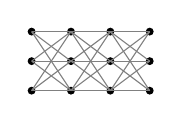
\begin{tikzpicture}[scale=0.25]
            \foreach \x in {0,...,3} {
                \foreach \y in {0,...,2} {
                    \fill (\x*2,\y*1.5) circle (0.2);
                }
            }
            \foreach \x in {0,...,2} {
                \foreach \y in {0,...,2} {
                    \foreach \z in {0,...,2} {
                        \draw[gray,thin] (\x*2,\y*1.5) -- (\x*2+2,\z*1.5);
                    }
                }
            }
        \end{tikzpicture}
    };

    \node[above=0.1cm of nn] {Neural network};

    \node[box,right=of nn] (pred) {
        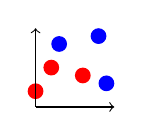
\begin{tikzpicture}[]
            \foreach \x/\y/\c in {0/0.2/red, 0.3/0.8/blue, 0.6/0.4/red, 0.8/0.9/blue, 0.2/0.5/red, 0.9/0.3/blue} {
                \fill[\c] (\x,\y) circle (0.1);
            }
            \draw[->] (0,0) -- (1,0);
            \draw[->] (0,0) -- (0,1);
        \end{tikzpicture}
    };

    \node[above=0.1cm of pred, text width=2cm, align=center] {Predicted labels};

    \node[box,right=of pred] (comppred) {
        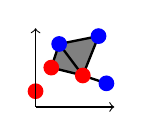
\begin{tikzpicture}[]
            \fill[gray] (0.2,0.5) -- (0.3,0.8) -- (0.6,0.4) -- cycle;
            \fill[gray] (0.3,0.8) -- (0.8,0.9) -- (0.6,0.4) -- cycle;
            \draw[black,line width=0.3mm] (0.3,0.8) -- (0.8,0.9);
            \draw[black,line width=0.3mm] (0.6,0.4) -- (0.8,0.9);
            \draw[black,line width=0.3mm] (0.6,0.4) -- (0.3,0.8);
            \draw[black,line width=0.3mm] (0.6,0.4) -- (0.9,0.3);
            \draw[black,line width=0.3mm] (0.2,0.5) -- (0.6,0.4);
            \draw[black,line width=0.3mm] (0.2,0.5) -- (0.3,0.8);
            \foreach \x/\y/\c in {0/0.2/red, 0.3/0.8/blue, 0.6/0.4/red, 0.8/0.9/blue, 0.2/0.5/red, 0.9/0.3/blue} {
                \fill[\c] (\x,\y) circle (0.1);
            }
            \draw[->] (0,0) -- (1,0);
            \draw[->] (0,0) -- (0,1);
        \end{tikzpicture}
    };

    \node[above=0.1cm of comppred, text width=2cm, align=center] {Simplicial complex};

    \node[box,right=of comppred] (pd1) {
        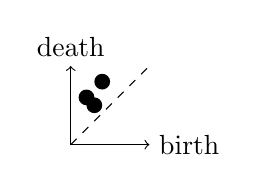
\begin{tikzpicture}[]
            \draw[->] (0,0) -- (1,0) node[right] {birth};
            \draw[->] (0,0) -- (0,1) node[above] {death};
            \draw[dashed] (0,0) -- (1,1);
            \foreach \x/\y in {0.2/0.6, 0.4/0.8, 0.3/0.5} {
                \fill (\x,\y) circle (0.1);
            }
        \end{tikzpicture}
    };
    
    \node[above=0.1cm of pd1, text width=2cm, align=center] {Persistence diagram, $\dim = 1$};

    % Second column - Ground truth pipeline
    \node[box,below=1cm of pd1] (pd2) {
        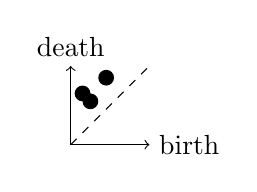
\begin{tikzpicture}[]
            \draw[->] (0,0) -- (1,0) node[right] {birth};
            \draw[->] (0,0) -- (0,1) node[above] {death};
            \draw[dashed] (0,0) -- (1,1);
            \foreach \x/\y in {0.15/0.65, 0.45/0.85, 0.25/0.55} {
                \fill (\x,\y) circle (0.1);
            }
        \end{tikzpicture}
    };

    \node[box,left=1cm of pd2] (compgt) {
        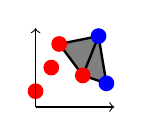
\begin{tikzpicture}[]
            \fill[gray] (0.6,0.4) -- (0.8,0.9) -- (0.9,0.3) -- cycle;
            \fill[gray] (0.3,0.8) -- (0.8,0.9) -- (0.6,0.4) -- cycle;
            \draw[black,line width=0.3mm] (0.8,0.9) -- (0.9,0.3);
            \draw[black,line width=0.3mm] (0.6,0.4) -- (0.9,0.3);
            \draw[black,line width=0.3mm] (0.6,0.4) -- (0.8,0.9);
            \draw[black,line width=0.3mm] (0.3,0.8) -- (0.8,0.9);
            \draw[black,line width=0.3mm] (0.3,0.8) -- (0.6,0.4);
            \foreach \x/\y/\c in {0/0.2/red, 0.3/0.8/red, 0.6/0.4/red, 0.8/0.9/blue, 0.2/0.5/red, 0.9/0.3/blue} {
                \fill[\c] (\x,\y) circle (0.1);
            }
            \draw[->] (0,0) -- (1,0);
            \draw[->] (0,0) -- (0,1);
        \end{tikzpicture}
    };

    \node[below=0.1cm of compgt, text width=2cm, align=center] {Simplicial complex};

    \node[box,left=of compgt] (gt) {
        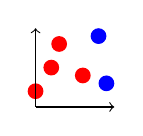
\begin{tikzpicture}[]
            \foreach \x/\y/\c in {0/0.2/red, 0.3/0.8/red, 0.6/0.4/red, 0.8/0.9/blue, 0.2/0.5/red, 0.9/0.3/blue} {
                \fill[\c] (\x,\y) circle (0.1);
            }
            \draw[->] (0,0) -- (1,0);
            \draw[->] (0,0) -- (0,1);
        \end{tikzpicture}
    };

    \node[below=0.1cm of gt, text width=2.5cm, align=center] {Ground truth labels};

    % Distance calculation
    \node[box,right=of pd1] (dist) {
        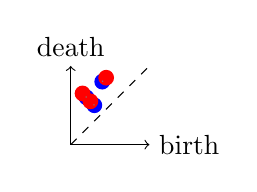
\begin{tikzpicture}[]
            \draw[->] (0,0) -- (1,0) node[right] {birth};
            \draw[->] (0,0) -- (0,1) node[above] {death};
            \draw[dashed] (0,0) -- (1,1);
            \foreach \x/\y in {0.2/0.6, 0.4/0.8, 0.3/0.5} {
                \fill[blue] (\x,\y) circle (0.1);
            }
            \foreach \x/\y in {0.15/0.65, 0.45/0.85, 0.25/0.55} {
                \fill[red] (\x,\y) circle (0.1);
            }
            \foreach \x/\y/\xx/\yy in {0.2/0.6/0.15/0.65, 0.4/0.8/0.45/0.85, 0.3/0.5/0.25/0.55} {
                \draw[gray,dotted] (\x,\y) -- (\xx,\yy);
            }
        \end{tikzpicture}
    };

    \node[above=0.1cm of dist] {Wasserstein distance};

    % Arrows
    \draw[arrow] (data1) -- (nn);
    \draw[arrow] (nn) -- (pred);
    \draw[arrow] (pred) -- (comppred);
    \draw[arrow] (comppred) -- (pd1);
    \draw[arrow] (gt) -- (compgt);
    \draw[arrow] (compgt) -- (pd2);
    \draw[arrow] (pd1) -- (dist);
    \draw[arrow] (pd2) -- (dist);

    \end{tikzpicture}
    }
\end{frame}

\begin{frame}{Pipeline}
    \resizebox{\textwidth}{!}{
    \begin{tikzpicture}[
        node distance=1cm,
        box/.style={rectangle,draw},
        arrow/.style={->,>=stealth,thick},
        every text node part/.style={font=\footnotesize}
    ]
    % First column - Prediction pipeline
    \node[box,name=data1] (data1) {
        \begin{tikzpicture}
            \foreach \x/\y in {0/0.2, 0.3/0.8, 0.6/0.4, 0.8/0.9, 0.2/0.5, 0.9/0.3} {
                \fill (\x,\y) circle (0.1);
            }
            \draw[->] (0,0) -- (1,0) node[right] {x};
            \draw[->] (0,0) -- (0,1) node[above] {y};
        \end{tikzpicture}
    };

    \node[above=0.1cm of data1] {Input data};

    \tikzset{
        every node/.style={
            opacity=0.4,
            execute at begin node={\ifx\tikz@fig@name\highlightednode\else\color{black!70}\fi}
        },
        every path/.style={opacity=0.4},
    }

    \node[box,right=of data1] (nn) {
        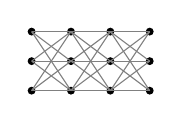
\begin{tikzpicture}[scale=0.25]
            \foreach \x in {0,...,3} {
                \foreach \y in {0,...,2} {
                    \fill (\x*2,\y*1.5) circle (0.2);
                }
            }
            \foreach \x in {0,...,2} {
                \foreach \y in {0,...,2} {
                    \foreach \z in {0,...,2} {
                        \draw[gray,thin] (\x*2,\y*1.5) -- (\x*2+2,\z*1.5);
                    }
                }
            }
        \end{tikzpicture}
    };

    \node[above=0.1cm of nn] {Neural network};

    \node[box,right=of nn] (pred) {
        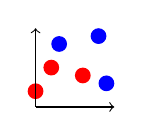
\begin{tikzpicture}[]
            \foreach \x/\y/\c in {0/0.2/red, 0.3/0.8/blue, 0.6/0.4/red, 0.8/0.9/blue, 0.2/0.5/red, 0.9/0.3/blue} {
                \fill[\c] (\x,\y) circle (0.1);
            }
            \draw[->] (0,0) -- (1,0);
            \draw[->] (0,0) -- (0,1);
        \end{tikzpicture}
    };

    \node[above=0.1cm of pred, text width=2cm, align=center] {Predicted labels};

    \node[box,right=of pred] (comppred) {
        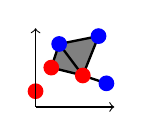
\begin{tikzpicture}[]
            \fill[gray] (0.2,0.5) -- (0.3,0.8) -- (0.6,0.4) -- cycle;
            \fill[gray] (0.3,0.8) -- (0.8,0.9) -- (0.6,0.4) -- cycle;
            \draw[black,line width=0.3mm] (0.3,0.8) -- (0.8,0.9);
            \draw[black,line width=0.3mm] (0.6,0.4) -- (0.8,0.9);
            \draw[black,line width=0.3mm] (0.6,0.4) -- (0.3,0.8);
            \draw[black,line width=0.3mm] (0.6,0.4) -- (0.9,0.3);
            \draw[black,line width=0.3mm] (0.2,0.5) -- (0.6,0.4);
            \draw[black,line width=0.3mm] (0.2,0.5) -- (0.3,0.8);
            \foreach \x/\y/\c in {0/0.2/red, 0.3/0.8/blue, 0.6/0.4/red, 0.8/0.9/blue, 0.2/0.5/red, 0.9/0.3/blue} {
                \fill[\c] (\x,\y) circle (0.1);
            }
            \draw[->] (0,0) -- (1,0);
            \draw[->] (0,0) -- (0,1);
        \end{tikzpicture}
    };

    \node[above=0.1cm of comppred, text width=2cm, align=center] {Simplicial complex};

    \node[box,right=of comppred] (pd1) {
        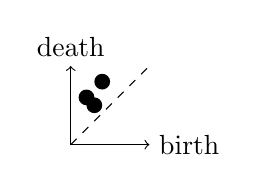
\begin{tikzpicture}[]
            \draw[->] (0,0) -- (1,0) node[right] {birth};
            \draw[->] (0,0) -- (0,1) node[above] {death};
            \draw[dashed] (0,0) -- (1,1);
            \foreach \x/\y in {0.2/0.6, 0.4/0.8, 0.3/0.5} {
                \fill (\x,\y) circle (0.1);
            }
        \end{tikzpicture}
    };
    
    \node[above=0.1cm of pd1, text width=2cm, align=center] {Persistence diagram, $\dim = 1$};

    % Second column - Ground truth pipeline
    \node[box,below=1cm of pd1] (pd2) {
        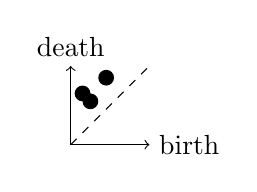
\begin{tikzpicture}[]
            \draw[->] (0,0) -- (1,0) node[right] {birth};
            \draw[->] (0,0) -- (0,1) node[above] {death};
            \draw[dashed] (0,0) -- (1,1);
            \foreach \x/\y in {0.15/0.65, 0.45/0.85, 0.25/0.55} {
                \fill (\x,\y) circle (0.1);
            }
        \end{tikzpicture}
    };

    \node[box,left=1cm of pd2] (compgt) {
        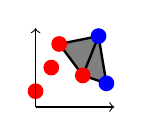
\begin{tikzpicture}[]
            \fill[gray] (0.6,0.4) -- (0.8,0.9) -- (0.9,0.3) -- cycle;
            \fill[gray] (0.3,0.8) -- (0.8,0.9) -- (0.6,0.4) -- cycle;
            \draw[black,line width=0.3mm] (0.8,0.9) -- (0.9,0.3);
            \draw[black,line width=0.3mm] (0.6,0.4) -- (0.9,0.3);
            \draw[black,line width=0.3mm] (0.6,0.4) -- (0.8,0.9);
            \draw[black,line width=0.3mm] (0.3,0.8) -- (0.8,0.9);
            \draw[black,line width=0.3mm] (0.3,0.8) -- (0.6,0.4);
            \foreach \x/\y/\c in {0/0.2/red, 0.3/0.8/red, 0.6/0.4/red, 0.8/0.9/blue, 0.2/0.5/red, 0.9/0.3/blue} {
                \fill[\c] (\x,\y) circle (0.1);
            }
            \draw[->] (0,0) -- (1,0);
            \draw[->] (0,0) -- (0,1);
        \end{tikzpicture}
    };

    \node[below=0.1cm of compgt, text width=2cm, align=center] {Simplicial complex};

    \node[box,left=of compgt] (gt) {
        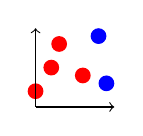
\begin{tikzpicture}[]
            \foreach \x/\y/\c in {0/0.2/red, 0.3/0.8/red, 0.6/0.4/red, 0.8/0.9/blue, 0.2/0.5/red, 0.9/0.3/blue} {
                \fill[\c] (\x,\y) circle (0.1);
            }
            \draw[->] (0,0) -- (1,0);
            \draw[->] (0,0) -- (0,1);
        \end{tikzpicture}
    };

    \node[below=0.1cm of gt, text width=2.5cm, align=center] {Ground truth labels};

    % Distance calculation
    \node[box,right=of pd1] (dist) {
        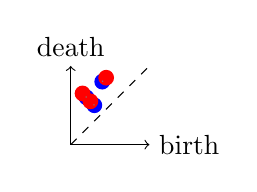
\begin{tikzpicture}[]
            \draw[->] (0,0) -- (1,0) node[right] {birth};
            \draw[->] (0,0) -- (0,1) node[above] {death};
            \draw[dashed] (0,0) -- (1,1);
            \foreach \x/\y in {0.2/0.6, 0.4/0.8, 0.3/0.5} {
                \fill[blue] (\x,\y) circle (0.1);
            }
            \foreach \x/\y in {0.15/0.65, 0.45/0.85, 0.25/0.55} {
                \fill[red] (\x,\y) circle (0.1);
            }
            \foreach \x/\y/\xx/\yy in {0.2/0.6/0.15/0.65, 0.4/0.8/0.45/0.85, 0.3/0.5/0.25/0.55} {
                \draw[gray,dotted] (\x,\y) -- (\xx,\yy);
            }
        \end{tikzpicture}
    };

    \node[above=0.1cm of dist] {Wasserstein distance};

    % Arrows
    \draw[arrow] (data1) -- (nn);
    \draw[arrow] (nn) -- (pred);
    \draw[arrow] (pred) -- (comppred);
    \draw[arrow] (comppred) -- (pd1);
    \draw[arrow] (gt) -- (compgt);
    \draw[arrow] (compgt) -- (pd2);
    \draw[arrow] (pd1) -- (dist);
    \draw[arrow] (pd2) -- (dist);

    \end{tikzpicture}
    }
\end{frame}


\begin{frame}{Input data}
    \begin{itemize}
        \item MNIST: 28x28 grayscale images of handwritten digits, $\dim = 784$
        \includegraphics[width=0.8\textwidth]{images/mnist.png}
        \item FashionMNIST: 28x28 grayscale images of fashion articles, $\dim = 784$
        \includegraphics[width=0.8\textwidth]{images/fashionmnist.png}
        \item CIFAR-10: 32x32 color images of 10 classes, $\dim = 3072$
        \includegraphics[width=0.8\textwidth]{images/cifar.png}
    \end{itemize}
\end{frame}

\begin{frame}{Pipeline}
    \resizebox{\textwidth}{!}{
    \begin{tikzpicture}[
        node distance=1cm,
        box/.style={rectangle,draw},
        arrow/.style={->,>=stealth,thick},
        every text node part/.style={font=\footnotesize}
    ]
    
    \node[box,right=of data1] (nn) {
        \begin{tikzpicture}[scale=0.25]
            \foreach \x in {0,...,3} {
                \foreach \y in {0,...,2} {
                    \fill (\x*2,\y*1.5) circle (0.2);
                }
            }
            \foreach \x in {0,...,2} {
                \foreach \y in {0,...,2} {
                    \foreach \z in {0,...,2} {
                        \draw[gray,thin] (\x*2,\y*1.5) -- (\x*2+2,\z*1.5);
                    }
                }
            }
        \end{tikzpicture}
    };

    \node[above=0.1cm of nn] {Neural network};

    \tikzset{
        every node/.style={
            opacity=0.4,
            execute at begin node={\ifx\tikz@fig@name\highlightednode\else\color{black!70}\fi}
        },
        every path/.style={opacity=0.4},
    }

    % First column - Prediction pipeline
    \node[box,name=data1] (data1) {
        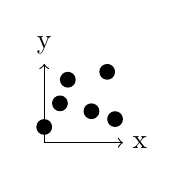
\begin{tikzpicture}
            \foreach \x/\y in {0/0.2, 0.3/0.8, 0.6/0.4, 0.8/0.9, 0.2/0.5, 0.9/0.3} {
                \fill (\x,\y) circle (0.1);
            }
            \draw[->] (0,0) -- (1,0) node[right] {x};
            \draw[->] (0,0) -- (0,1) node[above] {y};
        \end{tikzpicture}
    };

    \node[above=0.1cm of data1] {Input data};

    \node[box,right=of nn] (pred) {
        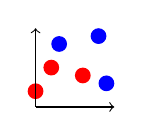
\begin{tikzpicture}[]
            \foreach \x/\y/\c in {0/0.2/red, 0.3/0.8/blue, 0.6/0.4/red, 0.8/0.9/blue, 0.2/0.5/red, 0.9/0.3/blue} {
                \fill[\c] (\x,\y) circle (0.1);
            }
            \draw[->] (0,0) -- (1,0);
            \draw[->] (0,0) -- (0,1);
        \end{tikzpicture}
    };

    \node[above=0.1cm of pred, text width=2cm, align=center] {Predicted labels};

    \node[box,right=of pred] (comppred) {
        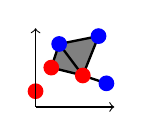
\begin{tikzpicture}[]
            \fill[gray] (0.2,0.5) -- (0.3,0.8) -- (0.6,0.4) -- cycle;
            \fill[gray] (0.3,0.8) -- (0.8,0.9) -- (0.6,0.4) -- cycle;
            \draw[black,line width=0.3mm] (0.3,0.8) -- (0.8,0.9);
            \draw[black,line width=0.3mm] (0.6,0.4) -- (0.8,0.9);
            \draw[black,line width=0.3mm] (0.6,0.4) -- (0.3,0.8);
            \draw[black,line width=0.3mm] (0.6,0.4) -- (0.9,0.3);
            \draw[black,line width=0.3mm] (0.2,0.5) -- (0.6,0.4);
            \draw[black,line width=0.3mm] (0.2,0.5) -- (0.3,0.8);
            \foreach \x/\y/\c in {0/0.2/red, 0.3/0.8/blue, 0.6/0.4/red, 0.8/0.9/blue, 0.2/0.5/red, 0.9/0.3/blue} {
                \fill[\c] (\x,\y) circle (0.1);
            }
            \draw[->] (0,0) -- (1,0);
            \draw[->] (0,0) -- (0,1);
        \end{tikzpicture}
    };

    \node[above=0.1cm of comppred, text width=2cm, align=center] {Simplicial complex};

    \node[box,right=of comppred] (pd1) {
        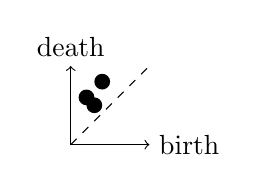
\begin{tikzpicture}[]
            \draw[->] (0,0) -- (1,0) node[right] {birth};
            \draw[->] (0,0) -- (0,1) node[above] {death};
            \draw[dashed] (0,0) -- (1,1);
            \foreach \x/\y in {0.2/0.6, 0.4/0.8, 0.3/0.5} {
                \fill (\x,\y) circle (0.1);
            }
        \end{tikzpicture}
    };
    
    \node[above=0.1cm of pd1, text width=2cm, align=center] {Persistence diagram, $\dim = 1$};

    % Second column - Ground truth pipeline
    \node[box,below=1cm of pd1] (pd2) {
        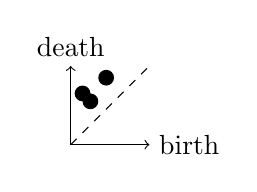
\begin{tikzpicture}[]
            \draw[->] (0,0) -- (1,0) node[right] {birth};
            \draw[->] (0,0) -- (0,1) node[above] {death};
            \draw[dashed] (0,0) -- (1,1);
            \foreach \x/\y in {0.15/0.65, 0.45/0.85, 0.25/0.55} {
                \fill (\x,\y) circle (0.1);
            }
        \end{tikzpicture}
    };

    \node[box,left=1cm of pd2] (compgt) {
        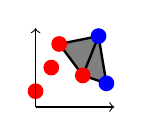
\begin{tikzpicture}[]
            \fill[gray] (0.6,0.4) -- (0.8,0.9) -- (0.9,0.3) -- cycle;
            \fill[gray] (0.3,0.8) -- (0.8,0.9) -- (0.6,0.4) -- cycle;
            \draw[black,line width=0.3mm] (0.8,0.9) -- (0.9,0.3);
            \draw[black,line width=0.3mm] (0.6,0.4) -- (0.9,0.3);
            \draw[black,line width=0.3mm] (0.6,0.4) -- (0.8,0.9);
            \draw[black,line width=0.3mm] (0.3,0.8) -- (0.8,0.9);
            \draw[black,line width=0.3mm] (0.3,0.8) -- (0.6,0.4);
            \foreach \x/\y/\c in {0/0.2/red, 0.3/0.8/red, 0.6/0.4/red, 0.8/0.9/blue, 0.2/0.5/red, 0.9/0.3/blue} {
                \fill[\c] (\x,\y) circle (0.1);
            }
            \draw[->] (0,0) -- (1,0);
            \draw[->] (0,0) -- (0,1);
        \end{tikzpicture}
    };

    \node[below=0.1cm of compgt, text width=2cm, align=center] {Simplicial complex};

    \node[box,left=of compgt] (gt) {
        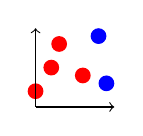
\begin{tikzpicture}[]
            \foreach \x/\y/\c in {0/0.2/red, 0.3/0.8/red, 0.6/0.4/red, 0.8/0.9/blue, 0.2/0.5/red, 0.9/0.3/blue} {
                \fill[\c] (\x,\y) circle (0.1);
            }
            \draw[->] (0,0) -- (1,0);
            \draw[->] (0,0) -- (0,1);
        \end{tikzpicture}
    };

    \node[below=0.1cm of gt, text width=2.5cm, align=center] {Ground truth labels};

    % Distance calculation
    \node[box,right=of pd1] (dist) {
        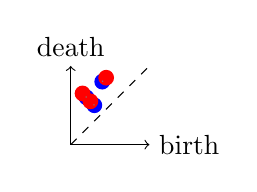
\begin{tikzpicture}[]
            \draw[->] (0,0) -- (1,0) node[right] {birth};
            \draw[->] (0,0) -- (0,1) node[above] {death};
            \draw[dashed] (0,0) -- (1,1);
            \foreach \x/\y in {0.2/0.6, 0.4/0.8, 0.3/0.5} {
                \fill[blue] (\x,\y) circle (0.1);
            }
            \foreach \x/\y in {0.15/0.65, 0.45/0.85, 0.25/0.55} {
                \fill[red] (\x,\y) circle (0.1);
            }
            \foreach \x/\y/\xx/\yy in {0.2/0.6/0.15/0.65, 0.4/0.8/0.45/0.85, 0.3/0.5/0.25/0.55} {
                \draw[gray,dotted] (\x,\y) -- (\xx,\yy);
            }
        \end{tikzpicture}
    };

    \node[above=0.1cm of dist] {Wasserstein distance};

    % Arrows
    \draw[arrow] (data1) -- (nn);
    \draw[arrow] (nn) -- (pred);
    \draw[arrow] (pred) -- (comppred);
    \draw[arrow] (comppred) -- (pd1);
    \draw[arrow] (gt) -- (compgt);
    \draw[arrow] (compgt) -- (pd2);
    \draw[arrow] (pd1) -- (dist);
    \draw[arrow] (pd2) -- (dist);

    \end{tikzpicture}
    }
\end{frame}

% \begin{frame}{Models}
%     \only<1>{\vspace*{45pt}}
%     \begin{itemize}
%         \item Fully-connected neural network with ReLU activations

%         \only<1>{\hspace*{-1.5em}\begin{tikzpicture}[
%             node distance=1cm,
%             box/.style={rectangle,draw},
%             arrow/.style={->,>=stealth,thick},
%             every text node part/.style={font=\footnotesize}
%         ]
%             \node[box] (input) { \begin{tikzpicture}[
%                 neuron/.style={circle,draw,minimum size=0.5cm,fill=gray!50},
%             ]
%                 \node[neuron] (n0) at (0,2.4) {};
%                 \node[neuron] (n1) at (0,1.6) {};
%                 \node[neuron] (n2) at (0,0.8) {};
%                 \node[neuron] (n3) at (0,-0.8) {};
%                 \node[neuron] (n4) at (0,-1.6) {};
%                 \node at (0,0) {$\vdots$};
%             \end{tikzpicture} }
%             \node[below=0.1cm of input,text width=2cm,align=center] (inputlabel) {Input $\dim = 784$};

%             \node[box,right=of input] (l1) { \begin{tikzpicture}[
%                 neuron/.style={circle,draw,minimum size=0.5cm,fill=gray!50},
%             ]
%                 \node[neuron] (n1) at (0,1.6) {};
%                 \node[neuron] (n2) at (0,0.8) {};
%                 \node[neuron] (n3) at (0,-0.8) {};
%                 \node[neuron] (n4) at (0,-1.6) {};
%                 \node at (0,0) {$\vdots$};
%             \end{tikzpicture} }
%             \node[below=0.1cm of l1,text width=2cm,align=center] (l1label) {Layer 1 $\dim = 512$};

%             \node[box,right=0.5cm of l1] (relu1) { ReLU }

%             \node[box,right=of relu1] (l2) { \begin{tikzpicture}[
%                 neuron/.style={circle,draw,minimum size=0.5cm,fill=gray!50},
%             ]
%                 \node[neuron] (n1) at (0,1.6) {};
%                 \node[neuron] (n2) at (0,0.8) {};
%                 \node[neuron] (n3) at (0,-0.8) {};
%                 \node at (0,0) {$\vdots$};
%             \end{tikzpicture} }
%             \node[below=0.1cm of l2,text width=2cm,align=center] (l2label) {Layer 2 $\dim = 128$};

%             \node[box,right=0.5cm of l2] (relu2) { ReLU }

%             \node[box,right=of relu2] (l3) { \begin{tikzpicture}[
%                 neuron/.style={circle,draw,minimum size=0.5cm,fill=gray!50},
%             ]
%                 \node[neuron] (n2) at (0,0.8) {};
%                 \node[neuron] (n3) at (0,-0.8) {};
%                 \node at (0,0) {$\vdots$};
%             \end{tikzpicture} }
%             \node[below=0.1cm of l3,text width=2cm,align=center] (l2label) {Layer 3 $\dim = 16$};

%             \node[box,right=0.5cm of l3] (relu3) { ReLU }

%             \node[box,right=of relu3] (l4) { \begin{tikzpicture}[
%                 neuron/.style={circle,draw,minimum size=0.5cm,fill=gray!50},
%             ]
%                 \node[neuron] (n2) at (0,0.8) {};
%                 \node[neuron] (n3) at (0,-0.8) {};
%                 \node at (0,0) {$\vdots$};
%             \end{tikzpicture} }
%             \node[below=0.1cm of l4,text width=2cm,align=center] (l2label) {Output layer $\dim = 10$};

%             \draw[arrow] (input) -- (l1);
%             \draw[arrow] (l1) -- (relu1);
%             \draw[arrow] (relu1) -- (l2);
%             \draw[arrow] (l2) -- (relu2);
%             \draw[arrow] (relu2) -- (l3);
%             \draw[arrow] (l3) -- (relu3);
%             \draw[arrow] (relu3) -- (l4);
%         \end{tikzpicture}}
%         \item<2-> Convolutional NN from the PyTorch MNIST tutorial + modifications:
%         \begin{itemize}
%             \item Reduced layer sizes
%             \item Increased layer sizes
%             \item Additional layers
%             \item Aggressive learning rate growth ($\gamma = 1.9$) to simulate overfitting
%             \item Small learning rate $(\alpha = 10^{-6})$ to simulate underfitting
%         \end{itemize}
        
%         \resizebox{0.8\textwidth}{!}{ \includesvg[width=\textwidth]{nn.svg} }
%     \end{itemize}
% \end{frame}

% \begin{frame}{Simplicial complexes}
%     \begin{itemize}
%         \item \emph{Labeled \v{C}ech complex}:
%         \begin{itemize}
%             \item A modification of the standard \v{C}ech complex
%             \item Has statistical guarantees for decision boundary recovery, but is intractable
%             \item Not applicable to multi-class problems
%         \end{itemize}
%         \item \emph{Labeled Vietoris-Rips complex}:
%         \begin{itemize}
%             \item A modification of the standard Vietoris-Rips complex
%             \item No guarantees, but is tractable
%             \item Can be applied to multi-class problems \textcolor{gray}{(new!)}
%         \end{itemize}
%     \end{itemize}
% \end{frame}

% \begin{frame}{Labeled \v{C}ech complex}
%     \begin{columns}
%         \column{0.55\textwidth}
%         \begin{itemize}
%             \item Set of points $X$
%             \item Reference set of points $Y$
%             \item Parameters $\varepsilon$ and $\gamma$
%         \end{itemize}
%         \onslide<2->{
%         $L\check{C}_{X, Y}^{\varepsilon, \gamma}$ contains
%         \(x_0, \dots, x_n \in X\) iff:
%         \begin{enumerate}
%             \item<2-> For each \(i \in (0, \dots, n)\)
%             \(\exists y \in Y : \norm{x_i - y} \leq \gamma\).
%             \item<3-> \(\bigcap_{i = 0}^n B_\varepsilon(x_i) \neq \emptyset\)
%         \end{enumerate}
%         }
%         \onslide<4->{\begin{itemize}
%             \item Filtration is done by varying $\varepsilon$
%             \item Simplices are on one side of the boundary
%             \item Not applicable to multiple classes
%             \item Not tractable
%             \item Has probabilistic recovery guarantees
%         \end{itemize}
%         }
%         \column{0.55\textwidth}
%         \hspace*{-0.5cm}
%         \only<1>{\resizebox{1.1\textwidth}{!}{%% Creator: Matplotlib, PGF backend
%%
%% To include the figure in your LaTeX document, write
%%   \input{<filename>.pgf}
%%
%% Make sure the required packages are loaded in your preamble
%%   \usepackage{pgf}
%%
%% Also ensure that all the required font packages are loaded; for instance,
%% the lmodern package is sometimes necessary when using math font.
%%   \usepackage{lmodern}
%%
%% Figures using additional raster images can only be included by \input if
%% they are in the same directory as the main LaTeX file. For loading figures
%% from other directories you can use the `import` package
%%   \usepackage{import}
%%
%% and then include the figures with
%%   \import{<path to file>}{<filename>.pgf}
%%
%% Matplotlib used the following preamble
%%   \def\mathdefault#1{#1}
%%   \everymath=\expandafter{\the\everymath\displaystyle}
%%   
%%   \ifdefined\pdftexversion\else  % non-pdftex case.
%%     \usepackage{fontspec}
%%     \setmainfont{DejaVuSerif.ttf}[Path=\detokenize{/home/snek/repos/homology-decision-bondaries-clean/venv/lib/python3.9/site-packages/matplotlib/mpl-data/fonts/ttf/}]
%%     \setsansfont{DejaVuSans.ttf}[Path=\detokenize{/home/snek/repos/homology-decision-bondaries-clean/venv/lib/python3.9/site-packages/matplotlib/mpl-data/fonts/ttf/}]
%%     \setmonofont{DejaVuSansMono.ttf}[Path=\detokenize{/home/snek/repos/homology-decision-bondaries-clean/venv/lib/python3.9/site-packages/matplotlib/mpl-data/fonts/ttf/}]
%%   \fi
%%   \makeatletter\@ifpackageloaded{underscore}{}{\usepackage[strings]{underscore}}\makeatother
%%
\begingroup%
\makeatletter%
\begin{pgfpicture}%
\pgfpathrectangle{\pgfpointorigin}{\pgfqpoint{6.400000in}{4.800000in}}%
\pgfusepath{use as bounding box, clip}%
\begin{pgfscope}%
\pgfsetbuttcap%
\pgfsetmiterjoin%
\definecolor{currentfill}{rgb}{1.000000,1.000000,1.000000}%
\pgfsetfillcolor{currentfill}%
\pgfsetlinewidth{0.000000pt}%
\definecolor{currentstroke}{rgb}{1.000000,1.000000,1.000000}%
\pgfsetstrokecolor{currentstroke}%
\pgfsetdash{}{0pt}%
\pgfpathmoveto{\pgfqpoint{0.000000in}{0.000000in}}%
\pgfpathlineto{\pgfqpoint{6.400000in}{0.000000in}}%
\pgfpathlineto{\pgfqpoint{6.400000in}{4.800000in}}%
\pgfpathlineto{\pgfqpoint{0.000000in}{4.800000in}}%
\pgfpathlineto{\pgfqpoint{0.000000in}{0.000000in}}%
\pgfpathclose%
\pgfusepath{fill}%
\end{pgfscope}%
\begin{pgfscope}%
\pgfpathrectangle{\pgfqpoint{0.413138in}{0.150000in}}{\pgfqpoint{5.573723in}{4.500000in}}%
\pgfusepath{clip}%
\pgfsetbuttcap%
\pgfsetroundjoin%
\definecolor{currentfill}{rgb}{0.121569,0.466667,0.705882}%
\pgfsetfillcolor{currentfill}%
\pgfsetlinewidth{1.003750pt}%
\definecolor{currentstroke}{rgb}{0.121569,0.466667,0.705882}%
\pgfsetstrokecolor{currentstroke}%
\pgfsetdash{}{0pt}%
\pgfsys@defobject{currentmarker}{\pgfqpoint{-0.041667in}{-0.041667in}}{\pgfqpoint{0.041667in}{0.041667in}}{%
\pgfpathmoveto{\pgfqpoint{0.000000in}{0.041667in}}%
\pgfpathlineto{\pgfqpoint{-0.041667in}{-0.041667in}}%
\pgfpathlineto{\pgfqpoint{0.041667in}{-0.041667in}}%
\pgfpathlineto{\pgfqpoint{0.000000in}{0.041667in}}%
\pgfpathclose%
\pgfusepath{stroke,fill}%
}%
\begin{pgfscope}%
\pgfsys@transformshift{4.575386in}{2.417219in}%
\pgfsys@useobject{currentmarker}{}%
\end{pgfscope}%
\begin{pgfscope}%
\pgfsys@transformshift{4.692413in}{2.548823in}%
\pgfsys@useobject{currentmarker}{}%
\end{pgfscope}%
\begin{pgfscope}%
\pgfsys@transformshift{3.931680in}{2.584411in}%
\pgfsys@useobject{currentmarker}{}%
\end{pgfscope}%
\begin{pgfscope}%
\pgfsys@transformshift{3.960018in}{2.675178in}%
\pgfsys@useobject{currentmarker}{}%
\end{pgfscope}%
\begin{pgfscope}%
\pgfsys@transformshift{4.571428in}{2.923131in}%
\pgfsys@useobject{currentmarker}{}%
\end{pgfscope}%
\begin{pgfscope}%
\pgfsys@transformshift{4.324476in}{2.976499in}%
\pgfsys@useobject{currentmarker}{}%
\end{pgfscope}%
\begin{pgfscope}%
\pgfsys@transformshift{3.759159in}{2.872630in}%
\pgfsys@useobject{currentmarker}{}%
\end{pgfscope}%
\begin{pgfscope}%
\pgfsys@transformshift{3.919359in}{3.034957in}%
\pgfsys@useobject{currentmarker}{}%
\end{pgfscope}%
\begin{pgfscope}%
\pgfsys@transformshift{4.450956in}{3.435048in}%
\pgfsys@useobject{currentmarker}{}%
\end{pgfscope}%
\begin{pgfscope}%
\pgfsys@transformshift{3.965694in}{3.281019in}%
\pgfsys@useobject{currentmarker}{}%
\end{pgfscope}%
\begin{pgfscope}%
\pgfsys@transformshift{3.592076in}{3.131769in}%
\pgfsys@useobject{currentmarker}{}%
\end{pgfscope}%
\begin{pgfscope}%
\pgfsys@transformshift{3.469115in}{3.128372in}%
\pgfsys@useobject{currentmarker}{}%
\end{pgfscope}%
\begin{pgfscope}%
\pgfsys@transformshift{4.117227in}{3.843301in}%
\pgfsys@useobject{currentmarker}{}%
\end{pgfscope}%
\begin{pgfscope}%
\pgfsys@transformshift{3.821421in}{3.716217in}%
\pgfsys@useobject{currentmarker}{}%
\end{pgfscope}%
\begin{pgfscope}%
\pgfsys@transformshift{3.532139in}{3.538006in}%
\pgfsys@useobject{currentmarker}{}%
\end{pgfscope}%
\begin{pgfscope}%
\pgfsys@transformshift{3.729108in}{3.972504in}%
\pgfsys@useobject{currentmarker}{}%
\end{pgfscope}%
\begin{pgfscope}%
\pgfsys@transformshift{3.730036in}{4.203686in}%
\pgfsys@useobject{currentmarker}{}%
\end{pgfscope}%
\begin{pgfscope}%
\pgfsys@transformshift{3.547869in}{4.146030in}%
\pgfsys@useobject{currentmarker}{}%
\end{pgfscope}%
\begin{pgfscope}%
\pgfsys@transformshift{3.425353in}{4.177203in}%
\pgfsys@useobject{currentmarker}{}%
\end{pgfscope}%
\begin{pgfscope}%
\pgfsys@transformshift{3.138659in}{3.770632in}%
\pgfsys@useobject{currentmarker}{}%
\end{pgfscope}%
\begin{pgfscope}%
\pgfsys@transformshift{3.021085in}{3.701989in}%
\pgfsys@useobject{currentmarker}{}%
\end{pgfscope}%
\begin{pgfscope}%
\pgfsys@transformshift{2.905370in}{3.586957in}%
\pgfsys@useobject{currentmarker}{}%
\end{pgfscope}%
\begin{pgfscope}%
\pgfsys@transformshift{2.929833in}{4.165322in}%
\pgfsys@useobject{currentmarker}{}%
\end{pgfscope}%
\begin{pgfscope}%
\pgfsys@transformshift{2.847795in}{4.445455in}%
\pgfsys@useobject{currentmarker}{}%
\end{pgfscope}%
\begin{pgfscope}%
\pgfsys@transformshift{2.699566in}{4.054037in}%
\pgfsys@useobject{currentmarker}{}%
\end{pgfscope}%
\begin{pgfscope}%
\pgfsys@transformshift{2.602751in}{3.604762in}%
\pgfsys@useobject{currentmarker}{}%
\end{pgfscope}%
\begin{pgfscope}%
\pgfsys@transformshift{2.469332in}{4.332476in}%
\pgfsys@useobject{currentmarker}{}%
\end{pgfscope}%
\begin{pgfscope}%
\pgfsys@transformshift{2.369496in}{4.170606in}%
\pgfsys@useobject{currentmarker}{}%
\end{pgfscope}%
\begin{pgfscope}%
\pgfsys@transformshift{2.325700in}{3.831344in}%
\pgfsys@useobject{currentmarker}{}%
\end{pgfscope}%
\begin{pgfscope}%
\pgfsys@transformshift{2.114023in}{4.253119in}%
\pgfsys@useobject{currentmarker}{}%
\end{pgfscope}%
\begin{pgfscope}%
\pgfsys@transformshift{2.131487in}{3.833291in}%
\pgfsys@useobject{currentmarker}{}%
\end{pgfscope}%
\begin{pgfscope}%
\pgfsys@transformshift{2.095198in}{3.673929in}%
\pgfsys@useobject{currentmarker}{}%
\end{pgfscope}%
\begin{pgfscope}%
\pgfsys@transformshift{1.853997in}{3.966002in}%
\pgfsys@useobject{currentmarker}{}%
\end{pgfscope}%
\begin{pgfscope}%
\pgfsys@transformshift{1.730963in}{3.959839in}%
\pgfsys@useobject{currentmarker}{}%
\end{pgfscope}%
\begin{pgfscope}%
\pgfsys@transformshift{1.706103in}{3.793249in}%
\pgfsys@useobject{currentmarker}{}%
\end{pgfscope}%
\begin{pgfscope}%
\pgfsys@transformshift{1.831252in}{3.455717in}%
\pgfsys@useobject{currentmarker}{}%
\end{pgfscope}%
\begin{pgfscope}%
\pgfsys@transformshift{1.627322in}{3.564670in}%
\pgfsys@useobject{currentmarker}{}%
\end{pgfscope}%
\begin{pgfscope}%
\pgfsys@transformshift{1.400848in}{3.657490in}%
\pgfsys@useobject{currentmarker}{}%
\end{pgfscope}%
\begin{pgfscope}%
\pgfsys@transformshift{1.121171in}{3.759609in}%
\pgfsys@useobject{currentmarker}{}%
\end{pgfscope}%
\begin{pgfscope}%
\pgfsys@transformshift{1.152005in}{3.572917in}%
\pgfsys@useobject{currentmarker}{}%
\end{pgfscope}%
\begin{pgfscope}%
\pgfsys@transformshift{1.241193in}{3.367556in}%
\pgfsys@useobject{currentmarker}{}%
\end{pgfscope}%
\begin{pgfscope}%
\pgfsys@transformshift{0.998183in}{3.389160in}%
\pgfsys@useobject{currentmarker}{}%
\end{pgfscope}%
\begin{pgfscope}%
\pgfsys@transformshift{1.493743in}{2.998667in}%
\pgfsys@useobject{currentmarker}{}%
\end{pgfscope}%
\begin{pgfscope}%
\pgfsys@transformshift{1.272691in}{3.007560in}%
\pgfsys@useobject{currentmarker}{}%
\end{pgfscope}%
\begin{pgfscope}%
\pgfsys@transformshift{1.332951in}{2.886247in}%
\pgfsys@useobject{currentmarker}{}%
\end{pgfscope}%
\begin{pgfscope}%
\pgfsys@transformshift{1.374759in}{2.783323in}%
\pgfsys@useobject{currentmarker}{}%
\end{pgfscope}%
\begin{pgfscope}%
\pgfsys@transformshift{0.703441in}{2.850453in}%
\pgfsys@useobject{currentmarker}{}%
\end{pgfscope}%
\begin{pgfscope}%
\pgfsys@transformshift{1.529854in}{2.591909in}%
\pgfsys@useobject{currentmarker}{}%
\end{pgfscope}%
\begin{pgfscope}%
\pgfsys@transformshift{1.107734in}{2.561775in}%
\pgfsys@useobject{currentmarker}{}%
\end{pgfscope}%
\begin{pgfscope}%
\pgfsys@transformshift{1.256091in}{2.460565in}%
\pgfsys@useobject{currentmarker}{}%
\end{pgfscope}%
\begin{pgfscope}%
\pgfsys@transformshift{0.944862in}{2.363993in}%
\pgfsys@useobject{currentmarker}{}%
\end{pgfscope}%
\begin{pgfscope}%
\pgfsys@transformshift{1.265386in}{2.287716in}%
\pgfsys@useobject{currentmarker}{}%
\end{pgfscope}%
\begin{pgfscope}%
\pgfsys@transformshift{1.017520in}{2.160548in}%
\pgfsys@useobject{currentmarker}{}%
\end{pgfscope}%
\begin{pgfscope}%
\pgfsys@transformshift{1.021879in}{2.055907in}%
\pgfsys@useobject{currentmarker}{}%
\end{pgfscope}%
\begin{pgfscope}%
\pgfsys@transformshift{1.598399in}{2.116781in}%
\pgfsys@useobject{currentmarker}{}%
\end{pgfscope}%
\begin{pgfscope}%
\pgfsys@transformshift{1.206820in}{1.902283in}%
\pgfsys@useobject{currentmarker}{}%
\end{pgfscope}%
\begin{pgfscope}%
\pgfsys@transformshift{1.109979in}{1.755667in}%
\pgfsys@useobject{currentmarker}{}%
\end{pgfscope}%
\begin{pgfscope}%
\pgfsys@transformshift{1.560602in}{1.870239in}%
\pgfsys@useobject{currentmarker}{}%
\end{pgfscope}%
\begin{pgfscope}%
\pgfsys@transformshift{1.324135in}{1.640425in}%
\pgfsys@useobject{currentmarker}{}%
\end{pgfscope}%
\begin{pgfscope}%
\pgfsys@transformshift{1.516619in}{1.656499in}%
\pgfsys@useobject{currentmarker}{}%
\end{pgfscope}%
\begin{pgfscope}%
\pgfsys@transformshift{1.249471in}{1.338168in}%
\pgfsys@useobject{currentmarker}{}%
\end{pgfscope}%
\begin{pgfscope}%
\pgfsys@transformshift{1.104257in}{1.059695in}%
\pgfsys@useobject{currentmarker}{}%
\end{pgfscope}%
\begin{pgfscope}%
\pgfsys@transformshift{1.541220in}{1.319564in}%
\pgfsys@useobject{currentmarker}{}%
\end{pgfscope}%
\begin{pgfscope}%
\pgfsys@transformshift{1.451079in}{1.066372in}%
\pgfsys@useobject{currentmarker}{}%
\end{pgfscope}%
\begin{pgfscope}%
\pgfsys@transformshift{1.791867in}{1.326969in}%
\pgfsys@useobject{currentmarker}{}%
\end{pgfscope}%
\begin{pgfscope}%
\pgfsys@transformshift{1.715549in}{1.055386in}%
\pgfsys@useobject{currentmarker}{}%
\end{pgfscope}%
\begin{pgfscope}%
\pgfsys@transformshift{1.941608in}{1.239447in}%
\pgfsys@useobject{currentmarker}{}%
\end{pgfscope}%
\begin{pgfscope}%
\pgfsys@transformshift{1.805279in}{0.770137in}%
\pgfsys@useobject{currentmarker}{}%
\end{pgfscope}%
\begin{pgfscope}%
\pgfsys@transformshift{1.946789in}{0.806198in}%
\pgfsys@useobject{currentmarker}{}%
\end{pgfscope}%
\begin{pgfscope}%
\pgfsys@transformshift{2.027630in}{0.701071in}%
\pgfsys@useobject{currentmarker}{}%
\end{pgfscope}%
\begin{pgfscope}%
\pgfsys@transformshift{2.256315in}{1.095994in}%
\pgfsys@useobject{currentmarker}{}%
\end{pgfscope}%
\begin{pgfscope}%
\pgfsys@transformshift{2.208648in}{0.443682in}%
\pgfsys@useobject{currentmarker}{}%
\end{pgfscope}%
\begin{pgfscope}%
\pgfsys@transformshift{2.424535in}{1.046636in}%
\pgfsys@useobject{currentmarker}{}%
\end{pgfscope}%
\begin{pgfscope}%
\pgfsys@transformshift{2.529886in}{1.263652in}%
\pgfsys@useobject{currentmarker}{}%
\end{pgfscope}%
\begin{pgfscope}%
\pgfsys@transformshift{2.603736in}{1.291730in}%
\pgfsys@useobject{currentmarker}{}%
\end{pgfscope}%
\begin{pgfscope}%
\pgfsys@transformshift{2.694593in}{0.884806in}%
\pgfsys@useobject{currentmarker}{}%
\end{pgfscope}%
\begin{pgfscope}%
\pgfsys@transformshift{2.851635in}{0.354545in}%
\pgfsys@useobject{currentmarker}{}%
\end{pgfscope}%
\begin{pgfscope}%
\pgfsys@transformshift{2.980151in}{0.383745in}%
\pgfsys@useobject{currentmarker}{}%
\end{pgfscope}%
\begin{pgfscope}%
\pgfsys@transformshift{2.942759in}{1.093362in}%
\pgfsys@useobject{currentmarker}{}%
\end{pgfscope}%
\begin{pgfscope}%
\pgfsys@transformshift{3.069380in}{0.977133in}%
\pgfsys@useobject{currentmarker}{}%
\end{pgfscope}%
\begin{pgfscope}%
\pgfsys@transformshift{3.128150in}{1.091313in}%
\pgfsys@useobject{currentmarker}{}%
\end{pgfscope}%
\begin{pgfscope}%
\pgfsys@transformshift{3.100134in}{1.369363in}%
\pgfsys@useobject{currentmarker}{}%
\end{pgfscope}%
\begin{pgfscope}%
\pgfsys@transformshift{3.515120in}{0.749530in}%
\pgfsys@useobject{currentmarker}{}%
\end{pgfscope}%
\begin{pgfscope}%
\pgfsys@transformshift{3.572444in}{0.884741in}%
\pgfsys@useobject{currentmarker}{}%
\end{pgfscope}%
\begin{pgfscope}%
\pgfsys@transformshift{3.607876in}{1.032180in}%
\pgfsys@useobject{currentmarker}{}%
\end{pgfscope}%
\begin{pgfscope}%
\pgfsys@transformshift{3.766573in}{1.007867in}%
\pgfsys@useobject{currentmarker}{}%
\end{pgfscope}%
\begin{pgfscope}%
\pgfsys@transformshift{3.452654in}{1.517468in}%
\pgfsys@useobject{currentmarker}{}%
\end{pgfscope}%
\begin{pgfscope}%
\pgfsys@transformshift{4.139710in}{0.969698in}%
\pgfsys@useobject{currentmarker}{}%
\end{pgfscope}%
\begin{pgfscope}%
\pgfsys@transformshift{3.699109in}{1.513077in}%
\pgfsys@useobject{currentmarker}{}%
\end{pgfscope}%
\begin{pgfscope}%
\pgfsys@transformshift{3.679732in}{1.638128in}%
\pgfsys@useobject{currentmarker}{}%
\end{pgfscope}%
\begin{pgfscope}%
\pgfsys@transformshift{3.542741in}{1.825234in}%
\pgfsys@useobject{currentmarker}{}%
\end{pgfscope}%
\begin{pgfscope}%
\pgfsys@transformshift{4.037621in}{1.629363in}%
\pgfsys@useobject{currentmarker}{}%
\end{pgfscope}%
\begin{pgfscope}%
\pgfsys@transformshift{4.450953in}{1.546440in}%
\pgfsys@useobject{currentmarker}{}%
\end{pgfscope}%
\begin{pgfscope}%
\pgfsys@transformshift{3.823947in}{1.935869in}%
\pgfsys@useobject{currentmarker}{}%
\end{pgfscope}%
\begin{pgfscope}%
\pgfsys@transformshift{3.627630in}{2.086805in}%
\pgfsys@useobject{currentmarker}{}%
\end{pgfscope}%
\begin{pgfscope}%
\pgfsys@transformshift{3.956634in}{2.070824in}%
\pgfsys@useobject{currentmarker}{}%
\end{pgfscope}%
\begin{pgfscope}%
\pgfsys@transformshift{3.684009in}{2.212455in}%
\pgfsys@useobject{currentmarker}{}%
\end{pgfscope}%
\begin{pgfscope}%
\pgfsys@transformshift{4.251276in}{2.209240in}%
\pgfsys@useobject{currentmarker}{}%
\end{pgfscope}%
\begin{pgfscope}%
\pgfsys@transformshift{4.603801in}{2.291246in}%
\pgfsys@useobject{currentmarker}{}%
\end{pgfscope}%
\begin{pgfscope}%
\pgfsys@transformshift{4.547133in}{2.417219in}%
\pgfsys@useobject{currentmarker}{}%
\end{pgfscope}%
\end{pgfscope}%
\begin{pgfscope}%
\pgfpathrectangle{\pgfqpoint{0.413138in}{0.150000in}}{\pgfqpoint{5.573723in}{4.500000in}}%
\pgfusepath{clip}%
\pgfsetbuttcap%
\pgfsetroundjoin%
\definecolor{currentfill}{rgb}{0.172549,0.627451,0.172549}%
\pgfsetfillcolor{currentfill}%
\pgfsetlinewidth{1.003750pt}%
\definecolor{currentstroke}{rgb}{0.172549,0.627451,0.172549}%
\pgfsetstrokecolor{currentstroke}%
\pgfsetdash{}{0pt}%
\pgfsys@defobject{currentmarker}{\pgfqpoint{-0.041667in}{-0.041667in}}{\pgfqpoint{0.041667in}{0.041667in}}{%
\pgfpathmoveto{\pgfqpoint{0.000000in}{-0.041667in}}%
\pgfpathcurveto{\pgfqpoint{0.011050in}{-0.041667in}}{\pgfqpoint{0.021649in}{-0.037276in}}{\pgfqpoint{0.029463in}{-0.029463in}}%
\pgfpathcurveto{\pgfqpoint{0.037276in}{-0.021649in}}{\pgfqpoint{0.041667in}{-0.011050in}}{\pgfqpoint{0.041667in}{0.000000in}}%
\pgfpathcurveto{\pgfqpoint{0.041667in}{0.011050in}}{\pgfqpoint{0.037276in}{0.021649in}}{\pgfqpoint{0.029463in}{0.029463in}}%
\pgfpathcurveto{\pgfqpoint{0.021649in}{0.037276in}}{\pgfqpoint{0.011050in}{0.041667in}}{\pgfqpoint{0.000000in}{0.041667in}}%
\pgfpathcurveto{\pgfqpoint{-0.011050in}{0.041667in}}{\pgfqpoint{-0.021649in}{0.037276in}}{\pgfqpoint{-0.029463in}{0.029463in}}%
\pgfpathcurveto{\pgfqpoint{-0.037276in}{0.021649in}}{\pgfqpoint{-0.041667in}{0.011050in}}{\pgfqpoint{-0.041667in}{0.000000in}}%
\pgfpathcurveto{\pgfqpoint{-0.041667in}{-0.011050in}}{\pgfqpoint{-0.037276in}{-0.021649in}}{\pgfqpoint{-0.029463in}{-0.029463in}}%
\pgfpathcurveto{\pgfqpoint{-0.021649in}{-0.037276in}}{\pgfqpoint{-0.011050in}{-0.041667in}}{\pgfqpoint{0.000000in}{-0.041667in}}%
\pgfpathlineto{\pgfqpoint{0.000000in}{-0.041667in}}%
\pgfpathclose%
\pgfusepath{stroke,fill}%
}%
\begin{pgfscope}%
\pgfsys@transformshift{2.504782in}{3.201567in}%
\pgfsys@useobject{currentmarker}{}%
\end{pgfscope}%
\begin{pgfscope}%
\pgfsys@transformshift{2.489668in}{2.871768in}%
\pgfsys@useobject{currentmarker}{}%
\end{pgfscope}%
\begin{pgfscope}%
\pgfsys@transformshift{3.044403in}{2.189948in}%
\pgfsys@useobject{currentmarker}{}%
\end{pgfscope}%
\begin{pgfscope}%
\pgfsys@transformshift{2.620536in}{2.447155in}%
\pgfsys@useobject{currentmarker}{}%
\end{pgfscope}%
\begin{pgfscope}%
\pgfsys@transformshift{3.406905in}{3.103444in}%
\pgfsys@useobject{currentmarker}{}%
\end{pgfscope}%
\begin{pgfscope}%
\pgfsys@transformshift{2.426104in}{2.750816in}%
\pgfsys@useobject{currentmarker}{}%
\end{pgfscope}%
\begin{pgfscope}%
\pgfsys@transformshift{2.596852in}{2.433738in}%
\pgfsys@useobject{currentmarker}{}%
\end{pgfscope}%
\begin{pgfscope}%
\pgfsys@transformshift{2.056793in}{2.395682in}%
\pgfsys@useobject{currentmarker}{}%
\end{pgfscope}%
\begin{pgfscope}%
\pgfsys@transformshift{2.199442in}{2.167170in}%
\pgfsys@useobject{currentmarker}{}%
\end{pgfscope}%
\begin{pgfscope}%
\pgfsys@transformshift{2.483860in}{2.335947in}%
\pgfsys@useobject{currentmarker}{}%
\end{pgfscope}%
\begin{pgfscope}%
\pgfsys@transformshift{2.407809in}{2.191199in}%
\pgfsys@useobject{currentmarker}{}%
\end{pgfscope}%
\begin{pgfscope}%
\pgfsys@transformshift{3.231421in}{3.175224in}%
\pgfsys@useobject{currentmarker}{}%
\end{pgfscope}%
\begin{pgfscope}%
\pgfsys@transformshift{2.302498in}{2.004347in}%
\pgfsys@useobject{currentmarker}{}%
\end{pgfscope}%
\begin{pgfscope}%
\pgfsys@transformshift{2.752291in}{2.695136in}%
\pgfsys@useobject{currentmarker}{}%
\end{pgfscope}%
\begin{pgfscope}%
\pgfsys@transformshift{3.314089in}{2.370339in}%
\pgfsys@useobject{currentmarker}{}%
\end{pgfscope}%
\begin{pgfscope}%
\pgfsys@transformshift{3.205780in}{3.200008in}%
\pgfsys@useobject{currentmarker}{}%
\end{pgfscope}%
\begin{pgfscope}%
\pgfsys@transformshift{2.987001in}{2.904952in}%
\pgfsys@useobject{currentmarker}{}%
\end{pgfscope}%
\begin{pgfscope}%
\pgfsys@transformshift{1.915279in}{2.069027in}%
\pgfsys@useobject{currentmarker}{}%
\end{pgfscope}%
\begin{pgfscope}%
\pgfsys@transformshift{2.132519in}{1.596327in}%
\pgfsys@useobject{currentmarker}{}%
\end{pgfscope}%
\begin{pgfscope}%
\pgfsys@transformshift{3.491750in}{2.311861in}%
\pgfsys@useobject{currentmarker}{}%
\end{pgfscope}%
\begin{pgfscope}%
\pgfsys@transformshift{1.837424in}{2.961828in}%
\pgfsys@useobject{currentmarker}{}%
\end{pgfscope}%
\begin{pgfscope}%
\pgfsys@transformshift{2.798637in}{2.456702in}%
\pgfsys@useobject{currentmarker}{}%
\end{pgfscope}%
\begin{pgfscope}%
\pgfsys@transformshift{3.139579in}{2.735119in}%
\pgfsys@useobject{currentmarker}{}%
\end{pgfscope}%
\begin{pgfscope}%
\pgfsys@transformshift{2.646691in}{2.442148in}%
\pgfsys@useobject{currentmarker}{}%
\end{pgfscope}%
\begin{pgfscope}%
\pgfsys@transformshift{2.091380in}{2.803261in}%
\pgfsys@useobject{currentmarker}{}%
\end{pgfscope}%
\begin{pgfscope}%
\pgfsys@transformshift{2.846053in}{1.996967in}%
\pgfsys@useobject{currentmarker}{}%
\end{pgfscope}%
\begin{pgfscope}%
\pgfsys@transformshift{2.438402in}{2.518812in}%
\pgfsys@useobject{currentmarker}{}%
\end{pgfscope}%
\begin{pgfscope}%
\pgfsys@transformshift{2.703576in}{2.520467in}%
\pgfsys@useobject{currentmarker}{}%
\end{pgfscope}%
\begin{pgfscope}%
\pgfsys@transformshift{3.257560in}{1.679364in}%
\pgfsys@useobject{currentmarker}{}%
\end{pgfscope}%
\begin{pgfscope}%
\pgfsys@transformshift{2.576357in}{2.929375in}%
\pgfsys@useobject{currentmarker}{}%
\end{pgfscope}%
\begin{pgfscope}%
\pgfsys@transformshift{3.466245in}{2.816157in}%
\pgfsys@useobject{currentmarker}{}%
\end{pgfscope}%
\begin{pgfscope}%
\pgfsys@transformshift{2.578228in}{2.927064in}%
\pgfsys@useobject{currentmarker}{}%
\end{pgfscope}%
\begin{pgfscope}%
\pgfsys@transformshift{2.830007in}{2.428990in}%
\pgfsys@useobject{currentmarker}{}%
\end{pgfscope}%
\begin{pgfscope}%
\pgfsys@transformshift{2.411744in}{2.502994in}%
\pgfsys@useobject{currentmarker}{}%
\end{pgfscope}%
\begin{pgfscope}%
\pgfsys@transformshift{2.313106in}{1.775199in}%
\pgfsys@useobject{currentmarker}{}%
\end{pgfscope}%
\begin{pgfscope}%
\pgfsys@transformshift{2.581086in}{1.924515in}%
\pgfsys@useobject{currentmarker}{}%
\end{pgfscope}%
\begin{pgfscope}%
\pgfsys@transformshift{2.175611in}{1.588567in}%
\pgfsys@useobject{currentmarker}{}%
\end{pgfscope}%
\begin{pgfscope}%
\pgfsys@transformshift{1.991182in}{2.019803in}%
\pgfsys@useobject{currentmarker}{}%
\end{pgfscope}%
\begin{pgfscope}%
\pgfsys@transformshift{1.859194in}{1.838326in}%
\pgfsys@useobject{currentmarker}{}%
\end{pgfscope}%
\begin{pgfscope}%
\pgfsys@transformshift{2.441225in}{1.747846in}%
\pgfsys@useobject{currentmarker}{}%
\end{pgfscope}%
\begin{pgfscope}%
\pgfsys@transformshift{2.486108in}{1.730938in}%
\pgfsys@useobject{currentmarker}{}%
\end{pgfscope}%
\begin{pgfscope}%
\pgfsys@transformshift{2.282135in}{2.181677in}%
\pgfsys@useobject{currentmarker}{}%
\end{pgfscope}%
\begin{pgfscope}%
\pgfsys@transformshift{3.015675in}{2.747290in}%
\pgfsys@useobject{currentmarker}{}%
\end{pgfscope}%
\begin{pgfscope}%
\pgfsys@transformshift{2.670882in}{2.274242in}%
\pgfsys@useobject{currentmarker}{}%
\end{pgfscope}%
\begin{pgfscope}%
\pgfsys@transformshift{3.415302in}{2.381745in}%
\pgfsys@useobject{currentmarker}{}%
\end{pgfscope}%
\begin{pgfscope}%
\pgfsys@transformshift{2.107083in}{2.675775in}%
\pgfsys@useobject{currentmarker}{}%
\end{pgfscope}%
\begin{pgfscope}%
\pgfsys@transformshift{2.564390in}{1.937226in}%
\pgfsys@useobject{currentmarker}{}%
\end{pgfscope}%
\begin{pgfscope}%
\pgfsys@transformshift{3.031963in}{2.092488in}%
\pgfsys@useobject{currentmarker}{}%
\end{pgfscope}%
\begin{pgfscope}%
\pgfsys@transformshift{2.470491in}{2.609223in}%
\pgfsys@useobject{currentmarker}{}%
\end{pgfscope}%
\begin{pgfscope}%
\pgfsys@transformshift{1.741964in}{2.015689in}%
\pgfsys@useobject{currentmarker}{}%
\end{pgfscope}%
\begin{pgfscope}%
\pgfsys@transformshift{2.540275in}{1.951321in}%
\pgfsys@useobject{currentmarker}{}%
\end{pgfscope}%
\begin{pgfscope}%
\pgfsys@transformshift{2.812582in}{1.679250in}%
\pgfsys@useobject{currentmarker}{}%
\end{pgfscope}%
\begin{pgfscope}%
\pgfsys@transformshift{2.064350in}{2.442873in}%
\pgfsys@useobject{currentmarker}{}%
\end{pgfscope}%
\begin{pgfscope}%
\pgfsys@transformshift{1.845930in}{1.720980in}%
\pgfsys@useobject{currentmarker}{}%
\end{pgfscope}%
\begin{pgfscope}%
\pgfsys@transformshift{2.194338in}{3.055775in}%
\pgfsys@useobject{currentmarker}{}%
\end{pgfscope}%
\begin{pgfscope}%
\pgfsys@transformshift{2.606251in}{2.417206in}%
\pgfsys@useobject{currentmarker}{}%
\end{pgfscope}%
\begin{pgfscope}%
\pgfsys@transformshift{3.126345in}{2.561012in}%
\pgfsys@useobject{currentmarker}{}%
\end{pgfscope}%
\begin{pgfscope}%
\pgfsys@transformshift{2.729788in}{3.072887in}%
\pgfsys@useobject{currentmarker}{}%
\end{pgfscope}%
\begin{pgfscope}%
\pgfsys@transformshift{1.654900in}{2.317514in}%
\pgfsys@useobject{currentmarker}{}%
\end{pgfscope}%
\begin{pgfscope}%
\pgfsys@transformshift{1.818825in}{2.265935in}%
\pgfsys@useobject{currentmarker}{}%
\end{pgfscope}%
\begin{pgfscope}%
\pgfsys@transformshift{3.059084in}{3.216638in}%
\pgfsys@useobject{currentmarker}{}%
\end{pgfscope}%
\begin{pgfscope}%
\pgfsys@transformshift{2.266306in}{2.424687in}%
\pgfsys@useobject{currentmarker}{}%
\end{pgfscope}%
\begin{pgfscope}%
\pgfsys@transformshift{2.569552in}{2.483597in}%
\pgfsys@useobject{currentmarker}{}%
\end{pgfscope}%
\begin{pgfscope}%
\pgfsys@transformshift{3.312823in}{1.971333in}%
\pgfsys@useobject{currentmarker}{}%
\end{pgfscope}%
\begin{pgfscope}%
\pgfsys@transformshift{3.187661in}{2.057260in}%
\pgfsys@useobject{currentmarker}{}%
\end{pgfscope}%
\begin{pgfscope}%
\pgfsys@transformshift{3.238054in}{1.608255in}%
\pgfsys@useobject{currentmarker}{}%
\end{pgfscope}%
\begin{pgfscope}%
\pgfsys@transformshift{2.703763in}{1.891714in}%
\pgfsys@useobject{currentmarker}{}%
\end{pgfscope}%
\begin{pgfscope}%
\pgfsys@transformshift{2.638146in}{2.430904in}%
\pgfsys@useobject{currentmarker}{}%
\end{pgfscope}%
\begin{pgfscope}%
\pgfsys@transformshift{3.401372in}{2.393092in}%
\pgfsys@useobject{currentmarker}{}%
\end{pgfscope}%
\begin{pgfscope}%
\pgfsys@transformshift{3.118502in}{2.797096in}%
\pgfsys@useobject{currentmarker}{}%
\end{pgfscope}%
\begin{pgfscope}%
\pgfsys@transformshift{2.540348in}{2.403415in}%
\pgfsys@useobject{currentmarker}{}%
\end{pgfscope}%
\begin{pgfscope}%
\pgfsys@transformshift{1.938482in}{3.027985in}%
\pgfsys@useobject{currentmarker}{}%
\end{pgfscope}%
\begin{pgfscope}%
\pgfsys@transformshift{2.172068in}{1.967753in}%
\pgfsys@useobject{currentmarker}{}%
\end{pgfscope}%
\begin{pgfscope}%
\pgfsys@transformshift{3.159862in}{2.076946in}%
\pgfsys@useobject{currentmarker}{}%
\end{pgfscope}%
\begin{pgfscope}%
\pgfsys@transformshift{3.170374in}{1.822534in}%
\pgfsys@useobject{currentmarker}{}%
\end{pgfscope}%
\begin{pgfscope}%
\pgfsys@transformshift{1.937952in}{1.668486in}%
\pgfsys@useobject{currentmarker}{}%
\end{pgfscope}%
\begin{pgfscope}%
\pgfsys@transformshift{2.940824in}{2.043499in}%
\pgfsys@useobject{currentmarker}{}%
\end{pgfscope}%
\begin{pgfscope}%
\pgfsys@transformshift{2.610115in}{2.331997in}%
\pgfsys@useobject{currentmarker}{}%
\end{pgfscope}%
\begin{pgfscope}%
\pgfsys@transformshift{1.892871in}{2.824880in}%
\pgfsys@useobject{currentmarker}{}%
\end{pgfscope}%
\begin{pgfscope}%
\pgfsys@transformshift{3.153640in}{2.764745in}%
\pgfsys@useobject{currentmarker}{}%
\end{pgfscope}%
\begin{pgfscope}%
\pgfsys@transformshift{2.739276in}{1.503743in}%
\pgfsys@useobject{currentmarker}{}%
\end{pgfscope}%
\begin{pgfscope}%
\pgfsys@transformshift{2.659088in}{2.215860in}%
\pgfsys@useobject{currentmarker}{}%
\end{pgfscope}%
\begin{pgfscope}%
\pgfsys@transformshift{2.420964in}{2.114790in}%
\pgfsys@useobject{currentmarker}{}%
\end{pgfscope}%
\begin{pgfscope}%
\pgfsys@transformshift{2.414493in}{2.317864in}%
\pgfsys@useobject{currentmarker}{}%
\end{pgfscope}%
\begin{pgfscope}%
\pgfsys@transformshift{2.228151in}{2.213652in}%
\pgfsys@useobject{currentmarker}{}%
\end{pgfscope}%
\begin{pgfscope}%
\pgfsys@transformshift{3.249525in}{2.080984in}%
\pgfsys@useobject{currentmarker}{}%
\end{pgfscope}%
\begin{pgfscope}%
\pgfsys@transformshift{2.610481in}{2.394985in}%
\pgfsys@useobject{currentmarker}{}%
\end{pgfscope}%
\begin{pgfscope}%
\pgfsys@transformshift{2.019321in}{1.620856in}%
\pgfsys@useobject{currentmarker}{}%
\end{pgfscope}%
\begin{pgfscope}%
\pgfsys@transformshift{2.715309in}{2.344657in}%
\pgfsys@useobject{currentmarker}{}%
\end{pgfscope}%
\begin{pgfscope}%
\pgfsys@transformshift{3.219276in}{2.347778in}%
\pgfsys@useobject{currentmarker}{}%
\end{pgfscope}%
\begin{pgfscope}%
\pgfsys@transformshift{2.499155in}{2.090056in}%
\pgfsys@useobject{currentmarker}{}%
\end{pgfscope}%
\begin{pgfscope}%
\pgfsys@transformshift{2.324752in}{2.041333in}%
\pgfsys@useobject{currentmarker}{}%
\end{pgfscope}%
\begin{pgfscope}%
\pgfsys@transformshift{2.749146in}{2.567443in}%
\pgfsys@useobject{currentmarker}{}%
\end{pgfscope}%
\begin{pgfscope}%
\pgfsys@transformshift{2.237265in}{2.802128in}%
\pgfsys@useobject{currentmarker}{}%
\end{pgfscope}%
\begin{pgfscope}%
\pgfsys@transformshift{2.918265in}{2.649466in}%
\pgfsys@useobject{currentmarker}{}%
\end{pgfscope}%
\begin{pgfscope}%
\pgfsys@transformshift{2.584185in}{2.330635in}%
\pgfsys@useobject{currentmarker}{}%
\end{pgfscope}%
\begin{pgfscope}%
\pgfsys@transformshift{2.545315in}{3.011766in}%
\pgfsys@useobject{currentmarker}{}%
\end{pgfscope}%
\begin{pgfscope}%
\pgfsys@transformshift{2.572884in}{2.295865in}%
\pgfsys@useobject{currentmarker}{}%
\end{pgfscope}%
\begin{pgfscope}%
\pgfsys@transformshift{2.089232in}{2.602095in}%
\pgfsys@useobject{currentmarker}{}%
\end{pgfscope}%
\begin{pgfscope}%
\pgfsys@transformshift{2.543945in}{3.096688in}%
\pgfsys@useobject{currentmarker}{}%
\end{pgfscope}%
\end{pgfscope}%
\begin{pgfscope}%
\pgfsetbuttcap%
\pgfsetmiterjoin%
\definecolor{currentfill}{rgb}{1.000000,1.000000,1.000000}%
\pgfsetfillcolor{currentfill}%
\pgfsetfillopacity{0.800000}%
\pgfsetlinewidth{1.003750pt}%
\definecolor{currentstroke}{rgb}{0.800000,0.800000,0.800000}%
\pgfsetstrokecolor{currentstroke}%
\pgfsetstrokeopacity{0.800000}%
\pgfsetdash{}{0pt}%
\pgfpathmoveto{\pgfqpoint{4.480500in}{4.131174in}}%
\pgfpathlineto{\pgfqpoint{5.889639in}{4.131174in}}%
\pgfpathquadraticcurveto{\pgfqpoint{5.917417in}{4.131174in}}{\pgfqpoint{5.917417in}{4.158952in}}%
\pgfpathlineto{\pgfqpoint{5.917417in}{4.552778in}}%
\pgfpathquadraticcurveto{\pgfqpoint{5.917417in}{4.580556in}}{\pgfqpoint{5.889639in}{4.580556in}}%
\pgfpathlineto{\pgfqpoint{4.480500in}{4.580556in}}%
\pgfpathquadraticcurveto{\pgfqpoint{4.452723in}{4.580556in}}{\pgfqpoint{4.452723in}{4.552778in}}%
\pgfpathlineto{\pgfqpoint{4.452723in}{4.158952in}}%
\pgfpathquadraticcurveto{\pgfqpoint{4.452723in}{4.131174in}}{\pgfqpoint{4.480500in}{4.131174in}}%
\pgfpathlineto{\pgfqpoint{4.480500in}{4.131174in}}%
\pgfpathclose%
\pgfusepath{stroke,fill}%
\end{pgfscope}%
\begin{pgfscope}%
\pgfsetbuttcap%
\pgfsetroundjoin%
\definecolor{currentfill}{rgb}{0.121569,0.466667,0.705882}%
\pgfsetfillcolor{currentfill}%
\pgfsetlinewidth{1.003750pt}%
\definecolor{currentstroke}{rgb}{0.121569,0.466667,0.705882}%
\pgfsetstrokecolor{currentstroke}%
\pgfsetdash{}{0pt}%
\pgfsys@defobject{currentmarker}{\pgfqpoint{-0.041667in}{-0.041667in}}{\pgfqpoint{0.041667in}{0.041667in}}{%
\pgfpathmoveto{\pgfqpoint{0.000000in}{0.041667in}}%
\pgfpathlineto{\pgfqpoint{-0.041667in}{-0.041667in}}%
\pgfpathlineto{\pgfqpoint{0.041667in}{-0.041667in}}%
\pgfpathlineto{\pgfqpoint{0.000000in}{0.041667in}}%
\pgfpathclose%
\pgfusepath{stroke,fill}%
}%
\begin{pgfscope}%
\pgfsys@transformshift{4.647167in}{4.455935in}%
\pgfsys@useobject{currentmarker}{}%
\end{pgfscope}%
\end{pgfscope}%
\begin{pgfscope}%
\definecolor{textcolor}{rgb}{0.000000,0.000000,0.000000}%
\pgfsetstrokecolor{textcolor}%
\pgfsetfillcolor{textcolor}%
\pgftext[x=4.897167in,y=4.419477in,left,base]{\color{textcolor}{\sffamily\fontsize{10.000000}{12.000000}\selectfont\catcode`\^=\active\def^{\ifmmode\sp\else\^{}\fi}\catcode`\%=\active\def%{\%}Elements of X}}%
\end{pgfscope}%
\begin{pgfscope}%
\pgfsetbuttcap%
\pgfsetroundjoin%
\definecolor{currentfill}{rgb}{0.172549,0.627451,0.172549}%
\pgfsetfillcolor{currentfill}%
\pgfsetlinewidth{1.003750pt}%
\definecolor{currentstroke}{rgb}{0.172549,0.627451,0.172549}%
\pgfsetstrokecolor{currentstroke}%
\pgfsetdash{}{0pt}%
\pgfsys@defobject{currentmarker}{\pgfqpoint{-0.041667in}{-0.041667in}}{\pgfqpoint{0.041667in}{0.041667in}}{%
\pgfpathmoveto{\pgfqpoint{0.000000in}{-0.041667in}}%
\pgfpathcurveto{\pgfqpoint{0.011050in}{-0.041667in}}{\pgfqpoint{0.021649in}{-0.037276in}}{\pgfqpoint{0.029463in}{-0.029463in}}%
\pgfpathcurveto{\pgfqpoint{0.037276in}{-0.021649in}}{\pgfqpoint{0.041667in}{-0.011050in}}{\pgfqpoint{0.041667in}{0.000000in}}%
\pgfpathcurveto{\pgfqpoint{0.041667in}{0.011050in}}{\pgfqpoint{0.037276in}{0.021649in}}{\pgfqpoint{0.029463in}{0.029463in}}%
\pgfpathcurveto{\pgfqpoint{0.021649in}{0.037276in}}{\pgfqpoint{0.011050in}{0.041667in}}{\pgfqpoint{0.000000in}{0.041667in}}%
\pgfpathcurveto{\pgfqpoint{-0.011050in}{0.041667in}}{\pgfqpoint{-0.021649in}{0.037276in}}{\pgfqpoint{-0.029463in}{0.029463in}}%
\pgfpathcurveto{\pgfqpoint{-0.037276in}{0.021649in}}{\pgfqpoint{-0.041667in}{0.011050in}}{\pgfqpoint{-0.041667in}{0.000000in}}%
\pgfpathcurveto{\pgfqpoint{-0.041667in}{-0.011050in}}{\pgfqpoint{-0.037276in}{-0.021649in}}{\pgfqpoint{-0.029463in}{-0.029463in}}%
\pgfpathcurveto{\pgfqpoint{-0.021649in}{-0.037276in}}{\pgfqpoint{-0.011050in}{-0.041667in}}{\pgfqpoint{0.000000in}{-0.041667in}}%
\pgfpathlineto{\pgfqpoint{0.000000in}{-0.041667in}}%
\pgfpathclose%
\pgfusepath{stroke,fill}%
}%
\begin{pgfscope}%
\pgfsys@transformshift{4.647167in}{4.252078in}%
\pgfsys@useobject{currentmarker}{}%
\end{pgfscope}%
\end{pgfscope}%
\begin{pgfscope}%
\definecolor{textcolor}{rgb}{0.000000,0.000000,0.000000}%
\pgfsetstrokecolor{textcolor}%
\pgfsetfillcolor{textcolor}%
\pgftext[x=4.897167in,y=4.215620in,left,base]{\color{textcolor}{\sffamily\fontsize{10.000000}{12.000000}\selectfont\catcode`\^=\active\def^{\ifmmode\sp\else\^{}\fi}\catcode`\%=\active\def%{\%}Elements of Y}}%
\end{pgfscope}%
\end{pgfpicture}%
\makeatother%
\endgroup%
}}
%         \only<2>{\resizebox{1.1\textwidth}{!}{%% Creator: Matplotlib, PGF backend
%%
%% To include the figure in your LaTeX document, write
%%   \input{<filename>.pgf}
%%
%% Make sure the required packages are loaded in your preamble
%%   \usepackage{pgf}
%%
%% Also ensure that all the required font packages are loaded; for instance,
%% the lmodern package is sometimes necessary when using math font.
%%   \usepackage{lmodern}
%%
%% Figures using additional raster images can only be included by \input if
%% they are in the same directory as the main LaTeX file. For loading figures
%% from other directories you can use the `import` package
%%   \usepackage{import}
%%
%% and then include the figures with
%%   \import{<path to file>}{<filename>.pgf}
%%
%% Matplotlib used the following preamble
%%   \def\mathdefault#1{#1}
%%   \everymath=\expandafter{\the\everymath\displaystyle}
%%   \IfFileExists{scrextend.sty}{
%%     \usepackage[fontsize=10.000000pt]{scrextend}
%%   }{
%%     \renewcommand{\normalsize}{\fontsize{10.000000}{12.000000}\selectfont}
%%     \normalsize
%%   }
%%   
%%   \ifdefined\pdftexversion\else  % non-pdftex case.
%%     \usepackage{fontspec}
%%     \setmainfont{DejaVuSerif.ttf}[Path=\detokenize{/home/snek/repos/semester-project-thesis/venv/lib/python3.13/site-packages/matplotlib/mpl-data/fonts/ttf/}]
%%     \setsansfont{DejaVuSans.ttf}[Path=\detokenize{/home/snek/repos/semester-project-thesis/venv/lib/python3.13/site-packages/matplotlib/mpl-data/fonts/ttf/}]
%%     \setmonofont{DejaVuSansMono.ttf}[Path=\detokenize{/home/snek/repos/semester-project-thesis/venv/lib/python3.13/site-packages/matplotlib/mpl-data/fonts/ttf/}]
%%   \fi
%%   \makeatletter\@ifpackageloaded{underscore}{}{\usepackage[strings]{underscore}}\makeatother
%%
\begingroup%
\makeatletter%
\begin{pgfpicture}%
\pgfpathrectangle{\pgfpointorigin}{\pgfqpoint{6.400000in}{4.800000in}}%
\pgfusepath{use as bounding box, clip}%
\begin{pgfscope}%
\pgfsetbuttcap%
\pgfsetmiterjoin%
\definecolor{currentfill}{rgb}{1.000000,1.000000,1.000000}%
\pgfsetfillcolor{currentfill}%
\pgfsetlinewidth{0.000000pt}%
\definecolor{currentstroke}{rgb}{1.000000,1.000000,1.000000}%
\pgfsetstrokecolor{currentstroke}%
\pgfsetdash{}{0pt}%
\pgfpathmoveto{\pgfqpoint{0.000000in}{0.000000in}}%
\pgfpathlineto{\pgfqpoint{6.400000in}{0.000000in}}%
\pgfpathlineto{\pgfqpoint{6.400000in}{4.800000in}}%
\pgfpathlineto{\pgfqpoint{0.000000in}{4.800000in}}%
\pgfpathlineto{\pgfqpoint{0.000000in}{0.000000in}}%
\pgfpathclose%
\pgfusepath{fill}%
\end{pgfscope}%
\begin{pgfscope}%
\pgfpathrectangle{\pgfqpoint{0.258029in}{0.150000in}}{\pgfqpoint{5.883943in}{4.500000in}}%
\pgfusepath{clip}%
\pgfsetbuttcap%
\pgfsetmiterjoin%
\definecolor{currentfill}{rgb}{0.501961,0.501961,0.501961}%
\pgfsetfillcolor{currentfill}%
\pgfsetfillopacity{0.300000}%
\pgfsetlinewidth{1.003750pt}%
\definecolor{currentstroke}{rgb}{0.501961,0.501961,0.501961}%
\pgfsetstrokecolor{currentstroke}%
\pgfsetdash{}{0pt}%
\pgfpathmoveto{\pgfqpoint{2.588636in}{0.933325in}}%
\pgfpathlineto{\pgfqpoint{2.553343in}{0.922973in}}%
\pgfpathlineto{\pgfqpoint{2.517532in}{0.914585in}}%
\pgfpathlineto{\pgfqpoint{2.481313in}{0.908186in}}%
\pgfpathlineto{\pgfqpoint{2.444796in}{0.903795in}}%
\pgfpathlineto{\pgfqpoint{2.408093in}{0.901427in}}%
\pgfpathlineto{\pgfqpoint{2.371314in}{0.901089in}}%
\pgfpathlineto{\pgfqpoint{2.334573in}{0.902781in}}%
\pgfpathlineto{\pgfqpoint{2.297982in}{0.906498in}}%
\pgfpathlineto{\pgfqpoint{2.261651in}{0.912230in}}%
\pgfpathlineto{\pgfqpoint{2.225692in}{0.919957in}}%
\pgfpathlineto{\pgfqpoint{2.190215in}{0.929658in}}%
\pgfpathlineto{\pgfqpoint{2.155327in}{0.941303in}}%
\pgfpathlineto{\pgfqpoint{2.121135in}{0.954855in}}%
\pgfpathlineto{\pgfqpoint{2.087743in}{0.970274in}}%
\pgfpathlineto{\pgfqpoint{2.055252in}{0.987512in}}%
\pgfpathlineto{\pgfqpoint{2.023763in}{1.006517in}}%
\pgfpathlineto{\pgfqpoint{2.004558in}{1.017821in}}%
\pgfpathlineto{\pgfqpoint{1.968227in}{1.023552in}}%
\pgfpathlineto{\pgfqpoint{1.932268in}{1.031280in}}%
\pgfpathlineto{\pgfqpoint{1.896791in}{1.040981in}}%
\pgfpathlineto{\pgfqpoint{1.861903in}{1.052625in}}%
\pgfpathlineto{\pgfqpoint{1.827711in}{1.066177in}}%
\pgfpathlineto{\pgfqpoint{1.794319in}{1.081596in}}%
\pgfpathlineto{\pgfqpoint{1.778520in}{1.089070in}}%
\pgfpathlineto{\pgfqpoint{1.741742in}{1.089409in}}%
\pgfpathlineto{\pgfqpoint{1.705038in}{1.091777in}}%
\pgfpathlineto{\pgfqpoint{1.668521in}{1.096167in}}%
\pgfpathlineto{\pgfqpoint{1.632302in}{1.102566in}}%
\pgfpathlineto{\pgfqpoint{1.596492in}{1.110955in}}%
\pgfpathlineto{\pgfqpoint{1.561199in}{1.121307in}}%
\pgfpathlineto{\pgfqpoint{1.526531in}{1.133592in}}%
\pgfpathlineto{\pgfqpoint{1.492594in}{1.147771in}}%
\pgfpathlineto{\pgfqpoint{1.459491in}{1.163802in}}%
\pgfpathlineto{\pgfqpoint{1.427324in}{1.181635in}}%
\pgfpathlineto{\pgfqpoint{1.396190in}{1.201217in}}%
\pgfpathlineto{\pgfqpoint{1.366185in}{1.222487in}}%
\pgfpathlineto{\pgfqpoint{1.337399in}{1.245381in}}%
\pgfpathlineto{\pgfqpoint{1.309920in}{1.269829in}}%
\pgfpathlineto{\pgfqpoint{1.283833in}{1.295757in}}%
\pgfpathlineto{\pgfqpoint{1.259217in}{1.323085in}}%
\pgfpathlineto{\pgfqpoint{1.236147in}{1.351729in}}%
\pgfpathlineto{\pgfqpoint{1.214693in}{1.381604in}}%
\pgfpathlineto{\pgfqpoint{1.194920in}{1.412617in}}%
\pgfpathlineto{\pgfqpoint{1.176890in}{1.444674in}}%
\pgfpathlineto{\pgfqpoint{1.160656in}{1.477678in}}%
\pgfpathlineto{\pgfqpoint{1.146269in}{1.511527in}}%
\pgfpathlineto{\pgfqpoint{1.133772in}{1.546119in}}%
\pgfpathlineto{\pgfqpoint{1.123204in}{1.581348in}}%
\pgfpathlineto{\pgfqpoint{1.114595in}{1.617106in}}%
\pgfpathlineto{\pgfqpoint{1.107974in}{1.653285in}}%
\pgfpathlineto{\pgfqpoint{1.103763in}{1.679540in}}%
\pgfpathlineto{\pgfqpoint{1.087732in}{1.712643in}}%
\pgfpathlineto{\pgfqpoint{1.073553in}{1.746580in}}%
\pgfpathlineto{\pgfqpoint{1.061269in}{1.781247in}}%
\pgfpathlineto{\pgfqpoint{1.050916in}{1.816540in}}%
\pgfpathlineto{\pgfqpoint{1.042528in}{1.852351in}}%
\pgfpathlineto{\pgfqpoint{1.036129in}{1.888570in}}%
\pgfpathlineto{\pgfqpoint{1.032724in}{1.910000in}}%
\pgfpathlineto{\pgfqpoint{1.007774in}{1.937024in}}%
\pgfpathlineto{\pgfqpoint{0.984354in}{1.965384in}}%
\pgfpathlineto{\pgfqpoint{0.962535in}{1.994993in}}%
\pgfpathlineto{\pgfqpoint{0.942383in}{2.025761in}}%
\pgfpathlineto{\pgfqpoint{0.923961in}{2.057594in}}%
\pgfpathlineto{\pgfqpoint{0.907323in}{2.090396in}}%
\pgfpathlineto{\pgfqpoint{0.892522in}{2.124066in}}%
\pgfpathlineto{\pgfqpoint{0.879601in}{2.158502in}}%
\pgfpathlineto{\pgfqpoint{0.868601in}{2.193599in}}%
\pgfpathlineto{\pgfqpoint{0.859555in}{2.229249in}}%
\pgfpathlineto{\pgfqpoint{0.852490in}{2.265344in}}%
\pgfpathlineto{\pgfqpoint{0.847429in}{2.301774in}}%
\pgfpathlineto{\pgfqpoint{0.844385in}{2.338428in}}%
\pgfpathlineto{\pgfqpoint{0.843370in}{2.375193in}}%
\pgfpathlineto{\pgfqpoint{0.844385in}{2.411959in}}%
\pgfpathlineto{\pgfqpoint{0.847429in}{2.448613in}}%
\pgfpathlineto{\pgfqpoint{0.852490in}{2.485043in}}%
\pgfpathlineto{\pgfqpoint{0.859555in}{2.521138in}}%
\pgfpathlineto{\pgfqpoint{0.868601in}{2.556788in}}%
\pgfpathlineto{\pgfqpoint{0.879601in}{2.591885in}}%
\pgfpathlineto{\pgfqpoint{0.892522in}{2.626321in}}%
\pgfpathlineto{\pgfqpoint{0.907323in}{2.659991in}}%
\pgfpathlineto{\pgfqpoint{0.923961in}{2.692793in}}%
\pgfpathlineto{\pgfqpoint{0.942383in}{2.724626in}}%
\pgfpathlineto{\pgfqpoint{0.962535in}{2.755394in}}%
\pgfpathlineto{\pgfqpoint{0.984354in}{2.785003in}}%
\pgfpathlineto{\pgfqpoint{1.007774in}{2.813363in}}%
\pgfpathlineto{\pgfqpoint{1.032724in}{2.840387in}}%
\pgfpathlineto{\pgfqpoint{1.059127in}{2.865992in}}%
\pgfpathlineto{\pgfqpoint{1.086903in}{2.890101in}}%
\pgfpathlineto{\pgfqpoint{1.115968in}{2.912640in}}%
\pgfpathlineto{\pgfqpoint{1.146232in}{2.933541in}}%
\pgfpathlineto{\pgfqpoint{1.177604in}{2.952739in}}%
\pgfpathlineto{\pgfqpoint{1.209988in}{2.970176in}}%
\pgfpathlineto{\pgfqpoint{1.243284in}{2.985800in}}%
\pgfpathlineto{\pgfqpoint{1.277393in}{2.999561in}}%
\pgfpathlineto{\pgfqpoint{1.312209in}{3.011419in}}%
\pgfpathlineto{\pgfqpoint{1.347626in}{3.021338in}}%
\pgfpathlineto{\pgfqpoint{1.383537in}{3.029286in}}%
\pgfpathlineto{\pgfqpoint{1.419832in}{3.035240in}}%
\pgfpathlineto{\pgfqpoint{1.456400in}{3.039182in}}%
\pgfpathlineto{\pgfqpoint{1.493130in}{3.041100in}}%
\pgfpathlineto{\pgfqpoint{1.529909in}{3.040987in}}%
\pgfpathlineto{\pgfqpoint{1.566627in}{3.038844in}}%
\pgfpathlineto{\pgfqpoint{1.603170in}{3.034678in}}%
\pgfpathlineto{\pgfqpoint{1.639428in}{3.028501in}}%
\pgfpathlineto{\pgfqpoint{1.675289in}{3.020333in}}%
\pgfpathlineto{\pgfqpoint{1.706181in}{3.013174in}}%
\pgfpathlineto{\pgfqpoint{1.734826in}{3.036245in}}%
\pgfpathlineto{\pgfqpoint{1.764701in}{3.057699in}}%
\pgfpathlineto{\pgfqpoint{1.794229in}{3.076575in}}%
\pgfpathlineto{\pgfqpoint{1.787745in}{3.111042in}}%
\pgfpathlineto{\pgfqpoint{1.782907in}{3.147503in}}%
\pgfpathlineto{\pgfqpoint{1.780088in}{3.184175in}}%
\pgfpathlineto{\pgfqpoint{1.779299in}{3.220946in}}%
\pgfpathlineto{\pgfqpoint{1.780540in}{3.257705in}}%
\pgfpathlineto{\pgfqpoint{1.783808in}{3.294339in}}%
\pgfpathlineto{\pgfqpoint{1.789093in}{3.330738in}}%
\pgfpathlineto{\pgfqpoint{1.796379in}{3.366789in}}%
\pgfpathlineto{\pgfqpoint{1.805644in}{3.402383in}}%
\pgfpathlineto{\pgfqpoint{1.816859in}{3.437411in}}%
\pgfpathlineto{\pgfqpoint{1.832314in}{3.484244in}}%
\pgfpathlineto{\pgfqpoint{1.840922in}{3.520003in}}%
\pgfpathlineto{\pgfqpoint{1.851491in}{3.555231in}}%
\pgfpathlineto{\pgfqpoint{1.863988in}{3.589823in}}%
\pgfpathlineto{\pgfqpoint{1.878375in}{3.623672in}}%
\pgfpathlineto{\pgfqpoint{1.894608in}{3.656676in}}%
\pgfpathlineto{\pgfqpoint{1.912639in}{3.688733in}}%
\pgfpathlineto{\pgfqpoint{1.932411in}{3.719746in}}%
\pgfpathlineto{\pgfqpoint{1.953865in}{3.749621in}}%
\pgfpathlineto{\pgfqpoint{1.976936in}{3.778266in}}%
\pgfpathlineto{\pgfqpoint{2.001552in}{3.805593in}}%
\pgfpathlineto{\pgfqpoint{2.027639in}{3.831521in}}%
\pgfpathlineto{\pgfqpoint{2.055117in}{3.855969in}}%
\pgfpathlineto{\pgfqpoint{2.083903in}{3.878863in}}%
\pgfpathlineto{\pgfqpoint{2.113909in}{3.900133in}}%
\pgfpathlineto{\pgfqpoint{2.145043in}{3.919715in}}%
\pgfpathlineto{\pgfqpoint{2.177210in}{3.937549in}}%
\pgfpathlineto{\pgfqpoint{2.210312in}{3.953579in}}%
\pgfpathlineto{\pgfqpoint{2.244249in}{3.967759in}}%
\pgfpathlineto{\pgfqpoint{2.278917in}{3.980043in}}%
\pgfpathlineto{\pgfqpoint{2.314210in}{3.990395in}}%
\pgfpathlineto{\pgfqpoint{2.350021in}{3.998784in}}%
\pgfpathlineto{\pgfqpoint{2.386240in}{4.005183in}}%
\pgfpathlineto{\pgfqpoint{2.422757in}{4.009573in}}%
\pgfpathlineto{\pgfqpoint{2.459460in}{4.011941in}}%
\pgfpathlineto{\pgfqpoint{2.496239in}{4.012280in}}%
\pgfpathlineto{\pgfqpoint{2.532980in}{4.010588in}}%
\pgfpathlineto{\pgfqpoint{2.569571in}{4.006870in}}%
\pgfpathlineto{\pgfqpoint{2.605902in}{4.001139in}}%
\pgfpathlineto{\pgfqpoint{2.641861in}{3.993411in}}%
\pgfpathlineto{\pgfqpoint{2.677338in}{3.983710in}}%
\pgfpathlineto{\pgfqpoint{2.712226in}{3.972066in}}%
\pgfpathlineto{\pgfqpoint{2.746418in}{3.958514in}}%
\pgfpathlineto{\pgfqpoint{2.825595in}{3.923269in}}%
\pgfpathlineto{\pgfqpoint{2.857871in}{3.905633in}}%
\pgfpathlineto{\pgfqpoint{2.889125in}{3.886243in}}%
\pgfpathlineto{\pgfqpoint{2.919260in}{3.865157in}}%
\pgfpathlineto{\pgfqpoint{2.948186in}{3.842440in}}%
\pgfpathlineto{\pgfqpoint{2.975814in}{3.818161in}}%
\pgfpathlineto{\pgfqpoint{3.002060in}{3.792394in}}%
\pgfpathlineto{\pgfqpoint{3.026843in}{3.765218in}}%
\pgfpathlineto{\pgfqpoint{3.050089in}{3.736715in}}%
\pgfpathlineto{\pgfqpoint{3.071726in}{3.706972in}}%
\pgfpathlineto{\pgfqpoint{3.091688in}{3.676081in}}%
\pgfpathlineto{\pgfqpoint{3.109915in}{3.644135in}}%
\pgfpathlineto{\pgfqpoint{3.126351in}{3.611232in}}%
\pgfpathlineto{\pgfqpoint{3.140945in}{3.577472in}}%
\pgfpathlineto{\pgfqpoint{3.153654in}{3.542957in}}%
\pgfpathlineto{\pgfqpoint{3.164439in}{3.507794in}}%
\pgfpathlineto{\pgfqpoint{3.173266in}{3.472089in}}%
\pgfpathlineto{\pgfqpoint{3.176952in}{3.453971in}}%
\pgfpathlineto{\pgfqpoint{3.204820in}{3.431496in}}%
\pgfpathlineto{\pgfqpoint{3.232148in}{3.406880in}}%
\pgfpathlineto{\pgfqpoint{3.258075in}{3.380793in}}%
\pgfpathlineto{\pgfqpoint{3.282523in}{3.353314in}}%
\pgfpathlineto{\pgfqpoint{3.305417in}{3.324528in}}%
\pgfpathlineto{\pgfqpoint{3.325918in}{3.295668in}}%
\pgfpathlineto{\pgfqpoint{3.358525in}{3.309253in}}%
\pgfpathlineto{\pgfqpoint{3.393193in}{3.321537in}}%
\pgfpathlineto{\pgfqpoint{3.428486in}{3.331890in}}%
\pgfpathlineto{\pgfqpoint{3.464297in}{3.340278in}}%
\pgfpathlineto{\pgfqpoint{3.500516in}{3.346677in}}%
\pgfpathlineto{\pgfqpoint{3.537033in}{3.351068in}}%
\pgfpathlineto{\pgfqpoint{3.573736in}{3.353436in}}%
\pgfpathlineto{\pgfqpoint{3.610515in}{3.353774in}}%
\pgfpathlineto{\pgfqpoint{3.647256in}{3.352082in}}%
\pgfpathlineto{\pgfqpoint{3.683847in}{3.348365in}}%
\pgfpathlineto{\pgfqpoint{3.720178in}{3.342633in}}%
\pgfpathlineto{\pgfqpoint{3.756137in}{3.334905in}}%
\pgfpathlineto{\pgfqpoint{3.791614in}{3.325205in}}%
\pgfpathlineto{\pgfqpoint{3.826503in}{3.313560in}}%
\pgfpathlineto{\pgfqpoint{3.860695in}{3.300008in}}%
\pgfpathlineto{\pgfqpoint{3.894087in}{3.284589in}}%
\pgfpathlineto{\pgfqpoint{3.926577in}{3.267351in}}%
\pgfpathlineto{\pgfqpoint{3.958066in}{3.248346in}}%
\pgfpathlineto{\pgfqpoint{3.988458in}{3.227631in}}%
\pgfpathlineto{\pgfqpoint{4.017660in}{3.205271in}}%
\pgfpathlineto{\pgfqpoint{4.045584in}{3.181333in}}%
\pgfpathlineto{\pgfqpoint{4.072144in}{3.155890in}}%
\pgfpathlineto{\pgfqpoint{4.097259in}{3.129020in}}%
\pgfpathlineto{\pgfqpoint{4.120852in}{3.100804in}}%
\pgfpathlineto{\pgfqpoint{4.142853in}{3.071330in}}%
\pgfpathlineto{\pgfqpoint{4.163193in}{3.040686in}}%
\pgfpathlineto{\pgfqpoint{4.181810in}{3.008966in}}%
\pgfpathlineto{\pgfqpoint{4.198648in}{2.976267in}}%
\pgfpathlineto{\pgfqpoint{4.213656in}{2.942688in}}%
\pgfpathlineto{\pgfqpoint{4.226788in}{2.908332in}}%
\pgfpathlineto{\pgfqpoint{4.238003in}{2.873304in}}%
\pgfpathlineto{\pgfqpoint{4.247268in}{2.837710in}}%
\pgfpathlineto{\pgfqpoint{4.254554in}{2.801659in}}%
\pgfpathlineto{\pgfqpoint{4.259839in}{2.765261in}}%
\pgfpathlineto{\pgfqpoint{4.263107in}{2.728626in}}%
\pgfpathlineto{\pgfqpoint{4.264348in}{2.691867in}}%
\pgfpathlineto{\pgfqpoint{4.263558in}{2.655096in}}%
\pgfpathlineto{\pgfqpoint{4.260740in}{2.618424in}}%
\pgfpathlineto{\pgfqpoint{4.258887in}{2.597814in}}%
\pgfpathlineto{\pgfqpoint{4.269239in}{2.562521in}}%
\pgfpathlineto{\pgfqpoint{4.277627in}{2.526710in}}%
\pgfpathlineto{\pgfqpoint{4.284026in}{2.490491in}}%
\pgfpathlineto{\pgfqpoint{4.288417in}{2.453974in}}%
\pgfpathlineto{\pgfqpoint{4.290785in}{2.417271in}}%
\pgfpathlineto{\pgfqpoint{4.291123in}{2.380492in}}%
\pgfpathlineto{\pgfqpoint{4.289431in}{2.343751in}}%
\pgfpathlineto{\pgfqpoint{4.285714in}{2.307160in}}%
\pgfpathlineto{\pgfqpoint{4.279982in}{2.270829in}}%
\pgfpathlineto{\pgfqpoint{4.272255in}{2.234870in}}%
\pgfpathlineto{\pgfqpoint{4.262554in}{2.199393in}}%
\pgfpathlineto{\pgfqpoint{4.250909in}{2.164505in}}%
\pgfpathlineto{\pgfqpoint{4.237357in}{2.130312in}}%
\pgfpathlineto{\pgfqpoint{4.234639in}{2.123266in}}%
\pgfpathlineto{\pgfqpoint{4.240370in}{2.086935in}}%
\pgfpathlineto{\pgfqpoint{4.244088in}{2.050343in}}%
\pgfpathlineto{\pgfqpoint{4.245780in}{2.013602in}}%
\pgfpathlineto{\pgfqpoint{4.245441in}{1.976824in}}%
\pgfpathlineto{\pgfqpoint{4.243073in}{1.940120in}}%
\pgfpathlineto{\pgfqpoint{4.238683in}{1.903603in}}%
\pgfpathlineto{\pgfqpoint{4.232284in}{1.867384in}}%
\pgfpathlineto{\pgfqpoint{4.223895in}{1.831574in}}%
\pgfpathlineto{\pgfqpoint{4.213543in}{1.796281in}}%
\pgfpathlineto{\pgfqpoint{4.201259in}{1.761613in}}%
\pgfpathlineto{\pgfqpoint{4.187079in}{1.727676in}}%
\pgfpathlineto{\pgfqpoint{4.171049in}{1.694574in}}%
\pgfpathlineto{\pgfqpoint{4.153215in}{1.662406in}}%
\pgfpathlineto{\pgfqpoint{4.133633in}{1.631273in}}%
\pgfpathlineto{\pgfqpoint{4.112363in}{1.601267in}}%
\pgfpathlineto{\pgfqpoint{4.089469in}{1.572481in}}%
\pgfpathlineto{\pgfqpoint{4.065021in}{1.545003in}}%
\pgfpathlineto{\pgfqpoint{4.039093in}{1.518916in}}%
\pgfpathlineto{\pgfqpoint{4.011766in}{1.494300in}}%
\pgfpathlineto{\pgfqpoint{3.983121in}{1.471229in}}%
\pgfpathlineto{\pgfqpoint{3.953246in}{1.449775in}}%
\pgfpathlineto{\pgfqpoint{3.922233in}{1.430003in}}%
\pgfpathlineto{\pgfqpoint{3.890176in}{1.411972in}}%
\pgfpathlineto{\pgfqpoint{3.857172in}{1.395739in}}%
\pgfpathlineto{\pgfqpoint{3.823323in}{1.381351in}}%
\pgfpathlineto{\pgfqpoint{3.788731in}{1.368854in}}%
\pgfpathlineto{\pgfqpoint{3.760583in}{1.358884in}}%
\pgfpathlineto{\pgfqpoint{3.755969in}{1.322395in}}%
\pgfpathlineto{\pgfqpoint{3.749347in}{1.286216in}}%
\pgfpathlineto{\pgfqpoint{3.740739in}{1.250457in}}%
\pgfpathlineto{\pgfqpoint{3.730171in}{1.215229in}}%
\pgfpathlineto{\pgfqpoint{3.717674in}{1.180637in}}%
\pgfpathlineto{\pgfqpoint{3.703286in}{1.146788in}}%
\pgfpathlineto{\pgfqpoint{3.687053in}{1.113784in}}%
\pgfpathlineto{\pgfqpoint{3.669022in}{1.081727in}}%
\pgfpathlineto{\pgfqpoint{3.649250in}{1.050714in}}%
\pgfpathlineto{\pgfqpoint{3.627796in}{1.020839in}}%
\pgfpathlineto{\pgfqpoint{3.604726in}{0.992194in}}%
\pgfpathlineto{\pgfqpoint{3.580109in}{0.964866in}}%
\pgfpathlineto{\pgfqpoint{3.554022in}{0.938939in}}%
\pgfpathlineto{\pgfqpoint{3.526544in}{0.914491in}}%
\pgfpathlineto{\pgfqpoint{3.497758in}{0.891597in}}%
\pgfpathlineto{\pgfqpoint{3.467753in}{0.870327in}}%
\pgfpathlineto{\pgfqpoint{3.436619in}{0.850745in}}%
\pgfpathlineto{\pgfqpoint{3.404451in}{0.832911in}}%
\pgfpathlineto{\pgfqpoint{3.371349in}{0.816881in}}%
\pgfpathlineto{\pgfqpoint{3.337412in}{0.802701in}}%
\pgfpathlineto{\pgfqpoint{3.302744in}{0.790417in}}%
\pgfpathlineto{\pgfqpoint{3.267451in}{0.780065in}}%
\pgfpathlineto{\pgfqpoint{3.231641in}{0.771676in}}%
\pgfpathlineto{\pgfqpoint{3.195422in}{0.765277in}}%
\pgfpathlineto{\pgfqpoint{3.158905in}{0.760887in}}%
\pgfpathlineto{\pgfqpoint{3.122201in}{0.758519in}}%
\pgfpathlineto{\pgfqpoint{3.085423in}{0.758180in}}%
\pgfpathlineto{\pgfqpoint{3.048682in}{0.759872in}}%
\pgfpathlineto{\pgfqpoint{3.012090in}{0.763590in}}%
\pgfpathlineto{\pgfqpoint{2.975759in}{0.769321in}}%
\pgfpathlineto{\pgfqpoint{2.939801in}{0.777049in}}%
\pgfpathlineto{\pgfqpoint{2.904323in}{0.786750in}}%
\pgfpathlineto{\pgfqpoint{2.869435in}{0.798394in}}%
\pgfpathlineto{\pgfqpoint{2.835243in}{0.811946in}}%
\pgfpathlineto{\pgfqpoint{2.801851in}{0.827365in}}%
\pgfpathlineto{\pgfqpoint{2.769361in}{0.844603in}}%
\pgfpathlineto{\pgfqpoint{2.737872in}{0.863609in}}%
\pgfpathlineto{\pgfqpoint{2.707480in}{0.884323in}}%
\pgfpathlineto{\pgfqpoint{2.678277in}{0.906683in}}%
\pgfpathlineto{\pgfqpoint{2.668449in}{0.913945in}}%
\pgfpathlineto{\pgfqpoint{2.632031in}{0.929986in}}%
\pgfpathlineto{\pgfqpoint{2.588636in}{0.933325in}}%
\pgfpathlineto{\pgfqpoint{2.588636in}{0.933325in}}%
\pgfusepath{stroke,fill}%
\end{pgfscope}%
\begin{pgfscope}%
\pgfpathrectangle{\pgfqpoint{0.258029in}{0.150000in}}{\pgfqpoint{5.883943in}{4.500000in}}%
\pgfusepath{clip}%
\pgfsetbuttcap%
\pgfsetroundjoin%
\definecolor{currentfill}{rgb}{0.121569,0.466667,0.705882}%
\pgfsetfillcolor{currentfill}%
\pgfsetlinewidth{1.003750pt}%
\definecolor{currentstroke}{rgb}{0.121569,0.466667,0.705882}%
\pgfsetstrokecolor{currentstroke}%
\pgfsetdash{}{0pt}%
\pgfsys@defobject{currentmarker}{\pgfqpoint{-0.041667in}{-0.041667in}}{\pgfqpoint{0.041667in}{0.041667in}}{%
\pgfpathmoveto{\pgfqpoint{0.000000in}{0.041667in}}%
\pgfpathlineto{\pgfqpoint{-0.041667in}{-0.041667in}}%
\pgfpathlineto{\pgfqpoint{0.041667in}{-0.041667in}}%
\pgfpathlineto{\pgfqpoint{0.000000in}{0.041667in}}%
\pgfpathclose%
\pgfusepath{stroke,fill}%
}%
\begin{pgfscope}%
\pgfsys@transformshift{3.477544in}{3.226185in}%
\pgfsys@useobject{currentmarker}{}%
\end{pgfscope}%
\begin{pgfscope}%
\pgfsys@transformshift{3.923894in}{2.779515in}%
\pgfsys@useobject{currentmarker}{}%
\end{pgfscope}%
\begin{pgfscope}%
\pgfsys@transformshift{3.633143in}{2.811653in}%
\pgfsys@useobject{currentmarker}{}%
\end{pgfscope}%
\begin{pgfscope}%
\pgfsys@transformshift{3.745770in}{3.019425in}%
\pgfsys@useobject{currentmarker}{}%
\end{pgfscope}%
\begin{pgfscope}%
\pgfsys@transformshift{2.559329in}{3.467352in}%
\pgfsys@useobject{currentmarker}{}%
\end{pgfscope}%
\begin{pgfscope}%
\pgfsys@transformshift{1.869353in}{3.488847in}%
\pgfsys@useobject{currentmarker}{}%
\end{pgfscope}%
\begin{pgfscope}%
\pgfsys@transformshift{1.873123in}{3.250380in}%
\pgfsys@useobject{currentmarker}{}%
\end{pgfscope}%
\begin{pgfscope}%
\pgfsys@transformshift{1.081468in}{2.580993in}%
\pgfsys@useobject{currentmarker}{}%
\end{pgfscope}%
\begin{pgfscope}%
\pgfsys@transformshift{1.289117in}{1.662378in}%
\pgfsys@useobject{currentmarker}{}%
\end{pgfscope}%
\begin{pgfscope}%
\pgfsys@transformshift{1.721729in}{1.232873in}%
\pgfsys@useobject{currentmarker}{}%
\end{pgfscope}%
\begin{pgfscope}%
\pgfsys@transformshift{1.928950in}{1.282489in}%
\pgfsys@useobject{currentmarker}{}%
\end{pgfscope}%
\begin{pgfscope}%
\pgfsys@transformshift{2.315435in}{1.216633in}%
\pgfsys@useobject{currentmarker}{}%
\end{pgfscope}%
\begin{pgfscope}%
\pgfsys@transformshift{3.229949in}{1.426120in}%
\pgfsys@useobject{currentmarker}{}%
\end{pgfscope}%
\begin{pgfscope}%
\pgfsys@transformshift{3.685865in}{1.840508in}%
\pgfsys@useobject{currentmarker}{}%
\end{pgfscope}%
\begin{pgfscope}%
\pgfsys@transformshift{3.761467in}{1.950303in}%
\pgfsys@useobject{currentmarker}{}%
\end{pgfscope}%
\begin{pgfscope}%
\pgfsys@transformshift{1.812278in}{3.004149in}%
\pgfsys@useobject{currentmarker}{}%
\end{pgfscope}%
\end{pgfscope}%
\begin{pgfscope}%
\pgfpathrectangle{\pgfqpoint{0.258029in}{0.150000in}}{\pgfqpoint{5.883943in}{4.500000in}}%
\pgfusepath{clip}%
\pgfsetbuttcap%
\pgfsetroundjoin%
\definecolor{currentfill}{rgb}{1.000000,0.498039,0.054902}%
\pgfsetfillcolor{currentfill}%
\pgfsetlinewidth{1.003750pt}%
\definecolor{currentstroke}{rgb}{1.000000,0.498039,0.054902}%
\pgfsetstrokecolor{currentstroke}%
\pgfsetdash{}{0pt}%
\pgfsys@defobject{currentmarker}{\pgfqpoint{-0.041667in}{-0.041667in}}{\pgfqpoint{0.041667in}{0.041667in}}{%
\pgfpathmoveto{\pgfqpoint{0.000000in}{0.041667in}}%
\pgfpathlineto{\pgfqpoint{-0.041667in}{-0.041667in}}%
\pgfpathlineto{\pgfqpoint{0.041667in}{-0.041667in}}%
\pgfpathlineto{\pgfqpoint{0.000000in}{0.041667in}}%
\pgfpathclose%
\pgfusepath{stroke,fill}%
}%
\begin{pgfscope}%
\pgfsys@transformshift{4.365687in}{2.338042in}%
\pgfsys@useobject{currentmarker}{}%
\end{pgfscope}%
\begin{pgfscope}%
\pgfsys@transformshift{4.586705in}{2.769998in}%
\pgfsys@useobject{currentmarker}{}%
\end{pgfscope}%
\begin{pgfscope}%
\pgfsys@transformshift{4.170682in}{3.512840in}%
\pgfsys@useobject{currentmarker}{}%
\end{pgfscope}%
\begin{pgfscope}%
\pgfsys@transformshift{4.094088in}{3.727103in}%
\pgfsys@useobject{currentmarker}{}%
\end{pgfscope}%
\begin{pgfscope}%
\pgfsys@transformshift{3.925619in}{3.865119in}%
\pgfsys@useobject{currentmarker}{}%
\end{pgfscope}%
\begin{pgfscope}%
\pgfsys@transformshift{3.723132in}{3.952090in}%
\pgfsys@useobject{currentmarker}{}%
\end{pgfscope}%
\begin{pgfscope}%
\pgfsys@transformshift{3.363487in}{3.735503in}%
\pgfsys@useobject{currentmarker}{}%
\end{pgfscope}%
\begin{pgfscope}%
\pgfsys@transformshift{3.311733in}{4.049592in}%
\pgfsys@useobject{currentmarker}{}%
\end{pgfscope}%
\begin{pgfscope}%
\pgfsys@transformshift{3.125348in}{4.115462in}%
\pgfsys@useobject{currentmarker}{}%
\end{pgfscope}%
\begin{pgfscope}%
\pgfsys@transformshift{2.885940in}{3.910740in}%
\pgfsys@useobject{currentmarker}{}%
\end{pgfscope}%
\begin{pgfscope}%
\pgfsys@transformshift{2.758082in}{4.445455in}%
\pgfsys@useobject{currentmarker}{}%
\end{pgfscope}%
\begin{pgfscope}%
\pgfsys@transformshift{2.323387in}{4.324561in}%
\pgfsys@useobject{currentmarker}{}%
\end{pgfscope}%
\begin{pgfscope}%
\pgfsys@transformshift{2.079916in}{4.423478in}%
\pgfsys@useobject{currentmarker}{}%
\end{pgfscope}%
\begin{pgfscope}%
\pgfsys@transformshift{2.003896in}{3.961636in}%
\pgfsys@useobject{currentmarker}{}%
\end{pgfscope}%
\begin{pgfscope}%
\pgfsys@transformshift{1.658718in}{4.251972in}%
\pgfsys@useobject{currentmarker}{}%
\end{pgfscope}%
\begin{pgfscope}%
\pgfsys@transformshift{1.487086in}{3.470104in}%
\pgfsys@useobject{currentmarker}{}%
\end{pgfscope}%
\begin{pgfscope}%
\pgfsys@transformshift{1.361342in}{3.356187in}%
\pgfsys@useobject{currentmarker}{}%
\end{pgfscope}%
\begin{pgfscope}%
\pgfsys@transformshift{1.463087in}{3.085212in}%
\pgfsys@useobject{currentmarker}{}%
\end{pgfscope}%
\begin{pgfscope}%
\pgfsys@transformshift{0.737122in}{3.300538in}%
\pgfsys@useobject{currentmarker}{}%
\end{pgfscope}%
\begin{pgfscope}%
\pgfsys@transformshift{0.629583in}{3.104349in}%
\pgfsys@useobject{currentmarker}{}%
\end{pgfscope}%
\begin{pgfscope}%
\pgfsys@transformshift{0.578535in}{2.886427in}%
\pgfsys@useobject{currentmarker}{}%
\end{pgfscope}%
\begin{pgfscope}%
\pgfsys@transformshift{0.649598in}{2.441430in}%
\pgfsys@useobject{currentmarker}{}%
\end{pgfscope}%
\begin{pgfscope}%
\pgfsys@transformshift{0.377643in}{2.220161in}%
\pgfsys@useobject{currentmarker}{}%
\end{pgfscope}%
\begin{pgfscope}%
\pgfsys@transformshift{0.723371in}{2.037397in}%
\pgfsys@useobject{currentmarker}{}%
\end{pgfscope}%
\begin{pgfscope}%
\pgfsys@transformshift{0.611252in}{1.798580in}%
\pgfsys@useobject{currentmarker}{}%
\end{pgfscope}%
\begin{pgfscope}%
\pgfsys@transformshift{1.026957in}{1.727113in}%
\pgfsys@useobject{currentmarker}{}%
\end{pgfscope}%
\begin{pgfscope}%
\pgfsys@transformshift{0.885408in}{1.207655in}%
\pgfsys@useobject{currentmarker}{}%
\end{pgfscope}%
\begin{pgfscope}%
\pgfsys@transformshift{1.097784in}{1.101391in}%
\pgfsys@useobject{currentmarker}{}%
\end{pgfscope}%
\begin{pgfscope}%
\pgfsys@transformshift{1.383750in}{1.099856in}%
\pgfsys@useobject{currentmarker}{}%
\end{pgfscope}%
\begin{pgfscope}%
\pgfsys@transformshift{1.730693in}{0.572127in}%
\pgfsys@useobject{currentmarker}{}%
\end{pgfscope}%
\begin{pgfscope}%
\pgfsys@transformshift{1.888801in}{0.395293in}%
\pgfsys@useobject{currentmarker}{}%
\end{pgfscope}%
\begin{pgfscope}%
\pgfsys@transformshift{2.323792in}{0.354545in}%
\pgfsys@useobject{currentmarker}{}%
\end{pgfscope}%
\begin{pgfscope}%
\pgfsys@transformshift{2.542386in}{0.572522in}%
\pgfsys@useobject{currentmarker}{}%
\end{pgfscope}%
\begin{pgfscope}%
\pgfsys@transformshift{2.709583in}{0.836554in}%
\pgfsys@useobject{currentmarker}{}%
\end{pgfscope}%
\begin{pgfscope}%
\pgfsys@transformshift{2.935776in}{0.501040in}%
\pgfsys@useobject{currentmarker}{}%
\end{pgfscope}%
\begin{pgfscope}%
\pgfsys@transformshift{3.176432in}{0.391209in}%
\pgfsys@useobject{currentmarker}{}%
\end{pgfscope}%
\begin{pgfscope}%
\pgfsys@transformshift{3.324530in}{0.596171in}%
\pgfsys@useobject{currentmarker}{}%
\end{pgfscope}%
\begin{pgfscope}%
\pgfsys@transformshift{3.489387in}{0.713294in}%
\pgfsys@useobject{currentmarker}{}%
\end{pgfscope}%
\begin{pgfscope}%
\pgfsys@transformshift{3.922847in}{0.814133in}%
\pgfsys@useobject{currentmarker}{}%
\end{pgfscope}%
\begin{pgfscope}%
\pgfsys@transformshift{3.835381in}{1.187808in}%
\pgfsys@useobject{currentmarker}{}%
\end{pgfscope}%
\begin{pgfscope}%
\pgfsys@transformshift{4.097229in}{1.217816in}%
\pgfsys@useobject{currentmarker}{}%
\end{pgfscope}%
\begin{pgfscope}%
\pgfsys@transformshift{4.352077in}{1.299396in}%
\pgfsys@useobject{currentmarker}{}%
\end{pgfscope}%
\begin{pgfscope}%
\pgfsys@transformshift{4.473648in}{2.136618in}%
\pgfsys@useobject{currentmarker}{}%
\end{pgfscope}%
\begin{pgfscope}%
\pgfsys@transformshift{4.525154in}{2.338042in}%
\pgfsys@useobject{currentmarker}{}%
\end{pgfscope}%
\end{pgfscope}%
\begin{pgfscope}%
\pgfpathrectangle{\pgfqpoint{0.258029in}{0.150000in}}{\pgfqpoint{5.883943in}{4.500000in}}%
\pgfusepath{clip}%
\pgfsetbuttcap%
\pgfsetroundjoin%
\definecolor{currentfill}{rgb}{0.172549,0.627451,0.172549}%
\pgfsetfillcolor{currentfill}%
\pgfsetlinewidth{1.003750pt}%
\definecolor{currentstroke}{rgb}{0.172549,0.627451,0.172549}%
\pgfsetstrokecolor{currentstroke}%
\pgfsetdash{}{0pt}%
\pgfsys@defobject{currentmarker}{\pgfqpoint{-0.041667in}{-0.041667in}}{\pgfqpoint{0.041667in}{0.041667in}}{%
\pgfpathmoveto{\pgfqpoint{0.000000in}{-0.041667in}}%
\pgfpathcurveto{\pgfqpoint{0.011050in}{-0.041667in}}{\pgfqpoint{0.021649in}{-0.037276in}}{\pgfqpoint{0.029463in}{-0.029463in}}%
\pgfpathcurveto{\pgfqpoint{0.037276in}{-0.021649in}}{\pgfqpoint{0.041667in}{-0.011050in}}{\pgfqpoint{0.041667in}{0.000000in}}%
\pgfpathcurveto{\pgfqpoint{0.041667in}{0.011050in}}{\pgfqpoint{0.037276in}{0.021649in}}{\pgfqpoint{0.029463in}{0.029463in}}%
\pgfpathcurveto{\pgfqpoint{0.021649in}{0.037276in}}{\pgfqpoint{0.011050in}{0.041667in}}{\pgfqpoint{0.000000in}{0.041667in}}%
\pgfpathcurveto{\pgfqpoint{-0.011050in}{0.041667in}}{\pgfqpoint{-0.021649in}{0.037276in}}{\pgfqpoint{-0.029463in}{0.029463in}}%
\pgfpathcurveto{\pgfqpoint{-0.037276in}{0.021649in}}{\pgfqpoint{-0.041667in}{0.011050in}}{\pgfqpoint{-0.041667in}{0.000000in}}%
\pgfpathcurveto{\pgfqpoint{-0.041667in}{-0.011050in}}{\pgfqpoint{-0.037276in}{-0.021649in}}{\pgfqpoint{-0.029463in}{-0.029463in}}%
\pgfpathcurveto{\pgfqpoint{-0.021649in}{-0.037276in}}{\pgfqpoint{-0.011050in}{-0.041667in}}{\pgfqpoint{0.000000in}{-0.041667in}}%
\pgfpathlineto{\pgfqpoint{0.000000in}{-0.041667in}}%
\pgfpathclose%
\pgfusepath{stroke,fill}%
}%
\begin{pgfscope}%
\pgfsys@transformshift{2.836028in}{2.613028in}%
\pgfsys@useobject{currentmarker}{}%
\end{pgfscope}%
\begin{pgfscope}%
\pgfsys@transformshift{2.483978in}{3.346286in}%
\pgfsys@useobject{currentmarker}{}%
\end{pgfscope}%
\begin{pgfscope}%
\pgfsys@transformshift{2.934641in}{1.524551in}%
\pgfsys@useobject{currentmarker}{}%
\end{pgfscope}%
\begin{pgfscope}%
\pgfsys@transformshift{1.766259in}{1.755064in}%
\pgfsys@useobject{currentmarker}{}%
\end{pgfscope}%
\begin{pgfscope}%
\pgfsys@transformshift{2.819384in}{2.513444in}%
\pgfsys@useobject{currentmarker}{}%
\end{pgfscope}%
\begin{pgfscope}%
\pgfsys@transformshift{2.642413in}{2.374279in}%
\pgfsys@useobject{currentmarker}{}%
\end{pgfscope}%
\begin{pgfscope}%
\pgfsys@transformshift{3.098689in}{2.223645in}%
\pgfsys@useobject{currentmarker}{}%
\end{pgfscope}%
\begin{pgfscope}%
\pgfsys@transformshift{3.319112in}{1.909501in}%
\pgfsys@useobject{currentmarker}{}%
\end{pgfscope}%
\begin{pgfscope}%
\pgfsys@transformshift{2.090151in}{1.678405in}%
\pgfsys@useobject{currentmarker}{}%
\end{pgfscope}%
\begin{pgfscope}%
\pgfsys@transformshift{2.798662in}{2.251596in}%
\pgfsys@useobject{currentmarker}{}%
\end{pgfscope}%
\begin{pgfscope}%
\pgfsys@transformshift{2.392249in}{2.253719in}%
\pgfsys@useobject{currentmarker}{}%
\end{pgfscope}%
\begin{pgfscope}%
\pgfsys@transformshift{2.685108in}{1.593975in}%
\pgfsys@useobject{currentmarker}{}%
\end{pgfscope}%
\begin{pgfscope}%
\pgfsys@transformshift{2.671878in}{2.859440in}%
\pgfsys@useobject{currentmarker}{}%
\end{pgfscope}%
\begin{pgfscope}%
\pgfsys@transformshift{3.625129in}{2.392753in}%
\pgfsys@useobject{currentmarker}{}%
\end{pgfscope}%
\begin{pgfscope}%
\pgfsys@transformshift{2.778912in}{1.759340in}%
\pgfsys@useobject{currentmarker}{}%
\end{pgfscope}%
\begin{pgfscope}%
\pgfsys@transformshift{3.598254in}{2.687780in}%
\pgfsys@useobject{currentmarker}{}%
\end{pgfscope}%
\begin{pgfscope}%
\pgfsys@transformshift{2.552795in}{2.531636in}%
\pgfsys@useobject{currentmarker}{}%
\end{pgfscope}%
\begin{pgfscope}%
\pgfsys@transformshift{1.509477in}{2.375193in}%
\pgfsys@useobject{currentmarker}{}%
\end{pgfscope}%
\begin{pgfscope}%
\pgfsys@transformshift{2.458843in}{2.316308in}%
\pgfsys@useobject{currentmarker}{}%
\end{pgfscope}%
\begin{pgfscope}%
\pgfsys@transformshift{2.240420in}{1.680750in}%
\pgfsys@useobject{currentmarker}{}%
\end{pgfscope}%
\begin{pgfscope}%
\pgfsys@transformshift{2.517311in}{2.130293in}%
\pgfsys@useobject{currentmarker}{}%
\end{pgfscope}%
\begin{pgfscope}%
\pgfsys@transformshift{2.549691in}{2.343340in}%
\pgfsys@useobject{currentmarker}{}%
\end{pgfscope}%
\begin{pgfscope}%
\pgfsys@transformshift{2.445393in}{3.216859in}%
\pgfsys@useobject{currentmarker}{}%
\end{pgfscope}%
\begin{pgfscope}%
\pgfsys@transformshift{1.945272in}{2.154071in}%
\pgfsys@useobject{currentmarker}{}%
\end{pgfscope}%
\begin{pgfscope}%
\pgfsys@transformshift{2.553999in}{2.400407in}%
\pgfsys@useobject{currentmarker}{}%
\end{pgfscope}%
\begin{pgfscope}%
\pgfsys@transformshift{2.557350in}{2.339170in}%
\pgfsys@useobject{currentmarker}{}%
\end{pgfscope}%
\begin{pgfscope}%
\pgfsys@transformshift{3.097684in}{1.424174in}%
\pgfsys@useobject{currentmarker}{}%
\end{pgfscope}%
\begin{pgfscope}%
\pgfsys@transformshift{2.481555in}{2.204717in}%
\pgfsys@useobject{currentmarker}{}%
\end{pgfscope}%
\begin{pgfscope}%
\pgfsys@transformshift{2.138161in}{2.506132in}%
\pgfsys@useobject{currentmarker}{}%
\end{pgfscope}%
\begin{pgfscope}%
\pgfsys@transformshift{1.695026in}{1.986308in}%
\pgfsys@useobject{currentmarker}{}%
\end{pgfscope}%
\begin{pgfscope}%
\pgfsys@transformshift{2.522461in}{3.330135in}%
\pgfsys@useobject{currentmarker}{}%
\end{pgfscope}%
\begin{pgfscope}%
\pgfsys@transformshift{2.555495in}{2.266192in}%
\pgfsys@useobject{currentmarker}{}%
\end{pgfscope}%
\begin{pgfscope}%
\pgfsys@transformshift{2.471902in}{2.529385in}%
\pgfsys@useobject{currentmarker}{}%
\end{pgfscope}%
\begin{pgfscope}%
\pgfsys@transformshift{2.383575in}{1.567083in}%
\pgfsys@useobject{currentmarker}{}%
\end{pgfscope}%
\begin{pgfscope}%
\pgfsys@transformshift{2.408814in}{2.546895in}%
\pgfsys@useobject{currentmarker}{}%
\end{pgfscope}%
\begin{pgfscope}%
\pgfsys@transformshift{2.750148in}{1.747753in}%
\pgfsys@useobject{currentmarker}{}%
\end{pgfscope}%
\begin{pgfscope}%
\pgfsys@transformshift{2.209896in}{2.461319in}%
\pgfsys@useobject{currentmarker}{}%
\end{pgfscope}%
\begin{pgfscope}%
\pgfsys@transformshift{2.772840in}{2.924454in}%
\pgfsys@useobject{currentmarker}{}%
\end{pgfscope}%
\begin{pgfscope}%
\pgfsys@transformshift{2.067463in}{2.365407in}%
\pgfsys@useobject{currentmarker}{}%
\end{pgfscope}%
\begin{pgfscope}%
\pgfsys@transformshift{3.579786in}{2.001342in}%
\pgfsys@useobject{currentmarker}{}%
\end{pgfscope}%
\end{pgfscope}%
\begin{pgfscope}%
\pgfsetbuttcap%
\pgfsetmiterjoin%
\definecolor{currentfill}{rgb}{1.000000,1.000000,1.000000}%
\pgfsetfillcolor{currentfill}%
\pgfsetfillopacity{0.800000}%
\pgfsetlinewidth{1.003750pt}%
\definecolor{currentstroke}{rgb}{0.800000,0.800000,0.800000}%
\pgfsetstrokecolor{currentstroke}%
\pgfsetstrokeopacity{0.800000}%
\pgfsetdash{}{0pt}%
\pgfpathmoveto{\pgfqpoint{4.318701in}{3.401578in}}%
\pgfpathlineto{\pgfqpoint{6.044749in}{3.401578in}}%
\pgfpathquadraticcurveto{\pgfqpoint{6.072527in}{3.401578in}}{\pgfqpoint{6.072527in}{3.429355in}}%
\pgfpathlineto{\pgfqpoint{6.072527in}{4.552778in}}%
\pgfpathquadraticcurveto{\pgfqpoint{6.072527in}{4.580556in}}{\pgfqpoint{6.044749in}{4.580556in}}%
\pgfpathlineto{\pgfqpoint{4.318701in}{4.580556in}}%
\pgfpathquadraticcurveto{\pgfqpoint{4.290923in}{4.580556in}}{\pgfqpoint{4.290923in}{4.552778in}}%
\pgfpathlineto{\pgfqpoint{4.290923in}{3.429355in}}%
\pgfpathquadraticcurveto{\pgfqpoint{4.290923in}{3.401578in}}{\pgfqpoint{4.318701in}{3.401578in}}%
\pgfpathlineto{\pgfqpoint{4.318701in}{3.401578in}}%
\pgfpathclose%
\pgfusepath{stroke,fill}%
\end{pgfscope}%
\begin{pgfscope}%
\pgfsetbuttcap%
\pgfsetroundjoin%
\definecolor{currentfill}{rgb}{0.121569,0.466667,0.705882}%
\pgfsetfillcolor{currentfill}%
\pgfsetlinewidth{1.003750pt}%
\definecolor{currentstroke}{rgb}{0.121569,0.466667,0.705882}%
\pgfsetstrokecolor{currentstroke}%
\pgfsetdash{}{0pt}%
\pgfsys@defobject{currentmarker}{\pgfqpoint{-0.041667in}{-0.041667in}}{\pgfqpoint{0.041667in}{0.041667in}}{%
\pgfpathmoveto{\pgfqpoint{0.000000in}{0.041667in}}%
\pgfpathlineto{\pgfqpoint{-0.041667in}{-0.041667in}}%
\pgfpathlineto{\pgfqpoint{0.041667in}{-0.041667in}}%
\pgfpathlineto{\pgfqpoint{0.000000in}{0.041667in}}%
\pgfpathclose%
\pgfusepath{stroke,fill}%
}%
\begin{pgfscope}%
\pgfsys@transformshift{4.485367in}{4.363732in}%
\pgfsys@useobject{currentmarker}{}%
\end{pgfscope}%
\end{pgfscope}%
\begin{pgfscope}%
\definecolor{textcolor}{rgb}{0.000000,0.000000,0.000000}%
\pgfsetstrokecolor{textcolor}%
\pgfsetfillcolor{textcolor}%
\pgftext[x=4.735367in, y=4.419477in, left, base]{\color{textcolor}{\sffamily\fontsize{10.000000}{12.000000}\selectfont\catcode`\^=\active\def^{\ifmmode\sp\else\^{}\fi}\catcode`\%=\active\def%{\%}Elements of X}}%
\end{pgfscope}%
\begin{pgfscope}%
\definecolor{textcolor}{rgb}{0.000000,0.000000,0.000000}%
\pgfsetstrokecolor{textcolor}%
\pgfsetfillcolor{textcolor}%
\pgftext[x=4.735367in, y=4.263960in, left, base]{\color{textcolor}{\sffamily\fontsize{10.000000}{12.000000}\selectfont\catcode`\^=\active\def^{\ifmmode\sp\else\^{}\fi}\catcode`\%=\active\def%{\%}included in $L\check{C}$}}%
\end{pgfscope}%
\begin{pgfscope}%
\pgfsetbuttcap%
\pgfsetroundjoin%
\definecolor{currentfill}{rgb}{1.000000,0.498039,0.054902}%
\pgfsetfillcolor{currentfill}%
\pgfsetlinewidth{1.003750pt}%
\definecolor{currentstroke}{rgb}{1.000000,0.498039,0.054902}%
\pgfsetstrokecolor{currentstroke}%
\pgfsetdash{}{0pt}%
\pgfsys@defobject{currentmarker}{\pgfqpoint{-0.041667in}{-0.041667in}}{\pgfqpoint{0.041667in}{0.041667in}}{%
\pgfpathmoveto{\pgfqpoint{0.000000in}{0.041667in}}%
\pgfpathlineto{\pgfqpoint{-0.041667in}{-0.041667in}}%
\pgfpathlineto{\pgfqpoint{0.041667in}{-0.041667in}}%
\pgfpathlineto{\pgfqpoint{0.000000in}{0.041667in}}%
\pgfpathclose%
\pgfusepath{stroke,fill}%
}%
\begin{pgfscope}%
\pgfsys@transformshift{4.485367in}{4.004357in}%
\pgfsys@useobject{currentmarker}{}%
\end{pgfscope}%
\end{pgfscope}%
\begin{pgfscope}%
\definecolor{textcolor}{rgb}{0.000000,0.000000,0.000000}%
\pgfsetstrokecolor{textcolor}%
\pgfsetfillcolor{textcolor}%
\pgftext[x=4.735367in, y=4.060102in, left, base]{\color{textcolor}{\sffamily\fontsize{10.000000}{12.000000}\selectfont\catcode`\^=\active\def^{\ifmmode\sp\else\^{}\fi}\catcode`\%=\active\def%{\%}Elements of X}}%
\end{pgfscope}%
\begin{pgfscope}%
\definecolor{textcolor}{rgb}{0.000000,0.000000,0.000000}%
\pgfsetstrokecolor{textcolor}%
\pgfsetfillcolor{textcolor}%
\pgftext[x=4.735367in, y=3.904585in, left, base]{\color{textcolor}{\sffamily\fontsize{10.000000}{12.000000}\selectfont\catcode`\^=\active\def^{\ifmmode\sp\else\^{}\fi}\catcode`\%=\active\def%{\%}not included in $L\check{C}$}}%
\end{pgfscope}%
\begin{pgfscope}%
\pgfsetbuttcap%
\pgfsetroundjoin%
\definecolor{currentfill}{rgb}{0.172549,0.627451,0.172549}%
\pgfsetfillcolor{currentfill}%
\pgfsetlinewidth{1.003750pt}%
\definecolor{currentstroke}{rgb}{0.172549,0.627451,0.172549}%
\pgfsetstrokecolor{currentstroke}%
\pgfsetdash{}{0pt}%
\pgfsys@defobject{currentmarker}{\pgfqpoint{-0.041667in}{-0.041667in}}{\pgfqpoint{0.041667in}{0.041667in}}{%
\pgfpathmoveto{\pgfqpoint{0.000000in}{-0.041667in}}%
\pgfpathcurveto{\pgfqpoint{0.011050in}{-0.041667in}}{\pgfqpoint{0.021649in}{-0.037276in}}{\pgfqpoint{0.029463in}{-0.029463in}}%
\pgfpathcurveto{\pgfqpoint{0.037276in}{-0.021649in}}{\pgfqpoint{0.041667in}{-0.011050in}}{\pgfqpoint{0.041667in}{0.000000in}}%
\pgfpathcurveto{\pgfqpoint{0.041667in}{0.011050in}}{\pgfqpoint{0.037276in}{0.021649in}}{\pgfqpoint{0.029463in}{0.029463in}}%
\pgfpathcurveto{\pgfqpoint{0.021649in}{0.037276in}}{\pgfqpoint{0.011050in}{0.041667in}}{\pgfqpoint{0.000000in}{0.041667in}}%
\pgfpathcurveto{\pgfqpoint{-0.011050in}{0.041667in}}{\pgfqpoint{-0.021649in}{0.037276in}}{\pgfqpoint{-0.029463in}{0.029463in}}%
\pgfpathcurveto{\pgfqpoint{-0.037276in}{0.021649in}}{\pgfqpoint{-0.041667in}{0.011050in}}{\pgfqpoint{-0.041667in}{0.000000in}}%
\pgfpathcurveto{\pgfqpoint{-0.041667in}{-0.011050in}}{\pgfqpoint{-0.037276in}{-0.021649in}}{\pgfqpoint{-0.029463in}{-0.029463in}}%
\pgfpathcurveto{\pgfqpoint{-0.021649in}{-0.037276in}}{\pgfqpoint{-0.011050in}{-0.041667in}}{\pgfqpoint{0.000000in}{-0.041667in}}%
\pgfpathlineto{\pgfqpoint{0.000000in}{-0.041667in}}%
\pgfpathclose%
\pgfusepath{stroke,fill}%
}%
\begin{pgfscope}%
\pgfsys@transformshift{4.485367in}{3.737186in}%
\pgfsys@useobject{currentmarker}{}%
\end{pgfscope}%
\end{pgfscope}%
\begin{pgfscope}%
\definecolor{textcolor}{rgb}{0.000000,0.000000,0.000000}%
\pgfsetstrokecolor{textcolor}%
\pgfsetfillcolor{textcolor}%
\pgftext[x=4.735367in,y=3.700728in,left,base]{\color{textcolor}{\sffamily\fontsize{10.000000}{12.000000}\selectfont\catcode`\^=\active\def^{\ifmmode\sp\else\^{}\fi}\catcode`\%=\active\def%{\%}Elements of Y}}%
\end{pgfscope}%
\begin{pgfscope}%
\pgfsetbuttcap%
\pgfsetmiterjoin%
\definecolor{currentfill}{rgb}{0.501961,0.501961,0.501961}%
\pgfsetfillcolor{currentfill}%
\pgfsetlinewidth{1.003750pt}%
\definecolor{currentstroke}{rgb}{0.501961,0.501961,0.501961}%
\pgfsetstrokecolor{currentstroke}%
\pgfsetdash{}{0pt}%
\pgfpathmoveto{\pgfqpoint{4.346479in}{3.496870in}}%
\pgfpathlineto{\pgfqpoint{4.624256in}{3.496870in}}%
\pgfpathlineto{\pgfqpoint{4.624256in}{3.594093in}}%
\pgfpathlineto{\pgfqpoint{4.346479in}{3.594093in}}%
\pgfpathlineto{\pgfqpoint{4.346479in}{3.496870in}}%
\pgfpathclose%
\pgfusepath{stroke,fill}%
\end{pgfscope}%
\begin{pgfscope}%
\definecolor{textcolor}{rgb}{0.000000,0.000000,0.000000}%
\pgfsetstrokecolor{textcolor}%
\pgfsetfillcolor{textcolor}%
\pgftext[x=4.735367in,y=3.496870in,left,base]{\color{textcolor}{\sffamily\fontsize{10.000000}{12.000000}\selectfont\catcode`\^=\active\def^{\ifmmode\sp\else\^{}\fi}\catcode`\%=\active\def%{\%}Union of $B_\gamma(y)$}}%
\end{pgfscope}%
\end{pgfpicture}%
\makeatother%
\endgroup%
}}
%         \only<3->{\resizebox{1.1\textwidth}{!}{\input{plots/lc_full.pgf}}}
%     \end{columns}
% \end{frame}

\begin{frame}{Pipeline}
    \resizebox{\textwidth}{!}{
    \begin{tikzpicture}[
        node distance=1cm,
        box/.style={rectangle,draw},
        arrow/.style={->,>=stealth,thick},
        every text node part/.style={font=\footnotesize}
    ]

    \node[box,right=of pred] (comppred) {
        \begin{tikzpicture}[]
            \fill[gray] (0.2,0.5) -- (0.3,0.8) -- (0.6,0.4) -- cycle;
            \fill[gray] (0.3,0.8) -- (0.8,0.9) -- (0.6,0.4) -- cycle;
            \draw[black,line width=0.3mm] (0.3,0.8) -- (0.8,0.9);
            \draw[black,line width=0.3mm] (0.6,0.4) -- (0.8,0.9);
            \draw[black,line width=0.3mm] (0.6,0.4) -- (0.3,0.8);
            \draw[black,line width=0.3mm] (0.6,0.4) -- (0.9,0.3);
            \draw[black,line width=0.3mm] (0.2,0.5) -- (0.6,0.4);
            \draw[black,line width=0.3mm] (0.2,0.5) -- (0.3,0.8);
            \foreach \x/\y/\c in {0/0.2/red, 0.3/0.8/blue, 0.6/0.4/red, 0.8/0.9/blue, 0.2/0.5/red, 0.9/0.3/blue} {
                \fill[\c] (\x,\y) circle (0.1);
            }
            \draw[->] (0,0) -- (1,0);
            \draw[->] (0,0) -- (0,1);
        \end{tikzpicture}
    };

    \node[above=0.1cm of comppred, text width=2cm, align=center] {Simplicial complex};
    
    \node[box,left=1cm of pd2] (compgt) {
        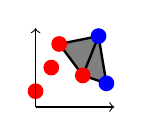
\begin{tikzpicture}[]
            \fill[gray] (0.6,0.4) -- (0.8,0.9) -- (0.9,0.3) -- cycle;
            \fill[gray] (0.3,0.8) -- (0.8,0.9) -- (0.6,0.4) -- cycle;
            \draw[black,line width=0.3mm] (0.8,0.9) -- (0.9,0.3);
            \draw[black,line width=0.3mm] (0.6,0.4) -- (0.9,0.3);
            \draw[black,line width=0.3mm] (0.6,0.4) -- (0.8,0.9);
            \draw[black,line width=0.3mm] (0.3,0.8) -- (0.8,0.9);
            \draw[black,line width=0.3mm] (0.3,0.8) -- (0.6,0.4);
            \foreach \x/\y/\c in {0/0.2/red, 0.3/0.8/red, 0.6/0.4/red, 0.8/0.9/blue, 0.2/0.5/red, 0.9/0.3/blue} {
                \fill[\c] (\x,\y) circle (0.1);
            }
            \draw[->] (0,0) -- (1,0);
            \draw[->] (0,0) -- (0,1);
        \end{tikzpicture}
    };

    \node[below=0.1cm of compgt, text width=2cm, align=center] {Simplicial complex};

    \tikzset{
        every node/.style={
            opacity=0.4,
            execute at begin node={\ifx\tikz@fig@name\highlightednode\else\color{black!70}\fi}
        },
        every path/.style={opacity=0.4},
    }

    % First column - Prediction pipeline
    \node[box,name=data1] (data1) {
        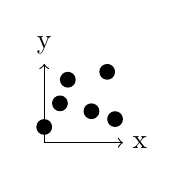
\begin{tikzpicture}
            \foreach \x/\y in {0/0.2, 0.3/0.8, 0.6/0.4, 0.8/0.9, 0.2/0.5, 0.9/0.3} {
                \fill (\x,\y) circle (0.1);
            }
            \draw[->] (0,0) -- (1,0) node[right] {x};
            \draw[->] (0,0) -- (0,1) node[above] {y};
        \end{tikzpicture}
    };

    \node[above=0.1cm of data1] {Input data};

    \node[box,right=of data1] (nn) {
        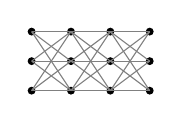
\begin{tikzpicture}[scale=0.25]
            \foreach \x in {0,...,3} {
                \foreach \y in {0,...,2} {
                    \fill (\x*2,\y*1.5) circle (0.2);
                }
            }
            \foreach \x in {0,...,2} {
                \foreach \y in {0,...,2} {
                    \foreach \z in {0,...,2} {
                        \draw[gray,thin] (\x*2,\y*1.5) -- (\x*2+2,\z*1.5);
                    }
                }
            }
        \end{tikzpicture}
    };

    \node[above=0.1cm of nn] {Neural network};

    \node[box,right=of nn] (pred) {
        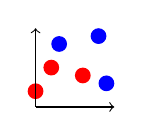
\begin{tikzpicture}[]
            \foreach \x/\y/\c in {0/0.2/red, 0.3/0.8/blue, 0.6/0.4/red, 0.8/0.9/blue, 0.2/0.5/red, 0.9/0.3/blue} {
                \fill[\c] (\x,\y) circle (0.1);
            }
            \draw[->] (0,0) -- (1,0);
            \draw[->] (0,0) -- (0,1);
        \end{tikzpicture}
    };

    \node[above=0.1cm of pred, text width=2cm, align=center] {Predicted labels};

    \node[box,right=of comppred] (pd1) {
        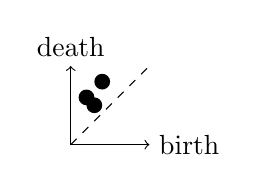
\begin{tikzpicture}[]
            \draw[->] (0,0) -- (1,0) node[right] {birth};
            \draw[->] (0,0) -- (0,1) node[above] {death};
            \draw[dashed] (0,0) -- (1,1);
            \foreach \x/\y in {0.2/0.6, 0.4/0.8, 0.3/0.5} {
                \fill (\x,\y) circle (0.1);
            }
        \end{tikzpicture}
    };
    
    \node[above=0.1cm of pd1, text width=2cm, align=center] {Persistence diagram, $\dim = 1$};

    % Second column - Ground truth pipeline
    \node[box,below=1cm of pd1] (pd2) {
        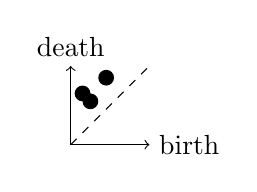
\begin{tikzpicture}[]
            \draw[->] (0,0) -- (1,0) node[right] {birth};
            \draw[->] (0,0) -- (0,1) node[above] {death};
            \draw[dashed] (0,0) -- (1,1);
            \foreach \x/\y in {0.15/0.65, 0.45/0.85, 0.25/0.55} {
                \fill (\x,\y) circle (0.1);
            }
        \end{tikzpicture}
    };

    \node[box,left=of compgt] (gt) {
        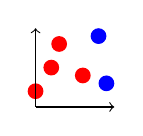
\begin{tikzpicture}[]
            \foreach \x/\y/\c in {0/0.2/red, 0.3/0.8/red, 0.6/0.4/red, 0.8/0.9/blue, 0.2/0.5/red, 0.9/0.3/blue} {
                \fill[\c] (\x,\y) circle (0.1);
            }
            \draw[->] (0,0) -- (1,0);
            \draw[->] (0,0) -- (0,1);
        \end{tikzpicture}
    };

    \node[below=0.1cm of gt, text width=2.5cm, align=center] {Ground truth labels};

    % Distance calculation
    \node[box,right=of pd1] (dist) {
        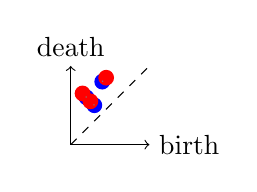
\begin{tikzpicture}[]
            \draw[->] (0,0) -- (1,0) node[right] {birth};
            \draw[->] (0,0) -- (0,1) node[above] {death};
            \draw[dashed] (0,0) -- (1,1);
            \foreach \x/\y in {0.2/0.6, 0.4/0.8, 0.3/0.5} {
                \fill[blue] (\x,\y) circle (0.1);
            }
            \foreach \x/\y in {0.15/0.65, 0.45/0.85, 0.25/0.55} {
                \fill[red] (\x,\y) circle (0.1);
            }
            \foreach \x/\y/\xx/\yy in {0.2/0.6/0.15/0.65, 0.4/0.8/0.45/0.85, 0.3/0.5/0.25/0.55} {
                \draw[gray,dotted] (\x,\y) -- (\xx,\yy);
            }
        \end{tikzpicture}
    };

    \node[above=0.1cm of dist] {Wasserstein distance};

    % Arrows
    \draw[arrow] (data1) -- (nn);
    \draw[arrow] (nn) -- (pred);
    \draw[arrow] (pred) -- (comppred);
    \draw[arrow] (comppred) -- (pd1);
    \draw[arrow] (gt) -- (compgt);
    \draw[arrow] (compgt) -- (pd2);
    \draw[arrow] (pd1) -- (dist);
    \draw[arrow] (pd2) -- (dist);

    \end{tikzpicture}
    }
\end{frame}


\begin{frame}{Binarization}
    \begin{columns}
        \column{0.8\textwidth}
        Previous work only considered binary classification by splitting
        a dataset with $n$ classes into $\binom{n}{2}$ binary datasets.
        This changes the homology groups:
        \begin{itemize}
            \item Original has $H_1 \not\cong 0$
            \item All binary decompositions have $H_1 \cong 0$
            % \item Original has $\dim H_0 = 1$
            % \item The red-green binary decomposition has $\dim H_0 = 2$.
        \end{itemize}
        It is better to avoid binarization.
        \column{0.2\textwidth}
        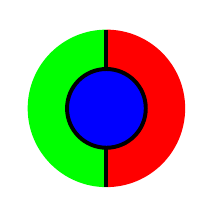
\begin{tikzpicture}
            \fill[blue] (0,0) circle(0.5);
    
            \fill[red]
            (0,-0.5)           % Start at bottom inner point
            arc(-90:90:0.5)     % Inner arc: radius=0.5 from -90° to 90° (bottom to top on the right side)
            -- (0,1)            % Line from top inner (0,0.5) to top outer (0,1)
            arc(90:-90:1)       % Outer arc: radius=1 from 90° to -90° (top to bottom on the right side)
            -- cycle;           

            \begin{scope}[rotate=180]
            \fill[green]
            (0,-0.5)
            arc(-90:90:0.5)
            -- (0,1)
            arc(90:-90:1)
            -- cycle;
            \end{scope}
            
            % Decision boundary
            \draw[line width=0.5mm] (0, 0.5) -- (0, 1);
            \draw[line width=0.5mm] (0, -0.5) -- (0, -1);
            \draw[line width=0.5mm] (0,0) circle (0.5);
        \end{tikzpicture}
        \linebreak

        
\begin{tikzpicture}
            \fill[red]
            (0,-0.5)           % Start at bottom inner point
            arc(-90:90:0.5)     % Inner arc: radius=0.5 from -90° to 90° (bottom to top on the right side)
            -- (0,1)            % Line from top inner (0,0.5) to top outer (0,1)
            arc(90:-90:1)       % Outer arc: radius=1 from 90° to -90° (top to bottom on the right side)
            -- cycle;           

            \begin{scope}[rotate=180]
            \fill[green]
            (0,-0.5)
            arc(-90:90:0.5)
            -- (0,1)
            arc(90:-90:1)
            -- cycle;
            \end{scope}
            
            % Decision boundary
            \draw[line width=0.5mm] (0, 0.5) -- (0, 1);
            \draw[line width=0.5mm] (0, -0.5) -- (0, -1);
        \end{tikzpicture}
        \\

        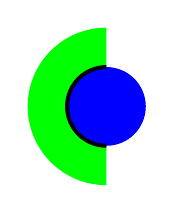
\begin{tikzpicture}
            \fill[blue] (0,0) circle(0.5);
    
            \begin{scope}[rotate=180]
            \fill[green]
            (0,-0.5)
            arc(-90:90:0.5)
            -- (0,1)
            arc(90:-90:1)
            -- cycle;
            \end{scope}
            
            % Decision boundary
            \draw[line width=0.5mm] (0,0.5) arc (90:270:0.5);
        \end{tikzpicture}
    \end{columns}
\end{frame}

\begin{frame}{Labeled Vietoris-Rips complex}
    \begin{columns}
        \column{0.6\textwidth}
        \begin{itemize}
            \item Set of points $X$
            \item Labels $c: X \to \mathbb{Z}_k$
            \item Parameter \(\varepsilon\)
        \end{itemize}
        Constructed in three steps:
        \begin{enumerate}
            \item<2-> Create a graph \(G_\varepsilon\) with vertex set \(X\) by adding an edge 
            between points \(x_i, x_j \in X\) iff:
            \begin{itemize}
                \item \(\norm{x_i - x_j} \leq \varepsilon\) (points are close enough)
                \item \(c(x_i) \neq c(x_j)\) (different classes)
            \end{itemize}
            
            \item<3-> Add edges between all 2-hop neighbors in \(G_\varepsilon\)          
            \item<4-> Standard Vietoris-Rips construction: include simplex if all faces are included
        \end{enumerate}
        \only<5>{
            \begin{itemize}
                \item Simplices cross the boundary
                \item Applicable to multiple classes
            \end{itemize}
        }
        \column{0.4\textwidth}
        \hspace*{-0.5cm}
        \only<1>{\hspace*{-1em}\resizebox{1.2\textwidth}{!}{\input{plots/lvr_points.pgf}}}
        \only<2>{\hspace*{-1em}\resizebox{1.2\textwidth}{!}{\input{plots/lvr_step1.pgf}}}
        \only<3>{\hspace*{-1em}\resizebox{1.2\textwidth}{!}{\input{plots/lvr_step2.pgf}}}
        \only<4->{\hspace*{-1em}\resizebox{1.2\textwidth}{!}{%% Creator: Matplotlib, PGF backend
%%
%% To include the figure in your LaTeX document, write
%%   \input{<filename>.pgf}
%%
%% Make sure the required packages are loaded in your preamble
%%   \usepackage{pgf}
%%
%% Also ensure that all the required font packages are loaded; for instance,
%% the lmodern package is sometimes necessary when using math font.
%%   \usepackage{lmodern}
%%
%% Figures using additional raster images can only be included by \input if
%% they are in the same directory as the main LaTeX file. For loading figures
%% from other directories you can use the `import` package
%%   \usepackage{import}
%%
%% and then include the figures with
%%   \import{<path to file>}{<filename>.pgf}
%%
%% Matplotlib used the following preamble
%%   \def\mathdefault#1{#1}
%%   \everymath=\expandafter{\the\everymath\displaystyle}
%%   
%%   \ifdefined\pdftexversion\else  % non-pdftex case.
%%     \usepackage{fontspec}
%%     \setmainfont{DejaVuSerif.ttf}[Path=\detokenize{/home/snek/repos/homology-decision-bondaries-clean/venv/lib/python3.9/site-packages/matplotlib/mpl-data/fonts/ttf/}]
%%     \setsansfont{DejaVuSans.ttf}[Path=\detokenize{/home/snek/repos/homology-decision-bondaries-clean/venv/lib/python3.9/site-packages/matplotlib/mpl-data/fonts/ttf/}]
%%     \setmonofont{DejaVuSansMono.ttf}[Path=\detokenize{/home/snek/repos/homology-decision-bondaries-clean/venv/lib/python3.9/site-packages/matplotlib/mpl-data/fonts/ttf/}]
%%   \fi
%%   \makeatletter\@ifpackageloaded{underscore}{}{\usepackage[strings]{underscore}}\makeatother
%%
\begingroup%
\makeatletter%
\begin{pgfpicture}%
\pgfpathrectangle{\pgfpointorigin}{\pgfqpoint{6.400000in}{4.800000in}}%
\pgfusepath{use as bounding box, clip}%
\begin{pgfscope}%
\pgfsetbuttcap%
\pgfsetmiterjoin%
\definecolor{currentfill}{rgb}{1.000000,1.000000,1.000000}%
\pgfsetfillcolor{currentfill}%
\pgfsetlinewidth{0.000000pt}%
\definecolor{currentstroke}{rgb}{1.000000,1.000000,1.000000}%
\pgfsetstrokecolor{currentstroke}%
\pgfsetdash{}{0pt}%
\pgfpathmoveto{\pgfqpoint{0.000000in}{0.000000in}}%
\pgfpathlineto{\pgfqpoint{6.400000in}{0.000000in}}%
\pgfpathlineto{\pgfqpoint{6.400000in}{4.800000in}}%
\pgfpathlineto{\pgfqpoint{0.000000in}{4.800000in}}%
\pgfpathlineto{\pgfqpoint{0.000000in}{0.000000in}}%
\pgfpathclose%
\pgfusepath{fill}%
\end{pgfscope}%
\begin{pgfscope}%
\pgfpathrectangle{\pgfqpoint{0.150000in}{0.150000in}}{\pgfqpoint{6.100000in}{4.500000in}}%
\pgfusepath{clip}%
\pgfsetbuttcap%
\pgfsetmiterjoin%
\definecolor{currentfill}{rgb}{0.501961,0.501961,0.501961}%
\pgfsetfillcolor{currentfill}%
\pgfsetfillopacity{0.400000}%
\pgfsetlinewidth{1.003750pt}%
\definecolor{currentstroke}{rgb}{0.501961,0.501961,0.501961}%
\pgfsetstrokecolor{currentstroke}%
\pgfsetstrokeopacity{0.400000}%
\pgfsetdash{}{0pt}%
\pgfpathmoveto{\pgfqpoint{5.168678in}{2.916780in}}%
\pgfpathlineto{\pgfqpoint{4.795170in}{3.210793in}}%
\pgfpathlineto{\pgfqpoint{4.625374in}{3.543260in}}%
\pgfpathlineto{\pgfqpoint{5.168678in}{2.916780in}}%
\pgfpathclose%
\pgfusepath{stroke,fill}%
\end{pgfscope}%
\begin{pgfscope}%
\pgfpathrectangle{\pgfqpoint{0.150000in}{0.150000in}}{\pgfqpoint{6.100000in}{4.500000in}}%
\pgfusepath{clip}%
\pgfsetbuttcap%
\pgfsetmiterjoin%
\definecolor{currentfill}{rgb}{0.501961,0.501961,0.501961}%
\pgfsetfillcolor{currentfill}%
\pgfsetfillopacity{0.400000}%
\pgfsetlinewidth{1.003750pt}%
\definecolor{currentstroke}{rgb}{0.501961,0.501961,0.501961}%
\pgfsetstrokecolor{currentstroke}%
\pgfsetstrokeopacity{0.400000}%
\pgfsetdash{}{0pt}%
\pgfpathmoveto{\pgfqpoint{5.168678in}{2.916780in}}%
\pgfpathlineto{\pgfqpoint{4.795170in}{3.210793in}}%
\pgfpathlineto{\pgfqpoint{4.350731in}{3.796143in}}%
\pgfpathlineto{\pgfqpoint{5.168678in}{2.916780in}}%
\pgfpathclose%
\pgfusepath{stroke,fill}%
\end{pgfscope}%
\begin{pgfscope}%
\pgfpathrectangle{\pgfqpoint{0.150000in}{0.150000in}}{\pgfqpoint{6.100000in}{4.500000in}}%
\pgfusepath{clip}%
\pgfsetbuttcap%
\pgfsetmiterjoin%
\definecolor{currentfill}{rgb}{0.501961,0.501961,0.501961}%
\pgfsetfillcolor{currentfill}%
\pgfsetfillopacity{0.400000}%
\pgfsetlinewidth{1.003750pt}%
\definecolor{currentstroke}{rgb}{0.501961,0.501961,0.501961}%
\pgfsetstrokecolor{currentstroke}%
\pgfsetstrokeopacity{0.400000}%
\pgfsetdash{}{0pt}%
\pgfpathmoveto{\pgfqpoint{5.168678in}{2.916780in}}%
\pgfpathlineto{\pgfqpoint{4.795170in}{3.210793in}}%
\pgfpathlineto{\pgfqpoint{5.037263in}{2.493110in}}%
\pgfpathlineto{\pgfqpoint{5.168678in}{2.916780in}}%
\pgfpathclose%
\pgfusepath{stroke,fill}%
\end{pgfscope}%
\begin{pgfscope}%
\pgfpathrectangle{\pgfqpoint{0.150000in}{0.150000in}}{\pgfqpoint{6.100000in}{4.500000in}}%
\pgfusepath{clip}%
\pgfsetbuttcap%
\pgfsetmiterjoin%
\definecolor{currentfill}{rgb}{0.501961,0.501961,0.501961}%
\pgfsetfillcolor{currentfill}%
\pgfsetfillopacity{0.400000}%
\pgfsetlinewidth{1.003750pt}%
\definecolor{currentstroke}{rgb}{0.501961,0.501961,0.501961}%
\pgfsetstrokecolor{currentstroke}%
\pgfsetstrokeopacity{0.400000}%
\pgfsetdash{}{0pt}%
\pgfpathmoveto{\pgfqpoint{5.168678in}{2.916780in}}%
\pgfpathlineto{\pgfqpoint{4.625374in}{3.543260in}}%
\pgfpathlineto{\pgfqpoint{4.350731in}{3.796143in}}%
\pgfpathlineto{\pgfqpoint{5.168678in}{2.916780in}}%
\pgfpathclose%
\pgfusepath{stroke,fill}%
\end{pgfscope}%
\begin{pgfscope}%
\pgfpathrectangle{\pgfqpoint{0.150000in}{0.150000in}}{\pgfqpoint{6.100000in}{4.500000in}}%
\pgfusepath{clip}%
\pgfsetbuttcap%
\pgfsetmiterjoin%
\definecolor{currentfill}{rgb}{0.501961,0.501961,0.501961}%
\pgfsetfillcolor{currentfill}%
\pgfsetfillopacity{0.400000}%
\pgfsetlinewidth{1.003750pt}%
\definecolor{currentstroke}{rgb}{0.501961,0.501961,0.501961}%
\pgfsetstrokecolor{currentstroke}%
\pgfsetstrokeopacity{0.400000}%
\pgfsetdash{}{0pt}%
\pgfpathmoveto{\pgfqpoint{5.168678in}{2.916780in}}%
\pgfpathlineto{\pgfqpoint{4.625374in}{3.543260in}}%
\pgfpathlineto{\pgfqpoint{5.037263in}{2.493110in}}%
\pgfpathlineto{\pgfqpoint{5.168678in}{2.916780in}}%
\pgfpathclose%
\pgfusepath{stroke,fill}%
\end{pgfscope}%
\begin{pgfscope}%
\pgfpathrectangle{\pgfqpoint{0.150000in}{0.150000in}}{\pgfqpoint{6.100000in}{4.500000in}}%
\pgfusepath{clip}%
\pgfsetbuttcap%
\pgfsetmiterjoin%
\definecolor{currentfill}{rgb}{0.501961,0.501961,0.501961}%
\pgfsetfillcolor{currentfill}%
\pgfsetfillopacity{0.400000}%
\pgfsetlinewidth{1.003750pt}%
\definecolor{currentstroke}{rgb}{0.501961,0.501961,0.501961}%
\pgfsetstrokecolor{currentstroke}%
\pgfsetstrokeopacity{0.400000}%
\pgfsetdash{}{0pt}%
\pgfpathmoveto{\pgfqpoint{5.168678in}{2.916780in}}%
\pgfpathlineto{\pgfqpoint{4.350731in}{3.796143in}}%
\pgfpathlineto{\pgfqpoint{5.037263in}{2.493110in}}%
\pgfpathlineto{\pgfqpoint{5.168678in}{2.916780in}}%
\pgfpathclose%
\pgfusepath{stroke,fill}%
\end{pgfscope}%
\begin{pgfscope}%
\pgfpathrectangle{\pgfqpoint{0.150000in}{0.150000in}}{\pgfqpoint{6.100000in}{4.500000in}}%
\pgfusepath{clip}%
\pgfsetbuttcap%
\pgfsetmiterjoin%
\definecolor{currentfill}{rgb}{0.501961,0.501961,0.501961}%
\pgfsetfillcolor{currentfill}%
\pgfsetfillopacity{0.400000}%
\pgfsetlinewidth{1.003750pt}%
\definecolor{currentstroke}{rgb}{0.501961,0.501961,0.501961}%
\pgfsetstrokecolor{currentstroke}%
\pgfsetstrokeopacity{0.400000}%
\pgfsetdash{}{0pt}%
\pgfpathmoveto{\pgfqpoint{4.795170in}{3.210793in}}%
\pgfpathlineto{\pgfqpoint{4.625374in}{3.543260in}}%
\pgfpathlineto{\pgfqpoint{4.350731in}{3.796143in}}%
\pgfpathlineto{\pgfqpoint{4.795170in}{3.210793in}}%
\pgfpathclose%
\pgfusepath{stroke,fill}%
\end{pgfscope}%
\begin{pgfscope}%
\pgfpathrectangle{\pgfqpoint{0.150000in}{0.150000in}}{\pgfqpoint{6.100000in}{4.500000in}}%
\pgfusepath{clip}%
\pgfsetbuttcap%
\pgfsetmiterjoin%
\definecolor{currentfill}{rgb}{0.501961,0.501961,0.501961}%
\pgfsetfillcolor{currentfill}%
\pgfsetfillopacity{0.400000}%
\pgfsetlinewidth{1.003750pt}%
\definecolor{currentstroke}{rgb}{0.501961,0.501961,0.501961}%
\pgfsetstrokecolor{currentstroke}%
\pgfsetstrokeopacity{0.400000}%
\pgfsetdash{}{0pt}%
\pgfpathmoveto{\pgfqpoint{4.795170in}{3.210793in}}%
\pgfpathlineto{\pgfqpoint{4.625374in}{3.543260in}}%
\pgfpathlineto{\pgfqpoint{5.037263in}{2.493110in}}%
\pgfpathlineto{\pgfqpoint{4.795170in}{3.210793in}}%
\pgfpathclose%
\pgfusepath{stroke,fill}%
\end{pgfscope}%
\begin{pgfscope}%
\pgfpathrectangle{\pgfqpoint{0.150000in}{0.150000in}}{\pgfqpoint{6.100000in}{4.500000in}}%
\pgfusepath{clip}%
\pgfsetbuttcap%
\pgfsetmiterjoin%
\definecolor{currentfill}{rgb}{0.501961,0.501961,0.501961}%
\pgfsetfillcolor{currentfill}%
\pgfsetfillopacity{0.400000}%
\pgfsetlinewidth{1.003750pt}%
\definecolor{currentstroke}{rgb}{0.501961,0.501961,0.501961}%
\pgfsetstrokecolor{currentstroke}%
\pgfsetstrokeopacity{0.400000}%
\pgfsetdash{}{0pt}%
\pgfpathmoveto{\pgfqpoint{4.795170in}{3.210793in}}%
\pgfpathlineto{\pgfqpoint{4.350731in}{3.796143in}}%
\pgfpathlineto{\pgfqpoint{5.037263in}{2.493110in}}%
\pgfpathlineto{\pgfqpoint{4.795170in}{3.210793in}}%
\pgfpathclose%
\pgfusepath{stroke,fill}%
\end{pgfscope}%
\begin{pgfscope}%
\pgfpathrectangle{\pgfqpoint{0.150000in}{0.150000in}}{\pgfqpoint{6.100000in}{4.500000in}}%
\pgfusepath{clip}%
\pgfsetbuttcap%
\pgfsetmiterjoin%
\definecolor{currentfill}{rgb}{0.501961,0.501961,0.501961}%
\pgfsetfillcolor{currentfill}%
\pgfsetfillopacity{0.400000}%
\pgfsetlinewidth{1.003750pt}%
\definecolor{currentstroke}{rgb}{0.501961,0.501961,0.501961}%
\pgfsetstrokecolor{currentstroke}%
\pgfsetstrokeopacity{0.400000}%
\pgfsetdash{}{0pt}%
\pgfpathmoveto{\pgfqpoint{4.625374in}{3.543260in}}%
\pgfpathlineto{\pgfqpoint{4.350731in}{3.796143in}}%
\pgfpathlineto{\pgfqpoint{4.219676in}{4.333572in}}%
\pgfpathlineto{\pgfqpoint{4.625374in}{3.543260in}}%
\pgfpathclose%
\pgfusepath{stroke,fill}%
\end{pgfscope}%
\begin{pgfscope}%
\pgfpathrectangle{\pgfqpoint{0.150000in}{0.150000in}}{\pgfqpoint{6.100000in}{4.500000in}}%
\pgfusepath{clip}%
\pgfsetbuttcap%
\pgfsetmiterjoin%
\definecolor{currentfill}{rgb}{0.501961,0.501961,0.501961}%
\pgfsetfillcolor{currentfill}%
\pgfsetfillopacity{0.400000}%
\pgfsetlinewidth{1.003750pt}%
\definecolor{currentstroke}{rgb}{0.501961,0.501961,0.501961}%
\pgfsetstrokecolor{currentstroke}%
\pgfsetstrokeopacity{0.400000}%
\pgfsetdash{}{0pt}%
\pgfpathmoveto{\pgfqpoint{4.625374in}{3.543260in}}%
\pgfpathlineto{\pgfqpoint{4.350731in}{3.796143in}}%
\pgfpathlineto{\pgfqpoint{3.742471in}{4.288713in}}%
\pgfpathlineto{\pgfqpoint{4.625374in}{3.543260in}}%
\pgfpathclose%
\pgfusepath{stroke,fill}%
\end{pgfscope}%
\begin{pgfscope}%
\pgfpathrectangle{\pgfqpoint{0.150000in}{0.150000in}}{\pgfqpoint{6.100000in}{4.500000in}}%
\pgfusepath{clip}%
\pgfsetbuttcap%
\pgfsetmiterjoin%
\definecolor{currentfill}{rgb}{0.501961,0.501961,0.501961}%
\pgfsetfillcolor{currentfill}%
\pgfsetfillopacity{0.400000}%
\pgfsetlinewidth{1.003750pt}%
\definecolor{currentstroke}{rgb}{0.501961,0.501961,0.501961}%
\pgfsetstrokecolor{currentstroke}%
\pgfsetstrokeopacity{0.400000}%
\pgfsetdash{}{0pt}%
\pgfpathmoveto{\pgfqpoint{4.625374in}{3.543260in}}%
\pgfpathlineto{\pgfqpoint{4.350731in}{3.796143in}}%
\pgfpathlineto{\pgfqpoint{3.350899in}{4.466129in}}%
\pgfpathlineto{\pgfqpoint{4.625374in}{3.543260in}}%
\pgfpathclose%
\pgfusepath{stroke,fill}%
\end{pgfscope}%
\begin{pgfscope}%
\pgfpathrectangle{\pgfqpoint{0.150000in}{0.150000in}}{\pgfqpoint{6.100000in}{4.500000in}}%
\pgfusepath{clip}%
\pgfsetbuttcap%
\pgfsetmiterjoin%
\definecolor{currentfill}{rgb}{0.501961,0.501961,0.501961}%
\pgfsetfillcolor{currentfill}%
\pgfsetfillopacity{0.400000}%
\pgfsetlinewidth{1.003750pt}%
\definecolor{currentstroke}{rgb}{0.501961,0.501961,0.501961}%
\pgfsetstrokecolor{currentstroke}%
\pgfsetstrokeopacity{0.400000}%
\pgfsetdash{}{0pt}%
\pgfpathmoveto{\pgfqpoint{4.625374in}{3.543260in}}%
\pgfpathlineto{\pgfqpoint{4.350731in}{3.796143in}}%
\pgfpathlineto{\pgfqpoint{5.037263in}{2.493110in}}%
\pgfpathlineto{\pgfqpoint{4.625374in}{3.543260in}}%
\pgfpathclose%
\pgfusepath{stroke,fill}%
\end{pgfscope}%
\begin{pgfscope}%
\pgfpathrectangle{\pgfqpoint{0.150000in}{0.150000in}}{\pgfqpoint{6.100000in}{4.500000in}}%
\pgfusepath{clip}%
\pgfsetbuttcap%
\pgfsetmiterjoin%
\definecolor{currentfill}{rgb}{0.501961,0.501961,0.501961}%
\pgfsetfillcolor{currentfill}%
\pgfsetfillopacity{0.400000}%
\pgfsetlinewidth{1.003750pt}%
\definecolor{currentstroke}{rgb}{0.501961,0.501961,0.501961}%
\pgfsetstrokecolor{currentstroke}%
\pgfsetstrokeopacity{0.400000}%
\pgfsetdash{}{0pt}%
\pgfpathmoveto{\pgfqpoint{4.625374in}{3.543260in}}%
\pgfpathlineto{\pgfqpoint{4.219676in}{4.333572in}}%
\pgfpathlineto{\pgfqpoint{3.742471in}{4.288713in}}%
\pgfpathlineto{\pgfqpoint{4.625374in}{3.543260in}}%
\pgfpathclose%
\pgfusepath{stroke,fill}%
\end{pgfscope}%
\begin{pgfscope}%
\pgfpathrectangle{\pgfqpoint{0.150000in}{0.150000in}}{\pgfqpoint{6.100000in}{4.500000in}}%
\pgfusepath{clip}%
\pgfsetbuttcap%
\pgfsetmiterjoin%
\definecolor{currentfill}{rgb}{0.501961,0.501961,0.501961}%
\pgfsetfillcolor{currentfill}%
\pgfsetfillopacity{0.400000}%
\pgfsetlinewidth{1.003750pt}%
\definecolor{currentstroke}{rgb}{0.501961,0.501961,0.501961}%
\pgfsetstrokecolor{currentstroke}%
\pgfsetstrokeopacity{0.400000}%
\pgfsetdash{}{0pt}%
\pgfpathmoveto{\pgfqpoint{4.625374in}{3.543260in}}%
\pgfpathlineto{\pgfqpoint{4.219676in}{4.333572in}}%
\pgfpathlineto{\pgfqpoint{3.350899in}{4.466129in}}%
\pgfpathlineto{\pgfqpoint{4.625374in}{3.543260in}}%
\pgfpathclose%
\pgfusepath{stroke,fill}%
\end{pgfscope}%
\begin{pgfscope}%
\pgfpathrectangle{\pgfqpoint{0.150000in}{0.150000in}}{\pgfqpoint{6.100000in}{4.500000in}}%
\pgfusepath{clip}%
\pgfsetbuttcap%
\pgfsetmiterjoin%
\definecolor{currentfill}{rgb}{0.501961,0.501961,0.501961}%
\pgfsetfillcolor{currentfill}%
\pgfsetfillopacity{0.400000}%
\pgfsetlinewidth{1.003750pt}%
\definecolor{currentstroke}{rgb}{0.501961,0.501961,0.501961}%
\pgfsetstrokecolor{currentstroke}%
\pgfsetstrokeopacity{0.400000}%
\pgfsetdash{}{0pt}%
\pgfpathmoveto{\pgfqpoint{4.625374in}{3.543260in}}%
\pgfpathlineto{\pgfqpoint{3.742471in}{4.288713in}}%
\pgfpathlineto{\pgfqpoint{3.350899in}{4.466129in}}%
\pgfpathlineto{\pgfqpoint{4.625374in}{3.543260in}}%
\pgfpathclose%
\pgfusepath{stroke,fill}%
\end{pgfscope}%
\begin{pgfscope}%
\pgfpathrectangle{\pgfqpoint{0.150000in}{0.150000in}}{\pgfqpoint{6.100000in}{4.500000in}}%
\pgfusepath{clip}%
\pgfsetbuttcap%
\pgfsetmiterjoin%
\definecolor{currentfill}{rgb}{0.501961,0.501961,0.501961}%
\pgfsetfillcolor{currentfill}%
\pgfsetfillopacity{0.400000}%
\pgfsetlinewidth{1.003750pt}%
\definecolor{currentstroke}{rgb}{0.501961,0.501961,0.501961}%
\pgfsetstrokecolor{currentstroke}%
\pgfsetstrokeopacity{0.400000}%
\pgfsetdash{}{0pt}%
\pgfpathmoveto{\pgfqpoint{4.350731in}{3.796143in}}%
\pgfpathlineto{\pgfqpoint{4.219676in}{4.333572in}}%
\pgfpathlineto{\pgfqpoint{3.742471in}{4.288713in}}%
\pgfpathlineto{\pgfqpoint{4.350731in}{3.796143in}}%
\pgfpathclose%
\pgfusepath{stroke,fill}%
\end{pgfscope}%
\begin{pgfscope}%
\pgfpathrectangle{\pgfqpoint{0.150000in}{0.150000in}}{\pgfqpoint{6.100000in}{4.500000in}}%
\pgfusepath{clip}%
\pgfsetbuttcap%
\pgfsetmiterjoin%
\definecolor{currentfill}{rgb}{0.501961,0.501961,0.501961}%
\pgfsetfillcolor{currentfill}%
\pgfsetfillopacity{0.400000}%
\pgfsetlinewidth{1.003750pt}%
\definecolor{currentstroke}{rgb}{0.501961,0.501961,0.501961}%
\pgfsetstrokecolor{currentstroke}%
\pgfsetstrokeopacity{0.400000}%
\pgfsetdash{}{0pt}%
\pgfpathmoveto{\pgfqpoint{4.350731in}{3.796143in}}%
\pgfpathlineto{\pgfqpoint{4.219676in}{4.333572in}}%
\pgfpathlineto{\pgfqpoint{3.350899in}{4.466129in}}%
\pgfpathlineto{\pgfqpoint{4.350731in}{3.796143in}}%
\pgfpathclose%
\pgfusepath{stroke,fill}%
\end{pgfscope}%
\begin{pgfscope}%
\pgfpathrectangle{\pgfqpoint{0.150000in}{0.150000in}}{\pgfqpoint{6.100000in}{4.500000in}}%
\pgfusepath{clip}%
\pgfsetbuttcap%
\pgfsetmiterjoin%
\definecolor{currentfill}{rgb}{0.501961,0.501961,0.501961}%
\pgfsetfillcolor{currentfill}%
\pgfsetfillopacity{0.400000}%
\pgfsetlinewidth{1.003750pt}%
\definecolor{currentstroke}{rgb}{0.501961,0.501961,0.501961}%
\pgfsetstrokecolor{currentstroke}%
\pgfsetstrokeopacity{0.400000}%
\pgfsetdash{}{0pt}%
\pgfpathmoveto{\pgfqpoint{4.350731in}{3.796143in}}%
\pgfpathlineto{\pgfqpoint{4.219676in}{4.333572in}}%
\pgfpathlineto{\pgfqpoint{2.934626in}{4.379750in}}%
\pgfpathlineto{\pgfqpoint{4.350731in}{3.796143in}}%
\pgfpathclose%
\pgfusepath{stroke,fill}%
\end{pgfscope}%
\begin{pgfscope}%
\pgfpathrectangle{\pgfqpoint{0.150000in}{0.150000in}}{\pgfqpoint{6.100000in}{4.500000in}}%
\pgfusepath{clip}%
\pgfsetbuttcap%
\pgfsetmiterjoin%
\definecolor{currentfill}{rgb}{0.501961,0.501961,0.501961}%
\pgfsetfillcolor{currentfill}%
\pgfsetfillopacity{0.400000}%
\pgfsetlinewidth{1.003750pt}%
\definecolor{currentstroke}{rgb}{0.501961,0.501961,0.501961}%
\pgfsetstrokecolor{currentstroke}%
\pgfsetstrokeopacity{0.400000}%
\pgfsetdash{}{0pt}%
\pgfpathmoveto{\pgfqpoint{4.350731in}{3.796143in}}%
\pgfpathlineto{\pgfqpoint{3.742471in}{4.288713in}}%
\pgfpathlineto{\pgfqpoint{3.350899in}{4.466129in}}%
\pgfpathlineto{\pgfqpoint{4.350731in}{3.796143in}}%
\pgfpathclose%
\pgfusepath{stroke,fill}%
\end{pgfscope}%
\begin{pgfscope}%
\pgfpathrectangle{\pgfqpoint{0.150000in}{0.150000in}}{\pgfqpoint{6.100000in}{4.500000in}}%
\pgfusepath{clip}%
\pgfsetbuttcap%
\pgfsetmiterjoin%
\definecolor{currentfill}{rgb}{0.501961,0.501961,0.501961}%
\pgfsetfillcolor{currentfill}%
\pgfsetfillopacity{0.400000}%
\pgfsetlinewidth{1.003750pt}%
\definecolor{currentstroke}{rgb}{0.501961,0.501961,0.501961}%
\pgfsetstrokecolor{currentstroke}%
\pgfsetstrokeopacity{0.400000}%
\pgfsetdash{}{0pt}%
\pgfpathmoveto{\pgfqpoint{4.350731in}{3.796143in}}%
\pgfpathlineto{\pgfqpoint{3.742471in}{4.288713in}}%
\pgfpathlineto{\pgfqpoint{2.934626in}{4.379750in}}%
\pgfpathlineto{\pgfqpoint{4.350731in}{3.796143in}}%
\pgfpathclose%
\pgfusepath{stroke,fill}%
\end{pgfscope}%
\begin{pgfscope}%
\pgfpathrectangle{\pgfqpoint{0.150000in}{0.150000in}}{\pgfqpoint{6.100000in}{4.500000in}}%
\pgfusepath{clip}%
\pgfsetbuttcap%
\pgfsetmiterjoin%
\definecolor{currentfill}{rgb}{0.501961,0.501961,0.501961}%
\pgfsetfillcolor{currentfill}%
\pgfsetfillopacity{0.400000}%
\pgfsetlinewidth{1.003750pt}%
\definecolor{currentstroke}{rgb}{0.501961,0.501961,0.501961}%
\pgfsetstrokecolor{currentstroke}%
\pgfsetstrokeopacity{0.400000}%
\pgfsetdash{}{0pt}%
\pgfpathmoveto{\pgfqpoint{4.350731in}{3.796143in}}%
\pgfpathlineto{\pgfqpoint{3.350899in}{4.466129in}}%
\pgfpathlineto{\pgfqpoint{2.934626in}{4.379750in}}%
\pgfpathlineto{\pgfqpoint{4.350731in}{3.796143in}}%
\pgfpathclose%
\pgfusepath{stroke,fill}%
\end{pgfscope}%
\begin{pgfscope}%
\pgfpathrectangle{\pgfqpoint{0.150000in}{0.150000in}}{\pgfqpoint{6.100000in}{4.500000in}}%
\pgfusepath{clip}%
\pgfsetbuttcap%
\pgfsetmiterjoin%
\definecolor{currentfill}{rgb}{0.501961,0.501961,0.501961}%
\pgfsetfillcolor{currentfill}%
\pgfsetfillopacity{0.400000}%
\pgfsetlinewidth{1.003750pt}%
\definecolor{currentstroke}{rgb}{0.501961,0.501961,0.501961}%
\pgfsetstrokecolor{currentstroke}%
\pgfsetstrokeopacity{0.400000}%
\pgfsetdash{}{0pt}%
\pgfpathmoveto{\pgfqpoint{4.219676in}{4.333572in}}%
\pgfpathlineto{\pgfqpoint{3.742471in}{4.288713in}}%
\pgfpathlineto{\pgfqpoint{3.350899in}{4.466129in}}%
\pgfpathlineto{\pgfqpoint{4.219676in}{4.333572in}}%
\pgfpathclose%
\pgfusepath{stroke,fill}%
\end{pgfscope}%
\begin{pgfscope}%
\pgfpathrectangle{\pgfqpoint{0.150000in}{0.150000in}}{\pgfqpoint{6.100000in}{4.500000in}}%
\pgfusepath{clip}%
\pgfsetbuttcap%
\pgfsetmiterjoin%
\definecolor{currentfill}{rgb}{0.501961,0.501961,0.501961}%
\pgfsetfillcolor{currentfill}%
\pgfsetfillopacity{0.400000}%
\pgfsetlinewidth{1.003750pt}%
\definecolor{currentstroke}{rgb}{0.501961,0.501961,0.501961}%
\pgfsetstrokecolor{currentstroke}%
\pgfsetstrokeopacity{0.400000}%
\pgfsetdash{}{0pt}%
\pgfpathmoveto{\pgfqpoint{4.219676in}{4.333572in}}%
\pgfpathlineto{\pgfqpoint{3.742471in}{4.288713in}}%
\pgfpathlineto{\pgfqpoint{2.934626in}{4.379750in}}%
\pgfpathlineto{\pgfqpoint{4.219676in}{4.333572in}}%
\pgfpathclose%
\pgfusepath{stroke,fill}%
\end{pgfscope}%
\begin{pgfscope}%
\pgfpathrectangle{\pgfqpoint{0.150000in}{0.150000in}}{\pgfqpoint{6.100000in}{4.500000in}}%
\pgfusepath{clip}%
\pgfsetbuttcap%
\pgfsetmiterjoin%
\definecolor{currentfill}{rgb}{0.501961,0.501961,0.501961}%
\pgfsetfillcolor{currentfill}%
\pgfsetfillopacity{0.400000}%
\pgfsetlinewidth{1.003750pt}%
\definecolor{currentstroke}{rgb}{0.501961,0.501961,0.501961}%
\pgfsetstrokecolor{currentstroke}%
\pgfsetstrokeopacity{0.400000}%
\pgfsetdash{}{0pt}%
\pgfpathmoveto{\pgfqpoint{4.219676in}{4.333572in}}%
\pgfpathlineto{\pgfqpoint{3.350899in}{4.466129in}}%
\pgfpathlineto{\pgfqpoint{2.934626in}{4.379750in}}%
\pgfpathlineto{\pgfqpoint{4.219676in}{4.333572in}}%
\pgfpathclose%
\pgfusepath{stroke,fill}%
\end{pgfscope}%
\begin{pgfscope}%
\pgfpathrectangle{\pgfqpoint{0.150000in}{0.150000in}}{\pgfqpoint{6.100000in}{4.500000in}}%
\pgfusepath{clip}%
\pgfsetbuttcap%
\pgfsetmiterjoin%
\definecolor{currentfill}{rgb}{0.501961,0.501961,0.501961}%
\pgfsetfillcolor{currentfill}%
\pgfsetfillopacity{0.400000}%
\pgfsetlinewidth{1.003750pt}%
\definecolor{currentstroke}{rgb}{0.501961,0.501961,0.501961}%
\pgfsetstrokecolor{currentstroke}%
\pgfsetstrokeopacity{0.400000}%
\pgfsetdash{}{0pt}%
\pgfpathmoveto{\pgfqpoint{3.742471in}{4.288713in}}%
\pgfpathlineto{\pgfqpoint{3.350899in}{4.466129in}}%
\pgfpathlineto{\pgfqpoint{2.934626in}{4.379750in}}%
\pgfpathlineto{\pgfqpoint{3.742471in}{4.288713in}}%
\pgfpathclose%
\pgfusepath{stroke,fill}%
\end{pgfscope}%
\begin{pgfscope}%
\pgfpathrectangle{\pgfqpoint{0.150000in}{0.150000in}}{\pgfqpoint{6.100000in}{4.500000in}}%
\pgfusepath{clip}%
\pgfsetbuttcap%
\pgfsetmiterjoin%
\definecolor{currentfill}{rgb}{0.501961,0.501961,0.501961}%
\pgfsetfillcolor{currentfill}%
\pgfsetfillopacity{0.400000}%
\pgfsetlinewidth{1.003750pt}%
\definecolor{currentstroke}{rgb}{0.501961,0.501961,0.501961}%
\pgfsetstrokecolor{currentstroke}%
\pgfsetstrokeopacity{0.400000}%
\pgfsetdash{}{0pt}%
\pgfpathmoveto{\pgfqpoint{3.742471in}{4.288713in}}%
\pgfpathlineto{\pgfqpoint{3.350899in}{4.466129in}}%
\pgfpathlineto{\pgfqpoint{2.581353in}{4.156041in}}%
\pgfpathlineto{\pgfqpoint{3.742471in}{4.288713in}}%
\pgfpathclose%
\pgfusepath{stroke,fill}%
\end{pgfscope}%
\begin{pgfscope}%
\pgfpathrectangle{\pgfqpoint{0.150000in}{0.150000in}}{\pgfqpoint{6.100000in}{4.500000in}}%
\pgfusepath{clip}%
\pgfsetbuttcap%
\pgfsetmiterjoin%
\definecolor{currentfill}{rgb}{0.501961,0.501961,0.501961}%
\pgfsetfillcolor{currentfill}%
\pgfsetfillopacity{0.400000}%
\pgfsetlinewidth{1.003750pt}%
\definecolor{currentstroke}{rgb}{0.501961,0.501961,0.501961}%
\pgfsetstrokecolor{currentstroke}%
\pgfsetstrokeopacity{0.400000}%
\pgfsetdash{}{0pt}%
\pgfpathmoveto{\pgfqpoint{3.742471in}{4.288713in}}%
\pgfpathlineto{\pgfqpoint{2.934626in}{4.379750in}}%
\pgfpathlineto{\pgfqpoint{2.581353in}{4.156041in}}%
\pgfpathlineto{\pgfqpoint{3.742471in}{4.288713in}}%
\pgfpathclose%
\pgfusepath{stroke,fill}%
\end{pgfscope}%
\begin{pgfscope}%
\pgfpathrectangle{\pgfqpoint{0.150000in}{0.150000in}}{\pgfqpoint{6.100000in}{4.500000in}}%
\pgfusepath{clip}%
\pgfsetbuttcap%
\pgfsetmiterjoin%
\definecolor{currentfill}{rgb}{0.501961,0.501961,0.501961}%
\pgfsetfillcolor{currentfill}%
\pgfsetfillopacity{0.400000}%
\pgfsetlinewidth{1.003750pt}%
\definecolor{currentstroke}{rgb}{0.501961,0.501961,0.501961}%
\pgfsetstrokecolor{currentstroke}%
\pgfsetstrokeopacity{0.400000}%
\pgfsetdash{}{0pt}%
\pgfpathmoveto{\pgfqpoint{3.350899in}{4.466129in}}%
\pgfpathlineto{\pgfqpoint{2.934626in}{4.379750in}}%
\pgfpathlineto{\pgfqpoint{2.581353in}{4.156041in}}%
\pgfpathlineto{\pgfqpoint{3.350899in}{4.466129in}}%
\pgfpathclose%
\pgfusepath{stroke,fill}%
\end{pgfscope}%
\begin{pgfscope}%
\pgfpathrectangle{\pgfqpoint{0.150000in}{0.150000in}}{\pgfqpoint{6.100000in}{4.500000in}}%
\pgfusepath{clip}%
\pgfsetbuttcap%
\pgfsetmiterjoin%
\definecolor{currentfill}{rgb}{0.501961,0.501961,0.501961}%
\pgfsetfillcolor{currentfill}%
\pgfsetfillopacity{0.400000}%
\pgfsetlinewidth{1.003750pt}%
\definecolor{currentstroke}{rgb}{0.501961,0.501961,0.501961}%
\pgfsetstrokecolor{currentstroke}%
\pgfsetstrokeopacity{0.400000}%
\pgfsetdash{}{0pt}%
\pgfpathmoveto{\pgfqpoint{3.350899in}{4.466129in}}%
\pgfpathlineto{\pgfqpoint{2.934626in}{4.379750in}}%
\pgfpathlineto{\pgfqpoint{2.293609in}{3.894722in}}%
\pgfpathlineto{\pgfqpoint{3.350899in}{4.466129in}}%
\pgfpathclose%
\pgfusepath{stroke,fill}%
\end{pgfscope}%
\begin{pgfscope}%
\pgfpathrectangle{\pgfqpoint{0.150000in}{0.150000in}}{\pgfqpoint{6.100000in}{4.500000in}}%
\pgfusepath{clip}%
\pgfsetbuttcap%
\pgfsetmiterjoin%
\definecolor{currentfill}{rgb}{0.501961,0.501961,0.501961}%
\pgfsetfillcolor{currentfill}%
\pgfsetfillopacity{0.400000}%
\pgfsetlinewidth{1.003750pt}%
\definecolor{currentstroke}{rgb}{0.501961,0.501961,0.501961}%
\pgfsetstrokecolor{currentstroke}%
\pgfsetstrokeopacity{0.400000}%
\pgfsetdash{}{0pt}%
\pgfpathmoveto{\pgfqpoint{3.350899in}{4.466129in}}%
\pgfpathlineto{\pgfqpoint{2.581353in}{4.156041in}}%
\pgfpathlineto{\pgfqpoint{2.293609in}{3.894722in}}%
\pgfpathlineto{\pgfqpoint{3.350899in}{4.466129in}}%
\pgfpathclose%
\pgfusepath{stroke,fill}%
\end{pgfscope}%
\begin{pgfscope}%
\pgfpathrectangle{\pgfqpoint{0.150000in}{0.150000in}}{\pgfqpoint{6.100000in}{4.500000in}}%
\pgfusepath{clip}%
\pgfsetbuttcap%
\pgfsetmiterjoin%
\definecolor{currentfill}{rgb}{0.501961,0.501961,0.501961}%
\pgfsetfillcolor{currentfill}%
\pgfsetfillopacity{0.400000}%
\pgfsetlinewidth{1.003750pt}%
\definecolor{currentstroke}{rgb}{0.501961,0.501961,0.501961}%
\pgfsetstrokecolor{currentstroke}%
\pgfsetstrokeopacity{0.400000}%
\pgfsetdash{}{0pt}%
\pgfpathmoveto{\pgfqpoint{2.934626in}{4.379750in}}%
\pgfpathlineto{\pgfqpoint{2.581353in}{4.156041in}}%
\pgfpathlineto{\pgfqpoint{2.293609in}{3.894722in}}%
\pgfpathlineto{\pgfqpoint{2.934626in}{4.379750in}}%
\pgfpathclose%
\pgfusepath{stroke,fill}%
\end{pgfscope}%
\begin{pgfscope}%
\pgfpathrectangle{\pgfqpoint{0.150000in}{0.150000in}}{\pgfqpoint{6.100000in}{4.500000in}}%
\pgfusepath{clip}%
\pgfsetbuttcap%
\pgfsetmiterjoin%
\definecolor{currentfill}{rgb}{0.501961,0.501961,0.501961}%
\pgfsetfillcolor{currentfill}%
\pgfsetfillopacity{0.400000}%
\pgfsetlinewidth{1.003750pt}%
\definecolor{currentstroke}{rgb}{0.501961,0.501961,0.501961}%
\pgfsetstrokecolor{currentstroke}%
\pgfsetstrokeopacity{0.400000}%
\pgfsetdash{}{0pt}%
\pgfpathmoveto{\pgfqpoint{2.934626in}{4.379750in}}%
\pgfpathlineto{\pgfqpoint{2.581353in}{4.156041in}}%
\pgfpathlineto{\pgfqpoint{1.901790in}{3.764448in}}%
\pgfpathlineto{\pgfqpoint{2.934626in}{4.379750in}}%
\pgfpathclose%
\pgfusepath{stroke,fill}%
\end{pgfscope}%
\begin{pgfscope}%
\pgfpathrectangle{\pgfqpoint{0.150000in}{0.150000in}}{\pgfqpoint{6.100000in}{4.500000in}}%
\pgfusepath{clip}%
\pgfsetbuttcap%
\pgfsetmiterjoin%
\definecolor{currentfill}{rgb}{0.501961,0.501961,0.501961}%
\pgfsetfillcolor{currentfill}%
\pgfsetfillopacity{0.400000}%
\pgfsetlinewidth{1.003750pt}%
\definecolor{currentstroke}{rgb}{0.501961,0.501961,0.501961}%
\pgfsetstrokecolor{currentstroke}%
\pgfsetstrokeopacity{0.400000}%
\pgfsetdash{}{0pt}%
\pgfpathmoveto{\pgfqpoint{2.934626in}{4.379750in}}%
\pgfpathlineto{\pgfqpoint{2.293609in}{3.894722in}}%
\pgfpathlineto{\pgfqpoint{1.901790in}{3.764448in}}%
\pgfpathlineto{\pgfqpoint{2.934626in}{4.379750in}}%
\pgfpathclose%
\pgfusepath{stroke,fill}%
\end{pgfscope}%
\begin{pgfscope}%
\pgfpathrectangle{\pgfqpoint{0.150000in}{0.150000in}}{\pgfqpoint{6.100000in}{4.500000in}}%
\pgfusepath{clip}%
\pgfsetbuttcap%
\pgfsetmiterjoin%
\definecolor{currentfill}{rgb}{0.501961,0.501961,0.501961}%
\pgfsetfillcolor{currentfill}%
\pgfsetfillopacity{0.400000}%
\pgfsetlinewidth{1.003750pt}%
\definecolor{currentstroke}{rgb}{0.501961,0.501961,0.501961}%
\pgfsetstrokecolor{currentstroke}%
\pgfsetstrokeopacity{0.400000}%
\pgfsetdash{}{0pt}%
\pgfpathmoveto{\pgfqpoint{2.581353in}{4.156041in}}%
\pgfpathlineto{\pgfqpoint{2.293609in}{3.894722in}}%
\pgfpathlineto{\pgfqpoint{1.901790in}{3.764448in}}%
\pgfpathlineto{\pgfqpoint{2.581353in}{4.156041in}}%
\pgfpathclose%
\pgfusepath{stroke,fill}%
\end{pgfscope}%
\begin{pgfscope}%
\pgfpathrectangle{\pgfqpoint{0.150000in}{0.150000in}}{\pgfqpoint{6.100000in}{4.500000in}}%
\pgfusepath{clip}%
\pgfsetbuttcap%
\pgfsetmiterjoin%
\definecolor{currentfill}{rgb}{0.501961,0.501961,0.501961}%
\pgfsetfillcolor{currentfill}%
\pgfsetfillopacity{0.400000}%
\pgfsetlinewidth{1.003750pt}%
\definecolor{currentstroke}{rgb}{0.501961,0.501961,0.501961}%
\pgfsetstrokecolor{currentstroke}%
\pgfsetstrokeopacity{0.400000}%
\pgfsetdash{}{0pt}%
\pgfpathmoveto{\pgfqpoint{1.901790in}{3.764448in}}%
\pgfpathlineto{\pgfqpoint{1.692993in}{3.426275in}}%
\pgfpathlineto{\pgfqpoint{1.601825in}{3.046398in}}%
\pgfpathlineto{\pgfqpoint{1.901790in}{3.764448in}}%
\pgfpathclose%
\pgfusepath{stroke,fill}%
\end{pgfscope}%
\begin{pgfscope}%
\pgfpathrectangle{\pgfqpoint{0.150000in}{0.150000in}}{\pgfqpoint{6.100000in}{4.500000in}}%
\pgfusepath{clip}%
\pgfsetbuttcap%
\pgfsetmiterjoin%
\definecolor{currentfill}{rgb}{0.501961,0.501961,0.501961}%
\pgfsetfillcolor{currentfill}%
\pgfsetfillopacity{0.400000}%
\pgfsetlinewidth{1.003750pt}%
\definecolor{currentstroke}{rgb}{0.501961,0.501961,0.501961}%
\pgfsetstrokecolor{currentstroke}%
\pgfsetstrokeopacity{0.400000}%
\pgfsetdash{}{0pt}%
\pgfpathmoveto{\pgfqpoint{1.901790in}{3.764448in}}%
\pgfpathlineto{\pgfqpoint{1.692993in}{3.426275in}}%
\pgfpathlineto{\pgfqpoint{1.125492in}{2.723504in}}%
\pgfpathlineto{\pgfqpoint{1.901790in}{3.764448in}}%
\pgfpathclose%
\pgfusepath{stroke,fill}%
\end{pgfscope}%
\begin{pgfscope}%
\pgfpathrectangle{\pgfqpoint{0.150000in}{0.150000in}}{\pgfqpoint{6.100000in}{4.500000in}}%
\pgfusepath{clip}%
\pgfsetbuttcap%
\pgfsetmiterjoin%
\definecolor{currentfill}{rgb}{0.501961,0.501961,0.501961}%
\pgfsetfillcolor{currentfill}%
\pgfsetfillopacity{0.400000}%
\pgfsetlinewidth{1.003750pt}%
\definecolor{currentstroke}{rgb}{0.501961,0.501961,0.501961}%
\pgfsetstrokecolor{currentstroke}%
\pgfsetstrokeopacity{0.400000}%
\pgfsetdash{}{0pt}%
\pgfpathmoveto{\pgfqpoint{1.901790in}{3.764448in}}%
\pgfpathlineto{\pgfqpoint{1.601825in}{3.046398in}}%
\pgfpathlineto{\pgfqpoint{1.125492in}{2.723504in}}%
\pgfpathlineto{\pgfqpoint{1.901790in}{3.764448in}}%
\pgfpathclose%
\pgfusepath{stroke,fill}%
\end{pgfscope}%
\begin{pgfscope}%
\pgfpathrectangle{\pgfqpoint{0.150000in}{0.150000in}}{\pgfqpoint{6.100000in}{4.500000in}}%
\pgfusepath{clip}%
\pgfsetbuttcap%
\pgfsetmiterjoin%
\definecolor{currentfill}{rgb}{0.501961,0.501961,0.501961}%
\pgfsetfillcolor{currentfill}%
\pgfsetfillopacity{0.400000}%
\pgfsetlinewidth{1.003750pt}%
\definecolor{currentstroke}{rgb}{0.501961,0.501961,0.501961}%
\pgfsetstrokecolor{currentstroke}%
\pgfsetstrokeopacity{0.400000}%
\pgfsetdash{}{0pt}%
\pgfpathmoveto{\pgfqpoint{1.692993in}{3.426275in}}%
\pgfpathlineto{\pgfqpoint{1.601825in}{3.046398in}}%
\pgfpathlineto{\pgfqpoint{1.125492in}{2.723504in}}%
\pgfpathlineto{\pgfqpoint{1.692993in}{3.426275in}}%
\pgfpathclose%
\pgfusepath{stroke,fill}%
\end{pgfscope}%
\begin{pgfscope}%
\pgfpathrectangle{\pgfqpoint{0.150000in}{0.150000in}}{\pgfqpoint{6.100000in}{4.500000in}}%
\pgfusepath{clip}%
\pgfsetbuttcap%
\pgfsetmiterjoin%
\definecolor{currentfill}{rgb}{0.501961,0.501961,0.501961}%
\pgfsetfillcolor{currentfill}%
\pgfsetfillopacity{0.400000}%
\pgfsetlinewidth{1.003750pt}%
\definecolor{currentstroke}{rgb}{0.501961,0.501961,0.501961}%
\pgfsetstrokecolor{currentstroke}%
\pgfsetstrokeopacity{0.400000}%
\pgfsetdash{}{0pt}%
\pgfpathmoveto{\pgfqpoint{1.125492in}{2.723504in}}%
\pgfpathlineto{\pgfqpoint{1.076789in}{2.257420in}}%
\pgfpathlineto{\pgfqpoint{1.334398in}{1.849716in}}%
\pgfpathlineto{\pgfqpoint{1.125492in}{2.723504in}}%
\pgfpathclose%
\pgfusepath{stroke,fill}%
\end{pgfscope}%
\begin{pgfscope}%
\pgfpathrectangle{\pgfqpoint{0.150000in}{0.150000in}}{\pgfqpoint{6.100000in}{4.500000in}}%
\pgfusepath{clip}%
\pgfsetbuttcap%
\pgfsetmiterjoin%
\definecolor{currentfill}{rgb}{0.501961,0.501961,0.501961}%
\pgfsetfillcolor{currentfill}%
\pgfsetfillopacity{0.400000}%
\pgfsetlinewidth{1.003750pt}%
\definecolor{currentstroke}{rgb}{0.501961,0.501961,0.501961}%
\pgfsetstrokecolor{currentstroke}%
\pgfsetstrokeopacity{0.400000}%
\pgfsetdash{}{0pt}%
\pgfpathmoveto{\pgfqpoint{1.125492in}{2.723504in}}%
\pgfpathlineto{\pgfqpoint{1.076789in}{2.257420in}}%
\pgfpathlineto{\pgfqpoint{1.382330in}{1.373026in}}%
\pgfpathlineto{\pgfqpoint{1.125492in}{2.723504in}}%
\pgfpathclose%
\pgfusepath{stroke,fill}%
\end{pgfscope}%
\begin{pgfscope}%
\pgfpathrectangle{\pgfqpoint{0.150000in}{0.150000in}}{\pgfqpoint{6.100000in}{4.500000in}}%
\pgfusepath{clip}%
\pgfsetbuttcap%
\pgfsetmiterjoin%
\definecolor{currentfill}{rgb}{0.501961,0.501961,0.501961}%
\pgfsetfillcolor{currentfill}%
\pgfsetfillopacity{0.400000}%
\pgfsetlinewidth{1.003750pt}%
\definecolor{currentstroke}{rgb}{0.501961,0.501961,0.501961}%
\pgfsetstrokecolor{currentstroke}%
\pgfsetstrokeopacity{0.400000}%
\pgfsetdash{}{0pt}%
\pgfpathmoveto{\pgfqpoint{1.125492in}{2.723504in}}%
\pgfpathlineto{\pgfqpoint{1.334398in}{1.849716in}}%
\pgfpathlineto{\pgfqpoint{1.382330in}{1.373026in}}%
\pgfpathlineto{\pgfqpoint{1.125492in}{2.723504in}}%
\pgfpathclose%
\pgfusepath{stroke,fill}%
\end{pgfscope}%
\begin{pgfscope}%
\pgfpathrectangle{\pgfqpoint{0.150000in}{0.150000in}}{\pgfqpoint{6.100000in}{4.500000in}}%
\pgfusepath{clip}%
\pgfsetbuttcap%
\pgfsetmiterjoin%
\definecolor{currentfill}{rgb}{0.501961,0.501961,0.501961}%
\pgfsetfillcolor{currentfill}%
\pgfsetfillopacity{0.400000}%
\pgfsetlinewidth{1.003750pt}%
\definecolor{currentstroke}{rgb}{0.501961,0.501961,0.501961}%
\pgfsetstrokecolor{currentstroke}%
\pgfsetstrokeopacity{0.400000}%
\pgfsetdash{}{0pt}%
\pgfpathmoveto{\pgfqpoint{1.076789in}{2.257420in}}%
\pgfpathlineto{\pgfqpoint{1.334398in}{1.849716in}}%
\pgfpathlineto{\pgfqpoint{1.382330in}{1.373026in}}%
\pgfpathlineto{\pgfqpoint{1.076789in}{2.257420in}}%
\pgfpathclose%
\pgfusepath{stroke,fill}%
\end{pgfscope}%
\begin{pgfscope}%
\pgfpathrectangle{\pgfqpoint{0.150000in}{0.150000in}}{\pgfqpoint{6.100000in}{4.500000in}}%
\pgfusepath{clip}%
\pgfsetbuttcap%
\pgfsetmiterjoin%
\definecolor{currentfill}{rgb}{0.501961,0.501961,0.501961}%
\pgfsetfillcolor{currentfill}%
\pgfsetfillopacity{0.400000}%
\pgfsetlinewidth{1.003750pt}%
\definecolor{currentstroke}{rgb}{0.501961,0.501961,0.501961}%
\pgfsetstrokecolor{currentstroke}%
\pgfsetstrokeopacity{0.400000}%
\pgfsetdash{}{0pt}%
\pgfpathmoveto{\pgfqpoint{1.076789in}{2.257420in}}%
\pgfpathlineto{\pgfqpoint{1.334398in}{1.849716in}}%
\pgfpathlineto{\pgfqpoint{1.943364in}{1.261154in}}%
\pgfpathlineto{\pgfqpoint{1.076789in}{2.257420in}}%
\pgfpathclose%
\pgfusepath{stroke,fill}%
\end{pgfscope}%
\begin{pgfscope}%
\pgfpathrectangle{\pgfqpoint{0.150000in}{0.150000in}}{\pgfqpoint{6.100000in}{4.500000in}}%
\pgfusepath{clip}%
\pgfsetbuttcap%
\pgfsetmiterjoin%
\definecolor{currentfill}{rgb}{0.501961,0.501961,0.501961}%
\pgfsetfillcolor{currentfill}%
\pgfsetfillopacity{0.400000}%
\pgfsetlinewidth{1.003750pt}%
\definecolor{currentstroke}{rgb}{0.501961,0.501961,0.501961}%
\pgfsetstrokecolor{currentstroke}%
\pgfsetstrokeopacity{0.400000}%
\pgfsetdash{}{0pt}%
\pgfpathmoveto{\pgfqpoint{1.076789in}{2.257420in}}%
\pgfpathlineto{\pgfqpoint{1.382330in}{1.373026in}}%
\pgfpathlineto{\pgfqpoint{1.943364in}{1.261154in}}%
\pgfpathlineto{\pgfqpoint{1.076789in}{2.257420in}}%
\pgfpathclose%
\pgfusepath{stroke,fill}%
\end{pgfscope}%
\begin{pgfscope}%
\pgfpathrectangle{\pgfqpoint{0.150000in}{0.150000in}}{\pgfqpoint{6.100000in}{4.500000in}}%
\pgfusepath{clip}%
\pgfsetbuttcap%
\pgfsetmiterjoin%
\definecolor{currentfill}{rgb}{0.501961,0.501961,0.501961}%
\pgfsetfillcolor{currentfill}%
\pgfsetfillopacity{0.400000}%
\pgfsetlinewidth{1.003750pt}%
\definecolor{currentstroke}{rgb}{0.501961,0.501961,0.501961}%
\pgfsetstrokecolor{currentstroke}%
\pgfsetstrokeopacity{0.400000}%
\pgfsetdash{}{0pt}%
\pgfpathmoveto{\pgfqpoint{1.334398in}{1.849716in}}%
\pgfpathlineto{\pgfqpoint{1.382330in}{1.373026in}}%
\pgfpathlineto{\pgfqpoint{1.943364in}{1.261154in}}%
\pgfpathlineto{\pgfqpoint{1.334398in}{1.849716in}}%
\pgfpathclose%
\pgfusepath{stroke,fill}%
\end{pgfscope}%
\begin{pgfscope}%
\pgfpathrectangle{\pgfqpoint{0.150000in}{0.150000in}}{\pgfqpoint{6.100000in}{4.500000in}}%
\pgfusepath{clip}%
\pgfsetbuttcap%
\pgfsetmiterjoin%
\definecolor{currentfill}{rgb}{0.501961,0.501961,0.501961}%
\pgfsetfillcolor{currentfill}%
\pgfsetfillopacity{0.400000}%
\pgfsetlinewidth{1.003750pt}%
\definecolor{currentstroke}{rgb}{0.501961,0.501961,0.501961}%
\pgfsetstrokecolor{currentstroke}%
\pgfsetstrokeopacity{0.400000}%
\pgfsetdash{}{0pt}%
\pgfpathmoveto{\pgfqpoint{1.943364in}{1.261154in}}%
\pgfpathlineto{\pgfqpoint{2.552921in}{0.758821in}}%
\pgfpathlineto{\pgfqpoint{2.889936in}{0.333871in}}%
\pgfpathlineto{\pgfqpoint{1.943364in}{1.261154in}}%
\pgfpathclose%
\pgfusepath{stroke,fill}%
\end{pgfscope}%
\begin{pgfscope}%
\pgfpathrectangle{\pgfqpoint{0.150000in}{0.150000in}}{\pgfqpoint{6.100000in}{4.500000in}}%
\pgfusepath{clip}%
\pgfsetbuttcap%
\pgfsetmiterjoin%
\definecolor{currentfill}{rgb}{0.501961,0.501961,0.501961}%
\pgfsetfillcolor{currentfill}%
\pgfsetfillopacity{0.400000}%
\pgfsetlinewidth{1.003750pt}%
\definecolor{currentstroke}{rgb}{0.501961,0.501961,0.501961}%
\pgfsetstrokecolor{currentstroke}%
\pgfsetstrokeopacity{0.400000}%
\pgfsetdash{}{0pt}%
\pgfpathmoveto{\pgfqpoint{1.943364in}{1.261154in}}%
\pgfpathlineto{\pgfqpoint{2.552921in}{0.758821in}}%
\pgfpathlineto{\pgfqpoint{3.340744in}{0.707386in}}%
\pgfpathlineto{\pgfqpoint{1.943364in}{1.261154in}}%
\pgfpathclose%
\pgfusepath{stroke,fill}%
\end{pgfscope}%
\begin{pgfscope}%
\pgfpathrectangle{\pgfqpoint{0.150000in}{0.150000in}}{\pgfqpoint{6.100000in}{4.500000in}}%
\pgfusepath{clip}%
\pgfsetbuttcap%
\pgfsetmiterjoin%
\definecolor{currentfill}{rgb}{0.501961,0.501961,0.501961}%
\pgfsetfillcolor{currentfill}%
\pgfsetfillopacity{0.400000}%
\pgfsetlinewidth{1.003750pt}%
\definecolor{currentstroke}{rgb}{0.501961,0.501961,0.501961}%
\pgfsetstrokecolor{currentstroke}%
\pgfsetstrokeopacity{0.400000}%
\pgfsetdash{}{0pt}%
\pgfpathmoveto{\pgfqpoint{1.943364in}{1.261154in}}%
\pgfpathlineto{\pgfqpoint{2.889936in}{0.333871in}}%
\pgfpathlineto{\pgfqpoint{3.340744in}{0.707386in}}%
\pgfpathlineto{\pgfqpoint{1.943364in}{1.261154in}}%
\pgfpathclose%
\pgfusepath{stroke,fill}%
\end{pgfscope}%
\begin{pgfscope}%
\pgfpathrectangle{\pgfqpoint{0.150000in}{0.150000in}}{\pgfqpoint{6.100000in}{4.500000in}}%
\pgfusepath{clip}%
\pgfsetbuttcap%
\pgfsetmiterjoin%
\definecolor{currentfill}{rgb}{0.501961,0.501961,0.501961}%
\pgfsetfillcolor{currentfill}%
\pgfsetfillopacity{0.400000}%
\pgfsetlinewidth{1.003750pt}%
\definecolor{currentstroke}{rgb}{0.501961,0.501961,0.501961}%
\pgfsetstrokecolor{currentstroke}%
\pgfsetstrokeopacity{0.400000}%
\pgfsetdash{}{0pt}%
\pgfpathmoveto{\pgfqpoint{2.552921in}{0.758821in}}%
\pgfpathlineto{\pgfqpoint{2.889936in}{0.333871in}}%
\pgfpathlineto{\pgfqpoint{3.340744in}{0.707386in}}%
\pgfpathlineto{\pgfqpoint{2.552921in}{0.758821in}}%
\pgfpathclose%
\pgfusepath{stroke,fill}%
\end{pgfscope}%
\begin{pgfscope}%
\pgfpathrectangle{\pgfqpoint{0.150000in}{0.150000in}}{\pgfqpoint{6.100000in}{4.500000in}}%
\pgfusepath{clip}%
\pgfsetbuttcap%
\pgfsetmiterjoin%
\definecolor{currentfill}{rgb}{0.501961,0.501961,0.501961}%
\pgfsetfillcolor{currentfill}%
\pgfsetfillopacity{0.400000}%
\pgfsetlinewidth{1.003750pt}%
\definecolor{currentstroke}{rgb}{0.501961,0.501961,0.501961}%
\pgfsetstrokecolor{currentstroke}%
\pgfsetstrokeopacity{0.400000}%
\pgfsetdash{}{0pt}%
\pgfpathmoveto{\pgfqpoint{2.552921in}{0.758821in}}%
\pgfpathlineto{\pgfqpoint{2.889936in}{0.333871in}}%
\pgfpathlineto{\pgfqpoint{3.775044in}{0.580191in}}%
\pgfpathlineto{\pgfqpoint{2.552921in}{0.758821in}}%
\pgfpathclose%
\pgfusepath{stroke,fill}%
\end{pgfscope}%
\begin{pgfscope}%
\pgfpathrectangle{\pgfqpoint{0.150000in}{0.150000in}}{\pgfqpoint{6.100000in}{4.500000in}}%
\pgfusepath{clip}%
\pgfsetbuttcap%
\pgfsetmiterjoin%
\definecolor{currentfill}{rgb}{0.501961,0.501961,0.501961}%
\pgfsetfillcolor{currentfill}%
\pgfsetfillopacity{0.400000}%
\pgfsetlinewidth{1.003750pt}%
\definecolor{currentstroke}{rgb}{0.501961,0.501961,0.501961}%
\pgfsetstrokecolor{currentstroke}%
\pgfsetstrokeopacity{0.400000}%
\pgfsetdash{}{0pt}%
\pgfpathmoveto{\pgfqpoint{2.552921in}{0.758821in}}%
\pgfpathlineto{\pgfqpoint{2.889936in}{0.333871in}}%
\pgfpathlineto{\pgfqpoint{4.172396in}{0.741828in}}%
\pgfpathlineto{\pgfqpoint{2.552921in}{0.758821in}}%
\pgfpathclose%
\pgfusepath{stroke,fill}%
\end{pgfscope}%
\begin{pgfscope}%
\pgfpathrectangle{\pgfqpoint{0.150000in}{0.150000in}}{\pgfqpoint{6.100000in}{4.500000in}}%
\pgfusepath{clip}%
\pgfsetbuttcap%
\pgfsetmiterjoin%
\definecolor{currentfill}{rgb}{0.501961,0.501961,0.501961}%
\pgfsetfillcolor{currentfill}%
\pgfsetfillopacity{0.400000}%
\pgfsetlinewidth{1.003750pt}%
\definecolor{currentstroke}{rgb}{0.501961,0.501961,0.501961}%
\pgfsetstrokecolor{currentstroke}%
\pgfsetstrokeopacity{0.400000}%
\pgfsetdash{}{0pt}%
\pgfpathmoveto{\pgfqpoint{2.552921in}{0.758821in}}%
\pgfpathlineto{\pgfqpoint{3.340744in}{0.707386in}}%
\pgfpathlineto{\pgfqpoint{3.775044in}{0.580191in}}%
\pgfpathlineto{\pgfqpoint{2.552921in}{0.758821in}}%
\pgfpathclose%
\pgfusepath{stroke,fill}%
\end{pgfscope}%
\begin{pgfscope}%
\pgfpathrectangle{\pgfqpoint{0.150000in}{0.150000in}}{\pgfqpoint{6.100000in}{4.500000in}}%
\pgfusepath{clip}%
\pgfsetbuttcap%
\pgfsetmiterjoin%
\definecolor{currentfill}{rgb}{0.501961,0.501961,0.501961}%
\pgfsetfillcolor{currentfill}%
\pgfsetfillopacity{0.400000}%
\pgfsetlinewidth{1.003750pt}%
\definecolor{currentstroke}{rgb}{0.501961,0.501961,0.501961}%
\pgfsetstrokecolor{currentstroke}%
\pgfsetstrokeopacity{0.400000}%
\pgfsetdash{}{0pt}%
\pgfpathmoveto{\pgfqpoint{2.552921in}{0.758821in}}%
\pgfpathlineto{\pgfqpoint{3.340744in}{0.707386in}}%
\pgfpathlineto{\pgfqpoint{4.172396in}{0.741828in}}%
\pgfpathlineto{\pgfqpoint{2.552921in}{0.758821in}}%
\pgfpathclose%
\pgfusepath{stroke,fill}%
\end{pgfscope}%
\begin{pgfscope}%
\pgfpathrectangle{\pgfqpoint{0.150000in}{0.150000in}}{\pgfqpoint{6.100000in}{4.500000in}}%
\pgfusepath{clip}%
\pgfsetbuttcap%
\pgfsetmiterjoin%
\definecolor{currentfill}{rgb}{0.501961,0.501961,0.501961}%
\pgfsetfillcolor{currentfill}%
\pgfsetfillopacity{0.400000}%
\pgfsetlinewidth{1.003750pt}%
\definecolor{currentstroke}{rgb}{0.501961,0.501961,0.501961}%
\pgfsetstrokecolor{currentstroke}%
\pgfsetstrokeopacity{0.400000}%
\pgfsetdash{}{0pt}%
\pgfpathmoveto{\pgfqpoint{2.552921in}{0.758821in}}%
\pgfpathlineto{\pgfqpoint{3.775044in}{0.580191in}}%
\pgfpathlineto{\pgfqpoint{4.172396in}{0.741828in}}%
\pgfpathlineto{\pgfqpoint{2.552921in}{0.758821in}}%
\pgfpathclose%
\pgfusepath{stroke,fill}%
\end{pgfscope}%
\begin{pgfscope}%
\pgfpathrectangle{\pgfqpoint{0.150000in}{0.150000in}}{\pgfqpoint{6.100000in}{4.500000in}}%
\pgfusepath{clip}%
\pgfsetbuttcap%
\pgfsetmiterjoin%
\definecolor{currentfill}{rgb}{0.501961,0.501961,0.501961}%
\pgfsetfillcolor{currentfill}%
\pgfsetfillopacity{0.400000}%
\pgfsetlinewidth{1.003750pt}%
\definecolor{currentstroke}{rgb}{0.501961,0.501961,0.501961}%
\pgfsetstrokecolor{currentstroke}%
\pgfsetstrokeopacity{0.400000}%
\pgfsetdash{}{0pt}%
\pgfpathmoveto{\pgfqpoint{2.889936in}{0.333871in}}%
\pgfpathlineto{\pgfqpoint{3.340744in}{0.707386in}}%
\pgfpathlineto{\pgfqpoint{3.775044in}{0.580191in}}%
\pgfpathlineto{\pgfqpoint{2.889936in}{0.333871in}}%
\pgfpathclose%
\pgfusepath{stroke,fill}%
\end{pgfscope}%
\begin{pgfscope}%
\pgfpathrectangle{\pgfqpoint{0.150000in}{0.150000in}}{\pgfqpoint{6.100000in}{4.500000in}}%
\pgfusepath{clip}%
\pgfsetbuttcap%
\pgfsetmiterjoin%
\definecolor{currentfill}{rgb}{0.501961,0.501961,0.501961}%
\pgfsetfillcolor{currentfill}%
\pgfsetfillopacity{0.400000}%
\pgfsetlinewidth{1.003750pt}%
\definecolor{currentstroke}{rgb}{0.501961,0.501961,0.501961}%
\pgfsetstrokecolor{currentstroke}%
\pgfsetstrokeopacity{0.400000}%
\pgfsetdash{}{0pt}%
\pgfpathmoveto{\pgfqpoint{2.889936in}{0.333871in}}%
\pgfpathlineto{\pgfqpoint{3.340744in}{0.707386in}}%
\pgfpathlineto{\pgfqpoint{4.172396in}{0.741828in}}%
\pgfpathlineto{\pgfqpoint{2.889936in}{0.333871in}}%
\pgfpathclose%
\pgfusepath{stroke,fill}%
\end{pgfscope}%
\begin{pgfscope}%
\pgfpathrectangle{\pgfqpoint{0.150000in}{0.150000in}}{\pgfqpoint{6.100000in}{4.500000in}}%
\pgfusepath{clip}%
\pgfsetbuttcap%
\pgfsetmiterjoin%
\definecolor{currentfill}{rgb}{0.501961,0.501961,0.501961}%
\pgfsetfillcolor{currentfill}%
\pgfsetfillopacity{0.400000}%
\pgfsetlinewidth{1.003750pt}%
\definecolor{currentstroke}{rgb}{0.501961,0.501961,0.501961}%
\pgfsetstrokecolor{currentstroke}%
\pgfsetstrokeopacity{0.400000}%
\pgfsetdash{}{0pt}%
\pgfpathmoveto{\pgfqpoint{2.889936in}{0.333871in}}%
\pgfpathlineto{\pgfqpoint{3.775044in}{0.580191in}}%
\pgfpathlineto{\pgfqpoint{4.172396in}{0.741828in}}%
\pgfpathlineto{\pgfqpoint{2.889936in}{0.333871in}}%
\pgfpathclose%
\pgfusepath{stroke,fill}%
\end{pgfscope}%
\begin{pgfscope}%
\pgfpathrectangle{\pgfqpoint{0.150000in}{0.150000in}}{\pgfqpoint{6.100000in}{4.500000in}}%
\pgfusepath{clip}%
\pgfsetbuttcap%
\pgfsetmiterjoin%
\definecolor{currentfill}{rgb}{0.501961,0.501961,0.501961}%
\pgfsetfillcolor{currentfill}%
\pgfsetfillopacity{0.400000}%
\pgfsetlinewidth{1.003750pt}%
\definecolor{currentstroke}{rgb}{0.501961,0.501961,0.501961}%
\pgfsetstrokecolor{currentstroke}%
\pgfsetstrokeopacity{0.400000}%
\pgfsetdash{}{0pt}%
\pgfpathmoveto{\pgfqpoint{3.340744in}{0.707386in}}%
\pgfpathlineto{\pgfqpoint{3.775044in}{0.580191in}}%
\pgfpathlineto{\pgfqpoint{4.172396in}{0.741828in}}%
\pgfpathlineto{\pgfqpoint{3.340744in}{0.707386in}}%
\pgfpathclose%
\pgfusepath{stroke,fill}%
\end{pgfscope}%
\begin{pgfscope}%
\pgfpathrectangle{\pgfqpoint{0.150000in}{0.150000in}}{\pgfqpoint{6.100000in}{4.500000in}}%
\pgfusepath{clip}%
\pgfsetbuttcap%
\pgfsetmiterjoin%
\definecolor{currentfill}{rgb}{0.501961,0.501961,0.501961}%
\pgfsetfillcolor{currentfill}%
\pgfsetfillopacity{0.400000}%
\pgfsetlinewidth{1.003750pt}%
\definecolor{currentstroke}{rgb}{0.501961,0.501961,0.501961}%
\pgfsetstrokecolor{currentstroke}%
\pgfsetstrokeopacity{0.400000}%
\pgfsetdash{}{0pt}%
\pgfpathmoveto{\pgfqpoint{4.172396in}{0.741828in}}%
\pgfpathlineto{\pgfqpoint{4.618664in}{0.874642in}}%
\pgfpathlineto{\pgfqpoint{4.660333in}{1.416385in}}%
\pgfpathlineto{\pgfqpoint{4.172396in}{0.741828in}}%
\pgfpathclose%
\pgfusepath{stroke,fill}%
\end{pgfscope}%
\begin{pgfscope}%
\pgfpathrectangle{\pgfqpoint{0.150000in}{0.150000in}}{\pgfqpoint{6.100000in}{4.500000in}}%
\pgfusepath{clip}%
\pgfsetbuttcap%
\pgfsetmiterjoin%
\definecolor{currentfill}{rgb}{0.501961,0.501961,0.501961}%
\pgfsetfillcolor{currentfill}%
\pgfsetfillopacity{0.400000}%
\pgfsetlinewidth{1.003750pt}%
\definecolor{currentstroke}{rgb}{0.501961,0.501961,0.501961}%
\pgfsetstrokecolor{currentstroke}%
\pgfsetstrokeopacity{0.400000}%
\pgfsetdash{}{0pt}%
\pgfpathmoveto{\pgfqpoint{4.172396in}{0.741828in}}%
\pgfpathlineto{\pgfqpoint{4.618664in}{0.874642in}}%
\pgfpathlineto{\pgfqpoint{5.007234in}{1.677317in}}%
\pgfpathlineto{\pgfqpoint{4.172396in}{0.741828in}}%
\pgfpathclose%
\pgfusepath{stroke,fill}%
\end{pgfscope}%
\begin{pgfscope}%
\pgfpathrectangle{\pgfqpoint{0.150000in}{0.150000in}}{\pgfqpoint{6.100000in}{4.500000in}}%
\pgfusepath{clip}%
\pgfsetbuttcap%
\pgfsetmiterjoin%
\definecolor{currentfill}{rgb}{0.501961,0.501961,0.501961}%
\pgfsetfillcolor{currentfill}%
\pgfsetfillopacity{0.400000}%
\pgfsetlinewidth{1.003750pt}%
\definecolor{currentstroke}{rgb}{0.501961,0.501961,0.501961}%
\pgfsetstrokecolor{currentstroke}%
\pgfsetstrokeopacity{0.400000}%
\pgfsetdash{}{0pt}%
\pgfpathmoveto{\pgfqpoint{4.172396in}{0.741828in}}%
\pgfpathlineto{\pgfqpoint{4.660333in}{1.416385in}}%
\pgfpathlineto{\pgfqpoint{5.007234in}{1.677317in}}%
\pgfpathlineto{\pgfqpoint{4.172396in}{0.741828in}}%
\pgfpathclose%
\pgfusepath{stroke,fill}%
\end{pgfscope}%
\begin{pgfscope}%
\pgfpathrectangle{\pgfqpoint{0.150000in}{0.150000in}}{\pgfqpoint{6.100000in}{4.500000in}}%
\pgfusepath{clip}%
\pgfsetbuttcap%
\pgfsetmiterjoin%
\definecolor{currentfill}{rgb}{0.501961,0.501961,0.501961}%
\pgfsetfillcolor{currentfill}%
\pgfsetfillopacity{0.400000}%
\pgfsetlinewidth{1.003750pt}%
\definecolor{currentstroke}{rgb}{0.501961,0.501961,0.501961}%
\pgfsetstrokecolor{currentstroke}%
\pgfsetstrokeopacity{0.400000}%
\pgfsetdash{}{0pt}%
\pgfpathmoveto{\pgfqpoint{4.618664in}{0.874642in}}%
\pgfpathlineto{\pgfqpoint{4.660333in}{1.416385in}}%
\pgfpathlineto{\pgfqpoint{5.007234in}{1.677317in}}%
\pgfpathlineto{\pgfqpoint{4.618664in}{0.874642in}}%
\pgfpathclose%
\pgfusepath{stroke,fill}%
\end{pgfscope}%
\begin{pgfscope}%
\pgfpathrectangle{\pgfqpoint{0.150000in}{0.150000in}}{\pgfqpoint{6.100000in}{4.500000in}}%
\pgfusepath{clip}%
\pgfsetbuttcap%
\pgfsetmiterjoin%
\definecolor{currentfill}{rgb}{0.501961,0.501961,0.501961}%
\pgfsetfillcolor{currentfill}%
\pgfsetfillopacity{0.400000}%
\pgfsetlinewidth{1.003750pt}%
\definecolor{currentstroke}{rgb}{0.501961,0.501961,0.501961}%
\pgfsetstrokecolor{currentstroke}%
\pgfsetstrokeopacity{0.400000}%
\pgfsetdash{}{0pt}%
\pgfpathmoveto{\pgfqpoint{4.660333in}{1.416385in}}%
\pgfpathlineto{\pgfqpoint{5.007234in}{1.677317in}}%
\pgfpathlineto{\pgfqpoint{5.235264in}{2.054783in}}%
\pgfpathlineto{\pgfqpoint{4.660333in}{1.416385in}}%
\pgfpathclose%
\pgfusepath{stroke,fill}%
\end{pgfscope}%
\begin{pgfscope}%
\pgfpathrectangle{\pgfqpoint{0.150000in}{0.150000in}}{\pgfqpoint{6.100000in}{4.500000in}}%
\pgfusepath{clip}%
\pgfsetbuttcap%
\pgfsetmiterjoin%
\definecolor{currentfill}{rgb}{0.501961,0.501961,0.501961}%
\pgfsetfillcolor{currentfill}%
\pgfsetfillopacity{0.400000}%
\pgfsetlinewidth{1.003750pt}%
\definecolor{currentstroke}{rgb}{0.501961,0.501961,0.501961}%
\pgfsetstrokecolor{currentstroke}%
\pgfsetstrokeopacity{0.400000}%
\pgfsetdash{}{0pt}%
\pgfpathmoveto{\pgfqpoint{4.660333in}{1.416385in}}%
\pgfpathlineto{\pgfqpoint{5.007234in}{1.677317in}}%
\pgfpathlineto{\pgfqpoint{5.037263in}{2.493110in}}%
\pgfpathlineto{\pgfqpoint{4.660333in}{1.416385in}}%
\pgfpathclose%
\pgfusepath{stroke,fill}%
\end{pgfscope}%
\begin{pgfscope}%
\pgfpathrectangle{\pgfqpoint{0.150000in}{0.150000in}}{\pgfqpoint{6.100000in}{4.500000in}}%
\pgfusepath{clip}%
\pgfsetbuttcap%
\pgfsetmiterjoin%
\definecolor{currentfill}{rgb}{0.501961,0.501961,0.501961}%
\pgfsetfillcolor{currentfill}%
\pgfsetfillopacity{0.400000}%
\pgfsetlinewidth{1.003750pt}%
\definecolor{currentstroke}{rgb}{0.501961,0.501961,0.501961}%
\pgfsetstrokecolor{currentstroke}%
\pgfsetstrokeopacity{0.400000}%
\pgfsetdash{}{0pt}%
\pgfpathmoveto{\pgfqpoint{4.660333in}{1.416385in}}%
\pgfpathlineto{\pgfqpoint{5.235264in}{2.054783in}}%
\pgfpathlineto{\pgfqpoint{5.037263in}{2.493110in}}%
\pgfpathlineto{\pgfqpoint{4.660333in}{1.416385in}}%
\pgfpathclose%
\pgfusepath{stroke,fill}%
\end{pgfscope}%
\begin{pgfscope}%
\pgfpathrectangle{\pgfqpoint{0.150000in}{0.150000in}}{\pgfqpoint{6.100000in}{4.500000in}}%
\pgfusepath{clip}%
\pgfsetbuttcap%
\pgfsetmiterjoin%
\definecolor{currentfill}{rgb}{0.501961,0.501961,0.501961}%
\pgfsetfillcolor{currentfill}%
\pgfsetfillopacity{0.400000}%
\pgfsetlinewidth{1.003750pt}%
\definecolor{currentstroke}{rgb}{0.501961,0.501961,0.501961}%
\pgfsetstrokecolor{currentstroke}%
\pgfsetstrokeopacity{0.400000}%
\pgfsetdash{}{0pt}%
\pgfpathmoveto{\pgfqpoint{5.007234in}{1.677317in}}%
\pgfpathlineto{\pgfqpoint{5.235264in}{2.054783in}}%
\pgfpathlineto{\pgfqpoint{5.037263in}{2.493110in}}%
\pgfpathlineto{\pgfqpoint{5.007234in}{1.677317in}}%
\pgfpathclose%
\pgfusepath{stroke,fill}%
\end{pgfscope}%
\begin{pgfscope}%
\pgfpathrectangle{\pgfqpoint{0.150000in}{0.150000in}}{\pgfqpoint{6.100000in}{4.500000in}}%
\pgfusepath{clip}%
\pgfsetbuttcap%
\pgfsetmiterjoin%
\definecolor{currentfill}{rgb}{0.501961,0.501961,0.501961}%
\pgfsetfillcolor{currentfill}%
\pgfsetfillopacity{0.400000}%
\pgfsetlinewidth{1.003750pt}%
\definecolor{currentstroke}{rgb}{0.501961,0.501961,0.501961}%
\pgfsetstrokecolor{currentstroke}%
\pgfsetstrokeopacity{0.400000}%
\pgfsetdash{}{0pt}%
\pgfpathmoveto{\pgfqpoint{5.168678in}{2.916780in}}%
\pgfpathlineto{\pgfqpoint{4.795170in}{3.210793in}}%
\pgfpathlineto{\pgfqpoint{4.512502in}{3.042489in}}%
\pgfpathlineto{\pgfqpoint{5.168678in}{2.916780in}}%
\pgfpathclose%
\pgfusepath{stroke,fill}%
\end{pgfscope}%
\begin{pgfscope}%
\pgfpathrectangle{\pgfqpoint{0.150000in}{0.150000in}}{\pgfqpoint{6.100000in}{4.500000in}}%
\pgfusepath{clip}%
\pgfsetbuttcap%
\pgfsetmiterjoin%
\definecolor{currentfill}{rgb}{0.501961,0.501961,0.501961}%
\pgfsetfillcolor{currentfill}%
\pgfsetfillopacity{0.400000}%
\pgfsetlinewidth{1.003750pt}%
\definecolor{currentstroke}{rgb}{0.501961,0.501961,0.501961}%
\pgfsetstrokecolor{currentstroke}%
\pgfsetstrokeopacity{0.400000}%
\pgfsetdash{}{0pt}%
\pgfpathmoveto{\pgfqpoint{5.168678in}{2.916780in}}%
\pgfpathlineto{\pgfqpoint{4.795170in}{3.210793in}}%
\pgfpathlineto{\pgfqpoint{4.349023in}{3.058719in}}%
\pgfpathlineto{\pgfqpoint{5.168678in}{2.916780in}}%
\pgfpathclose%
\pgfusepath{stroke,fill}%
\end{pgfscope}%
\begin{pgfscope}%
\pgfpathrectangle{\pgfqpoint{0.150000in}{0.150000in}}{\pgfqpoint{6.100000in}{4.500000in}}%
\pgfusepath{clip}%
\pgfsetbuttcap%
\pgfsetmiterjoin%
\definecolor{currentfill}{rgb}{0.501961,0.501961,0.501961}%
\pgfsetfillcolor{currentfill}%
\pgfsetfillopacity{0.400000}%
\pgfsetlinewidth{1.003750pt}%
\definecolor{currentstroke}{rgb}{0.501961,0.501961,0.501961}%
\pgfsetstrokecolor{currentstroke}%
\pgfsetstrokeopacity{0.400000}%
\pgfsetdash{}{0pt}%
\pgfpathmoveto{\pgfqpoint{5.168678in}{2.916780in}}%
\pgfpathlineto{\pgfqpoint{4.625374in}{3.543260in}}%
\pgfpathlineto{\pgfqpoint{4.512502in}{3.042489in}}%
\pgfpathlineto{\pgfqpoint{5.168678in}{2.916780in}}%
\pgfpathclose%
\pgfusepath{stroke,fill}%
\end{pgfscope}%
\begin{pgfscope}%
\pgfpathrectangle{\pgfqpoint{0.150000in}{0.150000in}}{\pgfqpoint{6.100000in}{4.500000in}}%
\pgfusepath{clip}%
\pgfsetbuttcap%
\pgfsetmiterjoin%
\definecolor{currentfill}{rgb}{0.501961,0.501961,0.501961}%
\pgfsetfillcolor{currentfill}%
\pgfsetfillopacity{0.400000}%
\pgfsetlinewidth{1.003750pt}%
\definecolor{currentstroke}{rgb}{0.501961,0.501961,0.501961}%
\pgfsetstrokecolor{currentstroke}%
\pgfsetstrokeopacity{0.400000}%
\pgfsetdash{}{0pt}%
\pgfpathmoveto{\pgfqpoint{5.168678in}{2.916780in}}%
\pgfpathlineto{\pgfqpoint{4.625374in}{3.543260in}}%
\pgfpathlineto{\pgfqpoint{4.349023in}{3.058719in}}%
\pgfpathlineto{\pgfqpoint{5.168678in}{2.916780in}}%
\pgfpathclose%
\pgfusepath{stroke,fill}%
\end{pgfscope}%
\begin{pgfscope}%
\pgfpathrectangle{\pgfqpoint{0.150000in}{0.150000in}}{\pgfqpoint{6.100000in}{4.500000in}}%
\pgfusepath{clip}%
\pgfsetbuttcap%
\pgfsetmiterjoin%
\definecolor{currentfill}{rgb}{0.501961,0.501961,0.501961}%
\pgfsetfillcolor{currentfill}%
\pgfsetfillopacity{0.400000}%
\pgfsetlinewidth{1.003750pt}%
\definecolor{currentstroke}{rgb}{0.501961,0.501961,0.501961}%
\pgfsetstrokecolor{currentstroke}%
\pgfsetstrokeopacity{0.400000}%
\pgfsetdash{}{0pt}%
\pgfpathmoveto{\pgfqpoint{5.168678in}{2.916780in}}%
\pgfpathlineto{\pgfqpoint{4.350731in}{3.796143in}}%
\pgfpathlineto{\pgfqpoint{4.512502in}{3.042489in}}%
\pgfpathlineto{\pgfqpoint{5.168678in}{2.916780in}}%
\pgfpathclose%
\pgfusepath{stroke,fill}%
\end{pgfscope}%
\begin{pgfscope}%
\pgfpathrectangle{\pgfqpoint{0.150000in}{0.150000in}}{\pgfqpoint{6.100000in}{4.500000in}}%
\pgfusepath{clip}%
\pgfsetbuttcap%
\pgfsetmiterjoin%
\definecolor{currentfill}{rgb}{0.501961,0.501961,0.501961}%
\pgfsetfillcolor{currentfill}%
\pgfsetfillopacity{0.400000}%
\pgfsetlinewidth{1.003750pt}%
\definecolor{currentstroke}{rgb}{0.501961,0.501961,0.501961}%
\pgfsetstrokecolor{currentstroke}%
\pgfsetstrokeopacity{0.400000}%
\pgfsetdash{}{0pt}%
\pgfpathmoveto{\pgfqpoint{5.168678in}{2.916780in}}%
\pgfpathlineto{\pgfqpoint{4.350731in}{3.796143in}}%
\pgfpathlineto{\pgfqpoint{4.349023in}{3.058719in}}%
\pgfpathlineto{\pgfqpoint{5.168678in}{2.916780in}}%
\pgfpathclose%
\pgfusepath{stroke,fill}%
\end{pgfscope}%
\begin{pgfscope}%
\pgfpathrectangle{\pgfqpoint{0.150000in}{0.150000in}}{\pgfqpoint{6.100000in}{4.500000in}}%
\pgfusepath{clip}%
\pgfsetbuttcap%
\pgfsetmiterjoin%
\definecolor{currentfill}{rgb}{0.501961,0.501961,0.501961}%
\pgfsetfillcolor{currentfill}%
\pgfsetfillopacity{0.400000}%
\pgfsetlinewidth{1.003750pt}%
\definecolor{currentstroke}{rgb}{0.501961,0.501961,0.501961}%
\pgfsetstrokecolor{currentstroke}%
\pgfsetstrokeopacity{0.400000}%
\pgfsetdash{}{0pt}%
\pgfpathmoveto{\pgfqpoint{5.168678in}{2.916780in}}%
\pgfpathlineto{\pgfqpoint{5.037263in}{2.493110in}}%
\pgfpathlineto{\pgfqpoint{4.512502in}{3.042489in}}%
\pgfpathlineto{\pgfqpoint{5.168678in}{2.916780in}}%
\pgfpathclose%
\pgfusepath{stroke,fill}%
\end{pgfscope}%
\begin{pgfscope}%
\pgfpathrectangle{\pgfqpoint{0.150000in}{0.150000in}}{\pgfqpoint{6.100000in}{4.500000in}}%
\pgfusepath{clip}%
\pgfsetbuttcap%
\pgfsetmiterjoin%
\definecolor{currentfill}{rgb}{0.501961,0.501961,0.501961}%
\pgfsetfillcolor{currentfill}%
\pgfsetfillopacity{0.400000}%
\pgfsetlinewidth{1.003750pt}%
\definecolor{currentstroke}{rgb}{0.501961,0.501961,0.501961}%
\pgfsetstrokecolor{currentstroke}%
\pgfsetstrokeopacity{0.400000}%
\pgfsetdash{}{0pt}%
\pgfpathmoveto{\pgfqpoint{4.795170in}{3.210793in}}%
\pgfpathlineto{\pgfqpoint{4.625374in}{3.543260in}}%
\pgfpathlineto{\pgfqpoint{4.512502in}{3.042489in}}%
\pgfpathlineto{\pgfqpoint{4.795170in}{3.210793in}}%
\pgfpathclose%
\pgfusepath{stroke,fill}%
\end{pgfscope}%
\begin{pgfscope}%
\pgfpathrectangle{\pgfqpoint{0.150000in}{0.150000in}}{\pgfqpoint{6.100000in}{4.500000in}}%
\pgfusepath{clip}%
\pgfsetbuttcap%
\pgfsetmiterjoin%
\definecolor{currentfill}{rgb}{0.501961,0.501961,0.501961}%
\pgfsetfillcolor{currentfill}%
\pgfsetfillopacity{0.400000}%
\pgfsetlinewidth{1.003750pt}%
\definecolor{currentstroke}{rgb}{0.501961,0.501961,0.501961}%
\pgfsetstrokecolor{currentstroke}%
\pgfsetstrokeopacity{0.400000}%
\pgfsetdash{}{0pt}%
\pgfpathmoveto{\pgfqpoint{4.795170in}{3.210793in}}%
\pgfpathlineto{\pgfqpoint{4.625374in}{3.543260in}}%
\pgfpathlineto{\pgfqpoint{4.349023in}{3.058719in}}%
\pgfpathlineto{\pgfqpoint{4.795170in}{3.210793in}}%
\pgfpathclose%
\pgfusepath{stroke,fill}%
\end{pgfscope}%
\begin{pgfscope}%
\pgfpathrectangle{\pgfqpoint{0.150000in}{0.150000in}}{\pgfqpoint{6.100000in}{4.500000in}}%
\pgfusepath{clip}%
\pgfsetbuttcap%
\pgfsetmiterjoin%
\definecolor{currentfill}{rgb}{0.501961,0.501961,0.501961}%
\pgfsetfillcolor{currentfill}%
\pgfsetfillopacity{0.400000}%
\pgfsetlinewidth{1.003750pt}%
\definecolor{currentstroke}{rgb}{0.501961,0.501961,0.501961}%
\pgfsetstrokecolor{currentstroke}%
\pgfsetstrokeopacity{0.400000}%
\pgfsetdash{}{0pt}%
\pgfpathmoveto{\pgfqpoint{4.795170in}{3.210793in}}%
\pgfpathlineto{\pgfqpoint{4.350731in}{3.796143in}}%
\pgfpathlineto{\pgfqpoint{4.512502in}{3.042489in}}%
\pgfpathlineto{\pgfqpoint{4.795170in}{3.210793in}}%
\pgfpathclose%
\pgfusepath{stroke,fill}%
\end{pgfscope}%
\begin{pgfscope}%
\pgfpathrectangle{\pgfqpoint{0.150000in}{0.150000in}}{\pgfqpoint{6.100000in}{4.500000in}}%
\pgfusepath{clip}%
\pgfsetbuttcap%
\pgfsetmiterjoin%
\definecolor{currentfill}{rgb}{0.501961,0.501961,0.501961}%
\pgfsetfillcolor{currentfill}%
\pgfsetfillopacity{0.400000}%
\pgfsetlinewidth{1.003750pt}%
\definecolor{currentstroke}{rgb}{0.501961,0.501961,0.501961}%
\pgfsetstrokecolor{currentstroke}%
\pgfsetstrokeopacity{0.400000}%
\pgfsetdash{}{0pt}%
\pgfpathmoveto{\pgfqpoint{4.795170in}{3.210793in}}%
\pgfpathlineto{\pgfqpoint{4.350731in}{3.796143in}}%
\pgfpathlineto{\pgfqpoint{4.349023in}{3.058719in}}%
\pgfpathlineto{\pgfqpoint{4.795170in}{3.210793in}}%
\pgfpathclose%
\pgfusepath{stroke,fill}%
\end{pgfscope}%
\begin{pgfscope}%
\pgfpathrectangle{\pgfqpoint{0.150000in}{0.150000in}}{\pgfqpoint{6.100000in}{4.500000in}}%
\pgfusepath{clip}%
\pgfsetbuttcap%
\pgfsetmiterjoin%
\definecolor{currentfill}{rgb}{0.501961,0.501961,0.501961}%
\pgfsetfillcolor{currentfill}%
\pgfsetfillopacity{0.400000}%
\pgfsetlinewidth{1.003750pt}%
\definecolor{currentstroke}{rgb}{0.501961,0.501961,0.501961}%
\pgfsetstrokecolor{currentstroke}%
\pgfsetstrokeopacity{0.400000}%
\pgfsetdash{}{0pt}%
\pgfpathmoveto{\pgfqpoint{4.795170in}{3.210793in}}%
\pgfpathlineto{\pgfqpoint{5.037263in}{2.493110in}}%
\pgfpathlineto{\pgfqpoint{4.512502in}{3.042489in}}%
\pgfpathlineto{\pgfqpoint{4.795170in}{3.210793in}}%
\pgfpathclose%
\pgfusepath{stroke,fill}%
\end{pgfscope}%
\begin{pgfscope}%
\pgfpathrectangle{\pgfqpoint{0.150000in}{0.150000in}}{\pgfqpoint{6.100000in}{4.500000in}}%
\pgfusepath{clip}%
\pgfsetbuttcap%
\pgfsetmiterjoin%
\definecolor{currentfill}{rgb}{0.501961,0.501961,0.501961}%
\pgfsetfillcolor{currentfill}%
\pgfsetfillopacity{0.400000}%
\pgfsetlinewidth{1.003750pt}%
\definecolor{currentstroke}{rgb}{0.501961,0.501961,0.501961}%
\pgfsetstrokecolor{currentstroke}%
\pgfsetstrokeopacity{0.400000}%
\pgfsetdash{}{0pt}%
\pgfpathmoveto{\pgfqpoint{4.625374in}{3.543260in}}%
\pgfpathlineto{\pgfqpoint{4.350731in}{3.796143in}}%
\pgfpathlineto{\pgfqpoint{3.870311in}{3.686813in}}%
\pgfpathlineto{\pgfqpoint{4.625374in}{3.543260in}}%
\pgfpathclose%
\pgfusepath{stroke,fill}%
\end{pgfscope}%
\begin{pgfscope}%
\pgfpathrectangle{\pgfqpoint{0.150000in}{0.150000in}}{\pgfqpoint{6.100000in}{4.500000in}}%
\pgfusepath{clip}%
\pgfsetbuttcap%
\pgfsetmiterjoin%
\definecolor{currentfill}{rgb}{0.501961,0.501961,0.501961}%
\pgfsetfillcolor{currentfill}%
\pgfsetfillopacity{0.400000}%
\pgfsetlinewidth{1.003750pt}%
\definecolor{currentstroke}{rgb}{0.501961,0.501961,0.501961}%
\pgfsetstrokecolor{currentstroke}%
\pgfsetstrokeopacity{0.400000}%
\pgfsetdash{}{0pt}%
\pgfpathmoveto{\pgfqpoint{4.625374in}{3.543260in}}%
\pgfpathlineto{\pgfqpoint{4.350731in}{3.796143in}}%
\pgfpathlineto{\pgfqpoint{4.063240in}{3.738904in}}%
\pgfpathlineto{\pgfqpoint{4.625374in}{3.543260in}}%
\pgfpathclose%
\pgfusepath{stroke,fill}%
\end{pgfscope}%
\begin{pgfscope}%
\pgfpathrectangle{\pgfqpoint{0.150000in}{0.150000in}}{\pgfqpoint{6.100000in}{4.500000in}}%
\pgfusepath{clip}%
\pgfsetbuttcap%
\pgfsetmiterjoin%
\definecolor{currentfill}{rgb}{0.501961,0.501961,0.501961}%
\pgfsetfillcolor{currentfill}%
\pgfsetfillopacity{0.400000}%
\pgfsetlinewidth{1.003750pt}%
\definecolor{currentstroke}{rgb}{0.501961,0.501961,0.501961}%
\pgfsetstrokecolor{currentstroke}%
\pgfsetstrokeopacity{0.400000}%
\pgfsetdash{}{0pt}%
\pgfpathmoveto{\pgfqpoint{4.625374in}{3.543260in}}%
\pgfpathlineto{\pgfqpoint{4.350731in}{3.796143in}}%
\pgfpathlineto{\pgfqpoint{4.512502in}{3.042489in}}%
\pgfpathlineto{\pgfqpoint{4.625374in}{3.543260in}}%
\pgfpathclose%
\pgfusepath{stroke,fill}%
\end{pgfscope}%
\begin{pgfscope}%
\pgfpathrectangle{\pgfqpoint{0.150000in}{0.150000in}}{\pgfqpoint{6.100000in}{4.500000in}}%
\pgfusepath{clip}%
\pgfsetbuttcap%
\pgfsetmiterjoin%
\definecolor{currentfill}{rgb}{0.501961,0.501961,0.501961}%
\pgfsetfillcolor{currentfill}%
\pgfsetfillopacity{0.400000}%
\pgfsetlinewidth{1.003750pt}%
\definecolor{currentstroke}{rgb}{0.501961,0.501961,0.501961}%
\pgfsetstrokecolor{currentstroke}%
\pgfsetstrokeopacity{0.400000}%
\pgfsetdash{}{0pt}%
\pgfpathmoveto{\pgfqpoint{4.625374in}{3.543260in}}%
\pgfpathlineto{\pgfqpoint{4.350731in}{3.796143in}}%
\pgfpathlineto{\pgfqpoint{4.349023in}{3.058719in}}%
\pgfpathlineto{\pgfqpoint{4.625374in}{3.543260in}}%
\pgfpathclose%
\pgfusepath{stroke,fill}%
\end{pgfscope}%
\begin{pgfscope}%
\pgfpathrectangle{\pgfqpoint{0.150000in}{0.150000in}}{\pgfqpoint{6.100000in}{4.500000in}}%
\pgfusepath{clip}%
\pgfsetbuttcap%
\pgfsetmiterjoin%
\definecolor{currentfill}{rgb}{0.501961,0.501961,0.501961}%
\pgfsetfillcolor{currentfill}%
\pgfsetfillopacity{0.400000}%
\pgfsetlinewidth{1.003750pt}%
\definecolor{currentstroke}{rgb}{0.501961,0.501961,0.501961}%
\pgfsetstrokecolor{currentstroke}%
\pgfsetstrokeopacity{0.400000}%
\pgfsetdash{}{0pt}%
\pgfpathmoveto{\pgfqpoint{4.625374in}{3.543260in}}%
\pgfpathlineto{\pgfqpoint{4.350731in}{3.796143in}}%
\pgfpathlineto{\pgfqpoint{3.999892in}{3.985203in}}%
\pgfpathlineto{\pgfqpoint{4.625374in}{3.543260in}}%
\pgfpathclose%
\pgfusepath{stroke,fill}%
\end{pgfscope}%
\begin{pgfscope}%
\pgfpathrectangle{\pgfqpoint{0.150000in}{0.150000in}}{\pgfqpoint{6.100000in}{4.500000in}}%
\pgfusepath{clip}%
\pgfsetbuttcap%
\pgfsetmiterjoin%
\definecolor{currentfill}{rgb}{0.501961,0.501961,0.501961}%
\pgfsetfillcolor{currentfill}%
\pgfsetfillopacity{0.400000}%
\pgfsetlinewidth{1.003750pt}%
\definecolor{currentstroke}{rgb}{0.501961,0.501961,0.501961}%
\pgfsetstrokecolor{currentstroke}%
\pgfsetstrokeopacity{0.400000}%
\pgfsetdash{}{0pt}%
\pgfpathmoveto{\pgfqpoint{4.625374in}{3.543260in}}%
\pgfpathlineto{\pgfqpoint{4.219676in}{4.333572in}}%
\pgfpathlineto{\pgfqpoint{3.870311in}{3.686813in}}%
\pgfpathlineto{\pgfqpoint{4.625374in}{3.543260in}}%
\pgfpathclose%
\pgfusepath{stroke,fill}%
\end{pgfscope}%
\begin{pgfscope}%
\pgfpathrectangle{\pgfqpoint{0.150000in}{0.150000in}}{\pgfqpoint{6.100000in}{4.500000in}}%
\pgfusepath{clip}%
\pgfsetbuttcap%
\pgfsetmiterjoin%
\definecolor{currentfill}{rgb}{0.501961,0.501961,0.501961}%
\pgfsetfillcolor{currentfill}%
\pgfsetfillopacity{0.400000}%
\pgfsetlinewidth{1.003750pt}%
\definecolor{currentstroke}{rgb}{0.501961,0.501961,0.501961}%
\pgfsetstrokecolor{currentstroke}%
\pgfsetstrokeopacity{0.400000}%
\pgfsetdash{}{0pt}%
\pgfpathmoveto{\pgfqpoint{4.625374in}{3.543260in}}%
\pgfpathlineto{\pgfqpoint{4.219676in}{4.333572in}}%
\pgfpathlineto{\pgfqpoint{4.063240in}{3.738904in}}%
\pgfpathlineto{\pgfqpoint{4.625374in}{3.543260in}}%
\pgfpathclose%
\pgfusepath{stroke,fill}%
\end{pgfscope}%
\begin{pgfscope}%
\pgfpathrectangle{\pgfqpoint{0.150000in}{0.150000in}}{\pgfqpoint{6.100000in}{4.500000in}}%
\pgfusepath{clip}%
\pgfsetbuttcap%
\pgfsetmiterjoin%
\definecolor{currentfill}{rgb}{0.501961,0.501961,0.501961}%
\pgfsetfillcolor{currentfill}%
\pgfsetfillopacity{0.400000}%
\pgfsetlinewidth{1.003750pt}%
\definecolor{currentstroke}{rgb}{0.501961,0.501961,0.501961}%
\pgfsetstrokecolor{currentstroke}%
\pgfsetstrokeopacity{0.400000}%
\pgfsetdash{}{0pt}%
\pgfpathmoveto{\pgfqpoint{4.625374in}{3.543260in}}%
\pgfpathlineto{\pgfqpoint{4.219676in}{4.333572in}}%
\pgfpathlineto{\pgfqpoint{3.999892in}{3.985203in}}%
\pgfpathlineto{\pgfqpoint{4.625374in}{3.543260in}}%
\pgfpathclose%
\pgfusepath{stroke,fill}%
\end{pgfscope}%
\begin{pgfscope}%
\pgfpathrectangle{\pgfqpoint{0.150000in}{0.150000in}}{\pgfqpoint{6.100000in}{4.500000in}}%
\pgfusepath{clip}%
\pgfsetbuttcap%
\pgfsetmiterjoin%
\definecolor{currentfill}{rgb}{0.501961,0.501961,0.501961}%
\pgfsetfillcolor{currentfill}%
\pgfsetfillopacity{0.400000}%
\pgfsetlinewidth{1.003750pt}%
\definecolor{currentstroke}{rgb}{0.501961,0.501961,0.501961}%
\pgfsetstrokecolor{currentstroke}%
\pgfsetstrokeopacity{0.400000}%
\pgfsetdash{}{0pt}%
\pgfpathmoveto{\pgfqpoint{4.625374in}{3.543260in}}%
\pgfpathlineto{\pgfqpoint{3.742471in}{4.288713in}}%
\pgfpathlineto{\pgfqpoint{3.870311in}{3.686813in}}%
\pgfpathlineto{\pgfqpoint{4.625374in}{3.543260in}}%
\pgfpathclose%
\pgfusepath{stroke,fill}%
\end{pgfscope}%
\begin{pgfscope}%
\pgfpathrectangle{\pgfqpoint{0.150000in}{0.150000in}}{\pgfqpoint{6.100000in}{4.500000in}}%
\pgfusepath{clip}%
\pgfsetbuttcap%
\pgfsetmiterjoin%
\definecolor{currentfill}{rgb}{0.501961,0.501961,0.501961}%
\pgfsetfillcolor{currentfill}%
\pgfsetfillopacity{0.400000}%
\pgfsetlinewidth{1.003750pt}%
\definecolor{currentstroke}{rgb}{0.501961,0.501961,0.501961}%
\pgfsetstrokecolor{currentstroke}%
\pgfsetstrokeopacity{0.400000}%
\pgfsetdash{}{0pt}%
\pgfpathmoveto{\pgfqpoint{4.625374in}{3.543260in}}%
\pgfpathlineto{\pgfqpoint{3.742471in}{4.288713in}}%
\pgfpathlineto{\pgfqpoint{4.063240in}{3.738904in}}%
\pgfpathlineto{\pgfqpoint{4.625374in}{3.543260in}}%
\pgfpathclose%
\pgfusepath{stroke,fill}%
\end{pgfscope}%
\begin{pgfscope}%
\pgfpathrectangle{\pgfqpoint{0.150000in}{0.150000in}}{\pgfqpoint{6.100000in}{4.500000in}}%
\pgfusepath{clip}%
\pgfsetbuttcap%
\pgfsetmiterjoin%
\definecolor{currentfill}{rgb}{0.501961,0.501961,0.501961}%
\pgfsetfillcolor{currentfill}%
\pgfsetfillopacity{0.400000}%
\pgfsetlinewidth{1.003750pt}%
\definecolor{currentstroke}{rgb}{0.501961,0.501961,0.501961}%
\pgfsetstrokecolor{currentstroke}%
\pgfsetstrokeopacity{0.400000}%
\pgfsetdash{}{0pt}%
\pgfpathmoveto{\pgfqpoint{4.625374in}{3.543260in}}%
\pgfpathlineto{\pgfqpoint{3.742471in}{4.288713in}}%
\pgfpathlineto{\pgfqpoint{3.999892in}{3.985203in}}%
\pgfpathlineto{\pgfqpoint{4.625374in}{3.543260in}}%
\pgfpathclose%
\pgfusepath{stroke,fill}%
\end{pgfscope}%
\begin{pgfscope}%
\pgfpathrectangle{\pgfqpoint{0.150000in}{0.150000in}}{\pgfqpoint{6.100000in}{4.500000in}}%
\pgfusepath{clip}%
\pgfsetbuttcap%
\pgfsetmiterjoin%
\definecolor{currentfill}{rgb}{0.501961,0.501961,0.501961}%
\pgfsetfillcolor{currentfill}%
\pgfsetfillopacity{0.400000}%
\pgfsetlinewidth{1.003750pt}%
\definecolor{currentstroke}{rgb}{0.501961,0.501961,0.501961}%
\pgfsetstrokecolor{currentstroke}%
\pgfsetstrokeopacity{0.400000}%
\pgfsetdash{}{0pt}%
\pgfpathmoveto{\pgfqpoint{4.625374in}{3.543260in}}%
\pgfpathlineto{\pgfqpoint{3.350899in}{4.466129in}}%
\pgfpathlineto{\pgfqpoint{3.999892in}{3.985203in}}%
\pgfpathlineto{\pgfqpoint{4.625374in}{3.543260in}}%
\pgfpathclose%
\pgfusepath{stroke,fill}%
\end{pgfscope}%
\begin{pgfscope}%
\pgfpathrectangle{\pgfqpoint{0.150000in}{0.150000in}}{\pgfqpoint{6.100000in}{4.500000in}}%
\pgfusepath{clip}%
\pgfsetbuttcap%
\pgfsetmiterjoin%
\definecolor{currentfill}{rgb}{0.501961,0.501961,0.501961}%
\pgfsetfillcolor{currentfill}%
\pgfsetfillopacity{0.400000}%
\pgfsetlinewidth{1.003750pt}%
\definecolor{currentstroke}{rgb}{0.501961,0.501961,0.501961}%
\pgfsetstrokecolor{currentstroke}%
\pgfsetstrokeopacity{0.400000}%
\pgfsetdash{}{0pt}%
\pgfpathmoveto{\pgfqpoint{4.625374in}{3.543260in}}%
\pgfpathlineto{\pgfqpoint{5.037263in}{2.493110in}}%
\pgfpathlineto{\pgfqpoint{4.512502in}{3.042489in}}%
\pgfpathlineto{\pgfqpoint{4.625374in}{3.543260in}}%
\pgfpathclose%
\pgfusepath{stroke,fill}%
\end{pgfscope}%
\begin{pgfscope}%
\pgfpathrectangle{\pgfqpoint{0.150000in}{0.150000in}}{\pgfqpoint{6.100000in}{4.500000in}}%
\pgfusepath{clip}%
\pgfsetbuttcap%
\pgfsetmiterjoin%
\definecolor{currentfill}{rgb}{0.501961,0.501961,0.501961}%
\pgfsetfillcolor{currentfill}%
\pgfsetfillopacity{0.400000}%
\pgfsetlinewidth{1.003750pt}%
\definecolor{currentstroke}{rgb}{0.501961,0.501961,0.501961}%
\pgfsetstrokecolor{currentstroke}%
\pgfsetstrokeopacity{0.400000}%
\pgfsetdash{}{0pt}%
\pgfpathmoveto{\pgfqpoint{4.350731in}{3.796143in}}%
\pgfpathlineto{\pgfqpoint{4.219676in}{4.333572in}}%
\pgfpathlineto{\pgfqpoint{3.703978in}{3.936887in}}%
\pgfpathlineto{\pgfqpoint{4.350731in}{3.796143in}}%
\pgfpathclose%
\pgfusepath{stroke,fill}%
\end{pgfscope}%
\begin{pgfscope}%
\pgfpathrectangle{\pgfqpoint{0.150000in}{0.150000in}}{\pgfqpoint{6.100000in}{4.500000in}}%
\pgfusepath{clip}%
\pgfsetbuttcap%
\pgfsetmiterjoin%
\definecolor{currentfill}{rgb}{0.501961,0.501961,0.501961}%
\pgfsetfillcolor{currentfill}%
\pgfsetfillopacity{0.400000}%
\pgfsetlinewidth{1.003750pt}%
\definecolor{currentstroke}{rgb}{0.501961,0.501961,0.501961}%
\pgfsetstrokecolor{currentstroke}%
\pgfsetstrokeopacity{0.400000}%
\pgfsetdash{}{0pt}%
\pgfpathmoveto{\pgfqpoint{4.350731in}{3.796143in}}%
\pgfpathlineto{\pgfqpoint{4.219676in}{4.333572in}}%
\pgfpathlineto{\pgfqpoint{3.870311in}{3.686813in}}%
\pgfpathlineto{\pgfqpoint{4.350731in}{3.796143in}}%
\pgfpathclose%
\pgfusepath{stroke,fill}%
\end{pgfscope}%
\begin{pgfscope}%
\pgfpathrectangle{\pgfqpoint{0.150000in}{0.150000in}}{\pgfqpoint{6.100000in}{4.500000in}}%
\pgfusepath{clip}%
\pgfsetbuttcap%
\pgfsetmiterjoin%
\definecolor{currentfill}{rgb}{0.501961,0.501961,0.501961}%
\pgfsetfillcolor{currentfill}%
\pgfsetfillopacity{0.400000}%
\pgfsetlinewidth{1.003750pt}%
\definecolor{currentstroke}{rgb}{0.501961,0.501961,0.501961}%
\pgfsetstrokecolor{currentstroke}%
\pgfsetstrokeopacity{0.400000}%
\pgfsetdash{}{0pt}%
\pgfpathmoveto{\pgfqpoint{4.350731in}{3.796143in}}%
\pgfpathlineto{\pgfqpoint{4.219676in}{4.333572in}}%
\pgfpathlineto{\pgfqpoint{4.063240in}{3.738904in}}%
\pgfpathlineto{\pgfqpoint{4.350731in}{3.796143in}}%
\pgfpathclose%
\pgfusepath{stroke,fill}%
\end{pgfscope}%
\begin{pgfscope}%
\pgfpathrectangle{\pgfqpoint{0.150000in}{0.150000in}}{\pgfqpoint{6.100000in}{4.500000in}}%
\pgfusepath{clip}%
\pgfsetbuttcap%
\pgfsetmiterjoin%
\definecolor{currentfill}{rgb}{0.501961,0.501961,0.501961}%
\pgfsetfillcolor{currentfill}%
\pgfsetfillopacity{0.400000}%
\pgfsetlinewidth{1.003750pt}%
\definecolor{currentstroke}{rgb}{0.501961,0.501961,0.501961}%
\pgfsetstrokecolor{currentstroke}%
\pgfsetstrokeopacity{0.400000}%
\pgfsetdash{}{0pt}%
\pgfpathmoveto{\pgfqpoint{4.350731in}{3.796143in}}%
\pgfpathlineto{\pgfqpoint{4.219676in}{4.333572in}}%
\pgfpathlineto{\pgfqpoint{3.630068in}{3.944458in}}%
\pgfpathlineto{\pgfqpoint{4.350731in}{3.796143in}}%
\pgfpathclose%
\pgfusepath{stroke,fill}%
\end{pgfscope}%
\begin{pgfscope}%
\pgfpathrectangle{\pgfqpoint{0.150000in}{0.150000in}}{\pgfqpoint{6.100000in}{4.500000in}}%
\pgfusepath{clip}%
\pgfsetbuttcap%
\pgfsetmiterjoin%
\definecolor{currentfill}{rgb}{0.501961,0.501961,0.501961}%
\pgfsetfillcolor{currentfill}%
\pgfsetfillopacity{0.400000}%
\pgfsetlinewidth{1.003750pt}%
\definecolor{currentstroke}{rgb}{0.501961,0.501961,0.501961}%
\pgfsetstrokecolor{currentstroke}%
\pgfsetstrokeopacity{0.400000}%
\pgfsetdash{}{0pt}%
\pgfpathmoveto{\pgfqpoint{4.350731in}{3.796143in}}%
\pgfpathlineto{\pgfqpoint{4.219676in}{4.333572in}}%
\pgfpathlineto{\pgfqpoint{3.999892in}{3.985203in}}%
\pgfpathlineto{\pgfqpoint{4.350731in}{3.796143in}}%
\pgfpathclose%
\pgfusepath{stroke,fill}%
\end{pgfscope}%
\begin{pgfscope}%
\pgfpathrectangle{\pgfqpoint{0.150000in}{0.150000in}}{\pgfqpoint{6.100000in}{4.500000in}}%
\pgfusepath{clip}%
\pgfsetbuttcap%
\pgfsetmiterjoin%
\definecolor{currentfill}{rgb}{0.501961,0.501961,0.501961}%
\pgfsetfillcolor{currentfill}%
\pgfsetfillopacity{0.400000}%
\pgfsetlinewidth{1.003750pt}%
\definecolor{currentstroke}{rgb}{0.501961,0.501961,0.501961}%
\pgfsetstrokecolor{currentstroke}%
\pgfsetstrokeopacity{0.400000}%
\pgfsetdash{}{0pt}%
\pgfpathmoveto{\pgfqpoint{4.350731in}{3.796143in}}%
\pgfpathlineto{\pgfqpoint{3.742471in}{4.288713in}}%
\pgfpathlineto{\pgfqpoint{3.703978in}{3.936887in}}%
\pgfpathlineto{\pgfqpoint{4.350731in}{3.796143in}}%
\pgfpathclose%
\pgfusepath{stroke,fill}%
\end{pgfscope}%
\begin{pgfscope}%
\pgfpathrectangle{\pgfqpoint{0.150000in}{0.150000in}}{\pgfqpoint{6.100000in}{4.500000in}}%
\pgfusepath{clip}%
\pgfsetbuttcap%
\pgfsetmiterjoin%
\definecolor{currentfill}{rgb}{0.501961,0.501961,0.501961}%
\pgfsetfillcolor{currentfill}%
\pgfsetfillopacity{0.400000}%
\pgfsetlinewidth{1.003750pt}%
\definecolor{currentstroke}{rgb}{0.501961,0.501961,0.501961}%
\pgfsetstrokecolor{currentstroke}%
\pgfsetstrokeopacity{0.400000}%
\pgfsetdash{}{0pt}%
\pgfpathmoveto{\pgfqpoint{4.350731in}{3.796143in}}%
\pgfpathlineto{\pgfqpoint{3.742471in}{4.288713in}}%
\pgfpathlineto{\pgfqpoint{3.870311in}{3.686813in}}%
\pgfpathlineto{\pgfqpoint{4.350731in}{3.796143in}}%
\pgfpathclose%
\pgfusepath{stroke,fill}%
\end{pgfscope}%
\begin{pgfscope}%
\pgfpathrectangle{\pgfqpoint{0.150000in}{0.150000in}}{\pgfqpoint{6.100000in}{4.500000in}}%
\pgfusepath{clip}%
\pgfsetbuttcap%
\pgfsetmiterjoin%
\definecolor{currentfill}{rgb}{0.501961,0.501961,0.501961}%
\pgfsetfillcolor{currentfill}%
\pgfsetfillopacity{0.400000}%
\pgfsetlinewidth{1.003750pt}%
\definecolor{currentstroke}{rgb}{0.501961,0.501961,0.501961}%
\pgfsetstrokecolor{currentstroke}%
\pgfsetstrokeopacity{0.400000}%
\pgfsetdash{}{0pt}%
\pgfpathmoveto{\pgfqpoint{4.350731in}{3.796143in}}%
\pgfpathlineto{\pgfqpoint{3.742471in}{4.288713in}}%
\pgfpathlineto{\pgfqpoint{4.063240in}{3.738904in}}%
\pgfpathlineto{\pgfqpoint{4.350731in}{3.796143in}}%
\pgfpathclose%
\pgfusepath{stroke,fill}%
\end{pgfscope}%
\begin{pgfscope}%
\pgfpathrectangle{\pgfqpoint{0.150000in}{0.150000in}}{\pgfqpoint{6.100000in}{4.500000in}}%
\pgfusepath{clip}%
\pgfsetbuttcap%
\pgfsetmiterjoin%
\definecolor{currentfill}{rgb}{0.501961,0.501961,0.501961}%
\pgfsetfillcolor{currentfill}%
\pgfsetfillopacity{0.400000}%
\pgfsetlinewidth{1.003750pt}%
\definecolor{currentstroke}{rgb}{0.501961,0.501961,0.501961}%
\pgfsetstrokecolor{currentstroke}%
\pgfsetstrokeopacity{0.400000}%
\pgfsetdash{}{0pt}%
\pgfpathmoveto{\pgfqpoint{4.350731in}{3.796143in}}%
\pgfpathlineto{\pgfqpoint{3.742471in}{4.288713in}}%
\pgfpathlineto{\pgfqpoint{3.630068in}{3.944458in}}%
\pgfpathlineto{\pgfqpoint{4.350731in}{3.796143in}}%
\pgfpathclose%
\pgfusepath{stroke,fill}%
\end{pgfscope}%
\begin{pgfscope}%
\pgfpathrectangle{\pgfqpoint{0.150000in}{0.150000in}}{\pgfqpoint{6.100000in}{4.500000in}}%
\pgfusepath{clip}%
\pgfsetbuttcap%
\pgfsetmiterjoin%
\definecolor{currentfill}{rgb}{0.501961,0.501961,0.501961}%
\pgfsetfillcolor{currentfill}%
\pgfsetfillopacity{0.400000}%
\pgfsetlinewidth{1.003750pt}%
\definecolor{currentstroke}{rgb}{0.501961,0.501961,0.501961}%
\pgfsetstrokecolor{currentstroke}%
\pgfsetstrokeopacity{0.400000}%
\pgfsetdash{}{0pt}%
\pgfpathmoveto{\pgfqpoint{4.350731in}{3.796143in}}%
\pgfpathlineto{\pgfqpoint{3.742471in}{4.288713in}}%
\pgfpathlineto{\pgfqpoint{3.999892in}{3.985203in}}%
\pgfpathlineto{\pgfqpoint{4.350731in}{3.796143in}}%
\pgfpathclose%
\pgfusepath{stroke,fill}%
\end{pgfscope}%
\begin{pgfscope}%
\pgfpathrectangle{\pgfqpoint{0.150000in}{0.150000in}}{\pgfqpoint{6.100000in}{4.500000in}}%
\pgfusepath{clip}%
\pgfsetbuttcap%
\pgfsetmiterjoin%
\definecolor{currentfill}{rgb}{0.501961,0.501961,0.501961}%
\pgfsetfillcolor{currentfill}%
\pgfsetfillopacity{0.400000}%
\pgfsetlinewidth{1.003750pt}%
\definecolor{currentstroke}{rgb}{0.501961,0.501961,0.501961}%
\pgfsetstrokecolor{currentstroke}%
\pgfsetstrokeopacity{0.400000}%
\pgfsetdash{}{0pt}%
\pgfpathmoveto{\pgfqpoint{4.350731in}{3.796143in}}%
\pgfpathlineto{\pgfqpoint{3.350899in}{4.466129in}}%
\pgfpathlineto{\pgfqpoint{3.703978in}{3.936887in}}%
\pgfpathlineto{\pgfqpoint{4.350731in}{3.796143in}}%
\pgfpathclose%
\pgfusepath{stroke,fill}%
\end{pgfscope}%
\begin{pgfscope}%
\pgfpathrectangle{\pgfqpoint{0.150000in}{0.150000in}}{\pgfqpoint{6.100000in}{4.500000in}}%
\pgfusepath{clip}%
\pgfsetbuttcap%
\pgfsetmiterjoin%
\definecolor{currentfill}{rgb}{0.501961,0.501961,0.501961}%
\pgfsetfillcolor{currentfill}%
\pgfsetfillopacity{0.400000}%
\pgfsetlinewidth{1.003750pt}%
\definecolor{currentstroke}{rgb}{0.501961,0.501961,0.501961}%
\pgfsetstrokecolor{currentstroke}%
\pgfsetstrokeopacity{0.400000}%
\pgfsetdash{}{0pt}%
\pgfpathmoveto{\pgfqpoint{4.350731in}{3.796143in}}%
\pgfpathlineto{\pgfqpoint{3.350899in}{4.466129in}}%
\pgfpathlineto{\pgfqpoint{3.630068in}{3.944458in}}%
\pgfpathlineto{\pgfqpoint{4.350731in}{3.796143in}}%
\pgfpathclose%
\pgfusepath{stroke,fill}%
\end{pgfscope}%
\begin{pgfscope}%
\pgfpathrectangle{\pgfqpoint{0.150000in}{0.150000in}}{\pgfqpoint{6.100000in}{4.500000in}}%
\pgfusepath{clip}%
\pgfsetbuttcap%
\pgfsetmiterjoin%
\definecolor{currentfill}{rgb}{0.501961,0.501961,0.501961}%
\pgfsetfillcolor{currentfill}%
\pgfsetfillopacity{0.400000}%
\pgfsetlinewidth{1.003750pt}%
\definecolor{currentstroke}{rgb}{0.501961,0.501961,0.501961}%
\pgfsetstrokecolor{currentstroke}%
\pgfsetstrokeopacity{0.400000}%
\pgfsetdash{}{0pt}%
\pgfpathmoveto{\pgfqpoint{4.350731in}{3.796143in}}%
\pgfpathlineto{\pgfqpoint{3.350899in}{4.466129in}}%
\pgfpathlineto{\pgfqpoint{3.999892in}{3.985203in}}%
\pgfpathlineto{\pgfqpoint{4.350731in}{3.796143in}}%
\pgfpathclose%
\pgfusepath{stroke,fill}%
\end{pgfscope}%
\begin{pgfscope}%
\pgfpathrectangle{\pgfqpoint{0.150000in}{0.150000in}}{\pgfqpoint{6.100000in}{4.500000in}}%
\pgfusepath{clip}%
\pgfsetbuttcap%
\pgfsetmiterjoin%
\definecolor{currentfill}{rgb}{0.501961,0.501961,0.501961}%
\pgfsetfillcolor{currentfill}%
\pgfsetfillopacity{0.400000}%
\pgfsetlinewidth{1.003750pt}%
\definecolor{currentstroke}{rgb}{0.501961,0.501961,0.501961}%
\pgfsetstrokecolor{currentstroke}%
\pgfsetstrokeopacity{0.400000}%
\pgfsetdash{}{0pt}%
\pgfpathmoveto{\pgfqpoint{4.350731in}{3.796143in}}%
\pgfpathlineto{\pgfqpoint{2.934626in}{4.379750in}}%
\pgfpathlineto{\pgfqpoint{3.630068in}{3.944458in}}%
\pgfpathlineto{\pgfqpoint{4.350731in}{3.796143in}}%
\pgfpathclose%
\pgfusepath{stroke,fill}%
\end{pgfscope}%
\begin{pgfscope}%
\pgfpathrectangle{\pgfqpoint{0.150000in}{0.150000in}}{\pgfqpoint{6.100000in}{4.500000in}}%
\pgfusepath{clip}%
\pgfsetbuttcap%
\pgfsetmiterjoin%
\definecolor{currentfill}{rgb}{0.501961,0.501961,0.501961}%
\pgfsetfillcolor{currentfill}%
\pgfsetfillopacity{0.400000}%
\pgfsetlinewidth{1.003750pt}%
\definecolor{currentstroke}{rgb}{0.501961,0.501961,0.501961}%
\pgfsetstrokecolor{currentstroke}%
\pgfsetstrokeopacity{0.400000}%
\pgfsetdash{}{0pt}%
\pgfpathmoveto{\pgfqpoint{4.350731in}{3.796143in}}%
\pgfpathlineto{\pgfqpoint{5.037263in}{2.493110in}}%
\pgfpathlineto{\pgfqpoint{4.512502in}{3.042489in}}%
\pgfpathlineto{\pgfqpoint{4.350731in}{3.796143in}}%
\pgfpathclose%
\pgfusepath{stroke,fill}%
\end{pgfscope}%
\begin{pgfscope}%
\pgfpathrectangle{\pgfqpoint{0.150000in}{0.150000in}}{\pgfqpoint{6.100000in}{4.500000in}}%
\pgfusepath{clip}%
\pgfsetbuttcap%
\pgfsetmiterjoin%
\definecolor{currentfill}{rgb}{0.501961,0.501961,0.501961}%
\pgfsetfillcolor{currentfill}%
\pgfsetfillopacity{0.400000}%
\pgfsetlinewidth{1.003750pt}%
\definecolor{currentstroke}{rgb}{0.501961,0.501961,0.501961}%
\pgfsetstrokecolor{currentstroke}%
\pgfsetstrokeopacity{0.400000}%
\pgfsetdash{}{0pt}%
\pgfpathmoveto{\pgfqpoint{4.219676in}{4.333572in}}%
\pgfpathlineto{\pgfqpoint{3.742471in}{4.288713in}}%
\pgfpathlineto{\pgfqpoint{3.703978in}{3.936887in}}%
\pgfpathlineto{\pgfqpoint{4.219676in}{4.333572in}}%
\pgfpathclose%
\pgfusepath{stroke,fill}%
\end{pgfscope}%
\begin{pgfscope}%
\pgfpathrectangle{\pgfqpoint{0.150000in}{0.150000in}}{\pgfqpoint{6.100000in}{4.500000in}}%
\pgfusepath{clip}%
\pgfsetbuttcap%
\pgfsetmiterjoin%
\definecolor{currentfill}{rgb}{0.501961,0.501961,0.501961}%
\pgfsetfillcolor{currentfill}%
\pgfsetfillopacity{0.400000}%
\pgfsetlinewidth{1.003750pt}%
\definecolor{currentstroke}{rgb}{0.501961,0.501961,0.501961}%
\pgfsetstrokecolor{currentstroke}%
\pgfsetstrokeopacity{0.400000}%
\pgfsetdash{}{0pt}%
\pgfpathmoveto{\pgfqpoint{4.219676in}{4.333572in}}%
\pgfpathlineto{\pgfqpoint{3.742471in}{4.288713in}}%
\pgfpathlineto{\pgfqpoint{3.870311in}{3.686813in}}%
\pgfpathlineto{\pgfqpoint{4.219676in}{4.333572in}}%
\pgfpathclose%
\pgfusepath{stroke,fill}%
\end{pgfscope}%
\begin{pgfscope}%
\pgfpathrectangle{\pgfqpoint{0.150000in}{0.150000in}}{\pgfqpoint{6.100000in}{4.500000in}}%
\pgfusepath{clip}%
\pgfsetbuttcap%
\pgfsetmiterjoin%
\definecolor{currentfill}{rgb}{0.501961,0.501961,0.501961}%
\pgfsetfillcolor{currentfill}%
\pgfsetfillopacity{0.400000}%
\pgfsetlinewidth{1.003750pt}%
\definecolor{currentstroke}{rgb}{0.501961,0.501961,0.501961}%
\pgfsetstrokecolor{currentstroke}%
\pgfsetstrokeopacity{0.400000}%
\pgfsetdash{}{0pt}%
\pgfpathmoveto{\pgfqpoint{4.219676in}{4.333572in}}%
\pgfpathlineto{\pgfqpoint{3.742471in}{4.288713in}}%
\pgfpathlineto{\pgfqpoint{4.063240in}{3.738904in}}%
\pgfpathlineto{\pgfqpoint{4.219676in}{4.333572in}}%
\pgfpathclose%
\pgfusepath{stroke,fill}%
\end{pgfscope}%
\begin{pgfscope}%
\pgfpathrectangle{\pgfqpoint{0.150000in}{0.150000in}}{\pgfqpoint{6.100000in}{4.500000in}}%
\pgfusepath{clip}%
\pgfsetbuttcap%
\pgfsetmiterjoin%
\definecolor{currentfill}{rgb}{0.501961,0.501961,0.501961}%
\pgfsetfillcolor{currentfill}%
\pgfsetfillopacity{0.400000}%
\pgfsetlinewidth{1.003750pt}%
\definecolor{currentstroke}{rgb}{0.501961,0.501961,0.501961}%
\pgfsetstrokecolor{currentstroke}%
\pgfsetstrokeopacity{0.400000}%
\pgfsetdash{}{0pt}%
\pgfpathmoveto{\pgfqpoint{4.219676in}{4.333572in}}%
\pgfpathlineto{\pgfqpoint{3.742471in}{4.288713in}}%
\pgfpathlineto{\pgfqpoint{3.630068in}{3.944458in}}%
\pgfpathlineto{\pgfqpoint{4.219676in}{4.333572in}}%
\pgfpathclose%
\pgfusepath{stroke,fill}%
\end{pgfscope}%
\begin{pgfscope}%
\pgfpathrectangle{\pgfqpoint{0.150000in}{0.150000in}}{\pgfqpoint{6.100000in}{4.500000in}}%
\pgfusepath{clip}%
\pgfsetbuttcap%
\pgfsetmiterjoin%
\definecolor{currentfill}{rgb}{0.501961,0.501961,0.501961}%
\pgfsetfillcolor{currentfill}%
\pgfsetfillopacity{0.400000}%
\pgfsetlinewidth{1.003750pt}%
\definecolor{currentstroke}{rgb}{0.501961,0.501961,0.501961}%
\pgfsetstrokecolor{currentstroke}%
\pgfsetstrokeopacity{0.400000}%
\pgfsetdash{}{0pt}%
\pgfpathmoveto{\pgfqpoint{4.219676in}{4.333572in}}%
\pgfpathlineto{\pgfqpoint{3.742471in}{4.288713in}}%
\pgfpathlineto{\pgfqpoint{3.999892in}{3.985203in}}%
\pgfpathlineto{\pgfqpoint{4.219676in}{4.333572in}}%
\pgfpathclose%
\pgfusepath{stroke,fill}%
\end{pgfscope}%
\begin{pgfscope}%
\pgfpathrectangle{\pgfqpoint{0.150000in}{0.150000in}}{\pgfqpoint{6.100000in}{4.500000in}}%
\pgfusepath{clip}%
\pgfsetbuttcap%
\pgfsetmiterjoin%
\definecolor{currentfill}{rgb}{0.501961,0.501961,0.501961}%
\pgfsetfillcolor{currentfill}%
\pgfsetfillopacity{0.400000}%
\pgfsetlinewidth{1.003750pt}%
\definecolor{currentstroke}{rgb}{0.501961,0.501961,0.501961}%
\pgfsetstrokecolor{currentstroke}%
\pgfsetstrokeopacity{0.400000}%
\pgfsetdash{}{0pt}%
\pgfpathmoveto{\pgfqpoint{4.219676in}{4.333572in}}%
\pgfpathlineto{\pgfqpoint{3.350899in}{4.466129in}}%
\pgfpathlineto{\pgfqpoint{3.703978in}{3.936887in}}%
\pgfpathlineto{\pgfqpoint{4.219676in}{4.333572in}}%
\pgfpathclose%
\pgfusepath{stroke,fill}%
\end{pgfscope}%
\begin{pgfscope}%
\pgfpathrectangle{\pgfqpoint{0.150000in}{0.150000in}}{\pgfqpoint{6.100000in}{4.500000in}}%
\pgfusepath{clip}%
\pgfsetbuttcap%
\pgfsetmiterjoin%
\definecolor{currentfill}{rgb}{0.501961,0.501961,0.501961}%
\pgfsetfillcolor{currentfill}%
\pgfsetfillopacity{0.400000}%
\pgfsetlinewidth{1.003750pt}%
\definecolor{currentstroke}{rgb}{0.501961,0.501961,0.501961}%
\pgfsetstrokecolor{currentstroke}%
\pgfsetstrokeopacity{0.400000}%
\pgfsetdash{}{0pt}%
\pgfpathmoveto{\pgfqpoint{4.219676in}{4.333572in}}%
\pgfpathlineto{\pgfqpoint{3.350899in}{4.466129in}}%
\pgfpathlineto{\pgfqpoint{3.630068in}{3.944458in}}%
\pgfpathlineto{\pgfqpoint{4.219676in}{4.333572in}}%
\pgfpathclose%
\pgfusepath{stroke,fill}%
\end{pgfscope}%
\begin{pgfscope}%
\pgfpathrectangle{\pgfqpoint{0.150000in}{0.150000in}}{\pgfqpoint{6.100000in}{4.500000in}}%
\pgfusepath{clip}%
\pgfsetbuttcap%
\pgfsetmiterjoin%
\definecolor{currentfill}{rgb}{0.501961,0.501961,0.501961}%
\pgfsetfillcolor{currentfill}%
\pgfsetfillopacity{0.400000}%
\pgfsetlinewidth{1.003750pt}%
\definecolor{currentstroke}{rgb}{0.501961,0.501961,0.501961}%
\pgfsetstrokecolor{currentstroke}%
\pgfsetstrokeopacity{0.400000}%
\pgfsetdash{}{0pt}%
\pgfpathmoveto{\pgfqpoint{4.219676in}{4.333572in}}%
\pgfpathlineto{\pgfqpoint{3.350899in}{4.466129in}}%
\pgfpathlineto{\pgfqpoint{3.999892in}{3.985203in}}%
\pgfpathlineto{\pgfqpoint{4.219676in}{4.333572in}}%
\pgfpathclose%
\pgfusepath{stroke,fill}%
\end{pgfscope}%
\begin{pgfscope}%
\pgfpathrectangle{\pgfqpoint{0.150000in}{0.150000in}}{\pgfqpoint{6.100000in}{4.500000in}}%
\pgfusepath{clip}%
\pgfsetbuttcap%
\pgfsetmiterjoin%
\definecolor{currentfill}{rgb}{0.501961,0.501961,0.501961}%
\pgfsetfillcolor{currentfill}%
\pgfsetfillopacity{0.400000}%
\pgfsetlinewidth{1.003750pt}%
\definecolor{currentstroke}{rgb}{0.501961,0.501961,0.501961}%
\pgfsetstrokecolor{currentstroke}%
\pgfsetstrokeopacity{0.400000}%
\pgfsetdash{}{0pt}%
\pgfpathmoveto{\pgfqpoint{4.219676in}{4.333572in}}%
\pgfpathlineto{\pgfqpoint{2.934626in}{4.379750in}}%
\pgfpathlineto{\pgfqpoint{3.630068in}{3.944458in}}%
\pgfpathlineto{\pgfqpoint{4.219676in}{4.333572in}}%
\pgfpathclose%
\pgfusepath{stroke,fill}%
\end{pgfscope}%
\begin{pgfscope}%
\pgfpathrectangle{\pgfqpoint{0.150000in}{0.150000in}}{\pgfqpoint{6.100000in}{4.500000in}}%
\pgfusepath{clip}%
\pgfsetbuttcap%
\pgfsetmiterjoin%
\definecolor{currentfill}{rgb}{0.501961,0.501961,0.501961}%
\pgfsetfillcolor{currentfill}%
\pgfsetfillopacity{0.400000}%
\pgfsetlinewidth{1.003750pt}%
\definecolor{currentstroke}{rgb}{0.501961,0.501961,0.501961}%
\pgfsetstrokecolor{currentstroke}%
\pgfsetstrokeopacity{0.400000}%
\pgfsetdash{}{0pt}%
\pgfpathmoveto{\pgfqpoint{3.742471in}{4.288713in}}%
\pgfpathlineto{\pgfqpoint{3.350899in}{4.466129in}}%
\pgfpathlineto{\pgfqpoint{3.264283in}{4.171027in}}%
\pgfpathlineto{\pgfqpoint{3.742471in}{4.288713in}}%
\pgfpathclose%
\pgfusepath{stroke,fill}%
\end{pgfscope}%
\begin{pgfscope}%
\pgfpathrectangle{\pgfqpoint{0.150000in}{0.150000in}}{\pgfqpoint{6.100000in}{4.500000in}}%
\pgfusepath{clip}%
\pgfsetbuttcap%
\pgfsetmiterjoin%
\definecolor{currentfill}{rgb}{0.501961,0.501961,0.501961}%
\pgfsetfillcolor{currentfill}%
\pgfsetfillopacity{0.400000}%
\pgfsetlinewidth{1.003750pt}%
\definecolor{currentstroke}{rgb}{0.501961,0.501961,0.501961}%
\pgfsetstrokecolor{currentstroke}%
\pgfsetstrokeopacity{0.400000}%
\pgfsetdash{}{0pt}%
\pgfpathmoveto{\pgfqpoint{3.742471in}{4.288713in}}%
\pgfpathlineto{\pgfqpoint{3.350899in}{4.466129in}}%
\pgfpathlineto{\pgfqpoint{3.703978in}{3.936887in}}%
\pgfpathlineto{\pgfqpoint{3.742471in}{4.288713in}}%
\pgfpathclose%
\pgfusepath{stroke,fill}%
\end{pgfscope}%
\begin{pgfscope}%
\pgfpathrectangle{\pgfqpoint{0.150000in}{0.150000in}}{\pgfqpoint{6.100000in}{4.500000in}}%
\pgfusepath{clip}%
\pgfsetbuttcap%
\pgfsetmiterjoin%
\definecolor{currentfill}{rgb}{0.501961,0.501961,0.501961}%
\pgfsetfillcolor{currentfill}%
\pgfsetfillopacity{0.400000}%
\pgfsetlinewidth{1.003750pt}%
\definecolor{currentstroke}{rgb}{0.501961,0.501961,0.501961}%
\pgfsetstrokecolor{currentstroke}%
\pgfsetstrokeopacity{0.400000}%
\pgfsetdash{}{0pt}%
\pgfpathmoveto{\pgfqpoint{3.742471in}{4.288713in}}%
\pgfpathlineto{\pgfqpoint{3.350899in}{4.466129in}}%
\pgfpathlineto{\pgfqpoint{3.397385in}{3.876833in}}%
\pgfpathlineto{\pgfqpoint{3.742471in}{4.288713in}}%
\pgfpathclose%
\pgfusepath{stroke,fill}%
\end{pgfscope}%
\begin{pgfscope}%
\pgfpathrectangle{\pgfqpoint{0.150000in}{0.150000in}}{\pgfqpoint{6.100000in}{4.500000in}}%
\pgfusepath{clip}%
\pgfsetbuttcap%
\pgfsetmiterjoin%
\definecolor{currentfill}{rgb}{0.501961,0.501961,0.501961}%
\pgfsetfillcolor{currentfill}%
\pgfsetfillopacity{0.400000}%
\pgfsetlinewidth{1.003750pt}%
\definecolor{currentstroke}{rgb}{0.501961,0.501961,0.501961}%
\pgfsetstrokecolor{currentstroke}%
\pgfsetstrokeopacity{0.400000}%
\pgfsetdash{}{0pt}%
\pgfpathmoveto{\pgfqpoint{3.742471in}{4.288713in}}%
\pgfpathlineto{\pgfqpoint{3.350899in}{4.466129in}}%
\pgfpathlineto{\pgfqpoint{3.630068in}{3.944458in}}%
\pgfpathlineto{\pgfqpoint{3.742471in}{4.288713in}}%
\pgfpathclose%
\pgfusepath{stroke,fill}%
\end{pgfscope}%
\begin{pgfscope}%
\pgfpathrectangle{\pgfqpoint{0.150000in}{0.150000in}}{\pgfqpoint{6.100000in}{4.500000in}}%
\pgfusepath{clip}%
\pgfsetbuttcap%
\pgfsetmiterjoin%
\definecolor{currentfill}{rgb}{0.501961,0.501961,0.501961}%
\pgfsetfillcolor{currentfill}%
\pgfsetfillopacity{0.400000}%
\pgfsetlinewidth{1.003750pt}%
\definecolor{currentstroke}{rgb}{0.501961,0.501961,0.501961}%
\pgfsetstrokecolor{currentstroke}%
\pgfsetstrokeopacity{0.400000}%
\pgfsetdash{}{0pt}%
\pgfpathmoveto{\pgfqpoint{3.742471in}{4.288713in}}%
\pgfpathlineto{\pgfqpoint{3.350899in}{4.466129in}}%
\pgfpathlineto{\pgfqpoint{3.999892in}{3.985203in}}%
\pgfpathlineto{\pgfqpoint{3.742471in}{4.288713in}}%
\pgfpathclose%
\pgfusepath{stroke,fill}%
\end{pgfscope}%
\begin{pgfscope}%
\pgfpathrectangle{\pgfqpoint{0.150000in}{0.150000in}}{\pgfqpoint{6.100000in}{4.500000in}}%
\pgfusepath{clip}%
\pgfsetbuttcap%
\pgfsetmiterjoin%
\definecolor{currentfill}{rgb}{0.501961,0.501961,0.501961}%
\pgfsetfillcolor{currentfill}%
\pgfsetfillopacity{0.400000}%
\pgfsetlinewidth{1.003750pt}%
\definecolor{currentstroke}{rgb}{0.501961,0.501961,0.501961}%
\pgfsetstrokecolor{currentstroke}%
\pgfsetstrokeopacity{0.400000}%
\pgfsetdash{}{0pt}%
\pgfpathmoveto{\pgfqpoint{3.742471in}{4.288713in}}%
\pgfpathlineto{\pgfqpoint{2.934626in}{4.379750in}}%
\pgfpathlineto{\pgfqpoint{3.264283in}{4.171027in}}%
\pgfpathlineto{\pgfqpoint{3.742471in}{4.288713in}}%
\pgfpathclose%
\pgfusepath{stroke,fill}%
\end{pgfscope}%
\begin{pgfscope}%
\pgfpathrectangle{\pgfqpoint{0.150000in}{0.150000in}}{\pgfqpoint{6.100000in}{4.500000in}}%
\pgfusepath{clip}%
\pgfsetbuttcap%
\pgfsetmiterjoin%
\definecolor{currentfill}{rgb}{0.501961,0.501961,0.501961}%
\pgfsetfillcolor{currentfill}%
\pgfsetfillopacity{0.400000}%
\pgfsetlinewidth{1.003750pt}%
\definecolor{currentstroke}{rgb}{0.501961,0.501961,0.501961}%
\pgfsetstrokecolor{currentstroke}%
\pgfsetstrokeopacity{0.400000}%
\pgfsetdash{}{0pt}%
\pgfpathmoveto{\pgfqpoint{3.742471in}{4.288713in}}%
\pgfpathlineto{\pgfqpoint{2.934626in}{4.379750in}}%
\pgfpathlineto{\pgfqpoint{3.397385in}{3.876833in}}%
\pgfpathlineto{\pgfqpoint{3.742471in}{4.288713in}}%
\pgfpathclose%
\pgfusepath{stroke,fill}%
\end{pgfscope}%
\begin{pgfscope}%
\pgfpathrectangle{\pgfqpoint{0.150000in}{0.150000in}}{\pgfqpoint{6.100000in}{4.500000in}}%
\pgfusepath{clip}%
\pgfsetbuttcap%
\pgfsetmiterjoin%
\definecolor{currentfill}{rgb}{0.501961,0.501961,0.501961}%
\pgfsetfillcolor{currentfill}%
\pgfsetfillopacity{0.400000}%
\pgfsetlinewidth{1.003750pt}%
\definecolor{currentstroke}{rgb}{0.501961,0.501961,0.501961}%
\pgfsetstrokecolor{currentstroke}%
\pgfsetstrokeopacity{0.400000}%
\pgfsetdash{}{0pt}%
\pgfpathmoveto{\pgfqpoint{3.742471in}{4.288713in}}%
\pgfpathlineto{\pgfqpoint{2.934626in}{4.379750in}}%
\pgfpathlineto{\pgfqpoint{3.630068in}{3.944458in}}%
\pgfpathlineto{\pgfqpoint{3.742471in}{4.288713in}}%
\pgfpathclose%
\pgfusepath{stroke,fill}%
\end{pgfscope}%
\begin{pgfscope}%
\pgfpathrectangle{\pgfqpoint{0.150000in}{0.150000in}}{\pgfqpoint{6.100000in}{4.500000in}}%
\pgfusepath{clip}%
\pgfsetbuttcap%
\pgfsetmiterjoin%
\definecolor{currentfill}{rgb}{0.501961,0.501961,0.501961}%
\pgfsetfillcolor{currentfill}%
\pgfsetfillopacity{0.400000}%
\pgfsetlinewidth{1.003750pt}%
\definecolor{currentstroke}{rgb}{0.501961,0.501961,0.501961}%
\pgfsetstrokecolor{currentstroke}%
\pgfsetstrokeopacity{0.400000}%
\pgfsetdash{}{0pt}%
\pgfpathmoveto{\pgfqpoint{3.742471in}{4.288713in}}%
\pgfpathlineto{\pgfqpoint{2.581353in}{4.156041in}}%
\pgfpathlineto{\pgfqpoint{3.264283in}{4.171027in}}%
\pgfpathlineto{\pgfqpoint{3.742471in}{4.288713in}}%
\pgfpathclose%
\pgfusepath{stroke,fill}%
\end{pgfscope}%
\begin{pgfscope}%
\pgfpathrectangle{\pgfqpoint{0.150000in}{0.150000in}}{\pgfqpoint{6.100000in}{4.500000in}}%
\pgfusepath{clip}%
\pgfsetbuttcap%
\pgfsetmiterjoin%
\definecolor{currentfill}{rgb}{0.501961,0.501961,0.501961}%
\pgfsetfillcolor{currentfill}%
\pgfsetfillopacity{0.400000}%
\pgfsetlinewidth{1.003750pt}%
\definecolor{currentstroke}{rgb}{0.501961,0.501961,0.501961}%
\pgfsetstrokecolor{currentstroke}%
\pgfsetstrokeopacity{0.400000}%
\pgfsetdash{}{0pt}%
\pgfpathmoveto{\pgfqpoint{3.350899in}{4.466129in}}%
\pgfpathlineto{\pgfqpoint{2.934626in}{4.379750in}}%
\pgfpathlineto{\pgfqpoint{2.806817in}{4.086912in}}%
\pgfpathlineto{\pgfqpoint{3.350899in}{4.466129in}}%
\pgfpathclose%
\pgfusepath{stroke,fill}%
\end{pgfscope}%
\begin{pgfscope}%
\pgfpathrectangle{\pgfqpoint{0.150000in}{0.150000in}}{\pgfqpoint{6.100000in}{4.500000in}}%
\pgfusepath{clip}%
\pgfsetbuttcap%
\pgfsetmiterjoin%
\definecolor{currentfill}{rgb}{0.501961,0.501961,0.501961}%
\pgfsetfillcolor{currentfill}%
\pgfsetfillopacity{0.400000}%
\pgfsetlinewidth{1.003750pt}%
\definecolor{currentstroke}{rgb}{0.501961,0.501961,0.501961}%
\pgfsetstrokecolor{currentstroke}%
\pgfsetstrokeopacity{0.400000}%
\pgfsetdash{}{0pt}%
\pgfpathmoveto{\pgfqpoint{3.350899in}{4.466129in}}%
\pgfpathlineto{\pgfqpoint{2.934626in}{4.379750in}}%
\pgfpathlineto{\pgfqpoint{3.264283in}{4.171027in}}%
\pgfpathlineto{\pgfqpoint{3.350899in}{4.466129in}}%
\pgfpathclose%
\pgfusepath{stroke,fill}%
\end{pgfscope}%
\begin{pgfscope}%
\pgfpathrectangle{\pgfqpoint{0.150000in}{0.150000in}}{\pgfqpoint{6.100000in}{4.500000in}}%
\pgfusepath{clip}%
\pgfsetbuttcap%
\pgfsetmiterjoin%
\definecolor{currentfill}{rgb}{0.501961,0.501961,0.501961}%
\pgfsetfillcolor{currentfill}%
\pgfsetfillopacity{0.400000}%
\pgfsetlinewidth{1.003750pt}%
\definecolor{currentstroke}{rgb}{0.501961,0.501961,0.501961}%
\pgfsetstrokecolor{currentstroke}%
\pgfsetstrokeopacity{0.400000}%
\pgfsetdash{}{0pt}%
\pgfpathmoveto{\pgfqpoint{3.350899in}{4.466129in}}%
\pgfpathlineto{\pgfqpoint{2.934626in}{4.379750in}}%
\pgfpathlineto{\pgfqpoint{3.397385in}{3.876833in}}%
\pgfpathlineto{\pgfqpoint{3.350899in}{4.466129in}}%
\pgfpathclose%
\pgfusepath{stroke,fill}%
\end{pgfscope}%
\begin{pgfscope}%
\pgfpathrectangle{\pgfqpoint{0.150000in}{0.150000in}}{\pgfqpoint{6.100000in}{4.500000in}}%
\pgfusepath{clip}%
\pgfsetbuttcap%
\pgfsetmiterjoin%
\definecolor{currentfill}{rgb}{0.501961,0.501961,0.501961}%
\pgfsetfillcolor{currentfill}%
\pgfsetfillopacity{0.400000}%
\pgfsetlinewidth{1.003750pt}%
\definecolor{currentstroke}{rgb}{0.501961,0.501961,0.501961}%
\pgfsetstrokecolor{currentstroke}%
\pgfsetstrokeopacity{0.400000}%
\pgfsetdash{}{0pt}%
\pgfpathmoveto{\pgfqpoint{3.350899in}{4.466129in}}%
\pgfpathlineto{\pgfqpoint{2.934626in}{4.379750in}}%
\pgfpathlineto{\pgfqpoint{3.630068in}{3.944458in}}%
\pgfpathlineto{\pgfqpoint{3.350899in}{4.466129in}}%
\pgfpathclose%
\pgfusepath{stroke,fill}%
\end{pgfscope}%
\begin{pgfscope}%
\pgfpathrectangle{\pgfqpoint{0.150000in}{0.150000in}}{\pgfqpoint{6.100000in}{4.500000in}}%
\pgfusepath{clip}%
\pgfsetbuttcap%
\pgfsetmiterjoin%
\definecolor{currentfill}{rgb}{0.501961,0.501961,0.501961}%
\pgfsetfillcolor{currentfill}%
\pgfsetfillopacity{0.400000}%
\pgfsetlinewidth{1.003750pt}%
\definecolor{currentstroke}{rgb}{0.501961,0.501961,0.501961}%
\pgfsetstrokecolor{currentstroke}%
\pgfsetstrokeopacity{0.400000}%
\pgfsetdash{}{0pt}%
\pgfpathmoveto{\pgfqpoint{3.350899in}{4.466129in}}%
\pgfpathlineto{\pgfqpoint{2.581353in}{4.156041in}}%
\pgfpathlineto{\pgfqpoint{2.806817in}{4.086912in}}%
\pgfpathlineto{\pgfqpoint{3.350899in}{4.466129in}}%
\pgfpathclose%
\pgfusepath{stroke,fill}%
\end{pgfscope}%
\begin{pgfscope}%
\pgfpathrectangle{\pgfqpoint{0.150000in}{0.150000in}}{\pgfqpoint{6.100000in}{4.500000in}}%
\pgfusepath{clip}%
\pgfsetbuttcap%
\pgfsetmiterjoin%
\definecolor{currentfill}{rgb}{0.501961,0.501961,0.501961}%
\pgfsetfillcolor{currentfill}%
\pgfsetfillopacity{0.400000}%
\pgfsetlinewidth{1.003750pt}%
\definecolor{currentstroke}{rgb}{0.501961,0.501961,0.501961}%
\pgfsetstrokecolor{currentstroke}%
\pgfsetstrokeopacity{0.400000}%
\pgfsetdash{}{0pt}%
\pgfpathmoveto{\pgfqpoint{3.350899in}{4.466129in}}%
\pgfpathlineto{\pgfqpoint{2.581353in}{4.156041in}}%
\pgfpathlineto{\pgfqpoint{3.264283in}{4.171027in}}%
\pgfpathlineto{\pgfqpoint{3.350899in}{4.466129in}}%
\pgfpathclose%
\pgfusepath{stroke,fill}%
\end{pgfscope}%
\begin{pgfscope}%
\pgfpathrectangle{\pgfqpoint{0.150000in}{0.150000in}}{\pgfqpoint{6.100000in}{4.500000in}}%
\pgfusepath{clip}%
\pgfsetbuttcap%
\pgfsetmiterjoin%
\definecolor{currentfill}{rgb}{0.501961,0.501961,0.501961}%
\pgfsetfillcolor{currentfill}%
\pgfsetfillopacity{0.400000}%
\pgfsetlinewidth{1.003750pt}%
\definecolor{currentstroke}{rgb}{0.501961,0.501961,0.501961}%
\pgfsetstrokecolor{currentstroke}%
\pgfsetstrokeopacity{0.400000}%
\pgfsetdash{}{0pt}%
\pgfpathmoveto{\pgfqpoint{3.350899in}{4.466129in}}%
\pgfpathlineto{\pgfqpoint{2.293609in}{3.894722in}}%
\pgfpathlineto{\pgfqpoint{2.806817in}{4.086912in}}%
\pgfpathlineto{\pgfqpoint{3.350899in}{4.466129in}}%
\pgfpathclose%
\pgfusepath{stroke,fill}%
\end{pgfscope}%
\begin{pgfscope}%
\pgfpathrectangle{\pgfqpoint{0.150000in}{0.150000in}}{\pgfqpoint{6.100000in}{4.500000in}}%
\pgfusepath{clip}%
\pgfsetbuttcap%
\pgfsetmiterjoin%
\definecolor{currentfill}{rgb}{0.501961,0.501961,0.501961}%
\pgfsetfillcolor{currentfill}%
\pgfsetfillopacity{0.400000}%
\pgfsetlinewidth{1.003750pt}%
\definecolor{currentstroke}{rgb}{0.501961,0.501961,0.501961}%
\pgfsetstrokecolor{currentstroke}%
\pgfsetstrokeopacity{0.400000}%
\pgfsetdash{}{0pt}%
\pgfpathmoveto{\pgfqpoint{2.934626in}{4.379750in}}%
\pgfpathlineto{\pgfqpoint{2.581353in}{4.156041in}}%
\pgfpathlineto{\pgfqpoint{2.606117in}{4.030219in}}%
\pgfpathlineto{\pgfqpoint{2.934626in}{4.379750in}}%
\pgfpathclose%
\pgfusepath{stroke,fill}%
\end{pgfscope}%
\begin{pgfscope}%
\pgfpathrectangle{\pgfqpoint{0.150000in}{0.150000in}}{\pgfqpoint{6.100000in}{4.500000in}}%
\pgfusepath{clip}%
\pgfsetbuttcap%
\pgfsetmiterjoin%
\definecolor{currentfill}{rgb}{0.501961,0.501961,0.501961}%
\pgfsetfillcolor{currentfill}%
\pgfsetfillopacity{0.400000}%
\pgfsetlinewidth{1.003750pt}%
\definecolor{currentstroke}{rgb}{0.501961,0.501961,0.501961}%
\pgfsetstrokecolor{currentstroke}%
\pgfsetstrokeopacity{0.400000}%
\pgfsetdash{}{0pt}%
\pgfpathmoveto{\pgfqpoint{2.934626in}{4.379750in}}%
\pgfpathlineto{\pgfqpoint{2.581353in}{4.156041in}}%
\pgfpathlineto{\pgfqpoint{2.806817in}{4.086912in}}%
\pgfpathlineto{\pgfqpoint{2.934626in}{4.379750in}}%
\pgfpathclose%
\pgfusepath{stroke,fill}%
\end{pgfscope}%
\begin{pgfscope}%
\pgfpathrectangle{\pgfqpoint{0.150000in}{0.150000in}}{\pgfqpoint{6.100000in}{4.500000in}}%
\pgfusepath{clip}%
\pgfsetbuttcap%
\pgfsetmiterjoin%
\definecolor{currentfill}{rgb}{0.501961,0.501961,0.501961}%
\pgfsetfillcolor{currentfill}%
\pgfsetfillopacity{0.400000}%
\pgfsetlinewidth{1.003750pt}%
\definecolor{currentstroke}{rgb}{0.501961,0.501961,0.501961}%
\pgfsetstrokecolor{currentstroke}%
\pgfsetstrokeopacity{0.400000}%
\pgfsetdash{}{0pt}%
\pgfpathmoveto{\pgfqpoint{2.934626in}{4.379750in}}%
\pgfpathlineto{\pgfqpoint{2.581353in}{4.156041in}}%
\pgfpathlineto{\pgfqpoint{3.264283in}{4.171027in}}%
\pgfpathlineto{\pgfqpoint{2.934626in}{4.379750in}}%
\pgfpathclose%
\pgfusepath{stroke,fill}%
\end{pgfscope}%
\begin{pgfscope}%
\pgfpathrectangle{\pgfqpoint{0.150000in}{0.150000in}}{\pgfqpoint{6.100000in}{4.500000in}}%
\pgfusepath{clip}%
\pgfsetbuttcap%
\pgfsetmiterjoin%
\definecolor{currentfill}{rgb}{0.501961,0.501961,0.501961}%
\pgfsetfillcolor{currentfill}%
\pgfsetfillopacity{0.400000}%
\pgfsetlinewidth{1.003750pt}%
\definecolor{currentstroke}{rgb}{0.501961,0.501961,0.501961}%
\pgfsetstrokecolor{currentstroke}%
\pgfsetstrokeopacity{0.400000}%
\pgfsetdash{}{0pt}%
\pgfpathmoveto{\pgfqpoint{2.934626in}{4.379750in}}%
\pgfpathlineto{\pgfqpoint{2.293609in}{3.894722in}}%
\pgfpathlineto{\pgfqpoint{2.606117in}{4.030219in}}%
\pgfpathlineto{\pgfqpoint{2.934626in}{4.379750in}}%
\pgfpathclose%
\pgfusepath{stroke,fill}%
\end{pgfscope}%
\begin{pgfscope}%
\pgfpathrectangle{\pgfqpoint{0.150000in}{0.150000in}}{\pgfqpoint{6.100000in}{4.500000in}}%
\pgfusepath{clip}%
\pgfsetbuttcap%
\pgfsetmiterjoin%
\definecolor{currentfill}{rgb}{0.501961,0.501961,0.501961}%
\pgfsetfillcolor{currentfill}%
\pgfsetfillopacity{0.400000}%
\pgfsetlinewidth{1.003750pt}%
\definecolor{currentstroke}{rgb}{0.501961,0.501961,0.501961}%
\pgfsetstrokecolor{currentstroke}%
\pgfsetstrokeopacity{0.400000}%
\pgfsetdash{}{0pt}%
\pgfpathmoveto{\pgfqpoint{2.934626in}{4.379750in}}%
\pgfpathlineto{\pgfqpoint{2.293609in}{3.894722in}}%
\pgfpathlineto{\pgfqpoint{2.806817in}{4.086912in}}%
\pgfpathlineto{\pgfqpoint{2.934626in}{4.379750in}}%
\pgfpathclose%
\pgfusepath{stroke,fill}%
\end{pgfscope}%
\begin{pgfscope}%
\pgfpathrectangle{\pgfqpoint{0.150000in}{0.150000in}}{\pgfqpoint{6.100000in}{4.500000in}}%
\pgfusepath{clip}%
\pgfsetbuttcap%
\pgfsetmiterjoin%
\definecolor{currentfill}{rgb}{0.501961,0.501961,0.501961}%
\pgfsetfillcolor{currentfill}%
\pgfsetfillopacity{0.400000}%
\pgfsetlinewidth{1.003750pt}%
\definecolor{currentstroke}{rgb}{0.501961,0.501961,0.501961}%
\pgfsetstrokecolor{currentstroke}%
\pgfsetstrokeopacity{0.400000}%
\pgfsetdash{}{0pt}%
\pgfpathmoveto{\pgfqpoint{2.934626in}{4.379750in}}%
\pgfpathlineto{\pgfqpoint{1.901790in}{3.764448in}}%
\pgfpathlineto{\pgfqpoint{2.606117in}{4.030219in}}%
\pgfpathlineto{\pgfqpoint{2.934626in}{4.379750in}}%
\pgfpathclose%
\pgfusepath{stroke,fill}%
\end{pgfscope}%
\begin{pgfscope}%
\pgfpathrectangle{\pgfqpoint{0.150000in}{0.150000in}}{\pgfqpoint{6.100000in}{4.500000in}}%
\pgfusepath{clip}%
\pgfsetbuttcap%
\pgfsetmiterjoin%
\definecolor{currentfill}{rgb}{0.501961,0.501961,0.501961}%
\pgfsetfillcolor{currentfill}%
\pgfsetfillopacity{0.400000}%
\pgfsetlinewidth{1.003750pt}%
\definecolor{currentstroke}{rgb}{0.501961,0.501961,0.501961}%
\pgfsetstrokecolor{currentstroke}%
\pgfsetstrokeopacity{0.400000}%
\pgfsetdash{}{0pt}%
\pgfpathmoveto{\pgfqpoint{2.581353in}{4.156041in}}%
\pgfpathlineto{\pgfqpoint{2.293609in}{3.894722in}}%
\pgfpathlineto{\pgfqpoint{2.606117in}{4.030219in}}%
\pgfpathlineto{\pgfqpoint{2.581353in}{4.156041in}}%
\pgfpathclose%
\pgfusepath{stroke,fill}%
\end{pgfscope}%
\begin{pgfscope}%
\pgfpathrectangle{\pgfqpoint{0.150000in}{0.150000in}}{\pgfqpoint{6.100000in}{4.500000in}}%
\pgfusepath{clip}%
\pgfsetbuttcap%
\pgfsetmiterjoin%
\definecolor{currentfill}{rgb}{0.501961,0.501961,0.501961}%
\pgfsetfillcolor{currentfill}%
\pgfsetfillopacity{0.400000}%
\pgfsetlinewidth{1.003750pt}%
\definecolor{currentstroke}{rgb}{0.501961,0.501961,0.501961}%
\pgfsetstrokecolor{currentstroke}%
\pgfsetstrokeopacity{0.400000}%
\pgfsetdash{}{0pt}%
\pgfpathmoveto{\pgfqpoint{2.581353in}{4.156041in}}%
\pgfpathlineto{\pgfqpoint{2.293609in}{3.894722in}}%
\pgfpathlineto{\pgfqpoint{2.585384in}{3.433143in}}%
\pgfpathlineto{\pgfqpoint{2.581353in}{4.156041in}}%
\pgfpathclose%
\pgfusepath{stroke,fill}%
\end{pgfscope}%
\begin{pgfscope}%
\pgfpathrectangle{\pgfqpoint{0.150000in}{0.150000in}}{\pgfqpoint{6.100000in}{4.500000in}}%
\pgfusepath{clip}%
\pgfsetbuttcap%
\pgfsetmiterjoin%
\definecolor{currentfill}{rgb}{0.501961,0.501961,0.501961}%
\pgfsetfillcolor{currentfill}%
\pgfsetfillopacity{0.400000}%
\pgfsetlinewidth{1.003750pt}%
\definecolor{currentstroke}{rgb}{0.501961,0.501961,0.501961}%
\pgfsetstrokecolor{currentstroke}%
\pgfsetstrokeopacity{0.400000}%
\pgfsetdash{}{0pt}%
\pgfpathmoveto{\pgfqpoint{2.581353in}{4.156041in}}%
\pgfpathlineto{\pgfqpoint{2.293609in}{3.894722in}}%
\pgfpathlineto{\pgfqpoint{2.806817in}{4.086912in}}%
\pgfpathlineto{\pgfqpoint{2.581353in}{4.156041in}}%
\pgfpathclose%
\pgfusepath{stroke,fill}%
\end{pgfscope}%
\begin{pgfscope}%
\pgfpathrectangle{\pgfqpoint{0.150000in}{0.150000in}}{\pgfqpoint{6.100000in}{4.500000in}}%
\pgfusepath{clip}%
\pgfsetbuttcap%
\pgfsetmiterjoin%
\definecolor{currentfill}{rgb}{0.501961,0.501961,0.501961}%
\pgfsetfillcolor{currentfill}%
\pgfsetfillopacity{0.400000}%
\pgfsetlinewidth{1.003750pt}%
\definecolor{currentstroke}{rgb}{0.501961,0.501961,0.501961}%
\pgfsetstrokecolor{currentstroke}%
\pgfsetstrokeopacity{0.400000}%
\pgfsetdash{}{0pt}%
\pgfpathmoveto{\pgfqpoint{2.581353in}{4.156041in}}%
\pgfpathlineto{\pgfqpoint{2.293609in}{3.894722in}}%
\pgfpathlineto{\pgfqpoint{2.565439in}{3.365879in}}%
\pgfpathlineto{\pgfqpoint{2.581353in}{4.156041in}}%
\pgfpathclose%
\pgfusepath{stroke,fill}%
\end{pgfscope}%
\begin{pgfscope}%
\pgfpathrectangle{\pgfqpoint{0.150000in}{0.150000in}}{\pgfqpoint{6.100000in}{4.500000in}}%
\pgfusepath{clip}%
\pgfsetbuttcap%
\pgfsetmiterjoin%
\definecolor{currentfill}{rgb}{0.501961,0.501961,0.501961}%
\pgfsetfillcolor{currentfill}%
\pgfsetfillopacity{0.400000}%
\pgfsetlinewidth{1.003750pt}%
\definecolor{currentstroke}{rgb}{0.501961,0.501961,0.501961}%
\pgfsetstrokecolor{currentstroke}%
\pgfsetstrokeopacity{0.400000}%
\pgfsetdash{}{0pt}%
\pgfpathmoveto{\pgfqpoint{2.581353in}{4.156041in}}%
\pgfpathlineto{\pgfqpoint{1.901790in}{3.764448in}}%
\pgfpathlineto{\pgfqpoint{2.606117in}{4.030219in}}%
\pgfpathlineto{\pgfqpoint{2.581353in}{4.156041in}}%
\pgfpathclose%
\pgfusepath{stroke,fill}%
\end{pgfscope}%
\begin{pgfscope}%
\pgfpathrectangle{\pgfqpoint{0.150000in}{0.150000in}}{\pgfqpoint{6.100000in}{4.500000in}}%
\pgfusepath{clip}%
\pgfsetbuttcap%
\pgfsetmiterjoin%
\definecolor{currentfill}{rgb}{0.501961,0.501961,0.501961}%
\pgfsetfillcolor{currentfill}%
\pgfsetfillopacity{0.400000}%
\pgfsetlinewidth{1.003750pt}%
\definecolor{currentstroke}{rgb}{0.501961,0.501961,0.501961}%
\pgfsetstrokecolor{currentstroke}%
\pgfsetstrokeopacity{0.400000}%
\pgfsetdash{}{0pt}%
\pgfpathmoveto{\pgfqpoint{2.581353in}{4.156041in}}%
\pgfpathlineto{\pgfqpoint{1.901790in}{3.764448in}}%
\pgfpathlineto{\pgfqpoint{2.585384in}{3.433143in}}%
\pgfpathlineto{\pgfqpoint{2.581353in}{4.156041in}}%
\pgfpathclose%
\pgfusepath{stroke,fill}%
\end{pgfscope}%
\begin{pgfscope}%
\pgfpathrectangle{\pgfqpoint{0.150000in}{0.150000in}}{\pgfqpoint{6.100000in}{4.500000in}}%
\pgfusepath{clip}%
\pgfsetbuttcap%
\pgfsetmiterjoin%
\definecolor{currentfill}{rgb}{0.501961,0.501961,0.501961}%
\pgfsetfillcolor{currentfill}%
\pgfsetfillopacity{0.400000}%
\pgfsetlinewidth{1.003750pt}%
\definecolor{currentstroke}{rgb}{0.501961,0.501961,0.501961}%
\pgfsetstrokecolor{currentstroke}%
\pgfsetstrokeopacity{0.400000}%
\pgfsetdash{}{0pt}%
\pgfpathmoveto{\pgfqpoint{2.581353in}{4.156041in}}%
\pgfpathlineto{\pgfqpoint{1.901790in}{3.764448in}}%
\pgfpathlineto{\pgfqpoint{2.565439in}{3.365879in}}%
\pgfpathlineto{\pgfqpoint{2.581353in}{4.156041in}}%
\pgfpathclose%
\pgfusepath{stroke,fill}%
\end{pgfscope}%
\begin{pgfscope}%
\pgfpathrectangle{\pgfqpoint{0.150000in}{0.150000in}}{\pgfqpoint{6.100000in}{4.500000in}}%
\pgfusepath{clip}%
\pgfsetbuttcap%
\pgfsetmiterjoin%
\definecolor{currentfill}{rgb}{0.501961,0.501961,0.501961}%
\pgfsetfillcolor{currentfill}%
\pgfsetfillopacity{0.400000}%
\pgfsetlinewidth{1.003750pt}%
\definecolor{currentstroke}{rgb}{0.501961,0.501961,0.501961}%
\pgfsetstrokecolor{currentstroke}%
\pgfsetstrokeopacity{0.400000}%
\pgfsetdash{}{0pt}%
\pgfpathmoveto{\pgfqpoint{2.293609in}{3.894722in}}%
\pgfpathlineto{\pgfqpoint{1.901790in}{3.764448in}}%
\pgfpathlineto{\pgfqpoint{2.606117in}{4.030219in}}%
\pgfpathlineto{\pgfqpoint{2.293609in}{3.894722in}}%
\pgfpathclose%
\pgfusepath{stroke,fill}%
\end{pgfscope}%
\begin{pgfscope}%
\pgfpathrectangle{\pgfqpoint{0.150000in}{0.150000in}}{\pgfqpoint{6.100000in}{4.500000in}}%
\pgfusepath{clip}%
\pgfsetbuttcap%
\pgfsetmiterjoin%
\definecolor{currentfill}{rgb}{0.501961,0.501961,0.501961}%
\pgfsetfillcolor{currentfill}%
\pgfsetfillopacity{0.400000}%
\pgfsetlinewidth{1.003750pt}%
\definecolor{currentstroke}{rgb}{0.501961,0.501961,0.501961}%
\pgfsetstrokecolor{currentstroke}%
\pgfsetstrokeopacity{0.400000}%
\pgfsetdash{}{0pt}%
\pgfpathmoveto{\pgfqpoint{2.293609in}{3.894722in}}%
\pgfpathlineto{\pgfqpoint{1.901790in}{3.764448in}}%
\pgfpathlineto{\pgfqpoint{2.585384in}{3.433143in}}%
\pgfpathlineto{\pgfqpoint{2.293609in}{3.894722in}}%
\pgfpathclose%
\pgfusepath{stroke,fill}%
\end{pgfscope}%
\begin{pgfscope}%
\pgfpathrectangle{\pgfqpoint{0.150000in}{0.150000in}}{\pgfqpoint{6.100000in}{4.500000in}}%
\pgfusepath{clip}%
\pgfsetbuttcap%
\pgfsetmiterjoin%
\definecolor{currentfill}{rgb}{0.501961,0.501961,0.501961}%
\pgfsetfillcolor{currentfill}%
\pgfsetfillopacity{0.400000}%
\pgfsetlinewidth{1.003750pt}%
\definecolor{currentstroke}{rgb}{0.501961,0.501961,0.501961}%
\pgfsetstrokecolor{currentstroke}%
\pgfsetstrokeopacity{0.400000}%
\pgfsetdash{}{0pt}%
\pgfpathmoveto{\pgfqpoint{2.293609in}{3.894722in}}%
\pgfpathlineto{\pgfqpoint{1.901790in}{3.764448in}}%
\pgfpathlineto{\pgfqpoint{2.565439in}{3.365879in}}%
\pgfpathlineto{\pgfqpoint{2.293609in}{3.894722in}}%
\pgfpathclose%
\pgfusepath{stroke,fill}%
\end{pgfscope}%
\begin{pgfscope}%
\pgfpathrectangle{\pgfqpoint{0.150000in}{0.150000in}}{\pgfqpoint{6.100000in}{4.500000in}}%
\pgfusepath{clip}%
\pgfsetbuttcap%
\pgfsetmiterjoin%
\definecolor{currentfill}{rgb}{0.501961,0.501961,0.501961}%
\pgfsetfillcolor{currentfill}%
\pgfsetfillopacity{0.400000}%
\pgfsetlinewidth{1.003750pt}%
\definecolor{currentstroke}{rgb}{0.501961,0.501961,0.501961}%
\pgfsetstrokecolor{currentstroke}%
\pgfsetstrokeopacity{0.400000}%
\pgfsetdash{}{0pt}%
\pgfpathmoveto{\pgfqpoint{1.901790in}{3.764448in}}%
\pgfpathlineto{\pgfqpoint{1.692993in}{3.426275in}}%
\pgfpathlineto{\pgfqpoint{1.716239in}{3.041782in}}%
\pgfpathlineto{\pgfqpoint{1.901790in}{3.764448in}}%
\pgfpathclose%
\pgfusepath{stroke,fill}%
\end{pgfscope}%
\begin{pgfscope}%
\pgfpathrectangle{\pgfqpoint{0.150000in}{0.150000in}}{\pgfqpoint{6.100000in}{4.500000in}}%
\pgfusepath{clip}%
\pgfsetbuttcap%
\pgfsetmiterjoin%
\definecolor{currentfill}{rgb}{0.501961,0.501961,0.501961}%
\pgfsetfillcolor{currentfill}%
\pgfsetfillopacity{0.400000}%
\pgfsetlinewidth{1.003750pt}%
\definecolor{currentstroke}{rgb}{0.501961,0.501961,0.501961}%
\pgfsetstrokecolor{currentstroke}%
\pgfsetstrokeopacity{0.400000}%
\pgfsetdash{}{0pt}%
\pgfpathmoveto{\pgfqpoint{1.901790in}{3.764448in}}%
\pgfpathlineto{\pgfqpoint{1.692993in}{3.426275in}}%
\pgfpathlineto{\pgfqpoint{2.154733in}{3.031897in}}%
\pgfpathlineto{\pgfqpoint{1.901790in}{3.764448in}}%
\pgfpathclose%
\pgfusepath{stroke,fill}%
\end{pgfscope}%
\begin{pgfscope}%
\pgfpathrectangle{\pgfqpoint{0.150000in}{0.150000in}}{\pgfqpoint{6.100000in}{4.500000in}}%
\pgfusepath{clip}%
\pgfsetbuttcap%
\pgfsetmiterjoin%
\definecolor{currentfill}{rgb}{0.501961,0.501961,0.501961}%
\pgfsetfillcolor{currentfill}%
\pgfsetfillopacity{0.400000}%
\pgfsetlinewidth{1.003750pt}%
\definecolor{currentstroke}{rgb}{0.501961,0.501961,0.501961}%
\pgfsetstrokecolor{currentstroke}%
\pgfsetstrokeopacity{0.400000}%
\pgfsetdash{}{0pt}%
\pgfpathmoveto{\pgfqpoint{1.901790in}{3.764448in}}%
\pgfpathlineto{\pgfqpoint{1.601825in}{3.046398in}}%
\pgfpathlineto{\pgfqpoint{1.716239in}{3.041782in}}%
\pgfpathlineto{\pgfqpoint{1.901790in}{3.764448in}}%
\pgfpathclose%
\pgfusepath{stroke,fill}%
\end{pgfscope}%
\begin{pgfscope}%
\pgfpathrectangle{\pgfqpoint{0.150000in}{0.150000in}}{\pgfqpoint{6.100000in}{4.500000in}}%
\pgfusepath{clip}%
\pgfsetbuttcap%
\pgfsetmiterjoin%
\definecolor{currentfill}{rgb}{0.501961,0.501961,0.501961}%
\pgfsetfillcolor{currentfill}%
\pgfsetfillopacity{0.400000}%
\pgfsetlinewidth{1.003750pt}%
\definecolor{currentstroke}{rgb}{0.501961,0.501961,0.501961}%
\pgfsetstrokecolor{currentstroke}%
\pgfsetstrokeopacity{0.400000}%
\pgfsetdash{}{0pt}%
\pgfpathmoveto{\pgfqpoint{1.901790in}{3.764448in}}%
\pgfpathlineto{\pgfqpoint{1.601825in}{3.046398in}}%
\pgfpathlineto{\pgfqpoint{2.154733in}{3.031897in}}%
\pgfpathlineto{\pgfqpoint{1.901790in}{3.764448in}}%
\pgfpathclose%
\pgfusepath{stroke,fill}%
\end{pgfscope}%
\begin{pgfscope}%
\pgfpathrectangle{\pgfqpoint{0.150000in}{0.150000in}}{\pgfqpoint{6.100000in}{4.500000in}}%
\pgfusepath{clip}%
\pgfsetbuttcap%
\pgfsetmiterjoin%
\definecolor{currentfill}{rgb}{0.501961,0.501961,0.501961}%
\pgfsetfillcolor{currentfill}%
\pgfsetfillopacity{0.400000}%
\pgfsetlinewidth{1.003750pt}%
\definecolor{currentstroke}{rgb}{0.501961,0.501961,0.501961}%
\pgfsetstrokecolor{currentstroke}%
\pgfsetstrokeopacity{0.400000}%
\pgfsetdash{}{0pt}%
\pgfpathmoveto{\pgfqpoint{1.901790in}{3.764448in}}%
\pgfpathlineto{\pgfqpoint{1.125492in}{2.723504in}}%
\pgfpathlineto{\pgfqpoint{1.716239in}{3.041782in}}%
\pgfpathlineto{\pgfqpoint{1.901790in}{3.764448in}}%
\pgfpathclose%
\pgfusepath{stroke,fill}%
\end{pgfscope}%
\begin{pgfscope}%
\pgfpathrectangle{\pgfqpoint{0.150000in}{0.150000in}}{\pgfqpoint{6.100000in}{4.500000in}}%
\pgfusepath{clip}%
\pgfsetbuttcap%
\pgfsetmiterjoin%
\definecolor{currentfill}{rgb}{0.501961,0.501961,0.501961}%
\pgfsetfillcolor{currentfill}%
\pgfsetfillopacity{0.400000}%
\pgfsetlinewidth{1.003750pt}%
\definecolor{currentstroke}{rgb}{0.501961,0.501961,0.501961}%
\pgfsetstrokecolor{currentstroke}%
\pgfsetstrokeopacity{0.400000}%
\pgfsetdash{}{0pt}%
\pgfpathmoveto{\pgfqpoint{1.692993in}{3.426275in}}%
\pgfpathlineto{\pgfqpoint{1.601825in}{3.046398in}}%
\pgfpathlineto{\pgfqpoint{1.716239in}{3.041782in}}%
\pgfpathlineto{\pgfqpoint{1.692993in}{3.426275in}}%
\pgfpathclose%
\pgfusepath{stroke,fill}%
\end{pgfscope}%
\begin{pgfscope}%
\pgfpathrectangle{\pgfqpoint{0.150000in}{0.150000in}}{\pgfqpoint{6.100000in}{4.500000in}}%
\pgfusepath{clip}%
\pgfsetbuttcap%
\pgfsetmiterjoin%
\definecolor{currentfill}{rgb}{0.501961,0.501961,0.501961}%
\pgfsetfillcolor{currentfill}%
\pgfsetfillopacity{0.400000}%
\pgfsetlinewidth{1.003750pt}%
\definecolor{currentstroke}{rgb}{0.501961,0.501961,0.501961}%
\pgfsetstrokecolor{currentstroke}%
\pgfsetstrokeopacity{0.400000}%
\pgfsetdash{}{0pt}%
\pgfpathmoveto{\pgfqpoint{1.692993in}{3.426275in}}%
\pgfpathlineto{\pgfqpoint{1.601825in}{3.046398in}}%
\pgfpathlineto{\pgfqpoint{2.154733in}{3.031897in}}%
\pgfpathlineto{\pgfqpoint{1.692993in}{3.426275in}}%
\pgfpathclose%
\pgfusepath{stroke,fill}%
\end{pgfscope}%
\begin{pgfscope}%
\pgfpathrectangle{\pgfqpoint{0.150000in}{0.150000in}}{\pgfqpoint{6.100000in}{4.500000in}}%
\pgfusepath{clip}%
\pgfsetbuttcap%
\pgfsetmiterjoin%
\definecolor{currentfill}{rgb}{0.501961,0.501961,0.501961}%
\pgfsetfillcolor{currentfill}%
\pgfsetfillopacity{0.400000}%
\pgfsetlinewidth{1.003750pt}%
\definecolor{currentstroke}{rgb}{0.501961,0.501961,0.501961}%
\pgfsetstrokecolor{currentstroke}%
\pgfsetstrokeopacity{0.400000}%
\pgfsetdash{}{0pt}%
\pgfpathmoveto{\pgfqpoint{1.692993in}{3.426275in}}%
\pgfpathlineto{\pgfqpoint{1.125492in}{2.723504in}}%
\pgfpathlineto{\pgfqpoint{1.716239in}{3.041782in}}%
\pgfpathlineto{\pgfqpoint{1.692993in}{3.426275in}}%
\pgfpathclose%
\pgfusepath{stroke,fill}%
\end{pgfscope}%
\begin{pgfscope}%
\pgfpathrectangle{\pgfqpoint{0.150000in}{0.150000in}}{\pgfqpoint{6.100000in}{4.500000in}}%
\pgfusepath{clip}%
\pgfsetbuttcap%
\pgfsetmiterjoin%
\definecolor{currentfill}{rgb}{0.501961,0.501961,0.501961}%
\pgfsetfillcolor{currentfill}%
\pgfsetfillopacity{0.400000}%
\pgfsetlinewidth{1.003750pt}%
\definecolor{currentstroke}{rgb}{0.501961,0.501961,0.501961}%
\pgfsetstrokecolor{currentstroke}%
\pgfsetstrokeopacity{0.400000}%
\pgfsetdash{}{0pt}%
\pgfpathmoveto{\pgfqpoint{1.601825in}{3.046398in}}%
\pgfpathlineto{\pgfqpoint{1.125492in}{2.723504in}}%
\pgfpathlineto{\pgfqpoint{1.716239in}{3.041782in}}%
\pgfpathlineto{\pgfqpoint{1.601825in}{3.046398in}}%
\pgfpathclose%
\pgfusepath{stroke,fill}%
\end{pgfscope}%
\begin{pgfscope}%
\pgfpathrectangle{\pgfqpoint{0.150000in}{0.150000in}}{\pgfqpoint{6.100000in}{4.500000in}}%
\pgfusepath{clip}%
\pgfsetbuttcap%
\pgfsetmiterjoin%
\definecolor{currentfill}{rgb}{0.501961,0.501961,0.501961}%
\pgfsetfillcolor{currentfill}%
\pgfsetfillopacity{0.400000}%
\pgfsetlinewidth{1.003750pt}%
\definecolor{currentstroke}{rgb}{0.501961,0.501961,0.501961}%
\pgfsetstrokecolor{currentstroke}%
\pgfsetstrokeopacity{0.400000}%
\pgfsetdash{}{0pt}%
\pgfpathmoveto{\pgfqpoint{1.125492in}{2.723504in}}%
\pgfpathlineto{\pgfqpoint{1.076789in}{2.257420in}}%
\pgfpathlineto{\pgfqpoint{1.600465in}{2.125998in}}%
\pgfpathlineto{\pgfqpoint{1.125492in}{2.723504in}}%
\pgfpathclose%
\pgfusepath{stroke,fill}%
\end{pgfscope}%
\begin{pgfscope}%
\pgfpathrectangle{\pgfqpoint{0.150000in}{0.150000in}}{\pgfqpoint{6.100000in}{4.500000in}}%
\pgfusepath{clip}%
\pgfsetbuttcap%
\pgfsetmiterjoin%
\definecolor{currentfill}{rgb}{0.501961,0.501961,0.501961}%
\pgfsetfillcolor{currentfill}%
\pgfsetfillopacity{0.400000}%
\pgfsetlinewidth{1.003750pt}%
\definecolor{currentstroke}{rgb}{0.501961,0.501961,0.501961}%
\pgfsetstrokecolor{currentstroke}%
\pgfsetstrokeopacity{0.400000}%
\pgfsetdash{}{0pt}%
\pgfpathmoveto{\pgfqpoint{1.125492in}{2.723504in}}%
\pgfpathlineto{\pgfqpoint{1.334398in}{1.849716in}}%
\pgfpathlineto{\pgfqpoint{1.600465in}{2.125998in}}%
\pgfpathlineto{\pgfqpoint{1.125492in}{2.723504in}}%
\pgfpathclose%
\pgfusepath{stroke,fill}%
\end{pgfscope}%
\begin{pgfscope}%
\pgfpathrectangle{\pgfqpoint{0.150000in}{0.150000in}}{\pgfqpoint{6.100000in}{4.500000in}}%
\pgfusepath{clip}%
\pgfsetbuttcap%
\pgfsetmiterjoin%
\definecolor{currentfill}{rgb}{0.501961,0.501961,0.501961}%
\pgfsetfillcolor{currentfill}%
\pgfsetfillopacity{0.400000}%
\pgfsetlinewidth{1.003750pt}%
\definecolor{currentstroke}{rgb}{0.501961,0.501961,0.501961}%
\pgfsetstrokecolor{currentstroke}%
\pgfsetstrokeopacity{0.400000}%
\pgfsetdash{}{0pt}%
\pgfpathmoveto{\pgfqpoint{1.125492in}{2.723504in}}%
\pgfpathlineto{\pgfqpoint{1.382330in}{1.373026in}}%
\pgfpathlineto{\pgfqpoint{1.600465in}{2.125998in}}%
\pgfpathlineto{\pgfqpoint{1.125492in}{2.723504in}}%
\pgfpathclose%
\pgfusepath{stroke,fill}%
\end{pgfscope}%
\begin{pgfscope}%
\pgfpathrectangle{\pgfqpoint{0.150000in}{0.150000in}}{\pgfqpoint{6.100000in}{4.500000in}}%
\pgfusepath{clip}%
\pgfsetbuttcap%
\pgfsetmiterjoin%
\definecolor{currentfill}{rgb}{0.501961,0.501961,0.501961}%
\pgfsetfillcolor{currentfill}%
\pgfsetfillopacity{0.400000}%
\pgfsetlinewidth{1.003750pt}%
\definecolor{currentstroke}{rgb}{0.501961,0.501961,0.501961}%
\pgfsetstrokecolor{currentstroke}%
\pgfsetstrokeopacity{0.400000}%
\pgfsetdash{}{0pt}%
\pgfpathmoveto{\pgfqpoint{1.076789in}{2.257420in}}%
\pgfpathlineto{\pgfqpoint{1.334398in}{1.849716in}}%
\pgfpathlineto{\pgfqpoint{1.759316in}{2.084848in}}%
\pgfpathlineto{\pgfqpoint{1.076789in}{2.257420in}}%
\pgfpathclose%
\pgfusepath{stroke,fill}%
\end{pgfscope}%
\begin{pgfscope}%
\pgfpathrectangle{\pgfqpoint{0.150000in}{0.150000in}}{\pgfqpoint{6.100000in}{4.500000in}}%
\pgfusepath{clip}%
\pgfsetbuttcap%
\pgfsetmiterjoin%
\definecolor{currentfill}{rgb}{0.501961,0.501961,0.501961}%
\pgfsetfillcolor{currentfill}%
\pgfsetfillopacity{0.400000}%
\pgfsetlinewidth{1.003750pt}%
\definecolor{currentstroke}{rgb}{0.501961,0.501961,0.501961}%
\pgfsetstrokecolor{currentstroke}%
\pgfsetstrokeopacity{0.400000}%
\pgfsetdash{}{0pt}%
\pgfpathmoveto{\pgfqpoint{1.076789in}{2.257420in}}%
\pgfpathlineto{\pgfqpoint{1.334398in}{1.849716in}}%
\pgfpathlineto{\pgfqpoint{1.600465in}{2.125998in}}%
\pgfpathlineto{\pgfqpoint{1.076789in}{2.257420in}}%
\pgfpathclose%
\pgfusepath{stroke,fill}%
\end{pgfscope}%
\begin{pgfscope}%
\pgfpathrectangle{\pgfqpoint{0.150000in}{0.150000in}}{\pgfqpoint{6.100000in}{4.500000in}}%
\pgfusepath{clip}%
\pgfsetbuttcap%
\pgfsetmiterjoin%
\definecolor{currentfill}{rgb}{0.501961,0.501961,0.501961}%
\pgfsetfillcolor{currentfill}%
\pgfsetfillopacity{0.400000}%
\pgfsetlinewidth{1.003750pt}%
\definecolor{currentstroke}{rgb}{0.501961,0.501961,0.501961}%
\pgfsetstrokecolor{currentstroke}%
\pgfsetstrokeopacity{0.400000}%
\pgfsetdash{}{0pt}%
\pgfpathmoveto{\pgfqpoint{1.076789in}{2.257420in}}%
\pgfpathlineto{\pgfqpoint{1.382330in}{1.373026in}}%
\pgfpathlineto{\pgfqpoint{1.759316in}{2.084848in}}%
\pgfpathlineto{\pgfqpoint{1.076789in}{2.257420in}}%
\pgfpathclose%
\pgfusepath{stroke,fill}%
\end{pgfscope}%
\begin{pgfscope}%
\pgfpathrectangle{\pgfqpoint{0.150000in}{0.150000in}}{\pgfqpoint{6.100000in}{4.500000in}}%
\pgfusepath{clip}%
\pgfsetbuttcap%
\pgfsetmiterjoin%
\definecolor{currentfill}{rgb}{0.501961,0.501961,0.501961}%
\pgfsetfillcolor{currentfill}%
\pgfsetfillopacity{0.400000}%
\pgfsetlinewidth{1.003750pt}%
\definecolor{currentstroke}{rgb}{0.501961,0.501961,0.501961}%
\pgfsetstrokecolor{currentstroke}%
\pgfsetstrokeopacity{0.400000}%
\pgfsetdash{}{0pt}%
\pgfpathmoveto{\pgfqpoint{1.076789in}{2.257420in}}%
\pgfpathlineto{\pgfqpoint{1.382330in}{1.373026in}}%
\pgfpathlineto{\pgfqpoint{1.600465in}{2.125998in}}%
\pgfpathlineto{\pgfqpoint{1.076789in}{2.257420in}}%
\pgfpathclose%
\pgfusepath{stroke,fill}%
\end{pgfscope}%
\begin{pgfscope}%
\pgfpathrectangle{\pgfqpoint{0.150000in}{0.150000in}}{\pgfqpoint{6.100000in}{4.500000in}}%
\pgfusepath{clip}%
\pgfsetbuttcap%
\pgfsetmiterjoin%
\definecolor{currentfill}{rgb}{0.501961,0.501961,0.501961}%
\pgfsetfillcolor{currentfill}%
\pgfsetfillopacity{0.400000}%
\pgfsetlinewidth{1.003750pt}%
\definecolor{currentstroke}{rgb}{0.501961,0.501961,0.501961}%
\pgfsetstrokecolor{currentstroke}%
\pgfsetstrokeopacity{0.400000}%
\pgfsetdash{}{0pt}%
\pgfpathmoveto{\pgfqpoint{1.076789in}{2.257420in}}%
\pgfpathlineto{\pgfqpoint{1.943364in}{1.261154in}}%
\pgfpathlineto{\pgfqpoint{1.759316in}{2.084848in}}%
\pgfpathlineto{\pgfqpoint{1.076789in}{2.257420in}}%
\pgfpathclose%
\pgfusepath{stroke,fill}%
\end{pgfscope}%
\begin{pgfscope}%
\pgfpathrectangle{\pgfqpoint{0.150000in}{0.150000in}}{\pgfqpoint{6.100000in}{4.500000in}}%
\pgfusepath{clip}%
\pgfsetbuttcap%
\pgfsetmiterjoin%
\definecolor{currentfill}{rgb}{0.501961,0.501961,0.501961}%
\pgfsetfillcolor{currentfill}%
\pgfsetfillopacity{0.400000}%
\pgfsetlinewidth{1.003750pt}%
\definecolor{currentstroke}{rgb}{0.501961,0.501961,0.501961}%
\pgfsetstrokecolor{currentstroke}%
\pgfsetstrokeopacity{0.400000}%
\pgfsetdash{}{0pt}%
\pgfpathmoveto{\pgfqpoint{1.334398in}{1.849716in}}%
\pgfpathlineto{\pgfqpoint{1.382330in}{1.373026in}}%
\pgfpathlineto{\pgfqpoint{1.759316in}{2.084848in}}%
\pgfpathlineto{\pgfqpoint{1.334398in}{1.849716in}}%
\pgfpathclose%
\pgfusepath{stroke,fill}%
\end{pgfscope}%
\begin{pgfscope}%
\pgfpathrectangle{\pgfqpoint{0.150000in}{0.150000in}}{\pgfqpoint{6.100000in}{4.500000in}}%
\pgfusepath{clip}%
\pgfsetbuttcap%
\pgfsetmiterjoin%
\definecolor{currentfill}{rgb}{0.501961,0.501961,0.501961}%
\pgfsetfillcolor{currentfill}%
\pgfsetfillopacity{0.400000}%
\pgfsetlinewidth{1.003750pt}%
\definecolor{currentstroke}{rgb}{0.501961,0.501961,0.501961}%
\pgfsetstrokecolor{currentstroke}%
\pgfsetstrokeopacity{0.400000}%
\pgfsetdash{}{0pt}%
\pgfpathmoveto{\pgfqpoint{1.334398in}{1.849716in}}%
\pgfpathlineto{\pgfqpoint{1.382330in}{1.373026in}}%
\pgfpathlineto{\pgfqpoint{1.600465in}{2.125998in}}%
\pgfpathlineto{\pgfqpoint{1.334398in}{1.849716in}}%
\pgfpathclose%
\pgfusepath{stroke,fill}%
\end{pgfscope}%
\begin{pgfscope}%
\pgfpathrectangle{\pgfqpoint{0.150000in}{0.150000in}}{\pgfqpoint{6.100000in}{4.500000in}}%
\pgfusepath{clip}%
\pgfsetbuttcap%
\pgfsetmiterjoin%
\definecolor{currentfill}{rgb}{0.501961,0.501961,0.501961}%
\pgfsetfillcolor{currentfill}%
\pgfsetfillopacity{0.400000}%
\pgfsetlinewidth{1.003750pt}%
\definecolor{currentstroke}{rgb}{0.501961,0.501961,0.501961}%
\pgfsetstrokecolor{currentstroke}%
\pgfsetstrokeopacity{0.400000}%
\pgfsetdash{}{0pt}%
\pgfpathmoveto{\pgfqpoint{1.334398in}{1.849716in}}%
\pgfpathlineto{\pgfqpoint{1.943364in}{1.261154in}}%
\pgfpathlineto{\pgfqpoint{1.759316in}{2.084848in}}%
\pgfpathlineto{\pgfqpoint{1.334398in}{1.849716in}}%
\pgfpathclose%
\pgfusepath{stroke,fill}%
\end{pgfscope}%
\begin{pgfscope}%
\pgfpathrectangle{\pgfqpoint{0.150000in}{0.150000in}}{\pgfqpoint{6.100000in}{4.500000in}}%
\pgfusepath{clip}%
\pgfsetbuttcap%
\pgfsetmiterjoin%
\definecolor{currentfill}{rgb}{0.501961,0.501961,0.501961}%
\pgfsetfillcolor{currentfill}%
\pgfsetfillopacity{0.400000}%
\pgfsetlinewidth{1.003750pt}%
\definecolor{currentstroke}{rgb}{0.501961,0.501961,0.501961}%
\pgfsetstrokecolor{currentstroke}%
\pgfsetstrokeopacity{0.400000}%
\pgfsetdash{}{0pt}%
\pgfpathmoveto{\pgfqpoint{1.382330in}{1.373026in}}%
\pgfpathlineto{\pgfqpoint{1.943364in}{1.261154in}}%
\pgfpathlineto{\pgfqpoint{1.759316in}{2.084848in}}%
\pgfpathlineto{\pgfqpoint{1.382330in}{1.373026in}}%
\pgfpathclose%
\pgfusepath{stroke,fill}%
\end{pgfscope}%
\begin{pgfscope}%
\pgfpathrectangle{\pgfqpoint{0.150000in}{0.150000in}}{\pgfqpoint{6.100000in}{4.500000in}}%
\pgfusepath{clip}%
\pgfsetbuttcap%
\pgfsetmiterjoin%
\definecolor{currentfill}{rgb}{0.501961,0.501961,0.501961}%
\pgfsetfillcolor{currentfill}%
\pgfsetfillopacity{0.400000}%
\pgfsetlinewidth{1.003750pt}%
\definecolor{currentstroke}{rgb}{0.501961,0.501961,0.501961}%
\pgfsetstrokecolor{currentstroke}%
\pgfsetstrokeopacity{0.400000}%
\pgfsetdash{}{0pt}%
\pgfpathmoveto{\pgfqpoint{1.943364in}{1.261154in}}%
\pgfpathlineto{\pgfqpoint{2.552921in}{0.758821in}}%
\pgfpathlineto{\pgfqpoint{2.712368in}{1.581047in}}%
\pgfpathlineto{\pgfqpoint{1.943364in}{1.261154in}}%
\pgfpathclose%
\pgfusepath{stroke,fill}%
\end{pgfscope}%
\begin{pgfscope}%
\pgfpathrectangle{\pgfqpoint{0.150000in}{0.150000in}}{\pgfqpoint{6.100000in}{4.500000in}}%
\pgfusepath{clip}%
\pgfsetbuttcap%
\pgfsetmiterjoin%
\definecolor{currentfill}{rgb}{0.501961,0.501961,0.501961}%
\pgfsetfillcolor{currentfill}%
\pgfsetfillopacity{0.400000}%
\pgfsetlinewidth{1.003750pt}%
\definecolor{currentstroke}{rgb}{0.501961,0.501961,0.501961}%
\pgfsetstrokecolor{currentstroke}%
\pgfsetstrokeopacity{0.400000}%
\pgfsetdash{}{0pt}%
\pgfpathmoveto{\pgfqpoint{1.943364in}{1.261154in}}%
\pgfpathlineto{\pgfqpoint{2.552921in}{0.758821in}}%
\pgfpathlineto{\pgfqpoint{2.740893in}{1.164389in}}%
\pgfpathlineto{\pgfqpoint{1.943364in}{1.261154in}}%
\pgfpathclose%
\pgfusepath{stroke,fill}%
\end{pgfscope}%
\begin{pgfscope}%
\pgfpathrectangle{\pgfqpoint{0.150000in}{0.150000in}}{\pgfqpoint{6.100000in}{4.500000in}}%
\pgfusepath{clip}%
\pgfsetbuttcap%
\pgfsetmiterjoin%
\definecolor{currentfill}{rgb}{0.501961,0.501961,0.501961}%
\pgfsetfillcolor{currentfill}%
\pgfsetfillopacity{0.400000}%
\pgfsetlinewidth{1.003750pt}%
\definecolor{currentstroke}{rgb}{0.501961,0.501961,0.501961}%
\pgfsetstrokecolor{currentstroke}%
\pgfsetstrokeopacity{0.400000}%
\pgfsetdash{}{0pt}%
\pgfpathmoveto{\pgfqpoint{1.943364in}{1.261154in}}%
\pgfpathlineto{\pgfqpoint{2.889936in}{0.333871in}}%
\pgfpathlineto{\pgfqpoint{2.740893in}{1.164389in}}%
\pgfpathlineto{\pgfqpoint{1.943364in}{1.261154in}}%
\pgfpathclose%
\pgfusepath{stroke,fill}%
\end{pgfscope}%
\begin{pgfscope}%
\pgfpathrectangle{\pgfqpoint{0.150000in}{0.150000in}}{\pgfqpoint{6.100000in}{4.500000in}}%
\pgfusepath{clip}%
\pgfsetbuttcap%
\pgfsetmiterjoin%
\definecolor{currentfill}{rgb}{0.501961,0.501961,0.501961}%
\pgfsetfillcolor{currentfill}%
\pgfsetfillopacity{0.400000}%
\pgfsetlinewidth{1.003750pt}%
\definecolor{currentstroke}{rgb}{0.501961,0.501961,0.501961}%
\pgfsetstrokecolor{currentstroke}%
\pgfsetstrokeopacity{0.400000}%
\pgfsetdash{}{0pt}%
\pgfpathmoveto{\pgfqpoint{1.943364in}{1.261154in}}%
\pgfpathlineto{\pgfqpoint{3.340744in}{0.707386in}}%
\pgfpathlineto{\pgfqpoint{2.740893in}{1.164389in}}%
\pgfpathlineto{\pgfqpoint{1.943364in}{1.261154in}}%
\pgfpathclose%
\pgfusepath{stroke,fill}%
\end{pgfscope}%
\begin{pgfscope}%
\pgfpathrectangle{\pgfqpoint{0.150000in}{0.150000in}}{\pgfqpoint{6.100000in}{4.500000in}}%
\pgfusepath{clip}%
\pgfsetbuttcap%
\pgfsetmiterjoin%
\definecolor{currentfill}{rgb}{0.501961,0.501961,0.501961}%
\pgfsetfillcolor{currentfill}%
\pgfsetfillopacity{0.400000}%
\pgfsetlinewidth{1.003750pt}%
\definecolor{currentstroke}{rgb}{0.501961,0.501961,0.501961}%
\pgfsetstrokecolor{currentstroke}%
\pgfsetstrokeopacity{0.400000}%
\pgfsetdash{}{0pt}%
\pgfpathmoveto{\pgfqpoint{2.552921in}{0.758821in}}%
\pgfpathlineto{\pgfqpoint{2.889936in}{0.333871in}}%
\pgfpathlineto{\pgfqpoint{2.740893in}{1.164389in}}%
\pgfpathlineto{\pgfqpoint{2.552921in}{0.758821in}}%
\pgfpathclose%
\pgfusepath{stroke,fill}%
\end{pgfscope}%
\begin{pgfscope}%
\pgfpathrectangle{\pgfqpoint{0.150000in}{0.150000in}}{\pgfqpoint{6.100000in}{4.500000in}}%
\pgfusepath{clip}%
\pgfsetbuttcap%
\pgfsetmiterjoin%
\definecolor{currentfill}{rgb}{0.501961,0.501961,0.501961}%
\pgfsetfillcolor{currentfill}%
\pgfsetfillopacity{0.400000}%
\pgfsetlinewidth{1.003750pt}%
\definecolor{currentstroke}{rgb}{0.501961,0.501961,0.501961}%
\pgfsetstrokecolor{currentstroke}%
\pgfsetstrokeopacity{0.400000}%
\pgfsetdash{}{0pt}%
\pgfpathmoveto{\pgfqpoint{2.552921in}{0.758821in}}%
\pgfpathlineto{\pgfqpoint{2.889936in}{0.333871in}}%
\pgfpathlineto{\pgfqpoint{3.365833in}{0.902297in}}%
\pgfpathlineto{\pgfqpoint{2.552921in}{0.758821in}}%
\pgfpathclose%
\pgfusepath{stroke,fill}%
\end{pgfscope}%
\begin{pgfscope}%
\pgfpathrectangle{\pgfqpoint{0.150000in}{0.150000in}}{\pgfqpoint{6.100000in}{4.500000in}}%
\pgfusepath{clip}%
\pgfsetbuttcap%
\pgfsetmiterjoin%
\definecolor{currentfill}{rgb}{0.501961,0.501961,0.501961}%
\pgfsetfillcolor{currentfill}%
\pgfsetfillopacity{0.400000}%
\pgfsetlinewidth{1.003750pt}%
\definecolor{currentstroke}{rgb}{0.501961,0.501961,0.501961}%
\pgfsetstrokecolor{currentstroke}%
\pgfsetstrokeopacity{0.400000}%
\pgfsetdash{}{0pt}%
\pgfpathmoveto{\pgfqpoint{2.552921in}{0.758821in}}%
\pgfpathlineto{\pgfqpoint{3.340744in}{0.707386in}}%
\pgfpathlineto{\pgfqpoint{2.740893in}{1.164389in}}%
\pgfpathlineto{\pgfqpoint{2.552921in}{0.758821in}}%
\pgfpathclose%
\pgfusepath{stroke,fill}%
\end{pgfscope}%
\begin{pgfscope}%
\pgfpathrectangle{\pgfqpoint{0.150000in}{0.150000in}}{\pgfqpoint{6.100000in}{4.500000in}}%
\pgfusepath{clip}%
\pgfsetbuttcap%
\pgfsetmiterjoin%
\definecolor{currentfill}{rgb}{0.501961,0.501961,0.501961}%
\pgfsetfillcolor{currentfill}%
\pgfsetfillopacity{0.400000}%
\pgfsetlinewidth{1.003750pt}%
\definecolor{currentstroke}{rgb}{0.501961,0.501961,0.501961}%
\pgfsetstrokecolor{currentstroke}%
\pgfsetstrokeopacity{0.400000}%
\pgfsetdash{}{0pt}%
\pgfpathmoveto{\pgfqpoint{2.552921in}{0.758821in}}%
\pgfpathlineto{\pgfqpoint{3.340744in}{0.707386in}}%
\pgfpathlineto{\pgfqpoint{3.365833in}{0.902297in}}%
\pgfpathlineto{\pgfqpoint{2.552921in}{0.758821in}}%
\pgfpathclose%
\pgfusepath{stroke,fill}%
\end{pgfscope}%
\begin{pgfscope}%
\pgfpathrectangle{\pgfqpoint{0.150000in}{0.150000in}}{\pgfqpoint{6.100000in}{4.500000in}}%
\pgfusepath{clip}%
\pgfsetbuttcap%
\pgfsetmiterjoin%
\definecolor{currentfill}{rgb}{0.501961,0.501961,0.501961}%
\pgfsetfillcolor{currentfill}%
\pgfsetfillopacity{0.400000}%
\pgfsetlinewidth{1.003750pt}%
\definecolor{currentstroke}{rgb}{0.501961,0.501961,0.501961}%
\pgfsetstrokecolor{currentstroke}%
\pgfsetstrokeopacity{0.400000}%
\pgfsetdash{}{0pt}%
\pgfpathmoveto{\pgfqpoint{2.552921in}{0.758821in}}%
\pgfpathlineto{\pgfqpoint{3.775044in}{0.580191in}}%
\pgfpathlineto{\pgfqpoint{3.365833in}{0.902297in}}%
\pgfpathlineto{\pgfqpoint{2.552921in}{0.758821in}}%
\pgfpathclose%
\pgfusepath{stroke,fill}%
\end{pgfscope}%
\begin{pgfscope}%
\pgfpathrectangle{\pgfqpoint{0.150000in}{0.150000in}}{\pgfqpoint{6.100000in}{4.500000in}}%
\pgfusepath{clip}%
\pgfsetbuttcap%
\pgfsetmiterjoin%
\definecolor{currentfill}{rgb}{0.501961,0.501961,0.501961}%
\pgfsetfillcolor{currentfill}%
\pgfsetfillopacity{0.400000}%
\pgfsetlinewidth{1.003750pt}%
\definecolor{currentstroke}{rgb}{0.501961,0.501961,0.501961}%
\pgfsetstrokecolor{currentstroke}%
\pgfsetstrokeopacity{0.400000}%
\pgfsetdash{}{0pt}%
\pgfpathmoveto{\pgfqpoint{2.552921in}{0.758821in}}%
\pgfpathlineto{\pgfqpoint{4.172396in}{0.741828in}}%
\pgfpathlineto{\pgfqpoint{3.365833in}{0.902297in}}%
\pgfpathlineto{\pgfqpoint{2.552921in}{0.758821in}}%
\pgfpathclose%
\pgfusepath{stroke,fill}%
\end{pgfscope}%
\begin{pgfscope}%
\pgfpathrectangle{\pgfqpoint{0.150000in}{0.150000in}}{\pgfqpoint{6.100000in}{4.500000in}}%
\pgfusepath{clip}%
\pgfsetbuttcap%
\pgfsetmiterjoin%
\definecolor{currentfill}{rgb}{0.501961,0.501961,0.501961}%
\pgfsetfillcolor{currentfill}%
\pgfsetfillopacity{0.400000}%
\pgfsetlinewidth{1.003750pt}%
\definecolor{currentstroke}{rgb}{0.501961,0.501961,0.501961}%
\pgfsetstrokecolor{currentstroke}%
\pgfsetstrokeopacity{0.400000}%
\pgfsetdash{}{0pt}%
\pgfpathmoveto{\pgfqpoint{2.889936in}{0.333871in}}%
\pgfpathlineto{\pgfqpoint{3.340744in}{0.707386in}}%
\pgfpathlineto{\pgfqpoint{2.740893in}{1.164389in}}%
\pgfpathlineto{\pgfqpoint{2.889936in}{0.333871in}}%
\pgfpathclose%
\pgfusepath{stroke,fill}%
\end{pgfscope}%
\begin{pgfscope}%
\pgfpathrectangle{\pgfqpoint{0.150000in}{0.150000in}}{\pgfqpoint{6.100000in}{4.500000in}}%
\pgfusepath{clip}%
\pgfsetbuttcap%
\pgfsetmiterjoin%
\definecolor{currentfill}{rgb}{0.501961,0.501961,0.501961}%
\pgfsetfillcolor{currentfill}%
\pgfsetfillopacity{0.400000}%
\pgfsetlinewidth{1.003750pt}%
\definecolor{currentstroke}{rgb}{0.501961,0.501961,0.501961}%
\pgfsetstrokecolor{currentstroke}%
\pgfsetstrokeopacity{0.400000}%
\pgfsetdash{}{0pt}%
\pgfpathmoveto{\pgfqpoint{2.889936in}{0.333871in}}%
\pgfpathlineto{\pgfqpoint{3.340744in}{0.707386in}}%
\pgfpathlineto{\pgfqpoint{3.365833in}{0.902297in}}%
\pgfpathlineto{\pgfqpoint{2.889936in}{0.333871in}}%
\pgfpathclose%
\pgfusepath{stroke,fill}%
\end{pgfscope}%
\begin{pgfscope}%
\pgfpathrectangle{\pgfqpoint{0.150000in}{0.150000in}}{\pgfqpoint{6.100000in}{4.500000in}}%
\pgfusepath{clip}%
\pgfsetbuttcap%
\pgfsetmiterjoin%
\definecolor{currentfill}{rgb}{0.501961,0.501961,0.501961}%
\pgfsetfillcolor{currentfill}%
\pgfsetfillopacity{0.400000}%
\pgfsetlinewidth{1.003750pt}%
\definecolor{currentstroke}{rgb}{0.501961,0.501961,0.501961}%
\pgfsetstrokecolor{currentstroke}%
\pgfsetstrokeopacity{0.400000}%
\pgfsetdash{}{0pt}%
\pgfpathmoveto{\pgfqpoint{2.889936in}{0.333871in}}%
\pgfpathlineto{\pgfqpoint{3.775044in}{0.580191in}}%
\pgfpathlineto{\pgfqpoint{3.365833in}{0.902297in}}%
\pgfpathlineto{\pgfqpoint{2.889936in}{0.333871in}}%
\pgfpathclose%
\pgfusepath{stroke,fill}%
\end{pgfscope}%
\begin{pgfscope}%
\pgfpathrectangle{\pgfqpoint{0.150000in}{0.150000in}}{\pgfqpoint{6.100000in}{4.500000in}}%
\pgfusepath{clip}%
\pgfsetbuttcap%
\pgfsetmiterjoin%
\definecolor{currentfill}{rgb}{0.501961,0.501961,0.501961}%
\pgfsetfillcolor{currentfill}%
\pgfsetfillopacity{0.400000}%
\pgfsetlinewidth{1.003750pt}%
\definecolor{currentstroke}{rgb}{0.501961,0.501961,0.501961}%
\pgfsetstrokecolor{currentstroke}%
\pgfsetstrokeopacity{0.400000}%
\pgfsetdash{}{0pt}%
\pgfpathmoveto{\pgfqpoint{2.889936in}{0.333871in}}%
\pgfpathlineto{\pgfqpoint{4.172396in}{0.741828in}}%
\pgfpathlineto{\pgfqpoint{3.365833in}{0.902297in}}%
\pgfpathlineto{\pgfqpoint{2.889936in}{0.333871in}}%
\pgfpathclose%
\pgfusepath{stroke,fill}%
\end{pgfscope}%
\begin{pgfscope}%
\pgfpathrectangle{\pgfqpoint{0.150000in}{0.150000in}}{\pgfqpoint{6.100000in}{4.500000in}}%
\pgfusepath{clip}%
\pgfsetbuttcap%
\pgfsetmiterjoin%
\definecolor{currentfill}{rgb}{0.501961,0.501961,0.501961}%
\pgfsetfillcolor{currentfill}%
\pgfsetfillopacity{0.400000}%
\pgfsetlinewidth{1.003750pt}%
\definecolor{currentstroke}{rgb}{0.501961,0.501961,0.501961}%
\pgfsetstrokecolor{currentstroke}%
\pgfsetstrokeopacity{0.400000}%
\pgfsetdash{}{0pt}%
\pgfpathmoveto{\pgfqpoint{3.340744in}{0.707386in}}%
\pgfpathlineto{\pgfqpoint{3.775044in}{0.580191in}}%
\pgfpathlineto{\pgfqpoint{3.557914in}{1.193354in}}%
\pgfpathlineto{\pgfqpoint{3.340744in}{0.707386in}}%
\pgfpathclose%
\pgfusepath{stroke,fill}%
\end{pgfscope}%
\begin{pgfscope}%
\pgfpathrectangle{\pgfqpoint{0.150000in}{0.150000in}}{\pgfqpoint{6.100000in}{4.500000in}}%
\pgfusepath{clip}%
\pgfsetbuttcap%
\pgfsetmiterjoin%
\definecolor{currentfill}{rgb}{0.501961,0.501961,0.501961}%
\pgfsetfillcolor{currentfill}%
\pgfsetfillopacity{0.400000}%
\pgfsetlinewidth{1.003750pt}%
\definecolor{currentstroke}{rgb}{0.501961,0.501961,0.501961}%
\pgfsetstrokecolor{currentstroke}%
\pgfsetstrokeopacity{0.400000}%
\pgfsetdash{}{0pt}%
\pgfpathmoveto{\pgfqpoint{3.340744in}{0.707386in}}%
\pgfpathlineto{\pgfqpoint{3.775044in}{0.580191in}}%
\pgfpathlineto{\pgfqpoint{3.426966in}{1.037760in}}%
\pgfpathlineto{\pgfqpoint{3.340744in}{0.707386in}}%
\pgfpathclose%
\pgfusepath{stroke,fill}%
\end{pgfscope}%
\begin{pgfscope}%
\pgfpathrectangle{\pgfqpoint{0.150000in}{0.150000in}}{\pgfqpoint{6.100000in}{4.500000in}}%
\pgfusepath{clip}%
\pgfsetbuttcap%
\pgfsetmiterjoin%
\definecolor{currentfill}{rgb}{0.501961,0.501961,0.501961}%
\pgfsetfillcolor{currentfill}%
\pgfsetfillopacity{0.400000}%
\pgfsetlinewidth{1.003750pt}%
\definecolor{currentstroke}{rgb}{0.501961,0.501961,0.501961}%
\pgfsetstrokecolor{currentstroke}%
\pgfsetstrokeopacity{0.400000}%
\pgfsetdash{}{0pt}%
\pgfpathmoveto{\pgfqpoint{3.340744in}{0.707386in}}%
\pgfpathlineto{\pgfqpoint{3.775044in}{0.580191in}}%
\pgfpathlineto{\pgfqpoint{3.365833in}{0.902297in}}%
\pgfpathlineto{\pgfqpoint{3.340744in}{0.707386in}}%
\pgfpathclose%
\pgfusepath{stroke,fill}%
\end{pgfscope}%
\begin{pgfscope}%
\pgfpathrectangle{\pgfqpoint{0.150000in}{0.150000in}}{\pgfqpoint{6.100000in}{4.500000in}}%
\pgfusepath{clip}%
\pgfsetbuttcap%
\pgfsetmiterjoin%
\definecolor{currentfill}{rgb}{0.501961,0.501961,0.501961}%
\pgfsetfillcolor{currentfill}%
\pgfsetfillopacity{0.400000}%
\pgfsetlinewidth{1.003750pt}%
\definecolor{currentstroke}{rgb}{0.501961,0.501961,0.501961}%
\pgfsetstrokecolor{currentstroke}%
\pgfsetstrokeopacity{0.400000}%
\pgfsetdash{}{0pt}%
\pgfpathmoveto{\pgfqpoint{3.340744in}{0.707386in}}%
\pgfpathlineto{\pgfqpoint{4.172396in}{0.741828in}}%
\pgfpathlineto{\pgfqpoint{3.557914in}{1.193354in}}%
\pgfpathlineto{\pgfqpoint{3.340744in}{0.707386in}}%
\pgfpathclose%
\pgfusepath{stroke,fill}%
\end{pgfscope}%
\begin{pgfscope}%
\pgfpathrectangle{\pgfqpoint{0.150000in}{0.150000in}}{\pgfqpoint{6.100000in}{4.500000in}}%
\pgfusepath{clip}%
\pgfsetbuttcap%
\pgfsetmiterjoin%
\definecolor{currentfill}{rgb}{0.501961,0.501961,0.501961}%
\pgfsetfillcolor{currentfill}%
\pgfsetfillopacity{0.400000}%
\pgfsetlinewidth{1.003750pt}%
\definecolor{currentstroke}{rgb}{0.501961,0.501961,0.501961}%
\pgfsetstrokecolor{currentstroke}%
\pgfsetstrokeopacity{0.400000}%
\pgfsetdash{}{0pt}%
\pgfpathmoveto{\pgfqpoint{3.340744in}{0.707386in}}%
\pgfpathlineto{\pgfqpoint{4.172396in}{0.741828in}}%
\pgfpathlineto{\pgfqpoint{3.426966in}{1.037760in}}%
\pgfpathlineto{\pgfqpoint{3.340744in}{0.707386in}}%
\pgfpathclose%
\pgfusepath{stroke,fill}%
\end{pgfscope}%
\begin{pgfscope}%
\pgfpathrectangle{\pgfqpoint{0.150000in}{0.150000in}}{\pgfqpoint{6.100000in}{4.500000in}}%
\pgfusepath{clip}%
\pgfsetbuttcap%
\pgfsetmiterjoin%
\definecolor{currentfill}{rgb}{0.501961,0.501961,0.501961}%
\pgfsetfillcolor{currentfill}%
\pgfsetfillopacity{0.400000}%
\pgfsetlinewidth{1.003750pt}%
\definecolor{currentstroke}{rgb}{0.501961,0.501961,0.501961}%
\pgfsetstrokecolor{currentstroke}%
\pgfsetstrokeopacity{0.400000}%
\pgfsetdash{}{0pt}%
\pgfpathmoveto{\pgfqpoint{3.340744in}{0.707386in}}%
\pgfpathlineto{\pgfqpoint{4.172396in}{0.741828in}}%
\pgfpathlineto{\pgfqpoint{3.365833in}{0.902297in}}%
\pgfpathlineto{\pgfqpoint{3.340744in}{0.707386in}}%
\pgfpathclose%
\pgfusepath{stroke,fill}%
\end{pgfscope}%
\begin{pgfscope}%
\pgfpathrectangle{\pgfqpoint{0.150000in}{0.150000in}}{\pgfqpoint{6.100000in}{4.500000in}}%
\pgfusepath{clip}%
\pgfsetbuttcap%
\pgfsetmiterjoin%
\definecolor{currentfill}{rgb}{0.501961,0.501961,0.501961}%
\pgfsetfillcolor{currentfill}%
\pgfsetfillopacity{0.400000}%
\pgfsetlinewidth{1.003750pt}%
\definecolor{currentstroke}{rgb}{0.501961,0.501961,0.501961}%
\pgfsetstrokecolor{currentstroke}%
\pgfsetstrokeopacity{0.400000}%
\pgfsetdash{}{0pt}%
\pgfpathmoveto{\pgfqpoint{3.775044in}{0.580191in}}%
\pgfpathlineto{\pgfqpoint{4.172396in}{0.741828in}}%
\pgfpathlineto{\pgfqpoint{3.557914in}{1.193354in}}%
\pgfpathlineto{\pgfqpoint{3.775044in}{0.580191in}}%
\pgfpathclose%
\pgfusepath{stroke,fill}%
\end{pgfscope}%
\begin{pgfscope}%
\pgfpathrectangle{\pgfqpoint{0.150000in}{0.150000in}}{\pgfqpoint{6.100000in}{4.500000in}}%
\pgfusepath{clip}%
\pgfsetbuttcap%
\pgfsetmiterjoin%
\definecolor{currentfill}{rgb}{0.501961,0.501961,0.501961}%
\pgfsetfillcolor{currentfill}%
\pgfsetfillopacity{0.400000}%
\pgfsetlinewidth{1.003750pt}%
\definecolor{currentstroke}{rgb}{0.501961,0.501961,0.501961}%
\pgfsetstrokecolor{currentstroke}%
\pgfsetstrokeopacity{0.400000}%
\pgfsetdash{}{0pt}%
\pgfpathmoveto{\pgfqpoint{3.775044in}{0.580191in}}%
\pgfpathlineto{\pgfqpoint{4.172396in}{0.741828in}}%
\pgfpathlineto{\pgfqpoint{3.426966in}{1.037760in}}%
\pgfpathlineto{\pgfqpoint{3.775044in}{0.580191in}}%
\pgfpathclose%
\pgfusepath{stroke,fill}%
\end{pgfscope}%
\begin{pgfscope}%
\pgfpathrectangle{\pgfqpoint{0.150000in}{0.150000in}}{\pgfqpoint{6.100000in}{4.500000in}}%
\pgfusepath{clip}%
\pgfsetbuttcap%
\pgfsetmiterjoin%
\definecolor{currentfill}{rgb}{0.501961,0.501961,0.501961}%
\pgfsetfillcolor{currentfill}%
\pgfsetfillopacity{0.400000}%
\pgfsetlinewidth{1.003750pt}%
\definecolor{currentstroke}{rgb}{0.501961,0.501961,0.501961}%
\pgfsetstrokecolor{currentstroke}%
\pgfsetstrokeopacity{0.400000}%
\pgfsetdash{}{0pt}%
\pgfpathmoveto{\pgfqpoint{3.775044in}{0.580191in}}%
\pgfpathlineto{\pgfqpoint{4.172396in}{0.741828in}}%
\pgfpathlineto{\pgfqpoint{3.365833in}{0.902297in}}%
\pgfpathlineto{\pgfqpoint{3.775044in}{0.580191in}}%
\pgfpathclose%
\pgfusepath{stroke,fill}%
\end{pgfscope}%
\begin{pgfscope}%
\pgfpathrectangle{\pgfqpoint{0.150000in}{0.150000in}}{\pgfqpoint{6.100000in}{4.500000in}}%
\pgfusepath{clip}%
\pgfsetbuttcap%
\pgfsetmiterjoin%
\definecolor{currentfill}{rgb}{0.501961,0.501961,0.501961}%
\pgfsetfillcolor{currentfill}%
\pgfsetfillopacity{0.400000}%
\pgfsetlinewidth{1.003750pt}%
\definecolor{currentstroke}{rgb}{0.501961,0.501961,0.501961}%
\pgfsetstrokecolor{currentstroke}%
\pgfsetstrokeopacity{0.400000}%
\pgfsetdash{}{0pt}%
\pgfpathmoveto{\pgfqpoint{4.172396in}{0.741828in}}%
\pgfpathlineto{\pgfqpoint{4.618664in}{0.874642in}}%
\pgfpathlineto{\pgfqpoint{4.287715in}{1.283916in}}%
\pgfpathlineto{\pgfqpoint{4.172396in}{0.741828in}}%
\pgfpathclose%
\pgfusepath{stroke,fill}%
\end{pgfscope}%
\begin{pgfscope}%
\pgfpathrectangle{\pgfqpoint{0.150000in}{0.150000in}}{\pgfqpoint{6.100000in}{4.500000in}}%
\pgfusepath{clip}%
\pgfsetbuttcap%
\pgfsetmiterjoin%
\definecolor{currentfill}{rgb}{0.501961,0.501961,0.501961}%
\pgfsetfillcolor{currentfill}%
\pgfsetfillopacity{0.400000}%
\pgfsetlinewidth{1.003750pt}%
\definecolor{currentstroke}{rgb}{0.501961,0.501961,0.501961}%
\pgfsetstrokecolor{currentstroke}%
\pgfsetstrokeopacity{0.400000}%
\pgfsetdash{}{0pt}%
\pgfpathmoveto{\pgfqpoint{4.172396in}{0.741828in}}%
\pgfpathlineto{\pgfqpoint{4.660333in}{1.416385in}}%
\pgfpathlineto{\pgfqpoint{4.287715in}{1.283916in}}%
\pgfpathlineto{\pgfqpoint{4.172396in}{0.741828in}}%
\pgfpathclose%
\pgfusepath{stroke,fill}%
\end{pgfscope}%
\begin{pgfscope}%
\pgfpathrectangle{\pgfqpoint{0.150000in}{0.150000in}}{\pgfqpoint{6.100000in}{4.500000in}}%
\pgfusepath{clip}%
\pgfsetbuttcap%
\pgfsetmiterjoin%
\definecolor{currentfill}{rgb}{0.501961,0.501961,0.501961}%
\pgfsetfillcolor{currentfill}%
\pgfsetfillopacity{0.400000}%
\pgfsetlinewidth{1.003750pt}%
\definecolor{currentstroke}{rgb}{0.501961,0.501961,0.501961}%
\pgfsetstrokecolor{currentstroke}%
\pgfsetstrokeopacity{0.400000}%
\pgfsetdash{}{0pt}%
\pgfpathmoveto{\pgfqpoint{4.172396in}{0.741828in}}%
\pgfpathlineto{\pgfqpoint{5.007234in}{1.677317in}}%
\pgfpathlineto{\pgfqpoint{4.287715in}{1.283916in}}%
\pgfpathlineto{\pgfqpoint{4.172396in}{0.741828in}}%
\pgfpathclose%
\pgfusepath{stroke,fill}%
\end{pgfscope}%
\begin{pgfscope}%
\pgfpathrectangle{\pgfqpoint{0.150000in}{0.150000in}}{\pgfqpoint{6.100000in}{4.500000in}}%
\pgfusepath{clip}%
\pgfsetbuttcap%
\pgfsetmiterjoin%
\definecolor{currentfill}{rgb}{0.501961,0.501961,0.501961}%
\pgfsetfillcolor{currentfill}%
\pgfsetfillopacity{0.400000}%
\pgfsetlinewidth{1.003750pt}%
\definecolor{currentstroke}{rgb}{0.501961,0.501961,0.501961}%
\pgfsetstrokecolor{currentstroke}%
\pgfsetstrokeopacity{0.400000}%
\pgfsetdash{}{0pt}%
\pgfpathmoveto{\pgfqpoint{4.618664in}{0.874642in}}%
\pgfpathlineto{\pgfqpoint{4.660333in}{1.416385in}}%
\pgfpathlineto{\pgfqpoint{4.287715in}{1.283916in}}%
\pgfpathlineto{\pgfqpoint{4.618664in}{0.874642in}}%
\pgfpathclose%
\pgfusepath{stroke,fill}%
\end{pgfscope}%
\begin{pgfscope}%
\pgfpathrectangle{\pgfqpoint{0.150000in}{0.150000in}}{\pgfqpoint{6.100000in}{4.500000in}}%
\pgfusepath{clip}%
\pgfsetbuttcap%
\pgfsetmiterjoin%
\definecolor{currentfill}{rgb}{0.501961,0.501961,0.501961}%
\pgfsetfillcolor{currentfill}%
\pgfsetfillopacity{0.400000}%
\pgfsetlinewidth{1.003750pt}%
\definecolor{currentstroke}{rgb}{0.501961,0.501961,0.501961}%
\pgfsetstrokecolor{currentstroke}%
\pgfsetstrokeopacity{0.400000}%
\pgfsetdash{}{0pt}%
\pgfpathmoveto{\pgfqpoint{4.618664in}{0.874642in}}%
\pgfpathlineto{\pgfqpoint{5.007234in}{1.677317in}}%
\pgfpathlineto{\pgfqpoint{4.287715in}{1.283916in}}%
\pgfpathlineto{\pgfqpoint{4.618664in}{0.874642in}}%
\pgfpathclose%
\pgfusepath{stroke,fill}%
\end{pgfscope}%
\begin{pgfscope}%
\pgfpathrectangle{\pgfqpoint{0.150000in}{0.150000in}}{\pgfqpoint{6.100000in}{4.500000in}}%
\pgfusepath{clip}%
\pgfsetbuttcap%
\pgfsetmiterjoin%
\definecolor{currentfill}{rgb}{0.501961,0.501961,0.501961}%
\pgfsetfillcolor{currentfill}%
\pgfsetfillopacity{0.400000}%
\pgfsetlinewidth{1.003750pt}%
\definecolor{currentstroke}{rgb}{0.501961,0.501961,0.501961}%
\pgfsetstrokecolor{currentstroke}%
\pgfsetstrokeopacity{0.400000}%
\pgfsetdash{}{0pt}%
\pgfpathmoveto{\pgfqpoint{4.660333in}{1.416385in}}%
\pgfpathlineto{\pgfqpoint{5.007234in}{1.677317in}}%
\pgfpathlineto{\pgfqpoint{4.413151in}{1.860977in}}%
\pgfpathlineto{\pgfqpoint{4.660333in}{1.416385in}}%
\pgfpathclose%
\pgfusepath{stroke,fill}%
\end{pgfscope}%
\begin{pgfscope}%
\pgfpathrectangle{\pgfqpoint{0.150000in}{0.150000in}}{\pgfqpoint{6.100000in}{4.500000in}}%
\pgfusepath{clip}%
\pgfsetbuttcap%
\pgfsetmiterjoin%
\definecolor{currentfill}{rgb}{0.501961,0.501961,0.501961}%
\pgfsetfillcolor{currentfill}%
\pgfsetfillopacity{0.400000}%
\pgfsetlinewidth{1.003750pt}%
\definecolor{currentstroke}{rgb}{0.501961,0.501961,0.501961}%
\pgfsetstrokecolor{currentstroke}%
\pgfsetstrokeopacity{0.400000}%
\pgfsetdash{}{0pt}%
\pgfpathmoveto{\pgfqpoint{4.660333in}{1.416385in}}%
\pgfpathlineto{\pgfqpoint{5.007234in}{1.677317in}}%
\pgfpathlineto{\pgfqpoint{4.287715in}{1.283916in}}%
\pgfpathlineto{\pgfqpoint{4.660333in}{1.416385in}}%
\pgfpathclose%
\pgfusepath{stroke,fill}%
\end{pgfscope}%
\begin{pgfscope}%
\pgfpathrectangle{\pgfqpoint{0.150000in}{0.150000in}}{\pgfqpoint{6.100000in}{4.500000in}}%
\pgfusepath{clip}%
\pgfsetbuttcap%
\pgfsetmiterjoin%
\definecolor{currentfill}{rgb}{0.501961,0.501961,0.501961}%
\pgfsetfillcolor{currentfill}%
\pgfsetfillopacity{0.400000}%
\pgfsetlinewidth{1.003750pt}%
\definecolor{currentstroke}{rgb}{0.501961,0.501961,0.501961}%
\pgfsetstrokecolor{currentstroke}%
\pgfsetstrokeopacity{0.400000}%
\pgfsetdash{}{0pt}%
\pgfpathmoveto{\pgfqpoint{4.660333in}{1.416385in}}%
\pgfpathlineto{\pgfqpoint{5.007234in}{1.677317in}}%
\pgfpathlineto{\pgfqpoint{4.392703in}{2.028614in}}%
\pgfpathlineto{\pgfqpoint{4.660333in}{1.416385in}}%
\pgfpathclose%
\pgfusepath{stroke,fill}%
\end{pgfscope}%
\begin{pgfscope}%
\pgfpathrectangle{\pgfqpoint{0.150000in}{0.150000in}}{\pgfqpoint{6.100000in}{4.500000in}}%
\pgfusepath{clip}%
\pgfsetbuttcap%
\pgfsetmiterjoin%
\definecolor{currentfill}{rgb}{0.501961,0.501961,0.501961}%
\pgfsetfillcolor{currentfill}%
\pgfsetfillopacity{0.400000}%
\pgfsetlinewidth{1.003750pt}%
\definecolor{currentstroke}{rgb}{0.501961,0.501961,0.501961}%
\pgfsetstrokecolor{currentstroke}%
\pgfsetstrokeopacity{0.400000}%
\pgfsetdash{}{0pt}%
\pgfpathmoveto{\pgfqpoint{4.660333in}{1.416385in}}%
\pgfpathlineto{\pgfqpoint{5.235264in}{2.054783in}}%
\pgfpathlineto{\pgfqpoint{4.413151in}{1.860977in}}%
\pgfpathlineto{\pgfqpoint{4.660333in}{1.416385in}}%
\pgfpathclose%
\pgfusepath{stroke,fill}%
\end{pgfscope}%
\begin{pgfscope}%
\pgfpathrectangle{\pgfqpoint{0.150000in}{0.150000in}}{\pgfqpoint{6.100000in}{4.500000in}}%
\pgfusepath{clip}%
\pgfsetbuttcap%
\pgfsetmiterjoin%
\definecolor{currentfill}{rgb}{0.501961,0.501961,0.501961}%
\pgfsetfillcolor{currentfill}%
\pgfsetfillopacity{0.400000}%
\pgfsetlinewidth{1.003750pt}%
\definecolor{currentstroke}{rgb}{0.501961,0.501961,0.501961}%
\pgfsetstrokecolor{currentstroke}%
\pgfsetstrokeopacity{0.400000}%
\pgfsetdash{}{0pt}%
\pgfpathmoveto{\pgfqpoint{4.660333in}{1.416385in}}%
\pgfpathlineto{\pgfqpoint{5.235264in}{2.054783in}}%
\pgfpathlineto{\pgfqpoint{4.392703in}{2.028614in}}%
\pgfpathlineto{\pgfqpoint{4.660333in}{1.416385in}}%
\pgfpathclose%
\pgfusepath{stroke,fill}%
\end{pgfscope}%
\begin{pgfscope}%
\pgfpathrectangle{\pgfqpoint{0.150000in}{0.150000in}}{\pgfqpoint{6.100000in}{4.500000in}}%
\pgfusepath{clip}%
\pgfsetbuttcap%
\pgfsetmiterjoin%
\definecolor{currentfill}{rgb}{0.501961,0.501961,0.501961}%
\pgfsetfillcolor{currentfill}%
\pgfsetfillopacity{0.400000}%
\pgfsetlinewidth{1.003750pt}%
\definecolor{currentstroke}{rgb}{0.501961,0.501961,0.501961}%
\pgfsetstrokecolor{currentstroke}%
\pgfsetstrokeopacity{0.400000}%
\pgfsetdash{}{0pt}%
\pgfpathmoveto{\pgfqpoint{4.660333in}{1.416385in}}%
\pgfpathlineto{\pgfqpoint{5.037263in}{2.493110in}}%
\pgfpathlineto{\pgfqpoint{4.392703in}{2.028614in}}%
\pgfpathlineto{\pgfqpoint{4.660333in}{1.416385in}}%
\pgfpathclose%
\pgfusepath{stroke,fill}%
\end{pgfscope}%
\begin{pgfscope}%
\pgfpathrectangle{\pgfqpoint{0.150000in}{0.150000in}}{\pgfqpoint{6.100000in}{4.500000in}}%
\pgfusepath{clip}%
\pgfsetbuttcap%
\pgfsetmiterjoin%
\definecolor{currentfill}{rgb}{0.501961,0.501961,0.501961}%
\pgfsetfillcolor{currentfill}%
\pgfsetfillopacity{0.400000}%
\pgfsetlinewidth{1.003750pt}%
\definecolor{currentstroke}{rgb}{0.501961,0.501961,0.501961}%
\pgfsetstrokecolor{currentstroke}%
\pgfsetstrokeopacity{0.400000}%
\pgfsetdash{}{0pt}%
\pgfpathmoveto{\pgfqpoint{5.007234in}{1.677317in}}%
\pgfpathlineto{\pgfqpoint{5.235264in}{2.054783in}}%
\pgfpathlineto{\pgfqpoint{4.413151in}{1.860977in}}%
\pgfpathlineto{\pgfqpoint{5.007234in}{1.677317in}}%
\pgfpathclose%
\pgfusepath{stroke,fill}%
\end{pgfscope}%
\begin{pgfscope}%
\pgfpathrectangle{\pgfqpoint{0.150000in}{0.150000in}}{\pgfqpoint{6.100000in}{4.500000in}}%
\pgfusepath{clip}%
\pgfsetbuttcap%
\pgfsetmiterjoin%
\definecolor{currentfill}{rgb}{0.501961,0.501961,0.501961}%
\pgfsetfillcolor{currentfill}%
\pgfsetfillopacity{0.400000}%
\pgfsetlinewidth{1.003750pt}%
\definecolor{currentstroke}{rgb}{0.501961,0.501961,0.501961}%
\pgfsetstrokecolor{currentstroke}%
\pgfsetstrokeopacity{0.400000}%
\pgfsetdash{}{0pt}%
\pgfpathmoveto{\pgfqpoint{5.007234in}{1.677317in}}%
\pgfpathlineto{\pgfqpoint{5.235264in}{2.054783in}}%
\pgfpathlineto{\pgfqpoint{4.392703in}{2.028614in}}%
\pgfpathlineto{\pgfqpoint{5.007234in}{1.677317in}}%
\pgfpathclose%
\pgfusepath{stroke,fill}%
\end{pgfscope}%
\begin{pgfscope}%
\pgfpathrectangle{\pgfqpoint{0.150000in}{0.150000in}}{\pgfqpoint{6.100000in}{4.500000in}}%
\pgfusepath{clip}%
\pgfsetbuttcap%
\pgfsetmiterjoin%
\definecolor{currentfill}{rgb}{0.501961,0.501961,0.501961}%
\pgfsetfillcolor{currentfill}%
\pgfsetfillopacity{0.400000}%
\pgfsetlinewidth{1.003750pt}%
\definecolor{currentstroke}{rgb}{0.501961,0.501961,0.501961}%
\pgfsetstrokecolor{currentstroke}%
\pgfsetstrokeopacity{0.400000}%
\pgfsetdash{}{0pt}%
\pgfpathmoveto{\pgfqpoint{5.007234in}{1.677317in}}%
\pgfpathlineto{\pgfqpoint{5.037263in}{2.493110in}}%
\pgfpathlineto{\pgfqpoint{4.392703in}{2.028614in}}%
\pgfpathlineto{\pgfqpoint{5.007234in}{1.677317in}}%
\pgfpathclose%
\pgfusepath{stroke,fill}%
\end{pgfscope}%
\begin{pgfscope}%
\pgfpathrectangle{\pgfqpoint{0.150000in}{0.150000in}}{\pgfqpoint{6.100000in}{4.500000in}}%
\pgfusepath{clip}%
\pgfsetbuttcap%
\pgfsetmiterjoin%
\definecolor{currentfill}{rgb}{0.501961,0.501961,0.501961}%
\pgfsetfillcolor{currentfill}%
\pgfsetfillopacity{0.400000}%
\pgfsetlinewidth{1.003750pt}%
\definecolor{currentstroke}{rgb}{0.501961,0.501961,0.501961}%
\pgfsetstrokecolor{currentstroke}%
\pgfsetstrokeopacity{0.400000}%
\pgfsetdash{}{0pt}%
\pgfpathmoveto{\pgfqpoint{5.235264in}{2.054783in}}%
\pgfpathlineto{\pgfqpoint{5.037263in}{2.493110in}}%
\pgfpathlineto{\pgfqpoint{4.392703in}{2.028614in}}%
\pgfpathlineto{\pgfqpoint{5.235264in}{2.054783in}}%
\pgfpathclose%
\pgfusepath{stroke,fill}%
\end{pgfscope}%
\begin{pgfscope}%
\pgfpathrectangle{\pgfqpoint{0.150000in}{0.150000in}}{\pgfqpoint{6.100000in}{4.500000in}}%
\pgfusepath{clip}%
\pgfsetbuttcap%
\pgfsetmiterjoin%
\definecolor{currentfill}{rgb}{0.501961,0.501961,0.501961}%
\pgfsetfillcolor{currentfill}%
\pgfsetfillopacity{0.400000}%
\pgfsetlinewidth{1.003750pt}%
\definecolor{currentstroke}{rgb}{0.501961,0.501961,0.501961}%
\pgfsetstrokecolor{currentstroke}%
\pgfsetstrokeopacity{0.400000}%
\pgfsetdash{}{0pt}%
\pgfpathmoveto{\pgfqpoint{5.168678in}{2.916780in}}%
\pgfpathlineto{\pgfqpoint{4.512502in}{3.042489in}}%
\pgfpathlineto{\pgfqpoint{4.349023in}{3.058719in}}%
\pgfpathlineto{\pgfqpoint{5.168678in}{2.916780in}}%
\pgfpathclose%
\pgfusepath{stroke,fill}%
\end{pgfscope}%
\begin{pgfscope}%
\pgfpathrectangle{\pgfqpoint{0.150000in}{0.150000in}}{\pgfqpoint{6.100000in}{4.500000in}}%
\pgfusepath{clip}%
\pgfsetbuttcap%
\pgfsetmiterjoin%
\definecolor{currentfill}{rgb}{0.501961,0.501961,0.501961}%
\pgfsetfillcolor{currentfill}%
\pgfsetfillopacity{0.400000}%
\pgfsetlinewidth{1.003750pt}%
\definecolor{currentstroke}{rgb}{0.501961,0.501961,0.501961}%
\pgfsetstrokecolor{currentstroke}%
\pgfsetstrokeopacity{0.400000}%
\pgfsetdash{}{0pt}%
\pgfpathmoveto{\pgfqpoint{4.795170in}{3.210793in}}%
\pgfpathlineto{\pgfqpoint{4.512502in}{3.042489in}}%
\pgfpathlineto{\pgfqpoint{4.349023in}{3.058719in}}%
\pgfpathlineto{\pgfqpoint{4.795170in}{3.210793in}}%
\pgfpathclose%
\pgfusepath{stroke,fill}%
\end{pgfscope}%
\begin{pgfscope}%
\pgfpathrectangle{\pgfqpoint{0.150000in}{0.150000in}}{\pgfqpoint{6.100000in}{4.500000in}}%
\pgfusepath{clip}%
\pgfsetbuttcap%
\pgfsetmiterjoin%
\definecolor{currentfill}{rgb}{0.501961,0.501961,0.501961}%
\pgfsetfillcolor{currentfill}%
\pgfsetfillopacity{0.400000}%
\pgfsetlinewidth{1.003750pt}%
\definecolor{currentstroke}{rgb}{0.501961,0.501961,0.501961}%
\pgfsetstrokecolor{currentstroke}%
\pgfsetstrokeopacity{0.400000}%
\pgfsetdash{}{0pt}%
\pgfpathmoveto{\pgfqpoint{4.625374in}{3.543260in}}%
\pgfpathlineto{\pgfqpoint{3.870311in}{3.686813in}}%
\pgfpathlineto{\pgfqpoint{4.063240in}{3.738904in}}%
\pgfpathlineto{\pgfqpoint{4.625374in}{3.543260in}}%
\pgfpathclose%
\pgfusepath{stroke,fill}%
\end{pgfscope}%
\begin{pgfscope}%
\pgfpathrectangle{\pgfqpoint{0.150000in}{0.150000in}}{\pgfqpoint{6.100000in}{4.500000in}}%
\pgfusepath{clip}%
\pgfsetbuttcap%
\pgfsetmiterjoin%
\definecolor{currentfill}{rgb}{0.501961,0.501961,0.501961}%
\pgfsetfillcolor{currentfill}%
\pgfsetfillopacity{0.400000}%
\pgfsetlinewidth{1.003750pt}%
\definecolor{currentstroke}{rgb}{0.501961,0.501961,0.501961}%
\pgfsetstrokecolor{currentstroke}%
\pgfsetstrokeopacity{0.400000}%
\pgfsetdash{}{0pt}%
\pgfpathmoveto{\pgfqpoint{4.625374in}{3.543260in}}%
\pgfpathlineto{\pgfqpoint{3.870311in}{3.686813in}}%
\pgfpathlineto{\pgfqpoint{4.512502in}{3.042489in}}%
\pgfpathlineto{\pgfqpoint{4.625374in}{3.543260in}}%
\pgfpathclose%
\pgfusepath{stroke,fill}%
\end{pgfscope}%
\begin{pgfscope}%
\pgfpathrectangle{\pgfqpoint{0.150000in}{0.150000in}}{\pgfqpoint{6.100000in}{4.500000in}}%
\pgfusepath{clip}%
\pgfsetbuttcap%
\pgfsetmiterjoin%
\definecolor{currentfill}{rgb}{0.501961,0.501961,0.501961}%
\pgfsetfillcolor{currentfill}%
\pgfsetfillopacity{0.400000}%
\pgfsetlinewidth{1.003750pt}%
\definecolor{currentstroke}{rgb}{0.501961,0.501961,0.501961}%
\pgfsetstrokecolor{currentstroke}%
\pgfsetstrokeopacity{0.400000}%
\pgfsetdash{}{0pt}%
\pgfpathmoveto{\pgfqpoint{4.625374in}{3.543260in}}%
\pgfpathlineto{\pgfqpoint{3.870311in}{3.686813in}}%
\pgfpathlineto{\pgfqpoint{4.349023in}{3.058719in}}%
\pgfpathlineto{\pgfqpoint{4.625374in}{3.543260in}}%
\pgfpathclose%
\pgfusepath{stroke,fill}%
\end{pgfscope}%
\begin{pgfscope}%
\pgfpathrectangle{\pgfqpoint{0.150000in}{0.150000in}}{\pgfqpoint{6.100000in}{4.500000in}}%
\pgfusepath{clip}%
\pgfsetbuttcap%
\pgfsetmiterjoin%
\definecolor{currentfill}{rgb}{0.501961,0.501961,0.501961}%
\pgfsetfillcolor{currentfill}%
\pgfsetfillopacity{0.400000}%
\pgfsetlinewidth{1.003750pt}%
\definecolor{currentstroke}{rgb}{0.501961,0.501961,0.501961}%
\pgfsetstrokecolor{currentstroke}%
\pgfsetstrokeopacity{0.400000}%
\pgfsetdash{}{0pt}%
\pgfpathmoveto{\pgfqpoint{4.625374in}{3.543260in}}%
\pgfpathlineto{\pgfqpoint{3.870311in}{3.686813in}}%
\pgfpathlineto{\pgfqpoint{3.999892in}{3.985203in}}%
\pgfpathlineto{\pgfqpoint{4.625374in}{3.543260in}}%
\pgfpathclose%
\pgfusepath{stroke,fill}%
\end{pgfscope}%
\begin{pgfscope}%
\pgfpathrectangle{\pgfqpoint{0.150000in}{0.150000in}}{\pgfqpoint{6.100000in}{4.500000in}}%
\pgfusepath{clip}%
\pgfsetbuttcap%
\pgfsetmiterjoin%
\definecolor{currentfill}{rgb}{0.501961,0.501961,0.501961}%
\pgfsetfillcolor{currentfill}%
\pgfsetfillopacity{0.400000}%
\pgfsetlinewidth{1.003750pt}%
\definecolor{currentstroke}{rgb}{0.501961,0.501961,0.501961}%
\pgfsetstrokecolor{currentstroke}%
\pgfsetstrokeopacity{0.400000}%
\pgfsetdash{}{0pt}%
\pgfpathmoveto{\pgfqpoint{4.625374in}{3.543260in}}%
\pgfpathlineto{\pgfqpoint{4.063240in}{3.738904in}}%
\pgfpathlineto{\pgfqpoint{4.512502in}{3.042489in}}%
\pgfpathlineto{\pgfqpoint{4.625374in}{3.543260in}}%
\pgfpathclose%
\pgfusepath{stroke,fill}%
\end{pgfscope}%
\begin{pgfscope}%
\pgfpathrectangle{\pgfqpoint{0.150000in}{0.150000in}}{\pgfqpoint{6.100000in}{4.500000in}}%
\pgfusepath{clip}%
\pgfsetbuttcap%
\pgfsetmiterjoin%
\definecolor{currentfill}{rgb}{0.501961,0.501961,0.501961}%
\pgfsetfillcolor{currentfill}%
\pgfsetfillopacity{0.400000}%
\pgfsetlinewidth{1.003750pt}%
\definecolor{currentstroke}{rgb}{0.501961,0.501961,0.501961}%
\pgfsetstrokecolor{currentstroke}%
\pgfsetstrokeopacity{0.400000}%
\pgfsetdash{}{0pt}%
\pgfpathmoveto{\pgfqpoint{4.625374in}{3.543260in}}%
\pgfpathlineto{\pgfqpoint{4.063240in}{3.738904in}}%
\pgfpathlineto{\pgfqpoint{4.349023in}{3.058719in}}%
\pgfpathlineto{\pgfqpoint{4.625374in}{3.543260in}}%
\pgfpathclose%
\pgfusepath{stroke,fill}%
\end{pgfscope}%
\begin{pgfscope}%
\pgfpathrectangle{\pgfqpoint{0.150000in}{0.150000in}}{\pgfqpoint{6.100000in}{4.500000in}}%
\pgfusepath{clip}%
\pgfsetbuttcap%
\pgfsetmiterjoin%
\definecolor{currentfill}{rgb}{0.501961,0.501961,0.501961}%
\pgfsetfillcolor{currentfill}%
\pgfsetfillopacity{0.400000}%
\pgfsetlinewidth{1.003750pt}%
\definecolor{currentstroke}{rgb}{0.501961,0.501961,0.501961}%
\pgfsetstrokecolor{currentstroke}%
\pgfsetstrokeopacity{0.400000}%
\pgfsetdash{}{0pt}%
\pgfpathmoveto{\pgfqpoint{4.625374in}{3.543260in}}%
\pgfpathlineto{\pgfqpoint{4.063240in}{3.738904in}}%
\pgfpathlineto{\pgfqpoint{3.999892in}{3.985203in}}%
\pgfpathlineto{\pgfqpoint{4.625374in}{3.543260in}}%
\pgfpathclose%
\pgfusepath{stroke,fill}%
\end{pgfscope}%
\begin{pgfscope}%
\pgfpathrectangle{\pgfqpoint{0.150000in}{0.150000in}}{\pgfqpoint{6.100000in}{4.500000in}}%
\pgfusepath{clip}%
\pgfsetbuttcap%
\pgfsetmiterjoin%
\definecolor{currentfill}{rgb}{0.501961,0.501961,0.501961}%
\pgfsetfillcolor{currentfill}%
\pgfsetfillopacity{0.400000}%
\pgfsetlinewidth{1.003750pt}%
\definecolor{currentstroke}{rgb}{0.501961,0.501961,0.501961}%
\pgfsetstrokecolor{currentstroke}%
\pgfsetstrokeopacity{0.400000}%
\pgfsetdash{}{0pt}%
\pgfpathmoveto{\pgfqpoint{4.625374in}{3.543260in}}%
\pgfpathlineto{\pgfqpoint{4.512502in}{3.042489in}}%
\pgfpathlineto{\pgfqpoint{4.349023in}{3.058719in}}%
\pgfpathlineto{\pgfqpoint{4.625374in}{3.543260in}}%
\pgfpathclose%
\pgfusepath{stroke,fill}%
\end{pgfscope}%
\begin{pgfscope}%
\pgfpathrectangle{\pgfqpoint{0.150000in}{0.150000in}}{\pgfqpoint{6.100000in}{4.500000in}}%
\pgfusepath{clip}%
\pgfsetbuttcap%
\pgfsetmiterjoin%
\definecolor{currentfill}{rgb}{0.501961,0.501961,0.501961}%
\pgfsetfillcolor{currentfill}%
\pgfsetfillopacity{0.400000}%
\pgfsetlinewidth{1.003750pt}%
\definecolor{currentstroke}{rgb}{0.501961,0.501961,0.501961}%
\pgfsetstrokecolor{currentstroke}%
\pgfsetstrokeopacity{0.400000}%
\pgfsetdash{}{0pt}%
\pgfpathmoveto{\pgfqpoint{4.625374in}{3.543260in}}%
\pgfpathlineto{\pgfqpoint{4.512502in}{3.042489in}}%
\pgfpathlineto{\pgfqpoint{3.999892in}{3.985203in}}%
\pgfpathlineto{\pgfqpoint{4.625374in}{3.543260in}}%
\pgfpathclose%
\pgfusepath{stroke,fill}%
\end{pgfscope}%
\begin{pgfscope}%
\pgfpathrectangle{\pgfqpoint{0.150000in}{0.150000in}}{\pgfqpoint{6.100000in}{4.500000in}}%
\pgfusepath{clip}%
\pgfsetbuttcap%
\pgfsetmiterjoin%
\definecolor{currentfill}{rgb}{0.501961,0.501961,0.501961}%
\pgfsetfillcolor{currentfill}%
\pgfsetfillopacity{0.400000}%
\pgfsetlinewidth{1.003750pt}%
\definecolor{currentstroke}{rgb}{0.501961,0.501961,0.501961}%
\pgfsetstrokecolor{currentstroke}%
\pgfsetstrokeopacity{0.400000}%
\pgfsetdash{}{0pt}%
\pgfpathmoveto{\pgfqpoint{4.625374in}{3.543260in}}%
\pgfpathlineto{\pgfqpoint{4.349023in}{3.058719in}}%
\pgfpathlineto{\pgfqpoint{3.999892in}{3.985203in}}%
\pgfpathlineto{\pgfqpoint{4.625374in}{3.543260in}}%
\pgfpathclose%
\pgfusepath{stroke,fill}%
\end{pgfscope}%
\begin{pgfscope}%
\pgfpathrectangle{\pgfqpoint{0.150000in}{0.150000in}}{\pgfqpoint{6.100000in}{4.500000in}}%
\pgfusepath{clip}%
\pgfsetbuttcap%
\pgfsetmiterjoin%
\definecolor{currentfill}{rgb}{0.501961,0.501961,0.501961}%
\pgfsetfillcolor{currentfill}%
\pgfsetfillopacity{0.400000}%
\pgfsetlinewidth{1.003750pt}%
\definecolor{currentstroke}{rgb}{0.501961,0.501961,0.501961}%
\pgfsetstrokecolor{currentstroke}%
\pgfsetstrokeopacity{0.400000}%
\pgfsetdash{}{0pt}%
\pgfpathmoveto{\pgfqpoint{4.350731in}{3.796143in}}%
\pgfpathlineto{\pgfqpoint{3.703978in}{3.936887in}}%
\pgfpathlineto{\pgfqpoint{3.870311in}{3.686813in}}%
\pgfpathlineto{\pgfqpoint{4.350731in}{3.796143in}}%
\pgfpathclose%
\pgfusepath{stroke,fill}%
\end{pgfscope}%
\begin{pgfscope}%
\pgfpathrectangle{\pgfqpoint{0.150000in}{0.150000in}}{\pgfqpoint{6.100000in}{4.500000in}}%
\pgfusepath{clip}%
\pgfsetbuttcap%
\pgfsetmiterjoin%
\definecolor{currentfill}{rgb}{0.501961,0.501961,0.501961}%
\pgfsetfillcolor{currentfill}%
\pgfsetfillopacity{0.400000}%
\pgfsetlinewidth{1.003750pt}%
\definecolor{currentstroke}{rgb}{0.501961,0.501961,0.501961}%
\pgfsetstrokecolor{currentstroke}%
\pgfsetstrokeopacity{0.400000}%
\pgfsetdash{}{0pt}%
\pgfpathmoveto{\pgfqpoint{4.350731in}{3.796143in}}%
\pgfpathlineto{\pgfqpoint{3.703978in}{3.936887in}}%
\pgfpathlineto{\pgfqpoint{4.063240in}{3.738904in}}%
\pgfpathlineto{\pgfqpoint{4.350731in}{3.796143in}}%
\pgfpathclose%
\pgfusepath{stroke,fill}%
\end{pgfscope}%
\begin{pgfscope}%
\pgfpathrectangle{\pgfqpoint{0.150000in}{0.150000in}}{\pgfqpoint{6.100000in}{4.500000in}}%
\pgfusepath{clip}%
\pgfsetbuttcap%
\pgfsetmiterjoin%
\definecolor{currentfill}{rgb}{0.501961,0.501961,0.501961}%
\pgfsetfillcolor{currentfill}%
\pgfsetfillopacity{0.400000}%
\pgfsetlinewidth{1.003750pt}%
\definecolor{currentstroke}{rgb}{0.501961,0.501961,0.501961}%
\pgfsetstrokecolor{currentstroke}%
\pgfsetstrokeopacity{0.400000}%
\pgfsetdash{}{0pt}%
\pgfpathmoveto{\pgfqpoint{4.350731in}{3.796143in}}%
\pgfpathlineto{\pgfqpoint{3.703978in}{3.936887in}}%
\pgfpathlineto{\pgfqpoint{3.630068in}{3.944458in}}%
\pgfpathlineto{\pgfqpoint{4.350731in}{3.796143in}}%
\pgfpathclose%
\pgfusepath{stroke,fill}%
\end{pgfscope}%
\begin{pgfscope}%
\pgfpathrectangle{\pgfqpoint{0.150000in}{0.150000in}}{\pgfqpoint{6.100000in}{4.500000in}}%
\pgfusepath{clip}%
\pgfsetbuttcap%
\pgfsetmiterjoin%
\definecolor{currentfill}{rgb}{0.501961,0.501961,0.501961}%
\pgfsetfillcolor{currentfill}%
\pgfsetfillopacity{0.400000}%
\pgfsetlinewidth{1.003750pt}%
\definecolor{currentstroke}{rgb}{0.501961,0.501961,0.501961}%
\pgfsetstrokecolor{currentstroke}%
\pgfsetstrokeopacity{0.400000}%
\pgfsetdash{}{0pt}%
\pgfpathmoveto{\pgfqpoint{4.350731in}{3.796143in}}%
\pgfpathlineto{\pgfqpoint{3.703978in}{3.936887in}}%
\pgfpathlineto{\pgfqpoint{4.512502in}{3.042489in}}%
\pgfpathlineto{\pgfqpoint{4.350731in}{3.796143in}}%
\pgfpathclose%
\pgfusepath{stroke,fill}%
\end{pgfscope}%
\begin{pgfscope}%
\pgfpathrectangle{\pgfqpoint{0.150000in}{0.150000in}}{\pgfqpoint{6.100000in}{4.500000in}}%
\pgfusepath{clip}%
\pgfsetbuttcap%
\pgfsetmiterjoin%
\definecolor{currentfill}{rgb}{0.501961,0.501961,0.501961}%
\pgfsetfillcolor{currentfill}%
\pgfsetfillopacity{0.400000}%
\pgfsetlinewidth{1.003750pt}%
\definecolor{currentstroke}{rgb}{0.501961,0.501961,0.501961}%
\pgfsetstrokecolor{currentstroke}%
\pgfsetstrokeopacity{0.400000}%
\pgfsetdash{}{0pt}%
\pgfpathmoveto{\pgfqpoint{4.350731in}{3.796143in}}%
\pgfpathlineto{\pgfqpoint{3.703978in}{3.936887in}}%
\pgfpathlineto{\pgfqpoint{4.349023in}{3.058719in}}%
\pgfpathlineto{\pgfqpoint{4.350731in}{3.796143in}}%
\pgfpathclose%
\pgfusepath{stroke,fill}%
\end{pgfscope}%
\begin{pgfscope}%
\pgfpathrectangle{\pgfqpoint{0.150000in}{0.150000in}}{\pgfqpoint{6.100000in}{4.500000in}}%
\pgfusepath{clip}%
\pgfsetbuttcap%
\pgfsetmiterjoin%
\definecolor{currentfill}{rgb}{0.501961,0.501961,0.501961}%
\pgfsetfillcolor{currentfill}%
\pgfsetfillopacity{0.400000}%
\pgfsetlinewidth{1.003750pt}%
\definecolor{currentstroke}{rgb}{0.501961,0.501961,0.501961}%
\pgfsetstrokecolor{currentstroke}%
\pgfsetstrokeopacity{0.400000}%
\pgfsetdash{}{0pt}%
\pgfpathmoveto{\pgfqpoint{4.350731in}{3.796143in}}%
\pgfpathlineto{\pgfqpoint{3.703978in}{3.936887in}}%
\pgfpathlineto{\pgfqpoint{3.999892in}{3.985203in}}%
\pgfpathlineto{\pgfqpoint{4.350731in}{3.796143in}}%
\pgfpathclose%
\pgfusepath{stroke,fill}%
\end{pgfscope}%
\begin{pgfscope}%
\pgfpathrectangle{\pgfqpoint{0.150000in}{0.150000in}}{\pgfqpoint{6.100000in}{4.500000in}}%
\pgfusepath{clip}%
\pgfsetbuttcap%
\pgfsetmiterjoin%
\definecolor{currentfill}{rgb}{0.501961,0.501961,0.501961}%
\pgfsetfillcolor{currentfill}%
\pgfsetfillopacity{0.400000}%
\pgfsetlinewidth{1.003750pt}%
\definecolor{currentstroke}{rgb}{0.501961,0.501961,0.501961}%
\pgfsetstrokecolor{currentstroke}%
\pgfsetstrokeopacity{0.400000}%
\pgfsetdash{}{0pt}%
\pgfpathmoveto{\pgfqpoint{4.350731in}{3.796143in}}%
\pgfpathlineto{\pgfqpoint{3.870311in}{3.686813in}}%
\pgfpathlineto{\pgfqpoint{4.063240in}{3.738904in}}%
\pgfpathlineto{\pgfqpoint{4.350731in}{3.796143in}}%
\pgfpathclose%
\pgfusepath{stroke,fill}%
\end{pgfscope}%
\begin{pgfscope}%
\pgfpathrectangle{\pgfqpoint{0.150000in}{0.150000in}}{\pgfqpoint{6.100000in}{4.500000in}}%
\pgfusepath{clip}%
\pgfsetbuttcap%
\pgfsetmiterjoin%
\definecolor{currentfill}{rgb}{0.501961,0.501961,0.501961}%
\pgfsetfillcolor{currentfill}%
\pgfsetfillopacity{0.400000}%
\pgfsetlinewidth{1.003750pt}%
\definecolor{currentstroke}{rgb}{0.501961,0.501961,0.501961}%
\pgfsetstrokecolor{currentstroke}%
\pgfsetstrokeopacity{0.400000}%
\pgfsetdash{}{0pt}%
\pgfpathmoveto{\pgfqpoint{4.350731in}{3.796143in}}%
\pgfpathlineto{\pgfqpoint{3.870311in}{3.686813in}}%
\pgfpathlineto{\pgfqpoint{3.630068in}{3.944458in}}%
\pgfpathlineto{\pgfqpoint{4.350731in}{3.796143in}}%
\pgfpathclose%
\pgfusepath{stroke,fill}%
\end{pgfscope}%
\begin{pgfscope}%
\pgfpathrectangle{\pgfqpoint{0.150000in}{0.150000in}}{\pgfqpoint{6.100000in}{4.500000in}}%
\pgfusepath{clip}%
\pgfsetbuttcap%
\pgfsetmiterjoin%
\definecolor{currentfill}{rgb}{0.501961,0.501961,0.501961}%
\pgfsetfillcolor{currentfill}%
\pgfsetfillopacity{0.400000}%
\pgfsetlinewidth{1.003750pt}%
\definecolor{currentstroke}{rgb}{0.501961,0.501961,0.501961}%
\pgfsetstrokecolor{currentstroke}%
\pgfsetstrokeopacity{0.400000}%
\pgfsetdash{}{0pt}%
\pgfpathmoveto{\pgfqpoint{4.350731in}{3.796143in}}%
\pgfpathlineto{\pgfqpoint{3.870311in}{3.686813in}}%
\pgfpathlineto{\pgfqpoint{4.512502in}{3.042489in}}%
\pgfpathlineto{\pgfqpoint{4.350731in}{3.796143in}}%
\pgfpathclose%
\pgfusepath{stroke,fill}%
\end{pgfscope}%
\begin{pgfscope}%
\pgfpathrectangle{\pgfqpoint{0.150000in}{0.150000in}}{\pgfqpoint{6.100000in}{4.500000in}}%
\pgfusepath{clip}%
\pgfsetbuttcap%
\pgfsetmiterjoin%
\definecolor{currentfill}{rgb}{0.501961,0.501961,0.501961}%
\pgfsetfillcolor{currentfill}%
\pgfsetfillopacity{0.400000}%
\pgfsetlinewidth{1.003750pt}%
\definecolor{currentstroke}{rgb}{0.501961,0.501961,0.501961}%
\pgfsetstrokecolor{currentstroke}%
\pgfsetstrokeopacity{0.400000}%
\pgfsetdash{}{0pt}%
\pgfpathmoveto{\pgfqpoint{4.350731in}{3.796143in}}%
\pgfpathlineto{\pgfqpoint{3.870311in}{3.686813in}}%
\pgfpathlineto{\pgfqpoint{4.349023in}{3.058719in}}%
\pgfpathlineto{\pgfqpoint{4.350731in}{3.796143in}}%
\pgfpathclose%
\pgfusepath{stroke,fill}%
\end{pgfscope}%
\begin{pgfscope}%
\pgfpathrectangle{\pgfqpoint{0.150000in}{0.150000in}}{\pgfqpoint{6.100000in}{4.500000in}}%
\pgfusepath{clip}%
\pgfsetbuttcap%
\pgfsetmiterjoin%
\definecolor{currentfill}{rgb}{0.501961,0.501961,0.501961}%
\pgfsetfillcolor{currentfill}%
\pgfsetfillopacity{0.400000}%
\pgfsetlinewidth{1.003750pt}%
\definecolor{currentstroke}{rgb}{0.501961,0.501961,0.501961}%
\pgfsetstrokecolor{currentstroke}%
\pgfsetstrokeopacity{0.400000}%
\pgfsetdash{}{0pt}%
\pgfpathmoveto{\pgfqpoint{4.350731in}{3.796143in}}%
\pgfpathlineto{\pgfqpoint{3.870311in}{3.686813in}}%
\pgfpathlineto{\pgfqpoint{3.999892in}{3.985203in}}%
\pgfpathlineto{\pgfqpoint{4.350731in}{3.796143in}}%
\pgfpathclose%
\pgfusepath{stroke,fill}%
\end{pgfscope}%
\begin{pgfscope}%
\pgfpathrectangle{\pgfqpoint{0.150000in}{0.150000in}}{\pgfqpoint{6.100000in}{4.500000in}}%
\pgfusepath{clip}%
\pgfsetbuttcap%
\pgfsetmiterjoin%
\definecolor{currentfill}{rgb}{0.501961,0.501961,0.501961}%
\pgfsetfillcolor{currentfill}%
\pgfsetfillopacity{0.400000}%
\pgfsetlinewidth{1.003750pt}%
\definecolor{currentstroke}{rgb}{0.501961,0.501961,0.501961}%
\pgfsetstrokecolor{currentstroke}%
\pgfsetstrokeopacity{0.400000}%
\pgfsetdash{}{0pt}%
\pgfpathmoveto{\pgfqpoint{4.350731in}{3.796143in}}%
\pgfpathlineto{\pgfqpoint{4.063240in}{3.738904in}}%
\pgfpathlineto{\pgfqpoint{3.630068in}{3.944458in}}%
\pgfpathlineto{\pgfqpoint{4.350731in}{3.796143in}}%
\pgfpathclose%
\pgfusepath{stroke,fill}%
\end{pgfscope}%
\begin{pgfscope}%
\pgfpathrectangle{\pgfqpoint{0.150000in}{0.150000in}}{\pgfqpoint{6.100000in}{4.500000in}}%
\pgfusepath{clip}%
\pgfsetbuttcap%
\pgfsetmiterjoin%
\definecolor{currentfill}{rgb}{0.501961,0.501961,0.501961}%
\pgfsetfillcolor{currentfill}%
\pgfsetfillopacity{0.400000}%
\pgfsetlinewidth{1.003750pt}%
\definecolor{currentstroke}{rgb}{0.501961,0.501961,0.501961}%
\pgfsetstrokecolor{currentstroke}%
\pgfsetstrokeopacity{0.400000}%
\pgfsetdash{}{0pt}%
\pgfpathmoveto{\pgfqpoint{4.350731in}{3.796143in}}%
\pgfpathlineto{\pgfqpoint{4.063240in}{3.738904in}}%
\pgfpathlineto{\pgfqpoint{4.512502in}{3.042489in}}%
\pgfpathlineto{\pgfqpoint{4.350731in}{3.796143in}}%
\pgfpathclose%
\pgfusepath{stroke,fill}%
\end{pgfscope}%
\begin{pgfscope}%
\pgfpathrectangle{\pgfqpoint{0.150000in}{0.150000in}}{\pgfqpoint{6.100000in}{4.500000in}}%
\pgfusepath{clip}%
\pgfsetbuttcap%
\pgfsetmiterjoin%
\definecolor{currentfill}{rgb}{0.501961,0.501961,0.501961}%
\pgfsetfillcolor{currentfill}%
\pgfsetfillopacity{0.400000}%
\pgfsetlinewidth{1.003750pt}%
\definecolor{currentstroke}{rgb}{0.501961,0.501961,0.501961}%
\pgfsetstrokecolor{currentstroke}%
\pgfsetstrokeopacity{0.400000}%
\pgfsetdash{}{0pt}%
\pgfpathmoveto{\pgfqpoint{4.350731in}{3.796143in}}%
\pgfpathlineto{\pgfqpoint{4.063240in}{3.738904in}}%
\pgfpathlineto{\pgfqpoint{4.349023in}{3.058719in}}%
\pgfpathlineto{\pgfqpoint{4.350731in}{3.796143in}}%
\pgfpathclose%
\pgfusepath{stroke,fill}%
\end{pgfscope}%
\begin{pgfscope}%
\pgfpathrectangle{\pgfqpoint{0.150000in}{0.150000in}}{\pgfqpoint{6.100000in}{4.500000in}}%
\pgfusepath{clip}%
\pgfsetbuttcap%
\pgfsetmiterjoin%
\definecolor{currentfill}{rgb}{0.501961,0.501961,0.501961}%
\pgfsetfillcolor{currentfill}%
\pgfsetfillopacity{0.400000}%
\pgfsetlinewidth{1.003750pt}%
\definecolor{currentstroke}{rgb}{0.501961,0.501961,0.501961}%
\pgfsetstrokecolor{currentstroke}%
\pgfsetstrokeopacity{0.400000}%
\pgfsetdash{}{0pt}%
\pgfpathmoveto{\pgfqpoint{4.350731in}{3.796143in}}%
\pgfpathlineto{\pgfqpoint{4.063240in}{3.738904in}}%
\pgfpathlineto{\pgfqpoint{3.999892in}{3.985203in}}%
\pgfpathlineto{\pgfqpoint{4.350731in}{3.796143in}}%
\pgfpathclose%
\pgfusepath{stroke,fill}%
\end{pgfscope}%
\begin{pgfscope}%
\pgfpathrectangle{\pgfqpoint{0.150000in}{0.150000in}}{\pgfqpoint{6.100000in}{4.500000in}}%
\pgfusepath{clip}%
\pgfsetbuttcap%
\pgfsetmiterjoin%
\definecolor{currentfill}{rgb}{0.501961,0.501961,0.501961}%
\pgfsetfillcolor{currentfill}%
\pgfsetfillopacity{0.400000}%
\pgfsetlinewidth{1.003750pt}%
\definecolor{currentstroke}{rgb}{0.501961,0.501961,0.501961}%
\pgfsetstrokecolor{currentstroke}%
\pgfsetstrokeopacity{0.400000}%
\pgfsetdash{}{0pt}%
\pgfpathmoveto{\pgfqpoint{4.350731in}{3.796143in}}%
\pgfpathlineto{\pgfqpoint{3.630068in}{3.944458in}}%
\pgfpathlineto{\pgfqpoint{4.512502in}{3.042489in}}%
\pgfpathlineto{\pgfqpoint{4.350731in}{3.796143in}}%
\pgfpathclose%
\pgfusepath{stroke,fill}%
\end{pgfscope}%
\begin{pgfscope}%
\pgfpathrectangle{\pgfqpoint{0.150000in}{0.150000in}}{\pgfqpoint{6.100000in}{4.500000in}}%
\pgfusepath{clip}%
\pgfsetbuttcap%
\pgfsetmiterjoin%
\definecolor{currentfill}{rgb}{0.501961,0.501961,0.501961}%
\pgfsetfillcolor{currentfill}%
\pgfsetfillopacity{0.400000}%
\pgfsetlinewidth{1.003750pt}%
\definecolor{currentstroke}{rgb}{0.501961,0.501961,0.501961}%
\pgfsetstrokecolor{currentstroke}%
\pgfsetstrokeopacity{0.400000}%
\pgfsetdash{}{0pt}%
\pgfpathmoveto{\pgfqpoint{4.350731in}{3.796143in}}%
\pgfpathlineto{\pgfqpoint{3.630068in}{3.944458in}}%
\pgfpathlineto{\pgfqpoint{4.349023in}{3.058719in}}%
\pgfpathlineto{\pgfqpoint{4.350731in}{3.796143in}}%
\pgfpathclose%
\pgfusepath{stroke,fill}%
\end{pgfscope}%
\begin{pgfscope}%
\pgfpathrectangle{\pgfqpoint{0.150000in}{0.150000in}}{\pgfqpoint{6.100000in}{4.500000in}}%
\pgfusepath{clip}%
\pgfsetbuttcap%
\pgfsetmiterjoin%
\definecolor{currentfill}{rgb}{0.501961,0.501961,0.501961}%
\pgfsetfillcolor{currentfill}%
\pgfsetfillopacity{0.400000}%
\pgfsetlinewidth{1.003750pt}%
\definecolor{currentstroke}{rgb}{0.501961,0.501961,0.501961}%
\pgfsetstrokecolor{currentstroke}%
\pgfsetstrokeopacity{0.400000}%
\pgfsetdash{}{0pt}%
\pgfpathmoveto{\pgfqpoint{4.350731in}{3.796143in}}%
\pgfpathlineto{\pgfqpoint{3.630068in}{3.944458in}}%
\pgfpathlineto{\pgfqpoint{3.999892in}{3.985203in}}%
\pgfpathlineto{\pgfqpoint{4.350731in}{3.796143in}}%
\pgfpathclose%
\pgfusepath{stroke,fill}%
\end{pgfscope}%
\begin{pgfscope}%
\pgfpathrectangle{\pgfqpoint{0.150000in}{0.150000in}}{\pgfqpoint{6.100000in}{4.500000in}}%
\pgfusepath{clip}%
\pgfsetbuttcap%
\pgfsetmiterjoin%
\definecolor{currentfill}{rgb}{0.501961,0.501961,0.501961}%
\pgfsetfillcolor{currentfill}%
\pgfsetfillopacity{0.400000}%
\pgfsetlinewidth{1.003750pt}%
\definecolor{currentstroke}{rgb}{0.501961,0.501961,0.501961}%
\pgfsetstrokecolor{currentstroke}%
\pgfsetstrokeopacity{0.400000}%
\pgfsetdash{}{0pt}%
\pgfpathmoveto{\pgfqpoint{4.350731in}{3.796143in}}%
\pgfpathlineto{\pgfqpoint{4.512502in}{3.042489in}}%
\pgfpathlineto{\pgfqpoint{4.349023in}{3.058719in}}%
\pgfpathlineto{\pgfqpoint{4.350731in}{3.796143in}}%
\pgfpathclose%
\pgfusepath{stroke,fill}%
\end{pgfscope}%
\begin{pgfscope}%
\pgfpathrectangle{\pgfqpoint{0.150000in}{0.150000in}}{\pgfqpoint{6.100000in}{4.500000in}}%
\pgfusepath{clip}%
\pgfsetbuttcap%
\pgfsetmiterjoin%
\definecolor{currentfill}{rgb}{0.501961,0.501961,0.501961}%
\pgfsetfillcolor{currentfill}%
\pgfsetfillopacity{0.400000}%
\pgfsetlinewidth{1.003750pt}%
\definecolor{currentstroke}{rgb}{0.501961,0.501961,0.501961}%
\pgfsetstrokecolor{currentstroke}%
\pgfsetstrokeopacity{0.400000}%
\pgfsetdash{}{0pt}%
\pgfpathmoveto{\pgfqpoint{4.350731in}{3.796143in}}%
\pgfpathlineto{\pgfqpoint{4.512502in}{3.042489in}}%
\pgfpathlineto{\pgfqpoint{3.999892in}{3.985203in}}%
\pgfpathlineto{\pgfqpoint{4.350731in}{3.796143in}}%
\pgfpathclose%
\pgfusepath{stroke,fill}%
\end{pgfscope}%
\begin{pgfscope}%
\pgfpathrectangle{\pgfqpoint{0.150000in}{0.150000in}}{\pgfqpoint{6.100000in}{4.500000in}}%
\pgfusepath{clip}%
\pgfsetbuttcap%
\pgfsetmiterjoin%
\definecolor{currentfill}{rgb}{0.501961,0.501961,0.501961}%
\pgfsetfillcolor{currentfill}%
\pgfsetfillopacity{0.400000}%
\pgfsetlinewidth{1.003750pt}%
\definecolor{currentstroke}{rgb}{0.501961,0.501961,0.501961}%
\pgfsetstrokecolor{currentstroke}%
\pgfsetstrokeopacity{0.400000}%
\pgfsetdash{}{0pt}%
\pgfpathmoveto{\pgfqpoint{4.350731in}{3.796143in}}%
\pgfpathlineto{\pgfqpoint{4.349023in}{3.058719in}}%
\pgfpathlineto{\pgfqpoint{3.999892in}{3.985203in}}%
\pgfpathlineto{\pgfqpoint{4.350731in}{3.796143in}}%
\pgfpathclose%
\pgfusepath{stroke,fill}%
\end{pgfscope}%
\begin{pgfscope}%
\pgfpathrectangle{\pgfqpoint{0.150000in}{0.150000in}}{\pgfqpoint{6.100000in}{4.500000in}}%
\pgfusepath{clip}%
\pgfsetbuttcap%
\pgfsetmiterjoin%
\definecolor{currentfill}{rgb}{0.501961,0.501961,0.501961}%
\pgfsetfillcolor{currentfill}%
\pgfsetfillopacity{0.400000}%
\pgfsetlinewidth{1.003750pt}%
\definecolor{currentstroke}{rgb}{0.501961,0.501961,0.501961}%
\pgfsetstrokecolor{currentstroke}%
\pgfsetstrokeopacity{0.400000}%
\pgfsetdash{}{0pt}%
\pgfpathmoveto{\pgfqpoint{4.219676in}{4.333572in}}%
\pgfpathlineto{\pgfqpoint{3.703978in}{3.936887in}}%
\pgfpathlineto{\pgfqpoint{3.870311in}{3.686813in}}%
\pgfpathlineto{\pgfqpoint{4.219676in}{4.333572in}}%
\pgfpathclose%
\pgfusepath{stroke,fill}%
\end{pgfscope}%
\begin{pgfscope}%
\pgfpathrectangle{\pgfqpoint{0.150000in}{0.150000in}}{\pgfqpoint{6.100000in}{4.500000in}}%
\pgfusepath{clip}%
\pgfsetbuttcap%
\pgfsetmiterjoin%
\definecolor{currentfill}{rgb}{0.501961,0.501961,0.501961}%
\pgfsetfillcolor{currentfill}%
\pgfsetfillopacity{0.400000}%
\pgfsetlinewidth{1.003750pt}%
\definecolor{currentstroke}{rgb}{0.501961,0.501961,0.501961}%
\pgfsetstrokecolor{currentstroke}%
\pgfsetstrokeopacity{0.400000}%
\pgfsetdash{}{0pt}%
\pgfpathmoveto{\pgfqpoint{4.219676in}{4.333572in}}%
\pgfpathlineto{\pgfqpoint{3.703978in}{3.936887in}}%
\pgfpathlineto{\pgfqpoint{4.063240in}{3.738904in}}%
\pgfpathlineto{\pgfqpoint{4.219676in}{4.333572in}}%
\pgfpathclose%
\pgfusepath{stroke,fill}%
\end{pgfscope}%
\begin{pgfscope}%
\pgfpathrectangle{\pgfqpoint{0.150000in}{0.150000in}}{\pgfqpoint{6.100000in}{4.500000in}}%
\pgfusepath{clip}%
\pgfsetbuttcap%
\pgfsetmiterjoin%
\definecolor{currentfill}{rgb}{0.501961,0.501961,0.501961}%
\pgfsetfillcolor{currentfill}%
\pgfsetfillopacity{0.400000}%
\pgfsetlinewidth{1.003750pt}%
\definecolor{currentstroke}{rgb}{0.501961,0.501961,0.501961}%
\pgfsetstrokecolor{currentstroke}%
\pgfsetstrokeopacity{0.400000}%
\pgfsetdash{}{0pt}%
\pgfpathmoveto{\pgfqpoint{4.219676in}{4.333572in}}%
\pgfpathlineto{\pgfqpoint{3.703978in}{3.936887in}}%
\pgfpathlineto{\pgfqpoint{3.630068in}{3.944458in}}%
\pgfpathlineto{\pgfqpoint{4.219676in}{4.333572in}}%
\pgfpathclose%
\pgfusepath{stroke,fill}%
\end{pgfscope}%
\begin{pgfscope}%
\pgfpathrectangle{\pgfqpoint{0.150000in}{0.150000in}}{\pgfqpoint{6.100000in}{4.500000in}}%
\pgfusepath{clip}%
\pgfsetbuttcap%
\pgfsetmiterjoin%
\definecolor{currentfill}{rgb}{0.501961,0.501961,0.501961}%
\pgfsetfillcolor{currentfill}%
\pgfsetfillopacity{0.400000}%
\pgfsetlinewidth{1.003750pt}%
\definecolor{currentstroke}{rgb}{0.501961,0.501961,0.501961}%
\pgfsetstrokecolor{currentstroke}%
\pgfsetstrokeopacity{0.400000}%
\pgfsetdash{}{0pt}%
\pgfpathmoveto{\pgfqpoint{4.219676in}{4.333572in}}%
\pgfpathlineto{\pgfqpoint{3.703978in}{3.936887in}}%
\pgfpathlineto{\pgfqpoint{3.999892in}{3.985203in}}%
\pgfpathlineto{\pgfqpoint{4.219676in}{4.333572in}}%
\pgfpathclose%
\pgfusepath{stroke,fill}%
\end{pgfscope}%
\begin{pgfscope}%
\pgfpathrectangle{\pgfqpoint{0.150000in}{0.150000in}}{\pgfqpoint{6.100000in}{4.500000in}}%
\pgfusepath{clip}%
\pgfsetbuttcap%
\pgfsetmiterjoin%
\definecolor{currentfill}{rgb}{0.501961,0.501961,0.501961}%
\pgfsetfillcolor{currentfill}%
\pgfsetfillopacity{0.400000}%
\pgfsetlinewidth{1.003750pt}%
\definecolor{currentstroke}{rgb}{0.501961,0.501961,0.501961}%
\pgfsetstrokecolor{currentstroke}%
\pgfsetstrokeopacity{0.400000}%
\pgfsetdash{}{0pt}%
\pgfpathmoveto{\pgfqpoint{4.219676in}{4.333572in}}%
\pgfpathlineto{\pgfqpoint{3.870311in}{3.686813in}}%
\pgfpathlineto{\pgfqpoint{4.063240in}{3.738904in}}%
\pgfpathlineto{\pgfqpoint{4.219676in}{4.333572in}}%
\pgfpathclose%
\pgfusepath{stroke,fill}%
\end{pgfscope}%
\begin{pgfscope}%
\pgfpathrectangle{\pgfqpoint{0.150000in}{0.150000in}}{\pgfqpoint{6.100000in}{4.500000in}}%
\pgfusepath{clip}%
\pgfsetbuttcap%
\pgfsetmiterjoin%
\definecolor{currentfill}{rgb}{0.501961,0.501961,0.501961}%
\pgfsetfillcolor{currentfill}%
\pgfsetfillopacity{0.400000}%
\pgfsetlinewidth{1.003750pt}%
\definecolor{currentstroke}{rgb}{0.501961,0.501961,0.501961}%
\pgfsetstrokecolor{currentstroke}%
\pgfsetstrokeopacity{0.400000}%
\pgfsetdash{}{0pt}%
\pgfpathmoveto{\pgfqpoint{4.219676in}{4.333572in}}%
\pgfpathlineto{\pgfqpoint{3.870311in}{3.686813in}}%
\pgfpathlineto{\pgfqpoint{3.630068in}{3.944458in}}%
\pgfpathlineto{\pgfqpoint{4.219676in}{4.333572in}}%
\pgfpathclose%
\pgfusepath{stroke,fill}%
\end{pgfscope}%
\begin{pgfscope}%
\pgfpathrectangle{\pgfqpoint{0.150000in}{0.150000in}}{\pgfqpoint{6.100000in}{4.500000in}}%
\pgfusepath{clip}%
\pgfsetbuttcap%
\pgfsetmiterjoin%
\definecolor{currentfill}{rgb}{0.501961,0.501961,0.501961}%
\pgfsetfillcolor{currentfill}%
\pgfsetfillopacity{0.400000}%
\pgfsetlinewidth{1.003750pt}%
\definecolor{currentstroke}{rgb}{0.501961,0.501961,0.501961}%
\pgfsetstrokecolor{currentstroke}%
\pgfsetstrokeopacity{0.400000}%
\pgfsetdash{}{0pt}%
\pgfpathmoveto{\pgfqpoint{4.219676in}{4.333572in}}%
\pgfpathlineto{\pgfqpoint{3.870311in}{3.686813in}}%
\pgfpathlineto{\pgfqpoint{3.999892in}{3.985203in}}%
\pgfpathlineto{\pgfqpoint{4.219676in}{4.333572in}}%
\pgfpathclose%
\pgfusepath{stroke,fill}%
\end{pgfscope}%
\begin{pgfscope}%
\pgfpathrectangle{\pgfqpoint{0.150000in}{0.150000in}}{\pgfqpoint{6.100000in}{4.500000in}}%
\pgfusepath{clip}%
\pgfsetbuttcap%
\pgfsetmiterjoin%
\definecolor{currentfill}{rgb}{0.501961,0.501961,0.501961}%
\pgfsetfillcolor{currentfill}%
\pgfsetfillopacity{0.400000}%
\pgfsetlinewidth{1.003750pt}%
\definecolor{currentstroke}{rgb}{0.501961,0.501961,0.501961}%
\pgfsetstrokecolor{currentstroke}%
\pgfsetstrokeopacity{0.400000}%
\pgfsetdash{}{0pt}%
\pgfpathmoveto{\pgfqpoint{4.219676in}{4.333572in}}%
\pgfpathlineto{\pgfqpoint{4.063240in}{3.738904in}}%
\pgfpathlineto{\pgfqpoint{3.630068in}{3.944458in}}%
\pgfpathlineto{\pgfqpoint{4.219676in}{4.333572in}}%
\pgfpathclose%
\pgfusepath{stroke,fill}%
\end{pgfscope}%
\begin{pgfscope}%
\pgfpathrectangle{\pgfqpoint{0.150000in}{0.150000in}}{\pgfqpoint{6.100000in}{4.500000in}}%
\pgfusepath{clip}%
\pgfsetbuttcap%
\pgfsetmiterjoin%
\definecolor{currentfill}{rgb}{0.501961,0.501961,0.501961}%
\pgfsetfillcolor{currentfill}%
\pgfsetfillopacity{0.400000}%
\pgfsetlinewidth{1.003750pt}%
\definecolor{currentstroke}{rgb}{0.501961,0.501961,0.501961}%
\pgfsetstrokecolor{currentstroke}%
\pgfsetstrokeopacity{0.400000}%
\pgfsetdash{}{0pt}%
\pgfpathmoveto{\pgfqpoint{4.219676in}{4.333572in}}%
\pgfpathlineto{\pgfqpoint{4.063240in}{3.738904in}}%
\pgfpathlineto{\pgfqpoint{3.999892in}{3.985203in}}%
\pgfpathlineto{\pgfqpoint{4.219676in}{4.333572in}}%
\pgfpathclose%
\pgfusepath{stroke,fill}%
\end{pgfscope}%
\begin{pgfscope}%
\pgfpathrectangle{\pgfqpoint{0.150000in}{0.150000in}}{\pgfqpoint{6.100000in}{4.500000in}}%
\pgfusepath{clip}%
\pgfsetbuttcap%
\pgfsetmiterjoin%
\definecolor{currentfill}{rgb}{0.501961,0.501961,0.501961}%
\pgfsetfillcolor{currentfill}%
\pgfsetfillopacity{0.400000}%
\pgfsetlinewidth{1.003750pt}%
\definecolor{currentstroke}{rgb}{0.501961,0.501961,0.501961}%
\pgfsetstrokecolor{currentstroke}%
\pgfsetstrokeopacity{0.400000}%
\pgfsetdash{}{0pt}%
\pgfpathmoveto{\pgfqpoint{4.219676in}{4.333572in}}%
\pgfpathlineto{\pgfqpoint{3.630068in}{3.944458in}}%
\pgfpathlineto{\pgfqpoint{3.999892in}{3.985203in}}%
\pgfpathlineto{\pgfqpoint{4.219676in}{4.333572in}}%
\pgfpathclose%
\pgfusepath{stroke,fill}%
\end{pgfscope}%
\begin{pgfscope}%
\pgfpathrectangle{\pgfqpoint{0.150000in}{0.150000in}}{\pgfqpoint{6.100000in}{4.500000in}}%
\pgfusepath{clip}%
\pgfsetbuttcap%
\pgfsetmiterjoin%
\definecolor{currentfill}{rgb}{0.501961,0.501961,0.501961}%
\pgfsetfillcolor{currentfill}%
\pgfsetfillopacity{0.400000}%
\pgfsetlinewidth{1.003750pt}%
\definecolor{currentstroke}{rgb}{0.501961,0.501961,0.501961}%
\pgfsetstrokecolor{currentstroke}%
\pgfsetstrokeopacity{0.400000}%
\pgfsetdash{}{0pt}%
\pgfpathmoveto{\pgfqpoint{3.742471in}{4.288713in}}%
\pgfpathlineto{\pgfqpoint{3.264283in}{4.171027in}}%
\pgfpathlineto{\pgfqpoint{3.703978in}{3.936887in}}%
\pgfpathlineto{\pgfqpoint{3.742471in}{4.288713in}}%
\pgfpathclose%
\pgfusepath{stroke,fill}%
\end{pgfscope}%
\begin{pgfscope}%
\pgfpathrectangle{\pgfqpoint{0.150000in}{0.150000in}}{\pgfqpoint{6.100000in}{4.500000in}}%
\pgfusepath{clip}%
\pgfsetbuttcap%
\pgfsetmiterjoin%
\definecolor{currentfill}{rgb}{0.501961,0.501961,0.501961}%
\pgfsetfillcolor{currentfill}%
\pgfsetfillopacity{0.400000}%
\pgfsetlinewidth{1.003750pt}%
\definecolor{currentstroke}{rgb}{0.501961,0.501961,0.501961}%
\pgfsetstrokecolor{currentstroke}%
\pgfsetstrokeopacity{0.400000}%
\pgfsetdash{}{0pt}%
\pgfpathmoveto{\pgfqpoint{3.742471in}{4.288713in}}%
\pgfpathlineto{\pgfqpoint{3.264283in}{4.171027in}}%
\pgfpathlineto{\pgfqpoint{3.870311in}{3.686813in}}%
\pgfpathlineto{\pgfqpoint{3.742471in}{4.288713in}}%
\pgfpathclose%
\pgfusepath{stroke,fill}%
\end{pgfscope}%
\begin{pgfscope}%
\pgfpathrectangle{\pgfqpoint{0.150000in}{0.150000in}}{\pgfqpoint{6.100000in}{4.500000in}}%
\pgfusepath{clip}%
\pgfsetbuttcap%
\pgfsetmiterjoin%
\definecolor{currentfill}{rgb}{0.501961,0.501961,0.501961}%
\pgfsetfillcolor{currentfill}%
\pgfsetfillopacity{0.400000}%
\pgfsetlinewidth{1.003750pt}%
\definecolor{currentstroke}{rgb}{0.501961,0.501961,0.501961}%
\pgfsetstrokecolor{currentstroke}%
\pgfsetstrokeopacity{0.400000}%
\pgfsetdash{}{0pt}%
\pgfpathmoveto{\pgfqpoint{3.742471in}{4.288713in}}%
\pgfpathlineto{\pgfqpoint{3.264283in}{4.171027in}}%
\pgfpathlineto{\pgfqpoint{3.397385in}{3.876833in}}%
\pgfpathlineto{\pgfqpoint{3.742471in}{4.288713in}}%
\pgfpathclose%
\pgfusepath{stroke,fill}%
\end{pgfscope}%
\begin{pgfscope}%
\pgfpathrectangle{\pgfqpoint{0.150000in}{0.150000in}}{\pgfqpoint{6.100000in}{4.500000in}}%
\pgfusepath{clip}%
\pgfsetbuttcap%
\pgfsetmiterjoin%
\definecolor{currentfill}{rgb}{0.501961,0.501961,0.501961}%
\pgfsetfillcolor{currentfill}%
\pgfsetfillopacity{0.400000}%
\pgfsetlinewidth{1.003750pt}%
\definecolor{currentstroke}{rgb}{0.501961,0.501961,0.501961}%
\pgfsetstrokecolor{currentstroke}%
\pgfsetstrokeopacity{0.400000}%
\pgfsetdash{}{0pt}%
\pgfpathmoveto{\pgfqpoint{3.742471in}{4.288713in}}%
\pgfpathlineto{\pgfqpoint{3.264283in}{4.171027in}}%
\pgfpathlineto{\pgfqpoint{4.063240in}{3.738904in}}%
\pgfpathlineto{\pgfqpoint{3.742471in}{4.288713in}}%
\pgfpathclose%
\pgfusepath{stroke,fill}%
\end{pgfscope}%
\begin{pgfscope}%
\pgfpathrectangle{\pgfqpoint{0.150000in}{0.150000in}}{\pgfqpoint{6.100000in}{4.500000in}}%
\pgfusepath{clip}%
\pgfsetbuttcap%
\pgfsetmiterjoin%
\definecolor{currentfill}{rgb}{0.501961,0.501961,0.501961}%
\pgfsetfillcolor{currentfill}%
\pgfsetfillopacity{0.400000}%
\pgfsetlinewidth{1.003750pt}%
\definecolor{currentstroke}{rgb}{0.501961,0.501961,0.501961}%
\pgfsetstrokecolor{currentstroke}%
\pgfsetstrokeopacity{0.400000}%
\pgfsetdash{}{0pt}%
\pgfpathmoveto{\pgfqpoint{3.742471in}{4.288713in}}%
\pgfpathlineto{\pgfqpoint{3.264283in}{4.171027in}}%
\pgfpathlineto{\pgfqpoint{3.630068in}{3.944458in}}%
\pgfpathlineto{\pgfqpoint{3.742471in}{4.288713in}}%
\pgfpathclose%
\pgfusepath{stroke,fill}%
\end{pgfscope}%
\begin{pgfscope}%
\pgfpathrectangle{\pgfqpoint{0.150000in}{0.150000in}}{\pgfqpoint{6.100000in}{4.500000in}}%
\pgfusepath{clip}%
\pgfsetbuttcap%
\pgfsetmiterjoin%
\definecolor{currentfill}{rgb}{0.501961,0.501961,0.501961}%
\pgfsetfillcolor{currentfill}%
\pgfsetfillopacity{0.400000}%
\pgfsetlinewidth{1.003750pt}%
\definecolor{currentstroke}{rgb}{0.501961,0.501961,0.501961}%
\pgfsetstrokecolor{currentstroke}%
\pgfsetstrokeopacity{0.400000}%
\pgfsetdash{}{0pt}%
\pgfpathmoveto{\pgfqpoint{3.742471in}{4.288713in}}%
\pgfpathlineto{\pgfqpoint{3.264283in}{4.171027in}}%
\pgfpathlineto{\pgfqpoint{3.999892in}{3.985203in}}%
\pgfpathlineto{\pgfqpoint{3.742471in}{4.288713in}}%
\pgfpathclose%
\pgfusepath{stroke,fill}%
\end{pgfscope}%
\begin{pgfscope}%
\pgfpathrectangle{\pgfqpoint{0.150000in}{0.150000in}}{\pgfqpoint{6.100000in}{4.500000in}}%
\pgfusepath{clip}%
\pgfsetbuttcap%
\pgfsetmiterjoin%
\definecolor{currentfill}{rgb}{0.501961,0.501961,0.501961}%
\pgfsetfillcolor{currentfill}%
\pgfsetfillopacity{0.400000}%
\pgfsetlinewidth{1.003750pt}%
\definecolor{currentstroke}{rgb}{0.501961,0.501961,0.501961}%
\pgfsetstrokecolor{currentstroke}%
\pgfsetstrokeopacity{0.400000}%
\pgfsetdash{}{0pt}%
\pgfpathmoveto{\pgfqpoint{3.742471in}{4.288713in}}%
\pgfpathlineto{\pgfqpoint{3.703978in}{3.936887in}}%
\pgfpathlineto{\pgfqpoint{3.870311in}{3.686813in}}%
\pgfpathlineto{\pgfqpoint{3.742471in}{4.288713in}}%
\pgfpathclose%
\pgfusepath{stroke,fill}%
\end{pgfscope}%
\begin{pgfscope}%
\pgfpathrectangle{\pgfqpoint{0.150000in}{0.150000in}}{\pgfqpoint{6.100000in}{4.500000in}}%
\pgfusepath{clip}%
\pgfsetbuttcap%
\pgfsetmiterjoin%
\definecolor{currentfill}{rgb}{0.501961,0.501961,0.501961}%
\pgfsetfillcolor{currentfill}%
\pgfsetfillopacity{0.400000}%
\pgfsetlinewidth{1.003750pt}%
\definecolor{currentstroke}{rgb}{0.501961,0.501961,0.501961}%
\pgfsetstrokecolor{currentstroke}%
\pgfsetstrokeopacity{0.400000}%
\pgfsetdash{}{0pt}%
\pgfpathmoveto{\pgfqpoint{3.742471in}{4.288713in}}%
\pgfpathlineto{\pgfqpoint{3.703978in}{3.936887in}}%
\pgfpathlineto{\pgfqpoint{3.397385in}{3.876833in}}%
\pgfpathlineto{\pgfqpoint{3.742471in}{4.288713in}}%
\pgfpathclose%
\pgfusepath{stroke,fill}%
\end{pgfscope}%
\begin{pgfscope}%
\pgfpathrectangle{\pgfqpoint{0.150000in}{0.150000in}}{\pgfqpoint{6.100000in}{4.500000in}}%
\pgfusepath{clip}%
\pgfsetbuttcap%
\pgfsetmiterjoin%
\definecolor{currentfill}{rgb}{0.501961,0.501961,0.501961}%
\pgfsetfillcolor{currentfill}%
\pgfsetfillopacity{0.400000}%
\pgfsetlinewidth{1.003750pt}%
\definecolor{currentstroke}{rgb}{0.501961,0.501961,0.501961}%
\pgfsetstrokecolor{currentstroke}%
\pgfsetstrokeopacity{0.400000}%
\pgfsetdash{}{0pt}%
\pgfpathmoveto{\pgfqpoint{3.742471in}{4.288713in}}%
\pgfpathlineto{\pgfqpoint{3.703978in}{3.936887in}}%
\pgfpathlineto{\pgfqpoint{4.063240in}{3.738904in}}%
\pgfpathlineto{\pgfqpoint{3.742471in}{4.288713in}}%
\pgfpathclose%
\pgfusepath{stroke,fill}%
\end{pgfscope}%
\begin{pgfscope}%
\pgfpathrectangle{\pgfqpoint{0.150000in}{0.150000in}}{\pgfqpoint{6.100000in}{4.500000in}}%
\pgfusepath{clip}%
\pgfsetbuttcap%
\pgfsetmiterjoin%
\definecolor{currentfill}{rgb}{0.501961,0.501961,0.501961}%
\pgfsetfillcolor{currentfill}%
\pgfsetfillopacity{0.400000}%
\pgfsetlinewidth{1.003750pt}%
\definecolor{currentstroke}{rgb}{0.501961,0.501961,0.501961}%
\pgfsetstrokecolor{currentstroke}%
\pgfsetstrokeopacity{0.400000}%
\pgfsetdash{}{0pt}%
\pgfpathmoveto{\pgfqpoint{3.742471in}{4.288713in}}%
\pgfpathlineto{\pgfqpoint{3.703978in}{3.936887in}}%
\pgfpathlineto{\pgfqpoint{3.630068in}{3.944458in}}%
\pgfpathlineto{\pgfqpoint{3.742471in}{4.288713in}}%
\pgfpathclose%
\pgfusepath{stroke,fill}%
\end{pgfscope}%
\begin{pgfscope}%
\pgfpathrectangle{\pgfqpoint{0.150000in}{0.150000in}}{\pgfqpoint{6.100000in}{4.500000in}}%
\pgfusepath{clip}%
\pgfsetbuttcap%
\pgfsetmiterjoin%
\definecolor{currentfill}{rgb}{0.501961,0.501961,0.501961}%
\pgfsetfillcolor{currentfill}%
\pgfsetfillopacity{0.400000}%
\pgfsetlinewidth{1.003750pt}%
\definecolor{currentstroke}{rgb}{0.501961,0.501961,0.501961}%
\pgfsetstrokecolor{currentstroke}%
\pgfsetstrokeopacity{0.400000}%
\pgfsetdash{}{0pt}%
\pgfpathmoveto{\pgfqpoint{3.742471in}{4.288713in}}%
\pgfpathlineto{\pgfqpoint{3.703978in}{3.936887in}}%
\pgfpathlineto{\pgfqpoint{3.999892in}{3.985203in}}%
\pgfpathlineto{\pgfqpoint{3.742471in}{4.288713in}}%
\pgfpathclose%
\pgfusepath{stroke,fill}%
\end{pgfscope}%
\begin{pgfscope}%
\pgfpathrectangle{\pgfqpoint{0.150000in}{0.150000in}}{\pgfqpoint{6.100000in}{4.500000in}}%
\pgfusepath{clip}%
\pgfsetbuttcap%
\pgfsetmiterjoin%
\definecolor{currentfill}{rgb}{0.501961,0.501961,0.501961}%
\pgfsetfillcolor{currentfill}%
\pgfsetfillopacity{0.400000}%
\pgfsetlinewidth{1.003750pt}%
\definecolor{currentstroke}{rgb}{0.501961,0.501961,0.501961}%
\pgfsetstrokecolor{currentstroke}%
\pgfsetstrokeopacity{0.400000}%
\pgfsetdash{}{0pt}%
\pgfpathmoveto{\pgfqpoint{3.742471in}{4.288713in}}%
\pgfpathlineto{\pgfqpoint{3.870311in}{3.686813in}}%
\pgfpathlineto{\pgfqpoint{3.397385in}{3.876833in}}%
\pgfpathlineto{\pgfqpoint{3.742471in}{4.288713in}}%
\pgfpathclose%
\pgfusepath{stroke,fill}%
\end{pgfscope}%
\begin{pgfscope}%
\pgfpathrectangle{\pgfqpoint{0.150000in}{0.150000in}}{\pgfqpoint{6.100000in}{4.500000in}}%
\pgfusepath{clip}%
\pgfsetbuttcap%
\pgfsetmiterjoin%
\definecolor{currentfill}{rgb}{0.501961,0.501961,0.501961}%
\pgfsetfillcolor{currentfill}%
\pgfsetfillopacity{0.400000}%
\pgfsetlinewidth{1.003750pt}%
\definecolor{currentstroke}{rgb}{0.501961,0.501961,0.501961}%
\pgfsetstrokecolor{currentstroke}%
\pgfsetstrokeopacity{0.400000}%
\pgfsetdash{}{0pt}%
\pgfpathmoveto{\pgfqpoint{3.742471in}{4.288713in}}%
\pgfpathlineto{\pgfqpoint{3.870311in}{3.686813in}}%
\pgfpathlineto{\pgfqpoint{4.063240in}{3.738904in}}%
\pgfpathlineto{\pgfqpoint{3.742471in}{4.288713in}}%
\pgfpathclose%
\pgfusepath{stroke,fill}%
\end{pgfscope}%
\begin{pgfscope}%
\pgfpathrectangle{\pgfqpoint{0.150000in}{0.150000in}}{\pgfqpoint{6.100000in}{4.500000in}}%
\pgfusepath{clip}%
\pgfsetbuttcap%
\pgfsetmiterjoin%
\definecolor{currentfill}{rgb}{0.501961,0.501961,0.501961}%
\pgfsetfillcolor{currentfill}%
\pgfsetfillopacity{0.400000}%
\pgfsetlinewidth{1.003750pt}%
\definecolor{currentstroke}{rgb}{0.501961,0.501961,0.501961}%
\pgfsetstrokecolor{currentstroke}%
\pgfsetstrokeopacity{0.400000}%
\pgfsetdash{}{0pt}%
\pgfpathmoveto{\pgfqpoint{3.742471in}{4.288713in}}%
\pgfpathlineto{\pgfqpoint{3.870311in}{3.686813in}}%
\pgfpathlineto{\pgfqpoint{3.630068in}{3.944458in}}%
\pgfpathlineto{\pgfqpoint{3.742471in}{4.288713in}}%
\pgfpathclose%
\pgfusepath{stroke,fill}%
\end{pgfscope}%
\begin{pgfscope}%
\pgfpathrectangle{\pgfqpoint{0.150000in}{0.150000in}}{\pgfqpoint{6.100000in}{4.500000in}}%
\pgfusepath{clip}%
\pgfsetbuttcap%
\pgfsetmiterjoin%
\definecolor{currentfill}{rgb}{0.501961,0.501961,0.501961}%
\pgfsetfillcolor{currentfill}%
\pgfsetfillopacity{0.400000}%
\pgfsetlinewidth{1.003750pt}%
\definecolor{currentstroke}{rgb}{0.501961,0.501961,0.501961}%
\pgfsetstrokecolor{currentstroke}%
\pgfsetstrokeopacity{0.400000}%
\pgfsetdash{}{0pt}%
\pgfpathmoveto{\pgfqpoint{3.742471in}{4.288713in}}%
\pgfpathlineto{\pgfqpoint{3.870311in}{3.686813in}}%
\pgfpathlineto{\pgfqpoint{3.999892in}{3.985203in}}%
\pgfpathlineto{\pgfqpoint{3.742471in}{4.288713in}}%
\pgfpathclose%
\pgfusepath{stroke,fill}%
\end{pgfscope}%
\begin{pgfscope}%
\pgfpathrectangle{\pgfqpoint{0.150000in}{0.150000in}}{\pgfqpoint{6.100000in}{4.500000in}}%
\pgfusepath{clip}%
\pgfsetbuttcap%
\pgfsetmiterjoin%
\definecolor{currentfill}{rgb}{0.501961,0.501961,0.501961}%
\pgfsetfillcolor{currentfill}%
\pgfsetfillopacity{0.400000}%
\pgfsetlinewidth{1.003750pt}%
\definecolor{currentstroke}{rgb}{0.501961,0.501961,0.501961}%
\pgfsetstrokecolor{currentstroke}%
\pgfsetstrokeopacity{0.400000}%
\pgfsetdash{}{0pt}%
\pgfpathmoveto{\pgfqpoint{3.742471in}{4.288713in}}%
\pgfpathlineto{\pgfqpoint{3.397385in}{3.876833in}}%
\pgfpathlineto{\pgfqpoint{4.063240in}{3.738904in}}%
\pgfpathlineto{\pgfqpoint{3.742471in}{4.288713in}}%
\pgfpathclose%
\pgfusepath{stroke,fill}%
\end{pgfscope}%
\begin{pgfscope}%
\pgfpathrectangle{\pgfqpoint{0.150000in}{0.150000in}}{\pgfqpoint{6.100000in}{4.500000in}}%
\pgfusepath{clip}%
\pgfsetbuttcap%
\pgfsetmiterjoin%
\definecolor{currentfill}{rgb}{0.501961,0.501961,0.501961}%
\pgfsetfillcolor{currentfill}%
\pgfsetfillopacity{0.400000}%
\pgfsetlinewidth{1.003750pt}%
\definecolor{currentstroke}{rgb}{0.501961,0.501961,0.501961}%
\pgfsetstrokecolor{currentstroke}%
\pgfsetstrokeopacity{0.400000}%
\pgfsetdash{}{0pt}%
\pgfpathmoveto{\pgfqpoint{3.742471in}{4.288713in}}%
\pgfpathlineto{\pgfqpoint{3.397385in}{3.876833in}}%
\pgfpathlineto{\pgfqpoint{3.630068in}{3.944458in}}%
\pgfpathlineto{\pgfqpoint{3.742471in}{4.288713in}}%
\pgfpathclose%
\pgfusepath{stroke,fill}%
\end{pgfscope}%
\begin{pgfscope}%
\pgfpathrectangle{\pgfqpoint{0.150000in}{0.150000in}}{\pgfqpoint{6.100000in}{4.500000in}}%
\pgfusepath{clip}%
\pgfsetbuttcap%
\pgfsetmiterjoin%
\definecolor{currentfill}{rgb}{0.501961,0.501961,0.501961}%
\pgfsetfillcolor{currentfill}%
\pgfsetfillopacity{0.400000}%
\pgfsetlinewidth{1.003750pt}%
\definecolor{currentstroke}{rgb}{0.501961,0.501961,0.501961}%
\pgfsetstrokecolor{currentstroke}%
\pgfsetstrokeopacity{0.400000}%
\pgfsetdash{}{0pt}%
\pgfpathmoveto{\pgfqpoint{3.742471in}{4.288713in}}%
\pgfpathlineto{\pgfqpoint{3.397385in}{3.876833in}}%
\pgfpathlineto{\pgfqpoint{3.999892in}{3.985203in}}%
\pgfpathlineto{\pgfqpoint{3.742471in}{4.288713in}}%
\pgfpathclose%
\pgfusepath{stroke,fill}%
\end{pgfscope}%
\begin{pgfscope}%
\pgfpathrectangle{\pgfqpoint{0.150000in}{0.150000in}}{\pgfqpoint{6.100000in}{4.500000in}}%
\pgfusepath{clip}%
\pgfsetbuttcap%
\pgfsetmiterjoin%
\definecolor{currentfill}{rgb}{0.501961,0.501961,0.501961}%
\pgfsetfillcolor{currentfill}%
\pgfsetfillopacity{0.400000}%
\pgfsetlinewidth{1.003750pt}%
\definecolor{currentstroke}{rgb}{0.501961,0.501961,0.501961}%
\pgfsetstrokecolor{currentstroke}%
\pgfsetstrokeopacity{0.400000}%
\pgfsetdash{}{0pt}%
\pgfpathmoveto{\pgfqpoint{3.742471in}{4.288713in}}%
\pgfpathlineto{\pgfqpoint{4.063240in}{3.738904in}}%
\pgfpathlineto{\pgfqpoint{3.630068in}{3.944458in}}%
\pgfpathlineto{\pgfqpoint{3.742471in}{4.288713in}}%
\pgfpathclose%
\pgfusepath{stroke,fill}%
\end{pgfscope}%
\begin{pgfscope}%
\pgfpathrectangle{\pgfqpoint{0.150000in}{0.150000in}}{\pgfqpoint{6.100000in}{4.500000in}}%
\pgfusepath{clip}%
\pgfsetbuttcap%
\pgfsetmiterjoin%
\definecolor{currentfill}{rgb}{0.501961,0.501961,0.501961}%
\pgfsetfillcolor{currentfill}%
\pgfsetfillopacity{0.400000}%
\pgfsetlinewidth{1.003750pt}%
\definecolor{currentstroke}{rgb}{0.501961,0.501961,0.501961}%
\pgfsetstrokecolor{currentstroke}%
\pgfsetstrokeopacity{0.400000}%
\pgfsetdash{}{0pt}%
\pgfpathmoveto{\pgfqpoint{3.742471in}{4.288713in}}%
\pgfpathlineto{\pgfqpoint{4.063240in}{3.738904in}}%
\pgfpathlineto{\pgfqpoint{3.999892in}{3.985203in}}%
\pgfpathlineto{\pgfqpoint{3.742471in}{4.288713in}}%
\pgfpathclose%
\pgfusepath{stroke,fill}%
\end{pgfscope}%
\begin{pgfscope}%
\pgfpathrectangle{\pgfqpoint{0.150000in}{0.150000in}}{\pgfqpoint{6.100000in}{4.500000in}}%
\pgfusepath{clip}%
\pgfsetbuttcap%
\pgfsetmiterjoin%
\definecolor{currentfill}{rgb}{0.501961,0.501961,0.501961}%
\pgfsetfillcolor{currentfill}%
\pgfsetfillopacity{0.400000}%
\pgfsetlinewidth{1.003750pt}%
\definecolor{currentstroke}{rgb}{0.501961,0.501961,0.501961}%
\pgfsetstrokecolor{currentstroke}%
\pgfsetstrokeopacity{0.400000}%
\pgfsetdash{}{0pt}%
\pgfpathmoveto{\pgfqpoint{3.742471in}{4.288713in}}%
\pgfpathlineto{\pgfqpoint{3.630068in}{3.944458in}}%
\pgfpathlineto{\pgfqpoint{3.999892in}{3.985203in}}%
\pgfpathlineto{\pgfqpoint{3.742471in}{4.288713in}}%
\pgfpathclose%
\pgfusepath{stroke,fill}%
\end{pgfscope}%
\begin{pgfscope}%
\pgfpathrectangle{\pgfqpoint{0.150000in}{0.150000in}}{\pgfqpoint{6.100000in}{4.500000in}}%
\pgfusepath{clip}%
\pgfsetbuttcap%
\pgfsetmiterjoin%
\definecolor{currentfill}{rgb}{0.501961,0.501961,0.501961}%
\pgfsetfillcolor{currentfill}%
\pgfsetfillopacity{0.400000}%
\pgfsetlinewidth{1.003750pt}%
\definecolor{currentstroke}{rgb}{0.501961,0.501961,0.501961}%
\pgfsetstrokecolor{currentstroke}%
\pgfsetstrokeopacity{0.400000}%
\pgfsetdash{}{0pt}%
\pgfpathmoveto{\pgfqpoint{3.350899in}{4.466129in}}%
\pgfpathlineto{\pgfqpoint{2.806817in}{4.086912in}}%
\pgfpathlineto{\pgfqpoint{3.264283in}{4.171027in}}%
\pgfpathlineto{\pgfqpoint{3.350899in}{4.466129in}}%
\pgfpathclose%
\pgfusepath{stroke,fill}%
\end{pgfscope}%
\begin{pgfscope}%
\pgfpathrectangle{\pgfqpoint{0.150000in}{0.150000in}}{\pgfqpoint{6.100000in}{4.500000in}}%
\pgfusepath{clip}%
\pgfsetbuttcap%
\pgfsetmiterjoin%
\definecolor{currentfill}{rgb}{0.501961,0.501961,0.501961}%
\pgfsetfillcolor{currentfill}%
\pgfsetfillopacity{0.400000}%
\pgfsetlinewidth{1.003750pt}%
\definecolor{currentstroke}{rgb}{0.501961,0.501961,0.501961}%
\pgfsetstrokecolor{currentstroke}%
\pgfsetstrokeopacity{0.400000}%
\pgfsetdash{}{0pt}%
\pgfpathmoveto{\pgfqpoint{3.350899in}{4.466129in}}%
\pgfpathlineto{\pgfqpoint{2.806817in}{4.086912in}}%
\pgfpathlineto{\pgfqpoint{3.703978in}{3.936887in}}%
\pgfpathlineto{\pgfqpoint{3.350899in}{4.466129in}}%
\pgfpathclose%
\pgfusepath{stroke,fill}%
\end{pgfscope}%
\begin{pgfscope}%
\pgfpathrectangle{\pgfqpoint{0.150000in}{0.150000in}}{\pgfqpoint{6.100000in}{4.500000in}}%
\pgfusepath{clip}%
\pgfsetbuttcap%
\pgfsetmiterjoin%
\definecolor{currentfill}{rgb}{0.501961,0.501961,0.501961}%
\pgfsetfillcolor{currentfill}%
\pgfsetfillopacity{0.400000}%
\pgfsetlinewidth{1.003750pt}%
\definecolor{currentstroke}{rgb}{0.501961,0.501961,0.501961}%
\pgfsetstrokecolor{currentstroke}%
\pgfsetstrokeopacity{0.400000}%
\pgfsetdash{}{0pt}%
\pgfpathmoveto{\pgfqpoint{3.350899in}{4.466129in}}%
\pgfpathlineto{\pgfqpoint{2.806817in}{4.086912in}}%
\pgfpathlineto{\pgfqpoint{3.397385in}{3.876833in}}%
\pgfpathlineto{\pgfqpoint{3.350899in}{4.466129in}}%
\pgfpathclose%
\pgfusepath{stroke,fill}%
\end{pgfscope}%
\begin{pgfscope}%
\pgfpathrectangle{\pgfqpoint{0.150000in}{0.150000in}}{\pgfqpoint{6.100000in}{4.500000in}}%
\pgfusepath{clip}%
\pgfsetbuttcap%
\pgfsetmiterjoin%
\definecolor{currentfill}{rgb}{0.501961,0.501961,0.501961}%
\pgfsetfillcolor{currentfill}%
\pgfsetfillopacity{0.400000}%
\pgfsetlinewidth{1.003750pt}%
\definecolor{currentstroke}{rgb}{0.501961,0.501961,0.501961}%
\pgfsetstrokecolor{currentstroke}%
\pgfsetstrokeopacity{0.400000}%
\pgfsetdash{}{0pt}%
\pgfpathmoveto{\pgfqpoint{3.350899in}{4.466129in}}%
\pgfpathlineto{\pgfqpoint{2.806817in}{4.086912in}}%
\pgfpathlineto{\pgfqpoint{3.630068in}{3.944458in}}%
\pgfpathlineto{\pgfqpoint{3.350899in}{4.466129in}}%
\pgfpathclose%
\pgfusepath{stroke,fill}%
\end{pgfscope}%
\begin{pgfscope}%
\pgfpathrectangle{\pgfqpoint{0.150000in}{0.150000in}}{\pgfqpoint{6.100000in}{4.500000in}}%
\pgfusepath{clip}%
\pgfsetbuttcap%
\pgfsetmiterjoin%
\definecolor{currentfill}{rgb}{0.501961,0.501961,0.501961}%
\pgfsetfillcolor{currentfill}%
\pgfsetfillopacity{0.400000}%
\pgfsetlinewidth{1.003750pt}%
\definecolor{currentstroke}{rgb}{0.501961,0.501961,0.501961}%
\pgfsetstrokecolor{currentstroke}%
\pgfsetstrokeopacity{0.400000}%
\pgfsetdash{}{0pt}%
\pgfpathmoveto{\pgfqpoint{3.350899in}{4.466129in}}%
\pgfpathlineto{\pgfqpoint{2.806817in}{4.086912in}}%
\pgfpathlineto{\pgfqpoint{3.999892in}{3.985203in}}%
\pgfpathlineto{\pgfqpoint{3.350899in}{4.466129in}}%
\pgfpathclose%
\pgfusepath{stroke,fill}%
\end{pgfscope}%
\begin{pgfscope}%
\pgfpathrectangle{\pgfqpoint{0.150000in}{0.150000in}}{\pgfqpoint{6.100000in}{4.500000in}}%
\pgfusepath{clip}%
\pgfsetbuttcap%
\pgfsetmiterjoin%
\definecolor{currentfill}{rgb}{0.501961,0.501961,0.501961}%
\pgfsetfillcolor{currentfill}%
\pgfsetfillopacity{0.400000}%
\pgfsetlinewidth{1.003750pt}%
\definecolor{currentstroke}{rgb}{0.501961,0.501961,0.501961}%
\pgfsetstrokecolor{currentstroke}%
\pgfsetstrokeopacity{0.400000}%
\pgfsetdash{}{0pt}%
\pgfpathmoveto{\pgfqpoint{3.350899in}{4.466129in}}%
\pgfpathlineto{\pgfqpoint{3.264283in}{4.171027in}}%
\pgfpathlineto{\pgfqpoint{3.703978in}{3.936887in}}%
\pgfpathlineto{\pgfqpoint{3.350899in}{4.466129in}}%
\pgfpathclose%
\pgfusepath{stroke,fill}%
\end{pgfscope}%
\begin{pgfscope}%
\pgfpathrectangle{\pgfqpoint{0.150000in}{0.150000in}}{\pgfqpoint{6.100000in}{4.500000in}}%
\pgfusepath{clip}%
\pgfsetbuttcap%
\pgfsetmiterjoin%
\definecolor{currentfill}{rgb}{0.501961,0.501961,0.501961}%
\pgfsetfillcolor{currentfill}%
\pgfsetfillopacity{0.400000}%
\pgfsetlinewidth{1.003750pt}%
\definecolor{currentstroke}{rgb}{0.501961,0.501961,0.501961}%
\pgfsetstrokecolor{currentstroke}%
\pgfsetstrokeopacity{0.400000}%
\pgfsetdash{}{0pt}%
\pgfpathmoveto{\pgfqpoint{3.350899in}{4.466129in}}%
\pgfpathlineto{\pgfqpoint{3.264283in}{4.171027in}}%
\pgfpathlineto{\pgfqpoint{3.397385in}{3.876833in}}%
\pgfpathlineto{\pgfqpoint{3.350899in}{4.466129in}}%
\pgfpathclose%
\pgfusepath{stroke,fill}%
\end{pgfscope}%
\begin{pgfscope}%
\pgfpathrectangle{\pgfqpoint{0.150000in}{0.150000in}}{\pgfqpoint{6.100000in}{4.500000in}}%
\pgfusepath{clip}%
\pgfsetbuttcap%
\pgfsetmiterjoin%
\definecolor{currentfill}{rgb}{0.501961,0.501961,0.501961}%
\pgfsetfillcolor{currentfill}%
\pgfsetfillopacity{0.400000}%
\pgfsetlinewidth{1.003750pt}%
\definecolor{currentstroke}{rgb}{0.501961,0.501961,0.501961}%
\pgfsetstrokecolor{currentstroke}%
\pgfsetstrokeopacity{0.400000}%
\pgfsetdash{}{0pt}%
\pgfpathmoveto{\pgfqpoint{3.350899in}{4.466129in}}%
\pgfpathlineto{\pgfqpoint{3.264283in}{4.171027in}}%
\pgfpathlineto{\pgfqpoint{3.630068in}{3.944458in}}%
\pgfpathlineto{\pgfqpoint{3.350899in}{4.466129in}}%
\pgfpathclose%
\pgfusepath{stroke,fill}%
\end{pgfscope}%
\begin{pgfscope}%
\pgfpathrectangle{\pgfqpoint{0.150000in}{0.150000in}}{\pgfqpoint{6.100000in}{4.500000in}}%
\pgfusepath{clip}%
\pgfsetbuttcap%
\pgfsetmiterjoin%
\definecolor{currentfill}{rgb}{0.501961,0.501961,0.501961}%
\pgfsetfillcolor{currentfill}%
\pgfsetfillopacity{0.400000}%
\pgfsetlinewidth{1.003750pt}%
\definecolor{currentstroke}{rgb}{0.501961,0.501961,0.501961}%
\pgfsetstrokecolor{currentstroke}%
\pgfsetstrokeopacity{0.400000}%
\pgfsetdash{}{0pt}%
\pgfpathmoveto{\pgfqpoint{3.350899in}{4.466129in}}%
\pgfpathlineto{\pgfqpoint{3.264283in}{4.171027in}}%
\pgfpathlineto{\pgfqpoint{3.999892in}{3.985203in}}%
\pgfpathlineto{\pgfqpoint{3.350899in}{4.466129in}}%
\pgfpathclose%
\pgfusepath{stroke,fill}%
\end{pgfscope}%
\begin{pgfscope}%
\pgfpathrectangle{\pgfqpoint{0.150000in}{0.150000in}}{\pgfqpoint{6.100000in}{4.500000in}}%
\pgfusepath{clip}%
\pgfsetbuttcap%
\pgfsetmiterjoin%
\definecolor{currentfill}{rgb}{0.501961,0.501961,0.501961}%
\pgfsetfillcolor{currentfill}%
\pgfsetfillopacity{0.400000}%
\pgfsetlinewidth{1.003750pt}%
\definecolor{currentstroke}{rgb}{0.501961,0.501961,0.501961}%
\pgfsetstrokecolor{currentstroke}%
\pgfsetstrokeopacity{0.400000}%
\pgfsetdash{}{0pt}%
\pgfpathmoveto{\pgfqpoint{3.350899in}{4.466129in}}%
\pgfpathlineto{\pgfqpoint{3.703978in}{3.936887in}}%
\pgfpathlineto{\pgfqpoint{3.397385in}{3.876833in}}%
\pgfpathlineto{\pgfqpoint{3.350899in}{4.466129in}}%
\pgfpathclose%
\pgfusepath{stroke,fill}%
\end{pgfscope}%
\begin{pgfscope}%
\pgfpathrectangle{\pgfqpoint{0.150000in}{0.150000in}}{\pgfqpoint{6.100000in}{4.500000in}}%
\pgfusepath{clip}%
\pgfsetbuttcap%
\pgfsetmiterjoin%
\definecolor{currentfill}{rgb}{0.501961,0.501961,0.501961}%
\pgfsetfillcolor{currentfill}%
\pgfsetfillopacity{0.400000}%
\pgfsetlinewidth{1.003750pt}%
\definecolor{currentstroke}{rgb}{0.501961,0.501961,0.501961}%
\pgfsetstrokecolor{currentstroke}%
\pgfsetstrokeopacity{0.400000}%
\pgfsetdash{}{0pt}%
\pgfpathmoveto{\pgfqpoint{3.350899in}{4.466129in}}%
\pgfpathlineto{\pgfqpoint{3.703978in}{3.936887in}}%
\pgfpathlineto{\pgfqpoint{3.630068in}{3.944458in}}%
\pgfpathlineto{\pgfqpoint{3.350899in}{4.466129in}}%
\pgfpathclose%
\pgfusepath{stroke,fill}%
\end{pgfscope}%
\begin{pgfscope}%
\pgfpathrectangle{\pgfqpoint{0.150000in}{0.150000in}}{\pgfqpoint{6.100000in}{4.500000in}}%
\pgfusepath{clip}%
\pgfsetbuttcap%
\pgfsetmiterjoin%
\definecolor{currentfill}{rgb}{0.501961,0.501961,0.501961}%
\pgfsetfillcolor{currentfill}%
\pgfsetfillopacity{0.400000}%
\pgfsetlinewidth{1.003750pt}%
\definecolor{currentstroke}{rgb}{0.501961,0.501961,0.501961}%
\pgfsetstrokecolor{currentstroke}%
\pgfsetstrokeopacity{0.400000}%
\pgfsetdash{}{0pt}%
\pgfpathmoveto{\pgfqpoint{3.350899in}{4.466129in}}%
\pgfpathlineto{\pgfqpoint{3.703978in}{3.936887in}}%
\pgfpathlineto{\pgfqpoint{3.999892in}{3.985203in}}%
\pgfpathlineto{\pgfqpoint{3.350899in}{4.466129in}}%
\pgfpathclose%
\pgfusepath{stroke,fill}%
\end{pgfscope}%
\begin{pgfscope}%
\pgfpathrectangle{\pgfqpoint{0.150000in}{0.150000in}}{\pgfqpoint{6.100000in}{4.500000in}}%
\pgfusepath{clip}%
\pgfsetbuttcap%
\pgfsetmiterjoin%
\definecolor{currentfill}{rgb}{0.501961,0.501961,0.501961}%
\pgfsetfillcolor{currentfill}%
\pgfsetfillopacity{0.400000}%
\pgfsetlinewidth{1.003750pt}%
\definecolor{currentstroke}{rgb}{0.501961,0.501961,0.501961}%
\pgfsetstrokecolor{currentstroke}%
\pgfsetstrokeopacity{0.400000}%
\pgfsetdash{}{0pt}%
\pgfpathmoveto{\pgfqpoint{3.350899in}{4.466129in}}%
\pgfpathlineto{\pgfqpoint{3.397385in}{3.876833in}}%
\pgfpathlineto{\pgfqpoint{3.630068in}{3.944458in}}%
\pgfpathlineto{\pgfqpoint{3.350899in}{4.466129in}}%
\pgfpathclose%
\pgfusepath{stroke,fill}%
\end{pgfscope}%
\begin{pgfscope}%
\pgfpathrectangle{\pgfqpoint{0.150000in}{0.150000in}}{\pgfqpoint{6.100000in}{4.500000in}}%
\pgfusepath{clip}%
\pgfsetbuttcap%
\pgfsetmiterjoin%
\definecolor{currentfill}{rgb}{0.501961,0.501961,0.501961}%
\pgfsetfillcolor{currentfill}%
\pgfsetfillopacity{0.400000}%
\pgfsetlinewidth{1.003750pt}%
\definecolor{currentstroke}{rgb}{0.501961,0.501961,0.501961}%
\pgfsetstrokecolor{currentstroke}%
\pgfsetstrokeopacity{0.400000}%
\pgfsetdash{}{0pt}%
\pgfpathmoveto{\pgfqpoint{3.350899in}{4.466129in}}%
\pgfpathlineto{\pgfqpoint{3.397385in}{3.876833in}}%
\pgfpathlineto{\pgfqpoint{3.999892in}{3.985203in}}%
\pgfpathlineto{\pgfqpoint{3.350899in}{4.466129in}}%
\pgfpathclose%
\pgfusepath{stroke,fill}%
\end{pgfscope}%
\begin{pgfscope}%
\pgfpathrectangle{\pgfqpoint{0.150000in}{0.150000in}}{\pgfqpoint{6.100000in}{4.500000in}}%
\pgfusepath{clip}%
\pgfsetbuttcap%
\pgfsetmiterjoin%
\definecolor{currentfill}{rgb}{0.501961,0.501961,0.501961}%
\pgfsetfillcolor{currentfill}%
\pgfsetfillopacity{0.400000}%
\pgfsetlinewidth{1.003750pt}%
\definecolor{currentstroke}{rgb}{0.501961,0.501961,0.501961}%
\pgfsetstrokecolor{currentstroke}%
\pgfsetstrokeopacity{0.400000}%
\pgfsetdash{}{0pt}%
\pgfpathmoveto{\pgfqpoint{3.350899in}{4.466129in}}%
\pgfpathlineto{\pgfqpoint{3.630068in}{3.944458in}}%
\pgfpathlineto{\pgfqpoint{3.999892in}{3.985203in}}%
\pgfpathlineto{\pgfqpoint{3.350899in}{4.466129in}}%
\pgfpathclose%
\pgfusepath{stroke,fill}%
\end{pgfscope}%
\begin{pgfscope}%
\pgfpathrectangle{\pgfqpoint{0.150000in}{0.150000in}}{\pgfqpoint{6.100000in}{4.500000in}}%
\pgfusepath{clip}%
\pgfsetbuttcap%
\pgfsetmiterjoin%
\definecolor{currentfill}{rgb}{0.501961,0.501961,0.501961}%
\pgfsetfillcolor{currentfill}%
\pgfsetfillopacity{0.400000}%
\pgfsetlinewidth{1.003750pt}%
\definecolor{currentstroke}{rgb}{0.501961,0.501961,0.501961}%
\pgfsetstrokecolor{currentstroke}%
\pgfsetstrokeopacity{0.400000}%
\pgfsetdash{}{0pt}%
\pgfpathmoveto{\pgfqpoint{2.934626in}{4.379750in}}%
\pgfpathlineto{\pgfqpoint{2.606117in}{4.030219in}}%
\pgfpathlineto{\pgfqpoint{2.806817in}{4.086912in}}%
\pgfpathlineto{\pgfqpoint{2.934626in}{4.379750in}}%
\pgfpathclose%
\pgfusepath{stroke,fill}%
\end{pgfscope}%
\begin{pgfscope}%
\pgfpathrectangle{\pgfqpoint{0.150000in}{0.150000in}}{\pgfqpoint{6.100000in}{4.500000in}}%
\pgfusepath{clip}%
\pgfsetbuttcap%
\pgfsetmiterjoin%
\definecolor{currentfill}{rgb}{0.501961,0.501961,0.501961}%
\pgfsetfillcolor{currentfill}%
\pgfsetfillopacity{0.400000}%
\pgfsetlinewidth{1.003750pt}%
\definecolor{currentstroke}{rgb}{0.501961,0.501961,0.501961}%
\pgfsetstrokecolor{currentstroke}%
\pgfsetstrokeopacity{0.400000}%
\pgfsetdash{}{0pt}%
\pgfpathmoveto{\pgfqpoint{2.934626in}{4.379750in}}%
\pgfpathlineto{\pgfqpoint{2.606117in}{4.030219in}}%
\pgfpathlineto{\pgfqpoint{3.264283in}{4.171027in}}%
\pgfpathlineto{\pgfqpoint{2.934626in}{4.379750in}}%
\pgfpathclose%
\pgfusepath{stroke,fill}%
\end{pgfscope}%
\begin{pgfscope}%
\pgfpathrectangle{\pgfqpoint{0.150000in}{0.150000in}}{\pgfqpoint{6.100000in}{4.500000in}}%
\pgfusepath{clip}%
\pgfsetbuttcap%
\pgfsetmiterjoin%
\definecolor{currentfill}{rgb}{0.501961,0.501961,0.501961}%
\pgfsetfillcolor{currentfill}%
\pgfsetfillopacity{0.400000}%
\pgfsetlinewidth{1.003750pt}%
\definecolor{currentstroke}{rgb}{0.501961,0.501961,0.501961}%
\pgfsetstrokecolor{currentstroke}%
\pgfsetstrokeopacity{0.400000}%
\pgfsetdash{}{0pt}%
\pgfpathmoveto{\pgfqpoint{2.934626in}{4.379750in}}%
\pgfpathlineto{\pgfqpoint{2.606117in}{4.030219in}}%
\pgfpathlineto{\pgfqpoint{3.397385in}{3.876833in}}%
\pgfpathlineto{\pgfqpoint{2.934626in}{4.379750in}}%
\pgfpathclose%
\pgfusepath{stroke,fill}%
\end{pgfscope}%
\begin{pgfscope}%
\pgfpathrectangle{\pgfqpoint{0.150000in}{0.150000in}}{\pgfqpoint{6.100000in}{4.500000in}}%
\pgfusepath{clip}%
\pgfsetbuttcap%
\pgfsetmiterjoin%
\definecolor{currentfill}{rgb}{0.501961,0.501961,0.501961}%
\pgfsetfillcolor{currentfill}%
\pgfsetfillopacity{0.400000}%
\pgfsetlinewidth{1.003750pt}%
\definecolor{currentstroke}{rgb}{0.501961,0.501961,0.501961}%
\pgfsetstrokecolor{currentstroke}%
\pgfsetstrokeopacity{0.400000}%
\pgfsetdash{}{0pt}%
\pgfpathmoveto{\pgfqpoint{2.934626in}{4.379750in}}%
\pgfpathlineto{\pgfqpoint{2.606117in}{4.030219in}}%
\pgfpathlineto{\pgfqpoint{3.630068in}{3.944458in}}%
\pgfpathlineto{\pgfqpoint{2.934626in}{4.379750in}}%
\pgfpathclose%
\pgfusepath{stroke,fill}%
\end{pgfscope}%
\begin{pgfscope}%
\pgfpathrectangle{\pgfqpoint{0.150000in}{0.150000in}}{\pgfqpoint{6.100000in}{4.500000in}}%
\pgfusepath{clip}%
\pgfsetbuttcap%
\pgfsetmiterjoin%
\definecolor{currentfill}{rgb}{0.501961,0.501961,0.501961}%
\pgfsetfillcolor{currentfill}%
\pgfsetfillopacity{0.400000}%
\pgfsetlinewidth{1.003750pt}%
\definecolor{currentstroke}{rgb}{0.501961,0.501961,0.501961}%
\pgfsetstrokecolor{currentstroke}%
\pgfsetstrokeopacity{0.400000}%
\pgfsetdash{}{0pt}%
\pgfpathmoveto{\pgfqpoint{2.934626in}{4.379750in}}%
\pgfpathlineto{\pgfqpoint{2.806817in}{4.086912in}}%
\pgfpathlineto{\pgfqpoint{3.264283in}{4.171027in}}%
\pgfpathlineto{\pgfqpoint{2.934626in}{4.379750in}}%
\pgfpathclose%
\pgfusepath{stroke,fill}%
\end{pgfscope}%
\begin{pgfscope}%
\pgfpathrectangle{\pgfqpoint{0.150000in}{0.150000in}}{\pgfqpoint{6.100000in}{4.500000in}}%
\pgfusepath{clip}%
\pgfsetbuttcap%
\pgfsetmiterjoin%
\definecolor{currentfill}{rgb}{0.501961,0.501961,0.501961}%
\pgfsetfillcolor{currentfill}%
\pgfsetfillopacity{0.400000}%
\pgfsetlinewidth{1.003750pt}%
\definecolor{currentstroke}{rgb}{0.501961,0.501961,0.501961}%
\pgfsetstrokecolor{currentstroke}%
\pgfsetstrokeopacity{0.400000}%
\pgfsetdash{}{0pt}%
\pgfpathmoveto{\pgfqpoint{2.934626in}{4.379750in}}%
\pgfpathlineto{\pgfqpoint{2.806817in}{4.086912in}}%
\pgfpathlineto{\pgfqpoint{3.397385in}{3.876833in}}%
\pgfpathlineto{\pgfqpoint{2.934626in}{4.379750in}}%
\pgfpathclose%
\pgfusepath{stroke,fill}%
\end{pgfscope}%
\begin{pgfscope}%
\pgfpathrectangle{\pgfqpoint{0.150000in}{0.150000in}}{\pgfqpoint{6.100000in}{4.500000in}}%
\pgfusepath{clip}%
\pgfsetbuttcap%
\pgfsetmiterjoin%
\definecolor{currentfill}{rgb}{0.501961,0.501961,0.501961}%
\pgfsetfillcolor{currentfill}%
\pgfsetfillopacity{0.400000}%
\pgfsetlinewidth{1.003750pt}%
\definecolor{currentstroke}{rgb}{0.501961,0.501961,0.501961}%
\pgfsetstrokecolor{currentstroke}%
\pgfsetstrokeopacity{0.400000}%
\pgfsetdash{}{0pt}%
\pgfpathmoveto{\pgfqpoint{2.934626in}{4.379750in}}%
\pgfpathlineto{\pgfqpoint{2.806817in}{4.086912in}}%
\pgfpathlineto{\pgfqpoint{3.630068in}{3.944458in}}%
\pgfpathlineto{\pgfqpoint{2.934626in}{4.379750in}}%
\pgfpathclose%
\pgfusepath{stroke,fill}%
\end{pgfscope}%
\begin{pgfscope}%
\pgfpathrectangle{\pgfqpoint{0.150000in}{0.150000in}}{\pgfqpoint{6.100000in}{4.500000in}}%
\pgfusepath{clip}%
\pgfsetbuttcap%
\pgfsetmiterjoin%
\definecolor{currentfill}{rgb}{0.501961,0.501961,0.501961}%
\pgfsetfillcolor{currentfill}%
\pgfsetfillopacity{0.400000}%
\pgfsetlinewidth{1.003750pt}%
\definecolor{currentstroke}{rgb}{0.501961,0.501961,0.501961}%
\pgfsetstrokecolor{currentstroke}%
\pgfsetstrokeopacity{0.400000}%
\pgfsetdash{}{0pt}%
\pgfpathmoveto{\pgfqpoint{2.934626in}{4.379750in}}%
\pgfpathlineto{\pgfqpoint{3.264283in}{4.171027in}}%
\pgfpathlineto{\pgfqpoint{3.397385in}{3.876833in}}%
\pgfpathlineto{\pgfqpoint{2.934626in}{4.379750in}}%
\pgfpathclose%
\pgfusepath{stroke,fill}%
\end{pgfscope}%
\begin{pgfscope}%
\pgfpathrectangle{\pgfqpoint{0.150000in}{0.150000in}}{\pgfqpoint{6.100000in}{4.500000in}}%
\pgfusepath{clip}%
\pgfsetbuttcap%
\pgfsetmiterjoin%
\definecolor{currentfill}{rgb}{0.501961,0.501961,0.501961}%
\pgfsetfillcolor{currentfill}%
\pgfsetfillopacity{0.400000}%
\pgfsetlinewidth{1.003750pt}%
\definecolor{currentstroke}{rgb}{0.501961,0.501961,0.501961}%
\pgfsetstrokecolor{currentstroke}%
\pgfsetstrokeopacity{0.400000}%
\pgfsetdash{}{0pt}%
\pgfpathmoveto{\pgfqpoint{2.934626in}{4.379750in}}%
\pgfpathlineto{\pgfqpoint{3.264283in}{4.171027in}}%
\pgfpathlineto{\pgfqpoint{3.630068in}{3.944458in}}%
\pgfpathlineto{\pgfqpoint{2.934626in}{4.379750in}}%
\pgfpathclose%
\pgfusepath{stroke,fill}%
\end{pgfscope}%
\begin{pgfscope}%
\pgfpathrectangle{\pgfqpoint{0.150000in}{0.150000in}}{\pgfqpoint{6.100000in}{4.500000in}}%
\pgfusepath{clip}%
\pgfsetbuttcap%
\pgfsetmiterjoin%
\definecolor{currentfill}{rgb}{0.501961,0.501961,0.501961}%
\pgfsetfillcolor{currentfill}%
\pgfsetfillopacity{0.400000}%
\pgfsetlinewidth{1.003750pt}%
\definecolor{currentstroke}{rgb}{0.501961,0.501961,0.501961}%
\pgfsetstrokecolor{currentstroke}%
\pgfsetstrokeopacity{0.400000}%
\pgfsetdash{}{0pt}%
\pgfpathmoveto{\pgfqpoint{2.934626in}{4.379750in}}%
\pgfpathlineto{\pgfqpoint{3.397385in}{3.876833in}}%
\pgfpathlineto{\pgfqpoint{3.630068in}{3.944458in}}%
\pgfpathlineto{\pgfqpoint{2.934626in}{4.379750in}}%
\pgfpathclose%
\pgfusepath{stroke,fill}%
\end{pgfscope}%
\begin{pgfscope}%
\pgfpathrectangle{\pgfqpoint{0.150000in}{0.150000in}}{\pgfqpoint{6.100000in}{4.500000in}}%
\pgfusepath{clip}%
\pgfsetbuttcap%
\pgfsetmiterjoin%
\definecolor{currentfill}{rgb}{0.501961,0.501961,0.501961}%
\pgfsetfillcolor{currentfill}%
\pgfsetfillopacity{0.400000}%
\pgfsetlinewidth{1.003750pt}%
\definecolor{currentstroke}{rgb}{0.501961,0.501961,0.501961}%
\pgfsetstrokecolor{currentstroke}%
\pgfsetstrokeopacity{0.400000}%
\pgfsetdash{}{0pt}%
\pgfpathmoveto{\pgfqpoint{2.581353in}{4.156041in}}%
\pgfpathlineto{\pgfqpoint{2.606117in}{4.030219in}}%
\pgfpathlineto{\pgfqpoint{3.001481in}{3.426669in}}%
\pgfpathlineto{\pgfqpoint{2.581353in}{4.156041in}}%
\pgfpathclose%
\pgfusepath{stroke,fill}%
\end{pgfscope}%
\begin{pgfscope}%
\pgfpathrectangle{\pgfqpoint{0.150000in}{0.150000in}}{\pgfqpoint{6.100000in}{4.500000in}}%
\pgfusepath{clip}%
\pgfsetbuttcap%
\pgfsetmiterjoin%
\definecolor{currentfill}{rgb}{0.501961,0.501961,0.501961}%
\pgfsetfillcolor{currentfill}%
\pgfsetfillopacity{0.400000}%
\pgfsetlinewidth{1.003750pt}%
\definecolor{currentstroke}{rgb}{0.501961,0.501961,0.501961}%
\pgfsetstrokecolor{currentstroke}%
\pgfsetstrokeopacity{0.400000}%
\pgfsetdash{}{0pt}%
\pgfpathmoveto{\pgfqpoint{2.581353in}{4.156041in}}%
\pgfpathlineto{\pgfqpoint{2.606117in}{4.030219in}}%
\pgfpathlineto{\pgfqpoint{2.585384in}{3.433143in}}%
\pgfpathlineto{\pgfqpoint{2.581353in}{4.156041in}}%
\pgfpathclose%
\pgfusepath{stroke,fill}%
\end{pgfscope}%
\begin{pgfscope}%
\pgfpathrectangle{\pgfqpoint{0.150000in}{0.150000in}}{\pgfqpoint{6.100000in}{4.500000in}}%
\pgfusepath{clip}%
\pgfsetbuttcap%
\pgfsetmiterjoin%
\definecolor{currentfill}{rgb}{0.501961,0.501961,0.501961}%
\pgfsetfillcolor{currentfill}%
\pgfsetfillopacity{0.400000}%
\pgfsetlinewidth{1.003750pt}%
\definecolor{currentstroke}{rgb}{0.501961,0.501961,0.501961}%
\pgfsetstrokecolor{currentstroke}%
\pgfsetstrokeopacity{0.400000}%
\pgfsetdash{}{0pt}%
\pgfpathmoveto{\pgfqpoint{2.581353in}{4.156041in}}%
\pgfpathlineto{\pgfqpoint{2.606117in}{4.030219in}}%
\pgfpathlineto{\pgfqpoint{2.806817in}{4.086912in}}%
\pgfpathlineto{\pgfqpoint{2.581353in}{4.156041in}}%
\pgfpathclose%
\pgfusepath{stroke,fill}%
\end{pgfscope}%
\begin{pgfscope}%
\pgfpathrectangle{\pgfqpoint{0.150000in}{0.150000in}}{\pgfqpoint{6.100000in}{4.500000in}}%
\pgfusepath{clip}%
\pgfsetbuttcap%
\pgfsetmiterjoin%
\definecolor{currentfill}{rgb}{0.501961,0.501961,0.501961}%
\pgfsetfillcolor{currentfill}%
\pgfsetfillopacity{0.400000}%
\pgfsetlinewidth{1.003750pt}%
\definecolor{currentstroke}{rgb}{0.501961,0.501961,0.501961}%
\pgfsetstrokecolor{currentstroke}%
\pgfsetstrokeopacity{0.400000}%
\pgfsetdash{}{0pt}%
\pgfpathmoveto{\pgfqpoint{2.581353in}{4.156041in}}%
\pgfpathlineto{\pgfqpoint{2.606117in}{4.030219in}}%
\pgfpathlineto{\pgfqpoint{2.565439in}{3.365879in}}%
\pgfpathlineto{\pgfqpoint{2.581353in}{4.156041in}}%
\pgfpathclose%
\pgfusepath{stroke,fill}%
\end{pgfscope}%
\begin{pgfscope}%
\pgfpathrectangle{\pgfqpoint{0.150000in}{0.150000in}}{\pgfqpoint{6.100000in}{4.500000in}}%
\pgfusepath{clip}%
\pgfsetbuttcap%
\pgfsetmiterjoin%
\definecolor{currentfill}{rgb}{0.501961,0.501961,0.501961}%
\pgfsetfillcolor{currentfill}%
\pgfsetfillopacity{0.400000}%
\pgfsetlinewidth{1.003750pt}%
\definecolor{currentstroke}{rgb}{0.501961,0.501961,0.501961}%
\pgfsetstrokecolor{currentstroke}%
\pgfsetstrokeopacity{0.400000}%
\pgfsetdash{}{0pt}%
\pgfpathmoveto{\pgfqpoint{2.581353in}{4.156041in}}%
\pgfpathlineto{\pgfqpoint{2.606117in}{4.030219in}}%
\pgfpathlineto{\pgfqpoint{3.264283in}{4.171027in}}%
\pgfpathlineto{\pgfqpoint{2.581353in}{4.156041in}}%
\pgfpathclose%
\pgfusepath{stroke,fill}%
\end{pgfscope}%
\begin{pgfscope}%
\pgfpathrectangle{\pgfqpoint{0.150000in}{0.150000in}}{\pgfqpoint{6.100000in}{4.500000in}}%
\pgfusepath{clip}%
\pgfsetbuttcap%
\pgfsetmiterjoin%
\definecolor{currentfill}{rgb}{0.501961,0.501961,0.501961}%
\pgfsetfillcolor{currentfill}%
\pgfsetfillopacity{0.400000}%
\pgfsetlinewidth{1.003750pt}%
\definecolor{currentstroke}{rgb}{0.501961,0.501961,0.501961}%
\pgfsetstrokecolor{currentstroke}%
\pgfsetstrokeopacity{0.400000}%
\pgfsetdash{}{0pt}%
\pgfpathmoveto{\pgfqpoint{2.581353in}{4.156041in}}%
\pgfpathlineto{\pgfqpoint{3.001481in}{3.426669in}}%
\pgfpathlineto{\pgfqpoint{2.585384in}{3.433143in}}%
\pgfpathlineto{\pgfqpoint{2.581353in}{4.156041in}}%
\pgfpathclose%
\pgfusepath{stroke,fill}%
\end{pgfscope}%
\begin{pgfscope}%
\pgfpathrectangle{\pgfqpoint{0.150000in}{0.150000in}}{\pgfqpoint{6.100000in}{4.500000in}}%
\pgfusepath{clip}%
\pgfsetbuttcap%
\pgfsetmiterjoin%
\definecolor{currentfill}{rgb}{0.501961,0.501961,0.501961}%
\pgfsetfillcolor{currentfill}%
\pgfsetfillopacity{0.400000}%
\pgfsetlinewidth{1.003750pt}%
\definecolor{currentstroke}{rgb}{0.501961,0.501961,0.501961}%
\pgfsetstrokecolor{currentstroke}%
\pgfsetstrokeopacity{0.400000}%
\pgfsetdash{}{0pt}%
\pgfpathmoveto{\pgfqpoint{2.581353in}{4.156041in}}%
\pgfpathlineto{\pgfqpoint{3.001481in}{3.426669in}}%
\pgfpathlineto{\pgfqpoint{2.806817in}{4.086912in}}%
\pgfpathlineto{\pgfqpoint{2.581353in}{4.156041in}}%
\pgfpathclose%
\pgfusepath{stroke,fill}%
\end{pgfscope}%
\begin{pgfscope}%
\pgfpathrectangle{\pgfqpoint{0.150000in}{0.150000in}}{\pgfqpoint{6.100000in}{4.500000in}}%
\pgfusepath{clip}%
\pgfsetbuttcap%
\pgfsetmiterjoin%
\definecolor{currentfill}{rgb}{0.501961,0.501961,0.501961}%
\pgfsetfillcolor{currentfill}%
\pgfsetfillopacity{0.400000}%
\pgfsetlinewidth{1.003750pt}%
\definecolor{currentstroke}{rgb}{0.501961,0.501961,0.501961}%
\pgfsetstrokecolor{currentstroke}%
\pgfsetstrokeopacity{0.400000}%
\pgfsetdash{}{0pt}%
\pgfpathmoveto{\pgfqpoint{2.581353in}{4.156041in}}%
\pgfpathlineto{\pgfqpoint{3.001481in}{3.426669in}}%
\pgfpathlineto{\pgfqpoint{2.565439in}{3.365879in}}%
\pgfpathlineto{\pgfqpoint{2.581353in}{4.156041in}}%
\pgfpathclose%
\pgfusepath{stroke,fill}%
\end{pgfscope}%
\begin{pgfscope}%
\pgfpathrectangle{\pgfqpoint{0.150000in}{0.150000in}}{\pgfqpoint{6.100000in}{4.500000in}}%
\pgfusepath{clip}%
\pgfsetbuttcap%
\pgfsetmiterjoin%
\definecolor{currentfill}{rgb}{0.501961,0.501961,0.501961}%
\pgfsetfillcolor{currentfill}%
\pgfsetfillopacity{0.400000}%
\pgfsetlinewidth{1.003750pt}%
\definecolor{currentstroke}{rgb}{0.501961,0.501961,0.501961}%
\pgfsetstrokecolor{currentstroke}%
\pgfsetstrokeopacity{0.400000}%
\pgfsetdash{}{0pt}%
\pgfpathmoveto{\pgfqpoint{2.581353in}{4.156041in}}%
\pgfpathlineto{\pgfqpoint{3.001481in}{3.426669in}}%
\pgfpathlineto{\pgfqpoint{3.264283in}{4.171027in}}%
\pgfpathlineto{\pgfqpoint{2.581353in}{4.156041in}}%
\pgfpathclose%
\pgfusepath{stroke,fill}%
\end{pgfscope}%
\begin{pgfscope}%
\pgfpathrectangle{\pgfqpoint{0.150000in}{0.150000in}}{\pgfqpoint{6.100000in}{4.500000in}}%
\pgfusepath{clip}%
\pgfsetbuttcap%
\pgfsetmiterjoin%
\definecolor{currentfill}{rgb}{0.501961,0.501961,0.501961}%
\pgfsetfillcolor{currentfill}%
\pgfsetfillopacity{0.400000}%
\pgfsetlinewidth{1.003750pt}%
\definecolor{currentstroke}{rgb}{0.501961,0.501961,0.501961}%
\pgfsetstrokecolor{currentstroke}%
\pgfsetstrokeopacity{0.400000}%
\pgfsetdash{}{0pt}%
\pgfpathmoveto{\pgfqpoint{2.581353in}{4.156041in}}%
\pgfpathlineto{\pgfqpoint{2.585384in}{3.433143in}}%
\pgfpathlineto{\pgfqpoint{2.806817in}{4.086912in}}%
\pgfpathlineto{\pgfqpoint{2.581353in}{4.156041in}}%
\pgfpathclose%
\pgfusepath{stroke,fill}%
\end{pgfscope}%
\begin{pgfscope}%
\pgfpathrectangle{\pgfqpoint{0.150000in}{0.150000in}}{\pgfqpoint{6.100000in}{4.500000in}}%
\pgfusepath{clip}%
\pgfsetbuttcap%
\pgfsetmiterjoin%
\definecolor{currentfill}{rgb}{0.501961,0.501961,0.501961}%
\pgfsetfillcolor{currentfill}%
\pgfsetfillopacity{0.400000}%
\pgfsetlinewidth{1.003750pt}%
\definecolor{currentstroke}{rgb}{0.501961,0.501961,0.501961}%
\pgfsetstrokecolor{currentstroke}%
\pgfsetstrokeopacity{0.400000}%
\pgfsetdash{}{0pt}%
\pgfpathmoveto{\pgfqpoint{2.581353in}{4.156041in}}%
\pgfpathlineto{\pgfqpoint{2.585384in}{3.433143in}}%
\pgfpathlineto{\pgfqpoint{2.565439in}{3.365879in}}%
\pgfpathlineto{\pgfqpoint{2.581353in}{4.156041in}}%
\pgfpathclose%
\pgfusepath{stroke,fill}%
\end{pgfscope}%
\begin{pgfscope}%
\pgfpathrectangle{\pgfqpoint{0.150000in}{0.150000in}}{\pgfqpoint{6.100000in}{4.500000in}}%
\pgfusepath{clip}%
\pgfsetbuttcap%
\pgfsetmiterjoin%
\definecolor{currentfill}{rgb}{0.501961,0.501961,0.501961}%
\pgfsetfillcolor{currentfill}%
\pgfsetfillopacity{0.400000}%
\pgfsetlinewidth{1.003750pt}%
\definecolor{currentstroke}{rgb}{0.501961,0.501961,0.501961}%
\pgfsetstrokecolor{currentstroke}%
\pgfsetstrokeopacity{0.400000}%
\pgfsetdash{}{0pt}%
\pgfpathmoveto{\pgfqpoint{2.581353in}{4.156041in}}%
\pgfpathlineto{\pgfqpoint{2.585384in}{3.433143in}}%
\pgfpathlineto{\pgfqpoint{3.264283in}{4.171027in}}%
\pgfpathlineto{\pgfqpoint{2.581353in}{4.156041in}}%
\pgfpathclose%
\pgfusepath{stroke,fill}%
\end{pgfscope}%
\begin{pgfscope}%
\pgfpathrectangle{\pgfqpoint{0.150000in}{0.150000in}}{\pgfqpoint{6.100000in}{4.500000in}}%
\pgfusepath{clip}%
\pgfsetbuttcap%
\pgfsetmiterjoin%
\definecolor{currentfill}{rgb}{0.501961,0.501961,0.501961}%
\pgfsetfillcolor{currentfill}%
\pgfsetfillopacity{0.400000}%
\pgfsetlinewidth{1.003750pt}%
\definecolor{currentstroke}{rgb}{0.501961,0.501961,0.501961}%
\pgfsetstrokecolor{currentstroke}%
\pgfsetstrokeopacity{0.400000}%
\pgfsetdash{}{0pt}%
\pgfpathmoveto{\pgfqpoint{2.581353in}{4.156041in}}%
\pgfpathlineto{\pgfqpoint{2.806817in}{4.086912in}}%
\pgfpathlineto{\pgfqpoint{2.565439in}{3.365879in}}%
\pgfpathlineto{\pgfqpoint{2.581353in}{4.156041in}}%
\pgfpathclose%
\pgfusepath{stroke,fill}%
\end{pgfscope}%
\begin{pgfscope}%
\pgfpathrectangle{\pgfqpoint{0.150000in}{0.150000in}}{\pgfqpoint{6.100000in}{4.500000in}}%
\pgfusepath{clip}%
\pgfsetbuttcap%
\pgfsetmiterjoin%
\definecolor{currentfill}{rgb}{0.501961,0.501961,0.501961}%
\pgfsetfillcolor{currentfill}%
\pgfsetfillopacity{0.400000}%
\pgfsetlinewidth{1.003750pt}%
\definecolor{currentstroke}{rgb}{0.501961,0.501961,0.501961}%
\pgfsetstrokecolor{currentstroke}%
\pgfsetstrokeopacity{0.400000}%
\pgfsetdash{}{0pt}%
\pgfpathmoveto{\pgfqpoint{2.581353in}{4.156041in}}%
\pgfpathlineto{\pgfqpoint{2.806817in}{4.086912in}}%
\pgfpathlineto{\pgfqpoint{3.264283in}{4.171027in}}%
\pgfpathlineto{\pgfqpoint{2.581353in}{4.156041in}}%
\pgfpathclose%
\pgfusepath{stroke,fill}%
\end{pgfscope}%
\begin{pgfscope}%
\pgfpathrectangle{\pgfqpoint{0.150000in}{0.150000in}}{\pgfqpoint{6.100000in}{4.500000in}}%
\pgfusepath{clip}%
\pgfsetbuttcap%
\pgfsetmiterjoin%
\definecolor{currentfill}{rgb}{0.501961,0.501961,0.501961}%
\pgfsetfillcolor{currentfill}%
\pgfsetfillopacity{0.400000}%
\pgfsetlinewidth{1.003750pt}%
\definecolor{currentstroke}{rgb}{0.501961,0.501961,0.501961}%
\pgfsetstrokecolor{currentstroke}%
\pgfsetstrokeopacity{0.400000}%
\pgfsetdash{}{0pt}%
\pgfpathmoveto{\pgfqpoint{2.581353in}{4.156041in}}%
\pgfpathlineto{\pgfqpoint{2.565439in}{3.365879in}}%
\pgfpathlineto{\pgfqpoint{3.264283in}{4.171027in}}%
\pgfpathlineto{\pgfqpoint{2.581353in}{4.156041in}}%
\pgfpathclose%
\pgfusepath{stroke,fill}%
\end{pgfscope}%
\begin{pgfscope}%
\pgfpathrectangle{\pgfqpoint{0.150000in}{0.150000in}}{\pgfqpoint{6.100000in}{4.500000in}}%
\pgfusepath{clip}%
\pgfsetbuttcap%
\pgfsetmiterjoin%
\definecolor{currentfill}{rgb}{0.501961,0.501961,0.501961}%
\pgfsetfillcolor{currentfill}%
\pgfsetfillopacity{0.400000}%
\pgfsetlinewidth{1.003750pt}%
\definecolor{currentstroke}{rgb}{0.501961,0.501961,0.501961}%
\pgfsetstrokecolor{currentstroke}%
\pgfsetstrokeopacity{0.400000}%
\pgfsetdash{}{0pt}%
\pgfpathmoveto{\pgfqpoint{2.293609in}{3.894722in}}%
\pgfpathlineto{\pgfqpoint{2.606117in}{4.030219in}}%
\pgfpathlineto{\pgfqpoint{2.585384in}{3.433143in}}%
\pgfpathlineto{\pgfqpoint{2.293609in}{3.894722in}}%
\pgfpathclose%
\pgfusepath{stroke,fill}%
\end{pgfscope}%
\begin{pgfscope}%
\pgfpathrectangle{\pgfqpoint{0.150000in}{0.150000in}}{\pgfqpoint{6.100000in}{4.500000in}}%
\pgfusepath{clip}%
\pgfsetbuttcap%
\pgfsetmiterjoin%
\definecolor{currentfill}{rgb}{0.501961,0.501961,0.501961}%
\pgfsetfillcolor{currentfill}%
\pgfsetfillopacity{0.400000}%
\pgfsetlinewidth{1.003750pt}%
\definecolor{currentstroke}{rgb}{0.501961,0.501961,0.501961}%
\pgfsetstrokecolor{currentstroke}%
\pgfsetstrokeopacity{0.400000}%
\pgfsetdash{}{0pt}%
\pgfpathmoveto{\pgfqpoint{2.293609in}{3.894722in}}%
\pgfpathlineto{\pgfqpoint{2.606117in}{4.030219in}}%
\pgfpathlineto{\pgfqpoint{2.806817in}{4.086912in}}%
\pgfpathlineto{\pgfqpoint{2.293609in}{3.894722in}}%
\pgfpathclose%
\pgfusepath{stroke,fill}%
\end{pgfscope}%
\begin{pgfscope}%
\pgfpathrectangle{\pgfqpoint{0.150000in}{0.150000in}}{\pgfqpoint{6.100000in}{4.500000in}}%
\pgfusepath{clip}%
\pgfsetbuttcap%
\pgfsetmiterjoin%
\definecolor{currentfill}{rgb}{0.501961,0.501961,0.501961}%
\pgfsetfillcolor{currentfill}%
\pgfsetfillopacity{0.400000}%
\pgfsetlinewidth{1.003750pt}%
\definecolor{currentstroke}{rgb}{0.501961,0.501961,0.501961}%
\pgfsetstrokecolor{currentstroke}%
\pgfsetstrokeopacity{0.400000}%
\pgfsetdash{}{0pt}%
\pgfpathmoveto{\pgfqpoint{2.293609in}{3.894722in}}%
\pgfpathlineto{\pgfqpoint{2.606117in}{4.030219in}}%
\pgfpathlineto{\pgfqpoint{2.565439in}{3.365879in}}%
\pgfpathlineto{\pgfqpoint{2.293609in}{3.894722in}}%
\pgfpathclose%
\pgfusepath{stroke,fill}%
\end{pgfscope}%
\begin{pgfscope}%
\pgfpathrectangle{\pgfqpoint{0.150000in}{0.150000in}}{\pgfqpoint{6.100000in}{4.500000in}}%
\pgfusepath{clip}%
\pgfsetbuttcap%
\pgfsetmiterjoin%
\definecolor{currentfill}{rgb}{0.501961,0.501961,0.501961}%
\pgfsetfillcolor{currentfill}%
\pgfsetfillopacity{0.400000}%
\pgfsetlinewidth{1.003750pt}%
\definecolor{currentstroke}{rgb}{0.501961,0.501961,0.501961}%
\pgfsetstrokecolor{currentstroke}%
\pgfsetstrokeopacity{0.400000}%
\pgfsetdash{}{0pt}%
\pgfpathmoveto{\pgfqpoint{2.293609in}{3.894722in}}%
\pgfpathlineto{\pgfqpoint{2.585384in}{3.433143in}}%
\pgfpathlineto{\pgfqpoint{2.806817in}{4.086912in}}%
\pgfpathlineto{\pgfqpoint{2.293609in}{3.894722in}}%
\pgfpathclose%
\pgfusepath{stroke,fill}%
\end{pgfscope}%
\begin{pgfscope}%
\pgfpathrectangle{\pgfqpoint{0.150000in}{0.150000in}}{\pgfqpoint{6.100000in}{4.500000in}}%
\pgfusepath{clip}%
\pgfsetbuttcap%
\pgfsetmiterjoin%
\definecolor{currentfill}{rgb}{0.501961,0.501961,0.501961}%
\pgfsetfillcolor{currentfill}%
\pgfsetfillopacity{0.400000}%
\pgfsetlinewidth{1.003750pt}%
\definecolor{currentstroke}{rgb}{0.501961,0.501961,0.501961}%
\pgfsetstrokecolor{currentstroke}%
\pgfsetstrokeopacity{0.400000}%
\pgfsetdash{}{0pt}%
\pgfpathmoveto{\pgfqpoint{2.293609in}{3.894722in}}%
\pgfpathlineto{\pgfqpoint{2.585384in}{3.433143in}}%
\pgfpathlineto{\pgfqpoint{2.565439in}{3.365879in}}%
\pgfpathlineto{\pgfqpoint{2.293609in}{3.894722in}}%
\pgfpathclose%
\pgfusepath{stroke,fill}%
\end{pgfscope}%
\begin{pgfscope}%
\pgfpathrectangle{\pgfqpoint{0.150000in}{0.150000in}}{\pgfqpoint{6.100000in}{4.500000in}}%
\pgfusepath{clip}%
\pgfsetbuttcap%
\pgfsetmiterjoin%
\definecolor{currentfill}{rgb}{0.501961,0.501961,0.501961}%
\pgfsetfillcolor{currentfill}%
\pgfsetfillopacity{0.400000}%
\pgfsetlinewidth{1.003750pt}%
\definecolor{currentstroke}{rgb}{0.501961,0.501961,0.501961}%
\pgfsetstrokecolor{currentstroke}%
\pgfsetstrokeopacity{0.400000}%
\pgfsetdash{}{0pt}%
\pgfpathmoveto{\pgfqpoint{2.293609in}{3.894722in}}%
\pgfpathlineto{\pgfqpoint{2.806817in}{4.086912in}}%
\pgfpathlineto{\pgfqpoint{2.565439in}{3.365879in}}%
\pgfpathlineto{\pgfqpoint{2.293609in}{3.894722in}}%
\pgfpathclose%
\pgfusepath{stroke,fill}%
\end{pgfscope}%
\begin{pgfscope}%
\pgfpathrectangle{\pgfqpoint{0.150000in}{0.150000in}}{\pgfqpoint{6.100000in}{4.500000in}}%
\pgfusepath{clip}%
\pgfsetbuttcap%
\pgfsetmiterjoin%
\definecolor{currentfill}{rgb}{0.501961,0.501961,0.501961}%
\pgfsetfillcolor{currentfill}%
\pgfsetfillopacity{0.400000}%
\pgfsetlinewidth{1.003750pt}%
\definecolor{currentstroke}{rgb}{0.501961,0.501961,0.501961}%
\pgfsetstrokecolor{currentstroke}%
\pgfsetstrokeopacity{0.400000}%
\pgfsetdash{}{0pt}%
\pgfpathmoveto{\pgfqpoint{1.901790in}{3.764448in}}%
\pgfpathlineto{\pgfqpoint{2.606117in}{4.030219in}}%
\pgfpathlineto{\pgfqpoint{1.716239in}{3.041782in}}%
\pgfpathlineto{\pgfqpoint{1.901790in}{3.764448in}}%
\pgfpathclose%
\pgfusepath{stroke,fill}%
\end{pgfscope}%
\begin{pgfscope}%
\pgfpathrectangle{\pgfqpoint{0.150000in}{0.150000in}}{\pgfqpoint{6.100000in}{4.500000in}}%
\pgfusepath{clip}%
\pgfsetbuttcap%
\pgfsetmiterjoin%
\definecolor{currentfill}{rgb}{0.501961,0.501961,0.501961}%
\pgfsetfillcolor{currentfill}%
\pgfsetfillopacity{0.400000}%
\pgfsetlinewidth{1.003750pt}%
\definecolor{currentstroke}{rgb}{0.501961,0.501961,0.501961}%
\pgfsetstrokecolor{currentstroke}%
\pgfsetstrokeopacity{0.400000}%
\pgfsetdash{}{0pt}%
\pgfpathmoveto{\pgfqpoint{1.901790in}{3.764448in}}%
\pgfpathlineto{\pgfqpoint{2.606117in}{4.030219in}}%
\pgfpathlineto{\pgfqpoint{2.585384in}{3.433143in}}%
\pgfpathlineto{\pgfqpoint{1.901790in}{3.764448in}}%
\pgfpathclose%
\pgfusepath{stroke,fill}%
\end{pgfscope}%
\begin{pgfscope}%
\pgfpathrectangle{\pgfqpoint{0.150000in}{0.150000in}}{\pgfqpoint{6.100000in}{4.500000in}}%
\pgfusepath{clip}%
\pgfsetbuttcap%
\pgfsetmiterjoin%
\definecolor{currentfill}{rgb}{0.501961,0.501961,0.501961}%
\pgfsetfillcolor{currentfill}%
\pgfsetfillopacity{0.400000}%
\pgfsetlinewidth{1.003750pt}%
\definecolor{currentstroke}{rgb}{0.501961,0.501961,0.501961}%
\pgfsetstrokecolor{currentstroke}%
\pgfsetstrokeopacity{0.400000}%
\pgfsetdash{}{0pt}%
\pgfpathmoveto{\pgfqpoint{1.901790in}{3.764448in}}%
\pgfpathlineto{\pgfqpoint{2.606117in}{4.030219in}}%
\pgfpathlineto{\pgfqpoint{2.565439in}{3.365879in}}%
\pgfpathlineto{\pgfqpoint{1.901790in}{3.764448in}}%
\pgfpathclose%
\pgfusepath{stroke,fill}%
\end{pgfscope}%
\begin{pgfscope}%
\pgfpathrectangle{\pgfqpoint{0.150000in}{0.150000in}}{\pgfqpoint{6.100000in}{4.500000in}}%
\pgfusepath{clip}%
\pgfsetbuttcap%
\pgfsetmiterjoin%
\definecolor{currentfill}{rgb}{0.501961,0.501961,0.501961}%
\pgfsetfillcolor{currentfill}%
\pgfsetfillopacity{0.400000}%
\pgfsetlinewidth{1.003750pt}%
\definecolor{currentstroke}{rgb}{0.501961,0.501961,0.501961}%
\pgfsetstrokecolor{currentstroke}%
\pgfsetstrokeopacity{0.400000}%
\pgfsetdash{}{0pt}%
\pgfpathmoveto{\pgfqpoint{1.901790in}{3.764448in}}%
\pgfpathlineto{\pgfqpoint{2.606117in}{4.030219in}}%
\pgfpathlineto{\pgfqpoint{2.154733in}{3.031897in}}%
\pgfpathlineto{\pgfqpoint{1.901790in}{3.764448in}}%
\pgfpathclose%
\pgfusepath{stroke,fill}%
\end{pgfscope}%
\begin{pgfscope}%
\pgfpathrectangle{\pgfqpoint{0.150000in}{0.150000in}}{\pgfqpoint{6.100000in}{4.500000in}}%
\pgfusepath{clip}%
\pgfsetbuttcap%
\pgfsetmiterjoin%
\definecolor{currentfill}{rgb}{0.501961,0.501961,0.501961}%
\pgfsetfillcolor{currentfill}%
\pgfsetfillopacity{0.400000}%
\pgfsetlinewidth{1.003750pt}%
\definecolor{currentstroke}{rgb}{0.501961,0.501961,0.501961}%
\pgfsetstrokecolor{currentstroke}%
\pgfsetstrokeopacity{0.400000}%
\pgfsetdash{}{0pt}%
\pgfpathmoveto{\pgfqpoint{1.901790in}{3.764448in}}%
\pgfpathlineto{\pgfqpoint{1.716239in}{3.041782in}}%
\pgfpathlineto{\pgfqpoint{2.585384in}{3.433143in}}%
\pgfpathlineto{\pgfqpoint{1.901790in}{3.764448in}}%
\pgfpathclose%
\pgfusepath{stroke,fill}%
\end{pgfscope}%
\begin{pgfscope}%
\pgfpathrectangle{\pgfqpoint{0.150000in}{0.150000in}}{\pgfqpoint{6.100000in}{4.500000in}}%
\pgfusepath{clip}%
\pgfsetbuttcap%
\pgfsetmiterjoin%
\definecolor{currentfill}{rgb}{0.501961,0.501961,0.501961}%
\pgfsetfillcolor{currentfill}%
\pgfsetfillopacity{0.400000}%
\pgfsetlinewidth{1.003750pt}%
\definecolor{currentstroke}{rgb}{0.501961,0.501961,0.501961}%
\pgfsetstrokecolor{currentstroke}%
\pgfsetstrokeopacity{0.400000}%
\pgfsetdash{}{0pt}%
\pgfpathmoveto{\pgfqpoint{1.901790in}{3.764448in}}%
\pgfpathlineto{\pgfqpoint{1.716239in}{3.041782in}}%
\pgfpathlineto{\pgfqpoint{2.565439in}{3.365879in}}%
\pgfpathlineto{\pgfqpoint{1.901790in}{3.764448in}}%
\pgfpathclose%
\pgfusepath{stroke,fill}%
\end{pgfscope}%
\begin{pgfscope}%
\pgfpathrectangle{\pgfqpoint{0.150000in}{0.150000in}}{\pgfqpoint{6.100000in}{4.500000in}}%
\pgfusepath{clip}%
\pgfsetbuttcap%
\pgfsetmiterjoin%
\definecolor{currentfill}{rgb}{0.501961,0.501961,0.501961}%
\pgfsetfillcolor{currentfill}%
\pgfsetfillopacity{0.400000}%
\pgfsetlinewidth{1.003750pt}%
\definecolor{currentstroke}{rgb}{0.501961,0.501961,0.501961}%
\pgfsetstrokecolor{currentstroke}%
\pgfsetstrokeopacity{0.400000}%
\pgfsetdash{}{0pt}%
\pgfpathmoveto{\pgfqpoint{1.901790in}{3.764448in}}%
\pgfpathlineto{\pgfqpoint{1.716239in}{3.041782in}}%
\pgfpathlineto{\pgfqpoint{2.154733in}{3.031897in}}%
\pgfpathlineto{\pgfqpoint{1.901790in}{3.764448in}}%
\pgfpathclose%
\pgfusepath{stroke,fill}%
\end{pgfscope}%
\begin{pgfscope}%
\pgfpathrectangle{\pgfqpoint{0.150000in}{0.150000in}}{\pgfqpoint{6.100000in}{4.500000in}}%
\pgfusepath{clip}%
\pgfsetbuttcap%
\pgfsetmiterjoin%
\definecolor{currentfill}{rgb}{0.501961,0.501961,0.501961}%
\pgfsetfillcolor{currentfill}%
\pgfsetfillopacity{0.400000}%
\pgfsetlinewidth{1.003750pt}%
\definecolor{currentstroke}{rgb}{0.501961,0.501961,0.501961}%
\pgfsetstrokecolor{currentstroke}%
\pgfsetstrokeopacity{0.400000}%
\pgfsetdash{}{0pt}%
\pgfpathmoveto{\pgfqpoint{1.901790in}{3.764448in}}%
\pgfpathlineto{\pgfqpoint{2.585384in}{3.433143in}}%
\pgfpathlineto{\pgfqpoint{2.565439in}{3.365879in}}%
\pgfpathlineto{\pgfqpoint{1.901790in}{3.764448in}}%
\pgfpathclose%
\pgfusepath{stroke,fill}%
\end{pgfscope}%
\begin{pgfscope}%
\pgfpathrectangle{\pgfqpoint{0.150000in}{0.150000in}}{\pgfqpoint{6.100000in}{4.500000in}}%
\pgfusepath{clip}%
\pgfsetbuttcap%
\pgfsetmiterjoin%
\definecolor{currentfill}{rgb}{0.501961,0.501961,0.501961}%
\pgfsetfillcolor{currentfill}%
\pgfsetfillopacity{0.400000}%
\pgfsetlinewidth{1.003750pt}%
\definecolor{currentstroke}{rgb}{0.501961,0.501961,0.501961}%
\pgfsetstrokecolor{currentstroke}%
\pgfsetstrokeopacity{0.400000}%
\pgfsetdash{}{0pt}%
\pgfpathmoveto{\pgfqpoint{1.901790in}{3.764448in}}%
\pgfpathlineto{\pgfqpoint{2.585384in}{3.433143in}}%
\pgfpathlineto{\pgfqpoint{2.154733in}{3.031897in}}%
\pgfpathlineto{\pgfqpoint{1.901790in}{3.764448in}}%
\pgfpathclose%
\pgfusepath{stroke,fill}%
\end{pgfscope}%
\begin{pgfscope}%
\pgfpathrectangle{\pgfqpoint{0.150000in}{0.150000in}}{\pgfqpoint{6.100000in}{4.500000in}}%
\pgfusepath{clip}%
\pgfsetbuttcap%
\pgfsetmiterjoin%
\definecolor{currentfill}{rgb}{0.501961,0.501961,0.501961}%
\pgfsetfillcolor{currentfill}%
\pgfsetfillopacity{0.400000}%
\pgfsetlinewidth{1.003750pt}%
\definecolor{currentstroke}{rgb}{0.501961,0.501961,0.501961}%
\pgfsetstrokecolor{currentstroke}%
\pgfsetstrokeopacity{0.400000}%
\pgfsetdash{}{0pt}%
\pgfpathmoveto{\pgfqpoint{1.901790in}{3.764448in}}%
\pgfpathlineto{\pgfqpoint{2.565439in}{3.365879in}}%
\pgfpathlineto{\pgfqpoint{2.154733in}{3.031897in}}%
\pgfpathlineto{\pgfqpoint{1.901790in}{3.764448in}}%
\pgfpathclose%
\pgfusepath{stroke,fill}%
\end{pgfscope}%
\begin{pgfscope}%
\pgfpathrectangle{\pgfqpoint{0.150000in}{0.150000in}}{\pgfqpoint{6.100000in}{4.500000in}}%
\pgfusepath{clip}%
\pgfsetbuttcap%
\pgfsetmiterjoin%
\definecolor{currentfill}{rgb}{0.501961,0.501961,0.501961}%
\pgfsetfillcolor{currentfill}%
\pgfsetfillopacity{0.400000}%
\pgfsetlinewidth{1.003750pt}%
\definecolor{currentstroke}{rgb}{0.501961,0.501961,0.501961}%
\pgfsetstrokecolor{currentstroke}%
\pgfsetstrokeopacity{0.400000}%
\pgfsetdash{}{0pt}%
\pgfpathmoveto{\pgfqpoint{1.692993in}{3.426275in}}%
\pgfpathlineto{\pgfqpoint{1.716239in}{3.041782in}}%
\pgfpathlineto{\pgfqpoint{2.154733in}{3.031897in}}%
\pgfpathlineto{\pgfqpoint{1.692993in}{3.426275in}}%
\pgfpathclose%
\pgfusepath{stroke,fill}%
\end{pgfscope}%
\begin{pgfscope}%
\pgfpathrectangle{\pgfqpoint{0.150000in}{0.150000in}}{\pgfqpoint{6.100000in}{4.500000in}}%
\pgfusepath{clip}%
\pgfsetbuttcap%
\pgfsetmiterjoin%
\definecolor{currentfill}{rgb}{0.501961,0.501961,0.501961}%
\pgfsetfillcolor{currentfill}%
\pgfsetfillopacity{0.400000}%
\pgfsetlinewidth{1.003750pt}%
\definecolor{currentstroke}{rgb}{0.501961,0.501961,0.501961}%
\pgfsetstrokecolor{currentstroke}%
\pgfsetstrokeopacity{0.400000}%
\pgfsetdash{}{0pt}%
\pgfpathmoveto{\pgfqpoint{1.601825in}{3.046398in}}%
\pgfpathlineto{\pgfqpoint{1.716239in}{3.041782in}}%
\pgfpathlineto{\pgfqpoint{2.074567in}{2.554005in}}%
\pgfpathlineto{\pgfqpoint{1.601825in}{3.046398in}}%
\pgfpathclose%
\pgfusepath{stroke,fill}%
\end{pgfscope}%
\begin{pgfscope}%
\pgfpathrectangle{\pgfqpoint{0.150000in}{0.150000in}}{\pgfqpoint{6.100000in}{4.500000in}}%
\pgfusepath{clip}%
\pgfsetbuttcap%
\pgfsetmiterjoin%
\definecolor{currentfill}{rgb}{0.501961,0.501961,0.501961}%
\pgfsetfillcolor{currentfill}%
\pgfsetfillopacity{0.400000}%
\pgfsetlinewidth{1.003750pt}%
\definecolor{currentstroke}{rgb}{0.501961,0.501961,0.501961}%
\pgfsetstrokecolor{currentstroke}%
\pgfsetstrokeopacity{0.400000}%
\pgfsetdash{}{0pt}%
\pgfpathmoveto{\pgfqpoint{1.601825in}{3.046398in}}%
\pgfpathlineto{\pgfqpoint{1.716239in}{3.041782in}}%
\pgfpathlineto{\pgfqpoint{2.154733in}{3.031897in}}%
\pgfpathlineto{\pgfqpoint{1.601825in}{3.046398in}}%
\pgfpathclose%
\pgfusepath{stroke,fill}%
\end{pgfscope}%
\begin{pgfscope}%
\pgfpathrectangle{\pgfqpoint{0.150000in}{0.150000in}}{\pgfqpoint{6.100000in}{4.500000in}}%
\pgfusepath{clip}%
\pgfsetbuttcap%
\pgfsetmiterjoin%
\definecolor{currentfill}{rgb}{0.501961,0.501961,0.501961}%
\pgfsetfillcolor{currentfill}%
\pgfsetfillopacity{0.400000}%
\pgfsetlinewidth{1.003750pt}%
\definecolor{currentstroke}{rgb}{0.501961,0.501961,0.501961}%
\pgfsetstrokecolor{currentstroke}%
\pgfsetstrokeopacity{0.400000}%
\pgfsetdash{}{0pt}%
\pgfpathmoveto{\pgfqpoint{1.601825in}{3.046398in}}%
\pgfpathlineto{\pgfqpoint{2.074567in}{2.554005in}}%
\pgfpathlineto{\pgfqpoint{2.154733in}{3.031897in}}%
\pgfpathlineto{\pgfqpoint{1.601825in}{3.046398in}}%
\pgfpathclose%
\pgfusepath{stroke,fill}%
\end{pgfscope}%
\begin{pgfscope}%
\pgfpathrectangle{\pgfqpoint{0.150000in}{0.150000in}}{\pgfqpoint{6.100000in}{4.500000in}}%
\pgfusepath{clip}%
\pgfsetbuttcap%
\pgfsetmiterjoin%
\definecolor{currentfill}{rgb}{0.501961,0.501961,0.501961}%
\pgfsetfillcolor{currentfill}%
\pgfsetfillopacity{0.400000}%
\pgfsetlinewidth{1.003750pt}%
\definecolor{currentstroke}{rgb}{0.501961,0.501961,0.501961}%
\pgfsetstrokecolor{currentstroke}%
\pgfsetstrokeopacity{0.400000}%
\pgfsetdash{}{0pt}%
\pgfpathmoveto{\pgfqpoint{1.125492in}{2.723504in}}%
\pgfpathlineto{\pgfqpoint{1.716239in}{3.041782in}}%
\pgfpathlineto{\pgfqpoint{1.600465in}{2.125998in}}%
\pgfpathlineto{\pgfqpoint{1.125492in}{2.723504in}}%
\pgfpathclose%
\pgfusepath{stroke,fill}%
\end{pgfscope}%
\begin{pgfscope}%
\pgfpathrectangle{\pgfqpoint{0.150000in}{0.150000in}}{\pgfqpoint{6.100000in}{4.500000in}}%
\pgfusepath{clip}%
\pgfsetbuttcap%
\pgfsetmiterjoin%
\definecolor{currentfill}{rgb}{0.501961,0.501961,0.501961}%
\pgfsetfillcolor{currentfill}%
\pgfsetfillopacity{0.400000}%
\pgfsetlinewidth{1.003750pt}%
\definecolor{currentstroke}{rgb}{0.501961,0.501961,0.501961}%
\pgfsetstrokecolor{currentstroke}%
\pgfsetstrokeopacity{0.400000}%
\pgfsetdash{}{0pt}%
\pgfpathmoveto{\pgfqpoint{1.076789in}{2.257420in}}%
\pgfpathlineto{\pgfqpoint{1.759316in}{2.084848in}}%
\pgfpathlineto{\pgfqpoint{1.600465in}{2.125998in}}%
\pgfpathlineto{\pgfqpoint{1.076789in}{2.257420in}}%
\pgfpathclose%
\pgfusepath{stroke,fill}%
\end{pgfscope}%
\begin{pgfscope}%
\pgfpathrectangle{\pgfqpoint{0.150000in}{0.150000in}}{\pgfqpoint{6.100000in}{4.500000in}}%
\pgfusepath{clip}%
\pgfsetbuttcap%
\pgfsetmiterjoin%
\definecolor{currentfill}{rgb}{0.501961,0.501961,0.501961}%
\pgfsetfillcolor{currentfill}%
\pgfsetfillopacity{0.400000}%
\pgfsetlinewidth{1.003750pt}%
\definecolor{currentstroke}{rgb}{0.501961,0.501961,0.501961}%
\pgfsetstrokecolor{currentstroke}%
\pgfsetstrokeopacity{0.400000}%
\pgfsetdash{}{0pt}%
\pgfpathmoveto{\pgfqpoint{1.334398in}{1.849716in}}%
\pgfpathlineto{\pgfqpoint{1.759316in}{2.084848in}}%
\pgfpathlineto{\pgfqpoint{1.600465in}{2.125998in}}%
\pgfpathlineto{\pgfqpoint{1.334398in}{1.849716in}}%
\pgfpathclose%
\pgfusepath{stroke,fill}%
\end{pgfscope}%
\begin{pgfscope}%
\pgfpathrectangle{\pgfqpoint{0.150000in}{0.150000in}}{\pgfqpoint{6.100000in}{4.500000in}}%
\pgfusepath{clip}%
\pgfsetbuttcap%
\pgfsetmiterjoin%
\definecolor{currentfill}{rgb}{0.501961,0.501961,0.501961}%
\pgfsetfillcolor{currentfill}%
\pgfsetfillopacity{0.400000}%
\pgfsetlinewidth{1.003750pt}%
\definecolor{currentstroke}{rgb}{0.501961,0.501961,0.501961}%
\pgfsetstrokecolor{currentstroke}%
\pgfsetstrokeopacity{0.400000}%
\pgfsetdash{}{0pt}%
\pgfpathmoveto{\pgfqpoint{1.382330in}{1.373026in}}%
\pgfpathlineto{\pgfqpoint{1.759316in}{2.084848in}}%
\pgfpathlineto{\pgfqpoint{1.600465in}{2.125998in}}%
\pgfpathlineto{\pgfqpoint{1.382330in}{1.373026in}}%
\pgfpathclose%
\pgfusepath{stroke,fill}%
\end{pgfscope}%
\begin{pgfscope}%
\pgfpathrectangle{\pgfqpoint{0.150000in}{0.150000in}}{\pgfqpoint{6.100000in}{4.500000in}}%
\pgfusepath{clip}%
\pgfsetbuttcap%
\pgfsetmiterjoin%
\definecolor{currentfill}{rgb}{0.501961,0.501961,0.501961}%
\pgfsetfillcolor{currentfill}%
\pgfsetfillopacity{0.400000}%
\pgfsetlinewidth{1.003750pt}%
\definecolor{currentstroke}{rgb}{0.501961,0.501961,0.501961}%
\pgfsetstrokecolor{currentstroke}%
\pgfsetstrokeopacity{0.400000}%
\pgfsetdash{}{0pt}%
\pgfpathmoveto{\pgfqpoint{1.943364in}{1.261154in}}%
\pgfpathlineto{\pgfqpoint{2.588722in}{1.742172in}}%
\pgfpathlineto{\pgfqpoint{1.759316in}{2.084848in}}%
\pgfpathlineto{\pgfqpoint{1.943364in}{1.261154in}}%
\pgfpathclose%
\pgfusepath{stroke,fill}%
\end{pgfscope}%
\begin{pgfscope}%
\pgfpathrectangle{\pgfqpoint{0.150000in}{0.150000in}}{\pgfqpoint{6.100000in}{4.500000in}}%
\pgfusepath{clip}%
\pgfsetbuttcap%
\pgfsetmiterjoin%
\definecolor{currentfill}{rgb}{0.501961,0.501961,0.501961}%
\pgfsetfillcolor{currentfill}%
\pgfsetfillopacity{0.400000}%
\pgfsetlinewidth{1.003750pt}%
\definecolor{currentstroke}{rgb}{0.501961,0.501961,0.501961}%
\pgfsetstrokecolor{currentstroke}%
\pgfsetstrokeopacity{0.400000}%
\pgfsetdash{}{0pt}%
\pgfpathmoveto{\pgfqpoint{1.943364in}{1.261154in}}%
\pgfpathlineto{\pgfqpoint{2.588722in}{1.742172in}}%
\pgfpathlineto{\pgfqpoint{2.712368in}{1.581047in}}%
\pgfpathlineto{\pgfqpoint{1.943364in}{1.261154in}}%
\pgfpathclose%
\pgfusepath{stroke,fill}%
\end{pgfscope}%
\begin{pgfscope}%
\pgfpathrectangle{\pgfqpoint{0.150000in}{0.150000in}}{\pgfqpoint{6.100000in}{4.500000in}}%
\pgfusepath{clip}%
\pgfsetbuttcap%
\pgfsetmiterjoin%
\definecolor{currentfill}{rgb}{0.501961,0.501961,0.501961}%
\pgfsetfillcolor{currentfill}%
\pgfsetfillopacity{0.400000}%
\pgfsetlinewidth{1.003750pt}%
\definecolor{currentstroke}{rgb}{0.501961,0.501961,0.501961}%
\pgfsetstrokecolor{currentstroke}%
\pgfsetstrokeopacity{0.400000}%
\pgfsetdash{}{0pt}%
\pgfpathmoveto{\pgfqpoint{1.943364in}{1.261154in}}%
\pgfpathlineto{\pgfqpoint{2.588722in}{1.742172in}}%
\pgfpathlineto{\pgfqpoint{2.740893in}{1.164389in}}%
\pgfpathlineto{\pgfqpoint{1.943364in}{1.261154in}}%
\pgfpathclose%
\pgfusepath{stroke,fill}%
\end{pgfscope}%
\begin{pgfscope}%
\pgfpathrectangle{\pgfqpoint{0.150000in}{0.150000in}}{\pgfqpoint{6.100000in}{4.500000in}}%
\pgfusepath{clip}%
\pgfsetbuttcap%
\pgfsetmiterjoin%
\definecolor{currentfill}{rgb}{0.501961,0.501961,0.501961}%
\pgfsetfillcolor{currentfill}%
\pgfsetfillopacity{0.400000}%
\pgfsetlinewidth{1.003750pt}%
\definecolor{currentstroke}{rgb}{0.501961,0.501961,0.501961}%
\pgfsetstrokecolor{currentstroke}%
\pgfsetstrokeopacity{0.400000}%
\pgfsetdash{}{0pt}%
\pgfpathmoveto{\pgfqpoint{1.943364in}{1.261154in}}%
\pgfpathlineto{\pgfqpoint{1.759316in}{2.084848in}}%
\pgfpathlineto{\pgfqpoint{2.712368in}{1.581047in}}%
\pgfpathlineto{\pgfqpoint{1.943364in}{1.261154in}}%
\pgfpathclose%
\pgfusepath{stroke,fill}%
\end{pgfscope}%
\begin{pgfscope}%
\pgfpathrectangle{\pgfqpoint{0.150000in}{0.150000in}}{\pgfqpoint{6.100000in}{4.500000in}}%
\pgfusepath{clip}%
\pgfsetbuttcap%
\pgfsetmiterjoin%
\definecolor{currentfill}{rgb}{0.501961,0.501961,0.501961}%
\pgfsetfillcolor{currentfill}%
\pgfsetfillopacity{0.400000}%
\pgfsetlinewidth{1.003750pt}%
\definecolor{currentstroke}{rgb}{0.501961,0.501961,0.501961}%
\pgfsetstrokecolor{currentstroke}%
\pgfsetstrokeopacity{0.400000}%
\pgfsetdash{}{0pt}%
\pgfpathmoveto{\pgfqpoint{1.943364in}{1.261154in}}%
\pgfpathlineto{\pgfqpoint{1.759316in}{2.084848in}}%
\pgfpathlineto{\pgfqpoint{2.740893in}{1.164389in}}%
\pgfpathlineto{\pgfqpoint{1.943364in}{1.261154in}}%
\pgfpathclose%
\pgfusepath{stroke,fill}%
\end{pgfscope}%
\begin{pgfscope}%
\pgfpathrectangle{\pgfqpoint{0.150000in}{0.150000in}}{\pgfqpoint{6.100000in}{4.500000in}}%
\pgfusepath{clip}%
\pgfsetbuttcap%
\pgfsetmiterjoin%
\definecolor{currentfill}{rgb}{0.501961,0.501961,0.501961}%
\pgfsetfillcolor{currentfill}%
\pgfsetfillopacity{0.400000}%
\pgfsetlinewidth{1.003750pt}%
\definecolor{currentstroke}{rgb}{0.501961,0.501961,0.501961}%
\pgfsetstrokecolor{currentstroke}%
\pgfsetstrokeopacity{0.400000}%
\pgfsetdash{}{0pt}%
\pgfpathmoveto{\pgfqpoint{1.943364in}{1.261154in}}%
\pgfpathlineto{\pgfqpoint{2.712368in}{1.581047in}}%
\pgfpathlineto{\pgfqpoint{2.740893in}{1.164389in}}%
\pgfpathlineto{\pgfqpoint{1.943364in}{1.261154in}}%
\pgfpathclose%
\pgfusepath{stroke,fill}%
\end{pgfscope}%
\begin{pgfscope}%
\pgfpathrectangle{\pgfqpoint{0.150000in}{0.150000in}}{\pgfqpoint{6.100000in}{4.500000in}}%
\pgfusepath{clip}%
\pgfsetbuttcap%
\pgfsetmiterjoin%
\definecolor{currentfill}{rgb}{0.501961,0.501961,0.501961}%
\pgfsetfillcolor{currentfill}%
\pgfsetfillopacity{0.400000}%
\pgfsetlinewidth{1.003750pt}%
\definecolor{currentstroke}{rgb}{0.501961,0.501961,0.501961}%
\pgfsetstrokecolor{currentstroke}%
\pgfsetstrokeopacity{0.400000}%
\pgfsetdash{}{0pt}%
\pgfpathmoveto{\pgfqpoint{2.552921in}{0.758821in}}%
\pgfpathlineto{\pgfqpoint{2.712368in}{1.581047in}}%
\pgfpathlineto{\pgfqpoint{2.740893in}{1.164389in}}%
\pgfpathlineto{\pgfqpoint{2.552921in}{0.758821in}}%
\pgfpathclose%
\pgfusepath{stroke,fill}%
\end{pgfscope}%
\begin{pgfscope}%
\pgfpathrectangle{\pgfqpoint{0.150000in}{0.150000in}}{\pgfqpoint{6.100000in}{4.500000in}}%
\pgfusepath{clip}%
\pgfsetbuttcap%
\pgfsetmiterjoin%
\definecolor{currentfill}{rgb}{0.501961,0.501961,0.501961}%
\pgfsetfillcolor{currentfill}%
\pgfsetfillopacity{0.400000}%
\pgfsetlinewidth{1.003750pt}%
\definecolor{currentstroke}{rgb}{0.501961,0.501961,0.501961}%
\pgfsetstrokecolor{currentstroke}%
\pgfsetstrokeopacity{0.400000}%
\pgfsetdash{}{0pt}%
\pgfpathmoveto{\pgfqpoint{2.552921in}{0.758821in}}%
\pgfpathlineto{\pgfqpoint{2.712368in}{1.581047in}}%
\pgfpathlineto{\pgfqpoint{3.365833in}{0.902297in}}%
\pgfpathlineto{\pgfqpoint{2.552921in}{0.758821in}}%
\pgfpathclose%
\pgfusepath{stroke,fill}%
\end{pgfscope}%
\begin{pgfscope}%
\pgfpathrectangle{\pgfqpoint{0.150000in}{0.150000in}}{\pgfqpoint{6.100000in}{4.500000in}}%
\pgfusepath{clip}%
\pgfsetbuttcap%
\pgfsetmiterjoin%
\definecolor{currentfill}{rgb}{0.501961,0.501961,0.501961}%
\pgfsetfillcolor{currentfill}%
\pgfsetfillopacity{0.400000}%
\pgfsetlinewidth{1.003750pt}%
\definecolor{currentstroke}{rgb}{0.501961,0.501961,0.501961}%
\pgfsetstrokecolor{currentstroke}%
\pgfsetstrokeopacity{0.400000}%
\pgfsetdash{}{0pt}%
\pgfpathmoveto{\pgfqpoint{2.552921in}{0.758821in}}%
\pgfpathlineto{\pgfqpoint{2.740893in}{1.164389in}}%
\pgfpathlineto{\pgfqpoint{3.365833in}{0.902297in}}%
\pgfpathlineto{\pgfqpoint{2.552921in}{0.758821in}}%
\pgfpathclose%
\pgfusepath{stroke,fill}%
\end{pgfscope}%
\begin{pgfscope}%
\pgfpathrectangle{\pgfqpoint{0.150000in}{0.150000in}}{\pgfqpoint{6.100000in}{4.500000in}}%
\pgfusepath{clip}%
\pgfsetbuttcap%
\pgfsetmiterjoin%
\definecolor{currentfill}{rgb}{0.501961,0.501961,0.501961}%
\pgfsetfillcolor{currentfill}%
\pgfsetfillopacity{0.400000}%
\pgfsetlinewidth{1.003750pt}%
\definecolor{currentstroke}{rgb}{0.501961,0.501961,0.501961}%
\pgfsetstrokecolor{currentstroke}%
\pgfsetstrokeopacity{0.400000}%
\pgfsetdash{}{0pt}%
\pgfpathmoveto{\pgfqpoint{2.889936in}{0.333871in}}%
\pgfpathlineto{\pgfqpoint{2.740893in}{1.164389in}}%
\pgfpathlineto{\pgfqpoint{3.365833in}{0.902297in}}%
\pgfpathlineto{\pgfqpoint{2.889936in}{0.333871in}}%
\pgfpathclose%
\pgfusepath{stroke,fill}%
\end{pgfscope}%
\begin{pgfscope}%
\pgfpathrectangle{\pgfqpoint{0.150000in}{0.150000in}}{\pgfqpoint{6.100000in}{4.500000in}}%
\pgfusepath{clip}%
\pgfsetbuttcap%
\pgfsetmiterjoin%
\definecolor{currentfill}{rgb}{0.501961,0.501961,0.501961}%
\pgfsetfillcolor{currentfill}%
\pgfsetfillopacity{0.400000}%
\pgfsetlinewidth{1.003750pt}%
\definecolor{currentstroke}{rgb}{0.501961,0.501961,0.501961}%
\pgfsetstrokecolor{currentstroke}%
\pgfsetstrokeopacity{0.400000}%
\pgfsetdash{}{0pt}%
\pgfpathmoveto{\pgfqpoint{3.340744in}{0.707386in}}%
\pgfpathlineto{\pgfqpoint{3.557914in}{1.193354in}}%
\pgfpathlineto{\pgfqpoint{3.327201in}{1.465201in}}%
\pgfpathlineto{\pgfqpoint{3.340744in}{0.707386in}}%
\pgfpathclose%
\pgfusepath{stroke,fill}%
\end{pgfscope}%
\begin{pgfscope}%
\pgfpathrectangle{\pgfqpoint{0.150000in}{0.150000in}}{\pgfqpoint{6.100000in}{4.500000in}}%
\pgfusepath{clip}%
\pgfsetbuttcap%
\pgfsetmiterjoin%
\definecolor{currentfill}{rgb}{0.501961,0.501961,0.501961}%
\pgfsetfillcolor{currentfill}%
\pgfsetfillopacity{0.400000}%
\pgfsetlinewidth{1.003750pt}%
\definecolor{currentstroke}{rgb}{0.501961,0.501961,0.501961}%
\pgfsetstrokecolor{currentstroke}%
\pgfsetstrokeopacity{0.400000}%
\pgfsetdash{}{0pt}%
\pgfpathmoveto{\pgfqpoint{3.340744in}{0.707386in}}%
\pgfpathlineto{\pgfqpoint{3.557914in}{1.193354in}}%
\pgfpathlineto{\pgfqpoint{3.426966in}{1.037760in}}%
\pgfpathlineto{\pgfqpoint{3.340744in}{0.707386in}}%
\pgfpathclose%
\pgfusepath{stroke,fill}%
\end{pgfscope}%
\begin{pgfscope}%
\pgfpathrectangle{\pgfqpoint{0.150000in}{0.150000in}}{\pgfqpoint{6.100000in}{4.500000in}}%
\pgfusepath{clip}%
\pgfsetbuttcap%
\pgfsetmiterjoin%
\definecolor{currentfill}{rgb}{0.501961,0.501961,0.501961}%
\pgfsetfillcolor{currentfill}%
\pgfsetfillopacity{0.400000}%
\pgfsetlinewidth{1.003750pt}%
\definecolor{currentstroke}{rgb}{0.501961,0.501961,0.501961}%
\pgfsetstrokecolor{currentstroke}%
\pgfsetstrokeopacity{0.400000}%
\pgfsetdash{}{0pt}%
\pgfpathmoveto{\pgfqpoint{3.340744in}{0.707386in}}%
\pgfpathlineto{\pgfqpoint{3.557914in}{1.193354in}}%
\pgfpathlineto{\pgfqpoint{2.740893in}{1.164389in}}%
\pgfpathlineto{\pgfqpoint{3.340744in}{0.707386in}}%
\pgfpathclose%
\pgfusepath{stroke,fill}%
\end{pgfscope}%
\begin{pgfscope}%
\pgfpathrectangle{\pgfqpoint{0.150000in}{0.150000in}}{\pgfqpoint{6.100000in}{4.500000in}}%
\pgfusepath{clip}%
\pgfsetbuttcap%
\pgfsetmiterjoin%
\definecolor{currentfill}{rgb}{0.501961,0.501961,0.501961}%
\pgfsetfillcolor{currentfill}%
\pgfsetfillopacity{0.400000}%
\pgfsetlinewidth{1.003750pt}%
\definecolor{currentstroke}{rgb}{0.501961,0.501961,0.501961}%
\pgfsetstrokecolor{currentstroke}%
\pgfsetstrokeopacity{0.400000}%
\pgfsetdash{}{0pt}%
\pgfpathmoveto{\pgfqpoint{3.340744in}{0.707386in}}%
\pgfpathlineto{\pgfqpoint{3.557914in}{1.193354in}}%
\pgfpathlineto{\pgfqpoint{3.365833in}{0.902297in}}%
\pgfpathlineto{\pgfqpoint{3.340744in}{0.707386in}}%
\pgfpathclose%
\pgfusepath{stroke,fill}%
\end{pgfscope}%
\begin{pgfscope}%
\pgfpathrectangle{\pgfqpoint{0.150000in}{0.150000in}}{\pgfqpoint{6.100000in}{4.500000in}}%
\pgfusepath{clip}%
\pgfsetbuttcap%
\pgfsetmiterjoin%
\definecolor{currentfill}{rgb}{0.501961,0.501961,0.501961}%
\pgfsetfillcolor{currentfill}%
\pgfsetfillopacity{0.400000}%
\pgfsetlinewidth{1.003750pt}%
\definecolor{currentstroke}{rgb}{0.501961,0.501961,0.501961}%
\pgfsetstrokecolor{currentstroke}%
\pgfsetstrokeopacity{0.400000}%
\pgfsetdash{}{0pt}%
\pgfpathmoveto{\pgfqpoint{3.340744in}{0.707386in}}%
\pgfpathlineto{\pgfqpoint{3.327201in}{1.465201in}}%
\pgfpathlineto{\pgfqpoint{3.426966in}{1.037760in}}%
\pgfpathlineto{\pgfqpoint{3.340744in}{0.707386in}}%
\pgfpathclose%
\pgfusepath{stroke,fill}%
\end{pgfscope}%
\begin{pgfscope}%
\pgfpathrectangle{\pgfqpoint{0.150000in}{0.150000in}}{\pgfqpoint{6.100000in}{4.500000in}}%
\pgfusepath{clip}%
\pgfsetbuttcap%
\pgfsetmiterjoin%
\definecolor{currentfill}{rgb}{0.501961,0.501961,0.501961}%
\pgfsetfillcolor{currentfill}%
\pgfsetfillopacity{0.400000}%
\pgfsetlinewidth{1.003750pt}%
\definecolor{currentstroke}{rgb}{0.501961,0.501961,0.501961}%
\pgfsetstrokecolor{currentstroke}%
\pgfsetstrokeopacity{0.400000}%
\pgfsetdash{}{0pt}%
\pgfpathmoveto{\pgfqpoint{3.340744in}{0.707386in}}%
\pgfpathlineto{\pgfqpoint{3.327201in}{1.465201in}}%
\pgfpathlineto{\pgfqpoint{2.740893in}{1.164389in}}%
\pgfpathlineto{\pgfqpoint{3.340744in}{0.707386in}}%
\pgfpathclose%
\pgfusepath{stroke,fill}%
\end{pgfscope}%
\begin{pgfscope}%
\pgfpathrectangle{\pgfqpoint{0.150000in}{0.150000in}}{\pgfqpoint{6.100000in}{4.500000in}}%
\pgfusepath{clip}%
\pgfsetbuttcap%
\pgfsetmiterjoin%
\definecolor{currentfill}{rgb}{0.501961,0.501961,0.501961}%
\pgfsetfillcolor{currentfill}%
\pgfsetfillopacity{0.400000}%
\pgfsetlinewidth{1.003750pt}%
\definecolor{currentstroke}{rgb}{0.501961,0.501961,0.501961}%
\pgfsetstrokecolor{currentstroke}%
\pgfsetstrokeopacity{0.400000}%
\pgfsetdash{}{0pt}%
\pgfpathmoveto{\pgfqpoint{3.340744in}{0.707386in}}%
\pgfpathlineto{\pgfqpoint{3.327201in}{1.465201in}}%
\pgfpathlineto{\pgfqpoint{3.365833in}{0.902297in}}%
\pgfpathlineto{\pgfqpoint{3.340744in}{0.707386in}}%
\pgfpathclose%
\pgfusepath{stroke,fill}%
\end{pgfscope}%
\begin{pgfscope}%
\pgfpathrectangle{\pgfqpoint{0.150000in}{0.150000in}}{\pgfqpoint{6.100000in}{4.500000in}}%
\pgfusepath{clip}%
\pgfsetbuttcap%
\pgfsetmiterjoin%
\definecolor{currentfill}{rgb}{0.501961,0.501961,0.501961}%
\pgfsetfillcolor{currentfill}%
\pgfsetfillopacity{0.400000}%
\pgfsetlinewidth{1.003750pt}%
\definecolor{currentstroke}{rgb}{0.501961,0.501961,0.501961}%
\pgfsetstrokecolor{currentstroke}%
\pgfsetstrokeopacity{0.400000}%
\pgfsetdash{}{0pt}%
\pgfpathmoveto{\pgfqpoint{3.340744in}{0.707386in}}%
\pgfpathlineto{\pgfqpoint{3.426966in}{1.037760in}}%
\pgfpathlineto{\pgfqpoint{2.740893in}{1.164389in}}%
\pgfpathlineto{\pgfqpoint{3.340744in}{0.707386in}}%
\pgfpathclose%
\pgfusepath{stroke,fill}%
\end{pgfscope}%
\begin{pgfscope}%
\pgfpathrectangle{\pgfqpoint{0.150000in}{0.150000in}}{\pgfqpoint{6.100000in}{4.500000in}}%
\pgfusepath{clip}%
\pgfsetbuttcap%
\pgfsetmiterjoin%
\definecolor{currentfill}{rgb}{0.501961,0.501961,0.501961}%
\pgfsetfillcolor{currentfill}%
\pgfsetfillopacity{0.400000}%
\pgfsetlinewidth{1.003750pt}%
\definecolor{currentstroke}{rgb}{0.501961,0.501961,0.501961}%
\pgfsetstrokecolor{currentstroke}%
\pgfsetstrokeopacity{0.400000}%
\pgfsetdash{}{0pt}%
\pgfpathmoveto{\pgfqpoint{3.340744in}{0.707386in}}%
\pgfpathlineto{\pgfqpoint{3.426966in}{1.037760in}}%
\pgfpathlineto{\pgfqpoint{3.365833in}{0.902297in}}%
\pgfpathlineto{\pgfqpoint{3.340744in}{0.707386in}}%
\pgfpathclose%
\pgfusepath{stroke,fill}%
\end{pgfscope}%
\begin{pgfscope}%
\pgfpathrectangle{\pgfqpoint{0.150000in}{0.150000in}}{\pgfqpoint{6.100000in}{4.500000in}}%
\pgfusepath{clip}%
\pgfsetbuttcap%
\pgfsetmiterjoin%
\definecolor{currentfill}{rgb}{0.501961,0.501961,0.501961}%
\pgfsetfillcolor{currentfill}%
\pgfsetfillopacity{0.400000}%
\pgfsetlinewidth{1.003750pt}%
\definecolor{currentstroke}{rgb}{0.501961,0.501961,0.501961}%
\pgfsetstrokecolor{currentstroke}%
\pgfsetstrokeopacity{0.400000}%
\pgfsetdash{}{0pt}%
\pgfpathmoveto{\pgfqpoint{3.340744in}{0.707386in}}%
\pgfpathlineto{\pgfqpoint{2.740893in}{1.164389in}}%
\pgfpathlineto{\pgfqpoint{3.365833in}{0.902297in}}%
\pgfpathlineto{\pgfqpoint{3.340744in}{0.707386in}}%
\pgfpathclose%
\pgfusepath{stroke,fill}%
\end{pgfscope}%
\begin{pgfscope}%
\pgfpathrectangle{\pgfqpoint{0.150000in}{0.150000in}}{\pgfqpoint{6.100000in}{4.500000in}}%
\pgfusepath{clip}%
\pgfsetbuttcap%
\pgfsetmiterjoin%
\definecolor{currentfill}{rgb}{0.501961,0.501961,0.501961}%
\pgfsetfillcolor{currentfill}%
\pgfsetfillopacity{0.400000}%
\pgfsetlinewidth{1.003750pt}%
\definecolor{currentstroke}{rgb}{0.501961,0.501961,0.501961}%
\pgfsetstrokecolor{currentstroke}%
\pgfsetstrokeopacity{0.400000}%
\pgfsetdash{}{0pt}%
\pgfpathmoveto{\pgfqpoint{3.775044in}{0.580191in}}%
\pgfpathlineto{\pgfqpoint{3.557914in}{1.193354in}}%
\pgfpathlineto{\pgfqpoint{3.426966in}{1.037760in}}%
\pgfpathlineto{\pgfqpoint{3.775044in}{0.580191in}}%
\pgfpathclose%
\pgfusepath{stroke,fill}%
\end{pgfscope}%
\begin{pgfscope}%
\pgfpathrectangle{\pgfqpoint{0.150000in}{0.150000in}}{\pgfqpoint{6.100000in}{4.500000in}}%
\pgfusepath{clip}%
\pgfsetbuttcap%
\pgfsetmiterjoin%
\definecolor{currentfill}{rgb}{0.501961,0.501961,0.501961}%
\pgfsetfillcolor{currentfill}%
\pgfsetfillopacity{0.400000}%
\pgfsetlinewidth{1.003750pt}%
\definecolor{currentstroke}{rgb}{0.501961,0.501961,0.501961}%
\pgfsetstrokecolor{currentstroke}%
\pgfsetstrokeopacity{0.400000}%
\pgfsetdash{}{0pt}%
\pgfpathmoveto{\pgfqpoint{3.775044in}{0.580191in}}%
\pgfpathlineto{\pgfqpoint{3.557914in}{1.193354in}}%
\pgfpathlineto{\pgfqpoint{3.365833in}{0.902297in}}%
\pgfpathlineto{\pgfqpoint{3.775044in}{0.580191in}}%
\pgfpathclose%
\pgfusepath{stroke,fill}%
\end{pgfscope}%
\begin{pgfscope}%
\pgfpathrectangle{\pgfqpoint{0.150000in}{0.150000in}}{\pgfqpoint{6.100000in}{4.500000in}}%
\pgfusepath{clip}%
\pgfsetbuttcap%
\pgfsetmiterjoin%
\definecolor{currentfill}{rgb}{0.501961,0.501961,0.501961}%
\pgfsetfillcolor{currentfill}%
\pgfsetfillopacity{0.400000}%
\pgfsetlinewidth{1.003750pt}%
\definecolor{currentstroke}{rgb}{0.501961,0.501961,0.501961}%
\pgfsetstrokecolor{currentstroke}%
\pgfsetstrokeopacity{0.400000}%
\pgfsetdash{}{0pt}%
\pgfpathmoveto{\pgfqpoint{3.775044in}{0.580191in}}%
\pgfpathlineto{\pgfqpoint{3.426966in}{1.037760in}}%
\pgfpathlineto{\pgfqpoint{3.365833in}{0.902297in}}%
\pgfpathlineto{\pgfqpoint{3.775044in}{0.580191in}}%
\pgfpathclose%
\pgfusepath{stroke,fill}%
\end{pgfscope}%
\begin{pgfscope}%
\pgfpathrectangle{\pgfqpoint{0.150000in}{0.150000in}}{\pgfqpoint{6.100000in}{4.500000in}}%
\pgfusepath{clip}%
\pgfsetbuttcap%
\pgfsetmiterjoin%
\definecolor{currentfill}{rgb}{0.501961,0.501961,0.501961}%
\pgfsetfillcolor{currentfill}%
\pgfsetfillopacity{0.400000}%
\pgfsetlinewidth{1.003750pt}%
\definecolor{currentstroke}{rgb}{0.501961,0.501961,0.501961}%
\pgfsetstrokecolor{currentstroke}%
\pgfsetstrokeopacity{0.400000}%
\pgfsetdash{}{0pt}%
\pgfpathmoveto{\pgfqpoint{4.172396in}{0.741828in}}%
\pgfpathlineto{\pgfqpoint{3.557914in}{1.193354in}}%
\pgfpathlineto{\pgfqpoint{4.287715in}{1.283916in}}%
\pgfpathlineto{\pgfqpoint{4.172396in}{0.741828in}}%
\pgfpathclose%
\pgfusepath{stroke,fill}%
\end{pgfscope}%
\begin{pgfscope}%
\pgfpathrectangle{\pgfqpoint{0.150000in}{0.150000in}}{\pgfqpoint{6.100000in}{4.500000in}}%
\pgfusepath{clip}%
\pgfsetbuttcap%
\pgfsetmiterjoin%
\definecolor{currentfill}{rgb}{0.501961,0.501961,0.501961}%
\pgfsetfillcolor{currentfill}%
\pgfsetfillopacity{0.400000}%
\pgfsetlinewidth{1.003750pt}%
\definecolor{currentstroke}{rgb}{0.501961,0.501961,0.501961}%
\pgfsetstrokecolor{currentstroke}%
\pgfsetstrokeopacity{0.400000}%
\pgfsetdash{}{0pt}%
\pgfpathmoveto{\pgfqpoint{4.172396in}{0.741828in}}%
\pgfpathlineto{\pgfqpoint{3.557914in}{1.193354in}}%
\pgfpathlineto{\pgfqpoint{3.426966in}{1.037760in}}%
\pgfpathlineto{\pgfqpoint{4.172396in}{0.741828in}}%
\pgfpathclose%
\pgfusepath{stroke,fill}%
\end{pgfscope}%
\begin{pgfscope}%
\pgfpathrectangle{\pgfqpoint{0.150000in}{0.150000in}}{\pgfqpoint{6.100000in}{4.500000in}}%
\pgfusepath{clip}%
\pgfsetbuttcap%
\pgfsetmiterjoin%
\definecolor{currentfill}{rgb}{0.501961,0.501961,0.501961}%
\pgfsetfillcolor{currentfill}%
\pgfsetfillopacity{0.400000}%
\pgfsetlinewidth{1.003750pt}%
\definecolor{currentstroke}{rgb}{0.501961,0.501961,0.501961}%
\pgfsetstrokecolor{currentstroke}%
\pgfsetstrokeopacity{0.400000}%
\pgfsetdash{}{0pt}%
\pgfpathmoveto{\pgfqpoint{4.172396in}{0.741828in}}%
\pgfpathlineto{\pgfqpoint{3.557914in}{1.193354in}}%
\pgfpathlineto{\pgfqpoint{3.365833in}{0.902297in}}%
\pgfpathlineto{\pgfqpoint{4.172396in}{0.741828in}}%
\pgfpathclose%
\pgfusepath{stroke,fill}%
\end{pgfscope}%
\begin{pgfscope}%
\pgfpathrectangle{\pgfqpoint{0.150000in}{0.150000in}}{\pgfqpoint{6.100000in}{4.500000in}}%
\pgfusepath{clip}%
\pgfsetbuttcap%
\pgfsetmiterjoin%
\definecolor{currentfill}{rgb}{0.501961,0.501961,0.501961}%
\pgfsetfillcolor{currentfill}%
\pgfsetfillopacity{0.400000}%
\pgfsetlinewidth{1.003750pt}%
\definecolor{currentstroke}{rgb}{0.501961,0.501961,0.501961}%
\pgfsetstrokecolor{currentstroke}%
\pgfsetstrokeopacity{0.400000}%
\pgfsetdash{}{0pt}%
\pgfpathmoveto{\pgfqpoint{4.172396in}{0.741828in}}%
\pgfpathlineto{\pgfqpoint{4.287715in}{1.283916in}}%
\pgfpathlineto{\pgfqpoint{3.426966in}{1.037760in}}%
\pgfpathlineto{\pgfqpoint{4.172396in}{0.741828in}}%
\pgfpathclose%
\pgfusepath{stroke,fill}%
\end{pgfscope}%
\begin{pgfscope}%
\pgfpathrectangle{\pgfqpoint{0.150000in}{0.150000in}}{\pgfqpoint{6.100000in}{4.500000in}}%
\pgfusepath{clip}%
\pgfsetbuttcap%
\pgfsetmiterjoin%
\definecolor{currentfill}{rgb}{0.501961,0.501961,0.501961}%
\pgfsetfillcolor{currentfill}%
\pgfsetfillopacity{0.400000}%
\pgfsetlinewidth{1.003750pt}%
\definecolor{currentstroke}{rgb}{0.501961,0.501961,0.501961}%
\pgfsetstrokecolor{currentstroke}%
\pgfsetstrokeopacity{0.400000}%
\pgfsetdash{}{0pt}%
\pgfpathmoveto{\pgfqpoint{4.172396in}{0.741828in}}%
\pgfpathlineto{\pgfqpoint{4.287715in}{1.283916in}}%
\pgfpathlineto{\pgfqpoint{3.365833in}{0.902297in}}%
\pgfpathlineto{\pgfqpoint{4.172396in}{0.741828in}}%
\pgfpathclose%
\pgfusepath{stroke,fill}%
\end{pgfscope}%
\begin{pgfscope}%
\pgfpathrectangle{\pgfqpoint{0.150000in}{0.150000in}}{\pgfqpoint{6.100000in}{4.500000in}}%
\pgfusepath{clip}%
\pgfsetbuttcap%
\pgfsetmiterjoin%
\definecolor{currentfill}{rgb}{0.501961,0.501961,0.501961}%
\pgfsetfillcolor{currentfill}%
\pgfsetfillopacity{0.400000}%
\pgfsetlinewidth{1.003750pt}%
\definecolor{currentstroke}{rgb}{0.501961,0.501961,0.501961}%
\pgfsetstrokecolor{currentstroke}%
\pgfsetstrokeopacity{0.400000}%
\pgfsetdash{}{0pt}%
\pgfpathmoveto{\pgfqpoint{4.172396in}{0.741828in}}%
\pgfpathlineto{\pgfqpoint{3.426966in}{1.037760in}}%
\pgfpathlineto{\pgfqpoint{3.365833in}{0.902297in}}%
\pgfpathlineto{\pgfqpoint{4.172396in}{0.741828in}}%
\pgfpathclose%
\pgfusepath{stroke,fill}%
\end{pgfscope}%
\begin{pgfscope}%
\pgfpathrectangle{\pgfqpoint{0.150000in}{0.150000in}}{\pgfqpoint{6.100000in}{4.500000in}}%
\pgfusepath{clip}%
\pgfsetbuttcap%
\pgfsetmiterjoin%
\definecolor{currentfill}{rgb}{0.501961,0.501961,0.501961}%
\pgfsetfillcolor{currentfill}%
\pgfsetfillopacity{0.400000}%
\pgfsetlinewidth{1.003750pt}%
\definecolor{currentstroke}{rgb}{0.501961,0.501961,0.501961}%
\pgfsetstrokecolor{currentstroke}%
\pgfsetstrokeopacity{0.400000}%
\pgfsetdash{}{0pt}%
\pgfpathmoveto{\pgfqpoint{4.660333in}{1.416385in}}%
\pgfpathlineto{\pgfqpoint{4.413151in}{1.860977in}}%
\pgfpathlineto{\pgfqpoint{4.287715in}{1.283916in}}%
\pgfpathlineto{\pgfqpoint{4.660333in}{1.416385in}}%
\pgfpathclose%
\pgfusepath{stroke,fill}%
\end{pgfscope}%
\begin{pgfscope}%
\pgfpathrectangle{\pgfqpoint{0.150000in}{0.150000in}}{\pgfqpoint{6.100000in}{4.500000in}}%
\pgfusepath{clip}%
\pgfsetbuttcap%
\pgfsetmiterjoin%
\definecolor{currentfill}{rgb}{0.501961,0.501961,0.501961}%
\pgfsetfillcolor{currentfill}%
\pgfsetfillopacity{0.400000}%
\pgfsetlinewidth{1.003750pt}%
\definecolor{currentstroke}{rgb}{0.501961,0.501961,0.501961}%
\pgfsetstrokecolor{currentstroke}%
\pgfsetstrokeopacity{0.400000}%
\pgfsetdash{}{0pt}%
\pgfpathmoveto{\pgfqpoint{4.660333in}{1.416385in}}%
\pgfpathlineto{\pgfqpoint{4.413151in}{1.860977in}}%
\pgfpathlineto{\pgfqpoint{3.872700in}{1.675135in}}%
\pgfpathlineto{\pgfqpoint{4.660333in}{1.416385in}}%
\pgfpathclose%
\pgfusepath{stroke,fill}%
\end{pgfscope}%
\begin{pgfscope}%
\pgfpathrectangle{\pgfqpoint{0.150000in}{0.150000in}}{\pgfqpoint{6.100000in}{4.500000in}}%
\pgfusepath{clip}%
\pgfsetbuttcap%
\pgfsetmiterjoin%
\definecolor{currentfill}{rgb}{0.501961,0.501961,0.501961}%
\pgfsetfillcolor{currentfill}%
\pgfsetfillopacity{0.400000}%
\pgfsetlinewidth{1.003750pt}%
\definecolor{currentstroke}{rgb}{0.501961,0.501961,0.501961}%
\pgfsetstrokecolor{currentstroke}%
\pgfsetstrokeopacity{0.400000}%
\pgfsetdash{}{0pt}%
\pgfpathmoveto{\pgfqpoint{4.660333in}{1.416385in}}%
\pgfpathlineto{\pgfqpoint{4.413151in}{1.860977in}}%
\pgfpathlineto{\pgfqpoint{4.392703in}{2.028614in}}%
\pgfpathlineto{\pgfqpoint{4.660333in}{1.416385in}}%
\pgfpathclose%
\pgfusepath{stroke,fill}%
\end{pgfscope}%
\begin{pgfscope}%
\pgfpathrectangle{\pgfqpoint{0.150000in}{0.150000in}}{\pgfqpoint{6.100000in}{4.500000in}}%
\pgfusepath{clip}%
\pgfsetbuttcap%
\pgfsetmiterjoin%
\definecolor{currentfill}{rgb}{0.501961,0.501961,0.501961}%
\pgfsetfillcolor{currentfill}%
\pgfsetfillopacity{0.400000}%
\pgfsetlinewidth{1.003750pt}%
\definecolor{currentstroke}{rgb}{0.501961,0.501961,0.501961}%
\pgfsetstrokecolor{currentstroke}%
\pgfsetstrokeopacity{0.400000}%
\pgfsetdash{}{0pt}%
\pgfpathmoveto{\pgfqpoint{4.660333in}{1.416385in}}%
\pgfpathlineto{\pgfqpoint{4.287715in}{1.283916in}}%
\pgfpathlineto{\pgfqpoint{3.872700in}{1.675135in}}%
\pgfpathlineto{\pgfqpoint{4.660333in}{1.416385in}}%
\pgfpathclose%
\pgfusepath{stroke,fill}%
\end{pgfscope}%
\begin{pgfscope}%
\pgfpathrectangle{\pgfqpoint{0.150000in}{0.150000in}}{\pgfqpoint{6.100000in}{4.500000in}}%
\pgfusepath{clip}%
\pgfsetbuttcap%
\pgfsetmiterjoin%
\definecolor{currentfill}{rgb}{0.501961,0.501961,0.501961}%
\pgfsetfillcolor{currentfill}%
\pgfsetfillopacity{0.400000}%
\pgfsetlinewidth{1.003750pt}%
\definecolor{currentstroke}{rgb}{0.501961,0.501961,0.501961}%
\pgfsetstrokecolor{currentstroke}%
\pgfsetstrokeopacity{0.400000}%
\pgfsetdash{}{0pt}%
\pgfpathmoveto{\pgfqpoint{4.660333in}{1.416385in}}%
\pgfpathlineto{\pgfqpoint{4.287715in}{1.283916in}}%
\pgfpathlineto{\pgfqpoint{4.392703in}{2.028614in}}%
\pgfpathlineto{\pgfqpoint{4.660333in}{1.416385in}}%
\pgfpathclose%
\pgfusepath{stroke,fill}%
\end{pgfscope}%
\begin{pgfscope}%
\pgfpathrectangle{\pgfqpoint{0.150000in}{0.150000in}}{\pgfqpoint{6.100000in}{4.500000in}}%
\pgfusepath{clip}%
\pgfsetbuttcap%
\pgfsetmiterjoin%
\definecolor{currentfill}{rgb}{0.501961,0.501961,0.501961}%
\pgfsetfillcolor{currentfill}%
\pgfsetfillopacity{0.400000}%
\pgfsetlinewidth{1.003750pt}%
\definecolor{currentstroke}{rgb}{0.501961,0.501961,0.501961}%
\pgfsetstrokecolor{currentstroke}%
\pgfsetstrokeopacity{0.400000}%
\pgfsetdash{}{0pt}%
\pgfpathmoveto{\pgfqpoint{4.660333in}{1.416385in}}%
\pgfpathlineto{\pgfqpoint{3.872700in}{1.675135in}}%
\pgfpathlineto{\pgfqpoint{4.392703in}{2.028614in}}%
\pgfpathlineto{\pgfqpoint{4.660333in}{1.416385in}}%
\pgfpathclose%
\pgfusepath{stroke,fill}%
\end{pgfscope}%
\begin{pgfscope}%
\pgfpathrectangle{\pgfqpoint{0.150000in}{0.150000in}}{\pgfqpoint{6.100000in}{4.500000in}}%
\pgfusepath{clip}%
\pgfsetbuttcap%
\pgfsetmiterjoin%
\definecolor{currentfill}{rgb}{0.501961,0.501961,0.501961}%
\pgfsetfillcolor{currentfill}%
\pgfsetfillopacity{0.400000}%
\pgfsetlinewidth{1.003750pt}%
\definecolor{currentstroke}{rgb}{0.501961,0.501961,0.501961}%
\pgfsetstrokecolor{currentstroke}%
\pgfsetstrokeopacity{0.400000}%
\pgfsetdash{}{0pt}%
\pgfpathmoveto{\pgfqpoint{5.007234in}{1.677317in}}%
\pgfpathlineto{\pgfqpoint{4.413151in}{1.860977in}}%
\pgfpathlineto{\pgfqpoint{4.287715in}{1.283916in}}%
\pgfpathlineto{\pgfqpoint{5.007234in}{1.677317in}}%
\pgfpathclose%
\pgfusepath{stroke,fill}%
\end{pgfscope}%
\begin{pgfscope}%
\pgfpathrectangle{\pgfqpoint{0.150000in}{0.150000in}}{\pgfqpoint{6.100000in}{4.500000in}}%
\pgfusepath{clip}%
\pgfsetbuttcap%
\pgfsetmiterjoin%
\definecolor{currentfill}{rgb}{0.501961,0.501961,0.501961}%
\pgfsetfillcolor{currentfill}%
\pgfsetfillopacity{0.400000}%
\pgfsetlinewidth{1.003750pt}%
\definecolor{currentstroke}{rgb}{0.501961,0.501961,0.501961}%
\pgfsetstrokecolor{currentstroke}%
\pgfsetstrokeopacity{0.400000}%
\pgfsetdash{}{0pt}%
\pgfpathmoveto{\pgfqpoint{5.007234in}{1.677317in}}%
\pgfpathlineto{\pgfqpoint{4.413151in}{1.860977in}}%
\pgfpathlineto{\pgfqpoint{4.392703in}{2.028614in}}%
\pgfpathlineto{\pgfqpoint{5.007234in}{1.677317in}}%
\pgfpathclose%
\pgfusepath{stroke,fill}%
\end{pgfscope}%
\begin{pgfscope}%
\pgfpathrectangle{\pgfqpoint{0.150000in}{0.150000in}}{\pgfqpoint{6.100000in}{4.500000in}}%
\pgfusepath{clip}%
\pgfsetbuttcap%
\pgfsetmiterjoin%
\definecolor{currentfill}{rgb}{0.501961,0.501961,0.501961}%
\pgfsetfillcolor{currentfill}%
\pgfsetfillopacity{0.400000}%
\pgfsetlinewidth{1.003750pt}%
\definecolor{currentstroke}{rgb}{0.501961,0.501961,0.501961}%
\pgfsetstrokecolor{currentstroke}%
\pgfsetstrokeopacity{0.400000}%
\pgfsetdash{}{0pt}%
\pgfpathmoveto{\pgfqpoint{5.007234in}{1.677317in}}%
\pgfpathlineto{\pgfqpoint{4.287715in}{1.283916in}}%
\pgfpathlineto{\pgfqpoint{4.392703in}{2.028614in}}%
\pgfpathlineto{\pgfqpoint{5.007234in}{1.677317in}}%
\pgfpathclose%
\pgfusepath{stroke,fill}%
\end{pgfscope}%
\begin{pgfscope}%
\pgfpathrectangle{\pgfqpoint{0.150000in}{0.150000in}}{\pgfqpoint{6.100000in}{4.500000in}}%
\pgfusepath{clip}%
\pgfsetbuttcap%
\pgfsetmiterjoin%
\definecolor{currentfill}{rgb}{0.501961,0.501961,0.501961}%
\pgfsetfillcolor{currentfill}%
\pgfsetfillopacity{0.400000}%
\pgfsetlinewidth{1.003750pt}%
\definecolor{currentstroke}{rgb}{0.501961,0.501961,0.501961}%
\pgfsetstrokecolor{currentstroke}%
\pgfsetstrokeopacity{0.400000}%
\pgfsetdash{}{0pt}%
\pgfpathmoveto{\pgfqpoint{5.235264in}{2.054783in}}%
\pgfpathlineto{\pgfqpoint{4.413151in}{1.860977in}}%
\pgfpathlineto{\pgfqpoint{4.392703in}{2.028614in}}%
\pgfpathlineto{\pgfqpoint{5.235264in}{2.054783in}}%
\pgfpathclose%
\pgfusepath{stroke,fill}%
\end{pgfscope}%
\begin{pgfscope}%
\pgfpathrectangle{\pgfqpoint{0.150000in}{0.150000in}}{\pgfqpoint{6.100000in}{4.500000in}}%
\pgfusepath{clip}%
\pgfsetbuttcap%
\pgfsetmiterjoin%
\definecolor{currentfill}{rgb}{0.501961,0.501961,0.501961}%
\pgfsetfillcolor{currentfill}%
\pgfsetfillopacity{0.400000}%
\pgfsetlinewidth{1.003750pt}%
\definecolor{currentstroke}{rgb}{0.501961,0.501961,0.501961}%
\pgfsetstrokecolor{currentstroke}%
\pgfsetstrokeopacity{0.400000}%
\pgfsetdash{}{0pt}%
\pgfpathmoveto{\pgfqpoint{5.037263in}{2.493110in}}%
\pgfpathlineto{\pgfqpoint{4.230632in}{2.463426in}}%
\pgfpathlineto{\pgfqpoint{4.327597in}{2.290587in}}%
\pgfpathlineto{\pgfqpoint{5.037263in}{2.493110in}}%
\pgfpathclose%
\pgfusepath{stroke,fill}%
\end{pgfscope}%
\begin{pgfscope}%
\pgfpathrectangle{\pgfqpoint{0.150000in}{0.150000in}}{\pgfqpoint{6.100000in}{4.500000in}}%
\pgfusepath{clip}%
\pgfsetbuttcap%
\pgfsetmiterjoin%
\definecolor{currentfill}{rgb}{0.501961,0.501961,0.501961}%
\pgfsetfillcolor{currentfill}%
\pgfsetfillopacity{0.400000}%
\pgfsetlinewidth{1.003750pt}%
\definecolor{currentstroke}{rgb}{0.501961,0.501961,0.501961}%
\pgfsetstrokecolor{currentstroke}%
\pgfsetstrokeopacity{0.400000}%
\pgfsetdash{}{0pt}%
\pgfpathmoveto{\pgfqpoint{5.037263in}{2.493110in}}%
\pgfpathlineto{\pgfqpoint{4.230632in}{2.463426in}}%
\pgfpathlineto{\pgfqpoint{4.512502in}{3.042489in}}%
\pgfpathlineto{\pgfqpoint{5.037263in}{2.493110in}}%
\pgfpathclose%
\pgfusepath{stroke,fill}%
\end{pgfscope}%
\begin{pgfscope}%
\pgfpathrectangle{\pgfqpoint{0.150000in}{0.150000in}}{\pgfqpoint{6.100000in}{4.500000in}}%
\pgfusepath{clip}%
\pgfsetbuttcap%
\pgfsetmiterjoin%
\definecolor{currentfill}{rgb}{0.501961,0.501961,0.501961}%
\pgfsetfillcolor{currentfill}%
\pgfsetfillopacity{0.400000}%
\pgfsetlinewidth{1.003750pt}%
\definecolor{currentstroke}{rgb}{0.501961,0.501961,0.501961}%
\pgfsetstrokecolor{currentstroke}%
\pgfsetstrokeopacity{0.400000}%
\pgfsetdash{}{0pt}%
\pgfpathmoveto{\pgfqpoint{5.037263in}{2.493110in}}%
\pgfpathlineto{\pgfqpoint{4.230632in}{2.463426in}}%
\pgfpathlineto{\pgfqpoint{4.392703in}{2.028614in}}%
\pgfpathlineto{\pgfqpoint{5.037263in}{2.493110in}}%
\pgfpathclose%
\pgfusepath{stroke,fill}%
\end{pgfscope}%
\begin{pgfscope}%
\pgfpathrectangle{\pgfqpoint{0.150000in}{0.150000in}}{\pgfqpoint{6.100000in}{4.500000in}}%
\pgfusepath{clip}%
\pgfsetbuttcap%
\pgfsetmiterjoin%
\definecolor{currentfill}{rgb}{0.501961,0.501961,0.501961}%
\pgfsetfillcolor{currentfill}%
\pgfsetfillopacity{0.400000}%
\pgfsetlinewidth{1.003750pt}%
\definecolor{currentstroke}{rgb}{0.501961,0.501961,0.501961}%
\pgfsetstrokecolor{currentstroke}%
\pgfsetstrokeopacity{0.400000}%
\pgfsetdash{}{0pt}%
\pgfpathmoveto{\pgfqpoint{5.037263in}{2.493110in}}%
\pgfpathlineto{\pgfqpoint{4.327597in}{2.290587in}}%
\pgfpathlineto{\pgfqpoint{4.512502in}{3.042489in}}%
\pgfpathlineto{\pgfqpoint{5.037263in}{2.493110in}}%
\pgfpathclose%
\pgfusepath{stroke,fill}%
\end{pgfscope}%
\begin{pgfscope}%
\pgfpathrectangle{\pgfqpoint{0.150000in}{0.150000in}}{\pgfqpoint{6.100000in}{4.500000in}}%
\pgfusepath{clip}%
\pgfsetbuttcap%
\pgfsetmiterjoin%
\definecolor{currentfill}{rgb}{0.501961,0.501961,0.501961}%
\pgfsetfillcolor{currentfill}%
\pgfsetfillopacity{0.400000}%
\pgfsetlinewidth{1.003750pt}%
\definecolor{currentstroke}{rgb}{0.501961,0.501961,0.501961}%
\pgfsetstrokecolor{currentstroke}%
\pgfsetstrokeopacity{0.400000}%
\pgfsetdash{}{0pt}%
\pgfpathmoveto{\pgfqpoint{5.037263in}{2.493110in}}%
\pgfpathlineto{\pgfqpoint{4.327597in}{2.290587in}}%
\pgfpathlineto{\pgfqpoint{4.392703in}{2.028614in}}%
\pgfpathlineto{\pgfqpoint{5.037263in}{2.493110in}}%
\pgfpathclose%
\pgfusepath{stroke,fill}%
\end{pgfscope}%
\begin{pgfscope}%
\pgfpathrectangle{\pgfqpoint{0.150000in}{0.150000in}}{\pgfqpoint{6.100000in}{4.500000in}}%
\pgfusepath{clip}%
\pgfsetbuttcap%
\pgfsetmiterjoin%
\definecolor{currentfill}{rgb}{0.501961,0.501961,0.501961}%
\pgfsetfillcolor{currentfill}%
\pgfsetfillopacity{0.400000}%
\pgfsetlinewidth{1.003750pt}%
\definecolor{currentstroke}{rgb}{0.501961,0.501961,0.501961}%
\pgfsetstrokecolor{currentstroke}%
\pgfsetstrokeopacity{0.400000}%
\pgfsetdash{}{0pt}%
\pgfpathmoveto{\pgfqpoint{5.037263in}{2.493110in}}%
\pgfpathlineto{\pgfqpoint{4.512502in}{3.042489in}}%
\pgfpathlineto{\pgfqpoint{4.392703in}{2.028614in}}%
\pgfpathlineto{\pgfqpoint{5.037263in}{2.493110in}}%
\pgfpathclose%
\pgfusepath{stroke,fill}%
\end{pgfscope}%
\begin{pgfscope}%
\pgfpathrectangle{\pgfqpoint{0.150000in}{0.150000in}}{\pgfqpoint{6.100000in}{4.500000in}}%
\pgfusepath{clip}%
\pgfsetbuttcap%
\pgfsetroundjoin%
\definecolor{currentfill}{rgb}{0.121569,0.466667,0.705882}%
\pgfsetfillcolor{currentfill}%
\pgfsetlinewidth{1.003750pt}%
\definecolor{currentstroke}{rgb}{0.121569,0.466667,0.705882}%
\pgfsetstrokecolor{currentstroke}%
\pgfsetdash{}{0pt}%
\pgfsys@defobject{currentmarker}{\pgfqpoint{-0.041667in}{-0.041667in}}{\pgfqpoint{0.041667in}{0.041667in}}{%
\pgfpathmoveto{\pgfqpoint{0.000000in}{0.041667in}}%
\pgfpathlineto{\pgfqpoint{-0.041667in}{-0.041667in}}%
\pgfpathlineto{\pgfqpoint{0.041667in}{-0.041667in}}%
\pgfpathlineto{\pgfqpoint{0.000000in}{0.041667in}}%
\pgfpathclose%
\pgfusepath{stroke,fill}%
}%
\begin{pgfscope}%
\pgfsys@transformshift{5.323211in}{2.493110in}%
\pgfsys@useobject{currentmarker}{}%
\end{pgfscope}%
\begin{pgfscope}%
\pgfsys@transformshift{5.168678in}{2.916780in}%
\pgfsys@useobject{currentmarker}{}%
\end{pgfscope}%
\begin{pgfscope}%
\pgfsys@transformshift{4.795170in}{3.210793in}%
\pgfsys@useobject{currentmarker}{}%
\end{pgfscope}%
\begin{pgfscope}%
\pgfsys@transformshift{4.625374in}{3.543260in}%
\pgfsys@useobject{currentmarker}{}%
\end{pgfscope}%
\begin{pgfscope}%
\pgfsys@transformshift{4.350731in}{3.796143in}%
\pgfsys@useobject{currentmarker}{}%
\end{pgfscope}%
\begin{pgfscope}%
\pgfsys@transformshift{4.219676in}{4.333572in}%
\pgfsys@useobject{currentmarker}{}%
\end{pgfscope}%
\begin{pgfscope}%
\pgfsys@transformshift{3.742471in}{4.288713in}%
\pgfsys@useobject{currentmarker}{}%
\end{pgfscope}%
\begin{pgfscope}%
\pgfsys@transformshift{3.350899in}{4.466129in}%
\pgfsys@useobject{currentmarker}{}%
\end{pgfscope}%
\begin{pgfscope}%
\pgfsys@transformshift{2.934626in}{4.379750in}%
\pgfsys@useobject{currentmarker}{}%
\end{pgfscope}%
\begin{pgfscope}%
\pgfsys@transformshift{2.581353in}{4.156041in}%
\pgfsys@useobject{currentmarker}{}%
\end{pgfscope}%
\begin{pgfscope}%
\pgfsys@transformshift{2.293609in}{3.894722in}%
\pgfsys@useobject{currentmarker}{}%
\end{pgfscope}%
\begin{pgfscope}%
\pgfsys@transformshift{1.901790in}{3.764448in}%
\pgfsys@useobject{currentmarker}{}%
\end{pgfscope}%
\begin{pgfscope}%
\pgfsys@transformshift{1.692993in}{3.426275in}%
\pgfsys@useobject{currentmarker}{}%
\end{pgfscope}%
\begin{pgfscope}%
\pgfsys@transformshift{1.601825in}{3.046398in}%
\pgfsys@useobject{currentmarker}{}%
\end{pgfscope}%
\begin{pgfscope}%
\pgfsys@transformshift{1.125492in}{2.723504in}%
\pgfsys@useobject{currentmarker}{}%
\end{pgfscope}%
\begin{pgfscope}%
\pgfsys@transformshift{1.076789in}{2.257420in}%
\pgfsys@useobject{currentmarker}{}%
\end{pgfscope}%
\begin{pgfscope}%
\pgfsys@transformshift{1.334398in}{1.849716in}%
\pgfsys@useobject{currentmarker}{}%
\end{pgfscope}%
\begin{pgfscope}%
\pgfsys@transformshift{1.382330in}{1.373026in}%
\pgfsys@useobject{currentmarker}{}%
\end{pgfscope}%
\begin{pgfscope}%
\pgfsys@transformshift{1.943364in}{1.261154in}%
\pgfsys@useobject{currentmarker}{}%
\end{pgfscope}%
\begin{pgfscope}%
\pgfsys@transformshift{2.030353in}{0.703226in}%
\pgfsys@useobject{currentmarker}{}%
\end{pgfscope}%
\begin{pgfscope}%
\pgfsys@transformshift{2.552921in}{0.758821in}%
\pgfsys@useobject{currentmarker}{}%
\end{pgfscope}%
\begin{pgfscope}%
\pgfsys@transformshift{2.889936in}{0.333871in}%
\pgfsys@useobject{currentmarker}{}%
\end{pgfscope}%
\begin{pgfscope}%
\pgfsys@transformshift{3.340744in}{0.707386in}%
\pgfsys@useobject{currentmarker}{}%
\end{pgfscope}%
\begin{pgfscope}%
\pgfsys@transformshift{3.775044in}{0.580191in}%
\pgfsys@useobject{currentmarker}{}%
\end{pgfscope}%
\begin{pgfscope}%
\pgfsys@transformshift{4.172396in}{0.741828in}%
\pgfsys@useobject{currentmarker}{}%
\end{pgfscope}%
\begin{pgfscope}%
\pgfsys@transformshift{4.618664in}{0.874642in}%
\pgfsys@useobject{currentmarker}{}%
\end{pgfscope}%
\begin{pgfscope}%
\pgfsys@transformshift{4.660333in}{1.416385in}%
\pgfsys@useobject{currentmarker}{}%
\end{pgfscope}%
\begin{pgfscope}%
\pgfsys@transformshift{5.007234in}{1.677317in}%
\pgfsys@useobject{currentmarker}{}%
\end{pgfscope}%
\begin{pgfscope}%
\pgfsys@transformshift{5.235264in}{2.054783in}%
\pgfsys@useobject{currentmarker}{}%
\end{pgfscope}%
\begin{pgfscope}%
\pgfsys@transformshift{5.037263in}{2.493110in}%
\pgfsys@useobject{currentmarker}{}%
\end{pgfscope}%
\end{pgfscope}%
\begin{pgfscope}%
\pgfpathrectangle{\pgfqpoint{0.150000in}{0.150000in}}{\pgfqpoint{6.100000in}{4.500000in}}%
\pgfusepath{clip}%
\pgfsetbuttcap%
\pgfsetroundjoin%
\definecolor{currentfill}{rgb}{0.172549,0.627451,0.172549}%
\pgfsetfillcolor{currentfill}%
\pgfsetlinewidth{1.003750pt}%
\definecolor{currentstroke}{rgb}{0.172549,0.627451,0.172549}%
\pgfsetstrokecolor{currentstroke}%
\pgfsetdash{}{0pt}%
\pgfsys@defobject{currentmarker}{\pgfqpoint{-0.041667in}{-0.041667in}}{\pgfqpoint{0.041667in}{0.041667in}}{%
\pgfpathmoveto{\pgfqpoint{0.000000in}{-0.041667in}}%
\pgfpathcurveto{\pgfqpoint{0.011050in}{-0.041667in}}{\pgfqpoint{0.021649in}{-0.037276in}}{\pgfqpoint{0.029463in}{-0.029463in}}%
\pgfpathcurveto{\pgfqpoint{0.037276in}{-0.021649in}}{\pgfqpoint{0.041667in}{-0.011050in}}{\pgfqpoint{0.041667in}{0.000000in}}%
\pgfpathcurveto{\pgfqpoint{0.041667in}{0.011050in}}{\pgfqpoint{0.037276in}{0.021649in}}{\pgfqpoint{0.029463in}{0.029463in}}%
\pgfpathcurveto{\pgfqpoint{0.021649in}{0.037276in}}{\pgfqpoint{0.011050in}{0.041667in}}{\pgfqpoint{0.000000in}{0.041667in}}%
\pgfpathcurveto{\pgfqpoint{-0.011050in}{0.041667in}}{\pgfqpoint{-0.021649in}{0.037276in}}{\pgfqpoint{-0.029463in}{0.029463in}}%
\pgfpathcurveto{\pgfqpoint{-0.037276in}{0.021649in}}{\pgfqpoint{-0.041667in}{0.011050in}}{\pgfqpoint{-0.041667in}{0.000000in}}%
\pgfpathcurveto{\pgfqpoint{-0.041667in}{-0.011050in}}{\pgfqpoint{-0.037276in}{-0.021649in}}{\pgfqpoint{-0.029463in}{-0.029463in}}%
\pgfpathcurveto{\pgfqpoint{-0.021649in}{-0.037276in}}{\pgfqpoint{-0.011050in}{-0.041667in}}{\pgfqpoint{0.000000in}{-0.041667in}}%
\pgfpathlineto{\pgfqpoint{0.000000in}{-0.041667in}}%
\pgfpathclose%
\pgfusepath{stroke,fill}%
}%
\begin{pgfscope}%
\pgfsys@transformshift{4.230632in}{2.463426in}%
\pgfsys@useobject{currentmarker}{}%
\end{pgfscope}%
\begin{pgfscope}%
\pgfsys@transformshift{3.228748in}{2.558699in}%
\pgfsys@useobject{currentmarker}{}%
\end{pgfscope}%
\begin{pgfscope}%
\pgfsys@transformshift{3.698934in}{2.414785in}%
\pgfsys@useobject{currentmarker}{}%
\end{pgfscope}%
\begin{pgfscope}%
\pgfsys@transformshift{3.369939in}{1.623979in}%
\pgfsys@useobject{currentmarker}{}%
\end{pgfscope}%
\begin{pgfscope}%
\pgfsys@transformshift{3.032840in}{2.610971in}%
\pgfsys@useobject{currentmarker}{}%
\end{pgfscope}%
\begin{pgfscope}%
\pgfsys@transformshift{2.588722in}{1.742172in}%
\pgfsys@useobject{currentmarker}{}%
\end{pgfscope}%
\begin{pgfscope}%
\pgfsys@transformshift{2.893841in}{2.465570in}%
\pgfsys@useobject{currentmarker}{}%
\end{pgfscope}%
\begin{pgfscope}%
\pgfsys@transformshift{3.557914in}{1.193354in}%
\pgfsys@useobject{currentmarker}{}%
\end{pgfscope}%
\begin{pgfscope}%
\pgfsys@transformshift{2.606117in}{4.030219in}%
\pgfsys@useobject{currentmarker}{}%
\end{pgfscope}%
\begin{pgfscope}%
\pgfsys@transformshift{3.327201in}{1.465201in}%
\pgfsys@useobject{currentmarker}{}%
\end{pgfscope}%
\begin{pgfscope}%
\pgfsys@transformshift{2.799360in}{2.451197in}%
\pgfsys@useobject{currentmarker}{}%
\end{pgfscope}%
\begin{pgfscope}%
\pgfsys@transformshift{3.463392in}{2.556113in}%
\pgfsys@useobject{currentmarker}{}%
\end{pgfscope}%
\begin{pgfscope}%
\pgfsys@transformshift{4.413151in}{1.860977in}%
\pgfsys@useobject{currentmarker}{}%
\end{pgfscope}%
\begin{pgfscope}%
\pgfsys@transformshift{1.716239in}{3.041782in}%
\pgfsys@useobject{currentmarker}{}%
\end{pgfscope}%
\begin{pgfscope}%
\pgfsys@transformshift{2.958451in}{2.529490in}%
\pgfsys@useobject{currentmarker}{}%
\end{pgfscope}%
\begin{pgfscope}%
\pgfsys@transformshift{3.741974in}{3.179735in}%
\pgfsys@useobject{currentmarker}{}%
\end{pgfscope}%
\begin{pgfscope}%
\pgfsys@transformshift{3.238759in}{2.489955in}%
\pgfsys@useobject{currentmarker}{}%
\end{pgfscope}%
\begin{pgfscope}%
\pgfsys@transformshift{2.838965in}{2.234076in}%
\pgfsys@useobject{currentmarker}{}%
\end{pgfscope}%
\begin{pgfscope}%
\pgfsys@transformshift{3.291094in}{2.483757in}%
\pgfsys@useobject{currentmarker}{}%
\end{pgfscope}%
\begin{pgfscope}%
\pgfsys@transformshift{3.001481in}{3.426669in}%
\pgfsys@useobject{currentmarker}{}%
\end{pgfscope}%
\begin{pgfscope}%
\pgfsys@transformshift{2.862783in}{2.676860in}%
\pgfsys@useobject{currentmarker}{}%
\end{pgfscope}%
\begin{pgfscope}%
\pgfsys@transformshift{2.585384in}{3.433143in}%
\pgfsys@useobject{currentmarker}{}%
\end{pgfscope}%
\begin{pgfscope}%
\pgfsys@transformshift{4.287715in}{1.283916in}%
\pgfsys@useobject{currentmarker}{}%
\end{pgfscope}%
\begin{pgfscope}%
\pgfsys@transformshift{3.291270in}{2.607118in}%
\pgfsys@useobject{currentmarker}{}%
\end{pgfscope}%
\begin{pgfscope}%
\pgfsys@transformshift{3.551274in}{2.437061in}%
\pgfsys@useobject{currentmarker}{}%
\end{pgfscope}%
\begin{pgfscope}%
\pgfsys@transformshift{3.322851in}{2.238806in}%
\pgfsys@useobject{currentmarker}{}%
\end{pgfscope}%
\begin{pgfscope}%
\pgfsys@transformshift{2.522478in}{2.157227in}%
\pgfsys@useobject{currentmarker}{}%
\end{pgfscope}%
\begin{pgfscope}%
\pgfsys@transformshift{2.806817in}{4.086912in}%
\pgfsys@useobject{currentmarker}{}%
\end{pgfscope}%
\begin{pgfscope}%
\pgfsys@transformshift{3.332531in}{2.509379in}%
\pgfsys@useobject{currentmarker}{}%
\end{pgfscope}%
\begin{pgfscope}%
\pgfsys@transformshift{1.759316in}{2.084848in}%
\pgfsys@useobject{currentmarker}{}%
\end{pgfscope}%
\begin{pgfscope}%
\pgfsys@transformshift{2.074567in}{2.554005in}%
\pgfsys@useobject{currentmarker}{}%
\end{pgfscope}%
\begin{pgfscope}%
\pgfsys@transformshift{2.565439in}{3.365879in}%
\pgfsys@useobject{currentmarker}{}%
\end{pgfscope}%
\begin{pgfscope}%
\pgfsys@transformshift{3.264283in}{4.171027in}%
\pgfsys@useobject{currentmarker}{}%
\end{pgfscope}%
\begin{pgfscope}%
\pgfsys@transformshift{3.703978in}{3.936887in}%
\pgfsys@useobject{currentmarker}{}%
\end{pgfscope}%
\begin{pgfscope}%
\pgfsys@transformshift{3.257951in}{2.509772in}%
\pgfsys@useobject{currentmarker}{}%
\end{pgfscope}%
\begin{pgfscope}%
\pgfsys@transformshift{3.623955in}{2.310275in}%
\pgfsys@useobject{currentmarker}{}%
\end{pgfscope}%
\begin{pgfscope}%
\pgfsys@transformshift{2.712368in}{1.581047in}%
\pgfsys@useobject{currentmarker}{}%
\end{pgfscope}%
\begin{pgfscope}%
\pgfsys@transformshift{3.870311in}{3.686813in}%
\pgfsys@useobject{currentmarker}{}%
\end{pgfscope}%
\begin{pgfscope}%
\pgfsys@transformshift{3.397385in}{3.876833in}%
\pgfsys@useobject{currentmarker}{}%
\end{pgfscope}%
\begin{pgfscope}%
\pgfsys@transformshift{3.289373in}{2.672110in}%
\pgfsys@useobject{currentmarker}{}%
\end{pgfscope}%
\begin{pgfscope}%
\pgfsys@transformshift{3.778539in}{2.818908in}%
\pgfsys@useobject{currentmarker}{}%
\end{pgfscope}%
\begin{pgfscope}%
\pgfsys@transformshift{3.447189in}{2.557538in}%
\pgfsys@useobject{currentmarker}{}%
\end{pgfscope}%
\begin{pgfscope}%
\pgfsys@transformshift{4.327597in}{2.290587in}%
\pgfsys@useobject{currentmarker}{}%
\end{pgfscope}%
\begin{pgfscope}%
\pgfsys@transformshift{4.063240in}{3.738904in}%
\pgfsys@useobject{currentmarker}{}%
\end{pgfscope}%
\begin{pgfscope}%
\pgfsys@transformshift{3.630068in}{3.944458in}%
\pgfsys@useobject{currentmarker}{}%
\end{pgfscope}%
\begin{pgfscope}%
\pgfsys@transformshift{1.600465in}{2.125998in}%
\pgfsys@useobject{currentmarker}{}%
\end{pgfscope}%
\begin{pgfscope}%
\pgfsys@transformshift{2.811686in}{2.503796in}%
\pgfsys@useobject{currentmarker}{}%
\end{pgfscope}%
\begin{pgfscope}%
\pgfsys@transformshift{3.872700in}{1.675135in}%
\pgfsys@useobject{currentmarker}{}%
\end{pgfscope}%
\begin{pgfscope}%
\pgfsys@transformshift{3.506688in}{2.164600in}%
\pgfsys@useobject{currentmarker}{}%
\end{pgfscope}%
\begin{pgfscope}%
\pgfsys@transformshift{4.512502in}{3.042489in}%
\pgfsys@useobject{currentmarker}{}%
\end{pgfscope}%
\begin{pgfscope}%
\pgfsys@transformshift{3.426966in}{1.037760in}%
\pgfsys@useobject{currentmarker}{}%
\end{pgfscope}%
\begin{pgfscope}%
\pgfsys@transformshift{2.154733in}{3.031897in}%
\pgfsys@useobject{currentmarker}{}%
\end{pgfscope}%
\begin{pgfscope}%
\pgfsys@transformshift{2.903764in}{2.073073in}%
\pgfsys@useobject{currentmarker}{}%
\end{pgfscope}%
\begin{pgfscope}%
\pgfsys@transformshift{4.392703in}{2.028614in}%
\pgfsys@useobject{currentmarker}{}%
\end{pgfscope}%
\begin{pgfscope}%
\pgfsys@transformshift{3.868887in}{2.975492in}%
\pgfsys@useobject{currentmarker}{}%
\end{pgfscope}%
\begin{pgfscope}%
\pgfsys@transformshift{4.072438in}{2.706869in}%
\pgfsys@useobject{currentmarker}{}%
\end{pgfscope}%
\begin{pgfscope}%
\pgfsys@transformshift{2.662046in}{2.393466in}%
\pgfsys@useobject{currentmarker}{}%
\end{pgfscope}%
\begin{pgfscope}%
\pgfsys@transformshift{2.740893in}{1.164389in}%
\pgfsys@useobject{currentmarker}{}%
\end{pgfscope}%
\begin{pgfscope}%
\pgfsys@transformshift{2.764128in}{2.211050in}%
\pgfsys@useobject{currentmarker}{}%
\end{pgfscope}%
\begin{pgfscope}%
\pgfsys@transformshift{3.893638in}{2.728812in}%
\pgfsys@useobject{currentmarker}{}%
\end{pgfscope}%
\begin{pgfscope}%
\pgfsys@transformshift{3.793158in}{2.325807in}%
\pgfsys@useobject{currentmarker}{}%
\end{pgfscope}%
\begin{pgfscope}%
\pgfsys@transformshift{3.365833in}{0.902297in}%
\pgfsys@useobject{currentmarker}{}%
\end{pgfscope}%
\begin{pgfscope}%
\pgfsys@transformshift{4.349023in}{3.058719in}%
\pgfsys@useobject{currentmarker}{}%
\end{pgfscope}%
\begin{pgfscope}%
\pgfsys@transformshift{3.742727in}{2.409391in}%
\pgfsys@useobject{currentmarker}{}%
\end{pgfscope}%
\begin{pgfscope}%
\pgfsys@transformshift{3.307922in}{2.469389in}%
\pgfsys@useobject{currentmarker}{}%
\end{pgfscope}%
\begin{pgfscope}%
\pgfsys@transformshift{3.107621in}{3.047677in}%
\pgfsys@useobject{currentmarker}{}%
\end{pgfscope}%
\begin{pgfscope}%
\pgfsys@transformshift{3.036314in}{2.583723in}%
\pgfsys@useobject{currentmarker}{}%
\end{pgfscope}%
\begin{pgfscope}%
\pgfsys@transformshift{3.241886in}{2.483562in}%
\pgfsys@useobject{currentmarker}{}%
\end{pgfscope}%
\begin{pgfscope}%
\pgfsys@transformshift{3.999892in}{3.985203in}%
\pgfsys@useobject{currentmarker}{}%
\end{pgfscope}%
\begin{pgfscope}%
\pgfsys@transformshift{2.625928in}{2.863957in}%
\pgfsys@useobject{currentmarker}{}%
\end{pgfscope}%
\end{pgfscope}%
\begin{pgfscope}%
\pgfpathrectangle{\pgfqpoint{0.150000in}{0.150000in}}{\pgfqpoint{6.100000in}{4.500000in}}%
\pgfusepath{clip}%
\pgfsetrectcap%
\pgfsetroundjoin%
\pgfsetlinewidth{1.505625pt}%
\definecolor{currentstroke}{rgb}{1.000000,0.000000,0.000000}%
\pgfsetstrokecolor{currentstroke}%
\pgfsetstrokeopacity{0.400000}%
\pgfsetdash{}{0pt}%
\pgfpathmoveto{\pgfqpoint{5.168678in}{2.916780in}}%
\pgfpathlineto{\pgfqpoint{4.512502in}{3.042489in}}%
\pgfusepath{stroke}%
\end{pgfscope}%
\begin{pgfscope}%
\pgfpathrectangle{\pgfqpoint{0.150000in}{0.150000in}}{\pgfqpoint{6.100000in}{4.500000in}}%
\pgfusepath{clip}%
\pgfsetrectcap%
\pgfsetroundjoin%
\pgfsetlinewidth{1.505625pt}%
\definecolor{currentstroke}{rgb}{1.000000,0.000000,0.000000}%
\pgfsetstrokecolor{currentstroke}%
\pgfsetstrokeopacity{0.400000}%
\pgfsetdash{}{0pt}%
\pgfpathmoveto{\pgfqpoint{5.168678in}{2.916780in}}%
\pgfpathlineto{\pgfqpoint{4.349023in}{3.058719in}}%
\pgfusepath{stroke}%
\end{pgfscope}%
\begin{pgfscope}%
\pgfpathrectangle{\pgfqpoint{0.150000in}{0.150000in}}{\pgfqpoint{6.100000in}{4.500000in}}%
\pgfusepath{clip}%
\pgfsetrectcap%
\pgfsetroundjoin%
\pgfsetlinewidth{1.505625pt}%
\definecolor{currentstroke}{rgb}{1.000000,0.000000,0.000000}%
\pgfsetstrokecolor{currentstroke}%
\pgfsetstrokeopacity{0.400000}%
\pgfsetdash{}{0pt}%
\pgfpathmoveto{\pgfqpoint{4.795170in}{3.210793in}}%
\pgfpathlineto{\pgfqpoint{4.512502in}{3.042489in}}%
\pgfusepath{stroke}%
\end{pgfscope}%
\begin{pgfscope}%
\pgfpathrectangle{\pgfqpoint{0.150000in}{0.150000in}}{\pgfqpoint{6.100000in}{4.500000in}}%
\pgfusepath{clip}%
\pgfsetrectcap%
\pgfsetroundjoin%
\pgfsetlinewidth{1.505625pt}%
\definecolor{currentstroke}{rgb}{1.000000,0.000000,0.000000}%
\pgfsetstrokecolor{currentstroke}%
\pgfsetstrokeopacity{0.400000}%
\pgfsetdash{}{0pt}%
\pgfpathmoveto{\pgfqpoint{4.795170in}{3.210793in}}%
\pgfpathlineto{\pgfqpoint{4.349023in}{3.058719in}}%
\pgfusepath{stroke}%
\end{pgfscope}%
\begin{pgfscope}%
\pgfpathrectangle{\pgfqpoint{0.150000in}{0.150000in}}{\pgfqpoint{6.100000in}{4.500000in}}%
\pgfusepath{clip}%
\pgfsetrectcap%
\pgfsetroundjoin%
\pgfsetlinewidth{1.505625pt}%
\definecolor{currentstroke}{rgb}{1.000000,0.000000,0.000000}%
\pgfsetstrokecolor{currentstroke}%
\pgfsetstrokeopacity{0.400000}%
\pgfsetdash{}{0pt}%
\pgfpathmoveto{\pgfqpoint{4.625374in}{3.543260in}}%
\pgfpathlineto{\pgfqpoint{3.870311in}{3.686813in}}%
\pgfusepath{stroke}%
\end{pgfscope}%
\begin{pgfscope}%
\pgfpathrectangle{\pgfqpoint{0.150000in}{0.150000in}}{\pgfqpoint{6.100000in}{4.500000in}}%
\pgfusepath{clip}%
\pgfsetrectcap%
\pgfsetroundjoin%
\pgfsetlinewidth{1.505625pt}%
\definecolor{currentstroke}{rgb}{1.000000,0.000000,0.000000}%
\pgfsetstrokecolor{currentstroke}%
\pgfsetstrokeopacity{0.400000}%
\pgfsetdash{}{0pt}%
\pgfpathmoveto{\pgfqpoint{4.625374in}{3.543260in}}%
\pgfpathlineto{\pgfqpoint{4.063240in}{3.738904in}}%
\pgfusepath{stroke}%
\end{pgfscope}%
\begin{pgfscope}%
\pgfpathrectangle{\pgfqpoint{0.150000in}{0.150000in}}{\pgfqpoint{6.100000in}{4.500000in}}%
\pgfusepath{clip}%
\pgfsetrectcap%
\pgfsetroundjoin%
\pgfsetlinewidth{1.505625pt}%
\definecolor{currentstroke}{rgb}{1.000000,0.000000,0.000000}%
\pgfsetstrokecolor{currentstroke}%
\pgfsetstrokeopacity{0.400000}%
\pgfsetdash{}{0pt}%
\pgfpathmoveto{\pgfqpoint{4.625374in}{3.543260in}}%
\pgfpathlineto{\pgfqpoint{4.512502in}{3.042489in}}%
\pgfusepath{stroke}%
\end{pgfscope}%
\begin{pgfscope}%
\pgfpathrectangle{\pgfqpoint{0.150000in}{0.150000in}}{\pgfqpoint{6.100000in}{4.500000in}}%
\pgfusepath{clip}%
\pgfsetrectcap%
\pgfsetroundjoin%
\pgfsetlinewidth{1.505625pt}%
\definecolor{currentstroke}{rgb}{1.000000,0.000000,0.000000}%
\pgfsetstrokecolor{currentstroke}%
\pgfsetstrokeopacity{0.400000}%
\pgfsetdash{}{0pt}%
\pgfpathmoveto{\pgfqpoint{4.625374in}{3.543260in}}%
\pgfpathlineto{\pgfqpoint{4.349023in}{3.058719in}}%
\pgfusepath{stroke}%
\end{pgfscope}%
\begin{pgfscope}%
\pgfpathrectangle{\pgfqpoint{0.150000in}{0.150000in}}{\pgfqpoint{6.100000in}{4.500000in}}%
\pgfusepath{clip}%
\pgfsetrectcap%
\pgfsetroundjoin%
\pgfsetlinewidth{1.505625pt}%
\definecolor{currentstroke}{rgb}{1.000000,0.000000,0.000000}%
\pgfsetstrokecolor{currentstroke}%
\pgfsetstrokeopacity{0.400000}%
\pgfsetdash{}{0pt}%
\pgfpathmoveto{\pgfqpoint{4.625374in}{3.543260in}}%
\pgfpathlineto{\pgfqpoint{3.999892in}{3.985203in}}%
\pgfusepath{stroke}%
\end{pgfscope}%
\begin{pgfscope}%
\pgfpathrectangle{\pgfqpoint{0.150000in}{0.150000in}}{\pgfqpoint{6.100000in}{4.500000in}}%
\pgfusepath{clip}%
\pgfsetrectcap%
\pgfsetroundjoin%
\pgfsetlinewidth{1.505625pt}%
\definecolor{currentstroke}{rgb}{1.000000,0.000000,0.000000}%
\pgfsetstrokecolor{currentstroke}%
\pgfsetstrokeopacity{0.400000}%
\pgfsetdash{}{0pt}%
\pgfpathmoveto{\pgfqpoint{4.350731in}{3.796143in}}%
\pgfpathlineto{\pgfqpoint{3.703978in}{3.936887in}}%
\pgfusepath{stroke}%
\end{pgfscope}%
\begin{pgfscope}%
\pgfpathrectangle{\pgfqpoint{0.150000in}{0.150000in}}{\pgfqpoint{6.100000in}{4.500000in}}%
\pgfusepath{clip}%
\pgfsetrectcap%
\pgfsetroundjoin%
\pgfsetlinewidth{1.505625pt}%
\definecolor{currentstroke}{rgb}{1.000000,0.000000,0.000000}%
\pgfsetstrokecolor{currentstroke}%
\pgfsetstrokeopacity{0.400000}%
\pgfsetdash{}{0pt}%
\pgfpathmoveto{\pgfqpoint{4.350731in}{3.796143in}}%
\pgfpathlineto{\pgfqpoint{3.870311in}{3.686813in}}%
\pgfusepath{stroke}%
\end{pgfscope}%
\begin{pgfscope}%
\pgfpathrectangle{\pgfqpoint{0.150000in}{0.150000in}}{\pgfqpoint{6.100000in}{4.500000in}}%
\pgfusepath{clip}%
\pgfsetrectcap%
\pgfsetroundjoin%
\pgfsetlinewidth{1.505625pt}%
\definecolor{currentstroke}{rgb}{1.000000,0.000000,0.000000}%
\pgfsetstrokecolor{currentstroke}%
\pgfsetstrokeopacity{0.400000}%
\pgfsetdash{}{0pt}%
\pgfpathmoveto{\pgfqpoint{4.350731in}{3.796143in}}%
\pgfpathlineto{\pgfqpoint{4.063240in}{3.738904in}}%
\pgfusepath{stroke}%
\end{pgfscope}%
\begin{pgfscope}%
\pgfpathrectangle{\pgfqpoint{0.150000in}{0.150000in}}{\pgfqpoint{6.100000in}{4.500000in}}%
\pgfusepath{clip}%
\pgfsetrectcap%
\pgfsetroundjoin%
\pgfsetlinewidth{1.505625pt}%
\definecolor{currentstroke}{rgb}{1.000000,0.000000,0.000000}%
\pgfsetstrokecolor{currentstroke}%
\pgfsetstrokeopacity{0.400000}%
\pgfsetdash{}{0pt}%
\pgfpathmoveto{\pgfqpoint{4.350731in}{3.796143in}}%
\pgfpathlineto{\pgfqpoint{3.630068in}{3.944458in}}%
\pgfusepath{stroke}%
\end{pgfscope}%
\begin{pgfscope}%
\pgfpathrectangle{\pgfqpoint{0.150000in}{0.150000in}}{\pgfqpoint{6.100000in}{4.500000in}}%
\pgfusepath{clip}%
\pgfsetrectcap%
\pgfsetroundjoin%
\pgfsetlinewidth{1.505625pt}%
\definecolor{currentstroke}{rgb}{1.000000,0.000000,0.000000}%
\pgfsetstrokecolor{currentstroke}%
\pgfsetstrokeopacity{0.400000}%
\pgfsetdash{}{0pt}%
\pgfpathmoveto{\pgfqpoint{4.350731in}{3.796143in}}%
\pgfpathlineto{\pgfqpoint{4.512502in}{3.042489in}}%
\pgfusepath{stroke}%
\end{pgfscope}%
\begin{pgfscope}%
\pgfpathrectangle{\pgfqpoint{0.150000in}{0.150000in}}{\pgfqpoint{6.100000in}{4.500000in}}%
\pgfusepath{clip}%
\pgfsetrectcap%
\pgfsetroundjoin%
\pgfsetlinewidth{1.505625pt}%
\definecolor{currentstroke}{rgb}{1.000000,0.000000,0.000000}%
\pgfsetstrokecolor{currentstroke}%
\pgfsetstrokeopacity{0.400000}%
\pgfsetdash{}{0pt}%
\pgfpathmoveto{\pgfqpoint{4.350731in}{3.796143in}}%
\pgfpathlineto{\pgfqpoint{4.349023in}{3.058719in}}%
\pgfusepath{stroke}%
\end{pgfscope}%
\begin{pgfscope}%
\pgfpathrectangle{\pgfqpoint{0.150000in}{0.150000in}}{\pgfqpoint{6.100000in}{4.500000in}}%
\pgfusepath{clip}%
\pgfsetrectcap%
\pgfsetroundjoin%
\pgfsetlinewidth{1.505625pt}%
\definecolor{currentstroke}{rgb}{1.000000,0.000000,0.000000}%
\pgfsetstrokecolor{currentstroke}%
\pgfsetstrokeopacity{0.400000}%
\pgfsetdash{}{0pt}%
\pgfpathmoveto{\pgfqpoint{4.350731in}{3.796143in}}%
\pgfpathlineto{\pgfqpoint{3.999892in}{3.985203in}}%
\pgfusepath{stroke}%
\end{pgfscope}%
\begin{pgfscope}%
\pgfpathrectangle{\pgfqpoint{0.150000in}{0.150000in}}{\pgfqpoint{6.100000in}{4.500000in}}%
\pgfusepath{clip}%
\pgfsetrectcap%
\pgfsetroundjoin%
\pgfsetlinewidth{1.505625pt}%
\definecolor{currentstroke}{rgb}{1.000000,0.000000,0.000000}%
\pgfsetstrokecolor{currentstroke}%
\pgfsetstrokeopacity{0.400000}%
\pgfsetdash{}{0pt}%
\pgfpathmoveto{\pgfqpoint{4.219676in}{4.333572in}}%
\pgfpathlineto{\pgfqpoint{3.703978in}{3.936887in}}%
\pgfusepath{stroke}%
\end{pgfscope}%
\begin{pgfscope}%
\pgfpathrectangle{\pgfqpoint{0.150000in}{0.150000in}}{\pgfqpoint{6.100000in}{4.500000in}}%
\pgfusepath{clip}%
\pgfsetrectcap%
\pgfsetroundjoin%
\pgfsetlinewidth{1.505625pt}%
\definecolor{currentstroke}{rgb}{1.000000,0.000000,0.000000}%
\pgfsetstrokecolor{currentstroke}%
\pgfsetstrokeopacity{0.400000}%
\pgfsetdash{}{0pt}%
\pgfpathmoveto{\pgfqpoint{4.219676in}{4.333572in}}%
\pgfpathlineto{\pgfqpoint{3.870311in}{3.686813in}}%
\pgfusepath{stroke}%
\end{pgfscope}%
\begin{pgfscope}%
\pgfpathrectangle{\pgfqpoint{0.150000in}{0.150000in}}{\pgfqpoint{6.100000in}{4.500000in}}%
\pgfusepath{clip}%
\pgfsetrectcap%
\pgfsetroundjoin%
\pgfsetlinewidth{1.505625pt}%
\definecolor{currentstroke}{rgb}{1.000000,0.000000,0.000000}%
\pgfsetstrokecolor{currentstroke}%
\pgfsetstrokeopacity{0.400000}%
\pgfsetdash{}{0pt}%
\pgfpathmoveto{\pgfqpoint{4.219676in}{4.333572in}}%
\pgfpathlineto{\pgfqpoint{4.063240in}{3.738904in}}%
\pgfusepath{stroke}%
\end{pgfscope}%
\begin{pgfscope}%
\pgfpathrectangle{\pgfqpoint{0.150000in}{0.150000in}}{\pgfqpoint{6.100000in}{4.500000in}}%
\pgfusepath{clip}%
\pgfsetrectcap%
\pgfsetroundjoin%
\pgfsetlinewidth{1.505625pt}%
\definecolor{currentstroke}{rgb}{1.000000,0.000000,0.000000}%
\pgfsetstrokecolor{currentstroke}%
\pgfsetstrokeopacity{0.400000}%
\pgfsetdash{}{0pt}%
\pgfpathmoveto{\pgfqpoint{4.219676in}{4.333572in}}%
\pgfpathlineto{\pgfqpoint{3.630068in}{3.944458in}}%
\pgfusepath{stroke}%
\end{pgfscope}%
\begin{pgfscope}%
\pgfpathrectangle{\pgfqpoint{0.150000in}{0.150000in}}{\pgfqpoint{6.100000in}{4.500000in}}%
\pgfusepath{clip}%
\pgfsetrectcap%
\pgfsetroundjoin%
\pgfsetlinewidth{1.505625pt}%
\definecolor{currentstroke}{rgb}{1.000000,0.000000,0.000000}%
\pgfsetstrokecolor{currentstroke}%
\pgfsetstrokeopacity{0.400000}%
\pgfsetdash{}{0pt}%
\pgfpathmoveto{\pgfqpoint{4.219676in}{4.333572in}}%
\pgfpathlineto{\pgfqpoint{3.999892in}{3.985203in}}%
\pgfusepath{stroke}%
\end{pgfscope}%
\begin{pgfscope}%
\pgfpathrectangle{\pgfqpoint{0.150000in}{0.150000in}}{\pgfqpoint{6.100000in}{4.500000in}}%
\pgfusepath{clip}%
\pgfsetrectcap%
\pgfsetroundjoin%
\pgfsetlinewidth{1.505625pt}%
\definecolor{currentstroke}{rgb}{1.000000,0.000000,0.000000}%
\pgfsetstrokecolor{currentstroke}%
\pgfsetstrokeopacity{0.400000}%
\pgfsetdash{}{0pt}%
\pgfpathmoveto{\pgfqpoint{3.742471in}{4.288713in}}%
\pgfpathlineto{\pgfqpoint{3.264283in}{4.171027in}}%
\pgfusepath{stroke}%
\end{pgfscope}%
\begin{pgfscope}%
\pgfpathrectangle{\pgfqpoint{0.150000in}{0.150000in}}{\pgfqpoint{6.100000in}{4.500000in}}%
\pgfusepath{clip}%
\pgfsetrectcap%
\pgfsetroundjoin%
\pgfsetlinewidth{1.505625pt}%
\definecolor{currentstroke}{rgb}{1.000000,0.000000,0.000000}%
\pgfsetstrokecolor{currentstroke}%
\pgfsetstrokeopacity{0.400000}%
\pgfsetdash{}{0pt}%
\pgfpathmoveto{\pgfqpoint{3.742471in}{4.288713in}}%
\pgfpathlineto{\pgfqpoint{3.703978in}{3.936887in}}%
\pgfusepath{stroke}%
\end{pgfscope}%
\begin{pgfscope}%
\pgfpathrectangle{\pgfqpoint{0.150000in}{0.150000in}}{\pgfqpoint{6.100000in}{4.500000in}}%
\pgfusepath{clip}%
\pgfsetrectcap%
\pgfsetroundjoin%
\pgfsetlinewidth{1.505625pt}%
\definecolor{currentstroke}{rgb}{1.000000,0.000000,0.000000}%
\pgfsetstrokecolor{currentstroke}%
\pgfsetstrokeopacity{0.400000}%
\pgfsetdash{}{0pt}%
\pgfpathmoveto{\pgfqpoint{3.742471in}{4.288713in}}%
\pgfpathlineto{\pgfqpoint{3.870311in}{3.686813in}}%
\pgfusepath{stroke}%
\end{pgfscope}%
\begin{pgfscope}%
\pgfpathrectangle{\pgfqpoint{0.150000in}{0.150000in}}{\pgfqpoint{6.100000in}{4.500000in}}%
\pgfusepath{clip}%
\pgfsetrectcap%
\pgfsetroundjoin%
\pgfsetlinewidth{1.505625pt}%
\definecolor{currentstroke}{rgb}{1.000000,0.000000,0.000000}%
\pgfsetstrokecolor{currentstroke}%
\pgfsetstrokeopacity{0.400000}%
\pgfsetdash{}{0pt}%
\pgfpathmoveto{\pgfqpoint{3.742471in}{4.288713in}}%
\pgfpathlineto{\pgfqpoint{3.397385in}{3.876833in}}%
\pgfusepath{stroke}%
\end{pgfscope}%
\begin{pgfscope}%
\pgfpathrectangle{\pgfqpoint{0.150000in}{0.150000in}}{\pgfqpoint{6.100000in}{4.500000in}}%
\pgfusepath{clip}%
\pgfsetrectcap%
\pgfsetroundjoin%
\pgfsetlinewidth{1.505625pt}%
\definecolor{currentstroke}{rgb}{1.000000,0.000000,0.000000}%
\pgfsetstrokecolor{currentstroke}%
\pgfsetstrokeopacity{0.400000}%
\pgfsetdash{}{0pt}%
\pgfpathmoveto{\pgfqpoint{3.742471in}{4.288713in}}%
\pgfpathlineto{\pgfqpoint{4.063240in}{3.738904in}}%
\pgfusepath{stroke}%
\end{pgfscope}%
\begin{pgfscope}%
\pgfpathrectangle{\pgfqpoint{0.150000in}{0.150000in}}{\pgfqpoint{6.100000in}{4.500000in}}%
\pgfusepath{clip}%
\pgfsetrectcap%
\pgfsetroundjoin%
\pgfsetlinewidth{1.505625pt}%
\definecolor{currentstroke}{rgb}{1.000000,0.000000,0.000000}%
\pgfsetstrokecolor{currentstroke}%
\pgfsetstrokeopacity{0.400000}%
\pgfsetdash{}{0pt}%
\pgfpathmoveto{\pgfqpoint{3.742471in}{4.288713in}}%
\pgfpathlineto{\pgfqpoint{3.630068in}{3.944458in}}%
\pgfusepath{stroke}%
\end{pgfscope}%
\begin{pgfscope}%
\pgfpathrectangle{\pgfqpoint{0.150000in}{0.150000in}}{\pgfqpoint{6.100000in}{4.500000in}}%
\pgfusepath{clip}%
\pgfsetrectcap%
\pgfsetroundjoin%
\pgfsetlinewidth{1.505625pt}%
\definecolor{currentstroke}{rgb}{1.000000,0.000000,0.000000}%
\pgfsetstrokecolor{currentstroke}%
\pgfsetstrokeopacity{0.400000}%
\pgfsetdash{}{0pt}%
\pgfpathmoveto{\pgfqpoint{3.742471in}{4.288713in}}%
\pgfpathlineto{\pgfqpoint{3.999892in}{3.985203in}}%
\pgfusepath{stroke}%
\end{pgfscope}%
\begin{pgfscope}%
\pgfpathrectangle{\pgfqpoint{0.150000in}{0.150000in}}{\pgfqpoint{6.100000in}{4.500000in}}%
\pgfusepath{clip}%
\pgfsetrectcap%
\pgfsetroundjoin%
\pgfsetlinewidth{1.505625pt}%
\definecolor{currentstroke}{rgb}{1.000000,0.000000,0.000000}%
\pgfsetstrokecolor{currentstroke}%
\pgfsetstrokeopacity{0.400000}%
\pgfsetdash{}{0pt}%
\pgfpathmoveto{\pgfqpoint{3.350899in}{4.466129in}}%
\pgfpathlineto{\pgfqpoint{2.806817in}{4.086912in}}%
\pgfusepath{stroke}%
\end{pgfscope}%
\begin{pgfscope}%
\pgfpathrectangle{\pgfqpoint{0.150000in}{0.150000in}}{\pgfqpoint{6.100000in}{4.500000in}}%
\pgfusepath{clip}%
\pgfsetrectcap%
\pgfsetroundjoin%
\pgfsetlinewidth{1.505625pt}%
\definecolor{currentstroke}{rgb}{1.000000,0.000000,0.000000}%
\pgfsetstrokecolor{currentstroke}%
\pgfsetstrokeopacity{0.400000}%
\pgfsetdash{}{0pt}%
\pgfpathmoveto{\pgfqpoint{3.350899in}{4.466129in}}%
\pgfpathlineto{\pgfqpoint{3.264283in}{4.171027in}}%
\pgfusepath{stroke}%
\end{pgfscope}%
\begin{pgfscope}%
\pgfpathrectangle{\pgfqpoint{0.150000in}{0.150000in}}{\pgfqpoint{6.100000in}{4.500000in}}%
\pgfusepath{clip}%
\pgfsetrectcap%
\pgfsetroundjoin%
\pgfsetlinewidth{1.505625pt}%
\definecolor{currentstroke}{rgb}{1.000000,0.000000,0.000000}%
\pgfsetstrokecolor{currentstroke}%
\pgfsetstrokeopacity{0.400000}%
\pgfsetdash{}{0pt}%
\pgfpathmoveto{\pgfqpoint{3.350899in}{4.466129in}}%
\pgfpathlineto{\pgfqpoint{3.703978in}{3.936887in}}%
\pgfusepath{stroke}%
\end{pgfscope}%
\begin{pgfscope}%
\pgfpathrectangle{\pgfqpoint{0.150000in}{0.150000in}}{\pgfqpoint{6.100000in}{4.500000in}}%
\pgfusepath{clip}%
\pgfsetrectcap%
\pgfsetroundjoin%
\pgfsetlinewidth{1.505625pt}%
\definecolor{currentstroke}{rgb}{1.000000,0.000000,0.000000}%
\pgfsetstrokecolor{currentstroke}%
\pgfsetstrokeopacity{0.400000}%
\pgfsetdash{}{0pt}%
\pgfpathmoveto{\pgfqpoint{3.350899in}{4.466129in}}%
\pgfpathlineto{\pgfqpoint{3.397385in}{3.876833in}}%
\pgfusepath{stroke}%
\end{pgfscope}%
\begin{pgfscope}%
\pgfpathrectangle{\pgfqpoint{0.150000in}{0.150000in}}{\pgfqpoint{6.100000in}{4.500000in}}%
\pgfusepath{clip}%
\pgfsetrectcap%
\pgfsetroundjoin%
\pgfsetlinewidth{1.505625pt}%
\definecolor{currentstroke}{rgb}{1.000000,0.000000,0.000000}%
\pgfsetstrokecolor{currentstroke}%
\pgfsetstrokeopacity{0.400000}%
\pgfsetdash{}{0pt}%
\pgfpathmoveto{\pgfqpoint{3.350899in}{4.466129in}}%
\pgfpathlineto{\pgfqpoint{3.630068in}{3.944458in}}%
\pgfusepath{stroke}%
\end{pgfscope}%
\begin{pgfscope}%
\pgfpathrectangle{\pgfqpoint{0.150000in}{0.150000in}}{\pgfqpoint{6.100000in}{4.500000in}}%
\pgfusepath{clip}%
\pgfsetrectcap%
\pgfsetroundjoin%
\pgfsetlinewidth{1.505625pt}%
\definecolor{currentstroke}{rgb}{1.000000,0.000000,0.000000}%
\pgfsetstrokecolor{currentstroke}%
\pgfsetstrokeopacity{0.400000}%
\pgfsetdash{}{0pt}%
\pgfpathmoveto{\pgfqpoint{3.350899in}{4.466129in}}%
\pgfpathlineto{\pgfqpoint{3.999892in}{3.985203in}}%
\pgfusepath{stroke}%
\end{pgfscope}%
\begin{pgfscope}%
\pgfpathrectangle{\pgfqpoint{0.150000in}{0.150000in}}{\pgfqpoint{6.100000in}{4.500000in}}%
\pgfusepath{clip}%
\pgfsetrectcap%
\pgfsetroundjoin%
\pgfsetlinewidth{1.505625pt}%
\definecolor{currentstroke}{rgb}{1.000000,0.000000,0.000000}%
\pgfsetstrokecolor{currentstroke}%
\pgfsetstrokeopacity{0.400000}%
\pgfsetdash{}{0pt}%
\pgfpathmoveto{\pgfqpoint{2.934626in}{4.379750in}}%
\pgfpathlineto{\pgfqpoint{2.606117in}{4.030219in}}%
\pgfusepath{stroke}%
\end{pgfscope}%
\begin{pgfscope}%
\pgfpathrectangle{\pgfqpoint{0.150000in}{0.150000in}}{\pgfqpoint{6.100000in}{4.500000in}}%
\pgfusepath{clip}%
\pgfsetrectcap%
\pgfsetroundjoin%
\pgfsetlinewidth{1.505625pt}%
\definecolor{currentstroke}{rgb}{1.000000,0.000000,0.000000}%
\pgfsetstrokecolor{currentstroke}%
\pgfsetstrokeopacity{0.400000}%
\pgfsetdash{}{0pt}%
\pgfpathmoveto{\pgfqpoint{2.934626in}{4.379750in}}%
\pgfpathlineto{\pgfqpoint{2.806817in}{4.086912in}}%
\pgfusepath{stroke}%
\end{pgfscope}%
\begin{pgfscope}%
\pgfpathrectangle{\pgfqpoint{0.150000in}{0.150000in}}{\pgfqpoint{6.100000in}{4.500000in}}%
\pgfusepath{clip}%
\pgfsetrectcap%
\pgfsetroundjoin%
\pgfsetlinewidth{1.505625pt}%
\definecolor{currentstroke}{rgb}{1.000000,0.000000,0.000000}%
\pgfsetstrokecolor{currentstroke}%
\pgfsetstrokeopacity{0.400000}%
\pgfsetdash{}{0pt}%
\pgfpathmoveto{\pgfqpoint{2.934626in}{4.379750in}}%
\pgfpathlineto{\pgfqpoint{3.264283in}{4.171027in}}%
\pgfusepath{stroke}%
\end{pgfscope}%
\begin{pgfscope}%
\pgfpathrectangle{\pgfqpoint{0.150000in}{0.150000in}}{\pgfqpoint{6.100000in}{4.500000in}}%
\pgfusepath{clip}%
\pgfsetrectcap%
\pgfsetroundjoin%
\pgfsetlinewidth{1.505625pt}%
\definecolor{currentstroke}{rgb}{1.000000,0.000000,0.000000}%
\pgfsetstrokecolor{currentstroke}%
\pgfsetstrokeopacity{0.400000}%
\pgfsetdash{}{0pt}%
\pgfpathmoveto{\pgfqpoint{2.934626in}{4.379750in}}%
\pgfpathlineto{\pgfqpoint{3.397385in}{3.876833in}}%
\pgfusepath{stroke}%
\end{pgfscope}%
\begin{pgfscope}%
\pgfpathrectangle{\pgfqpoint{0.150000in}{0.150000in}}{\pgfqpoint{6.100000in}{4.500000in}}%
\pgfusepath{clip}%
\pgfsetrectcap%
\pgfsetroundjoin%
\pgfsetlinewidth{1.505625pt}%
\definecolor{currentstroke}{rgb}{1.000000,0.000000,0.000000}%
\pgfsetstrokecolor{currentstroke}%
\pgfsetstrokeopacity{0.400000}%
\pgfsetdash{}{0pt}%
\pgfpathmoveto{\pgfqpoint{2.934626in}{4.379750in}}%
\pgfpathlineto{\pgfqpoint{3.630068in}{3.944458in}}%
\pgfusepath{stroke}%
\end{pgfscope}%
\begin{pgfscope}%
\pgfpathrectangle{\pgfqpoint{0.150000in}{0.150000in}}{\pgfqpoint{6.100000in}{4.500000in}}%
\pgfusepath{clip}%
\pgfsetrectcap%
\pgfsetroundjoin%
\pgfsetlinewidth{1.505625pt}%
\definecolor{currentstroke}{rgb}{1.000000,0.000000,0.000000}%
\pgfsetstrokecolor{currentstroke}%
\pgfsetstrokeopacity{0.400000}%
\pgfsetdash{}{0pt}%
\pgfpathmoveto{\pgfqpoint{2.581353in}{4.156041in}}%
\pgfpathlineto{\pgfqpoint{2.606117in}{4.030219in}}%
\pgfusepath{stroke}%
\end{pgfscope}%
\begin{pgfscope}%
\pgfpathrectangle{\pgfqpoint{0.150000in}{0.150000in}}{\pgfqpoint{6.100000in}{4.500000in}}%
\pgfusepath{clip}%
\pgfsetrectcap%
\pgfsetroundjoin%
\pgfsetlinewidth{1.505625pt}%
\definecolor{currentstroke}{rgb}{1.000000,0.000000,0.000000}%
\pgfsetstrokecolor{currentstroke}%
\pgfsetstrokeopacity{0.400000}%
\pgfsetdash{}{0pt}%
\pgfpathmoveto{\pgfqpoint{2.581353in}{4.156041in}}%
\pgfpathlineto{\pgfqpoint{3.001481in}{3.426669in}}%
\pgfusepath{stroke}%
\end{pgfscope}%
\begin{pgfscope}%
\pgfpathrectangle{\pgfqpoint{0.150000in}{0.150000in}}{\pgfqpoint{6.100000in}{4.500000in}}%
\pgfusepath{clip}%
\pgfsetrectcap%
\pgfsetroundjoin%
\pgfsetlinewidth{1.505625pt}%
\definecolor{currentstroke}{rgb}{1.000000,0.000000,0.000000}%
\pgfsetstrokecolor{currentstroke}%
\pgfsetstrokeopacity{0.400000}%
\pgfsetdash{}{0pt}%
\pgfpathmoveto{\pgfqpoint{2.581353in}{4.156041in}}%
\pgfpathlineto{\pgfqpoint{2.585384in}{3.433143in}}%
\pgfusepath{stroke}%
\end{pgfscope}%
\begin{pgfscope}%
\pgfpathrectangle{\pgfqpoint{0.150000in}{0.150000in}}{\pgfqpoint{6.100000in}{4.500000in}}%
\pgfusepath{clip}%
\pgfsetrectcap%
\pgfsetroundjoin%
\pgfsetlinewidth{1.505625pt}%
\definecolor{currentstroke}{rgb}{1.000000,0.000000,0.000000}%
\pgfsetstrokecolor{currentstroke}%
\pgfsetstrokeopacity{0.400000}%
\pgfsetdash{}{0pt}%
\pgfpathmoveto{\pgfqpoint{2.581353in}{4.156041in}}%
\pgfpathlineto{\pgfqpoint{2.806817in}{4.086912in}}%
\pgfusepath{stroke}%
\end{pgfscope}%
\begin{pgfscope}%
\pgfpathrectangle{\pgfqpoint{0.150000in}{0.150000in}}{\pgfqpoint{6.100000in}{4.500000in}}%
\pgfusepath{clip}%
\pgfsetrectcap%
\pgfsetroundjoin%
\pgfsetlinewidth{1.505625pt}%
\definecolor{currentstroke}{rgb}{1.000000,0.000000,0.000000}%
\pgfsetstrokecolor{currentstroke}%
\pgfsetstrokeopacity{0.400000}%
\pgfsetdash{}{0pt}%
\pgfpathmoveto{\pgfqpoint{2.581353in}{4.156041in}}%
\pgfpathlineto{\pgfqpoint{2.565439in}{3.365879in}}%
\pgfusepath{stroke}%
\end{pgfscope}%
\begin{pgfscope}%
\pgfpathrectangle{\pgfqpoint{0.150000in}{0.150000in}}{\pgfqpoint{6.100000in}{4.500000in}}%
\pgfusepath{clip}%
\pgfsetrectcap%
\pgfsetroundjoin%
\pgfsetlinewidth{1.505625pt}%
\definecolor{currentstroke}{rgb}{1.000000,0.000000,0.000000}%
\pgfsetstrokecolor{currentstroke}%
\pgfsetstrokeopacity{0.400000}%
\pgfsetdash{}{0pt}%
\pgfpathmoveto{\pgfqpoint{2.581353in}{4.156041in}}%
\pgfpathlineto{\pgfqpoint{3.264283in}{4.171027in}}%
\pgfusepath{stroke}%
\end{pgfscope}%
\begin{pgfscope}%
\pgfpathrectangle{\pgfqpoint{0.150000in}{0.150000in}}{\pgfqpoint{6.100000in}{4.500000in}}%
\pgfusepath{clip}%
\pgfsetrectcap%
\pgfsetroundjoin%
\pgfsetlinewidth{1.505625pt}%
\definecolor{currentstroke}{rgb}{1.000000,0.000000,0.000000}%
\pgfsetstrokecolor{currentstroke}%
\pgfsetstrokeopacity{0.400000}%
\pgfsetdash{}{0pt}%
\pgfpathmoveto{\pgfqpoint{2.293609in}{3.894722in}}%
\pgfpathlineto{\pgfqpoint{2.606117in}{4.030219in}}%
\pgfusepath{stroke}%
\end{pgfscope}%
\begin{pgfscope}%
\pgfpathrectangle{\pgfqpoint{0.150000in}{0.150000in}}{\pgfqpoint{6.100000in}{4.500000in}}%
\pgfusepath{clip}%
\pgfsetrectcap%
\pgfsetroundjoin%
\pgfsetlinewidth{1.505625pt}%
\definecolor{currentstroke}{rgb}{1.000000,0.000000,0.000000}%
\pgfsetstrokecolor{currentstroke}%
\pgfsetstrokeopacity{0.400000}%
\pgfsetdash{}{0pt}%
\pgfpathmoveto{\pgfqpoint{2.293609in}{3.894722in}}%
\pgfpathlineto{\pgfqpoint{2.585384in}{3.433143in}}%
\pgfusepath{stroke}%
\end{pgfscope}%
\begin{pgfscope}%
\pgfpathrectangle{\pgfqpoint{0.150000in}{0.150000in}}{\pgfqpoint{6.100000in}{4.500000in}}%
\pgfusepath{clip}%
\pgfsetrectcap%
\pgfsetroundjoin%
\pgfsetlinewidth{1.505625pt}%
\definecolor{currentstroke}{rgb}{1.000000,0.000000,0.000000}%
\pgfsetstrokecolor{currentstroke}%
\pgfsetstrokeopacity{0.400000}%
\pgfsetdash{}{0pt}%
\pgfpathmoveto{\pgfqpoint{2.293609in}{3.894722in}}%
\pgfpathlineto{\pgfqpoint{2.806817in}{4.086912in}}%
\pgfusepath{stroke}%
\end{pgfscope}%
\begin{pgfscope}%
\pgfpathrectangle{\pgfqpoint{0.150000in}{0.150000in}}{\pgfqpoint{6.100000in}{4.500000in}}%
\pgfusepath{clip}%
\pgfsetrectcap%
\pgfsetroundjoin%
\pgfsetlinewidth{1.505625pt}%
\definecolor{currentstroke}{rgb}{1.000000,0.000000,0.000000}%
\pgfsetstrokecolor{currentstroke}%
\pgfsetstrokeopacity{0.400000}%
\pgfsetdash{}{0pt}%
\pgfpathmoveto{\pgfqpoint{2.293609in}{3.894722in}}%
\pgfpathlineto{\pgfqpoint{2.565439in}{3.365879in}}%
\pgfusepath{stroke}%
\end{pgfscope}%
\begin{pgfscope}%
\pgfpathrectangle{\pgfqpoint{0.150000in}{0.150000in}}{\pgfqpoint{6.100000in}{4.500000in}}%
\pgfusepath{clip}%
\pgfsetrectcap%
\pgfsetroundjoin%
\pgfsetlinewidth{1.505625pt}%
\definecolor{currentstroke}{rgb}{1.000000,0.000000,0.000000}%
\pgfsetstrokecolor{currentstroke}%
\pgfsetstrokeopacity{0.400000}%
\pgfsetdash{}{0pt}%
\pgfpathmoveto{\pgfqpoint{1.901790in}{3.764448in}}%
\pgfpathlineto{\pgfqpoint{2.606117in}{4.030219in}}%
\pgfusepath{stroke}%
\end{pgfscope}%
\begin{pgfscope}%
\pgfpathrectangle{\pgfqpoint{0.150000in}{0.150000in}}{\pgfqpoint{6.100000in}{4.500000in}}%
\pgfusepath{clip}%
\pgfsetrectcap%
\pgfsetroundjoin%
\pgfsetlinewidth{1.505625pt}%
\definecolor{currentstroke}{rgb}{1.000000,0.000000,0.000000}%
\pgfsetstrokecolor{currentstroke}%
\pgfsetstrokeopacity{0.400000}%
\pgfsetdash{}{0pt}%
\pgfpathmoveto{\pgfqpoint{1.901790in}{3.764448in}}%
\pgfpathlineto{\pgfqpoint{1.716239in}{3.041782in}}%
\pgfusepath{stroke}%
\end{pgfscope}%
\begin{pgfscope}%
\pgfpathrectangle{\pgfqpoint{0.150000in}{0.150000in}}{\pgfqpoint{6.100000in}{4.500000in}}%
\pgfusepath{clip}%
\pgfsetrectcap%
\pgfsetroundjoin%
\pgfsetlinewidth{1.505625pt}%
\definecolor{currentstroke}{rgb}{1.000000,0.000000,0.000000}%
\pgfsetstrokecolor{currentstroke}%
\pgfsetstrokeopacity{0.400000}%
\pgfsetdash{}{0pt}%
\pgfpathmoveto{\pgfqpoint{1.901790in}{3.764448in}}%
\pgfpathlineto{\pgfqpoint{2.585384in}{3.433143in}}%
\pgfusepath{stroke}%
\end{pgfscope}%
\begin{pgfscope}%
\pgfpathrectangle{\pgfqpoint{0.150000in}{0.150000in}}{\pgfqpoint{6.100000in}{4.500000in}}%
\pgfusepath{clip}%
\pgfsetrectcap%
\pgfsetroundjoin%
\pgfsetlinewidth{1.505625pt}%
\definecolor{currentstroke}{rgb}{1.000000,0.000000,0.000000}%
\pgfsetstrokecolor{currentstroke}%
\pgfsetstrokeopacity{0.400000}%
\pgfsetdash{}{0pt}%
\pgfpathmoveto{\pgfqpoint{1.901790in}{3.764448in}}%
\pgfpathlineto{\pgfqpoint{2.565439in}{3.365879in}}%
\pgfusepath{stroke}%
\end{pgfscope}%
\begin{pgfscope}%
\pgfpathrectangle{\pgfqpoint{0.150000in}{0.150000in}}{\pgfqpoint{6.100000in}{4.500000in}}%
\pgfusepath{clip}%
\pgfsetrectcap%
\pgfsetroundjoin%
\pgfsetlinewidth{1.505625pt}%
\definecolor{currentstroke}{rgb}{1.000000,0.000000,0.000000}%
\pgfsetstrokecolor{currentstroke}%
\pgfsetstrokeopacity{0.400000}%
\pgfsetdash{}{0pt}%
\pgfpathmoveto{\pgfqpoint{1.901790in}{3.764448in}}%
\pgfpathlineto{\pgfqpoint{2.154733in}{3.031897in}}%
\pgfusepath{stroke}%
\end{pgfscope}%
\begin{pgfscope}%
\pgfpathrectangle{\pgfqpoint{0.150000in}{0.150000in}}{\pgfqpoint{6.100000in}{4.500000in}}%
\pgfusepath{clip}%
\pgfsetrectcap%
\pgfsetroundjoin%
\pgfsetlinewidth{1.505625pt}%
\definecolor{currentstroke}{rgb}{1.000000,0.000000,0.000000}%
\pgfsetstrokecolor{currentstroke}%
\pgfsetstrokeopacity{0.400000}%
\pgfsetdash{}{0pt}%
\pgfpathmoveto{\pgfqpoint{1.692993in}{3.426275in}}%
\pgfpathlineto{\pgfqpoint{1.716239in}{3.041782in}}%
\pgfusepath{stroke}%
\end{pgfscope}%
\begin{pgfscope}%
\pgfpathrectangle{\pgfqpoint{0.150000in}{0.150000in}}{\pgfqpoint{6.100000in}{4.500000in}}%
\pgfusepath{clip}%
\pgfsetrectcap%
\pgfsetroundjoin%
\pgfsetlinewidth{1.505625pt}%
\definecolor{currentstroke}{rgb}{1.000000,0.000000,0.000000}%
\pgfsetstrokecolor{currentstroke}%
\pgfsetstrokeopacity{0.400000}%
\pgfsetdash{}{0pt}%
\pgfpathmoveto{\pgfqpoint{1.692993in}{3.426275in}}%
\pgfpathlineto{\pgfqpoint{2.154733in}{3.031897in}}%
\pgfusepath{stroke}%
\end{pgfscope}%
\begin{pgfscope}%
\pgfpathrectangle{\pgfqpoint{0.150000in}{0.150000in}}{\pgfqpoint{6.100000in}{4.500000in}}%
\pgfusepath{clip}%
\pgfsetrectcap%
\pgfsetroundjoin%
\pgfsetlinewidth{1.505625pt}%
\definecolor{currentstroke}{rgb}{1.000000,0.000000,0.000000}%
\pgfsetstrokecolor{currentstroke}%
\pgfsetstrokeopacity{0.400000}%
\pgfsetdash{}{0pt}%
\pgfpathmoveto{\pgfqpoint{1.601825in}{3.046398in}}%
\pgfpathlineto{\pgfqpoint{1.716239in}{3.041782in}}%
\pgfusepath{stroke}%
\end{pgfscope}%
\begin{pgfscope}%
\pgfpathrectangle{\pgfqpoint{0.150000in}{0.150000in}}{\pgfqpoint{6.100000in}{4.500000in}}%
\pgfusepath{clip}%
\pgfsetrectcap%
\pgfsetroundjoin%
\pgfsetlinewidth{1.505625pt}%
\definecolor{currentstroke}{rgb}{1.000000,0.000000,0.000000}%
\pgfsetstrokecolor{currentstroke}%
\pgfsetstrokeopacity{0.400000}%
\pgfsetdash{}{0pt}%
\pgfpathmoveto{\pgfqpoint{1.601825in}{3.046398in}}%
\pgfpathlineto{\pgfqpoint{2.074567in}{2.554005in}}%
\pgfusepath{stroke}%
\end{pgfscope}%
\begin{pgfscope}%
\pgfpathrectangle{\pgfqpoint{0.150000in}{0.150000in}}{\pgfqpoint{6.100000in}{4.500000in}}%
\pgfusepath{clip}%
\pgfsetrectcap%
\pgfsetroundjoin%
\pgfsetlinewidth{1.505625pt}%
\definecolor{currentstroke}{rgb}{1.000000,0.000000,0.000000}%
\pgfsetstrokecolor{currentstroke}%
\pgfsetstrokeopacity{0.400000}%
\pgfsetdash{}{0pt}%
\pgfpathmoveto{\pgfqpoint{1.601825in}{3.046398in}}%
\pgfpathlineto{\pgfqpoint{2.154733in}{3.031897in}}%
\pgfusepath{stroke}%
\end{pgfscope}%
\begin{pgfscope}%
\pgfpathrectangle{\pgfqpoint{0.150000in}{0.150000in}}{\pgfqpoint{6.100000in}{4.500000in}}%
\pgfusepath{clip}%
\pgfsetrectcap%
\pgfsetroundjoin%
\pgfsetlinewidth{1.505625pt}%
\definecolor{currentstroke}{rgb}{1.000000,0.000000,0.000000}%
\pgfsetstrokecolor{currentstroke}%
\pgfsetstrokeopacity{0.400000}%
\pgfsetdash{}{0pt}%
\pgfpathmoveto{\pgfqpoint{1.125492in}{2.723504in}}%
\pgfpathlineto{\pgfqpoint{1.716239in}{3.041782in}}%
\pgfusepath{stroke}%
\end{pgfscope}%
\begin{pgfscope}%
\pgfpathrectangle{\pgfqpoint{0.150000in}{0.150000in}}{\pgfqpoint{6.100000in}{4.500000in}}%
\pgfusepath{clip}%
\pgfsetrectcap%
\pgfsetroundjoin%
\pgfsetlinewidth{1.505625pt}%
\definecolor{currentstroke}{rgb}{1.000000,0.000000,0.000000}%
\pgfsetstrokecolor{currentstroke}%
\pgfsetstrokeopacity{0.400000}%
\pgfsetdash{}{0pt}%
\pgfpathmoveto{\pgfqpoint{1.125492in}{2.723504in}}%
\pgfpathlineto{\pgfqpoint{1.600465in}{2.125998in}}%
\pgfusepath{stroke}%
\end{pgfscope}%
\begin{pgfscope}%
\pgfpathrectangle{\pgfqpoint{0.150000in}{0.150000in}}{\pgfqpoint{6.100000in}{4.500000in}}%
\pgfusepath{clip}%
\pgfsetrectcap%
\pgfsetroundjoin%
\pgfsetlinewidth{1.505625pt}%
\definecolor{currentstroke}{rgb}{1.000000,0.000000,0.000000}%
\pgfsetstrokecolor{currentstroke}%
\pgfsetstrokeopacity{0.400000}%
\pgfsetdash{}{0pt}%
\pgfpathmoveto{\pgfqpoint{1.076789in}{2.257420in}}%
\pgfpathlineto{\pgfqpoint{1.759316in}{2.084848in}}%
\pgfusepath{stroke}%
\end{pgfscope}%
\begin{pgfscope}%
\pgfpathrectangle{\pgfqpoint{0.150000in}{0.150000in}}{\pgfqpoint{6.100000in}{4.500000in}}%
\pgfusepath{clip}%
\pgfsetrectcap%
\pgfsetroundjoin%
\pgfsetlinewidth{1.505625pt}%
\definecolor{currentstroke}{rgb}{1.000000,0.000000,0.000000}%
\pgfsetstrokecolor{currentstroke}%
\pgfsetstrokeopacity{0.400000}%
\pgfsetdash{}{0pt}%
\pgfpathmoveto{\pgfqpoint{1.076789in}{2.257420in}}%
\pgfpathlineto{\pgfqpoint{1.600465in}{2.125998in}}%
\pgfusepath{stroke}%
\end{pgfscope}%
\begin{pgfscope}%
\pgfpathrectangle{\pgfqpoint{0.150000in}{0.150000in}}{\pgfqpoint{6.100000in}{4.500000in}}%
\pgfusepath{clip}%
\pgfsetrectcap%
\pgfsetroundjoin%
\pgfsetlinewidth{1.505625pt}%
\definecolor{currentstroke}{rgb}{1.000000,0.000000,0.000000}%
\pgfsetstrokecolor{currentstroke}%
\pgfsetstrokeopacity{0.400000}%
\pgfsetdash{}{0pt}%
\pgfpathmoveto{\pgfqpoint{1.334398in}{1.849716in}}%
\pgfpathlineto{\pgfqpoint{1.759316in}{2.084848in}}%
\pgfusepath{stroke}%
\end{pgfscope}%
\begin{pgfscope}%
\pgfpathrectangle{\pgfqpoint{0.150000in}{0.150000in}}{\pgfqpoint{6.100000in}{4.500000in}}%
\pgfusepath{clip}%
\pgfsetrectcap%
\pgfsetroundjoin%
\pgfsetlinewidth{1.505625pt}%
\definecolor{currentstroke}{rgb}{1.000000,0.000000,0.000000}%
\pgfsetstrokecolor{currentstroke}%
\pgfsetstrokeopacity{0.400000}%
\pgfsetdash{}{0pt}%
\pgfpathmoveto{\pgfqpoint{1.334398in}{1.849716in}}%
\pgfpathlineto{\pgfqpoint{1.600465in}{2.125998in}}%
\pgfusepath{stroke}%
\end{pgfscope}%
\begin{pgfscope}%
\pgfpathrectangle{\pgfqpoint{0.150000in}{0.150000in}}{\pgfqpoint{6.100000in}{4.500000in}}%
\pgfusepath{clip}%
\pgfsetrectcap%
\pgfsetroundjoin%
\pgfsetlinewidth{1.505625pt}%
\definecolor{currentstroke}{rgb}{1.000000,0.000000,0.000000}%
\pgfsetstrokecolor{currentstroke}%
\pgfsetstrokeopacity{0.400000}%
\pgfsetdash{}{0pt}%
\pgfpathmoveto{\pgfqpoint{1.382330in}{1.373026in}}%
\pgfpathlineto{\pgfqpoint{1.759316in}{2.084848in}}%
\pgfusepath{stroke}%
\end{pgfscope}%
\begin{pgfscope}%
\pgfpathrectangle{\pgfqpoint{0.150000in}{0.150000in}}{\pgfqpoint{6.100000in}{4.500000in}}%
\pgfusepath{clip}%
\pgfsetrectcap%
\pgfsetroundjoin%
\pgfsetlinewidth{1.505625pt}%
\definecolor{currentstroke}{rgb}{1.000000,0.000000,0.000000}%
\pgfsetstrokecolor{currentstroke}%
\pgfsetstrokeopacity{0.400000}%
\pgfsetdash{}{0pt}%
\pgfpathmoveto{\pgfqpoint{1.382330in}{1.373026in}}%
\pgfpathlineto{\pgfqpoint{1.600465in}{2.125998in}}%
\pgfusepath{stroke}%
\end{pgfscope}%
\begin{pgfscope}%
\pgfpathrectangle{\pgfqpoint{0.150000in}{0.150000in}}{\pgfqpoint{6.100000in}{4.500000in}}%
\pgfusepath{clip}%
\pgfsetrectcap%
\pgfsetroundjoin%
\pgfsetlinewidth{1.505625pt}%
\definecolor{currentstroke}{rgb}{1.000000,0.000000,0.000000}%
\pgfsetstrokecolor{currentstroke}%
\pgfsetstrokeopacity{0.400000}%
\pgfsetdash{}{0pt}%
\pgfpathmoveto{\pgfqpoint{1.943364in}{1.261154in}}%
\pgfpathlineto{\pgfqpoint{2.588722in}{1.742172in}}%
\pgfusepath{stroke}%
\end{pgfscope}%
\begin{pgfscope}%
\pgfpathrectangle{\pgfqpoint{0.150000in}{0.150000in}}{\pgfqpoint{6.100000in}{4.500000in}}%
\pgfusepath{clip}%
\pgfsetrectcap%
\pgfsetroundjoin%
\pgfsetlinewidth{1.505625pt}%
\definecolor{currentstroke}{rgb}{1.000000,0.000000,0.000000}%
\pgfsetstrokecolor{currentstroke}%
\pgfsetstrokeopacity{0.400000}%
\pgfsetdash{}{0pt}%
\pgfpathmoveto{\pgfqpoint{1.943364in}{1.261154in}}%
\pgfpathlineto{\pgfqpoint{1.759316in}{2.084848in}}%
\pgfusepath{stroke}%
\end{pgfscope}%
\begin{pgfscope}%
\pgfpathrectangle{\pgfqpoint{0.150000in}{0.150000in}}{\pgfqpoint{6.100000in}{4.500000in}}%
\pgfusepath{clip}%
\pgfsetrectcap%
\pgfsetroundjoin%
\pgfsetlinewidth{1.505625pt}%
\definecolor{currentstroke}{rgb}{1.000000,0.000000,0.000000}%
\pgfsetstrokecolor{currentstroke}%
\pgfsetstrokeopacity{0.400000}%
\pgfsetdash{}{0pt}%
\pgfpathmoveto{\pgfqpoint{1.943364in}{1.261154in}}%
\pgfpathlineto{\pgfqpoint{2.712368in}{1.581047in}}%
\pgfusepath{stroke}%
\end{pgfscope}%
\begin{pgfscope}%
\pgfpathrectangle{\pgfqpoint{0.150000in}{0.150000in}}{\pgfqpoint{6.100000in}{4.500000in}}%
\pgfusepath{clip}%
\pgfsetrectcap%
\pgfsetroundjoin%
\pgfsetlinewidth{1.505625pt}%
\definecolor{currentstroke}{rgb}{1.000000,0.000000,0.000000}%
\pgfsetstrokecolor{currentstroke}%
\pgfsetstrokeopacity{0.400000}%
\pgfsetdash{}{0pt}%
\pgfpathmoveto{\pgfqpoint{1.943364in}{1.261154in}}%
\pgfpathlineto{\pgfqpoint{2.740893in}{1.164389in}}%
\pgfusepath{stroke}%
\end{pgfscope}%
\begin{pgfscope}%
\pgfpathrectangle{\pgfqpoint{0.150000in}{0.150000in}}{\pgfqpoint{6.100000in}{4.500000in}}%
\pgfusepath{clip}%
\pgfsetrectcap%
\pgfsetroundjoin%
\pgfsetlinewidth{1.505625pt}%
\definecolor{currentstroke}{rgb}{1.000000,0.000000,0.000000}%
\pgfsetstrokecolor{currentstroke}%
\pgfsetstrokeopacity{0.400000}%
\pgfsetdash{}{0pt}%
\pgfpathmoveto{\pgfqpoint{2.552921in}{0.758821in}}%
\pgfpathlineto{\pgfqpoint{2.712368in}{1.581047in}}%
\pgfusepath{stroke}%
\end{pgfscope}%
\begin{pgfscope}%
\pgfpathrectangle{\pgfqpoint{0.150000in}{0.150000in}}{\pgfqpoint{6.100000in}{4.500000in}}%
\pgfusepath{clip}%
\pgfsetrectcap%
\pgfsetroundjoin%
\pgfsetlinewidth{1.505625pt}%
\definecolor{currentstroke}{rgb}{1.000000,0.000000,0.000000}%
\pgfsetstrokecolor{currentstroke}%
\pgfsetstrokeopacity{0.400000}%
\pgfsetdash{}{0pt}%
\pgfpathmoveto{\pgfqpoint{2.552921in}{0.758821in}}%
\pgfpathlineto{\pgfqpoint{2.740893in}{1.164389in}}%
\pgfusepath{stroke}%
\end{pgfscope}%
\begin{pgfscope}%
\pgfpathrectangle{\pgfqpoint{0.150000in}{0.150000in}}{\pgfqpoint{6.100000in}{4.500000in}}%
\pgfusepath{clip}%
\pgfsetrectcap%
\pgfsetroundjoin%
\pgfsetlinewidth{1.505625pt}%
\definecolor{currentstroke}{rgb}{1.000000,0.000000,0.000000}%
\pgfsetstrokecolor{currentstroke}%
\pgfsetstrokeopacity{0.400000}%
\pgfsetdash{}{0pt}%
\pgfpathmoveto{\pgfqpoint{2.552921in}{0.758821in}}%
\pgfpathlineto{\pgfqpoint{3.365833in}{0.902297in}}%
\pgfusepath{stroke}%
\end{pgfscope}%
\begin{pgfscope}%
\pgfpathrectangle{\pgfqpoint{0.150000in}{0.150000in}}{\pgfqpoint{6.100000in}{4.500000in}}%
\pgfusepath{clip}%
\pgfsetrectcap%
\pgfsetroundjoin%
\pgfsetlinewidth{1.505625pt}%
\definecolor{currentstroke}{rgb}{1.000000,0.000000,0.000000}%
\pgfsetstrokecolor{currentstroke}%
\pgfsetstrokeopacity{0.400000}%
\pgfsetdash{}{0pt}%
\pgfpathmoveto{\pgfqpoint{2.889936in}{0.333871in}}%
\pgfpathlineto{\pgfqpoint{2.740893in}{1.164389in}}%
\pgfusepath{stroke}%
\end{pgfscope}%
\begin{pgfscope}%
\pgfpathrectangle{\pgfqpoint{0.150000in}{0.150000in}}{\pgfqpoint{6.100000in}{4.500000in}}%
\pgfusepath{clip}%
\pgfsetrectcap%
\pgfsetroundjoin%
\pgfsetlinewidth{1.505625pt}%
\definecolor{currentstroke}{rgb}{1.000000,0.000000,0.000000}%
\pgfsetstrokecolor{currentstroke}%
\pgfsetstrokeopacity{0.400000}%
\pgfsetdash{}{0pt}%
\pgfpathmoveto{\pgfqpoint{2.889936in}{0.333871in}}%
\pgfpathlineto{\pgfqpoint{3.365833in}{0.902297in}}%
\pgfusepath{stroke}%
\end{pgfscope}%
\begin{pgfscope}%
\pgfpathrectangle{\pgfqpoint{0.150000in}{0.150000in}}{\pgfqpoint{6.100000in}{4.500000in}}%
\pgfusepath{clip}%
\pgfsetrectcap%
\pgfsetroundjoin%
\pgfsetlinewidth{1.505625pt}%
\definecolor{currentstroke}{rgb}{1.000000,0.000000,0.000000}%
\pgfsetstrokecolor{currentstroke}%
\pgfsetstrokeopacity{0.400000}%
\pgfsetdash{}{0pt}%
\pgfpathmoveto{\pgfqpoint{3.340744in}{0.707386in}}%
\pgfpathlineto{\pgfqpoint{3.557914in}{1.193354in}}%
\pgfusepath{stroke}%
\end{pgfscope}%
\begin{pgfscope}%
\pgfpathrectangle{\pgfqpoint{0.150000in}{0.150000in}}{\pgfqpoint{6.100000in}{4.500000in}}%
\pgfusepath{clip}%
\pgfsetrectcap%
\pgfsetroundjoin%
\pgfsetlinewidth{1.505625pt}%
\definecolor{currentstroke}{rgb}{1.000000,0.000000,0.000000}%
\pgfsetstrokecolor{currentstroke}%
\pgfsetstrokeopacity{0.400000}%
\pgfsetdash{}{0pt}%
\pgfpathmoveto{\pgfqpoint{3.340744in}{0.707386in}}%
\pgfpathlineto{\pgfqpoint{3.327201in}{1.465201in}}%
\pgfusepath{stroke}%
\end{pgfscope}%
\begin{pgfscope}%
\pgfpathrectangle{\pgfqpoint{0.150000in}{0.150000in}}{\pgfqpoint{6.100000in}{4.500000in}}%
\pgfusepath{clip}%
\pgfsetrectcap%
\pgfsetroundjoin%
\pgfsetlinewidth{1.505625pt}%
\definecolor{currentstroke}{rgb}{1.000000,0.000000,0.000000}%
\pgfsetstrokecolor{currentstroke}%
\pgfsetstrokeopacity{0.400000}%
\pgfsetdash{}{0pt}%
\pgfpathmoveto{\pgfqpoint{3.340744in}{0.707386in}}%
\pgfpathlineto{\pgfqpoint{3.426966in}{1.037760in}}%
\pgfusepath{stroke}%
\end{pgfscope}%
\begin{pgfscope}%
\pgfpathrectangle{\pgfqpoint{0.150000in}{0.150000in}}{\pgfqpoint{6.100000in}{4.500000in}}%
\pgfusepath{clip}%
\pgfsetrectcap%
\pgfsetroundjoin%
\pgfsetlinewidth{1.505625pt}%
\definecolor{currentstroke}{rgb}{1.000000,0.000000,0.000000}%
\pgfsetstrokecolor{currentstroke}%
\pgfsetstrokeopacity{0.400000}%
\pgfsetdash{}{0pt}%
\pgfpathmoveto{\pgfqpoint{3.340744in}{0.707386in}}%
\pgfpathlineto{\pgfqpoint{2.740893in}{1.164389in}}%
\pgfusepath{stroke}%
\end{pgfscope}%
\begin{pgfscope}%
\pgfpathrectangle{\pgfqpoint{0.150000in}{0.150000in}}{\pgfqpoint{6.100000in}{4.500000in}}%
\pgfusepath{clip}%
\pgfsetrectcap%
\pgfsetroundjoin%
\pgfsetlinewidth{1.505625pt}%
\definecolor{currentstroke}{rgb}{1.000000,0.000000,0.000000}%
\pgfsetstrokecolor{currentstroke}%
\pgfsetstrokeopacity{0.400000}%
\pgfsetdash{}{0pt}%
\pgfpathmoveto{\pgfqpoint{3.340744in}{0.707386in}}%
\pgfpathlineto{\pgfqpoint{3.365833in}{0.902297in}}%
\pgfusepath{stroke}%
\end{pgfscope}%
\begin{pgfscope}%
\pgfpathrectangle{\pgfqpoint{0.150000in}{0.150000in}}{\pgfqpoint{6.100000in}{4.500000in}}%
\pgfusepath{clip}%
\pgfsetrectcap%
\pgfsetroundjoin%
\pgfsetlinewidth{1.505625pt}%
\definecolor{currentstroke}{rgb}{1.000000,0.000000,0.000000}%
\pgfsetstrokecolor{currentstroke}%
\pgfsetstrokeopacity{0.400000}%
\pgfsetdash{}{0pt}%
\pgfpathmoveto{\pgfqpoint{3.775044in}{0.580191in}}%
\pgfpathlineto{\pgfqpoint{3.557914in}{1.193354in}}%
\pgfusepath{stroke}%
\end{pgfscope}%
\begin{pgfscope}%
\pgfpathrectangle{\pgfqpoint{0.150000in}{0.150000in}}{\pgfqpoint{6.100000in}{4.500000in}}%
\pgfusepath{clip}%
\pgfsetrectcap%
\pgfsetroundjoin%
\pgfsetlinewidth{1.505625pt}%
\definecolor{currentstroke}{rgb}{1.000000,0.000000,0.000000}%
\pgfsetstrokecolor{currentstroke}%
\pgfsetstrokeopacity{0.400000}%
\pgfsetdash{}{0pt}%
\pgfpathmoveto{\pgfqpoint{3.775044in}{0.580191in}}%
\pgfpathlineto{\pgfqpoint{3.426966in}{1.037760in}}%
\pgfusepath{stroke}%
\end{pgfscope}%
\begin{pgfscope}%
\pgfpathrectangle{\pgfqpoint{0.150000in}{0.150000in}}{\pgfqpoint{6.100000in}{4.500000in}}%
\pgfusepath{clip}%
\pgfsetrectcap%
\pgfsetroundjoin%
\pgfsetlinewidth{1.505625pt}%
\definecolor{currentstroke}{rgb}{1.000000,0.000000,0.000000}%
\pgfsetstrokecolor{currentstroke}%
\pgfsetstrokeopacity{0.400000}%
\pgfsetdash{}{0pt}%
\pgfpathmoveto{\pgfqpoint{3.775044in}{0.580191in}}%
\pgfpathlineto{\pgfqpoint{3.365833in}{0.902297in}}%
\pgfusepath{stroke}%
\end{pgfscope}%
\begin{pgfscope}%
\pgfpathrectangle{\pgfqpoint{0.150000in}{0.150000in}}{\pgfqpoint{6.100000in}{4.500000in}}%
\pgfusepath{clip}%
\pgfsetrectcap%
\pgfsetroundjoin%
\pgfsetlinewidth{1.505625pt}%
\definecolor{currentstroke}{rgb}{1.000000,0.000000,0.000000}%
\pgfsetstrokecolor{currentstroke}%
\pgfsetstrokeopacity{0.400000}%
\pgfsetdash{}{0pt}%
\pgfpathmoveto{\pgfqpoint{4.172396in}{0.741828in}}%
\pgfpathlineto{\pgfqpoint{3.557914in}{1.193354in}}%
\pgfusepath{stroke}%
\end{pgfscope}%
\begin{pgfscope}%
\pgfpathrectangle{\pgfqpoint{0.150000in}{0.150000in}}{\pgfqpoint{6.100000in}{4.500000in}}%
\pgfusepath{clip}%
\pgfsetrectcap%
\pgfsetroundjoin%
\pgfsetlinewidth{1.505625pt}%
\definecolor{currentstroke}{rgb}{1.000000,0.000000,0.000000}%
\pgfsetstrokecolor{currentstroke}%
\pgfsetstrokeopacity{0.400000}%
\pgfsetdash{}{0pt}%
\pgfpathmoveto{\pgfqpoint{4.172396in}{0.741828in}}%
\pgfpathlineto{\pgfqpoint{4.287715in}{1.283916in}}%
\pgfusepath{stroke}%
\end{pgfscope}%
\begin{pgfscope}%
\pgfpathrectangle{\pgfqpoint{0.150000in}{0.150000in}}{\pgfqpoint{6.100000in}{4.500000in}}%
\pgfusepath{clip}%
\pgfsetrectcap%
\pgfsetroundjoin%
\pgfsetlinewidth{1.505625pt}%
\definecolor{currentstroke}{rgb}{1.000000,0.000000,0.000000}%
\pgfsetstrokecolor{currentstroke}%
\pgfsetstrokeopacity{0.400000}%
\pgfsetdash{}{0pt}%
\pgfpathmoveto{\pgfqpoint{4.172396in}{0.741828in}}%
\pgfpathlineto{\pgfqpoint{3.426966in}{1.037760in}}%
\pgfusepath{stroke}%
\end{pgfscope}%
\begin{pgfscope}%
\pgfpathrectangle{\pgfqpoint{0.150000in}{0.150000in}}{\pgfqpoint{6.100000in}{4.500000in}}%
\pgfusepath{clip}%
\pgfsetrectcap%
\pgfsetroundjoin%
\pgfsetlinewidth{1.505625pt}%
\definecolor{currentstroke}{rgb}{1.000000,0.000000,0.000000}%
\pgfsetstrokecolor{currentstroke}%
\pgfsetstrokeopacity{0.400000}%
\pgfsetdash{}{0pt}%
\pgfpathmoveto{\pgfqpoint{4.172396in}{0.741828in}}%
\pgfpathlineto{\pgfqpoint{3.365833in}{0.902297in}}%
\pgfusepath{stroke}%
\end{pgfscope}%
\begin{pgfscope}%
\pgfpathrectangle{\pgfqpoint{0.150000in}{0.150000in}}{\pgfqpoint{6.100000in}{4.500000in}}%
\pgfusepath{clip}%
\pgfsetrectcap%
\pgfsetroundjoin%
\pgfsetlinewidth{1.505625pt}%
\definecolor{currentstroke}{rgb}{1.000000,0.000000,0.000000}%
\pgfsetstrokecolor{currentstroke}%
\pgfsetstrokeopacity{0.400000}%
\pgfsetdash{}{0pt}%
\pgfpathmoveto{\pgfqpoint{4.618664in}{0.874642in}}%
\pgfpathlineto{\pgfqpoint{4.287715in}{1.283916in}}%
\pgfusepath{stroke}%
\end{pgfscope}%
\begin{pgfscope}%
\pgfpathrectangle{\pgfqpoint{0.150000in}{0.150000in}}{\pgfqpoint{6.100000in}{4.500000in}}%
\pgfusepath{clip}%
\pgfsetrectcap%
\pgfsetroundjoin%
\pgfsetlinewidth{1.505625pt}%
\definecolor{currentstroke}{rgb}{1.000000,0.000000,0.000000}%
\pgfsetstrokecolor{currentstroke}%
\pgfsetstrokeopacity{0.400000}%
\pgfsetdash{}{0pt}%
\pgfpathmoveto{\pgfqpoint{4.660333in}{1.416385in}}%
\pgfpathlineto{\pgfqpoint{4.413151in}{1.860977in}}%
\pgfusepath{stroke}%
\end{pgfscope}%
\begin{pgfscope}%
\pgfpathrectangle{\pgfqpoint{0.150000in}{0.150000in}}{\pgfqpoint{6.100000in}{4.500000in}}%
\pgfusepath{clip}%
\pgfsetrectcap%
\pgfsetroundjoin%
\pgfsetlinewidth{1.505625pt}%
\definecolor{currentstroke}{rgb}{1.000000,0.000000,0.000000}%
\pgfsetstrokecolor{currentstroke}%
\pgfsetstrokeopacity{0.400000}%
\pgfsetdash{}{0pt}%
\pgfpathmoveto{\pgfqpoint{4.660333in}{1.416385in}}%
\pgfpathlineto{\pgfqpoint{4.287715in}{1.283916in}}%
\pgfusepath{stroke}%
\end{pgfscope}%
\begin{pgfscope}%
\pgfpathrectangle{\pgfqpoint{0.150000in}{0.150000in}}{\pgfqpoint{6.100000in}{4.500000in}}%
\pgfusepath{clip}%
\pgfsetrectcap%
\pgfsetroundjoin%
\pgfsetlinewidth{1.505625pt}%
\definecolor{currentstroke}{rgb}{1.000000,0.000000,0.000000}%
\pgfsetstrokecolor{currentstroke}%
\pgfsetstrokeopacity{0.400000}%
\pgfsetdash{}{0pt}%
\pgfpathmoveto{\pgfqpoint{4.660333in}{1.416385in}}%
\pgfpathlineto{\pgfqpoint{3.872700in}{1.675135in}}%
\pgfusepath{stroke}%
\end{pgfscope}%
\begin{pgfscope}%
\pgfpathrectangle{\pgfqpoint{0.150000in}{0.150000in}}{\pgfqpoint{6.100000in}{4.500000in}}%
\pgfusepath{clip}%
\pgfsetrectcap%
\pgfsetroundjoin%
\pgfsetlinewidth{1.505625pt}%
\definecolor{currentstroke}{rgb}{1.000000,0.000000,0.000000}%
\pgfsetstrokecolor{currentstroke}%
\pgfsetstrokeopacity{0.400000}%
\pgfsetdash{}{0pt}%
\pgfpathmoveto{\pgfqpoint{4.660333in}{1.416385in}}%
\pgfpathlineto{\pgfqpoint{4.392703in}{2.028614in}}%
\pgfusepath{stroke}%
\end{pgfscope}%
\begin{pgfscope}%
\pgfpathrectangle{\pgfqpoint{0.150000in}{0.150000in}}{\pgfqpoint{6.100000in}{4.500000in}}%
\pgfusepath{clip}%
\pgfsetrectcap%
\pgfsetroundjoin%
\pgfsetlinewidth{1.505625pt}%
\definecolor{currentstroke}{rgb}{1.000000,0.000000,0.000000}%
\pgfsetstrokecolor{currentstroke}%
\pgfsetstrokeopacity{0.400000}%
\pgfsetdash{}{0pt}%
\pgfpathmoveto{\pgfqpoint{5.007234in}{1.677317in}}%
\pgfpathlineto{\pgfqpoint{4.413151in}{1.860977in}}%
\pgfusepath{stroke}%
\end{pgfscope}%
\begin{pgfscope}%
\pgfpathrectangle{\pgfqpoint{0.150000in}{0.150000in}}{\pgfqpoint{6.100000in}{4.500000in}}%
\pgfusepath{clip}%
\pgfsetrectcap%
\pgfsetroundjoin%
\pgfsetlinewidth{1.505625pt}%
\definecolor{currentstroke}{rgb}{1.000000,0.000000,0.000000}%
\pgfsetstrokecolor{currentstroke}%
\pgfsetstrokeopacity{0.400000}%
\pgfsetdash{}{0pt}%
\pgfpathmoveto{\pgfqpoint{5.007234in}{1.677317in}}%
\pgfpathlineto{\pgfqpoint{4.287715in}{1.283916in}}%
\pgfusepath{stroke}%
\end{pgfscope}%
\begin{pgfscope}%
\pgfpathrectangle{\pgfqpoint{0.150000in}{0.150000in}}{\pgfqpoint{6.100000in}{4.500000in}}%
\pgfusepath{clip}%
\pgfsetrectcap%
\pgfsetroundjoin%
\pgfsetlinewidth{1.505625pt}%
\definecolor{currentstroke}{rgb}{1.000000,0.000000,0.000000}%
\pgfsetstrokecolor{currentstroke}%
\pgfsetstrokeopacity{0.400000}%
\pgfsetdash{}{0pt}%
\pgfpathmoveto{\pgfqpoint{5.007234in}{1.677317in}}%
\pgfpathlineto{\pgfqpoint{4.392703in}{2.028614in}}%
\pgfusepath{stroke}%
\end{pgfscope}%
\begin{pgfscope}%
\pgfpathrectangle{\pgfqpoint{0.150000in}{0.150000in}}{\pgfqpoint{6.100000in}{4.500000in}}%
\pgfusepath{clip}%
\pgfsetrectcap%
\pgfsetroundjoin%
\pgfsetlinewidth{1.505625pt}%
\definecolor{currentstroke}{rgb}{1.000000,0.000000,0.000000}%
\pgfsetstrokecolor{currentstroke}%
\pgfsetstrokeopacity{0.400000}%
\pgfsetdash{}{0pt}%
\pgfpathmoveto{\pgfqpoint{5.235264in}{2.054783in}}%
\pgfpathlineto{\pgfqpoint{4.413151in}{1.860977in}}%
\pgfusepath{stroke}%
\end{pgfscope}%
\begin{pgfscope}%
\pgfpathrectangle{\pgfqpoint{0.150000in}{0.150000in}}{\pgfqpoint{6.100000in}{4.500000in}}%
\pgfusepath{clip}%
\pgfsetrectcap%
\pgfsetroundjoin%
\pgfsetlinewidth{1.505625pt}%
\definecolor{currentstroke}{rgb}{1.000000,0.000000,0.000000}%
\pgfsetstrokecolor{currentstroke}%
\pgfsetstrokeopacity{0.400000}%
\pgfsetdash{}{0pt}%
\pgfpathmoveto{\pgfqpoint{5.235264in}{2.054783in}}%
\pgfpathlineto{\pgfqpoint{4.392703in}{2.028614in}}%
\pgfusepath{stroke}%
\end{pgfscope}%
\begin{pgfscope}%
\pgfpathrectangle{\pgfqpoint{0.150000in}{0.150000in}}{\pgfqpoint{6.100000in}{4.500000in}}%
\pgfusepath{clip}%
\pgfsetrectcap%
\pgfsetroundjoin%
\pgfsetlinewidth{1.505625pt}%
\definecolor{currentstroke}{rgb}{1.000000,0.000000,0.000000}%
\pgfsetstrokecolor{currentstroke}%
\pgfsetstrokeopacity{0.400000}%
\pgfsetdash{}{0pt}%
\pgfpathmoveto{\pgfqpoint{5.037263in}{2.493110in}}%
\pgfpathlineto{\pgfqpoint{4.230632in}{2.463426in}}%
\pgfusepath{stroke}%
\end{pgfscope}%
\begin{pgfscope}%
\pgfpathrectangle{\pgfqpoint{0.150000in}{0.150000in}}{\pgfqpoint{6.100000in}{4.500000in}}%
\pgfusepath{clip}%
\pgfsetrectcap%
\pgfsetroundjoin%
\pgfsetlinewidth{1.505625pt}%
\definecolor{currentstroke}{rgb}{1.000000,0.000000,0.000000}%
\pgfsetstrokecolor{currentstroke}%
\pgfsetstrokeopacity{0.400000}%
\pgfsetdash{}{0pt}%
\pgfpathmoveto{\pgfqpoint{5.037263in}{2.493110in}}%
\pgfpathlineto{\pgfqpoint{4.327597in}{2.290587in}}%
\pgfusepath{stroke}%
\end{pgfscope}%
\begin{pgfscope}%
\pgfpathrectangle{\pgfqpoint{0.150000in}{0.150000in}}{\pgfqpoint{6.100000in}{4.500000in}}%
\pgfusepath{clip}%
\pgfsetrectcap%
\pgfsetroundjoin%
\pgfsetlinewidth{1.505625pt}%
\definecolor{currentstroke}{rgb}{1.000000,0.000000,0.000000}%
\pgfsetstrokecolor{currentstroke}%
\pgfsetstrokeopacity{0.400000}%
\pgfsetdash{}{0pt}%
\pgfpathmoveto{\pgfqpoint{5.037263in}{2.493110in}}%
\pgfpathlineto{\pgfqpoint{4.512502in}{3.042489in}}%
\pgfusepath{stroke}%
\end{pgfscope}%
\begin{pgfscope}%
\pgfpathrectangle{\pgfqpoint{0.150000in}{0.150000in}}{\pgfqpoint{6.100000in}{4.500000in}}%
\pgfusepath{clip}%
\pgfsetrectcap%
\pgfsetroundjoin%
\pgfsetlinewidth{1.505625pt}%
\definecolor{currentstroke}{rgb}{1.000000,0.000000,0.000000}%
\pgfsetstrokecolor{currentstroke}%
\pgfsetstrokeopacity{0.400000}%
\pgfsetdash{}{0pt}%
\pgfpathmoveto{\pgfqpoint{5.037263in}{2.493110in}}%
\pgfpathlineto{\pgfqpoint{4.392703in}{2.028614in}}%
\pgfusepath{stroke}%
\end{pgfscope}%
\begin{pgfscope}%
\pgfpathrectangle{\pgfqpoint{0.150000in}{0.150000in}}{\pgfqpoint{6.100000in}{4.500000in}}%
\pgfusepath{clip}%
\pgfsetrectcap%
\pgfsetroundjoin%
\pgfsetlinewidth{1.505625pt}%
\definecolor{currentstroke}{rgb}{1.000000,0.000000,0.000000}%
\pgfsetstrokecolor{currentstroke}%
\pgfsetstrokeopacity{0.400000}%
\pgfsetdash{}{0pt}%
\pgfpathmoveto{\pgfqpoint{5.168678in}{2.916780in}}%
\pgfpathlineto{\pgfqpoint{4.795170in}{3.210793in}}%
\pgfusepath{stroke}%
\end{pgfscope}%
\begin{pgfscope}%
\pgfpathrectangle{\pgfqpoint{0.150000in}{0.150000in}}{\pgfqpoint{6.100000in}{4.500000in}}%
\pgfusepath{clip}%
\pgfsetrectcap%
\pgfsetroundjoin%
\pgfsetlinewidth{1.505625pt}%
\definecolor{currentstroke}{rgb}{1.000000,0.000000,0.000000}%
\pgfsetstrokecolor{currentstroke}%
\pgfsetstrokeopacity{0.400000}%
\pgfsetdash{}{0pt}%
\pgfpathmoveto{\pgfqpoint{5.168678in}{2.916780in}}%
\pgfpathlineto{\pgfqpoint{4.625374in}{3.543260in}}%
\pgfusepath{stroke}%
\end{pgfscope}%
\begin{pgfscope}%
\pgfpathrectangle{\pgfqpoint{0.150000in}{0.150000in}}{\pgfqpoint{6.100000in}{4.500000in}}%
\pgfusepath{clip}%
\pgfsetrectcap%
\pgfsetroundjoin%
\pgfsetlinewidth{1.505625pt}%
\definecolor{currentstroke}{rgb}{1.000000,0.000000,0.000000}%
\pgfsetstrokecolor{currentstroke}%
\pgfsetstrokeopacity{0.400000}%
\pgfsetdash{}{0pt}%
\pgfpathmoveto{\pgfqpoint{5.168678in}{2.916780in}}%
\pgfpathlineto{\pgfqpoint{4.350731in}{3.796143in}}%
\pgfusepath{stroke}%
\end{pgfscope}%
\begin{pgfscope}%
\pgfpathrectangle{\pgfqpoint{0.150000in}{0.150000in}}{\pgfqpoint{6.100000in}{4.500000in}}%
\pgfusepath{clip}%
\pgfsetrectcap%
\pgfsetroundjoin%
\pgfsetlinewidth{1.505625pt}%
\definecolor{currentstroke}{rgb}{1.000000,0.000000,0.000000}%
\pgfsetstrokecolor{currentstroke}%
\pgfsetstrokeopacity{0.400000}%
\pgfsetdash{}{0pt}%
\pgfpathmoveto{\pgfqpoint{5.168678in}{2.916780in}}%
\pgfpathlineto{\pgfqpoint{5.037263in}{2.493110in}}%
\pgfusepath{stroke}%
\end{pgfscope}%
\begin{pgfscope}%
\pgfpathrectangle{\pgfqpoint{0.150000in}{0.150000in}}{\pgfqpoint{6.100000in}{4.500000in}}%
\pgfusepath{clip}%
\pgfsetrectcap%
\pgfsetroundjoin%
\pgfsetlinewidth{1.505625pt}%
\definecolor{currentstroke}{rgb}{1.000000,0.000000,0.000000}%
\pgfsetstrokecolor{currentstroke}%
\pgfsetstrokeopacity{0.400000}%
\pgfsetdash{}{0pt}%
\pgfpathmoveto{\pgfqpoint{4.795170in}{3.210793in}}%
\pgfpathlineto{\pgfqpoint{4.625374in}{3.543260in}}%
\pgfusepath{stroke}%
\end{pgfscope}%
\begin{pgfscope}%
\pgfpathrectangle{\pgfqpoint{0.150000in}{0.150000in}}{\pgfqpoint{6.100000in}{4.500000in}}%
\pgfusepath{clip}%
\pgfsetrectcap%
\pgfsetroundjoin%
\pgfsetlinewidth{1.505625pt}%
\definecolor{currentstroke}{rgb}{1.000000,0.000000,0.000000}%
\pgfsetstrokecolor{currentstroke}%
\pgfsetstrokeopacity{0.400000}%
\pgfsetdash{}{0pt}%
\pgfpathmoveto{\pgfqpoint{4.795170in}{3.210793in}}%
\pgfpathlineto{\pgfqpoint{4.350731in}{3.796143in}}%
\pgfusepath{stroke}%
\end{pgfscope}%
\begin{pgfscope}%
\pgfpathrectangle{\pgfqpoint{0.150000in}{0.150000in}}{\pgfqpoint{6.100000in}{4.500000in}}%
\pgfusepath{clip}%
\pgfsetrectcap%
\pgfsetroundjoin%
\pgfsetlinewidth{1.505625pt}%
\definecolor{currentstroke}{rgb}{1.000000,0.000000,0.000000}%
\pgfsetstrokecolor{currentstroke}%
\pgfsetstrokeopacity{0.400000}%
\pgfsetdash{}{0pt}%
\pgfpathmoveto{\pgfqpoint{4.795170in}{3.210793in}}%
\pgfpathlineto{\pgfqpoint{5.037263in}{2.493110in}}%
\pgfusepath{stroke}%
\end{pgfscope}%
\begin{pgfscope}%
\pgfpathrectangle{\pgfqpoint{0.150000in}{0.150000in}}{\pgfqpoint{6.100000in}{4.500000in}}%
\pgfusepath{clip}%
\pgfsetrectcap%
\pgfsetroundjoin%
\pgfsetlinewidth{1.505625pt}%
\definecolor{currentstroke}{rgb}{1.000000,0.000000,0.000000}%
\pgfsetstrokecolor{currentstroke}%
\pgfsetstrokeopacity{0.400000}%
\pgfsetdash{}{0pt}%
\pgfpathmoveto{\pgfqpoint{4.625374in}{3.543260in}}%
\pgfpathlineto{\pgfqpoint{4.350731in}{3.796143in}}%
\pgfusepath{stroke}%
\end{pgfscope}%
\begin{pgfscope}%
\pgfpathrectangle{\pgfqpoint{0.150000in}{0.150000in}}{\pgfqpoint{6.100000in}{4.500000in}}%
\pgfusepath{clip}%
\pgfsetrectcap%
\pgfsetroundjoin%
\pgfsetlinewidth{1.505625pt}%
\definecolor{currentstroke}{rgb}{1.000000,0.000000,0.000000}%
\pgfsetstrokecolor{currentstroke}%
\pgfsetstrokeopacity{0.400000}%
\pgfsetdash{}{0pt}%
\pgfpathmoveto{\pgfqpoint{4.625374in}{3.543260in}}%
\pgfpathlineto{\pgfqpoint{4.219676in}{4.333572in}}%
\pgfusepath{stroke}%
\end{pgfscope}%
\begin{pgfscope}%
\pgfpathrectangle{\pgfqpoint{0.150000in}{0.150000in}}{\pgfqpoint{6.100000in}{4.500000in}}%
\pgfusepath{clip}%
\pgfsetrectcap%
\pgfsetroundjoin%
\pgfsetlinewidth{1.505625pt}%
\definecolor{currentstroke}{rgb}{1.000000,0.000000,0.000000}%
\pgfsetstrokecolor{currentstroke}%
\pgfsetstrokeopacity{0.400000}%
\pgfsetdash{}{0pt}%
\pgfpathmoveto{\pgfqpoint{4.625374in}{3.543260in}}%
\pgfpathlineto{\pgfqpoint{3.742471in}{4.288713in}}%
\pgfusepath{stroke}%
\end{pgfscope}%
\begin{pgfscope}%
\pgfpathrectangle{\pgfqpoint{0.150000in}{0.150000in}}{\pgfqpoint{6.100000in}{4.500000in}}%
\pgfusepath{clip}%
\pgfsetrectcap%
\pgfsetroundjoin%
\pgfsetlinewidth{1.505625pt}%
\definecolor{currentstroke}{rgb}{1.000000,0.000000,0.000000}%
\pgfsetstrokecolor{currentstroke}%
\pgfsetstrokeopacity{0.400000}%
\pgfsetdash{}{0pt}%
\pgfpathmoveto{\pgfqpoint{4.625374in}{3.543260in}}%
\pgfpathlineto{\pgfqpoint{3.350899in}{4.466129in}}%
\pgfusepath{stroke}%
\end{pgfscope}%
\begin{pgfscope}%
\pgfpathrectangle{\pgfqpoint{0.150000in}{0.150000in}}{\pgfqpoint{6.100000in}{4.500000in}}%
\pgfusepath{clip}%
\pgfsetrectcap%
\pgfsetroundjoin%
\pgfsetlinewidth{1.505625pt}%
\definecolor{currentstroke}{rgb}{1.000000,0.000000,0.000000}%
\pgfsetstrokecolor{currentstroke}%
\pgfsetstrokeopacity{0.400000}%
\pgfsetdash{}{0pt}%
\pgfpathmoveto{\pgfqpoint{4.625374in}{3.543260in}}%
\pgfpathlineto{\pgfqpoint{5.037263in}{2.493110in}}%
\pgfusepath{stroke}%
\end{pgfscope}%
\begin{pgfscope}%
\pgfpathrectangle{\pgfqpoint{0.150000in}{0.150000in}}{\pgfqpoint{6.100000in}{4.500000in}}%
\pgfusepath{clip}%
\pgfsetrectcap%
\pgfsetroundjoin%
\pgfsetlinewidth{1.505625pt}%
\definecolor{currentstroke}{rgb}{1.000000,0.000000,0.000000}%
\pgfsetstrokecolor{currentstroke}%
\pgfsetstrokeopacity{0.400000}%
\pgfsetdash{}{0pt}%
\pgfpathmoveto{\pgfqpoint{4.350731in}{3.796143in}}%
\pgfpathlineto{\pgfqpoint{4.219676in}{4.333572in}}%
\pgfusepath{stroke}%
\end{pgfscope}%
\begin{pgfscope}%
\pgfpathrectangle{\pgfqpoint{0.150000in}{0.150000in}}{\pgfqpoint{6.100000in}{4.500000in}}%
\pgfusepath{clip}%
\pgfsetrectcap%
\pgfsetroundjoin%
\pgfsetlinewidth{1.505625pt}%
\definecolor{currentstroke}{rgb}{1.000000,0.000000,0.000000}%
\pgfsetstrokecolor{currentstroke}%
\pgfsetstrokeopacity{0.400000}%
\pgfsetdash{}{0pt}%
\pgfpathmoveto{\pgfqpoint{4.350731in}{3.796143in}}%
\pgfpathlineto{\pgfqpoint{3.742471in}{4.288713in}}%
\pgfusepath{stroke}%
\end{pgfscope}%
\begin{pgfscope}%
\pgfpathrectangle{\pgfqpoint{0.150000in}{0.150000in}}{\pgfqpoint{6.100000in}{4.500000in}}%
\pgfusepath{clip}%
\pgfsetrectcap%
\pgfsetroundjoin%
\pgfsetlinewidth{1.505625pt}%
\definecolor{currentstroke}{rgb}{1.000000,0.000000,0.000000}%
\pgfsetstrokecolor{currentstroke}%
\pgfsetstrokeopacity{0.400000}%
\pgfsetdash{}{0pt}%
\pgfpathmoveto{\pgfqpoint{4.350731in}{3.796143in}}%
\pgfpathlineto{\pgfqpoint{3.350899in}{4.466129in}}%
\pgfusepath{stroke}%
\end{pgfscope}%
\begin{pgfscope}%
\pgfpathrectangle{\pgfqpoint{0.150000in}{0.150000in}}{\pgfqpoint{6.100000in}{4.500000in}}%
\pgfusepath{clip}%
\pgfsetrectcap%
\pgfsetroundjoin%
\pgfsetlinewidth{1.505625pt}%
\definecolor{currentstroke}{rgb}{1.000000,0.000000,0.000000}%
\pgfsetstrokecolor{currentstroke}%
\pgfsetstrokeopacity{0.400000}%
\pgfsetdash{}{0pt}%
\pgfpathmoveto{\pgfqpoint{4.350731in}{3.796143in}}%
\pgfpathlineto{\pgfqpoint{2.934626in}{4.379750in}}%
\pgfusepath{stroke}%
\end{pgfscope}%
\begin{pgfscope}%
\pgfpathrectangle{\pgfqpoint{0.150000in}{0.150000in}}{\pgfqpoint{6.100000in}{4.500000in}}%
\pgfusepath{clip}%
\pgfsetrectcap%
\pgfsetroundjoin%
\pgfsetlinewidth{1.505625pt}%
\definecolor{currentstroke}{rgb}{1.000000,0.000000,0.000000}%
\pgfsetstrokecolor{currentstroke}%
\pgfsetstrokeopacity{0.400000}%
\pgfsetdash{}{0pt}%
\pgfpathmoveto{\pgfqpoint{4.350731in}{3.796143in}}%
\pgfpathlineto{\pgfqpoint{5.037263in}{2.493110in}}%
\pgfusepath{stroke}%
\end{pgfscope}%
\begin{pgfscope}%
\pgfpathrectangle{\pgfqpoint{0.150000in}{0.150000in}}{\pgfqpoint{6.100000in}{4.500000in}}%
\pgfusepath{clip}%
\pgfsetrectcap%
\pgfsetroundjoin%
\pgfsetlinewidth{1.505625pt}%
\definecolor{currentstroke}{rgb}{1.000000,0.000000,0.000000}%
\pgfsetstrokecolor{currentstroke}%
\pgfsetstrokeopacity{0.400000}%
\pgfsetdash{}{0pt}%
\pgfpathmoveto{\pgfqpoint{4.219676in}{4.333572in}}%
\pgfpathlineto{\pgfqpoint{3.742471in}{4.288713in}}%
\pgfusepath{stroke}%
\end{pgfscope}%
\begin{pgfscope}%
\pgfpathrectangle{\pgfqpoint{0.150000in}{0.150000in}}{\pgfqpoint{6.100000in}{4.500000in}}%
\pgfusepath{clip}%
\pgfsetrectcap%
\pgfsetroundjoin%
\pgfsetlinewidth{1.505625pt}%
\definecolor{currentstroke}{rgb}{1.000000,0.000000,0.000000}%
\pgfsetstrokecolor{currentstroke}%
\pgfsetstrokeopacity{0.400000}%
\pgfsetdash{}{0pt}%
\pgfpathmoveto{\pgfqpoint{4.219676in}{4.333572in}}%
\pgfpathlineto{\pgfqpoint{3.350899in}{4.466129in}}%
\pgfusepath{stroke}%
\end{pgfscope}%
\begin{pgfscope}%
\pgfpathrectangle{\pgfqpoint{0.150000in}{0.150000in}}{\pgfqpoint{6.100000in}{4.500000in}}%
\pgfusepath{clip}%
\pgfsetrectcap%
\pgfsetroundjoin%
\pgfsetlinewidth{1.505625pt}%
\definecolor{currentstroke}{rgb}{1.000000,0.000000,0.000000}%
\pgfsetstrokecolor{currentstroke}%
\pgfsetstrokeopacity{0.400000}%
\pgfsetdash{}{0pt}%
\pgfpathmoveto{\pgfqpoint{4.219676in}{4.333572in}}%
\pgfpathlineto{\pgfqpoint{2.934626in}{4.379750in}}%
\pgfusepath{stroke}%
\end{pgfscope}%
\begin{pgfscope}%
\pgfpathrectangle{\pgfqpoint{0.150000in}{0.150000in}}{\pgfqpoint{6.100000in}{4.500000in}}%
\pgfusepath{clip}%
\pgfsetrectcap%
\pgfsetroundjoin%
\pgfsetlinewidth{1.505625pt}%
\definecolor{currentstroke}{rgb}{1.000000,0.000000,0.000000}%
\pgfsetstrokecolor{currentstroke}%
\pgfsetstrokeopacity{0.400000}%
\pgfsetdash{}{0pt}%
\pgfpathmoveto{\pgfqpoint{3.742471in}{4.288713in}}%
\pgfpathlineto{\pgfqpoint{3.350899in}{4.466129in}}%
\pgfusepath{stroke}%
\end{pgfscope}%
\begin{pgfscope}%
\pgfpathrectangle{\pgfqpoint{0.150000in}{0.150000in}}{\pgfqpoint{6.100000in}{4.500000in}}%
\pgfusepath{clip}%
\pgfsetrectcap%
\pgfsetroundjoin%
\pgfsetlinewidth{1.505625pt}%
\definecolor{currentstroke}{rgb}{1.000000,0.000000,0.000000}%
\pgfsetstrokecolor{currentstroke}%
\pgfsetstrokeopacity{0.400000}%
\pgfsetdash{}{0pt}%
\pgfpathmoveto{\pgfqpoint{3.742471in}{4.288713in}}%
\pgfpathlineto{\pgfqpoint{2.934626in}{4.379750in}}%
\pgfusepath{stroke}%
\end{pgfscope}%
\begin{pgfscope}%
\pgfpathrectangle{\pgfqpoint{0.150000in}{0.150000in}}{\pgfqpoint{6.100000in}{4.500000in}}%
\pgfusepath{clip}%
\pgfsetrectcap%
\pgfsetroundjoin%
\pgfsetlinewidth{1.505625pt}%
\definecolor{currentstroke}{rgb}{1.000000,0.000000,0.000000}%
\pgfsetstrokecolor{currentstroke}%
\pgfsetstrokeopacity{0.400000}%
\pgfsetdash{}{0pt}%
\pgfpathmoveto{\pgfqpoint{3.742471in}{4.288713in}}%
\pgfpathlineto{\pgfqpoint{2.581353in}{4.156041in}}%
\pgfusepath{stroke}%
\end{pgfscope}%
\begin{pgfscope}%
\pgfpathrectangle{\pgfqpoint{0.150000in}{0.150000in}}{\pgfqpoint{6.100000in}{4.500000in}}%
\pgfusepath{clip}%
\pgfsetrectcap%
\pgfsetroundjoin%
\pgfsetlinewidth{1.505625pt}%
\definecolor{currentstroke}{rgb}{1.000000,0.000000,0.000000}%
\pgfsetstrokecolor{currentstroke}%
\pgfsetstrokeopacity{0.400000}%
\pgfsetdash{}{0pt}%
\pgfpathmoveto{\pgfqpoint{3.350899in}{4.466129in}}%
\pgfpathlineto{\pgfqpoint{2.934626in}{4.379750in}}%
\pgfusepath{stroke}%
\end{pgfscope}%
\begin{pgfscope}%
\pgfpathrectangle{\pgfqpoint{0.150000in}{0.150000in}}{\pgfqpoint{6.100000in}{4.500000in}}%
\pgfusepath{clip}%
\pgfsetrectcap%
\pgfsetroundjoin%
\pgfsetlinewidth{1.505625pt}%
\definecolor{currentstroke}{rgb}{1.000000,0.000000,0.000000}%
\pgfsetstrokecolor{currentstroke}%
\pgfsetstrokeopacity{0.400000}%
\pgfsetdash{}{0pt}%
\pgfpathmoveto{\pgfqpoint{3.350899in}{4.466129in}}%
\pgfpathlineto{\pgfqpoint{2.581353in}{4.156041in}}%
\pgfusepath{stroke}%
\end{pgfscope}%
\begin{pgfscope}%
\pgfpathrectangle{\pgfqpoint{0.150000in}{0.150000in}}{\pgfqpoint{6.100000in}{4.500000in}}%
\pgfusepath{clip}%
\pgfsetrectcap%
\pgfsetroundjoin%
\pgfsetlinewidth{1.505625pt}%
\definecolor{currentstroke}{rgb}{1.000000,0.000000,0.000000}%
\pgfsetstrokecolor{currentstroke}%
\pgfsetstrokeopacity{0.400000}%
\pgfsetdash{}{0pt}%
\pgfpathmoveto{\pgfqpoint{3.350899in}{4.466129in}}%
\pgfpathlineto{\pgfqpoint{2.293609in}{3.894722in}}%
\pgfusepath{stroke}%
\end{pgfscope}%
\begin{pgfscope}%
\pgfpathrectangle{\pgfqpoint{0.150000in}{0.150000in}}{\pgfqpoint{6.100000in}{4.500000in}}%
\pgfusepath{clip}%
\pgfsetrectcap%
\pgfsetroundjoin%
\pgfsetlinewidth{1.505625pt}%
\definecolor{currentstroke}{rgb}{1.000000,0.000000,0.000000}%
\pgfsetstrokecolor{currentstroke}%
\pgfsetstrokeopacity{0.400000}%
\pgfsetdash{}{0pt}%
\pgfpathmoveto{\pgfqpoint{2.934626in}{4.379750in}}%
\pgfpathlineto{\pgfqpoint{2.581353in}{4.156041in}}%
\pgfusepath{stroke}%
\end{pgfscope}%
\begin{pgfscope}%
\pgfpathrectangle{\pgfqpoint{0.150000in}{0.150000in}}{\pgfqpoint{6.100000in}{4.500000in}}%
\pgfusepath{clip}%
\pgfsetrectcap%
\pgfsetroundjoin%
\pgfsetlinewidth{1.505625pt}%
\definecolor{currentstroke}{rgb}{1.000000,0.000000,0.000000}%
\pgfsetstrokecolor{currentstroke}%
\pgfsetstrokeopacity{0.400000}%
\pgfsetdash{}{0pt}%
\pgfpathmoveto{\pgfqpoint{2.934626in}{4.379750in}}%
\pgfpathlineto{\pgfqpoint{2.293609in}{3.894722in}}%
\pgfusepath{stroke}%
\end{pgfscope}%
\begin{pgfscope}%
\pgfpathrectangle{\pgfqpoint{0.150000in}{0.150000in}}{\pgfqpoint{6.100000in}{4.500000in}}%
\pgfusepath{clip}%
\pgfsetrectcap%
\pgfsetroundjoin%
\pgfsetlinewidth{1.505625pt}%
\definecolor{currentstroke}{rgb}{1.000000,0.000000,0.000000}%
\pgfsetstrokecolor{currentstroke}%
\pgfsetstrokeopacity{0.400000}%
\pgfsetdash{}{0pt}%
\pgfpathmoveto{\pgfqpoint{2.934626in}{4.379750in}}%
\pgfpathlineto{\pgfqpoint{1.901790in}{3.764448in}}%
\pgfusepath{stroke}%
\end{pgfscope}%
\begin{pgfscope}%
\pgfpathrectangle{\pgfqpoint{0.150000in}{0.150000in}}{\pgfqpoint{6.100000in}{4.500000in}}%
\pgfusepath{clip}%
\pgfsetrectcap%
\pgfsetroundjoin%
\pgfsetlinewidth{1.505625pt}%
\definecolor{currentstroke}{rgb}{1.000000,0.000000,0.000000}%
\pgfsetstrokecolor{currentstroke}%
\pgfsetstrokeopacity{0.400000}%
\pgfsetdash{}{0pt}%
\pgfpathmoveto{\pgfqpoint{2.581353in}{4.156041in}}%
\pgfpathlineto{\pgfqpoint{2.293609in}{3.894722in}}%
\pgfusepath{stroke}%
\end{pgfscope}%
\begin{pgfscope}%
\pgfpathrectangle{\pgfqpoint{0.150000in}{0.150000in}}{\pgfqpoint{6.100000in}{4.500000in}}%
\pgfusepath{clip}%
\pgfsetrectcap%
\pgfsetroundjoin%
\pgfsetlinewidth{1.505625pt}%
\definecolor{currentstroke}{rgb}{1.000000,0.000000,0.000000}%
\pgfsetstrokecolor{currentstroke}%
\pgfsetstrokeopacity{0.400000}%
\pgfsetdash{}{0pt}%
\pgfpathmoveto{\pgfqpoint{2.581353in}{4.156041in}}%
\pgfpathlineto{\pgfqpoint{1.901790in}{3.764448in}}%
\pgfusepath{stroke}%
\end{pgfscope}%
\begin{pgfscope}%
\pgfpathrectangle{\pgfqpoint{0.150000in}{0.150000in}}{\pgfqpoint{6.100000in}{4.500000in}}%
\pgfusepath{clip}%
\pgfsetrectcap%
\pgfsetroundjoin%
\pgfsetlinewidth{1.505625pt}%
\definecolor{currentstroke}{rgb}{1.000000,0.000000,0.000000}%
\pgfsetstrokecolor{currentstroke}%
\pgfsetstrokeopacity{0.400000}%
\pgfsetdash{}{0pt}%
\pgfpathmoveto{\pgfqpoint{2.293609in}{3.894722in}}%
\pgfpathlineto{\pgfqpoint{1.901790in}{3.764448in}}%
\pgfusepath{stroke}%
\end{pgfscope}%
\begin{pgfscope}%
\pgfpathrectangle{\pgfqpoint{0.150000in}{0.150000in}}{\pgfqpoint{6.100000in}{4.500000in}}%
\pgfusepath{clip}%
\pgfsetrectcap%
\pgfsetroundjoin%
\pgfsetlinewidth{1.505625pt}%
\definecolor{currentstroke}{rgb}{1.000000,0.000000,0.000000}%
\pgfsetstrokecolor{currentstroke}%
\pgfsetstrokeopacity{0.400000}%
\pgfsetdash{}{0pt}%
\pgfpathmoveto{\pgfqpoint{1.901790in}{3.764448in}}%
\pgfpathlineto{\pgfqpoint{1.692993in}{3.426275in}}%
\pgfusepath{stroke}%
\end{pgfscope}%
\begin{pgfscope}%
\pgfpathrectangle{\pgfqpoint{0.150000in}{0.150000in}}{\pgfqpoint{6.100000in}{4.500000in}}%
\pgfusepath{clip}%
\pgfsetrectcap%
\pgfsetroundjoin%
\pgfsetlinewidth{1.505625pt}%
\definecolor{currentstroke}{rgb}{1.000000,0.000000,0.000000}%
\pgfsetstrokecolor{currentstroke}%
\pgfsetstrokeopacity{0.400000}%
\pgfsetdash{}{0pt}%
\pgfpathmoveto{\pgfqpoint{1.901790in}{3.764448in}}%
\pgfpathlineto{\pgfqpoint{1.601825in}{3.046398in}}%
\pgfusepath{stroke}%
\end{pgfscope}%
\begin{pgfscope}%
\pgfpathrectangle{\pgfqpoint{0.150000in}{0.150000in}}{\pgfqpoint{6.100000in}{4.500000in}}%
\pgfusepath{clip}%
\pgfsetrectcap%
\pgfsetroundjoin%
\pgfsetlinewidth{1.505625pt}%
\definecolor{currentstroke}{rgb}{1.000000,0.000000,0.000000}%
\pgfsetstrokecolor{currentstroke}%
\pgfsetstrokeopacity{0.400000}%
\pgfsetdash{}{0pt}%
\pgfpathmoveto{\pgfqpoint{1.901790in}{3.764448in}}%
\pgfpathlineto{\pgfqpoint{1.125492in}{2.723504in}}%
\pgfusepath{stroke}%
\end{pgfscope}%
\begin{pgfscope}%
\pgfpathrectangle{\pgfqpoint{0.150000in}{0.150000in}}{\pgfqpoint{6.100000in}{4.500000in}}%
\pgfusepath{clip}%
\pgfsetrectcap%
\pgfsetroundjoin%
\pgfsetlinewidth{1.505625pt}%
\definecolor{currentstroke}{rgb}{1.000000,0.000000,0.000000}%
\pgfsetstrokecolor{currentstroke}%
\pgfsetstrokeopacity{0.400000}%
\pgfsetdash{}{0pt}%
\pgfpathmoveto{\pgfqpoint{1.692993in}{3.426275in}}%
\pgfpathlineto{\pgfqpoint{1.601825in}{3.046398in}}%
\pgfusepath{stroke}%
\end{pgfscope}%
\begin{pgfscope}%
\pgfpathrectangle{\pgfqpoint{0.150000in}{0.150000in}}{\pgfqpoint{6.100000in}{4.500000in}}%
\pgfusepath{clip}%
\pgfsetrectcap%
\pgfsetroundjoin%
\pgfsetlinewidth{1.505625pt}%
\definecolor{currentstroke}{rgb}{1.000000,0.000000,0.000000}%
\pgfsetstrokecolor{currentstroke}%
\pgfsetstrokeopacity{0.400000}%
\pgfsetdash{}{0pt}%
\pgfpathmoveto{\pgfqpoint{1.692993in}{3.426275in}}%
\pgfpathlineto{\pgfqpoint{1.125492in}{2.723504in}}%
\pgfusepath{stroke}%
\end{pgfscope}%
\begin{pgfscope}%
\pgfpathrectangle{\pgfqpoint{0.150000in}{0.150000in}}{\pgfqpoint{6.100000in}{4.500000in}}%
\pgfusepath{clip}%
\pgfsetrectcap%
\pgfsetroundjoin%
\pgfsetlinewidth{1.505625pt}%
\definecolor{currentstroke}{rgb}{1.000000,0.000000,0.000000}%
\pgfsetstrokecolor{currentstroke}%
\pgfsetstrokeopacity{0.400000}%
\pgfsetdash{}{0pt}%
\pgfpathmoveto{\pgfqpoint{1.601825in}{3.046398in}}%
\pgfpathlineto{\pgfqpoint{1.125492in}{2.723504in}}%
\pgfusepath{stroke}%
\end{pgfscope}%
\begin{pgfscope}%
\pgfpathrectangle{\pgfqpoint{0.150000in}{0.150000in}}{\pgfqpoint{6.100000in}{4.500000in}}%
\pgfusepath{clip}%
\pgfsetrectcap%
\pgfsetroundjoin%
\pgfsetlinewidth{1.505625pt}%
\definecolor{currentstroke}{rgb}{1.000000,0.000000,0.000000}%
\pgfsetstrokecolor{currentstroke}%
\pgfsetstrokeopacity{0.400000}%
\pgfsetdash{}{0pt}%
\pgfpathmoveto{\pgfqpoint{1.125492in}{2.723504in}}%
\pgfpathlineto{\pgfqpoint{1.076789in}{2.257420in}}%
\pgfusepath{stroke}%
\end{pgfscope}%
\begin{pgfscope}%
\pgfpathrectangle{\pgfqpoint{0.150000in}{0.150000in}}{\pgfqpoint{6.100000in}{4.500000in}}%
\pgfusepath{clip}%
\pgfsetrectcap%
\pgfsetroundjoin%
\pgfsetlinewidth{1.505625pt}%
\definecolor{currentstroke}{rgb}{1.000000,0.000000,0.000000}%
\pgfsetstrokecolor{currentstroke}%
\pgfsetstrokeopacity{0.400000}%
\pgfsetdash{}{0pt}%
\pgfpathmoveto{\pgfqpoint{1.125492in}{2.723504in}}%
\pgfpathlineto{\pgfqpoint{1.334398in}{1.849716in}}%
\pgfusepath{stroke}%
\end{pgfscope}%
\begin{pgfscope}%
\pgfpathrectangle{\pgfqpoint{0.150000in}{0.150000in}}{\pgfqpoint{6.100000in}{4.500000in}}%
\pgfusepath{clip}%
\pgfsetrectcap%
\pgfsetroundjoin%
\pgfsetlinewidth{1.505625pt}%
\definecolor{currentstroke}{rgb}{1.000000,0.000000,0.000000}%
\pgfsetstrokecolor{currentstroke}%
\pgfsetstrokeopacity{0.400000}%
\pgfsetdash{}{0pt}%
\pgfpathmoveto{\pgfqpoint{1.125492in}{2.723504in}}%
\pgfpathlineto{\pgfqpoint{1.382330in}{1.373026in}}%
\pgfusepath{stroke}%
\end{pgfscope}%
\begin{pgfscope}%
\pgfpathrectangle{\pgfqpoint{0.150000in}{0.150000in}}{\pgfqpoint{6.100000in}{4.500000in}}%
\pgfusepath{clip}%
\pgfsetrectcap%
\pgfsetroundjoin%
\pgfsetlinewidth{1.505625pt}%
\definecolor{currentstroke}{rgb}{1.000000,0.000000,0.000000}%
\pgfsetstrokecolor{currentstroke}%
\pgfsetstrokeopacity{0.400000}%
\pgfsetdash{}{0pt}%
\pgfpathmoveto{\pgfqpoint{1.076789in}{2.257420in}}%
\pgfpathlineto{\pgfqpoint{1.334398in}{1.849716in}}%
\pgfusepath{stroke}%
\end{pgfscope}%
\begin{pgfscope}%
\pgfpathrectangle{\pgfqpoint{0.150000in}{0.150000in}}{\pgfqpoint{6.100000in}{4.500000in}}%
\pgfusepath{clip}%
\pgfsetrectcap%
\pgfsetroundjoin%
\pgfsetlinewidth{1.505625pt}%
\definecolor{currentstroke}{rgb}{1.000000,0.000000,0.000000}%
\pgfsetstrokecolor{currentstroke}%
\pgfsetstrokeopacity{0.400000}%
\pgfsetdash{}{0pt}%
\pgfpathmoveto{\pgfqpoint{1.076789in}{2.257420in}}%
\pgfpathlineto{\pgfqpoint{1.382330in}{1.373026in}}%
\pgfusepath{stroke}%
\end{pgfscope}%
\begin{pgfscope}%
\pgfpathrectangle{\pgfqpoint{0.150000in}{0.150000in}}{\pgfqpoint{6.100000in}{4.500000in}}%
\pgfusepath{clip}%
\pgfsetrectcap%
\pgfsetroundjoin%
\pgfsetlinewidth{1.505625pt}%
\definecolor{currentstroke}{rgb}{1.000000,0.000000,0.000000}%
\pgfsetstrokecolor{currentstroke}%
\pgfsetstrokeopacity{0.400000}%
\pgfsetdash{}{0pt}%
\pgfpathmoveto{\pgfqpoint{1.076789in}{2.257420in}}%
\pgfpathlineto{\pgfqpoint{1.943364in}{1.261154in}}%
\pgfusepath{stroke}%
\end{pgfscope}%
\begin{pgfscope}%
\pgfpathrectangle{\pgfqpoint{0.150000in}{0.150000in}}{\pgfqpoint{6.100000in}{4.500000in}}%
\pgfusepath{clip}%
\pgfsetrectcap%
\pgfsetroundjoin%
\pgfsetlinewidth{1.505625pt}%
\definecolor{currentstroke}{rgb}{1.000000,0.000000,0.000000}%
\pgfsetstrokecolor{currentstroke}%
\pgfsetstrokeopacity{0.400000}%
\pgfsetdash{}{0pt}%
\pgfpathmoveto{\pgfqpoint{1.334398in}{1.849716in}}%
\pgfpathlineto{\pgfqpoint{1.382330in}{1.373026in}}%
\pgfusepath{stroke}%
\end{pgfscope}%
\begin{pgfscope}%
\pgfpathrectangle{\pgfqpoint{0.150000in}{0.150000in}}{\pgfqpoint{6.100000in}{4.500000in}}%
\pgfusepath{clip}%
\pgfsetrectcap%
\pgfsetroundjoin%
\pgfsetlinewidth{1.505625pt}%
\definecolor{currentstroke}{rgb}{1.000000,0.000000,0.000000}%
\pgfsetstrokecolor{currentstroke}%
\pgfsetstrokeopacity{0.400000}%
\pgfsetdash{}{0pt}%
\pgfpathmoveto{\pgfqpoint{1.334398in}{1.849716in}}%
\pgfpathlineto{\pgfqpoint{1.943364in}{1.261154in}}%
\pgfusepath{stroke}%
\end{pgfscope}%
\begin{pgfscope}%
\pgfpathrectangle{\pgfqpoint{0.150000in}{0.150000in}}{\pgfqpoint{6.100000in}{4.500000in}}%
\pgfusepath{clip}%
\pgfsetrectcap%
\pgfsetroundjoin%
\pgfsetlinewidth{1.505625pt}%
\definecolor{currentstroke}{rgb}{1.000000,0.000000,0.000000}%
\pgfsetstrokecolor{currentstroke}%
\pgfsetstrokeopacity{0.400000}%
\pgfsetdash{}{0pt}%
\pgfpathmoveto{\pgfqpoint{1.382330in}{1.373026in}}%
\pgfpathlineto{\pgfqpoint{1.943364in}{1.261154in}}%
\pgfusepath{stroke}%
\end{pgfscope}%
\begin{pgfscope}%
\pgfpathrectangle{\pgfqpoint{0.150000in}{0.150000in}}{\pgfqpoint{6.100000in}{4.500000in}}%
\pgfusepath{clip}%
\pgfsetrectcap%
\pgfsetroundjoin%
\pgfsetlinewidth{1.505625pt}%
\definecolor{currentstroke}{rgb}{1.000000,0.000000,0.000000}%
\pgfsetstrokecolor{currentstroke}%
\pgfsetstrokeopacity{0.400000}%
\pgfsetdash{}{0pt}%
\pgfpathmoveto{\pgfqpoint{1.943364in}{1.261154in}}%
\pgfpathlineto{\pgfqpoint{2.552921in}{0.758821in}}%
\pgfusepath{stroke}%
\end{pgfscope}%
\begin{pgfscope}%
\pgfpathrectangle{\pgfqpoint{0.150000in}{0.150000in}}{\pgfqpoint{6.100000in}{4.500000in}}%
\pgfusepath{clip}%
\pgfsetrectcap%
\pgfsetroundjoin%
\pgfsetlinewidth{1.505625pt}%
\definecolor{currentstroke}{rgb}{1.000000,0.000000,0.000000}%
\pgfsetstrokecolor{currentstroke}%
\pgfsetstrokeopacity{0.400000}%
\pgfsetdash{}{0pt}%
\pgfpathmoveto{\pgfqpoint{1.943364in}{1.261154in}}%
\pgfpathlineto{\pgfqpoint{2.889936in}{0.333871in}}%
\pgfusepath{stroke}%
\end{pgfscope}%
\begin{pgfscope}%
\pgfpathrectangle{\pgfqpoint{0.150000in}{0.150000in}}{\pgfqpoint{6.100000in}{4.500000in}}%
\pgfusepath{clip}%
\pgfsetrectcap%
\pgfsetroundjoin%
\pgfsetlinewidth{1.505625pt}%
\definecolor{currentstroke}{rgb}{1.000000,0.000000,0.000000}%
\pgfsetstrokecolor{currentstroke}%
\pgfsetstrokeopacity{0.400000}%
\pgfsetdash{}{0pt}%
\pgfpathmoveto{\pgfqpoint{1.943364in}{1.261154in}}%
\pgfpathlineto{\pgfqpoint{3.340744in}{0.707386in}}%
\pgfusepath{stroke}%
\end{pgfscope}%
\begin{pgfscope}%
\pgfpathrectangle{\pgfqpoint{0.150000in}{0.150000in}}{\pgfqpoint{6.100000in}{4.500000in}}%
\pgfusepath{clip}%
\pgfsetrectcap%
\pgfsetroundjoin%
\pgfsetlinewidth{1.505625pt}%
\definecolor{currentstroke}{rgb}{1.000000,0.000000,0.000000}%
\pgfsetstrokecolor{currentstroke}%
\pgfsetstrokeopacity{0.400000}%
\pgfsetdash{}{0pt}%
\pgfpathmoveto{\pgfqpoint{2.552921in}{0.758821in}}%
\pgfpathlineto{\pgfqpoint{2.889936in}{0.333871in}}%
\pgfusepath{stroke}%
\end{pgfscope}%
\begin{pgfscope}%
\pgfpathrectangle{\pgfqpoint{0.150000in}{0.150000in}}{\pgfqpoint{6.100000in}{4.500000in}}%
\pgfusepath{clip}%
\pgfsetrectcap%
\pgfsetroundjoin%
\pgfsetlinewidth{1.505625pt}%
\definecolor{currentstroke}{rgb}{1.000000,0.000000,0.000000}%
\pgfsetstrokecolor{currentstroke}%
\pgfsetstrokeopacity{0.400000}%
\pgfsetdash{}{0pt}%
\pgfpathmoveto{\pgfqpoint{2.552921in}{0.758821in}}%
\pgfpathlineto{\pgfqpoint{3.340744in}{0.707386in}}%
\pgfusepath{stroke}%
\end{pgfscope}%
\begin{pgfscope}%
\pgfpathrectangle{\pgfqpoint{0.150000in}{0.150000in}}{\pgfqpoint{6.100000in}{4.500000in}}%
\pgfusepath{clip}%
\pgfsetrectcap%
\pgfsetroundjoin%
\pgfsetlinewidth{1.505625pt}%
\definecolor{currentstroke}{rgb}{1.000000,0.000000,0.000000}%
\pgfsetstrokecolor{currentstroke}%
\pgfsetstrokeopacity{0.400000}%
\pgfsetdash{}{0pt}%
\pgfpathmoveto{\pgfqpoint{2.552921in}{0.758821in}}%
\pgfpathlineto{\pgfqpoint{3.775044in}{0.580191in}}%
\pgfusepath{stroke}%
\end{pgfscope}%
\begin{pgfscope}%
\pgfpathrectangle{\pgfqpoint{0.150000in}{0.150000in}}{\pgfqpoint{6.100000in}{4.500000in}}%
\pgfusepath{clip}%
\pgfsetrectcap%
\pgfsetroundjoin%
\pgfsetlinewidth{1.505625pt}%
\definecolor{currentstroke}{rgb}{1.000000,0.000000,0.000000}%
\pgfsetstrokecolor{currentstroke}%
\pgfsetstrokeopacity{0.400000}%
\pgfsetdash{}{0pt}%
\pgfpathmoveto{\pgfqpoint{2.552921in}{0.758821in}}%
\pgfpathlineto{\pgfqpoint{4.172396in}{0.741828in}}%
\pgfusepath{stroke}%
\end{pgfscope}%
\begin{pgfscope}%
\pgfpathrectangle{\pgfqpoint{0.150000in}{0.150000in}}{\pgfqpoint{6.100000in}{4.500000in}}%
\pgfusepath{clip}%
\pgfsetrectcap%
\pgfsetroundjoin%
\pgfsetlinewidth{1.505625pt}%
\definecolor{currentstroke}{rgb}{1.000000,0.000000,0.000000}%
\pgfsetstrokecolor{currentstroke}%
\pgfsetstrokeopacity{0.400000}%
\pgfsetdash{}{0pt}%
\pgfpathmoveto{\pgfqpoint{2.889936in}{0.333871in}}%
\pgfpathlineto{\pgfqpoint{3.340744in}{0.707386in}}%
\pgfusepath{stroke}%
\end{pgfscope}%
\begin{pgfscope}%
\pgfpathrectangle{\pgfqpoint{0.150000in}{0.150000in}}{\pgfqpoint{6.100000in}{4.500000in}}%
\pgfusepath{clip}%
\pgfsetrectcap%
\pgfsetroundjoin%
\pgfsetlinewidth{1.505625pt}%
\definecolor{currentstroke}{rgb}{1.000000,0.000000,0.000000}%
\pgfsetstrokecolor{currentstroke}%
\pgfsetstrokeopacity{0.400000}%
\pgfsetdash{}{0pt}%
\pgfpathmoveto{\pgfqpoint{2.889936in}{0.333871in}}%
\pgfpathlineto{\pgfqpoint{3.775044in}{0.580191in}}%
\pgfusepath{stroke}%
\end{pgfscope}%
\begin{pgfscope}%
\pgfpathrectangle{\pgfqpoint{0.150000in}{0.150000in}}{\pgfqpoint{6.100000in}{4.500000in}}%
\pgfusepath{clip}%
\pgfsetrectcap%
\pgfsetroundjoin%
\pgfsetlinewidth{1.505625pt}%
\definecolor{currentstroke}{rgb}{1.000000,0.000000,0.000000}%
\pgfsetstrokecolor{currentstroke}%
\pgfsetstrokeopacity{0.400000}%
\pgfsetdash{}{0pt}%
\pgfpathmoveto{\pgfqpoint{2.889936in}{0.333871in}}%
\pgfpathlineto{\pgfqpoint{4.172396in}{0.741828in}}%
\pgfusepath{stroke}%
\end{pgfscope}%
\begin{pgfscope}%
\pgfpathrectangle{\pgfqpoint{0.150000in}{0.150000in}}{\pgfqpoint{6.100000in}{4.500000in}}%
\pgfusepath{clip}%
\pgfsetrectcap%
\pgfsetroundjoin%
\pgfsetlinewidth{1.505625pt}%
\definecolor{currentstroke}{rgb}{1.000000,0.000000,0.000000}%
\pgfsetstrokecolor{currentstroke}%
\pgfsetstrokeopacity{0.400000}%
\pgfsetdash{}{0pt}%
\pgfpathmoveto{\pgfqpoint{3.340744in}{0.707386in}}%
\pgfpathlineto{\pgfqpoint{3.775044in}{0.580191in}}%
\pgfusepath{stroke}%
\end{pgfscope}%
\begin{pgfscope}%
\pgfpathrectangle{\pgfqpoint{0.150000in}{0.150000in}}{\pgfqpoint{6.100000in}{4.500000in}}%
\pgfusepath{clip}%
\pgfsetrectcap%
\pgfsetroundjoin%
\pgfsetlinewidth{1.505625pt}%
\definecolor{currentstroke}{rgb}{1.000000,0.000000,0.000000}%
\pgfsetstrokecolor{currentstroke}%
\pgfsetstrokeopacity{0.400000}%
\pgfsetdash{}{0pt}%
\pgfpathmoveto{\pgfqpoint{3.340744in}{0.707386in}}%
\pgfpathlineto{\pgfqpoint{4.172396in}{0.741828in}}%
\pgfusepath{stroke}%
\end{pgfscope}%
\begin{pgfscope}%
\pgfpathrectangle{\pgfqpoint{0.150000in}{0.150000in}}{\pgfqpoint{6.100000in}{4.500000in}}%
\pgfusepath{clip}%
\pgfsetrectcap%
\pgfsetroundjoin%
\pgfsetlinewidth{1.505625pt}%
\definecolor{currentstroke}{rgb}{1.000000,0.000000,0.000000}%
\pgfsetstrokecolor{currentstroke}%
\pgfsetstrokeopacity{0.400000}%
\pgfsetdash{}{0pt}%
\pgfpathmoveto{\pgfqpoint{3.775044in}{0.580191in}}%
\pgfpathlineto{\pgfqpoint{4.172396in}{0.741828in}}%
\pgfusepath{stroke}%
\end{pgfscope}%
\begin{pgfscope}%
\pgfpathrectangle{\pgfqpoint{0.150000in}{0.150000in}}{\pgfqpoint{6.100000in}{4.500000in}}%
\pgfusepath{clip}%
\pgfsetrectcap%
\pgfsetroundjoin%
\pgfsetlinewidth{1.505625pt}%
\definecolor{currentstroke}{rgb}{1.000000,0.000000,0.000000}%
\pgfsetstrokecolor{currentstroke}%
\pgfsetstrokeopacity{0.400000}%
\pgfsetdash{}{0pt}%
\pgfpathmoveto{\pgfqpoint{4.172396in}{0.741828in}}%
\pgfpathlineto{\pgfqpoint{4.618664in}{0.874642in}}%
\pgfusepath{stroke}%
\end{pgfscope}%
\begin{pgfscope}%
\pgfpathrectangle{\pgfqpoint{0.150000in}{0.150000in}}{\pgfqpoint{6.100000in}{4.500000in}}%
\pgfusepath{clip}%
\pgfsetrectcap%
\pgfsetroundjoin%
\pgfsetlinewidth{1.505625pt}%
\definecolor{currentstroke}{rgb}{1.000000,0.000000,0.000000}%
\pgfsetstrokecolor{currentstroke}%
\pgfsetstrokeopacity{0.400000}%
\pgfsetdash{}{0pt}%
\pgfpathmoveto{\pgfqpoint{4.172396in}{0.741828in}}%
\pgfpathlineto{\pgfqpoint{4.660333in}{1.416385in}}%
\pgfusepath{stroke}%
\end{pgfscope}%
\begin{pgfscope}%
\pgfpathrectangle{\pgfqpoint{0.150000in}{0.150000in}}{\pgfqpoint{6.100000in}{4.500000in}}%
\pgfusepath{clip}%
\pgfsetrectcap%
\pgfsetroundjoin%
\pgfsetlinewidth{1.505625pt}%
\definecolor{currentstroke}{rgb}{1.000000,0.000000,0.000000}%
\pgfsetstrokecolor{currentstroke}%
\pgfsetstrokeopacity{0.400000}%
\pgfsetdash{}{0pt}%
\pgfpathmoveto{\pgfqpoint{4.172396in}{0.741828in}}%
\pgfpathlineto{\pgfqpoint{5.007234in}{1.677317in}}%
\pgfusepath{stroke}%
\end{pgfscope}%
\begin{pgfscope}%
\pgfpathrectangle{\pgfqpoint{0.150000in}{0.150000in}}{\pgfqpoint{6.100000in}{4.500000in}}%
\pgfusepath{clip}%
\pgfsetrectcap%
\pgfsetroundjoin%
\pgfsetlinewidth{1.505625pt}%
\definecolor{currentstroke}{rgb}{1.000000,0.000000,0.000000}%
\pgfsetstrokecolor{currentstroke}%
\pgfsetstrokeopacity{0.400000}%
\pgfsetdash{}{0pt}%
\pgfpathmoveto{\pgfqpoint{4.618664in}{0.874642in}}%
\pgfpathlineto{\pgfqpoint{4.660333in}{1.416385in}}%
\pgfusepath{stroke}%
\end{pgfscope}%
\begin{pgfscope}%
\pgfpathrectangle{\pgfqpoint{0.150000in}{0.150000in}}{\pgfqpoint{6.100000in}{4.500000in}}%
\pgfusepath{clip}%
\pgfsetrectcap%
\pgfsetroundjoin%
\pgfsetlinewidth{1.505625pt}%
\definecolor{currentstroke}{rgb}{1.000000,0.000000,0.000000}%
\pgfsetstrokecolor{currentstroke}%
\pgfsetstrokeopacity{0.400000}%
\pgfsetdash{}{0pt}%
\pgfpathmoveto{\pgfqpoint{4.618664in}{0.874642in}}%
\pgfpathlineto{\pgfqpoint{5.007234in}{1.677317in}}%
\pgfusepath{stroke}%
\end{pgfscope}%
\begin{pgfscope}%
\pgfpathrectangle{\pgfqpoint{0.150000in}{0.150000in}}{\pgfqpoint{6.100000in}{4.500000in}}%
\pgfusepath{clip}%
\pgfsetrectcap%
\pgfsetroundjoin%
\pgfsetlinewidth{1.505625pt}%
\definecolor{currentstroke}{rgb}{1.000000,0.000000,0.000000}%
\pgfsetstrokecolor{currentstroke}%
\pgfsetstrokeopacity{0.400000}%
\pgfsetdash{}{0pt}%
\pgfpathmoveto{\pgfqpoint{4.660333in}{1.416385in}}%
\pgfpathlineto{\pgfqpoint{5.007234in}{1.677317in}}%
\pgfusepath{stroke}%
\end{pgfscope}%
\begin{pgfscope}%
\pgfpathrectangle{\pgfqpoint{0.150000in}{0.150000in}}{\pgfqpoint{6.100000in}{4.500000in}}%
\pgfusepath{clip}%
\pgfsetrectcap%
\pgfsetroundjoin%
\pgfsetlinewidth{1.505625pt}%
\definecolor{currentstroke}{rgb}{1.000000,0.000000,0.000000}%
\pgfsetstrokecolor{currentstroke}%
\pgfsetstrokeopacity{0.400000}%
\pgfsetdash{}{0pt}%
\pgfpathmoveto{\pgfqpoint{4.660333in}{1.416385in}}%
\pgfpathlineto{\pgfqpoint{5.235264in}{2.054783in}}%
\pgfusepath{stroke}%
\end{pgfscope}%
\begin{pgfscope}%
\pgfpathrectangle{\pgfqpoint{0.150000in}{0.150000in}}{\pgfqpoint{6.100000in}{4.500000in}}%
\pgfusepath{clip}%
\pgfsetrectcap%
\pgfsetroundjoin%
\pgfsetlinewidth{1.505625pt}%
\definecolor{currentstroke}{rgb}{1.000000,0.000000,0.000000}%
\pgfsetstrokecolor{currentstroke}%
\pgfsetstrokeopacity{0.400000}%
\pgfsetdash{}{0pt}%
\pgfpathmoveto{\pgfqpoint{4.660333in}{1.416385in}}%
\pgfpathlineto{\pgfqpoint{5.037263in}{2.493110in}}%
\pgfusepath{stroke}%
\end{pgfscope}%
\begin{pgfscope}%
\pgfpathrectangle{\pgfqpoint{0.150000in}{0.150000in}}{\pgfqpoint{6.100000in}{4.500000in}}%
\pgfusepath{clip}%
\pgfsetrectcap%
\pgfsetroundjoin%
\pgfsetlinewidth{1.505625pt}%
\definecolor{currentstroke}{rgb}{1.000000,0.000000,0.000000}%
\pgfsetstrokecolor{currentstroke}%
\pgfsetstrokeopacity{0.400000}%
\pgfsetdash{}{0pt}%
\pgfpathmoveto{\pgfqpoint{5.007234in}{1.677317in}}%
\pgfpathlineto{\pgfqpoint{5.235264in}{2.054783in}}%
\pgfusepath{stroke}%
\end{pgfscope}%
\begin{pgfscope}%
\pgfpathrectangle{\pgfqpoint{0.150000in}{0.150000in}}{\pgfqpoint{6.100000in}{4.500000in}}%
\pgfusepath{clip}%
\pgfsetrectcap%
\pgfsetroundjoin%
\pgfsetlinewidth{1.505625pt}%
\definecolor{currentstroke}{rgb}{1.000000,0.000000,0.000000}%
\pgfsetstrokecolor{currentstroke}%
\pgfsetstrokeopacity{0.400000}%
\pgfsetdash{}{0pt}%
\pgfpathmoveto{\pgfqpoint{5.007234in}{1.677317in}}%
\pgfpathlineto{\pgfqpoint{5.037263in}{2.493110in}}%
\pgfusepath{stroke}%
\end{pgfscope}%
\begin{pgfscope}%
\pgfpathrectangle{\pgfqpoint{0.150000in}{0.150000in}}{\pgfqpoint{6.100000in}{4.500000in}}%
\pgfusepath{clip}%
\pgfsetrectcap%
\pgfsetroundjoin%
\pgfsetlinewidth{1.505625pt}%
\definecolor{currentstroke}{rgb}{1.000000,0.000000,0.000000}%
\pgfsetstrokecolor{currentstroke}%
\pgfsetstrokeopacity{0.400000}%
\pgfsetdash{}{0pt}%
\pgfpathmoveto{\pgfqpoint{5.235264in}{2.054783in}}%
\pgfpathlineto{\pgfqpoint{5.037263in}{2.493110in}}%
\pgfusepath{stroke}%
\end{pgfscope}%
\begin{pgfscope}%
\pgfpathrectangle{\pgfqpoint{0.150000in}{0.150000in}}{\pgfqpoint{6.100000in}{4.500000in}}%
\pgfusepath{clip}%
\pgfsetrectcap%
\pgfsetroundjoin%
\pgfsetlinewidth{1.505625pt}%
\definecolor{currentstroke}{rgb}{1.000000,0.000000,0.000000}%
\pgfsetstrokecolor{currentstroke}%
\pgfsetstrokeopacity{0.400000}%
\pgfsetdash{}{0pt}%
\pgfpathmoveto{\pgfqpoint{4.230632in}{2.463426in}}%
\pgfpathlineto{\pgfqpoint{4.327597in}{2.290587in}}%
\pgfusepath{stroke}%
\end{pgfscope}%
\begin{pgfscope}%
\pgfpathrectangle{\pgfqpoint{0.150000in}{0.150000in}}{\pgfqpoint{6.100000in}{4.500000in}}%
\pgfusepath{clip}%
\pgfsetrectcap%
\pgfsetroundjoin%
\pgfsetlinewidth{1.505625pt}%
\definecolor{currentstroke}{rgb}{1.000000,0.000000,0.000000}%
\pgfsetstrokecolor{currentstroke}%
\pgfsetstrokeopacity{0.400000}%
\pgfsetdash{}{0pt}%
\pgfpathmoveto{\pgfqpoint{4.230632in}{2.463426in}}%
\pgfpathlineto{\pgfqpoint{4.512502in}{3.042489in}}%
\pgfusepath{stroke}%
\end{pgfscope}%
\begin{pgfscope}%
\pgfpathrectangle{\pgfqpoint{0.150000in}{0.150000in}}{\pgfqpoint{6.100000in}{4.500000in}}%
\pgfusepath{clip}%
\pgfsetrectcap%
\pgfsetroundjoin%
\pgfsetlinewidth{1.505625pt}%
\definecolor{currentstroke}{rgb}{1.000000,0.000000,0.000000}%
\pgfsetstrokecolor{currentstroke}%
\pgfsetstrokeopacity{0.400000}%
\pgfsetdash{}{0pt}%
\pgfpathmoveto{\pgfqpoint{4.230632in}{2.463426in}}%
\pgfpathlineto{\pgfqpoint{4.392703in}{2.028614in}}%
\pgfusepath{stroke}%
\end{pgfscope}%
\begin{pgfscope}%
\pgfpathrectangle{\pgfqpoint{0.150000in}{0.150000in}}{\pgfqpoint{6.100000in}{4.500000in}}%
\pgfusepath{clip}%
\pgfsetrectcap%
\pgfsetroundjoin%
\pgfsetlinewidth{1.505625pt}%
\definecolor{currentstroke}{rgb}{1.000000,0.000000,0.000000}%
\pgfsetstrokecolor{currentstroke}%
\pgfsetstrokeopacity{0.400000}%
\pgfsetdash{}{0pt}%
\pgfpathmoveto{\pgfqpoint{2.588722in}{1.742172in}}%
\pgfpathlineto{\pgfqpoint{1.759316in}{2.084848in}}%
\pgfusepath{stroke}%
\end{pgfscope}%
\begin{pgfscope}%
\pgfpathrectangle{\pgfqpoint{0.150000in}{0.150000in}}{\pgfqpoint{6.100000in}{4.500000in}}%
\pgfusepath{clip}%
\pgfsetrectcap%
\pgfsetroundjoin%
\pgfsetlinewidth{1.505625pt}%
\definecolor{currentstroke}{rgb}{1.000000,0.000000,0.000000}%
\pgfsetstrokecolor{currentstroke}%
\pgfsetstrokeopacity{0.400000}%
\pgfsetdash{}{0pt}%
\pgfpathmoveto{\pgfqpoint{2.588722in}{1.742172in}}%
\pgfpathlineto{\pgfqpoint{2.712368in}{1.581047in}}%
\pgfusepath{stroke}%
\end{pgfscope}%
\begin{pgfscope}%
\pgfpathrectangle{\pgfqpoint{0.150000in}{0.150000in}}{\pgfqpoint{6.100000in}{4.500000in}}%
\pgfusepath{clip}%
\pgfsetrectcap%
\pgfsetroundjoin%
\pgfsetlinewidth{1.505625pt}%
\definecolor{currentstroke}{rgb}{1.000000,0.000000,0.000000}%
\pgfsetstrokecolor{currentstroke}%
\pgfsetstrokeopacity{0.400000}%
\pgfsetdash{}{0pt}%
\pgfpathmoveto{\pgfqpoint{2.588722in}{1.742172in}}%
\pgfpathlineto{\pgfqpoint{2.740893in}{1.164389in}}%
\pgfusepath{stroke}%
\end{pgfscope}%
\begin{pgfscope}%
\pgfpathrectangle{\pgfqpoint{0.150000in}{0.150000in}}{\pgfqpoint{6.100000in}{4.500000in}}%
\pgfusepath{clip}%
\pgfsetrectcap%
\pgfsetroundjoin%
\pgfsetlinewidth{1.505625pt}%
\definecolor{currentstroke}{rgb}{1.000000,0.000000,0.000000}%
\pgfsetstrokecolor{currentstroke}%
\pgfsetstrokeopacity{0.400000}%
\pgfsetdash{}{0pt}%
\pgfpathmoveto{\pgfqpoint{3.557914in}{1.193354in}}%
\pgfpathlineto{\pgfqpoint{3.327201in}{1.465201in}}%
\pgfusepath{stroke}%
\end{pgfscope}%
\begin{pgfscope}%
\pgfpathrectangle{\pgfqpoint{0.150000in}{0.150000in}}{\pgfqpoint{6.100000in}{4.500000in}}%
\pgfusepath{clip}%
\pgfsetrectcap%
\pgfsetroundjoin%
\pgfsetlinewidth{1.505625pt}%
\definecolor{currentstroke}{rgb}{1.000000,0.000000,0.000000}%
\pgfsetstrokecolor{currentstroke}%
\pgfsetstrokeopacity{0.400000}%
\pgfsetdash{}{0pt}%
\pgfpathmoveto{\pgfqpoint{3.557914in}{1.193354in}}%
\pgfpathlineto{\pgfqpoint{4.287715in}{1.283916in}}%
\pgfusepath{stroke}%
\end{pgfscope}%
\begin{pgfscope}%
\pgfpathrectangle{\pgfqpoint{0.150000in}{0.150000in}}{\pgfqpoint{6.100000in}{4.500000in}}%
\pgfusepath{clip}%
\pgfsetrectcap%
\pgfsetroundjoin%
\pgfsetlinewidth{1.505625pt}%
\definecolor{currentstroke}{rgb}{1.000000,0.000000,0.000000}%
\pgfsetstrokecolor{currentstroke}%
\pgfsetstrokeopacity{0.400000}%
\pgfsetdash{}{0pt}%
\pgfpathmoveto{\pgfqpoint{3.557914in}{1.193354in}}%
\pgfpathlineto{\pgfqpoint{3.426966in}{1.037760in}}%
\pgfusepath{stroke}%
\end{pgfscope}%
\begin{pgfscope}%
\pgfpathrectangle{\pgfqpoint{0.150000in}{0.150000in}}{\pgfqpoint{6.100000in}{4.500000in}}%
\pgfusepath{clip}%
\pgfsetrectcap%
\pgfsetroundjoin%
\pgfsetlinewidth{1.505625pt}%
\definecolor{currentstroke}{rgb}{1.000000,0.000000,0.000000}%
\pgfsetstrokecolor{currentstroke}%
\pgfsetstrokeopacity{0.400000}%
\pgfsetdash{}{0pt}%
\pgfpathmoveto{\pgfqpoint{3.557914in}{1.193354in}}%
\pgfpathlineto{\pgfqpoint{3.426966in}{1.037760in}}%
\pgfusepath{stroke}%
\end{pgfscope}%
\begin{pgfscope}%
\pgfpathrectangle{\pgfqpoint{0.150000in}{0.150000in}}{\pgfqpoint{6.100000in}{4.500000in}}%
\pgfusepath{clip}%
\pgfsetrectcap%
\pgfsetroundjoin%
\pgfsetlinewidth{1.505625pt}%
\definecolor{currentstroke}{rgb}{1.000000,0.000000,0.000000}%
\pgfsetstrokecolor{currentstroke}%
\pgfsetstrokeopacity{0.400000}%
\pgfsetdash{}{0pt}%
\pgfpathmoveto{\pgfqpoint{3.557914in}{1.193354in}}%
\pgfpathlineto{\pgfqpoint{3.426966in}{1.037760in}}%
\pgfusepath{stroke}%
\end{pgfscope}%
\begin{pgfscope}%
\pgfpathrectangle{\pgfqpoint{0.150000in}{0.150000in}}{\pgfqpoint{6.100000in}{4.500000in}}%
\pgfusepath{clip}%
\pgfsetrectcap%
\pgfsetroundjoin%
\pgfsetlinewidth{1.505625pt}%
\definecolor{currentstroke}{rgb}{1.000000,0.000000,0.000000}%
\pgfsetstrokecolor{currentstroke}%
\pgfsetstrokeopacity{0.400000}%
\pgfsetdash{}{0pt}%
\pgfpathmoveto{\pgfqpoint{3.557914in}{1.193354in}}%
\pgfpathlineto{\pgfqpoint{2.740893in}{1.164389in}}%
\pgfusepath{stroke}%
\end{pgfscope}%
\begin{pgfscope}%
\pgfpathrectangle{\pgfqpoint{0.150000in}{0.150000in}}{\pgfqpoint{6.100000in}{4.500000in}}%
\pgfusepath{clip}%
\pgfsetrectcap%
\pgfsetroundjoin%
\pgfsetlinewidth{1.505625pt}%
\definecolor{currentstroke}{rgb}{1.000000,0.000000,0.000000}%
\pgfsetstrokecolor{currentstroke}%
\pgfsetstrokeopacity{0.400000}%
\pgfsetdash{}{0pt}%
\pgfpathmoveto{\pgfqpoint{3.557914in}{1.193354in}}%
\pgfpathlineto{\pgfqpoint{3.365833in}{0.902297in}}%
\pgfusepath{stroke}%
\end{pgfscope}%
\begin{pgfscope}%
\pgfpathrectangle{\pgfqpoint{0.150000in}{0.150000in}}{\pgfqpoint{6.100000in}{4.500000in}}%
\pgfusepath{clip}%
\pgfsetrectcap%
\pgfsetroundjoin%
\pgfsetlinewidth{1.505625pt}%
\definecolor{currentstroke}{rgb}{1.000000,0.000000,0.000000}%
\pgfsetstrokecolor{currentstroke}%
\pgfsetstrokeopacity{0.400000}%
\pgfsetdash{}{0pt}%
\pgfpathmoveto{\pgfqpoint{3.557914in}{1.193354in}}%
\pgfpathlineto{\pgfqpoint{3.365833in}{0.902297in}}%
\pgfusepath{stroke}%
\end{pgfscope}%
\begin{pgfscope}%
\pgfpathrectangle{\pgfqpoint{0.150000in}{0.150000in}}{\pgfqpoint{6.100000in}{4.500000in}}%
\pgfusepath{clip}%
\pgfsetrectcap%
\pgfsetroundjoin%
\pgfsetlinewidth{1.505625pt}%
\definecolor{currentstroke}{rgb}{1.000000,0.000000,0.000000}%
\pgfsetstrokecolor{currentstroke}%
\pgfsetstrokeopacity{0.400000}%
\pgfsetdash{}{0pt}%
\pgfpathmoveto{\pgfqpoint{3.557914in}{1.193354in}}%
\pgfpathlineto{\pgfqpoint{3.365833in}{0.902297in}}%
\pgfusepath{stroke}%
\end{pgfscope}%
\begin{pgfscope}%
\pgfpathrectangle{\pgfqpoint{0.150000in}{0.150000in}}{\pgfqpoint{6.100000in}{4.500000in}}%
\pgfusepath{clip}%
\pgfsetrectcap%
\pgfsetroundjoin%
\pgfsetlinewidth{1.505625pt}%
\definecolor{currentstroke}{rgb}{1.000000,0.000000,0.000000}%
\pgfsetstrokecolor{currentstroke}%
\pgfsetstrokeopacity{0.400000}%
\pgfsetdash{}{0pt}%
\pgfpathmoveto{\pgfqpoint{2.606117in}{4.030219in}}%
\pgfpathlineto{\pgfqpoint{1.716239in}{3.041782in}}%
\pgfusepath{stroke}%
\end{pgfscope}%
\begin{pgfscope}%
\pgfpathrectangle{\pgfqpoint{0.150000in}{0.150000in}}{\pgfqpoint{6.100000in}{4.500000in}}%
\pgfusepath{clip}%
\pgfsetrectcap%
\pgfsetroundjoin%
\pgfsetlinewidth{1.505625pt}%
\definecolor{currentstroke}{rgb}{1.000000,0.000000,0.000000}%
\pgfsetstrokecolor{currentstroke}%
\pgfsetstrokeopacity{0.400000}%
\pgfsetdash{}{0pt}%
\pgfpathmoveto{\pgfqpoint{2.606117in}{4.030219in}}%
\pgfpathlineto{\pgfqpoint{3.001481in}{3.426669in}}%
\pgfusepath{stroke}%
\end{pgfscope}%
\begin{pgfscope}%
\pgfpathrectangle{\pgfqpoint{0.150000in}{0.150000in}}{\pgfqpoint{6.100000in}{4.500000in}}%
\pgfusepath{clip}%
\pgfsetrectcap%
\pgfsetroundjoin%
\pgfsetlinewidth{1.505625pt}%
\definecolor{currentstroke}{rgb}{1.000000,0.000000,0.000000}%
\pgfsetstrokecolor{currentstroke}%
\pgfsetstrokeopacity{0.400000}%
\pgfsetdash{}{0pt}%
\pgfpathmoveto{\pgfqpoint{2.606117in}{4.030219in}}%
\pgfpathlineto{\pgfqpoint{2.585384in}{3.433143in}}%
\pgfusepath{stroke}%
\end{pgfscope}%
\begin{pgfscope}%
\pgfpathrectangle{\pgfqpoint{0.150000in}{0.150000in}}{\pgfqpoint{6.100000in}{4.500000in}}%
\pgfusepath{clip}%
\pgfsetrectcap%
\pgfsetroundjoin%
\pgfsetlinewidth{1.505625pt}%
\definecolor{currentstroke}{rgb}{1.000000,0.000000,0.000000}%
\pgfsetstrokecolor{currentstroke}%
\pgfsetstrokeopacity{0.400000}%
\pgfsetdash{}{0pt}%
\pgfpathmoveto{\pgfqpoint{2.606117in}{4.030219in}}%
\pgfpathlineto{\pgfqpoint{2.585384in}{3.433143in}}%
\pgfusepath{stroke}%
\end{pgfscope}%
\begin{pgfscope}%
\pgfpathrectangle{\pgfqpoint{0.150000in}{0.150000in}}{\pgfqpoint{6.100000in}{4.500000in}}%
\pgfusepath{clip}%
\pgfsetrectcap%
\pgfsetroundjoin%
\pgfsetlinewidth{1.505625pt}%
\definecolor{currentstroke}{rgb}{1.000000,0.000000,0.000000}%
\pgfsetstrokecolor{currentstroke}%
\pgfsetstrokeopacity{0.400000}%
\pgfsetdash{}{0pt}%
\pgfpathmoveto{\pgfqpoint{2.606117in}{4.030219in}}%
\pgfpathlineto{\pgfqpoint{2.585384in}{3.433143in}}%
\pgfusepath{stroke}%
\end{pgfscope}%
\begin{pgfscope}%
\pgfpathrectangle{\pgfqpoint{0.150000in}{0.150000in}}{\pgfqpoint{6.100000in}{4.500000in}}%
\pgfusepath{clip}%
\pgfsetrectcap%
\pgfsetroundjoin%
\pgfsetlinewidth{1.505625pt}%
\definecolor{currentstroke}{rgb}{1.000000,0.000000,0.000000}%
\pgfsetstrokecolor{currentstroke}%
\pgfsetstrokeopacity{0.400000}%
\pgfsetdash{}{0pt}%
\pgfpathmoveto{\pgfqpoint{2.606117in}{4.030219in}}%
\pgfpathlineto{\pgfqpoint{2.806817in}{4.086912in}}%
\pgfusepath{stroke}%
\end{pgfscope}%
\begin{pgfscope}%
\pgfpathrectangle{\pgfqpoint{0.150000in}{0.150000in}}{\pgfqpoint{6.100000in}{4.500000in}}%
\pgfusepath{clip}%
\pgfsetrectcap%
\pgfsetroundjoin%
\pgfsetlinewidth{1.505625pt}%
\definecolor{currentstroke}{rgb}{1.000000,0.000000,0.000000}%
\pgfsetstrokecolor{currentstroke}%
\pgfsetstrokeopacity{0.400000}%
\pgfsetdash{}{0pt}%
\pgfpathmoveto{\pgfqpoint{2.606117in}{4.030219in}}%
\pgfpathlineto{\pgfqpoint{2.806817in}{4.086912in}}%
\pgfusepath{stroke}%
\end{pgfscope}%
\begin{pgfscope}%
\pgfpathrectangle{\pgfqpoint{0.150000in}{0.150000in}}{\pgfqpoint{6.100000in}{4.500000in}}%
\pgfusepath{clip}%
\pgfsetrectcap%
\pgfsetroundjoin%
\pgfsetlinewidth{1.505625pt}%
\definecolor{currentstroke}{rgb}{1.000000,0.000000,0.000000}%
\pgfsetstrokecolor{currentstroke}%
\pgfsetstrokeopacity{0.400000}%
\pgfsetdash{}{0pt}%
\pgfpathmoveto{\pgfqpoint{2.606117in}{4.030219in}}%
\pgfpathlineto{\pgfqpoint{2.806817in}{4.086912in}}%
\pgfusepath{stroke}%
\end{pgfscope}%
\begin{pgfscope}%
\pgfpathrectangle{\pgfqpoint{0.150000in}{0.150000in}}{\pgfqpoint{6.100000in}{4.500000in}}%
\pgfusepath{clip}%
\pgfsetrectcap%
\pgfsetroundjoin%
\pgfsetlinewidth{1.505625pt}%
\definecolor{currentstroke}{rgb}{1.000000,0.000000,0.000000}%
\pgfsetstrokecolor{currentstroke}%
\pgfsetstrokeopacity{0.400000}%
\pgfsetdash{}{0pt}%
\pgfpathmoveto{\pgfqpoint{2.606117in}{4.030219in}}%
\pgfpathlineto{\pgfqpoint{2.565439in}{3.365879in}}%
\pgfusepath{stroke}%
\end{pgfscope}%
\begin{pgfscope}%
\pgfpathrectangle{\pgfqpoint{0.150000in}{0.150000in}}{\pgfqpoint{6.100000in}{4.500000in}}%
\pgfusepath{clip}%
\pgfsetrectcap%
\pgfsetroundjoin%
\pgfsetlinewidth{1.505625pt}%
\definecolor{currentstroke}{rgb}{1.000000,0.000000,0.000000}%
\pgfsetstrokecolor{currentstroke}%
\pgfsetstrokeopacity{0.400000}%
\pgfsetdash{}{0pt}%
\pgfpathmoveto{\pgfqpoint{2.606117in}{4.030219in}}%
\pgfpathlineto{\pgfqpoint{2.565439in}{3.365879in}}%
\pgfusepath{stroke}%
\end{pgfscope}%
\begin{pgfscope}%
\pgfpathrectangle{\pgfqpoint{0.150000in}{0.150000in}}{\pgfqpoint{6.100000in}{4.500000in}}%
\pgfusepath{clip}%
\pgfsetrectcap%
\pgfsetroundjoin%
\pgfsetlinewidth{1.505625pt}%
\definecolor{currentstroke}{rgb}{1.000000,0.000000,0.000000}%
\pgfsetstrokecolor{currentstroke}%
\pgfsetstrokeopacity{0.400000}%
\pgfsetdash{}{0pt}%
\pgfpathmoveto{\pgfqpoint{2.606117in}{4.030219in}}%
\pgfpathlineto{\pgfqpoint{2.565439in}{3.365879in}}%
\pgfusepath{stroke}%
\end{pgfscope}%
\begin{pgfscope}%
\pgfpathrectangle{\pgfqpoint{0.150000in}{0.150000in}}{\pgfqpoint{6.100000in}{4.500000in}}%
\pgfusepath{clip}%
\pgfsetrectcap%
\pgfsetroundjoin%
\pgfsetlinewidth{1.505625pt}%
\definecolor{currentstroke}{rgb}{1.000000,0.000000,0.000000}%
\pgfsetstrokecolor{currentstroke}%
\pgfsetstrokeopacity{0.400000}%
\pgfsetdash{}{0pt}%
\pgfpathmoveto{\pgfqpoint{2.606117in}{4.030219in}}%
\pgfpathlineto{\pgfqpoint{3.264283in}{4.171027in}}%
\pgfusepath{stroke}%
\end{pgfscope}%
\begin{pgfscope}%
\pgfpathrectangle{\pgfqpoint{0.150000in}{0.150000in}}{\pgfqpoint{6.100000in}{4.500000in}}%
\pgfusepath{clip}%
\pgfsetrectcap%
\pgfsetroundjoin%
\pgfsetlinewidth{1.505625pt}%
\definecolor{currentstroke}{rgb}{1.000000,0.000000,0.000000}%
\pgfsetstrokecolor{currentstroke}%
\pgfsetstrokeopacity{0.400000}%
\pgfsetdash{}{0pt}%
\pgfpathmoveto{\pgfqpoint{2.606117in}{4.030219in}}%
\pgfpathlineto{\pgfqpoint{3.264283in}{4.171027in}}%
\pgfusepath{stroke}%
\end{pgfscope}%
\begin{pgfscope}%
\pgfpathrectangle{\pgfqpoint{0.150000in}{0.150000in}}{\pgfqpoint{6.100000in}{4.500000in}}%
\pgfusepath{clip}%
\pgfsetrectcap%
\pgfsetroundjoin%
\pgfsetlinewidth{1.505625pt}%
\definecolor{currentstroke}{rgb}{1.000000,0.000000,0.000000}%
\pgfsetstrokecolor{currentstroke}%
\pgfsetstrokeopacity{0.400000}%
\pgfsetdash{}{0pt}%
\pgfpathmoveto{\pgfqpoint{2.606117in}{4.030219in}}%
\pgfpathlineto{\pgfqpoint{3.397385in}{3.876833in}}%
\pgfusepath{stroke}%
\end{pgfscope}%
\begin{pgfscope}%
\pgfpathrectangle{\pgfqpoint{0.150000in}{0.150000in}}{\pgfqpoint{6.100000in}{4.500000in}}%
\pgfusepath{clip}%
\pgfsetrectcap%
\pgfsetroundjoin%
\pgfsetlinewidth{1.505625pt}%
\definecolor{currentstroke}{rgb}{1.000000,0.000000,0.000000}%
\pgfsetstrokecolor{currentstroke}%
\pgfsetstrokeopacity{0.400000}%
\pgfsetdash{}{0pt}%
\pgfpathmoveto{\pgfqpoint{2.606117in}{4.030219in}}%
\pgfpathlineto{\pgfqpoint{3.630068in}{3.944458in}}%
\pgfusepath{stroke}%
\end{pgfscope}%
\begin{pgfscope}%
\pgfpathrectangle{\pgfqpoint{0.150000in}{0.150000in}}{\pgfqpoint{6.100000in}{4.500000in}}%
\pgfusepath{clip}%
\pgfsetrectcap%
\pgfsetroundjoin%
\pgfsetlinewidth{1.505625pt}%
\definecolor{currentstroke}{rgb}{1.000000,0.000000,0.000000}%
\pgfsetstrokecolor{currentstroke}%
\pgfsetstrokeopacity{0.400000}%
\pgfsetdash{}{0pt}%
\pgfpathmoveto{\pgfqpoint{2.606117in}{4.030219in}}%
\pgfpathlineto{\pgfqpoint{2.154733in}{3.031897in}}%
\pgfusepath{stroke}%
\end{pgfscope}%
\begin{pgfscope}%
\pgfpathrectangle{\pgfqpoint{0.150000in}{0.150000in}}{\pgfqpoint{6.100000in}{4.500000in}}%
\pgfusepath{clip}%
\pgfsetrectcap%
\pgfsetroundjoin%
\pgfsetlinewidth{1.505625pt}%
\definecolor{currentstroke}{rgb}{1.000000,0.000000,0.000000}%
\pgfsetstrokecolor{currentstroke}%
\pgfsetstrokeopacity{0.400000}%
\pgfsetdash{}{0pt}%
\pgfpathmoveto{\pgfqpoint{3.327201in}{1.465201in}}%
\pgfpathlineto{\pgfqpoint{3.426966in}{1.037760in}}%
\pgfusepath{stroke}%
\end{pgfscope}%
\begin{pgfscope}%
\pgfpathrectangle{\pgfqpoint{0.150000in}{0.150000in}}{\pgfqpoint{6.100000in}{4.500000in}}%
\pgfusepath{clip}%
\pgfsetrectcap%
\pgfsetroundjoin%
\pgfsetlinewidth{1.505625pt}%
\definecolor{currentstroke}{rgb}{1.000000,0.000000,0.000000}%
\pgfsetstrokecolor{currentstroke}%
\pgfsetstrokeopacity{0.400000}%
\pgfsetdash{}{0pt}%
\pgfpathmoveto{\pgfqpoint{3.327201in}{1.465201in}}%
\pgfpathlineto{\pgfqpoint{2.740893in}{1.164389in}}%
\pgfusepath{stroke}%
\end{pgfscope}%
\begin{pgfscope}%
\pgfpathrectangle{\pgfqpoint{0.150000in}{0.150000in}}{\pgfqpoint{6.100000in}{4.500000in}}%
\pgfusepath{clip}%
\pgfsetrectcap%
\pgfsetroundjoin%
\pgfsetlinewidth{1.505625pt}%
\definecolor{currentstroke}{rgb}{1.000000,0.000000,0.000000}%
\pgfsetstrokecolor{currentstroke}%
\pgfsetstrokeopacity{0.400000}%
\pgfsetdash{}{0pt}%
\pgfpathmoveto{\pgfqpoint{3.327201in}{1.465201in}}%
\pgfpathlineto{\pgfqpoint{3.365833in}{0.902297in}}%
\pgfusepath{stroke}%
\end{pgfscope}%
\begin{pgfscope}%
\pgfpathrectangle{\pgfqpoint{0.150000in}{0.150000in}}{\pgfqpoint{6.100000in}{4.500000in}}%
\pgfusepath{clip}%
\pgfsetrectcap%
\pgfsetroundjoin%
\pgfsetlinewidth{1.505625pt}%
\definecolor{currentstroke}{rgb}{1.000000,0.000000,0.000000}%
\pgfsetstrokecolor{currentstroke}%
\pgfsetstrokeopacity{0.400000}%
\pgfsetdash{}{0pt}%
\pgfpathmoveto{\pgfqpoint{4.413151in}{1.860977in}}%
\pgfpathlineto{\pgfqpoint{4.287715in}{1.283916in}}%
\pgfusepath{stroke}%
\end{pgfscope}%
\begin{pgfscope}%
\pgfpathrectangle{\pgfqpoint{0.150000in}{0.150000in}}{\pgfqpoint{6.100000in}{4.500000in}}%
\pgfusepath{clip}%
\pgfsetrectcap%
\pgfsetroundjoin%
\pgfsetlinewidth{1.505625pt}%
\definecolor{currentstroke}{rgb}{1.000000,0.000000,0.000000}%
\pgfsetstrokecolor{currentstroke}%
\pgfsetstrokeopacity{0.400000}%
\pgfsetdash{}{0pt}%
\pgfpathmoveto{\pgfqpoint{4.413151in}{1.860977in}}%
\pgfpathlineto{\pgfqpoint{4.287715in}{1.283916in}}%
\pgfusepath{stroke}%
\end{pgfscope}%
\begin{pgfscope}%
\pgfpathrectangle{\pgfqpoint{0.150000in}{0.150000in}}{\pgfqpoint{6.100000in}{4.500000in}}%
\pgfusepath{clip}%
\pgfsetrectcap%
\pgfsetroundjoin%
\pgfsetlinewidth{1.505625pt}%
\definecolor{currentstroke}{rgb}{1.000000,0.000000,0.000000}%
\pgfsetstrokecolor{currentstroke}%
\pgfsetstrokeopacity{0.400000}%
\pgfsetdash{}{0pt}%
\pgfpathmoveto{\pgfqpoint{4.413151in}{1.860977in}}%
\pgfpathlineto{\pgfqpoint{3.872700in}{1.675135in}}%
\pgfusepath{stroke}%
\end{pgfscope}%
\begin{pgfscope}%
\pgfpathrectangle{\pgfqpoint{0.150000in}{0.150000in}}{\pgfqpoint{6.100000in}{4.500000in}}%
\pgfusepath{clip}%
\pgfsetrectcap%
\pgfsetroundjoin%
\pgfsetlinewidth{1.505625pt}%
\definecolor{currentstroke}{rgb}{1.000000,0.000000,0.000000}%
\pgfsetstrokecolor{currentstroke}%
\pgfsetstrokeopacity{0.400000}%
\pgfsetdash{}{0pt}%
\pgfpathmoveto{\pgfqpoint{4.413151in}{1.860977in}}%
\pgfpathlineto{\pgfqpoint{4.392703in}{2.028614in}}%
\pgfusepath{stroke}%
\end{pgfscope}%
\begin{pgfscope}%
\pgfpathrectangle{\pgfqpoint{0.150000in}{0.150000in}}{\pgfqpoint{6.100000in}{4.500000in}}%
\pgfusepath{clip}%
\pgfsetrectcap%
\pgfsetroundjoin%
\pgfsetlinewidth{1.505625pt}%
\definecolor{currentstroke}{rgb}{1.000000,0.000000,0.000000}%
\pgfsetstrokecolor{currentstroke}%
\pgfsetstrokeopacity{0.400000}%
\pgfsetdash{}{0pt}%
\pgfpathmoveto{\pgfqpoint{4.413151in}{1.860977in}}%
\pgfpathlineto{\pgfqpoint{4.392703in}{2.028614in}}%
\pgfusepath{stroke}%
\end{pgfscope}%
\begin{pgfscope}%
\pgfpathrectangle{\pgfqpoint{0.150000in}{0.150000in}}{\pgfqpoint{6.100000in}{4.500000in}}%
\pgfusepath{clip}%
\pgfsetrectcap%
\pgfsetroundjoin%
\pgfsetlinewidth{1.505625pt}%
\definecolor{currentstroke}{rgb}{1.000000,0.000000,0.000000}%
\pgfsetstrokecolor{currentstroke}%
\pgfsetstrokeopacity{0.400000}%
\pgfsetdash{}{0pt}%
\pgfpathmoveto{\pgfqpoint{4.413151in}{1.860977in}}%
\pgfpathlineto{\pgfqpoint{4.392703in}{2.028614in}}%
\pgfusepath{stroke}%
\end{pgfscope}%
\begin{pgfscope}%
\pgfpathrectangle{\pgfqpoint{0.150000in}{0.150000in}}{\pgfqpoint{6.100000in}{4.500000in}}%
\pgfusepath{clip}%
\pgfsetrectcap%
\pgfsetroundjoin%
\pgfsetlinewidth{1.505625pt}%
\definecolor{currentstroke}{rgb}{1.000000,0.000000,0.000000}%
\pgfsetstrokecolor{currentstroke}%
\pgfsetstrokeopacity{0.400000}%
\pgfsetdash{}{0pt}%
\pgfpathmoveto{\pgfqpoint{1.716239in}{3.041782in}}%
\pgfpathlineto{\pgfqpoint{2.585384in}{3.433143in}}%
\pgfusepath{stroke}%
\end{pgfscope}%
\begin{pgfscope}%
\pgfpathrectangle{\pgfqpoint{0.150000in}{0.150000in}}{\pgfqpoint{6.100000in}{4.500000in}}%
\pgfusepath{clip}%
\pgfsetrectcap%
\pgfsetroundjoin%
\pgfsetlinewidth{1.505625pt}%
\definecolor{currentstroke}{rgb}{1.000000,0.000000,0.000000}%
\pgfsetstrokecolor{currentstroke}%
\pgfsetstrokeopacity{0.400000}%
\pgfsetdash{}{0pt}%
\pgfpathmoveto{\pgfqpoint{1.716239in}{3.041782in}}%
\pgfpathlineto{\pgfqpoint{2.074567in}{2.554005in}}%
\pgfusepath{stroke}%
\end{pgfscope}%
\begin{pgfscope}%
\pgfpathrectangle{\pgfqpoint{0.150000in}{0.150000in}}{\pgfqpoint{6.100000in}{4.500000in}}%
\pgfusepath{clip}%
\pgfsetrectcap%
\pgfsetroundjoin%
\pgfsetlinewidth{1.505625pt}%
\definecolor{currentstroke}{rgb}{1.000000,0.000000,0.000000}%
\pgfsetstrokecolor{currentstroke}%
\pgfsetstrokeopacity{0.400000}%
\pgfsetdash{}{0pt}%
\pgfpathmoveto{\pgfqpoint{1.716239in}{3.041782in}}%
\pgfpathlineto{\pgfqpoint{2.565439in}{3.365879in}}%
\pgfusepath{stroke}%
\end{pgfscope}%
\begin{pgfscope}%
\pgfpathrectangle{\pgfqpoint{0.150000in}{0.150000in}}{\pgfqpoint{6.100000in}{4.500000in}}%
\pgfusepath{clip}%
\pgfsetrectcap%
\pgfsetroundjoin%
\pgfsetlinewidth{1.505625pt}%
\definecolor{currentstroke}{rgb}{1.000000,0.000000,0.000000}%
\pgfsetstrokecolor{currentstroke}%
\pgfsetstrokeopacity{0.400000}%
\pgfsetdash{}{0pt}%
\pgfpathmoveto{\pgfqpoint{1.716239in}{3.041782in}}%
\pgfpathlineto{\pgfqpoint{1.600465in}{2.125998in}}%
\pgfusepath{stroke}%
\end{pgfscope}%
\begin{pgfscope}%
\pgfpathrectangle{\pgfqpoint{0.150000in}{0.150000in}}{\pgfqpoint{6.100000in}{4.500000in}}%
\pgfusepath{clip}%
\pgfsetrectcap%
\pgfsetroundjoin%
\pgfsetlinewidth{1.505625pt}%
\definecolor{currentstroke}{rgb}{1.000000,0.000000,0.000000}%
\pgfsetstrokecolor{currentstroke}%
\pgfsetstrokeopacity{0.400000}%
\pgfsetdash{}{0pt}%
\pgfpathmoveto{\pgfqpoint{1.716239in}{3.041782in}}%
\pgfpathlineto{\pgfqpoint{2.154733in}{3.031897in}}%
\pgfusepath{stroke}%
\end{pgfscope}%
\begin{pgfscope}%
\pgfpathrectangle{\pgfqpoint{0.150000in}{0.150000in}}{\pgfqpoint{6.100000in}{4.500000in}}%
\pgfusepath{clip}%
\pgfsetrectcap%
\pgfsetroundjoin%
\pgfsetlinewidth{1.505625pt}%
\definecolor{currentstroke}{rgb}{1.000000,0.000000,0.000000}%
\pgfsetstrokecolor{currentstroke}%
\pgfsetstrokeopacity{0.400000}%
\pgfsetdash{}{0pt}%
\pgfpathmoveto{\pgfqpoint{1.716239in}{3.041782in}}%
\pgfpathlineto{\pgfqpoint{2.154733in}{3.031897in}}%
\pgfusepath{stroke}%
\end{pgfscope}%
\begin{pgfscope}%
\pgfpathrectangle{\pgfqpoint{0.150000in}{0.150000in}}{\pgfqpoint{6.100000in}{4.500000in}}%
\pgfusepath{clip}%
\pgfsetrectcap%
\pgfsetroundjoin%
\pgfsetlinewidth{1.505625pt}%
\definecolor{currentstroke}{rgb}{1.000000,0.000000,0.000000}%
\pgfsetstrokecolor{currentstroke}%
\pgfsetstrokeopacity{0.400000}%
\pgfsetdash{}{0pt}%
\pgfpathmoveto{\pgfqpoint{1.716239in}{3.041782in}}%
\pgfpathlineto{\pgfqpoint{2.154733in}{3.031897in}}%
\pgfusepath{stroke}%
\end{pgfscope}%
\begin{pgfscope}%
\pgfpathrectangle{\pgfqpoint{0.150000in}{0.150000in}}{\pgfqpoint{6.100000in}{4.500000in}}%
\pgfusepath{clip}%
\pgfsetrectcap%
\pgfsetroundjoin%
\pgfsetlinewidth{1.505625pt}%
\definecolor{currentstroke}{rgb}{1.000000,0.000000,0.000000}%
\pgfsetstrokecolor{currentstroke}%
\pgfsetstrokeopacity{0.400000}%
\pgfsetdash{}{0pt}%
\pgfpathmoveto{\pgfqpoint{3.001481in}{3.426669in}}%
\pgfpathlineto{\pgfqpoint{2.585384in}{3.433143in}}%
\pgfusepath{stroke}%
\end{pgfscope}%
\begin{pgfscope}%
\pgfpathrectangle{\pgfqpoint{0.150000in}{0.150000in}}{\pgfqpoint{6.100000in}{4.500000in}}%
\pgfusepath{clip}%
\pgfsetrectcap%
\pgfsetroundjoin%
\pgfsetlinewidth{1.505625pt}%
\definecolor{currentstroke}{rgb}{1.000000,0.000000,0.000000}%
\pgfsetstrokecolor{currentstroke}%
\pgfsetstrokeopacity{0.400000}%
\pgfsetdash{}{0pt}%
\pgfpathmoveto{\pgfqpoint{3.001481in}{3.426669in}}%
\pgfpathlineto{\pgfqpoint{2.806817in}{4.086912in}}%
\pgfusepath{stroke}%
\end{pgfscope}%
\begin{pgfscope}%
\pgfpathrectangle{\pgfqpoint{0.150000in}{0.150000in}}{\pgfqpoint{6.100000in}{4.500000in}}%
\pgfusepath{clip}%
\pgfsetrectcap%
\pgfsetroundjoin%
\pgfsetlinewidth{1.505625pt}%
\definecolor{currentstroke}{rgb}{1.000000,0.000000,0.000000}%
\pgfsetstrokecolor{currentstroke}%
\pgfsetstrokeopacity{0.400000}%
\pgfsetdash{}{0pt}%
\pgfpathmoveto{\pgfqpoint{3.001481in}{3.426669in}}%
\pgfpathlineto{\pgfqpoint{2.565439in}{3.365879in}}%
\pgfusepath{stroke}%
\end{pgfscope}%
\begin{pgfscope}%
\pgfpathrectangle{\pgfqpoint{0.150000in}{0.150000in}}{\pgfqpoint{6.100000in}{4.500000in}}%
\pgfusepath{clip}%
\pgfsetrectcap%
\pgfsetroundjoin%
\pgfsetlinewidth{1.505625pt}%
\definecolor{currentstroke}{rgb}{1.000000,0.000000,0.000000}%
\pgfsetstrokecolor{currentstroke}%
\pgfsetstrokeopacity{0.400000}%
\pgfsetdash{}{0pt}%
\pgfpathmoveto{\pgfqpoint{3.001481in}{3.426669in}}%
\pgfpathlineto{\pgfqpoint{3.264283in}{4.171027in}}%
\pgfusepath{stroke}%
\end{pgfscope}%
\begin{pgfscope}%
\pgfpathrectangle{\pgfqpoint{0.150000in}{0.150000in}}{\pgfqpoint{6.100000in}{4.500000in}}%
\pgfusepath{clip}%
\pgfsetrectcap%
\pgfsetroundjoin%
\pgfsetlinewidth{1.505625pt}%
\definecolor{currentstroke}{rgb}{1.000000,0.000000,0.000000}%
\pgfsetstrokecolor{currentstroke}%
\pgfsetstrokeopacity{0.400000}%
\pgfsetdash{}{0pt}%
\pgfpathmoveto{\pgfqpoint{2.585384in}{3.433143in}}%
\pgfpathlineto{\pgfqpoint{2.806817in}{4.086912in}}%
\pgfusepath{stroke}%
\end{pgfscope}%
\begin{pgfscope}%
\pgfpathrectangle{\pgfqpoint{0.150000in}{0.150000in}}{\pgfqpoint{6.100000in}{4.500000in}}%
\pgfusepath{clip}%
\pgfsetrectcap%
\pgfsetroundjoin%
\pgfsetlinewidth{1.505625pt}%
\definecolor{currentstroke}{rgb}{1.000000,0.000000,0.000000}%
\pgfsetstrokecolor{currentstroke}%
\pgfsetstrokeopacity{0.400000}%
\pgfsetdash{}{0pt}%
\pgfpathmoveto{\pgfqpoint{2.585384in}{3.433143in}}%
\pgfpathlineto{\pgfqpoint{2.806817in}{4.086912in}}%
\pgfusepath{stroke}%
\end{pgfscope}%
\begin{pgfscope}%
\pgfpathrectangle{\pgfqpoint{0.150000in}{0.150000in}}{\pgfqpoint{6.100000in}{4.500000in}}%
\pgfusepath{clip}%
\pgfsetrectcap%
\pgfsetroundjoin%
\pgfsetlinewidth{1.505625pt}%
\definecolor{currentstroke}{rgb}{1.000000,0.000000,0.000000}%
\pgfsetstrokecolor{currentstroke}%
\pgfsetstrokeopacity{0.400000}%
\pgfsetdash{}{0pt}%
\pgfpathmoveto{\pgfqpoint{2.585384in}{3.433143in}}%
\pgfpathlineto{\pgfqpoint{2.565439in}{3.365879in}}%
\pgfusepath{stroke}%
\end{pgfscope}%
\begin{pgfscope}%
\pgfpathrectangle{\pgfqpoint{0.150000in}{0.150000in}}{\pgfqpoint{6.100000in}{4.500000in}}%
\pgfusepath{clip}%
\pgfsetrectcap%
\pgfsetroundjoin%
\pgfsetlinewidth{1.505625pt}%
\definecolor{currentstroke}{rgb}{1.000000,0.000000,0.000000}%
\pgfsetstrokecolor{currentstroke}%
\pgfsetstrokeopacity{0.400000}%
\pgfsetdash{}{0pt}%
\pgfpathmoveto{\pgfqpoint{2.585384in}{3.433143in}}%
\pgfpathlineto{\pgfqpoint{2.565439in}{3.365879in}}%
\pgfusepath{stroke}%
\end{pgfscope}%
\begin{pgfscope}%
\pgfpathrectangle{\pgfqpoint{0.150000in}{0.150000in}}{\pgfqpoint{6.100000in}{4.500000in}}%
\pgfusepath{clip}%
\pgfsetrectcap%
\pgfsetroundjoin%
\pgfsetlinewidth{1.505625pt}%
\definecolor{currentstroke}{rgb}{1.000000,0.000000,0.000000}%
\pgfsetstrokecolor{currentstroke}%
\pgfsetstrokeopacity{0.400000}%
\pgfsetdash{}{0pt}%
\pgfpathmoveto{\pgfqpoint{2.585384in}{3.433143in}}%
\pgfpathlineto{\pgfqpoint{2.565439in}{3.365879in}}%
\pgfusepath{stroke}%
\end{pgfscope}%
\begin{pgfscope}%
\pgfpathrectangle{\pgfqpoint{0.150000in}{0.150000in}}{\pgfqpoint{6.100000in}{4.500000in}}%
\pgfusepath{clip}%
\pgfsetrectcap%
\pgfsetroundjoin%
\pgfsetlinewidth{1.505625pt}%
\definecolor{currentstroke}{rgb}{1.000000,0.000000,0.000000}%
\pgfsetstrokecolor{currentstroke}%
\pgfsetstrokeopacity{0.400000}%
\pgfsetdash{}{0pt}%
\pgfpathmoveto{\pgfqpoint{2.585384in}{3.433143in}}%
\pgfpathlineto{\pgfqpoint{3.264283in}{4.171027in}}%
\pgfusepath{stroke}%
\end{pgfscope}%
\begin{pgfscope}%
\pgfpathrectangle{\pgfqpoint{0.150000in}{0.150000in}}{\pgfqpoint{6.100000in}{4.500000in}}%
\pgfusepath{clip}%
\pgfsetrectcap%
\pgfsetroundjoin%
\pgfsetlinewidth{1.505625pt}%
\definecolor{currentstroke}{rgb}{1.000000,0.000000,0.000000}%
\pgfsetstrokecolor{currentstroke}%
\pgfsetstrokeopacity{0.400000}%
\pgfsetdash{}{0pt}%
\pgfpathmoveto{\pgfqpoint{2.585384in}{3.433143in}}%
\pgfpathlineto{\pgfqpoint{2.154733in}{3.031897in}}%
\pgfusepath{stroke}%
\end{pgfscope}%
\begin{pgfscope}%
\pgfpathrectangle{\pgfqpoint{0.150000in}{0.150000in}}{\pgfqpoint{6.100000in}{4.500000in}}%
\pgfusepath{clip}%
\pgfsetrectcap%
\pgfsetroundjoin%
\pgfsetlinewidth{1.505625pt}%
\definecolor{currentstroke}{rgb}{1.000000,0.000000,0.000000}%
\pgfsetstrokecolor{currentstroke}%
\pgfsetstrokeopacity{0.400000}%
\pgfsetdash{}{0pt}%
\pgfpathmoveto{\pgfqpoint{4.287715in}{1.283916in}}%
\pgfpathlineto{\pgfqpoint{3.872700in}{1.675135in}}%
\pgfusepath{stroke}%
\end{pgfscope}%
\begin{pgfscope}%
\pgfpathrectangle{\pgfqpoint{0.150000in}{0.150000in}}{\pgfqpoint{6.100000in}{4.500000in}}%
\pgfusepath{clip}%
\pgfsetrectcap%
\pgfsetroundjoin%
\pgfsetlinewidth{1.505625pt}%
\definecolor{currentstroke}{rgb}{1.000000,0.000000,0.000000}%
\pgfsetstrokecolor{currentstroke}%
\pgfsetstrokeopacity{0.400000}%
\pgfsetdash{}{0pt}%
\pgfpathmoveto{\pgfqpoint{4.287715in}{1.283916in}}%
\pgfpathlineto{\pgfqpoint{3.426966in}{1.037760in}}%
\pgfusepath{stroke}%
\end{pgfscope}%
\begin{pgfscope}%
\pgfpathrectangle{\pgfqpoint{0.150000in}{0.150000in}}{\pgfqpoint{6.100000in}{4.500000in}}%
\pgfusepath{clip}%
\pgfsetrectcap%
\pgfsetroundjoin%
\pgfsetlinewidth{1.505625pt}%
\definecolor{currentstroke}{rgb}{1.000000,0.000000,0.000000}%
\pgfsetstrokecolor{currentstroke}%
\pgfsetstrokeopacity{0.400000}%
\pgfsetdash{}{0pt}%
\pgfpathmoveto{\pgfqpoint{4.287715in}{1.283916in}}%
\pgfpathlineto{\pgfqpoint{4.392703in}{2.028614in}}%
\pgfusepath{stroke}%
\end{pgfscope}%
\begin{pgfscope}%
\pgfpathrectangle{\pgfqpoint{0.150000in}{0.150000in}}{\pgfqpoint{6.100000in}{4.500000in}}%
\pgfusepath{clip}%
\pgfsetrectcap%
\pgfsetroundjoin%
\pgfsetlinewidth{1.505625pt}%
\definecolor{currentstroke}{rgb}{1.000000,0.000000,0.000000}%
\pgfsetstrokecolor{currentstroke}%
\pgfsetstrokeopacity{0.400000}%
\pgfsetdash{}{0pt}%
\pgfpathmoveto{\pgfqpoint{4.287715in}{1.283916in}}%
\pgfpathlineto{\pgfqpoint{4.392703in}{2.028614in}}%
\pgfusepath{stroke}%
\end{pgfscope}%
\begin{pgfscope}%
\pgfpathrectangle{\pgfqpoint{0.150000in}{0.150000in}}{\pgfqpoint{6.100000in}{4.500000in}}%
\pgfusepath{clip}%
\pgfsetrectcap%
\pgfsetroundjoin%
\pgfsetlinewidth{1.505625pt}%
\definecolor{currentstroke}{rgb}{1.000000,0.000000,0.000000}%
\pgfsetstrokecolor{currentstroke}%
\pgfsetstrokeopacity{0.400000}%
\pgfsetdash{}{0pt}%
\pgfpathmoveto{\pgfqpoint{4.287715in}{1.283916in}}%
\pgfpathlineto{\pgfqpoint{3.365833in}{0.902297in}}%
\pgfusepath{stroke}%
\end{pgfscope}%
\begin{pgfscope}%
\pgfpathrectangle{\pgfqpoint{0.150000in}{0.150000in}}{\pgfqpoint{6.100000in}{4.500000in}}%
\pgfusepath{clip}%
\pgfsetrectcap%
\pgfsetroundjoin%
\pgfsetlinewidth{1.505625pt}%
\definecolor{currentstroke}{rgb}{1.000000,0.000000,0.000000}%
\pgfsetstrokecolor{currentstroke}%
\pgfsetstrokeopacity{0.400000}%
\pgfsetdash{}{0pt}%
\pgfpathmoveto{\pgfqpoint{2.806817in}{4.086912in}}%
\pgfpathlineto{\pgfqpoint{2.565439in}{3.365879in}}%
\pgfusepath{stroke}%
\end{pgfscope}%
\begin{pgfscope}%
\pgfpathrectangle{\pgfqpoint{0.150000in}{0.150000in}}{\pgfqpoint{6.100000in}{4.500000in}}%
\pgfusepath{clip}%
\pgfsetrectcap%
\pgfsetroundjoin%
\pgfsetlinewidth{1.505625pt}%
\definecolor{currentstroke}{rgb}{1.000000,0.000000,0.000000}%
\pgfsetstrokecolor{currentstroke}%
\pgfsetstrokeopacity{0.400000}%
\pgfsetdash{}{0pt}%
\pgfpathmoveto{\pgfqpoint{2.806817in}{4.086912in}}%
\pgfpathlineto{\pgfqpoint{2.565439in}{3.365879in}}%
\pgfusepath{stroke}%
\end{pgfscope}%
\begin{pgfscope}%
\pgfpathrectangle{\pgfqpoint{0.150000in}{0.150000in}}{\pgfqpoint{6.100000in}{4.500000in}}%
\pgfusepath{clip}%
\pgfsetrectcap%
\pgfsetroundjoin%
\pgfsetlinewidth{1.505625pt}%
\definecolor{currentstroke}{rgb}{1.000000,0.000000,0.000000}%
\pgfsetstrokecolor{currentstroke}%
\pgfsetstrokeopacity{0.400000}%
\pgfsetdash{}{0pt}%
\pgfpathmoveto{\pgfqpoint{2.806817in}{4.086912in}}%
\pgfpathlineto{\pgfqpoint{3.264283in}{4.171027in}}%
\pgfusepath{stroke}%
\end{pgfscope}%
\begin{pgfscope}%
\pgfpathrectangle{\pgfqpoint{0.150000in}{0.150000in}}{\pgfqpoint{6.100000in}{4.500000in}}%
\pgfusepath{clip}%
\pgfsetrectcap%
\pgfsetroundjoin%
\pgfsetlinewidth{1.505625pt}%
\definecolor{currentstroke}{rgb}{1.000000,0.000000,0.000000}%
\pgfsetstrokecolor{currentstroke}%
\pgfsetstrokeopacity{0.400000}%
\pgfsetdash{}{0pt}%
\pgfpathmoveto{\pgfqpoint{2.806817in}{4.086912in}}%
\pgfpathlineto{\pgfqpoint{3.264283in}{4.171027in}}%
\pgfusepath{stroke}%
\end{pgfscope}%
\begin{pgfscope}%
\pgfpathrectangle{\pgfqpoint{0.150000in}{0.150000in}}{\pgfqpoint{6.100000in}{4.500000in}}%
\pgfusepath{clip}%
\pgfsetrectcap%
\pgfsetroundjoin%
\pgfsetlinewidth{1.505625pt}%
\definecolor{currentstroke}{rgb}{1.000000,0.000000,0.000000}%
\pgfsetstrokecolor{currentstroke}%
\pgfsetstrokeopacity{0.400000}%
\pgfsetdash{}{0pt}%
\pgfpathmoveto{\pgfqpoint{2.806817in}{4.086912in}}%
\pgfpathlineto{\pgfqpoint{3.264283in}{4.171027in}}%
\pgfusepath{stroke}%
\end{pgfscope}%
\begin{pgfscope}%
\pgfpathrectangle{\pgfqpoint{0.150000in}{0.150000in}}{\pgfqpoint{6.100000in}{4.500000in}}%
\pgfusepath{clip}%
\pgfsetrectcap%
\pgfsetroundjoin%
\pgfsetlinewidth{1.505625pt}%
\definecolor{currentstroke}{rgb}{1.000000,0.000000,0.000000}%
\pgfsetstrokecolor{currentstroke}%
\pgfsetstrokeopacity{0.400000}%
\pgfsetdash{}{0pt}%
\pgfpathmoveto{\pgfqpoint{2.806817in}{4.086912in}}%
\pgfpathlineto{\pgfqpoint{3.703978in}{3.936887in}}%
\pgfusepath{stroke}%
\end{pgfscope}%
\begin{pgfscope}%
\pgfpathrectangle{\pgfqpoint{0.150000in}{0.150000in}}{\pgfqpoint{6.100000in}{4.500000in}}%
\pgfusepath{clip}%
\pgfsetrectcap%
\pgfsetroundjoin%
\pgfsetlinewidth{1.505625pt}%
\definecolor{currentstroke}{rgb}{1.000000,0.000000,0.000000}%
\pgfsetstrokecolor{currentstroke}%
\pgfsetstrokeopacity{0.400000}%
\pgfsetdash{}{0pt}%
\pgfpathmoveto{\pgfqpoint{2.806817in}{4.086912in}}%
\pgfpathlineto{\pgfqpoint{3.397385in}{3.876833in}}%
\pgfusepath{stroke}%
\end{pgfscope}%
\begin{pgfscope}%
\pgfpathrectangle{\pgfqpoint{0.150000in}{0.150000in}}{\pgfqpoint{6.100000in}{4.500000in}}%
\pgfusepath{clip}%
\pgfsetrectcap%
\pgfsetroundjoin%
\pgfsetlinewidth{1.505625pt}%
\definecolor{currentstroke}{rgb}{1.000000,0.000000,0.000000}%
\pgfsetstrokecolor{currentstroke}%
\pgfsetstrokeopacity{0.400000}%
\pgfsetdash{}{0pt}%
\pgfpathmoveto{\pgfqpoint{2.806817in}{4.086912in}}%
\pgfpathlineto{\pgfqpoint{3.397385in}{3.876833in}}%
\pgfusepath{stroke}%
\end{pgfscope}%
\begin{pgfscope}%
\pgfpathrectangle{\pgfqpoint{0.150000in}{0.150000in}}{\pgfqpoint{6.100000in}{4.500000in}}%
\pgfusepath{clip}%
\pgfsetrectcap%
\pgfsetroundjoin%
\pgfsetlinewidth{1.505625pt}%
\definecolor{currentstroke}{rgb}{1.000000,0.000000,0.000000}%
\pgfsetstrokecolor{currentstroke}%
\pgfsetstrokeopacity{0.400000}%
\pgfsetdash{}{0pt}%
\pgfpathmoveto{\pgfqpoint{2.806817in}{4.086912in}}%
\pgfpathlineto{\pgfqpoint{3.630068in}{3.944458in}}%
\pgfusepath{stroke}%
\end{pgfscope}%
\begin{pgfscope}%
\pgfpathrectangle{\pgfqpoint{0.150000in}{0.150000in}}{\pgfqpoint{6.100000in}{4.500000in}}%
\pgfusepath{clip}%
\pgfsetrectcap%
\pgfsetroundjoin%
\pgfsetlinewidth{1.505625pt}%
\definecolor{currentstroke}{rgb}{1.000000,0.000000,0.000000}%
\pgfsetstrokecolor{currentstroke}%
\pgfsetstrokeopacity{0.400000}%
\pgfsetdash{}{0pt}%
\pgfpathmoveto{\pgfqpoint{2.806817in}{4.086912in}}%
\pgfpathlineto{\pgfqpoint{3.630068in}{3.944458in}}%
\pgfusepath{stroke}%
\end{pgfscope}%
\begin{pgfscope}%
\pgfpathrectangle{\pgfqpoint{0.150000in}{0.150000in}}{\pgfqpoint{6.100000in}{4.500000in}}%
\pgfusepath{clip}%
\pgfsetrectcap%
\pgfsetroundjoin%
\pgfsetlinewidth{1.505625pt}%
\definecolor{currentstroke}{rgb}{1.000000,0.000000,0.000000}%
\pgfsetstrokecolor{currentstroke}%
\pgfsetstrokeopacity{0.400000}%
\pgfsetdash{}{0pt}%
\pgfpathmoveto{\pgfqpoint{2.806817in}{4.086912in}}%
\pgfpathlineto{\pgfqpoint{3.999892in}{3.985203in}}%
\pgfusepath{stroke}%
\end{pgfscope}%
\begin{pgfscope}%
\pgfpathrectangle{\pgfqpoint{0.150000in}{0.150000in}}{\pgfqpoint{6.100000in}{4.500000in}}%
\pgfusepath{clip}%
\pgfsetrectcap%
\pgfsetroundjoin%
\pgfsetlinewidth{1.505625pt}%
\definecolor{currentstroke}{rgb}{1.000000,0.000000,0.000000}%
\pgfsetstrokecolor{currentstroke}%
\pgfsetstrokeopacity{0.400000}%
\pgfsetdash{}{0pt}%
\pgfpathmoveto{\pgfqpoint{1.759316in}{2.084848in}}%
\pgfpathlineto{\pgfqpoint{2.712368in}{1.581047in}}%
\pgfusepath{stroke}%
\end{pgfscope}%
\begin{pgfscope}%
\pgfpathrectangle{\pgfqpoint{0.150000in}{0.150000in}}{\pgfqpoint{6.100000in}{4.500000in}}%
\pgfusepath{clip}%
\pgfsetrectcap%
\pgfsetroundjoin%
\pgfsetlinewidth{1.505625pt}%
\definecolor{currentstroke}{rgb}{1.000000,0.000000,0.000000}%
\pgfsetstrokecolor{currentstroke}%
\pgfsetstrokeopacity{0.400000}%
\pgfsetdash{}{0pt}%
\pgfpathmoveto{\pgfqpoint{1.759316in}{2.084848in}}%
\pgfpathlineto{\pgfqpoint{1.600465in}{2.125998in}}%
\pgfusepath{stroke}%
\end{pgfscope}%
\begin{pgfscope}%
\pgfpathrectangle{\pgfqpoint{0.150000in}{0.150000in}}{\pgfqpoint{6.100000in}{4.500000in}}%
\pgfusepath{clip}%
\pgfsetrectcap%
\pgfsetroundjoin%
\pgfsetlinewidth{1.505625pt}%
\definecolor{currentstroke}{rgb}{1.000000,0.000000,0.000000}%
\pgfsetstrokecolor{currentstroke}%
\pgfsetstrokeopacity{0.400000}%
\pgfsetdash{}{0pt}%
\pgfpathmoveto{\pgfqpoint{1.759316in}{2.084848in}}%
\pgfpathlineto{\pgfqpoint{1.600465in}{2.125998in}}%
\pgfusepath{stroke}%
\end{pgfscope}%
\begin{pgfscope}%
\pgfpathrectangle{\pgfqpoint{0.150000in}{0.150000in}}{\pgfqpoint{6.100000in}{4.500000in}}%
\pgfusepath{clip}%
\pgfsetrectcap%
\pgfsetroundjoin%
\pgfsetlinewidth{1.505625pt}%
\definecolor{currentstroke}{rgb}{1.000000,0.000000,0.000000}%
\pgfsetstrokecolor{currentstroke}%
\pgfsetstrokeopacity{0.400000}%
\pgfsetdash{}{0pt}%
\pgfpathmoveto{\pgfqpoint{1.759316in}{2.084848in}}%
\pgfpathlineto{\pgfqpoint{1.600465in}{2.125998in}}%
\pgfusepath{stroke}%
\end{pgfscope}%
\begin{pgfscope}%
\pgfpathrectangle{\pgfqpoint{0.150000in}{0.150000in}}{\pgfqpoint{6.100000in}{4.500000in}}%
\pgfusepath{clip}%
\pgfsetrectcap%
\pgfsetroundjoin%
\pgfsetlinewidth{1.505625pt}%
\definecolor{currentstroke}{rgb}{1.000000,0.000000,0.000000}%
\pgfsetstrokecolor{currentstroke}%
\pgfsetstrokeopacity{0.400000}%
\pgfsetdash{}{0pt}%
\pgfpathmoveto{\pgfqpoint{1.759316in}{2.084848in}}%
\pgfpathlineto{\pgfqpoint{2.740893in}{1.164389in}}%
\pgfusepath{stroke}%
\end{pgfscope}%
\begin{pgfscope}%
\pgfpathrectangle{\pgfqpoint{0.150000in}{0.150000in}}{\pgfqpoint{6.100000in}{4.500000in}}%
\pgfusepath{clip}%
\pgfsetrectcap%
\pgfsetroundjoin%
\pgfsetlinewidth{1.505625pt}%
\definecolor{currentstroke}{rgb}{1.000000,0.000000,0.000000}%
\pgfsetstrokecolor{currentstroke}%
\pgfsetstrokeopacity{0.400000}%
\pgfsetdash{}{0pt}%
\pgfpathmoveto{\pgfqpoint{2.074567in}{2.554005in}}%
\pgfpathlineto{\pgfqpoint{2.154733in}{3.031897in}}%
\pgfusepath{stroke}%
\end{pgfscope}%
\begin{pgfscope}%
\pgfpathrectangle{\pgfqpoint{0.150000in}{0.150000in}}{\pgfqpoint{6.100000in}{4.500000in}}%
\pgfusepath{clip}%
\pgfsetrectcap%
\pgfsetroundjoin%
\pgfsetlinewidth{1.505625pt}%
\definecolor{currentstroke}{rgb}{1.000000,0.000000,0.000000}%
\pgfsetstrokecolor{currentstroke}%
\pgfsetstrokeopacity{0.400000}%
\pgfsetdash{}{0pt}%
\pgfpathmoveto{\pgfqpoint{2.565439in}{3.365879in}}%
\pgfpathlineto{\pgfqpoint{3.264283in}{4.171027in}}%
\pgfusepath{stroke}%
\end{pgfscope}%
\begin{pgfscope}%
\pgfpathrectangle{\pgfqpoint{0.150000in}{0.150000in}}{\pgfqpoint{6.100000in}{4.500000in}}%
\pgfusepath{clip}%
\pgfsetrectcap%
\pgfsetroundjoin%
\pgfsetlinewidth{1.505625pt}%
\definecolor{currentstroke}{rgb}{1.000000,0.000000,0.000000}%
\pgfsetstrokecolor{currentstroke}%
\pgfsetstrokeopacity{0.400000}%
\pgfsetdash{}{0pt}%
\pgfpathmoveto{\pgfqpoint{2.565439in}{3.365879in}}%
\pgfpathlineto{\pgfqpoint{2.154733in}{3.031897in}}%
\pgfusepath{stroke}%
\end{pgfscope}%
\begin{pgfscope}%
\pgfpathrectangle{\pgfqpoint{0.150000in}{0.150000in}}{\pgfqpoint{6.100000in}{4.500000in}}%
\pgfusepath{clip}%
\pgfsetrectcap%
\pgfsetroundjoin%
\pgfsetlinewidth{1.505625pt}%
\definecolor{currentstroke}{rgb}{1.000000,0.000000,0.000000}%
\pgfsetstrokecolor{currentstroke}%
\pgfsetstrokeopacity{0.400000}%
\pgfsetdash{}{0pt}%
\pgfpathmoveto{\pgfqpoint{3.264283in}{4.171027in}}%
\pgfpathlineto{\pgfqpoint{3.703978in}{3.936887in}}%
\pgfusepath{stroke}%
\end{pgfscope}%
\begin{pgfscope}%
\pgfpathrectangle{\pgfqpoint{0.150000in}{0.150000in}}{\pgfqpoint{6.100000in}{4.500000in}}%
\pgfusepath{clip}%
\pgfsetrectcap%
\pgfsetroundjoin%
\pgfsetlinewidth{1.505625pt}%
\definecolor{currentstroke}{rgb}{1.000000,0.000000,0.000000}%
\pgfsetstrokecolor{currentstroke}%
\pgfsetstrokeopacity{0.400000}%
\pgfsetdash{}{0pt}%
\pgfpathmoveto{\pgfqpoint{3.264283in}{4.171027in}}%
\pgfpathlineto{\pgfqpoint{3.703978in}{3.936887in}}%
\pgfusepath{stroke}%
\end{pgfscope}%
\begin{pgfscope}%
\pgfpathrectangle{\pgfqpoint{0.150000in}{0.150000in}}{\pgfqpoint{6.100000in}{4.500000in}}%
\pgfusepath{clip}%
\pgfsetrectcap%
\pgfsetroundjoin%
\pgfsetlinewidth{1.505625pt}%
\definecolor{currentstroke}{rgb}{1.000000,0.000000,0.000000}%
\pgfsetstrokecolor{currentstroke}%
\pgfsetstrokeopacity{0.400000}%
\pgfsetdash{}{0pt}%
\pgfpathmoveto{\pgfqpoint{3.264283in}{4.171027in}}%
\pgfpathlineto{\pgfqpoint{3.870311in}{3.686813in}}%
\pgfusepath{stroke}%
\end{pgfscope}%
\begin{pgfscope}%
\pgfpathrectangle{\pgfqpoint{0.150000in}{0.150000in}}{\pgfqpoint{6.100000in}{4.500000in}}%
\pgfusepath{clip}%
\pgfsetrectcap%
\pgfsetroundjoin%
\pgfsetlinewidth{1.505625pt}%
\definecolor{currentstroke}{rgb}{1.000000,0.000000,0.000000}%
\pgfsetstrokecolor{currentstroke}%
\pgfsetstrokeopacity{0.400000}%
\pgfsetdash{}{0pt}%
\pgfpathmoveto{\pgfqpoint{3.264283in}{4.171027in}}%
\pgfpathlineto{\pgfqpoint{3.397385in}{3.876833in}}%
\pgfusepath{stroke}%
\end{pgfscope}%
\begin{pgfscope}%
\pgfpathrectangle{\pgfqpoint{0.150000in}{0.150000in}}{\pgfqpoint{6.100000in}{4.500000in}}%
\pgfusepath{clip}%
\pgfsetrectcap%
\pgfsetroundjoin%
\pgfsetlinewidth{1.505625pt}%
\definecolor{currentstroke}{rgb}{1.000000,0.000000,0.000000}%
\pgfsetstrokecolor{currentstroke}%
\pgfsetstrokeopacity{0.400000}%
\pgfsetdash{}{0pt}%
\pgfpathmoveto{\pgfqpoint{3.264283in}{4.171027in}}%
\pgfpathlineto{\pgfqpoint{3.397385in}{3.876833in}}%
\pgfusepath{stroke}%
\end{pgfscope}%
\begin{pgfscope}%
\pgfpathrectangle{\pgfqpoint{0.150000in}{0.150000in}}{\pgfqpoint{6.100000in}{4.500000in}}%
\pgfusepath{clip}%
\pgfsetrectcap%
\pgfsetroundjoin%
\pgfsetlinewidth{1.505625pt}%
\definecolor{currentstroke}{rgb}{1.000000,0.000000,0.000000}%
\pgfsetstrokecolor{currentstroke}%
\pgfsetstrokeopacity{0.400000}%
\pgfsetdash{}{0pt}%
\pgfpathmoveto{\pgfqpoint{3.264283in}{4.171027in}}%
\pgfpathlineto{\pgfqpoint{3.397385in}{3.876833in}}%
\pgfusepath{stroke}%
\end{pgfscope}%
\begin{pgfscope}%
\pgfpathrectangle{\pgfqpoint{0.150000in}{0.150000in}}{\pgfqpoint{6.100000in}{4.500000in}}%
\pgfusepath{clip}%
\pgfsetrectcap%
\pgfsetroundjoin%
\pgfsetlinewidth{1.505625pt}%
\definecolor{currentstroke}{rgb}{1.000000,0.000000,0.000000}%
\pgfsetstrokecolor{currentstroke}%
\pgfsetstrokeopacity{0.400000}%
\pgfsetdash{}{0pt}%
\pgfpathmoveto{\pgfqpoint{3.264283in}{4.171027in}}%
\pgfpathlineto{\pgfqpoint{4.063240in}{3.738904in}}%
\pgfusepath{stroke}%
\end{pgfscope}%
\begin{pgfscope}%
\pgfpathrectangle{\pgfqpoint{0.150000in}{0.150000in}}{\pgfqpoint{6.100000in}{4.500000in}}%
\pgfusepath{clip}%
\pgfsetrectcap%
\pgfsetroundjoin%
\pgfsetlinewidth{1.505625pt}%
\definecolor{currentstroke}{rgb}{1.000000,0.000000,0.000000}%
\pgfsetstrokecolor{currentstroke}%
\pgfsetstrokeopacity{0.400000}%
\pgfsetdash{}{0pt}%
\pgfpathmoveto{\pgfqpoint{3.264283in}{4.171027in}}%
\pgfpathlineto{\pgfqpoint{3.630068in}{3.944458in}}%
\pgfusepath{stroke}%
\end{pgfscope}%
\begin{pgfscope}%
\pgfpathrectangle{\pgfqpoint{0.150000in}{0.150000in}}{\pgfqpoint{6.100000in}{4.500000in}}%
\pgfusepath{clip}%
\pgfsetrectcap%
\pgfsetroundjoin%
\pgfsetlinewidth{1.505625pt}%
\definecolor{currentstroke}{rgb}{1.000000,0.000000,0.000000}%
\pgfsetstrokecolor{currentstroke}%
\pgfsetstrokeopacity{0.400000}%
\pgfsetdash{}{0pt}%
\pgfpathmoveto{\pgfqpoint{3.264283in}{4.171027in}}%
\pgfpathlineto{\pgfqpoint{3.630068in}{3.944458in}}%
\pgfusepath{stroke}%
\end{pgfscope}%
\begin{pgfscope}%
\pgfpathrectangle{\pgfqpoint{0.150000in}{0.150000in}}{\pgfqpoint{6.100000in}{4.500000in}}%
\pgfusepath{clip}%
\pgfsetrectcap%
\pgfsetroundjoin%
\pgfsetlinewidth{1.505625pt}%
\definecolor{currentstroke}{rgb}{1.000000,0.000000,0.000000}%
\pgfsetstrokecolor{currentstroke}%
\pgfsetstrokeopacity{0.400000}%
\pgfsetdash{}{0pt}%
\pgfpathmoveto{\pgfqpoint{3.264283in}{4.171027in}}%
\pgfpathlineto{\pgfqpoint{3.630068in}{3.944458in}}%
\pgfusepath{stroke}%
\end{pgfscope}%
\begin{pgfscope}%
\pgfpathrectangle{\pgfqpoint{0.150000in}{0.150000in}}{\pgfqpoint{6.100000in}{4.500000in}}%
\pgfusepath{clip}%
\pgfsetrectcap%
\pgfsetroundjoin%
\pgfsetlinewidth{1.505625pt}%
\definecolor{currentstroke}{rgb}{1.000000,0.000000,0.000000}%
\pgfsetstrokecolor{currentstroke}%
\pgfsetstrokeopacity{0.400000}%
\pgfsetdash{}{0pt}%
\pgfpathmoveto{\pgfqpoint{3.264283in}{4.171027in}}%
\pgfpathlineto{\pgfqpoint{3.999892in}{3.985203in}}%
\pgfusepath{stroke}%
\end{pgfscope}%
\begin{pgfscope}%
\pgfpathrectangle{\pgfqpoint{0.150000in}{0.150000in}}{\pgfqpoint{6.100000in}{4.500000in}}%
\pgfusepath{clip}%
\pgfsetrectcap%
\pgfsetroundjoin%
\pgfsetlinewidth{1.505625pt}%
\definecolor{currentstroke}{rgb}{1.000000,0.000000,0.000000}%
\pgfsetstrokecolor{currentstroke}%
\pgfsetstrokeopacity{0.400000}%
\pgfsetdash{}{0pt}%
\pgfpathmoveto{\pgfqpoint{3.264283in}{4.171027in}}%
\pgfpathlineto{\pgfqpoint{3.999892in}{3.985203in}}%
\pgfusepath{stroke}%
\end{pgfscope}%
\begin{pgfscope}%
\pgfpathrectangle{\pgfqpoint{0.150000in}{0.150000in}}{\pgfqpoint{6.100000in}{4.500000in}}%
\pgfusepath{clip}%
\pgfsetrectcap%
\pgfsetroundjoin%
\pgfsetlinewidth{1.505625pt}%
\definecolor{currentstroke}{rgb}{1.000000,0.000000,0.000000}%
\pgfsetstrokecolor{currentstroke}%
\pgfsetstrokeopacity{0.400000}%
\pgfsetdash{}{0pt}%
\pgfpathmoveto{\pgfqpoint{3.703978in}{3.936887in}}%
\pgfpathlineto{\pgfqpoint{3.870311in}{3.686813in}}%
\pgfusepath{stroke}%
\end{pgfscope}%
\begin{pgfscope}%
\pgfpathrectangle{\pgfqpoint{0.150000in}{0.150000in}}{\pgfqpoint{6.100000in}{4.500000in}}%
\pgfusepath{clip}%
\pgfsetrectcap%
\pgfsetroundjoin%
\pgfsetlinewidth{1.505625pt}%
\definecolor{currentstroke}{rgb}{1.000000,0.000000,0.000000}%
\pgfsetstrokecolor{currentstroke}%
\pgfsetstrokeopacity{0.400000}%
\pgfsetdash{}{0pt}%
\pgfpathmoveto{\pgfqpoint{3.703978in}{3.936887in}}%
\pgfpathlineto{\pgfqpoint{3.870311in}{3.686813in}}%
\pgfusepath{stroke}%
\end{pgfscope}%
\begin{pgfscope}%
\pgfpathrectangle{\pgfqpoint{0.150000in}{0.150000in}}{\pgfqpoint{6.100000in}{4.500000in}}%
\pgfusepath{clip}%
\pgfsetrectcap%
\pgfsetroundjoin%
\pgfsetlinewidth{1.505625pt}%
\definecolor{currentstroke}{rgb}{1.000000,0.000000,0.000000}%
\pgfsetstrokecolor{currentstroke}%
\pgfsetstrokeopacity{0.400000}%
\pgfsetdash{}{0pt}%
\pgfpathmoveto{\pgfqpoint{3.703978in}{3.936887in}}%
\pgfpathlineto{\pgfqpoint{3.870311in}{3.686813in}}%
\pgfusepath{stroke}%
\end{pgfscope}%
\begin{pgfscope}%
\pgfpathrectangle{\pgfqpoint{0.150000in}{0.150000in}}{\pgfqpoint{6.100000in}{4.500000in}}%
\pgfusepath{clip}%
\pgfsetrectcap%
\pgfsetroundjoin%
\pgfsetlinewidth{1.505625pt}%
\definecolor{currentstroke}{rgb}{1.000000,0.000000,0.000000}%
\pgfsetstrokecolor{currentstroke}%
\pgfsetstrokeopacity{0.400000}%
\pgfsetdash{}{0pt}%
\pgfpathmoveto{\pgfqpoint{3.703978in}{3.936887in}}%
\pgfpathlineto{\pgfqpoint{3.397385in}{3.876833in}}%
\pgfusepath{stroke}%
\end{pgfscope}%
\begin{pgfscope}%
\pgfpathrectangle{\pgfqpoint{0.150000in}{0.150000in}}{\pgfqpoint{6.100000in}{4.500000in}}%
\pgfusepath{clip}%
\pgfsetrectcap%
\pgfsetroundjoin%
\pgfsetlinewidth{1.505625pt}%
\definecolor{currentstroke}{rgb}{1.000000,0.000000,0.000000}%
\pgfsetstrokecolor{currentstroke}%
\pgfsetstrokeopacity{0.400000}%
\pgfsetdash{}{0pt}%
\pgfpathmoveto{\pgfqpoint{3.703978in}{3.936887in}}%
\pgfpathlineto{\pgfqpoint{3.397385in}{3.876833in}}%
\pgfusepath{stroke}%
\end{pgfscope}%
\begin{pgfscope}%
\pgfpathrectangle{\pgfqpoint{0.150000in}{0.150000in}}{\pgfqpoint{6.100000in}{4.500000in}}%
\pgfusepath{clip}%
\pgfsetrectcap%
\pgfsetroundjoin%
\pgfsetlinewidth{1.505625pt}%
\definecolor{currentstroke}{rgb}{1.000000,0.000000,0.000000}%
\pgfsetstrokecolor{currentstroke}%
\pgfsetstrokeopacity{0.400000}%
\pgfsetdash{}{0pt}%
\pgfpathmoveto{\pgfqpoint{3.703978in}{3.936887in}}%
\pgfpathlineto{\pgfqpoint{4.063240in}{3.738904in}}%
\pgfusepath{stroke}%
\end{pgfscope}%
\begin{pgfscope}%
\pgfpathrectangle{\pgfqpoint{0.150000in}{0.150000in}}{\pgfqpoint{6.100000in}{4.500000in}}%
\pgfusepath{clip}%
\pgfsetrectcap%
\pgfsetroundjoin%
\pgfsetlinewidth{1.505625pt}%
\definecolor{currentstroke}{rgb}{1.000000,0.000000,0.000000}%
\pgfsetstrokecolor{currentstroke}%
\pgfsetstrokeopacity{0.400000}%
\pgfsetdash{}{0pt}%
\pgfpathmoveto{\pgfqpoint{3.703978in}{3.936887in}}%
\pgfpathlineto{\pgfqpoint{4.063240in}{3.738904in}}%
\pgfusepath{stroke}%
\end{pgfscope}%
\begin{pgfscope}%
\pgfpathrectangle{\pgfqpoint{0.150000in}{0.150000in}}{\pgfqpoint{6.100000in}{4.500000in}}%
\pgfusepath{clip}%
\pgfsetrectcap%
\pgfsetroundjoin%
\pgfsetlinewidth{1.505625pt}%
\definecolor{currentstroke}{rgb}{1.000000,0.000000,0.000000}%
\pgfsetstrokecolor{currentstroke}%
\pgfsetstrokeopacity{0.400000}%
\pgfsetdash{}{0pt}%
\pgfpathmoveto{\pgfqpoint{3.703978in}{3.936887in}}%
\pgfpathlineto{\pgfqpoint{4.063240in}{3.738904in}}%
\pgfusepath{stroke}%
\end{pgfscope}%
\begin{pgfscope}%
\pgfpathrectangle{\pgfqpoint{0.150000in}{0.150000in}}{\pgfqpoint{6.100000in}{4.500000in}}%
\pgfusepath{clip}%
\pgfsetrectcap%
\pgfsetroundjoin%
\pgfsetlinewidth{1.505625pt}%
\definecolor{currentstroke}{rgb}{1.000000,0.000000,0.000000}%
\pgfsetstrokecolor{currentstroke}%
\pgfsetstrokeopacity{0.400000}%
\pgfsetdash{}{0pt}%
\pgfpathmoveto{\pgfqpoint{3.703978in}{3.936887in}}%
\pgfpathlineto{\pgfqpoint{3.630068in}{3.944458in}}%
\pgfusepath{stroke}%
\end{pgfscope}%
\begin{pgfscope}%
\pgfpathrectangle{\pgfqpoint{0.150000in}{0.150000in}}{\pgfqpoint{6.100000in}{4.500000in}}%
\pgfusepath{clip}%
\pgfsetrectcap%
\pgfsetroundjoin%
\pgfsetlinewidth{1.505625pt}%
\definecolor{currentstroke}{rgb}{1.000000,0.000000,0.000000}%
\pgfsetstrokecolor{currentstroke}%
\pgfsetstrokeopacity{0.400000}%
\pgfsetdash{}{0pt}%
\pgfpathmoveto{\pgfqpoint{3.703978in}{3.936887in}}%
\pgfpathlineto{\pgfqpoint{3.630068in}{3.944458in}}%
\pgfusepath{stroke}%
\end{pgfscope}%
\begin{pgfscope}%
\pgfpathrectangle{\pgfqpoint{0.150000in}{0.150000in}}{\pgfqpoint{6.100000in}{4.500000in}}%
\pgfusepath{clip}%
\pgfsetrectcap%
\pgfsetroundjoin%
\pgfsetlinewidth{1.505625pt}%
\definecolor{currentstroke}{rgb}{1.000000,0.000000,0.000000}%
\pgfsetstrokecolor{currentstroke}%
\pgfsetstrokeopacity{0.400000}%
\pgfsetdash{}{0pt}%
\pgfpathmoveto{\pgfqpoint{3.703978in}{3.936887in}}%
\pgfpathlineto{\pgfqpoint{3.630068in}{3.944458in}}%
\pgfusepath{stroke}%
\end{pgfscope}%
\begin{pgfscope}%
\pgfpathrectangle{\pgfqpoint{0.150000in}{0.150000in}}{\pgfqpoint{6.100000in}{4.500000in}}%
\pgfusepath{clip}%
\pgfsetrectcap%
\pgfsetroundjoin%
\pgfsetlinewidth{1.505625pt}%
\definecolor{currentstroke}{rgb}{1.000000,0.000000,0.000000}%
\pgfsetstrokecolor{currentstroke}%
\pgfsetstrokeopacity{0.400000}%
\pgfsetdash{}{0pt}%
\pgfpathmoveto{\pgfqpoint{3.703978in}{3.936887in}}%
\pgfpathlineto{\pgfqpoint{3.630068in}{3.944458in}}%
\pgfusepath{stroke}%
\end{pgfscope}%
\begin{pgfscope}%
\pgfpathrectangle{\pgfqpoint{0.150000in}{0.150000in}}{\pgfqpoint{6.100000in}{4.500000in}}%
\pgfusepath{clip}%
\pgfsetrectcap%
\pgfsetroundjoin%
\pgfsetlinewidth{1.505625pt}%
\definecolor{currentstroke}{rgb}{1.000000,0.000000,0.000000}%
\pgfsetstrokecolor{currentstroke}%
\pgfsetstrokeopacity{0.400000}%
\pgfsetdash{}{0pt}%
\pgfpathmoveto{\pgfqpoint{3.703978in}{3.936887in}}%
\pgfpathlineto{\pgfqpoint{4.512502in}{3.042489in}}%
\pgfusepath{stroke}%
\end{pgfscope}%
\begin{pgfscope}%
\pgfpathrectangle{\pgfqpoint{0.150000in}{0.150000in}}{\pgfqpoint{6.100000in}{4.500000in}}%
\pgfusepath{clip}%
\pgfsetrectcap%
\pgfsetroundjoin%
\pgfsetlinewidth{1.505625pt}%
\definecolor{currentstroke}{rgb}{1.000000,0.000000,0.000000}%
\pgfsetstrokecolor{currentstroke}%
\pgfsetstrokeopacity{0.400000}%
\pgfsetdash{}{0pt}%
\pgfpathmoveto{\pgfqpoint{3.703978in}{3.936887in}}%
\pgfpathlineto{\pgfqpoint{4.349023in}{3.058719in}}%
\pgfusepath{stroke}%
\end{pgfscope}%
\begin{pgfscope}%
\pgfpathrectangle{\pgfqpoint{0.150000in}{0.150000in}}{\pgfqpoint{6.100000in}{4.500000in}}%
\pgfusepath{clip}%
\pgfsetrectcap%
\pgfsetroundjoin%
\pgfsetlinewidth{1.505625pt}%
\definecolor{currentstroke}{rgb}{1.000000,0.000000,0.000000}%
\pgfsetstrokecolor{currentstroke}%
\pgfsetstrokeopacity{0.400000}%
\pgfsetdash{}{0pt}%
\pgfpathmoveto{\pgfqpoint{3.703978in}{3.936887in}}%
\pgfpathlineto{\pgfqpoint{3.999892in}{3.985203in}}%
\pgfusepath{stroke}%
\end{pgfscope}%
\begin{pgfscope}%
\pgfpathrectangle{\pgfqpoint{0.150000in}{0.150000in}}{\pgfqpoint{6.100000in}{4.500000in}}%
\pgfusepath{clip}%
\pgfsetrectcap%
\pgfsetroundjoin%
\pgfsetlinewidth{1.505625pt}%
\definecolor{currentstroke}{rgb}{1.000000,0.000000,0.000000}%
\pgfsetstrokecolor{currentstroke}%
\pgfsetstrokeopacity{0.400000}%
\pgfsetdash{}{0pt}%
\pgfpathmoveto{\pgfqpoint{3.703978in}{3.936887in}}%
\pgfpathlineto{\pgfqpoint{3.999892in}{3.985203in}}%
\pgfusepath{stroke}%
\end{pgfscope}%
\begin{pgfscope}%
\pgfpathrectangle{\pgfqpoint{0.150000in}{0.150000in}}{\pgfqpoint{6.100000in}{4.500000in}}%
\pgfusepath{clip}%
\pgfsetrectcap%
\pgfsetroundjoin%
\pgfsetlinewidth{1.505625pt}%
\definecolor{currentstroke}{rgb}{1.000000,0.000000,0.000000}%
\pgfsetstrokecolor{currentstroke}%
\pgfsetstrokeopacity{0.400000}%
\pgfsetdash{}{0pt}%
\pgfpathmoveto{\pgfqpoint{3.703978in}{3.936887in}}%
\pgfpathlineto{\pgfqpoint{3.999892in}{3.985203in}}%
\pgfusepath{stroke}%
\end{pgfscope}%
\begin{pgfscope}%
\pgfpathrectangle{\pgfqpoint{0.150000in}{0.150000in}}{\pgfqpoint{6.100000in}{4.500000in}}%
\pgfusepath{clip}%
\pgfsetrectcap%
\pgfsetroundjoin%
\pgfsetlinewidth{1.505625pt}%
\definecolor{currentstroke}{rgb}{1.000000,0.000000,0.000000}%
\pgfsetstrokecolor{currentstroke}%
\pgfsetstrokeopacity{0.400000}%
\pgfsetdash{}{0pt}%
\pgfpathmoveto{\pgfqpoint{3.703978in}{3.936887in}}%
\pgfpathlineto{\pgfqpoint{3.999892in}{3.985203in}}%
\pgfusepath{stroke}%
\end{pgfscope}%
\begin{pgfscope}%
\pgfpathrectangle{\pgfqpoint{0.150000in}{0.150000in}}{\pgfqpoint{6.100000in}{4.500000in}}%
\pgfusepath{clip}%
\pgfsetrectcap%
\pgfsetroundjoin%
\pgfsetlinewidth{1.505625pt}%
\definecolor{currentstroke}{rgb}{1.000000,0.000000,0.000000}%
\pgfsetstrokecolor{currentstroke}%
\pgfsetstrokeopacity{0.400000}%
\pgfsetdash{}{0pt}%
\pgfpathmoveto{\pgfqpoint{2.712368in}{1.581047in}}%
\pgfpathlineto{\pgfqpoint{2.740893in}{1.164389in}}%
\pgfusepath{stroke}%
\end{pgfscope}%
\begin{pgfscope}%
\pgfpathrectangle{\pgfqpoint{0.150000in}{0.150000in}}{\pgfqpoint{6.100000in}{4.500000in}}%
\pgfusepath{clip}%
\pgfsetrectcap%
\pgfsetroundjoin%
\pgfsetlinewidth{1.505625pt}%
\definecolor{currentstroke}{rgb}{1.000000,0.000000,0.000000}%
\pgfsetstrokecolor{currentstroke}%
\pgfsetstrokeopacity{0.400000}%
\pgfsetdash{}{0pt}%
\pgfpathmoveto{\pgfqpoint{2.712368in}{1.581047in}}%
\pgfpathlineto{\pgfqpoint{2.740893in}{1.164389in}}%
\pgfusepath{stroke}%
\end{pgfscope}%
\begin{pgfscope}%
\pgfpathrectangle{\pgfqpoint{0.150000in}{0.150000in}}{\pgfqpoint{6.100000in}{4.500000in}}%
\pgfusepath{clip}%
\pgfsetrectcap%
\pgfsetroundjoin%
\pgfsetlinewidth{1.505625pt}%
\definecolor{currentstroke}{rgb}{1.000000,0.000000,0.000000}%
\pgfsetstrokecolor{currentstroke}%
\pgfsetstrokeopacity{0.400000}%
\pgfsetdash{}{0pt}%
\pgfpathmoveto{\pgfqpoint{2.712368in}{1.581047in}}%
\pgfpathlineto{\pgfqpoint{3.365833in}{0.902297in}}%
\pgfusepath{stroke}%
\end{pgfscope}%
\begin{pgfscope}%
\pgfpathrectangle{\pgfqpoint{0.150000in}{0.150000in}}{\pgfqpoint{6.100000in}{4.500000in}}%
\pgfusepath{clip}%
\pgfsetrectcap%
\pgfsetroundjoin%
\pgfsetlinewidth{1.505625pt}%
\definecolor{currentstroke}{rgb}{1.000000,0.000000,0.000000}%
\pgfsetstrokecolor{currentstroke}%
\pgfsetstrokeopacity{0.400000}%
\pgfsetdash{}{0pt}%
\pgfpathmoveto{\pgfqpoint{3.870311in}{3.686813in}}%
\pgfpathlineto{\pgfqpoint{3.397385in}{3.876833in}}%
\pgfusepath{stroke}%
\end{pgfscope}%
\begin{pgfscope}%
\pgfpathrectangle{\pgfqpoint{0.150000in}{0.150000in}}{\pgfqpoint{6.100000in}{4.500000in}}%
\pgfusepath{clip}%
\pgfsetrectcap%
\pgfsetroundjoin%
\pgfsetlinewidth{1.505625pt}%
\definecolor{currentstroke}{rgb}{1.000000,0.000000,0.000000}%
\pgfsetstrokecolor{currentstroke}%
\pgfsetstrokeopacity{0.400000}%
\pgfsetdash{}{0pt}%
\pgfpathmoveto{\pgfqpoint{3.870311in}{3.686813in}}%
\pgfpathlineto{\pgfqpoint{4.063240in}{3.738904in}}%
\pgfusepath{stroke}%
\end{pgfscope}%
\begin{pgfscope}%
\pgfpathrectangle{\pgfqpoint{0.150000in}{0.150000in}}{\pgfqpoint{6.100000in}{4.500000in}}%
\pgfusepath{clip}%
\pgfsetrectcap%
\pgfsetroundjoin%
\pgfsetlinewidth{1.505625pt}%
\definecolor{currentstroke}{rgb}{1.000000,0.000000,0.000000}%
\pgfsetstrokecolor{currentstroke}%
\pgfsetstrokeopacity{0.400000}%
\pgfsetdash{}{0pt}%
\pgfpathmoveto{\pgfqpoint{3.870311in}{3.686813in}}%
\pgfpathlineto{\pgfqpoint{4.063240in}{3.738904in}}%
\pgfusepath{stroke}%
\end{pgfscope}%
\begin{pgfscope}%
\pgfpathrectangle{\pgfqpoint{0.150000in}{0.150000in}}{\pgfqpoint{6.100000in}{4.500000in}}%
\pgfusepath{clip}%
\pgfsetrectcap%
\pgfsetroundjoin%
\pgfsetlinewidth{1.505625pt}%
\definecolor{currentstroke}{rgb}{1.000000,0.000000,0.000000}%
\pgfsetstrokecolor{currentstroke}%
\pgfsetstrokeopacity{0.400000}%
\pgfsetdash{}{0pt}%
\pgfpathmoveto{\pgfqpoint{3.870311in}{3.686813in}}%
\pgfpathlineto{\pgfqpoint{4.063240in}{3.738904in}}%
\pgfusepath{stroke}%
\end{pgfscope}%
\begin{pgfscope}%
\pgfpathrectangle{\pgfqpoint{0.150000in}{0.150000in}}{\pgfqpoint{6.100000in}{4.500000in}}%
\pgfusepath{clip}%
\pgfsetrectcap%
\pgfsetroundjoin%
\pgfsetlinewidth{1.505625pt}%
\definecolor{currentstroke}{rgb}{1.000000,0.000000,0.000000}%
\pgfsetstrokecolor{currentstroke}%
\pgfsetstrokeopacity{0.400000}%
\pgfsetdash{}{0pt}%
\pgfpathmoveto{\pgfqpoint{3.870311in}{3.686813in}}%
\pgfpathlineto{\pgfqpoint{4.063240in}{3.738904in}}%
\pgfusepath{stroke}%
\end{pgfscope}%
\begin{pgfscope}%
\pgfpathrectangle{\pgfqpoint{0.150000in}{0.150000in}}{\pgfqpoint{6.100000in}{4.500000in}}%
\pgfusepath{clip}%
\pgfsetrectcap%
\pgfsetroundjoin%
\pgfsetlinewidth{1.505625pt}%
\definecolor{currentstroke}{rgb}{1.000000,0.000000,0.000000}%
\pgfsetstrokecolor{currentstroke}%
\pgfsetstrokeopacity{0.400000}%
\pgfsetdash{}{0pt}%
\pgfpathmoveto{\pgfqpoint{3.870311in}{3.686813in}}%
\pgfpathlineto{\pgfqpoint{3.630068in}{3.944458in}}%
\pgfusepath{stroke}%
\end{pgfscope}%
\begin{pgfscope}%
\pgfpathrectangle{\pgfqpoint{0.150000in}{0.150000in}}{\pgfqpoint{6.100000in}{4.500000in}}%
\pgfusepath{clip}%
\pgfsetrectcap%
\pgfsetroundjoin%
\pgfsetlinewidth{1.505625pt}%
\definecolor{currentstroke}{rgb}{1.000000,0.000000,0.000000}%
\pgfsetstrokecolor{currentstroke}%
\pgfsetstrokeopacity{0.400000}%
\pgfsetdash{}{0pt}%
\pgfpathmoveto{\pgfqpoint{3.870311in}{3.686813in}}%
\pgfpathlineto{\pgfqpoint{3.630068in}{3.944458in}}%
\pgfusepath{stroke}%
\end{pgfscope}%
\begin{pgfscope}%
\pgfpathrectangle{\pgfqpoint{0.150000in}{0.150000in}}{\pgfqpoint{6.100000in}{4.500000in}}%
\pgfusepath{clip}%
\pgfsetrectcap%
\pgfsetroundjoin%
\pgfsetlinewidth{1.505625pt}%
\definecolor{currentstroke}{rgb}{1.000000,0.000000,0.000000}%
\pgfsetstrokecolor{currentstroke}%
\pgfsetstrokeopacity{0.400000}%
\pgfsetdash{}{0pt}%
\pgfpathmoveto{\pgfqpoint{3.870311in}{3.686813in}}%
\pgfpathlineto{\pgfqpoint{3.630068in}{3.944458in}}%
\pgfusepath{stroke}%
\end{pgfscope}%
\begin{pgfscope}%
\pgfpathrectangle{\pgfqpoint{0.150000in}{0.150000in}}{\pgfqpoint{6.100000in}{4.500000in}}%
\pgfusepath{clip}%
\pgfsetrectcap%
\pgfsetroundjoin%
\pgfsetlinewidth{1.505625pt}%
\definecolor{currentstroke}{rgb}{1.000000,0.000000,0.000000}%
\pgfsetstrokecolor{currentstroke}%
\pgfsetstrokeopacity{0.400000}%
\pgfsetdash{}{0pt}%
\pgfpathmoveto{\pgfqpoint{3.870311in}{3.686813in}}%
\pgfpathlineto{\pgfqpoint{4.512502in}{3.042489in}}%
\pgfusepath{stroke}%
\end{pgfscope}%
\begin{pgfscope}%
\pgfpathrectangle{\pgfqpoint{0.150000in}{0.150000in}}{\pgfqpoint{6.100000in}{4.500000in}}%
\pgfusepath{clip}%
\pgfsetrectcap%
\pgfsetroundjoin%
\pgfsetlinewidth{1.505625pt}%
\definecolor{currentstroke}{rgb}{1.000000,0.000000,0.000000}%
\pgfsetstrokecolor{currentstroke}%
\pgfsetstrokeopacity{0.400000}%
\pgfsetdash{}{0pt}%
\pgfpathmoveto{\pgfqpoint{3.870311in}{3.686813in}}%
\pgfpathlineto{\pgfqpoint{4.512502in}{3.042489in}}%
\pgfusepath{stroke}%
\end{pgfscope}%
\begin{pgfscope}%
\pgfpathrectangle{\pgfqpoint{0.150000in}{0.150000in}}{\pgfqpoint{6.100000in}{4.500000in}}%
\pgfusepath{clip}%
\pgfsetrectcap%
\pgfsetroundjoin%
\pgfsetlinewidth{1.505625pt}%
\definecolor{currentstroke}{rgb}{1.000000,0.000000,0.000000}%
\pgfsetstrokecolor{currentstroke}%
\pgfsetstrokeopacity{0.400000}%
\pgfsetdash{}{0pt}%
\pgfpathmoveto{\pgfqpoint{3.870311in}{3.686813in}}%
\pgfpathlineto{\pgfqpoint{4.349023in}{3.058719in}}%
\pgfusepath{stroke}%
\end{pgfscope}%
\begin{pgfscope}%
\pgfpathrectangle{\pgfqpoint{0.150000in}{0.150000in}}{\pgfqpoint{6.100000in}{4.500000in}}%
\pgfusepath{clip}%
\pgfsetrectcap%
\pgfsetroundjoin%
\pgfsetlinewidth{1.505625pt}%
\definecolor{currentstroke}{rgb}{1.000000,0.000000,0.000000}%
\pgfsetstrokecolor{currentstroke}%
\pgfsetstrokeopacity{0.400000}%
\pgfsetdash{}{0pt}%
\pgfpathmoveto{\pgfqpoint{3.870311in}{3.686813in}}%
\pgfpathlineto{\pgfqpoint{4.349023in}{3.058719in}}%
\pgfusepath{stroke}%
\end{pgfscope}%
\begin{pgfscope}%
\pgfpathrectangle{\pgfqpoint{0.150000in}{0.150000in}}{\pgfqpoint{6.100000in}{4.500000in}}%
\pgfusepath{clip}%
\pgfsetrectcap%
\pgfsetroundjoin%
\pgfsetlinewidth{1.505625pt}%
\definecolor{currentstroke}{rgb}{1.000000,0.000000,0.000000}%
\pgfsetstrokecolor{currentstroke}%
\pgfsetstrokeopacity{0.400000}%
\pgfsetdash{}{0pt}%
\pgfpathmoveto{\pgfqpoint{3.870311in}{3.686813in}}%
\pgfpathlineto{\pgfqpoint{3.999892in}{3.985203in}}%
\pgfusepath{stroke}%
\end{pgfscope}%
\begin{pgfscope}%
\pgfpathrectangle{\pgfqpoint{0.150000in}{0.150000in}}{\pgfqpoint{6.100000in}{4.500000in}}%
\pgfusepath{clip}%
\pgfsetrectcap%
\pgfsetroundjoin%
\pgfsetlinewidth{1.505625pt}%
\definecolor{currentstroke}{rgb}{1.000000,0.000000,0.000000}%
\pgfsetstrokecolor{currentstroke}%
\pgfsetstrokeopacity{0.400000}%
\pgfsetdash{}{0pt}%
\pgfpathmoveto{\pgfqpoint{3.870311in}{3.686813in}}%
\pgfpathlineto{\pgfqpoint{3.999892in}{3.985203in}}%
\pgfusepath{stroke}%
\end{pgfscope}%
\begin{pgfscope}%
\pgfpathrectangle{\pgfqpoint{0.150000in}{0.150000in}}{\pgfqpoint{6.100000in}{4.500000in}}%
\pgfusepath{clip}%
\pgfsetrectcap%
\pgfsetroundjoin%
\pgfsetlinewidth{1.505625pt}%
\definecolor{currentstroke}{rgb}{1.000000,0.000000,0.000000}%
\pgfsetstrokecolor{currentstroke}%
\pgfsetstrokeopacity{0.400000}%
\pgfsetdash{}{0pt}%
\pgfpathmoveto{\pgfqpoint{3.870311in}{3.686813in}}%
\pgfpathlineto{\pgfqpoint{3.999892in}{3.985203in}}%
\pgfusepath{stroke}%
\end{pgfscope}%
\begin{pgfscope}%
\pgfpathrectangle{\pgfqpoint{0.150000in}{0.150000in}}{\pgfqpoint{6.100000in}{4.500000in}}%
\pgfusepath{clip}%
\pgfsetrectcap%
\pgfsetroundjoin%
\pgfsetlinewidth{1.505625pt}%
\definecolor{currentstroke}{rgb}{1.000000,0.000000,0.000000}%
\pgfsetstrokecolor{currentstroke}%
\pgfsetstrokeopacity{0.400000}%
\pgfsetdash{}{0pt}%
\pgfpathmoveto{\pgfqpoint{3.870311in}{3.686813in}}%
\pgfpathlineto{\pgfqpoint{3.999892in}{3.985203in}}%
\pgfusepath{stroke}%
\end{pgfscope}%
\begin{pgfscope}%
\pgfpathrectangle{\pgfqpoint{0.150000in}{0.150000in}}{\pgfqpoint{6.100000in}{4.500000in}}%
\pgfusepath{clip}%
\pgfsetrectcap%
\pgfsetroundjoin%
\pgfsetlinewidth{1.505625pt}%
\definecolor{currentstroke}{rgb}{1.000000,0.000000,0.000000}%
\pgfsetstrokecolor{currentstroke}%
\pgfsetstrokeopacity{0.400000}%
\pgfsetdash{}{0pt}%
\pgfpathmoveto{\pgfqpoint{3.397385in}{3.876833in}}%
\pgfpathlineto{\pgfqpoint{4.063240in}{3.738904in}}%
\pgfusepath{stroke}%
\end{pgfscope}%
\begin{pgfscope}%
\pgfpathrectangle{\pgfqpoint{0.150000in}{0.150000in}}{\pgfqpoint{6.100000in}{4.500000in}}%
\pgfusepath{clip}%
\pgfsetrectcap%
\pgfsetroundjoin%
\pgfsetlinewidth{1.505625pt}%
\definecolor{currentstroke}{rgb}{1.000000,0.000000,0.000000}%
\pgfsetstrokecolor{currentstroke}%
\pgfsetstrokeopacity{0.400000}%
\pgfsetdash{}{0pt}%
\pgfpathmoveto{\pgfqpoint{3.397385in}{3.876833in}}%
\pgfpathlineto{\pgfqpoint{3.630068in}{3.944458in}}%
\pgfusepath{stroke}%
\end{pgfscope}%
\begin{pgfscope}%
\pgfpathrectangle{\pgfqpoint{0.150000in}{0.150000in}}{\pgfqpoint{6.100000in}{4.500000in}}%
\pgfusepath{clip}%
\pgfsetrectcap%
\pgfsetroundjoin%
\pgfsetlinewidth{1.505625pt}%
\definecolor{currentstroke}{rgb}{1.000000,0.000000,0.000000}%
\pgfsetstrokecolor{currentstroke}%
\pgfsetstrokeopacity{0.400000}%
\pgfsetdash{}{0pt}%
\pgfpathmoveto{\pgfqpoint{3.397385in}{3.876833in}}%
\pgfpathlineto{\pgfqpoint{3.630068in}{3.944458in}}%
\pgfusepath{stroke}%
\end{pgfscope}%
\begin{pgfscope}%
\pgfpathrectangle{\pgfqpoint{0.150000in}{0.150000in}}{\pgfqpoint{6.100000in}{4.500000in}}%
\pgfusepath{clip}%
\pgfsetrectcap%
\pgfsetroundjoin%
\pgfsetlinewidth{1.505625pt}%
\definecolor{currentstroke}{rgb}{1.000000,0.000000,0.000000}%
\pgfsetstrokecolor{currentstroke}%
\pgfsetstrokeopacity{0.400000}%
\pgfsetdash{}{0pt}%
\pgfpathmoveto{\pgfqpoint{3.397385in}{3.876833in}}%
\pgfpathlineto{\pgfqpoint{3.630068in}{3.944458in}}%
\pgfusepath{stroke}%
\end{pgfscope}%
\begin{pgfscope}%
\pgfpathrectangle{\pgfqpoint{0.150000in}{0.150000in}}{\pgfqpoint{6.100000in}{4.500000in}}%
\pgfusepath{clip}%
\pgfsetrectcap%
\pgfsetroundjoin%
\pgfsetlinewidth{1.505625pt}%
\definecolor{currentstroke}{rgb}{1.000000,0.000000,0.000000}%
\pgfsetstrokecolor{currentstroke}%
\pgfsetstrokeopacity{0.400000}%
\pgfsetdash{}{0pt}%
\pgfpathmoveto{\pgfqpoint{3.397385in}{3.876833in}}%
\pgfpathlineto{\pgfqpoint{3.999892in}{3.985203in}}%
\pgfusepath{stroke}%
\end{pgfscope}%
\begin{pgfscope}%
\pgfpathrectangle{\pgfqpoint{0.150000in}{0.150000in}}{\pgfqpoint{6.100000in}{4.500000in}}%
\pgfusepath{clip}%
\pgfsetrectcap%
\pgfsetroundjoin%
\pgfsetlinewidth{1.505625pt}%
\definecolor{currentstroke}{rgb}{1.000000,0.000000,0.000000}%
\pgfsetstrokecolor{currentstroke}%
\pgfsetstrokeopacity{0.400000}%
\pgfsetdash{}{0pt}%
\pgfpathmoveto{\pgfqpoint{3.397385in}{3.876833in}}%
\pgfpathlineto{\pgfqpoint{3.999892in}{3.985203in}}%
\pgfusepath{stroke}%
\end{pgfscope}%
\begin{pgfscope}%
\pgfpathrectangle{\pgfqpoint{0.150000in}{0.150000in}}{\pgfqpoint{6.100000in}{4.500000in}}%
\pgfusepath{clip}%
\pgfsetrectcap%
\pgfsetroundjoin%
\pgfsetlinewidth{1.505625pt}%
\definecolor{currentstroke}{rgb}{1.000000,0.000000,0.000000}%
\pgfsetstrokecolor{currentstroke}%
\pgfsetstrokeopacity{0.400000}%
\pgfsetdash{}{0pt}%
\pgfpathmoveto{\pgfqpoint{4.327597in}{2.290587in}}%
\pgfpathlineto{\pgfqpoint{4.512502in}{3.042489in}}%
\pgfusepath{stroke}%
\end{pgfscope}%
\begin{pgfscope}%
\pgfpathrectangle{\pgfqpoint{0.150000in}{0.150000in}}{\pgfqpoint{6.100000in}{4.500000in}}%
\pgfusepath{clip}%
\pgfsetrectcap%
\pgfsetroundjoin%
\pgfsetlinewidth{1.505625pt}%
\definecolor{currentstroke}{rgb}{1.000000,0.000000,0.000000}%
\pgfsetstrokecolor{currentstroke}%
\pgfsetstrokeopacity{0.400000}%
\pgfsetdash{}{0pt}%
\pgfpathmoveto{\pgfqpoint{4.327597in}{2.290587in}}%
\pgfpathlineto{\pgfqpoint{4.392703in}{2.028614in}}%
\pgfusepath{stroke}%
\end{pgfscope}%
\begin{pgfscope}%
\pgfpathrectangle{\pgfqpoint{0.150000in}{0.150000in}}{\pgfqpoint{6.100000in}{4.500000in}}%
\pgfusepath{clip}%
\pgfsetrectcap%
\pgfsetroundjoin%
\pgfsetlinewidth{1.505625pt}%
\definecolor{currentstroke}{rgb}{1.000000,0.000000,0.000000}%
\pgfsetstrokecolor{currentstroke}%
\pgfsetstrokeopacity{0.400000}%
\pgfsetdash{}{0pt}%
\pgfpathmoveto{\pgfqpoint{4.063240in}{3.738904in}}%
\pgfpathlineto{\pgfqpoint{3.630068in}{3.944458in}}%
\pgfusepath{stroke}%
\end{pgfscope}%
\begin{pgfscope}%
\pgfpathrectangle{\pgfqpoint{0.150000in}{0.150000in}}{\pgfqpoint{6.100000in}{4.500000in}}%
\pgfusepath{clip}%
\pgfsetrectcap%
\pgfsetroundjoin%
\pgfsetlinewidth{1.505625pt}%
\definecolor{currentstroke}{rgb}{1.000000,0.000000,0.000000}%
\pgfsetstrokecolor{currentstroke}%
\pgfsetstrokeopacity{0.400000}%
\pgfsetdash{}{0pt}%
\pgfpathmoveto{\pgfqpoint{4.063240in}{3.738904in}}%
\pgfpathlineto{\pgfqpoint{3.630068in}{3.944458in}}%
\pgfusepath{stroke}%
\end{pgfscope}%
\begin{pgfscope}%
\pgfpathrectangle{\pgfqpoint{0.150000in}{0.150000in}}{\pgfqpoint{6.100000in}{4.500000in}}%
\pgfusepath{clip}%
\pgfsetrectcap%
\pgfsetroundjoin%
\pgfsetlinewidth{1.505625pt}%
\definecolor{currentstroke}{rgb}{1.000000,0.000000,0.000000}%
\pgfsetstrokecolor{currentstroke}%
\pgfsetstrokeopacity{0.400000}%
\pgfsetdash{}{0pt}%
\pgfpathmoveto{\pgfqpoint{4.063240in}{3.738904in}}%
\pgfpathlineto{\pgfqpoint{3.630068in}{3.944458in}}%
\pgfusepath{stroke}%
\end{pgfscope}%
\begin{pgfscope}%
\pgfpathrectangle{\pgfqpoint{0.150000in}{0.150000in}}{\pgfqpoint{6.100000in}{4.500000in}}%
\pgfusepath{clip}%
\pgfsetrectcap%
\pgfsetroundjoin%
\pgfsetlinewidth{1.505625pt}%
\definecolor{currentstroke}{rgb}{1.000000,0.000000,0.000000}%
\pgfsetstrokecolor{currentstroke}%
\pgfsetstrokeopacity{0.400000}%
\pgfsetdash{}{0pt}%
\pgfpathmoveto{\pgfqpoint{4.063240in}{3.738904in}}%
\pgfpathlineto{\pgfqpoint{4.512502in}{3.042489in}}%
\pgfusepath{stroke}%
\end{pgfscope}%
\begin{pgfscope}%
\pgfpathrectangle{\pgfqpoint{0.150000in}{0.150000in}}{\pgfqpoint{6.100000in}{4.500000in}}%
\pgfusepath{clip}%
\pgfsetrectcap%
\pgfsetroundjoin%
\pgfsetlinewidth{1.505625pt}%
\definecolor{currentstroke}{rgb}{1.000000,0.000000,0.000000}%
\pgfsetstrokecolor{currentstroke}%
\pgfsetstrokeopacity{0.400000}%
\pgfsetdash{}{0pt}%
\pgfpathmoveto{\pgfqpoint{4.063240in}{3.738904in}}%
\pgfpathlineto{\pgfqpoint{4.512502in}{3.042489in}}%
\pgfusepath{stroke}%
\end{pgfscope}%
\begin{pgfscope}%
\pgfpathrectangle{\pgfqpoint{0.150000in}{0.150000in}}{\pgfqpoint{6.100000in}{4.500000in}}%
\pgfusepath{clip}%
\pgfsetrectcap%
\pgfsetroundjoin%
\pgfsetlinewidth{1.505625pt}%
\definecolor{currentstroke}{rgb}{1.000000,0.000000,0.000000}%
\pgfsetstrokecolor{currentstroke}%
\pgfsetstrokeopacity{0.400000}%
\pgfsetdash{}{0pt}%
\pgfpathmoveto{\pgfqpoint{4.063240in}{3.738904in}}%
\pgfpathlineto{\pgfqpoint{4.349023in}{3.058719in}}%
\pgfusepath{stroke}%
\end{pgfscope}%
\begin{pgfscope}%
\pgfpathrectangle{\pgfqpoint{0.150000in}{0.150000in}}{\pgfqpoint{6.100000in}{4.500000in}}%
\pgfusepath{clip}%
\pgfsetrectcap%
\pgfsetroundjoin%
\pgfsetlinewidth{1.505625pt}%
\definecolor{currentstroke}{rgb}{1.000000,0.000000,0.000000}%
\pgfsetstrokecolor{currentstroke}%
\pgfsetstrokeopacity{0.400000}%
\pgfsetdash{}{0pt}%
\pgfpathmoveto{\pgfqpoint{4.063240in}{3.738904in}}%
\pgfpathlineto{\pgfqpoint{4.349023in}{3.058719in}}%
\pgfusepath{stroke}%
\end{pgfscope}%
\begin{pgfscope}%
\pgfpathrectangle{\pgfqpoint{0.150000in}{0.150000in}}{\pgfqpoint{6.100000in}{4.500000in}}%
\pgfusepath{clip}%
\pgfsetrectcap%
\pgfsetroundjoin%
\pgfsetlinewidth{1.505625pt}%
\definecolor{currentstroke}{rgb}{1.000000,0.000000,0.000000}%
\pgfsetstrokecolor{currentstroke}%
\pgfsetstrokeopacity{0.400000}%
\pgfsetdash{}{0pt}%
\pgfpathmoveto{\pgfqpoint{4.063240in}{3.738904in}}%
\pgfpathlineto{\pgfqpoint{3.999892in}{3.985203in}}%
\pgfusepath{stroke}%
\end{pgfscope}%
\begin{pgfscope}%
\pgfpathrectangle{\pgfqpoint{0.150000in}{0.150000in}}{\pgfqpoint{6.100000in}{4.500000in}}%
\pgfusepath{clip}%
\pgfsetrectcap%
\pgfsetroundjoin%
\pgfsetlinewidth{1.505625pt}%
\definecolor{currentstroke}{rgb}{1.000000,0.000000,0.000000}%
\pgfsetstrokecolor{currentstroke}%
\pgfsetstrokeopacity{0.400000}%
\pgfsetdash{}{0pt}%
\pgfpathmoveto{\pgfqpoint{4.063240in}{3.738904in}}%
\pgfpathlineto{\pgfqpoint{3.999892in}{3.985203in}}%
\pgfusepath{stroke}%
\end{pgfscope}%
\begin{pgfscope}%
\pgfpathrectangle{\pgfqpoint{0.150000in}{0.150000in}}{\pgfqpoint{6.100000in}{4.500000in}}%
\pgfusepath{clip}%
\pgfsetrectcap%
\pgfsetroundjoin%
\pgfsetlinewidth{1.505625pt}%
\definecolor{currentstroke}{rgb}{1.000000,0.000000,0.000000}%
\pgfsetstrokecolor{currentstroke}%
\pgfsetstrokeopacity{0.400000}%
\pgfsetdash{}{0pt}%
\pgfpathmoveto{\pgfqpoint{4.063240in}{3.738904in}}%
\pgfpathlineto{\pgfqpoint{3.999892in}{3.985203in}}%
\pgfusepath{stroke}%
\end{pgfscope}%
\begin{pgfscope}%
\pgfpathrectangle{\pgfqpoint{0.150000in}{0.150000in}}{\pgfqpoint{6.100000in}{4.500000in}}%
\pgfusepath{clip}%
\pgfsetrectcap%
\pgfsetroundjoin%
\pgfsetlinewidth{1.505625pt}%
\definecolor{currentstroke}{rgb}{1.000000,0.000000,0.000000}%
\pgfsetstrokecolor{currentstroke}%
\pgfsetstrokeopacity{0.400000}%
\pgfsetdash{}{0pt}%
\pgfpathmoveto{\pgfqpoint{4.063240in}{3.738904in}}%
\pgfpathlineto{\pgfqpoint{3.999892in}{3.985203in}}%
\pgfusepath{stroke}%
\end{pgfscope}%
\begin{pgfscope}%
\pgfpathrectangle{\pgfqpoint{0.150000in}{0.150000in}}{\pgfqpoint{6.100000in}{4.500000in}}%
\pgfusepath{clip}%
\pgfsetrectcap%
\pgfsetroundjoin%
\pgfsetlinewidth{1.505625pt}%
\definecolor{currentstroke}{rgb}{1.000000,0.000000,0.000000}%
\pgfsetstrokecolor{currentstroke}%
\pgfsetstrokeopacity{0.400000}%
\pgfsetdash{}{0pt}%
\pgfpathmoveto{\pgfqpoint{3.630068in}{3.944458in}}%
\pgfpathlineto{\pgfqpoint{4.512502in}{3.042489in}}%
\pgfusepath{stroke}%
\end{pgfscope}%
\begin{pgfscope}%
\pgfpathrectangle{\pgfqpoint{0.150000in}{0.150000in}}{\pgfqpoint{6.100000in}{4.500000in}}%
\pgfusepath{clip}%
\pgfsetrectcap%
\pgfsetroundjoin%
\pgfsetlinewidth{1.505625pt}%
\definecolor{currentstroke}{rgb}{1.000000,0.000000,0.000000}%
\pgfsetstrokecolor{currentstroke}%
\pgfsetstrokeopacity{0.400000}%
\pgfsetdash{}{0pt}%
\pgfpathmoveto{\pgfqpoint{3.630068in}{3.944458in}}%
\pgfpathlineto{\pgfqpoint{4.349023in}{3.058719in}}%
\pgfusepath{stroke}%
\end{pgfscope}%
\begin{pgfscope}%
\pgfpathrectangle{\pgfqpoint{0.150000in}{0.150000in}}{\pgfqpoint{6.100000in}{4.500000in}}%
\pgfusepath{clip}%
\pgfsetrectcap%
\pgfsetroundjoin%
\pgfsetlinewidth{1.505625pt}%
\definecolor{currentstroke}{rgb}{1.000000,0.000000,0.000000}%
\pgfsetstrokecolor{currentstroke}%
\pgfsetstrokeopacity{0.400000}%
\pgfsetdash{}{0pt}%
\pgfpathmoveto{\pgfqpoint{3.630068in}{3.944458in}}%
\pgfpathlineto{\pgfqpoint{3.999892in}{3.985203in}}%
\pgfusepath{stroke}%
\end{pgfscope}%
\begin{pgfscope}%
\pgfpathrectangle{\pgfqpoint{0.150000in}{0.150000in}}{\pgfqpoint{6.100000in}{4.500000in}}%
\pgfusepath{clip}%
\pgfsetrectcap%
\pgfsetroundjoin%
\pgfsetlinewidth{1.505625pt}%
\definecolor{currentstroke}{rgb}{1.000000,0.000000,0.000000}%
\pgfsetstrokecolor{currentstroke}%
\pgfsetstrokeopacity{0.400000}%
\pgfsetdash{}{0pt}%
\pgfpathmoveto{\pgfqpoint{3.630068in}{3.944458in}}%
\pgfpathlineto{\pgfqpoint{3.999892in}{3.985203in}}%
\pgfusepath{stroke}%
\end{pgfscope}%
\begin{pgfscope}%
\pgfpathrectangle{\pgfqpoint{0.150000in}{0.150000in}}{\pgfqpoint{6.100000in}{4.500000in}}%
\pgfusepath{clip}%
\pgfsetrectcap%
\pgfsetroundjoin%
\pgfsetlinewidth{1.505625pt}%
\definecolor{currentstroke}{rgb}{1.000000,0.000000,0.000000}%
\pgfsetstrokecolor{currentstroke}%
\pgfsetstrokeopacity{0.400000}%
\pgfsetdash{}{0pt}%
\pgfpathmoveto{\pgfqpoint{3.630068in}{3.944458in}}%
\pgfpathlineto{\pgfqpoint{3.999892in}{3.985203in}}%
\pgfusepath{stroke}%
\end{pgfscope}%
\begin{pgfscope}%
\pgfpathrectangle{\pgfqpoint{0.150000in}{0.150000in}}{\pgfqpoint{6.100000in}{4.500000in}}%
\pgfusepath{clip}%
\pgfsetrectcap%
\pgfsetroundjoin%
\pgfsetlinewidth{1.505625pt}%
\definecolor{currentstroke}{rgb}{1.000000,0.000000,0.000000}%
\pgfsetstrokecolor{currentstroke}%
\pgfsetstrokeopacity{0.400000}%
\pgfsetdash{}{0pt}%
\pgfpathmoveto{\pgfqpoint{3.630068in}{3.944458in}}%
\pgfpathlineto{\pgfqpoint{3.999892in}{3.985203in}}%
\pgfusepath{stroke}%
\end{pgfscope}%
\begin{pgfscope}%
\pgfpathrectangle{\pgfqpoint{0.150000in}{0.150000in}}{\pgfqpoint{6.100000in}{4.500000in}}%
\pgfusepath{clip}%
\pgfsetrectcap%
\pgfsetroundjoin%
\pgfsetlinewidth{1.505625pt}%
\definecolor{currentstroke}{rgb}{1.000000,0.000000,0.000000}%
\pgfsetstrokecolor{currentstroke}%
\pgfsetstrokeopacity{0.400000}%
\pgfsetdash{}{0pt}%
\pgfpathmoveto{\pgfqpoint{3.872700in}{1.675135in}}%
\pgfpathlineto{\pgfqpoint{4.392703in}{2.028614in}}%
\pgfusepath{stroke}%
\end{pgfscope}%
\begin{pgfscope}%
\pgfpathrectangle{\pgfqpoint{0.150000in}{0.150000in}}{\pgfqpoint{6.100000in}{4.500000in}}%
\pgfusepath{clip}%
\pgfsetrectcap%
\pgfsetroundjoin%
\pgfsetlinewidth{1.505625pt}%
\definecolor{currentstroke}{rgb}{1.000000,0.000000,0.000000}%
\pgfsetstrokecolor{currentstroke}%
\pgfsetstrokeopacity{0.400000}%
\pgfsetdash{}{0pt}%
\pgfpathmoveto{\pgfqpoint{4.512502in}{3.042489in}}%
\pgfpathlineto{\pgfqpoint{4.392703in}{2.028614in}}%
\pgfusepath{stroke}%
\end{pgfscope}%
\begin{pgfscope}%
\pgfpathrectangle{\pgfqpoint{0.150000in}{0.150000in}}{\pgfqpoint{6.100000in}{4.500000in}}%
\pgfusepath{clip}%
\pgfsetrectcap%
\pgfsetroundjoin%
\pgfsetlinewidth{1.505625pt}%
\definecolor{currentstroke}{rgb}{1.000000,0.000000,0.000000}%
\pgfsetstrokecolor{currentstroke}%
\pgfsetstrokeopacity{0.400000}%
\pgfsetdash{}{0pt}%
\pgfpathmoveto{\pgfqpoint{4.512502in}{3.042489in}}%
\pgfpathlineto{\pgfqpoint{4.349023in}{3.058719in}}%
\pgfusepath{stroke}%
\end{pgfscope}%
\begin{pgfscope}%
\pgfpathrectangle{\pgfqpoint{0.150000in}{0.150000in}}{\pgfqpoint{6.100000in}{4.500000in}}%
\pgfusepath{clip}%
\pgfsetrectcap%
\pgfsetroundjoin%
\pgfsetlinewidth{1.505625pt}%
\definecolor{currentstroke}{rgb}{1.000000,0.000000,0.000000}%
\pgfsetstrokecolor{currentstroke}%
\pgfsetstrokeopacity{0.400000}%
\pgfsetdash{}{0pt}%
\pgfpathmoveto{\pgfqpoint{4.512502in}{3.042489in}}%
\pgfpathlineto{\pgfqpoint{4.349023in}{3.058719in}}%
\pgfusepath{stroke}%
\end{pgfscope}%
\begin{pgfscope}%
\pgfpathrectangle{\pgfqpoint{0.150000in}{0.150000in}}{\pgfqpoint{6.100000in}{4.500000in}}%
\pgfusepath{clip}%
\pgfsetrectcap%
\pgfsetroundjoin%
\pgfsetlinewidth{1.505625pt}%
\definecolor{currentstroke}{rgb}{1.000000,0.000000,0.000000}%
\pgfsetstrokecolor{currentstroke}%
\pgfsetstrokeopacity{0.400000}%
\pgfsetdash{}{0pt}%
\pgfpathmoveto{\pgfqpoint{4.512502in}{3.042489in}}%
\pgfpathlineto{\pgfqpoint{4.349023in}{3.058719in}}%
\pgfusepath{stroke}%
\end{pgfscope}%
\begin{pgfscope}%
\pgfpathrectangle{\pgfqpoint{0.150000in}{0.150000in}}{\pgfqpoint{6.100000in}{4.500000in}}%
\pgfusepath{clip}%
\pgfsetrectcap%
\pgfsetroundjoin%
\pgfsetlinewidth{1.505625pt}%
\definecolor{currentstroke}{rgb}{1.000000,0.000000,0.000000}%
\pgfsetstrokecolor{currentstroke}%
\pgfsetstrokeopacity{0.400000}%
\pgfsetdash{}{0pt}%
\pgfpathmoveto{\pgfqpoint{4.512502in}{3.042489in}}%
\pgfpathlineto{\pgfqpoint{4.349023in}{3.058719in}}%
\pgfusepath{stroke}%
\end{pgfscope}%
\begin{pgfscope}%
\pgfpathrectangle{\pgfqpoint{0.150000in}{0.150000in}}{\pgfqpoint{6.100000in}{4.500000in}}%
\pgfusepath{clip}%
\pgfsetrectcap%
\pgfsetroundjoin%
\pgfsetlinewidth{1.505625pt}%
\definecolor{currentstroke}{rgb}{1.000000,0.000000,0.000000}%
\pgfsetstrokecolor{currentstroke}%
\pgfsetstrokeopacity{0.400000}%
\pgfsetdash{}{0pt}%
\pgfpathmoveto{\pgfqpoint{4.512502in}{3.042489in}}%
\pgfpathlineto{\pgfqpoint{3.999892in}{3.985203in}}%
\pgfusepath{stroke}%
\end{pgfscope}%
\begin{pgfscope}%
\pgfpathrectangle{\pgfqpoint{0.150000in}{0.150000in}}{\pgfqpoint{6.100000in}{4.500000in}}%
\pgfusepath{clip}%
\pgfsetrectcap%
\pgfsetroundjoin%
\pgfsetlinewidth{1.505625pt}%
\definecolor{currentstroke}{rgb}{1.000000,0.000000,0.000000}%
\pgfsetstrokecolor{currentstroke}%
\pgfsetstrokeopacity{0.400000}%
\pgfsetdash{}{0pt}%
\pgfpathmoveto{\pgfqpoint{4.512502in}{3.042489in}}%
\pgfpathlineto{\pgfqpoint{3.999892in}{3.985203in}}%
\pgfusepath{stroke}%
\end{pgfscope}%
\begin{pgfscope}%
\pgfpathrectangle{\pgfqpoint{0.150000in}{0.150000in}}{\pgfqpoint{6.100000in}{4.500000in}}%
\pgfusepath{clip}%
\pgfsetrectcap%
\pgfsetroundjoin%
\pgfsetlinewidth{1.505625pt}%
\definecolor{currentstroke}{rgb}{1.000000,0.000000,0.000000}%
\pgfsetstrokecolor{currentstroke}%
\pgfsetstrokeopacity{0.400000}%
\pgfsetdash{}{0pt}%
\pgfpathmoveto{\pgfqpoint{3.426966in}{1.037760in}}%
\pgfpathlineto{\pgfqpoint{2.740893in}{1.164389in}}%
\pgfusepath{stroke}%
\end{pgfscope}%
\begin{pgfscope}%
\pgfpathrectangle{\pgfqpoint{0.150000in}{0.150000in}}{\pgfqpoint{6.100000in}{4.500000in}}%
\pgfusepath{clip}%
\pgfsetrectcap%
\pgfsetroundjoin%
\pgfsetlinewidth{1.505625pt}%
\definecolor{currentstroke}{rgb}{1.000000,0.000000,0.000000}%
\pgfsetstrokecolor{currentstroke}%
\pgfsetstrokeopacity{0.400000}%
\pgfsetdash{}{0pt}%
\pgfpathmoveto{\pgfqpoint{3.426966in}{1.037760in}}%
\pgfpathlineto{\pgfqpoint{3.365833in}{0.902297in}}%
\pgfusepath{stroke}%
\end{pgfscope}%
\begin{pgfscope}%
\pgfpathrectangle{\pgfqpoint{0.150000in}{0.150000in}}{\pgfqpoint{6.100000in}{4.500000in}}%
\pgfusepath{clip}%
\pgfsetrectcap%
\pgfsetroundjoin%
\pgfsetlinewidth{1.505625pt}%
\definecolor{currentstroke}{rgb}{1.000000,0.000000,0.000000}%
\pgfsetstrokecolor{currentstroke}%
\pgfsetstrokeopacity{0.400000}%
\pgfsetdash{}{0pt}%
\pgfpathmoveto{\pgfqpoint{3.426966in}{1.037760in}}%
\pgfpathlineto{\pgfqpoint{3.365833in}{0.902297in}}%
\pgfusepath{stroke}%
\end{pgfscope}%
\begin{pgfscope}%
\pgfpathrectangle{\pgfqpoint{0.150000in}{0.150000in}}{\pgfqpoint{6.100000in}{4.500000in}}%
\pgfusepath{clip}%
\pgfsetrectcap%
\pgfsetroundjoin%
\pgfsetlinewidth{1.505625pt}%
\definecolor{currentstroke}{rgb}{1.000000,0.000000,0.000000}%
\pgfsetstrokecolor{currentstroke}%
\pgfsetstrokeopacity{0.400000}%
\pgfsetdash{}{0pt}%
\pgfpathmoveto{\pgfqpoint{3.426966in}{1.037760in}}%
\pgfpathlineto{\pgfqpoint{3.365833in}{0.902297in}}%
\pgfusepath{stroke}%
\end{pgfscope}%
\begin{pgfscope}%
\pgfpathrectangle{\pgfqpoint{0.150000in}{0.150000in}}{\pgfqpoint{6.100000in}{4.500000in}}%
\pgfusepath{clip}%
\pgfsetrectcap%
\pgfsetroundjoin%
\pgfsetlinewidth{1.505625pt}%
\definecolor{currentstroke}{rgb}{1.000000,0.000000,0.000000}%
\pgfsetstrokecolor{currentstroke}%
\pgfsetstrokeopacity{0.400000}%
\pgfsetdash{}{0pt}%
\pgfpathmoveto{\pgfqpoint{2.740893in}{1.164389in}}%
\pgfpathlineto{\pgfqpoint{3.365833in}{0.902297in}}%
\pgfusepath{stroke}%
\end{pgfscope}%
\begin{pgfscope}%
\pgfpathrectangle{\pgfqpoint{0.150000in}{0.150000in}}{\pgfqpoint{6.100000in}{4.500000in}}%
\pgfusepath{clip}%
\pgfsetrectcap%
\pgfsetroundjoin%
\pgfsetlinewidth{1.505625pt}%
\definecolor{currentstroke}{rgb}{1.000000,0.000000,0.000000}%
\pgfsetstrokecolor{currentstroke}%
\pgfsetstrokeopacity{0.400000}%
\pgfsetdash{}{0pt}%
\pgfpathmoveto{\pgfqpoint{2.740893in}{1.164389in}}%
\pgfpathlineto{\pgfqpoint{3.365833in}{0.902297in}}%
\pgfusepath{stroke}%
\end{pgfscope}%
\begin{pgfscope}%
\pgfpathrectangle{\pgfqpoint{0.150000in}{0.150000in}}{\pgfqpoint{6.100000in}{4.500000in}}%
\pgfusepath{clip}%
\pgfsetrectcap%
\pgfsetroundjoin%
\pgfsetlinewidth{1.505625pt}%
\definecolor{currentstroke}{rgb}{1.000000,0.000000,0.000000}%
\pgfsetstrokecolor{currentstroke}%
\pgfsetstrokeopacity{0.400000}%
\pgfsetdash{}{0pt}%
\pgfpathmoveto{\pgfqpoint{2.740893in}{1.164389in}}%
\pgfpathlineto{\pgfqpoint{3.365833in}{0.902297in}}%
\pgfusepath{stroke}%
\end{pgfscope}%
\begin{pgfscope}%
\pgfpathrectangle{\pgfqpoint{0.150000in}{0.150000in}}{\pgfqpoint{6.100000in}{4.500000in}}%
\pgfusepath{clip}%
\pgfsetrectcap%
\pgfsetroundjoin%
\pgfsetlinewidth{1.505625pt}%
\definecolor{currentstroke}{rgb}{1.000000,0.000000,0.000000}%
\pgfsetstrokecolor{currentstroke}%
\pgfsetstrokeopacity{0.400000}%
\pgfsetdash{}{0pt}%
\pgfpathmoveto{\pgfqpoint{4.349023in}{3.058719in}}%
\pgfpathlineto{\pgfqpoint{3.999892in}{3.985203in}}%
\pgfusepath{stroke}%
\end{pgfscope}%
\begin{pgfscope}%
\pgfpathrectangle{\pgfqpoint{0.150000in}{0.150000in}}{\pgfqpoint{6.100000in}{4.500000in}}%
\pgfusepath{clip}%
\pgfsetrectcap%
\pgfsetroundjoin%
\pgfsetlinewidth{1.505625pt}%
\definecolor{currentstroke}{rgb}{1.000000,0.000000,0.000000}%
\pgfsetstrokecolor{currentstroke}%
\pgfsetstrokeopacity{0.400000}%
\pgfsetdash{}{0pt}%
\pgfpathmoveto{\pgfqpoint{4.349023in}{3.058719in}}%
\pgfpathlineto{\pgfqpoint{3.999892in}{3.985203in}}%
\pgfusepath{stroke}%
\end{pgfscope}%
\begin{pgfscope}%
\pgfsetbuttcap%
\pgfsetmiterjoin%
\definecolor{currentfill}{rgb}{1.000000,1.000000,1.000000}%
\pgfsetfillcolor{currentfill}%
\pgfsetfillopacity{0.800000}%
\pgfsetlinewidth{1.003750pt}%
\definecolor{currentstroke}{rgb}{0.800000,0.800000,0.800000}%
\pgfsetstrokecolor{currentstroke}%
\pgfsetstrokeopacity{0.800000}%
\pgfsetdash{}{0pt}%
\pgfpathmoveto{\pgfqpoint{4.715363in}{3.915652in}}%
\pgfpathlineto{\pgfqpoint{6.152778in}{3.915652in}}%
\pgfpathquadraticcurveto{\pgfqpoint{6.180556in}{3.915652in}}{\pgfqpoint{6.180556in}{3.943430in}}%
\pgfpathlineto{\pgfqpoint{6.180556in}{4.552778in}}%
\pgfpathquadraticcurveto{\pgfqpoint{6.180556in}{4.580556in}}{\pgfqpoint{6.152778in}{4.580556in}}%
\pgfpathlineto{\pgfqpoint{4.715363in}{4.580556in}}%
\pgfpathquadraticcurveto{\pgfqpoint{4.687585in}{4.580556in}}{\pgfqpoint{4.687585in}{4.552778in}}%
\pgfpathlineto{\pgfqpoint{4.687585in}{3.943430in}}%
\pgfpathquadraticcurveto{\pgfqpoint{4.687585in}{3.915652in}}{\pgfqpoint{4.715363in}{3.915652in}}%
\pgfpathlineto{\pgfqpoint{4.715363in}{3.915652in}}%
\pgfpathclose%
\pgfusepath{stroke,fill}%
\end{pgfscope}%
\begin{pgfscope}%
\pgfsetrectcap%
\pgfsetroundjoin%
\pgfsetlinewidth{1.505625pt}%
\definecolor{currentstroke}{rgb}{1.000000,0.000000,0.000000}%
\pgfsetstrokecolor{currentstroke}%
\pgfsetstrokeopacity{0.400000}%
\pgfsetdash{}{0pt}%
\pgfpathmoveto{\pgfqpoint{4.743141in}{4.468088in}}%
\pgfpathlineto{\pgfqpoint{4.882029in}{4.468088in}}%
\pgfpathlineto{\pgfqpoint{5.020918in}{4.468088in}}%
\pgfusepath{stroke}%
\end{pgfscope}%
\begin{pgfscope}%
\definecolor{textcolor}{rgb}{0.000000,0.000000,0.000000}%
\pgfsetstrokecolor{textcolor}%
\pgfsetfillcolor{textcolor}%
\pgftext[x=5.132029in,y=4.419477in,left,base]{\color{textcolor}{\sffamily\fontsize{10.000000}{12.000000}\selectfont\catcode`\^=\active\def^{\ifmmode\sp\else\^{}\fi}\catcode`\%=\active\def%{\%}Edges in LVR}}%
\end{pgfscope}%
\begin{pgfscope}%
\pgfsetbuttcap%
\pgfsetroundjoin%
\definecolor{currentfill}{rgb}{0.121569,0.466667,0.705882}%
\pgfsetfillcolor{currentfill}%
\pgfsetlinewidth{1.003750pt}%
\definecolor{currentstroke}{rgb}{0.121569,0.466667,0.705882}%
\pgfsetstrokecolor{currentstroke}%
\pgfsetdash{}{0pt}%
\pgfsys@defobject{currentmarker}{\pgfqpoint{-0.041667in}{-0.041667in}}{\pgfqpoint{0.041667in}{0.041667in}}{%
\pgfpathmoveto{\pgfqpoint{0.000000in}{0.041667in}}%
\pgfpathlineto{\pgfqpoint{-0.041667in}{-0.041667in}}%
\pgfpathlineto{\pgfqpoint{0.041667in}{-0.041667in}}%
\pgfpathlineto{\pgfqpoint{0.000000in}{0.041667in}}%
\pgfpathclose%
\pgfusepath{stroke,fill}%
}%
\begin{pgfscope}%
\pgfsys@transformshift{4.882029in}{4.252078in}%
\pgfsys@useobject{currentmarker}{}%
\end{pgfscope}%
\end{pgfscope}%
\begin{pgfscope}%
\definecolor{textcolor}{rgb}{0.000000,0.000000,0.000000}%
\pgfsetstrokecolor{textcolor}%
\pgfsetfillcolor{textcolor}%
\pgftext[x=5.132029in,y=4.215620in,left,base]{\color{textcolor}{\sffamily\fontsize{10.000000}{12.000000}\selectfont\catcode`\^=\active\def^{\ifmmode\sp\else\^{}\fi}\catcode`\%=\active\def%{\%}$x \in X : c(x) = 0$}}%
\end{pgfscope}%
\begin{pgfscope}%
\pgfsetbuttcap%
\pgfsetroundjoin%
\definecolor{currentfill}{rgb}{0.172549,0.627451,0.172549}%
\pgfsetfillcolor{currentfill}%
\pgfsetlinewidth{1.003750pt}%
\definecolor{currentstroke}{rgb}{0.172549,0.627451,0.172549}%
\pgfsetstrokecolor{currentstroke}%
\pgfsetdash{}{0pt}%
\pgfsys@defobject{currentmarker}{\pgfqpoint{-0.041667in}{-0.041667in}}{\pgfqpoint{0.041667in}{0.041667in}}{%
\pgfpathmoveto{\pgfqpoint{0.000000in}{-0.041667in}}%
\pgfpathcurveto{\pgfqpoint{0.011050in}{-0.041667in}}{\pgfqpoint{0.021649in}{-0.037276in}}{\pgfqpoint{0.029463in}{-0.029463in}}%
\pgfpathcurveto{\pgfqpoint{0.037276in}{-0.021649in}}{\pgfqpoint{0.041667in}{-0.011050in}}{\pgfqpoint{0.041667in}{0.000000in}}%
\pgfpathcurveto{\pgfqpoint{0.041667in}{0.011050in}}{\pgfqpoint{0.037276in}{0.021649in}}{\pgfqpoint{0.029463in}{0.029463in}}%
\pgfpathcurveto{\pgfqpoint{0.021649in}{0.037276in}}{\pgfqpoint{0.011050in}{0.041667in}}{\pgfqpoint{0.000000in}{0.041667in}}%
\pgfpathcurveto{\pgfqpoint{-0.011050in}{0.041667in}}{\pgfqpoint{-0.021649in}{0.037276in}}{\pgfqpoint{-0.029463in}{0.029463in}}%
\pgfpathcurveto{\pgfqpoint{-0.037276in}{0.021649in}}{\pgfqpoint{-0.041667in}{0.011050in}}{\pgfqpoint{-0.041667in}{0.000000in}}%
\pgfpathcurveto{\pgfqpoint{-0.041667in}{-0.011050in}}{\pgfqpoint{-0.037276in}{-0.021649in}}{\pgfqpoint{-0.029463in}{-0.029463in}}%
\pgfpathcurveto{\pgfqpoint{-0.021649in}{-0.037276in}}{\pgfqpoint{-0.011050in}{-0.041667in}}{\pgfqpoint{0.000000in}{-0.041667in}}%
\pgfpathlineto{\pgfqpoint{0.000000in}{-0.041667in}}%
\pgfpathclose%
\pgfusepath{stroke,fill}%
}%
\begin{pgfscope}%
\pgfsys@transformshift{4.882029in}{4.042388in}%
\pgfsys@useobject{currentmarker}{}%
\end{pgfscope}%
\end{pgfscope}%
\begin{pgfscope}%
\definecolor{textcolor}{rgb}{0.000000,0.000000,0.000000}%
\pgfsetstrokecolor{textcolor}%
\pgfsetfillcolor{textcolor}%
\pgftext[x=5.132029in,y=4.005930in,left,base]{\color{textcolor}{\sffamily\fontsize{10.000000}{12.000000}\selectfont\catcode`\^=\active\def^{\ifmmode\sp\else\^{}\fi}\catcode`\%=\active\def%{\%}$x \in X : c(x) = 1$}}%
\end{pgfscope}%
\end{pgfpicture}%
\makeatother%
\endgroup%
}}
    \end{columns}
\end{frame}

\begin{frame}{Synthetic 2D experiemnts}
    To see if the LVR complex recovers the homology of the decision boundary,
    we use synthetic 2D data with nested annuli.
    \begin{figure}
        \begin{subfigure}{0.3\textwidth}
            \includegraphics[width=\textwidth]{plots/nested.jpg}
        \end{subfigure}%
        \begin{subfigure}{0.3\textwidth}
            \resizebox{\textwidth}{!}{
                %% Creator: Matplotlib, PGF backend
%%
%% To include the figure in your LaTeX document, write
%%   \input{<filename>.pgf}
%%
%% Make sure the required packages are loaded in your preamble
%%   \usepackage{pgf}
%%
%% Also ensure that all the required font packages are loaded; for instance,
%% the lmodern package is sometimes necessary when using math font.
%%   \usepackage{lmodern}
%%
%% Figures using additional raster images can only be included by \input if
%% they are in the same directory as the main LaTeX file. For loading figures
%% from other directories you can use the `import` package
%%   \usepackage{import}
%%
%% and then include the figures with
%%   \import{<path to file>}{<filename>.pgf}
%%
%% Matplotlib used the following preamble
%%   \def\mathdefault#1{#1}
%%   \everymath=\expandafter{\the\everymath\displaystyle}
%%   
%%   \ifdefined\pdftexversion\else  % non-pdftex case.
%%     \usepackage{fontspec}
%%     \setmainfont{DejaVuSerif.ttf}[Path=\detokenize{/home/snek/repos/homology-decision-bondaries-clean/venv/lib/python3.9/site-packages/matplotlib/mpl-data/fonts/ttf/}]
%%     \setsansfont{DejaVuSans.ttf}[Path=\detokenize{/home/snek/repos/homology-decision-bondaries-clean/venv/lib/python3.9/site-packages/matplotlib/mpl-data/fonts/ttf/}]
%%     \setmonofont{DejaVuSansMono.ttf}[Path=\detokenize{/home/snek/repos/homology-decision-bondaries-clean/venv/lib/python3.9/site-packages/matplotlib/mpl-data/fonts/ttf/}]
%%   \fi
%%   \makeatletter\@ifpackageloaded{underscore}{}{\usepackage[strings]{underscore}}\makeatother
%%
\begingroup%
\makeatletter%
\begin{pgfpicture}%
\pgfpathrectangle{\pgfpointorigin}{\pgfqpoint{4.331782in}{4.144486in}}%
\pgfusepath{use as bounding box, clip}%
\begin{pgfscope}%
\pgfsetbuttcap%
\pgfsetmiterjoin%
\definecolor{currentfill}{rgb}{1.000000,1.000000,1.000000}%
\pgfsetfillcolor{currentfill}%
\pgfsetlinewidth{0.000000pt}%
\definecolor{currentstroke}{rgb}{1.000000,1.000000,1.000000}%
\pgfsetstrokecolor{currentstroke}%
\pgfsetdash{}{0pt}%
\pgfpathmoveto{\pgfqpoint{0.000000in}{-0.000000in}}%
\pgfpathlineto{\pgfqpoint{4.331782in}{-0.000000in}}%
\pgfpathlineto{\pgfqpoint{4.331782in}{4.144486in}}%
\pgfpathlineto{\pgfqpoint{0.000000in}{4.144486in}}%
\pgfpathlineto{\pgfqpoint{0.000000in}{-0.000000in}}%
\pgfpathclose%
\pgfusepath{fill}%
\end{pgfscope}%
\begin{pgfscope}%
\pgfsetbuttcap%
\pgfsetmiterjoin%
\definecolor{currentfill}{rgb}{1.000000,1.000000,1.000000}%
\pgfsetfillcolor{currentfill}%
\pgfsetlinewidth{0.000000pt}%
\definecolor{currentstroke}{rgb}{0.000000,0.000000,0.000000}%
\pgfsetstrokecolor{currentstroke}%
\pgfsetstrokeopacity{0.000000}%
\pgfsetdash{}{0pt}%
\pgfpathmoveto{\pgfqpoint{0.800049in}{0.448486in}}%
\pgfpathlineto{\pgfqpoint{4.331782in}{0.448486in}}%
\pgfpathlineto{\pgfqpoint{4.331782in}{4.144486in}}%
\pgfpathlineto{\pgfqpoint{0.800049in}{4.144486in}}%
\pgfpathlineto{\pgfqpoint{0.800049in}{0.448486in}}%
\pgfpathclose%
\pgfusepath{fill}%
\end{pgfscope}%
\begin{pgfscope}%
\pgfpathrectangle{\pgfqpoint{0.800049in}{0.448486in}}{\pgfqpoint{3.531733in}{3.696000in}}%
\pgfusepath{clip}%
\pgfsetbuttcap%
\pgfsetmiterjoin%
\definecolor{currentfill}{rgb}{0.827451,0.827451,0.827451}%
\pgfsetfillcolor{currentfill}%
\pgfsetlinewidth{1.003750pt}%
\definecolor{currentstroke}{rgb}{0.827451,0.827451,0.827451}%
\pgfsetstrokecolor{currentstroke}%
\pgfsetdash{}{0pt}%
\pgfpathmoveto{\pgfqpoint{0.800049in}{0.448486in}}%
\pgfpathlineto{\pgfqpoint{4.331782in}{0.448486in}}%
\pgfpathlineto{\pgfqpoint{4.331782in}{3.980219in}}%
\pgfpathlineto{\pgfqpoint{0.800049in}{0.448486in}}%
\pgfpathclose%
\pgfusepath{stroke,fill}%
\end{pgfscope}%
\begin{pgfscope}%
\pgfpathrectangle{\pgfqpoint{0.800049in}{0.448486in}}{\pgfqpoint{3.531733in}{3.696000in}}%
\pgfusepath{clip}%
\pgfsetbuttcap%
\pgfsetroundjoin%
\definecolor{currentfill}{rgb}{0.894118,0.101961,0.109804}%
\pgfsetfillcolor{currentfill}%
\pgfsetfillopacity{0.600000}%
\pgfsetlinewidth{1.003750pt}%
\definecolor{currentstroke}{rgb}{0.894118,0.101961,0.109804}%
\pgfsetstrokecolor{currentstroke}%
\pgfsetstrokeopacity{0.600000}%
\pgfsetdash{}{0pt}%
\pgfpathmoveto{\pgfqpoint{4.249649in}{4.020686in}}%
\pgfpathcurveto{\pgfqpoint{4.260699in}{4.020686in}}{\pgfqpoint{4.271298in}{4.025076in}}{\pgfqpoint{4.279111in}{4.032890in}}%
\pgfpathcurveto{\pgfqpoint{4.286925in}{4.040703in}}{\pgfqpoint{4.291315in}{4.051303in}}{\pgfqpoint{4.291315in}{4.062353in}}%
\pgfpathcurveto{\pgfqpoint{4.291315in}{4.073403in}}{\pgfqpoint{4.286925in}{4.084002in}}{\pgfqpoint{4.279111in}{4.091815in}}%
\pgfpathcurveto{\pgfqpoint{4.271298in}{4.099629in}}{\pgfqpoint{4.260699in}{4.104019in}}{\pgfqpoint{4.249649in}{4.104019in}}%
\pgfpathcurveto{\pgfqpoint{4.238598in}{4.104019in}}{\pgfqpoint{4.227999in}{4.099629in}}{\pgfqpoint{4.220186in}{4.091815in}}%
\pgfpathcurveto{\pgfqpoint{4.212372in}{4.084002in}}{\pgfqpoint{4.207982in}{4.073403in}}{\pgfqpoint{4.207982in}{4.062353in}}%
\pgfpathcurveto{\pgfqpoint{4.207982in}{4.051303in}}{\pgfqpoint{4.212372in}{4.040703in}}{\pgfqpoint{4.220186in}{4.032890in}}%
\pgfpathcurveto{\pgfqpoint{4.227999in}{4.025076in}}{\pgfqpoint{4.238598in}{4.020686in}}{\pgfqpoint{4.249649in}{4.020686in}}%
\pgfpathlineto{\pgfqpoint{4.249649in}{4.020686in}}%
\pgfpathclose%
\pgfusepath{stroke,fill}%
\end{pgfscope}%
\begin{pgfscope}%
\pgfpathrectangle{\pgfqpoint{0.800049in}{0.448486in}}{\pgfqpoint{3.531733in}{3.696000in}}%
\pgfusepath{clip}%
\pgfsetbuttcap%
\pgfsetroundjoin%
\definecolor{currentfill}{rgb}{0.894118,0.101961,0.109804}%
\pgfsetfillcolor{currentfill}%
\pgfsetfillopacity{0.600000}%
\pgfsetlinewidth{1.003750pt}%
\definecolor{currentstroke}{rgb}{0.894118,0.101961,0.109804}%
\pgfsetstrokecolor{currentstroke}%
\pgfsetstrokeopacity{0.600000}%
\pgfsetdash{}{0pt}%
\pgfpathmoveto{\pgfqpoint{3.730912in}{4.020686in}}%
\pgfpathcurveto{\pgfqpoint{3.741962in}{4.020686in}}{\pgfqpoint{3.752561in}{4.025076in}}{\pgfqpoint{3.760375in}{4.032890in}}%
\pgfpathcurveto{\pgfqpoint{3.768188in}{4.040703in}}{\pgfqpoint{3.772578in}{4.051303in}}{\pgfqpoint{3.772578in}{4.062353in}}%
\pgfpathcurveto{\pgfqpoint{3.772578in}{4.073403in}}{\pgfqpoint{3.768188in}{4.084002in}}{\pgfqpoint{3.760375in}{4.091815in}}%
\pgfpathcurveto{\pgfqpoint{3.752561in}{4.099629in}}{\pgfqpoint{3.741962in}{4.104019in}}{\pgfqpoint{3.730912in}{4.104019in}}%
\pgfpathcurveto{\pgfqpoint{3.719862in}{4.104019in}}{\pgfqpoint{3.709263in}{4.099629in}}{\pgfqpoint{3.701449in}{4.091815in}}%
\pgfpathcurveto{\pgfqpoint{3.693635in}{4.084002in}}{\pgfqpoint{3.689245in}{4.073403in}}{\pgfqpoint{3.689245in}{4.062353in}}%
\pgfpathcurveto{\pgfqpoint{3.689245in}{4.051303in}}{\pgfqpoint{3.693635in}{4.040703in}}{\pgfqpoint{3.701449in}{4.032890in}}%
\pgfpathcurveto{\pgfqpoint{3.709263in}{4.025076in}}{\pgfqpoint{3.719862in}{4.020686in}}{\pgfqpoint{3.730912in}{4.020686in}}%
\pgfpathlineto{\pgfqpoint{3.730912in}{4.020686in}}%
\pgfpathclose%
\pgfusepath{stroke,fill}%
\end{pgfscope}%
\begin{pgfscope}%
\pgfpathrectangle{\pgfqpoint{0.800049in}{0.448486in}}{\pgfqpoint{3.531733in}{3.696000in}}%
\pgfusepath{clip}%
\pgfsetbuttcap%
\pgfsetroundjoin%
\definecolor{currentfill}{rgb}{0.894118,0.101961,0.109804}%
\pgfsetfillcolor{currentfill}%
\pgfsetfillopacity{0.600000}%
\pgfsetlinewidth{1.003750pt}%
\definecolor{currentstroke}{rgb}{0.894118,0.101961,0.109804}%
\pgfsetstrokecolor{currentstroke}%
\pgfsetstrokeopacity{0.600000}%
\pgfsetdash{}{0pt}%
\pgfpathmoveto{\pgfqpoint{3.212175in}{4.020686in}}%
\pgfpathcurveto{\pgfqpoint{3.223225in}{4.020686in}}{\pgfqpoint{3.233824in}{4.025076in}}{\pgfqpoint{3.241638in}{4.032890in}}%
\pgfpathcurveto{\pgfqpoint{3.249451in}{4.040703in}}{\pgfqpoint{3.253842in}{4.051303in}}{\pgfqpoint{3.253842in}{4.062353in}}%
\pgfpathcurveto{\pgfqpoint{3.253842in}{4.073403in}}{\pgfqpoint{3.249451in}{4.084002in}}{\pgfqpoint{3.241638in}{4.091815in}}%
\pgfpathcurveto{\pgfqpoint{3.233824in}{4.099629in}}{\pgfqpoint{3.223225in}{4.104019in}}{\pgfqpoint{3.212175in}{4.104019in}}%
\pgfpathcurveto{\pgfqpoint{3.201125in}{4.104019in}}{\pgfqpoint{3.190526in}{4.099629in}}{\pgfqpoint{3.182712in}{4.091815in}}%
\pgfpathcurveto{\pgfqpoint{3.174899in}{4.084002in}}{\pgfqpoint{3.170508in}{4.073403in}}{\pgfqpoint{3.170508in}{4.062353in}}%
\pgfpathcurveto{\pgfqpoint{3.170508in}{4.051303in}}{\pgfqpoint{3.174899in}{4.040703in}}{\pgfqpoint{3.182712in}{4.032890in}}%
\pgfpathcurveto{\pgfqpoint{3.190526in}{4.025076in}}{\pgfqpoint{3.201125in}{4.020686in}}{\pgfqpoint{3.212175in}{4.020686in}}%
\pgfpathlineto{\pgfqpoint{3.212175in}{4.020686in}}%
\pgfpathclose%
\pgfusepath{stroke,fill}%
\end{pgfscope}%
\begin{pgfscope}%
\pgfpathrectangle{\pgfqpoint{0.800049in}{0.448486in}}{\pgfqpoint{3.531733in}{3.696000in}}%
\pgfusepath{clip}%
\pgfsetbuttcap%
\pgfsetroundjoin%
\definecolor{currentfill}{rgb}{0.894118,0.101961,0.109804}%
\pgfsetfillcolor{currentfill}%
\pgfsetfillopacity{0.600000}%
\pgfsetlinewidth{1.003750pt}%
\definecolor{currentstroke}{rgb}{0.894118,0.101961,0.109804}%
\pgfsetstrokecolor{currentstroke}%
\pgfsetstrokeopacity{0.600000}%
\pgfsetdash{}{0pt}%
\pgfpathmoveto{\pgfqpoint{3.212175in}{3.337682in}}%
\pgfpathcurveto{\pgfqpoint{3.223225in}{3.337682in}}{\pgfqpoint{3.233824in}{3.342073in}}{\pgfqpoint{3.241638in}{3.349886in}}%
\pgfpathcurveto{\pgfqpoint{3.249451in}{3.357700in}}{\pgfqpoint{3.253842in}{3.368299in}}{\pgfqpoint{3.253842in}{3.379349in}}%
\pgfpathcurveto{\pgfqpoint{3.253842in}{3.390399in}}{\pgfqpoint{3.249451in}{3.400998in}}{\pgfqpoint{3.241638in}{3.408812in}}%
\pgfpathcurveto{\pgfqpoint{3.233824in}{3.416626in}}{\pgfqpoint{3.223225in}{3.421016in}}{\pgfqpoint{3.212175in}{3.421016in}}%
\pgfpathcurveto{\pgfqpoint{3.201125in}{3.421016in}}{\pgfqpoint{3.190526in}{3.416626in}}{\pgfqpoint{3.182712in}{3.408812in}}%
\pgfpathcurveto{\pgfqpoint{3.174899in}{3.400998in}}{\pgfqpoint{3.170508in}{3.390399in}}{\pgfqpoint{3.170508in}{3.379349in}}%
\pgfpathcurveto{\pgfqpoint{3.170508in}{3.368299in}}{\pgfqpoint{3.174899in}{3.357700in}}{\pgfqpoint{3.182712in}{3.349886in}}%
\pgfpathcurveto{\pgfqpoint{3.190526in}{3.342073in}}{\pgfqpoint{3.201125in}{3.337682in}}{\pgfqpoint{3.212175in}{3.337682in}}%
\pgfpathlineto{\pgfqpoint{3.212175in}{3.337682in}}%
\pgfpathclose%
\pgfusepath{stroke,fill}%
\end{pgfscope}%
\begin{pgfscope}%
\pgfpathrectangle{\pgfqpoint{0.800049in}{0.448486in}}{\pgfqpoint{3.531733in}{3.696000in}}%
\pgfusepath{clip}%
\pgfsetbuttcap%
\pgfsetroundjoin%
\definecolor{currentfill}{rgb}{0.894118,0.101961,0.109804}%
\pgfsetfillcolor{currentfill}%
\pgfsetfillopacity{0.600000}%
\pgfsetlinewidth{1.003750pt}%
\definecolor{currentstroke}{rgb}{0.894118,0.101961,0.109804}%
\pgfsetstrokecolor{currentstroke}%
\pgfsetstrokeopacity{0.600000}%
\pgfsetdash{}{0pt}%
\pgfpathmoveto{\pgfqpoint{3.212175in}{3.337682in}}%
\pgfpathcurveto{\pgfqpoint{3.223225in}{3.337682in}}{\pgfqpoint{3.233824in}{3.342073in}}{\pgfqpoint{3.241638in}{3.349886in}}%
\pgfpathcurveto{\pgfqpoint{3.249451in}{3.357700in}}{\pgfqpoint{3.253842in}{3.368299in}}{\pgfqpoint{3.253842in}{3.379349in}}%
\pgfpathcurveto{\pgfqpoint{3.253842in}{3.390399in}}{\pgfqpoint{3.249451in}{3.400998in}}{\pgfqpoint{3.241638in}{3.408812in}}%
\pgfpathcurveto{\pgfqpoint{3.233824in}{3.416626in}}{\pgfqpoint{3.223225in}{3.421016in}}{\pgfqpoint{3.212175in}{3.421016in}}%
\pgfpathcurveto{\pgfqpoint{3.201125in}{3.421016in}}{\pgfqpoint{3.190526in}{3.416626in}}{\pgfqpoint{3.182712in}{3.408812in}}%
\pgfpathcurveto{\pgfqpoint{3.174899in}{3.400998in}}{\pgfqpoint{3.170508in}{3.390399in}}{\pgfqpoint{3.170508in}{3.379349in}}%
\pgfpathcurveto{\pgfqpoint{3.170508in}{3.368299in}}{\pgfqpoint{3.174899in}{3.357700in}}{\pgfqpoint{3.182712in}{3.349886in}}%
\pgfpathcurveto{\pgfqpoint{3.190526in}{3.342073in}}{\pgfqpoint{3.201125in}{3.337682in}}{\pgfqpoint{3.212175in}{3.337682in}}%
\pgfpathlineto{\pgfqpoint{3.212175in}{3.337682in}}%
\pgfpathclose%
\pgfusepath{stroke,fill}%
\end{pgfscope}%
\begin{pgfscope}%
\pgfpathrectangle{\pgfqpoint{0.800049in}{0.448486in}}{\pgfqpoint{3.531733in}{3.696000in}}%
\pgfusepath{clip}%
\pgfsetbuttcap%
\pgfsetroundjoin%
\definecolor{currentfill}{rgb}{0.894118,0.101961,0.109804}%
\pgfsetfillcolor{currentfill}%
\pgfsetfillopacity{0.600000}%
\pgfsetlinewidth{1.003750pt}%
\definecolor{currentstroke}{rgb}{0.894118,0.101961,0.109804}%
\pgfsetstrokecolor{currentstroke}%
\pgfsetstrokeopacity{0.600000}%
\pgfsetdash{}{0pt}%
\pgfpathmoveto{\pgfqpoint{3.212175in}{3.337682in}}%
\pgfpathcurveto{\pgfqpoint{3.223225in}{3.337682in}}{\pgfqpoint{3.233824in}{3.342073in}}{\pgfqpoint{3.241638in}{3.349886in}}%
\pgfpathcurveto{\pgfqpoint{3.249451in}{3.357700in}}{\pgfqpoint{3.253842in}{3.368299in}}{\pgfqpoint{3.253842in}{3.379349in}}%
\pgfpathcurveto{\pgfqpoint{3.253842in}{3.390399in}}{\pgfqpoint{3.249451in}{3.400998in}}{\pgfqpoint{3.241638in}{3.408812in}}%
\pgfpathcurveto{\pgfqpoint{3.233824in}{3.416626in}}{\pgfqpoint{3.223225in}{3.421016in}}{\pgfqpoint{3.212175in}{3.421016in}}%
\pgfpathcurveto{\pgfqpoint{3.201125in}{3.421016in}}{\pgfqpoint{3.190526in}{3.416626in}}{\pgfqpoint{3.182712in}{3.408812in}}%
\pgfpathcurveto{\pgfqpoint{3.174899in}{3.400998in}}{\pgfqpoint{3.170508in}{3.390399in}}{\pgfqpoint{3.170508in}{3.379349in}}%
\pgfpathcurveto{\pgfqpoint{3.170508in}{3.368299in}}{\pgfqpoint{3.174899in}{3.357700in}}{\pgfqpoint{3.182712in}{3.349886in}}%
\pgfpathcurveto{\pgfqpoint{3.190526in}{3.342073in}}{\pgfqpoint{3.201125in}{3.337682in}}{\pgfqpoint{3.212175in}{3.337682in}}%
\pgfpathlineto{\pgfqpoint{3.212175in}{3.337682in}}%
\pgfpathclose%
\pgfusepath{stroke,fill}%
\end{pgfscope}%
\begin{pgfscope}%
\pgfpathrectangle{\pgfqpoint{0.800049in}{0.448486in}}{\pgfqpoint{3.531733in}{3.696000in}}%
\pgfusepath{clip}%
\pgfsetbuttcap%
\pgfsetroundjoin%
\definecolor{currentfill}{rgb}{0.894118,0.101961,0.109804}%
\pgfsetfillcolor{currentfill}%
\pgfsetfillopacity{0.600000}%
\pgfsetlinewidth{1.003750pt}%
\definecolor{currentstroke}{rgb}{0.894118,0.101961,0.109804}%
\pgfsetstrokecolor{currentstroke}%
\pgfsetstrokeopacity{0.600000}%
\pgfsetdash{}{0pt}%
\pgfpathmoveto{\pgfqpoint{3.212175in}{3.337682in}}%
\pgfpathcurveto{\pgfqpoint{3.223225in}{3.337682in}}{\pgfqpoint{3.233824in}{3.342073in}}{\pgfqpoint{3.241638in}{3.349886in}}%
\pgfpathcurveto{\pgfqpoint{3.249451in}{3.357700in}}{\pgfqpoint{3.253842in}{3.368299in}}{\pgfqpoint{3.253842in}{3.379349in}}%
\pgfpathcurveto{\pgfqpoint{3.253842in}{3.390399in}}{\pgfqpoint{3.249451in}{3.400998in}}{\pgfqpoint{3.241638in}{3.408812in}}%
\pgfpathcurveto{\pgfqpoint{3.233824in}{3.416626in}}{\pgfqpoint{3.223225in}{3.421016in}}{\pgfqpoint{3.212175in}{3.421016in}}%
\pgfpathcurveto{\pgfqpoint{3.201125in}{3.421016in}}{\pgfqpoint{3.190526in}{3.416626in}}{\pgfqpoint{3.182712in}{3.408812in}}%
\pgfpathcurveto{\pgfqpoint{3.174899in}{3.400998in}}{\pgfqpoint{3.170508in}{3.390399in}}{\pgfqpoint{3.170508in}{3.379349in}}%
\pgfpathcurveto{\pgfqpoint{3.170508in}{3.368299in}}{\pgfqpoint{3.174899in}{3.357700in}}{\pgfqpoint{3.182712in}{3.349886in}}%
\pgfpathcurveto{\pgfqpoint{3.190526in}{3.342073in}}{\pgfqpoint{3.201125in}{3.337682in}}{\pgfqpoint{3.212175in}{3.337682in}}%
\pgfpathlineto{\pgfqpoint{3.212175in}{3.337682in}}%
\pgfpathclose%
\pgfusepath{stroke,fill}%
\end{pgfscope}%
\begin{pgfscope}%
\pgfpathrectangle{\pgfqpoint{0.800049in}{0.448486in}}{\pgfqpoint{3.531733in}{3.696000in}}%
\pgfusepath{clip}%
\pgfsetbuttcap%
\pgfsetroundjoin%
\definecolor{currentfill}{rgb}{0.894118,0.101961,0.109804}%
\pgfsetfillcolor{currentfill}%
\pgfsetfillopacity{0.600000}%
\pgfsetlinewidth{1.003750pt}%
\definecolor{currentstroke}{rgb}{0.894118,0.101961,0.109804}%
\pgfsetstrokecolor{currentstroke}%
\pgfsetstrokeopacity{0.600000}%
\pgfsetdash{}{0pt}%
\pgfpathmoveto{\pgfqpoint{2.693438in}{4.020686in}}%
\pgfpathcurveto{\pgfqpoint{2.704488in}{4.020686in}}{\pgfqpoint{2.715087in}{4.025076in}}{\pgfqpoint{2.722901in}{4.032890in}}%
\pgfpathcurveto{\pgfqpoint{2.730714in}{4.040703in}}{\pgfqpoint{2.735105in}{4.051303in}}{\pgfqpoint{2.735105in}{4.062353in}}%
\pgfpathcurveto{\pgfqpoint{2.735105in}{4.073403in}}{\pgfqpoint{2.730714in}{4.084002in}}{\pgfqpoint{2.722901in}{4.091815in}}%
\pgfpathcurveto{\pgfqpoint{2.715087in}{4.099629in}}{\pgfqpoint{2.704488in}{4.104019in}}{\pgfqpoint{2.693438in}{4.104019in}}%
\pgfpathcurveto{\pgfqpoint{2.682388in}{4.104019in}}{\pgfqpoint{2.671789in}{4.099629in}}{\pgfqpoint{2.663975in}{4.091815in}}%
\pgfpathcurveto{\pgfqpoint{2.656162in}{4.084002in}}{\pgfqpoint{2.651771in}{4.073403in}}{\pgfqpoint{2.651771in}{4.062353in}}%
\pgfpathcurveto{\pgfqpoint{2.651771in}{4.051303in}}{\pgfqpoint{2.656162in}{4.040703in}}{\pgfqpoint{2.663975in}{4.032890in}}%
\pgfpathcurveto{\pgfqpoint{2.671789in}{4.025076in}}{\pgfqpoint{2.682388in}{4.020686in}}{\pgfqpoint{2.693438in}{4.020686in}}%
\pgfpathlineto{\pgfqpoint{2.693438in}{4.020686in}}%
\pgfpathclose%
\pgfusepath{stroke,fill}%
\end{pgfscope}%
\begin{pgfscope}%
\pgfpathrectangle{\pgfqpoint{0.800049in}{0.448486in}}{\pgfqpoint{3.531733in}{3.696000in}}%
\pgfusepath{clip}%
\pgfsetbuttcap%
\pgfsetroundjoin%
\definecolor{currentfill}{rgb}{0.894118,0.101961,0.109804}%
\pgfsetfillcolor{currentfill}%
\pgfsetfillopacity{0.600000}%
\pgfsetlinewidth{1.003750pt}%
\definecolor{currentstroke}{rgb}{0.894118,0.101961,0.109804}%
\pgfsetstrokecolor{currentstroke}%
\pgfsetstrokeopacity{0.600000}%
\pgfsetdash{}{0pt}%
\pgfpathmoveto{\pgfqpoint{2.693438in}{4.020686in}}%
\pgfpathcurveto{\pgfqpoint{2.704488in}{4.020686in}}{\pgfqpoint{2.715087in}{4.025076in}}{\pgfqpoint{2.722901in}{4.032890in}}%
\pgfpathcurveto{\pgfqpoint{2.730714in}{4.040703in}}{\pgfqpoint{2.735105in}{4.051303in}}{\pgfqpoint{2.735105in}{4.062353in}}%
\pgfpathcurveto{\pgfqpoint{2.735105in}{4.073403in}}{\pgfqpoint{2.730714in}{4.084002in}}{\pgfqpoint{2.722901in}{4.091815in}}%
\pgfpathcurveto{\pgfqpoint{2.715087in}{4.099629in}}{\pgfqpoint{2.704488in}{4.104019in}}{\pgfqpoint{2.693438in}{4.104019in}}%
\pgfpathcurveto{\pgfqpoint{2.682388in}{4.104019in}}{\pgfqpoint{2.671789in}{4.099629in}}{\pgfqpoint{2.663975in}{4.091815in}}%
\pgfpathcurveto{\pgfqpoint{2.656162in}{4.084002in}}{\pgfqpoint{2.651771in}{4.073403in}}{\pgfqpoint{2.651771in}{4.062353in}}%
\pgfpathcurveto{\pgfqpoint{2.651771in}{4.051303in}}{\pgfqpoint{2.656162in}{4.040703in}}{\pgfqpoint{2.663975in}{4.032890in}}%
\pgfpathcurveto{\pgfqpoint{2.671789in}{4.025076in}}{\pgfqpoint{2.682388in}{4.020686in}}{\pgfqpoint{2.693438in}{4.020686in}}%
\pgfpathlineto{\pgfqpoint{2.693438in}{4.020686in}}%
\pgfpathclose%
\pgfusepath{stroke,fill}%
\end{pgfscope}%
\begin{pgfscope}%
\pgfpathrectangle{\pgfqpoint{0.800049in}{0.448486in}}{\pgfqpoint{3.531733in}{3.696000in}}%
\pgfusepath{clip}%
\pgfsetbuttcap%
\pgfsetroundjoin%
\definecolor{currentfill}{rgb}{0.894118,0.101961,0.109804}%
\pgfsetfillcolor{currentfill}%
\pgfsetfillopacity{0.600000}%
\pgfsetlinewidth{1.003750pt}%
\definecolor{currentstroke}{rgb}{0.894118,0.101961,0.109804}%
\pgfsetstrokecolor{currentstroke}%
\pgfsetstrokeopacity{0.600000}%
\pgfsetdash{}{0pt}%
\pgfpathmoveto{\pgfqpoint{2.693438in}{4.020686in}}%
\pgfpathcurveto{\pgfqpoint{2.704488in}{4.020686in}}{\pgfqpoint{2.715087in}{4.025076in}}{\pgfqpoint{2.722901in}{4.032890in}}%
\pgfpathcurveto{\pgfqpoint{2.730714in}{4.040703in}}{\pgfqpoint{2.735105in}{4.051303in}}{\pgfqpoint{2.735105in}{4.062353in}}%
\pgfpathcurveto{\pgfqpoint{2.735105in}{4.073403in}}{\pgfqpoint{2.730714in}{4.084002in}}{\pgfqpoint{2.722901in}{4.091815in}}%
\pgfpathcurveto{\pgfqpoint{2.715087in}{4.099629in}}{\pgfqpoint{2.704488in}{4.104019in}}{\pgfqpoint{2.693438in}{4.104019in}}%
\pgfpathcurveto{\pgfqpoint{2.682388in}{4.104019in}}{\pgfqpoint{2.671789in}{4.099629in}}{\pgfqpoint{2.663975in}{4.091815in}}%
\pgfpathcurveto{\pgfqpoint{2.656162in}{4.084002in}}{\pgfqpoint{2.651771in}{4.073403in}}{\pgfqpoint{2.651771in}{4.062353in}}%
\pgfpathcurveto{\pgfqpoint{2.651771in}{4.051303in}}{\pgfqpoint{2.656162in}{4.040703in}}{\pgfqpoint{2.663975in}{4.032890in}}%
\pgfpathcurveto{\pgfqpoint{2.671789in}{4.025076in}}{\pgfqpoint{2.682388in}{4.020686in}}{\pgfqpoint{2.693438in}{4.020686in}}%
\pgfpathlineto{\pgfqpoint{2.693438in}{4.020686in}}%
\pgfpathclose%
\pgfusepath{stroke,fill}%
\end{pgfscope}%
\begin{pgfscope}%
\pgfpathrectangle{\pgfqpoint{0.800049in}{0.448486in}}{\pgfqpoint{3.531733in}{3.696000in}}%
\pgfusepath{clip}%
\pgfsetbuttcap%
\pgfsetroundjoin%
\definecolor{currentfill}{rgb}{0.894118,0.101961,0.109804}%
\pgfsetfillcolor{currentfill}%
\pgfsetfillopacity{0.600000}%
\pgfsetlinewidth{1.003750pt}%
\definecolor{currentstroke}{rgb}{0.894118,0.101961,0.109804}%
\pgfsetstrokecolor{currentstroke}%
\pgfsetstrokeopacity{0.600000}%
\pgfsetdash{}{0pt}%
\pgfpathmoveto{\pgfqpoint{2.693438in}{3.856419in}}%
\pgfpathcurveto{\pgfqpoint{2.704488in}{3.856419in}}{\pgfqpoint{2.715087in}{3.860810in}}{\pgfqpoint{2.722901in}{3.868623in}}%
\pgfpathcurveto{\pgfqpoint{2.730714in}{3.876437in}}{\pgfqpoint{2.735105in}{3.887036in}}{\pgfqpoint{2.735105in}{3.898086in}}%
\pgfpathcurveto{\pgfqpoint{2.735105in}{3.909136in}}{\pgfqpoint{2.730714in}{3.919735in}}{\pgfqpoint{2.722901in}{3.927549in}}%
\pgfpathcurveto{\pgfqpoint{2.715087in}{3.935362in}}{\pgfqpoint{2.704488in}{3.939753in}}{\pgfqpoint{2.693438in}{3.939753in}}%
\pgfpathcurveto{\pgfqpoint{2.682388in}{3.939753in}}{\pgfqpoint{2.671789in}{3.935362in}}{\pgfqpoint{2.663975in}{3.927549in}}%
\pgfpathcurveto{\pgfqpoint{2.656162in}{3.919735in}}{\pgfqpoint{2.651771in}{3.909136in}}{\pgfqpoint{2.651771in}{3.898086in}}%
\pgfpathcurveto{\pgfqpoint{2.651771in}{3.887036in}}{\pgfqpoint{2.656162in}{3.876437in}}{\pgfqpoint{2.663975in}{3.868623in}}%
\pgfpathcurveto{\pgfqpoint{2.671789in}{3.860810in}}{\pgfqpoint{2.682388in}{3.856419in}}{\pgfqpoint{2.693438in}{3.856419in}}%
\pgfpathlineto{\pgfqpoint{2.693438in}{3.856419in}}%
\pgfpathclose%
\pgfusepath{stroke,fill}%
\end{pgfscope}%
\begin{pgfscope}%
\pgfpathrectangle{\pgfqpoint{0.800049in}{0.448486in}}{\pgfqpoint{3.531733in}{3.696000in}}%
\pgfusepath{clip}%
\pgfsetbuttcap%
\pgfsetroundjoin%
\definecolor{currentfill}{rgb}{0.894118,0.101961,0.109804}%
\pgfsetfillcolor{currentfill}%
\pgfsetfillopacity{0.600000}%
\pgfsetlinewidth{1.003750pt}%
\definecolor{currentstroke}{rgb}{0.894118,0.101961,0.109804}%
\pgfsetstrokecolor{currentstroke}%
\pgfsetstrokeopacity{0.600000}%
\pgfsetdash{}{0pt}%
\pgfpathmoveto{\pgfqpoint{2.693438in}{3.856419in}}%
\pgfpathcurveto{\pgfqpoint{2.704488in}{3.856419in}}{\pgfqpoint{2.715087in}{3.860810in}}{\pgfqpoint{2.722901in}{3.868623in}}%
\pgfpathcurveto{\pgfqpoint{2.730714in}{3.876437in}}{\pgfqpoint{2.735105in}{3.887036in}}{\pgfqpoint{2.735105in}{3.898086in}}%
\pgfpathcurveto{\pgfqpoint{2.735105in}{3.909136in}}{\pgfqpoint{2.730714in}{3.919735in}}{\pgfqpoint{2.722901in}{3.927549in}}%
\pgfpathcurveto{\pgfqpoint{2.715087in}{3.935362in}}{\pgfqpoint{2.704488in}{3.939753in}}{\pgfqpoint{2.693438in}{3.939753in}}%
\pgfpathcurveto{\pgfqpoint{2.682388in}{3.939753in}}{\pgfqpoint{2.671789in}{3.935362in}}{\pgfqpoint{2.663975in}{3.927549in}}%
\pgfpathcurveto{\pgfqpoint{2.656162in}{3.919735in}}{\pgfqpoint{2.651771in}{3.909136in}}{\pgfqpoint{2.651771in}{3.898086in}}%
\pgfpathcurveto{\pgfqpoint{2.651771in}{3.887036in}}{\pgfqpoint{2.656162in}{3.876437in}}{\pgfqpoint{2.663975in}{3.868623in}}%
\pgfpathcurveto{\pgfqpoint{2.671789in}{3.860810in}}{\pgfqpoint{2.682388in}{3.856419in}}{\pgfqpoint{2.693438in}{3.856419in}}%
\pgfpathlineto{\pgfqpoint{2.693438in}{3.856419in}}%
\pgfpathclose%
\pgfusepath{stroke,fill}%
\end{pgfscope}%
\begin{pgfscope}%
\pgfpathrectangle{\pgfqpoint{0.800049in}{0.448486in}}{\pgfqpoint{3.531733in}{3.696000in}}%
\pgfusepath{clip}%
\pgfsetbuttcap%
\pgfsetroundjoin%
\definecolor{currentfill}{rgb}{0.894118,0.101961,0.109804}%
\pgfsetfillcolor{currentfill}%
\pgfsetfillopacity{0.600000}%
\pgfsetlinewidth{1.003750pt}%
\definecolor{currentstroke}{rgb}{0.894118,0.101961,0.109804}%
\pgfsetstrokecolor{currentstroke}%
\pgfsetstrokeopacity{0.600000}%
\pgfsetdash{}{0pt}%
\pgfpathmoveto{\pgfqpoint{2.693438in}{3.856419in}}%
\pgfpathcurveto{\pgfqpoint{2.704488in}{3.856419in}}{\pgfqpoint{2.715087in}{3.860810in}}{\pgfqpoint{2.722901in}{3.868623in}}%
\pgfpathcurveto{\pgfqpoint{2.730714in}{3.876437in}}{\pgfqpoint{2.735105in}{3.887036in}}{\pgfqpoint{2.735105in}{3.898086in}}%
\pgfpathcurveto{\pgfqpoint{2.735105in}{3.909136in}}{\pgfqpoint{2.730714in}{3.919735in}}{\pgfqpoint{2.722901in}{3.927549in}}%
\pgfpathcurveto{\pgfqpoint{2.715087in}{3.935362in}}{\pgfqpoint{2.704488in}{3.939753in}}{\pgfqpoint{2.693438in}{3.939753in}}%
\pgfpathcurveto{\pgfqpoint{2.682388in}{3.939753in}}{\pgfqpoint{2.671789in}{3.935362in}}{\pgfqpoint{2.663975in}{3.927549in}}%
\pgfpathcurveto{\pgfqpoint{2.656162in}{3.919735in}}{\pgfqpoint{2.651771in}{3.909136in}}{\pgfqpoint{2.651771in}{3.898086in}}%
\pgfpathcurveto{\pgfqpoint{2.651771in}{3.887036in}}{\pgfqpoint{2.656162in}{3.876437in}}{\pgfqpoint{2.663975in}{3.868623in}}%
\pgfpathcurveto{\pgfqpoint{2.671789in}{3.860810in}}{\pgfqpoint{2.682388in}{3.856419in}}{\pgfqpoint{2.693438in}{3.856419in}}%
\pgfpathlineto{\pgfqpoint{2.693438in}{3.856419in}}%
\pgfpathclose%
\pgfusepath{stroke,fill}%
\end{pgfscope}%
\begin{pgfscope}%
\pgfpathrectangle{\pgfqpoint{0.800049in}{0.448486in}}{\pgfqpoint{3.531733in}{3.696000in}}%
\pgfusepath{clip}%
\pgfsetbuttcap%
\pgfsetroundjoin%
\definecolor{currentfill}{rgb}{0.894118,0.101961,0.109804}%
\pgfsetfillcolor{currentfill}%
\pgfsetfillopacity{0.600000}%
\pgfsetlinewidth{1.003750pt}%
\definecolor{currentstroke}{rgb}{0.894118,0.101961,0.109804}%
\pgfsetstrokecolor{currentstroke}%
\pgfsetstrokeopacity{0.600000}%
\pgfsetdash{}{0pt}%
\pgfpathmoveto{\pgfqpoint{2.693438in}{3.856419in}}%
\pgfpathcurveto{\pgfqpoint{2.704488in}{3.856419in}}{\pgfqpoint{2.715087in}{3.860810in}}{\pgfqpoint{2.722901in}{3.868623in}}%
\pgfpathcurveto{\pgfqpoint{2.730714in}{3.876437in}}{\pgfqpoint{2.735105in}{3.887036in}}{\pgfqpoint{2.735105in}{3.898086in}}%
\pgfpathcurveto{\pgfqpoint{2.735105in}{3.909136in}}{\pgfqpoint{2.730714in}{3.919735in}}{\pgfqpoint{2.722901in}{3.927549in}}%
\pgfpathcurveto{\pgfqpoint{2.715087in}{3.935362in}}{\pgfqpoint{2.704488in}{3.939753in}}{\pgfqpoint{2.693438in}{3.939753in}}%
\pgfpathcurveto{\pgfqpoint{2.682388in}{3.939753in}}{\pgfqpoint{2.671789in}{3.935362in}}{\pgfqpoint{2.663975in}{3.927549in}}%
\pgfpathcurveto{\pgfqpoint{2.656162in}{3.919735in}}{\pgfqpoint{2.651771in}{3.909136in}}{\pgfqpoint{2.651771in}{3.898086in}}%
\pgfpathcurveto{\pgfqpoint{2.651771in}{3.887036in}}{\pgfqpoint{2.656162in}{3.876437in}}{\pgfqpoint{2.663975in}{3.868623in}}%
\pgfpathcurveto{\pgfqpoint{2.671789in}{3.860810in}}{\pgfqpoint{2.682388in}{3.856419in}}{\pgfqpoint{2.693438in}{3.856419in}}%
\pgfpathlineto{\pgfqpoint{2.693438in}{3.856419in}}%
\pgfpathclose%
\pgfusepath{stroke,fill}%
\end{pgfscope}%
\begin{pgfscope}%
\pgfpathrectangle{\pgfqpoint{0.800049in}{0.448486in}}{\pgfqpoint{3.531733in}{3.696000in}}%
\pgfusepath{clip}%
\pgfsetbuttcap%
\pgfsetroundjoin%
\definecolor{currentfill}{rgb}{0.894118,0.101961,0.109804}%
\pgfsetfillcolor{currentfill}%
\pgfsetfillopacity{0.600000}%
\pgfsetlinewidth{1.003750pt}%
\definecolor{currentstroke}{rgb}{0.894118,0.101961,0.109804}%
\pgfsetstrokecolor{currentstroke}%
\pgfsetstrokeopacity{0.600000}%
\pgfsetdash{}{0pt}%
\pgfpathmoveto{\pgfqpoint{2.693438in}{3.337682in}}%
\pgfpathcurveto{\pgfqpoint{2.704488in}{3.337682in}}{\pgfqpoint{2.715087in}{3.342073in}}{\pgfqpoint{2.722901in}{3.349886in}}%
\pgfpathcurveto{\pgfqpoint{2.730714in}{3.357700in}}{\pgfqpoint{2.735105in}{3.368299in}}{\pgfqpoint{2.735105in}{3.379349in}}%
\pgfpathcurveto{\pgfqpoint{2.735105in}{3.390399in}}{\pgfqpoint{2.730714in}{3.400998in}}{\pgfqpoint{2.722901in}{3.408812in}}%
\pgfpathcurveto{\pgfqpoint{2.715087in}{3.416626in}}{\pgfqpoint{2.704488in}{3.421016in}}{\pgfqpoint{2.693438in}{3.421016in}}%
\pgfpathcurveto{\pgfqpoint{2.682388in}{3.421016in}}{\pgfqpoint{2.671789in}{3.416626in}}{\pgfqpoint{2.663975in}{3.408812in}}%
\pgfpathcurveto{\pgfqpoint{2.656162in}{3.400998in}}{\pgfqpoint{2.651771in}{3.390399in}}{\pgfqpoint{2.651771in}{3.379349in}}%
\pgfpathcurveto{\pgfqpoint{2.651771in}{3.368299in}}{\pgfqpoint{2.656162in}{3.357700in}}{\pgfqpoint{2.663975in}{3.349886in}}%
\pgfpathcurveto{\pgfqpoint{2.671789in}{3.342073in}}{\pgfqpoint{2.682388in}{3.337682in}}{\pgfqpoint{2.693438in}{3.337682in}}%
\pgfpathlineto{\pgfqpoint{2.693438in}{3.337682in}}%
\pgfpathclose%
\pgfusepath{stroke,fill}%
\end{pgfscope}%
\begin{pgfscope}%
\pgfpathrectangle{\pgfqpoint{0.800049in}{0.448486in}}{\pgfqpoint{3.531733in}{3.696000in}}%
\pgfusepath{clip}%
\pgfsetbuttcap%
\pgfsetroundjoin%
\definecolor{currentfill}{rgb}{0.894118,0.101961,0.109804}%
\pgfsetfillcolor{currentfill}%
\pgfsetfillopacity{0.600000}%
\pgfsetlinewidth{1.003750pt}%
\definecolor{currentstroke}{rgb}{0.894118,0.101961,0.109804}%
\pgfsetstrokecolor{currentstroke}%
\pgfsetstrokeopacity{0.600000}%
\pgfsetdash{}{0pt}%
\pgfpathmoveto{\pgfqpoint{2.693438in}{3.337682in}}%
\pgfpathcurveto{\pgfqpoint{2.704488in}{3.337682in}}{\pgfqpoint{2.715087in}{3.342073in}}{\pgfqpoint{2.722901in}{3.349886in}}%
\pgfpathcurveto{\pgfqpoint{2.730714in}{3.357700in}}{\pgfqpoint{2.735105in}{3.368299in}}{\pgfqpoint{2.735105in}{3.379349in}}%
\pgfpathcurveto{\pgfqpoint{2.735105in}{3.390399in}}{\pgfqpoint{2.730714in}{3.400998in}}{\pgfqpoint{2.722901in}{3.408812in}}%
\pgfpathcurveto{\pgfqpoint{2.715087in}{3.416626in}}{\pgfqpoint{2.704488in}{3.421016in}}{\pgfqpoint{2.693438in}{3.421016in}}%
\pgfpathcurveto{\pgfqpoint{2.682388in}{3.421016in}}{\pgfqpoint{2.671789in}{3.416626in}}{\pgfqpoint{2.663975in}{3.408812in}}%
\pgfpathcurveto{\pgfqpoint{2.656162in}{3.400998in}}{\pgfqpoint{2.651771in}{3.390399in}}{\pgfqpoint{2.651771in}{3.379349in}}%
\pgfpathcurveto{\pgfqpoint{2.651771in}{3.368299in}}{\pgfqpoint{2.656162in}{3.357700in}}{\pgfqpoint{2.663975in}{3.349886in}}%
\pgfpathcurveto{\pgfqpoint{2.671789in}{3.342073in}}{\pgfqpoint{2.682388in}{3.337682in}}{\pgfqpoint{2.693438in}{3.337682in}}%
\pgfpathlineto{\pgfqpoint{2.693438in}{3.337682in}}%
\pgfpathclose%
\pgfusepath{stroke,fill}%
\end{pgfscope}%
\begin{pgfscope}%
\pgfpathrectangle{\pgfqpoint{0.800049in}{0.448486in}}{\pgfqpoint{3.531733in}{3.696000in}}%
\pgfusepath{clip}%
\pgfsetbuttcap%
\pgfsetroundjoin%
\definecolor{currentfill}{rgb}{0.894118,0.101961,0.109804}%
\pgfsetfillcolor{currentfill}%
\pgfsetfillopacity{0.600000}%
\pgfsetlinewidth{1.003750pt}%
\definecolor{currentstroke}{rgb}{0.894118,0.101961,0.109804}%
\pgfsetstrokecolor{currentstroke}%
\pgfsetstrokeopacity{0.600000}%
\pgfsetdash{}{0pt}%
\pgfpathmoveto{\pgfqpoint{2.693438in}{3.337682in}}%
\pgfpathcurveto{\pgfqpoint{2.704488in}{3.337682in}}{\pgfqpoint{2.715087in}{3.342073in}}{\pgfqpoint{2.722901in}{3.349886in}}%
\pgfpathcurveto{\pgfqpoint{2.730714in}{3.357700in}}{\pgfqpoint{2.735105in}{3.368299in}}{\pgfqpoint{2.735105in}{3.379349in}}%
\pgfpathcurveto{\pgfqpoint{2.735105in}{3.390399in}}{\pgfqpoint{2.730714in}{3.400998in}}{\pgfqpoint{2.722901in}{3.408812in}}%
\pgfpathcurveto{\pgfqpoint{2.715087in}{3.416626in}}{\pgfqpoint{2.704488in}{3.421016in}}{\pgfqpoint{2.693438in}{3.421016in}}%
\pgfpathcurveto{\pgfqpoint{2.682388in}{3.421016in}}{\pgfqpoint{2.671789in}{3.416626in}}{\pgfqpoint{2.663975in}{3.408812in}}%
\pgfpathcurveto{\pgfqpoint{2.656162in}{3.400998in}}{\pgfqpoint{2.651771in}{3.390399in}}{\pgfqpoint{2.651771in}{3.379349in}}%
\pgfpathcurveto{\pgfqpoint{2.651771in}{3.368299in}}{\pgfqpoint{2.656162in}{3.357700in}}{\pgfqpoint{2.663975in}{3.349886in}}%
\pgfpathcurveto{\pgfqpoint{2.671789in}{3.342073in}}{\pgfqpoint{2.682388in}{3.337682in}}{\pgfqpoint{2.693438in}{3.337682in}}%
\pgfpathlineto{\pgfqpoint{2.693438in}{3.337682in}}%
\pgfpathclose%
\pgfusepath{stroke,fill}%
\end{pgfscope}%
\begin{pgfscope}%
\pgfpathrectangle{\pgfqpoint{0.800049in}{0.448486in}}{\pgfqpoint{3.531733in}{3.696000in}}%
\pgfusepath{clip}%
\pgfsetbuttcap%
\pgfsetroundjoin%
\definecolor{currentfill}{rgb}{0.894118,0.101961,0.109804}%
\pgfsetfillcolor{currentfill}%
\pgfsetfillopacity{0.600000}%
\pgfsetlinewidth{1.003750pt}%
\definecolor{currentstroke}{rgb}{0.894118,0.101961,0.109804}%
\pgfsetstrokecolor{currentstroke}%
\pgfsetstrokeopacity{0.600000}%
\pgfsetdash{}{0pt}%
\pgfpathmoveto{\pgfqpoint{2.693438in}{3.337682in}}%
\pgfpathcurveto{\pgfqpoint{2.704488in}{3.337682in}}{\pgfqpoint{2.715087in}{3.342073in}}{\pgfqpoint{2.722901in}{3.349886in}}%
\pgfpathcurveto{\pgfqpoint{2.730714in}{3.357700in}}{\pgfqpoint{2.735105in}{3.368299in}}{\pgfqpoint{2.735105in}{3.379349in}}%
\pgfpathcurveto{\pgfqpoint{2.735105in}{3.390399in}}{\pgfqpoint{2.730714in}{3.400998in}}{\pgfqpoint{2.722901in}{3.408812in}}%
\pgfpathcurveto{\pgfqpoint{2.715087in}{3.416626in}}{\pgfqpoint{2.704488in}{3.421016in}}{\pgfqpoint{2.693438in}{3.421016in}}%
\pgfpathcurveto{\pgfqpoint{2.682388in}{3.421016in}}{\pgfqpoint{2.671789in}{3.416626in}}{\pgfqpoint{2.663975in}{3.408812in}}%
\pgfpathcurveto{\pgfqpoint{2.656162in}{3.400998in}}{\pgfqpoint{2.651771in}{3.390399in}}{\pgfqpoint{2.651771in}{3.379349in}}%
\pgfpathcurveto{\pgfqpoint{2.651771in}{3.368299in}}{\pgfqpoint{2.656162in}{3.357700in}}{\pgfqpoint{2.663975in}{3.349886in}}%
\pgfpathcurveto{\pgfqpoint{2.671789in}{3.342073in}}{\pgfqpoint{2.682388in}{3.337682in}}{\pgfqpoint{2.693438in}{3.337682in}}%
\pgfpathlineto{\pgfqpoint{2.693438in}{3.337682in}}%
\pgfpathclose%
\pgfusepath{stroke,fill}%
\end{pgfscope}%
\begin{pgfscope}%
\pgfpathrectangle{\pgfqpoint{0.800049in}{0.448486in}}{\pgfqpoint{3.531733in}{3.696000in}}%
\pgfusepath{clip}%
\pgfsetbuttcap%
\pgfsetroundjoin%
\definecolor{currentfill}{rgb}{0.894118,0.101961,0.109804}%
\pgfsetfillcolor{currentfill}%
\pgfsetfillopacity{0.600000}%
\pgfsetlinewidth{1.003750pt}%
\definecolor{currentstroke}{rgb}{0.894118,0.101961,0.109804}%
\pgfsetstrokecolor{currentstroke}%
\pgfsetstrokeopacity{0.600000}%
\pgfsetdash{}{0pt}%
\pgfpathmoveto{\pgfqpoint{2.693438in}{3.337682in}}%
\pgfpathcurveto{\pgfqpoint{2.704488in}{3.337682in}}{\pgfqpoint{2.715087in}{3.342073in}}{\pgfqpoint{2.722901in}{3.349886in}}%
\pgfpathcurveto{\pgfqpoint{2.730714in}{3.357700in}}{\pgfqpoint{2.735105in}{3.368299in}}{\pgfqpoint{2.735105in}{3.379349in}}%
\pgfpathcurveto{\pgfqpoint{2.735105in}{3.390399in}}{\pgfqpoint{2.730714in}{3.400998in}}{\pgfqpoint{2.722901in}{3.408812in}}%
\pgfpathcurveto{\pgfqpoint{2.715087in}{3.416626in}}{\pgfqpoint{2.704488in}{3.421016in}}{\pgfqpoint{2.693438in}{3.421016in}}%
\pgfpathcurveto{\pgfqpoint{2.682388in}{3.421016in}}{\pgfqpoint{2.671789in}{3.416626in}}{\pgfqpoint{2.663975in}{3.408812in}}%
\pgfpathcurveto{\pgfqpoint{2.656162in}{3.400998in}}{\pgfqpoint{2.651771in}{3.390399in}}{\pgfqpoint{2.651771in}{3.379349in}}%
\pgfpathcurveto{\pgfqpoint{2.651771in}{3.368299in}}{\pgfqpoint{2.656162in}{3.357700in}}{\pgfqpoint{2.663975in}{3.349886in}}%
\pgfpathcurveto{\pgfqpoint{2.671789in}{3.342073in}}{\pgfqpoint{2.682388in}{3.337682in}}{\pgfqpoint{2.693438in}{3.337682in}}%
\pgfpathlineto{\pgfqpoint{2.693438in}{3.337682in}}%
\pgfpathclose%
\pgfusepath{stroke,fill}%
\end{pgfscope}%
\begin{pgfscope}%
\pgfpathrectangle{\pgfqpoint{0.800049in}{0.448486in}}{\pgfqpoint{3.531733in}{3.696000in}}%
\pgfusepath{clip}%
\pgfsetbuttcap%
\pgfsetroundjoin%
\definecolor{currentfill}{rgb}{0.894118,0.101961,0.109804}%
\pgfsetfillcolor{currentfill}%
\pgfsetfillopacity{0.600000}%
\pgfsetlinewidth{1.003750pt}%
\definecolor{currentstroke}{rgb}{0.894118,0.101961,0.109804}%
\pgfsetstrokecolor{currentstroke}%
\pgfsetstrokeopacity{0.600000}%
\pgfsetdash{}{0pt}%
\pgfpathmoveto{\pgfqpoint{2.693438in}{2.818946in}}%
\pgfpathcurveto{\pgfqpoint{2.704488in}{2.818946in}}{\pgfqpoint{2.715087in}{2.823336in}}{\pgfqpoint{2.722901in}{2.831150in}}%
\pgfpathcurveto{\pgfqpoint{2.730714in}{2.838963in}}{\pgfqpoint{2.735105in}{2.849562in}}{\pgfqpoint{2.735105in}{2.860612in}}%
\pgfpathcurveto{\pgfqpoint{2.735105in}{2.871662in}}{\pgfqpoint{2.730714in}{2.882261in}}{\pgfqpoint{2.722901in}{2.890075in}}%
\pgfpathcurveto{\pgfqpoint{2.715087in}{2.897889in}}{\pgfqpoint{2.704488in}{2.902279in}}{\pgfqpoint{2.693438in}{2.902279in}}%
\pgfpathcurveto{\pgfqpoint{2.682388in}{2.902279in}}{\pgfqpoint{2.671789in}{2.897889in}}{\pgfqpoint{2.663975in}{2.890075in}}%
\pgfpathcurveto{\pgfqpoint{2.656162in}{2.882261in}}{\pgfqpoint{2.651771in}{2.871662in}}{\pgfqpoint{2.651771in}{2.860612in}}%
\pgfpathcurveto{\pgfqpoint{2.651771in}{2.849562in}}{\pgfqpoint{2.656162in}{2.838963in}}{\pgfqpoint{2.663975in}{2.831150in}}%
\pgfpathcurveto{\pgfqpoint{2.671789in}{2.823336in}}{\pgfqpoint{2.682388in}{2.818946in}}{\pgfqpoint{2.693438in}{2.818946in}}%
\pgfpathlineto{\pgfqpoint{2.693438in}{2.818946in}}%
\pgfpathclose%
\pgfusepath{stroke,fill}%
\end{pgfscope}%
\begin{pgfscope}%
\pgfpathrectangle{\pgfqpoint{0.800049in}{0.448486in}}{\pgfqpoint{3.531733in}{3.696000in}}%
\pgfusepath{clip}%
\pgfsetbuttcap%
\pgfsetroundjoin%
\definecolor{currentfill}{rgb}{0.894118,0.101961,0.109804}%
\pgfsetfillcolor{currentfill}%
\pgfsetfillopacity{0.600000}%
\pgfsetlinewidth{1.003750pt}%
\definecolor{currentstroke}{rgb}{0.894118,0.101961,0.109804}%
\pgfsetstrokecolor{currentstroke}%
\pgfsetstrokeopacity{0.600000}%
\pgfsetdash{}{0pt}%
\pgfpathmoveto{\pgfqpoint{2.693438in}{2.818946in}}%
\pgfpathcurveto{\pgfqpoint{2.704488in}{2.818946in}}{\pgfqpoint{2.715087in}{2.823336in}}{\pgfqpoint{2.722901in}{2.831150in}}%
\pgfpathcurveto{\pgfqpoint{2.730714in}{2.838963in}}{\pgfqpoint{2.735105in}{2.849562in}}{\pgfqpoint{2.735105in}{2.860612in}}%
\pgfpathcurveto{\pgfqpoint{2.735105in}{2.871662in}}{\pgfqpoint{2.730714in}{2.882261in}}{\pgfqpoint{2.722901in}{2.890075in}}%
\pgfpathcurveto{\pgfqpoint{2.715087in}{2.897889in}}{\pgfqpoint{2.704488in}{2.902279in}}{\pgfqpoint{2.693438in}{2.902279in}}%
\pgfpathcurveto{\pgfqpoint{2.682388in}{2.902279in}}{\pgfqpoint{2.671789in}{2.897889in}}{\pgfqpoint{2.663975in}{2.890075in}}%
\pgfpathcurveto{\pgfqpoint{2.656162in}{2.882261in}}{\pgfqpoint{2.651771in}{2.871662in}}{\pgfqpoint{2.651771in}{2.860612in}}%
\pgfpathcurveto{\pgfqpoint{2.651771in}{2.849562in}}{\pgfqpoint{2.656162in}{2.838963in}}{\pgfqpoint{2.663975in}{2.831150in}}%
\pgfpathcurveto{\pgfqpoint{2.671789in}{2.823336in}}{\pgfqpoint{2.682388in}{2.818946in}}{\pgfqpoint{2.693438in}{2.818946in}}%
\pgfpathlineto{\pgfqpoint{2.693438in}{2.818946in}}%
\pgfpathclose%
\pgfusepath{stroke,fill}%
\end{pgfscope}%
\begin{pgfscope}%
\pgfpathrectangle{\pgfqpoint{0.800049in}{0.448486in}}{\pgfqpoint{3.531733in}{3.696000in}}%
\pgfusepath{clip}%
\pgfsetbuttcap%
\pgfsetroundjoin%
\definecolor{currentfill}{rgb}{0.894118,0.101961,0.109804}%
\pgfsetfillcolor{currentfill}%
\pgfsetfillopacity{0.600000}%
\pgfsetlinewidth{1.003750pt}%
\definecolor{currentstroke}{rgb}{0.894118,0.101961,0.109804}%
\pgfsetstrokecolor{currentstroke}%
\pgfsetstrokeopacity{0.600000}%
\pgfsetdash{}{0pt}%
\pgfpathmoveto{\pgfqpoint{2.693438in}{2.818946in}}%
\pgfpathcurveto{\pgfqpoint{2.704488in}{2.818946in}}{\pgfqpoint{2.715087in}{2.823336in}}{\pgfqpoint{2.722901in}{2.831150in}}%
\pgfpathcurveto{\pgfqpoint{2.730714in}{2.838963in}}{\pgfqpoint{2.735105in}{2.849562in}}{\pgfqpoint{2.735105in}{2.860612in}}%
\pgfpathcurveto{\pgfqpoint{2.735105in}{2.871662in}}{\pgfqpoint{2.730714in}{2.882261in}}{\pgfqpoint{2.722901in}{2.890075in}}%
\pgfpathcurveto{\pgfqpoint{2.715087in}{2.897889in}}{\pgfqpoint{2.704488in}{2.902279in}}{\pgfqpoint{2.693438in}{2.902279in}}%
\pgfpathcurveto{\pgfqpoint{2.682388in}{2.902279in}}{\pgfqpoint{2.671789in}{2.897889in}}{\pgfqpoint{2.663975in}{2.890075in}}%
\pgfpathcurveto{\pgfqpoint{2.656162in}{2.882261in}}{\pgfqpoint{2.651771in}{2.871662in}}{\pgfqpoint{2.651771in}{2.860612in}}%
\pgfpathcurveto{\pgfqpoint{2.651771in}{2.849562in}}{\pgfqpoint{2.656162in}{2.838963in}}{\pgfqpoint{2.663975in}{2.831150in}}%
\pgfpathcurveto{\pgfqpoint{2.671789in}{2.823336in}}{\pgfqpoint{2.682388in}{2.818946in}}{\pgfqpoint{2.693438in}{2.818946in}}%
\pgfpathlineto{\pgfqpoint{2.693438in}{2.818946in}}%
\pgfpathclose%
\pgfusepath{stroke,fill}%
\end{pgfscope}%
\begin{pgfscope}%
\pgfpathrectangle{\pgfqpoint{0.800049in}{0.448486in}}{\pgfqpoint{3.531733in}{3.696000in}}%
\pgfusepath{clip}%
\pgfsetbuttcap%
\pgfsetroundjoin%
\definecolor{currentfill}{rgb}{0.894118,0.101961,0.109804}%
\pgfsetfillcolor{currentfill}%
\pgfsetfillopacity{0.600000}%
\pgfsetlinewidth{1.003750pt}%
\definecolor{currentstroke}{rgb}{0.894118,0.101961,0.109804}%
\pgfsetstrokecolor{currentstroke}%
\pgfsetstrokeopacity{0.600000}%
\pgfsetdash{}{0pt}%
\pgfpathmoveto{\pgfqpoint{2.693438in}{2.818946in}}%
\pgfpathcurveto{\pgfqpoint{2.704488in}{2.818946in}}{\pgfqpoint{2.715087in}{2.823336in}}{\pgfqpoint{2.722901in}{2.831150in}}%
\pgfpathcurveto{\pgfqpoint{2.730714in}{2.838963in}}{\pgfqpoint{2.735105in}{2.849562in}}{\pgfqpoint{2.735105in}{2.860612in}}%
\pgfpathcurveto{\pgfqpoint{2.735105in}{2.871662in}}{\pgfqpoint{2.730714in}{2.882261in}}{\pgfqpoint{2.722901in}{2.890075in}}%
\pgfpathcurveto{\pgfqpoint{2.715087in}{2.897889in}}{\pgfqpoint{2.704488in}{2.902279in}}{\pgfqpoint{2.693438in}{2.902279in}}%
\pgfpathcurveto{\pgfqpoint{2.682388in}{2.902279in}}{\pgfqpoint{2.671789in}{2.897889in}}{\pgfqpoint{2.663975in}{2.890075in}}%
\pgfpathcurveto{\pgfqpoint{2.656162in}{2.882261in}}{\pgfqpoint{2.651771in}{2.871662in}}{\pgfqpoint{2.651771in}{2.860612in}}%
\pgfpathcurveto{\pgfqpoint{2.651771in}{2.849562in}}{\pgfqpoint{2.656162in}{2.838963in}}{\pgfqpoint{2.663975in}{2.831150in}}%
\pgfpathcurveto{\pgfqpoint{2.671789in}{2.823336in}}{\pgfqpoint{2.682388in}{2.818946in}}{\pgfqpoint{2.693438in}{2.818946in}}%
\pgfpathlineto{\pgfqpoint{2.693438in}{2.818946in}}%
\pgfpathclose%
\pgfusepath{stroke,fill}%
\end{pgfscope}%
\begin{pgfscope}%
\pgfpathrectangle{\pgfqpoint{0.800049in}{0.448486in}}{\pgfqpoint{3.531733in}{3.696000in}}%
\pgfusepath{clip}%
\pgfsetbuttcap%
\pgfsetroundjoin%
\definecolor{currentfill}{rgb}{0.894118,0.101961,0.109804}%
\pgfsetfillcolor{currentfill}%
\pgfsetfillopacity{0.600000}%
\pgfsetlinewidth{1.003750pt}%
\definecolor{currentstroke}{rgb}{0.894118,0.101961,0.109804}%
\pgfsetstrokecolor{currentstroke}%
\pgfsetstrokeopacity{0.600000}%
\pgfsetdash{}{0pt}%
\pgfpathmoveto{\pgfqpoint{2.693438in}{2.818946in}}%
\pgfpathcurveto{\pgfqpoint{2.704488in}{2.818946in}}{\pgfqpoint{2.715087in}{2.823336in}}{\pgfqpoint{2.722901in}{2.831150in}}%
\pgfpathcurveto{\pgfqpoint{2.730714in}{2.838963in}}{\pgfqpoint{2.735105in}{2.849562in}}{\pgfqpoint{2.735105in}{2.860612in}}%
\pgfpathcurveto{\pgfqpoint{2.735105in}{2.871662in}}{\pgfqpoint{2.730714in}{2.882261in}}{\pgfqpoint{2.722901in}{2.890075in}}%
\pgfpathcurveto{\pgfqpoint{2.715087in}{2.897889in}}{\pgfqpoint{2.704488in}{2.902279in}}{\pgfqpoint{2.693438in}{2.902279in}}%
\pgfpathcurveto{\pgfqpoint{2.682388in}{2.902279in}}{\pgfqpoint{2.671789in}{2.897889in}}{\pgfqpoint{2.663975in}{2.890075in}}%
\pgfpathcurveto{\pgfqpoint{2.656162in}{2.882261in}}{\pgfqpoint{2.651771in}{2.871662in}}{\pgfqpoint{2.651771in}{2.860612in}}%
\pgfpathcurveto{\pgfqpoint{2.651771in}{2.849562in}}{\pgfqpoint{2.656162in}{2.838963in}}{\pgfqpoint{2.663975in}{2.831150in}}%
\pgfpathcurveto{\pgfqpoint{2.671789in}{2.823336in}}{\pgfqpoint{2.682388in}{2.818946in}}{\pgfqpoint{2.693438in}{2.818946in}}%
\pgfpathlineto{\pgfqpoint{2.693438in}{2.818946in}}%
\pgfpathclose%
\pgfusepath{stroke,fill}%
\end{pgfscope}%
\begin{pgfscope}%
\pgfpathrectangle{\pgfqpoint{0.800049in}{0.448486in}}{\pgfqpoint{3.531733in}{3.696000in}}%
\pgfusepath{clip}%
\pgfsetbuttcap%
\pgfsetroundjoin%
\definecolor{currentfill}{rgb}{0.894118,0.101961,0.109804}%
\pgfsetfillcolor{currentfill}%
\pgfsetfillopacity{0.600000}%
\pgfsetlinewidth{1.003750pt}%
\definecolor{currentstroke}{rgb}{0.894118,0.101961,0.109804}%
\pgfsetstrokecolor{currentstroke}%
\pgfsetstrokeopacity{0.600000}%
\pgfsetdash{}{0pt}%
\pgfpathmoveto{\pgfqpoint{2.693438in}{2.818946in}}%
\pgfpathcurveto{\pgfqpoint{2.704488in}{2.818946in}}{\pgfqpoint{2.715087in}{2.823336in}}{\pgfqpoint{2.722901in}{2.831150in}}%
\pgfpathcurveto{\pgfqpoint{2.730714in}{2.838963in}}{\pgfqpoint{2.735105in}{2.849562in}}{\pgfqpoint{2.735105in}{2.860612in}}%
\pgfpathcurveto{\pgfqpoint{2.735105in}{2.871662in}}{\pgfqpoint{2.730714in}{2.882261in}}{\pgfqpoint{2.722901in}{2.890075in}}%
\pgfpathcurveto{\pgfqpoint{2.715087in}{2.897889in}}{\pgfqpoint{2.704488in}{2.902279in}}{\pgfqpoint{2.693438in}{2.902279in}}%
\pgfpathcurveto{\pgfqpoint{2.682388in}{2.902279in}}{\pgfqpoint{2.671789in}{2.897889in}}{\pgfqpoint{2.663975in}{2.890075in}}%
\pgfpathcurveto{\pgfqpoint{2.656162in}{2.882261in}}{\pgfqpoint{2.651771in}{2.871662in}}{\pgfqpoint{2.651771in}{2.860612in}}%
\pgfpathcurveto{\pgfqpoint{2.651771in}{2.849562in}}{\pgfqpoint{2.656162in}{2.838963in}}{\pgfqpoint{2.663975in}{2.831150in}}%
\pgfpathcurveto{\pgfqpoint{2.671789in}{2.823336in}}{\pgfqpoint{2.682388in}{2.818946in}}{\pgfqpoint{2.693438in}{2.818946in}}%
\pgfpathlineto{\pgfqpoint{2.693438in}{2.818946in}}%
\pgfpathclose%
\pgfusepath{stroke,fill}%
\end{pgfscope}%
\begin{pgfscope}%
\pgfpathrectangle{\pgfqpoint{0.800049in}{0.448486in}}{\pgfqpoint{3.531733in}{3.696000in}}%
\pgfusepath{clip}%
\pgfsetbuttcap%
\pgfsetroundjoin%
\definecolor{currentfill}{rgb}{0.894118,0.101961,0.109804}%
\pgfsetfillcolor{currentfill}%
\pgfsetfillopacity{0.600000}%
\pgfsetlinewidth{1.003750pt}%
\definecolor{currentstroke}{rgb}{0.894118,0.101961,0.109804}%
\pgfsetstrokecolor{currentstroke}%
\pgfsetstrokeopacity{0.600000}%
\pgfsetdash{}{0pt}%
\pgfpathmoveto{\pgfqpoint{2.693438in}{2.818946in}}%
\pgfpathcurveto{\pgfqpoint{2.704488in}{2.818946in}}{\pgfqpoint{2.715087in}{2.823336in}}{\pgfqpoint{2.722901in}{2.831150in}}%
\pgfpathcurveto{\pgfqpoint{2.730714in}{2.838963in}}{\pgfqpoint{2.735105in}{2.849562in}}{\pgfqpoint{2.735105in}{2.860612in}}%
\pgfpathcurveto{\pgfqpoint{2.735105in}{2.871662in}}{\pgfqpoint{2.730714in}{2.882261in}}{\pgfqpoint{2.722901in}{2.890075in}}%
\pgfpathcurveto{\pgfqpoint{2.715087in}{2.897889in}}{\pgfqpoint{2.704488in}{2.902279in}}{\pgfqpoint{2.693438in}{2.902279in}}%
\pgfpathcurveto{\pgfqpoint{2.682388in}{2.902279in}}{\pgfqpoint{2.671789in}{2.897889in}}{\pgfqpoint{2.663975in}{2.890075in}}%
\pgfpathcurveto{\pgfqpoint{2.656162in}{2.882261in}}{\pgfqpoint{2.651771in}{2.871662in}}{\pgfqpoint{2.651771in}{2.860612in}}%
\pgfpathcurveto{\pgfqpoint{2.651771in}{2.849562in}}{\pgfqpoint{2.656162in}{2.838963in}}{\pgfqpoint{2.663975in}{2.831150in}}%
\pgfpathcurveto{\pgfqpoint{2.671789in}{2.823336in}}{\pgfqpoint{2.682388in}{2.818946in}}{\pgfqpoint{2.693438in}{2.818946in}}%
\pgfpathlineto{\pgfqpoint{2.693438in}{2.818946in}}%
\pgfpathclose%
\pgfusepath{stroke,fill}%
\end{pgfscope}%
\begin{pgfscope}%
\pgfpathrectangle{\pgfqpoint{0.800049in}{0.448486in}}{\pgfqpoint{3.531733in}{3.696000in}}%
\pgfusepath{clip}%
\pgfsetbuttcap%
\pgfsetroundjoin%
\definecolor{currentfill}{rgb}{0.894118,0.101961,0.109804}%
\pgfsetfillcolor{currentfill}%
\pgfsetfillopacity{0.600000}%
\pgfsetlinewidth{1.003750pt}%
\definecolor{currentstroke}{rgb}{0.894118,0.101961,0.109804}%
\pgfsetstrokecolor{currentstroke}%
\pgfsetstrokeopacity{0.600000}%
\pgfsetdash{}{0pt}%
\pgfpathmoveto{\pgfqpoint{2.174701in}{4.020686in}}%
\pgfpathcurveto{\pgfqpoint{2.185751in}{4.020686in}}{\pgfqpoint{2.196350in}{4.025076in}}{\pgfqpoint{2.204164in}{4.032890in}}%
\pgfpathcurveto{\pgfqpoint{2.211978in}{4.040703in}}{\pgfqpoint{2.216368in}{4.051303in}}{\pgfqpoint{2.216368in}{4.062353in}}%
\pgfpathcurveto{\pgfqpoint{2.216368in}{4.073403in}}{\pgfqpoint{2.211978in}{4.084002in}}{\pgfqpoint{2.204164in}{4.091815in}}%
\pgfpathcurveto{\pgfqpoint{2.196350in}{4.099629in}}{\pgfqpoint{2.185751in}{4.104019in}}{\pgfqpoint{2.174701in}{4.104019in}}%
\pgfpathcurveto{\pgfqpoint{2.163651in}{4.104019in}}{\pgfqpoint{2.153052in}{4.099629in}}{\pgfqpoint{2.145238in}{4.091815in}}%
\pgfpathcurveto{\pgfqpoint{2.137425in}{4.084002in}}{\pgfqpoint{2.133035in}{4.073403in}}{\pgfqpoint{2.133035in}{4.062353in}}%
\pgfpathcurveto{\pgfqpoint{2.133035in}{4.051303in}}{\pgfqpoint{2.137425in}{4.040703in}}{\pgfqpoint{2.145238in}{4.032890in}}%
\pgfpathcurveto{\pgfqpoint{2.153052in}{4.025076in}}{\pgfqpoint{2.163651in}{4.020686in}}{\pgfqpoint{2.174701in}{4.020686in}}%
\pgfpathlineto{\pgfqpoint{2.174701in}{4.020686in}}%
\pgfpathclose%
\pgfusepath{stroke,fill}%
\end{pgfscope}%
\begin{pgfscope}%
\pgfpathrectangle{\pgfqpoint{0.800049in}{0.448486in}}{\pgfqpoint{3.531733in}{3.696000in}}%
\pgfusepath{clip}%
\pgfsetbuttcap%
\pgfsetroundjoin%
\definecolor{currentfill}{rgb}{0.894118,0.101961,0.109804}%
\pgfsetfillcolor{currentfill}%
\pgfsetfillopacity{0.600000}%
\pgfsetlinewidth{1.003750pt}%
\definecolor{currentstroke}{rgb}{0.894118,0.101961,0.109804}%
\pgfsetstrokecolor{currentstroke}%
\pgfsetstrokeopacity{0.600000}%
\pgfsetdash{}{0pt}%
\pgfpathmoveto{\pgfqpoint{2.174701in}{4.020686in}}%
\pgfpathcurveto{\pgfqpoint{2.185751in}{4.020686in}}{\pgfqpoint{2.196350in}{4.025076in}}{\pgfqpoint{2.204164in}{4.032890in}}%
\pgfpathcurveto{\pgfqpoint{2.211978in}{4.040703in}}{\pgfqpoint{2.216368in}{4.051303in}}{\pgfqpoint{2.216368in}{4.062353in}}%
\pgfpathcurveto{\pgfqpoint{2.216368in}{4.073403in}}{\pgfqpoint{2.211978in}{4.084002in}}{\pgfqpoint{2.204164in}{4.091815in}}%
\pgfpathcurveto{\pgfqpoint{2.196350in}{4.099629in}}{\pgfqpoint{2.185751in}{4.104019in}}{\pgfqpoint{2.174701in}{4.104019in}}%
\pgfpathcurveto{\pgfqpoint{2.163651in}{4.104019in}}{\pgfqpoint{2.153052in}{4.099629in}}{\pgfqpoint{2.145238in}{4.091815in}}%
\pgfpathcurveto{\pgfqpoint{2.137425in}{4.084002in}}{\pgfqpoint{2.133035in}{4.073403in}}{\pgfqpoint{2.133035in}{4.062353in}}%
\pgfpathcurveto{\pgfqpoint{2.133035in}{4.051303in}}{\pgfqpoint{2.137425in}{4.040703in}}{\pgfqpoint{2.145238in}{4.032890in}}%
\pgfpathcurveto{\pgfqpoint{2.153052in}{4.025076in}}{\pgfqpoint{2.163651in}{4.020686in}}{\pgfqpoint{2.174701in}{4.020686in}}%
\pgfpathlineto{\pgfqpoint{2.174701in}{4.020686in}}%
\pgfpathclose%
\pgfusepath{stroke,fill}%
\end{pgfscope}%
\begin{pgfscope}%
\pgfpathrectangle{\pgfqpoint{0.800049in}{0.448486in}}{\pgfqpoint{3.531733in}{3.696000in}}%
\pgfusepath{clip}%
\pgfsetbuttcap%
\pgfsetroundjoin%
\definecolor{currentfill}{rgb}{0.894118,0.101961,0.109804}%
\pgfsetfillcolor{currentfill}%
\pgfsetfillopacity{0.600000}%
\pgfsetlinewidth{1.003750pt}%
\definecolor{currentstroke}{rgb}{0.894118,0.101961,0.109804}%
\pgfsetstrokecolor{currentstroke}%
\pgfsetstrokeopacity{0.600000}%
\pgfsetdash{}{0pt}%
\pgfpathmoveto{\pgfqpoint{2.174701in}{4.020686in}}%
\pgfpathcurveto{\pgfqpoint{2.185751in}{4.020686in}}{\pgfqpoint{2.196350in}{4.025076in}}{\pgfqpoint{2.204164in}{4.032890in}}%
\pgfpathcurveto{\pgfqpoint{2.211978in}{4.040703in}}{\pgfqpoint{2.216368in}{4.051303in}}{\pgfqpoint{2.216368in}{4.062353in}}%
\pgfpathcurveto{\pgfqpoint{2.216368in}{4.073403in}}{\pgfqpoint{2.211978in}{4.084002in}}{\pgfqpoint{2.204164in}{4.091815in}}%
\pgfpathcurveto{\pgfqpoint{2.196350in}{4.099629in}}{\pgfqpoint{2.185751in}{4.104019in}}{\pgfqpoint{2.174701in}{4.104019in}}%
\pgfpathcurveto{\pgfqpoint{2.163651in}{4.104019in}}{\pgfqpoint{2.153052in}{4.099629in}}{\pgfqpoint{2.145238in}{4.091815in}}%
\pgfpathcurveto{\pgfqpoint{2.137425in}{4.084002in}}{\pgfqpoint{2.133035in}{4.073403in}}{\pgfqpoint{2.133035in}{4.062353in}}%
\pgfpathcurveto{\pgfqpoint{2.133035in}{4.051303in}}{\pgfqpoint{2.137425in}{4.040703in}}{\pgfqpoint{2.145238in}{4.032890in}}%
\pgfpathcurveto{\pgfqpoint{2.153052in}{4.025076in}}{\pgfqpoint{2.163651in}{4.020686in}}{\pgfqpoint{2.174701in}{4.020686in}}%
\pgfpathlineto{\pgfqpoint{2.174701in}{4.020686in}}%
\pgfpathclose%
\pgfusepath{stroke,fill}%
\end{pgfscope}%
\begin{pgfscope}%
\pgfpathrectangle{\pgfqpoint{0.800049in}{0.448486in}}{\pgfqpoint{3.531733in}{3.696000in}}%
\pgfusepath{clip}%
\pgfsetbuttcap%
\pgfsetroundjoin%
\definecolor{currentfill}{rgb}{0.894118,0.101961,0.109804}%
\pgfsetfillcolor{currentfill}%
\pgfsetfillopacity{0.600000}%
\pgfsetlinewidth{1.003750pt}%
\definecolor{currentstroke}{rgb}{0.894118,0.101961,0.109804}%
\pgfsetstrokecolor{currentstroke}%
\pgfsetstrokeopacity{0.600000}%
\pgfsetdash{}{0pt}%
\pgfpathmoveto{\pgfqpoint{2.174701in}{3.856419in}}%
\pgfpathcurveto{\pgfqpoint{2.185751in}{3.856419in}}{\pgfqpoint{2.196350in}{3.860810in}}{\pgfqpoint{2.204164in}{3.868623in}}%
\pgfpathcurveto{\pgfqpoint{2.211978in}{3.876437in}}{\pgfqpoint{2.216368in}{3.887036in}}{\pgfqpoint{2.216368in}{3.898086in}}%
\pgfpathcurveto{\pgfqpoint{2.216368in}{3.909136in}}{\pgfqpoint{2.211978in}{3.919735in}}{\pgfqpoint{2.204164in}{3.927549in}}%
\pgfpathcurveto{\pgfqpoint{2.196350in}{3.935362in}}{\pgfqpoint{2.185751in}{3.939753in}}{\pgfqpoint{2.174701in}{3.939753in}}%
\pgfpathcurveto{\pgfqpoint{2.163651in}{3.939753in}}{\pgfqpoint{2.153052in}{3.935362in}}{\pgfqpoint{2.145238in}{3.927549in}}%
\pgfpathcurveto{\pgfqpoint{2.137425in}{3.919735in}}{\pgfqpoint{2.133035in}{3.909136in}}{\pgfqpoint{2.133035in}{3.898086in}}%
\pgfpathcurveto{\pgfqpoint{2.133035in}{3.887036in}}{\pgfqpoint{2.137425in}{3.876437in}}{\pgfqpoint{2.145238in}{3.868623in}}%
\pgfpathcurveto{\pgfqpoint{2.153052in}{3.860810in}}{\pgfqpoint{2.163651in}{3.856419in}}{\pgfqpoint{2.174701in}{3.856419in}}%
\pgfpathlineto{\pgfqpoint{2.174701in}{3.856419in}}%
\pgfpathclose%
\pgfusepath{stroke,fill}%
\end{pgfscope}%
\begin{pgfscope}%
\pgfpathrectangle{\pgfqpoint{0.800049in}{0.448486in}}{\pgfqpoint{3.531733in}{3.696000in}}%
\pgfusepath{clip}%
\pgfsetbuttcap%
\pgfsetroundjoin%
\definecolor{currentfill}{rgb}{0.894118,0.101961,0.109804}%
\pgfsetfillcolor{currentfill}%
\pgfsetfillopacity{0.600000}%
\pgfsetlinewidth{1.003750pt}%
\definecolor{currentstroke}{rgb}{0.894118,0.101961,0.109804}%
\pgfsetstrokecolor{currentstroke}%
\pgfsetstrokeopacity{0.600000}%
\pgfsetdash{}{0pt}%
\pgfpathmoveto{\pgfqpoint{2.174701in}{3.856419in}}%
\pgfpathcurveto{\pgfqpoint{2.185751in}{3.856419in}}{\pgfqpoint{2.196350in}{3.860810in}}{\pgfqpoint{2.204164in}{3.868623in}}%
\pgfpathcurveto{\pgfqpoint{2.211978in}{3.876437in}}{\pgfqpoint{2.216368in}{3.887036in}}{\pgfqpoint{2.216368in}{3.898086in}}%
\pgfpathcurveto{\pgfqpoint{2.216368in}{3.909136in}}{\pgfqpoint{2.211978in}{3.919735in}}{\pgfqpoint{2.204164in}{3.927549in}}%
\pgfpathcurveto{\pgfqpoint{2.196350in}{3.935362in}}{\pgfqpoint{2.185751in}{3.939753in}}{\pgfqpoint{2.174701in}{3.939753in}}%
\pgfpathcurveto{\pgfqpoint{2.163651in}{3.939753in}}{\pgfqpoint{2.153052in}{3.935362in}}{\pgfqpoint{2.145238in}{3.927549in}}%
\pgfpathcurveto{\pgfqpoint{2.137425in}{3.919735in}}{\pgfqpoint{2.133035in}{3.909136in}}{\pgfqpoint{2.133035in}{3.898086in}}%
\pgfpathcurveto{\pgfqpoint{2.133035in}{3.887036in}}{\pgfqpoint{2.137425in}{3.876437in}}{\pgfqpoint{2.145238in}{3.868623in}}%
\pgfpathcurveto{\pgfqpoint{2.153052in}{3.860810in}}{\pgfqpoint{2.163651in}{3.856419in}}{\pgfqpoint{2.174701in}{3.856419in}}%
\pgfpathlineto{\pgfqpoint{2.174701in}{3.856419in}}%
\pgfpathclose%
\pgfusepath{stroke,fill}%
\end{pgfscope}%
\begin{pgfscope}%
\pgfpathrectangle{\pgfqpoint{0.800049in}{0.448486in}}{\pgfqpoint{3.531733in}{3.696000in}}%
\pgfusepath{clip}%
\pgfsetbuttcap%
\pgfsetroundjoin%
\definecolor{currentfill}{rgb}{0.894118,0.101961,0.109804}%
\pgfsetfillcolor{currentfill}%
\pgfsetfillopacity{0.600000}%
\pgfsetlinewidth{1.003750pt}%
\definecolor{currentstroke}{rgb}{0.894118,0.101961,0.109804}%
\pgfsetstrokecolor{currentstroke}%
\pgfsetstrokeopacity{0.600000}%
\pgfsetdash{}{0pt}%
\pgfpathmoveto{\pgfqpoint{2.174701in}{3.856419in}}%
\pgfpathcurveto{\pgfqpoint{2.185751in}{3.856419in}}{\pgfqpoint{2.196350in}{3.860810in}}{\pgfqpoint{2.204164in}{3.868623in}}%
\pgfpathcurveto{\pgfqpoint{2.211978in}{3.876437in}}{\pgfqpoint{2.216368in}{3.887036in}}{\pgfqpoint{2.216368in}{3.898086in}}%
\pgfpathcurveto{\pgfqpoint{2.216368in}{3.909136in}}{\pgfqpoint{2.211978in}{3.919735in}}{\pgfqpoint{2.204164in}{3.927549in}}%
\pgfpathcurveto{\pgfqpoint{2.196350in}{3.935362in}}{\pgfqpoint{2.185751in}{3.939753in}}{\pgfqpoint{2.174701in}{3.939753in}}%
\pgfpathcurveto{\pgfqpoint{2.163651in}{3.939753in}}{\pgfqpoint{2.153052in}{3.935362in}}{\pgfqpoint{2.145238in}{3.927549in}}%
\pgfpathcurveto{\pgfqpoint{2.137425in}{3.919735in}}{\pgfqpoint{2.133035in}{3.909136in}}{\pgfqpoint{2.133035in}{3.898086in}}%
\pgfpathcurveto{\pgfqpoint{2.133035in}{3.887036in}}{\pgfqpoint{2.137425in}{3.876437in}}{\pgfqpoint{2.145238in}{3.868623in}}%
\pgfpathcurveto{\pgfqpoint{2.153052in}{3.860810in}}{\pgfqpoint{2.163651in}{3.856419in}}{\pgfqpoint{2.174701in}{3.856419in}}%
\pgfpathlineto{\pgfqpoint{2.174701in}{3.856419in}}%
\pgfpathclose%
\pgfusepath{stroke,fill}%
\end{pgfscope}%
\begin{pgfscope}%
\pgfpathrectangle{\pgfqpoint{0.800049in}{0.448486in}}{\pgfqpoint{3.531733in}{3.696000in}}%
\pgfusepath{clip}%
\pgfsetbuttcap%
\pgfsetroundjoin%
\definecolor{currentfill}{rgb}{0.894118,0.101961,0.109804}%
\pgfsetfillcolor{currentfill}%
\pgfsetfillopacity{0.600000}%
\pgfsetlinewidth{1.003750pt}%
\definecolor{currentstroke}{rgb}{0.894118,0.101961,0.109804}%
\pgfsetstrokecolor{currentstroke}%
\pgfsetstrokeopacity{0.600000}%
\pgfsetdash{}{0pt}%
\pgfpathmoveto{\pgfqpoint{2.174701in}{3.856419in}}%
\pgfpathcurveto{\pgfqpoint{2.185751in}{3.856419in}}{\pgfqpoint{2.196350in}{3.860810in}}{\pgfqpoint{2.204164in}{3.868623in}}%
\pgfpathcurveto{\pgfqpoint{2.211978in}{3.876437in}}{\pgfqpoint{2.216368in}{3.887036in}}{\pgfqpoint{2.216368in}{3.898086in}}%
\pgfpathcurveto{\pgfqpoint{2.216368in}{3.909136in}}{\pgfqpoint{2.211978in}{3.919735in}}{\pgfqpoint{2.204164in}{3.927549in}}%
\pgfpathcurveto{\pgfqpoint{2.196350in}{3.935362in}}{\pgfqpoint{2.185751in}{3.939753in}}{\pgfqpoint{2.174701in}{3.939753in}}%
\pgfpathcurveto{\pgfqpoint{2.163651in}{3.939753in}}{\pgfqpoint{2.153052in}{3.935362in}}{\pgfqpoint{2.145238in}{3.927549in}}%
\pgfpathcurveto{\pgfqpoint{2.137425in}{3.919735in}}{\pgfqpoint{2.133035in}{3.909136in}}{\pgfqpoint{2.133035in}{3.898086in}}%
\pgfpathcurveto{\pgfqpoint{2.133035in}{3.887036in}}{\pgfqpoint{2.137425in}{3.876437in}}{\pgfqpoint{2.145238in}{3.868623in}}%
\pgfpathcurveto{\pgfqpoint{2.153052in}{3.860810in}}{\pgfqpoint{2.163651in}{3.856419in}}{\pgfqpoint{2.174701in}{3.856419in}}%
\pgfpathlineto{\pgfqpoint{2.174701in}{3.856419in}}%
\pgfpathclose%
\pgfusepath{stroke,fill}%
\end{pgfscope}%
\begin{pgfscope}%
\pgfpathrectangle{\pgfqpoint{0.800049in}{0.448486in}}{\pgfqpoint{3.531733in}{3.696000in}}%
\pgfusepath{clip}%
\pgfsetbuttcap%
\pgfsetroundjoin%
\definecolor{currentfill}{rgb}{0.894118,0.101961,0.109804}%
\pgfsetfillcolor{currentfill}%
\pgfsetfillopacity{0.600000}%
\pgfsetlinewidth{1.003750pt}%
\definecolor{currentstroke}{rgb}{0.894118,0.101961,0.109804}%
\pgfsetstrokecolor{currentstroke}%
\pgfsetstrokeopacity{0.600000}%
\pgfsetdash{}{0pt}%
\pgfpathmoveto{\pgfqpoint{2.174701in}{3.856419in}}%
\pgfpathcurveto{\pgfqpoint{2.185751in}{3.856419in}}{\pgfqpoint{2.196350in}{3.860810in}}{\pgfqpoint{2.204164in}{3.868623in}}%
\pgfpathcurveto{\pgfqpoint{2.211978in}{3.876437in}}{\pgfqpoint{2.216368in}{3.887036in}}{\pgfqpoint{2.216368in}{3.898086in}}%
\pgfpathcurveto{\pgfqpoint{2.216368in}{3.909136in}}{\pgfqpoint{2.211978in}{3.919735in}}{\pgfqpoint{2.204164in}{3.927549in}}%
\pgfpathcurveto{\pgfqpoint{2.196350in}{3.935362in}}{\pgfqpoint{2.185751in}{3.939753in}}{\pgfqpoint{2.174701in}{3.939753in}}%
\pgfpathcurveto{\pgfqpoint{2.163651in}{3.939753in}}{\pgfqpoint{2.153052in}{3.935362in}}{\pgfqpoint{2.145238in}{3.927549in}}%
\pgfpathcurveto{\pgfqpoint{2.137425in}{3.919735in}}{\pgfqpoint{2.133035in}{3.909136in}}{\pgfqpoint{2.133035in}{3.898086in}}%
\pgfpathcurveto{\pgfqpoint{2.133035in}{3.887036in}}{\pgfqpoint{2.137425in}{3.876437in}}{\pgfqpoint{2.145238in}{3.868623in}}%
\pgfpathcurveto{\pgfqpoint{2.153052in}{3.860810in}}{\pgfqpoint{2.163651in}{3.856419in}}{\pgfqpoint{2.174701in}{3.856419in}}%
\pgfpathlineto{\pgfqpoint{2.174701in}{3.856419in}}%
\pgfpathclose%
\pgfusepath{stroke,fill}%
\end{pgfscope}%
\begin{pgfscope}%
\pgfpathrectangle{\pgfqpoint{0.800049in}{0.448486in}}{\pgfqpoint{3.531733in}{3.696000in}}%
\pgfusepath{clip}%
\pgfsetbuttcap%
\pgfsetroundjoin%
\definecolor{currentfill}{rgb}{0.894118,0.101961,0.109804}%
\pgfsetfillcolor{currentfill}%
\pgfsetfillopacity{0.600000}%
\pgfsetlinewidth{1.003750pt}%
\definecolor{currentstroke}{rgb}{0.894118,0.101961,0.109804}%
\pgfsetstrokecolor{currentstroke}%
\pgfsetstrokeopacity{0.600000}%
\pgfsetdash{}{0pt}%
\pgfpathmoveto{\pgfqpoint{2.174701in}{3.856419in}}%
\pgfpathcurveto{\pgfqpoint{2.185751in}{3.856419in}}{\pgfqpoint{2.196350in}{3.860810in}}{\pgfqpoint{2.204164in}{3.868623in}}%
\pgfpathcurveto{\pgfqpoint{2.211978in}{3.876437in}}{\pgfqpoint{2.216368in}{3.887036in}}{\pgfqpoint{2.216368in}{3.898086in}}%
\pgfpathcurveto{\pgfqpoint{2.216368in}{3.909136in}}{\pgfqpoint{2.211978in}{3.919735in}}{\pgfqpoint{2.204164in}{3.927549in}}%
\pgfpathcurveto{\pgfqpoint{2.196350in}{3.935362in}}{\pgfqpoint{2.185751in}{3.939753in}}{\pgfqpoint{2.174701in}{3.939753in}}%
\pgfpathcurveto{\pgfqpoint{2.163651in}{3.939753in}}{\pgfqpoint{2.153052in}{3.935362in}}{\pgfqpoint{2.145238in}{3.927549in}}%
\pgfpathcurveto{\pgfqpoint{2.137425in}{3.919735in}}{\pgfqpoint{2.133035in}{3.909136in}}{\pgfqpoint{2.133035in}{3.898086in}}%
\pgfpathcurveto{\pgfqpoint{2.133035in}{3.887036in}}{\pgfqpoint{2.137425in}{3.876437in}}{\pgfqpoint{2.145238in}{3.868623in}}%
\pgfpathcurveto{\pgfqpoint{2.153052in}{3.860810in}}{\pgfqpoint{2.163651in}{3.856419in}}{\pgfqpoint{2.174701in}{3.856419in}}%
\pgfpathlineto{\pgfqpoint{2.174701in}{3.856419in}}%
\pgfpathclose%
\pgfusepath{stroke,fill}%
\end{pgfscope}%
\begin{pgfscope}%
\pgfpathrectangle{\pgfqpoint{0.800049in}{0.448486in}}{\pgfqpoint{3.531733in}{3.696000in}}%
\pgfusepath{clip}%
\pgfsetbuttcap%
\pgfsetroundjoin%
\definecolor{currentfill}{rgb}{0.894118,0.101961,0.109804}%
\pgfsetfillcolor{currentfill}%
\pgfsetfillopacity{0.600000}%
\pgfsetlinewidth{1.003750pt}%
\definecolor{currentstroke}{rgb}{0.894118,0.101961,0.109804}%
\pgfsetstrokecolor{currentstroke}%
\pgfsetstrokeopacity{0.600000}%
\pgfsetdash{}{0pt}%
\pgfpathmoveto{\pgfqpoint{2.174701in}{3.337682in}}%
\pgfpathcurveto{\pgfqpoint{2.185751in}{3.337682in}}{\pgfqpoint{2.196350in}{3.342073in}}{\pgfqpoint{2.204164in}{3.349886in}}%
\pgfpathcurveto{\pgfqpoint{2.211978in}{3.357700in}}{\pgfqpoint{2.216368in}{3.368299in}}{\pgfqpoint{2.216368in}{3.379349in}}%
\pgfpathcurveto{\pgfqpoint{2.216368in}{3.390399in}}{\pgfqpoint{2.211978in}{3.400998in}}{\pgfqpoint{2.204164in}{3.408812in}}%
\pgfpathcurveto{\pgfqpoint{2.196350in}{3.416626in}}{\pgfqpoint{2.185751in}{3.421016in}}{\pgfqpoint{2.174701in}{3.421016in}}%
\pgfpathcurveto{\pgfqpoint{2.163651in}{3.421016in}}{\pgfqpoint{2.153052in}{3.416626in}}{\pgfqpoint{2.145238in}{3.408812in}}%
\pgfpathcurveto{\pgfqpoint{2.137425in}{3.400998in}}{\pgfqpoint{2.133035in}{3.390399in}}{\pgfqpoint{2.133035in}{3.379349in}}%
\pgfpathcurveto{\pgfqpoint{2.133035in}{3.368299in}}{\pgfqpoint{2.137425in}{3.357700in}}{\pgfqpoint{2.145238in}{3.349886in}}%
\pgfpathcurveto{\pgfqpoint{2.153052in}{3.342073in}}{\pgfqpoint{2.163651in}{3.337682in}}{\pgfqpoint{2.174701in}{3.337682in}}%
\pgfpathlineto{\pgfqpoint{2.174701in}{3.337682in}}%
\pgfpathclose%
\pgfusepath{stroke,fill}%
\end{pgfscope}%
\begin{pgfscope}%
\pgfpathrectangle{\pgfqpoint{0.800049in}{0.448486in}}{\pgfqpoint{3.531733in}{3.696000in}}%
\pgfusepath{clip}%
\pgfsetbuttcap%
\pgfsetroundjoin%
\definecolor{currentfill}{rgb}{0.894118,0.101961,0.109804}%
\pgfsetfillcolor{currentfill}%
\pgfsetfillopacity{0.600000}%
\pgfsetlinewidth{1.003750pt}%
\definecolor{currentstroke}{rgb}{0.894118,0.101961,0.109804}%
\pgfsetstrokecolor{currentstroke}%
\pgfsetstrokeopacity{0.600000}%
\pgfsetdash{}{0pt}%
\pgfpathmoveto{\pgfqpoint{2.174701in}{3.337682in}}%
\pgfpathcurveto{\pgfqpoint{2.185751in}{3.337682in}}{\pgfqpoint{2.196350in}{3.342073in}}{\pgfqpoint{2.204164in}{3.349886in}}%
\pgfpathcurveto{\pgfqpoint{2.211978in}{3.357700in}}{\pgfqpoint{2.216368in}{3.368299in}}{\pgfqpoint{2.216368in}{3.379349in}}%
\pgfpathcurveto{\pgfqpoint{2.216368in}{3.390399in}}{\pgfqpoint{2.211978in}{3.400998in}}{\pgfqpoint{2.204164in}{3.408812in}}%
\pgfpathcurveto{\pgfqpoint{2.196350in}{3.416626in}}{\pgfqpoint{2.185751in}{3.421016in}}{\pgfqpoint{2.174701in}{3.421016in}}%
\pgfpathcurveto{\pgfqpoint{2.163651in}{3.421016in}}{\pgfqpoint{2.153052in}{3.416626in}}{\pgfqpoint{2.145238in}{3.408812in}}%
\pgfpathcurveto{\pgfqpoint{2.137425in}{3.400998in}}{\pgfqpoint{2.133035in}{3.390399in}}{\pgfqpoint{2.133035in}{3.379349in}}%
\pgfpathcurveto{\pgfqpoint{2.133035in}{3.368299in}}{\pgfqpoint{2.137425in}{3.357700in}}{\pgfqpoint{2.145238in}{3.349886in}}%
\pgfpathcurveto{\pgfqpoint{2.153052in}{3.342073in}}{\pgfqpoint{2.163651in}{3.337682in}}{\pgfqpoint{2.174701in}{3.337682in}}%
\pgfpathlineto{\pgfqpoint{2.174701in}{3.337682in}}%
\pgfpathclose%
\pgfusepath{stroke,fill}%
\end{pgfscope}%
\begin{pgfscope}%
\pgfpathrectangle{\pgfqpoint{0.800049in}{0.448486in}}{\pgfqpoint{3.531733in}{3.696000in}}%
\pgfusepath{clip}%
\pgfsetbuttcap%
\pgfsetroundjoin%
\definecolor{currentfill}{rgb}{0.894118,0.101961,0.109804}%
\pgfsetfillcolor{currentfill}%
\pgfsetfillopacity{0.600000}%
\pgfsetlinewidth{1.003750pt}%
\definecolor{currentstroke}{rgb}{0.894118,0.101961,0.109804}%
\pgfsetstrokecolor{currentstroke}%
\pgfsetstrokeopacity{0.600000}%
\pgfsetdash{}{0pt}%
\pgfpathmoveto{\pgfqpoint{2.174701in}{3.337682in}}%
\pgfpathcurveto{\pgfqpoint{2.185751in}{3.337682in}}{\pgfqpoint{2.196350in}{3.342073in}}{\pgfqpoint{2.204164in}{3.349886in}}%
\pgfpathcurveto{\pgfqpoint{2.211978in}{3.357700in}}{\pgfqpoint{2.216368in}{3.368299in}}{\pgfqpoint{2.216368in}{3.379349in}}%
\pgfpathcurveto{\pgfqpoint{2.216368in}{3.390399in}}{\pgfqpoint{2.211978in}{3.400998in}}{\pgfqpoint{2.204164in}{3.408812in}}%
\pgfpathcurveto{\pgfqpoint{2.196350in}{3.416626in}}{\pgfqpoint{2.185751in}{3.421016in}}{\pgfqpoint{2.174701in}{3.421016in}}%
\pgfpathcurveto{\pgfqpoint{2.163651in}{3.421016in}}{\pgfqpoint{2.153052in}{3.416626in}}{\pgfqpoint{2.145238in}{3.408812in}}%
\pgfpathcurveto{\pgfqpoint{2.137425in}{3.400998in}}{\pgfqpoint{2.133035in}{3.390399in}}{\pgfqpoint{2.133035in}{3.379349in}}%
\pgfpathcurveto{\pgfqpoint{2.133035in}{3.368299in}}{\pgfqpoint{2.137425in}{3.357700in}}{\pgfqpoint{2.145238in}{3.349886in}}%
\pgfpathcurveto{\pgfqpoint{2.153052in}{3.342073in}}{\pgfqpoint{2.163651in}{3.337682in}}{\pgfqpoint{2.174701in}{3.337682in}}%
\pgfpathlineto{\pgfqpoint{2.174701in}{3.337682in}}%
\pgfpathclose%
\pgfusepath{stroke,fill}%
\end{pgfscope}%
\begin{pgfscope}%
\pgfpathrectangle{\pgfqpoint{0.800049in}{0.448486in}}{\pgfqpoint{3.531733in}{3.696000in}}%
\pgfusepath{clip}%
\pgfsetbuttcap%
\pgfsetroundjoin%
\definecolor{currentfill}{rgb}{0.894118,0.101961,0.109804}%
\pgfsetfillcolor{currentfill}%
\pgfsetfillopacity{0.600000}%
\pgfsetlinewidth{1.003750pt}%
\definecolor{currentstroke}{rgb}{0.894118,0.101961,0.109804}%
\pgfsetstrokecolor{currentstroke}%
\pgfsetstrokeopacity{0.600000}%
\pgfsetdash{}{0pt}%
\pgfpathmoveto{\pgfqpoint{2.174701in}{2.818946in}}%
\pgfpathcurveto{\pgfqpoint{2.185751in}{2.818946in}}{\pgfqpoint{2.196350in}{2.823336in}}{\pgfqpoint{2.204164in}{2.831150in}}%
\pgfpathcurveto{\pgfqpoint{2.211978in}{2.838963in}}{\pgfqpoint{2.216368in}{2.849562in}}{\pgfqpoint{2.216368in}{2.860612in}}%
\pgfpathcurveto{\pgfqpoint{2.216368in}{2.871662in}}{\pgfqpoint{2.211978in}{2.882261in}}{\pgfqpoint{2.204164in}{2.890075in}}%
\pgfpathcurveto{\pgfqpoint{2.196350in}{2.897889in}}{\pgfqpoint{2.185751in}{2.902279in}}{\pgfqpoint{2.174701in}{2.902279in}}%
\pgfpathcurveto{\pgfqpoint{2.163651in}{2.902279in}}{\pgfqpoint{2.153052in}{2.897889in}}{\pgfqpoint{2.145238in}{2.890075in}}%
\pgfpathcurveto{\pgfqpoint{2.137425in}{2.882261in}}{\pgfqpoint{2.133035in}{2.871662in}}{\pgfqpoint{2.133035in}{2.860612in}}%
\pgfpathcurveto{\pgfqpoint{2.133035in}{2.849562in}}{\pgfqpoint{2.137425in}{2.838963in}}{\pgfqpoint{2.145238in}{2.831150in}}%
\pgfpathcurveto{\pgfqpoint{2.153052in}{2.823336in}}{\pgfqpoint{2.163651in}{2.818946in}}{\pgfqpoint{2.174701in}{2.818946in}}%
\pgfpathlineto{\pgfqpoint{2.174701in}{2.818946in}}%
\pgfpathclose%
\pgfusepath{stroke,fill}%
\end{pgfscope}%
\begin{pgfscope}%
\pgfpathrectangle{\pgfqpoint{0.800049in}{0.448486in}}{\pgfqpoint{3.531733in}{3.696000in}}%
\pgfusepath{clip}%
\pgfsetbuttcap%
\pgfsetroundjoin%
\definecolor{currentfill}{rgb}{0.894118,0.101961,0.109804}%
\pgfsetfillcolor{currentfill}%
\pgfsetfillopacity{0.600000}%
\pgfsetlinewidth{1.003750pt}%
\definecolor{currentstroke}{rgb}{0.894118,0.101961,0.109804}%
\pgfsetstrokecolor{currentstroke}%
\pgfsetstrokeopacity{0.600000}%
\pgfsetdash{}{0pt}%
\pgfpathmoveto{\pgfqpoint{2.174701in}{2.818946in}}%
\pgfpathcurveto{\pgfqpoint{2.185751in}{2.818946in}}{\pgfqpoint{2.196350in}{2.823336in}}{\pgfqpoint{2.204164in}{2.831150in}}%
\pgfpathcurveto{\pgfqpoint{2.211978in}{2.838963in}}{\pgfqpoint{2.216368in}{2.849562in}}{\pgfqpoint{2.216368in}{2.860612in}}%
\pgfpathcurveto{\pgfqpoint{2.216368in}{2.871662in}}{\pgfqpoint{2.211978in}{2.882261in}}{\pgfqpoint{2.204164in}{2.890075in}}%
\pgfpathcurveto{\pgfqpoint{2.196350in}{2.897889in}}{\pgfqpoint{2.185751in}{2.902279in}}{\pgfqpoint{2.174701in}{2.902279in}}%
\pgfpathcurveto{\pgfqpoint{2.163651in}{2.902279in}}{\pgfqpoint{2.153052in}{2.897889in}}{\pgfqpoint{2.145238in}{2.890075in}}%
\pgfpathcurveto{\pgfqpoint{2.137425in}{2.882261in}}{\pgfqpoint{2.133035in}{2.871662in}}{\pgfqpoint{2.133035in}{2.860612in}}%
\pgfpathcurveto{\pgfqpoint{2.133035in}{2.849562in}}{\pgfqpoint{2.137425in}{2.838963in}}{\pgfqpoint{2.145238in}{2.831150in}}%
\pgfpathcurveto{\pgfqpoint{2.153052in}{2.823336in}}{\pgfqpoint{2.163651in}{2.818946in}}{\pgfqpoint{2.174701in}{2.818946in}}%
\pgfpathlineto{\pgfqpoint{2.174701in}{2.818946in}}%
\pgfpathclose%
\pgfusepath{stroke,fill}%
\end{pgfscope}%
\begin{pgfscope}%
\pgfpathrectangle{\pgfqpoint{0.800049in}{0.448486in}}{\pgfqpoint{3.531733in}{3.696000in}}%
\pgfusepath{clip}%
\pgfsetbuttcap%
\pgfsetroundjoin%
\definecolor{currentfill}{rgb}{0.894118,0.101961,0.109804}%
\pgfsetfillcolor{currentfill}%
\pgfsetfillopacity{0.600000}%
\pgfsetlinewidth{1.003750pt}%
\definecolor{currentstroke}{rgb}{0.894118,0.101961,0.109804}%
\pgfsetstrokecolor{currentstroke}%
\pgfsetstrokeopacity{0.600000}%
\pgfsetdash{}{0pt}%
\pgfpathmoveto{\pgfqpoint{2.174701in}{2.818946in}}%
\pgfpathcurveto{\pgfqpoint{2.185751in}{2.818946in}}{\pgfqpoint{2.196350in}{2.823336in}}{\pgfqpoint{2.204164in}{2.831150in}}%
\pgfpathcurveto{\pgfqpoint{2.211978in}{2.838963in}}{\pgfqpoint{2.216368in}{2.849562in}}{\pgfqpoint{2.216368in}{2.860612in}}%
\pgfpathcurveto{\pgfqpoint{2.216368in}{2.871662in}}{\pgfqpoint{2.211978in}{2.882261in}}{\pgfqpoint{2.204164in}{2.890075in}}%
\pgfpathcurveto{\pgfqpoint{2.196350in}{2.897889in}}{\pgfqpoint{2.185751in}{2.902279in}}{\pgfqpoint{2.174701in}{2.902279in}}%
\pgfpathcurveto{\pgfqpoint{2.163651in}{2.902279in}}{\pgfqpoint{2.153052in}{2.897889in}}{\pgfqpoint{2.145238in}{2.890075in}}%
\pgfpathcurveto{\pgfqpoint{2.137425in}{2.882261in}}{\pgfqpoint{2.133035in}{2.871662in}}{\pgfqpoint{2.133035in}{2.860612in}}%
\pgfpathcurveto{\pgfqpoint{2.133035in}{2.849562in}}{\pgfqpoint{2.137425in}{2.838963in}}{\pgfqpoint{2.145238in}{2.831150in}}%
\pgfpathcurveto{\pgfqpoint{2.153052in}{2.823336in}}{\pgfqpoint{2.163651in}{2.818946in}}{\pgfqpoint{2.174701in}{2.818946in}}%
\pgfpathlineto{\pgfqpoint{2.174701in}{2.818946in}}%
\pgfpathclose%
\pgfusepath{stroke,fill}%
\end{pgfscope}%
\begin{pgfscope}%
\pgfpathrectangle{\pgfqpoint{0.800049in}{0.448486in}}{\pgfqpoint{3.531733in}{3.696000in}}%
\pgfusepath{clip}%
\pgfsetbuttcap%
\pgfsetroundjoin%
\definecolor{currentfill}{rgb}{0.894118,0.101961,0.109804}%
\pgfsetfillcolor{currentfill}%
\pgfsetfillopacity{0.600000}%
\pgfsetlinewidth{1.003750pt}%
\definecolor{currentstroke}{rgb}{0.894118,0.101961,0.109804}%
\pgfsetstrokecolor{currentstroke}%
\pgfsetstrokeopacity{0.600000}%
\pgfsetdash{}{0pt}%
\pgfpathmoveto{\pgfqpoint{2.174701in}{2.818946in}}%
\pgfpathcurveto{\pgfqpoint{2.185751in}{2.818946in}}{\pgfqpoint{2.196350in}{2.823336in}}{\pgfqpoint{2.204164in}{2.831150in}}%
\pgfpathcurveto{\pgfqpoint{2.211978in}{2.838963in}}{\pgfqpoint{2.216368in}{2.849562in}}{\pgfqpoint{2.216368in}{2.860612in}}%
\pgfpathcurveto{\pgfqpoint{2.216368in}{2.871662in}}{\pgfqpoint{2.211978in}{2.882261in}}{\pgfqpoint{2.204164in}{2.890075in}}%
\pgfpathcurveto{\pgfqpoint{2.196350in}{2.897889in}}{\pgfqpoint{2.185751in}{2.902279in}}{\pgfqpoint{2.174701in}{2.902279in}}%
\pgfpathcurveto{\pgfqpoint{2.163651in}{2.902279in}}{\pgfqpoint{2.153052in}{2.897889in}}{\pgfqpoint{2.145238in}{2.890075in}}%
\pgfpathcurveto{\pgfqpoint{2.137425in}{2.882261in}}{\pgfqpoint{2.133035in}{2.871662in}}{\pgfqpoint{2.133035in}{2.860612in}}%
\pgfpathcurveto{\pgfqpoint{2.133035in}{2.849562in}}{\pgfqpoint{2.137425in}{2.838963in}}{\pgfqpoint{2.145238in}{2.831150in}}%
\pgfpathcurveto{\pgfqpoint{2.153052in}{2.823336in}}{\pgfqpoint{2.163651in}{2.818946in}}{\pgfqpoint{2.174701in}{2.818946in}}%
\pgfpathlineto{\pgfqpoint{2.174701in}{2.818946in}}%
\pgfpathclose%
\pgfusepath{stroke,fill}%
\end{pgfscope}%
\begin{pgfscope}%
\pgfpathrectangle{\pgfqpoint{0.800049in}{0.448486in}}{\pgfqpoint{3.531733in}{3.696000in}}%
\pgfusepath{clip}%
\pgfsetbuttcap%
\pgfsetroundjoin%
\definecolor{currentfill}{rgb}{0.894118,0.101961,0.109804}%
\pgfsetfillcolor{currentfill}%
\pgfsetfillopacity{0.600000}%
\pgfsetlinewidth{1.003750pt}%
\definecolor{currentstroke}{rgb}{0.894118,0.101961,0.109804}%
\pgfsetstrokecolor{currentstroke}%
\pgfsetstrokeopacity{0.600000}%
\pgfsetdash{}{0pt}%
\pgfpathmoveto{\pgfqpoint{2.174701in}{2.818946in}}%
\pgfpathcurveto{\pgfqpoint{2.185751in}{2.818946in}}{\pgfqpoint{2.196350in}{2.823336in}}{\pgfqpoint{2.204164in}{2.831150in}}%
\pgfpathcurveto{\pgfqpoint{2.211978in}{2.838963in}}{\pgfqpoint{2.216368in}{2.849562in}}{\pgfqpoint{2.216368in}{2.860612in}}%
\pgfpathcurveto{\pgfqpoint{2.216368in}{2.871662in}}{\pgfqpoint{2.211978in}{2.882261in}}{\pgfqpoint{2.204164in}{2.890075in}}%
\pgfpathcurveto{\pgfqpoint{2.196350in}{2.897889in}}{\pgfqpoint{2.185751in}{2.902279in}}{\pgfqpoint{2.174701in}{2.902279in}}%
\pgfpathcurveto{\pgfqpoint{2.163651in}{2.902279in}}{\pgfqpoint{2.153052in}{2.897889in}}{\pgfqpoint{2.145238in}{2.890075in}}%
\pgfpathcurveto{\pgfqpoint{2.137425in}{2.882261in}}{\pgfqpoint{2.133035in}{2.871662in}}{\pgfqpoint{2.133035in}{2.860612in}}%
\pgfpathcurveto{\pgfqpoint{2.133035in}{2.849562in}}{\pgfqpoint{2.137425in}{2.838963in}}{\pgfqpoint{2.145238in}{2.831150in}}%
\pgfpathcurveto{\pgfqpoint{2.153052in}{2.823336in}}{\pgfqpoint{2.163651in}{2.818946in}}{\pgfqpoint{2.174701in}{2.818946in}}%
\pgfpathlineto{\pgfqpoint{2.174701in}{2.818946in}}%
\pgfpathclose%
\pgfusepath{stroke,fill}%
\end{pgfscope}%
\begin{pgfscope}%
\pgfpathrectangle{\pgfqpoint{0.800049in}{0.448486in}}{\pgfqpoint{3.531733in}{3.696000in}}%
\pgfusepath{clip}%
\pgfsetbuttcap%
\pgfsetroundjoin%
\definecolor{currentfill}{rgb}{0.894118,0.101961,0.109804}%
\pgfsetfillcolor{currentfill}%
\pgfsetfillopacity{0.600000}%
\pgfsetlinewidth{1.003750pt}%
\definecolor{currentstroke}{rgb}{0.894118,0.101961,0.109804}%
\pgfsetstrokecolor{currentstroke}%
\pgfsetstrokeopacity{0.600000}%
\pgfsetdash{}{0pt}%
\pgfpathmoveto{\pgfqpoint{2.174701in}{2.818946in}}%
\pgfpathcurveto{\pgfqpoint{2.185751in}{2.818946in}}{\pgfqpoint{2.196350in}{2.823336in}}{\pgfqpoint{2.204164in}{2.831150in}}%
\pgfpathcurveto{\pgfqpoint{2.211978in}{2.838963in}}{\pgfqpoint{2.216368in}{2.849562in}}{\pgfqpoint{2.216368in}{2.860612in}}%
\pgfpathcurveto{\pgfqpoint{2.216368in}{2.871662in}}{\pgfqpoint{2.211978in}{2.882261in}}{\pgfqpoint{2.204164in}{2.890075in}}%
\pgfpathcurveto{\pgfqpoint{2.196350in}{2.897889in}}{\pgfqpoint{2.185751in}{2.902279in}}{\pgfqpoint{2.174701in}{2.902279in}}%
\pgfpathcurveto{\pgfqpoint{2.163651in}{2.902279in}}{\pgfqpoint{2.153052in}{2.897889in}}{\pgfqpoint{2.145238in}{2.890075in}}%
\pgfpathcurveto{\pgfqpoint{2.137425in}{2.882261in}}{\pgfqpoint{2.133035in}{2.871662in}}{\pgfqpoint{2.133035in}{2.860612in}}%
\pgfpathcurveto{\pgfqpoint{2.133035in}{2.849562in}}{\pgfqpoint{2.137425in}{2.838963in}}{\pgfqpoint{2.145238in}{2.831150in}}%
\pgfpathcurveto{\pgfqpoint{2.153052in}{2.823336in}}{\pgfqpoint{2.163651in}{2.818946in}}{\pgfqpoint{2.174701in}{2.818946in}}%
\pgfpathlineto{\pgfqpoint{2.174701in}{2.818946in}}%
\pgfpathclose%
\pgfusepath{stroke,fill}%
\end{pgfscope}%
\begin{pgfscope}%
\pgfpathrectangle{\pgfqpoint{0.800049in}{0.448486in}}{\pgfqpoint{3.531733in}{3.696000in}}%
\pgfusepath{clip}%
\pgfsetbuttcap%
\pgfsetroundjoin%
\definecolor{currentfill}{rgb}{0.894118,0.101961,0.109804}%
\pgfsetfillcolor{currentfill}%
\pgfsetfillopacity{0.600000}%
\pgfsetlinewidth{1.003750pt}%
\definecolor{currentstroke}{rgb}{0.894118,0.101961,0.109804}%
\pgfsetstrokecolor{currentstroke}%
\pgfsetstrokeopacity{0.600000}%
\pgfsetdash{}{0pt}%
\pgfpathmoveto{\pgfqpoint{2.174701in}{2.818946in}}%
\pgfpathcurveto{\pgfqpoint{2.185751in}{2.818946in}}{\pgfqpoint{2.196350in}{2.823336in}}{\pgfqpoint{2.204164in}{2.831150in}}%
\pgfpathcurveto{\pgfqpoint{2.211978in}{2.838963in}}{\pgfqpoint{2.216368in}{2.849562in}}{\pgfqpoint{2.216368in}{2.860612in}}%
\pgfpathcurveto{\pgfqpoint{2.216368in}{2.871662in}}{\pgfqpoint{2.211978in}{2.882261in}}{\pgfqpoint{2.204164in}{2.890075in}}%
\pgfpathcurveto{\pgfqpoint{2.196350in}{2.897889in}}{\pgfqpoint{2.185751in}{2.902279in}}{\pgfqpoint{2.174701in}{2.902279in}}%
\pgfpathcurveto{\pgfqpoint{2.163651in}{2.902279in}}{\pgfqpoint{2.153052in}{2.897889in}}{\pgfqpoint{2.145238in}{2.890075in}}%
\pgfpathcurveto{\pgfqpoint{2.137425in}{2.882261in}}{\pgfqpoint{2.133035in}{2.871662in}}{\pgfqpoint{2.133035in}{2.860612in}}%
\pgfpathcurveto{\pgfqpoint{2.133035in}{2.849562in}}{\pgfqpoint{2.137425in}{2.838963in}}{\pgfqpoint{2.145238in}{2.831150in}}%
\pgfpathcurveto{\pgfqpoint{2.153052in}{2.823336in}}{\pgfqpoint{2.163651in}{2.818946in}}{\pgfqpoint{2.174701in}{2.818946in}}%
\pgfpathlineto{\pgfqpoint{2.174701in}{2.818946in}}%
\pgfpathclose%
\pgfusepath{stroke,fill}%
\end{pgfscope}%
\begin{pgfscope}%
\pgfpathrectangle{\pgfqpoint{0.800049in}{0.448486in}}{\pgfqpoint{3.531733in}{3.696000in}}%
\pgfusepath{clip}%
\pgfsetbuttcap%
\pgfsetroundjoin%
\definecolor{currentfill}{rgb}{0.894118,0.101961,0.109804}%
\pgfsetfillcolor{currentfill}%
\pgfsetfillopacity{0.600000}%
\pgfsetlinewidth{1.003750pt}%
\definecolor{currentstroke}{rgb}{0.894118,0.101961,0.109804}%
\pgfsetstrokecolor{currentstroke}%
\pgfsetstrokeopacity{0.600000}%
\pgfsetdash{}{0pt}%
\pgfpathmoveto{\pgfqpoint{2.174701in}{2.300209in}}%
\pgfpathcurveto{\pgfqpoint{2.185751in}{2.300209in}}{\pgfqpoint{2.196350in}{2.304599in}}{\pgfqpoint{2.204164in}{2.312413in}}%
\pgfpathcurveto{\pgfqpoint{2.211978in}{2.320226in}}{\pgfqpoint{2.216368in}{2.330825in}}{\pgfqpoint{2.216368in}{2.341875in}}%
\pgfpathcurveto{\pgfqpoint{2.216368in}{2.352926in}}{\pgfqpoint{2.211978in}{2.363525in}}{\pgfqpoint{2.204164in}{2.371338in}}%
\pgfpathcurveto{\pgfqpoint{2.196350in}{2.379152in}}{\pgfqpoint{2.185751in}{2.383542in}}{\pgfqpoint{2.174701in}{2.383542in}}%
\pgfpathcurveto{\pgfqpoint{2.163651in}{2.383542in}}{\pgfqpoint{2.153052in}{2.379152in}}{\pgfqpoint{2.145238in}{2.371338in}}%
\pgfpathcurveto{\pgfqpoint{2.137425in}{2.363525in}}{\pgfqpoint{2.133035in}{2.352926in}}{\pgfqpoint{2.133035in}{2.341875in}}%
\pgfpathcurveto{\pgfqpoint{2.133035in}{2.330825in}}{\pgfqpoint{2.137425in}{2.320226in}}{\pgfqpoint{2.145238in}{2.312413in}}%
\pgfpathcurveto{\pgfqpoint{2.153052in}{2.304599in}}{\pgfqpoint{2.163651in}{2.300209in}}{\pgfqpoint{2.174701in}{2.300209in}}%
\pgfpathlineto{\pgfqpoint{2.174701in}{2.300209in}}%
\pgfpathclose%
\pgfusepath{stroke,fill}%
\end{pgfscope}%
\begin{pgfscope}%
\pgfpathrectangle{\pgfqpoint{0.800049in}{0.448486in}}{\pgfqpoint{3.531733in}{3.696000in}}%
\pgfusepath{clip}%
\pgfsetbuttcap%
\pgfsetroundjoin%
\definecolor{currentfill}{rgb}{0.894118,0.101961,0.109804}%
\pgfsetfillcolor{currentfill}%
\pgfsetfillopacity{0.600000}%
\pgfsetlinewidth{1.003750pt}%
\definecolor{currentstroke}{rgb}{0.894118,0.101961,0.109804}%
\pgfsetstrokecolor{currentstroke}%
\pgfsetstrokeopacity{0.600000}%
\pgfsetdash{}{0pt}%
\pgfpathmoveto{\pgfqpoint{2.174701in}{2.300209in}}%
\pgfpathcurveto{\pgfqpoint{2.185751in}{2.300209in}}{\pgfqpoint{2.196350in}{2.304599in}}{\pgfqpoint{2.204164in}{2.312413in}}%
\pgfpathcurveto{\pgfqpoint{2.211978in}{2.320226in}}{\pgfqpoint{2.216368in}{2.330825in}}{\pgfqpoint{2.216368in}{2.341875in}}%
\pgfpathcurveto{\pgfqpoint{2.216368in}{2.352926in}}{\pgfqpoint{2.211978in}{2.363525in}}{\pgfqpoint{2.204164in}{2.371338in}}%
\pgfpathcurveto{\pgfqpoint{2.196350in}{2.379152in}}{\pgfqpoint{2.185751in}{2.383542in}}{\pgfqpoint{2.174701in}{2.383542in}}%
\pgfpathcurveto{\pgfqpoint{2.163651in}{2.383542in}}{\pgfqpoint{2.153052in}{2.379152in}}{\pgfqpoint{2.145238in}{2.371338in}}%
\pgfpathcurveto{\pgfqpoint{2.137425in}{2.363525in}}{\pgfqpoint{2.133035in}{2.352926in}}{\pgfqpoint{2.133035in}{2.341875in}}%
\pgfpathcurveto{\pgfqpoint{2.133035in}{2.330825in}}{\pgfqpoint{2.137425in}{2.320226in}}{\pgfqpoint{2.145238in}{2.312413in}}%
\pgfpathcurveto{\pgfqpoint{2.153052in}{2.304599in}}{\pgfqpoint{2.163651in}{2.300209in}}{\pgfqpoint{2.174701in}{2.300209in}}%
\pgfpathlineto{\pgfqpoint{2.174701in}{2.300209in}}%
\pgfpathclose%
\pgfusepath{stroke,fill}%
\end{pgfscope}%
\begin{pgfscope}%
\pgfpathrectangle{\pgfqpoint{0.800049in}{0.448486in}}{\pgfqpoint{3.531733in}{3.696000in}}%
\pgfusepath{clip}%
\pgfsetbuttcap%
\pgfsetroundjoin%
\definecolor{currentfill}{rgb}{0.894118,0.101961,0.109804}%
\pgfsetfillcolor{currentfill}%
\pgfsetfillopacity{0.600000}%
\pgfsetlinewidth{1.003750pt}%
\definecolor{currentstroke}{rgb}{0.894118,0.101961,0.109804}%
\pgfsetstrokecolor{currentstroke}%
\pgfsetstrokeopacity{0.600000}%
\pgfsetdash{}{0pt}%
\pgfpathmoveto{\pgfqpoint{2.174701in}{2.300209in}}%
\pgfpathcurveto{\pgfqpoint{2.185751in}{2.300209in}}{\pgfqpoint{2.196350in}{2.304599in}}{\pgfqpoint{2.204164in}{2.312413in}}%
\pgfpathcurveto{\pgfqpoint{2.211978in}{2.320226in}}{\pgfqpoint{2.216368in}{2.330825in}}{\pgfqpoint{2.216368in}{2.341875in}}%
\pgfpathcurveto{\pgfqpoint{2.216368in}{2.352926in}}{\pgfqpoint{2.211978in}{2.363525in}}{\pgfqpoint{2.204164in}{2.371338in}}%
\pgfpathcurveto{\pgfqpoint{2.196350in}{2.379152in}}{\pgfqpoint{2.185751in}{2.383542in}}{\pgfqpoint{2.174701in}{2.383542in}}%
\pgfpathcurveto{\pgfqpoint{2.163651in}{2.383542in}}{\pgfqpoint{2.153052in}{2.379152in}}{\pgfqpoint{2.145238in}{2.371338in}}%
\pgfpathcurveto{\pgfqpoint{2.137425in}{2.363525in}}{\pgfqpoint{2.133035in}{2.352926in}}{\pgfqpoint{2.133035in}{2.341875in}}%
\pgfpathcurveto{\pgfqpoint{2.133035in}{2.330825in}}{\pgfqpoint{2.137425in}{2.320226in}}{\pgfqpoint{2.145238in}{2.312413in}}%
\pgfpathcurveto{\pgfqpoint{2.153052in}{2.304599in}}{\pgfqpoint{2.163651in}{2.300209in}}{\pgfqpoint{2.174701in}{2.300209in}}%
\pgfpathlineto{\pgfqpoint{2.174701in}{2.300209in}}%
\pgfpathclose%
\pgfusepath{stroke,fill}%
\end{pgfscope}%
\begin{pgfscope}%
\pgfpathrectangle{\pgfqpoint{0.800049in}{0.448486in}}{\pgfqpoint{3.531733in}{3.696000in}}%
\pgfusepath{clip}%
\pgfsetbuttcap%
\pgfsetroundjoin%
\definecolor{currentfill}{rgb}{0.894118,0.101961,0.109804}%
\pgfsetfillcolor{currentfill}%
\pgfsetfillopacity{0.600000}%
\pgfsetlinewidth{1.003750pt}%
\definecolor{currentstroke}{rgb}{0.894118,0.101961,0.109804}%
\pgfsetstrokecolor{currentstroke}%
\pgfsetstrokeopacity{0.600000}%
\pgfsetdash{}{0pt}%
\pgfpathmoveto{\pgfqpoint{2.174701in}{2.300209in}}%
\pgfpathcurveto{\pgfqpoint{2.185751in}{2.300209in}}{\pgfqpoint{2.196350in}{2.304599in}}{\pgfqpoint{2.204164in}{2.312413in}}%
\pgfpathcurveto{\pgfqpoint{2.211978in}{2.320226in}}{\pgfqpoint{2.216368in}{2.330825in}}{\pgfqpoint{2.216368in}{2.341875in}}%
\pgfpathcurveto{\pgfqpoint{2.216368in}{2.352926in}}{\pgfqpoint{2.211978in}{2.363525in}}{\pgfqpoint{2.204164in}{2.371338in}}%
\pgfpathcurveto{\pgfqpoint{2.196350in}{2.379152in}}{\pgfqpoint{2.185751in}{2.383542in}}{\pgfqpoint{2.174701in}{2.383542in}}%
\pgfpathcurveto{\pgfqpoint{2.163651in}{2.383542in}}{\pgfqpoint{2.153052in}{2.379152in}}{\pgfqpoint{2.145238in}{2.371338in}}%
\pgfpathcurveto{\pgfqpoint{2.137425in}{2.363525in}}{\pgfqpoint{2.133035in}{2.352926in}}{\pgfqpoint{2.133035in}{2.341875in}}%
\pgfpathcurveto{\pgfqpoint{2.133035in}{2.330825in}}{\pgfqpoint{2.137425in}{2.320226in}}{\pgfqpoint{2.145238in}{2.312413in}}%
\pgfpathcurveto{\pgfqpoint{2.153052in}{2.304599in}}{\pgfqpoint{2.163651in}{2.300209in}}{\pgfqpoint{2.174701in}{2.300209in}}%
\pgfpathlineto{\pgfqpoint{2.174701in}{2.300209in}}%
\pgfpathclose%
\pgfusepath{stroke,fill}%
\end{pgfscope}%
\begin{pgfscope}%
\pgfpathrectangle{\pgfqpoint{0.800049in}{0.448486in}}{\pgfqpoint{3.531733in}{3.696000in}}%
\pgfusepath{clip}%
\pgfsetbuttcap%
\pgfsetroundjoin%
\definecolor{currentfill}{rgb}{0.894118,0.101961,0.109804}%
\pgfsetfillcolor{currentfill}%
\pgfsetfillopacity{0.600000}%
\pgfsetlinewidth{1.003750pt}%
\definecolor{currentstroke}{rgb}{0.894118,0.101961,0.109804}%
\pgfsetstrokecolor{currentstroke}%
\pgfsetstrokeopacity{0.600000}%
\pgfsetdash{}{0pt}%
\pgfpathmoveto{\pgfqpoint{2.174701in}{2.300209in}}%
\pgfpathcurveto{\pgfqpoint{2.185751in}{2.300209in}}{\pgfqpoint{2.196350in}{2.304599in}}{\pgfqpoint{2.204164in}{2.312413in}}%
\pgfpathcurveto{\pgfqpoint{2.211978in}{2.320226in}}{\pgfqpoint{2.216368in}{2.330825in}}{\pgfqpoint{2.216368in}{2.341875in}}%
\pgfpathcurveto{\pgfqpoint{2.216368in}{2.352926in}}{\pgfqpoint{2.211978in}{2.363525in}}{\pgfqpoint{2.204164in}{2.371338in}}%
\pgfpathcurveto{\pgfqpoint{2.196350in}{2.379152in}}{\pgfqpoint{2.185751in}{2.383542in}}{\pgfqpoint{2.174701in}{2.383542in}}%
\pgfpathcurveto{\pgfqpoint{2.163651in}{2.383542in}}{\pgfqpoint{2.153052in}{2.379152in}}{\pgfqpoint{2.145238in}{2.371338in}}%
\pgfpathcurveto{\pgfqpoint{2.137425in}{2.363525in}}{\pgfqpoint{2.133035in}{2.352926in}}{\pgfqpoint{2.133035in}{2.341875in}}%
\pgfpathcurveto{\pgfqpoint{2.133035in}{2.330825in}}{\pgfqpoint{2.137425in}{2.320226in}}{\pgfqpoint{2.145238in}{2.312413in}}%
\pgfpathcurveto{\pgfqpoint{2.153052in}{2.304599in}}{\pgfqpoint{2.163651in}{2.300209in}}{\pgfqpoint{2.174701in}{2.300209in}}%
\pgfpathlineto{\pgfqpoint{2.174701in}{2.300209in}}%
\pgfpathclose%
\pgfusepath{stroke,fill}%
\end{pgfscope}%
\begin{pgfscope}%
\pgfpathrectangle{\pgfqpoint{0.800049in}{0.448486in}}{\pgfqpoint{3.531733in}{3.696000in}}%
\pgfusepath{clip}%
\pgfsetbuttcap%
\pgfsetroundjoin%
\definecolor{currentfill}{rgb}{0.894118,0.101961,0.109804}%
\pgfsetfillcolor{currentfill}%
\pgfsetfillopacity{0.600000}%
\pgfsetlinewidth{1.003750pt}%
\definecolor{currentstroke}{rgb}{0.894118,0.101961,0.109804}%
\pgfsetstrokecolor{currentstroke}%
\pgfsetstrokeopacity{0.600000}%
\pgfsetdash{}{0pt}%
\pgfpathmoveto{\pgfqpoint{1.655964in}{4.020686in}}%
\pgfpathcurveto{\pgfqpoint{1.667015in}{4.020686in}}{\pgfqpoint{1.677614in}{4.025076in}}{\pgfqpoint{1.685427in}{4.032890in}}%
\pgfpathcurveto{\pgfqpoint{1.693241in}{4.040703in}}{\pgfqpoint{1.697631in}{4.051303in}}{\pgfqpoint{1.697631in}{4.062353in}}%
\pgfpathcurveto{\pgfqpoint{1.697631in}{4.073403in}}{\pgfqpoint{1.693241in}{4.084002in}}{\pgfqpoint{1.685427in}{4.091815in}}%
\pgfpathcurveto{\pgfqpoint{1.677614in}{4.099629in}}{\pgfqpoint{1.667015in}{4.104019in}}{\pgfqpoint{1.655964in}{4.104019in}}%
\pgfpathcurveto{\pgfqpoint{1.644914in}{4.104019in}}{\pgfqpoint{1.634315in}{4.099629in}}{\pgfqpoint{1.626502in}{4.091815in}}%
\pgfpathcurveto{\pgfqpoint{1.618688in}{4.084002in}}{\pgfqpoint{1.614298in}{4.073403in}}{\pgfqpoint{1.614298in}{4.062353in}}%
\pgfpathcurveto{\pgfqpoint{1.614298in}{4.051303in}}{\pgfqpoint{1.618688in}{4.040703in}}{\pgfqpoint{1.626502in}{4.032890in}}%
\pgfpathcurveto{\pgfqpoint{1.634315in}{4.025076in}}{\pgfqpoint{1.644914in}{4.020686in}}{\pgfqpoint{1.655964in}{4.020686in}}%
\pgfpathlineto{\pgfqpoint{1.655964in}{4.020686in}}%
\pgfpathclose%
\pgfusepath{stroke,fill}%
\end{pgfscope}%
\begin{pgfscope}%
\pgfpathrectangle{\pgfqpoint{0.800049in}{0.448486in}}{\pgfqpoint{3.531733in}{3.696000in}}%
\pgfusepath{clip}%
\pgfsetbuttcap%
\pgfsetroundjoin%
\definecolor{currentfill}{rgb}{0.894118,0.101961,0.109804}%
\pgfsetfillcolor{currentfill}%
\pgfsetfillopacity{0.600000}%
\pgfsetlinewidth{1.003750pt}%
\definecolor{currentstroke}{rgb}{0.894118,0.101961,0.109804}%
\pgfsetstrokecolor{currentstroke}%
\pgfsetstrokeopacity{0.600000}%
\pgfsetdash{}{0pt}%
\pgfpathmoveto{\pgfqpoint{1.655964in}{4.020686in}}%
\pgfpathcurveto{\pgfqpoint{1.667015in}{4.020686in}}{\pgfqpoint{1.677614in}{4.025076in}}{\pgfqpoint{1.685427in}{4.032890in}}%
\pgfpathcurveto{\pgfqpoint{1.693241in}{4.040703in}}{\pgfqpoint{1.697631in}{4.051303in}}{\pgfqpoint{1.697631in}{4.062353in}}%
\pgfpathcurveto{\pgfqpoint{1.697631in}{4.073403in}}{\pgfqpoint{1.693241in}{4.084002in}}{\pgfqpoint{1.685427in}{4.091815in}}%
\pgfpathcurveto{\pgfqpoint{1.677614in}{4.099629in}}{\pgfqpoint{1.667015in}{4.104019in}}{\pgfqpoint{1.655964in}{4.104019in}}%
\pgfpathcurveto{\pgfqpoint{1.644914in}{4.104019in}}{\pgfqpoint{1.634315in}{4.099629in}}{\pgfqpoint{1.626502in}{4.091815in}}%
\pgfpathcurveto{\pgfqpoint{1.618688in}{4.084002in}}{\pgfqpoint{1.614298in}{4.073403in}}{\pgfqpoint{1.614298in}{4.062353in}}%
\pgfpathcurveto{\pgfqpoint{1.614298in}{4.051303in}}{\pgfqpoint{1.618688in}{4.040703in}}{\pgfqpoint{1.626502in}{4.032890in}}%
\pgfpathcurveto{\pgfqpoint{1.634315in}{4.025076in}}{\pgfqpoint{1.644914in}{4.020686in}}{\pgfqpoint{1.655964in}{4.020686in}}%
\pgfpathlineto{\pgfqpoint{1.655964in}{4.020686in}}%
\pgfpathclose%
\pgfusepath{stroke,fill}%
\end{pgfscope}%
\begin{pgfscope}%
\pgfpathrectangle{\pgfqpoint{0.800049in}{0.448486in}}{\pgfqpoint{3.531733in}{3.696000in}}%
\pgfusepath{clip}%
\pgfsetbuttcap%
\pgfsetroundjoin%
\definecolor{currentfill}{rgb}{0.894118,0.101961,0.109804}%
\pgfsetfillcolor{currentfill}%
\pgfsetfillopacity{0.600000}%
\pgfsetlinewidth{1.003750pt}%
\definecolor{currentstroke}{rgb}{0.894118,0.101961,0.109804}%
\pgfsetstrokecolor{currentstroke}%
\pgfsetstrokeopacity{0.600000}%
\pgfsetdash{}{0pt}%
\pgfpathmoveto{\pgfqpoint{1.655964in}{4.020686in}}%
\pgfpathcurveto{\pgfqpoint{1.667015in}{4.020686in}}{\pgfqpoint{1.677614in}{4.025076in}}{\pgfqpoint{1.685427in}{4.032890in}}%
\pgfpathcurveto{\pgfqpoint{1.693241in}{4.040703in}}{\pgfqpoint{1.697631in}{4.051303in}}{\pgfqpoint{1.697631in}{4.062353in}}%
\pgfpathcurveto{\pgfqpoint{1.697631in}{4.073403in}}{\pgfqpoint{1.693241in}{4.084002in}}{\pgfqpoint{1.685427in}{4.091815in}}%
\pgfpathcurveto{\pgfqpoint{1.677614in}{4.099629in}}{\pgfqpoint{1.667015in}{4.104019in}}{\pgfqpoint{1.655964in}{4.104019in}}%
\pgfpathcurveto{\pgfqpoint{1.644914in}{4.104019in}}{\pgfqpoint{1.634315in}{4.099629in}}{\pgfqpoint{1.626502in}{4.091815in}}%
\pgfpathcurveto{\pgfqpoint{1.618688in}{4.084002in}}{\pgfqpoint{1.614298in}{4.073403in}}{\pgfqpoint{1.614298in}{4.062353in}}%
\pgfpathcurveto{\pgfqpoint{1.614298in}{4.051303in}}{\pgfqpoint{1.618688in}{4.040703in}}{\pgfqpoint{1.626502in}{4.032890in}}%
\pgfpathcurveto{\pgfqpoint{1.634315in}{4.025076in}}{\pgfqpoint{1.644914in}{4.020686in}}{\pgfqpoint{1.655964in}{4.020686in}}%
\pgfpathlineto{\pgfqpoint{1.655964in}{4.020686in}}%
\pgfpathclose%
\pgfusepath{stroke,fill}%
\end{pgfscope}%
\begin{pgfscope}%
\pgfpathrectangle{\pgfqpoint{0.800049in}{0.448486in}}{\pgfqpoint{3.531733in}{3.696000in}}%
\pgfusepath{clip}%
\pgfsetbuttcap%
\pgfsetroundjoin%
\definecolor{currentfill}{rgb}{0.894118,0.101961,0.109804}%
\pgfsetfillcolor{currentfill}%
\pgfsetfillopacity{0.600000}%
\pgfsetlinewidth{1.003750pt}%
\definecolor{currentstroke}{rgb}{0.894118,0.101961,0.109804}%
\pgfsetstrokecolor{currentstroke}%
\pgfsetstrokeopacity{0.600000}%
\pgfsetdash{}{0pt}%
\pgfpathmoveto{\pgfqpoint{1.655964in}{4.020686in}}%
\pgfpathcurveto{\pgfqpoint{1.667015in}{4.020686in}}{\pgfqpoint{1.677614in}{4.025076in}}{\pgfqpoint{1.685427in}{4.032890in}}%
\pgfpathcurveto{\pgfqpoint{1.693241in}{4.040703in}}{\pgfqpoint{1.697631in}{4.051303in}}{\pgfqpoint{1.697631in}{4.062353in}}%
\pgfpathcurveto{\pgfqpoint{1.697631in}{4.073403in}}{\pgfqpoint{1.693241in}{4.084002in}}{\pgfqpoint{1.685427in}{4.091815in}}%
\pgfpathcurveto{\pgfqpoint{1.677614in}{4.099629in}}{\pgfqpoint{1.667015in}{4.104019in}}{\pgfqpoint{1.655964in}{4.104019in}}%
\pgfpathcurveto{\pgfqpoint{1.644914in}{4.104019in}}{\pgfqpoint{1.634315in}{4.099629in}}{\pgfqpoint{1.626502in}{4.091815in}}%
\pgfpathcurveto{\pgfqpoint{1.618688in}{4.084002in}}{\pgfqpoint{1.614298in}{4.073403in}}{\pgfqpoint{1.614298in}{4.062353in}}%
\pgfpathcurveto{\pgfqpoint{1.614298in}{4.051303in}}{\pgfqpoint{1.618688in}{4.040703in}}{\pgfqpoint{1.626502in}{4.032890in}}%
\pgfpathcurveto{\pgfqpoint{1.634315in}{4.025076in}}{\pgfqpoint{1.644914in}{4.020686in}}{\pgfqpoint{1.655964in}{4.020686in}}%
\pgfpathlineto{\pgfqpoint{1.655964in}{4.020686in}}%
\pgfpathclose%
\pgfusepath{stroke,fill}%
\end{pgfscope}%
\begin{pgfscope}%
\pgfpathrectangle{\pgfqpoint{0.800049in}{0.448486in}}{\pgfqpoint{3.531733in}{3.696000in}}%
\pgfusepath{clip}%
\pgfsetbuttcap%
\pgfsetroundjoin%
\definecolor{currentfill}{rgb}{0.894118,0.101961,0.109804}%
\pgfsetfillcolor{currentfill}%
\pgfsetfillopacity{0.600000}%
\pgfsetlinewidth{1.003750pt}%
\definecolor{currentstroke}{rgb}{0.894118,0.101961,0.109804}%
\pgfsetstrokecolor{currentstroke}%
\pgfsetstrokeopacity{0.600000}%
\pgfsetdash{}{0pt}%
\pgfpathmoveto{\pgfqpoint{1.655964in}{3.856419in}}%
\pgfpathcurveto{\pgfqpoint{1.667015in}{3.856419in}}{\pgfqpoint{1.677614in}{3.860810in}}{\pgfqpoint{1.685427in}{3.868623in}}%
\pgfpathcurveto{\pgfqpoint{1.693241in}{3.876437in}}{\pgfqpoint{1.697631in}{3.887036in}}{\pgfqpoint{1.697631in}{3.898086in}}%
\pgfpathcurveto{\pgfqpoint{1.697631in}{3.909136in}}{\pgfqpoint{1.693241in}{3.919735in}}{\pgfqpoint{1.685427in}{3.927549in}}%
\pgfpathcurveto{\pgfqpoint{1.677614in}{3.935362in}}{\pgfqpoint{1.667015in}{3.939753in}}{\pgfqpoint{1.655964in}{3.939753in}}%
\pgfpathcurveto{\pgfqpoint{1.644914in}{3.939753in}}{\pgfqpoint{1.634315in}{3.935362in}}{\pgfqpoint{1.626502in}{3.927549in}}%
\pgfpathcurveto{\pgfqpoint{1.618688in}{3.919735in}}{\pgfqpoint{1.614298in}{3.909136in}}{\pgfqpoint{1.614298in}{3.898086in}}%
\pgfpathcurveto{\pgfqpoint{1.614298in}{3.887036in}}{\pgfqpoint{1.618688in}{3.876437in}}{\pgfqpoint{1.626502in}{3.868623in}}%
\pgfpathcurveto{\pgfqpoint{1.634315in}{3.860810in}}{\pgfqpoint{1.644914in}{3.856419in}}{\pgfqpoint{1.655964in}{3.856419in}}%
\pgfpathlineto{\pgfqpoint{1.655964in}{3.856419in}}%
\pgfpathclose%
\pgfusepath{stroke,fill}%
\end{pgfscope}%
\begin{pgfscope}%
\pgfpathrectangle{\pgfqpoint{0.800049in}{0.448486in}}{\pgfqpoint{3.531733in}{3.696000in}}%
\pgfusepath{clip}%
\pgfsetbuttcap%
\pgfsetroundjoin%
\definecolor{currentfill}{rgb}{0.894118,0.101961,0.109804}%
\pgfsetfillcolor{currentfill}%
\pgfsetfillopacity{0.600000}%
\pgfsetlinewidth{1.003750pt}%
\definecolor{currentstroke}{rgb}{0.894118,0.101961,0.109804}%
\pgfsetstrokecolor{currentstroke}%
\pgfsetstrokeopacity{0.600000}%
\pgfsetdash{}{0pt}%
\pgfpathmoveto{\pgfqpoint{1.655964in}{3.856419in}}%
\pgfpathcurveto{\pgfqpoint{1.667015in}{3.856419in}}{\pgfqpoint{1.677614in}{3.860810in}}{\pgfqpoint{1.685427in}{3.868623in}}%
\pgfpathcurveto{\pgfqpoint{1.693241in}{3.876437in}}{\pgfqpoint{1.697631in}{3.887036in}}{\pgfqpoint{1.697631in}{3.898086in}}%
\pgfpathcurveto{\pgfqpoint{1.697631in}{3.909136in}}{\pgfqpoint{1.693241in}{3.919735in}}{\pgfqpoint{1.685427in}{3.927549in}}%
\pgfpathcurveto{\pgfqpoint{1.677614in}{3.935362in}}{\pgfqpoint{1.667015in}{3.939753in}}{\pgfqpoint{1.655964in}{3.939753in}}%
\pgfpathcurveto{\pgfqpoint{1.644914in}{3.939753in}}{\pgfqpoint{1.634315in}{3.935362in}}{\pgfqpoint{1.626502in}{3.927549in}}%
\pgfpathcurveto{\pgfqpoint{1.618688in}{3.919735in}}{\pgfqpoint{1.614298in}{3.909136in}}{\pgfqpoint{1.614298in}{3.898086in}}%
\pgfpathcurveto{\pgfqpoint{1.614298in}{3.887036in}}{\pgfqpoint{1.618688in}{3.876437in}}{\pgfqpoint{1.626502in}{3.868623in}}%
\pgfpathcurveto{\pgfqpoint{1.634315in}{3.860810in}}{\pgfqpoint{1.644914in}{3.856419in}}{\pgfqpoint{1.655964in}{3.856419in}}%
\pgfpathlineto{\pgfqpoint{1.655964in}{3.856419in}}%
\pgfpathclose%
\pgfusepath{stroke,fill}%
\end{pgfscope}%
\begin{pgfscope}%
\pgfpathrectangle{\pgfqpoint{0.800049in}{0.448486in}}{\pgfqpoint{3.531733in}{3.696000in}}%
\pgfusepath{clip}%
\pgfsetbuttcap%
\pgfsetroundjoin%
\definecolor{currentfill}{rgb}{0.894118,0.101961,0.109804}%
\pgfsetfillcolor{currentfill}%
\pgfsetfillopacity{0.600000}%
\pgfsetlinewidth{1.003750pt}%
\definecolor{currentstroke}{rgb}{0.894118,0.101961,0.109804}%
\pgfsetstrokecolor{currentstroke}%
\pgfsetstrokeopacity{0.600000}%
\pgfsetdash{}{0pt}%
\pgfpathmoveto{\pgfqpoint{1.655964in}{3.856419in}}%
\pgfpathcurveto{\pgfqpoint{1.667015in}{3.856419in}}{\pgfqpoint{1.677614in}{3.860810in}}{\pgfqpoint{1.685427in}{3.868623in}}%
\pgfpathcurveto{\pgfqpoint{1.693241in}{3.876437in}}{\pgfqpoint{1.697631in}{3.887036in}}{\pgfqpoint{1.697631in}{3.898086in}}%
\pgfpathcurveto{\pgfqpoint{1.697631in}{3.909136in}}{\pgfqpoint{1.693241in}{3.919735in}}{\pgfqpoint{1.685427in}{3.927549in}}%
\pgfpathcurveto{\pgfqpoint{1.677614in}{3.935362in}}{\pgfqpoint{1.667015in}{3.939753in}}{\pgfqpoint{1.655964in}{3.939753in}}%
\pgfpathcurveto{\pgfqpoint{1.644914in}{3.939753in}}{\pgfqpoint{1.634315in}{3.935362in}}{\pgfqpoint{1.626502in}{3.927549in}}%
\pgfpathcurveto{\pgfqpoint{1.618688in}{3.919735in}}{\pgfqpoint{1.614298in}{3.909136in}}{\pgfqpoint{1.614298in}{3.898086in}}%
\pgfpathcurveto{\pgfqpoint{1.614298in}{3.887036in}}{\pgfqpoint{1.618688in}{3.876437in}}{\pgfqpoint{1.626502in}{3.868623in}}%
\pgfpathcurveto{\pgfqpoint{1.634315in}{3.860810in}}{\pgfqpoint{1.644914in}{3.856419in}}{\pgfqpoint{1.655964in}{3.856419in}}%
\pgfpathlineto{\pgfqpoint{1.655964in}{3.856419in}}%
\pgfpathclose%
\pgfusepath{stroke,fill}%
\end{pgfscope}%
\begin{pgfscope}%
\pgfpathrectangle{\pgfqpoint{0.800049in}{0.448486in}}{\pgfqpoint{3.531733in}{3.696000in}}%
\pgfusepath{clip}%
\pgfsetbuttcap%
\pgfsetroundjoin%
\definecolor{currentfill}{rgb}{0.894118,0.101961,0.109804}%
\pgfsetfillcolor{currentfill}%
\pgfsetfillopacity{0.600000}%
\pgfsetlinewidth{1.003750pt}%
\definecolor{currentstroke}{rgb}{0.894118,0.101961,0.109804}%
\pgfsetstrokecolor{currentstroke}%
\pgfsetstrokeopacity{0.600000}%
\pgfsetdash{}{0pt}%
\pgfpathmoveto{\pgfqpoint{1.655964in}{3.337682in}}%
\pgfpathcurveto{\pgfqpoint{1.667015in}{3.337682in}}{\pgfqpoint{1.677614in}{3.342073in}}{\pgfqpoint{1.685427in}{3.349886in}}%
\pgfpathcurveto{\pgfqpoint{1.693241in}{3.357700in}}{\pgfqpoint{1.697631in}{3.368299in}}{\pgfqpoint{1.697631in}{3.379349in}}%
\pgfpathcurveto{\pgfqpoint{1.697631in}{3.390399in}}{\pgfqpoint{1.693241in}{3.400998in}}{\pgfqpoint{1.685427in}{3.408812in}}%
\pgfpathcurveto{\pgfqpoint{1.677614in}{3.416626in}}{\pgfqpoint{1.667015in}{3.421016in}}{\pgfqpoint{1.655964in}{3.421016in}}%
\pgfpathcurveto{\pgfqpoint{1.644914in}{3.421016in}}{\pgfqpoint{1.634315in}{3.416626in}}{\pgfqpoint{1.626502in}{3.408812in}}%
\pgfpathcurveto{\pgfqpoint{1.618688in}{3.400998in}}{\pgfqpoint{1.614298in}{3.390399in}}{\pgfqpoint{1.614298in}{3.379349in}}%
\pgfpathcurveto{\pgfqpoint{1.614298in}{3.368299in}}{\pgfqpoint{1.618688in}{3.357700in}}{\pgfqpoint{1.626502in}{3.349886in}}%
\pgfpathcurveto{\pgfqpoint{1.634315in}{3.342073in}}{\pgfqpoint{1.644914in}{3.337682in}}{\pgfqpoint{1.655964in}{3.337682in}}%
\pgfpathlineto{\pgfqpoint{1.655964in}{3.337682in}}%
\pgfpathclose%
\pgfusepath{stroke,fill}%
\end{pgfscope}%
\begin{pgfscope}%
\pgfpathrectangle{\pgfqpoint{0.800049in}{0.448486in}}{\pgfqpoint{3.531733in}{3.696000in}}%
\pgfusepath{clip}%
\pgfsetbuttcap%
\pgfsetroundjoin%
\definecolor{currentfill}{rgb}{0.894118,0.101961,0.109804}%
\pgfsetfillcolor{currentfill}%
\pgfsetfillopacity{0.600000}%
\pgfsetlinewidth{1.003750pt}%
\definecolor{currentstroke}{rgb}{0.894118,0.101961,0.109804}%
\pgfsetstrokecolor{currentstroke}%
\pgfsetstrokeopacity{0.600000}%
\pgfsetdash{}{0pt}%
\pgfpathmoveto{\pgfqpoint{1.655964in}{3.337682in}}%
\pgfpathcurveto{\pgfqpoint{1.667015in}{3.337682in}}{\pgfqpoint{1.677614in}{3.342073in}}{\pgfqpoint{1.685427in}{3.349886in}}%
\pgfpathcurveto{\pgfqpoint{1.693241in}{3.357700in}}{\pgfqpoint{1.697631in}{3.368299in}}{\pgfqpoint{1.697631in}{3.379349in}}%
\pgfpathcurveto{\pgfqpoint{1.697631in}{3.390399in}}{\pgfqpoint{1.693241in}{3.400998in}}{\pgfqpoint{1.685427in}{3.408812in}}%
\pgfpathcurveto{\pgfqpoint{1.677614in}{3.416626in}}{\pgfqpoint{1.667015in}{3.421016in}}{\pgfqpoint{1.655964in}{3.421016in}}%
\pgfpathcurveto{\pgfqpoint{1.644914in}{3.421016in}}{\pgfqpoint{1.634315in}{3.416626in}}{\pgfqpoint{1.626502in}{3.408812in}}%
\pgfpathcurveto{\pgfqpoint{1.618688in}{3.400998in}}{\pgfqpoint{1.614298in}{3.390399in}}{\pgfqpoint{1.614298in}{3.379349in}}%
\pgfpathcurveto{\pgfqpoint{1.614298in}{3.368299in}}{\pgfqpoint{1.618688in}{3.357700in}}{\pgfqpoint{1.626502in}{3.349886in}}%
\pgfpathcurveto{\pgfqpoint{1.634315in}{3.342073in}}{\pgfqpoint{1.644914in}{3.337682in}}{\pgfqpoint{1.655964in}{3.337682in}}%
\pgfpathlineto{\pgfqpoint{1.655964in}{3.337682in}}%
\pgfpathclose%
\pgfusepath{stroke,fill}%
\end{pgfscope}%
\begin{pgfscope}%
\pgfpathrectangle{\pgfqpoint{0.800049in}{0.448486in}}{\pgfqpoint{3.531733in}{3.696000in}}%
\pgfusepath{clip}%
\pgfsetbuttcap%
\pgfsetroundjoin%
\definecolor{currentfill}{rgb}{0.894118,0.101961,0.109804}%
\pgfsetfillcolor{currentfill}%
\pgfsetfillopacity{0.600000}%
\pgfsetlinewidth{1.003750pt}%
\definecolor{currentstroke}{rgb}{0.894118,0.101961,0.109804}%
\pgfsetstrokecolor{currentstroke}%
\pgfsetstrokeopacity{0.600000}%
\pgfsetdash{}{0pt}%
\pgfpathmoveto{\pgfqpoint{1.655964in}{2.818946in}}%
\pgfpathcurveto{\pgfqpoint{1.667015in}{2.818946in}}{\pgfqpoint{1.677614in}{2.823336in}}{\pgfqpoint{1.685427in}{2.831150in}}%
\pgfpathcurveto{\pgfqpoint{1.693241in}{2.838963in}}{\pgfqpoint{1.697631in}{2.849562in}}{\pgfqpoint{1.697631in}{2.860612in}}%
\pgfpathcurveto{\pgfqpoint{1.697631in}{2.871662in}}{\pgfqpoint{1.693241in}{2.882261in}}{\pgfqpoint{1.685427in}{2.890075in}}%
\pgfpathcurveto{\pgfqpoint{1.677614in}{2.897889in}}{\pgfqpoint{1.667015in}{2.902279in}}{\pgfqpoint{1.655964in}{2.902279in}}%
\pgfpathcurveto{\pgfqpoint{1.644914in}{2.902279in}}{\pgfqpoint{1.634315in}{2.897889in}}{\pgfqpoint{1.626502in}{2.890075in}}%
\pgfpathcurveto{\pgfqpoint{1.618688in}{2.882261in}}{\pgfqpoint{1.614298in}{2.871662in}}{\pgfqpoint{1.614298in}{2.860612in}}%
\pgfpathcurveto{\pgfqpoint{1.614298in}{2.849562in}}{\pgfqpoint{1.618688in}{2.838963in}}{\pgfqpoint{1.626502in}{2.831150in}}%
\pgfpathcurveto{\pgfqpoint{1.634315in}{2.823336in}}{\pgfqpoint{1.644914in}{2.818946in}}{\pgfqpoint{1.655964in}{2.818946in}}%
\pgfpathlineto{\pgfqpoint{1.655964in}{2.818946in}}%
\pgfpathclose%
\pgfusepath{stroke,fill}%
\end{pgfscope}%
\begin{pgfscope}%
\pgfpathrectangle{\pgfqpoint{0.800049in}{0.448486in}}{\pgfqpoint{3.531733in}{3.696000in}}%
\pgfusepath{clip}%
\pgfsetbuttcap%
\pgfsetroundjoin%
\definecolor{currentfill}{rgb}{0.894118,0.101961,0.109804}%
\pgfsetfillcolor{currentfill}%
\pgfsetfillopacity{0.600000}%
\pgfsetlinewidth{1.003750pt}%
\definecolor{currentstroke}{rgb}{0.894118,0.101961,0.109804}%
\pgfsetstrokecolor{currentstroke}%
\pgfsetstrokeopacity{0.600000}%
\pgfsetdash{}{0pt}%
\pgfpathmoveto{\pgfqpoint{1.655964in}{2.300209in}}%
\pgfpathcurveto{\pgfqpoint{1.667015in}{2.300209in}}{\pgfqpoint{1.677614in}{2.304599in}}{\pgfqpoint{1.685427in}{2.312413in}}%
\pgfpathcurveto{\pgfqpoint{1.693241in}{2.320226in}}{\pgfqpoint{1.697631in}{2.330825in}}{\pgfqpoint{1.697631in}{2.341875in}}%
\pgfpathcurveto{\pgfqpoint{1.697631in}{2.352926in}}{\pgfqpoint{1.693241in}{2.363525in}}{\pgfqpoint{1.685427in}{2.371338in}}%
\pgfpathcurveto{\pgfqpoint{1.677614in}{2.379152in}}{\pgfqpoint{1.667015in}{2.383542in}}{\pgfqpoint{1.655964in}{2.383542in}}%
\pgfpathcurveto{\pgfqpoint{1.644914in}{2.383542in}}{\pgfqpoint{1.634315in}{2.379152in}}{\pgfqpoint{1.626502in}{2.371338in}}%
\pgfpathcurveto{\pgfqpoint{1.618688in}{2.363525in}}{\pgfqpoint{1.614298in}{2.352926in}}{\pgfqpoint{1.614298in}{2.341875in}}%
\pgfpathcurveto{\pgfqpoint{1.614298in}{2.330825in}}{\pgfqpoint{1.618688in}{2.320226in}}{\pgfqpoint{1.626502in}{2.312413in}}%
\pgfpathcurveto{\pgfqpoint{1.634315in}{2.304599in}}{\pgfqpoint{1.644914in}{2.300209in}}{\pgfqpoint{1.655964in}{2.300209in}}%
\pgfpathlineto{\pgfqpoint{1.655964in}{2.300209in}}%
\pgfpathclose%
\pgfusepath{stroke,fill}%
\end{pgfscope}%
\begin{pgfscope}%
\pgfpathrectangle{\pgfqpoint{0.800049in}{0.448486in}}{\pgfqpoint{3.531733in}{3.696000in}}%
\pgfusepath{clip}%
\pgfsetbuttcap%
\pgfsetroundjoin%
\definecolor{currentfill}{rgb}{0.894118,0.101961,0.109804}%
\pgfsetfillcolor{currentfill}%
\pgfsetfillopacity{0.600000}%
\pgfsetlinewidth{1.003750pt}%
\definecolor{currentstroke}{rgb}{0.894118,0.101961,0.109804}%
\pgfsetstrokecolor{currentstroke}%
\pgfsetstrokeopacity{0.600000}%
\pgfsetdash{}{0pt}%
\pgfpathmoveto{\pgfqpoint{1.655964in}{1.781472in}}%
\pgfpathcurveto{\pgfqpoint{1.667015in}{1.781472in}}{\pgfqpoint{1.677614in}{1.785862in}}{\pgfqpoint{1.685427in}{1.793676in}}%
\pgfpathcurveto{\pgfqpoint{1.693241in}{1.801489in}}{\pgfqpoint{1.697631in}{1.812088in}}{\pgfqpoint{1.697631in}{1.823139in}}%
\pgfpathcurveto{\pgfqpoint{1.697631in}{1.834189in}}{\pgfqpoint{1.693241in}{1.844788in}}{\pgfqpoint{1.685427in}{1.852601in}}%
\pgfpathcurveto{\pgfqpoint{1.677614in}{1.860415in}}{\pgfqpoint{1.667015in}{1.864805in}}{\pgfqpoint{1.655964in}{1.864805in}}%
\pgfpathcurveto{\pgfqpoint{1.644914in}{1.864805in}}{\pgfqpoint{1.634315in}{1.860415in}}{\pgfqpoint{1.626502in}{1.852601in}}%
\pgfpathcurveto{\pgfqpoint{1.618688in}{1.844788in}}{\pgfqpoint{1.614298in}{1.834189in}}{\pgfqpoint{1.614298in}{1.823139in}}%
\pgfpathcurveto{\pgfqpoint{1.614298in}{1.812088in}}{\pgfqpoint{1.618688in}{1.801489in}}{\pgfqpoint{1.626502in}{1.793676in}}%
\pgfpathcurveto{\pgfqpoint{1.634315in}{1.785862in}}{\pgfqpoint{1.644914in}{1.781472in}}{\pgfqpoint{1.655964in}{1.781472in}}%
\pgfpathlineto{\pgfqpoint{1.655964in}{1.781472in}}%
\pgfpathclose%
\pgfusepath{stroke,fill}%
\end{pgfscope}%
\begin{pgfscope}%
\pgfpathrectangle{\pgfqpoint{0.800049in}{0.448486in}}{\pgfqpoint{3.531733in}{3.696000in}}%
\pgfusepath{clip}%
\pgfsetbuttcap%
\pgfsetroundjoin%
\definecolor{currentfill}{rgb}{0.894118,0.101961,0.109804}%
\pgfsetfillcolor{currentfill}%
\pgfsetfillopacity{0.600000}%
\pgfsetlinewidth{1.003750pt}%
\definecolor{currentstroke}{rgb}{0.894118,0.101961,0.109804}%
\pgfsetstrokecolor{currentstroke}%
\pgfsetstrokeopacity{0.600000}%
\pgfsetdash{}{0pt}%
\pgfpathmoveto{\pgfqpoint{0.964315in}{4.020686in}}%
\pgfpathcurveto{\pgfqpoint{0.975365in}{4.020686in}}{\pgfqpoint{0.985964in}{4.025076in}}{\pgfqpoint{0.993778in}{4.032890in}}%
\pgfpathcurveto{\pgfqpoint{1.001592in}{4.040703in}}{\pgfqpoint{1.005982in}{4.051303in}}{\pgfqpoint{1.005982in}{4.062353in}}%
\pgfpathcurveto{\pgfqpoint{1.005982in}{4.073403in}}{\pgfqpoint{1.001592in}{4.084002in}}{\pgfqpoint{0.993778in}{4.091815in}}%
\pgfpathcurveto{\pgfqpoint{0.985964in}{4.099629in}}{\pgfqpoint{0.975365in}{4.104019in}}{\pgfqpoint{0.964315in}{4.104019in}}%
\pgfpathcurveto{\pgfqpoint{0.953265in}{4.104019in}}{\pgfqpoint{0.942666in}{4.099629in}}{\pgfqpoint{0.934852in}{4.091815in}}%
\pgfpathcurveto{\pgfqpoint{0.927039in}{4.084002in}}{\pgfqpoint{0.922649in}{4.073403in}}{\pgfqpoint{0.922649in}{4.062353in}}%
\pgfpathcurveto{\pgfqpoint{0.922649in}{4.051303in}}{\pgfqpoint{0.927039in}{4.040703in}}{\pgfqpoint{0.934852in}{4.032890in}}%
\pgfpathcurveto{\pgfqpoint{0.942666in}{4.025076in}}{\pgfqpoint{0.953265in}{4.020686in}}{\pgfqpoint{0.964315in}{4.020686in}}%
\pgfpathlineto{\pgfqpoint{0.964315in}{4.020686in}}%
\pgfpathclose%
\pgfusepath{stroke,fill}%
\end{pgfscope}%
\begin{pgfscope}%
\pgfsetbuttcap%
\pgfsetroundjoin%
\definecolor{currentfill}{rgb}{0.000000,0.000000,0.000000}%
\pgfsetfillcolor{currentfill}%
\pgfsetlinewidth{0.803000pt}%
\definecolor{currentstroke}{rgb}{0.000000,0.000000,0.000000}%
\pgfsetstrokecolor{currentstroke}%
\pgfsetdash{}{0pt}%
\pgfsys@defobject{currentmarker}{\pgfqpoint{0.000000in}{-0.048611in}}{\pgfqpoint{0.000000in}{0.000000in}}{%
\pgfpathmoveto{\pgfqpoint{0.000000in}{0.000000in}}%
\pgfpathlineto{\pgfqpoint{0.000000in}{-0.048611in}}%
\pgfusepath{stroke,fill}%
}%
\begin{pgfscope}%
\pgfsys@transformshift{0.964315in}{0.448486in}%
\pgfsys@useobject{currentmarker}{}%
\end{pgfscope}%
\end{pgfscope}%
\begin{pgfscope}%
\definecolor{textcolor}{rgb}{0.000000,0.000000,0.000000}%
\pgfsetstrokecolor{textcolor}%
\pgfsetfillcolor{textcolor}%
\pgftext[x=0.964315in,y=0.351264in,,top]{\color{textcolor}{\rmfamily\fontsize{10.000000}{12.000000}\selectfont\catcode`\^=\active\def^{\ifmmode\sp\else\^{}\fi}\catcode`\%=\active\def%{\%}$\mathdefault{0}$}}%
\end{pgfscope}%
\begin{pgfscope}%
\pgfsetbuttcap%
\pgfsetroundjoin%
\definecolor{currentfill}{rgb}{0.000000,0.000000,0.000000}%
\pgfsetfillcolor{currentfill}%
\pgfsetlinewidth{0.803000pt}%
\definecolor{currentstroke}{rgb}{0.000000,0.000000,0.000000}%
\pgfsetstrokecolor{currentstroke}%
\pgfsetdash{}{0pt}%
\pgfsys@defobject{currentmarker}{\pgfqpoint{0.000000in}{-0.048611in}}{\pgfqpoint{0.000000in}{0.000000in}}{%
\pgfpathmoveto{\pgfqpoint{0.000000in}{0.000000in}}%
\pgfpathlineto{\pgfqpoint{0.000000in}{-0.048611in}}%
\pgfusepath{stroke,fill}%
}%
\begin{pgfscope}%
\pgfsys@transformshift{1.828877in}{0.448486in}%
\pgfsys@useobject{currentmarker}{}%
\end{pgfscope}%
\end{pgfscope}%
\begin{pgfscope}%
\definecolor{textcolor}{rgb}{0.000000,0.000000,0.000000}%
\pgfsetstrokecolor{textcolor}%
\pgfsetfillcolor{textcolor}%
\pgftext[x=1.828877in,y=0.351264in,,top]{\color{textcolor}{\rmfamily\fontsize{10.000000}{12.000000}\selectfont\catcode`\^=\active\def^{\ifmmode\sp\else\^{}\fi}\catcode`\%=\active\def%{\%}$\mathdefault{5}$}}%
\end{pgfscope}%
\begin{pgfscope}%
\pgfsetbuttcap%
\pgfsetroundjoin%
\definecolor{currentfill}{rgb}{0.000000,0.000000,0.000000}%
\pgfsetfillcolor{currentfill}%
\pgfsetlinewidth{0.803000pt}%
\definecolor{currentstroke}{rgb}{0.000000,0.000000,0.000000}%
\pgfsetstrokecolor{currentstroke}%
\pgfsetdash{}{0pt}%
\pgfsys@defobject{currentmarker}{\pgfqpoint{0.000000in}{-0.048611in}}{\pgfqpoint{0.000000in}{0.000000in}}{%
\pgfpathmoveto{\pgfqpoint{0.000000in}{0.000000in}}%
\pgfpathlineto{\pgfqpoint{0.000000in}{-0.048611in}}%
\pgfusepath{stroke,fill}%
}%
\begin{pgfscope}%
\pgfsys@transformshift{2.693438in}{0.448486in}%
\pgfsys@useobject{currentmarker}{}%
\end{pgfscope}%
\end{pgfscope}%
\begin{pgfscope}%
\definecolor{textcolor}{rgb}{0.000000,0.000000,0.000000}%
\pgfsetstrokecolor{textcolor}%
\pgfsetfillcolor{textcolor}%
\pgftext[x=2.693438in,y=0.351264in,,top]{\color{textcolor}{\rmfamily\fontsize{10.000000}{12.000000}\selectfont\catcode`\^=\active\def^{\ifmmode\sp\else\^{}\fi}\catcode`\%=\active\def%{\%}$\mathdefault{10}$}}%
\end{pgfscope}%
\begin{pgfscope}%
\pgfsetbuttcap%
\pgfsetroundjoin%
\definecolor{currentfill}{rgb}{0.000000,0.000000,0.000000}%
\pgfsetfillcolor{currentfill}%
\pgfsetlinewidth{0.803000pt}%
\definecolor{currentstroke}{rgb}{0.000000,0.000000,0.000000}%
\pgfsetstrokecolor{currentstroke}%
\pgfsetdash{}{0pt}%
\pgfsys@defobject{currentmarker}{\pgfqpoint{0.000000in}{-0.048611in}}{\pgfqpoint{0.000000in}{0.000000in}}{%
\pgfpathmoveto{\pgfqpoint{0.000000in}{0.000000in}}%
\pgfpathlineto{\pgfqpoint{0.000000in}{-0.048611in}}%
\pgfusepath{stroke,fill}%
}%
\begin{pgfscope}%
\pgfsys@transformshift{3.557999in}{0.448486in}%
\pgfsys@useobject{currentmarker}{}%
\end{pgfscope}%
\end{pgfscope}%
\begin{pgfscope}%
\definecolor{textcolor}{rgb}{0.000000,0.000000,0.000000}%
\pgfsetstrokecolor{textcolor}%
\pgfsetfillcolor{textcolor}%
\pgftext[x=3.557999in,y=0.351264in,,top]{\color{textcolor}{\rmfamily\fontsize{10.000000}{12.000000}\selectfont\catcode`\^=\active\def^{\ifmmode\sp\else\^{}\fi}\catcode`\%=\active\def%{\%}$\mathdefault{15}$}}%
\end{pgfscope}%
\begin{pgfscope}%
\definecolor{textcolor}{rgb}{0.000000,0.000000,0.000000}%
\pgfsetstrokecolor{textcolor}%
\pgfsetfillcolor{textcolor}%
\pgftext[x=2.565915in,y=0.161295in,,top]{\color{textcolor}{\rmfamily\fontsize{12.000000}{14.400000}\selectfont\catcode`\^=\active\def^{\ifmmode\sp\else\^{}\fi}\catcode`\%=\active\def%{\%}Birth}}%
\end{pgfscope}%
\begin{pgfscope}%
\pgfsetbuttcap%
\pgfsetroundjoin%
\definecolor{currentfill}{rgb}{0.000000,0.000000,0.000000}%
\pgfsetfillcolor{currentfill}%
\pgfsetlinewidth{0.803000pt}%
\definecolor{currentstroke}{rgb}{0.000000,0.000000,0.000000}%
\pgfsetstrokecolor{currentstroke}%
\pgfsetdash{}{0pt}%
\pgfsys@defobject{currentmarker}{\pgfqpoint{-0.048611in}{0.000000in}}{\pgfqpoint{-0.000000in}{0.000000in}}{%
\pgfpathmoveto{\pgfqpoint{-0.000000in}{0.000000in}}%
\pgfpathlineto{\pgfqpoint{-0.048611in}{0.000000in}}%
\pgfusepath{stroke,fill}%
}%
\begin{pgfscope}%
\pgfsys@transformshift{0.800049in}{0.612753in}%
\pgfsys@useobject{currentmarker}{}%
\end{pgfscope}%
\end{pgfscope}%
\begin{pgfscope}%
\definecolor{textcolor}{rgb}{0.000000,0.000000,0.000000}%
\pgfsetstrokecolor{textcolor}%
\pgfsetfillcolor{textcolor}%
\pgftext[x=0.305216in, y=0.559991in, left, base]{\color{textcolor}{\rmfamily\fontsize{10.000000}{12.000000}\selectfont\catcode`\^=\active\def^{\ifmmode\sp\else\^{}\fi}\catcode`\%=\active\def%{\%}0.000}}%
\end{pgfscope}%
\begin{pgfscope}%
\pgfsetbuttcap%
\pgfsetroundjoin%
\definecolor{currentfill}{rgb}{0.000000,0.000000,0.000000}%
\pgfsetfillcolor{currentfill}%
\pgfsetlinewidth{0.803000pt}%
\definecolor{currentstroke}{rgb}{0.000000,0.000000,0.000000}%
\pgfsetstrokecolor{currentstroke}%
\pgfsetdash{}{0pt}%
\pgfsys@defobject{currentmarker}{\pgfqpoint{-0.048611in}{0.000000in}}{\pgfqpoint{-0.000000in}{0.000000in}}{%
\pgfpathmoveto{\pgfqpoint{-0.000000in}{0.000000in}}%
\pgfpathlineto{\pgfqpoint{-0.048611in}{0.000000in}}%
\pgfusepath{stroke,fill}%
}%
\begin{pgfscope}%
\pgfsys@transformshift{0.800049in}{1.477314in}%
\pgfsys@useobject{currentmarker}{}%
\end{pgfscope}%
\end{pgfscope}%
\begin{pgfscope}%
\definecolor{textcolor}{rgb}{0.000000,0.000000,0.000000}%
\pgfsetstrokecolor{textcolor}%
\pgfsetfillcolor{textcolor}%
\pgftext[x=0.305216in, y=1.424553in, left, base]{\color{textcolor}{\rmfamily\fontsize{10.000000}{12.000000}\selectfont\catcode`\^=\active\def^{\ifmmode\sp\else\^{}\fi}\catcode`\%=\active\def%{\%}5.000}}%
\end{pgfscope}%
\begin{pgfscope}%
\pgfsetbuttcap%
\pgfsetroundjoin%
\definecolor{currentfill}{rgb}{0.000000,0.000000,0.000000}%
\pgfsetfillcolor{currentfill}%
\pgfsetlinewidth{0.803000pt}%
\definecolor{currentstroke}{rgb}{0.000000,0.000000,0.000000}%
\pgfsetstrokecolor{currentstroke}%
\pgfsetdash{}{0pt}%
\pgfsys@defobject{currentmarker}{\pgfqpoint{-0.048611in}{0.000000in}}{\pgfqpoint{-0.000000in}{0.000000in}}{%
\pgfpathmoveto{\pgfqpoint{-0.000000in}{0.000000in}}%
\pgfpathlineto{\pgfqpoint{-0.048611in}{0.000000in}}%
\pgfusepath{stroke,fill}%
}%
\begin{pgfscope}%
\pgfsys@transformshift{0.800049in}{2.341875in}%
\pgfsys@useobject{currentmarker}{}%
\end{pgfscope}%
\end{pgfscope}%
\begin{pgfscope}%
\definecolor{textcolor}{rgb}{0.000000,0.000000,0.000000}%
\pgfsetstrokecolor{textcolor}%
\pgfsetfillcolor{textcolor}%
\pgftext[x=0.216851in, y=2.289114in, left, base]{\color{textcolor}{\rmfamily\fontsize{10.000000}{12.000000}\selectfont\catcode`\^=\active\def^{\ifmmode\sp\else\^{}\fi}\catcode`\%=\active\def%{\%}10.000}}%
\end{pgfscope}%
\begin{pgfscope}%
\pgfsetbuttcap%
\pgfsetroundjoin%
\definecolor{currentfill}{rgb}{0.000000,0.000000,0.000000}%
\pgfsetfillcolor{currentfill}%
\pgfsetlinewidth{0.803000pt}%
\definecolor{currentstroke}{rgb}{0.000000,0.000000,0.000000}%
\pgfsetstrokecolor{currentstroke}%
\pgfsetdash{}{0pt}%
\pgfsys@defobject{currentmarker}{\pgfqpoint{-0.048611in}{0.000000in}}{\pgfqpoint{-0.000000in}{0.000000in}}{%
\pgfpathmoveto{\pgfqpoint{-0.000000in}{0.000000in}}%
\pgfpathlineto{\pgfqpoint{-0.048611in}{0.000000in}}%
\pgfusepath{stroke,fill}%
}%
\begin{pgfscope}%
\pgfsys@transformshift{0.800049in}{3.206437in}%
\pgfsys@useobject{currentmarker}{}%
\end{pgfscope}%
\end{pgfscope}%
\begin{pgfscope}%
\definecolor{textcolor}{rgb}{0.000000,0.000000,0.000000}%
\pgfsetstrokecolor{textcolor}%
\pgfsetfillcolor{textcolor}%
\pgftext[x=0.216851in, y=3.153675in, left, base]{\color{textcolor}{\rmfamily\fontsize{10.000000}{12.000000}\selectfont\catcode`\^=\active\def^{\ifmmode\sp\else\^{}\fi}\catcode`\%=\active\def%{\%}15.000}}%
\end{pgfscope}%
\begin{pgfscope}%
\pgfsetbuttcap%
\pgfsetroundjoin%
\definecolor{currentfill}{rgb}{0.000000,0.000000,0.000000}%
\pgfsetfillcolor{currentfill}%
\pgfsetlinewidth{0.803000pt}%
\definecolor{currentstroke}{rgb}{0.000000,0.000000,0.000000}%
\pgfsetstrokecolor{currentstroke}%
\pgfsetdash{}{0pt}%
\pgfsys@defobject{currentmarker}{\pgfqpoint{-0.048611in}{0.000000in}}{\pgfqpoint{-0.000000in}{0.000000in}}{%
\pgfpathmoveto{\pgfqpoint{-0.000000in}{0.000000in}}%
\pgfpathlineto{\pgfqpoint{-0.048611in}{0.000000in}}%
\pgfusepath{stroke,fill}%
}%
\begin{pgfscope}%
\pgfsys@transformshift{0.800049in}{4.062353in}%
\pgfsys@useobject{currentmarker}{}%
\end{pgfscope}%
\end{pgfscope}%
\begin{pgfscope}%
\definecolor{textcolor}{rgb}{0.000000,0.000000,0.000000}%
\pgfsetstrokecolor{textcolor}%
\pgfsetfillcolor{textcolor}%
\pgftext[x=0.455912in, y=4.009591in, left, base]{\color{textcolor}{\rmfamily\fontsize{10.000000}{12.000000}\selectfont\catcode`\^=\active\def^{\ifmmode\sp\else\^{}\fi}\catcode`\%=\active\def%{\%}$+\infty$}}%
\end{pgfscope}%
\begin{pgfscope}%
\definecolor{textcolor}{rgb}{0.000000,0.000000,0.000000}%
\pgfsetstrokecolor{textcolor}%
\pgfsetfillcolor{textcolor}%
\pgftext[x=0.161295in,y=2.296486in,,bottom,rotate=90.000000]{\color{textcolor}{\rmfamily\fontsize{12.000000}{14.400000}\selectfont\catcode`\^=\active\def^{\ifmmode\sp\else\^{}\fi}\catcode`\%=\active\def%{\%}Death}}%
\end{pgfscope}%
\begin{pgfscope}%
\pgfpathrectangle{\pgfqpoint{0.800049in}{0.448486in}}{\pgfqpoint{3.531733in}{3.696000in}}%
\pgfusepath{clip}%
\pgfsetrectcap%
\pgfsetroundjoin%
\pgfsetlinewidth{1.003750pt}%
\definecolor{currentstroke}{rgb}{0.000000,0.000000,0.000000}%
\pgfsetstrokecolor{currentstroke}%
\pgfsetdash{}{0pt}%
\pgfpathmoveto{\pgfqpoint{0.800049in}{0.448486in}}%
\pgfpathlineto{\pgfqpoint{4.331782in}{3.980219in}}%
\pgfusepath{stroke}%
\end{pgfscope}%
\begin{pgfscope}%
\pgfpathrectangle{\pgfqpoint{0.800049in}{0.448486in}}{\pgfqpoint{3.531733in}{3.696000in}}%
\pgfusepath{clip}%
\pgfsetrectcap%
\pgfsetroundjoin%
\pgfsetlinewidth{1.003750pt}%
\definecolor{currentstroke}{rgb}{0.000000,0.000000,0.000000}%
\pgfsetstrokecolor{currentstroke}%
\pgfsetstrokeopacity{0.600000}%
\pgfsetdash{}{0pt}%
\pgfpathmoveto{\pgfqpoint{0.800049in}{4.062353in}}%
\pgfpathlineto{\pgfqpoint{4.331782in}{4.062353in}}%
\pgfusepath{stroke}%
\end{pgfscope}%
\begin{pgfscope}%
\pgfsetrectcap%
\pgfsetmiterjoin%
\pgfsetlinewidth{0.803000pt}%
\definecolor{currentstroke}{rgb}{0.000000,0.000000,0.000000}%
\pgfsetstrokecolor{currentstroke}%
\pgfsetdash{}{0pt}%
\pgfpathmoveto{\pgfqpoint{0.800049in}{0.448486in}}%
\pgfpathlineto{\pgfqpoint{0.800049in}{4.144486in}}%
\pgfusepath{stroke}%
\end{pgfscope}%
\begin{pgfscope}%
\pgfsetrectcap%
\pgfsetmiterjoin%
\pgfsetlinewidth{0.803000pt}%
\definecolor{currentstroke}{rgb}{0.000000,0.000000,0.000000}%
\pgfsetstrokecolor{currentstroke}%
\pgfsetdash{}{0pt}%
\pgfpathmoveto{\pgfqpoint{4.331782in}{0.448486in}}%
\pgfpathlineto{\pgfqpoint{4.331782in}{4.144486in}}%
\pgfusepath{stroke}%
\end{pgfscope}%
\begin{pgfscope}%
\pgfsetrectcap%
\pgfsetmiterjoin%
\pgfsetlinewidth{0.803000pt}%
\definecolor{currentstroke}{rgb}{0.000000,0.000000,0.000000}%
\pgfsetstrokecolor{currentstroke}%
\pgfsetdash{}{0pt}%
\pgfpathmoveto{\pgfqpoint{0.800049in}{0.448486in}}%
\pgfpathlineto{\pgfqpoint{4.331782in}{0.448486in}}%
\pgfusepath{stroke}%
\end{pgfscope}%
\begin{pgfscope}%
\pgfsetrectcap%
\pgfsetmiterjoin%
\pgfsetlinewidth{0.803000pt}%
\definecolor{currentstroke}{rgb}{0.000000,0.000000,0.000000}%
\pgfsetstrokecolor{currentstroke}%
\pgfsetdash{}{0pt}%
\pgfpathmoveto{\pgfqpoint{0.800049in}{4.144486in}}%
\pgfpathlineto{\pgfqpoint{4.331782in}{4.144486in}}%
\pgfusepath{stroke}%
\end{pgfscope}%
\end{pgfpicture}%
\makeatother%
\endgroup%

            }
            % \caption{Persistence diagram}
        \end{subfigure}%
        \begin{subfigure}{0.3\textwidth}
            \includegraphics[width=\textwidth]{plots/nested_complex_9_no_cc.jpg}
            % \caption{Simplicial complex}
        \end{subfigure}
    \end{figure}
    Edges cross the decision boundary multiple times $ \implies $ spurious holes appear.
\end{frame}

\begin{frame}{Circumcircle filtering}
    \begin{itemize}
        \item Remove an edge $AB$ if exists vertex $C : |AB|^2 > (|AC|^2 + |BC|^2) \theta$.
        \item $\theta$ is a parameter to relax the condition.
    \end{itemize}
    \begin{center}
        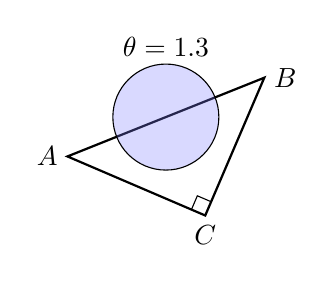
\begin{tikzpicture}[scale=0.5]
            \coordinate (A) at (0,0);
            \coordinate (B) at (5,2);
            \coordinate (C) at (3.5,-1.5); 

            % circle center
            \coordinate (M) at ($(A)!0.5!(B)$);

            % triangle
            \draw[thick] (A) -- (B) -- (C) -- cycle;
            \draw ($(C)!0.1!(B)$) -- ($(C) + (-0.2,0.5)$) -- ($(C)!0.1!(A)$);

            % circle
            \pgfmathsetmacro{\radius}{sqrt((5)^2 + (2)^2)/2 * 0.5}
            \draw[fill=blue!50, fill opacity=0.3] (M) circle (\radius);
            \node[above] at ($(M) + (0.0,1.3)$) {$\theta = 1.3$};

            \node[left]  at (A) {$A$};
            \node[right] at (B) {$B$};
            \node[below] at (C) {$C$};
        \end{tikzpicture}
        \begin{tikzpicture}[scale=0.5]
            \coordinate (A) at (0,0);
            \coordinate (B) at (5,2);
            \coordinate (C) at (3.5,-1.5); 

            % circle center
            \coordinate (M) at ($(A)!0.5!(B)$);

            % triangle
            \draw[thick] (A) -- (B) -- (C) -- cycle;
            \draw ($(C)!0.1!(B)$) -- ($(C) + (-0.2,0.5)$) -- ($(C)!0.1!(A)$);

            % circle
            \pgfmathsetmacro{\radius}{sqrt((5)^2 + (2)^2)/2}
            \draw[fill=blue!50, fill opacity=0.3] (M) circle (\radius);
            \node[above] at ($(M) + (0.0,2.7)$) {$\theta = 1.0$};

            \node[left]  at (A) {$A$};
            \node[right] at (B) {$B$};
            \node[below] at (C) {$C$};
        \end{tikzpicture}
        \begin{tikzpicture}[scale=0.5]
            \coordinate (A) at (0,0);
            \coordinate (B) at (5,2);
            \coordinate (C) at (3.5,-1.5); 

            % circle center
            \coordinate (M) at ($(A)!0.5!(B)$);

            % triangle
            \draw[thick] (A) -- (B) -- (C) -- cycle;
            \draw ($(C)!0.1!(B)$) -- ($(C) + (-0.2,0.5)$) -- ($(C)!0.1!(A)$);

            % circle
            \pgfmathsetmacro{\radius}{sqrt((5)^2 + (2)^2)/2 * 1.5}
            \draw[fill=blue!50, fill opacity=0.3] (M) circle (\radius);
            \node[above] at ($(M) + (0.0,4.0)$) {$\theta = 0.7$};

            \node[left]  at (A) {$A$};
            \node[right] at (B) {$B$};
            \node[below] at (C) {$C$};
        \end{tikzpicture}
    \end{center}
\end{frame}

\begin{frame}{Circumcircle filtering impact}
    \begin{figure}
        \centering
        \begin{subfigure}{0.3\textwidth}
            \includegraphics[width=\textwidth]{plots/nested_complex_9_no_cc.jpg}
        \end{subfigure}%
        \begin{subfigure}{0.3\textwidth}
            \includegraphics[width=\textwidth]{plots/nested_complex_9_cc.jpg}
        \end{subfigure}%
        \begin{subfigure}{0.3\textwidth}
            \resizebox{\textwidth}{!}{
                %% Creator: Matplotlib, PGF backend
%%
%% To include the figure in your LaTeX document, write
%%   \input{<filename>.pgf}
%%
%% Make sure the required packages are loaded in your preamble
%%   \usepackage{pgf}
%%
%% Also ensure that all the required font packages are loaded; for instance,
%% the lmodern package is sometimes necessary when using math font.
%%   \usepackage{lmodern}
%%
%% Figures using additional raster images can only be included by \input if
%% they are in the same directory as the main LaTeX file. For loading figures
%% from other directories you can use the `import` package
%%   \usepackage{import}
%%
%% and then include the figures with
%%   \import{<path to file>}{<filename>.pgf}
%%
%% Matplotlib used the following preamble
%%   \def\mathdefault#1{#1}
%%   \everymath=\expandafter{\the\everymath\displaystyle}
%%   
%%   \ifdefined\pdftexversion\else  % non-pdftex case.
%%     \usepackage{fontspec}
%%     \setmainfont{DejaVuSerif.ttf}[Path=\detokenize{/home/snek/repos/homology-decision-bondaries-clean/venv/lib/python3.9/site-packages/matplotlib/mpl-data/fonts/ttf/}]
%%     \setsansfont{DejaVuSans.ttf}[Path=\detokenize{/home/snek/repos/homology-decision-bondaries-clean/venv/lib/python3.9/site-packages/matplotlib/mpl-data/fonts/ttf/}]
%%     \setmonofont{DejaVuSansMono.ttf}[Path=\detokenize{/home/snek/repos/homology-decision-bondaries-clean/venv/lib/python3.9/site-packages/matplotlib/mpl-data/fonts/ttf/}]
%%   \fi
%%   \makeatletter\@ifpackageloaded{underscore}{}{\usepackage[strings]{underscore}}\makeatother
%%
\begingroup%
\makeatletter%
\begin{pgfpicture}%
\pgfpathrectangle{\pgfpointorigin}{\pgfqpoint{4.331782in}{4.144486in}}%
\pgfusepath{use as bounding box, clip}%
\begin{pgfscope}%
\pgfsetbuttcap%
\pgfsetmiterjoin%
\definecolor{currentfill}{rgb}{1.000000,1.000000,1.000000}%
\pgfsetfillcolor{currentfill}%
\pgfsetlinewidth{0.000000pt}%
\definecolor{currentstroke}{rgb}{1.000000,1.000000,1.000000}%
\pgfsetstrokecolor{currentstroke}%
\pgfsetdash{}{0pt}%
\pgfpathmoveto{\pgfqpoint{0.000000in}{-0.000000in}}%
\pgfpathlineto{\pgfqpoint{4.331782in}{-0.000000in}}%
\pgfpathlineto{\pgfqpoint{4.331782in}{4.144486in}}%
\pgfpathlineto{\pgfqpoint{0.000000in}{4.144486in}}%
\pgfpathlineto{\pgfqpoint{0.000000in}{-0.000000in}}%
\pgfpathclose%
\pgfusepath{fill}%
\end{pgfscope}%
\begin{pgfscope}%
\pgfsetbuttcap%
\pgfsetmiterjoin%
\definecolor{currentfill}{rgb}{1.000000,1.000000,1.000000}%
\pgfsetfillcolor{currentfill}%
\pgfsetlinewidth{0.000000pt}%
\definecolor{currentstroke}{rgb}{0.000000,0.000000,0.000000}%
\pgfsetstrokecolor{currentstroke}%
\pgfsetstrokeopacity{0.000000}%
\pgfsetdash{}{0pt}%
\pgfpathmoveto{\pgfqpoint{0.800049in}{0.448486in}}%
\pgfpathlineto{\pgfqpoint{4.331782in}{0.448486in}}%
\pgfpathlineto{\pgfqpoint{4.331782in}{4.144486in}}%
\pgfpathlineto{\pgfqpoint{0.800049in}{4.144486in}}%
\pgfpathlineto{\pgfqpoint{0.800049in}{0.448486in}}%
\pgfpathclose%
\pgfusepath{fill}%
\end{pgfscope}%
\begin{pgfscope}%
\pgfpathrectangle{\pgfqpoint{0.800049in}{0.448486in}}{\pgfqpoint{3.531733in}{3.696000in}}%
\pgfusepath{clip}%
\pgfsetbuttcap%
\pgfsetmiterjoin%
\definecolor{currentfill}{rgb}{0.827451,0.827451,0.827451}%
\pgfsetfillcolor{currentfill}%
\pgfsetlinewidth{1.003750pt}%
\definecolor{currentstroke}{rgb}{0.827451,0.827451,0.827451}%
\pgfsetstrokecolor{currentstroke}%
\pgfsetdash{}{0pt}%
\pgfpathmoveto{\pgfqpoint{0.800049in}{0.448486in}}%
\pgfpathlineto{\pgfqpoint{4.331782in}{0.448486in}}%
\pgfpathlineto{\pgfqpoint{4.331782in}{3.980219in}}%
\pgfpathlineto{\pgfqpoint{0.800049in}{0.448486in}}%
\pgfpathclose%
\pgfusepath{stroke,fill}%
\end{pgfscope}%
\begin{pgfscope}%
\pgfpathrectangle{\pgfqpoint{0.800049in}{0.448486in}}{\pgfqpoint{3.531733in}{3.696000in}}%
\pgfusepath{clip}%
\pgfsetbuttcap%
\pgfsetroundjoin%
\definecolor{currentfill}{rgb}{0.894118,0.101961,0.109804}%
\pgfsetfillcolor{currentfill}%
\pgfsetfillopacity{0.600000}%
\pgfsetlinewidth{1.003750pt}%
\definecolor{currentstroke}{rgb}{0.894118,0.101961,0.109804}%
\pgfsetstrokecolor{currentstroke}%
\pgfsetstrokeopacity{0.600000}%
\pgfsetdash{}{0pt}%
\pgfpathmoveto{\pgfqpoint{4.249649in}{4.020686in}}%
\pgfpathcurveto{\pgfqpoint{4.260699in}{4.020686in}}{\pgfqpoint{4.271298in}{4.025076in}}{\pgfqpoint{4.279111in}{4.032890in}}%
\pgfpathcurveto{\pgfqpoint{4.286925in}{4.040703in}}{\pgfqpoint{4.291315in}{4.051303in}}{\pgfqpoint{4.291315in}{4.062353in}}%
\pgfpathcurveto{\pgfqpoint{4.291315in}{4.073403in}}{\pgfqpoint{4.286925in}{4.084002in}}{\pgfqpoint{4.279111in}{4.091815in}}%
\pgfpathcurveto{\pgfqpoint{4.271298in}{4.099629in}}{\pgfqpoint{4.260699in}{4.104019in}}{\pgfqpoint{4.249649in}{4.104019in}}%
\pgfpathcurveto{\pgfqpoint{4.238598in}{4.104019in}}{\pgfqpoint{4.227999in}{4.099629in}}{\pgfqpoint{4.220186in}{4.091815in}}%
\pgfpathcurveto{\pgfqpoint{4.212372in}{4.084002in}}{\pgfqpoint{4.207982in}{4.073403in}}{\pgfqpoint{4.207982in}{4.062353in}}%
\pgfpathcurveto{\pgfqpoint{4.207982in}{4.051303in}}{\pgfqpoint{4.212372in}{4.040703in}}{\pgfqpoint{4.220186in}{4.032890in}}%
\pgfpathcurveto{\pgfqpoint{4.227999in}{4.025076in}}{\pgfqpoint{4.238598in}{4.020686in}}{\pgfqpoint{4.249649in}{4.020686in}}%
\pgfpathlineto{\pgfqpoint{4.249649in}{4.020686in}}%
\pgfpathclose%
\pgfusepath{stroke,fill}%
\end{pgfscope}%
\begin{pgfscope}%
\pgfpathrectangle{\pgfqpoint{0.800049in}{0.448486in}}{\pgfqpoint{3.531733in}{3.696000in}}%
\pgfusepath{clip}%
\pgfsetbuttcap%
\pgfsetroundjoin%
\definecolor{currentfill}{rgb}{0.894118,0.101961,0.109804}%
\pgfsetfillcolor{currentfill}%
\pgfsetfillopacity{0.600000}%
\pgfsetlinewidth{1.003750pt}%
\definecolor{currentstroke}{rgb}{0.894118,0.101961,0.109804}%
\pgfsetstrokecolor{currentstroke}%
\pgfsetstrokeopacity{0.600000}%
\pgfsetdash{}{0pt}%
\pgfpathmoveto{\pgfqpoint{4.249649in}{4.020686in}}%
\pgfpathcurveto{\pgfqpoint{4.260699in}{4.020686in}}{\pgfqpoint{4.271298in}{4.025076in}}{\pgfqpoint{4.279111in}{4.032890in}}%
\pgfpathcurveto{\pgfqpoint{4.286925in}{4.040703in}}{\pgfqpoint{4.291315in}{4.051303in}}{\pgfqpoint{4.291315in}{4.062353in}}%
\pgfpathcurveto{\pgfqpoint{4.291315in}{4.073403in}}{\pgfqpoint{4.286925in}{4.084002in}}{\pgfqpoint{4.279111in}{4.091815in}}%
\pgfpathcurveto{\pgfqpoint{4.271298in}{4.099629in}}{\pgfqpoint{4.260699in}{4.104019in}}{\pgfqpoint{4.249649in}{4.104019in}}%
\pgfpathcurveto{\pgfqpoint{4.238598in}{4.104019in}}{\pgfqpoint{4.227999in}{4.099629in}}{\pgfqpoint{4.220186in}{4.091815in}}%
\pgfpathcurveto{\pgfqpoint{4.212372in}{4.084002in}}{\pgfqpoint{4.207982in}{4.073403in}}{\pgfqpoint{4.207982in}{4.062353in}}%
\pgfpathcurveto{\pgfqpoint{4.207982in}{4.051303in}}{\pgfqpoint{4.212372in}{4.040703in}}{\pgfqpoint{4.220186in}{4.032890in}}%
\pgfpathcurveto{\pgfqpoint{4.227999in}{4.025076in}}{\pgfqpoint{4.238598in}{4.020686in}}{\pgfqpoint{4.249649in}{4.020686in}}%
\pgfpathlineto{\pgfqpoint{4.249649in}{4.020686in}}%
\pgfpathclose%
\pgfusepath{stroke,fill}%
\end{pgfscope}%
\begin{pgfscope}%
\pgfpathrectangle{\pgfqpoint{0.800049in}{0.448486in}}{\pgfqpoint{3.531733in}{3.696000in}}%
\pgfusepath{clip}%
\pgfsetbuttcap%
\pgfsetroundjoin%
\definecolor{currentfill}{rgb}{0.894118,0.101961,0.109804}%
\pgfsetfillcolor{currentfill}%
\pgfsetfillopacity{0.600000}%
\pgfsetlinewidth{1.003750pt}%
\definecolor{currentstroke}{rgb}{0.894118,0.101961,0.109804}%
\pgfsetstrokecolor{currentstroke}%
\pgfsetstrokeopacity{0.600000}%
\pgfsetdash{}{0pt}%
\pgfpathmoveto{\pgfqpoint{3.428315in}{4.020686in}}%
\pgfpathcurveto{\pgfqpoint{3.439365in}{4.020686in}}{\pgfqpoint{3.449964in}{4.025076in}}{\pgfqpoint{3.457778in}{4.032890in}}%
\pgfpathcurveto{\pgfqpoint{3.465592in}{4.040703in}}{\pgfqpoint{3.469982in}{4.051303in}}{\pgfqpoint{3.469982in}{4.062353in}}%
\pgfpathcurveto{\pgfqpoint{3.469982in}{4.073403in}}{\pgfqpoint{3.465592in}{4.084002in}}{\pgfqpoint{3.457778in}{4.091815in}}%
\pgfpathcurveto{\pgfqpoint{3.449964in}{4.099629in}}{\pgfqpoint{3.439365in}{4.104019in}}{\pgfqpoint{3.428315in}{4.104019in}}%
\pgfpathcurveto{\pgfqpoint{3.417265in}{4.104019in}}{\pgfqpoint{3.406666in}{4.099629in}}{\pgfqpoint{3.398852in}{4.091815in}}%
\pgfpathcurveto{\pgfqpoint{3.391039in}{4.084002in}}{\pgfqpoint{3.386649in}{4.073403in}}{\pgfqpoint{3.386649in}{4.062353in}}%
\pgfpathcurveto{\pgfqpoint{3.386649in}{4.051303in}}{\pgfqpoint{3.391039in}{4.040703in}}{\pgfqpoint{3.398852in}{4.032890in}}%
\pgfpathcurveto{\pgfqpoint{3.406666in}{4.025076in}}{\pgfqpoint{3.417265in}{4.020686in}}{\pgfqpoint{3.428315in}{4.020686in}}%
\pgfpathlineto{\pgfqpoint{3.428315in}{4.020686in}}%
\pgfpathclose%
\pgfusepath{stroke,fill}%
\end{pgfscope}%
\begin{pgfscope}%
\pgfpathrectangle{\pgfqpoint{0.800049in}{0.448486in}}{\pgfqpoint{3.531733in}{3.696000in}}%
\pgfusepath{clip}%
\pgfsetbuttcap%
\pgfsetroundjoin%
\definecolor{currentfill}{rgb}{0.894118,0.101961,0.109804}%
\pgfsetfillcolor{currentfill}%
\pgfsetfillopacity{0.600000}%
\pgfsetlinewidth{1.003750pt}%
\definecolor{currentstroke}{rgb}{0.894118,0.101961,0.109804}%
\pgfsetstrokecolor{currentstroke}%
\pgfsetstrokeopacity{0.600000}%
\pgfsetdash{}{0pt}%
\pgfpathmoveto{\pgfqpoint{3.428315in}{4.020686in}}%
\pgfpathcurveto{\pgfqpoint{3.439365in}{4.020686in}}{\pgfqpoint{3.449964in}{4.025076in}}{\pgfqpoint{3.457778in}{4.032890in}}%
\pgfpathcurveto{\pgfqpoint{3.465592in}{4.040703in}}{\pgfqpoint{3.469982in}{4.051303in}}{\pgfqpoint{3.469982in}{4.062353in}}%
\pgfpathcurveto{\pgfqpoint{3.469982in}{4.073403in}}{\pgfqpoint{3.465592in}{4.084002in}}{\pgfqpoint{3.457778in}{4.091815in}}%
\pgfpathcurveto{\pgfqpoint{3.449964in}{4.099629in}}{\pgfqpoint{3.439365in}{4.104019in}}{\pgfqpoint{3.428315in}{4.104019in}}%
\pgfpathcurveto{\pgfqpoint{3.417265in}{4.104019in}}{\pgfqpoint{3.406666in}{4.099629in}}{\pgfqpoint{3.398852in}{4.091815in}}%
\pgfpathcurveto{\pgfqpoint{3.391039in}{4.084002in}}{\pgfqpoint{3.386649in}{4.073403in}}{\pgfqpoint{3.386649in}{4.062353in}}%
\pgfpathcurveto{\pgfqpoint{3.386649in}{4.051303in}}{\pgfqpoint{3.391039in}{4.040703in}}{\pgfqpoint{3.398852in}{4.032890in}}%
\pgfpathcurveto{\pgfqpoint{3.406666in}{4.025076in}}{\pgfqpoint{3.417265in}{4.020686in}}{\pgfqpoint{3.428315in}{4.020686in}}%
\pgfpathlineto{\pgfqpoint{3.428315in}{4.020686in}}%
\pgfpathclose%
\pgfusepath{stroke,fill}%
\end{pgfscope}%
\begin{pgfscope}%
\pgfpathrectangle{\pgfqpoint{0.800049in}{0.448486in}}{\pgfqpoint{3.531733in}{3.696000in}}%
\pgfusepath{clip}%
\pgfsetbuttcap%
\pgfsetroundjoin%
\definecolor{currentfill}{rgb}{0.894118,0.101961,0.109804}%
\pgfsetfillcolor{currentfill}%
\pgfsetfillopacity{0.600000}%
\pgfsetlinewidth{1.003750pt}%
\definecolor{currentstroke}{rgb}{0.894118,0.101961,0.109804}%
\pgfsetstrokecolor{currentstroke}%
\pgfsetstrokeopacity{0.600000}%
\pgfsetdash{}{0pt}%
\pgfpathmoveto{\pgfqpoint{2.606982in}{4.020686in}}%
\pgfpathcurveto{\pgfqpoint{2.618032in}{4.020686in}}{\pgfqpoint{2.628631in}{4.025076in}}{\pgfqpoint{2.636445in}{4.032890in}}%
\pgfpathcurveto{\pgfqpoint{2.644258in}{4.040703in}}{\pgfqpoint{2.648649in}{4.051303in}}{\pgfqpoint{2.648649in}{4.062353in}}%
\pgfpathcurveto{\pgfqpoint{2.648649in}{4.073403in}}{\pgfqpoint{2.644258in}{4.084002in}}{\pgfqpoint{2.636445in}{4.091815in}}%
\pgfpathcurveto{\pgfqpoint{2.628631in}{4.099629in}}{\pgfqpoint{2.618032in}{4.104019in}}{\pgfqpoint{2.606982in}{4.104019in}}%
\pgfpathcurveto{\pgfqpoint{2.595932in}{4.104019in}}{\pgfqpoint{2.585333in}{4.099629in}}{\pgfqpoint{2.577519in}{4.091815in}}%
\pgfpathcurveto{\pgfqpoint{2.569706in}{4.084002in}}{\pgfqpoint{2.565315in}{4.073403in}}{\pgfqpoint{2.565315in}{4.062353in}}%
\pgfpathcurveto{\pgfqpoint{2.565315in}{4.051303in}}{\pgfqpoint{2.569706in}{4.040703in}}{\pgfqpoint{2.577519in}{4.032890in}}%
\pgfpathcurveto{\pgfqpoint{2.585333in}{4.025076in}}{\pgfqpoint{2.595932in}{4.020686in}}{\pgfqpoint{2.606982in}{4.020686in}}%
\pgfpathlineto{\pgfqpoint{2.606982in}{4.020686in}}%
\pgfpathclose%
\pgfusepath{stroke,fill}%
\end{pgfscope}%
\begin{pgfscope}%
\pgfpathrectangle{\pgfqpoint{0.800049in}{0.448486in}}{\pgfqpoint{3.531733in}{3.696000in}}%
\pgfusepath{clip}%
\pgfsetbuttcap%
\pgfsetroundjoin%
\definecolor{currentfill}{rgb}{0.894118,0.101961,0.109804}%
\pgfsetfillcolor{currentfill}%
\pgfsetfillopacity{0.600000}%
\pgfsetlinewidth{1.003750pt}%
\definecolor{currentstroke}{rgb}{0.894118,0.101961,0.109804}%
\pgfsetstrokecolor{currentstroke}%
\pgfsetstrokeopacity{0.600000}%
\pgfsetdash{}{0pt}%
\pgfpathmoveto{\pgfqpoint{2.606982in}{4.020686in}}%
\pgfpathcurveto{\pgfqpoint{2.618032in}{4.020686in}}{\pgfqpoint{2.628631in}{4.025076in}}{\pgfqpoint{2.636445in}{4.032890in}}%
\pgfpathcurveto{\pgfqpoint{2.644258in}{4.040703in}}{\pgfqpoint{2.648649in}{4.051303in}}{\pgfqpoint{2.648649in}{4.062353in}}%
\pgfpathcurveto{\pgfqpoint{2.648649in}{4.073403in}}{\pgfqpoint{2.644258in}{4.084002in}}{\pgfqpoint{2.636445in}{4.091815in}}%
\pgfpathcurveto{\pgfqpoint{2.628631in}{4.099629in}}{\pgfqpoint{2.618032in}{4.104019in}}{\pgfqpoint{2.606982in}{4.104019in}}%
\pgfpathcurveto{\pgfqpoint{2.595932in}{4.104019in}}{\pgfqpoint{2.585333in}{4.099629in}}{\pgfqpoint{2.577519in}{4.091815in}}%
\pgfpathcurveto{\pgfqpoint{2.569706in}{4.084002in}}{\pgfqpoint{2.565315in}{4.073403in}}{\pgfqpoint{2.565315in}{4.062353in}}%
\pgfpathcurveto{\pgfqpoint{2.565315in}{4.051303in}}{\pgfqpoint{2.569706in}{4.040703in}}{\pgfqpoint{2.577519in}{4.032890in}}%
\pgfpathcurveto{\pgfqpoint{2.585333in}{4.025076in}}{\pgfqpoint{2.595932in}{4.020686in}}{\pgfqpoint{2.606982in}{4.020686in}}%
\pgfpathlineto{\pgfqpoint{2.606982in}{4.020686in}}%
\pgfpathclose%
\pgfusepath{stroke,fill}%
\end{pgfscope}%
\begin{pgfscope}%
\pgfpathrectangle{\pgfqpoint{0.800049in}{0.448486in}}{\pgfqpoint{3.531733in}{3.696000in}}%
\pgfusepath{clip}%
\pgfsetbuttcap%
\pgfsetroundjoin%
\definecolor{currentfill}{rgb}{0.894118,0.101961,0.109804}%
\pgfsetfillcolor{currentfill}%
\pgfsetfillopacity{0.600000}%
\pgfsetlinewidth{1.003750pt}%
\definecolor{currentstroke}{rgb}{0.894118,0.101961,0.109804}%
\pgfsetstrokecolor{currentstroke}%
\pgfsetstrokeopacity{0.600000}%
\pgfsetdash{}{0pt}%
\pgfpathmoveto{\pgfqpoint{2.606982in}{4.020686in}}%
\pgfpathcurveto{\pgfqpoint{2.618032in}{4.020686in}}{\pgfqpoint{2.628631in}{4.025076in}}{\pgfqpoint{2.636445in}{4.032890in}}%
\pgfpathcurveto{\pgfqpoint{2.644258in}{4.040703in}}{\pgfqpoint{2.648649in}{4.051303in}}{\pgfqpoint{2.648649in}{4.062353in}}%
\pgfpathcurveto{\pgfqpoint{2.648649in}{4.073403in}}{\pgfqpoint{2.644258in}{4.084002in}}{\pgfqpoint{2.636445in}{4.091815in}}%
\pgfpathcurveto{\pgfqpoint{2.628631in}{4.099629in}}{\pgfqpoint{2.618032in}{4.104019in}}{\pgfqpoint{2.606982in}{4.104019in}}%
\pgfpathcurveto{\pgfqpoint{2.595932in}{4.104019in}}{\pgfqpoint{2.585333in}{4.099629in}}{\pgfqpoint{2.577519in}{4.091815in}}%
\pgfpathcurveto{\pgfqpoint{2.569706in}{4.084002in}}{\pgfqpoint{2.565315in}{4.073403in}}{\pgfqpoint{2.565315in}{4.062353in}}%
\pgfpathcurveto{\pgfqpoint{2.565315in}{4.051303in}}{\pgfqpoint{2.569706in}{4.040703in}}{\pgfqpoint{2.577519in}{4.032890in}}%
\pgfpathcurveto{\pgfqpoint{2.585333in}{4.025076in}}{\pgfqpoint{2.595932in}{4.020686in}}{\pgfqpoint{2.606982in}{4.020686in}}%
\pgfpathlineto{\pgfqpoint{2.606982in}{4.020686in}}%
\pgfpathclose%
\pgfusepath{stroke,fill}%
\end{pgfscope}%
\begin{pgfscope}%
\pgfpathrectangle{\pgfqpoint{0.800049in}{0.448486in}}{\pgfqpoint{3.531733in}{3.696000in}}%
\pgfusepath{clip}%
\pgfsetbuttcap%
\pgfsetroundjoin%
\definecolor{currentfill}{rgb}{0.894118,0.101961,0.109804}%
\pgfsetfillcolor{currentfill}%
\pgfsetfillopacity{0.600000}%
\pgfsetlinewidth{1.003750pt}%
\definecolor{currentstroke}{rgb}{0.894118,0.101961,0.109804}%
\pgfsetstrokecolor{currentstroke}%
\pgfsetstrokeopacity{0.600000}%
\pgfsetdash{}{0pt}%
\pgfpathmoveto{\pgfqpoint{1.785649in}{4.020686in}}%
\pgfpathcurveto{\pgfqpoint{1.796699in}{4.020686in}}{\pgfqpoint{1.807298in}{4.025076in}}{\pgfqpoint{1.815111in}{4.032890in}}%
\pgfpathcurveto{\pgfqpoint{1.822925in}{4.040703in}}{\pgfqpoint{1.827315in}{4.051303in}}{\pgfqpoint{1.827315in}{4.062353in}}%
\pgfpathcurveto{\pgfqpoint{1.827315in}{4.073403in}}{\pgfqpoint{1.822925in}{4.084002in}}{\pgfqpoint{1.815111in}{4.091815in}}%
\pgfpathcurveto{\pgfqpoint{1.807298in}{4.099629in}}{\pgfqpoint{1.796699in}{4.104019in}}{\pgfqpoint{1.785649in}{4.104019in}}%
\pgfpathcurveto{\pgfqpoint{1.774598in}{4.104019in}}{\pgfqpoint{1.763999in}{4.099629in}}{\pgfqpoint{1.756186in}{4.091815in}}%
\pgfpathcurveto{\pgfqpoint{1.748372in}{4.084002in}}{\pgfqpoint{1.743982in}{4.073403in}}{\pgfqpoint{1.743982in}{4.062353in}}%
\pgfpathcurveto{\pgfqpoint{1.743982in}{4.051303in}}{\pgfqpoint{1.748372in}{4.040703in}}{\pgfqpoint{1.756186in}{4.032890in}}%
\pgfpathcurveto{\pgfqpoint{1.763999in}{4.025076in}}{\pgfqpoint{1.774598in}{4.020686in}}{\pgfqpoint{1.785649in}{4.020686in}}%
\pgfpathlineto{\pgfqpoint{1.785649in}{4.020686in}}%
\pgfpathclose%
\pgfusepath{stroke,fill}%
\end{pgfscope}%
\begin{pgfscope}%
\pgfpathrectangle{\pgfqpoint{0.800049in}{0.448486in}}{\pgfqpoint{3.531733in}{3.696000in}}%
\pgfusepath{clip}%
\pgfsetbuttcap%
\pgfsetroundjoin%
\definecolor{currentfill}{rgb}{0.894118,0.101961,0.109804}%
\pgfsetfillcolor{currentfill}%
\pgfsetfillopacity{0.600000}%
\pgfsetlinewidth{1.003750pt}%
\definecolor{currentstroke}{rgb}{0.894118,0.101961,0.109804}%
\pgfsetstrokecolor{currentstroke}%
\pgfsetstrokeopacity{0.600000}%
\pgfsetdash{}{0pt}%
\pgfpathmoveto{\pgfqpoint{1.785649in}{4.020686in}}%
\pgfpathcurveto{\pgfqpoint{1.796699in}{4.020686in}}{\pgfqpoint{1.807298in}{4.025076in}}{\pgfqpoint{1.815111in}{4.032890in}}%
\pgfpathcurveto{\pgfqpoint{1.822925in}{4.040703in}}{\pgfqpoint{1.827315in}{4.051303in}}{\pgfqpoint{1.827315in}{4.062353in}}%
\pgfpathcurveto{\pgfqpoint{1.827315in}{4.073403in}}{\pgfqpoint{1.822925in}{4.084002in}}{\pgfqpoint{1.815111in}{4.091815in}}%
\pgfpathcurveto{\pgfqpoint{1.807298in}{4.099629in}}{\pgfqpoint{1.796699in}{4.104019in}}{\pgfqpoint{1.785649in}{4.104019in}}%
\pgfpathcurveto{\pgfqpoint{1.774598in}{4.104019in}}{\pgfqpoint{1.763999in}{4.099629in}}{\pgfqpoint{1.756186in}{4.091815in}}%
\pgfpathcurveto{\pgfqpoint{1.748372in}{4.084002in}}{\pgfqpoint{1.743982in}{4.073403in}}{\pgfqpoint{1.743982in}{4.062353in}}%
\pgfpathcurveto{\pgfqpoint{1.743982in}{4.051303in}}{\pgfqpoint{1.748372in}{4.040703in}}{\pgfqpoint{1.756186in}{4.032890in}}%
\pgfpathcurveto{\pgfqpoint{1.763999in}{4.025076in}}{\pgfqpoint{1.774598in}{4.020686in}}{\pgfqpoint{1.785649in}{4.020686in}}%
\pgfpathlineto{\pgfqpoint{1.785649in}{4.020686in}}%
\pgfpathclose%
\pgfusepath{stroke,fill}%
\end{pgfscope}%
\begin{pgfscope}%
\pgfpathrectangle{\pgfqpoint{0.800049in}{0.448486in}}{\pgfqpoint{3.531733in}{3.696000in}}%
\pgfusepath{clip}%
\pgfsetbuttcap%
\pgfsetroundjoin%
\definecolor{currentfill}{rgb}{0.894118,0.101961,0.109804}%
\pgfsetfillcolor{currentfill}%
\pgfsetfillopacity{0.600000}%
\pgfsetlinewidth{1.003750pt}%
\definecolor{currentstroke}{rgb}{0.894118,0.101961,0.109804}%
\pgfsetstrokecolor{currentstroke}%
\pgfsetstrokeopacity{0.600000}%
\pgfsetdash{}{0pt}%
\pgfpathmoveto{\pgfqpoint{1.785649in}{4.020686in}}%
\pgfpathcurveto{\pgfqpoint{1.796699in}{4.020686in}}{\pgfqpoint{1.807298in}{4.025076in}}{\pgfqpoint{1.815111in}{4.032890in}}%
\pgfpathcurveto{\pgfqpoint{1.822925in}{4.040703in}}{\pgfqpoint{1.827315in}{4.051303in}}{\pgfqpoint{1.827315in}{4.062353in}}%
\pgfpathcurveto{\pgfqpoint{1.827315in}{4.073403in}}{\pgfqpoint{1.822925in}{4.084002in}}{\pgfqpoint{1.815111in}{4.091815in}}%
\pgfpathcurveto{\pgfqpoint{1.807298in}{4.099629in}}{\pgfqpoint{1.796699in}{4.104019in}}{\pgfqpoint{1.785649in}{4.104019in}}%
\pgfpathcurveto{\pgfqpoint{1.774598in}{4.104019in}}{\pgfqpoint{1.763999in}{4.099629in}}{\pgfqpoint{1.756186in}{4.091815in}}%
\pgfpathcurveto{\pgfqpoint{1.748372in}{4.084002in}}{\pgfqpoint{1.743982in}{4.073403in}}{\pgfqpoint{1.743982in}{4.062353in}}%
\pgfpathcurveto{\pgfqpoint{1.743982in}{4.051303in}}{\pgfqpoint{1.748372in}{4.040703in}}{\pgfqpoint{1.756186in}{4.032890in}}%
\pgfpathcurveto{\pgfqpoint{1.763999in}{4.025076in}}{\pgfqpoint{1.774598in}{4.020686in}}{\pgfqpoint{1.785649in}{4.020686in}}%
\pgfpathlineto{\pgfqpoint{1.785649in}{4.020686in}}%
\pgfpathclose%
\pgfusepath{stroke,fill}%
\end{pgfscope}%
\begin{pgfscope}%
\pgfpathrectangle{\pgfqpoint{0.800049in}{0.448486in}}{\pgfqpoint{3.531733in}{3.696000in}}%
\pgfusepath{clip}%
\pgfsetbuttcap%
\pgfsetroundjoin%
\definecolor{currentfill}{rgb}{0.894118,0.101961,0.109804}%
\pgfsetfillcolor{currentfill}%
\pgfsetfillopacity{0.600000}%
\pgfsetlinewidth{1.003750pt}%
\definecolor{currentstroke}{rgb}{0.894118,0.101961,0.109804}%
\pgfsetstrokecolor{currentstroke}%
\pgfsetstrokeopacity{0.600000}%
\pgfsetdash{}{0pt}%
\pgfpathmoveto{\pgfqpoint{1.785649in}{4.020686in}}%
\pgfpathcurveto{\pgfqpoint{1.796699in}{4.020686in}}{\pgfqpoint{1.807298in}{4.025076in}}{\pgfqpoint{1.815111in}{4.032890in}}%
\pgfpathcurveto{\pgfqpoint{1.822925in}{4.040703in}}{\pgfqpoint{1.827315in}{4.051303in}}{\pgfqpoint{1.827315in}{4.062353in}}%
\pgfpathcurveto{\pgfqpoint{1.827315in}{4.073403in}}{\pgfqpoint{1.822925in}{4.084002in}}{\pgfqpoint{1.815111in}{4.091815in}}%
\pgfpathcurveto{\pgfqpoint{1.807298in}{4.099629in}}{\pgfqpoint{1.796699in}{4.104019in}}{\pgfqpoint{1.785649in}{4.104019in}}%
\pgfpathcurveto{\pgfqpoint{1.774598in}{4.104019in}}{\pgfqpoint{1.763999in}{4.099629in}}{\pgfqpoint{1.756186in}{4.091815in}}%
\pgfpathcurveto{\pgfqpoint{1.748372in}{4.084002in}}{\pgfqpoint{1.743982in}{4.073403in}}{\pgfqpoint{1.743982in}{4.062353in}}%
\pgfpathcurveto{\pgfqpoint{1.743982in}{4.051303in}}{\pgfqpoint{1.748372in}{4.040703in}}{\pgfqpoint{1.756186in}{4.032890in}}%
\pgfpathcurveto{\pgfqpoint{1.763999in}{4.025076in}}{\pgfqpoint{1.774598in}{4.020686in}}{\pgfqpoint{1.785649in}{4.020686in}}%
\pgfpathlineto{\pgfqpoint{1.785649in}{4.020686in}}%
\pgfpathclose%
\pgfusepath{stroke,fill}%
\end{pgfscope}%
\begin{pgfscope}%
\pgfpathrectangle{\pgfqpoint{0.800049in}{0.448486in}}{\pgfqpoint{3.531733in}{3.696000in}}%
\pgfusepath{clip}%
\pgfsetbuttcap%
\pgfsetroundjoin%
\definecolor{currentfill}{rgb}{0.894118,0.101961,0.109804}%
\pgfsetfillcolor{currentfill}%
\pgfsetfillopacity{0.600000}%
\pgfsetlinewidth{1.003750pt}%
\definecolor{currentstroke}{rgb}{0.894118,0.101961,0.109804}%
\pgfsetstrokecolor{currentstroke}%
\pgfsetstrokeopacity{0.600000}%
\pgfsetdash{}{0pt}%
\pgfpathmoveto{\pgfqpoint{1.785649in}{4.020686in}}%
\pgfpathcurveto{\pgfqpoint{1.796699in}{4.020686in}}{\pgfqpoint{1.807298in}{4.025076in}}{\pgfqpoint{1.815111in}{4.032890in}}%
\pgfpathcurveto{\pgfqpoint{1.822925in}{4.040703in}}{\pgfqpoint{1.827315in}{4.051303in}}{\pgfqpoint{1.827315in}{4.062353in}}%
\pgfpathcurveto{\pgfqpoint{1.827315in}{4.073403in}}{\pgfqpoint{1.822925in}{4.084002in}}{\pgfqpoint{1.815111in}{4.091815in}}%
\pgfpathcurveto{\pgfqpoint{1.807298in}{4.099629in}}{\pgfqpoint{1.796699in}{4.104019in}}{\pgfqpoint{1.785649in}{4.104019in}}%
\pgfpathcurveto{\pgfqpoint{1.774598in}{4.104019in}}{\pgfqpoint{1.763999in}{4.099629in}}{\pgfqpoint{1.756186in}{4.091815in}}%
\pgfpathcurveto{\pgfqpoint{1.748372in}{4.084002in}}{\pgfqpoint{1.743982in}{4.073403in}}{\pgfqpoint{1.743982in}{4.062353in}}%
\pgfpathcurveto{\pgfqpoint{1.743982in}{4.051303in}}{\pgfqpoint{1.748372in}{4.040703in}}{\pgfqpoint{1.756186in}{4.032890in}}%
\pgfpathcurveto{\pgfqpoint{1.763999in}{4.025076in}}{\pgfqpoint{1.774598in}{4.020686in}}{\pgfqpoint{1.785649in}{4.020686in}}%
\pgfpathlineto{\pgfqpoint{1.785649in}{4.020686in}}%
\pgfpathclose%
\pgfusepath{stroke,fill}%
\end{pgfscope}%
\begin{pgfscope}%
\pgfpathrectangle{\pgfqpoint{0.800049in}{0.448486in}}{\pgfqpoint{3.531733in}{3.696000in}}%
\pgfusepath{clip}%
\pgfsetbuttcap%
\pgfsetroundjoin%
\definecolor{currentfill}{rgb}{0.894118,0.101961,0.109804}%
\pgfsetfillcolor{currentfill}%
\pgfsetfillopacity{0.600000}%
\pgfsetlinewidth{1.003750pt}%
\definecolor{currentstroke}{rgb}{0.894118,0.101961,0.109804}%
\pgfsetstrokecolor{currentstroke}%
\pgfsetstrokeopacity{0.600000}%
\pgfsetdash{}{0pt}%
\pgfpathmoveto{\pgfqpoint{0.964315in}{4.020686in}}%
\pgfpathcurveto{\pgfqpoint{0.975365in}{4.020686in}}{\pgfqpoint{0.985964in}{4.025076in}}{\pgfqpoint{0.993778in}{4.032890in}}%
\pgfpathcurveto{\pgfqpoint{1.001592in}{4.040703in}}{\pgfqpoint{1.005982in}{4.051303in}}{\pgfqpoint{1.005982in}{4.062353in}}%
\pgfpathcurveto{\pgfqpoint{1.005982in}{4.073403in}}{\pgfqpoint{1.001592in}{4.084002in}}{\pgfqpoint{0.993778in}{4.091815in}}%
\pgfpathcurveto{\pgfqpoint{0.985964in}{4.099629in}}{\pgfqpoint{0.975365in}{4.104019in}}{\pgfqpoint{0.964315in}{4.104019in}}%
\pgfpathcurveto{\pgfqpoint{0.953265in}{4.104019in}}{\pgfqpoint{0.942666in}{4.099629in}}{\pgfqpoint{0.934852in}{4.091815in}}%
\pgfpathcurveto{\pgfqpoint{0.927039in}{4.084002in}}{\pgfqpoint{0.922649in}{4.073403in}}{\pgfqpoint{0.922649in}{4.062353in}}%
\pgfpathcurveto{\pgfqpoint{0.922649in}{4.051303in}}{\pgfqpoint{0.927039in}{4.040703in}}{\pgfqpoint{0.934852in}{4.032890in}}%
\pgfpathcurveto{\pgfqpoint{0.942666in}{4.025076in}}{\pgfqpoint{0.953265in}{4.020686in}}{\pgfqpoint{0.964315in}{4.020686in}}%
\pgfpathlineto{\pgfqpoint{0.964315in}{4.020686in}}%
\pgfpathclose%
\pgfusepath{stroke,fill}%
\end{pgfscope}%
\begin{pgfscope}%
\pgfpathrectangle{\pgfqpoint{0.800049in}{0.448486in}}{\pgfqpoint{3.531733in}{3.696000in}}%
\pgfusepath{clip}%
\pgfsetbuttcap%
\pgfsetroundjoin%
\definecolor{currentfill}{rgb}{0.894118,0.101961,0.109804}%
\pgfsetfillcolor{currentfill}%
\pgfsetfillopacity{0.600000}%
\pgfsetlinewidth{1.003750pt}%
\definecolor{currentstroke}{rgb}{0.894118,0.101961,0.109804}%
\pgfsetstrokecolor{currentstroke}%
\pgfsetstrokeopacity{0.600000}%
\pgfsetdash{}{0pt}%
\pgfpathmoveto{\pgfqpoint{0.964315in}{4.020686in}}%
\pgfpathcurveto{\pgfqpoint{0.975365in}{4.020686in}}{\pgfqpoint{0.985964in}{4.025076in}}{\pgfqpoint{0.993778in}{4.032890in}}%
\pgfpathcurveto{\pgfqpoint{1.001592in}{4.040703in}}{\pgfqpoint{1.005982in}{4.051303in}}{\pgfqpoint{1.005982in}{4.062353in}}%
\pgfpathcurveto{\pgfqpoint{1.005982in}{4.073403in}}{\pgfqpoint{1.001592in}{4.084002in}}{\pgfqpoint{0.993778in}{4.091815in}}%
\pgfpathcurveto{\pgfqpoint{0.985964in}{4.099629in}}{\pgfqpoint{0.975365in}{4.104019in}}{\pgfqpoint{0.964315in}{4.104019in}}%
\pgfpathcurveto{\pgfqpoint{0.953265in}{4.104019in}}{\pgfqpoint{0.942666in}{4.099629in}}{\pgfqpoint{0.934852in}{4.091815in}}%
\pgfpathcurveto{\pgfqpoint{0.927039in}{4.084002in}}{\pgfqpoint{0.922649in}{4.073403in}}{\pgfqpoint{0.922649in}{4.062353in}}%
\pgfpathcurveto{\pgfqpoint{0.922649in}{4.051303in}}{\pgfqpoint{0.927039in}{4.040703in}}{\pgfqpoint{0.934852in}{4.032890in}}%
\pgfpathcurveto{\pgfqpoint{0.942666in}{4.025076in}}{\pgfqpoint{0.953265in}{4.020686in}}{\pgfqpoint{0.964315in}{4.020686in}}%
\pgfpathlineto{\pgfqpoint{0.964315in}{4.020686in}}%
\pgfpathclose%
\pgfusepath{stroke,fill}%
\end{pgfscope}%
\begin{pgfscope}%
\pgfsetbuttcap%
\pgfsetroundjoin%
\definecolor{currentfill}{rgb}{0.000000,0.000000,0.000000}%
\pgfsetfillcolor{currentfill}%
\pgfsetlinewidth{0.803000pt}%
\definecolor{currentstroke}{rgb}{0.000000,0.000000,0.000000}%
\pgfsetstrokecolor{currentstroke}%
\pgfsetdash{}{0pt}%
\pgfsys@defobject{currentmarker}{\pgfqpoint{0.000000in}{-0.048611in}}{\pgfqpoint{0.000000in}{0.000000in}}{%
\pgfpathmoveto{\pgfqpoint{0.000000in}{0.000000in}}%
\pgfpathlineto{\pgfqpoint{0.000000in}{-0.048611in}}%
\pgfusepath{stroke,fill}%
}%
\begin{pgfscope}%
\pgfsys@transformshift{1.238093in}{0.448486in}%
\pgfsys@useobject{currentmarker}{}%
\end{pgfscope}%
\end{pgfscope}%
\begin{pgfscope}%
\definecolor{textcolor}{rgb}{0.000000,0.000000,0.000000}%
\pgfsetstrokecolor{textcolor}%
\pgfsetfillcolor{textcolor}%
\pgftext[x=1.238093in,y=0.351264in,,top]{\color{textcolor}{\rmfamily\fontsize{10.000000}{12.000000}\selectfont\catcode`\^=\active\def^{\ifmmode\sp\else\^{}\fi}\catcode`\%=\active\def%{\%}$\mathdefault{8}$}}%
\end{pgfscope}%
\begin{pgfscope}%
\pgfsetbuttcap%
\pgfsetroundjoin%
\definecolor{currentfill}{rgb}{0.000000,0.000000,0.000000}%
\pgfsetfillcolor{currentfill}%
\pgfsetlinewidth{0.803000pt}%
\definecolor{currentstroke}{rgb}{0.000000,0.000000,0.000000}%
\pgfsetstrokecolor{currentstroke}%
\pgfsetdash{}{0pt}%
\pgfsys@defobject{currentmarker}{\pgfqpoint{0.000000in}{-0.048611in}}{\pgfqpoint{0.000000in}{0.000000in}}{%
\pgfpathmoveto{\pgfqpoint{0.000000in}{0.000000in}}%
\pgfpathlineto{\pgfqpoint{0.000000in}{-0.048611in}}%
\pgfusepath{stroke,fill}%
}%
\begin{pgfscope}%
\pgfsys@transformshift{1.785649in}{0.448486in}%
\pgfsys@useobject{currentmarker}{}%
\end{pgfscope}%
\end{pgfscope}%
\begin{pgfscope}%
\definecolor{textcolor}{rgb}{0.000000,0.000000,0.000000}%
\pgfsetstrokecolor{textcolor}%
\pgfsetfillcolor{textcolor}%
\pgftext[x=1.785649in,y=0.351264in,,top]{\color{textcolor}{\rmfamily\fontsize{10.000000}{12.000000}\selectfont\catcode`\^=\active\def^{\ifmmode\sp\else\^{}\fi}\catcode`\%=\active\def%{\%}$\mathdefault{10}$}}%
\end{pgfscope}%
\begin{pgfscope}%
\pgfsetbuttcap%
\pgfsetroundjoin%
\definecolor{currentfill}{rgb}{0.000000,0.000000,0.000000}%
\pgfsetfillcolor{currentfill}%
\pgfsetlinewidth{0.803000pt}%
\definecolor{currentstroke}{rgb}{0.000000,0.000000,0.000000}%
\pgfsetstrokecolor{currentstroke}%
\pgfsetdash{}{0pt}%
\pgfsys@defobject{currentmarker}{\pgfqpoint{0.000000in}{-0.048611in}}{\pgfqpoint{0.000000in}{0.000000in}}{%
\pgfpathmoveto{\pgfqpoint{0.000000in}{0.000000in}}%
\pgfpathlineto{\pgfqpoint{0.000000in}{-0.048611in}}%
\pgfusepath{stroke,fill}%
}%
\begin{pgfscope}%
\pgfsys@transformshift{2.333204in}{0.448486in}%
\pgfsys@useobject{currentmarker}{}%
\end{pgfscope}%
\end{pgfscope}%
\begin{pgfscope}%
\definecolor{textcolor}{rgb}{0.000000,0.000000,0.000000}%
\pgfsetstrokecolor{textcolor}%
\pgfsetfillcolor{textcolor}%
\pgftext[x=2.333204in,y=0.351264in,,top]{\color{textcolor}{\rmfamily\fontsize{10.000000}{12.000000}\selectfont\catcode`\^=\active\def^{\ifmmode\sp\else\^{}\fi}\catcode`\%=\active\def%{\%}$\mathdefault{12}$}}%
\end{pgfscope}%
\begin{pgfscope}%
\pgfsetbuttcap%
\pgfsetroundjoin%
\definecolor{currentfill}{rgb}{0.000000,0.000000,0.000000}%
\pgfsetfillcolor{currentfill}%
\pgfsetlinewidth{0.803000pt}%
\definecolor{currentstroke}{rgb}{0.000000,0.000000,0.000000}%
\pgfsetstrokecolor{currentstroke}%
\pgfsetdash{}{0pt}%
\pgfsys@defobject{currentmarker}{\pgfqpoint{0.000000in}{-0.048611in}}{\pgfqpoint{0.000000in}{0.000000in}}{%
\pgfpathmoveto{\pgfqpoint{0.000000in}{0.000000in}}%
\pgfpathlineto{\pgfqpoint{0.000000in}{-0.048611in}}%
\pgfusepath{stroke,fill}%
}%
\begin{pgfscope}%
\pgfsys@transformshift{2.880760in}{0.448486in}%
\pgfsys@useobject{currentmarker}{}%
\end{pgfscope}%
\end{pgfscope}%
\begin{pgfscope}%
\definecolor{textcolor}{rgb}{0.000000,0.000000,0.000000}%
\pgfsetstrokecolor{textcolor}%
\pgfsetfillcolor{textcolor}%
\pgftext[x=2.880760in,y=0.351264in,,top]{\color{textcolor}{\rmfamily\fontsize{10.000000}{12.000000}\selectfont\catcode`\^=\active\def^{\ifmmode\sp\else\^{}\fi}\catcode`\%=\active\def%{\%}$\mathdefault{14}$}}%
\end{pgfscope}%
\begin{pgfscope}%
\pgfsetbuttcap%
\pgfsetroundjoin%
\definecolor{currentfill}{rgb}{0.000000,0.000000,0.000000}%
\pgfsetfillcolor{currentfill}%
\pgfsetlinewidth{0.803000pt}%
\definecolor{currentstroke}{rgb}{0.000000,0.000000,0.000000}%
\pgfsetstrokecolor{currentstroke}%
\pgfsetdash{}{0pt}%
\pgfsys@defobject{currentmarker}{\pgfqpoint{0.000000in}{-0.048611in}}{\pgfqpoint{0.000000in}{0.000000in}}{%
\pgfpathmoveto{\pgfqpoint{0.000000in}{0.000000in}}%
\pgfpathlineto{\pgfqpoint{0.000000in}{-0.048611in}}%
\pgfusepath{stroke,fill}%
}%
\begin{pgfscope}%
\pgfsys@transformshift{3.428315in}{0.448486in}%
\pgfsys@useobject{currentmarker}{}%
\end{pgfscope}%
\end{pgfscope}%
\begin{pgfscope}%
\definecolor{textcolor}{rgb}{0.000000,0.000000,0.000000}%
\pgfsetstrokecolor{textcolor}%
\pgfsetfillcolor{textcolor}%
\pgftext[x=3.428315in,y=0.351264in,,top]{\color{textcolor}{\rmfamily\fontsize{10.000000}{12.000000}\selectfont\catcode`\^=\active\def^{\ifmmode\sp\else\^{}\fi}\catcode`\%=\active\def%{\%}$\mathdefault{16}$}}%
\end{pgfscope}%
\begin{pgfscope}%
\pgfsetbuttcap%
\pgfsetroundjoin%
\definecolor{currentfill}{rgb}{0.000000,0.000000,0.000000}%
\pgfsetfillcolor{currentfill}%
\pgfsetlinewidth{0.803000pt}%
\definecolor{currentstroke}{rgb}{0.000000,0.000000,0.000000}%
\pgfsetstrokecolor{currentstroke}%
\pgfsetdash{}{0pt}%
\pgfsys@defobject{currentmarker}{\pgfqpoint{0.000000in}{-0.048611in}}{\pgfqpoint{0.000000in}{0.000000in}}{%
\pgfpathmoveto{\pgfqpoint{0.000000in}{0.000000in}}%
\pgfpathlineto{\pgfqpoint{0.000000in}{-0.048611in}}%
\pgfusepath{stroke,fill}%
}%
\begin{pgfscope}%
\pgfsys@transformshift{3.975871in}{0.448486in}%
\pgfsys@useobject{currentmarker}{}%
\end{pgfscope}%
\end{pgfscope}%
\begin{pgfscope}%
\definecolor{textcolor}{rgb}{0.000000,0.000000,0.000000}%
\pgfsetstrokecolor{textcolor}%
\pgfsetfillcolor{textcolor}%
\pgftext[x=3.975871in,y=0.351264in,,top]{\color{textcolor}{\rmfamily\fontsize{10.000000}{12.000000}\selectfont\catcode`\^=\active\def^{\ifmmode\sp\else\^{}\fi}\catcode`\%=\active\def%{\%}$\mathdefault{18}$}}%
\end{pgfscope}%
\begin{pgfscope}%
\definecolor{textcolor}{rgb}{0.000000,0.000000,0.000000}%
\pgfsetstrokecolor{textcolor}%
\pgfsetfillcolor{textcolor}%
\pgftext[x=2.565915in,y=0.161295in,,top]{\color{textcolor}{\rmfamily\fontsize{12.000000}{14.400000}\selectfont\catcode`\^=\active\def^{\ifmmode\sp\else\^{}\fi}\catcode`\%=\active\def%{\%}Birth}}%
\end{pgfscope}%
\begin{pgfscope}%
\pgfsetbuttcap%
\pgfsetroundjoin%
\definecolor{currentfill}{rgb}{0.000000,0.000000,0.000000}%
\pgfsetfillcolor{currentfill}%
\pgfsetlinewidth{0.803000pt}%
\definecolor{currentstroke}{rgb}{0.000000,0.000000,0.000000}%
\pgfsetstrokecolor{currentstroke}%
\pgfsetdash{}{0pt}%
\pgfsys@defobject{currentmarker}{\pgfqpoint{-0.048611in}{0.000000in}}{\pgfqpoint{-0.000000in}{0.000000in}}{%
\pgfpathmoveto{\pgfqpoint{-0.000000in}{0.000000in}}%
\pgfpathlineto{\pgfqpoint{-0.048611in}{0.000000in}}%
\pgfusepath{stroke,fill}%
}%
\begin{pgfscope}%
\pgfsys@transformshift{0.800049in}{0.886530in}%
\pgfsys@useobject{currentmarker}{}%
\end{pgfscope}%
\end{pgfscope}%
\begin{pgfscope}%
\definecolor{textcolor}{rgb}{0.000000,0.000000,0.000000}%
\pgfsetstrokecolor{textcolor}%
\pgfsetfillcolor{textcolor}%
\pgftext[x=0.305216in, y=0.833769in, left, base]{\color{textcolor}{\rmfamily\fontsize{10.000000}{12.000000}\selectfont\catcode`\^=\active\def^{\ifmmode\sp\else\^{}\fi}\catcode`\%=\active\def%{\%}8.000}}%
\end{pgfscope}%
\begin{pgfscope}%
\pgfsetbuttcap%
\pgfsetroundjoin%
\definecolor{currentfill}{rgb}{0.000000,0.000000,0.000000}%
\pgfsetfillcolor{currentfill}%
\pgfsetlinewidth{0.803000pt}%
\definecolor{currentstroke}{rgb}{0.000000,0.000000,0.000000}%
\pgfsetstrokecolor{currentstroke}%
\pgfsetdash{}{0pt}%
\pgfsys@defobject{currentmarker}{\pgfqpoint{-0.048611in}{0.000000in}}{\pgfqpoint{-0.000000in}{0.000000in}}{%
\pgfpathmoveto{\pgfqpoint{-0.000000in}{0.000000in}}%
\pgfpathlineto{\pgfqpoint{-0.048611in}{0.000000in}}%
\pgfusepath{stroke,fill}%
}%
\begin{pgfscope}%
\pgfsys@transformshift{0.800049in}{1.434086in}%
\pgfsys@useobject{currentmarker}{}%
\end{pgfscope}%
\end{pgfscope}%
\begin{pgfscope}%
\definecolor{textcolor}{rgb}{0.000000,0.000000,0.000000}%
\pgfsetstrokecolor{textcolor}%
\pgfsetfillcolor{textcolor}%
\pgftext[x=0.216851in, y=1.381324in, left, base]{\color{textcolor}{\rmfamily\fontsize{10.000000}{12.000000}\selectfont\catcode`\^=\active\def^{\ifmmode\sp\else\^{}\fi}\catcode`\%=\active\def%{\%}10.000}}%
\end{pgfscope}%
\begin{pgfscope}%
\pgfsetbuttcap%
\pgfsetroundjoin%
\definecolor{currentfill}{rgb}{0.000000,0.000000,0.000000}%
\pgfsetfillcolor{currentfill}%
\pgfsetlinewidth{0.803000pt}%
\definecolor{currentstroke}{rgb}{0.000000,0.000000,0.000000}%
\pgfsetstrokecolor{currentstroke}%
\pgfsetdash{}{0pt}%
\pgfsys@defobject{currentmarker}{\pgfqpoint{-0.048611in}{0.000000in}}{\pgfqpoint{-0.000000in}{0.000000in}}{%
\pgfpathmoveto{\pgfqpoint{-0.000000in}{0.000000in}}%
\pgfpathlineto{\pgfqpoint{-0.048611in}{0.000000in}}%
\pgfusepath{stroke,fill}%
}%
\begin{pgfscope}%
\pgfsys@transformshift{0.800049in}{1.981642in}%
\pgfsys@useobject{currentmarker}{}%
\end{pgfscope}%
\end{pgfscope}%
\begin{pgfscope}%
\definecolor{textcolor}{rgb}{0.000000,0.000000,0.000000}%
\pgfsetstrokecolor{textcolor}%
\pgfsetfillcolor{textcolor}%
\pgftext[x=0.216851in, y=1.928880in, left, base]{\color{textcolor}{\rmfamily\fontsize{10.000000}{12.000000}\selectfont\catcode`\^=\active\def^{\ifmmode\sp\else\^{}\fi}\catcode`\%=\active\def%{\%}12.000}}%
\end{pgfscope}%
\begin{pgfscope}%
\pgfsetbuttcap%
\pgfsetroundjoin%
\definecolor{currentfill}{rgb}{0.000000,0.000000,0.000000}%
\pgfsetfillcolor{currentfill}%
\pgfsetlinewidth{0.803000pt}%
\definecolor{currentstroke}{rgb}{0.000000,0.000000,0.000000}%
\pgfsetstrokecolor{currentstroke}%
\pgfsetdash{}{0pt}%
\pgfsys@defobject{currentmarker}{\pgfqpoint{-0.048611in}{0.000000in}}{\pgfqpoint{-0.000000in}{0.000000in}}{%
\pgfpathmoveto{\pgfqpoint{-0.000000in}{0.000000in}}%
\pgfpathlineto{\pgfqpoint{-0.048611in}{0.000000in}}%
\pgfusepath{stroke,fill}%
}%
\begin{pgfscope}%
\pgfsys@transformshift{0.800049in}{2.529197in}%
\pgfsys@useobject{currentmarker}{}%
\end{pgfscope}%
\end{pgfscope}%
\begin{pgfscope}%
\definecolor{textcolor}{rgb}{0.000000,0.000000,0.000000}%
\pgfsetstrokecolor{textcolor}%
\pgfsetfillcolor{textcolor}%
\pgftext[x=0.216851in, y=2.476436in, left, base]{\color{textcolor}{\rmfamily\fontsize{10.000000}{12.000000}\selectfont\catcode`\^=\active\def^{\ifmmode\sp\else\^{}\fi}\catcode`\%=\active\def%{\%}14.000}}%
\end{pgfscope}%
\begin{pgfscope}%
\pgfsetbuttcap%
\pgfsetroundjoin%
\definecolor{currentfill}{rgb}{0.000000,0.000000,0.000000}%
\pgfsetfillcolor{currentfill}%
\pgfsetlinewidth{0.803000pt}%
\definecolor{currentstroke}{rgb}{0.000000,0.000000,0.000000}%
\pgfsetstrokecolor{currentstroke}%
\pgfsetdash{}{0pt}%
\pgfsys@defobject{currentmarker}{\pgfqpoint{-0.048611in}{0.000000in}}{\pgfqpoint{-0.000000in}{0.000000in}}{%
\pgfpathmoveto{\pgfqpoint{-0.000000in}{0.000000in}}%
\pgfpathlineto{\pgfqpoint{-0.048611in}{0.000000in}}%
\pgfusepath{stroke,fill}%
}%
\begin{pgfscope}%
\pgfsys@transformshift{0.800049in}{3.076753in}%
\pgfsys@useobject{currentmarker}{}%
\end{pgfscope}%
\end{pgfscope}%
\begin{pgfscope}%
\definecolor{textcolor}{rgb}{0.000000,0.000000,0.000000}%
\pgfsetstrokecolor{textcolor}%
\pgfsetfillcolor{textcolor}%
\pgftext[x=0.216851in, y=3.023991in, left, base]{\color{textcolor}{\rmfamily\fontsize{10.000000}{12.000000}\selectfont\catcode`\^=\active\def^{\ifmmode\sp\else\^{}\fi}\catcode`\%=\active\def%{\%}16.000}}%
\end{pgfscope}%
\begin{pgfscope}%
\pgfsetbuttcap%
\pgfsetroundjoin%
\definecolor{currentfill}{rgb}{0.000000,0.000000,0.000000}%
\pgfsetfillcolor{currentfill}%
\pgfsetlinewidth{0.803000pt}%
\definecolor{currentstroke}{rgb}{0.000000,0.000000,0.000000}%
\pgfsetstrokecolor{currentstroke}%
\pgfsetdash{}{0pt}%
\pgfsys@defobject{currentmarker}{\pgfqpoint{-0.048611in}{0.000000in}}{\pgfqpoint{-0.000000in}{0.000000in}}{%
\pgfpathmoveto{\pgfqpoint{-0.000000in}{0.000000in}}%
\pgfpathlineto{\pgfqpoint{-0.048611in}{0.000000in}}%
\pgfusepath{stroke,fill}%
}%
\begin{pgfscope}%
\pgfsys@transformshift{0.800049in}{3.624308in}%
\pgfsys@useobject{currentmarker}{}%
\end{pgfscope}%
\end{pgfscope}%
\begin{pgfscope}%
\definecolor{textcolor}{rgb}{0.000000,0.000000,0.000000}%
\pgfsetstrokecolor{textcolor}%
\pgfsetfillcolor{textcolor}%
\pgftext[x=0.216851in, y=3.571547in, left, base]{\color{textcolor}{\rmfamily\fontsize{10.000000}{12.000000}\selectfont\catcode`\^=\active\def^{\ifmmode\sp\else\^{}\fi}\catcode`\%=\active\def%{\%}18.000}}%
\end{pgfscope}%
\begin{pgfscope}%
\pgfsetbuttcap%
\pgfsetroundjoin%
\definecolor{currentfill}{rgb}{0.000000,0.000000,0.000000}%
\pgfsetfillcolor{currentfill}%
\pgfsetlinewidth{0.803000pt}%
\definecolor{currentstroke}{rgb}{0.000000,0.000000,0.000000}%
\pgfsetstrokecolor{currentstroke}%
\pgfsetdash{}{0pt}%
\pgfsys@defobject{currentmarker}{\pgfqpoint{-0.048611in}{0.000000in}}{\pgfqpoint{-0.000000in}{0.000000in}}{%
\pgfpathmoveto{\pgfqpoint{-0.000000in}{0.000000in}}%
\pgfpathlineto{\pgfqpoint{-0.048611in}{0.000000in}}%
\pgfusepath{stroke,fill}%
}%
\begin{pgfscope}%
\pgfsys@transformshift{0.800049in}{4.062353in}%
\pgfsys@useobject{currentmarker}{}%
\end{pgfscope}%
\end{pgfscope}%
\begin{pgfscope}%
\definecolor{textcolor}{rgb}{0.000000,0.000000,0.000000}%
\pgfsetstrokecolor{textcolor}%
\pgfsetfillcolor{textcolor}%
\pgftext[x=0.455912in, y=4.009591in, left, base]{\color{textcolor}{\rmfamily\fontsize{10.000000}{12.000000}\selectfont\catcode`\^=\active\def^{\ifmmode\sp\else\^{}\fi}\catcode`\%=\active\def%{\%}$+\infty$}}%
\end{pgfscope}%
\begin{pgfscope}%
\definecolor{textcolor}{rgb}{0.000000,0.000000,0.000000}%
\pgfsetstrokecolor{textcolor}%
\pgfsetfillcolor{textcolor}%
\pgftext[x=0.161295in,y=2.296486in,,bottom,rotate=90.000000]{\color{textcolor}{\rmfamily\fontsize{12.000000}{14.400000}\selectfont\catcode`\^=\active\def^{\ifmmode\sp\else\^{}\fi}\catcode`\%=\active\def%{\%}Death}}%
\end{pgfscope}%
\begin{pgfscope}%
\pgfpathrectangle{\pgfqpoint{0.800049in}{0.448486in}}{\pgfqpoint{3.531733in}{3.696000in}}%
\pgfusepath{clip}%
\pgfsetrectcap%
\pgfsetroundjoin%
\pgfsetlinewidth{1.003750pt}%
\definecolor{currentstroke}{rgb}{0.000000,0.000000,0.000000}%
\pgfsetstrokecolor{currentstroke}%
\pgfsetdash{}{0pt}%
\pgfpathmoveto{\pgfqpoint{0.800049in}{0.448486in}}%
\pgfpathlineto{\pgfqpoint{4.331782in}{3.980219in}}%
\pgfusepath{stroke}%
\end{pgfscope}%
\begin{pgfscope}%
\pgfpathrectangle{\pgfqpoint{0.800049in}{0.448486in}}{\pgfqpoint{3.531733in}{3.696000in}}%
\pgfusepath{clip}%
\pgfsetrectcap%
\pgfsetroundjoin%
\pgfsetlinewidth{1.003750pt}%
\definecolor{currentstroke}{rgb}{0.000000,0.000000,0.000000}%
\pgfsetstrokecolor{currentstroke}%
\pgfsetstrokeopacity{0.600000}%
\pgfsetdash{}{0pt}%
\pgfpathmoveto{\pgfqpoint{0.800049in}{4.062353in}}%
\pgfpathlineto{\pgfqpoint{4.331782in}{4.062353in}}%
\pgfusepath{stroke}%
\end{pgfscope}%
\begin{pgfscope}%
\pgfsetrectcap%
\pgfsetmiterjoin%
\pgfsetlinewidth{0.803000pt}%
\definecolor{currentstroke}{rgb}{0.000000,0.000000,0.000000}%
\pgfsetstrokecolor{currentstroke}%
\pgfsetdash{}{0pt}%
\pgfpathmoveto{\pgfqpoint{0.800049in}{0.448486in}}%
\pgfpathlineto{\pgfqpoint{0.800049in}{4.144486in}}%
\pgfusepath{stroke}%
\end{pgfscope}%
\begin{pgfscope}%
\pgfsetrectcap%
\pgfsetmiterjoin%
\pgfsetlinewidth{0.803000pt}%
\definecolor{currentstroke}{rgb}{0.000000,0.000000,0.000000}%
\pgfsetstrokecolor{currentstroke}%
\pgfsetdash{}{0pt}%
\pgfpathmoveto{\pgfqpoint{4.331782in}{0.448486in}}%
\pgfpathlineto{\pgfqpoint{4.331782in}{4.144486in}}%
\pgfusepath{stroke}%
\end{pgfscope}%
\begin{pgfscope}%
\pgfsetrectcap%
\pgfsetmiterjoin%
\pgfsetlinewidth{0.803000pt}%
\definecolor{currentstroke}{rgb}{0.000000,0.000000,0.000000}%
\pgfsetstrokecolor{currentstroke}%
\pgfsetdash{}{0pt}%
\pgfpathmoveto{\pgfqpoint{0.800049in}{0.448486in}}%
\pgfpathlineto{\pgfqpoint{4.331782in}{0.448486in}}%
\pgfusepath{stroke}%
\end{pgfscope}%
\begin{pgfscope}%
\pgfsetrectcap%
\pgfsetmiterjoin%
\pgfsetlinewidth{0.803000pt}%
\definecolor{currentstroke}{rgb}{0.000000,0.000000,0.000000}%
\pgfsetstrokecolor{currentstroke}%
\pgfsetdash{}{0pt}%
\pgfpathmoveto{\pgfqpoint{0.800049in}{4.144486in}}%
\pgfpathlineto{\pgfqpoint{4.331782in}{4.144486in}}%
\pgfusepath{stroke}%
\end{pgfscope}%
\end{pgfpicture}%
\makeatother%
\endgroup%

            }
        \end{subfigure}%
    \end{figure}
\end{frame}

\begin{frame}{Circumcircle filtering impact on high-dimensional data}
    \begin{columns}
        \column{0.4\textwidth}
        % \resizebox{\textwidth}{!}{
\begin{table}
    \centering
    \begin{tabular}{rcc}
        \toprule
        Dataset & Binary & Multiclass \\
        \hline
        MNIST & 7 & 4 \\
        FashionMNIST & 14 & 1 \\
        CIFAR10 & 7 & 0 \\
        \bottomrule
    \end{tabular}
    \caption*{Maximum differences in Wasserstein distance between persistence diagrams with and without CC.}
    \label{tab:cc_effect}
\end{table}
        % }
        \column{0.7\textwidth}
    \begin{figure}
        \begin{subfigure}{0.4\textwidth}
            \resizebox{\textwidth}{!}{
                \input{plots/cc_effect_ph1.pgf}
            }
        \end{subfigure}
        \begin{subfigure}{0.4\textwidth}
            \resizebox{\textwidth}{!}{
                %% Creator: Matplotlib, PGF backend
%%
%% To include the figure in your LaTeX document, write
%%   \input{<filename>.pgf}
%%
%% Make sure the required packages are loaded in your preamble
%%   \usepackage{pgf}
%%
%% Also ensure that all the required font packages are loaded; for instance,
%% the lmodern package is sometimes necessary when using math font.
%%   \usepackage{lmodern}
%%
%% Figures using additional raster images can only be included by \input if
%% they are in the same directory as the main LaTeX file. For loading figures
%% from other directories you can use the `import` package
%%   \usepackage{import}
%%
%% and then include the figures with
%%   \import{<path to file>}{<filename>.pgf}
%%
%% Matplotlib used the following preamble
%%   \def\mathdefault#1{#1}
%%   \everymath=\expandafter{\the\everymath\displaystyle}
%%   
%%   \ifdefined\pdftexversion\else  % non-pdftex case.
%%     \usepackage{fontspec}
%%     \setmainfont{DejaVuSerif.ttf}[Path=\detokenize{/home/snek/repos/homology-decision-bondaries-clean/venv/lib/python3.9/site-packages/matplotlib/mpl-data/fonts/ttf/}]
%%     \setsansfont{DejaVuSans.ttf}[Path=\detokenize{/home/snek/repos/homology-decision-bondaries-clean/venv/lib/python3.9/site-packages/matplotlib/mpl-data/fonts/ttf/}]
%%     \setmonofont{DejaVuSansMono.ttf}[Path=\detokenize{/home/snek/repos/homology-decision-bondaries-clean/venv/lib/python3.9/site-packages/matplotlib/mpl-data/fonts/ttf/}]
%%   \fi
%%   \makeatletter\@ifpackageloaded{underscore}{}{\usepackage[strings]{underscore}}\makeatother
%%
\begingroup%
\makeatletter%
\begin{pgfpicture}%
\pgfpathrectangle{\pgfpointorigin}{\pgfqpoint{3.984696in}{4.144486in}}%
\pgfusepath{use as bounding box, clip}%
\begin{pgfscope}%
\pgfsetbuttcap%
\pgfsetmiterjoin%
\definecolor{currentfill}{rgb}{1.000000,1.000000,1.000000}%
\pgfsetfillcolor{currentfill}%
\pgfsetlinewidth{0.000000pt}%
\definecolor{currentstroke}{rgb}{1.000000,1.000000,1.000000}%
\pgfsetstrokecolor{currentstroke}%
\pgfsetdash{}{0pt}%
\pgfpathmoveto{\pgfqpoint{0.000000in}{-0.000000in}}%
\pgfpathlineto{\pgfqpoint{3.984696in}{-0.000000in}}%
\pgfpathlineto{\pgfqpoint{3.984696in}{4.144486in}}%
\pgfpathlineto{\pgfqpoint{0.000000in}{4.144486in}}%
\pgfpathlineto{\pgfqpoint{0.000000in}{-0.000000in}}%
\pgfpathclose%
\pgfusepath{fill}%
\end{pgfscope}%
\begin{pgfscope}%
\pgfsetbuttcap%
\pgfsetmiterjoin%
\definecolor{currentfill}{rgb}{1.000000,1.000000,1.000000}%
\pgfsetfillcolor{currentfill}%
\pgfsetlinewidth{0.000000pt}%
\definecolor{currentstroke}{rgb}{0.000000,0.000000,0.000000}%
\pgfsetstrokecolor{currentstroke}%
\pgfsetstrokeopacity{0.000000}%
\pgfsetdash{}{0pt}%
\pgfpathmoveto{\pgfqpoint{0.452963in}{0.448486in}}%
\pgfpathlineto{\pgfqpoint{3.984696in}{0.448486in}}%
\pgfpathlineto{\pgfqpoint{3.984696in}{4.144486in}}%
\pgfpathlineto{\pgfqpoint{0.452963in}{4.144486in}}%
\pgfpathlineto{\pgfqpoint{0.452963in}{0.448486in}}%
\pgfpathclose%
\pgfusepath{fill}%
\end{pgfscope}%
\begin{pgfscope}%
\pgfpathrectangle{\pgfqpoint{0.452963in}{0.448486in}}{\pgfqpoint{3.531733in}{3.696000in}}%
\pgfusepath{clip}%
\pgfsetbuttcap%
\pgfsetmiterjoin%
\definecolor{currentfill}{rgb}{0.827451,0.827451,0.827451}%
\pgfsetfillcolor{currentfill}%
\pgfsetlinewidth{1.003750pt}%
\definecolor{currentstroke}{rgb}{0.827451,0.827451,0.827451}%
\pgfsetstrokecolor{currentstroke}%
\pgfsetdash{}{0pt}%
\pgfpathmoveto{\pgfqpoint{0.452963in}{0.448486in}}%
\pgfpathlineto{\pgfqpoint{3.984696in}{0.448486in}}%
\pgfpathlineto{\pgfqpoint{3.984696in}{3.980219in}}%
\pgfpathlineto{\pgfqpoint{0.452963in}{0.448486in}}%
\pgfpathclose%
\pgfusepath{stroke,fill}%
\end{pgfscope}%
\begin{pgfscope}%
\pgfpathrectangle{\pgfqpoint{0.452963in}{0.448486in}}{\pgfqpoint{3.531733in}{3.696000in}}%
\pgfusepath{clip}%
\pgfsetbuttcap%
\pgfsetroundjoin%
\definecolor{currentfill}{rgb}{0.894118,0.101961,0.109804}%
\pgfsetfillcolor{currentfill}%
\pgfsetfillopacity{0.600000}%
\pgfsetlinewidth{1.003750pt}%
\definecolor{currentstroke}{rgb}{0.894118,0.101961,0.109804}%
\pgfsetstrokecolor{currentstroke}%
\pgfsetstrokeopacity{0.600000}%
\pgfsetdash{}{0pt}%
\pgfpathmoveto{\pgfqpoint{3.819390in}{3.856419in}}%
\pgfpathcurveto{\pgfqpoint{3.830440in}{3.856419in}}{\pgfqpoint{3.841039in}{3.860810in}}{\pgfqpoint{3.848852in}{3.868623in}}%
\pgfpathcurveto{\pgfqpoint{3.856666in}{3.876437in}}{\pgfqpoint{3.861056in}{3.887036in}}{\pgfqpoint{3.861056in}{3.898086in}}%
\pgfpathcurveto{\pgfqpoint{3.861056in}{3.909136in}}{\pgfqpoint{3.856666in}{3.919735in}}{\pgfqpoint{3.848852in}{3.927549in}}%
\pgfpathcurveto{\pgfqpoint{3.841039in}{3.935362in}}{\pgfqpoint{3.830440in}{3.939753in}}{\pgfqpoint{3.819390in}{3.939753in}}%
\pgfpathcurveto{\pgfqpoint{3.808339in}{3.939753in}}{\pgfqpoint{3.797740in}{3.935362in}}{\pgfqpoint{3.789927in}{3.927549in}}%
\pgfpathcurveto{\pgfqpoint{3.782113in}{3.919735in}}{\pgfqpoint{3.777723in}{3.909136in}}{\pgfqpoint{3.777723in}{3.898086in}}%
\pgfpathcurveto{\pgfqpoint{3.777723in}{3.887036in}}{\pgfqpoint{3.782113in}{3.876437in}}{\pgfqpoint{3.789927in}{3.868623in}}%
\pgfpathcurveto{\pgfqpoint{3.797740in}{3.860810in}}{\pgfqpoint{3.808339in}{3.856419in}}{\pgfqpoint{3.819390in}{3.856419in}}%
\pgfpathlineto{\pgfqpoint{3.819390in}{3.856419in}}%
\pgfpathclose%
\pgfusepath{stroke,fill}%
\end{pgfscope}%
\begin{pgfscope}%
\pgfpathrectangle{\pgfqpoint{0.452963in}{0.448486in}}{\pgfqpoint{3.531733in}{3.696000in}}%
\pgfusepath{clip}%
\pgfsetbuttcap%
\pgfsetroundjoin%
\definecolor{currentfill}{rgb}{0.894118,0.101961,0.109804}%
\pgfsetfillcolor{currentfill}%
\pgfsetfillopacity{0.600000}%
\pgfsetlinewidth{1.003750pt}%
\definecolor{currentstroke}{rgb}{0.894118,0.101961,0.109804}%
\pgfsetstrokecolor{currentstroke}%
\pgfsetstrokeopacity{0.600000}%
\pgfsetdash{}{0pt}%
\pgfpathmoveto{\pgfqpoint{3.195592in}{3.191035in}}%
\pgfpathcurveto{\pgfqpoint{3.206642in}{3.191035in}}{\pgfqpoint{3.217241in}{3.195426in}}{\pgfqpoint{3.225055in}{3.203239in}}%
\pgfpathcurveto{\pgfqpoint{3.232868in}{3.211053in}}{\pgfqpoint{3.237259in}{3.221652in}}{\pgfqpoint{3.237259in}{3.232702in}}%
\pgfpathcurveto{\pgfqpoint{3.237259in}{3.243752in}}{\pgfqpoint{3.232868in}{3.254351in}}{\pgfqpoint{3.225055in}{3.262165in}}%
\pgfpathcurveto{\pgfqpoint{3.217241in}{3.269978in}}{\pgfqpoint{3.206642in}{3.274369in}}{\pgfqpoint{3.195592in}{3.274369in}}%
\pgfpathcurveto{\pgfqpoint{3.184542in}{3.274369in}}{\pgfqpoint{3.173943in}{3.269978in}}{\pgfqpoint{3.166129in}{3.262165in}}%
\pgfpathcurveto{\pgfqpoint{3.158316in}{3.254351in}}{\pgfqpoint{3.153925in}{3.243752in}}{\pgfqpoint{3.153925in}{3.232702in}}%
\pgfpathcurveto{\pgfqpoint{3.153925in}{3.221652in}}{\pgfqpoint{3.158316in}{3.211053in}}{\pgfqpoint{3.166129in}{3.203239in}}%
\pgfpathcurveto{\pgfqpoint{3.173943in}{3.195426in}}{\pgfqpoint{3.184542in}{3.191035in}}{\pgfqpoint{3.195592in}{3.191035in}}%
\pgfpathlineto{\pgfqpoint{3.195592in}{3.191035in}}%
\pgfpathclose%
\pgfusepath{stroke,fill}%
\end{pgfscope}%
\begin{pgfscope}%
\pgfpathrectangle{\pgfqpoint{0.452963in}{0.448486in}}{\pgfqpoint{3.531733in}{3.696000in}}%
\pgfusepath{clip}%
\pgfsetbuttcap%
\pgfsetroundjoin%
\definecolor{currentfill}{rgb}{0.894118,0.101961,0.109804}%
\pgfsetfillcolor{currentfill}%
\pgfsetfillopacity{0.600000}%
\pgfsetlinewidth{1.003750pt}%
\definecolor{currentstroke}{rgb}{0.894118,0.101961,0.109804}%
\pgfsetstrokecolor{currentstroke}%
\pgfsetstrokeopacity{0.600000}%
\pgfsetdash{}{0pt}%
\pgfpathmoveto{\pgfqpoint{2.862900in}{3.024689in}}%
\pgfpathcurveto{\pgfqpoint{2.873950in}{3.024689in}}{\pgfqpoint{2.884549in}{3.029080in}}{\pgfqpoint{2.892363in}{3.036893in}}%
\pgfpathcurveto{\pgfqpoint{2.900176in}{3.044707in}}{\pgfqpoint{2.904567in}{3.055306in}}{\pgfqpoint{2.904567in}{3.066356in}}%
\pgfpathcurveto{\pgfqpoint{2.904567in}{3.077406in}}{\pgfqpoint{2.900176in}{3.088005in}}{\pgfqpoint{2.892363in}{3.095819in}}%
\pgfpathcurveto{\pgfqpoint{2.884549in}{3.103632in}}{\pgfqpoint{2.873950in}{3.108023in}}{\pgfqpoint{2.862900in}{3.108023in}}%
\pgfpathcurveto{\pgfqpoint{2.851850in}{3.108023in}}{\pgfqpoint{2.841251in}{3.103632in}}{\pgfqpoint{2.833437in}{3.095819in}}%
\pgfpathcurveto{\pgfqpoint{2.825624in}{3.088005in}}{\pgfqpoint{2.821233in}{3.077406in}}{\pgfqpoint{2.821233in}{3.066356in}}%
\pgfpathcurveto{\pgfqpoint{2.821233in}{3.055306in}}{\pgfqpoint{2.825624in}{3.044707in}}{\pgfqpoint{2.833437in}{3.036893in}}%
\pgfpathcurveto{\pgfqpoint{2.841251in}{3.029080in}}{\pgfqpoint{2.851850in}{3.024689in}}{\pgfqpoint{2.862900in}{3.024689in}}%
\pgfpathlineto{\pgfqpoint{2.862900in}{3.024689in}}%
\pgfpathclose%
\pgfusepath{stroke,fill}%
\end{pgfscope}%
\begin{pgfscope}%
\pgfpathrectangle{\pgfqpoint{0.452963in}{0.448486in}}{\pgfqpoint{3.531733in}{3.696000in}}%
\pgfusepath{clip}%
\pgfsetbuttcap%
\pgfsetroundjoin%
\definecolor{currentfill}{rgb}{0.894118,0.101961,0.109804}%
\pgfsetfillcolor{currentfill}%
\pgfsetfillopacity{0.600000}%
\pgfsetlinewidth{1.003750pt}%
\definecolor{currentstroke}{rgb}{0.894118,0.101961,0.109804}%
\pgfsetstrokecolor{currentstroke}%
\pgfsetstrokeopacity{0.600000}%
\pgfsetdash{}{0pt}%
\pgfpathmoveto{\pgfqpoint{2.862900in}{2.983103in}}%
\pgfpathcurveto{\pgfqpoint{2.873950in}{2.983103in}}{\pgfqpoint{2.884549in}{2.987493in}}{\pgfqpoint{2.892363in}{2.995307in}}%
\pgfpathcurveto{\pgfqpoint{2.900176in}{3.003120in}}{\pgfqpoint{2.904567in}{3.013719in}}{\pgfqpoint{2.904567in}{3.024770in}}%
\pgfpathcurveto{\pgfqpoint{2.904567in}{3.035820in}}{\pgfqpoint{2.900176in}{3.046419in}}{\pgfqpoint{2.892363in}{3.054232in}}%
\pgfpathcurveto{\pgfqpoint{2.884549in}{3.062046in}}{\pgfqpoint{2.873950in}{3.066436in}}{\pgfqpoint{2.862900in}{3.066436in}}%
\pgfpathcurveto{\pgfqpoint{2.851850in}{3.066436in}}{\pgfqpoint{2.841251in}{3.062046in}}{\pgfqpoint{2.833437in}{3.054232in}}%
\pgfpathcurveto{\pgfqpoint{2.825624in}{3.046419in}}{\pgfqpoint{2.821233in}{3.035820in}}{\pgfqpoint{2.821233in}{3.024770in}}%
\pgfpathcurveto{\pgfqpoint{2.821233in}{3.013719in}}{\pgfqpoint{2.825624in}{3.003120in}}{\pgfqpoint{2.833437in}{2.995307in}}%
\pgfpathcurveto{\pgfqpoint{2.841251in}{2.987493in}}{\pgfqpoint{2.851850in}{2.983103in}}{\pgfqpoint{2.862900in}{2.983103in}}%
\pgfpathlineto{\pgfqpoint{2.862900in}{2.983103in}}%
\pgfpathclose%
\pgfusepath{stroke,fill}%
\end{pgfscope}%
\begin{pgfscope}%
\pgfpathrectangle{\pgfqpoint{0.452963in}{0.448486in}}{\pgfqpoint{3.531733in}{3.696000in}}%
\pgfusepath{clip}%
\pgfsetbuttcap%
\pgfsetroundjoin%
\definecolor{currentfill}{rgb}{0.894118,0.101961,0.109804}%
\pgfsetfillcolor{currentfill}%
\pgfsetfillopacity{0.600000}%
\pgfsetlinewidth{1.003750pt}%
\definecolor{currentstroke}{rgb}{0.894118,0.101961,0.109804}%
\pgfsetstrokecolor{currentstroke}%
\pgfsetstrokeopacity{0.600000}%
\pgfsetdash{}{0pt}%
\pgfpathmoveto{\pgfqpoint{2.779727in}{2.858343in}}%
\pgfpathcurveto{\pgfqpoint{2.790777in}{2.858343in}}{\pgfqpoint{2.801376in}{2.862734in}}{\pgfqpoint{2.809190in}{2.870547in}}%
\pgfpathcurveto{\pgfqpoint{2.817003in}{2.878361in}}{\pgfqpoint{2.821394in}{2.888960in}}{\pgfqpoint{2.821394in}{2.900010in}}%
\pgfpathcurveto{\pgfqpoint{2.821394in}{2.911060in}}{\pgfqpoint{2.817003in}{2.921659in}}{\pgfqpoint{2.809190in}{2.929473in}}%
\pgfpathcurveto{\pgfqpoint{2.801376in}{2.937286in}}{\pgfqpoint{2.790777in}{2.941677in}}{\pgfqpoint{2.779727in}{2.941677in}}%
\pgfpathcurveto{\pgfqpoint{2.768677in}{2.941677in}}{\pgfqpoint{2.758078in}{2.937286in}}{\pgfqpoint{2.750264in}{2.929473in}}%
\pgfpathcurveto{\pgfqpoint{2.742451in}{2.921659in}}{\pgfqpoint{2.738060in}{2.911060in}}{\pgfqpoint{2.738060in}{2.900010in}}%
\pgfpathcurveto{\pgfqpoint{2.738060in}{2.888960in}}{\pgfqpoint{2.742451in}{2.878361in}}{\pgfqpoint{2.750264in}{2.870547in}}%
\pgfpathcurveto{\pgfqpoint{2.758078in}{2.862734in}}{\pgfqpoint{2.768677in}{2.858343in}}{\pgfqpoint{2.779727in}{2.858343in}}%
\pgfpathlineto{\pgfqpoint{2.779727in}{2.858343in}}%
\pgfpathclose%
\pgfusepath{stroke,fill}%
\end{pgfscope}%
\begin{pgfscope}%
\pgfpathrectangle{\pgfqpoint{0.452963in}{0.448486in}}{\pgfqpoint{3.531733in}{3.696000in}}%
\pgfusepath{clip}%
\pgfsetbuttcap%
\pgfsetroundjoin%
\definecolor{currentfill}{rgb}{0.894118,0.101961,0.109804}%
\pgfsetfillcolor{currentfill}%
\pgfsetfillopacity{0.600000}%
\pgfsetlinewidth{1.003750pt}%
\definecolor{currentstroke}{rgb}{0.894118,0.101961,0.109804}%
\pgfsetstrokecolor{currentstroke}%
\pgfsetstrokeopacity{0.600000}%
\pgfsetdash{}{0pt}%
\pgfpathmoveto{\pgfqpoint{2.738141in}{2.733584in}}%
\pgfpathcurveto{\pgfqpoint{2.749191in}{2.733584in}}{\pgfqpoint{2.759790in}{2.737974in}}{\pgfqpoint{2.767603in}{2.745788in}}%
\pgfpathcurveto{\pgfqpoint{2.775417in}{2.753601in}}{\pgfqpoint{2.779807in}{2.764200in}}{\pgfqpoint{2.779807in}{2.775251in}}%
\pgfpathcurveto{\pgfqpoint{2.779807in}{2.786301in}}{\pgfqpoint{2.775417in}{2.796900in}}{\pgfqpoint{2.767603in}{2.804713in}}%
\pgfpathcurveto{\pgfqpoint{2.759790in}{2.812527in}}{\pgfqpoint{2.749191in}{2.816917in}}{\pgfqpoint{2.738141in}{2.816917in}}%
\pgfpathcurveto{\pgfqpoint{2.727090in}{2.816917in}}{\pgfqpoint{2.716491in}{2.812527in}}{\pgfqpoint{2.708678in}{2.804713in}}%
\pgfpathcurveto{\pgfqpoint{2.700864in}{2.796900in}}{\pgfqpoint{2.696474in}{2.786301in}}{\pgfqpoint{2.696474in}{2.775251in}}%
\pgfpathcurveto{\pgfqpoint{2.696474in}{2.764200in}}{\pgfqpoint{2.700864in}{2.753601in}}{\pgfqpoint{2.708678in}{2.745788in}}%
\pgfpathcurveto{\pgfqpoint{2.716491in}{2.737974in}}{\pgfqpoint{2.727090in}{2.733584in}}{\pgfqpoint{2.738141in}{2.733584in}}%
\pgfpathlineto{\pgfqpoint{2.738141in}{2.733584in}}%
\pgfpathclose%
\pgfusepath{stroke,fill}%
\end{pgfscope}%
\begin{pgfscope}%
\pgfpathrectangle{\pgfqpoint{0.452963in}{0.448486in}}{\pgfqpoint{3.531733in}{3.696000in}}%
\pgfusepath{clip}%
\pgfsetbuttcap%
\pgfsetroundjoin%
\definecolor{currentfill}{rgb}{0.894118,0.101961,0.109804}%
\pgfsetfillcolor{currentfill}%
\pgfsetfillopacity{0.600000}%
\pgfsetlinewidth{1.003750pt}%
\definecolor{currentstroke}{rgb}{0.894118,0.101961,0.109804}%
\pgfsetstrokecolor{currentstroke}%
\pgfsetstrokeopacity{0.600000}%
\pgfsetdash{}{0pt}%
\pgfpathmoveto{\pgfqpoint{2.696554in}{2.858343in}}%
\pgfpathcurveto{\pgfqpoint{2.707604in}{2.858343in}}{\pgfqpoint{2.718203in}{2.862734in}}{\pgfqpoint{2.726017in}{2.870547in}}%
\pgfpathcurveto{\pgfqpoint{2.733830in}{2.878361in}}{\pgfqpoint{2.738221in}{2.888960in}}{\pgfqpoint{2.738221in}{2.900010in}}%
\pgfpathcurveto{\pgfqpoint{2.738221in}{2.911060in}}{\pgfqpoint{2.733830in}{2.921659in}}{\pgfqpoint{2.726017in}{2.929473in}}%
\pgfpathcurveto{\pgfqpoint{2.718203in}{2.937286in}}{\pgfqpoint{2.707604in}{2.941677in}}{\pgfqpoint{2.696554in}{2.941677in}}%
\pgfpathcurveto{\pgfqpoint{2.685504in}{2.941677in}}{\pgfqpoint{2.674905in}{2.937286in}}{\pgfqpoint{2.667091in}{2.929473in}}%
\pgfpathcurveto{\pgfqpoint{2.659278in}{2.921659in}}{\pgfqpoint{2.654887in}{2.911060in}}{\pgfqpoint{2.654887in}{2.900010in}}%
\pgfpathcurveto{\pgfqpoint{2.654887in}{2.888960in}}{\pgfqpoint{2.659278in}{2.878361in}}{\pgfqpoint{2.667091in}{2.870547in}}%
\pgfpathcurveto{\pgfqpoint{2.674905in}{2.862734in}}{\pgfqpoint{2.685504in}{2.858343in}}{\pgfqpoint{2.696554in}{2.858343in}}%
\pgfpathlineto{\pgfqpoint{2.696554in}{2.858343in}}%
\pgfpathclose%
\pgfusepath{stroke,fill}%
\end{pgfscope}%
\begin{pgfscope}%
\pgfpathrectangle{\pgfqpoint{0.452963in}{0.448486in}}{\pgfqpoint{3.531733in}{3.696000in}}%
\pgfusepath{clip}%
\pgfsetbuttcap%
\pgfsetroundjoin%
\definecolor{currentfill}{rgb}{0.894118,0.101961,0.109804}%
\pgfsetfillcolor{currentfill}%
\pgfsetfillopacity{0.600000}%
\pgfsetlinewidth{1.003750pt}%
\definecolor{currentstroke}{rgb}{0.894118,0.101961,0.109804}%
\pgfsetstrokecolor{currentstroke}%
\pgfsetstrokeopacity{0.600000}%
\pgfsetdash{}{0pt}%
\pgfpathmoveto{\pgfqpoint{2.654968in}{3.066276in}}%
\pgfpathcurveto{\pgfqpoint{2.666018in}{3.066276in}}{\pgfqpoint{2.676617in}{3.070666in}}{\pgfqpoint{2.684430in}{3.078480in}}%
\pgfpathcurveto{\pgfqpoint{2.692244in}{3.086293in}}{\pgfqpoint{2.696634in}{3.096892in}}{\pgfqpoint{2.696634in}{3.107943in}}%
\pgfpathcurveto{\pgfqpoint{2.696634in}{3.118993in}}{\pgfqpoint{2.692244in}{3.129592in}}{\pgfqpoint{2.684430in}{3.137405in}}%
\pgfpathcurveto{\pgfqpoint{2.676617in}{3.145219in}}{\pgfqpoint{2.666018in}{3.149609in}}{\pgfqpoint{2.654968in}{3.149609in}}%
\pgfpathcurveto{\pgfqpoint{2.643917in}{3.149609in}}{\pgfqpoint{2.633318in}{3.145219in}}{\pgfqpoint{2.625505in}{3.137405in}}%
\pgfpathcurveto{\pgfqpoint{2.617691in}{3.129592in}}{\pgfqpoint{2.613301in}{3.118993in}}{\pgfqpoint{2.613301in}{3.107943in}}%
\pgfpathcurveto{\pgfqpoint{2.613301in}{3.096892in}}{\pgfqpoint{2.617691in}{3.086293in}}{\pgfqpoint{2.625505in}{3.078480in}}%
\pgfpathcurveto{\pgfqpoint{2.633318in}{3.070666in}}{\pgfqpoint{2.643917in}{3.066276in}}{\pgfqpoint{2.654968in}{3.066276in}}%
\pgfpathlineto{\pgfqpoint{2.654968in}{3.066276in}}%
\pgfpathclose%
\pgfusepath{stroke,fill}%
\end{pgfscope}%
\begin{pgfscope}%
\pgfpathrectangle{\pgfqpoint{0.452963in}{0.448486in}}{\pgfqpoint{3.531733in}{3.696000in}}%
\pgfusepath{clip}%
\pgfsetbuttcap%
\pgfsetroundjoin%
\definecolor{currentfill}{rgb}{0.894118,0.101961,0.109804}%
\pgfsetfillcolor{currentfill}%
\pgfsetfillopacity{0.600000}%
\pgfsetlinewidth{1.003750pt}%
\definecolor{currentstroke}{rgb}{0.894118,0.101961,0.109804}%
\pgfsetstrokecolor{currentstroke}%
\pgfsetstrokeopacity{0.600000}%
\pgfsetdash{}{0pt}%
\pgfpathmoveto{\pgfqpoint{2.530208in}{2.608824in}}%
\pgfpathcurveto{\pgfqpoint{2.541258in}{2.608824in}}{\pgfqpoint{2.551857in}{2.613215in}}{\pgfqpoint{2.559671in}{2.621028in}}%
\pgfpathcurveto{\pgfqpoint{2.567484in}{2.628842in}}{\pgfqpoint{2.571875in}{2.639441in}}{\pgfqpoint{2.571875in}{2.650491in}}%
\pgfpathcurveto{\pgfqpoint{2.571875in}{2.661541in}}{\pgfqpoint{2.567484in}{2.672140in}}{\pgfqpoint{2.559671in}{2.679954in}}%
\pgfpathcurveto{\pgfqpoint{2.551857in}{2.687767in}}{\pgfqpoint{2.541258in}{2.692158in}}{\pgfqpoint{2.530208in}{2.692158in}}%
\pgfpathcurveto{\pgfqpoint{2.519158in}{2.692158in}}{\pgfqpoint{2.508559in}{2.687767in}}{\pgfqpoint{2.500745in}{2.679954in}}%
\pgfpathcurveto{\pgfqpoint{2.492932in}{2.672140in}}{\pgfqpoint{2.488541in}{2.661541in}}{\pgfqpoint{2.488541in}{2.650491in}}%
\pgfpathcurveto{\pgfqpoint{2.488541in}{2.639441in}}{\pgfqpoint{2.492932in}{2.628842in}}{\pgfqpoint{2.500745in}{2.621028in}}%
\pgfpathcurveto{\pgfqpoint{2.508559in}{2.613215in}}{\pgfqpoint{2.519158in}{2.608824in}}{\pgfqpoint{2.530208in}{2.608824in}}%
\pgfpathlineto{\pgfqpoint{2.530208in}{2.608824in}}%
\pgfpathclose%
\pgfusepath{stroke,fill}%
\end{pgfscope}%
\begin{pgfscope}%
\pgfpathrectangle{\pgfqpoint{0.452963in}{0.448486in}}{\pgfqpoint{3.531733in}{3.696000in}}%
\pgfusepath{clip}%
\pgfsetbuttcap%
\pgfsetroundjoin%
\definecolor{currentfill}{rgb}{0.894118,0.101961,0.109804}%
\pgfsetfillcolor{currentfill}%
\pgfsetfillopacity{0.600000}%
\pgfsetlinewidth{1.003750pt}%
\definecolor{currentstroke}{rgb}{0.894118,0.101961,0.109804}%
\pgfsetstrokecolor{currentstroke}%
\pgfsetstrokeopacity{0.600000}%
\pgfsetdash{}{0pt}%
\pgfpathmoveto{\pgfqpoint{2.530208in}{2.525651in}}%
\pgfpathcurveto{\pgfqpoint{2.541258in}{2.525651in}}{\pgfqpoint{2.551857in}{2.530042in}}{\pgfqpoint{2.559671in}{2.537855in}}%
\pgfpathcurveto{\pgfqpoint{2.567484in}{2.545669in}}{\pgfqpoint{2.571875in}{2.556268in}}{\pgfqpoint{2.571875in}{2.567318in}}%
\pgfpathcurveto{\pgfqpoint{2.571875in}{2.578368in}}{\pgfqpoint{2.567484in}{2.588967in}}{\pgfqpoint{2.559671in}{2.596781in}}%
\pgfpathcurveto{\pgfqpoint{2.551857in}{2.604594in}}{\pgfqpoint{2.541258in}{2.608985in}}{\pgfqpoint{2.530208in}{2.608985in}}%
\pgfpathcurveto{\pgfqpoint{2.519158in}{2.608985in}}{\pgfqpoint{2.508559in}{2.604594in}}{\pgfqpoint{2.500745in}{2.596781in}}%
\pgfpathcurveto{\pgfqpoint{2.492932in}{2.588967in}}{\pgfqpoint{2.488541in}{2.578368in}}{\pgfqpoint{2.488541in}{2.567318in}}%
\pgfpathcurveto{\pgfqpoint{2.488541in}{2.556268in}}{\pgfqpoint{2.492932in}{2.545669in}}{\pgfqpoint{2.500745in}{2.537855in}}%
\pgfpathcurveto{\pgfqpoint{2.508559in}{2.530042in}}{\pgfqpoint{2.519158in}{2.525651in}}{\pgfqpoint{2.530208in}{2.525651in}}%
\pgfpathlineto{\pgfqpoint{2.530208in}{2.525651in}}%
\pgfpathclose%
\pgfusepath{stroke,fill}%
\end{pgfscope}%
\begin{pgfscope}%
\pgfpathrectangle{\pgfqpoint{0.452963in}{0.448486in}}{\pgfqpoint{3.531733in}{3.696000in}}%
\pgfusepath{clip}%
\pgfsetbuttcap%
\pgfsetroundjoin%
\definecolor{currentfill}{rgb}{0.894118,0.101961,0.109804}%
\pgfsetfillcolor{currentfill}%
\pgfsetfillopacity{0.600000}%
\pgfsetlinewidth{1.003750pt}%
\definecolor{currentstroke}{rgb}{0.894118,0.101961,0.109804}%
\pgfsetstrokecolor{currentstroke}%
\pgfsetstrokeopacity{0.600000}%
\pgfsetdash{}{0pt}%
\pgfpathmoveto{\pgfqpoint{2.488622in}{2.858343in}}%
\pgfpathcurveto{\pgfqpoint{2.499672in}{2.858343in}}{\pgfqpoint{2.510271in}{2.862734in}}{\pgfqpoint{2.518084in}{2.870547in}}%
\pgfpathcurveto{\pgfqpoint{2.525898in}{2.878361in}}{\pgfqpoint{2.530288in}{2.888960in}}{\pgfqpoint{2.530288in}{2.900010in}}%
\pgfpathcurveto{\pgfqpoint{2.530288in}{2.911060in}}{\pgfqpoint{2.525898in}{2.921659in}}{\pgfqpoint{2.518084in}{2.929473in}}%
\pgfpathcurveto{\pgfqpoint{2.510271in}{2.937286in}}{\pgfqpoint{2.499672in}{2.941677in}}{\pgfqpoint{2.488622in}{2.941677in}}%
\pgfpathcurveto{\pgfqpoint{2.477571in}{2.941677in}}{\pgfqpoint{2.466972in}{2.937286in}}{\pgfqpoint{2.459159in}{2.929473in}}%
\pgfpathcurveto{\pgfqpoint{2.451345in}{2.921659in}}{\pgfqpoint{2.446955in}{2.911060in}}{\pgfqpoint{2.446955in}{2.900010in}}%
\pgfpathcurveto{\pgfqpoint{2.446955in}{2.888960in}}{\pgfqpoint{2.451345in}{2.878361in}}{\pgfqpoint{2.459159in}{2.870547in}}%
\pgfpathcurveto{\pgfqpoint{2.466972in}{2.862734in}}{\pgfqpoint{2.477571in}{2.858343in}}{\pgfqpoint{2.488622in}{2.858343in}}%
\pgfpathlineto{\pgfqpoint{2.488622in}{2.858343in}}%
\pgfpathclose%
\pgfusepath{stroke,fill}%
\end{pgfscope}%
\begin{pgfscope}%
\pgfpathrectangle{\pgfqpoint{0.452963in}{0.448486in}}{\pgfqpoint{3.531733in}{3.696000in}}%
\pgfusepath{clip}%
\pgfsetbuttcap%
\pgfsetroundjoin%
\definecolor{currentfill}{rgb}{0.894118,0.101961,0.109804}%
\pgfsetfillcolor{currentfill}%
\pgfsetfillopacity{0.600000}%
\pgfsetlinewidth{1.003750pt}%
\definecolor{currentstroke}{rgb}{0.894118,0.101961,0.109804}%
\pgfsetstrokecolor{currentstroke}%
\pgfsetstrokeopacity{0.600000}%
\pgfsetdash{}{0pt}%
\pgfpathmoveto{\pgfqpoint{2.488622in}{2.775170in}}%
\pgfpathcurveto{\pgfqpoint{2.499672in}{2.775170in}}{\pgfqpoint{2.510271in}{2.779561in}}{\pgfqpoint{2.518084in}{2.787374in}}%
\pgfpathcurveto{\pgfqpoint{2.525898in}{2.795188in}}{\pgfqpoint{2.530288in}{2.805787in}}{\pgfqpoint{2.530288in}{2.816837in}}%
\pgfpathcurveto{\pgfqpoint{2.530288in}{2.827887in}}{\pgfqpoint{2.525898in}{2.838486in}}{\pgfqpoint{2.518084in}{2.846300in}}%
\pgfpathcurveto{\pgfqpoint{2.510271in}{2.854113in}}{\pgfqpoint{2.499672in}{2.858504in}}{\pgfqpoint{2.488622in}{2.858504in}}%
\pgfpathcurveto{\pgfqpoint{2.477571in}{2.858504in}}{\pgfqpoint{2.466972in}{2.854113in}}{\pgfqpoint{2.459159in}{2.846300in}}%
\pgfpathcurveto{\pgfqpoint{2.451345in}{2.838486in}}{\pgfqpoint{2.446955in}{2.827887in}}{\pgfqpoint{2.446955in}{2.816837in}}%
\pgfpathcurveto{\pgfqpoint{2.446955in}{2.805787in}}{\pgfqpoint{2.451345in}{2.795188in}}{\pgfqpoint{2.459159in}{2.787374in}}%
\pgfpathcurveto{\pgfqpoint{2.466972in}{2.779561in}}{\pgfqpoint{2.477571in}{2.775170in}}{\pgfqpoint{2.488622in}{2.775170in}}%
\pgfpathlineto{\pgfqpoint{2.488622in}{2.775170in}}%
\pgfpathclose%
\pgfusepath{stroke,fill}%
\end{pgfscope}%
\begin{pgfscope}%
\pgfpathrectangle{\pgfqpoint{0.452963in}{0.448486in}}{\pgfqpoint{3.531733in}{3.696000in}}%
\pgfusepath{clip}%
\pgfsetbuttcap%
\pgfsetroundjoin%
\definecolor{currentfill}{rgb}{0.894118,0.101961,0.109804}%
\pgfsetfillcolor{currentfill}%
\pgfsetfillopacity{0.600000}%
\pgfsetlinewidth{1.003750pt}%
\definecolor{currentstroke}{rgb}{0.894118,0.101961,0.109804}%
\pgfsetstrokecolor{currentstroke}%
\pgfsetstrokeopacity{0.600000}%
\pgfsetdash{}{0pt}%
\pgfpathmoveto{\pgfqpoint{2.488622in}{2.733584in}}%
\pgfpathcurveto{\pgfqpoint{2.499672in}{2.733584in}}{\pgfqpoint{2.510271in}{2.737974in}}{\pgfqpoint{2.518084in}{2.745788in}}%
\pgfpathcurveto{\pgfqpoint{2.525898in}{2.753601in}}{\pgfqpoint{2.530288in}{2.764200in}}{\pgfqpoint{2.530288in}{2.775251in}}%
\pgfpathcurveto{\pgfqpoint{2.530288in}{2.786301in}}{\pgfqpoint{2.525898in}{2.796900in}}{\pgfqpoint{2.518084in}{2.804713in}}%
\pgfpathcurveto{\pgfqpoint{2.510271in}{2.812527in}}{\pgfqpoint{2.499672in}{2.816917in}}{\pgfqpoint{2.488622in}{2.816917in}}%
\pgfpathcurveto{\pgfqpoint{2.477571in}{2.816917in}}{\pgfqpoint{2.466972in}{2.812527in}}{\pgfqpoint{2.459159in}{2.804713in}}%
\pgfpathcurveto{\pgfqpoint{2.451345in}{2.796900in}}{\pgfqpoint{2.446955in}{2.786301in}}{\pgfqpoint{2.446955in}{2.775251in}}%
\pgfpathcurveto{\pgfqpoint{2.446955in}{2.764200in}}{\pgfqpoint{2.451345in}{2.753601in}}{\pgfqpoint{2.459159in}{2.745788in}}%
\pgfpathcurveto{\pgfqpoint{2.466972in}{2.737974in}}{\pgfqpoint{2.477571in}{2.733584in}}{\pgfqpoint{2.488622in}{2.733584in}}%
\pgfpathlineto{\pgfqpoint{2.488622in}{2.733584in}}%
\pgfpathclose%
\pgfusepath{stroke,fill}%
\end{pgfscope}%
\begin{pgfscope}%
\pgfpathrectangle{\pgfqpoint{0.452963in}{0.448486in}}{\pgfqpoint{3.531733in}{3.696000in}}%
\pgfusepath{clip}%
\pgfsetbuttcap%
\pgfsetroundjoin%
\definecolor{currentfill}{rgb}{0.894118,0.101961,0.109804}%
\pgfsetfillcolor{currentfill}%
\pgfsetfillopacity{0.600000}%
\pgfsetlinewidth{1.003750pt}%
\definecolor{currentstroke}{rgb}{0.894118,0.101961,0.109804}%
\pgfsetstrokecolor{currentstroke}%
\pgfsetstrokeopacity{0.600000}%
\pgfsetdash{}{0pt}%
\pgfpathmoveto{\pgfqpoint{2.447035in}{2.650411in}}%
\pgfpathcurveto{\pgfqpoint{2.458085in}{2.650411in}}{\pgfqpoint{2.468684in}{2.654801in}}{\pgfqpoint{2.476498in}{2.662615in}}%
\pgfpathcurveto{\pgfqpoint{2.484311in}{2.670428in}}{\pgfqpoint{2.488702in}{2.681027in}}{\pgfqpoint{2.488702in}{2.692078in}}%
\pgfpathcurveto{\pgfqpoint{2.488702in}{2.703128in}}{\pgfqpoint{2.484311in}{2.713727in}}{\pgfqpoint{2.476498in}{2.721540in}}%
\pgfpathcurveto{\pgfqpoint{2.468684in}{2.729354in}}{\pgfqpoint{2.458085in}{2.733744in}}{\pgfqpoint{2.447035in}{2.733744in}}%
\pgfpathcurveto{\pgfqpoint{2.435985in}{2.733744in}}{\pgfqpoint{2.425386in}{2.729354in}}{\pgfqpoint{2.417572in}{2.721540in}}%
\pgfpathcurveto{\pgfqpoint{2.409759in}{2.713727in}}{\pgfqpoint{2.405368in}{2.703128in}}{\pgfqpoint{2.405368in}{2.692078in}}%
\pgfpathcurveto{\pgfqpoint{2.405368in}{2.681027in}}{\pgfqpoint{2.409759in}{2.670428in}}{\pgfqpoint{2.417572in}{2.662615in}}%
\pgfpathcurveto{\pgfqpoint{2.425386in}{2.654801in}}{\pgfqpoint{2.435985in}{2.650411in}}{\pgfqpoint{2.447035in}{2.650411in}}%
\pgfpathlineto{\pgfqpoint{2.447035in}{2.650411in}}%
\pgfpathclose%
\pgfusepath{stroke,fill}%
\end{pgfscope}%
\begin{pgfscope}%
\pgfpathrectangle{\pgfqpoint{0.452963in}{0.448486in}}{\pgfqpoint{3.531733in}{3.696000in}}%
\pgfusepath{clip}%
\pgfsetbuttcap%
\pgfsetroundjoin%
\definecolor{currentfill}{rgb}{0.894118,0.101961,0.109804}%
\pgfsetfillcolor{currentfill}%
\pgfsetfillopacity{0.600000}%
\pgfsetlinewidth{1.003750pt}%
\definecolor{currentstroke}{rgb}{0.894118,0.101961,0.109804}%
\pgfsetstrokecolor{currentstroke}%
\pgfsetstrokeopacity{0.600000}%
\pgfsetdash{}{0pt}%
\pgfpathmoveto{\pgfqpoint{2.447035in}{2.650411in}}%
\pgfpathcurveto{\pgfqpoint{2.458085in}{2.650411in}}{\pgfqpoint{2.468684in}{2.654801in}}{\pgfqpoint{2.476498in}{2.662615in}}%
\pgfpathcurveto{\pgfqpoint{2.484311in}{2.670428in}}{\pgfqpoint{2.488702in}{2.681027in}}{\pgfqpoint{2.488702in}{2.692078in}}%
\pgfpathcurveto{\pgfqpoint{2.488702in}{2.703128in}}{\pgfqpoint{2.484311in}{2.713727in}}{\pgfqpoint{2.476498in}{2.721540in}}%
\pgfpathcurveto{\pgfqpoint{2.468684in}{2.729354in}}{\pgfqpoint{2.458085in}{2.733744in}}{\pgfqpoint{2.447035in}{2.733744in}}%
\pgfpathcurveto{\pgfqpoint{2.435985in}{2.733744in}}{\pgfqpoint{2.425386in}{2.729354in}}{\pgfqpoint{2.417572in}{2.721540in}}%
\pgfpathcurveto{\pgfqpoint{2.409759in}{2.713727in}}{\pgfqpoint{2.405368in}{2.703128in}}{\pgfqpoint{2.405368in}{2.692078in}}%
\pgfpathcurveto{\pgfqpoint{2.405368in}{2.681027in}}{\pgfqpoint{2.409759in}{2.670428in}}{\pgfqpoint{2.417572in}{2.662615in}}%
\pgfpathcurveto{\pgfqpoint{2.425386in}{2.654801in}}{\pgfqpoint{2.435985in}{2.650411in}}{\pgfqpoint{2.447035in}{2.650411in}}%
\pgfpathlineto{\pgfqpoint{2.447035in}{2.650411in}}%
\pgfpathclose%
\pgfusepath{stroke,fill}%
\end{pgfscope}%
\begin{pgfscope}%
\pgfpathrectangle{\pgfqpoint{0.452963in}{0.448486in}}{\pgfqpoint{3.531733in}{3.696000in}}%
\pgfusepath{clip}%
\pgfsetbuttcap%
\pgfsetroundjoin%
\definecolor{currentfill}{rgb}{0.894118,0.101961,0.109804}%
\pgfsetfillcolor{currentfill}%
\pgfsetfillopacity{0.600000}%
\pgfsetlinewidth{1.003750pt}%
\definecolor{currentstroke}{rgb}{0.894118,0.101961,0.109804}%
\pgfsetstrokecolor{currentstroke}%
\pgfsetstrokeopacity{0.600000}%
\pgfsetdash{}{0pt}%
\pgfpathmoveto{\pgfqpoint{2.447035in}{2.608824in}}%
\pgfpathcurveto{\pgfqpoint{2.458085in}{2.608824in}}{\pgfqpoint{2.468684in}{2.613215in}}{\pgfqpoint{2.476498in}{2.621028in}}%
\pgfpathcurveto{\pgfqpoint{2.484311in}{2.628842in}}{\pgfqpoint{2.488702in}{2.639441in}}{\pgfqpoint{2.488702in}{2.650491in}}%
\pgfpathcurveto{\pgfqpoint{2.488702in}{2.661541in}}{\pgfqpoint{2.484311in}{2.672140in}}{\pgfqpoint{2.476498in}{2.679954in}}%
\pgfpathcurveto{\pgfqpoint{2.468684in}{2.687767in}}{\pgfqpoint{2.458085in}{2.692158in}}{\pgfqpoint{2.447035in}{2.692158in}}%
\pgfpathcurveto{\pgfqpoint{2.435985in}{2.692158in}}{\pgfqpoint{2.425386in}{2.687767in}}{\pgfqpoint{2.417572in}{2.679954in}}%
\pgfpathcurveto{\pgfqpoint{2.409759in}{2.672140in}}{\pgfqpoint{2.405368in}{2.661541in}}{\pgfqpoint{2.405368in}{2.650491in}}%
\pgfpathcurveto{\pgfqpoint{2.405368in}{2.639441in}}{\pgfqpoint{2.409759in}{2.628842in}}{\pgfqpoint{2.417572in}{2.621028in}}%
\pgfpathcurveto{\pgfqpoint{2.425386in}{2.613215in}}{\pgfqpoint{2.435985in}{2.608824in}}{\pgfqpoint{2.447035in}{2.608824in}}%
\pgfpathlineto{\pgfqpoint{2.447035in}{2.608824in}}%
\pgfpathclose%
\pgfusepath{stroke,fill}%
\end{pgfscope}%
\begin{pgfscope}%
\pgfpathrectangle{\pgfqpoint{0.452963in}{0.448486in}}{\pgfqpoint{3.531733in}{3.696000in}}%
\pgfusepath{clip}%
\pgfsetbuttcap%
\pgfsetroundjoin%
\definecolor{currentfill}{rgb}{0.894118,0.101961,0.109804}%
\pgfsetfillcolor{currentfill}%
\pgfsetfillopacity{0.600000}%
\pgfsetlinewidth{1.003750pt}%
\definecolor{currentstroke}{rgb}{0.894118,0.101961,0.109804}%
\pgfsetstrokecolor{currentstroke}%
\pgfsetstrokeopacity{0.600000}%
\pgfsetdash{}{0pt}%
\pgfpathmoveto{\pgfqpoint{2.447035in}{2.608824in}}%
\pgfpathcurveto{\pgfqpoint{2.458085in}{2.608824in}}{\pgfqpoint{2.468684in}{2.613215in}}{\pgfqpoint{2.476498in}{2.621028in}}%
\pgfpathcurveto{\pgfqpoint{2.484311in}{2.628842in}}{\pgfqpoint{2.488702in}{2.639441in}}{\pgfqpoint{2.488702in}{2.650491in}}%
\pgfpathcurveto{\pgfqpoint{2.488702in}{2.661541in}}{\pgfqpoint{2.484311in}{2.672140in}}{\pgfqpoint{2.476498in}{2.679954in}}%
\pgfpathcurveto{\pgfqpoint{2.468684in}{2.687767in}}{\pgfqpoint{2.458085in}{2.692158in}}{\pgfqpoint{2.447035in}{2.692158in}}%
\pgfpathcurveto{\pgfqpoint{2.435985in}{2.692158in}}{\pgfqpoint{2.425386in}{2.687767in}}{\pgfqpoint{2.417572in}{2.679954in}}%
\pgfpathcurveto{\pgfqpoint{2.409759in}{2.672140in}}{\pgfqpoint{2.405368in}{2.661541in}}{\pgfqpoint{2.405368in}{2.650491in}}%
\pgfpathcurveto{\pgfqpoint{2.405368in}{2.639441in}}{\pgfqpoint{2.409759in}{2.628842in}}{\pgfqpoint{2.417572in}{2.621028in}}%
\pgfpathcurveto{\pgfqpoint{2.425386in}{2.613215in}}{\pgfqpoint{2.435985in}{2.608824in}}{\pgfqpoint{2.447035in}{2.608824in}}%
\pgfpathlineto{\pgfqpoint{2.447035in}{2.608824in}}%
\pgfpathclose%
\pgfusepath{stroke,fill}%
\end{pgfscope}%
\begin{pgfscope}%
\pgfpathrectangle{\pgfqpoint{0.452963in}{0.448486in}}{\pgfqpoint{3.531733in}{3.696000in}}%
\pgfusepath{clip}%
\pgfsetbuttcap%
\pgfsetroundjoin%
\definecolor{currentfill}{rgb}{0.894118,0.101961,0.109804}%
\pgfsetfillcolor{currentfill}%
\pgfsetfillopacity{0.600000}%
\pgfsetlinewidth{1.003750pt}%
\definecolor{currentstroke}{rgb}{0.894118,0.101961,0.109804}%
\pgfsetstrokecolor{currentstroke}%
\pgfsetstrokeopacity{0.600000}%
\pgfsetdash{}{0pt}%
\pgfpathmoveto{\pgfqpoint{2.405449in}{2.400892in}}%
\pgfpathcurveto{\pgfqpoint{2.416499in}{2.400892in}}{\pgfqpoint{2.427098in}{2.405282in}}{\pgfqpoint{2.434911in}{2.413096in}}%
\pgfpathcurveto{\pgfqpoint{2.442725in}{2.420909in}}{\pgfqpoint{2.447115in}{2.431508in}}{\pgfqpoint{2.447115in}{2.442559in}}%
\pgfpathcurveto{\pgfqpoint{2.447115in}{2.453609in}}{\pgfqpoint{2.442725in}{2.464208in}}{\pgfqpoint{2.434911in}{2.472021in}}%
\pgfpathcurveto{\pgfqpoint{2.427098in}{2.479835in}}{\pgfqpoint{2.416499in}{2.484225in}}{\pgfqpoint{2.405449in}{2.484225in}}%
\pgfpathcurveto{\pgfqpoint{2.394398in}{2.484225in}}{\pgfqpoint{2.383799in}{2.479835in}}{\pgfqpoint{2.375986in}{2.472021in}}%
\pgfpathcurveto{\pgfqpoint{2.368172in}{2.464208in}}{\pgfqpoint{2.363782in}{2.453609in}}{\pgfqpoint{2.363782in}{2.442559in}}%
\pgfpathcurveto{\pgfqpoint{2.363782in}{2.431508in}}{\pgfqpoint{2.368172in}{2.420909in}}{\pgfqpoint{2.375986in}{2.413096in}}%
\pgfpathcurveto{\pgfqpoint{2.383799in}{2.405282in}}{\pgfqpoint{2.394398in}{2.400892in}}{\pgfqpoint{2.405449in}{2.400892in}}%
\pgfpathlineto{\pgfqpoint{2.405449in}{2.400892in}}%
\pgfpathclose%
\pgfusepath{stroke,fill}%
\end{pgfscope}%
\begin{pgfscope}%
\pgfpathrectangle{\pgfqpoint{0.452963in}{0.448486in}}{\pgfqpoint{3.531733in}{3.696000in}}%
\pgfusepath{clip}%
\pgfsetbuttcap%
\pgfsetroundjoin%
\definecolor{currentfill}{rgb}{0.894118,0.101961,0.109804}%
\pgfsetfillcolor{currentfill}%
\pgfsetfillopacity{0.600000}%
\pgfsetlinewidth{1.003750pt}%
\definecolor{currentstroke}{rgb}{0.894118,0.101961,0.109804}%
\pgfsetstrokecolor{currentstroke}%
\pgfsetstrokeopacity{0.600000}%
\pgfsetdash{}{0pt}%
\pgfpathmoveto{\pgfqpoint{2.363862in}{3.024689in}}%
\pgfpathcurveto{\pgfqpoint{2.374912in}{3.024689in}}{\pgfqpoint{2.385511in}{3.029080in}}{\pgfqpoint{2.393325in}{3.036893in}}%
\pgfpathcurveto{\pgfqpoint{2.401138in}{3.044707in}}{\pgfqpoint{2.405529in}{3.055306in}}{\pgfqpoint{2.405529in}{3.066356in}}%
\pgfpathcurveto{\pgfqpoint{2.405529in}{3.077406in}}{\pgfqpoint{2.401138in}{3.088005in}}{\pgfqpoint{2.393325in}{3.095819in}}%
\pgfpathcurveto{\pgfqpoint{2.385511in}{3.103632in}}{\pgfqpoint{2.374912in}{3.108023in}}{\pgfqpoint{2.363862in}{3.108023in}}%
\pgfpathcurveto{\pgfqpoint{2.352812in}{3.108023in}}{\pgfqpoint{2.342213in}{3.103632in}}{\pgfqpoint{2.334399in}{3.095819in}}%
\pgfpathcurveto{\pgfqpoint{2.326586in}{3.088005in}}{\pgfqpoint{2.322195in}{3.077406in}}{\pgfqpoint{2.322195in}{3.066356in}}%
\pgfpathcurveto{\pgfqpoint{2.322195in}{3.055306in}}{\pgfqpoint{2.326586in}{3.044707in}}{\pgfqpoint{2.334399in}{3.036893in}}%
\pgfpathcurveto{\pgfqpoint{2.342213in}{3.029080in}}{\pgfqpoint{2.352812in}{3.024689in}}{\pgfqpoint{2.363862in}{3.024689in}}%
\pgfpathlineto{\pgfqpoint{2.363862in}{3.024689in}}%
\pgfpathclose%
\pgfusepath{stroke,fill}%
\end{pgfscope}%
\begin{pgfscope}%
\pgfpathrectangle{\pgfqpoint{0.452963in}{0.448486in}}{\pgfqpoint{3.531733in}{3.696000in}}%
\pgfusepath{clip}%
\pgfsetbuttcap%
\pgfsetroundjoin%
\definecolor{currentfill}{rgb}{0.894118,0.101961,0.109804}%
\pgfsetfillcolor{currentfill}%
\pgfsetfillopacity{0.600000}%
\pgfsetlinewidth{1.003750pt}%
\definecolor{currentstroke}{rgb}{0.894118,0.101961,0.109804}%
\pgfsetstrokecolor{currentstroke}%
\pgfsetstrokeopacity{0.600000}%
\pgfsetdash{}{0pt}%
\pgfpathmoveto{\pgfqpoint{2.363862in}{2.608824in}}%
\pgfpathcurveto{\pgfqpoint{2.374912in}{2.608824in}}{\pgfqpoint{2.385511in}{2.613215in}}{\pgfqpoint{2.393325in}{2.621028in}}%
\pgfpathcurveto{\pgfqpoint{2.401138in}{2.628842in}}{\pgfqpoint{2.405529in}{2.639441in}}{\pgfqpoint{2.405529in}{2.650491in}}%
\pgfpathcurveto{\pgfqpoint{2.405529in}{2.661541in}}{\pgfqpoint{2.401138in}{2.672140in}}{\pgfqpoint{2.393325in}{2.679954in}}%
\pgfpathcurveto{\pgfqpoint{2.385511in}{2.687767in}}{\pgfqpoint{2.374912in}{2.692158in}}{\pgfqpoint{2.363862in}{2.692158in}}%
\pgfpathcurveto{\pgfqpoint{2.352812in}{2.692158in}}{\pgfqpoint{2.342213in}{2.687767in}}{\pgfqpoint{2.334399in}{2.679954in}}%
\pgfpathcurveto{\pgfqpoint{2.326586in}{2.672140in}}{\pgfqpoint{2.322195in}{2.661541in}}{\pgfqpoint{2.322195in}{2.650491in}}%
\pgfpathcurveto{\pgfqpoint{2.322195in}{2.639441in}}{\pgfqpoint{2.326586in}{2.628842in}}{\pgfqpoint{2.334399in}{2.621028in}}%
\pgfpathcurveto{\pgfqpoint{2.342213in}{2.613215in}}{\pgfqpoint{2.352812in}{2.608824in}}{\pgfqpoint{2.363862in}{2.608824in}}%
\pgfpathlineto{\pgfqpoint{2.363862in}{2.608824in}}%
\pgfpathclose%
\pgfusepath{stroke,fill}%
\end{pgfscope}%
\begin{pgfscope}%
\pgfpathrectangle{\pgfqpoint{0.452963in}{0.448486in}}{\pgfqpoint{3.531733in}{3.696000in}}%
\pgfusepath{clip}%
\pgfsetbuttcap%
\pgfsetroundjoin%
\definecolor{currentfill}{rgb}{0.894118,0.101961,0.109804}%
\pgfsetfillcolor{currentfill}%
\pgfsetfillopacity{0.600000}%
\pgfsetlinewidth{1.003750pt}%
\definecolor{currentstroke}{rgb}{0.894118,0.101961,0.109804}%
\pgfsetstrokecolor{currentstroke}%
\pgfsetstrokeopacity{0.600000}%
\pgfsetdash{}{0pt}%
\pgfpathmoveto{\pgfqpoint{2.363862in}{2.442478in}}%
\pgfpathcurveto{\pgfqpoint{2.374912in}{2.442478in}}{\pgfqpoint{2.385511in}{2.446869in}}{\pgfqpoint{2.393325in}{2.454682in}}%
\pgfpathcurveto{\pgfqpoint{2.401138in}{2.462496in}}{\pgfqpoint{2.405529in}{2.473095in}}{\pgfqpoint{2.405529in}{2.484145in}}%
\pgfpathcurveto{\pgfqpoint{2.405529in}{2.495195in}}{\pgfqpoint{2.401138in}{2.505794in}}{\pgfqpoint{2.393325in}{2.513608in}}%
\pgfpathcurveto{\pgfqpoint{2.385511in}{2.521421in}}{\pgfqpoint{2.374912in}{2.525812in}}{\pgfqpoint{2.363862in}{2.525812in}}%
\pgfpathcurveto{\pgfqpoint{2.352812in}{2.525812in}}{\pgfqpoint{2.342213in}{2.521421in}}{\pgfqpoint{2.334399in}{2.513608in}}%
\pgfpathcurveto{\pgfqpoint{2.326586in}{2.505794in}}{\pgfqpoint{2.322195in}{2.495195in}}{\pgfqpoint{2.322195in}{2.484145in}}%
\pgfpathcurveto{\pgfqpoint{2.322195in}{2.473095in}}{\pgfqpoint{2.326586in}{2.462496in}}{\pgfqpoint{2.334399in}{2.454682in}}%
\pgfpathcurveto{\pgfqpoint{2.342213in}{2.446869in}}{\pgfqpoint{2.352812in}{2.442478in}}{\pgfqpoint{2.363862in}{2.442478in}}%
\pgfpathlineto{\pgfqpoint{2.363862in}{2.442478in}}%
\pgfpathclose%
\pgfusepath{stroke,fill}%
\end{pgfscope}%
\begin{pgfscope}%
\pgfpathrectangle{\pgfqpoint{0.452963in}{0.448486in}}{\pgfqpoint{3.531733in}{3.696000in}}%
\pgfusepath{clip}%
\pgfsetbuttcap%
\pgfsetroundjoin%
\definecolor{currentfill}{rgb}{0.894118,0.101961,0.109804}%
\pgfsetfillcolor{currentfill}%
\pgfsetfillopacity{0.600000}%
\pgfsetlinewidth{1.003750pt}%
\definecolor{currentstroke}{rgb}{0.894118,0.101961,0.109804}%
\pgfsetstrokecolor{currentstroke}%
\pgfsetstrokeopacity{0.600000}%
\pgfsetdash{}{0pt}%
\pgfpathmoveto{\pgfqpoint{2.322276in}{2.567238in}}%
\pgfpathcurveto{\pgfqpoint{2.333326in}{2.567238in}}{\pgfqpoint{2.343925in}{2.571628in}}{\pgfqpoint{2.351738in}{2.579442in}}%
\pgfpathcurveto{\pgfqpoint{2.359552in}{2.587255in}}{\pgfqpoint{2.363942in}{2.597854in}}{\pgfqpoint{2.363942in}{2.608905in}}%
\pgfpathcurveto{\pgfqpoint{2.363942in}{2.619955in}}{\pgfqpoint{2.359552in}{2.630554in}}{\pgfqpoint{2.351738in}{2.638367in}}%
\pgfpathcurveto{\pgfqpoint{2.343925in}{2.646181in}}{\pgfqpoint{2.333326in}{2.650571in}}{\pgfqpoint{2.322276in}{2.650571in}}%
\pgfpathcurveto{\pgfqpoint{2.311225in}{2.650571in}}{\pgfqpoint{2.300626in}{2.646181in}}{\pgfqpoint{2.292813in}{2.638367in}}%
\pgfpathcurveto{\pgfqpoint{2.284999in}{2.630554in}}{\pgfqpoint{2.280609in}{2.619955in}}{\pgfqpoint{2.280609in}{2.608905in}}%
\pgfpathcurveto{\pgfqpoint{2.280609in}{2.597854in}}{\pgfqpoint{2.284999in}{2.587255in}}{\pgfqpoint{2.292813in}{2.579442in}}%
\pgfpathcurveto{\pgfqpoint{2.300626in}{2.571628in}}{\pgfqpoint{2.311225in}{2.567238in}}{\pgfqpoint{2.322276in}{2.567238in}}%
\pgfpathlineto{\pgfqpoint{2.322276in}{2.567238in}}%
\pgfpathclose%
\pgfusepath{stroke,fill}%
\end{pgfscope}%
\begin{pgfscope}%
\pgfpathrectangle{\pgfqpoint{0.452963in}{0.448486in}}{\pgfqpoint{3.531733in}{3.696000in}}%
\pgfusepath{clip}%
\pgfsetbuttcap%
\pgfsetroundjoin%
\definecolor{currentfill}{rgb}{0.894118,0.101961,0.109804}%
\pgfsetfillcolor{currentfill}%
\pgfsetfillopacity{0.600000}%
\pgfsetlinewidth{1.003750pt}%
\definecolor{currentstroke}{rgb}{0.894118,0.101961,0.109804}%
\pgfsetstrokecolor{currentstroke}%
\pgfsetstrokeopacity{0.600000}%
\pgfsetdash{}{0pt}%
\pgfpathmoveto{\pgfqpoint{2.322276in}{2.484065in}}%
\pgfpathcurveto{\pgfqpoint{2.333326in}{2.484065in}}{\pgfqpoint{2.343925in}{2.488455in}}{\pgfqpoint{2.351738in}{2.496269in}}%
\pgfpathcurveto{\pgfqpoint{2.359552in}{2.504082in}}{\pgfqpoint{2.363942in}{2.514681in}}{\pgfqpoint{2.363942in}{2.525732in}}%
\pgfpathcurveto{\pgfqpoint{2.363942in}{2.536782in}}{\pgfqpoint{2.359552in}{2.547381in}}{\pgfqpoint{2.351738in}{2.555194in}}%
\pgfpathcurveto{\pgfqpoint{2.343925in}{2.563008in}}{\pgfqpoint{2.333326in}{2.567398in}}{\pgfqpoint{2.322276in}{2.567398in}}%
\pgfpathcurveto{\pgfqpoint{2.311225in}{2.567398in}}{\pgfqpoint{2.300626in}{2.563008in}}{\pgfqpoint{2.292813in}{2.555194in}}%
\pgfpathcurveto{\pgfqpoint{2.284999in}{2.547381in}}{\pgfqpoint{2.280609in}{2.536782in}}{\pgfqpoint{2.280609in}{2.525732in}}%
\pgfpathcurveto{\pgfqpoint{2.280609in}{2.514681in}}{\pgfqpoint{2.284999in}{2.504082in}}{\pgfqpoint{2.292813in}{2.496269in}}%
\pgfpathcurveto{\pgfqpoint{2.300626in}{2.488455in}}{\pgfqpoint{2.311225in}{2.484065in}}{\pgfqpoint{2.322276in}{2.484065in}}%
\pgfpathlineto{\pgfqpoint{2.322276in}{2.484065in}}%
\pgfpathclose%
\pgfusepath{stroke,fill}%
\end{pgfscope}%
\begin{pgfscope}%
\pgfpathrectangle{\pgfqpoint{0.452963in}{0.448486in}}{\pgfqpoint{3.531733in}{3.696000in}}%
\pgfusepath{clip}%
\pgfsetbuttcap%
\pgfsetroundjoin%
\definecolor{currentfill}{rgb}{0.894118,0.101961,0.109804}%
\pgfsetfillcolor{currentfill}%
\pgfsetfillopacity{0.600000}%
\pgfsetlinewidth{1.003750pt}%
\definecolor{currentstroke}{rgb}{0.894118,0.101961,0.109804}%
\pgfsetstrokecolor{currentstroke}%
\pgfsetstrokeopacity{0.600000}%
\pgfsetdash{}{0pt}%
\pgfpathmoveto{\pgfqpoint{2.322276in}{2.317719in}}%
\pgfpathcurveto{\pgfqpoint{2.333326in}{2.317719in}}{\pgfqpoint{2.343925in}{2.322109in}}{\pgfqpoint{2.351738in}{2.329923in}}%
\pgfpathcurveto{\pgfqpoint{2.359552in}{2.337736in}}{\pgfqpoint{2.363942in}{2.348335in}}{\pgfqpoint{2.363942in}{2.359386in}}%
\pgfpathcurveto{\pgfqpoint{2.363942in}{2.370436in}}{\pgfqpoint{2.359552in}{2.381035in}}{\pgfqpoint{2.351738in}{2.388848in}}%
\pgfpathcurveto{\pgfqpoint{2.343925in}{2.396662in}}{\pgfqpoint{2.333326in}{2.401052in}}{\pgfqpoint{2.322276in}{2.401052in}}%
\pgfpathcurveto{\pgfqpoint{2.311225in}{2.401052in}}{\pgfqpoint{2.300626in}{2.396662in}}{\pgfqpoint{2.292813in}{2.388848in}}%
\pgfpathcurveto{\pgfqpoint{2.284999in}{2.381035in}}{\pgfqpoint{2.280609in}{2.370436in}}{\pgfqpoint{2.280609in}{2.359386in}}%
\pgfpathcurveto{\pgfqpoint{2.280609in}{2.348335in}}{\pgfqpoint{2.284999in}{2.337736in}}{\pgfqpoint{2.292813in}{2.329923in}}%
\pgfpathcurveto{\pgfqpoint{2.300626in}{2.322109in}}{\pgfqpoint{2.311225in}{2.317719in}}{\pgfqpoint{2.322276in}{2.317719in}}%
\pgfpathlineto{\pgfqpoint{2.322276in}{2.317719in}}%
\pgfpathclose%
\pgfusepath{stroke,fill}%
\end{pgfscope}%
\begin{pgfscope}%
\pgfpathrectangle{\pgfqpoint{0.452963in}{0.448486in}}{\pgfqpoint{3.531733in}{3.696000in}}%
\pgfusepath{clip}%
\pgfsetbuttcap%
\pgfsetroundjoin%
\definecolor{currentfill}{rgb}{0.894118,0.101961,0.109804}%
\pgfsetfillcolor{currentfill}%
\pgfsetfillopacity{0.600000}%
\pgfsetlinewidth{1.003750pt}%
\definecolor{currentstroke}{rgb}{0.894118,0.101961,0.109804}%
\pgfsetstrokecolor{currentstroke}%
\pgfsetstrokeopacity{0.600000}%
\pgfsetdash{}{0pt}%
\pgfpathmoveto{\pgfqpoint{2.322276in}{2.317719in}}%
\pgfpathcurveto{\pgfqpoint{2.333326in}{2.317719in}}{\pgfqpoint{2.343925in}{2.322109in}}{\pgfqpoint{2.351738in}{2.329923in}}%
\pgfpathcurveto{\pgfqpoint{2.359552in}{2.337736in}}{\pgfqpoint{2.363942in}{2.348335in}}{\pgfqpoint{2.363942in}{2.359386in}}%
\pgfpathcurveto{\pgfqpoint{2.363942in}{2.370436in}}{\pgfqpoint{2.359552in}{2.381035in}}{\pgfqpoint{2.351738in}{2.388848in}}%
\pgfpathcurveto{\pgfqpoint{2.343925in}{2.396662in}}{\pgfqpoint{2.333326in}{2.401052in}}{\pgfqpoint{2.322276in}{2.401052in}}%
\pgfpathcurveto{\pgfqpoint{2.311225in}{2.401052in}}{\pgfqpoint{2.300626in}{2.396662in}}{\pgfqpoint{2.292813in}{2.388848in}}%
\pgfpathcurveto{\pgfqpoint{2.284999in}{2.381035in}}{\pgfqpoint{2.280609in}{2.370436in}}{\pgfqpoint{2.280609in}{2.359386in}}%
\pgfpathcurveto{\pgfqpoint{2.280609in}{2.348335in}}{\pgfqpoint{2.284999in}{2.337736in}}{\pgfqpoint{2.292813in}{2.329923in}}%
\pgfpathcurveto{\pgfqpoint{2.300626in}{2.322109in}}{\pgfqpoint{2.311225in}{2.317719in}}{\pgfqpoint{2.322276in}{2.317719in}}%
\pgfpathlineto{\pgfqpoint{2.322276in}{2.317719in}}%
\pgfpathclose%
\pgfusepath{stroke,fill}%
\end{pgfscope}%
\begin{pgfscope}%
\pgfpathrectangle{\pgfqpoint{0.452963in}{0.448486in}}{\pgfqpoint{3.531733in}{3.696000in}}%
\pgfusepath{clip}%
\pgfsetbuttcap%
\pgfsetroundjoin%
\definecolor{currentfill}{rgb}{0.894118,0.101961,0.109804}%
\pgfsetfillcolor{currentfill}%
\pgfsetfillopacity{0.600000}%
\pgfsetlinewidth{1.003750pt}%
\definecolor{currentstroke}{rgb}{0.894118,0.101961,0.109804}%
\pgfsetstrokecolor{currentstroke}%
\pgfsetstrokeopacity{0.600000}%
\pgfsetdash{}{0pt}%
\pgfpathmoveto{\pgfqpoint{2.280689in}{2.525651in}}%
\pgfpathcurveto{\pgfqpoint{2.291739in}{2.525651in}}{\pgfqpoint{2.302338in}{2.530042in}}{\pgfqpoint{2.310152in}{2.537855in}}%
\pgfpathcurveto{\pgfqpoint{2.317965in}{2.545669in}}{\pgfqpoint{2.322356in}{2.556268in}}{\pgfqpoint{2.322356in}{2.567318in}}%
\pgfpathcurveto{\pgfqpoint{2.322356in}{2.578368in}}{\pgfqpoint{2.317965in}{2.588967in}}{\pgfqpoint{2.310152in}{2.596781in}}%
\pgfpathcurveto{\pgfqpoint{2.302338in}{2.604594in}}{\pgfqpoint{2.291739in}{2.608985in}}{\pgfqpoint{2.280689in}{2.608985in}}%
\pgfpathcurveto{\pgfqpoint{2.269639in}{2.608985in}}{\pgfqpoint{2.259040in}{2.604594in}}{\pgfqpoint{2.251226in}{2.596781in}}%
\pgfpathcurveto{\pgfqpoint{2.243413in}{2.588967in}}{\pgfqpoint{2.239022in}{2.578368in}}{\pgfqpoint{2.239022in}{2.567318in}}%
\pgfpathcurveto{\pgfqpoint{2.239022in}{2.556268in}}{\pgfqpoint{2.243413in}{2.545669in}}{\pgfqpoint{2.251226in}{2.537855in}}%
\pgfpathcurveto{\pgfqpoint{2.259040in}{2.530042in}}{\pgfqpoint{2.269639in}{2.525651in}}{\pgfqpoint{2.280689in}{2.525651in}}%
\pgfpathlineto{\pgfqpoint{2.280689in}{2.525651in}}%
\pgfpathclose%
\pgfusepath{stroke,fill}%
\end{pgfscope}%
\begin{pgfscope}%
\pgfpathrectangle{\pgfqpoint{0.452963in}{0.448486in}}{\pgfqpoint{3.531733in}{3.696000in}}%
\pgfusepath{clip}%
\pgfsetbuttcap%
\pgfsetroundjoin%
\definecolor{currentfill}{rgb}{0.894118,0.101961,0.109804}%
\pgfsetfillcolor{currentfill}%
\pgfsetfillopacity{0.600000}%
\pgfsetlinewidth{1.003750pt}%
\definecolor{currentstroke}{rgb}{0.894118,0.101961,0.109804}%
\pgfsetstrokecolor{currentstroke}%
\pgfsetstrokeopacity{0.600000}%
\pgfsetdash{}{0pt}%
\pgfpathmoveto{\pgfqpoint{2.280689in}{2.276132in}}%
\pgfpathcurveto{\pgfqpoint{2.291739in}{2.276132in}}{\pgfqpoint{2.302338in}{2.280523in}}{\pgfqpoint{2.310152in}{2.288336in}}%
\pgfpathcurveto{\pgfqpoint{2.317965in}{2.296150in}}{\pgfqpoint{2.322356in}{2.306749in}}{\pgfqpoint{2.322356in}{2.317799in}}%
\pgfpathcurveto{\pgfqpoint{2.322356in}{2.328849in}}{\pgfqpoint{2.317965in}{2.339448in}}{\pgfqpoint{2.310152in}{2.347262in}}%
\pgfpathcurveto{\pgfqpoint{2.302338in}{2.355075in}}{\pgfqpoint{2.291739in}{2.359466in}}{\pgfqpoint{2.280689in}{2.359466in}}%
\pgfpathcurveto{\pgfqpoint{2.269639in}{2.359466in}}{\pgfqpoint{2.259040in}{2.355075in}}{\pgfqpoint{2.251226in}{2.347262in}}%
\pgfpathcurveto{\pgfqpoint{2.243413in}{2.339448in}}{\pgfqpoint{2.239022in}{2.328849in}}{\pgfqpoint{2.239022in}{2.317799in}}%
\pgfpathcurveto{\pgfqpoint{2.239022in}{2.306749in}}{\pgfqpoint{2.243413in}{2.296150in}}{\pgfqpoint{2.251226in}{2.288336in}}%
\pgfpathcurveto{\pgfqpoint{2.259040in}{2.280523in}}{\pgfqpoint{2.269639in}{2.276132in}}{\pgfqpoint{2.280689in}{2.276132in}}%
\pgfpathlineto{\pgfqpoint{2.280689in}{2.276132in}}%
\pgfpathclose%
\pgfusepath{stroke,fill}%
\end{pgfscope}%
\begin{pgfscope}%
\pgfpathrectangle{\pgfqpoint{0.452963in}{0.448486in}}{\pgfqpoint{3.531733in}{3.696000in}}%
\pgfusepath{clip}%
\pgfsetbuttcap%
\pgfsetroundjoin%
\definecolor{currentfill}{rgb}{0.894118,0.101961,0.109804}%
\pgfsetfillcolor{currentfill}%
\pgfsetfillopacity{0.600000}%
\pgfsetlinewidth{1.003750pt}%
\definecolor{currentstroke}{rgb}{0.894118,0.101961,0.109804}%
\pgfsetstrokecolor{currentstroke}%
\pgfsetstrokeopacity{0.600000}%
\pgfsetdash{}{0pt}%
\pgfpathmoveto{\pgfqpoint{2.239103in}{2.608824in}}%
\pgfpathcurveto{\pgfqpoint{2.250153in}{2.608824in}}{\pgfqpoint{2.260752in}{2.613215in}}{\pgfqpoint{2.268565in}{2.621028in}}%
\pgfpathcurveto{\pgfqpoint{2.276379in}{2.628842in}}{\pgfqpoint{2.280769in}{2.639441in}}{\pgfqpoint{2.280769in}{2.650491in}}%
\pgfpathcurveto{\pgfqpoint{2.280769in}{2.661541in}}{\pgfqpoint{2.276379in}{2.672140in}}{\pgfqpoint{2.268565in}{2.679954in}}%
\pgfpathcurveto{\pgfqpoint{2.260752in}{2.687767in}}{\pgfqpoint{2.250153in}{2.692158in}}{\pgfqpoint{2.239103in}{2.692158in}}%
\pgfpathcurveto{\pgfqpoint{2.228052in}{2.692158in}}{\pgfqpoint{2.217453in}{2.687767in}}{\pgfqpoint{2.209640in}{2.679954in}}%
\pgfpathcurveto{\pgfqpoint{2.201826in}{2.672140in}}{\pgfqpoint{2.197436in}{2.661541in}}{\pgfqpoint{2.197436in}{2.650491in}}%
\pgfpathcurveto{\pgfqpoint{2.197436in}{2.639441in}}{\pgfqpoint{2.201826in}{2.628842in}}{\pgfqpoint{2.209640in}{2.621028in}}%
\pgfpathcurveto{\pgfqpoint{2.217453in}{2.613215in}}{\pgfqpoint{2.228052in}{2.608824in}}{\pgfqpoint{2.239103in}{2.608824in}}%
\pgfpathlineto{\pgfqpoint{2.239103in}{2.608824in}}%
\pgfpathclose%
\pgfusepath{stroke,fill}%
\end{pgfscope}%
\begin{pgfscope}%
\pgfpathrectangle{\pgfqpoint{0.452963in}{0.448486in}}{\pgfqpoint{3.531733in}{3.696000in}}%
\pgfusepath{clip}%
\pgfsetbuttcap%
\pgfsetroundjoin%
\definecolor{currentfill}{rgb}{0.894118,0.101961,0.109804}%
\pgfsetfillcolor{currentfill}%
\pgfsetfillopacity{0.600000}%
\pgfsetlinewidth{1.003750pt}%
\definecolor{currentstroke}{rgb}{0.894118,0.101961,0.109804}%
\pgfsetstrokecolor{currentstroke}%
\pgfsetstrokeopacity{0.600000}%
\pgfsetdash{}{0pt}%
\pgfpathmoveto{\pgfqpoint{2.239103in}{2.400892in}}%
\pgfpathcurveto{\pgfqpoint{2.250153in}{2.400892in}}{\pgfqpoint{2.260752in}{2.405282in}}{\pgfqpoint{2.268565in}{2.413096in}}%
\pgfpathcurveto{\pgfqpoint{2.276379in}{2.420909in}}{\pgfqpoint{2.280769in}{2.431508in}}{\pgfqpoint{2.280769in}{2.442559in}}%
\pgfpathcurveto{\pgfqpoint{2.280769in}{2.453609in}}{\pgfqpoint{2.276379in}{2.464208in}}{\pgfqpoint{2.268565in}{2.472021in}}%
\pgfpathcurveto{\pgfqpoint{2.260752in}{2.479835in}}{\pgfqpoint{2.250153in}{2.484225in}}{\pgfqpoint{2.239103in}{2.484225in}}%
\pgfpathcurveto{\pgfqpoint{2.228052in}{2.484225in}}{\pgfqpoint{2.217453in}{2.479835in}}{\pgfqpoint{2.209640in}{2.472021in}}%
\pgfpathcurveto{\pgfqpoint{2.201826in}{2.464208in}}{\pgfqpoint{2.197436in}{2.453609in}}{\pgfqpoint{2.197436in}{2.442559in}}%
\pgfpathcurveto{\pgfqpoint{2.197436in}{2.431508in}}{\pgfqpoint{2.201826in}{2.420909in}}{\pgfqpoint{2.209640in}{2.413096in}}%
\pgfpathcurveto{\pgfqpoint{2.217453in}{2.405282in}}{\pgfqpoint{2.228052in}{2.400892in}}{\pgfqpoint{2.239103in}{2.400892in}}%
\pgfpathlineto{\pgfqpoint{2.239103in}{2.400892in}}%
\pgfpathclose%
\pgfusepath{stroke,fill}%
\end{pgfscope}%
\begin{pgfscope}%
\pgfpathrectangle{\pgfqpoint{0.452963in}{0.448486in}}{\pgfqpoint{3.531733in}{3.696000in}}%
\pgfusepath{clip}%
\pgfsetbuttcap%
\pgfsetroundjoin%
\definecolor{currentfill}{rgb}{0.894118,0.101961,0.109804}%
\pgfsetfillcolor{currentfill}%
\pgfsetfillopacity{0.600000}%
\pgfsetlinewidth{1.003750pt}%
\definecolor{currentstroke}{rgb}{0.894118,0.101961,0.109804}%
\pgfsetstrokecolor{currentstroke}%
\pgfsetstrokeopacity{0.600000}%
\pgfsetdash{}{0pt}%
\pgfpathmoveto{\pgfqpoint{2.239103in}{2.400892in}}%
\pgfpathcurveto{\pgfqpoint{2.250153in}{2.400892in}}{\pgfqpoint{2.260752in}{2.405282in}}{\pgfqpoint{2.268565in}{2.413096in}}%
\pgfpathcurveto{\pgfqpoint{2.276379in}{2.420909in}}{\pgfqpoint{2.280769in}{2.431508in}}{\pgfqpoint{2.280769in}{2.442559in}}%
\pgfpathcurveto{\pgfqpoint{2.280769in}{2.453609in}}{\pgfqpoint{2.276379in}{2.464208in}}{\pgfqpoint{2.268565in}{2.472021in}}%
\pgfpathcurveto{\pgfqpoint{2.260752in}{2.479835in}}{\pgfqpoint{2.250153in}{2.484225in}}{\pgfqpoint{2.239103in}{2.484225in}}%
\pgfpathcurveto{\pgfqpoint{2.228052in}{2.484225in}}{\pgfqpoint{2.217453in}{2.479835in}}{\pgfqpoint{2.209640in}{2.472021in}}%
\pgfpathcurveto{\pgfqpoint{2.201826in}{2.464208in}}{\pgfqpoint{2.197436in}{2.453609in}}{\pgfqpoint{2.197436in}{2.442559in}}%
\pgfpathcurveto{\pgfqpoint{2.197436in}{2.431508in}}{\pgfqpoint{2.201826in}{2.420909in}}{\pgfqpoint{2.209640in}{2.413096in}}%
\pgfpathcurveto{\pgfqpoint{2.217453in}{2.405282in}}{\pgfqpoint{2.228052in}{2.400892in}}{\pgfqpoint{2.239103in}{2.400892in}}%
\pgfpathlineto{\pgfqpoint{2.239103in}{2.400892in}}%
\pgfpathclose%
\pgfusepath{stroke,fill}%
\end{pgfscope}%
\begin{pgfscope}%
\pgfpathrectangle{\pgfqpoint{0.452963in}{0.448486in}}{\pgfqpoint{3.531733in}{3.696000in}}%
\pgfusepath{clip}%
\pgfsetbuttcap%
\pgfsetroundjoin%
\definecolor{currentfill}{rgb}{0.894118,0.101961,0.109804}%
\pgfsetfillcolor{currentfill}%
\pgfsetfillopacity{0.600000}%
\pgfsetlinewidth{1.003750pt}%
\definecolor{currentstroke}{rgb}{0.894118,0.101961,0.109804}%
\pgfsetstrokecolor{currentstroke}%
\pgfsetstrokeopacity{0.600000}%
\pgfsetdash{}{0pt}%
\pgfpathmoveto{\pgfqpoint{2.239103in}{2.317719in}}%
\pgfpathcurveto{\pgfqpoint{2.250153in}{2.317719in}}{\pgfqpoint{2.260752in}{2.322109in}}{\pgfqpoint{2.268565in}{2.329923in}}%
\pgfpathcurveto{\pgfqpoint{2.276379in}{2.337736in}}{\pgfqpoint{2.280769in}{2.348335in}}{\pgfqpoint{2.280769in}{2.359386in}}%
\pgfpathcurveto{\pgfqpoint{2.280769in}{2.370436in}}{\pgfqpoint{2.276379in}{2.381035in}}{\pgfqpoint{2.268565in}{2.388848in}}%
\pgfpathcurveto{\pgfqpoint{2.260752in}{2.396662in}}{\pgfqpoint{2.250153in}{2.401052in}}{\pgfqpoint{2.239103in}{2.401052in}}%
\pgfpathcurveto{\pgfqpoint{2.228052in}{2.401052in}}{\pgfqpoint{2.217453in}{2.396662in}}{\pgfqpoint{2.209640in}{2.388848in}}%
\pgfpathcurveto{\pgfqpoint{2.201826in}{2.381035in}}{\pgfqpoint{2.197436in}{2.370436in}}{\pgfqpoint{2.197436in}{2.359386in}}%
\pgfpathcurveto{\pgfqpoint{2.197436in}{2.348335in}}{\pgfqpoint{2.201826in}{2.337736in}}{\pgfqpoint{2.209640in}{2.329923in}}%
\pgfpathcurveto{\pgfqpoint{2.217453in}{2.322109in}}{\pgfqpoint{2.228052in}{2.317719in}}{\pgfqpoint{2.239103in}{2.317719in}}%
\pgfpathlineto{\pgfqpoint{2.239103in}{2.317719in}}%
\pgfpathclose%
\pgfusepath{stroke,fill}%
\end{pgfscope}%
\begin{pgfscope}%
\pgfpathrectangle{\pgfqpoint{0.452963in}{0.448486in}}{\pgfqpoint{3.531733in}{3.696000in}}%
\pgfusepath{clip}%
\pgfsetbuttcap%
\pgfsetroundjoin%
\definecolor{currentfill}{rgb}{0.894118,0.101961,0.109804}%
\pgfsetfillcolor{currentfill}%
\pgfsetfillopacity{0.600000}%
\pgfsetlinewidth{1.003750pt}%
\definecolor{currentstroke}{rgb}{0.894118,0.101961,0.109804}%
\pgfsetstrokecolor{currentstroke}%
\pgfsetstrokeopacity{0.600000}%
\pgfsetdash{}{0pt}%
\pgfpathmoveto{\pgfqpoint{2.114343in}{2.192959in}}%
\pgfpathcurveto{\pgfqpoint{2.125393in}{2.192959in}}{\pgfqpoint{2.135992in}{2.197350in}}{\pgfqpoint{2.143806in}{2.205163in}}%
\pgfpathcurveto{\pgfqpoint{2.151619in}{2.212977in}}{\pgfqpoint{2.156010in}{2.223576in}}{\pgfqpoint{2.156010in}{2.234626in}}%
\pgfpathcurveto{\pgfqpoint{2.156010in}{2.245676in}}{\pgfqpoint{2.151619in}{2.256275in}}{\pgfqpoint{2.143806in}{2.264089in}}%
\pgfpathcurveto{\pgfqpoint{2.135992in}{2.271902in}}{\pgfqpoint{2.125393in}{2.276293in}}{\pgfqpoint{2.114343in}{2.276293in}}%
\pgfpathcurveto{\pgfqpoint{2.103293in}{2.276293in}}{\pgfqpoint{2.092694in}{2.271902in}}{\pgfqpoint{2.084880in}{2.264089in}}%
\pgfpathcurveto{\pgfqpoint{2.077067in}{2.256275in}}{\pgfqpoint{2.072676in}{2.245676in}}{\pgfqpoint{2.072676in}{2.234626in}}%
\pgfpathcurveto{\pgfqpoint{2.072676in}{2.223576in}}{\pgfqpoint{2.077067in}{2.212977in}}{\pgfqpoint{2.084880in}{2.205163in}}%
\pgfpathcurveto{\pgfqpoint{2.092694in}{2.197350in}}{\pgfqpoint{2.103293in}{2.192959in}}{\pgfqpoint{2.114343in}{2.192959in}}%
\pgfpathlineto{\pgfqpoint{2.114343in}{2.192959in}}%
\pgfpathclose%
\pgfusepath{stroke,fill}%
\end{pgfscope}%
\begin{pgfscope}%
\pgfpathrectangle{\pgfqpoint{0.452963in}{0.448486in}}{\pgfqpoint{3.531733in}{3.696000in}}%
\pgfusepath{clip}%
\pgfsetbuttcap%
\pgfsetroundjoin%
\definecolor{currentfill}{rgb}{0.894118,0.101961,0.109804}%
\pgfsetfillcolor{currentfill}%
\pgfsetfillopacity{0.600000}%
\pgfsetlinewidth{1.003750pt}%
\definecolor{currentstroke}{rgb}{0.894118,0.101961,0.109804}%
\pgfsetstrokecolor{currentstroke}%
\pgfsetstrokeopacity{0.600000}%
\pgfsetdash{}{0pt}%
\pgfpathmoveto{\pgfqpoint{2.072757in}{2.608824in}}%
\pgfpathcurveto{\pgfqpoint{2.083807in}{2.608824in}}{\pgfqpoint{2.094406in}{2.613215in}}{\pgfqpoint{2.102219in}{2.621028in}}%
\pgfpathcurveto{\pgfqpoint{2.110033in}{2.628842in}}{\pgfqpoint{2.114423in}{2.639441in}}{\pgfqpoint{2.114423in}{2.650491in}}%
\pgfpathcurveto{\pgfqpoint{2.114423in}{2.661541in}}{\pgfqpoint{2.110033in}{2.672140in}}{\pgfqpoint{2.102219in}{2.679954in}}%
\pgfpathcurveto{\pgfqpoint{2.094406in}{2.687767in}}{\pgfqpoint{2.083807in}{2.692158in}}{\pgfqpoint{2.072757in}{2.692158in}}%
\pgfpathcurveto{\pgfqpoint{2.061706in}{2.692158in}}{\pgfqpoint{2.051107in}{2.687767in}}{\pgfqpoint{2.043294in}{2.679954in}}%
\pgfpathcurveto{\pgfqpoint{2.035480in}{2.672140in}}{\pgfqpoint{2.031090in}{2.661541in}}{\pgfqpoint{2.031090in}{2.650491in}}%
\pgfpathcurveto{\pgfqpoint{2.031090in}{2.639441in}}{\pgfqpoint{2.035480in}{2.628842in}}{\pgfqpoint{2.043294in}{2.621028in}}%
\pgfpathcurveto{\pgfqpoint{2.051107in}{2.613215in}}{\pgfqpoint{2.061706in}{2.608824in}}{\pgfqpoint{2.072757in}{2.608824in}}%
\pgfpathlineto{\pgfqpoint{2.072757in}{2.608824in}}%
\pgfpathclose%
\pgfusepath{stroke,fill}%
\end{pgfscope}%
\begin{pgfscope}%
\pgfpathrectangle{\pgfqpoint{0.452963in}{0.448486in}}{\pgfqpoint{3.531733in}{3.696000in}}%
\pgfusepath{clip}%
\pgfsetbuttcap%
\pgfsetroundjoin%
\definecolor{currentfill}{rgb}{0.894118,0.101961,0.109804}%
\pgfsetfillcolor{currentfill}%
\pgfsetfillopacity{0.600000}%
\pgfsetlinewidth{1.003750pt}%
\definecolor{currentstroke}{rgb}{0.894118,0.101961,0.109804}%
\pgfsetstrokecolor{currentstroke}%
\pgfsetstrokeopacity{0.600000}%
\pgfsetdash{}{0pt}%
\pgfpathmoveto{\pgfqpoint{2.072757in}{2.442478in}}%
\pgfpathcurveto{\pgfqpoint{2.083807in}{2.442478in}}{\pgfqpoint{2.094406in}{2.446869in}}{\pgfqpoint{2.102219in}{2.454682in}}%
\pgfpathcurveto{\pgfqpoint{2.110033in}{2.462496in}}{\pgfqpoint{2.114423in}{2.473095in}}{\pgfqpoint{2.114423in}{2.484145in}}%
\pgfpathcurveto{\pgfqpoint{2.114423in}{2.495195in}}{\pgfqpoint{2.110033in}{2.505794in}}{\pgfqpoint{2.102219in}{2.513608in}}%
\pgfpathcurveto{\pgfqpoint{2.094406in}{2.521421in}}{\pgfqpoint{2.083807in}{2.525812in}}{\pgfqpoint{2.072757in}{2.525812in}}%
\pgfpathcurveto{\pgfqpoint{2.061706in}{2.525812in}}{\pgfqpoint{2.051107in}{2.521421in}}{\pgfqpoint{2.043294in}{2.513608in}}%
\pgfpathcurveto{\pgfqpoint{2.035480in}{2.505794in}}{\pgfqpoint{2.031090in}{2.495195in}}{\pgfqpoint{2.031090in}{2.484145in}}%
\pgfpathcurveto{\pgfqpoint{2.031090in}{2.473095in}}{\pgfqpoint{2.035480in}{2.462496in}}{\pgfqpoint{2.043294in}{2.454682in}}%
\pgfpathcurveto{\pgfqpoint{2.051107in}{2.446869in}}{\pgfqpoint{2.061706in}{2.442478in}}{\pgfqpoint{2.072757in}{2.442478in}}%
\pgfpathlineto{\pgfqpoint{2.072757in}{2.442478in}}%
\pgfpathclose%
\pgfusepath{stroke,fill}%
\end{pgfscope}%
\begin{pgfscope}%
\pgfpathrectangle{\pgfqpoint{0.452963in}{0.448486in}}{\pgfqpoint{3.531733in}{3.696000in}}%
\pgfusepath{clip}%
\pgfsetbuttcap%
\pgfsetroundjoin%
\definecolor{currentfill}{rgb}{0.894118,0.101961,0.109804}%
\pgfsetfillcolor{currentfill}%
\pgfsetfillopacity{0.600000}%
\pgfsetlinewidth{1.003750pt}%
\definecolor{currentstroke}{rgb}{0.894118,0.101961,0.109804}%
\pgfsetstrokecolor{currentstroke}%
\pgfsetstrokeopacity{0.600000}%
\pgfsetdash{}{0pt}%
\pgfpathmoveto{\pgfqpoint{2.072757in}{2.359305in}}%
\pgfpathcurveto{\pgfqpoint{2.083807in}{2.359305in}}{\pgfqpoint{2.094406in}{2.363696in}}{\pgfqpoint{2.102219in}{2.371509in}}%
\pgfpathcurveto{\pgfqpoint{2.110033in}{2.379323in}}{\pgfqpoint{2.114423in}{2.389922in}}{\pgfqpoint{2.114423in}{2.400972in}}%
\pgfpathcurveto{\pgfqpoint{2.114423in}{2.412022in}}{\pgfqpoint{2.110033in}{2.422621in}}{\pgfqpoint{2.102219in}{2.430435in}}%
\pgfpathcurveto{\pgfqpoint{2.094406in}{2.438248in}}{\pgfqpoint{2.083807in}{2.442639in}}{\pgfqpoint{2.072757in}{2.442639in}}%
\pgfpathcurveto{\pgfqpoint{2.061706in}{2.442639in}}{\pgfqpoint{2.051107in}{2.438248in}}{\pgfqpoint{2.043294in}{2.430435in}}%
\pgfpathcurveto{\pgfqpoint{2.035480in}{2.422621in}}{\pgfqpoint{2.031090in}{2.412022in}}{\pgfqpoint{2.031090in}{2.400972in}}%
\pgfpathcurveto{\pgfqpoint{2.031090in}{2.389922in}}{\pgfqpoint{2.035480in}{2.379323in}}{\pgfqpoint{2.043294in}{2.371509in}}%
\pgfpathcurveto{\pgfqpoint{2.051107in}{2.363696in}}{\pgfqpoint{2.061706in}{2.359305in}}{\pgfqpoint{2.072757in}{2.359305in}}%
\pgfpathlineto{\pgfqpoint{2.072757in}{2.359305in}}%
\pgfpathclose%
\pgfusepath{stroke,fill}%
\end{pgfscope}%
\begin{pgfscope}%
\pgfpathrectangle{\pgfqpoint{0.452963in}{0.448486in}}{\pgfqpoint{3.531733in}{3.696000in}}%
\pgfusepath{clip}%
\pgfsetbuttcap%
\pgfsetroundjoin%
\definecolor{currentfill}{rgb}{0.894118,0.101961,0.109804}%
\pgfsetfillcolor{currentfill}%
\pgfsetfillopacity{0.600000}%
\pgfsetlinewidth{1.003750pt}%
\definecolor{currentstroke}{rgb}{0.894118,0.101961,0.109804}%
\pgfsetstrokecolor{currentstroke}%
\pgfsetstrokeopacity{0.600000}%
\pgfsetdash{}{0pt}%
\pgfpathmoveto{\pgfqpoint{2.072757in}{2.234546in}}%
\pgfpathcurveto{\pgfqpoint{2.083807in}{2.234546in}}{\pgfqpoint{2.094406in}{2.238936in}}{\pgfqpoint{2.102219in}{2.246750in}}%
\pgfpathcurveto{\pgfqpoint{2.110033in}{2.254563in}}{\pgfqpoint{2.114423in}{2.265162in}}{\pgfqpoint{2.114423in}{2.276213in}}%
\pgfpathcurveto{\pgfqpoint{2.114423in}{2.287263in}}{\pgfqpoint{2.110033in}{2.297862in}}{\pgfqpoint{2.102219in}{2.305675in}}%
\pgfpathcurveto{\pgfqpoint{2.094406in}{2.313489in}}{\pgfqpoint{2.083807in}{2.317879in}}{\pgfqpoint{2.072757in}{2.317879in}}%
\pgfpathcurveto{\pgfqpoint{2.061706in}{2.317879in}}{\pgfqpoint{2.051107in}{2.313489in}}{\pgfqpoint{2.043294in}{2.305675in}}%
\pgfpathcurveto{\pgfqpoint{2.035480in}{2.297862in}}{\pgfqpoint{2.031090in}{2.287263in}}{\pgfqpoint{2.031090in}{2.276213in}}%
\pgfpathcurveto{\pgfqpoint{2.031090in}{2.265162in}}{\pgfqpoint{2.035480in}{2.254563in}}{\pgfqpoint{2.043294in}{2.246750in}}%
\pgfpathcurveto{\pgfqpoint{2.051107in}{2.238936in}}{\pgfqpoint{2.061706in}{2.234546in}}{\pgfqpoint{2.072757in}{2.234546in}}%
\pgfpathlineto{\pgfqpoint{2.072757in}{2.234546in}}%
\pgfpathclose%
\pgfusepath{stroke,fill}%
\end{pgfscope}%
\begin{pgfscope}%
\pgfpathrectangle{\pgfqpoint{0.452963in}{0.448486in}}{\pgfqpoint{3.531733in}{3.696000in}}%
\pgfusepath{clip}%
\pgfsetbuttcap%
\pgfsetroundjoin%
\definecolor{currentfill}{rgb}{0.894118,0.101961,0.109804}%
\pgfsetfillcolor{currentfill}%
\pgfsetfillopacity{0.600000}%
\pgfsetlinewidth{1.003750pt}%
\definecolor{currentstroke}{rgb}{0.894118,0.101961,0.109804}%
\pgfsetstrokecolor{currentstroke}%
\pgfsetstrokeopacity{0.600000}%
\pgfsetdash{}{0pt}%
\pgfpathmoveto{\pgfqpoint{2.072757in}{2.151373in}}%
\pgfpathcurveto{\pgfqpoint{2.083807in}{2.151373in}}{\pgfqpoint{2.094406in}{2.155763in}}{\pgfqpoint{2.102219in}{2.163577in}}%
\pgfpathcurveto{\pgfqpoint{2.110033in}{2.171390in}}{\pgfqpoint{2.114423in}{2.181989in}}{\pgfqpoint{2.114423in}{2.193040in}}%
\pgfpathcurveto{\pgfqpoint{2.114423in}{2.204090in}}{\pgfqpoint{2.110033in}{2.214689in}}{\pgfqpoint{2.102219in}{2.222502in}}%
\pgfpathcurveto{\pgfqpoint{2.094406in}{2.230316in}}{\pgfqpoint{2.083807in}{2.234706in}}{\pgfqpoint{2.072757in}{2.234706in}}%
\pgfpathcurveto{\pgfqpoint{2.061706in}{2.234706in}}{\pgfqpoint{2.051107in}{2.230316in}}{\pgfqpoint{2.043294in}{2.222502in}}%
\pgfpathcurveto{\pgfqpoint{2.035480in}{2.214689in}}{\pgfqpoint{2.031090in}{2.204090in}}{\pgfqpoint{2.031090in}{2.193040in}}%
\pgfpathcurveto{\pgfqpoint{2.031090in}{2.181989in}}{\pgfqpoint{2.035480in}{2.171390in}}{\pgfqpoint{2.043294in}{2.163577in}}%
\pgfpathcurveto{\pgfqpoint{2.051107in}{2.155763in}}{\pgfqpoint{2.061706in}{2.151373in}}{\pgfqpoint{2.072757in}{2.151373in}}%
\pgfpathlineto{\pgfqpoint{2.072757in}{2.151373in}}%
\pgfpathclose%
\pgfusepath{stroke,fill}%
\end{pgfscope}%
\begin{pgfscope}%
\pgfpathrectangle{\pgfqpoint{0.452963in}{0.448486in}}{\pgfqpoint{3.531733in}{3.696000in}}%
\pgfusepath{clip}%
\pgfsetbuttcap%
\pgfsetroundjoin%
\definecolor{currentfill}{rgb}{0.894118,0.101961,0.109804}%
\pgfsetfillcolor{currentfill}%
\pgfsetfillopacity{0.600000}%
\pgfsetlinewidth{1.003750pt}%
\definecolor{currentstroke}{rgb}{0.894118,0.101961,0.109804}%
\pgfsetstrokecolor{currentstroke}%
\pgfsetstrokeopacity{0.600000}%
\pgfsetdash{}{0pt}%
\pgfpathmoveto{\pgfqpoint{2.072757in}{2.068200in}}%
\pgfpathcurveto{\pgfqpoint{2.083807in}{2.068200in}}{\pgfqpoint{2.094406in}{2.072590in}}{\pgfqpoint{2.102219in}{2.080404in}}%
\pgfpathcurveto{\pgfqpoint{2.110033in}{2.088217in}}{\pgfqpoint{2.114423in}{2.098816in}}{\pgfqpoint{2.114423in}{2.109867in}}%
\pgfpathcurveto{\pgfqpoint{2.114423in}{2.120917in}}{\pgfqpoint{2.110033in}{2.131516in}}{\pgfqpoint{2.102219in}{2.139329in}}%
\pgfpathcurveto{\pgfqpoint{2.094406in}{2.147143in}}{\pgfqpoint{2.083807in}{2.151533in}}{\pgfqpoint{2.072757in}{2.151533in}}%
\pgfpathcurveto{\pgfqpoint{2.061706in}{2.151533in}}{\pgfqpoint{2.051107in}{2.147143in}}{\pgfqpoint{2.043294in}{2.139329in}}%
\pgfpathcurveto{\pgfqpoint{2.035480in}{2.131516in}}{\pgfqpoint{2.031090in}{2.120917in}}{\pgfqpoint{2.031090in}{2.109867in}}%
\pgfpathcurveto{\pgfqpoint{2.031090in}{2.098816in}}{\pgfqpoint{2.035480in}{2.088217in}}{\pgfqpoint{2.043294in}{2.080404in}}%
\pgfpathcurveto{\pgfqpoint{2.051107in}{2.072590in}}{\pgfqpoint{2.061706in}{2.068200in}}{\pgfqpoint{2.072757in}{2.068200in}}%
\pgfpathlineto{\pgfqpoint{2.072757in}{2.068200in}}%
\pgfpathclose%
\pgfusepath{stroke,fill}%
\end{pgfscope}%
\begin{pgfscope}%
\pgfpathrectangle{\pgfqpoint{0.452963in}{0.448486in}}{\pgfqpoint{3.531733in}{3.696000in}}%
\pgfusepath{clip}%
\pgfsetbuttcap%
\pgfsetroundjoin%
\definecolor{currentfill}{rgb}{0.894118,0.101961,0.109804}%
\pgfsetfillcolor{currentfill}%
\pgfsetfillopacity{0.600000}%
\pgfsetlinewidth{1.003750pt}%
\definecolor{currentstroke}{rgb}{0.894118,0.101961,0.109804}%
\pgfsetstrokecolor{currentstroke}%
\pgfsetstrokeopacity{0.600000}%
\pgfsetdash{}{0pt}%
\pgfpathmoveto{\pgfqpoint{2.031170in}{2.733584in}}%
\pgfpathcurveto{\pgfqpoint{2.042220in}{2.733584in}}{\pgfqpoint{2.052819in}{2.737974in}}{\pgfqpoint{2.060633in}{2.745788in}}%
\pgfpathcurveto{\pgfqpoint{2.068446in}{2.753601in}}{\pgfqpoint{2.072837in}{2.764200in}}{\pgfqpoint{2.072837in}{2.775251in}}%
\pgfpathcurveto{\pgfqpoint{2.072837in}{2.786301in}}{\pgfqpoint{2.068446in}{2.796900in}}{\pgfqpoint{2.060633in}{2.804713in}}%
\pgfpathcurveto{\pgfqpoint{2.052819in}{2.812527in}}{\pgfqpoint{2.042220in}{2.816917in}}{\pgfqpoint{2.031170in}{2.816917in}}%
\pgfpathcurveto{\pgfqpoint{2.020120in}{2.816917in}}{\pgfqpoint{2.009521in}{2.812527in}}{\pgfqpoint{2.001707in}{2.804713in}}%
\pgfpathcurveto{\pgfqpoint{1.993894in}{2.796900in}}{\pgfqpoint{1.989503in}{2.786301in}}{\pgfqpoint{1.989503in}{2.775251in}}%
\pgfpathcurveto{\pgfqpoint{1.989503in}{2.764200in}}{\pgfqpoint{1.993894in}{2.753601in}}{\pgfqpoint{2.001707in}{2.745788in}}%
\pgfpathcurveto{\pgfqpoint{2.009521in}{2.737974in}}{\pgfqpoint{2.020120in}{2.733584in}}{\pgfqpoint{2.031170in}{2.733584in}}%
\pgfpathlineto{\pgfqpoint{2.031170in}{2.733584in}}%
\pgfpathclose%
\pgfusepath{stroke,fill}%
\end{pgfscope}%
\begin{pgfscope}%
\pgfpathrectangle{\pgfqpoint{0.452963in}{0.448486in}}{\pgfqpoint{3.531733in}{3.696000in}}%
\pgfusepath{clip}%
\pgfsetbuttcap%
\pgfsetroundjoin%
\definecolor{currentfill}{rgb}{0.894118,0.101961,0.109804}%
\pgfsetfillcolor{currentfill}%
\pgfsetfillopacity{0.600000}%
\pgfsetlinewidth{1.003750pt}%
\definecolor{currentstroke}{rgb}{0.894118,0.101961,0.109804}%
\pgfsetstrokecolor{currentstroke}%
\pgfsetstrokeopacity{0.600000}%
\pgfsetdash{}{0pt}%
\pgfpathmoveto{\pgfqpoint{2.031170in}{2.317719in}}%
\pgfpathcurveto{\pgfqpoint{2.042220in}{2.317719in}}{\pgfqpoint{2.052819in}{2.322109in}}{\pgfqpoint{2.060633in}{2.329923in}}%
\pgfpathcurveto{\pgfqpoint{2.068446in}{2.337736in}}{\pgfqpoint{2.072837in}{2.348335in}}{\pgfqpoint{2.072837in}{2.359386in}}%
\pgfpathcurveto{\pgfqpoint{2.072837in}{2.370436in}}{\pgfqpoint{2.068446in}{2.381035in}}{\pgfqpoint{2.060633in}{2.388848in}}%
\pgfpathcurveto{\pgfqpoint{2.052819in}{2.396662in}}{\pgfqpoint{2.042220in}{2.401052in}}{\pgfqpoint{2.031170in}{2.401052in}}%
\pgfpathcurveto{\pgfqpoint{2.020120in}{2.401052in}}{\pgfqpoint{2.009521in}{2.396662in}}{\pgfqpoint{2.001707in}{2.388848in}}%
\pgfpathcurveto{\pgfqpoint{1.993894in}{2.381035in}}{\pgfqpoint{1.989503in}{2.370436in}}{\pgfqpoint{1.989503in}{2.359386in}}%
\pgfpathcurveto{\pgfqpoint{1.989503in}{2.348335in}}{\pgfqpoint{1.993894in}{2.337736in}}{\pgfqpoint{2.001707in}{2.329923in}}%
\pgfpathcurveto{\pgfqpoint{2.009521in}{2.322109in}}{\pgfqpoint{2.020120in}{2.317719in}}{\pgfqpoint{2.031170in}{2.317719in}}%
\pgfpathlineto{\pgfqpoint{2.031170in}{2.317719in}}%
\pgfpathclose%
\pgfusepath{stroke,fill}%
\end{pgfscope}%
\begin{pgfscope}%
\pgfpathrectangle{\pgfqpoint{0.452963in}{0.448486in}}{\pgfqpoint{3.531733in}{3.696000in}}%
\pgfusepath{clip}%
\pgfsetbuttcap%
\pgfsetroundjoin%
\definecolor{currentfill}{rgb}{0.894118,0.101961,0.109804}%
\pgfsetfillcolor{currentfill}%
\pgfsetfillopacity{0.600000}%
\pgfsetlinewidth{1.003750pt}%
\definecolor{currentstroke}{rgb}{0.894118,0.101961,0.109804}%
\pgfsetstrokecolor{currentstroke}%
\pgfsetstrokeopacity{0.600000}%
\pgfsetdash{}{0pt}%
\pgfpathmoveto{\pgfqpoint{2.031170in}{2.151373in}}%
\pgfpathcurveto{\pgfqpoint{2.042220in}{2.151373in}}{\pgfqpoint{2.052819in}{2.155763in}}{\pgfqpoint{2.060633in}{2.163577in}}%
\pgfpathcurveto{\pgfqpoint{2.068446in}{2.171390in}}{\pgfqpoint{2.072837in}{2.181989in}}{\pgfqpoint{2.072837in}{2.193040in}}%
\pgfpathcurveto{\pgfqpoint{2.072837in}{2.204090in}}{\pgfqpoint{2.068446in}{2.214689in}}{\pgfqpoint{2.060633in}{2.222502in}}%
\pgfpathcurveto{\pgfqpoint{2.052819in}{2.230316in}}{\pgfqpoint{2.042220in}{2.234706in}}{\pgfqpoint{2.031170in}{2.234706in}}%
\pgfpathcurveto{\pgfqpoint{2.020120in}{2.234706in}}{\pgfqpoint{2.009521in}{2.230316in}}{\pgfqpoint{2.001707in}{2.222502in}}%
\pgfpathcurveto{\pgfqpoint{1.993894in}{2.214689in}}{\pgfqpoint{1.989503in}{2.204090in}}{\pgfqpoint{1.989503in}{2.193040in}}%
\pgfpathcurveto{\pgfqpoint{1.989503in}{2.181989in}}{\pgfqpoint{1.993894in}{2.171390in}}{\pgfqpoint{2.001707in}{2.163577in}}%
\pgfpathcurveto{\pgfqpoint{2.009521in}{2.155763in}}{\pgfqpoint{2.020120in}{2.151373in}}{\pgfqpoint{2.031170in}{2.151373in}}%
\pgfpathlineto{\pgfqpoint{2.031170in}{2.151373in}}%
\pgfpathclose%
\pgfusepath{stroke,fill}%
\end{pgfscope}%
\begin{pgfscope}%
\pgfpathrectangle{\pgfqpoint{0.452963in}{0.448486in}}{\pgfqpoint{3.531733in}{3.696000in}}%
\pgfusepath{clip}%
\pgfsetbuttcap%
\pgfsetroundjoin%
\definecolor{currentfill}{rgb}{0.894118,0.101961,0.109804}%
\pgfsetfillcolor{currentfill}%
\pgfsetfillopacity{0.600000}%
\pgfsetlinewidth{1.003750pt}%
\definecolor{currentstroke}{rgb}{0.894118,0.101961,0.109804}%
\pgfsetstrokecolor{currentstroke}%
\pgfsetstrokeopacity{0.600000}%
\pgfsetdash{}{0pt}%
\pgfpathmoveto{\pgfqpoint{2.031170in}{2.068200in}}%
\pgfpathcurveto{\pgfqpoint{2.042220in}{2.068200in}}{\pgfqpoint{2.052819in}{2.072590in}}{\pgfqpoint{2.060633in}{2.080404in}}%
\pgfpathcurveto{\pgfqpoint{2.068446in}{2.088217in}}{\pgfqpoint{2.072837in}{2.098816in}}{\pgfqpoint{2.072837in}{2.109867in}}%
\pgfpathcurveto{\pgfqpoint{2.072837in}{2.120917in}}{\pgfqpoint{2.068446in}{2.131516in}}{\pgfqpoint{2.060633in}{2.139329in}}%
\pgfpathcurveto{\pgfqpoint{2.052819in}{2.147143in}}{\pgfqpoint{2.042220in}{2.151533in}}{\pgfqpoint{2.031170in}{2.151533in}}%
\pgfpathcurveto{\pgfqpoint{2.020120in}{2.151533in}}{\pgfqpoint{2.009521in}{2.147143in}}{\pgfqpoint{2.001707in}{2.139329in}}%
\pgfpathcurveto{\pgfqpoint{1.993894in}{2.131516in}}{\pgfqpoint{1.989503in}{2.120917in}}{\pgfqpoint{1.989503in}{2.109867in}}%
\pgfpathcurveto{\pgfqpoint{1.989503in}{2.098816in}}{\pgfqpoint{1.993894in}{2.088217in}}{\pgfqpoint{2.001707in}{2.080404in}}%
\pgfpathcurveto{\pgfqpoint{2.009521in}{2.072590in}}{\pgfqpoint{2.020120in}{2.068200in}}{\pgfqpoint{2.031170in}{2.068200in}}%
\pgfpathlineto{\pgfqpoint{2.031170in}{2.068200in}}%
\pgfpathclose%
\pgfusepath{stroke,fill}%
\end{pgfscope}%
\begin{pgfscope}%
\pgfpathrectangle{\pgfqpoint{0.452963in}{0.448486in}}{\pgfqpoint{3.531733in}{3.696000in}}%
\pgfusepath{clip}%
\pgfsetbuttcap%
\pgfsetroundjoin%
\definecolor{currentfill}{rgb}{0.894118,0.101961,0.109804}%
\pgfsetfillcolor{currentfill}%
\pgfsetfillopacity{0.600000}%
\pgfsetlinewidth{1.003750pt}%
\definecolor{currentstroke}{rgb}{0.894118,0.101961,0.109804}%
\pgfsetstrokecolor{currentstroke}%
\pgfsetstrokeopacity{0.600000}%
\pgfsetdash{}{0pt}%
\pgfpathmoveto{\pgfqpoint{1.989584in}{2.317719in}}%
\pgfpathcurveto{\pgfqpoint{2.000634in}{2.317719in}}{\pgfqpoint{2.011233in}{2.322109in}}{\pgfqpoint{2.019046in}{2.329923in}}%
\pgfpathcurveto{\pgfqpoint{2.026860in}{2.337736in}}{\pgfqpoint{2.031250in}{2.348335in}}{\pgfqpoint{2.031250in}{2.359386in}}%
\pgfpathcurveto{\pgfqpoint{2.031250in}{2.370436in}}{\pgfqpoint{2.026860in}{2.381035in}}{\pgfqpoint{2.019046in}{2.388848in}}%
\pgfpathcurveto{\pgfqpoint{2.011233in}{2.396662in}}{\pgfqpoint{2.000634in}{2.401052in}}{\pgfqpoint{1.989584in}{2.401052in}}%
\pgfpathcurveto{\pgfqpoint{1.978533in}{2.401052in}}{\pgfqpoint{1.967934in}{2.396662in}}{\pgfqpoint{1.960121in}{2.388848in}}%
\pgfpathcurveto{\pgfqpoint{1.952307in}{2.381035in}}{\pgfqpoint{1.947917in}{2.370436in}}{\pgfqpoint{1.947917in}{2.359386in}}%
\pgfpathcurveto{\pgfqpoint{1.947917in}{2.348335in}}{\pgfqpoint{1.952307in}{2.337736in}}{\pgfqpoint{1.960121in}{2.329923in}}%
\pgfpathcurveto{\pgfqpoint{1.967934in}{2.322109in}}{\pgfqpoint{1.978533in}{2.317719in}}{\pgfqpoint{1.989584in}{2.317719in}}%
\pgfpathlineto{\pgfqpoint{1.989584in}{2.317719in}}%
\pgfpathclose%
\pgfusepath{stroke,fill}%
\end{pgfscope}%
\begin{pgfscope}%
\pgfpathrectangle{\pgfqpoint{0.452963in}{0.448486in}}{\pgfqpoint{3.531733in}{3.696000in}}%
\pgfusepath{clip}%
\pgfsetbuttcap%
\pgfsetroundjoin%
\definecolor{currentfill}{rgb}{0.894118,0.101961,0.109804}%
\pgfsetfillcolor{currentfill}%
\pgfsetfillopacity{0.600000}%
\pgfsetlinewidth{1.003750pt}%
\definecolor{currentstroke}{rgb}{0.894118,0.101961,0.109804}%
\pgfsetstrokecolor{currentstroke}%
\pgfsetstrokeopacity{0.600000}%
\pgfsetdash{}{0pt}%
\pgfpathmoveto{\pgfqpoint{1.989584in}{2.276132in}}%
\pgfpathcurveto{\pgfqpoint{2.000634in}{2.276132in}}{\pgfqpoint{2.011233in}{2.280523in}}{\pgfqpoint{2.019046in}{2.288336in}}%
\pgfpathcurveto{\pgfqpoint{2.026860in}{2.296150in}}{\pgfqpoint{2.031250in}{2.306749in}}{\pgfqpoint{2.031250in}{2.317799in}}%
\pgfpathcurveto{\pgfqpoint{2.031250in}{2.328849in}}{\pgfqpoint{2.026860in}{2.339448in}}{\pgfqpoint{2.019046in}{2.347262in}}%
\pgfpathcurveto{\pgfqpoint{2.011233in}{2.355075in}}{\pgfqpoint{2.000634in}{2.359466in}}{\pgfqpoint{1.989584in}{2.359466in}}%
\pgfpathcurveto{\pgfqpoint{1.978533in}{2.359466in}}{\pgfqpoint{1.967934in}{2.355075in}}{\pgfqpoint{1.960121in}{2.347262in}}%
\pgfpathcurveto{\pgfqpoint{1.952307in}{2.339448in}}{\pgfqpoint{1.947917in}{2.328849in}}{\pgfqpoint{1.947917in}{2.317799in}}%
\pgfpathcurveto{\pgfqpoint{1.947917in}{2.306749in}}{\pgfqpoint{1.952307in}{2.296150in}}{\pgfqpoint{1.960121in}{2.288336in}}%
\pgfpathcurveto{\pgfqpoint{1.967934in}{2.280523in}}{\pgfqpoint{1.978533in}{2.276132in}}{\pgfqpoint{1.989584in}{2.276132in}}%
\pgfpathlineto{\pgfqpoint{1.989584in}{2.276132in}}%
\pgfpathclose%
\pgfusepath{stroke,fill}%
\end{pgfscope}%
\begin{pgfscope}%
\pgfpathrectangle{\pgfqpoint{0.452963in}{0.448486in}}{\pgfqpoint{3.531733in}{3.696000in}}%
\pgfusepath{clip}%
\pgfsetbuttcap%
\pgfsetroundjoin%
\definecolor{currentfill}{rgb}{0.894118,0.101961,0.109804}%
\pgfsetfillcolor{currentfill}%
\pgfsetfillopacity{0.600000}%
\pgfsetlinewidth{1.003750pt}%
\definecolor{currentstroke}{rgb}{0.894118,0.101961,0.109804}%
\pgfsetstrokecolor{currentstroke}%
\pgfsetstrokeopacity{0.600000}%
\pgfsetdash{}{0pt}%
\pgfpathmoveto{\pgfqpoint{1.989584in}{2.276132in}}%
\pgfpathcurveto{\pgfqpoint{2.000634in}{2.276132in}}{\pgfqpoint{2.011233in}{2.280523in}}{\pgfqpoint{2.019046in}{2.288336in}}%
\pgfpathcurveto{\pgfqpoint{2.026860in}{2.296150in}}{\pgfqpoint{2.031250in}{2.306749in}}{\pgfqpoint{2.031250in}{2.317799in}}%
\pgfpathcurveto{\pgfqpoint{2.031250in}{2.328849in}}{\pgfqpoint{2.026860in}{2.339448in}}{\pgfqpoint{2.019046in}{2.347262in}}%
\pgfpathcurveto{\pgfqpoint{2.011233in}{2.355075in}}{\pgfqpoint{2.000634in}{2.359466in}}{\pgfqpoint{1.989584in}{2.359466in}}%
\pgfpathcurveto{\pgfqpoint{1.978533in}{2.359466in}}{\pgfqpoint{1.967934in}{2.355075in}}{\pgfqpoint{1.960121in}{2.347262in}}%
\pgfpathcurveto{\pgfqpoint{1.952307in}{2.339448in}}{\pgfqpoint{1.947917in}{2.328849in}}{\pgfqpoint{1.947917in}{2.317799in}}%
\pgfpathcurveto{\pgfqpoint{1.947917in}{2.306749in}}{\pgfqpoint{1.952307in}{2.296150in}}{\pgfqpoint{1.960121in}{2.288336in}}%
\pgfpathcurveto{\pgfqpoint{1.967934in}{2.280523in}}{\pgfqpoint{1.978533in}{2.276132in}}{\pgfqpoint{1.989584in}{2.276132in}}%
\pgfpathlineto{\pgfqpoint{1.989584in}{2.276132in}}%
\pgfpathclose%
\pgfusepath{stroke,fill}%
\end{pgfscope}%
\begin{pgfscope}%
\pgfpathrectangle{\pgfqpoint{0.452963in}{0.448486in}}{\pgfqpoint{3.531733in}{3.696000in}}%
\pgfusepath{clip}%
\pgfsetbuttcap%
\pgfsetroundjoin%
\definecolor{currentfill}{rgb}{0.894118,0.101961,0.109804}%
\pgfsetfillcolor{currentfill}%
\pgfsetfillopacity{0.600000}%
\pgfsetlinewidth{1.003750pt}%
\definecolor{currentstroke}{rgb}{0.894118,0.101961,0.109804}%
\pgfsetstrokecolor{currentstroke}%
\pgfsetstrokeopacity{0.600000}%
\pgfsetdash{}{0pt}%
\pgfpathmoveto{\pgfqpoint{1.947997in}{2.650411in}}%
\pgfpathcurveto{\pgfqpoint{1.959047in}{2.650411in}}{\pgfqpoint{1.969646in}{2.654801in}}{\pgfqpoint{1.977460in}{2.662615in}}%
\pgfpathcurveto{\pgfqpoint{1.985274in}{2.670428in}}{\pgfqpoint{1.989664in}{2.681027in}}{\pgfqpoint{1.989664in}{2.692078in}}%
\pgfpathcurveto{\pgfqpoint{1.989664in}{2.703128in}}{\pgfqpoint{1.985274in}{2.713727in}}{\pgfqpoint{1.977460in}{2.721540in}}%
\pgfpathcurveto{\pgfqpoint{1.969646in}{2.729354in}}{\pgfqpoint{1.959047in}{2.733744in}}{\pgfqpoint{1.947997in}{2.733744in}}%
\pgfpathcurveto{\pgfqpoint{1.936947in}{2.733744in}}{\pgfqpoint{1.926348in}{2.729354in}}{\pgfqpoint{1.918534in}{2.721540in}}%
\pgfpathcurveto{\pgfqpoint{1.910721in}{2.713727in}}{\pgfqpoint{1.906330in}{2.703128in}}{\pgfqpoint{1.906330in}{2.692078in}}%
\pgfpathcurveto{\pgfqpoint{1.906330in}{2.681027in}}{\pgfqpoint{1.910721in}{2.670428in}}{\pgfqpoint{1.918534in}{2.662615in}}%
\pgfpathcurveto{\pgfqpoint{1.926348in}{2.654801in}}{\pgfqpoint{1.936947in}{2.650411in}}{\pgfqpoint{1.947997in}{2.650411in}}%
\pgfpathlineto{\pgfqpoint{1.947997in}{2.650411in}}%
\pgfpathclose%
\pgfusepath{stroke,fill}%
\end{pgfscope}%
\begin{pgfscope}%
\pgfpathrectangle{\pgfqpoint{0.452963in}{0.448486in}}{\pgfqpoint{3.531733in}{3.696000in}}%
\pgfusepath{clip}%
\pgfsetbuttcap%
\pgfsetroundjoin%
\definecolor{currentfill}{rgb}{0.894118,0.101961,0.109804}%
\pgfsetfillcolor{currentfill}%
\pgfsetfillopacity{0.600000}%
\pgfsetlinewidth{1.003750pt}%
\definecolor{currentstroke}{rgb}{0.894118,0.101961,0.109804}%
\pgfsetstrokecolor{currentstroke}%
\pgfsetstrokeopacity{0.600000}%
\pgfsetdash{}{0pt}%
\pgfpathmoveto{\pgfqpoint{1.947997in}{2.192959in}}%
\pgfpathcurveto{\pgfqpoint{1.959047in}{2.192959in}}{\pgfqpoint{1.969646in}{2.197350in}}{\pgfqpoint{1.977460in}{2.205163in}}%
\pgfpathcurveto{\pgfqpoint{1.985274in}{2.212977in}}{\pgfqpoint{1.989664in}{2.223576in}}{\pgfqpoint{1.989664in}{2.234626in}}%
\pgfpathcurveto{\pgfqpoint{1.989664in}{2.245676in}}{\pgfqpoint{1.985274in}{2.256275in}}{\pgfqpoint{1.977460in}{2.264089in}}%
\pgfpathcurveto{\pgfqpoint{1.969646in}{2.271902in}}{\pgfqpoint{1.959047in}{2.276293in}}{\pgfqpoint{1.947997in}{2.276293in}}%
\pgfpathcurveto{\pgfqpoint{1.936947in}{2.276293in}}{\pgfqpoint{1.926348in}{2.271902in}}{\pgfqpoint{1.918534in}{2.264089in}}%
\pgfpathcurveto{\pgfqpoint{1.910721in}{2.256275in}}{\pgfqpoint{1.906330in}{2.245676in}}{\pgfqpoint{1.906330in}{2.234626in}}%
\pgfpathcurveto{\pgfqpoint{1.906330in}{2.223576in}}{\pgfqpoint{1.910721in}{2.212977in}}{\pgfqpoint{1.918534in}{2.205163in}}%
\pgfpathcurveto{\pgfqpoint{1.926348in}{2.197350in}}{\pgfqpoint{1.936947in}{2.192959in}}{\pgfqpoint{1.947997in}{2.192959in}}%
\pgfpathlineto{\pgfqpoint{1.947997in}{2.192959in}}%
\pgfpathclose%
\pgfusepath{stroke,fill}%
\end{pgfscope}%
\begin{pgfscope}%
\pgfpathrectangle{\pgfqpoint{0.452963in}{0.448486in}}{\pgfqpoint{3.531733in}{3.696000in}}%
\pgfusepath{clip}%
\pgfsetbuttcap%
\pgfsetroundjoin%
\definecolor{currentfill}{rgb}{0.894118,0.101961,0.109804}%
\pgfsetfillcolor{currentfill}%
\pgfsetfillopacity{0.600000}%
\pgfsetlinewidth{1.003750pt}%
\definecolor{currentstroke}{rgb}{0.894118,0.101961,0.109804}%
\pgfsetstrokecolor{currentstroke}%
\pgfsetstrokeopacity{0.600000}%
\pgfsetdash{}{0pt}%
\pgfpathmoveto{\pgfqpoint{1.947997in}{2.151373in}}%
\pgfpathcurveto{\pgfqpoint{1.959047in}{2.151373in}}{\pgfqpoint{1.969646in}{2.155763in}}{\pgfqpoint{1.977460in}{2.163577in}}%
\pgfpathcurveto{\pgfqpoint{1.985274in}{2.171390in}}{\pgfqpoint{1.989664in}{2.181989in}}{\pgfqpoint{1.989664in}{2.193040in}}%
\pgfpathcurveto{\pgfqpoint{1.989664in}{2.204090in}}{\pgfqpoint{1.985274in}{2.214689in}}{\pgfqpoint{1.977460in}{2.222502in}}%
\pgfpathcurveto{\pgfqpoint{1.969646in}{2.230316in}}{\pgfqpoint{1.959047in}{2.234706in}}{\pgfqpoint{1.947997in}{2.234706in}}%
\pgfpathcurveto{\pgfqpoint{1.936947in}{2.234706in}}{\pgfqpoint{1.926348in}{2.230316in}}{\pgfqpoint{1.918534in}{2.222502in}}%
\pgfpathcurveto{\pgfqpoint{1.910721in}{2.214689in}}{\pgfqpoint{1.906330in}{2.204090in}}{\pgfqpoint{1.906330in}{2.193040in}}%
\pgfpathcurveto{\pgfqpoint{1.906330in}{2.181989in}}{\pgfqpoint{1.910721in}{2.171390in}}{\pgfqpoint{1.918534in}{2.163577in}}%
\pgfpathcurveto{\pgfqpoint{1.926348in}{2.155763in}}{\pgfqpoint{1.936947in}{2.151373in}}{\pgfqpoint{1.947997in}{2.151373in}}%
\pgfpathlineto{\pgfqpoint{1.947997in}{2.151373in}}%
\pgfpathclose%
\pgfusepath{stroke,fill}%
\end{pgfscope}%
\begin{pgfscope}%
\pgfpathrectangle{\pgfqpoint{0.452963in}{0.448486in}}{\pgfqpoint{3.531733in}{3.696000in}}%
\pgfusepath{clip}%
\pgfsetbuttcap%
\pgfsetroundjoin%
\definecolor{currentfill}{rgb}{0.894118,0.101961,0.109804}%
\pgfsetfillcolor{currentfill}%
\pgfsetfillopacity{0.600000}%
\pgfsetlinewidth{1.003750pt}%
\definecolor{currentstroke}{rgb}{0.894118,0.101961,0.109804}%
\pgfsetstrokecolor{currentstroke}%
\pgfsetstrokeopacity{0.600000}%
\pgfsetdash{}{0pt}%
\pgfpathmoveto{\pgfqpoint{1.947997in}{2.026613in}}%
\pgfpathcurveto{\pgfqpoint{1.959047in}{2.026613in}}{\pgfqpoint{1.969646in}{2.031004in}}{\pgfqpoint{1.977460in}{2.038817in}}%
\pgfpathcurveto{\pgfqpoint{1.985274in}{2.046631in}}{\pgfqpoint{1.989664in}{2.057230in}}{\pgfqpoint{1.989664in}{2.068280in}}%
\pgfpathcurveto{\pgfqpoint{1.989664in}{2.079330in}}{\pgfqpoint{1.985274in}{2.089929in}}{\pgfqpoint{1.977460in}{2.097743in}}%
\pgfpathcurveto{\pgfqpoint{1.969646in}{2.105556in}}{\pgfqpoint{1.959047in}{2.109947in}}{\pgfqpoint{1.947997in}{2.109947in}}%
\pgfpathcurveto{\pgfqpoint{1.936947in}{2.109947in}}{\pgfqpoint{1.926348in}{2.105556in}}{\pgfqpoint{1.918534in}{2.097743in}}%
\pgfpathcurveto{\pgfqpoint{1.910721in}{2.089929in}}{\pgfqpoint{1.906330in}{2.079330in}}{\pgfqpoint{1.906330in}{2.068280in}}%
\pgfpathcurveto{\pgfqpoint{1.906330in}{2.057230in}}{\pgfqpoint{1.910721in}{2.046631in}}{\pgfqpoint{1.918534in}{2.038817in}}%
\pgfpathcurveto{\pgfqpoint{1.926348in}{2.031004in}}{\pgfqpoint{1.936947in}{2.026613in}}{\pgfqpoint{1.947997in}{2.026613in}}%
\pgfpathlineto{\pgfqpoint{1.947997in}{2.026613in}}%
\pgfpathclose%
\pgfusepath{stroke,fill}%
\end{pgfscope}%
\begin{pgfscope}%
\pgfpathrectangle{\pgfqpoint{0.452963in}{0.448486in}}{\pgfqpoint{3.531733in}{3.696000in}}%
\pgfusepath{clip}%
\pgfsetbuttcap%
\pgfsetroundjoin%
\definecolor{currentfill}{rgb}{0.894118,0.101961,0.109804}%
\pgfsetfillcolor{currentfill}%
\pgfsetfillopacity{0.600000}%
\pgfsetlinewidth{1.003750pt}%
\definecolor{currentstroke}{rgb}{0.894118,0.101961,0.109804}%
\pgfsetstrokecolor{currentstroke}%
\pgfsetstrokeopacity{0.600000}%
\pgfsetdash{}{0pt}%
\pgfpathmoveto{\pgfqpoint{1.906411in}{2.442478in}}%
\pgfpathcurveto{\pgfqpoint{1.917461in}{2.442478in}}{\pgfqpoint{1.928060in}{2.446869in}}{\pgfqpoint{1.935873in}{2.454682in}}%
\pgfpathcurveto{\pgfqpoint{1.943687in}{2.462496in}}{\pgfqpoint{1.948077in}{2.473095in}}{\pgfqpoint{1.948077in}{2.484145in}}%
\pgfpathcurveto{\pgfqpoint{1.948077in}{2.495195in}}{\pgfqpoint{1.943687in}{2.505794in}}{\pgfqpoint{1.935873in}{2.513608in}}%
\pgfpathcurveto{\pgfqpoint{1.928060in}{2.521421in}}{\pgfqpoint{1.917461in}{2.525812in}}{\pgfqpoint{1.906411in}{2.525812in}}%
\pgfpathcurveto{\pgfqpoint{1.895360in}{2.525812in}}{\pgfqpoint{1.884761in}{2.521421in}}{\pgfqpoint{1.876948in}{2.513608in}}%
\pgfpathcurveto{\pgfqpoint{1.869134in}{2.505794in}}{\pgfqpoint{1.864744in}{2.495195in}}{\pgfqpoint{1.864744in}{2.484145in}}%
\pgfpathcurveto{\pgfqpoint{1.864744in}{2.473095in}}{\pgfqpoint{1.869134in}{2.462496in}}{\pgfqpoint{1.876948in}{2.454682in}}%
\pgfpathcurveto{\pgfqpoint{1.884761in}{2.446869in}}{\pgfqpoint{1.895360in}{2.442478in}}{\pgfqpoint{1.906411in}{2.442478in}}%
\pgfpathlineto{\pgfqpoint{1.906411in}{2.442478in}}%
\pgfpathclose%
\pgfusepath{stroke,fill}%
\end{pgfscope}%
\begin{pgfscope}%
\pgfpathrectangle{\pgfqpoint{0.452963in}{0.448486in}}{\pgfqpoint{3.531733in}{3.696000in}}%
\pgfusepath{clip}%
\pgfsetbuttcap%
\pgfsetroundjoin%
\definecolor{currentfill}{rgb}{0.894118,0.101961,0.109804}%
\pgfsetfillcolor{currentfill}%
\pgfsetfillopacity{0.600000}%
\pgfsetlinewidth{1.003750pt}%
\definecolor{currentstroke}{rgb}{0.894118,0.101961,0.109804}%
\pgfsetstrokecolor{currentstroke}%
\pgfsetstrokeopacity{0.600000}%
\pgfsetdash{}{0pt}%
\pgfpathmoveto{\pgfqpoint{1.906411in}{2.400892in}}%
\pgfpathcurveto{\pgfqpoint{1.917461in}{2.400892in}}{\pgfqpoint{1.928060in}{2.405282in}}{\pgfqpoint{1.935873in}{2.413096in}}%
\pgfpathcurveto{\pgfqpoint{1.943687in}{2.420909in}}{\pgfqpoint{1.948077in}{2.431508in}}{\pgfqpoint{1.948077in}{2.442559in}}%
\pgfpathcurveto{\pgfqpoint{1.948077in}{2.453609in}}{\pgfqpoint{1.943687in}{2.464208in}}{\pgfqpoint{1.935873in}{2.472021in}}%
\pgfpathcurveto{\pgfqpoint{1.928060in}{2.479835in}}{\pgfqpoint{1.917461in}{2.484225in}}{\pgfqpoint{1.906411in}{2.484225in}}%
\pgfpathcurveto{\pgfqpoint{1.895360in}{2.484225in}}{\pgfqpoint{1.884761in}{2.479835in}}{\pgfqpoint{1.876948in}{2.472021in}}%
\pgfpathcurveto{\pgfqpoint{1.869134in}{2.464208in}}{\pgfqpoint{1.864744in}{2.453609in}}{\pgfqpoint{1.864744in}{2.442559in}}%
\pgfpathcurveto{\pgfqpoint{1.864744in}{2.431508in}}{\pgfqpoint{1.869134in}{2.420909in}}{\pgfqpoint{1.876948in}{2.413096in}}%
\pgfpathcurveto{\pgfqpoint{1.884761in}{2.405282in}}{\pgfqpoint{1.895360in}{2.400892in}}{\pgfqpoint{1.906411in}{2.400892in}}%
\pgfpathlineto{\pgfqpoint{1.906411in}{2.400892in}}%
\pgfpathclose%
\pgfusepath{stroke,fill}%
\end{pgfscope}%
\begin{pgfscope}%
\pgfpathrectangle{\pgfqpoint{0.452963in}{0.448486in}}{\pgfqpoint{3.531733in}{3.696000in}}%
\pgfusepath{clip}%
\pgfsetbuttcap%
\pgfsetroundjoin%
\definecolor{currentfill}{rgb}{0.894118,0.101961,0.109804}%
\pgfsetfillcolor{currentfill}%
\pgfsetfillopacity{0.600000}%
\pgfsetlinewidth{1.003750pt}%
\definecolor{currentstroke}{rgb}{0.894118,0.101961,0.109804}%
\pgfsetstrokecolor{currentstroke}%
\pgfsetstrokeopacity{0.600000}%
\pgfsetdash{}{0pt}%
\pgfpathmoveto{\pgfqpoint{1.906411in}{2.276132in}}%
\pgfpathcurveto{\pgfqpoint{1.917461in}{2.276132in}}{\pgfqpoint{1.928060in}{2.280523in}}{\pgfqpoint{1.935873in}{2.288336in}}%
\pgfpathcurveto{\pgfqpoint{1.943687in}{2.296150in}}{\pgfqpoint{1.948077in}{2.306749in}}{\pgfqpoint{1.948077in}{2.317799in}}%
\pgfpathcurveto{\pgfqpoint{1.948077in}{2.328849in}}{\pgfqpoint{1.943687in}{2.339448in}}{\pgfqpoint{1.935873in}{2.347262in}}%
\pgfpathcurveto{\pgfqpoint{1.928060in}{2.355075in}}{\pgfqpoint{1.917461in}{2.359466in}}{\pgfqpoint{1.906411in}{2.359466in}}%
\pgfpathcurveto{\pgfqpoint{1.895360in}{2.359466in}}{\pgfqpoint{1.884761in}{2.355075in}}{\pgfqpoint{1.876948in}{2.347262in}}%
\pgfpathcurveto{\pgfqpoint{1.869134in}{2.339448in}}{\pgfqpoint{1.864744in}{2.328849in}}{\pgfqpoint{1.864744in}{2.317799in}}%
\pgfpathcurveto{\pgfqpoint{1.864744in}{2.306749in}}{\pgfqpoint{1.869134in}{2.296150in}}{\pgfqpoint{1.876948in}{2.288336in}}%
\pgfpathcurveto{\pgfqpoint{1.884761in}{2.280523in}}{\pgfqpoint{1.895360in}{2.276132in}}{\pgfqpoint{1.906411in}{2.276132in}}%
\pgfpathlineto{\pgfqpoint{1.906411in}{2.276132in}}%
\pgfpathclose%
\pgfusepath{stroke,fill}%
\end{pgfscope}%
\begin{pgfscope}%
\pgfpathrectangle{\pgfqpoint{0.452963in}{0.448486in}}{\pgfqpoint{3.531733in}{3.696000in}}%
\pgfusepath{clip}%
\pgfsetbuttcap%
\pgfsetroundjoin%
\definecolor{currentfill}{rgb}{0.894118,0.101961,0.109804}%
\pgfsetfillcolor{currentfill}%
\pgfsetfillopacity{0.600000}%
\pgfsetlinewidth{1.003750pt}%
\definecolor{currentstroke}{rgb}{0.894118,0.101961,0.109804}%
\pgfsetstrokecolor{currentstroke}%
\pgfsetstrokeopacity{0.600000}%
\pgfsetdash{}{0pt}%
\pgfpathmoveto{\pgfqpoint{1.906411in}{1.943440in}}%
\pgfpathcurveto{\pgfqpoint{1.917461in}{1.943440in}}{\pgfqpoint{1.928060in}{1.947831in}}{\pgfqpoint{1.935873in}{1.955644in}}%
\pgfpathcurveto{\pgfqpoint{1.943687in}{1.963458in}}{\pgfqpoint{1.948077in}{1.974057in}}{\pgfqpoint{1.948077in}{1.985107in}}%
\pgfpathcurveto{\pgfqpoint{1.948077in}{1.996157in}}{\pgfqpoint{1.943687in}{2.006756in}}{\pgfqpoint{1.935873in}{2.014570in}}%
\pgfpathcurveto{\pgfqpoint{1.928060in}{2.022383in}}{\pgfqpoint{1.917461in}{2.026774in}}{\pgfqpoint{1.906411in}{2.026774in}}%
\pgfpathcurveto{\pgfqpoint{1.895360in}{2.026774in}}{\pgfqpoint{1.884761in}{2.022383in}}{\pgfqpoint{1.876948in}{2.014570in}}%
\pgfpathcurveto{\pgfqpoint{1.869134in}{2.006756in}}{\pgfqpoint{1.864744in}{1.996157in}}{\pgfqpoint{1.864744in}{1.985107in}}%
\pgfpathcurveto{\pgfqpoint{1.864744in}{1.974057in}}{\pgfqpoint{1.869134in}{1.963458in}}{\pgfqpoint{1.876948in}{1.955644in}}%
\pgfpathcurveto{\pgfqpoint{1.884761in}{1.947831in}}{\pgfqpoint{1.895360in}{1.943440in}}{\pgfqpoint{1.906411in}{1.943440in}}%
\pgfpathlineto{\pgfqpoint{1.906411in}{1.943440in}}%
\pgfpathclose%
\pgfusepath{stroke,fill}%
\end{pgfscope}%
\begin{pgfscope}%
\pgfpathrectangle{\pgfqpoint{0.452963in}{0.448486in}}{\pgfqpoint{3.531733in}{3.696000in}}%
\pgfusepath{clip}%
\pgfsetbuttcap%
\pgfsetroundjoin%
\definecolor{currentfill}{rgb}{0.894118,0.101961,0.109804}%
\pgfsetfillcolor{currentfill}%
\pgfsetfillopacity{0.600000}%
\pgfsetlinewidth{1.003750pt}%
\definecolor{currentstroke}{rgb}{0.894118,0.101961,0.109804}%
\pgfsetstrokecolor{currentstroke}%
\pgfsetstrokeopacity{0.600000}%
\pgfsetdash{}{0pt}%
\pgfpathmoveto{\pgfqpoint{1.864824in}{2.234546in}}%
\pgfpathcurveto{\pgfqpoint{1.875874in}{2.234546in}}{\pgfqpoint{1.886473in}{2.238936in}}{\pgfqpoint{1.894287in}{2.246750in}}%
\pgfpathcurveto{\pgfqpoint{1.902101in}{2.254563in}}{\pgfqpoint{1.906491in}{2.265162in}}{\pgfqpoint{1.906491in}{2.276213in}}%
\pgfpathcurveto{\pgfqpoint{1.906491in}{2.287263in}}{\pgfqpoint{1.902101in}{2.297862in}}{\pgfqpoint{1.894287in}{2.305675in}}%
\pgfpathcurveto{\pgfqpoint{1.886473in}{2.313489in}}{\pgfqpoint{1.875874in}{2.317879in}}{\pgfqpoint{1.864824in}{2.317879in}}%
\pgfpathcurveto{\pgfqpoint{1.853774in}{2.317879in}}{\pgfqpoint{1.843175in}{2.313489in}}{\pgfqpoint{1.835361in}{2.305675in}}%
\pgfpathcurveto{\pgfqpoint{1.827548in}{2.297862in}}{\pgfqpoint{1.823157in}{2.287263in}}{\pgfqpoint{1.823157in}{2.276213in}}%
\pgfpathcurveto{\pgfqpoint{1.823157in}{2.265162in}}{\pgfqpoint{1.827548in}{2.254563in}}{\pgfqpoint{1.835361in}{2.246750in}}%
\pgfpathcurveto{\pgfqpoint{1.843175in}{2.238936in}}{\pgfqpoint{1.853774in}{2.234546in}}{\pgfqpoint{1.864824in}{2.234546in}}%
\pgfpathlineto{\pgfqpoint{1.864824in}{2.234546in}}%
\pgfpathclose%
\pgfusepath{stroke,fill}%
\end{pgfscope}%
\begin{pgfscope}%
\pgfpathrectangle{\pgfqpoint{0.452963in}{0.448486in}}{\pgfqpoint{3.531733in}{3.696000in}}%
\pgfusepath{clip}%
\pgfsetbuttcap%
\pgfsetroundjoin%
\definecolor{currentfill}{rgb}{0.894118,0.101961,0.109804}%
\pgfsetfillcolor{currentfill}%
\pgfsetfillopacity{0.600000}%
\pgfsetlinewidth{1.003750pt}%
\definecolor{currentstroke}{rgb}{0.894118,0.101961,0.109804}%
\pgfsetstrokecolor{currentstroke}%
\pgfsetstrokeopacity{0.600000}%
\pgfsetdash{}{0pt}%
\pgfpathmoveto{\pgfqpoint{1.864824in}{1.985027in}}%
\pgfpathcurveto{\pgfqpoint{1.875874in}{1.985027in}}{\pgfqpoint{1.886473in}{1.989417in}}{\pgfqpoint{1.894287in}{1.997231in}}%
\pgfpathcurveto{\pgfqpoint{1.902101in}{2.005044in}}{\pgfqpoint{1.906491in}{2.015643in}}{\pgfqpoint{1.906491in}{2.026694in}}%
\pgfpathcurveto{\pgfqpoint{1.906491in}{2.037744in}}{\pgfqpoint{1.902101in}{2.048343in}}{\pgfqpoint{1.894287in}{2.056156in}}%
\pgfpathcurveto{\pgfqpoint{1.886473in}{2.063970in}}{\pgfqpoint{1.875874in}{2.068360in}}{\pgfqpoint{1.864824in}{2.068360in}}%
\pgfpathcurveto{\pgfqpoint{1.853774in}{2.068360in}}{\pgfqpoint{1.843175in}{2.063970in}}{\pgfqpoint{1.835361in}{2.056156in}}%
\pgfpathcurveto{\pgfqpoint{1.827548in}{2.048343in}}{\pgfqpoint{1.823157in}{2.037744in}}{\pgfqpoint{1.823157in}{2.026694in}}%
\pgfpathcurveto{\pgfqpoint{1.823157in}{2.015643in}}{\pgfqpoint{1.827548in}{2.005044in}}{\pgfqpoint{1.835361in}{1.997231in}}%
\pgfpathcurveto{\pgfqpoint{1.843175in}{1.989417in}}{\pgfqpoint{1.853774in}{1.985027in}}{\pgfqpoint{1.864824in}{1.985027in}}%
\pgfpathlineto{\pgfqpoint{1.864824in}{1.985027in}}%
\pgfpathclose%
\pgfusepath{stroke,fill}%
\end{pgfscope}%
\begin{pgfscope}%
\pgfpathrectangle{\pgfqpoint{0.452963in}{0.448486in}}{\pgfqpoint{3.531733in}{3.696000in}}%
\pgfusepath{clip}%
\pgfsetbuttcap%
\pgfsetroundjoin%
\definecolor{currentfill}{rgb}{0.894118,0.101961,0.109804}%
\pgfsetfillcolor{currentfill}%
\pgfsetfillopacity{0.600000}%
\pgfsetlinewidth{1.003750pt}%
\definecolor{currentstroke}{rgb}{0.894118,0.101961,0.109804}%
\pgfsetstrokecolor{currentstroke}%
\pgfsetstrokeopacity{0.600000}%
\pgfsetdash{}{0pt}%
\pgfpathmoveto{\pgfqpoint{1.823238in}{2.400892in}}%
\pgfpathcurveto{\pgfqpoint{1.834288in}{2.400892in}}{\pgfqpoint{1.844887in}{2.405282in}}{\pgfqpoint{1.852700in}{2.413096in}}%
\pgfpathcurveto{\pgfqpoint{1.860514in}{2.420909in}}{\pgfqpoint{1.864904in}{2.431508in}}{\pgfqpoint{1.864904in}{2.442559in}}%
\pgfpathcurveto{\pgfqpoint{1.864904in}{2.453609in}}{\pgfqpoint{1.860514in}{2.464208in}}{\pgfqpoint{1.852700in}{2.472021in}}%
\pgfpathcurveto{\pgfqpoint{1.844887in}{2.479835in}}{\pgfqpoint{1.834288in}{2.484225in}}{\pgfqpoint{1.823238in}{2.484225in}}%
\pgfpathcurveto{\pgfqpoint{1.812187in}{2.484225in}}{\pgfqpoint{1.801588in}{2.479835in}}{\pgfqpoint{1.793775in}{2.472021in}}%
\pgfpathcurveto{\pgfqpoint{1.785961in}{2.464208in}}{\pgfqpoint{1.781571in}{2.453609in}}{\pgfqpoint{1.781571in}{2.442559in}}%
\pgfpathcurveto{\pgfqpoint{1.781571in}{2.431508in}}{\pgfqpoint{1.785961in}{2.420909in}}{\pgfqpoint{1.793775in}{2.413096in}}%
\pgfpathcurveto{\pgfqpoint{1.801588in}{2.405282in}}{\pgfqpoint{1.812187in}{2.400892in}}{\pgfqpoint{1.823238in}{2.400892in}}%
\pgfpathlineto{\pgfqpoint{1.823238in}{2.400892in}}%
\pgfpathclose%
\pgfusepath{stroke,fill}%
\end{pgfscope}%
\begin{pgfscope}%
\pgfpathrectangle{\pgfqpoint{0.452963in}{0.448486in}}{\pgfqpoint{3.531733in}{3.696000in}}%
\pgfusepath{clip}%
\pgfsetbuttcap%
\pgfsetroundjoin%
\definecolor{currentfill}{rgb}{0.894118,0.101961,0.109804}%
\pgfsetfillcolor{currentfill}%
\pgfsetfillopacity{0.600000}%
\pgfsetlinewidth{1.003750pt}%
\definecolor{currentstroke}{rgb}{0.894118,0.101961,0.109804}%
\pgfsetstrokecolor{currentstroke}%
\pgfsetstrokeopacity{0.600000}%
\pgfsetdash{}{0pt}%
\pgfpathmoveto{\pgfqpoint{1.823238in}{2.400892in}}%
\pgfpathcurveto{\pgfqpoint{1.834288in}{2.400892in}}{\pgfqpoint{1.844887in}{2.405282in}}{\pgfqpoint{1.852700in}{2.413096in}}%
\pgfpathcurveto{\pgfqpoint{1.860514in}{2.420909in}}{\pgfqpoint{1.864904in}{2.431508in}}{\pgfqpoint{1.864904in}{2.442559in}}%
\pgfpathcurveto{\pgfqpoint{1.864904in}{2.453609in}}{\pgfqpoint{1.860514in}{2.464208in}}{\pgfqpoint{1.852700in}{2.472021in}}%
\pgfpathcurveto{\pgfqpoint{1.844887in}{2.479835in}}{\pgfqpoint{1.834288in}{2.484225in}}{\pgfqpoint{1.823238in}{2.484225in}}%
\pgfpathcurveto{\pgfqpoint{1.812187in}{2.484225in}}{\pgfqpoint{1.801588in}{2.479835in}}{\pgfqpoint{1.793775in}{2.472021in}}%
\pgfpathcurveto{\pgfqpoint{1.785961in}{2.464208in}}{\pgfqpoint{1.781571in}{2.453609in}}{\pgfqpoint{1.781571in}{2.442559in}}%
\pgfpathcurveto{\pgfqpoint{1.781571in}{2.431508in}}{\pgfqpoint{1.785961in}{2.420909in}}{\pgfqpoint{1.793775in}{2.413096in}}%
\pgfpathcurveto{\pgfqpoint{1.801588in}{2.405282in}}{\pgfqpoint{1.812187in}{2.400892in}}{\pgfqpoint{1.823238in}{2.400892in}}%
\pgfpathlineto{\pgfqpoint{1.823238in}{2.400892in}}%
\pgfpathclose%
\pgfusepath{stroke,fill}%
\end{pgfscope}%
\begin{pgfscope}%
\pgfpathrectangle{\pgfqpoint{0.452963in}{0.448486in}}{\pgfqpoint{3.531733in}{3.696000in}}%
\pgfusepath{clip}%
\pgfsetbuttcap%
\pgfsetroundjoin%
\definecolor{currentfill}{rgb}{0.894118,0.101961,0.109804}%
\pgfsetfillcolor{currentfill}%
\pgfsetfillopacity{0.600000}%
\pgfsetlinewidth{1.003750pt}%
\definecolor{currentstroke}{rgb}{0.894118,0.101961,0.109804}%
\pgfsetstrokecolor{currentstroke}%
\pgfsetstrokeopacity{0.600000}%
\pgfsetdash{}{0pt}%
\pgfpathmoveto{\pgfqpoint{1.823238in}{2.276132in}}%
\pgfpathcurveto{\pgfqpoint{1.834288in}{2.276132in}}{\pgfqpoint{1.844887in}{2.280523in}}{\pgfqpoint{1.852700in}{2.288336in}}%
\pgfpathcurveto{\pgfqpoint{1.860514in}{2.296150in}}{\pgfqpoint{1.864904in}{2.306749in}}{\pgfqpoint{1.864904in}{2.317799in}}%
\pgfpathcurveto{\pgfqpoint{1.864904in}{2.328849in}}{\pgfqpoint{1.860514in}{2.339448in}}{\pgfqpoint{1.852700in}{2.347262in}}%
\pgfpathcurveto{\pgfqpoint{1.844887in}{2.355075in}}{\pgfqpoint{1.834288in}{2.359466in}}{\pgfqpoint{1.823238in}{2.359466in}}%
\pgfpathcurveto{\pgfqpoint{1.812187in}{2.359466in}}{\pgfqpoint{1.801588in}{2.355075in}}{\pgfqpoint{1.793775in}{2.347262in}}%
\pgfpathcurveto{\pgfqpoint{1.785961in}{2.339448in}}{\pgfqpoint{1.781571in}{2.328849in}}{\pgfqpoint{1.781571in}{2.317799in}}%
\pgfpathcurveto{\pgfqpoint{1.781571in}{2.306749in}}{\pgfqpoint{1.785961in}{2.296150in}}{\pgfqpoint{1.793775in}{2.288336in}}%
\pgfpathcurveto{\pgfqpoint{1.801588in}{2.280523in}}{\pgfqpoint{1.812187in}{2.276132in}}{\pgfqpoint{1.823238in}{2.276132in}}%
\pgfpathlineto{\pgfqpoint{1.823238in}{2.276132in}}%
\pgfpathclose%
\pgfusepath{stroke,fill}%
\end{pgfscope}%
\begin{pgfscope}%
\pgfpathrectangle{\pgfqpoint{0.452963in}{0.448486in}}{\pgfqpoint{3.531733in}{3.696000in}}%
\pgfusepath{clip}%
\pgfsetbuttcap%
\pgfsetroundjoin%
\definecolor{currentfill}{rgb}{0.894118,0.101961,0.109804}%
\pgfsetfillcolor{currentfill}%
\pgfsetfillopacity{0.600000}%
\pgfsetlinewidth{1.003750pt}%
\definecolor{currentstroke}{rgb}{0.894118,0.101961,0.109804}%
\pgfsetstrokecolor{currentstroke}%
\pgfsetstrokeopacity{0.600000}%
\pgfsetdash{}{0pt}%
\pgfpathmoveto{\pgfqpoint{1.823238in}{1.985027in}}%
\pgfpathcurveto{\pgfqpoint{1.834288in}{1.985027in}}{\pgfqpoint{1.844887in}{1.989417in}}{\pgfqpoint{1.852700in}{1.997231in}}%
\pgfpathcurveto{\pgfqpoint{1.860514in}{2.005044in}}{\pgfqpoint{1.864904in}{2.015643in}}{\pgfqpoint{1.864904in}{2.026694in}}%
\pgfpathcurveto{\pgfqpoint{1.864904in}{2.037744in}}{\pgfqpoint{1.860514in}{2.048343in}}{\pgfqpoint{1.852700in}{2.056156in}}%
\pgfpathcurveto{\pgfqpoint{1.844887in}{2.063970in}}{\pgfqpoint{1.834288in}{2.068360in}}{\pgfqpoint{1.823238in}{2.068360in}}%
\pgfpathcurveto{\pgfqpoint{1.812187in}{2.068360in}}{\pgfqpoint{1.801588in}{2.063970in}}{\pgfqpoint{1.793775in}{2.056156in}}%
\pgfpathcurveto{\pgfqpoint{1.785961in}{2.048343in}}{\pgfqpoint{1.781571in}{2.037744in}}{\pgfqpoint{1.781571in}{2.026694in}}%
\pgfpathcurveto{\pgfqpoint{1.781571in}{2.015643in}}{\pgfqpoint{1.785961in}{2.005044in}}{\pgfqpoint{1.793775in}{1.997231in}}%
\pgfpathcurveto{\pgfqpoint{1.801588in}{1.989417in}}{\pgfqpoint{1.812187in}{1.985027in}}{\pgfqpoint{1.823238in}{1.985027in}}%
\pgfpathlineto{\pgfqpoint{1.823238in}{1.985027in}}%
\pgfpathclose%
\pgfusepath{stroke,fill}%
\end{pgfscope}%
\begin{pgfscope}%
\pgfpathrectangle{\pgfqpoint{0.452963in}{0.448486in}}{\pgfqpoint{3.531733in}{3.696000in}}%
\pgfusepath{clip}%
\pgfsetbuttcap%
\pgfsetroundjoin%
\definecolor{currentfill}{rgb}{0.894118,0.101961,0.109804}%
\pgfsetfillcolor{currentfill}%
\pgfsetfillopacity{0.600000}%
\pgfsetlinewidth{1.003750pt}%
\definecolor{currentstroke}{rgb}{0.894118,0.101961,0.109804}%
\pgfsetstrokecolor{currentstroke}%
\pgfsetstrokeopacity{0.600000}%
\pgfsetdash{}{0pt}%
\pgfpathmoveto{\pgfqpoint{1.823238in}{1.901854in}}%
\pgfpathcurveto{\pgfqpoint{1.834288in}{1.901854in}}{\pgfqpoint{1.844887in}{1.906244in}}{\pgfqpoint{1.852700in}{1.914058in}}%
\pgfpathcurveto{\pgfqpoint{1.860514in}{1.921871in}}{\pgfqpoint{1.864904in}{1.932470in}}{\pgfqpoint{1.864904in}{1.943521in}}%
\pgfpathcurveto{\pgfqpoint{1.864904in}{1.954571in}}{\pgfqpoint{1.860514in}{1.965170in}}{\pgfqpoint{1.852700in}{1.972983in}}%
\pgfpathcurveto{\pgfqpoint{1.844887in}{1.980797in}}{\pgfqpoint{1.834288in}{1.985187in}}{\pgfqpoint{1.823238in}{1.985187in}}%
\pgfpathcurveto{\pgfqpoint{1.812187in}{1.985187in}}{\pgfqpoint{1.801588in}{1.980797in}}{\pgfqpoint{1.793775in}{1.972983in}}%
\pgfpathcurveto{\pgfqpoint{1.785961in}{1.965170in}}{\pgfqpoint{1.781571in}{1.954571in}}{\pgfqpoint{1.781571in}{1.943521in}}%
\pgfpathcurveto{\pgfqpoint{1.781571in}{1.932470in}}{\pgfqpoint{1.785961in}{1.921871in}}{\pgfqpoint{1.793775in}{1.914058in}}%
\pgfpathcurveto{\pgfqpoint{1.801588in}{1.906244in}}{\pgfqpoint{1.812187in}{1.901854in}}{\pgfqpoint{1.823238in}{1.901854in}}%
\pgfpathlineto{\pgfqpoint{1.823238in}{1.901854in}}%
\pgfpathclose%
\pgfusepath{stroke,fill}%
\end{pgfscope}%
\begin{pgfscope}%
\pgfpathrectangle{\pgfqpoint{0.452963in}{0.448486in}}{\pgfqpoint{3.531733in}{3.696000in}}%
\pgfusepath{clip}%
\pgfsetbuttcap%
\pgfsetroundjoin%
\definecolor{currentfill}{rgb}{0.894118,0.101961,0.109804}%
\pgfsetfillcolor{currentfill}%
\pgfsetfillopacity{0.600000}%
\pgfsetlinewidth{1.003750pt}%
\definecolor{currentstroke}{rgb}{0.894118,0.101961,0.109804}%
\pgfsetstrokecolor{currentstroke}%
\pgfsetstrokeopacity{0.600000}%
\pgfsetdash{}{0pt}%
\pgfpathmoveto{\pgfqpoint{1.781651in}{2.691997in}}%
\pgfpathcurveto{\pgfqpoint{1.792701in}{2.691997in}}{\pgfqpoint{1.803300in}{2.696388in}}{\pgfqpoint{1.811114in}{2.704201in}}%
\pgfpathcurveto{\pgfqpoint{1.818928in}{2.712015in}}{\pgfqpoint{1.823318in}{2.722614in}}{\pgfqpoint{1.823318in}{2.733664in}}%
\pgfpathcurveto{\pgfqpoint{1.823318in}{2.744714in}}{\pgfqpoint{1.818928in}{2.755313in}}{\pgfqpoint{1.811114in}{2.763127in}}%
\pgfpathcurveto{\pgfqpoint{1.803300in}{2.770940in}}{\pgfqpoint{1.792701in}{2.775331in}}{\pgfqpoint{1.781651in}{2.775331in}}%
\pgfpathcurveto{\pgfqpoint{1.770601in}{2.775331in}}{\pgfqpoint{1.760002in}{2.770940in}}{\pgfqpoint{1.752188in}{2.763127in}}%
\pgfpathcurveto{\pgfqpoint{1.744375in}{2.755313in}}{\pgfqpoint{1.739984in}{2.744714in}}{\pgfqpoint{1.739984in}{2.733664in}}%
\pgfpathcurveto{\pgfqpoint{1.739984in}{2.722614in}}{\pgfqpoint{1.744375in}{2.712015in}}{\pgfqpoint{1.752188in}{2.704201in}}%
\pgfpathcurveto{\pgfqpoint{1.760002in}{2.696388in}}{\pgfqpoint{1.770601in}{2.691997in}}{\pgfqpoint{1.781651in}{2.691997in}}%
\pgfpathlineto{\pgfqpoint{1.781651in}{2.691997in}}%
\pgfpathclose%
\pgfusepath{stroke,fill}%
\end{pgfscope}%
\begin{pgfscope}%
\pgfpathrectangle{\pgfqpoint{0.452963in}{0.448486in}}{\pgfqpoint{3.531733in}{3.696000in}}%
\pgfusepath{clip}%
\pgfsetbuttcap%
\pgfsetroundjoin%
\definecolor{currentfill}{rgb}{0.894118,0.101961,0.109804}%
\pgfsetfillcolor{currentfill}%
\pgfsetfillopacity{0.600000}%
\pgfsetlinewidth{1.003750pt}%
\definecolor{currentstroke}{rgb}{0.894118,0.101961,0.109804}%
\pgfsetstrokecolor{currentstroke}%
\pgfsetstrokeopacity{0.600000}%
\pgfsetdash{}{0pt}%
\pgfpathmoveto{\pgfqpoint{1.781651in}{2.192959in}}%
\pgfpathcurveto{\pgfqpoint{1.792701in}{2.192959in}}{\pgfqpoint{1.803300in}{2.197350in}}{\pgfqpoint{1.811114in}{2.205163in}}%
\pgfpathcurveto{\pgfqpoint{1.818928in}{2.212977in}}{\pgfqpoint{1.823318in}{2.223576in}}{\pgfqpoint{1.823318in}{2.234626in}}%
\pgfpathcurveto{\pgfqpoint{1.823318in}{2.245676in}}{\pgfqpoint{1.818928in}{2.256275in}}{\pgfqpoint{1.811114in}{2.264089in}}%
\pgfpathcurveto{\pgfqpoint{1.803300in}{2.271902in}}{\pgfqpoint{1.792701in}{2.276293in}}{\pgfqpoint{1.781651in}{2.276293in}}%
\pgfpathcurveto{\pgfqpoint{1.770601in}{2.276293in}}{\pgfqpoint{1.760002in}{2.271902in}}{\pgfqpoint{1.752188in}{2.264089in}}%
\pgfpathcurveto{\pgfqpoint{1.744375in}{2.256275in}}{\pgfqpoint{1.739984in}{2.245676in}}{\pgfqpoint{1.739984in}{2.234626in}}%
\pgfpathcurveto{\pgfqpoint{1.739984in}{2.223576in}}{\pgfqpoint{1.744375in}{2.212977in}}{\pgfqpoint{1.752188in}{2.205163in}}%
\pgfpathcurveto{\pgfqpoint{1.760002in}{2.197350in}}{\pgfqpoint{1.770601in}{2.192959in}}{\pgfqpoint{1.781651in}{2.192959in}}%
\pgfpathlineto{\pgfqpoint{1.781651in}{2.192959in}}%
\pgfpathclose%
\pgfusepath{stroke,fill}%
\end{pgfscope}%
\begin{pgfscope}%
\pgfpathrectangle{\pgfqpoint{0.452963in}{0.448486in}}{\pgfqpoint{3.531733in}{3.696000in}}%
\pgfusepath{clip}%
\pgfsetbuttcap%
\pgfsetroundjoin%
\definecolor{currentfill}{rgb}{0.894118,0.101961,0.109804}%
\pgfsetfillcolor{currentfill}%
\pgfsetfillopacity{0.600000}%
\pgfsetlinewidth{1.003750pt}%
\definecolor{currentstroke}{rgb}{0.894118,0.101961,0.109804}%
\pgfsetstrokecolor{currentstroke}%
\pgfsetstrokeopacity{0.600000}%
\pgfsetdash{}{0pt}%
\pgfpathmoveto{\pgfqpoint{1.740065in}{2.276132in}}%
\pgfpathcurveto{\pgfqpoint{1.751115in}{2.276132in}}{\pgfqpoint{1.761714in}{2.280523in}}{\pgfqpoint{1.769527in}{2.288336in}}%
\pgfpathcurveto{\pgfqpoint{1.777341in}{2.296150in}}{\pgfqpoint{1.781731in}{2.306749in}}{\pgfqpoint{1.781731in}{2.317799in}}%
\pgfpathcurveto{\pgfqpoint{1.781731in}{2.328849in}}{\pgfqpoint{1.777341in}{2.339448in}}{\pgfqpoint{1.769527in}{2.347262in}}%
\pgfpathcurveto{\pgfqpoint{1.761714in}{2.355075in}}{\pgfqpoint{1.751115in}{2.359466in}}{\pgfqpoint{1.740065in}{2.359466in}}%
\pgfpathcurveto{\pgfqpoint{1.729014in}{2.359466in}}{\pgfqpoint{1.718415in}{2.355075in}}{\pgfqpoint{1.710602in}{2.347262in}}%
\pgfpathcurveto{\pgfqpoint{1.702788in}{2.339448in}}{\pgfqpoint{1.698398in}{2.328849in}}{\pgfqpoint{1.698398in}{2.317799in}}%
\pgfpathcurveto{\pgfqpoint{1.698398in}{2.306749in}}{\pgfqpoint{1.702788in}{2.296150in}}{\pgfqpoint{1.710602in}{2.288336in}}%
\pgfpathcurveto{\pgfqpoint{1.718415in}{2.280523in}}{\pgfqpoint{1.729014in}{2.276132in}}{\pgfqpoint{1.740065in}{2.276132in}}%
\pgfpathlineto{\pgfqpoint{1.740065in}{2.276132in}}%
\pgfpathclose%
\pgfusepath{stroke,fill}%
\end{pgfscope}%
\begin{pgfscope}%
\pgfpathrectangle{\pgfqpoint{0.452963in}{0.448486in}}{\pgfqpoint{3.531733in}{3.696000in}}%
\pgfusepath{clip}%
\pgfsetbuttcap%
\pgfsetroundjoin%
\definecolor{currentfill}{rgb}{0.894118,0.101961,0.109804}%
\pgfsetfillcolor{currentfill}%
\pgfsetfillopacity{0.600000}%
\pgfsetlinewidth{1.003750pt}%
\definecolor{currentstroke}{rgb}{0.894118,0.101961,0.109804}%
\pgfsetstrokecolor{currentstroke}%
\pgfsetstrokeopacity{0.600000}%
\pgfsetdash{}{0pt}%
\pgfpathmoveto{\pgfqpoint{1.740065in}{1.777094in}}%
\pgfpathcurveto{\pgfqpoint{1.751115in}{1.777094in}}{\pgfqpoint{1.761714in}{1.781485in}}{\pgfqpoint{1.769527in}{1.789298in}}%
\pgfpathcurveto{\pgfqpoint{1.777341in}{1.797112in}}{\pgfqpoint{1.781731in}{1.807711in}}{\pgfqpoint{1.781731in}{1.818761in}}%
\pgfpathcurveto{\pgfqpoint{1.781731in}{1.829811in}}{\pgfqpoint{1.777341in}{1.840410in}}{\pgfqpoint{1.769527in}{1.848224in}}%
\pgfpathcurveto{\pgfqpoint{1.761714in}{1.856037in}}{\pgfqpoint{1.751115in}{1.860428in}}{\pgfqpoint{1.740065in}{1.860428in}}%
\pgfpathcurveto{\pgfqpoint{1.729014in}{1.860428in}}{\pgfqpoint{1.718415in}{1.856037in}}{\pgfqpoint{1.710602in}{1.848224in}}%
\pgfpathcurveto{\pgfqpoint{1.702788in}{1.840410in}}{\pgfqpoint{1.698398in}{1.829811in}}{\pgfqpoint{1.698398in}{1.818761in}}%
\pgfpathcurveto{\pgfqpoint{1.698398in}{1.807711in}}{\pgfqpoint{1.702788in}{1.797112in}}{\pgfqpoint{1.710602in}{1.789298in}}%
\pgfpathcurveto{\pgfqpoint{1.718415in}{1.781485in}}{\pgfqpoint{1.729014in}{1.777094in}}{\pgfqpoint{1.740065in}{1.777094in}}%
\pgfpathlineto{\pgfqpoint{1.740065in}{1.777094in}}%
\pgfpathclose%
\pgfusepath{stroke,fill}%
\end{pgfscope}%
\begin{pgfscope}%
\pgfpathrectangle{\pgfqpoint{0.452963in}{0.448486in}}{\pgfqpoint{3.531733in}{3.696000in}}%
\pgfusepath{clip}%
\pgfsetbuttcap%
\pgfsetroundjoin%
\definecolor{currentfill}{rgb}{0.894118,0.101961,0.109804}%
\pgfsetfillcolor{currentfill}%
\pgfsetfillopacity{0.600000}%
\pgfsetlinewidth{1.003750pt}%
\definecolor{currentstroke}{rgb}{0.894118,0.101961,0.109804}%
\pgfsetstrokecolor{currentstroke}%
\pgfsetstrokeopacity{0.600000}%
\pgfsetdash{}{0pt}%
\pgfpathmoveto{\pgfqpoint{1.740065in}{1.735508in}}%
\pgfpathcurveto{\pgfqpoint{1.751115in}{1.735508in}}{\pgfqpoint{1.761714in}{1.739898in}}{\pgfqpoint{1.769527in}{1.747712in}}%
\pgfpathcurveto{\pgfqpoint{1.777341in}{1.755525in}}{\pgfqpoint{1.781731in}{1.766124in}}{\pgfqpoint{1.781731in}{1.777175in}}%
\pgfpathcurveto{\pgfqpoint{1.781731in}{1.788225in}}{\pgfqpoint{1.777341in}{1.798824in}}{\pgfqpoint{1.769527in}{1.806637in}}%
\pgfpathcurveto{\pgfqpoint{1.761714in}{1.814451in}}{\pgfqpoint{1.751115in}{1.818841in}}{\pgfqpoint{1.740065in}{1.818841in}}%
\pgfpathcurveto{\pgfqpoint{1.729014in}{1.818841in}}{\pgfqpoint{1.718415in}{1.814451in}}{\pgfqpoint{1.710602in}{1.806637in}}%
\pgfpathcurveto{\pgfqpoint{1.702788in}{1.798824in}}{\pgfqpoint{1.698398in}{1.788225in}}{\pgfqpoint{1.698398in}{1.777175in}}%
\pgfpathcurveto{\pgfqpoint{1.698398in}{1.766124in}}{\pgfqpoint{1.702788in}{1.755525in}}{\pgfqpoint{1.710602in}{1.747712in}}%
\pgfpathcurveto{\pgfqpoint{1.718415in}{1.739898in}}{\pgfqpoint{1.729014in}{1.735508in}}{\pgfqpoint{1.740065in}{1.735508in}}%
\pgfpathlineto{\pgfqpoint{1.740065in}{1.735508in}}%
\pgfpathclose%
\pgfusepath{stroke,fill}%
\end{pgfscope}%
\begin{pgfscope}%
\pgfpathrectangle{\pgfqpoint{0.452963in}{0.448486in}}{\pgfqpoint{3.531733in}{3.696000in}}%
\pgfusepath{clip}%
\pgfsetbuttcap%
\pgfsetroundjoin%
\definecolor{currentfill}{rgb}{0.894118,0.101961,0.109804}%
\pgfsetfillcolor{currentfill}%
\pgfsetfillopacity{0.600000}%
\pgfsetlinewidth{1.003750pt}%
\definecolor{currentstroke}{rgb}{0.894118,0.101961,0.109804}%
\pgfsetstrokecolor{currentstroke}%
\pgfsetstrokeopacity{0.600000}%
\pgfsetdash{}{0pt}%
\pgfpathmoveto{\pgfqpoint{1.698478in}{2.400892in}}%
\pgfpathcurveto{\pgfqpoint{1.709528in}{2.400892in}}{\pgfqpoint{1.720127in}{2.405282in}}{\pgfqpoint{1.727941in}{2.413096in}}%
\pgfpathcurveto{\pgfqpoint{1.735755in}{2.420909in}}{\pgfqpoint{1.740145in}{2.431508in}}{\pgfqpoint{1.740145in}{2.442559in}}%
\pgfpathcurveto{\pgfqpoint{1.740145in}{2.453609in}}{\pgfqpoint{1.735755in}{2.464208in}}{\pgfqpoint{1.727941in}{2.472021in}}%
\pgfpathcurveto{\pgfqpoint{1.720127in}{2.479835in}}{\pgfqpoint{1.709528in}{2.484225in}}{\pgfqpoint{1.698478in}{2.484225in}}%
\pgfpathcurveto{\pgfqpoint{1.687428in}{2.484225in}}{\pgfqpoint{1.676829in}{2.479835in}}{\pgfqpoint{1.669015in}{2.472021in}}%
\pgfpathcurveto{\pgfqpoint{1.661202in}{2.464208in}}{\pgfqpoint{1.656811in}{2.453609in}}{\pgfqpoint{1.656811in}{2.442559in}}%
\pgfpathcurveto{\pgfqpoint{1.656811in}{2.431508in}}{\pgfqpoint{1.661202in}{2.420909in}}{\pgfqpoint{1.669015in}{2.413096in}}%
\pgfpathcurveto{\pgfqpoint{1.676829in}{2.405282in}}{\pgfqpoint{1.687428in}{2.400892in}}{\pgfqpoint{1.698478in}{2.400892in}}%
\pgfpathlineto{\pgfqpoint{1.698478in}{2.400892in}}%
\pgfpathclose%
\pgfusepath{stroke,fill}%
\end{pgfscope}%
\begin{pgfscope}%
\pgfpathrectangle{\pgfqpoint{0.452963in}{0.448486in}}{\pgfqpoint{3.531733in}{3.696000in}}%
\pgfusepath{clip}%
\pgfsetbuttcap%
\pgfsetroundjoin%
\definecolor{currentfill}{rgb}{0.894118,0.101961,0.109804}%
\pgfsetfillcolor{currentfill}%
\pgfsetfillopacity{0.600000}%
\pgfsetlinewidth{1.003750pt}%
\definecolor{currentstroke}{rgb}{0.894118,0.101961,0.109804}%
\pgfsetstrokecolor{currentstroke}%
\pgfsetstrokeopacity{0.600000}%
\pgfsetdash{}{0pt}%
\pgfpathmoveto{\pgfqpoint{1.698478in}{2.192959in}}%
\pgfpathcurveto{\pgfqpoint{1.709528in}{2.192959in}}{\pgfqpoint{1.720127in}{2.197350in}}{\pgfqpoint{1.727941in}{2.205163in}}%
\pgfpathcurveto{\pgfqpoint{1.735755in}{2.212977in}}{\pgfqpoint{1.740145in}{2.223576in}}{\pgfqpoint{1.740145in}{2.234626in}}%
\pgfpathcurveto{\pgfqpoint{1.740145in}{2.245676in}}{\pgfqpoint{1.735755in}{2.256275in}}{\pgfqpoint{1.727941in}{2.264089in}}%
\pgfpathcurveto{\pgfqpoint{1.720127in}{2.271902in}}{\pgfqpoint{1.709528in}{2.276293in}}{\pgfqpoint{1.698478in}{2.276293in}}%
\pgfpathcurveto{\pgfqpoint{1.687428in}{2.276293in}}{\pgfqpoint{1.676829in}{2.271902in}}{\pgfqpoint{1.669015in}{2.264089in}}%
\pgfpathcurveto{\pgfqpoint{1.661202in}{2.256275in}}{\pgfqpoint{1.656811in}{2.245676in}}{\pgfqpoint{1.656811in}{2.234626in}}%
\pgfpathcurveto{\pgfqpoint{1.656811in}{2.223576in}}{\pgfqpoint{1.661202in}{2.212977in}}{\pgfqpoint{1.669015in}{2.205163in}}%
\pgfpathcurveto{\pgfqpoint{1.676829in}{2.197350in}}{\pgfqpoint{1.687428in}{2.192959in}}{\pgfqpoint{1.698478in}{2.192959in}}%
\pgfpathlineto{\pgfqpoint{1.698478in}{2.192959in}}%
\pgfpathclose%
\pgfusepath{stroke,fill}%
\end{pgfscope}%
\begin{pgfscope}%
\pgfpathrectangle{\pgfqpoint{0.452963in}{0.448486in}}{\pgfqpoint{3.531733in}{3.696000in}}%
\pgfusepath{clip}%
\pgfsetbuttcap%
\pgfsetroundjoin%
\definecolor{currentfill}{rgb}{0.894118,0.101961,0.109804}%
\pgfsetfillcolor{currentfill}%
\pgfsetfillopacity{0.600000}%
\pgfsetlinewidth{1.003750pt}%
\definecolor{currentstroke}{rgb}{0.894118,0.101961,0.109804}%
\pgfsetstrokecolor{currentstroke}%
\pgfsetstrokeopacity{0.600000}%
\pgfsetdash{}{0pt}%
\pgfpathmoveto{\pgfqpoint{1.698478in}{1.985027in}}%
\pgfpathcurveto{\pgfqpoint{1.709528in}{1.985027in}}{\pgfqpoint{1.720127in}{1.989417in}}{\pgfqpoint{1.727941in}{1.997231in}}%
\pgfpathcurveto{\pgfqpoint{1.735755in}{2.005044in}}{\pgfqpoint{1.740145in}{2.015643in}}{\pgfqpoint{1.740145in}{2.026694in}}%
\pgfpathcurveto{\pgfqpoint{1.740145in}{2.037744in}}{\pgfqpoint{1.735755in}{2.048343in}}{\pgfqpoint{1.727941in}{2.056156in}}%
\pgfpathcurveto{\pgfqpoint{1.720127in}{2.063970in}}{\pgfqpoint{1.709528in}{2.068360in}}{\pgfqpoint{1.698478in}{2.068360in}}%
\pgfpathcurveto{\pgfqpoint{1.687428in}{2.068360in}}{\pgfqpoint{1.676829in}{2.063970in}}{\pgfqpoint{1.669015in}{2.056156in}}%
\pgfpathcurveto{\pgfqpoint{1.661202in}{2.048343in}}{\pgfqpoint{1.656811in}{2.037744in}}{\pgfqpoint{1.656811in}{2.026694in}}%
\pgfpathcurveto{\pgfqpoint{1.656811in}{2.015643in}}{\pgfqpoint{1.661202in}{2.005044in}}{\pgfqpoint{1.669015in}{1.997231in}}%
\pgfpathcurveto{\pgfqpoint{1.676829in}{1.989417in}}{\pgfqpoint{1.687428in}{1.985027in}}{\pgfqpoint{1.698478in}{1.985027in}}%
\pgfpathlineto{\pgfqpoint{1.698478in}{1.985027in}}%
\pgfpathclose%
\pgfusepath{stroke,fill}%
\end{pgfscope}%
\begin{pgfscope}%
\pgfpathrectangle{\pgfqpoint{0.452963in}{0.448486in}}{\pgfqpoint{3.531733in}{3.696000in}}%
\pgfusepath{clip}%
\pgfsetbuttcap%
\pgfsetroundjoin%
\definecolor{currentfill}{rgb}{0.894118,0.101961,0.109804}%
\pgfsetfillcolor{currentfill}%
\pgfsetfillopacity{0.600000}%
\pgfsetlinewidth{1.003750pt}%
\definecolor{currentstroke}{rgb}{0.894118,0.101961,0.109804}%
\pgfsetstrokecolor{currentstroke}%
\pgfsetstrokeopacity{0.600000}%
\pgfsetdash{}{0pt}%
\pgfpathmoveto{\pgfqpoint{1.698478in}{1.985027in}}%
\pgfpathcurveto{\pgfqpoint{1.709528in}{1.985027in}}{\pgfqpoint{1.720127in}{1.989417in}}{\pgfqpoint{1.727941in}{1.997231in}}%
\pgfpathcurveto{\pgfqpoint{1.735755in}{2.005044in}}{\pgfqpoint{1.740145in}{2.015643in}}{\pgfqpoint{1.740145in}{2.026694in}}%
\pgfpathcurveto{\pgfqpoint{1.740145in}{2.037744in}}{\pgfqpoint{1.735755in}{2.048343in}}{\pgfqpoint{1.727941in}{2.056156in}}%
\pgfpathcurveto{\pgfqpoint{1.720127in}{2.063970in}}{\pgfqpoint{1.709528in}{2.068360in}}{\pgfqpoint{1.698478in}{2.068360in}}%
\pgfpathcurveto{\pgfqpoint{1.687428in}{2.068360in}}{\pgfqpoint{1.676829in}{2.063970in}}{\pgfqpoint{1.669015in}{2.056156in}}%
\pgfpathcurveto{\pgfqpoint{1.661202in}{2.048343in}}{\pgfqpoint{1.656811in}{2.037744in}}{\pgfqpoint{1.656811in}{2.026694in}}%
\pgfpathcurveto{\pgfqpoint{1.656811in}{2.015643in}}{\pgfqpoint{1.661202in}{2.005044in}}{\pgfqpoint{1.669015in}{1.997231in}}%
\pgfpathcurveto{\pgfqpoint{1.676829in}{1.989417in}}{\pgfqpoint{1.687428in}{1.985027in}}{\pgfqpoint{1.698478in}{1.985027in}}%
\pgfpathlineto{\pgfqpoint{1.698478in}{1.985027in}}%
\pgfpathclose%
\pgfusepath{stroke,fill}%
\end{pgfscope}%
\begin{pgfscope}%
\pgfpathrectangle{\pgfqpoint{0.452963in}{0.448486in}}{\pgfqpoint{3.531733in}{3.696000in}}%
\pgfusepath{clip}%
\pgfsetbuttcap%
\pgfsetroundjoin%
\definecolor{currentfill}{rgb}{0.894118,0.101961,0.109804}%
\pgfsetfillcolor{currentfill}%
\pgfsetfillopacity{0.600000}%
\pgfsetlinewidth{1.003750pt}%
\definecolor{currentstroke}{rgb}{0.894118,0.101961,0.109804}%
\pgfsetstrokecolor{currentstroke}%
\pgfsetstrokeopacity{0.600000}%
\pgfsetdash{}{0pt}%
\pgfpathmoveto{\pgfqpoint{1.698478in}{1.901854in}}%
\pgfpathcurveto{\pgfqpoint{1.709528in}{1.901854in}}{\pgfqpoint{1.720127in}{1.906244in}}{\pgfqpoint{1.727941in}{1.914058in}}%
\pgfpathcurveto{\pgfqpoint{1.735755in}{1.921871in}}{\pgfqpoint{1.740145in}{1.932470in}}{\pgfqpoint{1.740145in}{1.943521in}}%
\pgfpathcurveto{\pgfqpoint{1.740145in}{1.954571in}}{\pgfqpoint{1.735755in}{1.965170in}}{\pgfqpoint{1.727941in}{1.972983in}}%
\pgfpathcurveto{\pgfqpoint{1.720127in}{1.980797in}}{\pgfqpoint{1.709528in}{1.985187in}}{\pgfqpoint{1.698478in}{1.985187in}}%
\pgfpathcurveto{\pgfqpoint{1.687428in}{1.985187in}}{\pgfqpoint{1.676829in}{1.980797in}}{\pgfqpoint{1.669015in}{1.972983in}}%
\pgfpathcurveto{\pgfqpoint{1.661202in}{1.965170in}}{\pgfqpoint{1.656811in}{1.954571in}}{\pgfqpoint{1.656811in}{1.943521in}}%
\pgfpathcurveto{\pgfqpoint{1.656811in}{1.932470in}}{\pgfqpoint{1.661202in}{1.921871in}}{\pgfqpoint{1.669015in}{1.914058in}}%
\pgfpathcurveto{\pgfqpoint{1.676829in}{1.906244in}}{\pgfqpoint{1.687428in}{1.901854in}}{\pgfqpoint{1.698478in}{1.901854in}}%
\pgfpathlineto{\pgfqpoint{1.698478in}{1.901854in}}%
\pgfpathclose%
\pgfusepath{stroke,fill}%
\end{pgfscope}%
\begin{pgfscope}%
\pgfpathrectangle{\pgfqpoint{0.452963in}{0.448486in}}{\pgfqpoint{3.531733in}{3.696000in}}%
\pgfusepath{clip}%
\pgfsetbuttcap%
\pgfsetroundjoin%
\definecolor{currentfill}{rgb}{0.894118,0.101961,0.109804}%
\pgfsetfillcolor{currentfill}%
\pgfsetfillopacity{0.600000}%
\pgfsetlinewidth{1.003750pt}%
\definecolor{currentstroke}{rgb}{0.894118,0.101961,0.109804}%
\pgfsetstrokecolor{currentstroke}%
\pgfsetstrokeopacity{0.600000}%
\pgfsetdash{}{0pt}%
\pgfpathmoveto{\pgfqpoint{1.615305in}{2.234546in}}%
\pgfpathcurveto{\pgfqpoint{1.626355in}{2.234546in}}{\pgfqpoint{1.636954in}{2.238936in}}{\pgfqpoint{1.644768in}{2.246750in}}%
\pgfpathcurveto{\pgfqpoint{1.652582in}{2.254563in}}{\pgfqpoint{1.656972in}{2.265162in}}{\pgfqpoint{1.656972in}{2.276213in}}%
\pgfpathcurveto{\pgfqpoint{1.656972in}{2.287263in}}{\pgfqpoint{1.652582in}{2.297862in}}{\pgfqpoint{1.644768in}{2.305675in}}%
\pgfpathcurveto{\pgfqpoint{1.636954in}{2.313489in}}{\pgfqpoint{1.626355in}{2.317879in}}{\pgfqpoint{1.615305in}{2.317879in}}%
\pgfpathcurveto{\pgfqpoint{1.604255in}{2.317879in}}{\pgfqpoint{1.593656in}{2.313489in}}{\pgfqpoint{1.585842in}{2.305675in}}%
\pgfpathcurveto{\pgfqpoint{1.578029in}{2.297862in}}{\pgfqpoint{1.573638in}{2.287263in}}{\pgfqpoint{1.573638in}{2.276213in}}%
\pgfpathcurveto{\pgfqpoint{1.573638in}{2.265162in}}{\pgfqpoint{1.578029in}{2.254563in}}{\pgfqpoint{1.585842in}{2.246750in}}%
\pgfpathcurveto{\pgfqpoint{1.593656in}{2.238936in}}{\pgfqpoint{1.604255in}{2.234546in}}{\pgfqpoint{1.615305in}{2.234546in}}%
\pgfpathlineto{\pgfqpoint{1.615305in}{2.234546in}}%
\pgfpathclose%
\pgfusepath{stroke,fill}%
\end{pgfscope}%
\begin{pgfscope}%
\pgfpathrectangle{\pgfqpoint{0.452963in}{0.448486in}}{\pgfqpoint{3.531733in}{3.696000in}}%
\pgfusepath{clip}%
\pgfsetbuttcap%
\pgfsetroundjoin%
\definecolor{currentfill}{rgb}{0.894118,0.101961,0.109804}%
\pgfsetfillcolor{currentfill}%
\pgfsetfillopacity{0.600000}%
\pgfsetlinewidth{1.003750pt}%
\definecolor{currentstroke}{rgb}{0.894118,0.101961,0.109804}%
\pgfsetstrokecolor{currentstroke}%
\pgfsetstrokeopacity{0.600000}%
\pgfsetdash{}{0pt}%
\pgfpathmoveto{\pgfqpoint{1.615305in}{1.693921in}}%
\pgfpathcurveto{\pgfqpoint{1.626355in}{1.693921in}}{\pgfqpoint{1.636954in}{1.698312in}}{\pgfqpoint{1.644768in}{1.706125in}}%
\pgfpathcurveto{\pgfqpoint{1.652582in}{1.713939in}}{\pgfqpoint{1.656972in}{1.724538in}}{\pgfqpoint{1.656972in}{1.735588in}}%
\pgfpathcurveto{\pgfqpoint{1.656972in}{1.746638in}}{\pgfqpoint{1.652582in}{1.757237in}}{\pgfqpoint{1.644768in}{1.765051in}}%
\pgfpathcurveto{\pgfqpoint{1.636954in}{1.772864in}}{\pgfqpoint{1.626355in}{1.777255in}}{\pgfqpoint{1.615305in}{1.777255in}}%
\pgfpathcurveto{\pgfqpoint{1.604255in}{1.777255in}}{\pgfqpoint{1.593656in}{1.772864in}}{\pgfqpoint{1.585842in}{1.765051in}}%
\pgfpathcurveto{\pgfqpoint{1.578029in}{1.757237in}}{\pgfqpoint{1.573638in}{1.746638in}}{\pgfqpoint{1.573638in}{1.735588in}}%
\pgfpathcurveto{\pgfqpoint{1.573638in}{1.724538in}}{\pgfqpoint{1.578029in}{1.713939in}}{\pgfqpoint{1.585842in}{1.706125in}}%
\pgfpathcurveto{\pgfqpoint{1.593656in}{1.698312in}}{\pgfqpoint{1.604255in}{1.693921in}}{\pgfqpoint{1.615305in}{1.693921in}}%
\pgfpathlineto{\pgfqpoint{1.615305in}{1.693921in}}%
\pgfpathclose%
\pgfusepath{stroke,fill}%
\end{pgfscope}%
\begin{pgfscope}%
\pgfpathrectangle{\pgfqpoint{0.452963in}{0.448486in}}{\pgfqpoint{3.531733in}{3.696000in}}%
\pgfusepath{clip}%
\pgfsetbuttcap%
\pgfsetroundjoin%
\definecolor{currentfill}{rgb}{0.894118,0.101961,0.109804}%
\pgfsetfillcolor{currentfill}%
\pgfsetfillopacity{0.600000}%
\pgfsetlinewidth{1.003750pt}%
\definecolor{currentstroke}{rgb}{0.894118,0.101961,0.109804}%
\pgfsetstrokecolor{currentstroke}%
\pgfsetstrokeopacity{0.600000}%
\pgfsetdash{}{0pt}%
\pgfpathmoveto{\pgfqpoint{1.573719in}{2.484065in}}%
\pgfpathcurveto{\pgfqpoint{1.584769in}{2.484065in}}{\pgfqpoint{1.595368in}{2.488455in}}{\pgfqpoint{1.603181in}{2.496269in}}%
\pgfpathcurveto{\pgfqpoint{1.610995in}{2.504082in}}{\pgfqpoint{1.615385in}{2.514681in}}{\pgfqpoint{1.615385in}{2.525732in}}%
\pgfpathcurveto{\pgfqpoint{1.615385in}{2.536782in}}{\pgfqpoint{1.610995in}{2.547381in}}{\pgfqpoint{1.603181in}{2.555194in}}%
\pgfpathcurveto{\pgfqpoint{1.595368in}{2.563008in}}{\pgfqpoint{1.584769in}{2.567398in}}{\pgfqpoint{1.573719in}{2.567398in}}%
\pgfpathcurveto{\pgfqpoint{1.562668in}{2.567398in}}{\pgfqpoint{1.552069in}{2.563008in}}{\pgfqpoint{1.544256in}{2.555194in}}%
\pgfpathcurveto{\pgfqpoint{1.536442in}{2.547381in}}{\pgfqpoint{1.532052in}{2.536782in}}{\pgfqpoint{1.532052in}{2.525732in}}%
\pgfpathcurveto{\pgfqpoint{1.532052in}{2.514681in}}{\pgfqpoint{1.536442in}{2.504082in}}{\pgfqpoint{1.544256in}{2.496269in}}%
\pgfpathcurveto{\pgfqpoint{1.552069in}{2.488455in}}{\pgfqpoint{1.562668in}{2.484065in}}{\pgfqpoint{1.573719in}{2.484065in}}%
\pgfpathlineto{\pgfqpoint{1.573719in}{2.484065in}}%
\pgfpathclose%
\pgfusepath{stroke,fill}%
\end{pgfscope}%
\begin{pgfscope}%
\pgfpathrectangle{\pgfqpoint{0.452963in}{0.448486in}}{\pgfqpoint{3.531733in}{3.696000in}}%
\pgfusepath{clip}%
\pgfsetbuttcap%
\pgfsetroundjoin%
\definecolor{currentfill}{rgb}{0.894118,0.101961,0.109804}%
\pgfsetfillcolor{currentfill}%
\pgfsetfillopacity{0.600000}%
\pgfsetlinewidth{1.003750pt}%
\definecolor{currentstroke}{rgb}{0.894118,0.101961,0.109804}%
\pgfsetstrokecolor{currentstroke}%
\pgfsetstrokeopacity{0.600000}%
\pgfsetdash{}{0pt}%
\pgfpathmoveto{\pgfqpoint{1.573719in}{2.192959in}}%
\pgfpathcurveto{\pgfqpoint{1.584769in}{2.192959in}}{\pgfqpoint{1.595368in}{2.197350in}}{\pgfqpoint{1.603181in}{2.205163in}}%
\pgfpathcurveto{\pgfqpoint{1.610995in}{2.212977in}}{\pgfqpoint{1.615385in}{2.223576in}}{\pgfqpoint{1.615385in}{2.234626in}}%
\pgfpathcurveto{\pgfqpoint{1.615385in}{2.245676in}}{\pgfqpoint{1.610995in}{2.256275in}}{\pgfqpoint{1.603181in}{2.264089in}}%
\pgfpathcurveto{\pgfqpoint{1.595368in}{2.271902in}}{\pgfqpoint{1.584769in}{2.276293in}}{\pgfqpoint{1.573719in}{2.276293in}}%
\pgfpathcurveto{\pgfqpoint{1.562668in}{2.276293in}}{\pgfqpoint{1.552069in}{2.271902in}}{\pgfqpoint{1.544256in}{2.264089in}}%
\pgfpathcurveto{\pgfqpoint{1.536442in}{2.256275in}}{\pgfqpoint{1.532052in}{2.245676in}}{\pgfqpoint{1.532052in}{2.234626in}}%
\pgfpathcurveto{\pgfqpoint{1.532052in}{2.223576in}}{\pgfqpoint{1.536442in}{2.212977in}}{\pgfqpoint{1.544256in}{2.205163in}}%
\pgfpathcurveto{\pgfqpoint{1.552069in}{2.197350in}}{\pgfqpoint{1.562668in}{2.192959in}}{\pgfqpoint{1.573719in}{2.192959in}}%
\pgfpathlineto{\pgfqpoint{1.573719in}{2.192959in}}%
\pgfpathclose%
\pgfusepath{stroke,fill}%
\end{pgfscope}%
\begin{pgfscope}%
\pgfpathrectangle{\pgfqpoint{0.452963in}{0.448486in}}{\pgfqpoint{3.531733in}{3.696000in}}%
\pgfusepath{clip}%
\pgfsetbuttcap%
\pgfsetroundjoin%
\definecolor{currentfill}{rgb}{0.894118,0.101961,0.109804}%
\pgfsetfillcolor{currentfill}%
\pgfsetfillopacity{0.600000}%
\pgfsetlinewidth{1.003750pt}%
\definecolor{currentstroke}{rgb}{0.894118,0.101961,0.109804}%
\pgfsetstrokecolor{currentstroke}%
\pgfsetstrokeopacity{0.600000}%
\pgfsetdash{}{0pt}%
\pgfpathmoveto{\pgfqpoint{1.573719in}{2.026613in}}%
\pgfpathcurveto{\pgfqpoint{1.584769in}{2.026613in}}{\pgfqpoint{1.595368in}{2.031004in}}{\pgfqpoint{1.603181in}{2.038817in}}%
\pgfpathcurveto{\pgfqpoint{1.610995in}{2.046631in}}{\pgfqpoint{1.615385in}{2.057230in}}{\pgfqpoint{1.615385in}{2.068280in}}%
\pgfpathcurveto{\pgfqpoint{1.615385in}{2.079330in}}{\pgfqpoint{1.610995in}{2.089929in}}{\pgfqpoint{1.603181in}{2.097743in}}%
\pgfpathcurveto{\pgfqpoint{1.595368in}{2.105556in}}{\pgfqpoint{1.584769in}{2.109947in}}{\pgfqpoint{1.573719in}{2.109947in}}%
\pgfpathcurveto{\pgfqpoint{1.562668in}{2.109947in}}{\pgfqpoint{1.552069in}{2.105556in}}{\pgfqpoint{1.544256in}{2.097743in}}%
\pgfpathcurveto{\pgfqpoint{1.536442in}{2.089929in}}{\pgfqpoint{1.532052in}{2.079330in}}{\pgfqpoint{1.532052in}{2.068280in}}%
\pgfpathcurveto{\pgfqpoint{1.532052in}{2.057230in}}{\pgfqpoint{1.536442in}{2.046631in}}{\pgfqpoint{1.544256in}{2.038817in}}%
\pgfpathcurveto{\pgfqpoint{1.552069in}{2.031004in}}{\pgfqpoint{1.562668in}{2.026613in}}{\pgfqpoint{1.573719in}{2.026613in}}%
\pgfpathlineto{\pgfqpoint{1.573719in}{2.026613in}}%
\pgfpathclose%
\pgfusepath{stroke,fill}%
\end{pgfscope}%
\begin{pgfscope}%
\pgfpathrectangle{\pgfqpoint{0.452963in}{0.448486in}}{\pgfqpoint{3.531733in}{3.696000in}}%
\pgfusepath{clip}%
\pgfsetbuttcap%
\pgfsetroundjoin%
\definecolor{currentfill}{rgb}{0.894118,0.101961,0.109804}%
\pgfsetfillcolor{currentfill}%
\pgfsetfillopacity{0.600000}%
\pgfsetlinewidth{1.003750pt}%
\definecolor{currentstroke}{rgb}{0.894118,0.101961,0.109804}%
\pgfsetstrokecolor{currentstroke}%
\pgfsetstrokeopacity{0.600000}%
\pgfsetdash{}{0pt}%
\pgfpathmoveto{\pgfqpoint{1.573719in}{1.901854in}}%
\pgfpathcurveto{\pgfqpoint{1.584769in}{1.901854in}}{\pgfqpoint{1.595368in}{1.906244in}}{\pgfqpoint{1.603181in}{1.914058in}}%
\pgfpathcurveto{\pgfqpoint{1.610995in}{1.921871in}}{\pgfqpoint{1.615385in}{1.932470in}}{\pgfqpoint{1.615385in}{1.943521in}}%
\pgfpathcurveto{\pgfqpoint{1.615385in}{1.954571in}}{\pgfqpoint{1.610995in}{1.965170in}}{\pgfqpoint{1.603181in}{1.972983in}}%
\pgfpathcurveto{\pgfqpoint{1.595368in}{1.980797in}}{\pgfqpoint{1.584769in}{1.985187in}}{\pgfqpoint{1.573719in}{1.985187in}}%
\pgfpathcurveto{\pgfqpoint{1.562668in}{1.985187in}}{\pgfqpoint{1.552069in}{1.980797in}}{\pgfqpoint{1.544256in}{1.972983in}}%
\pgfpathcurveto{\pgfqpoint{1.536442in}{1.965170in}}{\pgfqpoint{1.532052in}{1.954571in}}{\pgfqpoint{1.532052in}{1.943521in}}%
\pgfpathcurveto{\pgfqpoint{1.532052in}{1.932470in}}{\pgfqpoint{1.536442in}{1.921871in}}{\pgfqpoint{1.544256in}{1.914058in}}%
\pgfpathcurveto{\pgfqpoint{1.552069in}{1.906244in}}{\pgfqpoint{1.562668in}{1.901854in}}{\pgfqpoint{1.573719in}{1.901854in}}%
\pgfpathlineto{\pgfqpoint{1.573719in}{1.901854in}}%
\pgfpathclose%
\pgfusepath{stroke,fill}%
\end{pgfscope}%
\begin{pgfscope}%
\pgfpathrectangle{\pgfqpoint{0.452963in}{0.448486in}}{\pgfqpoint{3.531733in}{3.696000in}}%
\pgfusepath{clip}%
\pgfsetbuttcap%
\pgfsetroundjoin%
\definecolor{currentfill}{rgb}{0.894118,0.101961,0.109804}%
\pgfsetfillcolor{currentfill}%
\pgfsetfillopacity{0.600000}%
\pgfsetlinewidth{1.003750pt}%
\definecolor{currentstroke}{rgb}{0.894118,0.101961,0.109804}%
\pgfsetstrokecolor{currentstroke}%
\pgfsetstrokeopacity{0.600000}%
\pgfsetdash{}{0pt}%
\pgfpathmoveto{\pgfqpoint{1.573719in}{1.652335in}}%
\pgfpathcurveto{\pgfqpoint{1.584769in}{1.652335in}}{\pgfqpoint{1.595368in}{1.656725in}}{\pgfqpoint{1.603181in}{1.664539in}}%
\pgfpathcurveto{\pgfqpoint{1.610995in}{1.672352in}}{\pgfqpoint{1.615385in}{1.682951in}}{\pgfqpoint{1.615385in}{1.694002in}}%
\pgfpathcurveto{\pgfqpoint{1.615385in}{1.705052in}}{\pgfqpoint{1.610995in}{1.715651in}}{\pgfqpoint{1.603181in}{1.723464in}}%
\pgfpathcurveto{\pgfqpoint{1.595368in}{1.731278in}}{\pgfqpoint{1.584769in}{1.735668in}}{\pgfqpoint{1.573719in}{1.735668in}}%
\pgfpathcurveto{\pgfqpoint{1.562668in}{1.735668in}}{\pgfqpoint{1.552069in}{1.731278in}}{\pgfqpoint{1.544256in}{1.723464in}}%
\pgfpathcurveto{\pgfqpoint{1.536442in}{1.715651in}}{\pgfqpoint{1.532052in}{1.705052in}}{\pgfqpoint{1.532052in}{1.694002in}}%
\pgfpathcurveto{\pgfqpoint{1.532052in}{1.682951in}}{\pgfqpoint{1.536442in}{1.672352in}}{\pgfqpoint{1.544256in}{1.664539in}}%
\pgfpathcurveto{\pgfqpoint{1.552069in}{1.656725in}}{\pgfqpoint{1.562668in}{1.652335in}}{\pgfqpoint{1.573719in}{1.652335in}}%
\pgfpathlineto{\pgfqpoint{1.573719in}{1.652335in}}%
\pgfpathclose%
\pgfusepath{stroke,fill}%
\end{pgfscope}%
\begin{pgfscope}%
\pgfpathrectangle{\pgfqpoint{0.452963in}{0.448486in}}{\pgfqpoint{3.531733in}{3.696000in}}%
\pgfusepath{clip}%
\pgfsetbuttcap%
\pgfsetroundjoin%
\definecolor{currentfill}{rgb}{0.894118,0.101961,0.109804}%
\pgfsetfillcolor{currentfill}%
\pgfsetfillopacity{0.600000}%
\pgfsetlinewidth{1.003750pt}%
\definecolor{currentstroke}{rgb}{0.894118,0.101961,0.109804}%
\pgfsetstrokecolor{currentstroke}%
\pgfsetstrokeopacity{0.600000}%
\pgfsetdash{}{0pt}%
\pgfpathmoveto{\pgfqpoint{1.573719in}{1.610748in}}%
\pgfpathcurveto{\pgfqpoint{1.584769in}{1.610748in}}{\pgfqpoint{1.595368in}{1.615139in}}{\pgfqpoint{1.603181in}{1.622952in}}%
\pgfpathcurveto{\pgfqpoint{1.610995in}{1.630766in}}{\pgfqpoint{1.615385in}{1.641365in}}{\pgfqpoint{1.615385in}{1.652415in}}%
\pgfpathcurveto{\pgfqpoint{1.615385in}{1.663465in}}{\pgfqpoint{1.610995in}{1.674064in}}{\pgfqpoint{1.603181in}{1.681878in}}%
\pgfpathcurveto{\pgfqpoint{1.595368in}{1.689691in}}{\pgfqpoint{1.584769in}{1.694082in}}{\pgfqpoint{1.573719in}{1.694082in}}%
\pgfpathcurveto{\pgfqpoint{1.562668in}{1.694082in}}{\pgfqpoint{1.552069in}{1.689691in}}{\pgfqpoint{1.544256in}{1.681878in}}%
\pgfpathcurveto{\pgfqpoint{1.536442in}{1.674064in}}{\pgfqpoint{1.532052in}{1.663465in}}{\pgfqpoint{1.532052in}{1.652415in}}%
\pgfpathcurveto{\pgfqpoint{1.532052in}{1.641365in}}{\pgfqpoint{1.536442in}{1.630766in}}{\pgfqpoint{1.544256in}{1.622952in}}%
\pgfpathcurveto{\pgfqpoint{1.552069in}{1.615139in}}{\pgfqpoint{1.562668in}{1.610748in}}{\pgfqpoint{1.573719in}{1.610748in}}%
\pgfpathlineto{\pgfqpoint{1.573719in}{1.610748in}}%
\pgfpathclose%
\pgfusepath{stroke,fill}%
\end{pgfscope}%
\begin{pgfscope}%
\pgfpathrectangle{\pgfqpoint{0.452963in}{0.448486in}}{\pgfqpoint{3.531733in}{3.696000in}}%
\pgfusepath{clip}%
\pgfsetbuttcap%
\pgfsetroundjoin%
\definecolor{currentfill}{rgb}{0.894118,0.101961,0.109804}%
\pgfsetfillcolor{currentfill}%
\pgfsetfillopacity{0.600000}%
\pgfsetlinewidth{1.003750pt}%
\definecolor{currentstroke}{rgb}{0.894118,0.101961,0.109804}%
\pgfsetstrokecolor{currentstroke}%
\pgfsetstrokeopacity{0.600000}%
\pgfsetdash{}{0pt}%
\pgfpathmoveto{\pgfqpoint{1.532132in}{1.527575in}}%
\pgfpathcurveto{\pgfqpoint{1.543182in}{1.527575in}}{\pgfqpoint{1.553781in}{1.531966in}}{\pgfqpoint{1.561595in}{1.539779in}}%
\pgfpathcurveto{\pgfqpoint{1.569409in}{1.547593in}}{\pgfqpoint{1.573799in}{1.558192in}}{\pgfqpoint{1.573799in}{1.569242in}}%
\pgfpathcurveto{\pgfqpoint{1.573799in}{1.580292in}}{\pgfqpoint{1.569409in}{1.590891in}}{\pgfqpoint{1.561595in}{1.598705in}}%
\pgfpathcurveto{\pgfqpoint{1.553781in}{1.606518in}}{\pgfqpoint{1.543182in}{1.610909in}}{\pgfqpoint{1.532132in}{1.610909in}}%
\pgfpathcurveto{\pgfqpoint{1.521082in}{1.610909in}}{\pgfqpoint{1.510483in}{1.606518in}}{\pgfqpoint{1.502669in}{1.598705in}}%
\pgfpathcurveto{\pgfqpoint{1.494856in}{1.590891in}}{\pgfqpoint{1.490465in}{1.580292in}}{\pgfqpoint{1.490465in}{1.569242in}}%
\pgfpathcurveto{\pgfqpoint{1.490465in}{1.558192in}}{\pgfqpoint{1.494856in}{1.547593in}}{\pgfqpoint{1.502669in}{1.539779in}}%
\pgfpathcurveto{\pgfqpoint{1.510483in}{1.531966in}}{\pgfqpoint{1.521082in}{1.527575in}}{\pgfqpoint{1.532132in}{1.527575in}}%
\pgfpathlineto{\pgfqpoint{1.532132in}{1.527575in}}%
\pgfpathclose%
\pgfusepath{stroke,fill}%
\end{pgfscope}%
\begin{pgfscope}%
\pgfpathrectangle{\pgfqpoint{0.452963in}{0.448486in}}{\pgfqpoint{3.531733in}{3.696000in}}%
\pgfusepath{clip}%
\pgfsetbuttcap%
\pgfsetroundjoin%
\definecolor{currentfill}{rgb}{0.894118,0.101961,0.109804}%
\pgfsetfillcolor{currentfill}%
\pgfsetfillopacity{0.600000}%
\pgfsetlinewidth{1.003750pt}%
\definecolor{currentstroke}{rgb}{0.894118,0.101961,0.109804}%
\pgfsetstrokecolor{currentstroke}%
\pgfsetstrokeopacity{0.600000}%
\pgfsetdash{}{0pt}%
\pgfpathmoveto{\pgfqpoint{1.490546in}{2.317719in}}%
\pgfpathcurveto{\pgfqpoint{1.501596in}{2.317719in}}{\pgfqpoint{1.512195in}{2.322109in}}{\pgfqpoint{1.520008in}{2.329923in}}%
\pgfpathcurveto{\pgfqpoint{1.527822in}{2.337736in}}{\pgfqpoint{1.532212in}{2.348335in}}{\pgfqpoint{1.532212in}{2.359386in}}%
\pgfpathcurveto{\pgfqpoint{1.532212in}{2.370436in}}{\pgfqpoint{1.527822in}{2.381035in}}{\pgfqpoint{1.520008in}{2.388848in}}%
\pgfpathcurveto{\pgfqpoint{1.512195in}{2.396662in}}{\pgfqpoint{1.501596in}{2.401052in}}{\pgfqpoint{1.490546in}{2.401052in}}%
\pgfpathcurveto{\pgfqpoint{1.479495in}{2.401052in}}{\pgfqpoint{1.468896in}{2.396662in}}{\pgfqpoint{1.461083in}{2.388848in}}%
\pgfpathcurveto{\pgfqpoint{1.453269in}{2.381035in}}{\pgfqpoint{1.448879in}{2.370436in}}{\pgfqpoint{1.448879in}{2.359386in}}%
\pgfpathcurveto{\pgfqpoint{1.448879in}{2.348335in}}{\pgfqpoint{1.453269in}{2.337736in}}{\pgfqpoint{1.461083in}{2.329923in}}%
\pgfpathcurveto{\pgfqpoint{1.468896in}{2.322109in}}{\pgfqpoint{1.479495in}{2.317719in}}{\pgfqpoint{1.490546in}{2.317719in}}%
\pgfpathlineto{\pgfqpoint{1.490546in}{2.317719in}}%
\pgfpathclose%
\pgfusepath{stroke,fill}%
\end{pgfscope}%
\begin{pgfscope}%
\pgfpathrectangle{\pgfqpoint{0.452963in}{0.448486in}}{\pgfqpoint{3.531733in}{3.696000in}}%
\pgfusepath{clip}%
\pgfsetbuttcap%
\pgfsetroundjoin%
\definecolor{currentfill}{rgb}{0.894118,0.101961,0.109804}%
\pgfsetfillcolor{currentfill}%
\pgfsetfillopacity{0.600000}%
\pgfsetlinewidth{1.003750pt}%
\definecolor{currentstroke}{rgb}{0.894118,0.101961,0.109804}%
\pgfsetstrokecolor{currentstroke}%
\pgfsetstrokeopacity{0.600000}%
\pgfsetdash{}{0pt}%
\pgfpathmoveto{\pgfqpoint{1.490546in}{2.192959in}}%
\pgfpathcurveto{\pgfqpoint{1.501596in}{2.192959in}}{\pgfqpoint{1.512195in}{2.197350in}}{\pgfqpoint{1.520008in}{2.205163in}}%
\pgfpathcurveto{\pgfqpoint{1.527822in}{2.212977in}}{\pgfqpoint{1.532212in}{2.223576in}}{\pgfqpoint{1.532212in}{2.234626in}}%
\pgfpathcurveto{\pgfqpoint{1.532212in}{2.245676in}}{\pgfqpoint{1.527822in}{2.256275in}}{\pgfqpoint{1.520008in}{2.264089in}}%
\pgfpathcurveto{\pgfqpoint{1.512195in}{2.271902in}}{\pgfqpoint{1.501596in}{2.276293in}}{\pgfqpoint{1.490546in}{2.276293in}}%
\pgfpathcurveto{\pgfqpoint{1.479495in}{2.276293in}}{\pgfqpoint{1.468896in}{2.271902in}}{\pgfqpoint{1.461083in}{2.264089in}}%
\pgfpathcurveto{\pgfqpoint{1.453269in}{2.256275in}}{\pgfqpoint{1.448879in}{2.245676in}}{\pgfqpoint{1.448879in}{2.234626in}}%
\pgfpathcurveto{\pgfqpoint{1.448879in}{2.223576in}}{\pgfqpoint{1.453269in}{2.212977in}}{\pgfqpoint{1.461083in}{2.205163in}}%
\pgfpathcurveto{\pgfqpoint{1.468896in}{2.197350in}}{\pgfqpoint{1.479495in}{2.192959in}}{\pgfqpoint{1.490546in}{2.192959in}}%
\pgfpathlineto{\pgfqpoint{1.490546in}{2.192959in}}%
\pgfpathclose%
\pgfusepath{stroke,fill}%
\end{pgfscope}%
\begin{pgfscope}%
\pgfpathrectangle{\pgfqpoint{0.452963in}{0.448486in}}{\pgfqpoint{3.531733in}{3.696000in}}%
\pgfusepath{clip}%
\pgfsetbuttcap%
\pgfsetroundjoin%
\definecolor{currentfill}{rgb}{0.894118,0.101961,0.109804}%
\pgfsetfillcolor{currentfill}%
\pgfsetfillopacity{0.600000}%
\pgfsetlinewidth{1.003750pt}%
\definecolor{currentstroke}{rgb}{0.894118,0.101961,0.109804}%
\pgfsetstrokecolor{currentstroke}%
\pgfsetstrokeopacity{0.600000}%
\pgfsetdash{}{0pt}%
\pgfpathmoveto{\pgfqpoint{1.490546in}{1.652335in}}%
\pgfpathcurveto{\pgfqpoint{1.501596in}{1.652335in}}{\pgfqpoint{1.512195in}{1.656725in}}{\pgfqpoint{1.520008in}{1.664539in}}%
\pgfpathcurveto{\pgfqpoint{1.527822in}{1.672352in}}{\pgfqpoint{1.532212in}{1.682951in}}{\pgfqpoint{1.532212in}{1.694002in}}%
\pgfpathcurveto{\pgfqpoint{1.532212in}{1.705052in}}{\pgfqpoint{1.527822in}{1.715651in}}{\pgfqpoint{1.520008in}{1.723464in}}%
\pgfpathcurveto{\pgfqpoint{1.512195in}{1.731278in}}{\pgfqpoint{1.501596in}{1.735668in}}{\pgfqpoint{1.490546in}{1.735668in}}%
\pgfpathcurveto{\pgfqpoint{1.479495in}{1.735668in}}{\pgfqpoint{1.468896in}{1.731278in}}{\pgfqpoint{1.461083in}{1.723464in}}%
\pgfpathcurveto{\pgfqpoint{1.453269in}{1.715651in}}{\pgfqpoint{1.448879in}{1.705052in}}{\pgfqpoint{1.448879in}{1.694002in}}%
\pgfpathcurveto{\pgfqpoint{1.448879in}{1.682951in}}{\pgfqpoint{1.453269in}{1.672352in}}{\pgfqpoint{1.461083in}{1.664539in}}%
\pgfpathcurveto{\pgfqpoint{1.468896in}{1.656725in}}{\pgfqpoint{1.479495in}{1.652335in}}{\pgfqpoint{1.490546in}{1.652335in}}%
\pgfpathlineto{\pgfqpoint{1.490546in}{1.652335in}}%
\pgfpathclose%
\pgfusepath{stroke,fill}%
\end{pgfscope}%
\begin{pgfscope}%
\pgfpathrectangle{\pgfqpoint{0.452963in}{0.448486in}}{\pgfqpoint{3.531733in}{3.696000in}}%
\pgfusepath{clip}%
\pgfsetbuttcap%
\pgfsetroundjoin%
\definecolor{currentfill}{rgb}{0.894118,0.101961,0.109804}%
\pgfsetfillcolor{currentfill}%
\pgfsetfillopacity{0.600000}%
\pgfsetlinewidth{1.003750pt}%
\definecolor{currentstroke}{rgb}{0.894118,0.101961,0.109804}%
\pgfsetstrokecolor{currentstroke}%
\pgfsetstrokeopacity{0.600000}%
\pgfsetdash{}{0pt}%
\pgfpathmoveto{\pgfqpoint{1.448959in}{2.276132in}}%
\pgfpathcurveto{\pgfqpoint{1.460009in}{2.276132in}}{\pgfqpoint{1.470608in}{2.280523in}}{\pgfqpoint{1.478422in}{2.288336in}}%
\pgfpathcurveto{\pgfqpoint{1.486236in}{2.296150in}}{\pgfqpoint{1.490626in}{2.306749in}}{\pgfqpoint{1.490626in}{2.317799in}}%
\pgfpathcurveto{\pgfqpoint{1.490626in}{2.328849in}}{\pgfqpoint{1.486236in}{2.339448in}}{\pgfqpoint{1.478422in}{2.347262in}}%
\pgfpathcurveto{\pgfqpoint{1.470608in}{2.355075in}}{\pgfqpoint{1.460009in}{2.359466in}}{\pgfqpoint{1.448959in}{2.359466in}}%
\pgfpathcurveto{\pgfqpoint{1.437909in}{2.359466in}}{\pgfqpoint{1.427310in}{2.355075in}}{\pgfqpoint{1.419496in}{2.347262in}}%
\pgfpathcurveto{\pgfqpoint{1.411683in}{2.339448in}}{\pgfqpoint{1.407292in}{2.328849in}}{\pgfqpoint{1.407292in}{2.317799in}}%
\pgfpathcurveto{\pgfqpoint{1.407292in}{2.306749in}}{\pgfqpoint{1.411683in}{2.296150in}}{\pgfqpoint{1.419496in}{2.288336in}}%
\pgfpathcurveto{\pgfqpoint{1.427310in}{2.280523in}}{\pgfqpoint{1.437909in}{2.276132in}}{\pgfqpoint{1.448959in}{2.276132in}}%
\pgfpathlineto{\pgfqpoint{1.448959in}{2.276132in}}%
\pgfpathclose%
\pgfusepath{stroke,fill}%
\end{pgfscope}%
\begin{pgfscope}%
\pgfpathrectangle{\pgfqpoint{0.452963in}{0.448486in}}{\pgfqpoint{3.531733in}{3.696000in}}%
\pgfusepath{clip}%
\pgfsetbuttcap%
\pgfsetroundjoin%
\definecolor{currentfill}{rgb}{0.894118,0.101961,0.109804}%
\pgfsetfillcolor{currentfill}%
\pgfsetfillopacity{0.600000}%
\pgfsetlinewidth{1.003750pt}%
\definecolor{currentstroke}{rgb}{0.894118,0.101961,0.109804}%
\pgfsetstrokecolor{currentstroke}%
\pgfsetstrokeopacity{0.600000}%
\pgfsetdash{}{0pt}%
\pgfpathmoveto{\pgfqpoint{1.448959in}{1.943440in}}%
\pgfpathcurveto{\pgfqpoint{1.460009in}{1.943440in}}{\pgfqpoint{1.470608in}{1.947831in}}{\pgfqpoint{1.478422in}{1.955644in}}%
\pgfpathcurveto{\pgfqpoint{1.486236in}{1.963458in}}{\pgfqpoint{1.490626in}{1.974057in}}{\pgfqpoint{1.490626in}{1.985107in}}%
\pgfpathcurveto{\pgfqpoint{1.490626in}{1.996157in}}{\pgfqpoint{1.486236in}{2.006756in}}{\pgfqpoint{1.478422in}{2.014570in}}%
\pgfpathcurveto{\pgfqpoint{1.470608in}{2.022383in}}{\pgfqpoint{1.460009in}{2.026774in}}{\pgfqpoint{1.448959in}{2.026774in}}%
\pgfpathcurveto{\pgfqpoint{1.437909in}{2.026774in}}{\pgfqpoint{1.427310in}{2.022383in}}{\pgfqpoint{1.419496in}{2.014570in}}%
\pgfpathcurveto{\pgfqpoint{1.411683in}{2.006756in}}{\pgfqpoint{1.407292in}{1.996157in}}{\pgfqpoint{1.407292in}{1.985107in}}%
\pgfpathcurveto{\pgfqpoint{1.407292in}{1.974057in}}{\pgfqpoint{1.411683in}{1.963458in}}{\pgfqpoint{1.419496in}{1.955644in}}%
\pgfpathcurveto{\pgfqpoint{1.427310in}{1.947831in}}{\pgfqpoint{1.437909in}{1.943440in}}{\pgfqpoint{1.448959in}{1.943440in}}%
\pgfpathlineto{\pgfqpoint{1.448959in}{1.943440in}}%
\pgfpathclose%
\pgfusepath{stroke,fill}%
\end{pgfscope}%
\begin{pgfscope}%
\pgfpathrectangle{\pgfqpoint{0.452963in}{0.448486in}}{\pgfqpoint{3.531733in}{3.696000in}}%
\pgfusepath{clip}%
\pgfsetbuttcap%
\pgfsetroundjoin%
\definecolor{currentfill}{rgb}{0.894118,0.101961,0.109804}%
\pgfsetfillcolor{currentfill}%
\pgfsetfillopacity{0.600000}%
\pgfsetlinewidth{1.003750pt}%
\definecolor{currentstroke}{rgb}{0.894118,0.101961,0.109804}%
\pgfsetstrokecolor{currentstroke}%
\pgfsetstrokeopacity{0.600000}%
\pgfsetdash{}{0pt}%
\pgfpathmoveto{\pgfqpoint{1.448959in}{1.943440in}}%
\pgfpathcurveto{\pgfqpoint{1.460009in}{1.943440in}}{\pgfqpoint{1.470608in}{1.947831in}}{\pgfqpoint{1.478422in}{1.955644in}}%
\pgfpathcurveto{\pgfqpoint{1.486236in}{1.963458in}}{\pgfqpoint{1.490626in}{1.974057in}}{\pgfqpoint{1.490626in}{1.985107in}}%
\pgfpathcurveto{\pgfqpoint{1.490626in}{1.996157in}}{\pgfqpoint{1.486236in}{2.006756in}}{\pgfqpoint{1.478422in}{2.014570in}}%
\pgfpathcurveto{\pgfqpoint{1.470608in}{2.022383in}}{\pgfqpoint{1.460009in}{2.026774in}}{\pgfqpoint{1.448959in}{2.026774in}}%
\pgfpathcurveto{\pgfqpoint{1.437909in}{2.026774in}}{\pgfqpoint{1.427310in}{2.022383in}}{\pgfqpoint{1.419496in}{2.014570in}}%
\pgfpathcurveto{\pgfqpoint{1.411683in}{2.006756in}}{\pgfqpoint{1.407292in}{1.996157in}}{\pgfqpoint{1.407292in}{1.985107in}}%
\pgfpathcurveto{\pgfqpoint{1.407292in}{1.974057in}}{\pgfqpoint{1.411683in}{1.963458in}}{\pgfqpoint{1.419496in}{1.955644in}}%
\pgfpathcurveto{\pgfqpoint{1.427310in}{1.947831in}}{\pgfqpoint{1.437909in}{1.943440in}}{\pgfqpoint{1.448959in}{1.943440in}}%
\pgfpathlineto{\pgfqpoint{1.448959in}{1.943440in}}%
\pgfpathclose%
\pgfusepath{stroke,fill}%
\end{pgfscope}%
\begin{pgfscope}%
\pgfpathrectangle{\pgfqpoint{0.452963in}{0.448486in}}{\pgfqpoint{3.531733in}{3.696000in}}%
\pgfusepath{clip}%
\pgfsetbuttcap%
\pgfsetroundjoin%
\definecolor{currentfill}{rgb}{0.894118,0.101961,0.109804}%
\pgfsetfillcolor{currentfill}%
\pgfsetfillopacity{0.600000}%
\pgfsetlinewidth{1.003750pt}%
\definecolor{currentstroke}{rgb}{0.894118,0.101961,0.109804}%
\pgfsetstrokecolor{currentstroke}%
\pgfsetstrokeopacity{0.600000}%
\pgfsetdash{}{0pt}%
\pgfpathmoveto{\pgfqpoint{1.448959in}{1.527575in}}%
\pgfpathcurveto{\pgfqpoint{1.460009in}{1.527575in}}{\pgfqpoint{1.470608in}{1.531966in}}{\pgfqpoint{1.478422in}{1.539779in}}%
\pgfpathcurveto{\pgfqpoint{1.486236in}{1.547593in}}{\pgfqpoint{1.490626in}{1.558192in}}{\pgfqpoint{1.490626in}{1.569242in}}%
\pgfpathcurveto{\pgfqpoint{1.490626in}{1.580292in}}{\pgfqpoint{1.486236in}{1.590891in}}{\pgfqpoint{1.478422in}{1.598705in}}%
\pgfpathcurveto{\pgfqpoint{1.470608in}{1.606518in}}{\pgfqpoint{1.460009in}{1.610909in}}{\pgfqpoint{1.448959in}{1.610909in}}%
\pgfpathcurveto{\pgfqpoint{1.437909in}{1.610909in}}{\pgfqpoint{1.427310in}{1.606518in}}{\pgfqpoint{1.419496in}{1.598705in}}%
\pgfpathcurveto{\pgfqpoint{1.411683in}{1.590891in}}{\pgfqpoint{1.407292in}{1.580292in}}{\pgfqpoint{1.407292in}{1.569242in}}%
\pgfpathcurveto{\pgfqpoint{1.407292in}{1.558192in}}{\pgfqpoint{1.411683in}{1.547593in}}{\pgfqpoint{1.419496in}{1.539779in}}%
\pgfpathcurveto{\pgfqpoint{1.427310in}{1.531966in}}{\pgfqpoint{1.437909in}{1.527575in}}{\pgfqpoint{1.448959in}{1.527575in}}%
\pgfpathlineto{\pgfqpoint{1.448959in}{1.527575in}}%
\pgfpathclose%
\pgfusepath{stroke,fill}%
\end{pgfscope}%
\begin{pgfscope}%
\pgfpathrectangle{\pgfqpoint{0.452963in}{0.448486in}}{\pgfqpoint{3.531733in}{3.696000in}}%
\pgfusepath{clip}%
\pgfsetbuttcap%
\pgfsetroundjoin%
\definecolor{currentfill}{rgb}{0.894118,0.101961,0.109804}%
\pgfsetfillcolor{currentfill}%
\pgfsetfillopacity{0.600000}%
\pgfsetlinewidth{1.003750pt}%
\definecolor{currentstroke}{rgb}{0.894118,0.101961,0.109804}%
\pgfsetstrokecolor{currentstroke}%
\pgfsetstrokeopacity{0.600000}%
\pgfsetdash{}{0pt}%
\pgfpathmoveto{\pgfqpoint{1.407373in}{2.317719in}}%
\pgfpathcurveto{\pgfqpoint{1.418423in}{2.317719in}}{\pgfqpoint{1.429022in}{2.322109in}}{\pgfqpoint{1.436835in}{2.329923in}}%
\pgfpathcurveto{\pgfqpoint{1.444649in}{2.337736in}}{\pgfqpoint{1.449039in}{2.348335in}}{\pgfqpoint{1.449039in}{2.359386in}}%
\pgfpathcurveto{\pgfqpoint{1.449039in}{2.370436in}}{\pgfqpoint{1.444649in}{2.381035in}}{\pgfqpoint{1.436835in}{2.388848in}}%
\pgfpathcurveto{\pgfqpoint{1.429022in}{2.396662in}}{\pgfqpoint{1.418423in}{2.401052in}}{\pgfqpoint{1.407373in}{2.401052in}}%
\pgfpathcurveto{\pgfqpoint{1.396322in}{2.401052in}}{\pgfqpoint{1.385723in}{2.396662in}}{\pgfqpoint{1.377910in}{2.388848in}}%
\pgfpathcurveto{\pgfqpoint{1.370096in}{2.381035in}}{\pgfqpoint{1.365706in}{2.370436in}}{\pgfqpoint{1.365706in}{2.359386in}}%
\pgfpathcurveto{\pgfqpoint{1.365706in}{2.348335in}}{\pgfqpoint{1.370096in}{2.337736in}}{\pgfqpoint{1.377910in}{2.329923in}}%
\pgfpathcurveto{\pgfqpoint{1.385723in}{2.322109in}}{\pgfqpoint{1.396322in}{2.317719in}}{\pgfqpoint{1.407373in}{2.317719in}}%
\pgfpathlineto{\pgfqpoint{1.407373in}{2.317719in}}%
\pgfpathclose%
\pgfusepath{stroke,fill}%
\end{pgfscope}%
\begin{pgfscope}%
\pgfpathrectangle{\pgfqpoint{0.452963in}{0.448486in}}{\pgfqpoint{3.531733in}{3.696000in}}%
\pgfusepath{clip}%
\pgfsetbuttcap%
\pgfsetroundjoin%
\definecolor{currentfill}{rgb}{0.894118,0.101961,0.109804}%
\pgfsetfillcolor{currentfill}%
\pgfsetfillopacity{0.600000}%
\pgfsetlinewidth{1.003750pt}%
\definecolor{currentstroke}{rgb}{0.894118,0.101961,0.109804}%
\pgfsetstrokecolor{currentstroke}%
\pgfsetstrokeopacity{0.600000}%
\pgfsetdash{}{0pt}%
\pgfpathmoveto{\pgfqpoint{1.365786in}{2.192959in}}%
\pgfpathcurveto{\pgfqpoint{1.376836in}{2.192959in}}{\pgfqpoint{1.387435in}{2.197350in}}{\pgfqpoint{1.395249in}{2.205163in}}%
\pgfpathcurveto{\pgfqpoint{1.403063in}{2.212977in}}{\pgfqpoint{1.407453in}{2.223576in}}{\pgfqpoint{1.407453in}{2.234626in}}%
\pgfpathcurveto{\pgfqpoint{1.407453in}{2.245676in}}{\pgfqpoint{1.403063in}{2.256275in}}{\pgfqpoint{1.395249in}{2.264089in}}%
\pgfpathcurveto{\pgfqpoint{1.387435in}{2.271902in}}{\pgfqpoint{1.376836in}{2.276293in}}{\pgfqpoint{1.365786in}{2.276293in}}%
\pgfpathcurveto{\pgfqpoint{1.354736in}{2.276293in}}{\pgfqpoint{1.344137in}{2.271902in}}{\pgfqpoint{1.336323in}{2.264089in}}%
\pgfpathcurveto{\pgfqpoint{1.328510in}{2.256275in}}{\pgfqpoint{1.324119in}{2.245676in}}{\pgfqpoint{1.324119in}{2.234626in}}%
\pgfpathcurveto{\pgfqpoint{1.324119in}{2.223576in}}{\pgfqpoint{1.328510in}{2.212977in}}{\pgfqpoint{1.336323in}{2.205163in}}%
\pgfpathcurveto{\pgfqpoint{1.344137in}{2.197350in}}{\pgfqpoint{1.354736in}{2.192959in}}{\pgfqpoint{1.365786in}{2.192959in}}%
\pgfpathlineto{\pgfqpoint{1.365786in}{2.192959in}}%
\pgfpathclose%
\pgfusepath{stroke,fill}%
\end{pgfscope}%
\begin{pgfscope}%
\pgfpathrectangle{\pgfqpoint{0.452963in}{0.448486in}}{\pgfqpoint{3.531733in}{3.696000in}}%
\pgfusepath{clip}%
\pgfsetbuttcap%
\pgfsetroundjoin%
\definecolor{currentfill}{rgb}{0.894118,0.101961,0.109804}%
\pgfsetfillcolor{currentfill}%
\pgfsetfillopacity{0.600000}%
\pgfsetlinewidth{1.003750pt}%
\definecolor{currentstroke}{rgb}{0.894118,0.101961,0.109804}%
\pgfsetstrokecolor{currentstroke}%
\pgfsetstrokeopacity{0.600000}%
\pgfsetdash{}{0pt}%
\pgfpathmoveto{\pgfqpoint{1.365786in}{2.068200in}}%
\pgfpathcurveto{\pgfqpoint{1.376836in}{2.068200in}}{\pgfqpoint{1.387435in}{2.072590in}}{\pgfqpoint{1.395249in}{2.080404in}}%
\pgfpathcurveto{\pgfqpoint{1.403063in}{2.088217in}}{\pgfqpoint{1.407453in}{2.098816in}}{\pgfqpoint{1.407453in}{2.109867in}}%
\pgfpathcurveto{\pgfqpoint{1.407453in}{2.120917in}}{\pgfqpoint{1.403063in}{2.131516in}}{\pgfqpoint{1.395249in}{2.139329in}}%
\pgfpathcurveto{\pgfqpoint{1.387435in}{2.147143in}}{\pgfqpoint{1.376836in}{2.151533in}}{\pgfqpoint{1.365786in}{2.151533in}}%
\pgfpathcurveto{\pgfqpoint{1.354736in}{2.151533in}}{\pgfqpoint{1.344137in}{2.147143in}}{\pgfqpoint{1.336323in}{2.139329in}}%
\pgfpathcurveto{\pgfqpoint{1.328510in}{2.131516in}}{\pgfqpoint{1.324119in}{2.120917in}}{\pgfqpoint{1.324119in}{2.109867in}}%
\pgfpathcurveto{\pgfqpoint{1.324119in}{2.098816in}}{\pgfqpoint{1.328510in}{2.088217in}}{\pgfqpoint{1.336323in}{2.080404in}}%
\pgfpathcurveto{\pgfqpoint{1.344137in}{2.072590in}}{\pgfqpoint{1.354736in}{2.068200in}}{\pgfqpoint{1.365786in}{2.068200in}}%
\pgfpathlineto{\pgfqpoint{1.365786in}{2.068200in}}%
\pgfpathclose%
\pgfusepath{stroke,fill}%
\end{pgfscope}%
\begin{pgfscope}%
\pgfpathrectangle{\pgfqpoint{0.452963in}{0.448486in}}{\pgfqpoint{3.531733in}{3.696000in}}%
\pgfusepath{clip}%
\pgfsetbuttcap%
\pgfsetroundjoin%
\definecolor{currentfill}{rgb}{0.894118,0.101961,0.109804}%
\pgfsetfillcolor{currentfill}%
\pgfsetfillopacity{0.600000}%
\pgfsetlinewidth{1.003750pt}%
\definecolor{currentstroke}{rgb}{0.894118,0.101961,0.109804}%
\pgfsetstrokecolor{currentstroke}%
\pgfsetstrokeopacity{0.600000}%
\pgfsetdash{}{0pt}%
\pgfpathmoveto{\pgfqpoint{1.365786in}{1.777094in}}%
\pgfpathcurveto{\pgfqpoint{1.376836in}{1.777094in}}{\pgfqpoint{1.387435in}{1.781485in}}{\pgfqpoint{1.395249in}{1.789298in}}%
\pgfpathcurveto{\pgfqpoint{1.403063in}{1.797112in}}{\pgfqpoint{1.407453in}{1.807711in}}{\pgfqpoint{1.407453in}{1.818761in}}%
\pgfpathcurveto{\pgfqpoint{1.407453in}{1.829811in}}{\pgfqpoint{1.403063in}{1.840410in}}{\pgfqpoint{1.395249in}{1.848224in}}%
\pgfpathcurveto{\pgfqpoint{1.387435in}{1.856037in}}{\pgfqpoint{1.376836in}{1.860428in}}{\pgfqpoint{1.365786in}{1.860428in}}%
\pgfpathcurveto{\pgfqpoint{1.354736in}{1.860428in}}{\pgfqpoint{1.344137in}{1.856037in}}{\pgfqpoint{1.336323in}{1.848224in}}%
\pgfpathcurveto{\pgfqpoint{1.328510in}{1.840410in}}{\pgfqpoint{1.324119in}{1.829811in}}{\pgfqpoint{1.324119in}{1.818761in}}%
\pgfpathcurveto{\pgfqpoint{1.324119in}{1.807711in}}{\pgfqpoint{1.328510in}{1.797112in}}{\pgfqpoint{1.336323in}{1.789298in}}%
\pgfpathcurveto{\pgfqpoint{1.344137in}{1.781485in}}{\pgfqpoint{1.354736in}{1.777094in}}{\pgfqpoint{1.365786in}{1.777094in}}%
\pgfpathlineto{\pgfqpoint{1.365786in}{1.777094in}}%
\pgfpathclose%
\pgfusepath{stroke,fill}%
\end{pgfscope}%
\begin{pgfscope}%
\pgfpathrectangle{\pgfqpoint{0.452963in}{0.448486in}}{\pgfqpoint{3.531733in}{3.696000in}}%
\pgfusepath{clip}%
\pgfsetbuttcap%
\pgfsetroundjoin%
\definecolor{currentfill}{rgb}{0.894118,0.101961,0.109804}%
\pgfsetfillcolor{currentfill}%
\pgfsetfillopacity{0.600000}%
\pgfsetlinewidth{1.003750pt}%
\definecolor{currentstroke}{rgb}{0.894118,0.101961,0.109804}%
\pgfsetstrokecolor{currentstroke}%
\pgfsetstrokeopacity{0.600000}%
\pgfsetdash{}{0pt}%
\pgfpathmoveto{\pgfqpoint{1.365786in}{1.527575in}}%
\pgfpathcurveto{\pgfqpoint{1.376836in}{1.527575in}}{\pgfqpoint{1.387435in}{1.531966in}}{\pgfqpoint{1.395249in}{1.539779in}}%
\pgfpathcurveto{\pgfqpoint{1.403063in}{1.547593in}}{\pgfqpoint{1.407453in}{1.558192in}}{\pgfqpoint{1.407453in}{1.569242in}}%
\pgfpathcurveto{\pgfqpoint{1.407453in}{1.580292in}}{\pgfqpoint{1.403063in}{1.590891in}}{\pgfqpoint{1.395249in}{1.598705in}}%
\pgfpathcurveto{\pgfqpoint{1.387435in}{1.606518in}}{\pgfqpoint{1.376836in}{1.610909in}}{\pgfqpoint{1.365786in}{1.610909in}}%
\pgfpathcurveto{\pgfqpoint{1.354736in}{1.610909in}}{\pgfqpoint{1.344137in}{1.606518in}}{\pgfqpoint{1.336323in}{1.598705in}}%
\pgfpathcurveto{\pgfqpoint{1.328510in}{1.590891in}}{\pgfqpoint{1.324119in}{1.580292in}}{\pgfqpoint{1.324119in}{1.569242in}}%
\pgfpathcurveto{\pgfqpoint{1.324119in}{1.558192in}}{\pgfqpoint{1.328510in}{1.547593in}}{\pgfqpoint{1.336323in}{1.539779in}}%
\pgfpathcurveto{\pgfqpoint{1.344137in}{1.531966in}}{\pgfqpoint{1.354736in}{1.527575in}}{\pgfqpoint{1.365786in}{1.527575in}}%
\pgfpathlineto{\pgfqpoint{1.365786in}{1.527575in}}%
\pgfpathclose%
\pgfusepath{stroke,fill}%
\end{pgfscope}%
\begin{pgfscope}%
\pgfpathrectangle{\pgfqpoint{0.452963in}{0.448486in}}{\pgfqpoint{3.531733in}{3.696000in}}%
\pgfusepath{clip}%
\pgfsetbuttcap%
\pgfsetroundjoin%
\definecolor{currentfill}{rgb}{0.894118,0.101961,0.109804}%
\pgfsetfillcolor{currentfill}%
\pgfsetfillopacity{0.600000}%
\pgfsetlinewidth{1.003750pt}%
\definecolor{currentstroke}{rgb}{0.894118,0.101961,0.109804}%
\pgfsetstrokecolor{currentstroke}%
\pgfsetstrokeopacity{0.600000}%
\pgfsetdash{}{0pt}%
\pgfpathmoveto{\pgfqpoint{1.324200in}{1.943440in}}%
\pgfpathcurveto{\pgfqpoint{1.335250in}{1.943440in}}{\pgfqpoint{1.345849in}{1.947831in}}{\pgfqpoint{1.353662in}{1.955644in}}%
\pgfpathcurveto{\pgfqpoint{1.361476in}{1.963458in}}{\pgfqpoint{1.365866in}{1.974057in}}{\pgfqpoint{1.365866in}{1.985107in}}%
\pgfpathcurveto{\pgfqpoint{1.365866in}{1.996157in}}{\pgfqpoint{1.361476in}{2.006756in}}{\pgfqpoint{1.353662in}{2.014570in}}%
\pgfpathcurveto{\pgfqpoint{1.345849in}{2.022383in}}{\pgfqpoint{1.335250in}{2.026774in}}{\pgfqpoint{1.324200in}{2.026774in}}%
\pgfpathcurveto{\pgfqpoint{1.313150in}{2.026774in}}{\pgfqpoint{1.302550in}{2.022383in}}{\pgfqpoint{1.294737in}{2.014570in}}%
\pgfpathcurveto{\pgfqpoint{1.286923in}{2.006756in}}{\pgfqpoint{1.282533in}{1.996157in}}{\pgfqpoint{1.282533in}{1.985107in}}%
\pgfpathcurveto{\pgfqpoint{1.282533in}{1.974057in}}{\pgfqpoint{1.286923in}{1.963458in}}{\pgfqpoint{1.294737in}{1.955644in}}%
\pgfpathcurveto{\pgfqpoint{1.302550in}{1.947831in}}{\pgfqpoint{1.313150in}{1.943440in}}{\pgfqpoint{1.324200in}{1.943440in}}%
\pgfpathlineto{\pgfqpoint{1.324200in}{1.943440in}}%
\pgfpathclose%
\pgfusepath{stroke,fill}%
\end{pgfscope}%
\begin{pgfscope}%
\pgfpathrectangle{\pgfqpoint{0.452963in}{0.448486in}}{\pgfqpoint{3.531733in}{3.696000in}}%
\pgfusepath{clip}%
\pgfsetbuttcap%
\pgfsetroundjoin%
\definecolor{currentfill}{rgb}{0.894118,0.101961,0.109804}%
\pgfsetfillcolor{currentfill}%
\pgfsetfillopacity{0.600000}%
\pgfsetlinewidth{1.003750pt}%
\definecolor{currentstroke}{rgb}{0.894118,0.101961,0.109804}%
\pgfsetstrokecolor{currentstroke}%
\pgfsetstrokeopacity{0.600000}%
\pgfsetdash{}{0pt}%
\pgfpathmoveto{\pgfqpoint{1.324200in}{1.527575in}}%
\pgfpathcurveto{\pgfqpoint{1.335250in}{1.527575in}}{\pgfqpoint{1.345849in}{1.531966in}}{\pgfqpoint{1.353662in}{1.539779in}}%
\pgfpathcurveto{\pgfqpoint{1.361476in}{1.547593in}}{\pgfqpoint{1.365866in}{1.558192in}}{\pgfqpoint{1.365866in}{1.569242in}}%
\pgfpathcurveto{\pgfqpoint{1.365866in}{1.580292in}}{\pgfqpoint{1.361476in}{1.590891in}}{\pgfqpoint{1.353662in}{1.598705in}}%
\pgfpathcurveto{\pgfqpoint{1.345849in}{1.606518in}}{\pgfqpoint{1.335250in}{1.610909in}}{\pgfqpoint{1.324200in}{1.610909in}}%
\pgfpathcurveto{\pgfqpoint{1.313150in}{1.610909in}}{\pgfqpoint{1.302550in}{1.606518in}}{\pgfqpoint{1.294737in}{1.598705in}}%
\pgfpathcurveto{\pgfqpoint{1.286923in}{1.590891in}}{\pgfqpoint{1.282533in}{1.580292in}}{\pgfqpoint{1.282533in}{1.569242in}}%
\pgfpathcurveto{\pgfqpoint{1.282533in}{1.558192in}}{\pgfqpoint{1.286923in}{1.547593in}}{\pgfqpoint{1.294737in}{1.539779in}}%
\pgfpathcurveto{\pgfqpoint{1.302550in}{1.531966in}}{\pgfqpoint{1.313150in}{1.527575in}}{\pgfqpoint{1.324200in}{1.527575in}}%
\pgfpathlineto{\pgfqpoint{1.324200in}{1.527575in}}%
\pgfpathclose%
\pgfusepath{stroke,fill}%
\end{pgfscope}%
\begin{pgfscope}%
\pgfpathrectangle{\pgfqpoint{0.452963in}{0.448486in}}{\pgfqpoint{3.531733in}{3.696000in}}%
\pgfusepath{clip}%
\pgfsetbuttcap%
\pgfsetroundjoin%
\definecolor{currentfill}{rgb}{0.894118,0.101961,0.109804}%
\pgfsetfillcolor{currentfill}%
\pgfsetfillopacity{0.600000}%
\pgfsetlinewidth{1.003750pt}%
\definecolor{currentstroke}{rgb}{0.894118,0.101961,0.109804}%
\pgfsetstrokecolor{currentstroke}%
\pgfsetstrokeopacity{0.600000}%
\pgfsetdash{}{0pt}%
\pgfpathmoveto{\pgfqpoint{1.324200in}{1.319643in}}%
\pgfpathcurveto{\pgfqpoint{1.335250in}{1.319643in}}{\pgfqpoint{1.345849in}{1.324033in}}{\pgfqpoint{1.353662in}{1.331847in}}%
\pgfpathcurveto{\pgfqpoint{1.361476in}{1.339660in}}{\pgfqpoint{1.365866in}{1.350259in}}{\pgfqpoint{1.365866in}{1.361310in}}%
\pgfpathcurveto{\pgfqpoint{1.365866in}{1.372360in}}{\pgfqpoint{1.361476in}{1.382959in}}{\pgfqpoint{1.353662in}{1.390772in}}%
\pgfpathcurveto{\pgfqpoint{1.345849in}{1.398586in}}{\pgfqpoint{1.335250in}{1.402976in}}{\pgfqpoint{1.324200in}{1.402976in}}%
\pgfpathcurveto{\pgfqpoint{1.313150in}{1.402976in}}{\pgfqpoint{1.302550in}{1.398586in}}{\pgfqpoint{1.294737in}{1.390772in}}%
\pgfpathcurveto{\pgfqpoint{1.286923in}{1.382959in}}{\pgfqpoint{1.282533in}{1.372360in}}{\pgfqpoint{1.282533in}{1.361310in}}%
\pgfpathcurveto{\pgfqpoint{1.282533in}{1.350259in}}{\pgfqpoint{1.286923in}{1.339660in}}{\pgfqpoint{1.294737in}{1.331847in}}%
\pgfpathcurveto{\pgfqpoint{1.302550in}{1.324033in}}{\pgfqpoint{1.313150in}{1.319643in}}{\pgfqpoint{1.324200in}{1.319643in}}%
\pgfpathlineto{\pgfqpoint{1.324200in}{1.319643in}}%
\pgfpathclose%
\pgfusepath{stroke,fill}%
\end{pgfscope}%
\begin{pgfscope}%
\pgfpathrectangle{\pgfqpoint{0.452963in}{0.448486in}}{\pgfqpoint{3.531733in}{3.696000in}}%
\pgfusepath{clip}%
\pgfsetbuttcap%
\pgfsetroundjoin%
\definecolor{currentfill}{rgb}{0.894118,0.101961,0.109804}%
\pgfsetfillcolor{currentfill}%
\pgfsetfillopacity{0.600000}%
\pgfsetlinewidth{1.003750pt}%
\definecolor{currentstroke}{rgb}{0.894118,0.101961,0.109804}%
\pgfsetstrokecolor{currentstroke}%
\pgfsetstrokeopacity{0.600000}%
\pgfsetdash{}{0pt}%
\pgfpathmoveto{\pgfqpoint{1.241027in}{2.317719in}}%
\pgfpathcurveto{\pgfqpoint{1.252077in}{2.317719in}}{\pgfqpoint{1.262676in}{2.322109in}}{\pgfqpoint{1.270489in}{2.329923in}}%
\pgfpathcurveto{\pgfqpoint{1.278303in}{2.337736in}}{\pgfqpoint{1.282693in}{2.348335in}}{\pgfqpoint{1.282693in}{2.359386in}}%
\pgfpathcurveto{\pgfqpoint{1.282693in}{2.370436in}}{\pgfqpoint{1.278303in}{2.381035in}}{\pgfqpoint{1.270489in}{2.388848in}}%
\pgfpathcurveto{\pgfqpoint{1.262676in}{2.396662in}}{\pgfqpoint{1.252077in}{2.401052in}}{\pgfqpoint{1.241027in}{2.401052in}}%
\pgfpathcurveto{\pgfqpoint{1.229977in}{2.401052in}}{\pgfqpoint{1.219377in}{2.396662in}}{\pgfqpoint{1.211564in}{2.388848in}}%
\pgfpathcurveto{\pgfqpoint{1.203750in}{2.381035in}}{\pgfqpoint{1.199360in}{2.370436in}}{\pgfqpoint{1.199360in}{2.359386in}}%
\pgfpathcurveto{\pgfqpoint{1.199360in}{2.348335in}}{\pgfqpoint{1.203750in}{2.337736in}}{\pgfqpoint{1.211564in}{2.329923in}}%
\pgfpathcurveto{\pgfqpoint{1.219377in}{2.322109in}}{\pgfqpoint{1.229977in}{2.317719in}}{\pgfqpoint{1.241027in}{2.317719in}}%
\pgfpathlineto{\pgfqpoint{1.241027in}{2.317719in}}%
\pgfpathclose%
\pgfusepath{stroke,fill}%
\end{pgfscope}%
\begin{pgfscope}%
\pgfpathrectangle{\pgfqpoint{0.452963in}{0.448486in}}{\pgfqpoint{3.531733in}{3.696000in}}%
\pgfusepath{clip}%
\pgfsetbuttcap%
\pgfsetroundjoin%
\definecolor{currentfill}{rgb}{0.894118,0.101961,0.109804}%
\pgfsetfillcolor{currentfill}%
\pgfsetfillopacity{0.600000}%
\pgfsetlinewidth{1.003750pt}%
\definecolor{currentstroke}{rgb}{0.894118,0.101961,0.109804}%
\pgfsetstrokecolor{currentstroke}%
\pgfsetstrokeopacity{0.600000}%
\pgfsetdash{}{0pt}%
\pgfpathmoveto{\pgfqpoint{1.199440in}{1.194883in}}%
\pgfpathcurveto{\pgfqpoint{1.210490in}{1.194883in}}{\pgfqpoint{1.221089in}{1.199274in}}{\pgfqpoint{1.228903in}{1.207087in}}%
\pgfpathcurveto{\pgfqpoint{1.236717in}{1.214901in}}{\pgfqpoint{1.241107in}{1.225500in}}{\pgfqpoint{1.241107in}{1.236550in}}%
\pgfpathcurveto{\pgfqpoint{1.241107in}{1.247600in}}{\pgfqpoint{1.236717in}{1.258199in}}{\pgfqpoint{1.228903in}{1.266013in}}%
\pgfpathcurveto{\pgfqpoint{1.221089in}{1.273827in}}{\pgfqpoint{1.210490in}{1.278217in}}{\pgfqpoint{1.199440in}{1.278217in}}%
\pgfpathcurveto{\pgfqpoint{1.188390in}{1.278217in}}{\pgfqpoint{1.177791in}{1.273827in}}{\pgfqpoint{1.169977in}{1.266013in}}%
\pgfpathcurveto{\pgfqpoint{1.162164in}{1.258199in}}{\pgfqpoint{1.157773in}{1.247600in}}{\pgfqpoint{1.157773in}{1.236550in}}%
\pgfpathcurveto{\pgfqpoint{1.157773in}{1.225500in}}{\pgfqpoint{1.162164in}{1.214901in}}{\pgfqpoint{1.169977in}{1.207087in}}%
\pgfpathcurveto{\pgfqpoint{1.177791in}{1.199274in}}{\pgfqpoint{1.188390in}{1.194883in}}{\pgfqpoint{1.199440in}{1.194883in}}%
\pgfpathlineto{\pgfqpoint{1.199440in}{1.194883in}}%
\pgfpathclose%
\pgfusepath{stroke,fill}%
\end{pgfscope}%
\begin{pgfscope}%
\pgfpathrectangle{\pgfqpoint{0.452963in}{0.448486in}}{\pgfqpoint{3.531733in}{3.696000in}}%
\pgfusepath{clip}%
\pgfsetbuttcap%
\pgfsetroundjoin%
\definecolor{currentfill}{rgb}{0.894118,0.101961,0.109804}%
\pgfsetfillcolor{currentfill}%
\pgfsetfillopacity{0.600000}%
\pgfsetlinewidth{1.003750pt}%
\definecolor{currentstroke}{rgb}{0.894118,0.101961,0.109804}%
\pgfsetstrokecolor{currentstroke}%
\pgfsetstrokeopacity{0.600000}%
\pgfsetdash{}{0pt}%
\pgfpathmoveto{\pgfqpoint{0.991508in}{1.693921in}}%
\pgfpathcurveto{\pgfqpoint{1.002558in}{1.693921in}}{\pgfqpoint{1.013157in}{1.698312in}}{\pgfqpoint{1.020970in}{1.706125in}}%
\pgfpathcurveto{\pgfqpoint{1.028784in}{1.713939in}}{\pgfqpoint{1.033174in}{1.724538in}}{\pgfqpoint{1.033174in}{1.735588in}}%
\pgfpathcurveto{\pgfqpoint{1.033174in}{1.746638in}}{\pgfqpoint{1.028784in}{1.757237in}}{\pgfqpoint{1.020970in}{1.765051in}}%
\pgfpathcurveto{\pgfqpoint{1.013157in}{1.772864in}}{\pgfqpoint{1.002558in}{1.777255in}}{\pgfqpoint{0.991508in}{1.777255in}}%
\pgfpathcurveto{\pgfqpoint{0.980458in}{1.777255in}}{\pgfqpoint{0.969858in}{1.772864in}}{\pgfqpoint{0.962045in}{1.765051in}}%
\pgfpathcurveto{\pgfqpoint{0.954231in}{1.757237in}}{\pgfqpoint{0.949841in}{1.746638in}}{\pgfqpoint{0.949841in}{1.735588in}}%
\pgfpathcurveto{\pgfqpoint{0.949841in}{1.724538in}}{\pgfqpoint{0.954231in}{1.713939in}}{\pgfqpoint{0.962045in}{1.706125in}}%
\pgfpathcurveto{\pgfqpoint{0.969858in}{1.698312in}}{\pgfqpoint{0.980458in}{1.693921in}}{\pgfqpoint{0.991508in}{1.693921in}}%
\pgfpathlineto{\pgfqpoint{0.991508in}{1.693921in}}%
\pgfpathclose%
\pgfusepath{stroke,fill}%
\end{pgfscope}%
\begin{pgfscope}%
\pgfpathrectangle{\pgfqpoint{0.452963in}{0.448486in}}{\pgfqpoint{3.531733in}{3.696000in}}%
\pgfusepath{clip}%
\pgfsetbuttcap%
\pgfsetroundjoin%
\definecolor{currentfill}{rgb}{0.894118,0.101961,0.109804}%
\pgfsetfillcolor{currentfill}%
\pgfsetfillopacity{0.600000}%
\pgfsetlinewidth{1.003750pt}%
\definecolor{currentstroke}{rgb}{0.894118,0.101961,0.109804}%
\pgfsetstrokecolor{currentstroke}%
\pgfsetstrokeopacity{0.600000}%
\pgfsetdash{}{0pt}%
\pgfpathmoveto{\pgfqpoint{0.866748in}{0.862191in}}%
\pgfpathcurveto{\pgfqpoint{0.877798in}{0.862191in}}{\pgfqpoint{0.888397in}{0.866582in}}{\pgfqpoint{0.896211in}{0.874395in}}%
\pgfpathcurveto{\pgfqpoint{0.904025in}{0.882209in}}{\pgfqpoint{0.908415in}{0.892808in}}{\pgfqpoint{0.908415in}{0.903858in}}%
\pgfpathcurveto{\pgfqpoint{0.908415in}{0.914908in}}{\pgfqpoint{0.904025in}{0.925507in}}{\pgfqpoint{0.896211in}{0.933321in}}%
\pgfpathcurveto{\pgfqpoint{0.888397in}{0.941135in}}{\pgfqpoint{0.877798in}{0.945525in}}{\pgfqpoint{0.866748in}{0.945525in}}%
\pgfpathcurveto{\pgfqpoint{0.855698in}{0.945525in}}{\pgfqpoint{0.845099in}{0.941135in}}{\pgfqpoint{0.837285in}{0.933321in}}%
\pgfpathcurveto{\pgfqpoint{0.829472in}{0.925507in}}{\pgfqpoint{0.825081in}{0.914908in}}{\pgfqpoint{0.825081in}{0.903858in}}%
\pgfpathcurveto{\pgfqpoint{0.825081in}{0.892808in}}{\pgfqpoint{0.829472in}{0.882209in}}{\pgfqpoint{0.837285in}{0.874395in}}%
\pgfpathcurveto{\pgfqpoint{0.845099in}{0.866582in}}{\pgfqpoint{0.855698in}{0.862191in}}{\pgfqpoint{0.866748in}{0.862191in}}%
\pgfpathlineto{\pgfqpoint{0.866748in}{0.862191in}}%
\pgfpathclose%
\pgfusepath{stroke,fill}%
\end{pgfscope}%
\begin{pgfscope}%
\pgfpathrectangle{\pgfqpoint{0.452963in}{0.448486in}}{\pgfqpoint{3.531733in}{3.696000in}}%
\pgfusepath{clip}%
\pgfsetbuttcap%
\pgfsetroundjoin%
\definecolor{currentfill}{rgb}{0.894118,0.101961,0.109804}%
\pgfsetfillcolor{currentfill}%
\pgfsetfillopacity{0.600000}%
\pgfsetlinewidth{1.003750pt}%
\definecolor{currentstroke}{rgb}{0.894118,0.101961,0.109804}%
\pgfsetstrokecolor{currentstroke}%
\pgfsetstrokeopacity{0.600000}%
\pgfsetdash{}{0pt}%
\pgfpathmoveto{\pgfqpoint{0.741989in}{2.068200in}}%
\pgfpathcurveto{\pgfqpoint{0.753039in}{2.068200in}}{\pgfqpoint{0.763638in}{2.072590in}}{\pgfqpoint{0.771451in}{2.080404in}}%
\pgfpathcurveto{\pgfqpoint{0.779265in}{2.088217in}}{\pgfqpoint{0.783655in}{2.098816in}}{\pgfqpoint{0.783655in}{2.109867in}}%
\pgfpathcurveto{\pgfqpoint{0.783655in}{2.120917in}}{\pgfqpoint{0.779265in}{2.131516in}}{\pgfqpoint{0.771451in}{2.139329in}}%
\pgfpathcurveto{\pgfqpoint{0.763638in}{2.147143in}}{\pgfqpoint{0.753039in}{2.151533in}}{\pgfqpoint{0.741989in}{2.151533in}}%
\pgfpathcurveto{\pgfqpoint{0.730939in}{2.151533in}}{\pgfqpoint{0.720339in}{2.147143in}}{\pgfqpoint{0.712526in}{2.139329in}}%
\pgfpathcurveto{\pgfqpoint{0.704712in}{2.131516in}}{\pgfqpoint{0.700322in}{2.120917in}}{\pgfqpoint{0.700322in}{2.109867in}}%
\pgfpathcurveto{\pgfqpoint{0.700322in}{2.098816in}}{\pgfqpoint{0.704712in}{2.088217in}}{\pgfqpoint{0.712526in}{2.080404in}}%
\pgfpathcurveto{\pgfqpoint{0.720339in}{2.072590in}}{\pgfqpoint{0.730939in}{2.068200in}}{\pgfqpoint{0.741989in}{2.068200in}}%
\pgfpathlineto{\pgfqpoint{0.741989in}{2.068200in}}%
\pgfpathclose%
\pgfusepath{stroke,fill}%
\end{pgfscope}%
\begin{pgfscope}%
\pgfpathrectangle{\pgfqpoint{0.452963in}{0.448486in}}{\pgfqpoint{3.531733in}{3.696000in}}%
\pgfusepath{clip}%
\pgfsetbuttcap%
\pgfsetroundjoin%
\definecolor{currentfill}{rgb}{0.894118,0.101961,0.109804}%
\pgfsetfillcolor{currentfill}%
\pgfsetfillopacity{0.600000}%
\pgfsetlinewidth{1.003750pt}%
\definecolor{currentstroke}{rgb}{0.894118,0.101961,0.109804}%
\pgfsetstrokecolor{currentstroke}%
\pgfsetstrokeopacity{0.600000}%
\pgfsetdash{}{0pt}%
\pgfpathmoveto{\pgfqpoint{0.700402in}{1.361229in}}%
\pgfpathcurveto{\pgfqpoint{0.711452in}{1.361229in}}{\pgfqpoint{0.722051in}{1.365620in}}{\pgfqpoint{0.729865in}{1.373433in}}%
\pgfpathcurveto{\pgfqpoint{0.737679in}{1.381247in}}{\pgfqpoint{0.742069in}{1.391846in}}{\pgfqpoint{0.742069in}{1.402896in}}%
\pgfpathcurveto{\pgfqpoint{0.742069in}{1.413946in}}{\pgfqpoint{0.737679in}{1.424545in}}{\pgfqpoint{0.729865in}{1.432359in}}%
\pgfpathcurveto{\pgfqpoint{0.722051in}{1.440173in}}{\pgfqpoint{0.711452in}{1.444563in}}{\pgfqpoint{0.700402in}{1.444563in}}%
\pgfpathcurveto{\pgfqpoint{0.689352in}{1.444563in}}{\pgfqpoint{0.678753in}{1.440173in}}{\pgfqpoint{0.670939in}{1.432359in}}%
\pgfpathcurveto{\pgfqpoint{0.663126in}{1.424545in}}{\pgfqpoint{0.658735in}{1.413946in}}{\pgfqpoint{0.658735in}{1.402896in}}%
\pgfpathcurveto{\pgfqpoint{0.658735in}{1.391846in}}{\pgfqpoint{0.663126in}{1.381247in}}{\pgfqpoint{0.670939in}{1.373433in}}%
\pgfpathcurveto{\pgfqpoint{0.678753in}{1.365620in}}{\pgfqpoint{0.689352in}{1.361229in}}{\pgfqpoint{0.700402in}{1.361229in}}%
\pgfpathlineto{\pgfqpoint{0.700402in}{1.361229in}}%
\pgfpathclose%
\pgfusepath{stroke,fill}%
\end{pgfscope}%
\begin{pgfscope}%
\pgfpathrectangle{\pgfqpoint{0.452963in}{0.448486in}}{\pgfqpoint{3.531733in}{3.696000in}}%
\pgfusepath{clip}%
\pgfsetbuttcap%
\pgfsetroundjoin%
\definecolor{currentfill}{rgb}{0.894118,0.101961,0.109804}%
\pgfsetfillcolor{currentfill}%
\pgfsetfillopacity{0.600000}%
\pgfsetlinewidth{1.003750pt}%
\definecolor{currentstroke}{rgb}{0.894118,0.101961,0.109804}%
\pgfsetstrokecolor{currentstroke}%
\pgfsetstrokeopacity{0.600000}%
\pgfsetdash{}{0pt}%
\pgfpathmoveto{\pgfqpoint{0.617229in}{1.485989in}}%
\pgfpathcurveto{\pgfqpoint{0.628279in}{1.485989in}}{\pgfqpoint{0.638878in}{1.490379in}}{\pgfqpoint{0.646692in}{1.498193in}}%
\pgfpathcurveto{\pgfqpoint{0.654506in}{1.506006in}}{\pgfqpoint{0.658896in}{1.516605in}}{\pgfqpoint{0.658896in}{1.527656in}}%
\pgfpathcurveto{\pgfqpoint{0.658896in}{1.538706in}}{\pgfqpoint{0.654506in}{1.549305in}}{\pgfqpoint{0.646692in}{1.557118in}}%
\pgfpathcurveto{\pgfqpoint{0.638878in}{1.564932in}}{\pgfqpoint{0.628279in}{1.569322in}}{\pgfqpoint{0.617229in}{1.569322in}}%
\pgfpathcurveto{\pgfqpoint{0.606179in}{1.569322in}}{\pgfqpoint{0.595580in}{1.564932in}}{\pgfqpoint{0.587766in}{1.557118in}}%
\pgfpathcurveto{\pgfqpoint{0.579953in}{1.549305in}}{\pgfqpoint{0.575563in}{1.538706in}}{\pgfqpoint{0.575563in}{1.527656in}}%
\pgfpathcurveto{\pgfqpoint{0.575563in}{1.516605in}}{\pgfqpoint{0.579953in}{1.506006in}}{\pgfqpoint{0.587766in}{1.498193in}}%
\pgfpathcurveto{\pgfqpoint{0.595580in}{1.490379in}}{\pgfqpoint{0.606179in}{1.485989in}}{\pgfqpoint{0.617229in}{1.485989in}}%
\pgfpathlineto{\pgfqpoint{0.617229in}{1.485989in}}%
\pgfpathclose%
\pgfusepath{stroke,fill}%
\end{pgfscope}%
\begin{pgfscope}%
\pgfsetbuttcap%
\pgfsetroundjoin%
\definecolor{currentfill}{rgb}{0.000000,0.000000,0.000000}%
\pgfsetfillcolor{currentfill}%
\pgfsetlinewidth{0.803000pt}%
\definecolor{currentstroke}{rgb}{0.000000,0.000000,0.000000}%
\pgfsetstrokecolor{currentstroke}%
\pgfsetdash{}{0pt}%
\pgfsys@defobject{currentmarker}{\pgfqpoint{0.000000in}{-0.048611in}}{\pgfqpoint{0.000000in}{0.000000in}}{%
\pgfpathmoveto{\pgfqpoint{0.000000in}{0.000000in}}%
\pgfpathlineto{\pgfqpoint{0.000000in}{-0.048611in}}%
\pgfusepath{stroke,fill}%
}%
\begin{pgfscope}%
\pgfsys@transformshift{0.908335in}{0.448486in}%
\pgfsys@useobject{currentmarker}{}%
\end{pgfscope}%
\end{pgfscope}%
\begin{pgfscope}%
\definecolor{textcolor}{rgb}{0.000000,0.000000,0.000000}%
\pgfsetstrokecolor{textcolor}%
\pgfsetfillcolor{textcolor}%
\pgftext[x=0.908335in,y=0.351264in,,top]{\color{textcolor}{\rmfamily\fontsize{10.000000}{12.000000}\selectfont\catcode`\^=\active\def^{\ifmmode\sp\else\^{}\fi}\catcode`\%=\active\def%{\%}$\mathdefault{20}$}}%
\end{pgfscope}%
\begin{pgfscope}%
\pgfsetbuttcap%
\pgfsetroundjoin%
\definecolor{currentfill}{rgb}{0.000000,0.000000,0.000000}%
\pgfsetfillcolor{currentfill}%
\pgfsetlinewidth{0.803000pt}%
\definecolor{currentstroke}{rgb}{0.000000,0.000000,0.000000}%
\pgfsetstrokecolor{currentstroke}%
\pgfsetdash{}{0pt}%
\pgfsys@defobject{currentmarker}{\pgfqpoint{0.000000in}{-0.048611in}}{\pgfqpoint{0.000000in}{0.000000in}}{%
\pgfpathmoveto{\pgfqpoint{0.000000in}{0.000000in}}%
\pgfpathlineto{\pgfqpoint{0.000000in}{-0.048611in}}%
\pgfusepath{stroke,fill}%
}%
\begin{pgfscope}%
\pgfsys@transformshift{1.740065in}{0.448486in}%
\pgfsys@useobject{currentmarker}{}%
\end{pgfscope}%
\end{pgfscope}%
\begin{pgfscope}%
\definecolor{textcolor}{rgb}{0.000000,0.000000,0.000000}%
\pgfsetstrokecolor{textcolor}%
\pgfsetfillcolor{textcolor}%
\pgftext[x=1.740065in,y=0.351264in,,top]{\color{textcolor}{\rmfamily\fontsize{10.000000}{12.000000}\selectfont\catcode`\^=\active\def^{\ifmmode\sp\else\^{}\fi}\catcode`\%=\active\def%{\%}$\mathdefault{40}$}}%
\end{pgfscope}%
\begin{pgfscope}%
\pgfsetbuttcap%
\pgfsetroundjoin%
\definecolor{currentfill}{rgb}{0.000000,0.000000,0.000000}%
\pgfsetfillcolor{currentfill}%
\pgfsetlinewidth{0.803000pt}%
\definecolor{currentstroke}{rgb}{0.000000,0.000000,0.000000}%
\pgfsetstrokecolor{currentstroke}%
\pgfsetdash{}{0pt}%
\pgfsys@defobject{currentmarker}{\pgfqpoint{0.000000in}{-0.048611in}}{\pgfqpoint{0.000000in}{0.000000in}}{%
\pgfpathmoveto{\pgfqpoint{0.000000in}{0.000000in}}%
\pgfpathlineto{\pgfqpoint{0.000000in}{-0.048611in}}%
\pgfusepath{stroke,fill}%
}%
\begin{pgfscope}%
\pgfsys@transformshift{2.571795in}{0.448486in}%
\pgfsys@useobject{currentmarker}{}%
\end{pgfscope}%
\end{pgfscope}%
\begin{pgfscope}%
\definecolor{textcolor}{rgb}{0.000000,0.000000,0.000000}%
\pgfsetstrokecolor{textcolor}%
\pgfsetfillcolor{textcolor}%
\pgftext[x=2.571795in,y=0.351264in,,top]{\color{textcolor}{\rmfamily\fontsize{10.000000}{12.000000}\selectfont\catcode`\^=\active\def^{\ifmmode\sp\else\^{}\fi}\catcode`\%=\active\def%{\%}$\mathdefault{60}$}}%
\end{pgfscope}%
\begin{pgfscope}%
\pgfsetbuttcap%
\pgfsetroundjoin%
\definecolor{currentfill}{rgb}{0.000000,0.000000,0.000000}%
\pgfsetfillcolor{currentfill}%
\pgfsetlinewidth{0.803000pt}%
\definecolor{currentstroke}{rgb}{0.000000,0.000000,0.000000}%
\pgfsetstrokecolor{currentstroke}%
\pgfsetdash{}{0pt}%
\pgfsys@defobject{currentmarker}{\pgfqpoint{0.000000in}{-0.048611in}}{\pgfqpoint{0.000000in}{0.000000in}}{%
\pgfpathmoveto{\pgfqpoint{0.000000in}{0.000000in}}%
\pgfpathlineto{\pgfqpoint{0.000000in}{-0.048611in}}%
\pgfusepath{stroke,fill}%
}%
\begin{pgfscope}%
\pgfsys@transformshift{3.403525in}{0.448486in}%
\pgfsys@useobject{currentmarker}{}%
\end{pgfscope}%
\end{pgfscope}%
\begin{pgfscope}%
\definecolor{textcolor}{rgb}{0.000000,0.000000,0.000000}%
\pgfsetstrokecolor{textcolor}%
\pgfsetfillcolor{textcolor}%
\pgftext[x=3.403525in,y=0.351264in,,top]{\color{textcolor}{\rmfamily\fontsize{10.000000}{12.000000}\selectfont\catcode`\^=\active\def^{\ifmmode\sp\else\^{}\fi}\catcode`\%=\active\def%{\%}$\mathdefault{80}$}}%
\end{pgfscope}%
\begin{pgfscope}%
\definecolor{textcolor}{rgb}{0.000000,0.000000,0.000000}%
\pgfsetstrokecolor{textcolor}%
\pgfsetfillcolor{textcolor}%
\pgftext[x=2.218829in,y=0.161295in,,top]{\color{textcolor}{\rmfamily\fontsize{12.000000}{14.400000}\selectfont\catcode`\^=\active\def^{\ifmmode\sp\else\^{}\fi}\catcode`\%=\active\def%{\%}Birth}}%
\end{pgfscope}%
\begin{pgfscope}%
\pgfsetbuttcap%
\pgfsetroundjoin%
\definecolor{currentfill}{rgb}{0.000000,0.000000,0.000000}%
\pgfsetfillcolor{currentfill}%
\pgfsetlinewidth{0.803000pt}%
\definecolor{currentstroke}{rgb}{0.000000,0.000000,0.000000}%
\pgfsetstrokecolor{currentstroke}%
\pgfsetdash{}{0pt}%
\pgfsys@defobject{currentmarker}{\pgfqpoint{-0.048611in}{0.000000in}}{\pgfqpoint{-0.000000in}{0.000000in}}{%
\pgfpathmoveto{\pgfqpoint{-0.000000in}{0.000000in}}%
\pgfpathlineto{\pgfqpoint{-0.048611in}{0.000000in}}%
\pgfusepath{stroke,fill}%
}%
\begin{pgfscope}%
\pgfsys@transformshift{0.452963in}{0.487993in}%
\pgfsys@useobject{currentmarker}{}%
\end{pgfscope}%
\end{pgfscope}%
\begin{pgfscope}%
\definecolor{textcolor}{rgb}{0.000000,0.000000,0.000000}%
\pgfsetstrokecolor{textcolor}%
\pgfsetfillcolor{textcolor}%
\pgftext[x=0.216851in, y=0.435232in, left, base]{\color{textcolor}{\rmfamily\fontsize{10.000000}{12.000000}\selectfont\catcode`\^=\active\def^{\ifmmode\sp\else\^{}\fi}\catcode`\%=\active\def%{\%}$\mathdefault{10}$}}%
\end{pgfscope}%
\begin{pgfscope}%
\pgfsetbuttcap%
\pgfsetroundjoin%
\definecolor{currentfill}{rgb}{0.000000,0.000000,0.000000}%
\pgfsetfillcolor{currentfill}%
\pgfsetlinewidth{0.803000pt}%
\definecolor{currentstroke}{rgb}{0.000000,0.000000,0.000000}%
\pgfsetstrokecolor{currentstroke}%
\pgfsetdash{}{0pt}%
\pgfsys@defobject{currentmarker}{\pgfqpoint{-0.048611in}{0.000000in}}{\pgfqpoint{-0.000000in}{0.000000in}}{%
\pgfpathmoveto{\pgfqpoint{-0.000000in}{0.000000in}}%
\pgfpathlineto{\pgfqpoint{-0.048611in}{0.000000in}}%
\pgfusepath{stroke,fill}%
}%
\begin{pgfscope}%
\pgfsys@transformshift{0.452963in}{0.903858in}%
\pgfsys@useobject{currentmarker}{}%
\end{pgfscope}%
\end{pgfscope}%
\begin{pgfscope}%
\definecolor{textcolor}{rgb}{0.000000,0.000000,0.000000}%
\pgfsetstrokecolor{textcolor}%
\pgfsetfillcolor{textcolor}%
\pgftext[x=0.216851in, y=0.851097in, left, base]{\color{textcolor}{\rmfamily\fontsize{10.000000}{12.000000}\selectfont\catcode`\^=\active\def^{\ifmmode\sp\else\^{}\fi}\catcode`\%=\active\def%{\%}$\mathdefault{20}$}}%
\end{pgfscope}%
\begin{pgfscope}%
\pgfsetbuttcap%
\pgfsetroundjoin%
\definecolor{currentfill}{rgb}{0.000000,0.000000,0.000000}%
\pgfsetfillcolor{currentfill}%
\pgfsetlinewidth{0.803000pt}%
\definecolor{currentstroke}{rgb}{0.000000,0.000000,0.000000}%
\pgfsetstrokecolor{currentstroke}%
\pgfsetdash{}{0pt}%
\pgfsys@defobject{currentmarker}{\pgfqpoint{-0.048611in}{0.000000in}}{\pgfqpoint{-0.000000in}{0.000000in}}{%
\pgfpathmoveto{\pgfqpoint{-0.000000in}{0.000000in}}%
\pgfpathlineto{\pgfqpoint{-0.048611in}{0.000000in}}%
\pgfusepath{stroke,fill}%
}%
\begin{pgfscope}%
\pgfsys@transformshift{0.452963in}{1.319723in}%
\pgfsys@useobject{currentmarker}{}%
\end{pgfscope}%
\end{pgfscope}%
\begin{pgfscope}%
\definecolor{textcolor}{rgb}{0.000000,0.000000,0.000000}%
\pgfsetstrokecolor{textcolor}%
\pgfsetfillcolor{textcolor}%
\pgftext[x=0.216851in, y=1.266962in, left, base]{\color{textcolor}{\rmfamily\fontsize{10.000000}{12.000000}\selectfont\catcode`\^=\active\def^{\ifmmode\sp\else\^{}\fi}\catcode`\%=\active\def%{\%}$\mathdefault{30}$}}%
\end{pgfscope}%
\begin{pgfscope}%
\pgfsetbuttcap%
\pgfsetroundjoin%
\definecolor{currentfill}{rgb}{0.000000,0.000000,0.000000}%
\pgfsetfillcolor{currentfill}%
\pgfsetlinewidth{0.803000pt}%
\definecolor{currentstroke}{rgb}{0.000000,0.000000,0.000000}%
\pgfsetstrokecolor{currentstroke}%
\pgfsetdash{}{0pt}%
\pgfsys@defobject{currentmarker}{\pgfqpoint{-0.048611in}{0.000000in}}{\pgfqpoint{-0.000000in}{0.000000in}}{%
\pgfpathmoveto{\pgfqpoint{-0.000000in}{0.000000in}}%
\pgfpathlineto{\pgfqpoint{-0.048611in}{0.000000in}}%
\pgfusepath{stroke,fill}%
}%
\begin{pgfscope}%
\pgfsys@transformshift{0.452963in}{1.735588in}%
\pgfsys@useobject{currentmarker}{}%
\end{pgfscope}%
\end{pgfscope}%
\begin{pgfscope}%
\definecolor{textcolor}{rgb}{0.000000,0.000000,0.000000}%
\pgfsetstrokecolor{textcolor}%
\pgfsetfillcolor{textcolor}%
\pgftext[x=0.216851in, y=1.682827in, left, base]{\color{textcolor}{\rmfamily\fontsize{10.000000}{12.000000}\selectfont\catcode`\^=\active\def^{\ifmmode\sp\else\^{}\fi}\catcode`\%=\active\def%{\%}$\mathdefault{40}$}}%
\end{pgfscope}%
\begin{pgfscope}%
\pgfsetbuttcap%
\pgfsetroundjoin%
\definecolor{currentfill}{rgb}{0.000000,0.000000,0.000000}%
\pgfsetfillcolor{currentfill}%
\pgfsetlinewidth{0.803000pt}%
\definecolor{currentstroke}{rgb}{0.000000,0.000000,0.000000}%
\pgfsetstrokecolor{currentstroke}%
\pgfsetdash{}{0pt}%
\pgfsys@defobject{currentmarker}{\pgfqpoint{-0.048611in}{0.000000in}}{\pgfqpoint{-0.000000in}{0.000000in}}{%
\pgfpathmoveto{\pgfqpoint{-0.000000in}{0.000000in}}%
\pgfpathlineto{\pgfqpoint{-0.048611in}{0.000000in}}%
\pgfusepath{stroke,fill}%
}%
\begin{pgfscope}%
\pgfsys@transformshift{0.452963in}{2.151453in}%
\pgfsys@useobject{currentmarker}{}%
\end{pgfscope}%
\end{pgfscope}%
\begin{pgfscope}%
\definecolor{textcolor}{rgb}{0.000000,0.000000,0.000000}%
\pgfsetstrokecolor{textcolor}%
\pgfsetfillcolor{textcolor}%
\pgftext[x=0.216851in, y=2.098692in, left, base]{\color{textcolor}{\rmfamily\fontsize{10.000000}{12.000000}\selectfont\catcode`\^=\active\def^{\ifmmode\sp\else\^{}\fi}\catcode`\%=\active\def%{\%}$\mathdefault{50}$}}%
\end{pgfscope}%
\begin{pgfscope}%
\pgfsetbuttcap%
\pgfsetroundjoin%
\definecolor{currentfill}{rgb}{0.000000,0.000000,0.000000}%
\pgfsetfillcolor{currentfill}%
\pgfsetlinewidth{0.803000pt}%
\definecolor{currentstroke}{rgb}{0.000000,0.000000,0.000000}%
\pgfsetstrokecolor{currentstroke}%
\pgfsetdash{}{0pt}%
\pgfsys@defobject{currentmarker}{\pgfqpoint{-0.048611in}{0.000000in}}{\pgfqpoint{-0.000000in}{0.000000in}}{%
\pgfpathmoveto{\pgfqpoint{-0.000000in}{0.000000in}}%
\pgfpathlineto{\pgfqpoint{-0.048611in}{0.000000in}}%
\pgfusepath{stroke,fill}%
}%
\begin{pgfscope}%
\pgfsys@transformshift{0.452963in}{2.567318in}%
\pgfsys@useobject{currentmarker}{}%
\end{pgfscope}%
\end{pgfscope}%
\begin{pgfscope}%
\definecolor{textcolor}{rgb}{0.000000,0.000000,0.000000}%
\pgfsetstrokecolor{textcolor}%
\pgfsetfillcolor{textcolor}%
\pgftext[x=0.216851in, y=2.514557in, left, base]{\color{textcolor}{\rmfamily\fontsize{10.000000}{12.000000}\selectfont\catcode`\^=\active\def^{\ifmmode\sp\else\^{}\fi}\catcode`\%=\active\def%{\%}$\mathdefault{60}$}}%
\end{pgfscope}%
\begin{pgfscope}%
\pgfsetbuttcap%
\pgfsetroundjoin%
\definecolor{currentfill}{rgb}{0.000000,0.000000,0.000000}%
\pgfsetfillcolor{currentfill}%
\pgfsetlinewidth{0.803000pt}%
\definecolor{currentstroke}{rgb}{0.000000,0.000000,0.000000}%
\pgfsetstrokecolor{currentstroke}%
\pgfsetdash{}{0pt}%
\pgfsys@defobject{currentmarker}{\pgfqpoint{-0.048611in}{0.000000in}}{\pgfqpoint{-0.000000in}{0.000000in}}{%
\pgfpathmoveto{\pgfqpoint{-0.000000in}{0.000000in}}%
\pgfpathlineto{\pgfqpoint{-0.048611in}{0.000000in}}%
\pgfusepath{stroke,fill}%
}%
\begin{pgfscope}%
\pgfsys@transformshift{0.452963in}{2.983183in}%
\pgfsys@useobject{currentmarker}{}%
\end{pgfscope}%
\end{pgfscope}%
\begin{pgfscope}%
\definecolor{textcolor}{rgb}{0.000000,0.000000,0.000000}%
\pgfsetstrokecolor{textcolor}%
\pgfsetfillcolor{textcolor}%
\pgftext[x=0.216851in, y=2.930421in, left, base]{\color{textcolor}{\rmfamily\fontsize{10.000000}{12.000000}\selectfont\catcode`\^=\active\def^{\ifmmode\sp\else\^{}\fi}\catcode`\%=\active\def%{\%}$\mathdefault{70}$}}%
\end{pgfscope}%
\begin{pgfscope}%
\pgfsetbuttcap%
\pgfsetroundjoin%
\definecolor{currentfill}{rgb}{0.000000,0.000000,0.000000}%
\pgfsetfillcolor{currentfill}%
\pgfsetlinewidth{0.803000pt}%
\definecolor{currentstroke}{rgb}{0.000000,0.000000,0.000000}%
\pgfsetstrokecolor{currentstroke}%
\pgfsetdash{}{0pt}%
\pgfsys@defobject{currentmarker}{\pgfqpoint{-0.048611in}{0.000000in}}{\pgfqpoint{-0.000000in}{0.000000in}}{%
\pgfpathmoveto{\pgfqpoint{-0.000000in}{0.000000in}}%
\pgfpathlineto{\pgfqpoint{-0.048611in}{0.000000in}}%
\pgfusepath{stroke,fill}%
}%
\begin{pgfscope}%
\pgfsys@transformshift{0.452963in}{3.399048in}%
\pgfsys@useobject{currentmarker}{}%
\end{pgfscope}%
\end{pgfscope}%
\begin{pgfscope}%
\definecolor{textcolor}{rgb}{0.000000,0.000000,0.000000}%
\pgfsetstrokecolor{textcolor}%
\pgfsetfillcolor{textcolor}%
\pgftext[x=0.216851in, y=3.346286in, left, base]{\color{textcolor}{\rmfamily\fontsize{10.000000}{12.000000}\selectfont\catcode`\^=\active\def^{\ifmmode\sp\else\^{}\fi}\catcode`\%=\active\def%{\%}$\mathdefault{80}$}}%
\end{pgfscope}%
\begin{pgfscope}%
\pgfsetbuttcap%
\pgfsetroundjoin%
\definecolor{currentfill}{rgb}{0.000000,0.000000,0.000000}%
\pgfsetfillcolor{currentfill}%
\pgfsetlinewidth{0.803000pt}%
\definecolor{currentstroke}{rgb}{0.000000,0.000000,0.000000}%
\pgfsetstrokecolor{currentstroke}%
\pgfsetdash{}{0pt}%
\pgfsys@defobject{currentmarker}{\pgfqpoint{-0.048611in}{0.000000in}}{\pgfqpoint{-0.000000in}{0.000000in}}{%
\pgfpathmoveto{\pgfqpoint{-0.000000in}{0.000000in}}%
\pgfpathlineto{\pgfqpoint{-0.048611in}{0.000000in}}%
\pgfusepath{stroke,fill}%
}%
\begin{pgfscope}%
\pgfsys@transformshift{0.452963in}{3.814913in}%
\pgfsys@useobject{currentmarker}{}%
\end{pgfscope}%
\end{pgfscope}%
\begin{pgfscope}%
\definecolor{textcolor}{rgb}{0.000000,0.000000,0.000000}%
\pgfsetstrokecolor{textcolor}%
\pgfsetfillcolor{textcolor}%
\pgftext[x=0.216851in, y=3.762151in, left, base]{\color{textcolor}{\rmfamily\fontsize{10.000000}{12.000000}\selectfont\catcode`\^=\active\def^{\ifmmode\sp\else\^{}\fi}\catcode`\%=\active\def%{\%}$\mathdefault{90}$}}%
\end{pgfscope}%
\begin{pgfscope}%
\definecolor{textcolor}{rgb}{0.000000,0.000000,0.000000}%
\pgfsetstrokecolor{textcolor}%
\pgfsetfillcolor{textcolor}%
\pgftext[x=0.161295in,y=2.296486in,,bottom,rotate=90.000000]{\color{textcolor}{\rmfamily\fontsize{12.000000}{14.400000}\selectfont\catcode`\^=\active\def^{\ifmmode\sp\else\^{}\fi}\catcode`\%=\active\def%{\%}Death}}%
\end{pgfscope}%
\begin{pgfscope}%
\pgfpathrectangle{\pgfqpoint{0.452963in}{0.448486in}}{\pgfqpoint{3.531733in}{3.696000in}}%
\pgfusepath{clip}%
\pgfsetrectcap%
\pgfsetroundjoin%
\pgfsetlinewidth{1.003750pt}%
\definecolor{currentstroke}{rgb}{0.000000,0.000000,0.000000}%
\pgfsetstrokecolor{currentstroke}%
\pgfsetdash{}{0pt}%
\pgfpathmoveto{\pgfqpoint{0.452963in}{0.448486in}}%
\pgfpathlineto{\pgfqpoint{3.984696in}{3.980219in}}%
\pgfusepath{stroke}%
\end{pgfscope}%
\begin{pgfscope}%
\pgfsetrectcap%
\pgfsetmiterjoin%
\pgfsetlinewidth{0.803000pt}%
\definecolor{currentstroke}{rgb}{0.000000,0.000000,0.000000}%
\pgfsetstrokecolor{currentstroke}%
\pgfsetdash{}{0pt}%
\pgfpathmoveto{\pgfqpoint{0.452963in}{0.448486in}}%
\pgfpathlineto{\pgfqpoint{0.452963in}{4.144486in}}%
\pgfusepath{stroke}%
\end{pgfscope}%
\begin{pgfscope}%
\pgfsetrectcap%
\pgfsetmiterjoin%
\pgfsetlinewidth{0.803000pt}%
\definecolor{currentstroke}{rgb}{0.000000,0.000000,0.000000}%
\pgfsetstrokecolor{currentstroke}%
\pgfsetdash{}{0pt}%
\pgfpathmoveto{\pgfqpoint{3.984696in}{0.448486in}}%
\pgfpathlineto{\pgfqpoint{3.984696in}{4.144486in}}%
\pgfusepath{stroke}%
\end{pgfscope}%
\begin{pgfscope}%
\pgfsetrectcap%
\pgfsetmiterjoin%
\pgfsetlinewidth{0.803000pt}%
\definecolor{currentstroke}{rgb}{0.000000,0.000000,0.000000}%
\pgfsetstrokecolor{currentstroke}%
\pgfsetdash{}{0pt}%
\pgfpathmoveto{\pgfqpoint{0.452963in}{0.448486in}}%
\pgfpathlineto{\pgfqpoint{3.984696in}{0.448486in}}%
\pgfusepath{stroke}%
\end{pgfscope}%
\begin{pgfscope}%
\pgfsetrectcap%
\pgfsetmiterjoin%
\pgfsetlinewidth{0.803000pt}%
\definecolor{currentstroke}{rgb}{0.000000,0.000000,0.000000}%
\pgfsetstrokecolor{currentstroke}%
\pgfsetdash{}{0pt}%
\pgfpathmoveto{\pgfqpoint{0.452963in}{4.144486in}}%
\pgfpathlineto{\pgfqpoint{3.984696in}{4.144486in}}%
\pgfusepath{stroke}%
\end{pgfscope}%
\end{pgfpicture}%
\makeatother%
\endgroup%

            }
        \end{subfigure}
        \caption*{The two persistence diagrams that differ the most when CC is applied.}
    \end{figure}
    \end{columns}
    The difference is negligible $\implies$ CC is not used
\end{frame}

% \begin{frame}{Results: binary classification}
%     \begin{figure}
%         \centering
%         \begin{subfigure}{0.49\textwidth}
%             \resizebox{\textwidth}{!}{
%                 %% Creator: Matplotlib, PGF backend
%%
%% To include the figure in your LaTeX document, write
%%   \input{<filename>.pgf}
%%
%% Make sure the required packages are loaded in your preamble
%%   \usepackage{pgf}
%%
%% Also ensure that all the required font packages are loaded; for instance,
%% the lmodern package is sometimes necessary when using math font.
%%   \usepackage{lmodern}
%%
%% Figures using additional raster images can only be included by \input if
%% they are in the same directory as the main LaTeX file. For loading figures
%% from other directories you can use the `import` package
%%   \usepackage{import}
%%
%% and then include the figures with
%%   \import{<path to file>}{<filename>.pgf}
%%
%% Matplotlib used the following preamble
%%   \def\mathdefault#1{#1}
%%   \everymath=\expandafter{\the\everymath\displaystyle}
%%   
%%   \ifdefined\pdftexversion\else  % non-pdftex case.
%%     \usepackage{fontspec}
%%     \setmainfont{DejaVuSerif.ttf}[Path=\detokenize{/home/snek/repos/homology-decision-bondaries-clean/venv/lib/python3.9/site-packages/matplotlib/mpl-data/fonts/ttf/}]
%%     \setsansfont{DejaVuSans.ttf}[Path=\detokenize{/home/snek/repos/homology-decision-bondaries-clean/venv/lib/python3.9/site-packages/matplotlib/mpl-data/fonts/ttf/}]
%%     \setmonofont{DejaVuSansMono.ttf}[Path=\detokenize{/home/snek/repos/homology-decision-bondaries-clean/venv/lib/python3.9/site-packages/matplotlib/mpl-data/fonts/ttf/}]
%%   \fi
%%   \makeatletter\@ifpackageloaded{underscore}{}{\usepackage[strings]{underscore}}\makeatother
%%
\begingroup%
\makeatletter%
\begin{pgfpicture}%
\pgfpathrectangle{\pgfpointorigin}{\pgfqpoint{5.539169in}{4.164280in}}%
\pgfusepath{use as bounding box, clip}%
\begin{pgfscope}%
\pgfsetbuttcap%
\pgfsetmiterjoin%
\definecolor{currentfill}{rgb}{1.000000,1.000000,1.000000}%
\pgfsetfillcolor{currentfill}%
\pgfsetlinewidth{0.000000pt}%
\definecolor{currentstroke}{rgb}{1.000000,1.000000,1.000000}%
\pgfsetstrokecolor{currentstroke}%
\pgfsetdash{}{0pt}%
\pgfpathmoveto{\pgfqpoint{0.000000in}{-0.000000in}}%
\pgfpathlineto{\pgfqpoint{5.539169in}{-0.000000in}}%
\pgfpathlineto{\pgfqpoint{5.539169in}{4.164280in}}%
\pgfpathlineto{\pgfqpoint{0.000000in}{4.164280in}}%
\pgfpathlineto{\pgfqpoint{0.000000in}{-0.000000in}}%
\pgfpathclose%
\pgfusepath{fill}%
\end{pgfscope}%
\begin{pgfscope}%
\pgfsetbuttcap%
\pgfsetmiterjoin%
\definecolor{currentfill}{rgb}{1.000000,1.000000,1.000000}%
\pgfsetfillcolor{currentfill}%
\pgfsetlinewidth{0.000000pt}%
\definecolor{currentstroke}{rgb}{0.000000,0.000000,0.000000}%
\pgfsetstrokecolor{currentstroke}%
\pgfsetstrokeopacity{0.000000}%
\pgfsetdash{}{0pt}%
\pgfpathmoveto{\pgfqpoint{0.579169in}{0.448486in}}%
\pgfpathlineto{\pgfqpoint{5.539169in}{0.448486in}}%
\pgfpathlineto{\pgfqpoint{5.539169in}{4.144486in}}%
\pgfpathlineto{\pgfqpoint{0.579169in}{4.144486in}}%
\pgfpathlineto{\pgfqpoint{0.579169in}{0.448486in}}%
\pgfpathclose%
\pgfusepath{fill}%
\end{pgfscope}%
\begin{pgfscope}%
\pgfsetbuttcap%
\pgfsetroundjoin%
\definecolor{currentfill}{rgb}{0.000000,0.000000,0.000000}%
\pgfsetfillcolor{currentfill}%
\pgfsetlinewidth{0.803000pt}%
\definecolor{currentstroke}{rgb}{0.000000,0.000000,0.000000}%
\pgfsetstrokecolor{currentstroke}%
\pgfsetdash{}{0pt}%
\pgfsys@defobject{currentmarker}{\pgfqpoint{0.000000in}{-0.048611in}}{\pgfqpoint{0.000000in}{0.000000in}}{%
\pgfpathmoveto{\pgfqpoint{0.000000in}{0.000000in}}%
\pgfpathlineto{\pgfqpoint{0.000000in}{-0.048611in}}%
\pgfusepath{stroke,fill}%
}%
\begin{pgfscope}%
\pgfsys@transformshift{0.804624in}{0.448486in}%
\pgfsys@useobject{currentmarker}{}%
\end{pgfscope}%
\end{pgfscope}%
\begin{pgfscope}%
\definecolor{textcolor}{rgb}{0.000000,0.000000,0.000000}%
\pgfsetstrokecolor{textcolor}%
\pgfsetfillcolor{textcolor}%
\pgftext[x=0.804624in,y=0.351264in,,top]{\color{textcolor}{\sffamily\fontsize{10.000000}{12.000000}\selectfont\catcode`\^=\active\def^{\ifmmode\sp\else\^{}\fi}\catcode`\%=\active\def%{\%}0}}%
\end{pgfscope}%
\begin{pgfscope}%
\pgfsetbuttcap%
\pgfsetroundjoin%
\definecolor{currentfill}{rgb}{0.000000,0.000000,0.000000}%
\pgfsetfillcolor{currentfill}%
\pgfsetlinewidth{0.803000pt}%
\definecolor{currentstroke}{rgb}{0.000000,0.000000,0.000000}%
\pgfsetstrokecolor{currentstroke}%
\pgfsetdash{}{0pt}%
\pgfsys@defobject{currentmarker}{\pgfqpoint{0.000000in}{-0.048611in}}{\pgfqpoint{0.000000in}{0.000000in}}{%
\pgfpathmoveto{\pgfqpoint{0.000000in}{0.000000in}}%
\pgfpathlineto{\pgfqpoint{0.000000in}{-0.048611in}}%
\pgfusepath{stroke,fill}%
}%
\begin{pgfscope}%
\pgfsys@transformshift{1.498330in}{0.448486in}%
\pgfsys@useobject{currentmarker}{}%
\end{pgfscope}%
\end{pgfscope}%
\begin{pgfscope}%
\definecolor{textcolor}{rgb}{0.000000,0.000000,0.000000}%
\pgfsetstrokecolor{textcolor}%
\pgfsetfillcolor{textcolor}%
\pgftext[x=1.498330in,y=0.351264in,,top]{\color{textcolor}{\sffamily\fontsize{10.000000}{12.000000}\selectfont\catcode`\^=\active\def^{\ifmmode\sp\else\^{}\fi}\catcode`\%=\active\def%{\%}2}}%
\end{pgfscope}%
\begin{pgfscope}%
\pgfsetbuttcap%
\pgfsetroundjoin%
\definecolor{currentfill}{rgb}{0.000000,0.000000,0.000000}%
\pgfsetfillcolor{currentfill}%
\pgfsetlinewidth{0.803000pt}%
\definecolor{currentstroke}{rgb}{0.000000,0.000000,0.000000}%
\pgfsetstrokecolor{currentstroke}%
\pgfsetdash{}{0pt}%
\pgfsys@defobject{currentmarker}{\pgfqpoint{0.000000in}{-0.048611in}}{\pgfqpoint{0.000000in}{0.000000in}}{%
\pgfpathmoveto{\pgfqpoint{0.000000in}{0.000000in}}%
\pgfpathlineto{\pgfqpoint{0.000000in}{-0.048611in}}%
\pgfusepath{stroke,fill}%
}%
\begin{pgfscope}%
\pgfsys@transformshift{2.192036in}{0.448486in}%
\pgfsys@useobject{currentmarker}{}%
\end{pgfscope}%
\end{pgfscope}%
\begin{pgfscope}%
\definecolor{textcolor}{rgb}{0.000000,0.000000,0.000000}%
\pgfsetstrokecolor{textcolor}%
\pgfsetfillcolor{textcolor}%
\pgftext[x=2.192036in,y=0.351264in,,top]{\color{textcolor}{\sffamily\fontsize{10.000000}{12.000000}\selectfont\catcode`\^=\active\def^{\ifmmode\sp\else\^{}\fi}\catcode`\%=\active\def%{\%}4}}%
\end{pgfscope}%
\begin{pgfscope}%
\pgfsetbuttcap%
\pgfsetroundjoin%
\definecolor{currentfill}{rgb}{0.000000,0.000000,0.000000}%
\pgfsetfillcolor{currentfill}%
\pgfsetlinewidth{0.803000pt}%
\definecolor{currentstroke}{rgb}{0.000000,0.000000,0.000000}%
\pgfsetstrokecolor{currentstroke}%
\pgfsetdash{}{0pt}%
\pgfsys@defobject{currentmarker}{\pgfqpoint{0.000000in}{-0.048611in}}{\pgfqpoint{0.000000in}{0.000000in}}{%
\pgfpathmoveto{\pgfqpoint{0.000000in}{0.000000in}}%
\pgfpathlineto{\pgfqpoint{0.000000in}{-0.048611in}}%
\pgfusepath{stroke,fill}%
}%
\begin{pgfscope}%
\pgfsys@transformshift{2.885743in}{0.448486in}%
\pgfsys@useobject{currentmarker}{}%
\end{pgfscope}%
\end{pgfscope}%
\begin{pgfscope}%
\definecolor{textcolor}{rgb}{0.000000,0.000000,0.000000}%
\pgfsetstrokecolor{textcolor}%
\pgfsetfillcolor{textcolor}%
\pgftext[x=2.885743in,y=0.351264in,,top]{\color{textcolor}{\sffamily\fontsize{10.000000}{12.000000}\selectfont\catcode`\^=\active\def^{\ifmmode\sp\else\^{}\fi}\catcode`\%=\active\def%{\%}6}}%
\end{pgfscope}%
\begin{pgfscope}%
\pgfsetbuttcap%
\pgfsetroundjoin%
\definecolor{currentfill}{rgb}{0.000000,0.000000,0.000000}%
\pgfsetfillcolor{currentfill}%
\pgfsetlinewidth{0.803000pt}%
\definecolor{currentstroke}{rgb}{0.000000,0.000000,0.000000}%
\pgfsetstrokecolor{currentstroke}%
\pgfsetdash{}{0pt}%
\pgfsys@defobject{currentmarker}{\pgfqpoint{0.000000in}{-0.048611in}}{\pgfqpoint{0.000000in}{0.000000in}}{%
\pgfpathmoveto{\pgfqpoint{0.000000in}{0.000000in}}%
\pgfpathlineto{\pgfqpoint{0.000000in}{-0.048611in}}%
\pgfusepath{stroke,fill}%
}%
\begin{pgfscope}%
\pgfsys@transformshift{3.579449in}{0.448486in}%
\pgfsys@useobject{currentmarker}{}%
\end{pgfscope}%
\end{pgfscope}%
\begin{pgfscope}%
\definecolor{textcolor}{rgb}{0.000000,0.000000,0.000000}%
\pgfsetstrokecolor{textcolor}%
\pgfsetfillcolor{textcolor}%
\pgftext[x=3.579449in,y=0.351264in,,top]{\color{textcolor}{\sffamily\fontsize{10.000000}{12.000000}\selectfont\catcode`\^=\active\def^{\ifmmode\sp\else\^{}\fi}\catcode`\%=\active\def%{\%}8}}%
\end{pgfscope}%
\begin{pgfscope}%
\pgfsetbuttcap%
\pgfsetroundjoin%
\definecolor{currentfill}{rgb}{0.000000,0.000000,0.000000}%
\pgfsetfillcolor{currentfill}%
\pgfsetlinewidth{0.803000pt}%
\definecolor{currentstroke}{rgb}{0.000000,0.000000,0.000000}%
\pgfsetstrokecolor{currentstroke}%
\pgfsetdash{}{0pt}%
\pgfsys@defobject{currentmarker}{\pgfqpoint{0.000000in}{-0.048611in}}{\pgfqpoint{0.000000in}{0.000000in}}{%
\pgfpathmoveto{\pgfqpoint{0.000000in}{0.000000in}}%
\pgfpathlineto{\pgfqpoint{0.000000in}{-0.048611in}}%
\pgfusepath{stroke,fill}%
}%
\begin{pgfscope}%
\pgfsys@transformshift{4.273155in}{0.448486in}%
\pgfsys@useobject{currentmarker}{}%
\end{pgfscope}%
\end{pgfscope}%
\begin{pgfscope}%
\definecolor{textcolor}{rgb}{0.000000,0.000000,0.000000}%
\pgfsetstrokecolor{textcolor}%
\pgfsetfillcolor{textcolor}%
\pgftext[x=4.273155in,y=0.351264in,,top]{\color{textcolor}{\sffamily\fontsize{10.000000}{12.000000}\selectfont\catcode`\^=\active\def^{\ifmmode\sp\else\^{}\fi}\catcode`\%=\active\def%{\%}10}}%
\end{pgfscope}%
\begin{pgfscope}%
\pgfsetbuttcap%
\pgfsetroundjoin%
\definecolor{currentfill}{rgb}{0.000000,0.000000,0.000000}%
\pgfsetfillcolor{currentfill}%
\pgfsetlinewidth{0.803000pt}%
\definecolor{currentstroke}{rgb}{0.000000,0.000000,0.000000}%
\pgfsetstrokecolor{currentstroke}%
\pgfsetdash{}{0pt}%
\pgfsys@defobject{currentmarker}{\pgfqpoint{0.000000in}{-0.048611in}}{\pgfqpoint{0.000000in}{0.000000in}}{%
\pgfpathmoveto{\pgfqpoint{0.000000in}{0.000000in}}%
\pgfpathlineto{\pgfqpoint{0.000000in}{-0.048611in}}%
\pgfusepath{stroke,fill}%
}%
\begin{pgfscope}%
\pgfsys@transformshift{4.966861in}{0.448486in}%
\pgfsys@useobject{currentmarker}{}%
\end{pgfscope}%
\end{pgfscope}%
\begin{pgfscope}%
\definecolor{textcolor}{rgb}{0.000000,0.000000,0.000000}%
\pgfsetstrokecolor{textcolor}%
\pgfsetfillcolor{textcolor}%
\pgftext[x=4.966861in,y=0.351264in,,top]{\color{textcolor}{\sffamily\fontsize{10.000000}{12.000000}\selectfont\catcode`\^=\active\def^{\ifmmode\sp\else\^{}\fi}\catcode`\%=\active\def%{\%}12}}%
\end{pgfscope}%
\begin{pgfscope}%
\definecolor{textcolor}{rgb}{0.000000,0.000000,0.000000}%
\pgfsetstrokecolor{textcolor}%
\pgfsetfillcolor{textcolor}%
\pgftext[x=3.059169in,y=0.161295in,,top]{\color{textcolor}{\sffamily\fontsize{12.000000}{14.400000}\selectfont\catcode`\^=\active\def^{\ifmmode\sp\else\^{}\fi}\catcode`\%=\active\def%{\%}Epoch}}%
\end{pgfscope}%
\begin{pgfscope}%
\pgfsetbuttcap%
\pgfsetroundjoin%
\definecolor{currentfill}{rgb}{0.000000,0.000000,0.000000}%
\pgfsetfillcolor{currentfill}%
\pgfsetlinewidth{0.803000pt}%
\definecolor{currentstroke}{rgb}{0.000000,0.000000,0.000000}%
\pgfsetstrokecolor{currentstroke}%
\pgfsetdash{}{0pt}%
\pgfsys@defobject{currentmarker}{\pgfqpoint{-0.048611in}{0.000000in}}{\pgfqpoint{-0.000000in}{0.000000in}}{%
\pgfpathmoveto{\pgfqpoint{-0.000000in}{0.000000in}}%
\pgfpathlineto{\pgfqpoint{-0.048611in}{0.000000in}}%
\pgfusepath{stroke,fill}%
}%
\begin{pgfscope}%
\pgfsys@transformshift{0.579169in}{0.448486in}%
\pgfsys@useobject{currentmarker}{}%
\end{pgfscope}%
\end{pgfscope}%
\begin{pgfscope}%
\definecolor{textcolor}{rgb}{0.000000,0.000000,0.000000}%
\pgfsetstrokecolor{textcolor}%
\pgfsetfillcolor{textcolor}%
\pgftext[x=0.393582in, y=0.395724in, left, base]{\color{textcolor}{\sffamily\fontsize{10.000000}{12.000000}\selectfont\catcode`\^=\active\def^{\ifmmode\sp\else\^{}\fi}\catcode`\%=\active\def%{\%}0}}%
\end{pgfscope}%
\begin{pgfscope}%
\pgfsetbuttcap%
\pgfsetroundjoin%
\definecolor{currentfill}{rgb}{0.000000,0.000000,0.000000}%
\pgfsetfillcolor{currentfill}%
\pgfsetlinewidth{0.803000pt}%
\definecolor{currentstroke}{rgb}{0.000000,0.000000,0.000000}%
\pgfsetstrokecolor{currentstroke}%
\pgfsetdash{}{0pt}%
\pgfsys@defobject{currentmarker}{\pgfqpoint{-0.048611in}{0.000000in}}{\pgfqpoint{-0.000000in}{0.000000in}}{%
\pgfpathmoveto{\pgfqpoint{-0.000000in}{0.000000in}}%
\pgfpathlineto{\pgfqpoint{-0.048611in}{0.000000in}}%
\pgfusepath{stroke,fill}%
}%
\begin{pgfscope}%
\pgfsys@transformshift{0.579169in}{0.906365in}%
\pgfsys@useobject{currentmarker}{}%
\end{pgfscope}%
\end{pgfscope}%
\begin{pgfscope}%
\definecolor{textcolor}{rgb}{0.000000,0.000000,0.000000}%
\pgfsetstrokecolor{textcolor}%
\pgfsetfillcolor{textcolor}%
\pgftext[x=0.305216in, y=0.853604in, left, base]{\color{textcolor}{\sffamily\fontsize{10.000000}{12.000000}\selectfont\catcode`\^=\active\def^{\ifmmode\sp\else\^{}\fi}\catcode`\%=\active\def%{\%}25}}%
\end{pgfscope}%
\begin{pgfscope}%
\pgfsetbuttcap%
\pgfsetroundjoin%
\definecolor{currentfill}{rgb}{0.000000,0.000000,0.000000}%
\pgfsetfillcolor{currentfill}%
\pgfsetlinewidth{0.803000pt}%
\definecolor{currentstroke}{rgb}{0.000000,0.000000,0.000000}%
\pgfsetstrokecolor{currentstroke}%
\pgfsetdash{}{0pt}%
\pgfsys@defobject{currentmarker}{\pgfqpoint{-0.048611in}{0.000000in}}{\pgfqpoint{-0.000000in}{0.000000in}}{%
\pgfpathmoveto{\pgfqpoint{-0.000000in}{0.000000in}}%
\pgfpathlineto{\pgfqpoint{-0.048611in}{0.000000in}}%
\pgfusepath{stroke,fill}%
}%
\begin{pgfscope}%
\pgfsys@transformshift{0.579169in}{1.364244in}%
\pgfsys@useobject{currentmarker}{}%
\end{pgfscope}%
\end{pgfscope}%
\begin{pgfscope}%
\definecolor{textcolor}{rgb}{0.000000,0.000000,0.000000}%
\pgfsetstrokecolor{textcolor}%
\pgfsetfillcolor{textcolor}%
\pgftext[x=0.305216in, y=1.311483in, left, base]{\color{textcolor}{\sffamily\fontsize{10.000000}{12.000000}\selectfont\catcode`\^=\active\def^{\ifmmode\sp\else\^{}\fi}\catcode`\%=\active\def%{\%}50}}%
\end{pgfscope}%
\begin{pgfscope}%
\pgfsetbuttcap%
\pgfsetroundjoin%
\definecolor{currentfill}{rgb}{0.000000,0.000000,0.000000}%
\pgfsetfillcolor{currentfill}%
\pgfsetlinewidth{0.803000pt}%
\definecolor{currentstroke}{rgb}{0.000000,0.000000,0.000000}%
\pgfsetstrokecolor{currentstroke}%
\pgfsetdash{}{0pt}%
\pgfsys@defobject{currentmarker}{\pgfqpoint{-0.048611in}{0.000000in}}{\pgfqpoint{-0.000000in}{0.000000in}}{%
\pgfpathmoveto{\pgfqpoint{-0.000000in}{0.000000in}}%
\pgfpathlineto{\pgfqpoint{-0.048611in}{0.000000in}}%
\pgfusepath{stroke,fill}%
}%
\begin{pgfscope}%
\pgfsys@transformshift{0.579169in}{1.822123in}%
\pgfsys@useobject{currentmarker}{}%
\end{pgfscope}%
\end{pgfscope}%
\begin{pgfscope}%
\definecolor{textcolor}{rgb}{0.000000,0.000000,0.000000}%
\pgfsetstrokecolor{textcolor}%
\pgfsetfillcolor{textcolor}%
\pgftext[x=0.305216in, y=1.769362in, left, base]{\color{textcolor}{\sffamily\fontsize{10.000000}{12.000000}\selectfont\catcode`\^=\active\def^{\ifmmode\sp\else\^{}\fi}\catcode`\%=\active\def%{\%}75}}%
\end{pgfscope}%
\begin{pgfscope}%
\pgfsetbuttcap%
\pgfsetroundjoin%
\definecolor{currentfill}{rgb}{0.000000,0.000000,0.000000}%
\pgfsetfillcolor{currentfill}%
\pgfsetlinewidth{0.803000pt}%
\definecolor{currentstroke}{rgb}{0.000000,0.000000,0.000000}%
\pgfsetstrokecolor{currentstroke}%
\pgfsetdash{}{0pt}%
\pgfsys@defobject{currentmarker}{\pgfqpoint{-0.048611in}{0.000000in}}{\pgfqpoint{-0.000000in}{0.000000in}}{%
\pgfpathmoveto{\pgfqpoint{-0.000000in}{0.000000in}}%
\pgfpathlineto{\pgfqpoint{-0.048611in}{0.000000in}}%
\pgfusepath{stroke,fill}%
}%
\begin{pgfscope}%
\pgfsys@transformshift{0.579169in}{2.280002in}%
\pgfsys@useobject{currentmarker}{}%
\end{pgfscope}%
\end{pgfscope}%
\begin{pgfscope}%
\definecolor{textcolor}{rgb}{0.000000,0.000000,0.000000}%
\pgfsetstrokecolor{textcolor}%
\pgfsetfillcolor{textcolor}%
\pgftext[x=0.216851in, y=2.227241in, left, base]{\color{textcolor}{\sffamily\fontsize{10.000000}{12.000000}\selectfont\catcode`\^=\active\def^{\ifmmode\sp\else\^{}\fi}\catcode`\%=\active\def%{\%}100}}%
\end{pgfscope}%
\begin{pgfscope}%
\pgfsetbuttcap%
\pgfsetroundjoin%
\definecolor{currentfill}{rgb}{0.000000,0.000000,0.000000}%
\pgfsetfillcolor{currentfill}%
\pgfsetlinewidth{0.803000pt}%
\definecolor{currentstroke}{rgb}{0.000000,0.000000,0.000000}%
\pgfsetstrokecolor{currentstroke}%
\pgfsetdash{}{0pt}%
\pgfsys@defobject{currentmarker}{\pgfqpoint{-0.048611in}{0.000000in}}{\pgfqpoint{-0.000000in}{0.000000in}}{%
\pgfpathmoveto{\pgfqpoint{-0.000000in}{0.000000in}}%
\pgfpathlineto{\pgfqpoint{-0.048611in}{0.000000in}}%
\pgfusepath{stroke,fill}%
}%
\begin{pgfscope}%
\pgfsys@transformshift{0.579169in}{2.737881in}%
\pgfsys@useobject{currentmarker}{}%
\end{pgfscope}%
\end{pgfscope}%
\begin{pgfscope}%
\definecolor{textcolor}{rgb}{0.000000,0.000000,0.000000}%
\pgfsetstrokecolor{textcolor}%
\pgfsetfillcolor{textcolor}%
\pgftext[x=0.216851in, y=2.685120in, left, base]{\color{textcolor}{\sffamily\fontsize{10.000000}{12.000000}\selectfont\catcode`\^=\active\def^{\ifmmode\sp\else\^{}\fi}\catcode`\%=\active\def%{\%}125}}%
\end{pgfscope}%
\begin{pgfscope}%
\pgfsetbuttcap%
\pgfsetroundjoin%
\definecolor{currentfill}{rgb}{0.000000,0.000000,0.000000}%
\pgfsetfillcolor{currentfill}%
\pgfsetlinewidth{0.803000pt}%
\definecolor{currentstroke}{rgb}{0.000000,0.000000,0.000000}%
\pgfsetstrokecolor{currentstroke}%
\pgfsetdash{}{0pt}%
\pgfsys@defobject{currentmarker}{\pgfqpoint{-0.048611in}{0.000000in}}{\pgfqpoint{-0.000000in}{0.000000in}}{%
\pgfpathmoveto{\pgfqpoint{-0.000000in}{0.000000in}}%
\pgfpathlineto{\pgfqpoint{-0.048611in}{0.000000in}}%
\pgfusepath{stroke,fill}%
}%
\begin{pgfscope}%
\pgfsys@transformshift{0.579169in}{3.195761in}%
\pgfsys@useobject{currentmarker}{}%
\end{pgfscope}%
\end{pgfscope}%
\begin{pgfscope}%
\definecolor{textcolor}{rgb}{0.000000,0.000000,0.000000}%
\pgfsetstrokecolor{textcolor}%
\pgfsetfillcolor{textcolor}%
\pgftext[x=0.216851in, y=3.142999in, left, base]{\color{textcolor}{\sffamily\fontsize{10.000000}{12.000000}\selectfont\catcode`\^=\active\def^{\ifmmode\sp\else\^{}\fi}\catcode`\%=\active\def%{\%}150}}%
\end{pgfscope}%
\begin{pgfscope}%
\pgfsetbuttcap%
\pgfsetroundjoin%
\definecolor{currentfill}{rgb}{0.000000,0.000000,0.000000}%
\pgfsetfillcolor{currentfill}%
\pgfsetlinewidth{0.803000pt}%
\definecolor{currentstroke}{rgb}{0.000000,0.000000,0.000000}%
\pgfsetstrokecolor{currentstroke}%
\pgfsetdash{}{0pt}%
\pgfsys@defobject{currentmarker}{\pgfqpoint{-0.048611in}{0.000000in}}{\pgfqpoint{-0.000000in}{0.000000in}}{%
\pgfpathmoveto{\pgfqpoint{-0.000000in}{0.000000in}}%
\pgfpathlineto{\pgfqpoint{-0.048611in}{0.000000in}}%
\pgfusepath{stroke,fill}%
}%
\begin{pgfscope}%
\pgfsys@transformshift{0.579169in}{3.653640in}%
\pgfsys@useobject{currentmarker}{}%
\end{pgfscope}%
\end{pgfscope}%
\begin{pgfscope}%
\definecolor{textcolor}{rgb}{0.000000,0.000000,0.000000}%
\pgfsetstrokecolor{textcolor}%
\pgfsetfillcolor{textcolor}%
\pgftext[x=0.216851in, y=3.600878in, left, base]{\color{textcolor}{\sffamily\fontsize{10.000000}{12.000000}\selectfont\catcode`\^=\active\def^{\ifmmode\sp\else\^{}\fi}\catcode`\%=\active\def%{\%}175}}%
\end{pgfscope}%
\begin{pgfscope}%
\pgfsetbuttcap%
\pgfsetroundjoin%
\definecolor{currentfill}{rgb}{0.000000,0.000000,0.000000}%
\pgfsetfillcolor{currentfill}%
\pgfsetlinewidth{0.803000pt}%
\definecolor{currentstroke}{rgb}{0.000000,0.000000,0.000000}%
\pgfsetstrokecolor{currentstroke}%
\pgfsetdash{}{0pt}%
\pgfsys@defobject{currentmarker}{\pgfqpoint{-0.048611in}{0.000000in}}{\pgfqpoint{-0.000000in}{0.000000in}}{%
\pgfpathmoveto{\pgfqpoint{-0.000000in}{0.000000in}}%
\pgfpathlineto{\pgfqpoint{-0.048611in}{0.000000in}}%
\pgfusepath{stroke,fill}%
}%
\begin{pgfscope}%
\pgfsys@transformshift{0.579169in}{4.111519in}%
\pgfsys@useobject{currentmarker}{}%
\end{pgfscope}%
\end{pgfscope}%
\begin{pgfscope}%
\definecolor{textcolor}{rgb}{0.000000,0.000000,0.000000}%
\pgfsetstrokecolor{textcolor}%
\pgfsetfillcolor{textcolor}%
\pgftext[x=0.216851in, y=4.058757in, left, base]{\color{textcolor}{\sffamily\fontsize{10.000000}{12.000000}\selectfont\catcode`\^=\active\def^{\ifmmode\sp\else\^{}\fi}\catcode`\%=\active\def%{\%}200}}%
\end{pgfscope}%
\begin{pgfscope}%
\definecolor{textcolor}{rgb}{0.000000,0.000000,0.000000}%
\pgfsetstrokecolor{textcolor}%
\pgfsetfillcolor{textcolor}%
\pgftext[x=0.161295in,y=2.296486in,,bottom,rotate=90.000000]{\color{textcolor}{\sffamily\fontsize{12.000000}{14.400000}\selectfont\catcode`\^=\active\def^{\ifmmode\sp\else\^{}\fi}\catcode`\%=\active\def%{\%}Total length}}%
\end{pgfscope}%
\begin{pgfscope}%
\pgfpathrectangle{\pgfqpoint{0.579169in}{0.448486in}}{\pgfqpoint{4.960000in}{3.696000in}}%
\pgfusepath{clip}%
\pgfsetrectcap%
\pgfsetroundjoin%
\pgfsetlinewidth{1.505625pt}%
\definecolor{currentstroke}{rgb}{0.121569,0.466667,0.705882}%
\pgfsetstrokecolor{currentstroke}%
\pgfsetdash{}{0pt}%
\pgfpathmoveto{\pgfqpoint{0.804624in}{3.983313in}}%
\pgfpathlineto{\pgfqpoint{1.151477in}{1.932014in}}%
\pgfpathlineto{\pgfqpoint{1.498330in}{0.906365in}}%
\pgfpathlineto{\pgfqpoint{1.845183in}{1.144462in}}%
\pgfpathlineto{\pgfqpoint{2.192036in}{0.759844in}}%
\pgfpathlineto{\pgfqpoint{2.538889in}{0.942995in}}%
\pgfpathlineto{\pgfqpoint{2.885743in}{0.997941in}}%
\pgfpathlineto{\pgfqpoint{3.232596in}{0.979626in}}%
\pgfpathlineto{\pgfqpoint{3.579449in}{1.254353in}}%
\pgfpathlineto{\pgfqpoint{3.926302in}{1.529081in}}%
\pgfpathlineto{\pgfqpoint{4.273155in}{1.748863in}}%
\pgfpathlineto{\pgfqpoint{4.620008in}{1.327614in}}%
\pgfpathlineto{\pgfqpoint{4.966861in}{1.693917in}}%
\pgfpathlineto{\pgfqpoint{5.313715in}{1.382559in}}%
\pgfusepath{stroke}%
\end{pgfscope}%
\begin{pgfscope}%
\pgfpathrectangle{\pgfqpoint{0.579169in}{0.448486in}}{\pgfqpoint{4.960000in}{3.696000in}}%
\pgfusepath{clip}%
\pgfsetrectcap%
\pgfsetroundjoin%
\pgfsetlinewidth{1.505625pt}%
\definecolor{currentstroke}{rgb}{0.000000,0.500000,0.000000}%
\pgfsetstrokecolor{currentstroke}%
\pgfsetdash{}{0pt}%
\pgfpathmoveto{\pgfqpoint{0.579169in}{1.290983in}}%
\pgfpathlineto{\pgfqpoint{5.539169in}{1.290983in}}%
\pgfusepath{stroke}%
\end{pgfscope}%
\begin{pgfscope}%
\pgfsetrectcap%
\pgfsetmiterjoin%
\pgfsetlinewidth{0.803000pt}%
\definecolor{currentstroke}{rgb}{0.000000,0.000000,0.000000}%
\pgfsetstrokecolor{currentstroke}%
\pgfsetdash{}{0pt}%
\pgfpathmoveto{\pgfqpoint{0.579169in}{0.448486in}}%
\pgfpathlineto{\pgfqpoint{0.579169in}{4.144486in}}%
\pgfusepath{stroke}%
\end{pgfscope}%
\begin{pgfscope}%
\pgfsetrectcap%
\pgfsetmiterjoin%
\pgfsetlinewidth{0.803000pt}%
\definecolor{currentstroke}{rgb}{0.000000,0.000000,0.000000}%
\pgfsetstrokecolor{currentstroke}%
\pgfsetdash{}{0pt}%
\pgfpathmoveto{\pgfqpoint{5.539169in}{0.448486in}}%
\pgfpathlineto{\pgfqpoint{5.539169in}{4.144486in}}%
\pgfusepath{stroke}%
\end{pgfscope}%
\begin{pgfscope}%
\pgfsetrectcap%
\pgfsetmiterjoin%
\pgfsetlinewidth{0.803000pt}%
\definecolor{currentstroke}{rgb}{0.000000,0.000000,0.000000}%
\pgfsetstrokecolor{currentstroke}%
\pgfsetdash{}{0pt}%
\pgfpathmoveto{\pgfqpoint{0.579169in}{0.448486in}}%
\pgfpathlineto{\pgfqpoint{5.539169in}{0.448486in}}%
\pgfusepath{stroke}%
\end{pgfscope}%
\begin{pgfscope}%
\pgfsetrectcap%
\pgfsetmiterjoin%
\pgfsetlinewidth{0.803000pt}%
\definecolor{currentstroke}{rgb}{0.000000,0.000000,0.000000}%
\pgfsetstrokecolor{currentstroke}%
\pgfsetdash{}{0pt}%
\pgfpathmoveto{\pgfqpoint{0.579169in}{4.144486in}}%
\pgfpathlineto{\pgfqpoint{5.539169in}{4.144486in}}%
\pgfusepath{stroke}%
\end{pgfscope}%
\begin{pgfscope}%
\pgfsetbuttcap%
\pgfsetmiterjoin%
\definecolor{currentfill}{rgb}{1.000000,1.000000,1.000000}%
\pgfsetfillcolor{currentfill}%
\pgfsetfillopacity{0.800000}%
\pgfsetlinewidth{1.003750pt}%
\definecolor{currentstroke}{rgb}{0.800000,0.800000,0.800000}%
\pgfsetstrokecolor{currentstroke}%
\pgfsetstrokeopacity{0.800000}%
\pgfsetdash{}{0pt}%
\pgfpathmoveto{\pgfqpoint{3.893105in}{3.625660in}}%
\pgfpathlineto{\pgfqpoint{5.441947in}{3.625660in}}%
\pgfpathquadraticcurveto{\pgfqpoint{5.469725in}{3.625660in}}{\pgfqpoint{5.469725in}{3.653438in}}%
\pgfpathlineto{\pgfqpoint{5.469725in}{4.047264in}}%
\pgfpathquadraticcurveto{\pgfqpoint{5.469725in}{4.075042in}}{\pgfqpoint{5.441947in}{4.075042in}}%
\pgfpathlineto{\pgfqpoint{3.893105in}{4.075042in}}%
\pgfpathquadraticcurveto{\pgfqpoint{3.865328in}{4.075042in}}{\pgfqpoint{3.865328in}{4.047264in}}%
\pgfpathlineto{\pgfqpoint{3.865328in}{3.653438in}}%
\pgfpathquadraticcurveto{\pgfqpoint{3.865328in}{3.625660in}}{\pgfqpoint{3.893105in}{3.625660in}}%
\pgfpathlineto{\pgfqpoint{3.893105in}{3.625660in}}%
\pgfpathclose%
\pgfusepath{stroke,fill}%
\end{pgfscope}%
\begin{pgfscope}%
\pgfsetrectcap%
\pgfsetroundjoin%
\pgfsetlinewidth{1.505625pt}%
\definecolor{currentstroke}{rgb}{0.121569,0.466667,0.705882}%
\pgfsetstrokecolor{currentstroke}%
\pgfsetdash{}{0pt}%
\pgfpathmoveto{\pgfqpoint{3.920883in}{3.962574in}}%
\pgfpathlineto{\pgfqpoint{4.059772in}{3.962574in}}%
\pgfpathlineto{\pgfqpoint{4.198661in}{3.962574in}}%
\pgfusepath{stroke}%
\end{pgfscope}%
\begin{pgfscope}%
\definecolor{textcolor}{rgb}{0.000000,0.000000,0.000000}%
\pgfsetstrokecolor{textcolor}%
\pgfsetfillcolor{textcolor}%
\pgftext[x=4.309772in,y=3.913963in,left,base]{\color{textcolor}{\sffamily\fontsize{10.000000}{12.000000}\selectfont\catcode`\^=\active\def^{\ifmmode\sp\else\^{}\fi}\catcode`\%=\active\def%{\%}Predicted labels}}%
\end{pgfscope}%
\begin{pgfscope}%
\pgfsetrectcap%
\pgfsetroundjoin%
\pgfsetlinewidth{1.505625pt}%
\definecolor{currentstroke}{rgb}{0.000000,0.500000,0.000000}%
\pgfsetstrokecolor{currentstroke}%
\pgfsetdash{}{0pt}%
\pgfpathmoveto{\pgfqpoint{3.920883in}{3.758717in}}%
\pgfpathlineto{\pgfqpoint{4.059772in}{3.758717in}}%
\pgfpathlineto{\pgfqpoint{4.198661in}{3.758717in}}%
\pgfusepath{stroke}%
\end{pgfscope}%
\begin{pgfscope}%
\definecolor{textcolor}{rgb}{0.000000,0.000000,0.000000}%
\pgfsetstrokecolor{textcolor}%
\pgfsetfillcolor{textcolor}%
\pgftext[x=4.309772in,y=3.710106in,left,base]{\color{textcolor}{\sffamily\fontsize{10.000000}{12.000000}\selectfont\catcode`\^=\active\def^{\ifmmode\sp\else\^{}\fi}\catcode`\%=\active\def%{\%}Ground truth}}%
\end{pgfscope}%
\end{pgfpicture}%
\makeatother%
\endgroup%

%             }
%         \end{subfigure}
%         \begin{subfigure}{0.49\textwidth}
%             \resizebox{\textwidth}{!}{
%                 %% Creator: Matplotlib, PGF backend
%%
%% To include the figure in your LaTeX document, write
%%   \input{<filename>.pgf}
%%
%% Make sure the required packages are loaded in your preamble
%%   \usepackage{pgf}
%%
%% Also ensure that all the required font packages are loaded; for instance,
%% the lmodern package is sometimes necessary when using math font.
%%   \usepackage{lmodern}
%%
%% Figures using additional raster images can only be included by \input if
%% they are in the same directory as the main LaTeX file. For loading figures
%% from other directories you can use the `import` package
%%   \usepackage{import}
%%
%% and then include the figures with
%%   \import{<path to file>}{<filename>.pgf}
%%
%% Matplotlib used the following preamble
%%   \def\mathdefault#1{#1}
%%   \everymath=\expandafter{\the\everymath\displaystyle}
%%   
%%   \ifdefined\pdftexversion\else  % non-pdftex case.
%%     \usepackage{fontspec}
%%     \setmainfont{DejaVuSerif.ttf}[Path=\detokenize{/home/snek/repos/homology-decision-bondaries-clean/venv/lib/python3.9/site-packages/matplotlib/mpl-data/fonts/ttf/}]
%%     \setsansfont{DejaVuSans.ttf}[Path=\detokenize{/home/snek/repos/homology-decision-bondaries-clean/venv/lib/python3.9/site-packages/matplotlib/mpl-data/fonts/ttf/}]
%%     \setmonofont{DejaVuSansMono.ttf}[Path=\detokenize{/home/snek/repos/homology-decision-bondaries-clean/venv/lib/python3.9/site-packages/matplotlib/mpl-data/fonts/ttf/}]
%%   \fi
%%   \makeatletter\@ifpackageloaded{underscore}{}{\usepackage[strings]{underscore}}\makeatother
%%
\begingroup%
\makeatletter%
\begin{pgfpicture}%
\pgfpathrectangle{\pgfpointorigin}{\pgfqpoint{5.450804in}{4.144486in}}%
\pgfusepath{use as bounding box, clip}%
\begin{pgfscope}%
\pgfsetbuttcap%
\pgfsetmiterjoin%
\definecolor{currentfill}{rgb}{1.000000,1.000000,1.000000}%
\pgfsetfillcolor{currentfill}%
\pgfsetlinewidth{0.000000pt}%
\definecolor{currentstroke}{rgb}{1.000000,1.000000,1.000000}%
\pgfsetstrokecolor{currentstroke}%
\pgfsetdash{}{0pt}%
\pgfpathmoveto{\pgfqpoint{0.000000in}{-0.000000in}}%
\pgfpathlineto{\pgfqpoint{5.450804in}{-0.000000in}}%
\pgfpathlineto{\pgfqpoint{5.450804in}{4.144486in}}%
\pgfpathlineto{\pgfqpoint{0.000000in}{4.144486in}}%
\pgfpathlineto{\pgfqpoint{0.000000in}{-0.000000in}}%
\pgfpathclose%
\pgfusepath{fill}%
\end{pgfscope}%
\begin{pgfscope}%
\pgfsetbuttcap%
\pgfsetmiterjoin%
\definecolor{currentfill}{rgb}{1.000000,1.000000,1.000000}%
\pgfsetfillcolor{currentfill}%
\pgfsetlinewidth{0.000000pt}%
\definecolor{currentstroke}{rgb}{0.000000,0.000000,0.000000}%
\pgfsetstrokecolor{currentstroke}%
\pgfsetstrokeopacity{0.000000}%
\pgfsetdash{}{0pt}%
\pgfpathmoveto{\pgfqpoint{0.490804in}{0.448486in}}%
\pgfpathlineto{\pgfqpoint{5.450804in}{0.448486in}}%
\pgfpathlineto{\pgfqpoint{5.450804in}{4.144486in}}%
\pgfpathlineto{\pgfqpoint{0.490804in}{4.144486in}}%
\pgfpathlineto{\pgfqpoint{0.490804in}{0.448486in}}%
\pgfpathclose%
\pgfusepath{fill}%
\end{pgfscope}%
\begin{pgfscope}%
\pgfsetbuttcap%
\pgfsetroundjoin%
\definecolor{currentfill}{rgb}{0.000000,0.000000,0.000000}%
\pgfsetfillcolor{currentfill}%
\pgfsetlinewidth{0.803000pt}%
\definecolor{currentstroke}{rgb}{0.000000,0.000000,0.000000}%
\pgfsetstrokecolor{currentstroke}%
\pgfsetdash{}{0pt}%
\pgfsys@defobject{currentmarker}{\pgfqpoint{0.000000in}{-0.048611in}}{\pgfqpoint{0.000000in}{0.000000in}}{%
\pgfpathmoveto{\pgfqpoint{0.000000in}{0.000000in}}%
\pgfpathlineto{\pgfqpoint{0.000000in}{-0.048611in}}%
\pgfusepath{stroke,fill}%
}%
\begin{pgfscope}%
\pgfsys@transformshift{0.716258in}{0.448486in}%
\pgfsys@useobject{currentmarker}{}%
\end{pgfscope}%
\end{pgfscope}%
\begin{pgfscope}%
\definecolor{textcolor}{rgb}{0.000000,0.000000,0.000000}%
\pgfsetstrokecolor{textcolor}%
\pgfsetfillcolor{textcolor}%
\pgftext[x=0.716258in,y=0.351264in,,top]{\color{textcolor}{\sffamily\fontsize{10.000000}{12.000000}\selectfont\catcode`\^=\active\def^{\ifmmode\sp\else\^{}\fi}\catcode`\%=\active\def%{\%}0}}%
\end{pgfscope}%
\begin{pgfscope}%
\pgfsetbuttcap%
\pgfsetroundjoin%
\definecolor{currentfill}{rgb}{0.000000,0.000000,0.000000}%
\pgfsetfillcolor{currentfill}%
\pgfsetlinewidth{0.803000pt}%
\definecolor{currentstroke}{rgb}{0.000000,0.000000,0.000000}%
\pgfsetstrokecolor{currentstroke}%
\pgfsetdash{}{0pt}%
\pgfsys@defobject{currentmarker}{\pgfqpoint{0.000000in}{-0.048611in}}{\pgfqpoint{0.000000in}{0.000000in}}{%
\pgfpathmoveto{\pgfqpoint{0.000000in}{0.000000in}}%
\pgfpathlineto{\pgfqpoint{0.000000in}{-0.048611in}}%
\pgfusepath{stroke,fill}%
}%
\begin{pgfscope}%
\pgfsys@transformshift{1.409965in}{0.448486in}%
\pgfsys@useobject{currentmarker}{}%
\end{pgfscope}%
\end{pgfscope}%
\begin{pgfscope}%
\definecolor{textcolor}{rgb}{0.000000,0.000000,0.000000}%
\pgfsetstrokecolor{textcolor}%
\pgfsetfillcolor{textcolor}%
\pgftext[x=1.409965in,y=0.351264in,,top]{\color{textcolor}{\sffamily\fontsize{10.000000}{12.000000}\selectfont\catcode`\^=\active\def^{\ifmmode\sp\else\^{}\fi}\catcode`\%=\active\def%{\%}2}}%
\end{pgfscope}%
\begin{pgfscope}%
\pgfsetbuttcap%
\pgfsetroundjoin%
\definecolor{currentfill}{rgb}{0.000000,0.000000,0.000000}%
\pgfsetfillcolor{currentfill}%
\pgfsetlinewidth{0.803000pt}%
\definecolor{currentstroke}{rgb}{0.000000,0.000000,0.000000}%
\pgfsetstrokecolor{currentstroke}%
\pgfsetdash{}{0pt}%
\pgfsys@defobject{currentmarker}{\pgfqpoint{0.000000in}{-0.048611in}}{\pgfqpoint{0.000000in}{0.000000in}}{%
\pgfpathmoveto{\pgfqpoint{0.000000in}{0.000000in}}%
\pgfpathlineto{\pgfqpoint{0.000000in}{-0.048611in}}%
\pgfusepath{stroke,fill}%
}%
\begin{pgfscope}%
\pgfsys@transformshift{2.103671in}{0.448486in}%
\pgfsys@useobject{currentmarker}{}%
\end{pgfscope}%
\end{pgfscope}%
\begin{pgfscope}%
\definecolor{textcolor}{rgb}{0.000000,0.000000,0.000000}%
\pgfsetstrokecolor{textcolor}%
\pgfsetfillcolor{textcolor}%
\pgftext[x=2.103671in,y=0.351264in,,top]{\color{textcolor}{\sffamily\fontsize{10.000000}{12.000000}\selectfont\catcode`\^=\active\def^{\ifmmode\sp\else\^{}\fi}\catcode`\%=\active\def%{\%}4}}%
\end{pgfscope}%
\begin{pgfscope}%
\pgfsetbuttcap%
\pgfsetroundjoin%
\definecolor{currentfill}{rgb}{0.000000,0.000000,0.000000}%
\pgfsetfillcolor{currentfill}%
\pgfsetlinewidth{0.803000pt}%
\definecolor{currentstroke}{rgb}{0.000000,0.000000,0.000000}%
\pgfsetstrokecolor{currentstroke}%
\pgfsetdash{}{0pt}%
\pgfsys@defobject{currentmarker}{\pgfqpoint{0.000000in}{-0.048611in}}{\pgfqpoint{0.000000in}{0.000000in}}{%
\pgfpathmoveto{\pgfqpoint{0.000000in}{0.000000in}}%
\pgfpathlineto{\pgfqpoint{0.000000in}{-0.048611in}}%
\pgfusepath{stroke,fill}%
}%
\begin{pgfscope}%
\pgfsys@transformshift{2.797377in}{0.448486in}%
\pgfsys@useobject{currentmarker}{}%
\end{pgfscope}%
\end{pgfscope}%
\begin{pgfscope}%
\definecolor{textcolor}{rgb}{0.000000,0.000000,0.000000}%
\pgfsetstrokecolor{textcolor}%
\pgfsetfillcolor{textcolor}%
\pgftext[x=2.797377in,y=0.351264in,,top]{\color{textcolor}{\sffamily\fontsize{10.000000}{12.000000}\selectfont\catcode`\^=\active\def^{\ifmmode\sp\else\^{}\fi}\catcode`\%=\active\def%{\%}6}}%
\end{pgfscope}%
\begin{pgfscope}%
\pgfsetbuttcap%
\pgfsetroundjoin%
\definecolor{currentfill}{rgb}{0.000000,0.000000,0.000000}%
\pgfsetfillcolor{currentfill}%
\pgfsetlinewidth{0.803000pt}%
\definecolor{currentstroke}{rgb}{0.000000,0.000000,0.000000}%
\pgfsetstrokecolor{currentstroke}%
\pgfsetdash{}{0pt}%
\pgfsys@defobject{currentmarker}{\pgfqpoint{0.000000in}{-0.048611in}}{\pgfqpoint{0.000000in}{0.000000in}}{%
\pgfpathmoveto{\pgfqpoint{0.000000in}{0.000000in}}%
\pgfpathlineto{\pgfqpoint{0.000000in}{-0.048611in}}%
\pgfusepath{stroke,fill}%
}%
\begin{pgfscope}%
\pgfsys@transformshift{3.491084in}{0.448486in}%
\pgfsys@useobject{currentmarker}{}%
\end{pgfscope}%
\end{pgfscope}%
\begin{pgfscope}%
\definecolor{textcolor}{rgb}{0.000000,0.000000,0.000000}%
\pgfsetstrokecolor{textcolor}%
\pgfsetfillcolor{textcolor}%
\pgftext[x=3.491084in,y=0.351264in,,top]{\color{textcolor}{\sffamily\fontsize{10.000000}{12.000000}\selectfont\catcode`\^=\active\def^{\ifmmode\sp\else\^{}\fi}\catcode`\%=\active\def%{\%}8}}%
\end{pgfscope}%
\begin{pgfscope}%
\pgfsetbuttcap%
\pgfsetroundjoin%
\definecolor{currentfill}{rgb}{0.000000,0.000000,0.000000}%
\pgfsetfillcolor{currentfill}%
\pgfsetlinewidth{0.803000pt}%
\definecolor{currentstroke}{rgb}{0.000000,0.000000,0.000000}%
\pgfsetstrokecolor{currentstroke}%
\pgfsetdash{}{0pt}%
\pgfsys@defobject{currentmarker}{\pgfqpoint{0.000000in}{-0.048611in}}{\pgfqpoint{0.000000in}{0.000000in}}{%
\pgfpathmoveto{\pgfqpoint{0.000000in}{0.000000in}}%
\pgfpathlineto{\pgfqpoint{0.000000in}{-0.048611in}}%
\pgfusepath{stroke,fill}%
}%
\begin{pgfscope}%
\pgfsys@transformshift{4.184790in}{0.448486in}%
\pgfsys@useobject{currentmarker}{}%
\end{pgfscope}%
\end{pgfscope}%
\begin{pgfscope}%
\definecolor{textcolor}{rgb}{0.000000,0.000000,0.000000}%
\pgfsetstrokecolor{textcolor}%
\pgfsetfillcolor{textcolor}%
\pgftext[x=4.184790in,y=0.351264in,,top]{\color{textcolor}{\sffamily\fontsize{10.000000}{12.000000}\selectfont\catcode`\^=\active\def^{\ifmmode\sp\else\^{}\fi}\catcode`\%=\active\def%{\%}10}}%
\end{pgfscope}%
\begin{pgfscope}%
\pgfsetbuttcap%
\pgfsetroundjoin%
\definecolor{currentfill}{rgb}{0.000000,0.000000,0.000000}%
\pgfsetfillcolor{currentfill}%
\pgfsetlinewidth{0.803000pt}%
\definecolor{currentstroke}{rgb}{0.000000,0.000000,0.000000}%
\pgfsetstrokecolor{currentstroke}%
\pgfsetdash{}{0pt}%
\pgfsys@defobject{currentmarker}{\pgfqpoint{0.000000in}{-0.048611in}}{\pgfqpoint{0.000000in}{0.000000in}}{%
\pgfpathmoveto{\pgfqpoint{0.000000in}{0.000000in}}%
\pgfpathlineto{\pgfqpoint{0.000000in}{-0.048611in}}%
\pgfusepath{stroke,fill}%
}%
\begin{pgfscope}%
\pgfsys@transformshift{4.878496in}{0.448486in}%
\pgfsys@useobject{currentmarker}{}%
\end{pgfscope}%
\end{pgfscope}%
\begin{pgfscope}%
\definecolor{textcolor}{rgb}{0.000000,0.000000,0.000000}%
\pgfsetstrokecolor{textcolor}%
\pgfsetfillcolor{textcolor}%
\pgftext[x=4.878496in,y=0.351264in,,top]{\color{textcolor}{\sffamily\fontsize{10.000000}{12.000000}\selectfont\catcode`\^=\active\def^{\ifmmode\sp\else\^{}\fi}\catcode`\%=\active\def%{\%}12}}%
\end{pgfscope}%
\begin{pgfscope}%
\definecolor{textcolor}{rgb}{0.000000,0.000000,0.000000}%
\pgfsetstrokecolor{textcolor}%
\pgfsetfillcolor{textcolor}%
\pgftext[x=2.970804in,y=0.161295in,,top]{\color{textcolor}{\sffamily\fontsize{12.000000}{14.400000}\selectfont\catcode`\^=\active\def^{\ifmmode\sp\else\^{}\fi}\catcode`\%=\active\def%{\%}Epoch}}%
\end{pgfscope}%
\begin{pgfscope}%
\pgfsetbuttcap%
\pgfsetroundjoin%
\definecolor{currentfill}{rgb}{0.000000,0.000000,0.000000}%
\pgfsetfillcolor{currentfill}%
\pgfsetlinewidth{0.803000pt}%
\definecolor{currentstroke}{rgb}{0.000000,0.000000,0.000000}%
\pgfsetstrokecolor{currentstroke}%
\pgfsetdash{}{0pt}%
\pgfsys@defobject{currentmarker}{\pgfqpoint{-0.048611in}{0.000000in}}{\pgfqpoint{-0.000000in}{0.000000in}}{%
\pgfpathmoveto{\pgfqpoint{-0.000000in}{0.000000in}}%
\pgfpathlineto{\pgfqpoint{-0.048611in}{0.000000in}}%
\pgfusepath{stroke,fill}%
}%
\begin{pgfscope}%
\pgfsys@transformshift{0.490804in}{0.448486in}%
\pgfsys@useobject{currentmarker}{}%
\end{pgfscope}%
\end{pgfscope}%
\begin{pgfscope}%
\definecolor{textcolor}{rgb}{0.000000,0.000000,0.000000}%
\pgfsetstrokecolor{textcolor}%
\pgfsetfillcolor{textcolor}%
\pgftext[x=0.305216in, y=0.395724in, left, base]{\color{textcolor}{\sffamily\fontsize{10.000000}{12.000000}\selectfont\catcode`\^=\active\def^{\ifmmode\sp\else\^{}\fi}\catcode`\%=\active\def%{\%}0}}%
\end{pgfscope}%
\begin{pgfscope}%
\pgfsetbuttcap%
\pgfsetroundjoin%
\definecolor{currentfill}{rgb}{0.000000,0.000000,0.000000}%
\pgfsetfillcolor{currentfill}%
\pgfsetlinewidth{0.803000pt}%
\definecolor{currentstroke}{rgb}{0.000000,0.000000,0.000000}%
\pgfsetstrokecolor{currentstroke}%
\pgfsetdash{}{0pt}%
\pgfsys@defobject{currentmarker}{\pgfqpoint{-0.048611in}{0.000000in}}{\pgfqpoint{-0.000000in}{0.000000in}}{%
\pgfpathmoveto{\pgfqpoint{-0.000000in}{0.000000in}}%
\pgfpathlineto{\pgfqpoint{-0.048611in}{0.000000in}}%
\pgfusepath{stroke,fill}%
}%
\begin{pgfscope}%
\pgfsys@transformshift{0.490804in}{0.861793in}%
\pgfsys@useobject{currentmarker}{}%
\end{pgfscope}%
\end{pgfscope}%
\begin{pgfscope}%
\definecolor{textcolor}{rgb}{0.000000,0.000000,0.000000}%
\pgfsetstrokecolor{textcolor}%
\pgfsetfillcolor{textcolor}%
\pgftext[x=0.216851in, y=0.809032in, left, base]{\color{textcolor}{\sffamily\fontsize{10.000000}{12.000000}\selectfont\catcode`\^=\active\def^{\ifmmode\sp\else\^{}\fi}\catcode`\%=\active\def%{\%}10}}%
\end{pgfscope}%
\begin{pgfscope}%
\pgfsetbuttcap%
\pgfsetroundjoin%
\definecolor{currentfill}{rgb}{0.000000,0.000000,0.000000}%
\pgfsetfillcolor{currentfill}%
\pgfsetlinewidth{0.803000pt}%
\definecolor{currentstroke}{rgb}{0.000000,0.000000,0.000000}%
\pgfsetstrokecolor{currentstroke}%
\pgfsetdash{}{0pt}%
\pgfsys@defobject{currentmarker}{\pgfqpoint{-0.048611in}{0.000000in}}{\pgfqpoint{-0.000000in}{0.000000in}}{%
\pgfpathmoveto{\pgfqpoint{-0.000000in}{0.000000in}}%
\pgfpathlineto{\pgfqpoint{-0.048611in}{0.000000in}}%
\pgfusepath{stroke,fill}%
}%
\begin{pgfscope}%
\pgfsys@transformshift{0.490804in}{1.275100in}%
\pgfsys@useobject{currentmarker}{}%
\end{pgfscope}%
\end{pgfscope}%
\begin{pgfscope}%
\definecolor{textcolor}{rgb}{0.000000,0.000000,0.000000}%
\pgfsetstrokecolor{textcolor}%
\pgfsetfillcolor{textcolor}%
\pgftext[x=0.216851in, y=1.222339in, left, base]{\color{textcolor}{\sffamily\fontsize{10.000000}{12.000000}\selectfont\catcode`\^=\active\def^{\ifmmode\sp\else\^{}\fi}\catcode`\%=\active\def%{\%}20}}%
\end{pgfscope}%
\begin{pgfscope}%
\pgfsetbuttcap%
\pgfsetroundjoin%
\definecolor{currentfill}{rgb}{0.000000,0.000000,0.000000}%
\pgfsetfillcolor{currentfill}%
\pgfsetlinewidth{0.803000pt}%
\definecolor{currentstroke}{rgb}{0.000000,0.000000,0.000000}%
\pgfsetstrokecolor{currentstroke}%
\pgfsetdash{}{0pt}%
\pgfsys@defobject{currentmarker}{\pgfqpoint{-0.048611in}{0.000000in}}{\pgfqpoint{-0.000000in}{0.000000in}}{%
\pgfpathmoveto{\pgfqpoint{-0.000000in}{0.000000in}}%
\pgfpathlineto{\pgfqpoint{-0.048611in}{0.000000in}}%
\pgfusepath{stroke,fill}%
}%
\begin{pgfscope}%
\pgfsys@transformshift{0.490804in}{1.688408in}%
\pgfsys@useobject{currentmarker}{}%
\end{pgfscope}%
\end{pgfscope}%
\begin{pgfscope}%
\definecolor{textcolor}{rgb}{0.000000,0.000000,0.000000}%
\pgfsetstrokecolor{textcolor}%
\pgfsetfillcolor{textcolor}%
\pgftext[x=0.216851in, y=1.635646in, left, base]{\color{textcolor}{\sffamily\fontsize{10.000000}{12.000000}\selectfont\catcode`\^=\active\def^{\ifmmode\sp\else\^{}\fi}\catcode`\%=\active\def%{\%}30}}%
\end{pgfscope}%
\begin{pgfscope}%
\pgfsetbuttcap%
\pgfsetroundjoin%
\definecolor{currentfill}{rgb}{0.000000,0.000000,0.000000}%
\pgfsetfillcolor{currentfill}%
\pgfsetlinewidth{0.803000pt}%
\definecolor{currentstroke}{rgb}{0.000000,0.000000,0.000000}%
\pgfsetstrokecolor{currentstroke}%
\pgfsetdash{}{0pt}%
\pgfsys@defobject{currentmarker}{\pgfqpoint{-0.048611in}{0.000000in}}{\pgfqpoint{-0.000000in}{0.000000in}}{%
\pgfpathmoveto{\pgfqpoint{-0.000000in}{0.000000in}}%
\pgfpathlineto{\pgfqpoint{-0.048611in}{0.000000in}}%
\pgfusepath{stroke,fill}%
}%
\begin{pgfscope}%
\pgfsys@transformshift{0.490804in}{2.101715in}%
\pgfsys@useobject{currentmarker}{}%
\end{pgfscope}%
\end{pgfscope}%
\begin{pgfscope}%
\definecolor{textcolor}{rgb}{0.000000,0.000000,0.000000}%
\pgfsetstrokecolor{textcolor}%
\pgfsetfillcolor{textcolor}%
\pgftext[x=0.216851in, y=2.048953in, left, base]{\color{textcolor}{\sffamily\fontsize{10.000000}{12.000000}\selectfont\catcode`\^=\active\def^{\ifmmode\sp\else\^{}\fi}\catcode`\%=\active\def%{\%}40}}%
\end{pgfscope}%
\begin{pgfscope}%
\pgfsetbuttcap%
\pgfsetroundjoin%
\definecolor{currentfill}{rgb}{0.000000,0.000000,0.000000}%
\pgfsetfillcolor{currentfill}%
\pgfsetlinewidth{0.803000pt}%
\definecolor{currentstroke}{rgb}{0.000000,0.000000,0.000000}%
\pgfsetstrokecolor{currentstroke}%
\pgfsetdash{}{0pt}%
\pgfsys@defobject{currentmarker}{\pgfqpoint{-0.048611in}{0.000000in}}{\pgfqpoint{-0.000000in}{0.000000in}}{%
\pgfpathmoveto{\pgfqpoint{-0.000000in}{0.000000in}}%
\pgfpathlineto{\pgfqpoint{-0.048611in}{0.000000in}}%
\pgfusepath{stroke,fill}%
}%
\begin{pgfscope}%
\pgfsys@transformshift{0.490804in}{2.515022in}%
\pgfsys@useobject{currentmarker}{}%
\end{pgfscope}%
\end{pgfscope}%
\begin{pgfscope}%
\definecolor{textcolor}{rgb}{0.000000,0.000000,0.000000}%
\pgfsetstrokecolor{textcolor}%
\pgfsetfillcolor{textcolor}%
\pgftext[x=0.216851in, y=2.462261in, left, base]{\color{textcolor}{\sffamily\fontsize{10.000000}{12.000000}\selectfont\catcode`\^=\active\def^{\ifmmode\sp\else\^{}\fi}\catcode`\%=\active\def%{\%}50}}%
\end{pgfscope}%
\begin{pgfscope}%
\pgfsetbuttcap%
\pgfsetroundjoin%
\definecolor{currentfill}{rgb}{0.000000,0.000000,0.000000}%
\pgfsetfillcolor{currentfill}%
\pgfsetlinewidth{0.803000pt}%
\definecolor{currentstroke}{rgb}{0.000000,0.000000,0.000000}%
\pgfsetstrokecolor{currentstroke}%
\pgfsetdash{}{0pt}%
\pgfsys@defobject{currentmarker}{\pgfqpoint{-0.048611in}{0.000000in}}{\pgfqpoint{-0.000000in}{0.000000in}}{%
\pgfpathmoveto{\pgfqpoint{-0.000000in}{0.000000in}}%
\pgfpathlineto{\pgfqpoint{-0.048611in}{0.000000in}}%
\pgfusepath{stroke,fill}%
}%
\begin{pgfscope}%
\pgfsys@transformshift{0.490804in}{2.928329in}%
\pgfsys@useobject{currentmarker}{}%
\end{pgfscope}%
\end{pgfscope}%
\begin{pgfscope}%
\definecolor{textcolor}{rgb}{0.000000,0.000000,0.000000}%
\pgfsetstrokecolor{textcolor}%
\pgfsetfillcolor{textcolor}%
\pgftext[x=0.216851in, y=2.875568in, left, base]{\color{textcolor}{\sffamily\fontsize{10.000000}{12.000000}\selectfont\catcode`\^=\active\def^{\ifmmode\sp\else\^{}\fi}\catcode`\%=\active\def%{\%}60}}%
\end{pgfscope}%
\begin{pgfscope}%
\pgfsetbuttcap%
\pgfsetroundjoin%
\definecolor{currentfill}{rgb}{0.000000,0.000000,0.000000}%
\pgfsetfillcolor{currentfill}%
\pgfsetlinewidth{0.803000pt}%
\definecolor{currentstroke}{rgb}{0.000000,0.000000,0.000000}%
\pgfsetstrokecolor{currentstroke}%
\pgfsetdash{}{0pt}%
\pgfsys@defobject{currentmarker}{\pgfqpoint{-0.048611in}{0.000000in}}{\pgfqpoint{-0.000000in}{0.000000in}}{%
\pgfpathmoveto{\pgfqpoint{-0.000000in}{0.000000in}}%
\pgfpathlineto{\pgfqpoint{-0.048611in}{0.000000in}}%
\pgfusepath{stroke,fill}%
}%
\begin{pgfscope}%
\pgfsys@transformshift{0.490804in}{3.341637in}%
\pgfsys@useobject{currentmarker}{}%
\end{pgfscope}%
\end{pgfscope}%
\begin{pgfscope}%
\definecolor{textcolor}{rgb}{0.000000,0.000000,0.000000}%
\pgfsetstrokecolor{textcolor}%
\pgfsetfillcolor{textcolor}%
\pgftext[x=0.216851in, y=3.288875in, left, base]{\color{textcolor}{\sffamily\fontsize{10.000000}{12.000000}\selectfont\catcode`\^=\active\def^{\ifmmode\sp\else\^{}\fi}\catcode`\%=\active\def%{\%}70}}%
\end{pgfscope}%
\begin{pgfscope}%
\pgfsetbuttcap%
\pgfsetroundjoin%
\definecolor{currentfill}{rgb}{0.000000,0.000000,0.000000}%
\pgfsetfillcolor{currentfill}%
\pgfsetlinewidth{0.803000pt}%
\definecolor{currentstroke}{rgb}{0.000000,0.000000,0.000000}%
\pgfsetstrokecolor{currentstroke}%
\pgfsetdash{}{0pt}%
\pgfsys@defobject{currentmarker}{\pgfqpoint{-0.048611in}{0.000000in}}{\pgfqpoint{-0.000000in}{0.000000in}}{%
\pgfpathmoveto{\pgfqpoint{-0.000000in}{0.000000in}}%
\pgfpathlineto{\pgfqpoint{-0.048611in}{0.000000in}}%
\pgfusepath{stroke,fill}%
}%
\begin{pgfscope}%
\pgfsys@transformshift{0.490804in}{3.754944in}%
\pgfsys@useobject{currentmarker}{}%
\end{pgfscope}%
\end{pgfscope}%
\begin{pgfscope}%
\definecolor{textcolor}{rgb}{0.000000,0.000000,0.000000}%
\pgfsetstrokecolor{textcolor}%
\pgfsetfillcolor{textcolor}%
\pgftext[x=0.216851in, y=3.702182in, left, base]{\color{textcolor}{\sffamily\fontsize{10.000000}{12.000000}\selectfont\catcode`\^=\active\def^{\ifmmode\sp\else\^{}\fi}\catcode`\%=\active\def%{\%}80}}%
\end{pgfscope}%
\begin{pgfscope}%
\definecolor{textcolor}{rgb}{0.000000,0.000000,0.000000}%
\pgfsetstrokecolor{textcolor}%
\pgfsetfillcolor{textcolor}%
\pgftext[x=0.161295in,y=2.296486in,,bottom,rotate=90.000000]{\color{textcolor}{\sffamily\fontsize{12.000000}{14.400000}\selectfont\catcode`\^=\active\def^{\ifmmode\sp\else\^{}\fi}\catcode`\%=\active\def%{\%}Wasserstein distance}}%
\end{pgfscope}%
\begin{pgfscope}%
\pgfpathrectangle{\pgfqpoint{0.490804in}{0.448486in}}{\pgfqpoint{4.960000in}{3.696000in}}%
\pgfusepath{clip}%
\pgfsetrectcap%
\pgfsetroundjoin%
\pgfsetlinewidth{1.505625pt}%
\definecolor{currentstroke}{rgb}{0.121569,0.466667,0.705882}%
\pgfsetstrokecolor{currentstroke}%
\pgfsetdash{}{0pt}%
\pgfpathmoveto{\pgfqpoint{0.716258in}{4.002928in}}%
\pgfpathlineto{\pgfqpoint{1.063112in}{2.101715in}}%
\pgfpathlineto{\pgfqpoint{1.409965in}{1.502419in}}%
\pgfpathlineto{\pgfqpoint{1.756818in}{1.171774in}}%
\pgfpathlineto{\pgfqpoint{2.103671in}{1.523085in}}%
\pgfpathlineto{\pgfqpoint{2.450524in}{1.564416in}}%
\pgfpathlineto{\pgfqpoint{2.797377in}{1.729738in}}%
\pgfpathlineto{\pgfqpoint{3.144230in}{1.378427in}}%
\pgfpathlineto{\pgfqpoint{3.491084in}{1.812400in}}%
\pgfpathlineto{\pgfqpoint{3.837937in}{1.729738in}}%
\pgfpathlineto{\pgfqpoint{4.184790in}{1.957057in}}%
\pgfpathlineto{\pgfqpoint{4.531643in}{1.791735in}}%
\pgfpathlineto{\pgfqpoint{4.878496in}{1.729738in}}%
\pgfpathlineto{\pgfqpoint{5.225349in}{1.461089in}}%
\pgfusepath{stroke}%
\end{pgfscope}%
\begin{pgfscope}%
\pgfsetrectcap%
\pgfsetmiterjoin%
\pgfsetlinewidth{0.803000pt}%
\definecolor{currentstroke}{rgb}{0.000000,0.000000,0.000000}%
\pgfsetstrokecolor{currentstroke}%
\pgfsetdash{}{0pt}%
\pgfpathmoveto{\pgfqpoint{0.490804in}{0.448486in}}%
\pgfpathlineto{\pgfqpoint{0.490804in}{4.144486in}}%
\pgfusepath{stroke}%
\end{pgfscope}%
\begin{pgfscope}%
\pgfsetrectcap%
\pgfsetmiterjoin%
\pgfsetlinewidth{0.803000pt}%
\definecolor{currentstroke}{rgb}{0.000000,0.000000,0.000000}%
\pgfsetstrokecolor{currentstroke}%
\pgfsetdash{}{0pt}%
\pgfpathmoveto{\pgfqpoint{5.450804in}{0.448486in}}%
\pgfpathlineto{\pgfqpoint{5.450804in}{4.144486in}}%
\pgfusepath{stroke}%
\end{pgfscope}%
\begin{pgfscope}%
\pgfsetrectcap%
\pgfsetmiterjoin%
\pgfsetlinewidth{0.803000pt}%
\definecolor{currentstroke}{rgb}{0.000000,0.000000,0.000000}%
\pgfsetstrokecolor{currentstroke}%
\pgfsetdash{}{0pt}%
\pgfpathmoveto{\pgfqpoint{0.490804in}{0.448486in}}%
\pgfpathlineto{\pgfqpoint{5.450804in}{0.448486in}}%
\pgfusepath{stroke}%
\end{pgfscope}%
\begin{pgfscope}%
\pgfsetrectcap%
\pgfsetmiterjoin%
\pgfsetlinewidth{0.803000pt}%
\definecolor{currentstroke}{rgb}{0.000000,0.000000,0.000000}%
\pgfsetstrokecolor{currentstroke}%
\pgfsetdash{}{0pt}%
\pgfpathmoveto{\pgfqpoint{0.490804in}{4.144486in}}%
\pgfpathlineto{\pgfqpoint{5.450804in}{4.144486in}}%
\pgfusepath{stroke}%
\end{pgfscope}%
\end{pgfpicture}%
\makeatother%
\endgroup%

%             }
%         \end{subfigure}
%         \caption*{Evolution of topological metrics during training for the classes 0 and 1 in the MNIST dataset.}
%         \label{fig:baseline-topmetrics}
%     \end{figure}
% \end{frame}

% \begin{frame}{Results: binary classification}
%     \Wider[5em]{
%     \begin{figure}
%         \centering
%         \begin{subfigure}{0.24\textwidth}
%             \resizebox{\textwidth}{!}{
%                 \input{plots/nn1_class01_mnist_pd.pgf}
%             }
%             \caption{Epoch 1}
%         \end{subfigure}
%         \begin{subfigure}{0.24\textwidth}
%             \resizebox{\textwidth}{!}{
%                 \input{plots/nn7_class01_mnist_pd.pgf}
%             }
%             \caption{Epoch 7}
%         \end{subfigure}
%         \begin{subfigure}{0.24\textwidth}
%             \resizebox{\textwidth}{!}{
%                 %% Creator: Matplotlib, PGF backend
%%
%% To include the figure in your LaTeX document, write
%%   \input{<filename>.pgf}
%%
%% Make sure the required packages are loaded in your preamble
%%   \usepackage{pgf}
%%
%% Also ensure that all the required font packages are loaded; for instance,
%% the lmodern package is sometimes necessary when using math font.
%%   \usepackage{lmodern}
%%
%% Figures using additional raster images can only be included by \input if
%% they are in the same directory as the main LaTeX file. For loading figures
%% from other directories you can use the `import` package
%%   \usepackage{import}
%%
%% and then include the figures with
%%   \import{<path to file>}{<filename>.pgf}
%%
%% Matplotlib used the following preamble
%%   \def\mathdefault#1{#1}
%%   \everymath=\expandafter{\the\everymath\displaystyle}
%%   
%%   \ifdefined\pdftexversion\else  % non-pdftex case.
%%     \usepackage{fontspec}
%%     \setmainfont{DejaVuSerif.ttf}[Path=\detokenize{/home/snek/repos/homology-decision-bondaries-clean/venv/lib/python3.9/site-packages/matplotlib/mpl-data/fonts/ttf/}]
%%     \setsansfont{DejaVuSans.ttf}[Path=\detokenize{/home/snek/repos/homology-decision-bondaries-clean/venv/lib/python3.9/site-packages/matplotlib/mpl-data/fonts/ttf/}]
%%     \setmonofont{DejaVuSansMono.ttf}[Path=\detokenize{/home/snek/repos/homology-decision-bondaries-clean/venv/lib/python3.9/site-packages/matplotlib/mpl-data/fonts/ttf/}]
%%   \fi
%%   \makeatletter\@ifpackageloaded{underscore}{}{\usepackage[strings]{underscore}}\makeatother
%%
\begingroup%
\makeatletter%
\begin{pgfpicture}%
\pgfpathrectangle{\pgfpointorigin}{\pgfqpoint{4.275169in}{4.197247in}}%
\pgfusepath{use as bounding box, clip}%
\begin{pgfscope}%
\pgfsetbuttcap%
\pgfsetmiterjoin%
\definecolor{currentfill}{rgb}{1.000000,1.000000,1.000000}%
\pgfsetfillcolor{currentfill}%
\pgfsetlinewidth{0.000000pt}%
\definecolor{currentstroke}{rgb}{1.000000,1.000000,1.000000}%
\pgfsetstrokecolor{currentstroke}%
\pgfsetdash{}{0pt}%
\pgfpathmoveto{\pgfqpoint{0.000000in}{-0.000000in}}%
\pgfpathlineto{\pgfqpoint{4.275169in}{-0.000000in}}%
\pgfpathlineto{\pgfqpoint{4.275169in}{4.197247in}}%
\pgfpathlineto{\pgfqpoint{0.000000in}{4.197247in}}%
\pgfpathlineto{\pgfqpoint{0.000000in}{-0.000000in}}%
\pgfpathclose%
\pgfusepath{fill}%
\end{pgfscope}%
\begin{pgfscope}%
\pgfsetbuttcap%
\pgfsetmiterjoin%
\definecolor{currentfill}{rgb}{1.000000,1.000000,1.000000}%
\pgfsetfillcolor{currentfill}%
\pgfsetlinewidth{0.000000pt}%
\definecolor{currentstroke}{rgb}{0.000000,0.000000,0.000000}%
\pgfsetstrokecolor{currentstroke}%
\pgfsetstrokeopacity{0.000000}%
\pgfsetdash{}{0pt}%
\pgfpathmoveto{\pgfqpoint{0.490804in}{0.448486in}}%
\pgfpathlineto{\pgfqpoint{4.186804in}{0.448486in}}%
\pgfpathlineto{\pgfqpoint{4.186804in}{4.144486in}}%
\pgfpathlineto{\pgfqpoint{0.490804in}{4.144486in}}%
\pgfpathlineto{\pgfqpoint{0.490804in}{0.448486in}}%
\pgfpathclose%
\pgfusepath{fill}%
\end{pgfscope}%
\begin{pgfscope}%
\pgfpathrectangle{\pgfqpoint{0.490804in}{0.448486in}}{\pgfqpoint{3.696000in}{3.696000in}}%
\pgfusepath{clip}%
\pgfsetbuttcap%
\pgfsetroundjoin%
\definecolor{currentfill}{rgb}{1.000000,0.000000,0.000000}%
\pgfsetfillcolor{currentfill}%
\pgfsetfillopacity{0.600000}%
\pgfsetlinewidth{1.003750pt}%
\definecolor{currentstroke}{rgb}{1.000000,0.000000,0.000000}%
\pgfsetstrokecolor{currentstroke}%
\pgfsetstrokeopacity{0.600000}%
\pgfsetdash{}{0pt}%
\pgfsys@defobject{currentmarker}{\pgfqpoint{-0.041667in}{-0.041667in}}{\pgfqpoint{0.041667in}{0.041667in}}{%
\pgfpathmoveto{\pgfqpoint{0.000000in}{-0.041667in}}%
\pgfpathcurveto{\pgfqpoint{0.011050in}{-0.041667in}}{\pgfqpoint{0.021649in}{-0.037276in}}{\pgfqpoint{0.029463in}{-0.029463in}}%
\pgfpathcurveto{\pgfqpoint{0.037276in}{-0.021649in}}{\pgfqpoint{0.041667in}{-0.011050in}}{\pgfqpoint{0.041667in}{0.000000in}}%
\pgfpathcurveto{\pgfqpoint{0.041667in}{0.011050in}}{\pgfqpoint{0.037276in}{0.021649in}}{\pgfqpoint{0.029463in}{0.029463in}}%
\pgfpathcurveto{\pgfqpoint{0.021649in}{0.037276in}}{\pgfqpoint{0.011050in}{0.041667in}}{\pgfqpoint{0.000000in}{0.041667in}}%
\pgfpathcurveto{\pgfqpoint{-0.011050in}{0.041667in}}{\pgfqpoint{-0.021649in}{0.037276in}}{\pgfqpoint{-0.029463in}{0.029463in}}%
\pgfpathcurveto{\pgfqpoint{-0.037276in}{0.021649in}}{\pgfqpoint{-0.041667in}{0.011050in}}{\pgfqpoint{-0.041667in}{0.000000in}}%
\pgfpathcurveto{\pgfqpoint{-0.041667in}{-0.011050in}}{\pgfqpoint{-0.037276in}{-0.021649in}}{\pgfqpoint{-0.029463in}{-0.029463in}}%
\pgfpathcurveto{\pgfqpoint{-0.021649in}{-0.037276in}}{\pgfqpoint{-0.011050in}{-0.041667in}}{\pgfqpoint{0.000000in}{-0.041667in}}%
\pgfpathlineto{\pgfqpoint{0.000000in}{-0.041667in}}%
\pgfpathclose%
\pgfusepath{stroke,fill}%
}%
\begin{pgfscope}%
\pgfsys@transformshift{3.333881in}{3.348424in}%
\pgfsys@useobject{currentmarker}{}%
\end{pgfscope}%
\begin{pgfscope}%
\pgfsys@transformshift{3.106435in}{3.405286in}%
\pgfsys@useobject{currentmarker}{}%
\end{pgfscope}%
\begin{pgfscope}%
\pgfsys@transformshift{3.049573in}{3.348424in}%
\pgfsys@useobject{currentmarker}{}%
\end{pgfscope}%
\begin{pgfscope}%
\pgfsys@transformshift{2.992712in}{3.348424in}%
\pgfsys@useobject{currentmarker}{}%
\end{pgfscope}%
\begin{pgfscope}%
\pgfsys@transformshift{2.878989in}{3.007255in}%
\pgfsys@useobject{currentmarker}{}%
\end{pgfscope}%
\begin{pgfscope}%
\pgfsys@transformshift{2.822127in}{3.177840in}%
\pgfsys@useobject{currentmarker}{}%
\end{pgfscope}%
\begin{pgfscope}%
\pgfsys@transformshift{2.708404in}{3.120978in}%
\pgfsys@useobject{currentmarker}{}%
\end{pgfscope}%
\begin{pgfscope}%
\pgfsys@transformshift{2.424096in}{2.722948in}%
\pgfsys@useobject{currentmarker}{}%
\end{pgfscope}%
\begin{pgfscope}%
\pgfsys@transformshift{1.855481in}{2.211194in}%
\pgfsys@useobject{currentmarker}{}%
\end{pgfscope}%
\end{pgfscope}%
\begin{pgfscope}%
\pgfpathrectangle{\pgfqpoint{0.490804in}{0.448486in}}{\pgfqpoint{3.696000in}{3.696000in}}%
\pgfusepath{clip}%
\pgfsetbuttcap%
\pgfsetmiterjoin%
\definecolor{currentfill}{rgb}{0.501961,0.501961,0.501961}%
\pgfsetfillcolor{currentfill}%
\pgfsetfillopacity{0.400000}%
\pgfsetlinewidth{1.003750pt}%
\definecolor{currentstroke}{rgb}{0.501961,0.501961,0.501961}%
\pgfsetstrokecolor{currentstroke}%
\pgfsetstrokeopacity{0.400000}%
\pgfsetdash{}{0pt}%
\pgfpathmoveto{\pgfqpoint{-0.362119in}{-0.404437in}}%
\pgfpathlineto{\pgfqpoint{5.324035in}{-0.404437in}}%
\pgfpathlineto{\pgfqpoint{5.324035in}{5.281717in}}%
\pgfpathlineto{\pgfqpoint{-0.362119in}{-0.404437in}}%
\pgfpathclose%
\pgfusepath{stroke,fill}%
\end{pgfscope}%
\begin{pgfscope}%
\pgfsetbuttcap%
\pgfsetroundjoin%
\definecolor{currentfill}{rgb}{0.000000,0.000000,0.000000}%
\pgfsetfillcolor{currentfill}%
\pgfsetlinewidth{0.803000pt}%
\definecolor{currentstroke}{rgb}{0.000000,0.000000,0.000000}%
\pgfsetstrokecolor{currentstroke}%
\pgfsetdash{}{0pt}%
\pgfsys@defobject{currentmarker}{\pgfqpoint{0.000000in}{-0.048611in}}{\pgfqpoint{0.000000in}{0.000000in}}{%
\pgfpathmoveto{\pgfqpoint{0.000000in}{0.000000in}}%
\pgfpathlineto{\pgfqpoint{0.000000in}{-0.048611in}}%
\pgfusepath{stroke,fill}%
}%
\begin{pgfscope}%
\pgfsys@transformshift{0.775112in}{0.448486in}%
\pgfsys@useobject{currentmarker}{}%
\end{pgfscope}%
\end{pgfscope}%
\begin{pgfscope}%
\definecolor{textcolor}{rgb}{0.000000,0.000000,0.000000}%
\pgfsetstrokecolor{textcolor}%
\pgfsetfillcolor{textcolor}%
\pgftext[x=0.775112in,y=0.351264in,,top]{\color{textcolor}{\sffamily\fontsize{10.000000}{12.000000}\selectfont\catcode`\^=\active\def^{\ifmmode\sp\else\^{}\fi}\catcode`\%=\active\def%{\%}20}}%
\end{pgfscope}%
\begin{pgfscope}%
\pgfsetbuttcap%
\pgfsetroundjoin%
\definecolor{currentfill}{rgb}{0.000000,0.000000,0.000000}%
\pgfsetfillcolor{currentfill}%
\pgfsetlinewidth{0.803000pt}%
\definecolor{currentstroke}{rgb}{0.000000,0.000000,0.000000}%
\pgfsetstrokecolor{currentstroke}%
\pgfsetdash{}{0pt}%
\pgfsys@defobject{currentmarker}{\pgfqpoint{0.000000in}{-0.048611in}}{\pgfqpoint{0.000000in}{0.000000in}}{%
\pgfpathmoveto{\pgfqpoint{0.000000in}{0.000000in}}%
\pgfpathlineto{\pgfqpoint{0.000000in}{-0.048611in}}%
\pgfusepath{stroke,fill}%
}%
\begin{pgfscope}%
\pgfsys@transformshift{1.343727in}{0.448486in}%
\pgfsys@useobject{currentmarker}{}%
\end{pgfscope}%
\end{pgfscope}%
\begin{pgfscope}%
\definecolor{textcolor}{rgb}{0.000000,0.000000,0.000000}%
\pgfsetstrokecolor{textcolor}%
\pgfsetfillcolor{textcolor}%
\pgftext[x=1.343727in,y=0.351264in,,top]{\color{textcolor}{\sffamily\fontsize{10.000000}{12.000000}\selectfont\catcode`\^=\active\def^{\ifmmode\sp\else\^{}\fi}\catcode`\%=\active\def%{\%}30}}%
\end{pgfscope}%
\begin{pgfscope}%
\pgfsetbuttcap%
\pgfsetroundjoin%
\definecolor{currentfill}{rgb}{0.000000,0.000000,0.000000}%
\pgfsetfillcolor{currentfill}%
\pgfsetlinewidth{0.803000pt}%
\definecolor{currentstroke}{rgb}{0.000000,0.000000,0.000000}%
\pgfsetstrokecolor{currentstroke}%
\pgfsetdash{}{0pt}%
\pgfsys@defobject{currentmarker}{\pgfqpoint{0.000000in}{-0.048611in}}{\pgfqpoint{0.000000in}{0.000000in}}{%
\pgfpathmoveto{\pgfqpoint{0.000000in}{0.000000in}}%
\pgfpathlineto{\pgfqpoint{0.000000in}{-0.048611in}}%
\pgfusepath{stroke,fill}%
}%
\begin{pgfscope}%
\pgfsys@transformshift{1.912342in}{0.448486in}%
\pgfsys@useobject{currentmarker}{}%
\end{pgfscope}%
\end{pgfscope}%
\begin{pgfscope}%
\definecolor{textcolor}{rgb}{0.000000,0.000000,0.000000}%
\pgfsetstrokecolor{textcolor}%
\pgfsetfillcolor{textcolor}%
\pgftext[x=1.912342in,y=0.351264in,,top]{\color{textcolor}{\sffamily\fontsize{10.000000}{12.000000}\selectfont\catcode`\^=\active\def^{\ifmmode\sp\else\^{}\fi}\catcode`\%=\active\def%{\%}40}}%
\end{pgfscope}%
\begin{pgfscope}%
\pgfsetbuttcap%
\pgfsetroundjoin%
\definecolor{currentfill}{rgb}{0.000000,0.000000,0.000000}%
\pgfsetfillcolor{currentfill}%
\pgfsetlinewidth{0.803000pt}%
\definecolor{currentstroke}{rgb}{0.000000,0.000000,0.000000}%
\pgfsetstrokecolor{currentstroke}%
\pgfsetdash{}{0pt}%
\pgfsys@defobject{currentmarker}{\pgfqpoint{0.000000in}{-0.048611in}}{\pgfqpoint{0.000000in}{0.000000in}}{%
\pgfpathmoveto{\pgfqpoint{0.000000in}{0.000000in}}%
\pgfpathlineto{\pgfqpoint{0.000000in}{-0.048611in}}%
\pgfusepath{stroke,fill}%
}%
\begin{pgfscope}%
\pgfsys@transformshift{2.480958in}{0.448486in}%
\pgfsys@useobject{currentmarker}{}%
\end{pgfscope}%
\end{pgfscope}%
\begin{pgfscope}%
\definecolor{textcolor}{rgb}{0.000000,0.000000,0.000000}%
\pgfsetstrokecolor{textcolor}%
\pgfsetfillcolor{textcolor}%
\pgftext[x=2.480958in,y=0.351264in,,top]{\color{textcolor}{\sffamily\fontsize{10.000000}{12.000000}\selectfont\catcode`\^=\active\def^{\ifmmode\sp\else\^{}\fi}\catcode`\%=\active\def%{\%}50}}%
\end{pgfscope}%
\begin{pgfscope}%
\pgfsetbuttcap%
\pgfsetroundjoin%
\definecolor{currentfill}{rgb}{0.000000,0.000000,0.000000}%
\pgfsetfillcolor{currentfill}%
\pgfsetlinewidth{0.803000pt}%
\definecolor{currentstroke}{rgb}{0.000000,0.000000,0.000000}%
\pgfsetstrokecolor{currentstroke}%
\pgfsetdash{}{0pt}%
\pgfsys@defobject{currentmarker}{\pgfqpoint{0.000000in}{-0.048611in}}{\pgfqpoint{0.000000in}{0.000000in}}{%
\pgfpathmoveto{\pgfqpoint{0.000000in}{0.000000in}}%
\pgfpathlineto{\pgfqpoint{0.000000in}{-0.048611in}}%
\pgfusepath{stroke,fill}%
}%
\begin{pgfscope}%
\pgfsys@transformshift{3.049573in}{0.448486in}%
\pgfsys@useobject{currentmarker}{}%
\end{pgfscope}%
\end{pgfscope}%
\begin{pgfscope}%
\definecolor{textcolor}{rgb}{0.000000,0.000000,0.000000}%
\pgfsetstrokecolor{textcolor}%
\pgfsetfillcolor{textcolor}%
\pgftext[x=3.049573in,y=0.351264in,,top]{\color{textcolor}{\sffamily\fontsize{10.000000}{12.000000}\selectfont\catcode`\^=\active\def^{\ifmmode\sp\else\^{}\fi}\catcode`\%=\active\def%{\%}60}}%
\end{pgfscope}%
\begin{pgfscope}%
\pgfsetbuttcap%
\pgfsetroundjoin%
\definecolor{currentfill}{rgb}{0.000000,0.000000,0.000000}%
\pgfsetfillcolor{currentfill}%
\pgfsetlinewidth{0.803000pt}%
\definecolor{currentstroke}{rgb}{0.000000,0.000000,0.000000}%
\pgfsetstrokecolor{currentstroke}%
\pgfsetdash{}{0pt}%
\pgfsys@defobject{currentmarker}{\pgfqpoint{0.000000in}{-0.048611in}}{\pgfqpoint{0.000000in}{0.000000in}}{%
\pgfpathmoveto{\pgfqpoint{0.000000in}{0.000000in}}%
\pgfpathlineto{\pgfqpoint{0.000000in}{-0.048611in}}%
\pgfusepath{stroke,fill}%
}%
\begin{pgfscope}%
\pgfsys@transformshift{3.618189in}{0.448486in}%
\pgfsys@useobject{currentmarker}{}%
\end{pgfscope}%
\end{pgfscope}%
\begin{pgfscope}%
\definecolor{textcolor}{rgb}{0.000000,0.000000,0.000000}%
\pgfsetstrokecolor{textcolor}%
\pgfsetfillcolor{textcolor}%
\pgftext[x=3.618189in,y=0.351264in,,top]{\color{textcolor}{\sffamily\fontsize{10.000000}{12.000000}\selectfont\catcode`\^=\active\def^{\ifmmode\sp\else\^{}\fi}\catcode`\%=\active\def%{\%}70}}%
\end{pgfscope}%
\begin{pgfscope}%
\pgfsetbuttcap%
\pgfsetroundjoin%
\definecolor{currentfill}{rgb}{0.000000,0.000000,0.000000}%
\pgfsetfillcolor{currentfill}%
\pgfsetlinewidth{0.803000pt}%
\definecolor{currentstroke}{rgb}{0.000000,0.000000,0.000000}%
\pgfsetstrokecolor{currentstroke}%
\pgfsetdash{}{0pt}%
\pgfsys@defobject{currentmarker}{\pgfqpoint{0.000000in}{-0.048611in}}{\pgfqpoint{0.000000in}{0.000000in}}{%
\pgfpathmoveto{\pgfqpoint{0.000000in}{0.000000in}}%
\pgfpathlineto{\pgfqpoint{0.000000in}{-0.048611in}}%
\pgfusepath{stroke,fill}%
}%
\begin{pgfscope}%
\pgfsys@transformshift{4.186804in}{0.448486in}%
\pgfsys@useobject{currentmarker}{}%
\end{pgfscope}%
\end{pgfscope}%
\begin{pgfscope}%
\definecolor{textcolor}{rgb}{0.000000,0.000000,0.000000}%
\pgfsetstrokecolor{textcolor}%
\pgfsetfillcolor{textcolor}%
\pgftext[x=4.186804in,y=0.351264in,,top]{\color{textcolor}{\sffamily\fontsize{10.000000}{12.000000}\selectfont\catcode`\^=\active\def^{\ifmmode\sp\else\^{}\fi}\catcode`\%=\active\def%{\%}80}}%
\end{pgfscope}%
\begin{pgfscope}%
\definecolor{textcolor}{rgb}{0.000000,0.000000,0.000000}%
\pgfsetstrokecolor{textcolor}%
\pgfsetfillcolor{textcolor}%
\pgftext[x=2.338804in,y=0.161295in,,top]{\color{textcolor}{\sffamily\fontsize{12.000000}{14.400000}\selectfont\catcode`\^=\active\def^{\ifmmode\sp\else\^{}\fi}\catcode`\%=\active\def%{\%}Birth}}%
\end{pgfscope}%
\begin{pgfscope}%
\pgfsetbuttcap%
\pgfsetroundjoin%
\definecolor{currentfill}{rgb}{0.000000,0.000000,0.000000}%
\pgfsetfillcolor{currentfill}%
\pgfsetlinewidth{0.803000pt}%
\definecolor{currentstroke}{rgb}{0.000000,0.000000,0.000000}%
\pgfsetstrokecolor{currentstroke}%
\pgfsetdash{}{0pt}%
\pgfsys@defobject{currentmarker}{\pgfqpoint{-0.048611in}{0.000000in}}{\pgfqpoint{-0.000000in}{0.000000in}}{%
\pgfpathmoveto{\pgfqpoint{-0.000000in}{0.000000in}}%
\pgfpathlineto{\pgfqpoint{-0.048611in}{0.000000in}}%
\pgfusepath{stroke,fill}%
}%
\begin{pgfscope}%
\pgfsys@transformshift{0.490804in}{0.732794in}%
\pgfsys@useobject{currentmarker}{}%
\end{pgfscope}%
\end{pgfscope}%
\begin{pgfscope}%
\definecolor{textcolor}{rgb}{0.000000,0.000000,0.000000}%
\pgfsetstrokecolor{textcolor}%
\pgfsetfillcolor{textcolor}%
\pgftext[x=0.216851in, y=0.680032in, left, base]{\color{textcolor}{\sffamily\fontsize{10.000000}{12.000000}\selectfont\catcode`\^=\active\def^{\ifmmode\sp\else\^{}\fi}\catcode`\%=\active\def%{\%}20}}%
\end{pgfscope}%
\begin{pgfscope}%
\pgfsetbuttcap%
\pgfsetroundjoin%
\definecolor{currentfill}{rgb}{0.000000,0.000000,0.000000}%
\pgfsetfillcolor{currentfill}%
\pgfsetlinewidth{0.803000pt}%
\definecolor{currentstroke}{rgb}{0.000000,0.000000,0.000000}%
\pgfsetstrokecolor{currentstroke}%
\pgfsetdash{}{0pt}%
\pgfsys@defobject{currentmarker}{\pgfqpoint{-0.048611in}{0.000000in}}{\pgfqpoint{-0.000000in}{0.000000in}}{%
\pgfpathmoveto{\pgfqpoint{-0.000000in}{0.000000in}}%
\pgfpathlineto{\pgfqpoint{-0.048611in}{0.000000in}}%
\pgfusepath{stroke,fill}%
}%
\begin{pgfscope}%
\pgfsys@transformshift{0.490804in}{1.301409in}%
\pgfsys@useobject{currentmarker}{}%
\end{pgfscope}%
\end{pgfscope}%
\begin{pgfscope}%
\definecolor{textcolor}{rgb}{0.000000,0.000000,0.000000}%
\pgfsetstrokecolor{textcolor}%
\pgfsetfillcolor{textcolor}%
\pgftext[x=0.216851in, y=1.248648in, left, base]{\color{textcolor}{\sffamily\fontsize{10.000000}{12.000000}\selectfont\catcode`\^=\active\def^{\ifmmode\sp\else\^{}\fi}\catcode`\%=\active\def%{\%}30}}%
\end{pgfscope}%
\begin{pgfscope}%
\pgfsetbuttcap%
\pgfsetroundjoin%
\definecolor{currentfill}{rgb}{0.000000,0.000000,0.000000}%
\pgfsetfillcolor{currentfill}%
\pgfsetlinewidth{0.803000pt}%
\definecolor{currentstroke}{rgb}{0.000000,0.000000,0.000000}%
\pgfsetstrokecolor{currentstroke}%
\pgfsetdash{}{0pt}%
\pgfsys@defobject{currentmarker}{\pgfqpoint{-0.048611in}{0.000000in}}{\pgfqpoint{-0.000000in}{0.000000in}}{%
\pgfpathmoveto{\pgfqpoint{-0.000000in}{0.000000in}}%
\pgfpathlineto{\pgfqpoint{-0.048611in}{0.000000in}}%
\pgfusepath{stroke,fill}%
}%
\begin{pgfscope}%
\pgfsys@transformshift{0.490804in}{1.870024in}%
\pgfsys@useobject{currentmarker}{}%
\end{pgfscope}%
\end{pgfscope}%
\begin{pgfscope}%
\definecolor{textcolor}{rgb}{0.000000,0.000000,0.000000}%
\pgfsetstrokecolor{textcolor}%
\pgfsetfillcolor{textcolor}%
\pgftext[x=0.216851in, y=1.817263in, left, base]{\color{textcolor}{\sffamily\fontsize{10.000000}{12.000000}\selectfont\catcode`\^=\active\def^{\ifmmode\sp\else\^{}\fi}\catcode`\%=\active\def%{\%}40}}%
\end{pgfscope}%
\begin{pgfscope}%
\pgfsetbuttcap%
\pgfsetroundjoin%
\definecolor{currentfill}{rgb}{0.000000,0.000000,0.000000}%
\pgfsetfillcolor{currentfill}%
\pgfsetlinewidth{0.803000pt}%
\definecolor{currentstroke}{rgb}{0.000000,0.000000,0.000000}%
\pgfsetstrokecolor{currentstroke}%
\pgfsetdash{}{0pt}%
\pgfsys@defobject{currentmarker}{\pgfqpoint{-0.048611in}{0.000000in}}{\pgfqpoint{-0.000000in}{0.000000in}}{%
\pgfpathmoveto{\pgfqpoint{-0.000000in}{0.000000in}}%
\pgfpathlineto{\pgfqpoint{-0.048611in}{0.000000in}}%
\pgfusepath{stroke,fill}%
}%
\begin{pgfscope}%
\pgfsys@transformshift{0.490804in}{2.438640in}%
\pgfsys@useobject{currentmarker}{}%
\end{pgfscope}%
\end{pgfscope}%
\begin{pgfscope}%
\definecolor{textcolor}{rgb}{0.000000,0.000000,0.000000}%
\pgfsetstrokecolor{textcolor}%
\pgfsetfillcolor{textcolor}%
\pgftext[x=0.216851in, y=2.385878in, left, base]{\color{textcolor}{\sffamily\fontsize{10.000000}{12.000000}\selectfont\catcode`\^=\active\def^{\ifmmode\sp\else\^{}\fi}\catcode`\%=\active\def%{\%}50}}%
\end{pgfscope}%
\begin{pgfscope}%
\pgfsetbuttcap%
\pgfsetroundjoin%
\definecolor{currentfill}{rgb}{0.000000,0.000000,0.000000}%
\pgfsetfillcolor{currentfill}%
\pgfsetlinewidth{0.803000pt}%
\definecolor{currentstroke}{rgb}{0.000000,0.000000,0.000000}%
\pgfsetstrokecolor{currentstroke}%
\pgfsetdash{}{0pt}%
\pgfsys@defobject{currentmarker}{\pgfqpoint{-0.048611in}{0.000000in}}{\pgfqpoint{-0.000000in}{0.000000in}}{%
\pgfpathmoveto{\pgfqpoint{-0.000000in}{0.000000in}}%
\pgfpathlineto{\pgfqpoint{-0.048611in}{0.000000in}}%
\pgfusepath{stroke,fill}%
}%
\begin{pgfscope}%
\pgfsys@transformshift{0.490804in}{3.007255in}%
\pgfsys@useobject{currentmarker}{}%
\end{pgfscope}%
\end{pgfscope}%
\begin{pgfscope}%
\definecolor{textcolor}{rgb}{0.000000,0.000000,0.000000}%
\pgfsetstrokecolor{textcolor}%
\pgfsetfillcolor{textcolor}%
\pgftext[x=0.216851in, y=2.954494in, left, base]{\color{textcolor}{\sffamily\fontsize{10.000000}{12.000000}\selectfont\catcode`\^=\active\def^{\ifmmode\sp\else\^{}\fi}\catcode`\%=\active\def%{\%}60}}%
\end{pgfscope}%
\begin{pgfscope}%
\pgfsetbuttcap%
\pgfsetroundjoin%
\definecolor{currentfill}{rgb}{0.000000,0.000000,0.000000}%
\pgfsetfillcolor{currentfill}%
\pgfsetlinewidth{0.803000pt}%
\definecolor{currentstroke}{rgb}{0.000000,0.000000,0.000000}%
\pgfsetstrokecolor{currentstroke}%
\pgfsetdash{}{0pt}%
\pgfsys@defobject{currentmarker}{\pgfqpoint{-0.048611in}{0.000000in}}{\pgfqpoint{-0.000000in}{0.000000in}}{%
\pgfpathmoveto{\pgfqpoint{-0.000000in}{0.000000in}}%
\pgfpathlineto{\pgfqpoint{-0.048611in}{0.000000in}}%
\pgfusepath{stroke,fill}%
}%
\begin{pgfscope}%
\pgfsys@transformshift{0.490804in}{3.575871in}%
\pgfsys@useobject{currentmarker}{}%
\end{pgfscope}%
\end{pgfscope}%
\begin{pgfscope}%
\definecolor{textcolor}{rgb}{0.000000,0.000000,0.000000}%
\pgfsetstrokecolor{textcolor}%
\pgfsetfillcolor{textcolor}%
\pgftext[x=0.216851in, y=3.523109in, left, base]{\color{textcolor}{\sffamily\fontsize{10.000000}{12.000000}\selectfont\catcode`\^=\active\def^{\ifmmode\sp\else\^{}\fi}\catcode`\%=\active\def%{\%}70}}%
\end{pgfscope}%
\begin{pgfscope}%
\pgfsetbuttcap%
\pgfsetroundjoin%
\definecolor{currentfill}{rgb}{0.000000,0.000000,0.000000}%
\pgfsetfillcolor{currentfill}%
\pgfsetlinewidth{0.803000pt}%
\definecolor{currentstroke}{rgb}{0.000000,0.000000,0.000000}%
\pgfsetstrokecolor{currentstroke}%
\pgfsetdash{}{0pt}%
\pgfsys@defobject{currentmarker}{\pgfqpoint{-0.048611in}{0.000000in}}{\pgfqpoint{-0.000000in}{0.000000in}}{%
\pgfpathmoveto{\pgfqpoint{-0.000000in}{0.000000in}}%
\pgfpathlineto{\pgfqpoint{-0.048611in}{0.000000in}}%
\pgfusepath{stroke,fill}%
}%
\begin{pgfscope}%
\pgfsys@transformshift{0.490804in}{4.144486in}%
\pgfsys@useobject{currentmarker}{}%
\end{pgfscope}%
\end{pgfscope}%
\begin{pgfscope}%
\definecolor{textcolor}{rgb}{0.000000,0.000000,0.000000}%
\pgfsetstrokecolor{textcolor}%
\pgfsetfillcolor{textcolor}%
\pgftext[x=0.216851in, y=4.091724in, left, base]{\color{textcolor}{\sffamily\fontsize{10.000000}{12.000000}\selectfont\catcode`\^=\active\def^{\ifmmode\sp\else\^{}\fi}\catcode`\%=\active\def%{\%}80}}%
\end{pgfscope}%
\begin{pgfscope}%
\definecolor{textcolor}{rgb}{0.000000,0.000000,0.000000}%
\pgfsetstrokecolor{textcolor}%
\pgfsetfillcolor{textcolor}%
\pgftext[x=0.161295in,y=2.296486in,,bottom,rotate=90.000000]{\color{textcolor}{\sffamily\fontsize{12.000000}{14.400000}\selectfont\catcode`\^=\active\def^{\ifmmode\sp\else\^{}\fi}\catcode`\%=\active\def%{\%}Death}}%
\end{pgfscope}%
\begin{pgfscope}%
\pgfpathrectangle{\pgfqpoint{0.490804in}{0.448486in}}{\pgfqpoint{3.696000in}{3.696000in}}%
\pgfusepath{clip}%
\pgfsetrectcap%
\pgfsetroundjoin%
\pgfsetlinewidth{1.003750pt}%
\definecolor{currentstroke}{rgb}{0.000000,0.000000,0.000000}%
\pgfsetstrokecolor{currentstroke}%
\pgfsetdash{}{0pt}%
\pgfpathmoveto{\pgfqpoint{0.480804in}{0.438486in}}%
\pgfpathlineto{\pgfqpoint{4.196804in}{4.154486in}}%
\pgfusepath{stroke}%
\end{pgfscope}%
\begin{pgfscope}%
\pgfsetrectcap%
\pgfsetmiterjoin%
\pgfsetlinewidth{0.803000pt}%
\definecolor{currentstroke}{rgb}{0.000000,0.000000,0.000000}%
\pgfsetstrokecolor{currentstroke}%
\pgfsetdash{}{0pt}%
\pgfpathmoveto{\pgfqpoint{0.490804in}{0.448486in}}%
\pgfpathlineto{\pgfqpoint{0.490804in}{4.144486in}}%
\pgfusepath{stroke}%
\end{pgfscope}%
\begin{pgfscope}%
\pgfsetrectcap%
\pgfsetmiterjoin%
\pgfsetlinewidth{0.803000pt}%
\definecolor{currentstroke}{rgb}{0.000000,0.000000,0.000000}%
\pgfsetstrokecolor{currentstroke}%
\pgfsetdash{}{0pt}%
\pgfpathmoveto{\pgfqpoint{4.186804in}{0.448486in}}%
\pgfpathlineto{\pgfqpoint{4.186804in}{4.144486in}}%
\pgfusepath{stroke}%
\end{pgfscope}%
\begin{pgfscope}%
\pgfsetrectcap%
\pgfsetmiterjoin%
\pgfsetlinewidth{0.803000pt}%
\definecolor{currentstroke}{rgb}{0.000000,0.000000,0.000000}%
\pgfsetstrokecolor{currentstroke}%
\pgfsetdash{}{0pt}%
\pgfpathmoveto{\pgfqpoint{0.490804in}{0.448486in}}%
\pgfpathlineto{\pgfqpoint{4.186804in}{0.448486in}}%
\pgfusepath{stroke}%
\end{pgfscope}%
\begin{pgfscope}%
\pgfsetrectcap%
\pgfsetmiterjoin%
\pgfsetlinewidth{0.803000pt}%
\definecolor{currentstroke}{rgb}{0.000000,0.000000,0.000000}%
\pgfsetstrokecolor{currentstroke}%
\pgfsetdash{}{0pt}%
\pgfpathmoveto{\pgfqpoint{0.490804in}{4.144486in}}%
\pgfpathlineto{\pgfqpoint{4.186804in}{4.144486in}}%
\pgfusepath{stroke}%
\end{pgfscope}%
\end{pgfpicture}%
\makeatother%
\endgroup%

%             }
%             \caption{Epoch 14}
%         \end{subfigure}
%         \begin{subfigure}{0.24\textwidth}
%             \resizebox{\textwidth}{!}{
%                 \input{plots/gt_class01_mnist_pd.pgf}
%             }
%             \caption{Ground truth}
%         \end{subfigure}
%         \caption*{Evolution of persistence diagrams during training for the classes 0 and 1 in the MNIST dataset.}
%         \label{fig:baseline-pds}
%     \end{figure}
%     }
% \end{frame}

\begin{frame}{Results: binary classification}
    \begin{figure}
        \centering
        \resizebox{0.7\textwidth}{!}{
            %% Creator: Matplotlib, PGF backend
%%
%% To include the figure in your LaTeX document, write
%%   \input{<filename>.pgf}
%%
%% Make sure the required packages are loaded in your preamble
%%   \usepackage{pgf}
%%
%% Also ensure that all the required font packages are loaded; for instance,
%% the lmodern package is sometimes necessary when using math font.
%%   \usepackage{lmodern}
%%
%% Figures using additional raster images can only be included by \input if
%% they are in the same directory as the main LaTeX file. For loading figures
%% from other directories you can use the `import` package
%%   \usepackage{import}
%%
%% and then include the figures with
%%   \import{<path to file>}{<filename>.pgf}
%%
%% Matplotlib used the following preamble
%%   \def\mathdefault#1{#1}
%%   \everymath=\expandafter{\the\everymath\displaystyle}
%%   \IfFileExists{scrextend.sty}{
%%     \usepackage[fontsize=10.000000pt]{scrextend}
%%   }{
%%     \renewcommand{\normalsize}{\fontsize{10.000000}{12.000000}\selectfont}
%%     \normalsize
%%   }
%%   
%%   \ifdefined\pdftexversion\else  % non-pdftex case.
%%     \usepackage{fontspec}
%%     \setmainfont{DejaVuSerif.ttf}[Path=\detokenize{/usr/lib/python3.13/site-packages/matplotlib/mpl-data/fonts/ttf/}]
%%     \setsansfont{DejaVuSans.ttf}[Path=\detokenize{/usr/lib/python3.13/site-packages/matplotlib/mpl-data/fonts/ttf/}]
%%     \setmonofont{DejaVuSansMono.ttf}[Path=\detokenize{/usr/lib/python3.13/site-packages/matplotlib/mpl-data/fonts/ttf/}]
%%   \fi
%%   \makeatletter\@ifpackageloaded{underscore}{}{\usepackage[strings]{underscore}}\makeatother
%%
\begingroup%
\makeatletter%
\begin{pgfpicture}%
\pgfpathrectangle{\pgfpointorigin}{\pgfqpoint{8.390652in}{5.811603in}}%
\pgfusepath{use as bounding box, clip}%
\begin{pgfscope}%
\pgfsetbuttcap%
\pgfsetmiterjoin%
\definecolor{currentfill}{rgb}{1.000000,1.000000,1.000000}%
\pgfsetfillcolor{currentfill}%
\pgfsetlinewidth{0.000000pt}%
\definecolor{currentstroke}{rgb}{1.000000,1.000000,1.000000}%
\pgfsetstrokecolor{currentstroke}%
\pgfsetdash{}{0pt}%
\pgfpathmoveto{\pgfqpoint{0.000000in}{0.000000in}}%
\pgfpathlineto{\pgfqpoint{8.390652in}{0.000000in}}%
\pgfpathlineto{\pgfqpoint{8.390652in}{5.811603in}}%
\pgfpathlineto{\pgfqpoint{0.000000in}{5.811603in}}%
\pgfpathlineto{\pgfqpoint{0.000000in}{0.000000in}}%
\pgfpathclose%
\pgfusepath{fill}%
\end{pgfscope}%
\begin{pgfscope}%
\pgfsetbuttcap%
\pgfsetmiterjoin%
\definecolor{currentfill}{rgb}{1.000000,1.000000,1.000000}%
\pgfsetfillcolor{currentfill}%
\pgfsetlinewidth{0.000000pt}%
\definecolor{currentstroke}{rgb}{0.000000,0.000000,0.000000}%
\pgfsetstrokecolor{currentstroke}%
\pgfsetstrokeopacity{0.000000}%
\pgfsetdash{}{0pt}%
\pgfpathmoveto{\pgfqpoint{0.640652in}{0.421603in}}%
\pgfpathlineto{\pgfqpoint{8.390652in}{0.421603in}}%
\pgfpathlineto{\pgfqpoint{8.390652in}{5.811603in}}%
\pgfpathlineto{\pgfqpoint{0.640652in}{5.811603in}}%
\pgfpathlineto{\pgfqpoint{0.640652in}{0.421603in}}%
\pgfpathclose%
\pgfusepath{fill}%
\end{pgfscope}%
\begin{pgfscope}%
\pgfsetbuttcap%
\pgfsetroundjoin%
\definecolor{currentfill}{rgb}{0.000000,0.000000,0.000000}%
\pgfsetfillcolor{currentfill}%
\pgfsetlinewidth{0.803000pt}%
\definecolor{currentstroke}{rgb}{0.000000,0.000000,0.000000}%
\pgfsetstrokecolor{currentstroke}%
\pgfsetdash{}{0pt}%
\pgfsys@defobject{currentmarker}{\pgfqpoint{0.000000in}{-0.048611in}}{\pgfqpoint{0.000000in}{0.000000in}}{%
\pgfpathmoveto{\pgfqpoint{0.000000in}{0.000000in}}%
\pgfpathlineto{\pgfqpoint{0.000000in}{-0.048611in}}%
\pgfusepath{stroke,fill}%
}%
\begin{pgfscope}%
\pgfsys@transformshift{1.089363in}{0.421603in}%
\pgfsys@useobject{currentmarker}{}%
\end{pgfscope}%
\end{pgfscope}%
\begin{pgfscope}%
\definecolor{textcolor}{rgb}{0.000000,0.000000,0.000000}%
\pgfsetstrokecolor{textcolor}%
\pgfsetfillcolor{textcolor}%
\pgftext[x=1.089363in,y=0.324381in,,top]{\color{textcolor}{\sffamily\fontsize{10.000000}{12.000000}\selectfont\catcode`\^=\active\def^{\ifmmode\sp\else\^{}\fi}\catcode`\%=\active\def%{\%}0.70}}%
\end{pgfscope}%
\begin{pgfscope}%
\pgfsetbuttcap%
\pgfsetroundjoin%
\definecolor{currentfill}{rgb}{0.000000,0.000000,0.000000}%
\pgfsetfillcolor{currentfill}%
\pgfsetlinewidth{0.803000pt}%
\definecolor{currentstroke}{rgb}{0.000000,0.000000,0.000000}%
\pgfsetstrokecolor{currentstroke}%
\pgfsetdash{}{0pt}%
\pgfsys@defobject{currentmarker}{\pgfqpoint{0.000000in}{-0.048611in}}{\pgfqpoint{0.000000in}{0.000000in}}{%
\pgfpathmoveto{\pgfqpoint{0.000000in}{0.000000in}}%
\pgfpathlineto{\pgfqpoint{0.000000in}{-0.048611in}}%
\pgfusepath{stroke,fill}%
}%
\begin{pgfscope}%
\pgfsys@transformshift{2.278765in}{0.421603in}%
\pgfsys@useobject{currentmarker}{}%
\end{pgfscope}%
\end{pgfscope}%
\begin{pgfscope}%
\definecolor{textcolor}{rgb}{0.000000,0.000000,0.000000}%
\pgfsetstrokecolor{textcolor}%
\pgfsetfillcolor{textcolor}%
\pgftext[x=2.278765in,y=0.324381in,,top]{\color{textcolor}{\sffamily\fontsize{10.000000}{12.000000}\selectfont\catcode`\^=\active\def^{\ifmmode\sp\else\^{}\fi}\catcode`\%=\active\def%{\%}0.75}}%
\end{pgfscope}%
\begin{pgfscope}%
\pgfsetbuttcap%
\pgfsetroundjoin%
\definecolor{currentfill}{rgb}{0.000000,0.000000,0.000000}%
\pgfsetfillcolor{currentfill}%
\pgfsetlinewidth{0.803000pt}%
\definecolor{currentstroke}{rgb}{0.000000,0.000000,0.000000}%
\pgfsetstrokecolor{currentstroke}%
\pgfsetdash{}{0pt}%
\pgfsys@defobject{currentmarker}{\pgfqpoint{0.000000in}{-0.048611in}}{\pgfqpoint{0.000000in}{0.000000in}}{%
\pgfpathmoveto{\pgfqpoint{0.000000in}{0.000000in}}%
\pgfpathlineto{\pgfqpoint{0.000000in}{-0.048611in}}%
\pgfusepath{stroke,fill}%
}%
\begin{pgfscope}%
\pgfsys@transformshift{3.468168in}{0.421603in}%
\pgfsys@useobject{currentmarker}{}%
\end{pgfscope}%
\end{pgfscope}%
\begin{pgfscope}%
\definecolor{textcolor}{rgb}{0.000000,0.000000,0.000000}%
\pgfsetstrokecolor{textcolor}%
\pgfsetfillcolor{textcolor}%
\pgftext[x=3.468168in,y=0.324381in,,top]{\color{textcolor}{\sffamily\fontsize{10.000000}{12.000000}\selectfont\catcode`\^=\active\def^{\ifmmode\sp\else\^{}\fi}\catcode`\%=\active\def%{\%}0.80}}%
\end{pgfscope}%
\begin{pgfscope}%
\pgfsetbuttcap%
\pgfsetroundjoin%
\definecolor{currentfill}{rgb}{0.000000,0.000000,0.000000}%
\pgfsetfillcolor{currentfill}%
\pgfsetlinewidth{0.803000pt}%
\definecolor{currentstroke}{rgb}{0.000000,0.000000,0.000000}%
\pgfsetstrokecolor{currentstroke}%
\pgfsetdash{}{0pt}%
\pgfsys@defobject{currentmarker}{\pgfqpoint{0.000000in}{-0.048611in}}{\pgfqpoint{0.000000in}{0.000000in}}{%
\pgfpathmoveto{\pgfqpoint{0.000000in}{0.000000in}}%
\pgfpathlineto{\pgfqpoint{0.000000in}{-0.048611in}}%
\pgfusepath{stroke,fill}%
}%
\begin{pgfscope}%
\pgfsys@transformshift{4.657571in}{0.421603in}%
\pgfsys@useobject{currentmarker}{}%
\end{pgfscope}%
\end{pgfscope}%
\begin{pgfscope}%
\definecolor{textcolor}{rgb}{0.000000,0.000000,0.000000}%
\pgfsetstrokecolor{textcolor}%
\pgfsetfillcolor{textcolor}%
\pgftext[x=4.657571in,y=0.324381in,,top]{\color{textcolor}{\sffamily\fontsize{10.000000}{12.000000}\selectfont\catcode`\^=\active\def^{\ifmmode\sp\else\^{}\fi}\catcode`\%=\active\def%{\%}0.85}}%
\end{pgfscope}%
\begin{pgfscope}%
\pgfsetbuttcap%
\pgfsetroundjoin%
\definecolor{currentfill}{rgb}{0.000000,0.000000,0.000000}%
\pgfsetfillcolor{currentfill}%
\pgfsetlinewidth{0.803000pt}%
\definecolor{currentstroke}{rgb}{0.000000,0.000000,0.000000}%
\pgfsetstrokecolor{currentstroke}%
\pgfsetdash{}{0pt}%
\pgfsys@defobject{currentmarker}{\pgfqpoint{0.000000in}{-0.048611in}}{\pgfqpoint{0.000000in}{0.000000in}}{%
\pgfpathmoveto{\pgfqpoint{0.000000in}{0.000000in}}%
\pgfpathlineto{\pgfqpoint{0.000000in}{-0.048611in}}%
\pgfusepath{stroke,fill}%
}%
\begin{pgfscope}%
\pgfsys@transformshift{5.846974in}{0.421603in}%
\pgfsys@useobject{currentmarker}{}%
\end{pgfscope}%
\end{pgfscope}%
\begin{pgfscope}%
\definecolor{textcolor}{rgb}{0.000000,0.000000,0.000000}%
\pgfsetstrokecolor{textcolor}%
\pgfsetfillcolor{textcolor}%
\pgftext[x=5.846974in,y=0.324381in,,top]{\color{textcolor}{\sffamily\fontsize{10.000000}{12.000000}\selectfont\catcode`\^=\active\def^{\ifmmode\sp\else\^{}\fi}\catcode`\%=\active\def%{\%}0.90}}%
\end{pgfscope}%
\begin{pgfscope}%
\pgfsetbuttcap%
\pgfsetroundjoin%
\definecolor{currentfill}{rgb}{0.000000,0.000000,0.000000}%
\pgfsetfillcolor{currentfill}%
\pgfsetlinewidth{0.803000pt}%
\definecolor{currentstroke}{rgb}{0.000000,0.000000,0.000000}%
\pgfsetstrokecolor{currentstroke}%
\pgfsetdash{}{0pt}%
\pgfsys@defobject{currentmarker}{\pgfqpoint{0.000000in}{-0.048611in}}{\pgfqpoint{0.000000in}{0.000000in}}{%
\pgfpathmoveto{\pgfqpoint{0.000000in}{0.000000in}}%
\pgfpathlineto{\pgfqpoint{0.000000in}{-0.048611in}}%
\pgfusepath{stroke,fill}%
}%
\begin{pgfscope}%
\pgfsys@transformshift{7.036376in}{0.421603in}%
\pgfsys@useobject{currentmarker}{}%
\end{pgfscope}%
\end{pgfscope}%
\begin{pgfscope}%
\definecolor{textcolor}{rgb}{0.000000,0.000000,0.000000}%
\pgfsetstrokecolor{textcolor}%
\pgfsetfillcolor{textcolor}%
\pgftext[x=7.036376in,y=0.324381in,,top]{\color{textcolor}{\sffamily\fontsize{10.000000}{12.000000}\selectfont\catcode`\^=\active\def^{\ifmmode\sp\else\^{}\fi}\catcode`\%=\active\def%{\%}0.95}}%
\end{pgfscope}%
\begin{pgfscope}%
\pgfsetbuttcap%
\pgfsetroundjoin%
\definecolor{currentfill}{rgb}{0.000000,0.000000,0.000000}%
\pgfsetfillcolor{currentfill}%
\pgfsetlinewidth{0.803000pt}%
\definecolor{currentstroke}{rgb}{0.000000,0.000000,0.000000}%
\pgfsetstrokecolor{currentstroke}%
\pgfsetdash{}{0pt}%
\pgfsys@defobject{currentmarker}{\pgfqpoint{0.000000in}{-0.048611in}}{\pgfqpoint{0.000000in}{0.000000in}}{%
\pgfpathmoveto{\pgfqpoint{0.000000in}{0.000000in}}%
\pgfpathlineto{\pgfqpoint{0.000000in}{-0.048611in}}%
\pgfusepath{stroke,fill}%
}%
\begin{pgfscope}%
\pgfsys@transformshift{8.225779in}{0.421603in}%
\pgfsys@useobject{currentmarker}{}%
\end{pgfscope}%
\end{pgfscope}%
\begin{pgfscope}%
\definecolor{textcolor}{rgb}{0.000000,0.000000,0.000000}%
\pgfsetstrokecolor{textcolor}%
\pgfsetfillcolor{textcolor}%
\pgftext[x=8.225779in,y=0.324381in,,top]{\color{textcolor}{\sffamily\fontsize{10.000000}{12.000000}\selectfont\catcode`\^=\active\def^{\ifmmode\sp\else\^{}\fi}\catcode`\%=\active\def%{\%}1.00}}%
\end{pgfscope}%
\begin{pgfscope}%
\definecolor{textcolor}{rgb}{0.000000,0.000000,0.000000}%
\pgfsetstrokecolor{textcolor}%
\pgfsetfillcolor{textcolor}%
\pgftext[x=4.515652in,y=0.134413in,,top]{\color{textcolor}{\sffamily\fontsize{10.000000}{12.000000}\selectfont\catcode`\^=\active\def^{\ifmmode\sp\else\^{}\fi}\catcode`\%=\active\def%{\%}Accuracy}}%
\end{pgfscope}%
\begin{pgfscope}%
\pgfsetbuttcap%
\pgfsetroundjoin%
\definecolor{currentfill}{rgb}{0.000000,0.000000,0.000000}%
\pgfsetfillcolor{currentfill}%
\pgfsetlinewidth{0.803000pt}%
\definecolor{currentstroke}{rgb}{0.000000,0.000000,0.000000}%
\pgfsetstrokecolor{currentstroke}%
\pgfsetdash{}{0pt}%
\pgfsys@defobject{currentmarker}{\pgfqpoint{-0.048611in}{0.000000in}}{\pgfqpoint{-0.000000in}{0.000000in}}{%
\pgfpathmoveto{\pgfqpoint{-0.000000in}{0.000000in}}%
\pgfpathlineto{\pgfqpoint{-0.048611in}{0.000000in}}%
\pgfusepath{stroke,fill}%
}%
\begin{pgfscope}%
\pgfsys@transformshift{0.640652in}{0.580939in}%
\pgfsys@useobject{currentmarker}{}%
\end{pgfscope}%
\end{pgfscope}%
\begin{pgfscope}%
\definecolor{textcolor}{rgb}{0.000000,0.000000,0.000000}%
\pgfsetstrokecolor{textcolor}%
\pgfsetfillcolor{textcolor}%
\pgftext[x=0.455064in, y=0.528177in, left, base]{\color{textcolor}{\sffamily\fontsize{10.000000}{12.000000}\selectfont\catcode`\^=\active\def^{\ifmmode\sp\else\^{}\fi}\catcode`\%=\active\def%{\%}0}}%
\end{pgfscope}%
\begin{pgfscope}%
\pgfsetbuttcap%
\pgfsetroundjoin%
\definecolor{currentfill}{rgb}{0.000000,0.000000,0.000000}%
\pgfsetfillcolor{currentfill}%
\pgfsetlinewidth{0.803000pt}%
\definecolor{currentstroke}{rgb}{0.000000,0.000000,0.000000}%
\pgfsetstrokecolor{currentstroke}%
\pgfsetdash{}{0pt}%
\pgfsys@defobject{currentmarker}{\pgfqpoint{-0.048611in}{0.000000in}}{\pgfqpoint{-0.000000in}{0.000000in}}{%
\pgfpathmoveto{\pgfqpoint{-0.000000in}{0.000000in}}%
\pgfpathlineto{\pgfqpoint{-0.048611in}{0.000000in}}%
\pgfusepath{stroke,fill}%
}%
\begin{pgfscope}%
\pgfsys@transformshift{0.640652in}{1.559960in}%
\pgfsys@useobject{currentmarker}{}%
\end{pgfscope}%
\end{pgfscope}%
\begin{pgfscope}%
\definecolor{textcolor}{rgb}{0.000000,0.000000,0.000000}%
\pgfsetstrokecolor{textcolor}%
\pgfsetfillcolor{textcolor}%
\pgftext[x=0.278334in, y=1.507198in, left, base]{\color{textcolor}{\sffamily\fontsize{10.000000}{12.000000}\selectfont\catcode`\^=\active\def^{\ifmmode\sp\else\^{}\fi}\catcode`\%=\active\def%{\%}200}}%
\end{pgfscope}%
\begin{pgfscope}%
\pgfsetbuttcap%
\pgfsetroundjoin%
\definecolor{currentfill}{rgb}{0.000000,0.000000,0.000000}%
\pgfsetfillcolor{currentfill}%
\pgfsetlinewidth{0.803000pt}%
\definecolor{currentstroke}{rgb}{0.000000,0.000000,0.000000}%
\pgfsetstrokecolor{currentstroke}%
\pgfsetdash{}{0pt}%
\pgfsys@defobject{currentmarker}{\pgfqpoint{-0.048611in}{0.000000in}}{\pgfqpoint{-0.000000in}{0.000000in}}{%
\pgfpathmoveto{\pgfqpoint{-0.000000in}{0.000000in}}%
\pgfpathlineto{\pgfqpoint{-0.048611in}{0.000000in}}%
\pgfusepath{stroke,fill}%
}%
\begin{pgfscope}%
\pgfsys@transformshift{0.640652in}{2.538981in}%
\pgfsys@useobject{currentmarker}{}%
\end{pgfscope}%
\end{pgfscope}%
\begin{pgfscope}%
\definecolor{textcolor}{rgb}{0.000000,0.000000,0.000000}%
\pgfsetstrokecolor{textcolor}%
\pgfsetfillcolor{textcolor}%
\pgftext[x=0.278334in, y=2.486219in, left, base]{\color{textcolor}{\sffamily\fontsize{10.000000}{12.000000}\selectfont\catcode`\^=\active\def^{\ifmmode\sp\else\^{}\fi}\catcode`\%=\active\def%{\%}400}}%
\end{pgfscope}%
\begin{pgfscope}%
\pgfsetbuttcap%
\pgfsetroundjoin%
\definecolor{currentfill}{rgb}{0.000000,0.000000,0.000000}%
\pgfsetfillcolor{currentfill}%
\pgfsetlinewidth{0.803000pt}%
\definecolor{currentstroke}{rgb}{0.000000,0.000000,0.000000}%
\pgfsetstrokecolor{currentstroke}%
\pgfsetdash{}{0pt}%
\pgfsys@defobject{currentmarker}{\pgfqpoint{-0.048611in}{0.000000in}}{\pgfqpoint{-0.000000in}{0.000000in}}{%
\pgfpathmoveto{\pgfqpoint{-0.000000in}{0.000000in}}%
\pgfpathlineto{\pgfqpoint{-0.048611in}{0.000000in}}%
\pgfusepath{stroke,fill}%
}%
\begin{pgfscope}%
\pgfsys@transformshift{0.640652in}{3.518002in}%
\pgfsys@useobject{currentmarker}{}%
\end{pgfscope}%
\end{pgfscope}%
\begin{pgfscope}%
\definecolor{textcolor}{rgb}{0.000000,0.000000,0.000000}%
\pgfsetstrokecolor{textcolor}%
\pgfsetfillcolor{textcolor}%
\pgftext[x=0.278334in, y=3.465240in, left, base]{\color{textcolor}{\sffamily\fontsize{10.000000}{12.000000}\selectfont\catcode`\^=\active\def^{\ifmmode\sp\else\^{}\fi}\catcode`\%=\active\def%{\%}600}}%
\end{pgfscope}%
\begin{pgfscope}%
\pgfsetbuttcap%
\pgfsetroundjoin%
\definecolor{currentfill}{rgb}{0.000000,0.000000,0.000000}%
\pgfsetfillcolor{currentfill}%
\pgfsetlinewidth{0.803000pt}%
\definecolor{currentstroke}{rgb}{0.000000,0.000000,0.000000}%
\pgfsetstrokecolor{currentstroke}%
\pgfsetdash{}{0pt}%
\pgfsys@defobject{currentmarker}{\pgfqpoint{-0.048611in}{0.000000in}}{\pgfqpoint{-0.000000in}{0.000000in}}{%
\pgfpathmoveto{\pgfqpoint{-0.000000in}{0.000000in}}%
\pgfpathlineto{\pgfqpoint{-0.048611in}{0.000000in}}%
\pgfusepath{stroke,fill}%
}%
\begin{pgfscope}%
\pgfsys@transformshift{0.640652in}{4.497023in}%
\pgfsys@useobject{currentmarker}{}%
\end{pgfscope}%
\end{pgfscope}%
\begin{pgfscope}%
\definecolor{textcolor}{rgb}{0.000000,0.000000,0.000000}%
\pgfsetstrokecolor{textcolor}%
\pgfsetfillcolor{textcolor}%
\pgftext[x=0.278334in, y=4.444261in, left, base]{\color{textcolor}{\sffamily\fontsize{10.000000}{12.000000}\selectfont\catcode`\^=\active\def^{\ifmmode\sp\else\^{}\fi}\catcode`\%=\active\def%{\%}800}}%
\end{pgfscope}%
\begin{pgfscope}%
\pgfsetbuttcap%
\pgfsetroundjoin%
\definecolor{currentfill}{rgb}{0.000000,0.000000,0.000000}%
\pgfsetfillcolor{currentfill}%
\pgfsetlinewidth{0.803000pt}%
\definecolor{currentstroke}{rgb}{0.000000,0.000000,0.000000}%
\pgfsetstrokecolor{currentstroke}%
\pgfsetdash{}{0pt}%
\pgfsys@defobject{currentmarker}{\pgfqpoint{-0.048611in}{0.000000in}}{\pgfqpoint{-0.000000in}{0.000000in}}{%
\pgfpathmoveto{\pgfqpoint{-0.000000in}{0.000000in}}%
\pgfpathlineto{\pgfqpoint{-0.048611in}{0.000000in}}%
\pgfusepath{stroke,fill}%
}%
\begin{pgfscope}%
\pgfsys@transformshift{0.640652in}{5.476044in}%
\pgfsys@useobject{currentmarker}{}%
\end{pgfscope}%
\end{pgfscope}%
\begin{pgfscope}%
\definecolor{textcolor}{rgb}{0.000000,0.000000,0.000000}%
\pgfsetstrokecolor{textcolor}%
\pgfsetfillcolor{textcolor}%
\pgftext[x=0.189968in, y=5.423282in, left, base]{\color{textcolor}{\sffamily\fontsize{10.000000}{12.000000}\selectfont\catcode`\^=\active\def^{\ifmmode\sp\else\^{}\fi}\catcode`\%=\active\def%{\%}1000}}%
\end{pgfscope}%
\begin{pgfscope}%
\definecolor{textcolor}{rgb}{0.000000,0.000000,0.000000}%
\pgfsetstrokecolor{textcolor}%
\pgfsetfillcolor{textcolor}%
\pgftext[x=0.134413in,y=3.116603in,,bottom,rotate=90.000000]{\color{textcolor}{\sffamily\fontsize{10.000000}{12.000000}\selectfont\catcode`\^=\active\def^{\ifmmode\sp\else\^{}\fi}\catcode`\%=\active\def%{\%}Wasserstein distance}}%
\end{pgfscope}%
\begin{pgfscope}%
\pgfpathrectangle{\pgfqpoint{0.640652in}{0.421603in}}{\pgfqpoint{7.750000in}{5.390000in}}%
\pgfusepath{clip}%
\pgfsetrectcap%
\pgfsetroundjoin%
\pgfsetlinewidth{1.505625pt}%
\definecolor{currentstroke}{rgb}{0.121569,0.466667,0.705882}%
\pgfsetstrokecolor{currentstroke}%
\pgfsetstrokeopacity{0.500000}%
\pgfsetdash{}{0pt}%
\pgfpathmoveto{\pgfqpoint{6.906150in}{1.001918in}}%
\pgfpathlineto{\pgfqpoint{7.392329in}{0.776743in}}%
\pgfpathlineto{\pgfqpoint{7.577540in}{0.705764in}}%
\pgfpathlineto{\pgfqpoint{7.681721in}{0.666603in}}%
\pgfpathlineto{\pgfqpoint{7.809054in}{0.708212in}}%
\pgfpathlineto{\pgfqpoint{7.774327in}{0.713107in}}%
\pgfpathlineto{\pgfqpoint{7.832205in}{0.732687in}}%
\pgfpathlineto{\pgfqpoint{7.843781in}{0.691079in}}%
\pgfpathlineto{\pgfqpoint{7.901659in}{0.742477in}}%
\pgfpathlineto{\pgfqpoint{7.924811in}{0.732687in}}%
\pgfpathlineto{\pgfqpoint{7.913235in}{0.759610in}}%
\pgfpathlineto{\pgfqpoint{7.971114in}{0.740030in}}%
\pgfpathlineto{\pgfqpoint{7.971114in}{0.732687in}}%
\pgfpathlineto{\pgfqpoint{8.005841in}{0.700869in}}%
\pgfusepath{stroke}%
\end{pgfscope}%
\begin{pgfscope}%
\pgfpathrectangle{\pgfqpoint{0.640652in}{0.421603in}}{\pgfqpoint{7.750000in}{5.390000in}}%
\pgfusepath{clip}%
\pgfsetbuttcap%
\pgfsetroundjoin%
\definecolor{currentfill}{rgb}{0.121569,0.466667,0.705882}%
\pgfsetfillcolor{currentfill}%
\pgfsetfillopacity{0.500000}%
\pgfsetlinewidth{1.003750pt}%
\definecolor{currentstroke}{rgb}{0.121569,0.466667,0.705882}%
\pgfsetstrokecolor{currentstroke}%
\pgfsetstrokeopacity{0.500000}%
\pgfsetdash{}{0pt}%
\pgfsys@defobject{currentmarker}{\pgfqpoint{-0.020833in}{-0.020833in}}{\pgfqpoint{0.020833in}{0.020833in}}{%
\pgfpathmoveto{\pgfqpoint{0.000000in}{-0.020833in}}%
\pgfpathcurveto{\pgfqpoint{0.005525in}{-0.020833in}}{\pgfqpoint{0.010825in}{-0.018638in}}{\pgfqpoint{0.014731in}{-0.014731in}}%
\pgfpathcurveto{\pgfqpoint{0.018638in}{-0.010825in}}{\pgfqpoint{0.020833in}{-0.005525in}}{\pgfqpoint{0.020833in}{0.000000in}}%
\pgfpathcurveto{\pgfqpoint{0.020833in}{0.005525in}}{\pgfqpoint{0.018638in}{0.010825in}}{\pgfqpoint{0.014731in}{0.014731in}}%
\pgfpathcurveto{\pgfqpoint{0.010825in}{0.018638in}}{\pgfqpoint{0.005525in}{0.020833in}}{\pgfqpoint{0.000000in}{0.020833in}}%
\pgfpathcurveto{\pgfqpoint{-0.005525in}{0.020833in}}{\pgfqpoint{-0.010825in}{0.018638in}}{\pgfqpoint{-0.014731in}{0.014731in}}%
\pgfpathcurveto{\pgfqpoint{-0.018638in}{0.010825in}}{\pgfqpoint{-0.020833in}{0.005525in}}{\pgfqpoint{-0.020833in}{0.000000in}}%
\pgfpathcurveto{\pgfqpoint{-0.020833in}{-0.005525in}}{\pgfqpoint{-0.018638in}{-0.010825in}}{\pgfqpoint{-0.014731in}{-0.014731in}}%
\pgfpathcurveto{\pgfqpoint{-0.010825in}{-0.018638in}}{\pgfqpoint{-0.005525in}{-0.020833in}}{\pgfqpoint{0.000000in}{-0.020833in}}%
\pgfpathlineto{\pgfqpoint{0.000000in}{-0.020833in}}%
\pgfpathclose%
\pgfusepath{stroke,fill}%
}%
\begin{pgfscope}%
\pgfsys@transformshift{6.906150in}{1.001918in}%
\pgfsys@useobject{currentmarker}{}%
\end{pgfscope}%
\begin{pgfscope}%
\pgfsys@transformshift{7.392329in}{0.776743in}%
\pgfsys@useobject{currentmarker}{}%
\end{pgfscope}%
\begin{pgfscope}%
\pgfsys@transformshift{7.577540in}{0.705764in}%
\pgfsys@useobject{currentmarker}{}%
\end{pgfscope}%
\begin{pgfscope}%
\pgfsys@transformshift{7.681721in}{0.666603in}%
\pgfsys@useobject{currentmarker}{}%
\end{pgfscope}%
\begin{pgfscope}%
\pgfsys@transformshift{7.809054in}{0.708212in}%
\pgfsys@useobject{currentmarker}{}%
\end{pgfscope}%
\begin{pgfscope}%
\pgfsys@transformshift{7.774327in}{0.713107in}%
\pgfsys@useobject{currentmarker}{}%
\end{pgfscope}%
\begin{pgfscope}%
\pgfsys@transformshift{7.832205in}{0.732687in}%
\pgfsys@useobject{currentmarker}{}%
\end{pgfscope}%
\begin{pgfscope}%
\pgfsys@transformshift{7.843781in}{0.691079in}%
\pgfsys@useobject{currentmarker}{}%
\end{pgfscope}%
\begin{pgfscope}%
\pgfsys@transformshift{7.901659in}{0.742477in}%
\pgfsys@useobject{currentmarker}{}%
\end{pgfscope}%
\begin{pgfscope}%
\pgfsys@transformshift{7.924811in}{0.732687in}%
\pgfsys@useobject{currentmarker}{}%
\end{pgfscope}%
\begin{pgfscope}%
\pgfsys@transformshift{7.913235in}{0.759610in}%
\pgfsys@useobject{currentmarker}{}%
\end{pgfscope}%
\begin{pgfscope}%
\pgfsys@transformshift{7.971114in}{0.740030in}%
\pgfsys@useobject{currentmarker}{}%
\end{pgfscope}%
\begin{pgfscope}%
\pgfsys@transformshift{7.971114in}{0.732687in}%
\pgfsys@useobject{currentmarker}{}%
\end{pgfscope}%
\begin{pgfscope}%
\pgfsys@transformshift{8.005841in}{0.700869in}%
\pgfsys@useobject{currentmarker}{}%
\end{pgfscope}%
\end{pgfscope}%
\begin{pgfscope}%
\pgfpathrectangle{\pgfqpoint{0.640652in}{0.421603in}}{\pgfqpoint{7.750000in}{5.390000in}}%
\pgfusepath{clip}%
\pgfsetrectcap%
\pgfsetroundjoin%
\pgfsetlinewidth{1.505625pt}%
\definecolor{currentstroke}{rgb}{1.000000,0.498039,0.054902}%
\pgfsetstrokecolor{currentstroke}%
\pgfsetstrokeopacity{0.500000}%
\pgfsetdash{}{0pt}%
\pgfpathmoveto{\pgfqpoint{4.755437in}{2.208561in}}%
\pgfpathlineto{\pgfqpoint{6.340507in}{1.743526in}}%
\pgfpathlineto{\pgfqpoint{6.772798in}{1.797373in}}%
\pgfpathlineto{\pgfqpoint{7.169066in}{1.650519in}}%
\pgfpathlineto{\pgfqpoint{7.349187in}{1.745974in}}%
\pgfpathlineto{\pgfqpoint{7.397220in}{1.665205in}}%
\pgfpathlineto{\pgfqpoint{7.409228in}{1.667652in}}%
\pgfpathlineto{\pgfqpoint{7.565333in}{1.726394in}}%
\pgfpathlineto{\pgfqpoint{7.601358in}{1.611359in}}%
\pgfpathlineto{\pgfqpoint{7.769471in}{1.723946in}}%
\pgfpathlineto{\pgfqpoint{7.793487in}{1.652967in}}%
\pgfpathlineto{\pgfqpoint{7.793487in}{1.596673in}}%
\pgfpathlineto{\pgfqpoint{7.841520in}{1.674995in}}%
\pgfpathlineto{\pgfqpoint{7.877544in}{1.701918in}}%
\pgfusepath{stroke}%
\end{pgfscope}%
\begin{pgfscope}%
\pgfpathrectangle{\pgfqpoint{0.640652in}{0.421603in}}{\pgfqpoint{7.750000in}{5.390000in}}%
\pgfusepath{clip}%
\pgfsetbuttcap%
\pgfsetroundjoin%
\definecolor{currentfill}{rgb}{1.000000,0.498039,0.054902}%
\pgfsetfillcolor{currentfill}%
\pgfsetfillopacity{0.500000}%
\pgfsetlinewidth{1.003750pt}%
\definecolor{currentstroke}{rgb}{1.000000,0.498039,0.054902}%
\pgfsetstrokecolor{currentstroke}%
\pgfsetstrokeopacity{0.500000}%
\pgfsetdash{}{0pt}%
\pgfsys@defobject{currentmarker}{\pgfqpoint{-0.020833in}{-0.020833in}}{\pgfqpoint{0.020833in}{0.020833in}}{%
\pgfpathmoveto{\pgfqpoint{0.000000in}{-0.020833in}}%
\pgfpathcurveto{\pgfqpoint{0.005525in}{-0.020833in}}{\pgfqpoint{0.010825in}{-0.018638in}}{\pgfqpoint{0.014731in}{-0.014731in}}%
\pgfpathcurveto{\pgfqpoint{0.018638in}{-0.010825in}}{\pgfqpoint{0.020833in}{-0.005525in}}{\pgfqpoint{0.020833in}{0.000000in}}%
\pgfpathcurveto{\pgfqpoint{0.020833in}{0.005525in}}{\pgfqpoint{0.018638in}{0.010825in}}{\pgfqpoint{0.014731in}{0.014731in}}%
\pgfpathcurveto{\pgfqpoint{0.010825in}{0.018638in}}{\pgfqpoint{0.005525in}{0.020833in}}{\pgfqpoint{0.000000in}{0.020833in}}%
\pgfpathcurveto{\pgfqpoint{-0.005525in}{0.020833in}}{\pgfqpoint{-0.010825in}{0.018638in}}{\pgfqpoint{-0.014731in}{0.014731in}}%
\pgfpathcurveto{\pgfqpoint{-0.018638in}{0.010825in}}{\pgfqpoint{-0.020833in}{0.005525in}}{\pgfqpoint{-0.020833in}{0.000000in}}%
\pgfpathcurveto{\pgfqpoint{-0.020833in}{-0.005525in}}{\pgfqpoint{-0.018638in}{-0.010825in}}{\pgfqpoint{-0.014731in}{-0.014731in}}%
\pgfpathcurveto{\pgfqpoint{-0.010825in}{-0.018638in}}{\pgfqpoint{-0.005525in}{-0.020833in}}{\pgfqpoint{0.000000in}{-0.020833in}}%
\pgfpathlineto{\pgfqpoint{0.000000in}{-0.020833in}}%
\pgfpathclose%
\pgfusepath{stroke,fill}%
}%
\begin{pgfscope}%
\pgfsys@transformshift{4.755437in}{2.208561in}%
\pgfsys@useobject{currentmarker}{}%
\end{pgfscope}%
\begin{pgfscope}%
\pgfsys@transformshift{6.340507in}{1.743526in}%
\pgfsys@useobject{currentmarker}{}%
\end{pgfscope}%
\begin{pgfscope}%
\pgfsys@transformshift{6.772798in}{1.797373in}%
\pgfsys@useobject{currentmarker}{}%
\end{pgfscope}%
\begin{pgfscope}%
\pgfsys@transformshift{7.169066in}{1.650519in}%
\pgfsys@useobject{currentmarker}{}%
\end{pgfscope}%
\begin{pgfscope}%
\pgfsys@transformshift{7.349187in}{1.745974in}%
\pgfsys@useobject{currentmarker}{}%
\end{pgfscope}%
\begin{pgfscope}%
\pgfsys@transformshift{7.397220in}{1.665205in}%
\pgfsys@useobject{currentmarker}{}%
\end{pgfscope}%
\begin{pgfscope}%
\pgfsys@transformshift{7.409228in}{1.667652in}%
\pgfsys@useobject{currentmarker}{}%
\end{pgfscope}%
\begin{pgfscope}%
\pgfsys@transformshift{7.565333in}{1.726394in}%
\pgfsys@useobject{currentmarker}{}%
\end{pgfscope}%
\begin{pgfscope}%
\pgfsys@transformshift{7.601358in}{1.611359in}%
\pgfsys@useobject{currentmarker}{}%
\end{pgfscope}%
\begin{pgfscope}%
\pgfsys@transformshift{7.769471in}{1.723946in}%
\pgfsys@useobject{currentmarker}{}%
\end{pgfscope}%
\begin{pgfscope}%
\pgfsys@transformshift{7.793487in}{1.652967in}%
\pgfsys@useobject{currentmarker}{}%
\end{pgfscope}%
\begin{pgfscope}%
\pgfsys@transformshift{7.793487in}{1.596673in}%
\pgfsys@useobject{currentmarker}{}%
\end{pgfscope}%
\begin{pgfscope}%
\pgfsys@transformshift{7.841520in}{1.674995in}%
\pgfsys@useobject{currentmarker}{}%
\end{pgfscope}%
\begin{pgfscope}%
\pgfsys@transformshift{7.877544in}{1.701918in}%
\pgfsys@useobject{currentmarker}{}%
\end{pgfscope}%
\end{pgfscope}%
\begin{pgfscope}%
\pgfpathrectangle{\pgfqpoint{0.640652in}{0.421603in}}{\pgfqpoint{7.750000in}{5.390000in}}%
\pgfusepath{clip}%
\pgfsetrectcap%
\pgfsetroundjoin%
\pgfsetlinewidth{1.505625pt}%
\definecolor{currentstroke}{rgb}{0.172549,0.627451,0.172549}%
\pgfsetstrokecolor{currentstroke}%
\pgfsetstrokeopacity{0.500000}%
\pgfsetdash{}{0pt}%
\pgfpathmoveto{\pgfqpoint{6.142412in}{2.928142in}}%
\pgfpathlineto{\pgfqpoint{6.424902in}{2.196324in}}%
\pgfpathlineto{\pgfqpoint{6.636770in}{2.088631in}}%
\pgfpathlineto{\pgfqpoint{6.907490in}{1.814505in}}%
\pgfpathlineto{\pgfqpoint{7.154669in}{1.768002in}}%
\pgfpathlineto{\pgfqpoint{7.260603in}{1.660310in}}%
\pgfpathlineto{\pgfqpoint{7.390078in}{1.657862in}}%
\pgfpathlineto{\pgfqpoint{7.519553in}{1.581988in}}%
\pgfpathlineto{\pgfqpoint{7.707880in}{1.572198in}}%
\pgfpathlineto{\pgfqpoint{7.707880in}{1.474296in}}%
\pgfpathlineto{\pgfqpoint{7.743191in}{1.550170in}}%
\pgfpathlineto{\pgfqpoint{7.790273in}{1.557512in}}%
\pgfpathlineto{\pgfqpoint{7.849125in}{1.525694in}}%
\pgfpathlineto{\pgfqpoint{7.790273in}{1.518352in}}%
\pgfusepath{stroke}%
\end{pgfscope}%
\begin{pgfscope}%
\pgfpathrectangle{\pgfqpoint{0.640652in}{0.421603in}}{\pgfqpoint{7.750000in}{5.390000in}}%
\pgfusepath{clip}%
\pgfsetbuttcap%
\pgfsetroundjoin%
\definecolor{currentfill}{rgb}{0.172549,0.627451,0.172549}%
\pgfsetfillcolor{currentfill}%
\pgfsetfillopacity{0.500000}%
\pgfsetlinewidth{1.003750pt}%
\definecolor{currentstroke}{rgb}{0.172549,0.627451,0.172549}%
\pgfsetstrokecolor{currentstroke}%
\pgfsetstrokeopacity{0.500000}%
\pgfsetdash{}{0pt}%
\pgfsys@defobject{currentmarker}{\pgfqpoint{-0.020833in}{-0.020833in}}{\pgfqpoint{0.020833in}{0.020833in}}{%
\pgfpathmoveto{\pgfqpoint{0.000000in}{-0.020833in}}%
\pgfpathcurveto{\pgfqpoint{0.005525in}{-0.020833in}}{\pgfqpoint{0.010825in}{-0.018638in}}{\pgfqpoint{0.014731in}{-0.014731in}}%
\pgfpathcurveto{\pgfqpoint{0.018638in}{-0.010825in}}{\pgfqpoint{0.020833in}{-0.005525in}}{\pgfqpoint{0.020833in}{0.000000in}}%
\pgfpathcurveto{\pgfqpoint{0.020833in}{0.005525in}}{\pgfqpoint{0.018638in}{0.010825in}}{\pgfqpoint{0.014731in}{0.014731in}}%
\pgfpathcurveto{\pgfqpoint{0.010825in}{0.018638in}}{\pgfqpoint{0.005525in}{0.020833in}}{\pgfqpoint{0.000000in}{0.020833in}}%
\pgfpathcurveto{\pgfqpoint{-0.005525in}{0.020833in}}{\pgfqpoint{-0.010825in}{0.018638in}}{\pgfqpoint{-0.014731in}{0.014731in}}%
\pgfpathcurveto{\pgfqpoint{-0.018638in}{0.010825in}}{\pgfqpoint{-0.020833in}{0.005525in}}{\pgfqpoint{-0.020833in}{0.000000in}}%
\pgfpathcurveto{\pgfqpoint{-0.020833in}{-0.005525in}}{\pgfqpoint{-0.018638in}{-0.010825in}}{\pgfqpoint{-0.014731in}{-0.014731in}}%
\pgfpathcurveto{\pgfqpoint{-0.010825in}{-0.018638in}}{\pgfqpoint{-0.005525in}{-0.020833in}}{\pgfqpoint{0.000000in}{-0.020833in}}%
\pgfpathlineto{\pgfqpoint{0.000000in}{-0.020833in}}%
\pgfpathclose%
\pgfusepath{stroke,fill}%
}%
\begin{pgfscope}%
\pgfsys@transformshift{6.142412in}{2.928142in}%
\pgfsys@useobject{currentmarker}{}%
\end{pgfscope}%
\begin{pgfscope}%
\pgfsys@transformshift{6.424902in}{2.196324in}%
\pgfsys@useobject{currentmarker}{}%
\end{pgfscope}%
\begin{pgfscope}%
\pgfsys@transformshift{6.636770in}{2.088631in}%
\pgfsys@useobject{currentmarker}{}%
\end{pgfscope}%
\begin{pgfscope}%
\pgfsys@transformshift{6.907490in}{1.814505in}%
\pgfsys@useobject{currentmarker}{}%
\end{pgfscope}%
\begin{pgfscope}%
\pgfsys@transformshift{7.154669in}{1.768002in}%
\pgfsys@useobject{currentmarker}{}%
\end{pgfscope}%
\begin{pgfscope}%
\pgfsys@transformshift{7.260603in}{1.660310in}%
\pgfsys@useobject{currentmarker}{}%
\end{pgfscope}%
\begin{pgfscope}%
\pgfsys@transformshift{7.390078in}{1.657862in}%
\pgfsys@useobject{currentmarker}{}%
\end{pgfscope}%
\begin{pgfscope}%
\pgfsys@transformshift{7.519553in}{1.581988in}%
\pgfsys@useobject{currentmarker}{}%
\end{pgfscope}%
\begin{pgfscope}%
\pgfsys@transformshift{7.707880in}{1.572198in}%
\pgfsys@useobject{currentmarker}{}%
\end{pgfscope}%
\begin{pgfscope}%
\pgfsys@transformshift{7.707880in}{1.474296in}%
\pgfsys@useobject{currentmarker}{}%
\end{pgfscope}%
\begin{pgfscope}%
\pgfsys@transformshift{7.743191in}{1.550170in}%
\pgfsys@useobject{currentmarker}{}%
\end{pgfscope}%
\begin{pgfscope}%
\pgfsys@transformshift{7.790273in}{1.557512in}%
\pgfsys@useobject{currentmarker}{}%
\end{pgfscope}%
\begin{pgfscope}%
\pgfsys@transformshift{7.849125in}{1.525694in}%
\pgfsys@useobject{currentmarker}{}%
\end{pgfscope}%
\begin{pgfscope}%
\pgfsys@transformshift{7.790273in}{1.518352in}%
\pgfsys@useobject{currentmarker}{}%
\end{pgfscope}%
\end{pgfscope}%
\begin{pgfscope}%
\pgfpathrectangle{\pgfqpoint{0.640652in}{0.421603in}}{\pgfqpoint{7.750000in}{5.390000in}}%
\pgfusepath{clip}%
\pgfsetrectcap%
\pgfsetroundjoin%
\pgfsetlinewidth{1.505625pt}%
\definecolor{currentstroke}{rgb}{0.839216,0.152941,0.156863}%
\pgfsetstrokecolor{currentstroke}%
\pgfsetstrokeopacity{0.500000}%
\pgfsetdash{}{0pt}%
\pgfpathmoveto{\pgfqpoint{5.164905in}{2.206114in}}%
\pgfpathlineto{\pgfqpoint{6.888153in}{1.934436in}}%
\pgfpathlineto{\pgfqpoint{7.153268in}{1.513456in}}%
\pgfpathlineto{\pgfqpoint{7.346079in}{1.535484in}}%
\pgfpathlineto{\pgfqpoint{7.575042in}{1.430240in}}%
\pgfpathlineto{\pgfqpoint{7.587093in}{1.268701in}}%
\pgfpathlineto{\pgfqpoint{7.695549in}{1.332338in}}%
\pgfpathlineto{\pgfqpoint{7.743752in}{1.405764in}}%
\pgfpathlineto{\pgfqpoint{7.804005in}{1.276044in}}%
\pgfpathlineto{\pgfqpoint{7.816056in}{1.261359in}}%
\pgfpathlineto{\pgfqpoint{7.876309in}{1.180589in}}%
\pgfpathlineto{\pgfqpoint{7.960664in}{1.295624in}}%
\pgfpathlineto{\pgfqpoint{7.900410in}{1.156114in}}%
\pgfpathlineto{\pgfqpoint{7.912461in}{1.148771in}}%
\pgfusepath{stroke}%
\end{pgfscope}%
\begin{pgfscope}%
\pgfpathrectangle{\pgfqpoint{0.640652in}{0.421603in}}{\pgfqpoint{7.750000in}{5.390000in}}%
\pgfusepath{clip}%
\pgfsetbuttcap%
\pgfsetroundjoin%
\definecolor{currentfill}{rgb}{0.839216,0.152941,0.156863}%
\pgfsetfillcolor{currentfill}%
\pgfsetfillopacity{0.500000}%
\pgfsetlinewidth{1.003750pt}%
\definecolor{currentstroke}{rgb}{0.839216,0.152941,0.156863}%
\pgfsetstrokecolor{currentstroke}%
\pgfsetstrokeopacity{0.500000}%
\pgfsetdash{}{0pt}%
\pgfsys@defobject{currentmarker}{\pgfqpoint{-0.020833in}{-0.020833in}}{\pgfqpoint{0.020833in}{0.020833in}}{%
\pgfpathmoveto{\pgfqpoint{0.000000in}{-0.020833in}}%
\pgfpathcurveto{\pgfqpoint{0.005525in}{-0.020833in}}{\pgfqpoint{0.010825in}{-0.018638in}}{\pgfqpoint{0.014731in}{-0.014731in}}%
\pgfpathcurveto{\pgfqpoint{0.018638in}{-0.010825in}}{\pgfqpoint{0.020833in}{-0.005525in}}{\pgfqpoint{0.020833in}{0.000000in}}%
\pgfpathcurveto{\pgfqpoint{0.020833in}{0.005525in}}{\pgfqpoint{0.018638in}{0.010825in}}{\pgfqpoint{0.014731in}{0.014731in}}%
\pgfpathcurveto{\pgfqpoint{0.010825in}{0.018638in}}{\pgfqpoint{0.005525in}{0.020833in}}{\pgfqpoint{0.000000in}{0.020833in}}%
\pgfpathcurveto{\pgfqpoint{-0.005525in}{0.020833in}}{\pgfqpoint{-0.010825in}{0.018638in}}{\pgfqpoint{-0.014731in}{0.014731in}}%
\pgfpathcurveto{\pgfqpoint{-0.018638in}{0.010825in}}{\pgfqpoint{-0.020833in}{0.005525in}}{\pgfqpoint{-0.020833in}{0.000000in}}%
\pgfpathcurveto{\pgfqpoint{-0.020833in}{-0.005525in}}{\pgfqpoint{-0.018638in}{-0.010825in}}{\pgfqpoint{-0.014731in}{-0.014731in}}%
\pgfpathcurveto{\pgfqpoint{-0.010825in}{-0.018638in}}{\pgfqpoint{-0.005525in}{-0.020833in}}{\pgfqpoint{0.000000in}{-0.020833in}}%
\pgfpathlineto{\pgfqpoint{0.000000in}{-0.020833in}}%
\pgfpathclose%
\pgfusepath{stroke,fill}%
}%
\begin{pgfscope}%
\pgfsys@transformshift{5.164905in}{2.206114in}%
\pgfsys@useobject{currentmarker}{}%
\end{pgfscope}%
\begin{pgfscope}%
\pgfsys@transformshift{6.888153in}{1.934436in}%
\pgfsys@useobject{currentmarker}{}%
\end{pgfscope}%
\begin{pgfscope}%
\pgfsys@transformshift{7.153268in}{1.513456in}%
\pgfsys@useobject{currentmarker}{}%
\end{pgfscope}%
\begin{pgfscope}%
\pgfsys@transformshift{7.346079in}{1.535484in}%
\pgfsys@useobject{currentmarker}{}%
\end{pgfscope}%
\begin{pgfscope}%
\pgfsys@transformshift{7.575042in}{1.430240in}%
\pgfsys@useobject{currentmarker}{}%
\end{pgfscope}%
\begin{pgfscope}%
\pgfsys@transformshift{7.587093in}{1.268701in}%
\pgfsys@useobject{currentmarker}{}%
\end{pgfscope}%
\begin{pgfscope}%
\pgfsys@transformshift{7.695549in}{1.332338in}%
\pgfsys@useobject{currentmarker}{}%
\end{pgfscope}%
\begin{pgfscope}%
\pgfsys@transformshift{7.743752in}{1.405764in}%
\pgfsys@useobject{currentmarker}{}%
\end{pgfscope}%
\begin{pgfscope}%
\pgfsys@transformshift{7.804005in}{1.276044in}%
\pgfsys@useobject{currentmarker}{}%
\end{pgfscope}%
\begin{pgfscope}%
\pgfsys@transformshift{7.816056in}{1.261359in}%
\pgfsys@useobject{currentmarker}{}%
\end{pgfscope}%
\begin{pgfscope}%
\pgfsys@transformshift{7.876309in}{1.180589in}%
\pgfsys@useobject{currentmarker}{}%
\end{pgfscope}%
\begin{pgfscope}%
\pgfsys@transformshift{7.960664in}{1.295624in}%
\pgfsys@useobject{currentmarker}{}%
\end{pgfscope}%
\begin{pgfscope}%
\pgfsys@transformshift{7.900410in}{1.156114in}%
\pgfsys@useobject{currentmarker}{}%
\end{pgfscope}%
\begin{pgfscope}%
\pgfsys@transformshift{7.912461in}{1.148771in}%
\pgfsys@useobject{currentmarker}{}%
\end{pgfscope}%
\end{pgfscope}%
\begin{pgfscope}%
\pgfpathrectangle{\pgfqpoint{0.640652in}{0.421603in}}{\pgfqpoint{7.750000in}{5.390000in}}%
\pgfusepath{clip}%
\pgfsetrectcap%
\pgfsetroundjoin%
\pgfsetlinewidth{1.505625pt}%
\definecolor{currentstroke}{rgb}{0.580392,0.403922,0.741176}%
\pgfsetstrokecolor{currentstroke}%
\pgfsetstrokeopacity{0.500000}%
\pgfsetdash{}{0pt}%
\pgfpathmoveto{\pgfqpoint{2.809192in}{2.636883in}}%
\pgfpathlineto{\pgfqpoint{6.029191in}{2.340729in}}%
\pgfpathlineto{\pgfqpoint{6.628260in}{2.196324in}}%
\pgfpathlineto{\pgfqpoint{6.927795in}{2.022547in}}%
\pgfpathlineto{\pgfqpoint{7.127485in}{1.927093in}}%
\pgfpathlineto{\pgfqpoint{7.152446in}{1.758212in}}%
\pgfpathlineto{\pgfqpoint{7.451981in}{1.914855in}}%
\pgfpathlineto{\pgfqpoint{7.476942in}{1.755764in}}%
\pgfpathlineto{\pgfqpoint{7.526864in}{1.741079in}}%
\pgfpathlineto{\pgfqpoint{7.514384in}{1.657862in}}%
\pgfpathlineto{\pgfqpoint{7.614229in}{1.567303in}}%
\pgfpathlineto{\pgfqpoint{7.714074in}{1.743526in}}%
\pgfpathlineto{\pgfqpoint{7.639190in}{1.564855in}}%
\pgfpathlineto{\pgfqpoint{7.689112in}{1.574645in}}%
\pgfusepath{stroke}%
\end{pgfscope}%
\begin{pgfscope}%
\pgfpathrectangle{\pgfqpoint{0.640652in}{0.421603in}}{\pgfqpoint{7.750000in}{5.390000in}}%
\pgfusepath{clip}%
\pgfsetbuttcap%
\pgfsetroundjoin%
\definecolor{currentfill}{rgb}{0.580392,0.403922,0.741176}%
\pgfsetfillcolor{currentfill}%
\pgfsetfillopacity{0.500000}%
\pgfsetlinewidth{1.003750pt}%
\definecolor{currentstroke}{rgb}{0.580392,0.403922,0.741176}%
\pgfsetstrokecolor{currentstroke}%
\pgfsetstrokeopacity{0.500000}%
\pgfsetdash{}{0pt}%
\pgfsys@defobject{currentmarker}{\pgfqpoint{-0.020833in}{-0.020833in}}{\pgfqpoint{0.020833in}{0.020833in}}{%
\pgfpathmoveto{\pgfqpoint{0.000000in}{-0.020833in}}%
\pgfpathcurveto{\pgfqpoint{0.005525in}{-0.020833in}}{\pgfqpoint{0.010825in}{-0.018638in}}{\pgfqpoint{0.014731in}{-0.014731in}}%
\pgfpathcurveto{\pgfqpoint{0.018638in}{-0.010825in}}{\pgfqpoint{0.020833in}{-0.005525in}}{\pgfqpoint{0.020833in}{0.000000in}}%
\pgfpathcurveto{\pgfqpoint{0.020833in}{0.005525in}}{\pgfqpoint{0.018638in}{0.010825in}}{\pgfqpoint{0.014731in}{0.014731in}}%
\pgfpathcurveto{\pgfqpoint{0.010825in}{0.018638in}}{\pgfqpoint{0.005525in}{0.020833in}}{\pgfqpoint{0.000000in}{0.020833in}}%
\pgfpathcurveto{\pgfqpoint{-0.005525in}{0.020833in}}{\pgfqpoint{-0.010825in}{0.018638in}}{\pgfqpoint{-0.014731in}{0.014731in}}%
\pgfpathcurveto{\pgfqpoint{-0.018638in}{0.010825in}}{\pgfqpoint{-0.020833in}{0.005525in}}{\pgfqpoint{-0.020833in}{0.000000in}}%
\pgfpathcurveto{\pgfqpoint{-0.020833in}{-0.005525in}}{\pgfqpoint{-0.018638in}{-0.010825in}}{\pgfqpoint{-0.014731in}{-0.014731in}}%
\pgfpathcurveto{\pgfqpoint{-0.010825in}{-0.018638in}}{\pgfqpoint{-0.005525in}{-0.020833in}}{\pgfqpoint{0.000000in}{-0.020833in}}%
\pgfpathlineto{\pgfqpoint{0.000000in}{-0.020833in}}%
\pgfpathclose%
\pgfusepath{stroke,fill}%
}%
\begin{pgfscope}%
\pgfsys@transformshift{2.809192in}{2.636883in}%
\pgfsys@useobject{currentmarker}{}%
\end{pgfscope}%
\begin{pgfscope}%
\pgfsys@transformshift{6.029191in}{2.340729in}%
\pgfsys@useobject{currentmarker}{}%
\end{pgfscope}%
\begin{pgfscope}%
\pgfsys@transformshift{6.628260in}{2.196324in}%
\pgfsys@useobject{currentmarker}{}%
\end{pgfscope}%
\begin{pgfscope}%
\pgfsys@transformshift{6.927795in}{2.022547in}%
\pgfsys@useobject{currentmarker}{}%
\end{pgfscope}%
\begin{pgfscope}%
\pgfsys@transformshift{7.127485in}{1.927093in}%
\pgfsys@useobject{currentmarker}{}%
\end{pgfscope}%
\begin{pgfscope}%
\pgfsys@transformshift{7.152446in}{1.758212in}%
\pgfsys@useobject{currentmarker}{}%
\end{pgfscope}%
\begin{pgfscope}%
\pgfsys@transformshift{7.451981in}{1.914855in}%
\pgfsys@useobject{currentmarker}{}%
\end{pgfscope}%
\begin{pgfscope}%
\pgfsys@transformshift{7.476942in}{1.755764in}%
\pgfsys@useobject{currentmarker}{}%
\end{pgfscope}%
\begin{pgfscope}%
\pgfsys@transformshift{7.526864in}{1.741079in}%
\pgfsys@useobject{currentmarker}{}%
\end{pgfscope}%
\begin{pgfscope}%
\pgfsys@transformshift{7.514384in}{1.657862in}%
\pgfsys@useobject{currentmarker}{}%
\end{pgfscope}%
\begin{pgfscope}%
\pgfsys@transformshift{7.614229in}{1.567303in}%
\pgfsys@useobject{currentmarker}{}%
\end{pgfscope}%
\begin{pgfscope}%
\pgfsys@transformshift{7.714074in}{1.743526in}%
\pgfsys@useobject{currentmarker}{}%
\end{pgfscope}%
\begin{pgfscope}%
\pgfsys@transformshift{7.639190in}{1.564855in}%
\pgfsys@useobject{currentmarker}{}%
\end{pgfscope}%
\begin{pgfscope}%
\pgfsys@transformshift{7.689112in}{1.574645in}%
\pgfsys@useobject{currentmarker}{}%
\end{pgfscope}%
\end{pgfscope}%
\begin{pgfscope}%
\pgfpathrectangle{\pgfqpoint{0.640652in}{0.421603in}}{\pgfqpoint{7.750000in}{5.390000in}}%
\pgfusepath{clip}%
\pgfsetrectcap%
\pgfsetroundjoin%
\pgfsetlinewidth{1.505625pt}%
\definecolor{currentstroke}{rgb}{0.549020,0.337255,0.294118}%
\pgfsetstrokecolor{currentstroke}%
\pgfsetstrokeopacity{0.500000}%
\pgfsetdash{}{0pt}%
\pgfpathmoveto{\pgfqpoint{6.609941in}{2.580589in}}%
\pgfpathlineto{\pgfqpoint{7.351039in}{1.995624in}}%
\pgfpathlineto{\pgfqpoint{7.569724in}{1.674995in}}%
\pgfpathlineto{\pgfqpoint{7.727663in}{1.586883in}}%
\pgfpathlineto{\pgfqpoint{7.824857in}{1.479191in}}%
\pgfpathlineto{\pgfqpoint{7.873453in}{1.528142in}}%
\pgfpathlineto{\pgfqpoint{7.861304in}{1.432687in}}%
\pgfpathlineto{\pgfqpoint{7.885602in}{1.540380in}}%
\pgfpathlineto{\pgfqpoint{7.922050in}{1.442477in}}%
\pgfpathlineto{\pgfqpoint{7.958497in}{1.484086in}}%
\pgfpathlineto{\pgfqpoint{7.946348in}{1.349470in}}%
\pgfpathlineto{\pgfqpoint{8.007094in}{1.349470in}}%
\pgfpathlineto{\pgfqpoint{8.019243in}{1.244226in}}%
\pgfpathlineto{\pgfqpoint{8.019243in}{1.334785in}}%
\pgfusepath{stroke}%
\end{pgfscope}%
\begin{pgfscope}%
\pgfpathrectangle{\pgfqpoint{0.640652in}{0.421603in}}{\pgfqpoint{7.750000in}{5.390000in}}%
\pgfusepath{clip}%
\pgfsetbuttcap%
\pgfsetroundjoin%
\definecolor{currentfill}{rgb}{0.549020,0.337255,0.294118}%
\pgfsetfillcolor{currentfill}%
\pgfsetfillopacity{0.500000}%
\pgfsetlinewidth{1.003750pt}%
\definecolor{currentstroke}{rgb}{0.549020,0.337255,0.294118}%
\pgfsetstrokecolor{currentstroke}%
\pgfsetstrokeopacity{0.500000}%
\pgfsetdash{}{0pt}%
\pgfsys@defobject{currentmarker}{\pgfqpoint{-0.020833in}{-0.020833in}}{\pgfqpoint{0.020833in}{0.020833in}}{%
\pgfpathmoveto{\pgfqpoint{0.000000in}{-0.020833in}}%
\pgfpathcurveto{\pgfqpoint{0.005525in}{-0.020833in}}{\pgfqpoint{0.010825in}{-0.018638in}}{\pgfqpoint{0.014731in}{-0.014731in}}%
\pgfpathcurveto{\pgfqpoint{0.018638in}{-0.010825in}}{\pgfqpoint{0.020833in}{-0.005525in}}{\pgfqpoint{0.020833in}{0.000000in}}%
\pgfpathcurveto{\pgfqpoint{0.020833in}{0.005525in}}{\pgfqpoint{0.018638in}{0.010825in}}{\pgfqpoint{0.014731in}{0.014731in}}%
\pgfpathcurveto{\pgfqpoint{0.010825in}{0.018638in}}{\pgfqpoint{0.005525in}{0.020833in}}{\pgfqpoint{0.000000in}{0.020833in}}%
\pgfpathcurveto{\pgfqpoint{-0.005525in}{0.020833in}}{\pgfqpoint{-0.010825in}{0.018638in}}{\pgfqpoint{-0.014731in}{0.014731in}}%
\pgfpathcurveto{\pgfqpoint{-0.018638in}{0.010825in}}{\pgfqpoint{-0.020833in}{0.005525in}}{\pgfqpoint{-0.020833in}{0.000000in}}%
\pgfpathcurveto{\pgfqpoint{-0.020833in}{-0.005525in}}{\pgfqpoint{-0.018638in}{-0.010825in}}{\pgfqpoint{-0.014731in}{-0.014731in}}%
\pgfpathcurveto{\pgfqpoint{-0.010825in}{-0.018638in}}{\pgfqpoint{-0.005525in}{-0.020833in}}{\pgfqpoint{0.000000in}{-0.020833in}}%
\pgfpathlineto{\pgfqpoint{0.000000in}{-0.020833in}}%
\pgfpathclose%
\pgfusepath{stroke,fill}%
}%
\begin{pgfscope}%
\pgfsys@transformshift{6.609941in}{2.580589in}%
\pgfsys@useobject{currentmarker}{}%
\end{pgfscope}%
\begin{pgfscope}%
\pgfsys@transformshift{7.351039in}{1.995624in}%
\pgfsys@useobject{currentmarker}{}%
\end{pgfscope}%
\begin{pgfscope}%
\pgfsys@transformshift{7.569724in}{1.674995in}%
\pgfsys@useobject{currentmarker}{}%
\end{pgfscope}%
\begin{pgfscope}%
\pgfsys@transformshift{7.727663in}{1.586883in}%
\pgfsys@useobject{currentmarker}{}%
\end{pgfscope}%
\begin{pgfscope}%
\pgfsys@transformshift{7.824857in}{1.479191in}%
\pgfsys@useobject{currentmarker}{}%
\end{pgfscope}%
\begin{pgfscope}%
\pgfsys@transformshift{7.873453in}{1.528142in}%
\pgfsys@useobject{currentmarker}{}%
\end{pgfscope}%
\begin{pgfscope}%
\pgfsys@transformshift{7.861304in}{1.432687in}%
\pgfsys@useobject{currentmarker}{}%
\end{pgfscope}%
\begin{pgfscope}%
\pgfsys@transformshift{7.885602in}{1.540380in}%
\pgfsys@useobject{currentmarker}{}%
\end{pgfscope}%
\begin{pgfscope}%
\pgfsys@transformshift{7.922050in}{1.442477in}%
\pgfsys@useobject{currentmarker}{}%
\end{pgfscope}%
\begin{pgfscope}%
\pgfsys@transformshift{7.958497in}{1.484086in}%
\pgfsys@useobject{currentmarker}{}%
\end{pgfscope}%
\begin{pgfscope}%
\pgfsys@transformshift{7.946348in}{1.349470in}%
\pgfsys@useobject{currentmarker}{}%
\end{pgfscope}%
\begin{pgfscope}%
\pgfsys@transformshift{8.007094in}{1.349470in}%
\pgfsys@useobject{currentmarker}{}%
\end{pgfscope}%
\begin{pgfscope}%
\pgfsys@transformshift{8.019243in}{1.244226in}%
\pgfsys@useobject{currentmarker}{}%
\end{pgfscope}%
\begin{pgfscope}%
\pgfsys@transformshift{8.019243in}{1.334785in}%
\pgfsys@useobject{currentmarker}{}%
\end{pgfscope}%
\end{pgfscope}%
\begin{pgfscope}%
\pgfpathrectangle{\pgfqpoint{0.640652in}{0.421603in}}{\pgfqpoint{7.750000in}{5.390000in}}%
\pgfusepath{clip}%
\pgfsetrectcap%
\pgfsetroundjoin%
\pgfsetlinewidth{1.505625pt}%
\definecolor{currentstroke}{rgb}{0.890196,0.466667,0.760784}%
\pgfsetstrokecolor{currentstroke}%
\pgfsetstrokeopacity{0.500000}%
\pgfsetdash{}{0pt}%
\pgfpathmoveto{\pgfqpoint{6.042445in}{1.604016in}}%
\pgfpathlineto{\pgfqpoint{6.956930in}{1.403317in}}%
\pgfpathlineto{\pgfqpoint{7.208414in}{1.400869in}}%
\pgfpathlineto{\pgfqpoint{7.299862in}{1.356813in}}%
\pgfpathlineto{\pgfqpoint{7.437035in}{1.268701in}}%
\pgfpathlineto{\pgfqpoint{7.631363in}{1.283387in}}%
\pgfpathlineto{\pgfqpoint{7.688519in}{1.258911in}}%
\pgfpathlineto{\pgfqpoint{7.677088in}{1.261359in}}%
\pgfpathlineto{\pgfqpoint{7.734243in}{1.212408in}}%
\pgfpathlineto{\pgfqpoint{7.779967in}{1.229540in}}%
\pgfpathlineto{\pgfqpoint{7.791398in}{1.222198in}}%
\pgfpathlineto{\pgfqpoint{7.894278in}{1.205065in}}%
\pgfpathlineto{\pgfqpoint{7.882847in}{1.178142in}}%
\pgfpathlineto{\pgfqpoint{7.894278in}{1.146324in}}%
\pgfusepath{stroke}%
\end{pgfscope}%
\begin{pgfscope}%
\pgfpathrectangle{\pgfqpoint{0.640652in}{0.421603in}}{\pgfqpoint{7.750000in}{5.390000in}}%
\pgfusepath{clip}%
\pgfsetbuttcap%
\pgfsetroundjoin%
\definecolor{currentfill}{rgb}{0.890196,0.466667,0.760784}%
\pgfsetfillcolor{currentfill}%
\pgfsetfillopacity{0.500000}%
\pgfsetlinewidth{1.003750pt}%
\definecolor{currentstroke}{rgb}{0.890196,0.466667,0.760784}%
\pgfsetstrokecolor{currentstroke}%
\pgfsetstrokeopacity{0.500000}%
\pgfsetdash{}{0pt}%
\pgfsys@defobject{currentmarker}{\pgfqpoint{-0.020833in}{-0.020833in}}{\pgfqpoint{0.020833in}{0.020833in}}{%
\pgfpathmoveto{\pgfqpoint{0.000000in}{-0.020833in}}%
\pgfpathcurveto{\pgfqpoint{0.005525in}{-0.020833in}}{\pgfqpoint{0.010825in}{-0.018638in}}{\pgfqpoint{0.014731in}{-0.014731in}}%
\pgfpathcurveto{\pgfqpoint{0.018638in}{-0.010825in}}{\pgfqpoint{0.020833in}{-0.005525in}}{\pgfqpoint{0.020833in}{0.000000in}}%
\pgfpathcurveto{\pgfqpoint{0.020833in}{0.005525in}}{\pgfqpoint{0.018638in}{0.010825in}}{\pgfqpoint{0.014731in}{0.014731in}}%
\pgfpathcurveto{\pgfqpoint{0.010825in}{0.018638in}}{\pgfqpoint{0.005525in}{0.020833in}}{\pgfqpoint{0.000000in}{0.020833in}}%
\pgfpathcurveto{\pgfqpoint{-0.005525in}{0.020833in}}{\pgfqpoint{-0.010825in}{0.018638in}}{\pgfqpoint{-0.014731in}{0.014731in}}%
\pgfpathcurveto{\pgfqpoint{-0.018638in}{0.010825in}}{\pgfqpoint{-0.020833in}{0.005525in}}{\pgfqpoint{-0.020833in}{0.000000in}}%
\pgfpathcurveto{\pgfqpoint{-0.020833in}{-0.005525in}}{\pgfqpoint{-0.018638in}{-0.010825in}}{\pgfqpoint{-0.014731in}{-0.014731in}}%
\pgfpathcurveto{\pgfqpoint{-0.010825in}{-0.018638in}}{\pgfqpoint{-0.005525in}{-0.020833in}}{\pgfqpoint{0.000000in}{-0.020833in}}%
\pgfpathlineto{\pgfqpoint{0.000000in}{-0.020833in}}%
\pgfpathclose%
\pgfusepath{stroke,fill}%
}%
\begin{pgfscope}%
\pgfsys@transformshift{6.042445in}{1.604016in}%
\pgfsys@useobject{currentmarker}{}%
\end{pgfscope}%
\begin{pgfscope}%
\pgfsys@transformshift{6.956930in}{1.403317in}%
\pgfsys@useobject{currentmarker}{}%
\end{pgfscope}%
\begin{pgfscope}%
\pgfsys@transformshift{7.208414in}{1.400869in}%
\pgfsys@useobject{currentmarker}{}%
\end{pgfscope}%
\begin{pgfscope}%
\pgfsys@transformshift{7.299862in}{1.356813in}%
\pgfsys@useobject{currentmarker}{}%
\end{pgfscope}%
\begin{pgfscope}%
\pgfsys@transformshift{7.437035in}{1.268701in}%
\pgfsys@useobject{currentmarker}{}%
\end{pgfscope}%
\begin{pgfscope}%
\pgfsys@transformshift{7.631363in}{1.283387in}%
\pgfsys@useobject{currentmarker}{}%
\end{pgfscope}%
\begin{pgfscope}%
\pgfsys@transformshift{7.688519in}{1.258911in}%
\pgfsys@useobject{currentmarker}{}%
\end{pgfscope}%
\begin{pgfscope}%
\pgfsys@transformshift{7.677088in}{1.261359in}%
\pgfsys@useobject{currentmarker}{}%
\end{pgfscope}%
\begin{pgfscope}%
\pgfsys@transformshift{7.734243in}{1.212408in}%
\pgfsys@useobject{currentmarker}{}%
\end{pgfscope}%
\begin{pgfscope}%
\pgfsys@transformshift{7.779967in}{1.229540in}%
\pgfsys@useobject{currentmarker}{}%
\end{pgfscope}%
\begin{pgfscope}%
\pgfsys@transformshift{7.791398in}{1.222198in}%
\pgfsys@useobject{currentmarker}{}%
\end{pgfscope}%
\begin{pgfscope}%
\pgfsys@transformshift{7.894278in}{1.205065in}%
\pgfsys@useobject{currentmarker}{}%
\end{pgfscope}%
\begin{pgfscope}%
\pgfsys@transformshift{7.882847in}{1.178142in}%
\pgfsys@useobject{currentmarker}{}%
\end{pgfscope}%
\begin{pgfscope}%
\pgfsys@transformshift{7.894278in}{1.146324in}%
\pgfsys@useobject{currentmarker}{}%
\end{pgfscope}%
\end{pgfscope}%
\begin{pgfscope}%
\pgfpathrectangle{\pgfqpoint{0.640652in}{0.421603in}}{\pgfqpoint{7.750000in}{5.390000in}}%
\pgfusepath{clip}%
\pgfsetrectcap%
\pgfsetroundjoin%
\pgfsetlinewidth{1.505625pt}%
\definecolor{currentstroke}{rgb}{0.498039,0.498039,0.498039}%
\pgfsetstrokecolor{currentstroke}%
\pgfsetstrokeopacity{0.500000}%
\pgfsetdash{}{0pt}%
\pgfpathmoveto{\pgfqpoint{4.669465in}{2.705415in}}%
\pgfpathlineto{\pgfqpoint{6.025384in}{2.017652in}}%
\pgfpathlineto{\pgfqpoint{6.548721in}{1.919750in}}%
\pgfpathlineto{\pgfqpoint{6.513039in}{1.931988in}}%
\pgfpathlineto{\pgfqpoint{6.762814in}{1.797373in}}%
\pgfpathlineto{\pgfqpoint{6.917436in}{1.873247in}}%
\pgfpathlineto{\pgfqpoint{6.965012in}{1.745974in}}%
\pgfpathlineto{\pgfqpoint{7.119634in}{1.834086in}}%
\pgfpathlineto{\pgfqpoint{7.262363in}{1.829191in}}%
\pgfpathlineto{\pgfqpoint{7.416985in}{1.684785in}}%
\pgfpathlineto{\pgfqpoint{7.559713in}{1.726394in}}%
\pgfpathlineto{\pgfqpoint{7.547819in}{1.604016in}}%
\pgfpathlineto{\pgfqpoint{7.619184in}{1.643177in}}%
\pgfpathlineto{\pgfqpoint{7.654866in}{1.630939in}}%
\pgfusepath{stroke}%
\end{pgfscope}%
\begin{pgfscope}%
\pgfpathrectangle{\pgfqpoint{0.640652in}{0.421603in}}{\pgfqpoint{7.750000in}{5.390000in}}%
\pgfusepath{clip}%
\pgfsetbuttcap%
\pgfsetroundjoin%
\definecolor{currentfill}{rgb}{0.498039,0.498039,0.498039}%
\pgfsetfillcolor{currentfill}%
\pgfsetfillopacity{0.500000}%
\pgfsetlinewidth{1.003750pt}%
\definecolor{currentstroke}{rgb}{0.498039,0.498039,0.498039}%
\pgfsetstrokecolor{currentstroke}%
\pgfsetstrokeopacity{0.500000}%
\pgfsetdash{}{0pt}%
\pgfsys@defobject{currentmarker}{\pgfqpoint{-0.020833in}{-0.020833in}}{\pgfqpoint{0.020833in}{0.020833in}}{%
\pgfpathmoveto{\pgfqpoint{0.000000in}{-0.020833in}}%
\pgfpathcurveto{\pgfqpoint{0.005525in}{-0.020833in}}{\pgfqpoint{0.010825in}{-0.018638in}}{\pgfqpoint{0.014731in}{-0.014731in}}%
\pgfpathcurveto{\pgfqpoint{0.018638in}{-0.010825in}}{\pgfqpoint{0.020833in}{-0.005525in}}{\pgfqpoint{0.020833in}{0.000000in}}%
\pgfpathcurveto{\pgfqpoint{0.020833in}{0.005525in}}{\pgfqpoint{0.018638in}{0.010825in}}{\pgfqpoint{0.014731in}{0.014731in}}%
\pgfpathcurveto{\pgfqpoint{0.010825in}{0.018638in}}{\pgfqpoint{0.005525in}{0.020833in}}{\pgfqpoint{0.000000in}{0.020833in}}%
\pgfpathcurveto{\pgfqpoint{-0.005525in}{0.020833in}}{\pgfqpoint{-0.010825in}{0.018638in}}{\pgfqpoint{-0.014731in}{0.014731in}}%
\pgfpathcurveto{\pgfqpoint{-0.018638in}{0.010825in}}{\pgfqpoint{-0.020833in}{0.005525in}}{\pgfqpoint{-0.020833in}{0.000000in}}%
\pgfpathcurveto{\pgfqpoint{-0.020833in}{-0.005525in}}{\pgfqpoint{-0.018638in}{-0.010825in}}{\pgfqpoint{-0.014731in}{-0.014731in}}%
\pgfpathcurveto{\pgfqpoint{-0.010825in}{-0.018638in}}{\pgfqpoint{-0.005525in}{-0.020833in}}{\pgfqpoint{0.000000in}{-0.020833in}}%
\pgfpathlineto{\pgfqpoint{0.000000in}{-0.020833in}}%
\pgfpathclose%
\pgfusepath{stroke,fill}%
}%
\begin{pgfscope}%
\pgfsys@transformshift{4.669465in}{2.705415in}%
\pgfsys@useobject{currentmarker}{}%
\end{pgfscope}%
\begin{pgfscope}%
\pgfsys@transformshift{6.025384in}{2.017652in}%
\pgfsys@useobject{currentmarker}{}%
\end{pgfscope}%
\begin{pgfscope}%
\pgfsys@transformshift{6.548721in}{1.919750in}%
\pgfsys@useobject{currentmarker}{}%
\end{pgfscope}%
\begin{pgfscope}%
\pgfsys@transformshift{6.513039in}{1.931988in}%
\pgfsys@useobject{currentmarker}{}%
\end{pgfscope}%
\begin{pgfscope}%
\pgfsys@transformshift{6.762814in}{1.797373in}%
\pgfsys@useobject{currentmarker}{}%
\end{pgfscope}%
\begin{pgfscope}%
\pgfsys@transformshift{6.917436in}{1.873247in}%
\pgfsys@useobject{currentmarker}{}%
\end{pgfscope}%
\begin{pgfscope}%
\pgfsys@transformshift{6.965012in}{1.745974in}%
\pgfsys@useobject{currentmarker}{}%
\end{pgfscope}%
\begin{pgfscope}%
\pgfsys@transformshift{7.119634in}{1.834086in}%
\pgfsys@useobject{currentmarker}{}%
\end{pgfscope}%
\begin{pgfscope}%
\pgfsys@transformshift{7.262363in}{1.829191in}%
\pgfsys@useobject{currentmarker}{}%
\end{pgfscope}%
\begin{pgfscope}%
\pgfsys@transformshift{7.416985in}{1.684785in}%
\pgfsys@useobject{currentmarker}{}%
\end{pgfscope}%
\begin{pgfscope}%
\pgfsys@transformshift{7.559713in}{1.726394in}%
\pgfsys@useobject{currentmarker}{}%
\end{pgfscope}%
\begin{pgfscope}%
\pgfsys@transformshift{7.547819in}{1.604016in}%
\pgfsys@useobject{currentmarker}{}%
\end{pgfscope}%
\begin{pgfscope}%
\pgfsys@transformshift{7.619184in}{1.643177in}%
\pgfsys@useobject{currentmarker}{}%
\end{pgfscope}%
\begin{pgfscope}%
\pgfsys@transformshift{7.654866in}{1.630939in}%
\pgfsys@useobject{currentmarker}{}%
\end{pgfscope}%
\end{pgfscope}%
\begin{pgfscope}%
\pgfpathrectangle{\pgfqpoint{0.640652in}{0.421603in}}{\pgfqpoint{7.750000in}{5.390000in}}%
\pgfusepath{clip}%
\pgfsetrectcap%
\pgfsetroundjoin%
\pgfsetlinewidth{1.505625pt}%
\definecolor{currentstroke}{rgb}{0.737255,0.741176,0.133333}%
\pgfsetstrokecolor{currentstroke}%
\pgfsetstrokeopacity{0.500000}%
\pgfsetdash{}{0pt}%
\pgfpathmoveto{\pgfqpoint{4.776999in}{1.356813in}}%
\pgfpathlineto{\pgfqpoint{6.312498in}{1.432687in}}%
\pgfpathlineto{\pgfqpoint{6.824331in}{1.395974in}}%
\pgfpathlineto{\pgfqpoint{7.031502in}{1.312757in}}%
\pgfpathlineto{\pgfqpoint{7.238672in}{1.381289in}}%
\pgfpathlineto{\pgfqpoint{7.323978in}{1.229540in}}%
\pgfpathlineto{\pgfqpoint{7.336164in}{1.222198in}}%
\pgfpathlineto{\pgfqpoint{7.336164in}{1.214855in}}%
\pgfpathlineto{\pgfqpoint{7.531148in}{1.170799in}}%
\pgfpathlineto{\pgfqpoint{7.567708in}{1.271149in}}%
\pgfpathlineto{\pgfqpoint{7.653013in}{1.271149in}}%
\pgfpathlineto{\pgfqpoint{7.653013in}{1.231988in}}%
\pgfpathlineto{\pgfqpoint{7.750505in}{1.224645in}}%
\pgfpathlineto{\pgfqpoint{7.738319in}{1.180589in}}%
\pgfusepath{stroke}%
\end{pgfscope}%
\begin{pgfscope}%
\pgfpathrectangle{\pgfqpoint{0.640652in}{0.421603in}}{\pgfqpoint{7.750000in}{5.390000in}}%
\pgfusepath{clip}%
\pgfsetbuttcap%
\pgfsetroundjoin%
\definecolor{currentfill}{rgb}{0.737255,0.741176,0.133333}%
\pgfsetfillcolor{currentfill}%
\pgfsetfillopacity{0.500000}%
\pgfsetlinewidth{1.003750pt}%
\definecolor{currentstroke}{rgb}{0.737255,0.741176,0.133333}%
\pgfsetstrokecolor{currentstroke}%
\pgfsetstrokeopacity{0.500000}%
\pgfsetdash{}{0pt}%
\pgfsys@defobject{currentmarker}{\pgfqpoint{-0.020833in}{-0.020833in}}{\pgfqpoint{0.020833in}{0.020833in}}{%
\pgfpathmoveto{\pgfqpoint{0.000000in}{-0.020833in}}%
\pgfpathcurveto{\pgfqpoint{0.005525in}{-0.020833in}}{\pgfqpoint{0.010825in}{-0.018638in}}{\pgfqpoint{0.014731in}{-0.014731in}}%
\pgfpathcurveto{\pgfqpoint{0.018638in}{-0.010825in}}{\pgfqpoint{0.020833in}{-0.005525in}}{\pgfqpoint{0.020833in}{0.000000in}}%
\pgfpathcurveto{\pgfqpoint{0.020833in}{0.005525in}}{\pgfqpoint{0.018638in}{0.010825in}}{\pgfqpoint{0.014731in}{0.014731in}}%
\pgfpathcurveto{\pgfqpoint{0.010825in}{0.018638in}}{\pgfqpoint{0.005525in}{0.020833in}}{\pgfqpoint{0.000000in}{0.020833in}}%
\pgfpathcurveto{\pgfqpoint{-0.005525in}{0.020833in}}{\pgfqpoint{-0.010825in}{0.018638in}}{\pgfqpoint{-0.014731in}{0.014731in}}%
\pgfpathcurveto{\pgfqpoint{-0.018638in}{0.010825in}}{\pgfqpoint{-0.020833in}{0.005525in}}{\pgfqpoint{-0.020833in}{0.000000in}}%
\pgfpathcurveto{\pgfqpoint{-0.020833in}{-0.005525in}}{\pgfqpoint{-0.018638in}{-0.010825in}}{\pgfqpoint{-0.014731in}{-0.014731in}}%
\pgfpathcurveto{\pgfqpoint{-0.010825in}{-0.018638in}}{\pgfqpoint{-0.005525in}{-0.020833in}}{\pgfqpoint{0.000000in}{-0.020833in}}%
\pgfpathlineto{\pgfqpoint{0.000000in}{-0.020833in}}%
\pgfpathclose%
\pgfusepath{stroke,fill}%
}%
\begin{pgfscope}%
\pgfsys@transformshift{4.776999in}{1.356813in}%
\pgfsys@useobject{currentmarker}{}%
\end{pgfscope}%
\begin{pgfscope}%
\pgfsys@transformshift{6.312498in}{1.432687in}%
\pgfsys@useobject{currentmarker}{}%
\end{pgfscope}%
\begin{pgfscope}%
\pgfsys@transformshift{6.824331in}{1.395974in}%
\pgfsys@useobject{currentmarker}{}%
\end{pgfscope}%
\begin{pgfscope}%
\pgfsys@transformshift{7.031502in}{1.312757in}%
\pgfsys@useobject{currentmarker}{}%
\end{pgfscope}%
\begin{pgfscope}%
\pgfsys@transformshift{7.238672in}{1.381289in}%
\pgfsys@useobject{currentmarker}{}%
\end{pgfscope}%
\begin{pgfscope}%
\pgfsys@transformshift{7.323978in}{1.229540in}%
\pgfsys@useobject{currentmarker}{}%
\end{pgfscope}%
\begin{pgfscope}%
\pgfsys@transformshift{7.336164in}{1.222198in}%
\pgfsys@useobject{currentmarker}{}%
\end{pgfscope}%
\begin{pgfscope}%
\pgfsys@transformshift{7.336164in}{1.214855in}%
\pgfsys@useobject{currentmarker}{}%
\end{pgfscope}%
\begin{pgfscope}%
\pgfsys@transformshift{7.531148in}{1.170799in}%
\pgfsys@useobject{currentmarker}{}%
\end{pgfscope}%
\begin{pgfscope}%
\pgfsys@transformshift{7.567708in}{1.271149in}%
\pgfsys@useobject{currentmarker}{}%
\end{pgfscope}%
\begin{pgfscope}%
\pgfsys@transformshift{7.653013in}{1.271149in}%
\pgfsys@useobject{currentmarker}{}%
\end{pgfscope}%
\begin{pgfscope}%
\pgfsys@transformshift{7.653013in}{1.231988in}%
\pgfsys@useobject{currentmarker}{}%
\end{pgfscope}%
\begin{pgfscope}%
\pgfsys@transformshift{7.750505in}{1.224645in}%
\pgfsys@useobject{currentmarker}{}%
\end{pgfscope}%
\begin{pgfscope}%
\pgfsys@transformshift{7.738319in}{1.180589in}%
\pgfsys@useobject{currentmarker}{}%
\end{pgfscope}%
\end{pgfscope}%
\begin{pgfscope}%
\pgfpathrectangle{\pgfqpoint{0.640652in}{0.421603in}}{\pgfqpoint{7.750000in}{5.390000in}}%
\pgfusepath{clip}%
\pgfsetrectcap%
\pgfsetroundjoin%
\pgfsetlinewidth{1.505625pt}%
\definecolor{currentstroke}{rgb}{0.090196,0.745098,0.811765}%
\pgfsetstrokecolor{currentstroke}%
\pgfsetstrokeopacity{0.500000}%
\pgfsetdash{}{0pt}%
\pgfpathmoveto{\pgfqpoint{5.272540in}{1.775345in}}%
\pgfpathlineto{\pgfqpoint{6.361185in}{1.425345in}}%
\pgfpathlineto{\pgfqpoint{6.778113in}{1.295624in}}%
\pgfpathlineto{\pgfqpoint{7.218203in}{1.266254in}}%
\pgfpathlineto{\pgfqpoint{7.380342in}{1.258911in}}%
\pgfpathlineto{\pgfqpoint{7.415086in}{1.202617in}}%
\pgfpathlineto{\pgfqpoint{7.438248in}{1.214855in}}%
\pgfpathlineto{\pgfqpoint{7.600387in}{1.205065in}}%
\pgfpathlineto{\pgfqpoint{7.623550in}{1.251568in}}%
\pgfpathlineto{\pgfqpoint{7.785688in}{1.178142in}}%
\pgfpathlineto{\pgfqpoint{7.774107in}{1.165904in}}%
\pgfpathlineto{\pgfqpoint{7.739363in}{1.072897in}}%
\pgfpathlineto{\pgfqpoint{7.832014in}{1.004366in}}%
\pgfpathlineto{\pgfqpoint{7.901502in}{1.006813in}}%
\pgfusepath{stroke}%
\end{pgfscope}%
\begin{pgfscope}%
\pgfpathrectangle{\pgfqpoint{0.640652in}{0.421603in}}{\pgfqpoint{7.750000in}{5.390000in}}%
\pgfusepath{clip}%
\pgfsetbuttcap%
\pgfsetroundjoin%
\definecolor{currentfill}{rgb}{0.090196,0.745098,0.811765}%
\pgfsetfillcolor{currentfill}%
\pgfsetfillopacity{0.500000}%
\pgfsetlinewidth{1.003750pt}%
\definecolor{currentstroke}{rgb}{0.090196,0.745098,0.811765}%
\pgfsetstrokecolor{currentstroke}%
\pgfsetstrokeopacity{0.500000}%
\pgfsetdash{}{0pt}%
\pgfsys@defobject{currentmarker}{\pgfqpoint{-0.020833in}{-0.020833in}}{\pgfqpoint{0.020833in}{0.020833in}}{%
\pgfpathmoveto{\pgfqpoint{0.000000in}{-0.020833in}}%
\pgfpathcurveto{\pgfqpoint{0.005525in}{-0.020833in}}{\pgfqpoint{0.010825in}{-0.018638in}}{\pgfqpoint{0.014731in}{-0.014731in}}%
\pgfpathcurveto{\pgfqpoint{0.018638in}{-0.010825in}}{\pgfqpoint{0.020833in}{-0.005525in}}{\pgfqpoint{0.020833in}{0.000000in}}%
\pgfpathcurveto{\pgfqpoint{0.020833in}{0.005525in}}{\pgfqpoint{0.018638in}{0.010825in}}{\pgfqpoint{0.014731in}{0.014731in}}%
\pgfpathcurveto{\pgfqpoint{0.010825in}{0.018638in}}{\pgfqpoint{0.005525in}{0.020833in}}{\pgfqpoint{0.000000in}{0.020833in}}%
\pgfpathcurveto{\pgfqpoint{-0.005525in}{0.020833in}}{\pgfqpoint{-0.010825in}{0.018638in}}{\pgfqpoint{-0.014731in}{0.014731in}}%
\pgfpathcurveto{\pgfqpoint{-0.018638in}{0.010825in}}{\pgfqpoint{-0.020833in}{0.005525in}}{\pgfqpoint{-0.020833in}{0.000000in}}%
\pgfpathcurveto{\pgfqpoint{-0.020833in}{-0.005525in}}{\pgfqpoint{-0.018638in}{-0.010825in}}{\pgfqpoint{-0.014731in}{-0.014731in}}%
\pgfpathcurveto{\pgfqpoint{-0.010825in}{-0.018638in}}{\pgfqpoint{-0.005525in}{-0.020833in}}{\pgfqpoint{0.000000in}{-0.020833in}}%
\pgfpathlineto{\pgfqpoint{0.000000in}{-0.020833in}}%
\pgfpathclose%
\pgfusepath{stroke,fill}%
}%
\begin{pgfscope}%
\pgfsys@transformshift{5.272540in}{1.775345in}%
\pgfsys@useobject{currentmarker}{}%
\end{pgfscope}%
\begin{pgfscope}%
\pgfsys@transformshift{6.361185in}{1.425345in}%
\pgfsys@useobject{currentmarker}{}%
\end{pgfscope}%
\begin{pgfscope}%
\pgfsys@transformshift{6.778113in}{1.295624in}%
\pgfsys@useobject{currentmarker}{}%
\end{pgfscope}%
\begin{pgfscope}%
\pgfsys@transformshift{7.218203in}{1.266254in}%
\pgfsys@useobject{currentmarker}{}%
\end{pgfscope}%
\begin{pgfscope}%
\pgfsys@transformshift{7.380342in}{1.258911in}%
\pgfsys@useobject{currentmarker}{}%
\end{pgfscope}%
\begin{pgfscope}%
\pgfsys@transformshift{7.415086in}{1.202617in}%
\pgfsys@useobject{currentmarker}{}%
\end{pgfscope}%
\begin{pgfscope}%
\pgfsys@transformshift{7.438248in}{1.214855in}%
\pgfsys@useobject{currentmarker}{}%
\end{pgfscope}%
\begin{pgfscope}%
\pgfsys@transformshift{7.600387in}{1.205065in}%
\pgfsys@useobject{currentmarker}{}%
\end{pgfscope}%
\begin{pgfscope}%
\pgfsys@transformshift{7.623550in}{1.251568in}%
\pgfsys@useobject{currentmarker}{}%
\end{pgfscope}%
\begin{pgfscope}%
\pgfsys@transformshift{7.785688in}{1.178142in}%
\pgfsys@useobject{currentmarker}{}%
\end{pgfscope}%
\begin{pgfscope}%
\pgfsys@transformshift{7.774107in}{1.165904in}%
\pgfsys@useobject{currentmarker}{}%
\end{pgfscope}%
\begin{pgfscope}%
\pgfsys@transformshift{7.739363in}{1.072897in}%
\pgfsys@useobject{currentmarker}{}%
\end{pgfscope}%
\begin{pgfscope}%
\pgfsys@transformshift{7.832014in}{1.004366in}%
\pgfsys@useobject{currentmarker}{}%
\end{pgfscope}%
\begin{pgfscope}%
\pgfsys@transformshift{7.901502in}{1.006813in}%
\pgfsys@useobject{currentmarker}{}%
\end{pgfscope}%
\end{pgfscope}%
\begin{pgfscope}%
\pgfpathrectangle{\pgfqpoint{0.640652in}{0.421603in}}{\pgfqpoint{7.750000in}{5.390000in}}%
\pgfusepath{clip}%
\pgfsetrectcap%
\pgfsetroundjoin%
\pgfsetlinewidth{1.505625pt}%
\definecolor{currentstroke}{rgb}{0.121569,0.466667,0.705882}%
\pgfsetstrokecolor{currentstroke}%
\pgfsetstrokeopacity{0.500000}%
\pgfsetdash{}{0pt}%
\pgfpathmoveto{\pgfqpoint{6.601284in}{2.355415in}}%
\pgfpathlineto{\pgfqpoint{6.442243in}{1.273596in}}%
\pgfpathlineto{\pgfqpoint{6.646725in}{1.102268in}}%
\pgfpathlineto{\pgfqpoint{6.964808in}{1.097373in}}%
\pgfpathlineto{\pgfqpoint{7.192010in}{1.158561in}}%
\pgfpathlineto{\pgfqpoint{7.282890in}{1.126743in}}%
\pgfpathlineto{\pgfqpoint{7.419212in}{1.121848in}}%
\pgfpathlineto{\pgfqpoint{7.555533in}{0.945624in}}%
\pgfpathlineto{\pgfqpoint{7.725934in}{1.023946in}}%
\pgfpathlineto{\pgfqpoint{7.725934in}{0.891778in}}%
\pgfpathlineto{\pgfqpoint{7.725934in}{0.842827in}}%
\pgfpathlineto{\pgfqpoint{7.737295in}{0.823247in}}%
\pgfpathlineto{\pgfqpoint{7.839535in}{0.867303in}}%
\pgfpathlineto{\pgfqpoint{7.816815in}{0.881988in}}%
\pgfusepath{stroke}%
\end{pgfscope}%
\begin{pgfscope}%
\pgfpathrectangle{\pgfqpoint{0.640652in}{0.421603in}}{\pgfqpoint{7.750000in}{5.390000in}}%
\pgfusepath{clip}%
\pgfsetbuttcap%
\pgfsetroundjoin%
\definecolor{currentfill}{rgb}{0.121569,0.466667,0.705882}%
\pgfsetfillcolor{currentfill}%
\pgfsetfillopacity{0.500000}%
\pgfsetlinewidth{1.003750pt}%
\definecolor{currentstroke}{rgb}{0.121569,0.466667,0.705882}%
\pgfsetstrokecolor{currentstroke}%
\pgfsetstrokeopacity{0.500000}%
\pgfsetdash{}{0pt}%
\pgfsys@defobject{currentmarker}{\pgfqpoint{-0.020833in}{-0.020833in}}{\pgfqpoint{0.020833in}{0.020833in}}{%
\pgfpathmoveto{\pgfqpoint{0.000000in}{-0.020833in}}%
\pgfpathcurveto{\pgfqpoint{0.005525in}{-0.020833in}}{\pgfqpoint{0.010825in}{-0.018638in}}{\pgfqpoint{0.014731in}{-0.014731in}}%
\pgfpathcurveto{\pgfqpoint{0.018638in}{-0.010825in}}{\pgfqpoint{0.020833in}{-0.005525in}}{\pgfqpoint{0.020833in}{0.000000in}}%
\pgfpathcurveto{\pgfqpoint{0.020833in}{0.005525in}}{\pgfqpoint{0.018638in}{0.010825in}}{\pgfqpoint{0.014731in}{0.014731in}}%
\pgfpathcurveto{\pgfqpoint{0.010825in}{0.018638in}}{\pgfqpoint{0.005525in}{0.020833in}}{\pgfqpoint{0.000000in}{0.020833in}}%
\pgfpathcurveto{\pgfqpoint{-0.005525in}{0.020833in}}{\pgfqpoint{-0.010825in}{0.018638in}}{\pgfqpoint{-0.014731in}{0.014731in}}%
\pgfpathcurveto{\pgfqpoint{-0.018638in}{0.010825in}}{\pgfqpoint{-0.020833in}{0.005525in}}{\pgfqpoint{-0.020833in}{0.000000in}}%
\pgfpathcurveto{\pgfqpoint{-0.020833in}{-0.005525in}}{\pgfqpoint{-0.018638in}{-0.010825in}}{\pgfqpoint{-0.014731in}{-0.014731in}}%
\pgfpathcurveto{\pgfqpoint{-0.010825in}{-0.018638in}}{\pgfqpoint{-0.005525in}{-0.020833in}}{\pgfqpoint{0.000000in}{-0.020833in}}%
\pgfpathlineto{\pgfqpoint{0.000000in}{-0.020833in}}%
\pgfpathclose%
\pgfusepath{stroke,fill}%
}%
\begin{pgfscope}%
\pgfsys@transformshift{6.601284in}{2.355415in}%
\pgfsys@useobject{currentmarker}{}%
\end{pgfscope}%
\begin{pgfscope}%
\pgfsys@transformshift{6.442243in}{1.273596in}%
\pgfsys@useobject{currentmarker}{}%
\end{pgfscope}%
\begin{pgfscope}%
\pgfsys@transformshift{6.646725in}{1.102268in}%
\pgfsys@useobject{currentmarker}{}%
\end{pgfscope}%
\begin{pgfscope}%
\pgfsys@transformshift{6.964808in}{1.097373in}%
\pgfsys@useobject{currentmarker}{}%
\end{pgfscope}%
\begin{pgfscope}%
\pgfsys@transformshift{7.192010in}{1.158561in}%
\pgfsys@useobject{currentmarker}{}%
\end{pgfscope}%
\begin{pgfscope}%
\pgfsys@transformshift{7.282890in}{1.126743in}%
\pgfsys@useobject{currentmarker}{}%
\end{pgfscope}%
\begin{pgfscope}%
\pgfsys@transformshift{7.419212in}{1.121848in}%
\pgfsys@useobject{currentmarker}{}%
\end{pgfscope}%
\begin{pgfscope}%
\pgfsys@transformshift{7.555533in}{0.945624in}%
\pgfsys@useobject{currentmarker}{}%
\end{pgfscope}%
\begin{pgfscope}%
\pgfsys@transformshift{7.725934in}{1.023946in}%
\pgfsys@useobject{currentmarker}{}%
\end{pgfscope}%
\begin{pgfscope}%
\pgfsys@transformshift{7.725934in}{0.891778in}%
\pgfsys@useobject{currentmarker}{}%
\end{pgfscope}%
\begin{pgfscope}%
\pgfsys@transformshift{7.725934in}{0.842827in}%
\pgfsys@useobject{currentmarker}{}%
\end{pgfscope}%
\begin{pgfscope}%
\pgfsys@transformshift{7.737295in}{0.823247in}%
\pgfsys@useobject{currentmarker}{}%
\end{pgfscope}%
\begin{pgfscope}%
\pgfsys@transformshift{7.839535in}{0.867303in}%
\pgfsys@useobject{currentmarker}{}%
\end{pgfscope}%
\begin{pgfscope}%
\pgfsys@transformshift{7.816815in}{0.881988in}%
\pgfsys@useobject{currentmarker}{}%
\end{pgfscope}%
\end{pgfscope}%
\begin{pgfscope}%
\pgfpathrectangle{\pgfqpoint{0.640652in}{0.421603in}}{\pgfqpoint{7.750000in}{5.390000in}}%
\pgfusepath{clip}%
\pgfsetrectcap%
\pgfsetroundjoin%
\pgfsetlinewidth{1.505625pt}%
\definecolor{currentstroke}{rgb}{1.000000,0.498039,0.054902}%
\pgfsetstrokecolor{currentstroke}%
\pgfsetstrokeopacity{0.500000}%
\pgfsetdash{}{0pt}%
\pgfpathmoveto{\pgfqpoint{5.669173in}{1.109610in}}%
\pgfpathlineto{\pgfqpoint{6.889371in}{1.014156in}}%
\pgfpathlineto{\pgfqpoint{7.145032in}{1.129191in}}%
\pgfpathlineto{\pgfqpoint{7.389072in}{1.068002in}}%
\pgfpathlineto{\pgfqpoint{7.598248in}{1.116953in}}%
\pgfpathlineto{\pgfqpoint{7.598248in}{0.970100in}}%
\pgfpathlineto{\pgfqpoint{7.714458in}{1.053317in}}%
\pgfpathlineto{\pgfqpoint{7.772562in}{0.999470in}}%
\pgfpathlineto{\pgfqpoint{7.819046in}{0.977442in}}%
\pgfpathlineto{\pgfqpoint{7.830667in}{0.955415in}}%
\pgfpathlineto{\pgfqpoint{7.853909in}{0.935834in}}%
\pgfpathlineto{\pgfqpoint{7.900393in}{0.987233in}}%
\pgfpathlineto{\pgfqpoint{7.888772in}{0.918701in}}%
\pgfpathlineto{\pgfqpoint{7.935256in}{0.943177in}}%
\pgfusepath{stroke}%
\end{pgfscope}%
\begin{pgfscope}%
\pgfpathrectangle{\pgfqpoint{0.640652in}{0.421603in}}{\pgfqpoint{7.750000in}{5.390000in}}%
\pgfusepath{clip}%
\pgfsetbuttcap%
\pgfsetroundjoin%
\definecolor{currentfill}{rgb}{1.000000,0.498039,0.054902}%
\pgfsetfillcolor{currentfill}%
\pgfsetfillopacity{0.500000}%
\pgfsetlinewidth{1.003750pt}%
\definecolor{currentstroke}{rgb}{1.000000,0.498039,0.054902}%
\pgfsetstrokecolor{currentstroke}%
\pgfsetstrokeopacity{0.500000}%
\pgfsetdash{}{0pt}%
\pgfsys@defobject{currentmarker}{\pgfqpoint{-0.020833in}{-0.020833in}}{\pgfqpoint{0.020833in}{0.020833in}}{%
\pgfpathmoveto{\pgfqpoint{0.000000in}{-0.020833in}}%
\pgfpathcurveto{\pgfqpoint{0.005525in}{-0.020833in}}{\pgfqpoint{0.010825in}{-0.018638in}}{\pgfqpoint{0.014731in}{-0.014731in}}%
\pgfpathcurveto{\pgfqpoint{0.018638in}{-0.010825in}}{\pgfqpoint{0.020833in}{-0.005525in}}{\pgfqpoint{0.020833in}{0.000000in}}%
\pgfpathcurveto{\pgfqpoint{0.020833in}{0.005525in}}{\pgfqpoint{0.018638in}{0.010825in}}{\pgfqpoint{0.014731in}{0.014731in}}%
\pgfpathcurveto{\pgfqpoint{0.010825in}{0.018638in}}{\pgfqpoint{0.005525in}{0.020833in}}{\pgfqpoint{0.000000in}{0.020833in}}%
\pgfpathcurveto{\pgfqpoint{-0.005525in}{0.020833in}}{\pgfqpoint{-0.010825in}{0.018638in}}{\pgfqpoint{-0.014731in}{0.014731in}}%
\pgfpathcurveto{\pgfqpoint{-0.018638in}{0.010825in}}{\pgfqpoint{-0.020833in}{0.005525in}}{\pgfqpoint{-0.020833in}{0.000000in}}%
\pgfpathcurveto{\pgfqpoint{-0.020833in}{-0.005525in}}{\pgfqpoint{-0.018638in}{-0.010825in}}{\pgfqpoint{-0.014731in}{-0.014731in}}%
\pgfpathcurveto{\pgfqpoint{-0.010825in}{-0.018638in}}{\pgfqpoint{-0.005525in}{-0.020833in}}{\pgfqpoint{0.000000in}{-0.020833in}}%
\pgfpathlineto{\pgfqpoint{0.000000in}{-0.020833in}}%
\pgfpathclose%
\pgfusepath{stroke,fill}%
}%
\begin{pgfscope}%
\pgfsys@transformshift{5.669173in}{1.109610in}%
\pgfsys@useobject{currentmarker}{}%
\end{pgfscope}%
\begin{pgfscope}%
\pgfsys@transformshift{6.889371in}{1.014156in}%
\pgfsys@useobject{currentmarker}{}%
\end{pgfscope}%
\begin{pgfscope}%
\pgfsys@transformshift{7.145032in}{1.129191in}%
\pgfsys@useobject{currentmarker}{}%
\end{pgfscope}%
\begin{pgfscope}%
\pgfsys@transformshift{7.389072in}{1.068002in}%
\pgfsys@useobject{currentmarker}{}%
\end{pgfscope}%
\begin{pgfscope}%
\pgfsys@transformshift{7.598248in}{1.116953in}%
\pgfsys@useobject{currentmarker}{}%
\end{pgfscope}%
\begin{pgfscope}%
\pgfsys@transformshift{7.598248in}{0.970100in}%
\pgfsys@useobject{currentmarker}{}%
\end{pgfscope}%
\begin{pgfscope}%
\pgfsys@transformshift{7.714458in}{1.053317in}%
\pgfsys@useobject{currentmarker}{}%
\end{pgfscope}%
\begin{pgfscope}%
\pgfsys@transformshift{7.772562in}{0.999470in}%
\pgfsys@useobject{currentmarker}{}%
\end{pgfscope}%
\begin{pgfscope}%
\pgfsys@transformshift{7.819046in}{0.977442in}%
\pgfsys@useobject{currentmarker}{}%
\end{pgfscope}%
\begin{pgfscope}%
\pgfsys@transformshift{7.830667in}{0.955415in}%
\pgfsys@useobject{currentmarker}{}%
\end{pgfscope}%
\begin{pgfscope}%
\pgfsys@transformshift{7.853909in}{0.935834in}%
\pgfsys@useobject{currentmarker}{}%
\end{pgfscope}%
\begin{pgfscope}%
\pgfsys@transformshift{7.900393in}{0.987233in}%
\pgfsys@useobject{currentmarker}{}%
\end{pgfscope}%
\begin{pgfscope}%
\pgfsys@transformshift{7.888772in}{0.918701in}%
\pgfsys@useobject{currentmarker}{}%
\end{pgfscope}%
\begin{pgfscope}%
\pgfsys@transformshift{7.935256in}{0.943177in}%
\pgfsys@useobject{currentmarker}{}%
\end{pgfscope}%
\end{pgfscope}%
\begin{pgfscope}%
\pgfpathrectangle{\pgfqpoint{0.640652in}{0.421603in}}{\pgfqpoint{7.750000in}{5.390000in}}%
\pgfusepath{clip}%
\pgfsetrectcap%
\pgfsetroundjoin%
\pgfsetlinewidth{1.505625pt}%
\definecolor{currentstroke}{rgb}{0.172549,0.627451,0.172549}%
\pgfsetstrokecolor{currentstroke}%
\pgfsetstrokeopacity{0.500000}%
\pgfsetdash{}{0pt}%
\pgfpathmoveto{\pgfqpoint{3.417683in}{1.716603in}}%
\pgfpathlineto{\pgfqpoint{6.062136in}{1.344575in}}%
\pgfpathlineto{\pgfqpoint{6.639107in}{1.324995in}}%
\pgfpathlineto{\pgfqpoint{6.987694in}{1.131638in}}%
\pgfpathlineto{\pgfqpoint{7.167998in}{1.254016in}}%
\pgfpathlineto{\pgfqpoint{7.180018in}{1.183037in}}%
\pgfpathlineto{\pgfqpoint{7.480524in}{1.124296in}}%
\pgfpathlineto{\pgfqpoint{7.516585in}{1.028841in}}%
\pgfpathlineto{\pgfqpoint{7.552646in}{1.043526in}}%
\pgfpathlineto{\pgfqpoint{7.540625in}{0.987233in}}%
\pgfpathlineto{\pgfqpoint{7.600726in}{0.997023in}}%
\pgfpathlineto{\pgfqpoint{7.660828in}{1.004366in}}%
\pgfpathlineto{\pgfqpoint{7.636787in}{0.992128in}}%
\pgfpathlineto{\pgfqpoint{7.720929in}{0.965205in}}%
\pgfusepath{stroke}%
\end{pgfscope}%
\begin{pgfscope}%
\pgfpathrectangle{\pgfqpoint{0.640652in}{0.421603in}}{\pgfqpoint{7.750000in}{5.390000in}}%
\pgfusepath{clip}%
\pgfsetbuttcap%
\pgfsetroundjoin%
\definecolor{currentfill}{rgb}{0.172549,0.627451,0.172549}%
\pgfsetfillcolor{currentfill}%
\pgfsetfillopacity{0.500000}%
\pgfsetlinewidth{1.003750pt}%
\definecolor{currentstroke}{rgb}{0.172549,0.627451,0.172549}%
\pgfsetstrokecolor{currentstroke}%
\pgfsetstrokeopacity{0.500000}%
\pgfsetdash{}{0pt}%
\pgfsys@defobject{currentmarker}{\pgfqpoint{-0.020833in}{-0.020833in}}{\pgfqpoint{0.020833in}{0.020833in}}{%
\pgfpathmoveto{\pgfqpoint{0.000000in}{-0.020833in}}%
\pgfpathcurveto{\pgfqpoint{0.005525in}{-0.020833in}}{\pgfqpoint{0.010825in}{-0.018638in}}{\pgfqpoint{0.014731in}{-0.014731in}}%
\pgfpathcurveto{\pgfqpoint{0.018638in}{-0.010825in}}{\pgfqpoint{0.020833in}{-0.005525in}}{\pgfqpoint{0.020833in}{0.000000in}}%
\pgfpathcurveto{\pgfqpoint{0.020833in}{0.005525in}}{\pgfqpoint{0.018638in}{0.010825in}}{\pgfqpoint{0.014731in}{0.014731in}}%
\pgfpathcurveto{\pgfqpoint{0.010825in}{0.018638in}}{\pgfqpoint{0.005525in}{0.020833in}}{\pgfqpoint{0.000000in}{0.020833in}}%
\pgfpathcurveto{\pgfqpoint{-0.005525in}{0.020833in}}{\pgfqpoint{-0.010825in}{0.018638in}}{\pgfqpoint{-0.014731in}{0.014731in}}%
\pgfpathcurveto{\pgfqpoint{-0.018638in}{0.010825in}}{\pgfqpoint{-0.020833in}{0.005525in}}{\pgfqpoint{-0.020833in}{0.000000in}}%
\pgfpathcurveto{\pgfqpoint{-0.020833in}{-0.005525in}}{\pgfqpoint{-0.018638in}{-0.010825in}}{\pgfqpoint{-0.014731in}{-0.014731in}}%
\pgfpathcurveto{\pgfqpoint{-0.010825in}{-0.018638in}}{\pgfqpoint{-0.005525in}{-0.020833in}}{\pgfqpoint{0.000000in}{-0.020833in}}%
\pgfpathlineto{\pgfqpoint{0.000000in}{-0.020833in}}%
\pgfpathclose%
\pgfusepath{stroke,fill}%
}%
\begin{pgfscope}%
\pgfsys@transformshift{3.417683in}{1.716603in}%
\pgfsys@useobject{currentmarker}{}%
\end{pgfscope}%
\begin{pgfscope}%
\pgfsys@transformshift{6.062136in}{1.344575in}%
\pgfsys@useobject{currentmarker}{}%
\end{pgfscope}%
\begin{pgfscope}%
\pgfsys@transformshift{6.639107in}{1.324995in}%
\pgfsys@useobject{currentmarker}{}%
\end{pgfscope}%
\begin{pgfscope}%
\pgfsys@transformshift{6.987694in}{1.131638in}%
\pgfsys@useobject{currentmarker}{}%
\end{pgfscope}%
\begin{pgfscope}%
\pgfsys@transformshift{7.167998in}{1.254016in}%
\pgfsys@useobject{currentmarker}{}%
\end{pgfscope}%
\begin{pgfscope}%
\pgfsys@transformshift{7.180018in}{1.183037in}%
\pgfsys@useobject{currentmarker}{}%
\end{pgfscope}%
\begin{pgfscope}%
\pgfsys@transformshift{7.480524in}{1.124296in}%
\pgfsys@useobject{currentmarker}{}%
\end{pgfscope}%
\begin{pgfscope}%
\pgfsys@transformshift{7.516585in}{1.028841in}%
\pgfsys@useobject{currentmarker}{}%
\end{pgfscope}%
\begin{pgfscope}%
\pgfsys@transformshift{7.552646in}{1.043526in}%
\pgfsys@useobject{currentmarker}{}%
\end{pgfscope}%
\begin{pgfscope}%
\pgfsys@transformshift{7.540625in}{0.987233in}%
\pgfsys@useobject{currentmarker}{}%
\end{pgfscope}%
\begin{pgfscope}%
\pgfsys@transformshift{7.600726in}{0.997023in}%
\pgfsys@useobject{currentmarker}{}%
\end{pgfscope}%
\begin{pgfscope}%
\pgfsys@transformshift{7.660828in}{1.004366in}%
\pgfsys@useobject{currentmarker}{}%
\end{pgfscope}%
\begin{pgfscope}%
\pgfsys@transformshift{7.636787in}{0.992128in}%
\pgfsys@useobject{currentmarker}{}%
\end{pgfscope}%
\begin{pgfscope}%
\pgfsys@transformshift{7.720929in}{0.965205in}%
\pgfsys@useobject{currentmarker}{}%
\end{pgfscope}%
\end{pgfscope}%
\begin{pgfscope}%
\pgfpathrectangle{\pgfqpoint{0.640652in}{0.421603in}}{\pgfqpoint{7.750000in}{5.390000in}}%
\pgfusepath{clip}%
\pgfsetrectcap%
\pgfsetroundjoin%
\pgfsetlinewidth{1.505625pt}%
\definecolor{currentstroke}{rgb}{0.839216,0.152941,0.156863}%
\pgfsetstrokecolor{currentstroke}%
\pgfsetstrokeopacity{0.500000}%
\pgfsetdash{}{0pt}%
\pgfpathmoveto{\pgfqpoint{7.066243in}{1.993177in}}%
\pgfpathlineto{\pgfqpoint{7.335630in}{1.217303in}}%
\pgfpathlineto{\pgfqpoint{7.546455in}{1.097373in}}%
\pgfpathlineto{\pgfqpoint{7.757280in}{1.090030in}}%
\pgfpathlineto{\pgfqpoint{7.839267in}{1.004366in}}%
\pgfpathlineto{\pgfqpoint{7.874404in}{0.955415in}}%
\pgfpathlineto{\pgfqpoint{7.874404in}{0.962757in}}%
\pgfpathlineto{\pgfqpoint{7.909542in}{0.933387in}}%
\pgfpathlineto{\pgfqpoint{7.932967in}{0.918701in}}%
\pgfpathlineto{\pgfqpoint{7.968104in}{0.852617in}}%
\pgfpathlineto{\pgfqpoint{7.921254in}{0.918701in}}%
\pgfpathlineto{\pgfqpoint{7.944679in}{0.935834in}}%
\pgfpathlineto{\pgfqpoint{8.003242in}{0.930939in}}%
\pgfpathlineto{\pgfqpoint{8.038379in}{0.938282in}}%
\pgfusepath{stroke}%
\end{pgfscope}%
\begin{pgfscope}%
\pgfpathrectangle{\pgfqpoint{0.640652in}{0.421603in}}{\pgfqpoint{7.750000in}{5.390000in}}%
\pgfusepath{clip}%
\pgfsetbuttcap%
\pgfsetroundjoin%
\definecolor{currentfill}{rgb}{0.839216,0.152941,0.156863}%
\pgfsetfillcolor{currentfill}%
\pgfsetfillopacity{0.500000}%
\pgfsetlinewidth{1.003750pt}%
\definecolor{currentstroke}{rgb}{0.839216,0.152941,0.156863}%
\pgfsetstrokecolor{currentstroke}%
\pgfsetstrokeopacity{0.500000}%
\pgfsetdash{}{0pt}%
\pgfsys@defobject{currentmarker}{\pgfqpoint{-0.020833in}{-0.020833in}}{\pgfqpoint{0.020833in}{0.020833in}}{%
\pgfpathmoveto{\pgfqpoint{0.000000in}{-0.020833in}}%
\pgfpathcurveto{\pgfqpoint{0.005525in}{-0.020833in}}{\pgfqpoint{0.010825in}{-0.018638in}}{\pgfqpoint{0.014731in}{-0.014731in}}%
\pgfpathcurveto{\pgfqpoint{0.018638in}{-0.010825in}}{\pgfqpoint{0.020833in}{-0.005525in}}{\pgfqpoint{0.020833in}{0.000000in}}%
\pgfpathcurveto{\pgfqpoint{0.020833in}{0.005525in}}{\pgfqpoint{0.018638in}{0.010825in}}{\pgfqpoint{0.014731in}{0.014731in}}%
\pgfpathcurveto{\pgfqpoint{0.010825in}{0.018638in}}{\pgfqpoint{0.005525in}{0.020833in}}{\pgfqpoint{0.000000in}{0.020833in}}%
\pgfpathcurveto{\pgfqpoint{-0.005525in}{0.020833in}}{\pgfqpoint{-0.010825in}{0.018638in}}{\pgfqpoint{-0.014731in}{0.014731in}}%
\pgfpathcurveto{\pgfqpoint{-0.018638in}{0.010825in}}{\pgfqpoint{-0.020833in}{0.005525in}}{\pgfqpoint{-0.020833in}{0.000000in}}%
\pgfpathcurveto{\pgfqpoint{-0.020833in}{-0.005525in}}{\pgfqpoint{-0.018638in}{-0.010825in}}{\pgfqpoint{-0.014731in}{-0.014731in}}%
\pgfpathcurveto{\pgfqpoint{-0.010825in}{-0.018638in}}{\pgfqpoint{-0.005525in}{-0.020833in}}{\pgfqpoint{0.000000in}{-0.020833in}}%
\pgfpathlineto{\pgfqpoint{0.000000in}{-0.020833in}}%
\pgfpathclose%
\pgfusepath{stroke,fill}%
}%
\begin{pgfscope}%
\pgfsys@transformshift{7.066243in}{1.993177in}%
\pgfsys@useobject{currentmarker}{}%
\end{pgfscope}%
\begin{pgfscope}%
\pgfsys@transformshift{7.335630in}{1.217303in}%
\pgfsys@useobject{currentmarker}{}%
\end{pgfscope}%
\begin{pgfscope}%
\pgfsys@transformshift{7.546455in}{1.097373in}%
\pgfsys@useobject{currentmarker}{}%
\end{pgfscope}%
\begin{pgfscope}%
\pgfsys@transformshift{7.757280in}{1.090030in}%
\pgfsys@useobject{currentmarker}{}%
\end{pgfscope}%
\begin{pgfscope}%
\pgfsys@transformshift{7.839267in}{1.004366in}%
\pgfsys@useobject{currentmarker}{}%
\end{pgfscope}%
\begin{pgfscope}%
\pgfsys@transformshift{7.874404in}{0.955415in}%
\pgfsys@useobject{currentmarker}{}%
\end{pgfscope}%
\begin{pgfscope}%
\pgfsys@transformshift{7.874404in}{0.962757in}%
\pgfsys@useobject{currentmarker}{}%
\end{pgfscope}%
\begin{pgfscope}%
\pgfsys@transformshift{7.909542in}{0.933387in}%
\pgfsys@useobject{currentmarker}{}%
\end{pgfscope}%
\begin{pgfscope}%
\pgfsys@transformshift{7.932967in}{0.918701in}%
\pgfsys@useobject{currentmarker}{}%
\end{pgfscope}%
\begin{pgfscope}%
\pgfsys@transformshift{7.968104in}{0.852617in}%
\pgfsys@useobject{currentmarker}{}%
\end{pgfscope}%
\begin{pgfscope}%
\pgfsys@transformshift{7.921254in}{0.918701in}%
\pgfsys@useobject{currentmarker}{}%
\end{pgfscope}%
\begin{pgfscope}%
\pgfsys@transformshift{7.944679in}{0.935834in}%
\pgfsys@useobject{currentmarker}{}%
\end{pgfscope}%
\begin{pgfscope}%
\pgfsys@transformshift{8.003242in}{0.930939in}%
\pgfsys@useobject{currentmarker}{}%
\end{pgfscope}%
\begin{pgfscope}%
\pgfsys@transformshift{8.038379in}{0.938282in}%
\pgfsys@useobject{currentmarker}{}%
\end{pgfscope}%
\end{pgfscope}%
\begin{pgfscope}%
\pgfpathrectangle{\pgfqpoint{0.640652in}{0.421603in}}{\pgfqpoint{7.750000in}{5.390000in}}%
\pgfusepath{clip}%
\pgfsetrectcap%
\pgfsetroundjoin%
\pgfsetlinewidth{1.505625pt}%
\definecolor{currentstroke}{rgb}{0.580392,0.403922,0.741176}%
\pgfsetstrokecolor{currentstroke}%
\pgfsetstrokeopacity{0.500000}%
\pgfsetdash{}{0pt}%
\pgfpathmoveto{\pgfqpoint{6.491924in}{1.437582in}}%
\pgfpathlineto{\pgfqpoint{6.955757in}{1.048422in}}%
\pgfpathlineto{\pgfqpoint{7.198718in}{1.136533in}}%
\pgfpathlineto{\pgfqpoint{7.342286in}{1.031289in}}%
\pgfpathlineto{\pgfqpoint{7.463766in}{0.979890in}}%
\pgfpathlineto{\pgfqpoint{7.640465in}{1.153666in}}%
\pgfpathlineto{\pgfqpoint{7.706727in}{1.158561in}}%
\pgfpathlineto{\pgfqpoint{7.706727in}{1.055764in}}%
\pgfpathlineto{\pgfqpoint{7.750901in}{1.107163in}}%
\pgfpathlineto{\pgfqpoint{7.795076in}{1.107163in}}%
\pgfpathlineto{\pgfqpoint{7.772989in}{1.016603in}}%
\pgfpathlineto{\pgfqpoint{7.839251in}{1.001918in}}%
\pgfpathlineto{\pgfqpoint{7.872382in}{1.050869in}}%
\pgfpathlineto{\pgfqpoint{7.916556in}{1.038631in}}%
\pgfusepath{stroke}%
\end{pgfscope}%
\begin{pgfscope}%
\pgfpathrectangle{\pgfqpoint{0.640652in}{0.421603in}}{\pgfqpoint{7.750000in}{5.390000in}}%
\pgfusepath{clip}%
\pgfsetbuttcap%
\pgfsetroundjoin%
\definecolor{currentfill}{rgb}{0.580392,0.403922,0.741176}%
\pgfsetfillcolor{currentfill}%
\pgfsetfillopacity{0.500000}%
\pgfsetlinewidth{1.003750pt}%
\definecolor{currentstroke}{rgb}{0.580392,0.403922,0.741176}%
\pgfsetstrokecolor{currentstroke}%
\pgfsetstrokeopacity{0.500000}%
\pgfsetdash{}{0pt}%
\pgfsys@defobject{currentmarker}{\pgfqpoint{-0.020833in}{-0.020833in}}{\pgfqpoint{0.020833in}{0.020833in}}{%
\pgfpathmoveto{\pgfqpoint{0.000000in}{-0.020833in}}%
\pgfpathcurveto{\pgfqpoint{0.005525in}{-0.020833in}}{\pgfqpoint{0.010825in}{-0.018638in}}{\pgfqpoint{0.014731in}{-0.014731in}}%
\pgfpathcurveto{\pgfqpoint{0.018638in}{-0.010825in}}{\pgfqpoint{0.020833in}{-0.005525in}}{\pgfqpoint{0.020833in}{0.000000in}}%
\pgfpathcurveto{\pgfqpoint{0.020833in}{0.005525in}}{\pgfqpoint{0.018638in}{0.010825in}}{\pgfqpoint{0.014731in}{0.014731in}}%
\pgfpathcurveto{\pgfqpoint{0.010825in}{0.018638in}}{\pgfqpoint{0.005525in}{0.020833in}}{\pgfqpoint{0.000000in}{0.020833in}}%
\pgfpathcurveto{\pgfqpoint{-0.005525in}{0.020833in}}{\pgfqpoint{-0.010825in}{0.018638in}}{\pgfqpoint{-0.014731in}{0.014731in}}%
\pgfpathcurveto{\pgfqpoint{-0.018638in}{0.010825in}}{\pgfqpoint{-0.020833in}{0.005525in}}{\pgfqpoint{-0.020833in}{0.000000in}}%
\pgfpathcurveto{\pgfqpoint{-0.020833in}{-0.005525in}}{\pgfqpoint{-0.018638in}{-0.010825in}}{\pgfqpoint{-0.014731in}{-0.014731in}}%
\pgfpathcurveto{\pgfqpoint{-0.010825in}{-0.018638in}}{\pgfqpoint{-0.005525in}{-0.020833in}}{\pgfqpoint{0.000000in}{-0.020833in}}%
\pgfpathlineto{\pgfqpoint{0.000000in}{-0.020833in}}%
\pgfpathclose%
\pgfusepath{stroke,fill}%
}%
\begin{pgfscope}%
\pgfsys@transformshift{6.491924in}{1.437582in}%
\pgfsys@useobject{currentmarker}{}%
\end{pgfscope}%
\begin{pgfscope}%
\pgfsys@transformshift{6.955757in}{1.048422in}%
\pgfsys@useobject{currentmarker}{}%
\end{pgfscope}%
\begin{pgfscope}%
\pgfsys@transformshift{7.198718in}{1.136533in}%
\pgfsys@useobject{currentmarker}{}%
\end{pgfscope}%
\begin{pgfscope}%
\pgfsys@transformshift{7.342286in}{1.031289in}%
\pgfsys@useobject{currentmarker}{}%
\end{pgfscope}%
\begin{pgfscope}%
\pgfsys@transformshift{7.463766in}{0.979890in}%
\pgfsys@useobject{currentmarker}{}%
\end{pgfscope}%
\begin{pgfscope}%
\pgfsys@transformshift{7.640465in}{1.153666in}%
\pgfsys@useobject{currentmarker}{}%
\end{pgfscope}%
\begin{pgfscope}%
\pgfsys@transformshift{7.706727in}{1.158561in}%
\pgfsys@useobject{currentmarker}{}%
\end{pgfscope}%
\begin{pgfscope}%
\pgfsys@transformshift{7.706727in}{1.055764in}%
\pgfsys@useobject{currentmarker}{}%
\end{pgfscope}%
\begin{pgfscope}%
\pgfsys@transformshift{7.750901in}{1.107163in}%
\pgfsys@useobject{currentmarker}{}%
\end{pgfscope}%
\begin{pgfscope}%
\pgfsys@transformshift{7.795076in}{1.107163in}%
\pgfsys@useobject{currentmarker}{}%
\end{pgfscope}%
\begin{pgfscope}%
\pgfsys@transformshift{7.772989in}{1.016603in}%
\pgfsys@useobject{currentmarker}{}%
\end{pgfscope}%
\begin{pgfscope}%
\pgfsys@transformshift{7.839251in}{1.001918in}%
\pgfsys@useobject{currentmarker}{}%
\end{pgfscope}%
\begin{pgfscope}%
\pgfsys@transformshift{7.872382in}{1.050869in}%
\pgfsys@useobject{currentmarker}{}%
\end{pgfscope}%
\begin{pgfscope}%
\pgfsys@transformshift{7.916556in}{1.038631in}%
\pgfsys@useobject{currentmarker}{}%
\end{pgfscope}%
\end{pgfscope}%
\begin{pgfscope}%
\pgfpathrectangle{\pgfqpoint{0.640652in}{0.421603in}}{\pgfqpoint{7.750000in}{5.390000in}}%
\pgfusepath{clip}%
\pgfsetrectcap%
\pgfsetroundjoin%
\pgfsetlinewidth{1.505625pt}%
\definecolor{currentstroke}{rgb}{0.549020,0.337255,0.294118}%
\pgfsetstrokecolor{currentstroke}%
\pgfsetstrokeopacity{0.500000}%
\pgfsetdash{}{0pt}%
\pgfpathmoveto{\pgfqpoint{5.184855in}{4.203317in}}%
\pgfpathlineto{\pgfqpoint{6.056969in}{2.352967in}}%
\pgfpathlineto{\pgfqpoint{6.561877in}{1.821848in}}%
\pgfpathlineto{\pgfqpoint{6.584828in}{1.569750in}}%
\pgfpathlineto{\pgfqpoint{6.814331in}{1.630939in}}%
\pgfpathlineto{\pgfqpoint{6.952034in}{1.618701in}}%
\pgfpathlineto{\pgfqpoint{7.009410in}{1.545275in}}%
\pgfpathlineto{\pgfqpoint{7.170062in}{1.361708in}}%
\pgfpathlineto{\pgfqpoint{7.296289in}{1.405764in}}%
\pgfpathlineto{\pgfqpoint{7.445467in}{1.156114in}}%
\pgfpathlineto{\pgfqpoint{7.548743in}{1.207512in}}%
\pgfpathlineto{\pgfqpoint{7.502842in}{1.175694in}}%
\pgfpathlineto{\pgfqpoint{7.617594in}{1.241778in}}%
\pgfpathlineto{\pgfqpoint{7.686445in}{1.187932in}}%
\pgfusepath{stroke}%
\end{pgfscope}%
\begin{pgfscope}%
\pgfpathrectangle{\pgfqpoint{0.640652in}{0.421603in}}{\pgfqpoint{7.750000in}{5.390000in}}%
\pgfusepath{clip}%
\pgfsetbuttcap%
\pgfsetroundjoin%
\definecolor{currentfill}{rgb}{0.549020,0.337255,0.294118}%
\pgfsetfillcolor{currentfill}%
\pgfsetfillopacity{0.500000}%
\pgfsetlinewidth{1.003750pt}%
\definecolor{currentstroke}{rgb}{0.549020,0.337255,0.294118}%
\pgfsetstrokecolor{currentstroke}%
\pgfsetstrokeopacity{0.500000}%
\pgfsetdash{}{0pt}%
\pgfsys@defobject{currentmarker}{\pgfqpoint{-0.020833in}{-0.020833in}}{\pgfqpoint{0.020833in}{0.020833in}}{%
\pgfpathmoveto{\pgfqpoint{0.000000in}{-0.020833in}}%
\pgfpathcurveto{\pgfqpoint{0.005525in}{-0.020833in}}{\pgfqpoint{0.010825in}{-0.018638in}}{\pgfqpoint{0.014731in}{-0.014731in}}%
\pgfpathcurveto{\pgfqpoint{0.018638in}{-0.010825in}}{\pgfqpoint{0.020833in}{-0.005525in}}{\pgfqpoint{0.020833in}{0.000000in}}%
\pgfpathcurveto{\pgfqpoint{0.020833in}{0.005525in}}{\pgfqpoint{0.018638in}{0.010825in}}{\pgfqpoint{0.014731in}{0.014731in}}%
\pgfpathcurveto{\pgfqpoint{0.010825in}{0.018638in}}{\pgfqpoint{0.005525in}{0.020833in}}{\pgfqpoint{0.000000in}{0.020833in}}%
\pgfpathcurveto{\pgfqpoint{-0.005525in}{0.020833in}}{\pgfqpoint{-0.010825in}{0.018638in}}{\pgfqpoint{-0.014731in}{0.014731in}}%
\pgfpathcurveto{\pgfqpoint{-0.018638in}{0.010825in}}{\pgfqpoint{-0.020833in}{0.005525in}}{\pgfqpoint{-0.020833in}{0.000000in}}%
\pgfpathcurveto{\pgfqpoint{-0.020833in}{-0.005525in}}{\pgfqpoint{-0.018638in}{-0.010825in}}{\pgfqpoint{-0.014731in}{-0.014731in}}%
\pgfpathcurveto{\pgfqpoint{-0.010825in}{-0.018638in}}{\pgfqpoint{-0.005525in}{-0.020833in}}{\pgfqpoint{0.000000in}{-0.020833in}}%
\pgfpathlineto{\pgfqpoint{0.000000in}{-0.020833in}}%
\pgfpathclose%
\pgfusepath{stroke,fill}%
}%
\begin{pgfscope}%
\pgfsys@transformshift{5.184855in}{4.203317in}%
\pgfsys@useobject{currentmarker}{}%
\end{pgfscope}%
\begin{pgfscope}%
\pgfsys@transformshift{6.056969in}{2.352967in}%
\pgfsys@useobject{currentmarker}{}%
\end{pgfscope}%
\begin{pgfscope}%
\pgfsys@transformshift{6.561877in}{1.821848in}%
\pgfsys@useobject{currentmarker}{}%
\end{pgfscope}%
\begin{pgfscope}%
\pgfsys@transformshift{6.584828in}{1.569750in}%
\pgfsys@useobject{currentmarker}{}%
\end{pgfscope}%
\begin{pgfscope}%
\pgfsys@transformshift{6.814331in}{1.630939in}%
\pgfsys@useobject{currentmarker}{}%
\end{pgfscope}%
\begin{pgfscope}%
\pgfsys@transformshift{6.952034in}{1.618701in}%
\pgfsys@useobject{currentmarker}{}%
\end{pgfscope}%
\begin{pgfscope}%
\pgfsys@transformshift{7.009410in}{1.545275in}%
\pgfsys@useobject{currentmarker}{}%
\end{pgfscope}%
\begin{pgfscope}%
\pgfsys@transformshift{7.170062in}{1.361708in}%
\pgfsys@useobject{currentmarker}{}%
\end{pgfscope}%
\begin{pgfscope}%
\pgfsys@transformshift{7.296289in}{1.405764in}%
\pgfsys@useobject{currentmarker}{}%
\end{pgfscope}%
\begin{pgfscope}%
\pgfsys@transformshift{7.445467in}{1.156114in}%
\pgfsys@useobject{currentmarker}{}%
\end{pgfscope}%
\begin{pgfscope}%
\pgfsys@transformshift{7.548743in}{1.207512in}%
\pgfsys@useobject{currentmarker}{}%
\end{pgfscope}%
\begin{pgfscope}%
\pgfsys@transformshift{7.502842in}{1.175694in}%
\pgfsys@useobject{currentmarker}{}%
\end{pgfscope}%
\begin{pgfscope}%
\pgfsys@transformshift{7.617594in}{1.241778in}%
\pgfsys@useobject{currentmarker}{}%
\end{pgfscope}%
\begin{pgfscope}%
\pgfsys@transformshift{7.686445in}{1.187932in}%
\pgfsys@useobject{currentmarker}{}%
\end{pgfscope}%
\end{pgfscope}%
\begin{pgfscope}%
\pgfpathrectangle{\pgfqpoint{0.640652in}{0.421603in}}{\pgfqpoint{7.750000in}{5.390000in}}%
\pgfusepath{clip}%
\pgfsetrectcap%
\pgfsetroundjoin%
\pgfsetlinewidth{1.505625pt}%
\definecolor{currentstroke}{rgb}{0.890196,0.466667,0.760784}%
\pgfsetstrokecolor{currentstroke}%
\pgfsetstrokeopacity{0.500000}%
\pgfsetdash{}{0pt}%
\pgfpathmoveto{\pgfqpoint{5.300729in}{1.557512in}}%
\pgfpathlineto{\pgfqpoint{6.334482in}{1.114505in}}%
\pgfpathlineto{\pgfqpoint{6.827864in}{1.234436in}}%
\pgfpathlineto{\pgfqpoint{7.086302in}{0.979890in}}%
\pgfpathlineto{\pgfqpoint{7.274257in}{0.957862in}}%
\pgfpathlineto{\pgfqpoint{7.344740in}{0.928491in}}%
\pgfpathlineto{\pgfqpoint{7.368234in}{0.970100in}}%
\pgfpathlineto{\pgfqpoint{7.379981in}{0.960310in}}%
\pgfpathlineto{\pgfqpoint{7.556189in}{0.913806in}}%
\pgfpathlineto{\pgfqpoint{7.591431in}{0.933387in}}%
\pgfpathlineto{\pgfqpoint{7.638420in}{0.933387in}}%
\pgfpathlineto{\pgfqpoint{7.603178in}{0.950519in}}%
\pgfpathlineto{\pgfqpoint{7.744144in}{0.926044in}}%
\pgfpathlineto{\pgfqpoint{7.767639in}{0.921149in}}%
\pgfusepath{stroke}%
\end{pgfscope}%
\begin{pgfscope}%
\pgfpathrectangle{\pgfqpoint{0.640652in}{0.421603in}}{\pgfqpoint{7.750000in}{5.390000in}}%
\pgfusepath{clip}%
\pgfsetbuttcap%
\pgfsetroundjoin%
\definecolor{currentfill}{rgb}{0.890196,0.466667,0.760784}%
\pgfsetfillcolor{currentfill}%
\pgfsetfillopacity{0.500000}%
\pgfsetlinewidth{1.003750pt}%
\definecolor{currentstroke}{rgb}{0.890196,0.466667,0.760784}%
\pgfsetstrokecolor{currentstroke}%
\pgfsetstrokeopacity{0.500000}%
\pgfsetdash{}{0pt}%
\pgfsys@defobject{currentmarker}{\pgfqpoint{-0.020833in}{-0.020833in}}{\pgfqpoint{0.020833in}{0.020833in}}{%
\pgfpathmoveto{\pgfqpoint{0.000000in}{-0.020833in}}%
\pgfpathcurveto{\pgfqpoint{0.005525in}{-0.020833in}}{\pgfqpoint{0.010825in}{-0.018638in}}{\pgfqpoint{0.014731in}{-0.014731in}}%
\pgfpathcurveto{\pgfqpoint{0.018638in}{-0.010825in}}{\pgfqpoint{0.020833in}{-0.005525in}}{\pgfqpoint{0.020833in}{0.000000in}}%
\pgfpathcurveto{\pgfqpoint{0.020833in}{0.005525in}}{\pgfqpoint{0.018638in}{0.010825in}}{\pgfqpoint{0.014731in}{0.014731in}}%
\pgfpathcurveto{\pgfqpoint{0.010825in}{0.018638in}}{\pgfqpoint{0.005525in}{0.020833in}}{\pgfqpoint{0.000000in}{0.020833in}}%
\pgfpathcurveto{\pgfqpoint{-0.005525in}{0.020833in}}{\pgfqpoint{-0.010825in}{0.018638in}}{\pgfqpoint{-0.014731in}{0.014731in}}%
\pgfpathcurveto{\pgfqpoint{-0.018638in}{0.010825in}}{\pgfqpoint{-0.020833in}{0.005525in}}{\pgfqpoint{-0.020833in}{0.000000in}}%
\pgfpathcurveto{\pgfqpoint{-0.020833in}{-0.005525in}}{\pgfqpoint{-0.018638in}{-0.010825in}}{\pgfqpoint{-0.014731in}{-0.014731in}}%
\pgfpathcurveto{\pgfqpoint{-0.010825in}{-0.018638in}}{\pgfqpoint{-0.005525in}{-0.020833in}}{\pgfqpoint{0.000000in}{-0.020833in}}%
\pgfpathlineto{\pgfqpoint{0.000000in}{-0.020833in}}%
\pgfpathclose%
\pgfusepath{stroke,fill}%
}%
\begin{pgfscope}%
\pgfsys@transformshift{5.300729in}{1.557512in}%
\pgfsys@useobject{currentmarker}{}%
\end{pgfscope}%
\begin{pgfscope}%
\pgfsys@transformshift{6.334482in}{1.114505in}%
\pgfsys@useobject{currentmarker}{}%
\end{pgfscope}%
\begin{pgfscope}%
\pgfsys@transformshift{6.827864in}{1.234436in}%
\pgfsys@useobject{currentmarker}{}%
\end{pgfscope}%
\begin{pgfscope}%
\pgfsys@transformshift{7.086302in}{0.979890in}%
\pgfsys@useobject{currentmarker}{}%
\end{pgfscope}%
\begin{pgfscope}%
\pgfsys@transformshift{7.274257in}{0.957862in}%
\pgfsys@useobject{currentmarker}{}%
\end{pgfscope}%
\begin{pgfscope}%
\pgfsys@transformshift{7.344740in}{0.928491in}%
\pgfsys@useobject{currentmarker}{}%
\end{pgfscope}%
\begin{pgfscope}%
\pgfsys@transformshift{7.368234in}{0.970100in}%
\pgfsys@useobject{currentmarker}{}%
\end{pgfscope}%
\begin{pgfscope}%
\pgfsys@transformshift{7.379981in}{0.960310in}%
\pgfsys@useobject{currentmarker}{}%
\end{pgfscope}%
\begin{pgfscope}%
\pgfsys@transformshift{7.556189in}{0.913806in}%
\pgfsys@useobject{currentmarker}{}%
\end{pgfscope}%
\begin{pgfscope}%
\pgfsys@transformshift{7.591431in}{0.933387in}%
\pgfsys@useobject{currentmarker}{}%
\end{pgfscope}%
\begin{pgfscope}%
\pgfsys@transformshift{7.638420in}{0.933387in}%
\pgfsys@useobject{currentmarker}{}%
\end{pgfscope}%
\begin{pgfscope}%
\pgfsys@transformshift{7.603178in}{0.950519in}%
\pgfsys@useobject{currentmarker}{}%
\end{pgfscope}%
\begin{pgfscope}%
\pgfsys@transformshift{7.744144in}{0.926044in}%
\pgfsys@useobject{currentmarker}{}%
\end{pgfscope}%
\begin{pgfscope}%
\pgfsys@transformshift{7.767639in}{0.921149in}%
\pgfsys@useobject{currentmarker}{}%
\end{pgfscope}%
\end{pgfscope}%
\begin{pgfscope}%
\pgfpathrectangle{\pgfqpoint{0.640652in}{0.421603in}}{\pgfqpoint{7.750000in}{5.390000in}}%
\pgfusepath{clip}%
\pgfsetrectcap%
\pgfsetroundjoin%
\pgfsetlinewidth{1.505625pt}%
\definecolor{currentstroke}{rgb}{0.498039,0.498039,0.498039}%
\pgfsetstrokecolor{currentstroke}%
\pgfsetstrokeopacity{0.500000}%
\pgfsetdash{}{0pt}%
\pgfpathmoveto{\pgfqpoint{4.480927in}{3.770100in}}%
\pgfpathlineto{\pgfqpoint{5.375923in}{3.099470in}}%
\pgfpathlineto{\pgfqpoint{5.823421in}{2.492477in}}%
\pgfpathlineto{\pgfqpoint{6.435787in}{2.377442in}}%
\pgfpathlineto{\pgfqpoint{6.718417in}{2.140030in}}%
\pgfpathlineto{\pgfqpoint{6.895061in}{2.140030in}}%
\pgfpathlineto{\pgfqpoint{6.989271in}{2.115554in}}%
\pgfpathlineto{\pgfqpoint{7.271902in}{2.152268in}}%
\pgfpathlineto{\pgfqpoint{7.424993in}{2.149820in}}%
\pgfpathlineto{\pgfqpoint{7.566308in}{2.095974in}}%
\pgfpathlineto{\pgfqpoint{7.601637in}{2.059261in}}%
\pgfpathlineto{\pgfqpoint{7.554532in}{2.071498in}}%
\pgfpathlineto{\pgfqpoint{7.707623in}{2.081289in}}%
\pgfpathlineto{\pgfqpoint{7.684071in}{1.990729in}}%
\pgfusepath{stroke}%
\end{pgfscope}%
\begin{pgfscope}%
\pgfpathrectangle{\pgfqpoint{0.640652in}{0.421603in}}{\pgfqpoint{7.750000in}{5.390000in}}%
\pgfusepath{clip}%
\pgfsetbuttcap%
\pgfsetroundjoin%
\definecolor{currentfill}{rgb}{0.498039,0.498039,0.498039}%
\pgfsetfillcolor{currentfill}%
\pgfsetfillopacity{0.500000}%
\pgfsetlinewidth{1.003750pt}%
\definecolor{currentstroke}{rgb}{0.498039,0.498039,0.498039}%
\pgfsetstrokecolor{currentstroke}%
\pgfsetstrokeopacity{0.500000}%
\pgfsetdash{}{0pt}%
\pgfsys@defobject{currentmarker}{\pgfqpoint{-0.020833in}{-0.020833in}}{\pgfqpoint{0.020833in}{0.020833in}}{%
\pgfpathmoveto{\pgfqpoint{0.000000in}{-0.020833in}}%
\pgfpathcurveto{\pgfqpoint{0.005525in}{-0.020833in}}{\pgfqpoint{0.010825in}{-0.018638in}}{\pgfqpoint{0.014731in}{-0.014731in}}%
\pgfpathcurveto{\pgfqpoint{0.018638in}{-0.010825in}}{\pgfqpoint{0.020833in}{-0.005525in}}{\pgfqpoint{0.020833in}{0.000000in}}%
\pgfpathcurveto{\pgfqpoint{0.020833in}{0.005525in}}{\pgfqpoint{0.018638in}{0.010825in}}{\pgfqpoint{0.014731in}{0.014731in}}%
\pgfpathcurveto{\pgfqpoint{0.010825in}{0.018638in}}{\pgfqpoint{0.005525in}{0.020833in}}{\pgfqpoint{0.000000in}{0.020833in}}%
\pgfpathcurveto{\pgfqpoint{-0.005525in}{0.020833in}}{\pgfqpoint{-0.010825in}{0.018638in}}{\pgfqpoint{-0.014731in}{0.014731in}}%
\pgfpathcurveto{\pgfqpoint{-0.018638in}{0.010825in}}{\pgfqpoint{-0.020833in}{0.005525in}}{\pgfqpoint{-0.020833in}{0.000000in}}%
\pgfpathcurveto{\pgfqpoint{-0.020833in}{-0.005525in}}{\pgfqpoint{-0.018638in}{-0.010825in}}{\pgfqpoint{-0.014731in}{-0.014731in}}%
\pgfpathcurveto{\pgfqpoint{-0.010825in}{-0.018638in}}{\pgfqpoint{-0.005525in}{-0.020833in}}{\pgfqpoint{0.000000in}{-0.020833in}}%
\pgfpathlineto{\pgfqpoint{0.000000in}{-0.020833in}}%
\pgfpathclose%
\pgfusepath{stroke,fill}%
}%
\begin{pgfscope}%
\pgfsys@transformshift{4.480927in}{3.770100in}%
\pgfsys@useobject{currentmarker}{}%
\end{pgfscope}%
\begin{pgfscope}%
\pgfsys@transformshift{5.375923in}{3.099470in}%
\pgfsys@useobject{currentmarker}{}%
\end{pgfscope}%
\begin{pgfscope}%
\pgfsys@transformshift{5.823421in}{2.492477in}%
\pgfsys@useobject{currentmarker}{}%
\end{pgfscope}%
\begin{pgfscope}%
\pgfsys@transformshift{6.435787in}{2.377442in}%
\pgfsys@useobject{currentmarker}{}%
\end{pgfscope}%
\begin{pgfscope}%
\pgfsys@transformshift{6.718417in}{2.140030in}%
\pgfsys@useobject{currentmarker}{}%
\end{pgfscope}%
\begin{pgfscope}%
\pgfsys@transformshift{6.895061in}{2.140030in}%
\pgfsys@useobject{currentmarker}{}%
\end{pgfscope}%
\begin{pgfscope}%
\pgfsys@transformshift{6.989271in}{2.115554in}%
\pgfsys@useobject{currentmarker}{}%
\end{pgfscope}%
\begin{pgfscope}%
\pgfsys@transformshift{7.271902in}{2.152268in}%
\pgfsys@useobject{currentmarker}{}%
\end{pgfscope}%
\begin{pgfscope}%
\pgfsys@transformshift{7.424993in}{2.149820in}%
\pgfsys@useobject{currentmarker}{}%
\end{pgfscope}%
\begin{pgfscope}%
\pgfsys@transformshift{7.566308in}{2.095974in}%
\pgfsys@useobject{currentmarker}{}%
\end{pgfscope}%
\begin{pgfscope}%
\pgfsys@transformshift{7.601637in}{2.059261in}%
\pgfsys@useobject{currentmarker}{}%
\end{pgfscope}%
\begin{pgfscope}%
\pgfsys@transformshift{7.554532in}{2.071498in}%
\pgfsys@useobject{currentmarker}{}%
\end{pgfscope}%
\begin{pgfscope}%
\pgfsys@transformshift{7.707623in}{2.081289in}%
\pgfsys@useobject{currentmarker}{}%
\end{pgfscope}%
\begin{pgfscope}%
\pgfsys@transformshift{7.684071in}{1.990729in}%
\pgfsys@useobject{currentmarker}{}%
\end{pgfscope}%
\end{pgfscope}%
\begin{pgfscope}%
\pgfpathrectangle{\pgfqpoint{0.640652in}{0.421603in}}{\pgfqpoint{7.750000in}{5.390000in}}%
\pgfusepath{clip}%
\pgfsetrectcap%
\pgfsetroundjoin%
\pgfsetlinewidth{1.505625pt}%
\definecolor{currentstroke}{rgb}{0.737255,0.741176,0.133333}%
\pgfsetstrokecolor{currentstroke}%
\pgfsetstrokeopacity{0.500000}%
\pgfsetdash{}{0pt}%
\pgfpathmoveto{\pgfqpoint{3.463345in}{2.110659in}}%
\pgfpathlineto{\pgfqpoint{5.814420in}{2.470449in}}%
\pgfpathlineto{\pgfqpoint{6.320806in}{2.059261in}}%
\pgfpathlineto{\pgfqpoint{6.863361in}{2.044575in}}%
\pgfpathlineto{\pgfqpoint{7.128611in}{1.927093in}}%
\pgfpathlineto{\pgfqpoint{7.213008in}{1.809610in}}%
\pgfpathlineto{\pgfqpoint{7.285349in}{1.684785in}}%
\pgfpathlineto{\pgfqpoint{7.490315in}{1.643177in}}%
\pgfpathlineto{\pgfqpoint{7.514428in}{1.630939in}}%
\pgfpathlineto{\pgfqpoint{7.671166in}{1.577093in}}%
\pgfpathlineto{\pgfqpoint{7.731450in}{1.748422in}}%
\pgfpathlineto{\pgfqpoint{7.719394in}{1.716603in}}%
\pgfpathlineto{\pgfqpoint{7.755564in}{1.569750in}}%
\pgfpathlineto{\pgfqpoint{7.803791in}{1.511009in}}%
\pgfusepath{stroke}%
\end{pgfscope}%
\begin{pgfscope}%
\pgfpathrectangle{\pgfqpoint{0.640652in}{0.421603in}}{\pgfqpoint{7.750000in}{5.390000in}}%
\pgfusepath{clip}%
\pgfsetbuttcap%
\pgfsetroundjoin%
\definecolor{currentfill}{rgb}{0.737255,0.741176,0.133333}%
\pgfsetfillcolor{currentfill}%
\pgfsetfillopacity{0.500000}%
\pgfsetlinewidth{1.003750pt}%
\definecolor{currentstroke}{rgb}{0.737255,0.741176,0.133333}%
\pgfsetstrokecolor{currentstroke}%
\pgfsetstrokeopacity{0.500000}%
\pgfsetdash{}{0pt}%
\pgfsys@defobject{currentmarker}{\pgfqpoint{-0.020833in}{-0.020833in}}{\pgfqpoint{0.020833in}{0.020833in}}{%
\pgfpathmoveto{\pgfqpoint{0.000000in}{-0.020833in}}%
\pgfpathcurveto{\pgfqpoint{0.005525in}{-0.020833in}}{\pgfqpoint{0.010825in}{-0.018638in}}{\pgfqpoint{0.014731in}{-0.014731in}}%
\pgfpathcurveto{\pgfqpoint{0.018638in}{-0.010825in}}{\pgfqpoint{0.020833in}{-0.005525in}}{\pgfqpoint{0.020833in}{0.000000in}}%
\pgfpathcurveto{\pgfqpoint{0.020833in}{0.005525in}}{\pgfqpoint{0.018638in}{0.010825in}}{\pgfqpoint{0.014731in}{0.014731in}}%
\pgfpathcurveto{\pgfqpoint{0.010825in}{0.018638in}}{\pgfqpoint{0.005525in}{0.020833in}}{\pgfqpoint{0.000000in}{0.020833in}}%
\pgfpathcurveto{\pgfqpoint{-0.005525in}{0.020833in}}{\pgfqpoint{-0.010825in}{0.018638in}}{\pgfqpoint{-0.014731in}{0.014731in}}%
\pgfpathcurveto{\pgfqpoint{-0.018638in}{0.010825in}}{\pgfqpoint{-0.020833in}{0.005525in}}{\pgfqpoint{-0.020833in}{0.000000in}}%
\pgfpathcurveto{\pgfqpoint{-0.020833in}{-0.005525in}}{\pgfqpoint{-0.018638in}{-0.010825in}}{\pgfqpoint{-0.014731in}{-0.014731in}}%
\pgfpathcurveto{\pgfqpoint{-0.010825in}{-0.018638in}}{\pgfqpoint{-0.005525in}{-0.020833in}}{\pgfqpoint{0.000000in}{-0.020833in}}%
\pgfpathlineto{\pgfqpoint{0.000000in}{-0.020833in}}%
\pgfpathclose%
\pgfusepath{stroke,fill}%
}%
\begin{pgfscope}%
\pgfsys@transformshift{3.463345in}{2.110659in}%
\pgfsys@useobject{currentmarker}{}%
\end{pgfscope}%
\begin{pgfscope}%
\pgfsys@transformshift{5.814420in}{2.470449in}%
\pgfsys@useobject{currentmarker}{}%
\end{pgfscope}%
\begin{pgfscope}%
\pgfsys@transformshift{6.320806in}{2.059261in}%
\pgfsys@useobject{currentmarker}{}%
\end{pgfscope}%
\begin{pgfscope}%
\pgfsys@transformshift{6.863361in}{2.044575in}%
\pgfsys@useobject{currentmarker}{}%
\end{pgfscope}%
\begin{pgfscope}%
\pgfsys@transformshift{7.128611in}{1.927093in}%
\pgfsys@useobject{currentmarker}{}%
\end{pgfscope}%
\begin{pgfscope}%
\pgfsys@transformshift{7.213008in}{1.809610in}%
\pgfsys@useobject{currentmarker}{}%
\end{pgfscope}%
\begin{pgfscope}%
\pgfsys@transformshift{7.285349in}{1.684785in}%
\pgfsys@useobject{currentmarker}{}%
\end{pgfscope}%
\begin{pgfscope}%
\pgfsys@transformshift{7.490315in}{1.643177in}%
\pgfsys@useobject{currentmarker}{}%
\end{pgfscope}%
\begin{pgfscope}%
\pgfsys@transformshift{7.514428in}{1.630939in}%
\pgfsys@useobject{currentmarker}{}%
\end{pgfscope}%
\begin{pgfscope}%
\pgfsys@transformshift{7.671166in}{1.577093in}%
\pgfsys@useobject{currentmarker}{}%
\end{pgfscope}%
\begin{pgfscope}%
\pgfsys@transformshift{7.731450in}{1.748422in}%
\pgfsys@useobject{currentmarker}{}%
\end{pgfscope}%
\begin{pgfscope}%
\pgfsys@transformshift{7.719394in}{1.716603in}%
\pgfsys@useobject{currentmarker}{}%
\end{pgfscope}%
\begin{pgfscope}%
\pgfsys@transformshift{7.755564in}{1.569750in}%
\pgfsys@useobject{currentmarker}{}%
\end{pgfscope}%
\begin{pgfscope}%
\pgfsys@transformshift{7.803791in}{1.511009in}%
\pgfsys@useobject{currentmarker}{}%
\end{pgfscope}%
\end{pgfscope}%
\begin{pgfscope}%
\pgfpathrectangle{\pgfqpoint{0.640652in}{0.421603in}}{\pgfqpoint{7.750000in}{5.390000in}}%
\pgfusepath{clip}%
\pgfsetrectcap%
\pgfsetroundjoin%
\pgfsetlinewidth{1.505625pt}%
\definecolor{currentstroke}{rgb}{0.090196,0.745098,0.811765}%
\pgfsetstrokecolor{currentstroke}%
\pgfsetstrokeopacity{0.500000}%
\pgfsetdash{}{0pt}%
\pgfpathmoveto{\pgfqpoint{1.045658in}{2.884086in}}%
\pgfpathlineto{\pgfqpoint{4.916680in}{2.485135in}}%
\pgfpathlineto{\pgfqpoint{5.765807in}{2.166953in}}%
\pgfpathlineto{\pgfqpoint{6.427627in}{2.091079in}}%
\pgfpathlineto{\pgfqpoint{6.664883in}{1.861009in}}%
\pgfpathlineto{\pgfqpoint{6.764780in}{1.931988in}}%
\pgfpathlineto{\pgfqpoint{7.027011in}{1.963806in}}%
\pgfpathlineto{\pgfqpoint{7.214318in}{1.765554in}}%
\pgfpathlineto{\pgfqpoint{7.226806in}{1.697023in}}%
\pgfpathlineto{\pgfqpoint{7.364164in}{1.768002in}}%
\pgfpathlineto{\pgfqpoint{7.464062in}{1.689680in}}%
\pgfpathlineto{\pgfqpoint{7.464062in}{1.679890in}}%
\pgfpathlineto{\pgfqpoint{7.489036in}{1.606463in}}%
\pgfpathlineto{\pgfqpoint{7.576446in}{1.626044in}}%
\pgfusepath{stroke}%
\end{pgfscope}%
\begin{pgfscope}%
\pgfpathrectangle{\pgfqpoint{0.640652in}{0.421603in}}{\pgfqpoint{7.750000in}{5.390000in}}%
\pgfusepath{clip}%
\pgfsetbuttcap%
\pgfsetroundjoin%
\definecolor{currentfill}{rgb}{0.090196,0.745098,0.811765}%
\pgfsetfillcolor{currentfill}%
\pgfsetfillopacity{0.500000}%
\pgfsetlinewidth{1.003750pt}%
\definecolor{currentstroke}{rgb}{0.090196,0.745098,0.811765}%
\pgfsetstrokecolor{currentstroke}%
\pgfsetstrokeopacity{0.500000}%
\pgfsetdash{}{0pt}%
\pgfsys@defobject{currentmarker}{\pgfqpoint{-0.020833in}{-0.020833in}}{\pgfqpoint{0.020833in}{0.020833in}}{%
\pgfpathmoveto{\pgfqpoint{0.000000in}{-0.020833in}}%
\pgfpathcurveto{\pgfqpoint{0.005525in}{-0.020833in}}{\pgfqpoint{0.010825in}{-0.018638in}}{\pgfqpoint{0.014731in}{-0.014731in}}%
\pgfpathcurveto{\pgfqpoint{0.018638in}{-0.010825in}}{\pgfqpoint{0.020833in}{-0.005525in}}{\pgfqpoint{0.020833in}{0.000000in}}%
\pgfpathcurveto{\pgfqpoint{0.020833in}{0.005525in}}{\pgfqpoint{0.018638in}{0.010825in}}{\pgfqpoint{0.014731in}{0.014731in}}%
\pgfpathcurveto{\pgfqpoint{0.010825in}{0.018638in}}{\pgfqpoint{0.005525in}{0.020833in}}{\pgfqpoint{0.000000in}{0.020833in}}%
\pgfpathcurveto{\pgfqpoint{-0.005525in}{0.020833in}}{\pgfqpoint{-0.010825in}{0.018638in}}{\pgfqpoint{-0.014731in}{0.014731in}}%
\pgfpathcurveto{\pgfqpoint{-0.018638in}{0.010825in}}{\pgfqpoint{-0.020833in}{0.005525in}}{\pgfqpoint{-0.020833in}{0.000000in}}%
\pgfpathcurveto{\pgfqpoint{-0.020833in}{-0.005525in}}{\pgfqpoint{-0.018638in}{-0.010825in}}{\pgfqpoint{-0.014731in}{-0.014731in}}%
\pgfpathcurveto{\pgfqpoint{-0.010825in}{-0.018638in}}{\pgfqpoint{-0.005525in}{-0.020833in}}{\pgfqpoint{0.000000in}{-0.020833in}}%
\pgfpathlineto{\pgfqpoint{0.000000in}{-0.020833in}}%
\pgfpathclose%
\pgfusepath{stroke,fill}%
}%
\begin{pgfscope}%
\pgfsys@transformshift{1.045658in}{2.884086in}%
\pgfsys@useobject{currentmarker}{}%
\end{pgfscope}%
\begin{pgfscope}%
\pgfsys@transformshift{4.916680in}{2.485135in}%
\pgfsys@useobject{currentmarker}{}%
\end{pgfscope}%
\begin{pgfscope}%
\pgfsys@transformshift{5.765807in}{2.166953in}%
\pgfsys@useobject{currentmarker}{}%
\end{pgfscope}%
\begin{pgfscope}%
\pgfsys@transformshift{6.427627in}{2.091079in}%
\pgfsys@useobject{currentmarker}{}%
\end{pgfscope}%
\begin{pgfscope}%
\pgfsys@transformshift{6.664883in}{1.861009in}%
\pgfsys@useobject{currentmarker}{}%
\end{pgfscope}%
\begin{pgfscope}%
\pgfsys@transformshift{6.764780in}{1.931988in}%
\pgfsys@useobject{currentmarker}{}%
\end{pgfscope}%
\begin{pgfscope}%
\pgfsys@transformshift{7.027011in}{1.963806in}%
\pgfsys@useobject{currentmarker}{}%
\end{pgfscope}%
\begin{pgfscope}%
\pgfsys@transformshift{7.214318in}{1.765554in}%
\pgfsys@useobject{currentmarker}{}%
\end{pgfscope}%
\begin{pgfscope}%
\pgfsys@transformshift{7.226806in}{1.697023in}%
\pgfsys@useobject{currentmarker}{}%
\end{pgfscope}%
\begin{pgfscope}%
\pgfsys@transformshift{7.364164in}{1.768002in}%
\pgfsys@useobject{currentmarker}{}%
\end{pgfscope}%
\begin{pgfscope}%
\pgfsys@transformshift{7.464062in}{1.689680in}%
\pgfsys@useobject{currentmarker}{}%
\end{pgfscope}%
\begin{pgfscope}%
\pgfsys@transformshift{7.464062in}{1.679890in}%
\pgfsys@useobject{currentmarker}{}%
\end{pgfscope}%
\begin{pgfscope}%
\pgfsys@transformshift{7.489036in}{1.606463in}%
\pgfsys@useobject{currentmarker}{}%
\end{pgfscope}%
\begin{pgfscope}%
\pgfsys@transformshift{7.576446in}{1.626044in}%
\pgfsys@useobject{currentmarker}{}%
\end{pgfscope}%
\end{pgfscope}%
\begin{pgfscope}%
\pgfpathrectangle{\pgfqpoint{0.640652in}{0.421603in}}{\pgfqpoint{7.750000in}{5.390000in}}%
\pgfusepath{clip}%
\pgfsetrectcap%
\pgfsetroundjoin%
\pgfsetlinewidth{1.505625pt}%
\definecolor{currentstroke}{rgb}{0.121569,0.466667,0.705882}%
\pgfsetstrokecolor{currentstroke}%
\pgfsetstrokeopacity{0.500000}%
\pgfsetdash{}{0pt}%
\pgfpathmoveto{\pgfqpoint{4.895208in}{3.532687in}}%
\pgfpathlineto{\pgfqpoint{6.268765in}{2.612408in}}%
\pgfpathlineto{\pgfqpoint{6.730669in}{2.269750in}}%
\pgfpathlineto{\pgfqpoint{7.241194in}{2.326044in}}%
\pgfpathlineto{\pgfqpoint{7.374903in}{2.401918in}}%
\pgfpathlineto{\pgfqpoint{7.496457in}{1.995624in}}%
\pgfpathlineto{\pgfqpoint{7.447835in}{2.100869in}}%
\pgfpathlineto{\pgfqpoint{7.630166in}{1.931988in}}%
\pgfpathlineto{\pgfqpoint{7.630166in}{1.902617in}}%
\pgfpathlineto{\pgfqpoint{7.812496in}{1.758212in}}%
\pgfpathlineto{\pgfqpoint{7.800341in}{1.599121in}}%
\pgfpathlineto{\pgfqpoint{7.763875in}{1.555065in}}%
\pgfpathlineto{\pgfqpoint{7.873273in}{1.528142in}}%
\pgfpathlineto{\pgfqpoint{7.909739in}{1.511009in}}%
\pgfusepath{stroke}%
\end{pgfscope}%
\begin{pgfscope}%
\pgfpathrectangle{\pgfqpoint{0.640652in}{0.421603in}}{\pgfqpoint{7.750000in}{5.390000in}}%
\pgfusepath{clip}%
\pgfsetbuttcap%
\pgfsetroundjoin%
\definecolor{currentfill}{rgb}{0.121569,0.466667,0.705882}%
\pgfsetfillcolor{currentfill}%
\pgfsetfillopacity{0.500000}%
\pgfsetlinewidth{1.003750pt}%
\definecolor{currentstroke}{rgb}{0.121569,0.466667,0.705882}%
\pgfsetstrokecolor{currentstroke}%
\pgfsetstrokeopacity{0.500000}%
\pgfsetdash{}{0pt}%
\pgfsys@defobject{currentmarker}{\pgfqpoint{-0.020833in}{-0.020833in}}{\pgfqpoint{0.020833in}{0.020833in}}{%
\pgfpathmoveto{\pgfqpoint{0.000000in}{-0.020833in}}%
\pgfpathcurveto{\pgfqpoint{0.005525in}{-0.020833in}}{\pgfqpoint{0.010825in}{-0.018638in}}{\pgfqpoint{0.014731in}{-0.014731in}}%
\pgfpathcurveto{\pgfqpoint{0.018638in}{-0.010825in}}{\pgfqpoint{0.020833in}{-0.005525in}}{\pgfqpoint{0.020833in}{0.000000in}}%
\pgfpathcurveto{\pgfqpoint{0.020833in}{0.005525in}}{\pgfqpoint{0.018638in}{0.010825in}}{\pgfqpoint{0.014731in}{0.014731in}}%
\pgfpathcurveto{\pgfqpoint{0.010825in}{0.018638in}}{\pgfqpoint{0.005525in}{0.020833in}}{\pgfqpoint{0.000000in}{0.020833in}}%
\pgfpathcurveto{\pgfqpoint{-0.005525in}{0.020833in}}{\pgfqpoint{-0.010825in}{0.018638in}}{\pgfqpoint{-0.014731in}{0.014731in}}%
\pgfpathcurveto{\pgfqpoint{-0.018638in}{0.010825in}}{\pgfqpoint{-0.020833in}{0.005525in}}{\pgfqpoint{-0.020833in}{0.000000in}}%
\pgfpathcurveto{\pgfqpoint{-0.020833in}{-0.005525in}}{\pgfqpoint{-0.018638in}{-0.010825in}}{\pgfqpoint{-0.014731in}{-0.014731in}}%
\pgfpathcurveto{\pgfqpoint{-0.010825in}{-0.018638in}}{\pgfqpoint{-0.005525in}{-0.020833in}}{\pgfqpoint{0.000000in}{-0.020833in}}%
\pgfpathlineto{\pgfqpoint{0.000000in}{-0.020833in}}%
\pgfpathclose%
\pgfusepath{stroke,fill}%
}%
\begin{pgfscope}%
\pgfsys@transformshift{4.895208in}{3.532687in}%
\pgfsys@useobject{currentmarker}{}%
\end{pgfscope}%
\begin{pgfscope}%
\pgfsys@transformshift{6.268765in}{2.612408in}%
\pgfsys@useobject{currentmarker}{}%
\end{pgfscope}%
\begin{pgfscope}%
\pgfsys@transformshift{6.730669in}{2.269750in}%
\pgfsys@useobject{currentmarker}{}%
\end{pgfscope}%
\begin{pgfscope}%
\pgfsys@transformshift{7.241194in}{2.326044in}%
\pgfsys@useobject{currentmarker}{}%
\end{pgfscope}%
\begin{pgfscope}%
\pgfsys@transformshift{7.374903in}{2.401918in}%
\pgfsys@useobject{currentmarker}{}%
\end{pgfscope}%
\begin{pgfscope}%
\pgfsys@transformshift{7.496457in}{1.995624in}%
\pgfsys@useobject{currentmarker}{}%
\end{pgfscope}%
\begin{pgfscope}%
\pgfsys@transformshift{7.447835in}{2.100869in}%
\pgfsys@useobject{currentmarker}{}%
\end{pgfscope}%
\begin{pgfscope}%
\pgfsys@transformshift{7.630166in}{1.931988in}%
\pgfsys@useobject{currentmarker}{}%
\end{pgfscope}%
\begin{pgfscope}%
\pgfsys@transformshift{7.630166in}{1.902617in}%
\pgfsys@useobject{currentmarker}{}%
\end{pgfscope}%
\begin{pgfscope}%
\pgfsys@transformshift{7.812496in}{1.758212in}%
\pgfsys@useobject{currentmarker}{}%
\end{pgfscope}%
\begin{pgfscope}%
\pgfsys@transformshift{7.800341in}{1.599121in}%
\pgfsys@useobject{currentmarker}{}%
\end{pgfscope}%
\begin{pgfscope}%
\pgfsys@transformshift{7.763875in}{1.555065in}%
\pgfsys@useobject{currentmarker}{}%
\end{pgfscope}%
\begin{pgfscope}%
\pgfsys@transformshift{7.873273in}{1.528142in}%
\pgfsys@useobject{currentmarker}{}%
\end{pgfscope}%
\begin{pgfscope}%
\pgfsys@transformshift{7.909739in}{1.511009in}%
\pgfsys@useobject{currentmarker}{}%
\end{pgfscope}%
\end{pgfscope}%
\begin{pgfscope}%
\pgfpathrectangle{\pgfqpoint{0.640652in}{0.421603in}}{\pgfqpoint{7.750000in}{5.390000in}}%
\pgfusepath{clip}%
\pgfsetrectcap%
\pgfsetroundjoin%
\pgfsetlinewidth{1.505625pt}%
\definecolor{currentstroke}{rgb}{1.000000,0.498039,0.054902}%
\pgfsetstrokecolor{currentstroke}%
\pgfsetstrokeopacity{0.500000}%
\pgfsetdash{}{0pt}%
\pgfpathmoveto{\pgfqpoint{4.428840in}{2.071498in}}%
\pgfpathlineto{\pgfqpoint{5.938466in}{1.677442in}}%
\pgfpathlineto{\pgfqpoint{6.418802in}{1.836533in}}%
\pgfpathlineto{\pgfqpoint{6.841955in}{1.709261in}}%
\pgfpathlineto{\pgfqpoint{7.013503in}{1.533037in}}%
\pgfpathlineto{\pgfqpoint{7.276544in}{1.547722in}}%
\pgfpathlineto{\pgfqpoint{7.299417in}{1.533037in}}%
\pgfpathlineto{\pgfqpoint{7.436656in}{1.481638in}}%
\pgfpathlineto{\pgfqpoint{7.459529in}{1.369051in}}%
\pgfpathlineto{\pgfqpoint{7.642514in}{1.432687in}}%
\pgfpathlineto{\pgfqpoint{7.653951in}{1.442477in}}%
\pgfpathlineto{\pgfqpoint{7.665387in}{1.354366in}}%
\pgfpathlineto{\pgfqpoint{7.745443in}{1.393526in}}%
\pgfpathlineto{\pgfqpoint{7.791190in}{1.364156in}}%
\pgfusepath{stroke}%
\end{pgfscope}%
\begin{pgfscope}%
\pgfpathrectangle{\pgfqpoint{0.640652in}{0.421603in}}{\pgfqpoint{7.750000in}{5.390000in}}%
\pgfusepath{clip}%
\pgfsetbuttcap%
\pgfsetroundjoin%
\definecolor{currentfill}{rgb}{1.000000,0.498039,0.054902}%
\pgfsetfillcolor{currentfill}%
\pgfsetfillopacity{0.500000}%
\pgfsetlinewidth{1.003750pt}%
\definecolor{currentstroke}{rgb}{1.000000,0.498039,0.054902}%
\pgfsetstrokecolor{currentstroke}%
\pgfsetstrokeopacity{0.500000}%
\pgfsetdash{}{0pt}%
\pgfsys@defobject{currentmarker}{\pgfqpoint{-0.020833in}{-0.020833in}}{\pgfqpoint{0.020833in}{0.020833in}}{%
\pgfpathmoveto{\pgfqpoint{0.000000in}{-0.020833in}}%
\pgfpathcurveto{\pgfqpoint{0.005525in}{-0.020833in}}{\pgfqpoint{0.010825in}{-0.018638in}}{\pgfqpoint{0.014731in}{-0.014731in}}%
\pgfpathcurveto{\pgfqpoint{0.018638in}{-0.010825in}}{\pgfqpoint{0.020833in}{-0.005525in}}{\pgfqpoint{0.020833in}{0.000000in}}%
\pgfpathcurveto{\pgfqpoint{0.020833in}{0.005525in}}{\pgfqpoint{0.018638in}{0.010825in}}{\pgfqpoint{0.014731in}{0.014731in}}%
\pgfpathcurveto{\pgfqpoint{0.010825in}{0.018638in}}{\pgfqpoint{0.005525in}{0.020833in}}{\pgfqpoint{0.000000in}{0.020833in}}%
\pgfpathcurveto{\pgfqpoint{-0.005525in}{0.020833in}}{\pgfqpoint{-0.010825in}{0.018638in}}{\pgfqpoint{-0.014731in}{0.014731in}}%
\pgfpathcurveto{\pgfqpoint{-0.018638in}{0.010825in}}{\pgfqpoint{-0.020833in}{0.005525in}}{\pgfqpoint{-0.020833in}{0.000000in}}%
\pgfpathcurveto{\pgfqpoint{-0.020833in}{-0.005525in}}{\pgfqpoint{-0.018638in}{-0.010825in}}{\pgfqpoint{-0.014731in}{-0.014731in}}%
\pgfpathcurveto{\pgfqpoint{-0.010825in}{-0.018638in}}{\pgfqpoint{-0.005525in}{-0.020833in}}{\pgfqpoint{0.000000in}{-0.020833in}}%
\pgfpathlineto{\pgfqpoint{0.000000in}{-0.020833in}}%
\pgfpathclose%
\pgfusepath{stroke,fill}%
}%
\begin{pgfscope}%
\pgfsys@transformshift{4.428840in}{2.071498in}%
\pgfsys@useobject{currentmarker}{}%
\end{pgfscope}%
\begin{pgfscope}%
\pgfsys@transformshift{5.938466in}{1.677442in}%
\pgfsys@useobject{currentmarker}{}%
\end{pgfscope}%
\begin{pgfscope}%
\pgfsys@transformshift{6.418802in}{1.836533in}%
\pgfsys@useobject{currentmarker}{}%
\end{pgfscope}%
\begin{pgfscope}%
\pgfsys@transformshift{6.841955in}{1.709261in}%
\pgfsys@useobject{currentmarker}{}%
\end{pgfscope}%
\begin{pgfscope}%
\pgfsys@transformshift{7.013503in}{1.533037in}%
\pgfsys@useobject{currentmarker}{}%
\end{pgfscope}%
\begin{pgfscope}%
\pgfsys@transformshift{7.276544in}{1.547722in}%
\pgfsys@useobject{currentmarker}{}%
\end{pgfscope}%
\begin{pgfscope}%
\pgfsys@transformshift{7.299417in}{1.533037in}%
\pgfsys@useobject{currentmarker}{}%
\end{pgfscope}%
\begin{pgfscope}%
\pgfsys@transformshift{7.436656in}{1.481638in}%
\pgfsys@useobject{currentmarker}{}%
\end{pgfscope}%
\begin{pgfscope}%
\pgfsys@transformshift{7.459529in}{1.369051in}%
\pgfsys@useobject{currentmarker}{}%
\end{pgfscope}%
\begin{pgfscope}%
\pgfsys@transformshift{7.642514in}{1.432687in}%
\pgfsys@useobject{currentmarker}{}%
\end{pgfscope}%
\begin{pgfscope}%
\pgfsys@transformshift{7.653951in}{1.442477in}%
\pgfsys@useobject{currentmarker}{}%
\end{pgfscope}%
\begin{pgfscope}%
\pgfsys@transformshift{7.665387in}{1.354366in}%
\pgfsys@useobject{currentmarker}{}%
\end{pgfscope}%
\begin{pgfscope}%
\pgfsys@transformshift{7.745443in}{1.393526in}%
\pgfsys@useobject{currentmarker}{}%
\end{pgfscope}%
\begin{pgfscope}%
\pgfsys@transformshift{7.791190in}{1.364156in}%
\pgfsys@useobject{currentmarker}{}%
\end{pgfscope}%
\end{pgfscope}%
\begin{pgfscope}%
\pgfpathrectangle{\pgfqpoint{0.640652in}{0.421603in}}{\pgfqpoint{7.750000in}{5.390000in}}%
\pgfusepath{clip}%
\pgfsetrectcap%
\pgfsetroundjoin%
\pgfsetlinewidth{1.505625pt}%
\definecolor{currentstroke}{rgb}{0.172549,0.627451,0.172549}%
\pgfsetstrokecolor{currentstroke}%
\pgfsetstrokeopacity{0.500000}%
\pgfsetdash{}{0pt}%
\pgfpathmoveto{\pgfqpoint{2.989789in}{3.258561in}}%
\pgfpathlineto{\pgfqpoint{4.965185in}{2.793526in}}%
\pgfpathlineto{\pgfqpoint{5.726784in}{2.602617in}}%
\pgfpathlineto{\pgfqpoint{6.036183in}{2.372547in}}%
\pgfpathlineto{\pgfqpoint{6.321783in}{2.335834in}}%
\pgfpathlineto{\pgfqpoint{6.547882in}{2.326044in}}%
\pgfpathlineto{\pgfqpoint{6.559782in}{2.338282in}}%
\pgfpathlineto{\pgfqpoint{6.869182in}{2.360310in}}%
\pgfpathlineto{\pgfqpoint{6.976281in}{2.294226in}}%
\pgfpathlineto{\pgfqpoint{7.273781in}{1.973596in}}%
\pgfpathlineto{\pgfqpoint{7.416581in}{2.083736in}}%
\pgfpathlineto{\pgfqpoint{7.309481in}{2.061708in}}%
\pgfpathlineto{\pgfqpoint{7.476080in}{2.171848in}}%
\pgfpathlineto{\pgfqpoint{7.547480in}{2.047023in}}%
\pgfusepath{stroke}%
\end{pgfscope}%
\begin{pgfscope}%
\pgfpathrectangle{\pgfqpoint{0.640652in}{0.421603in}}{\pgfqpoint{7.750000in}{5.390000in}}%
\pgfusepath{clip}%
\pgfsetbuttcap%
\pgfsetroundjoin%
\definecolor{currentfill}{rgb}{0.172549,0.627451,0.172549}%
\pgfsetfillcolor{currentfill}%
\pgfsetfillopacity{0.500000}%
\pgfsetlinewidth{1.003750pt}%
\definecolor{currentstroke}{rgb}{0.172549,0.627451,0.172549}%
\pgfsetstrokecolor{currentstroke}%
\pgfsetstrokeopacity{0.500000}%
\pgfsetdash{}{0pt}%
\pgfsys@defobject{currentmarker}{\pgfqpoint{-0.020833in}{-0.020833in}}{\pgfqpoint{0.020833in}{0.020833in}}{%
\pgfpathmoveto{\pgfqpoint{0.000000in}{-0.020833in}}%
\pgfpathcurveto{\pgfqpoint{0.005525in}{-0.020833in}}{\pgfqpoint{0.010825in}{-0.018638in}}{\pgfqpoint{0.014731in}{-0.014731in}}%
\pgfpathcurveto{\pgfqpoint{0.018638in}{-0.010825in}}{\pgfqpoint{0.020833in}{-0.005525in}}{\pgfqpoint{0.020833in}{0.000000in}}%
\pgfpathcurveto{\pgfqpoint{0.020833in}{0.005525in}}{\pgfqpoint{0.018638in}{0.010825in}}{\pgfqpoint{0.014731in}{0.014731in}}%
\pgfpathcurveto{\pgfqpoint{0.010825in}{0.018638in}}{\pgfqpoint{0.005525in}{0.020833in}}{\pgfqpoint{0.000000in}{0.020833in}}%
\pgfpathcurveto{\pgfqpoint{-0.005525in}{0.020833in}}{\pgfqpoint{-0.010825in}{0.018638in}}{\pgfqpoint{-0.014731in}{0.014731in}}%
\pgfpathcurveto{\pgfqpoint{-0.018638in}{0.010825in}}{\pgfqpoint{-0.020833in}{0.005525in}}{\pgfqpoint{-0.020833in}{0.000000in}}%
\pgfpathcurveto{\pgfqpoint{-0.020833in}{-0.005525in}}{\pgfqpoint{-0.018638in}{-0.010825in}}{\pgfqpoint{-0.014731in}{-0.014731in}}%
\pgfpathcurveto{\pgfqpoint{-0.010825in}{-0.018638in}}{\pgfqpoint{-0.005525in}{-0.020833in}}{\pgfqpoint{0.000000in}{-0.020833in}}%
\pgfpathlineto{\pgfqpoint{0.000000in}{-0.020833in}}%
\pgfpathclose%
\pgfusepath{stroke,fill}%
}%
\begin{pgfscope}%
\pgfsys@transformshift{2.989789in}{3.258561in}%
\pgfsys@useobject{currentmarker}{}%
\end{pgfscope}%
\begin{pgfscope}%
\pgfsys@transformshift{4.965185in}{2.793526in}%
\pgfsys@useobject{currentmarker}{}%
\end{pgfscope}%
\begin{pgfscope}%
\pgfsys@transformshift{5.726784in}{2.602617in}%
\pgfsys@useobject{currentmarker}{}%
\end{pgfscope}%
\begin{pgfscope}%
\pgfsys@transformshift{6.036183in}{2.372547in}%
\pgfsys@useobject{currentmarker}{}%
\end{pgfscope}%
\begin{pgfscope}%
\pgfsys@transformshift{6.321783in}{2.335834in}%
\pgfsys@useobject{currentmarker}{}%
\end{pgfscope}%
\begin{pgfscope}%
\pgfsys@transformshift{6.547882in}{2.326044in}%
\pgfsys@useobject{currentmarker}{}%
\end{pgfscope}%
\begin{pgfscope}%
\pgfsys@transformshift{6.559782in}{2.338282in}%
\pgfsys@useobject{currentmarker}{}%
\end{pgfscope}%
\begin{pgfscope}%
\pgfsys@transformshift{6.869182in}{2.360310in}%
\pgfsys@useobject{currentmarker}{}%
\end{pgfscope}%
\begin{pgfscope}%
\pgfsys@transformshift{6.976281in}{2.294226in}%
\pgfsys@useobject{currentmarker}{}%
\end{pgfscope}%
\begin{pgfscope}%
\pgfsys@transformshift{7.273781in}{1.973596in}%
\pgfsys@useobject{currentmarker}{}%
\end{pgfscope}%
\begin{pgfscope}%
\pgfsys@transformshift{7.416581in}{2.083736in}%
\pgfsys@useobject{currentmarker}{}%
\end{pgfscope}%
\begin{pgfscope}%
\pgfsys@transformshift{7.309481in}{2.061708in}%
\pgfsys@useobject{currentmarker}{}%
\end{pgfscope}%
\begin{pgfscope}%
\pgfsys@transformshift{7.476080in}{2.171848in}%
\pgfsys@useobject{currentmarker}{}%
\end{pgfscope}%
\begin{pgfscope}%
\pgfsys@transformshift{7.547480in}{2.047023in}%
\pgfsys@useobject{currentmarker}{}%
\end{pgfscope}%
\end{pgfscope}%
\begin{pgfscope}%
\pgfpathrectangle{\pgfqpoint{0.640652in}{0.421603in}}{\pgfqpoint{7.750000in}{5.390000in}}%
\pgfusepath{clip}%
\pgfsetrectcap%
\pgfsetroundjoin%
\pgfsetlinewidth{1.505625pt}%
\definecolor{currentstroke}{rgb}{0.839216,0.152941,0.156863}%
\pgfsetstrokecolor{currentstroke}%
\pgfsetstrokeopacity{0.500000}%
\pgfsetdash{}{0pt}%
\pgfpathmoveto{\pgfqpoint{3.056053in}{1.922198in}}%
\pgfpathlineto{\pgfqpoint{5.226363in}{1.606463in}}%
\pgfpathlineto{\pgfqpoint{5.982313in}{1.684785in}}%
\pgfpathlineto{\pgfqpoint{6.543180in}{1.689680in}}%
\pgfpathlineto{\pgfqpoint{6.787035in}{1.760659in}}%
\pgfpathlineto{\pgfqpoint{6.945540in}{1.772897in}}%
\pgfpathlineto{\pgfqpoint{6.921155in}{1.760659in}}%
\pgfpathlineto{\pgfqpoint{7.079661in}{1.562408in}}%
\pgfpathlineto{\pgfqpoint{7.238166in}{1.596673in}}%
\pgfpathlineto{\pgfqpoint{7.421057in}{1.596673in}}%
\pgfpathlineto{\pgfqpoint{7.506407in}{1.650519in}}%
\pgfpathlineto{\pgfqpoint{7.408865in}{1.586883in}}%
\pgfpathlineto{\pgfqpoint{7.603949in}{1.545275in}}%
\pgfpathlineto{\pgfqpoint{7.628334in}{1.586883in}}%
\pgfusepath{stroke}%
\end{pgfscope}%
\begin{pgfscope}%
\pgfpathrectangle{\pgfqpoint{0.640652in}{0.421603in}}{\pgfqpoint{7.750000in}{5.390000in}}%
\pgfusepath{clip}%
\pgfsetbuttcap%
\pgfsetroundjoin%
\definecolor{currentfill}{rgb}{0.839216,0.152941,0.156863}%
\pgfsetfillcolor{currentfill}%
\pgfsetfillopacity{0.500000}%
\pgfsetlinewidth{1.003750pt}%
\definecolor{currentstroke}{rgb}{0.839216,0.152941,0.156863}%
\pgfsetstrokecolor{currentstroke}%
\pgfsetstrokeopacity{0.500000}%
\pgfsetdash{}{0pt}%
\pgfsys@defobject{currentmarker}{\pgfqpoint{-0.020833in}{-0.020833in}}{\pgfqpoint{0.020833in}{0.020833in}}{%
\pgfpathmoveto{\pgfqpoint{0.000000in}{-0.020833in}}%
\pgfpathcurveto{\pgfqpoint{0.005525in}{-0.020833in}}{\pgfqpoint{0.010825in}{-0.018638in}}{\pgfqpoint{0.014731in}{-0.014731in}}%
\pgfpathcurveto{\pgfqpoint{0.018638in}{-0.010825in}}{\pgfqpoint{0.020833in}{-0.005525in}}{\pgfqpoint{0.020833in}{0.000000in}}%
\pgfpathcurveto{\pgfqpoint{0.020833in}{0.005525in}}{\pgfqpoint{0.018638in}{0.010825in}}{\pgfqpoint{0.014731in}{0.014731in}}%
\pgfpathcurveto{\pgfqpoint{0.010825in}{0.018638in}}{\pgfqpoint{0.005525in}{0.020833in}}{\pgfqpoint{0.000000in}{0.020833in}}%
\pgfpathcurveto{\pgfqpoint{-0.005525in}{0.020833in}}{\pgfqpoint{-0.010825in}{0.018638in}}{\pgfqpoint{-0.014731in}{0.014731in}}%
\pgfpathcurveto{\pgfqpoint{-0.018638in}{0.010825in}}{\pgfqpoint{-0.020833in}{0.005525in}}{\pgfqpoint{-0.020833in}{0.000000in}}%
\pgfpathcurveto{\pgfqpoint{-0.020833in}{-0.005525in}}{\pgfqpoint{-0.018638in}{-0.010825in}}{\pgfqpoint{-0.014731in}{-0.014731in}}%
\pgfpathcurveto{\pgfqpoint{-0.010825in}{-0.018638in}}{\pgfqpoint{-0.005525in}{-0.020833in}}{\pgfqpoint{0.000000in}{-0.020833in}}%
\pgfpathlineto{\pgfqpoint{0.000000in}{-0.020833in}}%
\pgfpathclose%
\pgfusepath{stroke,fill}%
}%
\begin{pgfscope}%
\pgfsys@transformshift{3.056053in}{1.922198in}%
\pgfsys@useobject{currentmarker}{}%
\end{pgfscope}%
\begin{pgfscope}%
\pgfsys@transformshift{5.226363in}{1.606463in}%
\pgfsys@useobject{currentmarker}{}%
\end{pgfscope}%
\begin{pgfscope}%
\pgfsys@transformshift{5.982313in}{1.684785in}%
\pgfsys@useobject{currentmarker}{}%
\end{pgfscope}%
\begin{pgfscope}%
\pgfsys@transformshift{6.543180in}{1.689680in}%
\pgfsys@useobject{currentmarker}{}%
\end{pgfscope}%
\begin{pgfscope}%
\pgfsys@transformshift{6.787035in}{1.760659in}%
\pgfsys@useobject{currentmarker}{}%
\end{pgfscope}%
\begin{pgfscope}%
\pgfsys@transformshift{6.945540in}{1.772897in}%
\pgfsys@useobject{currentmarker}{}%
\end{pgfscope}%
\begin{pgfscope}%
\pgfsys@transformshift{6.921155in}{1.760659in}%
\pgfsys@useobject{currentmarker}{}%
\end{pgfscope}%
\begin{pgfscope}%
\pgfsys@transformshift{7.079661in}{1.562408in}%
\pgfsys@useobject{currentmarker}{}%
\end{pgfscope}%
\begin{pgfscope}%
\pgfsys@transformshift{7.238166in}{1.596673in}%
\pgfsys@useobject{currentmarker}{}%
\end{pgfscope}%
\begin{pgfscope}%
\pgfsys@transformshift{7.421057in}{1.596673in}%
\pgfsys@useobject{currentmarker}{}%
\end{pgfscope}%
\begin{pgfscope}%
\pgfsys@transformshift{7.506407in}{1.650519in}%
\pgfsys@useobject{currentmarker}{}%
\end{pgfscope}%
\begin{pgfscope}%
\pgfsys@transformshift{7.408865in}{1.586883in}%
\pgfsys@useobject{currentmarker}{}%
\end{pgfscope}%
\begin{pgfscope}%
\pgfsys@transformshift{7.603949in}{1.545275in}%
\pgfsys@useobject{currentmarker}{}%
\end{pgfscope}%
\begin{pgfscope}%
\pgfsys@transformshift{7.628334in}{1.586883in}%
\pgfsys@useobject{currentmarker}{}%
\end{pgfscope}%
\end{pgfscope}%
\begin{pgfscope}%
\pgfpathrectangle{\pgfqpoint{0.640652in}{0.421603in}}{\pgfqpoint{7.750000in}{5.390000in}}%
\pgfusepath{clip}%
\pgfsetrectcap%
\pgfsetroundjoin%
\pgfsetlinewidth{1.505625pt}%
\definecolor{currentstroke}{rgb}{0.580392,0.403922,0.741176}%
\pgfsetstrokecolor{currentstroke}%
\pgfsetstrokeopacity{0.500000}%
\pgfsetdash{}{0pt}%
\pgfpathmoveto{\pgfqpoint{4.881507in}{2.024995in}}%
\pgfpathlineto{\pgfqpoint{5.909605in}{1.591778in}}%
\pgfpathlineto{\pgfqpoint{6.193218in}{1.572198in}}%
\pgfpathlineto{\pgfqpoint{6.606820in}{1.518352in}}%
\pgfpathlineto{\pgfqpoint{6.937703in}{1.652967in}}%
\pgfpathlineto{\pgfqpoint{7.079509in}{1.557512in}}%
\pgfpathlineto{\pgfqpoint{7.268585in}{1.555065in}}%
\pgfpathlineto{\pgfqpoint{7.445843in}{1.515904in}}%
\pgfpathlineto{\pgfqpoint{7.623101in}{1.408212in}}%
\pgfpathlineto{\pgfqpoint{7.611284in}{1.408212in}}%
\pgfpathlineto{\pgfqpoint{7.682187in}{1.496324in}}%
\pgfpathlineto{\pgfqpoint{7.717639in}{1.469401in}}%
\pgfpathlineto{\pgfqpoint{7.764908in}{1.432687in}}%
\pgfpathlineto{\pgfqpoint{7.717639in}{1.373946in}}%
\pgfusepath{stroke}%
\end{pgfscope}%
\begin{pgfscope}%
\pgfpathrectangle{\pgfqpoint{0.640652in}{0.421603in}}{\pgfqpoint{7.750000in}{5.390000in}}%
\pgfusepath{clip}%
\pgfsetbuttcap%
\pgfsetroundjoin%
\definecolor{currentfill}{rgb}{0.580392,0.403922,0.741176}%
\pgfsetfillcolor{currentfill}%
\pgfsetfillopacity{0.500000}%
\pgfsetlinewidth{1.003750pt}%
\definecolor{currentstroke}{rgb}{0.580392,0.403922,0.741176}%
\pgfsetstrokecolor{currentstroke}%
\pgfsetstrokeopacity{0.500000}%
\pgfsetdash{}{0pt}%
\pgfsys@defobject{currentmarker}{\pgfqpoint{-0.020833in}{-0.020833in}}{\pgfqpoint{0.020833in}{0.020833in}}{%
\pgfpathmoveto{\pgfqpoint{0.000000in}{-0.020833in}}%
\pgfpathcurveto{\pgfqpoint{0.005525in}{-0.020833in}}{\pgfqpoint{0.010825in}{-0.018638in}}{\pgfqpoint{0.014731in}{-0.014731in}}%
\pgfpathcurveto{\pgfqpoint{0.018638in}{-0.010825in}}{\pgfqpoint{0.020833in}{-0.005525in}}{\pgfqpoint{0.020833in}{0.000000in}}%
\pgfpathcurveto{\pgfqpoint{0.020833in}{0.005525in}}{\pgfqpoint{0.018638in}{0.010825in}}{\pgfqpoint{0.014731in}{0.014731in}}%
\pgfpathcurveto{\pgfqpoint{0.010825in}{0.018638in}}{\pgfqpoint{0.005525in}{0.020833in}}{\pgfqpoint{0.000000in}{0.020833in}}%
\pgfpathcurveto{\pgfqpoint{-0.005525in}{0.020833in}}{\pgfqpoint{-0.010825in}{0.018638in}}{\pgfqpoint{-0.014731in}{0.014731in}}%
\pgfpathcurveto{\pgfqpoint{-0.018638in}{0.010825in}}{\pgfqpoint{-0.020833in}{0.005525in}}{\pgfqpoint{-0.020833in}{0.000000in}}%
\pgfpathcurveto{\pgfqpoint{-0.020833in}{-0.005525in}}{\pgfqpoint{-0.018638in}{-0.010825in}}{\pgfqpoint{-0.014731in}{-0.014731in}}%
\pgfpathcurveto{\pgfqpoint{-0.010825in}{-0.018638in}}{\pgfqpoint{-0.005525in}{-0.020833in}}{\pgfqpoint{0.000000in}{-0.020833in}}%
\pgfpathlineto{\pgfqpoint{0.000000in}{-0.020833in}}%
\pgfpathclose%
\pgfusepath{stroke,fill}%
}%
\begin{pgfscope}%
\pgfsys@transformshift{4.881507in}{2.024995in}%
\pgfsys@useobject{currentmarker}{}%
\end{pgfscope}%
\begin{pgfscope}%
\pgfsys@transformshift{5.909605in}{1.591778in}%
\pgfsys@useobject{currentmarker}{}%
\end{pgfscope}%
\begin{pgfscope}%
\pgfsys@transformshift{6.193218in}{1.572198in}%
\pgfsys@useobject{currentmarker}{}%
\end{pgfscope}%
\begin{pgfscope}%
\pgfsys@transformshift{6.606820in}{1.518352in}%
\pgfsys@useobject{currentmarker}{}%
\end{pgfscope}%
\begin{pgfscope}%
\pgfsys@transformshift{6.937703in}{1.652967in}%
\pgfsys@useobject{currentmarker}{}%
\end{pgfscope}%
\begin{pgfscope}%
\pgfsys@transformshift{7.079509in}{1.557512in}%
\pgfsys@useobject{currentmarker}{}%
\end{pgfscope}%
\begin{pgfscope}%
\pgfsys@transformshift{7.268585in}{1.555065in}%
\pgfsys@useobject{currentmarker}{}%
\end{pgfscope}%
\begin{pgfscope}%
\pgfsys@transformshift{7.445843in}{1.515904in}%
\pgfsys@useobject{currentmarker}{}%
\end{pgfscope}%
\begin{pgfscope}%
\pgfsys@transformshift{7.623101in}{1.408212in}%
\pgfsys@useobject{currentmarker}{}%
\end{pgfscope}%
\begin{pgfscope}%
\pgfsys@transformshift{7.611284in}{1.408212in}%
\pgfsys@useobject{currentmarker}{}%
\end{pgfscope}%
\begin{pgfscope}%
\pgfsys@transformshift{7.682187in}{1.496324in}%
\pgfsys@useobject{currentmarker}{}%
\end{pgfscope}%
\begin{pgfscope}%
\pgfsys@transformshift{7.717639in}{1.469401in}%
\pgfsys@useobject{currentmarker}{}%
\end{pgfscope}%
\begin{pgfscope}%
\pgfsys@transformshift{7.764908in}{1.432687in}%
\pgfsys@useobject{currentmarker}{}%
\end{pgfscope}%
\begin{pgfscope}%
\pgfsys@transformshift{7.717639in}{1.373946in}%
\pgfsys@useobject{currentmarker}{}%
\end{pgfscope}%
\end{pgfscope}%
\begin{pgfscope}%
\pgfpathrectangle{\pgfqpoint{0.640652in}{0.421603in}}{\pgfqpoint{7.750000in}{5.390000in}}%
\pgfusepath{clip}%
\pgfsetrectcap%
\pgfsetroundjoin%
\pgfsetlinewidth{1.505625pt}%
\definecolor{currentstroke}{rgb}{0.549020,0.337255,0.294118}%
\pgfsetstrokecolor{currentstroke}%
\pgfsetstrokeopacity{0.500000}%
\pgfsetdash{}{0pt}%
\pgfpathmoveto{\pgfqpoint{2.563121in}{5.566603in}}%
\pgfpathlineto{\pgfqpoint{5.033654in}{3.931638in}}%
\pgfpathlineto{\pgfqpoint{5.645173in}{2.908561in}}%
\pgfpathlineto{\pgfqpoint{6.171078in}{2.822897in}}%
\pgfpathlineto{\pgfqpoint{6.476837in}{2.798422in}}%
\pgfpathlineto{\pgfqpoint{6.635832in}{2.607512in}}%
\pgfpathlineto{\pgfqpoint{7.014973in}{2.751918in}}%
\pgfpathlineto{\pgfqpoint{7.173968in}{2.617303in}}%
\pgfpathlineto{\pgfqpoint{7.345193in}{2.382338in}}%
\pgfpathlineto{\pgfqpoint{7.308502in}{2.428841in}}%
\pgfpathlineto{\pgfqpoint{7.418575in}{2.389680in}}%
\pgfpathlineto{\pgfqpoint{7.467497in}{2.348072in}}%
\pgfpathlineto{\pgfqpoint{7.504188in}{2.135135in}}%
\pgfpathlineto{\pgfqpoint{7.491957in}{2.264855in}}%
\pgfusepath{stroke}%
\end{pgfscope}%
\begin{pgfscope}%
\pgfpathrectangle{\pgfqpoint{0.640652in}{0.421603in}}{\pgfqpoint{7.750000in}{5.390000in}}%
\pgfusepath{clip}%
\pgfsetbuttcap%
\pgfsetroundjoin%
\definecolor{currentfill}{rgb}{0.549020,0.337255,0.294118}%
\pgfsetfillcolor{currentfill}%
\pgfsetfillopacity{0.500000}%
\pgfsetlinewidth{1.003750pt}%
\definecolor{currentstroke}{rgb}{0.549020,0.337255,0.294118}%
\pgfsetstrokecolor{currentstroke}%
\pgfsetstrokeopacity{0.500000}%
\pgfsetdash{}{0pt}%
\pgfsys@defobject{currentmarker}{\pgfqpoint{-0.020833in}{-0.020833in}}{\pgfqpoint{0.020833in}{0.020833in}}{%
\pgfpathmoveto{\pgfqpoint{0.000000in}{-0.020833in}}%
\pgfpathcurveto{\pgfqpoint{0.005525in}{-0.020833in}}{\pgfqpoint{0.010825in}{-0.018638in}}{\pgfqpoint{0.014731in}{-0.014731in}}%
\pgfpathcurveto{\pgfqpoint{0.018638in}{-0.010825in}}{\pgfqpoint{0.020833in}{-0.005525in}}{\pgfqpoint{0.020833in}{0.000000in}}%
\pgfpathcurveto{\pgfqpoint{0.020833in}{0.005525in}}{\pgfqpoint{0.018638in}{0.010825in}}{\pgfqpoint{0.014731in}{0.014731in}}%
\pgfpathcurveto{\pgfqpoint{0.010825in}{0.018638in}}{\pgfqpoint{0.005525in}{0.020833in}}{\pgfqpoint{0.000000in}{0.020833in}}%
\pgfpathcurveto{\pgfqpoint{-0.005525in}{0.020833in}}{\pgfqpoint{-0.010825in}{0.018638in}}{\pgfqpoint{-0.014731in}{0.014731in}}%
\pgfpathcurveto{\pgfqpoint{-0.018638in}{0.010825in}}{\pgfqpoint{-0.020833in}{0.005525in}}{\pgfqpoint{-0.020833in}{0.000000in}}%
\pgfpathcurveto{\pgfqpoint{-0.020833in}{-0.005525in}}{\pgfqpoint{-0.018638in}{-0.010825in}}{\pgfqpoint{-0.014731in}{-0.014731in}}%
\pgfpathcurveto{\pgfqpoint{-0.010825in}{-0.018638in}}{\pgfqpoint{-0.005525in}{-0.020833in}}{\pgfqpoint{0.000000in}{-0.020833in}}%
\pgfpathlineto{\pgfqpoint{0.000000in}{-0.020833in}}%
\pgfpathclose%
\pgfusepath{stroke,fill}%
}%
\begin{pgfscope}%
\pgfsys@transformshift{2.563121in}{5.566603in}%
\pgfsys@useobject{currentmarker}{}%
\end{pgfscope}%
\begin{pgfscope}%
\pgfsys@transformshift{5.033654in}{3.931638in}%
\pgfsys@useobject{currentmarker}{}%
\end{pgfscope}%
\begin{pgfscope}%
\pgfsys@transformshift{5.645173in}{2.908561in}%
\pgfsys@useobject{currentmarker}{}%
\end{pgfscope}%
\begin{pgfscope}%
\pgfsys@transformshift{6.171078in}{2.822897in}%
\pgfsys@useobject{currentmarker}{}%
\end{pgfscope}%
\begin{pgfscope}%
\pgfsys@transformshift{6.476837in}{2.798422in}%
\pgfsys@useobject{currentmarker}{}%
\end{pgfscope}%
\begin{pgfscope}%
\pgfsys@transformshift{6.635832in}{2.607512in}%
\pgfsys@useobject{currentmarker}{}%
\end{pgfscope}%
\begin{pgfscope}%
\pgfsys@transformshift{7.014973in}{2.751918in}%
\pgfsys@useobject{currentmarker}{}%
\end{pgfscope}%
\begin{pgfscope}%
\pgfsys@transformshift{7.173968in}{2.617303in}%
\pgfsys@useobject{currentmarker}{}%
\end{pgfscope}%
\begin{pgfscope}%
\pgfsys@transformshift{7.345193in}{2.382338in}%
\pgfsys@useobject{currentmarker}{}%
\end{pgfscope}%
\begin{pgfscope}%
\pgfsys@transformshift{7.308502in}{2.428841in}%
\pgfsys@useobject{currentmarker}{}%
\end{pgfscope}%
\begin{pgfscope}%
\pgfsys@transformshift{7.418575in}{2.389680in}%
\pgfsys@useobject{currentmarker}{}%
\end{pgfscope}%
\begin{pgfscope}%
\pgfsys@transformshift{7.467497in}{2.348072in}%
\pgfsys@useobject{currentmarker}{}%
\end{pgfscope}%
\begin{pgfscope}%
\pgfsys@transformshift{7.504188in}{2.135135in}%
\pgfsys@useobject{currentmarker}{}%
\end{pgfscope}%
\begin{pgfscope}%
\pgfsys@transformshift{7.491957in}{2.264855in}%
\pgfsys@useobject{currentmarker}{}%
\end{pgfscope}%
\end{pgfscope}%
\begin{pgfscope}%
\pgfpathrectangle{\pgfqpoint{0.640652in}{0.421603in}}{\pgfqpoint{7.750000in}{5.390000in}}%
\pgfusepath{clip}%
\pgfsetrectcap%
\pgfsetroundjoin%
\pgfsetlinewidth{1.505625pt}%
\definecolor{currentstroke}{rgb}{0.890196,0.466667,0.760784}%
\pgfsetstrokecolor{currentstroke}%
\pgfsetstrokeopacity{0.500000}%
\pgfsetdash{}{0pt}%
\pgfpathmoveto{\pgfqpoint{6.296052in}{2.529191in}}%
\pgfpathlineto{\pgfqpoint{6.355611in}{1.875694in}}%
\pgfpathlineto{\pgfqpoint{6.593849in}{1.425345in}}%
\pgfpathlineto{\pgfqpoint{6.975030in}{1.515904in}}%
\pgfpathlineto{\pgfqpoint{7.177532in}{1.528142in}}%
\pgfpathlineto{\pgfqpoint{7.356211in}{1.469401in}}%
\pgfpathlineto{\pgfqpoint{7.427682in}{1.354366in}}%
\pgfpathlineto{\pgfqpoint{7.582537in}{1.356813in}}%
\pgfpathlineto{\pgfqpoint{7.737391in}{1.388631in}}%
\pgfpathlineto{\pgfqpoint{7.749303in}{1.302967in}}%
\pgfpathlineto{\pgfqpoint{7.749303in}{1.334785in}}%
\pgfpathlineto{\pgfqpoint{7.761215in}{1.347023in}}%
\pgfpathlineto{\pgfqpoint{7.880334in}{1.283387in}}%
\pgfpathlineto{\pgfqpoint{7.820775in}{1.371498in}}%
\pgfusepath{stroke}%
\end{pgfscope}%
\begin{pgfscope}%
\pgfpathrectangle{\pgfqpoint{0.640652in}{0.421603in}}{\pgfqpoint{7.750000in}{5.390000in}}%
\pgfusepath{clip}%
\pgfsetbuttcap%
\pgfsetroundjoin%
\definecolor{currentfill}{rgb}{0.890196,0.466667,0.760784}%
\pgfsetfillcolor{currentfill}%
\pgfsetfillopacity{0.500000}%
\pgfsetlinewidth{1.003750pt}%
\definecolor{currentstroke}{rgb}{0.890196,0.466667,0.760784}%
\pgfsetstrokecolor{currentstroke}%
\pgfsetstrokeopacity{0.500000}%
\pgfsetdash{}{0pt}%
\pgfsys@defobject{currentmarker}{\pgfqpoint{-0.020833in}{-0.020833in}}{\pgfqpoint{0.020833in}{0.020833in}}{%
\pgfpathmoveto{\pgfqpoint{0.000000in}{-0.020833in}}%
\pgfpathcurveto{\pgfqpoint{0.005525in}{-0.020833in}}{\pgfqpoint{0.010825in}{-0.018638in}}{\pgfqpoint{0.014731in}{-0.014731in}}%
\pgfpathcurveto{\pgfqpoint{0.018638in}{-0.010825in}}{\pgfqpoint{0.020833in}{-0.005525in}}{\pgfqpoint{0.020833in}{0.000000in}}%
\pgfpathcurveto{\pgfqpoint{0.020833in}{0.005525in}}{\pgfqpoint{0.018638in}{0.010825in}}{\pgfqpoint{0.014731in}{0.014731in}}%
\pgfpathcurveto{\pgfqpoint{0.010825in}{0.018638in}}{\pgfqpoint{0.005525in}{0.020833in}}{\pgfqpoint{0.000000in}{0.020833in}}%
\pgfpathcurveto{\pgfqpoint{-0.005525in}{0.020833in}}{\pgfqpoint{-0.010825in}{0.018638in}}{\pgfqpoint{-0.014731in}{0.014731in}}%
\pgfpathcurveto{\pgfqpoint{-0.018638in}{0.010825in}}{\pgfqpoint{-0.020833in}{0.005525in}}{\pgfqpoint{-0.020833in}{0.000000in}}%
\pgfpathcurveto{\pgfqpoint{-0.020833in}{-0.005525in}}{\pgfqpoint{-0.018638in}{-0.010825in}}{\pgfqpoint{-0.014731in}{-0.014731in}}%
\pgfpathcurveto{\pgfqpoint{-0.010825in}{-0.018638in}}{\pgfqpoint{-0.005525in}{-0.020833in}}{\pgfqpoint{0.000000in}{-0.020833in}}%
\pgfpathlineto{\pgfqpoint{0.000000in}{-0.020833in}}%
\pgfpathclose%
\pgfusepath{stroke,fill}%
}%
\begin{pgfscope}%
\pgfsys@transformshift{6.296052in}{2.529191in}%
\pgfsys@useobject{currentmarker}{}%
\end{pgfscope}%
\begin{pgfscope}%
\pgfsys@transformshift{6.355611in}{1.875694in}%
\pgfsys@useobject{currentmarker}{}%
\end{pgfscope}%
\begin{pgfscope}%
\pgfsys@transformshift{6.593849in}{1.425345in}%
\pgfsys@useobject{currentmarker}{}%
\end{pgfscope}%
\begin{pgfscope}%
\pgfsys@transformshift{6.975030in}{1.515904in}%
\pgfsys@useobject{currentmarker}{}%
\end{pgfscope}%
\begin{pgfscope}%
\pgfsys@transformshift{7.177532in}{1.528142in}%
\pgfsys@useobject{currentmarker}{}%
\end{pgfscope}%
\begin{pgfscope}%
\pgfsys@transformshift{7.356211in}{1.469401in}%
\pgfsys@useobject{currentmarker}{}%
\end{pgfscope}%
\begin{pgfscope}%
\pgfsys@transformshift{7.427682in}{1.354366in}%
\pgfsys@useobject{currentmarker}{}%
\end{pgfscope}%
\begin{pgfscope}%
\pgfsys@transformshift{7.582537in}{1.356813in}%
\pgfsys@useobject{currentmarker}{}%
\end{pgfscope}%
\begin{pgfscope}%
\pgfsys@transformshift{7.737391in}{1.388631in}%
\pgfsys@useobject{currentmarker}{}%
\end{pgfscope}%
\begin{pgfscope}%
\pgfsys@transformshift{7.749303in}{1.302967in}%
\pgfsys@useobject{currentmarker}{}%
\end{pgfscope}%
\begin{pgfscope}%
\pgfsys@transformshift{7.749303in}{1.334785in}%
\pgfsys@useobject{currentmarker}{}%
\end{pgfscope}%
\begin{pgfscope}%
\pgfsys@transformshift{7.761215in}{1.347023in}%
\pgfsys@useobject{currentmarker}{}%
\end{pgfscope}%
\begin{pgfscope}%
\pgfsys@transformshift{7.880334in}{1.283387in}%
\pgfsys@useobject{currentmarker}{}%
\end{pgfscope}%
\begin{pgfscope}%
\pgfsys@transformshift{7.820775in}{1.371498in}%
\pgfsys@useobject{currentmarker}{}%
\end{pgfscope}%
\end{pgfscope}%
\begin{pgfscope}%
\pgfpathrectangle{\pgfqpoint{0.640652in}{0.421603in}}{\pgfqpoint{7.750000in}{5.390000in}}%
\pgfusepath{clip}%
\pgfsetrectcap%
\pgfsetroundjoin%
\pgfsetlinewidth{1.505625pt}%
\definecolor{currentstroke}{rgb}{0.498039,0.498039,0.498039}%
\pgfsetstrokecolor{currentstroke}%
\pgfsetstrokeopacity{0.500000}%
\pgfsetdash{}{0pt}%
\pgfpathmoveto{\pgfqpoint{5.757207in}{1.931988in}}%
\pgfpathlineto{\pgfqpoint{6.026506in}{1.655415in}}%
\pgfpathlineto{\pgfqpoint{6.295805in}{1.650519in}}%
\pgfpathlineto{\pgfqpoint{6.598766in}{1.697023in}}%
\pgfpathlineto{\pgfqpoint{6.834402in}{1.790030in}}%
\pgfpathlineto{\pgfqpoint{7.148584in}{1.684785in}}%
\pgfpathlineto{\pgfqpoint{7.283233in}{1.635834in}}%
\pgfpathlineto{\pgfqpoint{7.395441in}{1.652967in}}%
\pgfpathlineto{\pgfqpoint{7.563753in}{1.812058in}}%
\pgfpathlineto{\pgfqpoint{7.586194in}{1.753317in}}%
\pgfpathlineto{\pgfqpoint{7.608636in}{1.596673in}}%
\pgfpathlineto{\pgfqpoint{7.664740in}{1.469401in}}%
\pgfpathlineto{\pgfqpoint{7.754506in}{1.672547in}}%
\pgfpathlineto{\pgfqpoint{7.709623in}{1.579540in}}%
\pgfusepath{stroke}%
\end{pgfscope}%
\begin{pgfscope}%
\pgfpathrectangle{\pgfqpoint{0.640652in}{0.421603in}}{\pgfqpoint{7.750000in}{5.390000in}}%
\pgfusepath{clip}%
\pgfsetbuttcap%
\pgfsetroundjoin%
\definecolor{currentfill}{rgb}{0.498039,0.498039,0.498039}%
\pgfsetfillcolor{currentfill}%
\pgfsetfillopacity{0.500000}%
\pgfsetlinewidth{1.003750pt}%
\definecolor{currentstroke}{rgb}{0.498039,0.498039,0.498039}%
\pgfsetstrokecolor{currentstroke}%
\pgfsetstrokeopacity{0.500000}%
\pgfsetdash{}{0pt}%
\pgfsys@defobject{currentmarker}{\pgfqpoint{-0.020833in}{-0.020833in}}{\pgfqpoint{0.020833in}{0.020833in}}{%
\pgfpathmoveto{\pgfqpoint{0.000000in}{-0.020833in}}%
\pgfpathcurveto{\pgfqpoint{0.005525in}{-0.020833in}}{\pgfqpoint{0.010825in}{-0.018638in}}{\pgfqpoint{0.014731in}{-0.014731in}}%
\pgfpathcurveto{\pgfqpoint{0.018638in}{-0.010825in}}{\pgfqpoint{0.020833in}{-0.005525in}}{\pgfqpoint{0.020833in}{0.000000in}}%
\pgfpathcurveto{\pgfqpoint{0.020833in}{0.005525in}}{\pgfqpoint{0.018638in}{0.010825in}}{\pgfqpoint{0.014731in}{0.014731in}}%
\pgfpathcurveto{\pgfqpoint{0.010825in}{0.018638in}}{\pgfqpoint{0.005525in}{0.020833in}}{\pgfqpoint{0.000000in}{0.020833in}}%
\pgfpathcurveto{\pgfqpoint{-0.005525in}{0.020833in}}{\pgfqpoint{-0.010825in}{0.018638in}}{\pgfqpoint{-0.014731in}{0.014731in}}%
\pgfpathcurveto{\pgfqpoint{-0.018638in}{0.010825in}}{\pgfqpoint{-0.020833in}{0.005525in}}{\pgfqpoint{-0.020833in}{0.000000in}}%
\pgfpathcurveto{\pgfqpoint{-0.020833in}{-0.005525in}}{\pgfqpoint{-0.018638in}{-0.010825in}}{\pgfqpoint{-0.014731in}{-0.014731in}}%
\pgfpathcurveto{\pgfqpoint{-0.010825in}{-0.018638in}}{\pgfqpoint{-0.005525in}{-0.020833in}}{\pgfqpoint{0.000000in}{-0.020833in}}%
\pgfpathlineto{\pgfqpoint{0.000000in}{-0.020833in}}%
\pgfpathclose%
\pgfusepath{stroke,fill}%
}%
\begin{pgfscope}%
\pgfsys@transformshift{5.757207in}{1.931988in}%
\pgfsys@useobject{currentmarker}{}%
\end{pgfscope}%
\begin{pgfscope}%
\pgfsys@transformshift{6.026506in}{1.655415in}%
\pgfsys@useobject{currentmarker}{}%
\end{pgfscope}%
\begin{pgfscope}%
\pgfsys@transformshift{6.295805in}{1.650519in}%
\pgfsys@useobject{currentmarker}{}%
\end{pgfscope}%
\begin{pgfscope}%
\pgfsys@transformshift{6.598766in}{1.697023in}%
\pgfsys@useobject{currentmarker}{}%
\end{pgfscope}%
\begin{pgfscope}%
\pgfsys@transformshift{6.834402in}{1.790030in}%
\pgfsys@useobject{currentmarker}{}%
\end{pgfscope}%
\begin{pgfscope}%
\pgfsys@transformshift{7.148584in}{1.684785in}%
\pgfsys@useobject{currentmarker}{}%
\end{pgfscope}%
\begin{pgfscope}%
\pgfsys@transformshift{7.283233in}{1.635834in}%
\pgfsys@useobject{currentmarker}{}%
\end{pgfscope}%
\begin{pgfscope}%
\pgfsys@transformshift{7.395441in}{1.652967in}%
\pgfsys@useobject{currentmarker}{}%
\end{pgfscope}%
\begin{pgfscope}%
\pgfsys@transformshift{7.563753in}{1.812058in}%
\pgfsys@useobject{currentmarker}{}%
\end{pgfscope}%
\begin{pgfscope}%
\pgfsys@transformshift{7.586194in}{1.753317in}%
\pgfsys@useobject{currentmarker}{}%
\end{pgfscope}%
\begin{pgfscope}%
\pgfsys@transformshift{7.608636in}{1.596673in}%
\pgfsys@useobject{currentmarker}{}%
\end{pgfscope}%
\begin{pgfscope}%
\pgfsys@transformshift{7.664740in}{1.469401in}%
\pgfsys@useobject{currentmarker}{}%
\end{pgfscope}%
\begin{pgfscope}%
\pgfsys@transformshift{7.754506in}{1.672547in}%
\pgfsys@useobject{currentmarker}{}%
\end{pgfscope}%
\begin{pgfscope}%
\pgfsys@transformshift{7.709623in}{1.579540in}%
\pgfsys@useobject{currentmarker}{}%
\end{pgfscope}%
\end{pgfscope}%
\begin{pgfscope}%
\pgfpathrectangle{\pgfqpoint{0.640652in}{0.421603in}}{\pgfqpoint{7.750000in}{5.390000in}}%
\pgfusepath{clip}%
\pgfsetrectcap%
\pgfsetroundjoin%
\pgfsetlinewidth{1.505625pt}%
\definecolor{currentstroke}{rgb}{0.737255,0.741176,0.133333}%
\pgfsetstrokecolor{currentstroke}%
\pgfsetstrokeopacity{0.500000}%
\pgfsetdash{}{0pt}%
\pgfpathmoveto{\pgfqpoint{4.399157in}{4.049121in}}%
\pgfpathlineto{\pgfqpoint{5.075816in}{3.145974in}}%
\pgfpathlineto{\pgfqpoint{5.612476in}{2.925694in}}%
\pgfpathlineto{\pgfqpoint{5.799141in}{2.600170in}}%
\pgfpathlineto{\pgfqpoint{6.149137in}{2.443526in}}%
\pgfpathlineto{\pgfqpoint{6.429133in}{2.414156in}}%
\pgfpathlineto{\pgfqpoint{6.557465in}{2.450869in}}%
\pgfpathlineto{\pgfqpoint{6.837462in}{2.548771in}}%
\pgfpathlineto{\pgfqpoint{7.094126in}{2.250170in}}%
\pgfpathlineto{\pgfqpoint{7.222457in}{2.191429in}}%
\pgfpathlineto{\pgfqpoint{7.374122in}{2.304016in}}%
\pgfpathlineto{\pgfqpoint{7.315790in}{2.311359in}}%
\pgfpathlineto{\pgfqpoint{7.490788in}{2.237932in}}%
\pgfpathlineto{\pgfqpoint{7.467455in}{2.181638in}}%
\pgfusepath{stroke}%
\end{pgfscope}%
\begin{pgfscope}%
\pgfpathrectangle{\pgfqpoint{0.640652in}{0.421603in}}{\pgfqpoint{7.750000in}{5.390000in}}%
\pgfusepath{clip}%
\pgfsetbuttcap%
\pgfsetroundjoin%
\definecolor{currentfill}{rgb}{0.737255,0.741176,0.133333}%
\pgfsetfillcolor{currentfill}%
\pgfsetfillopacity{0.500000}%
\pgfsetlinewidth{1.003750pt}%
\definecolor{currentstroke}{rgb}{0.737255,0.741176,0.133333}%
\pgfsetstrokecolor{currentstroke}%
\pgfsetstrokeopacity{0.500000}%
\pgfsetdash{}{0pt}%
\pgfsys@defobject{currentmarker}{\pgfqpoint{-0.020833in}{-0.020833in}}{\pgfqpoint{0.020833in}{0.020833in}}{%
\pgfpathmoveto{\pgfqpoint{0.000000in}{-0.020833in}}%
\pgfpathcurveto{\pgfqpoint{0.005525in}{-0.020833in}}{\pgfqpoint{0.010825in}{-0.018638in}}{\pgfqpoint{0.014731in}{-0.014731in}}%
\pgfpathcurveto{\pgfqpoint{0.018638in}{-0.010825in}}{\pgfqpoint{0.020833in}{-0.005525in}}{\pgfqpoint{0.020833in}{0.000000in}}%
\pgfpathcurveto{\pgfqpoint{0.020833in}{0.005525in}}{\pgfqpoint{0.018638in}{0.010825in}}{\pgfqpoint{0.014731in}{0.014731in}}%
\pgfpathcurveto{\pgfqpoint{0.010825in}{0.018638in}}{\pgfqpoint{0.005525in}{0.020833in}}{\pgfqpoint{0.000000in}{0.020833in}}%
\pgfpathcurveto{\pgfqpoint{-0.005525in}{0.020833in}}{\pgfqpoint{-0.010825in}{0.018638in}}{\pgfqpoint{-0.014731in}{0.014731in}}%
\pgfpathcurveto{\pgfqpoint{-0.018638in}{0.010825in}}{\pgfqpoint{-0.020833in}{0.005525in}}{\pgfqpoint{-0.020833in}{0.000000in}}%
\pgfpathcurveto{\pgfqpoint{-0.020833in}{-0.005525in}}{\pgfqpoint{-0.018638in}{-0.010825in}}{\pgfqpoint{-0.014731in}{-0.014731in}}%
\pgfpathcurveto{\pgfqpoint{-0.010825in}{-0.018638in}}{\pgfqpoint{-0.005525in}{-0.020833in}}{\pgfqpoint{0.000000in}{-0.020833in}}%
\pgfpathlineto{\pgfqpoint{0.000000in}{-0.020833in}}%
\pgfpathclose%
\pgfusepath{stroke,fill}%
}%
\begin{pgfscope}%
\pgfsys@transformshift{4.399157in}{4.049121in}%
\pgfsys@useobject{currentmarker}{}%
\end{pgfscope}%
\begin{pgfscope}%
\pgfsys@transformshift{5.075816in}{3.145974in}%
\pgfsys@useobject{currentmarker}{}%
\end{pgfscope}%
\begin{pgfscope}%
\pgfsys@transformshift{5.612476in}{2.925694in}%
\pgfsys@useobject{currentmarker}{}%
\end{pgfscope}%
\begin{pgfscope}%
\pgfsys@transformshift{5.799141in}{2.600170in}%
\pgfsys@useobject{currentmarker}{}%
\end{pgfscope}%
\begin{pgfscope}%
\pgfsys@transformshift{6.149137in}{2.443526in}%
\pgfsys@useobject{currentmarker}{}%
\end{pgfscope}%
\begin{pgfscope}%
\pgfsys@transformshift{6.429133in}{2.414156in}%
\pgfsys@useobject{currentmarker}{}%
\end{pgfscope}%
\begin{pgfscope}%
\pgfsys@transformshift{6.557465in}{2.450869in}%
\pgfsys@useobject{currentmarker}{}%
\end{pgfscope}%
\begin{pgfscope}%
\pgfsys@transformshift{6.837462in}{2.548771in}%
\pgfsys@useobject{currentmarker}{}%
\end{pgfscope}%
\begin{pgfscope}%
\pgfsys@transformshift{7.094126in}{2.250170in}%
\pgfsys@useobject{currentmarker}{}%
\end{pgfscope}%
\begin{pgfscope}%
\pgfsys@transformshift{7.222457in}{2.191429in}%
\pgfsys@useobject{currentmarker}{}%
\end{pgfscope}%
\begin{pgfscope}%
\pgfsys@transformshift{7.374122in}{2.304016in}%
\pgfsys@useobject{currentmarker}{}%
\end{pgfscope}%
\begin{pgfscope}%
\pgfsys@transformshift{7.315790in}{2.311359in}%
\pgfsys@useobject{currentmarker}{}%
\end{pgfscope}%
\begin{pgfscope}%
\pgfsys@transformshift{7.490788in}{2.237932in}%
\pgfsys@useobject{currentmarker}{}%
\end{pgfscope}%
\begin{pgfscope}%
\pgfsys@transformshift{7.467455in}{2.181638in}%
\pgfsys@useobject{currentmarker}{}%
\end{pgfscope}%
\end{pgfscope}%
\begin{pgfscope}%
\pgfpathrectangle{\pgfqpoint{0.640652in}{0.421603in}}{\pgfqpoint{7.750000in}{5.390000in}}%
\pgfusepath{clip}%
\pgfsetrectcap%
\pgfsetroundjoin%
\pgfsetlinewidth{1.505625pt}%
\definecolor{currentstroke}{rgb}{0.090196,0.745098,0.811765}%
\pgfsetstrokecolor{currentstroke}%
\pgfsetstrokeopacity{0.500000}%
\pgfsetdash{}{0pt}%
\pgfpathmoveto{\pgfqpoint{4.498068in}{1.993177in}}%
\pgfpathlineto{\pgfqpoint{5.334413in}{1.890380in}}%
\pgfpathlineto{\pgfqpoint{5.860116in}{1.998072in}}%
\pgfpathlineto{\pgfqpoint{6.290237in}{2.027442in}}%
\pgfpathlineto{\pgfqpoint{6.600879in}{1.931988in}}%
\pgfpathlineto{\pgfqpoint{6.815939in}{2.108212in}}%
\pgfpathlineto{\pgfqpoint{6.911522in}{2.164505in}}%
\pgfpathlineto{\pgfqpoint{7.042948in}{2.059261in}}%
\pgfpathlineto{\pgfqpoint{7.353590in}{2.027442in}}%
\pgfpathlineto{\pgfqpoint{7.365538in}{1.951568in}}%
\pgfpathlineto{\pgfqpoint{7.461120in}{1.995624in}}%
\pgfpathlineto{\pgfqpoint{7.413329in}{1.865904in}}%
\pgfpathlineto{\pgfqpoint{7.616442in}{2.010310in}}%
\pgfpathlineto{\pgfqpoint{7.544755in}{2.005415in}}%
\pgfusepath{stroke}%
\end{pgfscope}%
\begin{pgfscope}%
\pgfpathrectangle{\pgfqpoint{0.640652in}{0.421603in}}{\pgfqpoint{7.750000in}{5.390000in}}%
\pgfusepath{clip}%
\pgfsetbuttcap%
\pgfsetroundjoin%
\definecolor{currentfill}{rgb}{0.090196,0.745098,0.811765}%
\pgfsetfillcolor{currentfill}%
\pgfsetfillopacity{0.500000}%
\pgfsetlinewidth{1.003750pt}%
\definecolor{currentstroke}{rgb}{0.090196,0.745098,0.811765}%
\pgfsetstrokecolor{currentstroke}%
\pgfsetstrokeopacity{0.500000}%
\pgfsetdash{}{0pt}%
\pgfsys@defobject{currentmarker}{\pgfqpoint{-0.020833in}{-0.020833in}}{\pgfqpoint{0.020833in}{0.020833in}}{%
\pgfpathmoveto{\pgfqpoint{0.000000in}{-0.020833in}}%
\pgfpathcurveto{\pgfqpoint{0.005525in}{-0.020833in}}{\pgfqpoint{0.010825in}{-0.018638in}}{\pgfqpoint{0.014731in}{-0.014731in}}%
\pgfpathcurveto{\pgfqpoint{0.018638in}{-0.010825in}}{\pgfqpoint{0.020833in}{-0.005525in}}{\pgfqpoint{0.020833in}{0.000000in}}%
\pgfpathcurveto{\pgfqpoint{0.020833in}{0.005525in}}{\pgfqpoint{0.018638in}{0.010825in}}{\pgfqpoint{0.014731in}{0.014731in}}%
\pgfpathcurveto{\pgfqpoint{0.010825in}{0.018638in}}{\pgfqpoint{0.005525in}{0.020833in}}{\pgfqpoint{0.000000in}{0.020833in}}%
\pgfpathcurveto{\pgfqpoint{-0.005525in}{0.020833in}}{\pgfqpoint{-0.010825in}{0.018638in}}{\pgfqpoint{-0.014731in}{0.014731in}}%
\pgfpathcurveto{\pgfqpoint{-0.018638in}{0.010825in}}{\pgfqpoint{-0.020833in}{0.005525in}}{\pgfqpoint{-0.020833in}{0.000000in}}%
\pgfpathcurveto{\pgfqpoint{-0.020833in}{-0.005525in}}{\pgfqpoint{-0.018638in}{-0.010825in}}{\pgfqpoint{-0.014731in}{-0.014731in}}%
\pgfpathcurveto{\pgfqpoint{-0.010825in}{-0.018638in}}{\pgfqpoint{-0.005525in}{-0.020833in}}{\pgfqpoint{0.000000in}{-0.020833in}}%
\pgfpathlineto{\pgfqpoint{0.000000in}{-0.020833in}}%
\pgfpathclose%
\pgfusepath{stroke,fill}%
}%
\begin{pgfscope}%
\pgfsys@transformshift{4.498068in}{1.993177in}%
\pgfsys@useobject{currentmarker}{}%
\end{pgfscope}%
\begin{pgfscope}%
\pgfsys@transformshift{5.334413in}{1.890380in}%
\pgfsys@useobject{currentmarker}{}%
\end{pgfscope}%
\begin{pgfscope}%
\pgfsys@transformshift{5.860116in}{1.998072in}%
\pgfsys@useobject{currentmarker}{}%
\end{pgfscope}%
\begin{pgfscope}%
\pgfsys@transformshift{6.290237in}{2.027442in}%
\pgfsys@useobject{currentmarker}{}%
\end{pgfscope}%
\begin{pgfscope}%
\pgfsys@transformshift{6.600879in}{1.931988in}%
\pgfsys@useobject{currentmarker}{}%
\end{pgfscope}%
\begin{pgfscope}%
\pgfsys@transformshift{6.815939in}{2.108212in}%
\pgfsys@useobject{currentmarker}{}%
\end{pgfscope}%
\begin{pgfscope}%
\pgfsys@transformshift{6.911522in}{2.164505in}%
\pgfsys@useobject{currentmarker}{}%
\end{pgfscope}%
\begin{pgfscope}%
\pgfsys@transformshift{7.042948in}{2.059261in}%
\pgfsys@useobject{currentmarker}{}%
\end{pgfscope}%
\begin{pgfscope}%
\pgfsys@transformshift{7.353590in}{2.027442in}%
\pgfsys@useobject{currentmarker}{}%
\end{pgfscope}%
\begin{pgfscope}%
\pgfsys@transformshift{7.365538in}{1.951568in}%
\pgfsys@useobject{currentmarker}{}%
\end{pgfscope}%
\begin{pgfscope}%
\pgfsys@transformshift{7.461120in}{1.995624in}%
\pgfsys@useobject{currentmarker}{}%
\end{pgfscope}%
\begin{pgfscope}%
\pgfsys@transformshift{7.413329in}{1.865904in}%
\pgfsys@useobject{currentmarker}{}%
\end{pgfscope}%
\begin{pgfscope}%
\pgfsys@transformshift{7.616442in}{2.010310in}%
\pgfsys@useobject{currentmarker}{}%
\end{pgfscope}%
\begin{pgfscope}%
\pgfsys@transformshift{7.544755in}{2.005415in}%
\pgfsys@useobject{currentmarker}{}%
\end{pgfscope}%
\end{pgfscope}%
\begin{pgfscope}%
\pgfpathrectangle{\pgfqpoint{0.640652in}{0.421603in}}{\pgfqpoint{7.750000in}{5.390000in}}%
\pgfusepath{clip}%
\pgfsetrectcap%
\pgfsetroundjoin%
\pgfsetlinewidth{1.505625pt}%
\definecolor{currentstroke}{rgb}{0.121569,0.466667,0.705882}%
\pgfsetstrokecolor{currentstroke}%
\pgfsetstrokeopacity{0.500000}%
\pgfsetdash{}{0pt}%
\pgfpathmoveto{\pgfqpoint{1.457839in}{1.836533in}}%
\pgfpathlineto{\pgfqpoint{5.481003in}{1.883037in}}%
\pgfpathlineto{\pgfqpoint{6.157797in}{1.616254in}}%
\pgfpathlineto{\pgfqpoint{6.608993in}{1.596673in}}%
\pgfpathlineto{\pgfqpoint{6.897257in}{1.667652in}}%
\pgfpathlineto{\pgfqpoint{6.959924in}{1.780240in}}%
\pgfpathlineto{\pgfqpoint{7.323387in}{1.782687in}}%
\pgfpathlineto{\pgfqpoint{7.398586in}{1.775345in}}%
\pgfpathlineto{\pgfqpoint{7.436186in}{1.714156in}}%
\pgfpathlineto{\pgfqpoint{7.411120in}{1.711708in}}%
\pgfpathlineto{\pgfqpoint{7.548985in}{1.684785in}}%
\pgfpathlineto{\pgfqpoint{7.636718in}{1.701918in}}%
\pgfpathlineto{\pgfqpoint{7.548985in}{1.704366in}}%
\pgfpathlineto{\pgfqpoint{7.611651in}{1.635834in}}%
\pgfusepath{stroke}%
\end{pgfscope}%
\begin{pgfscope}%
\pgfpathrectangle{\pgfqpoint{0.640652in}{0.421603in}}{\pgfqpoint{7.750000in}{5.390000in}}%
\pgfusepath{clip}%
\pgfsetbuttcap%
\pgfsetroundjoin%
\definecolor{currentfill}{rgb}{0.121569,0.466667,0.705882}%
\pgfsetfillcolor{currentfill}%
\pgfsetfillopacity{0.500000}%
\pgfsetlinewidth{1.003750pt}%
\definecolor{currentstroke}{rgb}{0.121569,0.466667,0.705882}%
\pgfsetstrokecolor{currentstroke}%
\pgfsetstrokeopacity{0.500000}%
\pgfsetdash{}{0pt}%
\pgfsys@defobject{currentmarker}{\pgfqpoint{-0.020833in}{-0.020833in}}{\pgfqpoint{0.020833in}{0.020833in}}{%
\pgfpathmoveto{\pgfqpoint{0.000000in}{-0.020833in}}%
\pgfpathcurveto{\pgfqpoint{0.005525in}{-0.020833in}}{\pgfqpoint{0.010825in}{-0.018638in}}{\pgfqpoint{0.014731in}{-0.014731in}}%
\pgfpathcurveto{\pgfqpoint{0.018638in}{-0.010825in}}{\pgfqpoint{0.020833in}{-0.005525in}}{\pgfqpoint{0.020833in}{0.000000in}}%
\pgfpathcurveto{\pgfqpoint{0.020833in}{0.005525in}}{\pgfqpoint{0.018638in}{0.010825in}}{\pgfqpoint{0.014731in}{0.014731in}}%
\pgfpathcurveto{\pgfqpoint{0.010825in}{0.018638in}}{\pgfqpoint{0.005525in}{0.020833in}}{\pgfqpoint{0.000000in}{0.020833in}}%
\pgfpathcurveto{\pgfqpoint{-0.005525in}{0.020833in}}{\pgfqpoint{-0.010825in}{0.018638in}}{\pgfqpoint{-0.014731in}{0.014731in}}%
\pgfpathcurveto{\pgfqpoint{-0.018638in}{0.010825in}}{\pgfqpoint{-0.020833in}{0.005525in}}{\pgfqpoint{-0.020833in}{0.000000in}}%
\pgfpathcurveto{\pgfqpoint{-0.020833in}{-0.005525in}}{\pgfqpoint{-0.018638in}{-0.010825in}}{\pgfqpoint{-0.014731in}{-0.014731in}}%
\pgfpathcurveto{\pgfqpoint{-0.010825in}{-0.018638in}}{\pgfqpoint{-0.005525in}{-0.020833in}}{\pgfqpoint{0.000000in}{-0.020833in}}%
\pgfpathlineto{\pgfqpoint{0.000000in}{-0.020833in}}%
\pgfpathclose%
\pgfusepath{stroke,fill}%
}%
\begin{pgfscope}%
\pgfsys@transformshift{1.457839in}{1.836533in}%
\pgfsys@useobject{currentmarker}{}%
\end{pgfscope}%
\begin{pgfscope}%
\pgfsys@transformshift{5.481003in}{1.883037in}%
\pgfsys@useobject{currentmarker}{}%
\end{pgfscope}%
\begin{pgfscope}%
\pgfsys@transformshift{6.157797in}{1.616254in}%
\pgfsys@useobject{currentmarker}{}%
\end{pgfscope}%
\begin{pgfscope}%
\pgfsys@transformshift{6.608993in}{1.596673in}%
\pgfsys@useobject{currentmarker}{}%
\end{pgfscope}%
\begin{pgfscope}%
\pgfsys@transformshift{6.897257in}{1.667652in}%
\pgfsys@useobject{currentmarker}{}%
\end{pgfscope}%
\begin{pgfscope}%
\pgfsys@transformshift{6.959924in}{1.780240in}%
\pgfsys@useobject{currentmarker}{}%
\end{pgfscope}%
\begin{pgfscope}%
\pgfsys@transformshift{7.323387in}{1.782687in}%
\pgfsys@useobject{currentmarker}{}%
\end{pgfscope}%
\begin{pgfscope}%
\pgfsys@transformshift{7.398586in}{1.775345in}%
\pgfsys@useobject{currentmarker}{}%
\end{pgfscope}%
\begin{pgfscope}%
\pgfsys@transformshift{7.436186in}{1.714156in}%
\pgfsys@useobject{currentmarker}{}%
\end{pgfscope}%
\begin{pgfscope}%
\pgfsys@transformshift{7.411120in}{1.711708in}%
\pgfsys@useobject{currentmarker}{}%
\end{pgfscope}%
\begin{pgfscope}%
\pgfsys@transformshift{7.548985in}{1.684785in}%
\pgfsys@useobject{currentmarker}{}%
\end{pgfscope}%
\begin{pgfscope}%
\pgfsys@transformshift{7.636718in}{1.701918in}%
\pgfsys@useobject{currentmarker}{}%
\end{pgfscope}%
\begin{pgfscope}%
\pgfsys@transformshift{7.548985in}{1.704366in}%
\pgfsys@useobject{currentmarker}{}%
\end{pgfscope}%
\begin{pgfscope}%
\pgfsys@transformshift{7.611651in}{1.635834in}%
\pgfsys@useobject{currentmarker}{}%
\end{pgfscope}%
\end{pgfscope}%
\begin{pgfscope}%
\pgfpathrectangle{\pgfqpoint{0.640652in}{0.421603in}}{\pgfqpoint{7.750000in}{5.390000in}}%
\pgfusepath{clip}%
\pgfsetrectcap%
\pgfsetroundjoin%
\pgfsetlinewidth{1.505625pt}%
\definecolor{currentstroke}{rgb}{1.000000,0.498039,0.054902}%
\pgfsetstrokecolor{currentstroke}%
\pgfsetstrokeopacity{0.500000}%
\pgfsetdash{}{0pt}%
\pgfpathmoveto{\pgfqpoint{5.310217in}{2.213456in}}%
\pgfpathlineto{\pgfqpoint{6.822894in}{1.941778in}}%
\pgfpathlineto{\pgfqpoint{7.115670in}{1.868352in}}%
\pgfpathlineto{\pgfqpoint{7.420645in}{1.792477in}}%
\pgfpathlineto{\pgfqpoint{7.603630in}{1.741079in}}%
\pgfpathlineto{\pgfqpoint{7.689023in}{1.701918in}}%
\pgfpathlineto{\pgfqpoint{7.737819in}{1.709261in}}%
\pgfpathlineto{\pgfqpoint{7.811013in}{1.650519in}}%
\pgfpathlineto{\pgfqpoint{7.835411in}{1.577093in}}%
\pgfpathlineto{\pgfqpoint{7.859809in}{1.537932in}}%
\pgfpathlineto{\pgfqpoint{7.884207in}{1.449820in}}%
\pgfpathlineto{\pgfqpoint{7.933003in}{1.415554in}}%
\pgfpathlineto{\pgfqpoint{7.933003in}{1.503666in}}%
\pgfpathlineto{\pgfqpoint{7.945202in}{1.523247in}}%
\pgfusepath{stroke}%
\end{pgfscope}%
\begin{pgfscope}%
\pgfpathrectangle{\pgfqpoint{0.640652in}{0.421603in}}{\pgfqpoint{7.750000in}{5.390000in}}%
\pgfusepath{clip}%
\pgfsetbuttcap%
\pgfsetroundjoin%
\definecolor{currentfill}{rgb}{1.000000,0.498039,0.054902}%
\pgfsetfillcolor{currentfill}%
\pgfsetfillopacity{0.500000}%
\pgfsetlinewidth{1.003750pt}%
\definecolor{currentstroke}{rgb}{1.000000,0.498039,0.054902}%
\pgfsetstrokecolor{currentstroke}%
\pgfsetstrokeopacity{0.500000}%
\pgfsetdash{}{0pt}%
\pgfsys@defobject{currentmarker}{\pgfqpoint{-0.020833in}{-0.020833in}}{\pgfqpoint{0.020833in}{0.020833in}}{%
\pgfpathmoveto{\pgfqpoint{0.000000in}{-0.020833in}}%
\pgfpathcurveto{\pgfqpoint{0.005525in}{-0.020833in}}{\pgfqpoint{0.010825in}{-0.018638in}}{\pgfqpoint{0.014731in}{-0.014731in}}%
\pgfpathcurveto{\pgfqpoint{0.018638in}{-0.010825in}}{\pgfqpoint{0.020833in}{-0.005525in}}{\pgfqpoint{0.020833in}{0.000000in}}%
\pgfpathcurveto{\pgfqpoint{0.020833in}{0.005525in}}{\pgfqpoint{0.018638in}{0.010825in}}{\pgfqpoint{0.014731in}{0.014731in}}%
\pgfpathcurveto{\pgfqpoint{0.010825in}{0.018638in}}{\pgfqpoint{0.005525in}{0.020833in}}{\pgfqpoint{0.000000in}{0.020833in}}%
\pgfpathcurveto{\pgfqpoint{-0.005525in}{0.020833in}}{\pgfqpoint{-0.010825in}{0.018638in}}{\pgfqpoint{-0.014731in}{0.014731in}}%
\pgfpathcurveto{\pgfqpoint{-0.018638in}{0.010825in}}{\pgfqpoint{-0.020833in}{0.005525in}}{\pgfqpoint{-0.020833in}{0.000000in}}%
\pgfpathcurveto{\pgfqpoint{-0.020833in}{-0.005525in}}{\pgfqpoint{-0.018638in}{-0.010825in}}{\pgfqpoint{-0.014731in}{-0.014731in}}%
\pgfpathcurveto{\pgfqpoint{-0.010825in}{-0.018638in}}{\pgfqpoint{-0.005525in}{-0.020833in}}{\pgfqpoint{0.000000in}{-0.020833in}}%
\pgfpathlineto{\pgfqpoint{0.000000in}{-0.020833in}}%
\pgfpathclose%
\pgfusepath{stroke,fill}%
}%
\begin{pgfscope}%
\pgfsys@transformshift{5.310217in}{2.213456in}%
\pgfsys@useobject{currentmarker}{}%
\end{pgfscope}%
\begin{pgfscope}%
\pgfsys@transformshift{6.822894in}{1.941778in}%
\pgfsys@useobject{currentmarker}{}%
\end{pgfscope}%
\begin{pgfscope}%
\pgfsys@transformshift{7.115670in}{1.868352in}%
\pgfsys@useobject{currentmarker}{}%
\end{pgfscope}%
\begin{pgfscope}%
\pgfsys@transformshift{7.420645in}{1.792477in}%
\pgfsys@useobject{currentmarker}{}%
\end{pgfscope}%
\begin{pgfscope}%
\pgfsys@transformshift{7.603630in}{1.741079in}%
\pgfsys@useobject{currentmarker}{}%
\end{pgfscope}%
\begin{pgfscope}%
\pgfsys@transformshift{7.689023in}{1.701918in}%
\pgfsys@useobject{currentmarker}{}%
\end{pgfscope}%
\begin{pgfscope}%
\pgfsys@transformshift{7.737819in}{1.709261in}%
\pgfsys@useobject{currentmarker}{}%
\end{pgfscope}%
\begin{pgfscope}%
\pgfsys@transformshift{7.811013in}{1.650519in}%
\pgfsys@useobject{currentmarker}{}%
\end{pgfscope}%
\begin{pgfscope}%
\pgfsys@transformshift{7.835411in}{1.577093in}%
\pgfsys@useobject{currentmarker}{}%
\end{pgfscope}%
\begin{pgfscope}%
\pgfsys@transformshift{7.859809in}{1.537932in}%
\pgfsys@useobject{currentmarker}{}%
\end{pgfscope}%
\begin{pgfscope}%
\pgfsys@transformshift{7.884207in}{1.449820in}%
\pgfsys@useobject{currentmarker}{}%
\end{pgfscope}%
\begin{pgfscope}%
\pgfsys@transformshift{7.933003in}{1.415554in}%
\pgfsys@useobject{currentmarker}{}%
\end{pgfscope}%
\begin{pgfscope}%
\pgfsys@transformshift{7.933003in}{1.503666in}%
\pgfsys@useobject{currentmarker}{}%
\end{pgfscope}%
\begin{pgfscope}%
\pgfsys@transformshift{7.945202in}{1.523247in}%
\pgfsys@useobject{currentmarker}{}%
\end{pgfscope}%
\end{pgfscope}%
\begin{pgfscope}%
\pgfpathrectangle{\pgfqpoint{0.640652in}{0.421603in}}{\pgfqpoint{7.750000in}{5.390000in}}%
\pgfusepath{clip}%
\pgfsetrectcap%
\pgfsetroundjoin%
\pgfsetlinewidth{1.505625pt}%
\definecolor{currentstroke}{rgb}{0.172549,0.627451,0.172549}%
\pgfsetstrokecolor{currentstroke}%
\pgfsetstrokeopacity{0.500000}%
\pgfsetdash{}{0pt}%
\pgfpathmoveto{\pgfqpoint{4.817650in}{2.328491in}}%
\pgfpathlineto{\pgfqpoint{6.458601in}{2.357862in}}%
\pgfpathlineto{\pgfqpoint{6.779906in}{2.338282in}}%
\pgfpathlineto{\pgfqpoint{7.009410in}{2.196324in}}%
\pgfpathlineto{\pgfqpoint{7.227438in}{2.132687in}}%
\pgfpathlineto{\pgfqpoint{7.456942in}{2.093526in}}%
\pgfpathlineto{\pgfqpoint{7.571694in}{2.093526in}}%
\pgfpathlineto{\pgfqpoint{7.606119in}{1.995624in}}%
\pgfpathlineto{\pgfqpoint{7.652020in}{1.900170in}}%
\pgfpathlineto{\pgfqpoint{7.686445in}{1.956463in}}%
\pgfpathlineto{\pgfqpoint{7.732346in}{1.949121in}}%
\pgfpathlineto{\pgfqpoint{7.824148in}{1.900170in}}%
\pgfpathlineto{\pgfqpoint{7.801197in}{1.907512in}}%
\pgfpathlineto{\pgfqpoint{7.824148in}{1.883037in}}%
\pgfusepath{stroke}%
\end{pgfscope}%
\begin{pgfscope}%
\pgfpathrectangle{\pgfqpoint{0.640652in}{0.421603in}}{\pgfqpoint{7.750000in}{5.390000in}}%
\pgfusepath{clip}%
\pgfsetbuttcap%
\pgfsetroundjoin%
\definecolor{currentfill}{rgb}{0.172549,0.627451,0.172549}%
\pgfsetfillcolor{currentfill}%
\pgfsetfillopacity{0.500000}%
\pgfsetlinewidth{1.003750pt}%
\definecolor{currentstroke}{rgb}{0.172549,0.627451,0.172549}%
\pgfsetstrokecolor{currentstroke}%
\pgfsetstrokeopacity{0.500000}%
\pgfsetdash{}{0pt}%
\pgfsys@defobject{currentmarker}{\pgfqpoint{-0.020833in}{-0.020833in}}{\pgfqpoint{0.020833in}{0.020833in}}{%
\pgfpathmoveto{\pgfqpoint{0.000000in}{-0.020833in}}%
\pgfpathcurveto{\pgfqpoint{0.005525in}{-0.020833in}}{\pgfqpoint{0.010825in}{-0.018638in}}{\pgfqpoint{0.014731in}{-0.014731in}}%
\pgfpathcurveto{\pgfqpoint{0.018638in}{-0.010825in}}{\pgfqpoint{0.020833in}{-0.005525in}}{\pgfqpoint{0.020833in}{0.000000in}}%
\pgfpathcurveto{\pgfqpoint{0.020833in}{0.005525in}}{\pgfqpoint{0.018638in}{0.010825in}}{\pgfqpoint{0.014731in}{0.014731in}}%
\pgfpathcurveto{\pgfqpoint{0.010825in}{0.018638in}}{\pgfqpoint{0.005525in}{0.020833in}}{\pgfqpoint{0.000000in}{0.020833in}}%
\pgfpathcurveto{\pgfqpoint{-0.005525in}{0.020833in}}{\pgfqpoint{-0.010825in}{0.018638in}}{\pgfqpoint{-0.014731in}{0.014731in}}%
\pgfpathcurveto{\pgfqpoint{-0.018638in}{0.010825in}}{\pgfqpoint{-0.020833in}{0.005525in}}{\pgfqpoint{-0.020833in}{0.000000in}}%
\pgfpathcurveto{\pgfqpoint{-0.020833in}{-0.005525in}}{\pgfqpoint{-0.018638in}{-0.010825in}}{\pgfqpoint{-0.014731in}{-0.014731in}}%
\pgfpathcurveto{\pgfqpoint{-0.010825in}{-0.018638in}}{\pgfqpoint{-0.005525in}{-0.020833in}}{\pgfqpoint{0.000000in}{-0.020833in}}%
\pgfpathlineto{\pgfqpoint{0.000000in}{-0.020833in}}%
\pgfpathclose%
\pgfusepath{stroke,fill}%
}%
\begin{pgfscope}%
\pgfsys@transformshift{4.817650in}{2.328491in}%
\pgfsys@useobject{currentmarker}{}%
\end{pgfscope}%
\begin{pgfscope}%
\pgfsys@transformshift{6.458601in}{2.357862in}%
\pgfsys@useobject{currentmarker}{}%
\end{pgfscope}%
\begin{pgfscope}%
\pgfsys@transformshift{6.779906in}{2.338282in}%
\pgfsys@useobject{currentmarker}{}%
\end{pgfscope}%
\begin{pgfscope}%
\pgfsys@transformshift{7.009410in}{2.196324in}%
\pgfsys@useobject{currentmarker}{}%
\end{pgfscope}%
\begin{pgfscope}%
\pgfsys@transformshift{7.227438in}{2.132687in}%
\pgfsys@useobject{currentmarker}{}%
\end{pgfscope}%
\begin{pgfscope}%
\pgfsys@transformshift{7.456942in}{2.093526in}%
\pgfsys@useobject{currentmarker}{}%
\end{pgfscope}%
\begin{pgfscope}%
\pgfsys@transformshift{7.571694in}{2.093526in}%
\pgfsys@useobject{currentmarker}{}%
\end{pgfscope}%
\begin{pgfscope}%
\pgfsys@transformshift{7.606119in}{1.995624in}%
\pgfsys@useobject{currentmarker}{}%
\end{pgfscope}%
\begin{pgfscope}%
\pgfsys@transformshift{7.652020in}{1.900170in}%
\pgfsys@useobject{currentmarker}{}%
\end{pgfscope}%
\begin{pgfscope}%
\pgfsys@transformshift{7.686445in}{1.956463in}%
\pgfsys@useobject{currentmarker}{}%
\end{pgfscope}%
\begin{pgfscope}%
\pgfsys@transformshift{7.732346in}{1.949121in}%
\pgfsys@useobject{currentmarker}{}%
\end{pgfscope}%
\begin{pgfscope}%
\pgfsys@transformshift{7.824148in}{1.900170in}%
\pgfsys@useobject{currentmarker}{}%
\end{pgfscope}%
\begin{pgfscope}%
\pgfsys@transformshift{7.801197in}{1.907512in}%
\pgfsys@useobject{currentmarker}{}%
\end{pgfscope}%
\begin{pgfscope}%
\pgfsys@transformshift{7.824148in}{1.883037in}%
\pgfsys@useobject{currentmarker}{}%
\end{pgfscope}%
\end{pgfscope}%
\begin{pgfscope}%
\pgfpathrectangle{\pgfqpoint{0.640652in}{0.421603in}}{\pgfqpoint{7.750000in}{5.390000in}}%
\pgfusepath{clip}%
\pgfsetrectcap%
\pgfsetroundjoin%
\pgfsetlinewidth{1.505625pt}%
\definecolor{currentstroke}{rgb}{0.839216,0.152941,0.156863}%
\pgfsetstrokecolor{currentstroke}%
\pgfsetstrokeopacity{0.500000}%
\pgfsetdash{}{0pt}%
\pgfpathmoveto{\pgfqpoint{3.389352in}{2.472897in}}%
\pgfpathlineto{\pgfqpoint{5.503050in}{2.242827in}}%
\pgfpathlineto{\pgfqpoint{6.100140in}{2.321149in}}%
\pgfpathlineto{\pgfqpoint{6.207616in}{2.259960in}}%
\pgfpathlineto{\pgfqpoint{6.541986in}{2.281988in}}%
\pgfpathlineto{\pgfqpoint{6.733055in}{2.281988in}}%
\pgfpathlineto{\pgfqpoint{6.840531in}{2.201219in}}%
\pgfpathlineto{\pgfqpoint{7.043541in}{2.078841in}}%
\pgfpathlineto{\pgfqpoint{7.174901in}{2.181638in}}%
\pgfpathlineto{\pgfqpoint{7.318203in}{2.171848in}}%
\pgfpathlineto{\pgfqpoint{7.497330in}{2.122897in}}%
\pgfpathlineto{\pgfqpoint{7.473446in}{1.990729in}}%
\pgfpathlineto{\pgfqpoint{7.533155in}{1.973596in}}%
\pgfpathlineto{\pgfqpoint{7.580922in}{2.024995in}}%
\pgfusepath{stroke}%
\end{pgfscope}%
\begin{pgfscope}%
\pgfpathrectangle{\pgfqpoint{0.640652in}{0.421603in}}{\pgfqpoint{7.750000in}{5.390000in}}%
\pgfusepath{clip}%
\pgfsetbuttcap%
\pgfsetroundjoin%
\definecolor{currentfill}{rgb}{0.839216,0.152941,0.156863}%
\pgfsetfillcolor{currentfill}%
\pgfsetfillopacity{0.500000}%
\pgfsetlinewidth{1.003750pt}%
\definecolor{currentstroke}{rgb}{0.839216,0.152941,0.156863}%
\pgfsetstrokecolor{currentstroke}%
\pgfsetstrokeopacity{0.500000}%
\pgfsetdash{}{0pt}%
\pgfsys@defobject{currentmarker}{\pgfqpoint{-0.020833in}{-0.020833in}}{\pgfqpoint{0.020833in}{0.020833in}}{%
\pgfpathmoveto{\pgfqpoint{0.000000in}{-0.020833in}}%
\pgfpathcurveto{\pgfqpoint{0.005525in}{-0.020833in}}{\pgfqpoint{0.010825in}{-0.018638in}}{\pgfqpoint{0.014731in}{-0.014731in}}%
\pgfpathcurveto{\pgfqpoint{0.018638in}{-0.010825in}}{\pgfqpoint{0.020833in}{-0.005525in}}{\pgfqpoint{0.020833in}{0.000000in}}%
\pgfpathcurveto{\pgfqpoint{0.020833in}{0.005525in}}{\pgfqpoint{0.018638in}{0.010825in}}{\pgfqpoint{0.014731in}{0.014731in}}%
\pgfpathcurveto{\pgfqpoint{0.010825in}{0.018638in}}{\pgfqpoint{0.005525in}{0.020833in}}{\pgfqpoint{0.000000in}{0.020833in}}%
\pgfpathcurveto{\pgfqpoint{-0.005525in}{0.020833in}}{\pgfqpoint{-0.010825in}{0.018638in}}{\pgfqpoint{-0.014731in}{0.014731in}}%
\pgfpathcurveto{\pgfqpoint{-0.018638in}{0.010825in}}{\pgfqpoint{-0.020833in}{0.005525in}}{\pgfqpoint{-0.020833in}{0.000000in}}%
\pgfpathcurveto{\pgfqpoint{-0.020833in}{-0.005525in}}{\pgfqpoint{-0.018638in}{-0.010825in}}{\pgfqpoint{-0.014731in}{-0.014731in}}%
\pgfpathcurveto{\pgfqpoint{-0.010825in}{-0.018638in}}{\pgfqpoint{-0.005525in}{-0.020833in}}{\pgfqpoint{0.000000in}{-0.020833in}}%
\pgfpathlineto{\pgfqpoint{0.000000in}{-0.020833in}}%
\pgfpathclose%
\pgfusepath{stroke,fill}%
}%
\begin{pgfscope}%
\pgfsys@transformshift{3.389352in}{2.472897in}%
\pgfsys@useobject{currentmarker}{}%
\end{pgfscope}%
\begin{pgfscope}%
\pgfsys@transformshift{5.503050in}{2.242827in}%
\pgfsys@useobject{currentmarker}{}%
\end{pgfscope}%
\begin{pgfscope}%
\pgfsys@transformshift{6.100140in}{2.321149in}%
\pgfsys@useobject{currentmarker}{}%
\end{pgfscope}%
\begin{pgfscope}%
\pgfsys@transformshift{6.207616in}{2.259960in}%
\pgfsys@useobject{currentmarker}{}%
\end{pgfscope}%
\begin{pgfscope}%
\pgfsys@transformshift{6.541986in}{2.281988in}%
\pgfsys@useobject{currentmarker}{}%
\end{pgfscope}%
\begin{pgfscope}%
\pgfsys@transformshift{6.733055in}{2.281988in}%
\pgfsys@useobject{currentmarker}{}%
\end{pgfscope}%
\begin{pgfscope}%
\pgfsys@transformshift{6.840531in}{2.201219in}%
\pgfsys@useobject{currentmarker}{}%
\end{pgfscope}%
\begin{pgfscope}%
\pgfsys@transformshift{7.043541in}{2.078841in}%
\pgfsys@useobject{currentmarker}{}%
\end{pgfscope}%
\begin{pgfscope}%
\pgfsys@transformshift{7.174901in}{2.181638in}%
\pgfsys@useobject{currentmarker}{}%
\end{pgfscope}%
\begin{pgfscope}%
\pgfsys@transformshift{7.318203in}{2.171848in}%
\pgfsys@useobject{currentmarker}{}%
\end{pgfscope}%
\begin{pgfscope}%
\pgfsys@transformshift{7.497330in}{2.122897in}%
\pgfsys@useobject{currentmarker}{}%
\end{pgfscope}%
\begin{pgfscope}%
\pgfsys@transformshift{7.473446in}{1.990729in}%
\pgfsys@useobject{currentmarker}{}%
\end{pgfscope}%
\begin{pgfscope}%
\pgfsys@transformshift{7.533155in}{1.973596in}%
\pgfsys@useobject{currentmarker}{}%
\end{pgfscope}%
\begin{pgfscope}%
\pgfsys@transformshift{7.580922in}{2.024995in}%
\pgfsys@useobject{currentmarker}{}%
\end{pgfscope}%
\end{pgfscope}%
\begin{pgfscope}%
\pgfpathrectangle{\pgfqpoint{0.640652in}{0.421603in}}{\pgfqpoint{7.750000in}{5.390000in}}%
\pgfusepath{clip}%
\pgfsetrectcap%
\pgfsetroundjoin%
\pgfsetlinewidth{1.505625pt}%
\definecolor{currentstroke}{rgb}{0.580392,0.403922,0.741176}%
\pgfsetstrokecolor{currentstroke}%
\pgfsetstrokeopacity{0.500000}%
\pgfsetdash{}{0pt}%
\pgfpathmoveto{\pgfqpoint{3.465721in}{4.670799in}}%
\pgfpathlineto{\pgfqpoint{5.778448in}{3.219401in}}%
\pgfpathlineto{\pgfqpoint{6.365808in}{3.089680in}}%
\pgfpathlineto{\pgfqpoint{6.720671in}{2.769051in}}%
\pgfpathlineto{\pgfqpoint{7.014350in}{2.781289in}}%
\pgfpathlineto{\pgfqpoint{7.136717in}{2.781289in}}%
\pgfpathlineto{\pgfqpoint{7.210137in}{2.629540in}}%
\pgfpathlineto{\pgfqpoint{7.259083in}{2.597722in}}%
\pgfpathlineto{\pgfqpoint{7.442633in}{2.247722in}}%
\pgfpathlineto{\pgfqpoint{7.467106in}{2.196324in}}%
\pgfpathlineto{\pgfqpoint{7.589473in}{2.225694in}}%
\pgfpathlineto{\pgfqpoint{7.577236in}{2.233037in}}%
\pgfpathlineto{\pgfqpoint{7.662893in}{2.105764in}}%
\pgfpathlineto{\pgfqpoint{7.662893in}{2.047023in}}%
\pgfusepath{stroke}%
\end{pgfscope}%
\begin{pgfscope}%
\pgfpathrectangle{\pgfqpoint{0.640652in}{0.421603in}}{\pgfqpoint{7.750000in}{5.390000in}}%
\pgfusepath{clip}%
\pgfsetbuttcap%
\pgfsetroundjoin%
\definecolor{currentfill}{rgb}{0.580392,0.403922,0.741176}%
\pgfsetfillcolor{currentfill}%
\pgfsetfillopacity{0.500000}%
\pgfsetlinewidth{1.003750pt}%
\definecolor{currentstroke}{rgb}{0.580392,0.403922,0.741176}%
\pgfsetstrokecolor{currentstroke}%
\pgfsetstrokeopacity{0.500000}%
\pgfsetdash{}{0pt}%
\pgfsys@defobject{currentmarker}{\pgfqpoint{-0.020833in}{-0.020833in}}{\pgfqpoint{0.020833in}{0.020833in}}{%
\pgfpathmoveto{\pgfqpoint{0.000000in}{-0.020833in}}%
\pgfpathcurveto{\pgfqpoint{0.005525in}{-0.020833in}}{\pgfqpoint{0.010825in}{-0.018638in}}{\pgfqpoint{0.014731in}{-0.014731in}}%
\pgfpathcurveto{\pgfqpoint{0.018638in}{-0.010825in}}{\pgfqpoint{0.020833in}{-0.005525in}}{\pgfqpoint{0.020833in}{0.000000in}}%
\pgfpathcurveto{\pgfqpoint{0.020833in}{0.005525in}}{\pgfqpoint{0.018638in}{0.010825in}}{\pgfqpoint{0.014731in}{0.014731in}}%
\pgfpathcurveto{\pgfqpoint{0.010825in}{0.018638in}}{\pgfqpoint{0.005525in}{0.020833in}}{\pgfqpoint{0.000000in}{0.020833in}}%
\pgfpathcurveto{\pgfqpoint{-0.005525in}{0.020833in}}{\pgfqpoint{-0.010825in}{0.018638in}}{\pgfqpoint{-0.014731in}{0.014731in}}%
\pgfpathcurveto{\pgfqpoint{-0.018638in}{0.010825in}}{\pgfqpoint{-0.020833in}{0.005525in}}{\pgfqpoint{-0.020833in}{0.000000in}}%
\pgfpathcurveto{\pgfqpoint{-0.020833in}{-0.005525in}}{\pgfqpoint{-0.018638in}{-0.010825in}}{\pgfqpoint{-0.014731in}{-0.014731in}}%
\pgfpathcurveto{\pgfqpoint{-0.010825in}{-0.018638in}}{\pgfqpoint{-0.005525in}{-0.020833in}}{\pgfqpoint{0.000000in}{-0.020833in}}%
\pgfpathlineto{\pgfqpoint{0.000000in}{-0.020833in}}%
\pgfpathclose%
\pgfusepath{stroke,fill}%
}%
\begin{pgfscope}%
\pgfsys@transformshift{3.465721in}{4.670799in}%
\pgfsys@useobject{currentmarker}{}%
\end{pgfscope}%
\begin{pgfscope}%
\pgfsys@transformshift{5.778448in}{3.219401in}%
\pgfsys@useobject{currentmarker}{}%
\end{pgfscope}%
\begin{pgfscope}%
\pgfsys@transformshift{6.365808in}{3.089680in}%
\pgfsys@useobject{currentmarker}{}%
\end{pgfscope}%
\begin{pgfscope}%
\pgfsys@transformshift{6.720671in}{2.769051in}%
\pgfsys@useobject{currentmarker}{}%
\end{pgfscope}%
\begin{pgfscope}%
\pgfsys@transformshift{7.014350in}{2.781289in}%
\pgfsys@useobject{currentmarker}{}%
\end{pgfscope}%
\begin{pgfscope}%
\pgfsys@transformshift{7.136717in}{2.781289in}%
\pgfsys@useobject{currentmarker}{}%
\end{pgfscope}%
\begin{pgfscope}%
\pgfsys@transformshift{7.210137in}{2.629540in}%
\pgfsys@useobject{currentmarker}{}%
\end{pgfscope}%
\begin{pgfscope}%
\pgfsys@transformshift{7.259083in}{2.597722in}%
\pgfsys@useobject{currentmarker}{}%
\end{pgfscope}%
\begin{pgfscope}%
\pgfsys@transformshift{7.442633in}{2.247722in}%
\pgfsys@useobject{currentmarker}{}%
\end{pgfscope}%
\begin{pgfscope}%
\pgfsys@transformshift{7.467106in}{2.196324in}%
\pgfsys@useobject{currentmarker}{}%
\end{pgfscope}%
\begin{pgfscope}%
\pgfsys@transformshift{7.589473in}{2.225694in}%
\pgfsys@useobject{currentmarker}{}%
\end{pgfscope}%
\begin{pgfscope}%
\pgfsys@transformshift{7.577236in}{2.233037in}%
\pgfsys@useobject{currentmarker}{}%
\end{pgfscope}%
\begin{pgfscope}%
\pgfsys@transformshift{7.662893in}{2.105764in}%
\pgfsys@useobject{currentmarker}{}%
\end{pgfscope}%
\begin{pgfscope}%
\pgfsys@transformshift{7.662893in}{2.047023in}%
\pgfsys@useobject{currentmarker}{}%
\end{pgfscope}%
\end{pgfscope}%
\begin{pgfscope}%
\pgfpathrectangle{\pgfqpoint{0.640652in}{0.421603in}}{\pgfqpoint{7.750000in}{5.390000in}}%
\pgfusepath{clip}%
\pgfsetrectcap%
\pgfsetroundjoin%
\pgfsetlinewidth{1.505625pt}%
\definecolor{currentstroke}{rgb}{0.549020,0.337255,0.294118}%
\pgfsetstrokecolor{currentstroke}%
\pgfsetstrokeopacity{0.500000}%
\pgfsetdash{}{0pt}%
\pgfpathmoveto{\pgfqpoint{2.929714in}{1.887932in}}%
\pgfpathlineto{\pgfqpoint{5.950620in}{1.907512in}}%
\pgfpathlineto{\pgfqpoint{6.582608in}{1.936883in}}%
\pgfpathlineto{\pgfqpoint{6.999721in}{2.095974in}}%
\pgfpathlineto{\pgfqpoint{7.151398in}{2.071498in}}%
\pgfpathlineto{\pgfqpoint{7.252516in}{1.924645in}}%
\pgfpathlineto{\pgfqpoint{7.492672in}{1.777792in}}%
\pgfpathlineto{\pgfqpoint{7.543231in}{1.723946in}}%
\pgfpathlineto{\pgfqpoint{7.555871in}{1.741079in}}%
\pgfpathlineto{\pgfqpoint{7.555871in}{1.780240in}}%
\pgfpathlineto{\pgfqpoint{7.619070in}{1.618701in}}%
\pgfpathlineto{\pgfqpoint{7.682269in}{1.581988in}}%
\pgfpathlineto{\pgfqpoint{7.669629in}{1.540380in}}%
\pgfpathlineto{\pgfqpoint{7.720188in}{1.613806in}}%
\pgfusepath{stroke}%
\end{pgfscope}%
\begin{pgfscope}%
\pgfpathrectangle{\pgfqpoint{0.640652in}{0.421603in}}{\pgfqpoint{7.750000in}{5.390000in}}%
\pgfusepath{clip}%
\pgfsetbuttcap%
\pgfsetroundjoin%
\definecolor{currentfill}{rgb}{0.549020,0.337255,0.294118}%
\pgfsetfillcolor{currentfill}%
\pgfsetfillopacity{0.500000}%
\pgfsetlinewidth{1.003750pt}%
\definecolor{currentstroke}{rgb}{0.549020,0.337255,0.294118}%
\pgfsetstrokecolor{currentstroke}%
\pgfsetstrokeopacity{0.500000}%
\pgfsetdash{}{0pt}%
\pgfsys@defobject{currentmarker}{\pgfqpoint{-0.020833in}{-0.020833in}}{\pgfqpoint{0.020833in}{0.020833in}}{%
\pgfpathmoveto{\pgfqpoint{0.000000in}{-0.020833in}}%
\pgfpathcurveto{\pgfqpoint{0.005525in}{-0.020833in}}{\pgfqpoint{0.010825in}{-0.018638in}}{\pgfqpoint{0.014731in}{-0.014731in}}%
\pgfpathcurveto{\pgfqpoint{0.018638in}{-0.010825in}}{\pgfqpoint{0.020833in}{-0.005525in}}{\pgfqpoint{0.020833in}{0.000000in}}%
\pgfpathcurveto{\pgfqpoint{0.020833in}{0.005525in}}{\pgfqpoint{0.018638in}{0.010825in}}{\pgfqpoint{0.014731in}{0.014731in}}%
\pgfpathcurveto{\pgfqpoint{0.010825in}{0.018638in}}{\pgfqpoint{0.005525in}{0.020833in}}{\pgfqpoint{0.000000in}{0.020833in}}%
\pgfpathcurveto{\pgfqpoint{-0.005525in}{0.020833in}}{\pgfqpoint{-0.010825in}{0.018638in}}{\pgfqpoint{-0.014731in}{0.014731in}}%
\pgfpathcurveto{\pgfqpoint{-0.018638in}{0.010825in}}{\pgfqpoint{-0.020833in}{0.005525in}}{\pgfqpoint{-0.020833in}{0.000000in}}%
\pgfpathcurveto{\pgfqpoint{-0.020833in}{-0.005525in}}{\pgfqpoint{-0.018638in}{-0.010825in}}{\pgfqpoint{-0.014731in}{-0.014731in}}%
\pgfpathcurveto{\pgfqpoint{-0.010825in}{-0.018638in}}{\pgfqpoint{-0.005525in}{-0.020833in}}{\pgfqpoint{0.000000in}{-0.020833in}}%
\pgfpathlineto{\pgfqpoint{0.000000in}{-0.020833in}}%
\pgfpathclose%
\pgfusepath{stroke,fill}%
}%
\begin{pgfscope}%
\pgfsys@transformshift{2.929714in}{1.887932in}%
\pgfsys@useobject{currentmarker}{}%
\end{pgfscope}%
\begin{pgfscope}%
\pgfsys@transformshift{5.950620in}{1.907512in}%
\pgfsys@useobject{currentmarker}{}%
\end{pgfscope}%
\begin{pgfscope}%
\pgfsys@transformshift{6.582608in}{1.936883in}%
\pgfsys@useobject{currentmarker}{}%
\end{pgfscope}%
\begin{pgfscope}%
\pgfsys@transformshift{6.999721in}{2.095974in}%
\pgfsys@useobject{currentmarker}{}%
\end{pgfscope}%
\begin{pgfscope}%
\pgfsys@transformshift{7.151398in}{2.071498in}%
\pgfsys@useobject{currentmarker}{}%
\end{pgfscope}%
\begin{pgfscope}%
\pgfsys@transformshift{7.252516in}{1.924645in}%
\pgfsys@useobject{currentmarker}{}%
\end{pgfscope}%
\begin{pgfscope}%
\pgfsys@transformshift{7.492672in}{1.777792in}%
\pgfsys@useobject{currentmarker}{}%
\end{pgfscope}%
\begin{pgfscope}%
\pgfsys@transformshift{7.543231in}{1.723946in}%
\pgfsys@useobject{currentmarker}{}%
\end{pgfscope}%
\begin{pgfscope}%
\pgfsys@transformshift{7.555871in}{1.741079in}%
\pgfsys@useobject{currentmarker}{}%
\end{pgfscope}%
\begin{pgfscope}%
\pgfsys@transformshift{7.555871in}{1.780240in}%
\pgfsys@useobject{currentmarker}{}%
\end{pgfscope}%
\begin{pgfscope}%
\pgfsys@transformshift{7.619070in}{1.618701in}%
\pgfsys@useobject{currentmarker}{}%
\end{pgfscope}%
\begin{pgfscope}%
\pgfsys@transformshift{7.682269in}{1.581988in}%
\pgfsys@useobject{currentmarker}{}%
\end{pgfscope}%
\begin{pgfscope}%
\pgfsys@transformshift{7.669629in}{1.540380in}%
\pgfsys@useobject{currentmarker}{}%
\end{pgfscope}%
\begin{pgfscope}%
\pgfsys@transformshift{7.720188in}{1.613806in}%
\pgfsys@useobject{currentmarker}{}%
\end{pgfscope}%
\end{pgfscope}%
\begin{pgfscope}%
\pgfpathrectangle{\pgfqpoint{0.640652in}{0.421603in}}{\pgfqpoint{7.750000in}{5.390000in}}%
\pgfusepath{clip}%
\pgfsetrectcap%
\pgfsetroundjoin%
\pgfsetlinewidth{1.505625pt}%
\definecolor{currentstroke}{rgb}{0.890196,0.466667,0.760784}%
\pgfsetstrokecolor{currentstroke}%
\pgfsetstrokeopacity{0.500000}%
\pgfsetdash{}{0pt}%
\pgfpathmoveto{\pgfqpoint{2.566476in}{1.721498in}}%
\pgfpathlineto{\pgfqpoint{5.627483in}{1.780240in}}%
\pgfpathlineto{\pgfqpoint{6.268159in}{1.623596in}}%
\pgfpathlineto{\pgfqpoint{6.600361in}{1.814505in}}%
\pgfpathlineto{\pgfqpoint{6.790191in}{1.706813in}}%
\pgfpathlineto{\pgfqpoint{7.039342in}{1.613806in}}%
\pgfpathlineto{\pgfqpoint{7.335951in}{1.513456in}}%
\pgfpathlineto{\pgfqpoint{7.347816in}{1.454715in}}%
\pgfpathlineto{\pgfqpoint{7.383409in}{1.378841in}}%
\pgfpathlineto{\pgfqpoint{7.395273in}{1.349470in}}%
\pgfpathlineto{\pgfqpoint{7.478324in}{1.337233in}}%
\pgfpathlineto{\pgfqpoint{7.585103in}{1.479191in}}%
\pgfpathlineto{\pgfqpoint{7.549510in}{1.327442in}}%
\pgfpathlineto{\pgfqpoint{7.608832in}{1.361708in}}%
\pgfusepath{stroke}%
\end{pgfscope}%
\begin{pgfscope}%
\pgfpathrectangle{\pgfqpoint{0.640652in}{0.421603in}}{\pgfqpoint{7.750000in}{5.390000in}}%
\pgfusepath{clip}%
\pgfsetbuttcap%
\pgfsetroundjoin%
\definecolor{currentfill}{rgb}{0.890196,0.466667,0.760784}%
\pgfsetfillcolor{currentfill}%
\pgfsetfillopacity{0.500000}%
\pgfsetlinewidth{1.003750pt}%
\definecolor{currentstroke}{rgb}{0.890196,0.466667,0.760784}%
\pgfsetstrokecolor{currentstroke}%
\pgfsetstrokeopacity{0.500000}%
\pgfsetdash{}{0pt}%
\pgfsys@defobject{currentmarker}{\pgfqpoint{-0.020833in}{-0.020833in}}{\pgfqpoint{0.020833in}{0.020833in}}{%
\pgfpathmoveto{\pgfqpoint{0.000000in}{-0.020833in}}%
\pgfpathcurveto{\pgfqpoint{0.005525in}{-0.020833in}}{\pgfqpoint{0.010825in}{-0.018638in}}{\pgfqpoint{0.014731in}{-0.014731in}}%
\pgfpathcurveto{\pgfqpoint{0.018638in}{-0.010825in}}{\pgfqpoint{0.020833in}{-0.005525in}}{\pgfqpoint{0.020833in}{0.000000in}}%
\pgfpathcurveto{\pgfqpoint{0.020833in}{0.005525in}}{\pgfqpoint{0.018638in}{0.010825in}}{\pgfqpoint{0.014731in}{0.014731in}}%
\pgfpathcurveto{\pgfqpoint{0.010825in}{0.018638in}}{\pgfqpoint{0.005525in}{0.020833in}}{\pgfqpoint{0.000000in}{0.020833in}}%
\pgfpathcurveto{\pgfqpoint{-0.005525in}{0.020833in}}{\pgfqpoint{-0.010825in}{0.018638in}}{\pgfqpoint{-0.014731in}{0.014731in}}%
\pgfpathcurveto{\pgfqpoint{-0.018638in}{0.010825in}}{\pgfqpoint{-0.020833in}{0.005525in}}{\pgfqpoint{-0.020833in}{0.000000in}}%
\pgfpathcurveto{\pgfqpoint{-0.020833in}{-0.005525in}}{\pgfqpoint{-0.018638in}{-0.010825in}}{\pgfqpoint{-0.014731in}{-0.014731in}}%
\pgfpathcurveto{\pgfqpoint{-0.010825in}{-0.018638in}}{\pgfqpoint{-0.005525in}{-0.020833in}}{\pgfqpoint{0.000000in}{-0.020833in}}%
\pgfpathlineto{\pgfqpoint{0.000000in}{-0.020833in}}%
\pgfpathclose%
\pgfusepath{stroke,fill}%
}%
\begin{pgfscope}%
\pgfsys@transformshift{2.566476in}{1.721498in}%
\pgfsys@useobject{currentmarker}{}%
\end{pgfscope}%
\begin{pgfscope}%
\pgfsys@transformshift{5.627483in}{1.780240in}%
\pgfsys@useobject{currentmarker}{}%
\end{pgfscope}%
\begin{pgfscope}%
\pgfsys@transformshift{6.268159in}{1.623596in}%
\pgfsys@useobject{currentmarker}{}%
\end{pgfscope}%
\begin{pgfscope}%
\pgfsys@transformshift{6.600361in}{1.814505in}%
\pgfsys@useobject{currentmarker}{}%
\end{pgfscope}%
\begin{pgfscope}%
\pgfsys@transformshift{6.790191in}{1.706813in}%
\pgfsys@useobject{currentmarker}{}%
\end{pgfscope}%
\begin{pgfscope}%
\pgfsys@transformshift{7.039342in}{1.613806in}%
\pgfsys@useobject{currentmarker}{}%
\end{pgfscope}%
\begin{pgfscope}%
\pgfsys@transformshift{7.335951in}{1.513456in}%
\pgfsys@useobject{currentmarker}{}%
\end{pgfscope}%
\begin{pgfscope}%
\pgfsys@transformshift{7.347816in}{1.454715in}%
\pgfsys@useobject{currentmarker}{}%
\end{pgfscope}%
\begin{pgfscope}%
\pgfsys@transformshift{7.383409in}{1.378841in}%
\pgfsys@useobject{currentmarker}{}%
\end{pgfscope}%
\begin{pgfscope}%
\pgfsys@transformshift{7.395273in}{1.349470in}%
\pgfsys@useobject{currentmarker}{}%
\end{pgfscope}%
\begin{pgfscope}%
\pgfsys@transformshift{7.478324in}{1.337233in}%
\pgfsys@useobject{currentmarker}{}%
\end{pgfscope}%
\begin{pgfscope}%
\pgfsys@transformshift{7.585103in}{1.479191in}%
\pgfsys@useobject{currentmarker}{}%
\end{pgfscope}%
\begin{pgfscope}%
\pgfsys@transformshift{7.549510in}{1.327442in}%
\pgfsys@useobject{currentmarker}{}%
\end{pgfscope}%
\begin{pgfscope}%
\pgfsys@transformshift{7.608832in}{1.361708in}%
\pgfsys@useobject{currentmarker}{}%
\end{pgfscope}%
\end{pgfscope}%
\begin{pgfscope}%
\pgfpathrectangle{\pgfqpoint{0.640652in}{0.421603in}}{\pgfqpoint{7.750000in}{5.390000in}}%
\pgfusepath{clip}%
\pgfsetrectcap%
\pgfsetroundjoin%
\pgfsetlinewidth{1.505625pt}%
\definecolor{currentstroke}{rgb}{0.498039,0.498039,0.498039}%
\pgfsetstrokecolor{currentstroke}%
\pgfsetstrokeopacity{0.500000}%
\pgfsetdash{}{0pt}%
\pgfpathmoveto{\pgfqpoint{0.992925in}{4.976743in}}%
\pgfpathlineto{\pgfqpoint{4.603170in}{3.131289in}}%
\pgfpathlineto{\pgfqpoint{5.542823in}{2.773946in}}%
\pgfpathlineto{\pgfqpoint{5.753008in}{2.641778in}}%
\pgfpathlineto{\pgfqpoint{6.062105in}{2.575694in}}%
\pgfpathlineto{\pgfqpoint{6.272290in}{2.428841in}}%
\pgfpathlineto{\pgfqpoint{6.569023in}{2.485135in}}%
\pgfpathlineto{\pgfqpoint{6.754480in}{2.379890in}}%
\pgfpathlineto{\pgfqpoint{6.878119in}{2.262408in}}%
\pgfpathlineto{\pgfqpoint{7.001757in}{2.176743in}}%
\pgfpathlineto{\pgfqpoint{7.224307in}{2.230589in}}%
\pgfpathlineto{\pgfqpoint{7.211943in}{2.223247in}}%
\pgfpathlineto{\pgfqpoint{7.261398in}{2.064156in}}%
\pgfpathlineto{\pgfqpoint{7.347945in}{2.083736in}}%
\pgfusepath{stroke}%
\end{pgfscope}%
\begin{pgfscope}%
\pgfpathrectangle{\pgfqpoint{0.640652in}{0.421603in}}{\pgfqpoint{7.750000in}{5.390000in}}%
\pgfusepath{clip}%
\pgfsetbuttcap%
\pgfsetroundjoin%
\definecolor{currentfill}{rgb}{0.498039,0.498039,0.498039}%
\pgfsetfillcolor{currentfill}%
\pgfsetfillopacity{0.500000}%
\pgfsetlinewidth{1.003750pt}%
\definecolor{currentstroke}{rgb}{0.498039,0.498039,0.498039}%
\pgfsetstrokecolor{currentstroke}%
\pgfsetstrokeopacity{0.500000}%
\pgfsetdash{}{0pt}%
\pgfsys@defobject{currentmarker}{\pgfqpoint{-0.020833in}{-0.020833in}}{\pgfqpoint{0.020833in}{0.020833in}}{%
\pgfpathmoveto{\pgfqpoint{0.000000in}{-0.020833in}}%
\pgfpathcurveto{\pgfqpoint{0.005525in}{-0.020833in}}{\pgfqpoint{0.010825in}{-0.018638in}}{\pgfqpoint{0.014731in}{-0.014731in}}%
\pgfpathcurveto{\pgfqpoint{0.018638in}{-0.010825in}}{\pgfqpoint{0.020833in}{-0.005525in}}{\pgfqpoint{0.020833in}{0.000000in}}%
\pgfpathcurveto{\pgfqpoint{0.020833in}{0.005525in}}{\pgfqpoint{0.018638in}{0.010825in}}{\pgfqpoint{0.014731in}{0.014731in}}%
\pgfpathcurveto{\pgfqpoint{0.010825in}{0.018638in}}{\pgfqpoint{0.005525in}{0.020833in}}{\pgfqpoint{0.000000in}{0.020833in}}%
\pgfpathcurveto{\pgfqpoint{-0.005525in}{0.020833in}}{\pgfqpoint{-0.010825in}{0.018638in}}{\pgfqpoint{-0.014731in}{0.014731in}}%
\pgfpathcurveto{\pgfqpoint{-0.018638in}{0.010825in}}{\pgfqpoint{-0.020833in}{0.005525in}}{\pgfqpoint{-0.020833in}{0.000000in}}%
\pgfpathcurveto{\pgfqpoint{-0.020833in}{-0.005525in}}{\pgfqpoint{-0.018638in}{-0.010825in}}{\pgfqpoint{-0.014731in}{-0.014731in}}%
\pgfpathcurveto{\pgfqpoint{-0.010825in}{-0.018638in}}{\pgfqpoint{-0.005525in}{-0.020833in}}{\pgfqpoint{0.000000in}{-0.020833in}}%
\pgfpathlineto{\pgfqpoint{0.000000in}{-0.020833in}}%
\pgfpathclose%
\pgfusepath{stroke,fill}%
}%
\begin{pgfscope}%
\pgfsys@transformshift{0.992925in}{4.976743in}%
\pgfsys@useobject{currentmarker}{}%
\end{pgfscope}%
\begin{pgfscope}%
\pgfsys@transformshift{4.603170in}{3.131289in}%
\pgfsys@useobject{currentmarker}{}%
\end{pgfscope}%
\begin{pgfscope}%
\pgfsys@transformshift{5.542823in}{2.773946in}%
\pgfsys@useobject{currentmarker}{}%
\end{pgfscope}%
\begin{pgfscope}%
\pgfsys@transformshift{5.753008in}{2.641778in}%
\pgfsys@useobject{currentmarker}{}%
\end{pgfscope}%
\begin{pgfscope}%
\pgfsys@transformshift{6.062105in}{2.575694in}%
\pgfsys@useobject{currentmarker}{}%
\end{pgfscope}%
\begin{pgfscope}%
\pgfsys@transformshift{6.272290in}{2.428841in}%
\pgfsys@useobject{currentmarker}{}%
\end{pgfscope}%
\begin{pgfscope}%
\pgfsys@transformshift{6.569023in}{2.485135in}%
\pgfsys@useobject{currentmarker}{}%
\end{pgfscope}%
\begin{pgfscope}%
\pgfsys@transformshift{6.754480in}{2.379890in}%
\pgfsys@useobject{currentmarker}{}%
\end{pgfscope}%
\begin{pgfscope}%
\pgfsys@transformshift{6.878119in}{2.262408in}%
\pgfsys@useobject{currentmarker}{}%
\end{pgfscope}%
\begin{pgfscope}%
\pgfsys@transformshift{7.001757in}{2.176743in}%
\pgfsys@useobject{currentmarker}{}%
\end{pgfscope}%
\begin{pgfscope}%
\pgfsys@transformshift{7.224307in}{2.230589in}%
\pgfsys@useobject{currentmarker}{}%
\end{pgfscope}%
\begin{pgfscope}%
\pgfsys@transformshift{7.211943in}{2.223247in}%
\pgfsys@useobject{currentmarker}{}%
\end{pgfscope}%
\begin{pgfscope}%
\pgfsys@transformshift{7.261398in}{2.064156in}%
\pgfsys@useobject{currentmarker}{}%
\end{pgfscope}%
\begin{pgfscope}%
\pgfsys@transformshift{7.347945in}{2.083736in}%
\pgfsys@useobject{currentmarker}{}%
\end{pgfscope}%
\end{pgfscope}%
\begin{pgfscope}%
\pgfpathrectangle{\pgfqpoint{0.640652in}{0.421603in}}{\pgfqpoint{7.750000in}{5.390000in}}%
\pgfusepath{clip}%
\pgfsetrectcap%
\pgfsetroundjoin%
\pgfsetlinewidth{1.505625pt}%
\definecolor{currentstroke}{rgb}{0.737255,0.741176,0.133333}%
\pgfsetstrokecolor{currentstroke}%
\pgfsetstrokeopacity{0.500000}%
\pgfsetdash{}{0pt}%
\pgfpathmoveto{\pgfqpoint{1.010745in}{2.600170in}}%
\pgfpathlineto{\pgfqpoint{4.865526in}{1.954016in}}%
\pgfpathlineto{\pgfqpoint{5.803861in}{2.037233in}}%
\pgfpathlineto{\pgfqpoint{6.273028in}{2.039680in}}%
\pgfpathlineto{\pgfqpoint{6.539312in}{1.941778in}}%
\pgfpathlineto{\pgfqpoint{6.678795in}{1.875694in}}%
\pgfpathlineto{\pgfqpoint{6.945079in}{1.824296in}}%
\pgfpathlineto{\pgfqpoint{6.970439in}{1.792477in}}%
\pgfpathlineto{\pgfqpoint{7.147962in}{1.763107in}}%
\pgfpathlineto{\pgfqpoint{7.147962in}{1.931988in}}%
\pgfpathlineto{\pgfqpoint{7.312805in}{1.755764in}}%
\pgfpathlineto{\pgfqpoint{7.312805in}{1.785135in}}%
\pgfpathlineto{\pgfqpoint{7.388886in}{1.814505in}}%
\pgfpathlineto{\pgfqpoint{7.426926in}{1.768002in}}%
\pgfusepath{stroke}%
\end{pgfscope}%
\begin{pgfscope}%
\pgfpathrectangle{\pgfqpoint{0.640652in}{0.421603in}}{\pgfqpoint{7.750000in}{5.390000in}}%
\pgfusepath{clip}%
\pgfsetbuttcap%
\pgfsetroundjoin%
\definecolor{currentfill}{rgb}{0.737255,0.741176,0.133333}%
\pgfsetfillcolor{currentfill}%
\pgfsetfillopacity{0.500000}%
\pgfsetlinewidth{1.003750pt}%
\definecolor{currentstroke}{rgb}{0.737255,0.741176,0.133333}%
\pgfsetstrokecolor{currentstroke}%
\pgfsetstrokeopacity{0.500000}%
\pgfsetdash{}{0pt}%
\pgfsys@defobject{currentmarker}{\pgfqpoint{-0.020833in}{-0.020833in}}{\pgfqpoint{0.020833in}{0.020833in}}{%
\pgfpathmoveto{\pgfqpoint{0.000000in}{-0.020833in}}%
\pgfpathcurveto{\pgfqpoint{0.005525in}{-0.020833in}}{\pgfqpoint{0.010825in}{-0.018638in}}{\pgfqpoint{0.014731in}{-0.014731in}}%
\pgfpathcurveto{\pgfqpoint{0.018638in}{-0.010825in}}{\pgfqpoint{0.020833in}{-0.005525in}}{\pgfqpoint{0.020833in}{0.000000in}}%
\pgfpathcurveto{\pgfqpoint{0.020833in}{0.005525in}}{\pgfqpoint{0.018638in}{0.010825in}}{\pgfqpoint{0.014731in}{0.014731in}}%
\pgfpathcurveto{\pgfqpoint{0.010825in}{0.018638in}}{\pgfqpoint{0.005525in}{0.020833in}}{\pgfqpoint{0.000000in}{0.020833in}}%
\pgfpathcurveto{\pgfqpoint{-0.005525in}{0.020833in}}{\pgfqpoint{-0.010825in}{0.018638in}}{\pgfqpoint{-0.014731in}{0.014731in}}%
\pgfpathcurveto{\pgfqpoint{-0.018638in}{0.010825in}}{\pgfqpoint{-0.020833in}{0.005525in}}{\pgfqpoint{-0.020833in}{0.000000in}}%
\pgfpathcurveto{\pgfqpoint{-0.020833in}{-0.005525in}}{\pgfqpoint{-0.018638in}{-0.010825in}}{\pgfqpoint{-0.014731in}{-0.014731in}}%
\pgfpathcurveto{\pgfqpoint{-0.010825in}{-0.018638in}}{\pgfqpoint{-0.005525in}{-0.020833in}}{\pgfqpoint{0.000000in}{-0.020833in}}%
\pgfpathlineto{\pgfqpoint{0.000000in}{-0.020833in}}%
\pgfpathclose%
\pgfusepath{stroke,fill}%
}%
\begin{pgfscope}%
\pgfsys@transformshift{1.010745in}{2.600170in}%
\pgfsys@useobject{currentmarker}{}%
\end{pgfscope}%
\begin{pgfscope}%
\pgfsys@transformshift{4.865526in}{1.954016in}%
\pgfsys@useobject{currentmarker}{}%
\end{pgfscope}%
\begin{pgfscope}%
\pgfsys@transformshift{5.803861in}{2.037233in}%
\pgfsys@useobject{currentmarker}{}%
\end{pgfscope}%
\begin{pgfscope}%
\pgfsys@transformshift{6.273028in}{2.039680in}%
\pgfsys@useobject{currentmarker}{}%
\end{pgfscope}%
\begin{pgfscope}%
\pgfsys@transformshift{6.539312in}{1.941778in}%
\pgfsys@useobject{currentmarker}{}%
\end{pgfscope}%
\begin{pgfscope}%
\pgfsys@transformshift{6.678795in}{1.875694in}%
\pgfsys@useobject{currentmarker}{}%
\end{pgfscope}%
\begin{pgfscope}%
\pgfsys@transformshift{6.945079in}{1.824296in}%
\pgfsys@useobject{currentmarker}{}%
\end{pgfscope}%
\begin{pgfscope}%
\pgfsys@transformshift{6.970439in}{1.792477in}%
\pgfsys@useobject{currentmarker}{}%
\end{pgfscope}%
\begin{pgfscope}%
\pgfsys@transformshift{7.147962in}{1.763107in}%
\pgfsys@useobject{currentmarker}{}%
\end{pgfscope}%
\begin{pgfscope}%
\pgfsys@transformshift{7.147962in}{1.931988in}%
\pgfsys@useobject{currentmarker}{}%
\end{pgfscope}%
\begin{pgfscope}%
\pgfsys@transformshift{7.312805in}{1.755764in}%
\pgfsys@useobject{currentmarker}{}%
\end{pgfscope}%
\begin{pgfscope}%
\pgfsys@transformshift{7.312805in}{1.785135in}%
\pgfsys@useobject{currentmarker}{}%
\end{pgfscope}%
\begin{pgfscope}%
\pgfsys@transformshift{7.388886in}{1.814505in}%
\pgfsys@useobject{currentmarker}{}%
\end{pgfscope}%
\begin{pgfscope}%
\pgfsys@transformshift{7.426926in}{1.768002in}%
\pgfsys@useobject{currentmarker}{}%
\end{pgfscope}%
\end{pgfscope}%
\begin{pgfscope}%
\pgfpathrectangle{\pgfqpoint{0.640652in}{0.421603in}}{\pgfqpoint{7.750000in}{5.390000in}}%
\pgfusepath{clip}%
\pgfsetrectcap%
\pgfsetroundjoin%
\pgfsetlinewidth{1.505625pt}%
\definecolor{currentstroke}{rgb}{0.090196,0.745098,0.811765}%
\pgfsetstrokecolor{currentstroke}%
\pgfsetstrokeopacity{0.500000}%
\pgfsetdash{}{0pt}%
\pgfpathmoveto{\pgfqpoint{6.190437in}{1.520799in}}%
\pgfpathlineto{\pgfqpoint{6.895868in}{1.268701in}}%
\pgfpathlineto{\pgfqpoint{7.173415in}{1.317652in}}%
\pgfpathlineto{\pgfqpoint{7.370010in}{1.099820in}}%
\pgfpathlineto{\pgfqpoint{7.462526in}{1.126743in}}%
\pgfpathlineto{\pgfqpoint{7.728508in}{1.119401in}}%
\pgfpathlineto{\pgfqpoint{7.728508in}{1.065554in}}%
\pgfpathlineto{\pgfqpoint{7.740072in}{1.021498in}}%
\pgfpathlineto{\pgfqpoint{7.763201in}{1.009261in}}%
\pgfpathlineto{\pgfqpoint{7.821024in}{1.026394in}}%
\pgfpathlineto{\pgfqpoint{7.797895in}{1.021498in}}%
\pgfpathlineto{\pgfqpoint{7.867281in}{1.043526in}}%
\pgfpathlineto{\pgfqpoint{7.913539in}{1.036184in}}%
\pgfpathlineto{\pgfqpoint{7.925104in}{1.014156in}}%
\pgfusepath{stroke}%
\end{pgfscope}%
\begin{pgfscope}%
\pgfpathrectangle{\pgfqpoint{0.640652in}{0.421603in}}{\pgfqpoint{7.750000in}{5.390000in}}%
\pgfusepath{clip}%
\pgfsetbuttcap%
\pgfsetroundjoin%
\definecolor{currentfill}{rgb}{0.090196,0.745098,0.811765}%
\pgfsetfillcolor{currentfill}%
\pgfsetfillopacity{0.500000}%
\pgfsetlinewidth{1.003750pt}%
\definecolor{currentstroke}{rgb}{0.090196,0.745098,0.811765}%
\pgfsetstrokecolor{currentstroke}%
\pgfsetstrokeopacity{0.500000}%
\pgfsetdash{}{0pt}%
\pgfsys@defobject{currentmarker}{\pgfqpoint{-0.020833in}{-0.020833in}}{\pgfqpoint{0.020833in}{0.020833in}}{%
\pgfpathmoveto{\pgfqpoint{0.000000in}{-0.020833in}}%
\pgfpathcurveto{\pgfqpoint{0.005525in}{-0.020833in}}{\pgfqpoint{0.010825in}{-0.018638in}}{\pgfqpoint{0.014731in}{-0.014731in}}%
\pgfpathcurveto{\pgfqpoint{0.018638in}{-0.010825in}}{\pgfqpoint{0.020833in}{-0.005525in}}{\pgfqpoint{0.020833in}{0.000000in}}%
\pgfpathcurveto{\pgfqpoint{0.020833in}{0.005525in}}{\pgfqpoint{0.018638in}{0.010825in}}{\pgfqpoint{0.014731in}{0.014731in}}%
\pgfpathcurveto{\pgfqpoint{0.010825in}{0.018638in}}{\pgfqpoint{0.005525in}{0.020833in}}{\pgfqpoint{0.000000in}{0.020833in}}%
\pgfpathcurveto{\pgfqpoint{-0.005525in}{0.020833in}}{\pgfqpoint{-0.010825in}{0.018638in}}{\pgfqpoint{-0.014731in}{0.014731in}}%
\pgfpathcurveto{\pgfqpoint{-0.018638in}{0.010825in}}{\pgfqpoint{-0.020833in}{0.005525in}}{\pgfqpoint{-0.020833in}{0.000000in}}%
\pgfpathcurveto{\pgfqpoint{-0.020833in}{-0.005525in}}{\pgfqpoint{-0.018638in}{-0.010825in}}{\pgfqpoint{-0.014731in}{-0.014731in}}%
\pgfpathcurveto{\pgfqpoint{-0.010825in}{-0.018638in}}{\pgfqpoint{-0.005525in}{-0.020833in}}{\pgfqpoint{0.000000in}{-0.020833in}}%
\pgfpathlineto{\pgfqpoint{0.000000in}{-0.020833in}}%
\pgfpathclose%
\pgfusepath{stroke,fill}%
}%
\begin{pgfscope}%
\pgfsys@transformshift{6.190437in}{1.520799in}%
\pgfsys@useobject{currentmarker}{}%
\end{pgfscope}%
\begin{pgfscope}%
\pgfsys@transformshift{6.895868in}{1.268701in}%
\pgfsys@useobject{currentmarker}{}%
\end{pgfscope}%
\begin{pgfscope}%
\pgfsys@transformshift{7.173415in}{1.317652in}%
\pgfsys@useobject{currentmarker}{}%
\end{pgfscope}%
\begin{pgfscope}%
\pgfsys@transformshift{7.370010in}{1.099820in}%
\pgfsys@useobject{currentmarker}{}%
\end{pgfscope}%
\begin{pgfscope}%
\pgfsys@transformshift{7.462526in}{1.126743in}%
\pgfsys@useobject{currentmarker}{}%
\end{pgfscope}%
\begin{pgfscope}%
\pgfsys@transformshift{7.728508in}{1.119401in}%
\pgfsys@useobject{currentmarker}{}%
\end{pgfscope}%
\begin{pgfscope}%
\pgfsys@transformshift{7.728508in}{1.065554in}%
\pgfsys@useobject{currentmarker}{}%
\end{pgfscope}%
\begin{pgfscope}%
\pgfsys@transformshift{7.740072in}{1.021498in}%
\pgfsys@useobject{currentmarker}{}%
\end{pgfscope}%
\begin{pgfscope}%
\pgfsys@transformshift{7.763201in}{1.009261in}%
\pgfsys@useobject{currentmarker}{}%
\end{pgfscope}%
\begin{pgfscope}%
\pgfsys@transformshift{7.821024in}{1.026394in}%
\pgfsys@useobject{currentmarker}{}%
\end{pgfscope}%
\begin{pgfscope}%
\pgfsys@transformshift{7.797895in}{1.021498in}%
\pgfsys@useobject{currentmarker}{}%
\end{pgfscope}%
\begin{pgfscope}%
\pgfsys@transformshift{7.867281in}{1.043526in}%
\pgfsys@useobject{currentmarker}{}%
\end{pgfscope}%
\begin{pgfscope}%
\pgfsys@transformshift{7.913539in}{1.036184in}%
\pgfsys@useobject{currentmarker}{}%
\end{pgfscope}%
\begin{pgfscope}%
\pgfsys@transformshift{7.925104in}{1.014156in}%
\pgfsys@useobject{currentmarker}{}%
\end{pgfscope}%
\end{pgfscope}%
\begin{pgfscope}%
\pgfpathrectangle{\pgfqpoint{0.640652in}{0.421603in}}{\pgfqpoint{7.750000in}{5.390000in}}%
\pgfusepath{clip}%
\pgfsetrectcap%
\pgfsetroundjoin%
\pgfsetlinewidth{1.505625pt}%
\definecolor{currentstroke}{rgb}{0.121569,0.466667,0.705882}%
\pgfsetstrokecolor{currentstroke}%
\pgfsetstrokeopacity{0.500000}%
\pgfsetdash{}{0pt}%
\pgfpathmoveto{\pgfqpoint{4.806848in}{2.076394in}}%
\pgfpathlineto{\pgfqpoint{5.950505in}{1.799820in}}%
\pgfpathlineto{\pgfqpoint{6.504275in}{1.758212in}}%
\pgfpathlineto{\pgfqpoint{6.576506in}{1.780240in}}%
\pgfpathlineto{\pgfqpoint{6.781160in}{1.697023in}}%
\pgfpathlineto{\pgfqpoint{7.009892in}{1.650519in}}%
\pgfpathlineto{\pgfqpoint{6.997853in}{1.513456in}}%
\pgfpathlineto{\pgfqpoint{7.178430in}{1.542827in}}%
\pgfpathlineto{\pgfqpoint{7.286777in}{1.601568in}}%
\pgfpathlineto{\pgfqpoint{7.455316in}{1.748422in}}%
\pgfpathlineto{\pgfqpoint{7.563662in}{1.574645in}}%
\pgfpathlineto{\pgfqpoint{7.515508in}{1.562408in}}%
\pgfpathlineto{\pgfqpoint{7.647931in}{1.604016in}}%
\pgfpathlineto{\pgfqpoint{7.684047in}{1.523247in}}%
\pgfusepath{stroke}%
\end{pgfscope}%
\begin{pgfscope}%
\pgfpathrectangle{\pgfqpoint{0.640652in}{0.421603in}}{\pgfqpoint{7.750000in}{5.390000in}}%
\pgfusepath{clip}%
\pgfsetbuttcap%
\pgfsetroundjoin%
\definecolor{currentfill}{rgb}{0.121569,0.466667,0.705882}%
\pgfsetfillcolor{currentfill}%
\pgfsetfillopacity{0.500000}%
\pgfsetlinewidth{1.003750pt}%
\definecolor{currentstroke}{rgb}{0.121569,0.466667,0.705882}%
\pgfsetstrokecolor{currentstroke}%
\pgfsetstrokeopacity{0.500000}%
\pgfsetdash{}{0pt}%
\pgfsys@defobject{currentmarker}{\pgfqpoint{-0.020833in}{-0.020833in}}{\pgfqpoint{0.020833in}{0.020833in}}{%
\pgfpathmoveto{\pgfqpoint{0.000000in}{-0.020833in}}%
\pgfpathcurveto{\pgfqpoint{0.005525in}{-0.020833in}}{\pgfqpoint{0.010825in}{-0.018638in}}{\pgfqpoint{0.014731in}{-0.014731in}}%
\pgfpathcurveto{\pgfqpoint{0.018638in}{-0.010825in}}{\pgfqpoint{0.020833in}{-0.005525in}}{\pgfqpoint{0.020833in}{0.000000in}}%
\pgfpathcurveto{\pgfqpoint{0.020833in}{0.005525in}}{\pgfqpoint{0.018638in}{0.010825in}}{\pgfqpoint{0.014731in}{0.014731in}}%
\pgfpathcurveto{\pgfqpoint{0.010825in}{0.018638in}}{\pgfqpoint{0.005525in}{0.020833in}}{\pgfqpoint{0.000000in}{0.020833in}}%
\pgfpathcurveto{\pgfqpoint{-0.005525in}{0.020833in}}{\pgfqpoint{-0.010825in}{0.018638in}}{\pgfqpoint{-0.014731in}{0.014731in}}%
\pgfpathcurveto{\pgfqpoint{-0.018638in}{0.010825in}}{\pgfqpoint{-0.020833in}{0.005525in}}{\pgfqpoint{-0.020833in}{0.000000in}}%
\pgfpathcurveto{\pgfqpoint{-0.020833in}{-0.005525in}}{\pgfqpoint{-0.018638in}{-0.010825in}}{\pgfqpoint{-0.014731in}{-0.014731in}}%
\pgfpathcurveto{\pgfqpoint{-0.010825in}{-0.018638in}}{\pgfqpoint{-0.005525in}{-0.020833in}}{\pgfqpoint{0.000000in}{-0.020833in}}%
\pgfpathlineto{\pgfqpoint{0.000000in}{-0.020833in}}%
\pgfpathclose%
\pgfusepath{stroke,fill}%
}%
\begin{pgfscope}%
\pgfsys@transformshift{4.806848in}{2.076394in}%
\pgfsys@useobject{currentmarker}{}%
\end{pgfscope}%
\begin{pgfscope}%
\pgfsys@transformshift{5.950505in}{1.799820in}%
\pgfsys@useobject{currentmarker}{}%
\end{pgfscope}%
\begin{pgfscope}%
\pgfsys@transformshift{6.504275in}{1.758212in}%
\pgfsys@useobject{currentmarker}{}%
\end{pgfscope}%
\begin{pgfscope}%
\pgfsys@transformshift{6.576506in}{1.780240in}%
\pgfsys@useobject{currentmarker}{}%
\end{pgfscope}%
\begin{pgfscope}%
\pgfsys@transformshift{6.781160in}{1.697023in}%
\pgfsys@useobject{currentmarker}{}%
\end{pgfscope}%
\begin{pgfscope}%
\pgfsys@transformshift{7.009892in}{1.650519in}%
\pgfsys@useobject{currentmarker}{}%
\end{pgfscope}%
\begin{pgfscope}%
\pgfsys@transformshift{6.997853in}{1.513456in}%
\pgfsys@useobject{currentmarker}{}%
\end{pgfscope}%
\begin{pgfscope}%
\pgfsys@transformshift{7.178430in}{1.542827in}%
\pgfsys@useobject{currentmarker}{}%
\end{pgfscope}%
\begin{pgfscope}%
\pgfsys@transformshift{7.286777in}{1.601568in}%
\pgfsys@useobject{currentmarker}{}%
\end{pgfscope}%
\begin{pgfscope}%
\pgfsys@transformshift{7.455316in}{1.748422in}%
\pgfsys@useobject{currentmarker}{}%
\end{pgfscope}%
\begin{pgfscope}%
\pgfsys@transformshift{7.563662in}{1.574645in}%
\pgfsys@useobject{currentmarker}{}%
\end{pgfscope}%
\begin{pgfscope}%
\pgfsys@transformshift{7.515508in}{1.562408in}%
\pgfsys@useobject{currentmarker}{}%
\end{pgfscope}%
\begin{pgfscope}%
\pgfsys@transformshift{7.647931in}{1.604016in}%
\pgfsys@useobject{currentmarker}{}%
\end{pgfscope}%
\begin{pgfscope}%
\pgfsys@transformshift{7.684047in}{1.523247in}%
\pgfsys@useobject{currentmarker}{}%
\end{pgfscope}%
\end{pgfscope}%
\begin{pgfscope}%
\pgfpathrectangle{\pgfqpoint{0.640652in}{0.421603in}}{\pgfqpoint{7.750000in}{5.390000in}}%
\pgfusepath{clip}%
\pgfsetrectcap%
\pgfsetroundjoin%
\pgfsetlinewidth{1.505625pt}%
\definecolor{currentstroke}{rgb}{1.000000,0.498039,0.054902}%
\pgfsetstrokecolor{currentstroke}%
\pgfsetstrokeopacity{0.500000}%
\pgfsetdash{}{0pt}%
\pgfpathmoveto{\pgfqpoint{4.919141in}{1.694575in}}%
\pgfpathlineto{\pgfqpoint{6.239328in}{1.513456in}}%
\pgfpathlineto{\pgfqpoint{6.782209in}{1.535484in}}%
\pgfpathlineto{\pgfqpoint{7.103003in}{1.415554in}}%
\pgfpathlineto{\pgfqpoint{7.263399in}{1.254016in}}%
\pgfpathlineto{\pgfqpoint{7.423796in}{1.271149in}}%
\pgfpathlineto{\pgfqpoint{7.374443in}{1.268701in}}%
\pgfpathlineto{\pgfqpoint{7.399119in}{1.249121in}}%
\pgfpathlineto{\pgfqpoint{7.559516in}{1.180589in}}%
\pgfpathlineto{\pgfqpoint{7.608869in}{1.138981in}}%
\pgfpathlineto{\pgfqpoint{7.658222in}{1.131638in}}%
\pgfpathlineto{\pgfqpoint{7.621207in}{1.143876in}}%
\pgfpathlineto{\pgfqpoint{7.781604in}{1.168352in}}%
\pgfpathlineto{\pgfqpoint{7.769265in}{1.141429in}}%
\pgfusepath{stroke}%
\end{pgfscope}%
\begin{pgfscope}%
\pgfpathrectangle{\pgfqpoint{0.640652in}{0.421603in}}{\pgfqpoint{7.750000in}{5.390000in}}%
\pgfusepath{clip}%
\pgfsetbuttcap%
\pgfsetroundjoin%
\definecolor{currentfill}{rgb}{1.000000,0.498039,0.054902}%
\pgfsetfillcolor{currentfill}%
\pgfsetfillopacity{0.500000}%
\pgfsetlinewidth{1.003750pt}%
\definecolor{currentstroke}{rgb}{1.000000,0.498039,0.054902}%
\pgfsetstrokecolor{currentstroke}%
\pgfsetstrokeopacity{0.500000}%
\pgfsetdash{}{0pt}%
\pgfsys@defobject{currentmarker}{\pgfqpoint{-0.020833in}{-0.020833in}}{\pgfqpoint{0.020833in}{0.020833in}}{%
\pgfpathmoveto{\pgfqpoint{0.000000in}{-0.020833in}}%
\pgfpathcurveto{\pgfqpoint{0.005525in}{-0.020833in}}{\pgfqpoint{0.010825in}{-0.018638in}}{\pgfqpoint{0.014731in}{-0.014731in}}%
\pgfpathcurveto{\pgfqpoint{0.018638in}{-0.010825in}}{\pgfqpoint{0.020833in}{-0.005525in}}{\pgfqpoint{0.020833in}{0.000000in}}%
\pgfpathcurveto{\pgfqpoint{0.020833in}{0.005525in}}{\pgfqpoint{0.018638in}{0.010825in}}{\pgfqpoint{0.014731in}{0.014731in}}%
\pgfpathcurveto{\pgfqpoint{0.010825in}{0.018638in}}{\pgfqpoint{0.005525in}{0.020833in}}{\pgfqpoint{0.000000in}{0.020833in}}%
\pgfpathcurveto{\pgfqpoint{-0.005525in}{0.020833in}}{\pgfqpoint{-0.010825in}{0.018638in}}{\pgfqpoint{-0.014731in}{0.014731in}}%
\pgfpathcurveto{\pgfqpoint{-0.018638in}{0.010825in}}{\pgfqpoint{-0.020833in}{0.005525in}}{\pgfqpoint{-0.020833in}{0.000000in}}%
\pgfpathcurveto{\pgfqpoint{-0.020833in}{-0.005525in}}{\pgfqpoint{-0.018638in}{-0.010825in}}{\pgfqpoint{-0.014731in}{-0.014731in}}%
\pgfpathcurveto{\pgfqpoint{-0.010825in}{-0.018638in}}{\pgfqpoint{-0.005525in}{-0.020833in}}{\pgfqpoint{0.000000in}{-0.020833in}}%
\pgfpathlineto{\pgfqpoint{0.000000in}{-0.020833in}}%
\pgfpathclose%
\pgfusepath{stroke,fill}%
}%
\begin{pgfscope}%
\pgfsys@transformshift{4.919141in}{1.694575in}%
\pgfsys@useobject{currentmarker}{}%
\end{pgfscope}%
\begin{pgfscope}%
\pgfsys@transformshift{6.239328in}{1.513456in}%
\pgfsys@useobject{currentmarker}{}%
\end{pgfscope}%
\begin{pgfscope}%
\pgfsys@transformshift{6.782209in}{1.535484in}%
\pgfsys@useobject{currentmarker}{}%
\end{pgfscope}%
\begin{pgfscope}%
\pgfsys@transformshift{7.103003in}{1.415554in}%
\pgfsys@useobject{currentmarker}{}%
\end{pgfscope}%
\begin{pgfscope}%
\pgfsys@transformshift{7.263399in}{1.254016in}%
\pgfsys@useobject{currentmarker}{}%
\end{pgfscope}%
\begin{pgfscope}%
\pgfsys@transformshift{7.423796in}{1.271149in}%
\pgfsys@useobject{currentmarker}{}%
\end{pgfscope}%
\begin{pgfscope}%
\pgfsys@transformshift{7.374443in}{1.268701in}%
\pgfsys@useobject{currentmarker}{}%
\end{pgfscope}%
\begin{pgfscope}%
\pgfsys@transformshift{7.399119in}{1.249121in}%
\pgfsys@useobject{currentmarker}{}%
\end{pgfscope}%
\begin{pgfscope}%
\pgfsys@transformshift{7.559516in}{1.180589in}%
\pgfsys@useobject{currentmarker}{}%
\end{pgfscope}%
\begin{pgfscope}%
\pgfsys@transformshift{7.608869in}{1.138981in}%
\pgfsys@useobject{currentmarker}{}%
\end{pgfscope}%
\begin{pgfscope}%
\pgfsys@transformshift{7.658222in}{1.131638in}%
\pgfsys@useobject{currentmarker}{}%
\end{pgfscope}%
\begin{pgfscope}%
\pgfsys@transformshift{7.621207in}{1.143876in}%
\pgfsys@useobject{currentmarker}{}%
\end{pgfscope}%
\begin{pgfscope}%
\pgfsys@transformshift{7.781604in}{1.168352in}%
\pgfsys@useobject{currentmarker}{}%
\end{pgfscope}%
\begin{pgfscope}%
\pgfsys@transformshift{7.769265in}{1.141429in}%
\pgfsys@useobject{currentmarker}{}%
\end{pgfscope}%
\end{pgfscope}%
\begin{pgfscope}%
\pgfpathrectangle{\pgfqpoint{0.640652in}{0.421603in}}{\pgfqpoint{7.750000in}{5.390000in}}%
\pgfusepath{clip}%
\pgfsetrectcap%
\pgfsetroundjoin%
\pgfsetlinewidth{1.505625pt}%
\definecolor{currentstroke}{rgb}{0.172549,0.627451,0.172549}%
\pgfsetstrokecolor{currentstroke}%
\pgfsetstrokeopacity{0.500000}%
\pgfsetdash{}{0pt}%
\pgfpathmoveto{\pgfqpoint{4.349879in}{2.379890in}}%
\pgfpathlineto{\pgfqpoint{5.641845in}{1.902617in}}%
\pgfpathlineto{\pgfqpoint{6.208498in}{2.007862in}}%
\pgfpathlineto{\pgfqpoint{6.219831in}{1.704366in}}%
\pgfpathlineto{\pgfqpoint{6.457824in}{1.802268in}}%
\pgfpathlineto{\pgfqpoint{6.820482in}{1.821848in}}%
\pgfpathlineto{\pgfqpoint{6.877147in}{1.772897in}}%
\pgfpathlineto{\pgfqpoint{7.013144in}{1.816953in}}%
\pgfpathlineto{\pgfqpoint{7.137807in}{1.863456in}}%
\pgfpathlineto{\pgfqpoint{7.307803in}{1.782687in}}%
\pgfpathlineto{\pgfqpoint{7.432466in}{1.748422in}}%
\pgfpathlineto{\pgfqpoint{7.432466in}{1.741079in}}%
\pgfpathlineto{\pgfqpoint{7.534463in}{1.799820in}}%
\pgfpathlineto{\pgfqpoint{7.579796in}{1.719051in}}%
\pgfusepath{stroke}%
\end{pgfscope}%
\begin{pgfscope}%
\pgfpathrectangle{\pgfqpoint{0.640652in}{0.421603in}}{\pgfqpoint{7.750000in}{5.390000in}}%
\pgfusepath{clip}%
\pgfsetbuttcap%
\pgfsetroundjoin%
\definecolor{currentfill}{rgb}{0.172549,0.627451,0.172549}%
\pgfsetfillcolor{currentfill}%
\pgfsetfillopacity{0.500000}%
\pgfsetlinewidth{1.003750pt}%
\definecolor{currentstroke}{rgb}{0.172549,0.627451,0.172549}%
\pgfsetstrokecolor{currentstroke}%
\pgfsetstrokeopacity{0.500000}%
\pgfsetdash{}{0pt}%
\pgfsys@defobject{currentmarker}{\pgfqpoint{-0.020833in}{-0.020833in}}{\pgfqpoint{0.020833in}{0.020833in}}{%
\pgfpathmoveto{\pgfqpoint{0.000000in}{-0.020833in}}%
\pgfpathcurveto{\pgfqpoint{0.005525in}{-0.020833in}}{\pgfqpoint{0.010825in}{-0.018638in}}{\pgfqpoint{0.014731in}{-0.014731in}}%
\pgfpathcurveto{\pgfqpoint{0.018638in}{-0.010825in}}{\pgfqpoint{0.020833in}{-0.005525in}}{\pgfqpoint{0.020833in}{0.000000in}}%
\pgfpathcurveto{\pgfqpoint{0.020833in}{0.005525in}}{\pgfqpoint{0.018638in}{0.010825in}}{\pgfqpoint{0.014731in}{0.014731in}}%
\pgfpathcurveto{\pgfqpoint{0.010825in}{0.018638in}}{\pgfqpoint{0.005525in}{0.020833in}}{\pgfqpoint{0.000000in}{0.020833in}}%
\pgfpathcurveto{\pgfqpoint{-0.005525in}{0.020833in}}{\pgfqpoint{-0.010825in}{0.018638in}}{\pgfqpoint{-0.014731in}{0.014731in}}%
\pgfpathcurveto{\pgfqpoint{-0.018638in}{0.010825in}}{\pgfqpoint{-0.020833in}{0.005525in}}{\pgfqpoint{-0.020833in}{0.000000in}}%
\pgfpathcurveto{\pgfqpoint{-0.020833in}{-0.005525in}}{\pgfqpoint{-0.018638in}{-0.010825in}}{\pgfqpoint{-0.014731in}{-0.014731in}}%
\pgfpathcurveto{\pgfqpoint{-0.010825in}{-0.018638in}}{\pgfqpoint{-0.005525in}{-0.020833in}}{\pgfqpoint{0.000000in}{-0.020833in}}%
\pgfpathlineto{\pgfqpoint{0.000000in}{-0.020833in}}%
\pgfpathclose%
\pgfusepath{stroke,fill}%
}%
\begin{pgfscope}%
\pgfsys@transformshift{4.349879in}{2.379890in}%
\pgfsys@useobject{currentmarker}{}%
\end{pgfscope}%
\begin{pgfscope}%
\pgfsys@transformshift{5.641845in}{1.902617in}%
\pgfsys@useobject{currentmarker}{}%
\end{pgfscope}%
\begin{pgfscope}%
\pgfsys@transformshift{6.208498in}{2.007862in}%
\pgfsys@useobject{currentmarker}{}%
\end{pgfscope}%
\begin{pgfscope}%
\pgfsys@transformshift{6.219831in}{1.704366in}%
\pgfsys@useobject{currentmarker}{}%
\end{pgfscope}%
\begin{pgfscope}%
\pgfsys@transformshift{6.457824in}{1.802268in}%
\pgfsys@useobject{currentmarker}{}%
\end{pgfscope}%
\begin{pgfscope}%
\pgfsys@transformshift{6.820482in}{1.821848in}%
\pgfsys@useobject{currentmarker}{}%
\end{pgfscope}%
\begin{pgfscope}%
\pgfsys@transformshift{6.877147in}{1.772897in}%
\pgfsys@useobject{currentmarker}{}%
\end{pgfscope}%
\begin{pgfscope}%
\pgfsys@transformshift{7.013144in}{1.816953in}%
\pgfsys@useobject{currentmarker}{}%
\end{pgfscope}%
\begin{pgfscope}%
\pgfsys@transformshift{7.137807in}{1.863456in}%
\pgfsys@useobject{currentmarker}{}%
\end{pgfscope}%
\begin{pgfscope}%
\pgfsys@transformshift{7.307803in}{1.782687in}%
\pgfsys@useobject{currentmarker}{}%
\end{pgfscope}%
\begin{pgfscope}%
\pgfsys@transformshift{7.432466in}{1.748422in}%
\pgfsys@useobject{currentmarker}{}%
\end{pgfscope}%
\begin{pgfscope}%
\pgfsys@transformshift{7.432466in}{1.741079in}%
\pgfsys@useobject{currentmarker}{}%
\end{pgfscope}%
\begin{pgfscope}%
\pgfsys@transformshift{7.534463in}{1.799820in}%
\pgfsys@useobject{currentmarker}{}%
\end{pgfscope}%
\begin{pgfscope}%
\pgfsys@transformshift{7.579796in}{1.719051in}%
\pgfsys@useobject{currentmarker}{}%
\end{pgfscope}%
\end{pgfscope}%
\begin{pgfscope}%
\pgfpathrectangle{\pgfqpoint{0.640652in}{0.421603in}}{\pgfqpoint{7.750000in}{5.390000in}}%
\pgfusepath{clip}%
\pgfsetrectcap%
\pgfsetroundjoin%
\pgfsetlinewidth{1.505625pt}%
\definecolor{currentstroke}{rgb}{0.839216,0.152941,0.156863}%
\pgfsetstrokecolor{currentstroke}%
\pgfsetstrokeopacity{0.500000}%
\pgfsetdash{}{0pt}%
\pgfpathmoveto{\pgfqpoint{4.444743in}{3.119051in}}%
\pgfpathlineto{\pgfqpoint{5.906125in}{3.491079in}}%
\pgfpathlineto{\pgfqpoint{6.462842in}{3.469051in}}%
\pgfpathlineto{\pgfqpoint{6.706405in}{2.952617in}}%
\pgfpathlineto{\pgfqpoint{6.903576in}{2.656463in}}%
\pgfpathlineto{\pgfqpoint{7.205131in}{2.624645in}}%
\pgfpathlineto{\pgfqpoint{7.228328in}{2.592827in}}%
\pgfpathlineto{\pgfqpoint{7.216729in}{2.472897in}}%
\pgfpathlineto{\pgfqpoint{7.390703in}{2.352967in}}%
\pgfpathlineto{\pgfqpoint{7.448695in}{2.499820in}}%
\pgfpathlineto{\pgfqpoint{7.518284in}{2.330939in}}%
\pgfpathlineto{\pgfqpoint{7.529883in}{2.174296in}}%
\pgfpathlineto{\pgfqpoint{7.657464in}{2.051918in}}%
\pgfpathlineto{\pgfqpoint{7.657464in}{2.174296in}}%
\pgfusepath{stroke}%
\end{pgfscope}%
\begin{pgfscope}%
\pgfpathrectangle{\pgfqpoint{0.640652in}{0.421603in}}{\pgfqpoint{7.750000in}{5.390000in}}%
\pgfusepath{clip}%
\pgfsetbuttcap%
\pgfsetroundjoin%
\definecolor{currentfill}{rgb}{0.839216,0.152941,0.156863}%
\pgfsetfillcolor{currentfill}%
\pgfsetfillopacity{0.500000}%
\pgfsetlinewidth{1.003750pt}%
\definecolor{currentstroke}{rgb}{0.839216,0.152941,0.156863}%
\pgfsetstrokecolor{currentstroke}%
\pgfsetstrokeopacity{0.500000}%
\pgfsetdash{}{0pt}%
\pgfsys@defobject{currentmarker}{\pgfqpoint{-0.020833in}{-0.020833in}}{\pgfqpoint{0.020833in}{0.020833in}}{%
\pgfpathmoveto{\pgfqpoint{0.000000in}{-0.020833in}}%
\pgfpathcurveto{\pgfqpoint{0.005525in}{-0.020833in}}{\pgfqpoint{0.010825in}{-0.018638in}}{\pgfqpoint{0.014731in}{-0.014731in}}%
\pgfpathcurveto{\pgfqpoint{0.018638in}{-0.010825in}}{\pgfqpoint{0.020833in}{-0.005525in}}{\pgfqpoint{0.020833in}{0.000000in}}%
\pgfpathcurveto{\pgfqpoint{0.020833in}{0.005525in}}{\pgfqpoint{0.018638in}{0.010825in}}{\pgfqpoint{0.014731in}{0.014731in}}%
\pgfpathcurveto{\pgfqpoint{0.010825in}{0.018638in}}{\pgfqpoint{0.005525in}{0.020833in}}{\pgfqpoint{0.000000in}{0.020833in}}%
\pgfpathcurveto{\pgfqpoint{-0.005525in}{0.020833in}}{\pgfqpoint{-0.010825in}{0.018638in}}{\pgfqpoint{-0.014731in}{0.014731in}}%
\pgfpathcurveto{\pgfqpoint{-0.018638in}{0.010825in}}{\pgfqpoint{-0.020833in}{0.005525in}}{\pgfqpoint{-0.020833in}{0.000000in}}%
\pgfpathcurveto{\pgfqpoint{-0.020833in}{-0.005525in}}{\pgfqpoint{-0.018638in}{-0.010825in}}{\pgfqpoint{-0.014731in}{-0.014731in}}%
\pgfpathcurveto{\pgfqpoint{-0.010825in}{-0.018638in}}{\pgfqpoint{-0.005525in}{-0.020833in}}{\pgfqpoint{0.000000in}{-0.020833in}}%
\pgfpathlineto{\pgfqpoint{0.000000in}{-0.020833in}}%
\pgfpathclose%
\pgfusepath{stroke,fill}%
}%
\begin{pgfscope}%
\pgfsys@transformshift{4.444743in}{3.119051in}%
\pgfsys@useobject{currentmarker}{}%
\end{pgfscope}%
\begin{pgfscope}%
\pgfsys@transformshift{5.906125in}{3.491079in}%
\pgfsys@useobject{currentmarker}{}%
\end{pgfscope}%
\begin{pgfscope}%
\pgfsys@transformshift{6.462842in}{3.469051in}%
\pgfsys@useobject{currentmarker}{}%
\end{pgfscope}%
\begin{pgfscope}%
\pgfsys@transformshift{6.706405in}{2.952617in}%
\pgfsys@useobject{currentmarker}{}%
\end{pgfscope}%
\begin{pgfscope}%
\pgfsys@transformshift{6.903576in}{2.656463in}%
\pgfsys@useobject{currentmarker}{}%
\end{pgfscope}%
\begin{pgfscope}%
\pgfsys@transformshift{7.205131in}{2.624645in}%
\pgfsys@useobject{currentmarker}{}%
\end{pgfscope}%
\begin{pgfscope}%
\pgfsys@transformshift{7.228328in}{2.592827in}%
\pgfsys@useobject{currentmarker}{}%
\end{pgfscope}%
\begin{pgfscope}%
\pgfsys@transformshift{7.216729in}{2.472897in}%
\pgfsys@useobject{currentmarker}{}%
\end{pgfscope}%
\begin{pgfscope}%
\pgfsys@transformshift{7.390703in}{2.352967in}%
\pgfsys@useobject{currentmarker}{}%
\end{pgfscope}%
\begin{pgfscope}%
\pgfsys@transformshift{7.448695in}{2.499820in}%
\pgfsys@useobject{currentmarker}{}%
\end{pgfscope}%
\begin{pgfscope}%
\pgfsys@transformshift{7.518284in}{2.330939in}%
\pgfsys@useobject{currentmarker}{}%
\end{pgfscope}%
\begin{pgfscope}%
\pgfsys@transformshift{7.529883in}{2.174296in}%
\pgfsys@useobject{currentmarker}{}%
\end{pgfscope}%
\begin{pgfscope}%
\pgfsys@transformshift{7.657464in}{2.051918in}%
\pgfsys@useobject{currentmarker}{}%
\end{pgfscope}%
\begin{pgfscope}%
\pgfsys@transformshift{7.657464in}{2.174296in}%
\pgfsys@useobject{currentmarker}{}%
\end{pgfscope}%
\end{pgfscope}%
\begin{pgfscope}%
\pgfpathrectangle{\pgfqpoint{0.640652in}{0.421603in}}{\pgfqpoint{7.750000in}{5.390000in}}%
\pgfusepath{clip}%
\pgfsetrectcap%
\pgfsetroundjoin%
\pgfsetlinewidth{1.505625pt}%
\definecolor{currentstroke}{rgb}{0.580392,0.403922,0.741176}%
\pgfsetstrokecolor{currentstroke}%
\pgfsetstrokeopacity{0.500000}%
\pgfsetdash{}{0pt}%
\pgfpathmoveto{\pgfqpoint{2.985162in}{2.700519in}}%
\pgfpathlineto{\pgfqpoint{4.917187in}{2.274645in}}%
\pgfpathlineto{\pgfqpoint{5.762447in}{2.157163in}}%
\pgfpathlineto{\pgfqpoint{5.883199in}{2.081289in}}%
\pgfpathlineto{\pgfqpoint{6.197153in}{1.868352in}}%
\pgfpathlineto{\pgfqpoint{6.462806in}{1.892827in}}%
\pgfpathlineto{\pgfqpoint{6.474882in}{1.863456in}}%
\pgfpathlineto{\pgfqpoint{6.631859in}{1.848771in}}%
\pgfpathlineto{\pgfqpoint{6.897512in}{1.875694in}}%
\pgfpathlineto{\pgfqpoint{7.066564in}{1.878142in}}%
\pgfpathlineto{\pgfqpoint{7.271842in}{1.804715in}}%
\pgfpathlineto{\pgfqpoint{7.163165in}{1.763107in}}%
\pgfpathlineto{\pgfqpoint{7.380518in}{1.797373in}}%
\pgfpathlineto{\pgfqpoint{7.404668in}{1.750869in}}%
\pgfusepath{stroke}%
\end{pgfscope}%
\begin{pgfscope}%
\pgfpathrectangle{\pgfqpoint{0.640652in}{0.421603in}}{\pgfqpoint{7.750000in}{5.390000in}}%
\pgfusepath{clip}%
\pgfsetbuttcap%
\pgfsetroundjoin%
\definecolor{currentfill}{rgb}{0.580392,0.403922,0.741176}%
\pgfsetfillcolor{currentfill}%
\pgfsetfillopacity{0.500000}%
\pgfsetlinewidth{1.003750pt}%
\definecolor{currentstroke}{rgb}{0.580392,0.403922,0.741176}%
\pgfsetstrokecolor{currentstroke}%
\pgfsetstrokeopacity{0.500000}%
\pgfsetdash{}{0pt}%
\pgfsys@defobject{currentmarker}{\pgfqpoint{-0.020833in}{-0.020833in}}{\pgfqpoint{0.020833in}{0.020833in}}{%
\pgfpathmoveto{\pgfqpoint{0.000000in}{-0.020833in}}%
\pgfpathcurveto{\pgfqpoint{0.005525in}{-0.020833in}}{\pgfqpoint{0.010825in}{-0.018638in}}{\pgfqpoint{0.014731in}{-0.014731in}}%
\pgfpathcurveto{\pgfqpoint{0.018638in}{-0.010825in}}{\pgfqpoint{0.020833in}{-0.005525in}}{\pgfqpoint{0.020833in}{0.000000in}}%
\pgfpathcurveto{\pgfqpoint{0.020833in}{0.005525in}}{\pgfqpoint{0.018638in}{0.010825in}}{\pgfqpoint{0.014731in}{0.014731in}}%
\pgfpathcurveto{\pgfqpoint{0.010825in}{0.018638in}}{\pgfqpoint{0.005525in}{0.020833in}}{\pgfqpoint{0.000000in}{0.020833in}}%
\pgfpathcurveto{\pgfqpoint{-0.005525in}{0.020833in}}{\pgfqpoint{-0.010825in}{0.018638in}}{\pgfqpoint{-0.014731in}{0.014731in}}%
\pgfpathcurveto{\pgfqpoint{-0.018638in}{0.010825in}}{\pgfqpoint{-0.020833in}{0.005525in}}{\pgfqpoint{-0.020833in}{0.000000in}}%
\pgfpathcurveto{\pgfqpoint{-0.020833in}{-0.005525in}}{\pgfqpoint{-0.018638in}{-0.010825in}}{\pgfqpoint{-0.014731in}{-0.014731in}}%
\pgfpathcurveto{\pgfqpoint{-0.010825in}{-0.018638in}}{\pgfqpoint{-0.005525in}{-0.020833in}}{\pgfqpoint{0.000000in}{-0.020833in}}%
\pgfpathlineto{\pgfqpoint{0.000000in}{-0.020833in}}%
\pgfpathclose%
\pgfusepath{stroke,fill}%
}%
\begin{pgfscope}%
\pgfsys@transformshift{2.985162in}{2.700519in}%
\pgfsys@useobject{currentmarker}{}%
\end{pgfscope}%
\begin{pgfscope}%
\pgfsys@transformshift{4.917187in}{2.274645in}%
\pgfsys@useobject{currentmarker}{}%
\end{pgfscope}%
\begin{pgfscope}%
\pgfsys@transformshift{5.762447in}{2.157163in}%
\pgfsys@useobject{currentmarker}{}%
\end{pgfscope}%
\begin{pgfscope}%
\pgfsys@transformshift{5.883199in}{2.081289in}%
\pgfsys@useobject{currentmarker}{}%
\end{pgfscope}%
\begin{pgfscope}%
\pgfsys@transformshift{6.197153in}{1.868352in}%
\pgfsys@useobject{currentmarker}{}%
\end{pgfscope}%
\begin{pgfscope}%
\pgfsys@transformshift{6.462806in}{1.892827in}%
\pgfsys@useobject{currentmarker}{}%
\end{pgfscope}%
\begin{pgfscope}%
\pgfsys@transformshift{6.474882in}{1.863456in}%
\pgfsys@useobject{currentmarker}{}%
\end{pgfscope}%
\begin{pgfscope}%
\pgfsys@transformshift{6.631859in}{1.848771in}%
\pgfsys@useobject{currentmarker}{}%
\end{pgfscope}%
\begin{pgfscope}%
\pgfsys@transformshift{6.897512in}{1.875694in}%
\pgfsys@useobject{currentmarker}{}%
\end{pgfscope}%
\begin{pgfscope}%
\pgfsys@transformshift{7.066564in}{1.878142in}%
\pgfsys@useobject{currentmarker}{}%
\end{pgfscope}%
\begin{pgfscope}%
\pgfsys@transformshift{7.271842in}{1.804715in}%
\pgfsys@useobject{currentmarker}{}%
\end{pgfscope}%
\begin{pgfscope}%
\pgfsys@transformshift{7.163165in}{1.763107in}%
\pgfsys@useobject{currentmarker}{}%
\end{pgfscope}%
\begin{pgfscope}%
\pgfsys@transformshift{7.380518in}{1.797373in}%
\pgfsys@useobject{currentmarker}{}%
\end{pgfscope}%
\begin{pgfscope}%
\pgfsys@transformshift{7.404668in}{1.750869in}%
\pgfsys@useobject{currentmarker}{}%
\end{pgfscope}%
\end{pgfscope}%
\begin{pgfscope}%
\pgfsetrectcap%
\pgfsetmiterjoin%
\pgfsetlinewidth{0.803000pt}%
\definecolor{currentstroke}{rgb}{0.000000,0.000000,0.000000}%
\pgfsetstrokecolor{currentstroke}%
\pgfsetdash{}{0pt}%
\pgfpathmoveto{\pgfqpoint{0.640652in}{0.421603in}}%
\pgfpathlineto{\pgfqpoint{0.640652in}{5.811603in}}%
\pgfusepath{stroke}%
\end{pgfscope}%
\begin{pgfscope}%
\pgfsetrectcap%
\pgfsetmiterjoin%
\pgfsetlinewidth{0.803000pt}%
\definecolor{currentstroke}{rgb}{0.000000,0.000000,0.000000}%
\pgfsetstrokecolor{currentstroke}%
\pgfsetdash{}{0pt}%
\pgfpathmoveto{\pgfqpoint{8.390652in}{0.421603in}}%
\pgfpathlineto{\pgfqpoint{8.390652in}{5.811603in}}%
\pgfusepath{stroke}%
\end{pgfscope}%
\begin{pgfscope}%
\pgfsetrectcap%
\pgfsetmiterjoin%
\pgfsetlinewidth{0.803000pt}%
\definecolor{currentstroke}{rgb}{0.000000,0.000000,0.000000}%
\pgfsetstrokecolor{currentstroke}%
\pgfsetdash{}{0pt}%
\pgfpathmoveto{\pgfqpoint{0.640652in}{0.421603in}}%
\pgfpathlineto{\pgfqpoint{8.390652in}{0.421603in}}%
\pgfusepath{stroke}%
\end{pgfscope}%
\begin{pgfscope}%
\pgfsetrectcap%
\pgfsetmiterjoin%
\pgfsetlinewidth{0.803000pt}%
\definecolor{currentstroke}{rgb}{0.000000,0.000000,0.000000}%
\pgfsetstrokecolor{currentstroke}%
\pgfsetdash{}{0pt}%
\pgfpathmoveto{\pgfqpoint{0.640652in}{5.811603in}}%
\pgfpathlineto{\pgfqpoint{8.390652in}{5.811603in}}%
\pgfusepath{stroke}%
\end{pgfscope}%
\end{pgfpicture}%
\makeatother%
\endgroup%

        }
        \caption*{Relationship between Wasserstein distance and model accuracy across
        all binary classification pairs in MNIST. Connected points represent consecutive
        epochs for the same class pair.}
        \label{fig:baseline-binary-scatter-wass}
    \end{figure}
\end{frame}

% \begin{frame}{Results: multiclass classification (MNIST)}
%     \Wider[5em]{
%     \begin{figure}
%         \begin{subfigure}{0.24\textwidth}
%             \resizebox{\textwidth}{!}{
%                 \input{plots/nn1_all_class_mnist_pd.pgf}
%             }
%             \caption{Epoch 1}
%         \end{subfigure}
%         \begin{subfigure}{0.24\textwidth}
%             \resizebox{\textwidth}{!}{
%                 \input{plots/nn7_all_class_mnist_pd.pgf}
%             }
%             \caption{Epoch 7}
%         \end{subfigure}
%         \begin{subfigure}{0.24\textwidth}
%             \resizebox{\textwidth}{!}{
%                 %% Creator: Matplotlib, PGF backend
%%
%% To include the figure in your LaTeX document, write
%%   \input{<filename>.pgf}
%%
%% Make sure the required packages are loaded in your preamble
%%   \usepackage{pgf}
%%
%% Also ensure that all the required font packages are loaded; for instance,
%% the lmodern package is sometimes necessary when using math font.
%%   \usepackage{lmodern}
%%
%% Figures using additional raster images can only be included by \input if
%% they are in the same directory as the main LaTeX file. For loading figures
%% from other directories you can use the `import` package
%%   \usepackage{import}
%%
%% and then include the figures with
%%   \import{<path to file>}{<filename>.pgf}
%%
%% Matplotlib used the following preamble
%%   \def\mathdefault#1{#1}
%%   \everymath=\expandafter{\the\everymath\displaystyle}
%%   
%%   \ifdefined\pdftexversion\else  % non-pdftex case.
%%     \usepackage{fontspec}
%%     \setmainfont{DejaVuSerif.ttf}[Path=\detokenize{/home/snek/repos/homology-decision-bondaries-clean/venv/lib/python3.9/site-packages/matplotlib/mpl-data/fonts/ttf/}]
%%     \setsansfont{DejaVuSans.ttf}[Path=\detokenize{/home/snek/repos/homology-decision-bondaries-clean/venv/lib/python3.9/site-packages/matplotlib/mpl-data/fonts/ttf/}]
%%     \setmonofont{DejaVuSansMono.ttf}[Path=\detokenize{/home/snek/repos/homology-decision-bondaries-clean/venv/lib/python3.9/site-packages/matplotlib/mpl-data/fonts/ttf/}]
%%   \fi
%%   \makeatletter\@ifpackageloaded{underscore}{}{\usepackage[strings]{underscore}}\makeatother
%%
\begingroup%
\makeatletter%
\begin{pgfpicture}%
\pgfpathrectangle{\pgfpointorigin}{\pgfqpoint{4.407717in}{4.197247in}}%
\pgfusepath{use as bounding box, clip}%
\begin{pgfscope}%
\pgfsetbuttcap%
\pgfsetmiterjoin%
\definecolor{currentfill}{rgb}{1.000000,1.000000,1.000000}%
\pgfsetfillcolor{currentfill}%
\pgfsetlinewidth{0.000000pt}%
\definecolor{currentstroke}{rgb}{1.000000,1.000000,1.000000}%
\pgfsetstrokecolor{currentstroke}%
\pgfsetdash{}{0pt}%
\pgfpathmoveto{\pgfqpoint{0.000000in}{-0.000000in}}%
\pgfpathlineto{\pgfqpoint{4.407717in}{-0.000000in}}%
\pgfpathlineto{\pgfqpoint{4.407717in}{4.197247in}}%
\pgfpathlineto{\pgfqpoint{0.000000in}{4.197247in}}%
\pgfpathlineto{\pgfqpoint{0.000000in}{-0.000000in}}%
\pgfpathclose%
\pgfusepath{fill}%
\end{pgfscope}%
\begin{pgfscope}%
\pgfsetbuttcap%
\pgfsetmiterjoin%
\definecolor{currentfill}{rgb}{1.000000,1.000000,1.000000}%
\pgfsetfillcolor{currentfill}%
\pgfsetlinewidth{0.000000pt}%
\definecolor{currentstroke}{rgb}{0.000000,0.000000,0.000000}%
\pgfsetstrokecolor{currentstroke}%
\pgfsetstrokeopacity{0.000000}%
\pgfsetdash{}{0pt}%
\pgfpathmoveto{\pgfqpoint{0.579169in}{0.448486in}}%
\pgfpathlineto{\pgfqpoint{4.275169in}{0.448486in}}%
\pgfpathlineto{\pgfqpoint{4.275169in}{4.144486in}}%
\pgfpathlineto{\pgfqpoint{0.579169in}{4.144486in}}%
\pgfpathlineto{\pgfqpoint{0.579169in}{0.448486in}}%
\pgfpathclose%
\pgfusepath{fill}%
\end{pgfscope}%
\begin{pgfscope}%
\pgfpathrectangle{\pgfqpoint{0.579169in}{0.448486in}}{\pgfqpoint{3.696000in}{3.696000in}}%
\pgfusepath{clip}%
\pgfsetbuttcap%
\pgfsetroundjoin%
\definecolor{currentfill}{rgb}{1.000000,0.000000,0.000000}%
\pgfsetfillcolor{currentfill}%
\pgfsetfillopacity{0.600000}%
\pgfsetlinewidth{1.003750pt}%
\definecolor{currentstroke}{rgb}{1.000000,0.000000,0.000000}%
\pgfsetstrokecolor{currentstroke}%
\pgfsetstrokeopacity{0.600000}%
\pgfsetdash{}{0pt}%
\pgfsys@defobject{currentmarker}{\pgfqpoint{-0.041667in}{-0.041667in}}{\pgfqpoint{0.041667in}{0.041667in}}{%
\pgfpathmoveto{\pgfqpoint{0.000000in}{-0.041667in}}%
\pgfpathcurveto{\pgfqpoint{0.011050in}{-0.041667in}}{\pgfqpoint{0.021649in}{-0.037276in}}{\pgfqpoint{0.029463in}{-0.029463in}}%
\pgfpathcurveto{\pgfqpoint{0.037276in}{-0.021649in}}{\pgfqpoint{0.041667in}{-0.011050in}}{\pgfqpoint{0.041667in}{0.000000in}}%
\pgfpathcurveto{\pgfqpoint{0.041667in}{0.011050in}}{\pgfqpoint{0.037276in}{0.021649in}}{\pgfqpoint{0.029463in}{0.029463in}}%
\pgfpathcurveto{\pgfqpoint{0.021649in}{0.037276in}}{\pgfqpoint{0.011050in}{0.041667in}}{\pgfqpoint{0.000000in}{0.041667in}}%
\pgfpathcurveto{\pgfqpoint{-0.011050in}{0.041667in}}{\pgfqpoint{-0.021649in}{0.037276in}}{\pgfqpoint{-0.029463in}{0.029463in}}%
\pgfpathcurveto{\pgfqpoint{-0.037276in}{0.021649in}}{\pgfqpoint{-0.041667in}{0.011050in}}{\pgfqpoint{-0.041667in}{0.000000in}}%
\pgfpathcurveto{\pgfqpoint{-0.041667in}{-0.011050in}}{\pgfqpoint{-0.037276in}{-0.021649in}}{\pgfqpoint{-0.029463in}{-0.029463in}}%
\pgfpathcurveto{\pgfqpoint{-0.021649in}{-0.037276in}}{\pgfqpoint{-0.011050in}{-0.041667in}}{\pgfqpoint{0.000000in}{-0.041667in}}%
\pgfpathlineto{\pgfqpoint{0.000000in}{-0.041667in}}%
\pgfpathclose%
\pgfusepath{stroke,fill}%
}%
\begin{pgfscope}%
\pgfsys@transformshift{3.970793in}{3.883592in}%
\pgfsys@useobject{currentmarker}{}%
\end{pgfscope}%
\begin{pgfscope}%
\pgfsys@transformshift{3.927310in}{3.927074in}%
\pgfsys@useobject{currentmarker}{}%
\end{pgfscope}%
\begin{pgfscope}%
\pgfsys@transformshift{3.883828in}{3.840110in}%
\pgfsys@useobject{currentmarker}{}%
\end{pgfscope}%
\begin{pgfscope}%
\pgfsys@transformshift{3.840346in}{4.101004in}%
\pgfsys@useobject{currentmarker}{}%
\end{pgfscope}%
\begin{pgfscope}%
\pgfsys@transformshift{3.840346in}{3.796627in}%
\pgfsys@useobject{currentmarker}{}%
\end{pgfscope}%
\begin{pgfscope}%
\pgfsys@transformshift{3.753381in}{3.709662in}%
\pgfsys@useobject{currentmarker}{}%
\end{pgfscope}%
\begin{pgfscope}%
\pgfsys@transformshift{3.753381in}{3.709662in}%
\pgfsys@useobject{currentmarker}{}%
\end{pgfscope}%
\begin{pgfscope}%
\pgfsys@transformshift{3.709899in}{3.796627in}%
\pgfsys@useobject{currentmarker}{}%
\end{pgfscope}%
\begin{pgfscope}%
\pgfsys@transformshift{3.666416in}{3.753145in}%
\pgfsys@useobject{currentmarker}{}%
\end{pgfscope}%
\begin{pgfscope}%
\pgfsys@transformshift{3.622934in}{3.796627in}%
\pgfsys@useobject{currentmarker}{}%
\end{pgfscope}%
\begin{pgfscope}%
\pgfsys@transformshift{3.622934in}{3.622698in}%
\pgfsys@useobject{currentmarker}{}%
\end{pgfscope}%
\begin{pgfscope}%
\pgfsys@transformshift{3.579452in}{3.753145in}%
\pgfsys@useobject{currentmarker}{}%
\end{pgfscope}%
\begin{pgfscope}%
\pgfsys@transformshift{3.535969in}{3.492251in}%
\pgfsys@useobject{currentmarker}{}%
\end{pgfscope}%
\begin{pgfscope}%
\pgfsys@transformshift{3.449004in}{3.579215in}%
\pgfsys@useobject{currentmarker}{}%
\end{pgfscope}%
\begin{pgfscope}%
\pgfsys@transformshift{3.449004in}{3.492251in}%
\pgfsys@useobject{currentmarker}{}%
\end{pgfscope}%
\begin{pgfscope}%
\pgfsys@transformshift{3.449004in}{3.492251in}%
\pgfsys@useobject{currentmarker}{}%
\end{pgfscope}%
\begin{pgfscope}%
\pgfsys@transformshift{3.449004in}{3.448768in}%
\pgfsys@useobject{currentmarker}{}%
\end{pgfscope}%
\begin{pgfscope}%
\pgfsys@transformshift{3.449004in}{3.448768in}%
\pgfsys@useobject{currentmarker}{}%
\end{pgfscope}%
\begin{pgfscope}%
\pgfsys@transformshift{3.449004in}{3.405286in}%
\pgfsys@useobject{currentmarker}{}%
\end{pgfscope}%
\begin{pgfscope}%
\pgfsys@transformshift{3.449004in}{3.405286in}%
\pgfsys@useobject{currentmarker}{}%
\end{pgfscope}%
\begin{pgfscope}%
\pgfsys@transformshift{3.405522in}{3.796627in}%
\pgfsys@useobject{currentmarker}{}%
\end{pgfscope}%
\begin{pgfscope}%
\pgfsys@transformshift{3.405522in}{3.535733in}%
\pgfsys@useobject{currentmarker}{}%
\end{pgfscope}%
\begin{pgfscope}%
\pgfsys@transformshift{3.405522in}{3.492251in}%
\pgfsys@useobject{currentmarker}{}%
\end{pgfscope}%
\begin{pgfscope}%
\pgfsys@transformshift{3.405522in}{3.361804in}%
\pgfsys@useobject{currentmarker}{}%
\end{pgfscope}%
\begin{pgfscope}%
\pgfsys@transformshift{3.405522in}{3.361804in}%
\pgfsys@useobject{currentmarker}{}%
\end{pgfscope}%
\begin{pgfscope}%
\pgfsys@transformshift{3.405522in}{3.318321in}%
\pgfsys@useobject{currentmarker}{}%
\end{pgfscope}%
\begin{pgfscope}%
\pgfsys@transformshift{3.362040in}{3.840110in}%
\pgfsys@useobject{currentmarker}{}%
\end{pgfscope}%
\begin{pgfscope}%
\pgfsys@transformshift{3.362040in}{3.535733in}%
\pgfsys@useobject{currentmarker}{}%
\end{pgfscope}%
\begin{pgfscope}%
\pgfsys@transformshift{3.362040in}{3.535733in}%
\pgfsys@useobject{currentmarker}{}%
\end{pgfscope}%
\begin{pgfscope}%
\pgfsys@transformshift{3.362040in}{3.405286in}%
\pgfsys@useobject{currentmarker}{}%
\end{pgfscope}%
\begin{pgfscope}%
\pgfsys@transformshift{3.362040in}{3.361804in}%
\pgfsys@useobject{currentmarker}{}%
\end{pgfscope}%
\begin{pgfscope}%
\pgfsys@transformshift{3.362040in}{3.361804in}%
\pgfsys@useobject{currentmarker}{}%
\end{pgfscope}%
\begin{pgfscope}%
\pgfsys@transformshift{3.362040in}{3.361804in}%
\pgfsys@useobject{currentmarker}{}%
\end{pgfscope}%
\begin{pgfscope}%
\pgfsys@transformshift{3.362040in}{3.361804in}%
\pgfsys@useobject{currentmarker}{}%
\end{pgfscope}%
\begin{pgfscope}%
\pgfsys@transformshift{3.362040in}{3.274839in}%
\pgfsys@useobject{currentmarker}{}%
\end{pgfscope}%
\begin{pgfscope}%
\pgfsys@transformshift{3.362040in}{3.274839in}%
\pgfsys@useobject{currentmarker}{}%
\end{pgfscope}%
\begin{pgfscope}%
\pgfsys@transformshift{3.318557in}{3.492251in}%
\pgfsys@useobject{currentmarker}{}%
\end{pgfscope}%
\begin{pgfscope}%
\pgfsys@transformshift{3.318557in}{3.492251in}%
\pgfsys@useobject{currentmarker}{}%
\end{pgfscope}%
\begin{pgfscope}%
\pgfsys@transformshift{3.318557in}{3.361804in}%
\pgfsys@useobject{currentmarker}{}%
\end{pgfscope}%
\begin{pgfscope}%
\pgfsys@transformshift{3.318557in}{3.318321in}%
\pgfsys@useobject{currentmarker}{}%
\end{pgfscope}%
\begin{pgfscope}%
\pgfsys@transformshift{3.318557in}{3.274839in}%
\pgfsys@useobject{currentmarker}{}%
\end{pgfscope}%
\begin{pgfscope}%
\pgfsys@transformshift{3.318557in}{3.231357in}%
\pgfsys@useobject{currentmarker}{}%
\end{pgfscope}%
\begin{pgfscope}%
\pgfsys@transformshift{3.275075in}{3.709662in}%
\pgfsys@useobject{currentmarker}{}%
\end{pgfscope}%
\begin{pgfscope}%
\pgfsys@transformshift{3.275075in}{3.361804in}%
\pgfsys@useobject{currentmarker}{}%
\end{pgfscope}%
\begin{pgfscope}%
\pgfsys@transformshift{3.275075in}{3.361804in}%
\pgfsys@useobject{currentmarker}{}%
\end{pgfscope}%
\begin{pgfscope}%
\pgfsys@transformshift{3.275075in}{3.274839in}%
\pgfsys@useobject{currentmarker}{}%
\end{pgfscope}%
\begin{pgfscope}%
\pgfsys@transformshift{3.275075in}{3.274839in}%
\pgfsys@useobject{currentmarker}{}%
\end{pgfscope}%
\begin{pgfscope}%
\pgfsys@transformshift{3.275075in}{3.231357in}%
\pgfsys@useobject{currentmarker}{}%
\end{pgfscope}%
\begin{pgfscope}%
\pgfsys@transformshift{3.275075in}{3.187874in}%
\pgfsys@useobject{currentmarker}{}%
\end{pgfscope}%
\begin{pgfscope}%
\pgfsys@transformshift{3.231593in}{3.709662in}%
\pgfsys@useobject{currentmarker}{}%
\end{pgfscope}%
\begin{pgfscope}%
\pgfsys@transformshift{3.231593in}{3.492251in}%
\pgfsys@useobject{currentmarker}{}%
\end{pgfscope}%
\begin{pgfscope}%
\pgfsys@transformshift{3.231593in}{3.448768in}%
\pgfsys@useobject{currentmarker}{}%
\end{pgfscope}%
\begin{pgfscope}%
\pgfsys@transformshift{3.231593in}{3.361804in}%
\pgfsys@useobject{currentmarker}{}%
\end{pgfscope}%
\begin{pgfscope}%
\pgfsys@transformshift{3.231593in}{3.231357in}%
\pgfsys@useobject{currentmarker}{}%
\end{pgfscope}%
\begin{pgfscope}%
\pgfsys@transformshift{3.231593in}{3.231357in}%
\pgfsys@useobject{currentmarker}{}%
\end{pgfscope}%
\begin{pgfscope}%
\pgfsys@transformshift{3.231593in}{3.187874in}%
\pgfsys@useobject{currentmarker}{}%
\end{pgfscope}%
\begin{pgfscope}%
\pgfsys@transformshift{3.231593in}{3.144392in}%
\pgfsys@useobject{currentmarker}{}%
\end{pgfscope}%
\begin{pgfscope}%
\pgfsys@transformshift{3.231593in}{3.144392in}%
\pgfsys@useobject{currentmarker}{}%
\end{pgfscope}%
\begin{pgfscope}%
\pgfsys@transformshift{3.188110in}{3.579215in}%
\pgfsys@useobject{currentmarker}{}%
\end{pgfscope}%
\begin{pgfscope}%
\pgfsys@transformshift{3.188110in}{3.492251in}%
\pgfsys@useobject{currentmarker}{}%
\end{pgfscope}%
\begin{pgfscope}%
\pgfsys@transformshift{3.188110in}{3.448768in}%
\pgfsys@useobject{currentmarker}{}%
\end{pgfscope}%
\begin{pgfscope}%
\pgfsys@transformshift{3.188110in}{3.274839in}%
\pgfsys@useobject{currentmarker}{}%
\end{pgfscope}%
\begin{pgfscope}%
\pgfsys@transformshift{3.188110in}{3.274839in}%
\pgfsys@useobject{currentmarker}{}%
\end{pgfscope}%
\begin{pgfscope}%
\pgfsys@transformshift{3.188110in}{3.231357in}%
\pgfsys@useobject{currentmarker}{}%
\end{pgfscope}%
\begin{pgfscope}%
\pgfsys@transformshift{3.188110in}{3.187874in}%
\pgfsys@useobject{currentmarker}{}%
\end{pgfscope}%
\begin{pgfscope}%
\pgfsys@transformshift{3.144628in}{3.535733in}%
\pgfsys@useobject{currentmarker}{}%
\end{pgfscope}%
\begin{pgfscope}%
\pgfsys@transformshift{3.144628in}{3.318321in}%
\pgfsys@useobject{currentmarker}{}%
\end{pgfscope}%
\begin{pgfscope}%
\pgfsys@transformshift{3.144628in}{3.274839in}%
\pgfsys@useobject{currentmarker}{}%
\end{pgfscope}%
\begin{pgfscope}%
\pgfsys@transformshift{3.144628in}{3.231357in}%
\pgfsys@useobject{currentmarker}{}%
\end{pgfscope}%
\begin{pgfscope}%
\pgfsys@transformshift{3.144628in}{3.231357in}%
\pgfsys@useobject{currentmarker}{}%
\end{pgfscope}%
\begin{pgfscope}%
\pgfsys@transformshift{3.144628in}{3.187874in}%
\pgfsys@useobject{currentmarker}{}%
\end{pgfscope}%
\begin{pgfscope}%
\pgfsys@transformshift{3.144628in}{3.100910in}%
\pgfsys@useobject{currentmarker}{}%
\end{pgfscope}%
\begin{pgfscope}%
\pgfsys@transformshift{3.144628in}{3.100910in}%
\pgfsys@useobject{currentmarker}{}%
\end{pgfscope}%
\begin{pgfscope}%
\pgfsys@transformshift{3.144628in}{3.057427in}%
\pgfsys@useobject{currentmarker}{}%
\end{pgfscope}%
\begin{pgfscope}%
\pgfsys@transformshift{3.144628in}{3.057427in}%
\pgfsys@useobject{currentmarker}{}%
\end{pgfscope}%
\begin{pgfscope}%
\pgfsys@transformshift{3.101146in}{3.579215in}%
\pgfsys@useobject{currentmarker}{}%
\end{pgfscope}%
\begin{pgfscope}%
\pgfsys@transformshift{3.101146in}{3.448768in}%
\pgfsys@useobject{currentmarker}{}%
\end{pgfscope}%
\begin{pgfscope}%
\pgfsys@transformshift{3.101146in}{3.405286in}%
\pgfsys@useobject{currentmarker}{}%
\end{pgfscope}%
\begin{pgfscope}%
\pgfsys@transformshift{3.101146in}{3.318321in}%
\pgfsys@useobject{currentmarker}{}%
\end{pgfscope}%
\begin{pgfscope}%
\pgfsys@transformshift{3.101146in}{3.318321in}%
\pgfsys@useobject{currentmarker}{}%
\end{pgfscope}%
\begin{pgfscope}%
\pgfsys@transformshift{3.101146in}{3.318321in}%
\pgfsys@useobject{currentmarker}{}%
\end{pgfscope}%
\begin{pgfscope}%
\pgfsys@transformshift{3.101146in}{3.274839in}%
\pgfsys@useobject{currentmarker}{}%
\end{pgfscope}%
\begin{pgfscope}%
\pgfsys@transformshift{3.101146in}{3.231357in}%
\pgfsys@useobject{currentmarker}{}%
\end{pgfscope}%
\begin{pgfscope}%
\pgfsys@transformshift{3.101146in}{3.187874in}%
\pgfsys@useobject{currentmarker}{}%
\end{pgfscope}%
\begin{pgfscope}%
\pgfsys@transformshift{3.101146in}{3.187874in}%
\pgfsys@useobject{currentmarker}{}%
\end{pgfscope}%
\begin{pgfscope}%
\pgfsys@transformshift{3.101146in}{3.144392in}%
\pgfsys@useobject{currentmarker}{}%
\end{pgfscope}%
\begin{pgfscope}%
\pgfsys@transformshift{3.101146in}{3.013945in}%
\pgfsys@useobject{currentmarker}{}%
\end{pgfscope}%
\begin{pgfscope}%
\pgfsys@transformshift{3.057663in}{3.796627in}%
\pgfsys@useobject{currentmarker}{}%
\end{pgfscope}%
\begin{pgfscope}%
\pgfsys@transformshift{3.057663in}{3.622698in}%
\pgfsys@useobject{currentmarker}{}%
\end{pgfscope}%
\begin{pgfscope}%
\pgfsys@transformshift{3.057663in}{3.361804in}%
\pgfsys@useobject{currentmarker}{}%
\end{pgfscope}%
\begin{pgfscope}%
\pgfsys@transformshift{3.057663in}{3.318321in}%
\pgfsys@useobject{currentmarker}{}%
\end{pgfscope}%
\begin{pgfscope}%
\pgfsys@transformshift{3.057663in}{3.274839in}%
\pgfsys@useobject{currentmarker}{}%
\end{pgfscope}%
\begin{pgfscope}%
\pgfsys@transformshift{3.057663in}{3.187874in}%
\pgfsys@useobject{currentmarker}{}%
\end{pgfscope}%
\begin{pgfscope}%
\pgfsys@transformshift{3.057663in}{3.187874in}%
\pgfsys@useobject{currentmarker}{}%
\end{pgfscope}%
\begin{pgfscope}%
\pgfsys@transformshift{3.057663in}{3.100910in}%
\pgfsys@useobject{currentmarker}{}%
\end{pgfscope}%
\begin{pgfscope}%
\pgfsys@transformshift{3.057663in}{2.970462in}%
\pgfsys@useobject{currentmarker}{}%
\end{pgfscope}%
\begin{pgfscope}%
\pgfsys@transformshift{3.057663in}{2.970462in}%
\pgfsys@useobject{currentmarker}{}%
\end{pgfscope}%
\begin{pgfscope}%
\pgfsys@transformshift{3.014181in}{3.274839in}%
\pgfsys@useobject{currentmarker}{}%
\end{pgfscope}%
\begin{pgfscope}%
\pgfsys@transformshift{3.014181in}{3.274839in}%
\pgfsys@useobject{currentmarker}{}%
\end{pgfscope}%
\begin{pgfscope}%
\pgfsys@transformshift{3.014181in}{3.231357in}%
\pgfsys@useobject{currentmarker}{}%
\end{pgfscope}%
\begin{pgfscope}%
\pgfsys@transformshift{3.014181in}{3.231357in}%
\pgfsys@useobject{currentmarker}{}%
\end{pgfscope}%
\begin{pgfscope}%
\pgfsys@transformshift{3.014181in}{3.187874in}%
\pgfsys@useobject{currentmarker}{}%
\end{pgfscope}%
\begin{pgfscope}%
\pgfsys@transformshift{3.014181in}{3.144392in}%
\pgfsys@useobject{currentmarker}{}%
\end{pgfscope}%
\begin{pgfscope}%
\pgfsys@transformshift{3.014181in}{3.100910in}%
\pgfsys@useobject{currentmarker}{}%
\end{pgfscope}%
\begin{pgfscope}%
\pgfsys@transformshift{3.014181in}{3.100910in}%
\pgfsys@useobject{currentmarker}{}%
\end{pgfscope}%
\begin{pgfscope}%
\pgfsys@transformshift{3.014181in}{2.970462in}%
\pgfsys@useobject{currentmarker}{}%
\end{pgfscope}%
\begin{pgfscope}%
\pgfsys@transformshift{3.014181in}{2.926980in}%
\pgfsys@useobject{currentmarker}{}%
\end{pgfscope}%
\begin{pgfscope}%
\pgfsys@transformshift{3.014181in}{2.926980in}%
\pgfsys@useobject{currentmarker}{}%
\end{pgfscope}%
\begin{pgfscope}%
\pgfsys@transformshift{2.970699in}{3.796627in}%
\pgfsys@useobject{currentmarker}{}%
\end{pgfscope}%
\begin{pgfscope}%
\pgfsys@transformshift{2.970699in}{3.187874in}%
\pgfsys@useobject{currentmarker}{}%
\end{pgfscope}%
\begin{pgfscope}%
\pgfsys@transformshift{2.970699in}{3.144392in}%
\pgfsys@useobject{currentmarker}{}%
\end{pgfscope}%
\begin{pgfscope}%
\pgfsys@transformshift{2.970699in}{2.970462in}%
\pgfsys@useobject{currentmarker}{}%
\end{pgfscope}%
\begin{pgfscope}%
\pgfsys@transformshift{2.970699in}{2.883498in}%
\pgfsys@useobject{currentmarker}{}%
\end{pgfscope}%
\begin{pgfscope}%
\pgfsys@transformshift{2.970699in}{2.883498in}%
\pgfsys@useobject{currentmarker}{}%
\end{pgfscope}%
\begin{pgfscope}%
\pgfsys@transformshift{2.970699in}{2.883498in}%
\pgfsys@useobject{currentmarker}{}%
\end{pgfscope}%
\begin{pgfscope}%
\pgfsys@transformshift{2.927216in}{3.405286in}%
\pgfsys@useobject{currentmarker}{}%
\end{pgfscope}%
\begin{pgfscope}%
\pgfsys@transformshift{2.927216in}{3.231357in}%
\pgfsys@useobject{currentmarker}{}%
\end{pgfscope}%
\begin{pgfscope}%
\pgfsys@transformshift{2.927216in}{3.057427in}%
\pgfsys@useobject{currentmarker}{}%
\end{pgfscope}%
\begin{pgfscope}%
\pgfsys@transformshift{2.927216in}{3.013945in}%
\pgfsys@useobject{currentmarker}{}%
\end{pgfscope}%
\begin{pgfscope}%
\pgfsys@transformshift{2.927216in}{2.970462in}%
\pgfsys@useobject{currentmarker}{}%
\end{pgfscope}%
\begin{pgfscope}%
\pgfsys@transformshift{2.927216in}{2.926980in}%
\pgfsys@useobject{currentmarker}{}%
\end{pgfscope}%
\begin{pgfscope}%
\pgfsys@transformshift{2.927216in}{2.883498in}%
\pgfsys@useobject{currentmarker}{}%
\end{pgfscope}%
\begin{pgfscope}%
\pgfsys@transformshift{2.927216in}{2.840015in}%
\pgfsys@useobject{currentmarker}{}%
\end{pgfscope}%
\begin{pgfscope}%
\pgfsys@transformshift{2.927216in}{2.840015in}%
\pgfsys@useobject{currentmarker}{}%
\end{pgfscope}%
\begin{pgfscope}%
\pgfsys@transformshift{2.883734in}{3.100910in}%
\pgfsys@useobject{currentmarker}{}%
\end{pgfscope}%
\begin{pgfscope}%
\pgfsys@transformshift{2.883734in}{3.057427in}%
\pgfsys@useobject{currentmarker}{}%
\end{pgfscope}%
\begin{pgfscope}%
\pgfsys@transformshift{2.883734in}{3.057427in}%
\pgfsys@useobject{currentmarker}{}%
\end{pgfscope}%
\begin{pgfscope}%
\pgfsys@transformshift{2.883734in}{3.057427in}%
\pgfsys@useobject{currentmarker}{}%
\end{pgfscope}%
\begin{pgfscope}%
\pgfsys@transformshift{2.883734in}{3.013945in}%
\pgfsys@useobject{currentmarker}{}%
\end{pgfscope}%
\begin{pgfscope}%
\pgfsys@transformshift{2.883734in}{2.970462in}%
\pgfsys@useobject{currentmarker}{}%
\end{pgfscope}%
\begin{pgfscope}%
\pgfsys@transformshift{2.883734in}{2.883498in}%
\pgfsys@useobject{currentmarker}{}%
\end{pgfscope}%
\begin{pgfscope}%
\pgfsys@transformshift{2.883734in}{2.883498in}%
\pgfsys@useobject{currentmarker}{}%
\end{pgfscope}%
\begin{pgfscope}%
\pgfsys@transformshift{2.840252in}{3.405286in}%
\pgfsys@useobject{currentmarker}{}%
\end{pgfscope}%
\begin{pgfscope}%
\pgfsys@transformshift{2.840252in}{3.187874in}%
\pgfsys@useobject{currentmarker}{}%
\end{pgfscope}%
\begin{pgfscope}%
\pgfsys@transformshift{2.840252in}{3.187874in}%
\pgfsys@useobject{currentmarker}{}%
\end{pgfscope}%
\begin{pgfscope}%
\pgfsys@transformshift{2.840252in}{3.100910in}%
\pgfsys@useobject{currentmarker}{}%
\end{pgfscope}%
\begin{pgfscope}%
\pgfsys@transformshift{2.840252in}{3.057427in}%
\pgfsys@useobject{currentmarker}{}%
\end{pgfscope}%
\begin{pgfscope}%
\pgfsys@transformshift{2.840252in}{2.796533in}%
\pgfsys@useobject{currentmarker}{}%
\end{pgfscope}%
\begin{pgfscope}%
\pgfsys@transformshift{2.840252in}{2.796533in}%
\pgfsys@useobject{currentmarker}{}%
\end{pgfscope}%
\begin{pgfscope}%
\pgfsys@transformshift{2.840252in}{2.796533in}%
\pgfsys@useobject{currentmarker}{}%
\end{pgfscope}%
\begin{pgfscope}%
\pgfsys@transformshift{2.840252in}{2.753051in}%
\pgfsys@useobject{currentmarker}{}%
\end{pgfscope}%
\begin{pgfscope}%
\pgfsys@transformshift{2.796769in}{3.796627in}%
\pgfsys@useobject{currentmarker}{}%
\end{pgfscope}%
\begin{pgfscope}%
\pgfsys@transformshift{2.796769in}{3.405286in}%
\pgfsys@useobject{currentmarker}{}%
\end{pgfscope}%
\begin{pgfscope}%
\pgfsys@transformshift{2.796769in}{3.361804in}%
\pgfsys@useobject{currentmarker}{}%
\end{pgfscope}%
\begin{pgfscope}%
\pgfsys@transformshift{2.796769in}{3.144392in}%
\pgfsys@useobject{currentmarker}{}%
\end{pgfscope}%
\begin{pgfscope}%
\pgfsys@transformshift{2.796769in}{3.144392in}%
\pgfsys@useobject{currentmarker}{}%
\end{pgfscope}%
\begin{pgfscope}%
\pgfsys@transformshift{2.796769in}{3.057427in}%
\pgfsys@useobject{currentmarker}{}%
\end{pgfscope}%
\begin{pgfscope}%
\pgfsys@transformshift{2.796769in}{3.013945in}%
\pgfsys@useobject{currentmarker}{}%
\end{pgfscope}%
\begin{pgfscope}%
\pgfsys@transformshift{2.796769in}{3.013945in}%
\pgfsys@useobject{currentmarker}{}%
\end{pgfscope}%
\begin{pgfscope}%
\pgfsys@transformshift{2.796769in}{3.013945in}%
\pgfsys@useobject{currentmarker}{}%
\end{pgfscope}%
\begin{pgfscope}%
\pgfsys@transformshift{2.796769in}{2.926980in}%
\pgfsys@useobject{currentmarker}{}%
\end{pgfscope}%
\begin{pgfscope}%
\pgfsys@transformshift{2.796769in}{2.926980in}%
\pgfsys@useobject{currentmarker}{}%
\end{pgfscope}%
\begin{pgfscope}%
\pgfsys@transformshift{2.796769in}{2.926980in}%
\pgfsys@useobject{currentmarker}{}%
\end{pgfscope}%
\begin{pgfscope}%
\pgfsys@transformshift{2.796769in}{2.926980in}%
\pgfsys@useobject{currentmarker}{}%
\end{pgfscope}%
\begin{pgfscope}%
\pgfsys@transformshift{2.796769in}{2.840015in}%
\pgfsys@useobject{currentmarker}{}%
\end{pgfscope}%
\begin{pgfscope}%
\pgfsys@transformshift{2.796769in}{2.753051in}%
\pgfsys@useobject{currentmarker}{}%
\end{pgfscope}%
\begin{pgfscope}%
\pgfsys@transformshift{2.796769in}{2.709568in}%
\pgfsys@useobject{currentmarker}{}%
\end{pgfscope}%
\begin{pgfscope}%
\pgfsys@transformshift{2.753287in}{3.535733in}%
\pgfsys@useobject{currentmarker}{}%
\end{pgfscope}%
\begin{pgfscope}%
\pgfsys@transformshift{2.753287in}{3.318321in}%
\pgfsys@useobject{currentmarker}{}%
\end{pgfscope}%
\begin{pgfscope}%
\pgfsys@transformshift{2.753287in}{3.144392in}%
\pgfsys@useobject{currentmarker}{}%
\end{pgfscope}%
\begin{pgfscope}%
\pgfsys@transformshift{2.753287in}{3.057427in}%
\pgfsys@useobject{currentmarker}{}%
\end{pgfscope}%
\begin{pgfscope}%
\pgfsys@transformshift{2.753287in}{3.057427in}%
\pgfsys@useobject{currentmarker}{}%
\end{pgfscope}%
\begin{pgfscope}%
\pgfsys@transformshift{2.753287in}{3.013945in}%
\pgfsys@useobject{currentmarker}{}%
\end{pgfscope}%
\begin{pgfscope}%
\pgfsys@transformshift{2.753287in}{2.970462in}%
\pgfsys@useobject{currentmarker}{}%
\end{pgfscope}%
\begin{pgfscope}%
\pgfsys@transformshift{2.753287in}{2.926980in}%
\pgfsys@useobject{currentmarker}{}%
\end{pgfscope}%
\begin{pgfscope}%
\pgfsys@transformshift{2.753287in}{2.926980in}%
\pgfsys@useobject{currentmarker}{}%
\end{pgfscope}%
\begin{pgfscope}%
\pgfsys@transformshift{2.753287in}{2.883498in}%
\pgfsys@useobject{currentmarker}{}%
\end{pgfscope}%
\begin{pgfscope}%
\pgfsys@transformshift{2.753287in}{2.883498in}%
\pgfsys@useobject{currentmarker}{}%
\end{pgfscope}%
\begin{pgfscope}%
\pgfsys@transformshift{2.753287in}{2.796533in}%
\pgfsys@useobject{currentmarker}{}%
\end{pgfscope}%
\begin{pgfscope}%
\pgfsys@transformshift{2.753287in}{2.796533in}%
\pgfsys@useobject{currentmarker}{}%
\end{pgfscope}%
\begin{pgfscope}%
\pgfsys@transformshift{2.753287in}{2.796533in}%
\pgfsys@useobject{currentmarker}{}%
\end{pgfscope}%
\begin{pgfscope}%
\pgfsys@transformshift{2.753287in}{2.753051in}%
\pgfsys@useobject{currentmarker}{}%
\end{pgfscope}%
\begin{pgfscope}%
\pgfsys@transformshift{2.753287in}{2.753051in}%
\pgfsys@useobject{currentmarker}{}%
\end{pgfscope}%
\begin{pgfscope}%
\pgfsys@transformshift{2.753287in}{2.709568in}%
\pgfsys@useobject{currentmarker}{}%
\end{pgfscope}%
\begin{pgfscope}%
\pgfsys@transformshift{2.709804in}{3.318321in}%
\pgfsys@useobject{currentmarker}{}%
\end{pgfscope}%
\begin{pgfscope}%
\pgfsys@transformshift{2.709804in}{3.318321in}%
\pgfsys@useobject{currentmarker}{}%
\end{pgfscope}%
\begin{pgfscope}%
\pgfsys@transformshift{2.709804in}{3.274839in}%
\pgfsys@useobject{currentmarker}{}%
\end{pgfscope}%
\begin{pgfscope}%
\pgfsys@transformshift{2.709804in}{3.144392in}%
\pgfsys@useobject{currentmarker}{}%
\end{pgfscope}%
\begin{pgfscope}%
\pgfsys@transformshift{2.709804in}{3.057427in}%
\pgfsys@useobject{currentmarker}{}%
\end{pgfscope}%
\begin{pgfscope}%
\pgfsys@transformshift{2.709804in}{3.057427in}%
\pgfsys@useobject{currentmarker}{}%
\end{pgfscope}%
\begin{pgfscope}%
\pgfsys@transformshift{2.709804in}{2.970462in}%
\pgfsys@useobject{currentmarker}{}%
\end{pgfscope}%
\begin{pgfscope}%
\pgfsys@transformshift{2.709804in}{2.926980in}%
\pgfsys@useobject{currentmarker}{}%
\end{pgfscope}%
\begin{pgfscope}%
\pgfsys@transformshift{2.709804in}{2.926980in}%
\pgfsys@useobject{currentmarker}{}%
\end{pgfscope}%
\begin{pgfscope}%
\pgfsys@transformshift{2.709804in}{2.883498in}%
\pgfsys@useobject{currentmarker}{}%
\end{pgfscope}%
\begin{pgfscope}%
\pgfsys@transformshift{2.709804in}{2.840015in}%
\pgfsys@useobject{currentmarker}{}%
\end{pgfscope}%
\begin{pgfscope}%
\pgfsys@transformshift{2.709804in}{2.840015in}%
\pgfsys@useobject{currentmarker}{}%
\end{pgfscope}%
\begin{pgfscope}%
\pgfsys@transformshift{2.709804in}{2.709568in}%
\pgfsys@useobject{currentmarker}{}%
\end{pgfscope}%
\begin{pgfscope}%
\pgfsys@transformshift{2.709804in}{2.666086in}%
\pgfsys@useobject{currentmarker}{}%
\end{pgfscope}%
\begin{pgfscope}%
\pgfsys@transformshift{2.709804in}{2.666086in}%
\pgfsys@useobject{currentmarker}{}%
\end{pgfscope}%
\begin{pgfscope}%
\pgfsys@transformshift{2.709804in}{2.622604in}%
\pgfsys@useobject{currentmarker}{}%
\end{pgfscope}%
\begin{pgfscope}%
\pgfsys@transformshift{2.709804in}{2.622604in}%
\pgfsys@useobject{currentmarker}{}%
\end{pgfscope}%
\begin{pgfscope}%
\pgfsys@transformshift{2.709804in}{2.622604in}%
\pgfsys@useobject{currentmarker}{}%
\end{pgfscope}%
\begin{pgfscope}%
\pgfsys@transformshift{2.709804in}{2.622604in}%
\pgfsys@useobject{currentmarker}{}%
\end{pgfscope}%
\begin{pgfscope}%
\pgfsys@transformshift{2.666322in}{3.318321in}%
\pgfsys@useobject{currentmarker}{}%
\end{pgfscope}%
\begin{pgfscope}%
\pgfsys@transformshift{2.666322in}{3.231357in}%
\pgfsys@useobject{currentmarker}{}%
\end{pgfscope}%
\begin{pgfscope}%
\pgfsys@transformshift{2.666322in}{3.187874in}%
\pgfsys@useobject{currentmarker}{}%
\end{pgfscope}%
\begin{pgfscope}%
\pgfsys@transformshift{2.666322in}{3.144392in}%
\pgfsys@useobject{currentmarker}{}%
\end{pgfscope}%
\begin{pgfscope}%
\pgfsys@transformshift{2.666322in}{3.144392in}%
\pgfsys@useobject{currentmarker}{}%
\end{pgfscope}%
\begin{pgfscope}%
\pgfsys@transformshift{2.666322in}{3.100910in}%
\pgfsys@useobject{currentmarker}{}%
\end{pgfscope}%
\begin{pgfscope}%
\pgfsys@transformshift{2.666322in}{3.013945in}%
\pgfsys@useobject{currentmarker}{}%
\end{pgfscope}%
\begin{pgfscope}%
\pgfsys@transformshift{2.666322in}{2.926980in}%
\pgfsys@useobject{currentmarker}{}%
\end{pgfscope}%
\begin{pgfscope}%
\pgfsys@transformshift{2.666322in}{2.883498in}%
\pgfsys@useobject{currentmarker}{}%
\end{pgfscope}%
\begin{pgfscope}%
\pgfsys@transformshift{2.666322in}{2.883498in}%
\pgfsys@useobject{currentmarker}{}%
\end{pgfscope}%
\begin{pgfscope}%
\pgfsys@transformshift{2.666322in}{2.840015in}%
\pgfsys@useobject{currentmarker}{}%
\end{pgfscope}%
\begin{pgfscope}%
\pgfsys@transformshift{2.666322in}{2.796533in}%
\pgfsys@useobject{currentmarker}{}%
\end{pgfscope}%
\begin{pgfscope}%
\pgfsys@transformshift{2.666322in}{2.796533in}%
\pgfsys@useobject{currentmarker}{}%
\end{pgfscope}%
\begin{pgfscope}%
\pgfsys@transformshift{2.666322in}{2.753051in}%
\pgfsys@useobject{currentmarker}{}%
\end{pgfscope}%
\begin{pgfscope}%
\pgfsys@transformshift{2.666322in}{2.753051in}%
\pgfsys@useobject{currentmarker}{}%
\end{pgfscope}%
\begin{pgfscope}%
\pgfsys@transformshift{2.666322in}{2.709568in}%
\pgfsys@useobject{currentmarker}{}%
\end{pgfscope}%
\begin{pgfscope}%
\pgfsys@transformshift{2.666322in}{2.709568in}%
\pgfsys@useobject{currentmarker}{}%
\end{pgfscope}%
\begin{pgfscope}%
\pgfsys@transformshift{2.666322in}{2.666086in}%
\pgfsys@useobject{currentmarker}{}%
\end{pgfscope}%
\begin{pgfscope}%
\pgfsys@transformshift{2.666322in}{2.666086in}%
\pgfsys@useobject{currentmarker}{}%
\end{pgfscope}%
\begin{pgfscope}%
\pgfsys@transformshift{2.666322in}{2.622604in}%
\pgfsys@useobject{currentmarker}{}%
\end{pgfscope}%
\begin{pgfscope}%
\pgfsys@transformshift{2.666322in}{2.579121in}%
\pgfsys@useobject{currentmarker}{}%
\end{pgfscope}%
\begin{pgfscope}%
\pgfsys@transformshift{2.622840in}{3.187874in}%
\pgfsys@useobject{currentmarker}{}%
\end{pgfscope}%
\begin{pgfscope}%
\pgfsys@transformshift{2.622840in}{3.100910in}%
\pgfsys@useobject{currentmarker}{}%
\end{pgfscope}%
\begin{pgfscope}%
\pgfsys@transformshift{2.622840in}{3.057427in}%
\pgfsys@useobject{currentmarker}{}%
\end{pgfscope}%
\begin{pgfscope}%
\pgfsys@transformshift{2.622840in}{2.926980in}%
\pgfsys@useobject{currentmarker}{}%
\end{pgfscope}%
\begin{pgfscope}%
\pgfsys@transformshift{2.622840in}{2.926980in}%
\pgfsys@useobject{currentmarker}{}%
\end{pgfscope}%
\begin{pgfscope}%
\pgfsys@transformshift{2.622840in}{2.883498in}%
\pgfsys@useobject{currentmarker}{}%
\end{pgfscope}%
\begin{pgfscope}%
\pgfsys@transformshift{2.622840in}{2.796533in}%
\pgfsys@useobject{currentmarker}{}%
\end{pgfscope}%
\begin{pgfscope}%
\pgfsys@transformshift{2.622840in}{2.666086in}%
\pgfsys@useobject{currentmarker}{}%
\end{pgfscope}%
\begin{pgfscope}%
\pgfsys@transformshift{2.622840in}{2.622604in}%
\pgfsys@useobject{currentmarker}{}%
\end{pgfscope}%
\begin{pgfscope}%
\pgfsys@transformshift{2.622840in}{2.622604in}%
\pgfsys@useobject{currentmarker}{}%
\end{pgfscope}%
\begin{pgfscope}%
\pgfsys@transformshift{2.622840in}{2.622604in}%
\pgfsys@useobject{currentmarker}{}%
\end{pgfscope}%
\begin{pgfscope}%
\pgfsys@transformshift{2.622840in}{2.535639in}%
\pgfsys@useobject{currentmarker}{}%
\end{pgfscope}%
\begin{pgfscope}%
\pgfsys@transformshift{2.622840in}{2.535639in}%
\pgfsys@useobject{currentmarker}{}%
\end{pgfscope}%
\begin{pgfscope}%
\pgfsys@transformshift{2.579357in}{3.231357in}%
\pgfsys@useobject{currentmarker}{}%
\end{pgfscope}%
\begin{pgfscope}%
\pgfsys@transformshift{2.579357in}{3.187874in}%
\pgfsys@useobject{currentmarker}{}%
\end{pgfscope}%
\begin{pgfscope}%
\pgfsys@transformshift{2.579357in}{3.144392in}%
\pgfsys@useobject{currentmarker}{}%
\end{pgfscope}%
\begin{pgfscope}%
\pgfsys@transformshift{2.579357in}{3.144392in}%
\pgfsys@useobject{currentmarker}{}%
\end{pgfscope}%
\begin{pgfscope}%
\pgfsys@transformshift{2.579357in}{3.100910in}%
\pgfsys@useobject{currentmarker}{}%
\end{pgfscope}%
\begin{pgfscope}%
\pgfsys@transformshift{2.579357in}{3.057427in}%
\pgfsys@useobject{currentmarker}{}%
\end{pgfscope}%
\begin{pgfscope}%
\pgfsys@transformshift{2.579357in}{3.057427in}%
\pgfsys@useobject{currentmarker}{}%
\end{pgfscope}%
\begin{pgfscope}%
\pgfsys@transformshift{2.579357in}{2.970462in}%
\pgfsys@useobject{currentmarker}{}%
\end{pgfscope}%
\begin{pgfscope}%
\pgfsys@transformshift{2.579357in}{2.970462in}%
\pgfsys@useobject{currentmarker}{}%
\end{pgfscope}%
\begin{pgfscope}%
\pgfsys@transformshift{2.579357in}{2.796533in}%
\pgfsys@useobject{currentmarker}{}%
\end{pgfscope}%
\begin{pgfscope}%
\pgfsys@transformshift{2.579357in}{2.753051in}%
\pgfsys@useobject{currentmarker}{}%
\end{pgfscope}%
\begin{pgfscope}%
\pgfsys@transformshift{2.579357in}{2.709568in}%
\pgfsys@useobject{currentmarker}{}%
\end{pgfscope}%
\begin{pgfscope}%
\pgfsys@transformshift{2.579357in}{2.666086in}%
\pgfsys@useobject{currentmarker}{}%
\end{pgfscope}%
\begin{pgfscope}%
\pgfsys@transformshift{2.579357in}{2.535639in}%
\pgfsys@useobject{currentmarker}{}%
\end{pgfscope}%
\begin{pgfscope}%
\pgfsys@transformshift{2.535875in}{3.274839in}%
\pgfsys@useobject{currentmarker}{}%
\end{pgfscope}%
\begin{pgfscope}%
\pgfsys@transformshift{2.535875in}{3.231357in}%
\pgfsys@useobject{currentmarker}{}%
\end{pgfscope}%
\begin{pgfscope}%
\pgfsys@transformshift{2.535875in}{2.926980in}%
\pgfsys@useobject{currentmarker}{}%
\end{pgfscope}%
\begin{pgfscope}%
\pgfsys@transformshift{2.535875in}{2.926980in}%
\pgfsys@useobject{currentmarker}{}%
\end{pgfscope}%
\begin{pgfscope}%
\pgfsys@transformshift{2.535875in}{2.840015in}%
\pgfsys@useobject{currentmarker}{}%
\end{pgfscope}%
\begin{pgfscope}%
\pgfsys@transformshift{2.535875in}{2.796533in}%
\pgfsys@useobject{currentmarker}{}%
\end{pgfscope}%
\begin{pgfscope}%
\pgfsys@transformshift{2.535875in}{2.753051in}%
\pgfsys@useobject{currentmarker}{}%
\end{pgfscope}%
\begin{pgfscope}%
\pgfsys@transformshift{2.535875in}{2.753051in}%
\pgfsys@useobject{currentmarker}{}%
\end{pgfscope}%
\begin{pgfscope}%
\pgfsys@transformshift{2.535875in}{2.753051in}%
\pgfsys@useobject{currentmarker}{}%
\end{pgfscope}%
\begin{pgfscope}%
\pgfsys@transformshift{2.535875in}{2.753051in}%
\pgfsys@useobject{currentmarker}{}%
\end{pgfscope}%
\begin{pgfscope}%
\pgfsys@transformshift{2.535875in}{2.666086in}%
\pgfsys@useobject{currentmarker}{}%
\end{pgfscope}%
\begin{pgfscope}%
\pgfsys@transformshift{2.535875in}{2.579121in}%
\pgfsys@useobject{currentmarker}{}%
\end{pgfscope}%
\begin{pgfscope}%
\pgfsys@transformshift{2.535875in}{2.492157in}%
\pgfsys@useobject{currentmarker}{}%
\end{pgfscope}%
\begin{pgfscope}%
\pgfsys@transformshift{2.535875in}{2.448674in}%
\pgfsys@useobject{currentmarker}{}%
\end{pgfscope}%
\begin{pgfscope}%
\pgfsys@transformshift{2.492393in}{3.318321in}%
\pgfsys@useobject{currentmarker}{}%
\end{pgfscope}%
\begin{pgfscope}%
\pgfsys@transformshift{2.492393in}{3.144392in}%
\pgfsys@useobject{currentmarker}{}%
\end{pgfscope}%
\begin{pgfscope}%
\pgfsys@transformshift{2.492393in}{3.057427in}%
\pgfsys@useobject{currentmarker}{}%
\end{pgfscope}%
\begin{pgfscope}%
\pgfsys@transformshift{2.492393in}{2.970462in}%
\pgfsys@useobject{currentmarker}{}%
\end{pgfscope}%
\begin{pgfscope}%
\pgfsys@transformshift{2.492393in}{2.970462in}%
\pgfsys@useobject{currentmarker}{}%
\end{pgfscope}%
\begin{pgfscope}%
\pgfsys@transformshift{2.492393in}{2.926980in}%
\pgfsys@useobject{currentmarker}{}%
\end{pgfscope}%
\begin{pgfscope}%
\pgfsys@transformshift{2.492393in}{2.796533in}%
\pgfsys@useobject{currentmarker}{}%
\end{pgfscope}%
\begin{pgfscope}%
\pgfsys@transformshift{2.492393in}{2.796533in}%
\pgfsys@useobject{currentmarker}{}%
\end{pgfscope}%
\begin{pgfscope}%
\pgfsys@transformshift{2.492393in}{2.753051in}%
\pgfsys@useobject{currentmarker}{}%
\end{pgfscope}%
\begin{pgfscope}%
\pgfsys@transformshift{2.492393in}{2.753051in}%
\pgfsys@useobject{currentmarker}{}%
\end{pgfscope}%
\begin{pgfscope}%
\pgfsys@transformshift{2.492393in}{2.666086in}%
\pgfsys@useobject{currentmarker}{}%
\end{pgfscope}%
\begin{pgfscope}%
\pgfsys@transformshift{2.492393in}{2.622604in}%
\pgfsys@useobject{currentmarker}{}%
\end{pgfscope}%
\begin{pgfscope}%
\pgfsys@transformshift{2.492393in}{2.579121in}%
\pgfsys@useobject{currentmarker}{}%
\end{pgfscope}%
\begin{pgfscope}%
\pgfsys@transformshift{2.492393in}{2.535639in}%
\pgfsys@useobject{currentmarker}{}%
\end{pgfscope}%
\begin{pgfscope}%
\pgfsys@transformshift{2.492393in}{2.492157in}%
\pgfsys@useobject{currentmarker}{}%
\end{pgfscope}%
\begin{pgfscope}%
\pgfsys@transformshift{2.492393in}{2.492157in}%
\pgfsys@useobject{currentmarker}{}%
\end{pgfscope}%
\begin{pgfscope}%
\pgfsys@transformshift{2.492393in}{2.492157in}%
\pgfsys@useobject{currentmarker}{}%
\end{pgfscope}%
\begin{pgfscope}%
\pgfsys@transformshift{2.492393in}{2.405192in}%
\pgfsys@useobject{currentmarker}{}%
\end{pgfscope}%
\begin{pgfscope}%
\pgfsys@transformshift{2.448910in}{3.318321in}%
\pgfsys@useobject{currentmarker}{}%
\end{pgfscope}%
\begin{pgfscope}%
\pgfsys@transformshift{2.448910in}{3.057427in}%
\pgfsys@useobject{currentmarker}{}%
\end{pgfscope}%
\begin{pgfscope}%
\pgfsys@transformshift{2.448910in}{2.840015in}%
\pgfsys@useobject{currentmarker}{}%
\end{pgfscope}%
\begin{pgfscope}%
\pgfsys@transformshift{2.448910in}{2.796533in}%
\pgfsys@useobject{currentmarker}{}%
\end{pgfscope}%
\begin{pgfscope}%
\pgfsys@transformshift{2.448910in}{2.753051in}%
\pgfsys@useobject{currentmarker}{}%
\end{pgfscope}%
\begin{pgfscope}%
\pgfsys@transformshift{2.448910in}{2.709568in}%
\pgfsys@useobject{currentmarker}{}%
\end{pgfscope}%
\begin{pgfscope}%
\pgfsys@transformshift{2.448910in}{2.535639in}%
\pgfsys@useobject{currentmarker}{}%
\end{pgfscope}%
\begin{pgfscope}%
\pgfsys@transformshift{2.448910in}{2.492157in}%
\pgfsys@useobject{currentmarker}{}%
\end{pgfscope}%
\begin{pgfscope}%
\pgfsys@transformshift{2.448910in}{2.405192in}%
\pgfsys@useobject{currentmarker}{}%
\end{pgfscope}%
\begin{pgfscope}%
\pgfsys@transformshift{2.405428in}{3.361804in}%
\pgfsys@useobject{currentmarker}{}%
\end{pgfscope}%
\begin{pgfscope}%
\pgfsys@transformshift{2.405428in}{3.231357in}%
\pgfsys@useobject{currentmarker}{}%
\end{pgfscope}%
\begin{pgfscope}%
\pgfsys@transformshift{2.405428in}{3.100910in}%
\pgfsys@useobject{currentmarker}{}%
\end{pgfscope}%
\begin{pgfscope}%
\pgfsys@transformshift{2.405428in}{3.057427in}%
\pgfsys@useobject{currentmarker}{}%
\end{pgfscope}%
\begin{pgfscope}%
\pgfsys@transformshift{2.405428in}{2.970462in}%
\pgfsys@useobject{currentmarker}{}%
\end{pgfscope}%
\begin{pgfscope}%
\pgfsys@transformshift{2.405428in}{2.926980in}%
\pgfsys@useobject{currentmarker}{}%
\end{pgfscope}%
\begin{pgfscope}%
\pgfsys@transformshift{2.405428in}{2.883498in}%
\pgfsys@useobject{currentmarker}{}%
\end{pgfscope}%
\begin{pgfscope}%
\pgfsys@transformshift{2.405428in}{2.840015in}%
\pgfsys@useobject{currentmarker}{}%
\end{pgfscope}%
\begin{pgfscope}%
\pgfsys@transformshift{2.405428in}{2.753051in}%
\pgfsys@useobject{currentmarker}{}%
\end{pgfscope}%
\begin{pgfscope}%
\pgfsys@transformshift{2.405428in}{2.753051in}%
\pgfsys@useobject{currentmarker}{}%
\end{pgfscope}%
\begin{pgfscope}%
\pgfsys@transformshift{2.405428in}{2.709568in}%
\pgfsys@useobject{currentmarker}{}%
\end{pgfscope}%
\begin{pgfscope}%
\pgfsys@transformshift{2.405428in}{2.666086in}%
\pgfsys@useobject{currentmarker}{}%
\end{pgfscope}%
\begin{pgfscope}%
\pgfsys@transformshift{2.405428in}{2.666086in}%
\pgfsys@useobject{currentmarker}{}%
\end{pgfscope}%
\begin{pgfscope}%
\pgfsys@transformshift{2.405428in}{2.622604in}%
\pgfsys@useobject{currentmarker}{}%
\end{pgfscope}%
\begin{pgfscope}%
\pgfsys@transformshift{2.405428in}{2.579121in}%
\pgfsys@useobject{currentmarker}{}%
\end{pgfscope}%
\begin{pgfscope}%
\pgfsys@transformshift{2.405428in}{2.535639in}%
\pgfsys@useobject{currentmarker}{}%
\end{pgfscope}%
\begin{pgfscope}%
\pgfsys@transformshift{2.405428in}{2.535639in}%
\pgfsys@useobject{currentmarker}{}%
\end{pgfscope}%
\begin{pgfscope}%
\pgfsys@transformshift{2.405428in}{2.492157in}%
\pgfsys@useobject{currentmarker}{}%
\end{pgfscope}%
\begin{pgfscope}%
\pgfsys@transformshift{2.405428in}{2.361710in}%
\pgfsys@useobject{currentmarker}{}%
\end{pgfscope}%
\begin{pgfscope}%
\pgfsys@transformshift{2.405428in}{2.318227in}%
\pgfsys@useobject{currentmarker}{}%
\end{pgfscope}%
\begin{pgfscope}%
\pgfsys@transformshift{2.405428in}{2.318227in}%
\pgfsys@useobject{currentmarker}{}%
\end{pgfscope}%
\begin{pgfscope}%
\pgfsys@transformshift{2.361946in}{3.187874in}%
\pgfsys@useobject{currentmarker}{}%
\end{pgfscope}%
\begin{pgfscope}%
\pgfsys@transformshift{2.361946in}{2.840015in}%
\pgfsys@useobject{currentmarker}{}%
\end{pgfscope}%
\begin{pgfscope}%
\pgfsys@transformshift{2.361946in}{2.796533in}%
\pgfsys@useobject{currentmarker}{}%
\end{pgfscope}%
\begin{pgfscope}%
\pgfsys@transformshift{2.361946in}{2.666086in}%
\pgfsys@useobject{currentmarker}{}%
\end{pgfscope}%
\begin{pgfscope}%
\pgfsys@transformshift{2.361946in}{2.579121in}%
\pgfsys@useobject{currentmarker}{}%
\end{pgfscope}%
\begin{pgfscope}%
\pgfsys@transformshift{2.361946in}{2.579121in}%
\pgfsys@useobject{currentmarker}{}%
\end{pgfscope}%
\begin{pgfscope}%
\pgfsys@transformshift{2.361946in}{2.535639in}%
\pgfsys@useobject{currentmarker}{}%
\end{pgfscope}%
\begin{pgfscope}%
\pgfsys@transformshift{2.361946in}{2.405192in}%
\pgfsys@useobject{currentmarker}{}%
\end{pgfscope}%
\begin{pgfscope}%
\pgfsys@transformshift{2.361946in}{2.318227in}%
\pgfsys@useobject{currentmarker}{}%
\end{pgfscope}%
\begin{pgfscope}%
\pgfsys@transformshift{2.318463in}{3.405286in}%
\pgfsys@useobject{currentmarker}{}%
\end{pgfscope}%
\begin{pgfscope}%
\pgfsys@transformshift{2.318463in}{2.970462in}%
\pgfsys@useobject{currentmarker}{}%
\end{pgfscope}%
\begin{pgfscope}%
\pgfsys@transformshift{2.318463in}{2.883498in}%
\pgfsys@useobject{currentmarker}{}%
\end{pgfscope}%
\begin{pgfscope}%
\pgfsys@transformshift{2.318463in}{2.492157in}%
\pgfsys@useobject{currentmarker}{}%
\end{pgfscope}%
\begin{pgfscope}%
\pgfsys@transformshift{2.318463in}{2.448674in}%
\pgfsys@useobject{currentmarker}{}%
\end{pgfscope}%
\begin{pgfscope}%
\pgfsys@transformshift{2.318463in}{2.318227in}%
\pgfsys@useobject{currentmarker}{}%
\end{pgfscope}%
\begin{pgfscope}%
\pgfsys@transformshift{2.318463in}{2.274745in}%
\pgfsys@useobject{currentmarker}{}%
\end{pgfscope}%
\begin{pgfscope}%
\pgfsys@transformshift{2.274981in}{3.622698in}%
\pgfsys@useobject{currentmarker}{}%
\end{pgfscope}%
\begin{pgfscope}%
\pgfsys@transformshift{2.274981in}{3.361804in}%
\pgfsys@useobject{currentmarker}{}%
\end{pgfscope}%
\begin{pgfscope}%
\pgfsys@transformshift{2.274981in}{2.883498in}%
\pgfsys@useobject{currentmarker}{}%
\end{pgfscope}%
\begin{pgfscope}%
\pgfsys@transformshift{2.274981in}{2.840015in}%
\pgfsys@useobject{currentmarker}{}%
\end{pgfscope}%
\begin{pgfscope}%
\pgfsys@transformshift{2.274981in}{2.753051in}%
\pgfsys@useobject{currentmarker}{}%
\end{pgfscope}%
\begin{pgfscope}%
\pgfsys@transformshift{2.274981in}{2.666086in}%
\pgfsys@useobject{currentmarker}{}%
\end{pgfscope}%
\begin{pgfscope}%
\pgfsys@transformshift{2.274981in}{2.405192in}%
\pgfsys@useobject{currentmarker}{}%
\end{pgfscope}%
\begin{pgfscope}%
\pgfsys@transformshift{2.274981in}{2.405192in}%
\pgfsys@useobject{currentmarker}{}%
\end{pgfscope}%
\begin{pgfscope}%
\pgfsys@transformshift{2.274981in}{2.231262in}%
\pgfsys@useobject{currentmarker}{}%
\end{pgfscope}%
\begin{pgfscope}%
\pgfsys@transformshift{2.231499in}{2.926980in}%
\pgfsys@useobject{currentmarker}{}%
\end{pgfscope}%
\begin{pgfscope}%
\pgfsys@transformshift{2.231499in}{2.796533in}%
\pgfsys@useobject{currentmarker}{}%
\end{pgfscope}%
\begin{pgfscope}%
\pgfsys@transformshift{2.231499in}{2.666086in}%
\pgfsys@useobject{currentmarker}{}%
\end{pgfscope}%
\begin{pgfscope}%
\pgfsys@transformshift{2.231499in}{2.405192in}%
\pgfsys@useobject{currentmarker}{}%
\end{pgfscope}%
\begin{pgfscope}%
\pgfsys@transformshift{2.231499in}{2.361710in}%
\pgfsys@useobject{currentmarker}{}%
\end{pgfscope}%
\begin{pgfscope}%
\pgfsys@transformshift{2.231499in}{2.361710in}%
\pgfsys@useobject{currentmarker}{}%
\end{pgfscope}%
\begin{pgfscope}%
\pgfsys@transformshift{2.231499in}{2.318227in}%
\pgfsys@useobject{currentmarker}{}%
\end{pgfscope}%
\begin{pgfscope}%
\pgfsys@transformshift{2.231499in}{2.274745in}%
\pgfsys@useobject{currentmarker}{}%
\end{pgfscope}%
\begin{pgfscope}%
\pgfsys@transformshift{2.231499in}{2.274745in}%
\pgfsys@useobject{currentmarker}{}%
\end{pgfscope}%
\begin{pgfscope}%
\pgfsys@transformshift{2.231499in}{2.187780in}%
\pgfsys@useobject{currentmarker}{}%
\end{pgfscope}%
\begin{pgfscope}%
\pgfsys@transformshift{2.231499in}{2.144298in}%
\pgfsys@useobject{currentmarker}{}%
\end{pgfscope}%
\begin{pgfscope}%
\pgfsys@transformshift{2.188016in}{3.057427in}%
\pgfsys@useobject{currentmarker}{}%
\end{pgfscope}%
\begin{pgfscope}%
\pgfsys@transformshift{2.188016in}{3.013945in}%
\pgfsys@useobject{currentmarker}{}%
\end{pgfscope}%
\begin{pgfscope}%
\pgfsys@transformshift{2.188016in}{2.883498in}%
\pgfsys@useobject{currentmarker}{}%
\end{pgfscope}%
\begin{pgfscope}%
\pgfsys@transformshift{2.188016in}{2.840015in}%
\pgfsys@useobject{currentmarker}{}%
\end{pgfscope}%
\begin{pgfscope}%
\pgfsys@transformshift{2.188016in}{2.666086in}%
\pgfsys@useobject{currentmarker}{}%
\end{pgfscope}%
\begin{pgfscope}%
\pgfsys@transformshift{2.188016in}{2.666086in}%
\pgfsys@useobject{currentmarker}{}%
\end{pgfscope}%
\begin{pgfscope}%
\pgfsys@transformshift{2.188016in}{2.579121in}%
\pgfsys@useobject{currentmarker}{}%
\end{pgfscope}%
\begin{pgfscope}%
\pgfsys@transformshift{2.188016in}{2.535639in}%
\pgfsys@useobject{currentmarker}{}%
\end{pgfscope}%
\begin{pgfscope}%
\pgfsys@transformshift{2.188016in}{2.492157in}%
\pgfsys@useobject{currentmarker}{}%
\end{pgfscope}%
\begin{pgfscope}%
\pgfsys@transformshift{2.188016in}{2.492157in}%
\pgfsys@useobject{currentmarker}{}%
\end{pgfscope}%
\begin{pgfscope}%
\pgfsys@transformshift{2.188016in}{2.405192in}%
\pgfsys@useobject{currentmarker}{}%
\end{pgfscope}%
\begin{pgfscope}%
\pgfsys@transformshift{2.188016in}{2.318227in}%
\pgfsys@useobject{currentmarker}{}%
\end{pgfscope}%
\begin{pgfscope}%
\pgfsys@transformshift{2.188016in}{2.318227in}%
\pgfsys@useobject{currentmarker}{}%
\end{pgfscope}%
\begin{pgfscope}%
\pgfsys@transformshift{2.188016in}{2.318227in}%
\pgfsys@useobject{currentmarker}{}%
\end{pgfscope}%
\begin{pgfscope}%
\pgfsys@transformshift{2.188016in}{2.274745in}%
\pgfsys@useobject{currentmarker}{}%
\end{pgfscope}%
\begin{pgfscope}%
\pgfsys@transformshift{2.188016in}{2.231262in}%
\pgfsys@useobject{currentmarker}{}%
\end{pgfscope}%
\begin{pgfscope}%
\pgfsys@transformshift{2.188016in}{2.231262in}%
\pgfsys@useobject{currentmarker}{}%
\end{pgfscope}%
\begin{pgfscope}%
\pgfsys@transformshift{2.188016in}{2.100815in}%
\pgfsys@useobject{currentmarker}{}%
\end{pgfscope}%
\begin{pgfscope}%
\pgfsys@transformshift{2.144534in}{3.057427in}%
\pgfsys@useobject{currentmarker}{}%
\end{pgfscope}%
\begin{pgfscope}%
\pgfsys@transformshift{2.144534in}{2.840015in}%
\pgfsys@useobject{currentmarker}{}%
\end{pgfscope}%
\begin{pgfscope}%
\pgfsys@transformshift{2.144534in}{2.796533in}%
\pgfsys@useobject{currentmarker}{}%
\end{pgfscope}%
\begin{pgfscope}%
\pgfsys@transformshift{2.144534in}{2.753051in}%
\pgfsys@useobject{currentmarker}{}%
\end{pgfscope}%
\begin{pgfscope}%
\pgfsys@transformshift{2.144534in}{2.709568in}%
\pgfsys@useobject{currentmarker}{}%
\end{pgfscope}%
\begin{pgfscope}%
\pgfsys@transformshift{2.144534in}{2.666086in}%
\pgfsys@useobject{currentmarker}{}%
\end{pgfscope}%
\begin{pgfscope}%
\pgfsys@transformshift{2.144534in}{2.622604in}%
\pgfsys@useobject{currentmarker}{}%
\end{pgfscope}%
\begin{pgfscope}%
\pgfsys@transformshift{2.144534in}{2.492157in}%
\pgfsys@useobject{currentmarker}{}%
\end{pgfscope}%
\begin{pgfscope}%
\pgfsys@transformshift{2.144534in}{2.405192in}%
\pgfsys@useobject{currentmarker}{}%
\end{pgfscope}%
\begin{pgfscope}%
\pgfsys@transformshift{2.144534in}{2.274745in}%
\pgfsys@useobject{currentmarker}{}%
\end{pgfscope}%
\begin{pgfscope}%
\pgfsys@transformshift{2.144534in}{2.274745in}%
\pgfsys@useobject{currentmarker}{}%
\end{pgfscope}%
\begin{pgfscope}%
\pgfsys@transformshift{2.144534in}{2.144298in}%
\pgfsys@useobject{currentmarker}{}%
\end{pgfscope}%
\begin{pgfscope}%
\pgfsys@transformshift{2.144534in}{2.100815in}%
\pgfsys@useobject{currentmarker}{}%
\end{pgfscope}%
\begin{pgfscope}%
\pgfsys@transformshift{2.101052in}{2.970462in}%
\pgfsys@useobject{currentmarker}{}%
\end{pgfscope}%
\begin{pgfscope}%
\pgfsys@transformshift{2.101052in}{2.840015in}%
\pgfsys@useobject{currentmarker}{}%
\end{pgfscope}%
\begin{pgfscope}%
\pgfsys@transformshift{2.101052in}{2.796533in}%
\pgfsys@useobject{currentmarker}{}%
\end{pgfscope}%
\begin{pgfscope}%
\pgfsys@transformshift{2.101052in}{2.709568in}%
\pgfsys@useobject{currentmarker}{}%
\end{pgfscope}%
\begin{pgfscope}%
\pgfsys@transformshift{2.101052in}{2.666086in}%
\pgfsys@useobject{currentmarker}{}%
\end{pgfscope}%
\begin{pgfscope}%
\pgfsys@transformshift{2.101052in}{2.622604in}%
\pgfsys@useobject{currentmarker}{}%
\end{pgfscope}%
\begin{pgfscope}%
\pgfsys@transformshift{2.101052in}{2.448674in}%
\pgfsys@useobject{currentmarker}{}%
\end{pgfscope}%
\begin{pgfscope}%
\pgfsys@transformshift{2.101052in}{2.405192in}%
\pgfsys@useobject{currentmarker}{}%
\end{pgfscope}%
\begin{pgfscope}%
\pgfsys@transformshift{2.101052in}{2.318227in}%
\pgfsys@useobject{currentmarker}{}%
\end{pgfscope}%
\begin{pgfscope}%
\pgfsys@transformshift{2.101052in}{2.231262in}%
\pgfsys@useobject{currentmarker}{}%
\end{pgfscope}%
\begin{pgfscope}%
\pgfsys@transformshift{2.101052in}{2.231262in}%
\pgfsys@useobject{currentmarker}{}%
\end{pgfscope}%
\begin{pgfscope}%
\pgfsys@transformshift{2.101052in}{2.187780in}%
\pgfsys@useobject{currentmarker}{}%
\end{pgfscope}%
\begin{pgfscope}%
\pgfsys@transformshift{2.101052in}{2.013851in}%
\pgfsys@useobject{currentmarker}{}%
\end{pgfscope}%
\begin{pgfscope}%
\pgfsys@transformshift{2.057569in}{3.144392in}%
\pgfsys@useobject{currentmarker}{}%
\end{pgfscope}%
\begin{pgfscope}%
\pgfsys@transformshift{2.057569in}{3.057427in}%
\pgfsys@useobject{currentmarker}{}%
\end{pgfscope}%
\begin{pgfscope}%
\pgfsys@transformshift{2.057569in}{3.013945in}%
\pgfsys@useobject{currentmarker}{}%
\end{pgfscope}%
\begin{pgfscope}%
\pgfsys@transformshift{2.057569in}{2.926980in}%
\pgfsys@useobject{currentmarker}{}%
\end{pgfscope}%
\begin{pgfscope}%
\pgfsys@transformshift{2.057569in}{2.883498in}%
\pgfsys@useobject{currentmarker}{}%
\end{pgfscope}%
\begin{pgfscope}%
\pgfsys@transformshift{2.057569in}{2.753051in}%
\pgfsys@useobject{currentmarker}{}%
\end{pgfscope}%
\begin{pgfscope}%
\pgfsys@transformshift{2.057569in}{2.666086in}%
\pgfsys@useobject{currentmarker}{}%
\end{pgfscope}%
\begin{pgfscope}%
\pgfsys@transformshift{2.057569in}{2.405192in}%
\pgfsys@useobject{currentmarker}{}%
\end{pgfscope}%
\begin{pgfscope}%
\pgfsys@transformshift{2.057569in}{2.318227in}%
\pgfsys@useobject{currentmarker}{}%
\end{pgfscope}%
\begin{pgfscope}%
\pgfsys@transformshift{2.057569in}{2.057333in}%
\pgfsys@useobject{currentmarker}{}%
\end{pgfscope}%
\begin{pgfscope}%
\pgfsys@transformshift{2.057569in}{2.057333in}%
\pgfsys@useobject{currentmarker}{}%
\end{pgfscope}%
\begin{pgfscope}%
\pgfsys@transformshift{2.057569in}{1.970368in}%
\pgfsys@useobject{currentmarker}{}%
\end{pgfscope}%
\begin{pgfscope}%
\pgfsys@transformshift{2.014087in}{2.840015in}%
\pgfsys@useobject{currentmarker}{}%
\end{pgfscope}%
\begin{pgfscope}%
\pgfsys@transformshift{2.014087in}{2.796533in}%
\pgfsys@useobject{currentmarker}{}%
\end{pgfscope}%
\begin{pgfscope}%
\pgfsys@transformshift{2.014087in}{2.666086in}%
\pgfsys@useobject{currentmarker}{}%
\end{pgfscope}%
\begin{pgfscope}%
\pgfsys@transformshift{2.014087in}{2.579121in}%
\pgfsys@useobject{currentmarker}{}%
\end{pgfscope}%
\begin{pgfscope}%
\pgfsys@transformshift{2.014087in}{2.361710in}%
\pgfsys@useobject{currentmarker}{}%
\end{pgfscope}%
\begin{pgfscope}%
\pgfsys@transformshift{2.014087in}{2.057333in}%
\pgfsys@useobject{currentmarker}{}%
\end{pgfscope}%
\begin{pgfscope}%
\pgfsys@transformshift{2.014087in}{2.013851in}%
\pgfsys@useobject{currentmarker}{}%
\end{pgfscope}%
\begin{pgfscope}%
\pgfsys@transformshift{1.970604in}{2.535639in}%
\pgfsys@useobject{currentmarker}{}%
\end{pgfscope}%
\begin{pgfscope}%
\pgfsys@transformshift{1.970604in}{2.448674in}%
\pgfsys@useobject{currentmarker}{}%
\end{pgfscope}%
\begin{pgfscope}%
\pgfsys@transformshift{1.970604in}{2.405192in}%
\pgfsys@useobject{currentmarker}{}%
\end{pgfscope}%
\begin{pgfscope}%
\pgfsys@transformshift{1.970604in}{2.361710in}%
\pgfsys@useobject{currentmarker}{}%
\end{pgfscope}%
\begin{pgfscope}%
\pgfsys@transformshift{1.970604in}{2.318227in}%
\pgfsys@useobject{currentmarker}{}%
\end{pgfscope}%
\begin{pgfscope}%
\pgfsys@transformshift{1.970604in}{2.187780in}%
\pgfsys@useobject{currentmarker}{}%
\end{pgfscope}%
\begin{pgfscope}%
\pgfsys@transformshift{1.970604in}{2.013851in}%
\pgfsys@useobject{currentmarker}{}%
\end{pgfscope}%
\begin{pgfscope}%
\pgfsys@transformshift{1.970604in}{1.970368in}%
\pgfsys@useobject{currentmarker}{}%
\end{pgfscope}%
\begin{pgfscope}%
\pgfsys@transformshift{1.927122in}{2.796533in}%
\pgfsys@useobject{currentmarker}{}%
\end{pgfscope}%
\begin{pgfscope}%
\pgfsys@transformshift{1.927122in}{2.666086in}%
\pgfsys@useobject{currentmarker}{}%
\end{pgfscope}%
\begin{pgfscope}%
\pgfsys@transformshift{1.927122in}{2.666086in}%
\pgfsys@useobject{currentmarker}{}%
\end{pgfscope}%
\begin{pgfscope}%
\pgfsys@transformshift{1.927122in}{2.666086in}%
\pgfsys@useobject{currentmarker}{}%
\end{pgfscope}%
\begin{pgfscope}%
\pgfsys@transformshift{1.927122in}{2.579121in}%
\pgfsys@useobject{currentmarker}{}%
\end{pgfscope}%
\begin{pgfscope}%
\pgfsys@transformshift{1.927122in}{2.187780in}%
\pgfsys@useobject{currentmarker}{}%
\end{pgfscope}%
\begin{pgfscope}%
\pgfsys@transformshift{1.927122in}{2.144298in}%
\pgfsys@useobject{currentmarker}{}%
\end{pgfscope}%
\begin{pgfscope}%
\pgfsys@transformshift{1.883640in}{2.709568in}%
\pgfsys@useobject{currentmarker}{}%
\end{pgfscope}%
\begin{pgfscope}%
\pgfsys@transformshift{1.883640in}{2.622604in}%
\pgfsys@useobject{currentmarker}{}%
\end{pgfscope}%
\begin{pgfscope}%
\pgfsys@transformshift{1.883640in}{2.318227in}%
\pgfsys@useobject{currentmarker}{}%
\end{pgfscope}%
\begin{pgfscope}%
\pgfsys@transformshift{1.883640in}{2.187780in}%
\pgfsys@useobject{currentmarker}{}%
\end{pgfscope}%
\begin{pgfscope}%
\pgfsys@transformshift{1.883640in}{2.187780in}%
\pgfsys@useobject{currentmarker}{}%
\end{pgfscope}%
\begin{pgfscope}%
\pgfsys@transformshift{1.840157in}{2.840015in}%
\pgfsys@useobject{currentmarker}{}%
\end{pgfscope}%
\begin{pgfscope}%
\pgfsys@transformshift{1.840157in}{2.753051in}%
\pgfsys@useobject{currentmarker}{}%
\end{pgfscope}%
\begin{pgfscope}%
\pgfsys@transformshift{1.840157in}{2.709568in}%
\pgfsys@useobject{currentmarker}{}%
\end{pgfscope}%
\begin{pgfscope}%
\pgfsys@transformshift{1.840157in}{2.361710in}%
\pgfsys@useobject{currentmarker}{}%
\end{pgfscope}%
\begin{pgfscope}%
\pgfsys@transformshift{1.840157in}{2.144298in}%
\pgfsys@useobject{currentmarker}{}%
\end{pgfscope}%
\begin{pgfscope}%
\pgfsys@transformshift{1.796675in}{2.492157in}%
\pgfsys@useobject{currentmarker}{}%
\end{pgfscope}%
\begin{pgfscope}%
\pgfsys@transformshift{1.796675in}{2.187780in}%
\pgfsys@useobject{currentmarker}{}%
\end{pgfscope}%
\begin{pgfscope}%
\pgfsys@transformshift{1.796675in}{2.013851in}%
\pgfsys@useobject{currentmarker}{}%
\end{pgfscope}%
\begin{pgfscope}%
\pgfsys@transformshift{1.796675in}{1.839921in}%
\pgfsys@useobject{currentmarker}{}%
\end{pgfscope}%
\begin{pgfscope}%
\pgfsys@transformshift{1.753193in}{2.840015in}%
\pgfsys@useobject{currentmarker}{}%
\end{pgfscope}%
\begin{pgfscope}%
\pgfsys@transformshift{1.753193in}{2.274745in}%
\pgfsys@useobject{currentmarker}{}%
\end{pgfscope}%
\begin{pgfscope}%
\pgfsys@transformshift{1.753193in}{2.187780in}%
\pgfsys@useobject{currentmarker}{}%
\end{pgfscope}%
\begin{pgfscope}%
\pgfsys@transformshift{1.709710in}{2.883498in}%
\pgfsys@useobject{currentmarker}{}%
\end{pgfscope}%
\begin{pgfscope}%
\pgfsys@transformshift{1.709710in}{2.231262in}%
\pgfsys@useobject{currentmarker}{}%
\end{pgfscope}%
\begin{pgfscope}%
\pgfsys@transformshift{1.709710in}{2.231262in}%
\pgfsys@useobject{currentmarker}{}%
\end{pgfscope}%
\begin{pgfscope}%
\pgfsys@transformshift{1.709710in}{2.187780in}%
\pgfsys@useobject{currentmarker}{}%
\end{pgfscope}%
\begin{pgfscope}%
\pgfsys@transformshift{1.709710in}{2.057333in}%
\pgfsys@useobject{currentmarker}{}%
\end{pgfscope}%
\begin{pgfscope}%
\pgfsys@transformshift{1.709710in}{2.013851in}%
\pgfsys@useobject{currentmarker}{}%
\end{pgfscope}%
\begin{pgfscope}%
\pgfsys@transformshift{1.666228in}{2.883498in}%
\pgfsys@useobject{currentmarker}{}%
\end{pgfscope}%
\begin{pgfscope}%
\pgfsys@transformshift{1.666228in}{2.057333in}%
\pgfsys@useobject{currentmarker}{}%
\end{pgfscope}%
\begin{pgfscope}%
\pgfsys@transformshift{1.666228in}{1.665992in}%
\pgfsys@useobject{currentmarker}{}%
\end{pgfscope}%
\begin{pgfscope}%
\pgfsys@transformshift{1.622746in}{2.535639in}%
\pgfsys@useobject{currentmarker}{}%
\end{pgfscope}%
\begin{pgfscope}%
\pgfsys@transformshift{1.622746in}{2.361710in}%
\pgfsys@useobject{currentmarker}{}%
\end{pgfscope}%
\begin{pgfscope}%
\pgfsys@transformshift{1.622746in}{1.796439in}%
\pgfsys@useobject{currentmarker}{}%
\end{pgfscope}%
\begin{pgfscope}%
\pgfsys@transformshift{1.622746in}{1.622510in}%
\pgfsys@useobject{currentmarker}{}%
\end{pgfscope}%
\begin{pgfscope}%
\pgfsys@transformshift{1.579263in}{2.753051in}%
\pgfsys@useobject{currentmarker}{}%
\end{pgfscope}%
\begin{pgfscope}%
\pgfsys@transformshift{1.579263in}{2.666086in}%
\pgfsys@useobject{currentmarker}{}%
\end{pgfscope}%
\begin{pgfscope}%
\pgfsys@transformshift{1.579263in}{2.448674in}%
\pgfsys@useobject{currentmarker}{}%
\end{pgfscope}%
\begin{pgfscope}%
\pgfsys@transformshift{1.579263in}{2.231262in}%
\pgfsys@useobject{currentmarker}{}%
\end{pgfscope}%
\begin{pgfscope}%
\pgfsys@transformshift{1.579263in}{2.144298in}%
\pgfsys@useobject{currentmarker}{}%
\end{pgfscope}%
\begin{pgfscope}%
\pgfsys@transformshift{1.579263in}{1.883404in}%
\pgfsys@useobject{currentmarker}{}%
\end{pgfscope}%
\begin{pgfscope}%
\pgfsys@transformshift{1.535781in}{2.535639in}%
\pgfsys@useobject{currentmarker}{}%
\end{pgfscope}%
\begin{pgfscope}%
\pgfsys@transformshift{1.535781in}{1.883404in}%
\pgfsys@useobject{currentmarker}{}%
\end{pgfscope}%
\begin{pgfscope}%
\pgfsys@transformshift{1.492299in}{2.840015in}%
\pgfsys@useobject{currentmarker}{}%
\end{pgfscope}%
\begin{pgfscope}%
\pgfsys@transformshift{1.492299in}{2.796533in}%
\pgfsys@useobject{currentmarker}{}%
\end{pgfscope}%
\begin{pgfscope}%
\pgfsys@transformshift{1.492299in}{2.187780in}%
\pgfsys@useobject{currentmarker}{}%
\end{pgfscope}%
\begin{pgfscope}%
\pgfsys@transformshift{1.492299in}{1.839921in}%
\pgfsys@useobject{currentmarker}{}%
\end{pgfscope}%
\begin{pgfscope}%
\pgfsys@transformshift{1.405334in}{2.622604in}%
\pgfsys@useobject{currentmarker}{}%
\end{pgfscope}%
\begin{pgfscope}%
\pgfsys@transformshift{1.405334in}{1.665992in}%
\pgfsys@useobject{currentmarker}{}%
\end{pgfscope}%
\begin{pgfscope}%
\pgfsys@transformshift{1.361852in}{1.405098in}%
\pgfsys@useobject{currentmarker}{}%
\end{pgfscope}%
\begin{pgfscope}%
\pgfsys@transformshift{1.361852in}{1.318133in}%
\pgfsys@useobject{currentmarker}{}%
\end{pgfscope}%
\begin{pgfscope}%
\pgfsys@transformshift{1.361852in}{1.318133in}%
\pgfsys@useobject{currentmarker}{}%
\end{pgfscope}%
\begin{pgfscope}%
\pgfsys@transformshift{1.318369in}{2.840015in}%
\pgfsys@useobject{currentmarker}{}%
\end{pgfscope}%
\begin{pgfscope}%
\pgfsys@transformshift{1.318369in}{1.361615in}%
\pgfsys@useobject{currentmarker}{}%
\end{pgfscope}%
\begin{pgfscope}%
\pgfsys@transformshift{1.231404in}{1.665992in}%
\pgfsys@useobject{currentmarker}{}%
\end{pgfscope}%
\begin{pgfscope}%
\pgfsys@transformshift{1.187922in}{1.579027in}%
\pgfsys@useobject{currentmarker}{}%
\end{pgfscope}%
\begin{pgfscope}%
\pgfsys@transformshift{0.927028in}{1.057239in}%
\pgfsys@useobject{currentmarker}{}%
\end{pgfscope}%
\end{pgfscope}%
\begin{pgfscope}%
\pgfpathrectangle{\pgfqpoint{0.579169in}{0.448486in}}{\pgfqpoint{3.696000in}{3.696000in}}%
\pgfusepath{clip}%
\pgfsetbuttcap%
\pgfsetmiterjoin%
\definecolor{currentfill}{rgb}{0.501961,0.501961,0.501961}%
\pgfsetfillcolor{currentfill}%
\pgfsetfillopacity{0.400000}%
\pgfsetlinewidth{1.003750pt}%
\definecolor{currentstroke}{rgb}{0.501961,0.501961,0.501961}%
\pgfsetstrokecolor{currentstroke}%
\pgfsetstrokeopacity{0.400000}%
\pgfsetdash{}{0pt}%
\pgfpathmoveto{\pgfqpoint{-0.073066in}{-0.203749in}}%
\pgfpathlineto{\pgfqpoint{4.275169in}{-0.203749in}}%
\pgfpathlineto{\pgfqpoint{4.275169in}{4.144486in}}%
\pgfpathlineto{\pgfqpoint{-0.073066in}{-0.203749in}}%
\pgfpathclose%
\pgfusepath{stroke,fill}%
\end{pgfscope}%
\begin{pgfscope}%
\pgfsetbuttcap%
\pgfsetroundjoin%
\definecolor{currentfill}{rgb}{0.000000,0.000000,0.000000}%
\pgfsetfillcolor{currentfill}%
\pgfsetlinewidth{0.803000pt}%
\definecolor{currentstroke}{rgb}{0.000000,0.000000,0.000000}%
\pgfsetstrokecolor{currentstroke}%
\pgfsetdash{}{0pt}%
\pgfsys@defobject{currentmarker}{\pgfqpoint{0.000000in}{-0.048611in}}{\pgfqpoint{0.000000in}{0.000000in}}{%
\pgfpathmoveto{\pgfqpoint{0.000000in}{0.000000in}}%
\pgfpathlineto{\pgfqpoint{0.000000in}{-0.048611in}}%
\pgfusepath{stroke,fill}%
}%
\begin{pgfscope}%
\pgfsys@transformshift{0.796581in}{0.448486in}%
\pgfsys@useobject{currentmarker}{}%
\end{pgfscope}%
\end{pgfscope}%
\begin{pgfscope}%
\definecolor{textcolor}{rgb}{0.000000,0.000000,0.000000}%
\pgfsetstrokecolor{textcolor}%
\pgfsetfillcolor{textcolor}%
\pgftext[x=0.796581in,y=0.351264in,,top]{\color{textcolor}{\sffamily\fontsize{10.000000}{12.000000}\selectfont\catcode`\^=\active\def^{\ifmmode\sp\else\^{}\fi}\catcode`\%=\active\def%{\%}20}}%
\end{pgfscope}%
\begin{pgfscope}%
\pgfsetbuttcap%
\pgfsetroundjoin%
\definecolor{currentfill}{rgb}{0.000000,0.000000,0.000000}%
\pgfsetfillcolor{currentfill}%
\pgfsetlinewidth{0.803000pt}%
\definecolor{currentstroke}{rgb}{0.000000,0.000000,0.000000}%
\pgfsetstrokecolor{currentstroke}%
\pgfsetdash{}{0pt}%
\pgfsys@defobject{currentmarker}{\pgfqpoint{0.000000in}{-0.048611in}}{\pgfqpoint{0.000000in}{0.000000in}}{%
\pgfpathmoveto{\pgfqpoint{0.000000in}{0.000000in}}%
\pgfpathlineto{\pgfqpoint{0.000000in}{-0.048611in}}%
\pgfusepath{stroke,fill}%
}%
\begin{pgfscope}%
\pgfsys@transformshift{1.666228in}{0.448486in}%
\pgfsys@useobject{currentmarker}{}%
\end{pgfscope}%
\end{pgfscope}%
\begin{pgfscope}%
\definecolor{textcolor}{rgb}{0.000000,0.000000,0.000000}%
\pgfsetstrokecolor{textcolor}%
\pgfsetfillcolor{textcolor}%
\pgftext[x=1.666228in,y=0.351264in,,top]{\color{textcolor}{\sffamily\fontsize{10.000000}{12.000000}\selectfont\catcode`\^=\active\def^{\ifmmode\sp\else\^{}\fi}\catcode`\%=\active\def%{\%}40}}%
\end{pgfscope}%
\begin{pgfscope}%
\pgfsetbuttcap%
\pgfsetroundjoin%
\definecolor{currentfill}{rgb}{0.000000,0.000000,0.000000}%
\pgfsetfillcolor{currentfill}%
\pgfsetlinewidth{0.803000pt}%
\definecolor{currentstroke}{rgb}{0.000000,0.000000,0.000000}%
\pgfsetstrokecolor{currentstroke}%
\pgfsetdash{}{0pt}%
\pgfsys@defobject{currentmarker}{\pgfqpoint{0.000000in}{-0.048611in}}{\pgfqpoint{0.000000in}{0.000000in}}{%
\pgfpathmoveto{\pgfqpoint{0.000000in}{0.000000in}}%
\pgfpathlineto{\pgfqpoint{0.000000in}{-0.048611in}}%
\pgfusepath{stroke,fill}%
}%
\begin{pgfscope}%
\pgfsys@transformshift{2.535875in}{0.448486in}%
\pgfsys@useobject{currentmarker}{}%
\end{pgfscope}%
\end{pgfscope}%
\begin{pgfscope}%
\definecolor{textcolor}{rgb}{0.000000,0.000000,0.000000}%
\pgfsetstrokecolor{textcolor}%
\pgfsetfillcolor{textcolor}%
\pgftext[x=2.535875in,y=0.351264in,,top]{\color{textcolor}{\sffamily\fontsize{10.000000}{12.000000}\selectfont\catcode`\^=\active\def^{\ifmmode\sp\else\^{}\fi}\catcode`\%=\active\def%{\%}60}}%
\end{pgfscope}%
\begin{pgfscope}%
\pgfsetbuttcap%
\pgfsetroundjoin%
\definecolor{currentfill}{rgb}{0.000000,0.000000,0.000000}%
\pgfsetfillcolor{currentfill}%
\pgfsetlinewidth{0.803000pt}%
\definecolor{currentstroke}{rgb}{0.000000,0.000000,0.000000}%
\pgfsetstrokecolor{currentstroke}%
\pgfsetdash{}{0pt}%
\pgfsys@defobject{currentmarker}{\pgfqpoint{0.000000in}{-0.048611in}}{\pgfqpoint{0.000000in}{0.000000in}}{%
\pgfpathmoveto{\pgfqpoint{0.000000in}{0.000000in}}%
\pgfpathlineto{\pgfqpoint{0.000000in}{-0.048611in}}%
\pgfusepath{stroke,fill}%
}%
\begin{pgfscope}%
\pgfsys@transformshift{3.405522in}{0.448486in}%
\pgfsys@useobject{currentmarker}{}%
\end{pgfscope}%
\end{pgfscope}%
\begin{pgfscope}%
\definecolor{textcolor}{rgb}{0.000000,0.000000,0.000000}%
\pgfsetstrokecolor{textcolor}%
\pgfsetfillcolor{textcolor}%
\pgftext[x=3.405522in,y=0.351264in,,top]{\color{textcolor}{\sffamily\fontsize{10.000000}{12.000000}\selectfont\catcode`\^=\active\def^{\ifmmode\sp\else\^{}\fi}\catcode`\%=\active\def%{\%}80}}%
\end{pgfscope}%
\begin{pgfscope}%
\pgfsetbuttcap%
\pgfsetroundjoin%
\definecolor{currentfill}{rgb}{0.000000,0.000000,0.000000}%
\pgfsetfillcolor{currentfill}%
\pgfsetlinewidth{0.803000pt}%
\definecolor{currentstroke}{rgb}{0.000000,0.000000,0.000000}%
\pgfsetstrokecolor{currentstroke}%
\pgfsetdash{}{0pt}%
\pgfsys@defobject{currentmarker}{\pgfqpoint{0.000000in}{-0.048611in}}{\pgfqpoint{0.000000in}{0.000000in}}{%
\pgfpathmoveto{\pgfqpoint{0.000000in}{0.000000in}}%
\pgfpathlineto{\pgfqpoint{0.000000in}{-0.048611in}}%
\pgfusepath{stroke,fill}%
}%
\begin{pgfscope}%
\pgfsys@transformshift{4.275169in}{0.448486in}%
\pgfsys@useobject{currentmarker}{}%
\end{pgfscope}%
\end{pgfscope}%
\begin{pgfscope}%
\definecolor{textcolor}{rgb}{0.000000,0.000000,0.000000}%
\pgfsetstrokecolor{textcolor}%
\pgfsetfillcolor{textcolor}%
\pgftext[x=4.275169in,y=0.351264in,,top]{\color{textcolor}{\sffamily\fontsize{10.000000}{12.000000}\selectfont\catcode`\^=\active\def^{\ifmmode\sp\else\^{}\fi}\catcode`\%=\active\def%{\%}100}}%
\end{pgfscope}%
\begin{pgfscope}%
\definecolor{textcolor}{rgb}{0.000000,0.000000,0.000000}%
\pgfsetstrokecolor{textcolor}%
\pgfsetfillcolor{textcolor}%
\pgftext[x=2.427169in,y=0.161295in,,top]{\color{textcolor}{\sffamily\fontsize{12.000000}{14.400000}\selectfont\catcode`\^=\active\def^{\ifmmode\sp\else\^{}\fi}\catcode`\%=\active\def%{\%}Birth}}%
\end{pgfscope}%
\begin{pgfscope}%
\pgfsetbuttcap%
\pgfsetroundjoin%
\definecolor{currentfill}{rgb}{0.000000,0.000000,0.000000}%
\pgfsetfillcolor{currentfill}%
\pgfsetlinewidth{0.803000pt}%
\definecolor{currentstroke}{rgb}{0.000000,0.000000,0.000000}%
\pgfsetstrokecolor{currentstroke}%
\pgfsetdash{}{0pt}%
\pgfsys@defobject{currentmarker}{\pgfqpoint{-0.048611in}{0.000000in}}{\pgfqpoint{-0.000000in}{0.000000in}}{%
\pgfpathmoveto{\pgfqpoint{-0.000000in}{0.000000in}}%
\pgfpathlineto{\pgfqpoint{-0.048611in}{0.000000in}}%
\pgfusepath{stroke,fill}%
}%
\begin{pgfscope}%
\pgfsys@transformshift{0.579169in}{0.665898in}%
\pgfsys@useobject{currentmarker}{}%
\end{pgfscope}%
\end{pgfscope}%
\begin{pgfscope}%
\definecolor{textcolor}{rgb}{0.000000,0.000000,0.000000}%
\pgfsetstrokecolor{textcolor}%
\pgfsetfillcolor{textcolor}%
\pgftext[x=0.305216in, y=0.613136in, left, base]{\color{textcolor}{\sffamily\fontsize{10.000000}{12.000000}\selectfont\catcode`\^=\active\def^{\ifmmode\sp\else\^{}\fi}\catcode`\%=\active\def%{\%}20}}%
\end{pgfscope}%
\begin{pgfscope}%
\pgfsetbuttcap%
\pgfsetroundjoin%
\definecolor{currentfill}{rgb}{0.000000,0.000000,0.000000}%
\pgfsetfillcolor{currentfill}%
\pgfsetlinewidth{0.803000pt}%
\definecolor{currentstroke}{rgb}{0.000000,0.000000,0.000000}%
\pgfsetstrokecolor{currentstroke}%
\pgfsetdash{}{0pt}%
\pgfsys@defobject{currentmarker}{\pgfqpoint{-0.048611in}{0.000000in}}{\pgfqpoint{-0.000000in}{0.000000in}}{%
\pgfpathmoveto{\pgfqpoint{-0.000000in}{0.000000in}}%
\pgfpathlineto{\pgfqpoint{-0.048611in}{0.000000in}}%
\pgfusepath{stroke,fill}%
}%
\begin{pgfscope}%
\pgfsys@transformshift{0.579169in}{1.100721in}%
\pgfsys@useobject{currentmarker}{}%
\end{pgfscope}%
\end{pgfscope}%
\begin{pgfscope}%
\definecolor{textcolor}{rgb}{0.000000,0.000000,0.000000}%
\pgfsetstrokecolor{textcolor}%
\pgfsetfillcolor{textcolor}%
\pgftext[x=0.305216in, y=1.047960in, left, base]{\color{textcolor}{\sffamily\fontsize{10.000000}{12.000000}\selectfont\catcode`\^=\active\def^{\ifmmode\sp\else\^{}\fi}\catcode`\%=\active\def%{\%}30}}%
\end{pgfscope}%
\begin{pgfscope}%
\pgfsetbuttcap%
\pgfsetroundjoin%
\definecolor{currentfill}{rgb}{0.000000,0.000000,0.000000}%
\pgfsetfillcolor{currentfill}%
\pgfsetlinewidth{0.803000pt}%
\definecolor{currentstroke}{rgb}{0.000000,0.000000,0.000000}%
\pgfsetstrokecolor{currentstroke}%
\pgfsetdash{}{0pt}%
\pgfsys@defobject{currentmarker}{\pgfqpoint{-0.048611in}{0.000000in}}{\pgfqpoint{-0.000000in}{0.000000in}}{%
\pgfpathmoveto{\pgfqpoint{-0.000000in}{0.000000in}}%
\pgfpathlineto{\pgfqpoint{-0.048611in}{0.000000in}}%
\pgfusepath{stroke,fill}%
}%
\begin{pgfscope}%
\pgfsys@transformshift{0.579169in}{1.535545in}%
\pgfsys@useobject{currentmarker}{}%
\end{pgfscope}%
\end{pgfscope}%
\begin{pgfscope}%
\definecolor{textcolor}{rgb}{0.000000,0.000000,0.000000}%
\pgfsetstrokecolor{textcolor}%
\pgfsetfillcolor{textcolor}%
\pgftext[x=0.305216in, y=1.482783in, left, base]{\color{textcolor}{\sffamily\fontsize{10.000000}{12.000000}\selectfont\catcode`\^=\active\def^{\ifmmode\sp\else\^{}\fi}\catcode`\%=\active\def%{\%}40}}%
\end{pgfscope}%
\begin{pgfscope}%
\pgfsetbuttcap%
\pgfsetroundjoin%
\definecolor{currentfill}{rgb}{0.000000,0.000000,0.000000}%
\pgfsetfillcolor{currentfill}%
\pgfsetlinewidth{0.803000pt}%
\definecolor{currentstroke}{rgb}{0.000000,0.000000,0.000000}%
\pgfsetstrokecolor{currentstroke}%
\pgfsetdash{}{0pt}%
\pgfsys@defobject{currentmarker}{\pgfqpoint{-0.048611in}{0.000000in}}{\pgfqpoint{-0.000000in}{0.000000in}}{%
\pgfpathmoveto{\pgfqpoint{-0.000000in}{0.000000in}}%
\pgfpathlineto{\pgfqpoint{-0.048611in}{0.000000in}}%
\pgfusepath{stroke,fill}%
}%
\begin{pgfscope}%
\pgfsys@transformshift{0.579169in}{1.970368in}%
\pgfsys@useobject{currentmarker}{}%
\end{pgfscope}%
\end{pgfscope}%
\begin{pgfscope}%
\definecolor{textcolor}{rgb}{0.000000,0.000000,0.000000}%
\pgfsetstrokecolor{textcolor}%
\pgfsetfillcolor{textcolor}%
\pgftext[x=0.305216in, y=1.917607in, left, base]{\color{textcolor}{\sffamily\fontsize{10.000000}{12.000000}\selectfont\catcode`\^=\active\def^{\ifmmode\sp\else\^{}\fi}\catcode`\%=\active\def%{\%}50}}%
\end{pgfscope}%
\begin{pgfscope}%
\pgfsetbuttcap%
\pgfsetroundjoin%
\definecolor{currentfill}{rgb}{0.000000,0.000000,0.000000}%
\pgfsetfillcolor{currentfill}%
\pgfsetlinewidth{0.803000pt}%
\definecolor{currentstroke}{rgb}{0.000000,0.000000,0.000000}%
\pgfsetstrokecolor{currentstroke}%
\pgfsetdash{}{0pt}%
\pgfsys@defobject{currentmarker}{\pgfqpoint{-0.048611in}{0.000000in}}{\pgfqpoint{-0.000000in}{0.000000in}}{%
\pgfpathmoveto{\pgfqpoint{-0.000000in}{0.000000in}}%
\pgfpathlineto{\pgfqpoint{-0.048611in}{0.000000in}}%
\pgfusepath{stroke,fill}%
}%
\begin{pgfscope}%
\pgfsys@transformshift{0.579169in}{2.405192in}%
\pgfsys@useobject{currentmarker}{}%
\end{pgfscope}%
\end{pgfscope}%
\begin{pgfscope}%
\definecolor{textcolor}{rgb}{0.000000,0.000000,0.000000}%
\pgfsetstrokecolor{textcolor}%
\pgfsetfillcolor{textcolor}%
\pgftext[x=0.305216in, y=2.352430in, left, base]{\color{textcolor}{\sffamily\fontsize{10.000000}{12.000000}\selectfont\catcode`\^=\active\def^{\ifmmode\sp\else\^{}\fi}\catcode`\%=\active\def%{\%}60}}%
\end{pgfscope}%
\begin{pgfscope}%
\pgfsetbuttcap%
\pgfsetroundjoin%
\definecolor{currentfill}{rgb}{0.000000,0.000000,0.000000}%
\pgfsetfillcolor{currentfill}%
\pgfsetlinewidth{0.803000pt}%
\definecolor{currentstroke}{rgb}{0.000000,0.000000,0.000000}%
\pgfsetstrokecolor{currentstroke}%
\pgfsetdash{}{0pt}%
\pgfsys@defobject{currentmarker}{\pgfqpoint{-0.048611in}{0.000000in}}{\pgfqpoint{-0.000000in}{0.000000in}}{%
\pgfpathmoveto{\pgfqpoint{-0.000000in}{0.000000in}}%
\pgfpathlineto{\pgfqpoint{-0.048611in}{0.000000in}}%
\pgfusepath{stroke,fill}%
}%
\begin{pgfscope}%
\pgfsys@transformshift{0.579169in}{2.840015in}%
\pgfsys@useobject{currentmarker}{}%
\end{pgfscope}%
\end{pgfscope}%
\begin{pgfscope}%
\definecolor{textcolor}{rgb}{0.000000,0.000000,0.000000}%
\pgfsetstrokecolor{textcolor}%
\pgfsetfillcolor{textcolor}%
\pgftext[x=0.305216in, y=2.787254in, left, base]{\color{textcolor}{\sffamily\fontsize{10.000000}{12.000000}\selectfont\catcode`\^=\active\def^{\ifmmode\sp\else\^{}\fi}\catcode`\%=\active\def%{\%}70}}%
\end{pgfscope}%
\begin{pgfscope}%
\pgfsetbuttcap%
\pgfsetroundjoin%
\definecolor{currentfill}{rgb}{0.000000,0.000000,0.000000}%
\pgfsetfillcolor{currentfill}%
\pgfsetlinewidth{0.803000pt}%
\definecolor{currentstroke}{rgb}{0.000000,0.000000,0.000000}%
\pgfsetstrokecolor{currentstroke}%
\pgfsetdash{}{0pt}%
\pgfsys@defobject{currentmarker}{\pgfqpoint{-0.048611in}{0.000000in}}{\pgfqpoint{-0.000000in}{0.000000in}}{%
\pgfpathmoveto{\pgfqpoint{-0.000000in}{0.000000in}}%
\pgfpathlineto{\pgfqpoint{-0.048611in}{0.000000in}}%
\pgfusepath{stroke,fill}%
}%
\begin{pgfscope}%
\pgfsys@transformshift{0.579169in}{3.274839in}%
\pgfsys@useobject{currentmarker}{}%
\end{pgfscope}%
\end{pgfscope}%
\begin{pgfscope}%
\definecolor{textcolor}{rgb}{0.000000,0.000000,0.000000}%
\pgfsetstrokecolor{textcolor}%
\pgfsetfillcolor{textcolor}%
\pgftext[x=0.305216in, y=3.222077in, left, base]{\color{textcolor}{\sffamily\fontsize{10.000000}{12.000000}\selectfont\catcode`\^=\active\def^{\ifmmode\sp\else\^{}\fi}\catcode`\%=\active\def%{\%}80}}%
\end{pgfscope}%
\begin{pgfscope}%
\pgfsetbuttcap%
\pgfsetroundjoin%
\definecolor{currentfill}{rgb}{0.000000,0.000000,0.000000}%
\pgfsetfillcolor{currentfill}%
\pgfsetlinewidth{0.803000pt}%
\definecolor{currentstroke}{rgb}{0.000000,0.000000,0.000000}%
\pgfsetstrokecolor{currentstroke}%
\pgfsetdash{}{0pt}%
\pgfsys@defobject{currentmarker}{\pgfqpoint{-0.048611in}{0.000000in}}{\pgfqpoint{-0.000000in}{0.000000in}}{%
\pgfpathmoveto{\pgfqpoint{-0.000000in}{0.000000in}}%
\pgfpathlineto{\pgfqpoint{-0.048611in}{0.000000in}}%
\pgfusepath{stroke,fill}%
}%
\begin{pgfscope}%
\pgfsys@transformshift{0.579169in}{3.709662in}%
\pgfsys@useobject{currentmarker}{}%
\end{pgfscope}%
\end{pgfscope}%
\begin{pgfscope}%
\definecolor{textcolor}{rgb}{0.000000,0.000000,0.000000}%
\pgfsetstrokecolor{textcolor}%
\pgfsetfillcolor{textcolor}%
\pgftext[x=0.305216in, y=3.656901in, left, base]{\color{textcolor}{\sffamily\fontsize{10.000000}{12.000000}\selectfont\catcode`\^=\active\def^{\ifmmode\sp\else\^{}\fi}\catcode`\%=\active\def%{\%}90}}%
\end{pgfscope}%
\begin{pgfscope}%
\pgfsetbuttcap%
\pgfsetroundjoin%
\definecolor{currentfill}{rgb}{0.000000,0.000000,0.000000}%
\pgfsetfillcolor{currentfill}%
\pgfsetlinewidth{0.803000pt}%
\definecolor{currentstroke}{rgb}{0.000000,0.000000,0.000000}%
\pgfsetstrokecolor{currentstroke}%
\pgfsetdash{}{0pt}%
\pgfsys@defobject{currentmarker}{\pgfqpoint{-0.048611in}{0.000000in}}{\pgfqpoint{-0.000000in}{0.000000in}}{%
\pgfpathmoveto{\pgfqpoint{-0.000000in}{0.000000in}}%
\pgfpathlineto{\pgfqpoint{-0.048611in}{0.000000in}}%
\pgfusepath{stroke,fill}%
}%
\begin{pgfscope}%
\pgfsys@transformshift{0.579169in}{4.144486in}%
\pgfsys@useobject{currentmarker}{}%
\end{pgfscope}%
\end{pgfscope}%
\begin{pgfscope}%
\definecolor{textcolor}{rgb}{0.000000,0.000000,0.000000}%
\pgfsetstrokecolor{textcolor}%
\pgfsetfillcolor{textcolor}%
\pgftext[x=0.216851in, y=4.091724in, left, base]{\color{textcolor}{\sffamily\fontsize{10.000000}{12.000000}\selectfont\catcode`\^=\active\def^{\ifmmode\sp\else\^{}\fi}\catcode`\%=\active\def%{\%}100}}%
\end{pgfscope}%
\begin{pgfscope}%
\definecolor{textcolor}{rgb}{0.000000,0.000000,0.000000}%
\pgfsetstrokecolor{textcolor}%
\pgfsetfillcolor{textcolor}%
\pgftext[x=0.161295in,y=2.296486in,,bottom,rotate=90.000000]{\color{textcolor}{\sffamily\fontsize{12.000000}{14.400000}\selectfont\catcode`\^=\active\def^{\ifmmode\sp\else\^{}\fi}\catcode`\%=\active\def%{\%}Death}}%
\end{pgfscope}%
\begin{pgfscope}%
\pgfpathrectangle{\pgfqpoint{0.579169in}{0.448486in}}{\pgfqpoint{3.696000in}{3.696000in}}%
\pgfusepath{clip}%
\pgfsetrectcap%
\pgfsetroundjoin%
\pgfsetlinewidth{1.003750pt}%
\definecolor{currentstroke}{rgb}{0.000000,0.000000,0.000000}%
\pgfsetstrokecolor{currentstroke}%
\pgfsetdash{}{0pt}%
\pgfpathmoveto{\pgfqpoint{0.569169in}{0.438486in}}%
\pgfpathlineto{\pgfqpoint{4.275169in}{4.144486in}}%
\pgfusepath{stroke}%
\end{pgfscope}%
\begin{pgfscope}%
\pgfsetrectcap%
\pgfsetmiterjoin%
\pgfsetlinewidth{0.803000pt}%
\definecolor{currentstroke}{rgb}{0.000000,0.000000,0.000000}%
\pgfsetstrokecolor{currentstroke}%
\pgfsetdash{}{0pt}%
\pgfpathmoveto{\pgfqpoint{0.579169in}{0.448486in}}%
\pgfpathlineto{\pgfqpoint{0.579169in}{4.144486in}}%
\pgfusepath{stroke}%
\end{pgfscope}%
\begin{pgfscope}%
\pgfsetrectcap%
\pgfsetmiterjoin%
\pgfsetlinewidth{0.803000pt}%
\definecolor{currentstroke}{rgb}{0.000000,0.000000,0.000000}%
\pgfsetstrokecolor{currentstroke}%
\pgfsetdash{}{0pt}%
\pgfpathmoveto{\pgfqpoint{4.275169in}{0.448486in}}%
\pgfpathlineto{\pgfqpoint{4.275169in}{4.144486in}}%
\pgfusepath{stroke}%
\end{pgfscope}%
\begin{pgfscope}%
\pgfsetrectcap%
\pgfsetmiterjoin%
\pgfsetlinewidth{0.803000pt}%
\definecolor{currentstroke}{rgb}{0.000000,0.000000,0.000000}%
\pgfsetstrokecolor{currentstroke}%
\pgfsetdash{}{0pt}%
\pgfpathmoveto{\pgfqpoint{0.579169in}{0.448486in}}%
\pgfpathlineto{\pgfqpoint{4.275169in}{0.448486in}}%
\pgfusepath{stroke}%
\end{pgfscope}%
\begin{pgfscope}%
\pgfsetrectcap%
\pgfsetmiterjoin%
\pgfsetlinewidth{0.803000pt}%
\definecolor{currentstroke}{rgb}{0.000000,0.000000,0.000000}%
\pgfsetstrokecolor{currentstroke}%
\pgfsetdash{}{0pt}%
\pgfpathmoveto{\pgfqpoint{0.579169in}{4.144486in}}%
\pgfpathlineto{\pgfqpoint{4.275169in}{4.144486in}}%
\pgfusepath{stroke}%
\end{pgfscope}%
\end{pgfpicture}%
\makeatother%
\endgroup%

%             }
%             \caption{Epoch 14}
%         \end{subfigure}
%         \begin{subfigure}{0.24\textwidth}
%             \resizebox{\textwidth}{!}{
%                 \input{plots/gt_all_class_mnist_pd.pgf}
%             }
%             \caption{Ground truth}
%         \end{subfigure}
%         \caption*{Evolution of persistence diagrams in the multiclass setting.}
%         \label{fig:multiclass-pds}
%     \end{figure}
%     }
% \end{frame}

\begin{frame}{Results: multiclass classification}
    \begin{columns}
        \column{0.2\textwidth}
        Clear indication of overfit in the overfit model's trajectory
        \column{0.8\textwidth}
        \resizebox{\textwidth}{!}{
            %% Creator: Matplotlib, PGF backend
%%
%% To include the figure in your LaTeX document, write
%%   \input{<filename>.pgf}
%%
%% Make sure the required packages are loaded in your preamble
%%   \usepackage{pgf}
%%
%% Also ensure that all the required font packages are loaded; for instance,
%% the lmodern package is sometimes necessary when using math font.
%%   \usepackage{lmodern}
%%
%% Figures using additional raster images can only be included by \input if
%% they are in the same directory as the main LaTeX file. For loading figures
%% from other directories you can use the `import` package
%%   \usepackage{import}
%%
%% and then include the figures with
%%   \import{<path to file>}{<filename>.pgf}
%%
%% Matplotlib used the following preamble
%%   \def\mathdefault#1{#1}
%%   \everymath=\expandafter{\the\everymath\displaystyle}
%%   \IfFileExists{scrextend.sty}{
%%     \usepackage[fontsize=10.000000pt]{scrextend}
%%   }{
%%     \renewcommand{\normalsize}{\fontsize{10.000000}{12.000000}\selectfont}
%%     \normalsize
%%   }
%%   
%%   \ifdefined\pdftexversion\else  % non-pdftex case.
%%     \usepackage{fontspec}
%%     \setmainfont{DejaVuSerif.ttf}[Path=\detokenize{/usr/lib/python3.13/site-packages/matplotlib/mpl-data/fonts/ttf/}]
%%     \setsansfont{DejaVuSans.ttf}[Path=\detokenize{/usr/lib/python3.13/site-packages/matplotlib/mpl-data/fonts/ttf/}]
%%     \setmonofont{DejaVuSansMono.ttf}[Path=\detokenize{/usr/lib/python3.13/site-packages/matplotlib/mpl-data/fonts/ttf/}]
%%   \fi
%%   \makeatletter\@ifpackageloaded{underscore}{}{\usepackage[strings]{underscore}}\makeatother
%%
\begingroup%
\makeatletter%
\begin{pgfpicture}%
\pgfpathrectangle{\pgfpointorigin}{\pgfqpoint{8.390652in}{5.811603in}}%
\pgfusepath{use as bounding box, clip}%
\begin{pgfscope}%
\pgfsetbuttcap%
\pgfsetmiterjoin%
\definecolor{currentfill}{rgb}{1.000000,1.000000,1.000000}%
\pgfsetfillcolor{currentfill}%
\pgfsetlinewidth{0.000000pt}%
\definecolor{currentstroke}{rgb}{1.000000,1.000000,1.000000}%
\pgfsetstrokecolor{currentstroke}%
\pgfsetdash{}{0pt}%
\pgfpathmoveto{\pgfqpoint{0.000000in}{0.000000in}}%
\pgfpathlineto{\pgfqpoint{8.390652in}{0.000000in}}%
\pgfpathlineto{\pgfqpoint{8.390652in}{5.811603in}}%
\pgfpathlineto{\pgfqpoint{0.000000in}{5.811603in}}%
\pgfpathlineto{\pgfqpoint{0.000000in}{0.000000in}}%
\pgfpathclose%
\pgfusepath{fill}%
\end{pgfscope}%
\begin{pgfscope}%
\pgfsetbuttcap%
\pgfsetmiterjoin%
\definecolor{currentfill}{rgb}{1.000000,1.000000,1.000000}%
\pgfsetfillcolor{currentfill}%
\pgfsetlinewidth{0.000000pt}%
\definecolor{currentstroke}{rgb}{0.000000,0.000000,0.000000}%
\pgfsetstrokecolor{currentstroke}%
\pgfsetstrokeopacity{0.000000}%
\pgfsetdash{}{0pt}%
\pgfpathmoveto{\pgfqpoint{0.640652in}{0.421603in}}%
\pgfpathlineto{\pgfqpoint{8.390652in}{0.421603in}}%
\pgfpathlineto{\pgfqpoint{8.390652in}{5.811603in}}%
\pgfpathlineto{\pgfqpoint{0.640652in}{5.811603in}}%
\pgfpathlineto{\pgfqpoint{0.640652in}{0.421603in}}%
\pgfpathclose%
\pgfusepath{fill}%
\end{pgfscope}%
\begin{pgfscope}%
\pgfsetbuttcap%
\pgfsetroundjoin%
\definecolor{currentfill}{rgb}{0.000000,0.000000,0.000000}%
\pgfsetfillcolor{currentfill}%
\pgfsetlinewidth{0.803000pt}%
\definecolor{currentstroke}{rgb}{0.000000,0.000000,0.000000}%
\pgfsetstrokecolor{currentstroke}%
\pgfsetdash{}{0pt}%
\pgfsys@defobject{currentmarker}{\pgfqpoint{0.000000in}{-0.048611in}}{\pgfqpoint{0.000000in}{0.000000in}}{%
\pgfpathmoveto{\pgfqpoint{0.000000in}{0.000000in}}%
\pgfpathlineto{\pgfqpoint{0.000000in}{-0.048611in}}%
\pgfusepath{stroke,fill}%
}%
\begin{pgfscope}%
\pgfsys@transformshift{1.808565in}{0.421603in}%
\pgfsys@useobject{currentmarker}{}%
\end{pgfscope}%
\end{pgfscope}%
\begin{pgfscope}%
\definecolor{textcolor}{rgb}{0.000000,0.000000,0.000000}%
\pgfsetstrokecolor{textcolor}%
\pgfsetfillcolor{textcolor}%
\pgftext[x=1.808565in,y=0.324381in,,top]{\color{textcolor}{\sffamily\fontsize{10.000000}{12.000000}\selectfont\catcode`\^=\active\def^{\ifmmode\sp\else\^{}\fi}\catcode`\%=\active\def%{\%}0.2}}%
\end{pgfscope}%
\begin{pgfscope}%
\pgfsetbuttcap%
\pgfsetroundjoin%
\definecolor{currentfill}{rgb}{0.000000,0.000000,0.000000}%
\pgfsetfillcolor{currentfill}%
\pgfsetlinewidth{0.803000pt}%
\definecolor{currentstroke}{rgb}{0.000000,0.000000,0.000000}%
\pgfsetstrokecolor{currentstroke}%
\pgfsetdash{}{0pt}%
\pgfsys@defobject{currentmarker}{\pgfqpoint{0.000000in}{-0.048611in}}{\pgfqpoint{0.000000in}{0.000000in}}{%
\pgfpathmoveto{\pgfqpoint{0.000000in}{0.000000in}}%
\pgfpathlineto{\pgfqpoint{0.000000in}{-0.048611in}}%
\pgfusepath{stroke,fill}%
}%
\begin{pgfscope}%
\pgfsys@transformshift{3.387732in}{0.421603in}%
\pgfsys@useobject{currentmarker}{}%
\end{pgfscope}%
\end{pgfscope}%
\begin{pgfscope}%
\definecolor{textcolor}{rgb}{0.000000,0.000000,0.000000}%
\pgfsetstrokecolor{textcolor}%
\pgfsetfillcolor{textcolor}%
\pgftext[x=3.387732in,y=0.324381in,,top]{\color{textcolor}{\sffamily\fontsize{10.000000}{12.000000}\selectfont\catcode`\^=\active\def^{\ifmmode\sp\else\^{}\fi}\catcode`\%=\active\def%{\%}0.4}}%
\end{pgfscope}%
\begin{pgfscope}%
\pgfsetbuttcap%
\pgfsetroundjoin%
\definecolor{currentfill}{rgb}{0.000000,0.000000,0.000000}%
\pgfsetfillcolor{currentfill}%
\pgfsetlinewidth{0.803000pt}%
\definecolor{currentstroke}{rgb}{0.000000,0.000000,0.000000}%
\pgfsetstrokecolor{currentstroke}%
\pgfsetdash{}{0pt}%
\pgfsys@defobject{currentmarker}{\pgfqpoint{0.000000in}{-0.048611in}}{\pgfqpoint{0.000000in}{0.000000in}}{%
\pgfpathmoveto{\pgfqpoint{0.000000in}{0.000000in}}%
\pgfpathlineto{\pgfqpoint{0.000000in}{-0.048611in}}%
\pgfusepath{stroke,fill}%
}%
\begin{pgfscope}%
\pgfsys@transformshift{4.966899in}{0.421603in}%
\pgfsys@useobject{currentmarker}{}%
\end{pgfscope}%
\end{pgfscope}%
\begin{pgfscope}%
\definecolor{textcolor}{rgb}{0.000000,0.000000,0.000000}%
\pgfsetstrokecolor{textcolor}%
\pgfsetfillcolor{textcolor}%
\pgftext[x=4.966899in,y=0.324381in,,top]{\color{textcolor}{\sffamily\fontsize{10.000000}{12.000000}\selectfont\catcode`\^=\active\def^{\ifmmode\sp\else\^{}\fi}\catcode`\%=\active\def%{\%}0.6}}%
\end{pgfscope}%
\begin{pgfscope}%
\pgfsetbuttcap%
\pgfsetroundjoin%
\definecolor{currentfill}{rgb}{0.000000,0.000000,0.000000}%
\pgfsetfillcolor{currentfill}%
\pgfsetlinewidth{0.803000pt}%
\definecolor{currentstroke}{rgb}{0.000000,0.000000,0.000000}%
\pgfsetstrokecolor{currentstroke}%
\pgfsetdash{}{0pt}%
\pgfsys@defobject{currentmarker}{\pgfqpoint{0.000000in}{-0.048611in}}{\pgfqpoint{0.000000in}{0.000000in}}{%
\pgfpathmoveto{\pgfqpoint{0.000000in}{0.000000in}}%
\pgfpathlineto{\pgfqpoint{0.000000in}{-0.048611in}}%
\pgfusepath{stroke,fill}%
}%
\begin{pgfscope}%
\pgfsys@transformshift{6.546066in}{0.421603in}%
\pgfsys@useobject{currentmarker}{}%
\end{pgfscope}%
\end{pgfscope}%
\begin{pgfscope}%
\definecolor{textcolor}{rgb}{0.000000,0.000000,0.000000}%
\pgfsetstrokecolor{textcolor}%
\pgfsetfillcolor{textcolor}%
\pgftext[x=6.546066in,y=0.324381in,,top]{\color{textcolor}{\sffamily\fontsize{10.000000}{12.000000}\selectfont\catcode`\^=\active\def^{\ifmmode\sp\else\^{}\fi}\catcode`\%=\active\def%{\%}0.8}}%
\end{pgfscope}%
\begin{pgfscope}%
\pgfsetbuttcap%
\pgfsetroundjoin%
\definecolor{currentfill}{rgb}{0.000000,0.000000,0.000000}%
\pgfsetfillcolor{currentfill}%
\pgfsetlinewidth{0.803000pt}%
\definecolor{currentstroke}{rgb}{0.000000,0.000000,0.000000}%
\pgfsetstrokecolor{currentstroke}%
\pgfsetdash{}{0pt}%
\pgfsys@defobject{currentmarker}{\pgfqpoint{0.000000in}{-0.048611in}}{\pgfqpoint{0.000000in}{0.000000in}}{%
\pgfpathmoveto{\pgfqpoint{0.000000in}{0.000000in}}%
\pgfpathlineto{\pgfqpoint{0.000000in}{-0.048611in}}%
\pgfusepath{stroke,fill}%
}%
\begin{pgfscope}%
\pgfsys@transformshift{8.125233in}{0.421603in}%
\pgfsys@useobject{currentmarker}{}%
\end{pgfscope}%
\end{pgfscope}%
\begin{pgfscope}%
\definecolor{textcolor}{rgb}{0.000000,0.000000,0.000000}%
\pgfsetstrokecolor{textcolor}%
\pgfsetfillcolor{textcolor}%
\pgftext[x=8.125233in,y=0.324381in,,top]{\color{textcolor}{\sffamily\fontsize{10.000000}{12.000000}\selectfont\catcode`\^=\active\def^{\ifmmode\sp\else\^{}\fi}\catcode`\%=\active\def%{\%}1.0}}%
\end{pgfscope}%
\begin{pgfscope}%
\definecolor{textcolor}{rgb}{0.000000,0.000000,0.000000}%
\pgfsetstrokecolor{textcolor}%
\pgfsetfillcolor{textcolor}%
\pgftext[x=4.515652in,y=0.134413in,,top]{\color{textcolor}{\sffamily\fontsize{10.000000}{12.000000}\selectfont\catcode`\^=\active\def^{\ifmmode\sp\else\^{}\fi}\catcode`\%=\active\def%{\%}Accuracy}}%
\end{pgfscope}%
\begin{pgfscope}%
\pgfsetbuttcap%
\pgfsetroundjoin%
\definecolor{currentfill}{rgb}{0.000000,0.000000,0.000000}%
\pgfsetfillcolor{currentfill}%
\pgfsetlinewidth{0.803000pt}%
\definecolor{currentstroke}{rgb}{0.000000,0.000000,0.000000}%
\pgfsetstrokecolor{currentstroke}%
\pgfsetdash{}{0pt}%
\pgfsys@defobject{currentmarker}{\pgfqpoint{-0.048611in}{0.000000in}}{\pgfqpoint{-0.000000in}{0.000000in}}{%
\pgfpathmoveto{\pgfqpoint{-0.000000in}{0.000000in}}%
\pgfpathlineto{\pgfqpoint{-0.048611in}{0.000000in}}%
\pgfusepath{stroke,fill}%
}%
\begin{pgfscope}%
\pgfsys@transformshift{0.640652in}{0.657539in}%
\pgfsys@useobject{currentmarker}{}%
\end{pgfscope}%
\end{pgfscope}%
\begin{pgfscope}%
\definecolor{textcolor}{rgb}{0.000000,0.000000,0.000000}%
\pgfsetstrokecolor{textcolor}%
\pgfsetfillcolor{textcolor}%
\pgftext[x=0.278334in, y=0.604777in, left, base]{\color{textcolor}{\sffamily\fontsize{10.000000}{12.000000}\selectfont\catcode`\^=\active\def^{\ifmmode\sp\else\^{}\fi}\catcode`\%=\active\def%{\%}250}}%
\end{pgfscope}%
\begin{pgfscope}%
\pgfsetbuttcap%
\pgfsetroundjoin%
\definecolor{currentfill}{rgb}{0.000000,0.000000,0.000000}%
\pgfsetfillcolor{currentfill}%
\pgfsetlinewidth{0.803000pt}%
\definecolor{currentstroke}{rgb}{0.000000,0.000000,0.000000}%
\pgfsetstrokecolor{currentstroke}%
\pgfsetdash{}{0pt}%
\pgfsys@defobject{currentmarker}{\pgfqpoint{-0.048611in}{0.000000in}}{\pgfqpoint{-0.000000in}{0.000000in}}{%
\pgfpathmoveto{\pgfqpoint{-0.000000in}{0.000000in}}%
\pgfpathlineto{\pgfqpoint{-0.048611in}{0.000000in}}%
\pgfusepath{stroke,fill}%
}%
\begin{pgfscope}%
\pgfsys@transformshift{0.640652in}{1.305002in}%
\pgfsys@useobject{currentmarker}{}%
\end{pgfscope}%
\end{pgfscope}%
\begin{pgfscope}%
\definecolor{textcolor}{rgb}{0.000000,0.000000,0.000000}%
\pgfsetstrokecolor{textcolor}%
\pgfsetfillcolor{textcolor}%
\pgftext[x=0.278334in, y=1.252240in, left, base]{\color{textcolor}{\sffamily\fontsize{10.000000}{12.000000}\selectfont\catcode`\^=\active\def^{\ifmmode\sp\else\^{}\fi}\catcode`\%=\active\def%{\%}500}}%
\end{pgfscope}%
\begin{pgfscope}%
\pgfsetbuttcap%
\pgfsetroundjoin%
\definecolor{currentfill}{rgb}{0.000000,0.000000,0.000000}%
\pgfsetfillcolor{currentfill}%
\pgfsetlinewidth{0.803000pt}%
\definecolor{currentstroke}{rgb}{0.000000,0.000000,0.000000}%
\pgfsetstrokecolor{currentstroke}%
\pgfsetdash{}{0pt}%
\pgfsys@defobject{currentmarker}{\pgfqpoint{-0.048611in}{0.000000in}}{\pgfqpoint{-0.000000in}{0.000000in}}{%
\pgfpathmoveto{\pgfqpoint{-0.000000in}{0.000000in}}%
\pgfpathlineto{\pgfqpoint{-0.048611in}{0.000000in}}%
\pgfusepath{stroke,fill}%
}%
\begin{pgfscope}%
\pgfsys@transformshift{0.640652in}{1.952465in}%
\pgfsys@useobject{currentmarker}{}%
\end{pgfscope}%
\end{pgfscope}%
\begin{pgfscope}%
\definecolor{textcolor}{rgb}{0.000000,0.000000,0.000000}%
\pgfsetstrokecolor{textcolor}%
\pgfsetfillcolor{textcolor}%
\pgftext[x=0.278334in, y=1.899703in, left, base]{\color{textcolor}{\sffamily\fontsize{10.000000}{12.000000}\selectfont\catcode`\^=\active\def^{\ifmmode\sp\else\^{}\fi}\catcode`\%=\active\def%{\%}750}}%
\end{pgfscope}%
\begin{pgfscope}%
\pgfsetbuttcap%
\pgfsetroundjoin%
\definecolor{currentfill}{rgb}{0.000000,0.000000,0.000000}%
\pgfsetfillcolor{currentfill}%
\pgfsetlinewidth{0.803000pt}%
\definecolor{currentstroke}{rgb}{0.000000,0.000000,0.000000}%
\pgfsetstrokecolor{currentstroke}%
\pgfsetdash{}{0pt}%
\pgfsys@defobject{currentmarker}{\pgfqpoint{-0.048611in}{0.000000in}}{\pgfqpoint{-0.000000in}{0.000000in}}{%
\pgfpathmoveto{\pgfqpoint{-0.000000in}{0.000000in}}%
\pgfpathlineto{\pgfqpoint{-0.048611in}{0.000000in}}%
\pgfusepath{stroke,fill}%
}%
\begin{pgfscope}%
\pgfsys@transformshift{0.640652in}{2.599928in}%
\pgfsys@useobject{currentmarker}{}%
\end{pgfscope}%
\end{pgfscope}%
\begin{pgfscope}%
\definecolor{textcolor}{rgb}{0.000000,0.000000,0.000000}%
\pgfsetstrokecolor{textcolor}%
\pgfsetfillcolor{textcolor}%
\pgftext[x=0.189968in, y=2.547166in, left, base]{\color{textcolor}{\sffamily\fontsize{10.000000}{12.000000}\selectfont\catcode`\^=\active\def^{\ifmmode\sp\else\^{}\fi}\catcode`\%=\active\def%{\%}1000}}%
\end{pgfscope}%
\begin{pgfscope}%
\pgfsetbuttcap%
\pgfsetroundjoin%
\definecolor{currentfill}{rgb}{0.000000,0.000000,0.000000}%
\pgfsetfillcolor{currentfill}%
\pgfsetlinewidth{0.803000pt}%
\definecolor{currentstroke}{rgb}{0.000000,0.000000,0.000000}%
\pgfsetstrokecolor{currentstroke}%
\pgfsetdash{}{0pt}%
\pgfsys@defobject{currentmarker}{\pgfqpoint{-0.048611in}{0.000000in}}{\pgfqpoint{-0.000000in}{0.000000in}}{%
\pgfpathmoveto{\pgfqpoint{-0.000000in}{0.000000in}}%
\pgfpathlineto{\pgfqpoint{-0.048611in}{0.000000in}}%
\pgfusepath{stroke,fill}%
}%
\begin{pgfscope}%
\pgfsys@transformshift{0.640652in}{3.247391in}%
\pgfsys@useobject{currentmarker}{}%
\end{pgfscope}%
\end{pgfscope}%
\begin{pgfscope}%
\definecolor{textcolor}{rgb}{0.000000,0.000000,0.000000}%
\pgfsetstrokecolor{textcolor}%
\pgfsetfillcolor{textcolor}%
\pgftext[x=0.189968in, y=3.194629in, left, base]{\color{textcolor}{\sffamily\fontsize{10.000000}{12.000000}\selectfont\catcode`\^=\active\def^{\ifmmode\sp\else\^{}\fi}\catcode`\%=\active\def%{\%}1250}}%
\end{pgfscope}%
\begin{pgfscope}%
\pgfsetbuttcap%
\pgfsetroundjoin%
\definecolor{currentfill}{rgb}{0.000000,0.000000,0.000000}%
\pgfsetfillcolor{currentfill}%
\pgfsetlinewidth{0.803000pt}%
\definecolor{currentstroke}{rgb}{0.000000,0.000000,0.000000}%
\pgfsetstrokecolor{currentstroke}%
\pgfsetdash{}{0pt}%
\pgfsys@defobject{currentmarker}{\pgfqpoint{-0.048611in}{0.000000in}}{\pgfqpoint{-0.000000in}{0.000000in}}{%
\pgfpathmoveto{\pgfqpoint{-0.000000in}{0.000000in}}%
\pgfpathlineto{\pgfqpoint{-0.048611in}{0.000000in}}%
\pgfusepath{stroke,fill}%
}%
\begin{pgfscope}%
\pgfsys@transformshift{0.640652in}{3.894854in}%
\pgfsys@useobject{currentmarker}{}%
\end{pgfscope}%
\end{pgfscope}%
\begin{pgfscope}%
\definecolor{textcolor}{rgb}{0.000000,0.000000,0.000000}%
\pgfsetstrokecolor{textcolor}%
\pgfsetfillcolor{textcolor}%
\pgftext[x=0.189968in, y=3.842092in, left, base]{\color{textcolor}{\sffamily\fontsize{10.000000}{12.000000}\selectfont\catcode`\^=\active\def^{\ifmmode\sp\else\^{}\fi}\catcode`\%=\active\def%{\%}1500}}%
\end{pgfscope}%
\begin{pgfscope}%
\pgfsetbuttcap%
\pgfsetroundjoin%
\definecolor{currentfill}{rgb}{0.000000,0.000000,0.000000}%
\pgfsetfillcolor{currentfill}%
\pgfsetlinewidth{0.803000pt}%
\definecolor{currentstroke}{rgb}{0.000000,0.000000,0.000000}%
\pgfsetstrokecolor{currentstroke}%
\pgfsetdash{}{0pt}%
\pgfsys@defobject{currentmarker}{\pgfqpoint{-0.048611in}{0.000000in}}{\pgfqpoint{-0.000000in}{0.000000in}}{%
\pgfpathmoveto{\pgfqpoint{-0.000000in}{0.000000in}}%
\pgfpathlineto{\pgfqpoint{-0.048611in}{0.000000in}}%
\pgfusepath{stroke,fill}%
}%
\begin{pgfscope}%
\pgfsys@transformshift{0.640652in}{4.542317in}%
\pgfsys@useobject{currentmarker}{}%
\end{pgfscope}%
\end{pgfscope}%
\begin{pgfscope}%
\definecolor{textcolor}{rgb}{0.000000,0.000000,0.000000}%
\pgfsetstrokecolor{textcolor}%
\pgfsetfillcolor{textcolor}%
\pgftext[x=0.189968in, y=4.489555in, left, base]{\color{textcolor}{\sffamily\fontsize{10.000000}{12.000000}\selectfont\catcode`\^=\active\def^{\ifmmode\sp\else\^{}\fi}\catcode`\%=\active\def%{\%}1750}}%
\end{pgfscope}%
\begin{pgfscope}%
\pgfsetbuttcap%
\pgfsetroundjoin%
\definecolor{currentfill}{rgb}{0.000000,0.000000,0.000000}%
\pgfsetfillcolor{currentfill}%
\pgfsetlinewidth{0.803000pt}%
\definecolor{currentstroke}{rgb}{0.000000,0.000000,0.000000}%
\pgfsetstrokecolor{currentstroke}%
\pgfsetdash{}{0pt}%
\pgfsys@defobject{currentmarker}{\pgfqpoint{-0.048611in}{0.000000in}}{\pgfqpoint{-0.000000in}{0.000000in}}{%
\pgfpathmoveto{\pgfqpoint{-0.000000in}{0.000000in}}%
\pgfpathlineto{\pgfqpoint{-0.048611in}{0.000000in}}%
\pgfusepath{stroke,fill}%
}%
\begin{pgfscope}%
\pgfsys@transformshift{0.640652in}{5.189780in}%
\pgfsys@useobject{currentmarker}{}%
\end{pgfscope}%
\end{pgfscope}%
\begin{pgfscope}%
\definecolor{textcolor}{rgb}{0.000000,0.000000,0.000000}%
\pgfsetstrokecolor{textcolor}%
\pgfsetfillcolor{textcolor}%
\pgftext[x=0.189968in, y=5.137018in, left, base]{\color{textcolor}{\sffamily\fontsize{10.000000}{12.000000}\selectfont\catcode`\^=\active\def^{\ifmmode\sp\else\^{}\fi}\catcode`\%=\active\def%{\%}2000}}%
\end{pgfscope}%
\begin{pgfscope}%
\definecolor{textcolor}{rgb}{0.000000,0.000000,0.000000}%
\pgfsetstrokecolor{textcolor}%
\pgfsetfillcolor{textcolor}%
\pgftext[x=0.134413in,y=3.116603in,,bottom,rotate=90.000000]{\color{textcolor}{\sffamily\fontsize{10.000000}{12.000000}\selectfont\catcode`\^=\active\def^{\ifmmode\sp\else\^{}\fi}\catcode`\%=\active\def%{\%}Wasserstein distance}}%
\end{pgfscope}%
\begin{pgfscope}%
\pgfpathrectangle{\pgfqpoint{0.640652in}{0.421603in}}{\pgfqpoint{7.750000in}{5.390000in}}%
\pgfusepath{clip}%
\pgfsetrectcap%
\pgfsetroundjoin%
\pgfsetlinewidth{1.505625pt}%
\definecolor{currentstroke}{rgb}{0.121569,0.466667,0.705882}%
\pgfsetstrokecolor{currentstroke}%
\pgfsetstrokeopacity{0.500000}%
\pgfsetdash{}{0pt}%
\pgfpathmoveto{\pgfqpoint{6.876112in}{2.377201in}}%
\pgfpathlineto{\pgfqpoint{7.397237in}{1.472047in}}%
\pgfpathlineto{\pgfqpoint{7.556733in}{1.487586in}}%
\pgfpathlineto{\pgfqpoint{7.654642in}{1.303707in}}%
\pgfpathlineto{\pgfqpoint{7.727283in}{1.297232in}}%
\pgfpathlineto{\pgfqpoint{7.776237in}{1.315361in}}%
\pgfpathlineto{\pgfqpoint{7.810190in}{1.236371in}}%
\pgfpathlineto{\pgfqpoint{7.845721in}{1.210472in}}%
\pgfpathlineto{\pgfqpoint{7.881252in}{1.193638in}}%
\pgfpathlineto{\pgfqpoint{7.905729in}{1.169035in}}%
\pgfpathlineto{\pgfqpoint{7.927838in}{1.136661in}}%
\pgfpathlineto{\pgfqpoint{7.931785in}{1.109468in}}%
\pgfpathlineto{\pgfqpoint{7.953894in}{1.077095in}}%
\pgfpathlineto{\pgfqpoint{7.961000in}{1.091339in}}%
\pgfusepath{stroke}%
\end{pgfscope}%
\begin{pgfscope}%
\pgfpathrectangle{\pgfqpoint{0.640652in}{0.421603in}}{\pgfqpoint{7.750000in}{5.390000in}}%
\pgfusepath{clip}%
\pgfsetbuttcap%
\pgfsetroundjoin%
\definecolor{currentfill}{rgb}{0.121569,0.466667,0.705882}%
\pgfsetfillcolor{currentfill}%
\pgfsetfillopacity{0.500000}%
\pgfsetlinewidth{1.003750pt}%
\definecolor{currentstroke}{rgb}{0.121569,0.466667,0.705882}%
\pgfsetstrokecolor{currentstroke}%
\pgfsetstrokeopacity{0.500000}%
\pgfsetdash{}{0pt}%
\pgfsys@defobject{currentmarker}{\pgfqpoint{-0.020833in}{-0.020833in}}{\pgfqpoint{0.020833in}{0.020833in}}{%
\pgfpathmoveto{\pgfqpoint{0.000000in}{-0.020833in}}%
\pgfpathcurveto{\pgfqpoint{0.005525in}{-0.020833in}}{\pgfqpoint{0.010825in}{-0.018638in}}{\pgfqpoint{0.014731in}{-0.014731in}}%
\pgfpathcurveto{\pgfqpoint{0.018638in}{-0.010825in}}{\pgfqpoint{0.020833in}{-0.005525in}}{\pgfqpoint{0.020833in}{0.000000in}}%
\pgfpathcurveto{\pgfqpoint{0.020833in}{0.005525in}}{\pgfqpoint{0.018638in}{0.010825in}}{\pgfqpoint{0.014731in}{0.014731in}}%
\pgfpathcurveto{\pgfqpoint{0.010825in}{0.018638in}}{\pgfqpoint{0.005525in}{0.020833in}}{\pgfqpoint{0.000000in}{0.020833in}}%
\pgfpathcurveto{\pgfqpoint{-0.005525in}{0.020833in}}{\pgfqpoint{-0.010825in}{0.018638in}}{\pgfqpoint{-0.014731in}{0.014731in}}%
\pgfpathcurveto{\pgfqpoint{-0.018638in}{0.010825in}}{\pgfqpoint{-0.020833in}{0.005525in}}{\pgfqpoint{-0.020833in}{0.000000in}}%
\pgfpathcurveto{\pgfqpoint{-0.020833in}{-0.005525in}}{\pgfqpoint{-0.018638in}{-0.010825in}}{\pgfqpoint{-0.014731in}{-0.014731in}}%
\pgfpathcurveto{\pgfqpoint{-0.010825in}{-0.018638in}}{\pgfqpoint{-0.005525in}{-0.020833in}}{\pgfqpoint{0.000000in}{-0.020833in}}%
\pgfpathlineto{\pgfqpoint{0.000000in}{-0.020833in}}%
\pgfpathclose%
\pgfusepath{stroke,fill}%
}%
\begin{pgfscope}%
\pgfsys@transformshift{6.876112in}{2.377201in}%
\pgfsys@useobject{currentmarker}{}%
\end{pgfscope}%
\begin{pgfscope}%
\pgfsys@transformshift{7.397237in}{1.472047in}%
\pgfsys@useobject{currentmarker}{}%
\end{pgfscope}%
\begin{pgfscope}%
\pgfsys@transformshift{7.556733in}{1.487586in}%
\pgfsys@useobject{currentmarker}{}%
\end{pgfscope}%
\begin{pgfscope}%
\pgfsys@transformshift{7.654642in}{1.303707in}%
\pgfsys@useobject{currentmarker}{}%
\end{pgfscope}%
\begin{pgfscope}%
\pgfsys@transformshift{7.727283in}{1.297232in}%
\pgfsys@useobject{currentmarker}{}%
\end{pgfscope}%
\begin{pgfscope}%
\pgfsys@transformshift{7.776237in}{1.315361in}%
\pgfsys@useobject{currentmarker}{}%
\end{pgfscope}%
\begin{pgfscope}%
\pgfsys@transformshift{7.810190in}{1.236371in}%
\pgfsys@useobject{currentmarker}{}%
\end{pgfscope}%
\begin{pgfscope}%
\pgfsys@transformshift{7.845721in}{1.210472in}%
\pgfsys@useobject{currentmarker}{}%
\end{pgfscope}%
\begin{pgfscope}%
\pgfsys@transformshift{7.881252in}{1.193638in}%
\pgfsys@useobject{currentmarker}{}%
\end{pgfscope}%
\begin{pgfscope}%
\pgfsys@transformshift{7.905729in}{1.169035in}%
\pgfsys@useobject{currentmarker}{}%
\end{pgfscope}%
\begin{pgfscope}%
\pgfsys@transformshift{7.927838in}{1.136661in}%
\pgfsys@useobject{currentmarker}{}%
\end{pgfscope}%
\begin{pgfscope}%
\pgfsys@transformshift{7.931785in}{1.109468in}%
\pgfsys@useobject{currentmarker}{}%
\end{pgfscope}%
\begin{pgfscope}%
\pgfsys@transformshift{7.953894in}{1.077095in}%
\pgfsys@useobject{currentmarker}{}%
\end{pgfscope}%
\begin{pgfscope}%
\pgfsys@transformshift{7.961000in}{1.091339in}%
\pgfsys@useobject{currentmarker}{}%
\end{pgfscope}%
\end{pgfscope}%
\begin{pgfscope}%
\pgfpathrectangle{\pgfqpoint{0.640652in}{0.421603in}}{\pgfqpoint{7.750000in}{5.390000in}}%
\pgfusepath{clip}%
\pgfsetrectcap%
\pgfsetroundjoin%
\pgfsetlinewidth{1.505625pt}%
\definecolor{currentstroke}{rgb}{1.000000,0.498039,0.054902}%
\pgfsetstrokecolor{currentstroke}%
\pgfsetstrokeopacity{0.500000}%
\pgfsetdash{}{0pt}%
\pgfpathmoveto{\pgfqpoint{4.643959in}{3.107539in}}%
\pgfpathlineto{\pgfqpoint{5.040330in}{2.896466in}}%
\pgfpathlineto{\pgfqpoint{5.433543in}{2.372021in}}%
\pgfpathlineto{\pgfqpoint{5.824387in}{2.511873in}}%
\pgfpathlineto{\pgfqpoint{6.196281in}{2.694457in}}%
\pgfpathlineto{\pgfqpoint{6.500270in}{1.920092in}}%
\pgfpathlineto{\pgfqpoint{6.598179in}{1.846281in}}%
\pgfpathlineto{\pgfqpoint{6.648712in}{1.844986in}}%
\pgfpathlineto{\pgfqpoint{7.315121in}{1.747867in}}%
\pgfpathlineto{\pgfqpoint{7.382235in}{1.672761in}}%
\pgfpathlineto{\pgfqpoint{7.418556in}{1.584706in}}%
\pgfpathlineto{\pgfqpoint{7.445402in}{1.490176in}}%
\pgfpathlineto{\pgfqpoint{7.472248in}{1.425430in}}%
\pgfpathlineto{\pgfqpoint{7.488039in}{1.408596in}}%
\pgfusepath{stroke}%
\end{pgfscope}%
\begin{pgfscope}%
\pgfpathrectangle{\pgfqpoint{0.640652in}{0.421603in}}{\pgfqpoint{7.750000in}{5.390000in}}%
\pgfusepath{clip}%
\pgfsetbuttcap%
\pgfsetroundjoin%
\definecolor{currentfill}{rgb}{1.000000,0.498039,0.054902}%
\pgfsetfillcolor{currentfill}%
\pgfsetfillopacity{0.500000}%
\pgfsetlinewidth{1.003750pt}%
\definecolor{currentstroke}{rgb}{1.000000,0.498039,0.054902}%
\pgfsetstrokecolor{currentstroke}%
\pgfsetstrokeopacity{0.500000}%
\pgfsetdash{}{0pt}%
\pgfsys@defobject{currentmarker}{\pgfqpoint{-0.020833in}{-0.020833in}}{\pgfqpoint{0.020833in}{0.020833in}}{%
\pgfpathmoveto{\pgfqpoint{0.000000in}{-0.020833in}}%
\pgfpathcurveto{\pgfqpoint{0.005525in}{-0.020833in}}{\pgfqpoint{0.010825in}{-0.018638in}}{\pgfqpoint{0.014731in}{-0.014731in}}%
\pgfpathcurveto{\pgfqpoint{0.018638in}{-0.010825in}}{\pgfqpoint{0.020833in}{-0.005525in}}{\pgfqpoint{0.020833in}{0.000000in}}%
\pgfpathcurveto{\pgfqpoint{0.020833in}{0.005525in}}{\pgfqpoint{0.018638in}{0.010825in}}{\pgfqpoint{0.014731in}{0.014731in}}%
\pgfpathcurveto{\pgfqpoint{0.010825in}{0.018638in}}{\pgfqpoint{0.005525in}{0.020833in}}{\pgfqpoint{0.000000in}{0.020833in}}%
\pgfpathcurveto{\pgfqpoint{-0.005525in}{0.020833in}}{\pgfqpoint{-0.010825in}{0.018638in}}{\pgfqpoint{-0.014731in}{0.014731in}}%
\pgfpathcurveto{\pgfqpoint{-0.018638in}{0.010825in}}{\pgfqpoint{-0.020833in}{0.005525in}}{\pgfqpoint{-0.020833in}{0.000000in}}%
\pgfpathcurveto{\pgfqpoint{-0.020833in}{-0.005525in}}{\pgfqpoint{-0.018638in}{-0.010825in}}{\pgfqpoint{-0.014731in}{-0.014731in}}%
\pgfpathcurveto{\pgfqpoint{-0.010825in}{-0.018638in}}{\pgfqpoint{-0.005525in}{-0.020833in}}{\pgfqpoint{0.000000in}{-0.020833in}}%
\pgfpathlineto{\pgfqpoint{0.000000in}{-0.020833in}}%
\pgfpathclose%
\pgfusepath{stroke,fill}%
}%
\begin{pgfscope}%
\pgfsys@transformshift{4.643959in}{3.107539in}%
\pgfsys@useobject{currentmarker}{}%
\end{pgfscope}%
\begin{pgfscope}%
\pgfsys@transformshift{5.040330in}{2.896466in}%
\pgfsys@useobject{currentmarker}{}%
\end{pgfscope}%
\begin{pgfscope}%
\pgfsys@transformshift{5.433543in}{2.372021in}%
\pgfsys@useobject{currentmarker}{}%
\end{pgfscope}%
\begin{pgfscope}%
\pgfsys@transformshift{5.824387in}{2.511873in}%
\pgfsys@useobject{currentmarker}{}%
\end{pgfscope}%
\begin{pgfscope}%
\pgfsys@transformshift{6.196281in}{2.694457in}%
\pgfsys@useobject{currentmarker}{}%
\end{pgfscope}%
\begin{pgfscope}%
\pgfsys@transformshift{6.500270in}{1.920092in}%
\pgfsys@useobject{currentmarker}{}%
\end{pgfscope}%
\begin{pgfscope}%
\pgfsys@transformshift{6.598179in}{1.846281in}%
\pgfsys@useobject{currentmarker}{}%
\end{pgfscope}%
\begin{pgfscope}%
\pgfsys@transformshift{6.648712in}{1.844986in}%
\pgfsys@useobject{currentmarker}{}%
\end{pgfscope}%
\begin{pgfscope}%
\pgfsys@transformshift{7.315121in}{1.747867in}%
\pgfsys@useobject{currentmarker}{}%
\end{pgfscope}%
\begin{pgfscope}%
\pgfsys@transformshift{7.382235in}{1.672761in}%
\pgfsys@useobject{currentmarker}{}%
\end{pgfscope}%
\begin{pgfscope}%
\pgfsys@transformshift{7.418556in}{1.584706in}%
\pgfsys@useobject{currentmarker}{}%
\end{pgfscope}%
\begin{pgfscope}%
\pgfsys@transformshift{7.445402in}{1.490176in}%
\pgfsys@useobject{currentmarker}{}%
\end{pgfscope}%
\begin{pgfscope}%
\pgfsys@transformshift{7.472248in}{1.425430in}%
\pgfsys@useobject{currentmarker}{}%
\end{pgfscope}%
\begin{pgfscope}%
\pgfsys@transformshift{7.488039in}{1.408596in}%
\pgfsys@useobject{currentmarker}{}%
\end{pgfscope}%
\end{pgfscope}%
\begin{pgfscope}%
\pgfpathrectangle{\pgfqpoint{0.640652in}{0.421603in}}{\pgfqpoint{7.750000in}{5.390000in}}%
\pgfusepath{clip}%
\pgfsetrectcap%
\pgfsetroundjoin%
\pgfsetlinewidth{1.505625pt}%
\definecolor{currentstroke}{rgb}{0.172549,0.627451,0.172549}%
\pgfsetstrokecolor{currentstroke}%
\pgfsetstrokeopacity{0.500000}%
\pgfsetdash{}{0pt}%
\pgfpathmoveto{\pgfqpoint{7.604898in}{1.378813in}}%
\pgfpathlineto{\pgfqpoint{7.848090in}{1.294642in}}%
\pgfpathlineto{\pgfqpoint{7.940471in}{1.130187in}}%
\pgfpathlineto{\pgfqpoint{7.976792in}{1.024003in}}%
\pgfpathlineto{\pgfqpoint{7.992583in}{0.990335in}}%
\pgfpathlineto{\pgfqpoint{8.007585in}{0.763723in}}%
\pgfpathlineto{\pgfqpoint{8.018640in}{0.720990in}}%
\pgfpathlineto{\pgfqpoint{8.028115in}{0.714516in}}%
\pgfpathlineto{\pgfqpoint{8.028904in}{0.735234in}}%
\pgfpathlineto{\pgfqpoint{8.035221in}{0.713221in}}%
\pgfpathlineto{\pgfqpoint{8.036800in}{0.752068in}}%
\pgfpathlineto{\pgfqpoint{8.038379in}{0.692502in}}%
\pgfpathlineto{\pgfqpoint{8.034431in}{0.666603in}}%
\pgfpathlineto{\pgfqpoint{8.036800in}{0.693797in}}%
\pgfusepath{stroke}%
\end{pgfscope}%
\begin{pgfscope}%
\pgfpathrectangle{\pgfqpoint{0.640652in}{0.421603in}}{\pgfqpoint{7.750000in}{5.390000in}}%
\pgfusepath{clip}%
\pgfsetbuttcap%
\pgfsetroundjoin%
\definecolor{currentfill}{rgb}{0.172549,0.627451,0.172549}%
\pgfsetfillcolor{currentfill}%
\pgfsetfillopacity{0.500000}%
\pgfsetlinewidth{1.003750pt}%
\definecolor{currentstroke}{rgb}{0.172549,0.627451,0.172549}%
\pgfsetstrokecolor{currentstroke}%
\pgfsetstrokeopacity{0.500000}%
\pgfsetdash{}{0pt}%
\pgfsys@defobject{currentmarker}{\pgfqpoint{-0.020833in}{-0.020833in}}{\pgfqpoint{0.020833in}{0.020833in}}{%
\pgfpathmoveto{\pgfqpoint{0.000000in}{-0.020833in}}%
\pgfpathcurveto{\pgfqpoint{0.005525in}{-0.020833in}}{\pgfqpoint{0.010825in}{-0.018638in}}{\pgfqpoint{0.014731in}{-0.014731in}}%
\pgfpathcurveto{\pgfqpoint{0.018638in}{-0.010825in}}{\pgfqpoint{0.020833in}{-0.005525in}}{\pgfqpoint{0.020833in}{0.000000in}}%
\pgfpathcurveto{\pgfqpoint{0.020833in}{0.005525in}}{\pgfqpoint{0.018638in}{0.010825in}}{\pgfqpoint{0.014731in}{0.014731in}}%
\pgfpathcurveto{\pgfqpoint{0.010825in}{0.018638in}}{\pgfqpoint{0.005525in}{0.020833in}}{\pgfqpoint{0.000000in}{0.020833in}}%
\pgfpathcurveto{\pgfqpoint{-0.005525in}{0.020833in}}{\pgfqpoint{-0.010825in}{0.018638in}}{\pgfqpoint{-0.014731in}{0.014731in}}%
\pgfpathcurveto{\pgfqpoint{-0.018638in}{0.010825in}}{\pgfqpoint{-0.020833in}{0.005525in}}{\pgfqpoint{-0.020833in}{0.000000in}}%
\pgfpathcurveto{\pgfqpoint{-0.020833in}{-0.005525in}}{\pgfqpoint{-0.018638in}{-0.010825in}}{\pgfqpoint{-0.014731in}{-0.014731in}}%
\pgfpathcurveto{\pgfqpoint{-0.010825in}{-0.018638in}}{\pgfqpoint{-0.005525in}{-0.020833in}}{\pgfqpoint{0.000000in}{-0.020833in}}%
\pgfpathlineto{\pgfqpoint{0.000000in}{-0.020833in}}%
\pgfpathclose%
\pgfusepath{stroke,fill}%
}%
\begin{pgfscope}%
\pgfsys@transformshift{7.604898in}{1.378813in}%
\pgfsys@useobject{currentmarker}{}%
\end{pgfscope}%
\begin{pgfscope}%
\pgfsys@transformshift{7.848090in}{1.294642in}%
\pgfsys@useobject{currentmarker}{}%
\end{pgfscope}%
\begin{pgfscope}%
\pgfsys@transformshift{7.940471in}{1.130187in}%
\pgfsys@useobject{currentmarker}{}%
\end{pgfscope}%
\begin{pgfscope}%
\pgfsys@transformshift{7.976792in}{1.024003in}%
\pgfsys@useobject{currentmarker}{}%
\end{pgfscope}%
\begin{pgfscope}%
\pgfsys@transformshift{7.992583in}{0.990335in}%
\pgfsys@useobject{currentmarker}{}%
\end{pgfscope}%
\begin{pgfscope}%
\pgfsys@transformshift{8.007585in}{0.763723in}%
\pgfsys@useobject{currentmarker}{}%
\end{pgfscope}%
\begin{pgfscope}%
\pgfsys@transformshift{8.018640in}{0.720990in}%
\pgfsys@useobject{currentmarker}{}%
\end{pgfscope}%
\begin{pgfscope}%
\pgfsys@transformshift{8.028115in}{0.714516in}%
\pgfsys@useobject{currentmarker}{}%
\end{pgfscope}%
\begin{pgfscope}%
\pgfsys@transformshift{8.028904in}{0.735234in}%
\pgfsys@useobject{currentmarker}{}%
\end{pgfscope}%
\begin{pgfscope}%
\pgfsys@transformshift{8.035221in}{0.713221in}%
\pgfsys@useobject{currentmarker}{}%
\end{pgfscope}%
\begin{pgfscope}%
\pgfsys@transformshift{8.036800in}{0.752068in}%
\pgfsys@useobject{currentmarker}{}%
\end{pgfscope}%
\begin{pgfscope}%
\pgfsys@transformshift{8.038379in}{0.692502in}%
\pgfsys@useobject{currentmarker}{}%
\end{pgfscope}%
\begin{pgfscope}%
\pgfsys@transformshift{8.034431in}{0.666603in}%
\pgfsys@useobject{currentmarker}{}%
\end{pgfscope}%
\begin{pgfscope}%
\pgfsys@transformshift{8.036800in}{0.693797in}%
\pgfsys@useobject{currentmarker}{}%
\end{pgfscope}%
\end{pgfscope}%
\begin{pgfscope}%
\pgfpathrectangle{\pgfqpoint{0.640652in}{0.421603in}}{\pgfqpoint{7.750000in}{5.390000in}}%
\pgfusepath{clip}%
\pgfsetrectcap%
\pgfsetroundjoin%
\pgfsetlinewidth{1.505625pt}%
\definecolor{currentstroke}{rgb}{0.839216,0.152941,0.156863}%
\pgfsetstrokecolor{currentstroke}%
\pgfsetstrokeopacity{0.500000}%
\pgfsetdash{}{0pt}%
\pgfpathmoveto{\pgfqpoint{4.095199in}{3.707090in}}%
\pgfpathlineto{\pgfqpoint{5.802278in}{3.035023in}}%
\pgfpathlineto{\pgfqpoint{6.365252in}{2.685393in}}%
\pgfpathlineto{\pgfqpoint{6.673979in}{2.135049in}}%
\pgfpathlineto{\pgfqpoint{6.952702in}{2.026276in}}%
\pgfpathlineto{\pgfqpoint{7.088510in}{1.745277in}}%
\pgfpathlineto{\pgfqpoint{7.162731in}{1.642978in}}%
\pgfpathlineto{\pgfqpoint{7.233004in}{1.690890in}}%
\pgfpathlineto{\pgfqpoint{7.293012in}{1.447444in}}%
\pgfpathlineto{\pgfqpoint{7.345125in}{1.675351in}}%
\pgfpathlineto{\pgfqpoint{7.367233in}{1.664991in}}%
\pgfpathlineto{\pgfqpoint{7.401185in}{1.543268in}}%
\pgfpathlineto{\pgfqpoint{7.414608in}{1.548448in}}%
\pgfpathlineto{\pgfqpoint{7.444612in}{1.487586in}}%
\pgfusepath{stroke}%
\end{pgfscope}%
\begin{pgfscope}%
\pgfpathrectangle{\pgfqpoint{0.640652in}{0.421603in}}{\pgfqpoint{7.750000in}{5.390000in}}%
\pgfusepath{clip}%
\pgfsetbuttcap%
\pgfsetroundjoin%
\definecolor{currentfill}{rgb}{0.839216,0.152941,0.156863}%
\pgfsetfillcolor{currentfill}%
\pgfsetfillopacity{0.500000}%
\pgfsetlinewidth{1.003750pt}%
\definecolor{currentstroke}{rgb}{0.839216,0.152941,0.156863}%
\pgfsetstrokecolor{currentstroke}%
\pgfsetstrokeopacity{0.500000}%
\pgfsetdash{}{0pt}%
\pgfsys@defobject{currentmarker}{\pgfqpoint{-0.020833in}{-0.020833in}}{\pgfqpoint{0.020833in}{0.020833in}}{%
\pgfpathmoveto{\pgfqpoint{0.000000in}{-0.020833in}}%
\pgfpathcurveto{\pgfqpoint{0.005525in}{-0.020833in}}{\pgfqpoint{0.010825in}{-0.018638in}}{\pgfqpoint{0.014731in}{-0.014731in}}%
\pgfpathcurveto{\pgfqpoint{0.018638in}{-0.010825in}}{\pgfqpoint{0.020833in}{-0.005525in}}{\pgfqpoint{0.020833in}{0.000000in}}%
\pgfpathcurveto{\pgfqpoint{0.020833in}{0.005525in}}{\pgfqpoint{0.018638in}{0.010825in}}{\pgfqpoint{0.014731in}{0.014731in}}%
\pgfpathcurveto{\pgfqpoint{0.010825in}{0.018638in}}{\pgfqpoint{0.005525in}{0.020833in}}{\pgfqpoint{0.000000in}{0.020833in}}%
\pgfpathcurveto{\pgfqpoint{-0.005525in}{0.020833in}}{\pgfqpoint{-0.010825in}{0.018638in}}{\pgfqpoint{-0.014731in}{0.014731in}}%
\pgfpathcurveto{\pgfqpoint{-0.018638in}{0.010825in}}{\pgfqpoint{-0.020833in}{0.005525in}}{\pgfqpoint{-0.020833in}{0.000000in}}%
\pgfpathcurveto{\pgfqpoint{-0.020833in}{-0.005525in}}{\pgfqpoint{-0.018638in}{-0.010825in}}{\pgfqpoint{-0.014731in}{-0.014731in}}%
\pgfpathcurveto{\pgfqpoint{-0.010825in}{-0.018638in}}{\pgfqpoint{-0.005525in}{-0.020833in}}{\pgfqpoint{0.000000in}{-0.020833in}}%
\pgfpathlineto{\pgfqpoint{0.000000in}{-0.020833in}}%
\pgfpathclose%
\pgfusepath{stroke,fill}%
}%
\begin{pgfscope}%
\pgfsys@transformshift{4.095199in}{3.707090in}%
\pgfsys@useobject{currentmarker}{}%
\end{pgfscope}%
\begin{pgfscope}%
\pgfsys@transformshift{5.802278in}{3.035023in}%
\pgfsys@useobject{currentmarker}{}%
\end{pgfscope}%
\begin{pgfscope}%
\pgfsys@transformshift{6.365252in}{2.685393in}%
\pgfsys@useobject{currentmarker}{}%
\end{pgfscope}%
\begin{pgfscope}%
\pgfsys@transformshift{6.673979in}{2.135049in}%
\pgfsys@useobject{currentmarker}{}%
\end{pgfscope}%
\begin{pgfscope}%
\pgfsys@transformshift{6.952702in}{2.026276in}%
\pgfsys@useobject{currentmarker}{}%
\end{pgfscope}%
\begin{pgfscope}%
\pgfsys@transformshift{7.088510in}{1.745277in}%
\pgfsys@useobject{currentmarker}{}%
\end{pgfscope}%
\begin{pgfscope}%
\pgfsys@transformshift{7.162731in}{1.642978in}%
\pgfsys@useobject{currentmarker}{}%
\end{pgfscope}%
\begin{pgfscope}%
\pgfsys@transformshift{7.233004in}{1.690890in}%
\pgfsys@useobject{currentmarker}{}%
\end{pgfscope}%
\begin{pgfscope}%
\pgfsys@transformshift{7.293012in}{1.447444in}%
\pgfsys@useobject{currentmarker}{}%
\end{pgfscope}%
\begin{pgfscope}%
\pgfsys@transformshift{7.345125in}{1.675351in}%
\pgfsys@useobject{currentmarker}{}%
\end{pgfscope}%
\begin{pgfscope}%
\pgfsys@transformshift{7.367233in}{1.664991in}%
\pgfsys@useobject{currentmarker}{}%
\end{pgfscope}%
\begin{pgfscope}%
\pgfsys@transformshift{7.401185in}{1.543268in}%
\pgfsys@useobject{currentmarker}{}%
\end{pgfscope}%
\begin{pgfscope}%
\pgfsys@transformshift{7.414608in}{1.548448in}%
\pgfsys@useobject{currentmarker}{}%
\end{pgfscope}%
\begin{pgfscope}%
\pgfsys@transformshift{7.444612in}{1.487586in}%
\pgfsys@useobject{currentmarker}{}%
\end{pgfscope}%
\end{pgfscope}%
\begin{pgfscope}%
\pgfpathrectangle{\pgfqpoint{0.640652in}{0.421603in}}{\pgfqpoint{7.750000in}{5.390000in}}%
\pgfusepath{clip}%
\pgfsetrectcap%
\pgfsetroundjoin%
\pgfsetlinewidth{1.505625pt}%
\definecolor{currentstroke}{rgb}{0.580392,0.403922,0.741176}%
\pgfsetstrokecolor{currentstroke}%
\pgfsetstrokeopacity{0.500000}%
\pgfsetdash{}{0pt}%
\pgfpathmoveto{\pgfqpoint{2.304423in}{3.350985in}}%
\pgfpathlineto{\pgfqpoint{4.949528in}{3.190414in}}%
\pgfpathlineto{\pgfqpoint{7.116146in}{2.177782in}}%
\pgfpathlineto{\pgfqpoint{7.390921in}{1.798369in}}%
\pgfpathlineto{\pgfqpoint{7.537783in}{1.628733in}}%
\pgfpathlineto{\pgfqpoint{7.630164in}{1.437084in}}%
\pgfpathlineto{\pgfqpoint{7.686225in}{1.381402in}}%
\pgfpathlineto{\pgfqpoint{7.768342in}{1.299822in}}%
\pgfpathlineto{\pgfqpoint{7.806242in}{1.128892in}}%
\pgfpathlineto{\pgfqpoint{7.832298in}{1.176804in}}%
\pgfpathlineto{\pgfqpoint{7.859933in}{1.170330in}}%
\pgfpathlineto{\pgfqpoint{7.908888in}{1.110763in}}%
\pgfpathlineto{\pgfqpoint{7.915994in}{1.005874in}}%
\pgfpathlineto{\pgfqpoint{7.931785in}{0.987745in}}%
\pgfusepath{stroke}%
\end{pgfscope}%
\begin{pgfscope}%
\pgfpathrectangle{\pgfqpoint{0.640652in}{0.421603in}}{\pgfqpoint{7.750000in}{5.390000in}}%
\pgfusepath{clip}%
\pgfsetbuttcap%
\pgfsetroundjoin%
\definecolor{currentfill}{rgb}{0.580392,0.403922,0.741176}%
\pgfsetfillcolor{currentfill}%
\pgfsetfillopacity{0.500000}%
\pgfsetlinewidth{1.003750pt}%
\definecolor{currentstroke}{rgb}{0.580392,0.403922,0.741176}%
\pgfsetstrokecolor{currentstroke}%
\pgfsetstrokeopacity{0.500000}%
\pgfsetdash{}{0pt}%
\pgfsys@defobject{currentmarker}{\pgfqpoint{-0.020833in}{-0.020833in}}{\pgfqpoint{0.020833in}{0.020833in}}{%
\pgfpathmoveto{\pgfqpoint{0.000000in}{-0.020833in}}%
\pgfpathcurveto{\pgfqpoint{0.005525in}{-0.020833in}}{\pgfqpoint{0.010825in}{-0.018638in}}{\pgfqpoint{0.014731in}{-0.014731in}}%
\pgfpathcurveto{\pgfqpoint{0.018638in}{-0.010825in}}{\pgfqpoint{0.020833in}{-0.005525in}}{\pgfqpoint{0.020833in}{0.000000in}}%
\pgfpathcurveto{\pgfqpoint{0.020833in}{0.005525in}}{\pgfqpoint{0.018638in}{0.010825in}}{\pgfqpoint{0.014731in}{0.014731in}}%
\pgfpathcurveto{\pgfqpoint{0.010825in}{0.018638in}}{\pgfqpoint{0.005525in}{0.020833in}}{\pgfqpoint{0.000000in}{0.020833in}}%
\pgfpathcurveto{\pgfqpoint{-0.005525in}{0.020833in}}{\pgfqpoint{-0.010825in}{0.018638in}}{\pgfqpoint{-0.014731in}{0.014731in}}%
\pgfpathcurveto{\pgfqpoint{-0.018638in}{0.010825in}}{\pgfqpoint{-0.020833in}{0.005525in}}{\pgfqpoint{-0.020833in}{0.000000in}}%
\pgfpathcurveto{\pgfqpoint{-0.020833in}{-0.005525in}}{\pgfqpoint{-0.018638in}{-0.010825in}}{\pgfqpoint{-0.014731in}{-0.014731in}}%
\pgfpathcurveto{\pgfqpoint{-0.010825in}{-0.018638in}}{\pgfqpoint{-0.005525in}{-0.020833in}}{\pgfqpoint{0.000000in}{-0.020833in}}%
\pgfpathlineto{\pgfqpoint{0.000000in}{-0.020833in}}%
\pgfpathclose%
\pgfusepath{stroke,fill}%
}%
\begin{pgfscope}%
\pgfsys@transformshift{2.304423in}{3.350985in}%
\pgfsys@useobject{currentmarker}{}%
\end{pgfscope}%
\begin{pgfscope}%
\pgfsys@transformshift{4.949528in}{3.190414in}%
\pgfsys@useobject{currentmarker}{}%
\end{pgfscope}%
\begin{pgfscope}%
\pgfsys@transformshift{7.116146in}{2.177782in}%
\pgfsys@useobject{currentmarker}{}%
\end{pgfscope}%
\begin{pgfscope}%
\pgfsys@transformshift{7.390921in}{1.798369in}%
\pgfsys@useobject{currentmarker}{}%
\end{pgfscope}%
\begin{pgfscope}%
\pgfsys@transformshift{7.537783in}{1.628733in}%
\pgfsys@useobject{currentmarker}{}%
\end{pgfscope}%
\begin{pgfscope}%
\pgfsys@transformshift{7.630164in}{1.437084in}%
\pgfsys@useobject{currentmarker}{}%
\end{pgfscope}%
\begin{pgfscope}%
\pgfsys@transformshift{7.686225in}{1.381402in}%
\pgfsys@useobject{currentmarker}{}%
\end{pgfscope}%
\begin{pgfscope}%
\pgfsys@transformshift{7.768342in}{1.299822in}%
\pgfsys@useobject{currentmarker}{}%
\end{pgfscope}%
\begin{pgfscope}%
\pgfsys@transformshift{7.806242in}{1.128892in}%
\pgfsys@useobject{currentmarker}{}%
\end{pgfscope}%
\begin{pgfscope}%
\pgfsys@transformshift{7.832298in}{1.176804in}%
\pgfsys@useobject{currentmarker}{}%
\end{pgfscope}%
\begin{pgfscope}%
\pgfsys@transformshift{7.859933in}{1.170330in}%
\pgfsys@useobject{currentmarker}{}%
\end{pgfscope}%
\begin{pgfscope}%
\pgfsys@transformshift{7.908888in}{1.110763in}%
\pgfsys@useobject{currentmarker}{}%
\end{pgfscope}%
\begin{pgfscope}%
\pgfsys@transformshift{7.915994in}{1.005874in}%
\pgfsys@useobject{currentmarker}{}%
\end{pgfscope}%
\begin{pgfscope}%
\pgfsys@transformshift{7.931785in}{0.987745in}%
\pgfsys@useobject{currentmarker}{}%
\end{pgfscope}%
\end{pgfscope}%
\begin{pgfscope}%
\pgfpathrectangle{\pgfqpoint{0.640652in}{0.421603in}}{\pgfqpoint{7.750000in}{5.390000in}}%
\pgfusepath{clip}%
\pgfsetrectcap%
\pgfsetroundjoin%
\pgfsetlinewidth{1.505625pt}%
\definecolor{currentstroke}{rgb}{0.549020,0.337255,0.294118}%
\pgfsetstrokecolor{currentstroke}%
\pgfsetstrokeopacity{0.500000}%
\pgfsetdash{}{0pt}%
\pgfpathmoveto{\pgfqpoint{6.876112in}{2.377201in}}%
\pgfpathlineto{\pgfqpoint{7.522781in}{1.628733in}}%
\pgfpathlineto{\pgfqpoint{7.767552in}{1.248025in}}%
\pgfpathlineto{\pgfqpoint{7.897044in}{1.150906in}}%
\pgfpathlineto{\pgfqpoint{7.977581in}{1.048607in}}%
\pgfpathlineto{\pgfqpoint{8.016271in}{0.847893in}}%
\pgfpathlineto{\pgfqpoint{8.017850in}{0.964436in}}%
\pgfpathlineto{\pgfqpoint{8.025746in}{0.904870in}}%
\pgfpathlineto{\pgfqpoint{8.011533in}{0.844008in}}%
\pgfpathlineto{\pgfqpoint{7.986267in}{0.798686in}}%
\pgfpathlineto{\pgfqpoint{7.856775in}{1.293348in}}%
\pgfpathlineto{\pgfqpoint{7.015868in}{2.432882in}}%
\pgfpathlineto{\pgfqpoint{2.077023in}{4.770224in}}%
\pgfpathlineto{\pgfqpoint{0.992925in}{5.566603in}}%
\pgfusepath{stroke}%
\end{pgfscope}%
\begin{pgfscope}%
\pgfpathrectangle{\pgfqpoint{0.640652in}{0.421603in}}{\pgfqpoint{7.750000in}{5.390000in}}%
\pgfusepath{clip}%
\pgfsetbuttcap%
\pgfsetroundjoin%
\definecolor{currentfill}{rgb}{0.549020,0.337255,0.294118}%
\pgfsetfillcolor{currentfill}%
\pgfsetfillopacity{0.500000}%
\pgfsetlinewidth{1.003750pt}%
\definecolor{currentstroke}{rgb}{0.549020,0.337255,0.294118}%
\pgfsetstrokecolor{currentstroke}%
\pgfsetstrokeopacity{0.500000}%
\pgfsetdash{}{0pt}%
\pgfsys@defobject{currentmarker}{\pgfqpoint{-0.020833in}{-0.020833in}}{\pgfqpoint{0.020833in}{0.020833in}}{%
\pgfpathmoveto{\pgfqpoint{0.000000in}{-0.020833in}}%
\pgfpathcurveto{\pgfqpoint{0.005525in}{-0.020833in}}{\pgfqpoint{0.010825in}{-0.018638in}}{\pgfqpoint{0.014731in}{-0.014731in}}%
\pgfpathcurveto{\pgfqpoint{0.018638in}{-0.010825in}}{\pgfqpoint{0.020833in}{-0.005525in}}{\pgfqpoint{0.020833in}{0.000000in}}%
\pgfpathcurveto{\pgfqpoint{0.020833in}{0.005525in}}{\pgfqpoint{0.018638in}{0.010825in}}{\pgfqpoint{0.014731in}{0.014731in}}%
\pgfpathcurveto{\pgfqpoint{0.010825in}{0.018638in}}{\pgfqpoint{0.005525in}{0.020833in}}{\pgfqpoint{0.000000in}{0.020833in}}%
\pgfpathcurveto{\pgfqpoint{-0.005525in}{0.020833in}}{\pgfqpoint{-0.010825in}{0.018638in}}{\pgfqpoint{-0.014731in}{0.014731in}}%
\pgfpathcurveto{\pgfqpoint{-0.018638in}{0.010825in}}{\pgfqpoint{-0.020833in}{0.005525in}}{\pgfqpoint{-0.020833in}{0.000000in}}%
\pgfpathcurveto{\pgfqpoint{-0.020833in}{-0.005525in}}{\pgfqpoint{-0.018638in}{-0.010825in}}{\pgfqpoint{-0.014731in}{-0.014731in}}%
\pgfpathcurveto{\pgfqpoint{-0.010825in}{-0.018638in}}{\pgfqpoint{-0.005525in}{-0.020833in}}{\pgfqpoint{0.000000in}{-0.020833in}}%
\pgfpathlineto{\pgfqpoint{0.000000in}{-0.020833in}}%
\pgfpathclose%
\pgfusepath{stroke,fill}%
}%
\begin{pgfscope}%
\pgfsys@transformshift{6.876112in}{2.377201in}%
\pgfsys@useobject{currentmarker}{}%
\end{pgfscope}%
\begin{pgfscope}%
\pgfsys@transformshift{7.522781in}{1.628733in}%
\pgfsys@useobject{currentmarker}{}%
\end{pgfscope}%
\begin{pgfscope}%
\pgfsys@transformshift{7.767552in}{1.248025in}%
\pgfsys@useobject{currentmarker}{}%
\end{pgfscope}%
\begin{pgfscope}%
\pgfsys@transformshift{7.897044in}{1.150906in}%
\pgfsys@useobject{currentmarker}{}%
\end{pgfscope}%
\begin{pgfscope}%
\pgfsys@transformshift{7.977581in}{1.048607in}%
\pgfsys@useobject{currentmarker}{}%
\end{pgfscope}%
\begin{pgfscope}%
\pgfsys@transformshift{8.016271in}{0.847893in}%
\pgfsys@useobject{currentmarker}{}%
\end{pgfscope}%
\begin{pgfscope}%
\pgfsys@transformshift{8.017850in}{0.964436in}%
\pgfsys@useobject{currentmarker}{}%
\end{pgfscope}%
\begin{pgfscope}%
\pgfsys@transformshift{8.025746in}{0.904870in}%
\pgfsys@useobject{currentmarker}{}%
\end{pgfscope}%
\begin{pgfscope}%
\pgfsys@transformshift{8.011533in}{0.844008in}%
\pgfsys@useobject{currentmarker}{}%
\end{pgfscope}%
\begin{pgfscope}%
\pgfsys@transformshift{7.986267in}{0.798686in}%
\pgfsys@useobject{currentmarker}{}%
\end{pgfscope}%
\begin{pgfscope}%
\pgfsys@transformshift{7.856775in}{1.293348in}%
\pgfsys@useobject{currentmarker}{}%
\end{pgfscope}%
\begin{pgfscope}%
\pgfsys@transformshift{7.015868in}{2.432882in}%
\pgfsys@useobject{currentmarker}{}%
\end{pgfscope}%
\begin{pgfscope}%
\pgfsys@transformshift{2.077023in}{4.770224in}%
\pgfsys@useobject{currentmarker}{}%
\end{pgfscope}%
\begin{pgfscope}%
\pgfsys@transformshift{0.992925in}{5.566603in}%
\pgfsys@useobject{currentmarker}{}%
\end{pgfscope}%
\end{pgfscope}%
\begin{pgfscope}%
\pgfpathrectangle{\pgfqpoint{0.640652in}{0.421603in}}{\pgfqpoint{7.750000in}{5.390000in}}%
\pgfusepath{clip}%
\pgfsetrectcap%
\pgfsetroundjoin%
\pgfsetlinewidth{1.505625pt}%
\definecolor{currentstroke}{rgb}{0.890196,0.466667,0.760784}%
\pgfsetstrokecolor{currentstroke}%
\pgfsetstrokeopacity{0.500000}%
\pgfsetdash{}{0pt}%
\pgfpathmoveto{\pgfqpoint{1.413773in}{3.858596in}}%
\pgfpathlineto{\pgfqpoint{1.820408in}{3.955715in}}%
\pgfpathlineto{\pgfqpoint{2.057283in}{3.775721in}}%
\pgfpathlineto{\pgfqpoint{2.281525in}{3.308252in}}%
\pgfpathlineto{\pgfqpoint{2.565775in}{4.015282in}}%
\pgfpathlineto{\pgfqpoint{2.981096in}{4.170673in}}%
\pgfpathlineto{\pgfqpoint{3.466690in}{4.159019in}}%
\pgfpathlineto{\pgfqpoint{3.916753in}{3.647523in}}%
\pgfpathlineto{\pgfqpoint{4.264959in}{3.391128in}}%
\pgfpathlineto{\pgfqpoint{4.527890in}{3.202068in}}%
\pgfpathlineto{\pgfqpoint{4.692124in}{3.248686in}}%
\pgfpathlineto{\pgfqpoint{4.857147in}{3.209838in}}%
\pgfpathlineto{\pgfqpoint{4.972426in}{2.959917in}}%
\pgfpathlineto{\pgfqpoint{5.098759in}{3.045382in}}%
\pgfusepath{stroke}%
\end{pgfscope}%
\begin{pgfscope}%
\pgfpathrectangle{\pgfqpoint{0.640652in}{0.421603in}}{\pgfqpoint{7.750000in}{5.390000in}}%
\pgfusepath{clip}%
\pgfsetbuttcap%
\pgfsetroundjoin%
\definecolor{currentfill}{rgb}{0.890196,0.466667,0.760784}%
\pgfsetfillcolor{currentfill}%
\pgfsetfillopacity{0.500000}%
\pgfsetlinewidth{1.003750pt}%
\definecolor{currentstroke}{rgb}{0.890196,0.466667,0.760784}%
\pgfsetstrokecolor{currentstroke}%
\pgfsetstrokeopacity{0.500000}%
\pgfsetdash{}{0pt}%
\pgfsys@defobject{currentmarker}{\pgfqpoint{-0.020833in}{-0.020833in}}{\pgfqpoint{0.020833in}{0.020833in}}{%
\pgfpathmoveto{\pgfqpoint{0.000000in}{-0.020833in}}%
\pgfpathcurveto{\pgfqpoint{0.005525in}{-0.020833in}}{\pgfqpoint{0.010825in}{-0.018638in}}{\pgfqpoint{0.014731in}{-0.014731in}}%
\pgfpathcurveto{\pgfqpoint{0.018638in}{-0.010825in}}{\pgfqpoint{0.020833in}{-0.005525in}}{\pgfqpoint{0.020833in}{0.000000in}}%
\pgfpathcurveto{\pgfqpoint{0.020833in}{0.005525in}}{\pgfqpoint{0.018638in}{0.010825in}}{\pgfqpoint{0.014731in}{0.014731in}}%
\pgfpathcurveto{\pgfqpoint{0.010825in}{0.018638in}}{\pgfqpoint{0.005525in}{0.020833in}}{\pgfqpoint{0.000000in}{0.020833in}}%
\pgfpathcurveto{\pgfqpoint{-0.005525in}{0.020833in}}{\pgfqpoint{-0.010825in}{0.018638in}}{\pgfqpoint{-0.014731in}{0.014731in}}%
\pgfpathcurveto{\pgfqpoint{-0.018638in}{0.010825in}}{\pgfqpoint{-0.020833in}{0.005525in}}{\pgfqpoint{-0.020833in}{0.000000in}}%
\pgfpathcurveto{\pgfqpoint{-0.020833in}{-0.005525in}}{\pgfqpoint{-0.018638in}{-0.010825in}}{\pgfqpoint{-0.014731in}{-0.014731in}}%
\pgfpathcurveto{\pgfqpoint{-0.010825in}{-0.018638in}}{\pgfqpoint{-0.005525in}{-0.020833in}}{\pgfqpoint{0.000000in}{-0.020833in}}%
\pgfpathlineto{\pgfqpoint{0.000000in}{-0.020833in}}%
\pgfpathclose%
\pgfusepath{stroke,fill}%
}%
\begin{pgfscope}%
\pgfsys@transformshift{1.413773in}{3.858596in}%
\pgfsys@useobject{currentmarker}{}%
\end{pgfscope}%
\begin{pgfscope}%
\pgfsys@transformshift{1.820408in}{3.955715in}%
\pgfsys@useobject{currentmarker}{}%
\end{pgfscope}%
\begin{pgfscope}%
\pgfsys@transformshift{2.057283in}{3.775721in}%
\pgfsys@useobject{currentmarker}{}%
\end{pgfscope}%
\begin{pgfscope}%
\pgfsys@transformshift{2.281525in}{3.308252in}%
\pgfsys@useobject{currentmarker}{}%
\end{pgfscope}%
\begin{pgfscope}%
\pgfsys@transformshift{2.565775in}{4.015282in}%
\pgfsys@useobject{currentmarker}{}%
\end{pgfscope}%
\begin{pgfscope}%
\pgfsys@transformshift{2.981096in}{4.170673in}%
\pgfsys@useobject{currentmarker}{}%
\end{pgfscope}%
\begin{pgfscope}%
\pgfsys@transformshift{3.466690in}{4.159019in}%
\pgfsys@useobject{currentmarker}{}%
\end{pgfscope}%
\begin{pgfscope}%
\pgfsys@transformshift{3.916753in}{3.647523in}%
\pgfsys@useobject{currentmarker}{}%
\end{pgfscope}%
\begin{pgfscope}%
\pgfsys@transformshift{4.264959in}{3.391128in}%
\pgfsys@useobject{currentmarker}{}%
\end{pgfscope}%
\begin{pgfscope}%
\pgfsys@transformshift{4.527890in}{3.202068in}%
\pgfsys@useobject{currentmarker}{}%
\end{pgfscope}%
\begin{pgfscope}%
\pgfsys@transformshift{4.692124in}{3.248686in}%
\pgfsys@useobject{currentmarker}{}%
\end{pgfscope}%
\begin{pgfscope}%
\pgfsys@transformshift{4.857147in}{3.209838in}%
\pgfsys@useobject{currentmarker}{}%
\end{pgfscope}%
\begin{pgfscope}%
\pgfsys@transformshift{4.972426in}{2.959917in}%
\pgfsys@useobject{currentmarker}{}%
\end{pgfscope}%
\begin{pgfscope}%
\pgfsys@transformshift{5.098759in}{3.045382in}%
\pgfsys@useobject{currentmarker}{}%
\end{pgfscope}%
\end{pgfscope}%
\begin{pgfscope}%
\pgfsetrectcap%
\pgfsetmiterjoin%
\pgfsetlinewidth{0.803000pt}%
\definecolor{currentstroke}{rgb}{0.000000,0.000000,0.000000}%
\pgfsetstrokecolor{currentstroke}%
\pgfsetdash{}{0pt}%
\pgfpathmoveto{\pgfqpoint{0.640652in}{0.421603in}}%
\pgfpathlineto{\pgfqpoint{0.640652in}{5.811603in}}%
\pgfusepath{stroke}%
\end{pgfscope}%
\begin{pgfscope}%
\pgfsetrectcap%
\pgfsetmiterjoin%
\pgfsetlinewidth{0.803000pt}%
\definecolor{currentstroke}{rgb}{0.000000,0.000000,0.000000}%
\pgfsetstrokecolor{currentstroke}%
\pgfsetdash{}{0pt}%
\pgfpathmoveto{\pgfqpoint{8.390652in}{0.421603in}}%
\pgfpathlineto{\pgfqpoint{8.390652in}{5.811603in}}%
\pgfusepath{stroke}%
\end{pgfscope}%
\begin{pgfscope}%
\pgfsetrectcap%
\pgfsetmiterjoin%
\pgfsetlinewidth{0.803000pt}%
\definecolor{currentstroke}{rgb}{0.000000,0.000000,0.000000}%
\pgfsetstrokecolor{currentstroke}%
\pgfsetdash{}{0pt}%
\pgfpathmoveto{\pgfqpoint{0.640652in}{0.421603in}}%
\pgfpathlineto{\pgfqpoint{8.390652in}{0.421603in}}%
\pgfusepath{stroke}%
\end{pgfscope}%
\begin{pgfscope}%
\pgfsetrectcap%
\pgfsetmiterjoin%
\pgfsetlinewidth{0.803000pt}%
\definecolor{currentstroke}{rgb}{0.000000,0.000000,0.000000}%
\pgfsetstrokecolor{currentstroke}%
\pgfsetdash{}{0pt}%
\pgfpathmoveto{\pgfqpoint{0.640652in}{5.811603in}}%
\pgfpathlineto{\pgfqpoint{8.390652in}{5.811603in}}%
\pgfusepath{stroke}%
\end{pgfscope}%
\begin{pgfscope}%
\pgfsetbuttcap%
\pgfsetmiterjoin%
\definecolor{currentfill}{rgb}{1.000000,1.000000,1.000000}%
\pgfsetfillcolor{currentfill}%
\pgfsetfillopacity{0.800000}%
\pgfsetlinewidth{1.003750pt}%
\definecolor{currentstroke}{rgb}{0.800000,0.800000,0.800000}%
\pgfsetstrokecolor{currentstroke}%
\pgfsetstrokeopacity{0.800000}%
\pgfsetdash{}{0pt}%
\pgfpathmoveto{\pgfqpoint{7.260132in}{4.273492in}}%
\pgfpathlineto{\pgfqpoint{8.293430in}{4.273492in}}%
\pgfpathquadraticcurveto{\pgfqpoint{8.321207in}{4.273492in}}{\pgfqpoint{8.321207in}{4.301269in}}%
\pgfpathlineto{\pgfqpoint{8.321207in}{5.714381in}}%
\pgfpathquadraticcurveto{\pgfqpoint{8.321207in}{5.742159in}}{\pgfqpoint{8.293430in}{5.742159in}}%
\pgfpathlineto{\pgfqpoint{7.260132in}{5.742159in}}%
\pgfpathquadraticcurveto{\pgfqpoint{7.232354in}{5.742159in}}{\pgfqpoint{7.232354in}{5.714381in}}%
\pgfpathlineto{\pgfqpoint{7.232354in}{4.301269in}}%
\pgfpathquadraticcurveto{\pgfqpoint{7.232354in}{4.273492in}}{\pgfqpoint{7.260132in}{4.273492in}}%
\pgfpathlineto{\pgfqpoint{7.260132in}{4.273492in}}%
\pgfpathclose%
\pgfusepath{stroke,fill}%
\end{pgfscope}%
\begin{pgfscope}%
\pgfsetrectcap%
\pgfsetroundjoin%
\pgfsetlinewidth{1.505625pt}%
\definecolor{currentstroke}{rgb}{0.121569,0.466667,0.705882}%
\pgfsetstrokecolor{currentstroke}%
\pgfsetstrokeopacity{0.500000}%
\pgfsetdash{}{0pt}%
\pgfpathmoveto{\pgfqpoint{7.287909in}{5.629691in}}%
\pgfpathlineto{\pgfqpoint{7.426798in}{5.629691in}}%
\pgfpathlineto{\pgfqpoint{7.565687in}{5.629691in}}%
\pgfusepath{stroke}%
\end{pgfscope}%
\begin{pgfscope}%
\pgfsetbuttcap%
\pgfsetroundjoin%
\definecolor{currentfill}{rgb}{0.121569,0.466667,0.705882}%
\pgfsetfillcolor{currentfill}%
\pgfsetfillopacity{0.500000}%
\pgfsetlinewidth{1.003750pt}%
\definecolor{currentstroke}{rgb}{0.121569,0.466667,0.705882}%
\pgfsetstrokecolor{currentstroke}%
\pgfsetstrokeopacity{0.500000}%
\pgfsetdash{}{0pt}%
\pgfsys@defobject{currentmarker}{\pgfqpoint{-0.020833in}{-0.020833in}}{\pgfqpoint{0.020833in}{0.020833in}}{%
\pgfpathmoveto{\pgfqpoint{0.000000in}{-0.020833in}}%
\pgfpathcurveto{\pgfqpoint{0.005525in}{-0.020833in}}{\pgfqpoint{0.010825in}{-0.018638in}}{\pgfqpoint{0.014731in}{-0.014731in}}%
\pgfpathcurveto{\pgfqpoint{0.018638in}{-0.010825in}}{\pgfqpoint{0.020833in}{-0.005525in}}{\pgfqpoint{0.020833in}{0.000000in}}%
\pgfpathcurveto{\pgfqpoint{0.020833in}{0.005525in}}{\pgfqpoint{0.018638in}{0.010825in}}{\pgfqpoint{0.014731in}{0.014731in}}%
\pgfpathcurveto{\pgfqpoint{0.010825in}{0.018638in}}{\pgfqpoint{0.005525in}{0.020833in}}{\pgfqpoint{0.000000in}{0.020833in}}%
\pgfpathcurveto{\pgfqpoint{-0.005525in}{0.020833in}}{\pgfqpoint{-0.010825in}{0.018638in}}{\pgfqpoint{-0.014731in}{0.014731in}}%
\pgfpathcurveto{\pgfqpoint{-0.018638in}{0.010825in}}{\pgfqpoint{-0.020833in}{0.005525in}}{\pgfqpoint{-0.020833in}{0.000000in}}%
\pgfpathcurveto{\pgfqpoint{-0.020833in}{-0.005525in}}{\pgfqpoint{-0.018638in}{-0.010825in}}{\pgfqpoint{-0.014731in}{-0.014731in}}%
\pgfpathcurveto{\pgfqpoint{-0.010825in}{-0.018638in}}{\pgfqpoint{-0.005525in}{-0.020833in}}{\pgfqpoint{0.000000in}{-0.020833in}}%
\pgfpathlineto{\pgfqpoint{0.000000in}{-0.020833in}}%
\pgfpathclose%
\pgfusepath{stroke,fill}%
}%
\begin{pgfscope}%
\pgfsys@transformshift{7.426798in}{5.629691in}%
\pgfsys@useobject{currentmarker}{}%
\end{pgfscope}%
\end{pgfscope}%
\begin{pgfscope}%
\definecolor{textcolor}{rgb}{0.000000,0.000000,0.000000}%
\pgfsetstrokecolor{textcolor}%
\pgfsetfillcolor{textcolor}%
\pgftext[x=7.676798in,y=5.581080in,left,base]{\color{textcolor}{\sffamily\fontsize{10.000000}{12.000000}\selectfont\catcode`\^=\active\def^{\ifmmode\sp\else\^{}\fi}\catcode`\%=\active\def%{\%}Baseline}}%
\end{pgfscope}%
\begin{pgfscope}%
\pgfsetrectcap%
\pgfsetroundjoin%
\pgfsetlinewidth{1.505625pt}%
\definecolor{currentstroke}{rgb}{1.000000,0.498039,0.054902}%
\pgfsetstrokecolor{currentstroke}%
\pgfsetstrokeopacity{0.500000}%
\pgfsetdash{}{0pt}%
\pgfpathmoveto{\pgfqpoint{7.287909in}{5.425834in}}%
\pgfpathlineto{\pgfqpoint{7.426798in}{5.425834in}}%
\pgfpathlineto{\pgfqpoint{7.565687in}{5.425834in}}%
\pgfusepath{stroke}%
\end{pgfscope}%
\begin{pgfscope}%
\pgfsetbuttcap%
\pgfsetroundjoin%
\definecolor{currentfill}{rgb}{1.000000,0.498039,0.054902}%
\pgfsetfillcolor{currentfill}%
\pgfsetfillopacity{0.500000}%
\pgfsetlinewidth{1.003750pt}%
\definecolor{currentstroke}{rgb}{1.000000,0.498039,0.054902}%
\pgfsetstrokecolor{currentstroke}%
\pgfsetstrokeopacity{0.500000}%
\pgfsetdash{}{0pt}%
\pgfsys@defobject{currentmarker}{\pgfqpoint{-0.020833in}{-0.020833in}}{\pgfqpoint{0.020833in}{0.020833in}}{%
\pgfpathmoveto{\pgfqpoint{0.000000in}{-0.020833in}}%
\pgfpathcurveto{\pgfqpoint{0.005525in}{-0.020833in}}{\pgfqpoint{0.010825in}{-0.018638in}}{\pgfqpoint{0.014731in}{-0.014731in}}%
\pgfpathcurveto{\pgfqpoint{0.018638in}{-0.010825in}}{\pgfqpoint{0.020833in}{-0.005525in}}{\pgfqpoint{0.020833in}{0.000000in}}%
\pgfpathcurveto{\pgfqpoint{0.020833in}{0.005525in}}{\pgfqpoint{0.018638in}{0.010825in}}{\pgfqpoint{0.014731in}{0.014731in}}%
\pgfpathcurveto{\pgfqpoint{0.010825in}{0.018638in}}{\pgfqpoint{0.005525in}{0.020833in}}{\pgfqpoint{0.000000in}{0.020833in}}%
\pgfpathcurveto{\pgfqpoint{-0.005525in}{0.020833in}}{\pgfqpoint{-0.010825in}{0.018638in}}{\pgfqpoint{-0.014731in}{0.014731in}}%
\pgfpathcurveto{\pgfqpoint{-0.018638in}{0.010825in}}{\pgfqpoint{-0.020833in}{0.005525in}}{\pgfqpoint{-0.020833in}{0.000000in}}%
\pgfpathcurveto{\pgfqpoint{-0.020833in}{-0.005525in}}{\pgfqpoint{-0.018638in}{-0.010825in}}{\pgfqpoint{-0.014731in}{-0.014731in}}%
\pgfpathcurveto{\pgfqpoint{-0.010825in}{-0.018638in}}{\pgfqpoint{-0.005525in}{-0.020833in}}{\pgfqpoint{0.000000in}{-0.020833in}}%
\pgfpathlineto{\pgfqpoint{0.000000in}{-0.020833in}}%
\pgfpathclose%
\pgfusepath{stroke,fill}%
}%
\begin{pgfscope}%
\pgfsys@transformshift{7.426798in}{5.425834in}%
\pgfsys@useobject{currentmarker}{}%
\end{pgfscope}%
\end{pgfscope}%
\begin{pgfscope}%
\definecolor{textcolor}{rgb}{0.000000,0.000000,0.000000}%
\pgfsetstrokecolor{textcolor}%
\pgfsetfillcolor{textcolor}%
\pgftext[x=7.676798in,y=5.377223in,left,base]{\color{textcolor}{\sffamily\fontsize{10.000000}{12.000000}\selectfont\catcode`\^=\active\def^{\ifmmode\sp\else\^{}\fi}\catcode`\%=\active\def%{\%}FC}}%
\end{pgfscope}%
\begin{pgfscope}%
\pgfsetrectcap%
\pgfsetroundjoin%
\pgfsetlinewidth{1.505625pt}%
\definecolor{currentstroke}{rgb}{0.172549,0.627451,0.172549}%
\pgfsetstrokecolor{currentstroke}%
\pgfsetstrokeopacity{0.500000}%
\pgfsetdash{}{0pt}%
\pgfpathmoveto{\pgfqpoint{7.287909in}{5.221977in}}%
\pgfpathlineto{\pgfqpoint{7.426798in}{5.221977in}}%
\pgfpathlineto{\pgfqpoint{7.565687in}{5.221977in}}%
\pgfusepath{stroke}%
\end{pgfscope}%
\begin{pgfscope}%
\pgfsetbuttcap%
\pgfsetroundjoin%
\definecolor{currentfill}{rgb}{0.172549,0.627451,0.172549}%
\pgfsetfillcolor{currentfill}%
\pgfsetfillopacity{0.500000}%
\pgfsetlinewidth{1.003750pt}%
\definecolor{currentstroke}{rgb}{0.172549,0.627451,0.172549}%
\pgfsetstrokecolor{currentstroke}%
\pgfsetstrokeopacity{0.500000}%
\pgfsetdash{}{0pt}%
\pgfsys@defobject{currentmarker}{\pgfqpoint{-0.020833in}{-0.020833in}}{\pgfqpoint{0.020833in}{0.020833in}}{%
\pgfpathmoveto{\pgfqpoint{0.000000in}{-0.020833in}}%
\pgfpathcurveto{\pgfqpoint{0.005525in}{-0.020833in}}{\pgfqpoint{0.010825in}{-0.018638in}}{\pgfqpoint{0.014731in}{-0.014731in}}%
\pgfpathcurveto{\pgfqpoint{0.018638in}{-0.010825in}}{\pgfqpoint{0.020833in}{-0.005525in}}{\pgfqpoint{0.020833in}{0.000000in}}%
\pgfpathcurveto{\pgfqpoint{0.020833in}{0.005525in}}{\pgfqpoint{0.018638in}{0.010825in}}{\pgfqpoint{0.014731in}{0.014731in}}%
\pgfpathcurveto{\pgfqpoint{0.010825in}{0.018638in}}{\pgfqpoint{0.005525in}{0.020833in}}{\pgfqpoint{0.000000in}{0.020833in}}%
\pgfpathcurveto{\pgfqpoint{-0.005525in}{0.020833in}}{\pgfqpoint{-0.010825in}{0.018638in}}{\pgfqpoint{-0.014731in}{0.014731in}}%
\pgfpathcurveto{\pgfqpoint{-0.018638in}{0.010825in}}{\pgfqpoint{-0.020833in}{0.005525in}}{\pgfqpoint{-0.020833in}{0.000000in}}%
\pgfpathcurveto{\pgfqpoint{-0.020833in}{-0.005525in}}{\pgfqpoint{-0.018638in}{-0.010825in}}{\pgfqpoint{-0.014731in}{-0.014731in}}%
\pgfpathcurveto{\pgfqpoint{-0.010825in}{-0.018638in}}{\pgfqpoint{-0.005525in}{-0.020833in}}{\pgfqpoint{0.000000in}{-0.020833in}}%
\pgfpathlineto{\pgfqpoint{0.000000in}{-0.020833in}}%
\pgfpathclose%
\pgfusepath{stroke,fill}%
}%
\begin{pgfscope}%
\pgfsys@transformshift{7.426798in}{5.221977in}%
\pgfsys@useobject{currentmarker}{}%
\end{pgfscope}%
\end{pgfscope}%
\begin{pgfscope}%
\definecolor{textcolor}{rgb}{0.000000,0.000000,0.000000}%
\pgfsetstrokecolor{textcolor}%
\pgfsetfillcolor{textcolor}%
\pgftext[x=7.676798in,y=5.173366in,left,base]{\color{textcolor}{\sffamily\fontsize{10.000000}{12.000000}\selectfont\catcode`\^=\active\def^{\ifmmode\sp\else\^{}\fi}\catcode`\%=\active\def%{\%}Wide}}%
\end{pgfscope}%
\begin{pgfscope}%
\pgfsetrectcap%
\pgfsetroundjoin%
\pgfsetlinewidth{1.505625pt}%
\definecolor{currentstroke}{rgb}{0.839216,0.152941,0.156863}%
\pgfsetstrokecolor{currentstroke}%
\pgfsetstrokeopacity{0.500000}%
\pgfsetdash{}{0pt}%
\pgfpathmoveto{\pgfqpoint{7.287909in}{5.018120in}}%
\pgfpathlineto{\pgfqpoint{7.426798in}{5.018120in}}%
\pgfpathlineto{\pgfqpoint{7.565687in}{5.018120in}}%
\pgfusepath{stroke}%
\end{pgfscope}%
\begin{pgfscope}%
\pgfsetbuttcap%
\pgfsetroundjoin%
\definecolor{currentfill}{rgb}{0.839216,0.152941,0.156863}%
\pgfsetfillcolor{currentfill}%
\pgfsetfillopacity{0.500000}%
\pgfsetlinewidth{1.003750pt}%
\definecolor{currentstroke}{rgb}{0.839216,0.152941,0.156863}%
\pgfsetstrokecolor{currentstroke}%
\pgfsetstrokeopacity{0.500000}%
\pgfsetdash{}{0pt}%
\pgfsys@defobject{currentmarker}{\pgfqpoint{-0.020833in}{-0.020833in}}{\pgfqpoint{0.020833in}{0.020833in}}{%
\pgfpathmoveto{\pgfqpoint{0.000000in}{-0.020833in}}%
\pgfpathcurveto{\pgfqpoint{0.005525in}{-0.020833in}}{\pgfqpoint{0.010825in}{-0.018638in}}{\pgfqpoint{0.014731in}{-0.014731in}}%
\pgfpathcurveto{\pgfqpoint{0.018638in}{-0.010825in}}{\pgfqpoint{0.020833in}{-0.005525in}}{\pgfqpoint{0.020833in}{0.000000in}}%
\pgfpathcurveto{\pgfqpoint{0.020833in}{0.005525in}}{\pgfqpoint{0.018638in}{0.010825in}}{\pgfqpoint{0.014731in}{0.014731in}}%
\pgfpathcurveto{\pgfqpoint{0.010825in}{0.018638in}}{\pgfqpoint{0.005525in}{0.020833in}}{\pgfqpoint{0.000000in}{0.020833in}}%
\pgfpathcurveto{\pgfqpoint{-0.005525in}{0.020833in}}{\pgfqpoint{-0.010825in}{0.018638in}}{\pgfqpoint{-0.014731in}{0.014731in}}%
\pgfpathcurveto{\pgfqpoint{-0.018638in}{0.010825in}}{\pgfqpoint{-0.020833in}{0.005525in}}{\pgfqpoint{-0.020833in}{0.000000in}}%
\pgfpathcurveto{\pgfqpoint{-0.020833in}{-0.005525in}}{\pgfqpoint{-0.018638in}{-0.010825in}}{\pgfqpoint{-0.014731in}{-0.014731in}}%
\pgfpathcurveto{\pgfqpoint{-0.010825in}{-0.018638in}}{\pgfqpoint{-0.005525in}{-0.020833in}}{\pgfqpoint{0.000000in}{-0.020833in}}%
\pgfpathlineto{\pgfqpoint{0.000000in}{-0.020833in}}%
\pgfpathclose%
\pgfusepath{stroke,fill}%
}%
\begin{pgfscope}%
\pgfsys@transformshift{7.426798in}{5.018120in}%
\pgfsys@useobject{currentmarker}{}%
\end{pgfscope}%
\end{pgfscope}%
\begin{pgfscope}%
\definecolor{textcolor}{rgb}{0.000000,0.000000,0.000000}%
\pgfsetstrokecolor{textcolor}%
\pgfsetfillcolor{textcolor}%
\pgftext[x=7.676798in,y=4.969509in,left,base]{\color{textcolor}{\sffamily\fontsize{10.000000}{12.000000}\selectfont\catcode`\^=\active\def^{\ifmmode\sp\else\^{}\fi}\catcode`\%=\active\def%{\%}Small}}%
\end{pgfscope}%
\begin{pgfscope}%
\pgfsetrectcap%
\pgfsetroundjoin%
\pgfsetlinewidth{1.505625pt}%
\definecolor{currentstroke}{rgb}{0.580392,0.403922,0.741176}%
\pgfsetstrokecolor{currentstroke}%
\pgfsetstrokeopacity{0.500000}%
\pgfsetdash{}{0pt}%
\pgfpathmoveto{\pgfqpoint{7.287909in}{4.814262in}}%
\pgfpathlineto{\pgfqpoint{7.426798in}{4.814262in}}%
\pgfpathlineto{\pgfqpoint{7.565687in}{4.814262in}}%
\pgfusepath{stroke}%
\end{pgfscope}%
\begin{pgfscope}%
\pgfsetbuttcap%
\pgfsetroundjoin%
\definecolor{currentfill}{rgb}{0.580392,0.403922,0.741176}%
\pgfsetfillcolor{currentfill}%
\pgfsetfillopacity{0.500000}%
\pgfsetlinewidth{1.003750pt}%
\definecolor{currentstroke}{rgb}{0.580392,0.403922,0.741176}%
\pgfsetstrokecolor{currentstroke}%
\pgfsetstrokeopacity{0.500000}%
\pgfsetdash{}{0pt}%
\pgfsys@defobject{currentmarker}{\pgfqpoint{-0.020833in}{-0.020833in}}{\pgfqpoint{0.020833in}{0.020833in}}{%
\pgfpathmoveto{\pgfqpoint{0.000000in}{-0.020833in}}%
\pgfpathcurveto{\pgfqpoint{0.005525in}{-0.020833in}}{\pgfqpoint{0.010825in}{-0.018638in}}{\pgfqpoint{0.014731in}{-0.014731in}}%
\pgfpathcurveto{\pgfqpoint{0.018638in}{-0.010825in}}{\pgfqpoint{0.020833in}{-0.005525in}}{\pgfqpoint{0.020833in}{0.000000in}}%
\pgfpathcurveto{\pgfqpoint{0.020833in}{0.005525in}}{\pgfqpoint{0.018638in}{0.010825in}}{\pgfqpoint{0.014731in}{0.014731in}}%
\pgfpathcurveto{\pgfqpoint{0.010825in}{0.018638in}}{\pgfqpoint{0.005525in}{0.020833in}}{\pgfqpoint{0.000000in}{0.020833in}}%
\pgfpathcurveto{\pgfqpoint{-0.005525in}{0.020833in}}{\pgfqpoint{-0.010825in}{0.018638in}}{\pgfqpoint{-0.014731in}{0.014731in}}%
\pgfpathcurveto{\pgfqpoint{-0.018638in}{0.010825in}}{\pgfqpoint{-0.020833in}{0.005525in}}{\pgfqpoint{-0.020833in}{0.000000in}}%
\pgfpathcurveto{\pgfqpoint{-0.020833in}{-0.005525in}}{\pgfqpoint{-0.018638in}{-0.010825in}}{\pgfqpoint{-0.014731in}{-0.014731in}}%
\pgfpathcurveto{\pgfqpoint{-0.010825in}{-0.018638in}}{\pgfqpoint{-0.005525in}{-0.020833in}}{\pgfqpoint{0.000000in}{-0.020833in}}%
\pgfpathlineto{\pgfqpoint{0.000000in}{-0.020833in}}%
\pgfpathclose%
\pgfusepath{stroke,fill}%
}%
\begin{pgfscope}%
\pgfsys@transformshift{7.426798in}{4.814262in}%
\pgfsys@useobject{currentmarker}{}%
\end{pgfscope}%
\end{pgfscope}%
\begin{pgfscope}%
\definecolor{textcolor}{rgb}{0.000000,0.000000,0.000000}%
\pgfsetstrokecolor{textcolor}%
\pgfsetfillcolor{textcolor}%
\pgftext[x=7.676798in,y=4.765651in,left,base]{\color{textcolor}{\sffamily\fontsize{10.000000}{12.000000}\selectfont\catcode`\^=\active\def^{\ifmmode\sp\else\^{}\fi}\catcode`\%=\active\def%{\%}Deep}}%
\end{pgfscope}%
\begin{pgfscope}%
\pgfsetrectcap%
\pgfsetroundjoin%
\pgfsetlinewidth{1.505625pt}%
\definecolor{currentstroke}{rgb}{0.549020,0.337255,0.294118}%
\pgfsetstrokecolor{currentstroke}%
\pgfsetstrokeopacity{0.500000}%
\pgfsetdash{}{0pt}%
\pgfpathmoveto{\pgfqpoint{7.287909in}{4.610405in}}%
\pgfpathlineto{\pgfqpoint{7.426798in}{4.610405in}}%
\pgfpathlineto{\pgfqpoint{7.565687in}{4.610405in}}%
\pgfusepath{stroke}%
\end{pgfscope}%
\begin{pgfscope}%
\pgfsetbuttcap%
\pgfsetroundjoin%
\definecolor{currentfill}{rgb}{0.549020,0.337255,0.294118}%
\pgfsetfillcolor{currentfill}%
\pgfsetfillopacity{0.500000}%
\pgfsetlinewidth{1.003750pt}%
\definecolor{currentstroke}{rgb}{0.549020,0.337255,0.294118}%
\pgfsetstrokecolor{currentstroke}%
\pgfsetstrokeopacity{0.500000}%
\pgfsetdash{}{0pt}%
\pgfsys@defobject{currentmarker}{\pgfqpoint{-0.020833in}{-0.020833in}}{\pgfqpoint{0.020833in}{0.020833in}}{%
\pgfpathmoveto{\pgfqpoint{0.000000in}{-0.020833in}}%
\pgfpathcurveto{\pgfqpoint{0.005525in}{-0.020833in}}{\pgfqpoint{0.010825in}{-0.018638in}}{\pgfqpoint{0.014731in}{-0.014731in}}%
\pgfpathcurveto{\pgfqpoint{0.018638in}{-0.010825in}}{\pgfqpoint{0.020833in}{-0.005525in}}{\pgfqpoint{0.020833in}{0.000000in}}%
\pgfpathcurveto{\pgfqpoint{0.020833in}{0.005525in}}{\pgfqpoint{0.018638in}{0.010825in}}{\pgfqpoint{0.014731in}{0.014731in}}%
\pgfpathcurveto{\pgfqpoint{0.010825in}{0.018638in}}{\pgfqpoint{0.005525in}{0.020833in}}{\pgfqpoint{0.000000in}{0.020833in}}%
\pgfpathcurveto{\pgfqpoint{-0.005525in}{0.020833in}}{\pgfqpoint{-0.010825in}{0.018638in}}{\pgfqpoint{-0.014731in}{0.014731in}}%
\pgfpathcurveto{\pgfqpoint{-0.018638in}{0.010825in}}{\pgfqpoint{-0.020833in}{0.005525in}}{\pgfqpoint{-0.020833in}{0.000000in}}%
\pgfpathcurveto{\pgfqpoint{-0.020833in}{-0.005525in}}{\pgfqpoint{-0.018638in}{-0.010825in}}{\pgfqpoint{-0.014731in}{-0.014731in}}%
\pgfpathcurveto{\pgfqpoint{-0.010825in}{-0.018638in}}{\pgfqpoint{-0.005525in}{-0.020833in}}{\pgfqpoint{0.000000in}{-0.020833in}}%
\pgfpathlineto{\pgfqpoint{0.000000in}{-0.020833in}}%
\pgfpathclose%
\pgfusepath{stroke,fill}%
}%
\begin{pgfscope}%
\pgfsys@transformshift{7.426798in}{4.610405in}%
\pgfsys@useobject{currentmarker}{}%
\end{pgfscope}%
\end{pgfscope}%
\begin{pgfscope}%
\definecolor{textcolor}{rgb}{0.000000,0.000000,0.000000}%
\pgfsetstrokecolor{textcolor}%
\pgfsetfillcolor{textcolor}%
\pgftext[x=7.676798in,y=4.561794in,left,base]{\color{textcolor}{\sffamily\fontsize{10.000000}{12.000000}\selectfont\catcode`\^=\active\def^{\ifmmode\sp\else\^{}\fi}\catcode`\%=\active\def%{\%}Overfit}}%
\end{pgfscope}%
\begin{pgfscope}%
\pgfsetrectcap%
\pgfsetroundjoin%
\pgfsetlinewidth{1.505625pt}%
\definecolor{currentstroke}{rgb}{0.890196,0.466667,0.760784}%
\pgfsetstrokecolor{currentstroke}%
\pgfsetstrokeopacity{0.500000}%
\pgfsetdash{}{0pt}%
\pgfpathmoveto{\pgfqpoint{7.287909in}{4.406548in}}%
\pgfpathlineto{\pgfqpoint{7.426798in}{4.406548in}}%
\pgfpathlineto{\pgfqpoint{7.565687in}{4.406548in}}%
\pgfusepath{stroke}%
\end{pgfscope}%
\begin{pgfscope}%
\pgfsetbuttcap%
\pgfsetroundjoin%
\definecolor{currentfill}{rgb}{0.890196,0.466667,0.760784}%
\pgfsetfillcolor{currentfill}%
\pgfsetfillopacity{0.500000}%
\pgfsetlinewidth{1.003750pt}%
\definecolor{currentstroke}{rgb}{0.890196,0.466667,0.760784}%
\pgfsetstrokecolor{currentstroke}%
\pgfsetstrokeopacity{0.500000}%
\pgfsetdash{}{0pt}%
\pgfsys@defobject{currentmarker}{\pgfqpoint{-0.020833in}{-0.020833in}}{\pgfqpoint{0.020833in}{0.020833in}}{%
\pgfpathmoveto{\pgfqpoint{0.000000in}{-0.020833in}}%
\pgfpathcurveto{\pgfqpoint{0.005525in}{-0.020833in}}{\pgfqpoint{0.010825in}{-0.018638in}}{\pgfqpoint{0.014731in}{-0.014731in}}%
\pgfpathcurveto{\pgfqpoint{0.018638in}{-0.010825in}}{\pgfqpoint{0.020833in}{-0.005525in}}{\pgfqpoint{0.020833in}{0.000000in}}%
\pgfpathcurveto{\pgfqpoint{0.020833in}{0.005525in}}{\pgfqpoint{0.018638in}{0.010825in}}{\pgfqpoint{0.014731in}{0.014731in}}%
\pgfpathcurveto{\pgfqpoint{0.010825in}{0.018638in}}{\pgfqpoint{0.005525in}{0.020833in}}{\pgfqpoint{0.000000in}{0.020833in}}%
\pgfpathcurveto{\pgfqpoint{-0.005525in}{0.020833in}}{\pgfqpoint{-0.010825in}{0.018638in}}{\pgfqpoint{-0.014731in}{0.014731in}}%
\pgfpathcurveto{\pgfqpoint{-0.018638in}{0.010825in}}{\pgfqpoint{-0.020833in}{0.005525in}}{\pgfqpoint{-0.020833in}{0.000000in}}%
\pgfpathcurveto{\pgfqpoint{-0.020833in}{-0.005525in}}{\pgfqpoint{-0.018638in}{-0.010825in}}{\pgfqpoint{-0.014731in}{-0.014731in}}%
\pgfpathcurveto{\pgfqpoint{-0.010825in}{-0.018638in}}{\pgfqpoint{-0.005525in}{-0.020833in}}{\pgfqpoint{0.000000in}{-0.020833in}}%
\pgfpathlineto{\pgfqpoint{0.000000in}{-0.020833in}}%
\pgfpathclose%
\pgfusepath{stroke,fill}%
}%
\begin{pgfscope}%
\pgfsys@transformshift{7.426798in}{4.406548in}%
\pgfsys@useobject{currentmarker}{}%
\end{pgfscope}%
\end{pgfscope}%
\begin{pgfscope}%
\definecolor{textcolor}{rgb}{0.000000,0.000000,0.000000}%
\pgfsetstrokecolor{textcolor}%
\pgfsetfillcolor{textcolor}%
\pgftext[x=7.676798in,y=4.357937in,left,base]{\color{textcolor}{\sffamily\fontsize{10.000000}{12.000000}\selectfont\catcode`\^=\active\def^{\ifmmode\sp\else\^{}\fi}\catcode`\%=\active\def%{\%}Underfit}}%
\end{pgfscope}%
\end{pgfpicture}%
\makeatother%
\endgroup%

        }
    \end{columns}
\end{frame}

\begin{frame}{Results: multiclass classification, train data}
    \begin{columns}
        \column{0.2\textwidth}
        TDA on training data, accuracy on test data
        \column{0.8\textwidth}
        \resizebox{\textwidth}{!}{
            %% Creator: Matplotlib, PGF backend
%%
%% To include the figure in your LaTeX document, write
%%   \input{<filename>.pgf}
%%
%% Make sure the required packages are loaded in your preamble
%%   \usepackage{pgf}
%%
%% Also ensure that all the required font packages are loaded; for instance,
%% the lmodern package is sometimes necessary when using math font.
%%   \usepackage{lmodern}
%%
%% Figures using additional raster images can only be included by \input if
%% they are in the same directory as the main LaTeX file. For loading figures
%% from other directories you can use the `import` package
%%   \usepackage{import}
%%
%% and then include the figures with
%%   \import{<path to file>}{<filename>.pgf}
%%
%% Matplotlib used the following preamble
%%   \def\mathdefault#1{#1}
%%   \everymath=\expandafter{\the\everymath\displaystyle}
%%   \IfFileExists{scrextend.sty}{
%%     \usepackage[fontsize=10.000000pt]{scrextend}
%%   }{
%%     \renewcommand{\normalsize}{\fontsize{10.000000}{12.000000}\selectfont}
%%     \normalsize
%%   }
%%   
%%   \ifdefined\pdftexversion\else  % non-pdftex case.
%%     \usepackage{fontspec}
%%     \setmainfont{DejaVuSerif.ttf}[Path=\detokenize{/usr/lib/python3.13/site-packages/matplotlib/mpl-data/fonts/ttf/}]
%%     \setsansfont{DejaVuSans.ttf}[Path=\detokenize{/usr/lib/python3.13/site-packages/matplotlib/mpl-data/fonts/ttf/}]
%%     \setmonofont{DejaVuSansMono.ttf}[Path=\detokenize{/usr/lib/python3.13/site-packages/matplotlib/mpl-data/fonts/ttf/}]
%%   \fi
%%   \makeatletter\@ifpackageloaded{underscore}{}{\usepackage[strings]{underscore}}\makeatother
%%
\begingroup%
\makeatletter%
\begin{pgfpicture}%
\pgfpathrectangle{\pgfpointorigin}{\pgfqpoint{8.390652in}{5.811603in}}%
\pgfusepath{use as bounding box, clip}%
\begin{pgfscope}%
\pgfsetbuttcap%
\pgfsetmiterjoin%
\definecolor{currentfill}{rgb}{1.000000,1.000000,1.000000}%
\pgfsetfillcolor{currentfill}%
\pgfsetlinewidth{0.000000pt}%
\definecolor{currentstroke}{rgb}{1.000000,1.000000,1.000000}%
\pgfsetstrokecolor{currentstroke}%
\pgfsetdash{}{0pt}%
\pgfpathmoveto{\pgfqpoint{0.000000in}{0.000000in}}%
\pgfpathlineto{\pgfqpoint{8.390652in}{0.000000in}}%
\pgfpathlineto{\pgfqpoint{8.390652in}{5.811603in}}%
\pgfpathlineto{\pgfqpoint{0.000000in}{5.811603in}}%
\pgfpathlineto{\pgfqpoint{0.000000in}{0.000000in}}%
\pgfpathclose%
\pgfusepath{fill}%
\end{pgfscope}%
\begin{pgfscope}%
\pgfsetbuttcap%
\pgfsetmiterjoin%
\definecolor{currentfill}{rgb}{1.000000,1.000000,1.000000}%
\pgfsetfillcolor{currentfill}%
\pgfsetlinewidth{0.000000pt}%
\definecolor{currentstroke}{rgb}{0.000000,0.000000,0.000000}%
\pgfsetstrokecolor{currentstroke}%
\pgfsetstrokeopacity{0.000000}%
\pgfsetdash{}{0pt}%
\pgfpathmoveto{\pgfqpoint{0.640652in}{0.421603in}}%
\pgfpathlineto{\pgfqpoint{8.390652in}{0.421603in}}%
\pgfpathlineto{\pgfqpoint{8.390652in}{5.811603in}}%
\pgfpathlineto{\pgfqpoint{0.640652in}{5.811603in}}%
\pgfpathlineto{\pgfqpoint{0.640652in}{0.421603in}}%
\pgfpathclose%
\pgfusepath{fill}%
\end{pgfscope}%
\begin{pgfscope}%
\pgfsetbuttcap%
\pgfsetroundjoin%
\definecolor{currentfill}{rgb}{0.000000,0.000000,0.000000}%
\pgfsetfillcolor{currentfill}%
\pgfsetlinewidth{0.803000pt}%
\definecolor{currentstroke}{rgb}{0.000000,0.000000,0.000000}%
\pgfsetstrokecolor{currentstroke}%
\pgfsetdash{}{0pt}%
\pgfsys@defobject{currentmarker}{\pgfqpoint{0.000000in}{-0.048611in}}{\pgfqpoint{0.000000in}{0.000000in}}{%
\pgfpathmoveto{\pgfqpoint{0.000000in}{0.000000in}}%
\pgfpathlineto{\pgfqpoint{0.000000in}{-0.048611in}}%
\pgfusepath{stroke,fill}%
}%
\begin{pgfscope}%
\pgfsys@transformshift{1.785609in}{0.421603in}%
\pgfsys@useobject{currentmarker}{}%
\end{pgfscope}%
\end{pgfscope}%
\begin{pgfscope}%
\definecolor{textcolor}{rgb}{0.000000,0.000000,0.000000}%
\pgfsetstrokecolor{textcolor}%
\pgfsetfillcolor{textcolor}%
\pgftext[x=1.785609in,y=0.324381in,,top]{\color{textcolor}{\sffamily\fontsize{10.000000}{12.000000}\selectfont\catcode`\^=\active\def^{\ifmmode\sp\else\^{}\fi}\catcode`\%=\active\def%{\%}0.2}}%
\end{pgfscope}%
\begin{pgfscope}%
\pgfsetbuttcap%
\pgfsetroundjoin%
\definecolor{currentfill}{rgb}{0.000000,0.000000,0.000000}%
\pgfsetfillcolor{currentfill}%
\pgfsetlinewidth{0.803000pt}%
\definecolor{currentstroke}{rgb}{0.000000,0.000000,0.000000}%
\pgfsetstrokecolor{currentstroke}%
\pgfsetdash{}{0pt}%
\pgfsys@defobject{currentmarker}{\pgfqpoint{0.000000in}{-0.048611in}}{\pgfqpoint{0.000000in}{0.000000in}}{%
\pgfpathmoveto{\pgfqpoint{0.000000in}{0.000000in}}%
\pgfpathlineto{\pgfqpoint{0.000000in}{-0.048611in}}%
\pgfusepath{stroke,fill}%
}%
\begin{pgfscope}%
\pgfsys@transformshift{3.355592in}{0.421603in}%
\pgfsys@useobject{currentmarker}{}%
\end{pgfscope}%
\end{pgfscope}%
\begin{pgfscope}%
\definecolor{textcolor}{rgb}{0.000000,0.000000,0.000000}%
\pgfsetstrokecolor{textcolor}%
\pgfsetfillcolor{textcolor}%
\pgftext[x=3.355592in,y=0.324381in,,top]{\color{textcolor}{\sffamily\fontsize{10.000000}{12.000000}\selectfont\catcode`\^=\active\def^{\ifmmode\sp\else\^{}\fi}\catcode`\%=\active\def%{\%}0.4}}%
\end{pgfscope}%
\begin{pgfscope}%
\pgfsetbuttcap%
\pgfsetroundjoin%
\definecolor{currentfill}{rgb}{0.000000,0.000000,0.000000}%
\pgfsetfillcolor{currentfill}%
\pgfsetlinewidth{0.803000pt}%
\definecolor{currentstroke}{rgb}{0.000000,0.000000,0.000000}%
\pgfsetstrokecolor{currentstroke}%
\pgfsetdash{}{0pt}%
\pgfsys@defobject{currentmarker}{\pgfqpoint{0.000000in}{-0.048611in}}{\pgfqpoint{0.000000in}{0.000000in}}{%
\pgfpathmoveto{\pgfqpoint{0.000000in}{0.000000in}}%
\pgfpathlineto{\pgfqpoint{0.000000in}{-0.048611in}}%
\pgfusepath{stroke,fill}%
}%
\begin{pgfscope}%
\pgfsys@transformshift{4.925574in}{0.421603in}%
\pgfsys@useobject{currentmarker}{}%
\end{pgfscope}%
\end{pgfscope}%
\begin{pgfscope}%
\definecolor{textcolor}{rgb}{0.000000,0.000000,0.000000}%
\pgfsetstrokecolor{textcolor}%
\pgfsetfillcolor{textcolor}%
\pgftext[x=4.925574in,y=0.324381in,,top]{\color{textcolor}{\sffamily\fontsize{10.000000}{12.000000}\selectfont\catcode`\^=\active\def^{\ifmmode\sp\else\^{}\fi}\catcode`\%=\active\def%{\%}0.6}}%
\end{pgfscope}%
\begin{pgfscope}%
\pgfsetbuttcap%
\pgfsetroundjoin%
\definecolor{currentfill}{rgb}{0.000000,0.000000,0.000000}%
\pgfsetfillcolor{currentfill}%
\pgfsetlinewidth{0.803000pt}%
\definecolor{currentstroke}{rgb}{0.000000,0.000000,0.000000}%
\pgfsetstrokecolor{currentstroke}%
\pgfsetdash{}{0pt}%
\pgfsys@defobject{currentmarker}{\pgfqpoint{0.000000in}{-0.048611in}}{\pgfqpoint{0.000000in}{0.000000in}}{%
\pgfpathmoveto{\pgfqpoint{0.000000in}{0.000000in}}%
\pgfpathlineto{\pgfqpoint{0.000000in}{-0.048611in}}%
\pgfusepath{stroke,fill}%
}%
\begin{pgfscope}%
\pgfsys@transformshift{6.495557in}{0.421603in}%
\pgfsys@useobject{currentmarker}{}%
\end{pgfscope}%
\end{pgfscope}%
\begin{pgfscope}%
\definecolor{textcolor}{rgb}{0.000000,0.000000,0.000000}%
\pgfsetstrokecolor{textcolor}%
\pgfsetfillcolor{textcolor}%
\pgftext[x=6.495557in,y=0.324381in,,top]{\color{textcolor}{\sffamily\fontsize{10.000000}{12.000000}\selectfont\catcode`\^=\active\def^{\ifmmode\sp\else\^{}\fi}\catcode`\%=\active\def%{\%}0.8}}%
\end{pgfscope}%
\begin{pgfscope}%
\pgfsetbuttcap%
\pgfsetroundjoin%
\definecolor{currentfill}{rgb}{0.000000,0.000000,0.000000}%
\pgfsetfillcolor{currentfill}%
\pgfsetlinewidth{0.803000pt}%
\definecolor{currentstroke}{rgb}{0.000000,0.000000,0.000000}%
\pgfsetstrokecolor{currentstroke}%
\pgfsetdash{}{0pt}%
\pgfsys@defobject{currentmarker}{\pgfqpoint{0.000000in}{-0.048611in}}{\pgfqpoint{0.000000in}{0.000000in}}{%
\pgfpathmoveto{\pgfqpoint{0.000000in}{0.000000in}}%
\pgfpathlineto{\pgfqpoint{0.000000in}{-0.048611in}}%
\pgfusepath{stroke,fill}%
}%
\begin{pgfscope}%
\pgfsys@transformshift{8.065540in}{0.421603in}%
\pgfsys@useobject{currentmarker}{}%
\end{pgfscope}%
\end{pgfscope}%
\begin{pgfscope}%
\definecolor{textcolor}{rgb}{0.000000,0.000000,0.000000}%
\pgfsetstrokecolor{textcolor}%
\pgfsetfillcolor{textcolor}%
\pgftext[x=8.065540in,y=0.324381in,,top]{\color{textcolor}{\sffamily\fontsize{10.000000}{12.000000}\selectfont\catcode`\^=\active\def^{\ifmmode\sp\else\^{}\fi}\catcode`\%=\active\def%{\%}1.0}}%
\end{pgfscope}%
\begin{pgfscope}%
\definecolor{textcolor}{rgb}{0.000000,0.000000,0.000000}%
\pgfsetstrokecolor{textcolor}%
\pgfsetfillcolor{textcolor}%
\pgftext[x=4.515652in,y=0.134413in,,top]{\color{textcolor}{\sffamily\fontsize{10.000000}{12.000000}\selectfont\catcode`\^=\active\def^{\ifmmode\sp\else\^{}\fi}\catcode`\%=\active\def%{\%}Accuracy}}%
\end{pgfscope}%
\begin{pgfscope}%
\pgfsetbuttcap%
\pgfsetroundjoin%
\definecolor{currentfill}{rgb}{0.000000,0.000000,0.000000}%
\pgfsetfillcolor{currentfill}%
\pgfsetlinewidth{0.803000pt}%
\definecolor{currentstroke}{rgb}{0.000000,0.000000,0.000000}%
\pgfsetstrokecolor{currentstroke}%
\pgfsetdash{}{0pt}%
\pgfsys@defobject{currentmarker}{\pgfqpoint{-0.048611in}{0.000000in}}{\pgfqpoint{-0.000000in}{0.000000in}}{%
\pgfpathmoveto{\pgfqpoint{-0.000000in}{0.000000in}}%
\pgfpathlineto{\pgfqpoint{-0.048611in}{0.000000in}}%
\pgfusepath{stroke,fill}%
}%
\begin{pgfscope}%
\pgfsys@transformshift{0.640652in}{0.922047in}%
\pgfsys@useobject{currentmarker}{}%
\end{pgfscope}%
\end{pgfscope}%
\begin{pgfscope}%
\definecolor{textcolor}{rgb}{0.000000,0.000000,0.000000}%
\pgfsetstrokecolor{textcolor}%
\pgfsetfillcolor{textcolor}%
\pgftext[x=0.278334in, y=0.869285in, left, base]{\color{textcolor}{\sffamily\fontsize{10.000000}{12.000000}\selectfont\catcode`\^=\active\def^{\ifmmode\sp\else\^{}\fi}\catcode`\%=\active\def%{\%}500}}%
\end{pgfscope}%
\begin{pgfscope}%
\pgfsetbuttcap%
\pgfsetroundjoin%
\definecolor{currentfill}{rgb}{0.000000,0.000000,0.000000}%
\pgfsetfillcolor{currentfill}%
\pgfsetlinewidth{0.803000pt}%
\definecolor{currentstroke}{rgb}{0.000000,0.000000,0.000000}%
\pgfsetstrokecolor{currentstroke}%
\pgfsetdash{}{0pt}%
\pgfsys@defobject{currentmarker}{\pgfqpoint{-0.048611in}{0.000000in}}{\pgfqpoint{-0.000000in}{0.000000in}}{%
\pgfpathmoveto{\pgfqpoint{-0.000000in}{0.000000in}}%
\pgfpathlineto{\pgfqpoint{-0.048611in}{0.000000in}}%
\pgfusepath{stroke,fill}%
}%
\begin{pgfscope}%
\pgfsys@transformshift{0.640652in}{1.627692in}%
\pgfsys@useobject{currentmarker}{}%
\end{pgfscope}%
\end{pgfscope}%
\begin{pgfscope}%
\definecolor{textcolor}{rgb}{0.000000,0.000000,0.000000}%
\pgfsetstrokecolor{textcolor}%
\pgfsetfillcolor{textcolor}%
\pgftext[x=0.278334in, y=1.574931in, left, base]{\color{textcolor}{\sffamily\fontsize{10.000000}{12.000000}\selectfont\catcode`\^=\active\def^{\ifmmode\sp\else\^{}\fi}\catcode`\%=\active\def%{\%}750}}%
\end{pgfscope}%
\begin{pgfscope}%
\pgfsetbuttcap%
\pgfsetroundjoin%
\definecolor{currentfill}{rgb}{0.000000,0.000000,0.000000}%
\pgfsetfillcolor{currentfill}%
\pgfsetlinewidth{0.803000pt}%
\definecolor{currentstroke}{rgb}{0.000000,0.000000,0.000000}%
\pgfsetstrokecolor{currentstroke}%
\pgfsetdash{}{0pt}%
\pgfsys@defobject{currentmarker}{\pgfqpoint{-0.048611in}{0.000000in}}{\pgfqpoint{-0.000000in}{0.000000in}}{%
\pgfpathmoveto{\pgfqpoint{-0.000000in}{0.000000in}}%
\pgfpathlineto{\pgfqpoint{-0.048611in}{0.000000in}}%
\pgfusepath{stroke,fill}%
}%
\begin{pgfscope}%
\pgfsys@transformshift{0.640652in}{2.333337in}%
\pgfsys@useobject{currentmarker}{}%
\end{pgfscope}%
\end{pgfscope}%
\begin{pgfscope}%
\definecolor{textcolor}{rgb}{0.000000,0.000000,0.000000}%
\pgfsetstrokecolor{textcolor}%
\pgfsetfillcolor{textcolor}%
\pgftext[x=0.189968in, y=2.280576in, left, base]{\color{textcolor}{\sffamily\fontsize{10.000000}{12.000000}\selectfont\catcode`\^=\active\def^{\ifmmode\sp\else\^{}\fi}\catcode`\%=\active\def%{\%}1000}}%
\end{pgfscope}%
\begin{pgfscope}%
\pgfsetbuttcap%
\pgfsetroundjoin%
\definecolor{currentfill}{rgb}{0.000000,0.000000,0.000000}%
\pgfsetfillcolor{currentfill}%
\pgfsetlinewidth{0.803000pt}%
\definecolor{currentstroke}{rgb}{0.000000,0.000000,0.000000}%
\pgfsetstrokecolor{currentstroke}%
\pgfsetdash{}{0pt}%
\pgfsys@defobject{currentmarker}{\pgfqpoint{-0.048611in}{0.000000in}}{\pgfqpoint{-0.000000in}{0.000000in}}{%
\pgfpathmoveto{\pgfqpoint{-0.000000in}{0.000000in}}%
\pgfpathlineto{\pgfqpoint{-0.048611in}{0.000000in}}%
\pgfusepath{stroke,fill}%
}%
\begin{pgfscope}%
\pgfsys@transformshift{0.640652in}{3.038982in}%
\pgfsys@useobject{currentmarker}{}%
\end{pgfscope}%
\end{pgfscope}%
\begin{pgfscope}%
\definecolor{textcolor}{rgb}{0.000000,0.000000,0.000000}%
\pgfsetstrokecolor{textcolor}%
\pgfsetfillcolor{textcolor}%
\pgftext[x=0.189968in, y=2.986221in, left, base]{\color{textcolor}{\sffamily\fontsize{10.000000}{12.000000}\selectfont\catcode`\^=\active\def^{\ifmmode\sp\else\^{}\fi}\catcode`\%=\active\def%{\%}1250}}%
\end{pgfscope}%
\begin{pgfscope}%
\pgfsetbuttcap%
\pgfsetroundjoin%
\definecolor{currentfill}{rgb}{0.000000,0.000000,0.000000}%
\pgfsetfillcolor{currentfill}%
\pgfsetlinewidth{0.803000pt}%
\definecolor{currentstroke}{rgb}{0.000000,0.000000,0.000000}%
\pgfsetstrokecolor{currentstroke}%
\pgfsetdash{}{0pt}%
\pgfsys@defobject{currentmarker}{\pgfqpoint{-0.048611in}{0.000000in}}{\pgfqpoint{-0.000000in}{0.000000in}}{%
\pgfpathmoveto{\pgfqpoint{-0.000000in}{0.000000in}}%
\pgfpathlineto{\pgfqpoint{-0.048611in}{0.000000in}}%
\pgfusepath{stroke,fill}%
}%
\begin{pgfscope}%
\pgfsys@transformshift{0.640652in}{3.744628in}%
\pgfsys@useobject{currentmarker}{}%
\end{pgfscope}%
\end{pgfscope}%
\begin{pgfscope}%
\definecolor{textcolor}{rgb}{0.000000,0.000000,0.000000}%
\pgfsetstrokecolor{textcolor}%
\pgfsetfillcolor{textcolor}%
\pgftext[x=0.189968in, y=3.691866in, left, base]{\color{textcolor}{\sffamily\fontsize{10.000000}{12.000000}\selectfont\catcode`\^=\active\def^{\ifmmode\sp\else\^{}\fi}\catcode`\%=\active\def%{\%}1500}}%
\end{pgfscope}%
\begin{pgfscope}%
\pgfsetbuttcap%
\pgfsetroundjoin%
\definecolor{currentfill}{rgb}{0.000000,0.000000,0.000000}%
\pgfsetfillcolor{currentfill}%
\pgfsetlinewidth{0.803000pt}%
\definecolor{currentstroke}{rgb}{0.000000,0.000000,0.000000}%
\pgfsetstrokecolor{currentstroke}%
\pgfsetdash{}{0pt}%
\pgfsys@defobject{currentmarker}{\pgfqpoint{-0.048611in}{0.000000in}}{\pgfqpoint{-0.000000in}{0.000000in}}{%
\pgfpathmoveto{\pgfqpoint{-0.000000in}{0.000000in}}%
\pgfpathlineto{\pgfqpoint{-0.048611in}{0.000000in}}%
\pgfusepath{stroke,fill}%
}%
\begin{pgfscope}%
\pgfsys@transformshift{0.640652in}{4.450273in}%
\pgfsys@useobject{currentmarker}{}%
\end{pgfscope}%
\end{pgfscope}%
\begin{pgfscope}%
\definecolor{textcolor}{rgb}{0.000000,0.000000,0.000000}%
\pgfsetstrokecolor{textcolor}%
\pgfsetfillcolor{textcolor}%
\pgftext[x=0.189968in, y=4.397511in, left, base]{\color{textcolor}{\sffamily\fontsize{10.000000}{12.000000}\selectfont\catcode`\^=\active\def^{\ifmmode\sp\else\^{}\fi}\catcode`\%=\active\def%{\%}1750}}%
\end{pgfscope}%
\begin{pgfscope}%
\pgfsetbuttcap%
\pgfsetroundjoin%
\definecolor{currentfill}{rgb}{0.000000,0.000000,0.000000}%
\pgfsetfillcolor{currentfill}%
\pgfsetlinewidth{0.803000pt}%
\definecolor{currentstroke}{rgb}{0.000000,0.000000,0.000000}%
\pgfsetstrokecolor{currentstroke}%
\pgfsetdash{}{0pt}%
\pgfsys@defobject{currentmarker}{\pgfqpoint{-0.048611in}{0.000000in}}{\pgfqpoint{-0.000000in}{0.000000in}}{%
\pgfpathmoveto{\pgfqpoint{-0.000000in}{0.000000in}}%
\pgfpathlineto{\pgfqpoint{-0.048611in}{0.000000in}}%
\pgfusepath{stroke,fill}%
}%
\begin{pgfscope}%
\pgfsys@transformshift{0.640652in}{5.155918in}%
\pgfsys@useobject{currentmarker}{}%
\end{pgfscope}%
\end{pgfscope}%
\begin{pgfscope}%
\definecolor{textcolor}{rgb}{0.000000,0.000000,0.000000}%
\pgfsetstrokecolor{textcolor}%
\pgfsetfillcolor{textcolor}%
\pgftext[x=0.189968in, y=5.103156in, left, base]{\color{textcolor}{\sffamily\fontsize{10.000000}{12.000000}\selectfont\catcode`\^=\active\def^{\ifmmode\sp\else\^{}\fi}\catcode`\%=\active\def%{\%}2000}}%
\end{pgfscope}%
\begin{pgfscope}%
\definecolor{textcolor}{rgb}{0.000000,0.000000,0.000000}%
\pgfsetstrokecolor{textcolor}%
\pgfsetfillcolor{textcolor}%
\pgftext[x=0.134413in,y=3.116603in,,bottom,rotate=90.000000]{\color{textcolor}{\sffamily\fontsize{10.000000}{12.000000}\selectfont\catcode`\^=\active\def^{\ifmmode\sp\else\^{}\fi}\catcode`\%=\active\def%{\%}Wasserstein distance}}%
\end{pgfscope}%
\begin{pgfscope}%
\pgfpathrectangle{\pgfqpoint{0.640652in}{0.421603in}}{\pgfqpoint{7.750000in}{5.390000in}}%
\pgfusepath{clip}%
\pgfsetrectcap%
\pgfsetroundjoin%
\pgfsetlinewidth{1.505625pt}%
\definecolor{currentstroke}{rgb}{0.121569,0.466667,0.705882}%
\pgfsetstrokecolor{currentstroke}%
\pgfsetstrokeopacity{0.500000}%
\pgfsetdash{}{0pt}%
\pgfpathmoveto{\pgfqpoint{6.622255in}{1.983337in}}%
\pgfpathlineto{\pgfqpoint{7.228425in}{1.411765in}}%
\pgfpathlineto{\pgfqpoint{7.411014in}{0.991200in}}%
\pgfpathlineto{\pgfqpoint{7.517459in}{1.091402in}}%
\pgfpathlineto{\pgfqpoint{7.599412in}{1.091402in}}%
\pgfpathlineto{\pgfqpoint{7.660013in}{1.042007in}}%
\pgfpathlineto{\pgfqpoint{7.712608in}{1.023660in}}%
\pgfpathlineto{\pgfqpoint{7.754212in}{0.979910in}}%
\pgfpathlineto{\pgfqpoint{7.779646in}{0.824668in}}%
\pgfpathlineto{\pgfqpoint{7.816227in}{0.756926in}}%
\pgfpathlineto{\pgfqpoint{7.837264in}{0.872652in}}%
\pgfpathlineto{\pgfqpoint{7.857517in}{0.789386in}}%
\pgfpathlineto{\pgfqpoint{7.871961in}{0.666603in}}%
\pgfpathlineto{\pgfqpoint{7.888289in}{0.676482in}}%
\pgfusepath{stroke}%
\end{pgfscope}%
\begin{pgfscope}%
\pgfpathrectangle{\pgfqpoint{0.640652in}{0.421603in}}{\pgfqpoint{7.750000in}{5.390000in}}%
\pgfusepath{clip}%
\pgfsetbuttcap%
\pgfsetroundjoin%
\definecolor{currentfill}{rgb}{0.121569,0.466667,0.705882}%
\pgfsetfillcolor{currentfill}%
\pgfsetfillopacity{0.500000}%
\pgfsetlinewidth{1.003750pt}%
\definecolor{currentstroke}{rgb}{0.121569,0.466667,0.705882}%
\pgfsetstrokecolor{currentstroke}%
\pgfsetstrokeopacity{0.500000}%
\pgfsetdash{}{0pt}%
\pgfsys@defobject{currentmarker}{\pgfqpoint{-0.020833in}{-0.020833in}}{\pgfqpoint{0.020833in}{0.020833in}}{%
\pgfpathmoveto{\pgfqpoint{0.000000in}{-0.020833in}}%
\pgfpathcurveto{\pgfqpoint{0.005525in}{-0.020833in}}{\pgfqpoint{0.010825in}{-0.018638in}}{\pgfqpoint{0.014731in}{-0.014731in}}%
\pgfpathcurveto{\pgfqpoint{0.018638in}{-0.010825in}}{\pgfqpoint{0.020833in}{-0.005525in}}{\pgfqpoint{0.020833in}{0.000000in}}%
\pgfpathcurveto{\pgfqpoint{0.020833in}{0.005525in}}{\pgfqpoint{0.018638in}{0.010825in}}{\pgfqpoint{0.014731in}{0.014731in}}%
\pgfpathcurveto{\pgfqpoint{0.010825in}{0.018638in}}{\pgfqpoint{0.005525in}{0.020833in}}{\pgfqpoint{0.000000in}{0.020833in}}%
\pgfpathcurveto{\pgfqpoint{-0.005525in}{0.020833in}}{\pgfqpoint{-0.010825in}{0.018638in}}{\pgfqpoint{-0.014731in}{0.014731in}}%
\pgfpathcurveto{\pgfqpoint{-0.018638in}{0.010825in}}{\pgfqpoint{-0.020833in}{0.005525in}}{\pgfqpoint{-0.020833in}{0.000000in}}%
\pgfpathcurveto{\pgfqpoint{-0.020833in}{-0.005525in}}{\pgfqpoint{-0.018638in}{-0.010825in}}{\pgfqpoint{-0.014731in}{-0.014731in}}%
\pgfpathcurveto{\pgfqpoint{-0.010825in}{-0.018638in}}{\pgfqpoint{-0.005525in}{-0.020833in}}{\pgfqpoint{0.000000in}{-0.020833in}}%
\pgfpathlineto{\pgfqpoint{0.000000in}{-0.020833in}}%
\pgfpathclose%
\pgfusepath{stroke,fill}%
}%
\begin{pgfscope}%
\pgfsys@transformshift{6.622255in}{1.983337in}%
\pgfsys@useobject{currentmarker}{}%
\end{pgfscope}%
\begin{pgfscope}%
\pgfsys@transformshift{7.228425in}{1.411765in}%
\pgfsys@useobject{currentmarker}{}%
\end{pgfscope}%
\begin{pgfscope}%
\pgfsys@transformshift{7.411014in}{0.991200in}%
\pgfsys@useobject{currentmarker}{}%
\end{pgfscope}%
\begin{pgfscope}%
\pgfsys@transformshift{7.517459in}{1.091402in}%
\pgfsys@useobject{currentmarker}{}%
\end{pgfscope}%
\begin{pgfscope}%
\pgfsys@transformshift{7.599412in}{1.091402in}%
\pgfsys@useobject{currentmarker}{}%
\end{pgfscope}%
\begin{pgfscope}%
\pgfsys@transformshift{7.660013in}{1.042007in}%
\pgfsys@useobject{currentmarker}{}%
\end{pgfscope}%
\begin{pgfscope}%
\pgfsys@transformshift{7.712608in}{1.023660in}%
\pgfsys@useobject{currentmarker}{}%
\end{pgfscope}%
\begin{pgfscope}%
\pgfsys@transformshift{7.754212in}{0.979910in}%
\pgfsys@useobject{currentmarker}{}%
\end{pgfscope}%
\begin{pgfscope}%
\pgfsys@transformshift{7.779646in}{0.824668in}%
\pgfsys@useobject{currentmarker}{}%
\end{pgfscope}%
\begin{pgfscope}%
\pgfsys@transformshift{7.816227in}{0.756926in}%
\pgfsys@useobject{currentmarker}{}%
\end{pgfscope}%
\begin{pgfscope}%
\pgfsys@transformshift{7.837264in}{0.872652in}%
\pgfsys@useobject{currentmarker}{}%
\end{pgfscope}%
\begin{pgfscope}%
\pgfsys@transformshift{7.857517in}{0.789386in}%
\pgfsys@useobject{currentmarker}{}%
\end{pgfscope}%
\begin{pgfscope}%
\pgfsys@transformshift{7.871961in}{0.666603in}%
\pgfsys@useobject{currentmarker}{}%
\end{pgfscope}%
\begin{pgfscope}%
\pgfsys@transformshift{7.888289in}{0.676482in}%
\pgfsys@useobject{currentmarker}{}%
\end{pgfscope}%
\end{pgfscope}%
\begin{pgfscope}%
\pgfpathrectangle{\pgfqpoint{0.640652in}{0.421603in}}{\pgfqpoint{7.750000in}{5.390000in}}%
\pgfusepath{clip}%
\pgfsetrectcap%
\pgfsetroundjoin%
\pgfsetlinewidth{1.505625pt}%
\definecolor{currentstroke}{rgb}{1.000000,0.498039,0.054902}%
\pgfsetstrokecolor{currentstroke}%
\pgfsetstrokeopacity{0.500000}%
\pgfsetdash{}{0pt}%
\pgfpathmoveto{\pgfqpoint{4.453952in}{2.645232in}}%
\pgfpathlineto{\pgfqpoint{4.908305in}{2.302289in}}%
\pgfpathlineto{\pgfqpoint{5.277251in}{2.127289in}}%
\pgfpathlineto{\pgfqpoint{5.642429in}{1.891603in}}%
\pgfpathlineto{\pgfqpoint{5.999129in}{1.500676in}}%
\pgfpathlineto{\pgfqpoint{6.308886in}{1.454103in}}%
\pgfpathlineto{\pgfqpoint{6.428048in}{1.404708in}}%
\pgfpathlineto{\pgfqpoint{6.498069in}{1.712369in}}%
\pgfpathlineto{\pgfqpoint{7.191845in}{1.880313in}}%
\pgfpathlineto{\pgfqpoint{7.239415in}{1.894426in}}%
\pgfpathlineto{\pgfqpoint{7.277723in}{1.912773in}}%
\pgfpathlineto{\pgfqpoint{7.320897in}{1.876079in}}%
\pgfpathlineto{\pgfqpoint{7.348529in}{2.038378in}}%
\pgfpathlineto{\pgfqpoint{7.370352in}{1.695434in}}%
\pgfusepath{stroke}%
\end{pgfscope}%
\begin{pgfscope}%
\pgfpathrectangle{\pgfqpoint{0.640652in}{0.421603in}}{\pgfqpoint{7.750000in}{5.390000in}}%
\pgfusepath{clip}%
\pgfsetbuttcap%
\pgfsetroundjoin%
\definecolor{currentfill}{rgb}{1.000000,0.498039,0.054902}%
\pgfsetfillcolor{currentfill}%
\pgfsetfillopacity{0.500000}%
\pgfsetlinewidth{1.003750pt}%
\definecolor{currentstroke}{rgb}{1.000000,0.498039,0.054902}%
\pgfsetstrokecolor{currentstroke}%
\pgfsetstrokeopacity{0.500000}%
\pgfsetdash{}{0pt}%
\pgfsys@defobject{currentmarker}{\pgfqpoint{-0.020833in}{-0.020833in}}{\pgfqpoint{0.020833in}{0.020833in}}{%
\pgfpathmoveto{\pgfqpoint{0.000000in}{-0.020833in}}%
\pgfpathcurveto{\pgfqpoint{0.005525in}{-0.020833in}}{\pgfqpoint{0.010825in}{-0.018638in}}{\pgfqpoint{0.014731in}{-0.014731in}}%
\pgfpathcurveto{\pgfqpoint{0.018638in}{-0.010825in}}{\pgfqpoint{0.020833in}{-0.005525in}}{\pgfqpoint{0.020833in}{0.000000in}}%
\pgfpathcurveto{\pgfqpoint{0.020833in}{0.005525in}}{\pgfqpoint{0.018638in}{0.010825in}}{\pgfqpoint{0.014731in}{0.014731in}}%
\pgfpathcurveto{\pgfqpoint{0.010825in}{0.018638in}}{\pgfqpoint{0.005525in}{0.020833in}}{\pgfqpoint{0.000000in}{0.020833in}}%
\pgfpathcurveto{\pgfqpoint{-0.005525in}{0.020833in}}{\pgfqpoint{-0.010825in}{0.018638in}}{\pgfqpoint{-0.014731in}{0.014731in}}%
\pgfpathcurveto{\pgfqpoint{-0.018638in}{0.010825in}}{\pgfqpoint{-0.020833in}{0.005525in}}{\pgfqpoint{-0.020833in}{0.000000in}}%
\pgfpathcurveto{\pgfqpoint{-0.020833in}{-0.005525in}}{\pgfqpoint{-0.018638in}{-0.010825in}}{\pgfqpoint{-0.014731in}{-0.014731in}}%
\pgfpathcurveto{\pgfqpoint{-0.010825in}{-0.018638in}}{\pgfqpoint{-0.005525in}{-0.020833in}}{\pgfqpoint{0.000000in}{-0.020833in}}%
\pgfpathlineto{\pgfqpoint{0.000000in}{-0.020833in}}%
\pgfpathclose%
\pgfusepath{stroke,fill}%
}%
\begin{pgfscope}%
\pgfsys@transformshift{4.453952in}{2.645232in}%
\pgfsys@useobject{currentmarker}{}%
\end{pgfscope}%
\begin{pgfscope}%
\pgfsys@transformshift{4.908305in}{2.302289in}%
\pgfsys@useobject{currentmarker}{}%
\end{pgfscope}%
\begin{pgfscope}%
\pgfsys@transformshift{5.277251in}{2.127289in}%
\pgfsys@useobject{currentmarker}{}%
\end{pgfscope}%
\begin{pgfscope}%
\pgfsys@transformshift{5.642429in}{1.891603in}%
\pgfsys@useobject{currentmarker}{}%
\end{pgfscope}%
\begin{pgfscope}%
\pgfsys@transformshift{5.999129in}{1.500676in}%
\pgfsys@useobject{currentmarker}{}%
\end{pgfscope}%
\begin{pgfscope}%
\pgfsys@transformshift{6.308886in}{1.454103in}%
\pgfsys@useobject{currentmarker}{}%
\end{pgfscope}%
\begin{pgfscope}%
\pgfsys@transformshift{6.428048in}{1.404708in}%
\pgfsys@useobject{currentmarker}{}%
\end{pgfscope}%
\begin{pgfscope}%
\pgfsys@transformshift{6.498069in}{1.712369in}%
\pgfsys@useobject{currentmarker}{}%
\end{pgfscope}%
\begin{pgfscope}%
\pgfsys@transformshift{7.191845in}{1.880313in}%
\pgfsys@useobject{currentmarker}{}%
\end{pgfscope}%
\begin{pgfscope}%
\pgfsys@transformshift{7.239415in}{1.894426in}%
\pgfsys@useobject{currentmarker}{}%
\end{pgfscope}%
\begin{pgfscope}%
\pgfsys@transformshift{7.277723in}{1.912773in}%
\pgfsys@useobject{currentmarker}{}%
\end{pgfscope}%
\begin{pgfscope}%
\pgfsys@transformshift{7.320897in}{1.876079in}%
\pgfsys@useobject{currentmarker}{}%
\end{pgfscope}%
\begin{pgfscope}%
\pgfsys@transformshift{7.348529in}{2.038378in}%
\pgfsys@useobject{currentmarker}{}%
\end{pgfscope}%
\begin{pgfscope}%
\pgfsys@transformshift{7.370352in}{1.695434in}%
\pgfsys@useobject{currentmarker}{}%
\end{pgfscope}%
\end{pgfscope}%
\begin{pgfscope}%
\pgfpathrectangle{\pgfqpoint{0.640652in}{0.421603in}}{\pgfqpoint{7.750000in}{5.390000in}}%
\pgfusepath{clip}%
\pgfsetrectcap%
\pgfsetroundjoin%
\pgfsetlinewidth{1.505625pt}%
\definecolor{currentstroke}{rgb}{0.172549,0.627451,0.172549}%
\pgfsetstrokecolor{currentstroke}%
\pgfsetstrokeopacity{0.500000}%
\pgfsetdash{}{0pt}%
\pgfpathmoveto{\pgfqpoint{7.467690in}{1.804103in}}%
\pgfpathlineto{\pgfqpoint{7.749973in}{1.341200in}}%
\pgfpathlineto{\pgfqpoint{7.868664in}{1.266402in}}%
\pgfpathlineto{\pgfqpoint{7.921259in}{1.194426in}}%
\pgfpathlineto{\pgfqpoint{7.954542in}{1.243821in}}%
\pgfpathlineto{\pgfqpoint{7.971498in}{1.250878in}}%
\pgfpathlineto{\pgfqpoint{7.987669in}{1.255111in}}%
\pgfpathlineto{\pgfqpoint{8.001485in}{1.273458in}}%
\pgfpathlineto{\pgfqpoint{8.010591in}{1.267813in}}%
\pgfpathlineto{\pgfqpoint{8.019539in}{1.240998in}}%
\pgfpathlineto{\pgfqpoint{8.022208in}{1.214184in}}%
\pgfpathlineto{\pgfqpoint{8.026447in}{1.208539in}}%
\pgfpathlineto{\pgfqpoint{8.030843in}{1.253700in}}%
\pgfpathlineto{\pgfqpoint{8.038379in}{1.264990in}}%
\pgfusepath{stroke}%
\end{pgfscope}%
\begin{pgfscope}%
\pgfpathrectangle{\pgfqpoint{0.640652in}{0.421603in}}{\pgfqpoint{7.750000in}{5.390000in}}%
\pgfusepath{clip}%
\pgfsetbuttcap%
\pgfsetroundjoin%
\definecolor{currentfill}{rgb}{0.172549,0.627451,0.172549}%
\pgfsetfillcolor{currentfill}%
\pgfsetfillopacity{0.500000}%
\pgfsetlinewidth{1.003750pt}%
\definecolor{currentstroke}{rgb}{0.172549,0.627451,0.172549}%
\pgfsetstrokecolor{currentstroke}%
\pgfsetstrokeopacity{0.500000}%
\pgfsetdash{}{0pt}%
\pgfsys@defobject{currentmarker}{\pgfqpoint{-0.020833in}{-0.020833in}}{\pgfqpoint{0.020833in}{0.020833in}}{%
\pgfpathmoveto{\pgfqpoint{0.000000in}{-0.020833in}}%
\pgfpathcurveto{\pgfqpoint{0.005525in}{-0.020833in}}{\pgfqpoint{0.010825in}{-0.018638in}}{\pgfqpoint{0.014731in}{-0.014731in}}%
\pgfpathcurveto{\pgfqpoint{0.018638in}{-0.010825in}}{\pgfqpoint{0.020833in}{-0.005525in}}{\pgfqpoint{0.020833in}{0.000000in}}%
\pgfpathcurveto{\pgfqpoint{0.020833in}{0.005525in}}{\pgfqpoint{0.018638in}{0.010825in}}{\pgfqpoint{0.014731in}{0.014731in}}%
\pgfpathcurveto{\pgfqpoint{0.010825in}{0.018638in}}{\pgfqpoint{0.005525in}{0.020833in}}{\pgfqpoint{0.000000in}{0.020833in}}%
\pgfpathcurveto{\pgfqpoint{-0.005525in}{0.020833in}}{\pgfqpoint{-0.010825in}{0.018638in}}{\pgfqpoint{-0.014731in}{0.014731in}}%
\pgfpathcurveto{\pgfqpoint{-0.018638in}{0.010825in}}{\pgfqpoint{-0.020833in}{0.005525in}}{\pgfqpoint{-0.020833in}{0.000000in}}%
\pgfpathcurveto{\pgfqpoint{-0.020833in}{-0.005525in}}{\pgfqpoint{-0.018638in}{-0.010825in}}{\pgfqpoint{-0.014731in}{-0.014731in}}%
\pgfpathcurveto{\pgfqpoint{-0.010825in}{-0.018638in}}{\pgfqpoint{-0.005525in}{-0.020833in}}{\pgfqpoint{0.000000in}{-0.020833in}}%
\pgfpathlineto{\pgfqpoint{0.000000in}{-0.020833in}}%
\pgfpathclose%
\pgfusepath{stroke,fill}%
}%
\begin{pgfscope}%
\pgfsys@transformshift{7.467690in}{1.804103in}%
\pgfsys@useobject{currentmarker}{}%
\end{pgfscope}%
\begin{pgfscope}%
\pgfsys@transformshift{7.749973in}{1.341200in}%
\pgfsys@useobject{currentmarker}{}%
\end{pgfscope}%
\begin{pgfscope}%
\pgfsys@transformshift{7.868664in}{1.266402in}%
\pgfsys@useobject{currentmarker}{}%
\end{pgfscope}%
\begin{pgfscope}%
\pgfsys@transformshift{7.921259in}{1.194426in}%
\pgfsys@useobject{currentmarker}{}%
\end{pgfscope}%
\begin{pgfscope}%
\pgfsys@transformshift{7.954542in}{1.243821in}%
\pgfsys@useobject{currentmarker}{}%
\end{pgfscope}%
\begin{pgfscope}%
\pgfsys@transformshift{7.971498in}{1.250878in}%
\pgfsys@useobject{currentmarker}{}%
\end{pgfscope}%
\begin{pgfscope}%
\pgfsys@transformshift{7.987669in}{1.255111in}%
\pgfsys@useobject{currentmarker}{}%
\end{pgfscope}%
\begin{pgfscope}%
\pgfsys@transformshift{8.001485in}{1.273458in}%
\pgfsys@useobject{currentmarker}{}%
\end{pgfscope}%
\begin{pgfscope}%
\pgfsys@transformshift{8.010591in}{1.267813in}%
\pgfsys@useobject{currentmarker}{}%
\end{pgfscope}%
\begin{pgfscope}%
\pgfsys@transformshift{8.019539in}{1.240998in}%
\pgfsys@useobject{currentmarker}{}%
\end{pgfscope}%
\begin{pgfscope}%
\pgfsys@transformshift{8.022208in}{1.214184in}%
\pgfsys@useobject{currentmarker}{}%
\end{pgfscope}%
\begin{pgfscope}%
\pgfsys@transformshift{8.026447in}{1.208539in}%
\pgfsys@useobject{currentmarker}{}%
\end{pgfscope}%
\begin{pgfscope}%
\pgfsys@transformshift{8.030843in}{1.253700in}%
\pgfsys@useobject{currentmarker}{}%
\end{pgfscope}%
\begin{pgfscope}%
\pgfsys@transformshift{8.038379in}{1.264990in}%
\pgfsys@useobject{currentmarker}{}%
\end{pgfscope}%
\end{pgfscope}%
\begin{pgfscope}%
\pgfpathrectangle{\pgfqpoint{0.640652in}{0.421603in}}{\pgfqpoint{7.750000in}{5.390000in}}%
\pgfusepath{clip}%
\pgfsetrectcap%
\pgfsetroundjoin%
\pgfsetlinewidth{1.505625pt}%
\definecolor{currentstroke}{rgb}{0.839216,0.152941,0.156863}%
\pgfsetstrokecolor{currentstroke}%
\pgfsetstrokeopacity{0.500000}%
\pgfsetdash{}{0pt}%
\pgfpathmoveto{\pgfqpoint{3.834593in}{4.151079in}}%
\pgfpathlineto{\pgfqpoint{5.560789in}{2.979708in}}%
\pgfpathlineto{\pgfqpoint{6.116249in}{2.471644in}}%
\pgfpathlineto{\pgfqpoint{6.434956in}{2.045434in}}%
\pgfpathlineto{\pgfqpoint{6.690863in}{2.127289in}}%
\pgfpathlineto{\pgfqpoint{6.866544in}{1.918418in}}%
\pgfpathlineto{\pgfqpoint{6.965296in}{1.763176in}}%
\pgfpathlineto{\pgfqpoint{7.044109in}{1.533136in}}%
\pgfpathlineto{\pgfqpoint{7.106437in}{1.682732in}}%
\pgfpathlineto{\pgfqpoint{7.177558in}{1.780111in}}%
\pgfpathlineto{\pgfqpoint{7.211312in}{1.768821in}}%
\pgfpathlineto{\pgfqpoint{7.249620in}{1.565595in}}%
\pgfpathlineto{\pgfqpoint{7.277409in}{1.623458in}}%
\pgfpathlineto{\pgfqpoint{7.292166in}{1.634748in}}%
\pgfusepath{stroke}%
\end{pgfscope}%
\begin{pgfscope}%
\pgfpathrectangle{\pgfqpoint{0.640652in}{0.421603in}}{\pgfqpoint{7.750000in}{5.390000in}}%
\pgfusepath{clip}%
\pgfsetbuttcap%
\pgfsetroundjoin%
\definecolor{currentfill}{rgb}{0.839216,0.152941,0.156863}%
\pgfsetfillcolor{currentfill}%
\pgfsetfillopacity{0.500000}%
\pgfsetlinewidth{1.003750pt}%
\definecolor{currentstroke}{rgb}{0.839216,0.152941,0.156863}%
\pgfsetstrokecolor{currentstroke}%
\pgfsetstrokeopacity{0.500000}%
\pgfsetdash{}{0pt}%
\pgfsys@defobject{currentmarker}{\pgfqpoint{-0.020833in}{-0.020833in}}{\pgfqpoint{0.020833in}{0.020833in}}{%
\pgfpathmoveto{\pgfqpoint{0.000000in}{-0.020833in}}%
\pgfpathcurveto{\pgfqpoint{0.005525in}{-0.020833in}}{\pgfqpoint{0.010825in}{-0.018638in}}{\pgfqpoint{0.014731in}{-0.014731in}}%
\pgfpathcurveto{\pgfqpoint{0.018638in}{-0.010825in}}{\pgfqpoint{0.020833in}{-0.005525in}}{\pgfqpoint{0.020833in}{0.000000in}}%
\pgfpathcurveto{\pgfqpoint{0.020833in}{0.005525in}}{\pgfqpoint{0.018638in}{0.010825in}}{\pgfqpoint{0.014731in}{0.014731in}}%
\pgfpathcurveto{\pgfqpoint{0.010825in}{0.018638in}}{\pgfqpoint{0.005525in}{0.020833in}}{\pgfqpoint{0.000000in}{0.020833in}}%
\pgfpathcurveto{\pgfqpoint{-0.005525in}{0.020833in}}{\pgfqpoint{-0.010825in}{0.018638in}}{\pgfqpoint{-0.014731in}{0.014731in}}%
\pgfpathcurveto{\pgfqpoint{-0.018638in}{0.010825in}}{\pgfqpoint{-0.020833in}{0.005525in}}{\pgfqpoint{-0.020833in}{0.000000in}}%
\pgfpathcurveto{\pgfqpoint{-0.020833in}{-0.005525in}}{\pgfqpoint{-0.018638in}{-0.010825in}}{\pgfqpoint{-0.014731in}{-0.014731in}}%
\pgfpathcurveto{\pgfqpoint{-0.010825in}{-0.018638in}}{\pgfqpoint{-0.005525in}{-0.020833in}}{\pgfqpoint{0.000000in}{-0.020833in}}%
\pgfpathlineto{\pgfqpoint{0.000000in}{-0.020833in}}%
\pgfpathclose%
\pgfusepath{stroke,fill}%
}%
\begin{pgfscope}%
\pgfsys@transformshift{3.834593in}{4.151079in}%
\pgfsys@useobject{currentmarker}{}%
\end{pgfscope}%
\begin{pgfscope}%
\pgfsys@transformshift{5.560789in}{2.979708in}%
\pgfsys@useobject{currentmarker}{}%
\end{pgfscope}%
\begin{pgfscope}%
\pgfsys@transformshift{6.116249in}{2.471644in}%
\pgfsys@useobject{currentmarker}{}%
\end{pgfscope}%
\begin{pgfscope}%
\pgfsys@transformshift{6.434956in}{2.045434in}%
\pgfsys@useobject{currentmarker}{}%
\end{pgfscope}%
\begin{pgfscope}%
\pgfsys@transformshift{6.690863in}{2.127289in}%
\pgfsys@useobject{currentmarker}{}%
\end{pgfscope}%
\begin{pgfscope}%
\pgfsys@transformshift{6.866544in}{1.918418in}%
\pgfsys@useobject{currentmarker}{}%
\end{pgfscope}%
\begin{pgfscope}%
\pgfsys@transformshift{6.965296in}{1.763176in}%
\pgfsys@useobject{currentmarker}{}%
\end{pgfscope}%
\begin{pgfscope}%
\pgfsys@transformshift{7.044109in}{1.533136in}%
\pgfsys@useobject{currentmarker}{}%
\end{pgfscope}%
\begin{pgfscope}%
\pgfsys@transformshift{7.106437in}{1.682732in}%
\pgfsys@useobject{currentmarker}{}%
\end{pgfscope}%
\begin{pgfscope}%
\pgfsys@transformshift{7.177558in}{1.780111in}%
\pgfsys@useobject{currentmarker}{}%
\end{pgfscope}%
\begin{pgfscope}%
\pgfsys@transformshift{7.211312in}{1.768821in}%
\pgfsys@useobject{currentmarker}{}%
\end{pgfscope}%
\begin{pgfscope}%
\pgfsys@transformshift{7.249620in}{1.565595in}%
\pgfsys@useobject{currentmarker}{}%
\end{pgfscope}%
\begin{pgfscope}%
\pgfsys@transformshift{7.277409in}{1.623458in}%
\pgfsys@useobject{currentmarker}{}%
\end{pgfscope}%
\begin{pgfscope}%
\pgfsys@transformshift{7.292166in}{1.634748in}%
\pgfsys@useobject{currentmarker}{}%
\end{pgfscope}%
\end{pgfscope}%
\begin{pgfscope}%
\pgfpathrectangle{\pgfqpoint{0.640652in}{0.421603in}}{\pgfqpoint{7.750000in}{5.390000in}}%
\pgfusepath{clip}%
\pgfsetrectcap%
\pgfsetroundjoin%
\pgfsetlinewidth{1.505625pt}%
\definecolor{currentstroke}{rgb}{0.580392,0.403922,0.741176}%
\pgfsetstrokecolor{currentstroke}%
\pgfsetstrokeopacity{0.500000}%
\pgfsetdash{}{0pt}%
\pgfpathmoveto{\pgfqpoint{2.284706in}{2.540797in}}%
\pgfpathlineto{\pgfqpoint{4.836556in}{2.871039in}}%
\pgfpathlineto{\pgfqpoint{6.924162in}{2.139990in}}%
\pgfpathlineto{\pgfqpoint{7.236746in}{1.929708in}}%
\pgfpathlineto{\pgfqpoint{7.406461in}{1.511966in}}%
\pgfpathlineto{\pgfqpoint{7.512749in}{1.435757in}}%
\pgfpathlineto{\pgfqpoint{7.581985in}{1.715192in}}%
\pgfpathlineto{\pgfqpoint{7.660641in}{1.421644in}}%
\pgfpathlineto{\pgfqpoint{7.716533in}{1.548660in}}%
\pgfpathlineto{\pgfqpoint{7.746048in}{1.336966in}}%
\pgfpathlineto{\pgfqpoint{7.786083in}{1.274869in}}%
\pgfpathlineto{\pgfqpoint{7.832240in}{1.380716in}}%
\pgfpathlineto{\pgfqpoint{7.861285in}{1.283337in}}%
\pgfpathlineto{\pgfqpoint{7.878241in}{1.355313in}}%
\pgfusepath{stroke}%
\end{pgfscope}%
\begin{pgfscope}%
\pgfpathrectangle{\pgfqpoint{0.640652in}{0.421603in}}{\pgfqpoint{7.750000in}{5.390000in}}%
\pgfusepath{clip}%
\pgfsetbuttcap%
\pgfsetroundjoin%
\definecolor{currentfill}{rgb}{0.580392,0.403922,0.741176}%
\pgfsetfillcolor{currentfill}%
\pgfsetfillopacity{0.500000}%
\pgfsetlinewidth{1.003750pt}%
\definecolor{currentstroke}{rgb}{0.580392,0.403922,0.741176}%
\pgfsetstrokecolor{currentstroke}%
\pgfsetstrokeopacity{0.500000}%
\pgfsetdash{}{0pt}%
\pgfsys@defobject{currentmarker}{\pgfqpoint{-0.020833in}{-0.020833in}}{\pgfqpoint{0.020833in}{0.020833in}}{%
\pgfpathmoveto{\pgfqpoint{0.000000in}{-0.020833in}}%
\pgfpathcurveto{\pgfqpoint{0.005525in}{-0.020833in}}{\pgfqpoint{0.010825in}{-0.018638in}}{\pgfqpoint{0.014731in}{-0.014731in}}%
\pgfpathcurveto{\pgfqpoint{0.018638in}{-0.010825in}}{\pgfqpoint{0.020833in}{-0.005525in}}{\pgfqpoint{0.020833in}{0.000000in}}%
\pgfpathcurveto{\pgfqpoint{0.020833in}{0.005525in}}{\pgfqpoint{0.018638in}{0.010825in}}{\pgfqpoint{0.014731in}{0.014731in}}%
\pgfpathcurveto{\pgfqpoint{0.010825in}{0.018638in}}{\pgfqpoint{0.005525in}{0.020833in}}{\pgfqpoint{0.000000in}{0.020833in}}%
\pgfpathcurveto{\pgfqpoint{-0.005525in}{0.020833in}}{\pgfqpoint{-0.010825in}{0.018638in}}{\pgfqpoint{-0.014731in}{0.014731in}}%
\pgfpathcurveto{\pgfqpoint{-0.018638in}{0.010825in}}{\pgfqpoint{-0.020833in}{0.005525in}}{\pgfqpoint{-0.020833in}{0.000000in}}%
\pgfpathcurveto{\pgfqpoint{-0.020833in}{-0.005525in}}{\pgfqpoint{-0.018638in}{-0.010825in}}{\pgfqpoint{-0.014731in}{-0.014731in}}%
\pgfpathcurveto{\pgfqpoint{-0.010825in}{-0.018638in}}{\pgfqpoint{-0.005525in}{-0.020833in}}{\pgfqpoint{0.000000in}{-0.020833in}}%
\pgfpathlineto{\pgfqpoint{0.000000in}{-0.020833in}}%
\pgfpathclose%
\pgfusepath{stroke,fill}%
}%
\begin{pgfscope}%
\pgfsys@transformshift{2.284706in}{2.540797in}%
\pgfsys@useobject{currentmarker}{}%
\end{pgfscope}%
\begin{pgfscope}%
\pgfsys@transformshift{4.836556in}{2.871039in}%
\pgfsys@useobject{currentmarker}{}%
\end{pgfscope}%
\begin{pgfscope}%
\pgfsys@transformshift{6.924162in}{2.139990in}%
\pgfsys@useobject{currentmarker}{}%
\end{pgfscope}%
\begin{pgfscope}%
\pgfsys@transformshift{7.236746in}{1.929708in}%
\pgfsys@useobject{currentmarker}{}%
\end{pgfscope}%
\begin{pgfscope}%
\pgfsys@transformshift{7.406461in}{1.511966in}%
\pgfsys@useobject{currentmarker}{}%
\end{pgfscope}%
\begin{pgfscope}%
\pgfsys@transformshift{7.512749in}{1.435757in}%
\pgfsys@useobject{currentmarker}{}%
\end{pgfscope}%
\begin{pgfscope}%
\pgfsys@transformshift{7.581985in}{1.715192in}%
\pgfsys@useobject{currentmarker}{}%
\end{pgfscope}%
\begin{pgfscope}%
\pgfsys@transformshift{7.660641in}{1.421644in}%
\pgfsys@useobject{currentmarker}{}%
\end{pgfscope}%
\begin{pgfscope}%
\pgfsys@transformshift{7.716533in}{1.548660in}%
\pgfsys@useobject{currentmarker}{}%
\end{pgfscope}%
\begin{pgfscope}%
\pgfsys@transformshift{7.746048in}{1.336966in}%
\pgfsys@useobject{currentmarker}{}%
\end{pgfscope}%
\begin{pgfscope}%
\pgfsys@transformshift{7.786083in}{1.274869in}%
\pgfsys@useobject{currentmarker}{}%
\end{pgfscope}%
\begin{pgfscope}%
\pgfsys@transformshift{7.832240in}{1.380716in}%
\pgfsys@useobject{currentmarker}{}%
\end{pgfscope}%
\begin{pgfscope}%
\pgfsys@transformshift{7.861285in}{1.283337in}%
\pgfsys@useobject{currentmarker}{}%
\end{pgfscope}%
\begin{pgfscope}%
\pgfsys@transformshift{7.878241in}{1.355313in}%
\pgfsys@useobject{currentmarker}{}%
\end{pgfscope}%
\end{pgfscope}%
\begin{pgfscope}%
\pgfpathrectangle{\pgfqpoint{0.640652in}{0.421603in}}{\pgfqpoint{7.750000in}{5.390000in}}%
\pgfusepath{clip}%
\pgfsetrectcap%
\pgfsetroundjoin%
\pgfsetlinewidth{1.505625pt}%
\definecolor{currentstroke}{rgb}{0.549020,0.337255,0.294118}%
\pgfsetstrokecolor{currentstroke}%
\pgfsetstrokeopacity{0.500000}%
\pgfsetdash{}{0pt}%
\pgfpathmoveto{\pgfqpoint{6.622255in}{1.797047in}}%
\pgfpathlineto{\pgfqpoint{7.357792in}{1.609345in}}%
\pgfpathlineto{\pgfqpoint{7.646198in}{1.586765in}}%
\pgfpathlineto{\pgfqpoint{7.828944in}{1.273458in}}%
\pgfpathlineto{\pgfqpoint{7.933347in}{1.348257in}}%
\pgfpathlineto{\pgfqpoint{7.969143in}{1.320031in}}%
\pgfpathlineto{\pgfqpoint{7.986884in}{1.324265in}}%
\pgfpathlineto{\pgfqpoint{7.998973in}{1.455515in}}%
\pgfpathlineto{\pgfqpoint{7.983744in}{1.277692in}}%
\pgfpathlineto{\pgfqpoint{7.950303in}{1.334144in}}%
\pgfpathlineto{\pgfqpoint{7.796602in}{1.514789in}}%
\pgfpathlineto{\pgfqpoint{6.870155in}{2.199265in}}%
\pgfpathlineto{\pgfqpoint{2.007605in}{4.770636in}}%
\pgfpathlineto{\pgfqpoint{0.992925in}{5.566603in}}%
\pgfusepath{stroke}%
\end{pgfscope}%
\begin{pgfscope}%
\pgfpathrectangle{\pgfqpoint{0.640652in}{0.421603in}}{\pgfqpoint{7.750000in}{5.390000in}}%
\pgfusepath{clip}%
\pgfsetbuttcap%
\pgfsetroundjoin%
\definecolor{currentfill}{rgb}{0.549020,0.337255,0.294118}%
\pgfsetfillcolor{currentfill}%
\pgfsetfillopacity{0.500000}%
\pgfsetlinewidth{1.003750pt}%
\definecolor{currentstroke}{rgb}{0.549020,0.337255,0.294118}%
\pgfsetstrokecolor{currentstroke}%
\pgfsetstrokeopacity{0.500000}%
\pgfsetdash{}{0pt}%
\pgfsys@defobject{currentmarker}{\pgfqpoint{-0.020833in}{-0.020833in}}{\pgfqpoint{0.020833in}{0.020833in}}{%
\pgfpathmoveto{\pgfqpoint{0.000000in}{-0.020833in}}%
\pgfpathcurveto{\pgfqpoint{0.005525in}{-0.020833in}}{\pgfqpoint{0.010825in}{-0.018638in}}{\pgfqpoint{0.014731in}{-0.014731in}}%
\pgfpathcurveto{\pgfqpoint{0.018638in}{-0.010825in}}{\pgfqpoint{0.020833in}{-0.005525in}}{\pgfqpoint{0.020833in}{0.000000in}}%
\pgfpathcurveto{\pgfqpoint{0.020833in}{0.005525in}}{\pgfqpoint{0.018638in}{0.010825in}}{\pgfqpoint{0.014731in}{0.014731in}}%
\pgfpathcurveto{\pgfqpoint{0.010825in}{0.018638in}}{\pgfqpoint{0.005525in}{0.020833in}}{\pgfqpoint{0.000000in}{0.020833in}}%
\pgfpathcurveto{\pgfqpoint{-0.005525in}{0.020833in}}{\pgfqpoint{-0.010825in}{0.018638in}}{\pgfqpoint{-0.014731in}{0.014731in}}%
\pgfpathcurveto{\pgfqpoint{-0.018638in}{0.010825in}}{\pgfqpoint{-0.020833in}{0.005525in}}{\pgfqpoint{-0.020833in}{0.000000in}}%
\pgfpathcurveto{\pgfqpoint{-0.020833in}{-0.005525in}}{\pgfqpoint{-0.018638in}{-0.010825in}}{\pgfqpoint{-0.014731in}{-0.014731in}}%
\pgfpathcurveto{\pgfqpoint{-0.010825in}{-0.018638in}}{\pgfqpoint{-0.005525in}{-0.020833in}}{\pgfqpoint{0.000000in}{-0.020833in}}%
\pgfpathlineto{\pgfqpoint{0.000000in}{-0.020833in}}%
\pgfpathclose%
\pgfusepath{stroke,fill}%
}%
\begin{pgfscope}%
\pgfsys@transformshift{6.622255in}{1.797047in}%
\pgfsys@useobject{currentmarker}{}%
\end{pgfscope}%
\begin{pgfscope}%
\pgfsys@transformshift{7.357792in}{1.609345in}%
\pgfsys@useobject{currentmarker}{}%
\end{pgfscope}%
\begin{pgfscope}%
\pgfsys@transformshift{7.646198in}{1.586765in}%
\pgfsys@useobject{currentmarker}{}%
\end{pgfscope}%
\begin{pgfscope}%
\pgfsys@transformshift{7.828944in}{1.273458in}%
\pgfsys@useobject{currentmarker}{}%
\end{pgfscope}%
\begin{pgfscope}%
\pgfsys@transformshift{7.933347in}{1.348257in}%
\pgfsys@useobject{currentmarker}{}%
\end{pgfscope}%
\begin{pgfscope}%
\pgfsys@transformshift{7.969143in}{1.320031in}%
\pgfsys@useobject{currentmarker}{}%
\end{pgfscope}%
\begin{pgfscope}%
\pgfsys@transformshift{7.986884in}{1.324265in}%
\pgfsys@useobject{currentmarker}{}%
\end{pgfscope}%
\begin{pgfscope}%
\pgfsys@transformshift{7.998973in}{1.455515in}%
\pgfsys@useobject{currentmarker}{}%
\end{pgfscope}%
\begin{pgfscope}%
\pgfsys@transformshift{7.983744in}{1.277692in}%
\pgfsys@useobject{currentmarker}{}%
\end{pgfscope}%
\begin{pgfscope}%
\pgfsys@transformshift{7.950303in}{1.334144in}%
\pgfsys@useobject{currentmarker}{}%
\end{pgfscope}%
\begin{pgfscope}%
\pgfsys@transformshift{7.796602in}{1.514789in}%
\pgfsys@useobject{currentmarker}{}%
\end{pgfscope}%
\begin{pgfscope}%
\pgfsys@transformshift{6.870155in}{2.199265in}%
\pgfsys@useobject{currentmarker}{}%
\end{pgfscope}%
\begin{pgfscope}%
\pgfsys@transformshift{2.007605in}{4.770636in}%
\pgfsys@useobject{currentmarker}{}%
\end{pgfscope}%
\begin{pgfscope}%
\pgfsys@transformshift{0.992925in}{5.566603in}%
\pgfsys@useobject{currentmarker}{}%
\end{pgfscope}%
\end{pgfscope}%
\begin{pgfscope}%
\pgfpathrectangle{\pgfqpoint{0.640652in}{0.421603in}}{\pgfqpoint{7.750000in}{5.390000in}}%
\pgfusepath{clip}%
\pgfsetrectcap%
\pgfsetroundjoin%
\pgfsetlinewidth{1.505625pt}%
\definecolor{currentstroke}{rgb}{0.890196,0.466667,0.760784}%
\pgfsetstrokecolor{currentstroke}%
\pgfsetstrokeopacity{0.500000}%
\pgfsetdash{}{0pt}%
\pgfpathmoveto{\pgfqpoint{1.399707in}{3.113781in}}%
\pgfpathlineto{\pgfqpoint{1.776503in}{3.597853in}}%
\pgfpathlineto{\pgfqpoint{2.040731in}{3.432732in}}%
\pgfpathlineto{\pgfqpoint{2.281410in}{3.325474in}}%
\pgfpathlineto{\pgfqpoint{2.589126in}{4.183539in}}%
\pgfpathlineto{\pgfqpoint{2.986332in}{4.241402in}}%
\pgfpathlineto{\pgfqpoint{3.426555in}{3.919628in}}%
\pgfpathlineto{\pgfqpoint{3.843699in}{3.953498in}}%
\pgfpathlineto{\pgfqpoint{4.177478in}{3.475071in}}%
\pgfpathlineto{\pgfqpoint{4.428518in}{3.580918in}}%
\pgfpathlineto{\pgfqpoint{4.610479in}{3.428498in}}%
\pgfpathlineto{\pgfqpoint{4.769832in}{3.360757in}}%
\pgfpathlineto{\pgfqpoint{4.880516in}{2.993821in}}%
\pgfpathlineto{\pgfqpoint{4.994497in}{2.919023in}}%
\pgfusepath{stroke}%
\end{pgfscope}%
\begin{pgfscope}%
\pgfpathrectangle{\pgfqpoint{0.640652in}{0.421603in}}{\pgfqpoint{7.750000in}{5.390000in}}%
\pgfusepath{clip}%
\pgfsetbuttcap%
\pgfsetroundjoin%
\definecolor{currentfill}{rgb}{0.890196,0.466667,0.760784}%
\pgfsetfillcolor{currentfill}%
\pgfsetfillopacity{0.500000}%
\pgfsetlinewidth{1.003750pt}%
\definecolor{currentstroke}{rgb}{0.890196,0.466667,0.760784}%
\pgfsetstrokecolor{currentstroke}%
\pgfsetstrokeopacity{0.500000}%
\pgfsetdash{}{0pt}%
\pgfsys@defobject{currentmarker}{\pgfqpoint{-0.020833in}{-0.020833in}}{\pgfqpoint{0.020833in}{0.020833in}}{%
\pgfpathmoveto{\pgfqpoint{0.000000in}{-0.020833in}}%
\pgfpathcurveto{\pgfqpoint{0.005525in}{-0.020833in}}{\pgfqpoint{0.010825in}{-0.018638in}}{\pgfqpoint{0.014731in}{-0.014731in}}%
\pgfpathcurveto{\pgfqpoint{0.018638in}{-0.010825in}}{\pgfqpoint{0.020833in}{-0.005525in}}{\pgfqpoint{0.020833in}{0.000000in}}%
\pgfpathcurveto{\pgfqpoint{0.020833in}{0.005525in}}{\pgfqpoint{0.018638in}{0.010825in}}{\pgfqpoint{0.014731in}{0.014731in}}%
\pgfpathcurveto{\pgfqpoint{0.010825in}{0.018638in}}{\pgfqpoint{0.005525in}{0.020833in}}{\pgfqpoint{0.000000in}{0.020833in}}%
\pgfpathcurveto{\pgfqpoint{-0.005525in}{0.020833in}}{\pgfqpoint{-0.010825in}{0.018638in}}{\pgfqpoint{-0.014731in}{0.014731in}}%
\pgfpathcurveto{\pgfqpoint{-0.018638in}{0.010825in}}{\pgfqpoint{-0.020833in}{0.005525in}}{\pgfqpoint{-0.020833in}{0.000000in}}%
\pgfpathcurveto{\pgfqpoint{-0.020833in}{-0.005525in}}{\pgfqpoint{-0.018638in}{-0.010825in}}{\pgfqpoint{-0.014731in}{-0.014731in}}%
\pgfpathcurveto{\pgfqpoint{-0.010825in}{-0.018638in}}{\pgfqpoint{-0.005525in}{-0.020833in}}{\pgfqpoint{0.000000in}{-0.020833in}}%
\pgfpathlineto{\pgfqpoint{0.000000in}{-0.020833in}}%
\pgfpathclose%
\pgfusepath{stroke,fill}%
}%
\begin{pgfscope}%
\pgfsys@transformshift{1.399707in}{3.113781in}%
\pgfsys@useobject{currentmarker}{}%
\end{pgfscope}%
\begin{pgfscope}%
\pgfsys@transformshift{1.776503in}{3.597853in}%
\pgfsys@useobject{currentmarker}{}%
\end{pgfscope}%
\begin{pgfscope}%
\pgfsys@transformshift{2.040731in}{3.432732in}%
\pgfsys@useobject{currentmarker}{}%
\end{pgfscope}%
\begin{pgfscope}%
\pgfsys@transformshift{2.281410in}{3.325474in}%
\pgfsys@useobject{currentmarker}{}%
\end{pgfscope}%
\begin{pgfscope}%
\pgfsys@transformshift{2.589126in}{4.183539in}%
\pgfsys@useobject{currentmarker}{}%
\end{pgfscope}%
\begin{pgfscope}%
\pgfsys@transformshift{2.986332in}{4.241402in}%
\pgfsys@useobject{currentmarker}{}%
\end{pgfscope}%
\begin{pgfscope}%
\pgfsys@transformshift{3.426555in}{3.919628in}%
\pgfsys@useobject{currentmarker}{}%
\end{pgfscope}%
\begin{pgfscope}%
\pgfsys@transformshift{3.843699in}{3.953498in}%
\pgfsys@useobject{currentmarker}{}%
\end{pgfscope}%
\begin{pgfscope}%
\pgfsys@transformshift{4.177478in}{3.475071in}%
\pgfsys@useobject{currentmarker}{}%
\end{pgfscope}%
\begin{pgfscope}%
\pgfsys@transformshift{4.428518in}{3.580918in}%
\pgfsys@useobject{currentmarker}{}%
\end{pgfscope}%
\begin{pgfscope}%
\pgfsys@transformshift{4.610479in}{3.428498in}%
\pgfsys@useobject{currentmarker}{}%
\end{pgfscope}%
\begin{pgfscope}%
\pgfsys@transformshift{4.769832in}{3.360757in}%
\pgfsys@useobject{currentmarker}{}%
\end{pgfscope}%
\begin{pgfscope}%
\pgfsys@transformshift{4.880516in}{2.993821in}%
\pgfsys@useobject{currentmarker}{}%
\end{pgfscope}%
\begin{pgfscope}%
\pgfsys@transformshift{4.994497in}{2.919023in}%
\pgfsys@useobject{currentmarker}{}%
\end{pgfscope}%
\end{pgfscope}%
\begin{pgfscope}%
\pgfsetrectcap%
\pgfsetmiterjoin%
\pgfsetlinewidth{0.803000pt}%
\definecolor{currentstroke}{rgb}{0.000000,0.000000,0.000000}%
\pgfsetstrokecolor{currentstroke}%
\pgfsetdash{}{0pt}%
\pgfpathmoveto{\pgfqpoint{0.640652in}{0.421603in}}%
\pgfpathlineto{\pgfqpoint{0.640652in}{5.811603in}}%
\pgfusepath{stroke}%
\end{pgfscope}%
\begin{pgfscope}%
\pgfsetrectcap%
\pgfsetmiterjoin%
\pgfsetlinewidth{0.803000pt}%
\definecolor{currentstroke}{rgb}{0.000000,0.000000,0.000000}%
\pgfsetstrokecolor{currentstroke}%
\pgfsetdash{}{0pt}%
\pgfpathmoveto{\pgfqpoint{8.390652in}{0.421603in}}%
\pgfpathlineto{\pgfqpoint{8.390652in}{5.811603in}}%
\pgfusepath{stroke}%
\end{pgfscope}%
\begin{pgfscope}%
\pgfsetrectcap%
\pgfsetmiterjoin%
\pgfsetlinewidth{0.803000pt}%
\definecolor{currentstroke}{rgb}{0.000000,0.000000,0.000000}%
\pgfsetstrokecolor{currentstroke}%
\pgfsetdash{}{0pt}%
\pgfpathmoveto{\pgfqpoint{0.640652in}{0.421603in}}%
\pgfpathlineto{\pgfqpoint{8.390652in}{0.421603in}}%
\pgfusepath{stroke}%
\end{pgfscope}%
\begin{pgfscope}%
\pgfsetrectcap%
\pgfsetmiterjoin%
\pgfsetlinewidth{0.803000pt}%
\definecolor{currentstroke}{rgb}{0.000000,0.000000,0.000000}%
\pgfsetstrokecolor{currentstroke}%
\pgfsetdash{}{0pt}%
\pgfpathmoveto{\pgfqpoint{0.640652in}{5.811603in}}%
\pgfpathlineto{\pgfqpoint{8.390652in}{5.811603in}}%
\pgfusepath{stroke}%
\end{pgfscope}%
\begin{pgfscope}%
\pgfsetbuttcap%
\pgfsetmiterjoin%
\definecolor{currentfill}{rgb}{1.000000,1.000000,1.000000}%
\pgfsetfillcolor{currentfill}%
\pgfsetfillopacity{0.800000}%
\pgfsetlinewidth{1.003750pt}%
\definecolor{currentstroke}{rgb}{0.800000,0.800000,0.800000}%
\pgfsetstrokecolor{currentstroke}%
\pgfsetstrokeopacity{0.800000}%
\pgfsetdash{}{0pt}%
\pgfpathmoveto{\pgfqpoint{7.260132in}{4.273492in}}%
\pgfpathlineto{\pgfqpoint{8.293430in}{4.273492in}}%
\pgfpathquadraticcurveto{\pgfqpoint{8.321207in}{4.273492in}}{\pgfqpoint{8.321207in}{4.301269in}}%
\pgfpathlineto{\pgfqpoint{8.321207in}{5.714381in}}%
\pgfpathquadraticcurveto{\pgfqpoint{8.321207in}{5.742159in}}{\pgfqpoint{8.293430in}{5.742159in}}%
\pgfpathlineto{\pgfqpoint{7.260132in}{5.742159in}}%
\pgfpathquadraticcurveto{\pgfqpoint{7.232354in}{5.742159in}}{\pgfqpoint{7.232354in}{5.714381in}}%
\pgfpathlineto{\pgfqpoint{7.232354in}{4.301269in}}%
\pgfpathquadraticcurveto{\pgfqpoint{7.232354in}{4.273492in}}{\pgfqpoint{7.260132in}{4.273492in}}%
\pgfpathlineto{\pgfqpoint{7.260132in}{4.273492in}}%
\pgfpathclose%
\pgfusepath{stroke,fill}%
\end{pgfscope}%
\begin{pgfscope}%
\pgfsetrectcap%
\pgfsetroundjoin%
\pgfsetlinewidth{1.505625pt}%
\definecolor{currentstroke}{rgb}{0.121569,0.466667,0.705882}%
\pgfsetstrokecolor{currentstroke}%
\pgfsetstrokeopacity{0.500000}%
\pgfsetdash{}{0pt}%
\pgfpathmoveto{\pgfqpoint{7.287909in}{5.629691in}}%
\pgfpathlineto{\pgfqpoint{7.426798in}{5.629691in}}%
\pgfpathlineto{\pgfqpoint{7.565687in}{5.629691in}}%
\pgfusepath{stroke}%
\end{pgfscope}%
\begin{pgfscope}%
\pgfsetbuttcap%
\pgfsetroundjoin%
\definecolor{currentfill}{rgb}{0.121569,0.466667,0.705882}%
\pgfsetfillcolor{currentfill}%
\pgfsetfillopacity{0.500000}%
\pgfsetlinewidth{1.003750pt}%
\definecolor{currentstroke}{rgb}{0.121569,0.466667,0.705882}%
\pgfsetstrokecolor{currentstroke}%
\pgfsetstrokeopacity{0.500000}%
\pgfsetdash{}{0pt}%
\pgfsys@defobject{currentmarker}{\pgfqpoint{-0.020833in}{-0.020833in}}{\pgfqpoint{0.020833in}{0.020833in}}{%
\pgfpathmoveto{\pgfqpoint{0.000000in}{-0.020833in}}%
\pgfpathcurveto{\pgfqpoint{0.005525in}{-0.020833in}}{\pgfqpoint{0.010825in}{-0.018638in}}{\pgfqpoint{0.014731in}{-0.014731in}}%
\pgfpathcurveto{\pgfqpoint{0.018638in}{-0.010825in}}{\pgfqpoint{0.020833in}{-0.005525in}}{\pgfqpoint{0.020833in}{0.000000in}}%
\pgfpathcurveto{\pgfqpoint{0.020833in}{0.005525in}}{\pgfqpoint{0.018638in}{0.010825in}}{\pgfqpoint{0.014731in}{0.014731in}}%
\pgfpathcurveto{\pgfqpoint{0.010825in}{0.018638in}}{\pgfqpoint{0.005525in}{0.020833in}}{\pgfqpoint{0.000000in}{0.020833in}}%
\pgfpathcurveto{\pgfqpoint{-0.005525in}{0.020833in}}{\pgfqpoint{-0.010825in}{0.018638in}}{\pgfqpoint{-0.014731in}{0.014731in}}%
\pgfpathcurveto{\pgfqpoint{-0.018638in}{0.010825in}}{\pgfqpoint{-0.020833in}{0.005525in}}{\pgfqpoint{-0.020833in}{0.000000in}}%
\pgfpathcurveto{\pgfqpoint{-0.020833in}{-0.005525in}}{\pgfqpoint{-0.018638in}{-0.010825in}}{\pgfqpoint{-0.014731in}{-0.014731in}}%
\pgfpathcurveto{\pgfqpoint{-0.010825in}{-0.018638in}}{\pgfqpoint{-0.005525in}{-0.020833in}}{\pgfqpoint{0.000000in}{-0.020833in}}%
\pgfpathlineto{\pgfqpoint{0.000000in}{-0.020833in}}%
\pgfpathclose%
\pgfusepath{stroke,fill}%
}%
\begin{pgfscope}%
\pgfsys@transformshift{7.426798in}{5.629691in}%
\pgfsys@useobject{currentmarker}{}%
\end{pgfscope}%
\end{pgfscope}%
\begin{pgfscope}%
\definecolor{textcolor}{rgb}{0.000000,0.000000,0.000000}%
\pgfsetstrokecolor{textcolor}%
\pgfsetfillcolor{textcolor}%
\pgftext[x=7.676798in,y=5.581080in,left,base]{\color{textcolor}{\sffamily\fontsize{10.000000}{12.000000}\selectfont\catcode`\^=\active\def^{\ifmmode\sp\else\^{}\fi}\catcode`\%=\active\def%{\%}Baseline}}%
\end{pgfscope}%
\begin{pgfscope}%
\pgfsetrectcap%
\pgfsetroundjoin%
\pgfsetlinewidth{1.505625pt}%
\definecolor{currentstroke}{rgb}{1.000000,0.498039,0.054902}%
\pgfsetstrokecolor{currentstroke}%
\pgfsetstrokeopacity{0.500000}%
\pgfsetdash{}{0pt}%
\pgfpathmoveto{\pgfqpoint{7.287909in}{5.425834in}}%
\pgfpathlineto{\pgfqpoint{7.426798in}{5.425834in}}%
\pgfpathlineto{\pgfqpoint{7.565687in}{5.425834in}}%
\pgfusepath{stroke}%
\end{pgfscope}%
\begin{pgfscope}%
\pgfsetbuttcap%
\pgfsetroundjoin%
\definecolor{currentfill}{rgb}{1.000000,0.498039,0.054902}%
\pgfsetfillcolor{currentfill}%
\pgfsetfillopacity{0.500000}%
\pgfsetlinewidth{1.003750pt}%
\definecolor{currentstroke}{rgb}{1.000000,0.498039,0.054902}%
\pgfsetstrokecolor{currentstroke}%
\pgfsetstrokeopacity{0.500000}%
\pgfsetdash{}{0pt}%
\pgfsys@defobject{currentmarker}{\pgfqpoint{-0.020833in}{-0.020833in}}{\pgfqpoint{0.020833in}{0.020833in}}{%
\pgfpathmoveto{\pgfqpoint{0.000000in}{-0.020833in}}%
\pgfpathcurveto{\pgfqpoint{0.005525in}{-0.020833in}}{\pgfqpoint{0.010825in}{-0.018638in}}{\pgfqpoint{0.014731in}{-0.014731in}}%
\pgfpathcurveto{\pgfqpoint{0.018638in}{-0.010825in}}{\pgfqpoint{0.020833in}{-0.005525in}}{\pgfqpoint{0.020833in}{0.000000in}}%
\pgfpathcurveto{\pgfqpoint{0.020833in}{0.005525in}}{\pgfqpoint{0.018638in}{0.010825in}}{\pgfqpoint{0.014731in}{0.014731in}}%
\pgfpathcurveto{\pgfqpoint{0.010825in}{0.018638in}}{\pgfqpoint{0.005525in}{0.020833in}}{\pgfqpoint{0.000000in}{0.020833in}}%
\pgfpathcurveto{\pgfqpoint{-0.005525in}{0.020833in}}{\pgfqpoint{-0.010825in}{0.018638in}}{\pgfqpoint{-0.014731in}{0.014731in}}%
\pgfpathcurveto{\pgfqpoint{-0.018638in}{0.010825in}}{\pgfqpoint{-0.020833in}{0.005525in}}{\pgfqpoint{-0.020833in}{0.000000in}}%
\pgfpathcurveto{\pgfqpoint{-0.020833in}{-0.005525in}}{\pgfqpoint{-0.018638in}{-0.010825in}}{\pgfqpoint{-0.014731in}{-0.014731in}}%
\pgfpathcurveto{\pgfqpoint{-0.010825in}{-0.018638in}}{\pgfqpoint{-0.005525in}{-0.020833in}}{\pgfqpoint{0.000000in}{-0.020833in}}%
\pgfpathlineto{\pgfqpoint{0.000000in}{-0.020833in}}%
\pgfpathclose%
\pgfusepath{stroke,fill}%
}%
\begin{pgfscope}%
\pgfsys@transformshift{7.426798in}{5.425834in}%
\pgfsys@useobject{currentmarker}{}%
\end{pgfscope}%
\end{pgfscope}%
\begin{pgfscope}%
\definecolor{textcolor}{rgb}{0.000000,0.000000,0.000000}%
\pgfsetstrokecolor{textcolor}%
\pgfsetfillcolor{textcolor}%
\pgftext[x=7.676798in,y=5.377223in,left,base]{\color{textcolor}{\sffamily\fontsize{10.000000}{12.000000}\selectfont\catcode`\^=\active\def^{\ifmmode\sp\else\^{}\fi}\catcode`\%=\active\def%{\%}FC}}%
\end{pgfscope}%
\begin{pgfscope}%
\pgfsetrectcap%
\pgfsetroundjoin%
\pgfsetlinewidth{1.505625pt}%
\definecolor{currentstroke}{rgb}{0.172549,0.627451,0.172549}%
\pgfsetstrokecolor{currentstroke}%
\pgfsetstrokeopacity{0.500000}%
\pgfsetdash{}{0pt}%
\pgfpathmoveto{\pgfqpoint{7.287909in}{5.221977in}}%
\pgfpathlineto{\pgfqpoint{7.426798in}{5.221977in}}%
\pgfpathlineto{\pgfqpoint{7.565687in}{5.221977in}}%
\pgfusepath{stroke}%
\end{pgfscope}%
\begin{pgfscope}%
\pgfsetbuttcap%
\pgfsetroundjoin%
\definecolor{currentfill}{rgb}{0.172549,0.627451,0.172549}%
\pgfsetfillcolor{currentfill}%
\pgfsetfillopacity{0.500000}%
\pgfsetlinewidth{1.003750pt}%
\definecolor{currentstroke}{rgb}{0.172549,0.627451,0.172549}%
\pgfsetstrokecolor{currentstroke}%
\pgfsetstrokeopacity{0.500000}%
\pgfsetdash{}{0pt}%
\pgfsys@defobject{currentmarker}{\pgfqpoint{-0.020833in}{-0.020833in}}{\pgfqpoint{0.020833in}{0.020833in}}{%
\pgfpathmoveto{\pgfqpoint{0.000000in}{-0.020833in}}%
\pgfpathcurveto{\pgfqpoint{0.005525in}{-0.020833in}}{\pgfqpoint{0.010825in}{-0.018638in}}{\pgfqpoint{0.014731in}{-0.014731in}}%
\pgfpathcurveto{\pgfqpoint{0.018638in}{-0.010825in}}{\pgfqpoint{0.020833in}{-0.005525in}}{\pgfqpoint{0.020833in}{0.000000in}}%
\pgfpathcurveto{\pgfqpoint{0.020833in}{0.005525in}}{\pgfqpoint{0.018638in}{0.010825in}}{\pgfqpoint{0.014731in}{0.014731in}}%
\pgfpathcurveto{\pgfqpoint{0.010825in}{0.018638in}}{\pgfqpoint{0.005525in}{0.020833in}}{\pgfqpoint{0.000000in}{0.020833in}}%
\pgfpathcurveto{\pgfqpoint{-0.005525in}{0.020833in}}{\pgfqpoint{-0.010825in}{0.018638in}}{\pgfqpoint{-0.014731in}{0.014731in}}%
\pgfpathcurveto{\pgfqpoint{-0.018638in}{0.010825in}}{\pgfqpoint{-0.020833in}{0.005525in}}{\pgfqpoint{-0.020833in}{0.000000in}}%
\pgfpathcurveto{\pgfqpoint{-0.020833in}{-0.005525in}}{\pgfqpoint{-0.018638in}{-0.010825in}}{\pgfqpoint{-0.014731in}{-0.014731in}}%
\pgfpathcurveto{\pgfqpoint{-0.010825in}{-0.018638in}}{\pgfqpoint{-0.005525in}{-0.020833in}}{\pgfqpoint{0.000000in}{-0.020833in}}%
\pgfpathlineto{\pgfqpoint{0.000000in}{-0.020833in}}%
\pgfpathclose%
\pgfusepath{stroke,fill}%
}%
\begin{pgfscope}%
\pgfsys@transformshift{7.426798in}{5.221977in}%
\pgfsys@useobject{currentmarker}{}%
\end{pgfscope}%
\end{pgfscope}%
\begin{pgfscope}%
\definecolor{textcolor}{rgb}{0.000000,0.000000,0.000000}%
\pgfsetstrokecolor{textcolor}%
\pgfsetfillcolor{textcolor}%
\pgftext[x=7.676798in,y=5.173366in,left,base]{\color{textcolor}{\sffamily\fontsize{10.000000}{12.000000}\selectfont\catcode`\^=\active\def^{\ifmmode\sp\else\^{}\fi}\catcode`\%=\active\def%{\%}Wide}}%
\end{pgfscope}%
\begin{pgfscope}%
\pgfsetrectcap%
\pgfsetroundjoin%
\pgfsetlinewidth{1.505625pt}%
\definecolor{currentstroke}{rgb}{0.839216,0.152941,0.156863}%
\pgfsetstrokecolor{currentstroke}%
\pgfsetstrokeopacity{0.500000}%
\pgfsetdash{}{0pt}%
\pgfpathmoveto{\pgfqpoint{7.287909in}{5.018120in}}%
\pgfpathlineto{\pgfqpoint{7.426798in}{5.018120in}}%
\pgfpathlineto{\pgfqpoint{7.565687in}{5.018120in}}%
\pgfusepath{stroke}%
\end{pgfscope}%
\begin{pgfscope}%
\pgfsetbuttcap%
\pgfsetroundjoin%
\definecolor{currentfill}{rgb}{0.839216,0.152941,0.156863}%
\pgfsetfillcolor{currentfill}%
\pgfsetfillopacity{0.500000}%
\pgfsetlinewidth{1.003750pt}%
\definecolor{currentstroke}{rgb}{0.839216,0.152941,0.156863}%
\pgfsetstrokecolor{currentstroke}%
\pgfsetstrokeopacity{0.500000}%
\pgfsetdash{}{0pt}%
\pgfsys@defobject{currentmarker}{\pgfqpoint{-0.020833in}{-0.020833in}}{\pgfqpoint{0.020833in}{0.020833in}}{%
\pgfpathmoveto{\pgfqpoint{0.000000in}{-0.020833in}}%
\pgfpathcurveto{\pgfqpoint{0.005525in}{-0.020833in}}{\pgfqpoint{0.010825in}{-0.018638in}}{\pgfqpoint{0.014731in}{-0.014731in}}%
\pgfpathcurveto{\pgfqpoint{0.018638in}{-0.010825in}}{\pgfqpoint{0.020833in}{-0.005525in}}{\pgfqpoint{0.020833in}{0.000000in}}%
\pgfpathcurveto{\pgfqpoint{0.020833in}{0.005525in}}{\pgfqpoint{0.018638in}{0.010825in}}{\pgfqpoint{0.014731in}{0.014731in}}%
\pgfpathcurveto{\pgfqpoint{0.010825in}{0.018638in}}{\pgfqpoint{0.005525in}{0.020833in}}{\pgfqpoint{0.000000in}{0.020833in}}%
\pgfpathcurveto{\pgfqpoint{-0.005525in}{0.020833in}}{\pgfqpoint{-0.010825in}{0.018638in}}{\pgfqpoint{-0.014731in}{0.014731in}}%
\pgfpathcurveto{\pgfqpoint{-0.018638in}{0.010825in}}{\pgfqpoint{-0.020833in}{0.005525in}}{\pgfqpoint{-0.020833in}{0.000000in}}%
\pgfpathcurveto{\pgfqpoint{-0.020833in}{-0.005525in}}{\pgfqpoint{-0.018638in}{-0.010825in}}{\pgfqpoint{-0.014731in}{-0.014731in}}%
\pgfpathcurveto{\pgfqpoint{-0.010825in}{-0.018638in}}{\pgfqpoint{-0.005525in}{-0.020833in}}{\pgfqpoint{0.000000in}{-0.020833in}}%
\pgfpathlineto{\pgfqpoint{0.000000in}{-0.020833in}}%
\pgfpathclose%
\pgfusepath{stroke,fill}%
}%
\begin{pgfscope}%
\pgfsys@transformshift{7.426798in}{5.018120in}%
\pgfsys@useobject{currentmarker}{}%
\end{pgfscope}%
\end{pgfscope}%
\begin{pgfscope}%
\definecolor{textcolor}{rgb}{0.000000,0.000000,0.000000}%
\pgfsetstrokecolor{textcolor}%
\pgfsetfillcolor{textcolor}%
\pgftext[x=7.676798in,y=4.969509in,left,base]{\color{textcolor}{\sffamily\fontsize{10.000000}{12.000000}\selectfont\catcode`\^=\active\def^{\ifmmode\sp\else\^{}\fi}\catcode`\%=\active\def%{\%}Small}}%
\end{pgfscope}%
\begin{pgfscope}%
\pgfsetrectcap%
\pgfsetroundjoin%
\pgfsetlinewidth{1.505625pt}%
\definecolor{currentstroke}{rgb}{0.580392,0.403922,0.741176}%
\pgfsetstrokecolor{currentstroke}%
\pgfsetstrokeopacity{0.500000}%
\pgfsetdash{}{0pt}%
\pgfpathmoveto{\pgfqpoint{7.287909in}{4.814262in}}%
\pgfpathlineto{\pgfqpoint{7.426798in}{4.814262in}}%
\pgfpathlineto{\pgfqpoint{7.565687in}{4.814262in}}%
\pgfusepath{stroke}%
\end{pgfscope}%
\begin{pgfscope}%
\pgfsetbuttcap%
\pgfsetroundjoin%
\definecolor{currentfill}{rgb}{0.580392,0.403922,0.741176}%
\pgfsetfillcolor{currentfill}%
\pgfsetfillopacity{0.500000}%
\pgfsetlinewidth{1.003750pt}%
\definecolor{currentstroke}{rgb}{0.580392,0.403922,0.741176}%
\pgfsetstrokecolor{currentstroke}%
\pgfsetstrokeopacity{0.500000}%
\pgfsetdash{}{0pt}%
\pgfsys@defobject{currentmarker}{\pgfqpoint{-0.020833in}{-0.020833in}}{\pgfqpoint{0.020833in}{0.020833in}}{%
\pgfpathmoveto{\pgfqpoint{0.000000in}{-0.020833in}}%
\pgfpathcurveto{\pgfqpoint{0.005525in}{-0.020833in}}{\pgfqpoint{0.010825in}{-0.018638in}}{\pgfqpoint{0.014731in}{-0.014731in}}%
\pgfpathcurveto{\pgfqpoint{0.018638in}{-0.010825in}}{\pgfqpoint{0.020833in}{-0.005525in}}{\pgfqpoint{0.020833in}{0.000000in}}%
\pgfpathcurveto{\pgfqpoint{0.020833in}{0.005525in}}{\pgfqpoint{0.018638in}{0.010825in}}{\pgfqpoint{0.014731in}{0.014731in}}%
\pgfpathcurveto{\pgfqpoint{0.010825in}{0.018638in}}{\pgfqpoint{0.005525in}{0.020833in}}{\pgfqpoint{0.000000in}{0.020833in}}%
\pgfpathcurveto{\pgfqpoint{-0.005525in}{0.020833in}}{\pgfqpoint{-0.010825in}{0.018638in}}{\pgfqpoint{-0.014731in}{0.014731in}}%
\pgfpathcurveto{\pgfqpoint{-0.018638in}{0.010825in}}{\pgfqpoint{-0.020833in}{0.005525in}}{\pgfqpoint{-0.020833in}{0.000000in}}%
\pgfpathcurveto{\pgfqpoint{-0.020833in}{-0.005525in}}{\pgfqpoint{-0.018638in}{-0.010825in}}{\pgfqpoint{-0.014731in}{-0.014731in}}%
\pgfpathcurveto{\pgfqpoint{-0.010825in}{-0.018638in}}{\pgfqpoint{-0.005525in}{-0.020833in}}{\pgfqpoint{0.000000in}{-0.020833in}}%
\pgfpathlineto{\pgfqpoint{0.000000in}{-0.020833in}}%
\pgfpathclose%
\pgfusepath{stroke,fill}%
}%
\begin{pgfscope}%
\pgfsys@transformshift{7.426798in}{4.814262in}%
\pgfsys@useobject{currentmarker}{}%
\end{pgfscope}%
\end{pgfscope}%
\begin{pgfscope}%
\definecolor{textcolor}{rgb}{0.000000,0.000000,0.000000}%
\pgfsetstrokecolor{textcolor}%
\pgfsetfillcolor{textcolor}%
\pgftext[x=7.676798in,y=4.765651in,left,base]{\color{textcolor}{\sffamily\fontsize{10.000000}{12.000000}\selectfont\catcode`\^=\active\def^{\ifmmode\sp\else\^{}\fi}\catcode`\%=\active\def%{\%}Deep}}%
\end{pgfscope}%
\begin{pgfscope}%
\pgfsetrectcap%
\pgfsetroundjoin%
\pgfsetlinewidth{1.505625pt}%
\definecolor{currentstroke}{rgb}{0.549020,0.337255,0.294118}%
\pgfsetstrokecolor{currentstroke}%
\pgfsetstrokeopacity{0.500000}%
\pgfsetdash{}{0pt}%
\pgfpathmoveto{\pgfqpoint{7.287909in}{4.610405in}}%
\pgfpathlineto{\pgfqpoint{7.426798in}{4.610405in}}%
\pgfpathlineto{\pgfqpoint{7.565687in}{4.610405in}}%
\pgfusepath{stroke}%
\end{pgfscope}%
\begin{pgfscope}%
\pgfsetbuttcap%
\pgfsetroundjoin%
\definecolor{currentfill}{rgb}{0.549020,0.337255,0.294118}%
\pgfsetfillcolor{currentfill}%
\pgfsetfillopacity{0.500000}%
\pgfsetlinewidth{1.003750pt}%
\definecolor{currentstroke}{rgb}{0.549020,0.337255,0.294118}%
\pgfsetstrokecolor{currentstroke}%
\pgfsetstrokeopacity{0.500000}%
\pgfsetdash{}{0pt}%
\pgfsys@defobject{currentmarker}{\pgfqpoint{-0.020833in}{-0.020833in}}{\pgfqpoint{0.020833in}{0.020833in}}{%
\pgfpathmoveto{\pgfqpoint{0.000000in}{-0.020833in}}%
\pgfpathcurveto{\pgfqpoint{0.005525in}{-0.020833in}}{\pgfqpoint{0.010825in}{-0.018638in}}{\pgfqpoint{0.014731in}{-0.014731in}}%
\pgfpathcurveto{\pgfqpoint{0.018638in}{-0.010825in}}{\pgfqpoint{0.020833in}{-0.005525in}}{\pgfqpoint{0.020833in}{0.000000in}}%
\pgfpathcurveto{\pgfqpoint{0.020833in}{0.005525in}}{\pgfqpoint{0.018638in}{0.010825in}}{\pgfqpoint{0.014731in}{0.014731in}}%
\pgfpathcurveto{\pgfqpoint{0.010825in}{0.018638in}}{\pgfqpoint{0.005525in}{0.020833in}}{\pgfqpoint{0.000000in}{0.020833in}}%
\pgfpathcurveto{\pgfqpoint{-0.005525in}{0.020833in}}{\pgfqpoint{-0.010825in}{0.018638in}}{\pgfqpoint{-0.014731in}{0.014731in}}%
\pgfpathcurveto{\pgfqpoint{-0.018638in}{0.010825in}}{\pgfqpoint{-0.020833in}{0.005525in}}{\pgfqpoint{-0.020833in}{0.000000in}}%
\pgfpathcurveto{\pgfqpoint{-0.020833in}{-0.005525in}}{\pgfqpoint{-0.018638in}{-0.010825in}}{\pgfqpoint{-0.014731in}{-0.014731in}}%
\pgfpathcurveto{\pgfqpoint{-0.010825in}{-0.018638in}}{\pgfqpoint{-0.005525in}{-0.020833in}}{\pgfqpoint{0.000000in}{-0.020833in}}%
\pgfpathlineto{\pgfqpoint{0.000000in}{-0.020833in}}%
\pgfpathclose%
\pgfusepath{stroke,fill}%
}%
\begin{pgfscope}%
\pgfsys@transformshift{7.426798in}{4.610405in}%
\pgfsys@useobject{currentmarker}{}%
\end{pgfscope}%
\end{pgfscope}%
\begin{pgfscope}%
\definecolor{textcolor}{rgb}{0.000000,0.000000,0.000000}%
\pgfsetstrokecolor{textcolor}%
\pgfsetfillcolor{textcolor}%
\pgftext[x=7.676798in,y=4.561794in,left,base]{\color{textcolor}{\sffamily\fontsize{10.000000}{12.000000}\selectfont\catcode`\^=\active\def^{\ifmmode\sp\else\^{}\fi}\catcode`\%=\active\def%{\%}Overfit}}%
\end{pgfscope}%
\begin{pgfscope}%
\pgfsetrectcap%
\pgfsetroundjoin%
\pgfsetlinewidth{1.505625pt}%
\definecolor{currentstroke}{rgb}{0.890196,0.466667,0.760784}%
\pgfsetstrokecolor{currentstroke}%
\pgfsetstrokeopacity{0.500000}%
\pgfsetdash{}{0pt}%
\pgfpathmoveto{\pgfqpoint{7.287909in}{4.406548in}}%
\pgfpathlineto{\pgfqpoint{7.426798in}{4.406548in}}%
\pgfpathlineto{\pgfqpoint{7.565687in}{4.406548in}}%
\pgfusepath{stroke}%
\end{pgfscope}%
\begin{pgfscope}%
\pgfsetbuttcap%
\pgfsetroundjoin%
\definecolor{currentfill}{rgb}{0.890196,0.466667,0.760784}%
\pgfsetfillcolor{currentfill}%
\pgfsetfillopacity{0.500000}%
\pgfsetlinewidth{1.003750pt}%
\definecolor{currentstroke}{rgb}{0.890196,0.466667,0.760784}%
\pgfsetstrokecolor{currentstroke}%
\pgfsetstrokeopacity{0.500000}%
\pgfsetdash{}{0pt}%
\pgfsys@defobject{currentmarker}{\pgfqpoint{-0.020833in}{-0.020833in}}{\pgfqpoint{0.020833in}{0.020833in}}{%
\pgfpathmoveto{\pgfqpoint{0.000000in}{-0.020833in}}%
\pgfpathcurveto{\pgfqpoint{0.005525in}{-0.020833in}}{\pgfqpoint{0.010825in}{-0.018638in}}{\pgfqpoint{0.014731in}{-0.014731in}}%
\pgfpathcurveto{\pgfqpoint{0.018638in}{-0.010825in}}{\pgfqpoint{0.020833in}{-0.005525in}}{\pgfqpoint{0.020833in}{0.000000in}}%
\pgfpathcurveto{\pgfqpoint{0.020833in}{0.005525in}}{\pgfqpoint{0.018638in}{0.010825in}}{\pgfqpoint{0.014731in}{0.014731in}}%
\pgfpathcurveto{\pgfqpoint{0.010825in}{0.018638in}}{\pgfqpoint{0.005525in}{0.020833in}}{\pgfqpoint{0.000000in}{0.020833in}}%
\pgfpathcurveto{\pgfqpoint{-0.005525in}{0.020833in}}{\pgfqpoint{-0.010825in}{0.018638in}}{\pgfqpoint{-0.014731in}{0.014731in}}%
\pgfpathcurveto{\pgfqpoint{-0.018638in}{0.010825in}}{\pgfqpoint{-0.020833in}{0.005525in}}{\pgfqpoint{-0.020833in}{0.000000in}}%
\pgfpathcurveto{\pgfqpoint{-0.020833in}{-0.005525in}}{\pgfqpoint{-0.018638in}{-0.010825in}}{\pgfqpoint{-0.014731in}{-0.014731in}}%
\pgfpathcurveto{\pgfqpoint{-0.010825in}{-0.018638in}}{\pgfqpoint{-0.005525in}{-0.020833in}}{\pgfqpoint{0.000000in}{-0.020833in}}%
\pgfpathlineto{\pgfqpoint{0.000000in}{-0.020833in}}%
\pgfpathclose%
\pgfusepath{stroke,fill}%
}%
\begin{pgfscope}%
\pgfsys@transformshift{7.426798in}{4.406548in}%
\pgfsys@useobject{currentmarker}{}%
\end{pgfscope}%
\end{pgfscope}%
\begin{pgfscope}%
\definecolor{textcolor}{rgb}{0.000000,0.000000,0.000000}%
\pgfsetstrokecolor{textcolor}%
\pgfsetfillcolor{textcolor}%
\pgftext[x=7.676798in,y=4.357937in,left,base]{\color{textcolor}{\sffamily\fontsize{10.000000}{12.000000}\selectfont\catcode`\^=\active\def^{\ifmmode\sp\else\^{}\fi}\catcode`\%=\active\def%{\%}Underfit}}%
\end{pgfscope}%
\end{pgfpicture}%
\makeatother%
\endgroup%

        }
    \end{columns}
\end{frame}

\begin{frame}{Results: multiclass classification, CIFAR10, 2000 points}
    \begin{columns}
        \column{0.2\textwidth}
        Weak correlation as dimensionality of data increases,
        number of datapoints is unchanged
        \column{0.8\textwidth}
        \resizebox{\textwidth}{!}{
            %% Creator: Matplotlib, PGF backend
%%
%% To include the figure in your LaTeX document, write
%%   \input{<filename>.pgf}
%%
%% Make sure the required packages are loaded in your preamble
%%   \usepackage{pgf}
%%
%% Also ensure that all the required font packages are loaded; for instance,
%% the lmodern package is sometimes necessary when using math font.
%%   \usepackage{lmodern}
%%
%% Figures using additional raster images can only be included by \input if
%% they are in the same directory as the main LaTeX file. For loading figures
%% from other directories you can use the `import` package
%%   \usepackage{import}
%%
%% and then include the figures with
%%   \import{<path to file>}{<filename>.pgf}
%%
%% Matplotlib used the following preamble
%%   \def\mathdefault#1{#1}
%%   \everymath=\expandafter{\the\everymath\displaystyle}
%%   \IfFileExists{scrextend.sty}{
%%     \usepackage[fontsize=10.000000pt]{scrextend}
%%   }{
%%     \renewcommand{\normalsize}{\fontsize{10.000000}{12.000000}\selectfont}
%%     \normalsize
%%   }
%%   
%%   \ifdefined\pdftexversion\else  % non-pdftex case.
%%     \usepackage{fontspec}
%%     \setmainfont{DejaVuSerif.ttf}[Path=\detokenize{/usr/lib/python3.13/site-packages/matplotlib/mpl-data/fonts/ttf/}]
%%     \setsansfont{DejaVuSans.ttf}[Path=\detokenize{/usr/lib/python3.13/site-packages/matplotlib/mpl-data/fonts/ttf/}]
%%     \setmonofont{DejaVuSansMono.ttf}[Path=\detokenize{/usr/lib/python3.13/site-packages/matplotlib/mpl-data/fonts/ttf/}]
%%   \fi
%%   \makeatletter\@ifpackageloaded{underscore}{}{\usepackage[strings]{underscore}}\makeatother
%%
\begingroup%
\makeatletter%
\begin{pgfpicture}%
\pgfpathrectangle{\pgfpointorigin}{\pgfqpoint{8.302287in}{5.811603in}}%
\pgfusepath{use as bounding box, clip}%
\begin{pgfscope}%
\pgfsetbuttcap%
\pgfsetmiterjoin%
\definecolor{currentfill}{rgb}{1.000000,1.000000,1.000000}%
\pgfsetfillcolor{currentfill}%
\pgfsetlinewidth{0.000000pt}%
\definecolor{currentstroke}{rgb}{1.000000,1.000000,1.000000}%
\pgfsetstrokecolor{currentstroke}%
\pgfsetdash{}{0pt}%
\pgfpathmoveto{\pgfqpoint{0.000000in}{0.000000in}}%
\pgfpathlineto{\pgfqpoint{8.302287in}{0.000000in}}%
\pgfpathlineto{\pgfqpoint{8.302287in}{5.811603in}}%
\pgfpathlineto{\pgfqpoint{0.000000in}{5.811603in}}%
\pgfpathlineto{\pgfqpoint{0.000000in}{0.000000in}}%
\pgfpathclose%
\pgfusepath{fill}%
\end{pgfscope}%
\begin{pgfscope}%
\pgfsetbuttcap%
\pgfsetmiterjoin%
\definecolor{currentfill}{rgb}{1.000000,1.000000,1.000000}%
\pgfsetfillcolor{currentfill}%
\pgfsetlinewidth{0.000000pt}%
\definecolor{currentstroke}{rgb}{0.000000,0.000000,0.000000}%
\pgfsetstrokecolor{currentstroke}%
\pgfsetstrokeopacity{0.000000}%
\pgfsetdash{}{0pt}%
\pgfpathmoveto{\pgfqpoint{0.552287in}{0.421603in}}%
\pgfpathlineto{\pgfqpoint{8.302287in}{0.421603in}}%
\pgfpathlineto{\pgfqpoint{8.302287in}{5.811603in}}%
\pgfpathlineto{\pgfqpoint{0.552287in}{5.811603in}}%
\pgfpathlineto{\pgfqpoint{0.552287in}{0.421603in}}%
\pgfpathclose%
\pgfusepath{fill}%
\end{pgfscope}%
\begin{pgfscope}%
\pgfsetbuttcap%
\pgfsetroundjoin%
\definecolor{currentfill}{rgb}{0.000000,0.000000,0.000000}%
\pgfsetfillcolor{currentfill}%
\pgfsetlinewidth{0.803000pt}%
\definecolor{currentstroke}{rgb}{0.000000,0.000000,0.000000}%
\pgfsetstrokecolor{currentstroke}%
\pgfsetdash{}{0pt}%
\pgfsys@defobject{currentmarker}{\pgfqpoint{0.000000in}{-0.048611in}}{\pgfqpoint{0.000000in}{0.000000in}}{%
\pgfpathmoveto{\pgfqpoint{0.000000in}{0.000000in}}%
\pgfpathlineto{\pgfqpoint{0.000000in}{-0.048611in}}%
\pgfusepath{stroke,fill}%
}%
\begin{pgfscope}%
\pgfsys@transformshift{0.897048in}{0.421603in}%
\pgfsys@useobject{currentmarker}{}%
\end{pgfscope}%
\end{pgfscope}%
\begin{pgfscope}%
\definecolor{textcolor}{rgb}{0.000000,0.000000,0.000000}%
\pgfsetstrokecolor{textcolor}%
\pgfsetfillcolor{textcolor}%
\pgftext[x=0.897048in,y=0.324381in,,top]{\color{textcolor}{\sffamily\fontsize{10.000000}{12.000000}\selectfont\catcode`\^=\active\def^{\ifmmode\sp\else\^{}\fi}\catcode`\%=\active\def%{\%}0.10}}%
\end{pgfscope}%
\begin{pgfscope}%
\pgfsetbuttcap%
\pgfsetroundjoin%
\definecolor{currentfill}{rgb}{0.000000,0.000000,0.000000}%
\pgfsetfillcolor{currentfill}%
\pgfsetlinewidth{0.803000pt}%
\definecolor{currentstroke}{rgb}{0.000000,0.000000,0.000000}%
\pgfsetstrokecolor{currentstroke}%
\pgfsetdash{}{0pt}%
\pgfsys@defobject{currentmarker}{\pgfqpoint{0.000000in}{-0.048611in}}{\pgfqpoint{0.000000in}{0.000000in}}{%
\pgfpathmoveto{\pgfqpoint{0.000000in}{0.000000in}}%
\pgfpathlineto{\pgfqpoint{0.000000in}{-0.048611in}}%
\pgfusepath{stroke,fill}%
}%
\begin{pgfscope}%
\pgfsys@transformshift{1.835941in}{0.421603in}%
\pgfsys@useobject{currentmarker}{}%
\end{pgfscope}%
\end{pgfscope}%
\begin{pgfscope}%
\definecolor{textcolor}{rgb}{0.000000,0.000000,0.000000}%
\pgfsetstrokecolor{textcolor}%
\pgfsetfillcolor{textcolor}%
\pgftext[x=1.835941in,y=0.324381in,,top]{\color{textcolor}{\sffamily\fontsize{10.000000}{12.000000}\selectfont\catcode`\^=\active\def^{\ifmmode\sp\else\^{}\fi}\catcode`\%=\active\def%{\%}0.15}}%
\end{pgfscope}%
\begin{pgfscope}%
\pgfsetbuttcap%
\pgfsetroundjoin%
\definecolor{currentfill}{rgb}{0.000000,0.000000,0.000000}%
\pgfsetfillcolor{currentfill}%
\pgfsetlinewidth{0.803000pt}%
\definecolor{currentstroke}{rgb}{0.000000,0.000000,0.000000}%
\pgfsetstrokecolor{currentstroke}%
\pgfsetdash{}{0pt}%
\pgfsys@defobject{currentmarker}{\pgfqpoint{0.000000in}{-0.048611in}}{\pgfqpoint{0.000000in}{0.000000in}}{%
\pgfpathmoveto{\pgfqpoint{0.000000in}{0.000000in}}%
\pgfpathlineto{\pgfqpoint{0.000000in}{-0.048611in}}%
\pgfusepath{stroke,fill}%
}%
\begin{pgfscope}%
\pgfsys@transformshift{2.774835in}{0.421603in}%
\pgfsys@useobject{currentmarker}{}%
\end{pgfscope}%
\end{pgfscope}%
\begin{pgfscope}%
\definecolor{textcolor}{rgb}{0.000000,0.000000,0.000000}%
\pgfsetstrokecolor{textcolor}%
\pgfsetfillcolor{textcolor}%
\pgftext[x=2.774835in,y=0.324381in,,top]{\color{textcolor}{\sffamily\fontsize{10.000000}{12.000000}\selectfont\catcode`\^=\active\def^{\ifmmode\sp\else\^{}\fi}\catcode`\%=\active\def%{\%}0.20}}%
\end{pgfscope}%
\begin{pgfscope}%
\pgfsetbuttcap%
\pgfsetroundjoin%
\definecolor{currentfill}{rgb}{0.000000,0.000000,0.000000}%
\pgfsetfillcolor{currentfill}%
\pgfsetlinewidth{0.803000pt}%
\definecolor{currentstroke}{rgb}{0.000000,0.000000,0.000000}%
\pgfsetstrokecolor{currentstroke}%
\pgfsetdash{}{0pt}%
\pgfsys@defobject{currentmarker}{\pgfqpoint{0.000000in}{-0.048611in}}{\pgfqpoint{0.000000in}{0.000000in}}{%
\pgfpathmoveto{\pgfqpoint{0.000000in}{0.000000in}}%
\pgfpathlineto{\pgfqpoint{0.000000in}{-0.048611in}}%
\pgfusepath{stroke,fill}%
}%
\begin{pgfscope}%
\pgfsys@transformshift{3.713728in}{0.421603in}%
\pgfsys@useobject{currentmarker}{}%
\end{pgfscope}%
\end{pgfscope}%
\begin{pgfscope}%
\definecolor{textcolor}{rgb}{0.000000,0.000000,0.000000}%
\pgfsetstrokecolor{textcolor}%
\pgfsetfillcolor{textcolor}%
\pgftext[x=3.713728in,y=0.324381in,,top]{\color{textcolor}{\sffamily\fontsize{10.000000}{12.000000}\selectfont\catcode`\^=\active\def^{\ifmmode\sp\else\^{}\fi}\catcode`\%=\active\def%{\%}0.25}}%
\end{pgfscope}%
\begin{pgfscope}%
\pgfsetbuttcap%
\pgfsetroundjoin%
\definecolor{currentfill}{rgb}{0.000000,0.000000,0.000000}%
\pgfsetfillcolor{currentfill}%
\pgfsetlinewidth{0.803000pt}%
\definecolor{currentstroke}{rgb}{0.000000,0.000000,0.000000}%
\pgfsetstrokecolor{currentstroke}%
\pgfsetdash{}{0pt}%
\pgfsys@defobject{currentmarker}{\pgfqpoint{0.000000in}{-0.048611in}}{\pgfqpoint{0.000000in}{0.000000in}}{%
\pgfpathmoveto{\pgfqpoint{0.000000in}{0.000000in}}%
\pgfpathlineto{\pgfqpoint{0.000000in}{-0.048611in}}%
\pgfusepath{stroke,fill}%
}%
\begin{pgfscope}%
\pgfsys@transformshift{4.652621in}{0.421603in}%
\pgfsys@useobject{currentmarker}{}%
\end{pgfscope}%
\end{pgfscope}%
\begin{pgfscope}%
\definecolor{textcolor}{rgb}{0.000000,0.000000,0.000000}%
\pgfsetstrokecolor{textcolor}%
\pgfsetfillcolor{textcolor}%
\pgftext[x=4.652621in,y=0.324381in,,top]{\color{textcolor}{\sffamily\fontsize{10.000000}{12.000000}\selectfont\catcode`\^=\active\def^{\ifmmode\sp\else\^{}\fi}\catcode`\%=\active\def%{\%}0.30}}%
\end{pgfscope}%
\begin{pgfscope}%
\pgfsetbuttcap%
\pgfsetroundjoin%
\definecolor{currentfill}{rgb}{0.000000,0.000000,0.000000}%
\pgfsetfillcolor{currentfill}%
\pgfsetlinewidth{0.803000pt}%
\definecolor{currentstroke}{rgb}{0.000000,0.000000,0.000000}%
\pgfsetstrokecolor{currentstroke}%
\pgfsetdash{}{0pt}%
\pgfsys@defobject{currentmarker}{\pgfqpoint{0.000000in}{-0.048611in}}{\pgfqpoint{0.000000in}{0.000000in}}{%
\pgfpathmoveto{\pgfqpoint{0.000000in}{0.000000in}}%
\pgfpathlineto{\pgfqpoint{0.000000in}{-0.048611in}}%
\pgfusepath{stroke,fill}%
}%
\begin{pgfscope}%
\pgfsys@transformshift{5.591514in}{0.421603in}%
\pgfsys@useobject{currentmarker}{}%
\end{pgfscope}%
\end{pgfscope}%
\begin{pgfscope}%
\definecolor{textcolor}{rgb}{0.000000,0.000000,0.000000}%
\pgfsetstrokecolor{textcolor}%
\pgfsetfillcolor{textcolor}%
\pgftext[x=5.591514in,y=0.324381in,,top]{\color{textcolor}{\sffamily\fontsize{10.000000}{12.000000}\selectfont\catcode`\^=\active\def^{\ifmmode\sp\else\^{}\fi}\catcode`\%=\active\def%{\%}0.35}}%
\end{pgfscope}%
\begin{pgfscope}%
\pgfsetbuttcap%
\pgfsetroundjoin%
\definecolor{currentfill}{rgb}{0.000000,0.000000,0.000000}%
\pgfsetfillcolor{currentfill}%
\pgfsetlinewidth{0.803000pt}%
\definecolor{currentstroke}{rgb}{0.000000,0.000000,0.000000}%
\pgfsetstrokecolor{currentstroke}%
\pgfsetdash{}{0pt}%
\pgfsys@defobject{currentmarker}{\pgfqpoint{0.000000in}{-0.048611in}}{\pgfqpoint{0.000000in}{0.000000in}}{%
\pgfpathmoveto{\pgfqpoint{0.000000in}{0.000000in}}%
\pgfpathlineto{\pgfqpoint{0.000000in}{-0.048611in}}%
\pgfusepath{stroke,fill}%
}%
\begin{pgfscope}%
\pgfsys@transformshift{6.530407in}{0.421603in}%
\pgfsys@useobject{currentmarker}{}%
\end{pgfscope}%
\end{pgfscope}%
\begin{pgfscope}%
\definecolor{textcolor}{rgb}{0.000000,0.000000,0.000000}%
\pgfsetstrokecolor{textcolor}%
\pgfsetfillcolor{textcolor}%
\pgftext[x=6.530407in,y=0.324381in,,top]{\color{textcolor}{\sffamily\fontsize{10.000000}{12.000000}\selectfont\catcode`\^=\active\def^{\ifmmode\sp\else\^{}\fi}\catcode`\%=\active\def%{\%}0.40}}%
\end{pgfscope}%
\begin{pgfscope}%
\pgfsetbuttcap%
\pgfsetroundjoin%
\definecolor{currentfill}{rgb}{0.000000,0.000000,0.000000}%
\pgfsetfillcolor{currentfill}%
\pgfsetlinewidth{0.803000pt}%
\definecolor{currentstroke}{rgb}{0.000000,0.000000,0.000000}%
\pgfsetstrokecolor{currentstroke}%
\pgfsetdash{}{0pt}%
\pgfsys@defobject{currentmarker}{\pgfqpoint{0.000000in}{-0.048611in}}{\pgfqpoint{0.000000in}{0.000000in}}{%
\pgfpathmoveto{\pgfqpoint{0.000000in}{0.000000in}}%
\pgfpathlineto{\pgfqpoint{0.000000in}{-0.048611in}}%
\pgfusepath{stroke,fill}%
}%
\begin{pgfscope}%
\pgfsys@transformshift{7.469300in}{0.421603in}%
\pgfsys@useobject{currentmarker}{}%
\end{pgfscope}%
\end{pgfscope}%
\begin{pgfscope}%
\definecolor{textcolor}{rgb}{0.000000,0.000000,0.000000}%
\pgfsetstrokecolor{textcolor}%
\pgfsetfillcolor{textcolor}%
\pgftext[x=7.469300in,y=0.324381in,,top]{\color{textcolor}{\sffamily\fontsize{10.000000}{12.000000}\selectfont\catcode`\^=\active\def^{\ifmmode\sp\else\^{}\fi}\catcode`\%=\active\def%{\%}0.45}}%
\end{pgfscope}%
\begin{pgfscope}%
\definecolor{textcolor}{rgb}{0.000000,0.000000,0.000000}%
\pgfsetstrokecolor{textcolor}%
\pgfsetfillcolor{textcolor}%
\pgftext[x=4.427287in,y=0.134413in,,top]{\color{textcolor}{\sffamily\fontsize{10.000000}{12.000000}\selectfont\catcode`\^=\active\def^{\ifmmode\sp\else\^{}\fi}\catcode`\%=\active\def%{\%}Accuracy}}%
\end{pgfscope}%
\begin{pgfscope}%
\pgfsetbuttcap%
\pgfsetroundjoin%
\definecolor{currentfill}{rgb}{0.000000,0.000000,0.000000}%
\pgfsetfillcolor{currentfill}%
\pgfsetlinewidth{0.803000pt}%
\definecolor{currentstroke}{rgb}{0.000000,0.000000,0.000000}%
\pgfsetstrokecolor{currentstroke}%
\pgfsetdash{}{0pt}%
\pgfsys@defobject{currentmarker}{\pgfqpoint{-0.048611in}{0.000000in}}{\pgfqpoint{-0.000000in}{0.000000in}}{%
\pgfpathmoveto{\pgfqpoint{-0.000000in}{0.000000in}}%
\pgfpathlineto{\pgfqpoint{-0.048611in}{0.000000in}}%
\pgfusepath{stroke,fill}%
}%
\begin{pgfscope}%
\pgfsys@transformshift{0.552287in}{1.050506in}%
\pgfsys@useobject{currentmarker}{}%
\end{pgfscope}%
\end{pgfscope}%
\begin{pgfscope}%
\definecolor{textcolor}{rgb}{0.000000,0.000000,0.000000}%
\pgfsetstrokecolor{textcolor}%
\pgfsetfillcolor{textcolor}%
\pgftext[x=0.189968in, y=0.997745in, left, base]{\color{textcolor}{\sffamily\fontsize{10.000000}{12.000000}\selectfont\catcode`\^=\active\def^{\ifmmode\sp\else\^{}\fi}\catcode`\%=\active\def%{\%}300}}%
\end{pgfscope}%
\begin{pgfscope}%
\pgfsetbuttcap%
\pgfsetroundjoin%
\definecolor{currentfill}{rgb}{0.000000,0.000000,0.000000}%
\pgfsetfillcolor{currentfill}%
\pgfsetlinewidth{0.803000pt}%
\definecolor{currentstroke}{rgb}{0.000000,0.000000,0.000000}%
\pgfsetstrokecolor{currentstroke}%
\pgfsetdash{}{0pt}%
\pgfsys@defobject{currentmarker}{\pgfqpoint{-0.048611in}{0.000000in}}{\pgfqpoint{-0.000000in}{0.000000in}}{%
\pgfpathmoveto{\pgfqpoint{-0.000000in}{0.000000in}}%
\pgfpathlineto{\pgfqpoint{-0.048611in}{0.000000in}}%
\pgfusepath{stroke,fill}%
}%
\begin{pgfscope}%
\pgfsys@transformshift{0.552287in}{1.748512in}%
\pgfsys@useobject{currentmarker}{}%
\end{pgfscope}%
\end{pgfscope}%
\begin{pgfscope}%
\definecolor{textcolor}{rgb}{0.000000,0.000000,0.000000}%
\pgfsetstrokecolor{textcolor}%
\pgfsetfillcolor{textcolor}%
\pgftext[x=0.189968in, y=1.695751in, left, base]{\color{textcolor}{\sffamily\fontsize{10.000000}{12.000000}\selectfont\catcode`\^=\active\def^{\ifmmode\sp\else\^{}\fi}\catcode`\%=\active\def%{\%}350}}%
\end{pgfscope}%
\begin{pgfscope}%
\pgfsetbuttcap%
\pgfsetroundjoin%
\definecolor{currentfill}{rgb}{0.000000,0.000000,0.000000}%
\pgfsetfillcolor{currentfill}%
\pgfsetlinewidth{0.803000pt}%
\definecolor{currentstroke}{rgb}{0.000000,0.000000,0.000000}%
\pgfsetstrokecolor{currentstroke}%
\pgfsetdash{}{0pt}%
\pgfsys@defobject{currentmarker}{\pgfqpoint{-0.048611in}{0.000000in}}{\pgfqpoint{-0.000000in}{0.000000in}}{%
\pgfpathmoveto{\pgfqpoint{-0.000000in}{0.000000in}}%
\pgfpathlineto{\pgfqpoint{-0.048611in}{0.000000in}}%
\pgfusepath{stroke,fill}%
}%
\begin{pgfscope}%
\pgfsys@transformshift{0.552287in}{2.446518in}%
\pgfsys@useobject{currentmarker}{}%
\end{pgfscope}%
\end{pgfscope}%
\begin{pgfscope}%
\definecolor{textcolor}{rgb}{0.000000,0.000000,0.000000}%
\pgfsetstrokecolor{textcolor}%
\pgfsetfillcolor{textcolor}%
\pgftext[x=0.189968in, y=2.393756in, left, base]{\color{textcolor}{\sffamily\fontsize{10.000000}{12.000000}\selectfont\catcode`\^=\active\def^{\ifmmode\sp\else\^{}\fi}\catcode`\%=\active\def%{\%}400}}%
\end{pgfscope}%
\begin{pgfscope}%
\pgfsetbuttcap%
\pgfsetroundjoin%
\definecolor{currentfill}{rgb}{0.000000,0.000000,0.000000}%
\pgfsetfillcolor{currentfill}%
\pgfsetlinewidth{0.803000pt}%
\definecolor{currentstroke}{rgb}{0.000000,0.000000,0.000000}%
\pgfsetstrokecolor{currentstroke}%
\pgfsetdash{}{0pt}%
\pgfsys@defobject{currentmarker}{\pgfqpoint{-0.048611in}{0.000000in}}{\pgfqpoint{-0.000000in}{0.000000in}}{%
\pgfpathmoveto{\pgfqpoint{-0.000000in}{0.000000in}}%
\pgfpathlineto{\pgfqpoint{-0.048611in}{0.000000in}}%
\pgfusepath{stroke,fill}%
}%
\begin{pgfscope}%
\pgfsys@transformshift{0.552287in}{3.144524in}%
\pgfsys@useobject{currentmarker}{}%
\end{pgfscope}%
\end{pgfscope}%
\begin{pgfscope}%
\definecolor{textcolor}{rgb}{0.000000,0.000000,0.000000}%
\pgfsetstrokecolor{textcolor}%
\pgfsetfillcolor{textcolor}%
\pgftext[x=0.189968in, y=3.091762in, left, base]{\color{textcolor}{\sffamily\fontsize{10.000000}{12.000000}\selectfont\catcode`\^=\active\def^{\ifmmode\sp\else\^{}\fi}\catcode`\%=\active\def%{\%}450}}%
\end{pgfscope}%
\begin{pgfscope}%
\pgfsetbuttcap%
\pgfsetroundjoin%
\definecolor{currentfill}{rgb}{0.000000,0.000000,0.000000}%
\pgfsetfillcolor{currentfill}%
\pgfsetlinewidth{0.803000pt}%
\definecolor{currentstroke}{rgb}{0.000000,0.000000,0.000000}%
\pgfsetstrokecolor{currentstroke}%
\pgfsetdash{}{0pt}%
\pgfsys@defobject{currentmarker}{\pgfqpoint{-0.048611in}{0.000000in}}{\pgfqpoint{-0.000000in}{0.000000in}}{%
\pgfpathmoveto{\pgfqpoint{-0.000000in}{0.000000in}}%
\pgfpathlineto{\pgfqpoint{-0.048611in}{0.000000in}}%
\pgfusepath{stroke,fill}%
}%
\begin{pgfscope}%
\pgfsys@transformshift{0.552287in}{3.842529in}%
\pgfsys@useobject{currentmarker}{}%
\end{pgfscope}%
\end{pgfscope}%
\begin{pgfscope}%
\definecolor{textcolor}{rgb}{0.000000,0.000000,0.000000}%
\pgfsetstrokecolor{textcolor}%
\pgfsetfillcolor{textcolor}%
\pgftext[x=0.189968in, y=3.789768in, left, base]{\color{textcolor}{\sffamily\fontsize{10.000000}{12.000000}\selectfont\catcode`\^=\active\def^{\ifmmode\sp\else\^{}\fi}\catcode`\%=\active\def%{\%}500}}%
\end{pgfscope}%
\begin{pgfscope}%
\pgfsetbuttcap%
\pgfsetroundjoin%
\definecolor{currentfill}{rgb}{0.000000,0.000000,0.000000}%
\pgfsetfillcolor{currentfill}%
\pgfsetlinewidth{0.803000pt}%
\definecolor{currentstroke}{rgb}{0.000000,0.000000,0.000000}%
\pgfsetstrokecolor{currentstroke}%
\pgfsetdash{}{0pt}%
\pgfsys@defobject{currentmarker}{\pgfqpoint{-0.048611in}{0.000000in}}{\pgfqpoint{-0.000000in}{0.000000in}}{%
\pgfpathmoveto{\pgfqpoint{-0.000000in}{0.000000in}}%
\pgfpathlineto{\pgfqpoint{-0.048611in}{0.000000in}}%
\pgfusepath{stroke,fill}%
}%
\begin{pgfscope}%
\pgfsys@transformshift{0.552287in}{4.540535in}%
\pgfsys@useobject{currentmarker}{}%
\end{pgfscope}%
\end{pgfscope}%
\begin{pgfscope}%
\definecolor{textcolor}{rgb}{0.000000,0.000000,0.000000}%
\pgfsetstrokecolor{textcolor}%
\pgfsetfillcolor{textcolor}%
\pgftext[x=0.189968in, y=4.487773in, left, base]{\color{textcolor}{\sffamily\fontsize{10.000000}{12.000000}\selectfont\catcode`\^=\active\def^{\ifmmode\sp\else\^{}\fi}\catcode`\%=\active\def%{\%}550}}%
\end{pgfscope}%
\begin{pgfscope}%
\pgfsetbuttcap%
\pgfsetroundjoin%
\definecolor{currentfill}{rgb}{0.000000,0.000000,0.000000}%
\pgfsetfillcolor{currentfill}%
\pgfsetlinewidth{0.803000pt}%
\definecolor{currentstroke}{rgb}{0.000000,0.000000,0.000000}%
\pgfsetstrokecolor{currentstroke}%
\pgfsetdash{}{0pt}%
\pgfsys@defobject{currentmarker}{\pgfqpoint{-0.048611in}{0.000000in}}{\pgfqpoint{-0.000000in}{0.000000in}}{%
\pgfpathmoveto{\pgfqpoint{-0.000000in}{0.000000in}}%
\pgfpathlineto{\pgfqpoint{-0.048611in}{0.000000in}}%
\pgfusepath{stroke,fill}%
}%
\begin{pgfscope}%
\pgfsys@transformshift{0.552287in}{5.238541in}%
\pgfsys@useobject{currentmarker}{}%
\end{pgfscope}%
\end{pgfscope}%
\begin{pgfscope}%
\definecolor{textcolor}{rgb}{0.000000,0.000000,0.000000}%
\pgfsetstrokecolor{textcolor}%
\pgfsetfillcolor{textcolor}%
\pgftext[x=0.189968in, y=5.185779in, left, base]{\color{textcolor}{\sffamily\fontsize{10.000000}{12.000000}\selectfont\catcode`\^=\active\def^{\ifmmode\sp\else\^{}\fi}\catcode`\%=\active\def%{\%}600}}%
\end{pgfscope}%
\begin{pgfscope}%
\definecolor{textcolor}{rgb}{0.000000,0.000000,0.000000}%
\pgfsetstrokecolor{textcolor}%
\pgfsetfillcolor{textcolor}%
\pgftext[x=0.134413in,y=3.116603in,,bottom,rotate=90.000000]{\color{textcolor}{\sffamily\fontsize{10.000000}{12.000000}\selectfont\catcode`\^=\active\def^{\ifmmode\sp\else\^{}\fi}\catcode`\%=\active\def%{\%}Wasserstein distance}}%
\end{pgfscope}%
\begin{pgfscope}%
\pgfpathrectangle{\pgfqpoint{0.552287in}{0.421603in}}{\pgfqpoint{7.750000in}{5.390000in}}%
\pgfusepath{clip}%
\pgfsetrectcap%
\pgfsetroundjoin%
\pgfsetlinewidth{1.505625pt}%
\definecolor{currentstroke}{rgb}{0.121569,0.466667,0.705882}%
\pgfsetstrokecolor{currentstroke}%
\pgfsetstrokeopacity{0.500000}%
\pgfsetdash{}{0pt}%
\pgfpathmoveto{\pgfqpoint{2.117609in}{2.132415in}}%
\pgfpathlineto{\pgfqpoint{3.561627in}{0.869025in}}%
\pgfpathlineto{\pgfqpoint{5.266657in}{1.231988in}}%
\pgfpathlineto{\pgfqpoint{5.674137in}{1.483270in}}%
\pgfpathlineto{\pgfqpoint{6.030916in}{1.636831in}}%
\pgfpathlineto{\pgfqpoint{6.177383in}{1.769452in}}%
\pgfpathlineto{\pgfqpoint{5.948294in}{1.287828in}}%
\pgfpathlineto{\pgfqpoint{6.323851in}{0.896945in}}%
\pgfpathlineto{\pgfqpoint{6.750108in}{1.413469in}}%
\pgfpathlineto{\pgfqpoint{6.892820in}{1.190108in}}%
\pgfpathlineto{\pgfqpoint{7.388556in}{1.238968in}}%
\pgfpathlineto{\pgfqpoint{7.463667in}{0.896945in}}%
\pgfpathlineto{\pgfqpoint{7.358511in}{0.889965in}}%
\pgfpathlineto{\pgfqpoint{7.538779in}{1.092387in}}%
\pgfpathlineto{\pgfqpoint{7.405456in}{1.015606in}}%
\pgfpathlineto{\pgfqpoint{6.924742in}{1.008626in}}%
\pgfpathlineto{\pgfqpoint{7.950014in}{1.085407in}}%
\pgfpathlineto{\pgfqpoint{7.694635in}{1.462330in}}%
\pgfpathlineto{\pgfqpoint{7.630790in}{0.903925in}}%
\pgfpathlineto{\pgfqpoint{7.435500in}{1.043526in}}%
\pgfusepath{stroke}%
\end{pgfscope}%
\begin{pgfscope}%
\pgfpathrectangle{\pgfqpoint{0.552287in}{0.421603in}}{\pgfqpoint{7.750000in}{5.390000in}}%
\pgfusepath{clip}%
\pgfsetbuttcap%
\pgfsetroundjoin%
\definecolor{currentfill}{rgb}{0.121569,0.466667,0.705882}%
\pgfsetfillcolor{currentfill}%
\pgfsetfillopacity{0.500000}%
\pgfsetlinewidth{1.003750pt}%
\definecolor{currentstroke}{rgb}{0.121569,0.466667,0.705882}%
\pgfsetstrokecolor{currentstroke}%
\pgfsetstrokeopacity{0.500000}%
\pgfsetdash{}{0pt}%
\pgfsys@defobject{currentmarker}{\pgfqpoint{-0.020833in}{-0.020833in}}{\pgfqpoint{0.020833in}{0.020833in}}{%
\pgfpathmoveto{\pgfqpoint{0.000000in}{-0.020833in}}%
\pgfpathcurveto{\pgfqpoint{0.005525in}{-0.020833in}}{\pgfqpoint{0.010825in}{-0.018638in}}{\pgfqpoint{0.014731in}{-0.014731in}}%
\pgfpathcurveto{\pgfqpoint{0.018638in}{-0.010825in}}{\pgfqpoint{0.020833in}{-0.005525in}}{\pgfqpoint{0.020833in}{0.000000in}}%
\pgfpathcurveto{\pgfqpoint{0.020833in}{0.005525in}}{\pgfqpoint{0.018638in}{0.010825in}}{\pgfqpoint{0.014731in}{0.014731in}}%
\pgfpathcurveto{\pgfqpoint{0.010825in}{0.018638in}}{\pgfqpoint{0.005525in}{0.020833in}}{\pgfqpoint{0.000000in}{0.020833in}}%
\pgfpathcurveto{\pgfqpoint{-0.005525in}{0.020833in}}{\pgfqpoint{-0.010825in}{0.018638in}}{\pgfqpoint{-0.014731in}{0.014731in}}%
\pgfpathcurveto{\pgfqpoint{-0.018638in}{0.010825in}}{\pgfqpoint{-0.020833in}{0.005525in}}{\pgfqpoint{-0.020833in}{0.000000in}}%
\pgfpathcurveto{\pgfqpoint{-0.020833in}{-0.005525in}}{\pgfqpoint{-0.018638in}{-0.010825in}}{\pgfqpoint{-0.014731in}{-0.014731in}}%
\pgfpathcurveto{\pgfqpoint{-0.010825in}{-0.018638in}}{\pgfqpoint{-0.005525in}{-0.020833in}}{\pgfqpoint{0.000000in}{-0.020833in}}%
\pgfpathlineto{\pgfqpoint{0.000000in}{-0.020833in}}%
\pgfpathclose%
\pgfusepath{stroke,fill}%
}%
\begin{pgfscope}%
\pgfsys@transformshift{2.117609in}{2.132415in}%
\pgfsys@useobject{currentmarker}{}%
\end{pgfscope}%
\begin{pgfscope}%
\pgfsys@transformshift{3.561627in}{0.869025in}%
\pgfsys@useobject{currentmarker}{}%
\end{pgfscope}%
\begin{pgfscope}%
\pgfsys@transformshift{5.266657in}{1.231988in}%
\pgfsys@useobject{currentmarker}{}%
\end{pgfscope}%
\begin{pgfscope}%
\pgfsys@transformshift{5.674137in}{1.483270in}%
\pgfsys@useobject{currentmarker}{}%
\end{pgfscope}%
\begin{pgfscope}%
\pgfsys@transformshift{6.030916in}{1.636831in}%
\pgfsys@useobject{currentmarker}{}%
\end{pgfscope}%
\begin{pgfscope}%
\pgfsys@transformshift{6.177383in}{1.769452in}%
\pgfsys@useobject{currentmarker}{}%
\end{pgfscope}%
\begin{pgfscope}%
\pgfsys@transformshift{5.948294in}{1.287828in}%
\pgfsys@useobject{currentmarker}{}%
\end{pgfscope}%
\begin{pgfscope}%
\pgfsys@transformshift{6.323851in}{0.896945in}%
\pgfsys@useobject{currentmarker}{}%
\end{pgfscope}%
\begin{pgfscope}%
\pgfsys@transformshift{6.750108in}{1.413469in}%
\pgfsys@useobject{currentmarker}{}%
\end{pgfscope}%
\begin{pgfscope}%
\pgfsys@transformshift{6.892820in}{1.190108in}%
\pgfsys@useobject{currentmarker}{}%
\end{pgfscope}%
\begin{pgfscope}%
\pgfsys@transformshift{7.388556in}{1.238968in}%
\pgfsys@useobject{currentmarker}{}%
\end{pgfscope}%
\begin{pgfscope}%
\pgfsys@transformshift{7.463667in}{0.896945in}%
\pgfsys@useobject{currentmarker}{}%
\end{pgfscope}%
\begin{pgfscope}%
\pgfsys@transformshift{7.358511in}{0.889965in}%
\pgfsys@useobject{currentmarker}{}%
\end{pgfscope}%
\begin{pgfscope}%
\pgfsys@transformshift{7.538779in}{1.092387in}%
\pgfsys@useobject{currentmarker}{}%
\end{pgfscope}%
\begin{pgfscope}%
\pgfsys@transformshift{7.405456in}{1.015606in}%
\pgfsys@useobject{currentmarker}{}%
\end{pgfscope}%
\begin{pgfscope}%
\pgfsys@transformshift{6.924742in}{1.008626in}%
\pgfsys@useobject{currentmarker}{}%
\end{pgfscope}%
\begin{pgfscope}%
\pgfsys@transformshift{7.950014in}{1.085407in}%
\pgfsys@useobject{currentmarker}{}%
\end{pgfscope}%
\begin{pgfscope}%
\pgfsys@transformshift{7.694635in}{1.462330in}%
\pgfsys@useobject{currentmarker}{}%
\end{pgfscope}%
\begin{pgfscope}%
\pgfsys@transformshift{7.630790in}{0.903925in}%
\pgfsys@useobject{currentmarker}{}%
\end{pgfscope}%
\begin{pgfscope}%
\pgfsys@transformshift{7.435500in}{1.043526in}%
\pgfsys@useobject{currentmarker}{}%
\end{pgfscope}%
\end{pgfscope}%
\begin{pgfscope}%
\pgfpathrectangle{\pgfqpoint{0.552287in}{0.421603in}}{\pgfqpoint{7.750000in}{5.390000in}}%
\pgfusepath{clip}%
\pgfsetrectcap%
\pgfsetroundjoin%
\pgfsetlinewidth{1.505625pt}%
\definecolor{currentstroke}{rgb}{1.000000,0.498039,0.054902}%
\pgfsetstrokecolor{currentstroke}%
\pgfsetstrokeopacity{0.500000}%
\pgfsetdash{}{0pt}%
\pgfpathmoveto{\pgfqpoint{1.597462in}{1.825293in}}%
\pgfpathlineto{\pgfqpoint{1.651918in}{2.460478in}}%
\pgfpathlineto{\pgfqpoint{1.993675in}{1.643811in}}%
\pgfpathlineto{\pgfqpoint{2.307266in}{1.294808in}}%
\pgfpathlineto{\pgfqpoint{2.829290in}{0.869025in}}%
\pgfpathlineto{\pgfqpoint{2.994536in}{1.455350in}}%
\pgfpathlineto{\pgfqpoint{2.861213in}{1.895093in}}%
\pgfpathlineto{\pgfqpoint{3.873340in}{1.280848in}}%
\pgfpathlineto{\pgfqpoint{4.014174in}{1.336689in}}%
\pgfpathlineto{\pgfqpoint{4.128718in}{1.120307in}}%
\pgfpathlineto{\pgfqpoint{3.931551in}{1.574011in}}%
\pgfpathlineto{\pgfqpoint{3.970984in}{1.539110in}}%
\pgfpathlineto{\pgfqpoint{4.235752in}{1.504210in}}%
\pgfpathlineto{\pgfqpoint{4.419775in}{1.057487in}}%
\pgfpathlineto{\pgfqpoint{4.754021in}{1.183128in}}%
\pgfpathlineto{\pgfqpoint{4.834766in}{1.001646in}}%
\pgfpathlineto{\pgfqpoint{4.564365in}{1.266888in}}%
\pgfpathlineto{\pgfqpoint{4.203830in}{1.727572in}}%
\pgfpathlineto{\pgfqpoint{3.907140in}{1.322729in}}%
\pgfpathlineto{\pgfqpoint{3.839539in}{1.343669in}}%
\pgfusepath{stroke}%
\end{pgfscope}%
\begin{pgfscope}%
\pgfpathrectangle{\pgfqpoint{0.552287in}{0.421603in}}{\pgfqpoint{7.750000in}{5.390000in}}%
\pgfusepath{clip}%
\pgfsetbuttcap%
\pgfsetroundjoin%
\definecolor{currentfill}{rgb}{1.000000,0.498039,0.054902}%
\pgfsetfillcolor{currentfill}%
\pgfsetfillopacity{0.500000}%
\pgfsetlinewidth{1.003750pt}%
\definecolor{currentstroke}{rgb}{1.000000,0.498039,0.054902}%
\pgfsetstrokecolor{currentstroke}%
\pgfsetstrokeopacity{0.500000}%
\pgfsetdash{}{0pt}%
\pgfsys@defobject{currentmarker}{\pgfqpoint{-0.020833in}{-0.020833in}}{\pgfqpoint{0.020833in}{0.020833in}}{%
\pgfpathmoveto{\pgfqpoint{0.000000in}{-0.020833in}}%
\pgfpathcurveto{\pgfqpoint{0.005525in}{-0.020833in}}{\pgfqpoint{0.010825in}{-0.018638in}}{\pgfqpoint{0.014731in}{-0.014731in}}%
\pgfpathcurveto{\pgfqpoint{0.018638in}{-0.010825in}}{\pgfqpoint{0.020833in}{-0.005525in}}{\pgfqpoint{0.020833in}{0.000000in}}%
\pgfpathcurveto{\pgfqpoint{0.020833in}{0.005525in}}{\pgfqpoint{0.018638in}{0.010825in}}{\pgfqpoint{0.014731in}{0.014731in}}%
\pgfpathcurveto{\pgfqpoint{0.010825in}{0.018638in}}{\pgfqpoint{0.005525in}{0.020833in}}{\pgfqpoint{0.000000in}{0.020833in}}%
\pgfpathcurveto{\pgfqpoint{-0.005525in}{0.020833in}}{\pgfqpoint{-0.010825in}{0.018638in}}{\pgfqpoint{-0.014731in}{0.014731in}}%
\pgfpathcurveto{\pgfqpoint{-0.018638in}{0.010825in}}{\pgfqpoint{-0.020833in}{0.005525in}}{\pgfqpoint{-0.020833in}{0.000000in}}%
\pgfpathcurveto{\pgfqpoint{-0.020833in}{-0.005525in}}{\pgfqpoint{-0.018638in}{-0.010825in}}{\pgfqpoint{-0.014731in}{-0.014731in}}%
\pgfpathcurveto{\pgfqpoint{-0.010825in}{-0.018638in}}{\pgfqpoint{-0.005525in}{-0.020833in}}{\pgfqpoint{0.000000in}{-0.020833in}}%
\pgfpathlineto{\pgfqpoint{0.000000in}{-0.020833in}}%
\pgfpathclose%
\pgfusepath{stroke,fill}%
}%
\begin{pgfscope}%
\pgfsys@transformshift{1.597462in}{1.825293in}%
\pgfsys@useobject{currentmarker}{}%
\end{pgfscope}%
\begin{pgfscope}%
\pgfsys@transformshift{1.651918in}{2.460478in}%
\pgfsys@useobject{currentmarker}{}%
\end{pgfscope}%
\begin{pgfscope}%
\pgfsys@transformshift{1.993675in}{1.643811in}%
\pgfsys@useobject{currentmarker}{}%
\end{pgfscope}%
\begin{pgfscope}%
\pgfsys@transformshift{2.307266in}{1.294808in}%
\pgfsys@useobject{currentmarker}{}%
\end{pgfscope}%
\begin{pgfscope}%
\pgfsys@transformshift{2.829290in}{0.869025in}%
\pgfsys@useobject{currentmarker}{}%
\end{pgfscope}%
\begin{pgfscope}%
\pgfsys@transformshift{2.994536in}{1.455350in}%
\pgfsys@useobject{currentmarker}{}%
\end{pgfscope}%
\begin{pgfscope}%
\pgfsys@transformshift{2.861213in}{1.895093in}%
\pgfsys@useobject{currentmarker}{}%
\end{pgfscope}%
\begin{pgfscope}%
\pgfsys@transformshift{3.873340in}{1.280848in}%
\pgfsys@useobject{currentmarker}{}%
\end{pgfscope}%
\begin{pgfscope}%
\pgfsys@transformshift{4.014174in}{1.336689in}%
\pgfsys@useobject{currentmarker}{}%
\end{pgfscope}%
\begin{pgfscope}%
\pgfsys@transformshift{4.128718in}{1.120307in}%
\pgfsys@useobject{currentmarker}{}%
\end{pgfscope}%
\begin{pgfscope}%
\pgfsys@transformshift{3.931551in}{1.574011in}%
\pgfsys@useobject{currentmarker}{}%
\end{pgfscope}%
\begin{pgfscope}%
\pgfsys@transformshift{3.970984in}{1.539110in}%
\pgfsys@useobject{currentmarker}{}%
\end{pgfscope}%
\begin{pgfscope}%
\pgfsys@transformshift{4.235752in}{1.504210in}%
\pgfsys@useobject{currentmarker}{}%
\end{pgfscope}%
\begin{pgfscope}%
\pgfsys@transformshift{4.419775in}{1.057487in}%
\pgfsys@useobject{currentmarker}{}%
\end{pgfscope}%
\begin{pgfscope}%
\pgfsys@transformshift{4.754021in}{1.183128in}%
\pgfsys@useobject{currentmarker}{}%
\end{pgfscope}%
\begin{pgfscope}%
\pgfsys@transformshift{4.834766in}{1.001646in}%
\pgfsys@useobject{currentmarker}{}%
\end{pgfscope}%
\begin{pgfscope}%
\pgfsys@transformshift{4.564365in}{1.266888in}%
\pgfsys@useobject{currentmarker}{}%
\end{pgfscope}%
\begin{pgfscope}%
\pgfsys@transformshift{4.203830in}{1.727572in}%
\pgfsys@useobject{currentmarker}{}%
\end{pgfscope}%
\begin{pgfscope}%
\pgfsys@transformshift{3.907140in}{1.322729in}%
\pgfsys@useobject{currentmarker}{}%
\end{pgfscope}%
\begin{pgfscope}%
\pgfsys@transformshift{3.839539in}{1.343669in}%
\pgfsys@useobject{currentmarker}{}%
\end{pgfscope}%
\end{pgfscope}%
\begin{pgfscope}%
\pgfpathrectangle{\pgfqpoint{0.552287in}{0.421603in}}{\pgfqpoint{7.750000in}{5.390000in}}%
\pgfusepath{clip}%
\pgfsetrectcap%
\pgfsetroundjoin%
\pgfsetlinewidth{1.505625pt}%
\definecolor{currentstroke}{rgb}{0.172549,0.627451,0.172549}%
\pgfsetstrokecolor{currentstroke}%
\pgfsetstrokeopacity{0.500000}%
\pgfsetdash{}{0pt}%
\pgfpathmoveto{\pgfqpoint{1.792752in}{3.151504in}}%
\pgfpathlineto{\pgfqpoint{3.595427in}{1.741532in}}%
\pgfpathlineto{\pgfqpoint{4.427287in}{1.685692in}}%
\pgfpathlineto{\pgfqpoint{4.909878in}{1.525150in}}%
\pgfpathlineto{\pgfqpoint{5.642214in}{1.392529in}}%
\pgfpathlineto{\pgfqpoint{6.115416in}{1.762472in}}%
\pgfpathlineto{\pgfqpoint{6.094761in}{1.343669in}}%
\pgfpathlineto{\pgfqpoint{6.122928in}{1.050506in}}%
\pgfpathlineto{\pgfqpoint{6.089127in}{1.532130in}}%
\pgfpathlineto{\pgfqpoint{6.466563in}{1.818313in}}%
\pgfpathlineto{\pgfqpoint{6.459051in}{1.057487in}}%
\pgfpathlineto{\pgfqpoint{6.391451in}{1.888113in}}%
\pgfpathlineto{\pgfqpoint{6.551063in}{1.469310in}}%
\pgfpathlineto{\pgfqpoint{6.705041in}{1.804353in}}%
\pgfpathlineto{\pgfqpoint{6.827098in}{1.720592in}}%
\pgfpathlineto{\pgfqpoint{6.838364in}{1.615891in}}%
\pgfpathlineto{\pgfqpoint{7.097499in}{1.643811in}}%
\pgfpathlineto{\pgfqpoint{7.219555in}{1.294808in}}%
\pgfpathlineto{\pgfqpoint{7.388556in}{1.287828in}}%
\pgfpathlineto{\pgfqpoint{7.221433in}{1.518170in}}%
\pgfusepath{stroke}%
\end{pgfscope}%
\begin{pgfscope}%
\pgfpathrectangle{\pgfqpoint{0.552287in}{0.421603in}}{\pgfqpoint{7.750000in}{5.390000in}}%
\pgfusepath{clip}%
\pgfsetbuttcap%
\pgfsetroundjoin%
\definecolor{currentfill}{rgb}{0.172549,0.627451,0.172549}%
\pgfsetfillcolor{currentfill}%
\pgfsetfillopacity{0.500000}%
\pgfsetlinewidth{1.003750pt}%
\definecolor{currentstroke}{rgb}{0.172549,0.627451,0.172549}%
\pgfsetstrokecolor{currentstroke}%
\pgfsetstrokeopacity{0.500000}%
\pgfsetdash{}{0pt}%
\pgfsys@defobject{currentmarker}{\pgfqpoint{-0.020833in}{-0.020833in}}{\pgfqpoint{0.020833in}{0.020833in}}{%
\pgfpathmoveto{\pgfqpoint{0.000000in}{-0.020833in}}%
\pgfpathcurveto{\pgfqpoint{0.005525in}{-0.020833in}}{\pgfqpoint{0.010825in}{-0.018638in}}{\pgfqpoint{0.014731in}{-0.014731in}}%
\pgfpathcurveto{\pgfqpoint{0.018638in}{-0.010825in}}{\pgfqpoint{0.020833in}{-0.005525in}}{\pgfqpoint{0.020833in}{0.000000in}}%
\pgfpathcurveto{\pgfqpoint{0.020833in}{0.005525in}}{\pgfqpoint{0.018638in}{0.010825in}}{\pgfqpoint{0.014731in}{0.014731in}}%
\pgfpathcurveto{\pgfqpoint{0.010825in}{0.018638in}}{\pgfqpoint{0.005525in}{0.020833in}}{\pgfqpoint{0.000000in}{0.020833in}}%
\pgfpathcurveto{\pgfqpoint{-0.005525in}{0.020833in}}{\pgfqpoint{-0.010825in}{0.018638in}}{\pgfqpoint{-0.014731in}{0.014731in}}%
\pgfpathcurveto{\pgfqpoint{-0.018638in}{0.010825in}}{\pgfqpoint{-0.020833in}{0.005525in}}{\pgfqpoint{-0.020833in}{0.000000in}}%
\pgfpathcurveto{\pgfqpoint{-0.020833in}{-0.005525in}}{\pgfqpoint{-0.018638in}{-0.010825in}}{\pgfqpoint{-0.014731in}{-0.014731in}}%
\pgfpathcurveto{\pgfqpoint{-0.010825in}{-0.018638in}}{\pgfqpoint{-0.005525in}{-0.020833in}}{\pgfqpoint{0.000000in}{-0.020833in}}%
\pgfpathlineto{\pgfqpoint{0.000000in}{-0.020833in}}%
\pgfpathclose%
\pgfusepath{stroke,fill}%
}%
\begin{pgfscope}%
\pgfsys@transformshift{1.792752in}{3.151504in}%
\pgfsys@useobject{currentmarker}{}%
\end{pgfscope}%
\begin{pgfscope}%
\pgfsys@transformshift{3.595427in}{1.741532in}%
\pgfsys@useobject{currentmarker}{}%
\end{pgfscope}%
\begin{pgfscope}%
\pgfsys@transformshift{4.427287in}{1.685692in}%
\pgfsys@useobject{currentmarker}{}%
\end{pgfscope}%
\begin{pgfscope}%
\pgfsys@transformshift{4.909878in}{1.525150in}%
\pgfsys@useobject{currentmarker}{}%
\end{pgfscope}%
\begin{pgfscope}%
\pgfsys@transformshift{5.642214in}{1.392529in}%
\pgfsys@useobject{currentmarker}{}%
\end{pgfscope}%
\begin{pgfscope}%
\pgfsys@transformshift{6.115416in}{1.762472in}%
\pgfsys@useobject{currentmarker}{}%
\end{pgfscope}%
\begin{pgfscope}%
\pgfsys@transformshift{6.094761in}{1.343669in}%
\pgfsys@useobject{currentmarker}{}%
\end{pgfscope}%
\begin{pgfscope}%
\pgfsys@transformshift{6.122928in}{1.050506in}%
\pgfsys@useobject{currentmarker}{}%
\end{pgfscope}%
\begin{pgfscope}%
\pgfsys@transformshift{6.089127in}{1.532130in}%
\pgfsys@useobject{currentmarker}{}%
\end{pgfscope}%
\begin{pgfscope}%
\pgfsys@transformshift{6.466563in}{1.818313in}%
\pgfsys@useobject{currentmarker}{}%
\end{pgfscope}%
\begin{pgfscope}%
\pgfsys@transformshift{6.459051in}{1.057487in}%
\pgfsys@useobject{currentmarker}{}%
\end{pgfscope}%
\begin{pgfscope}%
\pgfsys@transformshift{6.391451in}{1.888113in}%
\pgfsys@useobject{currentmarker}{}%
\end{pgfscope}%
\begin{pgfscope}%
\pgfsys@transformshift{6.551063in}{1.469310in}%
\pgfsys@useobject{currentmarker}{}%
\end{pgfscope}%
\begin{pgfscope}%
\pgfsys@transformshift{6.705041in}{1.804353in}%
\pgfsys@useobject{currentmarker}{}%
\end{pgfscope}%
\begin{pgfscope}%
\pgfsys@transformshift{6.827098in}{1.720592in}%
\pgfsys@useobject{currentmarker}{}%
\end{pgfscope}%
\begin{pgfscope}%
\pgfsys@transformshift{6.838364in}{1.615891in}%
\pgfsys@useobject{currentmarker}{}%
\end{pgfscope}%
\begin{pgfscope}%
\pgfsys@transformshift{7.097499in}{1.643811in}%
\pgfsys@useobject{currentmarker}{}%
\end{pgfscope}%
\begin{pgfscope}%
\pgfsys@transformshift{7.219555in}{1.294808in}%
\pgfsys@useobject{currentmarker}{}%
\end{pgfscope}%
\begin{pgfscope}%
\pgfsys@transformshift{7.388556in}{1.287828in}%
\pgfsys@useobject{currentmarker}{}%
\end{pgfscope}%
\begin{pgfscope}%
\pgfsys@transformshift{7.221433in}{1.518170in}%
\pgfsys@useobject{currentmarker}{}%
\end{pgfscope}%
\end{pgfscope}%
\begin{pgfscope}%
\pgfpathrectangle{\pgfqpoint{0.552287in}{0.421603in}}{\pgfqpoint{7.750000in}{5.390000in}}%
\pgfusepath{clip}%
\pgfsetrectcap%
\pgfsetroundjoin%
\pgfsetlinewidth{1.505625pt}%
\definecolor{currentstroke}{rgb}{0.839216,0.152941,0.156863}%
\pgfsetstrokecolor{currentstroke}%
\pgfsetstrokeopacity{0.500000}%
\pgfsetdash{}{0pt}%
\pgfpathmoveto{\pgfqpoint{2.748545in}{2.558199in}}%
\pgfpathlineto{\pgfqpoint{3.959718in}{1.839253in}}%
\pgfpathlineto{\pgfqpoint{4.076140in}{1.929994in}}%
\pgfpathlineto{\pgfqpoint{4.292086in}{2.704780in}}%
\pgfpathlineto{\pgfqpoint{4.772799in}{1.392529in}}%
\pgfpathlineto{\pgfqpoint{4.633843in}{1.483270in}}%
\pgfpathlineto{\pgfqpoint{4.977478in}{1.560051in}}%
\pgfpathlineto{\pgfqpoint{4.947433in}{1.211048in}}%
\pgfpathlineto{\pgfqpoint{5.078878in}{0.806204in}}%
\pgfpathlineto{\pgfqpoint{5.182157in}{1.064467in}}%
\pgfpathlineto{\pgfqpoint{5.078878in}{0.882985in}}%
\pgfpathlineto{\pgfqpoint{5.176523in}{1.266888in}}%
\pgfpathlineto{\pgfqpoint{5.009400in}{0.834125in}}%
\pgfpathlineto{\pgfqpoint{5.140845in}{0.722444in}}%
\pgfpathlineto{\pgfqpoint{5.266657in}{1.176147in}}%
\pgfpathlineto{\pgfqpoint{4.956822in}{1.085407in}}%
\pgfpathlineto{\pgfqpoint{5.384958in}{0.666603in}}%
\pgfpathlineto{\pgfqpoint{5.330502in}{1.036546in}}%
\pgfpathlineto{\pgfqpoint{5.366180in}{0.910905in}}%
\pgfpathlineto{\pgfqpoint{5.409369in}{0.876005in}}%
\pgfusepath{stroke}%
\end{pgfscope}%
\begin{pgfscope}%
\pgfpathrectangle{\pgfqpoint{0.552287in}{0.421603in}}{\pgfqpoint{7.750000in}{5.390000in}}%
\pgfusepath{clip}%
\pgfsetbuttcap%
\pgfsetroundjoin%
\definecolor{currentfill}{rgb}{0.839216,0.152941,0.156863}%
\pgfsetfillcolor{currentfill}%
\pgfsetfillopacity{0.500000}%
\pgfsetlinewidth{1.003750pt}%
\definecolor{currentstroke}{rgb}{0.839216,0.152941,0.156863}%
\pgfsetstrokecolor{currentstroke}%
\pgfsetstrokeopacity{0.500000}%
\pgfsetdash{}{0pt}%
\pgfsys@defobject{currentmarker}{\pgfqpoint{-0.020833in}{-0.020833in}}{\pgfqpoint{0.020833in}{0.020833in}}{%
\pgfpathmoveto{\pgfqpoint{0.000000in}{-0.020833in}}%
\pgfpathcurveto{\pgfqpoint{0.005525in}{-0.020833in}}{\pgfqpoint{0.010825in}{-0.018638in}}{\pgfqpoint{0.014731in}{-0.014731in}}%
\pgfpathcurveto{\pgfqpoint{0.018638in}{-0.010825in}}{\pgfqpoint{0.020833in}{-0.005525in}}{\pgfqpoint{0.020833in}{0.000000in}}%
\pgfpathcurveto{\pgfqpoint{0.020833in}{0.005525in}}{\pgfqpoint{0.018638in}{0.010825in}}{\pgfqpoint{0.014731in}{0.014731in}}%
\pgfpathcurveto{\pgfqpoint{0.010825in}{0.018638in}}{\pgfqpoint{0.005525in}{0.020833in}}{\pgfqpoint{0.000000in}{0.020833in}}%
\pgfpathcurveto{\pgfqpoint{-0.005525in}{0.020833in}}{\pgfqpoint{-0.010825in}{0.018638in}}{\pgfqpoint{-0.014731in}{0.014731in}}%
\pgfpathcurveto{\pgfqpoint{-0.018638in}{0.010825in}}{\pgfqpoint{-0.020833in}{0.005525in}}{\pgfqpoint{-0.020833in}{0.000000in}}%
\pgfpathcurveto{\pgfqpoint{-0.020833in}{-0.005525in}}{\pgfqpoint{-0.018638in}{-0.010825in}}{\pgfqpoint{-0.014731in}{-0.014731in}}%
\pgfpathcurveto{\pgfqpoint{-0.010825in}{-0.018638in}}{\pgfqpoint{-0.005525in}{-0.020833in}}{\pgfqpoint{0.000000in}{-0.020833in}}%
\pgfpathlineto{\pgfqpoint{0.000000in}{-0.020833in}}%
\pgfpathclose%
\pgfusepath{stroke,fill}%
}%
\begin{pgfscope}%
\pgfsys@transformshift{2.748545in}{2.558199in}%
\pgfsys@useobject{currentmarker}{}%
\end{pgfscope}%
\begin{pgfscope}%
\pgfsys@transformshift{3.959718in}{1.839253in}%
\pgfsys@useobject{currentmarker}{}%
\end{pgfscope}%
\begin{pgfscope}%
\pgfsys@transformshift{4.076140in}{1.929994in}%
\pgfsys@useobject{currentmarker}{}%
\end{pgfscope}%
\begin{pgfscope}%
\pgfsys@transformshift{4.292086in}{2.704780in}%
\pgfsys@useobject{currentmarker}{}%
\end{pgfscope}%
\begin{pgfscope}%
\pgfsys@transformshift{4.772799in}{1.392529in}%
\pgfsys@useobject{currentmarker}{}%
\end{pgfscope}%
\begin{pgfscope}%
\pgfsys@transformshift{4.633843in}{1.483270in}%
\pgfsys@useobject{currentmarker}{}%
\end{pgfscope}%
\begin{pgfscope}%
\pgfsys@transformshift{4.977478in}{1.560051in}%
\pgfsys@useobject{currentmarker}{}%
\end{pgfscope}%
\begin{pgfscope}%
\pgfsys@transformshift{4.947433in}{1.211048in}%
\pgfsys@useobject{currentmarker}{}%
\end{pgfscope}%
\begin{pgfscope}%
\pgfsys@transformshift{5.078878in}{0.806204in}%
\pgfsys@useobject{currentmarker}{}%
\end{pgfscope}%
\begin{pgfscope}%
\pgfsys@transformshift{5.182157in}{1.064467in}%
\pgfsys@useobject{currentmarker}{}%
\end{pgfscope}%
\begin{pgfscope}%
\pgfsys@transformshift{5.078878in}{0.882985in}%
\pgfsys@useobject{currentmarker}{}%
\end{pgfscope}%
\begin{pgfscope}%
\pgfsys@transformshift{5.176523in}{1.266888in}%
\pgfsys@useobject{currentmarker}{}%
\end{pgfscope}%
\begin{pgfscope}%
\pgfsys@transformshift{5.009400in}{0.834125in}%
\pgfsys@useobject{currentmarker}{}%
\end{pgfscope}%
\begin{pgfscope}%
\pgfsys@transformshift{5.140845in}{0.722444in}%
\pgfsys@useobject{currentmarker}{}%
\end{pgfscope}%
\begin{pgfscope}%
\pgfsys@transformshift{5.266657in}{1.176147in}%
\pgfsys@useobject{currentmarker}{}%
\end{pgfscope}%
\begin{pgfscope}%
\pgfsys@transformshift{4.956822in}{1.085407in}%
\pgfsys@useobject{currentmarker}{}%
\end{pgfscope}%
\begin{pgfscope}%
\pgfsys@transformshift{5.384958in}{0.666603in}%
\pgfsys@useobject{currentmarker}{}%
\end{pgfscope}%
\begin{pgfscope}%
\pgfsys@transformshift{5.330502in}{1.036546in}%
\pgfsys@useobject{currentmarker}{}%
\end{pgfscope}%
\begin{pgfscope}%
\pgfsys@transformshift{5.366180in}{0.910905in}%
\pgfsys@useobject{currentmarker}{}%
\end{pgfscope}%
\begin{pgfscope}%
\pgfsys@transformshift{5.409369in}{0.876005in}%
\pgfsys@useobject{currentmarker}{}%
\end{pgfscope}%
\end{pgfscope}%
\begin{pgfscope}%
\pgfpathrectangle{\pgfqpoint{0.552287in}{0.421603in}}{\pgfqpoint{7.750000in}{5.390000in}}%
\pgfusepath{clip}%
\pgfsetrectcap%
\pgfsetroundjoin%
\pgfsetlinewidth{1.505625pt}%
\definecolor{currentstroke}{rgb}{0.580392,0.403922,0.741176}%
\pgfsetstrokecolor{currentstroke}%
\pgfsetstrokeopacity{0.500000}%
\pgfsetdash{}{0pt}%
\pgfpathmoveto{\pgfqpoint{2.545745in}{2.062615in}}%
\pgfpathlineto{\pgfqpoint{3.702461in}{2.237116in}}%
\pgfpathlineto{\pgfqpoint{3.999151in}{1.190108in}}%
\pgfpathlineto{\pgfqpoint{2.994536in}{1.804353in}}%
\pgfpathlineto{\pgfqpoint{2.949469in}{1.259908in}}%
\pgfpathlineto{\pgfqpoint{3.056502in}{1.483270in}}%
\pgfpathlineto{\pgfqpoint{3.340048in}{1.092387in}}%
\pgfpathlineto{\pgfqpoint{3.732506in}{1.909053in}}%
\pgfpathlineto{\pgfqpoint{3.279959in}{1.741532in}}%
\pgfpathlineto{\pgfqpoint{2.611467in}{1.825293in}}%
\pgfpathlineto{\pgfqpoint{2.286610in}{1.916034in}}%
\pgfpathlineto{\pgfqpoint{2.393644in}{1.748512in}}%
\pgfpathlineto{\pgfqpoint{2.573911in}{1.706632in}}%
\pgfpathlineto{\pgfqpoint{3.319393in}{1.287828in}}%
\pgfpathlineto{\pgfqpoint{3.571016in}{1.273868in}}%
\pgfpathlineto{\pgfqpoint{3.142881in}{1.427430in}}%
\pgfpathlineto{\pgfqpoint{3.747528in}{1.741532in}}%
\pgfpathlineto{\pgfqpoint{2.992658in}{1.539110in}}%
\pgfpathlineto{\pgfqpoint{3.137247in}{1.448370in}}%
\pgfpathlineto{\pgfqpoint{2.759812in}{1.504210in}}%
\pgfusepath{stroke}%
\end{pgfscope}%
\begin{pgfscope}%
\pgfpathrectangle{\pgfqpoint{0.552287in}{0.421603in}}{\pgfqpoint{7.750000in}{5.390000in}}%
\pgfusepath{clip}%
\pgfsetbuttcap%
\pgfsetroundjoin%
\definecolor{currentfill}{rgb}{0.580392,0.403922,0.741176}%
\pgfsetfillcolor{currentfill}%
\pgfsetfillopacity{0.500000}%
\pgfsetlinewidth{1.003750pt}%
\definecolor{currentstroke}{rgb}{0.580392,0.403922,0.741176}%
\pgfsetstrokecolor{currentstroke}%
\pgfsetstrokeopacity{0.500000}%
\pgfsetdash{}{0pt}%
\pgfsys@defobject{currentmarker}{\pgfqpoint{-0.020833in}{-0.020833in}}{\pgfqpoint{0.020833in}{0.020833in}}{%
\pgfpathmoveto{\pgfqpoint{0.000000in}{-0.020833in}}%
\pgfpathcurveto{\pgfqpoint{0.005525in}{-0.020833in}}{\pgfqpoint{0.010825in}{-0.018638in}}{\pgfqpoint{0.014731in}{-0.014731in}}%
\pgfpathcurveto{\pgfqpoint{0.018638in}{-0.010825in}}{\pgfqpoint{0.020833in}{-0.005525in}}{\pgfqpoint{0.020833in}{0.000000in}}%
\pgfpathcurveto{\pgfqpoint{0.020833in}{0.005525in}}{\pgfqpoint{0.018638in}{0.010825in}}{\pgfqpoint{0.014731in}{0.014731in}}%
\pgfpathcurveto{\pgfqpoint{0.010825in}{0.018638in}}{\pgfqpoint{0.005525in}{0.020833in}}{\pgfqpoint{0.000000in}{0.020833in}}%
\pgfpathcurveto{\pgfqpoint{-0.005525in}{0.020833in}}{\pgfqpoint{-0.010825in}{0.018638in}}{\pgfqpoint{-0.014731in}{0.014731in}}%
\pgfpathcurveto{\pgfqpoint{-0.018638in}{0.010825in}}{\pgfqpoint{-0.020833in}{0.005525in}}{\pgfqpoint{-0.020833in}{0.000000in}}%
\pgfpathcurveto{\pgfqpoint{-0.020833in}{-0.005525in}}{\pgfqpoint{-0.018638in}{-0.010825in}}{\pgfqpoint{-0.014731in}{-0.014731in}}%
\pgfpathcurveto{\pgfqpoint{-0.010825in}{-0.018638in}}{\pgfqpoint{-0.005525in}{-0.020833in}}{\pgfqpoint{0.000000in}{-0.020833in}}%
\pgfpathlineto{\pgfqpoint{0.000000in}{-0.020833in}}%
\pgfpathclose%
\pgfusepath{stroke,fill}%
}%
\begin{pgfscope}%
\pgfsys@transformshift{2.545745in}{2.062615in}%
\pgfsys@useobject{currentmarker}{}%
\end{pgfscope}%
\begin{pgfscope}%
\pgfsys@transformshift{3.702461in}{2.237116in}%
\pgfsys@useobject{currentmarker}{}%
\end{pgfscope}%
\begin{pgfscope}%
\pgfsys@transformshift{3.999151in}{1.190108in}%
\pgfsys@useobject{currentmarker}{}%
\end{pgfscope}%
\begin{pgfscope}%
\pgfsys@transformshift{2.994536in}{1.804353in}%
\pgfsys@useobject{currentmarker}{}%
\end{pgfscope}%
\begin{pgfscope}%
\pgfsys@transformshift{2.949469in}{1.259908in}%
\pgfsys@useobject{currentmarker}{}%
\end{pgfscope}%
\begin{pgfscope}%
\pgfsys@transformshift{3.056502in}{1.483270in}%
\pgfsys@useobject{currentmarker}{}%
\end{pgfscope}%
\begin{pgfscope}%
\pgfsys@transformshift{3.340048in}{1.092387in}%
\pgfsys@useobject{currentmarker}{}%
\end{pgfscope}%
\begin{pgfscope}%
\pgfsys@transformshift{3.732506in}{1.909053in}%
\pgfsys@useobject{currentmarker}{}%
\end{pgfscope}%
\begin{pgfscope}%
\pgfsys@transformshift{3.279959in}{1.741532in}%
\pgfsys@useobject{currentmarker}{}%
\end{pgfscope}%
\begin{pgfscope}%
\pgfsys@transformshift{2.611467in}{1.825293in}%
\pgfsys@useobject{currentmarker}{}%
\end{pgfscope}%
\begin{pgfscope}%
\pgfsys@transformshift{2.286610in}{1.916034in}%
\pgfsys@useobject{currentmarker}{}%
\end{pgfscope}%
\begin{pgfscope}%
\pgfsys@transformshift{2.393644in}{1.748512in}%
\pgfsys@useobject{currentmarker}{}%
\end{pgfscope}%
\begin{pgfscope}%
\pgfsys@transformshift{2.573911in}{1.706632in}%
\pgfsys@useobject{currentmarker}{}%
\end{pgfscope}%
\begin{pgfscope}%
\pgfsys@transformshift{3.319393in}{1.287828in}%
\pgfsys@useobject{currentmarker}{}%
\end{pgfscope}%
\begin{pgfscope}%
\pgfsys@transformshift{3.571016in}{1.273868in}%
\pgfsys@useobject{currentmarker}{}%
\end{pgfscope}%
\begin{pgfscope}%
\pgfsys@transformshift{3.142881in}{1.427430in}%
\pgfsys@useobject{currentmarker}{}%
\end{pgfscope}%
\begin{pgfscope}%
\pgfsys@transformshift{3.747528in}{1.741532in}%
\pgfsys@useobject{currentmarker}{}%
\end{pgfscope}%
\begin{pgfscope}%
\pgfsys@transformshift{2.992658in}{1.539110in}%
\pgfsys@useobject{currentmarker}{}%
\end{pgfscope}%
\begin{pgfscope}%
\pgfsys@transformshift{3.137247in}{1.448370in}%
\pgfsys@useobject{currentmarker}{}%
\end{pgfscope}%
\begin{pgfscope}%
\pgfsys@transformshift{2.759812in}{1.504210in}%
\pgfsys@useobject{currentmarker}{}%
\end{pgfscope}%
\end{pgfscope}%
\begin{pgfscope}%
\pgfpathrectangle{\pgfqpoint{0.552287in}{0.421603in}}{\pgfqpoint{7.750000in}{5.390000in}}%
\pgfusepath{clip}%
\pgfsetrectcap%
\pgfsetroundjoin%
\pgfsetlinewidth{1.505625pt}%
\definecolor{currentstroke}{rgb}{0.549020,0.337255,0.294118}%
\pgfsetstrokecolor{currentstroke}%
\pgfsetstrokeopacity{0.500000}%
\pgfsetdash{}{0pt}%
\pgfpathmoveto{\pgfqpoint{2.140143in}{2.593099in}}%
\pgfpathlineto{\pgfqpoint{2.695967in}{2.083555in}}%
\pgfpathlineto{\pgfqpoint{1.948608in}{2.949082in}}%
\pgfpathlineto{\pgfqpoint{2.767323in}{2.034695in}}%
\pgfpathlineto{\pgfqpoint{4.164396in}{1.162187in}}%
\pgfpathlineto{\pgfqpoint{5.285435in}{1.434410in}}%
\pgfpathlineto{\pgfqpoint{5.452558in}{0.903925in}}%
\pgfpathlineto{\pgfqpoint{4.973722in}{1.748512in}}%
\pgfpathlineto{\pgfqpoint{3.531582in}{1.427430in}}%
\pgfpathlineto{\pgfqpoint{0.936482in}{4.428854in}}%
\pgfpathlineto{\pgfqpoint{1.154305in}{2.711760in}}%
\pgfusepath{stroke}%
\end{pgfscope}%
\begin{pgfscope}%
\pgfpathrectangle{\pgfqpoint{0.552287in}{0.421603in}}{\pgfqpoint{7.750000in}{5.390000in}}%
\pgfusepath{clip}%
\pgfsetbuttcap%
\pgfsetroundjoin%
\definecolor{currentfill}{rgb}{0.549020,0.337255,0.294118}%
\pgfsetfillcolor{currentfill}%
\pgfsetfillopacity{0.500000}%
\pgfsetlinewidth{1.003750pt}%
\definecolor{currentstroke}{rgb}{0.549020,0.337255,0.294118}%
\pgfsetstrokecolor{currentstroke}%
\pgfsetstrokeopacity{0.500000}%
\pgfsetdash{}{0pt}%
\pgfsys@defobject{currentmarker}{\pgfqpoint{-0.020833in}{-0.020833in}}{\pgfqpoint{0.020833in}{0.020833in}}{%
\pgfpathmoveto{\pgfqpoint{0.000000in}{-0.020833in}}%
\pgfpathcurveto{\pgfqpoint{0.005525in}{-0.020833in}}{\pgfqpoint{0.010825in}{-0.018638in}}{\pgfqpoint{0.014731in}{-0.014731in}}%
\pgfpathcurveto{\pgfqpoint{0.018638in}{-0.010825in}}{\pgfqpoint{0.020833in}{-0.005525in}}{\pgfqpoint{0.020833in}{0.000000in}}%
\pgfpathcurveto{\pgfqpoint{0.020833in}{0.005525in}}{\pgfqpoint{0.018638in}{0.010825in}}{\pgfqpoint{0.014731in}{0.014731in}}%
\pgfpathcurveto{\pgfqpoint{0.010825in}{0.018638in}}{\pgfqpoint{0.005525in}{0.020833in}}{\pgfqpoint{0.000000in}{0.020833in}}%
\pgfpathcurveto{\pgfqpoint{-0.005525in}{0.020833in}}{\pgfqpoint{-0.010825in}{0.018638in}}{\pgfqpoint{-0.014731in}{0.014731in}}%
\pgfpathcurveto{\pgfqpoint{-0.018638in}{0.010825in}}{\pgfqpoint{-0.020833in}{0.005525in}}{\pgfqpoint{-0.020833in}{0.000000in}}%
\pgfpathcurveto{\pgfqpoint{-0.020833in}{-0.005525in}}{\pgfqpoint{-0.018638in}{-0.010825in}}{\pgfqpoint{-0.014731in}{-0.014731in}}%
\pgfpathcurveto{\pgfqpoint{-0.010825in}{-0.018638in}}{\pgfqpoint{-0.005525in}{-0.020833in}}{\pgfqpoint{0.000000in}{-0.020833in}}%
\pgfpathlineto{\pgfqpoint{0.000000in}{-0.020833in}}%
\pgfpathclose%
\pgfusepath{stroke,fill}%
}%
\begin{pgfscope}%
\pgfsys@transformshift{2.140143in}{2.593099in}%
\pgfsys@useobject{currentmarker}{}%
\end{pgfscope}%
\begin{pgfscope}%
\pgfsys@transformshift{2.695967in}{2.083555in}%
\pgfsys@useobject{currentmarker}{}%
\end{pgfscope}%
\begin{pgfscope}%
\pgfsys@transformshift{1.948608in}{2.949082in}%
\pgfsys@useobject{currentmarker}{}%
\end{pgfscope}%
\begin{pgfscope}%
\pgfsys@transformshift{2.767323in}{2.034695in}%
\pgfsys@useobject{currentmarker}{}%
\end{pgfscope}%
\begin{pgfscope}%
\pgfsys@transformshift{4.164396in}{1.162187in}%
\pgfsys@useobject{currentmarker}{}%
\end{pgfscope}%
\begin{pgfscope}%
\pgfsys@transformshift{5.285435in}{1.434410in}%
\pgfsys@useobject{currentmarker}{}%
\end{pgfscope}%
\begin{pgfscope}%
\pgfsys@transformshift{5.452558in}{0.903925in}%
\pgfsys@useobject{currentmarker}{}%
\end{pgfscope}%
\begin{pgfscope}%
\pgfsys@transformshift{4.973722in}{1.748512in}%
\pgfsys@useobject{currentmarker}{}%
\end{pgfscope}%
\begin{pgfscope}%
\pgfsys@transformshift{3.531582in}{1.427430in}%
\pgfsys@useobject{currentmarker}{}%
\end{pgfscope}%
\begin{pgfscope}%
\pgfsys@transformshift{0.936482in}{4.428854in}%
\pgfsys@useobject{currentmarker}{}%
\end{pgfscope}%
\begin{pgfscope}%
\pgfsys@transformshift{1.154305in}{2.711760in}%
\pgfsys@useobject{currentmarker}{}%
\end{pgfscope}%
\end{pgfscope}%
\begin{pgfscope}%
\pgfpathrectangle{\pgfqpoint{0.552287in}{0.421603in}}{\pgfqpoint{7.750000in}{5.390000in}}%
\pgfusepath{clip}%
\pgfsetrectcap%
\pgfsetroundjoin%
\pgfsetlinewidth{1.505625pt}%
\definecolor{currentstroke}{rgb}{0.890196,0.466667,0.760784}%
\pgfsetstrokecolor{currentstroke}%
\pgfsetstrokeopacity{0.500000}%
\pgfsetdash{}{0pt}%
\pgfpathmoveto{\pgfqpoint{0.904559in}{5.566603in}}%
\pgfpathlineto{\pgfqpoint{0.928970in}{5.566603in}}%
\pgfpathlineto{\pgfqpoint{1.092338in}{4.854638in}}%
\pgfpathlineto{\pgfqpoint{1.268850in}{4.142672in}}%
\pgfpathlineto{\pgfqpoint{1.469773in}{3.814609in}}%
\pgfpathlineto{\pgfqpoint{1.589951in}{3.863469in}}%
\pgfpathlineto{\pgfqpoint{1.695107in}{3.793669in}}%
\pgfpathlineto{\pgfqpoint{1.738296in}{3.954210in}}%
\pgfpathlineto{\pgfqpoint{1.753319in}{3.870449in}}%
\pgfpathlineto{\pgfqpoint{1.788997in}{3.947230in}}%
\pgfpathlineto{\pgfqpoint{1.805897in}{4.010051in}}%
\pgfpathlineto{\pgfqpoint{1.834064in}{4.142672in}}%
\pgfpathlineto{\pgfqpoint{1.871619in}{3.898370in}}%
\pgfpathlineto{\pgfqpoint{1.914808in}{4.121732in}}%
\pgfusepath{stroke}%
\end{pgfscope}%
\begin{pgfscope}%
\pgfpathrectangle{\pgfqpoint{0.552287in}{0.421603in}}{\pgfqpoint{7.750000in}{5.390000in}}%
\pgfusepath{clip}%
\pgfsetbuttcap%
\pgfsetroundjoin%
\definecolor{currentfill}{rgb}{0.890196,0.466667,0.760784}%
\pgfsetfillcolor{currentfill}%
\pgfsetfillopacity{0.500000}%
\pgfsetlinewidth{1.003750pt}%
\definecolor{currentstroke}{rgb}{0.890196,0.466667,0.760784}%
\pgfsetstrokecolor{currentstroke}%
\pgfsetstrokeopacity{0.500000}%
\pgfsetdash{}{0pt}%
\pgfsys@defobject{currentmarker}{\pgfqpoint{-0.020833in}{-0.020833in}}{\pgfqpoint{0.020833in}{0.020833in}}{%
\pgfpathmoveto{\pgfqpoint{0.000000in}{-0.020833in}}%
\pgfpathcurveto{\pgfqpoint{0.005525in}{-0.020833in}}{\pgfqpoint{0.010825in}{-0.018638in}}{\pgfqpoint{0.014731in}{-0.014731in}}%
\pgfpathcurveto{\pgfqpoint{0.018638in}{-0.010825in}}{\pgfqpoint{0.020833in}{-0.005525in}}{\pgfqpoint{0.020833in}{0.000000in}}%
\pgfpathcurveto{\pgfqpoint{0.020833in}{0.005525in}}{\pgfqpoint{0.018638in}{0.010825in}}{\pgfqpoint{0.014731in}{0.014731in}}%
\pgfpathcurveto{\pgfqpoint{0.010825in}{0.018638in}}{\pgfqpoint{0.005525in}{0.020833in}}{\pgfqpoint{0.000000in}{0.020833in}}%
\pgfpathcurveto{\pgfqpoint{-0.005525in}{0.020833in}}{\pgfqpoint{-0.010825in}{0.018638in}}{\pgfqpoint{-0.014731in}{0.014731in}}%
\pgfpathcurveto{\pgfqpoint{-0.018638in}{0.010825in}}{\pgfqpoint{-0.020833in}{0.005525in}}{\pgfqpoint{-0.020833in}{0.000000in}}%
\pgfpathcurveto{\pgfqpoint{-0.020833in}{-0.005525in}}{\pgfqpoint{-0.018638in}{-0.010825in}}{\pgfqpoint{-0.014731in}{-0.014731in}}%
\pgfpathcurveto{\pgfqpoint{-0.010825in}{-0.018638in}}{\pgfqpoint{-0.005525in}{-0.020833in}}{\pgfqpoint{0.000000in}{-0.020833in}}%
\pgfpathlineto{\pgfqpoint{0.000000in}{-0.020833in}}%
\pgfpathclose%
\pgfusepath{stroke,fill}%
}%
\begin{pgfscope}%
\pgfsys@transformshift{0.904559in}{5.566603in}%
\pgfsys@useobject{currentmarker}{}%
\end{pgfscope}%
\begin{pgfscope}%
\pgfsys@transformshift{0.928970in}{5.566603in}%
\pgfsys@useobject{currentmarker}{}%
\end{pgfscope}%
\begin{pgfscope}%
\pgfsys@transformshift{1.092338in}{4.854638in}%
\pgfsys@useobject{currentmarker}{}%
\end{pgfscope}%
\begin{pgfscope}%
\pgfsys@transformshift{1.268850in}{4.142672in}%
\pgfsys@useobject{currentmarker}{}%
\end{pgfscope}%
\begin{pgfscope}%
\pgfsys@transformshift{1.469773in}{3.814609in}%
\pgfsys@useobject{currentmarker}{}%
\end{pgfscope}%
\begin{pgfscope}%
\pgfsys@transformshift{1.589951in}{3.863469in}%
\pgfsys@useobject{currentmarker}{}%
\end{pgfscope}%
\begin{pgfscope}%
\pgfsys@transformshift{1.695107in}{3.793669in}%
\pgfsys@useobject{currentmarker}{}%
\end{pgfscope}%
\begin{pgfscope}%
\pgfsys@transformshift{1.738296in}{3.954210in}%
\pgfsys@useobject{currentmarker}{}%
\end{pgfscope}%
\begin{pgfscope}%
\pgfsys@transformshift{1.753319in}{3.870449in}%
\pgfsys@useobject{currentmarker}{}%
\end{pgfscope}%
\begin{pgfscope}%
\pgfsys@transformshift{1.788997in}{3.947230in}%
\pgfsys@useobject{currentmarker}{}%
\end{pgfscope}%
\begin{pgfscope}%
\pgfsys@transformshift{1.805897in}{4.010051in}%
\pgfsys@useobject{currentmarker}{}%
\end{pgfscope}%
\begin{pgfscope}%
\pgfsys@transformshift{1.834064in}{4.142672in}%
\pgfsys@useobject{currentmarker}{}%
\end{pgfscope}%
\begin{pgfscope}%
\pgfsys@transformshift{1.871619in}{3.898370in}%
\pgfsys@useobject{currentmarker}{}%
\end{pgfscope}%
\begin{pgfscope}%
\pgfsys@transformshift{1.914808in}{4.121732in}%
\pgfsys@useobject{currentmarker}{}%
\end{pgfscope}%
\end{pgfscope}%
\begin{pgfscope}%
\pgfsetrectcap%
\pgfsetmiterjoin%
\pgfsetlinewidth{0.803000pt}%
\definecolor{currentstroke}{rgb}{0.000000,0.000000,0.000000}%
\pgfsetstrokecolor{currentstroke}%
\pgfsetdash{}{0pt}%
\pgfpathmoveto{\pgfqpoint{0.552287in}{0.421603in}}%
\pgfpathlineto{\pgfqpoint{0.552287in}{5.811603in}}%
\pgfusepath{stroke}%
\end{pgfscope}%
\begin{pgfscope}%
\pgfsetrectcap%
\pgfsetmiterjoin%
\pgfsetlinewidth{0.803000pt}%
\definecolor{currentstroke}{rgb}{0.000000,0.000000,0.000000}%
\pgfsetstrokecolor{currentstroke}%
\pgfsetdash{}{0pt}%
\pgfpathmoveto{\pgfqpoint{8.302287in}{0.421603in}}%
\pgfpathlineto{\pgfqpoint{8.302287in}{5.811603in}}%
\pgfusepath{stroke}%
\end{pgfscope}%
\begin{pgfscope}%
\pgfsetrectcap%
\pgfsetmiterjoin%
\pgfsetlinewidth{0.803000pt}%
\definecolor{currentstroke}{rgb}{0.000000,0.000000,0.000000}%
\pgfsetstrokecolor{currentstroke}%
\pgfsetdash{}{0pt}%
\pgfpathmoveto{\pgfqpoint{0.552287in}{0.421603in}}%
\pgfpathlineto{\pgfqpoint{8.302287in}{0.421603in}}%
\pgfusepath{stroke}%
\end{pgfscope}%
\begin{pgfscope}%
\pgfsetrectcap%
\pgfsetmiterjoin%
\pgfsetlinewidth{0.803000pt}%
\definecolor{currentstroke}{rgb}{0.000000,0.000000,0.000000}%
\pgfsetstrokecolor{currentstroke}%
\pgfsetdash{}{0pt}%
\pgfpathmoveto{\pgfqpoint{0.552287in}{5.811603in}}%
\pgfpathlineto{\pgfqpoint{8.302287in}{5.811603in}}%
\pgfusepath{stroke}%
\end{pgfscope}%
\begin{pgfscope}%
\pgfsetbuttcap%
\pgfsetmiterjoin%
\definecolor{currentfill}{rgb}{1.000000,1.000000,1.000000}%
\pgfsetfillcolor{currentfill}%
\pgfsetfillopacity{0.800000}%
\pgfsetlinewidth{1.003750pt}%
\definecolor{currentstroke}{rgb}{0.800000,0.800000,0.800000}%
\pgfsetstrokecolor{currentstroke}%
\pgfsetstrokeopacity{0.800000}%
\pgfsetdash{}{0pt}%
\pgfpathmoveto{\pgfqpoint{7.171766in}{4.273492in}}%
\pgfpathlineto{\pgfqpoint{8.205064in}{4.273492in}}%
\pgfpathquadraticcurveto{\pgfqpoint{8.232842in}{4.273492in}}{\pgfqpoint{8.232842in}{4.301269in}}%
\pgfpathlineto{\pgfqpoint{8.232842in}{5.714381in}}%
\pgfpathquadraticcurveto{\pgfqpoint{8.232842in}{5.742159in}}{\pgfqpoint{8.205064in}{5.742159in}}%
\pgfpathlineto{\pgfqpoint{7.171766in}{5.742159in}}%
\pgfpathquadraticcurveto{\pgfqpoint{7.143988in}{5.742159in}}{\pgfqpoint{7.143988in}{5.714381in}}%
\pgfpathlineto{\pgfqpoint{7.143988in}{4.301269in}}%
\pgfpathquadraticcurveto{\pgfqpoint{7.143988in}{4.273492in}}{\pgfqpoint{7.171766in}{4.273492in}}%
\pgfpathlineto{\pgfqpoint{7.171766in}{4.273492in}}%
\pgfpathclose%
\pgfusepath{stroke,fill}%
\end{pgfscope}%
\begin{pgfscope}%
\pgfsetrectcap%
\pgfsetroundjoin%
\pgfsetlinewidth{1.505625pt}%
\definecolor{currentstroke}{rgb}{0.121569,0.466667,0.705882}%
\pgfsetstrokecolor{currentstroke}%
\pgfsetstrokeopacity{0.500000}%
\pgfsetdash{}{0pt}%
\pgfpathmoveto{\pgfqpoint{7.199544in}{5.629691in}}%
\pgfpathlineto{\pgfqpoint{7.338433in}{5.629691in}}%
\pgfpathlineto{\pgfqpoint{7.477322in}{5.629691in}}%
\pgfusepath{stroke}%
\end{pgfscope}%
\begin{pgfscope}%
\pgfsetbuttcap%
\pgfsetroundjoin%
\definecolor{currentfill}{rgb}{0.121569,0.466667,0.705882}%
\pgfsetfillcolor{currentfill}%
\pgfsetfillopacity{0.500000}%
\pgfsetlinewidth{1.003750pt}%
\definecolor{currentstroke}{rgb}{0.121569,0.466667,0.705882}%
\pgfsetstrokecolor{currentstroke}%
\pgfsetstrokeopacity{0.500000}%
\pgfsetdash{}{0pt}%
\pgfsys@defobject{currentmarker}{\pgfqpoint{-0.020833in}{-0.020833in}}{\pgfqpoint{0.020833in}{0.020833in}}{%
\pgfpathmoveto{\pgfqpoint{0.000000in}{-0.020833in}}%
\pgfpathcurveto{\pgfqpoint{0.005525in}{-0.020833in}}{\pgfqpoint{0.010825in}{-0.018638in}}{\pgfqpoint{0.014731in}{-0.014731in}}%
\pgfpathcurveto{\pgfqpoint{0.018638in}{-0.010825in}}{\pgfqpoint{0.020833in}{-0.005525in}}{\pgfqpoint{0.020833in}{0.000000in}}%
\pgfpathcurveto{\pgfqpoint{0.020833in}{0.005525in}}{\pgfqpoint{0.018638in}{0.010825in}}{\pgfqpoint{0.014731in}{0.014731in}}%
\pgfpathcurveto{\pgfqpoint{0.010825in}{0.018638in}}{\pgfqpoint{0.005525in}{0.020833in}}{\pgfqpoint{0.000000in}{0.020833in}}%
\pgfpathcurveto{\pgfqpoint{-0.005525in}{0.020833in}}{\pgfqpoint{-0.010825in}{0.018638in}}{\pgfqpoint{-0.014731in}{0.014731in}}%
\pgfpathcurveto{\pgfqpoint{-0.018638in}{0.010825in}}{\pgfqpoint{-0.020833in}{0.005525in}}{\pgfqpoint{-0.020833in}{0.000000in}}%
\pgfpathcurveto{\pgfqpoint{-0.020833in}{-0.005525in}}{\pgfqpoint{-0.018638in}{-0.010825in}}{\pgfqpoint{-0.014731in}{-0.014731in}}%
\pgfpathcurveto{\pgfqpoint{-0.010825in}{-0.018638in}}{\pgfqpoint{-0.005525in}{-0.020833in}}{\pgfqpoint{0.000000in}{-0.020833in}}%
\pgfpathlineto{\pgfqpoint{0.000000in}{-0.020833in}}%
\pgfpathclose%
\pgfusepath{stroke,fill}%
}%
\begin{pgfscope}%
\pgfsys@transformshift{7.338433in}{5.629691in}%
\pgfsys@useobject{currentmarker}{}%
\end{pgfscope}%
\end{pgfscope}%
\begin{pgfscope}%
\definecolor{textcolor}{rgb}{0.000000,0.000000,0.000000}%
\pgfsetstrokecolor{textcolor}%
\pgfsetfillcolor{textcolor}%
\pgftext[x=7.588433in,y=5.581080in,left,base]{\color{textcolor}{\sffamily\fontsize{10.000000}{12.000000}\selectfont\catcode`\^=\active\def^{\ifmmode\sp\else\^{}\fi}\catcode`\%=\active\def%{\%}Baseline}}%
\end{pgfscope}%
\begin{pgfscope}%
\pgfsetrectcap%
\pgfsetroundjoin%
\pgfsetlinewidth{1.505625pt}%
\definecolor{currentstroke}{rgb}{1.000000,0.498039,0.054902}%
\pgfsetstrokecolor{currentstroke}%
\pgfsetstrokeopacity{0.500000}%
\pgfsetdash{}{0pt}%
\pgfpathmoveto{\pgfqpoint{7.199544in}{5.425834in}}%
\pgfpathlineto{\pgfqpoint{7.338433in}{5.425834in}}%
\pgfpathlineto{\pgfqpoint{7.477322in}{5.425834in}}%
\pgfusepath{stroke}%
\end{pgfscope}%
\begin{pgfscope}%
\pgfsetbuttcap%
\pgfsetroundjoin%
\definecolor{currentfill}{rgb}{1.000000,0.498039,0.054902}%
\pgfsetfillcolor{currentfill}%
\pgfsetfillopacity{0.500000}%
\pgfsetlinewidth{1.003750pt}%
\definecolor{currentstroke}{rgb}{1.000000,0.498039,0.054902}%
\pgfsetstrokecolor{currentstroke}%
\pgfsetstrokeopacity{0.500000}%
\pgfsetdash{}{0pt}%
\pgfsys@defobject{currentmarker}{\pgfqpoint{-0.020833in}{-0.020833in}}{\pgfqpoint{0.020833in}{0.020833in}}{%
\pgfpathmoveto{\pgfqpoint{0.000000in}{-0.020833in}}%
\pgfpathcurveto{\pgfqpoint{0.005525in}{-0.020833in}}{\pgfqpoint{0.010825in}{-0.018638in}}{\pgfqpoint{0.014731in}{-0.014731in}}%
\pgfpathcurveto{\pgfqpoint{0.018638in}{-0.010825in}}{\pgfqpoint{0.020833in}{-0.005525in}}{\pgfqpoint{0.020833in}{0.000000in}}%
\pgfpathcurveto{\pgfqpoint{0.020833in}{0.005525in}}{\pgfqpoint{0.018638in}{0.010825in}}{\pgfqpoint{0.014731in}{0.014731in}}%
\pgfpathcurveto{\pgfqpoint{0.010825in}{0.018638in}}{\pgfqpoint{0.005525in}{0.020833in}}{\pgfqpoint{0.000000in}{0.020833in}}%
\pgfpathcurveto{\pgfqpoint{-0.005525in}{0.020833in}}{\pgfqpoint{-0.010825in}{0.018638in}}{\pgfqpoint{-0.014731in}{0.014731in}}%
\pgfpathcurveto{\pgfqpoint{-0.018638in}{0.010825in}}{\pgfqpoint{-0.020833in}{0.005525in}}{\pgfqpoint{-0.020833in}{0.000000in}}%
\pgfpathcurveto{\pgfqpoint{-0.020833in}{-0.005525in}}{\pgfqpoint{-0.018638in}{-0.010825in}}{\pgfqpoint{-0.014731in}{-0.014731in}}%
\pgfpathcurveto{\pgfqpoint{-0.010825in}{-0.018638in}}{\pgfqpoint{-0.005525in}{-0.020833in}}{\pgfqpoint{0.000000in}{-0.020833in}}%
\pgfpathlineto{\pgfqpoint{0.000000in}{-0.020833in}}%
\pgfpathclose%
\pgfusepath{stroke,fill}%
}%
\begin{pgfscope}%
\pgfsys@transformshift{7.338433in}{5.425834in}%
\pgfsys@useobject{currentmarker}{}%
\end{pgfscope}%
\end{pgfscope}%
\begin{pgfscope}%
\definecolor{textcolor}{rgb}{0.000000,0.000000,0.000000}%
\pgfsetstrokecolor{textcolor}%
\pgfsetfillcolor{textcolor}%
\pgftext[x=7.588433in,y=5.377223in,left,base]{\color{textcolor}{\sffamily\fontsize{10.000000}{12.000000}\selectfont\catcode`\^=\active\def^{\ifmmode\sp\else\^{}\fi}\catcode`\%=\active\def%{\%}FC}}%
\end{pgfscope}%
\begin{pgfscope}%
\pgfsetrectcap%
\pgfsetroundjoin%
\pgfsetlinewidth{1.505625pt}%
\definecolor{currentstroke}{rgb}{0.172549,0.627451,0.172549}%
\pgfsetstrokecolor{currentstroke}%
\pgfsetstrokeopacity{0.500000}%
\pgfsetdash{}{0pt}%
\pgfpathmoveto{\pgfqpoint{7.199544in}{5.221977in}}%
\pgfpathlineto{\pgfqpoint{7.338433in}{5.221977in}}%
\pgfpathlineto{\pgfqpoint{7.477322in}{5.221977in}}%
\pgfusepath{stroke}%
\end{pgfscope}%
\begin{pgfscope}%
\pgfsetbuttcap%
\pgfsetroundjoin%
\definecolor{currentfill}{rgb}{0.172549,0.627451,0.172549}%
\pgfsetfillcolor{currentfill}%
\pgfsetfillopacity{0.500000}%
\pgfsetlinewidth{1.003750pt}%
\definecolor{currentstroke}{rgb}{0.172549,0.627451,0.172549}%
\pgfsetstrokecolor{currentstroke}%
\pgfsetstrokeopacity{0.500000}%
\pgfsetdash{}{0pt}%
\pgfsys@defobject{currentmarker}{\pgfqpoint{-0.020833in}{-0.020833in}}{\pgfqpoint{0.020833in}{0.020833in}}{%
\pgfpathmoveto{\pgfqpoint{0.000000in}{-0.020833in}}%
\pgfpathcurveto{\pgfqpoint{0.005525in}{-0.020833in}}{\pgfqpoint{0.010825in}{-0.018638in}}{\pgfqpoint{0.014731in}{-0.014731in}}%
\pgfpathcurveto{\pgfqpoint{0.018638in}{-0.010825in}}{\pgfqpoint{0.020833in}{-0.005525in}}{\pgfqpoint{0.020833in}{0.000000in}}%
\pgfpathcurveto{\pgfqpoint{0.020833in}{0.005525in}}{\pgfqpoint{0.018638in}{0.010825in}}{\pgfqpoint{0.014731in}{0.014731in}}%
\pgfpathcurveto{\pgfqpoint{0.010825in}{0.018638in}}{\pgfqpoint{0.005525in}{0.020833in}}{\pgfqpoint{0.000000in}{0.020833in}}%
\pgfpathcurveto{\pgfqpoint{-0.005525in}{0.020833in}}{\pgfqpoint{-0.010825in}{0.018638in}}{\pgfqpoint{-0.014731in}{0.014731in}}%
\pgfpathcurveto{\pgfqpoint{-0.018638in}{0.010825in}}{\pgfqpoint{-0.020833in}{0.005525in}}{\pgfqpoint{-0.020833in}{0.000000in}}%
\pgfpathcurveto{\pgfqpoint{-0.020833in}{-0.005525in}}{\pgfqpoint{-0.018638in}{-0.010825in}}{\pgfqpoint{-0.014731in}{-0.014731in}}%
\pgfpathcurveto{\pgfqpoint{-0.010825in}{-0.018638in}}{\pgfqpoint{-0.005525in}{-0.020833in}}{\pgfqpoint{0.000000in}{-0.020833in}}%
\pgfpathlineto{\pgfqpoint{0.000000in}{-0.020833in}}%
\pgfpathclose%
\pgfusepath{stroke,fill}%
}%
\begin{pgfscope}%
\pgfsys@transformshift{7.338433in}{5.221977in}%
\pgfsys@useobject{currentmarker}{}%
\end{pgfscope}%
\end{pgfscope}%
\begin{pgfscope}%
\definecolor{textcolor}{rgb}{0.000000,0.000000,0.000000}%
\pgfsetstrokecolor{textcolor}%
\pgfsetfillcolor{textcolor}%
\pgftext[x=7.588433in,y=5.173366in,left,base]{\color{textcolor}{\sffamily\fontsize{10.000000}{12.000000}\selectfont\catcode`\^=\active\def^{\ifmmode\sp\else\^{}\fi}\catcode`\%=\active\def%{\%}Wide}}%
\end{pgfscope}%
\begin{pgfscope}%
\pgfsetrectcap%
\pgfsetroundjoin%
\pgfsetlinewidth{1.505625pt}%
\definecolor{currentstroke}{rgb}{0.839216,0.152941,0.156863}%
\pgfsetstrokecolor{currentstroke}%
\pgfsetstrokeopacity{0.500000}%
\pgfsetdash{}{0pt}%
\pgfpathmoveto{\pgfqpoint{7.199544in}{5.018120in}}%
\pgfpathlineto{\pgfqpoint{7.338433in}{5.018120in}}%
\pgfpathlineto{\pgfqpoint{7.477322in}{5.018120in}}%
\pgfusepath{stroke}%
\end{pgfscope}%
\begin{pgfscope}%
\pgfsetbuttcap%
\pgfsetroundjoin%
\definecolor{currentfill}{rgb}{0.839216,0.152941,0.156863}%
\pgfsetfillcolor{currentfill}%
\pgfsetfillopacity{0.500000}%
\pgfsetlinewidth{1.003750pt}%
\definecolor{currentstroke}{rgb}{0.839216,0.152941,0.156863}%
\pgfsetstrokecolor{currentstroke}%
\pgfsetstrokeopacity{0.500000}%
\pgfsetdash{}{0pt}%
\pgfsys@defobject{currentmarker}{\pgfqpoint{-0.020833in}{-0.020833in}}{\pgfqpoint{0.020833in}{0.020833in}}{%
\pgfpathmoveto{\pgfqpoint{0.000000in}{-0.020833in}}%
\pgfpathcurveto{\pgfqpoint{0.005525in}{-0.020833in}}{\pgfqpoint{0.010825in}{-0.018638in}}{\pgfqpoint{0.014731in}{-0.014731in}}%
\pgfpathcurveto{\pgfqpoint{0.018638in}{-0.010825in}}{\pgfqpoint{0.020833in}{-0.005525in}}{\pgfqpoint{0.020833in}{0.000000in}}%
\pgfpathcurveto{\pgfqpoint{0.020833in}{0.005525in}}{\pgfqpoint{0.018638in}{0.010825in}}{\pgfqpoint{0.014731in}{0.014731in}}%
\pgfpathcurveto{\pgfqpoint{0.010825in}{0.018638in}}{\pgfqpoint{0.005525in}{0.020833in}}{\pgfqpoint{0.000000in}{0.020833in}}%
\pgfpathcurveto{\pgfqpoint{-0.005525in}{0.020833in}}{\pgfqpoint{-0.010825in}{0.018638in}}{\pgfqpoint{-0.014731in}{0.014731in}}%
\pgfpathcurveto{\pgfqpoint{-0.018638in}{0.010825in}}{\pgfqpoint{-0.020833in}{0.005525in}}{\pgfqpoint{-0.020833in}{0.000000in}}%
\pgfpathcurveto{\pgfqpoint{-0.020833in}{-0.005525in}}{\pgfqpoint{-0.018638in}{-0.010825in}}{\pgfqpoint{-0.014731in}{-0.014731in}}%
\pgfpathcurveto{\pgfqpoint{-0.010825in}{-0.018638in}}{\pgfqpoint{-0.005525in}{-0.020833in}}{\pgfqpoint{0.000000in}{-0.020833in}}%
\pgfpathlineto{\pgfqpoint{0.000000in}{-0.020833in}}%
\pgfpathclose%
\pgfusepath{stroke,fill}%
}%
\begin{pgfscope}%
\pgfsys@transformshift{7.338433in}{5.018120in}%
\pgfsys@useobject{currentmarker}{}%
\end{pgfscope}%
\end{pgfscope}%
\begin{pgfscope}%
\definecolor{textcolor}{rgb}{0.000000,0.000000,0.000000}%
\pgfsetstrokecolor{textcolor}%
\pgfsetfillcolor{textcolor}%
\pgftext[x=7.588433in,y=4.969509in,left,base]{\color{textcolor}{\sffamily\fontsize{10.000000}{12.000000}\selectfont\catcode`\^=\active\def^{\ifmmode\sp\else\^{}\fi}\catcode`\%=\active\def%{\%}Small}}%
\end{pgfscope}%
\begin{pgfscope}%
\pgfsetrectcap%
\pgfsetroundjoin%
\pgfsetlinewidth{1.505625pt}%
\definecolor{currentstroke}{rgb}{0.580392,0.403922,0.741176}%
\pgfsetstrokecolor{currentstroke}%
\pgfsetstrokeopacity{0.500000}%
\pgfsetdash{}{0pt}%
\pgfpathmoveto{\pgfqpoint{7.199544in}{4.814262in}}%
\pgfpathlineto{\pgfqpoint{7.338433in}{4.814262in}}%
\pgfpathlineto{\pgfqpoint{7.477322in}{4.814262in}}%
\pgfusepath{stroke}%
\end{pgfscope}%
\begin{pgfscope}%
\pgfsetbuttcap%
\pgfsetroundjoin%
\definecolor{currentfill}{rgb}{0.580392,0.403922,0.741176}%
\pgfsetfillcolor{currentfill}%
\pgfsetfillopacity{0.500000}%
\pgfsetlinewidth{1.003750pt}%
\definecolor{currentstroke}{rgb}{0.580392,0.403922,0.741176}%
\pgfsetstrokecolor{currentstroke}%
\pgfsetstrokeopacity{0.500000}%
\pgfsetdash{}{0pt}%
\pgfsys@defobject{currentmarker}{\pgfqpoint{-0.020833in}{-0.020833in}}{\pgfqpoint{0.020833in}{0.020833in}}{%
\pgfpathmoveto{\pgfqpoint{0.000000in}{-0.020833in}}%
\pgfpathcurveto{\pgfqpoint{0.005525in}{-0.020833in}}{\pgfqpoint{0.010825in}{-0.018638in}}{\pgfqpoint{0.014731in}{-0.014731in}}%
\pgfpathcurveto{\pgfqpoint{0.018638in}{-0.010825in}}{\pgfqpoint{0.020833in}{-0.005525in}}{\pgfqpoint{0.020833in}{0.000000in}}%
\pgfpathcurveto{\pgfqpoint{0.020833in}{0.005525in}}{\pgfqpoint{0.018638in}{0.010825in}}{\pgfqpoint{0.014731in}{0.014731in}}%
\pgfpathcurveto{\pgfqpoint{0.010825in}{0.018638in}}{\pgfqpoint{0.005525in}{0.020833in}}{\pgfqpoint{0.000000in}{0.020833in}}%
\pgfpathcurveto{\pgfqpoint{-0.005525in}{0.020833in}}{\pgfqpoint{-0.010825in}{0.018638in}}{\pgfqpoint{-0.014731in}{0.014731in}}%
\pgfpathcurveto{\pgfqpoint{-0.018638in}{0.010825in}}{\pgfqpoint{-0.020833in}{0.005525in}}{\pgfqpoint{-0.020833in}{0.000000in}}%
\pgfpathcurveto{\pgfqpoint{-0.020833in}{-0.005525in}}{\pgfqpoint{-0.018638in}{-0.010825in}}{\pgfqpoint{-0.014731in}{-0.014731in}}%
\pgfpathcurveto{\pgfqpoint{-0.010825in}{-0.018638in}}{\pgfqpoint{-0.005525in}{-0.020833in}}{\pgfqpoint{0.000000in}{-0.020833in}}%
\pgfpathlineto{\pgfqpoint{0.000000in}{-0.020833in}}%
\pgfpathclose%
\pgfusepath{stroke,fill}%
}%
\begin{pgfscope}%
\pgfsys@transformshift{7.338433in}{4.814262in}%
\pgfsys@useobject{currentmarker}{}%
\end{pgfscope}%
\end{pgfscope}%
\begin{pgfscope}%
\definecolor{textcolor}{rgb}{0.000000,0.000000,0.000000}%
\pgfsetstrokecolor{textcolor}%
\pgfsetfillcolor{textcolor}%
\pgftext[x=7.588433in,y=4.765651in,left,base]{\color{textcolor}{\sffamily\fontsize{10.000000}{12.000000}\selectfont\catcode`\^=\active\def^{\ifmmode\sp\else\^{}\fi}\catcode`\%=\active\def%{\%}Deep}}%
\end{pgfscope}%
\begin{pgfscope}%
\pgfsetrectcap%
\pgfsetroundjoin%
\pgfsetlinewidth{1.505625pt}%
\definecolor{currentstroke}{rgb}{0.549020,0.337255,0.294118}%
\pgfsetstrokecolor{currentstroke}%
\pgfsetstrokeopacity{0.500000}%
\pgfsetdash{}{0pt}%
\pgfpathmoveto{\pgfqpoint{7.199544in}{4.610405in}}%
\pgfpathlineto{\pgfqpoint{7.338433in}{4.610405in}}%
\pgfpathlineto{\pgfqpoint{7.477322in}{4.610405in}}%
\pgfusepath{stroke}%
\end{pgfscope}%
\begin{pgfscope}%
\pgfsetbuttcap%
\pgfsetroundjoin%
\definecolor{currentfill}{rgb}{0.549020,0.337255,0.294118}%
\pgfsetfillcolor{currentfill}%
\pgfsetfillopacity{0.500000}%
\pgfsetlinewidth{1.003750pt}%
\definecolor{currentstroke}{rgb}{0.549020,0.337255,0.294118}%
\pgfsetstrokecolor{currentstroke}%
\pgfsetstrokeopacity{0.500000}%
\pgfsetdash{}{0pt}%
\pgfsys@defobject{currentmarker}{\pgfqpoint{-0.020833in}{-0.020833in}}{\pgfqpoint{0.020833in}{0.020833in}}{%
\pgfpathmoveto{\pgfqpoint{0.000000in}{-0.020833in}}%
\pgfpathcurveto{\pgfqpoint{0.005525in}{-0.020833in}}{\pgfqpoint{0.010825in}{-0.018638in}}{\pgfqpoint{0.014731in}{-0.014731in}}%
\pgfpathcurveto{\pgfqpoint{0.018638in}{-0.010825in}}{\pgfqpoint{0.020833in}{-0.005525in}}{\pgfqpoint{0.020833in}{0.000000in}}%
\pgfpathcurveto{\pgfqpoint{0.020833in}{0.005525in}}{\pgfqpoint{0.018638in}{0.010825in}}{\pgfqpoint{0.014731in}{0.014731in}}%
\pgfpathcurveto{\pgfqpoint{0.010825in}{0.018638in}}{\pgfqpoint{0.005525in}{0.020833in}}{\pgfqpoint{0.000000in}{0.020833in}}%
\pgfpathcurveto{\pgfqpoint{-0.005525in}{0.020833in}}{\pgfqpoint{-0.010825in}{0.018638in}}{\pgfqpoint{-0.014731in}{0.014731in}}%
\pgfpathcurveto{\pgfqpoint{-0.018638in}{0.010825in}}{\pgfqpoint{-0.020833in}{0.005525in}}{\pgfqpoint{-0.020833in}{0.000000in}}%
\pgfpathcurveto{\pgfqpoint{-0.020833in}{-0.005525in}}{\pgfqpoint{-0.018638in}{-0.010825in}}{\pgfqpoint{-0.014731in}{-0.014731in}}%
\pgfpathcurveto{\pgfqpoint{-0.010825in}{-0.018638in}}{\pgfqpoint{-0.005525in}{-0.020833in}}{\pgfqpoint{0.000000in}{-0.020833in}}%
\pgfpathlineto{\pgfqpoint{0.000000in}{-0.020833in}}%
\pgfpathclose%
\pgfusepath{stroke,fill}%
}%
\begin{pgfscope}%
\pgfsys@transformshift{7.338433in}{4.610405in}%
\pgfsys@useobject{currentmarker}{}%
\end{pgfscope}%
\end{pgfscope}%
\begin{pgfscope}%
\definecolor{textcolor}{rgb}{0.000000,0.000000,0.000000}%
\pgfsetstrokecolor{textcolor}%
\pgfsetfillcolor{textcolor}%
\pgftext[x=7.588433in,y=4.561794in,left,base]{\color{textcolor}{\sffamily\fontsize{10.000000}{12.000000}\selectfont\catcode`\^=\active\def^{\ifmmode\sp\else\^{}\fi}\catcode`\%=\active\def%{\%}Overfit}}%
\end{pgfscope}%
\begin{pgfscope}%
\pgfsetrectcap%
\pgfsetroundjoin%
\pgfsetlinewidth{1.505625pt}%
\definecolor{currentstroke}{rgb}{0.890196,0.466667,0.760784}%
\pgfsetstrokecolor{currentstroke}%
\pgfsetstrokeopacity{0.500000}%
\pgfsetdash{}{0pt}%
\pgfpathmoveto{\pgfqpoint{7.199544in}{4.406548in}}%
\pgfpathlineto{\pgfqpoint{7.338433in}{4.406548in}}%
\pgfpathlineto{\pgfqpoint{7.477322in}{4.406548in}}%
\pgfusepath{stroke}%
\end{pgfscope}%
\begin{pgfscope}%
\pgfsetbuttcap%
\pgfsetroundjoin%
\definecolor{currentfill}{rgb}{0.890196,0.466667,0.760784}%
\pgfsetfillcolor{currentfill}%
\pgfsetfillopacity{0.500000}%
\pgfsetlinewidth{1.003750pt}%
\definecolor{currentstroke}{rgb}{0.890196,0.466667,0.760784}%
\pgfsetstrokecolor{currentstroke}%
\pgfsetstrokeopacity{0.500000}%
\pgfsetdash{}{0pt}%
\pgfsys@defobject{currentmarker}{\pgfqpoint{-0.020833in}{-0.020833in}}{\pgfqpoint{0.020833in}{0.020833in}}{%
\pgfpathmoveto{\pgfqpoint{0.000000in}{-0.020833in}}%
\pgfpathcurveto{\pgfqpoint{0.005525in}{-0.020833in}}{\pgfqpoint{0.010825in}{-0.018638in}}{\pgfqpoint{0.014731in}{-0.014731in}}%
\pgfpathcurveto{\pgfqpoint{0.018638in}{-0.010825in}}{\pgfqpoint{0.020833in}{-0.005525in}}{\pgfqpoint{0.020833in}{0.000000in}}%
\pgfpathcurveto{\pgfqpoint{0.020833in}{0.005525in}}{\pgfqpoint{0.018638in}{0.010825in}}{\pgfqpoint{0.014731in}{0.014731in}}%
\pgfpathcurveto{\pgfqpoint{0.010825in}{0.018638in}}{\pgfqpoint{0.005525in}{0.020833in}}{\pgfqpoint{0.000000in}{0.020833in}}%
\pgfpathcurveto{\pgfqpoint{-0.005525in}{0.020833in}}{\pgfqpoint{-0.010825in}{0.018638in}}{\pgfqpoint{-0.014731in}{0.014731in}}%
\pgfpathcurveto{\pgfqpoint{-0.018638in}{0.010825in}}{\pgfqpoint{-0.020833in}{0.005525in}}{\pgfqpoint{-0.020833in}{0.000000in}}%
\pgfpathcurveto{\pgfqpoint{-0.020833in}{-0.005525in}}{\pgfqpoint{-0.018638in}{-0.010825in}}{\pgfqpoint{-0.014731in}{-0.014731in}}%
\pgfpathcurveto{\pgfqpoint{-0.010825in}{-0.018638in}}{\pgfqpoint{-0.005525in}{-0.020833in}}{\pgfqpoint{0.000000in}{-0.020833in}}%
\pgfpathlineto{\pgfqpoint{0.000000in}{-0.020833in}}%
\pgfpathclose%
\pgfusepath{stroke,fill}%
}%
\begin{pgfscope}%
\pgfsys@transformshift{7.338433in}{4.406548in}%
\pgfsys@useobject{currentmarker}{}%
\end{pgfscope}%
\end{pgfscope}%
\begin{pgfscope}%
\definecolor{textcolor}{rgb}{0.000000,0.000000,0.000000}%
\pgfsetstrokecolor{textcolor}%
\pgfsetfillcolor{textcolor}%
\pgftext[x=7.588433in,y=4.357937in,left,base]{\color{textcolor}{\sffamily\fontsize{10.000000}{12.000000}\selectfont\catcode`\^=\active\def^{\ifmmode\sp\else\^{}\fi}\catcode`\%=\active\def%{\%}Underfit}}%
\end{pgfscope}%
\end{pgfpicture}%
\makeatother%
\endgroup%

        }
    \end{columns}
\end{frame}

\begin{frame}{Results: multiclass classification, CIFAR10, 8000 points}
    \begin{columns}
        \column{0.2\textwidth}
        Increasing number of points improves correlation
        \column{0.8\textwidth}
        \resizebox{\textwidth}{!}{
            %% Creator: Matplotlib, PGF backend
%%
%% To include the figure in your LaTeX document, write
%%   \input{<filename>.pgf}
%%
%% Make sure the required packages are loaded in your preamble
%%   \usepackage{pgf}
%%
%% Also ensure that all the required font packages are loaded; for instance,
%% the lmodern package is sometimes necessary when using math font.
%%   \usepackage{lmodern}
%%
%% Figures using additional raster images can only be included by \input if
%% they are in the same directory as the main LaTeX file. For loading figures
%% from other directories you can use the `import` package
%%   \usepackage{import}
%%
%% and then include the figures with
%%   \import{<path to file>}{<filename>.pgf}
%%
%% Matplotlib used the following preamble
%%   \def\mathdefault#1{#1}
%%   \everymath=\expandafter{\the\everymath\displaystyle}
%%   \IfFileExists{scrextend.sty}{
%%     \usepackage[fontsize=10.000000pt]{scrextend}
%%   }{
%%     \renewcommand{\normalsize}{\fontsize{10.000000}{12.000000}\selectfont}
%%     \normalsize
%%   }
%%   
%%   \ifdefined\pdftexversion\else  % non-pdftex case.
%%     \usepackage{fontspec}
%%     \setmainfont{DejaVuSerif.ttf}[Path=\detokenize{/usr/lib/python3.13/site-packages/matplotlib/mpl-data/fonts/ttf/}]
%%     \setsansfont{DejaVuSans.ttf}[Path=\detokenize{/usr/lib/python3.13/site-packages/matplotlib/mpl-data/fonts/ttf/}]
%%     \setmonofont{DejaVuSansMono.ttf}[Path=\detokenize{/usr/lib/python3.13/site-packages/matplotlib/mpl-data/fonts/ttf/}]
%%   \fi
%%   \makeatletter\@ifpackageloaded{underscore}{}{\usepackage[strings]{underscore}}\makeatother
%%
\begingroup%
\makeatletter%
\begin{pgfpicture}%
\pgfpathrectangle{\pgfpointorigin}{\pgfqpoint{8.390652in}{5.811603in}}%
\pgfusepath{use as bounding box, clip}%
\begin{pgfscope}%
\pgfsetbuttcap%
\pgfsetmiterjoin%
\definecolor{currentfill}{rgb}{1.000000,1.000000,1.000000}%
\pgfsetfillcolor{currentfill}%
\pgfsetlinewidth{0.000000pt}%
\definecolor{currentstroke}{rgb}{1.000000,1.000000,1.000000}%
\pgfsetstrokecolor{currentstroke}%
\pgfsetdash{}{0pt}%
\pgfpathmoveto{\pgfqpoint{0.000000in}{0.000000in}}%
\pgfpathlineto{\pgfqpoint{8.390652in}{0.000000in}}%
\pgfpathlineto{\pgfqpoint{8.390652in}{5.811603in}}%
\pgfpathlineto{\pgfqpoint{0.000000in}{5.811603in}}%
\pgfpathlineto{\pgfqpoint{0.000000in}{0.000000in}}%
\pgfpathclose%
\pgfusepath{fill}%
\end{pgfscope}%
\begin{pgfscope}%
\pgfsetbuttcap%
\pgfsetmiterjoin%
\definecolor{currentfill}{rgb}{1.000000,1.000000,1.000000}%
\pgfsetfillcolor{currentfill}%
\pgfsetlinewidth{0.000000pt}%
\definecolor{currentstroke}{rgb}{0.000000,0.000000,0.000000}%
\pgfsetstrokecolor{currentstroke}%
\pgfsetstrokeopacity{0.000000}%
\pgfsetdash{}{0pt}%
\pgfpathmoveto{\pgfqpoint{0.640652in}{0.421603in}}%
\pgfpathlineto{\pgfqpoint{8.390652in}{0.421603in}}%
\pgfpathlineto{\pgfqpoint{8.390652in}{5.811603in}}%
\pgfpathlineto{\pgfqpoint{0.640652in}{5.811603in}}%
\pgfpathlineto{\pgfqpoint{0.640652in}{0.421603in}}%
\pgfpathclose%
\pgfusepath{fill}%
\end{pgfscope}%
\begin{pgfscope}%
\pgfsetbuttcap%
\pgfsetroundjoin%
\definecolor{currentfill}{rgb}{0.000000,0.000000,0.000000}%
\pgfsetfillcolor{currentfill}%
\pgfsetlinewidth{0.803000pt}%
\definecolor{currentstroke}{rgb}{0.000000,0.000000,0.000000}%
\pgfsetstrokecolor{currentstroke}%
\pgfsetdash{}{0pt}%
\pgfsys@defobject{currentmarker}{\pgfqpoint{0.000000in}{-0.048611in}}{\pgfqpoint{0.000000in}{0.000000in}}{%
\pgfpathmoveto{\pgfqpoint{0.000000in}{0.000000in}}%
\pgfpathlineto{\pgfqpoint{0.000000in}{-0.048611in}}%
\pgfusepath{stroke,fill}%
}%
\begin{pgfscope}%
\pgfsys@transformshift{0.953312in}{0.421603in}%
\pgfsys@useobject{currentmarker}{}%
\end{pgfscope}%
\end{pgfscope}%
\begin{pgfscope}%
\definecolor{textcolor}{rgb}{0.000000,0.000000,0.000000}%
\pgfsetstrokecolor{textcolor}%
\pgfsetfillcolor{textcolor}%
\pgftext[x=0.953312in,y=0.324381in,,top]{\color{textcolor}{\sffamily\fontsize{10.000000}{12.000000}\selectfont\catcode`\^=\active\def^{\ifmmode\sp\else\^{}\fi}\catcode`\%=\active\def%{\%}0.10}}%
\end{pgfscope}%
\begin{pgfscope}%
\pgfsetbuttcap%
\pgfsetroundjoin%
\definecolor{currentfill}{rgb}{0.000000,0.000000,0.000000}%
\pgfsetfillcolor{currentfill}%
\pgfsetlinewidth{0.803000pt}%
\definecolor{currentstroke}{rgb}{0.000000,0.000000,0.000000}%
\pgfsetstrokecolor{currentstroke}%
\pgfsetdash{}{0pt}%
\pgfsys@defobject{currentmarker}{\pgfqpoint{0.000000in}{-0.048611in}}{\pgfqpoint{0.000000in}{0.000000in}}{%
\pgfpathmoveto{\pgfqpoint{0.000000in}{0.000000in}}%
\pgfpathlineto{\pgfqpoint{0.000000in}{-0.048611in}}%
\pgfusepath{stroke,fill}%
}%
\begin{pgfscope}%
\pgfsys@transformshift{1.896478in}{0.421603in}%
\pgfsys@useobject{currentmarker}{}%
\end{pgfscope}%
\end{pgfscope}%
\begin{pgfscope}%
\definecolor{textcolor}{rgb}{0.000000,0.000000,0.000000}%
\pgfsetstrokecolor{textcolor}%
\pgfsetfillcolor{textcolor}%
\pgftext[x=1.896478in,y=0.324381in,,top]{\color{textcolor}{\sffamily\fontsize{10.000000}{12.000000}\selectfont\catcode`\^=\active\def^{\ifmmode\sp\else\^{}\fi}\catcode`\%=\active\def%{\%}0.15}}%
\end{pgfscope}%
\begin{pgfscope}%
\pgfsetbuttcap%
\pgfsetroundjoin%
\definecolor{currentfill}{rgb}{0.000000,0.000000,0.000000}%
\pgfsetfillcolor{currentfill}%
\pgfsetlinewidth{0.803000pt}%
\definecolor{currentstroke}{rgb}{0.000000,0.000000,0.000000}%
\pgfsetstrokecolor{currentstroke}%
\pgfsetdash{}{0pt}%
\pgfsys@defobject{currentmarker}{\pgfqpoint{0.000000in}{-0.048611in}}{\pgfqpoint{0.000000in}{0.000000in}}{%
\pgfpathmoveto{\pgfqpoint{0.000000in}{0.000000in}}%
\pgfpathlineto{\pgfqpoint{0.000000in}{-0.048611in}}%
\pgfusepath{stroke,fill}%
}%
\begin{pgfscope}%
\pgfsys@transformshift{2.839645in}{0.421603in}%
\pgfsys@useobject{currentmarker}{}%
\end{pgfscope}%
\end{pgfscope}%
\begin{pgfscope}%
\definecolor{textcolor}{rgb}{0.000000,0.000000,0.000000}%
\pgfsetstrokecolor{textcolor}%
\pgfsetfillcolor{textcolor}%
\pgftext[x=2.839645in,y=0.324381in,,top]{\color{textcolor}{\sffamily\fontsize{10.000000}{12.000000}\selectfont\catcode`\^=\active\def^{\ifmmode\sp\else\^{}\fi}\catcode`\%=\active\def%{\%}0.20}}%
\end{pgfscope}%
\begin{pgfscope}%
\pgfsetbuttcap%
\pgfsetroundjoin%
\definecolor{currentfill}{rgb}{0.000000,0.000000,0.000000}%
\pgfsetfillcolor{currentfill}%
\pgfsetlinewidth{0.803000pt}%
\definecolor{currentstroke}{rgb}{0.000000,0.000000,0.000000}%
\pgfsetstrokecolor{currentstroke}%
\pgfsetdash{}{0pt}%
\pgfsys@defobject{currentmarker}{\pgfqpoint{0.000000in}{-0.048611in}}{\pgfqpoint{0.000000in}{0.000000in}}{%
\pgfpathmoveto{\pgfqpoint{0.000000in}{0.000000in}}%
\pgfpathlineto{\pgfqpoint{0.000000in}{-0.048611in}}%
\pgfusepath{stroke,fill}%
}%
\begin{pgfscope}%
\pgfsys@transformshift{3.782811in}{0.421603in}%
\pgfsys@useobject{currentmarker}{}%
\end{pgfscope}%
\end{pgfscope}%
\begin{pgfscope}%
\definecolor{textcolor}{rgb}{0.000000,0.000000,0.000000}%
\pgfsetstrokecolor{textcolor}%
\pgfsetfillcolor{textcolor}%
\pgftext[x=3.782811in,y=0.324381in,,top]{\color{textcolor}{\sffamily\fontsize{10.000000}{12.000000}\selectfont\catcode`\^=\active\def^{\ifmmode\sp\else\^{}\fi}\catcode`\%=\active\def%{\%}0.25}}%
\end{pgfscope}%
\begin{pgfscope}%
\pgfsetbuttcap%
\pgfsetroundjoin%
\definecolor{currentfill}{rgb}{0.000000,0.000000,0.000000}%
\pgfsetfillcolor{currentfill}%
\pgfsetlinewidth{0.803000pt}%
\definecolor{currentstroke}{rgb}{0.000000,0.000000,0.000000}%
\pgfsetstrokecolor{currentstroke}%
\pgfsetdash{}{0pt}%
\pgfsys@defobject{currentmarker}{\pgfqpoint{0.000000in}{-0.048611in}}{\pgfqpoint{0.000000in}{0.000000in}}{%
\pgfpathmoveto{\pgfqpoint{0.000000in}{0.000000in}}%
\pgfpathlineto{\pgfqpoint{0.000000in}{-0.048611in}}%
\pgfusepath{stroke,fill}%
}%
\begin{pgfscope}%
\pgfsys@transformshift{4.725978in}{0.421603in}%
\pgfsys@useobject{currentmarker}{}%
\end{pgfscope}%
\end{pgfscope}%
\begin{pgfscope}%
\definecolor{textcolor}{rgb}{0.000000,0.000000,0.000000}%
\pgfsetstrokecolor{textcolor}%
\pgfsetfillcolor{textcolor}%
\pgftext[x=4.725978in,y=0.324381in,,top]{\color{textcolor}{\sffamily\fontsize{10.000000}{12.000000}\selectfont\catcode`\^=\active\def^{\ifmmode\sp\else\^{}\fi}\catcode`\%=\active\def%{\%}0.30}}%
\end{pgfscope}%
\begin{pgfscope}%
\pgfsetbuttcap%
\pgfsetroundjoin%
\definecolor{currentfill}{rgb}{0.000000,0.000000,0.000000}%
\pgfsetfillcolor{currentfill}%
\pgfsetlinewidth{0.803000pt}%
\definecolor{currentstroke}{rgb}{0.000000,0.000000,0.000000}%
\pgfsetstrokecolor{currentstroke}%
\pgfsetdash{}{0pt}%
\pgfsys@defobject{currentmarker}{\pgfqpoint{0.000000in}{-0.048611in}}{\pgfqpoint{0.000000in}{0.000000in}}{%
\pgfpathmoveto{\pgfqpoint{0.000000in}{0.000000in}}%
\pgfpathlineto{\pgfqpoint{0.000000in}{-0.048611in}}%
\pgfusepath{stroke,fill}%
}%
\begin{pgfscope}%
\pgfsys@transformshift{5.669145in}{0.421603in}%
\pgfsys@useobject{currentmarker}{}%
\end{pgfscope}%
\end{pgfscope}%
\begin{pgfscope}%
\definecolor{textcolor}{rgb}{0.000000,0.000000,0.000000}%
\pgfsetstrokecolor{textcolor}%
\pgfsetfillcolor{textcolor}%
\pgftext[x=5.669145in,y=0.324381in,,top]{\color{textcolor}{\sffamily\fontsize{10.000000}{12.000000}\selectfont\catcode`\^=\active\def^{\ifmmode\sp\else\^{}\fi}\catcode`\%=\active\def%{\%}0.35}}%
\end{pgfscope}%
\begin{pgfscope}%
\pgfsetbuttcap%
\pgfsetroundjoin%
\definecolor{currentfill}{rgb}{0.000000,0.000000,0.000000}%
\pgfsetfillcolor{currentfill}%
\pgfsetlinewidth{0.803000pt}%
\definecolor{currentstroke}{rgb}{0.000000,0.000000,0.000000}%
\pgfsetstrokecolor{currentstroke}%
\pgfsetdash{}{0pt}%
\pgfsys@defobject{currentmarker}{\pgfqpoint{0.000000in}{-0.048611in}}{\pgfqpoint{0.000000in}{0.000000in}}{%
\pgfpathmoveto{\pgfqpoint{0.000000in}{0.000000in}}%
\pgfpathlineto{\pgfqpoint{0.000000in}{-0.048611in}}%
\pgfusepath{stroke,fill}%
}%
\begin{pgfscope}%
\pgfsys@transformshift{6.612311in}{0.421603in}%
\pgfsys@useobject{currentmarker}{}%
\end{pgfscope}%
\end{pgfscope}%
\begin{pgfscope}%
\definecolor{textcolor}{rgb}{0.000000,0.000000,0.000000}%
\pgfsetstrokecolor{textcolor}%
\pgfsetfillcolor{textcolor}%
\pgftext[x=6.612311in,y=0.324381in,,top]{\color{textcolor}{\sffamily\fontsize{10.000000}{12.000000}\selectfont\catcode`\^=\active\def^{\ifmmode\sp\else\^{}\fi}\catcode`\%=\active\def%{\%}0.40}}%
\end{pgfscope}%
\begin{pgfscope}%
\pgfsetbuttcap%
\pgfsetroundjoin%
\definecolor{currentfill}{rgb}{0.000000,0.000000,0.000000}%
\pgfsetfillcolor{currentfill}%
\pgfsetlinewidth{0.803000pt}%
\definecolor{currentstroke}{rgb}{0.000000,0.000000,0.000000}%
\pgfsetstrokecolor{currentstroke}%
\pgfsetdash{}{0pt}%
\pgfsys@defobject{currentmarker}{\pgfqpoint{0.000000in}{-0.048611in}}{\pgfqpoint{0.000000in}{0.000000in}}{%
\pgfpathmoveto{\pgfqpoint{0.000000in}{0.000000in}}%
\pgfpathlineto{\pgfqpoint{0.000000in}{-0.048611in}}%
\pgfusepath{stroke,fill}%
}%
\begin{pgfscope}%
\pgfsys@transformshift{7.555478in}{0.421603in}%
\pgfsys@useobject{currentmarker}{}%
\end{pgfscope}%
\end{pgfscope}%
\begin{pgfscope}%
\definecolor{textcolor}{rgb}{0.000000,0.000000,0.000000}%
\pgfsetstrokecolor{textcolor}%
\pgfsetfillcolor{textcolor}%
\pgftext[x=7.555478in,y=0.324381in,,top]{\color{textcolor}{\sffamily\fontsize{10.000000}{12.000000}\selectfont\catcode`\^=\active\def^{\ifmmode\sp\else\^{}\fi}\catcode`\%=\active\def%{\%}0.45}}%
\end{pgfscope}%
\begin{pgfscope}%
\definecolor{textcolor}{rgb}{0.000000,0.000000,0.000000}%
\pgfsetstrokecolor{textcolor}%
\pgfsetfillcolor{textcolor}%
\pgftext[x=4.515652in,y=0.134413in,,top]{\color{textcolor}{\sffamily\fontsize{10.000000}{12.000000}\selectfont\catcode`\^=\active\def^{\ifmmode\sp\else\^{}\fi}\catcode`\%=\active\def%{\%}Accuracy}}%
\end{pgfscope}%
\begin{pgfscope}%
\pgfsetbuttcap%
\pgfsetroundjoin%
\definecolor{currentfill}{rgb}{0.000000,0.000000,0.000000}%
\pgfsetfillcolor{currentfill}%
\pgfsetlinewidth{0.803000pt}%
\definecolor{currentstroke}{rgb}{0.000000,0.000000,0.000000}%
\pgfsetstrokecolor{currentstroke}%
\pgfsetdash{}{0pt}%
\pgfsys@defobject{currentmarker}{\pgfqpoint{-0.048611in}{0.000000in}}{\pgfqpoint{-0.000000in}{0.000000in}}{%
\pgfpathmoveto{\pgfqpoint{-0.000000in}{0.000000in}}%
\pgfpathlineto{\pgfqpoint{-0.048611in}{0.000000in}}%
\pgfusepath{stroke,fill}%
}%
\begin{pgfscope}%
\pgfsys@transformshift{0.640652in}{1.134169in}%
\pgfsys@useobject{currentmarker}{}%
\end{pgfscope}%
\end{pgfscope}%
\begin{pgfscope}%
\definecolor{textcolor}{rgb}{0.000000,0.000000,0.000000}%
\pgfsetstrokecolor{textcolor}%
\pgfsetfillcolor{textcolor}%
\pgftext[x=0.189968in, y=1.081407in, left, base]{\color{textcolor}{\sffamily\fontsize{10.000000}{12.000000}\selectfont\catcode`\^=\active\def^{\ifmmode\sp\else\^{}\fi}\catcode`\%=\active\def%{\%}1000}}%
\end{pgfscope}%
\begin{pgfscope}%
\pgfsetbuttcap%
\pgfsetroundjoin%
\definecolor{currentfill}{rgb}{0.000000,0.000000,0.000000}%
\pgfsetfillcolor{currentfill}%
\pgfsetlinewidth{0.803000pt}%
\definecolor{currentstroke}{rgb}{0.000000,0.000000,0.000000}%
\pgfsetstrokecolor{currentstroke}%
\pgfsetdash{}{0pt}%
\pgfsys@defobject{currentmarker}{\pgfqpoint{-0.048611in}{0.000000in}}{\pgfqpoint{-0.000000in}{0.000000in}}{%
\pgfpathmoveto{\pgfqpoint{-0.000000in}{0.000000in}}%
\pgfpathlineto{\pgfqpoint{-0.048611in}{0.000000in}}%
\pgfusepath{stroke,fill}%
}%
\begin{pgfscope}%
\pgfsys@transformshift{0.640652in}{2.182521in}%
\pgfsys@useobject{currentmarker}{}%
\end{pgfscope}%
\end{pgfscope}%
\begin{pgfscope}%
\definecolor{textcolor}{rgb}{0.000000,0.000000,0.000000}%
\pgfsetstrokecolor{textcolor}%
\pgfsetfillcolor{textcolor}%
\pgftext[x=0.189968in, y=2.129760in, left, base]{\color{textcolor}{\sffamily\fontsize{10.000000}{12.000000}\selectfont\catcode`\^=\active\def^{\ifmmode\sp\else\^{}\fi}\catcode`\%=\active\def%{\%}1500}}%
\end{pgfscope}%
\begin{pgfscope}%
\pgfsetbuttcap%
\pgfsetroundjoin%
\definecolor{currentfill}{rgb}{0.000000,0.000000,0.000000}%
\pgfsetfillcolor{currentfill}%
\pgfsetlinewidth{0.803000pt}%
\definecolor{currentstroke}{rgb}{0.000000,0.000000,0.000000}%
\pgfsetstrokecolor{currentstroke}%
\pgfsetdash{}{0pt}%
\pgfsys@defobject{currentmarker}{\pgfqpoint{-0.048611in}{0.000000in}}{\pgfqpoint{-0.000000in}{0.000000in}}{%
\pgfpathmoveto{\pgfqpoint{-0.000000in}{0.000000in}}%
\pgfpathlineto{\pgfqpoint{-0.048611in}{0.000000in}}%
\pgfusepath{stroke,fill}%
}%
\begin{pgfscope}%
\pgfsys@transformshift{0.640652in}{3.230874in}%
\pgfsys@useobject{currentmarker}{}%
\end{pgfscope}%
\end{pgfscope}%
\begin{pgfscope}%
\definecolor{textcolor}{rgb}{0.000000,0.000000,0.000000}%
\pgfsetstrokecolor{textcolor}%
\pgfsetfillcolor{textcolor}%
\pgftext[x=0.189968in, y=3.178112in, left, base]{\color{textcolor}{\sffamily\fontsize{10.000000}{12.000000}\selectfont\catcode`\^=\active\def^{\ifmmode\sp\else\^{}\fi}\catcode`\%=\active\def%{\%}2000}}%
\end{pgfscope}%
\begin{pgfscope}%
\pgfsetbuttcap%
\pgfsetroundjoin%
\definecolor{currentfill}{rgb}{0.000000,0.000000,0.000000}%
\pgfsetfillcolor{currentfill}%
\pgfsetlinewidth{0.803000pt}%
\definecolor{currentstroke}{rgb}{0.000000,0.000000,0.000000}%
\pgfsetstrokecolor{currentstroke}%
\pgfsetdash{}{0pt}%
\pgfsys@defobject{currentmarker}{\pgfqpoint{-0.048611in}{0.000000in}}{\pgfqpoint{-0.000000in}{0.000000in}}{%
\pgfpathmoveto{\pgfqpoint{-0.000000in}{0.000000in}}%
\pgfpathlineto{\pgfqpoint{-0.048611in}{0.000000in}}%
\pgfusepath{stroke,fill}%
}%
\begin{pgfscope}%
\pgfsys@transformshift{0.640652in}{4.279226in}%
\pgfsys@useobject{currentmarker}{}%
\end{pgfscope}%
\end{pgfscope}%
\begin{pgfscope}%
\definecolor{textcolor}{rgb}{0.000000,0.000000,0.000000}%
\pgfsetstrokecolor{textcolor}%
\pgfsetfillcolor{textcolor}%
\pgftext[x=0.189968in, y=4.226465in, left, base]{\color{textcolor}{\sffamily\fontsize{10.000000}{12.000000}\selectfont\catcode`\^=\active\def^{\ifmmode\sp\else\^{}\fi}\catcode`\%=\active\def%{\%}2500}}%
\end{pgfscope}%
\begin{pgfscope}%
\pgfsetbuttcap%
\pgfsetroundjoin%
\definecolor{currentfill}{rgb}{0.000000,0.000000,0.000000}%
\pgfsetfillcolor{currentfill}%
\pgfsetlinewidth{0.803000pt}%
\definecolor{currentstroke}{rgb}{0.000000,0.000000,0.000000}%
\pgfsetstrokecolor{currentstroke}%
\pgfsetdash{}{0pt}%
\pgfsys@defobject{currentmarker}{\pgfqpoint{-0.048611in}{0.000000in}}{\pgfqpoint{-0.000000in}{0.000000in}}{%
\pgfpathmoveto{\pgfqpoint{-0.000000in}{0.000000in}}%
\pgfpathlineto{\pgfqpoint{-0.048611in}{0.000000in}}%
\pgfusepath{stroke,fill}%
}%
\begin{pgfscope}%
\pgfsys@transformshift{0.640652in}{5.327579in}%
\pgfsys@useobject{currentmarker}{}%
\end{pgfscope}%
\end{pgfscope}%
\begin{pgfscope}%
\definecolor{textcolor}{rgb}{0.000000,0.000000,0.000000}%
\pgfsetstrokecolor{textcolor}%
\pgfsetfillcolor{textcolor}%
\pgftext[x=0.189968in, y=5.274817in, left, base]{\color{textcolor}{\sffamily\fontsize{10.000000}{12.000000}\selectfont\catcode`\^=\active\def^{\ifmmode\sp\else\^{}\fi}\catcode`\%=\active\def%{\%}3000}}%
\end{pgfscope}%
\begin{pgfscope}%
\definecolor{textcolor}{rgb}{0.000000,0.000000,0.000000}%
\pgfsetstrokecolor{textcolor}%
\pgfsetfillcolor{textcolor}%
\pgftext[x=0.134413in,y=3.116603in,,bottom,rotate=90.000000]{\color{textcolor}{\sffamily\fontsize{10.000000}{12.000000}\selectfont\catcode`\^=\active\def^{\ifmmode\sp\else\^{}\fi}\catcode`\%=\active\def%{\%}Wasserstein distance}}%
\end{pgfscope}%
\begin{pgfscope}%
\pgfpathrectangle{\pgfqpoint{0.640652in}{0.421603in}}{\pgfqpoint{7.750000in}{5.390000in}}%
\pgfusepath{clip}%
\pgfsetrectcap%
\pgfsetroundjoin%
\pgfsetlinewidth{1.505625pt}%
\definecolor{currentstroke}{rgb}{0.121569,0.466667,0.705882}%
\pgfsetstrokecolor{currentstroke}%
\pgfsetstrokeopacity{0.500000}%
\pgfsetdash{}{0pt}%
\pgfpathmoveto{\pgfqpoint{2.179428in}{3.148054in}}%
\pgfpathlineto{\pgfqpoint{3.630019in}{1.478028in}}%
\pgfpathlineto{\pgfqpoint{5.342809in}{0.932885in}}%
\pgfpathlineto{\pgfqpoint{5.752143in}{0.880467in}}%
\pgfpathlineto{\pgfqpoint{6.110547in}{0.880467in}}%
\pgfpathlineto{\pgfqpoint{6.257681in}{0.723214in}}%
\pgfpathlineto{\pgfqpoint{6.027548in}{0.952804in}}%
\pgfpathlineto{\pgfqpoint{6.404815in}{0.771439in}}%
\pgfpathlineto{\pgfqpoint{6.833012in}{0.815469in}}%
\pgfpathlineto{\pgfqpoint{6.976374in}{0.863694in}}%
\pgfpathlineto{\pgfqpoint{7.474366in}{0.666603in}}%
\pgfpathlineto{\pgfqpoint{7.549819in}{0.888854in}}%
\pgfpathlineto{\pgfqpoint{7.444184in}{0.875225in}}%
\pgfpathlineto{\pgfqpoint{7.625272in}{0.823856in}}%
\pgfpathlineto{\pgfqpoint{7.491343in}{0.773535in}}%
\pgfpathlineto{\pgfqpoint{7.008441in}{0.776680in}}%
\pgfpathlineto{\pgfqpoint{8.038379in}{0.798696in}}%
\pgfpathlineto{\pgfqpoint{7.781838in}{0.777729in}}%
\pgfpathlineto{\pgfqpoint{7.717703in}{0.781922in}}%
\pgfpathlineto{\pgfqpoint{7.521524in}{0.787164in}}%
\pgfusepath{stroke}%
\end{pgfscope}%
\begin{pgfscope}%
\pgfpathrectangle{\pgfqpoint{0.640652in}{0.421603in}}{\pgfqpoint{7.750000in}{5.390000in}}%
\pgfusepath{clip}%
\pgfsetbuttcap%
\pgfsetroundjoin%
\definecolor{currentfill}{rgb}{0.121569,0.466667,0.705882}%
\pgfsetfillcolor{currentfill}%
\pgfsetfillopacity{0.500000}%
\pgfsetlinewidth{1.003750pt}%
\definecolor{currentstroke}{rgb}{0.121569,0.466667,0.705882}%
\pgfsetstrokecolor{currentstroke}%
\pgfsetstrokeopacity{0.500000}%
\pgfsetdash{}{0pt}%
\pgfsys@defobject{currentmarker}{\pgfqpoint{-0.020833in}{-0.020833in}}{\pgfqpoint{0.020833in}{0.020833in}}{%
\pgfpathmoveto{\pgfqpoint{0.000000in}{-0.020833in}}%
\pgfpathcurveto{\pgfqpoint{0.005525in}{-0.020833in}}{\pgfqpoint{0.010825in}{-0.018638in}}{\pgfqpoint{0.014731in}{-0.014731in}}%
\pgfpathcurveto{\pgfqpoint{0.018638in}{-0.010825in}}{\pgfqpoint{0.020833in}{-0.005525in}}{\pgfqpoint{0.020833in}{0.000000in}}%
\pgfpathcurveto{\pgfqpoint{0.020833in}{0.005525in}}{\pgfqpoint{0.018638in}{0.010825in}}{\pgfqpoint{0.014731in}{0.014731in}}%
\pgfpathcurveto{\pgfqpoint{0.010825in}{0.018638in}}{\pgfqpoint{0.005525in}{0.020833in}}{\pgfqpoint{0.000000in}{0.020833in}}%
\pgfpathcurveto{\pgfqpoint{-0.005525in}{0.020833in}}{\pgfqpoint{-0.010825in}{0.018638in}}{\pgfqpoint{-0.014731in}{0.014731in}}%
\pgfpathcurveto{\pgfqpoint{-0.018638in}{0.010825in}}{\pgfqpoint{-0.020833in}{0.005525in}}{\pgfqpoint{-0.020833in}{0.000000in}}%
\pgfpathcurveto{\pgfqpoint{-0.020833in}{-0.005525in}}{\pgfqpoint{-0.018638in}{-0.010825in}}{\pgfqpoint{-0.014731in}{-0.014731in}}%
\pgfpathcurveto{\pgfqpoint{-0.010825in}{-0.018638in}}{\pgfqpoint{-0.005525in}{-0.020833in}}{\pgfqpoint{0.000000in}{-0.020833in}}%
\pgfpathlineto{\pgfqpoint{0.000000in}{-0.020833in}}%
\pgfpathclose%
\pgfusepath{stroke,fill}%
}%
\begin{pgfscope}%
\pgfsys@transformshift{2.179428in}{3.148054in}%
\pgfsys@useobject{currentmarker}{}%
\end{pgfscope}%
\begin{pgfscope}%
\pgfsys@transformshift{3.630019in}{1.478028in}%
\pgfsys@useobject{currentmarker}{}%
\end{pgfscope}%
\begin{pgfscope}%
\pgfsys@transformshift{5.342809in}{0.932885in}%
\pgfsys@useobject{currentmarker}{}%
\end{pgfscope}%
\begin{pgfscope}%
\pgfsys@transformshift{5.752143in}{0.880467in}%
\pgfsys@useobject{currentmarker}{}%
\end{pgfscope}%
\begin{pgfscope}%
\pgfsys@transformshift{6.110547in}{0.880467in}%
\pgfsys@useobject{currentmarker}{}%
\end{pgfscope}%
\begin{pgfscope}%
\pgfsys@transformshift{6.257681in}{0.723214in}%
\pgfsys@useobject{currentmarker}{}%
\end{pgfscope}%
\begin{pgfscope}%
\pgfsys@transformshift{6.027548in}{0.952804in}%
\pgfsys@useobject{currentmarker}{}%
\end{pgfscope}%
\begin{pgfscope}%
\pgfsys@transformshift{6.404815in}{0.771439in}%
\pgfsys@useobject{currentmarker}{}%
\end{pgfscope}%
\begin{pgfscope}%
\pgfsys@transformshift{6.833012in}{0.815469in}%
\pgfsys@useobject{currentmarker}{}%
\end{pgfscope}%
\begin{pgfscope}%
\pgfsys@transformshift{6.976374in}{0.863694in}%
\pgfsys@useobject{currentmarker}{}%
\end{pgfscope}%
\begin{pgfscope}%
\pgfsys@transformshift{7.474366in}{0.666603in}%
\pgfsys@useobject{currentmarker}{}%
\end{pgfscope}%
\begin{pgfscope}%
\pgfsys@transformshift{7.549819in}{0.888854in}%
\pgfsys@useobject{currentmarker}{}%
\end{pgfscope}%
\begin{pgfscope}%
\pgfsys@transformshift{7.444184in}{0.875225in}%
\pgfsys@useobject{currentmarker}{}%
\end{pgfscope}%
\begin{pgfscope}%
\pgfsys@transformshift{7.625272in}{0.823856in}%
\pgfsys@useobject{currentmarker}{}%
\end{pgfscope}%
\begin{pgfscope}%
\pgfsys@transformshift{7.491343in}{0.773535in}%
\pgfsys@useobject{currentmarker}{}%
\end{pgfscope}%
\begin{pgfscope}%
\pgfsys@transformshift{7.008441in}{0.776680in}%
\pgfsys@useobject{currentmarker}{}%
\end{pgfscope}%
\begin{pgfscope}%
\pgfsys@transformshift{8.038379in}{0.798696in}%
\pgfsys@useobject{currentmarker}{}%
\end{pgfscope}%
\begin{pgfscope}%
\pgfsys@transformshift{7.781838in}{0.777729in}%
\pgfsys@useobject{currentmarker}{}%
\end{pgfscope}%
\begin{pgfscope}%
\pgfsys@transformshift{7.717703in}{0.781922in}%
\pgfsys@useobject{currentmarker}{}%
\end{pgfscope}%
\begin{pgfscope}%
\pgfsys@transformshift{7.521524in}{0.787164in}%
\pgfsys@useobject{currentmarker}{}%
\end{pgfscope}%
\end{pgfscope}%
\begin{pgfscope}%
\pgfpathrectangle{\pgfqpoint{0.640652in}{0.421603in}}{\pgfqpoint{7.750000in}{5.390000in}}%
\pgfusepath{clip}%
\pgfsetrectcap%
\pgfsetroundjoin%
\pgfsetlinewidth{1.505625pt}%
\definecolor{currentstroke}{rgb}{1.000000,0.498039,0.054902}%
\pgfsetstrokecolor{currentstroke}%
\pgfsetstrokeopacity{0.500000}%
\pgfsetdash{}{0pt}%
\pgfpathmoveto{\pgfqpoint{2.202064in}{3.335709in}}%
\pgfpathlineto{\pgfqpoint{2.760419in}{2.034703in}}%
\pgfpathlineto{\pgfqpoint{2.009658in}{3.940608in}}%
\pgfpathlineto{\pgfqpoint{2.832100in}{2.362838in}}%
\pgfpathlineto{\pgfqpoint{4.235531in}{0.933933in}}%
\pgfpathlineto{\pgfqpoint{5.361672in}{0.764100in}}%
\pgfpathlineto{\pgfqpoint{5.529556in}{0.920305in}}%
\pgfpathlineto{\pgfqpoint{5.048541in}{1.032478in}}%
\pgfpathlineto{\pgfqpoint{3.599837in}{1.044010in}}%
\pgfpathlineto{\pgfqpoint{0.992925in}{5.566603in}}%
\pgfpathlineto{\pgfqpoint{1.211739in}{3.214100in}}%
\pgfusepath{stroke}%
\end{pgfscope}%
\begin{pgfscope}%
\pgfpathrectangle{\pgfqpoint{0.640652in}{0.421603in}}{\pgfqpoint{7.750000in}{5.390000in}}%
\pgfusepath{clip}%
\pgfsetbuttcap%
\pgfsetroundjoin%
\definecolor{currentfill}{rgb}{1.000000,0.498039,0.054902}%
\pgfsetfillcolor{currentfill}%
\pgfsetfillopacity{0.500000}%
\pgfsetlinewidth{1.003750pt}%
\definecolor{currentstroke}{rgb}{1.000000,0.498039,0.054902}%
\pgfsetstrokecolor{currentstroke}%
\pgfsetstrokeopacity{0.500000}%
\pgfsetdash{}{0pt}%
\pgfsys@defobject{currentmarker}{\pgfqpoint{-0.020833in}{-0.020833in}}{\pgfqpoint{0.020833in}{0.020833in}}{%
\pgfpathmoveto{\pgfqpoint{0.000000in}{-0.020833in}}%
\pgfpathcurveto{\pgfqpoint{0.005525in}{-0.020833in}}{\pgfqpoint{0.010825in}{-0.018638in}}{\pgfqpoint{0.014731in}{-0.014731in}}%
\pgfpathcurveto{\pgfqpoint{0.018638in}{-0.010825in}}{\pgfqpoint{0.020833in}{-0.005525in}}{\pgfqpoint{0.020833in}{0.000000in}}%
\pgfpathcurveto{\pgfqpoint{0.020833in}{0.005525in}}{\pgfqpoint{0.018638in}{0.010825in}}{\pgfqpoint{0.014731in}{0.014731in}}%
\pgfpathcurveto{\pgfqpoint{0.010825in}{0.018638in}}{\pgfqpoint{0.005525in}{0.020833in}}{\pgfqpoint{0.000000in}{0.020833in}}%
\pgfpathcurveto{\pgfqpoint{-0.005525in}{0.020833in}}{\pgfqpoint{-0.010825in}{0.018638in}}{\pgfqpoint{-0.014731in}{0.014731in}}%
\pgfpathcurveto{\pgfqpoint{-0.018638in}{0.010825in}}{\pgfqpoint{-0.020833in}{0.005525in}}{\pgfqpoint{-0.020833in}{0.000000in}}%
\pgfpathcurveto{\pgfqpoint{-0.020833in}{-0.005525in}}{\pgfqpoint{-0.018638in}{-0.010825in}}{\pgfqpoint{-0.014731in}{-0.014731in}}%
\pgfpathcurveto{\pgfqpoint{-0.010825in}{-0.018638in}}{\pgfqpoint{-0.005525in}{-0.020833in}}{\pgfqpoint{0.000000in}{-0.020833in}}%
\pgfpathlineto{\pgfqpoint{0.000000in}{-0.020833in}}%
\pgfpathclose%
\pgfusepath{stroke,fill}%
}%
\begin{pgfscope}%
\pgfsys@transformshift{2.202064in}{3.335709in}%
\pgfsys@useobject{currentmarker}{}%
\end{pgfscope}%
\begin{pgfscope}%
\pgfsys@transformshift{2.760419in}{2.034703in}%
\pgfsys@useobject{currentmarker}{}%
\end{pgfscope}%
\begin{pgfscope}%
\pgfsys@transformshift{2.009658in}{3.940608in}%
\pgfsys@useobject{currentmarker}{}%
\end{pgfscope}%
\begin{pgfscope}%
\pgfsys@transformshift{2.832100in}{2.362838in}%
\pgfsys@useobject{currentmarker}{}%
\end{pgfscope}%
\begin{pgfscope}%
\pgfsys@transformshift{4.235531in}{0.933933in}%
\pgfsys@useobject{currentmarker}{}%
\end{pgfscope}%
\begin{pgfscope}%
\pgfsys@transformshift{5.361672in}{0.764100in}%
\pgfsys@useobject{currentmarker}{}%
\end{pgfscope}%
\begin{pgfscope}%
\pgfsys@transformshift{5.529556in}{0.920305in}%
\pgfsys@useobject{currentmarker}{}%
\end{pgfscope}%
\begin{pgfscope}%
\pgfsys@transformshift{5.048541in}{1.032478in}%
\pgfsys@useobject{currentmarker}{}%
\end{pgfscope}%
\begin{pgfscope}%
\pgfsys@transformshift{3.599837in}{1.044010in}%
\pgfsys@useobject{currentmarker}{}%
\end{pgfscope}%
\begin{pgfscope}%
\pgfsys@transformshift{0.992925in}{5.566603in}%
\pgfsys@useobject{currentmarker}{}%
\end{pgfscope}%
\begin{pgfscope}%
\pgfsys@transformshift{1.211739in}{3.214100in}%
\pgfsys@useobject{currentmarker}{}%
\end{pgfscope}%
\end{pgfscope}%
\begin{pgfscope}%
\pgfpathrectangle{\pgfqpoint{0.640652in}{0.421603in}}{\pgfqpoint{7.750000in}{5.390000in}}%
\pgfusepath{clip}%
\pgfsetrectcap%
\pgfsetroundjoin%
\pgfsetlinewidth{1.505625pt}%
\definecolor{currentstroke}{rgb}{0.172549,0.627451,0.172549}%
\pgfsetstrokecolor{currentstroke}%
\pgfsetstrokeopacity{0.500000}%
\pgfsetdash{}{0pt}%
\pgfpathmoveto{\pgfqpoint{1.853093in}{3.837870in}}%
\pgfpathlineto{\pgfqpoint{3.663972in}{0.939175in}}%
\pgfpathlineto{\pgfqpoint{4.499618in}{0.922401in}}%
\pgfpathlineto{\pgfqpoint{4.984406in}{0.999979in}}%
\pgfpathlineto{\pgfqpoint{5.720076in}{0.927643in}}%
\pgfpathlineto{\pgfqpoint{6.195432in}{0.962239in}}%
\pgfpathlineto{\pgfqpoint{6.174682in}{0.962239in}}%
\pgfpathlineto{\pgfqpoint{6.202977in}{0.835388in}}%
\pgfpathlineto{\pgfqpoint{6.169023in}{0.877322in}}%
\pgfpathlineto{\pgfqpoint{6.548176in}{0.738940in}}%
\pgfpathlineto{\pgfqpoint{6.540631in}{0.829098in}}%
\pgfpathlineto{\pgfqpoint{6.472723in}{0.914015in}}%
\pgfpathlineto{\pgfqpoint{6.633061in}{0.872080in}}%
\pgfpathlineto{\pgfqpoint{6.787740in}{0.811276in}}%
\pgfpathlineto{\pgfqpoint{6.910352in}{0.767245in}}%
\pgfpathlineto{\pgfqpoint{6.921670in}{0.756762in}}%
\pgfpathlineto{\pgfqpoint{7.181984in}{0.788212in}}%
\pgfpathlineto{\pgfqpoint{7.304596in}{0.843775in}}%
\pgfpathlineto{\pgfqpoint{7.474366in}{0.844823in}}%
\pgfpathlineto{\pgfqpoint{7.306482in}{0.732650in}}%
\pgfusepath{stroke}%
\end{pgfscope}%
\begin{pgfscope}%
\pgfpathrectangle{\pgfqpoint{0.640652in}{0.421603in}}{\pgfqpoint{7.750000in}{5.390000in}}%
\pgfusepath{clip}%
\pgfsetbuttcap%
\pgfsetroundjoin%
\definecolor{currentfill}{rgb}{0.172549,0.627451,0.172549}%
\pgfsetfillcolor{currentfill}%
\pgfsetfillopacity{0.500000}%
\pgfsetlinewidth{1.003750pt}%
\definecolor{currentstroke}{rgb}{0.172549,0.627451,0.172549}%
\pgfsetstrokecolor{currentstroke}%
\pgfsetstrokeopacity{0.500000}%
\pgfsetdash{}{0pt}%
\pgfsys@defobject{currentmarker}{\pgfqpoint{-0.020833in}{-0.020833in}}{\pgfqpoint{0.020833in}{0.020833in}}{%
\pgfpathmoveto{\pgfqpoint{0.000000in}{-0.020833in}}%
\pgfpathcurveto{\pgfqpoint{0.005525in}{-0.020833in}}{\pgfqpoint{0.010825in}{-0.018638in}}{\pgfqpoint{0.014731in}{-0.014731in}}%
\pgfpathcurveto{\pgfqpoint{0.018638in}{-0.010825in}}{\pgfqpoint{0.020833in}{-0.005525in}}{\pgfqpoint{0.020833in}{0.000000in}}%
\pgfpathcurveto{\pgfqpoint{0.020833in}{0.005525in}}{\pgfqpoint{0.018638in}{0.010825in}}{\pgfqpoint{0.014731in}{0.014731in}}%
\pgfpathcurveto{\pgfqpoint{0.010825in}{0.018638in}}{\pgfqpoint{0.005525in}{0.020833in}}{\pgfqpoint{0.000000in}{0.020833in}}%
\pgfpathcurveto{\pgfqpoint{-0.005525in}{0.020833in}}{\pgfqpoint{-0.010825in}{0.018638in}}{\pgfqpoint{-0.014731in}{0.014731in}}%
\pgfpathcurveto{\pgfqpoint{-0.018638in}{0.010825in}}{\pgfqpoint{-0.020833in}{0.005525in}}{\pgfqpoint{-0.020833in}{0.000000in}}%
\pgfpathcurveto{\pgfqpoint{-0.020833in}{-0.005525in}}{\pgfqpoint{-0.018638in}{-0.010825in}}{\pgfqpoint{-0.014731in}{-0.014731in}}%
\pgfpathcurveto{\pgfqpoint{-0.010825in}{-0.018638in}}{\pgfqpoint{-0.005525in}{-0.020833in}}{\pgfqpoint{0.000000in}{-0.020833in}}%
\pgfpathlineto{\pgfqpoint{0.000000in}{-0.020833in}}%
\pgfpathclose%
\pgfusepath{stroke,fill}%
}%
\begin{pgfscope}%
\pgfsys@transformshift{1.853093in}{3.837870in}%
\pgfsys@useobject{currentmarker}{}%
\end{pgfscope}%
\begin{pgfscope}%
\pgfsys@transformshift{3.663972in}{0.939175in}%
\pgfsys@useobject{currentmarker}{}%
\end{pgfscope}%
\begin{pgfscope}%
\pgfsys@transformshift{4.499618in}{0.922401in}%
\pgfsys@useobject{currentmarker}{}%
\end{pgfscope}%
\begin{pgfscope}%
\pgfsys@transformshift{4.984406in}{0.999979in}%
\pgfsys@useobject{currentmarker}{}%
\end{pgfscope}%
\begin{pgfscope}%
\pgfsys@transformshift{5.720076in}{0.927643in}%
\pgfsys@useobject{currentmarker}{}%
\end{pgfscope}%
\begin{pgfscope}%
\pgfsys@transformshift{6.195432in}{0.962239in}%
\pgfsys@useobject{currentmarker}{}%
\end{pgfscope}%
\begin{pgfscope}%
\pgfsys@transformshift{6.174682in}{0.962239in}%
\pgfsys@useobject{currentmarker}{}%
\end{pgfscope}%
\begin{pgfscope}%
\pgfsys@transformshift{6.202977in}{0.835388in}%
\pgfsys@useobject{currentmarker}{}%
\end{pgfscope}%
\begin{pgfscope}%
\pgfsys@transformshift{6.169023in}{0.877322in}%
\pgfsys@useobject{currentmarker}{}%
\end{pgfscope}%
\begin{pgfscope}%
\pgfsys@transformshift{6.548176in}{0.738940in}%
\pgfsys@useobject{currentmarker}{}%
\end{pgfscope}%
\begin{pgfscope}%
\pgfsys@transformshift{6.540631in}{0.829098in}%
\pgfsys@useobject{currentmarker}{}%
\end{pgfscope}%
\begin{pgfscope}%
\pgfsys@transformshift{6.472723in}{0.914015in}%
\pgfsys@useobject{currentmarker}{}%
\end{pgfscope}%
\begin{pgfscope}%
\pgfsys@transformshift{6.633061in}{0.872080in}%
\pgfsys@useobject{currentmarker}{}%
\end{pgfscope}%
\begin{pgfscope}%
\pgfsys@transformshift{6.787740in}{0.811276in}%
\pgfsys@useobject{currentmarker}{}%
\end{pgfscope}%
\begin{pgfscope}%
\pgfsys@transformshift{6.910352in}{0.767245in}%
\pgfsys@useobject{currentmarker}{}%
\end{pgfscope}%
\begin{pgfscope}%
\pgfsys@transformshift{6.921670in}{0.756762in}%
\pgfsys@useobject{currentmarker}{}%
\end{pgfscope}%
\begin{pgfscope}%
\pgfsys@transformshift{7.181984in}{0.788212in}%
\pgfsys@useobject{currentmarker}{}%
\end{pgfscope}%
\begin{pgfscope}%
\pgfsys@transformshift{7.304596in}{0.843775in}%
\pgfsys@useobject{currentmarker}{}%
\end{pgfscope}%
\begin{pgfscope}%
\pgfsys@transformshift{7.474366in}{0.844823in}%
\pgfsys@useobject{currentmarker}{}%
\end{pgfscope}%
\begin{pgfscope}%
\pgfsys@transformshift{7.306482in}{0.732650in}%
\pgfsys@useobject{currentmarker}{}%
\end{pgfscope}%
\end{pgfscope}%
\begin{pgfscope}%
\pgfsetrectcap%
\pgfsetmiterjoin%
\pgfsetlinewidth{0.803000pt}%
\definecolor{currentstroke}{rgb}{0.000000,0.000000,0.000000}%
\pgfsetstrokecolor{currentstroke}%
\pgfsetdash{}{0pt}%
\pgfpathmoveto{\pgfqpoint{0.640652in}{0.421603in}}%
\pgfpathlineto{\pgfqpoint{0.640652in}{5.811603in}}%
\pgfusepath{stroke}%
\end{pgfscope}%
\begin{pgfscope}%
\pgfsetrectcap%
\pgfsetmiterjoin%
\pgfsetlinewidth{0.803000pt}%
\definecolor{currentstroke}{rgb}{0.000000,0.000000,0.000000}%
\pgfsetstrokecolor{currentstroke}%
\pgfsetdash{}{0pt}%
\pgfpathmoveto{\pgfqpoint{8.390652in}{0.421603in}}%
\pgfpathlineto{\pgfqpoint{8.390652in}{5.811603in}}%
\pgfusepath{stroke}%
\end{pgfscope}%
\begin{pgfscope}%
\pgfsetrectcap%
\pgfsetmiterjoin%
\pgfsetlinewidth{0.803000pt}%
\definecolor{currentstroke}{rgb}{0.000000,0.000000,0.000000}%
\pgfsetstrokecolor{currentstroke}%
\pgfsetdash{}{0pt}%
\pgfpathmoveto{\pgfqpoint{0.640652in}{0.421603in}}%
\pgfpathlineto{\pgfqpoint{8.390652in}{0.421603in}}%
\pgfusepath{stroke}%
\end{pgfscope}%
\begin{pgfscope}%
\pgfsetrectcap%
\pgfsetmiterjoin%
\pgfsetlinewidth{0.803000pt}%
\definecolor{currentstroke}{rgb}{0.000000,0.000000,0.000000}%
\pgfsetstrokecolor{currentstroke}%
\pgfsetdash{}{0pt}%
\pgfpathmoveto{\pgfqpoint{0.640652in}{5.811603in}}%
\pgfpathlineto{\pgfqpoint{8.390652in}{5.811603in}}%
\pgfusepath{stroke}%
\end{pgfscope}%
\begin{pgfscope}%
\pgfsetbuttcap%
\pgfsetmiterjoin%
\definecolor{currentfill}{rgb}{1.000000,1.000000,1.000000}%
\pgfsetfillcolor{currentfill}%
\pgfsetfillopacity{0.800000}%
\pgfsetlinewidth{1.003750pt}%
\definecolor{currentstroke}{rgb}{0.800000,0.800000,0.800000}%
\pgfsetstrokecolor{currentstroke}%
\pgfsetstrokeopacity{0.800000}%
\pgfsetdash{}{0pt}%
\pgfpathmoveto{\pgfqpoint{7.260132in}{5.088921in}}%
\pgfpathlineto{\pgfqpoint{8.293430in}{5.088921in}}%
\pgfpathquadraticcurveto{\pgfqpoint{8.321207in}{5.088921in}}{\pgfqpoint{8.321207in}{5.116698in}}%
\pgfpathlineto{\pgfqpoint{8.321207in}{5.714381in}}%
\pgfpathquadraticcurveto{\pgfqpoint{8.321207in}{5.742159in}}{\pgfqpoint{8.293430in}{5.742159in}}%
\pgfpathlineto{\pgfqpoint{7.260132in}{5.742159in}}%
\pgfpathquadraticcurveto{\pgfqpoint{7.232354in}{5.742159in}}{\pgfqpoint{7.232354in}{5.714381in}}%
\pgfpathlineto{\pgfqpoint{7.232354in}{5.116698in}}%
\pgfpathquadraticcurveto{\pgfqpoint{7.232354in}{5.088921in}}{\pgfqpoint{7.260132in}{5.088921in}}%
\pgfpathlineto{\pgfqpoint{7.260132in}{5.088921in}}%
\pgfpathclose%
\pgfusepath{stroke,fill}%
\end{pgfscope}%
\begin{pgfscope}%
\pgfsetrectcap%
\pgfsetroundjoin%
\pgfsetlinewidth{1.505625pt}%
\definecolor{currentstroke}{rgb}{0.121569,0.466667,0.705882}%
\pgfsetstrokecolor{currentstroke}%
\pgfsetstrokeopacity{0.500000}%
\pgfsetdash{}{0pt}%
\pgfpathmoveto{\pgfqpoint{7.287909in}{5.629691in}}%
\pgfpathlineto{\pgfqpoint{7.426798in}{5.629691in}}%
\pgfpathlineto{\pgfqpoint{7.565687in}{5.629691in}}%
\pgfusepath{stroke}%
\end{pgfscope}%
\begin{pgfscope}%
\pgfsetbuttcap%
\pgfsetroundjoin%
\definecolor{currentfill}{rgb}{0.121569,0.466667,0.705882}%
\pgfsetfillcolor{currentfill}%
\pgfsetfillopacity{0.500000}%
\pgfsetlinewidth{1.003750pt}%
\definecolor{currentstroke}{rgb}{0.121569,0.466667,0.705882}%
\pgfsetstrokecolor{currentstroke}%
\pgfsetstrokeopacity{0.500000}%
\pgfsetdash{}{0pt}%
\pgfsys@defobject{currentmarker}{\pgfqpoint{-0.020833in}{-0.020833in}}{\pgfqpoint{0.020833in}{0.020833in}}{%
\pgfpathmoveto{\pgfqpoint{0.000000in}{-0.020833in}}%
\pgfpathcurveto{\pgfqpoint{0.005525in}{-0.020833in}}{\pgfqpoint{0.010825in}{-0.018638in}}{\pgfqpoint{0.014731in}{-0.014731in}}%
\pgfpathcurveto{\pgfqpoint{0.018638in}{-0.010825in}}{\pgfqpoint{0.020833in}{-0.005525in}}{\pgfqpoint{0.020833in}{0.000000in}}%
\pgfpathcurveto{\pgfqpoint{0.020833in}{0.005525in}}{\pgfqpoint{0.018638in}{0.010825in}}{\pgfqpoint{0.014731in}{0.014731in}}%
\pgfpathcurveto{\pgfqpoint{0.010825in}{0.018638in}}{\pgfqpoint{0.005525in}{0.020833in}}{\pgfqpoint{0.000000in}{0.020833in}}%
\pgfpathcurveto{\pgfqpoint{-0.005525in}{0.020833in}}{\pgfqpoint{-0.010825in}{0.018638in}}{\pgfqpoint{-0.014731in}{0.014731in}}%
\pgfpathcurveto{\pgfqpoint{-0.018638in}{0.010825in}}{\pgfqpoint{-0.020833in}{0.005525in}}{\pgfqpoint{-0.020833in}{0.000000in}}%
\pgfpathcurveto{\pgfqpoint{-0.020833in}{-0.005525in}}{\pgfqpoint{-0.018638in}{-0.010825in}}{\pgfqpoint{-0.014731in}{-0.014731in}}%
\pgfpathcurveto{\pgfqpoint{-0.010825in}{-0.018638in}}{\pgfqpoint{-0.005525in}{-0.020833in}}{\pgfqpoint{0.000000in}{-0.020833in}}%
\pgfpathlineto{\pgfqpoint{0.000000in}{-0.020833in}}%
\pgfpathclose%
\pgfusepath{stroke,fill}%
}%
\begin{pgfscope}%
\pgfsys@transformshift{7.426798in}{5.629691in}%
\pgfsys@useobject{currentmarker}{}%
\end{pgfscope}%
\end{pgfscope}%
\begin{pgfscope}%
\definecolor{textcolor}{rgb}{0.000000,0.000000,0.000000}%
\pgfsetstrokecolor{textcolor}%
\pgfsetfillcolor{textcolor}%
\pgftext[x=7.676798in,y=5.581080in,left,base]{\color{textcolor}{\sffamily\fontsize{10.000000}{12.000000}\selectfont\catcode`\^=\active\def^{\ifmmode\sp\else\^{}\fi}\catcode`\%=\active\def%{\%}Baseline}}%
\end{pgfscope}%
\begin{pgfscope}%
\pgfsetrectcap%
\pgfsetroundjoin%
\pgfsetlinewidth{1.505625pt}%
\definecolor{currentstroke}{rgb}{1.000000,0.498039,0.054902}%
\pgfsetstrokecolor{currentstroke}%
\pgfsetstrokeopacity{0.500000}%
\pgfsetdash{}{0pt}%
\pgfpathmoveto{\pgfqpoint{7.287909in}{5.425834in}}%
\pgfpathlineto{\pgfqpoint{7.426798in}{5.425834in}}%
\pgfpathlineto{\pgfqpoint{7.565687in}{5.425834in}}%
\pgfusepath{stroke}%
\end{pgfscope}%
\begin{pgfscope}%
\pgfsetbuttcap%
\pgfsetroundjoin%
\definecolor{currentfill}{rgb}{1.000000,0.498039,0.054902}%
\pgfsetfillcolor{currentfill}%
\pgfsetfillopacity{0.500000}%
\pgfsetlinewidth{1.003750pt}%
\definecolor{currentstroke}{rgb}{1.000000,0.498039,0.054902}%
\pgfsetstrokecolor{currentstroke}%
\pgfsetstrokeopacity{0.500000}%
\pgfsetdash{}{0pt}%
\pgfsys@defobject{currentmarker}{\pgfqpoint{-0.020833in}{-0.020833in}}{\pgfqpoint{0.020833in}{0.020833in}}{%
\pgfpathmoveto{\pgfqpoint{0.000000in}{-0.020833in}}%
\pgfpathcurveto{\pgfqpoint{0.005525in}{-0.020833in}}{\pgfqpoint{0.010825in}{-0.018638in}}{\pgfqpoint{0.014731in}{-0.014731in}}%
\pgfpathcurveto{\pgfqpoint{0.018638in}{-0.010825in}}{\pgfqpoint{0.020833in}{-0.005525in}}{\pgfqpoint{0.020833in}{0.000000in}}%
\pgfpathcurveto{\pgfqpoint{0.020833in}{0.005525in}}{\pgfqpoint{0.018638in}{0.010825in}}{\pgfqpoint{0.014731in}{0.014731in}}%
\pgfpathcurveto{\pgfqpoint{0.010825in}{0.018638in}}{\pgfqpoint{0.005525in}{0.020833in}}{\pgfqpoint{0.000000in}{0.020833in}}%
\pgfpathcurveto{\pgfqpoint{-0.005525in}{0.020833in}}{\pgfqpoint{-0.010825in}{0.018638in}}{\pgfqpoint{-0.014731in}{0.014731in}}%
\pgfpathcurveto{\pgfqpoint{-0.018638in}{0.010825in}}{\pgfqpoint{-0.020833in}{0.005525in}}{\pgfqpoint{-0.020833in}{0.000000in}}%
\pgfpathcurveto{\pgfqpoint{-0.020833in}{-0.005525in}}{\pgfqpoint{-0.018638in}{-0.010825in}}{\pgfqpoint{-0.014731in}{-0.014731in}}%
\pgfpathcurveto{\pgfqpoint{-0.010825in}{-0.018638in}}{\pgfqpoint{-0.005525in}{-0.020833in}}{\pgfqpoint{0.000000in}{-0.020833in}}%
\pgfpathlineto{\pgfqpoint{0.000000in}{-0.020833in}}%
\pgfpathclose%
\pgfusepath{stroke,fill}%
}%
\begin{pgfscope}%
\pgfsys@transformshift{7.426798in}{5.425834in}%
\pgfsys@useobject{currentmarker}{}%
\end{pgfscope}%
\end{pgfscope}%
\begin{pgfscope}%
\definecolor{textcolor}{rgb}{0.000000,0.000000,0.000000}%
\pgfsetstrokecolor{textcolor}%
\pgfsetfillcolor{textcolor}%
\pgftext[x=7.676798in,y=5.377223in,left,base]{\color{textcolor}{\sffamily\fontsize{10.000000}{12.000000}\selectfont\catcode`\^=\active\def^{\ifmmode\sp\else\^{}\fi}\catcode`\%=\active\def%{\%}Overfit}}%
\end{pgfscope}%
\begin{pgfscope}%
\pgfsetrectcap%
\pgfsetroundjoin%
\pgfsetlinewidth{1.505625pt}%
\definecolor{currentstroke}{rgb}{0.172549,0.627451,0.172549}%
\pgfsetstrokecolor{currentstroke}%
\pgfsetstrokeopacity{0.500000}%
\pgfsetdash{}{0pt}%
\pgfpathmoveto{\pgfqpoint{7.287909in}{5.221977in}}%
\pgfpathlineto{\pgfqpoint{7.426798in}{5.221977in}}%
\pgfpathlineto{\pgfqpoint{7.565687in}{5.221977in}}%
\pgfusepath{stroke}%
\end{pgfscope}%
\begin{pgfscope}%
\pgfsetbuttcap%
\pgfsetroundjoin%
\definecolor{currentfill}{rgb}{0.172549,0.627451,0.172549}%
\pgfsetfillcolor{currentfill}%
\pgfsetfillopacity{0.500000}%
\pgfsetlinewidth{1.003750pt}%
\definecolor{currentstroke}{rgb}{0.172549,0.627451,0.172549}%
\pgfsetstrokecolor{currentstroke}%
\pgfsetstrokeopacity{0.500000}%
\pgfsetdash{}{0pt}%
\pgfsys@defobject{currentmarker}{\pgfqpoint{-0.020833in}{-0.020833in}}{\pgfqpoint{0.020833in}{0.020833in}}{%
\pgfpathmoveto{\pgfqpoint{0.000000in}{-0.020833in}}%
\pgfpathcurveto{\pgfqpoint{0.005525in}{-0.020833in}}{\pgfqpoint{0.010825in}{-0.018638in}}{\pgfqpoint{0.014731in}{-0.014731in}}%
\pgfpathcurveto{\pgfqpoint{0.018638in}{-0.010825in}}{\pgfqpoint{0.020833in}{-0.005525in}}{\pgfqpoint{0.020833in}{0.000000in}}%
\pgfpathcurveto{\pgfqpoint{0.020833in}{0.005525in}}{\pgfqpoint{0.018638in}{0.010825in}}{\pgfqpoint{0.014731in}{0.014731in}}%
\pgfpathcurveto{\pgfqpoint{0.010825in}{0.018638in}}{\pgfqpoint{0.005525in}{0.020833in}}{\pgfqpoint{0.000000in}{0.020833in}}%
\pgfpathcurveto{\pgfqpoint{-0.005525in}{0.020833in}}{\pgfqpoint{-0.010825in}{0.018638in}}{\pgfqpoint{-0.014731in}{0.014731in}}%
\pgfpathcurveto{\pgfqpoint{-0.018638in}{0.010825in}}{\pgfqpoint{-0.020833in}{0.005525in}}{\pgfqpoint{-0.020833in}{0.000000in}}%
\pgfpathcurveto{\pgfqpoint{-0.020833in}{-0.005525in}}{\pgfqpoint{-0.018638in}{-0.010825in}}{\pgfqpoint{-0.014731in}{-0.014731in}}%
\pgfpathcurveto{\pgfqpoint{-0.010825in}{-0.018638in}}{\pgfqpoint{-0.005525in}{-0.020833in}}{\pgfqpoint{0.000000in}{-0.020833in}}%
\pgfpathlineto{\pgfqpoint{0.000000in}{-0.020833in}}%
\pgfpathclose%
\pgfusepath{stroke,fill}%
}%
\begin{pgfscope}%
\pgfsys@transformshift{7.426798in}{5.221977in}%
\pgfsys@useobject{currentmarker}{}%
\end{pgfscope}%
\end{pgfscope}%
\begin{pgfscope}%
\definecolor{textcolor}{rgb}{0.000000,0.000000,0.000000}%
\pgfsetstrokecolor{textcolor}%
\pgfsetfillcolor{textcolor}%
\pgftext[x=7.676798in,y=5.173366in,left,base]{\color{textcolor}{\sffamily\fontsize{10.000000}{12.000000}\selectfont\catcode`\^=\active\def^{\ifmmode\sp\else\^{}\fi}\catcode`\%=\active\def%{\%}Wide}}%
\end{pgfscope}%
\end{pgfpicture}%
\makeatother%
\endgroup%

        }
    \end{columns}
\end{frame}

\begin{frame}{Conclusion}
    \begin{columns}
    \begin{column}{0.5\textwidth}
    \begin{itemize}
        \item<1-> Multiclass LVR complex is better
        \only<1>{
            \begin{itemize}
                \item Preserves more topological information
                \item Stronger correlation
                \item More computationally efficient
            \end{itemize}
        }
        \item<2-> TDA provides insights into classifier behavior
        \only<2>{\begin{itemize}
            \item Strong correlation between Wasserstein distance and model accuracy
            \item Wasserstein distance increases during overfitting
        \end{itemize}}
        \item<3-> Training data decision boundary topology correlates with test performance
        \only<3>{\begin{itemize}
            \item Enables model evaluation without separate test sets
            \item Could serve as early overfitting detection
        \end{itemize}}
        \item<4-> Dimensionality scaling from CIFAR-10 experiments
        \only<4>{\begin{itemize}
            \item Initial effectiveness decrease in higher dimensions
            \item Performance restored by increasing sample size
            \item Limitation: too many points required for very high-dimensional $X$
        \end{itemize}}
    \end{itemize}
    \end{column}
    \begin{column}{0.5\textwidth}
        \only<1>{\hspace*{-2em}\resizebox{1.1\textwidth}{!}{%% Creator: Matplotlib, PGF backend
%%
%% To include the figure in your LaTeX document, write
%%   \input{<filename>.pgf}
%%
%% Make sure the required packages are loaded in your preamble
%%   \usepackage{pgf}
%%
%% Also ensure that all the required font packages are loaded; for instance,
%% the lmodern package is sometimes necessary when using math font.
%%   \usepackage{lmodern}
%%
%% Figures using additional raster images can only be included by \input if
%% they are in the same directory as the main LaTeX file. For loading figures
%% from other directories you can use the `import` package
%%   \usepackage{import}
%%
%% and then include the figures with
%%   \import{<path to file>}{<filename>.pgf}
%%
%% Matplotlib used the following preamble
%%   \def\mathdefault#1{#1}
%%   \everymath=\expandafter{\the\everymath\displaystyle}
%%   
%%   \ifdefined\pdftexversion\else  % non-pdftex case.
%%     \usepackage{fontspec}
%%     \setmainfont{DejaVuSerif.ttf}[Path=\detokenize{/home/snek/repos/homology-decision-bondaries-clean/venv/lib/python3.9/site-packages/matplotlib/mpl-data/fonts/ttf/}]
%%     \setsansfont{DejaVuSans.ttf}[Path=\detokenize{/home/snek/repos/homology-decision-bondaries-clean/venv/lib/python3.9/site-packages/matplotlib/mpl-data/fonts/ttf/}]
%%     \setmonofont{DejaVuSansMono.ttf}[Path=\detokenize{/home/snek/repos/homology-decision-bondaries-clean/venv/lib/python3.9/site-packages/matplotlib/mpl-data/fonts/ttf/}]
%%   \fi
%%   \makeatletter\@ifpackageloaded{underscore}{}{\usepackage[strings]{underscore}}\makeatother
%%
\begingroup%
\makeatletter%
\begin{pgfpicture}%
\pgfpathrectangle{\pgfpointorigin}{\pgfqpoint{6.400000in}{4.800000in}}%
\pgfusepath{use as bounding box, clip}%
\begin{pgfscope}%
\pgfsetbuttcap%
\pgfsetmiterjoin%
\definecolor{currentfill}{rgb}{1.000000,1.000000,1.000000}%
\pgfsetfillcolor{currentfill}%
\pgfsetlinewidth{0.000000pt}%
\definecolor{currentstroke}{rgb}{1.000000,1.000000,1.000000}%
\pgfsetstrokecolor{currentstroke}%
\pgfsetdash{}{0pt}%
\pgfpathmoveto{\pgfqpoint{0.000000in}{0.000000in}}%
\pgfpathlineto{\pgfqpoint{6.400000in}{0.000000in}}%
\pgfpathlineto{\pgfqpoint{6.400000in}{4.800000in}}%
\pgfpathlineto{\pgfqpoint{0.000000in}{4.800000in}}%
\pgfpathlineto{\pgfqpoint{0.000000in}{0.000000in}}%
\pgfpathclose%
\pgfusepath{fill}%
\end{pgfscope}%
\begin{pgfscope}%
\pgfpathrectangle{\pgfqpoint{0.150000in}{0.150000in}}{\pgfqpoint{6.100000in}{4.500000in}}%
\pgfusepath{clip}%
\pgfsetbuttcap%
\pgfsetmiterjoin%
\definecolor{currentfill}{rgb}{0.501961,0.501961,0.501961}%
\pgfsetfillcolor{currentfill}%
\pgfsetfillopacity{0.400000}%
\pgfsetlinewidth{1.003750pt}%
\definecolor{currentstroke}{rgb}{0.501961,0.501961,0.501961}%
\pgfsetstrokecolor{currentstroke}%
\pgfsetstrokeopacity{0.400000}%
\pgfsetdash{}{0pt}%
\pgfpathmoveto{\pgfqpoint{5.168678in}{2.916780in}}%
\pgfpathlineto{\pgfqpoint{4.795170in}{3.210793in}}%
\pgfpathlineto{\pgfqpoint{4.625374in}{3.543260in}}%
\pgfpathlineto{\pgfqpoint{5.168678in}{2.916780in}}%
\pgfpathclose%
\pgfusepath{stroke,fill}%
\end{pgfscope}%
\begin{pgfscope}%
\pgfpathrectangle{\pgfqpoint{0.150000in}{0.150000in}}{\pgfqpoint{6.100000in}{4.500000in}}%
\pgfusepath{clip}%
\pgfsetbuttcap%
\pgfsetmiterjoin%
\definecolor{currentfill}{rgb}{0.501961,0.501961,0.501961}%
\pgfsetfillcolor{currentfill}%
\pgfsetfillopacity{0.400000}%
\pgfsetlinewidth{1.003750pt}%
\definecolor{currentstroke}{rgb}{0.501961,0.501961,0.501961}%
\pgfsetstrokecolor{currentstroke}%
\pgfsetstrokeopacity{0.400000}%
\pgfsetdash{}{0pt}%
\pgfpathmoveto{\pgfqpoint{5.168678in}{2.916780in}}%
\pgfpathlineto{\pgfqpoint{4.795170in}{3.210793in}}%
\pgfpathlineto{\pgfqpoint{4.350731in}{3.796143in}}%
\pgfpathlineto{\pgfqpoint{5.168678in}{2.916780in}}%
\pgfpathclose%
\pgfusepath{stroke,fill}%
\end{pgfscope}%
\begin{pgfscope}%
\pgfpathrectangle{\pgfqpoint{0.150000in}{0.150000in}}{\pgfqpoint{6.100000in}{4.500000in}}%
\pgfusepath{clip}%
\pgfsetbuttcap%
\pgfsetmiterjoin%
\definecolor{currentfill}{rgb}{0.501961,0.501961,0.501961}%
\pgfsetfillcolor{currentfill}%
\pgfsetfillopacity{0.400000}%
\pgfsetlinewidth{1.003750pt}%
\definecolor{currentstroke}{rgb}{0.501961,0.501961,0.501961}%
\pgfsetstrokecolor{currentstroke}%
\pgfsetstrokeopacity{0.400000}%
\pgfsetdash{}{0pt}%
\pgfpathmoveto{\pgfqpoint{5.168678in}{2.916780in}}%
\pgfpathlineto{\pgfqpoint{4.795170in}{3.210793in}}%
\pgfpathlineto{\pgfqpoint{5.037263in}{2.493110in}}%
\pgfpathlineto{\pgfqpoint{5.168678in}{2.916780in}}%
\pgfpathclose%
\pgfusepath{stroke,fill}%
\end{pgfscope}%
\begin{pgfscope}%
\pgfpathrectangle{\pgfqpoint{0.150000in}{0.150000in}}{\pgfqpoint{6.100000in}{4.500000in}}%
\pgfusepath{clip}%
\pgfsetbuttcap%
\pgfsetmiterjoin%
\definecolor{currentfill}{rgb}{0.501961,0.501961,0.501961}%
\pgfsetfillcolor{currentfill}%
\pgfsetfillopacity{0.400000}%
\pgfsetlinewidth{1.003750pt}%
\definecolor{currentstroke}{rgb}{0.501961,0.501961,0.501961}%
\pgfsetstrokecolor{currentstroke}%
\pgfsetstrokeopacity{0.400000}%
\pgfsetdash{}{0pt}%
\pgfpathmoveto{\pgfqpoint{5.168678in}{2.916780in}}%
\pgfpathlineto{\pgfqpoint{4.625374in}{3.543260in}}%
\pgfpathlineto{\pgfqpoint{4.350731in}{3.796143in}}%
\pgfpathlineto{\pgfqpoint{5.168678in}{2.916780in}}%
\pgfpathclose%
\pgfusepath{stroke,fill}%
\end{pgfscope}%
\begin{pgfscope}%
\pgfpathrectangle{\pgfqpoint{0.150000in}{0.150000in}}{\pgfqpoint{6.100000in}{4.500000in}}%
\pgfusepath{clip}%
\pgfsetbuttcap%
\pgfsetmiterjoin%
\definecolor{currentfill}{rgb}{0.501961,0.501961,0.501961}%
\pgfsetfillcolor{currentfill}%
\pgfsetfillopacity{0.400000}%
\pgfsetlinewidth{1.003750pt}%
\definecolor{currentstroke}{rgb}{0.501961,0.501961,0.501961}%
\pgfsetstrokecolor{currentstroke}%
\pgfsetstrokeopacity{0.400000}%
\pgfsetdash{}{0pt}%
\pgfpathmoveto{\pgfqpoint{5.168678in}{2.916780in}}%
\pgfpathlineto{\pgfqpoint{4.625374in}{3.543260in}}%
\pgfpathlineto{\pgfqpoint{5.037263in}{2.493110in}}%
\pgfpathlineto{\pgfqpoint{5.168678in}{2.916780in}}%
\pgfpathclose%
\pgfusepath{stroke,fill}%
\end{pgfscope}%
\begin{pgfscope}%
\pgfpathrectangle{\pgfqpoint{0.150000in}{0.150000in}}{\pgfqpoint{6.100000in}{4.500000in}}%
\pgfusepath{clip}%
\pgfsetbuttcap%
\pgfsetmiterjoin%
\definecolor{currentfill}{rgb}{0.501961,0.501961,0.501961}%
\pgfsetfillcolor{currentfill}%
\pgfsetfillopacity{0.400000}%
\pgfsetlinewidth{1.003750pt}%
\definecolor{currentstroke}{rgb}{0.501961,0.501961,0.501961}%
\pgfsetstrokecolor{currentstroke}%
\pgfsetstrokeopacity{0.400000}%
\pgfsetdash{}{0pt}%
\pgfpathmoveto{\pgfqpoint{5.168678in}{2.916780in}}%
\pgfpathlineto{\pgfqpoint{4.350731in}{3.796143in}}%
\pgfpathlineto{\pgfqpoint{5.037263in}{2.493110in}}%
\pgfpathlineto{\pgfqpoint{5.168678in}{2.916780in}}%
\pgfpathclose%
\pgfusepath{stroke,fill}%
\end{pgfscope}%
\begin{pgfscope}%
\pgfpathrectangle{\pgfqpoint{0.150000in}{0.150000in}}{\pgfqpoint{6.100000in}{4.500000in}}%
\pgfusepath{clip}%
\pgfsetbuttcap%
\pgfsetmiterjoin%
\definecolor{currentfill}{rgb}{0.501961,0.501961,0.501961}%
\pgfsetfillcolor{currentfill}%
\pgfsetfillopacity{0.400000}%
\pgfsetlinewidth{1.003750pt}%
\definecolor{currentstroke}{rgb}{0.501961,0.501961,0.501961}%
\pgfsetstrokecolor{currentstroke}%
\pgfsetstrokeopacity{0.400000}%
\pgfsetdash{}{0pt}%
\pgfpathmoveto{\pgfqpoint{4.795170in}{3.210793in}}%
\pgfpathlineto{\pgfqpoint{4.625374in}{3.543260in}}%
\pgfpathlineto{\pgfqpoint{4.350731in}{3.796143in}}%
\pgfpathlineto{\pgfqpoint{4.795170in}{3.210793in}}%
\pgfpathclose%
\pgfusepath{stroke,fill}%
\end{pgfscope}%
\begin{pgfscope}%
\pgfpathrectangle{\pgfqpoint{0.150000in}{0.150000in}}{\pgfqpoint{6.100000in}{4.500000in}}%
\pgfusepath{clip}%
\pgfsetbuttcap%
\pgfsetmiterjoin%
\definecolor{currentfill}{rgb}{0.501961,0.501961,0.501961}%
\pgfsetfillcolor{currentfill}%
\pgfsetfillopacity{0.400000}%
\pgfsetlinewidth{1.003750pt}%
\definecolor{currentstroke}{rgb}{0.501961,0.501961,0.501961}%
\pgfsetstrokecolor{currentstroke}%
\pgfsetstrokeopacity{0.400000}%
\pgfsetdash{}{0pt}%
\pgfpathmoveto{\pgfqpoint{4.795170in}{3.210793in}}%
\pgfpathlineto{\pgfqpoint{4.625374in}{3.543260in}}%
\pgfpathlineto{\pgfqpoint{5.037263in}{2.493110in}}%
\pgfpathlineto{\pgfqpoint{4.795170in}{3.210793in}}%
\pgfpathclose%
\pgfusepath{stroke,fill}%
\end{pgfscope}%
\begin{pgfscope}%
\pgfpathrectangle{\pgfqpoint{0.150000in}{0.150000in}}{\pgfqpoint{6.100000in}{4.500000in}}%
\pgfusepath{clip}%
\pgfsetbuttcap%
\pgfsetmiterjoin%
\definecolor{currentfill}{rgb}{0.501961,0.501961,0.501961}%
\pgfsetfillcolor{currentfill}%
\pgfsetfillopacity{0.400000}%
\pgfsetlinewidth{1.003750pt}%
\definecolor{currentstroke}{rgb}{0.501961,0.501961,0.501961}%
\pgfsetstrokecolor{currentstroke}%
\pgfsetstrokeopacity{0.400000}%
\pgfsetdash{}{0pt}%
\pgfpathmoveto{\pgfqpoint{4.795170in}{3.210793in}}%
\pgfpathlineto{\pgfqpoint{4.350731in}{3.796143in}}%
\pgfpathlineto{\pgfqpoint{5.037263in}{2.493110in}}%
\pgfpathlineto{\pgfqpoint{4.795170in}{3.210793in}}%
\pgfpathclose%
\pgfusepath{stroke,fill}%
\end{pgfscope}%
\begin{pgfscope}%
\pgfpathrectangle{\pgfqpoint{0.150000in}{0.150000in}}{\pgfqpoint{6.100000in}{4.500000in}}%
\pgfusepath{clip}%
\pgfsetbuttcap%
\pgfsetmiterjoin%
\definecolor{currentfill}{rgb}{0.501961,0.501961,0.501961}%
\pgfsetfillcolor{currentfill}%
\pgfsetfillopacity{0.400000}%
\pgfsetlinewidth{1.003750pt}%
\definecolor{currentstroke}{rgb}{0.501961,0.501961,0.501961}%
\pgfsetstrokecolor{currentstroke}%
\pgfsetstrokeopacity{0.400000}%
\pgfsetdash{}{0pt}%
\pgfpathmoveto{\pgfqpoint{4.625374in}{3.543260in}}%
\pgfpathlineto{\pgfqpoint{4.350731in}{3.796143in}}%
\pgfpathlineto{\pgfqpoint{4.219676in}{4.333572in}}%
\pgfpathlineto{\pgfqpoint{4.625374in}{3.543260in}}%
\pgfpathclose%
\pgfusepath{stroke,fill}%
\end{pgfscope}%
\begin{pgfscope}%
\pgfpathrectangle{\pgfqpoint{0.150000in}{0.150000in}}{\pgfqpoint{6.100000in}{4.500000in}}%
\pgfusepath{clip}%
\pgfsetbuttcap%
\pgfsetmiterjoin%
\definecolor{currentfill}{rgb}{0.501961,0.501961,0.501961}%
\pgfsetfillcolor{currentfill}%
\pgfsetfillopacity{0.400000}%
\pgfsetlinewidth{1.003750pt}%
\definecolor{currentstroke}{rgb}{0.501961,0.501961,0.501961}%
\pgfsetstrokecolor{currentstroke}%
\pgfsetstrokeopacity{0.400000}%
\pgfsetdash{}{0pt}%
\pgfpathmoveto{\pgfqpoint{4.625374in}{3.543260in}}%
\pgfpathlineto{\pgfqpoint{4.350731in}{3.796143in}}%
\pgfpathlineto{\pgfqpoint{3.742471in}{4.288713in}}%
\pgfpathlineto{\pgfqpoint{4.625374in}{3.543260in}}%
\pgfpathclose%
\pgfusepath{stroke,fill}%
\end{pgfscope}%
\begin{pgfscope}%
\pgfpathrectangle{\pgfqpoint{0.150000in}{0.150000in}}{\pgfqpoint{6.100000in}{4.500000in}}%
\pgfusepath{clip}%
\pgfsetbuttcap%
\pgfsetmiterjoin%
\definecolor{currentfill}{rgb}{0.501961,0.501961,0.501961}%
\pgfsetfillcolor{currentfill}%
\pgfsetfillopacity{0.400000}%
\pgfsetlinewidth{1.003750pt}%
\definecolor{currentstroke}{rgb}{0.501961,0.501961,0.501961}%
\pgfsetstrokecolor{currentstroke}%
\pgfsetstrokeopacity{0.400000}%
\pgfsetdash{}{0pt}%
\pgfpathmoveto{\pgfqpoint{4.625374in}{3.543260in}}%
\pgfpathlineto{\pgfqpoint{4.350731in}{3.796143in}}%
\pgfpathlineto{\pgfqpoint{3.350899in}{4.466129in}}%
\pgfpathlineto{\pgfqpoint{4.625374in}{3.543260in}}%
\pgfpathclose%
\pgfusepath{stroke,fill}%
\end{pgfscope}%
\begin{pgfscope}%
\pgfpathrectangle{\pgfqpoint{0.150000in}{0.150000in}}{\pgfqpoint{6.100000in}{4.500000in}}%
\pgfusepath{clip}%
\pgfsetbuttcap%
\pgfsetmiterjoin%
\definecolor{currentfill}{rgb}{0.501961,0.501961,0.501961}%
\pgfsetfillcolor{currentfill}%
\pgfsetfillopacity{0.400000}%
\pgfsetlinewidth{1.003750pt}%
\definecolor{currentstroke}{rgb}{0.501961,0.501961,0.501961}%
\pgfsetstrokecolor{currentstroke}%
\pgfsetstrokeopacity{0.400000}%
\pgfsetdash{}{0pt}%
\pgfpathmoveto{\pgfqpoint{4.625374in}{3.543260in}}%
\pgfpathlineto{\pgfqpoint{4.350731in}{3.796143in}}%
\pgfpathlineto{\pgfqpoint{5.037263in}{2.493110in}}%
\pgfpathlineto{\pgfqpoint{4.625374in}{3.543260in}}%
\pgfpathclose%
\pgfusepath{stroke,fill}%
\end{pgfscope}%
\begin{pgfscope}%
\pgfpathrectangle{\pgfqpoint{0.150000in}{0.150000in}}{\pgfqpoint{6.100000in}{4.500000in}}%
\pgfusepath{clip}%
\pgfsetbuttcap%
\pgfsetmiterjoin%
\definecolor{currentfill}{rgb}{0.501961,0.501961,0.501961}%
\pgfsetfillcolor{currentfill}%
\pgfsetfillopacity{0.400000}%
\pgfsetlinewidth{1.003750pt}%
\definecolor{currentstroke}{rgb}{0.501961,0.501961,0.501961}%
\pgfsetstrokecolor{currentstroke}%
\pgfsetstrokeopacity{0.400000}%
\pgfsetdash{}{0pt}%
\pgfpathmoveto{\pgfqpoint{4.625374in}{3.543260in}}%
\pgfpathlineto{\pgfqpoint{4.219676in}{4.333572in}}%
\pgfpathlineto{\pgfqpoint{3.742471in}{4.288713in}}%
\pgfpathlineto{\pgfqpoint{4.625374in}{3.543260in}}%
\pgfpathclose%
\pgfusepath{stroke,fill}%
\end{pgfscope}%
\begin{pgfscope}%
\pgfpathrectangle{\pgfqpoint{0.150000in}{0.150000in}}{\pgfqpoint{6.100000in}{4.500000in}}%
\pgfusepath{clip}%
\pgfsetbuttcap%
\pgfsetmiterjoin%
\definecolor{currentfill}{rgb}{0.501961,0.501961,0.501961}%
\pgfsetfillcolor{currentfill}%
\pgfsetfillopacity{0.400000}%
\pgfsetlinewidth{1.003750pt}%
\definecolor{currentstroke}{rgb}{0.501961,0.501961,0.501961}%
\pgfsetstrokecolor{currentstroke}%
\pgfsetstrokeopacity{0.400000}%
\pgfsetdash{}{0pt}%
\pgfpathmoveto{\pgfqpoint{4.625374in}{3.543260in}}%
\pgfpathlineto{\pgfqpoint{4.219676in}{4.333572in}}%
\pgfpathlineto{\pgfqpoint{3.350899in}{4.466129in}}%
\pgfpathlineto{\pgfqpoint{4.625374in}{3.543260in}}%
\pgfpathclose%
\pgfusepath{stroke,fill}%
\end{pgfscope}%
\begin{pgfscope}%
\pgfpathrectangle{\pgfqpoint{0.150000in}{0.150000in}}{\pgfqpoint{6.100000in}{4.500000in}}%
\pgfusepath{clip}%
\pgfsetbuttcap%
\pgfsetmiterjoin%
\definecolor{currentfill}{rgb}{0.501961,0.501961,0.501961}%
\pgfsetfillcolor{currentfill}%
\pgfsetfillopacity{0.400000}%
\pgfsetlinewidth{1.003750pt}%
\definecolor{currentstroke}{rgb}{0.501961,0.501961,0.501961}%
\pgfsetstrokecolor{currentstroke}%
\pgfsetstrokeopacity{0.400000}%
\pgfsetdash{}{0pt}%
\pgfpathmoveto{\pgfqpoint{4.625374in}{3.543260in}}%
\pgfpathlineto{\pgfqpoint{3.742471in}{4.288713in}}%
\pgfpathlineto{\pgfqpoint{3.350899in}{4.466129in}}%
\pgfpathlineto{\pgfqpoint{4.625374in}{3.543260in}}%
\pgfpathclose%
\pgfusepath{stroke,fill}%
\end{pgfscope}%
\begin{pgfscope}%
\pgfpathrectangle{\pgfqpoint{0.150000in}{0.150000in}}{\pgfqpoint{6.100000in}{4.500000in}}%
\pgfusepath{clip}%
\pgfsetbuttcap%
\pgfsetmiterjoin%
\definecolor{currentfill}{rgb}{0.501961,0.501961,0.501961}%
\pgfsetfillcolor{currentfill}%
\pgfsetfillopacity{0.400000}%
\pgfsetlinewidth{1.003750pt}%
\definecolor{currentstroke}{rgb}{0.501961,0.501961,0.501961}%
\pgfsetstrokecolor{currentstroke}%
\pgfsetstrokeopacity{0.400000}%
\pgfsetdash{}{0pt}%
\pgfpathmoveto{\pgfqpoint{4.350731in}{3.796143in}}%
\pgfpathlineto{\pgfqpoint{4.219676in}{4.333572in}}%
\pgfpathlineto{\pgfqpoint{3.742471in}{4.288713in}}%
\pgfpathlineto{\pgfqpoint{4.350731in}{3.796143in}}%
\pgfpathclose%
\pgfusepath{stroke,fill}%
\end{pgfscope}%
\begin{pgfscope}%
\pgfpathrectangle{\pgfqpoint{0.150000in}{0.150000in}}{\pgfqpoint{6.100000in}{4.500000in}}%
\pgfusepath{clip}%
\pgfsetbuttcap%
\pgfsetmiterjoin%
\definecolor{currentfill}{rgb}{0.501961,0.501961,0.501961}%
\pgfsetfillcolor{currentfill}%
\pgfsetfillopacity{0.400000}%
\pgfsetlinewidth{1.003750pt}%
\definecolor{currentstroke}{rgb}{0.501961,0.501961,0.501961}%
\pgfsetstrokecolor{currentstroke}%
\pgfsetstrokeopacity{0.400000}%
\pgfsetdash{}{0pt}%
\pgfpathmoveto{\pgfqpoint{4.350731in}{3.796143in}}%
\pgfpathlineto{\pgfqpoint{4.219676in}{4.333572in}}%
\pgfpathlineto{\pgfqpoint{3.350899in}{4.466129in}}%
\pgfpathlineto{\pgfqpoint{4.350731in}{3.796143in}}%
\pgfpathclose%
\pgfusepath{stroke,fill}%
\end{pgfscope}%
\begin{pgfscope}%
\pgfpathrectangle{\pgfqpoint{0.150000in}{0.150000in}}{\pgfqpoint{6.100000in}{4.500000in}}%
\pgfusepath{clip}%
\pgfsetbuttcap%
\pgfsetmiterjoin%
\definecolor{currentfill}{rgb}{0.501961,0.501961,0.501961}%
\pgfsetfillcolor{currentfill}%
\pgfsetfillopacity{0.400000}%
\pgfsetlinewidth{1.003750pt}%
\definecolor{currentstroke}{rgb}{0.501961,0.501961,0.501961}%
\pgfsetstrokecolor{currentstroke}%
\pgfsetstrokeopacity{0.400000}%
\pgfsetdash{}{0pt}%
\pgfpathmoveto{\pgfqpoint{4.350731in}{3.796143in}}%
\pgfpathlineto{\pgfqpoint{4.219676in}{4.333572in}}%
\pgfpathlineto{\pgfqpoint{2.934626in}{4.379750in}}%
\pgfpathlineto{\pgfqpoint{4.350731in}{3.796143in}}%
\pgfpathclose%
\pgfusepath{stroke,fill}%
\end{pgfscope}%
\begin{pgfscope}%
\pgfpathrectangle{\pgfqpoint{0.150000in}{0.150000in}}{\pgfqpoint{6.100000in}{4.500000in}}%
\pgfusepath{clip}%
\pgfsetbuttcap%
\pgfsetmiterjoin%
\definecolor{currentfill}{rgb}{0.501961,0.501961,0.501961}%
\pgfsetfillcolor{currentfill}%
\pgfsetfillopacity{0.400000}%
\pgfsetlinewidth{1.003750pt}%
\definecolor{currentstroke}{rgb}{0.501961,0.501961,0.501961}%
\pgfsetstrokecolor{currentstroke}%
\pgfsetstrokeopacity{0.400000}%
\pgfsetdash{}{0pt}%
\pgfpathmoveto{\pgfqpoint{4.350731in}{3.796143in}}%
\pgfpathlineto{\pgfqpoint{3.742471in}{4.288713in}}%
\pgfpathlineto{\pgfqpoint{3.350899in}{4.466129in}}%
\pgfpathlineto{\pgfqpoint{4.350731in}{3.796143in}}%
\pgfpathclose%
\pgfusepath{stroke,fill}%
\end{pgfscope}%
\begin{pgfscope}%
\pgfpathrectangle{\pgfqpoint{0.150000in}{0.150000in}}{\pgfqpoint{6.100000in}{4.500000in}}%
\pgfusepath{clip}%
\pgfsetbuttcap%
\pgfsetmiterjoin%
\definecolor{currentfill}{rgb}{0.501961,0.501961,0.501961}%
\pgfsetfillcolor{currentfill}%
\pgfsetfillopacity{0.400000}%
\pgfsetlinewidth{1.003750pt}%
\definecolor{currentstroke}{rgb}{0.501961,0.501961,0.501961}%
\pgfsetstrokecolor{currentstroke}%
\pgfsetstrokeopacity{0.400000}%
\pgfsetdash{}{0pt}%
\pgfpathmoveto{\pgfqpoint{4.350731in}{3.796143in}}%
\pgfpathlineto{\pgfqpoint{3.742471in}{4.288713in}}%
\pgfpathlineto{\pgfqpoint{2.934626in}{4.379750in}}%
\pgfpathlineto{\pgfqpoint{4.350731in}{3.796143in}}%
\pgfpathclose%
\pgfusepath{stroke,fill}%
\end{pgfscope}%
\begin{pgfscope}%
\pgfpathrectangle{\pgfqpoint{0.150000in}{0.150000in}}{\pgfqpoint{6.100000in}{4.500000in}}%
\pgfusepath{clip}%
\pgfsetbuttcap%
\pgfsetmiterjoin%
\definecolor{currentfill}{rgb}{0.501961,0.501961,0.501961}%
\pgfsetfillcolor{currentfill}%
\pgfsetfillopacity{0.400000}%
\pgfsetlinewidth{1.003750pt}%
\definecolor{currentstroke}{rgb}{0.501961,0.501961,0.501961}%
\pgfsetstrokecolor{currentstroke}%
\pgfsetstrokeopacity{0.400000}%
\pgfsetdash{}{0pt}%
\pgfpathmoveto{\pgfqpoint{4.350731in}{3.796143in}}%
\pgfpathlineto{\pgfqpoint{3.350899in}{4.466129in}}%
\pgfpathlineto{\pgfqpoint{2.934626in}{4.379750in}}%
\pgfpathlineto{\pgfqpoint{4.350731in}{3.796143in}}%
\pgfpathclose%
\pgfusepath{stroke,fill}%
\end{pgfscope}%
\begin{pgfscope}%
\pgfpathrectangle{\pgfqpoint{0.150000in}{0.150000in}}{\pgfqpoint{6.100000in}{4.500000in}}%
\pgfusepath{clip}%
\pgfsetbuttcap%
\pgfsetmiterjoin%
\definecolor{currentfill}{rgb}{0.501961,0.501961,0.501961}%
\pgfsetfillcolor{currentfill}%
\pgfsetfillopacity{0.400000}%
\pgfsetlinewidth{1.003750pt}%
\definecolor{currentstroke}{rgb}{0.501961,0.501961,0.501961}%
\pgfsetstrokecolor{currentstroke}%
\pgfsetstrokeopacity{0.400000}%
\pgfsetdash{}{0pt}%
\pgfpathmoveto{\pgfqpoint{4.219676in}{4.333572in}}%
\pgfpathlineto{\pgfqpoint{3.742471in}{4.288713in}}%
\pgfpathlineto{\pgfqpoint{3.350899in}{4.466129in}}%
\pgfpathlineto{\pgfqpoint{4.219676in}{4.333572in}}%
\pgfpathclose%
\pgfusepath{stroke,fill}%
\end{pgfscope}%
\begin{pgfscope}%
\pgfpathrectangle{\pgfqpoint{0.150000in}{0.150000in}}{\pgfqpoint{6.100000in}{4.500000in}}%
\pgfusepath{clip}%
\pgfsetbuttcap%
\pgfsetmiterjoin%
\definecolor{currentfill}{rgb}{0.501961,0.501961,0.501961}%
\pgfsetfillcolor{currentfill}%
\pgfsetfillopacity{0.400000}%
\pgfsetlinewidth{1.003750pt}%
\definecolor{currentstroke}{rgb}{0.501961,0.501961,0.501961}%
\pgfsetstrokecolor{currentstroke}%
\pgfsetstrokeopacity{0.400000}%
\pgfsetdash{}{0pt}%
\pgfpathmoveto{\pgfqpoint{4.219676in}{4.333572in}}%
\pgfpathlineto{\pgfqpoint{3.742471in}{4.288713in}}%
\pgfpathlineto{\pgfqpoint{2.934626in}{4.379750in}}%
\pgfpathlineto{\pgfqpoint{4.219676in}{4.333572in}}%
\pgfpathclose%
\pgfusepath{stroke,fill}%
\end{pgfscope}%
\begin{pgfscope}%
\pgfpathrectangle{\pgfqpoint{0.150000in}{0.150000in}}{\pgfqpoint{6.100000in}{4.500000in}}%
\pgfusepath{clip}%
\pgfsetbuttcap%
\pgfsetmiterjoin%
\definecolor{currentfill}{rgb}{0.501961,0.501961,0.501961}%
\pgfsetfillcolor{currentfill}%
\pgfsetfillopacity{0.400000}%
\pgfsetlinewidth{1.003750pt}%
\definecolor{currentstroke}{rgb}{0.501961,0.501961,0.501961}%
\pgfsetstrokecolor{currentstroke}%
\pgfsetstrokeopacity{0.400000}%
\pgfsetdash{}{0pt}%
\pgfpathmoveto{\pgfqpoint{4.219676in}{4.333572in}}%
\pgfpathlineto{\pgfqpoint{3.350899in}{4.466129in}}%
\pgfpathlineto{\pgfqpoint{2.934626in}{4.379750in}}%
\pgfpathlineto{\pgfqpoint{4.219676in}{4.333572in}}%
\pgfpathclose%
\pgfusepath{stroke,fill}%
\end{pgfscope}%
\begin{pgfscope}%
\pgfpathrectangle{\pgfqpoint{0.150000in}{0.150000in}}{\pgfqpoint{6.100000in}{4.500000in}}%
\pgfusepath{clip}%
\pgfsetbuttcap%
\pgfsetmiterjoin%
\definecolor{currentfill}{rgb}{0.501961,0.501961,0.501961}%
\pgfsetfillcolor{currentfill}%
\pgfsetfillopacity{0.400000}%
\pgfsetlinewidth{1.003750pt}%
\definecolor{currentstroke}{rgb}{0.501961,0.501961,0.501961}%
\pgfsetstrokecolor{currentstroke}%
\pgfsetstrokeopacity{0.400000}%
\pgfsetdash{}{0pt}%
\pgfpathmoveto{\pgfqpoint{3.742471in}{4.288713in}}%
\pgfpathlineto{\pgfqpoint{3.350899in}{4.466129in}}%
\pgfpathlineto{\pgfqpoint{2.934626in}{4.379750in}}%
\pgfpathlineto{\pgfqpoint{3.742471in}{4.288713in}}%
\pgfpathclose%
\pgfusepath{stroke,fill}%
\end{pgfscope}%
\begin{pgfscope}%
\pgfpathrectangle{\pgfqpoint{0.150000in}{0.150000in}}{\pgfqpoint{6.100000in}{4.500000in}}%
\pgfusepath{clip}%
\pgfsetbuttcap%
\pgfsetmiterjoin%
\definecolor{currentfill}{rgb}{0.501961,0.501961,0.501961}%
\pgfsetfillcolor{currentfill}%
\pgfsetfillopacity{0.400000}%
\pgfsetlinewidth{1.003750pt}%
\definecolor{currentstroke}{rgb}{0.501961,0.501961,0.501961}%
\pgfsetstrokecolor{currentstroke}%
\pgfsetstrokeopacity{0.400000}%
\pgfsetdash{}{0pt}%
\pgfpathmoveto{\pgfqpoint{3.742471in}{4.288713in}}%
\pgfpathlineto{\pgfqpoint{3.350899in}{4.466129in}}%
\pgfpathlineto{\pgfqpoint{2.581353in}{4.156041in}}%
\pgfpathlineto{\pgfqpoint{3.742471in}{4.288713in}}%
\pgfpathclose%
\pgfusepath{stroke,fill}%
\end{pgfscope}%
\begin{pgfscope}%
\pgfpathrectangle{\pgfqpoint{0.150000in}{0.150000in}}{\pgfqpoint{6.100000in}{4.500000in}}%
\pgfusepath{clip}%
\pgfsetbuttcap%
\pgfsetmiterjoin%
\definecolor{currentfill}{rgb}{0.501961,0.501961,0.501961}%
\pgfsetfillcolor{currentfill}%
\pgfsetfillopacity{0.400000}%
\pgfsetlinewidth{1.003750pt}%
\definecolor{currentstroke}{rgb}{0.501961,0.501961,0.501961}%
\pgfsetstrokecolor{currentstroke}%
\pgfsetstrokeopacity{0.400000}%
\pgfsetdash{}{0pt}%
\pgfpathmoveto{\pgfqpoint{3.742471in}{4.288713in}}%
\pgfpathlineto{\pgfqpoint{2.934626in}{4.379750in}}%
\pgfpathlineto{\pgfqpoint{2.581353in}{4.156041in}}%
\pgfpathlineto{\pgfqpoint{3.742471in}{4.288713in}}%
\pgfpathclose%
\pgfusepath{stroke,fill}%
\end{pgfscope}%
\begin{pgfscope}%
\pgfpathrectangle{\pgfqpoint{0.150000in}{0.150000in}}{\pgfqpoint{6.100000in}{4.500000in}}%
\pgfusepath{clip}%
\pgfsetbuttcap%
\pgfsetmiterjoin%
\definecolor{currentfill}{rgb}{0.501961,0.501961,0.501961}%
\pgfsetfillcolor{currentfill}%
\pgfsetfillopacity{0.400000}%
\pgfsetlinewidth{1.003750pt}%
\definecolor{currentstroke}{rgb}{0.501961,0.501961,0.501961}%
\pgfsetstrokecolor{currentstroke}%
\pgfsetstrokeopacity{0.400000}%
\pgfsetdash{}{0pt}%
\pgfpathmoveto{\pgfqpoint{3.350899in}{4.466129in}}%
\pgfpathlineto{\pgfqpoint{2.934626in}{4.379750in}}%
\pgfpathlineto{\pgfqpoint{2.581353in}{4.156041in}}%
\pgfpathlineto{\pgfqpoint{3.350899in}{4.466129in}}%
\pgfpathclose%
\pgfusepath{stroke,fill}%
\end{pgfscope}%
\begin{pgfscope}%
\pgfpathrectangle{\pgfqpoint{0.150000in}{0.150000in}}{\pgfqpoint{6.100000in}{4.500000in}}%
\pgfusepath{clip}%
\pgfsetbuttcap%
\pgfsetmiterjoin%
\definecolor{currentfill}{rgb}{0.501961,0.501961,0.501961}%
\pgfsetfillcolor{currentfill}%
\pgfsetfillopacity{0.400000}%
\pgfsetlinewidth{1.003750pt}%
\definecolor{currentstroke}{rgb}{0.501961,0.501961,0.501961}%
\pgfsetstrokecolor{currentstroke}%
\pgfsetstrokeopacity{0.400000}%
\pgfsetdash{}{0pt}%
\pgfpathmoveto{\pgfqpoint{3.350899in}{4.466129in}}%
\pgfpathlineto{\pgfqpoint{2.934626in}{4.379750in}}%
\pgfpathlineto{\pgfqpoint{2.293609in}{3.894722in}}%
\pgfpathlineto{\pgfqpoint{3.350899in}{4.466129in}}%
\pgfpathclose%
\pgfusepath{stroke,fill}%
\end{pgfscope}%
\begin{pgfscope}%
\pgfpathrectangle{\pgfqpoint{0.150000in}{0.150000in}}{\pgfqpoint{6.100000in}{4.500000in}}%
\pgfusepath{clip}%
\pgfsetbuttcap%
\pgfsetmiterjoin%
\definecolor{currentfill}{rgb}{0.501961,0.501961,0.501961}%
\pgfsetfillcolor{currentfill}%
\pgfsetfillopacity{0.400000}%
\pgfsetlinewidth{1.003750pt}%
\definecolor{currentstroke}{rgb}{0.501961,0.501961,0.501961}%
\pgfsetstrokecolor{currentstroke}%
\pgfsetstrokeopacity{0.400000}%
\pgfsetdash{}{0pt}%
\pgfpathmoveto{\pgfqpoint{3.350899in}{4.466129in}}%
\pgfpathlineto{\pgfqpoint{2.581353in}{4.156041in}}%
\pgfpathlineto{\pgfqpoint{2.293609in}{3.894722in}}%
\pgfpathlineto{\pgfqpoint{3.350899in}{4.466129in}}%
\pgfpathclose%
\pgfusepath{stroke,fill}%
\end{pgfscope}%
\begin{pgfscope}%
\pgfpathrectangle{\pgfqpoint{0.150000in}{0.150000in}}{\pgfqpoint{6.100000in}{4.500000in}}%
\pgfusepath{clip}%
\pgfsetbuttcap%
\pgfsetmiterjoin%
\definecolor{currentfill}{rgb}{0.501961,0.501961,0.501961}%
\pgfsetfillcolor{currentfill}%
\pgfsetfillopacity{0.400000}%
\pgfsetlinewidth{1.003750pt}%
\definecolor{currentstroke}{rgb}{0.501961,0.501961,0.501961}%
\pgfsetstrokecolor{currentstroke}%
\pgfsetstrokeopacity{0.400000}%
\pgfsetdash{}{0pt}%
\pgfpathmoveto{\pgfqpoint{2.934626in}{4.379750in}}%
\pgfpathlineto{\pgfqpoint{2.581353in}{4.156041in}}%
\pgfpathlineto{\pgfqpoint{2.293609in}{3.894722in}}%
\pgfpathlineto{\pgfqpoint{2.934626in}{4.379750in}}%
\pgfpathclose%
\pgfusepath{stroke,fill}%
\end{pgfscope}%
\begin{pgfscope}%
\pgfpathrectangle{\pgfqpoint{0.150000in}{0.150000in}}{\pgfqpoint{6.100000in}{4.500000in}}%
\pgfusepath{clip}%
\pgfsetbuttcap%
\pgfsetmiterjoin%
\definecolor{currentfill}{rgb}{0.501961,0.501961,0.501961}%
\pgfsetfillcolor{currentfill}%
\pgfsetfillopacity{0.400000}%
\pgfsetlinewidth{1.003750pt}%
\definecolor{currentstroke}{rgb}{0.501961,0.501961,0.501961}%
\pgfsetstrokecolor{currentstroke}%
\pgfsetstrokeopacity{0.400000}%
\pgfsetdash{}{0pt}%
\pgfpathmoveto{\pgfqpoint{2.934626in}{4.379750in}}%
\pgfpathlineto{\pgfqpoint{2.581353in}{4.156041in}}%
\pgfpathlineto{\pgfqpoint{1.901790in}{3.764448in}}%
\pgfpathlineto{\pgfqpoint{2.934626in}{4.379750in}}%
\pgfpathclose%
\pgfusepath{stroke,fill}%
\end{pgfscope}%
\begin{pgfscope}%
\pgfpathrectangle{\pgfqpoint{0.150000in}{0.150000in}}{\pgfqpoint{6.100000in}{4.500000in}}%
\pgfusepath{clip}%
\pgfsetbuttcap%
\pgfsetmiterjoin%
\definecolor{currentfill}{rgb}{0.501961,0.501961,0.501961}%
\pgfsetfillcolor{currentfill}%
\pgfsetfillopacity{0.400000}%
\pgfsetlinewidth{1.003750pt}%
\definecolor{currentstroke}{rgb}{0.501961,0.501961,0.501961}%
\pgfsetstrokecolor{currentstroke}%
\pgfsetstrokeopacity{0.400000}%
\pgfsetdash{}{0pt}%
\pgfpathmoveto{\pgfqpoint{2.934626in}{4.379750in}}%
\pgfpathlineto{\pgfqpoint{2.293609in}{3.894722in}}%
\pgfpathlineto{\pgfqpoint{1.901790in}{3.764448in}}%
\pgfpathlineto{\pgfqpoint{2.934626in}{4.379750in}}%
\pgfpathclose%
\pgfusepath{stroke,fill}%
\end{pgfscope}%
\begin{pgfscope}%
\pgfpathrectangle{\pgfqpoint{0.150000in}{0.150000in}}{\pgfqpoint{6.100000in}{4.500000in}}%
\pgfusepath{clip}%
\pgfsetbuttcap%
\pgfsetmiterjoin%
\definecolor{currentfill}{rgb}{0.501961,0.501961,0.501961}%
\pgfsetfillcolor{currentfill}%
\pgfsetfillopacity{0.400000}%
\pgfsetlinewidth{1.003750pt}%
\definecolor{currentstroke}{rgb}{0.501961,0.501961,0.501961}%
\pgfsetstrokecolor{currentstroke}%
\pgfsetstrokeopacity{0.400000}%
\pgfsetdash{}{0pt}%
\pgfpathmoveto{\pgfqpoint{2.581353in}{4.156041in}}%
\pgfpathlineto{\pgfqpoint{2.293609in}{3.894722in}}%
\pgfpathlineto{\pgfqpoint{1.901790in}{3.764448in}}%
\pgfpathlineto{\pgfqpoint{2.581353in}{4.156041in}}%
\pgfpathclose%
\pgfusepath{stroke,fill}%
\end{pgfscope}%
\begin{pgfscope}%
\pgfpathrectangle{\pgfqpoint{0.150000in}{0.150000in}}{\pgfqpoint{6.100000in}{4.500000in}}%
\pgfusepath{clip}%
\pgfsetbuttcap%
\pgfsetmiterjoin%
\definecolor{currentfill}{rgb}{0.501961,0.501961,0.501961}%
\pgfsetfillcolor{currentfill}%
\pgfsetfillopacity{0.400000}%
\pgfsetlinewidth{1.003750pt}%
\definecolor{currentstroke}{rgb}{0.501961,0.501961,0.501961}%
\pgfsetstrokecolor{currentstroke}%
\pgfsetstrokeopacity{0.400000}%
\pgfsetdash{}{0pt}%
\pgfpathmoveto{\pgfqpoint{1.901790in}{3.764448in}}%
\pgfpathlineto{\pgfqpoint{1.692993in}{3.426275in}}%
\pgfpathlineto{\pgfqpoint{1.601825in}{3.046398in}}%
\pgfpathlineto{\pgfqpoint{1.901790in}{3.764448in}}%
\pgfpathclose%
\pgfusepath{stroke,fill}%
\end{pgfscope}%
\begin{pgfscope}%
\pgfpathrectangle{\pgfqpoint{0.150000in}{0.150000in}}{\pgfqpoint{6.100000in}{4.500000in}}%
\pgfusepath{clip}%
\pgfsetbuttcap%
\pgfsetmiterjoin%
\definecolor{currentfill}{rgb}{0.501961,0.501961,0.501961}%
\pgfsetfillcolor{currentfill}%
\pgfsetfillopacity{0.400000}%
\pgfsetlinewidth{1.003750pt}%
\definecolor{currentstroke}{rgb}{0.501961,0.501961,0.501961}%
\pgfsetstrokecolor{currentstroke}%
\pgfsetstrokeopacity{0.400000}%
\pgfsetdash{}{0pt}%
\pgfpathmoveto{\pgfqpoint{1.901790in}{3.764448in}}%
\pgfpathlineto{\pgfqpoint{1.692993in}{3.426275in}}%
\pgfpathlineto{\pgfqpoint{1.125492in}{2.723504in}}%
\pgfpathlineto{\pgfqpoint{1.901790in}{3.764448in}}%
\pgfpathclose%
\pgfusepath{stroke,fill}%
\end{pgfscope}%
\begin{pgfscope}%
\pgfpathrectangle{\pgfqpoint{0.150000in}{0.150000in}}{\pgfqpoint{6.100000in}{4.500000in}}%
\pgfusepath{clip}%
\pgfsetbuttcap%
\pgfsetmiterjoin%
\definecolor{currentfill}{rgb}{0.501961,0.501961,0.501961}%
\pgfsetfillcolor{currentfill}%
\pgfsetfillopacity{0.400000}%
\pgfsetlinewidth{1.003750pt}%
\definecolor{currentstroke}{rgb}{0.501961,0.501961,0.501961}%
\pgfsetstrokecolor{currentstroke}%
\pgfsetstrokeopacity{0.400000}%
\pgfsetdash{}{0pt}%
\pgfpathmoveto{\pgfqpoint{1.901790in}{3.764448in}}%
\pgfpathlineto{\pgfqpoint{1.601825in}{3.046398in}}%
\pgfpathlineto{\pgfqpoint{1.125492in}{2.723504in}}%
\pgfpathlineto{\pgfqpoint{1.901790in}{3.764448in}}%
\pgfpathclose%
\pgfusepath{stroke,fill}%
\end{pgfscope}%
\begin{pgfscope}%
\pgfpathrectangle{\pgfqpoint{0.150000in}{0.150000in}}{\pgfqpoint{6.100000in}{4.500000in}}%
\pgfusepath{clip}%
\pgfsetbuttcap%
\pgfsetmiterjoin%
\definecolor{currentfill}{rgb}{0.501961,0.501961,0.501961}%
\pgfsetfillcolor{currentfill}%
\pgfsetfillopacity{0.400000}%
\pgfsetlinewidth{1.003750pt}%
\definecolor{currentstroke}{rgb}{0.501961,0.501961,0.501961}%
\pgfsetstrokecolor{currentstroke}%
\pgfsetstrokeopacity{0.400000}%
\pgfsetdash{}{0pt}%
\pgfpathmoveto{\pgfqpoint{1.692993in}{3.426275in}}%
\pgfpathlineto{\pgfqpoint{1.601825in}{3.046398in}}%
\pgfpathlineto{\pgfqpoint{1.125492in}{2.723504in}}%
\pgfpathlineto{\pgfqpoint{1.692993in}{3.426275in}}%
\pgfpathclose%
\pgfusepath{stroke,fill}%
\end{pgfscope}%
\begin{pgfscope}%
\pgfpathrectangle{\pgfqpoint{0.150000in}{0.150000in}}{\pgfqpoint{6.100000in}{4.500000in}}%
\pgfusepath{clip}%
\pgfsetbuttcap%
\pgfsetmiterjoin%
\definecolor{currentfill}{rgb}{0.501961,0.501961,0.501961}%
\pgfsetfillcolor{currentfill}%
\pgfsetfillopacity{0.400000}%
\pgfsetlinewidth{1.003750pt}%
\definecolor{currentstroke}{rgb}{0.501961,0.501961,0.501961}%
\pgfsetstrokecolor{currentstroke}%
\pgfsetstrokeopacity{0.400000}%
\pgfsetdash{}{0pt}%
\pgfpathmoveto{\pgfqpoint{1.125492in}{2.723504in}}%
\pgfpathlineto{\pgfqpoint{1.076789in}{2.257420in}}%
\pgfpathlineto{\pgfqpoint{1.334398in}{1.849716in}}%
\pgfpathlineto{\pgfqpoint{1.125492in}{2.723504in}}%
\pgfpathclose%
\pgfusepath{stroke,fill}%
\end{pgfscope}%
\begin{pgfscope}%
\pgfpathrectangle{\pgfqpoint{0.150000in}{0.150000in}}{\pgfqpoint{6.100000in}{4.500000in}}%
\pgfusepath{clip}%
\pgfsetbuttcap%
\pgfsetmiterjoin%
\definecolor{currentfill}{rgb}{0.501961,0.501961,0.501961}%
\pgfsetfillcolor{currentfill}%
\pgfsetfillopacity{0.400000}%
\pgfsetlinewidth{1.003750pt}%
\definecolor{currentstroke}{rgb}{0.501961,0.501961,0.501961}%
\pgfsetstrokecolor{currentstroke}%
\pgfsetstrokeopacity{0.400000}%
\pgfsetdash{}{0pt}%
\pgfpathmoveto{\pgfqpoint{1.125492in}{2.723504in}}%
\pgfpathlineto{\pgfqpoint{1.076789in}{2.257420in}}%
\pgfpathlineto{\pgfqpoint{1.382330in}{1.373026in}}%
\pgfpathlineto{\pgfqpoint{1.125492in}{2.723504in}}%
\pgfpathclose%
\pgfusepath{stroke,fill}%
\end{pgfscope}%
\begin{pgfscope}%
\pgfpathrectangle{\pgfqpoint{0.150000in}{0.150000in}}{\pgfqpoint{6.100000in}{4.500000in}}%
\pgfusepath{clip}%
\pgfsetbuttcap%
\pgfsetmiterjoin%
\definecolor{currentfill}{rgb}{0.501961,0.501961,0.501961}%
\pgfsetfillcolor{currentfill}%
\pgfsetfillopacity{0.400000}%
\pgfsetlinewidth{1.003750pt}%
\definecolor{currentstroke}{rgb}{0.501961,0.501961,0.501961}%
\pgfsetstrokecolor{currentstroke}%
\pgfsetstrokeopacity{0.400000}%
\pgfsetdash{}{0pt}%
\pgfpathmoveto{\pgfqpoint{1.125492in}{2.723504in}}%
\pgfpathlineto{\pgfqpoint{1.334398in}{1.849716in}}%
\pgfpathlineto{\pgfqpoint{1.382330in}{1.373026in}}%
\pgfpathlineto{\pgfqpoint{1.125492in}{2.723504in}}%
\pgfpathclose%
\pgfusepath{stroke,fill}%
\end{pgfscope}%
\begin{pgfscope}%
\pgfpathrectangle{\pgfqpoint{0.150000in}{0.150000in}}{\pgfqpoint{6.100000in}{4.500000in}}%
\pgfusepath{clip}%
\pgfsetbuttcap%
\pgfsetmiterjoin%
\definecolor{currentfill}{rgb}{0.501961,0.501961,0.501961}%
\pgfsetfillcolor{currentfill}%
\pgfsetfillopacity{0.400000}%
\pgfsetlinewidth{1.003750pt}%
\definecolor{currentstroke}{rgb}{0.501961,0.501961,0.501961}%
\pgfsetstrokecolor{currentstroke}%
\pgfsetstrokeopacity{0.400000}%
\pgfsetdash{}{0pt}%
\pgfpathmoveto{\pgfqpoint{1.076789in}{2.257420in}}%
\pgfpathlineto{\pgfqpoint{1.334398in}{1.849716in}}%
\pgfpathlineto{\pgfqpoint{1.382330in}{1.373026in}}%
\pgfpathlineto{\pgfqpoint{1.076789in}{2.257420in}}%
\pgfpathclose%
\pgfusepath{stroke,fill}%
\end{pgfscope}%
\begin{pgfscope}%
\pgfpathrectangle{\pgfqpoint{0.150000in}{0.150000in}}{\pgfqpoint{6.100000in}{4.500000in}}%
\pgfusepath{clip}%
\pgfsetbuttcap%
\pgfsetmiterjoin%
\definecolor{currentfill}{rgb}{0.501961,0.501961,0.501961}%
\pgfsetfillcolor{currentfill}%
\pgfsetfillopacity{0.400000}%
\pgfsetlinewidth{1.003750pt}%
\definecolor{currentstroke}{rgb}{0.501961,0.501961,0.501961}%
\pgfsetstrokecolor{currentstroke}%
\pgfsetstrokeopacity{0.400000}%
\pgfsetdash{}{0pt}%
\pgfpathmoveto{\pgfqpoint{1.076789in}{2.257420in}}%
\pgfpathlineto{\pgfqpoint{1.334398in}{1.849716in}}%
\pgfpathlineto{\pgfqpoint{1.943364in}{1.261154in}}%
\pgfpathlineto{\pgfqpoint{1.076789in}{2.257420in}}%
\pgfpathclose%
\pgfusepath{stroke,fill}%
\end{pgfscope}%
\begin{pgfscope}%
\pgfpathrectangle{\pgfqpoint{0.150000in}{0.150000in}}{\pgfqpoint{6.100000in}{4.500000in}}%
\pgfusepath{clip}%
\pgfsetbuttcap%
\pgfsetmiterjoin%
\definecolor{currentfill}{rgb}{0.501961,0.501961,0.501961}%
\pgfsetfillcolor{currentfill}%
\pgfsetfillopacity{0.400000}%
\pgfsetlinewidth{1.003750pt}%
\definecolor{currentstroke}{rgb}{0.501961,0.501961,0.501961}%
\pgfsetstrokecolor{currentstroke}%
\pgfsetstrokeopacity{0.400000}%
\pgfsetdash{}{0pt}%
\pgfpathmoveto{\pgfqpoint{1.076789in}{2.257420in}}%
\pgfpathlineto{\pgfqpoint{1.382330in}{1.373026in}}%
\pgfpathlineto{\pgfqpoint{1.943364in}{1.261154in}}%
\pgfpathlineto{\pgfqpoint{1.076789in}{2.257420in}}%
\pgfpathclose%
\pgfusepath{stroke,fill}%
\end{pgfscope}%
\begin{pgfscope}%
\pgfpathrectangle{\pgfqpoint{0.150000in}{0.150000in}}{\pgfqpoint{6.100000in}{4.500000in}}%
\pgfusepath{clip}%
\pgfsetbuttcap%
\pgfsetmiterjoin%
\definecolor{currentfill}{rgb}{0.501961,0.501961,0.501961}%
\pgfsetfillcolor{currentfill}%
\pgfsetfillopacity{0.400000}%
\pgfsetlinewidth{1.003750pt}%
\definecolor{currentstroke}{rgb}{0.501961,0.501961,0.501961}%
\pgfsetstrokecolor{currentstroke}%
\pgfsetstrokeopacity{0.400000}%
\pgfsetdash{}{0pt}%
\pgfpathmoveto{\pgfqpoint{1.334398in}{1.849716in}}%
\pgfpathlineto{\pgfqpoint{1.382330in}{1.373026in}}%
\pgfpathlineto{\pgfqpoint{1.943364in}{1.261154in}}%
\pgfpathlineto{\pgfqpoint{1.334398in}{1.849716in}}%
\pgfpathclose%
\pgfusepath{stroke,fill}%
\end{pgfscope}%
\begin{pgfscope}%
\pgfpathrectangle{\pgfqpoint{0.150000in}{0.150000in}}{\pgfqpoint{6.100000in}{4.500000in}}%
\pgfusepath{clip}%
\pgfsetbuttcap%
\pgfsetmiterjoin%
\definecolor{currentfill}{rgb}{0.501961,0.501961,0.501961}%
\pgfsetfillcolor{currentfill}%
\pgfsetfillopacity{0.400000}%
\pgfsetlinewidth{1.003750pt}%
\definecolor{currentstroke}{rgb}{0.501961,0.501961,0.501961}%
\pgfsetstrokecolor{currentstroke}%
\pgfsetstrokeopacity{0.400000}%
\pgfsetdash{}{0pt}%
\pgfpathmoveto{\pgfqpoint{1.943364in}{1.261154in}}%
\pgfpathlineto{\pgfqpoint{2.552921in}{0.758821in}}%
\pgfpathlineto{\pgfqpoint{2.889936in}{0.333871in}}%
\pgfpathlineto{\pgfqpoint{1.943364in}{1.261154in}}%
\pgfpathclose%
\pgfusepath{stroke,fill}%
\end{pgfscope}%
\begin{pgfscope}%
\pgfpathrectangle{\pgfqpoint{0.150000in}{0.150000in}}{\pgfqpoint{6.100000in}{4.500000in}}%
\pgfusepath{clip}%
\pgfsetbuttcap%
\pgfsetmiterjoin%
\definecolor{currentfill}{rgb}{0.501961,0.501961,0.501961}%
\pgfsetfillcolor{currentfill}%
\pgfsetfillopacity{0.400000}%
\pgfsetlinewidth{1.003750pt}%
\definecolor{currentstroke}{rgb}{0.501961,0.501961,0.501961}%
\pgfsetstrokecolor{currentstroke}%
\pgfsetstrokeopacity{0.400000}%
\pgfsetdash{}{0pt}%
\pgfpathmoveto{\pgfqpoint{1.943364in}{1.261154in}}%
\pgfpathlineto{\pgfqpoint{2.552921in}{0.758821in}}%
\pgfpathlineto{\pgfqpoint{3.340744in}{0.707386in}}%
\pgfpathlineto{\pgfqpoint{1.943364in}{1.261154in}}%
\pgfpathclose%
\pgfusepath{stroke,fill}%
\end{pgfscope}%
\begin{pgfscope}%
\pgfpathrectangle{\pgfqpoint{0.150000in}{0.150000in}}{\pgfqpoint{6.100000in}{4.500000in}}%
\pgfusepath{clip}%
\pgfsetbuttcap%
\pgfsetmiterjoin%
\definecolor{currentfill}{rgb}{0.501961,0.501961,0.501961}%
\pgfsetfillcolor{currentfill}%
\pgfsetfillopacity{0.400000}%
\pgfsetlinewidth{1.003750pt}%
\definecolor{currentstroke}{rgb}{0.501961,0.501961,0.501961}%
\pgfsetstrokecolor{currentstroke}%
\pgfsetstrokeopacity{0.400000}%
\pgfsetdash{}{0pt}%
\pgfpathmoveto{\pgfqpoint{1.943364in}{1.261154in}}%
\pgfpathlineto{\pgfqpoint{2.889936in}{0.333871in}}%
\pgfpathlineto{\pgfqpoint{3.340744in}{0.707386in}}%
\pgfpathlineto{\pgfqpoint{1.943364in}{1.261154in}}%
\pgfpathclose%
\pgfusepath{stroke,fill}%
\end{pgfscope}%
\begin{pgfscope}%
\pgfpathrectangle{\pgfqpoint{0.150000in}{0.150000in}}{\pgfqpoint{6.100000in}{4.500000in}}%
\pgfusepath{clip}%
\pgfsetbuttcap%
\pgfsetmiterjoin%
\definecolor{currentfill}{rgb}{0.501961,0.501961,0.501961}%
\pgfsetfillcolor{currentfill}%
\pgfsetfillopacity{0.400000}%
\pgfsetlinewidth{1.003750pt}%
\definecolor{currentstroke}{rgb}{0.501961,0.501961,0.501961}%
\pgfsetstrokecolor{currentstroke}%
\pgfsetstrokeopacity{0.400000}%
\pgfsetdash{}{0pt}%
\pgfpathmoveto{\pgfqpoint{2.552921in}{0.758821in}}%
\pgfpathlineto{\pgfqpoint{2.889936in}{0.333871in}}%
\pgfpathlineto{\pgfqpoint{3.340744in}{0.707386in}}%
\pgfpathlineto{\pgfqpoint{2.552921in}{0.758821in}}%
\pgfpathclose%
\pgfusepath{stroke,fill}%
\end{pgfscope}%
\begin{pgfscope}%
\pgfpathrectangle{\pgfqpoint{0.150000in}{0.150000in}}{\pgfqpoint{6.100000in}{4.500000in}}%
\pgfusepath{clip}%
\pgfsetbuttcap%
\pgfsetmiterjoin%
\definecolor{currentfill}{rgb}{0.501961,0.501961,0.501961}%
\pgfsetfillcolor{currentfill}%
\pgfsetfillopacity{0.400000}%
\pgfsetlinewidth{1.003750pt}%
\definecolor{currentstroke}{rgb}{0.501961,0.501961,0.501961}%
\pgfsetstrokecolor{currentstroke}%
\pgfsetstrokeopacity{0.400000}%
\pgfsetdash{}{0pt}%
\pgfpathmoveto{\pgfqpoint{2.552921in}{0.758821in}}%
\pgfpathlineto{\pgfqpoint{2.889936in}{0.333871in}}%
\pgfpathlineto{\pgfqpoint{3.775044in}{0.580191in}}%
\pgfpathlineto{\pgfqpoint{2.552921in}{0.758821in}}%
\pgfpathclose%
\pgfusepath{stroke,fill}%
\end{pgfscope}%
\begin{pgfscope}%
\pgfpathrectangle{\pgfqpoint{0.150000in}{0.150000in}}{\pgfqpoint{6.100000in}{4.500000in}}%
\pgfusepath{clip}%
\pgfsetbuttcap%
\pgfsetmiterjoin%
\definecolor{currentfill}{rgb}{0.501961,0.501961,0.501961}%
\pgfsetfillcolor{currentfill}%
\pgfsetfillopacity{0.400000}%
\pgfsetlinewidth{1.003750pt}%
\definecolor{currentstroke}{rgb}{0.501961,0.501961,0.501961}%
\pgfsetstrokecolor{currentstroke}%
\pgfsetstrokeopacity{0.400000}%
\pgfsetdash{}{0pt}%
\pgfpathmoveto{\pgfqpoint{2.552921in}{0.758821in}}%
\pgfpathlineto{\pgfqpoint{2.889936in}{0.333871in}}%
\pgfpathlineto{\pgfqpoint{4.172396in}{0.741828in}}%
\pgfpathlineto{\pgfqpoint{2.552921in}{0.758821in}}%
\pgfpathclose%
\pgfusepath{stroke,fill}%
\end{pgfscope}%
\begin{pgfscope}%
\pgfpathrectangle{\pgfqpoint{0.150000in}{0.150000in}}{\pgfqpoint{6.100000in}{4.500000in}}%
\pgfusepath{clip}%
\pgfsetbuttcap%
\pgfsetmiterjoin%
\definecolor{currentfill}{rgb}{0.501961,0.501961,0.501961}%
\pgfsetfillcolor{currentfill}%
\pgfsetfillopacity{0.400000}%
\pgfsetlinewidth{1.003750pt}%
\definecolor{currentstroke}{rgb}{0.501961,0.501961,0.501961}%
\pgfsetstrokecolor{currentstroke}%
\pgfsetstrokeopacity{0.400000}%
\pgfsetdash{}{0pt}%
\pgfpathmoveto{\pgfqpoint{2.552921in}{0.758821in}}%
\pgfpathlineto{\pgfqpoint{3.340744in}{0.707386in}}%
\pgfpathlineto{\pgfqpoint{3.775044in}{0.580191in}}%
\pgfpathlineto{\pgfqpoint{2.552921in}{0.758821in}}%
\pgfpathclose%
\pgfusepath{stroke,fill}%
\end{pgfscope}%
\begin{pgfscope}%
\pgfpathrectangle{\pgfqpoint{0.150000in}{0.150000in}}{\pgfqpoint{6.100000in}{4.500000in}}%
\pgfusepath{clip}%
\pgfsetbuttcap%
\pgfsetmiterjoin%
\definecolor{currentfill}{rgb}{0.501961,0.501961,0.501961}%
\pgfsetfillcolor{currentfill}%
\pgfsetfillopacity{0.400000}%
\pgfsetlinewidth{1.003750pt}%
\definecolor{currentstroke}{rgb}{0.501961,0.501961,0.501961}%
\pgfsetstrokecolor{currentstroke}%
\pgfsetstrokeopacity{0.400000}%
\pgfsetdash{}{0pt}%
\pgfpathmoveto{\pgfqpoint{2.552921in}{0.758821in}}%
\pgfpathlineto{\pgfqpoint{3.340744in}{0.707386in}}%
\pgfpathlineto{\pgfqpoint{4.172396in}{0.741828in}}%
\pgfpathlineto{\pgfqpoint{2.552921in}{0.758821in}}%
\pgfpathclose%
\pgfusepath{stroke,fill}%
\end{pgfscope}%
\begin{pgfscope}%
\pgfpathrectangle{\pgfqpoint{0.150000in}{0.150000in}}{\pgfqpoint{6.100000in}{4.500000in}}%
\pgfusepath{clip}%
\pgfsetbuttcap%
\pgfsetmiterjoin%
\definecolor{currentfill}{rgb}{0.501961,0.501961,0.501961}%
\pgfsetfillcolor{currentfill}%
\pgfsetfillopacity{0.400000}%
\pgfsetlinewidth{1.003750pt}%
\definecolor{currentstroke}{rgb}{0.501961,0.501961,0.501961}%
\pgfsetstrokecolor{currentstroke}%
\pgfsetstrokeopacity{0.400000}%
\pgfsetdash{}{0pt}%
\pgfpathmoveto{\pgfqpoint{2.552921in}{0.758821in}}%
\pgfpathlineto{\pgfqpoint{3.775044in}{0.580191in}}%
\pgfpathlineto{\pgfqpoint{4.172396in}{0.741828in}}%
\pgfpathlineto{\pgfqpoint{2.552921in}{0.758821in}}%
\pgfpathclose%
\pgfusepath{stroke,fill}%
\end{pgfscope}%
\begin{pgfscope}%
\pgfpathrectangle{\pgfqpoint{0.150000in}{0.150000in}}{\pgfqpoint{6.100000in}{4.500000in}}%
\pgfusepath{clip}%
\pgfsetbuttcap%
\pgfsetmiterjoin%
\definecolor{currentfill}{rgb}{0.501961,0.501961,0.501961}%
\pgfsetfillcolor{currentfill}%
\pgfsetfillopacity{0.400000}%
\pgfsetlinewidth{1.003750pt}%
\definecolor{currentstroke}{rgb}{0.501961,0.501961,0.501961}%
\pgfsetstrokecolor{currentstroke}%
\pgfsetstrokeopacity{0.400000}%
\pgfsetdash{}{0pt}%
\pgfpathmoveto{\pgfqpoint{2.889936in}{0.333871in}}%
\pgfpathlineto{\pgfqpoint{3.340744in}{0.707386in}}%
\pgfpathlineto{\pgfqpoint{3.775044in}{0.580191in}}%
\pgfpathlineto{\pgfqpoint{2.889936in}{0.333871in}}%
\pgfpathclose%
\pgfusepath{stroke,fill}%
\end{pgfscope}%
\begin{pgfscope}%
\pgfpathrectangle{\pgfqpoint{0.150000in}{0.150000in}}{\pgfqpoint{6.100000in}{4.500000in}}%
\pgfusepath{clip}%
\pgfsetbuttcap%
\pgfsetmiterjoin%
\definecolor{currentfill}{rgb}{0.501961,0.501961,0.501961}%
\pgfsetfillcolor{currentfill}%
\pgfsetfillopacity{0.400000}%
\pgfsetlinewidth{1.003750pt}%
\definecolor{currentstroke}{rgb}{0.501961,0.501961,0.501961}%
\pgfsetstrokecolor{currentstroke}%
\pgfsetstrokeopacity{0.400000}%
\pgfsetdash{}{0pt}%
\pgfpathmoveto{\pgfqpoint{2.889936in}{0.333871in}}%
\pgfpathlineto{\pgfqpoint{3.340744in}{0.707386in}}%
\pgfpathlineto{\pgfqpoint{4.172396in}{0.741828in}}%
\pgfpathlineto{\pgfqpoint{2.889936in}{0.333871in}}%
\pgfpathclose%
\pgfusepath{stroke,fill}%
\end{pgfscope}%
\begin{pgfscope}%
\pgfpathrectangle{\pgfqpoint{0.150000in}{0.150000in}}{\pgfqpoint{6.100000in}{4.500000in}}%
\pgfusepath{clip}%
\pgfsetbuttcap%
\pgfsetmiterjoin%
\definecolor{currentfill}{rgb}{0.501961,0.501961,0.501961}%
\pgfsetfillcolor{currentfill}%
\pgfsetfillopacity{0.400000}%
\pgfsetlinewidth{1.003750pt}%
\definecolor{currentstroke}{rgb}{0.501961,0.501961,0.501961}%
\pgfsetstrokecolor{currentstroke}%
\pgfsetstrokeopacity{0.400000}%
\pgfsetdash{}{0pt}%
\pgfpathmoveto{\pgfqpoint{2.889936in}{0.333871in}}%
\pgfpathlineto{\pgfqpoint{3.775044in}{0.580191in}}%
\pgfpathlineto{\pgfqpoint{4.172396in}{0.741828in}}%
\pgfpathlineto{\pgfqpoint{2.889936in}{0.333871in}}%
\pgfpathclose%
\pgfusepath{stroke,fill}%
\end{pgfscope}%
\begin{pgfscope}%
\pgfpathrectangle{\pgfqpoint{0.150000in}{0.150000in}}{\pgfqpoint{6.100000in}{4.500000in}}%
\pgfusepath{clip}%
\pgfsetbuttcap%
\pgfsetmiterjoin%
\definecolor{currentfill}{rgb}{0.501961,0.501961,0.501961}%
\pgfsetfillcolor{currentfill}%
\pgfsetfillopacity{0.400000}%
\pgfsetlinewidth{1.003750pt}%
\definecolor{currentstroke}{rgb}{0.501961,0.501961,0.501961}%
\pgfsetstrokecolor{currentstroke}%
\pgfsetstrokeopacity{0.400000}%
\pgfsetdash{}{0pt}%
\pgfpathmoveto{\pgfqpoint{3.340744in}{0.707386in}}%
\pgfpathlineto{\pgfqpoint{3.775044in}{0.580191in}}%
\pgfpathlineto{\pgfqpoint{4.172396in}{0.741828in}}%
\pgfpathlineto{\pgfqpoint{3.340744in}{0.707386in}}%
\pgfpathclose%
\pgfusepath{stroke,fill}%
\end{pgfscope}%
\begin{pgfscope}%
\pgfpathrectangle{\pgfqpoint{0.150000in}{0.150000in}}{\pgfqpoint{6.100000in}{4.500000in}}%
\pgfusepath{clip}%
\pgfsetbuttcap%
\pgfsetmiterjoin%
\definecolor{currentfill}{rgb}{0.501961,0.501961,0.501961}%
\pgfsetfillcolor{currentfill}%
\pgfsetfillopacity{0.400000}%
\pgfsetlinewidth{1.003750pt}%
\definecolor{currentstroke}{rgb}{0.501961,0.501961,0.501961}%
\pgfsetstrokecolor{currentstroke}%
\pgfsetstrokeopacity{0.400000}%
\pgfsetdash{}{0pt}%
\pgfpathmoveto{\pgfqpoint{4.172396in}{0.741828in}}%
\pgfpathlineto{\pgfqpoint{4.618664in}{0.874642in}}%
\pgfpathlineto{\pgfqpoint{4.660333in}{1.416385in}}%
\pgfpathlineto{\pgfqpoint{4.172396in}{0.741828in}}%
\pgfpathclose%
\pgfusepath{stroke,fill}%
\end{pgfscope}%
\begin{pgfscope}%
\pgfpathrectangle{\pgfqpoint{0.150000in}{0.150000in}}{\pgfqpoint{6.100000in}{4.500000in}}%
\pgfusepath{clip}%
\pgfsetbuttcap%
\pgfsetmiterjoin%
\definecolor{currentfill}{rgb}{0.501961,0.501961,0.501961}%
\pgfsetfillcolor{currentfill}%
\pgfsetfillopacity{0.400000}%
\pgfsetlinewidth{1.003750pt}%
\definecolor{currentstroke}{rgb}{0.501961,0.501961,0.501961}%
\pgfsetstrokecolor{currentstroke}%
\pgfsetstrokeopacity{0.400000}%
\pgfsetdash{}{0pt}%
\pgfpathmoveto{\pgfqpoint{4.172396in}{0.741828in}}%
\pgfpathlineto{\pgfqpoint{4.618664in}{0.874642in}}%
\pgfpathlineto{\pgfqpoint{5.007234in}{1.677317in}}%
\pgfpathlineto{\pgfqpoint{4.172396in}{0.741828in}}%
\pgfpathclose%
\pgfusepath{stroke,fill}%
\end{pgfscope}%
\begin{pgfscope}%
\pgfpathrectangle{\pgfqpoint{0.150000in}{0.150000in}}{\pgfqpoint{6.100000in}{4.500000in}}%
\pgfusepath{clip}%
\pgfsetbuttcap%
\pgfsetmiterjoin%
\definecolor{currentfill}{rgb}{0.501961,0.501961,0.501961}%
\pgfsetfillcolor{currentfill}%
\pgfsetfillopacity{0.400000}%
\pgfsetlinewidth{1.003750pt}%
\definecolor{currentstroke}{rgb}{0.501961,0.501961,0.501961}%
\pgfsetstrokecolor{currentstroke}%
\pgfsetstrokeopacity{0.400000}%
\pgfsetdash{}{0pt}%
\pgfpathmoveto{\pgfqpoint{4.172396in}{0.741828in}}%
\pgfpathlineto{\pgfqpoint{4.660333in}{1.416385in}}%
\pgfpathlineto{\pgfqpoint{5.007234in}{1.677317in}}%
\pgfpathlineto{\pgfqpoint{4.172396in}{0.741828in}}%
\pgfpathclose%
\pgfusepath{stroke,fill}%
\end{pgfscope}%
\begin{pgfscope}%
\pgfpathrectangle{\pgfqpoint{0.150000in}{0.150000in}}{\pgfqpoint{6.100000in}{4.500000in}}%
\pgfusepath{clip}%
\pgfsetbuttcap%
\pgfsetmiterjoin%
\definecolor{currentfill}{rgb}{0.501961,0.501961,0.501961}%
\pgfsetfillcolor{currentfill}%
\pgfsetfillopacity{0.400000}%
\pgfsetlinewidth{1.003750pt}%
\definecolor{currentstroke}{rgb}{0.501961,0.501961,0.501961}%
\pgfsetstrokecolor{currentstroke}%
\pgfsetstrokeopacity{0.400000}%
\pgfsetdash{}{0pt}%
\pgfpathmoveto{\pgfqpoint{4.618664in}{0.874642in}}%
\pgfpathlineto{\pgfqpoint{4.660333in}{1.416385in}}%
\pgfpathlineto{\pgfqpoint{5.007234in}{1.677317in}}%
\pgfpathlineto{\pgfqpoint{4.618664in}{0.874642in}}%
\pgfpathclose%
\pgfusepath{stroke,fill}%
\end{pgfscope}%
\begin{pgfscope}%
\pgfpathrectangle{\pgfqpoint{0.150000in}{0.150000in}}{\pgfqpoint{6.100000in}{4.500000in}}%
\pgfusepath{clip}%
\pgfsetbuttcap%
\pgfsetmiterjoin%
\definecolor{currentfill}{rgb}{0.501961,0.501961,0.501961}%
\pgfsetfillcolor{currentfill}%
\pgfsetfillopacity{0.400000}%
\pgfsetlinewidth{1.003750pt}%
\definecolor{currentstroke}{rgb}{0.501961,0.501961,0.501961}%
\pgfsetstrokecolor{currentstroke}%
\pgfsetstrokeopacity{0.400000}%
\pgfsetdash{}{0pt}%
\pgfpathmoveto{\pgfqpoint{4.660333in}{1.416385in}}%
\pgfpathlineto{\pgfqpoint{5.007234in}{1.677317in}}%
\pgfpathlineto{\pgfqpoint{5.235264in}{2.054783in}}%
\pgfpathlineto{\pgfqpoint{4.660333in}{1.416385in}}%
\pgfpathclose%
\pgfusepath{stroke,fill}%
\end{pgfscope}%
\begin{pgfscope}%
\pgfpathrectangle{\pgfqpoint{0.150000in}{0.150000in}}{\pgfqpoint{6.100000in}{4.500000in}}%
\pgfusepath{clip}%
\pgfsetbuttcap%
\pgfsetmiterjoin%
\definecolor{currentfill}{rgb}{0.501961,0.501961,0.501961}%
\pgfsetfillcolor{currentfill}%
\pgfsetfillopacity{0.400000}%
\pgfsetlinewidth{1.003750pt}%
\definecolor{currentstroke}{rgb}{0.501961,0.501961,0.501961}%
\pgfsetstrokecolor{currentstroke}%
\pgfsetstrokeopacity{0.400000}%
\pgfsetdash{}{0pt}%
\pgfpathmoveto{\pgfqpoint{4.660333in}{1.416385in}}%
\pgfpathlineto{\pgfqpoint{5.007234in}{1.677317in}}%
\pgfpathlineto{\pgfqpoint{5.037263in}{2.493110in}}%
\pgfpathlineto{\pgfqpoint{4.660333in}{1.416385in}}%
\pgfpathclose%
\pgfusepath{stroke,fill}%
\end{pgfscope}%
\begin{pgfscope}%
\pgfpathrectangle{\pgfqpoint{0.150000in}{0.150000in}}{\pgfqpoint{6.100000in}{4.500000in}}%
\pgfusepath{clip}%
\pgfsetbuttcap%
\pgfsetmiterjoin%
\definecolor{currentfill}{rgb}{0.501961,0.501961,0.501961}%
\pgfsetfillcolor{currentfill}%
\pgfsetfillopacity{0.400000}%
\pgfsetlinewidth{1.003750pt}%
\definecolor{currentstroke}{rgb}{0.501961,0.501961,0.501961}%
\pgfsetstrokecolor{currentstroke}%
\pgfsetstrokeopacity{0.400000}%
\pgfsetdash{}{0pt}%
\pgfpathmoveto{\pgfqpoint{4.660333in}{1.416385in}}%
\pgfpathlineto{\pgfqpoint{5.235264in}{2.054783in}}%
\pgfpathlineto{\pgfqpoint{5.037263in}{2.493110in}}%
\pgfpathlineto{\pgfqpoint{4.660333in}{1.416385in}}%
\pgfpathclose%
\pgfusepath{stroke,fill}%
\end{pgfscope}%
\begin{pgfscope}%
\pgfpathrectangle{\pgfqpoint{0.150000in}{0.150000in}}{\pgfqpoint{6.100000in}{4.500000in}}%
\pgfusepath{clip}%
\pgfsetbuttcap%
\pgfsetmiterjoin%
\definecolor{currentfill}{rgb}{0.501961,0.501961,0.501961}%
\pgfsetfillcolor{currentfill}%
\pgfsetfillopacity{0.400000}%
\pgfsetlinewidth{1.003750pt}%
\definecolor{currentstroke}{rgb}{0.501961,0.501961,0.501961}%
\pgfsetstrokecolor{currentstroke}%
\pgfsetstrokeopacity{0.400000}%
\pgfsetdash{}{0pt}%
\pgfpathmoveto{\pgfqpoint{5.007234in}{1.677317in}}%
\pgfpathlineto{\pgfqpoint{5.235264in}{2.054783in}}%
\pgfpathlineto{\pgfqpoint{5.037263in}{2.493110in}}%
\pgfpathlineto{\pgfqpoint{5.007234in}{1.677317in}}%
\pgfpathclose%
\pgfusepath{stroke,fill}%
\end{pgfscope}%
\begin{pgfscope}%
\pgfpathrectangle{\pgfqpoint{0.150000in}{0.150000in}}{\pgfqpoint{6.100000in}{4.500000in}}%
\pgfusepath{clip}%
\pgfsetbuttcap%
\pgfsetmiterjoin%
\definecolor{currentfill}{rgb}{0.501961,0.501961,0.501961}%
\pgfsetfillcolor{currentfill}%
\pgfsetfillopacity{0.400000}%
\pgfsetlinewidth{1.003750pt}%
\definecolor{currentstroke}{rgb}{0.501961,0.501961,0.501961}%
\pgfsetstrokecolor{currentstroke}%
\pgfsetstrokeopacity{0.400000}%
\pgfsetdash{}{0pt}%
\pgfpathmoveto{\pgfqpoint{5.168678in}{2.916780in}}%
\pgfpathlineto{\pgfqpoint{4.795170in}{3.210793in}}%
\pgfpathlineto{\pgfqpoint{4.512502in}{3.042489in}}%
\pgfpathlineto{\pgfqpoint{5.168678in}{2.916780in}}%
\pgfpathclose%
\pgfusepath{stroke,fill}%
\end{pgfscope}%
\begin{pgfscope}%
\pgfpathrectangle{\pgfqpoint{0.150000in}{0.150000in}}{\pgfqpoint{6.100000in}{4.500000in}}%
\pgfusepath{clip}%
\pgfsetbuttcap%
\pgfsetmiterjoin%
\definecolor{currentfill}{rgb}{0.501961,0.501961,0.501961}%
\pgfsetfillcolor{currentfill}%
\pgfsetfillopacity{0.400000}%
\pgfsetlinewidth{1.003750pt}%
\definecolor{currentstroke}{rgb}{0.501961,0.501961,0.501961}%
\pgfsetstrokecolor{currentstroke}%
\pgfsetstrokeopacity{0.400000}%
\pgfsetdash{}{0pt}%
\pgfpathmoveto{\pgfqpoint{5.168678in}{2.916780in}}%
\pgfpathlineto{\pgfqpoint{4.795170in}{3.210793in}}%
\pgfpathlineto{\pgfqpoint{4.349023in}{3.058719in}}%
\pgfpathlineto{\pgfqpoint{5.168678in}{2.916780in}}%
\pgfpathclose%
\pgfusepath{stroke,fill}%
\end{pgfscope}%
\begin{pgfscope}%
\pgfpathrectangle{\pgfqpoint{0.150000in}{0.150000in}}{\pgfqpoint{6.100000in}{4.500000in}}%
\pgfusepath{clip}%
\pgfsetbuttcap%
\pgfsetmiterjoin%
\definecolor{currentfill}{rgb}{0.501961,0.501961,0.501961}%
\pgfsetfillcolor{currentfill}%
\pgfsetfillopacity{0.400000}%
\pgfsetlinewidth{1.003750pt}%
\definecolor{currentstroke}{rgb}{0.501961,0.501961,0.501961}%
\pgfsetstrokecolor{currentstroke}%
\pgfsetstrokeopacity{0.400000}%
\pgfsetdash{}{0pt}%
\pgfpathmoveto{\pgfqpoint{5.168678in}{2.916780in}}%
\pgfpathlineto{\pgfqpoint{4.625374in}{3.543260in}}%
\pgfpathlineto{\pgfqpoint{4.512502in}{3.042489in}}%
\pgfpathlineto{\pgfqpoint{5.168678in}{2.916780in}}%
\pgfpathclose%
\pgfusepath{stroke,fill}%
\end{pgfscope}%
\begin{pgfscope}%
\pgfpathrectangle{\pgfqpoint{0.150000in}{0.150000in}}{\pgfqpoint{6.100000in}{4.500000in}}%
\pgfusepath{clip}%
\pgfsetbuttcap%
\pgfsetmiterjoin%
\definecolor{currentfill}{rgb}{0.501961,0.501961,0.501961}%
\pgfsetfillcolor{currentfill}%
\pgfsetfillopacity{0.400000}%
\pgfsetlinewidth{1.003750pt}%
\definecolor{currentstroke}{rgb}{0.501961,0.501961,0.501961}%
\pgfsetstrokecolor{currentstroke}%
\pgfsetstrokeopacity{0.400000}%
\pgfsetdash{}{0pt}%
\pgfpathmoveto{\pgfqpoint{5.168678in}{2.916780in}}%
\pgfpathlineto{\pgfqpoint{4.625374in}{3.543260in}}%
\pgfpathlineto{\pgfqpoint{4.349023in}{3.058719in}}%
\pgfpathlineto{\pgfqpoint{5.168678in}{2.916780in}}%
\pgfpathclose%
\pgfusepath{stroke,fill}%
\end{pgfscope}%
\begin{pgfscope}%
\pgfpathrectangle{\pgfqpoint{0.150000in}{0.150000in}}{\pgfqpoint{6.100000in}{4.500000in}}%
\pgfusepath{clip}%
\pgfsetbuttcap%
\pgfsetmiterjoin%
\definecolor{currentfill}{rgb}{0.501961,0.501961,0.501961}%
\pgfsetfillcolor{currentfill}%
\pgfsetfillopacity{0.400000}%
\pgfsetlinewidth{1.003750pt}%
\definecolor{currentstroke}{rgb}{0.501961,0.501961,0.501961}%
\pgfsetstrokecolor{currentstroke}%
\pgfsetstrokeopacity{0.400000}%
\pgfsetdash{}{0pt}%
\pgfpathmoveto{\pgfqpoint{5.168678in}{2.916780in}}%
\pgfpathlineto{\pgfqpoint{4.350731in}{3.796143in}}%
\pgfpathlineto{\pgfqpoint{4.512502in}{3.042489in}}%
\pgfpathlineto{\pgfqpoint{5.168678in}{2.916780in}}%
\pgfpathclose%
\pgfusepath{stroke,fill}%
\end{pgfscope}%
\begin{pgfscope}%
\pgfpathrectangle{\pgfqpoint{0.150000in}{0.150000in}}{\pgfqpoint{6.100000in}{4.500000in}}%
\pgfusepath{clip}%
\pgfsetbuttcap%
\pgfsetmiterjoin%
\definecolor{currentfill}{rgb}{0.501961,0.501961,0.501961}%
\pgfsetfillcolor{currentfill}%
\pgfsetfillopacity{0.400000}%
\pgfsetlinewidth{1.003750pt}%
\definecolor{currentstroke}{rgb}{0.501961,0.501961,0.501961}%
\pgfsetstrokecolor{currentstroke}%
\pgfsetstrokeopacity{0.400000}%
\pgfsetdash{}{0pt}%
\pgfpathmoveto{\pgfqpoint{5.168678in}{2.916780in}}%
\pgfpathlineto{\pgfqpoint{4.350731in}{3.796143in}}%
\pgfpathlineto{\pgfqpoint{4.349023in}{3.058719in}}%
\pgfpathlineto{\pgfqpoint{5.168678in}{2.916780in}}%
\pgfpathclose%
\pgfusepath{stroke,fill}%
\end{pgfscope}%
\begin{pgfscope}%
\pgfpathrectangle{\pgfqpoint{0.150000in}{0.150000in}}{\pgfqpoint{6.100000in}{4.500000in}}%
\pgfusepath{clip}%
\pgfsetbuttcap%
\pgfsetmiterjoin%
\definecolor{currentfill}{rgb}{0.501961,0.501961,0.501961}%
\pgfsetfillcolor{currentfill}%
\pgfsetfillopacity{0.400000}%
\pgfsetlinewidth{1.003750pt}%
\definecolor{currentstroke}{rgb}{0.501961,0.501961,0.501961}%
\pgfsetstrokecolor{currentstroke}%
\pgfsetstrokeopacity{0.400000}%
\pgfsetdash{}{0pt}%
\pgfpathmoveto{\pgfqpoint{5.168678in}{2.916780in}}%
\pgfpathlineto{\pgfqpoint{5.037263in}{2.493110in}}%
\pgfpathlineto{\pgfqpoint{4.512502in}{3.042489in}}%
\pgfpathlineto{\pgfqpoint{5.168678in}{2.916780in}}%
\pgfpathclose%
\pgfusepath{stroke,fill}%
\end{pgfscope}%
\begin{pgfscope}%
\pgfpathrectangle{\pgfqpoint{0.150000in}{0.150000in}}{\pgfqpoint{6.100000in}{4.500000in}}%
\pgfusepath{clip}%
\pgfsetbuttcap%
\pgfsetmiterjoin%
\definecolor{currentfill}{rgb}{0.501961,0.501961,0.501961}%
\pgfsetfillcolor{currentfill}%
\pgfsetfillopacity{0.400000}%
\pgfsetlinewidth{1.003750pt}%
\definecolor{currentstroke}{rgb}{0.501961,0.501961,0.501961}%
\pgfsetstrokecolor{currentstroke}%
\pgfsetstrokeopacity{0.400000}%
\pgfsetdash{}{0pt}%
\pgfpathmoveto{\pgfqpoint{4.795170in}{3.210793in}}%
\pgfpathlineto{\pgfqpoint{4.625374in}{3.543260in}}%
\pgfpathlineto{\pgfqpoint{4.512502in}{3.042489in}}%
\pgfpathlineto{\pgfqpoint{4.795170in}{3.210793in}}%
\pgfpathclose%
\pgfusepath{stroke,fill}%
\end{pgfscope}%
\begin{pgfscope}%
\pgfpathrectangle{\pgfqpoint{0.150000in}{0.150000in}}{\pgfqpoint{6.100000in}{4.500000in}}%
\pgfusepath{clip}%
\pgfsetbuttcap%
\pgfsetmiterjoin%
\definecolor{currentfill}{rgb}{0.501961,0.501961,0.501961}%
\pgfsetfillcolor{currentfill}%
\pgfsetfillopacity{0.400000}%
\pgfsetlinewidth{1.003750pt}%
\definecolor{currentstroke}{rgb}{0.501961,0.501961,0.501961}%
\pgfsetstrokecolor{currentstroke}%
\pgfsetstrokeopacity{0.400000}%
\pgfsetdash{}{0pt}%
\pgfpathmoveto{\pgfqpoint{4.795170in}{3.210793in}}%
\pgfpathlineto{\pgfqpoint{4.625374in}{3.543260in}}%
\pgfpathlineto{\pgfqpoint{4.349023in}{3.058719in}}%
\pgfpathlineto{\pgfqpoint{4.795170in}{3.210793in}}%
\pgfpathclose%
\pgfusepath{stroke,fill}%
\end{pgfscope}%
\begin{pgfscope}%
\pgfpathrectangle{\pgfqpoint{0.150000in}{0.150000in}}{\pgfqpoint{6.100000in}{4.500000in}}%
\pgfusepath{clip}%
\pgfsetbuttcap%
\pgfsetmiterjoin%
\definecolor{currentfill}{rgb}{0.501961,0.501961,0.501961}%
\pgfsetfillcolor{currentfill}%
\pgfsetfillopacity{0.400000}%
\pgfsetlinewidth{1.003750pt}%
\definecolor{currentstroke}{rgb}{0.501961,0.501961,0.501961}%
\pgfsetstrokecolor{currentstroke}%
\pgfsetstrokeopacity{0.400000}%
\pgfsetdash{}{0pt}%
\pgfpathmoveto{\pgfqpoint{4.795170in}{3.210793in}}%
\pgfpathlineto{\pgfqpoint{4.350731in}{3.796143in}}%
\pgfpathlineto{\pgfqpoint{4.512502in}{3.042489in}}%
\pgfpathlineto{\pgfqpoint{4.795170in}{3.210793in}}%
\pgfpathclose%
\pgfusepath{stroke,fill}%
\end{pgfscope}%
\begin{pgfscope}%
\pgfpathrectangle{\pgfqpoint{0.150000in}{0.150000in}}{\pgfqpoint{6.100000in}{4.500000in}}%
\pgfusepath{clip}%
\pgfsetbuttcap%
\pgfsetmiterjoin%
\definecolor{currentfill}{rgb}{0.501961,0.501961,0.501961}%
\pgfsetfillcolor{currentfill}%
\pgfsetfillopacity{0.400000}%
\pgfsetlinewidth{1.003750pt}%
\definecolor{currentstroke}{rgb}{0.501961,0.501961,0.501961}%
\pgfsetstrokecolor{currentstroke}%
\pgfsetstrokeopacity{0.400000}%
\pgfsetdash{}{0pt}%
\pgfpathmoveto{\pgfqpoint{4.795170in}{3.210793in}}%
\pgfpathlineto{\pgfqpoint{4.350731in}{3.796143in}}%
\pgfpathlineto{\pgfqpoint{4.349023in}{3.058719in}}%
\pgfpathlineto{\pgfqpoint{4.795170in}{3.210793in}}%
\pgfpathclose%
\pgfusepath{stroke,fill}%
\end{pgfscope}%
\begin{pgfscope}%
\pgfpathrectangle{\pgfqpoint{0.150000in}{0.150000in}}{\pgfqpoint{6.100000in}{4.500000in}}%
\pgfusepath{clip}%
\pgfsetbuttcap%
\pgfsetmiterjoin%
\definecolor{currentfill}{rgb}{0.501961,0.501961,0.501961}%
\pgfsetfillcolor{currentfill}%
\pgfsetfillopacity{0.400000}%
\pgfsetlinewidth{1.003750pt}%
\definecolor{currentstroke}{rgb}{0.501961,0.501961,0.501961}%
\pgfsetstrokecolor{currentstroke}%
\pgfsetstrokeopacity{0.400000}%
\pgfsetdash{}{0pt}%
\pgfpathmoveto{\pgfqpoint{4.795170in}{3.210793in}}%
\pgfpathlineto{\pgfqpoint{5.037263in}{2.493110in}}%
\pgfpathlineto{\pgfqpoint{4.512502in}{3.042489in}}%
\pgfpathlineto{\pgfqpoint{4.795170in}{3.210793in}}%
\pgfpathclose%
\pgfusepath{stroke,fill}%
\end{pgfscope}%
\begin{pgfscope}%
\pgfpathrectangle{\pgfqpoint{0.150000in}{0.150000in}}{\pgfqpoint{6.100000in}{4.500000in}}%
\pgfusepath{clip}%
\pgfsetbuttcap%
\pgfsetmiterjoin%
\definecolor{currentfill}{rgb}{0.501961,0.501961,0.501961}%
\pgfsetfillcolor{currentfill}%
\pgfsetfillopacity{0.400000}%
\pgfsetlinewidth{1.003750pt}%
\definecolor{currentstroke}{rgb}{0.501961,0.501961,0.501961}%
\pgfsetstrokecolor{currentstroke}%
\pgfsetstrokeopacity{0.400000}%
\pgfsetdash{}{0pt}%
\pgfpathmoveto{\pgfqpoint{4.625374in}{3.543260in}}%
\pgfpathlineto{\pgfqpoint{4.350731in}{3.796143in}}%
\pgfpathlineto{\pgfqpoint{3.870311in}{3.686813in}}%
\pgfpathlineto{\pgfqpoint{4.625374in}{3.543260in}}%
\pgfpathclose%
\pgfusepath{stroke,fill}%
\end{pgfscope}%
\begin{pgfscope}%
\pgfpathrectangle{\pgfqpoint{0.150000in}{0.150000in}}{\pgfqpoint{6.100000in}{4.500000in}}%
\pgfusepath{clip}%
\pgfsetbuttcap%
\pgfsetmiterjoin%
\definecolor{currentfill}{rgb}{0.501961,0.501961,0.501961}%
\pgfsetfillcolor{currentfill}%
\pgfsetfillopacity{0.400000}%
\pgfsetlinewidth{1.003750pt}%
\definecolor{currentstroke}{rgb}{0.501961,0.501961,0.501961}%
\pgfsetstrokecolor{currentstroke}%
\pgfsetstrokeopacity{0.400000}%
\pgfsetdash{}{0pt}%
\pgfpathmoveto{\pgfqpoint{4.625374in}{3.543260in}}%
\pgfpathlineto{\pgfqpoint{4.350731in}{3.796143in}}%
\pgfpathlineto{\pgfqpoint{4.063240in}{3.738904in}}%
\pgfpathlineto{\pgfqpoint{4.625374in}{3.543260in}}%
\pgfpathclose%
\pgfusepath{stroke,fill}%
\end{pgfscope}%
\begin{pgfscope}%
\pgfpathrectangle{\pgfqpoint{0.150000in}{0.150000in}}{\pgfqpoint{6.100000in}{4.500000in}}%
\pgfusepath{clip}%
\pgfsetbuttcap%
\pgfsetmiterjoin%
\definecolor{currentfill}{rgb}{0.501961,0.501961,0.501961}%
\pgfsetfillcolor{currentfill}%
\pgfsetfillopacity{0.400000}%
\pgfsetlinewidth{1.003750pt}%
\definecolor{currentstroke}{rgb}{0.501961,0.501961,0.501961}%
\pgfsetstrokecolor{currentstroke}%
\pgfsetstrokeopacity{0.400000}%
\pgfsetdash{}{0pt}%
\pgfpathmoveto{\pgfqpoint{4.625374in}{3.543260in}}%
\pgfpathlineto{\pgfqpoint{4.350731in}{3.796143in}}%
\pgfpathlineto{\pgfqpoint{4.512502in}{3.042489in}}%
\pgfpathlineto{\pgfqpoint{4.625374in}{3.543260in}}%
\pgfpathclose%
\pgfusepath{stroke,fill}%
\end{pgfscope}%
\begin{pgfscope}%
\pgfpathrectangle{\pgfqpoint{0.150000in}{0.150000in}}{\pgfqpoint{6.100000in}{4.500000in}}%
\pgfusepath{clip}%
\pgfsetbuttcap%
\pgfsetmiterjoin%
\definecolor{currentfill}{rgb}{0.501961,0.501961,0.501961}%
\pgfsetfillcolor{currentfill}%
\pgfsetfillopacity{0.400000}%
\pgfsetlinewidth{1.003750pt}%
\definecolor{currentstroke}{rgb}{0.501961,0.501961,0.501961}%
\pgfsetstrokecolor{currentstroke}%
\pgfsetstrokeopacity{0.400000}%
\pgfsetdash{}{0pt}%
\pgfpathmoveto{\pgfqpoint{4.625374in}{3.543260in}}%
\pgfpathlineto{\pgfqpoint{4.350731in}{3.796143in}}%
\pgfpathlineto{\pgfqpoint{4.349023in}{3.058719in}}%
\pgfpathlineto{\pgfqpoint{4.625374in}{3.543260in}}%
\pgfpathclose%
\pgfusepath{stroke,fill}%
\end{pgfscope}%
\begin{pgfscope}%
\pgfpathrectangle{\pgfqpoint{0.150000in}{0.150000in}}{\pgfqpoint{6.100000in}{4.500000in}}%
\pgfusepath{clip}%
\pgfsetbuttcap%
\pgfsetmiterjoin%
\definecolor{currentfill}{rgb}{0.501961,0.501961,0.501961}%
\pgfsetfillcolor{currentfill}%
\pgfsetfillopacity{0.400000}%
\pgfsetlinewidth{1.003750pt}%
\definecolor{currentstroke}{rgb}{0.501961,0.501961,0.501961}%
\pgfsetstrokecolor{currentstroke}%
\pgfsetstrokeopacity{0.400000}%
\pgfsetdash{}{0pt}%
\pgfpathmoveto{\pgfqpoint{4.625374in}{3.543260in}}%
\pgfpathlineto{\pgfqpoint{4.350731in}{3.796143in}}%
\pgfpathlineto{\pgfqpoint{3.999892in}{3.985203in}}%
\pgfpathlineto{\pgfqpoint{4.625374in}{3.543260in}}%
\pgfpathclose%
\pgfusepath{stroke,fill}%
\end{pgfscope}%
\begin{pgfscope}%
\pgfpathrectangle{\pgfqpoint{0.150000in}{0.150000in}}{\pgfqpoint{6.100000in}{4.500000in}}%
\pgfusepath{clip}%
\pgfsetbuttcap%
\pgfsetmiterjoin%
\definecolor{currentfill}{rgb}{0.501961,0.501961,0.501961}%
\pgfsetfillcolor{currentfill}%
\pgfsetfillopacity{0.400000}%
\pgfsetlinewidth{1.003750pt}%
\definecolor{currentstroke}{rgb}{0.501961,0.501961,0.501961}%
\pgfsetstrokecolor{currentstroke}%
\pgfsetstrokeopacity{0.400000}%
\pgfsetdash{}{0pt}%
\pgfpathmoveto{\pgfqpoint{4.625374in}{3.543260in}}%
\pgfpathlineto{\pgfqpoint{4.219676in}{4.333572in}}%
\pgfpathlineto{\pgfqpoint{3.870311in}{3.686813in}}%
\pgfpathlineto{\pgfqpoint{4.625374in}{3.543260in}}%
\pgfpathclose%
\pgfusepath{stroke,fill}%
\end{pgfscope}%
\begin{pgfscope}%
\pgfpathrectangle{\pgfqpoint{0.150000in}{0.150000in}}{\pgfqpoint{6.100000in}{4.500000in}}%
\pgfusepath{clip}%
\pgfsetbuttcap%
\pgfsetmiterjoin%
\definecolor{currentfill}{rgb}{0.501961,0.501961,0.501961}%
\pgfsetfillcolor{currentfill}%
\pgfsetfillopacity{0.400000}%
\pgfsetlinewidth{1.003750pt}%
\definecolor{currentstroke}{rgb}{0.501961,0.501961,0.501961}%
\pgfsetstrokecolor{currentstroke}%
\pgfsetstrokeopacity{0.400000}%
\pgfsetdash{}{0pt}%
\pgfpathmoveto{\pgfqpoint{4.625374in}{3.543260in}}%
\pgfpathlineto{\pgfqpoint{4.219676in}{4.333572in}}%
\pgfpathlineto{\pgfqpoint{4.063240in}{3.738904in}}%
\pgfpathlineto{\pgfqpoint{4.625374in}{3.543260in}}%
\pgfpathclose%
\pgfusepath{stroke,fill}%
\end{pgfscope}%
\begin{pgfscope}%
\pgfpathrectangle{\pgfqpoint{0.150000in}{0.150000in}}{\pgfqpoint{6.100000in}{4.500000in}}%
\pgfusepath{clip}%
\pgfsetbuttcap%
\pgfsetmiterjoin%
\definecolor{currentfill}{rgb}{0.501961,0.501961,0.501961}%
\pgfsetfillcolor{currentfill}%
\pgfsetfillopacity{0.400000}%
\pgfsetlinewidth{1.003750pt}%
\definecolor{currentstroke}{rgb}{0.501961,0.501961,0.501961}%
\pgfsetstrokecolor{currentstroke}%
\pgfsetstrokeopacity{0.400000}%
\pgfsetdash{}{0pt}%
\pgfpathmoveto{\pgfqpoint{4.625374in}{3.543260in}}%
\pgfpathlineto{\pgfqpoint{4.219676in}{4.333572in}}%
\pgfpathlineto{\pgfqpoint{3.999892in}{3.985203in}}%
\pgfpathlineto{\pgfqpoint{4.625374in}{3.543260in}}%
\pgfpathclose%
\pgfusepath{stroke,fill}%
\end{pgfscope}%
\begin{pgfscope}%
\pgfpathrectangle{\pgfqpoint{0.150000in}{0.150000in}}{\pgfqpoint{6.100000in}{4.500000in}}%
\pgfusepath{clip}%
\pgfsetbuttcap%
\pgfsetmiterjoin%
\definecolor{currentfill}{rgb}{0.501961,0.501961,0.501961}%
\pgfsetfillcolor{currentfill}%
\pgfsetfillopacity{0.400000}%
\pgfsetlinewidth{1.003750pt}%
\definecolor{currentstroke}{rgb}{0.501961,0.501961,0.501961}%
\pgfsetstrokecolor{currentstroke}%
\pgfsetstrokeopacity{0.400000}%
\pgfsetdash{}{0pt}%
\pgfpathmoveto{\pgfqpoint{4.625374in}{3.543260in}}%
\pgfpathlineto{\pgfqpoint{3.742471in}{4.288713in}}%
\pgfpathlineto{\pgfqpoint{3.870311in}{3.686813in}}%
\pgfpathlineto{\pgfqpoint{4.625374in}{3.543260in}}%
\pgfpathclose%
\pgfusepath{stroke,fill}%
\end{pgfscope}%
\begin{pgfscope}%
\pgfpathrectangle{\pgfqpoint{0.150000in}{0.150000in}}{\pgfqpoint{6.100000in}{4.500000in}}%
\pgfusepath{clip}%
\pgfsetbuttcap%
\pgfsetmiterjoin%
\definecolor{currentfill}{rgb}{0.501961,0.501961,0.501961}%
\pgfsetfillcolor{currentfill}%
\pgfsetfillopacity{0.400000}%
\pgfsetlinewidth{1.003750pt}%
\definecolor{currentstroke}{rgb}{0.501961,0.501961,0.501961}%
\pgfsetstrokecolor{currentstroke}%
\pgfsetstrokeopacity{0.400000}%
\pgfsetdash{}{0pt}%
\pgfpathmoveto{\pgfqpoint{4.625374in}{3.543260in}}%
\pgfpathlineto{\pgfqpoint{3.742471in}{4.288713in}}%
\pgfpathlineto{\pgfqpoint{4.063240in}{3.738904in}}%
\pgfpathlineto{\pgfqpoint{4.625374in}{3.543260in}}%
\pgfpathclose%
\pgfusepath{stroke,fill}%
\end{pgfscope}%
\begin{pgfscope}%
\pgfpathrectangle{\pgfqpoint{0.150000in}{0.150000in}}{\pgfqpoint{6.100000in}{4.500000in}}%
\pgfusepath{clip}%
\pgfsetbuttcap%
\pgfsetmiterjoin%
\definecolor{currentfill}{rgb}{0.501961,0.501961,0.501961}%
\pgfsetfillcolor{currentfill}%
\pgfsetfillopacity{0.400000}%
\pgfsetlinewidth{1.003750pt}%
\definecolor{currentstroke}{rgb}{0.501961,0.501961,0.501961}%
\pgfsetstrokecolor{currentstroke}%
\pgfsetstrokeopacity{0.400000}%
\pgfsetdash{}{0pt}%
\pgfpathmoveto{\pgfqpoint{4.625374in}{3.543260in}}%
\pgfpathlineto{\pgfqpoint{3.742471in}{4.288713in}}%
\pgfpathlineto{\pgfqpoint{3.999892in}{3.985203in}}%
\pgfpathlineto{\pgfqpoint{4.625374in}{3.543260in}}%
\pgfpathclose%
\pgfusepath{stroke,fill}%
\end{pgfscope}%
\begin{pgfscope}%
\pgfpathrectangle{\pgfqpoint{0.150000in}{0.150000in}}{\pgfqpoint{6.100000in}{4.500000in}}%
\pgfusepath{clip}%
\pgfsetbuttcap%
\pgfsetmiterjoin%
\definecolor{currentfill}{rgb}{0.501961,0.501961,0.501961}%
\pgfsetfillcolor{currentfill}%
\pgfsetfillopacity{0.400000}%
\pgfsetlinewidth{1.003750pt}%
\definecolor{currentstroke}{rgb}{0.501961,0.501961,0.501961}%
\pgfsetstrokecolor{currentstroke}%
\pgfsetstrokeopacity{0.400000}%
\pgfsetdash{}{0pt}%
\pgfpathmoveto{\pgfqpoint{4.625374in}{3.543260in}}%
\pgfpathlineto{\pgfqpoint{3.350899in}{4.466129in}}%
\pgfpathlineto{\pgfqpoint{3.999892in}{3.985203in}}%
\pgfpathlineto{\pgfqpoint{4.625374in}{3.543260in}}%
\pgfpathclose%
\pgfusepath{stroke,fill}%
\end{pgfscope}%
\begin{pgfscope}%
\pgfpathrectangle{\pgfqpoint{0.150000in}{0.150000in}}{\pgfqpoint{6.100000in}{4.500000in}}%
\pgfusepath{clip}%
\pgfsetbuttcap%
\pgfsetmiterjoin%
\definecolor{currentfill}{rgb}{0.501961,0.501961,0.501961}%
\pgfsetfillcolor{currentfill}%
\pgfsetfillopacity{0.400000}%
\pgfsetlinewidth{1.003750pt}%
\definecolor{currentstroke}{rgb}{0.501961,0.501961,0.501961}%
\pgfsetstrokecolor{currentstroke}%
\pgfsetstrokeopacity{0.400000}%
\pgfsetdash{}{0pt}%
\pgfpathmoveto{\pgfqpoint{4.625374in}{3.543260in}}%
\pgfpathlineto{\pgfqpoint{5.037263in}{2.493110in}}%
\pgfpathlineto{\pgfqpoint{4.512502in}{3.042489in}}%
\pgfpathlineto{\pgfqpoint{4.625374in}{3.543260in}}%
\pgfpathclose%
\pgfusepath{stroke,fill}%
\end{pgfscope}%
\begin{pgfscope}%
\pgfpathrectangle{\pgfqpoint{0.150000in}{0.150000in}}{\pgfqpoint{6.100000in}{4.500000in}}%
\pgfusepath{clip}%
\pgfsetbuttcap%
\pgfsetmiterjoin%
\definecolor{currentfill}{rgb}{0.501961,0.501961,0.501961}%
\pgfsetfillcolor{currentfill}%
\pgfsetfillopacity{0.400000}%
\pgfsetlinewidth{1.003750pt}%
\definecolor{currentstroke}{rgb}{0.501961,0.501961,0.501961}%
\pgfsetstrokecolor{currentstroke}%
\pgfsetstrokeopacity{0.400000}%
\pgfsetdash{}{0pt}%
\pgfpathmoveto{\pgfqpoint{4.350731in}{3.796143in}}%
\pgfpathlineto{\pgfqpoint{4.219676in}{4.333572in}}%
\pgfpathlineto{\pgfqpoint{3.703978in}{3.936887in}}%
\pgfpathlineto{\pgfqpoint{4.350731in}{3.796143in}}%
\pgfpathclose%
\pgfusepath{stroke,fill}%
\end{pgfscope}%
\begin{pgfscope}%
\pgfpathrectangle{\pgfqpoint{0.150000in}{0.150000in}}{\pgfqpoint{6.100000in}{4.500000in}}%
\pgfusepath{clip}%
\pgfsetbuttcap%
\pgfsetmiterjoin%
\definecolor{currentfill}{rgb}{0.501961,0.501961,0.501961}%
\pgfsetfillcolor{currentfill}%
\pgfsetfillopacity{0.400000}%
\pgfsetlinewidth{1.003750pt}%
\definecolor{currentstroke}{rgb}{0.501961,0.501961,0.501961}%
\pgfsetstrokecolor{currentstroke}%
\pgfsetstrokeopacity{0.400000}%
\pgfsetdash{}{0pt}%
\pgfpathmoveto{\pgfqpoint{4.350731in}{3.796143in}}%
\pgfpathlineto{\pgfqpoint{4.219676in}{4.333572in}}%
\pgfpathlineto{\pgfqpoint{3.870311in}{3.686813in}}%
\pgfpathlineto{\pgfqpoint{4.350731in}{3.796143in}}%
\pgfpathclose%
\pgfusepath{stroke,fill}%
\end{pgfscope}%
\begin{pgfscope}%
\pgfpathrectangle{\pgfqpoint{0.150000in}{0.150000in}}{\pgfqpoint{6.100000in}{4.500000in}}%
\pgfusepath{clip}%
\pgfsetbuttcap%
\pgfsetmiterjoin%
\definecolor{currentfill}{rgb}{0.501961,0.501961,0.501961}%
\pgfsetfillcolor{currentfill}%
\pgfsetfillopacity{0.400000}%
\pgfsetlinewidth{1.003750pt}%
\definecolor{currentstroke}{rgb}{0.501961,0.501961,0.501961}%
\pgfsetstrokecolor{currentstroke}%
\pgfsetstrokeopacity{0.400000}%
\pgfsetdash{}{0pt}%
\pgfpathmoveto{\pgfqpoint{4.350731in}{3.796143in}}%
\pgfpathlineto{\pgfqpoint{4.219676in}{4.333572in}}%
\pgfpathlineto{\pgfqpoint{4.063240in}{3.738904in}}%
\pgfpathlineto{\pgfqpoint{4.350731in}{3.796143in}}%
\pgfpathclose%
\pgfusepath{stroke,fill}%
\end{pgfscope}%
\begin{pgfscope}%
\pgfpathrectangle{\pgfqpoint{0.150000in}{0.150000in}}{\pgfqpoint{6.100000in}{4.500000in}}%
\pgfusepath{clip}%
\pgfsetbuttcap%
\pgfsetmiterjoin%
\definecolor{currentfill}{rgb}{0.501961,0.501961,0.501961}%
\pgfsetfillcolor{currentfill}%
\pgfsetfillopacity{0.400000}%
\pgfsetlinewidth{1.003750pt}%
\definecolor{currentstroke}{rgb}{0.501961,0.501961,0.501961}%
\pgfsetstrokecolor{currentstroke}%
\pgfsetstrokeopacity{0.400000}%
\pgfsetdash{}{0pt}%
\pgfpathmoveto{\pgfqpoint{4.350731in}{3.796143in}}%
\pgfpathlineto{\pgfqpoint{4.219676in}{4.333572in}}%
\pgfpathlineto{\pgfqpoint{3.630068in}{3.944458in}}%
\pgfpathlineto{\pgfqpoint{4.350731in}{3.796143in}}%
\pgfpathclose%
\pgfusepath{stroke,fill}%
\end{pgfscope}%
\begin{pgfscope}%
\pgfpathrectangle{\pgfqpoint{0.150000in}{0.150000in}}{\pgfqpoint{6.100000in}{4.500000in}}%
\pgfusepath{clip}%
\pgfsetbuttcap%
\pgfsetmiterjoin%
\definecolor{currentfill}{rgb}{0.501961,0.501961,0.501961}%
\pgfsetfillcolor{currentfill}%
\pgfsetfillopacity{0.400000}%
\pgfsetlinewidth{1.003750pt}%
\definecolor{currentstroke}{rgb}{0.501961,0.501961,0.501961}%
\pgfsetstrokecolor{currentstroke}%
\pgfsetstrokeopacity{0.400000}%
\pgfsetdash{}{0pt}%
\pgfpathmoveto{\pgfqpoint{4.350731in}{3.796143in}}%
\pgfpathlineto{\pgfqpoint{4.219676in}{4.333572in}}%
\pgfpathlineto{\pgfqpoint{3.999892in}{3.985203in}}%
\pgfpathlineto{\pgfqpoint{4.350731in}{3.796143in}}%
\pgfpathclose%
\pgfusepath{stroke,fill}%
\end{pgfscope}%
\begin{pgfscope}%
\pgfpathrectangle{\pgfqpoint{0.150000in}{0.150000in}}{\pgfqpoint{6.100000in}{4.500000in}}%
\pgfusepath{clip}%
\pgfsetbuttcap%
\pgfsetmiterjoin%
\definecolor{currentfill}{rgb}{0.501961,0.501961,0.501961}%
\pgfsetfillcolor{currentfill}%
\pgfsetfillopacity{0.400000}%
\pgfsetlinewidth{1.003750pt}%
\definecolor{currentstroke}{rgb}{0.501961,0.501961,0.501961}%
\pgfsetstrokecolor{currentstroke}%
\pgfsetstrokeopacity{0.400000}%
\pgfsetdash{}{0pt}%
\pgfpathmoveto{\pgfqpoint{4.350731in}{3.796143in}}%
\pgfpathlineto{\pgfqpoint{3.742471in}{4.288713in}}%
\pgfpathlineto{\pgfqpoint{3.703978in}{3.936887in}}%
\pgfpathlineto{\pgfqpoint{4.350731in}{3.796143in}}%
\pgfpathclose%
\pgfusepath{stroke,fill}%
\end{pgfscope}%
\begin{pgfscope}%
\pgfpathrectangle{\pgfqpoint{0.150000in}{0.150000in}}{\pgfqpoint{6.100000in}{4.500000in}}%
\pgfusepath{clip}%
\pgfsetbuttcap%
\pgfsetmiterjoin%
\definecolor{currentfill}{rgb}{0.501961,0.501961,0.501961}%
\pgfsetfillcolor{currentfill}%
\pgfsetfillopacity{0.400000}%
\pgfsetlinewidth{1.003750pt}%
\definecolor{currentstroke}{rgb}{0.501961,0.501961,0.501961}%
\pgfsetstrokecolor{currentstroke}%
\pgfsetstrokeopacity{0.400000}%
\pgfsetdash{}{0pt}%
\pgfpathmoveto{\pgfqpoint{4.350731in}{3.796143in}}%
\pgfpathlineto{\pgfqpoint{3.742471in}{4.288713in}}%
\pgfpathlineto{\pgfqpoint{3.870311in}{3.686813in}}%
\pgfpathlineto{\pgfqpoint{4.350731in}{3.796143in}}%
\pgfpathclose%
\pgfusepath{stroke,fill}%
\end{pgfscope}%
\begin{pgfscope}%
\pgfpathrectangle{\pgfqpoint{0.150000in}{0.150000in}}{\pgfqpoint{6.100000in}{4.500000in}}%
\pgfusepath{clip}%
\pgfsetbuttcap%
\pgfsetmiterjoin%
\definecolor{currentfill}{rgb}{0.501961,0.501961,0.501961}%
\pgfsetfillcolor{currentfill}%
\pgfsetfillopacity{0.400000}%
\pgfsetlinewidth{1.003750pt}%
\definecolor{currentstroke}{rgb}{0.501961,0.501961,0.501961}%
\pgfsetstrokecolor{currentstroke}%
\pgfsetstrokeopacity{0.400000}%
\pgfsetdash{}{0pt}%
\pgfpathmoveto{\pgfqpoint{4.350731in}{3.796143in}}%
\pgfpathlineto{\pgfqpoint{3.742471in}{4.288713in}}%
\pgfpathlineto{\pgfqpoint{4.063240in}{3.738904in}}%
\pgfpathlineto{\pgfqpoint{4.350731in}{3.796143in}}%
\pgfpathclose%
\pgfusepath{stroke,fill}%
\end{pgfscope}%
\begin{pgfscope}%
\pgfpathrectangle{\pgfqpoint{0.150000in}{0.150000in}}{\pgfqpoint{6.100000in}{4.500000in}}%
\pgfusepath{clip}%
\pgfsetbuttcap%
\pgfsetmiterjoin%
\definecolor{currentfill}{rgb}{0.501961,0.501961,0.501961}%
\pgfsetfillcolor{currentfill}%
\pgfsetfillopacity{0.400000}%
\pgfsetlinewidth{1.003750pt}%
\definecolor{currentstroke}{rgb}{0.501961,0.501961,0.501961}%
\pgfsetstrokecolor{currentstroke}%
\pgfsetstrokeopacity{0.400000}%
\pgfsetdash{}{0pt}%
\pgfpathmoveto{\pgfqpoint{4.350731in}{3.796143in}}%
\pgfpathlineto{\pgfqpoint{3.742471in}{4.288713in}}%
\pgfpathlineto{\pgfqpoint{3.630068in}{3.944458in}}%
\pgfpathlineto{\pgfqpoint{4.350731in}{3.796143in}}%
\pgfpathclose%
\pgfusepath{stroke,fill}%
\end{pgfscope}%
\begin{pgfscope}%
\pgfpathrectangle{\pgfqpoint{0.150000in}{0.150000in}}{\pgfqpoint{6.100000in}{4.500000in}}%
\pgfusepath{clip}%
\pgfsetbuttcap%
\pgfsetmiterjoin%
\definecolor{currentfill}{rgb}{0.501961,0.501961,0.501961}%
\pgfsetfillcolor{currentfill}%
\pgfsetfillopacity{0.400000}%
\pgfsetlinewidth{1.003750pt}%
\definecolor{currentstroke}{rgb}{0.501961,0.501961,0.501961}%
\pgfsetstrokecolor{currentstroke}%
\pgfsetstrokeopacity{0.400000}%
\pgfsetdash{}{0pt}%
\pgfpathmoveto{\pgfqpoint{4.350731in}{3.796143in}}%
\pgfpathlineto{\pgfqpoint{3.742471in}{4.288713in}}%
\pgfpathlineto{\pgfqpoint{3.999892in}{3.985203in}}%
\pgfpathlineto{\pgfqpoint{4.350731in}{3.796143in}}%
\pgfpathclose%
\pgfusepath{stroke,fill}%
\end{pgfscope}%
\begin{pgfscope}%
\pgfpathrectangle{\pgfqpoint{0.150000in}{0.150000in}}{\pgfqpoint{6.100000in}{4.500000in}}%
\pgfusepath{clip}%
\pgfsetbuttcap%
\pgfsetmiterjoin%
\definecolor{currentfill}{rgb}{0.501961,0.501961,0.501961}%
\pgfsetfillcolor{currentfill}%
\pgfsetfillopacity{0.400000}%
\pgfsetlinewidth{1.003750pt}%
\definecolor{currentstroke}{rgb}{0.501961,0.501961,0.501961}%
\pgfsetstrokecolor{currentstroke}%
\pgfsetstrokeopacity{0.400000}%
\pgfsetdash{}{0pt}%
\pgfpathmoveto{\pgfqpoint{4.350731in}{3.796143in}}%
\pgfpathlineto{\pgfqpoint{3.350899in}{4.466129in}}%
\pgfpathlineto{\pgfqpoint{3.703978in}{3.936887in}}%
\pgfpathlineto{\pgfqpoint{4.350731in}{3.796143in}}%
\pgfpathclose%
\pgfusepath{stroke,fill}%
\end{pgfscope}%
\begin{pgfscope}%
\pgfpathrectangle{\pgfqpoint{0.150000in}{0.150000in}}{\pgfqpoint{6.100000in}{4.500000in}}%
\pgfusepath{clip}%
\pgfsetbuttcap%
\pgfsetmiterjoin%
\definecolor{currentfill}{rgb}{0.501961,0.501961,0.501961}%
\pgfsetfillcolor{currentfill}%
\pgfsetfillopacity{0.400000}%
\pgfsetlinewidth{1.003750pt}%
\definecolor{currentstroke}{rgb}{0.501961,0.501961,0.501961}%
\pgfsetstrokecolor{currentstroke}%
\pgfsetstrokeopacity{0.400000}%
\pgfsetdash{}{0pt}%
\pgfpathmoveto{\pgfqpoint{4.350731in}{3.796143in}}%
\pgfpathlineto{\pgfqpoint{3.350899in}{4.466129in}}%
\pgfpathlineto{\pgfqpoint{3.630068in}{3.944458in}}%
\pgfpathlineto{\pgfqpoint{4.350731in}{3.796143in}}%
\pgfpathclose%
\pgfusepath{stroke,fill}%
\end{pgfscope}%
\begin{pgfscope}%
\pgfpathrectangle{\pgfqpoint{0.150000in}{0.150000in}}{\pgfqpoint{6.100000in}{4.500000in}}%
\pgfusepath{clip}%
\pgfsetbuttcap%
\pgfsetmiterjoin%
\definecolor{currentfill}{rgb}{0.501961,0.501961,0.501961}%
\pgfsetfillcolor{currentfill}%
\pgfsetfillopacity{0.400000}%
\pgfsetlinewidth{1.003750pt}%
\definecolor{currentstroke}{rgb}{0.501961,0.501961,0.501961}%
\pgfsetstrokecolor{currentstroke}%
\pgfsetstrokeopacity{0.400000}%
\pgfsetdash{}{0pt}%
\pgfpathmoveto{\pgfqpoint{4.350731in}{3.796143in}}%
\pgfpathlineto{\pgfqpoint{3.350899in}{4.466129in}}%
\pgfpathlineto{\pgfqpoint{3.999892in}{3.985203in}}%
\pgfpathlineto{\pgfqpoint{4.350731in}{3.796143in}}%
\pgfpathclose%
\pgfusepath{stroke,fill}%
\end{pgfscope}%
\begin{pgfscope}%
\pgfpathrectangle{\pgfqpoint{0.150000in}{0.150000in}}{\pgfqpoint{6.100000in}{4.500000in}}%
\pgfusepath{clip}%
\pgfsetbuttcap%
\pgfsetmiterjoin%
\definecolor{currentfill}{rgb}{0.501961,0.501961,0.501961}%
\pgfsetfillcolor{currentfill}%
\pgfsetfillopacity{0.400000}%
\pgfsetlinewidth{1.003750pt}%
\definecolor{currentstroke}{rgb}{0.501961,0.501961,0.501961}%
\pgfsetstrokecolor{currentstroke}%
\pgfsetstrokeopacity{0.400000}%
\pgfsetdash{}{0pt}%
\pgfpathmoveto{\pgfqpoint{4.350731in}{3.796143in}}%
\pgfpathlineto{\pgfqpoint{2.934626in}{4.379750in}}%
\pgfpathlineto{\pgfqpoint{3.630068in}{3.944458in}}%
\pgfpathlineto{\pgfqpoint{4.350731in}{3.796143in}}%
\pgfpathclose%
\pgfusepath{stroke,fill}%
\end{pgfscope}%
\begin{pgfscope}%
\pgfpathrectangle{\pgfqpoint{0.150000in}{0.150000in}}{\pgfqpoint{6.100000in}{4.500000in}}%
\pgfusepath{clip}%
\pgfsetbuttcap%
\pgfsetmiterjoin%
\definecolor{currentfill}{rgb}{0.501961,0.501961,0.501961}%
\pgfsetfillcolor{currentfill}%
\pgfsetfillopacity{0.400000}%
\pgfsetlinewidth{1.003750pt}%
\definecolor{currentstroke}{rgb}{0.501961,0.501961,0.501961}%
\pgfsetstrokecolor{currentstroke}%
\pgfsetstrokeopacity{0.400000}%
\pgfsetdash{}{0pt}%
\pgfpathmoveto{\pgfqpoint{4.350731in}{3.796143in}}%
\pgfpathlineto{\pgfqpoint{5.037263in}{2.493110in}}%
\pgfpathlineto{\pgfqpoint{4.512502in}{3.042489in}}%
\pgfpathlineto{\pgfqpoint{4.350731in}{3.796143in}}%
\pgfpathclose%
\pgfusepath{stroke,fill}%
\end{pgfscope}%
\begin{pgfscope}%
\pgfpathrectangle{\pgfqpoint{0.150000in}{0.150000in}}{\pgfqpoint{6.100000in}{4.500000in}}%
\pgfusepath{clip}%
\pgfsetbuttcap%
\pgfsetmiterjoin%
\definecolor{currentfill}{rgb}{0.501961,0.501961,0.501961}%
\pgfsetfillcolor{currentfill}%
\pgfsetfillopacity{0.400000}%
\pgfsetlinewidth{1.003750pt}%
\definecolor{currentstroke}{rgb}{0.501961,0.501961,0.501961}%
\pgfsetstrokecolor{currentstroke}%
\pgfsetstrokeopacity{0.400000}%
\pgfsetdash{}{0pt}%
\pgfpathmoveto{\pgfqpoint{4.219676in}{4.333572in}}%
\pgfpathlineto{\pgfqpoint{3.742471in}{4.288713in}}%
\pgfpathlineto{\pgfqpoint{3.703978in}{3.936887in}}%
\pgfpathlineto{\pgfqpoint{4.219676in}{4.333572in}}%
\pgfpathclose%
\pgfusepath{stroke,fill}%
\end{pgfscope}%
\begin{pgfscope}%
\pgfpathrectangle{\pgfqpoint{0.150000in}{0.150000in}}{\pgfqpoint{6.100000in}{4.500000in}}%
\pgfusepath{clip}%
\pgfsetbuttcap%
\pgfsetmiterjoin%
\definecolor{currentfill}{rgb}{0.501961,0.501961,0.501961}%
\pgfsetfillcolor{currentfill}%
\pgfsetfillopacity{0.400000}%
\pgfsetlinewidth{1.003750pt}%
\definecolor{currentstroke}{rgb}{0.501961,0.501961,0.501961}%
\pgfsetstrokecolor{currentstroke}%
\pgfsetstrokeopacity{0.400000}%
\pgfsetdash{}{0pt}%
\pgfpathmoveto{\pgfqpoint{4.219676in}{4.333572in}}%
\pgfpathlineto{\pgfqpoint{3.742471in}{4.288713in}}%
\pgfpathlineto{\pgfqpoint{3.870311in}{3.686813in}}%
\pgfpathlineto{\pgfqpoint{4.219676in}{4.333572in}}%
\pgfpathclose%
\pgfusepath{stroke,fill}%
\end{pgfscope}%
\begin{pgfscope}%
\pgfpathrectangle{\pgfqpoint{0.150000in}{0.150000in}}{\pgfqpoint{6.100000in}{4.500000in}}%
\pgfusepath{clip}%
\pgfsetbuttcap%
\pgfsetmiterjoin%
\definecolor{currentfill}{rgb}{0.501961,0.501961,0.501961}%
\pgfsetfillcolor{currentfill}%
\pgfsetfillopacity{0.400000}%
\pgfsetlinewidth{1.003750pt}%
\definecolor{currentstroke}{rgb}{0.501961,0.501961,0.501961}%
\pgfsetstrokecolor{currentstroke}%
\pgfsetstrokeopacity{0.400000}%
\pgfsetdash{}{0pt}%
\pgfpathmoveto{\pgfqpoint{4.219676in}{4.333572in}}%
\pgfpathlineto{\pgfqpoint{3.742471in}{4.288713in}}%
\pgfpathlineto{\pgfqpoint{4.063240in}{3.738904in}}%
\pgfpathlineto{\pgfqpoint{4.219676in}{4.333572in}}%
\pgfpathclose%
\pgfusepath{stroke,fill}%
\end{pgfscope}%
\begin{pgfscope}%
\pgfpathrectangle{\pgfqpoint{0.150000in}{0.150000in}}{\pgfqpoint{6.100000in}{4.500000in}}%
\pgfusepath{clip}%
\pgfsetbuttcap%
\pgfsetmiterjoin%
\definecolor{currentfill}{rgb}{0.501961,0.501961,0.501961}%
\pgfsetfillcolor{currentfill}%
\pgfsetfillopacity{0.400000}%
\pgfsetlinewidth{1.003750pt}%
\definecolor{currentstroke}{rgb}{0.501961,0.501961,0.501961}%
\pgfsetstrokecolor{currentstroke}%
\pgfsetstrokeopacity{0.400000}%
\pgfsetdash{}{0pt}%
\pgfpathmoveto{\pgfqpoint{4.219676in}{4.333572in}}%
\pgfpathlineto{\pgfqpoint{3.742471in}{4.288713in}}%
\pgfpathlineto{\pgfqpoint{3.630068in}{3.944458in}}%
\pgfpathlineto{\pgfqpoint{4.219676in}{4.333572in}}%
\pgfpathclose%
\pgfusepath{stroke,fill}%
\end{pgfscope}%
\begin{pgfscope}%
\pgfpathrectangle{\pgfqpoint{0.150000in}{0.150000in}}{\pgfqpoint{6.100000in}{4.500000in}}%
\pgfusepath{clip}%
\pgfsetbuttcap%
\pgfsetmiterjoin%
\definecolor{currentfill}{rgb}{0.501961,0.501961,0.501961}%
\pgfsetfillcolor{currentfill}%
\pgfsetfillopacity{0.400000}%
\pgfsetlinewidth{1.003750pt}%
\definecolor{currentstroke}{rgb}{0.501961,0.501961,0.501961}%
\pgfsetstrokecolor{currentstroke}%
\pgfsetstrokeopacity{0.400000}%
\pgfsetdash{}{0pt}%
\pgfpathmoveto{\pgfqpoint{4.219676in}{4.333572in}}%
\pgfpathlineto{\pgfqpoint{3.742471in}{4.288713in}}%
\pgfpathlineto{\pgfqpoint{3.999892in}{3.985203in}}%
\pgfpathlineto{\pgfqpoint{4.219676in}{4.333572in}}%
\pgfpathclose%
\pgfusepath{stroke,fill}%
\end{pgfscope}%
\begin{pgfscope}%
\pgfpathrectangle{\pgfqpoint{0.150000in}{0.150000in}}{\pgfqpoint{6.100000in}{4.500000in}}%
\pgfusepath{clip}%
\pgfsetbuttcap%
\pgfsetmiterjoin%
\definecolor{currentfill}{rgb}{0.501961,0.501961,0.501961}%
\pgfsetfillcolor{currentfill}%
\pgfsetfillopacity{0.400000}%
\pgfsetlinewidth{1.003750pt}%
\definecolor{currentstroke}{rgb}{0.501961,0.501961,0.501961}%
\pgfsetstrokecolor{currentstroke}%
\pgfsetstrokeopacity{0.400000}%
\pgfsetdash{}{0pt}%
\pgfpathmoveto{\pgfqpoint{4.219676in}{4.333572in}}%
\pgfpathlineto{\pgfqpoint{3.350899in}{4.466129in}}%
\pgfpathlineto{\pgfqpoint{3.703978in}{3.936887in}}%
\pgfpathlineto{\pgfqpoint{4.219676in}{4.333572in}}%
\pgfpathclose%
\pgfusepath{stroke,fill}%
\end{pgfscope}%
\begin{pgfscope}%
\pgfpathrectangle{\pgfqpoint{0.150000in}{0.150000in}}{\pgfqpoint{6.100000in}{4.500000in}}%
\pgfusepath{clip}%
\pgfsetbuttcap%
\pgfsetmiterjoin%
\definecolor{currentfill}{rgb}{0.501961,0.501961,0.501961}%
\pgfsetfillcolor{currentfill}%
\pgfsetfillopacity{0.400000}%
\pgfsetlinewidth{1.003750pt}%
\definecolor{currentstroke}{rgb}{0.501961,0.501961,0.501961}%
\pgfsetstrokecolor{currentstroke}%
\pgfsetstrokeopacity{0.400000}%
\pgfsetdash{}{0pt}%
\pgfpathmoveto{\pgfqpoint{4.219676in}{4.333572in}}%
\pgfpathlineto{\pgfqpoint{3.350899in}{4.466129in}}%
\pgfpathlineto{\pgfqpoint{3.630068in}{3.944458in}}%
\pgfpathlineto{\pgfqpoint{4.219676in}{4.333572in}}%
\pgfpathclose%
\pgfusepath{stroke,fill}%
\end{pgfscope}%
\begin{pgfscope}%
\pgfpathrectangle{\pgfqpoint{0.150000in}{0.150000in}}{\pgfqpoint{6.100000in}{4.500000in}}%
\pgfusepath{clip}%
\pgfsetbuttcap%
\pgfsetmiterjoin%
\definecolor{currentfill}{rgb}{0.501961,0.501961,0.501961}%
\pgfsetfillcolor{currentfill}%
\pgfsetfillopacity{0.400000}%
\pgfsetlinewidth{1.003750pt}%
\definecolor{currentstroke}{rgb}{0.501961,0.501961,0.501961}%
\pgfsetstrokecolor{currentstroke}%
\pgfsetstrokeopacity{0.400000}%
\pgfsetdash{}{0pt}%
\pgfpathmoveto{\pgfqpoint{4.219676in}{4.333572in}}%
\pgfpathlineto{\pgfqpoint{3.350899in}{4.466129in}}%
\pgfpathlineto{\pgfqpoint{3.999892in}{3.985203in}}%
\pgfpathlineto{\pgfqpoint{4.219676in}{4.333572in}}%
\pgfpathclose%
\pgfusepath{stroke,fill}%
\end{pgfscope}%
\begin{pgfscope}%
\pgfpathrectangle{\pgfqpoint{0.150000in}{0.150000in}}{\pgfqpoint{6.100000in}{4.500000in}}%
\pgfusepath{clip}%
\pgfsetbuttcap%
\pgfsetmiterjoin%
\definecolor{currentfill}{rgb}{0.501961,0.501961,0.501961}%
\pgfsetfillcolor{currentfill}%
\pgfsetfillopacity{0.400000}%
\pgfsetlinewidth{1.003750pt}%
\definecolor{currentstroke}{rgb}{0.501961,0.501961,0.501961}%
\pgfsetstrokecolor{currentstroke}%
\pgfsetstrokeopacity{0.400000}%
\pgfsetdash{}{0pt}%
\pgfpathmoveto{\pgfqpoint{4.219676in}{4.333572in}}%
\pgfpathlineto{\pgfqpoint{2.934626in}{4.379750in}}%
\pgfpathlineto{\pgfqpoint{3.630068in}{3.944458in}}%
\pgfpathlineto{\pgfqpoint{4.219676in}{4.333572in}}%
\pgfpathclose%
\pgfusepath{stroke,fill}%
\end{pgfscope}%
\begin{pgfscope}%
\pgfpathrectangle{\pgfqpoint{0.150000in}{0.150000in}}{\pgfqpoint{6.100000in}{4.500000in}}%
\pgfusepath{clip}%
\pgfsetbuttcap%
\pgfsetmiterjoin%
\definecolor{currentfill}{rgb}{0.501961,0.501961,0.501961}%
\pgfsetfillcolor{currentfill}%
\pgfsetfillopacity{0.400000}%
\pgfsetlinewidth{1.003750pt}%
\definecolor{currentstroke}{rgb}{0.501961,0.501961,0.501961}%
\pgfsetstrokecolor{currentstroke}%
\pgfsetstrokeopacity{0.400000}%
\pgfsetdash{}{0pt}%
\pgfpathmoveto{\pgfqpoint{3.742471in}{4.288713in}}%
\pgfpathlineto{\pgfqpoint{3.350899in}{4.466129in}}%
\pgfpathlineto{\pgfqpoint{3.264283in}{4.171027in}}%
\pgfpathlineto{\pgfqpoint{3.742471in}{4.288713in}}%
\pgfpathclose%
\pgfusepath{stroke,fill}%
\end{pgfscope}%
\begin{pgfscope}%
\pgfpathrectangle{\pgfqpoint{0.150000in}{0.150000in}}{\pgfqpoint{6.100000in}{4.500000in}}%
\pgfusepath{clip}%
\pgfsetbuttcap%
\pgfsetmiterjoin%
\definecolor{currentfill}{rgb}{0.501961,0.501961,0.501961}%
\pgfsetfillcolor{currentfill}%
\pgfsetfillopacity{0.400000}%
\pgfsetlinewidth{1.003750pt}%
\definecolor{currentstroke}{rgb}{0.501961,0.501961,0.501961}%
\pgfsetstrokecolor{currentstroke}%
\pgfsetstrokeopacity{0.400000}%
\pgfsetdash{}{0pt}%
\pgfpathmoveto{\pgfqpoint{3.742471in}{4.288713in}}%
\pgfpathlineto{\pgfqpoint{3.350899in}{4.466129in}}%
\pgfpathlineto{\pgfqpoint{3.703978in}{3.936887in}}%
\pgfpathlineto{\pgfqpoint{3.742471in}{4.288713in}}%
\pgfpathclose%
\pgfusepath{stroke,fill}%
\end{pgfscope}%
\begin{pgfscope}%
\pgfpathrectangle{\pgfqpoint{0.150000in}{0.150000in}}{\pgfqpoint{6.100000in}{4.500000in}}%
\pgfusepath{clip}%
\pgfsetbuttcap%
\pgfsetmiterjoin%
\definecolor{currentfill}{rgb}{0.501961,0.501961,0.501961}%
\pgfsetfillcolor{currentfill}%
\pgfsetfillopacity{0.400000}%
\pgfsetlinewidth{1.003750pt}%
\definecolor{currentstroke}{rgb}{0.501961,0.501961,0.501961}%
\pgfsetstrokecolor{currentstroke}%
\pgfsetstrokeopacity{0.400000}%
\pgfsetdash{}{0pt}%
\pgfpathmoveto{\pgfqpoint{3.742471in}{4.288713in}}%
\pgfpathlineto{\pgfqpoint{3.350899in}{4.466129in}}%
\pgfpathlineto{\pgfqpoint{3.397385in}{3.876833in}}%
\pgfpathlineto{\pgfqpoint{3.742471in}{4.288713in}}%
\pgfpathclose%
\pgfusepath{stroke,fill}%
\end{pgfscope}%
\begin{pgfscope}%
\pgfpathrectangle{\pgfqpoint{0.150000in}{0.150000in}}{\pgfqpoint{6.100000in}{4.500000in}}%
\pgfusepath{clip}%
\pgfsetbuttcap%
\pgfsetmiterjoin%
\definecolor{currentfill}{rgb}{0.501961,0.501961,0.501961}%
\pgfsetfillcolor{currentfill}%
\pgfsetfillopacity{0.400000}%
\pgfsetlinewidth{1.003750pt}%
\definecolor{currentstroke}{rgb}{0.501961,0.501961,0.501961}%
\pgfsetstrokecolor{currentstroke}%
\pgfsetstrokeopacity{0.400000}%
\pgfsetdash{}{0pt}%
\pgfpathmoveto{\pgfqpoint{3.742471in}{4.288713in}}%
\pgfpathlineto{\pgfqpoint{3.350899in}{4.466129in}}%
\pgfpathlineto{\pgfqpoint{3.630068in}{3.944458in}}%
\pgfpathlineto{\pgfqpoint{3.742471in}{4.288713in}}%
\pgfpathclose%
\pgfusepath{stroke,fill}%
\end{pgfscope}%
\begin{pgfscope}%
\pgfpathrectangle{\pgfqpoint{0.150000in}{0.150000in}}{\pgfqpoint{6.100000in}{4.500000in}}%
\pgfusepath{clip}%
\pgfsetbuttcap%
\pgfsetmiterjoin%
\definecolor{currentfill}{rgb}{0.501961,0.501961,0.501961}%
\pgfsetfillcolor{currentfill}%
\pgfsetfillopacity{0.400000}%
\pgfsetlinewidth{1.003750pt}%
\definecolor{currentstroke}{rgb}{0.501961,0.501961,0.501961}%
\pgfsetstrokecolor{currentstroke}%
\pgfsetstrokeopacity{0.400000}%
\pgfsetdash{}{0pt}%
\pgfpathmoveto{\pgfqpoint{3.742471in}{4.288713in}}%
\pgfpathlineto{\pgfqpoint{3.350899in}{4.466129in}}%
\pgfpathlineto{\pgfqpoint{3.999892in}{3.985203in}}%
\pgfpathlineto{\pgfqpoint{3.742471in}{4.288713in}}%
\pgfpathclose%
\pgfusepath{stroke,fill}%
\end{pgfscope}%
\begin{pgfscope}%
\pgfpathrectangle{\pgfqpoint{0.150000in}{0.150000in}}{\pgfqpoint{6.100000in}{4.500000in}}%
\pgfusepath{clip}%
\pgfsetbuttcap%
\pgfsetmiterjoin%
\definecolor{currentfill}{rgb}{0.501961,0.501961,0.501961}%
\pgfsetfillcolor{currentfill}%
\pgfsetfillopacity{0.400000}%
\pgfsetlinewidth{1.003750pt}%
\definecolor{currentstroke}{rgb}{0.501961,0.501961,0.501961}%
\pgfsetstrokecolor{currentstroke}%
\pgfsetstrokeopacity{0.400000}%
\pgfsetdash{}{0pt}%
\pgfpathmoveto{\pgfqpoint{3.742471in}{4.288713in}}%
\pgfpathlineto{\pgfqpoint{2.934626in}{4.379750in}}%
\pgfpathlineto{\pgfqpoint{3.264283in}{4.171027in}}%
\pgfpathlineto{\pgfqpoint{3.742471in}{4.288713in}}%
\pgfpathclose%
\pgfusepath{stroke,fill}%
\end{pgfscope}%
\begin{pgfscope}%
\pgfpathrectangle{\pgfqpoint{0.150000in}{0.150000in}}{\pgfqpoint{6.100000in}{4.500000in}}%
\pgfusepath{clip}%
\pgfsetbuttcap%
\pgfsetmiterjoin%
\definecolor{currentfill}{rgb}{0.501961,0.501961,0.501961}%
\pgfsetfillcolor{currentfill}%
\pgfsetfillopacity{0.400000}%
\pgfsetlinewidth{1.003750pt}%
\definecolor{currentstroke}{rgb}{0.501961,0.501961,0.501961}%
\pgfsetstrokecolor{currentstroke}%
\pgfsetstrokeopacity{0.400000}%
\pgfsetdash{}{0pt}%
\pgfpathmoveto{\pgfqpoint{3.742471in}{4.288713in}}%
\pgfpathlineto{\pgfqpoint{2.934626in}{4.379750in}}%
\pgfpathlineto{\pgfqpoint{3.397385in}{3.876833in}}%
\pgfpathlineto{\pgfqpoint{3.742471in}{4.288713in}}%
\pgfpathclose%
\pgfusepath{stroke,fill}%
\end{pgfscope}%
\begin{pgfscope}%
\pgfpathrectangle{\pgfqpoint{0.150000in}{0.150000in}}{\pgfqpoint{6.100000in}{4.500000in}}%
\pgfusepath{clip}%
\pgfsetbuttcap%
\pgfsetmiterjoin%
\definecolor{currentfill}{rgb}{0.501961,0.501961,0.501961}%
\pgfsetfillcolor{currentfill}%
\pgfsetfillopacity{0.400000}%
\pgfsetlinewidth{1.003750pt}%
\definecolor{currentstroke}{rgb}{0.501961,0.501961,0.501961}%
\pgfsetstrokecolor{currentstroke}%
\pgfsetstrokeopacity{0.400000}%
\pgfsetdash{}{0pt}%
\pgfpathmoveto{\pgfqpoint{3.742471in}{4.288713in}}%
\pgfpathlineto{\pgfqpoint{2.934626in}{4.379750in}}%
\pgfpathlineto{\pgfqpoint{3.630068in}{3.944458in}}%
\pgfpathlineto{\pgfqpoint{3.742471in}{4.288713in}}%
\pgfpathclose%
\pgfusepath{stroke,fill}%
\end{pgfscope}%
\begin{pgfscope}%
\pgfpathrectangle{\pgfqpoint{0.150000in}{0.150000in}}{\pgfqpoint{6.100000in}{4.500000in}}%
\pgfusepath{clip}%
\pgfsetbuttcap%
\pgfsetmiterjoin%
\definecolor{currentfill}{rgb}{0.501961,0.501961,0.501961}%
\pgfsetfillcolor{currentfill}%
\pgfsetfillopacity{0.400000}%
\pgfsetlinewidth{1.003750pt}%
\definecolor{currentstroke}{rgb}{0.501961,0.501961,0.501961}%
\pgfsetstrokecolor{currentstroke}%
\pgfsetstrokeopacity{0.400000}%
\pgfsetdash{}{0pt}%
\pgfpathmoveto{\pgfqpoint{3.742471in}{4.288713in}}%
\pgfpathlineto{\pgfqpoint{2.581353in}{4.156041in}}%
\pgfpathlineto{\pgfqpoint{3.264283in}{4.171027in}}%
\pgfpathlineto{\pgfqpoint{3.742471in}{4.288713in}}%
\pgfpathclose%
\pgfusepath{stroke,fill}%
\end{pgfscope}%
\begin{pgfscope}%
\pgfpathrectangle{\pgfqpoint{0.150000in}{0.150000in}}{\pgfqpoint{6.100000in}{4.500000in}}%
\pgfusepath{clip}%
\pgfsetbuttcap%
\pgfsetmiterjoin%
\definecolor{currentfill}{rgb}{0.501961,0.501961,0.501961}%
\pgfsetfillcolor{currentfill}%
\pgfsetfillopacity{0.400000}%
\pgfsetlinewidth{1.003750pt}%
\definecolor{currentstroke}{rgb}{0.501961,0.501961,0.501961}%
\pgfsetstrokecolor{currentstroke}%
\pgfsetstrokeopacity{0.400000}%
\pgfsetdash{}{0pt}%
\pgfpathmoveto{\pgfqpoint{3.350899in}{4.466129in}}%
\pgfpathlineto{\pgfqpoint{2.934626in}{4.379750in}}%
\pgfpathlineto{\pgfqpoint{2.806817in}{4.086912in}}%
\pgfpathlineto{\pgfqpoint{3.350899in}{4.466129in}}%
\pgfpathclose%
\pgfusepath{stroke,fill}%
\end{pgfscope}%
\begin{pgfscope}%
\pgfpathrectangle{\pgfqpoint{0.150000in}{0.150000in}}{\pgfqpoint{6.100000in}{4.500000in}}%
\pgfusepath{clip}%
\pgfsetbuttcap%
\pgfsetmiterjoin%
\definecolor{currentfill}{rgb}{0.501961,0.501961,0.501961}%
\pgfsetfillcolor{currentfill}%
\pgfsetfillopacity{0.400000}%
\pgfsetlinewidth{1.003750pt}%
\definecolor{currentstroke}{rgb}{0.501961,0.501961,0.501961}%
\pgfsetstrokecolor{currentstroke}%
\pgfsetstrokeopacity{0.400000}%
\pgfsetdash{}{0pt}%
\pgfpathmoveto{\pgfqpoint{3.350899in}{4.466129in}}%
\pgfpathlineto{\pgfqpoint{2.934626in}{4.379750in}}%
\pgfpathlineto{\pgfqpoint{3.264283in}{4.171027in}}%
\pgfpathlineto{\pgfqpoint{3.350899in}{4.466129in}}%
\pgfpathclose%
\pgfusepath{stroke,fill}%
\end{pgfscope}%
\begin{pgfscope}%
\pgfpathrectangle{\pgfqpoint{0.150000in}{0.150000in}}{\pgfqpoint{6.100000in}{4.500000in}}%
\pgfusepath{clip}%
\pgfsetbuttcap%
\pgfsetmiterjoin%
\definecolor{currentfill}{rgb}{0.501961,0.501961,0.501961}%
\pgfsetfillcolor{currentfill}%
\pgfsetfillopacity{0.400000}%
\pgfsetlinewidth{1.003750pt}%
\definecolor{currentstroke}{rgb}{0.501961,0.501961,0.501961}%
\pgfsetstrokecolor{currentstroke}%
\pgfsetstrokeopacity{0.400000}%
\pgfsetdash{}{0pt}%
\pgfpathmoveto{\pgfqpoint{3.350899in}{4.466129in}}%
\pgfpathlineto{\pgfqpoint{2.934626in}{4.379750in}}%
\pgfpathlineto{\pgfqpoint{3.397385in}{3.876833in}}%
\pgfpathlineto{\pgfqpoint{3.350899in}{4.466129in}}%
\pgfpathclose%
\pgfusepath{stroke,fill}%
\end{pgfscope}%
\begin{pgfscope}%
\pgfpathrectangle{\pgfqpoint{0.150000in}{0.150000in}}{\pgfqpoint{6.100000in}{4.500000in}}%
\pgfusepath{clip}%
\pgfsetbuttcap%
\pgfsetmiterjoin%
\definecolor{currentfill}{rgb}{0.501961,0.501961,0.501961}%
\pgfsetfillcolor{currentfill}%
\pgfsetfillopacity{0.400000}%
\pgfsetlinewidth{1.003750pt}%
\definecolor{currentstroke}{rgb}{0.501961,0.501961,0.501961}%
\pgfsetstrokecolor{currentstroke}%
\pgfsetstrokeopacity{0.400000}%
\pgfsetdash{}{0pt}%
\pgfpathmoveto{\pgfqpoint{3.350899in}{4.466129in}}%
\pgfpathlineto{\pgfqpoint{2.934626in}{4.379750in}}%
\pgfpathlineto{\pgfqpoint{3.630068in}{3.944458in}}%
\pgfpathlineto{\pgfqpoint{3.350899in}{4.466129in}}%
\pgfpathclose%
\pgfusepath{stroke,fill}%
\end{pgfscope}%
\begin{pgfscope}%
\pgfpathrectangle{\pgfqpoint{0.150000in}{0.150000in}}{\pgfqpoint{6.100000in}{4.500000in}}%
\pgfusepath{clip}%
\pgfsetbuttcap%
\pgfsetmiterjoin%
\definecolor{currentfill}{rgb}{0.501961,0.501961,0.501961}%
\pgfsetfillcolor{currentfill}%
\pgfsetfillopacity{0.400000}%
\pgfsetlinewidth{1.003750pt}%
\definecolor{currentstroke}{rgb}{0.501961,0.501961,0.501961}%
\pgfsetstrokecolor{currentstroke}%
\pgfsetstrokeopacity{0.400000}%
\pgfsetdash{}{0pt}%
\pgfpathmoveto{\pgfqpoint{3.350899in}{4.466129in}}%
\pgfpathlineto{\pgfqpoint{2.581353in}{4.156041in}}%
\pgfpathlineto{\pgfqpoint{2.806817in}{4.086912in}}%
\pgfpathlineto{\pgfqpoint{3.350899in}{4.466129in}}%
\pgfpathclose%
\pgfusepath{stroke,fill}%
\end{pgfscope}%
\begin{pgfscope}%
\pgfpathrectangle{\pgfqpoint{0.150000in}{0.150000in}}{\pgfqpoint{6.100000in}{4.500000in}}%
\pgfusepath{clip}%
\pgfsetbuttcap%
\pgfsetmiterjoin%
\definecolor{currentfill}{rgb}{0.501961,0.501961,0.501961}%
\pgfsetfillcolor{currentfill}%
\pgfsetfillopacity{0.400000}%
\pgfsetlinewidth{1.003750pt}%
\definecolor{currentstroke}{rgb}{0.501961,0.501961,0.501961}%
\pgfsetstrokecolor{currentstroke}%
\pgfsetstrokeopacity{0.400000}%
\pgfsetdash{}{0pt}%
\pgfpathmoveto{\pgfqpoint{3.350899in}{4.466129in}}%
\pgfpathlineto{\pgfqpoint{2.581353in}{4.156041in}}%
\pgfpathlineto{\pgfqpoint{3.264283in}{4.171027in}}%
\pgfpathlineto{\pgfqpoint{3.350899in}{4.466129in}}%
\pgfpathclose%
\pgfusepath{stroke,fill}%
\end{pgfscope}%
\begin{pgfscope}%
\pgfpathrectangle{\pgfqpoint{0.150000in}{0.150000in}}{\pgfqpoint{6.100000in}{4.500000in}}%
\pgfusepath{clip}%
\pgfsetbuttcap%
\pgfsetmiterjoin%
\definecolor{currentfill}{rgb}{0.501961,0.501961,0.501961}%
\pgfsetfillcolor{currentfill}%
\pgfsetfillopacity{0.400000}%
\pgfsetlinewidth{1.003750pt}%
\definecolor{currentstroke}{rgb}{0.501961,0.501961,0.501961}%
\pgfsetstrokecolor{currentstroke}%
\pgfsetstrokeopacity{0.400000}%
\pgfsetdash{}{0pt}%
\pgfpathmoveto{\pgfqpoint{3.350899in}{4.466129in}}%
\pgfpathlineto{\pgfqpoint{2.293609in}{3.894722in}}%
\pgfpathlineto{\pgfqpoint{2.806817in}{4.086912in}}%
\pgfpathlineto{\pgfqpoint{3.350899in}{4.466129in}}%
\pgfpathclose%
\pgfusepath{stroke,fill}%
\end{pgfscope}%
\begin{pgfscope}%
\pgfpathrectangle{\pgfqpoint{0.150000in}{0.150000in}}{\pgfqpoint{6.100000in}{4.500000in}}%
\pgfusepath{clip}%
\pgfsetbuttcap%
\pgfsetmiterjoin%
\definecolor{currentfill}{rgb}{0.501961,0.501961,0.501961}%
\pgfsetfillcolor{currentfill}%
\pgfsetfillopacity{0.400000}%
\pgfsetlinewidth{1.003750pt}%
\definecolor{currentstroke}{rgb}{0.501961,0.501961,0.501961}%
\pgfsetstrokecolor{currentstroke}%
\pgfsetstrokeopacity{0.400000}%
\pgfsetdash{}{0pt}%
\pgfpathmoveto{\pgfqpoint{2.934626in}{4.379750in}}%
\pgfpathlineto{\pgfqpoint{2.581353in}{4.156041in}}%
\pgfpathlineto{\pgfqpoint{2.606117in}{4.030219in}}%
\pgfpathlineto{\pgfqpoint{2.934626in}{4.379750in}}%
\pgfpathclose%
\pgfusepath{stroke,fill}%
\end{pgfscope}%
\begin{pgfscope}%
\pgfpathrectangle{\pgfqpoint{0.150000in}{0.150000in}}{\pgfqpoint{6.100000in}{4.500000in}}%
\pgfusepath{clip}%
\pgfsetbuttcap%
\pgfsetmiterjoin%
\definecolor{currentfill}{rgb}{0.501961,0.501961,0.501961}%
\pgfsetfillcolor{currentfill}%
\pgfsetfillopacity{0.400000}%
\pgfsetlinewidth{1.003750pt}%
\definecolor{currentstroke}{rgb}{0.501961,0.501961,0.501961}%
\pgfsetstrokecolor{currentstroke}%
\pgfsetstrokeopacity{0.400000}%
\pgfsetdash{}{0pt}%
\pgfpathmoveto{\pgfqpoint{2.934626in}{4.379750in}}%
\pgfpathlineto{\pgfqpoint{2.581353in}{4.156041in}}%
\pgfpathlineto{\pgfqpoint{2.806817in}{4.086912in}}%
\pgfpathlineto{\pgfqpoint{2.934626in}{4.379750in}}%
\pgfpathclose%
\pgfusepath{stroke,fill}%
\end{pgfscope}%
\begin{pgfscope}%
\pgfpathrectangle{\pgfqpoint{0.150000in}{0.150000in}}{\pgfqpoint{6.100000in}{4.500000in}}%
\pgfusepath{clip}%
\pgfsetbuttcap%
\pgfsetmiterjoin%
\definecolor{currentfill}{rgb}{0.501961,0.501961,0.501961}%
\pgfsetfillcolor{currentfill}%
\pgfsetfillopacity{0.400000}%
\pgfsetlinewidth{1.003750pt}%
\definecolor{currentstroke}{rgb}{0.501961,0.501961,0.501961}%
\pgfsetstrokecolor{currentstroke}%
\pgfsetstrokeopacity{0.400000}%
\pgfsetdash{}{0pt}%
\pgfpathmoveto{\pgfqpoint{2.934626in}{4.379750in}}%
\pgfpathlineto{\pgfqpoint{2.581353in}{4.156041in}}%
\pgfpathlineto{\pgfqpoint{3.264283in}{4.171027in}}%
\pgfpathlineto{\pgfqpoint{2.934626in}{4.379750in}}%
\pgfpathclose%
\pgfusepath{stroke,fill}%
\end{pgfscope}%
\begin{pgfscope}%
\pgfpathrectangle{\pgfqpoint{0.150000in}{0.150000in}}{\pgfqpoint{6.100000in}{4.500000in}}%
\pgfusepath{clip}%
\pgfsetbuttcap%
\pgfsetmiterjoin%
\definecolor{currentfill}{rgb}{0.501961,0.501961,0.501961}%
\pgfsetfillcolor{currentfill}%
\pgfsetfillopacity{0.400000}%
\pgfsetlinewidth{1.003750pt}%
\definecolor{currentstroke}{rgb}{0.501961,0.501961,0.501961}%
\pgfsetstrokecolor{currentstroke}%
\pgfsetstrokeopacity{0.400000}%
\pgfsetdash{}{0pt}%
\pgfpathmoveto{\pgfqpoint{2.934626in}{4.379750in}}%
\pgfpathlineto{\pgfqpoint{2.293609in}{3.894722in}}%
\pgfpathlineto{\pgfqpoint{2.606117in}{4.030219in}}%
\pgfpathlineto{\pgfqpoint{2.934626in}{4.379750in}}%
\pgfpathclose%
\pgfusepath{stroke,fill}%
\end{pgfscope}%
\begin{pgfscope}%
\pgfpathrectangle{\pgfqpoint{0.150000in}{0.150000in}}{\pgfqpoint{6.100000in}{4.500000in}}%
\pgfusepath{clip}%
\pgfsetbuttcap%
\pgfsetmiterjoin%
\definecolor{currentfill}{rgb}{0.501961,0.501961,0.501961}%
\pgfsetfillcolor{currentfill}%
\pgfsetfillopacity{0.400000}%
\pgfsetlinewidth{1.003750pt}%
\definecolor{currentstroke}{rgb}{0.501961,0.501961,0.501961}%
\pgfsetstrokecolor{currentstroke}%
\pgfsetstrokeopacity{0.400000}%
\pgfsetdash{}{0pt}%
\pgfpathmoveto{\pgfqpoint{2.934626in}{4.379750in}}%
\pgfpathlineto{\pgfqpoint{2.293609in}{3.894722in}}%
\pgfpathlineto{\pgfqpoint{2.806817in}{4.086912in}}%
\pgfpathlineto{\pgfqpoint{2.934626in}{4.379750in}}%
\pgfpathclose%
\pgfusepath{stroke,fill}%
\end{pgfscope}%
\begin{pgfscope}%
\pgfpathrectangle{\pgfqpoint{0.150000in}{0.150000in}}{\pgfqpoint{6.100000in}{4.500000in}}%
\pgfusepath{clip}%
\pgfsetbuttcap%
\pgfsetmiterjoin%
\definecolor{currentfill}{rgb}{0.501961,0.501961,0.501961}%
\pgfsetfillcolor{currentfill}%
\pgfsetfillopacity{0.400000}%
\pgfsetlinewidth{1.003750pt}%
\definecolor{currentstroke}{rgb}{0.501961,0.501961,0.501961}%
\pgfsetstrokecolor{currentstroke}%
\pgfsetstrokeopacity{0.400000}%
\pgfsetdash{}{0pt}%
\pgfpathmoveto{\pgfqpoint{2.934626in}{4.379750in}}%
\pgfpathlineto{\pgfqpoint{1.901790in}{3.764448in}}%
\pgfpathlineto{\pgfqpoint{2.606117in}{4.030219in}}%
\pgfpathlineto{\pgfqpoint{2.934626in}{4.379750in}}%
\pgfpathclose%
\pgfusepath{stroke,fill}%
\end{pgfscope}%
\begin{pgfscope}%
\pgfpathrectangle{\pgfqpoint{0.150000in}{0.150000in}}{\pgfqpoint{6.100000in}{4.500000in}}%
\pgfusepath{clip}%
\pgfsetbuttcap%
\pgfsetmiterjoin%
\definecolor{currentfill}{rgb}{0.501961,0.501961,0.501961}%
\pgfsetfillcolor{currentfill}%
\pgfsetfillopacity{0.400000}%
\pgfsetlinewidth{1.003750pt}%
\definecolor{currentstroke}{rgb}{0.501961,0.501961,0.501961}%
\pgfsetstrokecolor{currentstroke}%
\pgfsetstrokeopacity{0.400000}%
\pgfsetdash{}{0pt}%
\pgfpathmoveto{\pgfqpoint{2.581353in}{4.156041in}}%
\pgfpathlineto{\pgfqpoint{2.293609in}{3.894722in}}%
\pgfpathlineto{\pgfqpoint{2.606117in}{4.030219in}}%
\pgfpathlineto{\pgfqpoint{2.581353in}{4.156041in}}%
\pgfpathclose%
\pgfusepath{stroke,fill}%
\end{pgfscope}%
\begin{pgfscope}%
\pgfpathrectangle{\pgfqpoint{0.150000in}{0.150000in}}{\pgfqpoint{6.100000in}{4.500000in}}%
\pgfusepath{clip}%
\pgfsetbuttcap%
\pgfsetmiterjoin%
\definecolor{currentfill}{rgb}{0.501961,0.501961,0.501961}%
\pgfsetfillcolor{currentfill}%
\pgfsetfillopacity{0.400000}%
\pgfsetlinewidth{1.003750pt}%
\definecolor{currentstroke}{rgb}{0.501961,0.501961,0.501961}%
\pgfsetstrokecolor{currentstroke}%
\pgfsetstrokeopacity{0.400000}%
\pgfsetdash{}{0pt}%
\pgfpathmoveto{\pgfqpoint{2.581353in}{4.156041in}}%
\pgfpathlineto{\pgfqpoint{2.293609in}{3.894722in}}%
\pgfpathlineto{\pgfqpoint{2.585384in}{3.433143in}}%
\pgfpathlineto{\pgfqpoint{2.581353in}{4.156041in}}%
\pgfpathclose%
\pgfusepath{stroke,fill}%
\end{pgfscope}%
\begin{pgfscope}%
\pgfpathrectangle{\pgfqpoint{0.150000in}{0.150000in}}{\pgfqpoint{6.100000in}{4.500000in}}%
\pgfusepath{clip}%
\pgfsetbuttcap%
\pgfsetmiterjoin%
\definecolor{currentfill}{rgb}{0.501961,0.501961,0.501961}%
\pgfsetfillcolor{currentfill}%
\pgfsetfillopacity{0.400000}%
\pgfsetlinewidth{1.003750pt}%
\definecolor{currentstroke}{rgb}{0.501961,0.501961,0.501961}%
\pgfsetstrokecolor{currentstroke}%
\pgfsetstrokeopacity{0.400000}%
\pgfsetdash{}{0pt}%
\pgfpathmoveto{\pgfqpoint{2.581353in}{4.156041in}}%
\pgfpathlineto{\pgfqpoint{2.293609in}{3.894722in}}%
\pgfpathlineto{\pgfqpoint{2.806817in}{4.086912in}}%
\pgfpathlineto{\pgfqpoint{2.581353in}{4.156041in}}%
\pgfpathclose%
\pgfusepath{stroke,fill}%
\end{pgfscope}%
\begin{pgfscope}%
\pgfpathrectangle{\pgfqpoint{0.150000in}{0.150000in}}{\pgfqpoint{6.100000in}{4.500000in}}%
\pgfusepath{clip}%
\pgfsetbuttcap%
\pgfsetmiterjoin%
\definecolor{currentfill}{rgb}{0.501961,0.501961,0.501961}%
\pgfsetfillcolor{currentfill}%
\pgfsetfillopacity{0.400000}%
\pgfsetlinewidth{1.003750pt}%
\definecolor{currentstroke}{rgb}{0.501961,0.501961,0.501961}%
\pgfsetstrokecolor{currentstroke}%
\pgfsetstrokeopacity{0.400000}%
\pgfsetdash{}{0pt}%
\pgfpathmoveto{\pgfqpoint{2.581353in}{4.156041in}}%
\pgfpathlineto{\pgfqpoint{2.293609in}{3.894722in}}%
\pgfpathlineto{\pgfqpoint{2.565439in}{3.365879in}}%
\pgfpathlineto{\pgfqpoint{2.581353in}{4.156041in}}%
\pgfpathclose%
\pgfusepath{stroke,fill}%
\end{pgfscope}%
\begin{pgfscope}%
\pgfpathrectangle{\pgfqpoint{0.150000in}{0.150000in}}{\pgfqpoint{6.100000in}{4.500000in}}%
\pgfusepath{clip}%
\pgfsetbuttcap%
\pgfsetmiterjoin%
\definecolor{currentfill}{rgb}{0.501961,0.501961,0.501961}%
\pgfsetfillcolor{currentfill}%
\pgfsetfillopacity{0.400000}%
\pgfsetlinewidth{1.003750pt}%
\definecolor{currentstroke}{rgb}{0.501961,0.501961,0.501961}%
\pgfsetstrokecolor{currentstroke}%
\pgfsetstrokeopacity{0.400000}%
\pgfsetdash{}{0pt}%
\pgfpathmoveto{\pgfqpoint{2.581353in}{4.156041in}}%
\pgfpathlineto{\pgfqpoint{1.901790in}{3.764448in}}%
\pgfpathlineto{\pgfqpoint{2.606117in}{4.030219in}}%
\pgfpathlineto{\pgfqpoint{2.581353in}{4.156041in}}%
\pgfpathclose%
\pgfusepath{stroke,fill}%
\end{pgfscope}%
\begin{pgfscope}%
\pgfpathrectangle{\pgfqpoint{0.150000in}{0.150000in}}{\pgfqpoint{6.100000in}{4.500000in}}%
\pgfusepath{clip}%
\pgfsetbuttcap%
\pgfsetmiterjoin%
\definecolor{currentfill}{rgb}{0.501961,0.501961,0.501961}%
\pgfsetfillcolor{currentfill}%
\pgfsetfillopacity{0.400000}%
\pgfsetlinewidth{1.003750pt}%
\definecolor{currentstroke}{rgb}{0.501961,0.501961,0.501961}%
\pgfsetstrokecolor{currentstroke}%
\pgfsetstrokeopacity{0.400000}%
\pgfsetdash{}{0pt}%
\pgfpathmoveto{\pgfqpoint{2.581353in}{4.156041in}}%
\pgfpathlineto{\pgfqpoint{1.901790in}{3.764448in}}%
\pgfpathlineto{\pgfqpoint{2.585384in}{3.433143in}}%
\pgfpathlineto{\pgfqpoint{2.581353in}{4.156041in}}%
\pgfpathclose%
\pgfusepath{stroke,fill}%
\end{pgfscope}%
\begin{pgfscope}%
\pgfpathrectangle{\pgfqpoint{0.150000in}{0.150000in}}{\pgfqpoint{6.100000in}{4.500000in}}%
\pgfusepath{clip}%
\pgfsetbuttcap%
\pgfsetmiterjoin%
\definecolor{currentfill}{rgb}{0.501961,0.501961,0.501961}%
\pgfsetfillcolor{currentfill}%
\pgfsetfillopacity{0.400000}%
\pgfsetlinewidth{1.003750pt}%
\definecolor{currentstroke}{rgb}{0.501961,0.501961,0.501961}%
\pgfsetstrokecolor{currentstroke}%
\pgfsetstrokeopacity{0.400000}%
\pgfsetdash{}{0pt}%
\pgfpathmoveto{\pgfqpoint{2.581353in}{4.156041in}}%
\pgfpathlineto{\pgfqpoint{1.901790in}{3.764448in}}%
\pgfpathlineto{\pgfqpoint{2.565439in}{3.365879in}}%
\pgfpathlineto{\pgfqpoint{2.581353in}{4.156041in}}%
\pgfpathclose%
\pgfusepath{stroke,fill}%
\end{pgfscope}%
\begin{pgfscope}%
\pgfpathrectangle{\pgfqpoint{0.150000in}{0.150000in}}{\pgfqpoint{6.100000in}{4.500000in}}%
\pgfusepath{clip}%
\pgfsetbuttcap%
\pgfsetmiterjoin%
\definecolor{currentfill}{rgb}{0.501961,0.501961,0.501961}%
\pgfsetfillcolor{currentfill}%
\pgfsetfillopacity{0.400000}%
\pgfsetlinewidth{1.003750pt}%
\definecolor{currentstroke}{rgb}{0.501961,0.501961,0.501961}%
\pgfsetstrokecolor{currentstroke}%
\pgfsetstrokeopacity{0.400000}%
\pgfsetdash{}{0pt}%
\pgfpathmoveto{\pgfqpoint{2.293609in}{3.894722in}}%
\pgfpathlineto{\pgfqpoint{1.901790in}{3.764448in}}%
\pgfpathlineto{\pgfqpoint{2.606117in}{4.030219in}}%
\pgfpathlineto{\pgfqpoint{2.293609in}{3.894722in}}%
\pgfpathclose%
\pgfusepath{stroke,fill}%
\end{pgfscope}%
\begin{pgfscope}%
\pgfpathrectangle{\pgfqpoint{0.150000in}{0.150000in}}{\pgfqpoint{6.100000in}{4.500000in}}%
\pgfusepath{clip}%
\pgfsetbuttcap%
\pgfsetmiterjoin%
\definecolor{currentfill}{rgb}{0.501961,0.501961,0.501961}%
\pgfsetfillcolor{currentfill}%
\pgfsetfillopacity{0.400000}%
\pgfsetlinewidth{1.003750pt}%
\definecolor{currentstroke}{rgb}{0.501961,0.501961,0.501961}%
\pgfsetstrokecolor{currentstroke}%
\pgfsetstrokeopacity{0.400000}%
\pgfsetdash{}{0pt}%
\pgfpathmoveto{\pgfqpoint{2.293609in}{3.894722in}}%
\pgfpathlineto{\pgfqpoint{1.901790in}{3.764448in}}%
\pgfpathlineto{\pgfqpoint{2.585384in}{3.433143in}}%
\pgfpathlineto{\pgfqpoint{2.293609in}{3.894722in}}%
\pgfpathclose%
\pgfusepath{stroke,fill}%
\end{pgfscope}%
\begin{pgfscope}%
\pgfpathrectangle{\pgfqpoint{0.150000in}{0.150000in}}{\pgfqpoint{6.100000in}{4.500000in}}%
\pgfusepath{clip}%
\pgfsetbuttcap%
\pgfsetmiterjoin%
\definecolor{currentfill}{rgb}{0.501961,0.501961,0.501961}%
\pgfsetfillcolor{currentfill}%
\pgfsetfillopacity{0.400000}%
\pgfsetlinewidth{1.003750pt}%
\definecolor{currentstroke}{rgb}{0.501961,0.501961,0.501961}%
\pgfsetstrokecolor{currentstroke}%
\pgfsetstrokeopacity{0.400000}%
\pgfsetdash{}{0pt}%
\pgfpathmoveto{\pgfqpoint{2.293609in}{3.894722in}}%
\pgfpathlineto{\pgfqpoint{1.901790in}{3.764448in}}%
\pgfpathlineto{\pgfqpoint{2.565439in}{3.365879in}}%
\pgfpathlineto{\pgfqpoint{2.293609in}{3.894722in}}%
\pgfpathclose%
\pgfusepath{stroke,fill}%
\end{pgfscope}%
\begin{pgfscope}%
\pgfpathrectangle{\pgfqpoint{0.150000in}{0.150000in}}{\pgfqpoint{6.100000in}{4.500000in}}%
\pgfusepath{clip}%
\pgfsetbuttcap%
\pgfsetmiterjoin%
\definecolor{currentfill}{rgb}{0.501961,0.501961,0.501961}%
\pgfsetfillcolor{currentfill}%
\pgfsetfillopacity{0.400000}%
\pgfsetlinewidth{1.003750pt}%
\definecolor{currentstroke}{rgb}{0.501961,0.501961,0.501961}%
\pgfsetstrokecolor{currentstroke}%
\pgfsetstrokeopacity{0.400000}%
\pgfsetdash{}{0pt}%
\pgfpathmoveto{\pgfqpoint{1.901790in}{3.764448in}}%
\pgfpathlineto{\pgfqpoint{1.692993in}{3.426275in}}%
\pgfpathlineto{\pgfqpoint{1.716239in}{3.041782in}}%
\pgfpathlineto{\pgfqpoint{1.901790in}{3.764448in}}%
\pgfpathclose%
\pgfusepath{stroke,fill}%
\end{pgfscope}%
\begin{pgfscope}%
\pgfpathrectangle{\pgfqpoint{0.150000in}{0.150000in}}{\pgfqpoint{6.100000in}{4.500000in}}%
\pgfusepath{clip}%
\pgfsetbuttcap%
\pgfsetmiterjoin%
\definecolor{currentfill}{rgb}{0.501961,0.501961,0.501961}%
\pgfsetfillcolor{currentfill}%
\pgfsetfillopacity{0.400000}%
\pgfsetlinewidth{1.003750pt}%
\definecolor{currentstroke}{rgb}{0.501961,0.501961,0.501961}%
\pgfsetstrokecolor{currentstroke}%
\pgfsetstrokeopacity{0.400000}%
\pgfsetdash{}{0pt}%
\pgfpathmoveto{\pgfqpoint{1.901790in}{3.764448in}}%
\pgfpathlineto{\pgfqpoint{1.692993in}{3.426275in}}%
\pgfpathlineto{\pgfqpoint{2.154733in}{3.031897in}}%
\pgfpathlineto{\pgfqpoint{1.901790in}{3.764448in}}%
\pgfpathclose%
\pgfusepath{stroke,fill}%
\end{pgfscope}%
\begin{pgfscope}%
\pgfpathrectangle{\pgfqpoint{0.150000in}{0.150000in}}{\pgfqpoint{6.100000in}{4.500000in}}%
\pgfusepath{clip}%
\pgfsetbuttcap%
\pgfsetmiterjoin%
\definecolor{currentfill}{rgb}{0.501961,0.501961,0.501961}%
\pgfsetfillcolor{currentfill}%
\pgfsetfillopacity{0.400000}%
\pgfsetlinewidth{1.003750pt}%
\definecolor{currentstroke}{rgb}{0.501961,0.501961,0.501961}%
\pgfsetstrokecolor{currentstroke}%
\pgfsetstrokeopacity{0.400000}%
\pgfsetdash{}{0pt}%
\pgfpathmoveto{\pgfqpoint{1.901790in}{3.764448in}}%
\pgfpathlineto{\pgfqpoint{1.601825in}{3.046398in}}%
\pgfpathlineto{\pgfqpoint{1.716239in}{3.041782in}}%
\pgfpathlineto{\pgfqpoint{1.901790in}{3.764448in}}%
\pgfpathclose%
\pgfusepath{stroke,fill}%
\end{pgfscope}%
\begin{pgfscope}%
\pgfpathrectangle{\pgfqpoint{0.150000in}{0.150000in}}{\pgfqpoint{6.100000in}{4.500000in}}%
\pgfusepath{clip}%
\pgfsetbuttcap%
\pgfsetmiterjoin%
\definecolor{currentfill}{rgb}{0.501961,0.501961,0.501961}%
\pgfsetfillcolor{currentfill}%
\pgfsetfillopacity{0.400000}%
\pgfsetlinewidth{1.003750pt}%
\definecolor{currentstroke}{rgb}{0.501961,0.501961,0.501961}%
\pgfsetstrokecolor{currentstroke}%
\pgfsetstrokeopacity{0.400000}%
\pgfsetdash{}{0pt}%
\pgfpathmoveto{\pgfqpoint{1.901790in}{3.764448in}}%
\pgfpathlineto{\pgfqpoint{1.601825in}{3.046398in}}%
\pgfpathlineto{\pgfqpoint{2.154733in}{3.031897in}}%
\pgfpathlineto{\pgfqpoint{1.901790in}{3.764448in}}%
\pgfpathclose%
\pgfusepath{stroke,fill}%
\end{pgfscope}%
\begin{pgfscope}%
\pgfpathrectangle{\pgfqpoint{0.150000in}{0.150000in}}{\pgfqpoint{6.100000in}{4.500000in}}%
\pgfusepath{clip}%
\pgfsetbuttcap%
\pgfsetmiterjoin%
\definecolor{currentfill}{rgb}{0.501961,0.501961,0.501961}%
\pgfsetfillcolor{currentfill}%
\pgfsetfillopacity{0.400000}%
\pgfsetlinewidth{1.003750pt}%
\definecolor{currentstroke}{rgb}{0.501961,0.501961,0.501961}%
\pgfsetstrokecolor{currentstroke}%
\pgfsetstrokeopacity{0.400000}%
\pgfsetdash{}{0pt}%
\pgfpathmoveto{\pgfqpoint{1.901790in}{3.764448in}}%
\pgfpathlineto{\pgfqpoint{1.125492in}{2.723504in}}%
\pgfpathlineto{\pgfqpoint{1.716239in}{3.041782in}}%
\pgfpathlineto{\pgfqpoint{1.901790in}{3.764448in}}%
\pgfpathclose%
\pgfusepath{stroke,fill}%
\end{pgfscope}%
\begin{pgfscope}%
\pgfpathrectangle{\pgfqpoint{0.150000in}{0.150000in}}{\pgfqpoint{6.100000in}{4.500000in}}%
\pgfusepath{clip}%
\pgfsetbuttcap%
\pgfsetmiterjoin%
\definecolor{currentfill}{rgb}{0.501961,0.501961,0.501961}%
\pgfsetfillcolor{currentfill}%
\pgfsetfillopacity{0.400000}%
\pgfsetlinewidth{1.003750pt}%
\definecolor{currentstroke}{rgb}{0.501961,0.501961,0.501961}%
\pgfsetstrokecolor{currentstroke}%
\pgfsetstrokeopacity{0.400000}%
\pgfsetdash{}{0pt}%
\pgfpathmoveto{\pgfqpoint{1.692993in}{3.426275in}}%
\pgfpathlineto{\pgfqpoint{1.601825in}{3.046398in}}%
\pgfpathlineto{\pgfqpoint{1.716239in}{3.041782in}}%
\pgfpathlineto{\pgfqpoint{1.692993in}{3.426275in}}%
\pgfpathclose%
\pgfusepath{stroke,fill}%
\end{pgfscope}%
\begin{pgfscope}%
\pgfpathrectangle{\pgfqpoint{0.150000in}{0.150000in}}{\pgfqpoint{6.100000in}{4.500000in}}%
\pgfusepath{clip}%
\pgfsetbuttcap%
\pgfsetmiterjoin%
\definecolor{currentfill}{rgb}{0.501961,0.501961,0.501961}%
\pgfsetfillcolor{currentfill}%
\pgfsetfillopacity{0.400000}%
\pgfsetlinewidth{1.003750pt}%
\definecolor{currentstroke}{rgb}{0.501961,0.501961,0.501961}%
\pgfsetstrokecolor{currentstroke}%
\pgfsetstrokeopacity{0.400000}%
\pgfsetdash{}{0pt}%
\pgfpathmoveto{\pgfqpoint{1.692993in}{3.426275in}}%
\pgfpathlineto{\pgfqpoint{1.601825in}{3.046398in}}%
\pgfpathlineto{\pgfqpoint{2.154733in}{3.031897in}}%
\pgfpathlineto{\pgfqpoint{1.692993in}{3.426275in}}%
\pgfpathclose%
\pgfusepath{stroke,fill}%
\end{pgfscope}%
\begin{pgfscope}%
\pgfpathrectangle{\pgfqpoint{0.150000in}{0.150000in}}{\pgfqpoint{6.100000in}{4.500000in}}%
\pgfusepath{clip}%
\pgfsetbuttcap%
\pgfsetmiterjoin%
\definecolor{currentfill}{rgb}{0.501961,0.501961,0.501961}%
\pgfsetfillcolor{currentfill}%
\pgfsetfillopacity{0.400000}%
\pgfsetlinewidth{1.003750pt}%
\definecolor{currentstroke}{rgb}{0.501961,0.501961,0.501961}%
\pgfsetstrokecolor{currentstroke}%
\pgfsetstrokeopacity{0.400000}%
\pgfsetdash{}{0pt}%
\pgfpathmoveto{\pgfqpoint{1.692993in}{3.426275in}}%
\pgfpathlineto{\pgfqpoint{1.125492in}{2.723504in}}%
\pgfpathlineto{\pgfqpoint{1.716239in}{3.041782in}}%
\pgfpathlineto{\pgfqpoint{1.692993in}{3.426275in}}%
\pgfpathclose%
\pgfusepath{stroke,fill}%
\end{pgfscope}%
\begin{pgfscope}%
\pgfpathrectangle{\pgfqpoint{0.150000in}{0.150000in}}{\pgfqpoint{6.100000in}{4.500000in}}%
\pgfusepath{clip}%
\pgfsetbuttcap%
\pgfsetmiterjoin%
\definecolor{currentfill}{rgb}{0.501961,0.501961,0.501961}%
\pgfsetfillcolor{currentfill}%
\pgfsetfillopacity{0.400000}%
\pgfsetlinewidth{1.003750pt}%
\definecolor{currentstroke}{rgb}{0.501961,0.501961,0.501961}%
\pgfsetstrokecolor{currentstroke}%
\pgfsetstrokeopacity{0.400000}%
\pgfsetdash{}{0pt}%
\pgfpathmoveto{\pgfqpoint{1.601825in}{3.046398in}}%
\pgfpathlineto{\pgfqpoint{1.125492in}{2.723504in}}%
\pgfpathlineto{\pgfqpoint{1.716239in}{3.041782in}}%
\pgfpathlineto{\pgfqpoint{1.601825in}{3.046398in}}%
\pgfpathclose%
\pgfusepath{stroke,fill}%
\end{pgfscope}%
\begin{pgfscope}%
\pgfpathrectangle{\pgfqpoint{0.150000in}{0.150000in}}{\pgfqpoint{6.100000in}{4.500000in}}%
\pgfusepath{clip}%
\pgfsetbuttcap%
\pgfsetmiterjoin%
\definecolor{currentfill}{rgb}{0.501961,0.501961,0.501961}%
\pgfsetfillcolor{currentfill}%
\pgfsetfillopacity{0.400000}%
\pgfsetlinewidth{1.003750pt}%
\definecolor{currentstroke}{rgb}{0.501961,0.501961,0.501961}%
\pgfsetstrokecolor{currentstroke}%
\pgfsetstrokeopacity{0.400000}%
\pgfsetdash{}{0pt}%
\pgfpathmoveto{\pgfqpoint{1.125492in}{2.723504in}}%
\pgfpathlineto{\pgfqpoint{1.076789in}{2.257420in}}%
\pgfpathlineto{\pgfqpoint{1.600465in}{2.125998in}}%
\pgfpathlineto{\pgfqpoint{1.125492in}{2.723504in}}%
\pgfpathclose%
\pgfusepath{stroke,fill}%
\end{pgfscope}%
\begin{pgfscope}%
\pgfpathrectangle{\pgfqpoint{0.150000in}{0.150000in}}{\pgfqpoint{6.100000in}{4.500000in}}%
\pgfusepath{clip}%
\pgfsetbuttcap%
\pgfsetmiterjoin%
\definecolor{currentfill}{rgb}{0.501961,0.501961,0.501961}%
\pgfsetfillcolor{currentfill}%
\pgfsetfillopacity{0.400000}%
\pgfsetlinewidth{1.003750pt}%
\definecolor{currentstroke}{rgb}{0.501961,0.501961,0.501961}%
\pgfsetstrokecolor{currentstroke}%
\pgfsetstrokeopacity{0.400000}%
\pgfsetdash{}{0pt}%
\pgfpathmoveto{\pgfqpoint{1.125492in}{2.723504in}}%
\pgfpathlineto{\pgfqpoint{1.334398in}{1.849716in}}%
\pgfpathlineto{\pgfqpoint{1.600465in}{2.125998in}}%
\pgfpathlineto{\pgfqpoint{1.125492in}{2.723504in}}%
\pgfpathclose%
\pgfusepath{stroke,fill}%
\end{pgfscope}%
\begin{pgfscope}%
\pgfpathrectangle{\pgfqpoint{0.150000in}{0.150000in}}{\pgfqpoint{6.100000in}{4.500000in}}%
\pgfusepath{clip}%
\pgfsetbuttcap%
\pgfsetmiterjoin%
\definecolor{currentfill}{rgb}{0.501961,0.501961,0.501961}%
\pgfsetfillcolor{currentfill}%
\pgfsetfillopacity{0.400000}%
\pgfsetlinewidth{1.003750pt}%
\definecolor{currentstroke}{rgb}{0.501961,0.501961,0.501961}%
\pgfsetstrokecolor{currentstroke}%
\pgfsetstrokeopacity{0.400000}%
\pgfsetdash{}{0pt}%
\pgfpathmoveto{\pgfqpoint{1.125492in}{2.723504in}}%
\pgfpathlineto{\pgfqpoint{1.382330in}{1.373026in}}%
\pgfpathlineto{\pgfqpoint{1.600465in}{2.125998in}}%
\pgfpathlineto{\pgfqpoint{1.125492in}{2.723504in}}%
\pgfpathclose%
\pgfusepath{stroke,fill}%
\end{pgfscope}%
\begin{pgfscope}%
\pgfpathrectangle{\pgfqpoint{0.150000in}{0.150000in}}{\pgfqpoint{6.100000in}{4.500000in}}%
\pgfusepath{clip}%
\pgfsetbuttcap%
\pgfsetmiterjoin%
\definecolor{currentfill}{rgb}{0.501961,0.501961,0.501961}%
\pgfsetfillcolor{currentfill}%
\pgfsetfillopacity{0.400000}%
\pgfsetlinewidth{1.003750pt}%
\definecolor{currentstroke}{rgb}{0.501961,0.501961,0.501961}%
\pgfsetstrokecolor{currentstroke}%
\pgfsetstrokeopacity{0.400000}%
\pgfsetdash{}{0pt}%
\pgfpathmoveto{\pgfqpoint{1.076789in}{2.257420in}}%
\pgfpathlineto{\pgfqpoint{1.334398in}{1.849716in}}%
\pgfpathlineto{\pgfqpoint{1.759316in}{2.084848in}}%
\pgfpathlineto{\pgfqpoint{1.076789in}{2.257420in}}%
\pgfpathclose%
\pgfusepath{stroke,fill}%
\end{pgfscope}%
\begin{pgfscope}%
\pgfpathrectangle{\pgfqpoint{0.150000in}{0.150000in}}{\pgfqpoint{6.100000in}{4.500000in}}%
\pgfusepath{clip}%
\pgfsetbuttcap%
\pgfsetmiterjoin%
\definecolor{currentfill}{rgb}{0.501961,0.501961,0.501961}%
\pgfsetfillcolor{currentfill}%
\pgfsetfillopacity{0.400000}%
\pgfsetlinewidth{1.003750pt}%
\definecolor{currentstroke}{rgb}{0.501961,0.501961,0.501961}%
\pgfsetstrokecolor{currentstroke}%
\pgfsetstrokeopacity{0.400000}%
\pgfsetdash{}{0pt}%
\pgfpathmoveto{\pgfqpoint{1.076789in}{2.257420in}}%
\pgfpathlineto{\pgfqpoint{1.334398in}{1.849716in}}%
\pgfpathlineto{\pgfqpoint{1.600465in}{2.125998in}}%
\pgfpathlineto{\pgfqpoint{1.076789in}{2.257420in}}%
\pgfpathclose%
\pgfusepath{stroke,fill}%
\end{pgfscope}%
\begin{pgfscope}%
\pgfpathrectangle{\pgfqpoint{0.150000in}{0.150000in}}{\pgfqpoint{6.100000in}{4.500000in}}%
\pgfusepath{clip}%
\pgfsetbuttcap%
\pgfsetmiterjoin%
\definecolor{currentfill}{rgb}{0.501961,0.501961,0.501961}%
\pgfsetfillcolor{currentfill}%
\pgfsetfillopacity{0.400000}%
\pgfsetlinewidth{1.003750pt}%
\definecolor{currentstroke}{rgb}{0.501961,0.501961,0.501961}%
\pgfsetstrokecolor{currentstroke}%
\pgfsetstrokeopacity{0.400000}%
\pgfsetdash{}{0pt}%
\pgfpathmoveto{\pgfqpoint{1.076789in}{2.257420in}}%
\pgfpathlineto{\pgfqpoint{1.382330in}{1.373026in}}%
\pgfpathlineto{\pgfqpoint{1.759316in}{2.084848in}}%
\pgfpathlineto{\pgfqpoint{1.076789in}{2.257420in}}%
\pgfpathclose%
\pgfusepath{stroke,fill}%
\end{pgfscope}%
\begin{pgfscope}%
\pgfpathrectangle{\pgfqpoint{0.150000in}{0.150000in}}{\pgfqpoint{6.100000in}{4.500000in}}%
\pgfusepath{clip}%
\pgfsetbuttcap%
\pgfsetmiterjoin%
\definecolor{currentfill}{rgb}{0.501961,0.501961,0.501961}%
\pgfsetfillcolor{currentfill}%
\pgfsetfillopacity{0.400000}%
\pgfsetlinewidth{1.003750pt}%
\definecolor{currentstroke}{rgb}{0.501961,0.501961,0.501961}%
\pgfsetstrokecolor{currentstroke}%
\pgfsetstrokeopacity{0.400000}%
\pgfsetdash{}{0pt}%
\pgfpathmoveto{\pgfqpoint{1.076789in}{2.257420in}}%
\pgfpathlineto{\pgfqpoint{1.382330in}{1.373026in}}%
\pgfpathlineto{\pgfqpoint{1.600465in}{2.125998in}}%
\pgfpathlineto{\pgfqpoint{1.076789in}{2.257420in}}%
\pgfpathclose%
\pgfusepath{stroke,fill}%
\end{pgfscope}%
\begin{pgfscope}%
\pgfpathrectangle{\pgfqpoint{0.150000in}{0.150000in}}{\pgfqpoint{6.100000in}{4.500000in}}%
\pgfusepath{clip}%
\pgfsetbuttcap%
\pgfsetmiterjoin%
\definecolor{currentfill}{rgb}{0.501961,0.501961,0.501961}%
\pgfsetfillcolor{currentfill}%
\pgfsetfillopacity{0.400000}%
\pgfsetlinewidth{1.003750pt}%
\definecolor{currentstroke}{rgb}{0.501961,0.501961,0.501961}%
\pgfsetstrokecolor{currentstroke}%
\pgfsetstrokeopacity{0.400000}%
\pgfsetdash{}{0pt}%
\pgfpathmoveto{\pgfqpoint{1.076789in}{2.257420in}}%
\pgfpathlineto{\pgfqpoint{1.943364in}{1.261154in}}%
\pgfpathlineto{\pgfqpoint{1.759316in}{2.084848in}}%
\pgfpathlineto{\pgfqpoint{1.076789in}{2.257420in}}%
\pgfpathclose%
\pgfusepath{stroke,fill}%
\end{pgfscope}%
\begin{pgfscope}%
\pgfpathrectangle{\pgfqpoint{0.150000in}{0.150000in}}{\pgfqpoint{6.100000in}{4.500000in}}%
\pgfusepath{clip}%
\pgfsetbuttcap%
\pgfsetmiterjoin%
\definecolor{currentfill}{rgb}{0.501961,0.501961,0.501961}%
\pgfsetfillcolor{currentfill}%
\pgfsetfillopacity{0.400000}%
\pgfsetlinewidth{1.003750pt}%
\definecolor{currentstroke}{rgb}{0.501961,0.501961,0.501961}%
\pgfsetstrokecolor{currentstroke}%
\pgfsetstrokeopacity{0.400000}%
\pgfsetdash{}{0pt}%
\pgfpathmoveto{\pgfqpoint{1.334398in}{1.849716in}}%
\pgfpathlineto{\pgfqpoint{1.382330in}{1.373026in}}%
\pgfpathlineto{\pgfqpoint{1.759316in}{2.084848in}}%
\pgfpathlineto{\pgfqpoint{1.334398in}{1.849716in}}%
\pgfpathclose%
\pgfusepath{stroke,fill}%
\end{pgfscope}%
\begin{pgfscope}%
\pgfpathrectangle{\pgfqpoint{0.150000in}{0.150000in}}{\pgfqpoint{6.100000in}{4.500000in}}%
\pgfusepath{clip}%
\pgfsetbuttcap%
\pgfsetmiterjoin%
\definecolor{currentfill}{rgb}{0.501961,0.501961,0.501961}%
\pgfsetfillcolor{currentfill}%
\pgfsetfillopacity{0.400000}%
\pgfsetlinewidth{1.003750pt}%
\definecolor{currentstroke}{rgb}{0.501961,0.501961,0.501961}%
\pgfsetstrokecolor{currentstroke}%
\pgfsetstrokeopacity{0.400000}%
\pgfsetdash{}{0pt}%
\pgfpathmoveto{\pgfqpoint{1.334398in}{1.849716in}}%
\pgfpathlineto{\pgfqpoint{1.382330in}{1.373026in}}%
\pgfpathlineto{\pgfqpoint{1.600465in}{2.125998in}}%
\pgfpathlineto{\pgfqpoint{1.334398in}{1.849716in}}%
\pgfpathclose%
\pgfusepath{stroke,fill}%
\end{pgfscope}%
\begin{pgfscope}%
\pgfpathrectangle{\pgfqpoint{0.150000in}{0.150000in}}{\pgfqpoint{6.100000in}{4.500000in}}%
\pgfusepath{clip}%
\pgfsetbuttcap%
\pgfsetmiterjoin%
\definecolor{currentfill}{rgb}{0.501961,0.501961,0.501961}%
\pgfsetfillcolor{currentfill}%
\pgfsetfillopacity{0.400000}%
\pgfsetlinewidth{1.003750pt}%
\definecolor{currentstroke}{rgb}{0.501961,0.501961,0.501961}%
\pgfsetstrokecolor{currentstroke}%
\pgfsetstrokeopacity{0.400000}%
\pgfsetdash{}{0pt}%
\pgfpathmoveto{\pgfqpoint{1.334398in}{1.849716in}}%
\pgfpathlineto{\pgfqpoint{1.943364in}{1.261154in}}%
\pgfpathlineto{\pgfqpoint{1.759316in}{2.084848in}}%
\pgfpathlineto{\pgfqpoint{1.334398in}{1.849716in}}%
\pgfpathclose%
\pgfusepath{stroke,fill}%
\end{pgfscope}%
\begin{pgfscope}%
\pgfpathrectangle{\pgfqpoint{0.150000in}{0.150000in}}{\pgfqpoint{6.100000in}{4.500000in}}%
\pgfusepath{clip}%
\pgfsetbuttcap%
\pgfsetmiterjoin%
\definecolor{currentfill}{rgb}{0.501961,0.501961,0.501961}%
\pgfsetfillcolor{currentfill}%
\pgfsetfillopacity{0.400000}%
\pgfsetlinewidth{1.003750pt}%
\definecolor{currentstroke}{rgb}{0.501961,0.501961,0.501961}%
\pgfsetstrokecolor{currentstroke}%
\pgfsetstrokeopacity{0.400000}%
\pgfsetdash{}{0pt}%
\pgfpathmoveto{\pgfqpoint{1.382330in}{1.373026in}}%
\pgfpathlineto{\pgfqpoint{1.943364in}{1.261154in}}%
\pgfpathlineto{\pgfqpoint{1.759316in}{2.084848in}}%
\pgfpathlineto{\pgfqpoint{1.382330in}{1.373026in}}%
\pgfpathclose%
\pgfusepath{stroke,fill}%
\end{pgfscope}%
\begin{pgfscope}%
\pgfpathrectangle{\pgfqpoint{0.150000in}{0.150000in}}{\pgfqpoint{6.100000in}{4.500000in}}%
\pgfusepath{clip}%
\pgfsetbuttcap%
\pgfsetmiterjoin%
\definecolor{currentfill}{rgb}{0.501961,0.501961,0.501961}%
\pgfsetfillcolor{currentfill}%
\pgfsetfillopacity{0.400000}%
\pgfsetlinewidth{1.003750pt}%
\definecolor{currentstroke}{rgb}{0.501961,0.501961,0.501961}%
\pgfsetstrokecolor{currentstroke}%
\pgfsetstrokeopacity{0.400000}%
\pgfsetdash{}{0pt}%
\pgfpathmoveto{\pgfqpoint{1.943364in}{1.261154in}}%
\pgfpathlineto{\pgfqpoint{2.552921in}{0.758821in}}%
\pgfpathlineto{\pgfqpoint{2.712368in}{1.581047in}}%
\pgfpathlineto{\pgfqpoint{1.943364in}{1.261154in}}%
\pgfpathclose%
\pgfusepath{stroke,fill}%
\end{pgfscope}%
\begin{pgfscope}%
\pgfpathrectangle{\pgfqpoint{0.150000in}{0.150000in}}{\pgfqpoint{6.100000in}{4.500000in}}%
\pgfusepath{clip}%
\pgfsetbuttcap%
\pgfsetmiterjoin%
\definecolor{currentfill}{rgb}{0.501961,0.501961,0.501961}%
\pgfsetfillcolor{currentfill}%
\pgfsetfillopacity{0.400000}%
\pgfsetlinewidth{1.003750pt}%
\definecolor{currentstroke}{rgb}{0.501961,0.501961,0.501961}%
\pgfsetstrokecolor{currentstroke}%
\pgfsetstrokeopacity{0.400000}%
\pgfsetdash{}{0pt}%
\pgfpathmoveto{\pgfqpoint{1.943364in}{1.261154in}}%
\pgfpathlineto{\pgfqpoint{2.552921in}{0.758821in}}%
\pgfpathlineto{\pgfqpoint{2.740893in}{1.164389in}}%
\pgfpathlineto{\pgfqpoint{1.943364in}{1.261154in}}%
\pgfpathclose%
\pgfusepath{stroke,fill}%
\end{pgfscope}%
\begin{pgfscope}%
\pgfpathrectangle{\pgfqpoint{0.150000in}{0.150000in}}{\pgfqpoint{6.100000in}{4.500000in}}%
\pgfusepath{clip}%
\pgfsetbuttcap%
\pgfsetmiterjoin%
\definecolor{currentfill}{rgb}{0.501961,0.501961,0.501961}%
\pgfsetfillcolor{currentfill}%
\pgfsetfillopacity{0.400000}%
\pgfsetlinewidth{1.003750pt}%
\definecolor{currentstroke}{rgb}{0.501961,0.501961,0.501961}%
\pgfsetstrokecolor{currentstroke}%
\pgfsetstrokeopacity{0.400000}%
\pgfsetdash{}{0pt}%
\pgfpathmoveto{\pgfqpoint{1.943364in}{1.261154in}}%
\pgfpathlineto{\pgfqpoint{2.889936in}{0.333871in}}%
\pgfpathlineto{\pgfqpoint{2.740893in}{1.164389in}}%
\pgfpathlineto{\pgfqpoint{1.943364in}{1.261154in}}%
\pgfpathclose%
\pgfusepath{stroke,fill}%
\end{pgfscope}%
\begin{pgfscope}%
\pgfpathrectangle{\pgfqpoint{0.150000in}{0.150000in}}{\pgfqpoint{6.100000in}{4.500000in}}%
\pgfusepath{clip}%
\pgfsetbuttcap%
\pgfsetmiterjoin%
\definecolor{currentfill}{rgb}{0.501961,0.501961,0.501961}%
\pgfsetfillcolor{currentfill}%
\pgfsetfillopacity{0.400000}%
\pgfsetlinewidth{1.003750pt}%
\definecolor{currentstroke}{rgb}{0.501961,0.501961,0.501961}%
\pgfsetstrokecolor{currentstroke}%
\pgfsetstrokeopacity{0.400000}%
\pgfsetdash{}{0pt}%
\pgfpathmoveto{\pgfqpoint{1.943364in}{1.261154in}}%
\pgfpathlineto{\pgfqpoint{3.340744in}{0.707386in}}%
\pgfpathlineto{\pgfqpoint{2.740893in}{1.164389in}}%
\pgfpathlineto{\pgfqpoint{1.943364in}{1.261154in}}%
\pgfpathclose%
\pgfusepath{stroke,fill}%
\end{pgfscope}%
\begin{pgfscope}%
\pgfpathrectangle{\pgfqpoint{0.150000in}{0.150000in}}{\pgfqpoint{6.100000in}{4.500000in}}%
\pgfusepath{clip}%
\pgfsetbuttcap%
\pgfsetmiterjoin%
\definecolor{currentfill}{rgb}{0.501961,0.501961,0.501961}%
\pgfsetfillcolor{currentfill}%
\pgfsetfillopacity{0.400000}%
\pgfsetlinewidth{1.003750pt}%
\definecolor{currentstroke}{rgb}{0.501961,0.501961,0.501961}%
\pgfsetstrokecolor{currentstroke}%
\pgfsetstrokeopacity{0.400000}%
\pgfsetdash{}{0pt}%
\pgfpathmoveto{\pgfqpoint{2.552921in}{0.758821in}}%
\pgfpathlineto{\pgfqpoint{2.889936in}{0.333871in}}%
\pgfpathlineto{\pgfqpoint{2.740893in}{1.164389in}}%
\pgfpathlineto{\pgfqpoint{2.552921in}{0.758821in}}%
\pgfpathclose%
\pgfusepath{stroke,fill}%
\end{pgfscope}%
\begin{pgfscope}%
\pgfpathrectangle{\pgfqpoint{0.150000in}{0.150000in}}{\pgfqpoint{6.100000in}{4.500000in}}%
\pgfusepath{clip}%
\pgfsetbuttcap%
\pgfsetmiterjoin%
\definecolor{currentfill}{rgb}{0.501961,0.501961,0.501961}%
\pgfsetfillcolor{currentfill}%
\pgfsetfillopacity{0.400000}%
\pgfsetlinewidth{1.003750pt}%
\definecolor{currentstroke}{rgb}{0.501961,0.501961,0.501961}%
\pgfsetstrokecolor{currentstroke}%
\pgfsetstrokeopacity{0.400000}%
\pgfsetdash{}{0pt}%
\pgfpathmoveto{\pgfqpoint{2.552921in}{0.758821in}}%
\pgfpathlineto{\pgfqpoint{2.889936in}{0.333871in}}%
\pgfpathlineto{\pgfqpoint{3.365833in}{0.902297in}}%
\pgfpathlineto{\pgfqpoint{2.552921in}{0.758821in}}%
\pgfpathclose%
\pgfusepath{stroke,fill}%
\end{pgfscope}%
\begin{pgfscope}%
\pgfpathrectangle{\pgfqpoint{0.150000in}{0.150000in}}{\pgfqpoint{6.100000in}{4.500000in}}%
\pgfusepath{clip}%
\pgfsetbuttcap%
\pgfsetmiterjoin%
\definecolor{currentfill}{rgb}{0.501961,0.501961,0.501961}%
\pgfsetfillcolor{currentfill}%
\pgfsetfillopacity{0.400000}%
\pgfsetlinewidth{1.003750pt}%
\definecolor{currentstroke}{rgb}{0.501961,0.501961,0.501961}%
\pgfsetstrokecolor{currentstroke}%
\pgfsetstrokeopacity{0.400000}%
\pgfsetdash{}{0pt}%
\pgfpathmoveto{\pgfqpoint{2.552921in}{0.758821in}}%
\pgfpathlineto{\pgfqpoint{3.340744in}{0.707386in}}%
\pgfpathlineto{\pgfqpoint{2.740893in}{1.164389in}}%
\pgfpathlineto{\pgfqpoint{2.552921in}{0.758821in}}%
\pgfpathclose%
\pgfusepath{stroke,fill}%
\end{pgfscope}%
\begin{pgfscope}%
\pgfpathrectangle{\pgfqpoint{0.150000in}{0.150000in}}{\pgfqpoint{6.100000in}{4.500000in}}%
\pgfusepath{clip}%
\pgfsetbuttcap%
\pgfsetmiterjoin%
\definecolor{currentfill}{rgb}{0.501961,0.501961,0.501961}%
\pgfsetfillcolor{currentfill}%
\pgfsetfillopacity{0.400000}%
\pgfsetlinewidth{1.003750pt}%
\definecolor{currentstroke}{rgb}{0.501961,0.501961,0.501961}%
\pgfsetstrokecolor{currentstroke}%
\pgfsetstrokeopacity{0.400000}%
\pgfsetdash{}{0pt}%
\pgfpathmoveto{\pgfqpoint{2.552921in}{0.758821in}}%
\pgfpathlineto{\pgfqpoint{3.340744in}{0.707386in}}%
\pgfpathlineto{\pgfqpoint{3.365833in}{0.902297in}}%
\pgfpathlineto{\pgfqpoint{2.552921in}{0.758821in}}%
\pgfpathclose%
\pgfusepath{stroke,fill}%
\end{pgfscope}%
\begin{pgfscope}%
\pgfpathrectangle{\pgfqpoint{0.150000in}{0.150000in}}{\pgfqpoint{6.100000in}{4.500000in}}%
\pgfusepath{clip}%
\pgfsetbuttcap%
\pgfsetmiterjoin%
\definecolor{currentfill}{rgb}{0.501961,0.501961,0.501961}%
\pgfsetfillcolor{currentfill}%
\pgfsetfillopacity{0.400000}%
\pgfsetlinewidth{1.003750pt}%
\definecolor{currentstroke}{rgb}{0.501961,0.501961,0.501961}%
\pgfsetstrokecolor{currentstroke}%
\pgfsetstrokeopacity{0.400000}%
\pgfsetdash{}{0pt}%
\pgfpathmoveto{\pgfqpoint{2.552921in}{0.758821in}}%
\pgfpathlineto{\pgfqpoint{3.775044in}{0.580191in}}%
\pgfpathlineto{\pgfqpoint{3.365833in}{0.902297in}}%
\pgfpathlineto{\pgfqpoint{2.552921in}{0.758821in}}%
\pgfpathclose%
\pgfusepath{stroke,fill}%
\end{pgfscope}%
\begin{pgfscope}%
\pgfpathrectangle{\pgfqpoint{0.150000in}{0.150000in}}{\pgfqpoint{6.100000in}{4.500000in}}%
\pgfusepath{clip}%
\pgfsetbuttcap%
\pgfsetmiterjoin%
\definecolor{currentfill}{rgb}{0.501961,0.501961,0.501961}%
\pgfsetfillcolor{currentfill}%
\pgfsetfillopacity{0.400000}%
\pgfsetlinewidth{1.003750pt}%
\definecolor{currentstroke}{rgb}{0.501961,0.501961,0.501961}%
\pgfsetstrokecolor{currentstroke}%
\pgfsetstrokeopacity{0.400000}%
\pgfsetdash{}{0pt}%
\pgfpathmoveto{\pgfqpoint{2.552921in}{0.758821in}}%
\pgfpathlineto{\pgfqpoint{4.172396in}{0.741828in}}%
\pgfpathlineto{\pgfqpoint{3.365833in}{0.902297in}}%
\pgfpathlineto{\pgfqpoint{2.552921in}{0.758821in}}%
\pgfpathclose%
\pgfusepath{stroke,fill}%
\end{pgfscope}%
\begin{pgfscope}%
\pgfpathrectangle{\pgfqpoint{0.150000in}{0.150000in}}{\pgfqpoint{6.100000in}{4.500000in}}%
\pgfusepath{clip}%
\pgfsetbuttcap%
\pgfsetmiterjoin%
\definecolor{currentfill}{rgb}{0.501961,0.501961,0.501961}%
\pgfsetfillcolor{currentfill}%
\pgfsetfillopacity{0.400000}%
\pgfsetlinewidth{1.003750pt}%
\definecolor{currentstroke}{rgb}{0.501961,0.501961,0.501961}%
\pgfsetstrokecolor{currentstroke}%
\pgfsetstrokeopacity{0.400000}%
\pgfsetdash{}{0pt}%
\pgfpathmoveto{\pgfqpoint{2.889936in}{0.333871in}}%
\pgfpathlineto{\pgfqpoint{3.340744in}{0.707386in}}%
\pgfpathlineto{\pgfqpoint{2.740893in}{1.164389in}}%
\pgfpathlineto{\pgfqpoint{2.889936in}{0.333871in}}%
\pgfpathclose%
\pgfusepath{stroke,fill}%
\end{pgfscope}%
\begin{pgfscope}%
\pgfpathrectangle{\pgfqpoint{0.150000in}{0.150000in}}{\pgfqpoint{6.100000in}{4.500000in}}%
\pgfusepath{clip}%
\pgfsetbuttcap%
\pgfsetmiterjoin%
\definecolor{currentfill}{rgb}{0.501961,0.501961,0.501961}%
\pgfsetfillcolor{currentfill}%
\pgfsetfillopacity{0.400000}%
\pgfsetlinewidth{1.003750pt}%
\definecolor{currentstroke}{rgb}{0.501961,0.501961,0.501961}%
\pgfsetstrokecolor{currentstroke}%
\pgfsetstrokeopacity{0.400000}%
\pgfsetdash{}{0pt}%
\pgfpathmoveto{\pgfqpoint{2.889936in}{0.333871in}}%
\pgfpathlineto{\pgfqpoint{3.340744in}{0.707386in}}%
\pgfpathlineto{\pgfqpoint{3.365833in}{0.902297in}}%
\pgfpathlineto{\pgfqpoint{2.889936in}{0.333871in}}%
\pgfpathclose%
\pgfusepath{stroke,fill}%
\end{pgfscope}%
\begin{pgfscope}%
\pgfpathrectangle{\pgfqpoint{0.150000in}{0.150000in}}{\pgfqpoint{6.100000in}{4.500000in}}%
\pgfusepath{clip}%
\pgfsetbuttcap%
\pgfsetmiterjoin%
\definecolor{currentfill}{rgb}{0.501961,0.501961,0.501961}%
\pgfsetfillcolor{currentfill}%
\pgfsetfillopacity{0.400000}%
\pgfsetlinewidth{1.003750pt}%
\definecolor{currentstroke}{rgb}{0.501961,0.501961,0.501961}%
\pgfsetstrokecolor{currentstroke}%
\pgfsetstrokeopacity{0.400000}%
\pgfsetdash{}{0pt}%
\pgfpathmoveto{\pgfqpoint{2.889936in}{0.333871in}}%
\pgfpathlineto{\pgfqpoint{3.775044in}{0.580191in}}%
\pgfpathlineto{\pgfqpoint{3.365833in}{0.902297in}}%
\pgfpathlineto{\pgfqpoint{2.889936in}{0.333871in}}%
\pgfpathclose%
\pgfusepath{stroke,fill}%
\end{pgfscope}%
\begin{pgfscope}%
\pgfpathrectangle{\pgfqpoint{0.150000in}{0.150000in}}{\pgfqpoint{6.100000in}{4.500000in}}%
\pgfusepath{clip}%
\pgfsetbuttcap%
\pgfsetmiterjoin%
\definecolor{currentfill}{rgb}{0.501961,0.501961,0.501961}%
\pgfsetfillcolor{currentfill}%
\pgfsetfillopacity{0.400000}%
\pgfsetlinewidth{1.003750pt}%
\definecolor{currentstroke}{rgb}{0.501961,0.501961,0.501961}%
\pgfsetstrokecolor{currentstroke}%
\pgfsetstrokeopacity{0.400000}%
\pgfsetdash{}{0pt}%
\pgfpathmoveto{\pgfqpoint{2.889936in}{0.333871in}}%
\pgfpathlineto{\pgfqpoint{4.172396in}{0.741828in}}%
\pgfpathlineto{\pgfqpoint{3.365833in}{0.902297in}}%
\pgfpathlineto{\pgfqpoint{2.889936in}{0.333871in}}%
\pgfpathclose%
\pgfusepath{stroke,fill}%
\end{pgfscope}%
\begin{pgfscope}%
\pgfpathrectangle{\pgfqpoint{0.150000in}{0.150000in}}{\pgfqpoint{6.100000in}{4.500000in}}%
\pgfusepath{clip}%
\pgfsetbuttcap%
\pgfsetmiterjoin%
\definecolor{currentfill}{rgb}{0.501961,0.501961,0.501961}%
\pgfsetfillcolor{currentfill}%
\pgfsetfillopacity{0.400000}%
\pgfsetlinewidth{1.003750pt}%
\definecolor{currentstroke}{rgb}{0.501961,0.501961,0.501961}%
\pgfsetstrokecolor{currentstroke}%
\pgfsetstrokeopacity{0.400000}%
\pgfsetdash{}{0pt}%
\pgfpathmoveto{\pgfqpoint{3.340744in}{0.707386in}}%
\pgfpathlineto{\pgfqpoint{3.775044in}{0.580191in}}%
\pgfpathlineto{\pgfqpoint{3.557914in}{1.193354in}}%
\pgfpathlineto{\pgfqpoint{3.340744in}{0.707386in}}%
\pgfpathclose%
\pgfusepath{stroke,fill}%
\end{pgfscope}%
\begin{pgfscope}%
\pgfpathrectangle{\pgfqpoint{0.150000in}{0.150000in}}{\pgfqpoint{6.100000in}{4.500000in}}%
\pgfusepath{clip}%
\pgfsetbuttcap%
\pgfsetmiterjoin%
\definecolor{currentfill}{rgb}{0.501961,0.501961,0.501961}%
\pgfsetfillcolor{currentfill}%
\pgfsetfillopacity{0.400000}%
\pgfsetlinewidth{1.003750pt}%
\definecolor{currentstroke}{rgb}{0.501961,0.501961,0.501961}%
\pgfsetstrokecolor{currentstroke}%
\pgfsetstrokeopacity{0.400000}%
\pgfsetdash{}{0pt}%
\pgfpathmoveto{\pgfqpoint{3.340744in}{0.707386in}}%
\pgfpathlineto{\pgfqpoint{3.775044in}{0.580191in}}%
\pgfpathlineto{\pgfqpoint{3.426966in}{1.037760in}}%
\pgfpathlineto{\pgfqpoint{3.340744in}{0.707386in}}%
\pgfpathclose%
\pgfusepath{stroke,fill}%
\end{pgfscope}%
\begin{pgfscope}%
\pgfpathrectangle{\pgfqpoint{0.150000in}{0.150000in}}{\pgfqpoint{6.100000in}{4.500000in}}%
\pgfusepath{clip}%
\pgfsetbuttcap%
\pgfsetmiterjoin%
\definecolor{currentfill}{rgb}{0.501961,0.501961,0.501961}%
\pgfsetfillcolor{currentfill}%
\pgfsetfillopacity{0.400000}%
\pgfsetlinewidth{1.003750pt}%
\definecolor{currentstroke}{rgb}{0.501961,0.501961,0.501961}%
\pgfsetstrokecolor{currentstroke}%
\pgfsetstrokeopacity{0.400000}%
\pgfsetdash{}{0pt}%
\pgfpathmoveto{\pgfqpoint{3.340744in}{0.707386in}}%
\pgfpathlineto{\pgfqpoint{3.775044in}{0.580191in}}%
\pgfpathlineto{\pgfqpoint{3.365833in}{0.902297in}}%
\pgfpathlineto{\pgfqpoint{3.340744in}{0.707386in}}%
\pgfpathclose%
\pgfusepath{stroke,fill}%
\end{pgfscope}%
\begin{pgfscope}%
\pgfpathrectangle{\pgfqpoint{0.150000in}{0.150000in}}{\pgfqpoint{6.100000in}{4.500000in}}%
\pgfusepath{clip}%
\pgfsetbuttcap%
\pgfsetmiterjoin%
\definecolor{currentfill}{rgb}{0.501961,0.501961,0.501961}%
\pgfsetfillcolor{currentfill}%
\pgfsetfillopacity{0.400000}%
\pgfsetlinewidth{1.003750pt}%
\definecolor{currentstroke}{rgb}{0.501961,0.501961,0.501961}%
\pgfsetstrokecolor{currentstroke}%
\pgfsetstrokeopacity{0.400000}%
\pgfsetdash{}{0pt}%
\pgfpathmoveto{\pgfqpoint{3.340744in}{0.707386in}}%
\pgfpathlineto{\pgfqpoint{4.172396in}{0.741828in}}%
\pgfpathlineto{\pgfqpoint{3.557914in}{1.193354in}}%
\pgfpathlineto{\pgfqpoint{3.340744in}{0.707386in}}%
\pgfpathclose%
\pgfusepath{stroke,fill}%
\end{pgfscope}%
\begin{pgfscope}%
\pgfpathrectangle{\pgfqpoint{0.150000in}{0.150000in}}{\pgfqpoint{6.100000in}{4.500000in}}%
\pgfusepath{clip}%
\pgfsetbuttcap%
\pgfsetmiterjoin%
\definecolor{currentfill}{rgb}{0.501961,0.501961,0.501961}%
\pgfsetfillcolor{currentfill}%
\pgfsetfillopacity{0.400000}%
\pgfsetlinewidth{1.003750pt}%
\definecolor{currentstroke}{rgb}{0.501961,0.501961,0.501961}%
\pgfsetstrokecolor{currentstroke}%
\pgfsetstrokeopacity{0.400000}%
\pgfsetdash{}{0pt}%
\pgfpathmoveto{\pgfqpoint{3.340744in}{0.707386in}}%
\pgfpathlineto{\pgfqpoint{4.172396in}{0.741828in}}%
\pgfpathlineto{\pgfqpoint{3.426966in}{1.037760in}}%
\pgfpathlineto{\pgfqpoint{3.340744in}{0.707386in}}%
\pgfpathclose%
\pgfusepath{stroke,fill}%
\end{pgfscope}%
\begin{pgfscope}%
\pgfpathrectangle{\pgfqpoint{0.150000in}{0.150000in}}{\pgfqpoint{6.100000in}{4.500000in}}%
\pgfusepath{clip}%
\pgfsetbuttcap%
\pgfsetmiterjoin%
\definecolor{currentfill}{rgb}{0.501961,0.501961,0.501961}%
\pgfsetfillcolor{currentfill}%
\pgfsetfillopacity{0.400000}%
\pgfsetlinewidth{1.003750pt}%
\definecolor{currentstroke}{rgb}{0.501961,0.501961,0.501961}%
\pgfsetstrokecolor{currentstroke}%
\pgfsetstrokeopacity{0.400000}%
\pgfsetdash{}{0pt}%
\pgfpathmoveto{\pgfqpoint{3.340744in}{0.707386in}}%
\pgfpathlineto{\pgfqpoint{4.172396in}{0.741828in}}%
\pgfpathlineto{\pgfqpoint{3.365833in}{0.902297in}}%
\pgfpathlineto{\pgfqpoint{3.340744in}{0.707386in}}%
\pgfpathclose%
\pgfusepath{stroke,fill}%
\end{pgfscope}%
\begin{pgfscope}%
\pgfpathrectangle{\pgfqpoint{0.150000in}{0.150000in}}{\pgfqpoint{6.100000in}{4.500000in}}%
\pgfusepath{clip}%
\pgfsetbuttcap%
\pgfsetmiterjoin%
\definecolor{currentfill}{rgb}{0.501961,0.501961,0.501961}%
\pgfsetfillcolor{currentfill}%
\pgfsetfillopacity{0.400000}%
\pgfsetlinewidth{1.003750pt}%
\definecolor{currentstroke}{rgb}{0.501961,0.501961,0.501961}%
\pgfsetstrokecolor{currentstroke}%
\pgfsetstrokeopacity{0.400000}%
\pgfsetdash{}{0pt}%
\pgfpathmoveto{\pgfqpoint{3.775044in}{0.580191in}}%
\pgfpathlineto{\pgfqpoint{4.172396in}{0.741828in}}%
\pgfpathlineto{\pgfqpoint{3.557914in}{1.193354in}}%
\pgfpathlineto{\pgfqpoint{3.775044in}{0.580191in}}%
\pgfpathclose%
\pgfusepath{stroke,fill}%
\end{pgfscope}%
\begin{pgfscope}%
\pgfpathrectangle{\pgfqpoint{0.150000in}{0.150000in}}{\pgfqpoint{6.100000in}{4.500000in}}%
\pgfusepath{clip}%
\pgfsetbuttcap%
\pgfsetmiterjoin%
\definecolor{currentfill}{rgb}{0.501961,0.501961,0.501961}%
\pgfsetfillcolor{currentfill}%
\pgfsetfillopacity{0.400000}%
\pgfsetlinewidth{1.003750pt}%
\definecolor{currentstroke}{rgb}{0.501961,0.501961,0.501961}%
\pgfsetstrokecolor{currentstroke}%
\pgfsetstrokeopacity{0.400000}%
\pgfsetdash{}{0pt}%
\pgfpathmoveto{\pgfqpoint{3.775044in}{0.580191in}}%
\pgfpathlineto{\pgfqpoint{4.172396in}{0.741828in}}%
\pgfpathlineto{\pgfqpoint{3.426966in}{1.037760in}}%
\pgfpathlineto{\pgfqpoint{3.775044in}{0.580191in}}%
\pgfpathclose%
\pgfusepath{stroke,fill}%
\end{pgfscope}%
\begin{pgfscope}%
\pgfpathrectangle{\pgfqpoint{0.150000in}{0.150000in}}{\pgfqpoint{6.100000in}{4.500000in}}%
\pgfusepath{clip}%
\pgfsetbuttcap%
\pgfsetmiterjoin%
\definecolor{currentfill}{rgb}{0.501961,0.501961,0.501961}%
\pgfsetfillcolor{currentfill}%
\pgfsetfillopacity{0.400000}%
\pgfsetlinewidth{1.003750pt}%
\definecolor{currentstroke}{rgb}{0.501961,0.501961,0.501961}%
\pgfsetstrokecolor{currentstroke}%
\pgfsetstrokeopacity{0.400000}%
\pgfsetdash{}{0pt}%
\pgfpathmoveto{\pgfqpoint{3.775044in}{0.580191in}}%
\pgfpathlineto{\pgfqpoint{4.172396in}{0.741828in}}%
\pgfpathlineto{\pgfqpoint{3.365833in}{0.902297in}}%
\pgfpathlineto{\pgfqpoint{3.775044in}{0.580191in}}%
\pgfpathclose%
\pgfusepath{stroke,fill}%
\end{pgfscope}%
\begin{pgfscope}%
\pgfpathrectangle{\pgfqpoint{0.150000in}{0.150000in}}{\pgfqpoint{6.100000in}{4.500000in}}%
\pgfusepath{clip}%
\pgfsetbuttcap%
\pgfsetmiterjoin%
\definecolor{currentfill}{rgb}{0.501961,0.501961,0.501961}%
\pgfsetfillcolor{currentfill}%
\pgfsetfillopacity{0.400000}%
\pgfsetlinewidth{1.003750pt}%
\definecolor{currentstroke}{rgb}{0.501961,0.501961,0.501961}%
\pgfsetstrokecolor{currentstroke}%
\pgfsetstrokeopacity{0.400000}%
\pgfsetdash{}{0pt}%
\pgfpathmoveto{\pgfqpoint{4.172396in}{0.741828in}}%
\pgfpathlineto{\pgfqpoint{4.618664in}{0.874642in}}%
\pgfpathlineto{\pgfqpoint{4.287715in}{1.283916in}}%
\pgfpathlineto{\pgfqpoint{4.172396in}{0.741828in}}%
\pgfpathclose%
\pgfusepath{stroke,fill}%
\end{pgfscope}%
\begin{pgfscope}%
\pgfpathrectangle{\pgfqpoint{0.150000in}{0.150000in}}{\pgfqpoint{6.100000in}{4.500000in}}%
\pgfusepath{clip}%
\pgfsetbuttcap%
\pgfsetmiterjoin%
\definecolor{currentfill}{rgb}{0.501961,0.501961,0.501961}%
\pgfsetfillcolor{currentfill}%
\pgfsetfillopacity{0.400000}%
\pgfsetlinewidth{1.003750pt}%
\definecolor{currentstroke}{rgb}{0.501961,0.501961,0.501961}%
\pgfsetstrokecolor{currentstroke}%
\pgfsetstrokeopacity{0.400000}%
\pgfsetdash{}{0pt}%
\pgfpathmoveto{\pgfqpoint{4.172396in}{0.741828in}}%
\pgfpathlineto{\pgfqpoint{4.660333in}{1.416385in}}%
\pgfpathlineto{\pgfqpoint{4.287715in}{1.283916in}}%
\pgfpathlineto{\pgfqpoint{4.172396in}{0.741828in}}%
\pgfpathclose%
\pgfusepath{stroke,fill}%
\end{pgfscope}%
\begin{pgfscope}%
\pgfpathrectangle{\pgfqpoint{0.150000in}{0.150000in}}{\pgfqpoint{6.100000in}{4.500000in}}%
\pgfusepath{clip}%
\pgfsetbuttcap%
\pgfsetmiterjoin%
\definecolor{currentfill}{rgb}{0.501961,0.501961,0.501961}%
\pgfsetfillcolor{currentfill}%
\pgfsetfillopacity{0.400000}%
\pgfsetlinewidth{1.003750pt}%
\definecolor{currentstroke}{rgb}{0.501961,0.501961,0.501961}%
\pgfsetstrokecolor{currentstroke}%
\pgfsetstrokeopacity{0.400000}%
\pgfsetdash{}{0pt}%
\pgfpathmoveto{\pgfqpoint{4.172396in}{0.741828in}}%
\pgfpathlineto{\pgfqpoint{5.007234in}{1.677317in}}%
\pgfpathlineto{\pgfqpoint{4.287715in}{1.283916in}}%
\pgfpathlineto{\pgfqpoint{4.172396in}{0.741828in}}%
\pgfpathclose%
\pgfusepath{stroke,fill}%
\end{pgfscope}%
\begin{pgfscope}%
\pgfpathrectangle{\pgfqpoint{0.150000in}{0.150000in}}{\pgfqpoint{6.100000in}{4.500000in}}%
\pgfusepath{clip}%
\pgfsetbuttcap%
\pgfsetmiterjoin%
\definecolor{currentfill}{rgb}{0.501961,0.501961,0.501961}%
\pgfsetfillcolor{currentfill}%
\pgfsetfillopacity{0.400000}%
\pgfsetlinewidth{1.003750pt}%
\definecolor{currentstroke}{rgb}{0.501961,0.501961,0.501961}%
\pgfsetstrokecolor{currentstroke}%
\pgfsetstrokeopacity{0.400000}%
\pgfsetdash{}{0pt}%
\pgfpathmoveto{\pgfqpoint{4.618664in}{0.874642in}}%
\pgfpathlineto{\pgfqpoint{4.660333in}{1.416385in}}%
\pgfpathlineto{\pgfqpoint{4.287715in}{1.283916in}}%
\pgfpathlineto{\pgfqpoint{4.618664in}{0.874642in}}%
\pgfpathclose%
\pgfusepath{stroke,fill}%
\end{pgfscope}%
\begin{pgfscope}%
\pgfpathrectangle{\pgfqpoint{0.150000in}{0.150000in}}{\pgfqpoint{6.100000in}{4.500000in}}%
\pgfusepath{clip}%
\pgfsetbuttcap%
\pgfsetmiterjoin%
\definecolor{currentfill}{rgb}{0.501961,0.501961,0.501961}%
\pgfsetfillcolor{currentfill}%
\pgfsetfillopacity{0.400000}%
\pgfsetlinewidth{1.003750pt}%
\definecolor{currentstroke}{rgb}{0.501961,0.501961,0.501961}%
\pgfsetstrokecolor{currentstroke}%
\pgfsetstrokeopacity{0.400000}%
\pgfsetdash{}{0pt}%
\pgfpathmoveto{\pgfqpoint{4.618664in}{0.874642in}}%
\pgfpathlineto{\pgfqpoint{5.007234in}{1.677317in}}%
\pgfpathlineto{\pgfqpoint{4.287715in}{1.283916in}}%
\pgfpathlineto{\pgfqpoint{4.618664in}{0.874642in}}%
\pgfpathclose%
\pgfusepath{stroke,fill}%
\end{pgfscope}%
\begin{pgfscope}%
\pgfpathrectangle{\pgfqpoint{0.150000in}{0.150000in}}{\pgfqpoint{6.100000in}{4.500000in}}%
\pgfusepath{clip}%
\pgfsetbuttcap%
\pgfsetmiterjoin%
\definecolor{currentfill}{rgb}{0.501961,0.501961,0.501961}%
\pgfsetfillcolor{currentfill}%
\pgfsetfillopacity{0.400000}%
\pgfsetlinewidth{1.003750pt}%
\definecolor{currentstroke}{rgb}{0.501961,0.501961,0.501961}%
\pgfsetstrokecolor{currentstroke}%
\pgfsetstrokeopacity{0.400000}%
\pgfsetdash{}{0pt}%
\pgfpathmoveto{\pgfqpoint{4.660333in}{1.416385in}}%
\pgfpathlineto{\pgfqpoint{5.007234in}{1.677317in}}%
\pgfpathlineto{\pgfqpoint{4.413151in}{1.860977in}}%
\pgfpathlineto{\pgfqpoint{4.660333in}{1.416385in}}%
\pgfpathclose%
\pgfusepath{stroke,fill}%
\end{pgfscope}%
\begin{pgfscope}%
\pgfpathrectangle{\pgfqpoint{0.150000in}{0.150000in}}{\pgfqpoint{6.100000in}{4.500000in}}%
\pgfusepath{clip}%
\pgfsetbuttcap%
\pgfsetmiterjoin%
\definecolor{currentfill}{rgb}{0.501961,0.501961,0.501961}%
\pgfsetfillcolor{currentfill}%
\pgfsetfillopacity{0.400000}%
\pgfsetlinewidth{1.003750pt}%
\definecolor{currentstroke}{rgb}{0.501961,0.501961,0.501961}%
\pgfsetstrokecolor{currentstroke}%
\pgfsetstrokeopacity{0.400000}%
\pgfsetdash{}{0pt}%
\pgfpathmoveto{\pgfqpoint{4.660333in}{1.416385in}}%
\pgfpathlineto{\pgfqpoint{5.007234in}{1.677317in}}%
\pgfpathlineto{\pgfqpoint{4.287715in}{1.283916in}}%
\pgfpathlineto{\pgfqpoint{4.660333in}{1.416385in}}%
\pgfpathclose%
\pgfusepath{stroke,fill}%
\end{pgfscope}%
\begin{pgfscope}%
\pgfpathrectangle{\pgfqpoint{0.150000in}{0.150000in}}{\pgfqpoint{6.100000in}{4.500000in}}%
\pgfusepath{clip}%
\pgfsetbuttcap%
\pgfsetmiterjoin%
\definecolor{currentfill}{rgb}{0.501961,0.501961,0.501961}%
\pgfsetfillcolor{currentfill}%
\pgfsetfillopacity{0.400000}%
\pgfsetlinewidth{1.003750pt}%
\definecolor{currentstroke}{rgb}{0.501961,0.501961,0.501961}%
\pgfsetstrokecolor{currentstroke}%
\pgfsetstrokeopacity{0.400000}%
\pgfsetdash{}{0pt}%
\pgfpathmoveto{\pgfqpoint{4.660333in}{1.416385in}}%
\pgfpathlineto{\pgfqpoint{5.007234in}{1.677317in}}%
\pgfpathlineto{\pgfqpoint{4.392703in}{2.028614in}}%
\pgfpathlineto{\pgfqpoint{4.660333in}{1.416385in}}%
\pgfpathclose%
\pgfusepath{stroke,fill}%
\end{pgfscope}%
\begin{pgfscope}%
\pgfpathrectangle{\pgfqpoint{0.150000in}{0.150000in}}{\pgfqpoint{6.100000in}{4.500000in}}%
\pgfusepath{clip}%
\pgfsetbuttcap%
\pgfsetmiterjoin%
\definecolor{currentfill}{rgb}{0.501961,0.501961,0.501961}%
\pgfsetfillcolor{currentfill}%
\pgfsetfillopacity{0.400000}%
\pgfsetlinewidth{1.003750pt}%
\definecolor{currentstroke}{rgb}{0.501961,0.501961,0.501961}%
\pgfsetstrokecolor{currentstroke}%
\pgfsetstrokeopacity{0.400000}%
\pgfsetdash{}{0pt}%
\pgfpathmoveto{\pgfqpoint{4.660333in}{1.416385in}}%
\pgfpathlineto{\pgfqpoint{5.235264in}{2.054783in}}%
\pgfpathlineto{\pgfqpoint{4.413151in}{1.860977in}}%
\pgfpathlineto{\pgfqpoint{4.660333in}{1.416385in}}%
\pgfpathclose%
\pgfusepath{stroke,fill}%
\end{pgfscope}%
\begin{pgfscope}%
\pgfpathrectangle{\pgfqpoint{0.150000in}{0.150000in}}{\pgfqpoint{6.100000in}{4.500000in}}%
\pgfusepath{clip}%
\pgfsetbuttcap%
\pgfsetmiterjoin%
\definecolor{currentfill}{rgb}{0.501961,0.501961,0.501961}%
\pgfsetfillcolor{currentfill}%
\pgfsetfillopacity{0.400000}%
\pgfsetlinewidth{1.003750pt}%
\definecolor{currentstroke}{rgb}{0.501961,0.501961,0.501961}%
\pgfsetstrokecolor{currentstroke}%
\pgfsetstrokeopacity{0.400000}%
\pgfsetdash{}{0pt}%
\pgfpathmoveto{\pgfqpoint{4.660333in}{1.416385in}}%
\pgfpathlineto{\pgfqpoint{5.235264in}{2.054783in}}%
\pgfpathlineto{\pgfqpoint{4.392703in}{2.028614in}}%
\pgfpathlineto{\pgfqpoint{4.660333in}{1.416385in}}%
\pgfpathclose%
\pgfusepath{stroke,fill}%
\end{pgfscope}%
\begin{pgfscope}%
\pgfpathrectangle{\pgfqpoint{0.150000in}{0.150000in}}{\pgfqpoint{6.100000in}{4.500000in}}%
\pgfusepath{clip}%
\pgfsetbuttcap%
\pgfsetmiterjoin%
\definecolor{currentfill}{rgb}{0.501961,0.501961,0.501961}%
\pgfsetfillcolor{currentfill}%
\pgfsetfillopacity{0.400000}%
\pgfsetlinewidth{1.003750pt}%
\definecolor{currentstroke}{rgb}{0.501961,0.501961,0.501961}%
\pgfsetstrokecolor{currentstroke}%
\pgfsetstrokeopacity{0.400000}%
\pgfsetdash{}{0pt}%
\pgfpathmoveto{\pgfqpoint{4.660333in}{1.416385in}}%
\pgfpathlineto{\pgfqpoint{5.037263in}{2.493110in}}%
\pgfpathlineto{\pgfqpoint{4.392703in}{2.028614in}}%
\pgfpathlineto{\pgfqpoint{4.660333in}{1.416385in}}%
\pgfpathclose%
\pgfusepath{stroke,fill}%
\end{pgfscope}%
\begin{pgfscope}%
\pgfpathrectangle{\pgfqpoint{0.150000in}{0.150000in}}{\pgfqpoint{6.100000in}{4.500000in}}%
\pgfusepath{clip}%
\pgfsetbuttcap%
\pgfsetmiterjoin%
\definecolor{currentfill}{rgb}{0.501961,0.501961,0.501961}%
\pgfsetfillcolor{currentfill}%
\pgfsetfillopacity{0.400000}%
\pgfsetlinewidth{1.003750pt}%
\definecolor{currentstroke}{rgb}{0.501961,0.501961,0.501961}%
\pgfsetstrokecolor{currentstroke}%
\pgfsetstrokeopacity{0.400000}%
\pgfsetdash{}{0pt}%
\pgfpathmoveto{\pgfqpoint{5.007234in}{1.677317in}}%
\pgfpathlineto{\pgfqpoint{5.235264in}{2.054783in}}%
\pgfpathlineto{\pgfqpoint{4.413151in}{1.860977in}}%
\pgfpathlineto{\pgfqpoint{5.007234in}{1.677317in}}%
\pgfpathclose%
\pgfusepath{stroke,fill}%
\end{pgfscope}%
\begin{pgfscope}%
\pgfpathrectangle{\pgfqpoint{0.150000in}{0.150000in}}{\pgfqpoint{6.100000in}{4.500000in}}%
\pgfusepath{clip}%
\pgfsetbuttcap%
\pgfsetmiterjoin%
\definecolor{currentfill}{rgb}{0.501961,0.501961,0.501961}%
\pgfsetfillcolor{currentfill}%
\pgfsetfillopacity{0.400000}%
\pgfsetlinewidth{1.003750pt}%
\definecolor{currentstroke}{rgb}{0.501961,0.501961,0.501961}%
\pgfsetstrokecolor{currentstroke}%
\pgfsetstrokeopacity{0.400000}%
\pgfsetdash{}{0pt}%
\pgfpathmoveto{\pgfqpoint{5.007234in}{1.677317in}}%
\pgfpathlineto{\pgfqpoint{5.235264in}{2.054783in}}%
\pgfpathlineto{\pgfqpoint{4.392703in}{2.028614in}}%
\pgfpathlineto{\pgfqpoint{5.007234in}{1.677317in}}%
\pgfpathclose%
\pgfusepath{stroke,fill}%
\end{pgfscope}%
\begin{pgfscope}%
\pgfpathrectangle{\pgfqpoint{0.150000in}{0.150000in}}{\pgfqpoint{6.100000in}{4.500000in}}%
\pgfusepath{clip}%
\pgfsetbuttcap%
\pgfsetmiterjoin%
\definecolor{currentfill}{rgb}{0.501961,0.501961,0.501961}%
\pgfsetfillcolor{currentfill}%
\pgfsetfillopacity{0.400000}%
\pgfsetlinewidth{1.003750pt}%
\definecolor{currentstroke}{rgb}{0.501961,0.501961,0.501961}%
\pgfsetstrokecolor{currentstroke}%
\pgfsetstrokeopacity{0.400000}%
\pgfsetdash{}{0pt}%
\pgfpathmoveto{\pgfqpoint{5.007234in}{1.677317in}}%
\pgfpathlineto{\pgfqpoint{5.037263in}{2.493110in}}%
\pgfpathlineto{\pgfqpoint{4.392703in}{2.028614in}}%
\pgfpathlineto{\pgfqpoint{5.007234in}{1.677317in}}%
\pgfpathclose%
\pgfusepath{stroke,fill}%
\end{pgfscope}%
\begin{pgfscope}%
\pgfpathrectangle{\pgfqpoint{0.150000in}{0.150000in}}{\pgfqpoint{6.100000in}{4.500000in}}%
\pgfusepath{clip}%
\pgfsetbuttcap%
\pgfsetmiterjoin%
\definecolor{currentfill}{rgb}{0.501961,0.501961,0.501961}%
\pgfsetfillcolor{currentfill}%
\pgfsetfillopacity{0.400000}%
\pgfsetlinewidth{1.003750pt}%
\definecolor{currentstroke}{rgb}{0.501961,0.501961,0.501961}%
\pgfsetstrokecolor{currentstroke}%
\pgfsetstrokeopacity{0.400000}%
\pgfsetdash{}{0pt}%
\pgfpathmoveto{\pgfqpoint{5.235264in}{2.054783in}}%
\pgfpathlineto{\pgfqpoint{5.037263in}{2.493110in}}%
\pgfpathlineto{\pgfqpoint{4.392703in}{2.028614in}}%
\pgfpathlineto{\pgfqpoint{5.235264in}{2.054783in}}%
\pgfpathclose%
\pgfusepath{stroke,fill}%
\end{pgfscope}%
\begin{pgfscope}%
\pgfpathrectangle{\pgfqpoint{0.150000in}{0.150000in}}{\pgfqpoint{6.100000in}{4.500000in}}%
\pgfusepath{clip}%
\pgfsetbuttcap%
\pgfsetmiterjoin%
\definecolor{currentfill}{rgb}{0.501961,0.501961,0.501961}%
\pgfsetfillcolor{currentfill}%
\pgfsetfillopacity{0.400000}%
\pgfsetlinewidth{1.003750pt}%
\definecolor{currentstroke}{rgb}{0.501961,0.501961,0.501961}%
\pgfsetstrokecolor{currentstroke}%
\pgfsetstrokeopacity{0.400000}%
\pgfsetdash{}{0pt}%
\pgfpathmoveto{\pgfqpoint{5.168678in}{2.916780in}}%
\pgfpathlineto{\pgfqpoint{4.512502in}{3.042489in}}%
\pgfpathlineto{\pgfqpoint{4.349023in}{3.058719in}}%
\pgfpathlineto{\pgfqpoint{5.168678in}{2.916780in}}%
\pgfpathclose%
\pgfusepath{stroke,fill}%
\end{pgfscope}%
\begin{pgfscope}%
\pgfpathrectangle{\pgfqpoint{0.150000in}{0.150000in}}{\pgfqpoint{6.100000in}{4.500000in}}%
\pgfusepath{clip}%
\pgfsetbuttcap%
\pgfsetmiterjoin%
\definecolor{currentfill}{rgb}{0.501961,0.501961,0.501961}%
\pgfsetfillcolor{currentfill}%
\pgfsetfillopacity{0.400000}%
\pgfsetlinewidth{1.003750pt}%
\definecolor{currentstroke}{rgb}{0.501961,0.501961,0.501961}%
\pgfsetstrokecolor{currentstroke}%
\pgfsetstrokeopacity{0.400000}%
\pgfsetdash{}{0pt}%
\pgfpathmoveto{\pgfqpoint{4.795170in}{3.210793in}}%
\pgfpathlineto{\pgfqpoint{4.512502in}{3.042489in}}%
\pgfpathlineto{\pgfqpoint{4.349023in}{3.058719in}}%
\pgfpathlineto{\pgfqpoint{4.795170in}{3.210793in}}%
\pgfpathclose%
\pgfusepath{stroke,fill}%
\end{pgfscope}%
\begin{pgfscope}%
\pgfpathrectangle{\pgfqpoint{0.150000in}{0.150000in}}{\pgfqpoint{6.100000in}{4.500000in}}%
\pgfusepath{clip}%
\pgfsetbuttcap%
\pgfsetmiterjoin%
\definecolor{currentfill}{rgb}{0.501961,0.501961,0.501961}%
\pgfsetfillcolor{currentfill}%
\pgfsetfillopacity{0.400000}%
\pgfsetlinewidth{1.003750pt}%
\definecolor{currentstroke}{rgb}{0.501961,0.501961,0.501961}%
\pgfsetstrokecolor{currentstroke}%
\pgfsetstrokeopacity{0.400000}%
\pgfsetdash{}{0pt}%
\pgfpathmoveto{\pgfqpoint{4.625374in}{3.543260in}}%
\pgfpathlineto{\pgfqpoint{3.870311in}{3.686813in}}%
\pgfpathlineto{\pgfqpoint{4.063240in}{3.738904in}}%
\pgfpathlineto{\pgfqpoint{4.625374in}{3.543260in}}%
\pgfpathclose%
\pgfusepath{stroke,fill}%
\end{pgfscope}%
\begin{pgfscope}%
\pgfpathrectangle{\pgfqpoint{0.150000in}{0.150000in}}{\pgfqpoint{6.100000in}{4.500000in}}%
\pgfusepath{clip}%
\pgfsetbuttcap%
\pgfsetmiterjoin%
\definecolor{currentfill}{rgb}{0.501961,0.501961,0.501961}%
\pgfsetfillcolor{currentfill}%
\pgfsetfillopacity{0.400000}%
\pgfsetlinewidth{1.003750pt}%
\definecolor{currentstroke}{rgb}{0.501961,0.501961,0.501961}%
\pgfsetstrokecolor{currentstroke}%
\pgfsetstrokeopacity{0.400000}%
\pgfsetdash{}{0pt}%
\pgfpathmoveto{\pgfqpoint{4.625374in}{3.543260in}}%
\pgfpathlineto{\pgfqpoint{3.870311in}{3.686813in}}%
\pgfpathlineto{\pgfqpoint{4.512502in}{3.042489in}}%
\pgfpathlineto{\pgfqpoint{4.625374in}{3.543260in}}%
\pgfpathclose%
\pgfusepath{stroke,fill}%
\end{pgfscope}%
\begin{pgfscope}%
\pgfpathrectangle{\pgfqpoint{0.150000in}{0.150000in}}{\pgfqpoint{6.100000in}{4.500000in}}%
\pgfusepath{clip}%
\pgfsetbuttcap%
\pgfsetmiterjoin%
\definecolor{currentfill}{rgb}{0.501961,0.501961,0.501961}%
\pgfsetfillcolor{currentfill}%
\pgfsetfillopacity{0.400000}%
\pgfsetlinewidth{1.003750pt}%
\definecolor{currentstroke}{rgb}{0.501961,0.501961,0.501961}%
\pgfsetstrokecolor{currentstroke}%
\pgfsetstrokeopacity{0.400000}%
\pgfsetdash{}{0pt}%
\pgfpathmoveto{\pgfqpoint{4.625374in}{3.543260in}}%
\pgfpathlineto{\pgfqpoint{3.870311in}{3.686813in}}%
\pgfpathlineto{\pgfqpoint{4.349023in}{3.058719in}}%
\pgfpathlineto{\pgfqpoint{4.625374in}{3.543260in}}%
\pgfpathclose%
\pgfusepath{stroke,fill}%
\end{pgfscope}%
\begin{pgfscope}%
\pgfpathrectangle{\pgfqpoint{0.150000in}{0.150000in}}{\pgfqpoint{6.100000in}{4.500000in}}%
\pgfusepath{clip}%
\pgfsetbuttcap%
\pgfsetmiterjoin%
\definecolor{currentfill}{rgb}{0.501961,0.501961,0.501961}%
\pgfsetfillcolor{currentfill}%
\pgfsetfillopacity{0.400000}%
\pgfsetlinewidth{1.003750pt}%
\definecolor{currentstroke}{rgb}{0.501961,0.501961,0.501961}%
\pgfsetstrokecolor{currentstroke}%
\pgfsetstrokeopacity{0.400000}%
\pgfsetdash{}{0pt}%
\pgfpathmoveto{\pgfqpoint{4.625374in}{3.543260in}}%
\pgfpathlineto{\pgfqpoint{3.870311in}{3.686813in}}%
\pgfpathlineto{\pgfqpoint{3.999892in}{3.985203in}}%
\pgfpathlineto{\pgfqpoint{4.625374in}{3.543260in}}%
\pgfpathclose%
\pgfusepath{stroke,fill}%
\end{pgfscope}%
\begin{pgfscope}%
\pgfpathrectangle{\pgfqpoint{0.150000in}{0.150000in}}{\pgfqpoint{6.100000in}{4.500000in}}%
\pgfusepath{clip}%
\pgfsetbuttcap%
\pgfsetmiterjoin%
\definecolor{currentfill}{rgb}{0.501961,0.501961,0.501961}%
\pgfsetfillcolor{currentfill}%
\pgfsetfillopacity{0.400000}%
\pgfsetlinewidth{1.003750pt}%
\definecolor{currentstroke}{rgb}{0.501961,0.501961,0.501961}%
\pgfsetstrokecolor{currentstroke}%
\pgfsetstrokeopacity{0.400000}%
\pgfsetdash{}{0pt}%
\pgfpathmoveto{\pgfqpoint{4.625374in}{3.543260in}}%
\pgfpathlineto{\pgfqpoint{4.063240in}{3.738904in}}%
\pgfpathlineto{\pgfqpoint{4.512502in}{3.042489in}}%
\pgfpathlineto{\pgfqpoint{4.625374in}{3.543260in}}%
\pgfpathclose%
\pgfusepath{stroke,fill}%
\end{pgfscope}%
\begin{pgfscope}%
\pgfpathrectangle{\pgfqpoint{0.150000in}{0.150000in}}{\pgfqpoint{6.100000in}{4.500000in}}%
\pgfusepath{clip}%
\pgfsetbuttcap%
\pgfsetmiterjoin%
\definecolor{currentfill}{rgb}{0.501961,0.501961,0.501961}%
\pgfsetfillcolor{currentfill}%
\pgfsetfillopacity{0.400000}%
\pgfsetlinewidth{1.003750pt}%
\definecolor{currentstroke}{rgb}{0.501961,0.501961,0.501961}%
\pgfsetstrokecolor{currentstroke}%
\pgfsetstrokeopacity{0.400000}%
\pgfsetdash{}{0pt}%
\pgfpathmoveto{\pgfqpoint{4.625374in}{3.543260in}}%
\pgfpathlineto{\pgfqpoint{4.063240in}{3.738904in}}%
\pgfpathlineto{\pgfqpoint{4.349023in}{3.058719in}}%
\pgfpathlineto{\pgfqpoint{4.625374in}{3.543260in}}%
\pgfpathclose%
\pgfusepath{stroke,fill}%
\end{pgfscope}%
\begin{pgfscope}%
\pgfpathrectangle{\pgfqpoint{0.150000in}{0.150000in}}{\pgfqpoint{6.100000in}{4.500000in}}%
\pgfusepath{clip}%
\pgfsetbuttcap%
\pgfsetmiterjoin%
\definecolor{currentfill}{rgb}{0.501961,0.501961,0.501961}%
\pgfsetfillcolor{currentfill}%
\pgfsetfillopacity{0.400000}%
\pgfsetlinewidth{1.003750pt}%
\definecolor{currentstroke}{rgb}{0.501961,0.501961,0.501961}%
\pgfsetstrokecolor{currentstroke}%
\pgfsetstrokeopacity{0.400000}%
\pgfsetdash{}{0pt}%
\pgfpathmoveto{\pgfqpoint{4.625374in}{3.543260in}}%
\pgfpathlineto{\pgfqpoint{4.063240in}{3.738904in}}%
\pgfpathlineto{\pgfqpoint{3.999892in}{3.985203in}}%
\pgfpathlineto{\pgfqpoint{4.625374in}{3.543260in}}%
\pgfpathclose%
\pgfusepath{stroke,fill}%
\end{pgfscope}%
\begin{pgfscope}%
\pgfpathrectangle{\pgfqpoint{0.150000in}{0.150000in}}{\pgfqpoint{6.100000in}{4.500000in}}%
\pgfusepath{clip}%
\pgfsetbuttcap%
\pgfsetmiterjoin%
\definecolor{currentfill}{rgb}{0.501961,0.501961,0.501961}%
\pgfsetfillcolor{currentfill}%
\pgfsetfillopacity{0.400000}%
\pgfsetlinewidth{1.003750pt}%
\definecolor{currentstroke}{rgb}{0.501961,0.501961,0.501961}%
\pgfsetstrokecolor{currentstroke}%
\pgfsetstrokeopacity{0.400000}%
\pgfsetdash{}{0pt}%
\pgfpathmoveto{\pgfqpoint{4.625374in}{3.543260in}}%
\pgfpathlineto{\pgfqpoint{4.512502in}{3.042489in}}%
\pgfpathlineto{\pgfqpoint{4.349023in}{3.058719in}}%
\pgfpathlineto{\pgfqpoint{4.625374in}{3.543260in}}%
\pgfpathclose%
\pgfusepath{stroke,fill}%
\end{pgfscope}%
\begin{pgfscope}%
\pgfpathrectangle{\pgfqpoint{0.150000in}{0.150000in}}{\pgfqpoint{6.100000in}{4.500000in}}%
\pgfusepath{clip}%
\pgfsetbuttcap%
\pgfsetmiterjoin%
\definecolor{currentfill}{rgb}{0.501961,0.501961,0.501961}%
\pgfsetfillcolor{currentfill}%
\pgfsetfillopacity{0.400000}%
\pgfsetlinewidth{1.003750pt}%
\definecolor{currentstroke}{rgb}{0.501961,0.501961,0.501961}%
\pgfsetstrokecolor{currentstroke}%
\pgfsetstrokeopacity{0.400000}%
\pgfsetdash{}{0pt}%
\pgfpathmoveto{\pgfqpoint{4.625374in}{3.543260in}}%
\pgfpathlineto{\pgfqpoint{4.512502in}{3.042489in}}%
\pgfpathlineto{\pgfqpoint{3.999892in}{3.985203in}}%
\pgfpathlineto{\pgfqpoint{4.625374in}{3.543260in}}%
\pgfpathclose%
\pgfusepath{stroke,fill}%
\end{pgfscope}%
\begin{pgfscope}%
\pgfpathrectangle{\pgfqpoint{0.150000in}{0.150000in}}{\pgfqpoint{6.100000in}{4.500000in}}%
\pgfusepath{clip}%
\pgfsetbuttcap%
\pgfsetmiterjoin%
\definecolor{currentfill}{rgb}{0.501961,0.501961,0.501961}%
\pgfsetfillcolor{currentfill}%
\pgfsetfillopacity{0.400000}%
\pgfsetlinewidth{1.003750pt}%
\definecolor{currentstroke}{rgb}{0.501961,0.501961,0.501961}%
\pgfsetstrokecolor{currentstroke}%
\pgfsetstrokeopacity{0.400000}%
\pgfsetdash{}{0pt}%
\pgfpathmoveto{\pgfqpoint{4.625374in}{3.543260in}}%
\pgfpathlineto{\pgfqpoint{4.349023in}{3.058719in}}%
\pgfpathlineto{\pgfqpoint{3.999892in}{3.985203in}}%
\pgfpathlineto{\pgfqpoint{4.625374in}{3.543260in}}%
\pgfpathclose%
\pgfusepath{stroke,fill}%
\end{pgfscope}%
\begin{pgfscope}%
\pgfpathrectangle{\pgfqpoint{0.150000in}{0.150000in}}{\pgfqpoint{6.100000in}{4.500000in}}%
\pgfusepath{clip}%
\pgfsetbuttcap%
\pgfsetmiterjoin%
\definecolor{currentfill}{rgb}{0.501961,0.501961,0.501961}%
\pgfsetfillcolor{currentfill}%
\pgfsetfillopacity{0.400000}%
\pgfsetlinewidth{1.003750pt}%
\definecolor{currentstroke}{rgb}{0.501961,0.501961,0.501961}%
\pgfsetstrokecolor{currentstroke}%
\pgfsetstrokeopacity{0.400000}%
\pgfsetdash{}{0pt}%
\pgfpathmoveto{\pgfqpoint{4.350731in}{3.796143in}}%
\pgfpathlineto{\pgfqpoint{3.703978in}{3.936887in}}%
\pgfpathlineto{\pgfqpoint{3.870311in}{3.686813in}}%
\pgfpathlineto{\pgfqpoint{4.350731in}{3.796143in}}%
\pgfpathclose%
\pgfusepath{stroke,fill}%
\end{pgfscope}%
\begin{pgfscope}%
\pgfpathrectangle{\pgfqpoint{0.150000in}{0.150000in}}{\pgfqpoint{6.100000in}{4.500000in}}%
\pgfusepath{clip}%
\pgfsetbuttcap%
\pgfsetmiterjoin%
\definecolor{currentfill}{rgb}{0.501961,0.501961,0.501961}%
\pgfsetfillcolor{currentfill}%
\pgfsetfillopacity{0.400000}%
\pgfsetlinewidth{1.003750pt}%
\definecolor{currentstroke}{rgb}{0.501961,0.501961,0.501961}%
\pgfsetstrokecolor{currentstroke}%
\pgfsetstrokeopacity{0.400000}%
\pgfsetdash{}{0pt}%
\pgfpathmoveto{\pgfqpoint{4.350731in}{3.796143in}}%
\pgfpathlineto{\pgfqpoint{3.703978in}{3.936887in}}%
\pgfpathlineto{\pgfqpoint{4.063240in}{3.738904in}}%
\pgfpathlineto{\pgfqpoint{4.350731in}{3.796143in}}%
\pgfpathclose%
\pgfusepath{stroke,fill}%
\end{pgfscope}%
\begin{pgfscope}%
\pgfpathrectangle{\pgfqpoint{0.150000in}{0.150000in}}{\pgfqpoint{6.100000in}{4.500000in}}%
\pgfusepath{clip}%
\pgfsetbuttcap%
\pgfsetmiterjoin%
\definecolor{currentfill}{rgb}{0.501961,0.501961,0.501961}%
\pgfsetfillcolor{currentfill}%
\pgfsetfillopacity{0.400000}%
\pgfsetlinewidth{1.003750pt}%
\definecolor{currentstroke}{rgb}{0.501961,0.501961,0.501961}%
\pgfsetstrokecolor{currentstroke}%
\pgfsetstrokeopacity{0.400000}%
\pgfsetdash{}{0pt}%
\pgfpathmoveto{\pgfqpoint{4.350731in}{3.796143in}}%
\pgfpathlineto{\pgfqpoint{3.703978in}{3.936887in}}%
\pgfpathlineto{\pgfqpoint{3.630068in}{3.944458in}}%
\pgfpathlineto{\pgfqpoint{4.350731in}{3.796143in}}%
\pgfpathclose%
\pgfusepath{stroke,fill}%
\end{pgfscope}%
\begin{pgfscope}%
\pgfpathrectangle{\pgfqpoint{0.150000in}{0.150000in}}{\pgfqpoint{6.100000in}{4.500000in}}%
\pgfusepath{clip}%
\pgfsetbuttcap%
\pgfsetmiterjoin%
\definecolor{currentfill}{rgb}{0.501961,0.501961,0.501961}%
\pgfsetfillcolor{currentfill}%
\pgfsetfillopacity{0.400000}%
\pgfsetlinewidth{1.003750pt}%
\definecolor{currentstroke}{rgb}{0.501961,0.501961,0.501961}%
\pgfsetstrokecolor{currentstroke}%
\pgfsetstrokeopacity{0.400000}%
\pgfsetdash{}{0pt}%
\pgfpathmoveto{\pgfqpoint{4.350731in}{3.796143in}}%
\pgfpathlineto{\pgfqpoint{3.703978in}{3.936887in}}%
\pgfpathlineto{\pgfqpoint{4.512502in}{3.042489in}}%
\pgfpathlineto{\pgfqpoint{4.350731in}{3.796143in}}%
\pgfpathclose%
\pgfusepath{stroke,fill}%
\end{pgfscope}%
\begin{pgfscope}%
\pgfpathrectangle{\pgfqpoint{0.150000in}{0.150000in}}{\pgfqpoint{6.100000in}{4.500000in}}%
\pgfusepath{clip}%
\pgfsetbuttcap%
\pgfsetmiterjoin%
\definecolor{currentfill}{rgb}{0.501961,0.501961,0.501961}%
\pgfsetfillcolor{currentfill}%
\pgfsetfillopacity{0.400000}%
\pgfsetlinewidth{1.003750pt}%
\definecolor{currentstroke}{rgb}{0.501961,0.501961,0.501961}%
\pgfsetstrokecolor{currentstroke}%
\pgfsetstrokeopacity{0.400000}%
\pgfsetdash{}{0pt}%
\pgfpathmoveto{\pgfqpoint{4.350731in}{3.796143in}}%
\pgfpathlineto{\pgfqpoint{3.703978in}{3.936887in}}%
\pgfpathlineto{\pgfqpoint{4.349023in}{3.058719in}}%
\pgfpathlineto{\pgfqpoint{4.350731in}{3.796143in}}%
\pgfpathclose%
\pgfusepath{stroke,fill}%
\end{pgfscope}%
\begin{pgfscope}%
\pgfpathrectangle{\pgfqpoint{0.150000in}{0.150000in}}{\pgfqpoint{6.100000in}{4.500000in}}%
\pgfusepath{clip}%
\pgfsetbuttcap%
\pgfsetmiterjoin%
\definecolor{currentfill}{rgb}{0.501961,0.501961,0.501961}%
\pgfsetfillcolor{currentfill}%
\pgfsetfillopacity{0.400000}%
\pgfsetlinewidth{1.003750pt}%
\definecolor{currentstroke}{rgb}{0.501961,0.501961,0.501961}%
\pgfsetstrokecolor{currentstroke}%
\pgfsetstrokeopacity{0.400000}%
\pgfsetdash{}{0pt}%
\pgfpathmoveto{\pgfqpoint{4.350731in}{3.796143in}}%
\pgfpathlineto{\pgfqpoint{3.703978in}{3.936887in}}%
\pgfpathlineto{\pgfqpoint{3.999892in}{3.985203in}}%
\pgfpathlineto{\pgfqpoint{4.350731in}{3.796143in}}%
\pgfpathclose%
\pgfusepath{stroke,fill}%
\end{pgfscope}%
\begin{pgfscope}%
\pgfpathrectangle{\pgfqpoint{0.150000in}{0.150000in}}{\pgfqpoint{6.100000in}{4.500000in}}%
\pgfusepath{clip}%
\pgfsetbuttcap%
\pgfsetmiterjoin%
\definecolor{currentfill}{rgb}{0.501961,0.501961,0.501961}%
\pgfsetfillcolor{currentfill}%
\pgfsetfillopacity{0.400000}%
\pgfsetlinewidth{1.003750pt}%
\definecolor{currentstroke}{rgb}{0.501961,0.501961,0.501961}%
\pgfsetstrokecolor{currentstroke}%
\pgfsetstrokeopacity{0.400000}%
\pgfsetdash{}{0pt}%
\pgfpathmoveto{\pgfqpoint{4.350731in}{3.796143in}}%
\pgfpathlineto{\pgfqpoint{3.870311in}{3.686813in}}%
\pgfpathlineto{\pgfqpoint{4.063240in}{3.738904in}}%
\pgfpathlineto{\pgfqpoint{4.350731in}{3.796143in}}%
\pgfpathclose%
\pgfusepath{stroke,fill}%
\end{pgfscope}%
\begin{pgfscope}%
\pgfpathrectangle{\pgfqpoint{0.150000in}{0.150000in}}{\pgfqpoint{6.100000in}{4.500000in}}%
\pgfusepath{clip}%
\pgfsetbuttcap%
\pgfsetmiterjoin%
\definecolor{currentfill}{rgb}{0.501961,0.501961,0.501961}%
\pgfsetfillcolor{currentfill}%
\pgfsetfillopacity{0.400000}%
\pgfsetlinewidth{1.003750pt}%
\definecolor{currentstroke}{rgb}{0.501961,0.501961,0.501961}%
\pgfsetstrokecolor{currentstroke}%
\pgfsetstrokeopacity{0.400000}%
\pgfsetdash{}{0pt}%
\pgfpathmoveto{\pgfqpoint{4.350731in}{3.796143in}}%
\pgfpathlineto{\pgfqpoint{3.870311in}{3.686813in}}%
\pgfpathlineto{\pgfqpoint{3.630068in}{3.944458in}}%
\pgfpathlineto{\pgfqpoint{4.350731in}{3.796143in}}%
\pgfpathclose%
\pgfusepath{stroke,fill}%
\end{pgfscope}%
\begin{pgfscope}%
\pgfpathrectangle{\pgfqpoint{0.150000in}{0.150000in}}{\pgfqpoint{6.100000in}{4.500000in}}%
\pgfusepath{clip}%
\pgfsetbuttcap%
\pgfsetmiterjoin%
\definecolor{currentfill}{rgb}{0.501961,0.501961,0.501961}%
\pgfsetfillcolor{currentfill}%
\pgfsetfillopacity{0.400000}%
\pgfsetlinewidth{1.003750pt}%
\definecolor{currentstroke}{rgb}{0.501961,0.501961,0.501961}%
\pgfsetstrokecolor{currentstroke}%
\pgfsetstrokeopacity{0.400000}%
\pgfsetdash{}{0pt}%
\pgfpathmoveto{\pgfqpoint{4.350731in}{3.796143in}}%
\pgfpathlineto{\pgfqpoint{3.870311in}{3.686813in}}%
\pgfpathlineto{\pgfqpoint{4.512502in}{3.042489in}}%
\pgfpathlineto{\pgfqpoint{4.350731in}{3.796143in}}%
\pgfpathclose%
\pgfusepath{stroke,fill}%
\end{pgfscope}%
\begin{pgfscope}%
\pgfpathrectangle{\pgfqpoint{0.150000in}{0.150000in}}{\pgfqpoint{6.100000in}{4.500000in}}%
\pgfusepath{clip}%
\pgfsetbuttcap%
\pgfsetmiterjoin%
\definecolor{currentfill}{rgb}{0.501961,0.501961,0.501961}%
\pgfsetfillcolor{currentfill}%
\pgfsetfillopacity{0.400000}%
\pgfsetlinewidth{1.003750pt}%
\definecolor{currentstroke}{rgb}{0.501961,0.501961,0.501961}%
\pgfsetstrokecolor{currentstroke}%
\pgfsetstrokeopacity{0.400000}%
\pgfsetdash{}{0pt}%
\pgfpathmoveto{\pgfqpoint{4.350731in}{3.796143in}}%
\pgfpathlineto{\pgfqpoint{3.870311in}{3.686813in}}%
\pgfpathlineto{\pgfqpoint{4.349023in}{3.058719in}}%
\pgfpathlineto{\pgfqpoint{4.350731in}{3.796143in}}%
\pgfpathclose%
\pgfusepath{stroke,fill}%
\end{pgfscope}%
\begin{pgfscope}%
\pgfpathrectangle{\pgfqpoint{0.150000in}{0.150000in}}{\pgfqpoint{6.100000in}{4.500000in}}%
\pgfusepath{clip}%
\pgfsetbuttcap%
\pgfsetmiterjoin%
\definecolor{currentfill}{rgb}{0.501961,0.501961,0.501961}%
\pgfsetfillcolor{currentfill}%
\pgfsetfillopacity{0.400000}%
\pgfsetlinewidth{1.003750pt}%
\definecolor{currentstroke}{rgb}{0.501961,0.501961,0.501961}%
\pgfsetstrokecolor{currentstroke}%
\pgfsetstrokeopacity{0.400000}%
\pgfsetdash{}{0pt}%
\pgfpathmoveto{\pgfqpoint{4.350731in}{3.796143in}}%
\pgfpathlineto{\pgfqpoint{3.870311in}{3.686813in}}%
\pgfpathlineto{\pgfqpoint{3.999892in}{3.985203in}}%
\pgfpathlineto{\pgfqpoint{4.350731in}{3.796143in}}%
\pgfpathclose%
\pgfusepath{stroke,fill}%
\end{pgfscope}%
\begin{pgfscope}%
\pgfpathrectangle{\pgfqpoint{0.150000in}{0.150000in}}{\pgfqpoint{6.100000in}{4.500000in}}%
\pgfusepath{clip}%
\pgfsetbuttcap%
\pgfsetmiterjoin%
\definecolor{currentfill}{rgb}{0.501961,0.501961,0.501961}%
\pgfsetfillcolor{currentfill}%
\pgfsetfillopacity{0.400000}%
\pgfsetlinewidth{1.003750pt}%
\definecolor{currentstroke}{rgb}{0.501961,0.501961,0.501961}%
\pgfsetstrokecolor{currentstroke}%
\pgfsetstrokeopacity{0.400000}%
\pgfsetdash{}{0pt}%
\pgfpathmoveto{\pgfqpoint{4.350731in}{3.796143in}}%
\pgfpathlineto{\pgfqpoint{4.063240in}{3.738904in}}%
\pgfpathlineto{\pgfqpoint{3.630068in}{3.944458in}}%
\pgfpathlineto{\pgfqpoint{4.350731in}{3.796143in}}%
\pgfpathclose%
\pgfusepath{stroke,fill}%
\end{pgfscope}%
\begin{pgfscope}%
\pgfpathrectangle{\pgfqpoint{0.150000in}{0.150000in}}{\pgfqpoint{6.100000in}{4.500000in}}%
\pgfusepath{clip}%
\pgfsetbuttcap%
\pgfsetmiterjoin%
\definecolor{currentfill}{rgb}{0.501961,0.501961,0.501961}%
\pgfsetfillcolor{currentfill}%
\pgfsetfillopacity{0.400000}%
\pgfsetlinewidth{1.003750pt}%
\definecolor{currentstroke}{rgb}{0.501961,0.501961,0.501961}%
\pgfsetstrokecolor{currentstroke}%
\pgfsetstrokeopacity{0.400000}%
\pgfsetdash{}{0pt}%
\pgfpathmoveto{\pgfqpoint{4.350731in}{3.796143in}}%
\pgfpathlineto{\pgfqpoint{4.063240in}{3.738904in}}%
\pgfpathlineto{\pgfqpoint{4.512502in}{3.042489in}}%
\pgfpathlineto{\pgfqpoint{4.350731in}{3.796143in}}%
\pgfpathclose%
\pgfusepath{stroke,fill}%
\end{pgfscope}%
\begin{pgfscope}%
\pgfpathrectangle{\pgfqpoint{0.150000in}{0.150000in}}{\pgfqpoint{6.100000in}{4.500000in}}%
\pgfusepath{clip}%
\pgfsetbuttcap%
\pgfsetmiterjoin%
\definecolor{currentfill}{rgb}{0.501961,0.501961,0.501961}%
\pgfsetfillcolor{currentfill}%
\pgfsetfillopacity{0.400000}%
\pgfsetlinewidth{1.003750pt}%
\definecolor{currentstroke}{rgb}{0.501961,0.501961,0.501961}%
\pgfsetstrokecolor{currentstroke}%
\pgfsetstrokeopacity{0.400000}%
\pgfsetdash{}{0pt}%
\pgfpathmoveto{\pgfqpoint{4.350731in}{3.796143in}}%
\pgfpathlineto{\pgfqpoint{4.063240in}{3.738904in}}%
\pgfpathlineto{\pgfqpoint{4.349023in}{3.058719in}}%
\pgfpathlineto{\pgfqpoint{4.350731in}{3.796143in}}%
\pgfpathclose%
\pgfusepath{stroke,fill}%
\end{pgfscope}%
\begin{pgfscope}%
\pgfpathrectangle{\pgfqpoint{0.150000in}{0.150000in}}{\pgfqpoint{6.100000in}{4.500000in}}%
\pgfusepath{clip}%
\pgfsetbuttcap%
\pgfsetmiterjoin%
\definecolor{currentfill}{rgb}{0.501961,0.501961,0.501961}%
\pgfsetfillcolor{currentfill}%
\pgfsetfillopacity{0.400000}%
\pgfsetlinewidth{1.003750pt}%
\definecolor{currentstroke}{rgb}{0.501961,0.501961,0.501961}%
\pgfsetstrokecolor{currentstroke}%
\pgfsetstrokeopacity{0.400000}%
\pgfsetdash{}{0pt}%
\pgfpathmoveto{\pgfqpoint{4.350731in}{3.796143in}}%
\pgfpathlineto{\pgfqpoint{4.063240in}{3.738904in}}%
\pgfpathlineto{\pgfqpoint{3.999892in}{3.985203in}}%
\pgfpathlineto{\pgfqpoint{4.350731in}{3.796143in}}%
\pgfpathclose%
\pgfusepath{stroke,fill}%
\end{pgfscope}%
\begin{pgfscope}%
\pgfpathrectangle{\pgfqpoint{0.150000in}{0.150000in}}{\pgfqpoint{6.100000in}{4.500000in}}%
\pgfusepath{clip}%
\pgfsetbuttcap%
\pgfsetmiterjoin%
\definecolor{currentfill}{rgb}{0.501961,0.501961,0.501961}%
\pgfsetfillcolor{currentfill}%
\pgfsetfillopacity{0.400000}%
\pgfsetlinewidth{1.003750pt}%
\definecolor{currentstroke}{rgb}{0.501961,0.501961,0.501961}%
\pgfsetstrokecolor{currentstroke}%
\pgfsetstrokeopacity{0.400000}%
\pgfsetdash{}{0pt}%
\pgfpathmoveto{\pgfqpoint{4.350731in}{3.796143in}}%
\pgfpathlineto{\pgfqpoint{3.630068in}{3.944458in}}%
\pgfpathlineto{\pgfqpoint{4.512502in}{3.042489in}}%
\pgfpathlineto{\pgfqpoint{4.350731in}{3.796143in}}%
\pgfpathclose%
\pgfusepath{stroke,fill}%
\end{pgfscope}%
\begin{pgfscope}%
\pgfpathrectangle{\pgfqpoint{0.150000in}{0.150000in}}{\pgfqpoint{6.100000in}{4.500000in}}%
\pgfusepath{clip}%
\pgfsetbuttcap%
\pgfsetmiterjoin%
\definecolor{currentfill}{rgb}{0.501961,0.501961,0.501961}%
\pgfsetfillcolor{currentfill}%
\pgfsetfillopacity{0.400000}%
\pgfsetlinewidth{1.003750pt}%
\definecolor{currentstroke}{rgb}{0.501961,0.501961,0.501961}%
\pgfsetstrokecolor{currentstroke}%
\pgfsetstrokeopacity{0.400000}%
\pgfsetdash{}{0pt}%
\pgfpathmoveto{\pgfqpoint{4.350731in}{3.796143in}}%
\pgfpathlineto{\pgfqpoint{3.630068in}{3.944458in}}%
\pgfpathlineto{\pgfqpoint{4.349023in}{3.058719in}}%
\pgfpathlineto{\pgfqpoint{4.350731in}{3.796143in}}%
\pgfpathclose%
\pgfusepath{stroke,fill}%
\end{pgfscope}%
\begin{pgfscope}%
\pgfpathrectangle{\pgfqpoint{0.150000in}{0.150000in}}{\pgfqpoint{6.100000in}{4.500000in}}%
\pgfusepath{clip}%
\pgfsetbuttcap%
\pgfsetmiterjoin%
\definecolor{currentfill}{rgb}{0.501961,0.501961,0.501961}%
\pgfsetfillcolor{currentfill}%
\pgfsetfillopacity{0.400000}%
\pgfsetlinewidth{1.003750pt}%
\definecolor{currentstroke}{rgb}{0.501961,0.501961,0.501961}%
\pgfsetstrokecolor{currentstroke}%
\pgfsetstrokeopacity{0.400000}%
\pgfsetdash{}{0pt}%
\pgfpathmoveto{\pgfqpoint{4.350731in}{3.796143in}}%
\pgfpathlineto{\pgfqpoint{3.630068in}{3.944458in}}%
\pgfpathlineto{\pgfqpoint{3.999892in}{3.985203in}}%
\pgfpathlineto{\pgfqpoint{4.350731in}{3.796143in}}%
\pgfpathclose%
\pgfusepath{stroke,fill}%
\end{pgfscope}%
\begin{pgfscope}%
\pgfpathrectangle{\pgfqpoint{0.150000in}{0.150000in}}{\pgfqpoint{6.100000in}{4.500000in}}%
\pgfusepath{clip}%
\pgfsetbuttcap%
\pgfsetmiterjoin%
\definecolor{currentfill}{rgb}{0.501961,0.501961,0.501961}%
\pgfsetfillcolor{currentfill}%
\pgfsetfillopacity{0.400000}%
\pgfsetlinewidth{1.003750pt}%
\definecolor{currentstroke}{rgb}{0.501961,0.501961,0.501961}%
\pgfsetstrokecolor{currentstroke}%
\pgfsetstrokeopacity{0.400000}%
\pgfsetdash{}{0pt}%
\pgfpathmoveto{\pgfqpoint{4.350731in}{3.796143in}}%
\pgfpathlineto{\pgfqpoint{4.512502in}{3.042489in}}%
\pgfpathlineto{\pgfqpoint{4.349023in}{3.058719in}}%
\pgfpathlineto{\pgfqpoint{4.350731in}{3.796143in}}%
\pgfpathclose%
\pgfusepath{stroke,fill}%
\end{pgfscope}%
\begin{pgfscope}%
\pgfpathrectangle{\pgfqpoint{0.150000in}{0.150000in}}{\pgfqpoint{6.100000in}{4.500000in}}%
\pgfusepath{clip}%
\pgfsetbuttcap%
\pgfsetmiterjoin%
\definecolor{currentfill}{rgb}{0.501961,0.501961,0.501961}%
\pgfsetfillcolor{currentfill}%
\pgfsetfillopacity{0.400000}%
\pgfsetlinewidth{1.003750pt}%
\definecolor{currentstroke}{rgb}{0.501961,0.501961,0.501961}%
\pgfsetstrokecolor{currentstroke}%
\pgfsetstrokeopacity{0.400000}%
\pgfsetdash{}{0pt}%
\pgfpathmoveto{\pgfqpoint{4.350731in}{3.796143in}}%
\pgfpathlineto{\pgfqpoint{4.512502in}{3.042489in}}%
\pgfpathlineto{\pgfqpoint{3.999892in}{3.985203in}}%
\pgfpathlineto{\pgfqpoint{4.350731in}{3.796143in}}%
\pgfpathclose%
\pgfusepath{stroke,fill}%
\end{pgfscope}%
\begin{pgfscope}%
\pgfpathrectangle{\pgfqpoint{0.150000in}{0.150000in}}{\pgfqpoint{6.100000in}{4.500000in}}%
\pgfusepath{clip}%
\pgfsetbuttcap%
\pgfsetmiterjoin%
\definecolor{currentfill}{rgb}{0.501961,0.501961,0.501961}%
\pgfsetfillcolor{currentfill}%
\pgfsetfillopacity{0.400000}%
\pgfsetlinewidth{1.003750pt}%
\definecolor{currentstroke}{rgb}{0.501961,0.501961,0.501961}%
\pgfsetstrokecolor{currentstroke}%
\pgfsetstrokeopacity{0.400000}%
\pgfsetdash{}{0pt}%
\pgfpathmoveto{\pgfqpoint{4.350731in}{3.796143in}}%
\pgfpathlineto{\pgfqpoint{4.349023in}{3.058719in}}%
\pgfpathlineto{\pgfqpoint{3.999892in}{3.985203in}}%
\pgfpathlineto{\pgfqpoint{4.350731in}{3.796143in}}%
\pgfpathclose%
\pgfusepath{stroke,fill}%
\end{pgfscope}%
\begin{pgfscope}%
\pgfpathrectangle{\pgfqpoint{0.150000in}{0.150000in}}{\pgfqpoint{6.100000in}{4.500000in}}%
\pgfusepath{clip}%
\pgfsetbuttcap%
\pgfsetmiterjoin%
\definecolor{currentfill}{rgb}{0.501961,0.501961,0.501961}%
\pgfsetfillcolor{currentfill}%
\pgfsetfillopacity{0.400000}%
\pgfsetlinewidth{1.003750pt}%
\definecolor{currentstroke}{rgb}{0.501961,0.501961,0.501961}%
\pgfsetstrokecolor{currentstroke}%
\pgfsetstrokeopacity{0.400000}%
\pgfsetdash{}{0pt}%
\pgfpathmoveto{\pgfqpoint{4.219676in}{4.333572in}}%
\pgfpathlineto{\pgfqpoint{3.703978in}{3.936887in}}%
\pgfpathlineto{\pgfqpoint{3.870311in}{3.686813in}}%
\pgfpathlineto{\pgfqpoint{4.219676in}{4.333572in}}%
\pgfpathclose%
\pgfusepath{stroke,fill}%
\end{pgfscope}%
\begin{pgfscope}%
\pgfpathrectangle{\pgfqpoint{0.150000in}{0.150000in}}{\pgfqpoint{6.100000in}{4.500000in}}%
\pgfusepath{clip}%
\pgfsetbuttcap%
\pgfsetmiterjoin%
\definecolor{currentfill}{rgb}{0.501961,0.501961,0.501961}%
\pgfsetfillcolor{currentfill}%
\pgfsetfillopacity{0.400000}%
\pgfsetlinewidth{1.003750pt}%
\definecolor{currentstroke}{rgb}{0.501961,0.501961,0.501961}%
\pgfsetstrokecolor{currentstroke}%
\pgfsetstrokeopacity{0.400000}%
\pgfsetdash{}{0pt}%
\pgfpathmoveto{\pgfqpoint{4.219676in}{4.333572in}}%
\pgfpathlineto{\pgfqpoint{3.703978in}{3.936887in}}%
\pgfpathlineto{\pgfqpoint{4.063240in}{3.738904in}}%
\pgfpathlineto{\pgfqpoint{4.219676in}{4.333572in}}%
\pgfpathclose%
\pgfusepath{stroke,fill}%
\end{pgfscope}%
\begin{pgfscope}%
\pgfpathrectangle{\pgfqpoint{0.150000in}{0.150000in}}{\pgfqpoint{6.100000in}{4.500000in}}%
\pgfusepath{clip}%
\pgfsetbuttcap%
\pgfsetmiterjoin%
\definecolor{currentfill}{rgb}{0.501961,0.501961,0.501961}%
\pgfsetfillcolor{currentfill}%
\pgfsetfillopacity{0.400000}%
\pgfsetlinewidth{1.003750pt}%
\definecolor{currentstroke}{rgb}{0.501961,0.501961,0.501961}%
\pgfsetstrokecolor{currentstroke}%
\pgfsetstrokeopacity{0.400000}%
\pgfsetdash{}{0pt}%
\pgfpathmoveto{\pgfqpoint{4.219676in}{4.333572in}}%
\pgfpathlineto{\pgfqpoint{3.703978in}{3.936887in}}%
\pgfpathlineto{\pgfqpoint{3.630068in}{3.944458in}}%
\pgfpathlineto{\pgfqpoint{4.219676in}{4.333572in}}%
\pgfpathclose%
\pgfusepath{stroke,fill}%
\end{pgfscope}%
\begin{pgfscope}%
\pgfpathrectangle{\pgfqpoint{0.150000in}{0.150000in}}{\pgfqpoint{6.100000in}{4.500000in}}%
\pgfusepath{clip}%
\pgfsetbuttcap%
\pgfsetmiterjoin%
\definecolor{currentfill}{rgb}{0.501961,0.501961,0.501961}%
\pgfsetfillcolor{currentfill}%
\pgfsetfillopacity{0.400000}%
\pgfsetlinewidth{1.003750pt}%
\definecolor{currentstroke}{rgb}{0.501961,0.501961,0.501961}%
\pgfsetstrokecolor{currentstroke}%
\pgfsetstrokeopacity{0.400000}%
\pgfsetdash{}{0pt}%
\pgfpathmoveto{\pgfqpoint{4.219676in}{4.333572in}}%
\pgfpathlineto{\pgfqpoint{3.703978in}{3.936887in}}%
\pgfpathlineto{\pgfqpoint{3.999892in}{3.985203in}}%
\pgfpathlineto{\pgfqpoint{4.219676in}{4.333572in}}%
\pgfpathclose%
\pgfusepath{stroke,fill}%
\end{pgfscope}%
\begin{pgfscope}%
\pgfpathrectangle{\pgfqpoint{0.150000in}{0.150000in}}{\pgfqpoint{6.100000in}{4.500000in}}%
\pgfusepath{clip}%
\pgfsetbuttcap%
\pgfsetmiterjoin%
\definecolor{currentfill}{rgb}{0.501961,0.501961,0.501961}%
\pgfsetfillcolor{currentfill}%
\pgfsetfillopacity{0.400000}%
\pgfsetlinewidth{1.003750pt}%
\definecolor{currentstroke}{rgb}{0.501961,0.501961,0.501961}%
\pgfsetstrokecolor{currentstroke}%
\pgfsetstrokeopacity{0.400000}%
\pgfsetdash{}{0pt}%
\pgfpathmoveto{\pgfqpoint{4.219676in}{4.333572in}}%
\pgfpathlineto{\pgfqpoint{3.870311in}{3.686813in}}%
\pgfpathlineto{\pgfqpoint{4.063240in}{3.738904in}}%
\pgfpathlineto{\pgfqpoint{4.219676in}{4.333572in}}%
\pgfpathclose%
\pgfusepath{stroke,fill}%
\end{pgfscope}%
\begin{pgfscope}%
\pgfpathrectangle{\pgfqpoint{0.150000in}{0.150000in}}{\pgfqpoint{6.100000in}{4.500000in}}%
\pgfusepath{clip}%
\pgfsetbuttcap%
\pgfsetmiterjoin%
\definecolor{currentfill}{rgb}{0.501961,0.501961,0.501961}%
\pgfsetfillcolor{currentfill}%
\pgfsetfillopacity{0.400000}%
\pgfsetlinewidth{1.003750pt}%
\definecolor{currentstroke}{rgb}{0.501961,0.501961,0.501961}%
\pgfsetstrokecolor{currentstroke}%
\pgfsetstrokeopacity{0.400000}%
\pgfsetdash{}{0pt}%
\pgfpathmoveto{\pgfqpoint{4.219676in}{4.333572in}}%
\pgfpathlineto{\pgfqpoint{3.870311in}{3.686813in}}%
\pgfpathlineto{\pgfqpoint{3.630068in}{3.944458in}}%
\pgfpathlineto{\pgfqpoint{4.219676in}{4.333572in}}%
\pgfpathclose%
\pgfusepath{stroke,fill}%
\end{pgfscope}%
\begin{pgfscope}%
\pgfpathrectangle{\pgfqpoint{0.150000in}{0.150000in}}{\pgfqpoint{6.100000in}{4.500000in}}%
\pgfusepath{clip}%
\pgfsetbuttcap%
\pgfsetmiterjoin%
\definecolor{currentfill}{rgb}{0.501961,0.501961,0.501961}%
\pgfsetfillcolor{currentfill}%
\pgfsetfillopacity{0.400000}%
\pgfsetlinewidth{1.003750pt}%
\definecolor{currentstroke}{rgb}{0.501961,0.501961,0.501961}%
\pgfsetstrokecolor{currentstroke}%
\pgfsetstrokeopacity{0.400000}%
\pgfsetdash{}{0pt}%
\pgfpathmoveto{\pgfqpoint{4.219676in}{4.333572in}}%
\pgfpathlineto{\pgfqpoint{3.870311in}{3.686813in}}%
\pgfpathlineto{\pgfqpoint{3.999892in}{3.985203in}}%
\pgfpathlineto{\pgfqpoint{4.219676in}{4.333572in}}%
\pgfpathclose%
\pgfusepath{stroke,fill}%
\end{pgfscope}%
\begin{pgfscope}%
\pgfpathrectangle{\pgfqpoint{0.150000in}{0.150000in}}{\pgfqpoint{6.100000in}{4.500000in}}%
\pgfusepath{clip}%
\pgfsetbuttcap%
\pgfsetmiterjoin%
\definecolor{currentfill}{rgb}{0.501961,0.501961,0.501961}%
\pgfsetfillcolor{currentfill}%
\pgfsetfillopacity{0.400000}%
\pgfsetlinewidth{1.003750pt}%
\definecolor{currentstroke}{rgb}{0.501961,0.501961,0.501961}%
\pgfsetstrokecolor{currentstroke}%
\pgfsetstrokeopacity{0.400000}%
\pgfsetdash{}{0pt}%
\pgfpathmoveto{\pgfqpoint{4.219676in}{4.333572in}}%
\pgfpathlineto{\pgfqpoint{4.063240in}{3.738904in}}%
\pgfpathlineto{\pgfqpoint{3.630068in}{3.944458in}}%
\pgfpathlineto{\pgfqpoint{4.219676in}{4.333572in}}%
\pgfpathclose%
\pgfusepath{stroke,fill}%
\end{pgfscope}%
\begin{pgfscope}%
\pgfpathrectangle{\pgfqpoint{0.150000in}{0.150000in}}{\pgfqpoint{6.100000in}{4.500000in}}%
\pgfusepath{clip}%
\pgfsetbuttcap%
\pgfsetmiterjoin%
\definecolor{currentfill}{rgb}{0.501961,0.501961,0.501961}%
\pgfsetfillcolor{currentfill}%
\pgfsetfillopacity{0.400000}%
\pgfsetlinewidth{1.003750pt}%
\definecolor{currentstroke}{rgb}{0.501961,0.501961,0.501961}%
\pgfsetstrokecolor{currentstroke}%
\pgfsetstrokeopacity{0.400000}%
\pgfsetdash{}{0pt}%
\pgfpathmoveto{\pgfqpoint{4.219676in}{4.333572in}}%
\pgfpathlineto{\pgfqpoint{4.063240in}{3.738904in}}%
\pgfpathlineto{\pgfqpoint{3.999892in}{3.985203in}}%
\pgfpathlineto{\pgfqpoint{4.219676in}{4.333572in}}%
\pgfpathclose%
\pgfusepath{stroke,fill}%
\end{pgfscope}%
\begin{pgfscope}%
\pgfpathrectangle{\pgfqpoint{0.150000in}{0.150000in}}{\pgfqpoint{6.100000in}{4.500000in}}%
\pgfusepath{clip}%
\pgfsetbuttcap%
\pgfsetmiterjoin%
\definecolor{currentfill}{rgb}{0.501961,0.501961,0.501961}%
\pgfsetfillcolor{currentfill}%
\pgfsetfillopacity{0.400000}%
\pgfsetlinewidth{1.003750pt}%
\definecolor{currentstroke}{rgb}{0.501961,0.501961,0.501961}%
\pgfsetstrokecolor{currentstroke}%
\pgfsetstrokeopacity{0.400000}%
\pgfsetdash{}{0pt}%
\pgfpathmoveto{\pgfqpoint{4.219676in}{4.333572in}}%
\pgfpathlineto{\pgfqpoint{3.630068in}{3.944458in}}%
\pgfpathlineto{\pgfqpoint{3.999892in}{3.985203in}}%
\pgfpathlineto{\pgfqpoint{4.219676in}{4.333572in}}%
\pgfpathclose%
\pgfusepath{stroke,fill}%
\end{pgfscope}%
\begin{pgfscope}%
\pgfpathrectangle{\pgfqpoint{0.150000in}{0.150000in}}{\pgfqpoint{6.100000in}{4.500000in}}%
\pgfusepath{clip}%
\pgfsetbuttcap%
\pgfsetmiterjoin%
\definecolor{currentfill}{rgb}{0.501961,0.501961,0.501961}%
\pgfsetfillcolor{currentfill}%
\pgfsetfillopacity{0.400000}%
\pgfsetlinewidth{1.003750pt}%
\definecolor{currentstroke}{rgb}{0.501961,0.501961,0.501961}%
\pgfsetstrokecolor{currentstroke}%
\pgfsetstrokeopacity{0.400000}%
\pgfsetdash{}{0pt}%
\pgfpathmoveto{\pgfqpoint{3.742471in}{4.288713in}}%
\pgfpathlineto{\pgfqpoint{3.264283in}{4.171027in}}%
\pgfpathlineto{\pgfqpoint{3.703978in}{3.936887in}}%
\pgfpathlineto{\pgfqpoint{3.742471in}{4.288713in}}%
\pgfpathclose%
\pgfusepath{stroke,fill}%
\end{pgfscope}%
\begin{pgfscope}%
\pgfpathrectangle{\pgfqpoint{0.150000in}{0.150000in}}{\pgfqpoint{6.100000in}{4.500000in}}%
\pgfusepath{clip}%
\pgfsetbuttcap%
\pgfsetmiterjoin%
\definecolor{currentfill}{rgb}{0.501961,0.501961,0.501961}%
\pgfsetfillcolor{currentfill}%
\pgfsetfillopacity{0.400000}%
\pgfsetlinewidth{1.003750pt}%
\definecolor{currentstroke}{rgb}{0.501961,0.501961,0.501961}%
\pgfsetstrokecolor{currentstroke}%
\pgfsetstrokeopacity{0.400000}%
\pgfsetdash{}{0pt}%
\pgfpathmoveto{\pgfqpoint{3.742471in}{4.288713in}}%
\pgfpathlineto{\pgfqpoint{3.264283in}{4.171027in}}%
\pgfpathlineto{\pgfqpoint{3.870311in}{3.686813in}}%
\pgfpathlineto{\pgfqpoint{3.742471in}{4.288713in}}%
\pgfpathclose%
\pgfusepath{stroke,fill}%
\end{pgfscope}%
\begin{pgfscope}%
\pgfpathrectangle{\pgfqpoint{0.150000in}{0.150000in}}{\pgfqpoint{6.100000in}{4.500000in}}%
\pgfusepath{clip}%
\pgfsetbuttcap%
\pgfsetmiterjoin%
\definecolor{currentfill}{rgb}{0.501961,0.501961,0.501961}%
\pgfsetfillcolor{currentfill}%
\pgfsetfillopacity{0.400000}%
\pgfsetlinewidth{1.003750pt}%
\definecolor{currentstroke}{rgb}{0.501961,0.501961,0.501961}%
\pgfsetstrokecolor{currentstroke}%
\pgfsetstrokeopacity{0.400000}%
\pgfsetdash{}{0pt}%
\pgfpathmoveto{\pgfqpoint{3.742471in}{4.288713in}}%
\pgfpathlineto{\pgfqpoint{3.264283in}{4.171027in}}%
\pgfpathlineto{\pgfqpoint{3.397385in}{3.876833in}}%
\pgfpathlineto{\pgfqpoint{3.742471in}{4.288713in}}%
\pgfpathclose%
\pgfusepath{stroke,fill}%
\end{pgfscope}%
\begin{pgfscope}%
\pgfpathrectangle{\pgfqpoint{0.150000in}{0.150000in}}{\pgfqpoint{6.100000in}{4.500000in}}%
\pgfusepath{clip}%
\pgfsetbuttcap%
\pgfsetmiterjoin%
\definecolor{currentfill}{rgb}{0.501961,0.501961,0.501961}%
\pgfsetfillcolor{currentfill}%
\pgfsetfillopacity{0.400000}%
\pgfsetlinewidth{1.003750pt}%
\definecolor{currentstroke}{rgb}{0.501961,0.501961,0.501961}%
\pgfsetstrokecolor{currentstroke}%
\pgfsetstrokeopacity{0.400000}%
\pgfsetdash{}{0pt}%
\pgfpathmoveto{\pgfqpoint{3.742471in}{4.288713in}}%
\pgfpathlineto{\pgfqpoint{3.264283in}{4.171027in}}%
\pgfpathlineto{\pgfqpoint{4.063240in}{3.738904in}}%
\pgfpathlineto{\pgfqpoint{3.742471in}{4.288713in}}%
\pgfpathclose%
\pgfusepath{stroke,fill}%
\end{pgfscope}%
\begin{pgfscope}%
\pgfpathrectangle{\pgfqpoint{0.150000in}{0.150000in}}{\pgfqpoint{6.100000in}{4.500000in}}%
\pgfusepath{clip}%
\pgfsetbuttcap%
\pgfsetmiterjoin%
\definecolor{currentfill}{rgb}{0.501961,0.501961,0.501961}%
\pgfsetfillcolor{currentfill}%
\pgfsetfillopacity{0.400000}%
\pgfsetlinewidth{1.003750pt}%
\definecolor{currentstroke}{rgb}{0.501961,0.501961,0.501961}%
\pgfsetstrokecolor{currentstroke}%
\pgfsetstrokeopacity{0.400000}%
\pgfsetdash{}{0pt}%
\pgfpathmoveto{\pgfqpoint{3.742471in}{4.288713in}}%
\pgfpathlineto{\pgfqpoint{3.264283in}{4.171027in}}%
\pgfpathlineto{\pgfqpoint{3.630068in}{3.944458in}}%
\pgfpathlineto{\pgfqpoint{3.742471in}{4.288713in}}%
\pgfpathclose%
\pgfusepath{stroke,fill}%
\end{pgfscope}%
\begin{pgfscope}%
\pgfpathrectangle{\pgfqpoint{0.150000in}{0.150000in}}{\pgfqpoint{6.100000in}{4.500000in}}%
\pgfusepath{clip}%
\pgfsetbuttcap%
\pgfsetmiterjoin%
\definecolor{currentfill}{rgb}{0.501961,0.501961,0.501961}%
\pgfsetfillcolor{currentfill}%
\pgfsetfillopacity{0.400000}%
\pgfsetlinewidth{1.003750pt}%
\definecolor{currentstroke}{rgb}{0.501961,0.501961,0.501961}%
\pgfsetstrokecolor{currentstroke}%
\pgfsetstrokeopacity{0.400000}%
\pgfsetdash{}{0pt}%
\pgfpathmoveto{\pgfqpoint{3.742471in}{4.288713in}}%
\pgfpathlineto{\pgfqpoint{3.264283in}{4.171027in}}%
\pgfpathlineto{\pgfqpoint{3.999892in}{3.985203in}}%
\pgfpathlineto{\pgfqpoint{3.742471in}{4.288713in}}%
\pgfpathclose%
\pgfusepath{stroke,fill}%
\end{pgfscope}%
\begin{pgfscope}%
\pgfpathrectangle{\pgfqpoint{0.150000in}{0.150000in}}{\pgfqpoint{6.100000in}{4.500000in}}%
\pgfusepath{clip}%
\pgfsetbuttcap%
\pgfsetmiterjoin%
\definecolor{currentfill}{rgb}{0.501961,0.501961,0.501961}%
\pgfsetfillcolor{currentfill}%
\pgfsetfillopacity{0.400000}%
\pgfsetlinewidth{1.003750pt}%
\definecolor{currentstroke}{rgb}{0.501961,0.501961,0.501961}%
\pgfsetstrokecolor{currentstroke}%
\pgfsetstrokeopacity{0.400000}%
\pgfsetdash{}{0pt}%
\pgfpathmoveto{\pgfqpoint{3.742471in}{4.288713in}}%
\pgfpathlineto{\pgfqpoint{3.703978in}{3.936887in}}%
\pgfpathlineto{\pgfqpoint{3.870311in}{3.686813in}}%
\pgfpathlineto{\pgfqpoint{3.742471in}{4.288713in}}%
\pgfpathclose%
\pgfusepath{stroke,fill}%
\end{pgfscope}%
\begin{pgfscope}%
\pgfpathrectangle{\pgfqpoint{0.150000in}{0.150000in}}{\pgfqpoint{6.100000in}{4.500000in}}%
\pgfusepath{clip}%
\pgfsetbuttcap%
\pgfsetmiterjoin%
\definecolor{currentfill}{rgb}{0.501961,0.501961,0.501961}%
\pgfsetfillcolor{currentfill}%
\pgfsetfillopacity{0.400000}%
\pgfsetlinewidth{1.003750pt}%
\definecolor{currentstroke}{rgb}{0.501961,0.501961,0.501961}%
\pgfsetstrokecolor{currentstroke}%
\pgfsetstrokeopacity{0.400000}%
\pgfsetdash{}{0pt}%
\pgfpathmoveto{\pgfqpoint{3.742471in}{4.288713in}}%
\pgfpathlineto{\pgfqpoint{3.703978in}{3.936887in}}%
\pgfpathlineto{\pgfqpoint{3.397385in}{3.876833in}}%
\pgfpathlineto{\pgfqpoint{3.742471in}{4.288713in}}%
\pgfpathclose%
\pgfusepath{stroke,fill}%
\end{pgfscope}%
\begin{pgfscope}%
\pgfpathrectangle{\pgfqpoint{0.150000in}{0.150000in}}{\pgfqpoint{6.100000in}{4.500000in}}%
\pgfusepath{clip}%
\pgfsetbuttcap%
\pgfsetmiterjoin%
\definecolor{currentfill}{rgb}{0.501961,0.501961,0.501961}%
\pgfsetfillcolor{currentfill}%
\pgfsetfillopacity{0.400000}%
\pgfsetlinewidth{1.003750pt}%
\definecolor{currentstroke}{rgb}{0.501961,0.501961,0.501961}%
\pgfsetstrokecolor{currentstroke}%
\pgfsetstrokeopacity{0.400000}%
\pgfsetdash{}{0pt}%
\pgfpathmoveto{\pgfqpoint{3.742471in}{4.288713in}}%
\pgfpathlineto{\pgfqpoint{3.703978in}{3.936887in}}%
\pgfpathlineto{\pgfqpoint{4.063240in}{3.738904in}}%
\pgfpathlineto{\pgfqpoint{3.742471in}{4.288713in}}%
\pgfpathclose%
\pgfusepath{stroke,fill}%
\end{pgfscope}%
\begin{pgfscope}%
\pgfpathrectangle{\pgfqpoint{0.150000in}{0.150000in}}{\pgfqpoint{6.100000in}{4.500000in}}%
\pgfusepath{clip}%
\pgfsetbuttcap%
\pgfsetmiterjoin%
\definecolor{currentfill}{rgb}{0.501961,0.501961,0.501961}%
\pgfsetfillcolor{currentfill}%
\pgfsetfillopacity{0.400000}%
\pgfsetlinewidth{1.003750pt}%
\definecolor{currentstroke}{rgb}{0.501961,0.501961,0.501961}%
\pgfsetstrokecolor{currentstroke}%
\pgfsetstrokeopacity{0.400000}%
\pgfsetdash{}{0pt}%
\pgfpathmoveto{\pgfqpoint{3.742471in}{4.288713in}}%
\pgfpathlineto{\pgfqpoint{3.703978in}{3.936887in}}%
\pgfpathlineto{\pgfqpoint{3.630068in}{3.944458in}}%
\pgfpathlineto{\pgfqpoint{3.742471in}{4.288713in}}%
\pgfpathclose%
\pgfusepath{stroke,fill}%
\end{pgfscope}%
\begin{pgfscope}%
\pgfpathrectangle{\pgfqpoint{0.150000in}{0.150000in}}{\pgfqpoint{6.100000in}{4.500000in}}%
\pgfusepath{clip}%
\pgfsetbuttcap%
\pgfsetmiterjoin%
\definecolor{currentfill}{rgb}{0.501961,0.501961,0.501961}%
\pgfsetfillcolor{currentfill}%
\pgfsetfillopacity{0.400000}%
\pgfsetlinewidth{1.003750pt}%
\definecolor{currentstroke}{rgb}{0.501961,0.501961,0.501961}%
\pgfsetstrokecolor{currentstroke}%
\pgfsetstrokeopacity{0.400000}%
\pgfsetdash{}{0pt}%
\pgfpathmoveto{\pgfqpoint{3.742471in}{4.288713in}}%
\pgfpathlineto{\pgfqpoint{3.703978in}{3.936887in}}%
\pgfpathlineto{\pgfqpoint{3.999892in}{3.985203in}}%
\pgfpathlineto{\pgfqpoint{3.742471in}{4.288713in}}%
\pgfpathclose%
\pgfusepath{stroke,fill}%
\end{pgfscope}%
\begin{pgfscope}%
\pgfpathrectangle{\pgfqpoint{0.150000in}{0.150000in}}{\pgfqpoint{6.100000in}{4.500000in}}%
\pgfusepath{clip}%
\pgfsetbuttcap%
\pgfsetmiterjoin%
\definecolor{currentfill}{rgb}{0.501961,0.501961,0.501961}%
\pgfsetfillcolor{currentfill}%
\pgfsetfillopacity{0.400000}%
\pgfsetlinewidth{1.003750pt}%
\definecolor{currentstroke}{rgb}{0.501961,0.501961,0.501961}%
\pgfsetstrokecolor{currentstroke}%
\pgfsetstrokeopacity{0.400000}%
\pgfsetdash{}{0pt}%
\pgfpathmoveto{\pgfqpoint{3.742471in}{4.288713in}}%
\pgfpathlineto{\pgfqpoint{3.870311in}{3.686813in}}%
\pgfpathlineto{\pgfqpoint{3.397385in}{3.876833in}}%
\pgfpathlineto{\pgfqpoint{3.742471in}{4.288713in}}%
\pgfpathclose%
\pgfusepath{stroke,fill}%
\end{pgfscope}%
\begin{pgfscope}%
\pgfpathrectangle{\pgfqpoint{0.150000in}{0.150000in}}{\pgfqpoint{6.100000in}{4.500000in}}%
\pgfusepath{clip}%
\pgfsetbuttcap%
\pgfsetmiterjoin%
\definecolor{currentfill}{rgb}{0.501961,0.501961,0.501961}%
\pgfsetfillcolor{currentfill}%
\pgfsetfillopacity{0.400000}%
\pgfsetlinewidth{1.003750pt}%
\definecolor{currentstroke}{rgb}{0.501961,0.501961,0.501961}%
\pgfsetstrokecolor{currentstroke}%
\pgfsetstrokeopacity{0.400000}%
\pgfsetdash{}{0pt}%
\pgfpathmoveto{\pgfqpoint{3.742471in}{4.288713in}}%
\pgfpathlineto{\pgfqpoint{3.870311in}{3.686813in}}%
\pgfpathlineto{\pgfqpoint{4.063240in}{3.738904in}}%
\pgfpathlineto{\pgfqpoint{3.742471in}{4.288713in}}%
\pgfpathclose%
\pgfusepath{stroke,fill}%
\end{pgfscope}%
\begin{pgfscope}%
\pgfpathrectangle{\pgfqpoint{0.150000in}{0.150000in}}{\pgfqpoint{6.100000in}{4.500000in}}%
\pgfusepath{clip}%
\pgfsetbuttcap%
\pgfsetmiterjoin%
\definecolor{currentfill}{rgb}{0.501961,0.501961,0.501961}%
\pgfsetfillcolor{currentfill}%
\pgfsetfillopacity{0.400000}%
\pgfsetlinewidth{1.003750pt}%
\definecolor{currentstroke}{rgb}{0.501961,0.501961,0.501961}%
\pgfsetstrokecolor{currentstroke}%
\pgfsetstrokeopacity{0.400000}%
\pgfsetdash{}{0pt}%
\pgfpathmoveto{\pgfqpoint{3.742471in}{4.288713in}}%
\pgfpathlineto{\pgfqpoint{3.870311in}{3.686813in}}%
\pgfpathlineto{\pgfqpoint{3.630068in}{3.944458in}}%
\pgfpathlineto{\pgfqpoint{3.742471in}{4.288713in}}%
\pgfpathclose%
\pgfusepath{stroke,fill}%
\end{pgfscope}%
\begin{pgfscope}%
\pgfpathrectangle{\pgfqpoint{0.150000in}{0.150000in}}{\pgfqpoint{6.100000in}{4.500000in}}%
\pgfusepath{clip}%
\pgfsetbuttcap%
\pgfsetmiterjoin%
\definecolor{currentfill}{rgb}{0.501961,0.501961,0.501961}%
\pgfsetfillcolor{currentfill}%
\pgfsetfillopacity{0.400000}%
\pgfsetlinewidth{1.003750pt}%
\definecolor{currentstroke}{rgb}{0.501961,0.501961,0.501961}%
\pgfsetstrokecolor{currentstroke}%
\pgfsetstrokeopacity{0.400000}%
\pgfsetdash{}{0pt}%
\pgfpathmoveto{\pgfqpoint{3.742471in}{4.288713in}}%
\pgfpathlineto{\pgfqpoint{3.870311in}{3.686813in}}%
\pgfpathlineto{\pgfqpoint{3.999892in}{3.985203in}}%
\pgfpathlineto{\pgfqpoint{3.742471in}{4.288713in}}%
\pgfpathclose%
\pgfusepath{stroke,fill}%
\end{pgfscope}%
\begin{pgfscope}%
\pgfpathrectangle{\pgfqpoint{0.150000in}{0.150000in}}{\pgfqpoint{6.100000in}{4.500000in}}%
\pgfusepath{clip}%
\pgfsetbuttcap%
\pgfsetmiterjoin%
\definecolor{currentfill}{rgb}{0.501961,0.501961,0.501961}%
\pgfsetfillcolor{currentfill}%
\pgfsetfillopacity{0.400000}%
\pgfsetlinewidth{1.003750pt}%
\definecolor{currentstroke}{rgb}{0.501961,0.501961,0.501961}%
\pgfsetstrokecolor{currentstroke}%
\pgfsetstrokeopacity{0.400000}%
\pgfsetdash{}{0pt}%
\pgfpathmoveto{\pgfqpoint{3.742471in}{4.288713in}}%
\pgfpathlineto{\pgfqpoint{3.397385in}{3.876833in}}%
\pgfpathlineto{\pgfqpoint{4.063240in}{3.738904in}}%
\pgfpathlineto{\pgfqpoint{3.742471in}{4.288713in}}%
\pgfpathclose%
\pgfusepath{stroke,fill}%
\end{pgfscope}%
\begin{pgfscope}%
\pgfpathrectangle{\pgfqpoint{0.150000in}{0.150000in}}{\pgfqpoint{6.100000in}{4.500000in}}%
\pgfusepath{clip}%
\pgfsetbuttcap%
\pgfsetmiterjoin%
\definecolor{currentfill}{rgb}{0.501961,0.501961,0.501961}%
\pgfsetfillcolor{currentfill}%
\pgfsetfillopacity{0.400000}%
\pgfsetlinewidth{1.003750pt}%
\definecolor{currentstroke}{rgb}{0.501961,0.501961,0.501961}%
\pgfsetstrokecolor{currentstroke}%
\pgfsetstrokeopacity{0.400000}%
\pgfsetdash{}{0pt}%
\pgfpathmoveto{\pgfqpoint{3.742471in}{4.288713in}}%
\pgfpathlineto{\pgfqpoint{3.397385in}{3.876833in}}%
\pgfpathlineto{\pgfqpoint{3.630068in}{3.944458in}}%
\pgfpathlineto{\pgfqpoint{3.742471in}{4.288713in}}%
\pgfpathclose%
\pgfusepath{stroke,fill}%
\end{pgfscope}%
\begin{pgfscope}%
\pgfpathrectangle{\pgfqpoint{0.150000in}{0.150000in}}{\pgfqpoint{6.100000in}{4.500000in}}%
\pgfusepath{clip}%
\pgfsetbuttcap%
\pgfsetmiterjoin%
\definecolor{currentfill}{rgb}{0.501961,0.501961,0.501961}%
\pgfsetfillcolor{currentfill}%
\pgfsetfillopacity{0.400000}%
\pgfsetlinewidth{1.003750pt}%
\definecolor{currentstroke}{rgb}{0.501961,0.501961,0.501961}%
\pgfsetstrokecolor{currentstroke}%
\pgfsetstrokeopacity{0.400000}%
\pgfsetdash{}{0pt}%
\pgfpathmoveto{\pgfqpoint{3.742471in}{4.288713in}}%
\pgfpathlineto{\pgfqpoint{3.397385in}{3.876833in}}%
\pgfpathlineto{\pgfqpoint{3.999892in}{3.985203in}}%
\pgfpathlineto{\pgfqpoint{3.742471in}{4.288713in}}%
\pgfpathclose%
\pgfusepath{stroke,fill}%
\end{pgfscope}%
\begin{pgfscope}%
\pgfpathrectangle{\pgfqpoint{0.150000in}{0.150000in}}{\pgfqpoint{6.100000in}{4.500000in}}%
\pgfusepath{clip}%
\pgfsetbuttcap%
\pgfsetmiterjoin%
\definecolor{currentfill}{rgb}{0.501961,0.501961,0.501961}%
\pgfsetfillcolor{currentfill}%
\pgfsetfillopacity{0.400000}%
\pgfsetlinewidth{1.003750pt}%
\definecolor{currentstroke}{rgb}{0.501961,0.501961,0.501961}%
\pgfsetstrokecolor{currentstroke}%
\pgfsetstrokeopacity{0.400000}%
\pgfsetdash{}{0pt}%
\pgfpathmoveto{\pgfqpoint{3.742471in}{4.288713in}}%
\pgfpathlineto{\pgfqpoint{4.063240in}{3.738904in}}%
\pgfpathlineto{\pgfqpoint{3.630068in}{3.944458in}}%
\pgfpathlineto{\pgfqpoint{3.742471in}{4.288713in}}%
\pgfpathclose%
\pgfusepath{stroke,fill}%
\end{pgfscope}%
\begin{pgfscope}%
\pgfpathrectangle{\pgfqpoint{0.150000in}{0.150000in}}{\pgfqpoint{6.100000in}{4.500000in}}%
\pgfusepath{clip}%
\pgfsetbuttcap%
\pgfsetmiterjoin%
\definecolor{currentfill}{rgb}{0.501961,0.501961,0.501961}%
\pgfsetfillcolor{currentfill}%
\pgfsetfillopacity{0.400000}%
\pgfsetlinewidth{1.003750pt}%
\definecolor{currentstroke}{rgb}{0.501961,0.501961,0.501961}%
\pgfsetstrokecolor{currentstroke}%
\pgfsetstrokeopacity{0.400000}%
\pgfsetdash{}{0pt}%
\pgfpathmoveto{\pgfqpoint{3.742471in}{4.288713in}}%
\pgfpathlineto{\pgfqpoint{4.063240in}{3.738904in}}%
\pgfpathlineto{\pgfqpoint{3.999892in}{3.985203in}}%
\pgfpathlineto{\pgfqpoint{3.742471in}{4.288713in}}%
\pgfpathclose%
\pgfusepath{stroke,fill}%
\end{pgfscope}%
\begin{pgfscope}%
\pgfpathrectangle{\pgfqpoint{0.150000in}{0.150000in}}{\pgfqpoint{6.100000in}{4.500000in}}%
\pgfusepath{clip}%
\pgfsetbuttcap%
\pgfsetmiterjoin%
\definecolor{currentfill}{rgb}{0.501961,0.501961,0.501961}%
\pgfsetfillcolor{currentfill}%
\pgfsetfillopacity{0.400000}%
\pgfsetlinewidth{1.003750pt}%
\definecolor{currentstroke}{rgb}{0.501961,0.501961,0.501961}%
\pgfsetstrokecolor{currentstroke}%
\pgfsetstrokeopacity{0.400000}%
\pgfsetdash{}{0pt}%
\pgfpathmoveto{\pgfqpoint{3.742471in}{4.288713in}}%
\pgfpathlineto{\pgfqpoint{3.630068in}{3.944458in}}%
\pgfpathlineto{\pgfqpoint{3.999892in}{3.985203in}}%
\pgfpathlineto{\pgfqpoint{3.742471in}{4.288713in}}%
\pgfpathclose%
\pgfusepath{stroke,fill}%
\end{pgfscope}%
\begin{pgfscope}%
\pgfpathrectangle{\pgfqpoint{0.150000in}{0.150000in}}{\pgfqpoint{6.100000in}{4.500000in}}%
\pgfusepath{clip}%
\pgfsetbuttcap%
\pgfsetmiterjoin%
\definecolor{currentfill}{rgb}{0.501961,0.501961,0.501961}%
\pgfsetfillcolor{currentfill}%
\pgfsetfillopacity{0.400000}%
\pgfsetlinewidth{1.003750pt}%
\definecolor{currentstroke}{rgb}{0.501961,0.501961,0.501961}%
\pgfsetstrokecolor{currentstroke}%
\pgfsetstrokeopacity{0.400000}%
\pgfsetdash{}{0pt}%
\pgfpathmoveto{\pgfqpoint{3.350899in}{4.466129in}}%
\pgfpathlineto{\pgfqpoint{2.806817in}{4.086912in}}%
\pgfpathlineto{\pgfqpoint{3.264283in}{4.171027in}}%
\pgfpathlineto{\pgfqpoint{3.350899in}{4.466129in}}%
\pgfpathclose%
\pgfusepath{stroke,fill}%
\end{pgfscope}%
\begin{pgfscope}%
\pgfpathrectangle{\pgfqpoint{0.150000in}{0.150000in}}{\pgfqpoint{6.100000in}{4.500000in}}%
\pgfusepath{clip}%
\pgfsetbuttcap%
\pgfsetmiterjoin%
\definecolor{currentfill}{rgb}{0.501961,0.501961,0.501961}%
\pgfsetfillcolor{currentfill}%
\pgfsetfillopacity{0.400000}%
\pgfsetlinewidth{1.003750pt}%
\definecolor{currentstroke}{rgb}{0.501961,0.501961,0.501961}%
\pgfsetstrokecolor{currentstroke}%
\pgfsetstrokeopacity{0.400000}%
\pgfsetdash{}{0pt}%
\pgfpathmoveto{\pgfqpoint{3.350899in}{4.466129in}}%
\pgfpathlineto{\pgfqpoint{2.806817in}{4.086912in}}%
\pgfpathlineto{\pgfqpoint{3.703978in}{3.936887in}}%
\pgfpathlineto{\pgfqpoint{3.350899in}{4.466129in}}%
\pgfpathclose%
\pgfusepath{stroke,fill}%
\end{pgfscope}%
\begin{pgfscope}%
\pgfpathrectangle{\pgfqpoint{0.150000in}{0.150000in}}{\pgfqpoint{6.100000in}{4.500000in}}%
\pgfusepath{clip}%
\pgfsetbuttcap%
\pgfsetmiterjoin%
\definecolor{currentfill}{rgb}{0.501961,0.501961,0.501961}%
\pgfsetfillcolor{currentfill}%
\pgfsetfillopacity{0.400000}%
\pgfsetlinewidth{1.003750pt}%
\definecolor{currentstroke}{rgb}{0.501961,0.501961,0.501961}%
\pgfsetstrokecolor{currentstroke}%
\pgfsetstrokeopacity{0.400000}%
\pgfsetdash{}{0pt}%
\pgfpathmoveto{\pgfqpoint{3.350899in}{4.466129in}}%
\pgfpathlineto{\pgfqpoint{2.806817in}{4.086912in}}%
\pgfpathlineto{\pgfqpoint{3.397385in}{3.876833in}}%
\pgfpathlineto{\pgfqpoint{3.350899in}{4.466129in}}%
\pgfpathclose%
\pgfusepath{stroke,fill}%
\end{pgfscope}%
\begin{pgfscope}%
\pgfpathrectangle{\pgfqpoint{0.150000in}{0.150000in}}{\pgfqpoint{6.100000in}{4.500000in}}%
\pgfusepath{clip}%
\pgfsetbuttcap%
\pgfsetmiterjoin%
\definecolor{currentfill}{rgb}{0.501961,0.501961,0.501961}%
\pgfsetfillcolor{currentfill}%
\pgfsetfillopacity{0.400000}%
\pgfsetlinewidth{1.003750pt}%
\definecolor{currentstroke}{rgb}{0.501961,0.501961,0.501961}%
\pgfsetstrokecolor{currentstroke}%
\pgfsetstrokeopacity{0.400000}%
\pgfsetdash{}{0pt}%
\pgfpathmoveto{\pgfqpoint{3.350899in}{4.466129in}}%
\pgfpathlineto{\pgfqpoint{2.806817in}{4.086912in}}%
\pgfpathlineto{\pgfqpoint{3.630068in}{3.944458in}}%
\pgfpathlineto{\pgfqpoint{3.350899in}{4.466129in}}%
\pgfpathclose%
\pgfusepath{stroke,fill}%
\end{pgfscope}%
\begin{pgfscope}%
\pgfpathrectangle{\pgfqpoint{0.150000in}{0.150000in}}{\pgfqpoint{6.100000in}{4.500000in}}%
\pgfusepath{clip}%
\pgfsetbuttcap%
\pgfsetmiterjoin%
\definecolor{currentfill}{rgb}{0.501961,0.501961,0.501961}%
\pgfsetfillcolor{currentfill}%
\pgfsetfillopacity{0.400000}%
\pgfsetlinewidth{1.003750pt}%
\definecolor{currentstroke}{rgb}{0.501961,0.501961,0.501961}%
\pgfsetstrokecolor{currentstroke}%
\pgfsetstrokeopacity{0.400000}%
\pgfsetdash{}{0pt}%
\pgfpathmoveto{\pgfqpoint{3.350899in}{4.466129in}}%
\pgfpathlineto{\pgfqpoint{2.806817in}{4.086912in}}%
\pgfpathlineto{\pgfqpoint{3.999892in}{3.985203in}}%
\pgfpathlineto{\pgfqpoint{3.350899in}{4.466129in}}%
\pgfpathclose%
\pgfusepath{stroke,fill}%
\end{pgfscope}%
\begin{pgfscope}%
\pgfpathrectangle{\pgfqpoint{0.150000in}{0.150000in}}{\pgfqpoint{6.100000in}{4.500000in}}%
\pgfusepath{clip}%
\pgfsetbuttcap%
\pgfsetmiterjoin%
\definecolor{currentfill}{rgb}{0.501961,0.501961,0.501961}%
\pgfsetfillcolor{currentfill}%
\pgfsetfillopacity{0.400000}%
\pgfsetlinewidth{1.003750pt}%
\definecolor{currentstroke}{rgb}{0.501961,0.501961,0.501961}%
\pgfsetstrokecolor{currentstroke}%
\pgfsetstrokeopacity{0.400000}%
\pgfsetdash{}{0pt}%
\pgfpathmoveto{\pgfqpoint{3.350899in}{4.466129in}}%
\pgfpathlineto{\pgfqpoint{3.264283in}{4.171027in}}%
\pgfpathlineto{\pgfqpoint{3.703978in}{3.936887in}}%
\pgfpathlineto{\pgfqpoint{3.350899in}{4.466129in}}%
\pgfpathclose%
\pgfusepath{stroke,fill}%
\end{pgfscope}%
\begin{pgfscope}%
\pgfpathrectangle{\pgfqpoint{0.150000in}{0.150000in}}{\pgfqpoint{6.100000in}{4.500000in}}%
\pgfusepath{clip}%
\pgfsetbuttcap%
\pgfsetmiterjoin%
\definecolor{currentfill}{rgb}{0.501961,0.501961,0.501961}%
\pgfsetfillcolor{currentfill}%
\pgfsetfillopacity{0.400000}%
\pgfsetlinewidth{1.003750pt}%
\definecolor{currentstroke}{rgb}{0.501961,0.501961,0.501961}%
\pgfsetstrokecolor{currentstroke}%
\pgfsetstrokeopacity{0.400000}%
\pgfsetdash{}{0pt}%
\pgfpathmoveto{\pgfqpoint{3.350899in}{4.466129in}}%
\pgfpathlineto{\pgfqpoint{3.264283in}{4.171027in}}%
\pgfpathlineto{\pgfqpoint{3.397385in}{3.876833in}}%
\pgfpathlineto{\pgfqpoint{3.350899in}{4.466129in}}%
\pgfpathclose%
\pgfusepath{stroke,fill}%
\end{pgfscope}%
\begin{pgfscope}%
\pgfpathrectangle{\pgfqpoint{0.150000in}{0.150000in}}{\pgfqpoint{6.100000in}{4.500000in}}%
\pgfusepath{clip}%
\pgfsetbuttcap%
\pgfsetmiterjoin%
\definecolor{currentfill}{rgb}{0.501961,0.501961,0.501961}%
\pgfsetfillcolor{currentfill}%
\pgfsetfillopacity{0.400000}%
\pgfsetlinewidth{1.003750pt}%
\definecolor{currentstroke}{rgb}{0.501961,0.501961,0.501961}%
\pgfsetstrokecolor{currentstroke}%
\pgfsetstrokeopacity{0.400000}%
\pgfsetdash{}{0pt}%
\pgfpathmoveto{\pgfqpoint{3.350899in}{4.466129in}}%
\pgfpathlineto{\pgfqpoint{3.264283in}{4.171027in}}%
\pgfpathlineto{\pgfqpoint{3.630068in}{3.944458in}}%
\pgfpathlineto{\pgfqpoint{3.350899in}{4.466129in}}%
\pgfpathclose%
\pgfusepath{stroke,fill}%
\end{pgfscope}%
\begin{pgfscope}%
\pgfpathrectangle{\pgfqpoint{0.150000in}{0.150000in}}{\pgfqpoint{6.100000in}{4.500000in}}%
\pgfusepath{clip}%
\pgfsetbuttcap%
\pgfsetmiterjoin%
\definecolor{currentfill}{rgb}{0.501961,0.501961,0.501961}%
\pgfsetfillcolor{currentfill}%
\pgfsetfillopacity{0.400000}%
\pgfsetlinewidth{1.003750pt}%
\definecolor{currentstroke}{rgb}{0.501961,0.501961,0.501961}%
\pgfsetstrokecolor{currentstroke}%
\pgfsetstrokeopacity{0.400000}%
\pgfsetdash{}{0pt}%
\pgfpathmoveto{\pgfqpoint{3.350899in}{4.466129in}}%
\pgfpathlineto{\pgfqpoint{3.264283in}{4.171027in}}%
\pgfpathlineto{\pgfqpoint{3.999892in}{3.985203in}}%
\pgfpathlineto{\pgfqpoint{3.350899in}{4.466129in}}%
\pgfpathclose%
\pgfusepath{stroke,fill}%
\end{pgfscope}%
\begin{pgfscope}%
\pgfpathrectangle{\pgfqpoint{0.150000in}{0.150000in}}{\pgfqpoint{6.100000in}{4.500000in}}%
\pgfusepath{clip}%
\pgfsetbuttcap%
\pgfsetmiterjoin%
\definecolor{currentfill}{rgb}{0.501961,0.501961,0.501961}%
\pgfsetfillcolor{currentfill}%
\pgfsetfillopacity{0.400000}%
\pgfsetlinewidth{1.003750pt}%
\definecolor{currentstroke}{rgb}{0.501961,0.501961,0.501961}%
\pgfsetstrokecolor{currentstroke}%
\pgfsetstrokeopacity{0.400000}%
\pgfsetdash{}{0pt}%
\pgfpathmoveto{\pgfqpoint{3.350899in}{4.466129in}}%
\pgfpathlineto{\pgfqpoint{3.703978in}{3.936887in}}%
\pgfpathlineto{\pgfqpoint{3.397385in}{3.876833in}}%
\pgfpathlineto{\pgfqpoint{3.350899in}{4.466129in}}%
\pgfpathclose%
\pgfusepath{stroke,fill}%
\end{pgfscope}%
\begin{pgfscope}%
\pgfpathrectangle{\pgfqpoint{0.150000in}{0.150000in}}{\pgfqpoint{6.100000in}{4.500000in}}%
\pgfusepath{clip}%
\pgfsetbuttcap%
\pgfsetmiterjoin%
\definecolor{currentfill}{rgb}{0.501961,0.501961,0.501961}%
\pgfsetfillcolor{currentfill}%
\pgfsetfillopacity{0.400000}%
\pgfsetlinewidth{1.003750pt}%
\definecolor{currentstroke}{rgb}{0.501961,0.501961,0.501961}%
\pgfsetstrokecolor{currentstroke}%
\pgfsetstrokeopacity{0.400000}%
\pgfsetdash{}{0pt}%
\pgfpathmoveto{\pgfqpoint{3.350899in}{4.466129in}}%
\pgfpathlineto{\pgfqpoint{3.703978in}{3.936887in}}%
\pgfpathlineto{\pgfqpoint{3.630068in}{3.944458in}}%
\pgfpathlineto{\pgfqpoint{3.350899in}{4.466129in}}%
\pgfpathclose%
\pgfusepath{stroke,fill}%
\end{pgfscope}%
\begin{pgfscope}%
\pgfpathrectangle{\pgfqpoint{0.150000in}{0.150000in}}{\pgfqpoint{6.100000in}{4.500000in}}%
\pgfusepath{clip}%
\pgfsetbuttcap%
\pgfsetmiterjoin%
\definecolor{currentfill}{rgb}{0.501961,0.501961,0.501961}%
\pgfsetfillcolor{currentfill}%
\pgfsetfillopacity{0.400000}%
\pgfsetlinewidth{1.003750pt}%
\definecolor{currentstroke}{rgb}{0.501961,0.501961,0.501961}%
\pgfsetstrokecolor{currentstroke}%
\pgfsetstrokeopacity{0.400000}%
\pgfsetdash{}{0pt}%
\pgfpathmoveto{\pgfqpoint{3.350899in}{4.466129in}}%
\pgfpathlineto{\pgfqpoint{3.703978in}{3.936887in}}%
\pgfpathlineto{\pgfqpoint{3.999892in}{3.985203in}}%
\pgfpathlineto{\pgfqpoint{3.350899in}{4.466129in}}%
\pgfpathclose%
\pgfusepath{stroke,fill}%
\end{pgfscope}%
\begin{pgfscope}%
\pgfpathrectangle{\pgfqpoint{0.150000in}{0.150000in}}{\pgfqpoint{6.100000in}{4.500000in}}%
\pgfusepath{clip}%
\pgfsetbuttcap%
\pgfsetmiterjoin%
\definecolor{currentfill}{rgb}{0.501961,0.501961,0.501961}%
\pgfsetfillcolor{currentfill}%
\pgfsetfillopacity{0.400000}%
\pgfsetlinewidth{1.003750pt}%
\definecolor{currentstroke}{rgb}{0.501961,0.501961,0.501961}%
\pgfsetstrokecolor{currentstroke}%
\pgfsetstrokeopacity{0.400000}%
\pgfsetdash{}{0pt}%
\pgfpathmoveto{\pgfqpoint{3.350899in}{4.466129in}}%
\pgfpathlineto{\pgfqpoint{3.397385in}{3.876833in}}%
\pgfpathlineto{\pgfqpoint{3.630068in}{3.944458in}}%
\pgfpathlineto{\pgfqpoint{3.350899in}{4.466129in}}%
\pgfpathclose%
\pgfusepath{stroke,fill}%
\end{pgfscope}%
\begin{pgfscope}%
\pgfpathrectangle{\pgfqpoint{0.150000in}{0.150000in}}{\pgfqpoint{6.100000in}{4.500000in}}%
\pgfusepath{clip}%
\pgfsetbuttcap%
\pgfsetmiterjoin%
\definecolor{currentfill}{rgb}{0.501961,0.501961,0.501961}%
\pgfsetfillcolor{currentfill}%
\pgfsetfillopacity{0.400000}%
\pgfsetlinewidth{1.003750pt}%
\definecolor{currentstroke}{rgb}{0.501961,0.501961,0.501961}%
\pgfsetstrokecolor{currentstroke}%
\pgfsetstrokeopacity{0.400000}%
\pgfsetdash{}{0pt}%
\pgfpathmoveto{\pgfqpoint{3.350899in}{4.466129in}}%
\pgfpathlineto{\pgfqpoint{3.397385in}{3.876833in}}%
\pgfpathlineto{\pgfqpoint{3.999892in}{3.985203in}}%
\pgfpathlineto{\pgfqpoint{3.350899in}{4.466129in}}%
\pgfpathclose%
\pgfusepath{stroke,fill}%
\end{pgfscope}%
\begin{pgfscope}%
\pgfpathrectangle{\pgfqpoint{0.150000in}{0.150000in}}{\pgfqpoint{6.100000in}{4.500000in}}%
\pgfusepath{clip}%
\pgfsetbuttcap%
\pgfsetmiterjoin%
\definecolor{currentfill}{rgb}{0.501961,0.501961,0.501961}%
\pgfsetfillcolor{currentfill}%
\pgfsetfillopacity{0.400000}%
\pgfsetlinewidth{1.003750pt}%
\definecolor{currentstroke}{rgb}{0.501961,0.501961,0.501961}%
\pgfsetstrokecolor{currentstroke}%
\pgfsetstrokeopacity{0.400000}%
\pgfsetdash{}{0pt}%
\pgfpathmoveto{\pgfqpoint{3.350899in}{4.466129in}}%
\pgfpathlineto{\pgfqpoint{3.630068in}{3.944458in}}%
\pgfpathlineto{\pgfqpoint{3.999892in}{3.985203in}}%
\pgfpathlineto{\pgfqpoint{3.350899in}{4.466129in}}%
\pgfpathclose%
\pgfusepath{stroke,fill}%
\end{pgfscope}%
\begin{pgfscope}%
\pgfpathrectangle{\pgfqpoint{0.150000in}{0.150000in}}{\pgfqpoint{6.100000in}{4.500000in}}%
\pgfusepath{clip}%
\pgfsetbuttcap%
\pgfsetmiterjoin%
\definecolor{currentfill}{rgb}{0.501961,0.501961,0.501961}%
\pgfsetfillcolor{currentfill}%
\pgfsetfillopacity{0.400000}%
\pgfsetlinewidth{1.003750pt}%
\definecolor{currentstroke}{rgb}{0.501961,0.501961,0.501961}%
\pgfsetstrokecolor{currentstroke}%
\pgfsetstrokeopacity{0.400000}%
\pgfsetdash{}{0pt}%
\pgfpathmoveto{\pgfqpoint{2.934626in}{4.379750in}}%
\pgfpathlineto{\pgfqpoint{2.606117in}{4.030219in}}%
\pgfpathlineto{\pgfqpoint{2.806817in}{4.086912in}}%
\pgfpathlineto{\pgfqpoint{2.934626in}{4.379750in}}%
\pgfpathclose%
\pgfusepath{stroke,fill}%
\end{pgfscope}%
\begin{pgfscope}%
\pgfpathrectangle{\pgfqpoint{0.150000in}{0.150000in}}{\pgfqpoint{6.100000in}{4.500000in}}%
\pgfusepath{clip}%
\pgfsetbuttcap%
\pgfsetmiterjoin%
\definecolor{currentfill}{rgb}{0.501961,0.501961,0.501961}%
\pgfsetfillcolor{currentfill}%
\pgfsetfillopacity{0.400000}%
\pgfsetlinewidth{1.003750pt}%
\definecolor{currentstroke}{rgb}{0.501961,0.501961,0.501961}%
\pgfsetstrokecolor{currentstroke}%
\pgfsetstrokeopacity{0.400000}%
\pgfsetdash{}{0pt}%
\pgfpathmoveto{\pgfqpoint{2.934626in}{4.379750in}}%
\pgfpathlineto{\pgfqpoint{2.606117in}{4.030219in}}%
\pgfpathlineto{\pgfqpoint{3.264283in}{4.171027in}}%
\pgfpathlineto{\pgfqpoint{2.934626in}{4.379750in}}%
\pgfpathclose%
\pgfusepath{stroke,fill}%
\end{pgfscope}%
\begin{pgfscope}%
\pgfpathrectangle{\pgfqpoint{0.150000in}{0.150000in}}{\pgfqpoint{6.100000in}{4.500000in}}%
\pgfusepath{clip}%
\pgfsetbuttcap%
\pgfsetmiterjoin%
\definecolor{currentfill}{rgb}{0.501961,0.501961,0.501961}%
\pgfsetfillcolor{currentfill}%
\pgfsetfillopacity{0.400000}%
\pgfsetlinewidth{1.003750pt}%
\definecolor{currentstroke}{rgb}{0.501961,0.501961,0.501961}%
\pgfsetstrokecolor{currentstroke}%
\pgfsetstrokeopacity{0.400000}%
\pgfsetdash{}{0pt}%
\pgfpathmoveto{\pgfqpoint{2.934626in}{4.379750in}}%
\pgfpathlineto{\pgfqpoint{2.606117in}{4.030219in}}%
\pgfpathlineto{\pgfqpoint{3.397385in}{3.876833in}}%
\pgfpathlineto{\pgfqpoint{2.934626in}{4.379750in}}%
\pgfpathclose%
\pgfusepath{stroke,fill}%
\end{pgfscope}%
\begin{pgfscope}%
\pgfpathrectangle{\pgfqpoint{0.150000in}{0.150000in}}{\pgfqpoint{6.100000in}{4.500000in}}%
\pgfusepath{clip}%
\pgfsetbuttcap%
\pgfsetmiterjoin%
\definecolor{currentfill}{rgb}{0.501961,0.501961,0.501961}%
\pgfsetfillcolor{currentfill}%
\pgfsetfillopacity{0.400000}%
\pgfsetlinewidth{1.003750pt}%
\definecolor{currentstroke}{rgb}{0.501961,0.501961,0.501961}%
\pgfsetstrokecolor{currentstroke}%
\pgfsetstrokeopacity{0.400000}%
\pgfsetdash{}{0pt}%
\pgfpathmoveto{\pgfqpoint{2.934626in}{4.379750in}}%
\pgfpathlineto{\pgfqpoint{2.606117in}{4.030219in}}%
\pgfpathlineto{\pgfqpoint{3.630068in}{3.944458in}}%
\pgfpathlineto{\pgfqpoint{2.934626in}{4.379750in}}%
\pgfpathclose%
\pgfusepath{stroke,fill}%
\end{pgfscope}%
\begin{pgfscope}%
\pgfpathrectangle{\pgfqpoint{0.150000in}{0.150000in}}{\pgfqpoint{6.100000in}{4.500000in}}%
\pgfusepath{clip}%
\pgfsetbuttcap%
\pgfsetmiterjoin%
\definecolor{currentfill}{rgb}{0.501961,0.501961,0.501961}%
\pgfsetfillcolor{currentfill}%
\pgfsetfillopacity{0.400000}%
\pgfsetlinewidth{1.003750pt}%
\definecolor{currentstroke}{rgb}{0.501961,0.501961,0.501961}%
\pgfsetstrokecolor{currentstroke}%
\pgfsetstrokeopacity{0.400000}%
\pgfsetdash{}{0pt}%
\pgfpathmoveto{\pgfqpoint{2.934626in}{4.379750in}}%
\pgfpathlineto{\pgfqpoint{2.806817in}{4.086912in}}%
\pgfpathlineto{\pgfqpoint{3.264283in}{4.171027in}}%
\pgfpathlineto{\pgfqpoint{2.934626in}{4.379750in}}%
\pgfpathclose%
\pgfusepath{stroke,fill}%
\end{pgfscope}%
\begin{pgfscope}%
\pgfpathrectangle{\pgfqpoint{0.150000in}{0.150000in}}{\pgfqpoint{6.100000in}{4.500000in}}%
\pgfusepath{clip}%
\pgfsetbuttcap%
\pgfsetmiterjoin%
\definecolor{currentfill}{rgb}{0.501961,0.501961,0.501961}%
\pgfsetfillcolor{currentfill}%
\pgfsetfillopacity{0.400000}%
\pgfsetlinewidth{1.003750pt}%
\definecolor{currentstroke}{rgb}{0.501961,0.501961,0.501961}%
\pgfsetstrokecolor{currentstroke}%
\pgfsetstrokeopacity{0.400000}%
\pgfsetdash{}{0pt}%
\pgfpathmoveto{\pgfqpoint{2.934626in}{4.379750in}}%
\pgfpathlineto{\pgfqpoint{2.806817in}{4.086912in}}%
\pgfpathlineto{\pgfqpoint{3.397385in}{3.876833in}}%
\pgfpathlineto{\pgfqpoint{2.934626in}{4.379750in}}%
\pgfpathclose%
\pgfusepath{stroke,fill}%
\end{pgfscope}%
\begin{pgfscope}%
\pgfpathrectangle{\pgfqpoint{0.150000in}{0.150000in}}{\pgfqpoint{6.100000in}{4.500000in}}%
\pgfusepath{clip}%
\pgfsetbuttcap%
\pgfsetmiterjoin%
\definecolor{currentfill}{rgb}{0.501961,0.501961,0.501961}%
\pgfsetfillcolor{currentfill}%
\pgfsetfillopacity{0.400000}%
\pgfsetlinewidth{1.003750pt}%
\definecolor{currentstroke}{rgb}{0.501961,0.501961,0.501961}%
\pgfsetstrokecolor{currentstroke}%
\pgfsetstrokeopacity{0.400000}%
\pgfsetdash{}{0pt}%
\pgfpathmoveto{\pgfqpoint{2.934626in}{4.379750in}}%
\pgfpathlineto{\pgfqpoint{2.806817in}{4.086912in}}%
\pgfpathlineto{\pgfqpoint{3.630068in}{3.944458in}}%
\pgfpathlineto{\pgfqpoint{2.934626in}{4.379750in}}%
\pgfpathclose%
\pgfusepath{stroke,fill}%
\end{pgfscope}%
\begin{pgfscope}%
\pgfpathrectangle{\pgfqpoint{0.150000in}{0.150000in}}{\pgfqpoint{6.100000in}{4.500000in}}%
\pgfusepath{clip}%
\pgfsetbuttcap%
\pgfsetmiterjoin%
\definecolor{currentfill}{rgb}{0.501961,0.501961,0.501961}%
\pgfsetfillcolor{currentfill}%
\pgfsetfillopacity{0.400000}%
\pgfsetlinewidth{1.003750pt}%
\definecolor{currentstroke}{rgb}{0.501961,0.501961,0.501961}%
\pgfsetstrokecolor{currentstroke}%
\pgfsetstrokeopacity{0.400000}%
\pgfsetdash{}{0pt}%
\pgfpathmoveto{\pgfqpoint{2.934626in}{4.379750in}}%
\pgfpathlineto{\pgfqpoint{3.264283in}{4.171027in}}%
\pgfpathlineto{\pgfqpoint{3.397385in}{3.876833in}}%
\pgfpathlineto{\pgfqpoint{2.934626in}{4.379750in}}%
\pgfpathclose%
\pgfusepath{stroke,fill}%
\end{pgfscope}%
\begin{pgfscope}%
\pgfpathrectangle{\pgfqpoint{0.150000in}{0.150000in}}{\pgfqpoint{6.100000in}{4.500000in}}%
\pgfusepath{clip}%
\pgfsetbuttcap%
\pgfsetmiterjoin%
\definecolor{currentfill}{rgb}{0.501961,0.501961,0.501961}%
\pgfsetfillcolor{currentfill}%
\pgfsetfillopacity{0.400000}%
\pgfsetlinewidth{1.003750pt}%
\definecolor{currentstroke}{rgb}{0.501961,0.501961,0.501961}%
\pgfsetstrokecolor{currentstroke}%
\pgfsetstrokeopacity{0.400000}%
\pgfsetdash{}{0pt}%
\pgfpathmoveto{\pgfqpoint{2.934626in}{4.379750in}}%
\pgfpathlineto{\pgfqpoint{3.264283in}{4.171027in}}%
\pgfpathlineto{\pgfqpoint{3.630068in}{3.944458in}}%
\pgfpathlineto{\pgfqpoint{2.934626in}{4.379750in}}%
\pgfpathclose%
\pgfusepath{stroke,fill}%
\end{pgfscope}%
\begin{pgfscope}%
\pgfpathrectangle{\pgfqpoint{0.150000in}{0.150000in}}{\pgfqpoint{6.100000in}{4.500000in}}%
\pgfusepath{clip}%
\pgfsetbuttcap%
\pgfsetmiterjoin%
\definecolor{currentfill}{rgb}{0.501961,0.501961,0.501961}%
\pgfsetfillcolor{currentfill}%
\pgfsetfillopacity{0.400000}%
\pgfsetlinewidth{1.003750pt}%
\definecolor{currentstroke}{rgb}{0.501961,0.501961,0.501961}%
\pgfsetstrokecolor{currentstroke}%
\pgfsetstrokeopacity{0.400000}%
\pgfsetdash{}{0pt}%
\pgfpathmoveto{\pgfqpoint{2.934626in}{4.379750in}}%
\pgfpathlineto{\pgfqpoint{3.397385in}{3.876833in}}%
\pgfpathlineto{\pgfqpoint{3.630068in}{3.944458in}}%
\pgfpathlineto{\pgfqpoint{2.934626in}{4.379750in}}%
\pgfpathclose%
\pgfusepath{stroke,fill}%
\end{pgfscope}%
\begin{pgfscope}%
\pgfpathrectangle{\pgfqpoint{0.150000in}{0.150000in}}{\pgfqpoint{6.100000in}{4.500000in}}%
\pgfusepath{clip}%
\pgfsetbuttcap%
\pgfsetmiterjoin%
\definecolor{currentfill}{rgb}{0.501961,0.501961,0.501961}%
\pgfsetfillcolor{currentfill}%
\pgfsetfillopacity{0.400000}%
\pgfsetlinewidth{1.003750pt}%
\definecolor{currentstroke}{rgb}{0.501961,0.501961,0.501961}%
\pgfsetstrokecolor{currentstroke}%
\pgfsetstrokeopacity{0.400000}%
\pgfsetdash{}{0pt}%
\pgfpathmoveto{\pgfqpoint{2.581353in}{4.156041in}}%
\pgfpathlineto{\pgfqpoint{2.606117in}{4.030219in}}%
\pgfpathlineto{\pgfqpoint{3.001481in}{3.426669in}}%
\pgfpathlineto{\pgfqpoint{2.581353in}{4.156041in}}%
\pgfpathclose%
\pgfusepath{stroke,fill}%
\end{pgfscope}%
\begin{pgfscope}%
\pgfpathrectangle{\pgfqpoint{0.150000in}{0.150000in}}{\pgfqpoint{6.100000in}{4.500000in}}%
\pgfusepath{clip}%
\pgfsetbuttcap%
\pgfsetmiterjoin%
\definecolor{currentfill}{rgb}{0.501961,0.501961,0.501961}%
\pgfsetfillcolor{currentfill}%
\pgfsetfillopacity{0.400000}%
\pgfsetlinewidth{1.003750pt}%
\definecolor{currentstroke}{rgb}{0.501961,0.501961,0.501961}%
\pgfsetstrokecolor{currentstroke}%
\pgfsetstrokeopacity{0.400000}%
\pgfsetdash{}{0pt}%
\pgfpathmoveto{\pgfqpoint{2.581353in}{4.156041in}}%
\pgfpathlineto{\pgfqpoint{2.606117in}{4.030219in}}%
\pgfpathlineto{\pgfqpoint{2.585384in}{3.433143in}}%
\pgfpathlineto{\pgfqpoint{2.581353in}{4.156041in}}%
\pgfpathclose%
\pgfusepath{stroke,fill}%
\end{pgfscope}%
\begin{pgfscope}%
\pgfpathrectangle{\pgfqpoint{0.150000in}{0.150000in}}{\pgfqpoint{6.100000in}{4.500000in}}%
\pgfusepath{clip}%
\pgfsetbuttcap%
\pgfsetmiterjoin%
\definecolor{currentfill}{rgb}{0.501961,0.501961,0.501961}%
\pgfsetfillcolor{currentfill}%
\pgfsetfillopacity{0.400000}%
\pgfsetlinewidth{1.003750pt}%
\definecolor{currentstroke}{rgb}{0.501961,0.501961,0.501961}%
\pgfsetstrokecolor{currentstroke}%
\pgfsetstrokeopacity{0.400000}%
\pgfsetdash{}{0pt}%
\pgfpathmoveto{\pgfqpoint{2.581353in}{4.156041in}}%
\pgfpathlineto{\pgfqpoint{2.606117in}{4.030219in}}%
\pgfpathlineto{\pgfqpoint{2.806817in}{4.086912in}}%
\pgfpathlineto{\pgfqpoint{2.581353in}{4.156041in}}%
\pgfpathclose%
\pgfusepath{stroke,fill}%
\end{pgfscope}%
\begin{pgfscope}%
\pgfpathrectangle{\pgfqpoint{0.150000in}{0.150000in}}{\pgfqpoint{6.100000in}{4.500000in}}%
\pgfusepath{clip}%
\pgfsetbuttcap%
\pgfsetmiterjoin%
\definecolor{currentfill}{rgb}{0.501961,0.501961,0.501961}%
\pgfsetfillcolor{currentfill}%
\pgfsetfillopacity{0.400000}%
\pgfsetlinewidth{1.003750pt}%
\definecolor{currentstroke}{rgb}{0.501961,0.501961,0.501961}%
\pgfsetstrokecolor{currentstroke}%
\pgfsetstrokeopacity{0.400000}%
\pgfsetdash{}{0pt}%
\pgfpathmoveto{\pgfqpoint{2.581353in}{4.156041in}}%
\pgfpathlineto{\pgfqpoint{2.606117in}{4.030219in}}%
\pgfpathlineto{\pgfqpoint{2.565439in}{3.365879in}}%
\pgfpathlineto{\pgfqpoint{2.581353in}{4.156041in}}%
\pgfpathclose%
\pgfusepath{stroke,fill}%
\end{pgfscope}%
\begin{pgfscope}%
\pgfpathrectangle{\pgfqpoint{0.150000in}{0.150000in}}{\pgfqpoint{6.100000in}{4.500000in}}%
\pgfusepath{clip}%
\pgfsetbuttcap%
\pgfsetmiterjoin%
\definecolor{currentfill}{rgb}{0.501961,0.501961,0.501961}%
\pgfsetfillcolor{currentfill}%
\pgfsetfillopacity{0.400000}%
\pgfsetlinewidth{1.003750pt}%
\definecolor{currentstroke}{rgb}{0.501961,0.501961,0.501961}%
\pgfsetstrokecolor{currentstroke}%
\pgfsetstrokeopacity{0.400000}%
\pgfsetdash{}{0pt}%
\pgfpathmoveto{\pgfqpoint{2.581353in}{4.156041in}}%
\pgfpathlineto{\pgfqpoint{2.606117in}{4.030219in}}%
\pgfpathlineto{\pgfqpoint{3.264283in}{4.171027in}}%
\pgfpathlineto{\pgfqpoint{2.581353in}{4.156041in}}%
\pgfpathclose%
\pgfusepath{stroke,fill}%
\end{pgfscope}%
\begin{pgfscope}%
\pgfpathrectangle{\pgfqpoint{0.150000in}{0.150000in}}{\pgfqpoint{6.100000in}{4.500000in}}%
\pgfusepath{clip}%
\pgfsetbuttcap%
\pgfsetmiterjoin%
\definecolor{currentfill}{rgb}{0.501961,0.501961,0.501961}%
\pgfsetfillcolor{currentfill}%
\pgfsetfillopacity{0.400000}%
\pgfsetlinewidth{1.003750pt}%
\definecolor{currentstroke}{rgb}{0.501961,0.501961,0.501961}%
\pgfsetstrokecolor{currentstroke}%
\pgfsetstrokeopacity{0.400000}%
\pgfsetdash{}{0pt}%
\pgfpathmoveto{\pgfqpoint{2.581353in}{4.156041in}}%
\pgfpathlineto{\pgfqpoint{3.001481in}{3.426669in}}%
\pgfpathlineto{\pgfqpoint{2.585384in}{3.433143in}}%
\pgfpathlineto{\pgfqpoint{2.581353in}{4.156041in}}%
\pgfpathclose%
\pgfusepath{stroke,fill}%
\end{pgfscope}%
\begin{pgfscope}%
\pgfpathrectangle{\pgfqpoint{0.150000in}{0.150000in}}{\pgfqpoint{6.100000in}{4.500000in}}%
\pgfusepath{clip}%
\pgfsetbuttcap%
\pgfsetmiterjoin%
\definecolor{currentfill}{rgb}{0.501961,0.501961,0.501961}%
\pgfsetfillcolor{currentfill}%
\pgfsetfillopacity{0.400000}%
\pgfsetlinewidth{1.003750pt}%
\definecolor{currentstroke}{rgb}{0.501961,0.501961,0.501961}%
\pgfsetstrokecolor{currentstroke}%
\pgfsetstrokeopacity{0.400000}%
\pgfsetdash{}{0pt}%
\pgfpathmoveto{\pgfqpoint{2.581353in}{4.156041in}}%
\pgfpathlineto{\pgfqpoint{3.001481in}{3.426669in}}%
\pgfpathlineto{\pgfqpoint{2.806817in}{4.086912in}}%
\pgfpathlineto{\pgfqpoint{2.581353in}{4.156041in}}%
\pgfpathclose%
\pgfusepath{stroke,fill}%
\end{pgfscope}%
\begin{pgfscope}%
\pgfpathrectangle{\pgfqpoint{0.150000in}{0.150000in}}{\pgfqpoint{6.100000in}{4.500000in}}%
\pgfusepath{clip}%
\pgfsetbuttcap%
\pgfsetmiterjoin%
\definecolor{currentfill}{rgb}{0.501961,0.501961,0.501961}%
\pgfsetfillcolor{currentfill}%
\pgfsetfillopacity{0.400000}%
\pgfsetlinewidth{1.003750pt}%
\definecolor{currentstroke}{rgb}{0.501961,0.501961,0.501961}%
\pgfsetstrokecolor{currentstroke}%
\pgfsetstrokeopacity{0.400000}%
\pgfsetdash{}{0pt}%
\pgfpathmoveto{\pgfqpoint{2.581353in}{4.156041in}}%
\pgfpathlineto{\pgfqpoint{3.001481in}{3.426669in}}%
\pgfpathlineto{\pgfqpoint{2.565439in}{3.365879in}}%
\pgfpathlineto{\pgfqpoint{2.581353in}{4.156041in}}%
\pgfpathclose%
\pgfusepath{stroke,fill}%
\end{pgfscope}%
\begin{pgfscope}%
\pgfpathrectangle{\pgfqpoint{0.150000in}{0.150000in}}{\pgfqpoint{6.100000in}{4.500000in}}%
\pgfusepath{clip}%
\pgfsetbuttcap%
\pgfsetmiterjoin%
\definecolor{currentfill}{rgb}{0.501961,0.501961,0.501961}%
\pgfsetfillcolor{currentfill}%
\pgfsetfillopacity{0.400000}%
\pgfsetlinewidth{1.003750pt}%
\definecolor{currentstroke}{rgb}{0.501961,0.501961,0.501961}%
\pgfsetstrokecolor{currentstroke}%
\pgfsetstrokeopacity{0.400000}%
\pgfsetdash{}{0pt}%
\pgfpathmoveto{\pgfqpoint{2.581353in}{4.156041in}}%
\pgfpathlineto{\pgfqpoint{3.001481in}{3.426669in}}%
\pgfpathlineto{\pgfqpoint{3.264283in}{4.171027in}}%
\pgfpathlineto{\pgfqpoint{2.581353in}{4.156041in}}%
\pgfpathclose%
\pgfusepath{stroke,fill}%
\end{pgfscope}%
\begin{pgfscope}%
\pgfpathrectangle{\pgfqpoint{0.150000in}{0.150000in}}{\pgfqpoint{6.100000in}{4.500000in}}%
\pgfusepath{clip}%
\pgfsetbuttcap%
\pgfsetmiterjoin%
\definecolor{currentfill}{rgb}{0.501961,0.501961,0.501961}%
\pgfsetfillcolor{currentfill}%
\pgfsetfillopacity{0.400000}%
\pgfsetlinewidth{1.003750pt}%
\definecolor{currentstroke}{rgb}{0.501961,0.501961,0.501961}%
\pgfsetstrokecolor{currentstroke}%
\pgfsetstrokeopacity{0.400000}%
\pgfsetdash{}{0pt}%
\pgfpathmoveto{\pgfqpoint{2.581353in}{4.156041in}}%
\pgfpathlineto{\pgfqpoint{2.585384in}{3.433143in}}%
\pgfpathlineto{\pgfqpoint{2.806817in}{4.086912in}}%
\pgfpathlineto{\pgfqpoint{2.581353in}{4.156041in}}%
\pgfpathclose%
\pgfusepath{stroke,fill}%
\end{pgfscope}%
\begin{pgfscope}%
\pgfpathrectangle{\pgfqpoint{0.150000in}{0.150000in}}{\pgfqpoint{6.100000in}{4.500000in}}%
\pgfusepath{clip}%
\pgfsetbuttcap%
\pgfsetmiterjoin%
\definecolor{currentfill}{rgb}{0.501961,0.501961,0.501961}%
\pgfsetfillcolor{currentfill}%
\pgfsetfillopacity{0.400000}%
\pgfsetlinewidth{1.003750pt}%
\definecolor{currentstroke}{rgb}{0.501961,0.501961,0.501961}%
\pgfsetstrokecolor{currentstroke}%
\pgfsetstrokeopacity{0.400000}%
\pgfsetdash{}{0pt}%
\pgfpathmoveto{\pgfqpoint{2.581353in}{4.156041in}}%
\pgfpathlineto{\pgfqpoint{2.585384in}{3.433143in}}%
\pgfpathlineto{\pgfqpoint{2.565439in}{3.365879in}}%
\pgfpathlineto{\pgfqpoint{2.581353in}{4.156041in}}%
\pgfpathclose%
\pgfusepath{stroke,fill}%
\end{pgfscope}%
\begin{pgfscope}%
\pgfpathrectangle{\pgfqpoint{0.150000in}{0.150000in}}{\pgfqpoint{6.100000in}{4.500000in}}%
\pgfusepath{clip}%
\pgfsetbuttcap%
\pgfsetmiterjoin%
\definecolor{currentfill}{rgb}{0.501961,0.501961,0.501961}%
\pgfsetfillcolor{currentfill}%
\pgfsetfillopacity{0.400000}%
\pgfsetlinewidth{1.003750pt}%
\definecolor{currentstroke}{rgb}{0.501961,0.501961,0.501961}%
\pgfsetstrokecolor{currentstroke}%
\pgfsetstrokeopacity{0.400000}%
\pgfsetdash{}{0pt}%
\pgfpathmoveto{\pgfqpoint{2.581353in}{4.156041in}}%
\pgfpathlineto{\pgfqpoint{2.585384in}{3.433143in}}%
\pgfpathlineto{\pgfqpoint{3.264283in}{4.171027in}}%
\pgfpathlineto{\pgfqpoint{2.581353in}{4.156041in}}%
\pgfpathclose%
\pgfusepath{stroke,fill}%
\end{pgfscope}%
\begin{pgfscope}%
\pgfpathrectangle{\pgfqpoint{0.150000in}{0.150000in}}{\pgfqpoint{6.100000in}{4.500000in}}%
\pgfusepath{clip}%
\pgfsetbuttcap%
\pgfsetmiterjoin%
\definecolor{currentfill}{rgb}{0.501961,0.501961,0.501961}%
\pgfsetfillcolor{currentfill}%
\pgfsetfillopacity{0.400000}%
\pgfsetlinewidth{1.003750pt}%
\definecolor{currentstroke}{rgb}{0.501961,0.501961,0.501961}%
\pgfsetstrokecolor{currentstroke}%
\pgfsetstrokeopacity{0.400000}%
\pgfsetdash{}{0pt}%
\pgfpathmoveto{\pgfqpoint{2.581353in}{4.156041in}}%
\pgfpathlineto{\pgfqpoint{2.806817in}{4.086912in}}%
\pgfpathlineto{\pgfqpoint{2.565439in}{3.365879in}}%
\pgfpathlineto{\pgfqpoint{2.581353in}{4.156041in}}%
\pgfpathclose%
\pgfusepath{stroke,fill}%
\end{pgfscope}%
\begin{pgfscope}%
\pgfpathrectangle{\pgfqpoint{0.150000in}{0.150000in}}{\pgfqpoint{6.100000in}{4.500000in}}%
\pgfusepath{clip}%
\pgfsetbuttcap%
\pgfsetmiterjoin%
\definecolor{currentfill}{rgb}{0.501961,0.501961,0.501961}%
\pgfsetfillcolor{currentfill}%
\pgfsetfillopacity{0.400000}%
\pgfsetlinewidth{1.003750pt}%
\definecolor{currentstroke}{rgb}{0.501961,0.501961,0.501961}%
\pgfsetstrokecolor{currentstroke}%
\pgfsetstrokeopacity{0.400000}%
\pgfsetdash{}{0pt}%
\pgfpathmoveto{\pgfqpoint{2.581353in}{4.156041in}}%
\pgfpathlineto{\pgfqpoint{2.806817in}{4.086912in}}%
\pgfpathlineto{\pgfqpoint{3.264283in}{4.171027in}}%
\pgfpathlineto{\pgfqpoint{2.581353in}{4.156041in}}%
\pgfpathclose%
\pgfusepath{stroke,fill}%
\end{pgfscope}%
\begin{pgfscope}%
\pgfpathrectangle{\pgfqpoint{0.150000in}{0.150000in}}{\pgfqpoint{6.100000in}{4.500000in}}%
\pgfusepath{clip}%
\pgfsetbuttcap%
\pgfsetmiterjoin%
\definecolor{currentfill}{rgb}{0.501961,0.501961,0.501961}%
\pgfsetfillcolor{currentfill}%
\pgfsetfillopacity{0.400000}%
\pgfsetlinewidth{1.003750pt}%
\definecolor{currentstroke}{rgb}{0.501961,0.501961,0.501961}%
\pgfsetstrokecolor{currentstroke}%
\pgfsetstrokeopacity{0.400000}%
\pgfsetdash{}{0pt}%
\pgfpathmoveto{\pgfqpoint{2.581353in}{4.156041in}}%
\pgfpathlineto{\pgfqpoint{2.565439in}{3.365879in}}%
\pgfpathlineto{\pgfqpoint{3.264283in}{4.171027in}}%
\pgfpathlineto{\pgfqpoint{2.581353in}{4.156041in}}%
\pgfpathclose%
\pgfusepath{stroke,fill}%
\end{pgfscope}%
\begin{pgfscope}%
\pgfpathrectangle{\pgfqpoint{0.150000in}{0.150000in}}{\pgfqpoint{6.100000in}{4.500000in}}%
\pgfusepath{clip}%
\pgfsetbuttcap%
\pgfsetmiterjoin%
\definecolor{currentfill}{rgb}{0.501961,0.501961,0.501961}%
\pgfsetfillcolor{currentfill}%
\pgfsetfillopacity{0.400000}%
\pgfsetlinewidth{1.003750pt}%
\definecolor{currentstroke}{rgb}{0.501961,0.501961,0.501961}%
\pgfsetstrokecolor{currentstroke}%
\pgfsetstrokeopacity{0.400000}%
\pgfsetdash{}{0pt}%
\pgfpathmoveto{\pgfqpoint{2.293609in}{3.894722in}}%
\pgfpathlineto{\pgfqpoint{2.606117in}{4.030219in}}%
\pgfpathlineto{\pgfqpoint{2.585384in}{3.433143in}}%
\pgfpathlineto{\pgfqpoint{2.293609in}{3.894722in}}%
\pgfpathclose%
\pgfusepath{stroke,fill}%
\end{pgfscope}%
\begin{pgfscope}%
\pgfpathrectangle{\pgfqpoint{0.150000in}{0.150000in}}{\pgfqpoint{6.100000in}{4.500000in}}%
\pgfusepath{clip}%
\pgfsetbuttcap%
\pgfsetmiterjoin%
\definecolor{currentfill}{rgb}{0.501961,0.501961,0.501961}%
\pgfsetfillcolor{currentfill}%
\pgfsetfillopacity{0.400000}%
\pgfsetlinewidth{1.003750pt}%
\definecolor{currentstroke}{rgb}{0.501961,0.501961,0.501961}%
\pgfsetstrokecolor{currentstroke}%
\pgfsetstrokeopacity{0.400000}%
\pgfsetdash{}{0pt}%
\pgfpathmoveto{\pgfqpoint{2.293609in}{3.894722in}}%
\pgfpathlineto{\pgfqpoint{2.606117in}{4.030219in}}%
\pgfpathlineto{\pgfqpoint{2.806817in}{4.086912in}}%
\pgfpathlineto{\pgfqpoint{2.293609in}{3.894722in}}%
\pgfpathclose%
\pgfusepath{stroke,fill}%
\end{pgfscope}%
\begin{pgfscope}%
\pgfpathrectangle{\pgfqpoint{0.150000in}{0.150000in}}{\pgfqpoint{6.100000in}{4.500000in}}%
\pgfusepath{clip}%
\pgfsetbuttcap%
\pgfsetmiterjoin%
\definecolor{currentfill}{rgb}{0.501961,0.501961,0.501961}%
\pgfsetfillcolor{currentfill}%
\pgfsetfillopacity{0.400000}%
\pgfsetlinewidth{1.003750pt}%
\definecolor{currentstroke}{rgb}{0.501961,0.501961,0.501961}%
\pgfsetstrokecolor{currentstroke}%
\pgfsetstrokeopacity{0.400000}%
\pgfsetdash{}{0pt}%
\pgfpathmoveto{\pgfqpoint{2.293609in}{3.894722in}}%
\pgfpathlineto{\pgfqpoint{2.606117in}{4.030219in}}%
\pgfpathlineto{\pgfqpoint{2.565439in}{3.365879in}}%
\pgfpathlineto{\pgfqpoint{2.293609in}{3.894722in}}%
\pgfpathclose%
\pgfusepath{stroke,fill}%
\end{pgfscope}%
\begin{pgfscope}%
\pgfpathrectangle{\pgfqpoint{0.150000in}{0.150000in}}{\pgfqpoint{6.100000in}{4.500000in}}%
\pgfusepath{clip}%
\pgfsetbuttcap%
\pgfsetmiterjoin%
\definecolor{currentfill}{rgb}{0.501961,0.501961,0.501961}%
\pgfsetfillcolor{currentfill}%
\pgfsetfillopacity{0.400000}%
\pgfsetlinewidth{1.003750pt}%
\definecolor{currentstroke}{rgb}{0.501961,0.501961,0.501961}%
\pgfsetstrokecolor{currentstroke}%
\pgfsetstrokeopacity{0.400000}%
\pgfsetdash{}{0pt}%
\pgfpathmoveto{\pgfqpoint{2.293609in}{3.894722in}}%
\pgfpathlineto{\pgfqpoint{2.585384in}{3.433143in}}%
\pgfpathlineto{\pgfqpoint{2.806817in}{4.086912in}}%
\pgfpathlineto{\pgfqpoint{2.293609in}{3.894722in}}%
\pgfpathclose%
\pgfusepath{stroke,fill}%
\end{pgfscope}%
\begin{pgfscope}%
\pgfpathrectangle{\pgfqpoint{0.150000in}{0.150000in}}{\pgfqpoint{6.100000in}{4.500000in}}%
\pgfusepath{clip}%
\pgfsetbuttcap%
\pgfsetmiterjoin%
\definecolor{currentfill}{rgb}{0.501961,0.501961,0.501961}%
\pgfsetfillcolor{currentfill}%
\pgfsetfillopacity{0.400000}%
\pgfsetlinewidth{1.003750pt}%
\definecolor{currentstroke}{rgb}{0.501961,0.501961,0.501961}%
\pgfsetstrokecolor{currentstroke}%
\pgfsetstrokeopacity{0.400000}%
\pgfsetdash{}{0pt}%
\pgfpathmoveto{\pgfqpoint{2.293609in}{3.894722in}}%
\pgfpathlineto{\pgfqpoint{2.585384in}{3.433143in}}%
\pgfpathlineto{\pgfqpoint{2.565439in}{3.365879in}}%
\pgfpathlineto{\pgfqpoint{2.293609in}{3.894722in}}%
\pgfpathclose%
\pgfusepath{stroke,fill}%
\end{pgfscope}%
\begin{pgfscope}%
\pgfpathrectangle{\pgfqpoint{0.150000in}{0.150000in}}{\pgfqpoint{6.100000in}{4.500000in}}%
\pgfusepath{clip}%
\pgfsetbuttcap%
\pgfsetmiterjoin%
\definecolor{currentfill}{rgb}{0.501961,0.501961,0.501961}%
\pgfsetfillcolor{currentfill}%
\pgfsetfillopacity{0.400000}%
\pgfsetlinewidth{1.003750pt}%
\definecolor{currentstroke}{rgb}{0.501961,0.501961,0.501961}%
\pgfsetstrokecolor{currentstroke}%
\pgfsetstrokeopacity{0.400000}%
\pgfsetdash{}{0pt}%
\pgfpathmoveto{\pgfqpoint{2.293609in}{3.894722in}}%
\pgfpathlineto{\pgfqpoint{2.806817in}{4.086912in}}%
\pgfpathlineto{\pgfqpoint{2.565439in}{3.365879in}}%
\pgfpathlineto{\pgfqpoint{2.293609in}{3.894722in}}%
\pgfpathclose%
\pgfusepath{stroke,fill}%
\end{pgfscope}%
\begin{pgfscope}%
\pgfpathrectangle{\pgfqpoint{0.150000in}{0.150000in}}{\pgfqpoint{6.100000in}{4.500000in}}%
\pgfusepath{clip}%
\pgfsetbuttcap%
\pgfsetmiterjoin%
\definecolor{currentfill}{rgb}{0.501961,0.501961,0.501961}%
\pgfsetfillcolor{currentfill}%
\pgfsetfillopacity{0.400000}%
\pgfsetlinewidth{1.003750pt}%
\definecolor{currentstroke}{rgb}{0.501961,0.501961,0.501961}%
\pgfsetstrokecolor{currentstroke}%
\pgfsetstrokeopacity{0.400000}%
\pgfsetdash{}{0pt}%
\pgfpathmoveto{\pgfqpoint{1.901790in}{3.764448in}}%
\pgfpathlineto{\pgfqpoint{2.606117in}{4.030219in}}%
\pgfpathlineto{\pgfqpoint{1.716239in}{3.041782in}}%
\pgfpathlineto{\pgfqpoint{1.901790in}{3.764448in}}%
\pgfpathclose%
\pgfusepath{stroke,fill}%
\end{pgfscope}%
\begin{pgfscope}%
\pgfpathrectangle{\pgfqpoint{0.150000in}{0.150000in}}{\pgfqpoint{6.100000in}{4.500000in}}%
\pgfusepath{clip}%
\pgfsetbuttcap%
\pgfsetmiterjoin%
\definecolor{currentfill}{rgb}{0.501961,0.501961,0.501961}%
\pgfsetfillcolor{currentfill}%
\pgfsetfillopacity{0.400000}%
\pgfsetlinewidth{1.003750pt}%
\definecolor{currentstroke}{rgb}{0.501961,0.501961,0.501961}%
\pgfsetstrokecolor{currentstroke}%
\pgfsetstrokeopacity{0.400000}%
\pgfsetdash{}{0pt}%
\pgfpathmoveto{\pgfqpoint{1.901790in}{3.764448in}}%
\pgfpathlineto{\pgfqpoint{2.606117in}{4.030219in}}%
\pgfpathlineto{\pgfqpoint{2.585384in}{3.433143in}}%
\pgfpathlineto{\pgfqpoint{1.901790in}{3.764448in}}%
\pgfpathclose%
\pgfusepath{stroke,fill}%
\end{pgfscope}%
\begin{pgfscope}%
\pgfpathrectangle{\pgfqpoint{0.150000in}{0.150000in}}{\pgfqpoint{6.100000in}{4.500000in}}%
\pgfusepath{clip}%
\pgfsetbuttcap%
\pgfsetmiterjoin%
\definecolor{currentfill}{rgb}{0.501961,0.501961,0.501961}%
\pgfsetfillcolor{currentfill}%
\pgfsetfillopacity{0.400000}%
\pgfsetlinewidth{1.003750pt}%
\definecolor{currentstroke}{rgb}{0.501961,0.501961,0.501961}%
\pgfsetstrokecolor{currentstroke}%
\pgfsetstrokeopacity{0.400000}%
\pgfsetdash{}{0pt}%
\pgfpathmoveto{\pgfqpoint{1.901790in}{3.764448in}}%
\pgfpathlineto{\pgfqpoint{2.606117in}{4.030219in}}%
\pgfpathlineto{\pgfqpoint{2.565439in}{3.365879in}}%
\pgfpathlineto{\pgfqpoint{1.901790in}{3.764448in}}%
\pgfpathclose%
\pgfusepath{stroke,fill}%
\end{pgfscope}%
\begin{pgfscope}%
\pgfpathrectangle{\pgfqpoint{0.150000in}{0.150000in}}{\pgfqpoint{6.100000in}{4.500000in}}%
\pgfusepath{clip}%
\pgfsetbuttcap%
\pgfsetmiterjoin%
\definecolor{currentfill}{rgb}{0.501961,0.501961,0.501961}%
\pgfsetfillcolor{currentfill}%
\pgfsetfillopacity{0.400000}%
\pgfsetlinewidth{1.003750pt}%
\definecolor{currentstroke}{rgb}{0.501961,0.501961,0.501961}%
\pgfsetstrokecolor{currentstroke}%
\pgfsetstrokeopacity{0.400000}%
\pgfsetdash{}{0pt}%
\pgfpathmoveto{\pgfqpoint{1.901790in}{3.764448in}}%
\pgfpathlineto{\pgfqpoint{2.606117in}{4.030219in}}%
\pgfpathlineto{\pgfqpoint{2.154733in}{3.031897in}}%
\pgfpathlineto{\pgfqpoint{1.901790in}{3.764448in}}%
\pgfpathclose%
\pgfusepath{stroke,fill}%
\end{pgfscope}%
\begin{pgfscope}%
\pgfpathrectangle{\pgfqpoint{0.150000in}{0.150000in}}{\pgfqpoint{6.100000in}{4.500000in}}%
\pgfusepath{clip}%
\pgfsetbuttcap%
\pgfsetmiterjoin%
\definecolor{currentfill}{rgb}{0.501961,0.501961,0.501961}%
\pgfsetfillcolor{currentfill}%
\pgfsetfillopacity{0.400000}%
\pgfsetlinewidth{1.003750pt}%
\definecolor{currentstroke}{rgb}{0.501961,0.501961,0.501961}%
\pgfsetstrokecolor{currentstroke}%
\pgfsetstrokeopacity{0.400000}%
\pgfsetdash{}{0pt}%
\pgfpathmoveto{\pgfqpoint{1.901790in}{3.764448in}}%
\pgfpathlineto{\pgfqpoint{1.716239in}{3.041782in}}%
\pgfpathlineto{\pgfqpoint{2.585384in}{3.433143in}}%
\pgfpathlineto{\pgfqpoint{1.901790in}{3.764448in}}%
\pgfpathclose%
\pgfusepath{stroke,fill}%
\end{pgfscope}%
\begin{pgfscope}%
\pgfpathrectangle{\pgfqpoint{0.150000in}{0.150000in}}{\pgfqpoint{6.100000in}{4.500000in}}%
\pgfusepath{clip}%
\pgfsetbuttcap%
\pgfsetmiterjoin%
\definecolor{currentfill}{rgb}{0.501961,0.501961,0.501961}%
\pgfsetfillcolor{currentfill}%
\pgfsetfillopacity{0.400000}%
\pgfsetlinewidth{1.003750pt}%
\definecolor{currentstroke}{rgb}{0.501961,0.501961,0.501961}%
\pgfsetstrokecolor{currentstroke}%
\pgfsetstrokeopacity{0.400000}%
\pgfsetdash{}{0pt}%
\pgfpathmoveto{\pgfqpoint{1.901790in}{3.764448in}}%
\pgfpathlineto{\pgfqpoint{1.716239in}{3.041782in}}%
\pgfpathlineto{\pgfqpoint{2.565439in}{3.365879in}}%
\pgfpathlineto{\pgfqpoint{1.901790in}{3.764448in}}%
\pgfpathclose%
\pgfusepath{stroke,fill}%
\end{pgfscope}%
\begin{pgfscope}%
\pgfpathrectangle{\pgfqpoint{0.150000in}{0.150000in}}{\pgfqpoint{6.100000in}{4.500000in}}%
\pgfusepath{clip}%
\pgfsetbuttcap%
\pgfsetmiterjoin%
\definecolor{currentfill}{rgb}{0.501961,0.501961,0.501961}%
\pgfsetfillcolor{currentfill}%
\pgfsetfillopacity{0.400000}%
\pgfsetlinewidth{1.003750pt}%
\definecolor{currentstroke}{rgb}{0.501961,0.501961,0.501961}%
\pgfsetstrokecolor{currentstroke}%
\pgfsetstrokeopacity{0.400000}%
\pgfsetdash{}{0pt}%
\pgfpathmoveto{\pgfqpoint{1.901790in}{3.764448in}}%
\pgfpathlineto{\pgfqpoint{1.716239in}{3.041782in}}%
\pgfpathlineto{\pgfqpoint{2.154733in}{3.031897in}}%
\pgfpathlineto{\pgfqpoint{1.901790in}{3.764448in}}%
\pgfpathclose%
\pgfusepath{stroke,fill}%
\end{pgfscope}%
\begin{pgfscope}%
\pgfpathrectangle{\pgfqpoint{0.150000in}{0.150000in}}{\pgfqpoint{6.100000in}{4.500000in}}%
\pgfusepath{clip}%
\pgfsetbuttcap%
\pgfsetmiterjoin%
\definecolor{currentfill}{rgb}{0.501961,0.501961,0.501961}%
\pgfsetfillcolor{currentfill}%
\pgfsetfillopacity{0.400000}%
\pgfsetlinewidth{1.003750pt}%
\definecolor{currentstroke}{rgb}{0.501961,0.501961,0.501961}%
\pgfsetstrokecolor{currentstroke}%
\pgfsetstrokeopacity{0.400000}%
\pgfsetdash{}{0pt}%
\pgfpathmoveto{\pgfqpoint{1.901790in}{3.764448in}}%
\pgfpathlineto{\pgfqpoint{2.585384in}{3.433143in}}%
\pgfpathlineto{\pgfqpoint{2.565439in}{3.365879in}}%
\pgfpathlineto{\pgfqpoint{1.901790in}{3.764448in}}%
\pgfpathclose%
\pgfusepath{stroke,fill}%
\end{pgfscope}%
\begin{pgfscope}%
\pgfpathrectangle{\pgfqpoint{0.150000in}{0.150000in}}{\pgfqpoint{6.100000in}{4.500000in}}%
\pgfusepath{clip}%
\pgfsetbuttcap%
\pgfsetmiterjoin%
\definecolor{currentfill}{rgb}{0.501961,0.501961,0.501961}%
\pgfsetfillcolor{currentfill}%
\pgfsetfillopacity{0.400000}%
\pgfsetlinewidth{1.003750pt}%
\definecolor{currentstroke}{rgb}{0.501961,0.501961,0.501961}%
\pgfsetstrokecolor{currentstroke}%
\pgfsetstrokeopacity{0.400000}%
\pgfsetdash{}{0pt}%
\pgfpathmoveto{\pgfqpoint{1.901790in}{3.764448in}}%
\pgfpathlineto{\pgfqpoint{2.585384in}{3.433143in}}%
\pgfpathlineto{\pgfqpoint{2.154733in}{3.031897in}}%
\pgfpathlineto{\pgfqpoint{1.901790in}{3.764448in}}%
\pgfpathclose%
\pgfusepath{stroke,fill}%
\end{pgfscope}%
\begin{pgfscope}%
\pgfpathrectangle{\pgfqpoint{0.150000in}{0.150000in}}{\pgfqpoint{6.100000in}{4.500000in}}%
\pgfusepath{clip}%
\pgfsetbuttcap%
\pgfsetmiterjoin%
\definecolor{currentfill}{rgb}{0.501961,0.501961,0.501961}%
\pgfsetfillcolor{currentfill}%
\pgfsetfillopacity{0.400000}%
\pgfsetlinewidth{1.003750pt}%
\definecolor{currentstroke}{rgb}{0.501961,0.501961,0.501961}%
\pgfsetstrokecolor{currentstroke}%
\pgfsetstrokeopacity{0.400000}%
\pgfsetdash{}{0pt}%
\pgfpathmoveto{\pgfqpoint{1.901790in}{3.764448in}}%
\pgfpathlineto{\pgfqpoint{2.565439in}{3.365879in}}%
\pgfpathlineto{\pgfqpoint{2.154733in}{3.031897in}}%
\pgfpathlineto{\pgfqpoint{1.901790in}{3.764448in}}%
\pgfpathclose%
\pgfusepath{stroke,fill}%
\end{pgfscope}%
\begin{pgfscope}%
\pgfpathrectangle{\pgfqpoint{0.150000in}{0.150000in}}{\pgfqpoint{6.100000in}{4.500000in}}%
\pgfusepath{clip}%
\pgfsetbuttcap%
\pgfsetmiterjoin%
\definecolor{currentfill}{rgb}{0.501961,0.501961,0.501961}%
\pgfsetfillcolor{currentfill}%
\pgfsetfillopacity{0.400000}%
\pgfsetlinewidth{1.003750pt}%
\definecolor{currentstroke}{rgb}{0.501961,0.501961,0.501961}%
\pgfsetstrokecolor{currentstroke}%
\pgfsetstrokeopacity{0.400000}%
\pgfsetdash{}{0pt}%
\pgfpathmoveto{\pgfqpoint{1.692993in}{3.426275in}}%
\pgfpathlineto{\pgfqpoint{1.716239in}{3.041782in}}%
\pgfpathlineto{\pgfqpoint{2.154733in}{3.031897in}}%
\pgfpathlineto{\pgfqpoint{1.692993in}{3.426275in}}%
\pgfpathclose%
\pgfusepath{stroke,fill}%
\end{pgfscope}%
\begin{pgfscope}%
\pgfpathrectangle{\pgfqpoint{0.150000in}{0.150000in}}{\pgfqpoint{6.100000in}{4.500000in}}%
\pgfusepath{clip}%
\pgfsetbuttcap%
\pgfsetmiterjoin%
\definecolor{currentfill}{rgb}{0.501961,0.501961,0.501961}%
\pgfsetfillcolor{currentfill}%
\pgfsetfillopacity{0.400000}%
\pgfsetlinewidth{1.003750pt}%
\definecolor{currentstroke}{rgb}{0.501961,0.501961,0.501961}%
\pgfsetstrokecolor{currentstroke}%
\pgfsetstrokeopacity{0.400000}%
\pgfsetdash{}{0pt}%
\pgfpathmoveto{\pgfqpoint{1.601825in}{3.046398in}}%
\pgfpathlineto{\pgfqpoint{1.716239in}{3.041782in}}%
\pgfpathlineto{\pgfqpoint{2.074567in}{2.554005in}}%
\pgfpathlineto{\pgfqpoint{1.601825in}{3.046398in}}%
\pgfpathclose%
\pgfusepath{stroke,fill}%
\end{pgfscope}%
\begin{pgfscope}%
\pgfpathrectangle{\pgfqpoint{0.150000in}{0.150000in}}{\pgfqpoint{6.100000in}{4.500000in}}%
\pgfusepath{clip}%
\pgfsetbuttcap%
\pgfsetmiterjoin%
\definecolor{currentfill}{rgb}{0.501961,0.501961,0.501961}%
\pgfsetfillcolor{currentfill}%
\pgfsetfillopacity{0.400000}%
\pgfsetlinewidth{1.003750pt}%
\definecolor{currentstroke}{rgb}{0.501961,0.501961,0.501961}%
\pgfsetstrokecolor{currentstroke}%
\pgfsetstrokeopacity{0.400000}%
\pgfsetdash{}{0pt}%
\pgfpathmoveto{\pgfqpoint{1.601825in}{3.046398in}}%
\pgfpathlineto{\pgfqpoint{1.716239in}{3.041782in}}%
\pgfpathlineto{\pgfqpoint{2.154733in}{3.031897in}}%
\pgfpathlineto{\pgfqpoint{1.601825in}{3.046398in}}%
\pgfpathclose%
\pgfusepath{stroke,fill}%
\end{pgfscope}%
\begin{pgfscope}%
\pgfpathrectangle{\pgfqpoint{0.150000in}{0.150000in}}{\pgfqpoint{6.100000in}{4.500000in}}%
\pgfusepath{clip}%
\pgfsetbuttcap%
\pgfsetmiterjoin%
\definecolor{currentfill}{rgb}{0.501961,0.501961,0.501961}%
\pgfsetfillcolor{currentfill}%
\pgfsetfillopacity{0.400000}%
\pgfsetlinewidth{1.003750pt}%
\definecolor{currentstroke}{rgb}{0.501961,0.501961,0.501961}%
\pgfsetstrokecolor{currentstroke}%
\pgfsetstrokeopacity{0.400000}%
\pgfsetdash{}{0pt}%
\pgfpathmoveto{\pgfqpoint{1.601825in}{3.046398in}}%
\pgfpathlineto{\pgfqpoint{2.074567in}{2.554005in}}%
\pgfpathlineto{\pgfqpoint{2.154733in}{3.031897in}}%
\pgfpathlineto{\pgfqpoint{1.601825in}{3.046398in}}%
\pgfpathclose%
\pgfusepath{stroke,fill}%
\end{pgfscope}%
\begin{pgfscope}%
\pgfpathrectangle{\pgfqpoint{0.150000in}{0.150000in}}{\pgfqpoint{6.100000in}{4.500000in}}%
\pgfusepath{clip}%
\pgfsetbuttcap%
\pgfsetmiterjoin%
\definecolor{currentfill}{rgb}{0.501961,0.501961,0.501961}%
\pgfsetfillcolor{currentfill}%
\pgfsetfillopacity{0.400000}%
\pgfsetlinewidth{1.003750pt}%
\definecolor{currentstroke}{rgb}{0.501961,0.501961,0.501961}%
\pgfsetstrokecolor{currentstroke}%
\pgfsetstrokeopacity{0.400000}%
\pgfsetdash{}{0pt}%
\pgfpathmoveto{\pgfqpoint{1.125492in}{2.723504in}}%
\pgfpathlineto{\pgfqpoint{1.716239in}{3.041782in}}%
\pgfpathlineto{\pgfqpoint{1.600465in}{2.125998in}}%
\pgfpathlineto{\pgfqpoint{1.125492in}{2.723504in}}%
\pgfpathclose%
\pgfusepath{stroke,fill}%
\end{pgfscope}%
\begin{pgfscope}%
\pgfpathrectangle{\pgfqpoint{0.150000in}{0.150000in}}{\pgfqpoint{6.100000in}{4.500000in}}%
\pgfusepath{clip}%
\pgfsetbuttcap%
\pgfsetmiterjoin%
\definecolor{currentfill}{rgb}{0.501961,0.501961,0.501961}%
\pgfsetfillcolor{currentfill}%
\pgfsetfillopacity{0.400000}%
\pgfsetlinewidth{1.003750pt}%
\definecolor{currentstroke}{rgb}{0.501961,0.501961,0.501961}%
\pgfsetstrokecolor{currentstroke}%
\pgfsetstrokeopacity{0.400000}%
\pgfsetdash{}{0pt}%
\pgfpathmoveto{\pgfqpoint{1.076789in}{2.257420in}}%
\pgfpathlineto{\pgfqpoint{1.759316in}{2.084848in}}%
\pgfpathlineto{\pgfqpoint{1.600465in}{2.125998in}}%
\pgfpathlineto{\pgfqpoint{1.076789in}{2.257420in}}%
\pgfpathclose%
\pgfusepath{stroke,fill}%
\end{pgfscope}%
\begin{pgfscope}%
\pgfpathrectangle{\pgfqpoint{0.150000in}{0.150000in}}{\pgfqpoint{6.100000in}{4.500000in}}%
\pgfusepath{clip}%
\pgfsetbuttcap%
\pgfsetmiterjoin%
\definecolor{currentfill}{rgb}{0.501961,0.501961,0.501961}%
\pgfsetfillcolor{currentfill}%
\pgfsetfillopacity{0.400000}%
\pgfsetlinewidth{1.003750pt}%
\definecolor{currentstroke}{rgb}{0.501961,0.501961,0.501961}%
\pgfsetstrokecolor{currentstroke}%
\pgfsetstrokeopacity{0.400000}%
\pgfsetdash{}{0pt}%
\pgfpathmoveto{\pgfqpoint{1.334398in}{1.849716in}}%
\pgfpathlineto{\pgfqpoint{1.759316in}{2.084848in}}%
\pgfpathlineto{\pgfqpoint{1.600465in}{2.125998in}}%
\pgfpathlineto{\pgfqpoint{1.334398in}{1.849716in}}%
\pgfpathclose%
\pgfusepath{stroke,fill}%
\end{pgfscope}%
\begin{pgfscope}%
\pgfpathrectangle{\pgfqpoint{0.150000in}{0.150000in}}{\pgfqpoint{6.100000in}{4.500000in}}%
\pgfusepath{clip}%
\pgfsetbuttcap%
\pgfsetmiterjoin%
\definecolor{currentfill}{rgb}{0.501961,0.501961,0.501961}%
\pgfsetfillcolor{currentfill}%
\pgfsetfillopacity{0.400000}%
\pgfsetlinewidth{1.003750pt}%
\definecolor{currentstroke}{rgb}{0.501961,0.501961,0.501961}%
\pgfsetstrokecolor{currentstroke}%
\pgfsetstrokeopacity{0.400000}%
\pgfsetdash{}{0pt}%
\pgfpathmoveto{\pgfqpoint{1.382330in}{1.373026in}}%
\pgfpathlineto{\pgfqpoint{1.759316in}{2.084848in}}%
\pgfpathlineto{\pgfqpoint{1.600465in}{2.125998in}}%
\pgfpathlineto{\pgfqpoint{1.382330in}{1.373026in}}%
\pgfpathclose%
\pgfusepath{stroke,fill}%
\end{pgfscope}%
\begin{pgfscope}%
\pgfpathrectangle{\pgfqpoint{0.150000in}{0.150000in}}{\pgfqpoint{6.100000in}{4.500000in}}%
\pgfusepath{clip}%
\pgfsetbuttcap%
\pgfsetmiterjoin%
\definecolor{currentfill}{rgb}{0.501961,0.501961,0.501961}%
\pgfsetfillcolor{currentfill}%
\pgfsetfillopacity{0.400000}%
\pgfsetlinewidth{1.003750pt}%
\definecolor{currentstroke}{rgb}{0.501961,0.501961,0.501961}%
\pgfsetstrokecolor{currentstroke}%
\pgfsetstrokeopacity{0.400000}%
\pgfsetdash{}{0pt}%
\pgfpathmoveto{\pgfqpoint{1.943364in}{1.261154in}}%
\pgfpathlineto{\pgfqpoint{2.588722in}{1.742172in}}%
\pgfpathlineto{\pgfqpoint{1.759316in}{2.084848in}}%
\pgfpathlineto{\pgfqpoint{1.943364in}{1.261154in}}%
\pgfpathclose%
\pgfusepath{stroke,fill}%
\end{pgfscope}%
\begin{pgfscope}%
\pgfpathrectangle{\pgfqpoint{0.150000in}{0.150000in}}{\pgfqpoint{6.100000in}{4.500000in}}%
\pgfusepath{clip}%
\pgfsetbuttcap%
\pgfsetmiterjoin%
\definecolor{currentfill}{rgb}{0.501961,0.501961,0.501961}%
\pgfsetfillcolor{currentfill}%
\pgfsetfillopacity{0.400000}%
\pgfsetlinewidth{1.003750pt}%
\definecolor{currentstroke}{rgb}{0.501961,0.501961,0.501961}%
\pgfsetstrokecolor{currentstroke}%
\pgfsetstrokeopacity{0.400000}%
\pgfsetdash{}{0pt}%
\pgfpathmoveto{\pgfqpoint{1.943364in}{1.261154in}}%
\pgfpathlineto{\pgfqpoint{2.588722in}{1.742172in}}%
\pgfpathlineto{\pgfqpoint{2.712368in}{1.581047in}}%
\pgfpathlineto{\pgfqpoint{1.943364in}{1.261154in}}%
\pgfpathclose%
\pgfusepath{stroke,fill}%
\end{pgfscope}%
\begin{pgfscope}%
\pgfpathrectangle{\pgfqpoint{0.150000in}{0.150000in}}{\pgfqpoint{6.100000in}{4.500000in}}%
\pgfusepath{clip}%
\pgfsetbuttcap%
\pgfsetmiterjoin%
\definecolor{currentfill}{rgb}{0.501961,0.501961,0.501961}%
\pgfsetfillcolor{currentfill}%
\pgfsetfillopacity{0.400000}%
\pgfsetlinewidth{1.003750pt}%
\definecolor{currentstroke}{rgb}{0.501961,0.501961,0.501961}%
\pgfsetstrokecolor{currentstroke}%
\pgfsetstrokeopacity{0.400000}%
\pgfsetdash{}{0pt}%
\pgfpathmoveto{\pgfqpoint{1.943364in}{1.261154in}}%
\pgfpathlineto{\pgfqpoint{2.588722in}{1.742172in}}%
\pgfpathlineto{\pgfqpoint{2.740893in}{1.164389in}}%
\pgfpathlineto{\pgfqpoint{1.943364in}{1.261154in}}%
\pgfpathclose%
\pgfusepath{stroke,fill}%
\end{pgfscope}%
\begin{pgfscope}%
\pgfpathrectangle{\pgfqpoint{0.150000in}{0.150000in}}{\pgfqpoint{6.100000in}{4.500000in}}%
\pgfusepath{clip}%
\pgfsetbuttcap%
\pgfsetmiterjoin%
\definecolor{currentfill}{rgb}{0.501961,0.501961,0.501961}%
\pgfsetfillcolor{currentfill}%
\pgfsetfillopacity{0.400000}%
\pgfsetlinewidth{1.003750pt}%
\definecolor{currentstroke}{rgb}{0.501961,0.501961,0.501961}%
\pgfsetstrokecolor{currentstroke}%
\pgfsetstrokeopacity{0.400000}%
\pgfsetdash{}{0pt}%
\pgfpathmoveto{\pgfqpoint{1.943364in}{1.261154in}}%
\pgfpathlineto{\pgfqpoint{1.759316in}{2.084848in}}%
\pgfpathlineto{\pgfqpoint{2.712368in}{1.581047in}}%
\pgfpathlineto{\pgfqpoint{1.943364in}{1.261154in}}%
\pgfpathclose%
\pgfusepath{stroke,fill}%
\end{pgfscope}%
\begin{pgfscope}%
\pgfpathrectangle{\pgfqpoint{0.150000in}{0.150000in}}{\pgfqpoint{6.100000in}{4.500000in}}%
\pgfusepath{clip}%
\pgfsetbuttcap%
\pgfsetmiterjoin%
\definecolor{currentfill}{rgb}{0.501961,0.501961,0.501961}%
\pgfsetfillcolor{currentfill}%
\pgfsetfillopacity{0.400000}%
\pgfsetlinewidth{1.003750pt}%
\definecolor{currentstroke}{rgb}{0.501961,0.501961,0.501961}%
\pgfsetstrokecolor{currentstroke}%
\pgfsetstrokeopacity{0.400000}%
\pgfsetdash{}{0pt}%
\pgfpathmoveto{\pgfqpoint{1.943364in}{1.261154in}}%
\pgfpathlineto{\pgfqpoint{1.759316in}{2.084848in}}%
\pgfpathlineto{\pgfqpoint{2.740893in}{1.164389in}}%
\pgfpathlineto{\pgfqpoint{1.943364in}{1.261154in}}%
\pgfpathclose%
\pgfusepath{stroke,fill}%
\end{pgfscope}%
\begin{pgfscope}%
\pgfpathrectangle{\pgfqpoint{0.150000in}{0.150000in}}{\pgfqpoint{6.100000in}{4.500000in}}%
\pgfusepath{clip}%
\pgfsetbuttcap%
\pgfsetmiterjoin%
\definecolor{currentfill}{rgb}{0.501961,0.501961,0.501961}%
\pgfsetfillcolor{currentfill}%
\pgfsetfillopacity{0.400000}%
\pgfsetlinewidth{1.003750pt}%
\definecolor{currentstroke}{rgb}{0.501961,0.501961,0.501961}%
\pgfsetstrokecolor{currentstroke}%
\pgfsetstrokeopacity{0.400000}%
\pgfsetdash{}{0pt}%
\pgfpathmoveto{\pgfqpoint{1.943364in}{1.261154in}}%
\pgfpathlineto{\pgfqpoint{2.712368in}{1.581047in}}%
\pgfpathlineto{\pgfqpoint{2.740893in}{1.164389in}}%
\pgfpathlineto{\pgfqpoint{1.943364in}{1.261154in}}%
\pgfpathclose%
\pgfusepath{stroke,fill}%
\end{pgfscope}%
\begin{pgfscope}%
\pgfpathrectangle{\pgfqpoint{0.150000in}{0.150000in}}{\pgfqpoint{6.100000in}{4.500000in}}%
\pgfusepath{clip}%
\pgfsetbuttcap%
\pgfsetmiterjoin%
\definecolor{currentfill}{rgb}{0.501961,0.501961,0.501961}%
\pgfsetfillcolor{currentfill}%
\pgfsetfillopacity{0.400000}%
\pgfsetlinewidth{1.003750pt}%
\definecolor{currentstroke}{rgb}{0.501961,0.501961,0.501961}%
\pgfsetstrokecolor{currentstroke}%
\pgfsetstrokeopacity{0.400000}%
\pgfsetdash{}{0pt}%
\pgfpathmoveto{\pgfqpoint{2.552921in}{0.758821in}}%
\pgfpathlineto{\pgfqpoint{2.712368in}{1.581047in}}%
\pgfpathlineto{\pgfqpoint{2.740893in}{1.164389in}}%
\pgfpathlineto{\pgfqpoint{2.552921in}{0.758821in}}%
\pgfpathclose%
\pgfusepath{stroke,fill}%
\end{pgfscope}%
\begin{pgfscope}%
\pgfpathrectangle{\pgfqpoint{0.150000in}{0.150000in}}{\pgfqpoint{6.100000in}{4.500000in}}%
\pgfusepath{clip}%
\pgfsetbuttcap%
\pgfsetmiterjoin%
\definecolor{currentfill}{rgb}{0.501961,0.501961,0.501961}%
\pgfsetfillcolor{currentfill}%
\pgfsetfillopacity{0.400000}%
\pgfsetlinewidth{1.003750pt}%
\definecolor{currentstroke}{rgb}{0.501961,0.501961,0.501961}%
\pgfsetstrokecolor{currentstroke}%
\pgfsetstrokeopacity{0.400000}%
\pgfsetdash{}{0pt}%
\pgfpathmoveto{\pgfqpoint{2.552921in}{0.758821in}}%
\pgfpathlineto{\pgfqpoint{2.712368in}{1.581047in}}%
\pgfpathlineto{\pgfqpoint{3.365833in}{0.902297in}}%
\pgfpathlineto{\pgfqpoint{2.552921in}{0.758821in}}%
\pgfpathclose%
\pgfusepath{stroke,fill}%
\end{pgfscope}%
\begin{pgfscope}%
\pgfpathrectangle{\pgfqpoint{0.150000in}{0.150000in}}{\pgfqpoint{6.100000in}{4.500000in}}%
\pgfusepath{clip}%
\pgfsetbuttcap%
\pgfsetmiterjoin%
\definecolor{currentfill}{rgb}{0.501961,0.501961,0.501961}%
\pgfsetfillcolor{currentfill}%
\pgfsetfillopacity{0.400000}%
\pgfsetlinewidth{1.003750pt}%
\definecolor{currentstroke}{rgb}{0.501961,0.501961,0.501961}%
\pgfsetstrokecolor{currentstroke}%
\pgfsetstrokeopacity{0.400000}%
\pgfsetdash{}{0pt}%
\pgfpathmoveto{\pgfqpoint{2.552921in}{0.758821in}}%
\pgfpathlineto{\pgfqpoint{2.740893in}{1.164389in}}%
\pgfpathlineto{\pgfqpoint{3.365833in}{0.902297in}}%
\pgfpathlineto{\pgfqpoint{2.552921in}{0.758821in}}%
\pgfpathclose%
\pgfusepath{stroke,fill}%
\end{pgfscope}%
\begin{pgfscope}%
\pgfpathrectangle{\pgfqpoint{0.150000in}{0.150000in}}{\pgfqpoint{6.100000in}{4.500000in}}%
\pgfusepath{clip}%
\pgfsetbuttcap%
\pgfsetmiterjoin%
\definecolor{currentfill}{rgb}{0.501961,0.501961,0.501961}%
\pgfsetfillcolor{currentfill}%
\pgfsetfillopacity{0.400000}%
\pgfsetlinewidth{1.003750pt}%
\definecolor{currentstroke}{rgb}{0.501961,0.501961,0.501961}%
\pgfsetstrokecolor{currentstroke}%
\pgfsetstrokeopacity{0.400000}%
\pgfsetdash{}{0pt}%
\pgfpathmoveto{\pgfqpoint{2.889936in}{0.333871in}}%
\pgfpathlineto{\pgfqpoint{2.740893in}{1.164389in}}%
\pgfpathlineto{\pgfqpoint{3.365833in}{0.902297in}}%
\pgfpathlineto{\pgfqpoint{2.889936in}{0.333871in}}%
\pgfpathclose%
\pgfusepath{stroke,fill}%
\end{pgfscope}%
\begin{pgfscope}%
\pgfpathrectangle{\pgfqpoint{0.150000in}{0.150000in}}{\pgfqpoint{6.100000in}{4.500000in}}%
\pgfusepath{clip}%
\pgfsetbuttcap%
\pgfsetmiterjoin%
\definecolor{currentfill}{rgb}{0.501961,0.501961,0.501961}%
\pgfsetfillcolor{currentfill}%
\pgfsetfillopacity{0.400000}%
\pgfsetlinewidth{1.003750pt}%
\definecolor{currentstroke}{rgb}{0.501961,0.501961,0.501961}%
\pgfsetstrokecolor{currentstroke}%
\pgfsetstrokeopacity{0.400000}%
\pgfsetdash{}{0pt}%
\pgfpathmoveto{\pgfqpoint{3.340744in}{0.707386in}}%
\pgfpathlineto{\pgfqpoint{3.557914in}{1.193354in}}%
\pgfpathlineto{\pgfqpoint{3.327201in}{1.465201in}}%
\pgfpathlineto{\pgfqpoint{3.340744in}{0.707386in}}%
\pgfpathclose%
\pgfusepath{stroke,fill}%
\end{pgfscope}%
\begin{pgfscope}%
\pgfpathrectangle{\pgfqpoint{0.150000in}{0.150000in}}{\pgfqpoint{6.100000in}{4.500000in}}%
\pgfusepath{clip}%
\pgfsetbuttcap%
\pgfsetmiterjoin%
\definecolor{currentfill}{rgb}{0.501961,0.501961,0.501961}%
\pgfsetfillcolor{currentfill}%
\pgfsetfillopacity{0.400000}%
\pgfsetlinewidth{1.003750pt}%
\definecolor{currentstroke}{rgb}{0.501961,0.501961,0.501961}%
\pgfsetstrokecolor{currentstroke}%
\pgfsetstrokeopacity{0.400000}%
\pgfsetdash{}{0pt}%
\pgfpathmoveto{\pgfqpoint{3.340744in}{0.707386in}}%
\pgfpathlineto{\pgfqpoint{3.557914in}{1.193354in}}%
\pgfpathlineto{\pgfqpoint{3.426966in}{1.037760in}}%
\pgfpathlineto{\pgfqpoint{3.340744in}{0.707386in}}%
\pgfpathclose%
\pgfusepath{stroke,fill}%
\end{pgfscope}%
\begin{pgfscope}%
\pgfpathrectangle{\pgfqpoint{0.150000in}{0.150000in}}{\pgfqpoint{6.100000in}{4.500000in}}%
\pgfusepath{clip}%
\pgfsetbuttcap%
\pgfsetmiterjoin%
\definecolor{currentfill}{rgb}{0.501961,0.501961,0.501961}%
\pgfsetfillcolor{currentfill}%
\pgfsetfillopacity{0.400000}%
\pgfsetlinewidth{1.003750pt}%
\definecolor{currentstroke}{rgb}{0.501961,0.501961,0.501961}%
\pgfsetstrokecolor{currentstroke}%
\pgfsetstrokeopacity{0.400000}%
\pgfsetdash{}{0pt}%
\pgfpathmoveto{\pgfqpoint{3.340744in}{0.707386in}}%
\pgfpathlineto{\pgfqpoint{3.557914in}{1.193354in}}%
\pgfpathlineto{\pgfqpoint{2.740893in}{1.164389in}}%
\pgfpathlineto{\pgfqpoint{3.340744in}{0.707386in}}%
\pgfpathclose%
\pgfusepath{stroke,fill}%
\end{pgfscope}%
\begin{pgfscope}%
\pgfpathrectangle{\pgfqpoint{0.150000in}{0.150000in}}{\pgfqpoint{6.100000in}{4.500000in}}%
\pgfusepath{clip}%
\pgfsetbuttcap%
\pgfsetmiterjoin%
\definecolor{currentfill}{rgb}{0.501961,0.501961,0.501961}%
\pgfsetfillcolor{currentfill}%
\pgfsetfillopacity{0.400000}%
\pgfsetlinewidth{1.003750pt}%
\definecolor{currentstroke}{rgb}{0.501961,0.501961,0.501961}%
\pgfsetstrokecolor{currentstroke}%
\pgfsetstrokeopacity{0.400000}%
\pgfsetdash{}{0pt}%
\pgfpathmoveto{\pgfqpoint{3.340744in}{0.707386in}}%
\pgfpathlineto{\pgfqpoint{3.557914in}{1.193354in}}%
\pgfpathlineto{\pgfqpoint{3.365833in}{0.902297in}}%
\pgfpathlineto{\pgfqpoint{3.340744in}{0.707386in}}%
\pgfpathclose%
\pgfusepath{stroke,fill}%
\end{pgfscope}%
\begin{pgfscope}%
\pgfpathrectangle{\pgfqpoint{0.150000in}{0.150000in}}{\pgfqpoint{6.100000in}{4.500000in}}%
\pgfusepath{clip}%
\pgfsetbuttcap%
\pgfsetmiterjoin%
\definecolor{currentfill}{rgb}{0.501961,0.501961,0.501961}%
\pgfsetfillcolor{currentfill}%
\pgfsetfillopacity{0.400000}%
\pgfsetlinewidth{1.003750pt}%
\definecolor{currentstroke}{rgb}{0.501961,0.501961,0.501961}%
\pgfsetstrokecolor{currentstroke}%
\pgfsetstrokeopacity{0.400000}%
\pgfsetdash{}{0pt}%
\pgfpathmoveto{\pgfqpoint{3.340744in}{0.707386in}}%
\pgfpathlineto{\pgfqpoint{3.327201in}{1.465201in}}%
\pgfpathlineto{\pgfqpoint{3.426966in}{1.037760in}}%
\pgfpathlineto{\pgfqpoint{3.340744in}{0.707386in}}%
\pgfpathclose%
\pgfusepath{stroke,fill}%
\end{pgfscope}%
\begin{pgfscope}%
\pgfpathrectangle{\pgfqpoint{0.150000in}{0.150000in}}{\pgfqpoint{6.100000in}{4.500000in}}%
\pgfusepath{clip}%
\pgfsetbuttcap%
\pgfsetmiterjoin%
\definecolor{currentfill}{rgb}{0.501961,0.501961,0.501961}%
\pgfsetfillcolor{currentfill}%
\pgfsetfillopacity{0.400000}%
\pgfsetlinewidth{1.003750pt}%
\definecolor{currentstroke}{rgb}{0.501961,0.501961,0.501961}%
\pgfsetstrokecolor{currentstroke}%
\pgfsetstrokeopacity{0.400000}%
\pgfsetdash{}{0pt}%
\pgfpathmoveto{\pgfqpoint{3.340744in}{0.707386in}}%
\pgfpathlineto{\pgfqpoint{3.327201in}{1.465201in}}%
\pgfpathlineto{\pgfqpoint{2.740893in}{1.164389in}}%
\pgfpathlineto{\pgfqpoint{3.340744in}{0.707386in}}%
\pgfpathclose%
\pgfusepath{stroke,fill}%
\end{pgfscope}%
\begin{pgfscope}%
\pgfpathrectangle{\pgfqpoint{0.150000in}{0.150000in}}{\pgfqpoint{6.100000in}{4.500000in}}%
\pgfusepath{clip}%
\pgfsetbuttcap%
\pgfsetmiterjoin%
\definecolor{currentfill}{rgb}{0.501961,0.501961,0.501961}%
\pgfsetfillcolor{currentfill}%
\pgfsetfillopacity{0.400000}%
\pgfsetlinewidth{1.003750pt}%
\definecolor{currentstroke}{rgb}{0.501961,0.501961,0.501961}%
\pgfsetstrokecolor{currentstroke}%
\pgfsetstrokeopacity{0.400000}%
\pgfsetdash{}{0pt}%
\pgfpathmoveto{\pgfqpoint{3.340744in}{0.707386in}}%
\pgfpathlineto{\pgfqpoint{3.327201in}{1.465201in}}%
\pgfpathlineto{\pgfqpoint{3.365833in}{0.902297in}}%
\pgfpathlineto{\pgfqpoint{3.340744in}{0.707386in}}%
\pgfpathclose%
\pgfusepath{stroke,fill}%
\end{pgfscope}%
\begin{pgfscope}%
\pgfpathrectangle{\pgfqpoint{0.150000in}{0.150000in}}{\pgfqpoint{6.100000in}{4.500000in}}%
\pgfusepath{clip}%
\pgfsetbuttcap%
\pgfsetmiterjoin%
\definecolor{currentfill}{rgb}{0.501961,0.501961,0.501961}%
\pgfsetfillcolor{currentfill}%
\pgfsetfillopacity{0.400000}%
\pgfsetlinewidth{1.003750pt}%
\definecolor{currentstroke}{rgb}{0.501961,0.501961,0.501961}%
\pgfsetstrokecolor{currentstroke}%
\pgfsetstrokeopacity{0.400000}%
\pgfsetdash{}{0pt}%
\pgfpathmoveto{\pgfqpoint{3.340744in}{0.707386in}}%
\pgfpathlineto{\pgfqpoint{3.426966in}{1.037760in}}%
\pgfpathlineto{\pgfqpoint{2.740893in}{1.164389in}}%
\pgfpathlineto{\pgfqpoint{3.340744in}{0.707386in}}%
\pgfpathclose%
\pgfusepath{stroke,fill}%
\end{pgfscope}%
\begin{pgfscope}%
\pgfpathrectangle{\pgfqpoint{0.150000in}{0.150000in}}{\pgfqpoint{6.100000in}{4.500000in}}%
\pgfusepath{clip}%
\pgfsetbuttcap%
\pgfsetmiterjoin%
\definecolor{currentfill}{rgb}{0.501961,0.501961,0.501961}%
\pgfsetfillcolor{currentfill}%
\pgfsetfillopacity{0.400000}%
\pgfsetlinewidth{1.003750pt}%
\definecolor{currentstroke}{rgb}{0.501961,0.501961,0.501961}%
\pgfsetstrokecolor{currentstroke}%
\pgfsetstrokeopacity{0.400000}%
\pgfsetdash{}{0pt}%
\pgfpathmoveto{\pgfqpoint{3.340744in}{0.707386in}}%
\pgfpathlineto{\pgfqpoint{3.426966in}{1.037760in}}%
\pgfpathlineto{\pgfqpoint{3.365833in}{0.902297in}}%
\pgfpathlineto{\pgfqpoint{3.340744in}{0.707386in}}%
\pgfpathclose%
\pgfusepath{stroke,fill}%
\end{pgfscope}%
\begin{pgfscope}%
\pgfpathrectangle{\pgfqpoint{0.150000in}{0.150000in}}{\pgfqpoint{6.100000in}{4.500000in}}%
\pgfusepath{clip}%
\pgfsetbuttcap%
\pgfsetmiterjoin%
\definecolor{currentfill}{rgb}{0.501961,0.501961,0.501961}%
\pgfsetfillcolor{currentfill}%
\pgfsetfillopacity{0.400000}%
\pgfsetlinewidth{1.003750pt}%
\definecolor{currentstroke}{rgb}{0.501961,0.501961,0.501961}%
\pgfsetstrokecolor{currentstroke}%
\pgfsetstrokeopacity{0.400000}%
\pgfsetdash{}{0pt}%
\pgfpathmoveto{\pgfqpoint{3.340744in}{0.707386in}}%
\pgfpathlineto{\pgfqpoint{2.740893in}{1.164389in}}%
\pgfpathlineto{\pgfqpoint{3.365833in}{0.902297in}}%
\pgfpathlineto{\pgfqpoint{3.340744in}{0.707386in}}%
\pgfpathclose%
\pgfusepath{stroke,fill}%
\end{pgfscope}%
\begin{pgfscope}%
\pgfpathrectangle{\pgfqpoint{0.150000in}{0.150000in}}{\pgfqpoint{6.100000in}{4.500000in}}%
\pgfusepath{clip}%
\pgfsetbuttcap%
\pgfsetmiterjoin%
\definecolor{currentfill}{rgb}{0.501961,0.501961,0.501961}%
\pgfsetfillcolor{currentfill}%
\pgfsetfillopacity{0.400000}%
\pgfsetlinewidth{1.003750pt}%
\definecolor{currentstroke}{rgb}{0.501961,0.501961,0.501961}%
\pgfsetstrokecolor{currentstroke}%
\pgfsetstrokeopacity{0.400000}%
\pgfsetdash{}{0pt}%
\pgfpathmoveto{\pgfqpoint{3.775044in}{0.580191in}}%
\pgfpathlineto{\pgfqpoint{3.557914in}{1.193354in}}%
\pgfpathlineto{\pgfqpoint{3.426966in}{1.037760in}}%
\pgfpathlineto{\pgfqpoint{3.775044in}{0.580191in}}%
\pgfpathclose%
\pgfusepath{stroke,fill}%
\end{pgfscope}%
\begin{pgfscope}%
\pgfpathrectangle{\pgfqpoint{0.150000in}{0.150000in}}{\pgfqpoint{6.100000in}{4.500000in}}%
\pgfusepath{clip}%
\pgfsetbuttcap%
\pgfsetmiterjoin%
\definecolor{currentfill}{rgb}{0.501961,0.501961,0.501961}%
\pgfsetfillcolor{currentfill}%
\pgfsetfillopacity{0.400000}%
\pgfsetlinewidth{1.003750pt}%
\definecolor{currentstroke}{rgb}{0.501961,0.501961,0.501961}%
\pgfsetstrokecolor{currentstroke}%
\pgfsetstrokeopacity{0.400000}%
\pgfsetdash{}{0pt}%
\pgfpathmoveto{\pgfqpoint{3.775044in}{0.580191in}}%
\pgfpathlineto{\pgfqpoint{3.557914in}{1.193354in}}%
\pgfpathlineto{\pgfqpoint{3.365833in}{0.902297in}}%
\pgfpathlineto{\pgfqpoint{3.775044in}{0.580191in}}%
\pgfpathclose%
\pgfusepath{stroke,fill}%
\end{pgfscope}%
\begin{pgfscope}%
\pgfpathrectangle{\pgfqpoint{0.150000in}{0.150000in}}{\pgfqpoint{6.100000in}{4.500000in}}%
\pgfusepath{clip}%
\pgfsetbuttcap%
\pgfsetmiterjoin%
\definecolor{currentfill}{rgb}{0.501961,0.501961,0.501961}%
\pgfsetfillcolor{currentfill}%
\pgfsetfillopacity{0.400000}%
\pgfsetlinewidth{1.003750pt}%
\definecolor{currentstroke}{rgb}{0.501961,0.501961,0.501961}%
\pgfsetstrokecolor{currentstroke}%
\pgfsetstrokeopacity{0.400000}%
\pgfsetdash{}{0pt}%
\pgfpathmoveto{\pgfqpoint{3.775044in}{0.580191in}}%
\pgfpathlineto{\pgfqpoint{3.426966in}{1.037760in}}%
\pgfpathlineto{\pgfqpoint{3.365833in}{0.902297in}}%
\pgfpathlineto{\pgfqpoint{3.775044in}{0.580191in}}%
\pgfpathclose%
\pgfusepath{stroke,fill}%
\end{pgfscope}%
\begin{pgfscope}%
\pgfpathrectangle{\pgfqpoint{0.150000in}{0.150000in}}{\pgfqpoint{6.100000in}{4.500000in}}%
\pgfusepath{clip}%
\pgfsetbuttcap%
\pgfsetmiterjoin%
\definecolor{currentfill}{rgb}{0.501961,0.501961,0.501961}%
\pgfsetfillcolor{currentfill}%
\pgfsetfillopacity{0.400000}%
\pgfsetlinewidth{1.003750pt}%
\definecolor{currentstroke}{rgb}{0.501961,0.501961,0.501961}%
\pgfsetstrokecolor{currentstroke}%
\pgfsetstrokeopacity{0.400000}%
\pgfsetdash{}{0pt}%
\pgfpathmoveto{\pgfqpoint{4.172396in}{0.741828in}}%
\pgfpathlineto{\pgfqpoint{3.557914in}{1.193354in}}%
\pgfpathlineto{\pgfqpoint{4.287715in}{1.283916in}}%
\pgfpathlineto{\pgfqpoint{4.172396in}{0.741828in}}%
\pgfpathclose%
\pgfusepath{stroke,fill}%
\end{pgfscope}%
\begin{pgfscope}%
\pgfpathrectangle{\pgfqpoint{0.150000in}{0.150000in}}{\pgfqpoint{6.100000in}{4.500000in}}%
\pgfusepath{clip}%
\pgfsetbuttcap%
\pgfsetmiterjoin%
\definecolor{currentfill}{rgb}{0.501961,0.501961,0.501961}%
\pgfsetfillcolor{currentfill}%
\pgfsetfillopacity{0.400000}%
\pgfsetlinewidth{1.003750pt}%
\definecolor{currentstroke}{rgb}{0.501961,0.501961,0.501961}%
\pgfsetstrokecolor{currentstroke}%
\pgfsetstrokeopacity{0.400000}%
\pgfsetdash{}{0pt}%
\pgfpathmoveto{\pgfqpoint{4.172396in}{0.741828in}}%
\pgfpathlineto{\pgfqpoint{3.557914in}{1.193354in}}%
\pgfpathlineto{\pgfqpoint{3.426966in}{1.037760in}}%
\pgfpathlineto{\pgfqpoint{4.172396in}{0.741828in}}%
\pgfpathclose%
\pgfusepath{stroke,fill}%
\end{pgfscope}%
\begin{pgfscope}%
\pgfpathrectangle{\pgfqpoint{0.150000in}{0.150000in}}{\pgfqpoint{6.100000in}{4.500000in}}%
\pgfusepath{clip}%
\pgfsetbuttcap%
\pgfsetmiterjoin%
\definecolor{currentfill}{rgb}{0.501961,0.501961,0.501961}%
\pgfsetfillcolor{currentfill}%
\pgfsetfillopacity{0.400000}%
\pgfsetlinewidth{1.003750pt}%
\definecolor{currentstroke}{rgb}{0.501961,0.501961,0.501961}%
\pgfsetstrokecolor{currentstroke}%
\pgfsetstrokeopacity{0.400000}%
\pgfsetdash{}{0pt}%
\pgfpathmoveto{\pgfqpoint{4.172396in}{0.741828in}}%
\pgfpathlineto{\pgfqpoint{3.557914in}{1.193354in}}%
\pgfpathlineto{\pgfqpoint{3.365833in}{0.902297in}}%
\pgfpathlineto{\pgfqpoint{4.172396in}{0.741828in}}%
\pgfpathclose%
\pgfusepath{stroke,fill}%
\end{pgfscope}%
\begin{pgfscope}%
\pgfpathrectangle{\pgfqpoint{0.150000in}{0.150000in}}{\pgfqpoint{6.100000in}{4.500000in}}%
\pgfusepath{clip}%
\pgfsetbuttcap%
\pgfsetmiterjoin%
\definecolor{currentfill}{rgb}{0.501961,0.501961,0.501961}%
\pgfsetfillcolor{currentfill}%
\pgfsetfillopacity{0.400000}%
\pgfsetlinewidth{1.003750pt}%
\definecolor{currentstroke}{rgb}{0.501961,0.501961,0.501961}%
\pgfsetstrokecolor{currentstroke}%
\pgfsetstrokeopacity{0.400000}%
\pgfsetdash{}{0pt}%
\pgfpathmoveto{\pgfqpoint{4.172396in}{0.741828in}}%
\pgfpathlineto{\pgfqpoint{4.287715in}{1.283916in}}%
\pgfpathlineto{\pgfqpoint{3.426966in}{1.037760in}}%
\pgfpathlineto{\pgfqpoint{4.172396in}{0.741828in}}%
\pgfpathclose%
\pgfusepath{stroke,fill}%
\end{pgfscope}%
\begin{pgfscope}%
\pgfpathrectangle{\pgfqpoint{0.150000in}{0.150000in}}{\pgfqpoint{6.100000in}{4.500000in}}%
\pgfusepath{clip}%
\pgfsetbuttcap%
\pgfsetmiterjoin%
\definecolor{currentfill}{rgb}{0.501961,0.501961,0.501961}%
\pgfsetfillcolor{currentfill}%
\pgfsetfillopacity{0.400000}%
\pgfsetlinewidth{1.003750pt}%
\definecolor{currentstroke}{rgb}{0.501961,0.501961,0.501961}%
\pgfsetstrokecolor{currentstroke}%
\pgfsetstrokeopacity{0.400000}%
\pgfsetdash{}{0pt}%
\pgfpathmoveto{\pgfqpoint{4.172396in}{0.741828in}}%
\pgfpathlineto{\pgfqpoint{4.287715in}{1.283916in}}%
\pgfpathlineto{\pgfqpoint{3.365833in}{0.902297in}}%
\pgfpathlineto{\pgfqpoint{4.172396in}{0.741828in}}%
\pgfpathclose%
\pgfusepath{stroke,fill}%
\end{pgfscope}%
\begin{pgfscope}%
\pgfpathrectangle{\pgfqpoint{0.150000in}{0.150000in}}{\pgfqpoint{6.100000in}{4.500000in}}%
\pgfusepath{clip}%
\pgfsetbuttcap%
\pgfsetmiterjoin%
\definecolor{currentfill}{rgb}{0.501961,0.501961,0.501961}%
\pgfsetfillcolor{currentfill}%
\pgfsetfillopacity{0.400000}%
\pgfsetlinewidth{1.003750pt}%
\definecolor{currentstroke}{rgb}{0.501961,0.501961,0.501961}%
\pgfsetstrokecolor{currentstroke}%
\pgfsetstrokeopacity{0.400000}%
\pgfsetdash{}{0pt}%
\pgfpathmoveto{\pgfqpoint{4.172396in}{0.741828in}}%
\pgfpathlineto{\pgfqpoint{3.426966in}{1.037760in}}%
\pgfpathlineto{\pgfqpoint{3.365833in}{0.902297in}}%
\pgfpathlineto{\pgfqpoint{4.172396in}{0.741828in}}%
\pgfpathclose%
\pgfusepath{stroke,fill}%
\end{pgfscope}%
\begin{pgfscope}%
\pgfpathrectangle{\pgfqpoint{0.150000in}{0.150000in}}{\pgfqpoint{6.100000in}{4.500000in}}%
\pgfusepath{clip}%
\pgfsetbuttcap%
\pgfsetmiterjoin%
\definecolor{currentfill}{rgb}{0.501961,0.501961,0.501961}%
\pgfsetfillcolor{currentfill}%
\pgfsetfillopacity{0.400000}%
\pgfsetlinewidth{1.003750pt}%
\definecolor{currentstroke}{rgb}{0.501961,0.501961,0.501961}%
\pgfsetstrokecolor{currentstroke}%
\pgfsetstrokeopacity{0.400000}%
\pgfsetdash{}{0pt}%
\pgfpathmoveto{\pgfqpoint{4.660333in}{1.416385in}}%
\pgfpathlineto{\pgfqpoint{4.413151in}{1.860977in}}%
\pgfpathlineto{\pgfqpoint{4.287715in}{1.283916in}}%
\pgfpathlineto{\pgfqpoint{4.660333in}{1.416385in}}%
\pgfpathclose%
\pgfusepath{stroke,fill}%
\end{pgfscope}%
\begin{pgfscope}%
\pgfpathrectangle{\pgfqpoint{0.150000in}{0.150000in}}{\pgfqpoint{6.100000in}{4.500000in}}%
\pgfusepath{clip}%
\pgfsetbuttcap%
\pgfsetmiterjoin%
\definecolor{currentfill}{rgb}{0.501961,0.501961,0.501961}%
\pgfsetfillcolor{currentfill}%
\pgfsetfillopacity{0.400000}%
\pgfsetlinewidth{1.003750pt}%
\definecolor{currentstroke}{rgb}{0.501961,0.501961,0.501961}%
\pgfsetstrokecolor{currentstroke}%
\pgfsetstrokeopacity{0.400000}%
\pgfsetdash{}{0pt}%
\pgfpathmoveto{\pgfqpoint{4.660333in}{1.416385in}}%
\pgfpathlineto{\pgfqpoint{4.413151in}{1.860977in}}%
\pgfpathlineto{\pgfqpoint{3.872700in}{1.675135in}}%
\pgfpathlineto{\pgfqpoint{4.660333in}{1.416385in}}%
\pgfpathclose%
\pgfusepath{stroke,fill}%
\end{pgfscope}%
\begin{pgfscope}%
\pgfpathrectangle{\pgfqpoint{0.150000in}{0.150000in}}{\pgfqpoint{6.100000in}{4.500000in}}%
\pgfusepath{clip}%
\pgfsetbuttcap%
\pgfsetmiterjoin%
\definecolor{currentfill}{rgb}{0.501961,0.501961,0.501961}%
\pgfsetfillcolor{currentfill}%
\pgfsetfillopacity{0.400000}%
\pgfsetlinewidth{1.003750pt}%
\definecolor{currentstroke}{rgb}{0.501961,0.501961,0.501961}%
\pgfsetstrokecolor{currentstroke}%
\pgfsetstrokeopacity{0.400000}%
\pgfsetdash{}{0pt}%
\pgfpathmoveto{\pgfqpoint{4.660333in}{1.416385in}}%
\pgfpathlineto{\pgfqpoint{4.413151in}{1.860977in}}%
\pgfpathlineto{\pgfqpoint{4.392703in}{2.028614in}}%
\pgfpathlineto{\pgfqpoint{4.660333in}{1.416385in}}%
\pgfpathclose%
\pgfusepath{stroke,fill}%
\end{pgfscope}%
\begin{pgfscope}%
\pgfpathrectangle{\pgfqpoint{0.150000in}{0.150000in}}{\pgfqpoint{6.100000in}{4.500000in}}%
\pgfusepath{clip}%
\pgfsetbuttcap%
\pgfsetmiterjoin%
\definecolor{currentfill}{rgb}{0.501961,0.501961,0.501961}%
\pgfsetfillcolor{currentfill}%
\pgfsetfillopacity{0.400000}%
\pgfsetlinewidth{1.003750pt}%
\definecolor{currentstroke}{rgb}{0.501961,0.501961,0.501961}%
\pgfsetstrokecolor{currentstroke}%
\pgfsetstrokeopacity{0.400000}%
\pgfsetdash{}{0pt}%
\pgfpathmoveto{\pgfqpoint{4.660333in}{1.416385in}}%
\pgfpathlineto{\pgfqpoint{4.287715in}{1.283916in}}%
\pgfpathlineto{\pgfqpoint{3.872700in}{1.675135in}}%
\pgfpathlineto{\pgfqpoint{4.660333in}{1.416385in}}%
\pgfpathclose%
\pgfusepath{stroke,fill}%
\end{pgfscope}%
\begin{pgfscope}%
\pgfpathrectangle{\pgfqpoint{0.150000in}{0.150000in}}{\pgfqpoint{6.100000in}{4.500000in}}%
\pgfusepath{clip}%
\pgfsetbuttcap%
\pgfsetmiterjoin%
\definecolor{currentfill}{rgb}{0.501961,0.501961,0.501961}%
\pgfsetfillcolor{currentfill}%
\pgfsetfillopacity{0.400000}%
\pgfsetlinewidth{1.003750pt}%
\definecolor{currentstroke}{rgb}{0.501961,0.501961,0.501961}%
\pgfsetstrokecolor{currentstroke}%
\pgfsetstrokeopacity{0.400000}%
\pgfsetdash{}{0pt}%
\pgfpathmoveto{\pgfqpoint{4.660333in}{1.416385in}}%
\pgfpathlineto{\pgfqpoint{4.287715in}{1.283916in}}%
\pgfpathlineto{\pgfqpoint{4.392703in}{2.028614in}}%
\pgfpathlineto{\pgfqpoint{4.660333in}{1.416385in}}%
\pgfpathclose%
\pgfusepath{stroke,fill}%
\end{pgfscope}%
\begin{pgfscope}%
\pgfpathrectangle{\pgfqpoint{0.150000in}{0.150000in}}{\pgfqpoint{6.100000in}{4.500000in}}%
\pgfusepath{clip}%
\pgfsetbuttcap%
\pgfsetmiterjoin%
\definecolor{currentfill}{rgb}{0.501961,0.501961,0.501961}%
\pgfsetfillcolor{currentfill}%
\pgfsetfillopacity{0.400000}%
\pgfsetlinewidth{1.003750pt}%
\definecolor{currentstroke}{rgb}{0.501961,0.501961,0.501961}%
\pgfsetstrokecolor{currentstroke}%
\pgfsetstrokeopacity{0.400000}%
\pgfsetdash{}{0pt}%
\pgfpathmoveto{\pgfqpoint{4.660333in}{1.416385in}}%
\pgfpathlineto{\pgfqpoint{3.872700in}{1.675135in}}%
\pgfpathlineto{\pgfqpoint{4.392703in}{2.028614in}}%
\pgfpathlineto{\pgfqpoint{4.660333in}{1.416385in}}%
\pgfpathclose%
\pgfusepath{stroke,fill}%
\end{pgfscope}%
\begin{pgfscope}%
\pgfpathrectangle{\pgfqpoint{0.150000in}{0.150000in}}{\pgfqpoint{6.100000in}{4.500000in}}%
\pgfusepath{clip}%
\pgfsetbuttcap%
\pgfsetmiterjoin%
\definecolor{currentfill}{rgb}{0.501961,0.501961,0.501961}%
\pgfsetfillcolor{currentfill}%
\pgfsetfillopacity{0.400000}%
\pgfsetlinewidth{1.003750pt}%
\definecolor{currentstroke}{rgb}{0.501961,0.501961,0.501961}%
\pgfsetstrokecolor{currentstroke}%
\pgfsetstrokeopacity{0.400000}%
\pgfsetdash{}{0pt}%
\pgfpathmoveto{\pgfqpoint{5.007234in}{1.677317in}}%
\pgfpathlineto{\pgfqpoint{4.413151in}{1.860977in}}%
\pgfpathlineto{\pgfqpoint{4.287715in}{1.283916in}}%
\pgfpathlineto{\pgfqpoint{5.007234in}{1.677317in}}%
\pgfpathclose%
\pgfusepath{stroke,fill}%
\end{pgfscope}%
\begin{pgfscope}%
\pgfpathrectangle{\pgfqpoint{0.150000in}{0.150000in}}{\pgfqpoint{6.100000in}{4.500000in}}%
\pgfusepath{clip}%
\pgfsetbuttcap%
\pgfsetmiterjoin%
\definecolor{currentfill}{rgb}{0.501961,0.501961,0.501961}%
\pgfsetfillcolor{currentfill}%
\pgfsetfillopacity{0.400000}%
\pgfsetlinewidth{1.003750pt}%
\definecolor{currentstroke}{rgb}{0.501961,0.501961,0.501961}%
\pgfsetstrokecolor{currentstroke}%
\pgfsetstrokeopacity{0.400000}%
\pgfsetdash{}{0pt}%
\pgfpathmoveto{\pgfqpoint{5.007234in}{1.677317in}}%
\pgfpathlineto{\pgfqpoint{4.413151in}{1.860977in}}%
\pgfpathlineto{\pgfqpoint{4.392703in}{2.028614in}}%
\pgfpathlineto{\pgfqpoint{5.007234in}{1.677317in}}%
\pgfpathclose%
\pgfusepath{stroke,fill}%
\end{pgfscope}%
\begin{pgfscope}%
\pgfpathrectangle{\pgfqpoint{0.150000in}{0.150000in}}{\pgfqpoint{6.100000in}{4.500000in}}%
\pgfusepath{clip}%
\pgfsetbuttcap%
\pgfsetmiterjoin%
\definecolor{currentfill}{rgb}{0.501961,0.501961,0.501961}%
\pgfsetfillcolor{currentfill}%
\pgfsetfillopacity{0.400000}%
\pgfsetlinewidth{1.003750pt}%
\definecolor{currentstroke}{rgb}{0.501961,0.501961,0.501961}%
\pgfsetstrokecolor{currentstroke}%
\pgfsetstrokeopacity{0.400000}%
\pgfsetdash{}{0pt}%
\pgfpathmoveto{\pgfqpoint{5.007234in}{1.677317in}}%
\pgfpathlineto{\pgfqpoint{4.287715in}{1.283916in}}%
\pgfpathlineto{\pgfqpoint{4.392703in}{2.028614in}}%
\pgfpathlineto{\pgfqpoint{5.007234in}{1.677317in}}%
\pgfpathclose%
\pgfusepath{stroke,fill}%
\end{pgfscope}%
\begin{pgfscope}%
\pgfpathrectangle{\pgfqpoint{0.150000in}{0.150000in}}{\pgfqpoint{6.100000in}{4.500000in}}%
\pgfusepath{clip}%
\pgfsetbuttcap%
\pgfsetmiterjoin%
\definecolor{currentfill}{rgb}{0.501961,0.501961,0.501961}%
\pgfsetfillcolor{currentfill}%
\pgfsetfillopacity{0.400000}%
\pgfsetlinewidth{1.003750pt}%
\definecolor{currentstroke}{rgb}{0.501961,0.501961,0.501961}%
\pgfsetstrokecolor{currentstroke}%
\pgfsetstrokeopacity{0.400000}%
\pgfsetdash{}{0pt}%
\pgfpathmoveto{\pgfqpoint{5.235264in}{2.054783in}}%
\pgfpathlineto{\pgfqpoint{4.413151in}{1.860977in}}%
\pgfpathlineto{\pgfqpoint{4.392703in}{2.028614in}}%
\pgfpathlineto{\pgfqpoint{5.235264in}{2.054783in}}%
\pgfpathclose%
\pgfusepath{stroke,fill}%
\end{pgfscope}%
\begin{pgfscope}%
\pgfpathrectangle{\pgfqpoint{0.150000in}{0.150000in}}{\pgfqpoint{6.100000in}{4.500000in}}%
\pgfusepath{clip}%
\pgfsetbuttcap%
\pgfsetmiterjoin%
\definecolor{currentfill}{rgb}{0.501961,0.501961,0.501961}%
\pgfsetfillcolor{currentfill}%
\pgfsetfillopacity{0.400000}%
\pgfsetlinewidth{1.003750pt}%
\definecolor{currentstroke}{rgb}{0.501961,0.501961,0.501961}%
\pgfsetstrokecolor{currentstroke}%
\pgfsetstrokeopacity{0.400000}%
\pgfsetdash{}{0pt}%
\pgfpathmoveto{\pgfqpoint{5.037263in}{2.493110in}}%
\pgfpathlineto{\pgfqpoint{4.230632in}{2.463426in}}%
\pgfpathlineto{\pgfqpoint{4.327597in}{2.290587in}}%
\pgfpathlineto{\pgfqpoint{5.037263in}{2.493110in}}%
\pgfpathclose%
\pgfusepath{stroke,fill}%
\end{pgfscope}%
\begin{pgfscope}%
\pgfpathrectangle{\pgfqpoint{0.150000in}{0.150000in}}{\pgfqpoint{6.100000in}{4.500000in}}%
\pgfusepath{clip}%
\pgfsetbuttcap%
\pgfsetmiterjoin%
\definecolor{currentfill}{rgb}{0.501961,0.501961,0.501961}%
\pgfsetfillcolor{currentfill}%
\pgfsetfillopacity{0.400000}%
\pgfsetlinewidth{1.003750pt}%
\definecolor{currentstroke}{rgb}{0.501961,0.501961,0.501961}%
\pgfsetstrokecolor{currentstroke}%
\pgfsetstrokeopacity{0.400000}%
\pgfsetdash{}{0pt}%
\pgfpathmoveto{\pgfqpoint{5.037263in}{2.493110in}}%
\pgfpathlineto{\pgfqpoint{4.230632in}{2.463426in}}%
\pgfpathlineto{\pgfqpoint{4.512502in}{3.042489in}}%
\pgfpathlineto{\pgfqpoint{5.037263in}{2.493110in}}%
\pgfpathclose%
\pgfusepath{stroke,fill}%
\end{pgfscope}%
\begin{pgfscope}%
\pgfpathrectangle{\pgfqpoint{0.150000in}{0.150000in}}{\pgfqpoint{6.100000in}{4.500000in}}%
\pgfusepath{clip}%
\pgfsetbuttcap%
\pgfsetmiterjoin%
\definecolor{currentfill}{rgb}{0.501961,0.501961,0.501961}%
\pgfsetfillcolor{currentfill}%
\pgfsetfillopacity{0.400000}%
\pgfsetlinewidth{1.003750pt}%
\definecolor{currentstroke}{rgb}{0.501961,0.501961,0.501961}%
\pgfsetstrokecolor{currentstroke}%
\pgfsetstrokeopacity{0.400000}%
\pgfsetdash{}{0pt}%
\pgfpathmoveto{\pgfqpoint{5.037263in}{2.493110in}}%
\pgfpathlineto{\pgfqpoint{4.230632in}{2.463426in}}%
\pgfpathlineto{\pgfqpoint{4.392703in}{2.028614in}}%
\pgfpathlineto{\pgfqpoint{5.037263in}{2.493110in}}%
\pgfpathclose%
\pgfusepath{stroke,fill}%
\end{pgfscope}%
\begin{pgfscope}%
\pgfpathrectangle{\pgfqpoint{0.150000in}{0.150000in}}{\pgfqpoint{6.100000in}{4.500000in}}%
\pgfusepath{clip}%
\pgfsetbuttcap%
\pgfsetmiterjoin%
\definecolor{currentfill}{rgb}{0.501961,0.501961,0.501961}%
\pgfsetfillcolor{currentfill}%
\pgfsetfillopacity{0.400000}%
\pgfsetlinewidth{1.003750pt}%
\definecolor{currentstroke}{rgb}{0.501961,0.501961,0.501961}%
\pgfsetstrokecolor{currentstroke}%
\pgfsetstrokeopacity{0.400000}%
\pgfsetdash{}{0pt}%
\pgfpathmoveto{\pgfqpoint{5.037263in}{2.493110in}}%
\pgfpathlineto{\pgfqpoint{4.327597in}{2.290587in}}%
\pgfpathlineto{\pgfqpoint{4.512502in}{3.042489in}}%
\pgfpathlineto{\pgfqpoint{5.037263in}{2.493110in}}%
\pgfpathclose%
\pgfusepath{stroke,fill}%
\end{pgfscope}%
\begin{pgfscope}%
\pgfpathrectangle{\pgfqpoint{0.150000in}{0.150000in}}{\pgfqpoint{6.100000in}{4.500000in}}%
\pgfusepath{clip}%
\pgfsetbuttcap%
\pgfsetmiterjoin%
\definecolor{currentfill}{rgb}{0.501961,0.501961,0.501961}%
\pgfsetfillcolor{currentfill}%
\pgfsetfillopacity{0.400000}%
\pgfsetlinewidth{1.003750pt}%
\definecolor{currentstroke}{rgb}{0.501961,0.501961,0.501961}%
\pgfsetstrokecolor{currentstroke}%
\pgfsetstrokeopacity{0.400000}%
\pgfsetdash{}{0pt}%
\pgfpathmoveto{\pgfqpoint{5.037263in}{2.493110in}}%
\pgfpathlineto{\pgfqpoint{4.327597in}{2.290587in}}%
\pgfpathlineto{\pgfqpoint{4.392703in}{2.028614in}}%
\pgfpathlineto{\pgfqpoint{5.037263in}{2.493110in}}%
\pgfpathclose%
\pgfusepath{stroke,fill}%
\end{pgfscope}%
\begin{pgfscope}%
\pgfpathrectangle{\pgfqpoint{0.150000in}{0.150000in}}{\pgfqpoint{6.100000in}{4.500000in}}%
\pgfusepath{clip}%
\pgfsetbuttcap%
\pgfsetmiterjoin%
\definecolor{currentfill}{rgb}{0.501961,0.501961,0.501961}%
\pgfsetfillcolor{currentfill}%
\pgfsetfillopacity{0.400000}%
\pgfsetlinewidth{1.003750pt}%
\definecolor{currentstroke}{rgb}{0.501961,0.501961,0.501961}%
\pgfsetstrokecolor{currentstroke}%
\pgfsetstrokeopacity{0.400000}%
\pgfsetdash{}{0pt}%
\pgfpathmoveto{\pgfqpoint{5.037263in}{2.493110in}}%
\pgfpathlineto{\pgfqpoint{4.512502in}{3.042489in}}%
\pgfpathlineto{\pgfqpoint{4.392703in}{2.028614in}}%
\pgfpathlineto{\pgfqpoint{5.037263in}{2.493110in}}%
\pgfpathclose%
\pgfusepath{stroke,fill}%
\end{pgfscope}%
\begin{pgfscope}%
\pgfpathrectangle{\pgfqpoint{0.150000in}{0.150000in}}{\pgfqpoint{6.100000in}{4.500000in}}%
\pgfusepath{clip}%
\pgfsetbuttcap%
\pgfsetroundjoin%
\definecolor{currentfill}{rgb}{0.121569,0.466667,0.705882}%
\pgfsetfillcolor{currentfill}%
\pgfsetlinewidth{1.003750pt}%
\definecolor{currentstroke}{rgb}{0.121569,0.466667,0.705882}%
\pgfsetstrokecolor{currentstroke}%
\pgfsetdash{}{0pt}%
\pgfsys@defobject{currentmarker}{\pgfqpoint{-0.041667in}{-0.041667in}}{\pgfqpoint{0.041667in}{0.041667in}}{%
\pgfpathmoveto{\pgfqpoint{0.000000in}{0.041667in}}%
\pgfpathlineto{\pgfqpoint{-0.041667in}{-0.041667in}}%
\pgfpathlineto{\pgfqpoint{0.041667in}{-0.041667in}}%
\pgfpathlineto{\pgfqpoint{0.000000in}{0.041667in}}%
\pgfpathclose%
\pgfusepath{stroke,fill}%
}%
\begin{pgfscope}%
\pgfsys@transformshift{5.323211in}{2.493110in}%
\pgfsys@useobject{currentmarker}{}%
\end{pgfscope}%
\begin{pgfscope}%
\pgfsys@transformshift{5.168678in}{2.916780in}%
\pgfsys@useobject{currentmarker}{}%
\end{pgfscope}%
\begin{pgfscope}%
\pgfsys@transformshift{4.795170in}{3.210793in}%
\pgfsys@useobject{currentmarker}{}%
\end{pgfscope}%
\begin{pgfscope}%
\pgfsys@transformshift{4.625374in}{3.543260in}%
\pgfsys@useobject{currentmarker}{}%
\end{pgfscope}%
\begin{pgfscope}%
\pgfsys@transformshift{4.350731in}{3.796143in}%
\pgfsys@useobject{currentmarker}{}%
\end{pgfscope}%
\begin{pgfscope}%
\pgfsys@transformshift{4.219676in}{4.333572in}%
\pgfsys@useobject{currentmarker}{}%
\end{pgfscope}%
\begin{pgfscope}%
\pgfsys@transformshift{3.742471in}{4.288713in}%
\pgfsys@useobject{currentmarker}{}%
\end{pgfscope}%
\begin{pgfscope}%
\pgfsys@transformshift{3.350899in}{4.466129in}%
\pgfsys@useobject{currentmarker}{}%
\end{pgfscope}%
\begin{pgfscope}%
\pgfsys@transformshift{2.934626in}{4.379750in}%
\pgfsys@useobject{currentmarker}{}%
\end{pgfscope}%
\begin{pgfscope}%
\pgfsys@transformshift{2.581353in}{4.156041in}%
\pgfsys@useobject{currentmarker}{}%
\end{pgfscope}%
\begin{pgfscope}%
\pgfsys@transformshift{2.293609in}{3.894722in}%
\pgfsys@useobject{currentmarker}{}%
\end{pgfscope}%
\begin{pgfscope}%
\pgfsys@transformshift{1.901790in}{3.764448in}%
\pgfsys@useobject{currentmarker}{}%
\end{pgfscope}%
\begin{pgfscope}%
\pgfsys@transformshift{1.692993in}{3.426275in}%
\pgfsys@useobject{currentmarker}{}%
\end{pgfscope}%
\begin{pgfscope}%
\pgfsys@transformshift{1.601825in}{3.046398in}%
\pgfsys@useobject{currentmarker}{}%
\end{pgfscope}%
\begin{pgfscope}%
\pgfsys@transformshift{1.125492in}{2.723504in}%
\pgfsys@useobject{currentmarker}{}%
\end{pgfscope}%
\begin{pgfscope}%
\pgfsys@transformshift{1.076789in}{2.257420in}%
\pgfsys@useobject{currentmarker}{}%
\end{pgfscope}%
\begin{pgfscope}%
\pgfsys@transformshift{1.334398in}{1.849716in}%
\pgfsys@useobject{currentmarker}{}%
\end{pgfscope}%
\begin{pgfscope}%
\pgfsys@transformshift{1.382330in}{1.373026in}%
\pgfsys@useobject{currentmarker}{}%
\end{pgfscope}%
\begin{pgfscope}%
\pgfsys@transformshift{1.943364in}{1.261154in}%
\pgfsys@useobject{currentmarker}{}%
\end{pgfscope}%
\begin{pgfscope}%
\pgfsys@transformshift{2.030353in}{0.703226in}%
\pgfsys@useobject{currentmarker}{}%
\end{pgfscope}%
\begin{pgfscope}%
\pgfsys@transformshift{2.552921in}{0.758821in}%
\pgfsys@useobject{currentmarker}{}%
\end{pgfscope}%
\begin{pgfscope}%
\pgfsys@transformshift{2.889936in}{0.333871in}%
\pgfsys@useobject{currentmarker}{}%
\end{pgfscope}%
\begin{pgfscope}%
\pgfsys@transformshift{3.340744in}{0.707386in}%
\pgfsys@useobject{currentmarker}{}%
\end{pgfscope}%
\begin{pgfscope}%
\pgfsys@transformshift{3.775044in}{0.580191in}%
\pgfsys@useobject{currentmarker}{}%
\end{pgfscope}%
\begin{pgfscope}%
\pgfsys@transformshift{4.172396in}{0.741828in}%
\pgfsys@useobject{currentmarker}{}%
\end{pgfscope}%
\begin{pgfscope}%
\pgfsys@transformshift{4.618664in}{0.874642in}%
\pgfsys@useobject{currentmarker}{}%
\end{pgfscope}%
\begin{pgfscope}%
\pgfsys@transformshift{4.660333in}{1.416385in}%
\pgfsys@useobject{currentmarker}{}%
\end{pgfscope}%
\begin{pgfscope}%
\pgfsys@transformshift{5.007234in}{1.677317in}%
\pgfsys@useobject{currentmarker}{}%
\end{pgfscope}%
\begin{pgfscope}%
\pgfsys@transformshift{5.235264in}{2.054783in}%
\pgfsys@useobject{currentmarker}{}%
\end{pgfscope}%
\begin{pgfscope}%
\pgfsys@transformshift{5.037263in}{2.493110in}%
\pgfsys@useobject{currentmarker}{}%
\end{pgfscope}%
\end{pgfscope}%
\begin{pgfscope}%
\pgfpathrectangle{\pgfqpoint{0.150000in}{0.150000in}}{\pgfqpoint{6.100000in}{4.500000in}}%
\pgfusepath{clip}%
\pgfsetbuttcap%
\pgfsetroundjoin%
\definecolor{currentfill}{rgb}{0.172549,0.627451,0.172549}%
\pgfsetfillcolor{currentfill}%
\pgfsetlinewidth{1.003750pt}%
\definecolor{currentstroke}{rgb}{0.172549,0.627451,0.172549}%
\pgfsetstrokecolor{currentstroke}%
\pgfsetdash{}{0pt}%
\pgfsys@defobject{currentmarker}{\pgfqpoint{-0.041667in}{-0.041667in}}{\pgfqpoint{0.041667in}{0.041667in}}{%
\pgfpathmoveto{\pgfqpoint{0.000000in}{-0.041667in}}%
\pgfpathcurveto{\pgfqpoint{0.011050in}{-0.041667in}}{\pgfqpoint{0.021649in}{-0.037276in}}{\pgfqpoint{0.029463in}{-0.029463in}}%
\pgfpathcurveto{\pgfqpoint{0.037276in}{-0.021649in}}{\pgfqpoint{0.041667in}{-0.011050in}}{\pgfqpoint{0.041667in}{0.000000in}}%
\pgfpathcurveto{\pgfqpoint{0.041667in}{0.011050in}}{\pgfqpoint{0.037276in}{0.021649in}}{\pgfqpoint{0.029463in}{0.029463in}}%
\pgfpathcurveto{\pgfqpoint{0.021649in}{0.037276in}}{\pgfqpoint{0.011050in}{0.041667in}}{\pgfqpoint{0.000000in}{0.041667in}}%
\pgfpathcurveto{\pgfqpoint{-0.011050in}{0.041667in}}{\pgfqpoint{-0.021649in}{0.037276in}}{\pgfqpoint{-0.029463in}{0.029463in}}%
\pgfpathcurveto{\pgfqpoint{-0.037276in}{0.021649in}}{\pgfqpoint{-0.041667in}{0.011050in}}{\pgfqpoint{-0.041667in}{0.000000in}}%
\pgfpathcurveto{\pgfqpoint{-0.041667in}{-0.011050in}}{\pgfqpoint{-0.037276in}{-0.021649in}}{\pgfqpoint{-0.029463in}{-0.029463in}}%
\pgfpathcurveto{\pgfqpoint{-0.021649in}{-0.037276in}}{\pgfqpoint{-0.011050in}{-0.041667in}}{\pgfqpoint{0.000000in}{-0.041667in}}%
\pgfpathlineto{\pgfqpoint{0.000000in}{-0.041667in}}%
\pgfpathclose%
\pgfusepath{stroke,fill}%
}%
\begin{pgfscope}%
\pgfsys@transformshift{4.230632in}{2.463426in}%
\pgfsys@useobject{currentmarker}{}%
\end{pgfscope}%
\begin{pgfscope}%
\pgfsys@transformshift{3.228748in}{2.558699in}%
\pgfsys@useobject{currentmarker}{}%
\end{pgfscope}%
\begin{pgfscope}%
\pgfsys@transformshift{3.698934in}{2.414785in}%
\pgfsys@useobject{currentmarker}{}%
\end{pgfscope}%
\begin{pgfscope}%
\pgfsys@transformshift{3.369939in}{1.623979in}%
\pgfsys@useobject{currentmarker}{}%
\end{pgfscope}%
\begin{pgfscope}%
\pgfsys@transformshift{3.032840in}{2.610971in}%
\pgfsys@useobject{currentmarker}{}%
\end{pgfscope}%
\begin{pgfscope}%
\pgfsys@transformshift{2.588722in}{1.742172in}%
\pgfsys@useobject{currentmarker}{}%
\end{pgfscope}%
\begin{pgfscope}%
\pgfsys@transformshift{2.893841in}{2.465570in}%
\pgfsys@useobject{currentmarker}{}%
\end{pgfscope}%
\begin{pgfscope}%
\pgfsys@transformshift{3.557914in}{1.193354in}%
\pgfsys@useobject{currentmarker}{}%
\end{pgfscope}%
\begin{pgfscope}%
\pgfsys@transformshift{2.606117in}{4.030219in}%
\pgfsys@useobject{currentmarker}{}%
\end{pgfscope}%
\begin{pgfscope}%
\pgfsys@transformshift{3.327201in}{1.465201in}%
\pgfsys@useobject{currentmarker}{}%
\end{pgfscope}%
\begin{pgfscope}%
\pgfsys@transformshift{2.799360in}{2.451197in}%
\pgfsys@useobject{currentmarker}{}%
\end{pgfscope}%
\begin{pgfscope}%
\pgfsys@transformshift{3.463392in}{2.556113in}%
\pgfsys@useobject{currentmarker}{}%
\end{pgfscope}%
\begin{pgfscope}%
\pgfsys@transformshift{4.413151in}{1.860977in}%
\pgfsys@useobject{currentmarker}{}%
\end{pgfscope}%
\begin{pgfscope}%
\pgfsys@transformshift{1.716239in}{3.041782in}%
\pgfsys@useobject{currentmarker}{}%
\end{pgfscope}%
\begin{pgfscope}%
\pgfsys@transformshift{2.958451in}{2.529490in}%
\pgfsys@useobject{currentmarker}{}%
\end{pgfscope}%
\begin{pgfscope}%
\pgfsys@transformshift{3.741974in}{3.179735in}%
\pgfsys@useobject{currentmarker}{}%
\end{pgfscope}%
\begin{pgfscope}%
\pgfsys@transformshift{3.238759in}{2.489955in}%
\pgfsys@useobject{currentmarker}{}%
\end{pgfscope}%
\begin{pgfscope}%
\pgfsys@transformshift{2.838965in}{2.234076in}%
\pgfsys@useobject{currentmarker}{}%
\end{pgfscope}%
\begin{pgfscope}%
\pgfsys@transformshift{3.291094in}{2.483757in}%
\pgfsys@useobject{currentmarker}{}%
\end{pgfscope}%
\begin{pgfscope}%
\pgfsys@transformshift{3.001481in}{3.426669in}%
\pgfsys@useobject{currentmarker}{}%
\end{pgfscope}%
\begin{pgfscope}%
\pgfsys@transformshift{2.862783in}{2.676860in}%
\pgfsys@useobject{currentmarker}{}%
\end{pgfscope}%
\begin{pgfscope}%
\pgfsys@transformshift{2.585384in}{3.433143in}%
\pgfsys@useobject{currentmarker}{}%
\end{pgfscope}%
\begin{pgfscope}%
\pgfsys@transformshift{4.287715in}{1.283916in}%
\pgfsys@useobject{currentmarker}{}%
\end{pgfscope}%
\begin{pgfscope}%
\pgfsys@transformshift{3.291270in}{2.607118in}%
\pgfsys@useobject{currentmarker}{}%
\end{pgfscope}%
\begin{pgfscope}%
\pgfsys@transformshift{3.551274in}{2.437061in}%
\pgfsys@useobject{currentmarker}{}%
\end{pgfscope}%
\begin{pgfscope}%
\pgfsys@transformshift{3.322851in}{2.238806in}%
\pgfsys@useobject{currentmarker}{}%
\end{pgfscope}%
\begin{pgfscope}%
\pgfsys@transformshift{2.522478in}{2.157227in}%
\pgfsys@useobject{currentmarker}{}%
\end{pgfscope}%
\begin{pgfscope}%
\pgfsys@transformshift{2.806817in}{4.086912in}%
\pgfsys@useobject{currentmarker}{}%
\end{pgfscope}%
\begin{pgfscope}%
\pgfsys@transformshift{3.332531in}{2.509379in}%
\pgfsys@useobject{currentmarker}{}%
\end{pgfscope}%
\begin{pgfscope}%
\pgfsys@transformshift{1.759316in}{2.084848in}%
\pgfsys@useobject{currentmarker}{}%
\end{pgfscope}%
\begin{pgfscope}%
\pgfsys@transformshift{2.074567in}{2.554005in}%
\pgfsys@useobject{currentmarker}{}%
\end{pgfscope}%
\begin{pgfscope}%
\pgfsys@transformshift{2.565439in}{3.365879in}%
\pgfsys@useobject{currentmarker}{}%
\end{pgfscope}%
\begin{pgfscope}%
\pgfsys@transformshift{3.264283in}{4.171027in}%
\pgfsys@useobject{currentmarker}{}%
\end{pgfscope}%
\begin{pgfscope}%
\pgfsys@transformshift{3.703978in}{3.936887in}%
\pgfsys@useobject{currentmarker}{}%
\end{pgfscope}%
\begin{pgfscope}%
\pgfsys@transformshift{3.257951in}{2.509772in}%
\pgfsys@useobject{currentmarker}{}%
\end{pgfscope}%
\begin{pgfscope}%
\pgfsys@transformshift{3.623955in}{2.310275in}%
\pgfsys@useobject{currentmarker}{}%
\end{pgfscope}%
\begin{pgfscope}%
\pgfsys@transformshift{2.712368in}{1.581047in}%
\pgfsys@useobject{currentmarker}{}%
\end{pgfscope}%
\begin{pgfscope}%
\pgfsys@transformshift{3.870311in}{3.686813in}%
\pgfsys@useobject{currentmarker}{}%
\end{pgfscope}%
\begin{pgfscope}%
\pgfsys@transformshift{3.397385in}{3.876833in}%
\pgfsys@useobject{currentmarker}{}%
\end{pgfscope}%
\begin{pgfscope}%
\pgfsys@transformshift{3.289373in}{2.672110in}%
\pgfsys@useobject{currentmarker}{}%
\end{pgfscope}%
\begin{pgfscope}%
\pgfsys@transformshift{3.778539in}{2.818908in}%
\pgfsys@useobject{currentmarker}{}%
\end{pgfscope}%
\begin{pgfscope}%
\pgfsys@transformshift{3.447189in}{2.557538in}%
\pgfsys@useobject{currentmarker}{}%
\end{pgfscope}%
\begin{pgfscope}%
\pgfsys@transformshift{4.327597in}{2.290587in}%
\pgfsys@useobject{currentmarker}{}%
\end{pgfscope}%
\begin{pgfscope}%
\pgfsys@transformshift{4.063240in}{3.738904in}%
\pgfsys@useobject{currentmarker}{}%
\end{pgfscope}%
\begin{pgfscope}%
\pgfsys@transformshift{3.630068in}{3.944458in}%
\pgfsys@useobject{currentmarker}{}%
\end{pgfscope}%
\begin{pgfscope}%
\pgfsys@transformshift{1.600465in}{2.125998in}%
\pgfsys@useobject{currentmarker}{}%
\end{pgfscope}%
\begin{pgfscope}%
\pgfsys@transformshift{2.811686in}{2.503796in}%
\pgfsys@useobject{currentmarker}{}%
\end{pgfscope}%
\begin{pgfscope}%
\pgfsys@transformshift{3.872700in}{1.675135in}%
\pgfsys@useobject{currentmarker}{}%
\end{pgfscope}%
\begin{pgfscope}%
\pgfsys@transformshift{3.506688in}{2.164600in}%
\pgfsys@useobject{currentmarker}{}%
\end{pgfscope}%
\begin{pgfscope}%
\pgfsys@transformshift{4.512502in}{3.042489in}%
\pgfsys@useobject{currentmarker}{}%
\end{pgfscope}%
\begin{pgfscope}%
\pgfsys@transformshift{3.426966in}{1.037760in}%
\pgfsys@useobject{currentmarker}{}%
\end{pgfscope}%
\begin{pgfscope}%
\pgfsys@transformshift{2.154733in}{3.031897in}%
\pgfsys@useobject{currentmarker}{}%
\end{pgfscope}%
\begin{pgfscope}%
\pgfsys@transformshift{2.903764in}{2.073073in}%
\pgfsys@useobject{currentmarker}{}%
\end{pgfscope}%
\begin{pgfscope}%
\pgfsys@transformshift{4.392703in}{2.028614in}%
\pgfsys@useobject{currentmarker}{}%
\end{pgfscope}%
\begin{pgfscope}%
\pgfsys@transformshift{3.868887in}{2.975492in}%
\pgfsys@useobject{currentmarker}{}%
\end{pgfscope}%
\begin{pgfscope}%
\pgfsys@transformshift{4.072438in}{2.706869in}%
\pgfsys@useobject{currentmarker}{}%
\end{pgfscope}%
\begin{pgfscope}%
\pgfsys@transformshift{2.662046in}{2.393466in}%
\pgfsys@useobject{currentmarker}{}%
\end{pgfscope}%
\begin{pgfscope}%
\pgfsys@transformshift{2.740893in}{1.164389in}%
\pgfsys@useobject{currentmarker}{}%
\end{pgfscope}%
\begin{pgfscope}%
\pgfsys@transformshift{2.764128in}{2.211050in}%
\pgfsys@useobject{currentmarker}{}%
\end{pgfscope}%
\begin{pgfscope}%
\pgfsys@transformshift{3.893638in}{2.728812in}%
\pgfsys@useobject{currentmarker}{}%
\end{pgfscope}%
\begin{pgfscope}%
\pgfsys@transformshift{3.793158in}{2.325807in}%
\pgfsys@useobject{currentmarker}{}%
\end{pgfscope}%
\begin{pgfscope}%
\pgfsys@transformshift{3.365833in}{0.902297in}%
\pgfsys@useobject{currentmarker}{}%
\end{pgfscope}%
\begin{pgfscope}%
\pgfsys@transformshift{4.349023in}{3.058719in}%
\pgfsys@useobject{currentmarker}{}%
\end{pgfscope}%
\begin{pgfscope}%
\pgfsys@transformshift{3.742727in}{2.409391in}%
\pgfsys@useobject{currentmarker}{}%
\end{pgfscope}%
\begin{pgfscope}%
\pgfsys@transformshift{3.307922in}{2.469389in}%
\pgfsys@useobject{currentmarker}{}%
\end{pgfscope}%
\begin{pgfscope}%
\pgfsys@transformshift{3.107621in}{3.047677in}%
\pgfsys@useobject{currentmarker}{}%
\end{pgfscope}%
\begin{pgfscope}%
\pgfsys@transformshift{3.036314in}{2.583723in}%
\pgfsys@useobject{currentmarker}{}%
\end{pgfscope}%
\begin{pgfscope}%
\pgfsys@transformshift{3.241886in}{2.483562in}%
\pgfsys@useobject{currentmarker}{}%
\end{pgfscope}%
\begin{pgfscope}%
\pgfsys@transformshift{3.999892in}{3.985203in}%
\pgfsys@useobject{currentmarker}{}%
\end{pgfscope}%
\begin{pgfscope}%
\pgfsys@transformshift{2.625928in}{2.863957in}%
\pgfsys@useobject{currentmarker}{}%
\end{pgfscope}%
\end{pgfscope}%
\begin{pgfscope}%
\pgfpathrectangle{\pgfqpoint{0.150000in}{0.150000in}}{\pgfqpoint{6.100000in}{4.500000in}}%
\pgfusepath{clip}%
\pgfsetrectcap%
\pgfsetroundjoin%
\pgfsetlinewidth{1.505625pt}%
\definecolor{currentstroke}{rgb}{1.000000,0.000000,0.000000}%
\pgfsetstrokecolor{currentstroke}%
\pgfsetstrokeopacity{0.400000}%
\pgfsetdash{}{0pt}%
\pgfpathmoveto{\pgfqpoint{5.168678in}{2.916780in}}%
\pgfpathlineto{\pgfqpoint{4.512502in}{3.042489in}}%
\pgfusepath{stroke}%
\end{pgfscope}%
\begin{pgfscope}%
\pgfpathrectangle{\pgfqpoint{0.150000in}{0.150000in}}{\pgfqpoint{6.100000in}{4.500000in}}%
\pgfusepath{clip}%
\pgfsetrectcap%
\pgfsetroundjoin%
\pgfsetlinewidth{1.505625pt}%
\definecolor{currentstroke}{rgb}{1.000000,0.000000,0.000000}%
\pgfsetstrokecolor{currentstroke}%
\pgfsetstrokeopacity{0.400000}%
\pgfsetdash{}{0pt}%
\pgfpathmoveto{\pgfqpoint{5.168678in}{2.916780in}}%
\pgfpathlineto{\pgfqpoint{4.349023in}{3.058719in}}%
\pgfusepath{stroke}%
\end{pgfscope}%
\begin{pgfscope}%
\pgfpathrectangle{\pgfqpoint{0.150000in}{0.150000in}}{\pgfqpoint{6.100000in}{4.500000in}}%
\pgfusepath{clip}%
\pgfsetrectcap%
\pgfsetroundjoin%
\pgfsetlinewidth{1.505625pt}%
\definecolor{currentstroke}{rgb}{1.000000,0.000000,0.000000}%
\pgfsetstrokecolor{currentstroke}%
\pgfsetstrokeopacity{0.400000}%
\pgfsetdash{}{0pt}%
\pgfpathmoveto{\pgfqpoint{4.795170in}{3.210793in}}%
\pgfpathlineto{\pgfqpoint{4.512502in}{3.042489in}}%
\pgfusepath{stroke}%
\end{pgfscope}%
\begin{pgfscope}%
\pgfpathrectangle{\pgfqpoint{0.150000in}{0.150000in}}{\pgfqpoint{6.100000in}{4.500000in}}%
\pgfusepath{clip}%
\pgfsetrectcap%
\pgfsetroundjoin%
\pgfsetlinewidth{1.505625pt}%
\definecolor{currentstroke}{rgb}{1.000000,0.000000,0.000000}%
\pgfsetstrokecolor{currentstroke}%
\pgfsetstrokeopacity{0.400000}%
\pgfsetdash{}{0pt}%
\pgfpathmoveto{\pgfqpoint{4.795170in}{3.210793in}}%
\pgfpathlineto{\pgfqpoint{4.349023in}{3.058719in}}%
\pgfusepath{stroke}%
\end{pgfscope}%
\begin{pgfscope}%
\pgfpathrectangle{\pgfqpoint{0.150000in}{0.150000in}}{\pgfqpoint{6.100000in}{4.500000in}}%
\pgfusepath{clip}%
\pgfsetrectcap%
\pgfsetroundjoin%
\pgfsetlinewidth{1.505625pt}%
\definecolor{currentstroke}{rgb}{1.000000,0.000000,0.000000}%
\pgfsetstrokecolor{currentstroke}%
\pgfsetstrokeopacity{0.400000}%
\pgfsetdash{}{0pt}%
\pgfpathmoveto{\pgfqpoint{4.625374in}{3.543260in}}%
\pgfpathlineto{\pgfqpoint{3.870311in}{3.686813in}}%
\pgfusepath{stroke}%
\end{pgfscope}%
\begin{pgfscope}%
\pgfpathrectangle{\pgfqpoint{0.150000in}{0.150000in}}{\pgfqpoint{6.100000in}{4.500000in}}%
\pgfusepath{clip}%
\pgfsetrectcap%
\pgfsetroundjoin%
\pgfsetlinewidth{1.505625pt}%
\definecolor{currentstroke}{rgb}{1.000000,0.000000,0.000000}%
\pgfsetstrokecolor{currentstroke}%
\pgfsetstrokeopacity{0.400000}%
\pgfsetdash{}{0pt}%
\pgfpathmoveto{\pgfqpoint{4.625374in}{3.543260in}}%
\pgfpathlineto{\pgfqpoint{4.063240in}{3.738904in}}%
\pgfusepath{stroke}%
\end{pgfscope}%
\begin{pgfscope}%
\pgfpathrectangle{\pgfqpoint{0.150000in}{0.150000in}}{\pgfqpoint{6.100000in}{4.500000in}}%
\pgfusepath{clip}%
\pgfsetrectcap%
\pgfsetroundjoin%
\pgfsetlinewidth{1.505625pt}%
\definecolor{currentstroke}{rgb}{1.000000,0.000000,0.000000}%
\pgfsetstrokecolor{currentstroke}%
\pgfsetstrokeopacity{0.400000}%
\pgfsetdash{}{0pt}%
\pgfpathmoveto{\pgfqpoint{4.625374in}{3.543260in}}%
\pgfpathlineto{\pgfqpoint{4.512502in}{3.042489in}}%
\pgfusepath{stroke}%
\end{pgfscope}%
\begin{pgfscope}%
\pgfpathrectangle{\pgfqpoint{0.150000in}{0.150000in}}{\pgfqpoint{6.100000in}{4.500000in}}%
\pgfusepath{clip}%
\pgfsetrectcap%
\pgfsetroundjoin%
\pgfsetlinewidth{1.505625pt}%
\definecolor{currentstroke}{rgb}{1.000000,0.000000,0.000000}%
\pgfsetstrokecolor{currentstroke}%
\pgfsetstrokeopacity{0.400000}%
\pgfsetdash{}{0pt}%
\pgfpathmoveto{\pgfqpoint{4.625374in}{3.543260in}}%
\pgfpathlineto{\pgfqpoint{4.349023in}{3.058719in}}%
\pgfusepath{stroke}%
\end{pgfscope}%
\begin{pgfscope}%
\pgfpathrectangle{\pgfqpoint{0.150000in}{0.150000in}}{\pgfqpoint{6.100000in}{4.500000in}}%
\pgfusepath{clip}%
\pgfsetrectcap%
\pgfsetroundjoin%
\pgfsetlinewidth{1.505625pt}%
\definecolor{currentstroke}{rgb}{1.000000,0.000000,0.000000}%
\pgfsetstrokecolor{currentstroke}%
\pgfsetstrokeopacity{0.400000}%
\pgfsetdash{}{0pt}%
\pgfpathmoveto{\pgfqpoint{4.625374in}{3.543260in}}%
\pgfpathlineto{\pgfqpoint{3.999892in}{3.985203in}}%
\pgfusepath{stroke}%
\end{pgfscope}%
\begin{pgfscope}%
\pgfpathrectangle{\pgfqpoint{0.150000in}{0.150000in}}{\pgfqpoint{6.100000in}{4.500000in}}%
\pgfusepath{clip}%
\pgfsetrectcap%
\pgfsetroundjoin%
\pgfsetlinewidth{1.505625pt}%
\definecolor{currentstroke}{rgb}{1.000000,0.000000,0.000000}%
\pgfsetstrokecolor{currentstroke}%
\pgfsetstrokeopacity{0.400000}%
\pgfsetdash{}{0pt}%
\pgfpathmoveto{\pgfqpoint{4.350731in}{3.796143in}}%
\pgfpathlineto{\pgfqpoint{3.703978in}{3.936887in}}%
\pgfusepath{stroke}%
\end{pgfscope}%
\begin{pgfscope}%
\pgfpathrectangle{\pgfqpoint{0.150000in}{0.150000in}}{\pgfqpoint{6.100000in}{4.500000in}}%
\pgfusepath{clip}%
\pgfsetrectcap%
\pgfsetroundjoin%
\pgfsetlinewidth{1.505625pt}%
\definecolor{currentstroke}{rgb}{1.000000,0.000000,0.000000}%
\pgfsetstrokecolor{currentstroke}%
\pgfsetstrokeopacity{0.400000}%
\pgfsetdash{}{0pt}%
\pgfpathmoveto{\pgfqpoint{4.350731in}{3.796143in}}%
\pgfpathlineto{\pgfqpoint{3.870311in}{3.686813in}}%
\pgfusepath{stroke}%
\end{pgfscope}%
\begin{pgfscope}%
\pgfpathrectangle{\pgfqpoint{0.150000in}{0.150000in}}{\pgfqpoint{6.100000in}{4.500000in}}%
\pgfusepath{clip}%
\pgfsetrectcap%
\pgfsetroundjoin%
\pgfsetlinewidth{1.505625pt}%
\definecolor{currentstroke}{rgb}{1.000000,0.000000,0.000000}%
\pgfsetstrokecolor{currentstroke}%
\pgfsetstrokeopacity{0.400000}%
\pgfsetdash{}{0pt}%
\pgfpathmoveto{\pgfqpoint{4.350731in}{3.796143in}}%
\pgfpathlineto{\pgfqpoint{4.063240in}{3.738904in}}%
\pgfusepath{stroke}%
\end{pgfscope}%
\begin{pgfscope}%
\pgfpathrectangle{\pgfqpoint{0.150000in}{0.150000in}}{\pgfqpoint{6.100000in}{4.500000in}}%
\pgfusepath{clip}%
\pgfsetrectcap%
\pgfsetroundjoin%
\pgfsetlinewidth{1.505625pt}%
\definecolor{currentstroke}{rgb}{1.000000,0.000000,0.000000}%
\pgfsetstrokecolor{currentstroke}%
\pgfsetstrokeopacity{0.400000}%
\pgfsetdash{}{0pt}%
\pgfpathmoveto{\pgfqpoint{4.350731in}{3.796143in}}%
\pgfpathlineto{\pgfqpoint{3.630068in}{3.944458in}}%
\pgfusepath{stroke}%
\end{pgfscope}%
\begin{pgfscope}%
\pgfpathrectangle{\pgfqpoint{0.150000in}{0.150000in}}{\pgfqpoint{6.100000in}{4.500000in}}%
\pgfusepath{clip}%
\pgfsetrectcap%
\pgfsetroundjoin%
\pgfsetlinewidth{1.505625pt}%
\definecolor{currentstroke}{rgb}{1.000000,0.000000,0.000000}%
\pgfsetstrokecolor{currentstroke}%
\pgfsetstrokeopacity{0.400000}%
\pgfsetdash{}{0pt}%
\pgfpathmoveto{\pgfqpoint{4.350731in}{3.796143in}}%
\pgfpathlineto{\pgfqpoint{4.512502in}{3.042489in}}%
\pgfusepath{stroke}%
\end{pgfscope}%
\begin{pgfscope}%
\pgfpathrectangle{\pgfqpoint{0.150000in}{0.150000in}}{\pgfqpoint{6.100000in}{4.500000in}}%
\pgfusepath{clip}%
\pgfsetrectcap%
\pgfsetroundjoin%
\pgfsetlinewidth{1.505625pt}%
\definecolor{currentstroke}{rgb}{1.000000,0.000000,0.000000}%
\pgfsetstrokecolor{currentstroke}%
\pgfsetstrokeopacity{0.400000}%
\pgfsetdash{}{0pt}%
\pgfpathmoveto{\pgfqpoint{4.350731in}{3.796143in}}%
\pgfpathlineto{\pgfqpoint{4.349023in}{3.058719in}}%
\pgfusepath{stroke}%
\end{pgfscope}%
\begin{pgfscope}%
\pgfpathrectangle{\pgfqpoint{0.150000in}{0.150000in}}{\pgfqpoint{6.100000in}{4.500000in}}%
\pgfusepath{clip}%
\pgfsetrectcap%
\pgfsetroundjoin%
\pgfsetlinewidth{1.505625pt}%
\definecolor{currentstroke}{rgb}{1.000000,0.000000,0.000000}%
\pgfsetstrokecolor{currentstroke}%
\pgfsetstrokeopacity{0.400000}%
\pgfsetdash{}{0pt}%
\pgfpathmoveto{\pgfqpoint{4.350731in}{3.796143in}}%
\pgfpathlineto{\pgfqpoint{3.999892in}{3.985203in}}%
\pgfusepath{stroke}%
\end{pgfscope}%
\begin{pgfscope}%
\pgfpathrectangle{\pgfqpoint{0.150000in}{0.150000in}}{\pgfqpoint{6.100000in}{4.500000in}}%
\pgfusepath{clip}%
\pgfsetrectcap%
\pgfsetroundjoin%
\pgfsetlinewidth{1.505625pt}%
\definecolor{currentstroke}{rgb}{1.000000,0.000000,0.000000}%
\pgfsetstrokecolor{currentstroke}%
\pgfsetstrokeopacity{0.400000}%
\pgfsetdash{}{0pt}%
\pgfpathmoveto{\pgfqpoint{4.219676in}{4.333572in}}%
\pgfpathlineto{\pgfqpoint{3.703978in}{3.936887in}}%
\pgfusepath{stroke}%
\end{pgfscope}%
\begin{pgfscope}%
\pgfpathrectangle{\pgfqpoint{0.150000in}{0.150000in}}{\pgfqpoint{6.100000in}{4.500000in}}%
\pgfusepath{clip}%
\pgfsetrectcap%
\pgfsetroundjoin%
\pgfsetlinewidth{1.505625pt}%
\definecolor{currentstroke}{rgb}{1.000000,0.000000,0.000000}%
\pgfsetstrokecolor{currentstroke}%
\pgfsetstrokeopacity{0.400000}%
\pgfsetdash{}{0pt}%
\pgfpathmoveto{\pgfqpoint{4.219676in}{4.333572in}}%
\pgfpathlineto{\pgfqpoint{3.870311in}{3.686813in}}%
\pgfusepath{stroke}%
\end{pgfscope}%
\begin{pgfscope}%
\pgfpathrectangle{\pgfqpoint{0.150000in}{0.150000in}}{\pgfqpoint{6.100000in}{4.500000in}}%
\pgfusepath{clip}%
\pgfsetrectcap%
\pgfsetroundjoin%
\pgfsetlinewidth{1.505625pt}%
\definecolor{currentstroke}{rgb}{1.000000,0.000000,0.000000}%
\pgfsetstrokecolor{currentstroke}%
\pgfsetstrokeopacity{0.400000}%
\pgfsetdash{}{0pt}%
\pgfpathmoveto{\pgfqpoint{4.219676in}{4.333572in}}%
\pgfpathlineto{\pgfqpoint{4.063240in}{3.738904in}}%
\pgfusepath{stroke}%
\end{pgfscope}%
\begin{pgfscope}%
\pgfpathrectangle{\pgfqpoint{0.150000in}{0.150000in}}{\pgfqpoint{6.100000in}{4.500000in}}%
\pgfusepath{clip}%
\pgfsetrectcap%
\pgfsetroundjoin%
\pgfsetlinewidth{1.505625pt}%
\definecolor{currentstroke}{rgb}{1.000000,0.000000,0.000000}%
\pgfsetstrokecolor{currentstroke}%
\pgfsetstrokeopacity{0.400000}%
\pgfsetdash{}{0pt}%
\pgfpathmoveto{\pgfqpoint{4.219676in}{4.333572in}}%
\pgfpathlineto{\pgfqpoint{3.630068in}{3.944458in}}%
\pgfusepath{stroke}%
\end{pgfscope}%
\begin{pgfscope}%
\pgfpathrectangle{\pgfqpoint{0.150000in}{0.150000in}}{\pgfqpoint{6.100000in}{4.500000in}}%
\pgfusepath{clip}%
\pgfsetrectcap%
\pgfsetroundjoin%
\pgfsetlinewidth{1.505625pt}%
\definecolor{currentstroke}{rgb}{1.000000,0.000000,0.000000}%
\pgfsetstrokecolor{currentstroke}%
\pgfsetstrokeopacity{0.400000}%
\pgfsetdash{}{0pt}%
\pgfpathmoveto{\pgfqpoint{4.219676in}{4.333572in}}%
\pgfpathlineto{\pgfqpoint{3.999892in}{3.985203in}}%
\pgfusepath{stroke}%
\end{pgfscope}%
\begin{pgfscope}%
\pgfpathrectangle{\pgfqpoint{0.150000in}{0.150000in}}{\pgfqpoint{6.100000in}{4.500000in}}%
\pgfusepath{clip}%
\pgfsetrectcap%
\pgfsetroundjoin%
\pgfsetlinewidth{1.505625pt}%
\definecolor{currentstroke}{rgb}{1.000000,0.000000,0.000000}%
\pgfsetstrokecolor{currentstroke}%
\pgfsetstrokeopacity{0.400000}%
\pgfsetdash{}{0pt}%
\pgfpathmoveto{\pgfqpoint{3.742471in}{4.288713in}}%
\pgfpathlineto{\pgfqpoint{3.264283in}{4.171027in}}%
\pgfusepath{stroke}%
\end{pgfscope}%
\begin{pgfscope}%
\pgfpathrectangle{\pgfqpoint{0.150000in}{0.150000in}}{\pgfqpoint{6.100000in}{4.500000in}}%
\pgfusepath{clip}%
\pgfsetrectcap%
\pgfsetroundjoin%
\pgfsetlinewidth{1.505625pt}%
\definecolor{currentstroke}{rgb}{1.000000,0.000000,0.000000}%
\pgfsetstrokecolor{currentstroke}%
\pgfsetstrokeopacity{0.400000}%
\pgfsetdash{}{0pt}%
\pgfpathmoveto{\pgfqpoint{3.742471in}{4.288713in}}%
\pgfpathlineto{\pgfqpoint{3.703978in}{3.936887in}}%
\pgfusepath{stroke}%
\end{pgfscope}%
\begin{pgfscope}%
\pgfpathrectangle{\pgfqpoint{0.150000in}{0.150000in}}{\pgfqpoint{6.100000in}{4.500000in}}%
\pgfusepath{clip}%
\pgfsetrectcap%
\pgfsetroundjoin%
\pgfsetlinewidth{1.505625pt}%
\definecolor{currentstroke}{rgb}{1.000000,0.000000,0.000000}%
\pgfsetstrokecolor{currentstroke}%
\pgfsetstrokeopacity{0.400000}%
\pgfsetdash{}{0pt}%
\pgfpathmoveto{\pgfqpoint{3.742471in}{4.288713in}}%
\pgfpathlineto{\pgfqpoint{3.870311in}{3.686813in}}%
\pgfusepath{stroke}%
\end{pgfscope}%
\begin{pgfscope}%
\pgfpathrectangle{\pgfqpoint{0.150000in}{0.150000in}}{\pgfqpoint{6.100000in}{4.500000in}}%
\pgfusepath{clip}%
\pgfsetrectcap%
\pgfsetroundjoin%
\pgfsetlinewidth{1.505625pt}%
\definecolor{currentstroke}{rgb}{1.000000,0.000000,0.000000}%
\pgfsetstrokecolor{currentstroke}%
\pgfsetstrokeopacity{0.400000}%
\pgfsetdash{}{0pt}%
\pgfpathmoveto{\pgfqpoint{3.742471in}{4.288713in}}%
\pgfpathlineto{\pgfqpoint{3.397385in}{3.876833in}}%
\pgfusepath{stroke}%
\end{pgfscope}%
\begin{pgfscope}%
\pgfpathrectangle{\pgfqpoint{0.150000in}{0.150000in}}{\pgfqpoint{6.100000in}{4.500000in}}%
\pgfusepath{clip}%
\pgfsetrectcap%
\pgfsetroundjoin%
\pgfsetlinewidth{1.505625pt}%
\definecolor{currentstroke}{rgb}{1.000000,0.000000,0.000000}%
\pgfsetstrokecolor{currentstroke}%
\pgfsetstrokeopacity{0.400000}%
\pgfsetdash{}{0pt}%
\pgfpathmoveto{\pgfqpoint{3.742471in}{4.288713in}}%
\pgfpathlineto{\pgfqpoint{4.063240in}{3.738904in}}%
\pgfusepath{stroke}%
\end{pgfscope}%
\begin{pgfscope}%
\pgfpathrectangle{\pgfqpoint{0.150000in}{0.150000in}}{\pgfqpoint{6.100000in}{4.500000in}}%
\pgfusepath{clip}%
\pgfsetrectcap%
\pgfsetroundjoin%
\pgfsetlinewidth{1.505625pt}%
\definecolor{currentstroke}{rgb}{1.000000,0.000000,0.000000}%
\pgfsetstrokecolor{currentstroke}%
\pgfsetstrokeopacity{0.400000}%
\pgfsetdash{}{0pt}%
\pgfpathmoveto{\pgfqpoint{3.742471in}{4.288713in}}%
\pgfpathlineto{\pgfqpoint{3.630068in}{3.944458in}}%
\pgfusepath{stroke}%
\end{pgfscope}%
\begin{pgfscope}%
\pgfpathrectangle{\pgfqpoint{0.150000in}{0.150000in}}{\pgfqpoint{6.100000in}{4.500000in}}%
\pgfusepath{clip}%
\pgfsetrectcap%
\pgfsetroundjoin%
\pgfsetlinewidth{1.505625pt}%
\definecolor{currentstroke}{rgb}{1.000000,0.000000,0.000000}%
\pgfsetstrokecolor{currentstroke}%
\pgfsetstrokeopacity{0.400000}%
\pgfsetdash{}{0pt}%
\pgfpathmoveto{\pgfqpoint{3.742471in}{4.288713in}}%
\pgfpathlineto{\pgfqpoint{3.999892in}{3.985203in}}%
\pgfusepath{stroke}%
\end{pgfscope}%
\begin{pgfscope}%
\pgfpathrectangle{\pgfqpoint{0.150000in}{0.150000in}}{\pgfqpoint{6.100000in}{4.500000in}}%
\pgfusepath{clip}%
\pgfsetrectcap%
\pgfsetroundjoin%
\pgfsetlinewidth{1.505625pt}%
\definecolor{currentstroke}{rgb}{1.000000,0.000000,0.000000}%
\pgfsetstrokecolor{currentstroke}%
\pgfsetstrokeopacity{0.400000}%
\pgfsetdash{}{0pt}%
\pgfpathmoveto{\pgfqpoint{3.350899in}{4.466129in}}%
\pgfpathlineto{\pgfqpoint{2.806817in}{4.086912in}}%
\pgfusepath{stroke}%
\end{pgfscope}%
\begin{pgfscope}%
\pgfpathrectangle{\pgfqpoint{0.150000in}{0.150000in}}{\pgfqpoint{6.100000in}{4.500000in}}%
\pgfusepath{clip}%
\pgfsetrectcap%
\pgfsetroundjoin%
\pgfsetlinewidth{1.505625pt}%
\definecolor{currentstroke}{rgb}{1.000000,0.000000,0.000000}%
\pgfsetstrokecolor{currentstroke}%
\pgfsetstrokeopacity{0.400000}%
\pgfsetdash{}{0pt}%
\pgfpathmoveto{\pgfqpoint{3.350899in}{4.466129in}}%
\pgfpathlineto{\pgfqpoint{3.264283in}{4.171027in}}%
\pgfusepath{stroke}%
\end{pgfscope}%
\begin{pgfscope}%
\pgfpathrectangle{\pgfqpoint{0.150000in}{0.150000in}}{\pgfqpoint{6.100000in}{4.500000in}}%
\pgfusepath{clip}%
\pgfsetrectcap%
\pgfsetroundjoin%
\pgfsetlinewidth{1.505625pt}%
\definecolor{currentstroke}{rgb}{1.000000,0.000000,0.000000}%
\pgfsetstrokecolor{currentstroke}%
\pgfsetstrokeopacity{0.400000}%
\pgfsetdash{}{0pt}%
\pgfpathmoveto{\pgfqpoint{3.350899in}{4.466129in}}%
\pgfpathlineto{\pgfqpoint{3.703978in}{3.936887in}}%
\pgfusepath{stroke}%
\end{pgfscope}%
\begin{pgfscope}%
\pgfpathrectangle{\pgfqpoint{0.150000in}{0.150000in}}{\pgfqpoint{6.100000in}{4.500000in}}%
\pgfusepath{clip}%
\pgfsetrectcap%
\pgfsetroundjoin%
\pgfsetlinewidth{1.505625pt}%
\definecolor{currentstroke}{rgb}{1.000000,0.000000,0.000000}%
\pgfsetstrokecolor{currentstroke}%
\pgfsetstrokeopacity{0.400000}%
\pgfsetdash{}{0pt}%
\pgfpathmoveto{\pgfqpoint{3.350899in}{4.466129in}}%
\pgfpathlineto{\pgfqpoint{3.397385in}{3.876833in}}%
\pgfusepath{stroke}%
\end{pgfscope}%
\begin{pgfscope}%
\pgfpathrectangle{\pgfqpoint{0.150000in}{0.150000in}}{\pgfqpoint{6.100000in}{4.500000in}}%
\pgfusepath{clip}%
\pgfsetrectcap%
\pgfsetroundjoin%
\pgfsetlinewidth{1.505625pt}%
\definecolor{currentstroke}{rgb}{1.000000,0.000000,0.000000}%
\pgfsetstrokecolor{currentstroke}%
\pgfsetstrokeopacity{0.400000}%
\pgfsetdash{}{0pt}%
\pgfpathmoveto{\pgfqpoint{3.350899in}{4.466129in}}%
\pgfpathlineto{\pgfqpoint{3.630068in}{3.944458in}}%
\pgfusepath{stroke}%
\end{pgfscope}%
\begin{pgfscope}%
\pgfpathrectangle{\pgfqpoint{0.150000in}{0.150000in}}{\pgfqpoint{6.100000in}{4.500000in}}%
\pgfusepath{clip}%
\pgfsetrectcap%
\pgfsetroundjoin%
\pgfsetlinewidth{1.505625pt}%
\definecolor{currentstroke}{rgb}{1.000000,0.000000,0.000000}%
\pgfsetstrokecolor{currentstroke}%
\pgfsetstrokeopacity{0.400000}%
\pgfsetdash{}{0pt}%
\pgfpathmoveto{\pgfqpoint{3.350899in}{4.466129in}}%
\pgfpathlineto{\pgfqpoint{3.999892in}{3.985203in}}%
\pgfusepath{stroke}%
\end{pgfscope}%
\begin{pgfscope}%
\pgfpathrectangle{\pgfqpoint{0.150000in}{0.150000in}}{\pgfqpoint{6.100000in}{4.500000in}}%
\pgfusepath{clip}%
\pgfsetrectcap%
\pgfsetroundjoin%
\pgfsetlinewidth{1.505625pt}%
\definecolor{currentstroke}{rgb}{1.000000,0.000000,0.000000}%
\pgfsetstrokecolor{currentstroke}%
\pgfsetstrokeopacity{0.400000}%
\pgfsetdash{}{0pt}%
\pgfpathmoveto{\pgfqpoint{2.934626in}{4.379750in}}%
\pgfpathlineto{\pgfqpoint{2.606117in}{4.030219in}}%
\pgfusepath{stroke}%
\end{pgfscope}%
\begin{pgfscope}%
\pgfpathrectangle{\pgfqpoint{0.150000in}{0.150000in}}{\pgfqpoint{6.100000in}{4.500000in}}%
\pgfusepath{clip}%
\pgfsetrectcap%
\pgfsetroundjoin%
\pgfsetlinewidth{1.505625pt}%
\definecolor{currentstroke}{rgb}{1.000000,0.000000,0.000000}%
\pgfsetstrokecolor{currentstroke}%
\pgfsetstrokeopacity{0.400000}%
\pgfsetdash{}{0pt}%
\pgfpathmoveto{\pgfqpoint{2.934626in}{4.379750in}}%
\pgfpathlineto{\pgfqpoint{2.806817in}{4.086912in}}%
\pgfusepath{stroke}%
\end{pgfscope}%
\begin{pgfscope}%
\pgfpathrectangle{\pgfqpoint{0.150000in}{0.150000in}}{\pgfqpoint{6.100000in}{4.500000in}}%
\pgfusepath{clip}%
\pgfsetrectcap%
\pgfsetroundjoin%
\pgfsetlinewidth{1.505625pt}%
\definecolor{currentstroke}{rgb}{1.000000,0.000000,0.000000}%
\pgfsetstrokecolor{currentstroke}%
\pgfsetstrokeopacity{0.400000}%
\pgfsetdash{}{0pt}%
\pgfpathmoveto{\pgfqpoint{2.934626in}{4.379750in}}%
\pgfpathlineto{\pgfqpoint{3.264283in}{4.171027in}}%
\pgfusepath{stroke}%
\end{pgfscope}%
\begin{pgfscope}%
\pgfpathrectangle{\pgfqpoint{0.150000in}{0.150000in}}{\pgfqpoint{6.100000in}{4.500000in}}%
\pgfusepath{clip}%
\pgfsetrectcap%
\pgfsetroundjoin%
\pgfsetlinewidth{1.505625pt}%
\definecolor{currentstroke}{rgb}{1.000000,0.000000,0.000000}%
\pgfsetstrokecolor{currentstroke}%
\pgfsetstrokeopacity{0.400000}%
\pgfsetdash{}{0pt}%
\pgfpathmoveto{\pgfqpoint{2.934626in}{4.379750in}}%
\pgfpathlineto{\pgfqpoint{3.397385in}{3.876833in}}%
\pgfusepath{stroke}%
\end{pgfscope}%
\begin{pgfscope}%
\pgfpathrectangle{\pgfqpoint{0.150000in}{0.150000in}}{\pgfqpoint{6.100000in}{4.500000in}}%
\pgfusepath{clip}%
\pgfsetrectcap%
\pgfsetroundjoin%
\pgfsetlinewidth{1.505625pt}%
\definecolor{currentstroke}{rgb}{1.000000,0.000000,0.000000}%
\pgfsetstrokecolor{currentstroke}%
\pgfsetstrokeopacity{0.400000}%
\pgfsetdash{}{0pt}%
\pgfpathmoveto{\pgfqpoint{2.934626in}{4.379750in}}%
\pgfpathlineto{\pgfqpoint{3.630068in}{3.944458in}}%
\pgfusepath{stroke}%
\end{pgfscope}%
\begin{pgfscope}%
\pgfpathrectangle{\pgfqpoint{0.150000in}{0.150000in}}{\pgfqpoint{6.100000in}{4.500000in}}%
\pgfusepath{clip}%
\pgfsetrectcap%
\pgfsetroundjoin%
\pgfsetlinewidth{1.505625pt}%
\definecolor{currentstroke}{rgb}{1.000000,0.000000,0.000000}%
\pgfsetstrokecolor{currentstroke}%
\pgfsetstrokeopacity{0.400000}%
\pgfsetdash{}{0pt}%
\pgfpathmoveto{\pgfqpoint{2.581353in}{4.156041in}}%
\pgfpathlineto{\pgfqpoint{2.606117in}{4.030219in}}%
\pgfusepath{stroke}%
\end{pgfscope}%
\begin{pgfscope}%
\pgfpathrectangle{\pgfqpoint{0.150000in}{0.150000in}}{\pgfqpoint{6.100000in}{4.500000in}}%
\pgfusepath{clip}%
\pgfsetrectcap%
\pgfsetroundjoin%
\pgfsetlinewidth{1.505625pt}%
\definecolor{currentstroke}{rgb}{1.000000,0.000000,0.000000}%
\pgfsetstrokecolor{currentstroke}%
\pgfsetstrokeopacity{0.400000}%
\pgfsetdash{}{0pt}%
\pgfpathmoveto{\pgfqpoint{2.581353in}{4.156041in}}%
\pgfpathlineto{\pgfqpoint{3.001481in}{3.426669in}}%
\pgfusepath{stroke}%
\end{pgfscope}%
\begin{pgfscope}%
\pgfpathrectangle{\pgfqpoint{0.150000in}{0.150000in}}{\pgfqpoint{6.100000in}{4.500000in}}%
\pgfusepath{clip}%
\pgfsetrectcap%
\pgfsetroundjoin%
\pgfsetlinewidth{1.505625pt}%
\definecolor{currentstroke}{rgb}{1.000000,0.000000,0.000000}%
\pgfsetstrokecolor{currentstroke}%
\pgfsetstrokeopacity{0.400000}%
\pgfsetdash{}{0pt}%
\pgfpathmoveto{\pgfqpoint{2.581353in}{4.156041in}}%
\pgfpathlineto{\pgfqpoint{2.585384in}{3.433143in}}%
\pgfusepath{stroke}%
\end{pgfscope}%
\begin{pgfscope}%
\pgfpathrectangle{\pgfqpoint{0.150000in}{0.150000in}}{\pgfqpoint{6.100000in}{4.500000in}}%
\pgfusepath{clip}%
\pgfsetrectcap%
\pgfsetroundjoin%
\pgfsetlinewidth{1.505625pt}%
\definecolor{currentstroke}{rgb}{1.000000,0.000000,0.000000}%
\pgfsetstrokecolor{currentstroke}%
\pgfsetstrokeopacity{0.400000}%
\pgfsetdash{}{0pt}%
\pgfpathmoveto{\pgfqpoint{2.581353in}{4.156041in}}%
\pgfpathlineto{\pgfqpoint{2.806817in}{4.086912in}}%
\pgfusepath{stroke}%
\end{pgfscope}%
\begin{pgfscope}%
\pgfpathrectangle{\pgfqpoint{0.150000in}{0.150000in}}{\pgfqpoint{6.100000in}{4.500000in}}%
\pgfusepath{clip}%
\pgfsetrectcap%
\pgfsetroundjoin%
\pgfsetlinewidth{1.505625pt}%
\definecolor{currentstroke}{rgb}{1.000000,0.000000,0.000000}%
\pgfsetstrokecolor{currentstroke}%
\pgfsetstrokeopacity{0.400000}%
\pgfsetdash{}{0pt}%
\pgfpathmoveto{\pgfqpoint{2.581353in}{4.156041in}}%
\pgfpathlineto{\pgfqpoint{2.565439in}{3.365879in}}%
\pgfusepath{stroke}%
\end{pgfscope}%
\begin{pgfscope}%
\pgfpathrectangle{\pgfqpoint{0.150000in}{0.150000in}}{\pgfqpoint{6.100000in}{4.500000in}}%
\pgfusepath{clip}%
\pgfsetrectcap%
\pgfsetroundjoin%
\pgfsetlinewidth{1.505625pt}%
\definecolor{currentstroke}{rgb}{1.000000,0.000000,0.000000}%
\pgfsetstrokecolor{currentstroke}%
\pgfsetstrokeopacity{0.400000}%
\pgfsetdash{}{0pt}%
\pgfpathmoveto{\pgfqpoint{2.581353in}{4.156041in}}%
\pgfpathlineto{\pgfqpoint{3.264283in}{4.171027in}}%
\pgfusepath{stroke}%
\end{pgfscope}%
\begin{pgfscope}%
\pgfpathrectangle{\pgfqpoint{0.150000in}{0.150000in}}{\pgfqpoint{6.100000in}{4.500000in}}%
\pgfusepath{clip}%
\pgfsetrectcap%
\pgfsetroundjoin%
\pgfsetlinewidth{1.505625pt}%
\definecolor{currentstroke}{rgb}{1.000000,0.000000,0.000000}%
\pgfsetstrokecolor{currentstroke}%
\pgfsetstrokeopacity{0.400000}%
\pgfsetdash{}{0pt}%
\pgfpathmoveto{\pgfqpoint{2.293609in}{3.894722in}}%
\pgfpathlineto{\pgfqpoint{2.606117in}{4.030219in}}%
\pgfusepath{stroke}%
\end{pgfscope}%
\begin{pgfscope}%
\pgfpathrectangle{\pgfqpoint{0.150000in}{0.150000in}}{\pgfqpoint{6.100000in}{4.500000in}}%
\pgfusepath{clip}%
\pgfsetrectcap%
\pgfsetroundjoin%
\pgfsetlinewidth{1.505625pt}%
\definecolor{currentstroke}{rgb}{1.000000,0.000000,0.000000}%
\pgfsetstrokecolor{currentstroke}%
\pgfsetstrokeopacity{0.400000}%
\pgfsetdash{}{0pt}%
\pgfpathmoveto{\pgfqpoint{2.293609in}{3.894722in}}%
\pgfpathlineto{\pgfqpoint{2.585384in}{3.433143in}}%
\pgfusepath{stroke}%
\end{pgfscope}%
\begin{pgfscope}%
\pgfpathrectangle{\pgfqpoint{0.150000in}{0.150000in}}{\pgfqpoint{6.100000in}{4.500000in}}%
\pgfusepath{clip}%
\pgfsetrectcap%
\pgfsetroundjoin%
\pgfsetlinewidth{1.505625pt}%
\definecolor{currentstroke}{rgb}{1.000000,0.000000,0.000000}%
\pgfsetstrokecolor{currentstroke}%
\pgfsetstrokeopacity{0.400000}%
\pgfsetdash{}{0pt}%
\pgfpathmoveto{\pgfqpoint{2.293609in}{3.894722in}}%
\pgfpathlineto{\pgfqpoint{2.806817in}{4.086912in}}%
\pgfusepath{stroke}%
\end{pgfscope}%
\begin{pgfscope}%
\pgfpathrectangle{\pgfqpoint{0.150000in}{0.150000in}}{\pgfqpoint{6.100000in}{4.500000in}}%
\pgfusepath{clip}%
\pgfsetrectcap%
\pgfsetroundjoin%
\pgfsetlinewidth{1.505625pt}%
\definecolor{currentstroke}{rgb}{1.000000,0.000000,0.000000}%
\pgfsetstrokecolor{currentstroke}%
\pgfsetstrokeopacity{0.400000}%
\pgfsetdash{}{0pt}%
\pgfpathmoveto{\pgfqpoint{2.293609in}{3.894722in}}%
\pgfpathlineto{\pgfqpoint{2.565439in}{3.365879in}}%
\pgfusepath{stroke}%
\end{pgfscope}%
\begin{pgfscope}%
\pgfpathrectangle{\pgfqpoint{0.150000in}{0.150000in}}{\pgfqpoint{6.100000in}{4.500000in}}%
\pgfusepath{clip}%
\pgfsetrectcap%
\pgfsetroundjoin%
\pgfsetlinewidth{1.505625pt}%
\definecolor{currentstroke}{rgb}{1.000000,0.000000,0.000000}%
\pgfsetstrokecolor{currentstroke}%
\pgfsetstrokeopacity{0.400000}%
\pgfsetdash{}{0pt}%
\pgfpathmoveto{\pgfqpoint{1.901790in}{3.764448in}}%
\pgfpathlineto{\pgfqpoint{2.606117in}{4.030219in}}%
\pgfusepath{stroke}%
\end{pgfscope}%
\begin{pgfscope}%
\pgfpathrectangle{\pgfqpoint{0.150000in}{0.150000in}}{\pgfqpoint{6.100000in}{4.500000in}}%
\pgfusepath{clip}%
\pgfsetrectcap%
\pgfsetroundjoin%
\pgfsetlinewidth{1.505625pt}%
\definecolor{currentstroke}{rgb}{1.000000,0.000000,0.000000}%
\pgfsetstrokecolor{currentstroke}%
\pgfsetstrokeopacity{0.400000}%
\pgfsetdash{}{0pt}%
\pgfpathmoveto{\pgfqpoint{1.901790in}{3.764448in}}%
\pgfpathlineto{\pgfqpoint{1.716239in}{3.041782in}}%
\pgfusepath{stroke}%
\end{pgfscope}%
\begin{pgfscope}%
\pgfpathrectangle{\pgfqpoint{0.150000in}{0.150000in}}{\pgfqpoint{6.100000in}{4.500000in}}%
\pgfusepath{clip}%
\pgfsetrectcap%
\pgfsetroundjoin%
\pgfsetlinewidth{1.505625pt}%
\definecolor{currentstroke}{rgb}{1.000000,0.000000,0.000000}%
\pgfsetstrokecolor{currentstroke}%
\pgfsetstrokeopacity{0.400000}%
\pgfsetdash{}{0pt}%
\pgfpathmoveto{\pgfqpoint{1.901790in}{3.764448in}}%
\pgfpathlineto{\pgfqpoint{2.585384in}{3.433143in}}%
\pgfusepath{stroke}%
\end{pgfscope}%
\begin{pgfscope}%
\pgfpathrectangle{\pgfqpoint{0.150000in}{0.150000in}}{\pgfqpoint{6.100000in}{4.500000in}}%
\pgfusepath{clip}%
\pgfsetrectcap%
\pgfsetroundjoin%
\pgfsetlinewidth{1.505625pt}%
\definecolor{currentstroke}{rgb}{1.000000,0.000000,0.000000}%
\pgfsetstrokecolor{currentstroke}%
\pgfsetstrokeopacity{0.400000}%
\pgfsetdash{}{0pt}%
\pgfpathmoveto{\pgfqpoint{1.901790in}{3.764448in}}%
\pgfpathlineto{\pgfqpoint{2.565439in}{3.365879in}}%
\pgfusepath{stroke}%
\end{pgfscope}%
\begin{pgfscope}%
\pgfpathrectangle{\pgfqpoint{0.150000in}{0.150000in}}{\pgfqpoint{6.100000in}{4.500000in}}%
\pgfusepath{clip}%
\pgfsetrectcap%
\pgfsetroundjoin%
\pgfsetlinewidth{1.505625pt}%
\definecolor{currentstroke}{rgb}{1.000000,0.000000,0.000000}%
\pgfsetstrokecolor{currentstroke}%
\pgfsetstrokeopacity{0.400000}%
\pgfsetdash{}{0pt}%
\pgfpathmoveto{\pgfqpoint{1.901790in}{3.764448in}}%
\pgfpathlineto{\pgfqpoint{2.154733in}{3.031897in}}%
\pgfusepath{stroke}%
\end{pgfscope}%
\begin{pgfscope}%
\pgfpathrectangle{\pgfqpoint{0.150000in}{0.150000in}}{\pgfqpoint{6.100000in}{4.500000in}}%
\pgfusepath{clip}%
\pgfsetrectcap%
\pgfsetroundjoin%
\pgfsetlinewidth{1.505625pt}%
\definecolor{currentstroke}{rgb}{1.000000,0.000000,0.000000}%
\pgfsetstrokecolor{currentstroke}%
\pgfsetstrokeopacity{0.400000}%
\pgfsetdash{}{0pt}%
\pgfpathmoveto{\pgfqpoint{1.692993in}{3.426275in}}%
\pgfpathlineto{\pgfqpoint{1.716239in}{3.041782in}}%
\pgfusepath{stroke}%
\end{pgfscope}%
\begin{pgfscope}%
\pgfpathrectangle{\pgfqpoint{0.150000in}{0.150000in}}{\pgfqpoint{6.100000in}{4.500000in}}%
\pgfusepath{clip}%
\pgfsetrectcap%
\pgfsetroundjoin%
\pgfsetlinewidth{1.505625pt}%
\definecolor{currentstroke}{rgb}{1.000000,0.000000,0.000000}%
\pgfsetstrokecolor{currentstroke}%
\pgfsetstrokeopacity{0.400000}%
\pgfsetdash{}{0pt}%
\pgfpathmoveto{\pgfqpoint{1.692993in}{3.426275in}}%
\pgfpathlineto{\pgfqpoint{2.154733in}{3.031897in}}%
\pgfusepath{stroke}%
\end{pgfscope}%
\begin{pgfscope}%
\pgfpathrectangle{\pgfqpoint{0.150000in}{0.150000in}}{\pgfqpoint{6.100000in}{4.500000in}}%
\pgfusepath{clip}%
\pgfsetrectcap%
\pgfsetroundjoin%
\pgfsetlinewidth{1.505625pt}%
\definecolor{currentstroke}{rgb}{1.000000,0.000000,0.000000}%
\pgfsetstrokecolor{currentstroke}%
\pgfsetstrokeopacity{0.400000}%
\pgfsetdash{}{0pt}%
\pgfpathmoveto{\pgfqpoint{1.601825in}{3.046398in}}%
\pgfpathlineto{\pgfqpoint{1.716239in}{3.041782in}}%
\pgfusepath{stroke}%
\end{pgfscope}%
\begin{pgfscope}%
\pgfpathrectangle{\pgfqpoint{0.150000in}{0.150000in}}{\pgfqpoint{6.100000in}{4.500000in}}%
\pgfusepath{clip}%
\pgfsetrectcap%
\pgfsetroundjoin%
\pgfsetlinewidth{1.505625pt}%
\definecolor{currentstroke}{rgb}{1.000000,0.000000,0.000000}%
\pgfsetstrokecolor{currentstroke}%
\pgfsetstrokeopacity{0.400000}%
\pgfsetdash{}{0pt}%
\pgfpathmoveto{\pgfqpoint{1.601825in}{3.046398in}}%
\pgfpathlineto{\pgfqpoint{2.074567in}{2.554005in}}%
\pgfusepath{stroke}%
\end{pgfscope}%
\begin{pgfscope}%
\pgfpathrectangle{\pgfqpoint{0.150000in}{0.150000in}}{\pgfqpoint{6.100000in}{4.500000in}}%
\pgfusepath{clip}%
\pgfsetrectcap%
\pgfsetroundjoin%
\pgfsetlinewidth{1.505625pt}%
\definecolor{currentstroke}{rgb}{1.000000,0.000000,0.000000}%
\pgfsetstrokecolor{currentstroke}%
\pgfsetstrokeopacity{0.400000}%
\pgfsetdash{}{0pt}%
\pgfpathmoveto{\pgfqpoint{1.601825in}{3.046398in}}%
\pgfpathlineto{\pgfqpoint{2.154733in}{3.031897in}}%
\pgfusepath{stroke}%
\end{pgfscope}%
\begin{pgfscope}%
\pgfpathrectangle{\pgfqpoint{0.150000in}{0.150000in}}{\pgfqpoint{6.100000in}{4.500000in}}%
\pgfusepath{clip}%
\pgfsetrectcap%
\pgfsetroundjoin%
\pgfsetlinewidth{1.505625pt}%
\definecolor{currentstroke}{rgb}{1.000000,0.000000,0.000000}%
\pgfsetstrokecolor{currentstroke}%
\pgfsetstrokeopacity{0.400000}%
\pgfsetdash{}{0pt}%
\pgfpathmoveto{\pgfqpoint{1.125492in}{2.723504in}}%
\pgfpathlineto{\pgfqpoint{1.716239in}{3.041782in}}%
\pgfusepath{stroke}%
\end{pgfscope}%
\begin{pgfscope}%
\pgfpathrectangle{\pgfqpoint{0.150000in}{0.150000in}}{\pgfqpoint{6.100000in}{4.500000in}}%
\pgfusepath{clip}%
\pgfsetrectcap%
\pgfsetroundjoin%
\pgfsetlinewidth{1.505625pt}%
\definecolor{currentstroke}{rgb}{1.000000,0.000000,0.000000}%
\pgfsetstrokecolor{currentstroke}%
\pgfsetstrokeopacity{0.400000}%
\pgfsetdash{}{0pt}%
\pgfpathmoveto{\pgfqpoint{1.125492in}{2.723504in}}%
\pgfpathlineto{\pgfqpoint{1.600465in}{2.125998in}}%
\pgfusepath{stroke}%
\end{pgfscope}%
\begin{pgfscope}%
\pgfpathrectangle{\pgfqpoint{0.150000in}{0.150000in}}{\pgfqpoint{6.100000in}{4.500000in}}%
\pgfusepath{clip}%
\pgfsetrectcap%
\pgfsetroundjoin%
\pgfsetlinewidth{1.505625pt}%
\definecolor{currentstroke}{rgb}{1.000000,0.000000,0.000000}%
\pgfsetstrokecolor{currentstroke}%
\pgfsetstrokeopacity{0.400000}%
\pgfsetdash{}{0pt}%
\pgfpathmoveto{\pgfqpoint{1.076789in}{2.257420in}}%
\pgfpathlineto{\pgfqpoint{1.759316in}{2.084848in}}%
\pgfusepath{stroke}%
\end{pgfscope}%
\begin{pgfscope}%
\pgfpathrectangle{\pgfqpoint{0.150000in}{0.150000in}}{\pgfqpoint{6.100000in}{4.500000in}}%
\pgfusepath{clip}%
\pgfsetrectcap%
\pgfsetroundjoin%
\pgfsetlinewidth{1.505625pt}%
\definecolor{currentstroke}{rgb}{1.000000,0.000000,0.000000}%
\pgfsetstrokecolor{currentstroke}%
\pgfsetstrokeopacity{0.400000}%
\pgfsetdash{}{0pt}%
\pgfpathmoveto{\pgfqpoint{1.076789in}{2.257420in}}%
\pgfpathlineto{\pgfqpoint{1.600465in}{2.125998in}}%
\pgfusepath{stroke}%
\end{pgfscope}%
\begin{pgfscope}%
\pgfpathrectangle{\pgfqpoint{0.150000in}{0.150000in}}{\pgfqpoint{6.100000in}{4.500000in}}%
\pgfusepath{clip}%
\pgfsetrectcap%
\pgfsetroundjoin%
\pgfsetlinewidth{1.505625pt}%
\definecolor{currentstroke}{rgb}{1.000000,0.000000,0.000000}%
\pgfsetstrokecolor{currentstroke}%
\pgfsetstrokeopacity{0.400000}%
\pgfsetdash{}{0pt}%
\pgfpathmoveto{\pgfqpoint{1.334398in}{1.849716in}}%
\pgfpathlineto{\pgfqpoint{1.759316in}{2.084848in}}%
\pgfusepath{stroke}%
\end{pgfscope}%
\begin{pgfscope}%
\pgfpathrectangle{\pgfqpoint{0.150000in}{0.150000in}}{\pgfqpoint{6.100000in}{4.500000in}}%
\pgfusepath{clip}%
\pgfsetrectcap%
\pgfsetroundjoin%
\pgfsetlinewidth{1.505625pt}%
\definecolor{currentstroke}{rgb}{1.000000,0.000000,0.000000}%
\pgfsetstrokecolor{currentstroke}%
\pgfsetstrokeopacity{0.400000}%
\pgfsetdash{}{0pt}%
\pgfpathmoveto{\pgfqpoint{1.334398in}{1.849716in}}%
\pgfpathlineto{\pgfqpoint{1.600465in}{2.125998in}}%
\pgfusepath{stroke}%
\end{pgfscope}%
\begin{pgfscope}%
\pgfpathrectangle{\pgfqpoint{0.150000in}{0.150000in}}{\pgfqpoint{6.100000in}{4.500000in}}%
\pgfusepath{clip}%
\pgfsetrectcap%
\pgfsetroundjoin%
\pgfsetlinewidth{1.505625pt}%
\definecolor{currentstroke}{rgb}{1.000000,0.000000,0.000000}%
\pgfsetstrokecolor{currentstroke}%
\pgfsetstrokeopacity{0.400000}%
\pgfsetdash{}{0pt}%
\pgfpathmoveto{\pgfqpoint{1.382330in}{1.373026in}}%
\pgfpathlineto{\pgfqpoint{1.759316in}{2.084848in}}%
\pgfusepath{stroke}%
\end{pgfscope}%
\begin{pgfscope}%
\pgfpathrectangle{\pgfqpoint{0.150000in}{0.150000in}}{\pgfqpoint{6.100000in}{4.500000in}}%
\pgfusepath{clip}%
\pgfsetrectcap%
\pgfsetroundjoin%
\pgfsetlinewidth{1.505625pt}%
\definecolor{currentstroke}{rgb}{1.000000,0.000000,0.000000}%
\pgfsetstrokecolor{currentstroke}%
\pgfsetstrokeopacity{0.400000}%
\pgfsetdash{}{0pt}%
\pgfpathmoveto{\pgfqpoint{1.382330in}{1.373026in}}%
\pgfpathlineto{\pgfqpoint{1.600465in}{2.125998in}}%
\pgfusepath{stroke}%
\end{pgfscope}%
\begin{pgfscope}%
\pgfpathrectangle{\pgfqpoint{0.150000in}{0.150000in}}{\pgfqpoint{6.100000in}{4.500000in}}%
\pgfusepath{clip}%
\pgfsetrectcap%
\pgfsetroundjoin%
\pgfsetlinewidth{1.505625pt}%
\definecolor{currentstroke}{rgb}{1.000000,0.000000,0.000000}%
\pgfsetstrokecolor{currentstroke}%
\pgfsetstrokeopacity{0.400000}%
\pgfsetdash{}{0pt}%
\pgfpathmoveto{\pgfqpoint{1.943364in}{1.261154in}}%
\pgfpathlineto{\pgfqpoint{2.588722in}{1.742172in}}%
\pgfusepath{stroke}%
\end{pgfscope}%
\begin{pgfscope}%
\pgfpathrectangle{\pgfqpoint{0.150000in}{0.150000in}}{\pgfqpoint{6.100000in}{4.500000in}}%
\pgfusepath{clip}%
\pgfsetrectcap%
\pgfsetroundjoin%
\pgfsetlinewidth{1.505625pt}%
\definecolor{currentstroke}{rgb}{1.000000,0.000000,0.000000}%
\pgfsetstrokecolor{currentstroke}%
\pgfsetstrokeopacity{0.400000}%
\pgfsetdash{}{0pt}%
\pgfpathmoveto{\pgfqpoint{1.943364in}{1.261154in}}%
\pgfpathlineto{\pgfqpoint{1.759316in}{2.084848in}}%
\pgfusepath{stroke}%
\end{pgfscope}%
\begin{pgfscope}%
\pgfpathrectangle{\pgfqpoint{0.150000in}{0.150000in}}{\pgfqpoint{6.100000in}{4.500000in}}%
\pgfusepath{clip}%
\pgfsetrectcap%
\pgfsetroundjoin%
\pgfsetlinewidth{1.505625pt}%
\definecolor{currentstroke}{rgb}{1.000000,0.000000,0.000000}%
\pgfsetstrokecolor{currentstroke}%
\pgfsetstrokeopacity{0.400000}%
\pgfsetdash{}{0pt}%
\pgfpathmoveto{\pgfqpoint{1.943364in}{1.261154in}}%
\pgfpathlineto{\pgfqpoint{2.712368in}{1.581047in}}%
\pgfusepath{stroke}%
\end{pgfscope}%
\begin{pgfscope}%
\pgfpathrectangle{\pgfqpoint{0.150000in}{0.150000in}}{\pgfqpoint{6.100000in}{4.500000in}}%
\pgfusepath{clip}%
\pgfsetrectcap%
\pgfsetroundjoin%
\pgfsetlinewidth{1.505625pt}%
\definecolor{currentstroke}{rgb}{1.000000,0.000000,0.000000}%
\pgfsetstrokecolor{currentstroke}%
\pgfsetstrokeopacity{0.400000}%
\pgfsetdash{}{0pt}%
\pgfpathmoveto{\pgfqpoint{1.943364in}{1.261154in}}%
\pgfpathlineto{\pgfqpoint{2.740893in}{1.164389in}}%
\pgfusepath{stroke}%
\end{pgfscope}%
\begin{pgfscope}%
\pgfpathrectangle{\pgfqpoint{0.150000in}{0.150000in}}{\pgfqpoint{6.100000in}{4.500000in}}%
\pgfusepath{clip}%
\pgfsetrectcap%
\pgfsetroundjoin%
\pgfsetlinewidth{1.505625pt}%
\definecolor{currentstroke}{rgb}{1.000000,0.000000,0.000000}%
\pgfsetstrokecolor{currentstroke}%
\pgfsetstrokeopacity{0.400000}%
\pgfsetdash{}{0pt}%
\pgfpathmoveto{\pgfqpoint{2.552921in}{0.758821in}}%
\pgfpathlineto{\pgfqpoint{2.712368in}{1.581047in}}%
\pgfusepath{stroke}%
\end{pgfscope}%
\begin{pgfscope}%
\pgfpathrectangle{\pgfqpoint{0.150000in}{0.150000in}}{\pgfqpoint{6.100000in}{4.500000in}}%
\pgfusepath{clip}%
\pgfsetrectcap%
\pgfsetroundjoin%
\pgfsetlinewidth{1.505625pt}%
\definecolor{currentstroke}{rgb}{1.000000,0.000000,0.000000}%
\pgfsetstrokecolor{currentstroke}%
\pgfsetstrokeopacity{0.400000}%
\pgfsetdash{}{0pt}%
\pgfpathmoveto{\pgfqpoint{2.552921in}{0.758821in}}%
\pgfpathlineto{\pgfqpoint{2.740893in}{1.164389in}}%
\pgfusepath{stroke}%
\end{pgfscope}%
\begin{pgfscope}%
\pgfpathrectangle{\pgfqpoint{0.150000in}{0.150000in}}{\pgfqpoint{6.100000in}{4.500000in}}%
\pgfusepath{clip}%
\pgfsetrectcap%
\pgfsetroundjoin%
\pgfsetlinewidth{1.505625pt}%
\definecolor{currentstroke}{rgb}{1.000000,0.000000,0.000000}%
\pgfsetstrokecolor{currentstroke}%
\pgfsetstrokeopacity{0.400000}%
\pgfsetdash{}{0pt}%
\pgfpathmoveto{\pgfqpoint{2.552921in}{0.758821in}}%
\pgfpathlineto{\pgfqpoint{3.365833in}{0.902297in}}%
\pgfusepath{stroke}%
\end{pgfscope}%
\begin{pgfscope}%
\pgfpathrectangle{\pgfqpoint{0.150000in}{0.150000in}}{\pgfqpoint{6.100000in}{4.500000in}}%
\pgfusepath{clip}%
\pgfsetrectcap%
\pgfsetroundjoin%
\pgfsetlinewidth{1.505625pt}%
\definecolor{currentstroke}{rgb}{1.000000,0.000000,0.000000}%
\pgfsetstrokecolor{currentstroke}%
\pgfsetstrokeopacity{0.400000}%
\pgfsetdash{}{0pt}%
\pgfpathmoveto{\pgfqpoint{2.889936in}{0.333871in}}%
\pgfpathlineto{\pgfqpoint{2.740893in}{1.164389in}}%
\pgfusepath{stroke}%
\end{pgfscope}%
\begin{pgfscope}%
\pgfpathrectangle{\pgfqpoint{0.150000in}{0.150000in}}{\pgfqpoint{6.100000in}{4.500000in}}%
\pgfusepath{clip}%
\pgfsetrectcap%
\pgfsetroundjoin%
\pgfsetlinewidth{1.505625pt}%
\definecolor{currentstroke}{rgb}{1.000000,0.000000,0.000000}%
\pgfsetstrokecolor{currentstroke}%
\pgfsetstrokeopacity{0.400000}%
\pgfsetdash{}{0pt}%
\pgfpathmoveto{\pgfqpoint{2.889936in}{0.333871in}}%
\pgfpathlineto{\pgfqpoint{3.365833in}{0.902297in}}%
\pgfusepath{stroke}%
\end{pgfscope}%
\begin{pgfscope}%
\pgfpathrectangle{\pgfqpoint{0.150000in}{0.150000in}}{\pgfqpoint{6.100000in}{4.500000in}}%
\pgfusepath{clip}%
\pgfsetrectcap%
\pgfsetroundjoin%
\pgfsetlinewidth{1.505625pt}%
\definecolor{currentstroke}{rgb}{1.000000,0.000000,0.000000}%
\pgfsetstrokecolor{currentstroke}%
\pgfsetstrokeopacity{0.400000}%
\pgfsetdash{}{0pt}%
\pgfpathmoveto{\pgfqpoint{3.340744in}{0.707386in}}%
\pgfpathlineto{\pgfqpoint{3.557914in}{1.193354in}}%
\pgfusepath{stroke}%
\end{pgfscope}%
\begin{pgfscope}%
\pgfpathrectangle{\pgfqpoint{0.150000in}{0.150000in}}{\pgfqpoint{6.100000in}{4.500000in}}%
\pgfusepath{clip}%
\pgfsetrectcap%
\pgfsetroundjoin%
\pgfsetlinewidth{1.505625pt}%
\definecolor{currentstroke}{rgb}{1.000000,0.000000,0.000000}%
\pgfsetstrokecolor{currentstroke}%
\pgfsetstrokeopacity{0.400000}%
\pgfsetdash{}{0pt}%
\pgfpathmoveto{\pgfqpoint{3.340744in}{0.707386in}}%
\pgfpathlineto{\pgfqpoint{3.327201in}{1.465201in}}%
\pgfusepath{stroke}%
\end{pgfscope}%
\begin{pgfscope}%
\pgfpathrectangle{\pgfqpoint{0.150000in}{0.150000in}}{\pgfqpoint{6.100000in}{4.500000in}}%
\pgfusepath{clip}%
\pgfsetrectcap%
\pgfsetroundjoin%
\pgfsetlinewidth{1.505625pt}%
\definecolor{currentstroke}{rgb}{1.000000,0.000000,0.000000}%
\pgfsetstrokecolor{currentstroke}%
\pgfsetstrokeopacity{0.400000}%
\pgfsetdash{}{0pt}%
\pgfpathmoveto{\pgfqpoint{3.340744in}{0.707386in}}%
\pgfpathlineto{\pgfqpoint{3.426966in}{1.037760in}}%
\pgfusepath{stroke}%
\end{pgfscope}%
\begin{pgfscope}%
\pgfpathrectangle{\pgfqpoint{0.150000in}{0.150000in}}{\pgfqpoint{6.100000in}{4.500000in}}%
\pgfusepath{clip}%
\pgfsetrectcap%
\pgfsetroundjoin%
\pgfsetlinewidth{1.505625pt}%
\definecolor{currentstroke}{rgb}{1.000000,0.000000,0.000000}%
\pgfsetstrokecolor{currentstroke}%
\pgfsetstrokeopacity{0.400000}%
\pgfsetdash{}{0pt}%
\pgfpathmoveto{\pgfqpoint{3.340744in}{0.707386in}}%
\pgfpathlineto{\pgfqpoint{2.740893in}{1.164389in}}%
\pgfusepath{stroke}%
\end{pgfscope}%
\begin{pgfscope}%
\pgfpathrectangle{\pgfqpoint{0.150000in}{0.150000in}}{\pgfqpoint{6.100000in}{4.500000in}}%
\pgfusepath{clip}%
\pgfsetrectcap%
\pgfsetroundjoin%
\pgfsetlinewidth{1.505625pt}%
\definecolor{currentstroke}{rgb}{1.000000,0.000000,0.000000}%
\pgfsetstrokecolor{currentstroke}%
\pgfsetstrokeopacity{0.400000}%
\pgfsetdash{}{0pt}%
\pgfpathmoveto{\pgfqpoint{3.340744in}{0.707386in}}%
\pgfpathlineto{\pgfqpoint{3.365833in}{0.902297in}}%
\pgfusepath{stroke}%
\end{pgfscope}%
\begin{pgfscope}%
\pgfpathrectangle{\pgfqpoint{0.150000in}{0.150000in}}{\pgfqpoint{6.100000in}{4.500000in}}%
\pgfusepath{clip}%
\pgfsetrectcap%
\pgfsetroundjoin%
\pgfsetlinewidth{1.505625pt}%
\definecolor{currentstroke}{rgb}{1.000000,0.000000,0.000000}%
\pgfsetstrokecolor{currentstroke}%
\pgfsetstrokeopacity{0.400000}%
\pgfsetdash{}{0pt}%
\pgfpathmoveto{\pgfqpoint{3.775044in}{0.580191in}}%
\pgfpathlineto{\pgfqpoint{3.557914in}{1.193354in}}%
\pgfusepath{stroke}%
\end{pgfscope}%
\begin{pgfscope}%
\pgfpathrectangle{\pgfqpoint{0.150000in}{0.150000in}}{\pgfqpoint{6.100000in}{4.500000in}}%
\pgfusepath{clip}%
\pgfsetrectcap%
\pgfsetroundjoin%
\pgfsetlinewidth{1.505625pt}%
\definecolor{currentstroke}{rgb}{1.000000,0.000000,0.000000}%
\pgfsetstrokecolor{currentstroke}%
\pgfsetstrokeopacity{0.400000}%
\pgfsetdash{}{0pt}%
\pgfpathmoveto{\pgfqpoint{3.775044in}{0.580191in}}%
\pgfpathlineto{\pgfqpoint{3.426966in}{1.037760in}}%
\pgfusepath{stroke}%
\end{pgfscope}%
\begin{pgfscope}%
\pgfpathrectangle{\pgfqpoint{0.150000in}{0.150000in}}{\pgfqpoint{6.100000in}{4.500000in}}%
\pgfusepath{clip}%
\pgfsetrectcap%
\pgfsetroundjoin%
\pgfsetlinewidth{1.505625pt}%
\definecolor{currentstroke}{rgb}{1.000000,0.000000,0.000000}%
\pgfsetstrokecolor{currentstroke}%
\pgfsetstrokeopacity{0.400000}%
\pgfsetdash{}{0pt}%
\pgfpathmoveto{\pgfqpoint{3.775044in}{0.580191in}}%
\pgfpathlineto{\pgfqpoint{3.365833in}{0.902297in}}%
\pgfusepath{stroke}%
\end{pgfscope}%
\begin{pgfscope}%
\pgfpathrectangle{\pgfqpoint{0.150000in}{0.150000in}}{\pgfqpoint{6.100000in}{4.500000in}}%
\pgfusepath{clip}%
\pgfsetrectcap%
\pgfsetroundjoin%
\pgfsetlinewidth{1.505625pt}%
\definecolor{currentstroke}{rgb}{1.000000,0.000000,0.000000}%
\pgfsetstrokecolor{currentstroke}%
\pgfsetstrokeopacity{0.400000}%
\pgfsetdash{}{0pt}%
\pgfpathmoveto{\pgfqpoint{4.172396in}{0.741828in}}%
\pgfpathlineto{\pgfqpoint{3.557914in}{1.193354in}}%
\pgfusepath{stroke}%
\end{pgfscope}%
\begin{pgfscope}%
\pgfpathrectangle{\pgfqpoint{0.150000in}{0.150000in}}{\pgfqpoint{6.100000in}{4.500000in}}%
\pgfusepath{clip}%
\pgfsetrectcap%
\pgfsetroundjoin%
\pgfsetlinewidth{1.505625pt}%
\definecolor{currentstroke}{rgb}{1.000000,0.000000,0.000000}%
\pgfsetstrokecolor{currentstroke}%
\pgfsetstrokeopacity{0.400000}%
\pgfsetdash{}{0pt}%
\pgfpathmoveto{\pgfqpoint{4.172396in}{0.741828in}}%
\pgfpathlineto{\pgfqpoint{4.287715in}{1.283916in}}%
\pgfusepath{stroke}%
\end{pgfscope}%
\begin{pgfscope}%
\pgfpathrectangle{\pgfqpoint{0.150000in}{0.150000in}}{\pgfqpoint{6.100000in}{4.500000in}}%
\pgfusepath{clip}%
\pgfsetrectcap%
\pgfsetroundjoin%
\pgfsetlinewidth{1.505625pt}%
\definecolor{currentstroke}{rgb}{1.000000,0.000000,0.000000}%
\pgfsetstrokecolor{currentstroke}%
\pgfsetstrokeopacity{0.400000}%
\pgfsetdash{}{0pt}%
\pgfpathmoveto{\pgfqpoint{4.172396in}{0.741828in}}%
\pgfpathlineto{\pgfqpoint{3.426966in}{1.037760in}}%
\pgfusepath{stroke}%
\end{pgfscope}%
\begin{pgfscope}%
\pgfpathrectangle{\pgfqpoint{0.150000in}{0.150000in}}{\pgfqpoint{6.100000in}{4.500000in}}%
\pgfusepath{clip}%
\pgfsetrectcap%
\pgfsetroundjoin%
\pgfsetlinewidth{1.505625pt}%
\definecolor{currentstroke}{rgb}{1.000000,0.000000,0.000000}%
\pgfsetstrokecolor{currentstroke}%
\pgfsetstrokeopacity{0.400000}%
\pgfsetdash{}{0pt}%
\pgfpathmoveto{\pgfqpoint{4.172396in}{0.741828in}}%
\pgfpathlineto{\pgfqpoint{3.365833in}{0.902297in}}%
\pgfusepath{stroke}%
\end{pgfscope}%
\begin{pgfscope}%
\pgfpathrectangle{\pgfqpoint{0.150000in}{0.150000in}}{\pgfqpoint{6.100000in}{4.500000in}}%
\pgfusepath{clip}%
\pgfsetrectcap%
\pgfsetroundjoin%
\pgfsetlinewidth{1.505625pt}%
\definecolor{currentstroke}{rgb}{1.000000,0.000000,0.000000}%
\pgfsetstrokecolor{currentstroke}%
\pgfsetstrokeopacity{0.400000}%
\pgfsetdash{}{0pt}%
\pgfpathmoveto{\pgfqpoint{4.618664in}{0.874642in}}%
\pgfpathlineto{\pgfqpoint{4.287715in}{1.283916in}}%
\pgfusepath{stroke}%
\end{pgfscope}%
\begin{pgfscope}%
\pgfpathrectangle{\pgfqpoint{0.150000in}{0.150000in}}{\pgfqpoint{6.100000in}{4.500000in}}%
\pgfusepath{clip}%
\pgfsetrectcap%
\pgfsetroundjoin%
\pgfsetlinewidth{1.505625pt}%
\definecolor{currentstroke}{rgb}{1.000000,0.000000,0.000000}%
\pgfsetstrokecolor{currentstroke}%
\pgfsetstrokeopacity{0.400000}%
\pgfsetdash{}{0pt}%
\pgfpathmoveto{\pgfqpoint{4.660333in}{1.416385in}}%
\pgfpathlineto{\pgfqpoint{4.413151in}{1.860977in}}%
\pgfusepath{stroke}%
\end{pgfscope}%
\begin{pgfscope}%
\pgfpathrectangle{\pgfqpoint{0.150000in}{0.150000in}}{\pgfqpoint{6.100000in}{4.500000in}}%
\pgfusepath{clip}%
\pgfsetrectcap%
\pgfsetroundjoin%
\pgfsetlinewidth{1.505625pt}%
\definecolor{currentstroke}{rgb}{1.000000,0.000000,0.000000}%
\pgfsetstrokecolor{currentstroke}%
\pgfsetstrokeopacity{0.400000}%
\pgfsetdash{}{0pt}%
\pgfpathmoveto{\pgfqpoint{4.660333in}{1.416385in}}%
\pgfpathlineto{\pgfqpoint{4.287715in}{1.283916in}}%
\pgfusepath{stroke}%
\end{pgfscope}%
\begin{pgfscope}%
\pgfpathrectangle{\pgfqpoint{0.150000in}{0.150000in}}{\pgfqpoint{6.100000in}{4.500000in}}%
\pgfusepath{clip}%
\pgfsetrectcap%
\pgfsetroundjoin%
\pgfsetlinewidth{1.505625pt}%
\definecolor{currentstroke}{rgb}{1.000000,0.000000,0.000000}%
\pgfsetstrokecolor{currentstroke}%
\pgfsetstrokeopacity{0.400000}%
\pgfsetdash{}{0pt}%
\pgfpathmoveto{\pgfqpoint{4.660333in}{1.416385in}}%
\pgfpathlineto{\pgfqpoint{3.872700in}{1.675135in}}%
\pgfusepath{stroke}%
\end{pgfscope}%
\begin{pgfscope}%
\pgfpathrectangle{\pgfqpoint{0.150000in}{0.150000in}}{\pgfqpoint{6.100000in}{4.500000in}}%
\pgfusepath{clip}%
\pgfsetrectcap%
\pgfsetroundjoin%
\pgfsetlinewidth{1.505625pt}%
\definecolor{currentstroke}{rgb}{1.000000,0.000000,0.000000}%
\pgfsetstrokecolor{currentstroke}%
\pgfsetstrokeopacity{0.400000}%
\pgfsetdash{}{0pt}%
\pgfpathmoveto{\pgfqpoint{4.660333in}{1.416385in}}%
\pgfpathlineto{\pgfqpoint{4.392703in}{2.028614in}}%
\pgfusepath{stroke}%
\end{pgfscope}%
\begin{pgfscope}%
\pgfpathrectangle{\pgfqpoint{0.150000in}{0.150000in}}{\pgfqpoint{6.100000in}{4.500000in}}%
\pgfusepath{clip}%
\pgfsetrectcap%
\pgfsetroundjoin%
\pgfsetlinewidth{1.505625pt}%
\definecolor{currentstroke}{rgb}{1.000000,0.000000,0.000000}%
\pgfsetstrokecolor{currentstroke}%
\pgfsetstrokeopacity{0.400000}%
\pgfsetdash{}{0pt}%
\pgfpathmoveto{\pgfqpoint{5.007234in}{1.677317in}}%
\pgfpathlineto{\pgfqpoint{4.413151in}{1.860977in}}%
\pgfusepath{stroke}%
\end{pgfscope}%
\begin{pgfscope}%
\pgfpathrectangle{\pgfqpoint{0.150000in}{0.150000in}}{\pgfqpoint{6.100000in}{4.500000in}}%
\pgfusepath{clip}%
\pgfsetrectcap%
\pgfsetroundjoin%
\pgfsetlinewidth{1.505625pt}%
\definecolor{currentstroke}{rgb}{1.000000,0.000000,0.000000}%
\pgfsetstrokecolor{currentstroke}%
\pgfsetstrokeopacity{0.400000}%
\pgfsetdash{}{0pt}%
\pgfpathmoveto{\pgfqpoint{5.007234in}{1.677317in}}%
\pgfpathlineto{\pgfqpoint{4.287715in}{1.283916in}}%
\pgfusepath{stroke}%
\end{pgfscope}%
\begin{pgfscope}%
\pgfpathrectangle{\pgfqpoint{0.150000in}{0.150000in}}{\pgfqpoint{6.100000in}{4.500000in}}%
\pgfusepath{clip}%
\pgfsetrectcap%
\pgfsetroundjoin%
\pgfsetlinewidth{1.505625pt}%
\definecolor{currentstroke}{rgb}{1.000000,0.000000,0.000000}%
\pgfsetstrokecolor{currentstroke}%
\pgfsetstrokeopacity{0.400000}%
\pgfsetdash{}{0pt}%
\pgfpathmoveto{\pgfqpoint{5.007234in}{1.677317in}}%
\pgfpathlineto{\pgfqpoint{4.392703in}{2.028614in}}%
\pgfusepath{stroke}%
\end{pgfscope}%
\begin{pgfscope}%
\pgfpathrectangle{\pgfqpoint{0.150000in}{0.150000in}}{\pgfqpoint{6.100000in}{4.500000in}}%
\pgfusepath{clip}%
\pgfsetrectcap%
\pgfsetroundjoin%
\pgfsetlinewidth{1.505625pt}%
\definecolor{currentstroke}{rgb}{1.000000,0.000000,0.000000}%
\pgfsetstrokecolor{currentstroke}%
\pgfsetstrokeopacity{0.400000}%
\pgfsetdash{}{0pt}%
\pgfpathmoveto{\pgfqpoint{5.235264in}{2.054783in}}%
\pgfpathlineto{\pgfqpoint{4.413151in}{1.860977in}}%
\pgfusepath{stroke}%
\end{pgfscope}%
\begin{pgfscope}%
\pgfpathrectangle{\pgfqpoint{0.150000in}{0.150000in}}{\pgfqpoint{6.100000in}{4.500000in}}%
\pgfusepath{clip}%
\pgfsetrectcap%
\pgfsetroundjoin%
\pgfsetlinewidth{1.505625pt}%
\definecolor{currentstroke}{rgb}{1.000000,0.000000,0.000000}%
\pgfsetstrokecolor{currentstroke}%
\pgfsetstrokeopacity{0.400000}%
\pgfsetdash{}{0pt}%
\pgfpathmoveto{\pgfqpoint{5.235264in}{2.054783in}}%
\pgfpathlineto{\pgfqpoint{4.392703in}{2.028614in}}%
\pgfusepath{stroke}%
\end{pgfscope}%
\begin{pgfscope}%
\pgfpathrectangle{\pgfqpoint{0.150000in}{0.150000in}}{\pgfqpoint{6.100000in}{4.500000in}}%
\pgfusepath{clip}%
\pgfsetrectcap%
\pgfsetroundjoin%
\pgfsetlinewidth{1.505625pt}%
\definecolor{currentstroke}{rgb}{1.000000,0.000000,0.000000}%
\pgfsetstrokecolor{currentstroke}%
\pgfsetstrokeopacity{0.400000}%
\pgfsetdash{}{0pt}%
\pgfpathmoveto{\pgfqpoint{5.037263in}{2.493110in}}%
\pgfpathlineto{\pgfqpoint{4.230632in}{2.463426in}}%
\pgfusepath{stroke}%
\end{pgfscope}%
\begin{pgfscope}%
\pgfpathrectangle{\pgfqpoint{0.150000in}{0.150000in}}{\pgfqpoint{6.100000in}{4.500000in}}%
\pgfusepath{clip}%
\pgfsetrectcap%
\pgfsetroundjoin%
\pgfsetlinewidth{1.505625pt}%
\definecolor{currentstroke}{rgb}{1.000000,0.000000,0.000000}%
\pgfsetstrokecolor{currentstroke}%
\pgfsetstrokeopacity{0.400000}%
\pgfsetdash{}{0pt}%
\pgfpathmoveto{\pgfqpoint{5.037263in}{2.493110in}}%
\pgfpathlineto{\pgfqpoint{4.327597in}{2.290587in}}%
\pgfusepath{stroke}%
\end{pgfscope}%
\begin{pgfscope}%
\pgfpathrectangle{\pgfqpoint{0.150000in}{0.150000in}}{\pgfqpoint{6.100000in}{4.500000in}}%
\pgfusepath{clip}%
\pgfsetrectcap%
\pgfsetroundjoin%
\pgfsetlinewidth{1.505625pt}%
\definecolor{currentstroke}{rgb}{1.000000,0.000000,0.000000}%
\pgfsetstrokecolor{currentstroke}%
\pgfsetstrokeopacity{0.400000}%
\pgfsetdash{}{0pt}%
\pgfpathmoveto{\pgfqpoint{5.037263in}{2.493110in}}%
\pgfpathlineto{\pgfqpoint{4.512502in}{3.042489in}}%
\pgfusepath{stroke}%
\end{pgfscope}%
\begin{pgfscope}%
\pgfpathrectangle{\pgfqpoint{0.150000in}{0.150000in}}{\pgfqpoint{6.100000in}{4.500000in}}%
\pgfusepath{clip}%
\pgfsetrectcap%
\pgfsetroundjoin%
\pgfsetlinewidth{1.505625pt}%
\definecolor{currentstroke}{rgb}{1.000000,0.000000,0.000000}%
\pgfsetstrokecolor{currentstroke}%
\pgfsetstrokeopacity{0.400000}%
\pgfsetdash{}{0pt}%
\pgfpathmoveto{\pgfqpoint{5.037263in}{2.493110in}}%
\pgfpathlineto{\pgfqpoint{4.392703in}{2.028614in}}%
\pgfusepath{stroke}%
\end{pgfscope}%
\begin{pgfscope}%
\pgfpathrectangle{\pgfqpoint{0.150000in}{0.150000in}}{\pgfqpoint{6.100000in}{4.500000in}}%
\pgfusepath{clip}%
\pgfsetrectcap%
\pgfsetroundjoin%
\pgfsetlinewidth{1.505625pt}%
\definecolor{currentstroke}{rgb}{1.000000,0.000000,0.000000}%
\pgfsetstrokecolor{currentstroke}%
\pgfsetstrokeopacity{0.400000}%
\pgfsetdash{}{0pt}%
\pgfpathmoveto{\pgfqpoint{5.168678in}{2.916780in}}%
\pgfpathlineto{\pgfqpoint{4.795170in}{3.210793in}}%
\pgfusepath{stroke}%
\end{pgfscope}%
\begin{pgfscope}%
\pgfpathrectangle{\pgfqpoint{0.150000in}{0.150000in}}{\pgfqpoint{6.100000in}{4.500000in}}%
\pgfusepath{clip}%
\pgfsetrectcap%
\pgfsetroundjoin%
\pgfsetlinewidth{1.505625pt}%
\definecolor{currentstroke}{rgb}{1.000000,0.000000,0.000000}%
\pgfsetstrokecolor{currentstroke}%
\pgfsetstrokeopacity{0.400000}%
\pgfsetdash{}{0pt}%
\pgfpathmoveto{\pgfqpoint{5.168678in}{2.916780in}}%
\pgfpathlineto{\pgfqpoint{4.625374in}{3.543260in}}%
\pgfusepath{stroke}%
\end{pgfscope}%
\begin{pgfscope}%
\pgfpathrectangle{\pgfqpoint{0.150000in}{0.150000in}}{\pgfqpoint{6.100000in}{4.500000in}}%
\pgfusepath{clip}%
\pgfsetrectcap%
\pgfsetroundjoin%
\pgfsetlinewidth{1.505625pt}%
\definecolor{currentstroke}{rgb}{1.000000,0.000000,0.000000}%
\pgfsetstrokecolor{currentstroke}%
\pgfsetstrokeopacity{0.400000}%
\pgfsetdash{}{0pt}%
\pgfpathmoveto{\pgfqpoint{5.168678in}{2.916780in}}%
\pgfpathlineto{\pgfqpoint{4.350731in}{3.796143in}}%
\pgfusepath{stroke}%
\end{pgfscope}%
\begin{pgfscope}%
\pgfpathrectangle{\pgfqpoint{0.150000in}{0.150000in}}{\pgfqpoint{6.100000in}{4.500000in}}%
\pgfusepath{clip}%
\pgfsetrectcap%
\pgfsetroundjoin%
\pgfsetlinewidth{1.505625pt}%
\definecolor{currentstroke}{rgb}{1.000000,0.000000,0.000000}%
\pgfsetstrokecolor{currentstroke}%
\pgfsetstrokeopacity{0.400000}%
\pgfsetdash{}{0pt}%
\pgfpathmoveto{\pgfqpoint{5.168678in}{2.916780in}}%
\pgfpathlineto{\pgfqpoint{5.037263in}{2.493110in}}%
\pgfusepath{stroke}%
\end{pgfscope}%
\begin{pgfscope}%
\pgfpathrectangle{\pgfqpoint{0.150000in}{0.150000in}}{\pgfqpoint{6.100000in}{4.500000in}}%
\pgfusepath{clip}%
\pgfsetrectcap%
\pgfsetroundjoin%
\pgfsetlinewidth{1.505625pt}%
\definecolor{currentstroke}{rgb}{1.000000,0.000000,0.000000}%
\pgfsetstrokecolor{currentstroke}%
\pgfsetstrokeopacity{0.400000}%
\pgfsetdash{}{0pt}%
\pgfpathmoveto{\pgfqpoint{4.795170in}{3.210793in}}%
\pgfpathlineto{\pgfqpoint{4.625374in}{3.543260in}}%
\pgfusepath{stroke}%
\end{pgfscope}%
\begin{pgfscope}%
\pgfpathrectangle{\pgfqpoint{0.150000in}{0.150000in}}{\pgfqpoint{6.100000in}{4.500000in}}%
\pgfusepath{clip}%
\pgfsetrectcap%
\pgfsetroundjoin%
\pgfsetlinewidth{1.505625pt}%
\definecolor{currentstroke}{rgb}{1.000000,0.000000,0.000000}%
\pgfsetstrokecolor{currentstroke}%
\pgfsetstrokeopacity{0.400000}%
\pgfsetdash{}{0pt}%
\pgfpathmoveto{\pgfqpoint{4.795170in}{3.210793in}}%
\pgfpathlineto{\pgfqpoint{4.350731in}{3.796143in}}%
\pgfusepath{stroke}%
\end{pgfscope}%
\begin{pgfscope}%
\pgfpathrectangle{\pgfqpoint{0.150000in}{0.150000in}}{\pgfqpoint{6.100000in}{4.500000in}}%
\pgfusepath{clip}%
\pgfsetrectcap%
\pgfsetroundjoin%
\pgfsetlinewidth{1.505625pt}%
\definecolor{currentstroke}{rgb}{1.000000,0.000000,0.000000}%
\pgfsetstrokecolor{currentstroke}%
\pgfsetstrokeopacity{0.400000}%
\pgfsetdash{}{0pt}%
\pgfpathmoveto{\pgfqpoint{4.795170in}{3.210793in}}%
\pgfpathlineto{\pgfqpoint{5.037263in}{2.493110in}}%
\pgfusepath{stroke}%
\end{pgfscope}%
\begin{pgfscope}%
\pgfpathrectangle{\pgfqpoint{0.150000in}{0.150000in}}{\pgfqpoint{6.100000in}{4.500000in}}%
\pgfusepath{clip}%
\pgfsetrectcap%
\pgfsetroundjoin%
\pgfsetlinewidth{1.505625pt}%
\definecolor{currentstroke}{rgb}{1.000000,0.000000,0.000000}%
\pgfsetstrokecolor{currentstroke}%
\pgfsetstrokeopacity{0.400000}%
\pgfsetdash{}{0pt}%
\pgfpathmoveto{\pgfqpoint{4.625374in}{3.543260in}}%
\pgfpathlineto{\pgfqpoint{4.350731in}{3.796143in}}%
\pgfusepath{stroke}%
\end{pgfscope}%
\begin{pgfscope}%
\pgfpathrectangle{\pgfqpoint{0.150000in}{0.150000in}}{\pgfqpoint{6.100000in}{4.500000in}}%
\pgfusepath{clip}%
\pgfsetrectcap%
\pgfsetroundjoin%
\pgfsetlinewidth{1.505625pt}%
\definecolor{currentstroke}{rgb}{1.000000,0.000000,0.000000}%
\pgfsetstrokecolor{currentstroke}%
\pgfsetstrokeopacity{0.400000}%
\pgfsetdash{}{0pt}%
\pgfpathmoveto{\pgfqpoint{4.625374in}{3.543260in}}%
\pgfpathlineto{\pgfqpoint{4.219676in}{4.333572in}}%
\pgfusepath{stroke}%
\end{pgfscope}%
\begin{pgfscope}%
\pgfpathrectangle{\pgfqpoint{0.150000in}{0.150000in}}{\pgfqpoint{6.100000in}{4.500000in}}%
\pgfusepath{clip}%
\pgfsetrectcap%
\pgfsetroundjoin%
\pgfsetlinewidth{1.505625pt}%
\definecolor{currentstroke}{rgb}{1.000000,0.000000,0.000000}%
\pgfsetstrokecolor{currentstroke}%
\pgfsetstrokeopacity{0.400000}%
\pgfsetdash{}{0pt}%
\pgfpathmoveto{\pgfqpoint{4.625374in}{3.543260in}}%
\pgfpathlineto{\pgfqpoint{3.742471in}{4.288713in}}%
\pgfusepath{stroke}%
\end{pgfscope}%
\begin{pgfscope}%
\pgfpathrectangle{\pgfqpoint{0.150000in}{0.150000in}}{\pgfqpoint{6.100000in}{4.500000in}}%
\pgfusepath{clip}%
\pgfsetrectcap%
\pgfsetroundjoin%
\pgfsetlinewidth{1.505625pt}%
\definecolor{currentstroke}{rgb}{1.000000,0.000000,0.000000}%
\pgfsetstrokecolor{currentstroke}%
\pgfsetstrokeopacity{0.400000}%
\pgfsetdash{}{0pt}%
\pgfpathmoveto{\pgfqpoint{4.625374in}{3.543260in}}%
\pgfpathlineto{\pgfqpoint{3.350899in}{4.466129in}}%
\pgfusepath{stroke}%
\end{pgfscope}%
\begin{pgfscope}%
\pgfpathrectangle{\pgfqpoint{0.150000in}{0.150000in}}{\pgfqpoint{6.100000in}{4.500000in}}%
\pgfusepath{clip}%
\pgfsetrectcap%
\pgfsetroundjoin%
\pgfsetlinewidth{1.505625pt}%
\definecolor{currentstroke}{rgb}{1.000000,0.000000,0.000000}%
\pgfsetstrokecolor{currentstroke}%
\pgfsetstrokeopacity{0.400000}%
\pgfsetdash{}{0pt}%
\pgfpathmoveto{\pgfqpoint{4.625374in}{3.543260in}}%
\pgfpathlineto{\pgfqpoint{5.037263in}{2.493110in}}%
\pgfusepath{stroke}%
\end{pgfscope}%
\begin{pgfscope}%
\pgfpathrectangle{\pgfqpoint{0.150000in}{0.150000in}}{\pgfqpoint{6.100000in}{4.500000in}}%
\pgfusepath{clip}%
\pgfsetrectcap%
\pgfsetroundjoin%
\pgfsetlinewidth{1.505625pt}%
\definecolor{currentstroke}{rgb}{1.000000,0.000000,0.000000}%
\pgfsetstrokecolor{currentstroke}%
\pgfsetstrokeopacity{0.400000}%
\pgfsetdash{}{0pt}%
\pgfpathmoveto{\pgfqpoint{4.350731in}{3.796143in}}%
\pgfpathlineto{\pgfqpoint{4.219676in}{4.333572in}}%
\pgfusepath{stroke}%
\end{pgfscope}%
\begin{pgfscope}%
\pgfpathrectangle{\pgfqpoint{0.150000in}{0.150000in}}{\pgfqpoint{6.100000in}{4.500000in}}%
\pgfusepath{clip}%
\pgfsetrectcap%
\pgfsetroundjoin%
\pgfsetlinewidth{1.505625pt}%
\definecolor{currentstroke}{rgb}{1.000000,0.000000,0.000000}%
\pgfsetstrokecolor{currentstroke}%
\pgfsetstrokeopacity{0.400000}%
\pgfsetdash{}{0pt}%
\pgfpathmoveto{\pgfqpoint{4.350731in}{3.796143in}}%
\pgfpathlineto{\pgfqpoint{3.742471in}{4.288713in}}%
\pgfusepath{stroke}%
\end{pgfscope}%
\begin{pgfscope}%
\pgfpathrectangle{\pgfqpoint{0.150000in}{0.150000in}}{\pgfqpoint{6.100000in}{4.500000in}}%
\pgfusepath{clip}%
\pgfsetrectcap%
\pgfsetroundjoin%
\pgfsetlinewidth{1.505625pt}%
\definecolor{currentstroke}{rgb}{1.000000,0.000000,0.000000}%
\pgfsetstrokecolor{currentstroke}%
\pgfsetstrokeopacity{0.400000}%
\pgfsetdash{}{0pt}%
\pgfpathmoveto{\pgfqpoint{4.350731in}{3.796143in}}%
\pgfpathlineto{\pgfqpoint{3.350899in}{4.466129in}}%
\pgfusepath{stroke}%
\end{pgfscope}%
\begin{pgfscope}%
\pgfpathrectangle{\pgfqpoint{0.150000in}{0.150000in}}{\pgfqpoint{6.100000in}{4.500000in}}%
\pgfusepath{clip}%
\pgfsetrectcap%
\pgfsetroundjoin%
\pgfsetlinewidth{1.505625pt}%
\definecolor{currentstroke}{rgb}{1.000000,0.000000,0.000000}%
\pgfsetstrokecolor{currentstroke}%
\pgfsetstrokeopacity{0.400000}%
\pgfsetdash{}{0pt}%
\pgfpathmoveto{\pgfqpoint{4.350731in}{3.796143in}}%
\pgfpathlineto{\pgfqpoint{2.934626in}{4.379750in}}%
\pgfusepath{stroke}%
\end{pgfscope}%
\begin{pgfscope}%
\pgfpathrectangle{\pgfqpoint{0.150000in}{0.150000in}}{\pgfqpoint{6.100000in}{4.500000in}}%
\pgfusepath{clip}%
\pgfsetrectcap%
\pgfsetroundjoin%
\pgfsetlinewidth{1.505625pt}%
\definecolor{currentstroke}{rgb}{1.000000,0.000000,0.000000}%
\pgfsetstrokecolor{currentstroke}%
\pgfsetstrokeopacity{0.400000}%
\pgfsetdash{}{0pt}%
\pgfpathmoveto{\pgfqpoint{4.350731in}{3.796143in}}%
\pgfpathlineto{\pgfqpoint{5.037263in}{2.493110in}}%
\pgfusepath{stroke}%
\end{pgfscope}%
\begin{pgfscope}%
\pgfpathrectangle{\pgfqpoint{0.150000in}{0.150000in}}{\pgfqpoint{6.100000in}{4.500000in}}%
\pgfusepath{clip}%
\pgfsetrectcap%
\pgfsetroundjoin%
\pgfsetlinewidth{1.505625pt}%
\definecolor{currentstroke}{rgb}{1.000000,0.000000,0.000000}%
\pgfsetstrokecolor{currentstroke}%
\pgfsetstrokeopacity{0.400000}%
\pgfsetdash{}{0pt}%
\pgfpathmoveto{\pgfqpoint{4.219676in}{4.333572in}}%
\pgfpathlineto{\pgfqpoint{3.742471in}{4.288713in}}%
\pgfusepath{stroke}%
\end{pgfscope}%
\begin{pgfscope}%
\pgfpathrectangle{\pgfqpoint{0.150000in}{0.150000in}}{\pgfqpoint{6.100000in}{4.500000in}}%
\pgfusepath{clip}%
\pgfsetrectcap%
\pgfsetroundjoin%
\pgfsetlinewidth{1.505625pt}%
\definecolor{currentstroke}{rgb}{1.000000,0.000000,0.000000}%
\pgfsetstrokecolor{currentstroke}%
\pgfsetstrokeopacity{0.400000}%
\pgfsetdash{}{0pt}%
\pgfpathmoveto{\pgfqpoint{4.219676in}{4.333572in}}%
\pgfpathlineto{\pgfqpoint{3.350899in}{4.466129in}}%
\pgfusepath{stroke}%
\end{pgfscope}%
\begin{pgfscope}%
\pgfpathrectangle{\pgfqpoint{0.150000in}{0.150000in}}{\pgfqpoint{6.100000in}{4.500000in}}%
\pgfusepath{clip}%
\pgfsetrectcap%
\pgfsetroundjoin%
\pgfsetlinewidth{1.505625pt}%
\definecolor{currentstroke}{rgb}{1.000000,0.000000,0.000000}%
\pgfsetstrokecolor{currentstroke}%
\pgfsetstrokeopacity{0.400000}%
\pgfsetdash{}{0pt}%
\pgfpathmoveto{\pgfqpoint{4.219676in}{4.333572in}}%
\pgfpathlineto{\pgfqpoint{2.934626in}{4.379750in}}%
\pgfusepath{stroke}%
\end{pgfscope}%
\begin{pgfscope}%
\pgfpathrectangle{\pgfqpoint{0.150000in}{0.150000in}}{\pgfqpoint{6.100000in}{4.500000in}}%
\pgfusepath{clip}%
\pgfsetrectcap%
\pgfsetroundjoin%
\pgfsetlinewidth{1.505625pt}%
\definecolor{currentstroke}{rgb}{1.000000,0.000000,0.000000}%
\pgfsetstrokecolor{currentstroke}%
\pgfsetstrokeopacity{0.400000}%
\pgfsetdash{}{0pt}%
\pgfpathmoveto{\pgfqpoint{3.742471in}{4.288713in}}%
\pgfpathlineto{\pgfqpoint{3.350899in}{4.466129in}}%
\pgfusepath{stroke}%
\end{pgfscope}%
\begin{pgfscope}%
\pgfpathrectangle{\pgfqpoint{0.150000in}{0.150000in}}{\pgfqpoint{6.100000in}{4.500000in}}%
\pgfusepath{clip}%
\pgfsetrectcap%
\pgfsetroundjoin%
\pgfsetlinewidth{1.505625pt}%
\definecolor{currentstroke}{rgb}{1.000000,0.000000,0.000000}%
\pgfsetstrokecolor{currentstroke}%
\pgfsetstrokeopacity{0.400000}%
\pgfsetdash{}{0pt}%
\pgfpathmoveto{\pgfqpoint{3.742471in}{4.288713in}}%
\pgfpathlineto{\pgfqpoint{2.934626in}{4.379750in}}%
\pgfusepath{stroke}%
\end{pgfscope}%
\begin{pgfscope}%
\pgfpathrectangle{\pgfqpoint{0.150000in}{0.150000in}}{\pgfqpoint{6.100000in}{4.500000in}}%
\pgfusepath{clip}%
\pgfsetrectcap%
\pgfsetroundjoin%
\pgfsetlinewidth{1.505625pt}%
\definecolor{currentstroke}{rgb}{1.000000,0.000000,0.000000}%
\pgfsetstrokecolor{currentstroke}%
\pgfsetstrokeopacity{0.400000}%
\pgfsetdash{}{0pt}%
\pgfpathmoveto{\pgfqpoint{3.742471in}{4.288713in}}%
\pgfpathlineto{\pgfqpoint{2.581353in}{4.156041in}}%
\pgfusepath{stroke}%
\end{pgfscope}%
\begin{pgfscope}%
\pgfpathrectangle{\pgfqpoint{0.150000in}{0.150000in}}{\pgfqpoint{6.100000in}{4.500000in}}%
\pgfusepath{clip}%
\pgfsetrectcap%
\pgfsetroundjoin%
\pgfsetlinewidth{1.505625pt}%
\definecolor{currentstroke}{rgb}{1.000000,0.000000,0.000000}%
\pgfsetstrokecolor{currentstroke}%
\pgfsetstrokeopacity{0.400000}%
\pgfsetdash{}{0pt}%
\pgfpathmoveto{\pgfqpoint{3.350899in}{4.466129in}}%
\pgfpathlineto{\pgfqpoint{2.934626in}{4.379750in}}%
\pgfusepath{stroke}%
\end{pgfscope}%
\begin{pgfscope}%
\pgfpathrectangle{\pgfqpoint{0.150000in}{0.150000in}}{\pgfqpoint{6.100000in}{4.500000in}}%
\pgfusepath{clip}%
\pgfsetrectcap%
\pgfsetroundjoin%
\pgfsetlinewidth{1.505625pt}%
\definecolor{currentstroke}{rgb}{1.000000,0.000000,0.000000}%
\pgfsetstrokecolor{currentstroke}%
\pgfsetstrokeopacity{0.400000}%
\pgfsetdash{}{0pt}%
\pgfpathmoveto{\pgfqpoint{3.350899in}{4.466129in}}%
\pgfpathlineto{\pgfqpoint{2.581353in}{4.156041in}}%
\pgfusepath{stroke}%
\end{pgfscope}%
\begin{pgfscope}%
\pgfpathrectangle{\pgfqpoint{0.150000in}{0.150000in}}{\pgfqpoint{6.100000in}{4.500000in}}%
\pgfusepath{clip}%
\pgfsetrectcap%
\pgfsetroundjoin%
\pgfsetlinewidth{1.505625pt}%
\definecolor{currentstroke}{rgb}{1.000000,0.000000,0.000000}%
\pgfsetstrokecolor{currentstroke}%
\pgfsetstrokeopacity{0.400000}%
\pgfsetdash{}{0pt}%
\pgfpathmoveto{\pgfqpoint{3.350899in}{4.466129in}}%
\pgfpathlineto{\pgfqpoint{2.293609in}{3.894722in}}%
\pgfusepath{stroke}%
\end{pgfscope}%
\begin{pgfscope}%
\pgfpathrectangle{\pgfqpoint{0.150000in}{0.150000in}}{\pgfqpoint{6.100000in}{4.500000in}}%
\pgfusepath{clip}%
\pgfsetrectcap%
\pgfsetroundjoin%
\pgfsetlinewidth{1.505625pt}%
\definecolor{currentstroke}{rgb}{1.000000,0.000000,0.000000}%
\pgfsetstrokecolor{currentstroke}%
\pgfsetstrokeopacity{0.400000}%
\pgfsetdash{}{0pt}%
\pgfpathmoveto{\pgfqpoint{2.934626in}{4.379750in}}%
\pgfpathlineto{\pgfqpoint{2.581353in}{4.156041in}}%
\pgfusepath{stroke}%
\end{pgfscope}%
\begin{pgfscope}%
\pgfpathrectangle{\pgfqpoint{0.150000in}{0.150000in}}{\pgfqpoint{6.100000in}{4.500000in}}%
\pgfusepath{clip}%
\pgfsetrectcap%
\pgfsetroundjoin%
\pgfsetlinewidth{1.505625pt}%
\definecolor{currentstroke}{rgb}{1.000000,0.000000,0.000000}%
\pgfsetstrokecolor{currentstroke}%
\pgfsetstrokeopacity{0.400000}%
\pgfsetdash{}{0pt}%
\pgfpathmoveto{\pgfqpoint{2.934626in}{4.379750in}}%
\pgfpathlineto{\pgfqpoint{2.293609in}{3.894722in}}%
\pgfusepath{stroke}%
\end{pgfscope}%
\begin{pgfscope}%
\pgfpathrectangle{\pgfqpoint{0.150000in}{0.150000in}}{\pgfqpoint{6.100000in}{4.500000in}}%
\pgfusepath{clip}%
\pgfsetrectcap%
\pgfsetroundjoin%
\pgfsetlinewidth{1.505625pt}%
\definecolor{currentstroke}{rgb}{1.000000,0.000000,0.000000}%
\pgfsetstrokecolor{currentstroke}%
\pgfsetstrokeopacity{0.400000}%
\pgfsetdash{}{0pt}%
\pgfpathmoveto{\pgfqpoint{2.934626in}{4.379750in}}%
\pgfpathlineto{\pgfqpoint{1.901790in}{3.764448in}}%
\pgfusepath{stroke}%
\end{pgfscope}%
\begin{pgfscope}%
\pgfpathrectangle{\pgfqpoint{0.150000in}{0.150000in}}{\pgfqpoint{6.100000in}{4.500000in}}%
\pgfusepath{clip}%
\pgfsetrectcap%
\pgfsetroundjoin%
\pgfsetlinewidth{1.505625pt}%
\definecolor{currentstroke}{rgb}{1.000000,0.000000,0.000000}%
\pgfsetstrokecolor{currentstroke}%
\pgfsetstrokeopacity{0.400000}%
\pgfsetdash{}{0pt}%
\pgfpathmoveto{\pgfqpoint{2.581353in}{4.156041in}}%
\pgfpathlineto{\pgfqpoint{2.293609in}{3.894722in}}%
\pgfusepath{stroke}%
\end{pgfscope}%
\begin{pgfscope}%
\pgfpathrectangle{\pgfqpoint{0.150000in}{0.150000in}}{\pgfqpoint{6.100000in}{4.500000in}}%
\pgfusepath{clip}%
\pgfsetrectcap%
\pgfsetroundjoin%
\pgfsetlinewidth{1.505625pt}%
\definecolor{currentstroke}{rgb}{1.000000,0.000000,0.000000}%
\pgfsetstrokecolor{currentstroke}%
\pgfsetstrokeopacity{0.400000}%
\pgfsetdash{}{0pt}%
\pgfpathmoveto{\pgfqpoint{2.581353in}{4.156041in}}%
\pgfpathlineto{\pgfqpoint{1.901790in}{3.764448in}}%
\pgfusepath{stroke}%
\end{pgfscope}%
\begin{pgfscope}%
\pgfpathrectangle{\pgfqpoint{0.150000in}{0.150000in}}{\pgfqpoint{6.100000in}{4.500000in}}%
\pgfusepath{clip}%
\pgfsetrectcap%
\pgfsetroundjoin%
\pgfsetlinewidth{1.505625pt}%
\definecolor{currentstroke}{rgb}{1.000000,0.000000,0.000000}%
\pgfsetstrokecolor{currentstroke}%
\pgfsetstrokeopacity{0.400000}%
\pgfsetdash{}{0pt}%
\pgfpathmoveto{\pgfqpoint{2.293609in}{3.894722in}}%
\pgfpathlineto{\pgfqpoint{1.901790in}{3.764448in}}%
\pgfusepath{stroke}%
\end{pgfscope}%
\begin{pgfscope}%
\pgfpathrectangle{\pgfqpoint{0.150000in}{0.150000in}}{\pgfqpoint{6.100000in}{4.500000in}}%
\pgfusepath{clip}%
\pgfsetrectcap%
\pgfsetroundjoin%
\pgfsetlinewidth{1.505625pt}%
\definecolor{currentstroke}{rgb}{1.000000,0.000000,0.000000}%
\pgfsetstrokecolor{currentstroke}%
\pgfsetstrokeopacity{0.400000}%
\pgfsetdash{}{0pt}%
\pgfpathmoveto{\pgfqpoint{1.901790in}{3.764448in}}%
\pgfpathlineto{\pgfqpoint{1.692993in}{3.426275in}}%
\pgfusepath{stroke}%
\end{pgfscope}%
\begin{pgfscope}%
\pgfpathrectangle{\pgfqpoint{0.150000in}{0.150000in}}{\pgfqpoint{6.100000in}{4.500000in}}%
\pgfusepath{clip}%
\pgfsetrectcap%
\pgfsetroundjoin%
\pgfsetlinewidth{1.505625pt}%
\definecolor{currentstroke}{rgb}{1.000000,0.000000,0.000000}%
\pgfsetstrokecolor{currentstroke}%
\pgfsetstrokeopacity{0.400000}%
\pgfsetdash{}{0pt}%
\pgfpathmoveto{\pgfqpoint{1.901790in}{3.764448in}}%
\pgfpathlineto{\pgfqpoint{1.601825in}{3.046398in}}%
\pgfusepath{stroke}%
\end{pgfscope}%
\begin{pgfscope}%
\pgfpathrectangle{\pgfqpoint{0.150000in}{0.150000in}}{\pgfqpoint{6.100000in}{4.500000in}}%
\pgfusepath{clip}%
\pgfsetrectcap%
\pgfsetroundjoin%
\pgfsetlinewidth{1.505625pt}%
\definecolor{currentstroke}{rgb}{1.000000,0.000000,0.000000}%
\pgfsetstrokecolor{currentstroke}%
\pgfsetstrokeopacity{0.400000}%
\pgfsetdash{}{0pt}%
\pgfpathmoveto{\pgfqpoint{1.901790in}{3.764448in}}%
\pgfpathlineto{\pgfqpoint{1.125492in}{2.723504in}}%
\pgfusepath{stroke}%
\end{pgfscope}%
\begin{pgfscope}%
\pgfpathrectangle{\pgfqpoint{0.150000in}{0.150000in}}{\pgfqpoint{6.100000in}{4.500000in}}%
\pgfusepath{clip}%
\pgfsetrectcap%
\pgfsetroundjoin%
\pgfsetlinewidth{1.505625pt}%
\definecolor{currentstroke}{rgb}{1.000000,0.000000,0.000000}%
\pgfsetstrokecolor{currentstroke}%
\pgfsetstrokeopacity{0.400000}%
\pgfsetdash{}{0pt}%
\pgfpathmoveto{\pgfqpoint{1.692993in}{3.426275in}}%
\pgfpathlineto{\pgfqpoint{1.601825in}{3.046398in}}%
\pgfusepath{stroke}%
\end{pgfscope}%
\begin{pgfscope}%
\pgfpathrectangle{\pgfqpoint{0.150000in}{0.150000in}}{\pgfqpoint{6.100000in}{4.500000in}}%
\pgfusepath{clip}%
\pgfsetrectcap%
\pgfsetroundjoin%
\pgfsetlinewidth{1.505625pt}%
\definecolor{currentstroke}{rgb}{1.000000,0.000000,0.000000}%
\pgfsetstrokecolor{currentstroke}%
\pgfsetstrokeopacity{0.400000}%
\pgfsetdash{}{0pt}%
\pgfpathmoveto{\pgfqpoint{1.692993in}{3.426275in}}%
\pgfpathlineto{\pgfqpoint{1.125492in}{2.723504in}}%
\pgfusepath{stroke}%
\end{pgfscope}%
\begin{pgfscope}%
\pgfpathrectangle{\pgfqpoint{0.150000in}{0.150000in}}{\pgfqpoint{6.100000in}{4.500000in}}%
\pgfusepath{clip}%
\pgfsetrectcap%
\pgfsetroundjoin%
\pgfsetlinewidth{1.505625pt}%
\definecolor{currentstroke}{rgb}{1.000000,0.000000,0.000000}%
\pgfsetstrokecolor{currentstroke}%
\pgfsetstrokeopacity{0.400000}%
\pgfsetdash{}{0pt}%
\pgfpathmoveto{\pgfqpoint{1.601825in}{3.046398in}}%
\pgfpathlineto{\pgfqpoint{1.125492in}{2.723504in}}%
\pgfusepath{stroke}%
\end{pgfscope}%
\begin{pgfscope}%
\pgfpathrectangle{\pgfqpoint{0.150000in}{0.150000in}}{\pgfqpoint{6.100000in}{4.500000in}}%
\pgfusepath{clip}%
\pgfsetrectcap%
\pgfsetroundjoin%
\pgfsetlinewidth{1.505625pt}%
\definecolor{currentstroke}{rgb}{1.000000,0.000000,0.000000}%
\pgfsetstrokecolor{currentstroke}%
\pgfsetstrokeopacity{0.400000}%
\pgfsetdash{}{0pt}%
\pgfpathmoveto{\pgfqpoint{1.125492in}{2.723504in}}%
\pgfpathlineto{\pgfqpoint{1.076789in}{2.257420in}}%
\pgfusepath{stroke}%
\end{pgfscope}%
\begin{pgfscope}%
\pgfpathrectangle{\pgfqpoint{0.150000in}{0.150000in}}{\pgfqpoint{6.100000in}{4.500000in}}%
\pgfusepath{clip}%
\pgfsetrectcap%
\pgfsetroundjoin%
\pgfsetlinewidth{1.505625pt}%
\definecolor{currentstroke}{rgb}{1.000000,0.000000,0.000000}%
\pgfsetstrokecolor{currentstroke}%
\pgfsetstrokeopacity{0.400000}%
\pgfsetdash{}{0pt}%
\pgfpathmoveto{\pgfqpoint{1.125492in}{2.723504in}}%
\pgfpathlineto{\pgfqpoint{1.334398in}{1.849716in}}%
\pgfusepath{stroke}%
\end{pgfscope}%
\begin{pgfscope}%
\pgfpathrectangle{\pgfqpoint{0.150000in}{0.150000in}}{\pgfqpoint{6.100000in}{4.500000in}}%
\pgfusepath{clip}%
\pgfsetrectcap%
\pgfsetroundjoin%
\pgfsetlinewidth{1.505625pt}%
\definecolor{currentstroke}{rgb}{1.000000,0.000000,0.000000}%
\pgfsetstrokecolor{currentstroke}%
\pgfsetstrokeopacity{0.400000}%
\pgfsetdash{}{0pt}%
\pgfpathmoveto{\pgfqpoint{1.125492in}{2.723504in}}%
\pgfpathlineto{\pgfqpoint{1.382330in}{1.373026in}}%
\pgfusepath{stroke}%
\end{pgfscope}%
\begin{pgfscope}%
\pgfpathrectangle{\pgfqpoint{0.150000in}{0.150000in}}{\pgfqpoint{6.100000in}{4.500000in}}%
\pgfusepath{clip}%
\pgfsetrectcap%
\pgfsetroundjoin%
\pgfsetlinewidth{1.505625pt}%
\definecolor{currentstroke}{rgb}{1.000000,0.000000,0.000000}%
\pgfsetstrokecolor{currentstroke}%
\pgfsetstrokeopacity{0.400000}%
\pgfsetdash{}{0pt}%
\pgfpathmoveto{\pgfqpoint{1.076789in}{2.257420in}}%
\pgfpathlineto{\pgfqpoint{1.334398in}{1.849716in}}%
\pgfusepath{stroke}%
\end{pgfscope}%
\begin{pgfscope}%
\pgfpathrectangle{\pgfqpoint{0.150000in}{0.150000in}}{\pgfqpoint{6.100000in}{4.500000in}}%
\pgfusepath{clip}%
\pgfsetrectcap%
\pgfsetroundjoin%
\pgfsetlinewidth{1.505625pt}%
\definecolor{currentstroke}{rgb}{1.000000,0.000000,0.000000}%
\pgfsetstrokecolor{currentstroke}%
\pgfsetstrokeopacity{0.400000}%
\pgfsetdash{}{0pt}%
\pgfpathmoveto{\pgfqpoint{1.076789in}{2.257420in}}%
\pgfpathlineto{\pgfqpoint{1.382330in}{1.373026in}}%
\pgfusepath{stroke}%
\end{pgfscope}%
\begin{pgfscope}%
\pgfpathrectangle{\pgfqpoint{0.150000in}{0.150000in}}{\pgfqpoint{6.100000in}{4.500000in}}%
\pgfusepath{clip}%
\pgfsetrectcap%
\pgfsetroundjoin%
\pgfsetlinewidth{1.505625pt}%
\definecolor{currentstroke}{rgb}{1.000000,0.000000,0.000000}%
\pgfsetstrokecolor{currentstroke}%
\pgfsetstrokeopacity{0.400000}%
\pgfsetdash{}{0pt}%
\pgfpathmoveto{\pgfqpoint{1.076789in}{2.257420in}}%
\pgfpathlineto{\pgfqpoint{1.943364in}{1.261154in}}%
\pgfusepath{stroke}%
\end{pgfscope}%
\begin{pgfscope}%
\pgfpathrectangle{\pgfqpoint{0.150000in}{0.150000in}}{\pgfqpoint{6.100000in}{4.500000in}}%
\pgfusepath{clip}%
\pgfsetrectcap%
\pgfsetroundjoin%
\pgfsetlinewidth{1.505625pt}%
\definecolor{currentstroke}{rgb}{1.000000,0.000000,0.000000}%
\pgfsetstrokecolor{currentstroke}%
\pgfsetstrokeopacity{0.400000}%
\pgfsetdash{}{0pt}%
\pgfpathmoveto{\pgfqpoint{1.334398in}{1.849716in}}%
\pgfpathlineto{\pgfqpoint{1.382330in}{1.373026in}}%
\pgfusepath{stroke}%
\end{pgfscope}%
\begin{pgfscope}%
\pgfpathrectangle{\pgfqpoint{0.150000in}{0.150000in}}{\pgfqpoint{6.100000in}{4.500000in}}%
\pgfusepath{clip}%
\pgfsetrectcap%
\pgfsetroundjoin%
\pgfsetlinewidth{1.505625pt}%
\definecolor{currentstroke}{rgb}{1.000000,0.000000,0.000000}%
\pgfsetstrokecolor{currentstroke}%
\pgfsetstrokeopacity{0.400000}%
\pgfsetdash{}{0pt}%
\pgfpathmoveto{\pgfqpoint{1.334398in}{1.849716in}}%
\pgfpathlineto{\pgfqpoint{1.943364in}{1.261154in}}%
\pgfusepath{stroke}%
\end{pgfscope}%
\begin{pgfscope}%
\pgfpathrectangle{\pgfqpoint{0.150000in}{0.150000in}}{\pgfqpoint{6.100000in}{4.500000in}}%
\pgfusepath{clip}%
\pgfsetrectcap%
\pgfsetroundjoin%
\pgfsetlinewidth{1.505625pt}%
\definecolor{currentstroke}{rgb}{1.000000,0.000000,0.000000}%
\pgfsetstrokecolor{currentstroke}%
\pgfsetstrokeopacity{0.400000}%
\pgfsetdash{}{0pt}%
\pgfpathmoveto{\pgfqpoint{1.382330in}{1.373026in}}%
\pgfpathlineto{\pgfqpoint{1.943364in}{1.261154in}}%
\pgfusepath{stroke}%
\end{pgfscope}%
\begin{pgfscope}%
\pgfpathrectangle{\pgfqpoint{0.150000in}{0.150000in}}{\pgfqpoint{6.100000in}{4.500000in}}%
\pgfusepath{clip}%
\pgfsetrectcap%
\pgfsetroundjoin%
\pgfsetlinewidth{1.505625pt}%
\definecolor{currentstroke}{rgb}{1.000000,0.000000,0.000000}%
\pgfsetstrokecolor{currentstroke}%
\pgfsetstrokeopacity{0.400000}%
\pgfsetdash{}{0pt}%
\pgfpathmoveto{\pgfqpoint{1.943364in}{1.261154in}}%
\pgfpathlineto{\pgfqpoint{2.552921in}{0.758821in}}%
\pgfusepath{stroke}%
\end{pgfscope}%
\begin{pgfscope}%
\pgfpathrectangle{\pgfqpoint{0.150000in}{0.150000in}}{\pgfqpoint{6.100000in}{4.500000in}}%
\pgfusepath{clip}%
\pgfsetrectcap%
\pgfsetroundjoin%
\pgfsetlinewidth{1.505625pt}%
\definecolor{currentstroke}{rgb}{1.000000,0.000000,0.000000}%
\pgfsetstrokecolor{currentstroke}%
\pgfsetstrokeopacity{0.400000}%
\pgfsetdash{}{0pt}%
\pgfpathmoveto{\pgfqpoint{1.943364in}{1.261154in}}%
\pgfpathlineto{\pgfqpoint{2.889936in}{0.333871in}}%
\pgfusepath{stroke}%
\end{pgfscope}%
\begin{pgfscope}%
\pgfpathrectangle{\pgfqpoint{0.150000in}{0.150000in}}{\pgfqpoint{6.100000in}{4.500000in}}%
\pgfusepath{clip}%
\pgfsetrectcap%
\pgfsetroundjoin%
\pgfsetlinewidth{1.505625pt}%
\definecolor{currentstroke}{rgb}{1.000000,0.000000,0.000000}%
\pgfsetstrokecolor{currentstroke}%
\pgfsetstrokeopacity{0.400000}%
\pgfsetdash{}{0pt}%
\pgfpathmoveto{\pgfqpoint{1.943364in}{1.261154in}}%
\pgfpathlineto{\pgfqpoint{3.340744in}{0.707386in}}%
\pgfusepath{stroke}%
\end{pgfscope}%
\begin{pgfscope}%
\pgfpathrectangle{\pgfqpoint{0.150000in}{0.150000in}}{\pgfqpoint{6.100000in}{4.500000in}}%
\pgfusepath{clip}%
\pgfsetrectcap%
\pgfsetroundjoin%
\pgfsetlinewidth{1.505625pt}%
\definecolor{currentstroke}{rgb}{1.000000,0.000000,0.000000}%
\pgfsetstrokecolor{currentstroke}%
\pgfsetstrokeopacity{0.400000}%
\pgfsetdash{}{0pt}%
\pgfpathmoveto{\pgfqpoint{2.552921in}{0.758821in}}%
\pgfpathlineto{\pgfqpoint{2.889936in}{0.333871in}}%
\pgfusepath{stroke}%
\end{pgfscope}%
\begin{pgfscope}%
\pgfpathrectangle{\pgfqpoint{0.150000in}{0.150000in}}{\pgfqpoint{6.100000in}{4.500000in}}%
\pgfusepath{clip}%
\pgfsetrectcap%
\pgfsetroundjoin%
\pgfsetlinewidth{1.505625pt}%
\definecolor{currentstroke}{rgb}{1.000000,0.000000,0.000000}%
\pgfsetstrokecolor{currentstroke}%
\pgfsetstrokeopacity{0.400000}%
\pgfsetdash{}{0pt}%
\pgfpathmoveto{\pgfqpoint{2.552921in}{0.758821in}}%
\pgfpathlineto{\pgfqpoint{3.340744in}{0.707386in}}%
\pgfusepath{stroke}%
\end{pgfscope}%
\begin{pgfscope}%
\pgfpathrectangle{\pgfqpoint{0.150000in}{0.150000in}}{\pgfqpoint{6.100000in}{4.500000in}}%
\pgfusepath{clip}%
\pgfsetrectcap%
\pgfsetroundjoin%
\pgfsetlinewidth{1.505625pt}%
\definecolor{currentstroke}{rgb}{1.000000,0.000000,0.000000}%
\pgfsetstrokecolor{currentstroke}%
\pgfsetstrokeopacity{0.400000}%
\pgfsetdash{}{0pt}%
\pgfpathmoveto{\pgfqpoint{2.552921in}{0.758821in}}%
\pgfpathlineto{\pgfqpoint{3.775044in}{0.580191in}}%
\pgfusepath{stroke}%
\end{pgfscope}%
\begin{pgfscope}%
\pgfpathrectangle{\pgfqpoint{0.150000in}{0.150000in}}{\pgfqpoint{6.100000in}{4.500000in}}%
\pgfusepath{clip}%
\pgfsetrectcap%
\pgfsetroundjoin%
\pgfsetlinewidth{1.505625pt}%
\definecolor{currentstroke}{rgb}{1.000000,0.000000,0.000000}%
\pgfsetstrokecolor{currentstroke}%
\pgfsetstrokeopacity{0.400000}%
\pgfsetdash{}{0pt}%
\pgfpathmoveto{\pgfqpoint{2.552921in}{0.758821in}}%
\pgfpathlineto{\pgfqpoint{4.172396in}{0.741828in}}%
\pgfusepath{stroke}%
\end{pgfscope}%
\begin{pgfscope}%
\pgfpathrectangle{\pgfqpoint{0.150000in}{0.150000in}}{\pgfqpoint{6.100000in}{4.500000in}}%
\pgfusepath{clip}%
\pgfsetrectcap%
\pgfsetroundjoin%
\pgfsetlinewidth{1.505625pt}%
\definecolor{currentstroke}{rgb}{1.000000,0.000000,0.000000}%
\pgfsetstrokecolor{currentstroke}%
\pgfsetstrokeopacity{0.400000}%
\pgfsetdash{}{0pt}%
\pgfpathmoveto{\pgfqpoint{2.889936in}{0.333871in}}%
\pgfpathlineto{\pgfqpoint{3.340744in}{0.707386in}}%
\pgfusepath{stroke}%
\end{pgfscope}%
\begin{pgfscope}%
\pgfpathrectangle{\pgfqpoint{0.150000in}{0.150000in}}{\pgfqpoint{6.100000in}{4.500000in}}%
\pgfusepath{clip}%
\pgfsetrectcap%
\pgfsetroundjoin%
\pgfsetlinewidth{1.505625pt}%
\definecolor{currentstroke}{rgb}{1.000000,0.000000,0.000000}%
\pgfsetstrokecolor{currentstroke}%
\pgfsetstrokeopacity{0.400000}%
\pgfsetdash{}{0pt}%
\pgfpathmoveto{\pgfqpoint{2.889936in}{0.333871in}}%
\pgfpathlineto{\pgfqpoint{3.775044in}{0.580191in}}%
\pgfusepath{stroke}%
\end{pgfscope}%
\begin{pgfscope}%
\pgfpathrectangle{\pgfqpoint{0.150000in}{0.150000in}}{\pgfqpoint{6.100000in}{4.500000in}}%
\pgfusepath{clip}%
\pgfsetrectcap%
\pgfsetroundjoin%
\pgfsetlinewidth{1.505625pt}%
\definecolor{currentstroke}{rgb}{1.000000,0.000000,0.000000}%
\pgfsetstrokecolor{currentstroke}%
\pgfsetstrokeopacity{0.400000}%
\pgfsetdash{}{0pt}%
\pgfpathmoveto{\pgfqpoint{2.889936in}{0.333871in}}%
\pgfpathlineto{\pgfqpoint{4.172396in}{0.741828in}}%
\pgfusepath{stroke}%
\end{pgfscope}%
\begin{pgfscope}%
\pgfpathrectangle{\pgfqpoint{0.150000in}{0.150000in}}{\pgfqpoint{6.100000in}{4.500000in}}%
\pgfusepath{clip}%
\pgfsetrectcap%
\pgfsetroundjoin%
\pgfsetlinewidth{1.505625pt}%
\definecolor{currentstroke}{rgb}{1.000000,0.000000,0.000000}%
\pgfsetstrokecolor{currentstroke}%
\pgfsetstrokeopacity{0.400000}%
\pgfsetdash{}{0pt}%
\pgfpathmoveto{\pgfqpoint{3.340744in}{0.707386in}}%
\pgfpathlineto{\pgfqpoint{3.775044in}{0.580191in}}%
\pgfusepath{stroke}%
\end{pgfscope}%
\begin{pgfscope}%
\pgfpathrectangle{\pgfqpoint{0.150000in}{0.150000in}}{\pgfqpoint{6.100000in}{4.500000in}}%
\pgfusepath{clip}%
\pgfsetrectcap%
\pgfsetroundjoin%
\pgfsetlinewidth{1.505625pt}%
\definecolor{currentstroke}{rgb}{1.000000,0.000000,0.000000}%
\pgfsetstrokecolor{currentstroke}%
\pgfsetstrokeopacity{0.400000}%
\pgfsetdash{}{0pt}%
\pgfpathmoveto{\pgfqpoint{3.340744in}{0.707386in}}%
\pgfpathlineto{\pgfqpoint{4.172396in}{0.741828in}}%
\pgfusepath{stroke}%
\end{pgfscope}%
\begin{pgfscope}%
\pgfpathrectangle{\pgfqpoint{0.150000in}{0.150000in}}{\pgfqpoint{6.100000in}{4.500000in}}%
\pgfusepath{clip}%
\pgfsetrectcap%
\pgfsetroundjoin%
\pgfsetlinewidth{1.505625pt}%
\definecolor{currentstroke}{rgb}{1.000000,0.000000,0.000000}%
\pgfsetstrokecolor{currentstroke}%
\pgfsetstrokeopacity{0.400000}%
\pgfsetdash{}{0pt}%
\pgfpathmoveto{\pgfqpoint{3.775044in}{0.580191in}}%
\pgfpathlineto{\pgfqpoint{4.172396in}{0.741828in}}%
\pgfusepath{stroke}%
\end{pgfscope}%
\begin{pgfscope}%
\pgfpathrectangle{\pgfqpoint{0.150000in}{0.150000in}}{\pgfqpoint{6.100000in}{4.500000in}}%
\pgfusepath{clip}%
\pgfsetrectcap%
\pgfsetroundjoin%
\pgfsetlinewidth{1.505625pt}%
\definecolor{currentstroke}{rgb}{1.000000,0.000000,0.000000}%
\pgfsetstrokecolor{currentstroke}%
\pgfsetstrokeopacity{0.400000}%
\pgfsetdash{}{0pt}%
\pgfpathmoveto{\pgfqpoint{4.172396in}{0.741828in}}%
\pgfpathlineto{\pgfqpoint{4.618664in}{0.874642in}}%
\pgfusepath{stroke}%
\end{pgfscope}%
\begin{pgfscope}%
\pgfpathrectangle{\pgfqpoint{0.150000in}{0.150000in}}{\pgfqpoint{6.100000in}{4.500000in}}%
\pgfusepath{clip}%
\pgfsetrectcap%
\pgfsetroundjoin%
\pgfsetlinewidth{1.505625pt}%
\definecolor{currentstroke}{rgb}{1.000000,0.000000,0.000000}%
\pgfsetstrokecolor{currentstroke}%
\pgfsetstrokeopacity{0.400000}%
\pgfsetdash{}{0pt}%
\pgfpathmoveto{\pgfqpoint{4.172396in}{0.741828in}}%
\pgfpathlineto{\pgfqpoint{4.660333in}{1.416385in}}%
\pgfusepath{stroke}%
\end{pgfscope}%
\begin{pgfscope}%
\pgfpathrectangle{\pgfqpoint{0.150000in}{0.150000in}}{\pgfqpoint{6.100000in}{4.500000in}}%
\pgfusepath{clip}%
\pgfsetrectcap%
\pgfsetroundjoin%
\pgfsetlinewidth{1.505625pt}%
\definecolor{currentstroke}{rgb}{1.000000,0.000000,0.000000}%
\pgfsetstrokecolor{currentstroke}%
\pgfsetstrokeopacity{0.400000}%
\pgfsetdash{}{0pt}%
\pgfpathmoveto{\pgfqpoint{4.172396in}{0.741828in}}%
\pgfpathlineto{\pgfqpoint{5.007234in}{1.677317in}}%
\pgfusepath{stroke}%
\end{pgfscope}%
\begin{pgfscope}%
\pgfpathrectangle{\pgfqpoint{0.150000in}{0.150000in}}{\pgfqpoint{6.100000in}{4.500000in}}%
\pgfusepath{clip}%
\pgfsetrectcap%
\pgfsetroundjoin%
\pgfsetlinewidth{1.505625pt}%
\definecolor{currentstroke}{rgb}{1.000000,0.000000,0.000000}%
\pgfsetstrokecolor{currentstroke}%
\pgfsetstrokeopacity{0.400000}%
\pgfsetdash{}{0pt}%
\pgfpathmoveto{\pgfqpoint{4.618664in}{0.874642in}}%
\pgfpathlineto{\pgfqpoint{4.660333in}{1.416385in}}%
\pgfusepath{stroke}%
\end{pgfscope}%
\begin{pgfscope}%
\pgfpathrectangle{\pgfqpoint{0.150000in}{0.150000in}}{\pgfqpoint{6.100000in}{4.500000in}}%
\pgfusepath{clip}%
\pgfsetrectcap%
\pgfsetroundjoin%
\pgfsetlinewidth{1.505625pt}%
\definecolor{currentstroke}{rgb}{1.000000,0.000000,0.000000}%
\pgfsetstrokecolor{currentstroke}%
\pgfsetstrokeopacity{0.400000}%
\pgfsetdash{}{0pt}%
\pgfpathmoveto{\pgfqpoint{4.618664in}{0.874642in}}%
\pgfpathlineto{\pgfqpoint{5.007234in}{1.677317in}}%
\pgfusepath{stroke}%
\end{pgfscope}%
\begin{pgfscope}%
\pgfpathrectangle{\pgfqpoint{0.150000in}{0.150000in}}{\pgfqpoint{6.100000in}{4.500000in}}%
\pgfusepath{clip}%
\pgfsetrectcap%
\pgfsetroundjoin%
\pgfsetlinewidth{1.505625pt}%
\definecolor{currentstroke}{rgb}{1.000000,0.000000,0.000000}%
\pgfsetstrokecolor{currentstroke}%
\pgfsetstrokeopacity{0.400000}%
\pgfsetdash{}{0pt}%
\pgfpathmoveto{\pgfqpoint{4.660333in}{1.416385in}}%
\pgfpathlineto{\pgfqpoint{5.007234in}{1.677317in}}%
\pgfusepath{stroke}%
\end{pgfscope}%
\begin{pgfscope}%
\pgfpathrectangle{\pgfqpoint{0.150000in}{0.150000in}}{\pgfqpoint{6.100000in}{4.500000in}}%
\pgfusepath{clip}%
\pgfsetrectcap%
\pgfsetroundjoin%
\pgfsetlinewidth{1.505625pt}%
\definecolor{currentstroke}{rgb}{1.000000,0.000000,0.000000}%
\pgfsetstrokecolor{currentstroke}%
\pgfsetstrokeopacity{0.400000}%
\pgfsetdash{}{0pt}%
\pgfpathmoveto{\pgfqpoint{4.660333in}{1.416385in}}%
\pgfpathlineto{\pgfqpoint{5.235264in}{2.054783in}}%
\pgfusepath{stroke}%
\end{pgfscope}%
\begin{pgfscope}%
\pgfpathrectangle{\pgfqpoint{0.150000in}{0.150000in}}{\pgfqpoint{6.100000in}{4.500000in}}%
\pgfusepath{clip}%
\pgfsetrectcap%
\pgfsetroundjoin%
\pgfsetlinewidth{1.505625pt}%
\definecolor{currentstroke}{rgb}{1.000000,0.000000,0.000000}%
\pgfsetstrokecolor{currentstroke}%
\pgfsetstrokeopacity{0.400000}%
\pgfsetdash{}{0pt}%
\pgfpathmoveto{\pgfqpoint{4.660333in}{1.416385in}}%
\pgfpathlineto{\pgfqpoint{5.037263in}{2.493110in}}%
\pgfusepath{stroke}%
\end{pgfscope}%
\begin{pgfscope}%
\pgfpathrectangle{\pgfqpoint{0.150000in}{0.150000in}}{\pgfqpoint{6.100000in}{4.500000in}}%
\pgfusepath{clip}%
\pgfsetrectcap%
\pgfsetroundjoin%
\pgfsetlinewidth{1.505625pt}%
\definecolor{currentstroke}{rgb}{1.000000,0.000000,0.000000}%
\pgfsetstrokecolor{currentstroke}%
\pgfsetstrokeopacity{0.400000}%
\pgfsetdash{}{0pt}%
\pgfpathmoveto{\pgfqpoint{5.007234in}{1.677317in}}%
\pgfpathlineto{\pgfqpoint{5.235264in}{2.054783in}}%
\pgfusepath{stroke}%
\end{pgfscope}%
\begin{pgfscope}%
\pgfpathrectangle{\pgfqpoint{0.150000in}{0.150000in}}{\pgfqpoint{6.100000in}{4.500000in}}%
\pgfusepath{clip}%
\pgfsetrectcap%
\pgfsetroundjoin%
\pgfsetlinewidth{1.505625pt}%
\definecolor{currentstroke}{rgb}{1.000000,0.000000,0.000000}%
\pgfsetstrokecolor{currentstroke}%
\pgfsetstrokeopacity{0.400000}%
\pgfsetdash{}{0pt}%
\pgfpathmoveto{\pgfqpoint{5.007234in}{1.677317in}}%
\pgfpathlineto{\pgfqpoint{5.037263in}{2.493110in}}%
\pgfusepath{stroke}%
\end{pgfscope}%
\begin{pgfscope}%
\pgfpathrectangle{\pgfqpoint{0.150000in}{0.150000in}}{\pgfqpoint{6.100000in}{4.500000in}}%
\pgfusepath{clip}%
\pgfsetrectcap%
\pgfsetroundjoin%
\pgfsetlinewidth{1.505625pt}%
\definecolor{currentstroke}{rgb}{1.000000,0.000000,0.000000}%
\pgfsetstrokecolor{currentstroke}%
\pgfsetstrokeopacity{0.400000}%
\pgfsetdash{}{0pt}%
\pgfpathmoveto{\pgfqpoint{5.235264in}{2.054783in}}%
\pgfpathlineto{\pgfqpoint{5.037263in}{2.493110in}}%
\pgfusepath{stroke}%
\end{pgfscope}%
\begin{pgfscope}%
\pgfpathrectangle{\pgfqpoint{0.150000in}{0.150000in}}{\pgfqpoint{6.100000in}{4.500000in}}%
\pgfusepath{clip}%
\pgfsetrectcap%
\pgfsetroundjoin%
\pgfsetlinewidth{1.505625pt}%
\definecolor{currentstroke}{rgb}{1.000000,0.000000,0.000000}%
\pgfsetstrokecolor{currentstroke}%
\pgfsetstrokeopacity{0.400000}%
\pgfsetdash{}{0pt}%
\pgfpathmoveto{\pgfqpoint{4.230632in}{2.463426in}}%
\pgfpathlineto{\pgfqpoint{4.327597in}{2.290587in}}%
\pgfusepath{stroke}%
\end{pgfscope}%
\begin{pgfscope}%
\pgfpathrectangle{\pgfqpoint{0.150000in}{0.150000in}}{\pgfqpoint{6.100000in}{4.500000in}}%
\pgfusepath{clip}%
\pgfsetrectcap%
\pgfsetroundjoin%
\pgfsetlinewidth{1.505625pt}%
\definecolor{currentstroke}{rgb}{1.000000,0.000000,0.000000}%
\pgfsetstrokecolor{currentstroke}%
\pgfsetstrokeopacity{0.400000}%
\pgfsetdash{}{0pt}%
\pgfpathmoveto{\pgfqpoint{4.230632in}{2.463426in}}%
\pgfpathlineto{\pgfqpoint{4.512502in}{3.042489in}}%
\pgfusepath{stroke}%
\end{pgfscope}%
\begin{pgfscope}%
\pgfpathrectangle{\pgfqpoint{0.150000in}{0.150000in}}{\pgfqpoint{6.100000in}{4.500000in}}%
\pgfusepath{clip}%
\pgfsetrectcap%
\pgfsetroundjoin%
\pgfsetlinewidth{1.505625pt}%
\definecolor{currentstroke}{rgb}{1.000000,0.000000,0.000000}%
\pgfsetstrokecolor{currentstroke}%
\pgfsetstrokeopacity{0.400000}%
\pgfsetdash{}{0pt}%
\pgfpathmoveto{\pgfqpoint{4.230632in}{2.463426in}}%
\pgfpathlineto{\pgfqpoint{4.392703in}{2.028614in}}%
\pgfusepath{stroke}%
\end{pgfscope}%
\begin{pgfscope}%
\pgfpathrectangle{\pgfqpoint{0.150000in}{0.150000in}}{\pgfqpoint{6.100000in}{4.500000in}}%
\pgfusepath{clip}%
\pgfsetrectcap%
\pgfsetroundjoin%
\pgfsetlinewidth{1.505625pt}%
\definecolor{currentstroke}{rgb}{1.000000,0.000000,0.000000}%
\pgfsetstrokecolor{currentstroke}%
\pgfsetstrokeopacity{0.400000}%
\pgfsetdash{}{0pt}%
\pgfpathmoveto{\pgfqpoint{2.588722in}{1.742172in}}%
\pgfpathlineto{\pgfqpoint{1.759316in}{2.084848in}}%
\pgfusepath{stroke}%
\end{pgfscope}%
\begin{pgfscope}%
\pgfpathrectangle{\pgfqpoint{0.150000in}{0.150000in}}{\pgfqpoint{6.100000in}{4.500000in}}%
\pgfusepath{clip}%
\pgfsetrectcap%
\pgfsetroundjoin%
\pgfsetlinewidth{1.505625pt}%
\definecolor{currentstroke}{rgb}{1.000000,0.000000,0.000000}%
\pgfsetstrokecolor{currentstroke}%
\pgfsetstrokeopacity{0.400000}%
\pgfsetdash{}{0pt}%
\pgfpathmoveto{\pgfqpoint{2.588722in}{1.742172in}}%
\pgfpathlineto{\pgfqpoint{2.712368in}{1.581047in}}%
\pgfusepath{stroke}%
\end{pgfscope}%
\begin{pgfscope}%
\pgfpathrectangle{\pgfqpoint{0.150000in}{0.150000in}}{\pgfqpoint{6.100000in}{4.500000in}}%
\pgfusepath{clip}%
\pgfsetrectcap%
\pgfsetroundjoin%
\pgfsetlinewidth{1.505625pt}%
\definecolor{currentstroke}{rgb}{1.000000,0.000000,0.000000}%
\pgfsetstrokecolor{currentstroke}%
\pgfsetstrokeopacity{0.400000}%
\pgfsetdash{}{0pt}%
\pgfpathmoveto{\pgfqpoint{2.588722in}{1.742172in}}%
\pgfpathlineto{\pgfqpoint{2.740893in}{1.164389in}}%
\pgfusepath{stroke}%
\end{pgfscope}%
\begin{pgfscope}%
\pgfpathrectangle{\pgfqpoint{0.150000in}{0.150000in}}{\pgfqpoint{6.100000in}{4.500000in}}%
\pgfusepath{clip}%
\pgfsetrectcap%
\pgfsetroundjoin%
\pgfsetlinewidth{1.505625pt}%
\definecolor{currentstroke}{rgb}{1.000000,0.000000,0.000000}%
\pgfsetstrokecolor{currentstroke}%
\pgfsetstrokeopacity{0.400000}%
\pgfsetdash{}{0pt}%
\pgfpathmoveto{\pgfqpoint{3.557914in}{1.193354in}}%
\pgfpathlineto{\pgfqpoint{3.327201in}{1.465201in}}%
\pgfusepath{stroke}%
\end{pgfscope}%
\begin{pgfscope}%
\pgfpathrectangle{\pgfqpoint{0.150000in}{0.150000in}}{\pgfqpoint{6.100000in}{4.500000in}}%
\pgfusepath{clip}%
\pgfsetrectcap%
\pgfsetroundjoin%
\pgfsetlinewidth{1.505625pt}%
\definecolor{currentstroke}{rgb}{1.000000,0.000000,0.000000}%
\pgfsetstrokecolor{currentstroke}%
\pgfsetstrokeopacity{0.400000}%
\pgfsetdash{}{0pt}%
\pgfpathmoveto{\pgfqpoint{3.557914in}{1.193354in}}%
\pgfpathlineto{\pgfqpoint{4.287715in}{1.283916in}}%
\pgfusepath{stroke}%
\end{pgfscope}%
\begin{pgfscope}%
\pgfpathrectangle{\pgfqpoint{0.150000in}{0.150000in}}{\pgfqpoint{6.100000in}{4.500000in}}%
\pgfusepath{clip}%
\pgfsetrectcap%
\pgfsetroundjoin%
\pgfsetlinewidth{1.505625pt}%
\definecolor{currentstroke}{rgb}{1.000000,0.000000,0.000000}%
\pgfsetstrokecolor{currentstroke}%
\pgfsetstrokeopacity{0.400000}%
\pgfsetdash{}{0pt}%
\pgfpathmoveto{\pgfqpoint{3.557914in}{1.193354in}}%
\pgfpathlineto{\pgfqpoint{3.426966in}{1.037760in}}%
\pgfusepath{stroke}%
\end{pgfscope}%
\begin{pgfscope}%
\pgfpathrectangle{\pgfqpoint{0.150000in}{0.150000in}}{\pgfqpoint{6.100000in}{4.500000in}}%
\pgfusepath{clip}%
\pgfsetrectcap%
\pgfsetroundjoin%
\pgfsetlinewidth{1.505625pt}%
\definecolor{currentstroke}{rgb}{1.000000,0.000000,0.000000}%
\pgfsetstrokecolor{currentstroke}%
\pgfsetstrokeopacity{0.400000}%
\pgfsetdash{}{0pt}%
\pgfpathmoveto{\pgfqpoint{3.557914in}{1.193354in}}%
\pgfpathlineto{\pgfqpoint{3.426966in}{1.037760in}}%
\pgfusepath{stroke}%
\end{pgfscope}%
\begin{pgfscope}%
\pgfpathrectangle{\pgfqpoint{0.150000in}{0.150000in}}{\pgfqpoint{6.100000in}{4.500000in}}%
\pgfusepath{clip}%
\pgfsetrectcap%
\pgfsetroundjoin%
\pgfsetlinewidth{1.505625pt}%
\definecolor{currentstroke}{rgb}{1.000000,0.000000,0.000000}%
\pgfsetstrokecolor{currentstroke}%
\pgfsetstrokeopacity{0.400000}%
\pgfsetdash{}{0pt}%
\pgfpathmoveto{\pgfqpoint{3.557914in}{1.193354in}}%
\pgfpathlineto{\pgfqpoint{3.426966in}{1.037760in}}%
\pgfusepath{stroke}%
\end{pgfscope}%
\begin{pgfscope}%
\pgfpathrectangle{\pgfqpoint{0.150000in}{0.150000in}}{\pgfqpoint{6.100000in}{4.500000in}}%
\pgfusepath{clip}%
\pgfsetrectcap%
\pgfsetroundjoin%
\pgfsetlinewidth{1.505625pt}%
\definecolor{currentstroke}{rgb}{1.000000,0.000000,0.000000}%
\pgfsetstrokecolor{currentstroke}%
\pgfsetstrokeopacity{0.400000}%
\pgfsetdash{}{0pt}%
\pgfpathmoveto{\pgfqpoint{3.557914in}{1.193354in}}%
\pgfpathlineto{\pgfqpoint{2.740893in}{1.164389in}}%
\pgfusepath{stroke}%
\end{pgfscope}%
\begin{pgfscope}%
\pgfpathrectangle{\pgfqpoint{0.150000in}{0.150000in}}{\pgfqpoint{6.100000in}{4.500000in}}%
\pgfusepath{clip}%
\pgfsetrectcap%
\pgfsetroundjoin%
\pgfsetlinewidth{1.505625pt}%
\definecolor{currentstroke}{rgb}{1.000000,0.000000,0.000000}%
\pgfsetstrokecolor{currentstroke}%
\pgfsetstrokeopacity{0.400000}%
\pgfsetdash{}{0pt}%
\pgfpathmoveto{\pgfqpoint{3.557914in}{1.193354in}}%
\pgfpathlineto{\pgfqpoint{3.365833in}{0.902297in}}%
\pgfusepath{stroke}%
\end{pgfscope}%
\begin{pgfscope}%
\pgfpathrectangle{\pgfqpoint{0.150000in}{0.150000in}}{\pgfqpoint{6.100000in}{4.500000in}}%
\pgfusepath{clip}%
\pgfsetrectcap%
\pgfsetroundjoin%
\pgfsetlinewidth{1.505625pt}%
\definecolor{currentstroke}{rgb}{1.000000,0.000000,0.000000}%
\pgfsetstrokecolor{currentstroke}%
\pgfsetstrokeopacity{0.400000}%
\pgfsetdash{}{0pt}%
\pgfpathmoveto{\pgfqpoint{3.557914in}{1.193354in}}%
\pgfpathlineto{\pgfqpoint{3.365833in}{0.902297in}}%
\pgfusepath{stroke}%
\end{pgfscope}%
\begin{pgfscope}%
\pgfpathrectangle{\pgfqpoint{0.150000in}{0.150000in}}{\pgfqpoint{6.100000in}{4.500000in}}%
\pgfusepath{clip}%
\pgfsetrectcap%
\pgfsetroundjoin%
\pgfsetlinewidth{1.505625pt}%
\definecolor{currentstroke}{rgb}{1.000000,0.000000,0.000000}%
\pgfsetstrokecolor{currentstroke}%
\pgfsetstrokeopacity{0.400000}%
\pgfsetdash{}{0pt}%
\pgfpathmoveto{\pgfqpoint{3.557914in}{1.193354in}}%
\pgfpathlineto{\pgfqpoint{3.365833in}{0.902297in}}%
\pgfusepath{stroke}%
\end{pgfscope}%
\begin{pgfscope}%
\pgfpathrectangle{\pgfqpoint{0.150000in}{0.150000in}}{\pgfqpoint{6.100000in}{4.500000in}}%
\pgfusepath{clip}%
\pgfsetrectcap%
\pgfsetroundjoin%
\pgfsetlinewidth{1.505625pt}%
\definecolor{currentstroke}{rgb}{1.000000,0.000000,0.000000}%
\pgfsetstrokecolor{currentstroke}%
\pgfsetstrokeopacity{0.400000}%
\pgfsetdash{}{0pt}%
\pgfpathmoveto{\pgfqpoint{2.606117in}{4.030219in}}%
\pgfpathlineto{\pgfqpoint{1.716239in}{3.041782in}}%
\pgfusepath{stroke}%
\end{pgfscope}%
\begin{pgfscope}%
\pgfpathrectangle{\pgfqpoint{0.150000in}{0.150000in}}{\pgfqpoint{6.100000in}{4.500000in}}%
\pgfusepath{clip}%
\pgfsetrectcap%
\pgfsetroundjoin%
\pgfsetlinewidth{1.505625pt}%
\definecolor{currentstroke}{rgb}{1.000000,0.000000,0.000000}%
\pgfsetstrokecolor{currentstroke}%
\pgfsetstrokeopacity{0.400000}%
\pgfsetdash{}{0pt}%
\pgfpathmoveto{\pgfqpoint{2.606117in}{4.030219in}}%
\pgfpathlineto{\pgfqpoint{3.001481in}{3.426669in}}%
\pgfusepath{stroke}%
\end{pgfscope}%
\begin{pgfscope}%
\pgfpathrectangle{\pgfqpoint{0.150000in}{0.150000in}}{\pgfqpoint{6.100000in}{4.500000in}}%
\pgfusepath{clip}%
\pgfsetrectcap%
\pgfsetroundjoin%
\pgfsetlinewidth{1.505625pt}%
\definecolor{currentstroke}{rgb}{1.000000,0.000000,0.000000}%
\pgfsetstrokecolor{currentstroke}%
\pgfsetstrokeopacity{0.400000}%
\pgfsetdash{}{0pt}%
\pgfpathmoveto{\pgfqpoint{2.606117in}{4.030219in}}%
\pgfpathlineto{\pgfqpoint{2.585384in}{3.433143in}}%
\pgfusepath{stroke}%
\end{pgfscope}%
\begin{pgfscope}%
\pgfpathrectangle{\pgfqpoint{0.150000in}{0.150000in}}{\pgfqpoint{6.100000in}{4.500000in}}%
\pgfusepath{clip}%
\pgfsetrectcap%
\pgfsetroundjoin%
\pgfsetlinewidth{1.505625pt}%
\definecolor{currentstroke}{rgb}{1.000000,0.000000,0.000000}%
\pgfsetstrokecolor{currentstroke}%
\pgfsetstrokeopacity{0.400000}%
\pgfsetdash{}{0pt}%
\pgfpathmoveto{\pgfqpoint{2.606117in}{4.030219in}}%
\pgfpathlineto{\pgfqpoint{2.585384in}{3.433143in}}%
\pgfusepath{stroke}%
\end{pgfscope}%
\begin{pgfscope}%
\pgfpathrectangle{\pgfqpoint{0.150000in}{0.150000in}}{\pgfqpoint{6.100000in}{4.500000in}}%
\pgfusepath{clip}%
\pgfsetrectcap%
\pgfsetroundjoin%
\pgfsetlinewidth{1.505625pt}%
\definecolor{currentstroke}{rgb}{1.000000,0.000000,0.000000}%
\pgfsetstrokecolor{currentstroke}%
\pgfsetstrokeopacity{0.400000}%
\pgfsetdash{}{0pt}%
\pgfpathmoveto{\pgfqpoint{2.606117in}{4.030219in}}%
\pgfpathlineto{\pgfqpoint{2.585384in}{3.433143in}}%
\pgfusepath{stroke}%
\end{pgfscope}%
\begin{pgfscope}%
\pgfpathrectangle{\pgfqpoint{0.150000in}{0.150000in}}{\pgfqpoint{6.100000in}{4.500000in}}%
\pgfusepath{clip}%
\pgfsetrectcap%
\pgfsetroundjoin%
\pgfsetlinewidth{1.505625pt}%
\definecolor{currentstroke}{rgb}{1.000000,0.000000,0.000000}%
\pgfsetstrokecolor{currentstroke}%
\pgfsetstrokeopacity{0.400000}%
\pgfsetdash{}{0pt}%
\pgfpathmoveto{\pgfqpoint{2.606117in}{4.030219in}}%
\pgfpathlineto{\pgfqpoint{2.806817in}{4.086912in}}%
\pgfusepath{stroke}%
\end{pgfscope}%
\begin{pgfscope}%
\pgfpathrectangle{\pgfqpoint{0.150000in}{0.150000in}}{\pgfqpoint{6.100000in}{4.500000in}}%
\pgfusepath{clip}%
\pgfsetrectcap%
\pgfsetroundjoin%
\pgfsetlinewidth{1.505625pt}%
\definecolor{currentstroke}{rgb}{1.000000,0.000000,0.000000}%
\pgfsetstrokecolor{currentstroke}%
\pgfsetstrokeopacity{0.400000}%
\pgfsetdash{}{0pt}%
\pgfpathmoveto{\pgfqpoint{2.606117in}{4.030219in}}%
\pgfpathlineto{\pgfqpoint{2.806817in}{4.086912in}}%
\pgfusepath{stroke}%
\end{pgfscope}%
\begin{pgfscope}%
\pgfpathrectangle{\pgfqpoint{0.150000in}{0.150000in}}{\pgfqpoint{6.100000in}{4.500000in}}%
\pgfusepath{clip}%
\pgfsetrectcap%
\pgfsetroundjoin%
\pgfsetlinewidth{1.505625pt}%
\definecolor{currentstroke}{rgb}{1.000000,0.000000,0.000000}%
\pgfsetstrokecolor{currentstroke}%
\pgfsetstrokeopacity{0.400000}%
\pgfsetdash{}{0pt}%
\pgfpathmoveto{\pgfqpoint{2.606117in}{4.030219in}}%
\pgfpathlineto{\pgfqpoint{2.806817in}{4.086912in}}%
\pgfusepath{stroke}%
\end{pgfscope}%
\begin{pgfscope}%
\pgfpathrectangle{\pgfqpoint{0.150000in}{0.150000in}}{\pgfqpoint{6.100000in}{4.500000in}}%
\pgfusepath{clip}%
\pgfsetrectcap%
\pgfsetroundjoin%
\pgfsetlinewidth{1.505625pt}%
\definecolor{currentstroke}{rgb}{1.000000,0.000000,0.000000}%
\pgfsetstrokecolor{currentstroke}%
\pgfsetstrokeopacity{0.400000}%
\pgfsetdash{}{0pt}%
\pgfpathmoveto{\pgfqpoint{2.606117in}{4.030219in}}%
\pgfpathlineto{\pgfqpoint{2.565439in}{3.365879in}}%
\pgfusepath{stroke}%
\end{pgfscope}%
\begin{pgfscope}%
\pgfpathrectangle{\pgfqpoint{0.150000in}{0.150000in}}{\pgfqpoint{6.100000in}{4.500000in}}%
\pgfusepath{clip}%
\pgfsetrectcap%
\pgfsetroundjoin%
\pgfsetlinewidth{1.505625pt}%
\definecolor{currentstroke}{rgb}{1.000000,0.000000,0.000000}%
\pgfsetstrokecolor{currentstroke}%
\pgfsetstrokeopacity{0.400000}%
\pgfsetdash{}{0pt}%
\pgfpathmoveto{\pgfqpoint{2.606117in}{4.030219in}}%
\pgfpathlineto{\pgfqpoint{2.565439in}{3.365879in}}%
\pgfusepath{stroke}%
\end{pgfscope}%
\begin{pgfscope}%
\pgfpathrectangle{\pgfqpoint{0.150000in}{0.150000in}}{\pgfqpoint{6.100000in}{4.500000in}}%
\pgfusepath{clip}%
\pgfsetrectcap%
\pgfsetroundjoin%
\pgfsetlinewidth{1.505625pt}%
\definecolor{currentstroke}{rgb}{1.000000,0.000000,0.000000}%
\pgfsetstrokecolor{currentstroke}%
\pgfsetstrokeopacity{0.400000}%
\pgfsetdash{}{0pt}%
\pgfpathmoveto{\pgfqpoint{2.606117in}{4.030219in}}%
\pgfpathlineto{\pgfqpoint{2.565439in}{3.365879in}}%
\pgfusepath{stroke}%
\end{pgfscope}%
\begin{pgfscope}%
\pgfpathrectangle{\pgfqpoint{0.150000in}{0.150000in}}{\pgfqpoint{6.100000in}{4.500000in}}%
\pgfusepath{clip}%
\pgfsetrectcap%
\pgfsetroundjoin%
\pgfsetlinewidth{1.505625pt}%
\definecolor{currentstroke}{rgb}{1.000000,0.000000,0.000000}%
\pgfsetstrokecolor{currentstroke}%
\pgfsetstrokeopacity{0.400000}%
\pgfsetdash{}{0pt}%
\pgfpathmoveto{\pgfqpoint{2.606117in}{4.030219in}}%
\pgfpathlineto{\pgfqpoint{3.264283in}{4.171027in}}%
\pgfusepath{stroke}%
\end{pgfscope}%
\begin{pgfscope}%
\pgfpathrectangle{\pgfqpoint{0.150000in}{0.150000in}}{\pgfqpoint{6.100000in}{4.500000in}}%
\pgfusepath{clip}%
\pgfsetrectcap%
\pgfsetroundjoin%
\pgfsetlinewidth{1.505625pt}%
\definecolor{currentstroke}{rgb}{1.000000,0.000000,0.000000}%
\pgfsetstrokecolor{currentstroke}%
\pgfsetstrokeopacity{0.400000}%
\pgfsetdash{}{0pt}%
\pgfpathmoveto{\pgfqpoint{2.606117in}{4.030219in}}%
\pgfpathlineto{\pgfqpoint{3.264283in}{4.171027in}}%
\pgfusepath{stroke}%
\end{pgfscope}%
\begin{pgfscope}%
\pgfpathrectangle{\pgfqpoint{0.150000in}{0.150000in}}{\pgfqpoint{6.100000in}{4.500000in}}%
\pgfusepath{clip}%
\pgfsetrectcap%
\pgfsetroundjoin%
\pgfsetlinewidth{1.505625pt}%
\definecolor{currentstroke}{rgb}{1.000000,0.000000,0.000000}%
\pgfsetstrokecolor{currentstroke}%
\pgfsetstrokeopacity{0.400000}%
\pgfsetdash{}{0pt}%
\pgfpathmoveto{\pgfqpoint{2.606117in}{4.030219in}}%
\pgfpathlineto{\pgfqpoint{3.397385in}{3.876833in}}%
\pgfusepath{stroke}%
\end{pgfscope}%
\begin{pgfscope}%
\pgfpathrectangle{\pgfqpoint{0.150000in}{0.150000in}}{\pgfqpoint{6.100000in}{4.500000in}}%
\pgfusepath{clip}%
\pgfsetrectcap%
\pgfsetroundjoin%
\pgfsetlinewidth{1.505625pt}%
\definecolor{currentstroke}{rgb}{1.000000,0.000000,0.000000}%
\pgfsetstrokecolor{currentstroke}%
\pgfsetstrokeopacity{0.400000}%
\pgfsetdash{}{0pt}%
\pgfpathmoveto{\pgfqpoint{2.606117in}{4.030219in}}%
\pgfpathlineto{\pgfqpoint{3.630068in}{3.944458in}}%
\pgfusepath{stroke}%
\end{pgfscope}%
\begin{pgfscope}%
\pgfpathrectangle{\pgfqpoint{0.150000in}{0.150000in}}{\pgfqpoint{6.100000in}{4.500000in}}%
\pgfusepath{clip}%
\pgfsetrectcap%
\pgfsetroundjoin%
\pgfsetlinewidth{1.505625pt}%
\definecolor{currentstroke}{rgb}{1.000000,0.000000,0.000000}%
\pgfsetstrokecolor{currentstroke}%
\pgfsetstrokeopacity{0.400000}%
\pgfsetdash{}{0pt}%
\pgfpathmoveto{\pgfqpoint{2.606117in}{4.030219in}}%
\pgfpathlineto{\pgfqpoint{2.154733in}{3.031897in}}%
\pgfusepath{stroke}%
\end{pgfscope}%
\begin{pgfscope}%
\pgfpathrectangle{\pgfqpoint{0.150000in}{0.150000in}}{\pgfqpoint{6.100000in}{4.500000in}}%
\pgfusepath{clip}%
\pgfsetrectcap%
\pgfsetroundjoin%
\pgfsetlinewidth{1.505625pt}%
\definecolor{currentstroke}{rgb}{1.000000,0.000000,0.000000}%
\pgfsetstrokecolor{currentstroke}%
\pgfsetstrokeopacity{0.400000}%
\pgfsetdash{}{0pt}%
\pgfpathmoveto{\pgfqpoint{3.327201in}{1.465201in}}%
\pgfpathlineto{\pgfqpoint{3.426966in}{1.037760in}}%
\pgfusepath{stroke}%
\end{pgfscope}%
\begin{pgfscope}%
\pgfpathrectangle{\pgfqpoint{0.150000in}{0.150000in}}{\pgfqpoint{6.100000in}{4.500000in}}%
\pgfusepath{clip}%
\pgfsetrectcap%
\pgfsetroundjoin%
\pgfsetlinewidth{1.505625pt}%
\definecolor{currentstroke}{rgb}{1.000000,0.000000,0.000000}%
\pgfsetstrokecolor{currentstroke}%
\pgfsetstrokeopacity{0.400000}%
\pgfsetdash{}{0pt}%
\pgfpathmoveto{\pgfqpoint{3.327201in}{1.465201in}}%
\pgfpathlineto{\pgfqpoint{2.740893in}{1.164389in}}%
\pgfusepath{stroke}%
\end{pgfscope}%
\begin{pgfscope}%
\pgfpathrectangle{\pgfqpoint{0.150000in}{0.150000in}}{\pgfqpoint{6.100000in}{4.500000in}}%
\pgfusepath{clip}%
\pgfsetrectcap%
\pgfsetroundjoin%
\pgfsetlinewidth{1.505625pt}%
\definecolor{currentstroke}{rgb}{1.000000,0.000000,0.000000}%
\pgfsetstrokecolor{currentstroke}%
\pgfsetstrokeopacity{0.400000}%
\pgfsetdash{}{0pt}%
\pgfpathmoveto{\pgfqpoint{3.327201in}{1.465201in}}%
\pgfpathlineto{\pgfqpoint{3.365833in}{0.902297in}}%
\pgfusepath{stroke}%
\end{pgfscope}%
\begin{pgfscope}%
\pgfpathrectangle{\pgfqpoint{0.150000in}{0.150000in}}{\pgfqpoint{6.100000in}{4.500000in}}%
\pgfusepath{clip}%
\pgfsetrectcap%
\pgfsetroundjoin%
\pgfsetlinewidth{1.505625pt}%
\definecolor{currentstroke}{rgb}{1.000000,0.000000,0.000000}%
\pgfsetstrokecolor{currentstroke}%
\pgfsetstrokeopacity{0.400000}%
\pgfsetdash{}{0pt}%
\pgfpathmoveto{\pgfqpoint{4.413151in}{1.860977in}}%
\pgfpathlineto{\pgfqpoint{4.287715in}{1.283916in}}%
\pgfusepath{stroke}%
\end{pgfscope}%
\begin{pgfscope}%
\pgfpathrectangle{\pgfqpoint{0.150000in}{0.150000in}}{\pgfqpoint{6.100000in}{4.500000in}}%
\pgfusepath{clip}%
\pgfsetrectcap%
\pgfsetroundjoin%
\pgfsetlinewidth{1.505625pt}%
\definecolor{currentstroke}{rgb}{1.000000,0.000000,0.000000}%
\pgfsetstrokecolor{currentstroke}%
\pgfsetstrokeopacity{0.400000}%
\pgfsetdash{}{0pt}%
\pgfpathmoveto{\pgfqpoint{4.413151in}{1.860977in}}%
\pgfpathlineto{\pgfqpoint{4.287715in}{1.283916in}}%
\pgfusepath{stroke}%
\end{pgfscope}%
\begin{pgfscope}%
\pgfpathrectangle{\pgfqpoint{0.150000in}{0.150000in}}{\pgfqpoint{6.100000in}{4.500000in}}%
\pgfusepath{clip}%
\pgfsetrectcap%
\pgfsetroundjoin%
\pgfsetlinewidth{1.505625pt}%
\definecolor{currentstroke}{rgb}{1.000000,0.000000,0.000000}%
\pgfsetstrokecolor{currentstroke}%
\pgfsetstrokeopacity{0.400000}%
\pgfsetdash{}{0pt}%
\pgfpathmoveto{\pgfqpoint{4.413151in}{1.860977in}}%
\pgfpathlineto{\pgfqpoint{3.872700in}{1.675135in}}%
\pgfusepath{stroke}%
\end{pgfscope}%
\begin{pgfscope}%
\pgfpathrectangle{\pgfqpoint{0.150000in}{0.150000in}}{\pgfqpoint{6.100000in}{4.500000in}}%
\pgfusepath{clip}%
\pgfsetrectcap%
\pgfsetroundjoin%
\pgfsetlinewidth{1.505625pt}%
\definecolor{currentstroke}{rgb}{1.000000,0.000000,0.000000}%
\pgfsetstrokecolor{currentstroke}%
\pgfsetstrokeopacity{0.400000}%
\pgfsetdash{}{0pt}%
\pgfpathmoveto{\pgfqpoint{4.413151in}{1.860977in}}%
\pgfpathlineto{\pgfqpoint{4.392703in}{2.028614in}}%
\pgfusepath{stroke}%
\end{pgfscope}%
\begin{pgfscope}%
\pgfpathrectangle{\pgfqpoint{0.150000in}{0.150000in}}{\pgfqpoint{6.100000in}{4.500000in}}%
\pgfusepath{clip}%
\pgfsetrectcap%
\pgfsetroundjoin%
\pgfsetlinewidth{1.505625pt}%
\definecolor{currentstroke}{rgb}{1.000000,0.000000,0.000000}%
\pgfsetstrokecolor{currentstroke}%
\pgfsetstrokeopacity{0.400000}%
\pgfsetdash{}{0pt}%
\pgfpathmoveto{\pgfqpoint{4.413151in}{1.860977in}}%
\pgfpathlineto{\pgfqpoint{4.392703in}{2.028614in}}%
\pgfusepath{stroke}%
\end{pgfscope}%
\begin{pgfscope}%
\pgfpathrectangle{\pgfqpoint{0.150000in}{0.150000in}}{\pgfqpoint{6.100000in}{4.500000in}}%
\pgfusepath{clip}%
\pgfsetrectcap%
\pgfsetroundjoin%
\pgfsetlinewidth{1.505625pt}%
\definecolor{currentstroke}{rgb}{1.000000,0.000000,0.000000}%
\pgfsetstrokecolor{currentstroke}%
\pgfsetstrokeopacity{0.400000}%
\pgfsetdash{}{0pt}%
\pgfpathmoveto{\pgfqpoint{4.413151in}{1.860977in}}%
\pgfpathlineto{\pgfqpoint{4.392703in}{2.028614in}}%
\pgfusepath{stroke}%
\end{pgfscope}%
\begin{pgfscope}%
\pgfpathrectangle{\pgfqpoint{0.150000in}{0.150000in}}{\pgfqpoint{6.100000in}{4.500000in}}%
\pgfusepath{clip}%
\pgfsetrectcap%
\pgfsetroundjoin%
\pgfsetlinewidth{1.505625pt}%
\definecolor{currentstroke}{rgb}{1.000000,0.000000,0.000000}%
\pgfsetstrokecolor{currentstroke}%
\pgfsetstrokeopacity{0.400000}%
\pgfsetdash{}{0pt}%
\pgfpathmoveto{\pgfqpoint{1.716239in}{3.041782in}}%
\pgfpathlineto{\pgfqpoint{2.585384in}{3.433143in}}%
\pgfusepath{stroke}%
\end{pgfscope}%
\begin{pgfscope}%
\pgfpathrectangle{\pgfqpoint{0.150000in}{0.150000in}}{\pgfqpoint{6.100000in}{4.500000in}}%
\pgfusepath{clip}%
\pgfsetrectcap%
\pgfsetroundjoin%
\pgfsetlinewidth{1.505625pt}%
\definecolor{currentstroke}{rgb}{1.000000,0.000000,0.000000}%
\pgfsetstrokecolor{currentstroke}%
\pgfsetstrokeopacity{0.400000}%
\pgfsetdash{}{0pt}%
\pgfpathmoveto{\pgfqpoint{1.716239in}{3.041782in}}%
\pgfpathlineto{\pgfqpoint{2.074567in}{2.554005in}}%
\pgfusepath{stroke}%
\end{pgfscope}%
\begin{pgfscope}%
\pgfpathrectangle{\pgfqpoint{0.150000in}{0.150000in}}{\pgfqpoint{6.100000in}{4.500000in}}%
\pgfusepath{clip}%
\pgfsetrectcap%
\pgfsetroundjoin%
\pgfsetlinewidth{1.505625pt}%
\definecolor{currentstroke}{rgb}{1.000000,0.000000,0.000000}%
\pgfsetstrokecolor{currentstroke}%
\pgfsetstrokeopacity{0.400000}%
\pgfsetdash{}{0pt}%
\pgfpathmoveto{\pgfqpoint{1.716239in}{3.041782in}}%
\pgfpathlineto{\pgfqpoint{2.565439in}{3.365879in}}%
\pgfusepath{stroke}%
\end{pgfscope}%
\begin{pgfscope}%
\pgfpathrectangle{\pgfqpoint{0.150000in}{0.150000in}}{\pgfqpoint{6.100000in}{4.500000in}}%
\pgfusepath{clip}%
\pgfsetrectcap%
\pgfsetroundjoin%
\pgfsetlinewidth{1.505625pt}%
\definecolor{currentstroke}{rgb}{1.000000,0.000000,0.000000}%
\pgfsetstrokecolor{currentstroke}%
\pgfsetstrokeopacity{0.400000}%
\pgfsetdash{}{0pt}%
\pgfpathmoveto{\pgfqpoint{1.716239in}{3.041782in}}%
\pgfpathlineto{\pgfqpoint{1.600465in}{2.125998in}}%
\pgfusepath{stroke}%
\end{pgfscope}%
\begin{pgfscope}%
\pgfpathrectangle{\pgfqpoint{0.150000in}{0.150000in}}{\pgfqpoint{6.100000in}{4.500000in}}%
\pgfusepath{clip}%
\pgfsetrectcap%
\pgfsetroundjoin%
\pgfsetlinewidth{1.505625pt}%
\definecolor{currentstroke}{rgb}{1.000000,0.000000,0.000000}%
\pgfsetstrokecolor{currentstroke}%
\pgfsetstrokeopacity{0.400000}%
\pgfsetdash{}{0pt}%
\pgfpathmoveto{\pgfqpoint{1.716239in}{3.041782in}}%
\pgfpathlineto{\pgfqpoint{2.154733in}{3.031897in}}%
\pgfusepath{stroke}%
\end{pgfscope}%
\begin{pgfscope}%
\pgfpathrectangle{\pgfqpoint{0.150000in}{0.150000in}}{\pgfqpoint{6.100000in}{4.500000in}}%
\pgfusepath{clip}%
\pgfsetrectcap%
\pgfsetroundjoin%
\pgfsetlinewidth{1.505625pt}%
\definecolor{currentstroke}{rgb}{1.000000,0.000000,0.000000}%
\pgfsetstrokecolor{currentstroke}%
\pgfsetstrokeopacity{0.400000}%
\pgfsetdash{}{0pt}%
\pgfpathmoveto{\pgfqpoint{1.716239in}{3.041782in}}%
\pgfpathlineto{\pgfqpoint{2.154733in}{3.031897in}}%
\pgfusepath{stroke}%
\end{pgfscope}%
\begin{pgfscope}%
\pgfpathrectangle{\pgfqpoint{0.150000in}{0.150000in}}{\pgfqpoint{6.100000in}{4.500000in}}%
\pgfusepath{clip}%
\pgfsetrectcap%
\pgfsetroundjoin%
\pgfsetlinewidth{1.505625pt}%
\definecolor{currentstroke}{rgb}{1.000000,0.000000,0.000000}%
\pgfsetstrokecolor{currentstroke}%
\pgfsetstrokeopacity{0.400000}%
\pgfsetdash{}{0pt}%
\pgfpathmoveto{\pgfqpoint{1.716239in}{3.041782in}}%
\pgfpathlineto{\pgfqpoint{2.154733in}{3.031897in}}%
\pgfusepath{stroke}%
\end{pgfscope}%
\begin{pgfscope}%
\pgfpathrectangle{\pgfqpoint{0.150000in}{0.150000in}}{\pgfqpoint{6.100000in}{4.500000in}}%
\pgfusepath{clip}%
\pgfsetrectcap%
\pgfsetroundjoin%
\pgfsetlinewidth{1.505625pt}%
\definecolor{currentstroke}{rgb}{1.000000,0.000000,0.000000}%
\pgfsetstrokecolor{currentstroke}%
\pgfsetstrokeopacity{0.400000}%
\pgfsetdash{}{0pt}%
\pgfpathmoveto{\pgfqpoint{3.001481in}{3.426669in}}%
\pgfpathlineto{\pgfqpoint{2.585384in}{3.433143in}}%
\pgfusepath{stroke}%
\end{pgfscope}%
\begin{pgfscope}%
\pgfpathrectangle{\pgfqpoint{0.150000in}{0.150000in}}{\pgfqpoint{6.100000in}{4.500000in}}%
\pgfusepath{clip}%
\pgfsetrectcap%
\pgfsetroundjoin%
\pgfsetlinewidth{1.505625pt}%
\definecolor{currentstroke}{rgb}{1.000000,0.000000,0.000000}%
\pgfsetstrokecolor{currentstroke}%
\pgfsetstrokeopacity{0.400000}%
\pgfsetdash{}{0pt}%
\pgfpathmoveto{\pgfqpoint{3.001481in}{3.426669in}}%
\pgfpathlineto{\pgfqpoint{2.806817in}{4.086912in}}%
\pgfusepath{stroke}%
\end{pgfscope}%
\begin{pgfscope}%
\pgfpathrectangle{\pgfqpoint{0.150000in}{0.150000in}}{\pgfqpoint{6.100000in}{4.500000in}}%
\pgfusepath{clip}%
\pgfsetrectcap%
\pgfsetroundjoin%
\pgfsetlinewidth{1.505625pt}%
\definecolor{currentstroke}{rgb}{1.000000,0.000000,0.000000}%
\pgfsetstrokecolor{currentstroke}%
\pgfsetstrokeopacity{0.400000}%
\pgfsetdash{}{0pt}%
\pgfpathmoveto{\pgfqpoint{3.001481in}{3.426669in}}%
\pgfpathlineto{\pgfqpoint{2.565439in}{3.365879in}}%
\pgfusepath{stroke}%
\end{pgfscope}%
\begin{pgfscope}%
\pgfpathrectangle{\pgfqpoint{0.150000in}{0.150000in}}{\pgfqpoint{6.100000in}{4.500000in}}%
\pgfusepath{clip}%
\pgfsetrectcap%
\pgfsetroundjoin%
\pgfsetlinewidth{1.505625pt}%
\definecolor{currentstroke}{rgb}{1.000000,0.000000,0.000000}%
\pgfsetstrokecolor{currentstroke}%
\pgfsetstrokeopacity{0.400000}%
\pgfsetdash{}{0pt}%
\pgfpathmoveto{\pgfqpoint{3.001481in}{3.426669in}}%
\pgfpathlineto{\pgfqpoint{3.264283in}{4.171027in}}%
\pgfusepath{stroke}%
\end{pgfscope}%
\begin{pgfscope}%
\pgfpathrectangle{\pgfqpoint{0.150000in}{0.150000in}}{\pgfqpoint{6.100000in}{4.500000in}}%
\pgfusepath{clip}%
\pgfsetrectcap%
\pgfsetroundjoin%
\pgfsetlinewidth{1.505625pt}%
\definecolor{currentstroke}{rgb}{1.000000,0.000000,0.000000}%
\pgfsetstrokecolor{currentstroke}%
\pgfsetstrokeopacity{0.400000}%
\pgfsetdash{}{0pt}%
\pgfpathmoveto{\pgfqpoint{2.585384in}{3.433143in}}%
\pgfpathlineto{\pgfqpoint{2.806817in}{4.086912in}}%
\pgfusepath{stroke}%
\end{pgfscope}%
\begin{pgfscope}%
\pgfpathrectangle{\pgfqpoint{0.150000in}{0.150000in}}{\pgfqpoint{6.100000in}{4.500000in}}%
\pgfusepath{clip}%
\pgfsetrectcap%
\pgfsetroundjoin%
\pgfsetlinewidth{1.505625pt}%
\definecolor{currentstroke}{rgb}{1.000000,0.000000,0.000000}%
\pgfsetstrokecolor{currentstroke}%
\pgfsetstrokeopacity{0.400000}%
\pgfsetdash{}{0pt}%
\pgfpathmoveto{\pgfqpoint{2.585384in}{3.433143in}}%
\pgfpathlineto{\pgfqpoint{2.806817in}{4.086912in}}%
\pgfusepath{stroke}%
\end{pgfscope}%
\begin{pgfscope}%
\pgfpathrectangle{\pgfqpoint{0.150000in}{0.150000in}}{\pgfqpoint{6.100000in}{4.500000in}}%
\pgfusepath{clip}%
\pgfsetrectcap%
\pgfsetroundjoin%
\pgfsetlinewidth{1.505625pt}%
\definecolor{currentstroke}{rgb}{1.000000,0.000000,0.000000}%
\pgfsetstrokecolor{currentstroke}%
\pgfsetstrokeopacity{0.400000}%
\pgfsetdash{}{0pt}%
\pgfpathmoveto{\pgfqpoint{2.585384in}{3.433143in}}%
\pgfpathlineto{\pgfqpoint{2.565439in}{3.365879in}}%
\pgfusepath{stroke}%
\end{pgfscope}%
\begin{pgfscope}%
\pgfpathrectangle{\pgfqpoint{0.150000in}{0.150000in}}{\pgfqpoint{6.100000in}{4.500000in}}%
\pgfusepath{clip}%
\pgfsetrectcap%
\pgfsetroundjoin%
\pgfsetlinewidth{1.505625pt}%
\definecolor{currentstroke}{rgb}{1.000000,0.000000,0.000000}%
\pgfsetstrokecolor{currentstroke}%
\pgfsetstrokeopacity{0.400000}%
\pgfsetdash{}{0pt}%
\pgfpathmoveto{\pgfqpoint{2.585384in}{3.433143in}}%
\pgfpathlineto{\pgfqpoint{2.565439in}{3.365879in}}%
\pgfusepath{stroke}%
\end{pgfscope}%
\begin{pgfscope}%
\pgfpathrectangle{\pgfqpoint{0.150000in}{0.150000in}}{\pgfqpoint{6.100000in}{4.500000in}}%
\pgfusepath{clip}%
\pgfsetrectcap%
\pgfsetroundjoin%
\pgfsetlinewidth{1.505625pt}%
\definecolor{currentstroke}{rgb}{1.000000,0.000000,0.000000}%
\pgfsetstrokecolor{currentstroke}%
\pgfsetstrokeopacity{0.400000}%
\pgfsetdash{}{0pt}%
\pgfpathmoveto{\pgfqpoint{2.585384in}{3.433143in}}%
\pgfpathlineto{\pgfqpoint{2.565439in}{3.365879in}}%
\pgfusepath{stroke}%
\end{pgfscope}%
\begin{pgfscope}%
\pgfpathrectangle{\pgfqpoint{0.150000in}{0.150000in}}{\pgfqpoint{6.100000in}{4.500000in}}%
\pgfusepath{clip}%
\pgfsetrectcap%
\pgfsetroundjoin%
\pgfsetlinewidth{1.505625pt}%
\definecolor{currentstroke}{rgb}{1.000000,0.000000,0.000000}%
\pgfsetstrokecolor{currentstroke}%
\pgfsetstrokeopacity{0.400000}%
\pgfsetdash{}{0pt}%
\pgfpathmoveto{\pgfqpoint{2.585384in}{3.433143in}}%
\pgfpathlineto{\pgfqpoint{3.264283in}{4.171027in}}%
\pgfusepath{stroke}%
\end{pgfscope}%
\begin{pgfscope}%
\pgfpathrectangle{\pgfqpoint{0.150000in}{0.150000in}}{\pgfqpoint{6.100000in}{4.500000in}}%
\pgfusepath{clip}%
\pgfsetrectcap%
\pgfsetroundjoin%
\pgfsetlinewidth{1.505625pt}%
\definecolor{currentstroke}{rgb}{1.000000,0.000000,0.000000}%
\pgfsetstrokecolor{currentstroke}%
\pgfsetstrokeopacity{0.400000}%
\pgfsetdash{}{0pt}%
\pgfpathmoveto{\pgfqpoint{2.585384in}{3.433143in}}%
\pgfpathlineto{\pgfqpoint{2.154733in}{3.031897in}}%
\pgfusepath{stroke}%
\end{pgfscope}%
\begin{pgfscope}%
\pgfpathrectangle{\pgfqpoint{0.150000in}{0.150000in}}{\pgfqpoint{6.100000in}{4.500000in}}%
\pgfusepath{clip}%
\pgfsetrectcap%
\pgfsetroundjoin%
\pgfsetlinewidth{1.505625pt}%
\definecolor{currentstroke}{rgb}{1.000000,0.000000,0.000000}%
\pgfsetstrokecolor{currentstroke}%
\pgfsetstrokeopacity{0.400000}%
\pgfsetdash{}{0pt}%
\pgfpathmoveto{\pgfqpoint{4.287715in}{1.283916in}}%
\pgfpathlineto{\pgfqpoint{3.872700in}{1.675135in}}%
\pgfusepath{stroke}%
\end{pgfscope}%
\begin{pgfscope}%
\pgfpathrectangle{\pgfqpoint{0.150000in}{0.150000in}}{\pgfqpoint{6.100000in}{4.500000in}}%
\pgfusepath{clip}%
\pgfsetrectcap%
\pgfsetroundjoin%
\pgfsetlinewidth{1.505625pt}%
\definecolor{currentstroke}{rgb}{1.000000,0.000000,0.000000}%
\pgfsetstrokecolor{currentstroke}%
\pgfsetstrokeopacity{0.400000}%
\pgfsetdash{}{0pt}%
\pgfpathmoveto{\pgfqpoint{4.287715in}{1.283916in}}%
\pgfpathlineto{\pgfqpoint{3.426966in}{1.037760in}}%
\pgfusepath{stroke}%
\end{pgfscope}%
\begin{pgfscope}%
\pgfpathrectangle{\pgfqpoint{0.150000in}{0.150000in}}{\pgfqpoint{6.100000in}{4.500000in}}%
\pgfusepath{clip}%
\pgfsetrectcap%
\pgfsetroundjoin%
\pgfsetlinewidth{1.505625pt}%
\definecolor{currentstroke}{rgb}{1.000000,0.000000,0.000000}%
\pgfsetstrokecolor{currentstroke}%
\pgfsetstrokeopacity{0.400000}%
\pgfsetdash{}{0pt}%
\pgfpathmoveto{\pgfqpoint{4.287715in}{1.283916in}}%
\pgfpathlineto{\pgfqpoint{4.392703in}{2.028614in}}%
\pgfusepath{stroke}%
\end{pgfscope}%
\begin{pgfscope}%
\pgfpathrectangle{\pgfqpoint{0.150000in}{0.150000in}}{\pgfqpoint{6.100000in}{4.500000in}}%
\pgfusepath{clip}%
\pgfsetrectcap%
\pgfsetroundjoin%
\pgfsetlinewidth{1.505625pt}%
\definecolor{currentstroke}{rgb}{1.000000,0.000000,0.000000}%
\pgfsetstrokecolor{currentstroke}%
\pgfsetstrokeopacity{0.400000}%
\pgfsetdash{}{0pt}%
\pgfpathmoveto{\pgfqpoint{4.287715in}{1.283916in}}%
\pgfpathlineto{\pgfqpoint{4.392703in}{2.028614in}}%
\pgfusepath{stroke}%
\end{pgfscope}%
\begin{pgfscope}%
\pgfpathrectangle{\pgfqpoint{0.150000in}{0.150000in}}{\pgfqpoint{6.100000in}{4.500000in}}%
\pgfusepath{clip}%
\pgfsetrectcap%
\pgfsetroundjoin%
\pgfsetlinewidth{1.505625pt}%
\definecolor{currentstroke}{rgb}{1.000000,0.000000,0.000000}%
\pgfsetstrokecolor{currentstroke}%
\pgfsetstrokeopacity{0.400000}%
\pgfsetdash{}{0pt}%
\pgfpathmoveto{\pgfqpoint{4.287715in}{1.283916in}}%
\pgfpathlineto{\pgfqpoint{3.365833in}{0.902297in}}%
\pgfusepath{stroke}%
\end{pgfscope}%
\begin{pgfscope}%
\pgfpathrectangle{\pgfqpoint{0.150000in}{0.150000in}}{\pgfqpoint{6.100000in}{4.500000in}}%
\pgfusepath{clip}%
\pgfsetrectcap%
\pgfsetroundjoin%
\pgfsetlinewidth{1.505625pt}%
\definecolor{currentstroke}{rgb}{1.000000,0.000000,0.000000}%
\pgfsetstrokecolor{currentstroke}%
\pgfsetstrokeopacity{0.400000}%
\pgfsetdash{}{0pt}%
\pgfpathmoveto{\pgfqpoint{2.806817in}{4.086912in}}%
\pgfpathlineto{\pgfqpoint{2.565439in}{3.365879in}}%
\pgfusepath{stroke}%
\end{pgfscope}%
\begin{pgfscope}%
\pgfpathrectangle{\pgfqpoint{0.150000in}{0.150000in}}{\pgfqpoint{6.100000in}{4.500000in}}%
\pgfusepath{clip}%
\pgfsetrectcap%
\pgfsetroundjoin%
\pgfsetlinewidth{1.505625pt}%
\definecolor{currentstroke}{rgb}{1.000000,0.000000,0.000000}%
\pgfsetstrokecolor{currentstroke}%
\pgfsetstrokeopacity{0.400000}%
\pgfsetdash{}{0pt}%
\pgfpathmoveto{\pgfqpoint{2.806817in}{4.086912in}}%
\pgfpathlineto{\pgfqpoint{2.565439in}{3.365879in}}%
\pgfusepath{stroke}%
\end{pgfscope}%
\begin{pgfscope}%
\pgfpathrectangle{\pgfqpoint{0.150000in}{0.150000in}}{\pgfqpoint{6.100000in}{4.500000in}}%
\pgfusepath{clip}%
\pgfsetrectcap%
\pgfsetroundjoin%
\pgfsetlinewidth{1.505625pt}%
\definecolor{currentstroke}{rgb}{1.000000,0.000000,0.000000}%
\pgfsetstrokecolor{currentstroke}%
\pgfsetstrokeopacity{0.400000}%
\pgfsetdash{}{0pt}%
\pgfpathmoveto{\pgfqpoint{2.806817in}{4.086912in}}%
\pgfpathlineto{\pgfqpoint{3.264283in}{4.171027in}}%
\pgfusepath{stroke}%
\end{pgfscope}%
\begin{pgfscope}%
\pgfpathrectangle{\pgfqpoint{0.150000in}{0.150000in}}{\pgfqpoint{6.100000in}{4.500000in}}%
\pgfusepath{clip}%
\pgfsetrectcap%
\pgfsetroundjoin%
\pgfsetlinewidth{1.505625pt}%
\definecolor{currentstroke}{rgb}{1.000000,0.000000,0.000000}%
\pgfsetstrokecolor{currentstroke}%
\pgfsetstrokeopacity{0.400000}%
\pgfsetdash{}{0pt}%
\pgfpathmoveto{\pgfqpoint{2.806817in}{4.086912in}}%
\pgfpathlineto{\pgfqpoint{3.264283in}{4.171027in}}%
\pgfusepath{stroke}%
\end{pgfscope}%
\begin{pgfscope}%
\pgfpathrectangle{\pgfqpoint{0.150000in}{0.150000in}}{\pgfqpoint{6.100000in}{4.500000in}}%
\pgfusepath{clip}%
\pgfsetrectcap%
\pgfsetroundjoin%
\pgfsetlinewidth{1.505625pt}%
\definecolor{currentstroke}{rgb}{1.000000,0.000000,0.000000}%
\pgfsetstrokecolor{currentstroke}%
\pgfsetstrokeopacity{0.400000}%
\pgfsetdash{}{0pt}%
\pgfpathmoveto{\pgfqpoint{2.806817in}{4.086912in}}%
\pgfpathlineto{\pgfqpoint{3.264283in}{4.171027in}}%
\pgfusepath{stroke}%
\end{pgfscope}%
\begin{pgfscope}%
\pgfpathrectangle{\pgfqpoint{0.150000in}{0.150000in}}{\pgfqpoint{6.100000in}{4.500000in}}%
\pgfusepath{clip}%
\pgfsetrectcap%
\pgfsetroundjoin%
\pgfsetlinewidth{1.505625pt}%
\definecolor{currentstroke}{rgb}{1.000000,0.000000,0.000000}%
\pgfsetstrokecolor{currentstroke}%
\pgfsetstrokeopacity{0.400000}%
\pgfsetdash{}{0pt}%
\pgfpathmoveto{\pgfqpoint{2.806817in}{4.086912in}}%
\pgfpathlineto{\pgfqpoint{3.703978in}{3.936887in}}%
\pgfusepath{stroke}%
\end{pgfscope}%
\begin{pgfscope}%
\pgfpathrectangle{\pgfqpoint{0.150000in}{0.150000in}}{\pgfqpoint{6.100000in}{4.500000in}}%
\pgfusepath{clip}%
\pgfsetrectcap%
\pgfsetroundjoin%
\pgfsetlinewidth{1.505625pt}%
\definecolor{currentstroke}{rgb}{1.000000,0.000000,0.000000}%
\pgfsetstrokecolor{currentstroke}%
\pgfsetstrokeopacity{0.400000}%
\pgfsetdash{}{0pt}%
\pgfpathmoveto{\pgfqpoint{2.806817in}{4.086912in}}%
\pgfpathlineto{\pgfqpoint{3.397385in}{3.876833in}}%
\pgfusepath{stroke}%
\end{pgfscope}%
\begin{pgfscope}%
\pgfpathrectangle{\pgfqpoint{0.150000in}{0.150000in}}{\pgfqpoint{6.100000in}{4.500000in}}%
\pgfusepath{clip}%
\pgfsetrectcap%
\pgfsetroundjoin%
\pgfsetlinewidth{1.505625pt}%
\definecolor{currentstroke}{rgb}{1.000000,0.000000,0.000000}%
\pgfsetstrokecolor{currentstroke}%
\pgfsetstrokeopacity{0.400000}%
\pgfsetdash{}{0pt}%
\pgfpathmoveto{\pgfqpoint{2.806817in}{4.086912in}}%
\pgfpathlineto{\pgfqpoint{3.397385in}{3.876833in}}%
\pgfusepath{stroke}%
\end{pgfscope}%
\begin{pgfscope}%
\pgfpathrectangle{\pgfqpoint{0.150000in}{0.150000in}}{\pgfqpoint{6.100000in}{4.500000in}}%
\pgfusepath{clip}%
\pgfsetrectcap%
\pgfsetroundjoin%
\pgfsetlinewidth{1.505625pt}%
\definecolor{currentstroke}{rgb}{1.000000,0.000000,0.000000}%
\pgfsetstrokecolor{currentstroke}%
\pgfsetstrokeopacity{0.400000}%
\pgfsetdash{}{0pt}%
\pgfpathmoveto{\pgfqpoint{2.806817in}{4.086912in}}%
\pgfpathlineto{\pgfqpoint{3.630068in}{3.944458in}}%
\pgfusepath{stroke}%
\end{pgfscope}%
\begin{pgfscope}%
\pgfpathrectangle{\pgfqpoint{0.150000in}{0.150000in}}{\pgfqpoint{6.100000in}{4.500000in}}%
\pgfusepath{clip}%
\pgfsetrectcap%
\pgfsetroundjoin%
\pgfsetlinewidth{1.505625pt}%
\definecolor{currentstroke}{rgb}{1.000000,0.000000,0.000000}%
\pgfsetstrokecolor{currentstroke}%
\pgfsetstrokeopacity{0.400000}%
\pgfsetdash{}{0pt}%
\pgfpathmoveto{\pgfqpoint{2.806817in}{4.086912in}}%
\pgfpathlineto{\pgfqpoint{3.630068in}{3.944458in}}%
\pgfusepath{stroke}%
\end{pgfscope}%
\begin{pgfscope}%
\pgfpathrectangle{\pgfqpoint{0.150000in}{0.150000in}}{\pgfqpoint{6.100000in}{4.500000in}}%
\pgfusepath{clip}%
\pgfsetrectcap%
\pgfsetroundjoin%
\pgfsetlinewidth{1.505625pt}%
\definecolor{currentstroke}{rgb}{1.000000,0.000000,0.000000}%
\pgfsetstrokecolor{currentstroke}%
\pgfsetstrokeopacity{0.400000}%
\pgfsetdash{}{0pt}%
\pgfpathmoveto{\pgfqpoint{2.806817in}{4.086912in}}%
\pgfpathlineto{\pgfqpoint{3.999892in}{3.985203in}}%
\pgfusepath{stroke}%
\end{pgfscope}%
\begin{pgfscope}%
\pgfpathrectangle{\pgfqpoint{0.150000in}{0.150000in}}{\pgfqpoint{6.100000in}{4.500000in}}%
\pgfusepath{clip}%
\pgfsetrectcap%
\pgfsetroundjoin%
\pgfsetlinewidth{1.505625pt}%
\definecolor{currentstroke}{rgb}{1.000000,0.000000,0.000000}%
\pgfsetstrokecolor{currentstroke}%
\pgfsetstrokeopacity{0.400000}%
\pgfsetdash{}{0pt}%
\pgfpathmoveto{\pgfqpoint{1.759316in}{2.084848in}}%
\pgfpathlineto{\pgfqpoint{2.712368in}{1.581047in}}%
\pgfusepath{stroke}%
\end{pgfscope}%
\begin{pgfscope}%
\pgfpathrectangle{\pgfqpoint{0.150000in}{0.150000in}}{\pgfqpoint{6.100000in}{4.500000in}}%
\pgfusepath{clip}%
\pgfsetrectcap%
\pgfsetroundjoin%
\pgfsetlinewidth{1.505625pt}%
\definecolor{currentstroke}{rgb}{1.000000,0.000000,0.000000}%
\pgfsetstrokecolor{currentstroke}%
\pgfsetstrokeopacity{0.400000}%
\pgfsetdash{}{0pt}%
\pgfpathmoveto{\pgfqpoint{1.759316in}{2.084848in}}%
\pgfpathlineto{\pgfqpoint{1.600465in}{2.125998in}}%
\pgfusepath{stroke}%
\end{pgfscope}%
\begin{pgfscope}%
\pgfpathrectangle{\pgfqpoint{0.150000in}{0.150000in}}{\pgfqpoint{6.100000in}{4.500000in}}%
\pgfusepath{clip}%
\pgfsetrectcap%
\pgfsetroundjoin%
\pgfsetlinewidth{1.505625pt}%
\definecolor{currentstroke}{rgb}{1.000000,0.000000,0.000000}%
\pgfsetstrokecolor{currentstroke}%
\pgfsetstrokeopacity{0.400000}%
\pgfsetdash{}{0pt}%
\pgfpathmoveto{\pgfqpoint{1.759316in}{2.084848in}}%
\pgfpathlineto{\pgfqpoint{1.600465in}{2.125998in}}%
\pgfusepath{stroke}%
\end{pgfscope}%
\begin{pgfscope}%
\pgfpathrectangle{\pgfqpoint{0.150000in}{0.150000in}}{\pgfqpoint{6.100000in}{4.500000in}}%
\pgfusepath{clip}%
\pgfsetrectcap%
\pgfsetroundjoin%
\pgfsetlinewidth{1.505625pt}%
\definecolor{currentstroke}{rgb}{1.000000,0.000000,0.000000}%
\pgfsetstrokecolor{currentstroke}%
\pgfsetstrokeopacity{0.400000}%
\pgfsetdash{}{0pt}%
\pgfpathmoveto{\pgfqpoint{1.759316in}{2.084848in}}%
\pgfpathlineto{\pgfqpoint{1.600465in}{2.125998in}}%
\pgfusepath{stroke}%
\end{pgfscope}%
\begin{pgfscope}%
\pgfpathrectangle{\pgfqpoint{0.150000in}{0.150000in}}{\pgfqpoint{6.100000in}{4.500000in}}%
\pgfusepath{clip}%
\pgfsetrectcap%
\pgfsetroundjoin%
\pgfsetlinewidth{1.505625pt}%
\definecolor{currentstroke}{rgb}{1.000000,0.000000,0.000000}%
\pgfsetstrokecolor{currentstroke}%
\pgfsetstrokeopacity{0.400000}%
\pgfsetdash{}{0pt}%
\pgfpathmoveto{\pgfqpoint{1.759316in}{2.084848in}}%
\pgfpathlineto{\pgfqpoint{2.740893in}{1.164389in}}%
\pgfusepath{stroke}%
\end{pgfscope}%
\begin{pgfscope}%
\pgfpathrectangle{\pgfqpoint{0.150000in}{0.150000in}}{\pgfqpoint{6.100000in}{4.500000in}}%
\pgfusepath{clip}%
\pgfsetrectcap%
\pgfsetroundjoin%
\pgfsetlinewidth{1.505625pt}%
\definecolor{currentstroke}{rgb}{1.000000,0.000000,0.000000}%
\pgfsetstrokecolor{currentstroke}%
\pgfsetstrokeopacity{0.400000}%
\pgfsetdash{}{0pt}%
\pgfpathmoveto{\pgfqpoint{2.074567in}{2.554005in}}%
\pgfpathlineto{\pgfqpoint{2.154733in}{3.031897in}}%
\pgfusepath{stroke}%
\end{pgfscope}%
\begin{pgfscope}%
\pgfpathrectangle{\pgfqpoint{0.150000in}{0.150000in}}{\pgfqpoint{6.100000in}{4.500000in}}%
\pgfusepath{clip}%
\pgfsetrectcap%
\pgfsetroundjoin%
\pgfsetlinewidth{1.505625pt}%
\definecolor{currentstroke}{rgb}{1.000000,0.000000,0.000000}%
\pgfsetstrokecolor{currentstroke}%
\pgfsetstrokeopacity{0.400000}%
\pgfsetdash{}{0pt}%
\pgfpathmoveto{\pgfqpoint{2.565439in}{3.365879in}}%
\pgfpathlineto{\pgfqpoint{3.264283in}{4.171027in}}%
\pgfusepath{stroke}%
\end{pgfscope}%
\begin{pgfscope}%
\pgfpathrectangle{\pgfqpoint{0.150000in}{0.150000in}}{\pgfqpoint{6.100000in}{4.500000in}}%
\pgfusepath{clip}%
\pgfsetrectcap%
\pgfsetroundjoin%
\pgfsetlinewidth{1.505625pt}%
\definecolor{currentstroke}{rgb}{1.000000,0.000000,0.000000}%
\pgfsetstrokecolor{currentstroke}%
\pgfsetstrokeopacity{0.400000}%
\pgfsetdash{}{0pt}%
\pgfpathmoveto{\pgfqpoint{2.565439in}{3.365879in}}%
\pgfpathlineto{\pgfqpoint{2.154733in}{3.031897in}}%
\pgfusepath{stroke}%
\end{pgfscope}%
\begin{pgfscope}%
\pgfpathrectangle{\pgfqpoint{0.150000in}{0.150000in}}{\pgfqpoint{6.100000in}{4.500000in}}%
\pgfusepath{clip}%
\pgfsetrectcap%
\pgfsetroundjoin%
\pgfsetlinewidth{1.505625pt}%
\definecolor{currentstroke}{rgb}{1.000000,0.000000,0.000000}%
\pgfsetstrokecolor{currentstroke}%
\pgfsetstrokeopacity{0.400000}%
\pgfsetdash{}{0pt}%
\pgfpathmoveto{\pgfqpoint{3.264283in}{4.171027in}}%
\pgfpathlineto{\pgfqpoint{3.703978in}{3.936887in}}%
\pgfusepath{stroke}%
\end{pgfscope}%
\begin{pgfscope}%
\pgfpathrectangle{\pgfqpoint{0.150000in}{0.150000in}}{\pgfqpoint{6.100000in}{4.500000in}}%
\pgfusepath{clip}%
\pgfsetrectcap%
\pgfsetroundjoin%
\pgfsetlinewidth{1.505625pt}%
\definecolor{currentstroke}{rgb}{1.000000,0.000000,0.000000}%
\pgfsetstrokecolor{currentstroke}%
\pgfsetstrokeopacity{0.400000}%
\pgfsetdash{}{0pt}%
\pgfpathmoveto{\pgfqpoint{3.264283in}{4.171027in}}%
\pgfpathlineto{\pgfqpoint{3.703978in}{3.936887in}}%
\pgfusepath{stroke}%
\end{pgfscope}%
\begin{pgfscope}%
\pgfpathrectangle{\pgfqpoint{0.150000in}{0.150000in}}{\pgfqpoint{6.100000in}{4.500000in}}%
\pgfusepath{clip}%
\pgfsetrectcap%
\pgfsetroundjoin%
\pgfsetlinewidth{1.505625pt}%
\definecolor{currentstroke}{rgb}{1.000000,0.000000,0.000000}%
\pgfsetstrokecolor{currentstroke}%
\pgfsetstrokeopacity{0.400000}%
\pgfsetdash{}{0pt}%
\pgfpathmoveto{\pgfqpoint{3.264283in}{4.171027in}}%
\pgfpathlineto{\pgfqpoint{3.870311in}{3.686813in}}%
\pgfusepath{stroke}%
\end{pgfscope}%
\begin{pgfscope}%
\pgfpathrectangle{\pgfqpoint{0.150000in}{0.150000in}}{\pgfqpoint{6.100000in}{4.500000in}}%
\pgfusepath{clip}%
\pgfsetrectcap%
\pgfsetroundjoin%
\pgfsetlinewidth{1.505625pt}%
\definecolor{currentstroke}{rgb}{1.000000,0.000000,0.000000}%
\pgfsetstrokecolor{currentstroke}%
\pgfsetstrokeopacity{0.400000}%
\pgfsetdash{}{0pt}%
\pgfpathmoveto{\pgfqpoint{3.264283in}{4.171027in}}%
\pgfpathlineto{\pgfqpoint{3.397385in}{3.876833in}}%
\pgfusepath{stroke}%
\end{pgfscope}%
\begin{pgfscope}%
\pgfpathrectangle{\pgfqpoint{0.150000in}{0.150000in}}{\pgfqpoint{6.100000in}{4.500000in}}%
\pgfusepath{clip}%
\pgfsetrectcap%
\pgfsetroundjoin%
\pgfsetlinewidth{1.505625pt}%
\definecolor{currentstroke}{rgb}{1.000000,0.000000,0.000000}%
\pgfsetstrokecolor{currentstroke}%
\pgfsetstrokeopacity{0.400000}%
\pgfsetdash{}{0pt}%
\pgfpathmoveto{\pgfqpoint{3.264283in}{4.171027in}}%
\pgfpathlineto{\pgfqpoint{3.397385in}{3.876833in}}%
\pgfusepath{stroke}%
\end{pgfscope}%
\begin{pgfscope}%
\pgfpathrectangle{\pgfqpoint{0.150000in}{0.150000in}}{\pgfqpoint{6.100000in}{4.500000in}}%
\pgfusepath{clip}%
\pgfsetrectcap%
\pgfsetroundjoin%
\pgfsetlinewidth{1.505625pt}%
\definecolor{currentstroke}{rgb}{1.000000,0.000000,0.000000}%
\pgfsetstrokecolor{currentstroke}%
\pgfsetstrokeopacity{0.400000}%
\pgfsetdash{}{0pt}%
\pgfpathmoveto{\pgfqpoint{3.264283in}{4.171027in}}%
\pgfpathlineto{\pgfqpoint{3.397385in}{3.876833in}}%
\pgfusepath{stroke}%
\end{pgfscope}%
\begin{pgfscope}%
\pgfpathrectangle{\pgfqpoint{0.150000in}{0.150000in}}{\pgfqpoint{6.100000in}{4.500000in}}%
\pgfusepath{clip}%
\pgfsetrectcap%
\pgfsetroundjoin%
\pgfsetlinewidth{1.505625pt}%
\definecolor{currentstroke}{rgb}{1.000000,0.000000,0.000000}%
\pgfsetstrokecolor{currentstroke}%
\pgfsetstrokeopacity{0.400000}%
\pgfsetdash{}{0pt}%
\pgfpathmoveto{\pgfqpoint{3.264283in}{4.171027in}}%
\pgfpathlineto{\pgfqpoint{4.063240in}{3.738904in}}%
\pgfusepath{stroke}%
\end{pgfscope}%
\begin{pgfscope}%
\pgfpathrectangle{\pgfqpoint{0.150000in}{0.150000in}}{\pgfqpoint{6.100000in}{4.500000in}}%
\pgfusepath{clip}%
\pgfsetrectcap%
\pgfsetroundjoin%
\pgfsetlinewidth{1.505625pt}%
\definecolor{currentstroke}{rgb}{1.000000,0.000000,0.000000}%
\pgfsetstrokecolor{currentstroke}%
\pgfsetstrokeopacity{0.400000}%
\pgfsetdash{}{0pt}%
\pgfpathmoveto{\pgfqpoint{3.264283in}{4.171027in}}%
\pgfpathlineto{\pgfqpoint{3.630068in}{3.944458in}}%
\pgfusepath{stroke}%
\end{pgfscope}%
\begin{pgfscope}%
\pgfpathrectangle{\pgfqpoint{0.150000in}{0.150000in}}{\pgfqpoint{6.100000in}{4.500000in}}%
\pgfusepath{clip}%
\pgfsetrectcap%
\pgfsetroundjoin%
\pgfsetlinewidth{1.505625pt}%
\definecolor{currentstroke}{rgb}{1.000000,0.000000,0.000000}%
\pgfsetstrokecolor{currentstroke}%
\pgfsetstrokeopacity{0.400000}%
\pgfsetdash{}{0pt}%
\pgfpathmoveto{\pgfqpoint{3.264283in}{4.171027in}}%
\pgfpathlineto{\pgfqpoint{3.630068in}{3.944458in}}%
\pgfusepath{stroke}%
\end{pgfscope}%
\begin{pgfscope}%
\pgfpathrectangle{\pgfqpoint{0.150000in}{0.150000in}}{\pgfqpoint{6.100000in}{4.500000in}}%
\pgfusepath{clip}%
\pgfsetrectcap%
\pgfsetroundjoin%
\pgfsetlinewidth{1.505625pt}%
\definecolor{currentstroke}{rgb}{1.000000,0.000000,0.000000}%
\pgfsetstrokecolor{currentstroke}%
\pgfsetstrokeopacity{0.400000}%
\pgfsetdash{}{0pt}%
\pgfpathmoveto{\pgfqpoint{3.264283in}{4.171027in}}%
\pgfpathlineto{\pgfqpoint{3.630068in}{3.944458in}}%
\pgfusepath{stroke}%
\end{pgfscope}%
\begin{pgfscope}%
\pgfpathrectangle{\pgfqpoint{0.150000in}{0.150000in}}{\pgfqpoint{6.100000in}{4.500000in}}%
\pgfusepath{clip}%
\pgfsetrectcap%
\pgfsetroundjoin%
\pgfsetlinewidth{1.505625pt}%
\definecolor{currentstroke}{rgb}{1.000000,0.000000,0.000000}%
\pgfsetstrokecolor{currentstroke}%
\pgfsetstrokeopacity{0.400000}%
\pgfsetdash{}{0pt}%
\pgfpathmoveto{\pgfqpoint{3.264283in}{4.171027in}}%
\pgfpathlineto{\pgfqpoint{3.999892in}{3.985203in}}%
\pgfusepath{stroke}%
\end{pgfscope}%
\begin{pgfscope}%
\pgfpathrectangle{\pgfqpoint{0.150000in}{0.150000in}}{\pgfqpoint{6.100000in}{4.500000in}}%
\pgfusepath{clip}%
\pgfsetrectcap%
\pgfsetroundjoin%
\pgfsetlinewidth{1.505625pt}%
\definecolor{currentstroke}{rgb}{1.000000,0.000000,0.000000}%
\pgfsetstrokecolor{currentstroke}%
\pgfsetstrokeopacity{0.400000}%
\pgfsetdash{}{0pt}%
\pgfpathmoveto{\pgfqpoint{3.264283in}{4.171027in}}%
\pgfpathlineto{\pgfqpoint{3.999892in}{3.985203in}}%
\pgfusepath{stroke}%
\end{pgfscope}%
\begin{pgfscope}%
\pgfpathrectangle{\pgfqpoint{0.150000in}{0.150000in}}{\pgfqpoint{6.100000in}{4.500000in}}%
\pgfusepath{clip}%
\pgfsetrectcap%
\pgfsetroundjoin%
\pgfsetlinewidth{1.505625pt}%
\definecolor{currentstroke}{rgb}{1.000000,0.000000,0.000000}%
\pgfsetstrokecolor{currentstroke}%
\pgfsetstrokeopacity{0.400000}%
\pgfsetdash{}{0pt}%
\pgfpathmoveto{\pgfqpoint{3.703978in}{3.936887in}}%
\pgfpathlineto{\pgfqpoint{3.870311in}{3.686813in}}%
\pgfusepath{stroke}%
\end{pgfscope}%
\begin{pgfscope}%
\pgfpathrectangle{\pgfqpoint{0.150000in}{0.150000in}}{\pgfqpoint{6.100000in}{4.500000in}}%
\pgfusepath{clip}%
\pgfsetrectcap%
\pgfsetroundjoin%
\pgfsetlinewidth{1.505625pt}%
\definecolor{currentstroke}{rgb}{1.000000,0.000000,0.000000}%
\pgfsetstrokecolor{currentstroke}%
\pgfsetstrokeopacity{0.400000}%
\pgfsetdash{}{0pt}%
\pgfpathmoveto{\pgfqpoint{3.703978in}{3.936887in}}%
\pgfpathlineto{\pgfqpoint{3.870311in}{3.686813in}}%
\pgfusepath{stroke}%
\end{pgfscope}%
\begin{pgfscope}%
\pgfpathrectangle{\pgfqpoint{0.150000in}{0.150000in}}{\pgfqpoint{6.100000in}{4.500000in}}%
\pgfusepath{clip}%
\pgfsetrectcap%
\pgfsetroundjoin%
\pgfsetlinewidth{1.505625pt}%
\definecolor{currentstroke}{rgb}{1.000000,0.000000,0.000000}%
\pgfsetstrokecolor{currentstroke}%
\pgfsetstrokeopacity{0.400000}%
\pgfsetdash{}{0pt}%
\pgfpathmoveto{\pgfqpoint{3.703978in}{3.936887in}}%
\pgfpathlineto{\pgfqpoint{3.870311in}{3.686813in}}%
\pgfusepath{stroke}%
\end{pgfscope}%
\begin{pgfscope}%
\pgfpathrectangle{\pgfqpoint{0.150000in}{0.150000in}}{\pgfqpoint{6.100000in}{4.500000in}}%
\pgfusepath{clip}%
\pgfsetrectcap%
\pgfsetroundjoin%
\pgfsetlinewidth{1.505625pt}%
\definecolor{currentstroke}{rgb}{1.000000,0.000000,0.000000}%
\pgfsetstrokecolor{currentstroke}%
\pgfsetstrokeopacity{0.400000}%
\pgfsetdash{}{0pt}%
\pgfpathmoveto{\pgfqpoint{3.703978in}{3.936887in}}%
\pgfpathlineto{\pgfqpoint{3.397385in}{3.876833in}}%
\pgfusepath{stroke}%
\end{pgfscope}%
\begin{pgfscope}%
\pgfpathrectangle{\pgfqpoint{0.150000in}{0.150000in}}{\pgfqpoint{6.100000in}{4.500000in}}%
\pgfusepath{clip}%
\pgfsetrectcap%
\pgfsetroundjoin%
\pgfsetlinewidth{1.505625pt}%
\definecolor{currentstroke}{rgb}{1.000000,0.000000,0.000000}%
\pgfsetstrokecolor{currentstroke}%
\pgfsetstrokeopacity{0.400000}%
\pgfsetdash{}{0pt}%
\pgfpathmoveto{\pgfqpoint{3.703978in}{3.936887in}}%
\pgfpathlineto{\pgfqpoint{3.397385in}{3.876833in}}%
\pgfusepath{stroke}%
\end{pgfscope}%
\begin{pgfscope}%
\pgfpathrectangle{\pgfqpoint{0.150000in}{0.150000in}}{\pgfqpoint{6.100000in}{4.500000in}}%
\pgfusepath{clip}%
\pgfsetrectcap%
\pgfsetroundjoin%
\pgfsetlinewidth{1.505625pt}%
\definecolor{currentstroke}{rgb}{1.000000,0.000000,0.000000}%
\pgfsetstrokecolor{currentstroke}%
\pgfsetstrokeopacity{0.400000}%
\pgfsetdash{}{0pt}%
\pgfpathmoveto{\pgfqpoint{3.703978in}{3.936887in}}%
\pgfpathlineto{\pgfqpoint{4.063240in}{3.738904in}}%
\pgfusepath{stroke}%
\end{pgfscope}%
\begin{pgfscope}%
\pgfpathrectangle{\pgfqpoint{0.150000in}{0.150000in}}{\pgfqpoint{6.100000in}{4.500000in}}%
\pgfusepath{clip}%
\pgfsetrectcap%
\pgfsetroundjoin%
\pgfsetlinewidth{1.505625pt}%
\definecolor{currentstroke}{rgb}{1.000000,0.000000,0.000000}%
\pgfsetstrokecolor{currentstroke}%
\pgfsetstrokeopacity{0.400000}%
\pgfsetdash{}{0pt}%
\pgfpathmoveto{\pgfqpoint{3.703978in}{3.936887in}}%
\pgfpathlineto{\pgfqpoint{4.063240in}{3.738904in}}%
\pgfusepath{stroke}%
\end{pgfscope}%
\begin{pgfscope}%
\pgfpathrectangle{\pgfqpoint{0.150000in}{0.150000in}}{\pgfqpoint{6.100000in}{4.500000in}}%
\pgfusepath{clip}%
\pgfsetrectcap%
\pgfsetroundjoin%
\pgfsetlinewidth{1.505625pt}%
\definecolor{currentstroke}{rgb}{1.000000,0.000000,0.000000}%
\pgfsetstrokecolor{currentstroke}%
\pgfsetstrokeopacity{0.400000}%
\pgfsetdash{}{0pt}%
\pgfpathmoveto{\pgfqpoint{3.703978in}{3.936887in}}%
\pgfpathlineto{\pgfqpoint{4.063240in}{3.738904in}}%
\pgfusepath{stroke}%
\end{pgfscope}%
\begin{pgfscope}%
\pgfpathrectangle{\pgfqpoint{0.150000in}{0.150000in}}{\pgfqpoint{6.100000in}{4.500000in}}%
\pgfusepath{clip}%
\pgfsetrectcap%
\pgfsetroundjoin%
\pgfsetlinewidth{1.505625pt}%
\definecolor{currentstroke}{rgb}{1.000000,0.000000,0.000000}%
\pgfsetstrokecolor{currentstroke}%
\pgfsetstrokeopacity{0.400000}%
\pgfsetdash{}{0pt}%
\pgfpathmoveto{\pgfqpoint{3.703978in}{3.936887in}}%
\pgfpathlineto{\pgfqpoint{3.630068in}{3.944458in}}%
\pgfusepath{stroke}%
\end{pgfscope}%
\begin{pgfscope}%
\pgfpathrectangle{\pgfqpoint{0.150000in}{0.150000in}}{\pgfqpoint{6.100000in}{4.500000in}}%
\pgfusepath{clip}%
\pgfsetrectcap%
\pgfsetroundjoin%
\pgfsetlinewidth{1.505625pt}%
\definecolor{currentstroke}{rgb}{1.000000,0.000000,0.000000}%
\pgfsetstrokecolor{currentstroke}%
\pgfsetstrokeopacity{0.400000}%
\pgfsetdash{}{0pt}%
\pgfpathmoveto{\pgfqpoint{3.703978in}{3.936887in}}%
\pgfpathlineto{\pgfqpoint{3.630068in}{3.944458in}}%
\pgfusepath{stroke}%
\end{pgfscope}%
\begin{pgfscope}%
\pgfpathrectangle{\pgfqpoint{0.150000in}{0.150000in}}{\pgfqpoint{6.100000in}{4.500000in}}%
\pgfusepath{clip}%
\pgfsetrectcap%
\pgfsetroundjoin%
\pgfsetlinewidth{1.505625pt}%
\definecolor{currentstroke}{rgb}{1.000000,0.000000,0.000000}%
\pgfsetstrokecolor{currentstroke}%
\pgfsetstrokeopacity{0.400000}%
\pgfsetdash{}{0pt}%
\pgfpathmoveto{\pgfqpoint{3.703978in}{3.936887in}}%
\pgfpathlineto{\pgfqpoint{3.630068in}{3.944458in}}%
\pgfusepath{stroke}%
\end{pgfscope}%
\begin{pgfscope}%
\pgfpathrectangle{\pgfqpoint{0.150000in}{0.150000in}}{\pgfqpoint{6.100000in}{4.500000in}}%
\pgfusepath{clip}%
\pgfsetrectcap%
\pgfsetroundjoin%
\pgfsetlinewidth{1.505625pt}%
\definecolor{currentstroke}{rgb}{1.000000,0.000000,0.000000}%
\pgfsetstrokecolor{currentstroke}%
\pgfsetstrokeopacity{0.400000}%
\pgfsetdash{}{0pt}%
\pgfpathmoveto{\pgfqpoint{3.703978in}{3.936887in}}%
\pgfpathlineto{\pgfqpoint{3.630068in}{3.944458in}}%
\pgfusepath{stroke}%
\end{pgfscope}%
\begin{pgfscope}%
\pgfpathrectangle{\pgfqpoint{0.150000in}{0.150000in}}{\pgfqpoint{6.100000in}{4.500000in}}%
\pgfusepath{clip}%
\pgfsetrectcap%
\pgfsetroundjoin%
\pgfsetlinewidth{1.505625pt}%
\definecolor{currentstroke}{rgb}{1.000000,0.000000,0.000000}%
\pgfsetstrokecolor{currentstroke}%
\pgfsetstrokeopacity{0.400000}%
\pgfsetdash{}{0pt}%
\pgfpathmoveto{\pgfqpoint{3.703978in}{3.936887in}}%
\pgfpathlineto{\pgfqpoint{4.512502in}{3.042489in}}%
\pgfusepath{stroke}%
\end{pgfscope}%
\begin{pgfscope}%
\pgfpathrectangle{\pgfqpoint{0.150000in}{0.150000in}}{\pgfqpoint{6.100000in}{4.500000in}}%
\pgfusepath{clip}%
\pgfsetrectcap%
\pgfsetroundjoin%
\pgfsetlinewidth{1.505625pt}%
\definecolor{currentstroke}{rgb}{1.000000,0.000000,0.000000}%
\pgfsetstrokecolor{currentstroke}%
\pgfsetstrokeopacity{0.400000}%
\pgfsetdash{}{0pt}%
\pgfpathmoveto{\pgfqpoint{3.703978in}{3.936887in}}%
\pgfpathlineto{\pgfqpoint{4.349023in}{3.058719in}}%
\pgfusepath{stroke}%
\end{pgfscope}%
\begin{pgfscope}%
\pgfpathrectangle{\pgfqpoint{0.150000in}{0.150000in}}{\pgfqpoint{6.100000in}{4.500000in}}%
\pgfusepath{clip}%
\pgfsetrectcap%
\pgfsetroundjoin%
\pgfsetlinewidth{1.505625pt}%
\definecolor{currentstroke}{rgb}{1.000000,0.000000,0.000000}%
\pgfsetstrokecolor{currentstroke}%
\pgfsetstrokeopacity{0.400000}%
\pgfsetdash{}{0pt}%
\pgfpathmoveto{\pgfqpoint{3.703978in}{3.936887in}}%
\pgfpathlineto{\pgfqpoint{3.999892in}{3.985203in}}%
\pgfusepath{stroke}%
\end{pgfscope}%
\begin{pgfscope}%
\pgfpathrectangle{\pgfqpoint{0.150000in}{0.150000in}}{\pgfqpoint{6.100000in}{4.500000in}}%
\pgfusepath{clip}%
\pgfsetrectcap%
\pgfsetroundjoin%
\pgfsetlinewidth{1.505625pt}%
\definecolor{currentstroke}{rgb}{1.000000,0.000000,0.000000}%
\pgfsetstrokecolor{currentstroke}%
\pgfsetstrokeopacity{0.400000}%
\pgfsetdash{}{0pt}%
\pgfpathmoveto{\pgfqpoint{3.703978in}{3.936887in}}%
\pgfpathlineto{\pgfqpoint{3.999892in}{3.985203in}}%
\pgfusepath{stroke}%
\end{pgfscope}%
\begin{pgfscope}%
\pgfpathrectangle{\pgfqpoint{0.150000in}{0.150000in}}{\pgfqpoint{6.100000in}{4.500000in}}%
\pgfusepath{clip}%
\pgfsetrectcap%
\pgfsetroundjoin%
\pgfsetlinewidth{1.505625pt}%
\definecolor{currentstroke}{rgb}{1.000000,0.000000,0.000000}%
\pgfsetstrokecolor{currentstroke}%
\pgfsetstrokeopacity{0.400000}%
\pgfsetdash{}{0pt}%
\pgfpathmoveto{\pgfqpoint{3.703978in}{3.936887in}}%
\pgfpathlineto{\pgfqpoint{3.999892in}{3.985203in}}%
\pgfusepath{stroke}%
\end{pgfscope}%
\begin{pgfscope}%
\pgfpathrectangle{\pgfqpoint{0.150000in}{0.150000in}}{\pgfqpoint{6.100000in}{4.500000in}}%
\pgfusepath{clip}%
\pgfsetrectcap%
\pgfsetroundjoin%
\pgfsetlinewidth{1.505625pt}%
\definecolor{currentstroke}{rgb}{1.000000,0.000000,0.000000}%
\pgfsetstrokecolor{currentstroke}%
\pgfsetstrokeopacity{0.400000}%
\pgfsetdash{}{0pt}%
\pgfpathmoveto{\pgfqpoint{3.703978in}{3.936887in}}%
\pgfpathlineto{\pgfqpoint{3.999892in}{3.985203in}}%
\pgfusepath{stroke}%
\end{pgfscope}%
\begin{pgfscope}%
\pgfpathrectangle{\pgfqpoint{0.150000in}{0.150000in}}{\pgfqpoint{6.100000in}{4.500000in}}%
\pgfusepath{clip}%
\pgfsetrectcap%
\pgfsetroundjoin%
\pgfsetlinewidth{1.505625pt}%
\definecolor{currentstroke}{rgb}{1.000000,0.000000,0.000000}%
\pgfsetstrokecolor{currentstroke}%
\pgfsetstrokeopacity{0.400000}%
\pgfsetdash{}{0pt}%
\pgfpathmoveto{\pgfqpoint{2.712368in}{1.581047in}}%
\pgfpathlineto{\pgfqpoint{2.740893in}{1.164389in}}%
\pgfusepath{stroke}%
\end{pgfscope}%
\begin{pgfscope}%
\pgfpathrectangle{\pgfqpoint{0.150000in}{0.150000in}}{\pgfqpoint{6.100000in}{4.500000in}}%
\pgfusepath{clip}%
\pgfsetrectcap%
\pgfsetroundjoin%
\pgfsetlinewidth{1.505625pt}%
\definecolor{currentstroke}{rgb}{1.000000,0.000000,0.000000}%
\pgfsetstrokecolor{currentstroke}%
\pgfsetstrokeopacity{0.400000}%
\pgfsetdash{}{0pt}%
\pgfpathmoveto{\pgfqpoint{2.712368in}{1.581047in}}%
\pgfpathlineto{\pgfqpoint{2.740893in}{1.164389in}}%
\pgfusepath{stroke}%
\end{pgfscope}%
\begin{pgfscope}%
\pgfpathrectangle{\pgfqpoint{0.150000in}{0.150000in}}{\pgfqpoint{6.100000in}{4.500000in}}%
\pgfusepath{clip}%
\pgfsetrectcap%
\pgfsetroundjoin%
\pgfsetlinewidth{1.505625pt}%
\definecolor{currentstroke}{rgb}{1.000000,0.000000,0.000000}%
\pgfsetstrokecolor{currentstroke}%
\pgfsetstrokeopacity{0.400000}%
\pgfsetdash{}{0pt}%
\pgfpathmoveto{\pgfqpoint{2.712368in}{1.581047in}}%
\pgfpathlineto{\pgfqpoint{3.365833in}{0.902297in}}%
\pgfusepath{stroke}%
\end{pgfscope}%
\begin{pgfscope}%
\pgfpathrectangle{\pgfqpoint{0.150000in}{0.150000in}}{\pgfqpoint{6.100000in}{4.500000in}}%
\pgfusepath{clip}%
\pgfsetrectcap%
\pgfsetroundjoin%
\pgfsetlinewidth{1.505625pt}%
\definecolor{currentstroke}{rgb}{1.000000,0.000000,0.000000}%
\pgfsetstrokecolor{currentstroke}%
\pgfsetstrokeopacity{0.400000}%
\pgfsetdash{}{0pt}%
\pgfpathmoveto{\pgfqpoint{3.870311in}{3.686813in}}%
\pgfpathlineto{\pgfqpoint{3.397385in}{3.876833in}}%
\pgfusepath{stroke}%
\end{pgfscope}%
\begin{pgfscope}%
\pgfpathrectangle{\pgfqpoint{0.150000in}{0.150000in}}{\pgfqpoint{6.100000in}{4.500000in}}%
\pgfusepath{clip}%
\pgfsetrectcap%
\pgfsetroundjoin%
\pgfsetlinewidth{1.505625pt}%
\definecolor{currentstroke}{rgb}{1.000000,0.000000,0.000000}%
\pgfsetstrokecolor{currentstroke}%
\pgfsetstrokeopacity{0.400000}%
\pgfsetdash{}{0pt}%
\pgfpathmoveto{\pgfqpoint{3.870311in}{3.686813in}}%
\pgfpathlineto{\pgfqpoint{4.063240in}{3.738904in}}%
\pgfusepath{stroke}%
\end{pgfscope}%
\begin{pgfscope}%
\pgfpathrectangle{\pgfqpoint{0.150000in}{0.150000in}}{\pgfqpoint{6.100000in}{4.500000in}}%
\pgfusepath{clip}%
\pgfsetrectcap%
\pgfsetroundjoin%
\pgfsetlinewidth{1.505625pt}%
\definecolor{currentstroke}{rgb}{1.000000,0.000000,0.000000}%
\pgfsetstrokecolor{currentstroke}%
\pgfsetstrokeopacity{0.400000}%
\pgfsetdash{}{0pt}%
\pgfpathmoveto{\pgfqpoint{3.870311in}{3.686813in}}%
\pgfpathlineto{\pgfqpoint{4.063240in}{3.738904in}}%
\pgfusepath{stroke}%
\end{pgfscope}%
\begin{pgfscope}%
\pgfpathrectangle{\pgfqpoint{0.150000in}{0.150000in}}{\pgfqpoint{6.100000in}{4.500000in}}%
\pgfusepath{clip}%
\pgfsetrectcap%
\pgfsetroundjoin%
\pgfsetlinewidth{1.505625pt}%
\definecolor{currentstroke}{rgb}{1.000000,0.000000,0.000000}%
\pgfsetstrokecolor{currentstroke}%
\pgfsetstrokeopacity{0.400000}%
\pgfsetdash{}{0pt}%
\pgfpathmoveto{\pgfqpoint{3.870311in}{3.686813in}}%
\pgfpathlineto{\pgfqpoint{4.063240in}{3.738904in}}%
\pgfusepath{stroke}%
\end{pgfscope}%
\begin{pgfscope}%
\pgfpathrectangle{\pgfqpoint{0.150000in}{0.150000in}}{\pgfqpoint{6.100000in}{4.500000in}}%
\pgfusepath{clip}%
\pgfsetrectcap%
\pgfsetroundjoin%
\pgfsetlinewidth{1.505625pt}%
\definecolor{currentstroke}{rgb}{1.000000,0.000000,0.000000}%
\pgfsetstrokecolor{currentstroke}%
\pgfsetstrokeopacity{0.400000}%
\pgfsetdash{}{0pt}%
\pgfpathmoveto{\pgfqpoint{3.870311in}{3.686813in}}%
\pgfpathlineto{\pgfqpoint{4.063240in}{3.738904in}}%
\pgfusepath{stroke}%
\end{pgfscope}%
\begin{pgfscope}%
\pgfpathrectangle{\pgfqpoint{0.150000in}{0.150000in}}{\pgfqpoint{6.100000in}{4.500000in}}%
\pgfusepath{clip}%
\pgfsetrectcap%
\pgfsetroundjoin%
\pgfsetlinewidth{1.505625pt}%
\definecolor{currentstroke}{rgb}{1.000000,0.000000,0.000000}%
\pgfsetstrokecolor{currentstroke}%
\pgfsetstrokeopacity{0.400000}%
\pgfsetdash{}{0pt}%
\pgfpathmoveto{\pgfqpoint{3.870311in}{3.686813in}}%
\pgfpathlineto{\pgfqpoint{3.630068in}{3.944458in}}%
\pgfusepath{stroke}%
\end{pgfscope}%
\begin{pgfscope}%
\pgfpathrectangle{\pgfqpoint{0.150000in}{0.150000in}}{\pgfqpoint{6.100000in}{4.500000in}}%
\pgfusepath{clip}%
\pgfsetrectcap%
\pgfsetroundjoin%
\pgfsetlinewidth{1.505625pt}%
\definecolor{currentstroke}{rgb}{1.000000,0.000000,0.000000}%
\pgfsetstrokecolor{currentstroke}%
\pgfsetstrokeopacity{0.400000}%
\pgfsetdash{}{0pt}%
\pgfpathmoveto{\pgfqpoint{3.870311in}{3.686813in}}%
\pgfpathlineto{\pgfqpoint{3.630068in}{3.944458in}}%
\pgfusepath{stroke}%
\end{pgfscope}%
\begin{pgfscope}%
\pgfpathrectangle{\pgfqpoint{0.150000in}{0.150000in}}{\pgfqpoint{6.100000in}{4.500000in}}%
\pgfusepath{clip}%
\pgfsetrectcap%
\pgfsetroundjoin%
\pgfsetlinewidth{1.505625pt}%
\definecolor{currentstroke}{rgb}{1.000000,0.000000,0.000000}%
\pgfsetstrokecolor{currentstroke}%
\pgfsetstrokeopacity{0.400000}%
\pgfsetdash{}{0pt}%
\pgfpathmoveto{\pgfqpoint{3.870311in}{3.686813in}}%
\pgfpathlineto{\pgfqpoint{3.630068in}{3.944458in}}%
\pgfusepath{stroke}%
\end{pgfscope}%
\begin{pgfscope}%
\pgfpathrectangle{\pgfqpoint{0.150000in}{0.150000in}}{\pgfqpoint{6.100000in}{4.500000in}}%
\pgfusepath{clip}%
\pgfsetrectcap%
\pgfsetroundjoin%
\pgfsetlinewidth{1.505625pt}%
\definecolor{currentstroke}{rgb}{1.000000,0.000000,0.000000}%
\pgfsetstrokecolor{currentstroke}%
\pgfsetstrokeopacity{0.400000}%
\pgfsetdash{}{0pt}%
\pgfpathmoveto{\pgfqpoint{3.870311in}{3.686813in}}%
\pgfpathlineto{\pgfqpoint{4.512502in}{3.042489in}}%
\pgfusepath{stroke}%
\end{pgfscope}%
\begin{pgfscope}%
\pgfpathrectangle{\pgfqpoint{0.150000in}{0.150000in}}{\pgfqpoint{6.100000in}{4.500000in}}%
\pgfusepath{clip}%
\pgfsetrectcap%
\pgfsetroundjoin%
\pgfsetlinewidth{1.505625pt}%
\definecolor{currentstroke}{rgb}{1.000000,0.000000,0.000000}%
\pgfsetstrokecolor{currentstroke}%
\pgfsetstrokeopacity{0.400000}%
\pgfsetdash{}{0pt}%
\pgfpathmoveto{\pgfqpoint{3.870311in}{3.686813in}}%
\pgfpathlineto{\pgfqpoint{4.512502in}{3.042489in}}%
\pgfusepath{stroke}%
\end{pgfscope}%
\begin{pgfscope}%
\pgfpathrectangle{\pgfqpoint{0.150000in}{0.150000in}}{\pgfqpoint{6.100000in}{4.500000in}}%
\pgfusepath{clip}%
\pgfsetrectcap%
\pgfsetroundjoin%
\pgfsetlinewidth{1.505625pt}%
\definecolor{currentstroke}{rgb}{1.000000,0.000000,0.000000}%
\pgfsetstrokecolor{currentstroke}%
\pgfsetstrokeopacity{0.400000}%
\pgfsetdash{}{0pt}%
\pgfpathmoveto{\pgfqpoint{3.870311in}{3.686813in}}%
\pgfpathlineto{\pgfqpoint{4.349023in}{3.058719in}}%
\pgfusepath{stroke}%
\end{pgfscope}%
\begin{pgfscope}%
\pgfpathrectangle{\pgfqpoint{0.150000in}{0.150000in}}{\pgfqpoint{6.100000in}{4.500000in}}%
\pgfusepath{clip}%
\pgfsetrectcap%
\pgfsetroundjoin%
\pgfsetlinewidth{1.505625pt}%
\definecolor{currentstroke}{rgb}{1.000000,0.000000,0.000000}%
\pgfsetstrokecolor{currentstroke}%
\pgfsetstrokeopacity{0.400000}%
\pgfsetdash{}{0pt}%
\pgfpathmoveto{\pgfqpoint{3.870311in}{3.686813in}}%
\pgfpathlineto{\pgfqpoint{4.349023in}{3.058719in}}%
\pgfusepath{stroke}%
\end{pgfscope}%
\begin{pgfscope}%
\pgfpathrectangle{\pgfqpoint{0.150000in}{0.150000in}}{\pgfqpoint{6.100000in}{4.500000in}}%
\pgfusepath{clip}%
\pgfsetrectcap%
\pgfsetroundjoin%
\pgfsetlinewidth{1.505625pt}%
\definecolor{currentstroke}{rgb}{1.000000,0.000000,0.000000}%
\pgfsetstrokecolor{currentstroke}%
\pgfsetstrokeopacity{0.400000}%
\pgfsetdash{}{0pt}%
\pgfpathmoveto{\pgfqpoint{3.870311in}{3.686813in}}%
\pgfpathlineto{\pgfqpoint{3.999892in}{3.985203in}}%
\pgfusepath{stroke}%
\end{pgfscope}%
\begin{pgfscope}%
\pgfpathrectangle{\pgfqpoint{0.150000in}{0.150000in}}{\pgfqpoint{6.100000in}{4.500000in}}%
\pgfusepath{clip}%
\pgfsetrectcap%
\pgfsetroundjoin%
\pgfsetlinewidth{1.505625pt}%
\definecolor{currentstroke}{rgb}{1.000000,0.000000,0.000000}%
\pgfsetstrokecolor{currentstroke}%
\pgfsetstrokeopacity{0.400000}%
\pgfsetdash{}{0pt}%
\pgfpathmoveto{\pgfqpoint{3.870311in}{3.686813in}}%
\pgfpathlineto{\pgfqpoint{3.999892in}{3.985203in}}%
\pgfusepath{stroke}%
\end{pgfscope}%
\begin{pgfscope}%
\pgfpathrectangle{\pgfqpoint{0.150000in}{0.150000in}}{\pgfqpoint{6.100000in}{4.500000in}}%
\pgfusepath{clip}%
\pgfsetrectcap%
\pgfsetroundjoin%
\pgfsetlinewidth{1.505625pt}%
\definecolor{currentstroke}{rgb}{1.000000,0.000000,0.000000}%
\pgfsetstrokecolor{currentstroke}%
\pgfsetstrokeopacity{0.400000}%
\pgfsetdash{}{0pt}%
\pgfpathmoveto{\pgfqpoint{3.870311in}{3.686813in}}%
\pgfpathlineto{\pgfqpoint{3.999892in}{3.985203in}}%
\pgfusepath{stroke}%
\end{pgfscope}%
\begin{pgfscope}%
\pgfpathrectangle{\pgfqpoint{0.150000in}{0.150000in}}{\pgfqpoint{6.100000in}{4.500000in}}%
\pgfusepath{clip}%
\pgfsetrectcap%
\pgfsetroundjoin%
\pgfsetlinewidth{1.505625pt}%
\definecolor{currentstroke}{rgb}{1.000000,0.000000,0.000000}%
\pgfsetstrokecolor{currentstroke}%
\pgfsetstrokeopacity{0.400000}%
\pgfsetdash{}{0pt}%
\pgfpathmoveto{\pgfqpoint{3.870311in}{3.686813in}}%
\pgfpathlineto{\pgfqpoint{3.999892in}{3.985203in}}%
\pgfusepath{stroke}%
\end{pgfscope}%
\begin{pgfscope}%
\pgfpathrectangle{\pgfqpoint{0.150000in}{0.150000in}}{\pgfqpoint{6.100000in}{4.500000in}}%
\pgfusepath{clip}%
\pgfsetrectcap%
\pgfsetroundjoin%
\pgfsetlinewidth{1.505625pt}%
\definecolor{currentstroke}{rgb}{1.000000,0.000000,0.000000}%
\pgfsetstrokecolor{currentstroke}%
\pgfsetstrokeopacity{0.400000}%
\pgfsetdash{}{0pt}%
\pgfpathmoveto{\pgfqpoint{3.397385in}{3.876833in}}%
\pgfpathlineto{\pgfqpoint{4.063240in}{3.738904in}}%
\pgfusepath{stroke}%
\end{pgfscope}%
\begin{pgfscope}%
\pgfpathrectangle{\pgfqpoint{0.150000in}{0.150000in}}{\pgfqpoint{6.100000in}{4.500000in}}%
\pgfusepath{clip}%
\pgfsetrectcap%
\pgfsetroundjoin%
\pgfsetlinewidth{1.505625pt}%
\definecolor{currentstroke}{rgb}{1.000000,0.000000,0.000000}%
\pgfsetstrokecolor{currentstroke}%
\pgfsetstrokeopacity{0.400000}%
\pgfsetdash{}{0pt}%
\pgfpathmoveto{\pgfqpoint{3.397385in}{3.876833in}}%
\pgfpathlineto{\pgfqpoint{3.630068in}{3.944458in}}%
\pgfusepath{stroke}%
\end{pgfscope}%
\begin{pgfscope}%
\pgfpathrectangle{\pgfqpoint{0.150000in}{0.150000in}}{\pgfqpoint{6.100000in}{4.500000in}}%
\pgfusepath{clip}%
\pgfsetrectcap%
\pgfsetroundjoin%
\pgfsetlinewidth{1.505625pt}%
\definecolor{currentstroke}{rgb}{1.000000,0.000000,0.000000}%
\pgfsetstrokecolor{currentstroke}%
\pgfsetstrokeopacity{0.400000}%
\pgfsetdash{}{0pt}%
\pgfpathmoveto{\pgfqpoint{3.397385in}{3.876833in}}%
\pgfpathlineto{\pgfqpoint{3.630068in}{3.944458in}}%
\pgfusepath{stroke}%
\end{pgfscope}%
\begin{pgfscope}%
\pgfpathrectangle{\pgfqpoint{0.150000in}{0.150000in}}{\pgfqpoint{6.100000in}{4.500000in}}%
\pgfusepath{clip}%
\pgfsetrectcap%
\pgfsetroundjoin%
\pgfsetlinewidth{1.505625pt}%
\definecolor{currentstroke}{rgb}{1.000000,0.000000,0.000000}%
\pgfsetstrokecolor{currentstroke}%
\pgfsetstrokeopacity{0.400000}%
\pgfsetdash{}{0pt}%
\pgfpathmoveto{\pgfqpoint{3.397385in}{3.876833in}}%
\pgfpathlineto{\pgfqpoint{3.630068in}{3.944458in}}%
\pgfusepath{stroke}%
\end{pgfscope}%
\begin{pgfscope}%
\pgfpathrectangle{\pgfqpoint{0.150000in}{0.150000in}}{\pgfqpoint{6.100000in}{4.500000in}}%
\pgfusepath{clip}%
\pgfsetrectcap%
\pgfsetroundjoin%
\pgfsetlinewidth{1.505625pt}%
\definecolor{currentstroke}{rgb}{1.000000,0.000000,0.000000}%
\pgfsetstrokecolor{currentstroke}%
\pgfsetstrokeopacity{0.400000}%
\pgfsetdash{}{0pt}%
\pgfpathmoveto{\pgfqpoint{3.397385in}{3.876833in}}%
\pgfpathlineto{\pgfqpoint{3.999892in}{3.985203in}}%
\pgfusepath{stroke}%
\end{pgfscope}%
\begin{pgfscope}%
\pgfpathrectangle{\pgfqpoint{0.150000in}{0.150000in}}{\pgfqpoint{6.100000in}{4.500000in}}%
\pgfusepath{clip}%
\pgfsetrectcap%
\pgfsetroundjoin%
\pgfsetlinewidth{1.505625pt}%
\definecolor{currentstroke}{rgb}{1.000000,0.000000,0.000000}%
\pgfsetstrokecolor{currentstroke}%
\pgfsetstrokeopacity{0.400000}%
\pgfsetdash{}{0pt}%
\pgfpathmoveto{\pgfqpoint{3.397385in}{3.876833in}}%
\pgfpathlineto{\pgfqpoint{3.999892in}{3.985203in}}%
\pgfusepath{stroke}%
\end{pgfscope}%
\begin{pgfscope}%
\pgfpathrectangle{\pgfqpoint{0.150000in}{0.150000in}}{\pgfqpoint{6.100000in}{4.500000in}}%
\pgfusepath{clip}%
\pgfsetrectcap%
\pgfsetroundjoin%
\pgfsetlinewidth{1.505625pt}%
\definecolor{currentstroke}{rgb}{1.000000,0.000000,0.000000}%
\pgfsetstrokecolor{currentstroke}%
\pgfsetstrokeopacity{0.400000}%
\pgfsetdash{}{0pt}%
\pgfpathmoveto{\pgfqpoint{4.327597in}{2.290587in}}%
\pgfpathlineto{\pgfqpoint{4.512502in}{3.042489in}}%
\pgfusepath{stroke}%
\end{pgfscope}%
\begin{pgfscope}%
\pgfpathrectangle{\pgfqpoint{0.150000in}{0.150000in}}{\pgfqpoint{6.100000in}{4.500000in}}%
\pgfusepath{clip}%
\pgfsetrectcap%
\pgfsetroundjoin%
\pgfsetlinewidth{1.505625pt}%
\definecolor{currentstroke}{rgb}{1.000000,0.000000,0.000000}%
\pgfsetstrokecolor{currentstroke}%
\pgfsetstrokeopacity{0.400000}%
\pgfsetdash{}{0pt}%
\pgfpathmoveto{\pgfqpoint{4.327597in}{2.290587in}}%
\pgfpathlineto{\pgfqpoint{4.392703in}{2.028614in}}%
\pgfusepath{stroke}%
\end{pgfscope}%
\begin{pgfscope}%
\pgfpathrectangle{\pgfqpoint{0.150000in}{0.150000in}}{\pgfqpoint{6.100000in}{4.500000in}}%
\pgfusepath{clip}%
\pgfsetrectcap%
\pgfsetroundjoin%
\pgfsetlinewidth{1.505625pt}%
\definecolor{currentstroke}{rgb}{1.000000,0.000000,0.000000}%
\pgfsetstrokecolor{currentstroke}%
\pgfsetstrokeopacity{0.400000}%
\pgfsetdash{}{0pt}%
\pgfpathmoveto{\pgfqpoint{4.063240in}{3.738904in}}%
\pgfpathlineto{\pgfqpoint{3.630068in}{3.944458in}}%
\pgfusepath{stroke}%
\end{pgfscope}%
\begin{pgfscope}%
\pgfpathrectangle{\pgfqpoint{0.150000in}{0.150000in}}{\pgfqpoint{6.100000in}{4.500000in}}%
\pgfusepath{clip}%
\pgfsetrectcap%
\pgfsetroundjoin%
\pgfsetlinewidth{1.505625pt}%
\definecolor{currentstroke}{rgb}{1.000000,0.000000,0.000000}%
\pgfsetstrokecolor{currentstroke}%
\pgfsetstrokeopacity{0.400000}%
\pgfsetdash{}{0pt}%
\pgfpathmoveto{\pgfqpoint{4.063240in}{3.738904in}}%
\pgfpathlineto{\pgfqpoint{3.630068in}{3.944458in}}%
\pgfusepath{stroke}%
\end{pgfscope}%
\begin{pgfscope}%
\pgfpathrectangle{\pgfqpoint{0.150000in}{0.150000in}}{\pgfqpoint{6.100000in}{4.500000in}}%
\pgfusepath{clip}%
\pgfsetrectcap%
\pgfsetroundjoin%
\pgfsetlinewidth{1.505625pt}%
\definecolor{currentstroke}{rgb}{1.000000,0.000000,0.000000}%
\pgfsetstrokecolor{currentstroke}%
\pgfsetstrokeopacity{0.400000}%
\pgfsetdash{}{0pt}%
\pgfpathmoveto{\pgfqpoint{4.063240in}{3.738904in}}%
\pgfpathlineto{\pgfqpoint{3.630068in}{3.944458in}}%
\pgfusepath{stroke}%
\end{pgfscope}%
\begin{pgfscope}%
\pgfpathrectangle{\pgfqpoint{0.150000in}{0.150000in}}{\pgfqpoint{6.100000in}{4.500000in}}%
\pgfusepath{clip}%
\pgfsetrectcap%
\pgfsetroundjoin%
\pgfsetlinewidth{1.505625pt}%
\definecolor{currentstroke}{rgb}{1.000000,0.000000,0.000000}%
\pgfsetstrokecolor{currentstroke}%
\pgfsetstrokeopacity{0.400000}%
\pgfsetdash{}{0pt}%
\pgfpathmoveto{\pgfqpoint{4.063240in}{3.738904in}}%
\pgfpathlineto{\pgfqpoint{4.512502in}{3.042489in}}%
\pgfusepath{stroke}%
\end{pgfscope}%
\begin{pgfscope}%
\pgfpathrectangle{\pgfqpoint{0.150000in}{0.150000in}}{\pgfqpoint{6.100000in}{4.500000in}}%
\pgfusepath{clip}%
\pgfsetrectcap%
\pgfsetroundjoin%
\pgfsetlinewidth{1.505625pt}%
\definecolor{currentstroke}{rgb}{1.000000,0.000000,0.000000}%
\pgfsetstrokecolor{currentstroke}%
\pgfsetstrokeopacity{0.400000}%
\pgfsetdash{}{0pt}%
\pgfpathmoveto{\pgfqpoint{4.063240in}{3.738904in}}%
\pgfpathlineto{\pgfqpoint{4.512502in}{3.042489in}}%
\pgfusepath{stroke}%
\end{pgfscope}%
\begin{pgfscope}%
\pgfpathrectangle{\pgfqpoint{0.150000in}{0.150000in}}{\pgfqpoint{6.100000in}{4.500000in}}%
\pgfusepath{clip}%
\pgfsetrectcap%
\pgfsetroundjoin%
\pgfsetlinewidth{1.505625pt}%
\definecolor{currentstroke}{rgb}{1.000000,0.000000,0.000000}%
\pgfsetstrokecolor{currentstroke}%
\pgfsetstrokeopacity{0.400000}%
\pgfsetdash{}{0pt}%
\pgfpathmoveto{\pgfqpoint{4.063240in}{3.738904in}}%
\pgfpathlineto{\pgfqpoint{4.349023in}{3.058719in}}%
\pgfusepath{stroke}%
\end{pgfscope}%
\begin{pgfscope}%
\pgfpathrectangle{\pgfqpoint{0.150000in}{0.150000in}}{\pgfqpoint{6.100000in}{4.500000in}}%
\pgfusepath{clip}%
\pgfsetrectcap%
\pgfsetroundjoin%
\pgfsetlinewidth{1.505625pt}%
\definecolor{currentstroke}{rgb}{1.000000,0.000000,0.000000}%
\pgfsetstrokecolor{currentstroke}%
\pgfsetstrokeopacity{0.400000}%
\pgfsetdash{}{0pt}%
\pgfpathmoveto{\pgfqpoint{4.063240in}{3.738904in}}%
\pgfpathlineto{\pgfqpoint{4.349023in}{3.058719in}}%
\pgfusepath{stroke}%
\end{pgfscope}%
\begin{pgfscope}%
\pgfpathrectangle{\pgfqpoint{0.150000in}{0.150000in}}{\pgfqpoint{6.100000in}{4.500000in}}%
\pgfusepath{clip}%
\pgfsetrectcap%
\pgfsetroundjoin%
\pgfsetlinewidth{1.505625pt}%
\definecolor{currentstroke}{rgb}{1.000000,0.000000,0.000000}%
\pgfsetstrokecolor{currentstroke}%
\pgfsetstrokeopacity{0.400000}%
\pgfsetdash{}{0pt}%
\pgfpathmoveto{\pgfqpoint{4.063240in}{3.738904in}}%
\pgfpathlineto{\pgfqpoint{3.999892in}{3.985203in}}%
\pgfusepath{stroke}%
\end{pgfscope}%
\begin{pgfscope}%
\pgfpathrectangle{\pgfqpoint{0.150000in}{0.150000in}}{\pgfqpoint{6.100000in}{4.500000in}}%
\pgfusepath{clip}%
\pgfsetrectcap%
\pgfsetroundjoin%
\pgfsetlinewidth{1.505625pt}%
\definecolor{currentstroke}{rgb}{1.000000,0.000000,0.000000}%
\pgfsetstrokecolor{currentstroke}%
\pgfsetstrokeopacity{0.400000}%
\pgfsetdash{}{0pt}%
\pgfpathmoveto{\pgfqpoint{4.063240in}{3.738904in}}%
\pgfpathlineto{\pgfqpoint{3.999892in}{3.985203in}}%
\pgfusepath{stroke}%
\end{pgfscope}%
\begin{pgfscope}%
\pgfpathrectangle{\pgfqpoint{0.150000in}{0.150000in}}{\pgfqpoint{6.100000in}{4.500000in}}%
\pgfusepath{clip}%
\pgfsetrectcap%
\pgfsetroundjoin%
\pgfsetlinewidth{1.505625pt}%
\definecolor{currentstroke}{rgb}{1.000000,0.000000,0.000000}%
\pgfsetstrokecolor{currentstroke}%
\pgfsetstrokeopacity{0.400000}%
\pgfsetdash{}{0pt}%
\pgfpathmoveto{\pgfqpoint{4.063240in}{3.738904in}}%
\pgfpathlineto{\pgfqpoint{3.999892in}{3.985203in}}%
\pgfusepath{stroke}%
\end{pgfscope}%
\begin{pgfscope}%
\pgfpathrectangle{\pgfqpoint{0.150000in}{0.150000in}}{\pgfqpoint{6.100000in}{4.500000in}}%
\pgfusepath{clip}%
\pgfsetrectcap%
\pgfsetroundjoin%
\pgfsetlinewidth{1.505625pt}%
\definecolor{currentstroke}{rgb}{1.000000,0.000000,0.000000}%
\pgfsetstrokecolor{currentstroke}%
\pgfsetstrokeopacity{0.400000}%
\pgfsetdash{}{0pt}%
\pgfpathmoveto{\pgfqpoint{4.063240in}{3.738904in}}%
\pgfpathlineto{\pgfqpoint{3.999892in}{3.985203in}}%
\pgfusepath{stroke}%
\end{pgfscope}%
\begin{pgfscope}%
\pgfpathrectangle{\pgfqpoint{0.150000in}{0.150000in}}{\pgfqpoint{6.100000in}{4.500000in}}%
\pgfusepath{clip}%
\pgfsetrectcap%
\pgfsetroundjoin%
\pgfsetlinewidth{1.505625pt}%
\definecolor{currentstroke}{rgb}{1.000000,0.000000,0.000000}%
\pgfsetstrokecolor{currentstroke}%
\pgfsetstrokeopacity{0.400000}%
\pgfsetdash{}{0pt}%
\pgfpathmoveto{\pgfqpoint{3.630068in}{3.944458in}}%
\pgfpathlineto{\pgfqpoint{4.512502in}{3.042489in}}%
\pgfusepath{stroke}%
\end{pgfscope}%
\begin{pgfscope}%
\pgfpathrectangle{\pgfqpoint{0.150000in}{0.150000in}}{\pgfqpoint{6.100000in}{4.500000in}}%
\pgfusepath{clip}%
\pgfsetrectcap%
\pgfsetroundjoin%
\pgfsetlinewidth{1.505625pt}%
\definecolor{currentstroke}{rgb}{1.000000,0.000000,0.000000}%
\pgfsetstrokecolor{currentstroke}%
\pgfsetstrokeopacity{0.400000}%
\pgfsetdash{}{0pt}%
\pgfpathmoveto{\pgfqpoint{3.630068in}{3.944458in}}%
\pgfpathlineto{\pgfqpoint{4.349023in}{3.058719in}}%
\pgfusepath{stroke}%
\end{pgfscope}%
\begin{pgfscope}%
\pgfpathrectangle{\pgfqpoint{0.150000in}{0.150000in}}{\pgfqpoint{6.100000in}{4.500000in}}%
\pgfusepath{clip}%
\pgfsetrectcap%
\pgfsetroundjoin%
\pgfsetlinewidth{1.505625pt}%
\definecolor{currentstroke}{rgb}{1.000000,0.000000,0.000000}%
\pgfsetstrokecolor{currentstroke}%
\pgfsetstrokeopacity{0.400000}%
\pgfsetdash{}{0pt}%
\pgfpathmoveto{\pgfqpoint{3.630068in}{3.944458in}}%
\pgfpathlineto{\pgfqpoint{3.999892in}{3.985203in}}%
\pgfusepath{stroke}%
\end{pgfscope}%
\begin{pgfscope}%
\pgfpathrectangle{\pgfqpoint{0.150000in}{0.150000in}}{\pgfqpoint{6.100000in}{4.500000in}}%
\pgfusepath{clip}%
\pgfsetrectcap%
\pgfsetroundjoin%
\pgfsetlinewidth{1.505625pt}%
\definecolor{currentstroke}{rgb}{1.000000,0.000000,0.000000}%
\pgfsetstrokecolor{currentstroke}%
\pgfsetstrokeopacity{0.400000}%
\pgfsetdash{}{0pt}%
\pgfpathmoveto{\pgfqpoint{3.630068in}{3.944458in}}%
\pgfpathlineto{\pgfqpoint{3.999892in}{3.985203in}}%
\pgfusepath{stroke}%
\end{pgfscope}%
\begin{pgfscope}%
\pgfpathrectangle{\pgfqpoint{0.150000in}{0.150000in}}{\pgfqpoint{6.100000in}{4.500000in}}%
\pgfusepath{clip}%
\pgfsetrectcap%
\pgfsetroundjoin%
\pgfsetlinewidth{1.505625pt}%
\definecolor{currentstroke}{rgb}{1.000000,0.000000,0.000000}%
\pgfsetstrokecolor{currentstroke}%
\pgfsetstrokeopacity{0.400000}%
\pgfsetdash{}{0pt}%
\pgfpathmoveto{\pgfqpoint{3.630068in}{3.944458in}}%
\pgfpathlineto{\pgfqpoint{3.999892in}{3.985203in}}%
\pgfusepath{stroke}%
\end{pgfscope}%
\begin{pgfscope}%
\pgfpathrectangle{\pgfqpoint{0.150000in}{0.150000in}}{\pgfqpoint{6.100000in}{4.500000in}}%
\pgfusepath{clip}%
\pgfsetrectcap%
\pgfsetroundjoin%
\pgfsetlinewidth{1.505625pt}%
\definecolor{currentstroke}{rgb}{1.000000,0.000000,0.000000}%
\pgfsetstrokecolor{currentstroke}%
\pgfsetstrokeopacity{0.400000}%
\pgfsetdash{}{0pt}%
\pgfpathmoveto{\pgfqpoint{3.630068in}{3.944458in}}%
\pgfpathlineto{\pgfqpoint{3.999892in}{3.985203in}}%
\pgfusepath{stroke}%
\end{pgfscope}%
\begin{pgfscope}%
\pgfpathrectangle{\pgfqpoint{0.150000in}{0.150000in}}{\pgfqpoint{6.100000in}{4.500000in}}%
\pgfusepath{clip}%
\pgfsetrectcap%
\pgfsetroundjoin%
\pgfsetlinewidth{1.505625pt}%
\definecolor{currentstroke}{rgb}{1.000000,0.000000,0.000000}%
\pgfsetstrokecolor{currentstroke}%
\pgfsetstrokeopacity{0.400000}%
\pgfsetdash{}{0pt}%
\pgfpathmoveto{\pgfqpoint{3.872700in}{1.675135in}}%
\pgfpathlineto{\pgfqpoint{4.392703in}{2.028614in}}%
\pgfusepath{stroke}%
\end{pgfscope}%
\begin{pgfscope}%
\pgfpathrectangle{\pgfqpoint{0.150000in}{0.150000in}}{\pgfqpoint{6.100000in}{4.500000in}}%
\pgfusepath{clip}%
\pgfsetrectcap%
\pgfsetroundjoin%
\pgfsetlinewidth{1.505625pt}%
\definecolor{currentstroke}{rgb}{1.000000,0.000000,0.000000}%
\pgfsetstrokecolor{currentstroke}%
\pgfsetstrokeopacity{0.400000}%
\pgfsetdash{}{0pt}%
\pgfpathmoveto{\pgfqpoint{4.512502in}{3.042489in}}%
\pgfpathlineto{\pgfqpoint{4.392703in}{2.028614in}}%
\pgfusepath{stroke}%
\end{pgfscope}%
\begin{pgfscope}%
\pgfpathrectangle{\pgfqpoint{0.150000in}{0.150000in}}{\pgfqpoint{6.100000in}{4.500000in}}%
\pgfusepath{clip}%
\pgfsetrectcap%
\pgfsetroundjoin%
\pgfsetlinewidth{1.505625pt}%
\definecolor{currentstroke}{rgb}{1.000000,0.000000,0.000000}%
\pgfsetstrokecolor{currentstroke}%
\pgfsetstrokeopacity{0.400000}%
\pgfsetdash{}{0pt}%
\pgfpathmoveto{\pgfqpoint{4.512502in}{3.042489in}}%
\pgfpathlineto{\pgfqpoint{4.349023in}{3.058719in}}%
\pgfusepath{stroke}%
\end{pgfscope}%
\begin{pgfscope}%
\pgfpathrectangle{\pgfqpoint{0.150000in}{0.150000in}}{\pgfqpoint{6.100000in}{4.500000in}}%
\pgfusepath{clip}%
\pgfsetrectcap%
\pgfsetroundjoin%
\pgfsetlinewidth{1.505625pt}%
\definecolor{currentstroke}{rgb}{1.000000,0.000000,0.000000}%
\pgfsetstrokecolor{currentstroke}%
\pgfsetstrokeopacity{0.400000}%
\pgfsetdash{}{0pt}%
\pgfpathmoveto{\pgfqpoint{4.512502in}{3.042489in}}%
\pgfpathlineto{\pgfqpoint{4.349023in}{3.058719in}}%
\pgfusepath{stroke}%
\end{pgfscope}%
\begin{pgfscope}%
\pgfpathrectangle{\pgfqpoint{0.150000in}{0.150000in}}{\pgfqpoint{6.100000in}{4.500000in}}%
\pgfusepath{clip}%
\pgfsetrectcap%
\pgfsetroundjoin%
\pgfsetlinewidth{1.505625pt}%
\definecolor{currentstroke}{rgb}{1.000000,0.000000,0.000000}%
\pgfsetstrokecolor{currentstroke}%
\pgfsetstrokeopacity{0.400000}%
\pgfsetdash{}{0pt}%
\pgfpathmoveto{\pgfqpoint{4.512502in}{3.042489in}}%
\pgfpathlineto{\pgfqpoint{4.349023in}{3.058719in}}%
\pgfusepath{stroke}%
\end{pgfscope}%
\begin{pgfscope}%
\pgfpathrectangle{\pgfqpoint{0.150000in}{0.150000in}}{\pgfqpoint{6.100000in}{4.500000in}}%
\pgfusepath{clip}%
\pgfsetrectcap%
\pgfsetroundjoin%
\pgfsetlinewidth{1.505625pt}%
\definecolor{currentstroke}{rgb}{1.000000,0.000000,0.000000}%
\pgfsetstrokecolor{currentstroke}%
\pgfsetstrokeopacity{0.400000}%
\pgfsetdash{}{0pt}%
\pgfpathmoveto{\pgfqpoint{4.512502in}{3.042489in}}%
\pgfpathlineto{\pgfqpoint{4.349023in}{3.058719in}}%
\pgfusepath{stroke}%
\end{pgfscope}%
\begin{pgfscope}%
\pgfpathrectangle{\pgfqpoint{0.150000in}{0.150000in}}{\pgfqpoint{6.100000in}{4.500000in}}%
\pgfusepath{clip}%
\pgfsetrectcap%
\pgfsetroundjoin%
\pgfsetlinewidth{1.505625pt}%
\definecolor{currentstroke}{rgb}{1.000000,0.000000,0.000000}%
\pgfsetstrokecolor{currentstroke}%
\pgfsetstrokeopacity{0.400000}%
\pgfsetdash{}{0pt}%
\pgfpathmoveto{\pgfqpoint{4.512502in}{3.042489in}}%
\pgfpathlineto{\pgfqpoint{3.999892in}{3.985203in}}%
\pgfusepath{stroke}%
\end{pgfscope}%
\begin{pgfscope}%
\pgfpathrectangle{\pgfqpoint{0.150000in}{0.150000in}}{\pgfqpoint{6.100000in}{4.500000in}}%
\pgfusepath{clip}%
\pgfsetrectcap%
\pgfsetroundjoin%
\pgfsetlinewidth{1.505625pt}%
\definecolor{currentstroke}{rgb}{1.000000,0.000000,0.000000}%
\pgfsetstrokecolor{currentstroke}%
\pgfsetstrokeopacity{0.400000}%
\pgfsetdash{}{0pt}%
\pgfpathmoveto{\pgfqpoint{4.512502in}{3.042489in}}%
\pgfpathlineto{\pgfqpoint{3.999892in}{3.985203in}}%
\pgfusepath{stroke}%
\end{pgfscope}%
\begin{pgfscope}%
\pgfpathrectangle{\pgfqpoint{0.150000in}{0.150000in}}{\pgfqpoint{6.100000in}{4.500000in}}%
\pgfusepath{clip}%
\pgfsetrectcap%
\pgfsetroundjoin%
\pgfsetlinewidth{1.505625pt}%
\definecolor{currentstroke}{rgb}{1.000000,0.000000,0.000000}%
\pgfsetstrokecolor{currentstroke}%
\pgfsetstrokeopacity{0.400000}%
\pgfsetdash{}{0pt}%
\pgfpathmoveto{\pgfqpoint{3.426966in}{1.037760in}}%
\pgfpathlineto{\pgfqpoint{2.740893in}{1.164389in}}%
\pgfusepath{stroke}%
\end{pgfscope}%
\begin{pgfscope}%
\pgfpathrectangle{\pgfqpoint{0.150000in}{0.150000in}}{\pgfqpoint{6.100000in}{4.500000in}}%
\pgfusepath{clip}%
\pgfsetrectcap%
\pgfsetroundjoin%
\pgfsetlinewidth{1.505625pt}%
\definecolor{currentstroke}{rgb}{1.000000,0.000000,0.000000}%
\pgfsetstrokecolor{currentstroke}%
\pgfsetstrokeopacity{0.400000}%
\pgfsetdash{}{0pt}%
\pgfpathmoveto{\pgfqpoint{3.426966in}{1.037760in}}%
\pgfpathlineto{\pgfqpoint{3.365833in}{0.902297in}}%
\pgfusepath{stroke}%
\end{pgfscope}%
\begin{pgfscope}%
\pgfpathrectangle{\pgfqpoint{0.150000in}{0.150000in}}{\pgfqpoint{6.100000in}{4.500000in}}%
\pgfusepath{clip}%
\pgfsetrectcap%
\pgfsetroundjoin%
\pgfsetlinewidth{1.505625pt}%
\definecolor{currentstroke}{rgb}{1.000000,0.000000,0.000000}%
\pgfsetstrokecolor{currentstroke}%
\pgfsetstrokeopacity{0.400000}%
\pgfsetdash{}{0pt}%
\pgfpathmoveto{\pgfqpoint{3.426966in}{1.037760in}}%
\pgfpathlineto{\pgfqpoint{3.365833in}{0.902297in}}%
\pgfusepath{stroke}%
\end{pgfscope}%
\begin{pgfscope}%
\pgfpathrectangle{\pgfqpoint{0.150000in}{0.150000in}}{\pgfqpoint{6.100000in}{4.500000in}}%
\pgfusepath{clip}%
\pgfsetrectcap%
\pgfsetroundjoin%
\pgfsetlinewidth{1.505625pt}%
\definecolor{currentstroke}{rgb}{1.000000,0.000000,0.000000}%
\pgfsetstrokecolor{currentstroke}%
\pgfsetstrokeopacity{0.400000}%
\pgfsetdash{}{0pt}%
\pgfpathmoveto{\pgfqpoint{3.426966in}{1.037760in}}%
\pgfpathlineto{\pgfqpoint{3.365833in}{0.902297in}}%
\pgfusepath{stroke}%
\end{pgfscope}%
\begin{pgfscope}%
\pgfpathrectangle{\pgfqpoint{0.150000in}{0.150000in}}{\pgfqpoint{6.100000in}{4.500000in}}%
\pgfusepath{clip}%
\pgfsetrectcap%
\pgfsetroundjoin%
\pgfsetlinewidth{1.505625pt}%
\definecolor{currentstroke}{rgb}{1.000000,0.000000,0.000000}%
\pgfsetstrokecolor{currentstroke}%
\pgfsetstrokeopacity{0.400000}%
\pgfsetdash{}{0pt}%
\pgfpathmoveto{\pgfqpoint{2.740893in}{1.164389in}}%
\pgfpathlineto{\pgfqpoint{3.365833in}{0.902297in}}%
\pgfusepath{stroke}%
\end{pgfscope}%
\begin{pgfscope}%
\pgfpathrectangle{\pgfqpoint{0.150000in}{0.150000in}}{\pgfqpoint{6.100000in}{4.500000in}}%
\pgfusepath{clip}%
\pgfsetrectcap%
\pgfsetroundjoin%
\pgfsetlinewidth{1.505625pt}%
\definecolor{currentstroke}{rgb}{1.000000,0.000000,0.000000}%
\pgfsetstrokecolor{currentstroke}%
\pgfsetstrokeopacity{0.400000}%
\pgfsetdash{}{0pt}%
\pgfpathmoveto{\pgfqpoint{2.740893in}{1.164389in}}%
\pgfpathlineto{\pgfqpoint{3.365833in}{0.902297in}}%
\pgfusepath{stroke}%
\end{pgfscope}%
\begin{pgfscope}%
\pgfpathrectangle{\pgfqpoint{0.150000in}{0.150000in}}{\pgfqpoint{6.100000in}{4.500000in}}%
\pgfusepath{clip}%
\pgfsetrectcap%
\pgfsetroundjoin%
\pgfsetlinewidth{1.505625pt}%
\definecolor{currentstroke}{rgb}{1.000000,0.000000,0.000000}%
\pgfsetstrokecolor{currentstroke}%
\pgfsetstrokeopacity{0.400000}%
\pgfsetdash{}{0pt}%
\pgfpathmoveto{\pgfqpoint{2.740893in}{1.164389in}}%
\pgfpathlineto{\pgfqpoint{3.365833in}{0.902297in}}%
\pgfusepath{stroke}%
\end{pgfscope}%
\begin{pgfscope}%
\pgfpathrectangle{\pgfqpoint{0.150000in}{0.150000in}}{\pgfqpoint{6.100000in}{4.500000in}}%
\pgfusepath{clip}%
\pgfsetrectcap%
\pgfsetroundjoin%
\pgfsetlinewidth{1.505625pt}%
\definecolor{currentstroke}{rgb}{1.000000,0.000000,0.000000}%
\pgfsetstrokecolor{currentstroke}%
\pgfsetstrokeopacity{0.400000}%
\pgfsetdash{}{0pt}%
\pgfpathmoveto{\pgfqpoint{4.349023in}{3.058719in}}%
\pgfpathlineto{\pgfqpoint{3.999892in}{3.985203in}}%
\pgfusepath{stroke}%
\end{pgfscope}%
\begin{pgfscope}%
\pgfpathrectangle{\pgfqpoint{0.150000in}{0.150000in}}{\pgfqpoint{6.100000in}{4.500000in}}%
\pgfusepath{clip}%
\pgfsetrectcap%
\pgfsetroundjoin%
\pgfsetlinewidth{1.505625pt}%
\definecolor{currentstroke}{rgb}{1.000000,0.000000,0.000000}%
\pgfsetstrokecolor{currentstroke}%
\pgfsetstrokeopacity{0.400000}%
\pgfsetdash{}{0pt}%
\pgfpathmoveto{\pgfqpoint{4.349023in}{3.058719in}}%
\pgfpathlineto{\pgfqpoint{3.999892in}{3.985203in}}%
\pgfusepath{stroke}%
\end{pgfscope}%
\begin{pgfscope}%
\pgfsetbuttcap%
\pgfsetmiterjoin%
\definecolor{currentfill}{rgb}{1.000000,1.000000,1.000000}%
\pgfsetfillcolor{currentfill}%
\pgfsetfillopacity{0.800000}%
\pgfsetlinewidth{1.003750pt}%
\definecolor{currentstroke}{rgb}{0.800000,0.800000,0.800000}%
\pgfsetstrokecolor{currentstroke}%
\pgfsetstrokeopacity{0.800000}%
\pgfsetdash{}{0pt}%
\pgfpathmoveto{\pgfqpoint{4.715363in}{3.915652in}}%
\pgfpathlineto{\pgfqpoint{6.152778in}{3.915652in}}%
\pgfpathquadraticcurveto{\pgfqpoint{6.180556in}{3.915652in}}{\pgfqpoint{6.180556in}{3.943430in}}%
\pgfpathlineto{\pgfqpoint{6.180556in}{4.552778in}}%
\pgfpathquadraticcurveto{\pgfqpoint{6.180556in}{4.580556in}}{\pgfqpoint{6.152778in}{4.580556in}}%
\pgfpathlineto{\pgfqpoint{4.715363in}{4.580556in}}%
\pgfpathquadraticcurveto{\pgfqpoint{4.687585in}{4.580556in}}{\pgfqpoint{4.687585in}{4.552778in}}%
\pgfpathlineto{\pgfqpoint{4.687585in}{3.943430in}}%
\pgfpathquadraticcurveto{\pgfqpoint{4.687585in}{3.915652in}}{\pgfqpoint{4.715363in}{3.915652in}}%
\pgfpathlineto{\pgfqpoint{4.715363in}{3.915652in}}%
\pgfpathclose%
\pgfusepath{stroke,fill}%
\end{pgfscope}%
\begin{pgfscope}%
\pgfsetrectcap%
\pgfsetroundjoin%
\pgfsetlinewidth{1.505625pt}%
\definecolor{currentstroke}{rgb}{1.000000,0.000000,0.000000}%
\pgfsetstrokecolor{currentstroke}%
\pgfsetstrokeopacity{0.400000}%
\pgfsetdash{}{0pt}%
\pgfpathmoveto{\pgfqpoint{4.743141in}{4.468088in}}%
\pgfpathlineto{\pgfqpoint{4.882029in}{4.468088in}}%
\pgfpathlineto{\pgfqpoint{5.020918in}{4.468088in}}%
\pgfusepath{stroke}%
\end{pgfscope}%
\begin{pgfscope}%
\definecolor{textcolor}{rgb}{0.000000,0.000000,0.000000}%
\pgfsetstrokecolor{textcolor}%
\pgfsetfillcolor{textcolor}%
\pgftext[x=5.132029in,y=4.419477in,left,base]{\color{textcolor}{\sffamily\fontsize{10.000000}{12.000000}\selectfont\catcode`\^=\active\def^{\ifmmode\sp\else\^{}\fi}\catcode`\%=\active\def%{\%}Edges in LVR}}%
\end{pgfscope}%
\begin{pgfscope}%
\pgfsetbuttcap%
\pgfsetroundjoin%
\definecolor{currentfill}{rgb}{0.121569,0.466667,0.705882}%
\pgfsetfillcolor{currentfill}%
\pgfsetlinewidth{1.003750pt}%
\definecolor{currentstroke}{rgb}{0.121569,0.466667,0.705882}%
\pgfsetstrokecolor{currentstroke}%
\pgfsetdash{}{0pt}%
\pgfsys@defobject{currentmarker}{\pgfqpoint{-0.041667in}{-0.041667in}}{\pgfqpoint{0.041667in}{0.041667in}}{%
\pgfpathmoveto{\pgfqpoint{0.000000in}{0.041667in}}%
\pgfpathlineto{\pgfqpoint{-0.041667in}{-0.041667in}}%
\pgfpathlineto{\pgfqpoint{0.041667in}{-0.041667in}}%
\pgfpathlineto{\pgfqpoint{0.000000in}{0.041667in}}%
\pgfpathclose%
\pgfusepath{stroke,fill}%
}%
\begin{pgfscope}%
\pgfsys@transformshift{4.882029in}{4.252078in}%
\pgfsys@useobject{currentmarker}{}%
\end{pgfscope}%
\end{pgfscope}%
\begin{pgfscope}%
\definecolor{textcolor}{rgb}{0.000000,0.000000,0.000000}%
\pgfsetstrokecolor{textcolor}%
\pgfsetfillcolor{textcolor}%
\pgftext[x=5.132029in,y=4.215620in,left,base]{\color{textcolor}{\sffamily\fontsize{10.000000}{12.000000}\selectfont\catcode`\^=\active\def^{\ifmmode\sp\else\^{}\fi}\catcode`\%=\active\def%{\%}$x \in X : c(x) = 0$}}%
\end{pgfscope}%
\begin{pgfscope}%
\pgfsetbuttcap%
\pgfsetroundjoin%
\definecolor{currentfill}{rgb}{0.172549,0.627451,0.172549}%
\pgfsetfillcolor{currentfill}%
\pgfsetlinewidth{1.003750pt}%
\definecolor{currentstroke}{rgb}{0.172549,0.627451,0.172549}%
\pgfsetstrokecolor{currentstroke}%
\pgfsetdash{}{0pt}%
\pgfsys@defobject{currentmarker}{\pgfqpoint{-0.041667in}{-0.041667in}}{\pgfqpoint{0.041667in}{0.041667in}}{%
\pgfpathmoveto{\pgfqpoint{0.000000in}{-0.041667in}}%
\pgfpathcurveto{\pgfqpoint{0.011050in}{-0.041667in}}{\pgfqpoint{0.021649in}{-0.037276in}}{\pgfqpoint{0.029463in}{-0.029463in}}%
\pgfpathcurveto{\pgfqpoint{0.037276in}{-0.021649in}}{\pgfqpoint{0.041667in}{-0.011050in}}{\pgfqpoint{0.041667in}{0.000000in}}%
\pgfpathcurveto{\pgfqpoint{0.041667in}{0.011050in}}{\pgfqpoint{0.037276in}{0.021649in}}{\pgfqpoint{0.029463in}{0.029463in}}%
\pgfpathcurveto{\pgfqpoint{0.021649in}{0.037276in}}{\pgfqpoint{0.011050in}{0.041667in}}{\pgfqpoint{0.000000in}{0.041667in}}%
\pgfpathcurveto{\pgfqpoint{-0.011050in}{0.041667in}}{\pgfqpoint{-0.021649in}{0.037276in}}{\pgfqpoint{-0.029463in}{0.029463in}}%
\pgfpathcurveto{\pgfqpoint{-0.037276in}{0.021649in}}{\pgfqpoint{-0.041667in}{0.011050in}}{\pgfqpoint{-0.041667in}{0.000000in}}%
\pgfpathcurveto{\pgfqpoint{-0.041667in}{-0.011050in}}{\pgfqpoint{-0.037276in}{-0.021649in}}{\pgfqpoint{-0.029463in}{-0.029463in}}%
\pgfpathcurveto{\pgfqpoint{-0.021649in}{-0.037276in}}{\pgfqpoint{-0.011050in}{-0.041667in}}{\pgfqpoint{0.000000in}{-0.041667in}}%
\pgfpathlineto{\pgfqpoint{0.000000in}{-0.041667in}}%
\pgfpathclose%
\pgfusepath{stroke,fill}%
}%
\begin{pgfscope}%
\pgfsys@transformshift{4.882029in}{4.042388in}%
\pgfsys@useobject{currentmarker}{}%
\end{pgfscope}%
\end{pgfscope}%
\begin{pgfscope}%
\definecolor{textcolor}{rgb}{0.000000,0.000000,0.000000}%
\pgfsetstrokecolor{textcolor}%
\pgfsetfillcolor{textcolor}%
\pgftext[x=5.132029in,y=4.005930in,left,base]{\color{textcolor}{\sffamily\fontsize{10.000000}{12.000000}\selectfont\catcode`\^=\active\def^{\ifmmode\sp\else\^{}\fi}\catcode`\%=\active\def%{\%}$x \in X : c(x) = 1$}}%
\end{pgfscope}%
\end{pgfpicture}%
\makeatother%
\endgroup%
}}
        \only<2>{\resizebox{\textwidth}{!}{%% Creator: Matplotlib, PGF backend
%%
%% To include the figure in your LaTeX document, write
%%   \input{<filename>.pgf}
%%
%% Make sure the required packages are loaded in your preamble
%%   \usepackage{pgf}
%%
%% Also ensure that all the required font packages are loaded; for instance,
%% the lmodern package is sometimes necessary when using math font.
%%   \usepackage{lmodern}
%%
%% Figures using additional raster images can only be included by \input if
%% they are in the same directory as the main LaTeX file. For loading figures
%% from other directories you can use the `import` package
%%   \usepackage{import}
%%
%% and then include the figures with
%%   \import{<path to file>}{<filename>.pgf}
%%
%% Matplotlib used the following preamble
%%   \def\mathdefault#1{#1}
%%   \everymath=\expandafter{\the\everymath\displaystyle}
%%   \IfFileExists{scrextend.sty}{
%%     \usepackage[fontsize=10.000000pt]{scrextend}
%%   }{
%%     \renewcommand{\normalsize}{\fontsize{10.000000}{12.000000}\selectfont}
%%     \normalsize
%%   }
%%   
%%   \ifdefined\pdftexversion\else  % non-pdftex case.
%%     \usepackage{fontspec}
%%     \setmainfont{DejaVuSerif.ttf}[Path=\detokenize{/usr/lib/python3.13/site-packages/matplotlib/mpl-data/fonts/ttf/}]
%%     \setsansfont{DejaVuSans.ttf}[Path=\detokenize{/usr/lib/python3.13/site-packages/matplotlib/mpl-data/fonts/ttf/}]
%%     \setmonofont{DejaVuSansMono.ttf}[Path=\detokenize{/usr/lib/python3.13/site-packages/matplotlib/mpl-data/fonts/ttf/}]
%%   \fi
%%   \makeatletter\@ifpackageloaded{underscore}{}{\usepackage[strings]{underscore}}\makeatother
%%
\begingroup%
\makeatletter%
\begin{pgfpicture}%
\pgfpathrectangle{\pgfpointorigin}{\pgfqpoint{8.390652in}{5.811603in}}%
\pgfusepath{use as bounding box, clip}%
\begin{pgfscope}%
\pgfsetbuttcap%
\pgfsetmiterjoin%
\definecolor{currentfill}{rgb}{1.000000,1.000000,1.000000}%
\pgfsetfillcolor{currentfill}%
\pgfsetlinewidth{0.000000pt}%
\definecolor{currentstroke}{rgb}{1.000000,1.000000,1.000000}%
\pgfsetstrokecolor{currentstroke}%
\pgfsetdash{}{0pt}%
\pgfpathmoveto{\pgfqpoint{0.000000in}{0.000000in}}%
\pgfpathlineto{\pgfqpoint{8.390652in}{0.000000in}}%
\pgfpathlineto{\pgfqpoint{8.390652in}{5.811603in}}%
\pgfpathlineto{\pgfqpoint{0.000000in}{5.811603in}}%
\pgfpathlineto{\pgfqpoint{0.000000in}{0.000000in}}%
\pgfpathclose%
\pgfusepath{fill}%
\end{pgfscope}%
\begin{pgfscope}%
\pgfsetbuttcap%
\pgfsetmiterjoin%
\definecolor{currentfill}{rgb}{1.000000,1.000000,1.000000}%
\pgfsetfillcolor{currentfill}%
\pgfsetlinewidth{0.000000pt}%
\definecolor{currentstroke}{rgb}{0.000000,0.000000,0.000000}%
\pgfsetstrokecolor{currentstroke}%
\pgfsetstrokeopacity{0.000000}%
\pgfsetdash{}{0pt}%
\pgfpathmoveto{\pgfqpoint{0.640652in}{0.421603in}}%
\pgfpathlineto{\pgfqpoint{8.390652in}{0.421603in}}%
\pgfpathlineto{\pgfqpoint{8.390652in}{5.811603in}}%
\pgfpathlineto{\pgfqpoint{0.640652in}{5.811603in}}%
\pgfpathlineto{\pgfqpoint{0.640652in}{0.421603in}}%
\pgfpathclose%
\pgfusepath{fill}%
\end{pgfscope}%
\begin{pgfscope}%
\pgfsetbuttcap%
\pgfsetroundjoin%
\definecolor{currentfill}{rgb}{0.000000,0.000000,0.000000}%
\pgfsetfillcolor{currentfill}%
\pgfsetlinewidth{0.803000pt}%
\definecolor{currentstroke}{rgb}{0.000000,0.000000,0.000000}%
\pgfsetstrokecolor{currentstroke}%
\pgfsetdash{}{0pt}%
\pgfsys@defobject{currentmarker}{\pgfqpoint{0.000000in}{-0.048611in}}{\pgfqpoint{0.000000in}{0.000000in}}{%
\pgfpathmoveto{\pgfqpoint{0.000000in}{0.000000in}}%
\pgfpathlineto{\pgfqpoint{0.000000in}{-0.048611in}}%
\pgfusepath{stroke,fill}%
}%
\begin{pgfscope}%
\pgfsys@transformshift{1.808565in}{0.421603in}%
\pgfsys@useobject{currentmarker}{}%
\end{pgfscope}%
\end{pgfscope}%
\begin{pgfscope}%
\definecolor{textcolor}{rgb}{0.000000,0.000000,0.000000}%
\pgfsetstrokecolor{textcolor}%
\pgfsetfillcolor{textcolor}%
\pgftext[x=1.808565in,y=0.324381in,,top]{\color{textcolor}{\sffamily\fontsize{10.000000}{12.000000}\selectfont\catcode`\^=\active\def^{\ifmmode\sp\else\^{}\fi}\catcode`\%=\active\def%{\%}0.2}}%
\end{pgfscope}%
\begin{pgfscope}%
\pgfsetbuttcap%
\pgfsetroundjoin%
\definecolor{currentfill}{rgb}{0.000000,0.000000,0.000000}%
\pgfsetfillcolor{currentfill}%
\pgfsetlinewidth{0.803000pt}%
\definecolor{currentstroke}{rgb}{0.000000,0.000000,0.000000}%
\pgfsetstrokecolor{currentstroke}%
\pgfsetdash{}{0pt}%
\pgfsys@defobject{currentmarker}{\pgfqpoint{0.000000in}{-0.048611in}}{\pgfqpoint{0.000000in}{0.000000in}}{%
\pgfpathmoveto{\pgfqpoint{0.000000in}{0.000000in}}%
\pgfpathlineto{\pgfqpoint{0.000000in}{-0.048611in}}%
\pgfusepath{stroke,fill}%
}%
\begin{pgfscope}%
\pgfsys@transformshift{3.387732in}{0.421603in}%
\pgfsys@useobject{currentmarker}{}%
\end{pgfscope}%
\end{pgfscope}%
\begin{pgfscope}%
\definecolor{textcolor}{rgb}{0.000000,0.000000,0.000000}%
\pgfsetstrokecolor{textcolor}%
\pgfsetfillcolor{textcolor}%
\pgftext[x=3.387732in,y=0.324381in,,top]{\color{textcolor}{\sffamily\fontsize{10.000000}{12.000000}\selectfont\catcode`\^=\active\def^{\ifmmode\sp\else\^{}\fi}\catcode`\%=\active\def%{\%}0.4}}%
\end{pgfscope}%
\begin{pgfscope}%
\pgfsetbuttcap%
\pgfsetroundjoin%
\definecolor{currentfill}{rgb}{0.000000,0.000000,0.000000}%
\pgfsetfillcolor{currentfill}%
\pgfsetlinewidth{0.803000pt}%
\definecolor{currentstroke}{rgb}{0.000000,0.000000,0.000000}%
\pgfsetstrokecolor{currentstroke}%
\pgfsetdash{}{0pt}%
\pgfsys@defobject{currentmarker}{\pgfqpoint{0.000000in}{-0.048611in}}{\pgfqpoint{0.000000in}{0.000000in}}{%
\pgfpathmoveto{\pgfqpoint{0.000000in}{0.000000in}}%
\pgfpathlineto{\pgfqpoint{0.000000in}{-0.048611in}}%
\pgfusepath{stroke,fill}%
}%
\begin{pgfscope}%
\pgfsys@transformshift{4.966899in}{0.421603in}%
\pgfsys@useobject{currentmarker}{}%
\end{pgfscope}%
\end{pgfscope}%
\begin{pgfscope}%
\definecolor{textcolor}{rgb}{0.000000,0.000000,0.000000}%
\pgfsetstrokecolor{textcolor}%
\pgfsetfillcolor{textcolor}%
\pgftext[x=4.966899in,y=0.324381in,,top]{\color{textcolor}{\sffamily\fontsize{10.000000}{12.000000}\selectfont\catcode`\^=\active\def^{\ifmmode\sp\else\^{}\fi}\catcode`\%=\active\def%{\%}0.6}}%
\end{pgfscope}%
\begin{pgfscope}%
\pgfsetbuttcap%
\pgfsetroundjoin%
\definecolor{currentfill}{rgb}{0.000000,0.000000,0.000000}%
\pgfsetfillcolor{currentfill}%
\pgfsetlinewidth{0.803000pt}%
\definecolor{currentstroke}{rgb}{0.000000,0.000000,0.000000}%
\pgfsetstrokecolor{currentstroke}%
\pgfsetdash{}{0pt}%
\pgfsys@defobject{currentmarker}{\pgfqpoint{0.000000in}{-0.048611in}}{\pgfqpoint{0.000000in}{0.000000in}}{%
\pgfpathmoveto{\pgfqpoint{0.000000in}{0.000000in}}%
\pgfpathlineto{\pgfqpoint{0.000000in}{-0.048611in}}%
\pgfusepath{stroke,fill}%
}%
\begin{pgfscope}%
\pgfsys@transformshift{6.546066in}{0.421603in}%
\pgfsys@useobject{currentmarker}{}%
\end{pgfscope}%
\end{pgfscope}%
\begin{pgfscope}%
\definecolor{textcolor}{rgb}{0.000000,0.000000,0.000000}%
\pgfsetstrokecolor{textcolor}%
\pgfsetfillcolor{textcolor}%
\pgftext[x=6.546066in,y=0.324381in,,top]{\color{textcolor}{\sffamily\fontsize{10.000000}{12.000000}\selectfont\catcode`\^=\active\def^{\ifmmode\sp\else\^{}\fi}\catcode`\%=\active\def%{\%}0.8}}%
\end{pgfscope}%
\begin{pgfscope}%
\pgfsetbuttcap%
\pgfsetroundjoin%
\definecolor{currentfill}{rgb}{0.000000,0.000000,0.000000}%
\pgfsetfillcolor{currentfill}%
\pgfsetlinewidth{0.803000pt}%
\definecolor{currentstroke}{rgb}{0.000000,0.000000,0.000000}%
\pgfsetstrokecolor{currentstroke}%
\pgfsetdash{}{0pt}%
\pgfsys@defobject{currentmarker}{\pgfqpoint{0.000000in}{-0.048611in}}{\pgfqpoint{0.000000in}{0.000000in}}{%
\pgfpathmoveto{\pgfqpoint{0.000000in}{0.000000in}}%
\pgfpathlineto{\pgfqpoint{0.000000in}{-0.048611in}}%
\pgfusepath{stroke,fill}%
}%
\begin{pgfscope}%
\pgfsys@transformshift{8.125233in}{0.421603in}%
\pgfsys@useobject{currentmarker}{}%
\end{pgfscope}%
\end{pgfscope}%
\begin{pgfscope}%
\definecolor{textcolor}{rgb}{0.000000,0.000000,0.000000}%
\pgfsetstrokecolor{textcolor}%
\pgfsetfillcolor{textcolor}%
\pgftext[x=8.125233in,y=0.324381in,,top]{\color{textcolor}{\sffamily\fontsize{10.000000}{12.000000}\selectfont\catcode`\^=\active\def^{\ifmmode\sp\else\^{}\fi}\catcode`\%=\active\def%{\%}1.0}}%
\end{pgfscope}%
\begin{pgfscope}%
\definecolor{textcolor}{rgb}{0.000000,0.000000,0.000000}%
\pgfsetstrokecolor{textcolor}%
\pgfsetfillcolor{textcolor}%
\pgftext[x=4.515652in,y=0.134413in,,top]{\color{textcolor}{\sffamily\fontsize{10.000000}{12.000000}\selectfont\catcode`\^=\active\def^{\ifmmode\sp\else\^{}\fi}\catcode`\%=\active\def%{\%}Accuracy}}%
\end{pgfscope}%
\begin{pgfscope}%
\pgfsetbuttcap%
\pgfsetroundjoin%
\definecolor{currentfill}{rgb}{0.000000,0.000000,0.000000}%
\pgfsetfillcolor{currentfill}%
\pgfsetlinewidth{0.803000pt}%
\definecolor{currentstroke}{rgb}{0.000000,0.000000,0.000000}%
\pgfsetstrokecolor{currentstroke}%
\pgfsetdash{}{0pt}%
\pgfsys@defobject{currentmarker}{\pgfqpoint{-0.048611in}{0.000000in}}{\pgfqpoint{-0.000000in}{0.000000in}}{%
\pgfpathmoveto{\pgfqpoint{-0.000000in}{0.000000in}}%
\pgfpathlineto{\pgfqpoint{-0.048611in}{0.000000in}}%
\pgfusepath{stroke,fill}%
}%
\begin{pgfscope}%
\pgfsys@transformshift{0.640652in}{0.657539in}%
\pgfsys@useobject{currentmarker}{}%
\end{pgfscope}%
\end{pgfscope}%
\begin{pgfscope}%
\definecolor{textcolor}{rgb}{0.000000,0.000000,0.000000}%
\pgfsetstrokecolor{textcolor}%
\pgfsetfillcolor{textcolor}%
\pgftext[x=0.278334in, y=0.604777in, left, base]{\color{textcolor}{\sffamily\fontsize{10.000000}{12.000000}\selectfont\catcode`\^=\active\def^{\ifmmode\sp\else\^{}\fi}\catcode`\%=\active\def%{\%}250}}%
\end{pgfscope}%
\begin{pgfscope}%
\pgfsetbuttcap%
\pgfsetroundjoin%
\definecolor{currentfill}{rgb}{0.000000,0.000000,0.000000}%
\pgfsetfillcolor{currentfill}%
\pgfsetlinewidth{0.803000pt}%
\definecolor{currentstroke}{rgb}{0.000000,0.000000,0.000000}%
\pgfsetstrokecolor{currentstroke}%
\pgfsetdash{}{0pt}%
\pgfsys@defobject{currentmarker}{\pgfqpoint{-0.048611in}{0.000000in}}{\pgfqpoint{-0.000000in}{0.000000in}}{%
\pgfpathmoveto{\pgfqpoint{-0.000000in}{0.000000in}}%
\pgfpathlineto{\pgfqpoint{-0.048611in}{0.000000in}}%
\pgfusepath{stroke,fill}%
}%
\begin{pgfscope}%
\pgfsys@transformshift{0.640652in}{1.305002in}%
\pgfsys@useobject{currentmarker}{}%
\end{pgfscope}%
\end{pgfscope}%
\begin{pgfscope}%
\definecolor{textcolor}{rgb}{0.000000,0.000000,0.000000}%
\pgfsetstrokecolor{textcolor}%
\pgfsetfillcolor{textcolor}%
\pgftext[x=0.278334in, y=1.252240in, left, base]{\color{textcolor}{\sffamily\fontsize{10.000000}{12.000000}\selectfont\catcode`\^=\active\def^{\ifmmode\sp\else\^{}\fi}\catcode`\%=\active\def%{\%}500}}%
\end{pgfscope}%
\begin{pgfscope}%
\pgfsetbuttcap%
\pgfsetroundjoin%
\definecolor{currentfill}{rgb}{0.000000,0.000000,0.000000}%
\pgfsetfillcolor{currentfill}%
\pgfsetlinewidth{0.803000pt}%
\definecolor{currentstroke}{rgb}{0.000000,0.000000,0.000000}%
\pgfsetstrokecolor{currentstroke}%
\pgfsetdash{}{0pt}%
\pgfsys@defobject{currentmarker}{\pgfqpoint{-0.048611in}{0.000000in}}{\pgfqpoint{-0.000000in}{0.000000in}}{%
\pgfpathmoveto{\pgfqpoint{-0.000000in}{0.000000in}}%
\pgfpathlineto{\pgfqpoint{-0.048611in}{0.000000in}}%
\pgfusepath{stroke,fill}%
}%
\begin{pgfscope}%
\pgfsys@transformshift{0.640652in}{1.952465in}%
\pgfsys@useobject{currentmarker}{}%
\end{pgfscope}%
\end{pgfscope}%
\begin{pgfscope}%
\definecolor{textcolor}{rgb}{0.000000,0.000000,0.000000}%
\pgfsetstrokecolor{textcolor}%
\pgfsetfillcolor{textcolor}%
\pgftext[x=0.278334in, y=1.899703in, left, base]{\color{textcolor}{\sffamily\fontsize{10.000000}{12.000000}\selectfont\catcode`\^=\active\def^{\ifmmode\sp\else\^{}\fi}\catcode`\%=\active\def%{\%}750}}%
\end{pgfscope}%
\begin{pgfscope}%
\pgfsetbuttcap%
\pgfsetroundjoin%
\definecolor{currentfill}{rgb}{0.000000,0.000000,0.000000}%
\pgfsetfillcolor{currentfill}%
\pgfsetlinewidth{0.803000pt}%
\definecolor{currentstroke}{rgb}{0.000000,0.000000,0.000000}%
\pgfsetstrokecolor{currentstroke}%
\pgfsetdash{}{0pt}%
\pgfsys@defobject{currentmarker}{\pgfqpoint{-0.048611in}{0.000000in}}{\pgfqpoint{-0.000000in}{0.000000in}}{%
\pgfpathmoveto{\pgfqpoint{-0.000000in}{0.000000in}}%
\pgfpathlineto{\pgfqpoint{-0.048611in}{0.000000in}}%
\pgfusepath{stroke,fill}%
}%
\begin{pgfscope}%
\pgfsys@transformshift{0.640652in}{2.599928in}%
\pgfsys@useobject{currentmarker}{}%
\end{pgfscope}%
\end{pgfscope}%
\begin{pgfscope}%
\definecolor{textcolor}{rgb}{0.000000,0.000000,0.000000}%
\pgfsetstrokecolor{textcolor}%
\pgfsetfillcolor{textcolor}%
\pgftext[x=0.189968in, y=2.547166in, left, base]{\color{textcolor}{\sffamily\fontsize{10.000000}{12.000000}\selectfont\catcode`\^=\active\def^{\ifmmode\sp\else\^{}\fi}\catcode`\%=\active\def%{\%}1000}}%
\end{pgfscope}%
\begin{pgfscope}%
\pgfsetbuttcap%
\pgfsetroundjoin%
\definecolor{currentfill}{rgb}{0.000000,0.000000,0.000000}%
\pgfsetfillcolor{currentfill}%
\pgfsetlinewidth{0.803000pt}%
\definecolor{currentstroke}{rgb}{0.000000,0.000000,0.000000}%
\pgfsetstrokecolor{currentstroke}%
\pgfsetdash{}{0pt}%
\pgfsys@defobject{currentmarker}{\pgfqpoint{-0.048611in}{0.000000in}}{\pgfqpoint{-0.000000in}{0.000000in}}{%
\pgfpathmoveto{\pgfqpoint{-0.000000in}{0.000000in}}%
\pgfpathlineto{\pgfqpoint{-0.048611in}{0.000000in}}%
\pgfusepath{stroke,fill}%
}%
\begin{pgfscope}%
\pgfsys@transformshift{0.640652in}{3.247391in}%
\pgfsys@useobject{currentmarker}{}%
\end{pgfscope}%
\end{pgfscope}%
\begin{pgfscope}%
\definecolor{textcolor}{rgb}{0.000000,0.000000,0.000000}%
\pgfsetstrokecolor{textcolor}%
\pgfsetfillcolor{textcolor}%
\pgftext[x=0.189968in, y=3.194629in, left, base]{\color{textcolor}{\sffamily\fontsize{10.000000}{12.000000}\selectfont\catcode`\^=\active\def^{\ifmmode\sp\else\^{}\fi}\catcode`\%=\active\def%{\%}1250}}%
\end{pgfscope}%
\begin{pgfscope}%
\pgfsetbuttcap%
\pgfsetroundjoin%
\definecolor{currentfill}{rgb}{0.000000,0.000000,0.000000}%
\pgfsetfillcolor{currentfill}%
\pgfsetlinewidth{0.803000pt}%
\definecolor{currentstroke}{rgb}{0.000000,0.000000,0.000000}%
\pgfsetstrokecolor{currentstroke}%
\pgfsetdash{}{0pt}%
\pgfsys@defobject{currentmarker}{\pgfqpoint{-0.048611in}{0.000000in}}{\pgfqpoint{-0.000000in}{0.000000in}}{%
\pgfpathmoveto{\pgfqpoint{-0.000000in}{0.000000in}}%
\pgfpathlineto{\pgfqpoint{-0.048611in}{0.000000in}}%
\pgfusepath{stroke,fill}%
}%
\begin{pgfscope}%
\pgfsys@transformshift{0.640652in}{3.894854in}%
\pgfsys@useobject{currentmarker}{}%
\end{pgfscope}%
\end{pgfscope}%
\begin{pgfscope}%
\definecolor{textcolor}{rgb}{0.000000,0.000000,0.000000}%
\pgfsetstrokecolor{textcolor}%
\pgfsetfillcolor{textcolor}%
\pgftext[x=0.189968in, y=3.842092in, left, base]{\color{textcolor}{\sffamily\fontsize{10.000000}{12.000000}\selectfont\catcode`\^=\active\def^{\ifmmode\sp\else\^{}\fi}\catcode`\%=\active\def%{\%}1500}}%
\end{pgfscope}%
\begin{pgfscope}%
\pgfsetbuttcap%
\pgfsetroundjoin%
\definecolor{currentfill}{rgb}{0.000000,0.000000,0.000000}%
\pgfsetfillcolor{currentfill}%
\pgfsetlinewidth{0.803000pt}%
\definecolor{currentstroke}{rgb}{0.000000,0.000000,0.000000}%
\pgfsetstrokecolor{currentstroke}%
\pgfsetdash{}{0pt}%
\pgfsys@defobject{currentmarker}{\pgfqpoint{-0.048611in}{0.000000in}}{\pgfqpoint{-0.000000in}{0.000000in}}{%
\pgfpathmoveto{\pgfqpoint{-0.000000in}{0.000000in}}%
\pgfpathlineto{\pgfqpoint{-0.048611in}{0.000000in}}%
\pgfusepath{stroke,fill}%
}%
\begin{pgfscope}%
\pgfsys@transformshift{0.640652in}{4.542317in}%
\pgfsys@useobject{currentmarker}{}%
\end{pgfscope}%
\end{pgfscope}%
\begin{pgfscope}%
\definecolor{textcolor}{rgb}{0.000000,0.000000,0.000000}%
\pgfsetstrokecolor{textcolor}%
\pgfsetfillcolor{textcolor}%
\pgftext[x=0.189968in, y=4.489555in, left, base]{\color{textcolor}{\sffamily\fontsize{10.000000}{12.000000}\selectfont\catcode`\^=\active\def^{\ifmmode\sp\else\^{}\fi}\catcode`\%=\active\def%{\%}1750}}%
\end{pgfscope}%
\begin{pgfscope}%
\pgfsetbuttcap%
\pgfsetroundjoin%
\definecolor{currentfill}{rgb}{0.000000,0.000000,0.000000}%
\pgfsetfillcolor{currentfill}%
\pgfsetlinewidth{0.803000pt}%
\definecolor{currentstroke}{rgb}{0.000000,0.000000,0.000000}%
\pgfsetstrokecolor{currentstroke}%
\pgfsetdash{}{0pt}%
\pgfsys@defobject{currentmarker}{\pgfqpoint{-0.048611in}{0.000000in}}{\pgfqpoint{-0.000000in}{0.000000in}}{%
\pgfpathmoveto{\pgfqpoint{-0.000000in}{0.000000in}}%
\pgfpathlineto{\pgfqpoint{-0.048611in}{0.000000in}}%
\pgfusepath{stroke,fill}%
}%
\begin{pgfscope}%
\pgfsys@transformshift{0.640652in}{5.189780in}%
\pgfsys@useobject{currentmarker}{}%
\end{pgfscope}%
\end{pgfscope}%
\begin{pgfscope}%
\definecolor{textcolor}{rgb}{0.000000,0.000000,0.000000}%
\pgfsetstrokecolor{textcolor}%
\pgfsetfillcolor{textcolor}%
\pgftext[x=0.189968in, y=5.137018in, left, base]{\color{textcolor}{\sffamily\fontsize{10.000000}{12.000000}\selectfont\catcode`\^=\active\def^{\ifmmode\sp\else\^{}\fi}\catcode`\%=\active\def%{\%}2000}}%
\end{pgfscope}%
\begin{pgfscope}%
\definecolor{textcolor}{rgb}{0.000000,0.000000,0.000000}%
\pgfsetstrokecolor{textcolor}%
\pgfsetfillcolor{textcolor}%
\pgftext[x=0.134413in,y=3.116603in,,bottom,rotate=90.000000]{\color{textcolor}{\sffamily\fontsize{10.000000}{12.000000}\selectfont\catcode`\^=\active\def^{\ifmmode\sp\else\^{}\fi}\catcode`\%=\active\def%{\%}Wasserstein distance}}%
\end{pgfscope}%
\begin{pgfscope}%
\pgfpathrectangle{\pgfqpoint{0.640652in}{0.421603in}}{\pgfqpoint{7.750000in}{5.390000in}}%
\pgfusepath{clip}%
\pgfsetrectcap%
\pgfsetroundjoin%
\pgfsetlinewidth{1.505625pt}%
\definecolor{currentstroke}{rgb}{0.121569,0.466667,0.705882}%
\pgfsetstrokecolor{currentstroke}%
\pgfsetstrokeopacity{0.500000}%
\pgfsetdash{}{0pt}%
\pgfpathmoveto{\pgfqpoint{6.876112in}{2.377201in}}%
\pgfpathlineto{\pgfqpoint{7.397237in}{1.472047in}}%
\pgfpathlineto{\pgfqpoint{7.556733in}{1.487586in}}%
\pgfpathlineto{\pgfqpoint{7.654642in}{1.303707in}}%
\pgfpathlineto{\pgfqpoint{7.727283in}{1.297232in}}%
\pgfpathlineto{\pgfqpoint{7.776237in}{1.315361in}}%
\pgfpathlineto{\pgfqpoint{7.810190in}{1.236371in}}%
\pgfpathlineto{\pgfqpoint{7.845721in}{1.210472in}}%
\pgfpathlineto{\pgfqpoint{7.881252in}{1.193638in}}%
\pgfpathlineto{\pgfqpoint{7.905729in}{1.169035in}}%
\pgfpathlineto{\pgfqpoint{7.927838in}{1.136661in}}%
\pgfpathlineto{\pgfqpoint{7.931785in}{1.109468in}}%
\pgfpathlineto{\pgfqpoint{7.953894in}{1.077095in}}%
\pgfpathlineto{\pgfqpoint{7.961000in}{1.091339in}}%
\pgfusepath{stroke}%
\end{pgfscope}%
\begin{pgfscope}%
\pgfpathrectangle{\pgfqpoint{0.640652in}{0.421603in}}{\pgfqpoint{7.750000in}{5.390000in}}%
\pgfusepath{clip}%
\pgfsetbuttcap%
\pgfsetroundjoin%
\definecolor{currentfill}{rgb}{0.121569,0.466667,0.705882}%
\pgfsetfillcolor{currentfill}%
\pgfsetfillopacity{0.500000}%
\pgfsetlinewidth{1.003750pt}%
\definecolor{currentstroke}{rgb}{0.121569,0.466667,0.705882}%
\pgfsetstrokecolor{currentstroke}%
\pgfsetstrokeopacity{0.500000}%
\pgfsetdash{}{0pt}%
\pgfsys@defobject{currentmarker}{\pgfqpoint{-0.020833in}{-0.020833in}}{\pgfqpoint{0.020833in}{0.020833in}}{%
\pgfpathmoveto{\pgfqpoint{0.000000in}{-0.020833in}}%
\pgfpathcurveto{\pgfqpoint{0.005525in}{-0.020833in}}{\pgfqpoint{0.010825in}{-0.018638in}}{\pgfqpoint{0.014731in}{-0.014731in}}%
\pgfpathcurveto{\pgfqpoint{0.018638in}{-0.010825in}}{\pgfqpoint{0.020833in}{-0.005525in}}{\pgfqpoint{0.020833in}{0.000000in}}%
\pgfpathcurveto{\pgfqpoint{0.020833in}{0.005525in}}{\pgfqpoint{0.018638in}{0.010825in}}{\pgfqpoint{0.014731in}{0.014731in}}%
\pgfpathcurveto{\pgfqpoint{0.010825in}{0.018638in}}{\pgfqpoint{0.005525in}{0.020833in}}{\pgfqpoint{0.000000in}{0.020833in}}%
\pgfpathcurveto{\pgfqpoint{-0.005525in}{0.020833in}}{\pgfqpoint{-0.010825in}{0.018638in}}{\pgfqpoint{-0.014731in}{0.014731in}}%
\pgfpathcurveto{\pgfqpoint{-0.018638in}{0.010825in}}{\pgfqpoint{-0.020833in}{0.005525in}}{\pgfqpoint{-0.020833in}{0.000000in}}%
\pgfpathcurveto{\pgfqpoint{-0.020833in}{-0.005525in}}{\pgfqpoint{-0.018638in}{-0.010825in}}{\pgfqpoint{-0.014731in}{-0.014731in}}%
\pgfpathcurveto{\pgfqpoint{-0.010825in}{-0.018638in}}{\pgfqpoint{-0.005525in}{-0.020833in}}{\pgfqpoint{0.000000in}{-0.020833in}}%
\pgfpathlineto{\pgfqpoint{0.000000in}{-0.020833in}}%
\pgfpathclose%
\pgfusepath{stroke,fill}%
}%
\begin{pgfscope}%
\pgfsys@transformshift{6.876112in}{2.377201in}%
\pgfsys@useobject{currentmarker}{}%
\end{pgfscope}%
\begin{pgfscope}%
\pgfsys@transformshift{7.397237in}{1.472047in}%
\pgfsys@useobject{currentmarker}{}%
\end{pgfscope}%
\begin{pgfscope}%
\pgfsys@transformshift{7.556733in}{1.487586in}%
\pgfsys@useobject{currentmarker}{}%
\end{pgfscope}%
\begin{pgfscope}%
\pgfsys@transformshift{7.654642in}{1.303707in}%
\pgfsys@useobject{currentmarker}{}%
\end{pgfscope}%
\begin{pgfscope}%
\pgfsys@transformshift{7.727283in}{1.297232in}%
\pgfsys@useobject{currentmarker}{}%
\end{pgfscope}%
\begin{pgfscope}%
\pgfsys@transformshift{7.776237in}{1.315361in}%
\pgfsys@useobject{currentmarker}{}%
\end{pgfscope}%
\begin{pgfscope}%
\pgfsys@transformshift{7.810190in}{1.236371in}%
\pgfsys@useobject{currentmarker}{}%
\end{pgfscope}%
\begin{pgfscope}%
\pgfsys@transformshift{7.845721in}{1.210472in}%
\pgfsys@useobject{currentmarker}{}%
\end{pgfscope}%
\begin{pgfscope}%
\pgfsys@transformshift{7.881252in}{1.193638in}%
\pgfsys@useobject{currentmarker}{}%
\end{pgfscope}%
\begin{pgfscope}%
\pgfsys@transformshift{7.905729in}{1.169035in}%
\pgfsys@useobject{currentmarker}{}%
\end{pgfscope}%
\begin{pgfscope}%
\pgfsys@transformshift{7.927838in}{1.136661in}%
\pgfsys@useobject{currentmarker}{}%
\end{pgfscope}%
\begin{pgfscope}%
\pgfsys@transformshift{7.931785in}{1.109468in}%
\pgfsys@useobject{currentmarker}{}%
\end{pgfscope}%
\begin{pgfscope}%
\pgfsys@transformshift{7.953894in}{1.077095in}%
\pgfsys@useobject{currentmarker}{}%
\end{pgfscope}%
\begin{pgfscope}%
\pgfsys@transformshift{7.961000in}{1.091339in}%
\pgfsys@useobject{currentmarker}{}%
\end{pgfscope}%
\end{pgfscope}%
\begin{pgfscope}%
\pgfpathrectangle{\pgfqpoint{0.640652in}{0.421603in}}{\pgfqpoint{7.750000in}{5.390000in}}%
\pgfusepath{clip}%
\pgfsetrectcap%
\pgfsetroundjoin%
\pgfsetlinewidth{1.505625pt}%
\definecolor{currentstroke}{rgb}{1.000000,0.498039,0.054902}%
\pgfsetstrokecolor{currentstroke}%
\pgfsetstrokeopacity{0.500000}%
\pgfsetdash{}{0pt}%
\pgfpathmoveto{\pgfqpoint{4.643959in}{3.107539in}}%
\pgfpathlineto{\pgfqpoint{5.040330in}{2.896466in}}%
\pgfpathlineto{\pgfqpoint{5.433543in}{2.372021in}}%
\pgfpathlineto{\pgfqpoint{5.824387in}{2.511873in}}%
\pgfpathlineto{\pgfqpoint{6.196281in}{2.694457in}}%
\pgfpathlineto{\pgfqpoint{6.500270in}{1.920092in}}%
\pgfpathlineto{\pgfqpoint{6.598179in}{1.846281in}}%
\pgfpathlineto{\pgfqpoint{6.648712in}{1.844986in}}%
\pgfpathlineto{\pgfqpoint{7.315121in}{1.747867in}}%
\pgfpathlineto{\pgfqpoint{7.382235in}{1.672761in}}%
\pgfpathlineto{\pgfqpoint{7.418556in}{1.584706in}}%
\pgfpathlineto{\pgfqpoint{7.445402in}{1.490176in}}%
\pgfpathlineto{\pgfqpoint{7.472248in}{1.425430in}}%
\pgfpathlineto{\pgfqpoint{7.488039in}{1.408596in}}%
\pgfusepath{stroke}%
\end{pgfscope}%
\begin{pgfscope}%
\pgfpathrectangle{\pgfqpoint{0.640652in}{0.421603in}}{\pgfqpoint{7.750000in}{5.390000in}}%
\pgfusepath{clip}%
\pgfsetbuttcap%
\pgfsetroundjoin%
\definecolor{currentfill}{rgb}{1.000000,0.498039,0.054902}%
\pgfsetfillcolor{currentfill}%
\pgfsetfillopacity{0.500000}%
\pgfsetlinewidth{1.003750pt}%
\definecolor{currentstroke}{rgb}{1.000000,0.498039,0.054902}%
\pgfsetstrokecolor{currentstroke}%
\pgfsetstrokeopacity{0.500000}%
\pgfsetdash{}{0pt}%
\pgfsys@defobject{currentmarker}{\pgfqpoint{-0.020833in}{-0.020833in}}{\pgfqpoint{0.020833in}{0.020833in}}{%
\pgfpathmoveto{\pgfqpoint{0.000000in}{-0.020833in}}%
\pgfpathcurveto{\pgfqpoint{0.005525in}{-0.020833in}}{\pgfqpoint{0.010825in}{-0.018638in}}{\pgfqpoint{0.014731in}{-0.014731in}}%
\pgfpathcurveto{\pgfqpoint{0.018638in}{-0.010825in}}{\pgfqpoint{0.020833in}{-0.005525in}}{\pgfqpoint{0.020833in}{0.000000in}}%
\pgfpathcurveto{\pgfqpoint{0.020833in}{0.005525in}}{\pgfqpoint{0.018638in}{0.010825in}}{\pgfqpoint{0.014731in}{0.014731in}}%
\pgfpathcurveto{\pgfqpoint{0.010825in}{0.018638in}}{\pgfqpoint{0.005525in}{0.020833in}}{\pgfqpoint{0.000000in}{0.020833in}}%
\pgfpathcurveto{\pgfqpoint{-0.005525in}{0.020833in}}{\pgfqpoint{-0.010825in}{0.018638in}}{\pgfqpoint{-0.014731in}{0.014731in}}%
\pgfpathcurveto{\pgfqpoint{-0.018638in}{0.010825in}}{\pgfqpoint{-0.020833in}{0.005525in}}{\pgfqpoint{-0.020833in}{0.000000in}}%
\pgfpathcurveto{\pgfqpoint{-0.020833in}{-0.005525in}}{\pgfqpoint{-0.018638in}{-0.010825in}}{\pgfqpoint{-0.014731in}{-0.014731in}}%
\pgfpathcurveto{\pgfqpoint{-0.010825in}{-0.018638in}}{\pgfqpoint{-0.005525in}{-0.020833in}}{\pgfqpoint{0.000000in}{-0.020833in}}%
\pgfpathlineto{\pgfqpoint{0.000000in}{-0.020833in}}%
\pgfpathclose%
\pgfusepath{stroke,fill}%
}%
\begin{pgfscope}%
\pgfsys@transformshift{4.643959in}{3.107539in}%
\pgfsys@useobject{currentmarker}{}%
\end{pgfscope}%
\begin{pgfscope}%
\pgfsys@transformshift{5.040330in}{2.896466in}%
\pgfsys@useobject{currentmarker}{}%
\end{pgfscope}%
\begin{pgfscope}%
\pgfsys@transformshift{5.433543in}{2.372021in}%
\pgfsys@useobject{currentmarker}{}%
\end{pgfscope}%
\begin{pgfscope}%
\pgfsys@transformshift{5.824387in}{2.511873in}%
\pgfsys@useobject{currentmarker}{}%
\end{pgfscope}%
\begin{pgfscope}%
\pgfsys@transformshift{6.196281in}{2.694457in}%
\pgfsys@useobject{currentmarker}{}%
\end{pgfscope}%
\begin{pgfscope}%
\pgfsys@transformshift{6.500270in}{1.920092in}%
\pgfsys@useobject{currentmarker}{}%
\end{pgfscope}%
\begin{pgfscope}%
\pgfsys@transformshift{6.598179in}{1.846281in}%
\pgfsys@useobject{currentmarker}{}%
\end{pgfscope}%
\begin{pgfscope}%
\pgfsys@transformshift{6.648712in}{1.844986in}%
\pgfsys@useobject{currentmarker}{}%
\end{pgfscope}%
\begin{pgfscope}%
\pgfsys@transformshift{7.315121in}{1.747867in}%
\pgfsys@useobject{currentmarker}{}%
\end{pgfscope}%
\begin{pgfscope}%
\pgfsys@transformshift{7.382235in}{1.672761in}%
\pgfsys@useobject{currentmarker}{}%
\end{pgfscope}%
\begin{pgfscope}%
\pgfsys@transformshift{7.418556in}{1.584706in}%
\pgfsys@useobject{currentmarker}{}%
\end{pgfscope}%
\begin{pgfscope}%
\pgfsys@transformshift{7.445402in}{1.490176in}%
\pgfsys@useobject{currentmarker}{}%
\end{pgfscope}%
\begin{pgfscope}%
\pgfsys@transformshift{7.472248in}{1.425430in}%
\pgfsys@useobject{currentmarker}{}%
\end{pgfscope}%
\begin{pgfscope}%
\pgfsys@transformshift{7.488039in}{1.408596in}%
\pgfsys@useobject{currentmarker}{}%
\end{pgfscope}%
\end{pgfscope}%
\begin{pgfscope}%
\pgfpathrectangle{\pgfqpoint{0.640652in}{0.421603in}}{\pgfqpoint{7.750000in}{5.390000in}}%
\pgfusepath{clip}%
\pgfsetrectcap%
\pgfsetroundjoin%
\pgfsetlinewidth{1.505625pt}%
\definecolor{currentstroke}{rgb}{0.172549,0.627451,0.172549}%
\pgfsetstrokecolor{currentstroke}%
\pgfsetstrokeopacity{0.500000}%
\pgfsetdash{}{0pt}%
\pgfpathmoveto{\pgfqpoint{7.604898in}{1.378813in}}%
\pgfpathlineto{\pgfqpoint{7.848090in}{1.294642in}}%
\pgfpathlineto{\pgfqpoint{7.940471in}{1.130187in}}%
\pgfpathlineto{\pgfqpoint{7.976792in}{1.024003in}}%
\pgfpathlineto{\pgfqpoint{7.992583in}{0.990335in}}%
\pgfpathlineto{\pgfqpoint{8.007585in}{0.763723in}}%
\pgfpathlineto{\pgfqpoint{8.018640in}{0.720990in}}%
\pgfpathlineto{\pgfqpoint{8.028115in}{0.714516in}}%
\pgfpathlineto{\pgfqpoint{8.028904in}{0.735234in}}%
\pgfpathlineto{\pgfqpoint{8.035221in}{0.713221in}}%
\pgfpathlineto{\pgfqpoint{8.036800in}{0.752068in}}%
\pgfpathlineto{\pgfqpoint{8.038379in}{0.692502in}}%
\pgfpathlineto{\pgfqpoint{8.034431in}{0.666603in}}%
\pgfpathlineto{\pgfqpoint{8.036800in}{0.693797in}}%
\pgfusepath{stroke}%
\end{pgfscope}%
\begin{pgfscope}%
\pgfpathrectangle{\pgfqpoint{0.640652in}{0.421603in}}{\pgfqpoint{7.750000in}{5.390000in}}%
\pgfusepath{clip}%
\pgfsetbuttcap%
\pgfsetroundjoin%
\definecolor{currentfill}{rgb}{0.172549,0.627451,0.172549}%
\pgfsetfillcolor{currentfill}%
\pgfsetfillopacity{0.500000}%
\pgfsetlinewidth{1.003750pt}%
\definecolor{currentstroke}{rgb}{0.172549,0.627451,0.172549}%
\pgfsetstrokecolor{currentstroke}%
\pgfsetstrokeopacity{0.500000}%
\pgfsetdash{}{0pt}%
\pgfsys@defobject{currentmarker}{\pgfqpoint{-0.020833in}{-0.020833in}}{\pgfqpoint{0.020833in}{0.020833in}}{%
\pgfpathmoveto{\pgfqpoint{0.000000in}{-0.020833in}}%
\pgfpathcurveto{\pgfqpoint{0.005525in}{-0.020833in}}{\pgfqpoint{0.010825in}{-0.018638in}}{\pgfqpoint{0.014731in}{-0.014731in}}%
\pgfpathcurveto{\pgfqpoint{0.018638in}{-0.010825in}}{\pgfqpoint{0.020833in}{-0.005525in}}{\pgfqpoint{0.020833in}{0.000000in}}%
\pgfpathcurveto{\pgfqpoint{0.020833in}{0.005525in}}{\pgfqpoint{0.018638in}{0.010825in}}{\pgfqpoint{0.014731in}{0.014731in}}%
\pgfpathcurveto{\pgfqpoint{0.010825in}{0.018638in}}{\pgfqpoint{0.005525in}{0.020833in}}{\pgfqpoint{0.000000in}{0.020833in}}%
\pgfpathcurveto{\pgfqpoint{-0.005525in}{0.020833in}}{\pgfqpoint{-0.010825in}{0.018638in}}{\pgfqpoint{-0.014731in}{0.014731in}}%
\pgfpathcurveto{\pgfqpoint{-0.018638in}{0.010825in}}{\pgfqpoint{-0.020833in}{0.005525in}}{\pgfqpoint{-0.020833in}{0.000000in}}%
\pgfpathcurveto{\pgfqpoint{-0.020833in}{-0.005525in}}{\pgfqpoint{-0.018638in}{-0.010825in}}{\pgfqpoint{-0.014731in}{-0.014731in}}%
\pgfpathcurveto{\pgfqpoint{-0.010825in}{-0.018638in}}{\pgfqpoint{-0.005525in}{-0.020833in}}{\pgfqpoint{0.000000in}{-0.020833in}}%
\pgfpathlineto{\pgfqpoint{0.000000in}{-0.020833in}}%
\pgfpathclose%
\pgfusepath{stroke,fill}%
}%
\begin{pgfscope}%
\pgfsys@transformshift{7.604898in}{1.378813in}%
\pgfsys@useobject{currentmarker}{}%
\end{pgfscope}%
\begin{pgfscope}%
\pgfsys@transformshift{7.848090in}{1.294642in}%
\pgfsys@useobject{currentmarker}{}%
\end{pgfscope}%
\begin{pgfscope}%
\pgfsys@transformshift{7.940471in}{1.130187in}%
\pgfsys@useobject{currentmarker}{}%
\end{pgfscope}%
\begin{pgfscope}%
\pgfsys@transformshift{7.976792in}{1.024003in}%
\pgfsys@useobject{currentmarker}{}%
\end{pgfscope}%
\begin{pgfscope}%
\pgfsys@transformshift{7.992583in}{0.990335in}%
\pgfsys@useobject{currentmarker}{}%
\end{pgfscope}%
\begin{pgfscope}%
\pgfsys@transformshift{8.007585in}{0.763723in}%
\pgfsys@useobject{currentmarker}{}%
\end{pgfscope}%
\begin{pgfscope}%
\pgfsys@transformshift{8.018640in}{0.720990in}%
\pgfsys@useobject{currentmarker}{}%
\end{pgfscope}%
\begin{pgfscope}%
\pgfsys@transformshift{8.028115in}{0.714516in}%
\pgfsys@useobject{currentmarker}{}%
\end{pgfscope}%
\begin{pgfscope}%
\pgfsys@transformshift{8.028904in}{0.735234in}%
\pgfsys@useobject{currentmarker}{}%
\end{pgfscope}%
\begin{pgfscope}%
\pgfsys@transformshift{8.035221in}{0.713221in}%
\pgfsys@useobject{currentmarker}{}%
\end{pgfscope}%
\begin{pgfscope}%
\pgfsys@transformshift{8.036800in}{0.752068in}%
\pgfsys@useobject{currentmarker}{}%
\end{pgfscope}%
\begin{pgfscope}%
\pgfsys@transformshift{8.038379in}{0.692502in}%
\pgfsys@useobject{currentmarker}{}%
\end{pgfscope}%
\begin{pgfscope}%
\pgfsys@transformshift{8.034431in}{0.666603in}%
\pgfsys@useobject{currentmarker}{}%
\end{pgfscope}%
\begin{pgfscope}%
\pgfsys@transformshift{8.036800in}{0.693797in}%
\pgfsys@useobject{currentmarker}{}%
\end{pgfscope}%
\end{pgfscope}%
\begin{pgfscope}%
\pgfpathrectangle{\pgfqpoint{0.640652in}{0.421603in}}{\pgfqpoint{7.750000in}{5.390000in}}%
\pgfusepath{clip}%
\pgfsetrectcap%
\pgfsetroundjoin%
\pgfsetlinewidth{1.505625pt}%
\definecolor{currentstroke}{rgb}{0.839216,0.152941,0.156863}%
\pgfsetstrokecolor{currentstroke}%
\pgfsetstrokeopacity{0.500000}%
\pgfsetdash{}{0pt}%
\pgfpathmoveto{\pgfqpoint{4.095199in}{3.707090in}}%
\pgfpathlineto{\pgfqpoint{5.802278in}{3.035023in}}%
\pgfpathlineto{\pgfqpoint{6.365252in}{2.685393in}}%
\pgfpathlineto{\pgfqpoint{6.673979in}{2.135049in}}%
\pgfpathlineto{\pgfqpoint{6.952702in}{2.026276in}}%
\pgfpathlineto{\pgfqpoint{7.088510in}{1.745277in}}%
\pgfpathlineto{\pgfqpoint{7.162731in}{1.642978in}}%
\pgfpathlineto{\pgfqpoint{7.233004in}{1.690890in}}%
\pgfpathlineto{\pgfqpoint{7.293012in}{1.447444in}}%
\pgfpathlineto{\pgfqpoint{7.345125in}{1.675351in}}%
\pgfpathlineto{\pgfqpoint{7.367233in}{1.664991in}}%
\pgfpathlineto{\pgfqpoint{7.401185in}{1.543268in}}%
\pgfpathlineto{\pgfqpoint{7.414608in}{1.548448in}}%
\pgfpathlineto{\pgfqpoint{7.444612in}{1.487586in}}%
\pgfusepath{stroke}%
\end{pgfscope}%
\begin{pgfscope}%
\pgfpathrectangle{\pgfqpoint{0.640652in}{0.421603in}}{\pgfqpoint{7.750000in}{5.390000in}}%
\pgfusepath{clip}%
\pgfsetbuttcap%
\pgfsetroundjoin%
\definecolor{currentfill}{rgb}{0.839216,0.152941,0.156863}%
\pgfsetfillcolor{currentfill}%
\pgfsetfillopacity{0.500000}%
\pgfsetlinewidth{1.003750pt}%
\definecolor{currentstroke}{rgb}{0.839216,0.152941,0.156863}%
\pgfsetstrokecolor{currentstroke}%
\pgfsetstrokeopacity{0.500000}%
\pgfsetdash{}{0pt}%
\pgfsys@defobject{currentmarker}{\pgfqpoint{-0.020833in}{-0.020833in}}{\pgfqpoint{0.020833in}{0.020833in}}{%
\pgfpathmoveto{\pgfqpoint{0.000000in}{-0.020833in}}%
\pgfpathcurveto{\pgfqpoint{0.005525in}{-0.020833in}}{\pgfqpoint{0.010825in}{-0.018638in}}{\pgfqpoint{0.014731in}{-0.014731in}}%
\pgfpathcurveto{\pgfqpoint{0.018638in}{-0.010825in}}{\pgfqpoint{0.020833in}{-0.005525in}}{\pgfqpoint{0.020833in}{0.000000in}}%
\pgfpathcurveto{\pgfqpoint{0.020833in}{0.005525in}}{\pgfqpoint{0.018638in}{0.010825in}}{\pgfqpoint{0.014731in}{0.014731in}}%
\pgfpathcurveto{\pgfqpoint{0.010825in}{0.018638in}}{\pgfqpoint{0.005525in}{0.020833in}}{\pgfqpoint{0.000000in}{0.020833in}}%
\pgfpathcurveto{\pgfqpoint{-0.005525in}{0.020833in}}{\pgfqpoint{-0.010825in}{0.018638in}}{\pgfqpoint{-0.014731in}{0.014731in}}%
\pgfpathcurveto{\pgfqpoint{-0.018638in}{0.010825in}}{\pgfqpoint{-0.020833in}{0.005525in}}{\pgfqpoint{-0.020833in}{0.000000in}}%
\pgfpathcurveto{\pgfqpoint{-0.020833in}{-0.005525in}}{\pgfqpoint{-0.018638in}{-0.010825in}}{\pgfqpoint{-0.014731in}{-0.014731in}}%
\pgfpathcurveto{\pgfqpoint{-0.010825in}{-0.018638in}}{\pgfqpoint{-0.005525in}{-0.020833in}}{\pgfqpoint{0.000000in}{-0.020833in}}%
\pgfpathlineto{\pgfqpoint{0.000000in}{-0.020833in}}%
\pgfpathclose%
\pgfusepath{stroke,fill}%
}%
\begin{pgfscope}%
\pgfsys@transformshift{4.095199in}{3.707090in}%
\pgfsys@useobject{currentmarker}{}%
\end{pgfscope}%
\begin{pgfscope}%
\pgfsys@transformshift{5.802278in}{3.035023in}%
\pgfsys@useobject{currentmarker}{}%
\end{pgfscope}%
\begin{pgfscope}%
\pgfsys@transformshift{6.365252in}{2.685393in}%
\pgfsys@useobject{currentmarker}{}%
\end{pgfscope}%
\begin{pgfscope}%
\pgfsys@transformshift{6.673979in}{2.135049in}%
\pgfsys@useobject{currentmarker}{}%
\end{pgfscope}%
\begin{pgfscope}%
\pgfsys@transformshift{6.952702in}{2.026276in}%
\pgfsys@useobject{currentmarker}{}%
\end{pgfscope}%
\begin{pgfscope}%
\pgfsys@transformshift{7.088510in}{1.745277in}%
\pgfsys@useobject{currentmarker}{}%
\end{pgfscope}%
\begin{pgfscope}%
\pgfsys@transformshift{7.162731in}{1.642978in}%
\pgfsys@useobject{currentmarker}{}%
\end{pgfscope}%
\begin{pgfscope}%
\pgfsys@transformshift{7.233004in}{1.690890in}%
\pgfsys@useobject{currentmarker}{}%
\end{pgfscope}%
\begin{pgfscope}%
\pgfsys@transformshift{7.293012in}{1.447444in}%
\pgfsys@useobject{currentmarker}{}%
\end{pgfscope}%
\begin{pgfscope}%
\pgfsys@transformshift{7.345125in}{1.675351in}%
\pgfsys@useobject{currentmarker}{}%
\end{pgfscope}%
\begin{pgfscope}%
\pgfsys@transformshift{7.367233in}{1.664991in}%
\pgfsys@useobject{currentmarker}{}%
\end{pgfscope}%
\begin{pgfscope}%
\pgfsys@transformshift{7.401185in}{1.543268in}%
\pgfsys@useobject{currentmarker}{}%
\end{pgfscope}%
\begin{pgfscope}%
\pgfsys@transformshift{7.414608in}{1.548448in}%
\pgfsys@useobject{currentmarker}{}%
\end{pgfscope}%
\begin{pgfscope}%
\pgfsys@transformshift{7.444612in}{1.487586in}%
\pgfsys@useobject{currentmarker}{}%
\end{pgfscope}%
\end{pgfscope}%
\begin{pgfscope}%
\pgfpathrectangle{\pgfqpoint{0.640652in}{0.421603in}}{\pgfqpoint{7.750000in}{5.390000in}}%
\pgfusepath{clip}%
\pgfsetrectcap%
\pgfsetroundjoin%
\pgfsetlinewidth{1.505625pt}%
\definecolor{currentstroke}{rgb}{0.580392,0.403922,0.741176}%
\pgfsetstrokecolor{currentstroke}%
\pgfsetstrokeopacity{0.500000}%
\pgfsetdash{}{0pt}%
\pgfpathmoveto{\pgfqpoint{2.304423in}{3.350985in}}%
\pgfpathlineto{\pgfqpoint{4.949528in}{3.190414in}}%
\pgfpathlineto{\pgfqpoint{7.116146in}{2.177782in}}%
\pgfpathlineto{\pgfqpoint{7.390921in}{1.798369in}}%
\pgfpathlineto{\pgfqpoint{7.537783in}{1.628733in}}%
\pgfpathlineto{\pgfqpoint{7.630164in}{1.437084in}}%
\pgfpathlineto{\pgfqpoint{7.686225in}{1.381402in}}%
\pgfpathlineto{\pgfqpoint{7.768342in}{1.299822in}}%
\pgfpathlineto{\pgfqpoint{7.806242in}{1.128892in}}%
\pgfpathlineto{\pgfqpoint{7.832298in}{1.176804in}}%
\pgfpathlineto{\pgfqpoint{7.859933in}{1.170330in}}%
\pgfpathlineto{\pgfqpoint{7.908888in}{1.110763in}}%
\pgfpathlineto{\pgfqpoint{7.915994in}{1.005874in}}%
\pgfpathlineto{\pgfqpoint{7.931785in}{0.987745in}}%
\pgfusepath{stroke}%
\end{pgfscope}%
\begin{pgfscope}%
\pgfpathrectangle{\pgfqpoint{0.640652in}{0.421603in}}{\pgfqpoint{7.750000in}{5.390000in}}%
\pgfusepath{clip}%
\pgfsetbuttcap%
\pgfsetroundjoin%
\definecolor{currentfill}{rgb}{0.580392,0.403922,0.741176}%
\pgfsetfillcolor{currentfill}%
\pgfsetfillopacity{0.500000}%
\pgfsetlinewidth{1.003750pt}%
\definecolor{currentstroke}{rgb}{0.580392,0.403922,0.741176}%
\pgfsetstrokecolor{currentstroke}%
\pgfsetstrokeopacity{0.500000}%
\pgfsetdash{}{0pt}%
\pgfsys@defobject{currentmarker}{\pgfqpoint{-0.020833in}{-0.020833in}}{\pgfqpoint{0.020833in}{0.020833in}}{%
\pgfpathmoveto{\pgfqpoint{0.000000in}{-0.020833in}}%
\pgfpathcurveto{\pgfqpoint{0.005525in}{-0.020833in}}{\pgfqpoint{0.010825in}{-0.018638in}}{\pgfqpoint{0.014731in}{-0.014731in}}%
\pgfpathcurveto{\pgfqpoint{0.018638in}{-0.010825in}}{\pgfqpoint{0.020833in}{-0.005525in}}{\pgfqpoint{0.020833in}{0.000000in}}%
\pgfpathcurveto{\pgfqpoint{0.020833in}{0.005525in}}{\pgfqpoint{0.018638in}{0.010825in}}{\pgfqpoint{0.014731in}{0.014731in}}%
\pgfpathcurveto{\pgfqpoint{0.010825in}{0.018638in}}{\pgfqpoint{0.005525in}{0.020833in}}{\pgfqpoint{0.000000in}{0.020833in}}%
\pgfpathcurveto{\pgfqpoint{-0.005525in}{0.020833in}}{\pgfqpoint{-0.010825in}{0.018638in}}{\pgfqpoint{-0.014731in}{0.014731in}}%
\pgfpathcurveto{\pgfqpoint{-0.018638in}{0.010825in}}{\pgfqpoint{-0.020833in}{0.005525in}}{\pgfqpoint{-0.020833in}{0.000000in}}%
\pgfpathcurveto{\pgfqpoint{-0.020833in}{-0.005525in}}{\pgfqpoint{-0.018638in}{-0.010825in}}{\pgfqpoint{-0.014731in}{-0.014731in}}%
\pgfpathcurveto{\pgfqpoint{-0.010825in}{-0.018638in}}{\pgfqpoint{-0.005525in}{-0.020833in}}{\pgfqpoint{0.000000in}{-0.020833in}}%
\pgfpathlineto{\pgfqpoint{0.000000in}{-0.020833in}}%
\pgfpathclose%
\pgfusepath{stroke,fill}%
}%
\begin{pgfscope}%
\pgfsys@transformshift{2.304423in}{3.350985in}%
\pgfsys@useobject{currentmarker}{}%
\end{pgfscope}%
\begin{pgfscope}%
\pgfsys@transformshift{4.949528in}{3.190414in}%
\pgfsys@useobject{currentmarker}{}%
\end{pgfscope}%
\begin{pgfscope}%
\pgfsys@transformshift{7.116146in}{2.177782in}%
\pgfsys@useobject{currentmarker}{}%
\end{pgfscope}%
\begin{pgfscope}%
\pgfsys@transformshift{7.390921in}{1.798369in}%
\pgfsys@useobject{currentmarker}{}%
\end{pgfscope}%
\begin{pgfscope}%
\pgfsys@transformshift{7.537783in}{1.628733in}%
\pgfsys@useobject{currentmarker}{}%
\end{pgfscope}%
\begin{pgfscope}%
\pgfsys@transformshift{7.630164in}{1.437084in}%
\pgfsys@useobject{currentmarker}{}%
\end{pgfscope}%
\begin{pgfscope}%
\pgfsys@transformshift{7.686225in}{1.381402in}%
\pgfsys@useobject{currentmarker}{}%
\end{pgfscope}%
\begin{pgfscope}%
\pgfsys@transformshift{7.768342in}{1.299822in}%
\pgfsys@useobject{currentmarker}{}%
\end{pgfscope}%
\begin{pgfscope}%
\pgfsys@transformshift{7.806242in}{1.128892in}%
\pgfsys@useobject{currentmarker}{}%
\end{pgfscope}%
\begin{pgfscope}%
\pgfsys@transformshift{7.832298in}{1.176804in}%
\pgfsys@useobject{currentmarker}{}%
\end{pgfscope}%
\begin{pgfscope}%
\pgfsys@transformshift{7.859933in}{1.170330in}%
\pgfsys@useobject{currentmarker}{}%
\end{pgfscope}%
\begin{pgfscope}%
\pgfsys@transformshift{7.908888in}{1.110763in}%
\pgfsys@useobject{currentmarker}{}%
\end{pgfscope}%
\begin{pgfscope}%
\pgfsys@transformshift{7.915994in}{1.005874in}%
\pgfsys@useobject{currentmarker}{}%
\end{pgfscope}%
\begin{pgfscope}%
\pgfsys@transformshift{7.931785in}{0.987745in}%
\pgfsys@useobject{currentmarker}{}%
\end{pgfscope}%
\end{pgfscope}%
\begin{pgfscope}%
\pgfpathrectangle{\pgfqpoint{0.640652in}{0.421603in}}{\pgfqpoint{7.750000in}{5.390000in}}%
\pgfusepath{clip}%
\pgfsetrectcap%
\pgfsetroundjoin%
\pgfsetlinewidth{1.505625pt}%
\definecolor{currentstroke}{rgb}{0.549020,0.337255,0.294118}%
\pgfsetstrokecolor{currentstroke}%
\pgfsetstrokeopacity{0.500000}%
\pgfsetdash{}{0pt}%
\pgfpathmoveto{\pgfqpoint{6.876112in}{2.377201in}}%
\pgfpathlineto{\pgfqpoint{7.522781in}{1.628733in}}%
\pgfpathlineto{\pgfqpoint{7.767552in}{1.248025in}}%
\pgfpathlineto{\pgfqpoint{7.897044in}{1.150906in}}%
\pgfpathlineto{\pgfqpoint{7.977581in}{1.048607in}}%
\pgfpathlineto{\pgfqpoint{8.016271in}{0.847893in}}%
\pgfpathlineto{\pgfqpoint{8.017850in}{0.964436in}}%
\pgfpathlineto{\pgfqpoint{8.025746in}{0.904870in}}%
\pgfpathlineto{\pgfqpoint{8.011533in}{0.844008in}}%
\pgfpathlineto{\pgfqpoint{7.986267in}{0.798686in}}%
\pgfpathlineto{\pgfqpoint{7.856775in}{1.293348in}}%
\pgfpathlineto{\pgfqpoint{7.015868in}{2.432882in}}%
\pgfpathlineto{\pgfqpoint{2.077023in}{4.770224in}}%
\pgfpathlineto{\pgfqpoint{0.992925in}{5.566603in}}%
\pgfusepath{stroke}%
\end{pgfscope}%
\begin{pgfscope}%
\pgfpathrectangle{\pgfqpoint{0.640652in}{0.421603in}}{\pgfqpoint{7.750000in}{5.390000in}}%
\pgfusepath{clip}%
\pgfsetbuttcap%
\pgfsetroundjoin%
\definecolor{currentfill}{rgb}{0.549020,0.337255,0.294118}%
\pgfsetfillcolor{currentfill}%
\pgfsetfillopacity{0.500000}%
\pgfsetlinewidth{1.003750pt}%
\definecolor{currentstroke}{rgb}{0.549020,0.337255,0.294118}%
\pgfsetstrokecolor{currentstroke}%
\pgfsetstrokeopacity{0.500000}%
\pgfsetdash{}{0pt}%
\pgfsys@defobject{currentmarker}{\pgfqpoint{-0.020833in}{-0.020833in}}{\pgfqpoint{0.020833in}{0.020833in}}{%
\pgfpathmoveto{\pgfqpoint{0.000000in}{-0.020833in}}%
\pgfpathcurveto{\pgfqpoint{0.005525in}{-0.020833in}}{\pgfqpoint{0.010825in}{-0.018638in}}{\pgfqpoint{0.014731in}{-0.014731in}}%
\pgfpathcurveto{\pgfqpoint{0.018638in}{-0.010825in}}{\pgfqpoint{0.020833in}{-0.005525in}}{\pgfqpoint{0.020833in}{0.000000in}}%
\pgfpathcurveto{\pgfqpoint{0.020833in}{0.005525in}}{\pgfqpoint{0.018638in}{0.010825in}}{\pgfqpoint{0.014731in}{0.014731in}}%
\pgfpathcurveto{\pgfqpoint{0.010825in}{0.018638in}}{\pgfqpoint{0.005525in}{0.020833in}}{\pgfqpoint{0.000000in}{0.020833in}}%
\pgfpathcurveto{\pgfqpoint{-0.005525in}{0.020833in}}{\pgfqpoint{-0.010825in}{0.018638in}}{\pgfqpoint{-0.014731in}{0.014731in}}%
\pgfpathcurveto{\pgfqpoint{-0.018638in}{0.010825in}}{\pgfqpoint{-0.020833in}{0.005525in}}{\pgfqpoint{-0.020833in}{0.000000in}}%
\pgfpathcurveto{\pgfqpoint{-0.020833in}{-0.005525in}}{\pgfqpoint{-0.018638in}{-0.010825in}}{\pgfqpoint{-0.014731in}{-0.014731in}}%
\pgfpathcurveto{\pgfqpoint{-0.010825in}{-0.018638in}}{\pgfqpoint{-0.005525in}{-0.020833in}}{\pgfqpoint{0.000000in}{-0.020833in}}%
\pgfpathlineto{\pgfqpoint{0.000000in}{-0.020833in}}%
\pgfpathclose%
\pgfusepath{stroke,fill}%
}%
\begin{pgfscope}%
\pgfsys@transformshift{6.876112in}{2.377201in}%
\pgfsys@useobject{currentmarker}{}%
\end{pgfscope}%
\begin{pgfscope}%
\pgfsys@transformshift{7.522781in}{1.628733in}%
\pgfsys@useobject{currentmarker}{}%
\end{pgfscope}%
\begin{pgfscope}%
\pgfsys@transformshift{7.767552in}{1.248025in}%
\pgfsys@useobject{currentmarker}{}%
\end{pgfscope}%
\begin{pgfscope}%
\pgfsys@transformshift{7.897044in}{1.150906in}%
\pgfsys@useobject{currentmarker}{}%
\end{pgfscope}%
\begin{pgfscope}%
\pgfsys@transformshift{7.977581in}{1.048607in}%
\pgfsys@useobject{currentmarker}{}%
\end{pgfscope}%
\begin{pgfscope}%
\pgfsys@transformshift{8.016271in}{0.847893in}%
\pgfsys@useobject{currentmarker}{}%
\end{pgfscope}%
\begin{pgfscope}%
\pgfsys@transformshift{8.017850in}{0.964436in}%
\pgfsys@useobject{currentmarker}{}%
\end{pgfscope}%
\begin{pgfscope}%
\pgfsys@transformshift{8.025746in}{0.904870in}%
\pgfsys@useobject{currentmarker}{}%
\end{pgfscope}%
\begin{pgfscope}%
\pgfsys@transformshift{8.011533in}{0.844008in}%
\pgfsys@useobject{currentmarker}{}%
\end{pgfscope}%
\begin{pgfscope}%
\pgfsys@transformshift{7.986267in}{0.798686in}%
\pgfsys@useobject{currentmarker}{}%
\end{pgfscope}%
\begin{pgfscope}%
\pgfsys@transformshift{7.856775in}{1.293348in}%
\pgfsys@useobject{currentmarker}{}%
\end{pgfscope}%
\begin{pgfscope}%
\pgfsys@transformshift{7.015868in}{2.432882in}%
\pgfsys@useobject{currentmarker}{}%
\end{pgfscope}%
\begin{pgfscope}%
\pgfsys@transformshift{2.077023in}{4.770224in}%
\pgfsys@useobject{currentmarker}{}%
\end{pgfscope}%
\begin{pgfscope}%
\pgfsys@transformshift{0.992925in}{5.566603in}%
\pgfsys@useobject{currentmarker}{}%
\end{pgfscope}%
\end{pgfscope}%
\begin{pgfscope}%
\pgfpathrectangle{\pgfqpoint{0.640652in}{0.421603in}}{\pgfqpoint{7.750000in}{5.390000in}}%
\pgfusepath{clip}%
\pgfsetrectcap%
\pgfsetroundjoin%
\pgfsetlinewidth{1.505625pt}%
\definecolor{currentstroke}{rgb}{0.890196,0.466667,0.760784}%
\pgfsetstrokecolor{currentstroke}%
\pgfsetstrokeopacity{0.500000}%
\pgfsetdash{}{0pt}%
\pgfpathmoveto{\pgfqpoint{1.413773in}{3.858596in}}%
\pgfpathlineto{\pgfqpoint{1.820408in}{3.955715in}}%
\pgfpathlineto{\pgfqpoint{2.057283in}{3.775721in}}%
\pgfpathlineto{\pgfqpoint{2.281525in}{3.308252in}}%
\pgfpathlineto{\pgfqpoint{2.565775in}{4.015282in}}%
\pgfpathlineto{\pgfqpoint{2.981096in}{4.170673in}}%
\pgfpathlineto{\pgfqpoint{3.466690in}{4.159019in}}%
\pgfpathlineto{\pgfqpoint{3.916753in}{3.647523in}}%
\pgfpathlineto{\pgfqpoint{4.264959in}{3.391128in}}%
\pgfpathlineto{\pgfqpoint{4.527890in}{3.202068in}}%
\pgfpathlineto{\pgfqpoint{4.692124in}{3.248686in}}%
\pgfpathlineto{\pgfqpoint{4.857147in}{3.209838in}}%
\pgfpathlineto{\pgfqpoint{4.972426in}{2.959917in}}%
\pgfpathlineto{\pgfqpoint{5.098759in}{3.045382in}}%
\pgfusepath{stroke}%
\end{pgfscope}%
\begin{pgfscope}%
\pgfpathrectangle{\pgfqpoint{0.640652in}{0.421603in}}{\pgfqpoint{7.750000in}{5.390000in}}%
\pgfusepath{clip}%
\pgfsetbuttcap%
\pgfsetroundjoin%
\definecolor{currentfill}{rgb}{0.890196,0.466667,0.760784}%
\pgfsetfillcolor{currentfill}%
\pgfsetfillopacity{0.500000}%
\pgfsetlinewidth{1.003750pt}%
\definecolor{currentstroke}{rgb}{0.890196,0.466667,0.760784}%
\pgfsetstrokecolor{currentstroke}%
\pgfsetstrokeopacity{0.500000}%
\pgfsetdash{}{0pt}%
\pgfsys@defobject{currentmarker}{\pgfqpoint{-0.020833in}{-0.020833in}}{\pgfqpoint{0.020833in}{0.020833in}}{%
\pgfpathmoveto{\pgfqpoint{0.000000in}{-0.020833in}}%
\pgfpathcurveto{\pgfqpoint{0.005525in}{-0.020833in}}{\pgfqpoint{0.010825in}{-0.018638in}}{\pgfqpoint{0.014731in}{-0.014731in}}%
\pgfpathcurveto{\pgfqpoint{0.018638in}{-0.010825in}}{\pgfqpoint{0.020833in}{-0.005525in}}{\pgfqpoint{0.020833in}{0.000000in}}%
\pgfpathcurveto{\pgfqpoint{0.020833in}{0.005525in}}{\pgfqpoint{0.018638in}{0.010825in}}{\pgfqpoint{0.014731in}{0.014731in}}%
\pgfpathcurveto{\pgfqpoint{0.010825in}{0.018638in}}{\pgfqpoint{0.005525in}{0.020833in}}{\pgfqpoint{0.000000in}{0.020833in}}%
\pgfpathcurveto{\pgfqpoint{-0.005525in}{0.020833in}}{\pgfqpoint{-0.010825in}{0.018638in}}{\pgfqpoint{-0.014731in}{0.014731in}}%
\pgfpathcurveto{\pgfqpoint{-0.018638in}{0.010825in}}{\pgfqpoint{-0.020833in}{0.005525in}}{\pgfqpoint{-0.020833in}{0.000000in}}%
\pgfpathcurveto{\pgfqpoint{-0.020833in}{-0.005525in}}{\pgfqpoint{-0.018638in}{-0.010825in}}{\pgfqpoint{-0.014731in}{-0.014731in}}%
\pgfpathcurveto{\pgfqpoint{-0.010825in}{-0.018638in}}{\pgfqpoint{-0.005525in}{-0.020833in}}{\pgfqpoint{0.000000in}{-0.020833in}}%
\pgfpathlineto{\pgfqpoint{0.000000in}{-0.020833in}}%
\pgfpathclose%
\pgfusepath{stroke,fill}%
}%
\begin{pgfscope}%
\pgfsys@transformshift{1.413773in}{3.858596in}%
\pgfsys@useobject{currentmarker}{}%
\end{pgfscope}%
\begin{pgfscope}%
\pgfsys@transformshift{1.820408in}{3.955715in}%
\pgfsys@useobject{currentmarker}{}%
\end{pgfscope}%
\begin{pgfscope}%
\pgfsys@transformshift{2.057283in}{3.775721in}%
\pgfsys@useobject{currentmarker}{}%
\end{pgfscope}%
\begin{pgfscope}%
\pgfsys@transformshift{2.281525in}{3.308252in}%
\pgfsys@useobject{currentmarker}{}%
\end{pgfscope}%
\begin{pgfscope}%
\pgfsys@transformshift{2.565775in}{4.015282in}%
\pgfsys@useobject{currentmarker}{}%
\end{pgfscope}%
\begin{pgfscope}%
\pgfsys@transformshift{2.981096in}{4.170673in}%
\pgfsys@useobject{currentmarker}{}%
\end{pgfscope}%
\begin{pgfscope}%
\pgfsys@transformshift{3.466690in}{4.159019in}%
\pgfsys@useobject{currentmarker}{}%
\end{pgfscope}%
\begin{pgfscope}%
\pgfsys@transformshift{3.916753in}{3.647523in}%
\pgfsys@useobject{currentmarker}{}%
\end{pgfscope}%
\begin{pgfscope}%
\pgfsys@transformshift{4.264959in}{3.391128in}%
\pgfsys@useobject{currentmarker}{}%
\end{pgfscope}%
\begin{pgfscope}%
\pgfsys@transformshift{4.527890in}{3.202068in}%
\pgfsys@useobject{currentmarker}{}%
\end{pgfscope}%
\begin{pgfscope}%
\pgfsys@transformshift{4.692124in}{3.248686in}%
\pgfsys@useobject{currentmarker}{}%
\end{pgfscope}%
\begin{pgfscope}%
\pgfsys@transformshift{4.857147in}{3.209838in}%
\pgfsys@useobject{currentmarker}{}%
\end{pgfscope}%
\begin{pgfscope}%
\pgfsys@transformshift{4.972426in}{2.959917in}%
\pgfsys@useobject{currentmarker}{}%
\end{pgfscope}%
\begin{pgfscope}%
\pgfsys@transformshift{5.098759in}{3.045382in}%
\pgfsys@useobject{currentmarker}{}%
\end{pgfscope}%
\end{pgfscope}%
\begin{pgfscope}%
\pgfsetrectcap%
\pgfsetmiterjoin%
\pgfsetlinewidth{0.803000pt}%
\definecolor{currentstroke}{rgb}{0.000000,0.000000,0.000000}%
\pgfsetstrokecolor{currentstroke}%
\pgfsetdash{}{0pt}%
\pgfpathmoveto{\pgfqpoint{0.640652in}{0.421603in}}%
\pgfpathlineto{\pgfqpoint{0.640652in}{5.811603in}}%
\pgfusepath{stroke}%
\end{pgfscope}%
\begin{pgfscope}%
\pgfsetrectcap%
\pgfsetmiterjoin%
\pgfsetlinewidth{0.803000pt}%
\definecolor{currentstroke}{rgb}{0.000000,0.000000,0.000000}%
\pgfsetstrokecolor{currentstroke}%
\pgfsetdash{}{0pt}%
\pgfpathmoveto{\pgfqpoint{8.390652in}{0.421603in}}%
\pgfpathlineto{\pgfqpoint{8.390652in}{5.811603in}}%
\pgfusepath{stroke}%
\end{pgfscope}%
\begin{pgfscope}%
\pgfsetrectcap%
\pgfsetmiterjoin%
\pgfsetlinewidth{0.803000pt}%
\definecolor{currentstroke}{rgb}{0.000000,0.000000,0.000000}%
\pgfsetstrokecolor{currentstroke}%
\pgfsetdash{}{0pt}%
\pgfpathmoveto{\pgfqpoint{0.640652in}{0.421603in}}%
\pgfpathlineto{\pgfqpoint{8.390652in}{0.421603in}}%
\pgfusepath{stroke}%
\end{pgfscope}%
\begin{pgfscope}%
\pgfsetrectcap%
\pgfsetmiterjoin%
\pgfsetlinewidth{0.803000pt}%
\definecolor{currentstroke}{rgb}{0.000000,0.000000,0.000000}%
\pgfsetstrokecolor{currentstroke}%
\pgfsetdash{}{0pt}%
\pgfpathmoveto{\pgfqpoint{0.640652in}{5.811603in}}%
\pgfpathlineto{\pgfqpoint{8.390652in}{5.811603in}}%
\pgfusepath{stroke}%
\end{pgfscope}%
\begin{pgfscope}%
\pgfsetbuttcap%
\pgfsetmiterjoin%
\definecolor{currentfill}{rgb}{1.000000,1.000000,1.000000}%
\pgfsetfillcolor{currentfill}%
\pgfsetfillopacity{0.800000}%
\pgfsetlinewidth{1.003750pt}%
\definecolor{currentstroke}{rgb}{0.800000,0.800000,0.800000}%
\pgfsetstrokecolor{currentstroke}%
\pgfsetstrokeopacity{0.800000}%
\pgfsetdash{}{0pt}%
\pgfpathmoveto{\pgfqpoint{7.260132in}{4.273492in}}%
\pgfpathlineto{\pgfqpoint{8.293430in}{4.273492in}}%
\pgfpathquadraticcurveto{\pgfqpoint{8.321207in}{4.273492in}}{\pgfqpoint{8.321207in}{4.301269in}}%
\pgfpathlineto{\pgfqpoint{8.321207in}{5.714381in}}%
\pgfpathquadraticcurveto{\pgfqpoint{8.321207in}{5.742159in}}{\pgfqpoint{8.293430in}{5.742159in}}%
\pgfpathlineto{\pgfqpoint{7.260132in}{5.742159in}}%
\pgfpathquadraticcurveto{\pgfqpoint{7.232354in}{5.742159in}}{\pgfqpoint{7.232354in}{5.714381in}}%
\pgfpathlineto{\pgfqpoint{7.232354in}{4.301269in}}%
\pgfpathquadraticcurveto{\pgfqpoint{7.232354in}{4.273492in}}{\pgfqpoint{7.260132in}{4.273492in}}%
\pgfpathlineto{\pgfqpoint{7.260132in}{4.273492in}}%
\pgfpathclose%
\pgfusepath{stroke,fill}%
\end{pgfscope}%
\begin{pgfscope}%
\pgfsetrectcap%
\pgfsetroundjoin%
\pgfsetlinewidth{1.505625pt}%
\definecolor{currentstroke}{rgb}{0.121569,0.466667,0.705882}%
\pgfsetstrokecolor{currentstroke}%
\pgfsetstrokeopacity{0.500000}%
\pgfsetdash{}{0pt}%
\pgfpathmoveto{\pgfqpoint{7.287909in}{5.629691in}}%
\pgfpathlineto{\pgfqpoint{7.426798in}{5.629691in}}%
\pgfpathlineto{\pgfqpoint{7.565687in}{5.629691in}}%
\pgfusepath{stroke}%
\end{pgfscope}%
\begin{pgfscope}%
\pgfsetbuttcap%
\pgfsetroundjoin%
\definecolor{currentfill}{rgb}{0.121569,0.466667,0.705882}%
\pgfsetfillcolor{currentfill}%
\pgfsetfillopacity{0.500000}%
\pgfsetlinewidth{1.003750pt}%
\definecolor{currentstroke}{rgb}{0.121569,0.466667,0.705882}%
\pgfsetstrokecolor{currentstroke}%
\pgfsetstrokeopacity{0.500000}%
\pgfsetdash{}{0pt}%
\pgfsys@defobject{currentmarker}{\pgfqpoint{-0.020833in}{-0.020833in}}{\pgfqpoint{0.020833in}{0.020833in}}{%
\pgfpathmoveto{\pgfqpoint{0.000000in}{-0.020833in}}%
\pgfpathcurveto{\pgfqpoint{0.005525in}{-0.020833in}}{\pgfqpoint{0.010825in}{-0.018638in}}{\pgfqpoint{0.014731in}{-0.014731in}}%
\pgfpathcurveto{\pgfqpoint{0.018638in}{-0.010825in}}{\pgfqpoint{0.020833in}{-0.005525in}}{\pgfqpoint{0.020833in}{0.000000in}}%
\pgfpathcurveto{\pgfqpoint{0.020833in}{0.005525in}}{\pgfqpoint{0.018638in}{0.010825in}}{\pgfqpoint{0.014731in}{0.014731in}}%
\pgfpathcurveto{\pgfqpoint{0.010825in}{0.018638in}}{\pgfqpoint{0.005525in}{0.020833in}}{\pgfqpoint{0.000000in}{0.020833in}}%
\pgfpathcurveto{\pgfqpoint{-0.005525in}{0.020833in}}{\pgfqpoint{-0.010825in}{0.018638in}}{\pgfqpoint{-0.014731in}{0.014731in}}%
\pgfpathcurveto{\pgfqpoint{-0.018638in}{0.010825in}}{\pgfqpoint{-0.020833in}{0.005525in}}{\pgfqpoint{-0.020833in}{0.000000in}}%
\pgfpathcurveto{\pgfqpoint{-0.020833in}{-0.005525in}}{\pgfqpoint{-0.018638in}{-0.010825in}}{\pgfqpoint{-0.014731in}{-0.014731in}}%
\pgfpathcurveto{\pgfqpoint{-0.010825in}{-0.018638in}}{\pgfqpoint{-0.005525in}{-0.020833in}}{\pgfqpoint{0.000000in}{-0.020833in}}%
\pgfpathlineto{\pgfqpoint{0.000000in}{-0.020833in}}%
\pgfpathclose%
\pgfusepath{stroke,fill}%
}%
\begin{pgfscope}%
\pgfsys@transformshift{7.426798in}{5.629691in}%
\pgfsys@useobject{currentmarker}{}%
\end{pgfscope}%
\end{pgfscope}%
\begin{pgfscope}%
\definecolor{textcolor}{rgb}{0.000000,0.000000,0.000000}%
\pgfsetstrokecolor{textcolor}%
\pgfsetfillcolor{textcolor}%
\pgftext[x=7.676798in,y=5.581080in,left,base]{\color{textcolor}{\sffamily\fontsize{10.000000}{12.000000}\selectfont\catcode`\^=\active\def^{\ifmmode\sp\else\^{}\fi}\catcode`\%=\active\def%{\%}Baseline}}%
\end{pgfscope}%
\begin{pgfscope}%
\pgfsetrectcap%
\pgfsetroundjoin%
\pgfsetlinewidth{1.505625pt}%
\definecolor{currentstroke}{rgb}{1.000000,0.498039,0.054902}%
\pgfsetstrokecolor{currentstroke}%
\pgfsetstrokeopacity{0.500000}%
\pgfsetdash{}{0pt}%
\pgfpathmoveto{\pgfqpoint{7.287909in}{5.425834in}}%
\pgfpathlineto{\pgfqpoint{7.426798in}{5.425834in}}%
\pgfpathlineto{\pgfqpoint{7.565687in}{5.425834in}}%
\pgfusepath{stroke}%
\end{pgfscope}%
\begin{pgfscope}%
\pgfsetbuttcap%
\pgfsetroundjoin%
\definecolor{currentfill}{rgb}{1.000000,0.498039,0.054902}%
\pgfsetfillcolor{currentfill}%
\pgfsetfillopacity{0.500000}%
\pgfsetlinewidth{1.003750pt}%
\definecolor{currentstroke}{rgb}{1.000000,0.498039,0.054902}%
\pgfsetstrokecolor{currentstroke}%
\pgfsetstrokeopacity{0.500000}%
\pgfsetdash{}{0pt}%
\pgfsys@defobject{currentmarker}{\pgfqpoint{-0.020833in}{-0.020833in}}{\pgfqpoint{0.020833in}{0.020833in}}{%
\pgfpathmoveto{\pgfqpoint{0.000000in}{-0.020833in}}%
\pgfpathcurveto{\pgfqpoint{0.005525in}{-0.020833in}}{\pgfqpoint{0.010825in}{-0.018638in}}{\pgfqpoint{0.014731in}{-0.014731in}}%
\pgfpathcurveto{\pgfqpoint{0.018638in}{-0.010825in}}{\pgfqpoint{0.020833in}{-0.005525in}}{\pgfqpoint{0.020833in}{0.000000in}}%
\pgfpathcurveto{\pgfqpoint{0.020833in}{0.005525in}}{\pgfqpoint{0.018638in}{0.010825in}}{\pgfqpoint{0.014731in}{0.014731in}}%
\pgfpathcurveto{\pgfqpoint{0.010825in}{0.018638in}}{\pgfqpoint{0.005525in}{0.020833in}}{\pgfqpoint{0.000000in}{0.020833in}}%
\pgfpathcurveto{\pgfqpoint{-0.005525in}{0.020833in}}{\pgfqpoint{-0.010825in}{0.018638in}}{\pgfqpoint{-0.014731in}{0.014731in}}%
\pgfpathcurveto{\pgfqpoint{-0.018638in}{0.010825in}}{\pgfqpoint{-0.020833in}{0.005525in}}{\pgfqpoint{-0.020833in}{0.000000in}}%
\pgfpathcurveto{\pgfqpoint{-0.020833in}{-0.005525in}}{\pgfqpoint{-0.018638in}{-0.010825in}}{\pgfqpoint{-0.014731in}{-0.014731in}}%
\pgfpathcurveto{\pgfqpoint{-0.010825in}{-0.018638in}}{\pgfqpoint{-0.005525in}{-0.020833in}}{\pgfqpoint{0.000000in}{-0.020833in}}%
\pgfpathlineto{\pgfqpoint{0.000000in}{-0.020833in}}%
\pgfpathclose%
\pgfusepath{stroke,fill}%
}%
\begin{pgfscope}%
\pgfsys@transformshift{7.426798in}{5.425834in}%
\pgfsys@useobject{currentmarker}{}%
\end{pgfscope}%
\end{pgfscope}%
\begin{pgfscope}%
\definecolor{textcolor}{rgb}{0.000000,0.000000,0.000000}%
\pgfsetstrokecolor{textcolor}%
\pgfsetfillcolor{textcolor}%
\pgftext[x=7.676798in,y=5.377223in,left,base]{\color{textcolor}{\sffamily\fontsize{10.000000}{12.000000}\selectfont\catcode`\^=\active\def^{\ifmmode\sp\else\^{}\fi}\catcode`\%=\active\def%{\%}FC}}%
\end{pgfscope}%
\begin{pgfscope}%
\pgfsetrectcap%
\pgfsetroundjoin%
\pgfsetlinewidth{1.505625pt}%
\definecolor{currentstroke}{rgb}{0.172549,0.627451,0.172549}%
\pgfsetstrokecolor{currentstroke}%
\pgfsetstrokeopacity{0.500000}%
\pgfsetdash{}{0pt}%
\pgfpathmoveto{\pgfqpoint{7.287909in}{5.221977in}}%
\pgfpathlineto{\pgfqpoint{7.426798in}{5.221977in}}%
\pgfpathlineto{\pgfqpoint{7.565687in}{5.221977in}}%
\pgfusepath{stroke}%
\end{pgfscope}%
\begin{pgfscope}%
\pgfsetbuttcap%
\pgfsetroundjoin%
\definecolor{currentfill}{rgb}{0.172549,0.627451,0.172549}%
\pgfsetfillcolor{currentfill}%
\pgfsetfillopacity{0.500000}%
\pgfsetlinewidth{1.003750pt}%
\definecolor{currentstroke}{rgb}{0.172549,0.627451,0.172549}%
\pgfsetstrokecolor{currentstroke}%
\pgfsetstrokeopacity{0.500000}%
\pgfsetdash{}{0pt}%
\pgfsys@defobject{currentmarker}{\pgfqpoint{-0.020833in}{-0.020833in}}{\pgfqpoint{0.020833in}{0.020833in}}{%
\pgfpathmoveto{\pgfqpoint{0.000000in}{-0.020833in}}%
\pgfpathcurveto{\pgfqpoint{0.005525in}{-0.020833in}}{\pgfqpoint{0.010825in}{-0.018638in}}{\pgfqpoint{0.014731in}{-0.014731in}}%
\pgfpathcurveto{\pgfqpoint{0.018638in}{-0.010825in}}{\pgfqpoint{0.020833in}{-0.005525in}}{\pgfqpoint{0.020833in}{0.000000in}}%
\pgfpathcurveto{\pgfqpoint{0.020833in}{0.005525in}}{\pgfqpoint{0.018638in}{0.010825in}}{\pgfqpoint{0.014731in}{0.014731in}}%
\pgfpathcurveto{\pgfqpoint{0.010825in}{0.018638in}}{\pgfqpoint{0.005525in}{0.020833in}}{\pgfqpoint{0.000000in}{0.020833in}}%
\pgfpathcurveto{\pgfqpoint{-0.005525in}{0.020833in}}{\pgfqpoint{-0.010825in}{0.018638in}}{\pgfqpoint{-0.014731in}{0.014731in}}%
\pgfpathcurveto{\pgfqpoint{-0.018638in}{0.010825in}}{\pgfqpoint{-0.020833in}{0.005525in}}{\pgfqpoint{-0.020833in}{0.000000in}}%
\pgfpathcurveto{\pgfqpoint{-0.020833in}{-0.005525in}}{\pgfqpoint{-0.018638in}{-0.010825in}}{\pgfqpoint{-0.014731in}{-0.014731in}}%
\pgfpathcurveto{\pgfqpoint{-0.010825in}{-0.018638in}}{\pgfqpoint{-0.005525in}{-0.020833in}}{\pgfqpoint{0.000000in}{-0.020833in}}%
\pgfpathlineto{\pgfqpoint{0.000000in}{-0.020833in}}%
\pgfpathclose%
\pgfusepath{stroke,fill}%
}%
\begin{pgfscope}%
\pgfsys@transformshift{7.426798in}{5.221977in}%
\pgfsys@useobject{currentmarker}{}%
\end{pgfscope}%
\end{pgfscope}%
\begin{pgfscope}%
\definecolor{textcolor}{rgb}{0.000000,0.000000,0.000000}%
\pgfsetstrokecolor{textcolor}%
\pgfsetfillcolor{textcolor}%
\pgftext[x=7.676798in,y=5.173366in,left,base]{\color{textcolor}{\sffamily\fontsize{10.000000}{12.000000}\selectfont\catcode`\^=\active\def^{\ifmmode\sp\else\^{}\fi}\catcode`\%=\active\def%{\%}Wide}}%
\end{pgfscope}%
\begin{pgfscope}%
\pgfsetrectcap%
\pgfsetroundjoin%
\pgfsetlinewidth{1.505625pt}%
\definecolor{currentstroke}{rgb}{0.839216,0.152941,0.156863}%
\pgfsetstrokecolor{currentstroke}%
\pgfsetstrokeopacity{0.500000}%
\pgfsetdash{}{0pt}%
\pgfpathmoveto{\pgfqpoint{7.287909in}{5.018120in}}%
\pgfpathlineto{\pgfqpoint{7.426798in}{5.018120in}}%
\pgfpathlineto{\pgfqpoint{7.565687in}{5.018120in}}%
\pgfusepath{stroke}%
\end{pgfscope}%
\begin{pgfscope}%
\pgfsetbuttcap%
\pgfsetroundjoin%
\definecolor{currentfill}{rgb}{0.839216,0.152941,0.156863}%
\pgfsetfillcolor{currentfill}%
\pgfsetfillopacity{0.500000}%
\pgfsetlinewidth{1.003750pt}%
\definecolor{currentstroke}{rgb}{0.839216,0.152941,0.156863}%
\pgfsetstrokecolor{currentstroke}%
\pgfsetstrokeopacity{0.500000}%
\pgfsetdash{}{0pt}%
\pgfsys@defobject{currentmarker}{\pgfqpoint{-0.020833in}{-0.020833in}}{\pgfqpoint{0.020833in}{0.020833in}}{%
\pgfpathmoveto{\pgfqpoint{0.000000in}{-0.020833in}}%
\pgfpathcurveto{\pgfqpoint{0.005525in}{-0.020833in}}{\pgfqpoint{0.010825in}{-0.018638in}}{\pgfqpoint{0.014731in}{-0.014731in}}%
\pgfpathcurveto{\pgfqpoint{0.018638in}{-0.010825in}}{\pgfqpoint{0.020833in}{-0.005525in}}{\pgfqpoint{0.020833in}{0.000000in}}%
\pgfpathcurveto{\pgfqpoint{0.020833in}{0.005525in}}{\pgfqpoint{0.018638in}{0.010825in}}{\pgfqpoint{0.014731in}{0.014731in}}%
\pgfpathcurveto{\pgfqpoint{0.010825in}{0.018638in}}{\pgfqpoint{0.005525in}{0.020833in}}{\pgfqpoint{0.000000in}{0.020833in}}%
\pgfpathcurveto{\pgfqpoint{-0.005525in}{0.020833in}}{\pgfqpoint{-0.010825in}{0.018638in}}{\pgfqpoint{-0.014731in}{0.014731in}}%
\pgfpathcurveto{\pgfqpoint{-0.018638in}{0.010825in}}{\pgfqpoint{-0.020833in}{0.005525in}}{\pgfqpoint{-0.020833in}{0.000000in}}%
\pgfpathcurveto{\pgfqpoint{-0.020833in}{-0.005525in}}{\pgfqpoint{-0.018638in}{-0.010825in}}{\pgfqpoint{-0.014731in}{-0.014731in}}%
\pgfpathcurveto{\pgfqpoint{-0.010825in}{-0.018638in}}{\pgfqpoint{-0.005525in}{-0.020833in}}{\pgfqpoint{0.000000in}{-0.020833in}}%
\pgfpathlineto{\pgfqpoint{0.000000in}{-0.020833in}}%
\pgfpathclose%
\pgfusepath{stroke,fill}%
}%
\begin{pgfscope}%
\pgfsys@transformshift{7.426798in}{5.018120in}%
\pgfsys@useobject{currentmarker}{}%
\end{pgfscope}%
\end{pgfscope}%
\begin{pgfscope}%
\definecolor{textcolor}{rgb}{0.000000,0.000000,0.000000}%
\pgfsetstrokecolor{textcolor}%
\pgfsetfillcolor{textcolor}%
\pgftext[x=7.676798in,y=4.969509in,left,base]{\color{textcolor}{\sffamily\fontsize{10.000000}{12.000000}\selectfont\catcode`\^=\active\def^{\ifmmode\sp\else\^{}\fi}\catcode`\%=\active\def%{\%}Small}}%
\end{pgfscope}%
\begin{pgfscope}%
\pgfsetrectcap%
\pgfsetroundjoin%
\pgfsetlinewidth{1.505625pt}%
\definecolor{currentstroke}{rgb}{0.580392,0.403922,0.741176}%
\pgfsetstrokecolor{currentstroke}%
\pgfsetstrokeopacity{0.500000}%
\pgfsetdash{}{0pt}%
\pgfpathmoveto{\pgfqpoint{7.287909in}{4.814262in}}%
\pgfpathlineto{\pgfqpoint{7.426798in}{4.814262in}}%
\pgfpathlineto{\pgfqpoint{7.565687in}{4.814262in}}%
\pgfusepath{stroke}%
\end{pgfscope}%
\begin{pgfscope}%
\pgfsetbuttcap%
\pgfsetroundjoin%
\definecolor{currentfill}{rgb}{0.580392,0.403922,0.741176}%
\pgfsetfillcolor{currentfill}%
\pgfsetfillopacity{0.500000}%
\pgfsetlinewidth{1.003750pt}%
\definecolor{currentstroke}{rgb}{0.580392,0.403922,0.741176}%
\pgfsetstrokecolor{currentstroke}%
\pgfsetstrokeopacity{0.500000}%
\pgfsetdash{}{0pt}%
\pgfsys@defobject{currentmarker}{\pgfqpoint{-0.020833in}{-0.020833in}}{\pgfqpoint{0.020833in}{0.020833in}}{%
\pgfpathmoveto{\pgfqpoint{0.000000in}{-0.020833in}}%
\pgfpathcurveto{\pgfqpoint{0.005525in}{-0.020833in}}{\pgfqpoint{0.010825in}{-0.018638in}}{\pgfqpoint{0.014731in}{-0.014731in}}%
\pgfpathcurveto{\pgfqpoint{0.018638in}{-0.010825in}}{\pgfqpoint{0.020833in}{-0.005525in}}{\pgfqpoint{0.020833in}{0.000000in}}%
\pgfpathcurveto{\pgfqpoint{0.020833in}{0.005525in}}{\pgfqpoint{0.018638in}{0.010825in}}{\pgfqpoint{0.014731in}{0.014731in}}%
\pgfpathcurveto{\pgfqpoint{0.010825in}{0.018638in}}{\pgfqpoint{0.005525in}{0.020833in}}{\pgfqpoint{0.000000in}{0.020833in}}%
\pgfpathcurveto{\pgfqpoint{-0.005525in}{0.020833in}}{\pgfqpoint{-0.010825in}{0.018638in}}{\pgfqpoint{-0.014731in}{0.014731in}}%
\pgfpathcurveto{\pgfqpoint{-0.018638in}{0.010825in}}{\pgfqpoint{-0.020833in}{0.005525in}}{\pgfqpoint{-0.020833in}{0.000000in}}%
\pgfpathcurveto{\pgfqpoint{-0.020833in}{-0.005525in}}{\pgfqpoint{-0.018638in}{-0.010825in}}{\pgfqpoint{-0.014731in}{-0.014731in}}%
\pgfpathcurveto{\pgfqpoint{-0.010825in}{-0.018638in}}{\pgfqpoint{-0.005525in}{-0.020833in}}{\pgfqpoint{0.000000in}{-0.020833in}}%
\pgfpathlineto{\pgfqpoint{0.000000in}{-0.020833in}}%
\pgfpathclose%
\pgfusepath{stroke,fill}%
}%
\begin{pgfscope}%
\pgfsys@transformshift{7.426798in}{4.814262in}%
\pgfsys@useobject{currentmarker}{}%
\end{pgfscope}%
\end{pgfscope}%
\begin{pgfscope}%
\definecolor{textcolor}{rgb}{0.000000,0.000000,0.000000}%
\pgfsetstrokecolor{textcolor}%
\pgfsetfillcolor{textcolor}%
\pgftext[x=7.676798in,y=4.765651in,left,base]{\color{textcolor}{\sffamily\fontsize{10.000000}{12.000000}\selectfont\catcode`\^=\active\def^{\ifmmode\sp\else\^{}\fi}\catcode`\%=\active\def%{\%}Deep}}%
\end{pgfscope}%
\begin{pgfscope}%
\pgfsetrectcap%
\pgfsetroundjoin%
\pgfsetlinewidth{1.505625pt}%
\definecolor{currentstroke}{rgb}{0.549020,0.337255,0.294118}%
\pgfsetstrokecolor{currentstroke}%
\pgfsetstrokeopacity{0.500000}%
\pgfsetdash{}{0pt}%
\pgfpathmoveto{\pgfqpoint{7.287909in}{4.610405in}}%
\pgfpathlineto{\pgfqpoint{7.426798in}{4.610405in}}%
\pgfpathlineto{\pgfqpoint{7.565687in}{4.610405in}}%
\pgfusepath{stroke}%
\end{pgfscope}%
\begin{pgfscope}%
\pgfsetbuttcap%
\pgfsetroundjoin%
\definecolor{currentfill}{rgb}{0.549020,0.337255,0.294118}%
\pgfsetfillcolor{currentfill}%
\pgfsetfillopacity{0.500000}%
\pgfsetlinewidth{1.003750pt}%
\definecolor{currentstroke}{rgb}{0.549020,0.337255,0.294118}%
\pgfsetstrokecolor{currentstroke}%
\pgfsetstrokeopacity{0.500000}%
\pgfsetdash{}{0pt}%
\pgfsys@defobject{currentmarker}{\pgfqpoint{-0.020833in}{-0.020833in}}{\pgfqpoint{0.020833in}{0.020833in}}{%
\pgfpathmoveto{\pgfqpoint{0.000000in}{-0.020833in}}%
\pgfpathcurveto{\pgfqpoint{0.005525in}{-0.020833in}}{\pgfqpoint{0.010825in}{-0.018638in}}{\pgfqpoint{0.014731in}{-0.014731in}}%
\pgfpathcurveto{\pgfqpoint{0.018638in}{-0.010825in}}{\pgfqpoint{0.020833in}{-0.005525in}}{\pgfqpoint{0.020833in}{0.000000in}}%
\pgfpathcurveto{\pgfqpoint{0.020833in}{0.005525in}}{\pgfqpoint{0.018638in}{0.010825in}}{\pgfqpoint{0.014731in}{0.014731in}}%
\pgfpathcurveto{\pgfqpoint{0.010825in}{0.018638in}}{\pgfqpoint{0.005525in}{0.020833in}}{\pgfqpoint{0.000000in}{0.020833in}}%
\pgfpathcurveto{\pgfqpoint{-0.005525in}{0.020833in}}{\pgfqpoint{-0.010825in}{0.018638in}}{\pgfqpoint{-0.014731in}{0.014731in}}%
\pgfpathcurveto{\pgfqpoint{-0.018638in}{0.010825in}}{\pgfqpoint{-0.020833in}{0.005525in}}{\pgfqpoint{-0.020833in}{0.000000in}}%
\pgfpathcurveto{\pgfqpoint{-0.020833in}{-0.005525in}}{\pgfqpoint{-0.018638in}{-0.010825in}}{\pgfqpoint{-0.014731in}{-0.014731in}}%
\pgfpathcurveto{\pgfqpoint{-0.010825in}{-0.018638in}}{\pgfqpoint{-0.005525in}{-0.020833in}}{\pgfqpoint{0.000000in}{-0.020833in}}%
\pgfpathlineto{\pgfqpoint{0.000000in}{-0.020833in}}%
\pgfpathclose%
\pgfusepath{stroke,fill}%
}%
\begin{pgfscope}%
\pgfsys@transformshift{7.426798in}{4.610405in}%
\pgfsys@useobject{currentmarker}{}%
\end{pgfscope}%
\end{pgfscope}%
\begin{pgfscope}%
\definecolor{textcolor}{rgb}{0.000000,0.000000,0.000000}%
\pgfsetstrokecolor{textcolor}%
\pgfsetfillcolor{textcolor}%
\pgftext[x=7.676798in,y=4.561794in,left,base]{\color{textcolor}{\sffamily\fontsize{10.000000}{12.000000}\selectfont\catcode`\^=\active\def^{\ifmmode\sp\else\^{}\fi}\catcode`\%=\active\def%{\%}Overfit}}%
\end{pgfscope}%
\begin{pgfscope}%
\pgfsetrectcap%
\pgfsetroundjoin%
\pgfsetlinewidth{1.505625pt}%
\definecolor{currentstroke}{rgb}{0.890196,0.466667,0.760784}%
\pgfsetstrokecolor{currentstroke}%
\pgfsetstrokeopacity{0.500000}%
\pgfsetdash{}{0pt}%
\pgfpathmoveto{\pgfqpoint{7.287909in}{4.406548in}}%
\pgfpathlineto{\pgfqpoint{7.426798in}{4.406548in}}%
\pgfpathlineto{\pgfqpoint{7.565687in}{4.406548in}}%
\pgfusepath{stroke}%
\end{pgfscope}%
\begin{pgfscope}%
\pgfsetbuttcap%
\pgfsetroundjoin%
\definecolor{currentfill}{rgb}{0.890196,0.466667,0.760784}%
\pgfsetfillcolor{currentfill}%
\pgfsetfillopacity{0.500000}%
\pgfsetlinewidth{1.003750pt}%
\definecolor{currentstroke}{rgb}{0.890196,0.466667,0.760784}%
\pgfsetstrokecolor{currentstroke}%
\pgfsetstrokeopacity{0.500000}%
\pgfsetdash{}{0pt}%
\pgfsys@defobject{currentmarker}{\pgfqpoint{-0.020833in}{-0.020833in}}{\pgfqpoint{0.020833in}{0.020833in}}{%
\pgfpathmoveto{\pgfqpoint{0.000000in}{-0.020833in}}%
\pgfpathcurveto{\pgfqpoint{0.005525in}{-0.020833in}}{\pgfqpoint{0.010825in}{-0.018638in}}{\pgfqpoint{0.014731in}{-0.014731in}}%
\pgfpathcurveto{\pgfqpoint{0.018638in}{-0.010825in}}{\pgfqpoint{0.020833in}{-0.005525in}}{\pgfqpoint{0.020833in}{0.000000in}}%
\pgfpathcurveto{\pgfqpoint{0.020833in}{0.005525in}}{\pgfqpoint{0.018638in}{0.010825in}}{\pgfqpoint{0.014731in}{0.014731in}}%
\pgfpathcurveto{\pgfqpoint{0.010825in}{0.018638in}}{\pgfqpoint{0.005525in}{0.020833in}}{\pgfqpoint{0.000000in}{0.020833in}}%
\pgfpathcurveto{\pgfqpoint{-0.005525in}{0.020833in}}{\pgfqpoint{-0.010825in}{0.018638in}}{\pgfqpoint{-0.014731in}{0.014731in}}%
\pgfpathcurveto{\pgfqpoint{-0.018638in}{0.010825in}}{\pgfqpoint{-0.020833in}{0.005525in}}{\pgfqpoint{-0.020833in}{0.000000in}}%
\pgfpathcurveto{\pgfqpoint{-0.020833in}{-0.005525in}}{\pgfqpoint{-0.018638in}{-0.010825in}}{\pgfqpoint{-0.014731in}{-0.014731in}}%
\pgfpathcurveto{\pgfqpoint{-0.010825in}{-0.018638in}}{\pgfqpoint{-0.005525in}{-0.020833in}}{\pgfqpoint{0.000000in}{-0.020833in}}%
\pgfpathlineto{\pgfqpoint{0.000000in}{-0.020833in}}%
\pgfpathclose%
\pgfusepath{stroke,fill}%
}%
\begin{pgfscope}%
\pgfsys@transformshift{7.426798in}{4.406548in}%
\pgfsys@useobject{currentmarker}{}%
\end{pgfscope}%
\end{pgfscope}%
\begin{pgfscope}%
\definecolor{textcolor}{rgb}{0.000000,0.000000,0.000000}%
\pgfsetstrokecolor{textcolor}%
\pgfsetfillcolor{textcolor}%
\pgftext[x=7.676798in,y=4.357937in,left,base]{\color{textcolor}{\sffamily\fontsize{10.000000}{12.000000}\selectfont\catcode`\^=\active\def^{\ifmmode\sp\else\^{}\fi}\catcode`\%=\active\def%{\%}Underfit}}%
\end{pgfscope}%
\end{pgfpicture}%
\makeatother%
\endgroup%
}}
        \only<3>{\resizebox{\textwidth}{!}{%% Creator: Matplotlib, PGF backend
%%
%% To include the figure in your LaTeX document, write
%%   \input{<filename>.pgf}
%%
%% Make sure the required packages are loaded in your preamble
%%   \usepackage{pgf}
%%
%% Also ensure that all the required font packages are loaded; for instance,
%% the lmodern package is sometimes necessary when using math font.
%%   \usepackage{lmodern}
%%
%% Figures using additional raster images can only be included by \input if
%% they are in the same directory as the main LaTeX file. For loading figures
%% from other directories you can use the `import` package
%%   \usepackage{import}
%%
%% and then include the figures with
%%   \import{<path to file>}{<filename>.pgf}
%%
%% Matplotlib used the following preamble
%%   \def\mathdefault#1{#1}
%%   \everymath=\expandafter{\the\everymath\displaystyle}
%%   \IfFileExists{scrextend.sty}{
%%     \usepackage[fontsize=10.000000pt]{scrextend}
%%   }{
%%     \renewcommand{\normalsize}{\fontsize{10.000000}{12.000000}\selectfont}
%%     \normalsize
%%   }
%%   
%%   \ifdefined\pdftexversion\else  % non-pdftex case.
%%     \usepackage{fontspec}
%%     \setmainfont{DejaVuSerif.ttf}[Path=\detokenize{/usr/lib/python3.13/site-packages/matplotlib/mpl-data/fonts/ttf/}]
%%     \setsansfont{DejaVuSans.ttf}[Path=\detokenize{/usr/lib/python3.13/site-packages/matplotlib/mpl-data/fonts/ttf/}]
%%     \setmonofont{DejaVuSansMono.ttf}[Path=\detokenize{/usr/lib/python3.13/site-packages/matplotlib/mpl-data/fonts/ttf/}]
%%   \fi
%%   \makeatletter\@ifpackageloaded{underscore}{}{\usepackage[strings]{underscore}}\makeatother
%%
\begingroup%
\makeatletter%
\begin{pgfpicture}%
\pgfpathrectangle{\pgfpointorigin}{\pgfqpoint{8.390652in}{5.811603in}}%
\pgfusepath{use as bounding box, clip}%
\begin{pgfscope}%
\pgfsetbuttcap%
\pgfsetmiterjoin%
\definecolor{currentfill}{rgb}{1.000000,1.000000,1.000000}%
\pgfsetfillcolor{currentfill}%
\pgfsetlinewidth{0.000000pt}%
\definecolor{currentstroke}{rgb}{1.000000,1.000000,1.000000}%
\pgfsetstrokecolor{currentstroke}%
\pgfsetdash{}{0pt}%
\pgfpathmoveto{\pgfqpoint{0.000000in}{0.000000in}}%
\pgfpathlineto{\pgfqpoint{8.390652in}{0.000000in}}%
\pgfpathlineto{\pgfqpoint{8.390652in}{5.811603in}}%
\pgfpathlineto{\pgfqpoint{0.000000in}{5.811603in}}%
\pgfpathlineto{\pgfqpoint{0.000000in}{0.000000in}}%
\pgfpathclose%
\pgfusepath{fill}%
\end{pgfscope}%
\begin{pgfscope}%
\pgfsetbuttcap%
\pgfsetmiterjoin%
\definecolor{currentfill}{rgb}{1.000000,1.000000,1.000000}%
\pgfsetfillcolor{currentfill}%
\pgfsetlinewidth{0.000000pt}%
\definecolor{currentstroke}{rgb}{0.000000,0.000000,0.000000}%
\pgfsetstrokecolor{currentstroke}%
\pgfsetstrokeopacity{0.000000}%
\pgfsetdash{}{0pt}%
\pgfpathmoveto{\pgfqpoint{0.640652in}{0.421603in}}%
\pgfpathlineto{\pgfqpoint{8.390652in}{0.421603in}}%
\pgfpathlineto{\pgfqpoint{8.390652in}{5.811603in}}%
\pgfpathlineto{\pgfqpoint{0.640652in}{5.811603in}}%
\pgfpathlineto{\pgfqpoint{0.640652in}{0.421603in}}%
\pgfpathclose%
\pgfusepath{fill}%
\end{pgfscope}%
\begin{pgfscope}%
\pgfsetbuttcap%
\pgfsetroundjoin%
\definecolor{currentfill}{rgb}{0.000000,0.000000,0.000000}%
\pgfsetfillcolor{currentfill}%
\pgfsetlinewidth{0.803000pt}%
\definecolor{currentstroke}{rgb}{0.000000,0.000000,0.000000}%
\pgfsetstrokecolor{currentstroke}%
\pgfsetdash{}{0pt}%
\pgfsys@defobject{currentmarker}{\pgfqpoint{0.000000in}{-0.048611in}}{\pgfqpoint{0.000000in}{0.000000in}}{%
\pgfpathmoveto{\pgfqpoint{0.000000in}{0.000000in}}%
\pgfpathlineto{\pgfqpoint{0.000000in}{-0.048611in}}%
\pgfusepath{stroke,fill}%
}%
\begin{pgfscope}%
\pgfsys@transformshift{1.785609in}{0.421603in}%
\pgfsys@useobject{currentmarker}{}%
\end{pgfscope}%
\end{pgfscope}%
\begin{pgfscope}%
\definecolor{textcolor}{rgb}{0.000000,0.000000,0.000000}%
\pgfsetstrokecolor{textcolor}%
\pgfsetfillcolor{textcolor}%
\pgftext[x=1.785609in,y=0.324381in,,top]{\color{textcolor}{\sffamily\fontsize{10.000000}{12.000000}\selectfont\catcode`\^=\active\def^{\ifmmode\sp\else\^{}\fi}\catcode`\%=\active\def%{\%}0.2}}%
\end{pgfscope}%
\begin{pgfscope}%
\pgfsetbuttcap%
\pgfsetroundjoin%
\definecolor{currentfill}{rgb}{0.000000,0.000000,0.000000}%
\pgfsetfillcolor{currentfill}%
\pgfsetlinewidth{0.803000pt}%
\definecolor{currentstroke}{rgb}{0.000000,0.000000,0.000000}%
\pgfsetstrokecolor{currentstroke}%
\pgfsetdash{}{0pt}%
\pgfsys@defobject{currentmarker}{\pgfqpoint{0.000000in}{-0.048611in}}{\pgfqpoint{0.000000in}{0.000000in}}{%
\pgfpathmoveto{\pgfqpoint{0.000000in}{0.000000in}}%
\pgfpathlineto{\pgfqpoint{0.000000in}{-0.048611in}}%
\pgfusepath{stroke,fill}%
}%
\begin{pgfscope}%
\pgfsys@transformshift{3.355592in}{0.421603in}%
\pgfsys@useobject{currentmarker}{}%
\end{pgfscope}%
\end{pgfscope}%
\begin{pgfscope}%
\definecolor{textcolor}{rgb}{0.000000,0.000000,0.000000}%
\pgfsetstrokecolor{textcolor}%
\pgfsetfillcolor{textcolor}%
\pgftext[x=3.355592in,y=0.324381in,,top]{\color{textcolor}{\sffamily\fontsize{10.000000}{12.000000}\selectfont\catcode`\^=\active\def^{\ifmmode\sp\else\^{}\fi}\catcode`\%=\active\def%{\%}0.4}}%
\end{pgfscope}%
\begin{pgfscope}%
\pgfsetbuttcap%
\pgfsetroundjoin%
\definecolor{currentfill}{rgb}{0.000000,0.000000,0.000000}%
\pgfsetfillcolor{currentfill}%
\pgfsetlinewidth{0.803000pt}%
\definecolor{currentstroke}{rgb}{0.000000,0.000000,0.000000}%
\pgfsetstrokecolor{currentstroke}%
\pgfsetdash{}{0pt}%
\pgfsys@defobject{currentmarker}{\pgfqpoint{0.000000in}{-0.048611in}}{\pgfqpoint{0.000000in}{0.000000in}}{%
\pgfpathmoveto{\pgfqpoint{0.000000in}{0.000000in}}%
\pgfpathlineto{\pgfqpoint{0.000000in}{-0.048611in}}%
\pgfusepath{stroke,fill}%
}%
\begin{pgfscope}%
\pgfsys@transformshift{4.925574in}{0.421603in}%
\pgfsys@useobject{currentmarker}{}%
\end{pgfscope}%
\end{pgfscope}%
\begin{pgfscope}%
\definecolor{textcolor}{rgb}{0.000000,0.000000,0.000000}%
\pgfsetstrokecolor{textcolor}%
\pgfsetfillcolor{textcolor}%
\pgftext[x=4.925574in,y=0.324381in,,top]{\color{textcolor}{\sffamily\fontsize{10.000000}{12.000000}\selectfont\catcode`\^=\active\def^{\ifmmode\sp\else\^{}\fi}\catcode`\%=\active\def%{\%}0.6}}%
\end{pgfscope}%
\begin{pgfscope}%
\pgfsetbuttcap%
\pgfsetroundjoin%
\definecolor{currentfill}{rgb}{0.000000,0.000000,0.000000}%
\pgfsetfillcolor{currentfill}%
\pgfsetlinewidth{0.803000pt}%
\definecolor{currentstroke}{rgb}{0.000000,0.000000,0.000000}%
\pgfsetstrokecolor{currentstroke}%
\pgfsetdash{}{0pt}%
\pgfsys@defobject{currentmarker}{\pgfqpoint{0.000000in}{-0.048611in}}{\pgfqpoint{0.000000in}{0.000000in}}{%
\pgfpathmoveto{\pgfqpoint{0.000000in}{0.000000in}}%
\pgfpathlineto{\pgfqpoint{0.000000in}{-0.048611in}}%
\pgfusepath{stroke,fill}%
}%
\begin{pgfscope}%
\pgfsys@transformshift{6.495557in}{0.421603in}%
\pgfsys@useobject{currentmarker}{}%
\end{pgfscope}%
\end{pgfscope}%
\begin{pgfscope}%
\definecolor{textcolor}{rgb}{0.000000,0.000000,0.000000}%
\pgfsetstrokecolor{textcolor}%
\pgfsetfillcolor{textcolor}%
\pgftext[x=6.495557in,y=0.324381in,,top]{\color{textcolor}{\sffamily\fontsize{10.000000}{12.000000}\selectfont\catcode`\^=\active\def^{\ifmmode\sp\else\^{}\fi}\catcode`\%=\active\def%{\%}0.8}}%
\end{pgfscope}%
\begin{pgfscope}%
\pgfsetbuttcap%
\pgfsetroundjoin%
\definecolor{currentfill}{rgb}{0.000000,0.000000,0.000000}%
\pgfsetfillcolor{currentfill}%
\pgfsetlinewidth{0.803000pt}%
\definecolor{currentstroke}{rgb}{0.000000,0.000000,0.000000}%
\pgfsetstrokecolor{currentstroke}%
\pgfsetdash{}{0pt}%
\pgfsys@defobject{currentmarker}{\pgfqpoint{0.000000in}{-0.048611in}}{\pgfqpoint{0.000000in}{0.000000in}}{%
\pgfpathmoveto{\pgfqpoint{0.000000in}{0.000000in}}%
\pgfpathlineto{\pgfqpoint{0.000000in}{-0.048611in}}%
\pgfusepath{stroke,fill}%
}%
\begin{pgfscope}%
\pgfsys@transformshift{8.065540in}{0.421603in}%
\pgfsys@useobject{currentmarker}{}%
\end{pgfscope}%
\end{pgfscope}%
\begin{pgfscope}%
\definecolor{textcolor}{rgb}{0.000000,0.000000,0.000000}%
\pgfsetstrokecolor{textcolor}%
\pgfsetfillcolor{textcolor}%
\pgftext[x=8.065540in,y=0.324381in,,top]{\color{textcolor}{\sffamily\fontsize{10.000000}{12.000000}\selectfont\catcode`\^=\active\def^{\ifmmode\sp\else\^{}\fi}\catcode`\%=\active\def%{\%}1.0}}%
\end{pgfscope}%
\begin{pgfscope}%
\definecolor{textcolor}{rgb}{0.000000,0.000000,0.000000}%
\pgfsetstrokecolor{textcolor}%
\pgfsetfillcolor{textcolor}%
\pgftext[x=4.515652in,y=0.134413in,,top]{\color{textcolor}{\sffamily\fontsize{10.000000}{12.000000}\selectfont\catcode`\^=\active\def^{\ifmmode\sp\else\^{}\fi}\catcode`\%=\active\def%{\%}Accuracy}}%
\end{pgfscope}%
\begin{pgfscope}%
\pgfsetbuttcap%
\pgfsetroundjoin%
\definecolor{currentfill}{rgb}{0.000000,0.000000,0.000000}%
\pgfsetfillcolor{currentfill}%
\pgfsetlinewidth{0.803000pt}%
\definecolor{currentstroke}{rgb}{0.000000,0.000000,0.000000}%
\pgfsetstrokecolor{currentstroke}%
\pgfsetdash{}{0pt}%
\pgfsys@defobject{currentmarker}{\pgfqpoint{-0.048611in}{0.000000in}}{\pgfqpoint{-0.000000in}{0.000000in}}{%
\pgfpathmoveto{\pgfqpoint{-0.000000in}{0.000000in}}%
\pgfpathlineto{\pgfqpoint{-0.048611in}{0.000000in}}%
\pgfusepath{stroke,fill}%
}%
\begin{pgfscope}%
\pgfsys@transformshift{0.640652in}{0.922047in}%
\pgfsys@useobject{currentmarker}{}%
\end{pgfscope}%
\end{pgfscope}%
\begin{pgfscope}%
\definecolor{textcolor}{rgb}{0.000000,0.000000,0.000000}%
\pgfsetstrokecolor{textcolor}%
\pgfsetfillcolor{textcolor}%
\pgftext[x=0.278334in, y=0.869285in, left, base]{\color{textcolor}{\sffamily\fontsize{10.000000}{12.000000}\selectfont\catcode`\^=\active\def^{\ifmmode\sp\else\^{}\fi}\catcode`\%=\active\def%{\%}500}}%
\end{pgfscope}%
\begin{pgfscope}%
\pgfsetbuttcap%
\pgfsetroundjoin%
\definecolor{currentfill}{rgb}{0.000000,0.000000,0.000000}%
\pgfsetfillcolor{currentfill}%
\pgfsetlinewidth{0.803000pt}%
\definecolor{currentstroke}{rgb}{0.000000,0.000000,0.000000}%
\pgfsetstrokecolor{currentstroke}%
\pgfsetdash{}{0pt}%
\pgfsys@defobject{currentmarker}{\pgfqpoint{-0.048611in}{0.000000in}}{\pgfqpoint{-0.000000in}{0.000000in}}{%
\pgfpathmoveto{\pgfqpoint{-0.000000in}{0.000000in}}%
\pgfpathlineto{\pgfqpoint{-0.048611in}{0.000000in}}%
\pgfusepath{stroke,fill}%
}%
\begin{pgfscope}%
\pgfsys@transformshift{0.640652in}{1.627692in}%
\pgfsys@useobject{currentmarker}{}%
\end{pgfscope}%
\end{pgfscope}%
\begin{pgfscope}%
\definecolor{textcolor}{rgb}{0.000000,0.000000,0.000000}%
\pgfsetstrokecolor{textcolor}%
\pgfsetfillcolor{textcolor}%
\pgftext[x=0.278334in, y=1.574931in, left, base]{\color{textcolor}{\sffamily\fontsize{10.000000}{12.000000}\selectfont\catcode`\^=\active\def^{\ifmmode\sp\else\^{}\fi}\catcode`\%=\active\def%{\%}750}}%
\end{pgfscope}%
\begin{pgfscope}%
\pgfsetbuttcap%
\pgfsetroundjoin%
\definecolor{currentfill}{rgb}{0.000000,0.000000,0.000000}%
\pgfsetfillcolor{currentfill}%
\pgfsetlinewidth{0.803000pt}%
\definecolor{currentstroke}{rgb}{0.000000,0.000000,0.000000}%
\pgfsetstrokecolor{currentstroke}%
\pgfsetdash{}{0pt}%
\pgfsys@defobject{currentmarker}{\pgfqpoint{-0.048611in}{0.000000in}}{\pgfqpoint{-0.000000in}{0.000000in}}{%
\pgfpathmoveto{\pgfqpoint{-0.000000in}{0.000000in}}%
\pgfpathlineto{\pgfqpoint{-0.048611in}{0.000000in}}%
\pgfusepath{stroke,fill}%
}%
\begin{pgfscope}%
\pgfsys@transformshift{0.640652in}{2.333337in}%
\pgfsys@useobject{currentmarker}{}%
\end{pgfscope}%
\end{pgfscope}%
\begin{pgfscope}%
\definecolor{textcolor}{rgb}{0.000000,0.000000,0.000000}%
\pgfsetstrokecolor{textcolor}%
\pgfsetfillcolor{textcolor}%
\pgftext[x=0.189968in, y=2.280576in, left, base]{\color{textcolor}{\sffamily\fontsize{10.000000}{12.000000}\selectfont\catcode`\^=\active\def^{\ifmmode\sp\else\^{}\fi}\catcode`\%=\active\def%{\%}1000}}%
\end{pgfscope}%
\begin{pgfscope}%
\pgfsetbuttcap%
\pgfsetroundjoin%
\definecolor{currentfill}{rgb}{0.000000,0.000000,0.000000}%
\pgfsetfillcolor{currentfill}%
\pgfsetlinewidth{0.803000pt}%
\definecolor{currentstroke}{rgb}{0.000000,0.000000,0.000000}%
\pgfsetstrokecolor{currentstroke}%
\pgfsetdash{}{0pt}%
\pgfsys@defobject{currentmarker}{\pgfqpoint{-0.048611in}{0.000000in}}{\pgfqpoint{-0.000000in}{0.000000in}}{%
\pgfpathmoveto{\pgfqpoint{-0.000000in}{0.000000in}}%
\pgfpathlineto{\pgfqpoint{-0.048611in}{0.000000in}}%
\pgfusepath{stroke,fill}%
}%
\begin{pgfscope}%
\pgfsys@transformshift{0.640652in}{3.038982in}%
\pgfsys@useobject{currentmarker}{}%
\end{pgfscope}%
\end{pgfscope}%
\begin{pgfscope}%
\definecolor{textcolor}{rgb}{0.000000,0.000000,0.000000}%
\pgfsetstrokecolor{textcolor}%
\pgfsetfillcolor{textcolor}%
\pgftext[x=0.189968in, y=2.986221in, left, base]{\color{textcolor}{\sffamily\fontsize{10.000000}{12.000000}\selectfont\catcode`\^=\active\def^{\ifmmode\sp\else\^{}\fi}\catcode`\%=\active\def%{\%}1250}}%
\end{pgfscope}%
\begin{pgfscope}%
\pgfsetbuttcap%
\pgfsetroundjoin%
\definecolor{currentfill}{rgb}{0.000000,0.000000,0.000000}%
\pgfsetfillcolor{currentfill}%
\pgfsetlinewidth{0.803000pt}%
\definecolor{currentstroke}{rgb}{0.000000,0.000000,0.000000}%
\pgfsetstrokecolor{currentstroke}%
\pgfsetdash{}{0pt}%
\pgfsys@defobject{currentmarker}{\pgfqpoint{-0.048611in}{0.000000in}}{\pgfqpoint{-0.000000in}{0.000000in}}{%
\pgfpathmoveto{\pgfqpoint{-0.000000in}{0.000000in}}%
\pgfpathlineto{\pgfqpoint{-0.048611in}{0.000000in}}%
\pgfusepath{stroke,fill}%
}%
\begin{pgfscope}%
\pgfsys@transformshift{0.640652in}{3.744628in}%
\pgfsys@useobject{currentmarker}{}%
\end{pgfscope}%
\end{pgfscope}%
\begin{pgfscope}%
\definecolor{textcolor}{rgb}{0.000000,0.000000,0.000000}%
\pgfsetstrokecolor{textcolor}%
\pgfsetfillcolor{textcolor}%
\pgftext[x=0.189968in, y=3.691866in, left, base]{\color{textcolor}{\sffamily\fontsize{10.000000}{12.000000}\selectfont\catcode`\^=\active\def^{\ifmmode\sp\else\^{}\fi}\catcode`\%=\active\def%{\%}1500}}%
\end{pgfscope}%
\begin{pgfscope}%
\pgfsetbuttcap%
\pgfsetroundjoin%
\definecolor{currentfill}{rgb}{0.000000,0.000000,0.000000}%
\pgfsetfillcolor{currentfill}%
\pgfsetlinewidth{0.803000pt}%
\definecolor{currentstroke}{rgb}{0.000000,0.000000,0.000000}%
\pgfsetstrokecolor{currentstroke}%
\pgfsetdash{}{0pt}%
\pgfsys@defobject{currentmarker}{\pgfqpoint{-0.048611in}{0.000000in}}{\pgfqpoint{-0.000000in}{0.000000in}}{%
\pgfpathmoveto{\pgfqpoint{-0.000000in}{0.000000in}}%
\pgfpathlineto{\pgfqpoint{-0.048611in}{0.000000in}}%
\pgfusepath{stroke,fill}%
}%
\begin{pgfscope}%
\pgfsys@transformshift{0.640652in}{4.450273in}%
\pgfsys@useobject{currentmarker}{}%
\end{pgfscope}%
\end{pgfscope}%
\begin{pgfscope}%
\definecolor{textcolor}{rgb}{0.000000,0.000000,0.000000}%
\pgfsetstrokecolor{textcolor}%
\pgfsetfillcolor{textcolor}%
\pgftext[x=0.189968in, y=4.397511in, left, base]{\color{textcolor}{\sffamily\fontsize{10.000000}{12.000000}\selectfont\catcode`\^=\active\def^{\ifmmode\sp\else\^{}\fi}\catcode`\%=\active\def%{\%}1750}}%
\end{pgfscope}%
\begin{pgfscope}%
\pgfsetbuttcap%
\pgfsetroundjoin%
\definecolor{currentfill}{rgb}{0.000000,0.000000,0.000000}%
\pgfsetfillcolor{currentfill}%
\pgfsetlinewidth{0.803000pt}%
\definecolor{currentstroke}{rgb}{0.000000,0.000000,0.000000}%
\pgfsetstrokecolor{currentstroke}%
\pgfsetdash{}{0pt}%
\pgfsys@defobject{currentmarker}{\pgfqpoint{-0.048611in}{0.000000in}}{\pgfqpoint{-0.000000in}{0.000000in}}{%
\pgfpathmoveto{\pgfqpoint{-0.000000in}{0.000000in}}%
\pgfpathlineto{\pgfqpoint{-0.048611in}{0.000000in}}%
\pgfusepath{stroke,fill}%
}%
\begin{pgfscope}%
\pgfsys@transformshift{0.640652in}{5.155918in}%
\pgfsys@useobject{currentmarker}{}%
\end{pgfscope}%
\end{pgfscope}%
\begin{pgfscope}%
\definecolor{textcolor}{rgb}{0.000000,0.000000,0.000000}%
\pgfsetstrokecolor{textcolor}%
\pgfsetfillcolor{textcolor}%
\pgftext[x=0.189968in, y=5.103156in, left, base]{\color{textcolor}{\sffamily\fontsize{10.000000}{12.000000}\selectfont\catcode`\^=\active\def^{\ifmmode\sp\else\^{}\fi}\catcode`\%=\active\def%{\%}2000}}%
\end{pgfscope}%
\begin{pgfscope}%
\definecolor{textcolor}{rgb}{0.000000,0.000000,0.000000}%
\pgfsetstrokecolor{textcolor}%
\pgfsetfillcolor{textcolor}%
\pgftext[x=0.134413in,y=3.116603in,,bottom,rotate=90.000000]{\color{textcolor}{\sffamily\fontsize{10.000000}{12.000000}\selectfont\catcode`\^=\active\def^{\ifmmode\sp\else\^{}\fi}\catcode`\%=\active\def%{\%}Wasserstein distance}}%
\end{pgfscope}%
\begin{pgfscope}%
\pgfpathrectangle{\pgfqpoint{0.640652in}{0.421603in}}{\pgfqpoint{7.750000in}{5.390000in}}%
\pgfusepath{clip}%
\pgfsetrectcap%
\pgfsetroundjoin%
\pgfsetlinewidth{1.505625pt}%
\definecolor{currentstroke}{rgb}{0.121569,0.466667,0.705882}%
\pgfsetstrokecolor{currentstroke}%
\pgfsetstrokeopacity{0.500000}%
\pgfsetdash{}{0pt}%
\pgfpathmoveto{\pgfqpoint{6.622255in}{1.983337in}}%
\pgfpathlineto{\pgfqpoint{7.228425in}{1.411765in}}%
\pgfpathlineto{\pgfqpoint{7.411014in}{0.991200in}}%
\pgfpathlineto{\pgfqpoint{7.517459in}{1.091402in}}%
\pgfpathlineto{\pgfqpoint{7.599412in}{1.091402in}}%
\pgfpathlineto{\pgfqpoint{7.660013in}{1.042007in}}%
\pgfpathlineto{\pgfqpoint{7.712608in}{1.023660in}}%
\pgfpathlineto{\pgfqpoint{7.754212in}{0.979910in}}%
\pgfpathlineto{\pgfqpoint{7.779646in}{0.824668in}}%
\pgfpathlineto{\pgfqpoint{7.816227in}{0.756926in}}%
\pgfpathlineto{\pgfqpoint{7.837264in}{0.872652in}}%
\pgfpathlineto{\pgfqpoint{7.857517in}{0.789386in}}%
\pgfpathlineto{\pgfqpoint{7.871961in}{0.666603in}}%
\pgfpathlineto{\pgfqpoint{7.888289in}{0.676482in}}%
\pgfusepath{stroke}%
\end{pgfscope}%
\begin{pgfscope}%
\pgfpathrectangle{\pgfqpoint{0.640652in}{0.421603in}}{\pgfqpoint{7.750000in}{5.390000in}}%
\pgfusepath{clip}%
\pgfsetbuttcap%
\pgfsetroundjoin%
\definecolor{currentfill}{rgb}{0.121569,0.466667,0.705882}%
\pgfsetfillcolor{currentfill}%
\pgfsetfillopacity{0.500000}%
\pgfsetlinewidth{1.003750pt}%
\definecolor{currentstroke}{rgb}{0.121569,0.466667,0.705882}%
\pgfsetstrokecolor{currentstroke}%
\pgfsetstrokeopacity{0.500000}%
\pgfsetdash{}{0pt}%
\pgfsys@defobject{currentmarker}{\pgfqpoint{-0.020833in}{-0.020833in}}{\pgfqpoint{0.020833in}{0.020833in}}{%
\pgfpathmoveto{\pgfqpoint{0.000000in}{-0.020833in}}%
\pgfpathcurveto{\pgfqpoint{0.005525in}{-0.020833in}}{\pgfqpoint{0.010825in}{-0.018638in}}{\pgfqpoint{0.014731in}{-0.014731in}}%
\pgfpathcurveto{\pgfqpoint{0.018638in}{-0.010825in}}{\pgfqpoint{0.020833in}{-0.005525in}}{\pgfqpoint{0.020833in}{0.000000in}}%
\pgfpathcurveto{\pgfqpoint{0.020833in}{0.005525in}}{\pgfqpoint{0.018638in}{0.010825in}}{\pgfqpoint{0.014731in}{0.014731in}}%
\pgfpathcurveto{\pgfqpoint{0.010825in}{0.018638in}}{\pgfqpoint{0.005525in}{0.020833in}}{\pgfqpoint{0.000000in}{0.020833in}}%
\pgfpathcurveto{\pgfqpoint{-0.005525in}{0.020833in}}{\pgfqpoint{-0.010825in}{0.018638in}}{\pgfqpoint{-0.014731in}{0.014731in}}%
\pgfpathcurveto{\pgfqpoint{-0.018638in}{0.010825in}}{\pgfqpoint{-0.020833in}{0.005525in}}{\pgfqpoint{-0.020833in}{0.000000in}}%
\pgfpathcurveto{\pgfqpoint{-0.020833in}{-0.005525in}}{\pgfqpoint{-0.018638in}{-0.010825in}}{\pgfqpoint{-0.014731in}{-0.014731in}}%
\pgfpathcurveto{\pgfqpoint{-0.010825in}{-0.018638in}}{\pgfqpoint{-0.005525in}{-0.020833in}}{\pgfqpoint{0.000000in}{-0.020833in}}%
\pgfpathlineto{\pgfqpoint{0.000000in}{-0.020833in}}%
\pgfpathclose%
\pgfusepath{stroke,fill}%
}%
\begin{pgfscope}%
\pgfsys@transformshift{6.622255in}{1.983337in}%
\pgfsys@useobject{currentmarker}{}%
\end{pgfscope}%
\begin{pgfscope}%
\pgfsys@transformshift{7.228425in}{1.411765in}%
\pgfsys@useobject{currentmarker}{}%
\end{pgfscope}%
\begin{pgfscope}%
\pgfsys@transformshift{7.411014in}{0.991200in}%
\pgfsys@useobject{currentmarker}{}%
\end{pgfscope}%
\begin{pgfscope}%
\pgfsys@transformshift{7.517459in}{1.091402in}%
\pgfsys@useobject{currentmarker}{}%
\end{pgfscope}%
\begin{pgfscope}%
\pgfsys@transformshift{7.599412in}{1.091402in}%
\pgfsys@useobject{currentmarker}{}%
\end{pgfscope}%
\begin{pgfscope}%
\pgfsys@transformshift{7.660013in}{1.042007in}%
\pgfsys@useobject{currentmarker}{}%
\end{pgfscope}%
\begin{pgfscope}%
\pgfsys@transformshift{7.712608in}{1.023660in}%
\pgfsys@useobject{currentmarker}{}%
\end{pgfscope}%
\begin{pgfscope}%
\pgfsys@transformshift{7.754212in}{0.979910in}%
\pgfsys@useobject{currentmarker}{}%
\end{pgfscope}%
\begin{pgfscope}%
\pgfsys@transformshift{7.779646in}{0.824668in}%
\pgfsys@useobject{currentmarker}{}%
\end{pgfscope}%
\begin{pgfscope}%
\pgfsys@transformshift{7.816227in}{0.756926in}%
\pgfsys@useobject{currentmarker}{}%
\end{pgfscope}%
\begin{pgfscope}%
\pgfsys@transformshift{7.837264in}{0.872652in}%
\pgfsys@useobject{currentmarker}{}%
\end{pgfscope}%
\begin{pgfscope}%
\pgfsys@transformshift{7.857517in}{0.789386in}%
\pgfsys@useobject{currentmarker}{}%
\end{pgfscope}%
\begin{pgfscope}%
\pgfsys@transformshift{7.871961in}{0.666603in}%
\pgfsys@useobject{currentmarker}{}%
\end{pgfscope}%
\begin{pgfscope}%
\pgfsys@transformshift{7.888289in}{0.676482in}%
\pgfsys@useobject{currentmarker}{}%
\end{pgfscope}%
\end{pgfscope}%
\begin{pgfscope}%
\pgfpathrectangle{\pgfqpoint{0.640652in}{0.421603in}}{\pgfqpoint{7.750000in}{5.390000in}}%
\pgfusepath{clip}%
\pgfsetrectcap%
\pgfsetroundjoin%
\pgfsetlinewidth{1.505625pt}%
\definecolor{currentstroke}{rgb}{1.000000,0.498039,0.054902}%
\pgfsetstrokecolor{currentstroke}%
\pgfsetstrokeopacity{0.500000}%
\pgfsetdash{}{0pt}%
\pgfpathmoveto{\pgfqpoint{4.453952in}{2.645232in}}%
\pgfpathlineto{\pgfqpoint{4.908305in}{2.302289in}}%
\pgfpathlineto{\pgfqpoint{5.277251in}{2.127289in}}%
\pgfpathlineto{\pgfqpoint{5.642429in}{1.891603in}}%
\pgfpathlineto{\pgfqpoint{5.999129in}{1.500676in}}%
\pgfpathlineto{\pgfqpoint{6.308886in}{1.454103in}}%
\pgfpathlineto{\pgfqpoint{6.428048in}{1.404708in}}%
\pgfpathlineto{\pgfqpoint{6.498069in}{1.712369in}}%
\pgfpathlineto{\pgfqpoint{7.191845in}{1.880313in}}%
\pgfpathlineto{\pgfqpoint{7.239415in}{1.894426in}}%
\pgfpathlineto{\pgfqpoint{7.277723in}{1.912773in}}%
\pgfpathlineto{\pgfqpoint{7.320897in}{1.876079in}}%
\pgfpathlineto{\pgfqpoint{7.348529in}{2.038378in}}%
\pgfpathlineto{\pgfqpoint{7.370352in}{1.695434in}}%
\pgfusepath{stroke}%
\end{pgfscope}%
\begin{pgfscope}%
\pgfpathrectangle{\pgfqpoint{0.640652in}{0.421603in}}{\pgfqpoint{7.750000in}{5.390000in}}%
\pgfusepath{clip}%
\pgfsetbuttcap%
\pgfsetroundjoin%
\definecolor{currentfill}{rgb}{1.000000,0.498039,0.054902}%
\pgfsetfillcolor{currentfill}%
\pgfsetfillopacity{0.500000}%
\pgfsetlinewidth{1.003750pt}%
\definecolor{currentstroke}{rgb}{1.000000,0.498039,0.054902}%
\pgfsetstrokecolor{currentstroke}%
\pgfsetstrokeopacity{0.500000}%
\pgfsetdash{}{0pt}%
\pgfsys@defobject{currentmarker}{\pgfqpoint{-0.020833in}{-0.020833in}}{\pgfqpoint{0.020833in}{0.020833in}}{%
\pgfpathmoveto{\pgfqpoint{0.000000in}{-0.020833in}}%
\pgfpathcurveto{\pgfqpoint{0.005525in}{-0.020833in}}{\pgfqpoint{0.010825in}{-0.018638in}}{\pgfqpoint{0.014731in}{-0.014731in}}%
\pgfpathcurveto{\pgfqpoint{0.018638in}{-0.010825in}}{\pgfqpoint{0.020833in}{-0.005525in}}{\pgfqpoint{0.020833in}{0.000000in}}%
\pgfpathcurveto{\pgfqpoint{0.020833in}{0.005525in}}{\pgfqpoint{0.018638in}{0.010825in}}{\pgfqpoint{0.014731in}{0.014731in}}%
\pgfpathcurveto{\pgfqpoint{0.010825in}{0.018638in}}{\pgfqpoint{0.005525in}{0.020833in}}{\pgfqpoint{0.000000in}{0.020833in}}%
\pgfpathcurveto{\pgfqpoint{-0.005525in}{0.020833in}}{\pgfqpoint{-0.010825in}{0.018638in}}{\pgfqpoint{-0.014731in}{0.014731in}}%
\pgfpathcurveto{\pgfqpoint{-0.018638in}{0.010825in}}{\pgfqpoint{-0.020833in}{0.005525in}}{\pgfqpoint{-0.020833in}{0.000000in}}%
\pgfpathcurveto{\pgfqpoint{-0.020833in}{-0.005525in}}{\pgfqpoint{-0.018638in}{-0.010825in}}{\pgfqpoint{-0.014731in}{-0.014731in}}%
\pgfpathcurveto{\pgfqpoint{-0.010825in}{-0.018638in}}{\pgfqpoint{-0.005525in}{-0.020833in}}{\pgfqpoint{0.000000in}{-0.020833in}}%
\pgfpathlineto{\pgfqpoint{0.000000in}{-0.020833in}}%
\pgfpathclose%
\pgfusepath{stroke,fill}%
}%
\begin{pgfscope}%
\pgfsys@transformshift{4.453952in}{2.645232in}%
\pgfsys@useobject{currentmarker}{}%
\end{pgfscope}%
\begin{pgfscope}%
\pgfsys@transformshift{4.908305in}{2.302289in}%
\pgfsys@useobject{currentmarker}{}%
\end{pgfscope}%
\begin{pgfscope}%
\pgfsys@transformshift{5.277251in}{2.127289in}%
\pgfsys@useobject{currentmarker}{}%
\end{pgfscope}%
\begin{pgfscope}%
\pgfsys@transformshift{5.642429in}{1.891603in}%
\pgfsys@useobject{currentmarker}{}%
\end{pgfscope}%
\begin{pgfscope}%
\pgfsys@transformshift{5.999129in}{1.500676in}%
\pgfsys@useobject{currentmarker}{}%
\end{pgfscope}%
\begin{pgfscope}%
\pgfsys@transformshift{6.308886in}{1.454103in}%
\pgfsys@useobject{currentmarker}{}%
\end{pgfscope}%
\begin{pgfscope}%
\pgfsys@transformshift{6.428048in}{1.404708in}%
\pgfsys@useobject{currentmarker}{}%
\end{pgfscope}%
\begin{pgfscope}%
\pgfsys@transformshift{6.498069in}{1.712369in}%
\pgfsys@useobject{currentmarker}{}%
\end{pgfscope}%
\begin{pgfscope}%
\pgfsys@transformshift{7.191845in}{1.880313in}%
\pgfsys@useobject{currentmarker}{}%
\end{pgfscope}%
\begin{pgfscope}%
\pgfsys@transformshift{7.239415in}{1.894426in}%
\pgfsys@useobject{currentmarker}{}%
\end{pgfscope}%
\begin{pgfscope}%
\pgfsys@transformshift{7.277723in}{1.912773in}%
\pgfsys@useobject{currentmarker}{}%
\end{pgfscope}%
\begin{pgfscope}%
\pgfsys@transformshift{7.320897in}{1.876079in}%
\pgfsys@useobject{currentmarker}{}%
\end{pgfscope}%
\begin{pgfscope}%
\pgfsys@transformshift{7.348529in}{2.038378in}%
\pgfsys@useobject{currentmarker}{}%
\end{pgfscope}%
\begin{pgfscope}%
\pgfsys@transformshift{7.370352in}{1.695434in}%
\pgfsys@useobject{currentmarker}{}%
\end{pgfscope}%
\end{pgfscope}%
\begin{pgfscope}%
\pgfpathrectangle{\pgfqpoint{0.640652in}{0.421603in}}{\pgfqpoint{7.750000in}{5.390000in}}%
\pgfusepath{clip}%
\pgfsetrectcap%
\pgfsetroundjoin%
\pgfsetlinewidth{1.505625pt}%
\definecolor{currentstroke}{rgb}{0.172549,0.627451,0.172549}%
\pgfsetstrokecolor{currentstroke}%
\pgfsetstrokeopacity{0.500000}%
\pgfsetdash{}{0pt}%
\pgfpathmoveto{\pgfqpoint{7.467690in}{1.804103in}}%
\pgfpathlineto{\pgfqpoint{7.749973in}{1.341200in}}%
\pgfpathlineto{\pgfqpoint{7.868664in}{1.266402in}}%
\pgfpathlineto{\pgfqpoint{7.921259in}{1.194426in}}%
\pgfpathlineto{\pgfqpoint{7.954542in}{1.243821in}}%
\pgfpathlineto{\pgfqpoint{7.971498in}{1.250878in}}%
\pgfpathlineto{\pgfqpoint{7.987669in}{1.255111in}}%
\pgfpathlineto{\pgfqpoint{8.001485in}{1.273458in}}%
\pgfpathlineto{\pgfqpoint{8.010591in}{1.267813in}}%
\pgfpathlineto{\pgfqpoint{8.019539in}{1.240998in}}%
\pgfpathlineto{\pgfqpoint{8.022208in}{1.214184in}}%
\pgfpathlineto{\pgfqpoint{8.026447in}{1.208539in}}%
\pgfpathlineto{\pgfqpoint{8.030843in}{1.253700in}}%
\pgfpathlineto{\pgfqpoint{8.038379in}{1.264990in}}%
\pgfusepath{stroke}%
\end{pgfscope}%
\begin{pgfscope}%
\pgfpathrectangle{\pgfqpoint{0.640652in}{0.421603in}}{\pgfqpoint{7.750000in}{5.390000in}}%
\pgfusepath{clip}%
\pgfsetbuttcap%
\pgfsetroundjoin%
\definecolor{currentfill}{rgb}{0.172549,0.627451,0.172549}%
\pgfsetfillcolor{currentfill}%
\pgfsetfillopacity{0.500000}%
\pgfsetlinewidth{1.003750pt}%
\definecolor{currentstroke}{rgb}{0.172549,0.627451,0.172549}%
\pgfsetstrokecolor{currentstroke}%
\pgfsetstrokeopacity{0.500000}%
\pgfsetdash{}{0pt}%
\pgfsys@defobject{currentmarker}{\pgfqpoint{-0.020833in}{-0.020833in}}{\pgfqpoint{0.020833in}{0.020833in}}{%
\pgfpathmoveto{\pgfqpoint{0.000000in}{-0.020833in}}%
\pgfpathcurveto{\pgfqpoint{0.005525in}{-0.020833in}}{\pgfqpoint{0.010825in}{-0.018638in}}{\pgfqpoint{0.014731in}{-0.014731in}}%
\pgfpathcurveto{\pgfqpoint{0.018638in}{-0.010825in}}{\pgfqpoint{0.020833in}{-0.005525in}}{\pgfqpoint{0.020833in}{0.000000in}}%
\pgfpathcurveto{\pgfqpoint{0.020833in}{0.005525in}}{\pgfqpoint{0.018638in}{0.010825in}}{\pgfqpoint{0.014731in}{0.014731in}}%
\pgfpathcurveto{\pgfqpoint{0.010825in}{0.018638in}}{\pgfqpoint{0.005525in}{0.020833in}}{\pgfqpoint{0.000000in}{0.020833in}}%
\pgfpathcurveto{\pgfqpoint{-0.005525in}{0.020833in}}{\pgfqpoint{-0.010825in}{0.018638in}}{\pgfqpoint{-0.014731in}{0.014731in}}%
\pgfpathcurveto{\pgfqpoint{-0.018638in}{0.010825in}}{\pgfqpoint{-0.020833in}{0.005525in}}{\pgfqpoint{-0.020833in}{0.000000in}}%
\pgfpathcurveto{\pgfqpoint{-0.020833in}{-0.005525in}}{\pgfqpoint{-0.018638in}{-0.010825in}}{\pgfqpoint{-0.014731in}{-0.014731in}}%
\pgfpathcurveto{\pgfqpoint{-0.010825in}{-0.018638in}}{\pgfqpoint{-0.005525in}{-0.020833in}}{\pgfqpoint{0.000000in}{-0.020833in}}%
\pgfpathlineto{\pgfqpoint{0.000000in}{-0.020833in}}%
\pgfpathclose%
\pgfusepath{stroke,fill}%
}%
\begin{pgfscope}%
\pgfsys@transformshift{7.467690in}{1.804103in}%
\pgfsys@useobject{currentmarker}{}%
\end{pgfscope}%
\begin{pgfscope}%
\pgfsys@transformshift{7.749973in}{1.341200in}%
\pgfsys@useobject{currentmarker}{}%
\end{pgfscope}%
\begin{pgfscope}%
\pgfsys@transformshift{7.868664in}{1.266402in}%
\pgfsys@useobject{currentmarker}{}%
\end{pgfscope}%
\begin{pgfscope}%
\pgfsys@transformshift{7.921259in}{1.194426in}%
\pgfsys@useobject{currentmarker}{}%
\end{pgfscope}%
\begin{pgfscope}%
\pgfsys@transformshift{7.954542in}{1.243821in}%
\pgfsys@useobject{currentmarker}{}%
\end{pgfscope}%
\begin{pgfscope}%
\pgfsys@transformshift{7.971498in}{1.250878in}%
\pgfsys@useobject{currentmarker}{}%
\end{pgfscope}%
\begin{pgfscope}%
\pgfsys@transformshift{7.987669in}{1.255111in}%
\pgfsys@useobject{currentmarker}{}%
\end{pgfscope}%
\begin{pgfscope}%
\pgfsys@transformshift{8.001485in}{1.273458in}%
\pgfsys@useobject{currentmarker}{}%
\end{pgfscope}%
\begin{pgfscope}%
\pgfsys@transformshift{8.010591in}{1.267813in}%
\pgfsys@useobject{currentmarker}{}%
\end{pgfscope}%
\begin{pgfscope}%
\pgfsys@transformshift{8.019539in}{1.240998in}%
\pgfsys@useobject{currentmarker}{}%
\end{pgfscope}%
\begin{pgfscope}%
\pgfsys@transformshift{8.022208in}{1.214184in}%
\pgfsys@useobject{currentmarker}{}%
\end{pgfscope}%
\begin{pgfscope}%
\pgfsys@transformshift{8.026447in}{1.208539in}%
\pgfsys@useobject{currentmarker}{}%
\end{pgfscope}%
\begin{pgfscope}%
\pgfsys@transformshift{8.030843in}{1.253700in}%
\pgfsys@useobject{currentmarker}{}%
\end{pgfscope}%
\begin{pgfscope}%
\pgfsys@transformshift{8.038379in}{1.264990in}%
\pgfsys@useobject{currentmarker}{}%
\end{pgfscope}%
\end{pgfscope}%
\begin{pgfscope}%
\pgfpathrectangle{\pgfqpoint{0.640652in}{0.421603in}}{\pgfqpoint{7.750000in}{5.390000in}}%
\pgfusepath{clip}%
\pgfsetrectcap%
\pgfsetroundjoin%
\pgfsetlinewidth{1.505625pt}%
\definecolor{currentstroke}{rgb}{0.839216,0.152941,0.156863}%
\pgfsetstrokecolor{currentstroke}%
\pgfsetstrokeopacity{0.500000}%
\pgfsetdash{}{0pt}%
\pgfpathmoveto{\pgfqpoint{3.834593in}{4.151079in}}%
\pgfpathlineto{\pgfqpoint{5.560789in}{2.979708in}}%
\pgfpathlineto{\pgfqpoint{6.116249in}{2.471644in}}%
\pgfpathlineto{\pgfqpoint{6.434956in}{2.045434in}}%
\pgfpathlineto{\pgfqpoint{6.690863in}{2.127289in}}%
\pgfpathlineto{\pgfqpoint{6.866544in}{1.918418in}}%
\pgfpathlineto{\pgfqpoint{6.965296in}{1.763176in}}%
\pgfpathlineto{\pgfqpoint{7.044109in}{1.533136in}}%
\pgfpathlineto{\pgfqpoint{7.106437in}{1.682732in}}%
\pgfpathlineto{\pgfqpoint{7.177558in}{1.780111in}}%
\pgfpathlineto{\pgfqpoint{7.211312in}{1.768821in}}%
\pgfpathlineto{\pgfqpoint{7.249620in}{1.565595in}}%
\pgfpathlineto{\pgfqpoint{7.277409in}{1.623458in}}%
\pgfpathlineto{\pgfqpoint{7.292166in}{1.634748in}}%
\pgfusepath{stroke}%
\end{pgfscope}%
\begin{pgfscope}%
\pgfpathrectangle{\pgfqpoint{0.640652in}{0.421603in}}{\pgfqpoint{7.750000in}{5.390000in}}%
\pgfusepath{clip}%
\pgfsetbuttcap%
\pgfsetroundjoin%
\definecolor{currentfill}{rgb}{0.839216,0.152941,0.156863}%
\pgfsetfillcolor{currentfill}%
\pgfsetfillopacity{0.500000}%
\pgfsetlinewidth{1.003750pt}%
\definecolor{currentstroke}{rgb}{0.839216,0.152941,0.156863}%
\pgfsetstrokecolor{currentstroke}%
\pgfsetstrokeopacity{0.500000}%
\pgfsetdash{}{0pt}%
\pgfsys@defobject{currentmarker}{\pgfqpoint{-0.020833in}{-0.020833in}}{\pgfqpoint{0.020833in}{0.020833in}}{%
\pgfpathmoveto{\pgfqpoint{0.000000in}{-0.020833in}}%
\pgfpathcurveto{\pgfqpoint{0.005525in}{-0.020833in}}{\pgfqpoint{0.010825in}{-0.018638in}}{\pgfqpoint{0.014731in}{-0.014731in}}%
\pgfpathcurveto{\pgfqpoint{0.018638in}{-0.010825in}}{\pgfqpoint{0.020833in}{-0.005525in}}{\pgfqpoint{0.020833in}{0.000000in}}%
\pgfpathcurveto{\pgfqpoint{0.020833in}{0.005525in}}{\pgfqpoint{0.018638in}{0.010825in}}{\pgfqpoint{0.014731in}{0.014731in}}%
\pgfpathcurveto{\pgfqpoint{0.010825in}{0.018638in}}{\pgfqpoint{0.005525in}{0.020833in}}{\pgfqpoint{0.000000in}{0.020833in}}%
\pgfpathcurveto{\pgfqpoint{-0.005525in}{0.020833in}}{\pgfqpoint{-0.010825in}{0.018638in}}{\pgfqpoint{-0.014731in}{0.014731in}}%
\pgfpathcurveto{\pgfqpoint{-0.018638in}{0.010825in}}{\pgfqpoint{-0.020833in}{0.005525in}}{\pgfqpoint{-0.020833in}{0.000000in}}%
\pgfpathcurveto{\pgfqpoint{-0.020833in}{-0.005525in}}{\pgfqpoint{-0.018638in}{-0.010825in}}{\pgfqpoint{-0.014731in}{-0.014731in}}%
\pgfpathcurveto{\pgfqpoint{-0.010825in}{-0.018638in}}{\pgfqpoint{-0.005525in}{-0.020833in}}{\pgfqpoint{0.000000in}{-0.020833in}}%
\pgfpathlineto{\pgfqpoint{0.000000in}{-0.020833in}}%
\pgfpathclose%
\pgfusepath{stroke,fill}%
}%
\begin{pgfscope}%
\pgfsys@transformshift{3.834593in}{4.151079in}%
\pgfsys@useobject{currentmarker}{}%
\end{pgfscope}%
\begin{pgfscope}%
\pgfsys@transformshift{5.560789in}{2.979708in}%
\pgfsys@useobject{currentmarker}{}%
\end{pgfscope}%
\begin{pgfscope}%
\pgfsys@transformshift{6.116249in}{2.471644in}%
\pgfsys@useobject{currentmarker}{}%
\end{pgfscope}%
\begin{pgfscope}%
\pgfsys@transformshift{6.434956in}{2.045434in}%
\pgfsys@useobject{currentmarker}{}%
\end{pgfscope}%
\begin{pgfscope}%
\pgfsys@transformshift{6.690863in}{2.127289in}%
\pgfsys@useobject{currentmarker}{}%
\end{pgfscope}%
\begin{pgfscope}%
\pgfsys@transformshift{6.866544in}{1.918418in}%
\pgfsys@useobject{currentmarker}{}%
\end{pgfscope}%
\begin{pgfscope}%
\pgfsys@transformshift{6.965296in}{1.763176in}%
\pgfsys@useobject{currentmarker}{}%
\end{pgfscope}%
\begin{pgfscope}%
\pgfsys@transformshift{7.044109in}{1.533136in}%
\pgfsys@useobject{currentmarker}{}%
\end{pgfscope}%
\begin{pgfscope}%
\pgfsys@transformshift{7.106437in}{1.682732in}%
\pgfsys@useobject{currentmarker}{}%
\end{pgfscope}%
\begin{pgfscope}%
\pgfsys@transformshift{7.177558in}{1.780111in}%
\pgfsys@useobject{currentmarker}{}%
\end{pgfscope}%
\begin{pgfscope}%
\pgfsys@transformshift{7.211312in}{1.768821in}%
\pgfsys@useobject{currentmarker}{}%
\end{pgfscope}%
\begin{pgfscope}%
\pgfsys@transformshift{7.249620in}{1.565595in}%
\pgfsys@useobject{currentmarker}{}%
\end{pgfscope}%
\begin{pgfscope}%
\pgfsys@transformshift{7.277409in}{1.623458in}%
\pgfsys@useobject{currentmarker}{}%
\end{pgfscope}%
\begin{pgfscope}%
\pgfsys@transformshift{7.292166in}{1.634748in}%
\pgfsys@useobject{currentmarker}{}%
\end{pgfscope}%
\end{pgfscope}%
\begin{pgfscope}%
\pgfpathrectangle{\pgfqpoint{0.640652in}{0.421603in}}{\pgfqpoint{7.750000in}{5.390000in}}%
\pgfusepath{clip}%
\pgfsetrectcap%
\pgfsetroundjoin%
\pgfsetlinewidth{1.505625pt}%
\definecolor{currentstroke}{rgb}{0.580392,0.403922,0.741176}%
\pgfsetstrokecolor{currentstroke}%
\pgfsetstrokeopacity{0.500000}%
\pgfsetdash{}{0pt}%
\pgfpathmoveto{\pgfqpoint{2.284706in}{2.540797in}}%
\pgfpathlineto{\pgfqpoint{4.836556in}{2.871039in}}%
\pgfpathlineto{\pgfqpoint{6.924162in}{2.139990in}}%
\pgfpathlineto{\pgfqpoint{7.236746in}{1.929708in}}%
\pgfpathlineto{\pgfqpoint{7.406461in}{1.511966in}}%
\pgfpathlineto{\pgfqpoint{7.512749in}{1.435757in}}%
\pgfpathlineto{\pgfqpoint{7.581985in}{1.715192in}}%
\pgfpathlineto{\pgfqpoint{7.660641in}{1.421644in}}%
\pgfpathlineto{\pgfqpoint{7.716533in}{1.548660in}}%
\pgfpathlineto{\pgfqpoint{7.746048in}{1.336966in}}%
\pgfpathlineto{\pgfqpoint{7.786083in}{1.274869in}}%
\pgfpathlineto{\pgfqpoint{7.832240in}{1.380716in}}%
\pgfpathlineto{\pgfqpoint{7.861285in}{1.283337in}}%
\pgfpathlineto{\pgfqpoint{7.878241in}{1.355313in}}%
\pgfusepath{stroke}%
\end{pgfscope}%
\begin{pgfscope}%
\pgfpathrectangle{\pgfqpoint{0.640652in}{0.421603in}}{\pgfqpoint{7.750000in}{5.390000in}}%
\pgfusepath{clip}%
\pgfsetbuttcap%
\pgfsetroundjoin%
\definecolor{currentfill}{rgb}{0.580392,0.403922,0.741176}%
\pgfsetfillcolor{currentfill}%
\pgfsetfillopacity{0.500000}%
\pgfsetlinewidth{1.003750pt}%
\definecolor{currentstroke}{rgb}{0.580392,0.403922,0.741176}%
\pgfsetstrokecolor{currentstroke}%
\pgfsetstrokeopacity{0.500000}%
\pgfsetdash{}{0pt}%
\pgfsys@defobject{currentmarker}{\pgfqpoint{-0.020833in}{-0.020833in}}{\pgfqpoint{0.020833in}{0.020833in}}{%
\pgfpathmoveto{\pgfqpoint{0.000000in}{-0.020833in}}%
\pgfpathcurveto{\pgfqpoint{0.005525in}{-0.020833in}}{\pgfqpoint{0.010825in}{-0.018638in}}{\pgfqpoint{0.014731in}{-0.014731in}}%
\pgfpathcurveto{\pgfqpoint{0.018638in}{-0.010825in}}{\pgfqpoint{0.020833in}{-0.005525in}}{\pgfqpoint{0.020833in}{0.000000in}}%
\pgfpathcurveto{\pgfqpoint{0.020833in}{0.005525in}}{\pgfqpoint{0.018638in}{0.010825in}}{\pgfqpoint{0.014731in}{0.014731in}}%
\pgfpathcurveto{\pgfqpoint{0.010825in}{0.018638in}}{\pgfqpoint{0.005525in}{0.020833in}}{\pgfqpoint{0.000000in}{0.020833in}}%
\pgfpathcurveto{\pgfqpoint{-0.005525in}{0.020833in}}{\pgfqpoint{-0.010825in}{0.018638in}}{\pgfqpoint{-0.014731in}{0.014731in}}%
\pgfpathcurveto{\pgfqpoint{-0.018638in}{0.010825in}}{\pgfqpoint{-0.020833in}{0.005525in}}{\pgfqpoint{-0.020833in}{0.000000in}}%
\pgfpathcurveto{\pgfqpoint{-0.020833in}{-0.005525in}}{\pgfqpoint{-0.018638in}{-0.010825in}}{\pgfqpoint{-0.014731in}{-0.014731in}}%
\pgfpathcurveto{\pgfqpoint{-0.010825in}{-0.018638in}}{\pgfqpoint{-0.005525in}{-0.020833in}}{\pgfqpoint{0.000000in}{-0.020833in}}%
\pgfpathlineto{\pgfqpoint{0.000000in}{-0.020833in}}%
\pgfpathclose%
\pgfusepath{stroke,fill}%
}%
\begin{pgfscope}%
\pgfsys@transformshift{2.284706in}{2.540797in}%
\pgfsys@useobject{currentmarker}{}%
\end{pgfscope}%
\begin{pgfscope}%
\pgfsys@transformshift{4.836556in}{2.871039in}%
\pgfsys@useobject{currentmarker}{}%
\end{pgfscope}%
\begin{pgfscope}%
\pgfsys@transformshift{6.924162in}{2.139990in}%
\pgfsys@useobject{currentmarker}{}%
\end{pgfscope}%
\begin{pgfscope}%
\pgfsys@transformshift{7.236746in}{1.929708in}%
\pgfsys@useobject{currentmarker}{}%
\end{pgfscope}%
\begin{pgfscope}%
\pgfsys@transformshift{7.406461in}{1.511966in}%
\pgfsys@useobject{currentmarker}{}%
\end{pgfscope}%
\begin{pgfscope}%
\pgfsys@transformshift{7.512749in}{1.435757in}%
\pgfsys@useobject{currentmarker}{}%
\end{pgfscope}%
\begin{pgfscope}%
\pgfsys@transformshift{7.581985in}{1.715192in}%
\pgfsys@useobject{currentmarker}{}%
\end{pgfscope}%
\begin{pgfscope}%
\pgfsys@transformshift{7.660641in}{1.421644in}%
\pgfsys@useobject{currentmarker}{}%
\end{pgfscope}%
\begin{pgfscope}%
\pgfsys@transformshift{7.716533in}{1.548660in}%
\pgfsys@useobject{currentmarker}{}%
\end{pgfscope}%
\begin{pgfscope}%
\pgfsys@transformshift{7.746048in}{1.336966in}%
\pgfsys@useobject{currentmarker}{}%
\end{pgfscope}%
\begin{pgfscope}%
\pgfsys@transformshift{7.786083in}{1.274869in}%
\pgfsys@useobject{currentmarker}{}%
\end{pgfscope}%
\begin{pgfscope}%
\pgfsys@transformshift{7.832240in}{1.380716in}%
\pgfsys@useobject{currentmarker}{}%
\end{pgfscope}%
\begin{pgfscope}%
\pgfsys@transformshift{7.861285in}{1.283337in}%
\pgfsys@useobject{currentmarker}{}%
\end{pgfscope}%
\begin{pgfscope}%
\pgfsys@transformshift{7.878241in}{1.355313in}%
\pgfsys@useobject{currentmarker}{}%
\end{pgfscope}%
\end{pgfscope}%
\begin{pgfscope}%
\pgfpathrectangle{\pgfqpoint{0.640652in}{0.421603in}}{\pgfqpoint{7.750000in}{5.390000in}}%
\pgfusepath{clip}%
\pgfsetrectcap%
\pgfsetroundjoin%
\pgfsetlinewidth{1.505625pt}%
\definecolor{currentstroke}{rgb}{0.549020,0.337255,0.294118}%
\pgfsetstrokecolor{currentstroke}%
\pgfsetstrokeopacity{0.500000}%
\pgfsetdash{}{0pt}%
\pgfpathmoveto{\pgfqpoint{6.622255in}{1.797047in}}%
\pgfpathlineto{\pgfqpoint{7.357792in}{1.609345in}}%
\pgfpathlineto{\pgfqpoint{7.646198in}{1.586765in}}%
\pgfpathlineto{\pgfqpoint{7.828944in}{1.273458in}}%
\pgfpathlineto{\pgfqpoint{7.933347in}{1.348257in}}%
\pgfpathlineto{\pgfqpoint{7.969143in}{1.320031in}}%
\pgfpathlineto{\pgfqpoint{7.986884in}{1.324265in}}%
\pgfpathlineto{\pgfqpoint{7.998973in}{1.455515in}}%
\pgfpathlineto{\pgfqpoint{7.983744in}{1.277692in}}%
\pgfpathlineto{\pgfqpoint{7.950303in}{1.334144in}}%
\pgfpathlineto{\pgfqpoint{7.796602in}{1.514789in}}%
\pgfpathlineto{\pgfqpoint{6.870155in}{2.199265in}}%
\pgfpathlineto{\pgfqpoint{2.007605in}{4.770636in}}%
\pgfpathlineto{\pgfqpoint{0.992925in}{5.566603in}}%
\pgfusepath{stroke}%
\end{pgfscope}%
\begin{pgfscope}%
\pgfpathrectangle{\pgfqpoint{0.640652in}{0.421603in}}{\pgfqpoint{7.750000in}{5.390000in}}%
\pgfusepath{clip}%
\pgfsetbuttcap%
\pgfsetroundjoin%
\definecolor{currentfill}{rgb}{0.549020,0.337255,0.294118}%
\pgfsetfillcolor{currentfill}%
\pgfsetfillopacity{0.500000}%
\pgfsetlinewidth{1.003750pt}%
\definecolor{currentstroke}{rgb}{0.549020,0.337255,0.294118}%
\pgfsetstrokecolor{currentstroke}%
\pgfsetstrokeopacity{0.500000}%
\pgfsetdash{}{0pt}%
\pgfsys@defobject{currentmarker}{\pgfqpoint{-0.020833in}{-0.020833in}}{\pgfqpoint{0.020833in}{0.020833in}}{%
\pgfpathmoveto{\pgfqpoint{0.000000in}{-0.020833in}}%
\pgfpathcurveto{\pgfqpoint{0.005525in}{-0.020833in}}{\pgfqpoint{0.010825in}{-0.018638in}}{\pgfqpoint{0.014731in}{-0.014731in}}%
\pgfpathcurveto{\pgfqpoint{0.018638in}{-0.010825in}}{\pgfqpoint{0.020833in}{-0.005525in}}{\pgfqpoint{0.020833in}{0.000000in}}%
\pgfpathcurveto{\pgfqpoint{0.020833in}{0.005525in}}{\pgfqpoint{0.018638in}{0.010825in}}{\pgfqpoint{0.014731in}{0.014731in}}%
\pgfpathcurveto{\pgfqpoint{0.010825in}{0.018638in}}{\pgfqpoint{0.005525in}{0.020833in}}{\pgfqpoint{0.000000in}{0.020833in}}%
\pgfpathcurveto{\pgfqpoint{-0.005525in}{0.020833in}}{\pgfqpoint{-0.010825in}{0.018638in}}{\pgfqpoint{-0.014731in}{0.014731in}}%
\pgfpathcurveto{\pgfqpoint{-0.018638in}{0.010825in}}{\pgfqpoint{-0.020833in}{0.005525in}}{\pgfqpoint{-0.020833in}{0.000000in}}%
\pgfpathcurveto{\pgfqpoint{-0.020833in}{-0.005525in}}{\pgfqpoint{-0.018638in}{-0.010825in}}{\pgfqpoint{-0.014731in}{-0.014731in}}%
\pgfpathcurveto{\pgfqpoint{-0.010825in}{-0.018638in}}{\pgfqpoint{-0.005525in}{-0.020833in}}{\pgfqpoint{0.000000in}{-0.020833in}}%
\pgfpathlineto{\pgfqpoint{0.000000in}{-0.020833in}}%
\pgfpathclose%
\pgfusepath{stroke,fill}%
}%
\begin{pgfscope}%
\pgfsys@transformshift{6.622255in}{1.797047in}%
\pgfsys@useobject{currentmarker}{}%
\end{pgfscope}%
\begin{pgfscope}%
\pgfsys@transformshift{7.357792in}{1.609345in}%
\pgfsys@useobject{currentmarker}{}%
\end{pgfscope}%
\begin{pgfscope}%
\pgfsys@transformshift{7.646198in}{1.586765in}%
\pgfsys@useobject{currentmarker}{}%
\end{pgfscope}%
\begin{pgfscope}%
\pgfsys@transformshift{7.828944in}{1.273458in}%
\pgfsys@useobject{currentmarker}{}%
\end{pgfscope}%
\begin{pgfscope}%
\pgfsys@transformshift{7.933347in}{1.348257in}%
\pgfsys@useobject{currentmarker}{}%
\end{pgfscope}%
\begin{pgfscope}%
\pgfsys@transformshift{7.969143in}{1.320031in}%
\pgfsys@useobject{currentmarker}{}%
\end{pgfscope}%
\begin{pgfscope}%
\pgfsys@transformshift{7.986884in}{1.324265in}%
\pgfsys@useobject{currentmarker}{}%
\end{pgfscope}%
\begin{pgfscope}%
\pgfsys@transformshift{7.998973in}{1.455515in}%
\pgfsys@useobject{currentmarker}{}%
\end{pgfscope}%
\begin{pgfscope}%
\pgfsys@transformshift{7.983744in}{1.277692in}%
\pgfsys@useobject{currentmarker}{}%
\end{pgfscope}%
\begin{pgfscope}%
\pgfsys@transformshift{7.950303in}{1.334144in}%
\pgfsys@useobject{currentmarker}{}%
\end{pgfscope}%
\begin{pgfscope}%
\pgfsys@transformshift{7.796602in}{1.514789in}%
\pgfsys@useobject{currentmarker}{}%
\end{pgfscope}%
\begin{pgfscope}%
\pgfsys@transformshift{6.870155in}{2.199265in}%
\pgfsys@useobject{currentmarker}{}%
\end{pgfscope}%
\begin{pgfscope}%
\pgfsys@transformshift{2.007605in}{4.770636in}%
\pgfsys@useobject{currentmarker}{}%
\end{pgfscope}%
\begin{pgfscope}%
\pgfsys@transformshift{0.992925in}{5.566603in}%
\pgfsys@useobject{currentmarker}{}%
\end{pgfscope}%
\end{pgfscope}%
\begin{pgfscope}%
\pgfpathrectangle{\pgfqpoint{0.640652in}{0.421603in}}{\pgfqpoint{7.750000in}{5.390000in}}%
\pgfusepath{clip}%
\pgfsetrectcap%
\pgfsetroundjoin%
\pgfsetlinewidth{1.505625pt}%
\definecolor{currentstroke}{rgb}{0.890196,0.466667,0.760784}%
\pgfsetstrokecolor{currentstroke}%
\pgfsetstrokeopacity{0.500000}%
\pgfsetdash{}{0pt}%
\pgfpathmoveto{\pgfqpoint{1.399707in}{3.113781in}}%
\pgfpathlineto{\pgfqpoint{1.776503in}{3.597853in}}%
\pgfpathlineto{\pgfqpoint{2.040731in}{3.432732in}}%
\pgfpathlineto{\pgfqpoint{2.281410in}{3.325474in}}%
\pgfpathlineto{\pgfqpoint{2.589126in}{4.183539in}}%
\pgfpathlineto{\pgfqpoint{2.986332in}{4.241402in}}%
\pgfpathlineto{\pgfqpoint{3.426555in}{3.919628in}}%
\pgfpathlineto{\pgfqpoint{3.843699in}{3.953498in}}%
\pgfpathlineto{\pgfqpoint{4.177478in}{3.475071in}}%
\pgfpathlineto{\pgfqpoint{4.428518in}{3.580918in}}%
\pgfpathlineto{\pgfqpoint{4.610479in}{3.428498in}}%
\pgfpathlineto{\pgfqpoint{4.769832in}{3.360757in}}%
\pgfpathlineto{\pgfqpoint{4.880516in}{2.993821in}}%
\pgfpathlineto{\pgfqpoint{4.994497in}{2.919023in}}%
\pgfusepath{stroke}%
\end{pgfscope}%
\begin{pgfscope}%
\pgfpathrectangle{\pgfqpoint{0.640652in}{0.421603in}}{\pgfqpoint{7.750000in}{5.390000in}}%
\pgfusepath{clip}%
\pgfsetbuttcap%
\pgfsetroundjoin%
\definecolor{currentfill}{rgb}{0.890196,0.466667,0.760784}%
\pgfsetfillcolor{currentfill}%
\pgfsetfillopacity{0.500000}%
\pgfsetlinewidth{1.003750pt}%
\definecolor{currentstroke}{rgb}{0.890196,0.466667,0.760784}%
\pgfsetstrokecolor{currentstroke}%
\pgfsetstrokeopacity{0.500000}%
\pgfsetdash{}{0pt}%
\pgfsys@defobject{currentmarker}{\pgfqpoint{-0.020833in}{-0.020833in}}{\pgfqpoint{0.020833in}{0.020833in}}{%
\pgfpathmoveto{\pgfqpoint{0.000000in}{-0.020833in}}%
\pgfpathcurveto{\pgfqpoint{0.005525in}{-0.020833in}}{\pgfqpoint{0.010825in}{-0.018638in}}{\pgfqpoint{0.014731in}{-0.014731in}}%
\pgfpathcurveto{\pgfqpoint{0.018638in}{-0.010825in}}{\pgfqpoint{0.020833in}{-0.005525in}}{\pgfqpoint{0.020833in}{0.000000in}}%
\pgfpathcurveto{\pgfqpoint{0.020833in}{0.005525in}}{\pgfqpoint{0.018638in}{0.010825in}}{\pgfqpoint{0.014731in}{0.014731in}}%
\pgfpathcurveto{\pgfqpoint{0.010825in}{0.018638in}}{\pgfqpoint{0.005525in}{0.020833in}}{\pgfqpoint{0.000000in}{0.020833in}}%
\pgfpathcurveto{\pgfqpoint{-0.005525in}{0.020833in}}{\pgfqpoint{-0.010825in}{0.018638in}}{\pgfqpoint{-0.014731in}{0.014731in}}%
\pgfpathcurveto{\pgfqpoint{-0.018638in}{0.010825in}}{\pgfqpoint{-0.020833in}{0.005525in}}{\pgfqpoint{-0.020833in}{0.000000in}}%
\pgfpathcurveto{\pgfqpoint{-0.020833in}{-0.005525in}}{\pgfqpoint{-0.018638in}{-0.010825in}}{\pgfqpoint{-0.014731in}{-0.014731in}}%
\pgfpathcurveto{\pgfqpoint{-0.010825in}{-0.018638in}}{\pgfqpoint{-0.005525in}{-0.020833in}}{\pgfqpoint{0.000000in}{-0.020833in}}%
\pgfpathlineto{\pgfqpoint{0.000000in}{-0.020833in}}%
\pgfpathclose%
\pgfusepath{stroke,fill}%
}%
\begin{pgfscope}%
\pgfsys@transformshift{1.399707in}{3.113781in}%
\pgfsys@useobject{currentmarker}{}%
\end{pgfscope}%
\begin{pgfscope}%
\pgfsys@transformshift{1.776503in}{3.597853in}%
\pgfsys@useobject{currentmarker}{}%
\end{pgfscope}%
\begin{pgfscope}%
\pgfsys@transformshift{2.040731in}{3.432732in}%
\pgfsys@useobject{currentmarker}{}%
\end{pgfscope}%
\begin{pgfscope}%
\pgfsys@transformshift{2.281410in}{3.325474in}%
\pgfsys@useobject{currentmarker}{}%
\end{pgfscope}%
\begin{pgfscope}%
\pgfsys@transformshift{2.589126in}{4.183539in}%
\pgfsys@useobject{currentmarker}{}%
\end{pgfscope}%
\begin{pgfscope}%
\pgfsys@transformshift{2.986332in}{4.241402in}%
\pgfsys@useobject{currentmarker}{}%
\end{pgfscope}%
\begin{pgfscope}%
\pgfsys@transformshift{3.426555in}{3.919628in}%
\pgfsys@useobject{currentmarker}{}%
\end{pgfscope}%
\begin{pgfscope}%
\pgfsys@transformshift{3.843699in}{3.953498in}%
\pgfsys@useobject{currentmarker}{}%
\end{pgfscope}%
\begin{pgfscope}%
\pgfsys@transformshift{4.177478in}{3.475071in}%
\pgfsys@useobject{currentmarker}{}%
\end{pgfscope}%
\begin{pgfscope}%
\pgfsys@transformshift{4.428518in}{3.580918in}%
\pgfsys@useobject{currentmarker}{}%
\end{pgfscope}%
\begin{pgfscope}%
\pgfsys@transformshift{4.610479in}{3.428498in}%
\pgfsys@useobject{currentmarker}{}%
\end{pgfscope}%
\begin{pgfscope}%
\pgfsys@transformshift{4.769832in}{3.360757in}%
\pgfsys@useobject{currentmarker}{}%
\end{pgfscope}%
\begin{pgfscope}%
\pgfsys@transformshift{4.880516in}{2.993821in}%
\pgfsys@useobject{currentmarker}{}%
\end{pgfscope}%
\begin{pgfscope}%
\pgfsys@transformshift{4.994497in}{2.919023in}%
\pgfsys@useobject{currentmarker}{}%
\end{pgfscope}%
\end{pgfscope}%
\begin{pgfscope}%
\pgfsetrectcap%
\pgfsetmiterjoin%
\pgfsetlinewidth{0.803000pt}%
\definecolor{currentstroke}{rgb}{0.000000,0.000000,0.000000}%
\pgfsetstrokecolor{currentstroke}%
\pgfsetdash{}{0pt}%
\pgfpathmoveto{\pgfqpoint{0.640652in}{0.421603in}}%
\pgfpathlineto{\pgfqpoint{0.640652in}{5.811603in}}%
\pgfusepath{stroke}%
\end{pgfscope}%
\begin{pgfscope}%
\pgfsetrectcap%
\pgfsetmiterjoin%
\pgfsetlinewidth{0.803000pt}%
\definecolor{currentstroke}{rgb}{0.000000,0.000000,0.000000}%
\pgfsetstrokecolor{currentstroke}%
\pgfsetdash{}{0pt}%
\pgfpathmoveto{\pgfqpoint{8.390652in}{0.421603in}}%
\pgfpathlineto{\pgfqpoint{8.390652in}{5.811603in}}%
\pgfusepath{stroke}%
\end{pgfscope}%
\begin{pgfscope}%
\pgfsetrectcap%
\pgfsetmiterjoin%
\pgfsetlinewidth{0.803000pt}%
\definecolor{currentstroke}{rgb}{0.000000,0.000000,0.000000}%
\pgfsetstrokecolor{currentstroke}%
\pgfsetdash{}{0pt}%
\pgfpathmoveto{\pgfqpoint{0.640652in}{0.421603in}}%
\pgfpathlineto{\pgfqpoint{8.390652in}{0.421603in}}%
\pgfusepath{stroke}%
\end{pgfscope}%
\begin{pgfscope}%
\pgfsetrectcap%
\pgfsetmiterjoin%
\pgfsetlinewidth{0.803000pt}%
\definecolor{currentstroke}{rgb}{0.000000,0.000000,0.000000}%
\pgfsetstrokecolor{currentstroke}%
\pgfsetdash{}{0pt}%
\pgfpathmoveto{\pgfqpoint{0.640652in}{5.811603in}}%
\pgfpathlineto{\pgfqpoint{8.390652in}{5.811603in}}%
\pgfusepath{stroke}%
\end{pgfscope}%
\begin{pgfscope}%
\pgfsetbuttcap%
\pgfsetmiterjoin%
\definecolor{currentfill}{rgb}{1.000000,1.000000,1.000000}%
\pgfsetfillcolor{currentfill}%
\pgfsetfillopacity{0.800000}%
\pgfsetlinewidth{1.003750pt}%
\definecolor{currentstroke}{rgb}{0.800000,0.800000,0.800000}%
\pgfsetstrokecolor{currentstroke}%
\pgfsetstrokeopacity{0.800000}%
\pgfsetdash{}{0pt}%
\pgfpathmoveto{\pgfqpoint{7.260132in}{4.273492in}}%
\pgfpathlineto{\pgfqpoint{8.293430in}{4.273492in}}%
\pgfpathquadraticcurveto{\pgfqpoint{8.321207in}{4.273492in}}{\pgfqpoint{8.321207in}{4.301269in}}%
\pgfpathlineto{\pgfqpoint{8.321207in}{5.714381in}}%
\pgfpathquadraticcurveto{\pgfqpoint{8.321207in}{5.742159in}}{\pgfqpoint{8.293430in}{5.742159in}}%
\pgfpathlineto{\pgfqpoint{7.260132in}{5.742159in}}%
\pgfpathquadraticcurveto{\pgfqpoint{7.232354in}{5.742159in}}{\pgfqpoint{7.232354in}{5.714381in}}%
\pgfpathlineto{\pgfqpoint{7.232354in}{4.301269in}}%
\pgfpathquadraticcurveto{\pgfqpoint{7.232354in}{4.273492in}}{\pgfqpoint{7.260132in}{4.273492in}}%
\pgfpathlineto{\pgfqpoint{7.260132in}{4.273492in}}%
\pgfpathclose%
\pgfusepath{stroke,fill}%
\end{pgfscope}%
\begin{pgfscope}%
\pgfsetrectcap%
\pgfsetroundjoin%
\pgfsetlinewidth{1.505625pt}%
\definecolor{currentstroke}{rgb}{0.121569,0.466667,0.705882}%
\pgfsetstrokecolor{currentstroke}%
\pgfsetstrokeopacity{0.500000}%
\pgfsetdash{}{0pt}%
\pgfpathmoveto{\pgfqpoint{7.287909in}{5.629691in}}%
\pgfpathlineto{\pgfqpoint{7.426798in}{5.629691in}}%
\pgfpathlineto{\pgfqpoint{7.565687in}{5.629691in}}%
\pgfusepath{stroke}%
\end{pgfscope}%
\begin{pgfscope}%
\pgfsetbuttcap%
\pgfsetroundjoin%
\definecolor{currentfill}{rgb}{0.121569,0.466667,0.705882}%
\pgfsetfillcolor{currentfill}%
\pgfsetfillopacity{0.500000}%
\pgfsetlinewidth{1.003750pt}%
\definecolor{currentstroke}{rgb}{0.121569,0.466667,0.705882}%
\pgfsetstrokecolor{currentstroke}%
\pgfsetstrokeopacity{0.500000}%
\pgfsetdash{}{0pt}%
\pgfsys@defobject{currentmarker}{\pgfqpoint{-0.020833in}{-0.020833in}}{\pgfqpoint{0.020833in}{0.020833in}}{%
\pgfpathmoveto{\pgfqpoint{0.000000in}{-0.020833in}}%
\pgfpathcurveto{\pgfqpoint{0.005525in}{-0.020833in}}{\pgfqpoint{0.010825in}{-0.018638in}}{\pgfqpoint{0.014731in}{-0.014731in}}%
\pgfpathcurveto{\pgfqpoint{0.018638in}{-0.010825in}}{\pgfqpoint{0.020833in}{-0.005525in}}{\pgfqpoint{0.020833in}{0.000000in}}%
\pgfpathcurveto{\pgfqpoint{0.020833in}{0.005525in}}{\pgfqpoint{0.018638in}{0.010825in}}{\pgfqpoint{0.014731in}{0.014731in}}%
\pgfpathcurveto{\pgfqpoint{0.010825in}{0.018638in}}{\pgfqpoint{0.005525in}{0.020833in}}{\pgfqpoint{0.000000in}{0.020833in}}%
\pgfpathcurveto{\pgfqpoint{-0.005525in}{0.020833in}}{\pgfqpoint{-0.010825in}{0.018638in}}{\pgfqpoint{-0.014731in}{0.014731in}}%
\pgfpathcurveto{\pgfqpoint{-0.018638in}{0.010825in}}{\pgfqpoint{-0.020833in}{0.005525in}}{\pgfqpoint{-0.020833in}{0.000000in}}%
\pgfpathcurveto{\pgfqpoint{-0.020833in}{-0.005525in}}{\pgfqpoint{-0.018638in}{-0.010825in}}{\pgfqpoint{-0.014731in}{-0.014731in}}%
\pgfpathcurveto{\pgfqpoint{-0.010825in}{-0.018638in}}{\pgfqpoint{-0.005525in}{-0.020833in}}{\pgfqpoint{0.000000in}{-0.020833in}}%
\pgfpathlineto{\pgfqpoint{0.000000in}{-0.020833in}}%
\pgfpathclose%
\pgfusepath{stroke,fill}%
}%
\begin{pgfscope}%
\pgfsys@transformshift{7.426798in}{5.629691in}%
\pgfsys@useobject{currentmarker}{}%
\end{pgfscope}%
\end{pgfscope}%
\begin{pgfscope}%
\definecolor{textcolor}{rgb}{0.000000,0.000000,0.000000}%
\pgfsetstrokecolor{textcolor}%
\pgfsetfillcolor{textcolor}%
\pgftext[x=7.676798in,y=5.581080in,left,base]{\color{textcolor}{\sffamily\fontsize{10.000000}{12.000000}\selectfont\catcode`\^=\active\def^{\ifmmode\sp\else\^{}\fi}\catcode`\%=\active\def%{\%}Baseline}}%
\end{pgfscope}%
\begin{pgfscope}%
\pgfsetrectcap%
\pgfsetroundjoin%
\pgfsetlinewidth{1.505625pt}%
\definecolor{currentstroke}{rgb}{1.000000,0.498039,0.054902}%
\pgfsetstrokecolor{currentstroke}%
\pgfsetstrokeopacity{0.500000}%
\pgfsetdash{}{0pt}%
\pgfpathmoveto{\pgfqpoint{7.287909in}{5.425834in}}%
\pgfpathlineto{\pgfqpoint{7.426798in}{5.425834in}}%
\pgfpathlineto{\pgfqpoint{7.565687in}{5.425834in}}%
\pgfusepath{stroke}%
\end{pgfscope}%
\begin{pgfscope}%
\pgfsetbuttcap%
\pgfsetroundjoin%
\definecolor{currentfill}{rgb}{1.000000,0.498039,0.054902}%
\pgfsetfillcolor{currentfill}%
\pgfsetfillopacity{0.500000}%
\pgfsetlinewidth{1.003750pt}%
\definecolor{currentstroke}{rgb}{1.000000,0.498039,0.054902}%
\pgfsetstrokecolor{currentstroke}%
\pgfsetstrokeopacity{0.500000}%
\pgfsetdash{}{0pt}%
\pgfsys@defobject{currentmarker}{\pgfqpoint{-0.020833in}{-0.020833in}}{\pgfqpoint{0.020833in}{0.020833in}}{%
\pgfpathmoveto{\pgfqpoint{0.000000in}{-0.020833in}}%
\pgfpathcurveto{\pgfqpoint{0.005525in}{-0.020833in}}{\pgfqpoint{0.010825in}{-0.018638in}}{\pgfqpoint{0.014731in}{-0.014731in}}%
\pgfpathcurveto{\pgfqpoint{0.018638in}{-0.010825in}}{\pgfqpoint{0.020833in}{-0.005525in}}{\pgfqpoint{0.020833in}{0.000000in}}%
\pgfpathcurveto{\pgfqpoint{0.020833in}{0.005525in}}{\pgfqpoint{0.018638in}{0.010825in}}{\pgfqpoint{0.014731in}{0.014731in}}%
\pgfpathcurveto{\pgfqpoint{0.010825in}{0.018638in}}{\pgfqpoint{0.005525in}{0.020833in}}{\pgfqpoint{0.000000in}{0.020833in}}%
\pgfpathcurveto{\pgfqpoint{-0.005525in}{0.020833in}}{\pgfqpoint{-0.010825in}{0.018638in}}{\pgfqpoint{-0.014731in}{0.014731in}}%
\pgfpathcurveto{\pgfqpoint{-0.018638in}{0.010825in}}{\pgfqpoint{-0.020833in}{0.005525in}}{\pgfqpoint{-0.020833in}{0.000000in}}%
\pgfpathcurveto{\pgfqpoint{-0.020833in}{-0.005525in}}{\pgfqpoint{-0.018638in}{-0.010825in}}{\pgfqpoint{-0.014731in}{-0.014731in}}%
\pgfpathcurveto{\pgfqpoint{-0.010825in}{-0.018638in}}{\pgfqpoint{-0.005525in}{-0.020833in}}{\pgfqpoint{0.000000in}{-0.020833in}}%
\pgfpathlineto{\pgfqpoint{0.000000in}{-0.020833in}}%
\pgfpathclose%
\pgfusepath{stroke,fill}%
}%
\begin{pgfscope}%
\pgfsys@transformshift{7.426798in}{5.425834in}%
\pgfsys@useobject{currentmarker}{}%
\end{pgfscope}%
\end{pgfscope}%
\begin{pgfscope}%
\definecolor{textcolor}{rgb}{0.000000,0.000000,0.000000}%
\pgfsetstrokecolor{textcolor}%
\pgfsetfillcolor{textcolor}%
\pgftext[x=7.676798in,y=5.377223in,left,base]{\color{textcolor}{\sffamily\fontsize{10.000000}{12.000000}\selectfont\catcode`\^=\active\def^{\ifmmode\sp\else\^{}\fi}\catcode`\%=\active\def%{\%}FC}}%
\end{pgfscope}%
\begin{pgfscope}%
\pgfsetrectcap%
\pgfsetroundjoin%
\pgfsetlinewidth{1.505625pt}%
\definecolor{currentstroke}{rgb}{0.172549,0.627451,0.172549}%
\pgfsetstrokecolor{currentstroke}%
\pgfsetstrokeopacity{0.500000}%
\pgfsetdash{}{0pt}%
\pgfpathmoveto{\pgfqpoint{7.287909in}{5.221977in}}%
\pgfpathlineto{\pgfqpoint{7.426798in}{5.221977in}}%
\pgfpathlineto{\pgfqpoint{7.565687in}{5.221977in}}%
\pgfusepath{stroke}%
\end{pgfscope}%
\begin{pgfscope}%
\pgfsetbuttcap%
\pgfsetroundjoin%
\definecolor{currentfill}{rgb}{0.172549,0.627451,0.172549}%
\pgfsetfillcolor{currentfill}%
\pgfsetfillopacity{0.500000}%
\pgfsetlinewidth{1.003750pt}%
\definecolor{currentstroke}{rgb}{0.172549,0.627451,0.172549}%
\pgfsetstrokecolor{currentstroke}%
\pgfsetstrokeopacity{0.500000}%
\pgfsetdash{}{0pt}%
\pgfsys@defobject{currentmarker}{\pgfqpoint{-0.020833in}{-0.020833in}}{\pgfqpoint{0.020833in}{0.020833in}}{%
\pgfpathmoveto{\pgfqpoint{0.000000in}{-0.020833in}}%
\pgfpathcurveto{\pgfqpoint{0.005525in}{-0.020833in}}{\pgfqpoint{0.010825in}{-0.018638in}}{\pgfqpoint{0.014731in}{-0.014731in}}%
\pgfpathcurveto{\pgfqpoint{0.018638in}{-0.010825in}}{\pgfqpoint{0.020833in}{-0.005525in}}{\pgfqpoint{0.020833in}{0.000000in}}%
\pgfpathcurveto{\pgfqpoint{0.020833in}{0.005525in}}{\pgfqpoint{0.018638in}{0.010825in}}{\pgfqpoint{0.014731in}{0.014731in}}%
\pgfpathcurveto{\pgfqpoint{0.010825in}{0.018638in}}{\pgfqpoint{0.005525in}{0.020833in}}{\pgfqpoint{0.000000in}{0.020833in}}%
\pgfpathcurveto{\pgfqpoint{-0.005525in}{0.020833in}}{\pgfqpoint{-0.010825in}{0.018638in}}{\pgfqpoint{-0.014731in}{0.014731in}}%
\pgfpathcurveto{\pgfqpoint{-0.018638in}{0.010825in}}{\pgfqpoint{-0.020833in}{0.005525in}}{\pgfqpoint{-0.020833in}{0.000000in}}%
\pgfpathcurveto{\pgfqpoint{-0.020833in}{-0.005525in}}{\pgfqpoint{-0.018638in}{-0.010825in}}{\pgfqpoint{-0.014731in}{-0.014731in}}%
\pgfpathcurveto{\pgfqpoint{-0.010825in}{-0.018638in}}{\pgfqpoint{-0.005525in}{-0.020833in}}{\pgfqpoint{0.000000in}{-0.020833in}}%
\pgfpathlineto{\pgfqpoint{0.000000in}{-0.020833in}}%
\pgfpathclose%
\pgfusepath{stroke,fill}%
}%
\begin{pgfscope}%
\pgfsys@transformshift{7.426798in}{5.221977in}%
\pgfsys@useobject{currentmarker}{}%
\end{pgfscope}%
\end{pgfscope}%
\begin{pgfscope}%
\definecolor{textcolor}{rgb}{0.000000,0.000000,0.000000}%
\pgfsetstrokecolor{textcolor}%
\pgfsetfillcolor{textcolor}%
\pgftext[x=7.676798in,y=5.173366in,left,base]{\color{textcolor}{\sffamily\fontsize{10.000000}{12.000000}\selectfont\catcode`\^=\active\def^{\ifmmode\sp\else\^{}\fi}\catcode`\%=\active\def%{\%}Wide}}%
\end{pgfscope}%
\begin{pgfscope}%
\pgfsetrectcap%
\pgfsetroundjoin%
\pgfsetlinewidth{1.505625pt}%
\definecolor{currentstroke}{rgb}{0.839216,0.152941,0.156863}%
\pgfsetstrokecolor{currentstroke}%
\pgfsetstrokeopacity{0.500000}%
\pgfsetdash{}{0pt}%
\pgfpathmoveto{\pgfqpoint{7.287909in}{5.018120in}}%
\pgfpathlineto{\pgfqpoint{7.426798in}{5.018120in}}%
\pgfpathlineto{\pgfqpoint{7.565687in}{5.018120in}}%
\pgfusepath{stroke}%
\end{pgfscope}%
\begin{pgfscope}%
\pgfsetbuttcap%
\pgfsetroundjoin%
\definecolor{currentfill}{rgb}{0.839216,0.152941,0.156863}%
\pgfsetfillcolor{currentfill}%
\pgfsetfillopacity{0.500000}%
\pgfsetlinewidth{1.003750pt}%
\definecolor{currentstroke}{rgb}{0.839216,0.152941,0.156863}%
\pgfsetstrokecolor{currentstroke}%
\pgfsetstrokeopacity{0.500000}%
\pgfsetdash{}{0pt}%
\pgfsys@defobject{currentmarker}{\pgfqpoint{-0.020833in}{-0.020833in}}{\pgfqpoint{0.020833in}{0.020833in}}{%
\pgfpathmoveto{\pgfqpoint{0.000000in}{-0.020833in}}%
\pgfpathcurveto{\pgfqpoint{0.005525in}{-0.020833in}}{\pgfqpoint{0.010825in}{-0.018638in}}{\pgfqpoint{0.014731in}{-0.014731in}}%
\pgfpathcurveto{\pgfqpoint{0.018638in}{-0.010825in}}{\pgfqpoint{0.020833in}{-0.005525in}}{\pgfqpoint{0.020833in}{0.000000in}}%
\pgfpathcurveto{\pgfqpoint{0.020833in}{0.005525in}}{\pgfqpoint{0.018638in}{0.010825in}}{\pgfqpoint{0.014731in}{0.014731in}}%
\pgfpathcurveto{\pgfqpoint{0.010825in}{0.018638in}}{\pgfqpoint{0.005525in}{0.020833in}}{\pgfqpoint{0.000000in}{0.020833in}}%
\pgfpathcurveto{\pgfqpoint{-0.005525in}{0.020833in}}{\pgfqpoint{-0.010825in}{0.018638in}}{\pgfqpoint{-0.014731in}{0.014731in}}%
\pgfpathcurveto{\pgfqpoint{-0.018638in}{0.010825in}}{\pgfqpoint{-0.020833in}{0.005525in}}{\pgfqpoint{-0.020833in}{0.000000in}}%
\pgfpathcurveto{\pgfqpoint{-0.020833in}{-0.005525in}}{\pgfqpoint{-0.018638in}{-0.010825in}}{\pgfqpoint{-0.014731in}{-0.014731in}}%
\pgfpathcurveto{\pgfqpoint{-0.010825in}{-0.018638in}}{\pgfqpoint{-0.005525in}{-0.020833in}}{\pgfqpoint{0.000000in}{-0.020833in}}%
\pgfpathlineto{\pgfqpoint{0.000000in}{-0.020833in}}%
\pgfpathclose%
\pgfusepath{stroke,fill}%
}%
\begin{pgfscope}%
\pgfsys@transformshift{7.426798in}{5.018120in}%
\pgfsys@useobject{currentmarker}{}%
\end{pgfscope}%
\end{pgfscope}%
\begin{pgfscope}%
\definecolor{textcolor}{rgb}{0.000000,0.000000,0.000000}%
\pgfsetstrokecolor{textcolor}%
\pgfsetfillcolor{textcolor}%
\pgftext[x=7.676798in,y=4.969509in,left,base]{\color{textcolor}{\sffamily\fontsize{10.000000}{12.000000}\selectfont\catcode`\^=\active\def^{\ifmmode\sp\else\^{}\fi}\catcode`\%=\active\def%{\%}Small}}%
\end{pgfscope}%
\begin{pgfscope}%
\pgfsetrectcap%
\pgfsetroundjoin%
\pgfsetlinewidth{1.505625pt}%
\definecolor{currentstroke}{rgb}{0.580392,0.403922,0.741176}%
\pgfsetstrokecolor{currentstroke}%
\pgfsetstrokeopacity{0.500000}%
\pgfsetdash{}{0pt}%
\pgfpathmoveto{\pgfqpoint{7.287909in}{4.814262in}}%
\pgfpathlineto{\pgfqpoint{7.426798in}{4.814262in}}%
\pgfpathlineto{\pgfqpoint{7.565687in}{4.814262in}}%
\pgfusepath{stroke}%
\end{pgfscope}%
\begin{pgfscope}%
\pgfsetbuttcap%
\pgfsetroundjoin%
\definecolor{currentfill}{rgb}{0.580392,0.403922,0.741176}%
\pgfsetfillcolor{currentfill}%
\pgfsetfillopacity{0.500000}%
\pgfsetlinewidth{1.003750pt}%
\definecolor{currentstroke}{rgb}{0.580392,0.403922,0.741176}%
\pgfsetstrokecolor{currentstroke}%
\pgfsetstrokeopacity{0.500000}%
\pgfsetdash{}{0pt}%
\pgfsys@defobject{currentmarker}{\pgfqpoint{-0.020833in}{-0.020833in}}{\pgfqpoint{0.020833in}{0.020833in}}{%
\pgfpathmoveto{\pgfqpoint{0.000000in}{-0.020833in}}%
\pgfpathcurveto{\pgfqpoint{0.005525in}{-0.020833in}}{\pgfqpoint{0.010825in}{-0.018638in}}{\pgfqpoint{0.014731in}{-0.014731in}}%
\pgfpathcurveto{\pgfqpoint{0.018638in}{-0.010825in}}{\pgfqpoint{0.020833in}{-0.005525in}}{\pgfqpoint{0.020833in}{0.000000in}}%
\pgfpathcurveto{\pgfqpoint{0.020833in}{0.005525in}}{\pgfqpoint{0.018638in}{0.010825in}}{\pgfqpoint{0.014731in}{0.014731in}}%
\pgfpathcurveto{\pgfqpoint{0.010825in}{0.018638in}}{\pgfqpoint{0.005525in}{0.020833in}}{\pgfqpoint{0.000000in}{0.020833in}}%
\pgfpathcurveto{\pgfqpoint{-0.005525in}{0.020833in}}{\pgfqpoint{-0.010825in}{0.018638in}}{\pgfqpoint{-0.014731in}{0.014731in}}%
\pgfpathcurveto{\pgfqpoint{-0.018638in}{0.010825in}}{\pgfqpoint{-0.020833in}{0.005525in}}{\pgfqpoint{-0.020833in}{0.000000in}}%
\pgfpathcurveto{\pgfqpoint{-0.020833in}{-0.005525in}}{\pgfqpoint{-0.018638in}{-0.010825in}}{\pgfqpoint{-0.014731in}{-0.014731in}}%
\pgfpathcurveto{\pgfqpoint{-0.010825in}{-0.018638in}}{\pgfqpoint{-0.005525in}{-0.020833in}}{\pgfqpoint{0.000000in}{-0.020833in}}%
\pgfpathlineto{\pgfqpoint{0.000000in}{-0.020833in}}%
\pgfpathclose%
\pgfusepath{stroke,fill}%
}%
\begin{pgfscope}%
\pgfsys@transformshift{7.426798in}{4.814262in}%
\pgfsys@useobject{currentmarker}{}%
\end{pgfscope}%
\end{pgfscope}%
\begin{pgfscope}%
\definecolor{textcolor}{rgb}{0.000000,0.000000,0.000000}%
\pgfsetstrokecolor{textcolor}%
\pgfsetfillcolor{textcolor}%
\pgftext[x=7.676798in,y=4.765651in,left,base]{\color{textcolor}{\sffamily\fontsize{10.000000}{12.000000}\selectfont\catcode`\^=\active\def^{\ifmmode\sp\else\^{}\fi}\catcode`\%=\active\def%{\%}Deep}}%
\end{pgfscope}%
\begin{pgfscope}%
\pgfsetrectcap%
\pgfsetroundjoin%
\pgfsetlinewidth{1.505625pt}%
\definecolor{currentstroke}{rgb}{0.549020,0.337255,0.294118}%
\pgfsetstrokecolor{currentstroke}%
\pgfsetstrokeopacity{0.500000}%
\pgfsetdash{}{0pt}%
\pgfpathmoveto{\pgfqpoint{7.287909in}{4.610405in}}%
\pgfpathlineto{\pgfqpoint{7.426798in}{4.610405in}}%
\pgfpathlineto{\pgfqpoint{7.565687in}{4.610405in}}%
\pgfusepath{stroke}%
\end{pgfscope}%
\begin{pgfscope}%
\pgfsetbuttcap%
\pgfsetroundjoin%
\definecolor{currentfill}{rgb}{0.549020,0.337255,0.294118}%
\pgfsetfillcolor{currentfill}%
\pgfsetfillopacity{0.500000}%
\pgfsetlinewidth{1.003750pt}%
\definecolor{currentstroke}{rgb}{0.549020,0.337255,0.294118}%
\pgfsetstrokecolor{currentstroke}%
\pgfsetstrokeopacity{0.500000}%
\pgfsetdash{}{0pt}%
\pgfsys@defobject{currentmarker}{\pgfqpoint{-0.020833in}{-0.020833in}}{\pgfqpoint{0.020833in}{0.020833in}}{%
\pgfpathmoveto{\pgfqpoint{0.000000in}{-0.020833in}}%
\pgfpathcurveto{\pgfqpoint{0.005525in}{-0.020833in}}{\pgfqpoint{0.010825in}{-0.018638in}}{\pgfqpoint{0.014731in}{-0.014731in}}%
\pgfpathcurveto{\pgfqpoint{0.018638in}{-0.010825in}}{\pgfqpoint{0.020833in}{-0.005525in}}{\pgfqpoint{0.020833in}{0.000000in}}%
\pgfpathcurveto{\pgfqpoint{0.020833in}{0.005525in}}{\pgfqpoint{0.018638in}{0.010825in}}{\pgfqpoint{0.014731in}{0.014731in}}%
\pgfpathcurveto{\pgfqpoint{0.010825in}{0.018638in}}{\pgfqpoint{0.005525in}{0.020833in}}{\pgfqpoint{0.000000in}{0.020833in}}%
\pgfpathcurveto{\pgfqpoint{-0.005525in}{0.020833in}}{\pgfqpoint{-0.010825in}{0.018638in}}{\pgfqpoint{-0.014731in}{0.014731in}}%
\pgfpathcurveto{\pgfqpoint{-0.018638in}{0.010825in}}{\pgfqpoint{-0.020833in}{0.005525in}}{\pgfqpoint{-0.020833in}{0.000000in}}%
\pgfpathcurveto{\pgfqpoint{-0.020833in}{-0.005525in}}{\pgfqpoint{-0.018638in}{-0.010825in}}{\pgfqpoint{-0.014731in}{-0.014731in}}%
\pgfpathcurveto{\pgfqpoint{-0.010825in}{-0.018638in}}{\pgfqpoint{-0.005525in}{-0.020833in}}{\pgfqpoint{0.000000in}{-0.020833in}}%
\pgfpathlineto{\pgfqpoint{0.000000in}{-0.020833in}}%
\pgfpathclose%
\pgfusepath{stroke,fill}%
}%
\begin{pgfscope}%
\pgfsys@transformshift{7.426798in}{4.610405in}%
\pgfsys@useobject{currentmarker}{}%
\end{pgfscope}%
\end{pgfscope}%
\begin{pgfscope}%
\definecolor{textcolor}{rgb}{0.000000,0.000000,0.000000}%
\pgfsetstrokecolor{textcolor}%
\pgfsetfillcolor{textcolor}%
\pgftext[x=7.676798in,y=4.561794in,left,base]{\color{textcolor}{\sffamily\fontsize{10.000000}{12.000000}\selectfont\catcode`\^=\active\def^{\ifmmode\sp\else\^{}\fi}\catcode`\%=\active\def%{\%}Overfit}}%
\end{pgfscope}%
\begin{pgfscope}%
\pgfsetrectcap%
\pgfsetroundjoin%
\pgfsetlinewidth{1.505625pt}%
\definecolor{currentstroke}{rgb}{0.890196,0.466667,0.760784}%
\pgfsetstrokecolor{currentstroke}%
\pgfsetstrokeopacity{0.500000}%
\pgfsetdash{}{0pt}%
\pgfpathmoveto{\pgfqpoint{7.287909in}{4.406548in}}%
\pgfpathlineto{\pgfqpoint{7.426798in}{4.406548in}}%
\pgfpathlineto{\pgfqpoint{7.565687in}{4.406548in}}%
\pgfusepath{stroke}%
\end{pgfscope}%
\begin{pgfscope}%
\pgfsetbuttcap%
\pgfsetroundjoin%
\definecolor{currentfill}{rgb}{0.890196,0.466667,0.760784}%
\pgfsetfillcolor{currentfill}%
\pgfsetfillopacity{0.500000}%
\pgfsetlinewidth{1.003750pt}%
\definecolor{currentstroke}{rgb}{0.890196,0.466667,0.760784}%
\pgfsetstrokecolor{currentstroke}%
\pgfsetstrokeopacity{0.500000}%
\pgfsetdash{}{0pt}%
\pgfsys@defobject{currentmarker}{\pgfqpoint{-0.020833in}{-0.020833in}}{\pgfqpoint{0.020833in}{0.020833in}}{%
\pgfpathmoveto{\pgfqpoint{0.000000in}{-0.020833in}}%
\pgfpathcurveto{\pgfqpoint{0.005525in}{-0.020833in}}{\pgfqpoint{0.010825in}{-0.018638in}}{\pgfqpoint{0.014731in}{-0.014731in}}%
\pgfpathcurveto{\pgfqpoint{0.018638in}{-0.010825in}}{\pgfqpoint{0.020833in}{-0.005525in}}{\pgfqpoint{0.020833in}{0.000000in}}%
\pgfpathcurveto{\pgfqpoint{0.020833in}{0.005525in}}{\pgfqpoint{0.018638in}{0.010825in}}{\pgfqpoint{0.014731in}{0.014731in}}%
\pgfpathcurveto{\pgfqpoint{0.010825in}{0.018638in}}{\pgfqpoint{0.005525in}{0.020833in}}{\pgfqpoint{0.000000in}{0.020833in}}%
\pgfpathcurveto{\pgfqpoint{-0.005525in}{0.020833in}}{\pgfqpoint{-0.010825in}{0.018638in}}{\pgfqpoint{-0.014731in}{0.014731in}}%
\pgfpathcurveto{\pgfqpoint{-0.018638in}{0.010825in}}{\pgfqpoint{-0.020833in}{0.005525in}}{\pgfqpoint{-0.020833in}{0.000000in}}%
\pgfpathcurveto{\pgfqpoint{-0.020833in}{-0.005525in}}{\pgfqpoint{-0.018638in}{-0.010825in}}{\pgfqpoint{-0.014731in}{-0.014731in}}%
\pgfpathcurveto{\pgfqpoint{-0.010825in}{-0.018638in}}{\pgfqpoint{-0.005525in}{-0.020833in}}{\pgfqpoint{0.000000in}{-0.020833in}}%
\pgfpathlineto{\pgfqpoint{0.000000in}{-0.020833in}}%
\pgfpathclose%
\pgfusepath{stroke,fill}%
}%
\begin{pgfscope}%
\pgfsys@transformshift{7.426798in}{4.406548in}%
\pgfsys@useobject{currentmarker}{}%
\end{pgfscope}%
\end{pgfscope}%
\begin{pgfscope}%
\definecolor{textcolor}{rgb}{0.000000,0.000000,0.000000}%
\pgfsetstrokecolor{textcolor}%
\pgfsetfillcolor{textcolor}%
\pgftext[x=7.676798in,y=4.357937in,left,base]{\color{textcolor}{\sffamily\fontsize{10.000000}{12.000000}\selectfont\catcode`\^=\active\def^{\ifmmode\sp\else\^{}\fi}\catcode`\%=\active\def%{\%}Underfit}}%
\end{pgfscope}%
\end{pgfpicture}%
\makeatother%
\endgroup%
}}
        \only<4>{\resizebox{\textwidth}{!}{%% Creator: Matplotlib, PGF backend
%%
%% To include the figure in your LaTeX document, write
%%   \input{<filename>.pgf}
%%
%% Make sure the required packages are loaded in your preamble
%%   \usepackage{pgf}
%%
%% Also ensure that all the required font packages are loaded; for instance,
%% the lmodern package is sometimes necessary when using math font.
%%   \usepackage{lmodern}
%%
%% Figures using additional raster images can only be included by \input if
%% they are in the same directory as the main LaTeX file. For loading figures
%% from other directories you can use the `import` package
%%   \usepackage{import}
%%
%% and then include the figures with
%%   \import{<path to file>}{<filename>.pgf}
%%
%% Matplotlib used the following preamble
%%   \def\mathdefault#1{#1}
%%   \everymath=\expandafter{\the\everymath\displaystyle}
%%   \IfFileExists{scrextend.sty}{
%%     \usepackage[fontsize=10.000000pt]{scrextend}
%%   }{
%%     \renewcommand{\normalsize}{\fontsize{10.000000}{12.000000}\selectfont}
%%     \normalsize
%%   }
%%   
%%   \ifdefined\pdftexversion\else  % non-pdftex case.
%%     \usepackage{fontspec}
%%     \setmainfont{DejaVuSerif.ttf}[Path=\detokenize{/usr/lib/python3.13/site-packages/matplotlib/mpl-data/fonts/ttf/}]
%%     \setsansfont{DejaVuSans.ttf}[Path=\detokenize{/usr/lib/python3.13/site-packages/matplotlib/mpl-data/fonts/ttf/}]
%%     \setmonofont{DejaVuSansMono.ttf}[Path=\detokenize{/usr/lib/python3.13/site-packages/matplotlib/mpl-data/fonts/ttf/}]
%%   \fi
%%   \makeatletter\@ifpackageloaded{underscore}{}{\usepackage[strings]{underscore}}\makeatother
%%
\begingroup%
\makeatletter%
\begin{pgfpicture}%
\pgfpathrectangle{\pgfpointorigin}{\pgfqpoint{8.390652in}{5.811603in}}%
\pgfusepath{use as bounding box, clip}%
\begin{pgfscope}%
\pgfsetbuttcap%
\pgfsetmiterjoin%
\definecolor{currentfill}{rgb}{1.000000,1.000000,1.000000}%
\pgfsetfillcolor{currentfill}%
\pgfsetlinewidth{0.000000pt}%
\definecolor{currentstroke}{rgb}{1.000000,1.000000,1.000000}%
\pgfsetstrokecolor{currentstroke}%
\pgfsetdash{}{0pt}%
\pgfpathmoveto{\pgfqpoint{0.000000in}{0.000000in}}%
\pgfpathlineto{\pgfqpoint{8.390652in}{0.000000in}}%
\pgfpathlineto{\pgfqpoint{8.390652in}{5.811603in}}%
\pgfpathlineto{\pgfqpoint{0.000000in}{5.811603in}}%
\pgfpathlineto{\pgfqpoint{0.000000in}{0.000000in}}%
\pgfpathclose%
\pgfusepath{fill}%
\end{pgfscope}%
\begin{pgfscope}%
\pgfsetbuttcap%
\pgfsetmiterjoin%
\definecolor{currentfill}{rgb}{1.000000,1.000000,1.000000}%
\pgfsetfillcolor{currentfill}%
\pgfsetlinewidth{0.000000pt}%
\definecolor{currentstroke}{rgb}{0.000000,0.000000,0.000000}%
\pgfsetstrokecolor{currentstroke}%
\pgfsetstrokeopacity{0.000000}%
\pgfsetdash{}{0pt}%
\pgfpathmoveto{\pgfqpoint{0.640652in}{0.421603in}}%
\pgfpathlineto{\pgfqpoint{8.390652in}{0.421603in}}%
\pgfpathlineto{\pgfqpoint{8.390652in}{5.811603in}}%
\pgfpathlineto{\pgfqpoint{0.640652in}{5.811603in}}%
\pgfpathlineto{\pgfqpoint{0.640652in}{0.421603in}}%
\pgfpathclose%
\pgfusepath{fill}%
\end{pgfscope}%
\begin{pgfscope}%
\pgfsetbuttcap%
\pgfsetroundjoin%
\definecolor{currentfill}{rgb}{0.000000,0.000000,0.000000}%
\pgfsetfillcolor{currentfill}%
\pgfsetlinewidth{0.803000pt}%
\definecolor{currentstroke}{rgb}{0.000000,0.000000,0.000000}%
\pgfsetstrokecolor{currentstroke}%
\pgfsetdash{}{0pt}%
\pgfsys@defobject{currentmarker}{\pgfqpoint{0.000000in}{-0.048611in}}{\pgfqpoint{0.000000in}{0.000000in}}{%
\pgfpathmoveto{\pgfqpoint{0.000000in}{0.000000in}}%
\pgfpathlineto{\pgfqpoint{0.000000in}{-0.048611in}}%
\pgfusepath{stroke,fill}%
}%
\begin{pgfscope}%
\pgfsys@transformshift{0.953312in}{0.421603in}%
\pgfsys@useobject{currentmarker}{}%
\end{pgfscope}%
\end{pgfscope}%
\begin{pgfscope}%
\definecolor{textcolor}{rgb}{0.000000,0.000000,0.000000}%
\pgfsetstrokecolor{textcolor}%
\pgfsetfillcolor{textcolor}%
\pgftext[x=0.953312in,y=0.324381in,,top]{\color{textcolor}{\sffamily\fontsize{10.000000}{12.000000}\selectfont\catcode`\^=\active\def^{\ifmmode\sp\else\^{}\fi}\catcode`\%=\active\def%{\%}0.10}}%
\end{pgfscope}%
\begin{pgfscope}%
\pgfsetbuttcap%
\pgfsetroundjoin%
\definecolor{currentfill}{rgb}{0.000000,0.000000,0.000000}%
\pgfsetfillcolor{currentfill}%
\pgfsetlinewidth{0.803000pt}%
\definecolor{currentstroke}{rgb}{0.000000,0.000000,0.000000}%
\pgfsetstrokecolor{currentstroke}%
\pgfsetdash{}{0pt}%
\pgfsys@defobject{currentmarker}{\pgfqpoint{0.000000in}{-0.048611in}}{\pgfqpoint{0.000000in}{0.000000in}}{%
\pgfpathmoveto{\pgfqpoint{0.000000in}{0.000000in}}%
\pgfpathlineto{\pgfqpoint{0.000000in}{-0.048611in}}%
\pgfusepath{stroke,fill}%
}%
\begin{pgfscope}%
\pgfsys@transformshift{1.896478in}{0.421603in}%
\pgfsys@useobject{currentmarker}{}%
\end{pgfscope}%
\end{pgfscope}%
\begin{pgfscope}%
\definecolor{textcolor}{rgb}{0.000000,0.000000,0.000000}%
\pgfsetstrokecolor{textcolor}%
\pgfsetfillcolor{textcolor}%
\pgftext[x=1.896478in,y=0.324381in,,top]{\color{textcolor}{\sffamily\fontsize{10.000000}{12.000000}\selectfont\catcode`\^=\active\def^{\ifmmode\sp\else\^{}\fi}\catcode`\%=\active\def%{\%}0.15}}%
\end{pgfscope}%
\begin{pgfscope}%
\pgfsetbuttcap%
\pgfsetroundjoin%
\definecolor{currentfill}{rgb}{0.000000,0.000000,0.000000}%
\pgfsetfillcolor{currentfill}%
\pgfsetlinewidth{0.803000pt}%
\definecolor{currentstroke}{rgb}{0.000000,0.000000,0.000000}%
\pgfsetstrokecolor{currentstroke}%
\pgfsetdash{}{0pt}%
\pgfsys@defobject{currentmarker}{\pgfqpoint{0.000000in}{-0.048611in}}{\pgfqpoint{0.000000in}{0.000000in}}{%
\pgfpathmoveto{\pgfqpoint{0.000000in}{0.000000in}}%
\pgfpathlineto{\pgfqpoint{0.000000in}{-0.048611in}}%
\pgfusepath{stroke,fill}%
}%
\begin{pgfscope}%
\pgfsys@transformshift{2.839645in}{0.421603in}%
\pgfsys@useobject{currentmarker}{}%
\end{pgfscope}%
\end{pgfscope}%
\begin{pgfscope}%
\definecolor{textcolor}{rgb}{0.000000,0.000000,0.000000}%
\pgfsetstrokecolor{textcolor}%
\pgfsetfillcolor{textcolor}%
\pgftext[x=2.839645in,y=0.324381in,,top]{\color{textcolor}{\sffamily\fontsize{10.000000}{12.000000}\selectfont\catcode`\^=\active\def^{\ifmmode\sp\else\^{}\fi}\catcode`\%=\active\def%{\%}0.20}}%
\end{pgfscope}%
\begin{pgfscope}%
\pgfsetbuttcap%
\pgfsetroundjoin%
\definecolor{currentfill}{rgb}{0.000000,0.000000,0.000000}%
\pgfsetfillcolor{currentfill}%
\pgfsetlinewidth{0.803000pt}%
\definecolor{currentstroke}{rgb}{0.000000,0.000000,0.000000}%
\pgfsetstrokecolor{currentstroke}%
\pgfsetdash{}{0pt}%
\pgfsys@defobject{currentmarker}{\pgfqpoint{0.000000in}{-0.048611in}}{\pgfqpoint{0.000000in}{0.000000in}}{%
\pgfpathmoveto{\pgfqpoint{0.000000in}{0.000000in}}%
\pgfpathlineto{\pgfqpoint{0.000000in}{-0.048611in}}%
\pgfusepath{stroke,fill}%
}%
\begin{pgfscope}%
\pgfsys@transformshift{3.782811in}{0.421603in}%
\pgfsys@useobject{currentmarker}{}%
\end{pgfscope}%
\end{pgfscope}%
\begin{pgfscope}%
\definecolor{textcolor}{rgb}{0.000000,0.000000,0.000000}%
\pgfsetstrokecolor{textcolor}%
\pgfsetfillcolor{textcolor}%
\pgftext[x=3.782811in,y=0.324381in,,top]{\color{textcolor}{\sffamily\fontsize{10.000000}{12.000000}\selectfont\catcode`\^=\active\def^{\ifmmode\sp\else\^{}\fi}\catcode`\%=\active\def%{\%}0.25}}%
\end{pgfscope}%
\begin{pgfscope}%
\pgfsetbuttcap%
\pgfsetroundjoin%
\definecolor{currentfill}{rgb}{0.000000,0.000000,0.000000}%
\pgfsetfillcolor{currentfill}%
\pgfsetlinewidth{0.803000pt}%
\definecolor{currentstroke}{rgb}{0.000000,0.000000,0.000000}%
\pgfsetstrokecolor{currentstroke}%
\pgfsetdash{}{0pt}%
\pgfsys@defobject{currentmarker}{\pgfqpoint{0.000000in}{-0.048611in}}{\pgfqpoint{0.000000in}{0.000000in}}{%
\pgfpathmoveto{\pgfqpoint{0.000000in}{0.000000in}}%
\pgfpathlineto{\pgfqpoint{0.000000in}{-0.048611in}}%
\pgfusepath{stroke,fill}%
}%
\begin{pgfscope}%
\pgfsys@transformshift{4.725978in}{0.421603in}%
\pgfsys@useobject{currentmarker}{}%
\end{pgfscope}%
\end{pgfscope}%
\begin{pgfscope}%
\definecolor{textcolor}{rgb}{0.000000,0.000000,0.000000}%
\pgfsetstrokecolor{textcolor}%
\pgfsetfillcolor{textcolor}%
\pgftext[x=4.725978in,y=0.324381in,,top]{\color{textcolor}{\sffamily\fontsize{10.000000}{12.000000}\selectfont\catcode`\^=\active\def^{\ifmmode\sp\else\^{}\fi}\catcode`\%=\active\def%{\%}0.30}}%
\end{pgfscope}%
\begin{pgfscope}%
\pgfsetbuttcap%
\pgfsetroundjoin%
\definecolor{currentfill}{rgb}{0.000000,0.000000,0.000000}%
\pgfsetfillcolor{currentfill}%
\pgfsetlinewidth{0.803000pt}%
\definecolor{currentstroke}{rgb}{0.000000,0.000000,0.000000}%
\pgfsetstrokecolor{currentstroke}%
\pgfsetdash{}{0pt}%
\pgfsys@defobject{currentmarker}{\pgfqpoint{0.000000in}{-0.048611in}}{\pgfqpoint{0.000000in}{0.000000in}}{%
\pgfpathmoveto{\pgfqpoint{0.000000in}{0.000000in}}%
\pgfpathlineto{\pgfqpoint{0.000000in}{-0.048611in}}%
\pgfusepath{stroke,fill}%
}%
\begin{pgfscope}%
\pgfsys@transformshift{5.669145in}{0.421603in}%
\pgfsys@useobject{currentmarker}{}%
\end{pgfscope}%
\end{pgfscope}%
\begin{pgfscope}%
\definecolor{textcolor}{rgb}{0.000000,0.000000,0.000000}%
\pgfsetstrokecolor{textcolor}%
\pgfsetfillcolor{textcolor}%
\pgftext[x=5.669145in,y=0.324381in,,top]{\color{textcolor}{\sffamily\fontsize{10.000000}{12.000000}\selectfont\catcode`\^=\active\def^{\ifmmode\sp\else\^{}\fi}\catcode`\%=\active\def%{\%}0.35}}%
\end{pgfscope}%
\begin{pgfscope}%
\pgfsetbuttcap%
\pgfsetroundjoin%
\definecolor{currentfill}{rgb}{0.000000,0.000000,0.000000}%
\pgfsetfillcolor{currentfill}%
\pgfsetlinewidth{0.803000pt}%
\definecolor{currentstroke}{rgb}{0.000000,0.000000,0.000000}%
\pgfsetstrokecolor{currentstroke}%
\pgfsetdash{}{0pt}%
\pgfsys@defobject{currentmarker}{\pgfqpoint{0.000000in}{-0.048611in}}{\pgfqpoint{0.000000in}{0.000000in}}{%
\pgfpathmoveto{\pgfqpoint{0.000000in}{0.000000in}}%
\pgfpathlineto{\pgfqpoint{0.000000in}{-0.048611in}}%
\pgfusepath{stroke,fill}%
}%
\begin{pgfscope}%
\pgfsys@transformshift{6.612311in}{0.421603in}%
\pgfsys@useobject{currentmarker}{}%
\end{pgfscope}%
\end{pgfscope}%
\begin{pgfscope}%
\definecolor{textcolor}{rgb}{0.000000,0.000000,0.000000}%
\pgfsetstrokecolor{textcolor}%
\pgfsetfillcolor{textcolor}%
\pgftext[x=6.612311in,y=0.324381in,,top]{\color{textcolor}{\sffamily\fontsize{10.000000}{12.000000}\selectfont\catcode`\^=\active\def^{\ifmmode\sp\else\^{}\fi}\catcode`\%=\active\def%{\%}0.40}}%
\end{pgfscope}%
\begin{pgfscope}%
\pgfsetbuttcap%
\pgfsetroundjoin%
\definecolor{currentfill}{rgb}{0.000000,0.000000,0.000000}%
\pgfsetfillcolor{currentfill}%
\pgfsetlinewidth{0.803000pt}%
\definecolor{currentstroke}{rgb}{0.000000,0.000000,0.000000}%
\pgfsetstrokecolor{currentstroke}%
\pgfsetdash{}{0pt}%
\pgfsys@defobject{currentmarker}{\pgfqpoint{0.000000in}{-0.048611in}}{\pgfqpoint{0.000000in}{0.000000in}}{%
\pgfpathmoveto{\pgfqpoint{0.000000in}{0.000000in}}%
\pgfpathlineto{\pgfqpoint{0.000000in}{-0.048611in}}%
\pgfusepath{stroke,fill}%
}%
\begin{pgfscope}%
\pgfsys@transformshift{7.555478in}{0.421603in}%
\pgfsys@useobject{currentmarker}{}%
\end{pgfscope}%
\end{pgfscope}%
\begin{pgfscope}%
\definecolor{textcolor}{rgb}{0.000000,0.000000,0.000000}%
\pgfsetstrokecolor{textcolor}%
\pgfsetfillcolor{textcolor}%
\pgftext[x=7.555478in,y=0.324381in,,top]{\color{textcolor}{\sffamily\fontsize{10.000000}{12.000000}\selectfont\catcode`\^=\active\def^{\ifmmode\sp\else\^{}\fi}\catcode`\%=\active\def%{\%}0.45}}%
\end{pgfscope}%
\begin{pgfscope}%
\definecolor{textcolor}{rgb}{0.000000,0.000000,0.000000}%
\pgfsetstrokecolor{textcolor}%
\pgfsetfillcolor{textcolor}%
\pgftext[x=4.515652in,y=0.134413in,,top]{\color{textcolor}{\sffamily\fontsize{10.000000}{12.000000}\selectfont\catcode`\^=\active\def^{\ifmmode\sp\else\^{}\fi}\catcode`\%=\active\def%{\%}Accuracy}}%
\end{pgfscope}%
\begin{pgfscope}%
\pgfsetbuttcap%
\pgfsetroundjoin%
\definecolor{currentfill}{rgb}{0.000000,0.000000,0.000000}%
\pgfsetfillcolor{currentfill}%
\pgfsetlinewidth{0.803000pt}%
\definecolor{currentstroke}{rgb}{0.000000,0.000000,0.000000}%
\pgfsetstrokecolor{currentstroke}%
\pgfsetdash{}{0pt}%
\pgfsys@defobject{currentmarker}{\pgfqpoint{-0.048611in}{0.000000in}}{\pgfqpoint{-0.000000in}{0.000000in}}{%
\pgfpathmoveto{\pgfqpoint{-0.000000in}{0.000000in}}%
\pgfpathlineto{\pgfqpoint{-0.048611in}{0.000000in}}%
\pgfusepath{stroke,fill}%
}%
\begin{pgfscope}%
\pgfsys@transformshift{0.640652in}{1.134169in}%
\pgfsys@useobject{currentmarker}{}%
\end{pgfscope}%
\end{pgfscope}%
\begin{pgfscope}%
\definecolor{textcolor}{rgb}{0.000000,0.000000,0.000000}%
\pgfsetstrokecolor{textcolor}%
\pgfsetfillcolor{textcolor}%
\pgftext[x=0.189968in, y=1.081407in, left, base]{\color{textcolor}{\sffamily\fontsize{10.000000}{12.000000}\selectfont\catcode`\^=\active\def^{\ifmmode\sp\else\^{}\fi}\catcode`\%=\active\def%{\%}1000}}%
\end{pgfscope}%
\begin{pgfscope}%
\pgfsetbuttcap%
\pgfsetroundjoin%
\definecolor{currentfill}{rgb}{0.000000,0.000000,0.000000}%
\pgfsetfillcolor{currentfill}%
\pgfsetlinewidth{0.803000pt}%
\definecolor{currentstroke}{rgb}{0.000000,0.000000,0.000000}%
\pgfsetstrokecolor{currentstroke}%
\pgfsetdash{}{0pt}%
\pgfsys@defobject{currentmarker}{\pgfqpoint{-0.048611in}{0.000000in}}{\pgfqpoint{-0.000000in}{0.000000in}}{%
\pgfpathmoveto{\pgfqpoint{-0.000000in}{0.000000in}}%
\pgfpathlineto{\pgfqpoint{-0.048611in}{0.000000in}}%
\pgfusepath{stroke,fill}%
}%
\begin{pgfscope}%
\pgfsys@transformshift{0.640652in}{2.182521in}%
\pgfsys@useobject{currentmarker}{}%
\end{pgfscope}%
\end{pgfscope}%
\begin{pgfscope}%
\definecolor{textcolor}{rgb}{0.000000,0.000000,0.000000}%
\pgfsetstrokecolor{textcolor}%
\pgfsetfillcolor{textcolor}%
\pgftext[x=0.189968in, y=2.129760in, left, base]{\color{textcolor}{\sffamily\fontsize{10.000000}{12.000000}\selectfont\catcode`\^=\active\def^{\ifmmode\sp\else\^{}\fi}\catcode`\%=\active\def%{\%}1500}}%
\end{pgfscope}%
\begin{pgfscope}%
\pgfsetbuttcap%
\pgfsetroundjoin%
\definecolor{currentfill}{rgb}{0.000000,0.000000,0.000000}%
\pgfsetfillcolor{currentfill}%
\pgfsetlinewidth{0.803000pt}%
\definecolor{currentstroke}{rgb}{0.000000,0.000000,0.000000}%
\pgfsetstrokecolor{currentstroke}%
\pgfsetdash{}{0pt}%
\pgfsys@defobject{currentmarker}{\pgfqpoint{-0.048611in}{0.000000in}}{\pgfqpoint{-0.000000in}{0.000000in}}{%
\pgfpathmoveto{\pgfqpoint{-0.000000in}{0.000000in}}%
\pgfpathlineto{\pgfqpoint{-0.048611in}{0.000000in}}%
\pgfusepath{stroke,fill}%
}%
\begin{pgfscope}%
\pgfsys@transformshift{0.640652in}{3.230874in}%
\pgfsys@useobject{currentmarker}{}%
\end{pgfscope}%
\end{pgfscope}%
\begin{pgfscope}%
\definecolor{textcolor}{rgb}{0.000000,0.000000,0.000000}%
\pgfsetstrokecolor{textcolor}%
\pgfsetfillcolor{textcolor}%
\pgftext[x=0.189968in, y=3.178112in, left, base]{\color{textcolor}{\sffamily\fontsize{10.000000}{12.000000}\selectfont\catcode`\^=\active\def^{\ifmmode\sp\else\^{}\fi}\catcode`\%=\active\def%{\%}2000}}%
\end{pgfscope}%
\begin{pgfscope}%
\pgfsetbuttcap%
\pgfsetroundjoin%
\definecolor{currentfill}{rgb}{0.000000,0.000000,0.000000}%
\pgfsetfillcolor{currentfill}%
\pgfsetlinewidth{0.803000pt}%
\definecolor{currentstroke}{rgb}{0.000000,0.000000,0.000000}%
\pgfsetstrokecolor{currentstroke}%
\pgfsetdash{}{0pt}%
\pgfsys@defobject{currentmarker}{\pgfqpoint{-0.048611in}{0.000000in}}{\pgfqpoint{-0.000000in}{0.000000in}}{%
\pgfpathmoveto{\pgfqpoint{-0.000000in}{0.000000in}}%
\pgfpathlineto{\pgfqpoint{-0.048611in}{0.000000in}}%
\pgfusepath{stroke,fill}%
}%
\begin{pgfscope}%
\pgfsys@transformshift{0.640652in}{4.279226in}%
\pgfsys@useobject{currentmarker}{}%
\end{pgfscope}%
\end{pgfscope}%
\begin{pgfscope}%
\definecolor{textcolor}{rgb}{0.000000,0.000000,0.000000}%
\pgfsetstrokecolor{textcolor}%
\pgfsetfillcolor{textcolor}%
\pgftext[x=0.189968in, y=4.226465in, left, base]{\color{textcolor}{\sffamily\fontsize{10.000000}{12.000000}\selectfont\catcode`\^=\active\def^{\ifmmode\sp\else\^{}\fi}\catcode`\%=\active\def%{\%}2500}}%
\end{pgfscope}%
\begin{pgfscope}%
\pgfsetbuttcap%
\pgfsetroundjoin%
\definecolor{currentfill}{rgb}{0.000000,0.000000,0.000000}%
\pgfsetfillcolor{currentfill}%
\pgfsetlinewidth{0.803000pt}%
\definecolor{currentstroke}{rgb}{0.000000,0.000000,0.000000}%
\pgfsetstrokecolor{currentstroke}%
\pgfsetdash{}{0pt}%
\pgfsys@defobject{currentmarker}{\pgfqpoint{-0.048611in}{0.000000in}}{\pgfqpoint{-0.000000in}{0.000000in}}{%
\pgfpathmoveto{\pgfqpoint{-0.000000in}{0.000000in}}%
\pgfpathlineto{\pgfqpoint{-0.048611in}{0.000000in}}%
\pgfusepath{stroke,fill}%
}%
\begin{pgfscope}%
\pgfsys@transformshift{0.640652in}{5.327579in}%
\pgfsys@useobject{currentmarker}{}%
\end{pgfscope}%
\end{pgfscope}%
\begin{pgfscope}%
\definecolor{textcolor}{rgb}{0.000000,0.000000,0.000000}%
\pgfsetstrokecolor{textcolor}%
\pgfsetfillcolor{textcolor}%
\pgftext[x=0.189968in, y=5.274817in, left, base]{\color{textcolor}{\sffamily\fontsize{10.000000}{12.000000}\selectfont\catcode`\^=\active\def^{\ifmmode\sp\else\^{}\fi}\catcode`\%=\active\def%{\%}3000}}%
\end{pgfscope}%
\begin{pgfscope}%
\definecolor{textcolor}{rgb}{0.000000,0.000000,0.000000}%
\pgfsetstrokecolor{textcolor}%
\pgfsetfillcolor{textcolor}%
\pgftext[x=0.134413in,y=3.116603in,,bottom,rotate=90.000000]{\color{textcolor}{\sffamily\fontsize{10.000000}{12.000000}\selectfont\catcode`\^=\active\def^{\ifmmode\sp\else\^{}\fi}\catcode`\%=\active\def%{\%}Wasserstein distance}}%
\end{pgfscope}%
\begin{pgfscope}%
\pgfpathrectangle{\pgfqpoint{0.640652in}{0.421603in}}{\pgfqpoint{7.750000in}{5.390000in}}%
\pgfusepath{clip}%
\pgfsetrectcap%
\pgfsetroundjoin%
\pgfsetlinewidth{1.505625pt}%
\definecolor{currentstroke}{rgb}{0.121569,0.466667,0.705882}%
\pgfsetstrokecolor{currentstroke}%
\pgfsetstrokeopacity{0.500000}%
\pgfsetdash{}{0pt}%
\pgfpathmoveto{\pgfqpoint{2.179428in}{3.148054in}}%
\pgfpathlineto{\pgfqpoint{3.630019in}{1.478028in}}%
\pgfpathlineto{\pgfqpoint{5.342809in}{0.932885in}}%
\pgfpathlineto{\pgfqpoint{5.752143in}{0.880467in}}%
\pgfpathlineto{\pgfqpoint{6.110547in}{0.880467in}}%
\pgfpathlineto{\pgfqpoint{6.257681in}{0.723214in}}%
\pgfpathlineto{\pgfqpoint{6.027548in}{0.952804in}}%
\pgfpathlineto{\pgfqpoint{6.404815in}{0.771439in}}%
\pgfpathlineto{\pgfqpoint{6.833012in}{0.815469in}}%
\pgfpathlineto{\pgfqpoint{6.976374in}{0.863694in}}%
\pgfpathlineto{\pgfqpoint{7.474366in}{0.666603in}}%
\pgfpathlineto{\pgfqpoint{7.549819in}{0.888854in}}%
\pgfpathlineto{\pgfqpoint{7.444184in}{0.875225in}}%
\pgfpathlineto{\pgfqpoint{7.625272in}{0.823856in}}%
\pgfpathlineto{\pgfqpoint{7.491343in}{0.773535in}}%
\pgfpathlineto{\pgfqpoint{7.008441in}{0.776680in}}%
\pgfpathlineto{\pgfqpoint{8.038379in}{0.798696in}}%
\pgfpathlineto{\pgfqpoint{7.781838in}{0.777729in}}%
\pgfpathlineto{\pgfqpoint{7.717703in}{0.781922in}}%
\pgfpathlineto{\pgfqpoint{7.521524in}{0.787164in}}%
\pgfusepath{stroke}%
\end{pgfscope}%
\begin{pgfscope}%
\pgfpathrectangle{\pgfqpoint{0.640652in}{0.421603in}}{\pgfqpoint{7.750000in}{5.390000in}}%
\pgfusepath{clip}%
\pgfsetbuttcap%
\pgfsetroundjoin%
\definecolor{currentfill}{rgb}{0.121569,0.466667,0.705882}%
\pgfsetfillcolor{currentfill}%
\pgfsetfillopacity{0.500000}%
\pgfsetlinewidth{1.003750pt}%
\definecolor{currentstroke}{rgb}{0.121569,0.466667,0.705882}%
\pgfsetstrokecolor{currentstroke}%
\pgfsetstrokeopacity{0.500000}%
\pgfsetdash{}{0pt}%
\pgfsys@defobject{currentmarker}{\pgfqpoint{-0.020833in}{-0.020833in}}{\pgfqpoint{0.020833in}{0.020833in}}{%
\pgfpathmoveto{\pgfqpoint{0.000000in}{-0.020833in}}%
\pgfpathcurveto{\pgfqpoint{0.005525in}{-0.020833in}}{\pgfqpoint{0.010825in}{-0.018638in}}{\pgfqpoint{0.014731in}{-0.014731in}}%
\pgfpathcurveto{\pgfqpoint{0.018638in}{-0.010825in}}{\pgfqpoint{0.020833in}{-0.005525in}}{\pgfqpoint{0.020833in}{0.000000in}}%
\pgfpathcurveto{\pgfqpoint{0.020833in}{0.005525in}}{\pgfqpoint{0.018638in}{0.010825in}}{\pgfqpoint{0.014731in}{0.014731in}}%
\pgfpathcurveto{\pgfqpoint{0.010825in}{0.018638in}}{\pgfqpoint{0.005525in}{0.020833in}}{\pgfqpoint{0.000000in}{0.020833in}}%
\pgfpathcurveto{\pgfqpoint{-0.005525in}{0.020833in}}{\pgfqpoint{-0.010825in}{0.018638in}}{\pgfqpoint{-0.014731in}{0.014731in}}%
\pgfpathcurveto{\pgfqpoint{-0.018638in}{0.010825in}}{\pgfqpoint{-0.020833in}{0.005525in}}{\pgfqpoint{-0.020833in}{0.000000in}}%
\pgfpathcurveto{\pgfqpoint{-0.020833in}{-0.005525in}}{\pgfqpoint{-0.018638in}{-0.010825in}}{\pgfqpoint{-0.014731in}{-0.014731in}}%
\pgfpathcurveto{\pgfqpoint{-0.010825in}{-0.018638in}}{\pgfqpoint{-0.005525in}{-0.020833in}}{\pgfqpoint{0.000000in}{-0.020833in}}%
\pgfpathlineto{\pgfqpoint{0.000000in}{-0.020833in}}%
\pgfpathclose%
\pgfusepath{stroke,fill}%
}%
\begin{pgfscope}%
\pgfsys@transformshift{2.179428in}{3.148054in}%
\pgfsys@useobject{currentmarker}{}%
\end{pgfscope}%
\begin{pgfscope}%
\pgfsys@transformshift{3.630019in}{1.478028in}%
\pgfsys@useobject{currentmarker}{}%
\end{pgfscope}%
\begin{pgfscope}%
\pgfsys@transformshift{5.342809in}{0.932885in}%
\pgfsys@useobject{currentmarker}{}%
\end{pgfscope}%
\begin{pgfscope}%
\pgfsys@transformshift{5.752143in}{0.880467in}%
\pgfsys@useobject{currentmarker}{}%
\end{pgfscope}%
\begin{pgfscope}%
\pgfsys@transformshift{6.110547in}{0.880467in}%
\pgfsys@useobject{currentmarker}{}%
\end{pgfscope}%
\begin{pgfscope}%
\pgfsys@transformshift{6.257681in}{0.723214in}%
\pgfsys@useobject{currentmarker}{}%
\end{pgfscope}%
\begin{pgfscope}%
\pgfsys@transformshift{6.027548in}{0.952804in}%
\pgfsys@useobject{currentmarker}{}%
\end{pgfscope}%
\begin{pgfscope}%
\pgfsys@transformshift{6.404815in}{0.771439in}%
\pgfsys@useobject{currentmarker}{}%
\end{pgfscope}%
\begin{pgfscope}%
\pgfsys@transformshift{6.833012in}{0.815469in}%
\pgfsys@useobject{currentmarker}{}%
\end{pgfscope}%
\begin{pgfscope}%
\pgfsys@transformshift{6.976374in}{0.863694in}%
\pgfsys@useobject{currentmarker}{}%
\end{pgfscope}%
\begin{pgfscope}%
\pgfsys@transformshift{7.474366in}{0.666603in}%
\pgfsys@useobject{currentmarker}{}%
\end{pgfscope}%
\begin{pgfscope}%
\pgfsys@transformshift{7.549819in}{0.888854in}%
\pgfsys@useobject{currentmarker}{}%
\end{pgfscope}%
\begin{pgfscope}%
\pgfsys@transformshift{7.444184in}{0.875225in}%
\pgfsys@useobject{currentmarker}{}%
\end{pgfscope}%
\begin{pgfscope}%
\pgfsys@transformshift{7.625272in}{0.823856in}%
\pgfsys@useobject{currentmarker}{}%
\end{pgfscope}%
\begin{pgfscope}%
\pgfsys@transformshift{7.491343in}{0.773535in}%
\pgfsys@useobject{currentmarker}{}%
\end{pgfscope}%
\begin{pgfscope}%
\pgfsys@transformshift{7.008441in}{0.776680in}%
\pgfsys@useobject{currentmarker}{}%
\end{pgfscope}%
\begin{pgfscope}%
\pgfsys@transformshift{8.038379in}{0.798696in}%
\pgfsys@useobject{currentmarker}{}%
\end{pgfscope}%
\begin{pgfscope}%
\pgfsys@transformshift{7.781838in}{0.777729in}%
\pgfsys@useobject{currentmarker}{}%
\end{pgfscope}%
\begin{pgfscope}%
\pgfsys@transformshift{7.717703in}{0.781922in}%
\pgfsys@useobject{currentmarker}{}%
\end{pgfscope}%
\begin{pgfscope}%
\pgfsys@transformshift{7.521524in}{0.787164in}%
\pgfsys@useobject{currentmarker}{}%
\end{pgfscope}%
\end{pgfscope}%
\begin{pgfscope}%
\pgfpathrectangle{\pgfqpoint{0.640652in}{0.421603in}}{\pgfqpoint{7.750000in}{5.390000in}}%
\pgfusepath{clip}%
\pgfsetrectcap%
\pgfsetroundjoin%
\pgfsetlinewidth{1.505625pt}%
\definecolor{currentstroke}{rgb}{1.000000,0.498039,0.054902}%
\pgfsetstrokecolor{currentstroke}%
\pgfsetstrokeopacity{0.500000}%
\pgfsetdash{}{0pt}%
\pgfpathmoveto{\pgfqpoint{2.202064in}{3.335709in}}%
\pgfpathlineto{\pgfqpoint{2.760419in}{2.034703in}}%
\pgfpathlineto{\pgfqpoint{2.009658in}{3.940608in}}%
\pgfpathlineto{\pgfqpoint{2.832100in}{2.362838in}}%
\pgfpathlineto{\pgfqpoint{4.235531in}{0.933933in}}%
\pgfpathlineto{\pgfqpoint{5.361672in}{0.764100in}}%
\pgfpathlineto{\pgfqpoint{5.529556in}{0.920305in}}%
\pgfpathlineto{\pgfqpoint{5.048541in}{1.032478in}}%
\pgfpathlineto{\pgfqpoint{3.599837in}{1.044010in}}%
\pgfpathlineto{\pgfqpoint{0.992925in}{5.566603in}}%
\pgfpathlineto{\pgfqpoint{1.211739in}{3.214100in}}%
\pgfusepath{stroke}%
\end{pgfscope}%
\begin{pgfscope}%
\pgfpathrectangle{\pgfqpoint{0.640652in}{0.421603in}}{\pgfqpoint{7.750000in}{5.390000in}}%
\pgfusepath{clip}%
\pgfsetbuttcap%
\pgfsetroundjoin%
\definecolor{currentfill}{rgb}{1.000000,0.498039,0.054902}%
\pgfsetfillcolor{currentfill}%
\pgfsetfillopacity{0.500000}%
\pgfsetlinewidth{1.003750pt}%
\definecolor{currentstroke}{rgb}{1.000000,0.498039,0.054902}%
\pgfsetstrokecolor{currentstroke}%
\pgfsetstrokeopacity{0.500000}%
\pgfsetdash{}{0pt}%
\pgfsys@defobject{currentmarker}{\pgfqpoint{-0.020833in}{-0.020833in}}{\pgfqpoint{0.020833in}{0.020833in}}{%
\pgfpathmoveto{\pgfqpoint{0.000000in}{-0.020833in}}%
\pgfpathcurveto{\pgfqpoint{0.005525in}{-0.020833in}}{\pgfqpoint{0.010825in}{-0.018638in}}{\pgfqpoint{0.014731in}{-0.014731in}}%
\pgfpathcurveto{\pgfqpoint{0.018638in}{-0.010825in}}{\pgfqpoint{0.020833in}{-0.005525in}}{\pgfqpoint{0.020833in}{0.000000in}}%
\pgfpathcurveto{\pgfqpoint{0.020833in}{0.005525in}}{\pgfqpoint{0.018638in}{0.010825in}}{\pgfqpoint{0.014731in}{0.014731in}}%
\pgfpathcurveto{\pgfqpoint{0.010825in}{0.018638in}}{\pgfqpoint{0.005525in}{0.020833in}}{\pgfqpoint{0.000000in}{0.020833in}}%
\pgfpathcurveto{\pgfqpoint{-0.005525in}{0.020833in}}{\pgfqpoint{-0.010825in}{0.018638in}}{\pgfqpoint{-0.014731in}{0.014731in}}%
\pgfpathcurveto{\pgfqpoint{-0.018638in}{0.010825in}}{\pgfqpoint{-0.020833in}{0.005525in}}{\pgfqpoint{-0.020833in}{0.000000in}}%
\pgfpathcurveto{\pgfqpoint{-0.020833in}{-0.005525in}}{\pgfqpoint{-0.018638in}{-0.010825in}}{\pgfqpoint{-0.014731in}{-0.014731in}}%
\pgfpathcurveto{\pgfqpoint{-0.010825in}{-0.018638in}}{\pgfqpoint{-0.005525in}{-0.020833in}}{\pgfqpoint{0.000000in}{-0.020833in}}%
\pgfpathlineto{\pgfqpoint{0.000000in}{-0.020833in}}%
\pgfpathclose%
\pgfusepath{stroke,fill}%
}%
\begin{pgfscope}%
\pgfsys@transformshift{2.202064in}{3.335709in}%
\pgfsys@useobject{currentmarker}{}%
\end{pgfscope}%
\begin{pgfscope}%
\pgfsys@transformshift{2.760419in}{2.034703in}%
\pgfsys@useobject{currentmarker}{}%
\end{pgfscope}%
\begin{pgfscope}%
\pgfsys@transformshift{2.009658in}{3.940608in}%
\pgfsys@useobject{currentmarker}{}%
\end{pgfscope}%
\begin{pgfscope}%
\pgfsys@transformshift{2.832100in}{2.362838in}%
\pgfsys@useobject{currentmarker}{}%
\end{pgfscope}%
\begin{pgfscope}%
\pgfsys@transformshift{4.235531in}{0.933933in}%
\pgfsys@useobject{currentmarker}{}%
\end{pgfscope}%
\begin{pgfscope}%
\pgfsys@transformshift{5.361672in}{0.764100in}%
\pgfsys@useobject{currentmarker}{}%
\end{pgfscope}%
\begin{pgfscope}%
\pgfsys@transformshift{5.529556in}{0.920305in}%
\pgfsys@useobject{currentmarker}{}%
\end{pgfscope}%
\begin{pgfscope}%
\pgfsys@transformshift{5.048541in}{1.032478in}%
\pgfsys@useobject{currentmarker}{}%
\end{pgfscope}%
\begin{pgfscope}%
\pgfsys@transformshift{3.599837in}{1.044010in}%
\pgfsys@useobject{currentmarker}{}%
\end{pgfscope}%
\begin{pgfscope}%
\pgfsys@transformshift{0.992925in}{5.566603in}%
\pgfsys@useobject{currentmarker}{}%
\end{pgfscope}%
\begin{pgfscope}%
\pgfsys@transformshift{1.211739in}{3.214100in}%
\pgfsys@useobject{currentmarker}{}%
\end{pgfscope}%
\end{pgfscope}%
\begin{pgfscope}%
\pgfpathrectangle{\pgfqpoint{0.640652in}{0.421603in}}{\pgfqpoint{7.750000in}{5.390000in}}%
\pgfusepath{clip}%
\pgfsetrectcap%
\pgfsetroundjoin%
\pgfsetlinewidth{1.505625pt}%
\definecolor{currentstroke}{rgb}{0.172549,0.627451,0.172549}%
\pgfsetstrokecolor{currentstroke}%
\pgfsetstrokeopacity{0.500000}%
\pgfsetdash{}{0pt}%
\pgfpathmoveto{\pgfqpoint{1.853093in}{3.837870in}}%
\pgfpathlineto{\pgfqpoint{3.663972in}{0.939175in}}%
\pgfpathlineto{\pgfqpoint{4.499618in}{0.922401in}}%
\pgfpathlineto{\pgfqpoint{4.984406in}{0.999979in}}%
\pgfpathlineto{\pgfqpoint{5.720076in}{0.927643in}}%
\pgfpathlineto{\pgfqpoint{6.195432in}{0.962239in}}%
\pgfpathlineto{\pgfqpoint{6.174682in}{0.962239in}}%
\pgfpathlineto{\pgfqpoint{6.202977in}{0.835388in}}%
\pgfpathlineto{\pgfqpoint{6.169023in}{0.877322in}}%
\pgfpathlineto{\pgfqpoint{6.548176in}{0.738940in}}%
\pgfpathlineto{\pgfqpoint{6.540631in}{0.829098in}}%
\pgfpathlineto{\pgfqpoint{6.472723in}{0.914015in}}%
\pgfpathlineto{\pgfqpoint{6.633061in}{0.872080in}}%
\pgfpathlineto{\pgfqpoint{6.787740in}{0.811276in}}%
\pgfpathlineto{\pgfqpoint{6.910352in}{0.767245in}}%
\pgfpathlineto{\pgfqpoint{6.921670in}{0.756762in}}%
\pgfpathlineto{\pgfqpoint{7.181984in}{0.788212in}}%
\pgfpathlineto{\pgfqpoint{7.304596in}{0.843775in}}%
\pgfpathlineto{\pgfqpoint{7.474366in}{0.844823in}}%
\pgfpathlineto{\pgfqpoint{7.306482in}{0.732650in}}%
\pgfusepath{stroke}%
\end{pgfscope}%
\begin{pgfscope}%
\pgfpathrectangle{\pgfqpoint{0.640652in}{0.421603in}}{\pgfqpoint{7.750000in}{5.390000in}}%
\pgfusepath{clip}%
\pgfsetbuttcap%
\pgfsetroundjoin%
\definecolor{currentfill}{rgb}{0.172549,0.627451,0.172549}%
\pgfsetfillcolor{currentfill}%
\pgfsetfillopacity{0.500000}%
\pgfsetlinewidth{1.003750pt}%
\definecolor{currentstroke}{rgb}{0.172549,0.627451,0.172549}%
\pgfsetstrokecolor{currentstroke}%
\pgfsetstrokeopacity{0.500000}%
\pgfsetdash{}{0pt}%
\pgfsys@defobject{currentmarker}{\pgfqpoint{-0.020833in}{-0.020833in}}{\pgfqpoint{0.020833in}{0.020833in}}{%
\pgfpathmoveto{\pgfqpoint{0.000000in}{-0.020833in}}%
\pgfpathcurveto{\pgfqpoint{0.005525in}{-0.020833in}}{\pgfqpoint{0.010825in}{-0.018638in}}{\pgfqpoint{0.014731in}{-0.014731in}}%
\pgfpathcurveto{\pgfqpoint{0.018638in}{-0.010825in}}{\pgfqpoint{0.020833in}{-0.005525in}}{\pgfqpoint{0.020833in}{0.000000in}}%
\pgfpathcurveto{\pgfqpoint{0.020833in}{0.005525in}}{\pgfqpoint{0.018638in}{0.010825in}}{\pgfqpoint{0.014731in}{0.014731in}}%
\pgfpathcurveto{\pgfqpoint{0.010825in}{0.018638in}}{\pgfqpoint{0.005525in}{0.020833in}}{\pgfqpoint{0.000000in}{0.020833in}}%
\pgfpathcurveto{\pgfqpoint{-0.005525in}{0.020833in}}{\pgfqpoint{-0.010825in}{0.018638in}}{\pgfqpoint{-0.014731in}{0.014731in}}%
\pgfpathcurveto{\pgfqpoint{-0.018638in}{0.010825in}}{\pgfqpoint{-0.020833in}{0.005525in}}{\pgfqpoint{-0.020833in}{0.000000in}}%
\pgfpathcurveto{\pgfqpoint{-0.020833in}{-0.005525in}}{\pgfqpoint{-0.018638in}{-0.010825in}}{\pgfqpoint{-0.014731in}{-0.014731in}}%
\pgfpathcurveto{\pgfqpoint{-0.010825in}{-0.018638in}}{\pgfqpoint{-0.005525in}{-0.020833in}}{\pgfqpoint{0.000000in}{-0.020833in}}%
\pgfpathlineto{\pgfqpoint{0.000000in}{-0.020833in}}%
\pgfpathclose%
\pgfusepath{stroke,fill}%
}%
\begin{pgfscope}%
\pgfsys@transformshift{1.853093in}{3.837870in}%
\pgfsys@useobject{currentmarker}{}%
\end{pgfscope}%
\begin{pgfscope}%
\pgfsys@transformshift{3.663972in}{0.939175in}%
\pgfsys@useobject{currentmarker}{}%
\end{pgfscope}%
\begin{pgfscope}%
\pgfsys@transformshift{4.499618in}{0.922401in}%
\pgfsys@useobject{currentmarker}{}%
\end{pgfscope}%
\begin{pgfscope}%
\pgfsys@transformshift{4.984406in}{0.999979in}%
\pgfsys@useobject{currentmarker}{}%
\end{pgfscope}%
\begin{pgfscope}%
\pgfsys@transformshift{5.720076in}{0.927643in}%
\pgfsys@useobject{currentmarker}{}%
\end{pgfscope}%
\begin{pgfscope}%
\pgfsys@transformshift{6.195432in}{0.962239in}%
\pgfsys@useobject{currentmarker}{}%
\end{pgfscope}%
\begin{pgfscope}%
\pgfsys@transformshift{6.174682in}{0.962239in}%
\pgfsys@useobject{currentmarker}{}%
\end{pgfscope}%
\begin{pgfscope}%
\pgfsys@transformshift{6.202977in}{0.835388in}%
\pgfsys@useobject{currentmarker}{}%
\end{pgfscope}%
\begin{pgfscope}%
\pgfsys@transformshift{6.169023in}{0.877322in}%
\pgfsys@useobject{currentmarker}{}%
\end{pgfscope}%
\begin{pgfscope}%
\pgfsys@transformshift{6.548176in}{0.738940in}%
\pgfsys@useobject{currentmarker}{}%
\end{pgfscope}%
\begin{pgfscope}%
\pgfsys@transformshift{6.540631in}{0.829098in}%
\pgfsys@useobject{currentmarker}{}%
\end{pgfscope}%
\begin{pgfscope}%
\pgfsys@transformshift{6.472723in}{0.914015in}%
\pgfsys@useobject{currentmarker}{}%
\end{pgfscope}%
\begin{pgfscope}%
\pgfsys@transformshift{6.633061in}{0.872080in}%
\pgfsys@useobject{currentmarker}{}%
\end{pgfscope}%
\begin{pgfscope}%
\pgfsys@transformshift{6.787740in}{0.811276in}%
\pgfsys@useobject{currentmarker}{}%
\end{pgfscope}%
\begin{pgfscope}%
\pgfsys@transformshift{6.910352in}{0.767245in}%
\pgfsys@useobject{currentmarker}{}%
\end{pgfscope}%
\begin{pgfscope}%
\pgfsys@transformshift{6.921670in}{0.756762in}%
\pgfsys@useobject{currentmarker}{}%
\end{pgfscope}%
\begin{pgfscope}%
\pgfsys@transformshift{7.181984in}{0.788212in}%
\pgfsys@useobject{currentmarker}{}%
\end{pgfscope}%
\begin{pgfscope}%
\pgfsys@transformshift{7.304596in}{0.843775in}%
\pgfsys@useobject{currentmarker}{}%
\end{pgfscope}%
\begin{pgfscope}%
\pgfsys@transformshift{7.474366in}{0.844823in}%
\pgfsys@useobject{currentmarker}{}%
\end{pgfscope}%
\begin{pgfscope}%
\pgfsys@transformshift{7.306482in}{0.732650in}%
\pgfsys@useobject{currentmarker}{}%
\end{pgfscope}%
\end{pgfscope}%
\begin{pgfscope}%
\pgfsetrectcap%
\pgfsetmiterjoin%
\pgfsetlinewidth{0.803000pt}%
\definecolor{currentstroke}{rgb}{0.000000,0.000000,0.000000}%
\pgfsetstrokecolor{currentstroke}%
\pgfsetdash{}{0pt}%
\pgfpathmoveto{\pgfqpoint{0.640652in}{0.421603in}}%
\pgfpathlineto{\pgfqpoint{0.640652in}{5.811603in}}%
\pgfusepath{stroke}%
\end{pgfscope}%
\begin{pgfscope}%
\pgfsetrectcap%
\pgfsetmiterjoin%
\pgfsetlinewidth{0.803000pt}%
\definecolor{currentstroke}{rgb}{0.000000,0.000000,0.000000}%
\pgfsetstrokecolor{currentstroke}%
\pgfsetdash{}{0pt}%
\pgfpathmoveto{\pgfqpoint{8.390652in}{0.421603in}}%
\pgfpathlineto{\pgfqpoint{8.390652in}{5.811603in}}%
\pgfusepath{stroke}%
\end{pgfscope}%
\begin{pgfscope}%
\pgfsetrectcap%
\pgfsetmiterjoin%
\pgfsetlinewidth{0.803000pt}%
\definecolor{currentstroke}{rgb}{0.000000,0.000000,0.000000}%
\pgfsetstrokecolor{currentstroke}%
\pgfsetdash{}{0pt}%
\pgfpathmoveto{\pgfqpoint{0.640652in}{0.421603in}}%
\pgfpathlineto{\pgfqpoint{8.390652in}{0.421603in}}%
\pgfusepath{stroke}%
\end{pgfscope}%
\begin{pgfscope}%
\pgfsetrectcap%
\pgfsetmiterjoin%
\pgfsetlinewidth{0.803000pt}%
\definecolor{currentstroke}{rgb}{0.000000,0.000000,0.000000}%
\pgfsetstrokecolor{currentstroke}%
\pgfsetdash{}{0pt}%
\pgfpathmoveto{\pgfqpoint{0.640652in}{5.811603in}}%
\pgfpathlineto{\pgfqpoint{8.390652in}{5.811603in}}%
\pgfusepath{stroke}%
\end{pgfscope}%
\begin{pgfscope}%
\pgfsetbuttcap%
\pgfsetmiterjoin%
\definecolor{currentfill}{rgb}{1.000000,1.000000,1.000000}%
\pgfsetfillcolor{currentfill}%
\pgfsetfillopacity{0.800000}%
\pgfsetlinewidth{1.003750pt}%
\definecolor{currentstroke}{rgb}{0.800000,0.800000,0.800000}%
\pgfsetstrokecolor{currentstroke}%
\pgfsetstrokeopacity{0.800000}%
\pgfsetdash{}{0pt}%
\pgfpathmoveto{\pgfqpoint{7.260132in}{5.088921in}}%
\pgfpathlineto{\pgfqpoint{8.293430in}{5.088921in}}%
\pgfpathquadraticcurveto{\pgfqpoint{8.321207in}{5.088921in}}{\pgfqpoint{8.321207in}{5.116698in}}%
\pgfpathlineto{\pgfqpoint{8.321207in}{5.714381in}}%
\pgfpathquadraticcurveto{\pgfqpoint{8.321207in}{5.742159in}}{\pgfqpoint{8.293430in}{5.742159in}}%
\pgfpathlineto{\pgfqpoint{7.260132in}{5.742159in}}%
\pgfpathquadraticcurveto{\pgfqpoint{7.232354in}{5.742159in}}{\pgfqpoint{7.232354in}{5.714381in}}%
\pgfpathlineto{\pgfqpoint{7.232354in}{5.116698in}}%
\pgfpathquadraticcurveto{\pgfqpoint{7.232354in}{5.088921in}}{\pgfqpoint{7.260132in}{5.088921in}}%
\pgfpathlineto{\pgfqpoint{7.260132in}{5.088921in}}%
\pgfpathclose%
\pgfusepath{stroke,fill}%
\end{pgfscope}%
\begin{pgfscope}%
\pgfsetrectcap%
\pgfsetroundjoin%
\pgfsetlinewidth{1.505625pt}%
\definecolor{currentstroke}{rgb}{0.121569,0.466667,0.705882}%
\pgfsetstrokecolor{currentstroke}%
\pgfsetstrokeopacity{0.500000}%
\pgfsetdash{}{0pt}%
\pgfpathmoveto{\pgfqpoint{7.287909in}{5.629691in}}%
\pgfpathlineto{\pgfqpoint{7.426798in}{5.629691in}}%
\pgfpathlineto{\pgfqpoint{7.565687in}{5.629691in}}%
\pgfusepath{stroke}%
\end{pgfscope}%
\begin{pgfscope}%
\pgfsetbuttcap%
\pgfsetroundjoin%
\definecolor{currentfill}{rgb}{0.121569,0.466667,0.705882}%
\pgfsetfillcolor{currentfill}%
\pgfsetfillopacity{0.500000}%
\pgfsetlinewidth{1.003750pt}%
\definecolor{currentstroke}{rgb}{0.121569,0.466667,0.705882}%
\pgfsetstrokecolor{currentstroke}%
\pgfsetstrokeopacity{0.500000}%
\pgfsetdash{}{0pt}%
\pgfsys@defobject{currentmarker}{\pgfqpoint{-0.020833in}{-0.020833in}}{\pgfqpoint{0.020833in}{0.020833in}}{%
\pgfpathmoveto{\pgfqpoint{0.000000in}{-0.020833in}}%
\pgfpathcurveto{\pgfqpoint{0.005525in}{-0.020833in}}{\pgfqpoint{0.010825in}{-0.018638in}}{\pgfqpoint{0.014731in}{-0.014731in}}%
\pgfpathcurveto{\pgfqpoint{0.018638in}{-0.010825in}}{\pgfqpoint{0.020833in}{-0.005525in}}{\pgfqpoint{0.020833in}{0.000000in}}%
\pgfpathcurveto{\pgfqpoint{0.020833in}{0.005525in}}{\pgfqpoint{0.018638in}{0.010825in}}{\pgfqpoint{0.014731in}{0.014731in}}%
\pgfpathcurveto{\pgfqpoint{0.010825in}{0.018638in}}{\pgfqpoint{0.005525in}{0.020833in}}{\pgfqpoint{0.000000in}{0.020833in}}%
\pgfpathcurveto{\pgfqpoint{-0.005525in}{0.020833in}}{\pgfqpoint{-0.010825in}{0.018638in}}{\pgfqpoint{-0.014731in}{0.014731in}}%
\pgfpathcurveto{\pgfqpoint{-0.018638in}{0.010825in}}{\pgfqpoint{-0.020833in}{0.005525in}}{\pgfqpoint{-0.020833in}{0.000000in}}%
\pgfpathcurveto{\pgfqpoint{-0.020833in}{-0.005525in}}{\pgfqpoint{-0.018638in}{-0.010825in}}{\pgfqpoint{-0.014731in}{-0.014731in}}%
\pgfpathcurveto{\pgfqpoint{-0.010825in}{-0.018638in}}{\pgfqpoint{-0.005525in}{-0.020833in}}{\pgfqpoint{0.000000in}{-0.020833in}}%
\pgfpathlineto{\pgfqpoint{0.000000in}{-0.020833in}}%
\pgfpathclose%
\pgfusepath{stroke,fill}%
}%
\begin{pgfscope}%
\pgfsys@transformshift{7.426798in}{5.629691in}%
\pgfsys@useobject{currentmarker}{}%
\end{pgfscope}%
\end{pgfscope}%
\begin{pgfscope}%
\definecolor{textcolor}{rgb}{0.000000,0.000000,0.000000}%
\pgfsetstrokecolor{textcolor}%
\pgfsetfillcolor{textcolor}%
\pgftext[x=7.676798in,y=5.581080in,left,base]{\color{textcolor}{\sffamily\fontsize{10.000000}{12.000000}\selectfont\catcode`\^=\active\def^{\ifmmode\sp\else\^{}\fi}\catcode`\%=\active\def%{\%}Baseline}}%
\end{pgfscope}%
\begin{pgfscope}%
\pgfsetrectcap%
\pgfsetroundjoin%
\pgfsetlinewidth{1.505625pt}%
\definecolor{currentstroke}{rgb}{1.000000,0.498039,0.054902}%
\pgfsetstrokecolor{currentstroke}%
\pgfsetstrokeopacity{0.500000}%
\pgfsetdash{}{0pt}%
\pgfpathmoveto{\pgfqpoint{7.287909in}{5.425834in}}%
\pgfpathlineto{\pgfqpoint{7.426798in}{5.425834in}}%
\pgfpathlineto{\pgfqpoint{7.565687in}{5.425834in}}%
\pgfusepath{stroke}%
\end{pgfscope}%
\begin{pgfscope}%
\pgfsetbuttcap%
\pgfsetroundjoin%
\definecolor{currentfill}{rgb}{1.000000,0.498039,0.054902}%
\pgfsetfillcolor{currentfill}%
\pgfsetfillopacity{0.500000}%
\pgfsetlinewidth{1.003750pt}%
\definecolor{currentstroke}{rgb}{1.000000,0.498039,0.054902}%
\pgfsetstrokecolor{currentstroke}%
\pgfsetstrokeopacity{0.500000}%
\pgfsetdash{}{0pt}%
\pgfsys@defobject{currentmarker}{\pgfqpoint{-0.020833in}{-0.020833in}}{\pgfqpoint{0.020833in}{0.020833in}}{%
\pgfpathmoveto{\pgfqpoint{0.000000in}{-0.020833in}}%
\pgfpathcurveto{\pgfqpoint{0.005525in}{-0.020833in}}{\pgfqpoint{0.010825in}{-0.018638in}}{\pgfqpoint{0.014731in}{-0.014731in}}%
\pgfpathcurveto{\pgfqpoint{0.018638in}{-0.010825in}}{\pgfqpoint{0.020833in}{-0.005525in}}{\pgfqpoint{0.020833in}{0.000000in}}%
\pgfpathcurveto{\pgfqpoint{0.020833in}{0.005525in}}{\pgfqpoint{0.018638in}{0.010825in}}{\pgfqpoint{0.014731in}{0.014731in}}%
\pgfpathcurveto{\pgfqpoint{0.010825in}{0.018638in}}{\pgfqpoint{0.005525in}{0.020833in}}{\pgfqpoint{0.000000in}{0.020833in}}%
\pgfpathcurveto{\pgfqpoint{-0.005525in}{0.020833in}}{\pgfqpoint{-0.010825in}{0.018638in}}{\pgfqpoint{-0.014731in}{0.014731in}}%
\pgfpathcurveto{\pgfqpoint{-0.018638in}{0.010825in}}{\pgfqpoint{-0.020833in}{0.005525in}}{\pgfqpoint{-0.020833in}{0.000000in}}%
\pgfpathcurveto{\pgfqpoint{-0.020833in}{-0.005525in}}{\pgfqpoint{-0.018638in}{-0.010825in}}{\pgfqpoint{-0.014731in}{-0.014731in}}%
\pgfpathcurveto{\pgfqpoint{-0.010825in}{-0.018638in}}{\pgfqpoint{-0.005525in}{-0.020833in}}{\pgfqpoint{0.000000in}{-0.020833in}}%
\pgfpathlineto{\pgfqpoint{0.000000in}{-0.020833in}}%
\pgfpathclose%
\pgfusepath{stroke,fill}%
}%
\begin{pgfscope}%
\pgfsys@transformshift{7.426798in}{5.425834in}%
\pgfsys@useobject{currentmarker}{}%
\end{pgfscope}%
\end{pgfscope}%
\begin{pgfscope}%
\definecolor{textcolor}{rgb}{0.000000,0.000000,0.000000}%
\pgfsetstrokecolor{textcolor}%
\pgfsetfillcolor{textcolor}%
\pgftext[x=7.676798in,y=5.377223in,left,base]{\color{textcolor}{\sffamily\fontsize{10.000000}{12.000000}\selectfont\catcode`\^=\active\def^{\ifmmode\sp\else\^{}\fi}\catcode`\%=\active\def%{\%}Overfit}}%
\end{pgfscope}%
\begin{pgfscope}%
\pgfsetrectcap%
\pgfsetroundjoin%
\pgfsetlinewidth{1.505625pt}%
\definecolor{currentstroke}{rgb}{0.172549,0.627451,0.172549}%
\pgfsetstrokecolor{currentstroke}%
\pgfsetstrokeopacity{0.500000}%
\pgfsetdash{}{0pt}%
\pgfpathmoveto{\pgfqpoint{7.287909in}{5.221977in}}%
\pgfpathlineto{\pgfqpoint{7.426798in}{5.221977in}}%
\pgfpathlineto{\pgfqpoint{7.565687in}{5.221977in}}%
\pgfusepath{stroke}%
\end{pgfscope}%
\begin{pgfscope}%
\pgfsetbuttcap%
\pgfsetroundjoin%
\definecolor{currentfill}{rgb}{0.172549,0.627451,0.172549}%
\pgfsetfillcolor{currentfill}%
\pgfsetfillopacity{0.500000}%
\pgfsetlinewidth{1.003750pt}%
\definecolor{currentstroke}{rgb}{0.172549,0.627451,0.172549}%
\pgfsetstrokecolor{currentstroke}%
\pgfsetstrokeopacity{0.500000}%
\pgfsetdash{}{0pt}%
\pgfsys@defobject{currentmarker}{\pgfqpoint{-0.020833in}{-0.020833in}}{\pgfqpoint{0.020833in}{0.020833in}}{%
\pgfpathmoveto{\pgfqpoint{0.000000in}{-0.020833in}}%
\pgfpathcurveto{\pgfqpoint{0.005525in}{-0.020833in}}{\pgfqpoint{0.010825in}{-0.018638in}}{\pgfqpoint{0.014731in}{-0.014731in}}%
\pgfpathcurveto{\pgfqpoint{0.018638in}{-0.010825in}}{\pgfqpoint{0.020833in}{-0.005525in}}{\pgfqpoint{0.020833in}{0.000000in}}%
\pgfpathcurveto{\pgfqpoint{0.020833in}{0.005525in}}{\pgfqpoint{0.018638in}{0.010825in}}{\pgfqpoint{0.014731in}{0.014731in}}%
\pgfpathcurveto{\pgfqpoint{0.010825in}{0.018638in}}{\pgfqpoint{0.005525in}{0.020833in}}{\pgfqpoint{0.000000in}{0.020833in}}%
\pgfpathcurveto{\pgfqpoint{-0.005525in}{0.020833in}}{\pgfqpoint{-0.010825in}{0.018638in}}{\pgfqpoint{-0.014731in}{0.014731in}}%
\pgfpathcurveto{\pgfqpoint{-0.018638in}{0.010825in}}{\pgfqpoint{-0.020833in}{0.005525in}}{\pgfqpoint{-0.020833in}{0.000000in}}%
\pgfpathcurveto{\pgfqpoint{-0.020833in}{-0.005525in}}{\pgfqpoint{-0.018638in}{-0.010825in}}{\pgfqpoint{-0.014731in}{-0.014731in}}%
\pgfpathcurveto{\pgfqpoint{-0.010825in}{-0.018638in}}{\pgfqpoint{-0.005525in}{-0.020833in}}{\pgfqpoint{0.000000in}{-0.020833in}}%
\pgfpathlineto{\pgfqpoint{0.000000in}{-0.020833in}}%
\pgfpathclose%
\pgfusepath{stroke,fill}%
}%
\begin{pgfscope}%
\pgfsys@transformshift{7.426798in}{5.221977in}%
\pgfsys@useobject{currentmarker}{}%
\end{pgfscope}%
\end{pgfscope}%
\begin{pgfscope}%
\definecolor{textcolor}{rgb}{0.000000,0.000000,0.000000}%
\pgfsetstrokecolor{textcolor}%
\pgfsetfillcolor{textcolor}%
\pgftext[x=7.676798in,y=5.173366in,left,base]{\color{textcolor}{\sffamily\fontsize{10.000000}{12.000000}\selectfont\catcode`\^=\active\def^{\ifmmode\sp\else\^{}\fi}\catcode`\%=\active\def%{\%}Wide}}%
\end{pgfscope}%
\end{pgfpicture}%
\makeatother%
\endgroup%
}}
    \end{column}
    \end{columns}
    \only<5>{
        \vspace*{20pt}
        \centering
        \large Thank you for your attention!
    }
\end{frame}

% \begin{frame}
%     \frametitle{Two-Column Itemized List with Image Overlays}

%     \begin{columns}
%         % First Column: Itemized List
%         \column{0.5\textwidth}
%         \begin{itemize}
%             \item<1-> First Item
%             \item<2-> Second Item
%             \item<3-> Third Item
%             \begin{itemize}
%                 \item<3-> Subitem A
%                 \item<3-> Subitem B
%             \end{itemize}
%             \item<4-> Fourth Item
%             \begin{itemize}
%                 \item<4-> Subitem C
%                 \item<4-> Subitem D
%             \end{itemize}
%         \end{itemize}

%         % Second Column: Images
%         \column{0.5\textwidth}
%         \only<1>{\includegraphics[width=\linewidth]{image1.jpg}}
%         \only<2>{\includegraphics[width=\linewidth]{image2.jpg}}
%         \only<3>{\includegraphics[width=\linewidth]{image3.jpg}}
%         \only<4>{\includegraphics[width=\linewidth]{image4.jpg}}
%     \end{columns}

% \end{frame}

\end{document}